\documentclass{book}
\usepackage[a4paper,top=2.5cm,bottom=2.5cm,left=2.5cm,right=2.5cm]{geometry}
\usepackage{makeidx}
\usepackage{natbib}
\usepackage{graphicx}
\usepackage{multicol}
\usepackage{float}
\usepackage{listings}
\usepackage{color}
\usepackage{ifthen}
\usepackage[table]{xcolor}
\usepackage{textcomp}
\usepackage{alltt}
\usepackage{ifpdf}
\ifpdf
\usepackage[pdftex,
            pagebackref=true,
            colorlinks=true,
            linkcolor=blue,
            unicode
           ]{hyperref}
\else
\usepackage[ps2pdf,
            pagebackref=true,
            colorlinks=true,
            linkcolor=blue,
            unicode
           ]{hyperref}
\usepackage{pspicture}
\fi
\usepackage[utf8]{inputenc}
\usepackage{mathptmx}
\usepackage[scaled=.90]{helvet}
\usepackage{courier}
\usepackage{sectsty}
\usepackage{amssymb}
\usepackage[titles]{tocloft}
\usepackage{doxygen}
\lstset{language=C++,inputencoding=utf8,basicstyle=\footnotesize,breaklines=true,breakatwhitespace=true,tabsize=4,numbers=left }
\makeindex
\setcounter{tocdepth}{3}
\renewcommand{\footrulewidth}{0.4pt}
\renewcommand{\familydefault}{\sfdefault}
\hfuzz=15pt
\setlength{\emergencystretch}{15pt}
\hbadness=750
\tolerance=750
\begin{document}
\hypersetup{pageanchor=false,citecolor=blue}
\begin{titlepage}
\vspace*{7cm}
\begin{center}
{\Large M\-A\-G\-R\-A\-T\-H\-E\-A/\-P\-A\-T\-H\-F\-I\-N\-D\-E\-R }\\
\vspace*{1cm}
{\large Generated by Doxygen 1.8.2}\\
\vspace*{0.5cm}
{\small Wed Oct 6 2021 17:41:42}\\
\end{center}
\end{titlepage}
\clearemptydoublepage
\pagenumbering{roman}
\tableofcontents
\clearemptydoublepage
\pagenumbering{arabic}
\hypersetup{pageanchor=true,citecolor=blue}
\chapter{Namespace Index}
\section{Namespace List}
Here is a list of all namespaces with brief descriptions\-:\begin{DoxyCompactList}
\item\contentsline{section}{\hyperlink{namespacemagrathea}{magrathea} }{\pageref{namespacemagrathea}}{}
\end{DoxyCompactList}

\chapter{Hierarchical Index}
\section{Class Hierarchy}
This inheritance list is sorted roughly, but not completely, alphabetically\-:\begin{DoxyCompactList}
\item \contentsline{section}{magrathea\-:\-:Abstract\-About\-Object$<$ Crtp, Types $>$}{\pageref{classmagrathea_1_1AbstractAboutObject}}{}
\item \contentsline{section}{magrathea\-:\-:Abstract\-About\-Object$<$ About\-Institute, std\-:\-:string, std\-:\-:string, std\-:\-:string, std\-:\-:string, std\-:\-:string, std\-:\-:string, std\-:\-:string, std\-:\-:string, std\-:\-:string, std\-:\-:string $>$}{\pageref{classmagrathea_1_1AbstractAboutObject}}{}
\begin{DoxyCompactList}
\item \contentsline{section}{magrathea\-:\-:About\-Institute}{\pageref{exceptionmagrathea_1_1AboutInstitute}}{}
\end{DoxyCompactList}
\item \contentsline{section}{magrathea\-:\-:Abstract\-About\-Object$<$ About\-License, std\-:\-:string, std\-:\-:string, std\-:\-:string, bool, double, std\-:\-:string, std\-:\-:string, std\-:\-:string $>$}{\pageref{classmagrathea_1_1AbstractAboutObject}}{}
\begin{DoxyCompactList}
\item \contentsline{section}{magrathea\-:\-:About\-License}{\pageref{exceptionmagrathea_1_1AboutLicense}}{}
\end{DoxyCompactList}
\item \contentsline{section}{magrathea\-:\-:Abstract\-About\-Object$<$ About\-Object$<$ Types...$>$, Types...$>$}{\pageref{classmagrathea_1_1AbstractAboutObject}}{}
\begin{DoxyCompactList}
\item \contentsline{section}{magrathea\-:\-:About\-Object$<$ Types $>$}{\pageref{exceptionmagrathea_1_1AboutObject}}{}
\end{DoxyCompactList}
\item \contentsline{section}{magrathea\-:\-:Abstract\-About\-Object$<$ About\-People, std\-:\-:string, std\-:\-:string, int, int, std\-:\-:string, std\-:\-:string, std\-:\-:string, std\-:\-:string $>$}{\pageref{classmagrathea_1_1AbstractAboutObject}}{}
\begin{DoxyCompactList}
\item \contentsline{section}{magrathea\-:\-:About\-People}{\pageref{exceptionmagrathea_1_1AboutPeople}}{}
\end{DoxyCompactList}
\item \contentsline{section}{magrathea\-:\-:Abstract\-Contents$<$ Crtp, Category, Types $>$}{\pageref{classmagrathea_1_1AbstractContents}}{}
\item \contentsline{section}{magrathea\-:\-:Abstract\-Contents$<$ Contents$<$ Category, Types...$>$, Category, Types...$>$}{\pageref{classmagrathea_1_1AbstractContents}}{}
\begin{DoxyCompactList}
\item \contentsline{section}{magrathea\-:\-:Contents$<$ Category, Types $>$}{\pageref{exceptionmagrathea_1_1Contents}}{}
\end{DoxyCompactList}
\item \contentsline{section}{magrathea\-:\-:Abstract\-Contents$<$ Gravity$<$ Type, Dimension $>$, magrathea\-:\-:Eulerian\-Category, Type, Type, std\-:\-:array$<$ Type, Dimension $>$, Type, Type $>$}{\pageref{classmagrathea_1_1AbstractContents}}{}
\begin{DoxyCompactList}
\item \contentsline{section}{Gravity$<$ Type, Dimension $>$}{\pageref{exceptionGravity}}{}
\end{DoxyCompactList}
\item \contentsline{section}{magrathea\-:\-:Abstract\-Contents$<$ Gravity$<$ Type, Dimension $>$, magrathea\-:\-:Eulerian\-Category, Type, Type, std\-:\-:array$<$ Type, Dimension $>$, Type, Type, std\-:\-:array$<$ Type, Dimension $>$ $>$}{\pageref{classmagrathea_1_1AbstractContents}}{}
\begin{DoxyCompactList}
\item \contentsline{section}{Gravity$<$ Type, Dimension $>$}{\pageref{exceptionGravity}}{}
\end{DoxyCompactList}
\item \contentsline{section}{magrathea\-:\-:Abstract\-Shape}{\pageref{classmagrathea_1_1AbstractShape}}{}
\begin{DoxyCompactList}
\item \contentsline{section}{magrathea\-:\-:Abstract\-Hyper\-Cube$<$ Hyper\-Cube$<$ Dimension, Vector, Scalar $>$, Dimension, Vector, Scalar $>$}{\pageref{classmagrathea_1_1AbstractHyperCube}}{}
\begin{DoxyCompactList}
\item \contentsline{section}{magrathea\-:\-:Hyper\-Cube$<$ Dimension, Vector, Scalar $>$}{\pageref{exceptionmagrathea_1_1HyperCube}}{}
\end{DoxyCompactList}
\item \contentsline{section}{magrathea\-:\-:Abstract\-Hyper\-Sphere$<$ Hyper\-Sphere$<$ Dimension, Vector, Scalar $>$, Dimension, Vector, Scalar $>$}{\pageref{classmagrathea_1_1AbstractHyperSphere}}{}
\begin{DoxyCompactList}
\item \contentsline{section}{magrathea\-:\-:Hyper\-Sphere$<$ Dimension, Vector, Scalar $>$}{\pageref{exceptionmagrathea_1_1HyperSphere}}{}
\end{DoxyCompactList}
\item \contentsline{section}{Cone$<$ Vector, Scalar $>$}{\pageref{exceptionCone}}{}
\item \contentsline{section}{magrathea\-:\-:Abstract\-Hyper\-Cube$<$ Crtp, Dimension, Vector, Scalar $>$}{\pageref{classmagrathea_1_1AbstractHyperCube}}{}
\item \contentsline{section}{magrathea\-:\-:Abstract\-Hyper\-Sphere$<$ Crtp, Dimension, Vector, Scalar $>$}{\pageref{classmagrathea_1_1AbstractHyperSphere}}{}
\item \contentsline{section}{magrathea\-:\-:Shape}{\pageref{exceptionmagrathea_1_1Shape}}{}
\end{DoxyCompactList}
\item \contentsline{section}{magrathea\-:\-:Abstract\-Step$<$ Crtp, Scalar, Array, Tuple $>$}{\pageref{classmagrathea_1_1AbstractStep}}{}
\item \contentsline{section}{magrathea\-:\-:Abstract\-Step$<$ Photon$<$ Type, Dimension $>$, unsigned int, std\-:\-:array$<$ Type, 1+(1+\-Dimension)$\ast$2 $>$, std\-:\-:tuple$<$ Type, Type, Type, Type, std\-:\-:array$<$ Type, Dimension $>$, Type, Type, Type, Type, Type, Type, std\-:\-:array$<$ Type, 3 $>$, Type, Type, Type $>$ $>$}{\pageref{classmagrathea_1_1AbstractStep}}{}
\begin{DoxyCompactList}
\item \contentsline{section}{Photon$<$ Type, Dimension $>$}{\pageref{exceptionPhoton}}{}
\end{DoxyCompactList}
\item \contentsline{section}{magrathea\-:\-:Abstract\-Step$<$ Step$<$ Scalar, Array, Tuple $>$, Scalar, Array, Tuple $>$}{\pageref{classmagrathea_1_1AbstractStep}}{}
\begin{DoxyCompactList}
\item \contentsline{section}{magrathea\-:\-:Step$<$ Scalar, Array, Tuple $>$}{\pageref{exceptionmagrathea_1_1Step}}{}
\end{DoxyCompactList}
\item \contentsline{section}{magrathea\-:\-:Abstract\-Substance$<$ Crtp, Types $>$}{\pageref{classmagrathea_1_1AbstractSubstance}}{}
\item \contentsline{section}{magrathea\-:\-:Abstract\-Substance$<$ Cone$<$ Vector, Scalar $>$, Vector, Vector, Scalar $>$}{\pageref{classmagrathea_1_1AbstractSubstance}}{}
\begin{DoxyCompactList}
\item \contentsline{section}{Cone$<$ Vector, Scalar $>$}{\pageref{exceptionCone}}{}
\end{DoxyCompactList}
\item \contentsline{section}{magrathea\-:\-:Abstract\-Substance$<$ Hyper\-Cube$<$ Dimension, Vector, Scalar $>$, Vector, Scalar $>$}{\pageref{classmagrathea_1_1AbstractSubstance}}{}
\begin{DoxyCompactList}
\item \contentsline{section}{magrathea\-:\-:Hyper\-Cube$<$ Dimension, Vector, Scalar $>$}{\pageref{exceptionmagrathea_1_1HyperCube}}{}
\end{DoxyCompactList}
\item \contentsline{section}{magrathea\-:\-:Abstract\-Substance$<$ Hyper\-Sphere$<$ Dimension, Vector, Scalar $>$, Vector, Scalar $>$}{\pageref{classmagrathea_1_1AbstractSubstance}}{}
\begin{DoxyCompactList}
\item \contentsline{section}{magrathea\-:\-:Hyper\-Sphere$<$ Dimension, Vector, Scalar $>$}{\pageref{exceptionmagrathea_1_1HyperSphere}}{}
\end{DoxyCompactList}
\item \contentsline{section}{magrathea\-:\-:Abstract\-Substance$<$ Substance$<$ Types...$>$, Types...$>$}{\pageref{classmagrathea_1_1AbstractSubstance}}{}
\begin{DoxyCompactList}
\item \contentsline{section}{magrathea\-:\-:Substance$<$ Types $>$}{\pageref{exceptionmagrathea_1_1Substance}}{}
\end{DoxyCompactList}
\item \contentsline{section}{Catalogues}{\pageref{classCatalogues}}{}
\item \contentsline{section}{magrathea\-:\-:Constant$<$ Type, Size $>$}{\pageref{exceptionmagrathea_1_1Constant}}{}
\item \contentsline{section}{magrathea\-:\-:Constants$<$ Type $>$}{\pageref{exceptionmagrathea_1_1Constants}}{}
\item \contentsline{section}{Create\-\_\-octree}{\pageref{classCreate__octree}}{}
\item \contentsline{section}{magrathea\-:\-:Data\-Handler}{\pageref{exceptionmagrathea_1_1DataHandler}}{}
\item \contentsline{section}{magrathea\-:\-:Data\-Model}{\pageref{exceptionmagrathea_1_1DataModel}}{}
\item \contentsline{section}{magrathea\-:\-:Data\-Size}{\pageref{exceptionmagrathea_1_1DataSize}}{}
\item \contentsline{section}{magrathea\-:\-:Eulerian\-Category}{\pageref{exceptionmagrathea_1_1EulerianCategory}}{}
\item \contentsline{section}{magrathea\-:\-:Evolution$<$ Type, Container $>$}{\pageref{exceptionmagrathea_1_1Evolution}}{}
\item \contentsline{section}{magrathea\-:\-:File\-List}{\pageref{exceptionmagrathea_1_1FileList}}{}
\item \contentsline{section}{magrathea\-:\-:File\-System}{\pageref{exceptionmagrathea_1_1FileSystem}}{}
\item \contentsline{section}{magrathea\-:\-:Grid\-Category}{\pageref{exceptionmagrathea_1_1GridCategory}}{}
\item \contentsline{section}{Hmaps}{\pageref{classHmaps}}{}
\item \contentsline{section}{Input}{\pageref{exceptionInput}}{}
\item \contentsline{section}{Integrator}{\pageref{exceptionIntegrator}}{}
\item \contentsline{section}{magrathea\-:\-:Lagrangian\-Category}{\pageref{exceptionmagrathea_1_1LagrangianCategory}}{}
\item \contentsline{section}{Lensing}{\pageref{classLensing}}{}
\item \contentsline{section}{Miscellaneous}{\pageref{classMiscellaneous}}{}
\item \contentsline{section}{Observer\-\_\-velocity}{\pageref{classObserver__velocity}}{}
\item \contentsline{section}{Output}{\pageref{exceptionOutput}}{}
\item \contentsline{section}{parameters\-\_\-t}{\pageref{structparameters__t}}{}
\item \contentsline{section}{Rays}{\pageref{classRays}}{}
\item \contentsline{section}{magrathea\-:\-:Simple\-Hyper\-Octree$<$ Type, Index, Data, Dimension, Position, Extent, Element, Container $>$}{\pageref{exceptionmagrathea_1_1SimpleHyperOctree}}{}
\item \contentsline{section}{magrathea\-:\-:Simple\-Hyper\-Octree\-Index$<$ Type, Dimension, Bits $>$}{\pageref{exceptionmagrathea_1_1SimpleHyperOctreeIndex}}{}
\item \contentsline{section}{magrathea\-:\-:Timer$<$ Type, Period, Clock $>$}{\pageref{exceptionmagrathea_1_1Timer}}{}
\item \contentsline{section}{T\-Read\-H\-D\-F5}{\pageref{classTReadHDF5}}{}
\item \contentsline{section}{Utility}{\pageref{exceptionUtility}}{}
\item \contentsline{section}{magrathea\-:\-:Vectorizer}{\pageref{classmagrathea_1_1Vectorizer}}{}
\begin{DoxyCompactList}
\item \contentsline{section}{magrathea\-:\-:Static\-Vectorizer$<$ Kind, Size, Crtp, Type, Parameters $>$}{\pageref{classmagrathea_1_1StaticVectorizer}}{}
\item \contentsline{section}{magrathea\-:\-:Vectorized$<$ Type, Size $>$}{\pageref{exceptionmagrathea_1_1Vectorized}}{}
\item \contentsline{section}{magrathea\-:\-:Static\-Vectorizer$<$ Kind, Size, Crtp, Type, Parameters...$>$}{\pageref{classmagrathea_1_1StaticVectorizer}}{}
\begin{DoxyCompactList}
\item \contentsline{section}{magrathea\-:\-:Abstract\-N\-Array$<$ Kind, Size, Crtp, Type, Parameters $>$}{\pageref{classmagrathea_1_1AbstractNArray}}{}
\end{DoxyCompactList}
\item \contentsline{section}{magrathea\-:\-:Static\-Vectorizer$<$ unsigned int, Size, N\-Array, Type, Parameters...$>$}{\pageref{classmagrathea_1_1StaticVectorizer}}{}
\begin{DoxyCompactList}
\item \contentsline{section}{magrathea\-:\-:Abstract\-N\-Array$<$ unsigned int, Size, N\-Array, Type, Size $>$}{\pageref{classmagrathea_1_1AbstractNArray}}{}
\begin{DoxyCompactList}
\item \contentsline{section}{magrathea\-:\-:N\-Array$<$ Type, Size $>$}{\pageref{exceptionmagrathea_1_1NArray}}{}
\end{DoxyCompactList}
\end{DoxyCompactList}
\item \contentsline{section}{magrathea\-:\-:Static\-Vectorizer$<$ unsigned int, Size, Static\-Vector, Type, Size $>$}{\pageref{classmagrathea_1_1StaticVectorizer}}{}
\begin{DoxyCompactList}
\item \contentsline{section}{magrathea\-:\-:Static\-Vector$<$ Type, Size $>$}{\pageref{exceptionmagrathea_1_1StaticVector}}{}
\end{DoxyCompactList}
\end{DoxyCompactList}
\item \contentsline{section}{magrathea\-:\-:Wrapper$<$ Type $>$}{\pageref{exceptionmagrathea_1_1Wrapper}}{}
\end{DoxyCompactList}

\chapter{Class Index}
\section{Class List}
Here are the classes, structs, unions and interfaces with brief descriptions\-:\begin{DoxyCompactList}
\item\contentsline{section}{\hyperlink{exceptionmagrathea_1_1AboutInstitute}{magrathea\-::\-About\-Institute} \\*Information about an institution or an organization }{\pageref{exceptionmagrathea_1_1AboutInstitute}}{}
\item\contentsline{section}{\hyperlink{exceptionmagrathea_1_1AboutLicense}{magrathea\-::\-About\-License} \\*Information about the license of a code }{\pageref{exceptionmagrathea_1_1AboutLicense}}{}
\item\contentsline{section}{\hyperlink{exceptionmagrathea_1_1AboutObject}{magrathea\-::\-About\-Object$<$ Types $>$} \\*Basic about object with information on something }{\pageref{exceptionmagrathea_1_1AboutObject}}{}
\item\contentsline{section}{\hyperlink{exceptionmagrathea_1_1AboutPeople}{magrathea\-::\-About\-People} \\*Information about a developer, an author, or a contributor }{\pageref{exceptionmagrathea_1_1AboutPeople}}{}
\item\contentsline{section}{\hyperlink{classmagrathea_1_1AbstractAboutObject}{magrathea\-::\-Abstract\-About\-Object$<$ Crtp, Types $>$} \\*Tuple abstraction of generic about object }{\pageref{classmagrathea_1_1AbstractAboutObject}}{}
\item\contentsline{section}{\hyperlink{classmagrathea_1_1AbstractContents}{magrathea\-::\-Abstract\-Contents$<$ Crtp, Category, Types $>$} \\*Tuple abstraction of numerical simulation contents }{\pageref{classmagrathea_1_1AbstractContents}}{}
\item\contentsline{section}{\hyperlink{classmagrathea_1_1AbstractHyperCube}{magrathea\-::\-Abstract\-Hyper\-Cube$<$ Crtp, Dimension, Vector, Scalar $>$} \\*Abstract function provider for n-\/dimensional cubes }{\pageref{classmagrathea_1_1AbstractHyperCube}}{}
\item\contentsline{section}{\hyperlink{classmagrathea_1_1AbstractHyperSphere}{magrathea\-::\-Abstract\-Hyper\-Sphere$<$ Crtp, Dimension, Vector, Scalar $>$} \\*Abstract function provider for n-\/dimensional spheres }{\pageref{classmagrathea_1_1AbstractHyperSphere}}{}
\item\contentsline{section}{\hyperlink{classmagrathea_1_1AbstractNArray}{magrathea\-::\-Abstract\-N\-Array$<$ Kind, Size, Crtp, Type, Parameters $>$} \\*Abstract base class of n-\/dimensional mathematical arrays }{\pageref{classmagrathea_1_1AbstractNArray}}{}
\item\contentsline{section}{\hyperlink{classmagrathea_1_1AbstractShape}{magrathea\-::\-Abstract\-Shape} \\*Common abstraction of n-\/dimensional shapes }{\pageref{classmagrathea_1_1AbstractShape}}{}
\item\contentsline{section}{\hyperlink{classmagrathea_1_1AbstractStep}{magrathea\-::\-Abstract\-Step$<$ Crtp, Scalar, Array, Tuple $>$} \\*Abstraction of an evolution step }{\pageref{classmagrathea_1_1AbstractStep}}{}
\item\contentsline{section}{\hyperlink{classmagrathea_1_1AbstractSubstance}{magrathea\-::\-Abstract\-Substance$<$ Crtp, Types $>$} \\*Tuple abstraction of geometrical substance }{\pageref{classmagrathea_1_1AbstractSubstance}}{}
\item\contentsline{section}{\hyperlink{classCatalogues}{Catalogues} }{\pageref{classCatalogues}}{}
\item\contentsline{section}{\hyperlink{exceptionCone}{Cone$<$ Vector, Scalar $>$} \\*Three-\/dimensional cone }{\pageref{exceptionCone}}{}
\item\contentsline{section}{\hyperlink{exceptionmagrathea_1_1Constant}{magrathea\-::\-Constant$<$ Type, Size $>$} \\*Numerical constant with constexpr constructor }{\pageref{exceptionmagrathea_1_1Constant}}{}
\item\contentsline{section}{\hyperlink{exceptionmagrathea_1_1Constants}{magrathea\-::\-Constants$<$ Type $>$} \\*Common mathematical and physical constants }{\pageref{exceptionmagrathea_1_1Constants}}{}
\item\contentsline{section}{\hyperlink{exceptionmagrathea_1_1Contents}{magrathea\-::\-Contents$<$ Category, Types $>$} \\*Basic implementation of numerical simulation contents }{\pageref{exceptionmagrathea_1_1Contents}}{}
\item\contentsline{section}{\hyperlink{classCreate__octree}{Create\-\_\-octree} }{\pageref{classCreate__octree}}{}
\item\contentsline{section}{\hyperlink{exceptionmagrathea_1_1DataHandler}{magrathea\-::\-Data\-Handler} \\*Set of basic operations on binary data related to I\-O }{\pageref{exceptionmagrathea_1_1DataHandler}}{}
\item\contentsline{section}{\hyperlink{exceptionmagrathea_1_1DataModel}{magrathea\-::\-Data\-Model} \\*Management of fundamental types representation }{\pageref{exceptionmagrathea_1_1DataModel}}{}
\item\contentsline{section}{\hyperlink{exceptionmagrathea_1_1DataSize}{magrathea\-::\-Data\-Size} \\*\hyperlink{exceptionmagrathea_1_1Wrapper}{Wrapper} of binary data size and manager of unit conversion }{\pageref{exceptionmagrathea_1_1DataSize}}{}
\item\contentsline{section}{\hyperlink{exceptionmagrathea_1_1EulerianCategory}{magrathea\-::\-Eulerian\-Category} \\*Category concept of eulerian \-: data at a fixed position }{\pageref{exceptionmagrathea_1_1EulerianCategory}}{}
\item\contentsline{section}{\hyperlink{exceptionmagrathea_1_1Evolution}{magrathea\-::\-Evolution$<$ Type, Container $>$} \\*Resizable container of steps dedicated to integration }{\pageref{exceptionmagrathea_1_1Evolution}}{}
\item\contentsline{section}{\hyperlink{exceptionmagrathea_1_1FileList}{magrathea\-::\-File\-List} \\*List of files based on a function or a vector }{\pageref{exceptionmagrathea_1_1FileList}}{}
\item\contentsline{section}{\hyperlink{exceptionmagrathea_1_1FileSystem}{magrathea\-::\-File\-System} \\*Global file management }{\pageref{exceptionmagrathea_1_1FileSystem}}{}
\item\contentsline{section}{\hyperlink{exceptionGravity}{Gravity$<$ Type, Dimension $>$} \\*\hyperlink{exceptionGravity}{Gravity} cell implementation for raytracing }{\pageref{exceptionGravity}}{}
\item\contentsline{section}{\hyperlink{exceptionmagrathea_1_1GridCategory}{magrathea\-::\-Grid\-Category} \\*Category concept of grid \-: data related to the mesh }{\pageref{exceptionmagrathea_1_1GridCategory}}{}
\item\contentsline{section}{\hyperlink{classHmaps}{Hmaps} }{\pageref{classHmaps}}{}
\item\contentsline{section}{\hyperlink{exceptionmagrathea_1_1HyperCube}{magrathea\-::\-Hyper\-Cube$<$ Dimension, Vector, Scalar $>$} \\*N-\/dimensional cube }{\pageref{exceptionmagrathea_1_1HyperCube}}{}
\item\contentsline{section}{\hyperlink{exceptionmagrathea_1_1HyperSphere}{magrathea\-::\-Hyper\-Sphere$<$ Dimension, Vector, Scalar $>$} \\*N-\/dimensional sphere }{\pageref{exceptionmagrathea_1_1HyperSphere}}{}
\item\contentsline{section}{\hyperlink{exceptionInput}{Input} \\*\hyperlink{exceptionInput}{Input} utilities for raytracing }{\pageref{exceptionInput}}{}
\item\contentsline{section}{\hyperlink{exceptionIntegrator}{Integrator} \\*Integration utilities for raytracing }{\pageref{exceptionIntegrator}}{}
\item\contentsline{section}{\hyperlink{exceptionmagrathea_1_1LagrangianCategory}{magrathea\-::\-Lagrangian\-Category} \\*Category concept of lagrangian \-: data moving with the flow }{\pageref{exceptionmagrathea_1_1LagrangianCategory}}{}
\item\contentsline{section}{\hyperlink{classLensing}{Lensing} \\*Integration utilities for raytracing }{\pageref{classLensing}}{}
\item\contentsline{section}{\hyperlink{classMiscellaneous}{Miscellaneous} }{\pageref{classMiscellaneous}}{}
\item\contentsline{section}{\hyperlink{exceptionmagrathea_1_1NArray}{magrathea\-::\-N\-Array$<$ Type, Size $>$} \\*Basic n-\/dimensional mathematical array }{\pageref{exceptionmagrathea_1_1NArray}}{}
\item\contentsline{section}{\hyperlink{classObserver__velocity}{Observer\-\_\-velocity} }{\pageref{classObserver__velocity}}{}
\item\contentsline{section}{\hyperlink{exceptionOutput}{Output} \\*\hyperlink{exceptionOutput}{Output} utilities for raytracing }{\pageref{exceptionOutput}}{}
\item\contentsline{section}{\hyperlink{structparameters__t}{parameters\-\_\-t} }{\pageref{structparameters__t}}{}
\item\contentsline{section}{\hyperlink{exceptionPhoton}{Photon$<$ Type, Dimension $>$} \\*\hyperlink{exceptionPhoton}{Photon} step implementation for raytracing }{\pageref{exceptionPhoton}}{}
\item\contentsline{section}{\hyperlink{classRays}{Rays} }{\pageref{classRays}}{}
\item\contentsline{section}{\hyperlink{exceptionmagrathea_1_1Shape}{magrathea\-::\-Shape} \\*Basic implementation of shape }{\pageref{exceptionmagrathea_1_1Shape}}{}
\item\contentsline{section}{\hyperlink{exceptionmagrathea_1_1SimpleHyperOctree}{magrathea\-::\-Simple\-Hyper\-Octree$<$ Type, Index, Data, Dimension, Position, Extent, Element, Container $>$} \\*A simple hyperoctree based on bit manipulations }{\pageref{exceptionmagrathea_1_1SimpleHyperOctree}}{}
\item\contentsline{section}{\hyperlink{exceptionmagrathea_1_1SimpleHyperOctreeIndex}{magrathea\-::\-Simple\-Hyper\-Octree\-Index$<$ Type, Dimension, Bits $>$} \\*A simple hyperoctree index based on an integer }{\pageref{exceptionmagrathea_1_1SimpleHyperOctreeIndex}}{}
\item\contentsline{section}{\hyperlink{exceptionmagrathea_1_1StaticVector}{magrathea\-::\-Static\-Vector$<$ Type, Size $>$} \\*Basic vectorized constant size container }{\pageref{exceptionmagrathea_1_1StaticVector}}{}
\item\contentsline{section}{\hyperlink{classmagrathea_1_1StaticVectorizer}{magrathea\-::\-Static\-Vectorizer$<$ Kind, Size, Crtp, Type, Parameters $>$} \\*Helper class for generic constant size vectorization }{\pageref{classmagrathea_1_1StaticVectorizer}}{}
\item\contentsline{section}{\hyperlink{exceptionmagrathea_1_1Step}{magrathea\-::\-Step$<$ Scalar, Array, Tuple $>$} \\*Basic implementation of an evolution step }{\pageref{exceptionmagrathea_1_1Step}}{}
\item\contentsline{section}{\hyperlink{exceptionmagrathea_1_1Substance}{magrathea\-::\-Substance$<$ Types $>$} \\*Basic implementation of geometrical substance }{\pageref{exceptionmagrathea_1_1Substance}}{}
\item\contentsline{section}{\hyperlink{exceptionmagrathea_1_1Timer}{magrathea\-::\-Timer$<$ Type, Period, Clock $>$} \\*A timer to manage time measurements and benchmarks }{\pageref{exceptionmagrathea_1_1Timer}}{}
\item\contentsline{section}{\hyperlink{classTReadHDF5}{T\-Read\-H\-D\-F5} }{\pageref{classTReadHDF5}}{}
\item\contentsline{section}{\hyperlink{exceptionUtility}{Utility} \\*List of utilities for raytracing }{\pageref{exceptionUtility}}{}
\item\contentsline{section}{\hyperlink{exceptionmagrathea_1_1Vectorized}{magrathea\-::\-Vectorized$<$ Type, Size $>$} \\*Basic vectorized container }{\pageref{exceptionmagrathea_1_1Vectorized}}{}
\item\contentsline{section}{\hyperlink{classmagrathea_1_1Vectorizer}{magrathea\-::\-Vectorizer} \\*Helper base class for generic vectorization }{\pageref{classmagrathea_1_1Vectorizer}}{}
\item\contentsline{section}{\hyperlink{exceptionmagrathea_1_1Wrapper}{magrathea\-::\-Wrapper$<$ Type $>$} \\*Basic value wrapper with getter and setter }{\pageref{exceptionmagrathea_1_1Wrapper}}{}
\end{DoxyCompactList}

\chapter{File Index}
\section{File List}
Here is a list of all files with brief descriptions\-:\begin{DoxyCompactList}
\item\contentsline{section}{/data/home/mbreton/magrathea\-\_\-pathfinder/src/\hyperlink{catalogues_8cpp}{catalogues.\-cpp} \\*Main function of the raytracer to create catalogues }{\pageref{catalogues_8cpp}}{}
\item\contentsline{section}{/data/home/mbreton/magrathea\-\_\-pathfinder/src/\hyperlink{catalogues_8h}{catalogues.\-h} \\*Some catalogues function }{\pageref{catalogues_8h}}{}
\item\contentsline{section}{/data/home/mbreton/magrathea\-\_\-pathfinder/src/\hyperlink{cone_8h}{cone.\-h} \\*Three-\/dimensional cone }{\pageref{cone_8h}}{}
\item\contentsline{section}{/data/home/mbreton/magrathea\-\_\-pathfinder/src/\hyperlink{create__octree_8cpp}{create\-\_\-octree.\-cpp} }{\pageref{create__octree_8cpp}}{}
\item\contentsline{section}{/data/home/mbreton/magrathea\-\_\-pathfinder/src/\hyperlink{create__octree_8h}{create\-\_\-octree.\-h} \\*Some create\-\_\-octree function }{\pageref{create__octree_8h}}{}
\item\contentsline{section}{/data/home/mbreton/magrathea\-\_\-pathfinder/src/\hyperlink{gravity_8h}{gravity.\-h} \\*\hyperlink{exceptionGravity}{Gravity} cell implementation for raytracing }{\pageref{gravity_8h}}{}
\item\contentsline{section}{/data/home/mbreton/magrathea\-\_\-pathfinder/src/\hyperlink{gravity2_8h}{gravity2.\-h} \\*\hyperlink{exceptionGravity}{Gravity} cell implementation for raytracing }{\pageref{gravity2_8h}}{}
\item\contentsline{section}{/data/home/mbreton/magrathea\-\_\-pathfinder/src/\hyperlink{hmaps_8cpp}{hmaps.\-cpp} \\*Main function of the raytracer to create Healpix maps }{\pageref{hmaps_8cpp}}{}
\item\contentsline{section}{/data/home/mbreton/magrathea\-\_\-pathfinder/src/\hyperlink{hmaps_8h}{hmaps.\-h} \\*Some hmaps function }{\pageref{hmaps_8h}}{}
\item\contentsline{section}{/data/home/mbreton/magrathea\-\_\-pathfinder/src/\hyperlink{input_8h}{input.\-h} \\*\hyperlink{exceptionInput}{Input} utilities for raytracing }{\pageref{input_8h}}{}
\item\contentsline{section}{/data/home/mbreton/magrathea\-\_\-pathfinder/src/\hyperlink{integrator_8h}{integrator.\-h} \\*Integration utilities for raytracing }{\pageref{integrator_8h}}{}
\item\contentsline{section}{/data/home/mbreton/magrathea\-\_\-pathfinder/src/\hyperlink{lensing_8h}{lensing.\-h} \\*Integration utilities for raytracing }{\pageref{lensing_8h}}{}
\item\contentsline{section}{/data/home/mbreton/magrathea\-\_\-pathfinder/src/\hyperlink{miscellaneous_8h}{miscellaneous.\-h} \\*Some miscellaneous function }{\pageref{miscellaneous_8h}}{}
\item\contentsline{section}{/data/home/mbreton/magrathea\-\_\-pathfinder/src/\hyperlink{observer__velocity_8cpp}{observer\-\_\-velocity.\-cpp} \\*Main function of the raytracer to compute the observer's velocity }{\pageref{observer__velocity_8cpp}}{}
\item\contentsline{section}{/data/home/mbreton/magrathea\-\_\-pathfinder/src/\hyperlink{observer__velocity_8h}{observer\-\_\-velocity.\-h} \\*Some observer\-\_\-velocity function }{\pageref{observer__velocity_8h}}{}
\item\contentsline{section}{/data/home/mbreton/magrathea\-\_\-pathfinder/src/\hyperlink{output_8h}{output.\-h} \\*\hyperlink{exceptionOutput}{Output} utilities for raytracing }{\pageref{output_8h}}{}
\item\contentsline{section}{/data/home/mbreton/magrathea\-\_\-pathfinder/src/\hyperlink{photon_8h}{photon.\-h} \\*\hyperlink{exceptionPhoton}{Photon} step implementation for raytracing }{\pageref{photon_8h}}{}
\item\contentsline{section}{/data/home/mbreton/magrathea\-\_\-pathfinder/src/\hyperlink{rays_8cpp}{rays.\-cpp} \\*Main function of the raytracer }{\pageref{rays_8cpp}}{}
\item\contentsline{section}{/data/home/mbreton/magrathea\-\_\-pathfinder/src/\hyperlink{rays_8h}{rays.\-h} \\*Some rays function }{\pageref{rays_8h}}{}
\item\contentsline{section}{/data/home/mbreton/magrathea\-\_\-pathfinder/src/\hyperlink{TReadHDF5_8h}{T\-Read\-H\-D\-F5.\-h} \\*Utilities to read H\-D\-F5 files }{\pageref{TReadHDF5_8h}}{}
\item\contentsline{section}{/data/home/mbreton/magrathea\-\_\-pathfinder/src/\hyperlink{utility_8h}{utility.\-h} \\*List of utilities for raytracing }{\pageref{utility_8h}}{}
\item\contentsline{section}{/data/home/mbreton/magrathea\-\_\-pathfinder/src/magrathea/\hyperlink{aboutinstitute_8h}{aboutinstitute.\-h} \\*Information about an institution or an organization }{\pageref{aboutinstitute_8h}}{}
\item\contentsline{section}{/data/home/mbreton/magrathea\-\_\-pathfinder/src/magrathea/\hyperlink{aboutlicense_8h}{aboutlicense.\-h} \\*Information about the license of a code }{\pageref{aboutlicense_8h}}{}
\item\contentsline{section}{/data/home/mbreton/magrathea\-\_\-pathfinder/src/magrathea/\hyperlink{aboutobject_8h}{aboutobject.\-h} \\*Basic about object with information on something }{\pageref{aboutobject_8h}}{}
\item\contentsline{section}{/data/home/mbreton/magrathea\-\_\-pathfinder/src/magrathea/\hyperlink{aboutpeople_8h}{aboutpeople.\-h} \\*Information about a developer, an author, or a contributor }{\pageref{aboutpeople_8h}}{}
\item\contentsline{section}{/data/home/mbreton/magrathea\-\_\-pathfinder/src/magrathea/\hyperlink{abstractaboutobject_8h}{abstractaboutobject.\-h} \\*Tuple abstraction of generic about object }{\pageref{abstractaboutobject_8h}}{}
\item\contentsline{section}{/data/home/mbreton/magrathea\-\_\-pathfinder/src/magrathea/\hyperlink{abstractcontents_8h}{abstractcontents.\-h} \\*Tuple abstraction of numerical simulation contents }{\pageref{abstractcontents_8h}}{}
\item\contentsline{section}{/data/home/mbreton/magrathea\-\_\-pathfinder/src/magrathea/\hyperlink{abstracthypercube_8h}{abstracthypercube.\-h} \\*Abstract function provider for n-\/dimensional cubes }{\pageref{abstracthypercube_8h}}{}
\item\contentsline{section}{/data/home/mbreton/magrathea\-\_\-pathfinder/src/magrathea/\hyperlink{abstracthypersphere_8h}{abstracthypersphere.\-h} \\*Abstract function provider for n-\/dimensional spheres }{\pageref{abstracthypersphere_8h}}{}
\item\contentsline{section}{/data/home/mbreton/magrathea\-\_\-pathfinder/src/magrathea/\hyperlink{abstractnarray_8h}{abstractnarray.\-h} \\*Abstract base class of n-\/dimensional mathematical arrays }{\pageref{abstractnarray_8h}}{}
\item\contentsline{section}{/data/home/mbreton/magrathea\-\_\-pathfinder/src/magrathea/\hyperlink{abstractshape_8h}{abstractshape.\-h} \\*Common abstraction of n-\/dimensional shapes }{\pageref{abstractshape_8h}}{}
\item\contentsline{section}{/data/home/mbreton/magrathea\-\_\-pathfinder/src/magrathea/\hyperlink{abstractstep_8h}{abstractstep.\-h} \\*Abstraction of an evolution step }{\pageref{abstractstep_8h}}{}
\item\contentsline{section}{/data/home/mbreton/magrathea\-\_\-pathfinder/src/magrathea/\hyperlink{abstractsubstance_8h}{abstractsubstance.\-h} \\*Tuple abstraction of geometrical substance }{\pageref{abstractsubstance_8h}}{}
\item\contentsline{section}{/data/home/mbreton/magrathea\-\_\-pathfinder/src/magrathea/\hyperlink{arrayfile_8h}{arrayfile.\-h} \\*Handler for text files representing arrays of data }{\pageref{arrayfile_8h}}{}
\item\contentsline{section}{/data/home/mbreton/magrathea\-\_\-pathfinder/src/magrathea/\hyperlink{basefile_8h}{basefile.\-h} \\*Base class for input and output with files }{\pageref{basefile_8h}}{}
\item\contentsline{section}{/data/home/mbreton/magrathea\-\_\-pathfinder/src/magrathea/\hyperlink{binaryfile_8h}{binaryfile.\-h} \\*Base class to manage generic binary files }{\pageref{binaryfile_8h}}{}
\item\contentsline{section}{/data/home/mbreton/magrathea\-\_\-pathfinder/src/magrathea/\hyperlink{constant_8h}{constant.\-h} \\*Numerical constant with constexpr constructor }{\pageref{constant_8h}}{}
\item\contentsline{section}{/data/home/mbreton/magrathea\-\_\-pathfinder/src/magrathea/\hyperlink{constants_8h}{constants.\-h} \\*Common mathematical and physical constants }{\pageref{constants_8h}}{}
\item\contentsline{section}{/data/home/mbreton/magrathea\-\_\-pathfinder/src/magrathea/\hyperlink{contents_8h}{contents.\-h} \\*Basic implementation of numerical simulation contents }{\pageref{contents_8h}}{}
\item\contentsline{section}{/data/home/mbreton/magrathea\-\_\-pathfinder/src/magrathea/\hyperlink{datahandler_8h}{datahandler.\-h} \\*Set of basic operations on binary data related to I\-O }{\pageref{datahandler_8h}}{}
\item\contentsline{section}{/data/home/mbreton/magrathea\-\_\-pathfinder/src/magrathea/\hyperlink{datamodel_8h}{datamodel.\-h} \\*Management of fundamental types representation }{\pageref{datamodel_8h}}{}
\item\contentsline{section}{/data/home/mbreton/magrathea\-\_\-pathfinder/src/magrathea/\hyperlink{datasize_8h}{datasize.\-h} \\*Wrapper of binary data size and manager of unit conversion }{\pageref{datasize_8h}}{}
\item\contentsline{section}{/data/home/mbreton/magrathea\-\_\-pathfinder/src/magrathea/\hyperlink{euleriancategory_8h}{euleriancategory.\-h} \\*Category concept of eulerian \-: data at a fixed position }{\pageref{euleriancategory_8h}}{}
\item\contentsline{section}{/data/home/mbreton/magrathea\-\_\-pathfinder/src/magrathea/\hyperlink{evolution_8h}{evolution.\-h} \\*Resizable container of steps dedicated to integration }{\pageref{evolution_8h}}{}
\item\contentsline{section}{/data/home/mbreton/magrathea\-\_\-pathfinder/src/magrathea/\hyperlink{filelist_8h}{filelist.\-h} \\*List of files based on a function or a vector }{\pageref{filelist_8h}}{}
\item\contentsline{section}{/data/home/mbreton/magrathea\-\_\-pathfinder/src/magrathea/\hyperlink{filesystem_8h}{filesystem.\-h} \\*Global file management }{\pageref{filesystem_8h}}{}
\item\contentsline{section}{/data/home/mbreton/magrathea\-\_\-pathfinder/src/magrathea/\hyperlink{fortranfile_8h}{fortranfile.\-h} \\*Handler for binary files in fortran format }{\pageref{fortranfile_8h}}{}
\item\contentsline{section}{/data/home/mbreton/magrathea\-\_\-pathfinder/src/magrathea/\hyperlink{gridcategory_8h}{gridcategory.\-h} \\*Category concept of grid \-: data related to the mesh }{\pageref{gridcategory_8h}}{}
\item\contentsline{section}{/data/home/mbreton/magrathea\-\_\-pathfinder/src/magrathea/\hyperlink{hypercube_8h}{hypercube.\-h} \\*N-\/dimensional cube }{\pageref{hypercube_8h}}{}
\item\contentsline{section}{/data/home/mbreton/magrathea\-\_\-pathfinder/src/magrathea/\hyperlink{hypersphere_8h}{hypersphere.\-h} \\*N-\/dimensional sphere }{\pageref{hypersphere_8h}}{}
\item\contentsline{section}{/data/home/mbreton/magrathea\-\_\-pathfinder/src/magrathea/\hyperlink{lagrangiancategory_8h}{lagrangiancategory.\-h} \\*Category concept of lagrangian \-: data moving with the flow }{\pageref{lagrangiancategory_8h}}{}
\item\contentsline{section}{/data/home/mbreton/magrathea\-\_\-pathfinder/src/magrathea/\hyperlink{logfile_8h}{logfile.\-h} \\*Handler for text files representing logs }{\pageref{logfile_8h}}{}
\item\contentsline{section}{/data/home/mbreton/magrathea\-\_\-pathfinder/src/magrathea/\hyperlink{namelistfile_8h}{namelistfile.\-h} \\*Handler for text files representing lists of parameters }{\pageref{namelistfile_8h}}{}
\item\contentsline{section}{/data/home/mbreton/magrathea\-\_\-pathfinder/src/magrathea/\hyperlink{narray_8h}{narray.\-h} \\*Basic n-\/dimensional mathematical array }{\pageref{narray_8h}}{}
\item\contentsline{section}{/data/home/mbreton/magrathea\-\_\-pathfinder/src/magrathea/\hyperlink{shape_8h}{shape.\-h} \\*Basic implementation of shape }{\pageref{shape_8h}}{}
\item\contentsline{section}{/data/home/mbreton/magrathea\-\_\-pathfinder/src/magrathea/\hyperlink{simplehyperoctree_8h}{simplehyperoctree.\-h} \\*A simple hyperoctree based on bit manipulations }{\pageref{simplehyperoctree_8h}}{}
\item\contentsline{section}{/data/home/mbreton/magrathea\-\_\-pathfinder/src/magrathea/\hyperlink{simplehyperoctreeindex_8h}{simplehyperoctreeindex.\-h} \\*A simple hyperoctree index based on an integer }{\pageref{simplehyperoctreeindex_8h}}{}
\item\contentsline{section}{/data/home/mbreton/magrathea\-\_\-pathfinder/src/magrathea/\hyperlink{staticvector_8h}{staticvector.\-h} \\*Basic vectorized constant size container }{\pageref{staticvector_8h}}{}
\item\contentsline{section}{/data/home/mbreton/magrathea\-\_\-pathfinder/src/magrathea/\hyperlink{staticvectorizer_8h}{staticvectorizer.\-h} \\*Helper class for generic constant size vectorization }{\pageref{staticvectorizer_8h}}{}
\item\contentsline{section}{/data/home/mbreton/magrathea\-\_\-pathfinder/src/magrathea/\hyperlink{step_8h}{step.\-h} \\*Basic implementation of an evolution step }{\pageref{step_8h}}{}
\item\contentsline{section}{/data/home/mbreton/magrathea\-\_\-pathfinder/src/magrathea/\hyperlink{substance_8h}{substance.\-h} \\*Basic implementation of geometrical substance }{\pageref{substance_8h}}{}
\item\contentsline{section}{/data/home/mbreton/magrathea\-\_\-pathfinder/src/magrathea/\hyperlink{temporaryfile_8h}{temporaryfile.\-h} \\*Temporary file with automatic deletion at destruction }{\pageref{temporaryfile_8h}}{}
\item\contentsline{section}{/data/home/mbreton/magrathea\-\_\-pathfinder/src/magrathea/\hyperlink{textfile_8h}{textfile.\-h} \\*Base class to manage generic text files }{\pageref{textfile_8h}}{}
\item\contentsline{section}{/data/home/mbreton/magrathea\-\_\-pathfinder/src/magrathea/\hyperlink{timer_8h}{timer.\-h} \\*A timer to manage time measurements and benchmarks }{\pageref{timer_8h}}{}
\item\contentsline{section}{/data/home/mbreton/magrathea\-\_\-pathfinder/src/magrathea/\hyperlink{vectorized_8h}{vectorized.\-h} \\*Basic vectorized container }{\pageref{vectorized_8h}}{}
\item\contentsline{section}{/data/home/mbreton/magrathea\-\_\-pathfinder/src/magrathea/\hyperlink{vectorizer_8h}{vectorizer.\-h} \\*Helper base class for generic vectorization }{\pageref{vectorizer_8h}}{}
\item\contentsline{section}{/data/home/mbreton/magrathea\-\_\-pathfinder/src/magrathea/\hyperlink{wrapper_8h}{wrapper.\-h} \\*Basic value wrapper with getter and setter }{\pageref{wrapper_8h}}{}
\end{DoxyCompactList}

\chapter{Namespace Documentation}
\hypertarget{namespacemagrathea}{\section{magrathea Namespace Reference}
\label{namespacemagrathea}\index{magrathea@{magrathea}}
}
\subsection*{Classes}
\begin{DoxyCompactItemize}
\item 
exception \hyperlink{exceptionmagrathea_1_1AboutInstitute}{About\-Institute}
\begin{DoxyCompactList}\small\item\em Information about an institution or an organization. \end{DoxyCompactList}\item 
exception \hyperlink{exceptionmagrathea_1_1AboutLicense}{About\-License}
\begin{DoxyCompactList}\small\item\em Information about the license of a code. \end{DoxyCompactList}\item 
exception \hyperlink{exceptionmagrathea_1_1AboutObject}{About\-Object}
\begin{DoxyCompactList}\small\item\em Basic about object with information on something. \end{DoxyCompactList}\item 
exception \hyperlink{exceptionmagrathea_1_1AboutPeople}{About\-People}
\begin{DoxyCompactList}\small\item\em Information about a developer, an author, or a contributor. \end{DoxyCompactList}\item 
class \hyperlink{classmagrathea_1_1AbstractAboutObject}{Abstract\-About\-Object}
\begin{DoxyCompactList}\small\item\em Tuple abstraction of generic about object. \end{DoxyCompactList}\item 
class \hyperlink{classmagrathea_1_1AbstractContents}{Abstract\-Contents}
\begin{DoxyCompactList}\small\item\em Tuple abstraction of numerical simulation contents. \end{DoxyCompactList}\item 
class \hyperlink{classmagrathea_1_1AbstractHyperCube}{Abstract\-Hyper\-Cube}
\begin{DoxyCompactList}\small\item\em Abstract function provider for n-\/dimensional cubes. \end{DoxyCompactList}\item 
class \hyperlink{classmagrathea_1_1AbstractHyperSphere}{Abstract\-Hyper\-Sphere}
\begin{DoxyCompactList}\small\item\em Abstract function provider for n-\/dimensional spheres. \end{DoxyCompactList}\item 
class \hyperlink{classmagrathea_1_1AbstractNArray}{Abstract\-N\-Array}
\begin{DoxyCompactList}\small\item\em Abstract base class of n-\/dimensional mathematical arrays. \end{DoxyCompactList}\item 
class \hyperlink{classmagrathea_1_1AbstractShape}{Abstract\-Shape}
\begin{DoxyCompactList}\small\item\em Common abstraction of n-\/dimensional shapes. \end{DoxyCompactList}\item 
class \hyperlink{classmagrathea_1_1AbstractStep}{Abstract\-Step}
\begin{DoxyCompactList}\small\item\em Abstraction of an evolution step. \end{DoxyCompactList}\item 
class \hyperlink{classmagrathea_1_1AbstractSubstance}{Abstract\-Substance}
\begin{DoxyCompactList}\small\item\em Tuple abstraction of geometrical substance. \end{DoxyCompactList}\item 
exception \hyperlink{exceptionmagrathea_1_1Constant}{Constant}
\begin{DoxyCompactList}\small\item\em Numerical constant with constexpr constructor. \end{DoxyCompactList}\item 
exception \hyperlink{exceptionmagrathea_1_1Constants}{Constants}
\begin{DoxyCompactList}\small\item\em Common mathematical and physical constants. \end{DoxyCompactList}\item 
exception \hyperlink{exceptionmagrathea_1_1Contents}{Contents}
\begin{DoxyCompactList}\small\item\em Basic implementation of numerical simulation contents. \end{DoxyCompactList}\item 
exception \hyperlink{exceptionmagrathea_1_1DataHandler}{Data\-Handler}
\begin{DoxyCompactList}\small\item\em Set of basic operations on binary data related to I\-O. \end{DoxyCompactList}\item 
exception \hyperlink{exceptionmagrathea_1_1DataModel}{Data\-Model}
\begin{DoxyCompactList}\small\item\em Management of fundamental types representation. \end{DoxyCompactList}\item 
exception \hyperlink{exceptionmagrathea_1_1DataSize}{Data\-Size}
\begin{DoxyCompactList}\small\item\em \hyperlink{exceptionmagrathea_1_1Wrapper}{Wrapper} of binary data size and manager of unit conversion. \end{DoxyCompactList}\item 
exception \hyperlink{exceptionmagrathea_1_1EulerianCategory}{Eulerian\-Category}
\begin{DoxyCompactList}\small\item\em Category concept of eulerian \-: data at a fixed position. \end{DoxyCompactList}\item 
exception \hyperlink{exceptionmagrathea_1_1Evolution}{Evolution}
\begin{DoxyCompactList}\small\item\em Resizable container of steps dedicated to integration. \end{DoxyCompactList}\item 
exception \hyperlink{exceptionmagrathea_1_1FileList}{File\-List}
\begin{DoxyCompactList}\small\item\em List of files based on a function or a vector. \end{DoxyCompactList}\item 
exception \hyperlink{exceptionmagrathea_1_1FileSystem}{File\-System}
\begin{DoxyCompactList}\small\item\em Global file management. \end{DoxyCompactList}\item 
exception \hyperlink{exceptionmagrathea_1_1GridCategory}{Grid\-Category}
\begin{DoxyCompactList}\small\item\em Category concept of grid \-: data related to the mesh. \end{DoxyCompactList}\item 
exception \hyperlink{exceptionmagrathea_1_1HyperCube}{Hyper\-Cube}
\begin{DoxyCompactList}\small\item\em N-\/dimensional cube. \end{DoxyCompactList}\item 
exception \hyperlink{exceptionmagrathea_1_1HyperSphere}{Hyper\-Sphere}
\begin{DoxyCompactList}\small\item\em N-\/dimensional sphere. \end{DoxyCompactList}\item 
exception \hyperlink{exceptionmagrathea_1_1LagrangianCategory}{Lagrangian\-Category}
\begin{DoxyCompactList}\small\item\em Category concept of lagrangian \-: data moving with the flow. \end{DoxyCompactList}\item 
exception \hyperlink{exceptionmagrathea_1_1NArray}{N\-Array}
\begin{DoxyCompactList}\small\item\em Basic n-\/dimensional mathematical array. \end{DoxyCompactList}\item 
exception \hyperlink{exceptionmagrathea_1_1Shape}{Shape}
\begin{DoxyCompactList}\small\item\em Basic implementation of shape. \end{DoxyCompactList}\item 
exception \hyperlink{exceptionmagrathea_1_1SimpleHyperOctree}{Simple\-Hyper\-Octree}
\begin{DoxyCompactList}\small\item\em A simple hyperoctree based on bit manipulations. \end{DoxyCompactList}\item 
exception \hyperlink{exceptionmagrathea_1_1SimpleHyperOctreeIndex}{Simple\-Hyper\-Octree\-Index}
\begin{DoxyCompactList}\small\item\em A simple hyperoctree index based on an integer. \end{DoxyCompactList}\item 
exception \hyperlink{exceptionmagrathea_1_1StaticVector}{Static\-Vector}
\begin{DoxyCompactList}\small\item\em Basic vectorized constant size container. \end{DoxyCompactList}\item 
class \hyperlink{classmagrathea_1_1StaticVectorizer}{Static\-Vectorizer}
\begin{DoxyCompactList}\small\item\em Helper class for generic constant size vectorization. \end{DoxyCompactList}\item 
exception \hyperlink{exceptionmagrathea_1_1Step}{Step}
\begin{DoxyCompactList}\small\item\em Basic implementation of an evolution step. \end{DoxyCompactList}\item 
exception \hyperlink{exceptionmagrathea_1_1Substance}{Substance}
\begin{DoxyCompactList}\small\item\em Basic implementation of geometrical substance. \end{DoxyCompactList}\item 
exception \hyperlink{exceptionmagrathea_1_1Timer}{Timer}
\begin{DoxyCompactList}\small\item\em A timer to manage time measurements and benchmarks. \end{DoxyCompactList}\item 
exception \hyperlink{exceptionmagrathea_1_1Vectorized}{Vectorized}
\begin{DoxyCompactList}\small\item\em Basic vectorized container. \end{DoxyCompactList}\item 
class \hyperlink{classmagrathea_1_1Vectorizer}{Vectorizer}
\begin{DoxyCompactList}\small\item\em Helper base class for generic vectorization. \end{DoxyCompactList}\item 
exception \hyperlink{exceptionmagrathea_1_1Wrapper}{Wrapper}
\begin{DoxyCompactList}\small\item\em Basic value wrapper with getter and setter. \end{DoxyCompactList}\end{DoxyCompactItemize}
\subsection*{Functions}
\begin{DoxyCompactItemize}
\item 
{\footnotesize template$<$class Self\-Crtp , class... Self\-Types$>$ }\\std\-::ostream \& \hyperlink{namespacemagrathea_a2ab2e7c5105b8d9de8fba009b17f7fa7}{operator$<$$<$} (std\-::ostream \&lhs, const \hyperlink{classmagrathea_1_1AbstractAboutObject}{Abstract\-About\-Object}$<$ Self\-Crtp, Self\-Types...$>$ \&rhs)
\begin{DoxyCompactList}\small\item\em \hyperlink{exceptionOutput}{Output} stream operator. \end{DoxyCompactList}\item 
{\footnotesize template$<$class Self\-Crtp , class Self\-Category , class... Self\-Types$>$ }\\std\-::ostream \& \hyperlink{namespacemagrathea_a8035a6dc27a898c793469300734394c7}{operator$<$$<$} (std\-::ostream \&lhs, const \hyperlink{classmagrathea_1_1AbstractContents}{Abstract\-Contents}$<$ Self\-Crtp, Self\-Category, Self\-Types...$>$ \&rhs)
\begin{DoxyCompactList}\small\item\em \hyperlink{exceptionOutput}{Output} stream operator. \end{DoxyCompactList}\item 
{\footnotesize template$<$class Self\-Crtp , class Self\-Scalar , class Self\-Array , class Self\-Tuple $>$ }\\std\-::ostream \& \hyperlink{namespacemagrathea_a9249ef80a0176ab456b2129ed6b0f715}{operator$<$$<$} (std\-::ostream \&lhs, const \hyperlink{classmagrathea_1_1AbstractStep}{Abstract\-Step}$<$ Self\-Crtp, Self\-Scalar, Self\-Array, Self\-Tuple $>$ \&rhs)
\begin{DoxyCompactList}\small\item\em \hyperlink{exceptionOutput}{Output} stream operator. \end{DoxyCompactList}\item 
{\footnotesize template$<$class Self\-Crtp , class... Self\-Types$>$ }\\std\-::ostream \& \hyperlink{namespacemagrathea_a6c5460d574f739b0b0af990e0e390a5f}{operator$<$$<$} (std\-::ostream \&lhs, const \hyperlink{classmagrathea_1_1AbstractSubstance}{Abstract\-Substance}$<$ Self\-Crtp, Self\-Types...$>$ \&rhs)
\begin{DoxyCompactList}\small\item\em \hyperlink{exceptionOutput}{Output} stream operator. \end{DoxyCompactList}\item 
{\footnotesize template$<$typename Self\-Type , unsigned int Self\-Size$>$ }\\std\-::ostream \& \hyperlink{namespacemagrathea_ad8f44f282dd621e72f37ef2284bab7c8}{operator$<$$<$} (std\-::ostream \&lhs, const \hyperlink{exceptionmagrathea_1_1Constant}{Constant}$<$ Self\-Type, Self\-Size $>$ \&rhs)
\begin{DoxyCompactList}\small\item\em \hyperlink{exceptionOutput}{Output} stream operator. \end{DoxyCompactList}\item 
std\-::ostream \& \hyperlink{namespacemagrathea_a7589507913b63d5bf438e636ea48d3b8}{operator$<$$<$} (std\-::ostream \&lhs, const \hyperlink{exceptionmagrathea_1_1DataModel}{Data\-Model} \&rhs)
\begin{DoxyCompactList}\small\item\em \hyperlink{exceptionOutput}{Output} stream operator. \end{DoxyCompactList}\item 
std\-::ostream \& \hyperlink{namespacemagrathea_afb66b9e9208594fe09e39845df8c0f73}{operator$<$$<$} (std\-::ostream \&lhs, const \hyperlink{exceptionmagrathea_1_1DataSize}{Data\-Size} \&rhs)
\begin{DoxyCompactList}\small\item\em \hyperlink{exceptionOutput}{Output} stream operator. \end{DoxyCompactList}\item 
{\footnotesize template$<$class Self\-Type , class Self\-Container $>$ }\\std\-::ostream \& \hyperlink{namespacemagrathea_a0290637ad3695043958a42c80bd79519}{operator$<$$<$} (std\-::ostream \&lhs, const \hyperlink{exceptionmagrathea_1_1Evolution}{Evolution}$<$ Self\-Type, Self\-Container $>$ \&rhs)
\begin{DoxyCompactList}\small\item\em \hyperlink{exceptionOutput}{Output} stream operator. \end{DoxyCompactList}\item 
std\-::ostream \& \hyperlink{namespacemagrathea_a679190b0b2facf29e17c19f9b2133f96}{operator$<$$<$} (std\-::ostream \&lhs, const \hyperlink{exceptionmagrathea_1_1FileList}{File\-List} \&rhs)
\begin{DoxyCompactList}\small\item\em \hyperlink{exceptionOutput}{Output} stream operator. \end{DoxyCompactList}\item 
{\footnotesize template$<$typename Self\-Type , unsigned int Self\-Dimension, unsigned int Self\-Bits$>$ }\\std\-::ostream \& \hyperlink{namespacemagrathea_a13c4fa7b8129853d9400181732330c75}{operator$<$$<$} (std\-::ostream \&lhs, const \hyperlink{exceptionmagrathea_1_1SimpleHyperOctreeIndex}{Simple\-Hyper\-Octree\-Index}$<$ Self\-Type, Self\-Dimension, Self\-Bits $>$ \&rhs)
\begin{DoxyCompactList}\small\item\em \hyperlink{exceptionOutput}{Output} stream operator. \end{DoxyCompactList}\item 
{\footnotesize template$<$typename Other\-Type , typename Self\-Kind , unsigned int Self\-Size, template$<$ typename, Self\-Kind...$>$ class Self\-Crtp, typename Self\-Type , Self\-Kind... Self\-Parameters, class  = typename std\-::enable\-\_\-if$<$(!std\-::is\-\_\-base\-\_\-of$<$\-Vectorizer, Other\-Type$>$\-::value) \&\& (std\-::is\-\_\-convertible$<$\-Other\-Type, Self\-Type$>$\-::value)$>$\-::type$>$ }\\Self\-Crtp$<$ typename \\*
std\-::common\-\_\-type$<$ Self\-Type, \\*
Other\-Type $>$\-::type, \\*
Self\-Parameters...$>$ \hyperlink{namespacemagrathea_a953954bed141f42a1bcd833198395f41}{operator+} (const Other\-Type \&lhs, const \hyperlink{classmagrathea_1_1StaticVectorizer}{Static\-Vectorizer}$<$ Self\-Kind, Self\-Size, Self\-Crtp, Self\-Type, Self\-Parameters...$>$ \&rhs)
\begin{DoxyCompactList}\small\item\em Addition with lhs value. \end{DoxyCompactList}\item 
{\footnotesize template$<$typename Other\-Type , typename Self\-Kind , unsigned int Self\-Size, template$<$ typename, Self\-Kind...$>$ class Self\-Crtp, typename Self\-Type , Self\-Kind... Self\-Parameters, class  = typename std\-::enable\-\_\-if$<$(!std\-::is\-\_\-base\-\_\-of$<$\-Vectorizer, Other\-Type$>$\-::value) \&\& (std\-::is\-\_\-convertible$<$\-Other\-Type, Self\-Type$>$\-::value)$>$\-::type$>$ }\\Self\-Crtp$<$ typename \\*
std\-::common\-\_\-type$<$ Self\-Type, \\*
Other\-Type $>$\-::type, \\*
Self\-Parameters...$>$ \hyperlink{namespacemagrathea_a56a366b62738a6fa7747b6144b1b3702}{operator-\/} (const Other\-Type \&lhs, const \hyperlink{classmagrathea_1_1StaticVectorizer}{Static\-Vectorizer}$<$ Self\-Kind, Self\-Size, Self\-Crtp, Self\-Type, Self\-Parameters...$>$ \&rhs)
\begin{DoxyCompactList}\small\item\em Substraction with lhs value. \end{DoxyCompactList}\item 
{\footnotesize template$<$typename Other\-Type , typename Self\-Kind , unsigned int Self\-Size, template$<$ typename, Self\-Kind...$>$ class Self\-Crtp, typename Self\-Type , Self\-Kind... Self\-Parameters, class  = typename std\-::enable\-\_\-if$<$(!std\-::is\-\_\-base\-\_\-of$<$\-Vectorizer, Other\-Type$>$\-::value) \&\& (std\-::is\-\_\-convertible$<$\-Other\-Type, Self\-Type$>$\-::value)$>$\-::type$>$ }\\Self\-Crtp$<$ typename \\*
std\-::common\-\_\-type$<$ Self\-Type, \\*
Other\-Type $>$\-::type, \\*
Self\-Parameters...$>$ \hyperlink{namespacemagrathea_ab6ac48b0d4f57eff39cd9e0053b98a47}{operator$\ast$} (const Other\-Type \&lhs, const \hyperlink{classmagrathea_1_1StaticVectorizer}{Static\-Vectorizer}$<$ Self\-Kind, Self\-Size, Self\-Crtp, Self\-Type, Self\-Parameters...$>$ \&rhs)
\begin{DoxyCompactList}\small\item\em Multiplication with lhs value. \end{DoxyCompactList}\item 
{\footnotesize template$<$typename Other\-Type , typename Self\-Kind , unsigned int Self\-Size, template$<$ typename, Self\-Kind...$>$ class Self\-Crtp, typename Self\-Type , Self\-Kind... Self\-Parameters, class  = typename std\-::enable\-\_\-if$<$(!std\-::is\-\_\-base\-\_\-of$<$\-Vectorizer, Other\-Type$>$\-::value) \&\& (std\-::is\-\_\-convertible$<$\-Other\-Type, Self\-Type$>$\-::value)$>$\-::type$>$ }\\Self\-Crtp$<$ typename \\*
std\-::common\-\_\-type$<$ Self\-Type, \\*
Other\-Type $>$\-::type, \\*
Self\-Parameters...$>$ \hyperlink{namespacemagrathea_ade4a187c4aa140e2690c28b2e00575cc}{operator/} (const Other\-Type \&lhs, const \hyperlink{classmagrathea_1_1StaticVectorizer}{Static\-Vectorizer}$<$ Self\-Kind, Self\-Size, Self\-Crtp, Self\-Type, Self\-Parameters...$>$ \&rhs)
\begin{DoxyCompactList}\small\item\em Division with lhs value. \end{DoxyCompactList}\item 
{\footnotesize template$<$typename Other\-Type , typename Self\-Kind , unsigned int Self\-Size, template$<$ typename, Self\-Kind...$>$ class Self\-Crtp, typename Self\-Type , Self\-Kind... Self\-Parameters, class  = typename std\-::enable\-\_\-if$<$(!std\-::is\-\_\-base\-\_\-of$<$\-Vectorizer, Other\-Type$>$\-::value) \&\& (std\-::is\-\_\-convertible$<$\-Other\-Type, Self\-Type$>$\-::value)$>$\-::type$>$ }\\Self\-Crtp$<$ typename \\*
std\-::common\-\_\-type$<$ Self\-Type, \\*
Other\-Type $>$\-::type, \\*
Self\-Parameters...$>$ \hyperlink{namespacemagrathea_aa101299f75a0597451ac95a02f5031e1}{operator\%} (const Other\-Type \&lhs, const \hyperlink{classmagrathea_1_1StaticVectorizer}{Static\-Vectorizer}$<$ Self\-Kind, Self\-Size, Self\-Crtp, Self\-Type, Self\-Parameters...$>$ \&rhs)
\begin{DoxyCompactList}\small\item\em Modulo with lhs value. \end{DoxyCompactList}\item 
{\footnotesize template$<$typename Other\-Type , typename Self\-Kind , unsigned int Self\-Size, template$<$ typename, Self\-Kind...$>$ class Self\-Crtp, typename Self\-Type , Self\-Kind... Self\-Parameters, class  = typename std\-::enable\-\_\-if$<$(!std\-::is\-\_\-base\-\_\-of$<$\-Vectorizer, Other\-Type$>$\-::value) \&\& (std\-::is\-\_\-convertible$<$\-Other\-Type, Self\-Type$>$\-::value)$>$\-::type$>$ }\\Self\-Crtp$<$ typename \\*
std\-::common\-\_\-type$<$ Self\-Type, \\*
Other\-Type $>$\-::type, \\*
Self\-Parameters...$>$ \hyperlink{namespacemagrathea_a4fd24aa869c1cae4d82bea7d72e79381}{operator\&} (const Other\-Type \&lhs, const \hyperlink{classmagrathea_1_1StaticVectorizer}{Static\-Vectorizer}$<$ Self\-Kind, Self\-Size, Self\-Crtp, Self\-Type, Self\-Parameters...$>$ \&rhs)
\begin{DoxyCompactList}\small\item\em Bitwise A\-N\-D with lhs value. \end{DoxyCompactList}\item 
{\footnotesize template$<$typename Other\-Type , typename Self\-Kind , unsigned int Self\-Size, template$<$ typename, Self\-Kind...$>$ class Self\-Crtp, typename Self\-Type , Self\-Kind... Self\-Parameters, class  = typename std\-::enable\-\_\-if$<$(!std\-::is\-\_\-base\-\_\-of$<$\-Vectorizer, Other\-Type$>$\-::value) \&\& (std\-::is\-\_\-convertible$<$\-Other\-Type, Self\-Type$>$\-::value)$>$\-::type$>$ }\\Self\-Crtp$<$ typename \\*
std\-::common\-\_\-type$<$ Self\-Type, \\*
Other\-Type $>$\-::type, \\*
Self\-Parameters...$>$ \hyperlink{namespacemagrathea_a509316d7acef6deb88f2ec89bdcc9d70}{operator$|$} (const Other\-Type \&lhs, const \hyperlink{classmagrathea_1_1StaticVectorizer}{Static\-Vectorizer}$<$ Self\-Kind, Self\-Size, Self\-Crtp, Self\-Type, Self\-Parameters...$>$ \&rhs)
\begin{DoxyCompactList}\small\item\em Bitwise O\-R with lhs value. \end{DoxyCompactList}\item 
{\footnotesize template$<$typename Other\-Type , typename Self\-Kind , unsigned int Self\-Size, template$<$ typename, Self\-Kind...$>$ class Self\-Crtp, typename Self\-Type , Self\-Kind... Self\-Parameters, class  = typename std\-::enable\-\_\-if$<$(!std\-::is\-\_\-base\-\_\-of$<$\-Vectorizer, Other\-Type$>$\-::value) \&\& (std\-::is\-\_\-convertible$<$\-Other\-Type, Self\-Type$>$\-::value)$>$\-::type$>$ }\\Self\-Crtp$<$ typename \\*
std\-::common\-\_\-type$<$ Self\-Type, \\*
Other\-Type $>$\-::type, \\*
Self\-Parameters...$>$ \hyperlink{namespacemagrathea_a722f2644135e162e6775db15c084bf00}{operator$^\wedge$} (const Other\-Type \&lhs, const \hyperlink{classmagrathea_1_1StaticVectorizer}{Static\-Vectorizer}$<$ Self\-Kind, Self\-Size, Self\-Crtp, Self\-Type, Self\-Parameters...$>$ \&rhs)
\begin{DoxyCompactList}\small\item\em Bitwise X\-O\-R with lhs value. \end{DoxyCompactList}\item 
{\footnotesize template$<$typename Other\-Type , typename Self\-Kind , unsigned int Self\-Size, template$<$ typename, Self\-Kind...$>$ class Self\-Crtp, typename Self\-Type , Self\-Kind... Self\-Parameters, class  = typename std\-::enable\-\_\-if$<$(!std\-::is\-\_\-base\-\_\-of$<$\-Vectorizer, Other\-Type$>$\-::value) \&\& (std\-::is\-\_\-convertible$<$\-Other\-Type, Self\-Type$>$\-::value)$>$\-::type$>$ }\\Self\-Crtp$<$ Other\-Type, \\*
Self\-Parameters...$>$ \hyperlink{namespacemagrathea_afe50847f844046c38c7530a7ae7ff7a8}{operator$<$$<$} (const Other\-Type \&lhs, const \hyperlink{classmagrathea_1_1StaticVectorizer}{Static\-Vectorizer}$<$ Self\-Kind, Self\-Size, Self\-Crtp, Self\-Type, Self\-Parameters...$>$ \&rhs)
\begin{DoxyCompactList}\small\item\em Bitwise left shift with lhs value. \end{DoxyCompactList}\item 
{\footnotesize template$<$typename Other\-Type , typename Self\-Kind , unsigned int Self\-Size, template$<$ typename, Self\-Kind...$>$ class Self\-Crtp, typename Self\-Type , Self\-Kind... Self\-Parameters, class  = typename std\-::enable\-\_\-if$<$(!std\-::is\-\_\-base\-\_\-of$<$\-Vectorizer, Other\-Type$>$\-::value) \&\& (std\-::is\-\_\-convertible$<$\-Other\-Type, Self\-Type$>$\-::value)$>$\-::type$>$ }\\Self\-Crtp$<$ Other\-Type, \\*
Self\-Parameters...$>$ \hyperlink{namespacemagrathea_a055bad44e7477b054c6756cfff0d7918}{operator$>$$>$} (const Other\-Type \&lhs, const \hyperlink{classmagrathea_1_1StaticVectorizer}{Static\-Vectorizer}$<$ Self\-Kind, Self\-Size, Self\-Crtp, Self\-Type, Self\-Parameters...$>$ \&rhs)
\begin{DoxyCompactList}\small\item\em Bitwise right shift with lhs value. \end{DoxyCompactList}\item 
{\footnotesize template$<$typename Other\-Type , typename Self\-Kind , unsigned int Self\-Size, template$<$ typename, Self\-Kind...$>$ class Self\-Crtp, typename Self\-Type , Self\-Kind... Self\-Parameters, class  = typename std\-::enable\-\_\-if$<$(!std\-::is\-\_\-base\-\_\-of$<$\-Vectorizer, Other\-Type$>$\-::value) \&\& (std\-::is\-\_\-convertible$<$\-Other\-Type, Self\-Type$>$\-::value)$>$\-::type$>$ }\\Self\-Crtp$<$ bool, Self\-Parameters...$>$ \hyperlink{namespacemagrathea_a9461803b62888f1cee4f5391c2c3d01f}{operator\&\&} (const Other\-Type \&lhs, const \hyperlink{classmagrathea_1_1StaticVectorizer}{Static\-Vectorizer}$<$ Self\-Kind, Self\-Size, Self\-Crtp, Self\-Type, Self\-Parameters...$>$ \&rhs)
\begin{DoxyCompactList}\small\item\em Logical A\-N\-D with lhs value. \end{DoxyCompactList}\item 
{\footnotesize template$<$typename Other\-Type , typename Self\-Kind , unsigned int Self\-Size, template$<$ typename, Self\-Kind...$>$ class Self\-Crtp, typename Self\-Type , Self\-Kind... Self\-Parameters, class  = typename std\-::enable\-\_\-if$<$(!std\-::is\-\_\-base\-\_\-of$<$\-Vectorizer, Other\-Type$>$\-::value) \&\& (std\-::is\-\_\-convertible$<$\-Other\-Type, Self\-Type$>$\-::value)$>$\-::type$>$ }\\Self\-Crtp$<$ bool, Self\-Parameters...$>$ \hyperlink{namespacemagrathea_a374ca607affe84170a9ce05bcb5c0bee}{operator$|$$|$} (const Other\-Type \&lhs, const \hyperlink{classmagrathea_1_1StaticVectorizer}{Static\-Vectorizer}$<$ Self\-Kind, Self\-Size, Self\-Crtp, Self\-Type, Self\-Parameters...$>$ \&rhs)
\begin{DoxyCompactList}\small\item\em Logical O\-R with lhs value. \end{DoxyCompactList}\item 
{\footnotesize template$<$typename Other\-Type , typename Self\-Kind , unsigned int Self\-Size, template$<$ typename, Self\-Kind...$>$ class Self\-Crtp, typename Self\-Type , Self\-Kind... Self\-Parameters, class  = typename std\-::enable\-\_\-if$<$(!std\-::is\-\_\-base\-\_\-of$<$\-Vectorizer, Other\-Type$>$\-::value) \&\& (std\-::is\-\_\-convertible$<$\-Other\-Type, Self\-Type$>$\-::value)$>$\-::type$>$ }\\Self\-Crtp$<$ bool, Self\-Parameters...$>$ \hyperlink{namespacemagrathea_a60ce4ee32f8e91922a525e7cd21c0670}{operator==} (const Other\-Type \&lhs, const \hyperlink{classmagrathea_1_1StaticVectorizer}{Static\-Vectorizer}$<$ Self\-Kind, Self\-Size, Self\-Crtp, Self\-Type, Self\-Parameters...$>$ \&rhs)
\begin{DoxyCompactList}\small\item\em Equal to with lhs value. \end{DoxyCompactList}\item 
{\footnotesize template$<$typename Other\-Type , typename Self\-Kind , unsigned int Self\-Size, template$<$ typename, Self\-Kind...$>$ class Self\-Crtp, typename Self\-Type , Self\-Kind... Self\-Parameters, class  = typename std\-::enable\-\_\-if$<$(!std\-::is\-\_\-base\-\_\-of$<$\-Vectorizer, Other\-Type$>$\-::value) \&\& (std\-::is\-\_\-convertible$<$\-Other\-Type, Self\-Type$>$\-::value)$>$\-::type$>$ }\\Self\-Crtp$<$ bool, Self\-Parameters...$>$ \hyperlink{namespacemagrathea_a42bbc042bee09e9a3e95f80e412029ca}{operator!=} (const Other\-Type \&lhs, const \hyperlink{classmagrathea_1_1StaticVectorizer}{Static\-Vectorizer}$<$ Self\-Kind, Self\-Size, Self\-Crtp, Self\-Type, Self\-Parameters...$>$ \&rhs)
\begin{DoxyCompactList}\small\item\em Not equal to with lhs value. \end{DoxyCompactList}\item 
{\footnotesize template$<$typename Other\-Type , typename Self\-Kind , unsigned int Self\-Size, template$<$ typename, Self\-Kind...$>$ class Self\-Crtp, typename Self\-Type , Self\-Kind... Self\-Parameters, class  = typename std\-::enable\-\_\-if$<$(!std\-::is\-\_\-base\-\_\-of$<$\-Vectorizer, Other\-Type$>$\-::value) \&\& (std\-::is\-\_\-convertible$<$\-Other\-Type, Self\-Type$>$\-::value)$>$\-::type$>$ }\\Self\-Crtp$<$ bool, Self\-Parameters...$>$ \hyperlink{namespacemagrathea_a359833aecc50754be7c7b221283a2138}{operator$>$} (const Other\-Type \&lhs, const \hyperlink{classmagrathea_1_1StaticVectorizer}{Static\-Vectorizer}$<$ Self\-Kind, Self\-Size, Self\-Crtp, Self\-Type, Self\-Parameters...$>$ \&rhs)
\begin{DoxyCompactList}\small\item\em Greater than with lhs value. \end{DoxyCompactList}\item 
{\footnotesize template$<$typename Other\-Type , typename Self\-Kind , unsigned int Self\-Size, template$<$ typename, Self\-Kind...$>$ class Self\-Crtp, typename Self\-Type , Self\-Kind... Self\-Parameters, class  = typename std\-::enable\-\_\-if$<$(!std\-::is\-\_\-base\-\_\-of$<$\-Vectorizer, Other\-Type$>$\-::value) \&\& (std\-::is\-\_\-convertible$<$\-Other\-Type, Self\-Type$>$\-::value)$>$\-::type$>$ }\\Self\-Crtp$<$ bool, Self\-Parameters...$>$ \hyperlink{namespacemagrathea_aedb6a548d2625b43ca0a0eda0a1fc6dd}{operator$<$} (const Other\-Type \&lhs, const \hyperlink{classmagrathea_1_1StaticVectorizer}{Static\-Vectorizer}$<$ Self\-Kind, Self\-Size, Self\-Crtp, Self\-Type, Self\-Parameters...$>$ \&rhs)
\begin{DoxyCompactList}\small\item\em Less than with lhs value. \end{DoxyCompactList}\item 
{\footnotesize template$<$typename Other\-Type , typename Self\-Kind , unsigned int Self\-Size, template$<$ typename, Self\-Kind...$>$ class Self\-Crtp, typename Self\-Type , Self\-Kind... Self\-Parameters, class  = typename std\-::enable\-\_\-if$<$(!std\-::is\-\_\-base\-\_\-of$<$\-Vectorizer, Other\-Type$>$\-::value) \&\& (std\-::is\-\_\-convertible$<$\-Other\-Type, Self\-Type$>$\-::value)$>$\-::type$>$ }\\Self\-Crtp$<$ bool, Self\-Parameters...$>$ \hyperlink{namespacemagrathea_afc88a73a3d47bd5bce68ae97e4c12607}{operator$>$=} (const Other\-Type \&lhs, const \hyperlink{classmagrathea_1_1StaticVectorizer}{Static\-Vectorizer}$<$ Self\-Kind, Self\-Size, Self\-Crtp, Self\-Type, Self\-Parameters...$>$ \&rhs)
\begin{DoxyCompactList}\small\item\em Greater than or equal to with lhs value. \end{DoxyCompactList}\item 
{\footnotesize template$<$typename Other\-Type , typename Self\-Kind , unsigned int Self\-Size, template$<$ typename, Self\-Kind...$>$ class Self\-Crtp, typename Self\-Type , Self\-Kind... Self\-Parameters, class  = typename std\-::enable\-\_\-if$<$(!std\-::is\-\_\-base\-\_\-of$<$\-Vectorizer, Other\-Type$>$\-::value) \&\& (std\-::is\-\_\-convertible$<$\-Other\-Type, Self\-Type$>$\-::value)$>$\-::type$>$ }\\Self\-Crtp$<$ bool, Self\-Parameters...$>$ \hyperlink{namespacemagrathea_a15482f99cfecbb2bb4fde496fb28b436}{operator$<$=} (const Other\-Type \&lhs, const \hyperlink{classmagrathea_1_1StaticVectorizer}{Static\-Vectorizer}$<$ Self\-Kind, Self\-Size, Self\-Crtp, Self\-Type, Self\-Parameters...$>$ \&rhs)
\begin{DoxyCompactList}\small\item\em Less than or equal to with lhs value. \end{DoxyCompactList}\item 
{\footnotesize template$<$typename Self\-Kind , unsigned int Self\-Size, template$<$ typename, Self\-Kind...$>$ class Self\-Crtp, typename Self\-Type , Self\-Kind... Self\-Parameters$>$ }\\std\-::ostream \& \hyperlink{namespacemagrathea_ac7963bfb5650026fb34b911f986aa8cc}{operator$<$$<$} (std\-::ostream \&lhs, const \hyperlink{classmagrathea_1_1StaticVectorizer}{Static\-Vectorizer}$<$ Self\-Kind, Self\-Size, Self\-Crtp, Self\-Type, Self\-Parameters...$>$ \&rhs)
\begin{DoxyCompactList}\small\item\em \hyperlink{exceptionOutput}{Output} stream operator. \end{DoxyCompactList}\item 
{\footnotesize template$<$typename Self\-Kind , unsigned int Self\-Size, template$<$ typename, Self\-Kind...$>$ class Self\-Crtp, typename Self\-Type , Self\-Kind... Self\-Parameters$>$ }\\std\-::istream \& \hyperlink{namespacemagrathea_aac3f911d40a31500423871397fb4f8d7}{operator$>$$>$} (std\-::istream \&lhs, \hyperlink{classmagrathea_1_1StaticVectorizer}{Static\-Vectorizer}$<$ Self\-Kind, Self\-Size, Self\-Crtp, Self\-Type, Self\-Parameters...$>$ \&rhs)
\begin{DoxyCompactList}\small\item\em \hyperlink{exceptionInput}{Input} stream operator. \end{DoxyCompactList}\item 
{\footnotesize template$<$typename Self\-Type , class Self\-Period , class Self\-Clock $>$ }\\std\-::ostream \& \hyperlink{namespacemagrathea_a03a7bc77fcc95cd8f09daf739ade2e42}{operator$<$$<$} (std\-::ostream \&lhs, const \hyperlink{exceptionmagrathea_1_1Timer}{Timer}$<$ Self\-Type, Self\-Period, Self\-Clock $>$ \&rhs)
\begin{DoxyCompactList}\small\item\em \hyperlink{exceptionOutput}{Output} stream operator. \end{DoxyCompactList}\item 
{\footnotesize template$<$typename Self\-Type , unsigned int Self\-Size$>$ }\\std\-::ostream \& \hyperlink{namespacemagrathea_a83721b57d33887543111d35a80d1783f}{operator$<$$<$} (std\-::ostream \&lhs, const \hyperlink{exceptionmagrathea_1_1Vectorized}{Vectorized}$<$ Self\-Type, Self\-Size $>$ \&rhs)
\begin{DoxyCompactList}\small\item\em \hyperlink{exceptionOutput}{Output} stream operator. \end{DoxyCompactList}\end{DoxyCompactItemize}
\begin{Indent}{\bf Locate immutable element from position.}\par
{\em Locates the most refined cell at the provided position and returns an immutable iterator to it. 
\begin{DoxyTemplParams}{Template Parameters}
{\em Iterator} & (Iterator type.) \\
\hline
{\em Types} & (Scalar position types.) \\
\hline
\end{DoxyTemplParams}

\begin{DoxyParams}[1]{Parameters}
\mbox{\tt in}  & {\em iposs} & Real positions along each dimension. \\
\hline
\end{DoxyParams}
\begin{DoxyReturn}{Returns}
Immutable iterator to the element found at the specified position. 
\end{DoxyReturn}
}\begin{DoxyCompactItemize}
\item 
{\footnotesize template$<$typename Self\-Type , class Self\-Index , class Self\-Data , unsigned int Self\-Dimension, class Self\-Position , class Self\-Extent , class Self\-Element , class Self\-Container $>$ }\\std\-::ostream \& \hyperlink{namespacemagrathea_a12a69d1a8bde8372169732229b6bd7c9}{operator$<$$<$} (std\-::ostream \&lhs, const \hyperlink{exceptionmagrathea_1_1SimpleHyperOctree}{Simple\-Hyper\-Octree}$<$ Self\-Type, Self\-Index, Self\-Data, Self\-Dimension, Self\-Position, Self\-Extent, Self\-Element, Self\-Container $>$ \&rhs)
\begin{DoxyCompactList}\small\item\em \hyperlink{exceptionOutput}{Output} stream operator. \end{DoxyCompactList}\end{DoxyCompactItemize}
\end{Indent}


\subsection{Function Documentation}
\hypertarget{namespacemagrathea_a42bbc042bee09e9a3e95f80e412029ca}{\index{magrathea@{magrathea}!operator!=@{operator!=}}
\index{operator!=@{operator!=}!magrathea@{magrathea}}
\subsubsection[{operator!=}]{\setlength{\rightskip}{0pt plus 5cm}template$<$typename Other\-Type , typename Self\-Kind , unsigned int Self\-Size, template$<$ typename, Self\-Kind...$>$ class Self\-Crtp, typename Self\-Type , Self\-Kind... Self\-Parameters, class  = typename std\-::enable\-\_\-if$<$(!std\-::is\-\_\-base\-\_\-of$<$\-Vectorizer, Other\-Type$>$\-::value) \&\& (std\-::is\-\_\-convertible$<$\-Other\-Type, Self\-Type$>$\-::value)$>$\-::type$>$ Self\-Crtp$<$bool, Self\-Parameters...$>$ magrathea\-::operator!= (
\begin{DoxyParamCaption}
\item[{const Other\-Type \&}]{lhs, }
\item[{const Static\-Vectorizer$<$ Self\-Kind, Self\-Size, Self\-Crtp, Self\-Type, Self\-Parameters...$>$ \&}]{rhs}
\end{DoxyParamCaption}
)\hspace{0.3cm}{\ttfamily [inline]}}}\label{namespacemagrathea_a42bbc042bee09e9a3e95f80e412029ca}


Not equal to with lhs value. 

Applies the not equal to operator to each element. 
\begin{DoxyTemplParams}{Template Parameters}
{\em Other\-Type} & (Other data type.) \\
\hline
{\em Self\-Kind} & (Kind of arguments.) \\
\hline
{\em Self\-Size} & (Number of elements.) \\
\hline
{\em Self\-Crtp} & (Derived C\-R\-T\-P class.) \\
\hline
{\em Self\-Type} & (Data type.) \\
\hline
{\em Self\-Parameters} & (List of parameters.) \\
\hline
\end{DoxyTemplParams}

\begin{DoxyParams}[1]{Parameters}
\mbox{\tt in}  & {\em lhs} & Left-\/hand side. \\
\hline
\mbox{\tt in}  & {\em rhs} & Right-\/hand side. \\
\hline
\end{DoxyParams}
\begin{DoxyReturn}{Returns}
Boolean copy. 
\end{DoxyReturn}
\hypertarget{namespacemagrathea_aa101299f75a0597451ac95a02f5031e1}{\index{magrathea@{magrathea}!operator\%@{operator\%}}
\index{operator\%@{operator\%}!magrathea@{magrathea}}
\subsubsection[{operator\%}]{\setlength{\rightskip}{0pt plus 5cm}template$<$typename Other\-Type , typename Self\-Kind , unsigned int Self\-Size, template$<$ typename, Self\-Kind...$>$ class Self\-Crtp, typename Self\-Type , Self\-Kind... Self\-Parameters, class  = typename std\-::enable\-\_\-if$<$(!std\-::is\-\_\-base\-\_\-of$<$\-Vectorizer, Other\-Type$>$\-::value) \&\& (std\-::is\-\_\-convertible$<$\-Other\-Type, Self\-Type$>$\-::value)$>$\-::type$>$ Self\-Crtp$<$typename std\-::common\-\_\-type$<$Self\-Type, Other\-Type$>$\-::type, Self\-Parameters...$>$ magrathea\-::operator\% (
\begin{DoxyParamCaption}
\item[{const Other\-Type \&}]{lhs, }
\item[{const Static\-Vectorizer$<$ Self\-Kind, Self\-Size, Self\-Crtp, Self\-Type, Self\-Parameters...$>$ \&}]{rhs}
\end{DoxyParamCaption}
)\hspace{0.3cm}{\ttfamily [inline]}}}\label{namespacemagrathea_aa101299f75a0597451ac95a02f5031e1}


Modulo with lhs value. 

Applies the modulo operator to each element. 
\begin{DoxyTemplParams}{Template Parameters}
{\em Other\-Type} & (Other data type.) \\
\hline
{\em Self\-Kind} & (Kind of arguments.) \\
\hline
{\em Self\-Size} & (Number of elements.) \\
\hline
{\em Self\-Crtp} & (Derived C\-R\-T\-P class.) \\
\hline
{\em Self\-Type} & (Data type.) \\
\hline
{\em Self\-Parameters} & (List of parameters.) \\
\hline
\end{DoxyTemplParams}

\begin{DoxyParams}[1]{Parameters}
\mbox{\tt in}  & {\em lhs} & Left-\/hand side. \\
\hline
\mbox{\tt in}  & {\em rhs} & Right-\/hand side. \\
\hline
\end{DoxyParams}
\begin{DoxyReturn}{Returns}
Common type copy. 
\end{DoxyReturn}
\hypertarget{namespacemagrathea_a4fd24aa869c1cae4d82bea7d72e79381}{\index{magrathea@{magrathea}!operator\&@{operator\&}}
\index{operator\&@{operator\&}!magrathea@{magrathea}}
\subsubsection[{operator\&}]{\setlength{\rightskip}{0pt plus 5cm}template$<$typename Other\-Type , typename Self\-Kind , unsigned int Self\-Size, template$<$ typename, Self\-Kind...$>$ class Self\-Crtp, typename Self\-Type , Self\-Kind... Self\-Parameters, class  = typename std\-::enable\-\_\-if$<$(!std\-::is\-\_\-base\-\_\-of$<$\-Vectorizer, Other\-Type$>$\-::value) \&\& (std\-::is\-\_\-convertible$<$\-Other\-Type, Self\-Type$>$\-::value)$>$\-::type$>$ Self\-Crtp$<$typename std\-::common\-\_\-type$<$Self\-Type, Other\-Type$>$\-::type, Self\-Parameters...$>$ magrathea\-::operator\& (
\begin{DoxyParamCaption}
\item[{const Other\-Type \&}]{lhs, }
\item[{const Static\-Vectorizer$<$ Self\-Kind, Self\-Size, Self\-Crtp, Self\-Type, Self\-Parameters...$>$ \&}]{rhs}
\end{DoxyParamCaption}
)\hspace{0.3cm}{\ttfamily [inline]}}}\label{namespacemagrathea_a4fd24aa869c1cae4d82bea7d72e79381}


Bitwise A\-N\-D with lhs value. 

Applies the bitwise A\-N\-D operator to each element. 
\begin{DoxyTemplParams}{Template Parameters}
{\em Other\-Type} & (Other data type.) \\
\hline
{\em Self\-Kind} & (Kind of arguments.) \\
\hline
{\em Self\-Size} & (Number of elements.) \\
\hline
{\em Self\-Crtp} & (Derived C\-R\-T\-P class.) \\
\hline
{\em Self\-Type} & (Data type.) \\
\hline
{\em Self\-Parameters} & (List of parameters.) \\
\hline
\end{DoxyTemplParams}

\begin{DoxyParams}[1]{Parameters}
\mbox{\tt in}  & {\em lhs} & Left-\/hand side. \\
\hline
\mbox{\tt in}  & {\em rhs} & Right-\/hand side. \\
\hline
\end{DoxyParams}
\begin{DoxyReturn}{Returns}
Common type copy. 
\end{DoxyReturn}
\hypertarget{namespacemagrathea_a9461803b62888f1cee4f5391c2c3d01f}{\index{magrathea@{magrathea}!operator\&\&@{operator\&\&}}
\index{operator\&\&@{operator\&\&}!magrathea@{magrathea}}
\subsubsection[{operator\&\&}]{\setlength{\rightskip}{0pt plus 5cm}template$<$typename Other\-Type , typename Self\-Kind , unsigned int Self\-Size, template$<$ typename, Self\-Kind...$>$ class Self\-Crtp, typename Self\-Type , Self\-Kind... Self\-Parameters, class  = typename std\-::enable\-\_\-if$<$(!std\-::is\-\_\-base\-\_\-of$<$\-Vectorizer, Other\-Type$>$\-::value) \&\& (std\-::is\-\_\-convertible$<$\-Other\-Type, Self\-Type$>$\-::value)$>$\-::type$>$ Self\-Crtp$<$bool, Self\-Parameters...$>$ magrathea\-::operator\&\& (
\begin{DoxyParamCaption}
\item[{const Other\-Type \&}]{lhs, }
\item[{const Static\-Vectorizer$<$ Self\-Kind, Self\-Size, Self\-Crtp, Self\-Type, Self\-Parameters...$>$ \&}]{rhs}
\end{DoxyParamCaption}
)\hspace{0.3cm}{\ttfamily [inline]}}}\label{namespacemagrathea_a9461803b62888f1cee4f5391c2c3d01f}


Logical A\-N\-D with lhs value. 

Applies the logical A\-N\-D operator to each element. 
\begin{DoxyTemplParams}{Template Parameters}
{\em Other\-Type} & (Other data type.) \\
\hline
{\em Self\-Kind} & (Kind of arguments.) \\
\hline
{\em Self\-Size} & (Number of elements.) \\
\hline
{\em Self\-Crtp} & (Derived C\-R\-T\-P class.) \\
\hline
{\em Self\-Type} & (Data type.) \\
\hline
{\em Self\-Parameters} & (List of parameters.) \\
\hline
\end{DoxyTemplParams}

\begin{DoxyParams}[1]{Parameters}
\mbox{\tt in}  & {\em lhs} & Left-\/hand side. \\
\hline
\mbox{\tt in}  & {\em rhs} & Right-\/hand side. \\
\hline
\end{DoxyParams}
\begin{DoxyReturn}{Returns}
Boolean copy. 
\end{DoxyReturn}
\hypertarget{namespacemagrathea_ab6ac48b0d4f57eff39cd9e0053b98a47}{\index{magrathea@{magrathea}!operator$\ast$@{operator$\ast$}}
\index{operator$\ast$@{operator$\ast$}!magrathea@{magrathea}}
\subsubsection[{operator$\ast$}]{\setlength{\rightskip}{0pt plus 5cm}template$<$typename Other\-Type , typename Self\-Kind , unsigned int Self\-Size, template$<$ typename, Self\-Kind...$>$ class Self\-Crtp, typename Self\-Type , Self\-Kind... Self\-Parameters, class  = typename std\-::enable\-\_\-if$<$(!std\-::is\-\_\-base\-\_\-of$<$\-Vectorizer, Other\-Type$>$\-::value) \&\& (std\-::is\-\_\-convertible$<$\-Other\-Type, Self\-Type$>$\-::value)$>$\-::type$>$ Self\-Crtp$<$typename std\-::common\-\_\-type$<$Self\-Type, Other\-Type$>$\-::type, Self\-Parameters...$>$ magrathea\-::operator$\ast$ (
\begin{DoxyParamCaption}
\item[{const Other\-Type \&}]{lhs, }
\item[{const Static\-Vectorizer$<$ Self\-Kind, Self\-Size, Self\-Crtp, Self\-Type, Self\-Parameters...$>$ \&}]{rhs}
\end{DoxyParamCaption}
)\hspace{0.3cm}{\ttfamily [inline]}}}\label{namespacemagrathea_ab6ac48b0d4f57eff39cd9e0053b98a47}


Multiplication with lhs value. 

Applies the multiplication operator to each element. 
\begin{DoxyTemplParams}{Template Parameters}
{\em Other\-Type} & (Other data type.) \\
\hline
{\em Self\-Kind} & (Kind of arguments.) \\
\hline
{\em Self\-Size} & (Number of elements.) \\
\hline
{\em Self\-Crtp} & (Derived C\-R\-T\-P class.) \\
\hline
{\em Self\-Type} & (Data type.) \\
\hline
{\em Self\-Parameters} & (List of parameters.) \\
\hline
\end{DoxyTemplParams}

\begin{DoxyParams}[1]{Parameters}
\mbox{\tt in}  & {\em lhs} & Left-\/hand side. \\
\hline
\mbox{\tt in}  & {\em rhs} & Right-\/hand side. \\
\hline
\end{DoxyParams}
\begin{DoxyReturn}{Returns}
Common type copy. 
\end{DoxyReturn}
\hypertarget{namespacemagrathea_a953954bed141f42a1bcd833198395f41}{\index{magrathea@{magrathea}!operator+@{operator+}}
\index{operator+@{operator+}!magrathea@{magrathea}}
\subsubsection[{operator+}]{\setlength{\rightskip}{0pt plus 5cm}template$<$typename Other\-Type , typename Self\-Kind , unsigned int Self\-Size, template$<$ typename, Self\-Kind...$>$ class Self\-Crtp, typename Self\-Type , Self\-Kind... Self\-Parameters, class  = typename std\-::enable\-\_\-if$<$(!std\-::is\-\_\-base\-\_\-of$<$\-Vectorizer, Other\-Type$>$\-::value) \&\& (std\-::is\-\_\-convertible$<$\-Other\-Type, Self\-Type$>$\-::value)$>$\-::type$>$ Self\-Crtp$<$typename std\-::common\-\_\-type$<$Self\-Type, Other\-Type$>$\-::type, Self\-Parameters...$>$ magrathea\-::operator+ (
\begin{DoxyParamCaption}
\item[{const Other\-Type \&}]{lhs, }
\item[{const Static\-Vectorizer$<$ Self\-Kind, Self\-Size, Self\-Crtp, Self\-Type, Self\-Parameters...$>$ \&}]{rhs}
\end{DoxyParamCaption}
)\hspace{0.3cm}{\ttfamily [inline]}}}\label{namespacemagrathea_a953954bed141f42a1bcd833198395f41}


Addition with lhs value. 

Applies the addition operator to each element. 
\begin{DoxyTemplParams}{Template Parameters}
{\em Other\-Type} & (Other data type.) \\
\hline
{\em Self\-Kind} & (Kind of arguments.) \\
\hline
{\em Self\-Size} & (Number of elements.) \\
\hline
{\em Self\-Crtp} & (Derived C\-R\-T\-P class.) \\
\hline
{\em Self\-Type} & (Data type.) \\
\hline
{\em Self\-Parameters} & (List of parameters.) \\
\hline
\end{DoxyTemplParams}

\begin{DoxyParams}[1]{Parameters}
\mbox{\tt in}  & {\em lhs} & Left-\/hand side. \\
\hline
\mbox{\tt in}  & {\em rhs} & Right-\/hand side. \\
\hline
\end{DoxyParams}
\begin{DoxyReturn}{Returns}
Common type copy. 
\end{DoxyReturn}
\hypertarget{namespacemagrathea_a56a366b62738a6fa7747b6144b1b3702}{\index{magrathea@{magrathea}!operator-\/@{operator-\/}}
\index{operator-\/@{operator-\/}!magrathea@{magrathea}}
\subsubsection[{operator-\/}]{\setlength{\rightskip}{0pt plus 5cm}template$<$typename Other\-Type , typename Self\-Kind , unsigned int Self\-Size, template$<$ typename, Self\-Kind...$>$ class Self\-Crtp, typename Self\-Type , Self\-Kind... Self\-Parameters, class  = typename std\-::enable\-\_\-if$<$(!std\-::is\-\_\-base\-\_\-of$<$\-Vectorizer, Other\-Type$>$\-::value) \&\& (std\-::is\-\_\-convertible$<$\-Other\-Type, Self\-Type$>$\-::value)$>$\-::type$>$ Self\-Crtp$<$typename std\-::common\-\_\-type$<$Self\-Type, Other\-Type$>$\-::type, Self\-Parameters...$>$ magrathea\-::operator-\/ (
\begin{DoxyParamCaption}
\item[{const Other\-Type \&}]{lhs, }
\item[{const Static\-Vectorizer$<$ Self\-Kind, Self\-Size, Self\-Crtp, Self\-Type, Self\-Parameters...$>$ \&}]{rhs}
\end{DoxyParamCaption}
)\hspace{0.3cm}{\ttfamily [inline]}}}\label{namespacemagrathea_a56a366b62738a6fa7747b6144b1b3702}


Substraction with lhs value. 

Applies the substraction operator to each element. 
\begin{DoxyTemplParams}{Template Parameters}
{\em Other\-Type} & (Other data type.) \\
\hline
{\em Self\-Kind} & (Kind of arguments.) \\
\hline
{\em Self\-Size} & (Number of elements.) \\
\hline
{\em Self\-Crtp} & (Derived C\-R\-T\-P class.) \\
\hline
{\em Self\-Type} & (Data type.) \\
\hline
{\em Self\-Parameters} & (List of parameters.) \\
\hline
\end{DoxyTemplParams}

\begin{DoxyParams}[1]{Parameters}
\mbox{\tt in}  & {\em lhs} & Left-\/hand side. \\
\hline
\mbox{\tt in}  & {\em rhs} & Right-\/hand side. \\
\hline
\end{DoxyParams}
\begin{DoxyReturn}{Returns}
Common type copy. 
\end{DoxyReturn}
\hypertarget{namespacemagrathea_ade4a187c4aa140e2690c28b2e00575cc}{\index{magrathea@{magrathea}!operator/@{operator/}}
\index{operator/@{operator/}!magrathea@{magrathea}}
\subsubsection[{operator/}]{\setlength{\rightskip}{0pt plus 5cm}template$<$typename Other\-Type , typename Self\-Kind , unsigned int Self\-Size, template$<$ typename, Self\-Kind...$>$ class Self\-Crtp, typename Self\-Type , Self\-Kind... Self\-Parameters, class  = typename std\-::enable\-\_\-if$<$(!std\-::is\-\_\-base\-\_\-of$<$\-Vectorizer, Other\-Type$>$\-::value) \&\& (std\-::is\-\_\-convertible$<$\-Other\-Type, Self\-Type$>$\-::value)$>$\-::type$>$ Self\-Crtp$<$typename std\-::common\-\_\-type$<$Self\-Type, Other\-Type$>$\-::type, Self\-Parameters...$>$ magrathea\-::operator/ (
\begin{DoxyParamCaption}
\item[{const Other\-Type \&}]{lhs, }
\item[{const Static\-Vectorizer$<$ Self\-Kind, Self\-Size, Self\-Crtp, Self\-Type, Self\-Parameters...$>$ \&}]{rhs}
\end{DoxyParamCaption}
)\hspace{0.3cm}{\ttfamily [inline]}}}\label{namespacemagrathea_ade4a187c4aa140e2690c28b2e00575cc}


Division with lhs value. 

Applies the division operator to each element. 
\begin{DoxyTemplParams}{Template Parameters}
{\em Other\-Type} & (Other data type.) \\
\hline
{\em Self\-Kind} & (Kind of arguments.) \\
\hline
{\em Self\-Size} & (Number of elements.) \\
\hline
{\em Self\-Crtp} & (Derived C\-R\-T\-P class.) \\
\hline
{\em Self\-Type} & (Data type.) \\
\hline
{\em Self\-Parameters} & (List of parameters.) \\
\hline
\end{DoxyTemplParams}

\begin{DoxyParams}[1]{Parameters}
\mbox{\tt in}  & {\em lhs} & Left-\/hand side. \\
\hline
\mbox{\tt in}  & {\em rhs} & Right-\/hand side. \\
\hline
\end{DoxyParams}
\begin{DoxyReturn}{Returns}
Common type copy. 
\end{DoxyReturn}
\hypertarget{namespacemagrathea_aedb6a548d2625b43ca0a0eda0a1fc6dd}{\index{magrathea@{magrathea}!operator$<$@{operator$<$}}
\index{operator$<$@{operator$<$}!magrathea@{magrathea}}
\subsubsection[{operator$<$}]{\setlength{\rightskip}{0pt plus 5cm}template$<$typename Other\-Type , typename Self\-Kind , unsigned int Self\-Size, template$<$ typename, Self\-Kind...$>$ class Self\-Crtp, typename Self\-Type , Self\-Kind... Self\-Parameters, class  = typename std\-::enable\-\_\-if$<$(!std\-::is\-\_\-base\-\_\-of$<$\-Vectorizer, Other\-Type$>$\-::value) \&\& (std\-::is\-\_\-convertible$<$\-Other\-Type, Self\-Type$>$\-::value)$>$\-::type$>$ Self\-Crtp$<$bool, Self\-Parameters...$>$ magrathea\-::operator$<$ (
\begin{DoxyParamCaption}
\item[{const Other\-Type \&}]{lhs, }
\item[{const Static\-Vectorizer$<$ Self\-Kind, Self\-Size, Self\-Crtp, Self\-Type, Self\-Parameters...$>$ \&}]{rhs}
\end{DoxyParamCaption}
)\hspace{0.3cm}{\ttfamily [inline]}}}\label{namespacemagrathea_aedb6a548d2625b43ca0a0eda0a1fc6dd}


Less than with lhs value. 

Applies the less than operator to each element. 
\begin{DoxyTemplParams}{Template Parameters}
{\em Other\-Type} & (Other data type.) \\
\hline
{\em Self\-Kind} & (Kind of arguments.) \\
\hline
{\em Self\-Size} & (Number of elements.) \\
\hline
{\em Self\-Crtp} & (Derived C\-R\-T\-P class.) \\
\hline
{\em Self\-Type} & (Data type.) \\
\hline
{\em Self\-Parameters} & (List of parameters.) \\
\hline
\end{DoxyTemplParams}

\begin{DoxyParams}[1]{Parameters}
\mbox{\tt in}  & {\em lhs} & Left-\/hand side. \\
\hline
\mbox{\tt in}  & {\em rhs} & Right-\/hand side. \\
\hline
\end{DoxyParams}
\begin{DoxyReturn}{Returns}
Boolean copy. 
\end{DoxyReturn}
\hypertarget{namespacemagrathea_a83721b57d33887543111d35a80d1783f}{\index{magrathea@{magrathea}!operator$<$$<$@{operator$<$$<$}}
\index{operator$<$$<$@{operator$<$$<$}!magrathea@{magrathea}}
\subsubsection[{operator$<$$<$}]{\setlength{\rightskip}{0pt plus 5cm}template$<$typename Self\-Type , unsigned int Self\-Size$>$ std\-::ostream\& magrathea\-::operator$<$$<$ (
\begin{DoxyParamCaption}
\item[{std\-::ostream \&}]{lhs, }
\item[{const Vectorized$<$ Self\-Type, Self\-Size $>$ \&}]{rhs}
\end{DoxyParamCaption}
)}}\label{namespacemagrathea_a83721b57d33887543111d35a80d1783f}


\hyperlink{exceptionOutput}{Output} stream operator. 

Adds each element to the stream using the fill character to separate the elements. 
\begin{DoxyTemplParams}{Template Parameters}
{\em Self\-Type} & Data type. \\
\hline
{\em Self\-Size} & Number of elements. \\
\hline
\end{DoxyTemplParams}

\begin{DoxyParams}[1]{Parameters}
\mbox{\tt in,out}  & {\em lhs} & Left-\/hand side stream. \\
\hline
\mbox{\tt in}  & {\em rhs} & Right-\/hand side container. \\
\hline
\end{DoxyParams}
\begin{DoxyReturn}{Returns}
\hyperlink{exceptionOutput}{Output} stream. 
\end{DoxyReturn}
\hypertarget{namespacemagrathea_a03a7bc77fcc95cd8f09daf739ade2e42}{\index{magrathea@{magrathea}!operator$<$$<$@{operator$<$$<$}}
\index{operator$<$$<$@{operator$<$$<$}!magrathea@{magrathea}}
\subsubsection[{operator$<$$<$}]{\setlength{\rightskip}{0pt plus 5cm}template$<$typename Self\-Type , class Self\-Period , class Self\-Clock $>$ std\-::ostream\& magrathea\-::operator$<$$<$ (
\begin{DoxyParamCaption}
\item[{std\-::ostream \&}]{lhs, }
\item[{const Timer$<$ Self\-Type, Self\-Period, Self\-Clock $>$ \&}]{rhs}
\end{DoxyParamCaption}
)}}\label{namespacemagrathea_a03a7bc77fcc95cd8f09daf739ade2e42}


\hyperlink{exceptionOutput}{Output} stream operator. 

Prints out the total duration. 
\begin{DoxyTemplParams}{Template Parameters}
{\em Self\-Type} & (Duration representation type.) \\
\hline
{\em Self\-Period} & (Standard ratio representing the tick period.) \\
\hline
{\em Self\-Clock} & (Internal clock type.) \\
\hline
\end{DoxyTemplParams}

\begin{DoxyParams}[1]{Parameters}
\mbox{\tt in,out}  & {\em lhs} & Left-\/hand side stream. \\
\hline
\mbox{\tt in}  & {\em rhs} & Right-\/hand side timer. \\
\hline
\end{DoxyParams}
\begin{DoxyReturn}{Returns}
\hyperlink{exceptionOutput}{Output} stream. 
\end{DoxyReturn}
\hypertarget{namespacemagrathea_a7589507913b63d5bf438e636ea48d3b8}{\index{magrathea@{magrathea}!operator$<$$<$@{operator$<$$<$}}
\index{operator$<$$<$@{operator$<$$<$}!magrathea@{magrathea}}
\subsubsection[{operator$<$$<$}]{\setlength{\rightskip}{0pt plus 5cm}std\-::ostream\& magrathea\-::operator$<$$<$ (
\begin{DoxyParamCaption}
\item[{std\-::ostream \&}]{lhs, }
\item[{const Data\-Model \&}]{rhs}
\end{DoxyParamCaption}
)}}\label{namespacemagrathea_a7589507913b63d5bf438e636ea48d3b8}


\hyperlink{exceptionOutput}{Output} stream operator. 

Prints out the data model. 
\begin{DoxyParams}[1]{Parameters}
\mbox{\tt in,out}  & {\em lhs} & Left-\/hand side stream. \\
\hline
\mbox{\tt in}  & {\em rhs} & Right-\/hand side data model. \\
\hline
\end{DoxyParams}
\begin{DoxyReturn}{Returns}
\hyperlink{exceptionOutput}{Output} stream. 
\end{DoxyReturn}
\hypertarget{namespacemagrathea_a6c5460d574f739b0b0af990e0e390a5f}{\index{magrathea@{magrathea}!operator$<$$<$@{operator$<$$<$}}
\index{operator$<$$<$@{operator$<$$<$}!magrathea@{magrathea}}
\subsubsection[{operator$<$$<$}]{\setlength{\rightskip}{0pt plus 5cm}template$<$class Self\-Crtp , class... Self\-Types$>$ std\-::ostream\& magrathea\-::operator$<$$<$ (
\begin{DoxyParamCaption}
\item[{std\-::ostream \&}]{lhs, }
\item[{const Abstract\-Substance$<$ Self\-Crtp, Self\-Types...$>$ \&}]{rhs}
\end{DoxyParamCaption}
)}}\label{namespacemagrathea_a6c5460d574f739b0b0af990e0e390a5f}


\hyperlink{exceptionOutput}{Output} stream operator. 

Adds each element to the stream. 
\begin{DoxyTemplParams}{Template Parameters}
{\em Self\-Crtp} & (Derived C\-R\-T\-P class.) \\
\hline
{\em Self\-Types} & (Variadic list of components types.) \\
\hline
\end{DoxyTemplParams}

\begin{DoxyParams}[1]{Parameters}
\mbox{\tt in,out}  & {\em lhs} & Left-\/hand side stream. \\
\hline
\mbox{\tt in}  & {\em rhs} & Right-\/hand side object. \\
\hline
\end{DoxyParams}
\begin{DoxyReturn}{Returns}
\hyperlink{exceptionOutput}{Output} stream. 
\end{DoxyReturn}
\hypertarget{namespacemagrathea_a2ab2e7c5105b8d9de8fba009b17f7fa7}{\index{magrathea@{magrathea}!operator$<$$<$@{operator$<$$<$}}
\index{operator$<$$<$@{operator$<$$<$}!magrathea@{magrathea}}
\subsubsection[{operator$<$$<$}]{\setlength{\rightskip}{0pt plus 5cm}template$<$class Self\-Crtp , class... Self\-Types$>$ std\-::ostream\& magrathea\-::operator$<$$<$ (
\begin{DoxyParamCaption}
\item[{std\-::ostream \&}]{lhs, }
\item[{const Abstract\-About\-Object$<$ Self\-Crtp, Self\-Types...$>$ \&}]{rhs}
\end{DoxyParamCaption}
)}}\label{namespacemagrathea_a2ab2e7c5105b8d9de8fba009b17f7fa7}


\hyperlink{exceptionOutput}{Output} stream operator. 

Adds each element to the stream. 
\begin{DoxyTemplParams}{Template Parameters}
{\em Self\-Crtp} & (Derived C\-R\-T\-P class.) \\
\hline
{\em Self\-Types} & (Variadic list of components types.) \\
\hline
\end{DoxyTemplParams}

\begin{DoxyParams}[1]{Parameters}
\mbox{\tt in,out}  & {\em lhs} & Left-\/hand side stream. \\
\hline
\mbox{\tt in}  & {\em rhs} & Right-\/hand side object. \\
\hline
\end{DoxyParams}
\begin{DoxyReturn}{Returns}
\hyperlink{exceptionOutput}{Output} stream. 
\end{DoxyReturn}
\hypertarget{namespacemagrathea_a8035a6dc27a898c793469300734394c7}{\index{magrathea@{magrathea}!operator$<$$<$@{operator$<$$<$}}
\index{operator$<$$<$@{operator$<$$<$}!magrathea@{magrathea}}
\subsubsection[{operator$<$$<$}]{\setlength{\rightskip}{0pt plus 5cm}template$<$class Self\-Crtp , class Self\-Category , class... Self\-Types$>$ std\-::ostream\& magrathea\-::operator$<$$<$ (
\begin{DoxyParamCaption}
\item[{std\-::ostream \&}]{lhs, }
\item[{const Abstract\-Contents$<$ Self\-Crtp, Self\-Category, Self\-Types...$>$ \&}]{rhs}
\end{DoxyParamCaption}
)}}\label{namespacemagrathea_a8035a6dc27a898c793469300734394c7}


\hyperlink{exceptionOutput}{Output} stream operator. 

Adds each element to the stream. 
\begin{DoxyTemplParams}{Template Parameters}
{\em Self\-Crtp} & (Derived C\-R\-T\-P class.) \\
\hline
{\em Self\-Category} & (\hyperlink{exceptionmagrathea_1_1Contents}{Contents} category (Lagrangian, Eulerian, Grid...).) \\
\hline
{\em Self\-Types} & (Variadic list of components types.) \\
\hline
\end{DoxyTemplParams}

\begin{DoxyParams}[1]{Parameters}
\mbox{\tt in,out}  & {\em lhs} & Left-\/hand side stream. \\
\hline
\mbox{\tt in}  & {\em rhs} & Right-\/hand side object. \\
\hline
\end{DoxyParams}
\begin{DoxyReturn}{Returns}
\hyperlink{exceptionOutput}{Output} stream. 
\end{DoxyReturn}
\hypertarget{namespacemagrathea_afb66b9e9208594fe09e39845df8c0f73}{\index{magrathea@{magrathea}!operator$<$$<$@{operator$<$$<$}}
\index{operator$<$$<$@{operator$<$$<$}!magrathea@{magrathea}}
\subsubsection[{operator$<$$<$}]{\setlength{\rightskip}{0pt plus 5cm}std\-::ostream\& magrathea\-::operator$<$$<$ (
\begin{DoxyParamCaption}
\item[{std\-::ostream \&}]{lhs, }
\item[{const Data\-Size \&}]{rhs}
\end{DoxyParamCaption}
)}}\label{namespacemagrathea_afb66b9e9208594fe09e39845df8c0f73}


\hyperlink{exceptionOutput}{Output} stream operator. 

Prints out the data size in the most convenient binary unit. 
\begin{DoxyParams}[1]{Parameters}
\mbox{\tt in,out}  & {\em lhs} & Left-\/hand side stream. \\
\hline
\mbox{\tt in}  & {\em rhs} & Right-\/hand side data size. \\
\hline
\end{DoxyParams}
\begin{DoxyReturn}{Returns}
\hyperlink{exceptionOutput}{Output} stream. 
\end{DoxyReturn}
\hypertarget{namespacemagrathea_a0290637ad3695043958a42c80bd79519}{\index{magrathea@{magrathea}!operator$<$$<$@{operator$<$$<$}}
\index{operator$<$$<$@{operator$<$$<$}!magrathea@{magrathea}}
\subsubsection[{operator$<$$<$}]{\setlength{\rightskip}{0pt plus 5cm}template$<$class Self\-Type , class Self\-Container $>$ std\-::ostream\& magrathea\-::operator$<$$<$ (
\begin{DoxyParamCaption}
\item[{std\-::ostream \&}]{lhs, }
\item[{const Evolution$<$ Self\-Type, Self\-Container $>$ \&}]{rhs}
\end{DoxyParamCaption}
)}}\label{namespacemagrathea_a0290637ad3695043958a42c80bd79519}


\hyperlink{exceptionOutput}{Output} stream operator. 

Adds each element to the stream using the {\ttfamily fill()} character as a separator. 
\begin{DoxyTemplParams}{Template Parameters}
{\em Self\-Type} & (\hyperlink{exceptionmagrathea_1_1Step}{Step} type.) \\
\hline
{\em Self\-Container} & (Container type.) \\
\hline
\end{DoxyTemplParams}

\begin{DoxyParams}[1]{Parameters}
\mbox{\tt in,out}  & {\em lhs} & Left-\/hand side stream. \\
\hline
\mbox{\tt in}  & {\em rhs} & Right-\/hand side object. \\
\hline
\end{DoxyParams}
\begin{DoxyReturn}{Returns}
\hyperlink{exceptionOutput}{Output} stream. 
\end{DoxyReturn}
\hypertarget{namespacemagrathea_a13c4fa7b8129853d9400181732330c75}{\index{magrathea@{magrathea}!operator$<$$<$@{operator$<$$<$}}
\index{operator$<$$<$@{operator$<$$<$}!magrathea@{magrathea}}
\subsubsection[{operator$<$$<$}]{\setlength{\rightskip}{0pt plus 5cm}template$<$typename Self\-Type , unsigned int Self\-Dimension, unsigned int Self\-Bits$>$ std\-::ostream\& magrathea\-::operator$<$$<$ (
\begin{DoxyParamCaption}
\item[{std\-::ostream \&}]{lhs, }
\item[{const Simple\-Hyper\-Octree\-Index$<$ Self\-Type, Self\-Dimension, Self\-Bits $>$ \&}]{rhs}
\end{DoxyParamCaption}
)}}\label{namespacemagrathea_a13c4fa7b8129853d9400181732330c75}


\hyperlink{exceptionOutput}{Output} stream operator. 

Displays the bits of the index. 
\begin{DoxyTemplParams}{Template Parameters}
{\em Self\-Type} & (Unsigned integer type.) \\
\hline
{\em Self\-Dimension} & (Number of dimensions.) \\
\hline
{\em Self\-Bits} & (Size of the type in bits.) \\
\hline
\end{DoxyTemplParams}

\begin{DoxyParams}[1]{Parameters}
\mbox{\tt in,out}  & {\em lhs} & Left-\/hand side stream. \\
\hline
\mbox{\tt in}  & {\em rhs} & Right-\/hand side object. \\
\hline
\end{DoxyParams}
\begin{DoxyReturn}{Returns}
\hyperlink{exceptionOutput}{Output} stream. 
\end{DoxyReturn}
\hypertarget{namespacemagrathea_ad8f44f282dd621e72f37ef2284bab7c8}{\index{magrathea@{magrathea}!operator$<$$<$@{operator$<$$<$}}
\index{operator$<$$<$@{operator$<$$<$}!magrathea@{magrathea}}
\subsubsection[{operator$<$$<$}]{\setlength{\rightskip}{0pt plus 5cm}template$<$typename Self\-Type , unsigned int Self\-Size$>$ std\-::ostream\& magrathea\-::operator$<$$<$ (
\begin{DoxyParamCaption}
\item[{std\-::ostream \&}]{lhs, }
\item[{const Constant$<$ Self\-Type, Self\-Size $>$ \&}]{rhs}
\end{DoxyParamCaption}
)}}\label{namespacemagrathea_ad8f44f282dd621e72f37ef2284bab7c8}


\hyperlink{exceptionOutput}{Output} stream operator. 

Adds each element to the stream using the {\ttfamily fill()} character as a separator. 
\begin{DoxyTemplParams}{Template Parameters}
{\em Self\-Type} & (Numerical type of the constant.) \\
\hline
{\em Self\-Size} & (Size of the set of constants.) \\
\hline
\end{DoxyTemplParams}

\begin{DoxyParams}[1]{Parameters}
\mbox{\tt in,out}  & {\em lhs} & Left-\/hand side stream. \\
\hline
\mbox{\tt in}  & {\em rhs} & Right-\/hand side constant. \\
\hline
\end{DoxyParams}
\begin{DoxyReturn}{Returns}
\hyperlink{exceptionOutput}{Output} stream. 
\end{DoxyReturn}
\hypertarget{namespacemagrathea_a679190b0b2facf29e17c19f9b2133f96}{\index{magrathea@{magrathea}!operator$<$$<$@{operator$<$$<$}}
\index{operator$<$$<$@{operator$<$$<$}!magrathea@{magrathea}}
\subsubsection[{operator$<$$<$}]{\setlength{\rightskip}{0pt plus 5cm}std\-::ostream\& magrathea\-::operator$<$$<$ (
\begin{DoxyParamCaption}
\item[{std\-::ostream \&}]{lhs, }
\item[{const File\-List \&}]{rhs}
\end{DoxyParamCaption}
)}}\label{namespacemagrathea_a679190b0b2facf29e17c19f9b2133f96}


\hyperlink{exceptionOutput}{Output} stream operator. 

Adds each file name to the stream using the filling character as a separator. 
\begin{DoxyParams}[1]{Parameters}
\mbox{\tt in,out}  & {\em lhs} & Left-\/hand side stream. \\
\hline
\mbox{\tt in}  & {\em rhs} & Right-\/hand side file list. \\
\hline
\end{DoxyParams}
\begin{DoxyReturn}{Returns}
\hyperlink{exceptionOutput}{Output} stream. 
\end{DoxyReturn}
\hypertarget{namespacemagrathea_afe50847f844046c38c7530a7ae7ff7a8}{\index{magrathea@{magrathea}!operator$<$$<$@{operator$<$$<$}}
\index{operator$<$$<$@{operator$<$$<$}!magrathea@{magrathea}}
\subsubsection[{operator$<$$<$}]{\setlength{\rightskip}{0pt plus 5cm}template$<$typename Other\-Type , typename Self\-Kind , unsigned int Self\-Size, template$<$ typename, Self\-Kind...$>$ class Self\-Crtp, typename Self\-Type , Self\-Kind... Self\-Parameters, class  = typename std\-::enable\-\_\-if$<$(!std\-::is\-\_\-base\-\_\-of$<$\-Vectorizer, Other\-Type$>$\-::value) \&\& (std\-::is\-\_\-convertible$<$\-Other\-Type, Self\-Type$>$\-::value)$>$\-::type$>$ Self\-Crtp$<$Other\-Type, Self\-Parameters...$>$ magrathea\-::operator$<$$<$ (
\begin{DoxyParamCaption}
\item[{const Other\-Type \&}]{lhs, }
\item[{const Static\-Vectorizer$<$ Self\-Kind, Self\-Size, Self\-Crtp, Self\-Type, Self\-Parameters...$>$ \&}]{rhs}
\end{DoxyParamCaption}
)\hspace{0.3cm}{\ttfamily [inline]}}}\label{namespacemagrathea_afe50847f844046c38c7530a7ae7ff7a8}


Bitwise left shift with lhs value. 

Applies the bitwise left shift operator to each element. 
\begin{DoxyTemplParams}{Template Parameters}
{\em Other\-Type} & (Other data type.) \\
\hline
{\em Self\-Kind} & (Kind of arguments.) \\
\hline
{\em Self\-Size} & (Number of elements.) \\
\hline
{\em Self\-Crtp} & (Derived C\-R\-T\-P class.) \\
\hline
{\em Self\-Type} & (Data type.) \\
\hline
{\em Self\-Parameters} & (List of parameters.) \\
\hline
\end{DoxyTemplParams}

\begin{DoxyParams}[1]{Parameters}
\mbox{\tt in}  & {\em lhs} & Left-\/hand side. \\
\hline
\mbox{\tt in}  & {\em rhs} & Right-\/hand side. \\
\hline
\end{DoxyParams}
\begin{DoxyReturn}{Returns}
Copy. 
\end{DoxyReturn}
\hypertarget{namespacemagrathea_a12a69d1a8bde8372169732229b6bd7c9}{\index{magrathea@{magrathea}!operator$<$$<$@{operator$<$$<$}}
\index{operator$<$$<$@{operator$<$$<$}!magrathea@{magrathea}}
\subsubsection[{operator$<$$<$}]{\setlength{\rightskip}{0pt plus 5cm}template$<$typename Self\-Type , class Self\-Index , class Self\-Data , unsigned int Self\-Dimension, class Self\-Position , class Self\-Extent , class Self\-Element , class Self\-Container $>$ std\-::ostream\& magrathea\-::operator$<$$<$ (
\begin{DoxyParamCaption}
\item[{std\-::ostream \&}]{lhs, }
\item[{const Simple\-Hyper\-Octree$<$ Self\-Type, Self\-Index, Self\-Data, Self\-Dimension, Self\-Position, Self\-Extent, Self\-Element, Self\-Container $>$ \&}]{rhs}
\end{DoxyParamCaption}
)}}\label{namespacemagrathea_a12a69d1a8bde8372169732229b6bd7c9}


\hyperlink{exceptionOutput}{Output} stream operator. 

Displays the whole structure of the octree. 
\begin{DoxyTemplParams}{Template Parameters}
{\em Self\-Type} & (Scalar position type.) \\
\hline
{\em Self\-Index} & (Index type.) \\
\hline
{\em Self\-Data} & (Data type.) \\
\hline
{\em Self\-Dimension} & (Number of dimensions.) \\
\hline
{\em Self\-Position} & (Position of the hyperoctree center.) \\
\hline
{\em Self\-Extent} & (Extent of the hyperoctree.) \\
\hline
{\em Self\-Element} & (Underlying element type.) \\
\hline
{\em Self\-Container} & (Underlying container type.) \\
\hline
\end{DoxyTemplParams}

\begin{DoxyParams}[1]{Parameters}
\mbox{\tt in,out}  & {\em lhs} & Left-\/hand side stream. \\
\hline
\mbox{\tt in}  & {\em rhs} & Right-\/hand side object. \\
\hline
\end{DoxyParams}
\begin{DoxyReturn}{Returns}
\hyperlink{exceptionOutput}{Output} stream. 
\end{DoxyReturn}
\hypertarget{namespacemagrathea_a9249ef80a0176ab456b2129ed6b0f715}{\index{magrathea@{magrathea}!operator$<$$<$@{operator$<$$<$}}
\index{operator$<$$<$@{operator$<$$<$}!magrathea@{magrathea}}
\subsubsection[{operator$<$$<$}]{\setlength{\rightskip}{0pt plus 5cm}template$<$class Self\-Crtp , class Self\-Scalar , class Self\-Array , class Self\-Tuple $>$ std\-::ostream\& magrathea\-::operator$<$$<$ (
\begin{DoxyParamCaption}
\item[{std\-::ostream \&}]{lhs, }
\item[{const Abstract\-Step$<$ Self\-Crtp, Self\-Scalar, Self\-Array, Self\-Tuple $>$ \&}]{rhs}
\end{DoxyParamCaption}
)}}\label{namespacemagrathea_a9249ef80a0176ab456b2129ed6b0f715}


\hyperlink{exceptionOutput}{Output} stream operator. 

Adds each element to the stream. 
\begin{DoxyTemplParams}{Template Parameters}
{\em Self\-Crtp} & (Derived C\-R\-T\-P class.) \\
\hline
{\em Self\-Scalar} & (Scalar type of id.) \\
\hline
{\em Self\-Array} & (Array type of core quantities.) \\
\hline
{\em Self\-Tuple} & (Tuple type of extra quantities.) \\
\hline
\end{DoxyTemplParams}

\begin{DoxyParams}[1]{Parameters}
\mbox{\tt in,out}  & {\em lhs} & Left-\/hand side stream. \\
\hline
\mbox{\tt in}  & {\em rhs} & Right-\/hand side object. \\
\hline
\end{DoxyParams}
\begin{DoxyReturn}{Returns}
\hyperlink{exceptionOutput}{Output} stream. 
\end{DoxyReturn}
\hypertarget{namespacemagrathea_ac7963bfb5650026fb34b911f986aa8cc}{\index{magrathea@{magrathea}!operator$<$$<$@{operator$<$$<$}}
\index{operator$<$$<$@{operator$<$$<$}!magrathea@{magrathea}}
\subsubsection[{operator$<$$<$}]{\setlength{\rightskip}{0pt plus 5cm}template$<$typename Self\-Kind , unsigned int Self\-Size, template$<$ typename, Self\-Kind...$>$ class Self\-Crtp, typename Self\-Type , Self\-Kind... Self\-Parameters$>$ std\-::ostream\& magrathea\-::operator$<$$<$ (
\begin{DoxyParamCaption}
\item[{std\-::ostream \&}]{lhs, }
\item[{const Static\-Vectorizer$<$ Self\-Kind, Self\-Size, Self\-Crtp, Self\-Type, Self\-Parameters...$>$ \&}]{rhs}
\end{DoxyParamCaption}
)}}\label{namespacemagrathea_ac7963bfb5650026fb34b911f986aa8cc}


\hyperlink{exceptionOutput}{Output} stream operator. 

Adds each element to the stream using the {\ttfamily fill()} character as a separator. 
\begin{DoxyTemplParams}{Template Parameters}
{\em Self\-Kind} & (Kind of arguments.) \\
\hline
{\em Self\-Size} & (Number of elements.) \\
\hline
{\em Self\-Crtp} & (Derived C\-R\-T\-P class.) \\
\hline
{\em Self\-Type} & (Data type.) \\
\hline
{\em Self\-Parameters} & (List of parameters.) \\
\hline
\end{DoxyTemplParams}

\begin{DoxyParams}[1]{Parameters}
\mbox{\tt in,out}  & {\em lhs} & Left-\/hand side stream. \\
\hline
\mbox{\tt in}  & {\em rhs} & Right-\/hand side container. \\
\hline
\end{DoxyParams}
\begin{DoxyReturn}{Returns}
\hyperlink{exceptionOutput}{Output} stream. 
\end{DoxyReturn}
\hypertarget{namespacemagrathea_a15482f99cfecbb2bb4fde496fb28b436}{\index{magrathea@{magrathea}!operator$<$=@{operator$<$=}}
\index{operator$<$=@{operator$<$=}!magrathea@{magrathea}}
\subsubsection[{operator$<$=}]{\setlength{\rightskip}{0pt plus 5cm}template$<$typename Other\-Type , typename Self\-Kind , unsigned int Self\-Size, template$<$ typename, Self\-Kind...$>$ class Self\-Crtp, typename Self\-Type , Self\-Kind... Self\-Parameters, class  = typename std\-::enable\-\_\-if$<$(!std\-::is\-\_\-base\-\_\-of$<$\-Vectorizer, Other\-Type$>$\-::value) \&\& (std\-::is\-\_\-convertible$<$\-Other\-Type, Self\-Type$>$\-::value)$>$\-::type$>$ Self\-Crtp$<$bool, Self\-Parameters...$>$ magrathea\-::operator$<$= (
\begin{DoxyParamCaption}
\item[{const Other\-Type \&}]{lhs, }
\item[{const Static\-Vectorizer$<$ Self\-Kind, Self\-Size, Self\-Crtp, Self\-Type, Self\-Parameters...$>$ \&}]{rhs}
\end{DoxyParamCaption}
)\hspace{0.3cm}{\ttfamily [inline]}}}\label{namespacemagrathea_a15482f99cfecbb2bb4fde496fb28b436}


Less than or equal to with lhs value. 

Applies the less than or equal to operator to each element. 
\begin{DoxyTemplParams}{Template Parameters}
{\em Other\-Type} & (Other data type.) \\
\hline
{\em Self\-Kind} & (Kind of arguments.) \\
\hline
{\em Self\-Size} & (Number of elements.) \\
\hline
{\em Self\-Crtp} & (Derived C\-R\-T\-P class.) \\
\hline
{\em Self\-Type} & (Data type.) \\
\hline
{\em Self\-Parameters} & (List of parameters.) \\
\hline
\end{DoxyTemplParams}

\begin{DoxyParams}[1]{Parameters}
\mbox{\tt in}  & {\em lhs} & Left-\/hand side. \\
\hline
\mbox{\tt in}  & {\em rhs} & Right-\/hand side. \\
\hline
\end{DoxyParams}
\begin{DoxyReturn}{Returns}
Boolean copy. 
\end{DoxyReturn}
\hypertarget{namespacemagrathea_a60ce4ee32f8e91922a525e7cd21c0670}{\index{magrathea@{magrathea}!operator==@{operator==}}
\index{operator==@{operator==}!magrathea@{magrathea}}
\subsubsection[{operator==}]{\setlength{\rightskip}{0pt plus 5cm}template$<$typename Other\-Type , typename Self\-Kind , unsigned int Self\-Size, template$<$ typename, Self\-Kind...$>$ class Self\-Crtp, typename Self\-Type , Self\-Kind... Self\-Parameters, class  = typename std\-::enable\-\_\-if$<$(!std\-::is\-\_\-base\-\_\-of$<$\-Vectorizer, Other\-Type$>$\-::value) \&\& (std\-::is\-\_\-convertible$<$\-Other\-Type, Self\-Type$>$\-::value)$>$\-::type$>$ Self\-Crtp$<$bool, Self\-Parameters...$>$ magrathea\-::operator== (
\begin{DoxyParamCaption}
\item[{const Other\-Type \&}]{lhs, }
\item[{const Static\-Vectorizer$<$ Self\-Kind, Self\-Size, Self\-Crtp, Self\-Type, Self\-Parameters...$>$ \&}]{rhs}
\end{DoxyParamCaption}
)\hspace{0.3cm}{\ttfamily [inline]}}}\label{namespacemagrathea_a60ce4ee32f8e91922a525e7cd21c0670}


Equal to with lhs value. 

Applies the equal to operator to each element. 
\begin{DoxyTemplParams}{Template Parameters}
{\em Other\-Type} & (Other data type.) \\
\hline
{\em Self\-Kind} & (Kind of arguments.) \\
\hline
{\em Self\-Size} & (Number of elements.) \\
\hline
{\em Self\-Crtp} & (Derived C\-R\-T\-P class.) \\
\hline
{\em Self\-Type} & (Data type.) \\
\hline
{\em Self\-Parameters} & (List of parameters.) \\
\hline
\end{DoxyTemplParams}

\begin{DoxyParams}[1]{Parameters}
\mbox{\tt in}  & {\em lhs} & Left-\/hand side. \\
\hline
\mbox{\tt in}  & {\em rhs} & Right-\/hand side. \\
\hline
\end{DoxyParams}
\begin{DoxyReturn}{Returns}
Boolean copy. 
\end{DoxyReturn}
\hypertarget{namespacemagrathea_a359833aecc50754be7c7b221283a2138}{\index{magrathea@{magrathea}!operator$>$@{operator$>$}}
\index{operator$>$@{operator$>$}!magrathea@{magrathea}}
\subsubsection[{operator$>$}]{\setlength{\rightskip}{0pt plus 5cm}template$<$typename Other\-Type , typename Self\-Kind , unsigned int Self\-Size, template$<$ typename, Self\-Kind...$>$ class Self\-Crtp, typename Self\-Type , Self\-Kind... Self\-Parameters, class  = typename std\-::enable\-\_\-if$<$(!std\-::is\-\_\-base\-\_\-of$<$\-Vectorizer, Other\-Type$>$\-::value) \&\& (std\-::is\-\_\-convertible$<$\-Other\-Type, Self\-Type$>$\-::value)$>$\-::type$>$ Self\-Crtp$<$bool, Self\-Parameters...$>$ magrathea\-::operator$>$ (
\begin{DoxyParamCaption}
\item[{const Other\-Type \&}]{lhs, }
\item[{const Static\-Vectorizer$<$ Self\-Kind, Self\-Size, Self\-Crtp, Self\-Type, Self\-Parameters...$>$ \&}]{rhs}
\end{DoxyParamCaption}
)\hspace{0.3cm}{\ttfamily [inline]}}}\label{namespacemagrathea_a359833aecc50754be7c7b221283a2138}


Greater than with lhs value. 

Applies the greater than operator to each element. 
\begin{DoxyTemplParams}{Template Parameters}
{\em Other\-Type} & (Other data type.) \\
\hline
{\em Self\-Kind} & (Kind of arguments.) \\
\hline
{\em Self\-Size} & (Number of elements.) \\
\hline
{\em Self\-Crtp} & (Derived C\-R\-T\-P class.) \\
\hline
{\em Self\-Type} & (Data type.) \\
\hline
{\em Self\-Parameters} & (List of parameters.) \\
\hline
\end{DoxyTemplParams}

\begin{DoxyParams}[1]{Parameters}
\mbox{\tt in}  & {\em lhs} & Left-\/hand side. \\
\hline
\mbox{\tt in}  & {\em rhs} & Right-\/hand side. \\
\hline
\end{DoxyParams}
\begin{DoxyReturn}{Returns}
Boolean copy. 
\end{DoxyReturn}
\hypertarget{namespacemagrathea_afc88a73a3d47bd5bce68ae97e4c12607}{\index{magrathea@{magrathea}!operator$>$=@{operator$>$=}}
\index{operator$>$=@{operator$>$=}!magrathea@{magrathea}}
\subsubsection[{operator$>$=}]{\setlength{\rightskip}{0pt plus 5cm}template$<$typename Other\-Type , typename Self\-Kind , unsigned int Self\-Size, template$<$ typename, Self\-Kind...$>$ class Self\-Crtp, typename Self\-Type , Self\-Kind... Self\-Parameters, class  = typename std\-::enable\-\_\-if$<$(!std\-::is\-\_\-base\-\_\-of$<$\-Vectorizer, Other\-Type$>$\-::value) \&\& (std\-::is\-\_\-convertible$<$\-Other\-Type, Self\-Type$>$\-::value)$>$\-::type$>$ Self\-Crtp$<$bool, Self\-Parameters...$>$ magrathea\-::operator$>$= (
\begin{DoxyParamCaption}
\item[{const Other\-Type \&}]{lhs, }
\item[{const Static\-Vectorizer$<$ Self\-Kind, Self\-Size, Self\-Crtp, Self\-Type, Self\-Parameters...$>$ \&}]{rhs}
\end{DoxyParamCaption}
)\hspace{0.3cm}{\ttfamily [inline]}}}\label{namespacemagrathea_afc88a73a3d47bd5bce68ae97e4c12607}


Greater than or equal to with lhs value. 

Applies the greater than or equal to operator to each element. 
\begin{DoxyTemplParams}{Template Parameters}
{\em Other\-Type} & (Other data type.) \\
\hline
{\em Self\-Kind} & (Kind of arguments.) \\
\hline
{\em Self\-Size} & (Number of elements.) \\
\hline
{\em Self\-Crtp} & (Derived C\-R\-T\-P class.) \\
\hline
{\em Self\-Type} & (Data type.) \\
\hline
{\em Self\-Parameters} & (List of parameters.) \\
\hline
\end{DoxyTemplParams}

\begin{DoxyParams}[1]{Parameters}
\mbox{\tt in}  & {\em lhs} & Left-\/hand side. \\
\hline
\mbox{\tt in}  & {\em rhs} & Right-\/hand side. \\
\hline
\end{DoxyParams}
\begin{DoxyReturn}{Returns}
Boolean copy. 
\end{DoxyReturn}
\hypertarget{namespacemagrathea_a055bad44e7477b054c6756cfff0d7918}{\index{magrathea@{magrathea}!operator$>$$>$@{operator$>$$>$}}
\index{operator$>$$>$@{operator$>$$>$}!magrathea@{magrathea}}
\subsubsection[{operator$>$$>$}]{\setlength{\rightskip}{0pt plus 5cm}template$<$typename Other\-Type , typename Self\-Kind , unsigned int Self\-Size, template$<$ typename, Self\-Kind...$>$ class Self\-Crtp, typename Self\-Type , Self\-Kind... Self\-Parameters, class  = typename std\-::enable\-\_\-if$<$(!std\-::is\-\_\-base\-\_\-of$<$\-Vectorizer, Other\-Type$>$\-::value) \&\& (std\-::is\-\_\-convertible$<$\-Other\-Type, Self\-Type$>$\-::value)$>$\-::type$>$ Self\-Crtp$<$Other\-Type, Self\-Parameters...$>$ magrathea\-::operator$>$$>$ (
\begin{DoxyParamCaption}
\item[{const Other\-Type \&}]{lhs, }
\item[{const Static\-Vectorizer$<$ Self\-Kind, Self\-Size, Self\-Crtp, Self\-Type, Self\-Parameters...$>$ \&}]{rhs}
\end{DoxyParamCaption}
)\hspace{0.3cm}{\ttfamily [inline]}}}\label{namespacemagrathea_a055bad44e7477b054c6756cfff0d7918}


Bitwise right shift with lhs value. 

Applies the bitwise right shift operator to each element. 
\begin{DoxyTemplParams}{Template Parameters}
{\em Other\-Type} & (Other data type.) \\
\hline
{\em Self\-Kind} & (Kind of arguments.) \\
\hline
{\em Self\-Size} & (Number of elements.) \\
\hline
{\em Self\-Crtp} & (Derived C\-R\-T\-P class.) \\
\hline
{\em Self\-Type} & (Data type.) \\
\hline
{\em Self\-Parameters} & (List of parameters.) \\
\hline
\end{DoxyTemplParams}

\begin{DoxyParams}[1]{Parameters}
\mbox{\tt in}  & {\em lhs} & Left-\/hand side. \\
\hline
\mbox{\tt in}  & {\em rhs} & Right-\/hand side. \\
\hline
\end{DoxyParams}
\begin{DoxyReturn}{Returns}
Copy. 
\end{DoxyReturn}
\hypertarget{namespacemagrathea_aac3f911d40a31500423871397fb4f8d7}{\index{magrathea@{magrathea}!operator$>$$>$@{operator$>$$>$}}
\index{operator$>$$>$@{operator$>$$>$}!magrathea@{magrathea}}
\subsubsection[{operator$>$$>$}]{\setlength{\rightskip}{0pt plus 5cm}template$<$typename Self\-Kind , unsigned int Self\-Size, template$<$ typename, Self\-Kind...$>$ class Self\-Crtp, typename Self\-Type , Self\-Kind... Self\-Parameters$>$ std\-::istream\& magrathea\-::operator$>$$>$ (
\begin{DoxyParamCaption}
\item[{std\-::istream \&}]{lhs, }
\item[{Static\-Vectorizer$<$ Self\-Kind, Self\-Size, Self\-Crtp, Self\-Type, Self\-Parameters...$>$ \&}]{rhs}
\end{DoxyParamCaption}
)}}\label{namespacemagrathea_aac3f911d40a31500423871397fb4f8d7}


\hyperlink{exceptionInput}{Input} stream operator. 

Fills each element from the stream. 
\begin{DoxyTemplParams}{Template Parameters}
{\em Self\-Kind} & (Kind of arguments.) \\
\hline
{\em Self\-Size} & (Number of elements.) \\
\hline
{\em Self\-Crtp} & (Derived C\-R\-T\-P class.) \\
\hline
{\em Self\-Type} & (Data type.) \\
\hline
{\em Self\-Parameters} & (List of parameters.) \\
\hline
\end{DoxyTemplParams}

\begin{DoxyParams}[1]{Parameters}
\mbox{\tt in,out}  & {\em lhs} & Left-\/hand side stream. \\
\hline
\mbox{\tt in}  & {\em rhs} & Right-\/hand side container. \\
\hline
\end{DoxyParams}
\begin{DoxyReturn}{Returns}
\hyperlink{exceptionInput}{Input} stream. 
\end{DoxyReturn}
\hypertarget{namespacemagrathea_a722f2644135e162e6775db15c084bf00}{\index{magrathea@{magrathea}!operator$^\wedge$@{operator$^\wedge$}}
\index{operator$^\wedge$@{operator$^\wedge$}!magrathea@{magrathea}}
\subsubsection[{operator$^\wedge$}]{\setlength{\rightskip}{0pt plus 5cm}template$<$typename Other\-Type , typename Self\-Kind , unsigned int Self\-Size, template$<$ typename, Self\-Kind...$>$ class Self\-Crtp, typename Self\-Type , Self\-Kind... Self\-Parameters, class  = typename std\-::enable\-\_\-if$<$(!std\-::is\-\_\-base\-\_\-of$<$\-Vectorizer, Other\-Type$>$\-::value) \&\& (std\-::is\-\_\-convertible$<$\-Other\-Type, Self\-Type$>$\-::value)$>$\-::type$>$ Self\-Crtp$<$typename std\-::common\-\_\-type$<$Self\-Type, Other\-Type$>$\-::type, Self\-Parameters...$>$ magrathea\-::operator$^\wedge$ (
\begin{DoxyParamCaption}
\item[{const Other\-Type \&}]{lhs, }
\item[{const Static\-Vectorizer$<$ Self\-Kind, Self\-Size, Self\-Crtp, Self\-Type, Self\-Parameters...$>$ \&}]{rhs}
\end{DoxyParamCaption}
)\hspace{0.3cm}{\ttfamily [inline]}}}\label{namespacemagrathea_a722f2644135e162e6775db15c084bf00}


Bitwise X\-O\-R with lhs value. 

Applies the bitwise X\-O\-R operator to each element. 
\begin{DoxyTemplParams}{Template Parameters}
{\em Other\-Type} & (Other data type.) \\
\hline
{\em Self\-Kind} & (Kind of arguments.) \\
\hline
{\em Self\-Size} & (Number of elements.) \\
\hline
{\em Self\-Crtp} & (Derived C\-R\-T\-P class.) \\
\hline
{\em Self\-Type} & (Data type.) \\
\hline
{\em Self\-Parameters} & (List of parameters.) \\
\hline
\end{DoxyTemplParams}

\begin{DoxyParams}[1]{Parameters}
\mbox{\tt in}  & {\em lhs} & Left-\/hand side. \\
\hline
\mbox{\tt in}  & {\em rhs} & Right-\/hand side. \\
\hline
\end{DoxyParams}
\begin{DoxyReturn}{Returns}
Common type copy. 
\end{DoxyReturn}
\hypertarget{namespacemagrathea_a509316d7acef6deb88f2ec89bdcc9d70}{\index{magrathea@{magrathea}!operator$|$@{operator$|$}}
\index{operator$|$@{operator$|$}!magrathea@{magrathea}}
\subsubsection[{operator$|$}]{\setlength{\rightskip}{0pt plus 5cm}template$<$typename Other\-Type , typename Self\-Kind , unsigned int Self\-Size, template$<$ typename, Self\-Kind...$>$ class Self\-Crtp, typename Self\-Type , Self\-Kind... Self\-Parameters, class  = typename std\-::enable\-\_\-if$<$(!std\-::is\-\_\-base\-\_\-of$<$\-Vectorizer, Other\-Type$>$\-::value) \&\& (std\-::is\-\_\-convertible$<$\-Other\-Type, Self\-Type$>$\-::value)$>$\-::type$>$ Self\-Crtp$<$typename std\-::common\-\_\-type$<$Self\-Type, Other\-Type$>$\-::type, Self\-Parameters...$>$ magrathea\-::operator$|$ (
\begin{DoxyParamCaption}
\item[{const Other\-Type \&}]{lhs, }
\item[{const Static\-Vectorizer$<$ Self\-Kind, Self\-Size, Self\-Crtp, Self\-Type, Self\-Parameters...$>$ \&}]{rhs}
\end{DoxyParamCaption}
)\hspace{0.3cm}{\ttfamily [inline]}}}\label{namespacemagrathea_a509316d7acef6deb88f2ec89bdcc9d70}


Bitwise O\-R with lhs value. 

Applies the bitwise O\-R operator to each element. 
\begin{DoxyTemplParams}{Template Parameters}
{\em Other\-Type} & (Other data type.) \\
\hline
{\em Self\-Kind} & (Kind of arguments.) \\
\hline
{\em Self\-Size} & (Number of elements.) \\
\hline
{\em Self\-Crtp} & (Derived C\-R\-T\-P class.) \\
\hline
{\em Self\-Type} & (Data type.) \\
\hline
{\em Self\-Parameters} & (List of parameters.) \\
\hline
\end{DoxyTemplParams}

\begin{DoxyParams}[1]{Parameters}
\mbox{\tt in}  & {\em lhs} & Left-\/hand side. \\
\hline
\mbox{\tt in}  & {\em rhs} & Right-\/hand side. \\
\hline
\end{DoxyParams}
\begin{DoxyReturn}{Returns}
Common type copy. 
\end{DoxyReturn}
\hypertarget{namespacemagrathea_a374ca607affe84170a9ce05bcb5c0bee}{\index{magrathea@{magrathea}!operator$|$$|$@{operator$|$$|$}}
\index{operator$|$$|$@{operator$|$$|$}!magrathea@{magrathea}}
\subsubsection[{operator$|$$|$}]{\setlength{\rightskip}{0pt plus 5cm}template$<$typename Other\-Type , typename Self\-Kind , unsigned int Self\-Size, template$<$ typename, Self\-Kind...$>$ class Self\-Crtp, typename Self\-Type , Self\-Kind... Self\-Parameters, class  = typename std\-::enable\-\_\-if$<$(!std\-::is\-\_\-base\-\_\-of$<$\-Vectorizer, Other\-Type$>$\-::value) \&\& (std\-::is\-\_\-convertible$<$\-Other\-Type, Self\-Type$>$\-::value)$>$\-::type$>$ Self\-Crtp$<$bool, Self\-Parameters...$>$ magrathea\-::operator$|$$|$ (
\begin{DoxyParamCaption}
\item[{const Other\-Type \&}]{lhs, }
\item[{const Static\-Vectorizer$<$ Self\-Kind, Self\-Size, Self\-Crtp, Self\-Type, Self\-Parameters...$>$ \&}]{rhs}
\end{DoxyParamCaption}
)\hspace{0.3cm}{\ttfamily [inline]}}}\label{namespacemagrathea_a374ca607affe84170a9ce05bcb5c0bee}


Logical O\-R with lhs value. 

Applies the logical O\-R operator to each element. 
\begin{DoxyTemplParams}{Template Parameters}
{\em Other\-Type} & (Other data type.) \\
\hline
{\em Self\-Kind} & (Kind of arguments.) \\
\hline
{\em Self\-Size} & (Number of elements.) \\
\hline
{\em Self\-Crtp} & (Derived C\-R\-T\-P class.) \\
\hline
{\em Self\-Type} & (Data type.) \\
\hline
{\em Self\-Parameters} & (List of parameters.) \\
\hline
\end{DoxyTemplParams}

\begin{DoxyParams}[1]{Parameters}
\mbox{\tt in}  & {\em lhs} & Left-\/hand side. \\
\hline
\mbox{\tt in}  & {\em rhs} & Right-\/hand side. \\
\hline
\end{DoxyParams}
\begin{DoxyReturn}{Returns}
Boolean copy. 
\end{DoxyReturn}

\chapter{Class Documentation}
\hypertarget{exceptionmagrathea_1_1AboutInstitute}{\section{magrathea\-:\-:About\-Institute Exception Reference}
\label{exceptionmagrathea_1_1AboutInstitute}\index{magrathea\-::\-About\-Institute@{magrathea\-::\-About\-Institute}}
}


Information about an institution or an organization.  




{\ttfamily \#include $<$aboutinstitute.\-h$>$}

Inheritance diagram for magrathea\-:\-:About\-Institute\-:\begin{figure}[H]
\begin{center}
\leavevmode
\includegraphics[height=1.216069cm]{exceptionmagrathea_1_1AboutInstitute}
\end{center}
\end{figure}
\subsection*{Public Member Functions}
\begin{Indent}{\bf Lifecycle}\par
\begin{DoxyCompactItemize}
\item 
{\footnotesize template$<$class... Misc$>$ }\\\hyperlink{exceptionmagrathea_1_1AboutInstitute_a6061c494364804af9f338f5bd8645f0a}{About\-Institute} (Misc \&\&...misc)
\begin{DoxyCompactList}\small\item\em Explicit generic constructor. \end{DoxyCompactList}\end{DoxyCompactItemize}
\end{Indent}
\begin{Indent}{\bf Accessors}\par
\begin{DoxyCompactItemize}
\item 
std\-::string \hyperlink{exceptionmagrathea_1_1AboutInstitute_a58163e5c1a1cafe2d50bd2e43b720a1a}{identification} (const std\-::string \&separator=\char`\"{} -\/ \char`\"{}) const 
\begin{DoxyCompactList}\small\item\em Full identification accessor. \end{DoxyCompactList}\item 
std\-::string \hyperlink{exceptionmagrathea_1_1AboutInstitute_a9cccc4d8963a6e02e09e52c2941fba30}{address} (const std\-::string \&separator=\char`\"{}, \char`\"{}) const 
\begin{DoxyCompactList}\small\item\em Address accessor. \end{DoxyCompactList}\end{DoxyCompactItemize}
\end{Indent}
\begin{Indent}{\bf Mutators}\par
\begin{DoxyCompactItemize}
\item 
\hyperlink{exceptionmagrathea_1_1AboutInstitute}{About\-Institute} \& \hyperlink{exceptionmagrathea_1_1AboutInstitute_ae79f727c26fb605e27723ddd0130bae4}{identification} (const std\-::string \&stitle, const std\-::string \&sname, const std\-::string \&sextended)
\begin{DoxyCompactList}\small\item\em Full identification mutator. \end{DoxyCompactList}\item 
\hyperlink{exceptionmagrathea_1_1AboutInstitute}{About\-Institute} \& \hyperlink{exceptionmagrathea_1_1AboutInstitute_a503e1ad15c94557216fb63ae39ac744e}{address} (const std\-::string \&sstreet, const std\-::string \&szip, const std\-::string \&scity, const std\-::string \&sregion, const std\-::string \&scountry)
\begin{DoxyCompactList}\small\item\em Address mutator. \end{DoxyCompactList}\end{DoxyCompactItemize}
\end{Indent}
\begin{Indent}{\bf Getters}\par
\begin{DoxyCompactItemize}
\item 
const std\-::string \& \hyperlink{exceptionmagrathea_1_1AboutInstitute_a51cc6e7105ea8748edea926cb8f51bca}{title} () const 
\begin{DoxyCompactList}\small\item\em Title or acronym getter. \end{DoxyCompactList}\item 
const std\-::string \& \hyperlink{exceptionmagrathea_1_1AboutInstitute_a252a5f564549825de9eeb20851dd82d5}{name} () const 
\begin{DoxyCompactList}\small\item\em Complete name getter. \end{DoxyCompactList}\item 
const std\-::string \& \hyperlink{exceptionmagrathea_1_1AboutInstitute_abb9c1731aa101e6c7b8cc58e17ef132e}{extended} () const 
\begin{DoxyCompactList}\small\item\em Extended name or information getter. \end{DoxyCompactList}\item 
const std\-::string \& \hyperlink{exceptionmagrathea_1_1AboutInstitute_ac236c38b6d89a445d80ec871ccde3f98}{street} () const 
\begin{DoxyCompactList}\small\item\em Street number getter. \end{DoxyCompactList}\item 
const std\-::string \& \hyperlink{exceptionmagrathea_1_1AboutInstitute_a3639b5a8a41de255fdebbd39868eb9dc}{zip} () const 
\begin{DoxyCompactList}\small\item\em Zip code getter. \end{DoxyCompactList}\item 
const std\-::string \& \hyperlink{exceptionmagrathea_1_1AboutInstitute_a396b623cbd3a9bbc0977c0617b4790f3}{city} () const 
\begin{DoxyCompactList}\small\item\em City getter. \end{DoxyCompactList}\item 
const std\-::string \& \hyperlink{exceptionmagrathea_1_1AboutInstitute_aa028889cc715c9dcdfba64215bac5df2}{region} () const 
\begin{DoxyCompactList}\small\item\em Region getter. \end{DoxyCompactList}\item 
const std\-::string \& \hyperlink{exceptionmagrathea_1_1AboutInstitute_afcfa0dcca6253852168cc39ac6ac930f}{country} () const 
\begin{DoxyCompactList}\small\item\em Country getter. \end{DoxyCompactList}\item 
const std\-::string \& \hyperlink{exceptionmagrathea_1_1AboutInstitute_aa29500c5d7b60f2830aaedcc02d09232}{link} () const 
\begin{DoxyCompactList}\small\item\em Website or link getter. \end{DoxyCompactList}\item 
const std\-::string \& \hyperlink{exceptionmagrathea_1_1AboutInstitute_a7fe1ccdb479954d12be513ecbe8b1c1b}{contact} () const 
\begin{DoxyCompactList}\small\item\em Contact information getter. \end{DoxyCompactList}\end{DoxyCompactItemize}
\end{Indent}
\begin{Indent}{\bf Setters}\par
\begin{DoxyCompactItemize}
\item 
\hyperlink{exceptionmagrathea_1_1AboutInstitute}{About\-Institute} \& \hyperlink{exceptionmagrathea_1_1AboutInstitute_a5bdaa28ccbd745c53a81862343f0e5ea}{title} (const std\-::string \&value)
\begin{DoxyCompactList}\small\item\em Title or acronym setter. \end{DoxyCompactList}\item 
\hyperlink{exceptionmagrathea_1_1AboutInstitute}{About\-Institute} \& \hyperlink{exceptionmagrathea_1_1AboutInstitute_af661664537ba30b7a4c52d5d53246d37}{name} (const std\-::string \&value)
\begin{DoxyCompactList}\small\item\em Complete name setter. \end{DoxyCompactList}\item 
\hyperlink{exceptionmagrathea_1_1AboutInstitute}{About\-Institute} \& \hyperlink{exceptionmagrathea_1_1AboutInstitute_a70a9ccfaea59b45dfd451dc24f9adc73}{extended} (const std\-::string \&value)
\begin{DoxyCompactList}\small\item\em Extended name or information setter. \end{DoxyCompactList}\item 
\hyperlink{exceptionmagrathea_1_1AboutInstitute}{About\-Institute} \& \hyperlink{exceptionmagrathea_1_1AboutInstitute_a47bdc043ba6aae7f5b6e72e94b0600da}{street} (const std\-::string \&value)
\begin{DoxyCompactList}\small\item\em Street number setter. \end{DoxyCompactList}\item 
\hyperlink{exceptionmagrathea_1_1AboutInstitute}{About\-Institute} \& \hyperlink{exceptionmagrathea_1_1AboutInstitute_a03cebc8f917499334ee655cbfd5f6195}{zip} (const std\-::string \&value)
\begin{DoxyCompactList}\small\item\em Zip code setter. \end{DoxyCompactList}\item 
\hyperlink{exceptionmagrathea_1_1AboutInstitute}{About\-Institute} \& \hyperlink{exceptionmagrathea_1_1AboutInstitute_a6a35095d607673e287b07ebafebf048b}{city} (const std\-::string \&value)
\begin{DoxyCompactList}\small\item\em City setter. \end{DoxyCompactList}\item 
\hyperlink{exceptionmagrathea_1_1AboutInstitute}{About\-Institute} \& \hyperlink{exceptionmagrathea_1_1AboutInstitute_a3e93958a94254303ba712a82962272c6}{region} (const std\-::string \&value)
\begin{DoxyCompactList}\small\item\em Region setter. \end{DoxyCompactList}\item 
\hyperlink{exceptionmagrathea_1_1AboutInstitute}{About\-Institute} \& \hyperlink{exceptionmagrathea_1_1AboutInstitute_a2b3f8882ea0c6d82346e59d1e6c283fa}{country} (const std\-::string \&value)
\begin{DoxyCompactList}\small\item\em Country setter. \end{DoxyCompactList}\item 
\hyperlink{exceptionmagrathea_1_1AboutInstitute}{About\-Institute} \& \hyperlink{exceptionmagrathea_1_1AboutInstitute_aaf87810274082a5d31cb8f636395c719}{link} (const std\-::string \&value)
\begin{DoxyCompactList}\small\item\em Website or link setter. \end{DoxyCompactList}\item 
\hyperlink{exceptionmagrathea_1_1AboutInstitute}{About\-Institute} \& \hyperlink{exceptionmagrathea_1_1AboutInstitute_a93f66ee8de4ef2f09b0f7191a8b2f58e}{contact} (const std\-::string \&value)
\begin{DoxyCompactList}\small\item\em Contact information setter. \end{DoxyCompactList}\end{DoxyCompactItemize}
\end{Indent}
\subsection*{Static Public Member Functions}
\begin{Indent}{\bf Predefined}\par
\begin{DoxyCompactItemize}
\item 
static const \hyperlink{exceptionmagrathea_1_1AboutInstitute}{About\-Institute} \& \hyperlink{exceptionmagrathea_1_1AboutInstitute_afe19e31fa70f033682398f62394a294d}{luth} ()
\begin{DoxyCompactList}\small\item\em Predefined L\-U\-T\-H. \end{DoxyCompactList}\item 
static const \hyperlink{exceptionmagrathea_1_1AboutInstitute}{About\-Institute} \& \hyperlink{exceptionmagrathea_1_1AboutInstitute_a35181be0df2209207c98239c5a208a14}{sap} ()
\begin{DoxyCompactList}\small\item\em Predefined S\-Ap. \end{DoxyCompactList}\item 
static const \hyperlink{exceptionmagrathea_1_1AboutInstitute}{About\-Institute} \& \hyperlink{exceptionmagrathea_1_1AboutInstitute_a97d2306619f0fb2459351fedb99954db}{ipag} ()
\begin{DoxyCompactList}\small\item\em Predefined I\-P\-A\-G. \end{DoxyCompactList}\item 
static const \hyperlink{exceptionmagrathea_1_1AboutInstitute}{About\-Institute} \& \hyperlink{exceptionmagrathea_1_1AboutInstitute_adb25e68b8598e30046efda7b128d346b}{obspm} ()
\begin{DoxyCompactList}\small\item\em Predefined O\-B\-S\-P\-M. \end{DoxyCompactList}\item 
static const \hyperlink{exceptionmagrathea_1_1AboutInstitute}{About\-Institute} \& \hyperlink{exceptionmagrathea_1_1AboutInstitute_a8d68ea4d4a96508021decbfaecec9920}{iap} ()
\begin{DoxyCompactList}\small\item\em Predefined I\-A\-P. \end{DoxyCompactList}\item 
static const \hyperlink{exceptionmagrathea_1_1AboutInstitute}{About\-Institute} \& \hyperlink{exceptionmagrathea_1_1AboutInstitute_a0bab98480f6694d9916f917f889e2406}{ias} ()
\begin{DoxyCompactList}\small\item\em Predefined I\-A\-S. \end{DoxyCompactList}\item 
static const \hyperlink{exceptionmagrathea_1_1AboutInstitute}{About\-Institute} \& \hyperlink{exceptionmagrathea_1_1AboutInstitute_a6efdaa07f32775c1417fed95e2504b0b}{cnrs} ()
\begin{DoxyCompactList}\small\item\em Predefined C\-N\-R\-S. \end{DoxyCompactList}\item 
static const \hyperlink{exceptionmagrathea_1_1AboutInstitute}{About\-Institute} \& \hyperlink{exceptionmagrathea_1_1AboutInstitute_a5d7cca86e81c21955f38877786ba22e6}{cnes} ()
\begin{DoxyCompactList}\small\item\em Predefined C\-N\-E\-S. \end{DoxyCompactList}\item 
static const \hyperlink{exceptionmagrathea_1_1AboutInstitute}{About\-Institute} \& \hyperlink{exceptionmagrathea_1_1AboutInstitute_a12057d474dbfd6c5304aabcf8bc6a08a}{cea} ()
\begin{DoxyCompactList}\small\item\em Predefined C\-E\-A. \end{DoxyCompactList}\item 
static const \hyperlink{exceptionmagrathea_1_1AboutInstitute}{About\-Institute} \& \hyperlink{exceptionmagrathea_1_1AboutInstitute_a2c3ea3c6b555a468a03a02cc2f99e24b}{esa} ()
\begin{DoxyCompactList}\small\item\em Predefined E\-S\-A. \end{DoxyCompactList}\end{DoxyCompactItemize}
\end{Indent}
\begin{Indent}{\bf Test}\par
\begin{DoxyCompactItemize}
\item 
static int \hyperlink{exceptionmagrathea_1_1AboutInstitute_a872fff44c4ce51caa8b9ba99369c7bbb}{example} ()
\begin{DoxyCompactList}\small\item\em Example function. \end{DoxyCompactList}\end{DoxyCompactItemize}
\end{Indent}
\subsection*{Public Attributes}
\begin{DoxyCompactItemize}
\item 
using \hyperlink{exceptionmagrathea_1_1AboutInstitute_aa8cb6690573c8d3a67f1dfd0c9b3f8a6}{operator} = typedef
\end{DoxyCompactItemize}
\subsection*{Additional Inherited Members}


\subsection{Detailed Description}
Information about an institution or an organization. 

Name, link, contact, address... of an institute. 

\subsection{Constructor \& Destructor Documentation}
\hypertarget{exceptionmagrathea_1_1AboutInstitute_a6061c494364804af9f338f5bd8645f0a}{\index{magrathea\-::\-About\-Institute@{magrathea\-::\-About\-Institute}!About\-Institute@{About\-Institute}}
\index{About\-Institute@{About\-Institute}!magrathea::AboutInstitute@{magrathea\-::\-About\-Institute}}
\subsubsection[{About\-Institute}]{\setlength{\rightskip}{0pt plus 5cm}template$<$class... Misc$>$ magrathea\-::\-About\-Institute\-::\-About\-Institute (
\begin{DoxyParamCaption}
\item[{Misc \&\&...}]{misc}
\end{DoxyParamCaption}
)\hspace{0.3cm}{\ttfamily [inline]}, {\ttfamily [explicit]}}}\label{exceptionmagrathea_1_1AboutInstitute_a6061c494364804af9f338f5bd8645f0a}


Explicit generic constructor. 

Provides a generic interface to all constructors of the base class. 
\begin{DoxyTemplParams}{Template Parameters}
{\em Misc} & (\hyperlink{classMiscellaneous}{Miscellaneous} types.) \\
\hline
\end{DoxyTemplParams}

\begin{DoxyParams}[1]{Parameters}
\mbox{\tt in}  & {\em misc} & \hyperlink{classMiscellaneous}{Miscellaneous} arguments. \\
\hline
\end{DoxyParams}


\subsection{Member Function Documentation}
\hypertarget{exceptionmagrathea_1_1AboutInstitute_a9cccc4d8963a6e02e09e52c2941fba30}{\index{magrathea\-::\-About\-Institute@{magrathea\-::\-About\-Institute}!address@{address}}
\index{address@{address}!magrathea::AboutInstitute@{magrathea\-::\-About\-Institute}}
\subsubsection[{address}]{\setlength{\rightskip}{0pt plus 5cm}std\-::string magrathea\-::\-About\-Institute\-::address (
\begin{DoxyParamCaption}
\item[{const std\-::string \&}]{separator = {\ttfamily \char`\"{},~\char`\"{}}}
\end{DoxyParamCaption}
) const\hspace{0.3cm}{\ttfamily [inline]}}}\label{exceptionmagrathea_1_1AboutInstitute_a9cccc4d8963a6e02e09e52c2941fba30}


Address accessor. 

Gets the value of the street, zip, city, region and country properties. If one of the field is empty, the separator is not used. 
\begin{DoxyParams}[1]{Parameters}
\mbox{\tt in}  & {\em separator} & String separator. \\
\hline
\end{DoxyParams}
\begin{DoxyReturn}{Returns}
Address. 
\end{DoxyReturn}
\hypertarget{exceptionmagrathea_1_1AboutInstitute_a503e1ad15c94557216fb63ae39ac744e}{\index{magrathea\-::\-About\-Institute@{magrathea\-::\-About\-Institute}!address@{address}}
\index{address@{address}!magrathea::AboutInstitute@{magrathea\-::\-About\-Institute}}
\subsubsection[{address}]{\setlength{\rightskip}{0pt plus 5cm}{\bf About\-Institute} \& magrathea\-::\-About\-Institute\-::address (
\begin{DoxyParamCaption}
\item[{const std\-::string \&}]{sstreet, }
\item[{const std\-::string \&}]{szip, }
\item[{const std\-::string \&}]{scity, }
\item[{const std\-::string \&}]{sregion, }
\item[{const std\-::string \&}]{scountry}
\end{DoxyParamCaption}
)\hspace{0.3cm}{\ttfamily [inline]}}}\label{exceptionmagrathea_1_1AboutInstitute_a503e1ad15c94557216fb63ae39ac744e}


Address mutator. 

Sets the value of the street, zip, city, region and country properties. 
\begin{DoxyParams}[1]{Parameters}
\mbox{\tt in}  & {\em sstreet} & Street number. \\
\hline
\mbox{\tt in}  & {\em szip} & Zip code. \\
\hline
\mbox{\tt in}  & {\em scity} & City. \\
\hline
\mbox{\tt in}  & {\em sregion} & Region. \\
\hline
\mbox{\tt in}  & {\em scountry} & Country. \\
\hline
\end{DoxyParams}
\begin{DoxyReturn}{Returns}
Self reference. 
\end{DoxyReturn}
\hypertarget{exceptionmagrathea_1_1AboutInstitute_a12057d474dbfd6c5304aabcf8bc6a08a}{\index{magrathea\-::\-About\-Institute@{magrathea\-::\-About\-Institute}!cea@{cea}}
\index{cea@{cea}!magrathea::AboutInstitute@{magrathea\-::\-About\-Institute}}
\subsubsection[{cea}]{\setlength{\rightskip}{0pt plus 5cm}const {\bf About\-Institute} \& magrathea\-::\-About\-Institute\-::cea (
\begin{DoxyParamCaption}
{}
\end{DoxyParamCaption}
)\hspace{0.3cm}{\ttfamily [inline]}, {\ttfamily [static]}}}\label{exceptionmagrathea_1_1AboutInstitute_a12057d474dbfd6c5304aabcf8bc6a08a}


Predefined C\-E\-A. 

Information on the Commissariat a l'Energie Atomique et aux Energies Alternatives. \begin{DoxyReturn}{Returns}
Immutable reference to institute singleton. 
\end{DoxyReturn}
\hypertarget{exceptionmagrathea_1_1AboutInstitute_a396b623cbd3a9bbc0977c0617b4790f3}{\index{magrathea\-::\-About\-Institute@{magrathea\-::\-About\-Institute}!city@{city}}
\index{city@{city}!magrathea::AboutInstitute@{magrathea\-::\-About\-Institute}}
\subsubsection[{city}]{\setlength{\rightskip}{0pt plus 5cm}const std\-::string \& magrathea\-::\-About\-Institute\-::city (
\begin{DoxyParamCaption}
{}
\end{DoxyParamCaption}
) const\hspace{0.3cm}{\ttfamily [inline]}}}\label{exceptionmagrathea_1_1AboutInstitute_a396b623cbd3a9bbc0977c0617b4790f3}


City getter. 

Gets the value of the city property. \begin{DoxyReturn}{Returns}
City. 
\end{DoxyReturn}
\hypertarget{exceptionmagrathea_1_1AboutInstitute_a6a35095d607673e287b07ebafebf048b}{\index{magrathea\-::\-About\-Institute@{magrathea\-::\-About\-Institute}!city@{city}}
\index{city@{city}!magrathea::AboutInstitute@{magrathea\-::\-About\-Institute}}
\subsubsection[{city}]{\setlength{\rightskip}{0pt plus 5cm}{\bf About\-Institute} \& magrathea\-::\-About\-Institute\-::city (
\begin{DoxyParamCaption}
\item[{const std\-::string \&}]{value}
\end{DoxyParamCaption}
)\hspace{0.3cm}{\ttfamily [inline]}}}\label{exceptionmagrathea_1_1AboutInstitute_a6a35095d607673e287b07ebafebf048b}


City setter. 

Sets the value of the city property. 
\begin{DoxyParams}[1]{Parameters}
\mbox{\tt in}  & {\em value} & City. \\
\hline
\end{DoxyParams}
\begin{DoxyReturn}{Returns}
Self reference. 
\end{DoxyReturn}
\hypertarget{exceptionmagrathea_1_1AboutInstitute_a5d7cca86e81c21955f38877786ba22e6}{\index{magrathea\-::\-About\-Institute@{magrathea\-::\-About\-Institute}!cnes@{cnes}}
\index{cnes@{cnes}!magrathea::AboutInstitute@{magrathea\-::\-About\-Institute}}
\subsubsection[{cnes}]{\setlength{\rightskip}{0pt plus 5cm}const {\bf About\-Institute} \& magrathea\-::\-About\-Institute\-::cnes (
\begin{DoxyParamCaption}
{}
\end{DoxyParamCaption}
)\hspace{0.3cm}{\ttfamily [inline]}, {\ttfamily [static]}}}\label{exceptionmagrathea_1_1AboutInstitute_a5d7cca86e81c21955f38877786ba22e6}


Predefined C\-N\-E\-S. 

Information on the Centre National d'Etudes Spatiales. \begin{DoxyReturn}{Returns}
Immutable reference to institute singleton. 
\end{DoxyReturn}
\hypertarget{exceptionmagrathea_1_1AboutInstitute_a6efdaa07f32775c1417fed95e2504b0b}{\index{magrathea\-::\-About\-Institute@{magrathea\-::\-About\-Institute}!cnrs@{cnrs}}
\index{cnrs@{cnrs}!magrathea::AboutInstitute@{magrathea\-::\-About\-Institute}}
\subsubsection[{cnrs}]{\setlength{\rightskip}{0pt plus 5cm}const {\bf About\-Institute} \& magrathea\-::\-About\-Institute\-::cnrs (
\begin{DoxyParamCaption}
{}
\end{DoxyParamCaption}
)\hspace{0.3cm}{\ttfamily [inline]}, {\ttfamily [static]}}}\label{exceptionmagrathea_1_1AboutInstitute_a6efdaa07f32775c1417fed95e2504b0b}


Predefined C\-N\-R\-S. 

Information on the Centre National de la Recherche Scientifique. \begin{DoxyReturn}{Returns}
Immutable reference to institute singleton. 
\end{DoxyReturn}
\hypertarget{exceptionmagrathea_1_1AboutInstitute_a7fe1ccdb479954d12be513ecbe8b1c1b}{\index{magrathea\-::\-About\-Institute@{magrathea\-::\-About\-Institute}!contact@{contact}}
\index{contact@{contact}!magrathea::AboutInstitute@{magrathea\-::\-About\-Institute}}
\subsubsection[{contact}]{\setlength{\rightskip}{0pt plus 5cm}const std\-::string \& magrathea\-::\-About\-Institute\-::contact (
\begin{DoxyParamCaption}
{}
\end{DoxyParamCaption}
) const\hspace{0.3cm}{\ttfamily [inline]}}}\label{exceptionmagrathea_1_1AboutInstitute_a7fe1ccdb479954d12be513ecbe8b1c1b}


Contact information getter. 

Gets the value of the contact property. \begin{DoxyReturn}{Returns}
Contact. 
\end{DoxyReturn}
\hypertarget{exceptionmagrathea_1_1AboutInstitute_a93f66ee8de4ef2f09b0f7191a8b2f58e}{\index{magrathea\-::\-About\-Institute@{magrathea\-::\-About\-Institute}!contact@{contact}}
\index{contact@{contact}!magrathea::AboutInstitute@{magrathea\-::\-About\-Institute}}
\subsubsection[{contact}]{\setlength{\rightskip}{0pt plus 5cm}{\bf About\-Institute} \& magrathea\-::\-About\-Institute\-::contact (
\begin{DoxyParamCaption}
\item[{const std\-::string \&}]{value}
\end{DoxyParamCaption}
)\hspace{0.3cm}{\ttfamily [inline]}}}\label{exceptionmagrathea_1_1AboutInstitute_a93f66ee8de4ef2f09b0f7191a8b2f58e}


Contact information setter. 

Sets the value of the contact property. 
\begin{DoxyParams}[1]{Parameters}
\mbox{\tt in}  & {\em value} & Contact. \\
\hline
\end{DoxyParams}
\begin{DoxyReturn}{Returns}
Self reference. 
\end{DoxyReturn}
\hypertarget{exceptionmagrathea_1_1AboutInstitute_afcfa0dcca6253852168cc39ac6ac930f}{\index{magrathea\-::\-About\-Institute@{magrathea\-::\-About\-Institute}!country@{country}}
\index{country@{country}!magrathea::AboutInstitute@{magrathea\-::\-About\-Institute}}
\subsubsection[{country}]{\setlength{\rightskip}{0pt plus 5cm}const std\-::string \& magrathea\-::\-About\-Institute\-::country (
\begin{DoxyParamCaption}
{}
\end{DoxyParamCaption}
) const\hspace{0.3cm}{\ttfamily [inline]}}}\label{exceptionmagrathea_1_1AboutInstitute_afcfa0dcca6253852168cc39ac6ac930f}


Country getter. 

Gets the value of the country property. \begin{DoxyReturn}{Returns}
Country. 
\end{DoxyReturn}
\hypertarget{exceptionmagrathea_1_1AboutInstitute_a2b3f8882ea0c6d82346e59d1e6c283fa}{\index{magrathea\-::\-About\-Institute@{magrathea\-::\-About\-Institute}!country@{country}}
\index{country@{country}!magrathea::AboutInstitute@{magrathea\-::\-About\-Institute}}
\subsubsection[{country}]{\setlength{\rightskip}{0pt plus 5cm}{\bf About\-Institute} \& magrathea\-::\-About\-Institute\-::country (
\begin{DoxyParamCaption}
\item[{const std\-::string \&}]{value}
\end{DoxyParamCaption}
)\hspace{0.3cm}{\ttfamily [inline]}}}\label{exceptionmagrathea_1_1AboutInstitute_a2b3f8882ea0c6d82346e59d1e6c283fa}


Country setter. 

Sets the value of the country property. 
\begin{DoxyParams}[1]{Parameters}
\mbox{\tt in}  & {\em value} & Country. \\
\hline
\end{DoxyParams}
\begin{DoxyReturn}{Returns}
Self reference. 
\end{DoxyReturn}
\hypertarget{exceptionmagrathea_1_1AboutInstitute_a2c3ea3c6b555a468a03a02cc2f99e24b}{\index{magrathea\-::\-About\-Institute@{magrathea\-::\-About\-Institute}!esa@{esa}}
\index{esa@{esa}!magrathea::AboutInstitute@{magrathea\-::\-About\-Institute}}
\subsubsection[{esa}]{\setlength{\rightskip}{0pt plus 5cm}const {\bf About\-Institute} \& magrathea\-::\-About\-Institute\-::esa (
\begin{DoxyParamCaption}
{}
\end{DoxyParamCaption}
)\hspace{0.3cm}{\ttfamily [inline]}, {\ttfamily [static]}}}\label{exceptionmagrathea_1_1AboutInstitute_a2c3ea3c6b555a468a03a02cc2f99e24b}


Predefined E\-S\-A. 

Information on the European Space Agency. \begin{DoxyReturn}{Returns}
Immutable reference to institute singleton. 
\end{DoxyReturn}
\hypertarget{exceptionmagrathea_1_1AboutInstitute_a872fff44c4ce51caa8b9ba99369c7bbb}{\index{magrathea\-::\-About\-Institute@{magrathea\-::\-About\-Institute}!example@{example}}
\index{example@{example}!magrathea::AboutInstitute@{magrathea\-::\-About\-Institute}}
\subsubsection[{example}]{\setlength{\rightskip}{0pt plus 5cm}int magrathea\-::\-About\-Institute\-::example (
\begin{DoxyParamCaption}
{}
\end{DoxyParamCaption}
)\hspace{0.3cm}{\ttfamily [static]}}}\label{exceptionmagrathea_1_1AboutInstitute_a872fff44c4ce51caa8b9ba99369c7bbb}


Example function. 

Tests and demonstrates the use of \hyperlink{exceptionmagrathea_1_1AboutInstitute}{About\-Institute}. \begin{DoxyReturn}{Returns}
0 if no error. 
\end{DoxyReturn}
\hypertarget{exceptionmagrathea_1_1AboutInstitute_abb9c1731aa101e6c7b8cc58e17ef132e}{\index{magrathea\-::\-About\-Institute@{magrathea\-::\-About\-Institute}!extended@{extended}}
\index{extended@{extended}!magrathea::AboutInstitute@{magrathea\-::\-About\-Institute}}
\subsubsection[{extended}]{\setlength{\rightskip}{0pt plus 5cm}const std\-::string \& magrathea\-::\-About\-Institute\-::extended (
\begin{DoxyParamCaption}
{}
\end{DoxyParamCaption}
) const\hspace{0.3cm}{\ttfamily [inline]}}}\label{exceptionmagrathea_1_1AboutInstitute_abb9c1731aa101e6c7b8cc58e17ef132e}


Extended name or information getter. 

Gets the value of the extended property. \begin{DoxyReturn}{Returns}
Extended. 
\end{DoxyReturn}
\hypertarget{exceptionmagrathea_1_1AboutInstitute_a70a9ccfaea59b45dfd451dc24f9adc73}{\index{magrathea\-::\-About\-Institute@{magrathea\-::\-About\-Institute}!extended@{extended}}
\index{extended@{extended}!magrathea::AboutInstitute@{magrathea\-::\-About\-Institute}}
\subsubsection[{extended}]{\setlength{\rightskip}{0pt plus 5cm}{\bf About\-Institute} \& magrathea\-::\-About\-Institute\-::extended (
\begin{DoxyParamCaption}
\item[{const std\-::string \&}]{value}
\end{DoxyParamCaption}
)\hspace{0.3cm}{\ttfamily [inline]}}}\label{exceptionmagrathea_1_1AboutInstitute_a70a9ccfaea59b45dfd451dc24f9adc73}


Extended name or information setter. 

Sets the value of the extended property. 
\begin{DoxyParams}[1]{Parameters}
\mbox{\tt in}  & {\em value} & Extended. \\
\hline
\end{DoxyParams}
\begin{DoxyReturn}{Returns}
Self reference. 
\end{DoxyReturn}
\hypertarget{exceptionmagrathea_1_1AboutInstitute_a8d68ea4d4a96508021decbfaecec9920}{\index{magrathea\-::\-About\-Institute@{magrathea\-::\-About\-Institute}!iap@{iap}}
\index{iap@{iap}!magrathea::AboutInstitute@{magrathea\-::\-About\-Institute}}
\subsubsection[{iap}]{\setlength{\rightskip}{0pt plus 5cm}const {\bf About\-Institute} \& magrathea\-::\-About\-Institute\-::iap (
\begin{DoxyParamCaption}
{}
\end{DoxyParamCaption}
)\hspace{0.3cm}{\ttfamily [inline]}, {\ttfamily [static]}}}\label{exceptionmagrathea_1_1AboutInstitute_a8d68ea4d4a96508021decbfaecec9920}


Predefined I\-A\-P. 

Information on the Institut d'Astrophysique de Paris. \begin{DoxyReturn}{Returns}
Immutable reference to institute singleton. 
\end{DoxyReturn}
\hypertarget{exceptionmagrathea_1_1AboutInstitute_a0bab98480f6694d9916f917f889e2406}{\index{magrathea\-::\-About\-Institute@{magrathea\-::\-About\-Institute}!ias@{ias}}
\index{ias@{ias}!magrathea::AboutInstitute@{magrathea\-::\-About\-Institute}}
\subsubsection[{ias}]{\setlength{\rightskip}{0pt plus 5cm}const {\bf About\-Institute} \& magrathea\-::\-About\-Institute\-::ias (
\begin{DoxyParamCaption}
{}
\end{DoxyParamCaption}
)\hspace{0.3cm}{\ttfamily [inline]}, {\ttfamily [static]}}}\label{exceptionmagrathea_1_1AboutInstitute_a0bab98480f6694d9916f917f889e2406}


Predefined I\-A\-S. 

Information on the Institut d'Astrophysique Spatiale. \begin{DoxyReturn}{Returns}
Immutable reference to institute singleton. 
\end{DoxyReturn}
\hypertarget{exceptionmagrathea_1_1AboutInstitute_a58163e5c1a1cafe2d50bd2e43b720a1a}{\index{magrathea\-::\-About\-Institute@{magrathea\-::\-About\-Institute}!identification@{identification}}
\index{identification@{identification}!magrathea::AboutInstitute@{magrathea\-::\-About\-Institute}}
\subsubsection[{identification}]{\setlength{\rightskip}{0pt plus 5cm}std\-::string magrathea\-::\-About\-Institute\-::identification (
\begin{DoxyParamCaption}
\item[{const std\-::string \&}]{separator = {\ttfamily \char`\"{}~-\/~\char`\"{}}}
\end{DoxyParamCaption}
) const\hspace{0.3cm}{\ttfamily [inline]}}}\label{exceptionmagrathea_1_1AboutInstitute_a58163e5c1a1cafe2d50bd2e43b720a1a}


Full identification accessor. 

Gets the value of the title, the name and the extended name properties. If one of the field is empty, the separator is not used. 
\begin{DoxyParams}[1]{Parameters}
\mbox{\tt in}  & {\em separator} & String separator. \\
\hline
\end{DoxyParams}
\begin{DoxyReturn}{Returns}
Indentification. 
\end{DoxyReturn}
\hypertarget{exceptionmagrathea_1_1AboutInstitute_ae79f727c26fb605e27723ddd0130bae4}{\index{magrathea\-::\-About\-Institute@{magrathea\-::\-About\-Institute}!identification@{identification}}
\index{identification@{identification}!magrathea::AboutInstitute@{magrathea\-::\-About\-Institute}}
\subsubsection[{identification}]{\setlength{\rightskip}{0pt plus 5cm}{\bf About\-Institute} \& magrathea\-::\-About\-Institute\-::identification (
\begin{DoxyParamCaption}
\item[{const std\-::string \&}]{stitle, }
\item[{const std\-::string \&}]{sname, }
\item[{const std\-::string \&}]{sextended}
\end{DoxyParamCaption}
)\hspace{0.3cm}{\ttfamily [inline]}}}\label{exceptionmagrathea_1_1AboutInstitute_ae79f727c26fb605e27723ddd0130bae4}


Full identification mutator. 

Sets the value of the title, the name and the extended name properties. 
\begin{DoxyParams}[1]{Parameters}
\mbox{\tt in}  & {\em stitle} & Title or acronym. \\
\hline
\mbox{\tt in}  & {\em sname} & Complete name. \\
\hline
\mbox{\tt in}  & {\em sextended} & Extended name or information. \\
\hline
\end{DoxyParams}
\begin{DoxyReturn}{Returns}
Self reference. 
\end{DoxyReturn}
\hypertarget{exceptionmagrathea_1_1AboutInstitute_a97d2306619f0fb2459351fedb99954db}{\index{magrathea\-::\-About\-Institute@{magrathea\-::\-About\-Institute}!ipag@{ipag}}
\index{ipag@{ipag}!magrathea::AboutInstitute@{magrathea\-::\-About\-Institute}}
\subsubsection[{ipag}]{\setlength{\rightskip}{0pt plus 5cm}const {\bf About\-Institute} \& magrathea\-::\-About\-Institute\-::ipag (
\begin{DoxyParamCaption}
{}
\end{DoxyParamCaption}
)\hspace{0.3cm}{\ttfamily [inline]}, {\ttfamily [static]}}}\label{exceptionmagrathea_1_1AboutInstitute_a97d2306619f0fb2459351fedb99954db}


Predefined I\-P\-A\-G. 

Information on the Institut de Planetologie et d’\-Astrophysique de Grenoble \begin{DoxyReturn}{Returns}
Immutable reference to institute singleton. 
\end{DoxyReturn}
\hypertarget{exceptionmagrathea_1_1AboutInstitute_aa29500c5d7b60f2830aaedcc02d09232}{\index{magrathea\-::\-About\-Institute@{magrathea\-::\-About\-Institute}!link@{link}}
\index{link@{link}!magrathea::AboutInstitute@{magrathea\-::\-About\-Institute}}
\subsubsection[{link}]{\setlength{\rightskip}{0pt plus 5cm}const std\-::string \& magrathea\-::\-About\-Institute\-::link (
\begin{DoxyParamCaption}
{}
\end{DoxyParamCaption}
) const\hspace{0.3cm}{\ttfamily [inline]}}}\label{exceptionmagrathea_1_1AboutInstitute_aa29500c5d7b60f2830aaedcc02d09232}


Website or link getter. 

Gets the value of the link property. \begin{DoxyReturn}{Returns}
Link. 
\end{DoxyReturn}
\hypertarget{exceptionmagrathea_1_1AboutInstitute_aaf87810274082a5d31cb8f636395c719}{\index{magrathea\-::\-About\-Institute@{magrathea\-::\-About\-Institute}!link@{link}}
\index{link@{link}!magrathea::AboutInstitute@{magrathea\-::\-About\-Institute}}
\subsubsection[{link}]{\setlength{\rightskip}{0pt plus 5cm}{\bf About\-Institute} \& magrathea\-::\-About\-Institute\-::link (
\begin{DoxyParamCaption}
\item[{const std\-::string \&}]{value}
\end{DoxyParamCaption}
)\hspace{0.3cm}{\ttfamily [inline]}}}\label{exceptionmagrathea_1_1AboutInstitute_aaf87810274082a5d31cb8f636395c719}


Website or link setter. 

Sets the value of the link property. 
\begin{DoxyParams}[1]{Parameters}
\mbox{\tt in}  & {\em value} & Link. \\
\hline
\end{DoxyParams}
\begin{DoxyReturn}{Returns}
Self reference. 
\end{DoxyReturn}
\hypertarget{exceptionmagrathea_1_1AboutInstitute_afe19e31fa70f033682398f62394a294d}{\index{magrathea\-::\-About\-Institute@{magrathea\-::\-About\-Institute}!luth@{luth}}
\index{luth@{luth}!magrathea::AboutInstitute@{magrathea\-::\-About\-Institute}}
\subsubsection[{luth}]{\setlength{\rightskip}{0pt plus 5cm}const {\bf About\-Institute} \& magrathea\-::\-About\-Institute\-::luth (
\begin{DoxyParamCaption}
{}
\end{DoxyParamCaption}
)\hspace{0.3cm}{\ttfamily [inline]}, {\ttfamily [static]}}}\label{exceptionmagrathea_1_1AboutInstitute_afe19e31fa70f033682398f62394a294d}


Predefined L\-U\-T\-H. 

Information on the Laboratoire Univers et Theories. \begin{DoxyReturn}{Returns}
Immutable reference to institute singleton. 
\end{DoxyReturn}
\hypertarget{exceptionmagrathea_1_1AboutInstitute_a252a5f564549825de9eeb20851dd82d5}{\index{magrathea\-::\-About\-Institute@{magrathea\-::\-About\-Institute}!name@{name}}
\index{name@{name}!magrathea::AboutInstitute@{magrathea\-::\-About\-Institute}}
\subsubsection[{name}]{\setlength{\rightskip}{0pt plus 5cm}const std\-::string \& magrathea\-::\-About\-Institute\-::name (
\begin{DoxyParamCaption}
{}
\end{DoxyParamCaption}
) const\hspace{0.3cm}{\ttfamily [inline]}}}\label{exceptionmagrathea_1_1AboutInstitute_a252a5f564549825de9eeb20851dd82d5}


Complete name getter. 

Gets the value of the name property. \begin{DoxyReturn}{Returns}
Name. 
\end{DoxyReturn}
\hypertarget{exceptionmagrathea_1_1AboutInstitute_af661664537ba30b7a4c52d5d53246d37}{\index{magrathea\-::\-About\-Institute@{magrathea\-::\-About\-Institute}!name@{name}}
\index{name@{name}!magrathea::AboutInstitute@{magrathea\-::\-About\-Institute}}
\subsubsection[{name}]{\setlength{\rightskip}{0pt plus 5cm}{\bf About\-Institute} \& magrathea\-::\-About\-Institute\-::name (
\begin{DoxyParamCaption}
\item[{const std\-::string \&}]{value}
\end{DoxyParamCaption}
)\hspace{0.3cm}{\ttfamily [inline]}}}\label{exceptionmagrathea_1_1AboutInstitute_af661664537ba30b7a4c52d5d53246d37}


Complete name setter. 

Sets the value of the name property. 
\begin{DoxyParams}[1]{Parameters}
\mbox{\tt in}  & {\em value} & Name. \\
\hline
\end{DoxyParams}
\begin{DoxyReturn}{Returns}
Self reference. 
\end{DoxyReturn}
\hypertarget{exceptionmagrathea_1_1AboutInstitute_adb25e68b8598e30046efda7b128d346b}{\index{magrathea\-::\-About\-Institute@{magrathea\-::\-About\-Institute}!obspm@{obspm}}
\index{obspm@{obspm}!magrathea::AboutInstitute@{magrathea\-::\-About\-Institute}}
\subsubsection[{obspm}]{\setlength{\rightskip}{0pt plus 5cm}const {\bf About\-Institute} \& magrathea\-::\-About\-Institute\-::obspm (
\begin{DoxyParamCaption}
{}
\end{DoxyParamCaption}
)\hspace{0.3cm}{\ttfamily [inline]}, {\ttfamily [static]}}}\label{exceptionmagrathea_1_1AboutInstitute_adb25e68b8598e30046efda7b128d346b}


Predefined O\-B\-S\-P\-M. 

Information on the Observatoire de Paris. \begin{DoxyReturn}{Returns}
Immutable reference to institute singleton. 
\end{DoxyReturn}
\hypertarget{exceptionmagrathea_1_1AboutInstitute_aa028889cc715c9dcdfba64215bac5df2}{\index{magrathea\-::\-About\-Institute@{magrathea\-::\-About\-Institute}!region@{region}}
\index{region@{region}!magrathea::AboutInstitute@{magrathea\-::\-About\-Institute}}
\subsubsection[{region}]{\setlength{\rightskip}{0pt plus 5cm}const std\-::string \& magrathea\-::\-About\-Institute\-::region (
\begin{DoxyParamCaption}
{}
\end{DoxyParamCaption}
) const\hspace{0.3cm}{\ttfamily [inline]}}}\label{exceptionmagrathea_1_1AboutInstitute_aa028889cc715c9dcdfba64215bac5df2}


Region getter. 

Gets the value of the region property. \begin{DoxyReturn}{Returns}
Region. 
\end{DoxyReturn}
\hypertarget{exceptionmagrathea_1_1AboutInstitute_a3e93958a94254303ba712a82962272c6}{\index{magrathea\-::\-About\-Institute@{magrathea\-::\-About\-Institute}!region@{region}}
\index{region@{region}!magrathea::AboutInstitute@{magrathea\-::\-About\-Institute}}
\subsubsection[{region}]{\setlength{\rightskip}{0pt plus 5cm}{\bf About\-Institute} \& magrathea\-::\-About\-Institute\-::region (
\begin{DoxyParamCaption}
\item[{const std\-::string \&}]{value}
\end{DoxyParamCaption}
)\hspace{0.3cm}{\ttfamily [inline]}}}\label{exceptionmagrathea_1_1AboutInstitute_a3e93958a94254303ba712a82962272c6}


Region setter. 

Sets the value of the region property. 
\begin{DoxyParams}[1]{Parameters}
\mbox{\tt in}  & {\em value} & Region. \\
\hline
\end{DoxyParams}
\begin{DoxyReturn}{Returns}
Self reference. 
\end{DoxyReturn}
\hypertarget{exceptionmagrathea_1_1AboutInstitute_a35181be0df2209207c98239c5a208a14}{\index{magrathea\-::\-About\-Institute@{magrathea\-::\-About\-Institute}!sap@{sap}}
\index{sap@{sap}!magrathea::AboutInstitute@{magrathea\-::\-About\-Institute}}
\subsubsection[{sap}]{\setlength{\rightskip}{0pt plus 5cm}const {\bf About\-Institute} \& magrathea\-::\-About\-Institute\-::sap (
\begin{DoxyParamCaption}
{}
\end{DoxyParamCaption}
)\hspace{0.3cm}{\ttfamily [inline]}, {\ttfamily [static]}}}\label{exceptionmagrathea_1_1AboutInstitute_a35181be0df2209207c98239c5a208a14}


Predefined S\-Ap. 

Information on the Service d'Astrophysique du C\-E\-A Saclay. \begin{DoxyReturn}{Returns}
Immutable reference to institute singleton. 
\end{DoxyReturn}
\hypertarget{exceptionmagrathea_1_1AboutInstitute_ac236c38b6d89a445d80ec871ccde3f98}{\index{magrathea\-::\-About\-Institute@{magrathea\-::\-About\-Institute}!street@{street}}
\index{street@{street}!magrathea::AboutInstitute@{magrathea\-::\-About\-Institute}}
\subsubsection[{street}]{\setlength{\rightskip}{0pt plus 5cm}const std\-::string \& magrathea\-::\-About\-Institute\-::street (
\begin{DoxyParamCaption}
{}
\end{DoxyParamCaption}
) const\hspace{0.3cm}{\ttfamily [inline]}}}\label{exceptionmagrathea_1_1AboutInstitute_ac236c38b6d89a445d80ec871ccde3f98}


Street number getter. 

Gets the value of the street property. \begin{DoxyReturn}{Returns}
Street. 
\end{DoxyReturn}
\hypertarget{exceptionmagrathea_1_1AboutInstitute_a47bdc043ba6aae7f5b6e72e94b0600da}{\index{magrathea\-::\-About\-Institute@{magrathea\-::\-About\-Institute}!street@{street}}
\index{street@{street}!magrathea::AboutInstitute@{magrathea\-::\-About\-Institute}}
\subsubsection[{street}]{\setlength{\rightskip}{0pt plus 5cm}{\bf About\-Institute} \& magrathea\-::\-About\-Institute\-::street (
\begin{DoxyParamCaption}
\item[{const std\-::string \&}]{value}
\end{DoxyParamCaption}
)\hspace{0.3cm}{\ttfamily [inline]}}}\label{exceptionmagrathea_1_1AboutInstitute_a47bdc043ba6aae7f5b6e72e94b0600da}


Street number setter. 

Sets the value of the street property. 
\begin{DoxyParams}[1]{Parameters}
\mbox{\tt in}  & {\em value} & Street. \\
\hline
\end{DoxyParams}
\begin{DoxyReturn}{Returns}
Self reference. 
\end{DoxyReturn}
\hypertarget{exceptionmagrathea_1_1AboutInstitute_a51cc6e7105ea8748edea926cb8f51bca}{\index{magrathea\-::\-About\-Institute@{magrathea\-::\-About\-Institute}!title@{title}}
\index{title@{title}!magrathea::AboutInstitute@{magrathea\-::\-About\-Institute}}
\subsubsection[{title}]{\setlength{\rightskip}{0pt plus 5cm}const std\-::string \& magrathea\-::\-About\-Institute\-::title (
\begin{DoxyParamCaption}
{}
\end{DoxyParamCaption}
) const\hspace{0.3cm}{\ttfamily [inline]}}}\label{exceptionmagrathea_1_1AboutInstitute_a51cc6e7105ea8748edea926cb8f51bca}


Title or acronym getter. 

Gets the value of the title property. \begin{DoxyReturn}{Returns}
Title. 
\end{DoxyReturn}
\hypertarget{exceptionmagrathea_1_1AboutInstitute_a5bdaa28ccbd745c53a81862343f0e5ea}{\index{magrathea\-::\-About\-Institute@{magrathea\-::\-About\-Institute}!title@{title}}
\index{title@{title}!magrathea::AboutInstitute@{magrathea\-::\-About\-Institute}}
\subsubsection[{title}]{\setlength{\rightskip}{0pt plus 5cm}{\bf About\-Institute} \& magrathea\-::\-About\-Institute\-::title (
\begin{DoxyParamCaption}
\item[{const std\-::string \&}]{value}
\end{DoxyParamCaption}
)\hspace{0.3cm}{\ttfamily [inline]}}}\label{exceptionmagrathea_1_1AboutInstitute_a5bdaa28ccbd745c53a81862343f0e5ea}


Title or acronym setter. 

Sets the value of the title property. 
\begin{DoxyParams}[1]{Parameters}
\mbox{\tt in}  & {\em value} & Title. \\
\hline
\end{DoxyParams}
\begin{DoxyReturn}{Returns}
Self reference. 
\end{DoxyReturn}
\hypertarget{exceptionmagrathea_1_1AboutInstitute_a3639b5a8a41de255fdebbd39868eb9dc}{\index{magrathea\-::\-About\-Institute@{magrathea\-::\-About\-Institute}!zip@{zip}}
\index{zip@{zip}!magrathea::AboutInstitute@{magrathea\-::\-About\-Institute}}
\subsubsection[{zip}]{\setlength{\rightskip}{0pt plus 5cm}const std\-::string \& magrathea\-::\-About\-Institute\-::zip (
\begin{DoxyParamCaption}
{}
\end{DoxyParamCaption}
) const\hspace{0.3cm}{\ttfamily [inline]}}}\label{exceptionmagrathea_1_1AboutInstitute_a3639b5a8a41de255fdebbd39868eb9dc}


Zip code getter. 

Gets the value of the zip property. \begin{DoxyReturn}{Returns}
Zip. 
\end{DoxyReturn}
\hypertarget{exceptionmagrathea_1_1AboutInstitute_a03cebc8f917499334ee655cbfd5f6195}{\index{magrathea\-::\-About\-Institute@{magrathea\-::\-About\-Institute}!zip@{zip}}
\index{zip@{zip}!magrathea::AboutInstitute@{magrathea\-::\-About\-Institute}}
\subsubsection[{zip}]{\setlength{\rightskip}{0pt plus 5cm}{\bf About\-Institute} \& magrathea\-::\-About\-Institute\-::zip (
\begin{DoxyParamCaption}
\item[{const std\-::string \&}]{value}
\end{DoxyParamCaption}
)\hspace{0.3cm}{\ttfamily [inline]}}}\label{exceptionmagrathea_1_1AboutInstitute_a03cebc8f917499334ee655cbfd5f6195}


Zip code setter. 

Sets the value of the zip property. 
\begin{DoxyParams}[1]{Parameters}
\mbox{\tt in}  & {\em value} & Zip. \\
\hline
\end{DoxyParams}
\begin{DoxyReturn}{Returns}
Self reference. 
\end{DoxyReturn}


\subsection{Member Data Documentation}
\hypertarget{exceptionmagrathea_1_1AboutInstitute_aa8cb6690573c8d3a67f1dfd0c9b3f8a6}{\index{magrathea\-::\-About\-Institute@{magrathea\-::\-About\-Institute}!operator@{operator}}
\index{operator@{operator}!magrathea::AboutInstitute@{magrathea\-::\-About\-Institute}}
\subsubsection[{operator}]{\setlength{\rightskip}{0pt plus 5cm}using magrathea\-::\-About\-Institute\-::operator = }}\label{exceptionmagrathea_1_1AboutInstitute_aa8cb6690573c8d3a67f1dfd0c9b3f8a6}


The documentation for this exception was generated from the following file\-:\begin{DoxyCompactItemize}
\item 
/data/home/mbreton/magrathea\-\_\-pathfinder/src/magrathea/\hyperlink{aboutinstitute_8h}{aboutinstitute.\-h}\end{DoxyCompactItemize}

\hypertarget{exceptionmagrathea_1_1AboutLicense}{\section{magrathea\-:\-:About\-License Exception Reference}
\label{exceptionmagrathea_1_1AboutLicense}\index{magrathea\-::\-About\-License@{magrathea\-::\-About\-License}}
}


Information about the license of a code.  




{\ttfamily \#include $<$aboutlicense.\-h$>$}

Inheritance diagram for magrathea\-:\-:About\-License\-:\begin{figure}[H]
\begin{center}
\leavevmode
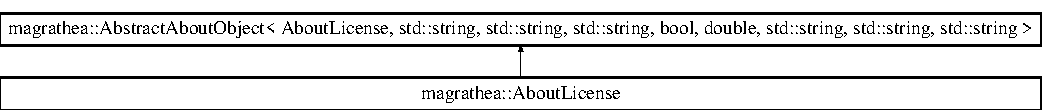
\includegraphics[height=1.483444cm]{exceptionmagrathea_1_1AboutLicense}
\end{center}
\end{figure}
\subsection*{Public Member Functions}
\begin{Indent}{\bf Lifecycle}\par
\begin{DoxyCompactItemize}
\item 
{\footnotesize template$<$class... Misc$>$ }\\\hyperlink{exceptionmagrathea_1_1AboutLicense_a8fbce27e799834af4aeab373110530ed}{About\-License} (Misc \&\&...misc)
\begin{DoxyCompactList}\small\item\em Explicit generic constructor. \end{DoxyCompactList}\end{DoxyCompactItemize}
\end{Indent}
\begin{Indent}{\bf Accessors}\par
\begin{DoxyCompactItemize}
\item 
std\-::string \hyperlink{exceptionmagrathea_1_1AboutLicense_a27175356904c56241e1db021e63dcc77}{text} (const std\-::string \&program, const std\-::string \&date=\char`\"{}\char`\"{}, const std\-::string \&owner=\char`\"{}\char`\"{}, const std\-::string \&contact=\char`\"{}\char`\"{}, const std\-::string \&organization=\char`\"{}\char`\"{}, const std\-::string \&purpose=\char`\"{}\char`\"{}) const 
\begin{DoxyCompactList}\small\item\em License text of the program accessor. \end{DoxyCompactList}\end{DoxyCompactItemize}
\end{Indent}
\begin{Indent}{\bf Getters}\par
\begin{DoxyCompactItemize}
\item 
const std\-::string \& \hyperlink{exceptionmagrathea_1_1AboutLicense_a9540bd91bf92d369ab63c56f73390cfe}{title} () const 
\begin{DoxyCompactList}\small\item\em License title, name or acronym getter. \end{DoxyCompactList}\item 
const std\-::string \& \hyperlink{exceptionmagrathea_1_1AboutLicense_abcba63f5d3ffb9d830491c673c02940f}{name} () const 
\begin{DoxyCompactList}\small\item\em Complete name getter. \end{DoxyCompactList}\item 
const std\-::string \& \hyperlink{exceptionmagrathea_1_1AboutLicense_a67c5b15e442a683cae85490516b20793}{link} () const 
\begin{DoxyCompactList}\small\item\em Web link getter. \end{DoxyCompactList}\item 
bool \hyperlink{exceptionmagrathea_1_1AboutLicense_a34f24ae9d81244368807811f0bd01b5f}{proprietary} () const 
\begin{DoxyCompactList}\small\item\em Proprietary or free/open-\/source flag getter. \end{DoxyCompactList}\item 
double \hyperlink{exceptionmagrathea_1_1AboutLicense_aa191f2959b6ded2ab40545939fc4c258}{version} () const 
\begin{DoxyCompactList}\small\item\em Version number getter. \end{DoxyCompactList}\item 
const std\-::string \& \hyperlink{exceptionmagrathea_1_1AboutLicense_a022dfb624b8c9fe27d30e156c7902fc4}{description} () const 
\begin{DoxyCompactList}\small\item\em Short description or summary of the license getter. \end{DoxyCompactList}\item 
const std\-::string \& \hyperlink{exceptionmagrathea_1_1AboutLicense_af14a66dd7e7c7e94b4c6672851ebf3d5}{text} () const 
\begin{DoxyCompactList}\small\item\em License text of the program getter. \end{DoxyCompactList}\item 
const std\-::string \& \hyperlink{exceptionmagrathea_1_1AboutLicense_a1d4576310ec41d21d79c80d1bf361bea}{reference} () const 
\begin{DoxyCompactList}\small\item\em Complete license reference getter. \end{DoxyCompactList}\end{DoxyCompactItemize}
\end{Indent}
\begin{Indent}{\bf Setters}\par
\begin{DoxyCompactItemize}
\item 
\hyperlink{exceptionmagrathea_1_1AboutLicense}{About\-License} \& \hyperlink{exceptionmagrathea_1_1AboutLicense_a7649d777dc5c3a8df8c3667020f2ff9f}{title} (const std\-::string \&value)
\begin{DoxyCompactList}\small\item\em License title, name or acronym setter. \end{DoxyCompactList}\item 
\hyperlink{exceptionmagrathea_1_1AboutLicense}{About\-License} \& \hyperlink{exceptionmagrathea_1_1AboutLicense_af22177cbdf02b629fcef842258bded55}{name} (const std\-::string \&value)
\begin{DoxyCompactList}\small\item\em Complete name setter. \end{DoxyCompactList}\item 
\hyperlink{exceptionmagrathea_1_1AboutLicense}{About\-License} \& \hyperlink{exceptionmagrathea_1_1AboutLicense_ad1ed0340d326d9b7e5d00f49cf4a2249}{link} (const std\-::string \&value)
\begin{DoxyCompactList}\small\item\em Web link setter. \end{DoxyCompactList}\item 
\hyperlink{exceptionmagrathea_1_1AboutLicense}{About\-License} \& \hyperlink{exceptionmagrathea_1_1AboutLicense_a719d9996aa99ea70c71035f3c58aa2f9}{proprietary} (const bool value)
\begin{DoxyCompactList}\small\item\em Proprietary or free/open-\/source flag setter. \end{DoxyCompactList}\item 
\hyperlink{exceptionmagrathea_1_1AboutLicense}{About\-License} \& \hyperlink{exceptionmagrathea_1_1AboutLicense_a257a6077fa3a862cec477fed63597229}{version} (const double value)
\begin{DoxyCompactList}\small\item\em Version number setter. \end{DoxyCompactList}\item 
\hyperlink{exceptionmagrathea_1_1AboutLicense}{About\-License} \& \hyperlink{exceptionmagrathea_1_1AboutLicense_a6269ef58ec7627e164701872d6eb4e5d}{description} (const std\-::string \&value)
\begin{DoxyCompactList}\small\item\em Short description or summary of the license setter. \end{DoxyCompactList}\item 
\hyperlink{exceptionmagrathea_1_1AboutLicense}{About\-License} \& \hyperlink{exceptionmagrathea_1_1AboutLicense_a71eed42370a80b566ad1679ec188ad02}{text} (const std\-::string \&value)
\begin{DoxyCompactList}\small\item\em License text of the program setter. \end{DoxyCompactList}\item 
\hyperlink{exceptionmagrathea_1_1AboutLicense}{About\-License} \& \hyperlink{exceptionmagrathea_1_1AboutLicense_a1539d9523c37c9a5844278e99c18569a}{reference} (const std\-::string \&value)
\begin{DoxyCompactList}\small\item\em Complete license reference setter. \end{DoxyCompactList}\end{DoxyCompactItemize}
\end{Indent}
\subsection*{Static Public Member Functions}
\begin{Indent}{\bf Predefined}\par
\begin{DoxyCompactItemize}
\item 
static const \hyperlink{exceptionmagrathea_1_1AboutLicense}{About\-License} \& \hyperlink{exceptionmagrathea_1_1AboutLicense_a09e70a2210983b24a10d8c61f7450190}{gplv3} ()
\begin{DoxyCompactList}\small\item\em Predefined G\-P\-Lv3 license. \end{DoxyCompactList}\item 
static const \hyperlink{exceptionmagrathea_1_1AboutLicense}{About\-License} \& \hyperlink{exceptionmagrathea_1_1AboutLicense_adefa66d22f7eccf37552fe7c6b78ff96}{lgplv3} ()
\begin{DoxyCompactList}\small\item\em Predefined L\-G\-P\-Lv3 license. \end{DoxyCompactList}\item 
static const \hyperlink{exceptionmagrathea_1_1AboutLicense}{About\-License} \& \hyperlink{exceptionmagrathea_1_1AboutLicense_a699c03349945b3a903d19594a0246f61}{bsd} ()
\begin{DoxyCompactList}\small\item\em Predefined B\-S\-D license. \end{DoxyCompactList}\item 
static const \hyperlink{exceptionmagrathea_1_1AboutLicense}{About\-License} \& \hyperlink{exceptionmagrathea_1_1AboutLicense_aa38fae5ae527568807106f0b148653d1}{modifiedbsd} ()
\begin{DoxyCompactList}\small\item\em Predefined modified B\-S\-D license. \end{DoxyCompactList}\item 
static const \hyperlink{exceptionmagrathea_1_1AboutLicense}{About\-License} \& \hyperlink{exceptionmagrathea_1_1AboutLicense_a95210c7f5ba8e9bd692414fea58da592}{freebsd} ()
\begin{DoxyCompactList}\small\item\em Predefined Free\-B\-S\-D license. \end{DoxyCompactList}\item 
static const \hyperlink{exceptionmagrathea_1_1AboutLicense}{About\-License} \& \hyperlink{exceptionmagrathea_1_1AboutLicense_a7ff9765d47e3b69bf18167e7b912ad74}{cecill} ()
\begin{DoxyCompactList}\small\item\em Predefined Ce\-C\-I\-L\-L license. \end{DoxyCompactList}\item 
static const \hyperlink{exceptionmagrathea_1_1AboutLicense}{About\-License} \& \hyperlink{exceptionmagrathea_1_1AboutLicense_a9ca054706cf0da00d216611cb4c56c69}{cecillb} ()
\begin{DoxyCompactList}\small\item\em Predefined Ce\-C\-I\-L\-L-\/\-B license. \end{DoxyCompactList}\item 
static const \hyperlink{exceptionmagrathea_1_1AboutLicense}{About\-License} \& \hyperlink{exceptionmagrathea_1_1AboutLicense_a393f259609519de6f93ec45ad0ff1cad}{cecillc} ()
\begin{DoxyCompactList}\small\item\em Predefined Ce\-C\-I\-L\-L-\/\-C license. \end{DoxyCompactList}\item 
static const \hyperlink{exceptionmagrathea_1_1AboutLicense}{About\-License} \& \hyperlink{exceptionmagrathea_1_1AboutLicense_af9e58435e2ec919b355d4b02ed1b4ee3}{ccbyv3} ()
\begin{DoxyCompactList}\small\item\em Predefined C\-C-\/\-B\-Y v3 license. \end{DoxyCompactList}\item 
static const \hyperlink{exceptionmagrathea_1_1AboutLicense}{About\-License} \& \hyperlink{exceptionmagrathea_1_1AboutLicense_a47208c66133ca568b754ce7e9cf8e7db}{ccbysav3} ()
\begin{DoxyCompactList}\small\item\em Predefined C\-C-\/\-B\-Y-\/\-S\-A v3 license. \end{DoxyCompactList}\item 
static const \hyperlink{exceptionmagrathea_1_1AboutLicense}{About\-License} \& \hyperlink{exceptionmagrathea_1_1AboutLicense_a9d2eed067d328ceac14578f02b4c3ec7}{ccbyndv3} ()
\begin{DoxyCompactList}\small\item\em Predefined C\-C-\/\-B\-Y-\/\-N\-D v3 license. \end{DoxyCompactList}\item 
static const \hyperlink{exceptionmagrathea_1_1AboutLicense}{About\-License} \& \hyperlink{exceptionmagrathea_1_1AboutLicense_ab613b370c6ef6df5fb81abef120be848}{ccbyncv3} ()
\begin{DoxyCompactList}\small\item\em Predefined C\-C-\/\-B\-Y-\/\-N\-C v3 license. \end{DoxyCompactList}\item 
static const \hyperlink{exceptionmagrathea_1_1AboutLicense}{About\-License} \& \hyperlink{exceptionmagrathea_1_1AboutLicense_a29019fdfb220ddebe51406952323f589}{ccbyncsav3} ()
\begin{DoxyCompactList}\small\item\em Predefined C\-C-\/\-B\-Y-\/\-N\-C-\/\-S\-A v3 license. \end{DoxyCompactList}\item 
static const \hyperlink{exceptionmagrathea_1_1AboutLicense}{About\-License} \& \hyperlink{exceptionmagrathea_1_1AboutLicense_a3f90ccf1fb69e5bb8ba690c79a42bcc1}{ccbyncndv3} ()
\begin{DoxyCompactList}\small\item\em Predefined C\-C-\/\-B\-Y-\/\-N\-C-\/\-N\-D v3 license. \end{DoxyCompactList}\item 
static const \hyperlink{exceptionmagrathea_1_1AboutLicense}{About\-License} \& \hyperlink{exceptionmagrathea_1_1AboutLicense_af740a6dfc40d24b79c1d92370b207519}{cc0v1} ()
\begin{DoxyCompactList}\small\item\em Predefined C\-C0 v1 license. \end{DoxyCompactList}\end{DoxyCompactItemize}
\end{Indent}
\begin{Indent}{\bf Test}\par
\begin{DoxyCompactItemize}
\item 
static int \hyperlink{exceptionmagrathea_1_1AboutLicense_a07ffbab65dcf363b5616a3a6530058d8}{example} ()
\begin{DoxyCompactList}\small\item\em Example function. \end{DoxyCompactList}\end{DoxyCompactItemize}
\end{Indent}
\subsection*{Public Attributes}
\begin{DoxyCompactItemize}
\item 
using \hyperlink{exceptionmagrathea_1_1AboutLicense_a953ae5a3eb8a926ada61ac5bb5ab40b0}{operator} = typedef
\end{DoxyCompactItemize}
\subsection*{Additional Inherited Members}


\subsection{Detailed Description}
Information about the license of a code. 

Name, link, text and documentation on the license of a code or a library. 

\subsection{Constructor \& Destructor Documentation}
\hypertarget{exceptionmagrathea_1_1AboutLicense_a8fbce27e799834af4aeab373110530ed}{\index{magrathea\-::\-About\-License@{magrathea\-::\-About\-License}!About\-License@{About\-License}}
\index{About\-License@{About\-License}!magrathea::AboutLicense@{magrathea\-::\-About\-License}}
\subsubsection[{About\-License}]{\setlength{\rightskip}{0pt plus 5cm}template$<$class... Misc$>$ magrathea\-::\-About\-License\-::\-About\-License (
\begin{DoxyParamCaption}
\item[{Misc \&\&...}]{misc}
\end{DoxyParamCaption}
)\hspace{0.3cm}{\ttfamily [inline]}, {\ttfamily [explicit]}}}\label{exceptionmagrathea_1_1AboutLicense_a8fbce27e799834af4aeab373110530ed}


Explicit generic constructor. 

Provides a generic interface to all constructors of the base class. 
\begin{DoxyTemplParams}{Template Parameters}
{\em Misc} & (\hyperlink{classMiscellaneous}{Miscellaneous} types.) \\
\hline
\end{DoxyTemplParams}

\begin{DoxyParams}[1]{Parameters}
\mbox{\tt in}  & {\em misc} & \hyperlink{classMiscellaneous}{Miscellaneous} arguments. \\
\hline
\end{DoxyParams}


\subsection{Member Function Documentation}
\hypertarget{exceptionmagrathea_1_1AboutLicense_a699c03349945b3a903d19594a0246f61}{\index{magrathea\-::\-About\-License@{magrathea\-::\-About\-License}!bsd@{bsd}}
\index{bsd@{bsd}!magrathea::AboutLicense@{magrathea\-::\-About\-License}}
\subsubsection[{bsd}]{\setlength{\rightskip}{0pt plus 5cm}const {\bf About\-License} \& magrathea\-::\-About\-License\-::bsd (
\begin{DoxyParamCaption}
{}
\end{DoxyParamCaption}
)\hspace{0.3cm}{\ttfamily [inline]}, {\ttfamily [static]}}}\label{exceptionmagrathea_1_1AboutLicense_a699c03349945b3a903d19594a0246f61}


Predefined B\-S\-D license. 

Original B\-S\-D license. \begin{DoxyReturn}{Returns}
Immutable reference to license singleton. 
\end{DoxyReturn}
\hypertarget{exceptionmagrathea_1_1AboutLicense_af740a6dfc40d24b79c1d92370b207519}{\index{magrathea\-::\-About\-License@{magrathea\-::\-About\-License}!cc0v1@{cc0v1}}
\index{cc0v1@{cc0v1}!magrathea::AboutLicense@{magrathea\-::\-About\-License}}
\subsubsection[{cc0v1}]{\setlength{\rightskip}{0pt plus 5cm}const {\bf About\-License} \& magrathea\-::\-About\-License\-::cc0v1 (
\begin{DoxyParamCaption}
{}
\end{DoxyParamCaption}
)\hspace{0.3cm}{\ttfamily [inline]}, {\ttfamily [static]}}}\label{exceptionmagrathea_1_1AboutLicense_af740a6dfc40d24b79c1d92370b207519}


Predefined C\-C0 v1 license. 

Creative Commons C\-C0 1.\-0 Universal Public Domain Dedication. \begin{DoxyReturn}{Returns}
Immutable reference to license singleton. 
\end{DoxyReturn}
\hypertarget{exceptionmagrathea_1_1AboutLicense_a3f90ccf1fb69e5bb8ba690c79a42bcc1}{\index{magrathea\-::\-About\-License@{magrathea\-::\-About\-License}!ccbyncndv3@{ccbyncndv3}}
\index{ccbyncndv3@{ccbyncndv3}!magrathea::AboutLicense@{magrathea\-::\-About\-License}}
\subsubsection[{ccbyncndv3}]{\setlength{\rightskip}{0pt plus 5cm}const {\bf About\-License} \& magrathea\-::\-About\-License\-::ccbyncndv3 (
\begin{DoxyParamCaption}
{}
\end{DoxyParamCaption}
)\hspace{0.3cm}{\ttfamily [inline]}, {\ttfamily [static]}}}\label{exceptionmagrathea_1_1AboutLicense_a3f90ccf1fb69e5bb8ba690c79a42bcc1}


Predefined C\-C-\/\-B\-Y-\/\-N\-C-\/\-N\-D v3 license. 

Creative Commons Attribution-\/\-Non\-Commercial-\/\-No\-Derivs 3.\-0 Unported (C\-C B\-Y-\/\-N\-C-\/\-N\-D 3.\-0). \begin{DoxyReturn}{Returns}
Immutable reference to license singleton. 
\end{DoxyReturn}
\hypertarget{exceptionmagrathea_1_1AboutLicense_a29019fdfb220ddebe51406952323f589}{\index{magrathea\-::\-About\-License@{magrathea\-::\-About\-License}!ccbyncsav3@{ccbyncsav3}}
\index{ccbyncsav3@{ccbyncsav3}!magrathea::AboutLicense@{magrathea\-::\-About\-License}}
\subsubsection[{ccbyncsav3}]{\setlength{\rightskip}{0pt plus 5cm}const {\bf About\-License} \& magrathea\-::\-About\-License\-::ccbyncsav3 (
\begin{DoxyParamCaption}
{}
\end{DoxyParamCaption}
)\hspace{0.3cm}{\ttfamily [inline]}, {\ttfamily [static]}}}\label{exceptionmagrathea_1_1AboutLicense_a29019fdfb220ddebe51406952323f589}


Predefined C\-C-\/\-B\-Y-\/\-N\-C-\/\-S\-A v3 license. 

Creative Commons Attribution-\/\-Non\-Commercial-\/\-Share\-Alike 3.\-0 Unported (C\-C B\-Y-\/\-N\-C-\/\-S\-A 3.\-0). \begin{DoxyReturn}{Returns}
Immutable reference to license singleton. 
\end{DoxyReturn}
\hypertarget{exceptionmagrathea_1_1AboutLicense_ab613b370c6ef6df5fb81abef120be848}{\index{magrathea\-::\-About\-License@{magrathea\-::\-About\-License}!ccbyncv3@{ccbyncv3}}
\index{ccbyncv3@{ccbyncv3}!magrathea::AboutLicense@{magrathea\-::\-About\-License}}
\subsubsection[{ccbyncv3}]{\setlength{\rightskip}{0pt plus 5cm}const {\bf About\-License} \& magrathea\-::\-About\-License\-::ccbyncv3 (
\begin{DoxyParamCaption}
{}
\end{DoxyParamCaption}
)\hspace{0.3cm}{\ttfamily [inline]}, {\ttfamily [static]}}}\label{exceptionmagrathea_1_1AboutLicense_ab613b370c6ef6df5fb81abef120be848}


Predefined C\-C-\/\-B\-Y-\/\-N\-C v3 license. 

Creative Commons Attribution-\/\-Non\-Commercial 3.\-0 Unported (C\-C B\-Y-\/\-N\-C 3.\-0). \begin{DoxyReturn}{Returns}
Immutable reference to license singleton. 
\end{DoxyReturn}
\hypertarget{exceptionmagrathea_1_1AboutLicense_a9d2eed067d328ceac14578f02b4c3ec7}{\index{magrathea\-::\-About\-License@{magrathea\-::\-About\-License}!ccbyndv3@{ccbyndv3}}
\index{ccbyndv3@{ccbyndv3}!magrathea::AboutLicense@{magrathea\-::\-About\-License}}
\subsubsection[{ccbyndv3}]{\setlength{\rightskip}{0pt plus 5cm}const {\bf About\-License} \& magrathea\-::\-About\-License\-::ccbyndv3 (
\begin{DoxyParamCaption}
{}
\end{DoxyParamCaption}
)\hspace{0.3cm}{\ttfamily [inline]}, {\ttfamily [static]}}}\label{exceptionmagrathea_1_1AboutLicense_a9d2eed067d328ceac14578f02b4c3ec7}


Predefined C\-C-\/\-B\-Y-\/\-N\-D v3 license. 

Creative Commons Attribution-\/\-No\-Derivs 3.\-0 Unported (C\-C B\-Y-\/\-N\-D 3.\-0). \begin{DoxyReturn}{Returns}
Immutable reference to license singleton. 
\end{DoxyReturn}
\hypertarget{exceptionmagrathea_1_1AboutLicense_a47208c66133ca568b754ce7e9cf8e7db}{\index{magrathea\-::\-About\-License@{magrathea\-::\-About\-License}!ccbysav3@{ccbysav3}}
\index{ccbysav3@{ccbysav3}!magrathea::AboutLicense@{magrathea\-::\-About\-License}}
\subsubsection[{ccbysav3}]{\setlength{\rightskip}{0pt plus 5cm}const {\bf About\-License} \& magrathea\-::\-About\-License\-::ccbysav3 (
\begin{DoxyParamCaption}
{}
\end{DoxyParamCaption}
)\hspace{0.3cm}{\ttfamily [inline]}, {\ttfamily [static]}}}\label{exceptionmagrathea_1_1AboutLicense_a47208c66133ca568b754ce7e9cf8e7db}


Predefined C\-C-\/\-B\-Y-\/\-S\-A v3 license. 

Creative Commons Attribution-\/\-Share\-Alike 3.\-0 Unported (C\-C B\-Y-\/\-S\-A 3.\-0). \begin{DoxyReturn}{Returns}
Immutable reference to license singleton. 
\end{DoxyReturn}
\hypertarget{exceptionmagrathea_1_1AboutLicense_af9e58435e2ec919b355d4b02ed1b4ee3}{\index{magrathea\-::\-About\-License@{magrathea\-::\-About\-License}!ccbyv3@{ccbyv3}}
\index{ccbyv3@{ccbyv3}!magrathea::AboutLicense@{magrathea\-::\-About\-License}}
\subsubsection[{ccbyv3}]{\setlength{\rightskip}{0pt plus 5cm}const {\bf About\-License} \& magrathea\-::\-About\-License\-::ccbyv3 (
\begin{DoxyParamCaption}
{}
\end{DoxyParamCaption}
)\hspace{0.3cm}{\ttfamily [inline]}, {\ttfamily [static]}}}\label{exceptionmagrathea_1_1AboutLicense_af9e58435e2ec919b355d4b02ed1b4ee3}


Predefined C\-C-\/\-B\-Y v3 license. 

Creative Commons Attribution 3.\-0 Unported (C\-C B\-Y 3.\-0). \begin{DoxyReturn}{Returns}
Immutable reference to license singleton. 
\end{DoxyReturn}
\hypertarget{exceptionmagrathea_1_1AboutLicense_a7ff9765d47e3b69bf18167e7b912ad74}{\index{magrathea\-::\-About\-License@{magrathea\-::\-About\-License}!cecill@{cecill}}
\index{cecill@{cecill}!magrathea::AboutLicense@{magrathea\-::\-About\-License}}
\subsubsection[{cecill}]{\setlength{\rightskip}{0pt plus 5cm}const {\bf About\-License} \& magrathea\-::\-About\-License\-::cecill (
\begin{DoxyParamCaption}
{}
\end{DoxyParamCaption}
)\hspace{0.3cm}{\ttfamily [inline]}, {\ttfamily [static]}}}\label{exceptionmagrathea_1_1AboutLicense_a7ff9765d47e3b69bf18167e7b912ad74}


Predefined Ce\-C\-I\-L\-L license. 

Ce\-C\-I\-L\-L license. \begin{DoxyReturn}{Returns}
Immutable reference to license singleton. 
\end{DoxyReturn}
\hypertarget{exceptionmagrathea_1_1AboutLicense_a9ca054706cf0da00d216611cb4c56c69}{\index{magrathea\-::\-About\-License@{magrathea\-::\-About\-License}!cecillb@{cecillb}}
\index{cecillb@{cecillb}!magrathea::AboutLicense@{magrathea\-::\-About\-License}}
\subsubsection[{cecillb}]{\setlength{\rightskip}{0pt plus 5cm}const {\bf About\-License} \& magrathea\-::\-About\-License\-::cecillb (
\begin{DoxyParamCaption}
{}
\end{DoxyParamCaption}
)\hspace{0.3cm}{\ttfamily [inline]}, {\ttfamily [static]}}}\label{exceptionmagrathea_1_1AboutLicense_a9ca054706cf0da00d216611cb4c56c69}


Predefined Ce\-C\-I\-L\-L-\/\-B license. 

Ce\-C\-I\-L\-L-\/\-B license. \begin{DoxyReturn}{Returns}
Immutable reference to license singleton. 
\end{DoxyReturn}
\hypertarget{exceptionmagrathea_1_1AboutLicense_a393f259609519de6f93ec45ad0ff1cad}{\index{magrathea\-::\-About\-License@{magrathea\-::\-About\-License}!cecillc@{cecillc}}
\index{cecillc@{cecillc}!magrathea::AboutLicense@{magrathea\-::\-About\-License}}
\subsubsection[{cecillc}]{\setlength{\rightskip}{0pt plus 5cm}const {\bf About\-License} \& magrathea\-::\-About\-License\-::cecillc (
\begin{DoxyParamCaption}
{}
\end{DoxyParamCaption}
)\hspace{0.3cm}{\ttfamily [inline]}, {\ttfamily [static]}}}\label{exceptionmagrathea_1_1AboutLicense_a393f259609519de6f93ec45ad0ff1cad}


Predefined Ce\-C\-I\-L\-L-\/\-C license. 

Ce\-C\-I\-L\-L-\/\-C license. \begin{DoxyReturn}{Returns}
Immutable reference to license singleton. 
\end{DoxyReturn}
\hypertarget{exceptionmagrathea_1_1AboutLicense_a022dfb624b8c9fe27d30e156c7902fc4}{\index{magrathea\-::\-About\-License@{magrathea\-::\-About\-License}!description@{description}}
\index{description@{description}!magrathea::AboutLicense@{magrathea\-::\-About\-License}}
\subsubsection[{description}]{\setlength{\rightskip}{0pt plus 5cm}const std\-::string \& magrathea\-::\-About\-License\-::description (
\begin{DoxyParamCaption}
{}
\end{DoxyParamCaption}
) const\hspace{0.3cm}{\ttfamily [inline]}}}\label{exceptionmagrathea_1_1AboutLicense_a022dfb624b8c9fe27d30e156c7902fc4}


Short description or summary of the license getter. 

Gets the value of the description property. \begin{DoxyReturn}{Returns}
Description. 
\end{DoxyReturn}
\hypertarget{exceptionmagrathea_1_1AboutLicense_a6269ef58ec7627e164701872d6eb4e5d}{\index{magrathea\-::\-About\-License@{magrathea\-::\-About\-License}!description@{description}}
\index{description@{description}!magrathea::AboutLicense@{magrathea\-::\-About\-License}}
\subsubsection[{description}]{\setlength{\rightskip}{0pt plus 5cm}{\bf About\-License} \& magrathea\-::\-About\-License\-::description (
\begin{DoxyParamCaption}
\item[{const std\-::string \&}]{value}
\end{DoxyParamCaption}
)\hspace{0.3cm}{\ttfamily [inline]}}}\label{exceptionmagrathea_1_1AboutLicense_a6269ef58ec7627e164701872d6eb4e5d}


Short description or summary of the license setter. 

Sets the value of the description property. 
\begin{DoxyParams}[1]{Parameters}
\mbox{\tt in}  & {\em value} & Description. \\
\hline
\end{DoxyParams}
\begin{DoxyReturn}{Returns}
Self reference. 
\end{DoxyReturn}
\hypertarget{exceptionmagrathea_1_1AboutLicense_a07ffbab65dcf363b5616a3a6530058d8}{\index{magrathea\-::\-About\-License@{magrathea\-::\-About\-License}!example@{example}}
\index{example@{example}!magrathea::AboutLicense@{magrathea\-::\-About\-License}}
\subsubsection[{example}]{\setlength{\rightskip}{0pt plus 5cm}int magrathea\-::\-About\-License\-::example (
\begin{DoxyParamCaption}
{}
\end{DoxyParamCaption}
)\hspace{0.3cm}{\ttfamily [static]}}}\label{exceptionmagrathea_1_1AboutLicense_a07ffbab65dcf363b5616a3a6530058d8}


Example function. 

Tests and demonstrates the use of \hyperlink{exceptionmagrathea_1_1AboutLicense}{About\-License}. \begin{DoxyReturn}{Returns}
0 if no error. 
\end{DoxyReturn}
\hypertarget{exceptionmagrathea_1_1AboutLicense_a95210c7f5ba8e9bd692414fea58da592}{\index{magrathea\-::\-About\-License@{magrathea\-::\-About\-License}!freebsd@{freebsd}}
\index{freebsd@{freebsd}!magrathea::AboutLicense@{magrathea\-::\-About\-License}}
\subsubsection[{freebsd}]{\setlength{\rightskip}{0pt plus 5cm}const {\bf About\-License} \& magrathea\-::\-About\-License\-::freebsd (
\begin{DoxyParamCaption}
{}
\end{DoxyParamCaption}
)\hspace{0.3cm}{\ttfamily [inline]}, {\ttfamily [static]}}}\label{exceptionmagrathea_1_1AboutLicense_a95210c7f5ba8e9bd692414fea58da592}


Predefined Free\-B\-S\-D license. 

Free\-B\-S\-D license. \begin{DoxyReturn}{Returns}
Immutable reference to license singleton. 
\end{DoxyReturn}
\hypertarget{exceptionmagrathea_1_1AboutLicense_a09e70a2210983b24a10d8c61f7450190}{\index{magrathea\-::\-About\-License@{magrathea\-::\-About\-License}!gplv3@{gplv3}}
\index{gplv3@{gplv3}!magrathea::AboutLicense@{magrathea\-::\-About\-License}}
\subsubsection[{gplv3}]{\setlength{\rightskip}{0pt plus 5cm}const {\bf About\-License} \& magrathea\-::\-About\-License\-::gplv3 (
\begin{DoxyParamCaption}
{}
\end{DoxyParamCaption}
)\hspace{0.3cm}{\ttfamily [inline]}, {\ttfamily [static]}}}\label{exceptionmagrathea_1_1AboutLicense_a09e70a2210983b24a10d8c61f7450190}


Predefined G\-P\-Lv3 license. 

G\-N\-U General Public License Version 3.\-0. \begin{DoxyReturn}{Returns}
Immutable reference to license singleton. 
\end{DoxyReturn}
\hypertarget{exceptionmagrathea_1_1AboutLicense_adefa66d22f7eccf37552fe7c6b78ff96}{\index{magrathea\-::\-About\-License@{magrathea\-::\-About\-License}!lgplv3@{lgplv3}}
\index{lgplv3@{lgplv3}!magrathea::AboutLicense@{magrathea\-::\-About\-License}}
\subsubsection[{lgplv3}]{\setlength{\rightskip}{0pt plus 5cm}const {\bf About\-License} \& magrathea\-::\-About\-License\-::lgplv3 (
\begin{DoxyParamCaption}
{}
\end{DoxyParamCaption}
)\hspace{0.3cm}{\ttfamily [inline]}, {\ttfamily [static]}}}\label{exceptionmagrathea_1_1AboutLicense_adefa66d22f7eccf37552fe7c6b78ff96}


Predefined L\-G\-P\-Lv3 license. 

G\-N\-U Lesser General Public License Version 3.\-0. \begin{DoxyReturn}{Returns}
Immutable reference to license singleton. 
\end{DoxyReturn}
\hypertarget{exceptionmagrathea_1_1AboutLicense_a67c5b15e442a683cae85490516b20793}{\index{magrathea\-::\-About\-License@{magrathea\-::\-About\-License}!link@{link}}
\index{link@{link}!magrathea::AboutLicense@{magrathea\-::\-About\-License}}
\subsubsection[{link}]{\setlength{\rightskip}{0pt plus 5cm}const std\-::string \& magrathea\-::\-About\-License\-::link (
\begin{DoxyParamCaption}
{}
\end{DoxyParamCaption}
) const\hspace{0.3cm}{\ttfamily [inline]}}}\label{exceptionmagrathea_1_1AboutLicense_a67c5b15e442a683cae85490516b20793}


Web link getter. 

Gets the value of the link property. \begin{DoxyReturn}{Returns}
Link. 
\end{DoxyReturn}
\hypertarget{exceptionmagrathea_1_1AboutLicense_ad1ed0340d326d9b7e5d00f49cf4a2249}{\index{magrathea\-::\-About\-License@{magrathea\-::\-About\-License}!link@{link}}
\index{link@{link}!magrathea::AboutLicense@{magrathea\-::\-About\-License}}
\subsubsection[{link}]{\setlength{\rightskip}{0pt plus 5cm}{\bf About\-License} \& magrathea\-::\-About\-License\-::link (
\begin{DoxyParamCaption}
\item[{const std\-::string \&}]{value}
\end{DoxyParamCaption}
)\hspace{0.3cm}{\ttfamily [inline]}}}\label{exceptionmagrathea_1_1AboutLicense_ad1ed0340d326d9b7e5d00f49cf4a2249}


Web link setter. 

Sets the value of the link property. 
\begin{DoxyParams}[1]{Parameters}
\mbox{\tt in}  & {\em value} & Link. \\
\hline
\end{DoxyParams}
\begin{DoxyReturn}{Returns}
Self reference. 
\end{DoxyReturn}
\hypertarget{exceptionmagrathea_1_1AboutLicense_aa38fae5ae527568807106f0b148653d1}{\index{magrathea\-::\-About\-License@{magrathea\-::\-About\-License}!modifiedbsd@{modifiedbsd}}
\index{modifiedbsd@{modifiedbsd}!magrathea::AboutLicense@{magrathea\-::\-About\-License}}
\subsubsection[{modifiedbsd}]{\setlength{\rightskip}{0pt plus 5cm}const {\bf About\-License} \& magrathea\-::\-About\-License\-::modifiedbsd (
\begin{DoxyParamCaption}
{}
\end{DoxyParamCaption}
)\hspace{0.3cm}{\ttfamily [inline]}, {\ttfamily [static]}}}\label{exceptionmagrathea_1_1AboutLicense_aa38fae5ae527568807106f0b148653d1}


Predefined modified B\-S\-D license. 

Modified B\-S\-D license. \begin{DoxyReturn}{Returns}
Immutable reference to license singleton. 
\end{DoxyReturn}
\hypertarget{exceptionmagrathea_1_1AboutLicense_abcba63f5d3ffb9d830491c673c02940f}{\index{magrathea\-::\-About\-License@{magrathea\-::\-About\-License}!name@{name}}
\index{name@{name}!magrathea::AboutLicense@{magrathea\-::\-About\-License}}
\subsubsection[{name}]{\setlength{\rightskip}{0pt plus 5cm}const std\-::string \& magrathea\-::\-About\-License\-::name (
\begin{DoxyParamCaption}
{}
\end{DoxyParamCaption}
) const\hspace{0.3cm}{\ttfamily [inline]}}}\label{exceptionmagrathea_1_1AboutLicense_abcba63f5d3ffb9d830491c673c02940f}


Complete name getter. 

Gets the value of the name property. \begin{DoxyReturn}{Returns}
Name. 
\end{DoxyReturn}
\hypertarget{exceptionmagrathea_1_1AboutLicense_af22177cbdf02b629fcef842258bded55}{\index{magrathea\-::\-About\-License@{magrathea\-::\-About\-License}!name@{name}}
\index{name@{name}!magrathea::AboutLicense@{magrathea\-::\-About\-License}}
\subsubsection[{name}]{\setlength{\rightskip}{0pt plus 5cm}{\bf About\-License} \& magrathea\-::\-About\-License\-::name (
\begin{DoxyParamCaption}
\item[{const std\-::string \&}]{value}
\end{DoxyParamCaption}
)\hspace{0.3cm}{\ttfamily [inline]}}}\label{exceptionmagrathea_1_1AboutLicense_af22177cbdf02b629fcef842258bded55}


Complete name setter. 

Sets the value of the name property. 
\begin{DoxyParams}[1]{Parameters}
\mbox{\tt in}  & {\em value} & Name. \\
\hline
\end{DoxyParams}
\begin{DoxyReturn}{Returns}
Self reference. 
\end{DoxyReturn}
\hypertarget{exceptionmagrathea_1_1AboutLicense_a34f24ae9d81244368807811f0bd01b5f}{\index{magrathea\-::\-About\-License@{magrathea\-::\-About\-License}!proprietary@{proprietary}}
\index{proprietary@{proprietary}!magrathea::AboutLicense@{magrathea\-::\-About\-License}}
\subsubsection[{proprietary}]{\setlength{\rightskip}{0pt plus 5cm}bool magrathea\-::\-About\-License\-::proprietary (
\begin{DoxyParamCaption}
{}
\end{DoxyParamCaption}
) const\hspace{0.3cm}{\ttfamily [inline]}}}\label{exceptionmagrathea_1_1AboutLicense_a34f24ae9d81244368807811f0bd01b5f}


Proprietary or free/open-\/source flag getter. 

Gets the value of the proprietary property. \begin{DoxyReturn}{Returns}
Proprietary. 
\end{DoxyReturn}
\hypertarget{exceptionmagrathea_1_1AboutLicense_a719d9996aa99ea70c71035f3c58aa2f9}{\index{magrathea\-::\-About\-License@{magrathea\-::\-About\-License}!proprietary@{proprietary}}
\index{proprietary@{proprietary}!magrathea::AboutLicense@{magrathea\-::\-About\-License}}
\subsubsection[{proprietary}]{\setlength{\rightskip}{0pt plus 5cm}{\bf About\-License} \& magrathea\-::\-About\-License\-::proprietary (
\begin{DoxyParamCaption}
\item[{const bool}]{value}
\end{DoxyParamCaption}
)\hspace{0.3cm}{\ttfamily [inline]}}}\label{exceptionmagrathea_1_1AboutLicense_a719d9996aa99ea70c71035f3c58aa2f9}


Proprietary or free/open-\/source flag setter. 

Sets the value of the proprietary property. 
\begin{DoxyParams}[1]{Parameters}
\mbox{\tt in}  & {\em value} & Proprietary. \\
\hline
\end{DoxyParams}
\begin{DoxyReturn}{Returns}
Self reference. 
\end{DoxyReturn}
\hypertarget{exceptionmagrathea_1_1AboutLicense_a1d4576310ec41d21d79c80d1bf361bea}{\index{magrathea\-::\-About\-License@{magrathea\-::\-About\-License}!reference@{reference}}
\index{reference@{reference}!magrathea::AboutLicense@{magrathea\-::\-About\-License}}
\subsubsection[{reference}]{\setlength{\rightskip}{0pt plus 5cm}const std\-::string \& magrathea\-::\-About\-License\-::reference (
\begin{DoxyParamCaption}
{}
\end{DoxyParamCaption}
) const\hspace{0.3cm}{\ttfamily [inline]}}}\label{exceptionmagrathea_1_1AboutLicense_a1d4576310ec41d21d79c80d1bf361bea}


Complete license reference getter. 

Gets the value of the reference property. \begin{DoxyReturn}{Returns}
Reference. 
\end{DoxyReturn}
\hypertarget{exceptionmagrathea_1_1AboutLicense_a1539d9523c37c9a5844278e99c18569a}{\index{magrathea\-::\-About\-License@{magrathea\-::\-About\-License}!reference@{reference}}
\index{reference@{reference}!magrathea::AboutLicense@{magrathea\-::\-About\-License}}
\subsubsection[{reference}]{\setlength{\rightskip}{0pt plus 5cm}{\bf About\-License} \& magrathea\-::\-About\-License\-::reference (
\begin{DoxyParamCaption}
\item[{const std\-::string \&}]{value}
\end{DoxyParamCaption}
)\hspace{0.3cm}{\ttfamily [inline]}}}\label{exceptionmagrathea_1_1AboutLicense_a1539d9523c37c9a5844278e99c18569a}


Complete license reference setter. 

Sets the value of the reference property. 
\begin{DoxyParams}[1]{Parameters}
\mbox{\tt in}  & {\em value} & Reference. \\
\hline
\end{DoxyParams}
\begin{DoxyReturn}{Returns}
Self reference. 
\end{DoxyReturn}
\hypertarget{exceptionmagrathea_1_1AboutLicense_a27175356904c56241e1db021e63dcc77}{\index{magrathea\-::\-About\-License@{magrathea\-::\-About\-License}!text@{text}}
\index{text@{text}!magrathea::AboutLicense@{magrathea\-::\-About\-License}}
\subsubsection[{text}]{\setlength{\rightskip}{0pt plus 5cm}std\-::string magrathea\-::\-About\-License\-::text (
\begin{DoxyParamCaption}
\item[{const std\-::string \&}]{program, }
\item[{const std\-::string \&}]{date = {\ttfamily \char`\"{}\char`\"{}}, }
\item[{const std\-::string \&}]{owner = {\ttfamily \char`\"{}\char`\"{}}, }
\item[{const std\-::string \&}]{contact = {\ttfamily \char`\"{}\char`\"{}}, }
\item[{const std\-::string \&}]{organization = {\ttfamily \char`\"{}\char`\"{}}, }
\item[{const std\-::string \&}]{purpose = {\ttfamily \char`\"{}\char`\"{}}}
\end{DoxyParamCaption}
) const\hspace{0.3cm}{\ttfamily [inline]}}}\label{exceptionmagrathea_1_1AboutLicense_a27175356904c56241e1db021e63dcc77}


License text of the program accessor. 

Gets the value of the text property with correctly replaced keywords. \begin{DoxyReturn}{Returns}
Text. 
\end{DoxyReturn}
\hypertarget{exceptionmagrathea_1_1AboutLicense_af14a66dd7e7c7e94b4c6672851ebf3d5}{\index{magrathea\-::\-About\-License@{magrathea\-::\-About\-License}!text@{text}}
\index{text@{text}!magrathea::AboutLicense@{magrathea\-::\-About\-License}}
\subsubsection[{text}]{\setlength{\rightskip}{0pt plus 5cm}const std\-::string \& magrathea\-::\-About\-License\-::text (
\begin{DoxyParamCaption}
{}
\end{DoxyParamCaption}
) const\hspace{0.3cm}{\ttfamily [inline]}}}\label{exceptionmagrathea_1_1AboutLicense_af14a66dd7e7c7e94b4c6672851ebf3d5}


License text of the program getter. 

Gets the value of the text property. \begin{DoxyReturn}{Returns}
Text. 
\end{DoxyReturn}
\hypertarget{exceptionmagrathea_1_1AboutLicense_a71eed42370a80b566ad1679ec188ad02}{\index{magrathea\-::\-About\-License@{magrathea\-::\-About\-License}!text@{text}}
\index{text@{text}!magrathea::AboutLicense@{magrathea\-::\-About\-License}}
\subsubsection[{text}]{\setlength{\rightskip}{0pt plus 5cm}{\bf About\-License} \& magrathea\-::\-About\-License\-::text (
\begin{DoxyParamCaption}
\item[{const std\-::string \&}]{value}
\end{DoxyParamCaption}
)\hspace{0.3cm}{\ttfamily [inline]}}}\label{exceptionmagrathea_1_1AboutLicense_a71eed42370a80b566ad1679ec188ad02}


License text of the program setter. 

Sets the value of the text property. 
\begin{DoxyParams}[1]{Parameters}
\mbox{\tt in}  & {\em value} & Text. \\
\hline
\end{DoxyParams}
\begin{DoxyReturn}{Returns}
Self reference. 
\end{DoxyReturn}
\hypertarget{exceptionmagrathea_1_1AboutLicense_a9540bd91bf92d369ab63c56f73390cfe}{\index{magrathea\-::\-About\-License@{magrathea\-::\-About\-License}!title@{title}}
\index{title@{title}!magrathea::AboutLicense@{magrathea\-::\-About\-License}}
\subsubsection[{title}]{\setlength{\rightskip}{0pt plus 5cm}const std\-::string \& magrathea\-::\-About\-License\-::title (
\begin{DoxyParamCaption}
{}
\end{DoxyParamCaption}
) const\hspace{0.3cm}{\ttfamily [inline]}}}\label{exceptionmagrathea_1_1AboutLicense_a9540bd91bf92d369ab63c56f73390cfe}


License title, name or acronym getter. 

Gets the value of the title property. \begin{DoxyReturn}{Returns}
Title. 
\end{DoxyReturn}
\hypertarget{exceptionmagrathea_1_1AboutLicense_a7649d777dc5c3a8df8c3667020f2ff9f}{\index{magrathea\-::\-About\-License@{magrathea\-::\-About\-License}!title@{title}}
\index{title@{title}!magrathea::AboutLicense@{magrathea\-::\-About\-License}}
\subsubsection[{title}]{\setlength{\rightskip}{0pt plus 5cm}{\bf About\-License} \& magrathea\-::\-About\-License\-::title (
\begin{DoxyParamCaption}
\item[{const std\-::string \&}]{value}
\end{DoxyParamCaption}
)\hspace{0.3cm}{\ttfamily [inline]}}}\label{exceptionmagrathea_1_1AboutLicense_a7649d777dc5c3a8df8c3667020f2ff9f}


License title, name or acronym setter. 

Sets the value of the title property. 
\begin{DoxyParams}[1]{Parameters}
\mbox{\tt in}  & {\em value} & Title. \\
\hline
\end{DoxyParams}
\begin{DoxyReturn}{Returns}
Self reference. 
\end{DoxyReturn}
\hypertarget{exceptionmagrathea_1_1AboutLicense_aa191f2959b6ded2ab40545939fc4c258}{\index{magrathea\-::\-About\-License@{magrathea\-::\-About\-License}!version@{version}}
\index{version@{version}!magrathea::AboutLicense@{magrathea\-::\-About\-License}}
\subsubsection[{version}]{\setlength{\rightskip}{0pt plus 5cm}double magrathea\-::\-About\-License\-::version (
\begin{DoxyParamCaption}
{}
\end{DoxyParamCaption}
) const\hspace{0.3cm}{\ttfamily [inline]}}}\label{exceptionmagrathea_1_1AboutLicense_aa191f2959b6ded2ab40545939fc4c258}


Version number getter. 

Gets the value of the version property. \begin{DoxyReturn}{Returns}
Version. 
\end{DoxyReturn}
\hypertarget{exceptionmagrathea_1_1AboutLicense_a257a6077fa3a862cec477fed63597229}{\index{magrathea\-::\-About\-License@{magrathea\-::\-About\-License}!version@{version}}
\index{version@{version}!magrathea::AboutLicense@{magrathea\-::\-About\-License}}
\subsubsection[{version}]{\setlength{\rightskip}{0pt plus 5cm}{\bf About\-License} \& magrathea\-::\-About\-License\-::version (
\begin{DoxyParamCaption}
\item[{const double}]{value}
\end{DoxyParamCaption}
)\hspace{0.3cm}{\ttfamily [inline]}}}\label{exceptionmagrathea_1_1AboutLicense_a257a6077fa3a862cec477fed63597229}


Version number setter. 

Sets the value of the version property. 
\begin{DoxyParams}[1]{Parameters}
\mbox{\tt in}  & {\em value} & Version. \\
\hline
\end{DoxyParams}
\begin{DoxyReturn}{Returns}
Self reference. 
\end{DoxyReturn}


\subsection{Member Data Documentation}
\hypertarget{exceptionmagrathea_1_1AboutLicense_a953ae5a3eb8a926ada61ac5bb5ab40b0}{\index{magrathea\-::\-About\-License@{magrathea\-::\-About\-License}!operator@{operator}}
\index{operator@{operator}!magrathea::AboutLicense@{magrathea\-::\-About\-License}}
\subsubsection[{operator}]{\setlength{\rightskip}{0pt plus 5cm}using magrathea\-::\-About\-License\-::operator = }}\label{exceptionmagrathea_1_1AboutLicense_a953ae5a3eb8a926ada61ac5bb5ab40b0}


The documentation for this exception was generated from the following file\-:\begin{DoxyCompactItemize}
\item 
/data/home/mbreton/magrathea\-\_\-pathfinder/src/magrathea/\hyperlink{aboutlicense_8h}{aboutlicense.\-h}\end{DoxyCompactItemize}

\hypertarget{exceptionmagrathea_1_1AboutObject}{\section{magrathea\-:\-:About\-Object$<$ Types $>$ Exception Template Reference}
\label{exceptionmagrathea_1_1AboutObject}\index{magrathea\-::\-About\-Object$<$ Types $>$@{magrathea\-::\-About\-Object$<$ Types $>$}}
}


Basic about object with information on something.  




{\ttfamily \#include $<$aboutobject.\-h$>$}

Inheritance diagram for magrathea\-:\-:About\-Object$<$ Types $>$\-:\begin{figure}[H]
\begin{center}
\leavevmode
\includegraphics[height=2.000000cm]{exceptionmagrathea_1_1AboutObject}
\end{center}
\end{figure}
\subsection*{Public Member Functions}
\begin{Indent}{\bf Lifecycle}\par
\begin{DoxyCompactItemize}
\item 
{\footnotesize template$<$class... Misc$>$ }\\\hyperlink{exceptionmagrathea_1_1AboutObject_a2e0ba5b9673ca1b445ac6c0dcdd85548}{About\-Object} (Misc \&\&...misc)
\begin{DoxyCompactList}\small\item\em Explicit generic constructor. \end{DoxyCompactList}\end{DoxyCompactItemize}
\end{Indent}
\subsection*{Static Public Member Functions}
\begin{Indent}{\bf Test}\par
\begin{DoxyCompactItemize}
\item 
static int \hyperlink{exceptionmagrathea_1_1AboutObject_aecdd3af569b2ca16de9f5b303dee4115}{example} ()
\begin{DoxyCompactList}\small\item\em Example function. \end{DoxyCompactList}\end{DoxyCompactItemize}
\end{Indent}
\subsection*{Public Attributes}
\begin{DoxyCompactItemize}
\item 
using \hyperlink{exceptionmagrathea_1_1AboutObject_af3070f80cf23def674318f0c73abe7d6}{operator} = typedef
\end{DoxyCompactItemize}
\subsection*{Additional Inherited Members}


\subsection{Detailed Description}
\subsubsection*{template$<$class... Types$>$exception magrathea\-::\-About\-Object$<$ Types $>$}

Basic about object with information on something. 

This class is the direct derivation of \hyperlink{classmagrathea_1_1AbstractAboutObject}{Abstract\-About\-Object}. It provides the most basic and generic contents object without adding new functionalities to the abstract class. It can be used in most cases as a generic container of groups of information on something. 
\begin{DoxyTemplParams}{Template Parameters}
{\em Types} & Variadic list of components types. \\
\hline
\end{DoxyTemplParams}


\subsection{Constructor \& Destructor Documentation}
\hypertarget{exceptionmagrathea_1_1AboutObject_a2e0ba5b9673ca1b445ac6c0dcdd85548}{\index{magrathea\-::\-About\-Object@{magrathea\-::\-About\-Object}!About\-Object@{About\-Object}}
\index{About\-Object@{About\-Object}!magrathea::AboutObject@{magrathea\-::\-About\-Object}}
\subsubsection[{About\-Object}]{\setlength{\rightskip}{0pt plus 5cm}template$<$class... Types$>$ template$<$class... Misc$>$ {\bf magrathea\-::\-About\-Object}$<$ Types $>$\-::{\bf About\-Object} (
\begin{DoxyParamCaption}
\item[{Misc \&\&...}]{misc}
\end{DoxyParamCaption}
)\hspace{0.3cm}{\ttfamily [inline]}, {\ttfamily [explicit]}}}\label{exceptionmagrathea_1_1AboutObject_a2e0ba5b9673ca1b445ac6c0dcdd85548}


Explicit generic constructor. 

Provides a generic interface to all constructors of the base class. 
\begin{DoxyTemplParams}{Template Parameters}
{\em Misc} & (\hyperlink{classMiscellaneous}{Miscellaneous} types.) \\
\hline
\end{DoxyTemplParams}

\begin{DoxyParams}[1]{Parameters}
\mbox{\tt in}  & {\em misc} & \hyperlink{classMiscellaneous}{Miscellaneous} arguments. \\
\hline
\end{DoxyParams}


\subsection{Member Function Documentation}
\hypertarget{exceptionmagrathea_1_1AboutObject_aecdd3af569b2ca16de9f5b303dee4115}{\index{magrathea\-::\-About\-Object@{magrathea\-::\-About\-Object}!example@{example}}
\index{example@{example}!magrathea::AboutObject@{magrathea\-::\-About\-Object}}
\subsubsection[{example}]{\setlength{\rightskip}{0pt plus 5cm}template$<$class... Types$>$ int {\bf magrathea\-::\-About\-Object}$<$ Types $>$\-::example (
\begin{DoxyParamCaption}
{}
\end{DoxyParamCaption}
)\hspace{0.3cm}{\ttfamily [static]}}}\label{exceptionmagrathea_1_1AboutObject_aecdd3af569b2ca16de9f5b303dee4115}


Example function. 

Tests and demonstrates the use of \hyperlink{exceptionmagrathea_1_1AboutObject}{About\-Object}. \begin{DoxyReturn}{Returns}
0 if no error. 
\end{DoxyReturn}


\subsection{Member Data Documentation}
\hypertarget{exceptionmagrathea_1_1AboutObject_af3070f80cf23def674318f0c73abe7d6}{\index{magrathea\-::\-About\-Object@{magrathea\-::\-About\-Object}!operator@{operator}}
\index{operator@{operator}!magrathea::AboutObject@{magrathea\-::\-About\-Object}}
\subsubsection[{operator}]{\setlength{\rightskip}{0pt plus 5cm}template$<$class... Types$>$ using {\bf magrathea\-::\-About\-Object}$<$ Types $>$\-::operator = }}\label{exceptionmagrathea_1_1AboutObject_af3070f80cf23def674318f0c73abe7d6}


The documentation for this exception was generated from the following file\-:\begin{DoxyCompactItemize}
\item 
/data/home/mbreton/magrathea\-\_\-pathfinder/src/magrathea/\hyperlink{aboutobject_8h}{aboutobject.\-h}\end{DoxyCompactItemize}

\hypertarget{exceptionmagrathea_1_1AboutPeople}{\section{magrathea\-:\-:About\-People Exception Reference}
\label{exceptionmagrathea_1_1AboutPeople}\index{magrathea\-::\-About\-People@{magrathea\-::\-About\-People}}
}


Information about a developer, an author, or a contributor.  




{\ttfamily \#include $<$aboutpeople.\-h$>$}

Inheritance diagram for magrathea\-:\-:About\-People\-:\begin{figure}[H]
\begin{center}
\leavevmode
\includegraphics[height=1.568627cm]{exceptionmagrathea_1_1AboutPeople}
\end{center}
\end{figure}
\subsection*{Public Member Functions}
\begin{Indent}{\bf Lifecycle}\par
\begin{DoxyCompactItemize}
\item 
{\footnotesize template$<$class... Misc$>$ }\\\hyperlink{exceptionmagrathea_1_1AboutPeople_a5fe4a557c836654303aa03a6acf557ad}{About\-People} (Misc \&\&...misc)
\begin{DoxyCompactList}\small\item\em Explicit generic constructor. \end{DoxyCompactList}\end{DoxyCompactItemize}
\end{Indent}
\begin{Indent}{\bf Accessors}\par
\begin{DoxyCompactItemize}
\item 
std\-::string \hyperlink{exceptionmagrathea_1_1AboutPeople_abe6f425a7403a8cd81db4c7741f9003d}{name} (const std\-::string \&separator=\char`\"{} \char`\"{}) const 
\begin{DoxyCompactList}\small\item\em Full name accessor. \end{DoxyCompactList}\item 
std\-::string \hyperlink{exceptionmagrathea_1_1AboutPeople_aad3837d6066fe41ade77cfe80797c56a}{years} (const std\-::string \&separator=\char`\"{}-\/\char`\"{}) const 
\begin{DoxyCompactList}\small\item\em Year range accessor. \end{DoxyCompactList}\item 
std\-::string \hyperlink{exceptionmagrathea_1_1AboutPeople_ac0d1d6d5a7189457a1eb8bbe716aaeef}{mails} (const std\-::string \&separator=\char`\"{} -\/ \char`\"{}) const 
\begin{DoxyCompactList}\small\item\em Mails accessor. \end{DoxyCompactList}\end{DoxyCompactItemize}
\end{Indent}
\begin{Indent}{\bf Mutators}\par
\begin{DoxyCompactItemize}
\item 
\hyperlink{exceptionmagrathea_1_1AboutPeople}{About\-People} \& \hyperlink{exceptionmagrathea_1_1AboutPeople_a418087c00c1a63cffa46cc3523bbdd0e}{name} (const std\-::string \&fname, const std\-::string \&lname)
\begin{DoxyCompactList}\small\item\em Full name mutator. \end{DoxyCompactList}\item 
\hyperlink{exceptionmagrathea_1_1AboutPeople}{About\-People} \& \hyperlink{exceptionmagrathea_1_1AboutPeople_aac78faa800a86567c0913ed6e729eb66}{years} (const int fyear, const int lyear)
\begin{DoxyCompactList}\small\item\em Year range mutator. \end{DoxyCompactList}\item 
\hyperlink{exceptionmagrathea_1_1AboutPeople}{About\-People} \& \hyperlink{exceptionmagrathea_1_1AboutPeople_ab40b0b76127af660951417ba3032693d}{mails} (const std\-::string \&fmail, const std\-::string \&lmail)
\begin{DoxyCompactList}\small\item\em Mails mutator. \end{DoxyCompactList}\end{DoxyCompactItemize}
\end{Indent}
\begin{Indent}{\bf Getters}\par
\begin{DoxyCompactItemize}
\item 
const std\-::string \& \hyperlink{exceptionmagrathea_1_1AboutPeople_a147a4e70743b3c13f5536916765c4051}{first} () const 
\begin{DoxyCompactList}\small\item\em First name getter. \end{DoxyCompactList}\item 
const std\-::string \& \hyperlink{exceptionmagrathea_1_1AboutPeople_a39f2ffe6bb01aee2f8ff1ab9ebce7995}{last} () const 
\begin{DoxyCompactList}\small\item\em Last name getter. \end{DoxyCompactList}\item 
int \hyperlink{exceptionmagrathea_1_1AboutPeople_a4f6f1d6dbc2f0cf54272a8338db3a0a5}{begin} () const 
\begin{DoxyCompactList}\small\item\em First year of contribution getter. \end{DoxyCompactList}\item 
int \hyperlink{exceptionmagrathea_1_1AboutPeople_a9cff6090ddf07b355f87a7cd448fc14d}{end} () const 
\begin{DoxyCompactList}\small\item\em Last year of contribution getter. \end{DoxyCompactList}\item 
const std\-::string \& \hyperlink{exceptionmagrathea_1_1AboutPeople_a7423a3514526c20db50a7e7967d6ca5c}{mail} () const 
\begin{DoxyCompactList}\small\item\em E-\/mail getter. \end{DoxyCompactList}\item 
const std\-::string \& \hyperlink{exceptionmagrathea_1_1AboutPeople_aa3c59e83bb53ce93d951e28a747ad4f7}{altmail} () const 
\begin{DoxyCompactList}\small\item\em Alternative e-\/mail getter. \end{DoxyCompactList}\item 
const std\-::string \& \hyperlink{exceptionmagrathea_1_1AboutPeople_a0ffe2b8fc61b1f7a729e2f58d9b0e89f}{link} () const 
\begin{DoxyCompactList}\small\item\em Web link getter. \end{DoxyCompactList}\item 
const std\-::string \& \hyperlink{exceptionmagrathea_1_1AboutPeople_a6925ba38bf93060af9295a9e8f4089f2}{contact} () const 
\begin{DoxyCompactList}\small\item\em Additional contact information getter. \end{DoxyCompactList}\end{DoxyCompactItemize}
\end{Indent}
\begin{Indent}{\bf Setters}\par
\begin{DoxyCompactItemize}
\item 
\hyperlink{exceptionmagrathea_1_1AboutPeople}{About\-People} \& \hyperlink{exceptionmagrathea_1_1AboutPeople_a0da00674057d019ecd1d4f9a714db3e6}{first} (const std\-::string \&value)
\begin{DoxyCompactList}\small\item\em First name setter. \end{DoxyCompactList}\item 
\hyperlink{exceptionmagrathea_1_1AboutPeople}{About\-People} \& \hyperlink{exceptionmagrathea_1_1AboutPeople_abe5aa32e065af89ac826e614ad4433e9}{last} (const std\-::string \&value)
\begin{DoxyCompactList}\small\item\em Last name setter. \end{DoxyCompactList}\item 
\hyperlink{exceptionmagrathea_1_1AboutPeople}{About\-People} \& \hyperlink{exceptionmagrathea_1_1AboutPeople_a1b9c4f0217fbbde95ffb2e205b255363}{begin} (const int value)
\begin{DoxyCompactList}\small\item\em First year of contribution setter. \end{DoxyCompactList}\item 
\hyperlink{exceptionmagrathea_1_1AboutPeople}{About\-People} \& \hyperlink{exceptionmagrathea_1_1AboutPeople_a5c6b085f737387a7a0fbb07d484db4ed}{end} (const int value)
\begin{DoxyCompactList}\small\item\em Last year of contribution setter. \end{DoxyCompactList}\item 
\hyperlink{exceptionmagrathea_1_1AboutPeople}{About\-People} \& \hyperlink{exceptionmagrathea_1_1AboutPeople_a9dbe2198e741eed1d28afdba267c1c1d}{mail} (const std\-::string \&value)
\begin{DoxyCompactList}\small\item\em E-\/mail setter. \end{DoxyCompactList}\item 
\hyperlink{exceptionmagrathea_1_1AboutPeople}{About\-People} \& \hyperlink{exceptionmagrathea_1_1AboutPeople_ad6153501056fc1fe86f5727b319a234d}{altmail} (const std\-::string \&value)
\begin{DoxyCompactList}\small\item\em Alternative e-\/mail setter. \end{DoxyCompactList}\item 
\hyperlink{exceptionmagrathea_1_1AboutPeople}{About\-People} \& \hyperlink{exceptionmagrathea_1_1AboutPeople_a7dd1fc439ec08bbb7d598ca8b2cc8611}{link} (const std\-::string \&value)
\begin{DoxyCompactList}\small\item\em Web link setter. \end{DoxyCompactList}\item 
\hyperlink{exceptionmagrathea_1_1AboutPeople}{About\-People} \& \hyperlink{exceptionmagrathea_1_1AboutPeople_a29244ace0a193d1213fc85121e484702}{contact} (const std\-::string \&value)
\begin{DoxyCompactList}\small\item\em Additional contact information setter. \end{DoxyCompactList}\end{DoxyCompactItemize}
\end{Indent}
\subsection*{Static Public Member Functions}
\begin{Indent}{\bf Predefined}\par
\begin{DoxyCompactItemize}
\item 
static const \hyperlink{exceptionmagrathea_1_1AboutPeople}{About\-People} \& \hyperlink{exceptionmagrathea_1_1AboutPeople_a9dc4d081ab78e6db12ede0c298def073}{vreverdy} ()
\begin{DoxyCompactList}\small\item\em Predefined Vincent Reverdy. \end{DoxyCompactList}\end{DoxyCompactItemize}
\end{Indent}
\begin{Indent}{\bf Test}\par
\begin{DoxyCompactItemize}
\item 
static int \hyperlink{exceptionmagrathea_1_1AboutPeople_a5a0977fb507ec22d7040b4b5450bb9a8}{example} ()
\begin{DoxyCompactList}\small\item\em Example function. \end{DoxyCompactList}\end{DoxyCompactItemize}
\end{Indent}
\subsection*{Public Attributes}
\begin{DoxyCompactItemize}
\item 
using \hyperlink{exceptionmagrathea_1_1AboutPeople_a109fe9feab9b5166eb06c5953a098d5a}{operator} = typedef
\end{DoxyCompactItemize}
\subsection*{Additional Inherited Members}


\subsection{Detailed Description}
Information about a developer, an author, or a contributor. 

Name, status, contact, link, dates of contributions... for authors and contributors. 

\subsection{Constructor \& Destructor Documentation}
\hypertarget{exceptionmagrathea_1_1AboutPeople_a5fe4a557c836654303aa03a6acf557ad}{\index{magrathea\-::\-About\-People@{magrathea\-::\-About\-People}!About\-People@{About\-People}}
\index{About\-People@{About\-People}!magrathea::AboutPeople@{magrathea\-::\-About\-People}}
\subsubsection[{About\-People}]{\setlength{\rightskip}{0pt plus 5cm}template$<$class... Misc$>$ magrathea\-::\-About\-People\-::\-About\-People (
\begin{DoxyParamCaption}
\item[{Misc \&\&...}]{misc}
\end{DoxyParamCaption}
)\hspace{0.3cm}{\ttfamily [inline]}, {\ttfamily [explicit]}}}\label{exceptionmagrathea_1_1AboutPeople_a5fe4a557c836654303aa03a6acf557ad}


Explicit generic constructor. 

Provides a generic interface to all constructors of the base class. 
\begin{DoxyTemplParams}{Template Parameters}
{\em Misc} & (\hyperlink{classMiscellaneous}{Miscellaneous} types.) \\
\hline
\end{DoxyTemplParams}

\begin{DoxyParams}[1]{Parameters}
\mbox{\tt in}  & {\em misc} & \hyperlink{classMiscellaneous}{Miscellaneous} arguments. \\
\hline
\end{DoxyParams}


\subsection{Member Function Documentation}
\hypertarget{exceptionmagrathea_1_1AboutPeople_aa3c59e83bb53ce93d951e28a747ad4f7}{\index{magrathea\-::\-About\-People@{magrathea\-::\-About\-People}!altmail@{altmail}}
\index{altmail@{altmail}!magrathea::AboutPeople@{magrathea\-::\-About\-People}}
\subsubsection[{altmail}]{\setlength{\rightskip}{0pt plus 5cm}const std\-::string \& magrathea\-::\-About\-People\-::altmail (
\begin{DoxyParamCaption}
{}
\end{DoxyParamCaption}
) const\hspace{0.3cm}{\ttfamily [inline]}}}\label{exceptionmagrathea_1_1AboutPeople_aa3c59e83bb53ce93d951e28a747ad4f7}


Alternative e-\/mail getter. 

Gets the value of the altmail property. \begin{DoxyReturn}{Returns}
Altmail. 
\end{DoxyReturn}
\hypertarget{exceptionmagrathea_1_1AboutPeople_ad6153501056fc1fe86f5727b319a234d}{\index{magrathea\-::\-About\-People@{magrathea\-::\-About\-People}!altmail@{altmail}}
\index{altmail@{altmail}!magrathea::AboutPeople@{magrathea\-::\-About\-People}}
\subsubsection[{altmail}]{\setlength{\rightskip}{0pt plus 5cm}{\bf About\-People} \& magrathea\-::\-About\-People\-::altmail (
\begin{DoxyParamCaption}
\item[{const std\-::string \&}]{value}
\end{DoxyParamCaption}
)\hspace{0.3cm}{\ttfamily [inline]}}}\label{exceptionmagrathea_1_1AboutPeople_ad6153501056fc1fe86f5727b319a234d}


Alternative e-\/mail setter. 

Sets the value of the altmail property. 
\begin{DoxyParams}[1]{Parameters}
\mbox{\tt in}  & {\em value} & Altmail. \\
\hline
\end{DoxyParams}
\begin{DoxyReturn}{Returns}
Self reference. 
\end{DoxyReturn}
\hypertarget{exceptionmagrathea_1_1AboutPeople_a4f6f1d6dbc2f0cf54272a8338db3a0a5}{\index{magrathea\-::\-About\-People@{magrathea\-::\-About\-People}!begin@{begin}}
\index{begin@{begin}!magrathea::AboutPeople@{magrathea\-::\-About\-People}}
\subsubsection[{begin}]{\setlength{\rightskip}{0pt plus 5cm}int magrathea\-::\-About\-People\-::begin (
\begin{DoxyParamCaption}
{}
\end{DoxyParamCaption}
) const\hspace{0.3cm}{\ttfamily [inline]}}}\label{exceptionmagrathea_1_1AboutPeople_a4f6f1d6dbc2f0cf54272a8338db3a0a5}


First year of contribution getter. 

Gets the value of the begin property. \begin{DoxyReturn}{Returns}
Begin. 
\end{DoxyReturn}
\hypertarget{exceptionmagrathea_1_1AboutPeople_a1b9c4f0217fbbde95ffb2e205b255363}{\index{magrathea\-::\-About\-People@{magrathea\-::\-About\-People}!begin@{begin}}
\index{begin@{begin}!magrathea::AboutPeople@{magrathea\-::\-About\-People}}
\subsubsection[{begin}]{\setlength{\rightskip}{0pt plus 5cm}{\bf About\-People} \& magrathea\-::\-About\-People\-::begin (
\begin{DoxyParamCaption}
\item[{const int}]{value}
\end{DoxyParamCaption}
)\hspace{0.3cm}{\ttfamily [inline]}}}\label{exceptionmagrathea_1_1AboutPeople_a1b9c4f0217fbbde95ffb2e205b255363}


First year of contribution setter. 

Sets the value of the begin property. 
\begin{DoxyParams}[1]{Parameters}
\mbox{\tt in}  & {\em value} & Begin. \\
\hline
\end{DoxyParams}
\begin{DoxyReturn}{Returns}
Self reference. 
\end{DoxyReturn}
\hypertarget{exceptionmagrathea_1_1AboutPeople_a6925ba38bf93060af9295a9e8f4089f2}{\index{magrathea\-::\-About\-People@{magrathea\-::\-About\-People}!contact@{contact}}
\index{contact@{contact}!magrathea::AboutPeople@{magrathea\-::\-About\-People}}
\subsubsection[{contact}]{\setlength{\rightskip}{0pt plus 5cm}const std\-::string \& magrathea\-::\-About\-People\-::contact (
\begin{DoxyParamCaption}
{}
\end{DoxyParamCaption}
) const\hspace{0.3cm}{\ttfamily [inline]}}}\label{exceptionmagrathea_1_1AboutPeople_a6925ba38bf93060af9295a9e8f4089f2}


Additional contact information getter. 

Gets the value of the contact property. \begin{DoxyReturn}{Returns}
Contact. 
\end{DoxyReturn}
\hypertarget{exceptionmagrathea_1_1AboutPeople_a29244ace0a193d1213fc85121e484702}{\index{magrathea\-::\-About\-People@{magrathea\-::\-About\-People}!contact@{contact}}
\index{contact@{contact}!magrathea::AboutPeople@{magrathea\-::\-About\-People}}
\subsubsection[{contact}]{\setlength{\rightskip}{0pt plus 5cm}{\bf About\-People} \& magrathea\-::\-About\-People\-::contact (
\begin{DoxyParamCaption}
\item[{const std\-::string \&}]{value}
\end{DoxyParamCaption}
)\hspace{0.3cm}{\ttfamily [inline]}}}\label{exceptionmagrathea_1_1AboutPeople_a29244ace0a193d1213fc85121e484702}


Additional contact information setter. 

Sets the value of the contact property. 
\begin{DoxyParams}[1]{Parameters}
\mbox{\tt in}  & {\em value} & Contact. \\
\hline
\end{DoxyParams}
\begin{DoxyReturn}{Returns}
Self reference. 
\end{DoxyReturn}
\hypertarget{exceptionmagrathea_1_1AboutPeople_a9cff6090ddf07b355f87a7cd448fc14d}{\index{magrathea\-::\-About\-People@{magrathea\-::\-About\-People}!end@{end}}
\index{end@{end}!magrathea::AboutPeople@{magrathea\-::\-About\-People}}
\subsubsection[{end}]{\setlength{\rightskip}{0pt plus 5cm}int magrathea\-::\-About\-People\-::end (
\begin{DoxyParamCaption}
{}
\end{DoxyParamCaption}
) const\hspace{0.3cm}{\ttfamily [inline]}}}\label{exceptionmagrathea_1_1AboutPeople_a9cff6090ddf07b355f87a7cd448fc14d}


Last year of contribution getter. 

Gets the value of the end property. \begin{DoxyReturn}{Returns}
End. 
\end{DoxyReturn}
\hypertarget{exceptionmagrathea_1_1AboutPeople_a5c6b085f737387a7a0fbb07d484db4ed}{\index{magrathea\-::\-About\-People@{magrathea\-::\-About\-People}!end@{end}}
\index{end@{end}!magrathea::AboutPeople@{magrathea\-::\-About\-People}}
\subsubsection[{end}]{\setlength{\rightskip}{0pt plus 5cm}{\bf About\-People} \& magrathea\-::\-About\-People\-::end (
\begin{DoxyParamCaption}
\item[{const int}]{value}
\end{DoxyParamCaption}
)\hspace{0.3cm}{\ttfamily [inline]}}}\label{exceptionmagrathea_1_1AboutPeople_a5c6b085f737387a7a0fbb07d484db4ed}


Last year of contribution setter. 

Sets the value of the end property. 
\begin{DoxyParams}[1]{Parameters}
\mbox{\tt in}  & {\em value} & End. \\
\hline
\end{DoxyParams}
\begin{DoxyReturn}{Returns}
Self reference. 
\end{DoxyReturn}
\hypertarget{exceptionmagrathea_1_1AboutPeople_a5a0977fb507ec22d7040b4b5450bb9a8}{\index{magrathea\-::\-About\-People@{magrathea\-::\-About\-People}!example@{example}}
\index{example@{example}!magrathea::AboutPeople@{magrathea\-::\-About\-People}}
\subsubsection[{example}]{\setlength{\rightskip}{0pt plus 5cm}int magrathea\-::\-About\-People\-::example (
\begin{DoxyParamCaption}
{}
\end{DoxyParamCaption}
)\hspace{0.3cm}{\ttfamily [static]}}}\label{exceptionmagrathea_1_1AboutPeople_a5a0977fb507ec22d7040b4b5450bb9a8}


Example function. 

Tests and demonstrates the use of \hyperlink{exceptionmagrathea_1_1AboutPeople}{About\-People}. \begin{DoxyReturn}{Returns}
0 if no error. 
\end{DoxyReturn}
\hypertarget{exceptionmagrathea_1_1AboutPeople_a147a4e70743b3c13f5536916765c4051}{\index{magrathea\-::\-About\-People@{magrathea\-::\-About\-People}!first@{first}}
\index{first@{first}!magrathea::AboutPeople@{magrathea\-::\-About\-People}}
\subsubsection[{first}]{\setlength{\rightskip}{0pt plus 5cm}const std\-::string \& magrathea\-::\-About\-People\-::first (
\begin{DoxyParamCaption}
{}
\end{DoxyParamCaption}
) const\hspace{0.3cm}{\ttfamily [inline]}}}\label{exceptionmagrathea_1_1AboutPeople_a147a4e70743b3c13f5536916765c4051}


First name getter. 

Gets the value of the first property. \begin{DoxyReturn}{Returns}
First. 
\end{DoxyReturn}
\hypertarget{exceptionmagrathea_1_1AboutPeople_a0da00674057d019ecd1d4f9a714db3e6}{\index{magrathea\-::\-About\-People@{magrathea\-::\-About\-People}!first@{first}}
\index{first@{first}!magrathea::AboutPeople@{magrathea\-::\-About\-People}}
\subsubsection[{first}]{\setlength{\rightskip}{0pt plus 5cm}{\bf About\-People} \& magrathea\-::\-About\-People\-::first (
\begin{DoxyParamCaption}
\item[{const std\-::string \&}]{value}
\end{DoxyParamCaption}
)\hspace{0.3cm}{\ttfamily [inline]}}}\label{exceptionmagrathea_1_1AboutPeople_a0da00674057d019ecd1d4f9a714db3e6}


First name setter. 

Sets the value of the first property. 
\begin{DoxyParams}[1]{Parameters}
\mbox{\tt in}  & {\em value} & First. \\
\hline
\end{DoxyParams}
\begin{DoxyReturn}{Returns}
Self reference. 
\end{DoxyReturn}
\hypertarget{exceptionmagrathea_1_1AboutPeople_a39f2ffe6bb01aee2f8ff1ab9ebce7995}{\index{magrathea\-::\-About\-People@{magrathea\-::\-About\-People}!last@{last}}
\index{last@{last}!magrathea::AboutPeople@{magrathea\-::\-About\-People}}
\subsubsection[{last}]{\setlength{\rightskip}{0pt plus 5cm}const std\-::string \& magrathea\-::\-About\-People\-::last (
\begin{DoxyParamCaption}
{}
\end{DoxyParamCaption}
) const\hspace{0.3cm}{\ttfamily [inline]}}}\label{exceptionmagrathea_1_1AboutPeople_a39f2ffe6bb01aee2f8ff1ab9ebce7995}


Last name getter. 

Gets the value of the last property. \begin{DoxyReturn}{Returns}
Last. 
\end{DoxyReturn}
\hypertarget{exceptionmagrathea_1_1AboutPeople_abe5aa32e065af89ac826e614ad4433e9}{\index{magrathea\-::\-About\-People@{magrathea\-::\-About\-People}!last@{last}}
\index{last@{last}!magrathea::AboutPeople@{magrathea\-::\-About\-People}}
\subsubsection[{last}]{\setlength{\rightskip}{0pt plus 5cm}{\bf About\-People} \& magrathea\-::\-About\-People\-::last (
\begin{DoxyParamCaption}
\item[{const std\-::string \&}]{value}
\end{DoxyParamCaption}
)\hspace{0.3cm}{\ttfamily [inline]}}}\label{exceptionmagrathea_1_1AboutPeople_abe5aa32e065af89ac826e614ad4433e9}


Last name setter. 

Sets the value of the last property. 
\begin{DoxyParams}[1]{Parameters}
\mbox{\tt in}  & {\em value} & Last. \\
\hline
\end{DoxyParams}
\begin{DoxyReturn}{Returns}
Self reference. 
\end{DoxyReturn}
\hypertarget{exceptionmagrathea_1_1AboutPeople_a0ffe2b8fc61b1f7a729e2f58d9b0e89f}{\index{magrathea\-::\-About\-People@{magrathea\-::\-About\-People}!link@{link}}
\index{link@{link}!magrathea::AboutPeople@{magrathea\-::\-About\-People}}
\subsubsection[{link}]{\setlength{\rightskip}{0pt plus 5cm}const std\-::string \& magrathea\-::\-About\-People\-::link (
\begin{DoxyParamCaption}
{}
\end{DoxyParamCaption}
) const\hspace{0.3cm}{\ttfamily [inline]}}}\label{exceptionmagrathea_1_1AboutPeople_a0ffe2b8fc61b1f7a729e2f58d9b0e89f}


Web link getter. 

Gets the value of the link property. \begin{DoxyReturn}{Returns}
Link. 
\end{DoxyReturn}
\hypertarget{exceptionmagrathea_1_1AboutPeople_a7dd1fc439ec08bbb7d598ca8b2cc8611}{\index{magrathea\-::\-About\-People@{magrathea\-::\-About\-People}!link@{link}}
\index{link@{link}!magrathea::AboutPeople@{magrathea\-::\-About\-People}}
\subsubsection[{link}]{\setlength{\rightskip}{0pt plus 5cm}{\bf About\-People} \& magrathea\-::\-About\-People\-::link (
\begin{DoxyParamCaption}
\item[{const std\-::string \&}]{value}
\end{DoxyParamCaption}
)\hspace{0.3cm}{\ttfamily [inline]}}}\label{exceptionmagrathea_1_1AboutPeople_a7dd1fc439ec08bbb7d598ca8b2cc8611}


Web link setter. 

Sets the value of the link property. 
\begin{DoxyParams}[1]{Parameters}
\mbox{\tt in}  & {\em value} & Link. \\
\hline
\end{DoxyParams}
\begin{DoxyReturn}{Returns}
Self reference. 
\end{DoxyReturn}
\hypertarget{exceptionmagrathea_1_1AboutPeople_a7423a3514526c20db50a7e7967d6ca5c}{\index{magrathea\-::\-About\-People@{magrathea\-::\-About\-People}!mail@{mail}}
\index{mail@{mail}!magrathea::AboutPeople@{magrathea\-::\-About\-People}}
\subsubsection[{mail}]{\setlength{\rightskip}{0pt plus 5cm}const std\-::string \& magrathea\-::\-About\-People\-::mail (
\begin{DoxyParamCaption}
{}
\end{DoxyParamCaption}
) const\hspace{0.3cm}{\ttfamily [inline]}}}\label{exceptionmagrathea_1_1AboutPeople_a7423a3514526c20db50a7e7967d6ca5c}


E-\/mail getter. 

Gets the value of the mail property. \begin{DoxyReturn}{Returns}
Mail. 
\end{DoxyReturn}
\hypertarget{exceptionmagrathea_1_1AboutPeople_a9dbe2198e741eed1d28afdba267c1c1d}{\index{magrathea\-::\-About\-People@{magrathea\-::\-About\-People}!mail@{mail}}
\index{mail@{mail}!magrathea::AboutPeople@{magrathea\-::\-About\-People}}
\subsubsection[{mail}]{\setlength{\rightskip}{0pt plus 5cm}{\bf About\-People} \& magrathea\-::\-About\-People\-::mail (
\begin{DoxyParamCaption}
\item[{const std\-::string \&}]{value}
\end{DoxyParamCaption}
)\hspace{0.3cm}{\ttfamily [inline]}}}\label{exceptionmagrathea_1_1AboutPeople_a9dbe2198e741eed1d28afdba267c1c1d}


E-\/mail setter. 

Sets the value of the mail property. 
\begin{DoxyParams}[1]{Parameters}
\mbox{\tt in}  & {\em value} & Mail. \\
\hline
\end{DoxyParams}
\begin{DoxyReturn}{Returns}
Self reference. 
\end{DoxyReturn}
\hypertarget{exceptionmagrathea_1_1AboutPeople_ac0d1d6d5a7189457a1eb8bbe716aaeef}{\index{magrathea\-::\-About\-People@{magrathea\-::\-About\-People}!mails@{mails}}
\index{mails@{mails}!magrathea::AboutPeople@{magrathea\-::\-About\-People}}
\subsubsection[{mails}]{\setlength{\rightskip}{0pt plus 5cm}std\-::string magrathea\-::\-About\-People\-::mails (
\begin{DoxyParamCaption}
\item[{const std\-::string \&}]{separator = {\ttfamily \char`\"{}~-\/~\char`\"{}}}
\end{DoxyParamCaption}
) const\hspace{0.3cm}{\ttfamily [inline]}}}\label{exceptionmagrathea_1_1AboutPeople_ac0d1d6d5a7189457a1eb8bbe716aaeef}


Mails accessor. 

Gets the value of the main and alternative mails properties. If one of the mails is empty, the separator is not used. 
\begin{DoxyParams}[1]{Parameters}
\mbox{\tt in}  & {\em separator} & String separator. \\
\hline
\end{DoxyParams}
\begin{DoxyReturn}{Returns}
Mails. 
\end{DoxyReturn}
\hypertarget{exceptionmagrathea_1_1AboutPeople_ab40b0b76127af660951417ba3032693d}{\index{magrathea\-::\-About\-People@{magrathea\-::\-About\-People}!mails@{mails}}
\index{mails@{mails}!magrathea::AboutPeople@{magrathea\-::\-About\-People}}
\subsubsection[{mails}]{\setlength{\rightskip}{0pt plus 5cm}{\bf About\-People} \& magrathea\-::\-About\-People\-::mails (
\begin{DoxyParamCaption}
\item[{const std\-::string \&}]{fmail, }
\item[{const std\-::string \&}]{lmail}
\end{DoxyParamCaption}
)\hspace{0.3cm}{\ttfamily [inline]}}}\label{exceptionmagrathea_1_1AboutPeople_ab40b0b76127af660951417ba3032693d}


Mails mutator. 

Sets the value of the main and alternative mails properties. 
\begin{DoxyParams}[1]{Parameters}
\mbox{\tt in}  & {\em fmail} & E-\/mail. \\
\hline
\mbox{\tt in}  & {\em lmail} & Alternative e-\/mail. \\
\hline
\end{DoxyParams}
\begin{DoxyReturn}{Returns}
Mails. 
\end{DoxyReturn}
\hypertarget{exceptionmagrathea_1_1AboutPeople_abe6f425a7403a8cd81db4c7741f9003d}{\index{magrathea\-::\-About\-People@{magrathea\-::\-About\-People}!name@{name}}
\index{name@{name}!magrathea::AboutPeople@{magrathea\-::\-About\-People}}
\subsubsection[{name}]{\setlength{\rightskip}{0pt plus 5cm}std\-::string magrathea\-::\-About\-People\-::name (
\begin{DoxyParamCaption}
\item[{const std\-::string \&}]{separator = {\ttfamily \char`\"{}~\char`\"{}}}
\end{DoxyParamCaption}
) const\hspace{0.3cm}{\ttfamily [inline]}}}\label{exceptionmagrathea_1_1AboutPeople_abe6f425a7403a8cd81db4c7741f9003d}


Full name accessor. 

Gets the value of the first and last name properties. If one of the first or last name is empty, the separator is not used. 
\begin{DoxyParams}[1]{Parameters}
\mbox{\tt in}  & {\em separator} & String separator. \\
\hline
\end{DoxyParams}
\begin{DoxyReturn}{Returns}
Name. 
\end{DoxyReturn}
\hypertarget{exceptionmagrathea_1_1AboutPeople_a418087c00c1a63cffa46cc3523bbdd0e}{\index{magrathea\-::\-About\-People@{magrathea\-::\-About\-People}!name@{name}}
\index{name@{name}!magrathea::AboutPeople@{magrathea\-::\-About\-People}}
\subsubsection[{name}]{\setlength{\rightskip}{0pt plus 5cm}{\bf About\-People} \& magrathea\-::\-About\-People\-::name (
\begin{DoxyParamCaption}
\item[{const std\-::string \&}]{fname, }
\item[{const std\-::string \&}]{lname}
\end{DoxyParamCaption}
)\hspace{0.3cm}{\ttfamily [inline]}}}\label{exceptionmagrathea_1_1AboutPeople_a418087c00c1a63cffa46cc3523bbdd0e}


Full name mutator. 

Sets the value of the first and last name properties. 
\begin{DoxyParams}[1]{Parameters}
\mbox{\tt in}  & {\em fname} & First name. \\
\hline
\mbox{\tt in}  & {\em lname} & Last name. \\
\hline
\end{DoxyParams}
\begin{DoxyReturn}{Returns}
Self reference. 
\end{DoxyReturn}
\hypertarget{exceptionmagrathea_1_1AboutPeople_a9dc4d081ab78e6db12ede0c298def073}{\index{magrathea\-::\-About\-People@{magrathea\-::\-About\-People}!vreverdy@{vreverdy}}
\index{vreverdy@{vreverdy}!magrathea::AboutPeople@{magrathea\-::\-About\-People}}
\subsubsection[{vreverdy}]{\setlength{\rightskip}{0pt plus 5cm}const {\bf About\-People} \& magrathea\-::\-About\-People\-::vreverdy (
\begin{DoxyParamCaption}
{}
\end{DoxyParamCaption}
)\hspace{0.3cm}{\ttfamily [inline]}, {\ttfamily [static]}}}\label{exceptionmagrathea_1_1AboutPeople_a9dc4d081ab78e6db12ede0c298def073}


Predefined Vincent Reverdy. 

Vincent Reverdy details. \begin{DoxyReturn}{Returns}
Immutable reference to people singleton. 
\end{DoxyReturn}
\hypertarget{exceptionmagrathea_1_1AboutPeople_aad3837d6066fe41ade77cfe80797c56a}{\index{magrathea\-::\-About\-People@{magrathea\-::\-About\-People}!years@{years}}
\index{years@{years}!magrathea::AboutPeople@{magrathea\-::\-About\-People}}
\subsubsection[{years}]{\setlength{\rightskip}{0pt plus 5cm}std\-::string magrathea\-::\-About\-People\-::years (
\begin{DoxyParamCaption}
\item[{const std\-::string \&}]{separator = {\ttfamily \char`\"{}-\/\char`\"{}}}
\end{DoxyParamCaption}
) const\hspace{0.3cm}{\ttfamily [inline]}}}\label{exceptionmagrathea_1_1AboutPeople_aad3837d6066fe41ade77cfe80797c56a}


Year range accessor. 

Gets the value of the begin and end year properties. If the end year is lower than the begin year, it is not displayed. 
\begin{DoxyParams}[1]{Parameters}
\mbox{\tt in}  & {\em separator} & String separator. \\
\hline
\end{DoxyParams}
\begin{DoxyReturn}{Returns}
Years. 
\end{DoxyReturn}
\hypertarget{exceptionmagrathea_1_1AboutPeople_aac78faa800a86567c0913ed6e729eb66}{\index{magrathea\-::\-About\-People@{magrathea\-::\-About\-People}!years@{years}}
\index{years@{years}!magrathea::AboutPeople@{magrathea\-::\-About\-People}}
\subsubsection[{years}]{\setlength{\rightskip}{0pt plus 5cm}{\bf About\-People} \& magrathea\-::\-About\-People\-::years (
\begin{DoxyParamCaption}
\item[{const int}]{fyear, }
\item[{const int}]{lyear}
\end{DoxyParamCaption}
)\hspace{0.3cm}{\ttfamily [inline]}}}\label{exceptionmagrathea_1_1AboutPeople_aac78faa800a86567c0913ed6e729eb66}


Year range mutator. 

Sets the value of the begin and end year properties. 
\begin{DoxyParams}[1]{Parameters}
\mbox{\tt in}  & {\em fyear} & First year of contribution. \\
\hline
\mbox{\tt in}  & {\em lyear} & Last year of contribution. \\
\hline
\end{DoxyParams}
\begin{DoxyReturn}{Returns}
Self reference. 
\end{DoxyReturn}


\subsection{Member Data Documentation}
\hypertarget{exceptionmagrathea_1_1AboutPeople_a109fe9feab9b5166eb06c5953a098d5a}{\index{magrathea\-::\-About\-People@{magrathea\-::\-About\-People}!operator@{operator}}
\index{operator@{operator}!magrathea::AboutPeople@{magrathea\-::\-About\-People}}
\subsubsection[{operator}]{\setlength{\rightskip}{0pt plus 5cm}using magrathea\-::\-About\-People\-::operator = }}\label{exceptionmagrathea_1_1AboutPeople_a109fe9feab9b5166eb06c5953a098d5a}


The documentation for this exception was generated from the following file\-:\begin{DoxyCompactItemize}
\item 
/data/home/mbreton/magrathea\-\_\-pathfinder/src/magrathea/\hyperlink{aboutpeople_8h}{aboutpeople.\-h}\end{DoxyCompactItemize}

\hypertarget{classmagrathea_1_1AbstractAboutObject}{\section{magrathea\-:\-:Abstract\-About\-Object$<$ Crtp, Types $>$ Class Template Reference}
\label{classmagrathea_1_1AbstractAboutObject}\index{magrathea\-::\-Abstract\-About\-Object$<$ Crtp, Types $>$@{magrathea\-::\-Abstract\-About\-Object$<$ Crtp, Types $>$}}
}


Tuple abstraction of generic about object.  




{\ttfamily \#include $<$abstractaboutobject.\-h$>$}

\subsection*{Public Member Functions}
\begin{Indent}{\bf Lifecycle}\par
\begin{DoxyCompactItemize}
\item 
\hyperlink{classmagrathea_1_1AbstractAboutObject_a52837c97e618f04d4b1f2374e3527787}{Abstract\-About\-Object} ()
\begin{DoxyCompactList}\small\item\em Implicit empty constructor. \end{DoxyCompactList}\item 
{\footnotesize template$<$class Other\-Crtp , class... Other\-Types$>$ }\\\hyperlink{classmagrathea_1_1AbstractAboutObject_adadb06230caa7430a5fb52ca6d2bc8e4}{Abstract\-About\-Object} (const \hyperlink{classmagrathea_1_1AbstractAboutObject}{Abstract\-About\-Object}$<$ Other\-Crtp, Other\-Types...$>$ \&source)
\begin{DoxyCompactList}\small\item\em Explicit conversion constructor. \end{DoxyCompactList}\item 
{\footnotesize template$<$class... Other\-Types$>$ }\\\hyperlink{classmagrathea_1_1AbstractAboutObject_a0d273885f8be2d218385c17f51b525f6}{Abstract\-About\-Object} (const std\-::tuple$<$ Other\-Types...$>$ \&source)
\begin{DoxyCompactList}\small\item\em Explicit data constructor. \end{DoxyCompactList}\item 
{\footnotesize template$<$class... Other\-Types, class  = typename std\-::enable\-\_\-if$<$(sizeof...(\-Other\-Types) != 0) \&\& (std\-::is\-\_\-constructible$<$typename std\-::tuple\-\_\-element$<$0, typename std\-::conditional$<$sizeof...(\-Types) != 0, std\-::tuple$<$\-Types...$>$, std\-::tuple$<$std\-::true\-\_\-type$>$ $>$\-::type$>$\-::type, typename std\-::tuple\-\_\-element$<$0, typename std\-::conditional$<$sizeof...(\-Other\-Types) != 0, std\-::tuple$<$\-Other\-Types...$>$, std\-::tuple$<$std\-::true\-\_\-type$>$ $>$\-::type$>$\-::type$>$\-::value)$>$\-::type$>$ }\\\hyperlink{classmagrathea_1_1AbstractAboutObject_a4b072950896c7c6f175d8675193d2a14}{Abstract\-About\-Object} (const Other\-Types \&...source)
\begin{DoxyCompactList}\small\item\em Explicit components constructor. \end{DoxyCompactList}\end{DoxyCompactItemize}
\end{Indent}
\begin{Indent}{\bf Operators}\par
\begin{DoxyCompactItemize}
\item 
Crtp \& \hyperlink{classmagrathea_1_1AbstractAboutObject_a4bbc2e65fe6a89274744ae1cc9c9e02a}{operator=} (const \hyperlink{classmagrathea_1_1AbstractAboutObject}{Abstract\-About\-Object}$<$ Crtp, Types...$>$ \&rhs)
\begin{DoxyCompactList}\small\item\em Copy assignment operator. \end{DoxyCompactList}\item 
{\footnotesize template$<$class Other\-Crtp , class... Other\-Types$>$ }\\Crtp \& \hyperlink{classmagrathea_1_1AbstractAboutObject_a8bd10be48902ab087a62bc12c5d9e1db}{operator=} (const \hyperlink{classmagrathea_1_1AbstractAboutObject}{Abstract\-About\-Object}$<$ Other\-Crtp, Other\-Types...$>$ \&rhs)
\begin{DoxyCompactList}\small\item\em Conversion assignment operator. \end{DoxyCompactList}\item 
{\footnotesize template$<$class... Other\-Types$>$ }\\Crtp \& \hyperlink{classmagrathea_1_1AbstractAboutObject_a8b5a2a01d12bf722946b68903a989dac}{operator=} (const std\-::tuple$<$ Other\-Types...$>$ \&rhs)
\begin{DoxyCompactList}\small\item\em Data assignment operator. \end{DoxyCompactList}\item 
{\footnotesize template$<$class Other\-Crtp , class... Other\-Types$>$ }\\bool \hyperlink{classmagrathea_1_1AbstractAboutObject_a8bb54d195309e3afde1535bfae35477f}{operator==} (const \hyperlink{classmagrathea_1_1AbstractAboutObject}{Abstract\-About\-Object}$<$ Other\-Crtp, Other\-Types...$>$ \&rhs) const 
\begin{DoxyCompactList}\small\item\em Equal to. \end{DoxyCompactList}\item 
{\footnotesize template$<$class Other\-Crtp , class... Other\-Types$>$ }\\bool \hyperlink{classmagrathea_1_1AbstractAboutObject_a79b46cf824a15f6ac57ffadc9a547706}{operator!=} (const \hyperlink{classmagrathea_1_1AbstractAboutObject}{Abstract\-About\-Object}$<$ Other\-Crtp, Other\-Types...$>$ \&rhs) const 
\begin{DoxyCompactList}\small\item\em Not equal to. \end{DoxyCompactList}\end{DoxyCompactItemize}
\end{Indent}
\begin{Indent}{\bf Assignment}\par
\begin{DoxyCompactItemize}
\item 
Crtp \& \hyperlink{classmagrathea_1_1AbstractAboutObject_a3f69141251fd871a5bb2d75f69e0970d}{assign} ()
\begin{DoxyCompactList}\small\item\em Empty assignment. \end{DoxyCompactList}\item 
Crtp \& \hyperlink{classmagrathea_1_1AbstractAboutObject_a5c2688f75ecb7527c4297701a1a63840}{assign} (const \hyperlink{classmagrathea_1_1AbstractAboutObject}{Abstract\-About\-Object}$<$ Crtp, Types...$>$ \&source)
\begin{DoxyCompactList}\small\item\em Copy assignment. \end{DoxyCompactList}\item 
{\footnotesize template$<$class Other\-Crtp , class... Other\-Types$>$ }\\Crtp \& \hyperlink{classmagrathea_1_1AbstractAboutObject_af99a6e4896138fbdc9fd2fe54bb93295}{assign} (const \hyperlink{classmagrathea_1_1AbstractAboutObject}{Abstract\-About\-Object}$<$ Other\-Crtp, Other\-Types...$>$ \&source)
\begin{DoxyCompactList}\small\item\em Conversion assignment. \end{DoxyCompactList}\item 
{\footnotesize template$<$class... Other\-Types$>$ }\\Crtp \& \hyperlink{classmagrathea_1_1AbstractAboutObject_ab25168e634e9d37d13a79c1896feeb5b}{assign} (const std\-::tuple$<$ Other\-Types...$>$ \&source)
\begin{DoxyCompactList}\small\item\em Data assignment. \end{DoxyCompactList}\item 
{\footnotesize template$<$class... Other\-Types, class  = typename std\-::enable\-\_\-if$<$(sizeof...(\-Other\-Types) != 0) \&\& (std\-::is\-\_\-constructible$<$typename std\-::tuple\-\_\-element$<$0, typename std\-::conditional$<$sizeof...(\-Types) != 0, std\-::tuple$<$\-Types...$>$, std\-::tuple$<$std\-::true\-\_\-type$>$ $>$\-::type$>$\-::type, typename std\-::tuple\-\_\-element$<$0, typename std\-::conditional$<$sizeof...(\-Other\-Types) != 0, std\-::tuple$<$\-Other\-Types...$>$, std\-::tuple$<$std\-::true\-\_\-type$>$ $>$\-::type$>$\-::type$>$\-::value)$>$\-::type$>$ }\\Crtp \& \hyperlink{classmagrathea_1_1AbstractAboutObject_ab5e22a5b49218cfbe0a3590311550ae5}{assign} (const Other\-Types \&...source)
\begin{DoxyCompactList}\small\item\em Components assignment. \end{DoxyCompactList}\end{DoxyCompactItemize}
\end{Indent}
\begin{Indent}{\bf Management}\par
\begin{DoxyCompactItemize}
\item 
Crtp \& \hyperlink{classmagrathea_1_1AbstractAboutObject_a688495d4b269f5a463c24f307f9c48f3}{nullify} ()
\begin{DoxyCompactList}\small\item\em Nullify. \end{DoxyCompactList}\item 
Crtp \hyperlink{classmagrathea_1_1AbstractAboutObject_af43b89bd2792b97a7dc002f57c9dce75}{copy} () const 
\begin{DoxyCompactList}\small\item\em Copy. \end{DoxyCompactList}\item 
{\footnotesize template$<$class Other\-Crtp  = Crtp, class  = typename std\-::enable\-\_\-if$<$std\-::is\-\_\-constructible$<$\-Other\-Crtp, Crtp$>$\-::value$>$\-::type$>$ }\\Other\-Crtp \hyperlink{classmagrathea_1_1AbstractAboutObject_af118e915153ec2276b99be1b1ccf954e}{cast} () const 
\begin{DoxyCompactList}\small\item\em Cast. \end{DoxyCompactList}\end{DoxyCompactItemize}
\end{Indent}
\begin{Indent}{\bf Data}\par
\begin{DoxyCompactItemize}
\item 
{\footnotesize template$<$class... Dummy, class Type  = typename std\-::conditional$<$sizeof...(\-Dummy) == 0, std\-::tuple$<$\-Types...$>$, void$>$\-::type, class  = typename std\-::enable\-\_\-if$<$sizeof...(\-Dummy) == 0$>$\-::type, class  = typename std\-::enable\-\_\-if$<$std\-::is\-\_\-convertible$<$\-Type, typename std\-::conditional$<$sizeof...(\-Dummy) == 0, std\-::tuple$<$\-Types...$>$, void$>$\-::type$>$\-::value$>$\-::type$>$ }\\Type \& \hyperlink{classmagrathea_1_1AbstractAboutObject_a48e34804a1d36d7646afd4ae624f5a0e}{data} (Dummy...)
\begin{DoxyCompactList}\small\item\em Unified data access. \end{DoxyCompactList}\item 
{\footnotesize template$<$class... Dummy, class Type  = typename std\-::conditional$<$sizeof...(\-Dummy) == 0, std\-::tuple$<$\-Types...$>$, void$>$\-::type, class  = typename std\-::enable\-\_\-if$<$sizeof...(\-Dummy) == 0$>$\-::type, class  = typename std\-::enable\-\_\-if$<$std\-::is\-\_\-convertible$<$\-Type, typename std\-::conditional$<$sizeof...(\-Dummy) == 0, std\-::tuple$<$\-Types...$>$, void$>$\-::type$>$\-::value$>$\-::type$>$ }\\const Type \& \hyperlink{classmagrathea_1_1AbstractAboutObject_a5c8d6c12b60b1d4947f98b7e6a72ad72}{data} (Dummy...) const 
\begin{DoxyCompactList}\small\item\em Unified data getter. \end{DoxyCompactList}\item 
{\footnotesize template$<$class Type , class  = typename std\-::enable\-\_\-if$<$std\-::is\-\_\-convertible$<$\-Type, typename std\-::conditional$<$!std\-::is\-\_\-void$<$\-Type$>$\-::value, std\-::tuple$<$\-Types...$>$, void$>$\-::type$>$\-::value$>$\-::type$>$ }\\Crtp \& \hyperlink{classmagrathea_1_1AbstractAboutObject_aa709f714e02b25bcba00ab710eb3d544}{data} (const Type \&value)
\begin{DoxyCompactList}\small\item\em Unified data setter. \end{DoxyCompactList}\end{DoxyCompactItemize}
\end{Indent}
\subsection*{Protected Member Functions}
\begin{Indent}{\bf Protected lifecycle}\par
\begin{DoxyCompactItemize}
\item 
\hyperlink{classmagrathea_1_1AbstractAboutObject_a973340acc227da7ea414b2d8da227fa5}{$\sim$\-Abstract\-About\-Object} ()
\begin{DoxyCompactList}\small\item\em Protected destructor. \end{DoxyCompactList}\end{DoxyCompactItemize}
\end{Indent}


\subsection{Detailed Description}
\subsubsection*{template$<$class Crtp, class... Types$>$class magrathea\-::\-Abstract\-About\-Object$<$ Crtp, Types $>$}

Tuple abstraction of generic about object. 

This class is an abstraction of an about object with common functions, like assignment, copy, getters and setters. An about object is basically a standard structure with additional features in order to be able to group information about a software, its authors, its license and other information. 
\begin{DoxyTemplParams}{Template Parameters}
{\em Crtp} & Derived C\-R\-T\-P class. \\
\hline
{\em Types} & Variadic list of components types. \\
\hline
\end{DoxyTemplParams}


\subsection{Constructor \& Destructor Documentation}
\hypertarget{classmagrathea_1_1AbstractAboutObject_a973340acc227da7ea414b2d8da227fa5}{\index{magrathea\-::\-Abstract\-About\-Object@{magrathea\-::\-Abstract\-About\-Object}!$\sim$\-Abstract\-About\-Object@{$\sim$\-Abstract\-About\-Object}}
\index{$\sim$\-Abstract\-About\-Object@{$\sim$\-Abstract\-About\-Object}!magrathea::AbstractAboutObject@{magrathea\-::\-Abstract\-About\-Object}}
\subsubsection[{$\sim$\-Abstract\-About\-Object}]{\setlength{\rightskip}{0pt plus 5cm}template$<$class Crtp , class... Types$>$ {\bf magrathea\-::\-Abstract\-About\-Object}$<$ Crtp, Types $>$\-::$\sim${\bf Abstract\-About\-Object} (
\begin{DoxyParamCaption}
{}
\end{DoxyParamCaption}
)\hspace{0.3cm}{\ttfamily [inline]}, {\ttfamily [protected]}, {\ttfamily [default]}}}\label{classmagrathea_1_1AbstractAboutObject_a973340acc227da7ea414b2d8da227fa5}


Protected destructor. 

Avoids direct instantiation of the class, and only allows it through its derived children. \hypertarget{classmagrathea_1_1AbstractAboutObject_a52837c97e618f04d4b1f2374e3527787}{\index{magrathea\-::\-Abstract\-About\-Object@{magrathea\-::\-Abstract\-About\-Object}!Abstract\-About\-Object@{Abstract\-About\-Object}}
\index{Abstract\-About\-Object@{Abstract\-About\-Object}!magrathea::AbstractAboutObject@{magrathea\-::\-Abstract\-About\-Object}}
\subsubsection[{Abstract\-About\-Object}]{\setlength{\rightskip}{0pt plus 5cm}template$<$class Crtp , class... Types$>$ {\bf magrathea\-::\-Abstract\-About\-Object}$<$ Crtp, Types $>$\-::{\bf Abstract\-About\-Object} (
\begin{DoxyParamCaption}
{}
\end{DoxyParamCaption}
)\hspace{0.3cm}{\ttfamily [inline]}}}\label{classmagrathea_1_1AbstractAboutObject_a52837c97e618f04d4b1f2374e3527787}


Implicit empty constructor. 

Provides an implicit construction of an object initialized to its default value. \hypertarget{classmagrathea_1_1AbstractAboutObject_adadb06230caa7430a5fb52ca6d2bc8e4}{\index{magrathea\-::\-Abstract\-About\-Object@{magrathea\-::\-Abstract\-About\-Object}!Abstract\-About\-Object@{Abstract\-About\-Object}}
\index{Abstract\-About\-Object@{Abstract\-About\-Object}!magrathea::AbstractAboutObject@{magrathea\-::\-Abstract\-About\-Object}}
\subsubsection[{Abstract\-About\-Object}]{\setlength{\rightskip}{0pt plus 5cm}template$<$class Crtp , class... Types$>$ template$<$class Other\-Crtp , class... Other\-Types$>$ {\bf magrathea\-::\-Abstract\-About\-Object}$<$ Crtp, Types $>$\-::{\bf Abstract\-About\-Object} (
\begin{DoxyParamCaption}
\item[{const {\bf Abstract\-About\-Object}$<$ Other\-Crtp, Other\-Types...$>$ \&}]{source}
\end{DoxyParamCaption}
)\hspace{0.3cm}{\ttfamily [inline]}, {\ttfamily [explicit]}}}\label{classmagrathea_1_1AbstractAboutObject_adadb06230caa7430a5fb52ca6d2bc8e4}


Explicit conversion constructor. 

Provides an explicit construction from another type of object. 
\begin{DoxyTemplParams}{Template Parameters}
{\em Other\-Crtp} & (Other derived C\-R\-T\-P class.) \\
\hline
{\em Other\-Types} & (Other variadic list of components types.) \\
\hline
\end{DoxyTemplParams}

\begin{DoxyParams}[1]{Parameters}
\mbox{\tt in}  & {\em source} & Source of the copy. \\
\hline
\end{DoxyParams}
\hypertarget{classmagrathea_1_1AbstractAboutObject_a0d273885f8be2d218385c17f51b525f6}{\index{magrathea\-::\-Abstract\-About\-Object@{magrathea\-::\-Abstract\-About\-Object}!Abstract\-About\-Object@{Abstract\-About\-Object}}
\index{Abstract\-About\-Object@{Abstract\-About\-Object}!magrathea::AbstractAboutObject@{magrathea\-::\-Abstract\-About\-Object}}
\subsubsection[{Abstract\-About\-Object}]{\setlength{\rightskip}{0pt plus 5cm}template$<$class Crtp , class... Types$>$ template$<$class... Other\-Types$>$ {\bf magrathea\-::\-Abstract\-About\-Object}$<$ Crtp, Types $>$\-::{\bf Abstract\-About\-Object} (
\begin{DoxyParamCaption}
\item[{const std\-::tuple$<$ Other\-Types...$>$ \&}]{source}
\end{DoxyParamCaption}
)\hspace{0.3cm}{\ttfamily [inline]}, {\ttfamily [explicit]}}}\label{classmagrathea_1_1AbstractAboutObject_a0d273885f8be2d218385c17f51b525f6}


Explicit data constructor. 

Provides an explicit construction from data. 
\begin{DoxyTemplParams}{Template Parameters}
{\em Other\-Types} & (Other variadic list of object property types.) \\
\hline
\end{DoxyTemplParams}

\begin{DoxyParams}[1]{Parameters}
\mbox{\tt in}  & {\em source} & Source of the copy. \\
\hline
\end{DoxyParams}
\hypertarget{classmagrathea_1_1AbstractAboutObject_a4b072950896c7c6f175d8675193d2a14}{\index{magrathea\-::\-Abstract\-About\-Object@{magrathea\-::\-Abstract\-About\-Object}!Abstract\-About\-Object@{Abstract\-About\-Object}}
\index{Abstract\-About\-Object@{Abstract\-About\-Object}!magrathea::AbstractAboutObject@{magrathea\-::\-Abstract\-About\-Object}}
\subsubsection[{Abstract\-About\-Object}]{\setlength{\rightskip}{0pt plus 5cm}template$<$class Crtp , class... Types$>$ template$<$class... Other\-Types, class $>$ {\bf magrathea\-::\-Abstract\-About\-Object}$<$ Crtp, Types $>$\-::{\bf Abstract\-About\-Object} (
\begin{DoxyParamCaption}
\item[{const Other\-Types \&...}]{source}
\end{DoxyParamCaption}
)\hspace{0.3cm}{\ttfamily [inline]}, {\ttfamily [explicit]}}}\label{classmagrathea_1_1AbstractAboutObject_a4b072950896c7c6f175d8675193d2a14}


Explicit components constructor. 

Provides an explicit construction from components. 
\begin{DoxyTemplParams}{Template Parameters}
{\em Other\-Types} & (Other variadic list of object property types.) \\
\hline
\end{DoxyTemplParams}

\begin{DoxyParams}[1]{Parameters}
\mbox{\tt in}  & {\em source} & Source of the copy. \\
\hline
\end{DoxyParams}


\subsection{Member Function Documentation}
\hypertarget{classmagrathea_1_1AbstractAboutObject_a3f69141251fd871a5bb2d75f69e0970d}{\index{magrathea\-::\-Abstract\-About\-Object@{magrathea\-::\-Abstract\-About\-Object}!assign@{assign}}
\index{assign@{assign}!magrathea::AbstractAboutObject@{magrathea\-::\-Abstract\-About\-Object}}
\subsubsection[{assign}]{\setlength{\rightskip}{0pt plus 5cm}template$<$class Crtp , class... Types$>$ Crtp \& {\bf magrathea\-::\-Abstract\-About\-Object}$<$ Crtp, Types $>$\-::assign (
\begin{DoxyParamCaption}
{}
\end{DoxyParamCaption}
)\hspace{0.3cm}{\ttfamily [inline]}}}\label{classmagrathea_1_1AbstractAboutObject_a3f69141251fd871a5bb2d75f69e0970d}


Empty assignment. 

Assigns contents from an object initialized to its default value. \begin{DoxyReturn}{Returns}
Self reference. 
\end{DoxyReturn}
\hypertarget{classmagrathea_1_1AbstractAboutObject_a5c2688f75ecb7527c4297701a1a63840}{\index{magrathea\-::\-Abstract\-About\-Object@{magrathea\-::\-Abstract\-About\-Object}!assign@{assign}}
\index{assign@{assign}!magrathea::AbstractAboutObject@{magrathea\-::\-Abstract\-About\-Object}}
\subsubsection[{assign}]{\setlength{\rightskip}{0pt plus 5cm}template$<$class Crtp, class... Types$>$ Crtp \& {\bf magrathea\-::\-Abstract\-About\-Object}$<$ Crtp, Types $>$\-::assign (
\begin{DoxyParamCaption}
\item[{const {\bf Abstract\-About\-Object}$<$ Crtp, Types...$>$ \&}]{source}
\end{DoxyParamCaption}
)\hspace{0.3cm}{\ttfamily [inline]}}}\label{classmagrathea_1_1AbstractAboutObject_a5c2688f75ecb7527c4297701a1a63840}


Copy assignment. 

Assigns contents from the same type of object. 
\begin{DoxyParams}[1]{Parameters}
\mbox{\tt in}  & {\em source} & Source of the copy. \\
\hline
\end{DoxyParams}
\begin{DoxyReturn}{Returns}
Self reference. 
\end{DoxyReturn}
\hypertarget{classmagrathea_1_1AbstractAboutObject_af99a6e4896138fbdc9fd2fe54bb93295}{\index{magrathea\-::\-Abstract\-About\-Object@{magrathea\-::\-Abstract\-About\-Object}!assign@{assign}}
\index{assign@{assign}!magrathea::AbstractAboutObject@{magrathea\-::\-Abstract\-About\-Object}}
\subsubsection[{assign}]{\setlength{\rightskip}{0pt plus 5cm}template$<$class Crtp , class... Types$>$ template$<$class Other\-Crtp , class... Other\-Types$>$ Crtp \& {\bf magrathea\-::\-Abstract\-About\-Object}$<$ Crtp, Types $>$\-::assign (
\begin{DoxyParamCaption}
\item[{const {\bf Abstract\-About\-Object}$<$ Other\-Crtp, Other\-Types...$>$ \&}]{source}
\end{DoxyParamCaption}
)\hspace{0.3cm}{\ttfamily [inline]}}}\label{classmagrathea_1_1AbstractAboutObject_af99a6e4896138fbdc9fd2fe54bb93295}


Conversion assignment. 

Assigns contents from another type of object. 
\begin{DoxyTemplParams}{Template Parameters}
{\em Other\-Crtp} & (Other derived C\-R\-T\-P class.) \\
\hline
{\em Other\-Types} & (Other variadic list of components types.) \\
\hline
\end{DoxyTemplParams}

\begin{DoxyParams}[1]{Parameters}
\mbox{\tt in}  & {\em source} & Source of the copy. \\
\hline
\end{DoxyParams}
\begin{DoxyReturn}{Returns}
Self reference. 
\end{DoxyReturn}
\hypertarget{classmagrathea_1_1AbstractAboutObject_ab25168e634e9d37d13a79c1896feeb5b}{\index{magrathea\-::\-Abstract\-About\-Object@{magrathea\-::\-Abstract\-About\-Object}!assign@{assign}}
\index{assign@{assign}!magrathea::AbstractAboutObject@{magrathea\-::\-Abstract\-About\-Object}}
\subsubsection[{assign}]{\setlength{\rightskip}{0pt plus 5cm}template$<$class Crtp , class... Types$>$ template$<$class... Other\-Types$>$ Crtp \& {\bf magrathea\-::\-Abstract\-About\-Object}$<$ Crtp, Types $>$\-::assign (
\begin{DoxyParamCaption}
\item[{const std\-::tuple$<$ Other\-Types...$>$ \&}]{source}
\end{DoxyParamCaption}
)\hspace{0.3cm}{\ttfamily [inline]}}}\label{classmagrathea_1_1AbstractAboutObject_ab25168e634e9d37d13a79c1896feeb5b}


Data assignment. 

Assigns contents from data. 
\begin{DoxyTemplParams}{Template Parameters}
{\em Other\-Types} & (Other variadic list of object property types.) \\
\hline
\end{DoxyTemplParams}

\begin{DoxyParams}[1]{Parameters}
\mbox{\tt in}  & {\em source} & Source of the copy. \\
\hline
\end{DoxyParams}
\begin{DoxyReturn}{Returns}
Self reference. 
\end{DoxyReturn}
\hypertarget{classmagrathea_1_1AbstractAboutObject_ab5e22a5b49218cfbe0a3590311550ae5}{\index{magrathea\-::\-Abstract\-About\-Object@{magrathea\-::\-Abstract\-About\-Object}!assign@{assign}}
\index{assign@{assign}!magrathea::AbstractAboutObject@{magrathea\-::\-Abstract\-About\-Object}}
\subsubsection[{assign}]{\setlength{\rightskip}{0pt plus 5cm}template$<$class Crtp , class... Types$>$ template$<$class... Other\-Types, class $>$ Crtp \& {\bf magrathea\-::\-Abstract\-About\-Object}$<$ Crtp, Types $>$\-::assign (
\begin{DoxyParamCaption}
\item[{const Other\-Types \&...}]{source}
\end{DoxyParamCaption}
)\hspace{0.3cm}{\ttfamily [inline]}}}\label{classmagrathea_1_1AbstractAboutObject_ab5e22a5b49218cfbe0a3590311550ae5}


Components assignment. 

Assigns contents from components. 
\begin{DoxyTemplParams}{Template Parameters}
{\em Other\-Types} & (Other variadic list of object property types.) \\
\hline
\end{DoxyTemplParams}

\begin{DoxyParams}[1]{Parameters}
\mbox{\tt in}  & {\em source} & Source of the copy. \\
\hline
\end{DoxyParams}
\begin{DoxyReturn}{Returns}
Self reference. 
\end{DoxyReturn}
\hypertarget{classmagrathea_1_1AbstractAboutObject_af118e915153ec2276b99be1b1ccf954e}{\index{magrathea\-::\-Abstract\-About\-Object@{magrathea\-::\-Abstract\-About\-Object}!cast@{cast}}
\index{cast@{cast}!magrathea::AbstractAboutObject@{magrathea\-::\-Abstract\-About\-Object}}
\subsubsection[{cast}]{\setlength{\rightskip}{0pt plus 5cm}template$<$class Crtp , class... Types$>$ template$<$class Other\-Crtp , class $>$ Other\-Crtp {\bf magrathea\-::\-Abstract\-About\-Object}$<$ Crtp, Types $>$\-::cast (
\begin{DoxyParamCaption}
{}
\end{DoxyParamCaption}
) const\hspace{0.3cm}{\ttfamily [inline]}}}\label{classmagrathea_1_1AbstractAboutObject_af118e915153ec2276b99be1b1ccf954e}


Cast. 

Casts contents to another object type. 
\begin{DoxyTemplParams}{Template Parameters}
{\em Other\-Crtp} & Other derived C\-R\-T\-P class. \\
\hline
\end{DoxyTemplParams}
\begin{DoxyReturn}{Returns}
Casted copy. 
\end{DoxyReturn}
\hypertarget{classmagrathea_1_1AbstractAboutObject_af43b89bd2792b97a7dc002f57c9dce75}{\index{magrathea\-::\-Abstract\-About\-Object@{magrathea\-::\-Abstract\-About\-Object}!copy@{copy}}
\index{copy@{copy}!magrathea::AbstractAboutObject@{magrathea\-::\-Abstract\-About\-Object}}
\subsubsection[{copy}]{\setlength{\rightskip}{0pt plus 5cm}template$<$class Crtp , class... Types$>$ Crtp {\bf magrathea\-::\-Abstract\-About\-Object}$<$ Crtp, Types $>$\-::copy (
\begin{DoxyParamCaption}
{}
\end{DoxyParamCaption}
) const\hspace{0.3cm}{\ttfamily [inline]}}}\label{classmagrathea_1_1AbstractAboutObject_af43b89bd2792b97a7dc002f57c9dce75}


Copy. 

Generates a copy of the object. \begin{DoxyReturn}{Returns}
Copy. 
\end{DoxyReturn}
\hypertarget{classmagrathea_1_1AbstractAboutObject_a48e34804a1d36d7646afd4ae624f5a0e}{\index{magrathea\-::\-Abstract\-About\-Object@{magrathea\-::\-Abstract\-About\-Object}!data@{data}}
\index{data@{data}!magrathea::AbstractAboutObject@{magrathea\-::\-Abstract\-About\-Object}}
\subsubsection[{data}]{\setlength{\rightskip}{0pt plus 5cm}template$<$class Crtp , class... Types$>$ template$<$class... Dummy, class Type , class , class $>$ Type \& {\bf magrathea\-::\-Abstract\-About\-Object}$<$ Crtp, Types $>$\-::data (
\begin{DoxyParamCaption}
\item[{Dummy...}]{}
\end{DoxyParamCaption}
)\hspace{0.3cm}{\ttfamily [inline]}}}\label{classmagrathea_1_1AbstractAboutObject_a48e34804a1d36d7646afd4ae624f5a0e}


Unified data access. 

Unified data inner component access.

Unified data component access.

Provides a direct access to the data. 
\begin{DoxyTemplParams}{Template Parameters}
{\em Dummy} & (Dummy types.) \\
\hline
{\em Type} & (Data std\-::tuple$<$Types...$>$ type.) \\
\hline
\end{DoxyTemplParams}
\begin{DoxyReturn}{Returns}
Reference to the data.
\end{DoxyReturn}
Provides a direct access to the specified component of the data. 
\begin{DoxyTemplParams}{Template Parameters}
{\em Index} & Index of the component. \\
\hline
{\em Dummy} & (Dummy types.) \\
\hline
{\em Type} & (Component type.) \\
\hline
\end{DoxyTemplParams}
\begin{DoxyReturn}{Returns}
Reference to the component of the data.
\end{DoxyReturn}
Provides a direct access to the specified inner component of the specified component of the data. 
\begin{DoxyTemplParams}{Template Parameters}
{\em Index} & Index of the component. \\
\hline
{\em Subscript} & Subscript of the inner component. \\
\hline
{\em Dummy} & (Dummy types.) \\
\hline
{\em Type} & (Inner component type.) \\
\hline
\end{DoxyTemplParams}
\begin{DoxyReturn}{Returns}
Reference to the inner component of the data. 
\end{DoxyReturn}
\hypertarget{classmagrathea_1_1AbstractAboutObject_a5c8d6c12b60b1d4947f98b7e6a72ad72}{\index{magrathea\-::\-Abstract\-About\-Object@{magrathea\-::\-Abstract\-About\-Object}!data@{data}}
\index{data@{data}!magrathea::AbstractAboutObject@{magrathea\-::\-Abstract\-About\-Object}}
\subsubsection[{data}]{\setlength{\rightskip}{0pt plus 5cm}template$<$class Crtp , class... Types$>$ template$<$class... Dummy, class Type , class , class $>$ const Type \& {\bf magrathea\-::\-Abstract\-About\-Object}$<$ Crtp, Types $>$\-::data (
\begin{DoxyParamCaption}
\item[{Dummy...}]{}
\end{DoxyParamCaption}
) const\hspace{0.3cm}{\ttfamily [inline]}}}\label{classmagrathea_1_1AbstractAboutObject_a5c8d6c12b60b1d4947f98b7e6a72ad72}


Unified data getter. 

Gets the data. 
\begin{DoxyTemplParams}{Template Parameters}
{\em Dummy} & (Dummy types.) \\
\hline
{\em Type} & (Data std\-::tuple$<$Types...$>$ type.) \\
\hline
\end{DoxyTemplParams}
\begin{DoxyReturn}{Returns}
Immutable reference to the data. 
\end{DoxyReturn}
\hypertarget{classmagrathea_1_1AbstractAboutObject_aa709f714e02b25bcba00ab710eb3d544}{\index{magrathea\-::\-Abstract\-About\-Object@{magrathea\-::\-Abstract\-About\-Object}!data@{data}}
\index{data@{data}!magrathea::AbstractAboutObject@{magrathea\-::\-Abstract\-About\-Object}}
\subsubsection[{data}]{\setlength{\rightskip}{0pt plus 5cm}template$<$class Crtp , class... Types$>$ template$<$unsigned int Index, unsigned int Subscript, class Type , class , class , class $>$ Crtp \& {\bf magrathea\-::\-Abstract\-About\-Object}$<$ Crtp, Types $>$\-::data (
\begin{DoxyParamCaption}
\item[{const Type \&}]{value}
\end{DoxyParamCaption}
)\hspace{0.3cm}{\ttfamily [inline]}}}\label{classmagrathea_1_1AbstractAboutObject_aa709f714e02b25bcba00ab710eb3d544}


Unified data setter. 

Unified data inner component setter.

Unified data component setter.

Sets the data. 
\begin{DoxyParams}[1]{Parameters}
\mbox{\tt in}  & {\em value} & Data value. \\
\hline
\end{DoxyParams}
\begin{DoxyReturn}{Returns}
Self reference.
\end{DoxyReturn}
Sets the specified component of the data. 
\begin{DoxyTemplParams}{Template Parameters}
{\em Index} & Index of the component. \\
\hline
\end{DoxyTemplParams}

\begin{DoxyParams}[1]{Parameters}
\mbox{\tt in}  & {\em value} & Component value. \\
\hline
\end{DoxyParams}
\begin{DoxyReturn}{Returns}
Self reference.
\end{DoxyReturn}
Sets the specified inner component of the specified component of the data. 
\begin{DoxyTemplParams}{Template Parameters}
{\em Index} & Index of the component. \\
\hline
{\em Subscript} & Subscript of the inner component. \\
\hline
\end{DoxyTemplParams}

\begin{DoxyParams}[1]{Parameters}
\mbox{\tt in}  & {\em value} & Inner component value. \\
\hline
\end{DoxyParams}
\begin{DoxyReturn}{Returns}
Self reference. 
\end{DoxyReturn}
\hypertarget{classmagrathea_1_1AbstractAboutObject_a688495d4b269f5a463c24f307f9c48f3}{\index{magrathea\-::\-Abstract\-About\-Object@{magrathea\-::\-Abstract\-About\-Object}!nullify@{nullify}}
\index{nullify@{nullify}!magrathea::AbstractAboutObject@{magrathea\-::\-Abstract\-About\-Object}}
\subsubsection[{nullify}]{\setlength{\rightskip}{0pt plus 5cm}template$<$class Crtp , class... Types$>$ Crtp \& {\bf magrathea\-::\-Abstract\-About\-Object}$<$ Crtp, Types $>$\-::nullify (
\begin{DoxyParamCaption}
{}
\end{DoxyParamCaption}
)\hspace{0.3cm}{\ttfamily [inline]}}}\label{classmagrathea_1_1AbstractAboutObject_a688495d4b269f5a463c24f307f9c48f3}


Nullify. 

Resets all data members to their default values. \begin{DoxyReturn}{Returns}
Self reference. 
\end{DoxyReturn}
\hypertarget{classmagrathea_1_1AbstractAboutObject_a79b46cf824a15f6ac57ffadc9a547706}{\index{magrathea\-::\-Abstract\-About\-Object@{magrathea\-::\-Abstract\-About\-Object}!operator!=@{operator!=}}
\index{operator!=@{operator!=}!magrathea::AbstractAboutObject@{magrathea\-::\-Abstract\-About\-Object}}
\subsubsection[{operator!=}]{\setlength{\rightskip}{0pt plus 5cm}template$<$class Crtp , class... Types$>$ template$<$class Other\-Crtp , class... Other\-Types$>$ bool {\bf magrathea\-::\-Abstract\-About\-Object}$<$ Crtp, Types $>$\-::operator!= (
\begin{DoxyParamCaption}
\item[{const {\bf Abstract\-About\-Object}$<$ Other\-Crtp, Other\-Types...$>$ \&}]{rhs}
\end{DoxyParamCaption}
) const\hspace{0.3cm}{\ttfamily [inline]}}}\label{classmagrathea_1_1AbstractAboutObject_a79b46cf824a15f6ac57ffadc9a547706}


Not equal to. 

Compares for difference and returns true if the contents is different. 
\begin{DoxyTemplParams}{Template Parameters}
{\em Other\-Crtp} & (Other derived C\-R\-T\-P class.) \\
\hline
{\em Other\-Types} & (Other variadic list of components types.) \\
\hline
\end{DoxyTemplParams}

\begin{DoxyParams}[1]{Parameters}
\mbox{\tt in}  & {\em rhs} & Right-\/hand side. \\
\hline
\end{DoxyParams}
\begin{DoxyReturn}{Returns}
True if not equal, false if equal. 
\end{DoxyReturn}
\hypertarget{classmagrathea_1_1AbstractAboutObject_a4bbc2e65fe6a89274744ae1cc9c9e02a}{\index{magrathea\-::\-Abstract\-About\-Object@{magrathea\-::\-Abstract\-About\-Object}!operator=@{operator=}}
\index{operator=@{operator=}!magrathea::AbstractAboutObject@{magrathea\-::\-Abstract\-About\-Object}}
\subsubsection[{operator=}]{\setlength{\rightskip}{0pt plus 5cm}template$<$class Crtp, class... Types$>$ Crtp \& {\bf magrathea\-::\-Abstract\-About\-Object}$<$ Crtp, Types $>$\-::operator= (
\begin{DoxyParamCaption}
\item[{const {\bf Abstract\-About\-Object}$<$ Crtp, Types...$>$ \&}]{rhs}
\end{DoxyParamCaption}
)\hspace{0.3cm}{\ttfamily [inline]}}}\label{classmagrathea_1_1AbstractAboutObject_a4bbc2e65fe6a89274744ae1cc9c9e02a}


Copy assignment operator. 

Assigns contents from the same type of object. 
\begin{DoxyParams}[1]{Parameters}
\mbox{\tt in}  & {\em rhs} & Right-\/hand side. \\
\hline
\end{DoxyParams}
\begin{DoxyReturn}{Returns}
Self reference. 
\end{DoxyReturn}
\hypertarget{classmagrathea_1_1AbstractAboutObject_a8bd10be48902ab087a62bc12c5d9e1db}{\index{magrathea\-::\-Abstract\-About\-Object@{magrathea\-::\-Abstract\-About\-Object}!operator=@{operator=}}
\index{operator=@{operator=}!magrathea::AbstractAboutObject@{magrathea\-::\-Abstract\-About\-Object}}
\subsubsection[{operator=}]{\setlength{\rightskip}{0pt plus 5cm}template$<$class Crtp , class... Types$>$ template$<$class Other\-Crtp , class... Other\-Types$>$ Crtp \& {\bf magrathea\-::\-Abstract\-About\-Object}$<$ Crtp, Types $>$\-::operator= (
\begin{DoxyParamCaption}
\item[{const {\bf Abstract\-About\-Object}$<$ Other\-Crtp, Other\-Types...$>$ \&}]{rhs}
\end{DoxyParamCaption}
)\hspace{0.3cm}{\ttfamily [inline]}}}\label{classmagrathea_1_1AbstractAboutObject_a8bd10be48902ab087a62bc12c5d9e1db}


Conversion assignment operator. 

Assigns contents from another type of object. 
\begin{DoxyTemplParams}{Template Parameters}
{\em Other\-Crtp} & (Other derived C\-R\-T\-P class.) \\
\hline
{\em Other\-Types} & (Other variadic list of components types.) \\
\hline
\end{DoxyTemplParams}

\begin{DoxyParams}[1]{Parameters}
\mbox{\tt in}  & {\em rhs} & Right-\/hand side. \\
\hline
\end{DoxyParams}
\begin{DoxyReturn}{Returns}
Self reference. 
\end{DoxyReturn}
\hypertarget{classmagrathea_1_1AbstractAboutObject_a8b5a2a01d12bf722946b68903a989dac}{\index{magrathea\-::\-Abstract\-About\-Object@{magrathea\-::\-Abstract\-About\-Object}!operator=@{operator=}}
\index{operator=@{operator=}!magrathea::AbstractAboutObject@{magrathea\-::\-Abstract\-About\-Object}}
\subsubsection[{operator=}]{\setlength{\rightskip}{0pt plus 5cm}template$<$class Crtp , class... Types$>$ template$<$class... Other\-Types$>$ Crtp \& {\bf magrathea\-::\-Abstract\-About\-Object}$<$ Crtp, Types $>$\-::operator= (
\begin{DoxyParamCaption}
\item[{const std\-::tuple$<$ Other\-Types...$>$ \&}]{rhs}
\end{DoxyParamCaption}
)\hspace{0.3cm}{\ttfamily [inline]}}}\label{classmagrathea_1_1AbstractAboutObject_a8b5a2a01d12bf722946b68903a989dac}


Data assignment operator. 

Assigns contents from data. 
\begin{DoxyTemplParams}{Template Parameters}
{\em Other\-Types} & (Other variadic list of object property types.) \\
\hline
\end{DoxyTemplParams}

\begin{DoxyParams}[1]{Parameters}
\mbox{\tt in}  & {\em rhs} & Right-\/hand side. \\
\hline
\end{DoxyParams}
\begin{DoxyReturn}{Returns}
Self reference. 
\end{DoxyReturn}
\hypertarget{classmagrathea_1_1AbstractAboutObject_a8bb54d195309e3afde1535bfae35477f}{\index{magrathea\-::\-Abstract\-About\-Object@{magrathea\-::\-Abstract\-About\-Object}!operator==@{operator==}}
\index{operator==@{operator==}!magrathea::AbstractAboutObject@{magrathea\-::\-Abstract\-About\-Object}}
\subsubsection[{operator==}]{\setlength{\rightskip}{0pt plus 5cm}template$<$class Crtp , class... Types$>$ template$<$class Other\-Crtp , class... Other\-Types$>$ bool {\bf magrathea\-::\-Abstract\-About\-Object}$<$ Crtp, Types $>$\-::operator== (
\begin{DoxyParamCaption}
\item[{const {\bf Abstract\-About\-Object}$<$ Other\-Crtp, Other\-Types...$>$ \&}]{rhs}
\end{DoxyParamCaption}
) const\hspace{0.3cm}{\ttfamily [inline]}}}\label{classmagrathea_1_1AbstractAboutObject_a8bb54d195309e3afde1535bfae35477f}


Equal to. 

Compares for equality and returns true if the contents is equal. 
\begin{DoxyTemplParams}{Template Parameters}
{\em Other\-Crtp} & (Other derived C\-R\-T\-P class.) \\
\hline
{\em Other\-Types} & (Other variadic list of components types.) \\
\hline
\end{DoxyTemplParams}

\begin{DoxyParams}[1]{Parameters}
\mbox{\tt in}  & {\em rhs} & Right-\/hand side. \\
\hline
\end{DoxyParams}
\begin{DoxyReturn}{Returns}
True if equal, false if not equal. 
\end{DoxyReturn}


The documentation for this class was generated from the following file\-:\begin{DoxyCompactItemize}
\item 
/data/home/mbreton/magrathea\-\_\-pathfinder/src/magrathea/\hyperlink{abstractaboutobject_8h}{abstractaboutobject.\-h}\end{DoxyCompactItemize}

\hypertarget{classmagrathea_1_1AbstractContents}{\section{magrathea\-:\-:Abstract\-Contents$<$ Crtp, Category, Types $>$ Class Template Reference}
\label{classmagrathea_1_1AbstractContents}\index{magrathea\-::\-Abstract\-Contents$<$ Crtp, Category, Types $>$@{magrathea\-::\-Abstract\-Contents$<$ Crtp, Category, Types $>$}}
}


Tuple abstraction of numerical simulation contents.  




{\ttfamily \#include $<$abstractcontents.\-h$>$}

\subsection*{Public Member Functions}
\begin{Indent}{\bf Lifecycle}\par
\begin{DoxyCompactItemize}
\item 
\hyperlink{classmagrathea_1_1AbstractContents_a061c19c81bf7973030302522512ebc59}{Abstract\-Contents} ()
\begin{DoxyCompactList}\small\item\em Implicit empty constructor. \end{DoxyCompactList}\item 
{\footnotesize template$<$class Other\-Crtp , class Other\-Category , class... Other\-Types$>$ }\\\hyperlink{classmagrathea_1_1AbstractContents_a3bdd32188dac529ee74d09e16cdc438a}{Abstract\-Contents} (const \hyperlink{classmagrathea_1_1AbstractContents}{Abstract\-Contents}$<$ Other\-Crtp, Other\-Category, Other\-Types...$>$ \&source)
\begin{DoxyCompactList}\small\item\em Explicit conversion constructor. \end{DoxyCompactList}\item 
{\footnotesize template$<$class... Other\-Types$>$ }\\\hyperlink{classmagrathea_1_1AbstractContents_a8bdb7fc84d27f947a63209fdbde2ccdd}{Abstract\-Contents} (const std\-::tuple$<$ Other\-Types...$>$ \&source)
\begin{DoxyCompactList}\small\item\em Explicit data constructor. \end{DoxyCompactList}\item 
{\footnotesize template$<$class... Other\-Types, class  = typename std\-::enable\-\_\-if$<$(sizeof...(\-Other\-Types) != 0) \&\& (std\-::is\-\_\-constructible$<$typename std\-::tuple\-\_\-element$<$0, typename std\-::conditional$<$sizeof...(\-Types) != 0, std\-::tuple$<$\-Types...$>$, std\-::tuple$<$std\-::true\-\_\-type$>$ $>$\-::type$>$\-::type, typename std\-::tuple\-\_\-element$<$0, typename std\-::conditional$<$sizeof...(\-Other\-Types) != 0, std\-::tuple$<$\-Other\-Types...$>$, std\-::tuple$<$std\-::true\-\_\-type$>$ $>$\-::type$>$\-::type$>$\-::value)$>$\-::type$>$ }\\\hyperlink{classmagrathea_1_1AbstractContents_a9e67fc30b3e9fec4d15978dde4f4a1b4}{Abstract\-Contents} (const Other\-Types \&...source)
\begin{DoxyCompactList}\small\item\em Explicit components constructor. \end{DoxyCompactList}\end{DoxyCompactItemize}
\end{Indent}
\begin{Indent}{\bf Operators}\par
\begin{DoxyCompactItemize}
\item 
Crtp \& \hyperlink{classmagrathea_1_1AbstractContents_ae0ecda2afd2f1c76d2223bf8505bc218}{operator=} (const \hyperlink{classmagrathea_1_1AbstractContents}{Abstract\-Contents}$<$ Crtp, Category, Types...$>$ \&rhs)
\begin{DoxyCompactList}\small\item\em Copy assignment operator. \end{DoxyCompactList}\item 
{\footnotesize template$<$class Other\-Crtp , class Other\-Category , class... Other\-Types$>$ }\\Crtp \& \hyperlink{classmagrathea_1_1AbstractContents_a508403432031243ce3ad42cfcf0908fa}{operator=} (const \hyperlink{classmagrathea_1_1AbstractContents}{Abstract\-Contents}$<$ Other\-Crtp, Other\-Category, Other\-Types...$>$ \&rhs)
\begin{DoxyCompactList}\small\item\em Conversion assignment operator. \end{DoxyCompactList}\item 
{\footnotesize template$<$class... Other\-Types$>$ }\\Crtp \& \hyperlink{classmagrathea_1_1AbstractContents_afbc02ebe68c5689d920b63790b9f4668}{operator=} (const std\-::tuple$<$ Other\-Types...$>$ \&rhs)
\begin{DoxyCompactList}\small\item\em Data assignment operator. \end{DoxyCompactList}\item 
{\footnotesize template$<$class Other\-Crtp , class Other\-Category , class... Other\-Types$>$ }\\bool \hyperlink{classmagrathea_1_1AbstractContents_a1637c13af00b04984f3f0ff58081ef19}{operator==} (const \hyperlink{classmagrathea_1_1AbstractContents}{Abstract\-Contents}$<$ Other\-Crtp, Other\-Category, Other\-Types...$>$ \&rhs) const 
\begin{DoxyCompactList}\small\item\em Equal to. \end{DoxyCompactList}\item 
{\footnotesize template$<$class Other\-Crtp , class Other\-Category , class... Other\-Types$>$ }\\bool \hyperlink{classmagrathea_1_1AbstractContents_a941342687552e29ee1855c0d3f0dbd61}{operator!=} (const \hyperlink{classmagrathea_1_1AbstractContents}{Abstract\-Contents}$<$ Other\-Crtp, Other\-Category, Other\-Types...$>$ \&rhs) const 
\begin{DoxyCompactList}\small\item\em Not equal to. \end{DoxyCompactList}\end{DoxyCompactItemize}
\end{Indent}
\begin{Indent}{\bf Assignment}\par
\begin{DoxyCompactItemize}
\item 
Crtp \& \hyperlink{classmagrathea_1_1AbstractContents_a726f3b7b4025af3b557b83bd5d31657d}{assign} ()
\begin{DoxyCompactList}\small\item\em Empty assignment. \end{DoxyCompactList}\item 
Crtp \& \hyperlink{classmagrathea_1_1AbstractContents_a9c115877006445149c5036627bb8fa67}{assign} (const \hyperlink{classmagrathea_1_1AbstractContents}{Abstract\-Contents}$<$ Crtp, Category, Types...$>$ \&source)
\begin{DoxyCompactList}\small\item\em Copy assignment. \end{DoxyCompactList}\item 
{\footnotesize template$<$class Other\-Crtp , class Other\-Category , class... Other\-Types$>$ }\\Crtp \& \hyperlink{classmagrathea_1_1AbstractContents_a1b7ae498d73dea568cf0a21ddff2d888}{assign} (const \hyperlink{classmagrathea_1_1AbstractContents}{Abstract\-Contents}$<$ Other\-Crtp, Other\-Category, Other\-Types...$>$ \&source)
\begin{DoxyCompactList}\small\item\em Conversion assignment. \end{DoxyCompactList}\item 
{\footnotesize template$<$class... Other\-Types$>$ }\\Crtp \& \hyperlink{classmagrathea_1_1AbstractContents_a100f454339d361f961746f29d13d2cc7}{assign} (const std\-::tuple$<$ Other\-Types...$>$ \&source)
\begin{DoxyCompactList}\small\item\em Data assignment. \end{DoxyCompactList}\item 
{\footnotesize template$<$class... Other\-Types, class  = typename std\-::enable\-\_\-if$<$(sizeof...(\-Other\-Types) != 0) \&\& (std\-::is\-\_\-constructible$<$typename std\-::tuple\-\_\-element$<$0, typename std\-::conditional$<$sizeof...(\-Types) != 0, std\-::tuple$<$\-Types...$>$, std\-::tuple$<$std\-::true\-\_\-type$>$ $>$\-::type$>$\-::type, typename std\-::tuple\-\_\-element$<$0, typename std\-::conditional$<$sizeof...(\-Other\-Types) != 0, std\-::tuple$<$\-Other\-Types...$>$, std\-::tuple$<$std\-::true\-\_\-type$>$ $>$\-::type$>$\-::type$>$\-::value)$>$\-::type$>$ }\\Crtp \& \hyperlink{classmagrathea_1_1AbstractContents_a2b504c799ad89c73e77ec182a73f0811}{assign} (const Other\-Types \&...source)
\begin{DoxyCompactList}\small\item\em Components assignment. \end{DoxyCompactList}\end{DoxyCompactItemize}
\end{Indent}
\begin{Indent}{\bf Management}\par
\begin{DoxyCompactItemize}
\item 
Crtp \& \hyperlink{classmagrathea_1_1AbstractContents_ab8650830a3f713c71f6f392c824075cd}{nullify} ()
\begin{DoxyCompactList}\small\item\em Nullify. \end{DoxyCompactList}\item 
Crtp \hyperlink{classmagrathea_1_1AbstractContents_a2aceb6e99faf3bad92804511c71db250}{copy} () const 
\begin{DoxyCompactList}\small\item\em Copy. \end{DoxyCompactList}\item 
{\footnotesize template$<$class Other\-Crtp  = Crtp, class  = typename std\-::enable\-\_\-if$<$std\-::is\-\_\-constructible$<$\-Other\-Crtp, Crtp$>$\-::value$>$\-::type$>$ }\\Other\-Crtp \hyperlink{classmagrathea_1_1AbstractContents_a5eb1dcc0f8f49f2b1143b9903ebf6dba}{cast} () const 
\begin{DoxyCompactList}\small\item\em Cast. \end{DoxyCompactList}\end{DoxyCompactItemize}
\end{Indent}
\begin{Indent}{\bf Data}\par
\begin{DoxyCompactItemize}
\item 
{\footnotesize template$<$class... Dummy, class Type  = typename std\-::conditional$<$sizeof...(\-Dummy) == 0, std\-::tuple$<$\-Types...$>$, void$>$\-::type, class  = typename std\-::enable\-\_\-if$<$sizeof...(\-Dummy) == 0$>$\-::type, class  = typename std\-::enable\-\_\-if$<$std\-::is\-\_\-convertible$<$\-Type, typename std\-::conditional$<$sizeof...(\-Dummy) == 0, std\-::tuple$<$\-Types...$>$, void$>$\-::type$>$\-::value$>$\-::type$>$ }\\Type \& \hyperlink{classmagrathea_1_1AbstractContents_a2bc618552567168f1aa05ac03a8a53f0}{data} (Dummy...)
\begin{DoxyCompactList}\small\item\em Unified data access. \end{DoxyCompactList}\item 
{\footnotesize template$<$class... Dummy, class Type  = typename std\-::conditional$<$sizeof...(\-Dummy) == 0, std\-::tuple$<$\-Types...$>$, void$>$\-::type, class  = typename std\-::enable\-\_\-if$<$sizeof...(\-Dummy) == 0$>$\-::type, class  = typename std\-::enable\-\_\-if$<$std\-::is\-\_\-convertible$<$\-Type, typename std\-::conditional$<$sizeof...(\-Dummy) == 0, std\-::tuple$<$\-Types...$>$, void$>$\-::type$>$\-::value$>$\-::type$>$ }\\const Type \& \hyperlink{classmagrathea_1_1AbstractContents_a770335152948fab830a9c0bd9a5a050e}{data} (Dummy...) const 
\begin{DoxyCompactList}\small\item\em Unified data getter. \end{DoxyCompactList}\item 
{\footnotesize template$<$class Type , class  = typename std\-::enable\-\_\-if$<$std\-::is\-\_\-convertible$<$\-Type, typename std\-::conditional$<$!std\-::is\-\_\-void$<$\-Type$>$\-::value, std\-::tuple$<$\-Types...$>$, void$>$\-::type$>$\-::value$>$\-::type$>$ }\\Crtp \& \hyperlink{classmagrathea_1_1AbstractContents_aff3cea0333b646a5872aa04a7039db43}{data} (const Type \&value)
\begin{DoxyCompactList}\small\item\em Unified data setter. \end{DoxyCompactList}\end{DoxyCompactItemize}
\end{Indent}
\subsection*{Protected Member Functions}
\begin{Indent}{\bf Protected lifecycle}\par
\begin{DoxyCompactItemize}
\item 
\hyperlink{classmagrathea_1_1AbstractContents_af690b34805dd148df568a14c61c752b9}{$\sim$\-Abstract\-Contents} ()
\begin{DoxyCompactList}\small\item\em Protected destructor. \end{DoxyCompactList}\end{DoxyCompactItemize}
\end{Indent}


\subsection{Detailed Description}
\subsubsection*{template$<$class Crtp, class Category, class... Types$>$class magrathea\-::\-Abstract\-Contents$<$ Crtp, Category, Types $>$}

Tuple abstraction of numerical simulation contents. 

This class is an abstraction of physical contents in a simulation. It can be a lagrangian, an eulerian or a grid quantity or even other non-\/traditional type. This abstraction provides standardized access to generic types of internal data that can represents an index, a position, a velocity vector, a temperature, a density or everything else... Mixed-\/types operations are provided for objects of the same category. 
\begin{DoxyTemplParams}{Template Parameters}
{\em Crtp} & Derived C\-R\-T\-P class. \\
\hline
{\em Category} & \hyperlink{exceptionmagrathea_1_1Contents}{Contents} category (Lagrangian, Eulerian, Grid...). \\
\hline
{\em Types} & Variadic list of components types. \\
\hline
\end{DoxyTemplParams}


\subsection{Constructor \& Destructor Documentation}
\hypertarget{classmagrathea_1_1AbstractContents_af690b34805dd148df568a14c61c752b9}{\index{magrathea\-::\-Abstract\-Contents@{magrathea\-::\-Abstract\-Contents}!$\sim$\-Abstract\-Contents@{$\sim$\-Abstract\-Contents}}
\index{$\sim$\-Abstract\-Contents@{$\sim$\-Abstract\-Contents}!magrathea::AbstractContents@{magrathea\-::\-Abstract\-Contents}}
\subsubsection[{$\sim$\-Abstract\-Contents}]{\setlength{\rightskip}{0pt plus 5cm}template$<$class Crtp , class Category , class... Types$>$ {\bf magrathea\-::\-Abstract\-Contents}$<$ Crtp, Category, Types $>$\-::$\sim${\bf Abstract\-Contents} (
\begin{DoxyParamCaption}
{}
\end{DoxyParamCaption}
)\hspace{0.3cm}{\ttfamily [inline]}, {\ttfamily [protected]}, {\ttfamily [default]}}}\label{classmagrathea_1_1AbstractContents_af690b34805dd148df568a14c61c752b9}


Protected destructor. 

Avoids direct instantiation of the class, and only allows it through its derived children. \hypertarget{classmagrathea_1_1AbstractContents_a061c19c81bf7973030302522512ebc59}{\index{magrathea\-::\-Abstract\-Contents@{magrathea\-::\-Abstract\-Contents}!Abstract\-Contents@{Abstract\-Contents}}
\index{Abstract\-Contents@{Abstract\-Contents}!magrathea::AbstractContents@{magrathea\-::\-Abstract\-Contents}}
\subsubsection[{Abstract\-Contents}]{\setlength{\rightskip}{0pt plus 5cm}template$<$class Crtp , class Category , class... Types$>$ {\bf magrathea\-::\-Abstract\-Contents}$<$ Crtp, Category, Types $>$\-::{\bf Abstract\-Contents} (
\begin{DoxyParamCaption}
{}
\end{DoxyParamCaption}
)\hspace{0.3cm}{\ttfamily [inline]}}}\label{classmagrathea_1_1AbstractContents_a061c19c81bf7973030302522512ebc59}


Implicit empty constructor. 

Provides an implicit construction of an object initialized to its default value. \hypertarget{classmagrathea_1_1AbstractContents_a3bdd32188dac529ee74d09e16cdc438a}{\index{magrathea\-::\-Abstract\-Contents@{magrathea\-::\-Abstract\-Contents}!Abstract\-Contents@{Abstract\-Contents}}
\index{Abstract\-Contents@{Abstract\-Contents}!magrathea::AbstractContents@{magrathea\-::\-Abstract\-Contents}}
\subsubsection[{Abstract\-Contents}]{\setlength{\rightskip}{0pt plus 5cm}template$<$class Crtp , class Category , class... Types$>$ template$<$class Other\-Crtp , class Other\-Category , class... Other\-Types$>$ {\bf magrathea\-::\-Abstract\-Contents}$<$ Crtp, Category, Types $>$\-::{\bf Abstract\-Contents} (
\begin{DoxyParamCaption}
\item[{const {\bf Abstract\-Contents}$<$ Other\-Crtp, Other\-Category, Other\-Types...$>$ \&}]{source}
\end{DoxyParamCaption}
)\hspace{0.3cm}{\ttfamily [inline]}, {\ttfamily [explicit]}}}\label{classmagrathea_1_1AbstractContents_a3bdd32188dac529ee74d09e16cdc438a}


Explicit conversion constructor. 

Provides an explicit construction from another type of object. 
\begin{DoxyTemplParams}{Template Parameters}
{\em Other\-Crtp} & (Other derived C\-R\-T\-P class.) \\
\hline
{\em Other\-Category} & (Other contents category (Lagrangian, Eulerian, Grid...).) \\
\hline
{\em Other\-Types} & (Other variadic list of components types.) \\
\hline
\end{DoxyTemplParams}

\begin{DoxyParams}[1]{Parameters}
\mbox{\tt in}  & {\em source} & Source of the copy. \\
\hline
\end{DoxyParams}
\hypertarget{classmagrathea_1_1AbstractContents_a8bdb7fc84d27f947a63209fdbde2ccdd}{\index{magrathea\-::\-Abstract\-Contents@{magrathea\-::\-Abstract\-Contents}!Abstract\-Contents@{Abstract\-Contents}}
\index{Abstract\-Contents@{Abstract\-Contents}!magrathea::AbstractContents@{magrathea\-::\-Abstract\-Contents}}
\subsubsection[{Abstract\-Contents}]{\setlength{\rightskip}{0pt plus 5cm}template$<$class Crtp , class Category , class... Types$>$ template$<$class... Other\-Types$>$ {\bf magrathea\-::\-Abstract\-Contents}$<$ Crtp, Category, Types $>$\-::{\bf Abstract\-Contents} (
\begin{DoxyParamCaption}
\item[{const std\-::tuple$<$ Other\-Types...$>$ \&}]{source}
\end{DoxyParamCaption}
)\hspace{0.3cm}{\ttfamily [inline]}, {\ttfamily [explicit]}}}\label{classmagrathea_1_1AbstractContents_a8bdb7fc84d27f947a63209fdbde2ccdd}


Explicit data constructor. 

Provides an explicit construction from data. 
\begin{DoxyTemplParams}{Template Parameters}
{\em Other\-Types} & (Other variadic list of object property types.) \\
\hline
\end{DoxyTemplParams}

\begin{DoxyParams}[1]{Parameters}
\mbox{\tt in}  & {\em source} & Source of the copy. \\
\hline
\end{DoxyParams}
\hypertarget{classmagrathea_1_1AbstractContents_a9e67fc30b3e9fec4d15978dde4f4a1b4}{\index{magrathea\-::\-Abstract\-Contents@{magrathea\-::\-Abstract\-Contents}!Abstract\-Contents@{Abstract\-Contents}}
\index{Abstract\-Contents@{Abstract\-Contents}!magrathea::AbstractContents@{magrathea\-::\-Abstract\-Contents}}
\subsubsection[{Abstract\-Contents}]{\setlength{\rightskip}{0pt plus 5cm}template$<$class Crtp , class Category , class... Types$>$ template$<$class... Other\-Types, class $>$ {\bf magrathea\-::\-Abstract\-Contents}$<$ Crtp, Category, Types $>$\-::{\bf Abstract\-Contents} (
\begin{DoxyParamCaption}
\item[{const Other\-Types \&...}]{source}
\end{DoxyParamCaption}
)\hspace{0.3cm}{\ttfamily [inline]}, {\ttfamily [explicit]}}}\label{classmagrathea_1_1AbstractContents_a9e67fc30b3e9fec4d15978dde4f4a1b4}


Explicit components constructor. 

Provides an explicit construction from components. 
\begin{DoxyTemplParams}{Template Parameters}
{\em Other\-Types} & (Other variadic list of object property types.) \\
\hline
\end{DoxyTemplParams}

\begin{DoxyParams}[1]{Parameters}
\mbox{\tt in}  & {\em source} & Source of the copy. \\
\hline
\end{DoxyParams}


\subsection{Member Function Documentation}
\hypertarget{classmagrathea_1_1AbstractContents_a726f3b7b4025af3b557b83bd5d31657d}{\index{magrathea\-::\-Abstract\-Contents@{magrathea\-::\-Abstract\-Contents}!assign@{assign}}
\index{assign@{assign}!magrathea::AbstractContents@{magrathea\-::\-Abstract\-Contents}}
\subsubsection[{assign}]{\setlength{\rightskip}{0pt plus 5cm}template$<$class Crtp , class Category , class... Types$>$ Crtp \& {\bf magrathea\-::\-Abstract\-Contents}$<$ Crtp, Category, Types $>$\-::assign (
\begin{DoxyParamCaption}
{}
\end{DoxyParamCaption}
)\hspace{0.3cm}{\ttfamily [inline]}}}\label{classmagrathea_1_1AbstractContents_a726f3b7b4025af3b557b83bd5d31657d}


Empty assignment. 

Assigns contents from an object initialized to its default value. \begin{DoxyReturn}{Returns}
Self reference. 
\end{DoxyReturn}
\hypertarget{classmagrathea_1_1AbstractContents_a9c115877006445149c5036627bb8fa67}{\index{magrathea\-::\-Abstract\-Contents@{magrathea\-::\-Abstract\-Contents}!assign@{assign}}
\index{assign@{assign}!magrathea::AbstractContents@{magrathea\-::\-Abstract\-Contents}}
\subsubsection[{assign}]{\setlength{\rightskip}{0pt plus 5cm}template$<$class Crtp, class Category, class... Types$>$ Crtp \& {\bf magrathea\-::\-Abstract\-Contents}$<$ Crtp, Category, Types $>$\-::assign (
\begin{DoxyParamCaption}
\item[{const {\bf Abstract\-Contents}$<$ Crtp, Category, Types...$>$ \&}]{source}
\end{DoxyParamCaption}
)\hspace{0.3cm}{\ttfamily [inline]}}}\label{classmagrathea_1_1AbstractContents_a9c115877006445149c5036627bb8fa67}


Copy assignment. 

Assigns contents from the same type of object. 
\begin{DoxyParams}[1]{Parameters}
\mbox{\tt in}  & {\em source} & Source of the copy. \\
\hline
\end{DoxyParams}
\begin{DoxyReturn}{Returns}
Self reference. 
\end{DoxyReturn}
\hypertarget{classmagrathea_1_1AbstractContents_a1b7ae498d73dea568cf0a21ddff2d888}{\index{magrathea\-::\-Abstract\-Contents@{magrathea\-::\-Abstract\-Contents}!assign@{assign}}
\index{assign@{assign}!magrathea::AbstractContents@{magrathea\-::\-Abstract\-Contents}}
\subsubsection[{assign}]{\setlength{\rightskip}{0pt plus 5cm}template$<$class Crtp , class Category , class... Types$>$ template$<$class Other\-Crtp , class Other\-Category , class... Other\-Types$>$ Crtp \& {\bf magrathea\-::\-Abstract\-Contents}$<$ Crtp, Category, Types $>$\-::assign (
\begin{DoxyParamCaption}
\item[{const {\bf Abstract\-Contents}$<$ Other\-Crtp, Other\-Category, Other\-Types...$>$ \&}]{source}
\end{DoxyParamCaption}
)\hspace{0.3cm}{\ttfamily [inline]}}}\label{classmagrathea_1_1AbstractContents_a1b7ae498d73dea568cf0a21ddff2d888}


Conversion assignment. 

Assigns contents from another type of object. 
\begin{DoxyTemplParams}{Template Parameters}
{\em Other\-Crtp} & (Other derived C\-R\-T\-P class.) \\
\hline
{\em Other\-Category} & (Other contents category (Lagrangian, Eulerian, Grid...).) \\
\hline
{\em Other\-Types} & (Other variadic list of components types.) \\
\hline
\end{DoxyTemplParams}

\begin{DoxyParams}[1]{Parameters}
\mbox{\tt in}  & {\em source} & Source of the copy. \\
\hline
\end{DoxyParams}
\begin{DoxyReturn}{Returns}
Self reference. 
\end{DoxyReturn}
\hypertarget{classmagrathea_1_1AbstractContents_a100f454339d361f961746f29d13d2cc7}{\index{magrathea\-::\-Abstract\-Contents@{magrathea\-::\-Abstract\-Contents}!assign@{assign}}
\index{assign@{assign}!magrathea::AbstractContents@{magrathea\-::\-Abstract\-Contents}}
\subsubsection[{assign}]{\setlength{\rightskip}{0pt plus 5cm}template$<$class Crtp , class Category , class... Types$>$ template$<$class... Other\-Types$>$ Crtp \& {\bf magrathea\-::\-Abstract\-Contents}$<$ Crtp, Category, Types $>$\-::assign (
\begin{DoxyParamCaption}
\item[{const std\-::tuple$<$ Other\-Types...$>$ \&}]{source}
\end{DoxyParamCaption}
)\hspace{0.3cm}{\ttfamily [inline]}}}\label{classmagrathea_1_1AbstractContents_a100f454339d361f961746f29d13d2cc7}


Data assignment. 

Assigns contents from data. 
\begin{DoxyTemplParams}{Template Parameters}
{\em Other\-Types} & (Other variadic list of object property types.) \\
\hline
\end{DoxyTemplParams}

\begin{DoxyParams}[1]{Parameters}
\mbox{\tt in}  & {\em source} & Source of the copy. \\
\hline
\end{DoxyParams}
\begin{DoxyReturn}{Returns}
Self reference. 
\end{DoxyReturn}
\hypertarget{classmagrathea_1_1AbstractContents_a2b504c799ad89c73e77ec182a73f0811}{\index{magrathea\-::\-Abstract\-Contents@{magrathea\-::\-Abstract\-Contents}!assign@{assign}}
\index{assign@{assign}!magrathea::AbstractContents@{magrathea\-::\-Abstract\-Contents}}
\subsubsection[{assign}]{\setlength{\rightskip}{0pt plus 5cm}template$<$class Crtp , class Category , class... Types$>$ template$<$class... Other\-Types, class $>$ Crtp \& {\bf magrathea\-::\-Abstract\-Contents}$<$ Crtp, Category, Types $>$\-::assign (
\begin{DoxyParamCaption}
\item[{const Other\-Types \&...}]{source}
\end{DoxyParamCaption}
)\hspace{0.3cm}{\ttfamily [inline]}}}\label{classmagrathea_1_1AbstractContents_a2b504c799ad89c73e77ec182a73f0811}


Components assignment. 

Assigns contents from components. 
\begin{DoxyTemplParams}{Template Parameters}
{\em Other\-Types} & (Other variadic list of object property types.) \\
\hline
\end{DoxyTemplParams}

\begin{DoxyParams}[1]{Parameters}
\mbox{\tt in}  & {\em source} & Source of the copy. \\
\hline
\end{DoxyParams}
\begin{DoxyReturn}{Returns}
Self reference. 
\end{DoxyReturn}
\hypertarget{classmagrathea_1_1AbstractContents_a5eb1dcc0f8f49f2b1143b9903ebf6dba}{\index{magrathea\-::\-Abstract\-Contents@{magrathea\-::\-Abstract\-Contents}!cast@{cast}}
\index{cast@{cast}!magrathea::AbstractContents@{magrathea\-::\-Abstract\-Contents}}
\subsubsection[{cast}]{\setlength{\rightskip}{0pt plus 5cm}template$<$class Crtp , class Category , class... Types$>$ template$<$class Other\-Crtp , class $>$ Other\-Crtp {\bf magrathea\-::\-Abstract\-Contents}$<$ Crtp, Category, Types $>$\-::cast (
\begin{DoxyParamCaption}
{}
\end{DoxyParamCaption}
) const\hspace{0.3cm}{\ttfamily [inline]}}}\label{classmagrathea_1_1AbstractContents_a5eb1dcc0f8f49f2b1143b9903ebf6dba}


Cast. 

Casts contents to another object type. 
\begin{DoxyTemplParams}{Template Parameters}
{\em Other\-Crtp} & Other derived C\-R\-T\-P class. \\
\hline
\end{DoxyTemplParams}
\begin{DoxyReturn}{Returns}
Casted copy. 
\end{DoxyReturn}
\hypertarget{classmagrathea_1_1AbstractContents_a2aceb6e99faf3bad92804511c71db250}{\index{magrathea\-::\-Abstract\-Contents@{magrathea\-::\-Abstract\-Contents}!copy@{copy}}
\index{copy@{copy}!magrathea::AbstractContents@{magrathea\-::\-Abstract\-Contents}}
\subsubsection[{copy}]{\setlength{\rightskip}{0pt plus 5cm}template$<$class Crtp , class Category , class... Types$>$ Crtp {\bf magrathea\-::\-Abstract\-Contents}$<$ Crtp, Category, Types $>$\-::copy (
\begin{DoxyParamCaption}
{}
\end{DoxyParamCaption}
) const\hspace{0.3cm}{\ttfamily [inline]}}}\label{classmagrathea_1_1AbstractContents_a2aceb6e99faf3bad92804511c71db250}


Copy. 

Generates a copy of the object. \begin{DoxyReturn}{Returns}
Copy. 
\end{DoxyReturn}
\hypertarget{classmagrathea_1_1AbstractContents_a2bc618552567168f1aa05ac03a8a53f0}{\index{magrathea\-::\-Abstract\-Contents@{magrathea\-::\-Abstract\-Contents}!data@{data}}
\index{data@{data}!magrathea::AbstractContents@{magrathea\-::\-Abstract\-Contents}}
\subsubsection[{data}]{\setlength{\rightskip}{0pt plus 5cm}template$<$class Crtp , class Category , class... Types$>$ template$<$class... Dummy, class Type , class , class $>$ Type \& {\bf magrathea\-::\-Abstract\-Contents}$<$ Crtp, Category, Types $>$\-::data (
\begin{DoxyParamCaption}
\item[{Dummy...}]{}
\end{DoxyParamCaption}
)\hspace{0.3cm}{\ttfamily [inline]}}}\label{classmagrathea_1_1AbstractContents_a2bc618552567168f1aa05ac03a8a53f0}


Unified data access. 

Unified data inner component access.

Unified data component access.

Provides a direct access to the data. 
\begin{DoxyTemplParams}{Template Parameters}
{\em Dummy} & (Dummy types.) \\
\hline
{\em Type} & (Data std\-::tuple$<$Types...$>$ type.) \\
\hline
\end{DoxyTemplParams}
\begin{DoxyReturn}{Returns}
Reference to the data.
\end{DoxyReturn}
Provides a direct access to the specified component of the data. 
\begin{DoxyTemplParams}{Template Parameters}
{\em Index} & Index of the component. \\
\hline
{\em Dummy} & (Dummy types.) \\
\hline
{\em Type} & (Component type.) \\
\hline
\end{DoxyTemplParams}
\begin{DoxyReturn}{Returns}
Reference to the component of the data.
\end{DoxyReturn}
Provides a direct access to the specified inner component of the specified component of the data. 
\begin{DoxyTemplParams}{Template Parameters}
{\em Index} & Index of the component. \\
\hline
{\em Subscript} & Subscript of the inner component. \\
\hline
{\em Dummy} & (Dummy types.) \\
\hline
{\em Type} & (Inner component type.) \\
\hline
\end{DoxyTemplParams}
\begin{DoxyReturn}{Returns}
Reference to the inner component of the data. 
\end{DoxyReturn}
\hypertarget{classmagrathea_1_1AbstractContents_a770335152948fab830a9c0bd9a5a050e}{\index{magrathea\-::\-Abstract\-Contents@{magrathea\-::\-Abstract\-Contents}!data@{data}}
\index{data@{data}!magrathea::AbstractContents@{magrathea\-::\-Abstract\-Contents}}
\subsubsection[{data}]{\setlength{\rightskip}{0pt plus 5cm}template$<$class Crtp , class Category , class... Types$>$ template$<$class... Dummy, class Type , class , class $>$ const Type \& {\bf magrathea\-::\-Abstract\-Contents}$<$ Crtp, Category, Types $>$\-::data (
\begin{DoxyParamCaption}
\item[{Dummy...}]{}
\end{DoxyParamCaption}
) const\hspace{0.3cm}{\ttfamily [inline]}}}\label{classmagrathea_1_1AbstractContents_a770335152948fab830a9c0bd9a5a050e}


Unified data getter. 

Gets the data. 
\begin{DoxyTemplParams}{Template Parameters}
{\em Dummy} & (Dummy types.) \\
\hline
{\em Type} & (Data std\-::tuple$<$Types...$>$ type.) \\
\hline
\end{DoxyTemplParams}
\begin{DoxyReturn}{Returns}
Immutable reference to the data. 
\end{DoxyReturn}
\hypertarget{classmagrathea_1_1AbstractContents_aff3cea0333b646a5872aa04a7039db43}{\index{magrathea\-::\-Abstract\-Contents@{magrathea\-::\-Abstract\-Contents}!data@{data}}
\index{data@{data}!magrathea::AbstractContents@{magrathea\-::\-Abstract\-Contents}}
\subsubsection[{data}]{\setlength{\rightskip}{0pt plus 5cm}template$<$class Crtp , class Category , class... Types$>$ template$<$unsigned int Index, unsigned int Subscript, class Type , class , class , class $>$ Crtp \& {\bf magrathea\-::\-Abstract\-Contents}$<$ Crtp, Category, Types $>$\-::data (
\begin{DoxyParamCaption}
\item[{const Type \&}]{value}
\end{DoxyParamCaption}
)\hspace{0.3cm}{\ttfamily [inline]}}}\label{classmagrathea_1_1AbstractContents_aff3cea0333b646a5872aa04a7039db43}


Unified data setter. 

Unified data inner component setter.

Unified data component setter.

Sets the data. 
\begin{DoxyParams}[1]{Parameters}
\mbox{\tt in}  & {\em value} & Data value. \\
\hline
\end{DoxyParams}
\begin{DoxyReturn}{Returns}
Self reference.
\end{DoxyReturn}
Sets the specified component of the data. 
\begin{DoxyTemplParams}{Template Parameters}
{\em Index} & Index of the component. \\
\hline
\end{DoxyTemplParams}

\begin{DoxyParams}[1]{Parameters}
\mbox{\tt in}  & {\em value} & Component value. \\
\hline
\end{DoxyParams}
\begin{DoxyReturn}{Returns}
Self reference.
\end{DoxyReturn}
Sets the specified inner component of the specified component of the data. 
\begin{DoxyTemplParams}{Template Parameters}
{\em Index} & Index of the component. \\
\hline
{\em Subscript} & Subscript of the inner component. \\
\hline
\end{DoxyTemplParams}

\begin{DoxyParams}[1]{Parameters}
\mbox{\tt in}  & {\em value} & Inner component value. \\
\hline
\end{DoxyParams}
\begin{DoxyReturn}{Returns}
Self reference. 
\end{DoxyReturn}
\hypertarget{classmagrathea_1_1AbstractContents_ab8650830a3f713c71f6f392c824075cd}{\index{magrathea\-::\-Abstract\-Contents@{magrathea\-::\-Abstract\-Contents}!nullify@{nullify}}
\index{nullify@{nullify}!magrathea::AbstractContents@{magrathea\-::\-Abstract\-Contents}}
\subsubsection[{nullify}]{\setlength{\rightskip}{0pt plus 5cm}template$<$class Crtp , class Category , class... Types$>$ Crtp \& {\bf magrathea\-::\-Abstract\-Contents}$<$ Crtp, Category, Types $>$\-::nullify (
\begin{DoxyParamCaption}
{}
\end{DoxyParamCaption}
)\hspace{0.3cm}{\ttfamily [inline]}}}\label{classmagrathea_1_1AbstractContents_ab8650830a3f713c71f6f392c824075cd}


Nullify. 

Resets all data members to their default values. \begin{DoxyReturn}{Returns}
Self reference. 
\end{DoxyReturn}
\hypertarget{classmagrathea_1_1AbstractContents_a941342687552e29ee1855c0d3f0dbd61}{\index{magrathea\-::\-Abstract\-Contents@{magrathea\-::\-Abstract\-Contents}!operator!=@{operator!=}}
\index{operator!=@{operator!=}!magrathea::AbstractContents@{magrathea\-::\-Abstract\-Contents}}
\subsubsection[{operator!=}]{\setlength{\rightskip}{0pt plus 5cm}template$<$class Crtp , class Category , class... Types$>$ template$<$class Other\-Crtp , class Other\-Category , class... Other\-Types$>$ bool {\bf magrathea\-::\-Abstract\-Contents}$<$ Crtp, Category, Types $>$\-::operator!= (
\begin{DoxyParamCaption}
\item[{const {\bf Abstract\-Contents}$<$ Other\-Crtp, Other\-Category, Other\-Types...$>$ \&}]{rhs}
\end{DoxyParamCaption}
) const\hspace{0.3cm}{\ttfamily [inline]}}}\label{classmagrathea_1_1AbstractContents_a941342687552e29ee1855c0d3f0dbd61}


Not equal to. 

Compares for difference and returns true if the contents is different. 
\begin{DoxyTemplParams}{Template Parameters}
{\em Other\-Crtp} & (Other derived C\-R\-T\-P class.) \\
\hline
{\em Other\-Category} & (Other contents category (Lagrangian, Eulerian, Grid...).) \\
\hline
{\em Other\-Types} & (Other variadic list of components types.) \\
\hline
\end{DoxyTemplParams}

\begin{DoxyParams}[1]{Parameters}
\mbox{\tt in}  & {\em rhs} & Right-\/hand side. \\
\hline
\end{DoxyParams}
\begin{DoxyReturn}{Returns}
True if not equal, false if equal. 
\end{DoxyReturn}
\hypertarget{classmagrathea_1_1AbstractContents_ae0ecda2afd2f1c76d2223bf8505bc218}{\index{magrathea\-::\-Abstract\-Contents@{magrathea\-::\-Abstract\-Contents}!operator=@{operator=}}
\index{operator=@{operator=}!magrathea::AbstractContents@{magrathea\-::\-Abstract\-Contents}}
\subsubsection[{operator=}]{\setlength{\rightskip}{0pt plus 5cm}template$<$class Crtp, class Category, class... Types$>$ Crtp \& {\bf magrathea\-::\-Abstract\-Contents}$<$ Crtp, Category, Types $>$\-::operator= (
\begin{DoxyParamCaption}
\item[{const {\bf Abstract\-Contents}$<$ Crtp, Category, Types...$>$ \&}]{rhs}
\end{DoxyParamCaption}
)\hspace{0.3cm}{\ttfamily [inline]}}}\label{classmagrathea_1_1AbstractContents_ae0ecda2afd2f1c76d2223bf8505bc218}


Copy assignment operator. 

Assigns contents from the same type of object. 
\begin{DoxyParams}[1]{Parameters}
\mbox{\tt in}  & {\em rhs} & Right-\/hand side. \\
\hline
\end{DoxyParams}
\begin{DoxyReturn}{Returns}
Self reference. 
\end{DoxyReturn}
\hypertarget{classmagrathea_1_1AbstractContents_a508403432031243ce3ad42cfcf0908fa}{\index{magrathea\-::\-Abstract\-Contents@{magrathea\-::\-Abstract\-Contents}!operator=@{operator=}}
\index{operator=@{operator=}!magrathea::AbstractContents@{magrathea\-::\-Abstract\-Contents}}
\subsubsection[{operator=}]{\setlength{\rightskip}{0pt plus 5cm}template$<$class Crtp , class Category , class... Types$>$ template$<$class Other\-Crtp , class Other\-Category , class... Other\-Types$>$ Crtp \& {\bf magrathea\-::\-Abstract\-Contents}$<$ Crtp, Category, Types $>$\-::operator= (
\begin{DoxyParamCaption}
\item[{const {\bf Abstract\-Contents}$<$ Other\-Crtp, Other\-Category, Other\-Types...$>$ \&}]{rhs}
\end{DoxyParamCaption}
)\hspace{0.3cm}{\ttfamily [inline]}}}\label{classmagrathea_1_1AbstractContents_a508403432031243ce3ad42cfcf0908fa}


Conversion assignment operator. 

Assigns contents from another type of object. 
\begin{DoxyTemplParams}{Template Parameters}
{\em Other\-Crtp} & (Other derived C\-R\-T\-P class.) \\
\hline
{\em Other\-Category} & (Other contents category (Lagrangian, Eulerian, Grid...).) \\
\hline
{\em Other\-Types} & (Other variadic list of components types.) \\
\hline
\end{DoxyTemplParams}

\begin{DoxyParams}[1]{Parameters}
\mbox{\tt in}  & {\em rhs} & Right-\/hand side. \\
\hline
\end{DoxyParams}
\begin{DoxyReturn}{Returns}
Self reference. 
\end{DoxyReturn}
\hypertarget{classmagrathea_1_1AbstractContents_afbc02ebe68c5689d920b63790b9f4668}{\index{magrathea\-::\-Abstract\-Contents@{magrathea\-::\-Abstract\-Contents}!operator=@{operator=}}
\index{operator=@{operator=}!magrathea::AbstractContents@{magrathea\-::\-Abstract\-Contents}}
\subsubsection[{operator=}]{\setlength{\rightskip}{0pt plus 5cm}template$<$class Crtp , class Category , class... Types$>$ template$<$class... Other\-Types$>$ Crtp \& {\bf magrathea\-::\-Abstract\-Contents}$<$ Crtp, Category, Types $>$\-::operator= (
\begin{DoxyParamCaption}
\item[{const std\-::tuple$<$ Other\-Types...$>$ \&}]{rhs}
\end{DoxyParamCaption}
)\hspace{0.3cm}{\ttfamily [inline]}}}\label{classmagrathea_1_1AbstractContents_afbc02ebe68c5689d920b63790b9f4668}


Data assignment operator. 

Assigns contents from data. 
\begin{DoxyTemplParams}{Template Parameters}
{\em Other\-Types} & (Other variadic list of object property types.) \\
\hline
\end{DoxyTemplParams}

\begin{DoxyParams}[1]{Parameters}
\mbox{\tt in}  & {\em rhs} & Right-\/hand side. \\
\hline
\end{DoxyParams}
\begin{DoxyReturn}{Returns}
Self reference. 
\end{DoxyReturn}
\hypertarget{classmagrathea_1_1AbstractContents_a1637c13af00b04984f3f0ff58081ef19}{\index{magrathea\-::\-Abstract\-Contents@{magrathea\-::\-Abstract\-Contents}!operator==@{operator==}}
\index{operator==@{operator==}!magrathea::AbstractContents@{magrathea\-::\-Abstract\-Contents}}
\subsubsection[{operator==}]{\setlength{\rightskip}{0pt plus 5cm}template$<$class Crtp , class Category , class... Types$>$ template$<$class Other\-Crtp , class Other\-Category , class... Other\-Types$>$ bool {\bf magrathea\-::\-Abstract\-Contents}$<$ Crtp, Category, Types $>$\-::operator== (
\begin{DoxyParamCaption}
\item[{const {\bf Abstract\-Contents}$<$ Other\-Crtp, Other\-Category, Other\-Types...$>$ \&}]{rhs}
\end{DoxyParamCaption}
) const\hspace{0.3cm}{\ttfamily [inline]}}}\label{classmagrathea_1_1AbstractContents_a1637c13af00b04984f3f0ff58081ef19}


Equal to. 

Compares for equality and returns true if the contents is equal. 
\begin{DoxyTemplParams}{Template Parameters}
{\em Other\-Crtp} & (Other derived C\-R\-T\-P class.) \\
\hline
{\em Other\-Category} & (Other contents category (Lagrangian, Eulerian, Grid...).) \\
\hline
{\em Other\-Types} & (Other variadic list of components types.) \\
\hline
\end{DoxyTemplParams}

\begin{DoxyParams}[1]{Parameters}
\mbox{\tt in}  & {\em rhs} & Right-\/hand side. \\
\hline
\end{DoxyParams}
\begin{DoxyReturn}{Returns}
True if equal, false if not equal. 
\end{DoxyReturn}


The documentation for this class was generated from the following file\-:\begin{DoxyCompactItemize}
\item 
/data/home/mbreton/magrathea\-\_\-pathfinder/src/magrathea/\hyperlink{abstractcontents_8h}{abstractcontents.\-h}\end{DoxyCompactItemize}

\hypertarget{classmagrathea_1_1AbstractHyperCube}{\section{magrathea\-:\-:Abstract\-Hyper\-Cube$<$ Crtp, Dimension, Vector, Scalar $>$ Class Template Reference}
\label{classmagrathea_1_1AbstractHyperCube}\index{magrathea\-::\-Abstract\-Hyper\-Cube$<$ Crtp, Dimension, Vector, Scalar $>$@{magrathea\-::\-Abstract\-Hyper\-Cube$<$ Crtp, Dimension, Vector, Scalar $>$}}
}


Abstract function provider for n-\/dimensional cubes.  




{\ttfamily \#include $<$abstracthypercube.\-h$>$}

Inheritance diagram for magrathea\-:\-:Abstract\-Hyper\-Cube$<$ Crtp, Dimension, Vector, Scalar $>$\-:\begin{figure}[H]
\begin{center}
\leavevmode
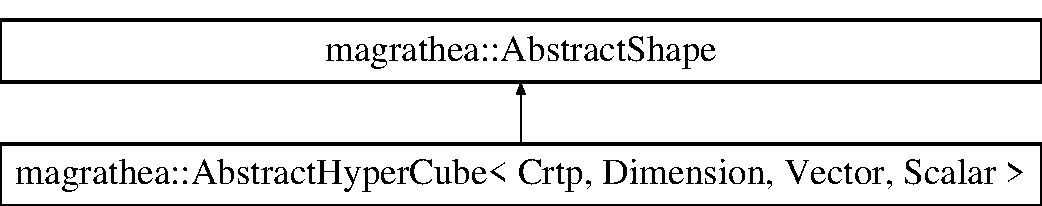
\includegraphics[height=2.000000cm]{classmagrathea_1_1AbstractHyperCube}
\end{center}
\end{figure}
\subsection*{Public Member Functions}
\begin{Indent}{\bf Position}\par
\begin{DoxyCompactItemize}
\item 
constexpr Scalar \hyperlink{classmagrathea_1_1AbstractHyperCube_a92d8e9710571e72fccd885ecedb4e075}{center} (const unsigned int idim) const 
\begin{DoxyCompactList}\small\item\em Center coordinate. \end{DoxyCompactList}\item 
Vector \hyperlink{classmagrathea_1_1AbstractHyperCube_a68e48d5ef5c0403770865b56c98a1494}{center} () const 
\begin{DoxyCompactList}\small\item\em Center vector. \end{DoxyCompactList}\item 
constexpr Scalar \hyperlink{classmagrathea_1_1AbstractHyperCube_a00245afe000222d837c1aa3cd09e08bd}{minimum} (const unsigned int idim) const 
\begin{DoxyCompactList}\small\item\em Minimum coordinate. \end{DoxyCompactList}\item 
Vector \hyperlink{classmagrathea_1_1AbstractHyperCube_a2efa04a1b5098cc7898f27aee16412fc}{minimum} () const 
\begin{DoxyCompactList}\small\item\em Minimum vector. \end{DoxyCompactList}\item 
constexpr Scalar \hyperlink{classmagrathea_1_1AbstractHyperCube_a1b36f49a44cecb681cc38e05a1a0c582}{maximum} (const unsigned int idim) const 
\begin{DoxyCompactList}\small\item\em Maximum coordinate. \end{DoxyCompactList}\item 
Vector \hyperlink{classmagrathea_1_1AbstractHyperCube_a3f589f4b3e788827941363ad9b97dc8e}{maximum} () const 
\begin{DoxyCompactList}\small\item\em Maximum vector. \end{DoxyCompactList}\end{DoxyCompactItemize}
\end{Indent}
\begin{Indent}{\bf Measures}\par
\begin{DoxyCompactItemize}
\item 
constexpr Scalar \hyperlink{classmagrathea_1_1AbstractHyperCube_a8534fd1643ba9e27a45a10a9526fc26e}{length} () const 
\begin{DoxyCompactList}\small\item\em Length. \end{DoxyCompactList}\item 
constexpr Scalar \hyperlink{classmagrathea_1_1AbstractHyperCube_a4f80c91ff6729500b69edc88107791aa}{volume} () const 
\begin{DoxyCompactList}\small\item\em Volume. \end{DoxyCompactList}\item 
{\footnotesize template$<$unsigned int Subdimension = Dimension-\/(\-Dimension != 0)$>$ }\\constexpr Scalar \hyperlink{classmagrathea_1_1AbstractHyperCube_ad4b1dded1b858ea3483e5af1113ed57e}{surface} () const 
\begin{DoxyCompactList}\small\item\em Outer surface. \end{DoxyCompactList}\item 
{\footnotesize template$<$unsigned int Subdimension = Dimension-\/(\-Dimension != 0)$>$ }\\constexpr Scalar \hyperlink{classmagrathea_1_1AbstractHyperCube_aa65ddc7ef856434b45aecff688390d4b}{area} () const 
\begin{DoxyCompactList}\small\item\em Element area. \end{DoxyCompactList}\item 
{\footnotesize template$<$unsigned int Subdimension = Dimension$>$ }\\constexpr Scalar \hyperlink{classmagrathea_1_1AbstractHyperCube_a698ec7f90b98f44f8149da7ad466419a}{diagonal} () const 
\begin{DoxyCompactList}\small\item\em Diagonal. \end{DoxyCompactList}\end{DoxyCompactItemize}
\end{Indent}
\begin{Indent}{\bf Distribution}\par
\begin{DoxyCompactItemize}
\item 
{\footnotesize template$<$unsigned int Subdimension = Dimension, class  = typename std\-::enable\-\_\-if$<$(\-Subdimension != 0) $|$$|$ (\-Subdimension == 0)$>$\-::type$>$ }\\Vector \hyperlink{classmagrathea_1_1AbstractHyperCube_aa071c3abcff00828d27f13454fcf604d}{random} () const 
\begin{DoxyCompactList}\small\item\em Basic random location in the hypercube. \end{DoxyCompactList}\item 
{\footnotesize template$<$unsigned int Subdimension = Dimension, class Engine , class Distribution , class  = typename std\-::enable\-\_\-if$<$((\-Subdimension != 0) $|$$|$ (\-Subdimension == 0)) \&\& (std\-::decay$<$\-Engine$>$\-::type\-::min() != std\-::decay$<$\-Engine$>$\-::type\-::max()) \&\& (!std\-::is\-\_\-void$<$typename std\-::decay$<$\-Distribution$>$\-::type\-::result\-\_\-type$>$\-::value)$>$\-::type$>$ }\\Vector \hyperlink{classmagrathea_1_1AbstractHyperCube_aa529bedcd503631825f7e21b893e3d7e}{random} (Engine \&\&engine, Distribution \&\&distribution) const 
\begin{DoxyCompactList}\small\item\em Generic random location in the hypercube. \end{DoxyCompactList}\end{DoxyCompactItemize}
\end{Indent}
\begin{Indent}{\bf Collision}\par
\begin{DoxyCompactItemize}
\item 
{\footnotesize template$<$class Other\-Vector , class  = typename std\-::enable\-\_\-if$<$std\-::is\-\_\-convertible$<$typename std\-::remove\-\_\-cv$<$typename std\-::remove\-\_\-reference$<$decltype(std\-::declval$<$\-Other\-Vector$>$()\mbox{[}0\mbox{]})$>$\-::type$>$\-::type, Scalar$>$\-::value$>$\-::type$>$ }\\bool \hyperlink{classmagrathea_1_1AbstractHyperCube_a0fd1a2a8ee4af9823606cd4bfa0ba3a7}{inside} (const Other\-Vector \&\hyperlink{miscellaneous_8h_af4785a592bbb7b2a8882c18bb0101192}{point}) const 
\begin{DoxyCompactList}\small\item\em Point inside. \end{DoxyCompactList}\item 
{\footnotesize template$<$class Other\-Vector , class  = typename std\-::enable\-\_\-if$<$std\-::is\-\_\-convertible$<$typename std\-::remove\-\_\-cv$<$typename std\-::remove\-\_\-reference$<$decltype(std\-::declval$<$\-Other\-Vector$>$()\mbox{[}0\mbox{]})$>$\-::type$>$\-::type, Scalar$>$\-::value$>$\-::type$>$ }\\bool \hyperlink{classmagrathea_1_1AbstractHyperCube_a3d82e1fae74385b35ed4957b69b0d3ec}{outside} (const Other\-Vector \&\hyperlink{miscellaneous_8h_af4785a592bbb7b2a8882c18bb0101192}{point}) const 
\begin{DoxyCompactList}\small\item\em Point outside. \end{DoxyCompactList}\end{DoxyCompactItemize}
\end{Indent}
\subsection*{Static Public Member Functions}
\begin{Indent}{\bf Constants}\par
\begin{DoxyCompactItemize}
\item 
static constexpr unsigned int \hyperlink{classmagrathea_1_1AbstractHyperCube_a9d9dbd803c06603fbd23058689f44cc7}{dimension} ()
\begin{DoxyCompactList}\small\item\em Number of space dimension. \end{DoxyCompactList}\item 
{\footnotesize template$<$unsigned int Subdimension = Dimension$>$ }\\static constexpr unsigned int \hyperlink{classmagrathea_1_1AbstractHyperCube_a72f398a8e3993826380cabc47aba7b8e}{elements} ()
\begin{DoxyCompactList}\small\item\em Number of elements. \end{DoxyCompactList}\item 
{\footnotesize template$<$unsigned int First\-Subdimension = 0, unsigned int Last\-Subdimension = Dimension-\/(\-Dimension != 0)$>$ }\\static constexpr unsigned int \hyperlink{classmagrathea_1_1AbstractHyperCube_aa681927fa1b4ae8e940c618740ce6394}{subelements} ()
\begin{DoxyCompactList}\small\item\em Sum of elements. \end{DoxyCompactList}\end{DoxyCompactItemize}
\end{Indent}
\begin{Indent}{\bf Test}\par
\begin{DoxyCompactItemize}
\item 
static int \hyperlink{classmagrathea_1_1AbstractHyperCube_a906538ea22de1d67f1c3cada11f8df6f}{example} ()
\begin{DoxyCompactList}\small\item\em Example function. \end{DoxyCompactList}\end{DoxyCompactItemize}
\end{Indent}
\subsection*{Protected Member Functions}
\begin{Indent}{\bf Protected lifecycle}\par
\begin{DoxyCompactItemize}
\item 
\hyperlink{classmagrathea_1_1AbstractHyperCube_a1d8df066cb99cde45bdc3707120c3d8c}{$\sim$\-Abstract\-Hyper\-Cube} ()
\begin{DoxyCompactList}\small\item\em Protected destructor. \end{DoxyCompactList}\end{DoxyCompactItemize}
\end{Indent}


\subsection{Detailed Description}
\subsubsection*{template$<$class Crtp, unsigned int Dimension, class Vector, typename Scalar$>$class magrathea\-::\-Abstract\-Hyper\-Cube$<$ Crtp, Dimension, Vector, Scalar $>$}

Abstract function provider for n-\/dimensional cubes. 

Provides a common base for n-\/dimensional cubes thanks to C\-R\-T\-P. To use it, one has to derive from this class and pass the derived class itself as the C\-R\-T\-P parameter. The derived classes should provide two immutable functions \-: 
\begin{DoxyItemize}
\item position() 
\item extent()
\end{DoxyItemize}in order to get the position of the center along one coordinate and the edge length of the hypercube. 
\begin{DoxyTemplParams}{Template Parameters}
{\em Crtp} & Derived C\-R\-T\-P class. \\
\hline
{\em Dimension} & Number of space dimension. \\
\hline
{\em Vector} & Position vector type. \\
\hline
{\em Scalar} & Scalar data type. \\
\hline
\end{DoxyTemplParams}


\subsection{Constructor \& Destructor Documentation}
\hypertarget{classmagrathea_1_1AbstractHyperCube_a1d8df066cb99cde45bdc3707120c3d8c}{\index{magrathea\-::\-Abstract\-Hyper\-Cube@{magrathea\-::\-Abstract\-Hyper\-Cube}!$\sim$\-Abstract\-Hyper\-Cube@{$\sim$\-Abstract\-Hyper\-Cube}}
\index{$\sim$\-Abstract\-Hyper\-Cube@{$\sim$\-Abstract\-Hyper\-Cube}!magrathea::AbstractHyperCube@{magrathea\-::\-Abstract\-Hyper\-Cube}}
\subsubsection[{$\sim$\-Abstract\-Hyper\-Cube}]{\setlength{\rightskip}{0pt plus 5cm}template$<$class Crtp , unsigned int Dimension, class Vector , typename Scalar $>$ {\bf magrathea\-::\-Abstract\-Hyper\-Cube}$<$ Crtp, Dimension, Vector, Scalar $>$\-::$\sim${\bf Abstract\-Hyper\-Cube} (
\begin{DoxyParamCaption}
{}
\end{DoxyParamCaption}
)\hspace{0.3cm}{\ttfamily [inline]}, {\ttfamily [protected]}, {\ttfamily [default]}}}\label{classmagrathea_1_1AbstractHyperCube_a1d8df066cb99cde45bdc3707120c3d8c}


Protected destructor. 

Avoids direct instantiation of the class, and only allows it through its derived children. 

\subsection{Member Function Documentation}
\hypertarget{classmagrathea_1_1AbstractHyperCube_aa65ddc7ef856434b45aecff688390d4b}{\index{magrathea\-::\-Abstract\-Hyper\-Cube@{magrathea\-::\-Abstract\-Hyper\-Cube}!area@{area}}
\index{area@{area}!magrathea::AbstractHyperCube@{magrathea\-::\-Abstract\-Hyper\-Cube}}
\subsubsection[{area}]{\setlength{\rightskip}{0pt plus 5cm}template$<$class Crtp , unsigned int Dimension, class Vector , typename Scalar $>$ template$<$unsigned int Subdimension$>$ constexpr Scalar {\bf magrathea\-::\-Abstract\-Hyper\-Cube}$<$ Crtp, Dimension, Vector, Scalar $>$\-::area (
\begin{DoxyParamCaption}
{}
\end{DoxyParamCaption}
) const}}\label{classmagrathea_1_1AbstractHyperCube_aa65ddc7ef856434b45aecff688390d4b}


Element area. 

Computes the surface of a single element of the hypercube. 
\begin{DoxyTemplParams}{Template Parameters}
{\em Subdimension} & Dimension of elements. \\
\hline
\end{DoxyTemplParams}
\begin{DoxyReturn}{Returns}
$l^{D}$. 
\end{DoxyReturn}
\hypertarget{classmagrathea_1_1AbstractHyperCube_a92d8e9710571e72fccd885ecedb4e075}{\index{magrathea\-::\-Abstract\-Hyper\-Cube@{magrathea\-::\-Abstract\-Hyper\-Cube}!center@{center}}
\index{center@{center}!magrathea::AbstractHyperCube@{magrathea\-::\-Abstract\-Hyper\-Cube}}
\subsubsection[{center}]{\setlength{\rightskip}{0pt plus 5cm}template$<$class Crtp , unsigned int Dimension, class Vector , typename Scalar $>$ constexpr Scalar {\bf magrathea\-::\-Abstract\-Hyper\-Cube}$<$ Crtp, Dimension, Vector, Scalar $>$\-::center (
\begin{DoxyParamCaption}
\item[{const unsigned int}]{idim}
\end{DoxyParamCaption}
) const}}\label{classmagrathea_1_1AbstractHyperCube_a92d8e9710571e72fccd885ecedb4e075}


Center coordinate. 

Computes the specified coordinate of the center of the hypercube. 
\begin{DoxyParams}[1]{Parameters}
\mbox{\tt in}  & {\em idim} & Index of the dimension. \\
\hline
\end{DoxyParams}
\begin{DoxyReturn}{Returns}
The coordinate $x_{i}$. 
\end{DoxyReturn}
\hypertarget{classmagrathea_1_1AbstractHyperCube_a68e48d5ef5c0403770865b56c98a1494}{\index{magrathea\-::\-Abstract\-Hyper\-Cube@{magrathea\-::\-Abstract\-Hyper\-Cube}!center@{center}}
\index{center@{center}!magrathea::AbstractHyperCube@{magrathea\-::\-Abstract\-Hyper\-Cube}}
\subsubsection[{center}]{\setlength{\rightskip}{0pt plus 5cm}template$<$class Crtp , unsigned int Dimension, class Vector , typename Scalar $>$ Vector {\bf magrathea\-::\-Abstract\-Hyper\-Cube}$<$ Crtp, Dimension, Vector, Scalar $>$\-::center (
\begin{DoxyParamCaption}
{}
\end{DoxyParamCaption}
) const\hspace{0.3cm}{\ttfamily [inline]}}}\label{classmagrathea_1_1AbstractHyperCube_a68e48d5ef5c0403770865b56c98a1494}


Center vector. 

Computes the position vector of the center of the hypercube. \begin{DoxyReturn}{Returns}
The position vector $\vec{x}$. 
\end{DoxyReturn}
\hypertarget{classmagrathea_1_1AbstractHyperCube_a698ec7f90b98f44f8149da7ad466419a}{\index{magrathea\-::\-Abstract\-Hyper\-Cube@{magrathea\-::\-Abstract\-Hyper\-Cube}!diagonal@{diagonal}}
\index{diagonal@{diagonal}!magrathea::AbstractHyperCube@{magrathea\-::\-Abstract\-Hyper\-Cube}}
\subsubsection[{diagonal}]{\setlength{\rightskip}{0pt plus 5cm}template$<$class Crtp , unsigned int Dimension, class Vector , typename Scalar $>$ template$<$unsigned int Subdimension$>$ constexpr Scalar {\bf magrathea\-::\-Abstract\-Hyper\-Cube}$<$ Crtp, Dimension, Vector, Scalar $>$\-::diagonal (
\begin{DoxyParamCaption}
{}
\end{DoxyParamCaption}
) const}}\label{classmagrathea_1_1AbstractHyperCube_a698ec7f90b98f44f8149da7ad466419a}


Diagonal. 

Computes the length of the diagonal in the specified subdimension. 
\begin{DoxyTemplParams}{Template Parameters}
{\em Subdimension} & Dimension of elements. \\
\hline
\end{DoxyTemplParams}
\begin{DoxyReturn}{Returns}
$\sqrt{D} \times l$. 
\end{DoxyReturn}
\hypertarget{classmagrathea_1_1AbstractHyperCube_a9d9dbd803c06603fbd23058689f44cc7}{\index{magrathea\-::\-Abstract\-Hyper\-Cube@{magrathea\-::\-Abstract\-Hyper\-Cube}!dimension@{dimension}}
\index{dimension@{dimension}!magrathea::AbstractHyperCube@{magrathea\-::\-Abstract\-Hyper\-Cube}}
\subsubsection[{dimension}]{\setlength{\rightskip}{0pt plus 5cm}template$<$class Crtp , unsigned int Dimension, class Vector , typename Scalar $>$ constexpr unsigned int {\bf magrathea\-::\-Abstract\-Hyper\-Cube}$<$ Crtp, Dimension, Vector, Scalar $>$\-::dimension (
\begin{DoxyParamCaption}
{}
\end{DoxyParamCaption}
)\hspace{0.3cm}{\ttfamily [static]}}}\label{classmagrathea_1_1AbstractHyperCube_a9d9dbd803c06603fbd23058689f44cc7}


Number of space dimension. 

Computes the number of space dimension of the hypercube. \begin{DoxyReturn}{Returns}
Dimension. 
\end{DoxyReturn}
\hypertarget{classmagrathea_1_1AbstractHyperCube_a72f398a8e3993826380cabc47aba7b8e}{\index{magrathea\-::\-Abstract\-Hyper\-Cube@{magrathea\-::\-Abstract\-Hyper\-Cube}!elements@{elements}}
\index{elements@{elements}!magrathea::AbstractHyperCube@{magrathea\-::\-Abstract\-Hyper\-Cube}}
\subsubsection[{elements}]{\setlength{\rightskip}{0pt plus 5cm}template$<$class Crtp , unsigned int Dimension, class Vector , typename Scalar $>$ template$<$unsigned int Subdimension$>$ constexpr unsigned int {\bf magrathea\-::\-Abstract\-Hyper\-Cube}$<$ Crtp, Dimension, Vector, Scalar $>$\-::elements (
\begin{DoxyParamCaption}
{}
\end{DoxyParamCaption}
)\hspace{0.3cm}{\ttfamily [static]}}}\label{classmagrathea_1_1AbstractHyperCube_a72f398a8e3993826380cabc47aba7b8e}


Number of elements. 

Computes the number of elements of the specified subdimension in the hypercube. For example, for a specified subdimension 0, it computes the number of points. 
\begin{DoxyTemplParams}{Template Parameters}
{\em Subdimension} & Dimension of elements. \\
\hline
\end{DoxyTemplParams}
\begin{DoxyReturn}{Returns}
$2^{D-d}\binom{D}{d}$. 
\end{DoxyReturn}
\hypertarget{classmagrathea_1_1AbstractHyperCube_a906538ea22de1d67f1c3cada11f8df6f}{\index{magrathea\-::\-Abstract\-Hyper\-Cube@{magrathea\-::\-Abstract\-Hyper\-Cube}!example@{example}}
\index{example@{example}!magrathea::AbstractHyperCube@{magrathea\-::\-Abstract\-Hyper\-Cube}}
\subsubsection[{example}]{\setlength{\rightskip}{0pt plus 5cm}template$<$class Crtp , unsigned int Dimension, class Vector , typename Scalar $>$ int {\bf magrathea\-::\-Abstract\-Hyper\-Cube}$<$ Crtp, Dimension, Vector, Scalar $>$\-::example (
\begin{DoxyParamCaption}
{}
\end{DoxyParamCaption}
)\hspace{0.3cm}{\ttfamily [static]}}}\label{classmagrathea_1_1AbstractHyperCube_a906538ea22de1d67f1c3cada11f8df6f}


Example function. 

Tests and demonstrates the use of \hyperlink{classmagrathea_1_1AbstractHyperCube}{Abstract\-Hyper\-Cube}. \begin{DoxyReturn}{Returns}
0 if no error. 
\end{DoxyReturn}
\hypertarget{classmagrathea_1_1AbstractHyperCube_a0fd1a2a8ee4af9823606cd4bfa0ba3a7}{\index{magrathea\-::\-Abstract\-Hyper\-Cube@{magrathea\-::\-Abstract\-Hyper\-Cube}!inside@{inside}}
\index{inside@{inside}!magrathea::AbstractHyperCube@{magrathea\-::\-Abstract\-Hyper\-Cube}}
\subsubsection[{inside}]{\setlength{\rightskip}{0pt plus 5cm}template$<$class Crtp , unsigned int Dimension, class Vector , typename Scalar $>$ template$<$class Other\-Vector , class $>$ bool {\bf magrathea\-::\-Abstract\-Hyper\-Cube}$<$ Crtp, Dimension, Vector, Scalar $>$\-::inside (
\begin{DoxyParamCaption}
\item[{const Other\-Vector \&}]{point}
\end{DoxyParamCaption}
) const\hspace{0.3cm}{\ttfamily [inline]}}}\label{classmagrathea_1_1AbstractHyperCube_a0fd1a2a8ee4af9823606cd4bfa0ba3a7}


Point inside. 

Checks whether a point is inside the hypercube. 
\begin{DoxyTemplParams}{Template Parameters}
{\em Other\-Vector} & Other position vector type. \\
\hline
\end{DoxyTemplParams}

\begin{DoxyParams}[1]{Parameters}
\mbox{\tt in}  & {\em point} & Position of the point. \\
\hline
\end{DoxyParams}
\begin{DoxyReturn}{Returns}
True if the point is inside the hypercube, false otherwise. 
\end{DoxyReturn}
\hypertarget{classmagrathea_1_1AbstractHyperCube_a8534fd1643ba9e27a45a10a9526fc26e}{\index{magrathea\-::\-Abstract\-Hyper\-Cube@{magrathea\-::\-Abstract\-Hyper\-Cube}!length@{length}}
\index{length@{length}!magrathea::AbstractHyperCube@{magrathea\-::\-Abstract\-Hyper\-Cube}}
\subsubsection[{length}]{\setlength{\rightskip}{0pt plus 5cm}template$<$class Crtp , unsigned int Dimension, class Vector , typename Scalar $>$ constexpr Scalar {\bf magrathea\-::\-Abstract\-Hyper\-Cube}$<$ Crtp, Dimension, Vector, Scalar $>$\-::length (
\begin{DoxyParamCaption}
{}
\end{DoxyParamCaption}
) const}}\label{classmagrathea_1_1AbstractHyperCube_a8534fd1643ba9e27a45a10a9526fc26e}


Length. 

Computes the edge length of the hypercube. \begin{DoxyReturn}{Returns}
$l$. 
\end{DoxyReturn}
\hypertarget{classmagrathea_1_1AbstractHyperCube_a1b36f49a44cecb681cc38e05a1a0c582}{\index{magrathea\-::\-Abstract\-Hyper\-Cube@{magrathea\-::\-Abstract\-Hyper\-Cube}!maximum@{maximum}}
\index{maximum@{maximum}!magrathea::AbstractHyperCube@{magrathea\-::\-Abstract\-Hyper\-Cube}}
\subsubsection[{maximum}]{\setlength{\rightskip}{0pt plus 5cm}template$<$class Crtp , unsigned int Dimension, class Vector , typename Scalar $>$ constexpr Scalar {\bf magrathea\-::\-Abstract\-Hyper\-Cube}$<$ Crtp, Dimension, Vector, Scalar $>$\-::maximum (
\begin{DoxyParamCaption}
\item[{const unsigned int}]{idim}
\end{DoxyParamCaption}
) const}}\label{classmagrathea_1_1AbstractHyperCube_a1b36f49a44cecb681cc38e05a1a0c582}


Maximum coordinate. 

Computes the specified coordinate of the maximum boundary of the hypercube. 
\begin{DoxyParams}[1]{Parameters}
\mbox{\tt in}  & {\em idim} & Index of the dimension. \\
\hline
\end{DoxyParams}
\begin{DoxyReturn}{Returns}
The coordinate $x_{i}+\frac{l}{2}$. 
\end{DoxyReturn}
\hypertarget{classmagrathea_1_1AbstractHyperCube_a3f589f4b3e788827941363ad9b97dc8e}{\index{magrathea\-::\-Abstract\-Hyper\-Cube@{magrathea\-::\-Abstract\-Hyper\-Cube}!maximum@{maximum}}
\index{maximum@{maximum}!magrathea::AbstractHyperCube@{magrathea\-::\-Abstract\-Hyper\-Cube}}
\subsubsection[{maximum}]{\setlength{\rightskip}{0pt plus 5cm}template$<$class Crtp , unsigned int Dimension, class Vector , typename Scalar $>$ Vector {\bf magrathea\-::\-Abstract\-Hyper\-Cube}$<$ Crtp, Dimension, Vector, Scalar $>$\-::maximum (
\begin{DoxyParamCaption}
{}
\end{DoxyParamCaption}
) const\hspace{0.3cm}{\ttfamily [inline]}}}\label{classmagrathea_1_1AbstractHyperCube_a3f589f4b3e788827941363ad9b97dc8e}


Maximum vector. 

Computes the position vector of the maximum boundary of the hypercube. \begin{DoxyReturn}{Returns}
The position vector $\vec{x}+\frac{\vec{l}}{2}$. 
\end{DoxyReturn}
\hypertarget{classmagrathea_1_1AbstractHyperCube_a00245afe000222d837c1aa3cd09e08bd}{\index{magrathea\-::\-Abstract\-Hyper\-Cube@{magrathea\-::\-Abstract\-Hyper\-Cube}!minimum@{minimum}}
\index{minimum@{minimum}!magrathea::AbstractHyperCube@{magrathea\-::\-Abstract\-Hyper\-Cube}}
\subsubsection[{minimum}]{\setlength{\rightskip}{0pt plus 5cm}template$<$class Crtp , unsigned int Dimension, class Vector , typename Scalar $>$ constexpr Scalar {\bf magrathea\-::\-Abstract\-Hyper\-Cube}$<$ Crtp, Dimension, Vector, Scalar $>$\-::minimum (
\begin{DoxyParamCaption}
\item[{const unsigned int}]{idim}
\end{DoxyParamCaption}
) const}}\label{classmagrathea_1_1AbstractHyperCube_a00245afe000222d837c1aa3cd09e08bd}


Minimum coordinate. 

Computes the specified coordinate of the minimum boundary of the hypercube. 
\begin{DoxyParams}[1]{Parameters}
\mbox{\tt in}  & {\em idim} & Index of the dimension. \\
\hline
\end{DoxyParams}
\begin{DoxyReturn}{Returns}
The coordinate $x_{i}-\frac{l}{2}$. 
\end{DoxyReturn}
\hypertarget{classmagrathea_1_1AbstractHyperCube_a2efa04a1b5098cc7898f27aee16412fc}{\index{magrathea\-::\-Abstract\-Hyper\-Cube@{magrathea\-::\-Abstract\-Hyper\-Cube}!minimum@{minimum}}
\index{minimum@{minimum}!magrathea::AbstractHyperCube@{magrathea\-::\-Abstract\-Hyper\-Cube}}
\subsubsection[{minimum}]{\setlength{\rightskip}{0pt plus 5cm}template$<$class Crtp , unsigned int Dimension, class Vector , typename Scalar $>$ Vector {\bf magrathea\-::\-Abstract\-Hyper\-Cube}$<$ Crtp, Dimension, Vector, Scalar $>$\-::minimum (
\begin{DoxyParamCaption}
{}
\end{DoxyParamCaption}
) const\hspace{0.3cm}{\ttfamily [inline]}}}\label{classmagrathea_1_1AbstractHyperCube_a2efa04a1b5098cc7898f27aee16412fc}


Minimum vector. 

Computes the position vector of the minimum boundary of the hypercube. \begin{DoxyReturn}{Returns}
The position vector $\vec{x}-\frac{\vec{l}}{2}$. 
\end{DoxyReturn}
\hypertarget{classmagrathea_1_1AbstractHyperCube_a3d82e1fae74385b35ed4957b69b0d3ec}{\index{magrathea\-::\-Abstract\-Hyper\-Cube@{magrathea\-::\-Abstract\-Hyper\-Cube}!outside@{outside}}
\index{outside@{outside}!magrathea::AbstractHyperCube@{magrathea\-::\-Abstract\-Hyper\-Cube}}
\subsubsection[{outside}]{\setlength{\rightskip}{0pt plus 5cm}template$<$class Crtp , unsigned int Dimension, class Vector , typename Scalar $>$ template$<$class Other\-Vector , class $>$ bool {\bf magrathea\-::\-Abstract\-Hyper\-Cube}$<$ Crtp, Dimension, Vector, Scalar $>$\-::outside (
\begin{DoxyParamCaption}
\item[{const Other\-Vector \&}]{point}
\end{DoxyParamCaption}
) const\hspace{0.3cm}{\ttfamily [inline]}}}\label{classmagrathea_1_1AbstractHyperCube_a3d82e1fae74385b35ed4957b69b0d3ec}


Point outside. 

Checks whether a point is outside the hypercube. 
\begin{DoxyTemplParams}{Template Parameters}
{\em Other\-Vector} & Other position vector type. \\
\hline
\end{DoxyTemplParams}

\begin{DoxyParams}[1]{Parameters}
\mbox{\tt in}  & {\em point} & Position of the point. \\
\hline
\end{DoxyParams}
\begin{DoxyReturn}{Returns}
True if the point is outside the hypercube, false otherwise. 
\end{DoxyReturn}
\hypertarget{classmagrathea_1_1AbstractHyperCube_aa071c3abcff00828d27f13454fcf604d}{\index{magrathea\-::\-Abstract\-Hyper\-Cube@{magrathea\-::\-Abstract\-Hyper\-Cube}!random@{random}}
\index{random@{random}!magrathea::AbstractHyperCube@{magrathea\-::\-Abstract\-Hyper\-Cube}}
\subsubsection[{random}]{\setlength{\rightskip}{0pt plus 5cm}template$<$class Crtp , unsigned int Dimension, class Vector , typename Scalar $>$ template$<$unsigned int Subdimension, class $>$ Vector {\bf magrathea\-::\-Abstract\-Hyper\-Cube}$<$ Crtp, Dimension, Vector, Scalar $>$\-::random (
\begin{DoxyParamCaption}
{}
\end{DoxyParamCaption}
) const}}\label{classmagrathea_1_1AbstractHyperCube_aa071c3abcff00828d27f13454fcf604d}


Basic random location in the hypercube. 

Generates a random location, located on the subdimensional elements of the hypercube. For example for a subdimension of 2 of a 3-\/dimensional hypercube, the function will generates a random point located on the surface of the cube. 
\begin{DoxyTemplParams}{Template Parameters}
{\em Subdimension} & Dimension space. \\
\hline
\end{DoxyTemplParams}
\begin{DoxyReturn}{Returns}
Random position vector. 
\end{DoxyReturn}
\begin{DoxyWarning}{Warning}
As the internal engine is a static one, do not use this function in parallel. 
\end{DoxyWarning}
\hypertarget{classmagrathea_1_1AbstractHyperCube_aa529bedcd503631825f7e21b893e3d7e}{\index{magrathea\-::\-Abstract\-Hyper\-Cube@{magrathea\-::\-Abstract\-Hyper\-Cube}!random@{random}}
\index{random@{random}!magrathea::AbstractHyperCube@{magrathea\-::\-Abstract\-Hyper\-Cube}}
\subsubsection[{random}]{\setlength{\rightskip}{0pt plus 5cm}template$<$class Crtp , unsigned int Dimension, class Vector , typename Scalar $>$ template$<$unsigned int Subdimension, class Engine , class Distribution , class $>$ Vector {\bf magrathea\-::\-Abstract\-Hyper\-Cube}$<$ Crtp, Dimension, Vector, Scalar $>$\-::random (
\begin{DoxyParamCaption}
\item[{Engine \&\&}]{engine, }
\item[{Distribution \&\&}]{distribution}
\end{DoxyParamCaption}
) const}}\label{classmagrathea_1_1AbstractHyperCube_aa529bedcd503631825f7e21b893e3d7e}


Generic random location in the hypercube. 

Generates a random location, located on the subdimensional elements of the hypercube. For example for a subdimension of 2 of a 3-\/dimensional hypercube, the function will generates a random point located on the surface of the cube. As this function uses the passed random engine and distribution it is completely thread safe. 
\begin{DoxyTemplParams}{Template Parameters}
{\em Subdimension} & Dimension space. \\
\hline
{\em Engine} & (Random engine type.) \\
\hline
{\em Distribution} & (Random distribution type.) \\
\hline
\end{DoxyTemplParams}

\begin{DoxyParams}[1]{Parameters}
\mbox{\tt in,out}  & {\em engine} & Random engine. \\
\hline
\mbox{\tt in,out}  & {\em distribution} & Random distribution. \\
\hline
\end{DoxyParams}
\begin{DoxyReturn}{Returns}
Random position vector. 
\end{DoxyReturn}
\hypertarget{classmagrathea_1_1AbstractHyperCube_aa681927fa1b4ae8e940c618740ce6394}{\index{magrathea\-::\-Abstract\-Hyper\-Cube@{magrathea\-::\-Abstract\-Hyper\-Cube}!subelements@{subelements}}
\index{subelements@{subelements}!magrathea::AbstractHyperCube@{magrathea\-::\-Abstract\-Hyper\-Cube}}
\subsubsection[{subelements}]{\setlength{\rightskip}{0pt plus 5cm}template$<$class Crtp , unsigned int Dimension, class Vector , typename Scalar $>$ template$<$unsigned int First, unsigned int Last$>$ constexpr unsigned int {\bf magrathea\-::\-Abstract\-Hyper\-Cube}$<$ Crtp, Dimension, Vector, Scalar $>$\-::subelements (
\begin{DoxyParamCaption}
{}
\end{DoxyParamCaption}
)\hspace{0.3cm}{\ttfamily [static]}}}\label{classmagrathea_1_1AbstractHyperCube_aa681927fa1b4ae8e940c618740ce6394}


Sum of elements. 

Computes the sum of the hypercube elements between the two given dimensions. 
\begin{DoxyTemplParams}{Template Parameters}
{\em First} & First dimension of elements. \\
\hline
{\em Last} & Last dimension of elements. \\
\hline
\end{DoxyTemplParams}
\begin{DoxyReturn}{Returns}
$\sum_{d}2^{D-d}\binom{D}{d}$. 
\end{DoxyReturn}
\hypertarget{classmagrathea_1_1AbstractHyperCube_ad4b1dded1b858ea3483e5af1113ed57e}{\index{magrathea\-::\-Abstract\-Hyper\-Cube@{magrathea\-::\-Abstract\-Hyper\-Cube}!surface@{surface}}
\index{surface@{surface}!magrathea::AbstractHyperCube@{magrathea\-::\-Abstract\-Hyper\-Cube}}
\subsubsection[{surface}]{\setlength{\rightskip}{0pt plus 5cm}template$<$class Crtp , unsigned int Dimension, class Vector , typename Scalar $>$ template$<$unsigned int Subdimension$>$ constexpr Scalar {\bf magrathea\-::\-Abstract\-Hyper\-Cube}$<$ Crtp, Dimension, Vector, Scalar $>$\-::surface (
\begin{DoxyParamCaption}
{}
\end{DoxyParamCaption}
) const}}\label{classmagrathea_1_1AbstractHyperCube_ad4b1dded1b858ea3483e5af1113ed57e}


Outer surface. 

Computes the total outer surface of the hypercube. 
\begin{DoxyTemplParams}{Template Parameters}
{\em Subdimension} & Dimension of elements. \\
\hline
\end{DoxyTemplParams}
\begin{DoxyReturn}{Returns}
$2^{D-d}\binom{D}{d} \times l^{D}$. 
\end{DoxyReturn}
\hypertarget{classmagrathea_1_1AbstractHyperCube_a4f80c91ff6729500b69edc88107791aa}{\index{magrathea\-::\-Abstract\-Hyper\-Cube@{magrathea\-::\-Abstract\-Hyper\-Cube}!volume@{volume}}
\index{volume@{volume}!magrathea::AbstractHyperCube@{magrathea\-::\-Abstract\-Hyper\-Cube}}
\subsubsection[{volume}]{\setlength{\rightskip}{0pt plus 5cm}template$<$class Crtp , unsigned int Dimension, class Vector , typename Scalar $>$ constexpr Scalar {\bf magrathea\-::\-Abstract\-Hyper\-Cube}$<$ Crtp, Dimension, Vector, Scalar $>$\-::volume (
\begin{DoxyParamCaption}
{}
\end{DoxyParamCaption}
) const}}\label{classmagrathea_1_1AbstractHyperCube_a4f80c91ff6729500b69edc88107791aa}


Volume. 

Computes the volume of the hypercube. \begin{DoxyReturn}{Returns}
$l^{D}$. 
\end{DoxyReturn}


The documentation for this class was generated from the following file\-:\begin{DoxyCompactItemize}
\item 
/data/home/mbreton/magrathea\-\_\-pathfinder/src/magrathea/\hyperlink{abstracthypercube_8h}{abstracthypercube.\-h}\end{DoxyCompactItemize}

\hypertarget{classmagrathea_1_1AbstractHyperSphere}{\section{magrathea\-:\-:Abstract\-Hyper\-Sphere$<$ Crtp, Dimension, Vector, Scalar $>$ Class Template Reference}
\label{classmagrathea_1_1AbstractHyperSphere}\index{magrathea\-::\-Abstract\-Hyper\-Sphere$<$ Crtp, Dimension, Vector, Scalar $>$@{magrathea\-::\-Abstract\-Hyper\-Sphere$<$ Crtp, Dimension, Vector, Scalar $>$}}
}


Abstract function provider for n-\/dimensional spheres.  




{\ttfamily \#include $<$abstracthypersphere.\-h$>$}

Inheritance diagram for magrathea\-:\-:Abstract\-Hyper\-Sphere$<$ Crtp, Dimension, Vector, Scalar $>$\-:\begin{figure}[H]
\begin{center}
\leavevmode
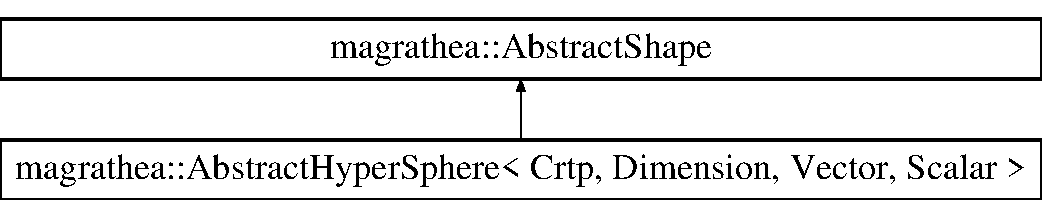
\includegraphics[height=2.000000cm]{classmagrathea_1_1AbstractHyperSphere}
\end{center}
\end{figure}
\subsection*{Public Member Functions}
\begin{Indent}{\bf Position}\par
\begin{DoxyCompactItemize}
\item 
constexpr Scalar \hyperlink{classmagrathea_1_1AbstractHyperSphere_a3dd8d25adc4df0a1aa1878f3b3f48835}{center} (const unsigned int idim) const 
\begin{DoxyCompactList}\small\item\em Center coordinate. \end{DoxyCompactList}\item 
Vector \hyperlink{classmagrathea_1_1AbstractHyperSphere_af16c5565a4d7819aa6db90f599a264fd}{center} () const 
\begin{DoxyCompactList}\small\item\em Center vector. \end{DoxyCompactList}\item 
constexpr Scalar \hyperlink{classmagrathea_1_1AbstractHyperSphere_a9c76e88eea428b595fe1ca44c43bb4e4}{minimum} (const unsigned int idim) const 
\begin{DoxyCompactList}\small\item\em Minimum coordinate. \end{DoxyCompactList}\item 
Vector \hyperlink{classmagrathea_1_1AbstractHyperSphere_a1aec8b8788f5b20154efd0b9fa6bc75a}{minimum} () const 
\begin{DoxyCompactList}\small\item\em Minimum vector. \end{DoxyCompactList}\item 
constexpr Scalar \hyperlink{classmagrathea_1_1AbstractHyperSphere_a6242aa789a4de16158050321c3603c60}{maximum} (const unsigned int idim) const 
\begin{DoxyCompactList}\small\item\em Maximum coordinate. \end{DoxyCompactList}\item 
Vector \hyperlink{classmagrathea_1_1AbstractHyperSphere_a64995340d907a66c2f9b52efbcf719fd}{maximum} () const 
\begin{DoxyCompactList}\small\item\em Maximum vector. \end{DoxyCompactList}\end{DoxyCompactItemize}
\end{Indent}
\begin{Indent}{\bf Measures}\par
\begin{DoxyCompactItemize}
\item 
constexpr Scalar \hyperlink{classmagrathea_1_1AbstractHyperSphere_adae4ee478c4da0e2476ed01bdeca772e}{radius} () const 
\begin{DoxyCompactList}\small\item\em Radius. \end{DoxyCompactList}\item 
constexpr Scalar \hyperlink{classmagrathea_1_1AbstractHyperSphere_a143afcadd29366a1f3f88bd6503579c4}{diameter} () const 
\begin{DoxyCompactList}\small\item\em Diameter. \end{DoxyCompactList}\item 
constexpr Scalar \hyperlink{classmagrathea_1_1AbstractHyperSphere_a8ffa4892227db147188d35f6a5076d7f}{volume} () const 
\begin{DoxyCompactList}\small\item\em Volume. \end{DoxyCompactList}\item 
constexpr Scalar \hyperlink{classmagrathea_1_1AbstractHyperSphere_a0ab167f1e2d23dc522fd7e09387a424e}{surface} () const 
\begin{DoxyCompactList}\small\item\em Outer surface. \end{DoxyCompactList}\end{DoxyCompactItemize}
\end{Indent}
\begin{Indent}{\bf Distribution}\par
\begin{DoxyCompactItemize}
\item 
{\footnotesize template$<$unsigned int Subdimension = Dimension, class  = typename std\-::enable\-\_\-if$<$(\-Subdimension+1 == Dimension) $|$$|$ (\-Subdimension == Dimension)$>$\-::type$>$ }\\Vector \hyperlink{classmagrathea_1_1AbstractHyperSphere_aaebbc45f113ae5a378fb3e66a6d6bd4b}{random} () const 
\begin{DoxyCompactList}\small\item\em Basic random location in the hypersphere. \end{DoxyCompactList}\item 
{\footnotesize template$<$unsigned int Subdimension = Dimension, class Engine , class Distribution , class  = typename std\-::enable\-\_\-if$<$((\-Subdimension+1 == Dimension) $|$$|$ (\-Subdimension == Dimension)) \&\& (std\-::decay$<$\-Engine$>$\-::type\-::min() != std\-::decay$<$\-Engine$>$\-::type\-::max()) \&\& (!std\-::is\-\_\-void$<$typename std\-::decay$<$\-Distribution$>$\-::type\-::result\-\_\-type$>$\-::value)$>$\-::type$>$ }\\Vector \hyperlink{classmagrathea_1_1AbstractHyperSphere_a0d9bbd4a3609ba5a1fe97cd3097a4fc3}{random} (Engine \&\&engine, Distribution \&\&distribution) const 
\begin{DoxyCompactList}\small\item\em Generic random location in the hypersphere. \end{DoxyCompactList}\item 
{\footnotesize template$<$unsigned int Subdimension = Dimension, typename Iterator , class  = typename std\-::enable\-\_\-if$<$(\-Subdimension+1 == Dimension) \&\& (\-Subdimension $>$= 1$>$ }\\\-::type std\-::pair$<$ Scalar, Scalar $>$ \hyperlink{classmagrathea_1_1AbstractHyperSphere_a98fd017fd23437d4ddcac5a2fbf30b60}{uniform} (const Iterator \&first, const Iterator \&last) const 
\begin{DoxyCompactList}\small\item\em Uniform distribution. \end{DoxyCompactList}\end{DoxyCompactItemize}
\end{Indent}
\begin{Indent}{\bf Collision}\par
\begin{DoxyCompactItemize}
\item 
{\footnotesize template$<$class Other\-Vector , class  = typename std\-::enable\-\_\-if$<$std\-::is\-\_\-convertible$<$typename std\-::remove\-\_\-cv$<$typename std\-::remove\-\_\-reference$<$decltype(std\-::declval$<$\-Other\-Vector$>$()\mbox{[}0\mbox{]})$>$\-::type$>$\-::type, Scalar$>$\-::value$>$\-::type$>$ }\\bool \hyperlink{classmagrathea_1_1AbstractHyperSphere_a2fdd902b048b0192b8102fb2c2d30ad3}{inside} (const Other\-Vector \&\hyperlink{miscellaneous_8h_af4785a592bbb7b2a8882c18bb0101192}{point}) const 
\begin{DoxyCompactList}\small\item\em Point inside. \end{DoxyCompactList}\item 
{\footnotesize template$<$class Other\-Vector , class  = typename std\-::enable\-\_\-if$<$std\-::is\-\_\-convertible$<$typename std\-::remove\-\_\-cv$<$typename std\-::remove\-\_\-reference$<$decltype(std\-::declval$<$\-Other\-Vector$>$()\mbox{[}0\mbox{]})$>$\-::type$>$\-::type, Scalar$>$\-::value$>$\-::type$>$ }\\bool \hyperlink{classmagrathea_1_1AbstractHyperSphere_ac9411f645094db51b69a3f4a5be5f05a}{outside} (const Other\-Vector \&\hyperlink{miscellaneous_8h_af4785a592bbb7b2a8882c18bb0101192}{point}) const 
\begin{DoxyCompactList}\small\item\em Point outside. \end{DoxyCompactList}\end{DoxyCompactItemize}
\end{Indent}
\subsection*{Static Public Member Functions}
\begin{Indent}{\bf Constants}\par
\begin{DoxyCompactItemize}
\item 
static constexpr unsigned int \hyperlink{classmagrathea_1_1AbstractHyperSphere_a93e069229d61e08a6026000e21dedb2e}{dimension} ()
\begin{DoxyCompactList}\small\item\em Number of space dimension. \end{DoxyCompactList}\end{DoxyCompactItemize}
\end{Indent}
\begin{Indent}{\bf Helpers}\par
\begin{DoxyCompactItemize}
\item 
{\footnotesize template$<$unsigned int Other\-Dimension = Dimension, typename Other\-Scalar  = Scalar$>$ }\\static constexpr Other\-Scalar \hyperlink{classmagrathea_1_1AbstractHyperSphere_ac636769913d527319bde86deb2f1863c}{sn} ()
\begin{DoxyCompactList}\small\item\em Surface of a n-\/dimensional unit sphere. \end{DoxyCompactList}\end{DoxyCompactItemize}
\end{Indent}
\begin{Indent}{\bf Test}\par
\begin{DoxyCompactItemize}
\item 
static int \hyperlink{classmagrathea_1_1AbstractHyperSphere_a0d1fb9a90aeb540754e9f5f2b13c407f}{example} ()
\begin{DoxyCompactList}\small\item\em Example function. \end{DoxyCompactList}\end{DoxyCompactItemize}
\end{Indent}
\subsection*{Protected Member Functions}
\begin{Indent}{\bf Protected lifecycle}\par
\begin{DoxyCompactItemize}
\item 
\hyperlink{classmagrathea_1_1AbstractHyperSphere_a1fcfa26ef0a672e9deb79ca4040099c0}{$\sim$\-Abstract\-Hyper\-Sphere} ()
\begin{DoxyCompactList}\small\item\em Protected destructor. \end{DoxyCompactList}\end{DoxyCompactItemize}
\end{Indent}


\subsection{Detailed Description}
\subsubsection*{template$<$class Crtp, unsigned int Dimension, class Vector, typename Scalar$>$class magrathea\-::\-Abstract\-Hyper\-Sphere$<$ Crtp, Dimension, Vector, Scalar $>$}

Abstract function provider for n-\/dimensional spheres. 

Provides a common base for n-\/dimensional spheres thanks to C\-R\-T\-P. To use it, one has to derive from this class and pass the derived class itself as the C\-R\-T\-P parameter. The derived classes should provide two immutable functions \-: 
\begin{DoxyItemize}
\item position() 
\item extent()
\end{DoxyItemize}in order to get the position of the center along one coordinate and the radius length of the hypersphere. 
\begin{DoxyTemplParams}{Template Parameters}
{\em Crtp} & Derived C\-R\-T\-P class. \\
\hline
{\em Dimension} & Number of space dimension. \\
\hline
{\em Vector} & Position vector type. \\
\hline
{\em Scalar} & Scalar data type. \\
\hline
\end{DoxyTemplParams}


\subsection{Constructor \& Destructor Documentation}
\hypertarget{classmagrathea_1_1AbstractHyperSphere_a1fcfa26ef0a672e9deb79ca4040099c0}{\index{magrathea\-::\-Abstract\-Hyper\-Sphere@{magrathea\-::\-Abstract\-Hyper\-Sphere}!$\sim$\-Abstract\-Hyper\-Sphere@{$\sim$\-Abstract\-Hyper\-Sphere}}
\index{$\sim$\-Abstract\-Hyper\-Sphere@{$\sim$\-Abstract\-Hyper\-Sphere}!magrathea::AbstractHyperSphere@{magrathea\-::\-Abstract\-Hyper\-Sphere}}
\subsubsection[{$\sim$\-Abstract\-Hyper\-Sphere}]{\setlength{\rightskip}{0pt plus 5cm}template$<$class Crtp , unsigned int Dimension, class Vector , typename Scalar $>$ {\bf magrathea\-::\-Abstract\-Hyper\-Sphere}$<$ Crtp, Dimension, Vector, Scalar $>$\-::$\sim${\bf Abstract\-Hyper\-Sphere} (
\begin{DoxyParamCaption}
{}
\end{DoxyParamCaption}
)\hspace{0.3cm}{\ttfamily [inline]}, {\ttfamily [protected]}, {\ttfamily [default]}}}\label{classmagrathea_1_1AbstractHyperSphere_a1fcfa26ef0a672e9deb79ca4040099c0}


Protected destructor. 

Avoids direct instantiation of the class, and only allows it through its derived children. 

\subsection{Member Function Documentation}
\hypertarget{classmagrathea_1_1AbstractHyperSphere_a3dd8d25adc4df0a1aa1878f3b3f48835}{\index{magrathea\-::\-Abstract\-Hyper\-Sphere@{magrathea\-::\-Abstract\-Hyper\-Sphere}!center@{center}}
\index{center@{center}!magrathea::AbstractHyperSphere@{magrathea\-::\-Abstract\-Hyper\-Sphere}}
\subsubsection[{center}]{\setlength{\rightskip}{0pt plus 5cm}template$<$class Crtp , unsigned int Dimension, class Vector , typename Scalar $>$ constexpr Scalar {\bf magrathea\-::\-Abstract\-Hyper\-Sphere}$<$ Crtp, Dimension, Vector, Scalar $>$\-::center (
\begin{DoxyParamCaption}
\item[{const unsigned int}]{idim}
\end{DoxyParamCaption}
) const}}\label{classmagrathea_1_1AbstractHyperSphere_a3dd8d25adc4df0a1aa1878f3b3f48835}


Center coordinate. 

Computes the specified coordinate of the center of the hypersphere. 
\begin{DoxyParams}[1]{Parameters}
\mbox{\tt in}  & {\em idim} & Index of the dimension. \\
\hline
\end{DoxyParams}
\begin{DoxyReturn}{Returns}
The coordinate $x_{i}$. 
\end{DoxyReturn}
\hypertarget{classmagrathea_1_1AbstractHyperSphere_af16c5565a4d7819aa6db90f599a264fd}{\index{magrathea\-::\-Abstract\-Hyper\-Sphere@{magrathea\-::\-Abstract\-Hyper\-Sphere}!center@{center}}
\index{center@{center}!magrathea::AbstractHyperSphere@{magrathea\-::\-Abstract\-Hyper\-Sphere}}
\subsubsection[{center}]{\setlength{\rightskip}{0pt plus 5cm}template$<$class Crtp , unsigned int Dimension, class Vector , typename Scalar $>$ Vector {\bf magrathea\-::\-Abstract\-Hyper\-Sphere}$<$ Crtp, Dimension, Vector, Scalar $>$\-::center (
\begin{DoxyParamCaption}
{}
\end{DoxyParamCaption}
) const\hspace{0.3cm}{\ttfamily [inline]}}}\label{classmagrathea_1_1AbstractHyperSphere_af16c5565a4d7819aa6db90f599a264fd}


Center vector. 

Computes the position vector of the center of the hypersphere. \begin{DoxyReturn}{Returns}
The position vector $\vec{x}$. 
\end{DoxyReturn}
\hypertarget{classmagrathea_1_1AbstractHyperSphere_a143afcadd29366a1f3f88bd6503579c4}{\index{magrathea\-::\-Abstract\-Hyper\-Sphere@{magrathea\-::\-Abstract\-Hyper\-Sphere}!diameter@{diameter}}
\index{diameter@{diameter}!magrathea::AbstractHyperSphere@{magrathea\-::\-Abstract\-Hyper\-Sphere}}
\subsubsection[{diameter}]{\setlength{\rightskip}{0pt plus 5cm}template$<$class Crtp , unsigned int Dimension, class Vector , typename Scalar $>$ constexpr Scalar {\bf magrathea\-::\-Abstract\-Hyper\-Sphere}$<$ Crtp, Dimension, Vector, Scalar $>$\-::diameter (
\begin{DoxyParamCaption}
{}
\end{DoxyParamCaption}
) const}}\label{classmagrathea_1_1AbstractHyperSphere_a143afcadd29366a1f3f88bd6503579c4}


Diameter. 

Computes the diameter of the hypersphere. \begin{DoxyReturn}{Returns}
$2r$. 
\end{DoxyReturn}
\hypertarget{classmagrathea_1_1AbstractHyperSphere_a93e069229d61e08a6026000e21dedb2e}{\index{magrathea\-::\-Abstract\-Hyper\-Sphere@{magrathea\-::\-Abstract\-Hyper\-Sphere}!dimension@{dimension}}
\index{dimension@{dimension}!magrathea::AbstractHyperSphere@{magrathea\-::\-Abstract\-Hyper\-Sphere}}
\subsubsection[{dimension}]{\setlength{\rightskip}{0pt plus 5cm}template$<$class Crtp , unsigned int Dimension, class Vector , typename Scalar $>$ constexpr unsigned int {\bf magrathea\-::\-Abstract\-Hyper\-Sphere}$<$ Crtp, Dimension, Vector, Scalar $>$\-::dimension (
\begin{DoxyParamCaption}
{}
\end{DoxyParamCaption}
)\hspace{0.3cm}{\ttfamily [static]}}}\label{classmagrathea_1_1AbstractHyperSphere_a93e069229d61e08a6026000e21dedb2e}


Number of space dimension. 

Computes the number of space dimension of the hypercube. \begin{DoxyReturn}{Returns}
Dimension. 
\end{DoxyReturn}
\hypertarget{classmagrathea_1_1AbstractHyperSphere_a0d1fb9a90aeb540754e9f5f2b13c407f}{\index{magrathea\-::\-Abstract\-Hyper\-Sphere@{magrathea\-::\-Abstract\-Hyper\-Sphere}!example@{example}}
\index{example@{example}!magrathea::AbstractHyperSphere@{magrathea\-::\-Abstract\-Hyper\-Sphere}}
\subsubsection[{example}]{\setlength{\rightskip}{0pt plus 5cm}template$<$class Crtp , unsigned int Dimension, class Vector , typename Scalar $>$ int {\bf magrathea\-::\-Abstract\-Hyper\-Sphere}$<$ Crtp, Dimension, Vector, Scalar $>$\-::example (
\begin{DoxyParamCaption}
{}
\end{DoxyParamCaption}
)\hspace{0.3cm}{\ttfamily [static]}}}\label{classmagrathea_1_1AbstractHyperSphere_a0d1fb9a90aeb540754e9f5f2b13c407f}


Example function. 

Tests and demonstrates the use of \hyperlink{classmagrathea_1_1AbstractHyperSphere}{Abstract\-Hyper\-Sphere}. \begin{DoxyReturn}{Returns}
0 if no error. 
\end{DoxyReturn}
\hypertarget{classmagrathea_1_1AbstractHyperSphere_a2fdd902b048b0192b8102fb2c2d30ad3}{\index{magrathea\-::\-Abstract\-Hyper\-Sphere@{magrathea\-::\-Abstract\-Hyper\-Sphere}!inside@{inside}}
\index{inside@{inside}!magrathea::AbstractHyperSphere@{magrathea\-::\-Abstract\-Hyper\-Sphere}}
\subsubsection[{inside}]{\setlength{\rightskip}{0pt plus 5cm}template$<$class Crtp , unsigned int Dimension, class Vector , typename Scalar $>$ template$<$class Other\-Vector , class $>$ bool {\bf magrathea\-::\-Abstract\-Hyper\-Sphere}$<$ Crtp, Dimension, Vector, Scalar $>$\-::inside (
\begin{DoxyParamCaption}
\item[{const Other\-Vector \&}]{point}
\end{DoxyParamCaption}
) const\hspace{0.3cm}{\ttfamily [inline]}}}\label{classmagrathea_1_1AbstractHyperSphere_a2fdd902b048b0192b8102fb2c2d30ad3}


Point inside. 

Checks whether a point is inside the hypersphere. 
\begin{DoxyTemplParams}{Template Parameters}
{\em Other\-Vector} & Other position vector type. \\
\hline
\end{DoxyTemplParams}

\begin{DoxyParams}[1]{Parameters}
\mbox{\tt in}  & {\em point} & Position of the point. \\
\hline
\end{DoxyParams}
\begin{DoxyReturn}{Returns}
True if the point is inside the hypersphere, false otherwise. 
\end{DoxyReturn}
\hypertarget{classmagrathea_1_1AbstractHyperSphere_a6242aa789a4de16158050321c3603c60}{\index{magrathea\-::\-Abstract\-Hyper\-Sphere@{magrathea\-::\-Abstract\-Hyper\-Sphere}!maximum@{maximum}}
\index{maximum@{maximum}!magrathea::AbstractHyperSphere@{magrathea\-::\-Abstract\-Hyper\-Sphere}}
\subsubsection[{maximum}]{\setlength{\rightskip}{0pt plus 5cm}template$<$class Crtp , unsigned int Dimension, class Vector , typename Scalar $>$ constexpr Scalar {\bf magrathea\-::\-Abstract\-Hyper\-Sphere}$<$ Crtp, Dimension, Vector, Scalar $>$\-::maximum (
\begin{DoxyParamCaption}
\item[{const unsigned int}]{idim}
\end{DoxyParamCaption}
) const}}\label{classmagrathea_1_1AbstractHyperSphere_a6242aa789a4de16158050321c3603c60}


Maximum coordinate. 

Computes the specified coordinate of the maximum boundary of the hypersphere. 
\begin{DoxyParams}[1]{Parameters}
\mbox{\tt in}  & {\em idim} & Index of the dimension. \\
\hline
\end{DoxyParams}
\begin{DoxyReturn}{Returns}
The coordinate $x_{i}+r$. 
\end{DoxyReturn}
\hypertarget{classmagrathea_1_1AbstractHyperSphere_a64995340d907a66c2f9b52efbcf719fd}{\index{magrathea\-::\-Abstract\-Hyper\-Sphere@{magrathea\-::\-Abstract\-Hyper\-Sphere}!maximum@{maximum}}
\index{maximum@{maximum}!magrathea::AbstractHyperSphere@{magrathea\-::\-Abstract\-Hyper\-Sphere}}
\subsubsection[{maximum}]{\setlength{\rightskip}{0pt plus 5cm}template$<$class Crtp , unsigned int Dimension, class Vector , typename Scalar $>$ Vector {\bf magrathea\-::\-Abstract\-Hyper\-Sphere}$<$ Crtp, Dimension, Vector, Scalar $>$\-::maximum (
\begin{DoxyParamCaption}
{}
\end{DoxyParamCaption}
) const\hspace{0.3cm}{\ttfamily [inline]}}}\label{classmagrathea_1_1AbstractHyperSphere_a64995340d907a66c2f9b52efbcf719fd}


Maximum vector. 

Computes the position vector of the maximum boundary of the hypersphere. \begin{DoxyReturn}{Returns}
The position vector $\vec{x}+\vec{r}$. 
\end{DoxyReturn}
\hypertarget{classmagrathea_1_1AbstractHyperSphere_a9c76e88eea428b595fe1ca44c43bb4e4}{\index{magrathea\-::\-Abstract\-Hyper\-Sphere@{magrathea\-::\-Abstract\-Hyper\-Sphere}!minimum@{minimum}}
\index{minimum@{minimum}!magrathea::AbstractHyperSphere@{magrathea\-::\-Abstract\-Hyper\-Sphere}}
\subsubsection[{minimum}]{\setlength{\rightskip}{0pt plus 5cm}template$<$class Crtp , unsigned int Dimension, class Vector , typename Scalar $>$ constexpr Scalar {\bf magrathea\-::\-Abstract\-Hyper\-Sphere}$<$ Crtp, Dimension, Vector, Scalar $>$\-::minimum (
\begin{DoxyParamCaption}
\item[{const unsigned int}]{idim}
\end{DoxyParamCaption}
) const}}\label{classmagrathea_1_1AbstractHyperSphere_a9c76e88eea428b595fe1ca44c43bb4e4}


Minimum coordinate. 

Computes the specified coordinate of the minimum boundary of the hypersphere. 
\begin{DoxyParams}[1]{Parameters}
\mbox{\tt in}  & {\em idim} & Index of the dimension. \\
\hline
\end{DoxyParams}
\begin{DoxyReturn}{Returns}
The coordinate $x_{i}-r$. 
\end{DoxyReturn}
\hypertarget{classmagrathea_1_1AbstractHyperSphere_a1aec8b8788f5b20154efd0b9fa6bc75a}{\index{magrathea\-::\-Abstract\-Hyper\-Sphere@{magrathea\-::\-Abstract\-Hyper\-Sphere}!minimum@{minimum}}
\index{minimum@{minimum}!magrathea::AbstractHyperSphere@{magrathea\-::\-Abstract\-Hyper\-Sphere}}
\subsubsection[{minimum}]{\setlength{\rightskip}{0pt plus 5cm}template$<$class Crtp , unsigned int Dimension, class Vector , typename Scalar $>$ Vector {\bf magrathea\-::\-Abstract\-Hyper\-Sphere}$<$ Crtp, Dimension, Vector, Scalar $>$\-::minimum (
\begin{DoxyParamCaption}
{}
\end{DoxyParamCaption}
) const\hspace{0.3cm}{\ttfamily [inline]}}}\label{classmagrathea_1_1AbstractHyperSphere_a1aec8b8788f5b20154efd0b9fa6bc75a}


Minimum vector. 

Computes the position vector of the minimum boundary of the hypersphere. \begin{DoxyReturn}{Returns}
The position vector $\vec{x}-\vec{r}$. 
\end{DoxyReturn}
\hypertarget{classmagrathea_1_1AbstractHyperSphere_ac9411f645094db51b69a3f4a5be5f05a}{\index{magrathea\-::\-Abstract\-Hyper\-Sphere@{magrathea\-::\-Abstract\-Hyper\-Sphere}!outside@{outside}}
\index{outside@{outside}!magrathea::AbstractHyperSphere@{magrathea\-::\-Abstract\-Hyper\-Sphere}}
\subsubsection[{outside}]{\setlength{\rightskip}{0pt plus 5cm}template$<$class Crtp , unsigned int Dimension, class Vector , typename Scalar $>$ template$<$class Other\-Vector , class $>$ bool {\bf magrathea\-::\-Abstract\-Hyper\-Sphere}$<$ Crtp, Dimension, Vector, Scalar $>$\-::outside (
\begin{DoxyParamCaption}
\item[{const Other\-Vector \&}]{point}
\end{DoxyParamCaption}
) const\hspace{0.3cm}{\ttfamily [inline]}}}\label{classmagrathea_1_1AbstractHyperSphere_ac9411f645094db51b69a3f4a5be5f05a}


Point outside. 

Checks whether a point is outside the hypersphere. 
\begin{DoxyTemplParams}{Template Parameters}
{\em Other\-Vector} & Other position vector type. \\
\hline
\end{DoxyTemplParams}

\begin{DoxyParams}[1]{Parameters}
\mbox{\tt in}  & {\em point} & Position of the point. \\
\hline
\end{DoxyParams}
\begin{DoxyReturn}{Returns}
True if the point is outside the hypersphere, false otherwise. 
\end{DoxyReturn}
\hypertarget{classmagrathea_1_1AbstractHyperSphere_adae4ee478c4da0e2476ed01bdeca772e}{\index{magrathea\-::\-Abstract\-Hyper\-Sphere@{magrathea\-::\-Abstract\-Hyper\-Sphere}!radius@{radius}}
\index{radius@{radius}!magrathea::AbstractHyperSphere@{magrathea\-::\-Abstract\-Hyper\-Sphere}}
\subsubsection[{radius}]{\setlength{\rightskip}{0pt plus 5cm}template$<$class Crtp , unsigned int Dimension, class Vector , typename Scalar $>$ constexpr Scalar {\bf magrathea\-::\-Abstract\-Hyper\-Sphere}$<$ Crtp, Dimension, Vector, Scalar $>$\-::radius (
\begin{DoxyParamCaption}
{}
\end{DoxyParamCaption}
) const}}\label{classmagrathea_1_1AbstractHyperSphere_adae4ee478c4da0e2476ed01bdeca772e}


Radius. 

Computes the radius of the hypersphere. \begin{DoxyReturn}{Returns}
$r$. 
\end{DoxyReturn}
\hypertarget{classmagrathea_1_1AbstractHyperSphere_aaebbc45f113ae5a378fb3e66a6d6bd4b}{\index{magrathea\-::\-Abstract\-Hyper\-Sphere@{magrathea\-::\-Abstract\-Hyper\-Sphere}!random@{random}}
\index{random@{random}!magrathea::AbstractHyperSphere@{magrathea\-::\-Abstract\-Hyper\-Sphere}}
\subsubsection[{random}]{\setlength{\rightskip}{0pt plus 5cm}template$<$class Crtp , unsigned int Dimension, class Vector , typename Scalar $>$ template$<$unsigned int Subdimension, class $>$ Vector {\bf magrathea\-::\-Abstract\-Hyper\-Sphere}$<$ Crtp, Dimension, Vector, Scalar $>$\-::random (
\begin{DoxyParamCaption}
{}
\end{DoxyParamCaption}
) const}}\label{classmagrathea_1_1AbstractHyperSphere_aaebbc45f113ae5a378fb3e66a6d6bd4b}


Basic random location in the hypersphere. 

Generates a random location, located in the volume or on the surface of the hypersphere. For example for a subdimension of 2 of a 3-\/dimensional hypersphere, the function will generates a random point located on the surface of the sphere. 
\begin{DoxyTemplParams}{Template Parameters}
{\em Subdimension} & Dimension space. \\
\hline
\end{DoxyTemplParams}
\begin{DoxyReturn}{Returns}
Random position vector. 
\end{DoxyReturn}
\begin{DoxyWarning}{Warning}
As the internal engine is a static one, do not use this function in parallel. 
\end{DoxyWarning}
\hypertarget{classmagrathea_1_1AbstractHyperSphere_a0d9bbd4a3609ba5a1fe97cd3097a4fc3}{\index{magrathea\-::\-Abstract\-Hyper\-Sphere@{magrathea\-::\-Abstract\-Hyper\-Sphere}!random@{random}}
\index{random@{random}!magrathea::AbstractHyperSphere@{magrathea\-::\-Abstract\-Hyper\-Sphere}}
\subsubsection[{random}]{\setlength{\rightskip}{0pt plus 5cm}template$<$class Crtp , unsigned int Dimension, class Vector , typename Scalar $>$ template$<$unsigned int Subdimension, class Engine , class Distribution , class $>$ Vector {\bf magrathea\-::\-Abstract\-Hyper\-Sphere}$<$ Crtp, Dimension, Vector, Scalar $>$\-::random (
\begin{DoxyParamCaption}
\item[{Engine \&\&}]{engine, }
\item[{Distribution \&\&}]{distribution}
\end{DoxyParamCaption}
) const}}\label{classmagrathea_1_1AbstractHyperSphere_a0d9bbd4a3609ba5a1fe97cd3097a4fc3}


Generic random location in the hypersphere. 

Generates a random location, located in the volume or on the surface of the hypersphere. For example for a subdimension of 2 of a 3-\/dimensional hypersphere, the function will generates a random point located on the surface of the sphere. As this function uses the passed random engine and distribution it is completely thread safe. 
\begin{DoxyTemplParams}{Template Parameters}
{\em Subdimension} & Dimension space. \\
\hline
{\em Engine} & (Random engine type.) \\
\hline
{\em Distribution} & (Random distribution type.) \\
\hline
\end{DoxyTemplParams}

\begin{DoxyParams}[1]{Parameters}
\mbox{\tt in,out}  & {\em engine} & Random engine. \\
\hline
\mbox{\tt in,out}  & {\em distribution} & Random distribution. \\
\hline
\end{DoxyParams}
\begin{DoxyReturn}{Returns}
Random position vector. 
\end{DoxyReturn}
\hypertarget{classmagrathea_1_1AbstractHyperSphere_ac636769913d527319bde86deb2f1863c}{\index{magrathea\-::\-Abstract\-Hyper\-Sphere@{magrathea\-::\-Abstract\-Hyper\-Sphere}!sn@{sn}}
\index{sn@{sn}!magrathea::AbstractHyperSphere@{magrathea\-::\-Abstract\-Hyper\-Sphere}}
\subsubsection[{sn}]{\setlength{\rightskip}{0pt plus 5cm}template$<$class Crtp , unsigned int Dimension, class Vector , typename Scalar $>$ template$<$unsigned int Other\-Dimension, typename Other\-Scalar $>$ constexpr Other\-Scalar {\bf magrathea\-::\-Abstract\-Hyper\-Sphere}$<$ Crtp, Dimension, Vector, Scalar $>$\-::sn (
\begin{DoxyParamCaption}
{}
\end{DoxyParamCaption}
)\hspace{0.3cm}{\ttfamily [static]}}}\label{classmagrathea_1_1AbstractHyperSphere_ac636769913d527319bde86deb2f1863c}


Surface of a n-\/dimensional unit sphere. 

Computes the surface of a n-\/dimensional sphere with a unit radius. 
\begin{DoxyTemplParams}{Template Parameters}
{\em Other\-Dimension} & Other number of space dimension. \\
\hline
{\em Other\-Scalar} & (Other scalar data type.) \\
\hline
\end{DoxyTemplParams}
\begin{DoxyReturn}{Returns}
$s_{n}$. 
\end{DoxyReturn}
\hypertarget{classmagrathea_1_1AbstractHyperSphere_a0ab167f1e2d23dc522fd7e09387a424e}{\index{magrathea\-::\-Abstract\-Hyper\-Sphere@{magrathea\-::\-Abstract\-Hyper\-Sphere}!surface@{surface}}
\index{surface@{surface}!magrathea::AbstractHyperSphere@{magrathea\-::\-Abstract\-Hyper\-Sphere}}
\subsubsection[{surface}]{\setlength{\rightskip}{0pt plus 5cm}template$<$class Crtp , unsigned int Dimension, class Vector , typename Scalar $>$ constexpr Scalar {\bf magrathea\-::\-Abstract\-Hyper\-Sphere}$<$ Crtp, Dimension, Vector, Scalar $>$\-::surface (
\begin{DoxyParamCaption}
{}
\end{DoxyParamCaption}
) const}}\label{classmagrathea_1_1AbstractHyperSphere_a0ab167f1e2d23dc522fd7e09387a424e}


Outer surface. 

Computes the total outer surface of the hypercube. \begin{DoxyReturn}{Returns}
$s_{n}r^{n-1}$. 
\end{DoxyReturn}
\hypertarget{classmagrathea_1_1AbstractHyperSphere_a98fd017fd23437d4ddcac5a2fbf30b60}{\index{magrathea\-::\-Abstract\-Hyper\-Sphere@{magrathea\-::\-Abstract\-Hyper\-Sphere}!uniform@{uniform}}
\index{uniform@{uniform}!magrathea::AbstractHyperSphere@{magrathea\-::\-Abstract\-Hyper\-Sphere}}
\subsubsection[{uniform}]{\setlength{\rightskip}{0pt plus 5cm}template$<$class Crtp , unsigned int Dimension, class Vector , typename Scalar $>$ template$<$unsigned int Subdimension, typename Iterator , class $>$ std\-::pair$<$ Scalar, Scalar $>$ {\bf magrathea\-::\-Abstract\-Hyper\-Sphere}$<$ Crtp, Dimension, Vector, Scalar $>$\-::uniform (
\begin{DoxyParamCaption}
\item[{const Iterator \&}]{first, }
\item[{const Iterator \&}]{last}
\end{DoxyParamCaption}
) const}}\label{classmagrathea_1_1AbstractHyperSphere_a98fd017fd23437d4ddcac5a2fbf30b60}


Uniform distribution. 

Generates a random distribution of points located on the surface of the hypersphere. Currently the function only works in two or three dimension corresponding to a value of one or two for the subdimension. In three dimensions, it uses a spiral to approximately distribute the points. The function eventually returns a pair of distance corresponding to the minimum and maximum distances between two generated points. 
\begin{DoxyTemplParams}{Template Parameters}
{\em Subdimension} & Dimension space. \\
\hline
{\em Iterator} & (Pointer or iterator to vector types.) \\
\hline
\end{DoxyTemplParams}

\begin{DoxyParams}[1]{Parameters}
\mbox{\tt in}  & {\em first} & Beginning of the interval. \\
\hline
\mbox{\tt in}  & {\em end} & End of the interval. \\
\hline
\end{DoxyParams}
\begin{DoxyReturn}{Returns}
Minimum and maximum distance between two points. 
\end{DoxyReturn}
\hypertarget{classmagrathea_1_1AbstractHyperSphere_a8ffa4892227db147188d35f6a5076d7f}{\index{magrathea\-::\-Abstract\-Hyper\-Sphere@{magrathea\-::\-Abstract\-Hyper\-Sphere}!volume@{volume}}
\index{volume@{volume}!magrathea::AbstractHyperSphere@{magrathea\-::\-Abstract\-Hyper\-Sphere}}
\subsubsection[{volume}]{\setlength{\rightskip}{0pt plus 5cm}template$<$class Crtp , unsigned int Dimension, class Vector , typename Scalar $>$ constexpr Scalar {\bf magrathea\-::\-Abstract\-Hyper\-Sphere}$<$ Crtp, Dimension, Vector, Scalar $>$\-::volume (
\begin{DoxyParamCaption}
{}
\end{DoxyParamCaption}
) const}}\label{classmagrathea_1_1AbstractHyperSphere_a8ffa4892227db147188d35f6a5076d7f}


Volume. 

Computes the volume of the hypersphere. \begin{DoxyReturn}{Returns}
$\frac{s_{n}r^{n}}{n}$. 
\end{DoxyReturn}


The documentation for this class was generated from the following file\-:\begin{DoxyCompactItemize}
\item 
/data/home/mbreton/magrathea\-\_\-pathfinder/src/magrathea/\hyperlink{abstracthypersphere_8h}{abstracthypersphere.\-h}\end{DoxyCompactItemize}

\hypertarget{classmagrathea_1_1AbstractNArray}{\section{magrathea\-:\-:Abstract\-N\-Array$<$ Kind, Size, Crtp, Type, Parameters $>$ Class Template Reference}
\label{classmagrathea_1_1AbstractNArray}\index{magrathea\-::\-Abstract\-N\-Array$<$ Kind, Size, Crtp, Type, Parameters $>$@{magrathea\-::\-Abstract\-N\-Array$<$ Kind, Size, Crtp, Type, Parameters $>$}}
}


Abstract base class of n-\/dimensional mathematical arrays.  




{\ttfamily \#include $<$abstractnarray.\-h$>$}

Inheritance diagram for magrathea\-:\-:Abstract\-N\-Array$<$ Kind, Size, Crtp, Type, Parameters $>$\-:\begin{figure}[H]
\begin{center}
\leavevmode
\includegraphics[height=3.000000cm]{classmagrathea_1_1AbstractNArray}
\end{center}
\end{figure}
\subsection*{Public Member Functions}
\begin{Indent}{\bf Lifecycle}\par
\begin{DoxyCompactItemize}
\item 
\hyperlink{classmagrathea_1_1AbstractNArray_a411d3215457a0b6f89920c1d13da8563}{Abstract\-N\-Array} ()
\begin{DoxyCompactList}\small\item\em Implicit empty constructor. \end{DoxyCompactList}\item 
{\footnotesize template$<$typename Fundamental\-Type  = Type, class  = typename std\-::enable\-\_\-if$<$std\-::is\-\_\-fundamental$<$\-Fundamental\-Type$>$\-::value$>$\-::type$>$ }\\\hyperlink{classmagrathea_1_1AbstractNArray_afa10ddc178555f466782fafcfe9362cb}{Abstract\-N\-Array} (const \hyperlink{classmagrathea_1_1AbstractNArray}{Abstract\-N\-Array}$<$ Kind, Size, Crtp, Fundamental\-Type, Parameters...$>$ \&source)
\begin{DoxyCompactList}\small\item\em Implicit conversion constructor. \end{DoxyCompactList}\item 
{\footnotesize template$<$typename Other\-Type  = Type, class... Misc, class  = typename std\-::enable\-\_\-if$<$std\-::is\-\_\-convertible$<$\-Other\-Type, Type$>$\-::value$>$\-::type$>$ }\\\hyperlink{classmagrathea_1_1AbstractNArray_ab8eca034b95c643337e5ad765ab701ce}{Abstract\-N\-Array} (const std\-::initializer\-\_\-list$<$ Other\-Type $>$ \&source, const Misc \&...misc)
\begin{DoxyCompactList}\small\item\em Implicit initializer list constructor. \end{DoxyCompactList}\item 
{\footnotesize template$<$class... Misc, class  = typename std\-::enable\-\_\-if$<$sizeof...(\-Misc) != 0$>$\-::type$>$ }\\\hyperlink{classmagrathea_1_1AbstractNArray_a38612c4f4779eefaf6e769b309a8ed10}{Abstract\-N\-Array} (const Misc \&...misc)
\begin{DoxyCompactList}\small\item\em Explicit generic constructor. \end{DoxyCompactList}\end{DoxyCompactItemize}
\end{Indent}
\begin{Indent}{\bf Vectorization}\par
\begin{DoxyCompactItemize}
\item 
Type \& \hyperlink{classmagrathea_1_1AbstractNArray_a35ba1ecdedebc027a5361618782eeee5}{operator\mbox{[}$\,$\mbox{]}} (const unsigned int i)
\begin{DoxyCompactList}\small\item\em Direct access to the element. \end{DoxyCompactList}\item 
const Type \& \hyperlink{classmagrathea_1_1AbstractNArray_a1b76fbe570cae2a979abd2a6373ef336}{operator\mbox{[}$\,$\mbox{]}} (const unsigned int i) const 
\begin{DoxyCompactList}\small\item\em Immutable direct access to the element. \end{DoxyCompactList}\end{DoxyCompactItemize}
\end{Indent}
\begin{Indent}{\bf Access}\par
\begin{DoxyCompactItemize}
\item 
Type $\ast$ \hyperlink{classmagrathea_1_1AbstractNArray_a722c51fc3aa4622fd4d6913f93816158}{data} ()
\begin{DoxyCompactList}\small\item\em Direct access to the underlying storage. \end{DoxyCompactList}\item 
const Type $\ast$ \hyperlink{classmagrathea_1_1AbstractNArray_a7235dcbd62b86b5f1f4cedc1596728ee}{data} () const 
\begin{DoxyCompactList}\small\item\em Immutable direct access to the underlying storage. \end{DoxyCompactList}\end{DoxyCompactItemize}
\end{Indent}
\begin{Indent}{\bf Iterators}\par
\begin{DoxyCompactItemize}
\item 
Type $\ast$ \hyperlink{classmagrathea_1_1AbstractNArray_a79a29a8ec98fb3098df9ca2c4a3de915}{begin} ()
\begin{DoxyCompactList}\small\item\em Iterator to the beginning. \end{DoxyCompactList}\item 
const Type $\ast$ \hyperlink{classmagrathea_1_1AbstractNArray_a0f3f46ef1edf2f14a7b6cca3643e3cf6}{begin} () const 
\begin{DoxyCompactList}\small\item\em Immutable iterator to the beginning. \end{DoxyCompactList}\item 
const Type $\ast$ \hyperlink{classmagrathea_1_1AbstractNArray_a367265e9855bcf8cb848667060320c8b}{cbegin} () const 
\begin{DoxyCompactList}\small\item\em Forced immutable iterator to the beginning. \end{DoxyCompactList}\item 
Type $\ast$ \hyperlink{classmagrathea_1_1AbstractNArray_a5c8e36c3d2ef738b4630bf67556d5ff3}{end} ()
\begin{DoxyCompactList}\small\item\em Iterator to the end. \end{DoxyCompactList}\item 
const Type $\ast$ \hyperlink{classmagrathea_1_1AbstractNArray_a78dd98d89e3c5df6e0db4c4795da346f}{end} () const 
\begin{DoxyCompactList}\small\item\em Immutable iterator to the end. \end{DoxyCompactList}\item 
const Type $\ast$ \hyperlink{classmagrathea_1_1AbstractNArray_adbb87d74b1ae848c6a577195a7a33bfc}{cend} () const 
\begin{DoxyCompactList}\small\item\em Forced immutable iterator to the end. \end{DoxyCompactList}\item 
std\-::reverse\-\_\-iterator$<$ Type $\ast$ $>$ \hyperlink{classmagrathea_1_1AbstractNArray_a98292cd9ca5cc03c3a65f5314603c7fb}{rbegin} ()
\begin{DoxyCompactList}\small\item\em Reverse iterator to the beginning. \end{DoxyCompactList}\item 
std\-::reverse\-\_\-iterator$<$ const \\*
Type $\ast$ $>$ \hyperlink{classmagrathea_1_1AbstractNArray_a8eb27b3bb2ed735aa1ef68d3a5f081ba}{rbegin} () const 
\begin{DoxyCompactList}\small\item\em Immutable reverse iterator to the beginning. \end{DoxyCompactList}\item 
std\-::reverse\-\_\-iterator$<$ const \\*
Type $\ast$ $>$ \hyperlink{classmagrathea_1_1AbstractNArray_a37c7da2dfedecf54aba5fc6592c9165c}{crbegin} () const 
\begin{DoxyCompactList}\small\item\em Forced immutable reverse iterator to the beginning. \end{DoxyCompactList}\item 
std\-::reverse\-\_\-iterator$<$ Type $\ast$ $>$ \hyperlink{classmagrathea_1_1AbstractNArray_a8fb3024caf7a7151aa3c43d19d195d1b}{rend} ()
\begin{DoxyCompactList}\small\item\em Reverse iterator to the end. \end{DoxyCompactList}\item 
std\-::reverse\-\_\-iterator$<$ const \\*
Type $\ast$ $>$ \hyperlink{classmagrathea_1_1AbstractNArray_a8761e168c2a4b03d363f4581b3db4bf2}{rend} () const 
\begin{DoxyCompactList}\small\item\em Immutable reverse iterator to the end. \end{DoxyCompactList}\item 
std\-::reverse\-\_\-iterator$<$ const \\*
Type $\ast$ $>$ \hyperlink{classmagrathea_1_1AbstractNArray_a84ab575343099c09997d2bb903d4b7f4}{crend} () const 
\begin{DoxyCompactList}\small\item\em Forced immutable reverse iterator to the end. \end{DoxyCompactList}\item 
{\footnotesize template$<$typename Iterator\-Type $>$ }\\unsigned int \hyperlink{classmagrathea_1_1AbstractNArray_a36e332beb5a644e884423077307cc5b9}{index} (const Iterator\-Type \&it, typename std\-::iterator\-\_\-traits$<$ Iterator\-Type $>$\-::iterator\-\_\-category $\ast$=nullptr) const 
\begin{DoxyCompactList}\small\item\em Index of an iterator in the array. \end{DoxyCompactList}\end{DoxyCompactItemize}
\end{Indent}
\begin{Indent}{\bf Comparison}\par
\begin{DoxyCompactItemize}
\item 
bool \hyperlink{classmagrathea_1_1AbstractNArray_a9420957a2c275a4eb7027d776cece234}{null} (const Type \&tolerance) const 
\begin{DoxyCompactList}\small\item\em Check whether all elements are approximately null. \end{DoxyCompactList}\item 
{\footnotesize template$<$class Generic\-Type $>$ }\\bool \hyperlink{classmagrathea_1_1AbstractNArray_aa945ee5d184d72a020af01fa6d2a733a}{eq} (const Generic\-Type \&rhs, const Type \&tolerance) const 
\begin{DoxyCompactList}\small\item\em Compare for approximate equality. \end{DoxyCompactList}\item 
{\footnotesize template$<$class Generic\-Type $>$ }\\bool \hyperlink{classmagrathea_1_1AbstractNArray_affd889aba3a3de7e9a6710b9f69bd933}{ne} (const Generic\-Type \&rhs, const Type \&tolerance) const 
\begin{DoxyCompactList}\small\item\em Compare for noticeable difference. \end{DoxyCompactList}\end{DoxyCompactItemize}
\end{Indent}
\begin{Indent}{\bf Statistics}\par
\begin{DoxyCompactItemize}
\item 
{\footnotesize template$<$class Mask  = std\-::true\-\_\-type, class  = typename std\-::enable\-\_\-if$<$(std\-::is\-\_\-base\-\_\-of$<$\-Vectorizer, Mask$>$\-::value) $|$$|$ (std\-::is\-\_\-same$<$std\-::true\-\_\-type, Mask$>$\-::value)$>$\-::type$>$ }\\const Type \& \hyperlink{classmagrathea_1_1AbstractNArray_adae70c0a4e039fadd7f7f4465a0eb807}{amin} (const Mask \&bitmask=Mask()) const 
\begin{DoxyCompactList}\small\item\em Absolute minimum element. \end{DoxyCompactList}\item 
{\footnotesize template$<$class Mask  = std\-::true\-\_\-type, class  = typename std\-::enable\-\_\-if$<$(std\-::is\-\_\-base\-\_\-of$<$\-Vectorizer, Mask$>$\-::value) $|$$|$ (std\-::is\-\_\-same$<$std\-::true\-\_\-type, Mask$>$\-::value)$>$\-::type$>$ }\\const Type \& \hyperlink{classmagrathea_1_1AbstractNArray_a1d90cc2cfa8c89d68e9c7543ae76dba6}{amax} (const Mask \&bitmask=Mask()) const 
\begin{DoxyCompactList}\small\item\em Maximum element. \end{DoxyCompactList}\item 
{\footnotesize template$<$typename Return  = typename std\-::conditional$<$std\-::is\-\_\-floating\-\_\-point$<$\-Type$>$\-::value, Type, double$>$\-::type, class Coefficient  = Type, class Mask  = std\-::true\-\_\-type, class  = typename std\-::enable\-\_\-if$<$(std\-::is\-\_\-arithmetic$<$\-Return$>$\-::value) \&\& ((std\-::is\-\_\-base\-\_\-of$<$\-Vectorizer, Coefficient$>$\-::value) $|$$|$ (std\-::is\-\_\-convertible$<$\-Coefficient, Type$>$\-::value)) \&\& ((std\-::is\-\_\-base\-\_\-of$<$\-Vectorizer, Mask$>$\-::value) $|$$|$ (std\-::is\-\_\-same$<$std\-::true\-\_\-type, Mask$>$\-::value))$>$\-::type$>$ }\\Return \hyperlink{classmagrathea_1_1AbstractNArray_ad713b22a7477479c8e6163deb643d02f}{mean} (const Coefficient \&coefficient=Coefficient(1), const Mask \&bitmask=Mask()) const 
\begin{DoxyCompactList}\small\item\em Mean value. \end{DoxyCompactList}\item 
{\footnotesize template$<$typename Return  = typename std\-::conditional$<$std\-::is\-\_\-floating\-\_\-point$<$\-Type$>$\-::value, Type, double$>$\-::type, typename Correction  = Return, class Coefficient  = Type, class Mask  = std\-::true\-\_\-type, class  = typename std\-::enable\-\_\-if$<$(std\-::is\-\_\-arithmetic$<$\-Return$>$\-::value) \&\& (std\-::is\-\_\-arithmetic$<$\-Correction$>$\-::value) \&\& ((std\-::is\-\_\-base\-\_\-of$<$\-Vectorizer, Coefficient$>$\-::value) $|$$|$ (std\-::is\-\_\-convertible$<$\-Coefficient, Type$>$\-::value)) \&\& ((std\-::is\-\_\-base\-\_\-of$<$\-Vectorizer, Mask$>$\-::value) $|$$|$ (std\-::is\-\_\-same$<$std\-::true\-\_\-type, Mask$>$\-::value))$>$\-::type$>$ }\\Return \hyperlink{classmagrathea_1_1AbstractNArray_a0e14dc15f2302a7dd49b5d559e0dece4}{sigma} (const Correction \&correction=Correction(0), const Coefficient \&coefficient=Coefficient(1), const Mask \&bitmask=Mask()) const 
\begin{DoxyCompactList}\small\item\em Standard deviation. \end{DoxyCompactList}\end{DoxyCompactItemize}
\end{Indent}
\begin{Indent}{\bf Application}\par
\begin{DoxyCompactItemize}
\item 
{\footnotesize template$<$typename Return  = Type, typename First  = Type, class... Types, class... Args, class  = typename std\-::enable\-\_\-if$<$(std\-::is\-\_\-convertible$<$typename std\-::decay$<$\-First$>$\-::type, typename std\-::decay$<$\-Type$>$\-::type$>$\-::value) \&\& (sizeof...(\-Types) == sizeof...(\-Args))$>$\-::type$>$ }\\Crtp$<$ Type, Parameters...$>$ \& \hyperlink{classmagrathea_1_1AbstractNArray_a8511c69b75098b4957dec00aa388a510}{modify} (Return($\ast$f)(First, Types...), Args \&\&...args)
\begin{DoxyCompactList}\small\item\em Modification by a function pointer. \end{DoxyCompactList}\item 
{\footnotesize template$<$typename Return  = Type, typename First  = Type, class... Types, class... Args, class Mask , class  = typename std\-::enable\-\_\-if$<$(std\-::is\-\_\-base\-\_\-of$<$\-Vectorizer, Mask$>$\-::value) \&\& (std\-::is\-\_\-convertible$<$typename std\-::decay$<$\-First$>$\-::type, typename std\-::decay$<$\-Type$>$\-::type$>$\-::value) \&\& (sizeof...(\-Types) == sizeof...(\-Args))$>$\-::type$>$ }\\Crtp$<$ Type, Parameters...$>$ \& \hyperlink{classmagrathea_1_1AbstractNArray_a4bd5fb03e3fc390876e41d998336c830}{modify} (const Mask \&bitmask, Return($\ast$f)(First, Types...), Args \&\&...args)
\begin{DoxyCompactList}\small\item\em Masked modification by a function pointer. \end{DoxyCompactList}\item 
{\footnotesize template$<$typename Return  = Type, typename First  = Type, class... Types, class... Args, class  = typename std\-::enable\-\_\-if$<$(std\-::is\-\_\-convertible$<$typename std\-::decay$<$\-First$>$\-::type, typename std\-::decay$<$\-Type$>$\-::type$>$\-::value) \&\& (sizeof...(\-Types) == sizeof...(\-Args))$>$\-::type$>$ }\\Crtp$<$ Return, Parameters...$>$ \hyperlink{classmagrathea_1_1AbstractNArray_aa950f534b052accbbcdf73a56d65c715}{apply} (Return($\ast$f)(First, Types...), Args \&\&...args) const 
\begin{DoxyCompactList}\small\item\em Application of a function pointer. \end{DoxyCompactList}\item 
{\footnotesize template$<$typename Return  = Type, typename First  = Type, class... Types, class... Args, class Mask , class  = typename std\-::enable\-\_\-if$<$(std\-::is\-\_\-base\-\_\-of$<$\-Vectorizer, Mask$>$\-::value) \&\& (std\-::is\-\_\-convertible$<$typename std\-::decay$<$\-First$>$\-::type, typename std\-::decay$<$\-Type$>$\-::type$>$\-::value) \&\& (sizeof...(\-Types) == sizeof...(\-Args))$>$\-::type$>$ }\\Crtp$<$ Return, Parameters...$>$ \hyperlink{classmagrathea_1_1AbstractNArray_a52d26db2f1a6b22ecf7a5807257f84ee}{apply} (const Mask \&bitmask, Return($\ast$f)(First, Types...), Args \&\&...args) const 
\begin{DoxyCompactList}\small\item\em Masked application of a function pointer. \end{DoxyCompactList}\end{DoxyCompactItemize}
\end{Indent}
\begin{Indent}{\bf Count}\par
\begin{DoxyCompactItemize}
\item 
{\footnotesize template$<$class Function  = std\-::equal\-\_\-to$<$\-Type$>$, class Mask  = std\-::true\-\_\-type, class  = typename std\-::enable\-\_\-if$<$(!std\-::is\-\_\-base\-\_\-of$<$\-Vectorizer, typename std\-::decay$<$\-Function$>$\-::type$>$\-::value) \&\& ((std\-::is\-\_\-base\-\_\-of$<$\-Vectorizer, Mask$>$\-::value) $|$$|$ (std\-::is\-\_\-same$<$std\-::true\-\_\-type, Mask$>$\-::value))$>$\-::type$>$ }\\bool \hyperlink{classmagrathea_1_1AbstractNArray_a1e82438ed847b54ec390438fdaba49f8}{unicity} (Function \&\&f=Function(), const Mask \&bitmask=Mask()) const 
\begin{DoxyCompactList}\small\item\em Unicity of elements. \end{DoxyCompactList}\item 
{\footnotesize template$<$class Function  = std\-::equal\-\_\-to$<$\-Type$>$, class Mask  = std\-::true\-\_\-type, class  = typename std\-::enable\-\_\-if$<$(!std\-::is\-\_\-base\-\_\-of$<$\-Vectorizer, typename std\-::decay$<$\-Function$>$\-::type$>$\-::value) \&\& ((std\-::is\-\_\-base\-\_\-of$<$\-Vectorizer, Mask$>$\-::value) $|$$|$ (std\-::is\-\_\-same$<$std\-::true\-\_\-type, Mask$>$\-::value))$>$\-::type$>$ }\\unsigned int \hyperlink{classmagrathea_1_1AbstractNArray_aaa8ea5e494c69f5c5874bfd30d6b9e4f}{distinct} (Function \&\&f=Function(), const Mask \&bitmask=Mask()) const 
\begin{DoxyCompactList}\small\item\em Number of distincts elements. \end{DoxyCompactList}\end{DoxyCompactItemize}
\end{Indent}
\begin{Indent}{\bf Sort}\par
\begin{DoxyCompactItemize}
\item 
{\footnotesize template$<$class Function  = std\-::less$<$\-Type$>$, class Indexes  = Type, class Mask  = std\-::true\-\_\-type, class Pair  = std\-::pair$<$\-Type, typename std\-::remove\-\_\-const$<$typename std\-::remove\-\_\-reference$<$decltype(\-Vectorizer\-::get(std\-::declval$<$\-Indexes$>$(), 0))$>$\-::type$>$\-::type$>$, class  = typename std\-::enable\-\_\-if$<$(!std\-::is\-\_\-base\-\_\-of$<$\-Vectorizer, typename std\-::decay$<$\-Function$>$\-::type$>$\-::value) \&\& ((std\-::is\-\_\-base\-\_\-of$<$\-Vectorizer, Mask$>$\-::value) $|$$|$ (std\-::is\-\_\-same$<$std\-::true\-\_\-type, Mask$>$\-::value))$>$\-::type$>$ }\\Crtp$<$ Type, Parameters...$>$ \& \hyperlink{classmagrathea_1_1AbstractNArray_a2b471ca82db6d9b73d9d52d39e825f87}{arrange} (Function \&\&f=Function(), Indexes \&\&indexes=Indexes(), const Mask \&bitmask=Mask())
\begin{DoxyCompactList}\small\item\em Arrange the container. \end{DoxyCompactList}\item 
{\footnotesize template$<$class Function  = std\-::less$<$\-Type$>$, class Indexes  = Type, class Mask  = std\-::true\-\_\-type, class Pair  = std\-::pair$<$\-Type, typename std\-::remove\-\_\-const$<$typename std\-::remove\-\_\-reference$<$decltype(\-Vectorizer\-::get(std\-::declval$<$\-Indexes$>$(), 0))$>$\-::type$>$\-::type$>$, class  = typename std\-::enable\-\_\-if$<$(!std\-::is\-\_\-base\-\_\-of$<$\-Vectorizer, typename std\-::decay$<$\-Function$>$\-::type$>$\-::value) \&\& ((std\-::is\-\_\-base\-\_\-of$<$\-Vectorizer, Mask$>$\-::value) $|$$|$ (std\-::is\-\_\-same$<$std\-::true\-\_\-type, Mask$>$\-::value))$>$\-::type$>$ }\\Crtp$<$ Type, Parameters...$>$ \hyperlink{classmagrathea_1_1AbstractNArray_a82c7a90630df5481e60ce14aeb15a4b9}{sort} (Function \&\&f=Function(), Indexes \&\&indexes=Indexes(), const Mask \&bitmask=Mask()) const 
\begin{DoxyCompactList}\small\item\em Sort. \end{DoxyCompactList}\item 
{\footnotesize template$<$class Function  = std\-::less$<$\-Type$>$, class Indexes  = Type, class Mask  = std\-::true\-\_\-type, class Pair  = std\-::pair$<$\-Type, typename std\-::remove\-\_\-const$<$typename std\-::remove\-\_\-reference$<$decltype(\-Vectorizer\-::get(std\-::declval$<$\-Indexes$>$(), 0))$>$\-::type$>$\-::type$>$, class  = typename std\-::enable\-\_\-if$<$(!std\-::is\-\_\-base\-\_\-of$<$\-Vectorizer, typename std\-::decay$<$\-Function$>$\-::type$>$\-::value) \&\& ((std\-::is\-\_\-base\-\_\-of$<$\-Vectorizer, Mask$>$\-::value) $|$$|$ (std\-::is\-\_\-same$<$std\-::true\-\_\-type, Mask$>$\-::value))$>$\-::type$>$ }\\Crtp$<$ Type, Parameters...$>$ \& \hyperlink{classmagrathea_1_1AbstractNArray_a389ab05c05a2d948ad2ba841c87478f4}{aarrange} (Function \&\&f=Function(), Indexes \&\&indexes=Indexes(), const Mask \&bitmask=Mask())
\begin{DoxyCompactList}\small\item\em Absolute arrange the container. \end{DoxyCompactList}\item 
{\footnotesize template$<$class Function  = std\-::less$<$\-Type$>$, class Indexes  = Type, class Mask  = std\-::true\-\_\-type, class Pair  = std\-::pair$<$\-Type, typename std\-::remove\-\_\-const$<$typename std\-::remove\-\_\-reference$<$decltype(\-Vectorizer\-::get(std\-::declval$<$\-Indexes$>$(), 0))$>$\-::type$>$\-::type$>$, class  = typename std\-::enable\-\_\-if$<$(!std\-::is\-\_\-base\-\_\-of$<$\-Vectorizer, typename std\-::decay$<$\-Function$>$\-::type$>$\-::value) \&\& ((std\-::is\-\_\-base\-\_\-of$<$\-Vectorizer, Mask$>$\-::value) $|$$|$ (std\-::is\-\_\-same$<$std\-::true\-\_\-type, Mask$>$\-::value))$>$\-::type$>$ }\\Crtp$<$ Type, Parameters...$>$ \hyperlink{classmagrathea_1_1AbstractNArray_ab631e198d51c8e6ef185fae3b25015aa}{asort} (Function \&\&f=Function(), Indexes \&\&indexes=Indexes(), const Mask \&bitmask=Mask()) const 
\begin{DoxyCompactList}\small\item\em Absolute sort. \end{DoxyCompactList}\item 
{\footnotesize template$<$class Indexes  = Type, class Pair  = std\-::pair$<$typename std\-::remove\-\_\-const$<$typename std\-::remove\-\_\-reference$<$decltype(\-Vectorizer\-::get(std\-::declval$<$\-Indexes$>$(), 0))$>$\-::type$>$\-::type, unsigned int$>$$>$ }\\Crtp$<$ Type, Parameters...$>$ \& \hyperlink{classmagrathea_1_1AbstractNArray_aac3ab908e44ea21f0956b519e1900f11}{rearrange} (const Indexes \&indexes=Indexes())
\begin{DoxyCompactList}\small\item\em Re-\/arrange as a function of indexes. \end{DoxyCompactList}\item 
{\footnotesize template$<$class Indexes  = Type, class Pair  = std\-::pair$<$typename std\-::remove\-\_\-const$<$typename std\-::remove\-\_\-reference$<$decltype(\-Vectorizer\-::get(std\-::declval$<$\-Indexes$>$(), 0))$>$\-::type$>$\-::type, unsigned int$>$$>$ }\\Crtp$<$ Type, Parameters...$>$ \hyperlink{classmagrathea_1_1AbstractNArray_a29c48a5284bc9ad7e11ac898d09cb941}{resort} (const Indexes \&indexes=Indexes()) const 
\begin{DoxyCompactList}\small\item\em Re-\/sort as a function of indexes. \end{DoxyCompactList}\end{DoxyCompactItemize}
\end{Indent}
\begin{Indent}{\bf Mathematical functions}\par
\begin{DoxyCompactItemize}
\item 
{\footnotesize template$<$class Mask  = std\-::true\-\_\-type, class  = typename std\-::enable\-\_\-if$<$(std\-::is\-\_\-base\-\_\-of$<$\-Vectorizer, Mask$>$\-::value) $|$$|$ (std\-::is\-\_\-same$<$std\-::true\-\_\-type, Mask$>$\-::value)$>$\-::type$>$ }\\Crtp$<$ Type, Parameters...$>$ \hyperlink{classmagrathea_1_1AbstractNArray_ac31ef0d0956a0a076f8fb47c98af4eaa}{abs} (const Mask \&bitmask=Mask()) const 
\begin{DoxyCompactList}\small\item\em Absolute value. \end{DoxyCompactList}\item 
{\footnotesize template$<$int Exponent = 1$>$ }\\Crtp$<$ Type, Parameters...$>$ \hyperlink{classmagrathea_1_1AbstractNArray_a502edc22924d0096c7929a9490174f81}{pow} () const 
\begin{DoxyCompactList}\small\item\em Power metafunction. \end{DoxyCompactList}\item 
{\footnotesize template$<$class Generic\-Type , class Mask  = std\-::true\-\_\-type, class  = typename std\-::enable\-\_\-if$<$(std\-::is\-\_\-base\-\_\-of$<$\-Vectorizer, Mask$>$\-::value) $|$$|$ (std\-::is\-\_\-same$<$std\-::true\-\_\-type, Mask$>$\-::value)$>$\-::type$>$ }\\Crtp$<$ Type, Parameters...$>$ \hyperlink{classmagrathea_1_1AbstractNArray_ad3097e7e24f9c1a2cfbaacef90da781e}{pow} (const Generic\-Type \&rhs, const Mask \&bitmask=Mask()) const 
\begin{DoxyCompactList}\small\item\em Power. \end{DoxyCompactList}\item 
{\footnotesize template$<$int Degree = 1$>$ }\\Crtp$<$ Type, Parameters...$>$ \hyperlink{classmagrathea_1_1AbstractNArray_ac09fe9cfa8c3aa117fe860ec61ed8921}{rt} () const 
\begin{DoxyCompactList}\small\item\em Root metafunction. \end{DoxyCompactList}\item 
{\footnotesize template$<$class Generic\-Type , class Mask  = std\-::true\-\_\-type, class  = typename std\-::enable\-\_\-if$<$(std\-::is\-\_\-base\-\_\-of$<$\-Vectorizer, Mask$>$\-::value) $|$$|$ (std\-::is\-\_\-same$<$std\-::true\-\_\-type, Mask$>$\-::value)$>$\-::type$>$ }\\Crtp$<$ Type, Parameters...$>$ \hyperlink{classmagrathea_1_1AbstractNArray_a164906d4dc4c247201578fe4a917a471}{rt} (const Generic\-Type \&rhs, const Mask \&bitmask=Mask()) const 
\begin{DoxyCompactList}\small\item\em Root. \end{DoxyCompactList}\item 
{\footnotesize template$<$unsigned int Base = 0$>$ }\\Crtp$<$ Type, Parameters...$>$ \hyperlink{classmagrathea_1_1AbstractNArray_ada2bf3966f9fbc9d0767f36422d4be14}{log} () const 
\begin{DoxyCompactList}\small\item\em Log metafunction. \end{DoxyCompactList}\item 
{\footnotesize template$<$class Generic\-Type , class Mask  = std\-::true\-\_\-type, class  = typename std\-::enable\-\_\-if$<$(std\-::is\-\_\-base\-\_\-of$<$\-Vectorizer, Mask$>$\-::value) $|$$|$ (std\-::is\-\_\-same$<$std\-::true\-\_\-type, Mask$>$\-::value)$>$\-::type$>$ }\\Crtp$<$ Type, Parameters...$>$ \hyperlink{classmagrathea_1_1AbstractNArray_a5c8629cb10f4a247997b1b048f39fd01}{log} (const Generic\-Type \&rhs, const Mask \&bitmask=Mask()) const 
\begin{DoxyCompactList}\small\item\em Logarithm. \end{DoxyCompactList}\end{DoxyCompactItemize}
\end{Indent}
\begin{Indent}{\bf Norm}\par
\begin{DoxyCompactItemize}
\item 
{\footnotesize template$<$unsigned int Degree = 2, typename Norm\-Type  = typename std\-::conditional$<$std\-::is\-\_\-floating\-\_\-point$<$\-Type$>$\-::value, Type, double$>$\-::type, class Mask  = std\-::true\-\_\-type, class  = typename std\-::enable\-\_\-if$<$(std\-::is\-\_\-arithmetic$<$\-Norm\-Type$>$\-::value) \&\& ((std\-::is\-\_\-base\-\_\-of$<$\-Vectorizer, Mask$>$\-::value) $|$$|$ (std\-::is\-\_\-same$<$std\-::true\-\_\-type, Mask$>$\-::value))$>$\-::type$>$ }\\Norm\-Type \hyperlink{classmagrathea_1_1AbstractNArray_a569c11a7a0374d2a1015d284663a8aaf}{norm} (const Mask \&bitmask=Mask()) const 
\begin{DoxyCompactList}\small\item\em Norm. \end{DoxyCompactList}\item 
{\footnotesize template$<$unsigned int Degree = 2, typename Norm\-Type  = typename std\-::conditional$<$std\-::is\-\_\-floating\-\_\-point$<$\-Type$>$\-::value, Type, double$>$\-::type, class Mask  = std\-::true\-\_\-type, class  = typename std\-::enable\-\_\-if$<$(std\-::is\-\_\-arithmetic$<$\-Norm\-Type$>$\-::value) \&\& ((std\-::is\-\_\-base\-\_\-of$<$\-Vectorizer, Mask$>$\-::value) $|$$|$ (std\-::is\-\_\-same$<$std\-::true\-\_\-type, Mask$>$\-::value))$>$\-::type$>$ }\\Crtp$<$ Type, Parameters...$>$ \& \hyperlink{classmagrathea_1_1AbstractNArray_a42854d836926ec9c23574bb9767078e3}{renormalize} (const Mask \&bitmask=Mask())
\begin{DoxyCompactList}\small\item\em Renormalize. \end{DoxyCompactList}\item 
{\footnotesize template$<$unsigned int Degree = 2, typename Norm\-Type  = typename std\-::conditional$<$std\-::is\-\_\-floating\-\_\-point$<$\-Type$>$\-::value, Type, double$>$\-::type, class Mask  = std\-::true\-\_\-type, class  = typename std\-::enable\-\_\-if$<$(std\-::is\-\_\-arithmetic$<$\-Norm\-Type$>$\-::value) \&\& ((std\-::is\-\_\-base\-\_\-of$<$\-Vectorizer, Mask$>$\-::value) $|$$|$ (std\-::is\-\_\-same$<$std\-::true\-\_\-type, Mask$>$\-::value))$>$\-::type$>$ }\\Crtp$<$ Type, Parameters...$>$ \hyperlink{classmagrathea_1_1AbstractNArray_a0361019ef75cd07ff560d5ce7760eaef}{normalize} (const Mask \&bitmask=Mask()) const 
\begin{DoxyCompactList}\small\item\em Normalize. \end{DoxyCompactList}\end{DoxyCompactItemize}
\end{Indent}
\subsection*{Static Public Member Functions}
\begin{Indent}{\bf Predefined}\par
\begin{DoxyCompactItemize}
\item 
static Crtp$<$ Type, Parameters...$>$ \hyperlink{classmagrathea_1_1AbstractNArray_a9e3e801b258247b8c3c1c576ad521775}{zero} ()
\begin{DoxyCompactList}\small\item\em Zero array. \end{DoxyCompactList}\item 
static Crtp$<$ Type, Parameters...$>$ \hyperlink{classmagrathea_1_1AbstractNArray_ad603ff336c72cdf527e12ca404158a8b}{one} ()
\begin{DoxyCompactList}\small\item\em One array. \end{DoxyCompactList}\item 
{\footnotesize template$<$class Mask  = std\-::true\-\_\-type, class  = typename std\-::enable\-\_\-if$<$(std\-::is\-\_\-base\-\_\-of$<$\-Vectorizer, Mask$>$\-::value) $|$$|$ (std\-::is\-\_\-same$<$std\-::true\-\_\-type, Mask$>$\-::value)$>$\-::type$>$ }\\static Crtp$<$ Type, Parameters...$>$ \hyperlink{classmagrathea_1_1AbstractNArray_ac382bb6cd34b432289442ca8da10ad4a}{value} (const Type \&source=Type(), const Mask \&bitmask=Mask())
\begin{DoxyCompactList}\small\item\em Array from value. \end{DoxyCompactList}\item 
{\footnotesize template$<$class Mask  = std\-::true\-\_\-type, class  = typename std\-::enable\-\_\-if$<$(std\-::is\-\_\-base\-\_\-of$<$\-Vectorizer, Mask$>$\-::value) $|$$|$ (std\-::is\-\_\-same$<$std\-::true\-\_\-type, Mask$>$\-::value)$>$\-::type$>$ }\\static Crtp$<$ Type, Parameters...$>$ \hyperlink{classmagrathea_1_1AbstractNArray_a78a0f1efc65617fc711adb9f23b55368}{random} (const Type \&lowest=0, const Type \&highest=1, const Mask \&bitmask=Mask())
\begin{DoxyCompactList}\small\item\em Basic random array creation. \end{DoxyCompactList}\item 
{\footnotesize template$<$class Engine , class Distribution , class Mask  = std\-::true\-\_\-type, class  = typename std\-::enable\-\_\-if$<$(std\-::decay$<$\-Engine$>$\-::type\-::min() != std\-::decay$<$\-Engine$>$\-::type\-::max()) \&\& (!std\-::is\-\_\-void$<$typename std\-::decay$<$\-Distribution$>$\-::type\-::result\-\_\-type$>$\-::value) \&\& ((std\-::is\-\_\-base\-\_\-of$<$\-Vectorizer, Mask$>$\-::value) $|$$|$ (std\-::is\-\_\-same$<$std\-::true\-\_\-type, Mask$>$\-::value))$>$\-::type$>$ }\\static Crtp$<$ Type, Parameters...$>$ \hyperlink{classmagrathea_1_1AbstractNArray_a81025fb12cb507c7904844e0c951544a}{random} (Engine \&\&engine, Distribution \&\&distribution, const Mask \&bitmask=Mask())
\begin{DoxyCompactList}\small\item\em Generic random array creation. \end{DoxyCompactList}\item 
{\footnotesize template$<$class Function  = unsigned int\&\& ($\ast$)(unsigned int\&), class Mask  = std\-::true\-\_\-type, class  = typename std\-::enable\-\_\-if$<$(!std\-::is\-\_\-base\-\_\-of$<$\-Vectorizer, typename std\-::decay$<$\-Function$>$\-::type$>$\-::value) \&\& ((std\-::is\-\_\-base\-\_\-of$<$\-Vectorizer, Mask$>$\-::value) $|$$|$ (std\-::is\-\_\-same$<$std\-::true\-\_\-type, Mask$>$\-::value))$>$\-::type$>$ }\\static Crtp$<$ Type, Parameters...$>$ \hyperlink{classmagrathea_1_1AbstractNArray_ae57f7b55dfc54ba036993bf7ba86075a}{indexed} (Function \&\&f=std\-::forward$<$ unsigned int $>$, const Mask \&bitmask=Mask())
\begin{DoxyCompactList}\small\item\em Indexed array. \end{DoxyCompactList}\item 
{\footnotesize template$<$class Function  = std\-::plus$<$\-Type$>$, class Mask  = std\-::true\-\_\-type, class  = typename std\-::enable\-\_\-if$<$(!std\-::is\-\_\-base\-\_\-of$<$\-Vectorizer, typename std\-::decay$<$\-Function$>$\-::type$>$\-::value) \&\& ((std\-::is\-\_\-base\-\_\-of$<$\-Vectorizer, Mask$>$\-::value) $|$$|$ (std\-::is\-\_\-same$<$std\-::true\-\_\-type, Mask$>$\-::value))$>$\-::type$>$ }\\static Crtp$<$ Type, Parameters...$>$ \hyperlink{classmagrathea_1_1AbstractNArray_ade21ec1a302b2a206434b7a80e5b5450}{progressive} (const Type \&first=Type(0), const Type \&step=Type(1), Function \&\&f=Function(), const Mask \&bitmask=Mask())
\begin{DoxyCompactList}\small\item\em Progressive array. \end{DoxyCompactList}\end{DoxyCompactItemize}
\end{Indent}
\begin{Indent}{\bf Test}\par
\begin{DoxyCompactItemize}
\item 
static int \hyperlink{classmagrathea_1_1AbstractNArray_a6b7fb6f428ef9b21d0eac659fc66c428}{example} ()
\begin{DoxyCompactList}\small\item\em Example function. \end{DoxyCompactList}\end{DoxyCompactItemize}
\end{Indent}
\subsection*{Public Attributes}
\begin{DoxyCompactItemize}
\item 
using \hyperlink{classmagrathea_1_1AbstractNArray_ab941e2df51c9f6fe2d16cfc9a8178df9}{operator} = typedef
\end{DoxyCompactItemize}
\subsection*{Protected Member Functions}
\begin{Indent}{\bf Protected lifecycle}\par
\begin{DoxyCompactItemize}
\item 
\hyperlink{classmagrathea_1_1AbstractNArray_af72664598f77c92a422607991ff73423}{$\sim$\-Abstract\-N\-Array} ()
\begin{DoxyCompactList}\small\item\em Protected destructor. \end{DoxyCompactList}\end{DoxyCompactItemize}
\end{Indent}
\subsection*{Protected Attributes}
\begin{Indent}{\bf Data members}\par
\begin{DoxyCompactItemize}
\item 
Type \hyperlink{classmagrathea_1_1AbstractNArray_a236c5f0a521ae3108e6e7754a1fe28c5}{\-\_\-data} \mbox{[}Size\mbox{]}
\begin{DoxyCompactList}\small\item\em Data contents. \end{DoxyCompactList}\end{DoxyCompactItemize}
\end{Indent}


\subsection{Detailed Description}
\subsubsection*{template$<$typename Kind, unsigned int Size, template$<$ typename, Kind...$>$ class Crtp, typename Type, Kind... Parameters$>$class magrathea\-::\-Abstract\-N\-Array$<$ Kind, Size, Crtp, Type, Parameters $>$}

Abstract base class of n-\/dimensional mathematical arrays. 

Provides common base for n-\/dimensional order 1 mathematical containers thanks to the curiously recurring template pattern (C\-R\-T\-P) trick. The class derives from \hyperlink{classmagrathea_1_1StaticVectorizer}{Static\-Vectorizer}, provides the storage and adds functions specific to arithmetic types. To use it, one has to derive from this class and pass the derived class itself as the C\-R\-T\-P parameter. The derived classes have to satisfy the conditions required by the \hyperlink{classmagrathea_1_1Vectorizer}{Vectorizer} base class. 
\begin{DoxyTemplParams}{Template Parameters}
{\em Kind} & Kind of arguments. \\
\hline
{\em Size} & Number of elements. \\
\hline
{\em Crtp} & Derived C\-R\-T\-P class. \\
\hline
{\em Type} & Arithmetic data type. \\
\hline
{\em Parameters} & List of parameters. \\
\hline
\end{DoxyTemplParams}


\subsection{Constructor \& Destructor Documentation}
\hypertarget{classmagrathea_1_1AbstractNArray_af72664598f77c92a422607991ff73423}{\index{magrathea\-::\-Abstract\-N\-Array@{magrathea\-::\-Abstract\-N\-Array}!$\sim$\-Abstract\-N\-Array@{$\sim$\-Abstract\-N\-Array}}
\index{$\sim$\-Abstract\-N\-Array@{$\sim$\-Abstract\-N\-Array}!magrathea::AbstractNArray@{magrathea\-::\-Abstract\-N\-Array}}
\subsubsection[{$\sim$\-Abstract\-N\-Array}]{\setlength{\rightskip}{0pt plus 5cm}template$<$typename Kind , unsigned int Size, template$<$ typename, Kind...$>$ class Crtp, typename Type , Kind... Parameters$>$ {\bf magrathea\-::\-Abstract\-N\-Array}$<$ Kind, Size, Crtp, Type, Parameters $>$\-::$\sim${\bf Abstract\-N\-Array} (
\begin{DoxyParamCaption}
{}
\end{DoxyParamCaption}
)\hspace{0.3cm}{\ttfamily [inline]}, {\ttfamily [protected]}, {\ttfamily [default]}}}\label{classmagrathea_1_1AbstractNArray_af72664598f77c92a422607991ff73423}


Protected destructor. 

Does nothing. \hypertarget{classmagrathea_1_1AbstractNArray_a411d3215457a0b6f89920c1d13da8563}{\index{magrathea\-::\-Abstract\-N\-Array@{magrathea\-::\-Abstract\-N\-Array}!Abstract\-N\-Array@{Abstract\-N\-Array}}
\index{Abstract\-N\-Array@{Abstract\-N\-Array}!magrathea::AbstractNArray@{magrathea\-::\-Abstract\-N\-Array}}
\subsubsection[{Abstract\-N\-Array}]{\setlength{\rightskip}{0pt plus 5cm}template$<$typename Kind , unsigned int Size, template$<$ typename, Kind...$>$ class Crtp, typename Type , Kind... Parameters$>$ {\bf magrathea\-::\-Abstract\-N\-Array}$<$ Kind, Size, Crtp, Type, Parameters $>$\-::{\bf Abstract\-N\-Array} (
\begin{DoxyParamCaption}
{}
\end{DoxyParamCaption}
)\hspace{0.3cm}{\ttfamily [inline]}}}\label{classmagrathea_1_1AbstractNArray_a411d3215457a0b6f89920c1d13da8563}


Implicit empty constructor. 

Does nothing. \hypertarget{classmagrathea_1_1AbstractNArray_afa10ddc178555f466782fafcfe9362cb}{\index{magrathea\-::\-Abstract\-N\-Array@{magrathea\-::\-Abstract\-N\-Array}!Abstract\-N\-Array@{Abstract\-N\-Array}}
\index{Abstract\-N\-Array@{Abstract\-N\-Array}!magrathea::AbstractNArray@{magrathea\-::\-Abstract\-N\-Array}}
\subsubsection[{Abstract\-N\-Array}]{\setlength{\rightskip}{0pt plus 5cm}template$<$typename Kind, unsigned int Size, template$<$ typename, Kind...$>$ class Crtp, typename Type , Kind... Parameters$>$ template$<$typename Fundamental\-Type , class $>$ {\bf magrathea\-::\-Abstract\-N\-Array}$<$ Kind, Size, Crtp, Type, Parameters $>$\-::{\bf Abstract\-N\-Array} (
\begin{DoxyParamCaption}
\item[{const {\bf Abstract\-N\-Array}$<$ Kind, Size, Crtp, Fundamental\-Type, Parameters...$>$ \&}]{source}
\end{DoxyParamCaption}
)\hspace{0.3cm}{\ttfamily [inline]}}}\label{classmagrathea_1_1AbstractNArray_afa10ddc178555f466782fafcfe9362cb}


Implicit conversion constructor. 

Provides an implicit conversion from a fundamental type contents. 
\begin{DoxyTemplParams}{Template Parameters}
{\em Fundamental\-Type} & (Fundamental data type.) \\
\hline
\end{DoxyTemplParams}

\begin{DoxyParams}[1]{Parameters}
\mbox{\tt in}  & {\em source} & Source of the copy. \\
\hline
\end{DoxyParams}
\hypertarget{classmagrathea_1_1AbstractNArray_ab8eca034b95c643337e5ad765ab701ce}{\index{magrathea\-::\-Abstract\-N\-Array@{magrathea\-::\-Abstract\-N\-Array}!Abstract\-N\-Array@{Abstract\-N\-Array}}
\index{Abstract\-N\-Array@{Abstract\-N\-Array}!magrathea::AbstractNArray@{magrathea\-::\-Abstract\-N\-Array}}
\subsubsection[{Abstract\-N\-Array}]{\setlength{\rightskip}{0pt plus 5cm}template$<$typename Kind, unsigned int Size, template$<$ typename, Kind...$>$ class Crtp, typename Type , Kind... Parameters$>$ template$<$typename Other\-Type , class... Misc, class $>$ {\bf magrathea\-::\-Abstract\-N\-Array}$<$ Kind, Size, Crtp, Type, Parameters $>$\-::{\bf Abstract\-N\-Array} (
\begin{DoxyParamCaption}
\item[{const std\-::initializer\-\_\-list$<$ Other\-Type $>$ \&}]{source, }
\item[{const Misc \&...}]{misc}
\end{DoxyParamCaption}
)\hspace{0.3cm}{\ttfamily [inline]}}}\label{classmagrathea_1_1AbstractNArray_ab8eca034b95c643337e5ad765ab701ce}


Implicit initializer list constructor. 

Provides an implicit conversion from an initializer list. 
\begin{DoxyTemplParams}{Template Parameters}
{\em Other\-Type} & (Other data type.) \\
\hline
{\em Misc} & (\hyperlink{classMiscellaneous}{Miscellaneous} types.) \\
\hline
\end{DoxyTemplParams}

\begin{DoxyParams}[1]{Parameters}
\mbox{\tt in}  & {\em source} & Source of the copy. \\
\hline
\mbox{\tt in}  & {\em misc} & \hyperlink{classMiscellaneous}{Miscellaneous} arguments. \\
\hline
\end{DoxyParams}
\hypertarget{classmagrathea_1_1AbstractNArray_a38612c4f4779eefaf6e769b309a8ed10}{\index{magrathea\-::\-Abstract\-N\-Array@{magrathea\-::\-Abstract\-N\-Array}!Abstract\-N\-Array@{Abstract\-N\-Array}}
\index{Abstract\-N\-Array@{Abstract\-N\-Array}!magrathea::AbstractNArray@{magrathea\-::\-Abstract\-N\-Array}}
\subsubsection[{Abstract\-N\-Array}]{\setlength{\rightskip}{0pt plus 5cm}template$<$typename Kind, unsigned int Size, template$<$ typename, Kind...$>$ class Crtp, typename Type , Kind... Parameters$>$ template$<$class... Misc, class $>$ {\bf magrathea\-::\-Abstract\-N\-Array}$<$ Kind, Size, Crtp, Type, Parameters $>$\-::{\bf Abstract\-N\-Array} (
\begin{DoxyParamCaption}
\item[{const Misc \&...}]{misc}
\end{DoxyParamCaption}
)\hspace{0.3cm}{\ttfamily [inline]}, {\ttfamily [explicit]}}}\label{classmagrathea_1_1AbstractNArray_a38612c4f4779eefaf6e769b309a8ed10}


Explicit generic constructor. 

Provides a generic interface to all constructors of the base class. Before calling the associated constructor of the base class, the contents is initialized. 
\begin{DoxyTemplParams}{Template Parameters}
{\em Misc} & (\hyperlink{classMiscellaneous}{Miscellaneous} types.) \\
\hline
\end{DoxyTemplParams}

\begin{DoxyParams}[1]{Parameters}
\mbox{\tt in}  & {\em misc} & \hyperlink{classMiscellaneous}{Miscellaneous} arguments. \\
\hline
\end{DoxyParams}


\subsection{Member Function Documentation}
\hypertarget{classmagrathea_1_1AbstractNArray_a389ab05c05a2d948ad2ba841c87478f4}{\index{magrathea\-::\-Abstract\-N\-Array@{magrathea\-::\-Abstract\-N\-Array}!aarrange@{aarrange}}
\index{aarrange@{aarrange}!magrathea::AbstractNArray@{magrathea\-::\-Abstract\-N\-Array}}
\subsubsection[{aarrange}]{\setlength{\rightskip}{0pt plus 5cm}template$<$typename Kind , unsigned int Size, template$<$ typename, Kind...$>$ class Crtp, typename Type , Kind... Parameters$>$ template$<$class Function , class Indexes , class Mask , class Pair , class $>$ Crtp$<$ Type, Parameters...$>$ \& {\bf magrathea\-::\-Abstract\-N\-Array}$<$ Kind, Size, Crtp, Type, Parameters $>$\-::aarrange (
\begin{DoxyParamCaption}
\item[{Function \&\&}]{f = {\ttfamily Function()}, }
\item[{Indexes \&\&}]{indexes = {\ttfamily Indexes()}, }
\item[{const Mask \&}]{bitmask = {\ttfamily Mask()}}
\end{DoxyParamCaption}
)\hspace{0.3cm}{\ttfamily [inline]}}}\label{classmagrathea_1_1AbstractNArray_a389ab05c05a2d948ad2ba841c87478f4}


Absolute arrange the container. 

Sorts the contents by its absolute value and returns a sorted reference using {\ttfamily std\-::sort}. A comparison function, a list of indexes and a boolean mask can be passed. The list of indexes is a vectorized container which will be sorted in the same order as the array. If a scalar is passed, nothing is done on it. This is equivalent to the {\ttfamily \hyperlink{classmagrathea_1_1AbstractNArray_ab631e198d51c8e6ef185fae3b25015aa}{asort()}} function except that it works on the contents instead of a copy. 
\begin{DoxyTemplParams}{Template Parameters}
{\em Function} & (Function type \-: {\ttfamily bool(\-Type, Type)}.) \\
\hline
{\em Indexes} & (\hyperlink{exceptionmagrathea_1_1Vectorized}{Vectorized} container type or dummy scalar.) \\
\hline
{\em Mask} & (Mask type.) \\
\hline
{\em Pair} & (Inner pair type for indexes.) \\
\hline
\end{DoxyTemplParams}

\begin{DoxyParams}[1]{Parameters}
\mbox{\tt in}  & {\em f} & Function object {\ttfamily bool(\-Type, Type)}. \\
\hline
\mbox{\tt in,out}  & {\em indexes} & \hyperlink{exceptionmagrathea_1_1Vectorized}{Vectorized} container or dummy scalar to be sorted. \\
\hline
\mbox{\tt in}  & {\em bitmask} & Boolean mask. \\
\hline
\end{DoxyParams}
\begin{DoxyReturn}{Returns}
Self reference. 
\end{DoxyReturn}
\hypertarget{classmagrathea_1_1AbstractNArray_ac31ef0d0956a0a076f8fb47c98af4eaa}{\index{magrathea\-::\-Abstract\-N\-Array@{magrathea\-::\-Abstract\-N\-Array}!abs@{abs}}
\index{abs@{abs}!magrathea::AbstractNArray@{magrathea\-::\-Abstract\-N\-Array}}
\subsubsection[{abs}]{\setlength{\rightskip}{0pt plus 5cm}template$<$typename Kind , unsigned int Size, template$<$ typename, Kind...$>$ class Crtp, typename Type , Kind... Parameters$>$ template$<$class Mask , class $>$ Crtp$<$ Type, Parameters...$>$ {\bf magrathea\-::\-Abstract\-N\-Array}$<$ Kind, Size, Crtp, Type, Parameters $>$\-::abs (
\begin{DoxyParamCaption}
\item[{const Mask \&}]{bitmask = {\ttfamily Mask()}}
\end{DoxyParamCaption}
) const\hspace{0.3cm}{\ttfamily [inline]}}}\label{classmagrathea_1_1AbstractNArray_ac31ef0d0956a0a076f8fb47c98af4eaa}


Absolute value. 

Applies the {\ttfamily std\-::abs()} function to each element. 
\begin{DoxyTemplParams}{Template Parameters}
{\em Mask} & (Mask type.) \\
\hline
\end{DoxyTemplParams}

\begin{DoxyParams}[1]{Parameters}
\mbox{\tt in}  & {\em bitmask} & Boolean mask. \\
\hline
\end{DoxyParams}
\begin{DoxyReturn}{Returns}
Copy. 
\end{DoxyReturn}
\hypertarget{classmagrathea_1_1AbstractNArray_a1d90cc2cfa8c89d68e9c7543ae76dba6}{\index{magrathea\-::\-Abstract\-N\-Array@{magrathea\-::\-Abstract\-N\-Array}!amax@{amax}}
\index{amax@{amax}!magrathea::AbstractNArray@{magrathea\-::\-Abstract\-N\-Array}}
\subsubsection[{amax}]{\setlength{\rightskip}{0pt plus 5cm}template$<$typename Kind , unsigned int Size, template$<$ typename, Kind...$>$ class Crtp, typename Type , Kind... Parameters$>$ template$<$class Mask , class $>$ const Type \& {\bf magrathea\-::\-Abstract\-N\-Array}$<$ Kind, Size, Crtp, Type, Parameters $>$\-::amax (
\begin{DoxyParamCaption}
\item[{const Mask \&}]{bitmask = {\ttfamily Mask()}}
\end{DoxyParamCaption}
) const\hspace{0.3cm}{\ttfamily [inline]}}}\label{classmagrathea_1_1AbstractNArray_a1d90cc2cfa8c89d68e9c7543ae76dba6}


Maximum element. 

Returns a reference to the absolute maximum element of the container or masked container. 
\begin{DoxyTemplParams}{Template Parameters}
{\em Mask} & (Mask type.) \\
\hline
\end{DoxyTemplParams}

\begin{DoxyParams}[1]{Parameters}
\mbox{\tt in}  & {\em bitmask} & Boolean mask. \\
\hline
\end{DoxyParams}
\begin{DoxyReturn}{Returns}
Immutable reference to the element. 
\end{DoxyReturn}

\begin{DoxyExceptions}{Exceptions}
{\em std\-::runtime\-\_\-error} & Empty search. \\
\hline
\end{DoxyExceptions}
\hypertarget{classmagrathea_1_1AbstractNArray_adae70c0a4e039fadd7f7f4465a0eb807}{\index{magrathea\-::\-Abstract\-N\-Array@{magrathea\-::\-Abstract\-N\-Array}!amin@{amin}}
\index{amin@{amin}!magrathea::AbstractNArray@{magrathea\-::\-Abstract\-N\-Array}}
\subsubsection[{amin}]{\setlength{\rightskip}{0pt plus 5cm}template$<$typename Kind , unsigned int Size, template$<$ typename, Kind...$>$ class Crtp, typename Type , Kind... Parameters$>$ template$<$class Mask , class $>$ const Type \& {\bf magrathea\-::\-Abstract\-N\-Array}$<$ Kind, Size, Crtp, Type, Parameters $>$\-::amin (
\begin{DoxyParamCaption}
\item[{const Mask \&}]{bitmask = {\ttfamily Mask()}}
\end{DoxyParamCaption}
) const\hspace{0.3cm}{\ttfamily [inline]}}}\label{classmagrathea_1_1AbstractNArray_adae70c0a4e039fadd7f7f4465a0eb807}


Absolute minimum element. 

Returns a reference to the absolute minimum element of the container or masked container. 
\begin{DoxyTemplParams}{Template Parameters}
{\em Mask} & (Mask type.) \\
\hline
\end{DoxyTemplParams}

\begin{DoxyParams}[1]{Parameters}
\mbox{\tt in}  & {\em bitmask} & Boolean mask. \\
\hline
\end{DoxyParams}
\begin{DoxyReturn}{Returns}
Immutable reference to the element. 
\end{DoxyReturn}

\begin{DoxyExceptions}{Exceptions}
{\em std\-::runtime\-\_\-error} & Empty search. \\
\hline
\end{DoxyExceptions}
\hypertarget{classmagrathea_1_1AbstractNArray_aa950f534b052accbbcdf73a56d65c715}{\index{magrathea\-::\-Abstract\-N\-Array@{magrathea\-::\-Abstract\-N\-Array}!apply@{apply}}
\index{apply@{apply}!magrathea::AbstractNArray@{magrathea\-::\-Abstract\-N\-Array}}
\subsubsection[{apply}]{\setlength{\rightskip}{0pt plus 5cm}template$<$typename Kind , unsigned int Size, template$<$ typename, Kind...$>$ class Crtp, typename Type , Kind... Parameters$>$ template$<$typename Return , typename First , class... Types, class... Args, class $>$ Crtp$<$ Return, Parameters...$>$ {\bf magrathea\-::\-Abstract\-N\-Array}$<$ Kind, Size, Crtp, Type, Parameters $>$\-::apply (
\begin{DoxyParamCaption}
\item[{Return($\ast$)(First, Types...)}]{f, }
\item[{Args \&\&...}]{args}
\end{DoxyParamCaption}
) const\hspace{0.3cm}{\ttfamily [inline]}}}\label{classmagrathea_1_1AbstractNArray_aa950f534b052accbbcdf73a56d65c715}


Application of a function pointer. 

Applies a function pointer to each element of the container and returns a copy of the result. For a result {\ttfamily y}, an element {\ttfamily x}, a function {\ttfamily f} and for extra arguments {\ttfamily args...}, an equivalent expression is \-: {\ttfamily y = f(x, args...)}. 
\begin{DoxyTemplParams}{Template Parameters}
{\em Return} & Return type.  \\
\hline
{\em First} & Type of the first argument of the function. \\
\hline
{\em Types} & Extra types of the function. \\
\hline
{\em Args} & (Extra types.) \\
\hline
\end{DoxyTemplParams}

\begin{DoxyParams}[1]{Parameters}
\mbox{\tt in}  & {\em f} & Function pointer {\ttfamily Return(First, Types...)}. \\
\hline
\mbox{\tt in}  & {\em args} & Extra arguments of the function.  \\
\hline
\end{DoxyParams}
\begin{DoxyReturn}{Returns}
Copy. 
\end{DoxyReturn}
\begin{DoxyWarning}{Warning}
In case of implicit cast or extra arguments, types related to the function have to be specified manually as template parameters. 
\end{DoxyWarning}
\hypertarget{classmagrathea_1_1AbstractNArray_a52d26db2f1a6b22ecf7a5807257f84ee}{\index{magrathea\-::\-Abstract\-N\-Array@{magrathea\-::\-Abstract\-N\-Array}!apply@{apply}}
\index{apply@{apply}!magrathea::AbstractNArray@{magrathea\-::\-Abstract\-N\-Array}}
\subsubsection[{apply}]{\setlength{\rightskip}{0pt plus 5cm}template$<$typename Kind , unsigned int Size, template$<$ typename, Kind...$>$ class Crtp, typename Type , Kind... Parameters$>$ template$<$typename Return , typename First , class... Types, class... Args, class Mask , class $>$ Crtp$<$ Return, Parameters...$>$ {\bf magrathea\-::\-Abstract\-N\-Array}$<$ Kind, Size, Crtp, Type, Parameters $>$\-::apply (
\begin{DoxyParamCaption}
\item[{const Mask \&}]{bitmask, }
\item[{Return($\ast$)(First, Types...)}]{f, }
\item[{Args \&\&...}]{args}
\end{DoxyParamCaption}
) const\hspace{0.3cm}{\ttfamily [inline]}}}\label{classmagrathea_1_1AbstractNArray_a52d26db2f1a6b22ecf7a5807257f84ee}


Masked application of a function pointer. 

Applies a function pointer to each element of the container where the mask is true and returns a copy of the result. For a result {\ttfamily y}, an element {\ttfamily x}, a function {\ttfamily f} and for extra arguments {\ttfamily args...}, an equivalent expression is \-: {\ttfamily y = f(x, args...)}. 
\begin{DoxyTemplParams}{Template Parameters}
{\em Return} & Return type.  \\
\hline
{\em First} & Type of the first argument of the function. \\
\hline
{\em Types} & Extra types of the function. \\
\hline
{\em Args} & (Extra types.) \\
\hline
{\em Mask} & (Mask type.) \\
\hline
\end{DoxyTemplParams}

\begin{DoxyParams}[1]{Parameters}
\mbox{\tt in}  & {\em bitmask} & Boolean mask. \\
\hline
\mbox{\tt in}  & {\em f} & Function pointer {\ttfamily Return(First, Types...)}. \\
\hline
\mbox{\tt in}  & {\em args} & Extra arguments of the function.  \\
\hline
\end{DoxyParams}
\begin{DoxyReturn}{Returns}
Copy. 
\end{DoxyReturn}
\begin{DoxyWarning}{Warning}
In case of implicit cast or extra arguments, types related to the function have to be specified manually as template parameters. 
\end{DoxyWarning}
\hypertarget{classmagrathea_1_1AbstractNArray_a2b471ca82db6d9b73d9d52d39e825f87}{\index{magrathea\-::\-Abstract\-N\-Array@{magrathea\-::\-Abstract\-N\-Array}!arrange@{arrange}}
\index{arrange@{arrange}!magrathea::AbstractNArray@{magrathea\-::\-Abstract\-N\-Array}}
\subsubsection[{arrange}]{\setlength{\rightskip}{0pt plus 5cm}template$<$typename Kind , unsigned int Size, template$<$ typename, Kind...$>$ class Crtp, typename Type , Kind... Parameters$>$ template$<$class Function , class Indexes , class Mask , class Pair , class $>$ Crtp$<$ Type, Parameters...$>$ \& {\bf magrathea\-::\-Abstract\-N\-Array}$<$ Kind, Size, Crtp, Type, Parameters $>$\-::arrange (
\begin{DoxyParamCaption}
\item[{Function \&\&}]{f = {\ttfamily Function()}, }
\item[{Indexes \&\&}]{indexes = {\ttfamily Indexes()}, }
\item[{const Mask \&}]{bitmask = {\ttfamily Mask()}}
\end{DoxyParamCaption}
)\hspace{0.3cm}{\ttfamily [inline]}}}\label{classmagrathea_1_1AbstractNArray_a2b471ca82db6d9b73d9d52d39e825f87}


Arrange the container. 

Sorts the contents and returns a sorted reference using {\ttfamily std\-::sort}. A comparison function, a list of indexes and a boolean mask can be passed. The list of indexes is a vectorized container which will be sorted in the same order as the array. If a scalar is passed, nothing is done on it. This is equivalent to the {\ttfamily \hyperlink{classmagrathea_1_1AbstractNArray_a82c7a90630df5481e60ce14aeb15a4b9}{sort()}} function except that it works on the contents instead of a copy. 
\begin{DoxyTemplParams}{Template Parameters}
{\em Function} & (Function type \-: {\ttfamily bool(\-Type, Type)}.) \\
\hline
{\em Indexes} & (\hyperlink{exceptionmagrathea_1_1Vectorized}{Vectorized} container type or dummy scalar.) \\
\hline
{\em Mask} & (Mask type.) \\
\hline
{\em Pair} & (Inner pair type for indexes.) \\
\hline
\end{DoxyTemplParams}

\begin{DoxyParams}[1]{Parameters}
\mbox{\tt in}  & {\em f} & Function object {\ttfamily bool(\-Type, Type)}. \\
\hline
\mbox{\tt in,out}  & {\em indexes} & \hyperlink{exceptionmagrathea_1_1Vectorized}{Vectorized} container or dummy scalar to be sorted. \\
\hline
\mbox{\tt in}  & {\em bitmask} & Boolean mask. \\
\hline
\end{DoxyParams}
\begin{DoxyReturn}{Returns}
Self reference. 
\end{DoxyReturn}
\hypertarget{classmagrathea_1_1AbstractNArray_ab631e198d51c8e6ef185fae3b25015aa}{\index{magrathea\-::\-Abstract\-N\-Array@{magrathea\-::\-Abstract\-N\-Array}!asort@{asort}}
\index{asort@{asort}!magrathea::AbstractNArray@{magrathea\-::\-Abstract\-N\-Array}}
\subsubsection[{asort}]{\setlength{\rightskip}{0pt plus 5cm}template$<$typename Kind , unsigned int Size, template$<$ typename, Kind...$>$ class Crtp, typename Type , Kind... Parameters$>$ template$<$class Function , class Indexes , class Mask , class Pair , class $>$ Crtp$<$ Type, Parameters...$>$ {\bf magrathea\-::\-Abstract\-N\-Array}$<$ Kind, Size, Crtp, Type, Parameters $>$\-::asort (
\begin{DoxyParamCaption}
\item[{Function \&\&}]{f = {\ttfamily Function()}, }
\item[{Indexes \&\&}]{indexes = {\ttfamily Indexes()}, }
\item[{const Mask \&}]{bitmask = {\ttfamily Mask()}}
\end{DoxyParamCaption}
) const\hspace{0.3cm}{\ttfamily [inline]}}}\label{classmagrathea_1_1AbstractNArray_ab631e198d51c8e6ef185fae3b25015aa}


Absolute sort. 

Sorts the contents by its absolute value and returns a sorted copy using {\ttfamily std\-::sort}. A comparison function, a list of indexes and a boolean mask can be passed. The list of indexes is a vectorized container which will be sorted in the same order as the array. If a scalar is passed, nothing is done on it. This is equivalent to the {\ttfamily \hyperlink{classmagrathea_1_1AbstractNArray_a389ab05c05a2d948ad2ba841c87478f4}{aarrange()}} function except that it works on a copy instead of the contents. 
\begin{DoxyTemplParams}{Template Parameters}
{\em Function} & (Function type \-: {\ttfamily bool(\-Type, Type)}.) \\
\hline
{\em Indexes} & (\hyperlink{exceptionmagrathea_1_1Vectorized}{Vectorized} container type or dummy scalar.) \\
\hline
{\em Mask} & (Mask type.) \\
\hline
{\em Pair} & (Inner pair type for indexes.) \\
\hline
\end{DoxyTemplParams}

\begin{DoxyParams}[1]{Parameters}
\mbox{\tt in}  & {\em f} & Function object {\ttfamily bool(\-Type, Type)}. \\
\hline
\mbox{\tt in,out}  & {\em indexes} & \hyperlink{exceptionmagrathea_1_1Vectorized}{Vectorized} container or dummy scalar to be sorted. \\
\hline
\mbox{\tt in}  & {\em bitmask} & Boolean mask. \\
\hline
\end{DoxyParams}
\begin{DoxyReturn}{Returns}
Copy. 
\end{DoxyReturn}
\hypertarget{classmagrathea_1_1AbstractNArray_a79a29a8ec98fb3098df9ca2c4a3de915}{\index{magrathea\-::\-Abstract\-N\-Array@{magrathea\-::\-Abstract\-N\-Array}!begin@{begin}}
\index{begin@{begin}!magrathea::AbstractNArray@{magrathea\-::\-Abstract\-N\-Array}}
\subsubsection[{begin}]{\setlength{\rightskip}{0pt plus 5cm}template$<$typename Kind , unsigned int Size, template$<$ typename, Kind...$>$ class Crtp, typename Type , Kind... Parameters$>$ Type $\ast$ {\bf magrathea\-::\-Abstract\-N\-Array}$<$ Kind, Size, Crtp, Type, Parameters $>$\-::begin (
\begin{DoxyParamCaption}
{}
\end{DoxyParamCaption}
)\hspace{0.3cm}{\ttfamily [inline]}}}\label{classmagrathea_1_1AbstractNArray_a79a29a8ec98fb3098df9ca2c4a3de915}


Iterator to the beginning. 

Returns a pointer to the first element. \begin{DoxyReturn}{Returns}
Pointer to the beginning. 
\end{DoxyReturn}
\hypertarget{classmagrathea_1_1AbstractNArray_a0f3f46ef1edf2f14a7b6cca3643e3cf6}{\index{magrathea\-::\-Abstract\-N\-Array@{magrathea\-::\-Abstract\-N\-Array}!begin@{begin}}
\index{begin@{begin}!magrathea::AbstractNArray@{magrathea\-::\-Abstract\-N\-Array}}
\subsubsection[{begin}]{\setlength{\rightskip}{0pt plus 5cm}template$<$typename Kind , unsigned int Size, template$<$ typename, Kind...$>$ class Crtp, typename Type , Kind... Parameters$>$ const Type $\ast$ {\bf magrathea\-::\-Abstract\-N\-Array}$<$ Kind, Size, Crtp, Type, Parameters $>$\-::begin (
\begin{DoxyParamCaption}
{}
\end{DoxyParamCaption}
) const\hspace{0.3cm}{\ttfamily [inline]}}}\label{classmagrathea_1_1AbstractNArray_a0f3f46ef1edf2f14a7b6cca3643e3cf6}


Immutable iterator to the beginning. 

Returns a pointer to the first element. \begin{DoxyReturn}{Returns}
Immutable pointer to the beginning. 
\end{DoxyReturn}
\hypertarget{classmagrathea_1_1AbstractNArray_a367265e9855bcf8cb848667060320c8b}{\index{magrathea\-::\-Abstract\-N\-Array@{magrathea\-::\-Abstract\-N\-Array}!cbegin@{cbegin}}
\index{cbegin@{cbegin}!magrathea::AbstractNArray@{magrathea\-::\-Abstract\-N\-Array}}
\subsubsection[{cbegin}]{\setlength{\rightskip}{0pt plus 5cm}template$<$typename Kind , unsigned int Size, template$<$ typename, Kind...$>$ class Crtp, typename Type , Kind... Parameters$>$ const Type $\ast$ {\bf magrathea\-::\-Abstract\-N\-Array}$<$ Kind, Size, Crtp, Type, Parameters $>$\-::cbegin (
\begin{DoxyParamCaption}
{}
\end{DoxyParamCaption}
) const\hspace{0.3cm}{\ttfamily [inline]}}}\label{classmagrathea_1_1AbstractNArray_a367265e9855bcf8cb848667060320c8b}


Forced immutable iterator to the beginning. 

Returns a constant pointer to the first element. \begin{DoxyReturn}{Returns}
Immutable pointer to the beginning. 
\end{DoxyReturn}
\hypertarget{classmagrathea_1_1AbstractNArray_adbb87d74b1ae848c6a577195a7a33bfc}{\index{magrathea\-::\-Abstract\-N\-Array@{magrathea\-::\-Abstract\-N\-Array}!cend@{cend}}
\index{cend@{cend}!magrathea::AbstractNArray@{magrathea\-::\-Abstract\-N\-Array}}
\subsubsection[{cend}]{\setlength{\rightskip}{0pt plus 5cm}template$<$typename Kind , unsigned int Size, template$<$ typename, Kind...$>$ class Crtp, typename Type , Kind... Parameters$>$ const Type $\ast$ {\bf magrathea\-::\-Abstract\-N\-Array}$<$ Kind, Size, Crtp, Type, Parameters $>$\-::cend (
\begin{DoxyParamCaption}
{}
\end{DoxyParamCaption}
) const\hspace{0.3cm}{\ttfamily [inline]}}}\label{classmagrathea_1_1AbstractNArray_adbb87d74b1ae848c6a577195a7a33bfc}


Forced immutable iterator to the end. 

Returns a constant pointer to the position after the last element. \begin{DoxyReturn}{Returns}
Immutable pointer to the end. 
\end{DoxyReturn}
\hypertarget{classmagrathea_1_1AbstractNArray_a37c7da2dfedecf54aba5fc6592c9165c}{\index{magrathea\-::\-Abstract\-N\-Array@{magrathea\-::\-Abstract\-N\-Array}!crbegin@{crbegin}}
\index{crbegin@{crbegin}!magrathea::AbstractNArray@{magrathea\-::\-Abstract\-N\-Array}}
\subsubsection[{crbegin}]{\setlength{\rightskip}{0pt plus 5cm}template$<$typename Kind , unsigned int Size, template$<$ typename, Kind...$>$ class Crtp, typename Type , Kind... Parameters$>$ std\-::reverse\-\_\-iterator$<$ const Type $\ast$ $>$ {\bf magrathea\-::\-Abstract\-N\-Array}$<$ Kind, Size, Crtp, Type, Parameters $>$\-::crbegin (
\begin{DoxyParamCaption}
{}
\end{DoxyParamCaption}
) const\hspace{0.3cm}{\ttfamily [inline]}}}\label{classmagrathea_1_1AbstractNArray_a37c7da2dfedecf54aba5fc6592c9165c}


Forced immutable reverse iterator to the beginning. 

Returns a constant reversed pointer to the position after the last element. \begin{DoxyReturn}{Returns}
Immutable pointer to the end. 
\end{DoxyReturn}
\hypertarget{classmagrathea_1_1AbstractNArray_a84ab575343099c09997d2bb903d4b7f4}{\index{magrathea\-::\-Abstract\-N\-Array@{magrathea\-::\-Abstract\-N\-Array}!crend@{crend}}
\index{crend@{crend}!magrathea::AbstractNArray@{magrathea\-::\-Abstract\-N\-Array}}
\subsubsection[{crend}]{\setlength{\rightskip}{0pt plus 5cm}template$<$typename Kind , unsigned int Size, template$<$ typename, Kind...$>$ class Crtp, typename Type , Kind... Parameters$>$ std\-::reverse\-\_\-iterator$<$ const Type $\ast$ $>$ {\bf magrathea\-::\-Abstract\-N\-Array}$<$ Kind, Size, Crtp, Type, Parameters $>$\-::crend (
\begin{DoxyParamCaption}
{}
\end{DoxyParamCaption}
) const\hspace{0.3cm}{\ttfamily [inline]}}}\label{classmagrathea_1_1AbstractNArray_a84ab575343099c09997d2bb903d4b7f4}


Forced immutable reverse iterator to the end. 

Returns a constant reversed pointer to the first element. \begin{DoxyReturn}{Returns}
Immutable pointer to the beginning. 
\end{DoxyReturn}
\hypertarget{classmagrathea_1_1AbstractNArray_a722c51fc3aa4622fd4d6913f93816158}{\index{magrathea\-::\-Abstract\-N\-Array@{magrathea\-::\-Abstract\-N\-Array}!data@{data}}
\index{data@{data}!magrathea::AbstractNArray@{magrathea\-::\-Abstract\-N\-Array}}
\subsubsection[{data}]{\setlength{\rightskip}{0pt plus 5cm}template$<$typename Kind , unsigned int Size, template$<$ typename, Kind...$>$ class Crtp, typename Type , Kind... Parameters$>$ Type $\ast$ {\bf magrathea\-::\-Abstract\-N\-Array}$<$ Kind, Size, Crtp, Type, Parameters $>$\-::data (
\begin{DoxyParamCaption}
{}
\end{DoxyParamCaption}
)\hspace{0.3cm}{\ttfamily [inline]}}}\label{classmagrathea_1_1AbstractNArray_a722c51fc3aa4622fd4d6913f93816158}


Direct access to the underlying storage. 

Returns a pointer to the first element of the underlying array. \begin{DoxyReturn}{Returns}
Pointer to the first element. 
\end{DoxyReturn}
\hypertarget{classmagrathea_1_1AbstractNArray_a7235dcbd62b86b5f1f4cedc1596728ee}{\index{magrathea\-::\-Abstract\-N\-Array@{magrathea\-::\-Abstract\-N\-Array}!data@{data}}
\index{data@{data}!magrathea::AbstractNArray@{magrathea\-::\-Abstract\-N\-Array}}
\subsubsection[{data}]{\setlength{\rightskip}{0pt plus 5cm}template$<$typename Kind , unsigned int Size, template$<$ typename, Kind...$>$ class Crtp, typename Type , Kind... Parameters$>$ const Type $\ast$ {\bf magrathea\-::\-Abstract\-N\-Array}$<$ Kind, Size, Crtp, Type, Parameters $>$\-::data (
\begin{DoxyParamCaption}
{}
\end{DoxyParamCaption}
) const\hspace{0.3cm}{\ttfamily [inline]}}}\label{classmagrathea_1_1AbstractNArray_a7235dcbd62b86b5f1f4cedc1596728ee}


Immutable direct access to the underlying storage. 

Returns a pointer to the first element of the underlying array. \begin{DoxyReturn}{Returns}
Immutable pointer to the first element. 
\end{DoxyReturn}
\hypertarget{classmagrathea_1_1AbstractNArray_aaa8ea5e494c69f5c5874bfd30d6b9e4f}{\index{magrathea\-::\-Abstract\-N\-Array@{magrathea\-::\-Abstract\-N\-Array}!distinct@{distinct}}
\index{distinct@{distinct}!magrathea::AbstractNArray@{magrathea\-::\-Abstract\-N\-Array}}
\subsubsection[{distinct}]{\setlength{\rightskip}{0pt plus 5cm}template$<$typename Kind , unsigned int Size, template$<$ typename, Kind...$>$ class Crtp, typename Type , Kind... Parameters$>$ template$<$class Function , class Mask , class $>$ unsigned int {\bf magrathea\-::\-Abstract\-N\-Array}$<$ Kind, Size, Crtp, Type, Parameters $>$\-::distinct (
\begin{DoxyParamCaption}
\item[{Function \&\&}]{f = {\ttfamily Function()}, }
\item[{const Mask \&}]{bitmask = {\ttfamily Mask()}}
\end{DoxyParamCaption}
) const\hspace{0.3cm}{\ttfamily [inline]}}}\label{classmagrathea_1_1AbstractNArray_aaa8ea5e494c69f5c5874bfd30d6b9e4f}


Number of distincts elements. 

Counts the number of distincts elements using the provided function with the {\ttfamily std\-::unique()} algorithm. 
\begin{DoxyTemplParams}{Template Parameters}
{\em Function} & (Function type \-: {\ttfamily bool(\-Type, Type)}.) \\
\hline
{\em Mask} & (Mask type.) \\
\hline
\end{DoxyTemplParams}

\begin{DoxyParams}[1]{Parameters}
\mbox{\tt in}  & {\em f} & Function object {\ttfamily bool(\-Type, Type)}. \\
\hline
\mbox{\tt in}  & {\em bitmask} & Boolean mask. \\
\hline
\end{DoxyParams}
\begin{DoxyReturn}{Returns}
Copy of the result. 
\end{DoxyReturn}
\hypertarget{classmagrathea_1_1AbstractNArray_a5c8e36c3d2ef738b4630bf67556d5ff3}{\index{magrathea\-::\-Abstract\-N\-Array@{magrathea\-::\-Abstract\-N\-Array}!end@{end}}
\index{end@{end}!magrathea::AbstractNArray@{magrathea\-::\-Abstract\-N\-Array}}
\subsubsection[{end}]{\setlength{\rightskip}{0pt plus 5cm}template$<$typename Kind , unsigned int Size, template$<$ typename, Kind...$>$ class Crtp, typename Type , Kind... Parameters$>$ Type $\ast$ {\bf magrathea\-::\-Abstract\-N\-Array}$<$ Kind, Size, Crtp, Type, Parameters $>$\-::end (
\begin{DoxyParamCaption}
{}
\end{DoxyParamCaption}
)\hspace{0.3cm}{\ttfamily [inline]}}}\label{classmagrathea_1_1AbstractNArray_a5c8e36c3d2ef738b4630bf67556d5ff3}


Iterator to the end. 

Returns a pointer to the position after the last element. \begin{DoxyReturn}{Returns}
Pointer to the end. 
\end{DoxyReturn}
\hypertarget{classmagrathea_1_1AbstractNArray_a78dd98d89e3c5df6e0db4c4795da346f}{\index{magrathea\-::\-Abstract\-N\-Array@{magrathea\-::\-Abstract\-N\-Array}!end@{end}}
\index{end@{end}!magrathea::AbstractNArray@{magrathea\-::\-Abstract\-N\-Array}}
\subsubsection[{end}]{\setlength{\rightskip}{0pt plus 5cm}template$<$typename Kind , unsigned int Size, template$<$ typename, Kind...$>$ class Crtp, typename Type , Kind... Parameters$>$ const Type $\ast$ {\bf magrathea\-::\-Abstract\-N\-Array}$<$ Kind, Size, Crtp, Type, Parameters $>$\-::end (
\begin{DoxyParamCaption}
{}
\end{DoxyParamCaption}
) const\hspace{0.3cm}{\ttfamily [inline]}}}\label{classmagrathea_1_1AbstractNArray_a78dd98d89e3c5df6e0db4c4795da346f}


Immutable iterator to the end. 

Returns a pointer to the position after the last element. \begin{DoxyReturn}{Returns}
Immutable pointer to the end. 
\end{DoxyReturn}
\hypertarget{classmagrathea_1_1AbstractNArray_aa945ee5d184d72a020af01fa6d2a733a}{\index{magrathea\-::\-Abstract\-N\-Array@{magrathea\-::\-Abstract\-N\-Array}!eq@{eq}}
\index{eq@{eq}!magrathea::AbstractNArray@{magrathea\-::\-Abstract\-N\-Array}}
\subsubsection[{eq}]{\setlength{\rightskip}{0pt plus 5cm}template$<$typename Kind , unsigned int Size, template$<$ typename, Kind...$>$ class Crtp, typename Type, Kind... Parameters$>$ template$<$class Generic\-Type $>$ bool {\bf magrathea\-::\-Abstract\-N\-Array}$<$ Kind, Size, Crtp, Type, Parameters $>$\-::eq (
\begin{DoxyParamCaption}
\item[{const Generic\-Type \&}]{rhs, }
\item[{const Type \&}]{tolerance}
\end{DoxyParamCaption}
) const\hspace{0.3cm}{\ttfamily [inline]}}}\label{classmagrathea_1_1AbstractNArray_aa945ee5d184d72a020af01fa6d2a733a}


Compare for approximate equality. 

Returns true if all elements of the containers are approximately equal, returns false otherwise. The condition is that the difference of all elements of the containers has to be less or equal the absolute value of the tolerance. 
\begin{DoxyTemplParams}{Template Parameters}
{\em Generic\-Type} & (Value or vectorized type.) \\
\hline
\end{DoxyTemplParams}

\begin{DoxyParams}[1]{Parameters}
\mbox{\tt in}  & {\em rhs} & Right-\/hand side. \\
\hline
\mbox{\tt in}  & {\em tolerance} & Tolerance of approximation. \\
\hline
\end{DoxyParams}
\begin{DoxyReturn}{Returns}
Copy of the result. 
\end{DoxyReturn}
\hypertarget{classmagrathea_1_1AbstractNArray_a6b7fb6f428ef9b21d0eac659fc66c428}{\index{magrathea\-::\-Abstract\-N\-Array@{magrathea\-::\-Abstract\-N\-Array}!example@{example}}
\index{example@{example}!magrathea::AbstractNArray@{magrathea\-::\-Abstract\-N\-Array}}
\subsubsection[{example}]{\setlength{\rightskip}{0pt plus 5cm}template$<$typename Kind , unsigned int Size, template$<$ typename, Kind...$>$ class Crtp, typename Type , Kind... Parameters$>$ int {\bf magrathea\-::\-Abstract\-N\-Array}$<$ Kind, Size, Crtp, Type, Parameters $>$\-::example (
\begin{DoxyParamCaption}
{}
\end{DoxyParamCaption}
)\hspace{0.3cm}{\ttfamily [static]}}}\label{classmagrathea_1_1AbstractNArray_a6b7fb6f428ef9b21d0eac659fc66c428}


Example function. 

Tests and demonstrates the use of \hyperlink{classmagrathea_1_1AbstractNArray}{Abstract\-N\-Array}. \begin{DoxyReturn}{Returns}
0 if no error. 
\end{DoxyReturn}
\hypertarget{classmagrathea_1_1AbstractNArray_a36e332beb5a644e884423077307cc5b9}{\index{magrathea\-::\-Abstract\-N\-Array@{magrathea\-::\-Abstract\-N\-Array}!index@{index}}
\index{index@{index}!magrathea::AbstractNArray@{magrathea\-::\-Abstract\-N\-Array}}
\subsubsection[{index}]{\setlength{\rightskip}{0pt plus 5cm}template$<$typename Kind , unsigned int Size, template$<$ typename, Kind...$>$ class Crtp, typename Type , Kind... Parameters$>$ template$<$typename Iterator\-Type $>$ unsigned int {\bf magrathea\-::\-Abstract\-N\-Array}$<$ Kind, Size, Crtp, Type, Parameters $>$\-::index (
\begin{DoxyParamCaption}
\item[{const Iterator\-Type \&}]{it, }
\item[{typename std\-::iterator\-\_\-traits$<$ Iterator\-Type $>$\-::iterator\-\_\-category $\ast$}]{ = {\ttfamily nullptr}}
\end{DoxyParamCaption}
) const\hspace{0.3cm}{\ttfamily [inline]}}}\label{classmagrathea_1_1AbstractNArray_a36e332beb5a644e884423077307cc5b9}


Index of an iterator in the array. 

Returns the index of the element pointed by an iterator or a pointer. 
\begin{DoxyTemplParams}{Template Parameters}
{\em Iterator\-Type} & (Pointer or iterator type.) \\
\hline
\end{DoxyTemplParams}

\begin{DoxyParams}[1]{Parameters}
\mbox{\tt in}  & {\em it} & Iterator to the element. \\
\hline
\end{DoxyParams}
\begin{DoxyReturn}{Returns}
Copy of the value of the index of the element. 
\end{DoxyReturn}

\begin{DoxyExceptions}{Exceptions}
{\em std\-::out\-\_\-of\-\_\-range} & Out of range. \\
\hline
\end{DoxyExceptions}
\hypertarget{classmagrathea_1_1AbstractNArray_ae57f7b55dfc54ba036993bf7ba86075a}{\index{magrathea\-::\-Abstract\-N\-Array@{magrathea\-::\-Abstract\-N\-Array}!indexed@{indexed}}
\index{indexed@{indexed}!magrathea::AbstractNArray@{magrathea\-::\-Abstract\-N\-Array}}
\subsubsection[{indexed}]{\setlength{\rightskip}{0pt plus 5cm}template$<$typename Kind , unsigned int Size, template$<$ typename, Kind...$>$ class Crtp, typename Type , Kind... Parameters$>$ template$<$class Function , class Mask , class $>$ Crtp$<$ Type, Parameters...$>$ {\bf magrathea\-::\-Abstract\-N\-Array}$<$ Kind, Size, Crtp, Type, Parameters $>$\-::indexed (
\begin{DoxyParamCaption}
\item[{Function \&\&}]{f = {\ttfamily std\-:\-:forward$<$unsigned~int$>$}, }
\item[{const Mask \&}]{bitmask = {\ttfamily Mask()}}
\end{DoxyParamCaption}
)\hspace{0.3cm}{\ttfamily [inline]}, {\ttfamily [static]}}}\label{classmagrathea_1_1AbstractNArray_ae57f7b55dfc54ba036993bf7ba86075a}


Indexed array. 

Creates an array based on indexes. The passed function should take an index value and return the associated element value. 
\begin{DoxyTemplParams}{Template Parameters}
{\em Function} & (Function type \-: {\ttfamily Type(unsigned int)}.) \\
\hline
{\em Mask} & (Mask type.) \\
\hline
\end{DoxyTemplParams}

\begin{DoxyParams}[1]{Parameters}
\mbox{\tt in}  & {\em f} & Function object {\ttfamily Type(unsigned int)}. \\
\hline
\mbox{\tt in}  & {\em bitmask} & Boolean mask. \\
\hline
\end{DoxyParams}
\begin{DoxyReturn}{Returns}
Copy. 
\end{DoxyReturn}
\hypertarget{classmagrathea_1_1AbstractNArray_ada2bf3966f9fbc9d0767f36422d4be14}{\index{magrathea\-::\-Abstract\-N\-Array@{magrathea\-::\-Abstract\-N\-Array}!log@{log}}
\index{log@{log}!magrathea::AbstractNArray@{magrathea\-::\-Abstract\-N\-Array}}
\subsubsection[{log}]{\setlength{\rightskip}{0pt plus 5cm}template$<$typename Kind , unsigned int Size, template$<$ typename, Kind...$>$ class Crtp, typename Type , Kind... Parameters$>$ template$<$unsigned int Base$>$ Crtp$<$ Type, Parameters...$>$ {\bf magrathea\-::\-Abstract\-N\-Array}$<$ Kind, Size, Crtp, Type, Parameters $>$\-::log (
\begin{DoxyParamCaption}
{}
\end{DoxyParamCaption}
) const\hspace{0.3cm}{\ttfamily [inline]}}}\label{classmagrathea_1_1AbstractNArray_ada2bf3966f9fbc9d0767f36422d4be14}


Log metafunction. 

Computes the logarithm with compile-\/time options. If the base is 0, then the natural base logarithm is called. If the data type is a floating point, and if the base is 2 or 10, then the {\ttfamily std\-::log2()} or {\ttfamily std\-::log10} function is called. For other bases, the division implying the logarithm of the base is used. If the data type is not a floating point, the exact integral part of the logarithm in the specified base is computed using loops. 
\begin{DoxyTemplParams}{Template Parameters}
{\em Base} & Logarithm base. \\
\hline
\end{DoxyTemplParams}
\begin{DoxyReturn}{Returns}
Copy. 
\end{DoxyReturn}

\begin{DoxyExceptions}{Exceptions}
{\em std\-::domain\-\_\-error} & Logarithm of a negative integer undefined. \\
\hline
\end{DoxyExceptions}
\hypertarget{classmagrathea_1_1AbstractNArray_a5c8629cb10f4a247997b1b048f39fd01}{\index{magrathea\-::\-Abstract\-N\-Array@{magrathea\-::\-Abstract\-N\-Array}!log@{log}}
\index{log@{log}!magrathea::AbstractNArray@{magrathea\-::\-Abstract\-N\-Array}}
\subsubsection[{log}]{\setlength{\rightskip}{0pt plus 5cm}template$<$typename Kind , unsigned int Size, template$<$ typename, Kind...$>$ class Crtp, typename Type , Kind... Parameters$>$ template$<$class Generic\-Type , class Mask , class $>$ Crtp$<$ Type, Parameters...$>$ {\bf magrathea\-::\-Abstract\-N\-Array}$<$ Kind, Size, Crtp, Type, Parameters $>$\-::log (
\begin{DoxyParamCaption}
\item[{const Generic\-Type \&}]{rhs, }
\item[{const Mask \&}]{bitmask = {\ttfamily Mask()}}
\end{DoxyParamCaption}
) const\hspace{0.3cm}{\ttfamily [inline]}}}\label{classmagrathea_1_1AbstractNArray_a5c8629cb10f4a247997b1b048f39fd01}


Logarithm. 

Computes the logarithm in the specified base of each element using the {\ttfamily std\-::log()} function. 
\begin{DoxyTemplParams}{Template Parameters}
{\em Generic\-Type} & (Value or vectorized type.) \\
\hline
{\em Mask} & (Mask type.) \\
\hline
\end{DoxyTemplParams}

\begin{DoxyParams}[1]{Parameters}
\mbox{\tt in}  & {\em rhs} & Right-\/hand side. \\
\hline
\mbox{\tt in}  & {\em bitmask} & Boolean mask. \\
\hline
\end{DoxyParams}
\begin{DoxyReturn}{Returns}
Copy. 
\end{DoxyReturn}
\hypertarget{classmagrathea_1_1AbstractNArray_ad713b22a7477479c8e6163deb643d02f}{\index{magrathea\-::\-Abstract\-N\-Array@{magrathea\-::\-Abstract\-N\-Array}!mean@{mean}}
\index{mean@{mean}!magrathea::AbstractNArray@{magrathea\-::\-Abstract\-N\-Array}}
\subsubsection[{mean}]{\setlength{\rightskip}{0pt plus 5cm}template$<$typename Kind , unsigned int Size, template$<$ typename, Kind...$>$ class Crtp, typename Type , Kind... Parameters$>$ template$<$typename Return , class Coefficient , class Mask , class $>$ Return {\bf magrathea\-::\-Abstract\-N\-Array}$<$ Kind, Size, Crtp, Type, Parameters $>$\-::mean (
\begin{DoxyParamCaption}
\item[{const Coefficient \&}]{coefficient = {\ttfamily Coefficient(1)}, }
\item[{const Mask \&}]{bitmask = {\ttfamily Mask()}}
\end{DoxyParamCaption}
) const\hspace{0.3cm}{\ttfamily [inline]}}}\label{classmagrathea_1_1AbstractNArray_ad713b22a7477479c8e6163deb643d02f}


Mean value. 

Computes the mean value of the container or masked container. If a coefficient container is provided, the weighted mean is computed \-: $\bar{x}=\frac{\sum_{i=1}^{n} w_{i}x_{i}}{\sum_{i=1}^{n}w_{i}}$. 
\begin{DoxyTemplParams}{Template Parameters}
{\em Return} & Return type. \\
\hline
{\em Coefficient} & (Coefficient type.) \\
\hline
{\em Mask} & (Mask type.) \\
\hline
\end{DoxyTemplParams}

\begin{DoxyParams}[1]{Parameters}
\mbox{\tt in}  & {\em coefficient} & Coefficients of weighted mean. \\
\hline
\mbox{\tt in}  & {\em bitmask} & Boolean mask. \\
\hline
\end{DoxyParams}
\begin{DoxyReturn}{Returns}
Copy of the mean value. 
\end{DoxyReturn}
\hypertarget{classmagrathea_1_1AbstractNArray_a8511c69b75098b4957dec00aa388a510}{\index{magrathea\-::\-Abstract\-N\-Array@{magrathea\-::\-Abstract\-N\-Array}!modify@{modify}}
\index{modify@{modify}!magrathea::AbstractNArray@{magrathea\-::\-Abstract\-N\-Array}}
\subsubsection[{modify}]{\setlength{\rightskip}{0pt plus 5cm}template$<$typename Kind , unsigned int Size, template$<$ typename, Kind...$>$ class Crtp, typename Type , Kind... Parameters$>$ template$<$typename Return , typename First , class... Types, class... Args, class $>$ Crtp$<$ Type, Parameters...$>$ \& {\bf magrathea\-::\-Abstract\-N\-Array}$<$ Kind, Size, Crtp, Type, Parameters $>$\-::modify (
\begin{DoxyParamCaption}
\item[{Return($\ast$)(First, Types...)}]{f, }
\item[{Args \&\&...}]{args}
\end{DoxyParamCaption}
)\hspace{0.3cm}{\ttfamily [inline]}}}\label{classmagrathea_1_1AbstractNArray_a8511c69b75098b4957dec00aa388a510}


Modification by a function pointer. 

Modifies the container by applying a function pointer to each element. For an element {\ttfamily x}, a function {\ttfamily f} and for extra arguments {\ttfamily args...}, an equivalent expression is \-: {\ttfamily x = f(x, args...)}. The return type is used as an internal cast before affectation. 
\begin{DoxyTemplParams}{Template Parameters}
{\em Return} & Return type.  \\
\hline
{\em First} & Type of the first argument of the function. \\
\hline
{\em Types} & Extra types of the function. \\
\hline
{\em Args} & (Extra types.) \\
\hline
\end{DoxyTemplParams}

\begin{DoxyParams}[1]{Parameters}
\mbox{\tt in}  & {\em f} & Function pointer {\ttfamily Return(First, Types...)}. \\
\hline
\mbox{\tt in}  & {\em args} & Extra arguments of the function.  \\
\hline
\end{DoxyParams}
\begin{DoxyReturn}{Returns}
Self reference. 
\end{DoxyReturn}
\begin{DoxyWarning}{Warning}
In case of implicit cast or extra arguments, types related to the function have to be specified manually as template parameters. 
\end{DoxyWarning}
\hypertarget{classmagrathea_1_1AbstractNArray_a4bd5fb03e3fc390876e41d998336c830}{\index{magrathea\-::\-Abstract\-N\-Array@{magrathea\-::\-Abstract\-N\-Array}!modify@{modify}}
\index{modify@{modify}!magrathea::AbstractNArray@{magrathea\-::\-Abstract\-N\-Array}}
\subsubsection[{modify}]{\setlength{\rightskip}{0pt plus 5cm}template$<$typename Kind , unsigned int Size, template$<$ typename, Kind...$>$ class Crtp, typename Type , Kind... Parameters$>$ template$<$typename Return , typename First , class... Types, class... Args, class Mask , class $>$ Crtp$<$ Type, Parameters...$>$ \& {\bf magrathea\-::\-Abstract\-N\-Array}$<$ Kind, Size, Crtp, Type, Parameters $>$\-::modify (
\begin{DoxyParamCaption}
\item[{const Mask \&}]{bitmask, }
\item[{Return($\ast$)(First, Types...)}]{f, }
\item[{Args \&\&...}]{args}
\end{DoxyParamCaption}
)\hspace{0.3cm}{\ttfamily [inline]}}}\label{classmagrathea_1_1AbstractNArray_a4bd5fb03e3fc390876e41d998336c830}


Masked modification by a function pointer. 

Modifies the container by applying a function pointer to each element where the mask is true. For an element {\ttfamily x}, a function {\ttfamily f} and for extra arguments {\ttfamily args...}, an equivalent expression is \-: {\ttfamily x = f(x, args...)}. The return type is used as an internal cast before affectation. 
\begin{DoxyTemplParams}{Template Parameters}
{\em Return} & Return type.  \\
\hline
{\em First} & Type of the first argument of the function. \\
\hline
{\em Types} & Extra types of the function. \\
\hline
{\em Args} & (Extra types.) \\
\hline
{\em Mask} & (Mask type.) \\
\hline
\end{DoxyTemplParams}

\begin{DoxyParams}[1]{Parameters}
\mbox{\tt in}  & {\em bitmask} & Boolean mask. \\
\hline
\mbox{\tt in}  & {\em f} & Function pointer {\ttfamily Return(First, Types...)}. \\
\hline
\mbox{\tt in}  & {\em args} & Extra arguments of the function.  \\
\hline
\end{DoxyParams}
\begin{DoxyReturn}{Returns}
Self reference. 
\end{DoxyReturn}
\begin{DoxyWarning}{Warning}
In case of implicit cast or extra arguments, types related to the function have to be specified manually as template parameters. 
\end{DoxyWarning}
\hypertarget{classmagrathea_1_1AbstractNArray_affd889aba3a3de7e9a6710b9f69bd933}{\index{magrathea\-::\-Abstract\-N\-Array@{magrathea\-::\-Abstract\-N\-Array}!ne@{ne}}
\index{ne@{ne}!magrathea::AbstractNArray@{magrathea\-::\-Abstract\-N\-Array}}
\subsubsection[{ne}]{\setlength{\rightskip}{0pt plus 5cm}template$<$typename Kind , unsigned int Size, template$<$ typename, Kind...$>$ class Crtp, typename Type, Kind... Parameters$>$ template$<$class Generic\-Type $>$ bool {\bf magrathea\-::\-Abstract\-N\-Array}$<$ Kind, Size, Crtp, Type, Parameters $>$\-::ne (
\begin{DoxyParamCaption}
\item[{const Generic\-Type \&}]{rhs, }
\item[{const Type \&}]{tolerance}
\end{DoxyParamCaption}
) const\hspace{0.3cm}{\ttfamily [inline]}}}\label{classmagrathea_1_1AbstractNArray_affd889aba3a3de7e9a6710b9f69bd933}


Compare for noticeable difference. 

Returns true if at least one element is noticeably different in the two containers, returns false otherwise. The condition is that at least one difference of two elements of the containers has to be strictly greater than the absolute value of the tolerance. 
\begin{DoxyTemplParams}{Template Parameters}
{\em Generic\-Type} & (Value or vectorized type.) \\
\hline
\end{DoxyTemplParams}

\begin{DoxyParams}[1]{Parameters}
\mbox{\tt in}  & {\em rhs} & Right-\/hand side. \\
\hline
\mbox{\tt in}  & {\em tolerance} & Tolerance of approximation. \\
\hline
\end{DoxyParams}
\begin{DoxyReturn}{Returns}
Copy of the result. 
\end{DoxyReturn}
\hypertarget{classmagrathea_1_1AbstractNArray_a569c11a7a0374d2a1015d284663a8aaf}{\index{magrathea\-::\-Abstract\-N\-Array@{magrathea\-::\-Abstract\-N\-Array}!norm@{norm}}
\index{norm@{norm}!magrathea::AbstractNArray@{magrathea\-::\-Abstract\-N\-Array}}
\subsubsection[{norm}]{\setlength{\rightskip}{0pt plus 5cm}template$<$typename Kind , unsigned int Size, template$<$ typename, Kind...$>$ class Crtp, typename Type , Kind... Parameters$>$ template$<$unsigned int Degree, typename Norm\-Type , class Mask , class $>$ Norm\-Type {\bf magrathea\-::\-Abstract\-N\-Array}$<$ Kind, Size, Crtp, Type, Parameters $>$\-::norm (
\begin{DoxyParamCaption}
\item[{const Mask \&}]{bitmask = {\ttfamily Mask()}}
\end{DoxyParamCaption}
) const\hspace{0.3cm}{\ttfamily [inline]}}}\label{classmagrathea_1_1AbstractNArray_a569c11a7a0374d2a1015d284663a8aaf}


Norm. 

Computes the p-\/norm of the array \-: $\|x\|_{p} = \left( \sum_{i=1}^n\left|x_{i}\right|^p\right)^{1/p}$ where $p$ is specified by the {\ttfamily Norm\-Type} template parameter. If it is equal to zero, then the infinite norm is taken. 
\begin{DoxyTemplParams}{Template Parameters}
{\em Degree} & Norm degree. \\
\hline
{\em Norm\-Type} & Norm type. \\
\hline
\end{DoxyTemplParams}

\begin{DoxyParams}[1]{Parameters}
\mbox{\tt in}  & {\em bitmask} & Boolean mask. \\
\hline
\end{DoxyParams}
\begin{DoxyReturn}{Returns}
Copy of the norm. 
\end{DoxyReturn}
\hypertarget{classmagrathea_1_1AbstractNArray_a0361019ef75cd07ff560d5ce7760eaef}{\index{magrathea\-::\-Abstract\-N\-Array@{magrathea\-::\-Abstract\-N\-Array}!normalize@{normalize}}
\index{normalize@{normalize}!magrathea::AbstractNArray@{magrathea\-::\-Abstract\-N\-Array}}
\subsubsection[{normalize}]{\setlength{\rightskip}{0pt plus 5cm}template$<$typename Kind , unsigned int Size, template$<$ typename, Kind...$>$ class Crtp, typename Type , Kind... Parameters$>$ template$<$unsigned int Degree, typename Norm\-Type , class Mask , class $>$ Crtp$<$ Type, Parameters...$>$ {\bf magrathea\-::\-Abstract\-N\-Array}$<$ Kind, Size, Crtp, Type, Parameters $>$\-::normalize (
\begin{DoxyParamCaption}
\item[{const Mask \&}]{bitmask = {\ttfamily Mask()}}
\end{DoxyParamCaption}
) const\hspace{0.3cm}{\ttfamily [inline]}}}\label{classmagrathea_1_1AbstractNArray_a0361019ef75cd07ff560d5ce7760eaef}


Normalize. 

Normalizes the contents using the the p-\/norm of the array \-: $\|x\|_{p} = \left(\sum_{i=1}^n\left|x_{i}\right|^p \right)^{1/p}$ where $p$ is specified by the {\ttfamily Norm\-Type} template parameter. If it is equal to zero, then the infinite norm is taken. This is equivalent to the {\ttfamily \hyperlink{classmagrathea_1_1AbstractNArray_a42854d836926ec9c23574bb9767078e3}{renormalize()}} function except that it works on a copy instead of the contents. 
\begin{DoxyTemplParams}{Template Parameters}
{\em Degree} & Norm degree. \\
\hline
{\em Norm\-Type} & Norm type. \\
\hline
\end{DoxyTemplParams}

\begin{DoxyParams}[1]{Parameters}
\mbox{\tt in}  & {\em bitmask} & Boolean mask. \\
\hline
\end{DoxyParams}
\begin{DoxyReturn}{Returns}
Self reference. 
\end{DoxyReturn}

\begin{DoxyExceptions}{Exceptions}
{\em std\-::domain\-\_\-error} & The norm is not normal. \\
\hline
{\em std\-::domain\-\_\-error} & The norm is not normal. \\
\hline
\end{DoxyExceptions}
\hypertarget{classmagrathea_1_1AbstractNArray_a9420957a2c275a4eb7027d776cece234}{\index{magrathea\-::\-Abstract\-N\-Array@{magrathea\-::\-Abstract\-N\-Array}!null@{null}}
\index{null@{null}!magrathea::AbstractNArray@{magrathea\-::\-Abstract\-N\-Array}}
\subsubsection[{null}]{\setlength{\rightskip}{0pt plus 5cm}template$<$typename Kind , unsigned int Size, template$<$ typename, Kind...$>$ class Crtp, typename Type, Kind... Parameters$>$ bool {\bf magrathea\-::\-Abstract\-N\-Array}$<$ Kind, Size, Crtp, Type, Parameters $>$\-::null (
\begin{DoxyParamCaption}
\item[{const Type \&}]{tolerance}
\end{DoxyParamCaption}
) const\hspace{0.3cm}{\ttfamily [inline]}}}\label{classmagrathea_1_1AbstractNArray_a9420957a2c275a4eb7027d776cece234}


Check whether all elements are approximately null. 

Returns true if all elements are approximately set to their default value, returns false otherwise. The condition is that their absolute value is less or equal the absolute value of the tolerance. 
\begin{DoxyParams}[1]{Parameters}
\mbox{\tt in}  & {\em tolerance} & Tolerance of approximation. \\
\hline
\end{DoxyParams}
\begin{DoxyReturn}{Returns}
Copy of the result of the test. 
\end{DoxyReturn}
\hypertarget{classmagrathea_1_1AbstractNArray_ad603ff336c72cdf527e12ca404158a8b}{\index{magrathea\-::\-Abstract\-N\-Array@{magrathea\-::\-Abstract\-N\-Array}!one@{one}}
\index{one@{one}!magrathea::AbstractNArray@{magrathea\-::\-Abstract\-N\-Array}}
\subsubsection[{one}]{\setlength{\rightskip}{0pt plus 5cm}template$<$typename Kind , unsigned int Size, template$<$ typename, Kind...$>$ class Crtp, typename Type , Kind... Parameters$>$ Crtp$<$ Type, Parameters...$>$ {\bf magrathea\-::\-Abstract\-N\-Array}$<$ Kind, Size, Crtp, Type, Parameters $>$\-::one (
\begin{DoxyParamCaption}
{}
\end{DoxyParamCaption}
)\hspace{0.3cm}{\ttfamily [inline]}, {\ttfamily [static]}}}\label{classmagrathea_1_1AbstractNArray_ad603ff336c72cdf527e12ca404158a8b}


One array. 

Creates an array filled with ones. \begin{DoxyReturn}{Returns}
Copy. 
\end{DoxyReturn}
\hypertarget{classmagrathea_1_1AbstractNArray_a35ba1ecdedebc027a5361618782eeee5}{\index{magrathea\-::\-Abstract\-N\-Array@{magrathea\-::\-Abstract\-N\-Array}!operator\mbox{[}$\,$\mbox{]}@{operator[]}}
\index{operator\mbox{[}$\,$\mbox{]}@{operator[]}!magrathea::AbstractNArray@{magrathea\-::\-Abstract\-N\-Array}}
\subsubsection[{operator[]}]{\setlength{\rightskip}{0pt plus 5cm}template$<$typename Kind , unsigned int Size, template$<$ typename, Kind...$>$ class Crtp, typename Type , Kind... Parameters$>$ Type \& {\bf magrathea\-::\-Abstract\-N\-Array}$<$ Kind, Size, Crtp, Type, Parameters $>$\-::{\bf operator}\mbox{[}$\,$\mbox{]} (
\begin{DoxyParamCaption}
\item[{const unsigned int}]{i}
\end{DoxyParamCaption}
)\hspace{0.3cm}{\ttfamily [inline]}}}\label{classmagrathea_1_1AbstractNArray_a35ba1ecdedebc027a5361618782eeee5}


Direct access to the element. 

Provides a direct access to the specified element. 
\begin{DoxyParams}[1]{Parameters}
\mbox{\tt in}  & {\em i} & Index of the element. \\
\hline
\end{DoxyParams}
\begin{DoxyReturn}{Returns}
Reference to the element. 
\end{DoxyReturn}
\hypertarget{classmagrathea_1_1AbstractNArray_a1b76fbe570cae2a979abd2a6373ef336}{\index{magrathea\-::\-Abstract\-N\-Array@{magrathea\-::\-Abstract\-N\-Array}!operator\mbox{[}$\,$\mbox{]}@{operator[]}}
\index{operator\mbox{[}$\,$\mbox{]}@{operator[]}!magrathea::AbstractNArray@{magrathea\-::\-Abstract\-N\-Array}}
\subsubsection[{operator[]}]{\setlength{\rightskip}{0pt plus 5cm}template$<$typename Kind , unsigned int Size, template$<$ typename, Kind...$>$ class Crtp, typename Type , Kind... Parameters$>$ const Type \& {\bf magrathea\-::\-Abstract\-N\-Array}$<$ Kind, Size, Crtp, Type, Parameters $>$\-::{\bf operator}\mbox{[}$\,$\mbox{]} (
\begin{DoxyParamCaption}
\item[{const unsigned int}]{i}
\end{DoxyParamCaption}
) const\hspace{0.3cm}{\ttfamily [inline]}}}\label{classmagrathea_1_1AbstractNArray_a1b76fbe570cae2a979abd2a6373ef336}


Immutable direct access to the element. 

Provides a constant direct access to the specified element. 
\begin{DoxyParams}[1]{Parameters}
\mbox{\tt in}  & {\em i} & Index of the element. \\
\hline
\end{DoxyParams}
\begin{DoxyReturn}{Returns}
Immutable reference to the element. 
\end{DoxyReturn}
\hypertarget{classmagrathea_1_1AbstractNArray_a502edc22924d0096c7929a9490174f81}{\index{magrathea\-::\-Abstract\-N\-Array@{magrathea\-::\-Abstract\-N\-Array}!pow@{pow}}
\index{pow@{pow}!magrathea::AbstractNArray@{magrathea\-::\-Abstract\-N\-Array}}
\subsubsection[{pow}]{\setlength{\rightskip}{0pt plus 5cm}template$<$typename Kind , unsigned int Size, template$<$ typename, Kind...$>$ class Crtp, typename Type , Kind... Parameters$>$ template$<$int Exponent$>$ Crtp$<$ Type, Parameters...$>$ {\bf magrathea\-::\-Abstract\-N\-Array}$<$ Kind, Size, Crtp, Type, Parameters $>$\-::pow (
\begin{DoxyParamCaption}
{}
\end{DoxyParamCaption}
) const\hspace{0.3cm}{\ttfamily [inline]}}}\label{classmagrathea_1_1AbstractNArray_a502edc22924d0096c7929a9490174f81}


Power metafunction. 

Recursively calls the multiplication operator at compile-\/time computing the integer exponentiation of the array. Negative exponent inverses the result. 
\begin{DoxyTemplParams}{Template Parameters}
{\em Exponent} & Exponent of the power function. \\
\hline
\end{DoxyTemplParams}
\begin{DoxyReturn}{Returns}
Copy. 
\end{DoxyReturn}
\hypertarget{classmagrathea_1_1AbstractNArray_ad3097e7e24f9c1a2cfbaacef90da781e}{\index{magrathea\-::\-Abstract\-N\-Array@{magrathea\-::\-Abstract\-N\-Array}!pow@{pow}}
\index{pow@{pow}!magrathea::AbstractNArray@{magrathea\-::\-Abstract\-N\-Array}}
\subsubsection[{pow}]{\setlength{\rightskip}{0pt plus 5cm}template$<$typename Kind , unsigned int Size, template$<$ typename, Kind...$>$ class Crtp, typename Type , Kind... Parameters$>$ template$<$class Generic\-Type , class Mask , class $>$ Crtp$<$ Type, Parameters...$>$ {\bf magrathea\-::\-Abstract\-N\-Array}$<$ Kind, Size, Crtp, Type, Parameters $>$\-::pow (
\begin{DoxyParamCaption}
\item[{const Generic\-Type \&}]{rhs, }
\item[{const Mask \&}]{bitmask = {\ttfamily Mask()}}
\end{DoxyParamCaption}
) const\hspace{0.3cm}{\ttfamily [inline]}}}\label{classmagrathea_1_1AbstractNArray_ad3097e7e24f9c1a2cfbaacef90da781e}


Power. 

Computes the power for the specified exponent of each element using the {\ttfamily std\-::pow()} function. 
\begin{DoxyTemplParams}{Template Parameters}
{\em Generic\-Type} & (Value or vectorized type.) \\
\hline
{\em Mask} & (Mask type.) \\
\hline
\end{DoxyTemplParams}

\begin{DoxyParams}[1]{Parameters}
\mbox{\tt in}  & {\em rhs} & Right-\/hand side. \\
\hline
\mbox{\tt in}  & {\em bitmask} & Boolean mask. \\
\hline
\end{DoxyParams}
\begin{DoxyReturn}{Returns}
Copy. 
\end{DoxyReturn}
\hypertarget{classmagrathea_1_1AbstractNArray_ade21ec1a302b2a206434b7a80e5b5450}{\index{magrathea\-::\-Abstract\-N\-Array@{magrathea\-::\-Abstract\-N\-Array}!progressive@{progressive}}
\index{progressive@{progressive}!magrathea::AbstractNArray@{magrathea\-::\-Abstract\-N\-Array}}
\subsubsection[{progressive}]{\setlength{\rightskip}{0pt plus 5cm}template$<$typename Kind , unsigned int Size, template$<$ typename, Kind...$>$ class Crtp, typename Type, Kind... Parameters$>$ template$<$class Function , class Mask , class $>$ Crtp$<$ Type, Parameters...$>$ {\bf magrathea\-::\-Abstract\-N\-Array}$<$ Kind, Size, Crtp, Type, Parameters $>$\-::progressive (
\begin{DoxyParamCaption}
\item[{const Type \&}]{init = {\ttfamily Type(0)}, }
\item[{const Type \&}]{step = {\ttfamily Type(1)}, }
\item[{Function \&\&}]{f = {\ttfamily Function()}, }
\item[{const Mask \&}]{bitmask = {\ttfamily Mask()}}
\end{DoxyParamCaption}
)\hspace{0.3cm}{\ttfamily [inline]}, {\ttfamily [static]}}}\label{classmagrathea_1_1AbstractNArray_ade21ec1a302b2a206434b7a80e5b5450}


Progressive array. 

Creates an array filled with progressive values. The next non-\/masked element is equal to the result of the function applied to the previous non-\/masked element and the step. 
\begin{DoxyTemplParams}{Template Parameters}
{\em Function} & (Function type \-: {\ttfamily Type(\-Type, Type)}.) \\
\hline
{\em Mask} & (Mask type.) \\
\hline
\end{DoxyTemplParams}

\begin{DoxyParams}[1]{Parameters}
\mbox{\tt in}  & {\em init} & Initial value. \\
\hline
\mbox{\tt in}  & {\em step} & \hyperlink{exceptionmagrathea_1_1Step}{Step} of progression. \\
\hline
\mbox{\tt in}  & {\em f} & Function object {\ttfamily Type(\-Type, Type)}. \\
\hline
\mbox{\tt in}  & {\em bitmask} & Boolean mask. \\
\hline
\end{DoxyParams}
\begin{DoxyReturn}{Returns}
Copy. 
\end{DoxyReturn}
\hypertarget{classmagrathea_1_1AbstractNArray_a78a0f1efc65617fc711adb9f23b55368}{\index{magrathea\-::\-Abstract\-N\-Array@{magrathea\-::\-Abstract\-N\-Array}!random@{random}}
\index{random@{random}!magrathea::AbstractNArray@{magrathea\-::\-Abstract\-N\-Array}}
\subsubsection[{random}]{\setlength{\rightskip}{0pt plus 5cm}template$<$typename Kind , unsigned int Size, template$<$ typename, Kind...$>$ class Crtp, typename Type, Kind... Parameters$>$ template$<$class Mask , class $>$ Crtp$<$ Type, Parameters...$>$ {\bf magrathea\-::\-Abstract\-N\-Array}$<$ Kind, Size, Crtp, Type, Parameters $>$\-::random (
\begin{DoxyParamCaption}
\item[{const Type \&}]{minimum = {\ttfamily 0}, }
\item[{const Type \&}]{maximum = {\ttfamily 1}, }
\item[{const Mask \&}]{bitmask = {\ttfamily Mask()}}
\end{DoxyParamCaption}
)\hspace{0.3cm}{\ttfamily [inline]}, {\ttfamily [static]}}}\label{classmagrathea_1_1AbstractNArray_a78a0f1efc65617fc711adb9f23b55368}


Basic random array creation. 

Creates a random array filled with random values generated with a uniform distribution over the provided interval. 
\begin{DoxyTemplParams}{Template Parameters}
{\em Mask} & (Mask type.) \\
\hline
\end{DoxyTemplParams}

\begin{DoxyParams}[1]{Parameters}
\mbox{\tt in}  & {\em minimum} & Minimum value of the distribution. \\
\hline
\mbox{\tt in}  & {\em maximum} & Maximum value of the distribution. \\
\hline
\mbox{\tt in}  & {\em bitmask} & Boolean mask. \\
\hline
\end{DoxyParams}
\begin{DoxyReturn}{Returns}
Copy. 
\end{DoxyReturn}
\begin{DoxyWarning}{Warning}
As the internal engine is a static one, do not use this function in parallel. 
\end{DoxyWarning}
\hypertarget{classmagrathea_1_1AbstractNArray_a81025fb12cb507c7904844e0c951544a}{\index{magrathea\-::\-Abstract\-N\-Array@{magrathea\-::\-Abstract\-N\-Array}!random@{random}}
\index{random@{random}!magrathea::AbstractNArray@{magrathea\-::\-Abstract\-N\-Array}}
\subsubsection[{random}]{\setlength{\rightskip}{0pt plus 5cm}template$<$typename Kind , unsigned int Size, template$<$ typename, Kind...$>$ class Crtp, typename Type, Kind... Parameters$>$ template$<$class Engine , class Distribution , class Mask , class $>$ Crtp$<$ Type, Parameters...$>$ {\bf magrathea\-::\-Abstract\-N\-Array}$<$ Kind, Size, Crtp, Type, Parameters $>$\-::random (
\begin{DoxyParamCaption}
\item[{Engine \&\&}]{engine, }
\item[{Distribution \&\&}]{distribution, }
\item[{const Mask \&}]{bitmask = {\ttfamily Mask()}}
\end{DoxyParamCaption}
)\hspace{0.3cm}{\ttfamily [inline]}, {\ttfamily [static]}}}\label{classmagrathea_1_1AbstractNArray_a81025fb12cb507c7904844e0c951544a}


Generic random array creation. 

Creates a random array filled with random values generated from the provided distribution and engine. 
\begin{DoxyTemplParams}{Template Parameters}
{\em Engine} & (Random engine type.) \\
\hline
{\em Distribution} & (Random distribution type.) \\
\hline
{\em Mask} & (Mask type.) \\
\hline
\end{DoxyTemplParams}

\begin{DoxyParams}[1]{Parameters}
\mbox{\tt in,out}  & {\em engine} & Random engine. \\
\hline
\mbox{\tt in,out}  & {\em distribution} & Random distribution. \\
\hline
\mbox{\tt in}  & {\em bitmask} & Boolean mask. \\
\hline
\end{DoxyParams}
\begin{DoxyReturn}{Returns}
Copy. 
\end{DoxyReturn}
\hypertarget{classmagrathea_1_1AbstractNArray_a98292cd9ca5cc03c3a65f5314603c7fb}{\index{magrathea\-::\-Abstract\-N\-Array@{magrathea\-::\-Abstract\-N\-Array}!rbegin@{rbegin}}
\index{rbegin@{rbegin}!magrathea::AbstractNArray@{magrathea\-::\-Abstract\-N\-Array}}
\subsubsection[{rbegin}]{\setlength{\rightskip}{0pt plus 5cm}template$<$typename Kind , unsigned int Size, template$<$ typename, Kind...$>$ class Crtp, typename Type , Kind... Parameters$>$ std\-::reverse\-\_\-iterator$<$ Type $\ast$ $>$ {\bf magrathea\-::\-Abstract\-N\-Array}$<$ Kind, Size, Crtp, Type, Parameters $>$\-::rbegin (
\begin{DoxyParamCaption}
{}
\end{DoxyParamCaption}
)\hspace{0.3cm}{\ttfamily [inline]}}}\label{classmagrathea_1_1AbstractNArray_a98292cd9ca5cc03c3a65f5314603c7fb}


Reverse iterator to the beginning. 

Returns a reversed pointer to the position after the last element. \begin{DoxyReturn}{Returns}
Pointer to the end. 
\end{DoxyReturn}
\hypertarget{classmagrathea_1_1AbstractNArray_a8eb27b3bb2ed735aa1ef68d3a5f081ba}{\index{magrathea\-::\-Abstract\-N\-Array@{magrathea\-::\-Abstract\-N\-Array}!rbegin@{rbegin}}
\index{rbegin@{rbegin}!magrathea::AbstractNArray@{magrathea\-::\-Abstract\-N\-Array}}
\subsubsection[{rbegin}]{\setlength{\rightskip}{0pt plus 5cm}template$<$typename Kind , unsigned int Size, template$<$ typename, Kind...$>$ class Crtp, typename Type , Kind... Parameters$>$ std\-::reverse\-\_\-iterator$<$ const Type $\ast$ $>$ {\bf magrathea\-::\-Abstract\-N\-Array}$<$ Kind, Size, Crtp, Type, Parameters $>$\-::rbegin (
\begin{DoxyParamCaption}
{}
\end{DoxyParamCaption}
) const\hspace{0.3cm}{\ttfamily [inline]}}}\label{classmagrathea_1_1AbstractNArray_a8eb27b3bb2ed735aa1ef68d3a5f081ba}


Immutable reverse iterator to the beginning. 

Returns a reversed pointer to the position after the last element. \begin{DoxyReturn}{Returns}
Immutable pointer to the end. 
\end{DoxyReturn}
\hypertarget{classmagrathea_1_1AbstractNArray_aac3ab908e44ea21f0956b519e1900f11}{\index{magrathea\-::\-Abstract\-N\-Array@{magrathea\-::\-Abstract\-N\-Array}!rearrange@{rearrange}}
\index{rearrange@{rearrange}!magrathea::AbstractNArray@{magrathea\-::\-Abstract\-N\-Array}}
\subsubsection[{rearrange}]{\setlength{\rightskip}{0pt plus 5cm}template$<$typename Kind , unsigned int Size, template$<$ typename, Kind...$>$ class Crtp, typename Type , Kind... Parameters$>$ template$<$class Indexes , class Pair $>$ Crtp$<$ Type, Parameters...$>$ \& {\bf magrathea\-::\-Abstract\-N\-Array}$<$ Kind, Size, Crtp, Type, Parameters $>$\-::rearrange (
\begin{DoxyParamCaption}
\item[{const Indexes \&}]{indexes = {\ttfamily Indexes()}}
\end{DoxyParamCaption}
)\hspace{0.3cm}{\ttfamily [inline]}}}\label{classmagrathea_1_1AbstractNArray_aac3ab908e44ea21f0956b519e1900f11}


Re-\/arrange as a function of indexes. 

Sorts the contents by the provided indexes previously generated by an {\ttfamily \hyperlink{classmagrathea_1_1AbstractNArray_a2b471ca82db6d9b73d9d52d39e825f87}{arrange()}} or a {\ttfamily \hyperlink{classmagrathea_1_1AbstractNArray_a82c7a90630df5481e60ce14aeb15a4b9}{sort()}} function. It can be used to sort several arrays in the same order of a single one. If no indexes or a scalar is provided, the container is randomly shuffled. This is equivalent to the {\ttfamily \hyperlink{classmagrathea_1_1AbstractNArray_a29c48a5284bc9ad7e11ac898d09cb941}{resort()}} function except that it works on the contents instead of a copy. 
\begin{DoxyTemplParams}{Template Parameters}
{\em Indexes} & (\hyperlink{exceptionmagrathea_1_1Vectorized}{Vectorized} container type or dummy scalar.) \\
\hline
{\em Pair} & (Inner pair type for indexes.) \\
\hline
\end{DoxyTemplParams}

\begin{DoxyParams}[1]{Parameters}
\mbox{\tt in}  & {\em indexes} & \hyperlink{exceptionmagrathea_1_1Vectorized}{Vectorized} container of indexes. \\
\hline
\end{DoxyParams}
\begin{DoxyReturn}{Returns}
Self reference. 
\end{DoxyReturn}
\hypertarget{classmagrathea_1_1AbstractNArray_a8fb3024caf7a7151aa3c43d19d195d1b}{\index{magrathea\-::\-Abstract\-N\-Array@{magrathea\-::\-Abstract\-N\-Array}!rend@{rend}}
\index{rend@{rend}!magrathea::AbstractNArray@{magrathea\-::\-Abstract\-N\-Array}}
\subsubsection[{rend}]{\setlength{\rightskip}{0pt plus 5cm}template$<$typename Kind , unsigned int Size, template$<$ typename, Kind...$>$ class Crtp, typename Type , Kind... Parameters$>$ std\-::reverse\-\_\-iterator$<$ Type $\ast$ $>$ {\bf magrathea\-::\-Abstract\-N\-Array}$<$ Kind, Size, Crtp, Type, Parameters $>$\-::rend (
\begin{DoxyParamCaption}
{}
\end{DoxyParamCaption}
)\hspace{0.3cm}{\ttfamily [inline]}}}\label{classmagrathea_1_1AbstractNArray_a8fb3024caf7a7151aa3c43d19d195d1b}


Reverse iterator to the end. 

Returns a reversed pointer to the first element. \begin{DoxyReturn}{Returns}
Pointer to the beginning. 
\end{DoxyReturn}
\hypertarget{classmagrathea_1_1AbstractNArray_a8761e168c2a4b03d363f4581b3db4bf2}{\index{magrathea\-::\-Abstract\-N\-Array@{magrathea\-::\-Abstract\-N\-Array}!rend@{rend}}
\index{rend@{rend}!magrathea::AbstractNArray@{magrathea\-::\-Abstract\-N\-Array}}
\subsubsection[{rend}]{\setlength{\rightskip}{0pt plus 5cm}template$<$typename Kind , unsigned int Size, template$<$ typename, Kind...$>$ class Crtp, typename Type , Kind... Parameters$>$ std\-::reverse\-\_\-iterator$<$ const Type $\ast$ $>$ {\bf magrathea\-::\-Abstract\-N\-Array}$<$ Kind, Size, Crtp, Type, Parameters $>$\-::rend (
\begin{DoxyParamCaption}
{}
\end{DoxyParamCaption}
) const\hspace{0.3cm}{\ttfamily [inline]}}}\label{classmagrathea_1_1AbstractNArray_a8761e168c2a4b03d363f4581b3db4bf2}


Immutable reverse iterator to the end. 

Returns a reversed pointer to the first element. \begin{DoxyReturn}{Returns}
Immutable pointer to the beginning. 
\end{DoxyReturn}
\hypertarget{classmagrathea_1_1AbstractNArray_a42854d836926ec9c23574bb9767078e3}{\index{magrathea\-::\-Abstract\-N\-Array@{magrathea\-::\-Abstract\-N\-Array}!renormalize@{renormalize}}
\index{renormalize@{renormalize}!magrathea::AbstractNArray@{magrathea\-::\-Abstract\-N\-Array}}
\subsubsection[{renormalize}]{\setlength{\rightskip}{0pt plus 5cm}template$<$typename Kind , unsigned int Size, template$<$ typename, Kind...$>$ class Crtp, typename Type , Kind... Parameters$>$ template$<$unsigned int Degree, typename Norm\-Type , class Mask , class $>$ Crtp$<$ Type, Parameters...$>$ \& {\bf magrathea\-::\-Abstract\-N\-Array}$<$ Kind, Size, Crtp, Type, Parameters $>$\-::renormalize (
\begin{DoxyParamCaption}
\item[{const Mask \&}]{bitmask = {\ttfamily Mask()}}
\end{DoxyParamCaption}
)\hspace{0.3cm}{\ttfamily [inline]}}}\label{classmagrathea_1_1AbstractNArray_a42854d836926ec9c23574bb9767078e3}


Renormalize. 

Renormalizes the contents using the the p-\/norm of the array \-: $\|x\|_{p} = \left(\sum_{i=1}^n\left|x_{i}\right|^p \right)^{1/p}$ where $p$ is specified by the {\ttfamily Norm\-Type} template parameter. If it is equal to zero, then the infinite norm is taken. This is equivalent to the {\ttfamily \hyperlink{classmagrathea_1_1AbstractNArray_a0361019ef75cd07ff560d5ce7760eaef}{normalize()}} function except that it works on the contents instead of a copy. 
\begin{DoxyTemplParams}{Template Parameters}
{\em Degree} & Norm degree. \\
\hline
{\em Norm\-Type} & Norm type. \\
\hline
\end{DoxyTemplParams}

\begin{DoxyParams}[1]{Parameters}
\mbox{\tt in}  & {\em bitmask} & Boolean mask. \\
\hline
\end{DoxyParams}
\begin{DoxyReturn}{Returns}
Self reference. 
\end{DoxyReturn}

\begin{DoxyExceptions}{Exceptions}
{\em std\-::domain\-\_\-error} & The norm is not normal. \\
\hline
{\em std\-::domain\-\_\-error} & The norm is not normal. \\
\hline
\end{DoxyExceptions}
\hypertarget{classmagrathea_1_1AbstractNArray_a29c48a5284bc9ad7e11ac898d09cb941}{\index{magrathea\-::\-Abstract\-N\-Array@{magrathea\-::\-Abstract\-N\-Array}!resort@{resort}}
\index{resort@{resort}!magrathea::AbstractNArray@{magrathea\-::\-Abstract\-N\-Array}}
\subsubsection[{resort}]{\setlength{\rightskip}{0pt plus 5cm}template$<$typename Kind , unsigned int Size, template$<$ typename, Kind...$>$ class Crtp, typename Type , Kind... Parameters$>$ template$<$class Indexes , class Pair $>$ Crtp$<$ Type, Parameters...$>$ {\bf magrathea\-::\-Abstract\-N\-Array}$<$ Kind, Size, Crtp, Type, Parameters $>$\-::resort (
\begin{DoxyParamCaption}
\item[{const Indexes \&}]{indexes = {\ttfamily Indexes()}}
\end{DoxyParamCaption}
) const\hspace{0.3cm}{\ttfamily [inline]}}}\label{classmagrathea_1_1AbstractNArray_a29c48a5284bc9ad7e11ac898d09cb941}


Re-\/sort as a function of indexes. 

Sorts a copy by the provided indexes previously generated by an {\ttfamily \hyperlink{classmagrathea_1_1AbstractNArray_a2b471ca82db6d9b73d9d52d39e825f87}{arrange()}} or a {\ttfamily \hyperlink{classmagrathea_1_1AbstractNArray_a82c7a90630df5481e60ce14aeb15a4b9}{sort()}} function. It can be used to sort several arrays in the same order of a single one. If no indexes or a scalar is provided, the container is randomly shuffled. This is equivalent to the {\ttfamily \hyperlink{classmagrathea_1_1AbstractNArray_aac3ab908e44ea21f0956b519e1900f11}{rearrange()}} function except that it works on a copy instead of the contents. 
\begin{DoxyTemplParams}{Template Parameters}
{\em Indexes} & (\hyperlink{exceptionmagrathea_1_1Vectorized}{Vectorized} container type or dummy scalar.) \\
\hline
{\em Pair} & (Inner pair type for indexes.) \\
\hline
\end{DoxyTemplParams}

\begin{DoxyParams}[1]{Parameters}
\mbox{\tt in}  & {\em indexes} & \hyperlink{exceptionmagrathea_1_1Vectorized}{Vectorized} container of indexes. \\
\hline
\end{DoxyParams}
\begin{DoxyReturn}{Returns}
Copy. 
\end{DoxyReturn}
\hypertarget{classmagrathea_1_1AbstractNArray_ac09fe9cfa8c3aa117fe860ec61ed8921}{\index{magrathea\-::\-Abstract\-N\-Array@{magrathea\-::\-Abstract\-N\-Array}!rt@{rt}}
\index{rt@{rt}!magrathea::AbstractNArray@{magrathea\-::\-Abstract\-N\-Array}}
\subsubsection[{rt}]{\setlength{\rightskip}{0pt plus 5cm}template$<$typename Kind , unsigned int Size, template$<$ typename, Kind...$>$ class Crtp, typename Type , Kind... Parameters$>$ template$<$int Degree$>$ Crtp$<$ Type, Parameters...$>$ {\bf magrathea\-::\-Abstract\-N\-Array}$<$ Kind, Size, Crtp, Type, Parameters $>$\-::rt (
\begin{DoxyParamCaption}
{}
\end{DoxyParamCaption}
) const\hspace{0.3cm}{\ttfamily [inline]}}}\label{classmagrathea_1_1AbstractNArray_ac09fe9cfa8c3aa117fe860ec61ed8921}


Root metafunction. 

Calls the inverse of the power function for each element at compile-\/time. For 2 and 3 exponents, the {\ttfamily std\-::sqrt()} and {\ttfamily std\-::cbrt()} functions are called, otherwise {\ttfamily std\-::pow()} with the inverse exponent is called. At the end, the result is casted to the array type. 
\begin{DoxyTemplParams}{Template Parameters}
{\em Degree} & Root degree. \\
\hline
\end{DoxyTemplParams}
\begin{DoxyReturn}{Returns}
Copy. 
\end{DoxyReturn}
\hypertarget{classmagrathea_1_1AbstractNArray_a164906d4dc4c247201578fe4a917a471}{\index{magrathea\-::\-Abstract\-N\-Array@{magrathea\-::\-Abstract\-N\-Array}!rt@{rt}}
\index{rt@{rt}!magrathea::AbstractNArray@{magrathea\-::\-Abstract\-N\-Array}}
\subsubsection[{rt}]{\setlength{\rightskip}{0pt plus 5cm}template$<$typename Kind , unsigned int Size, template$<$ typename, Kind...$>$ class Crtp, typename Type , Kind... Parameters$>$ template$<$class Generic\-Type , class Mask , class $>$ Crtp$<$ Type, Parameters...$>$ {\bf magrathea\-::\-Abstract\-N\-Array}$<$ Kind, Size, Crtp, Type, Parameters $>$\-::rt (
\begin{DoxyParamCaption}
\item[{const Generic\-Type \&}]{rhs, }
\item[{const Mask \&}]{bitmask = {\ttfamily Mask()}}
\end{DoxyParamCaption}
) const\hspace{0.3cm}{\ttfamily [inline]}}}\label{classmagrathea_1_1AbstractNArray_a164906d4dc4c247201578fe4a917a471}


Root. 

Computes the root for the specified degree of each element using the {\ttfamily std\-::pow()} function. 
\begin{DoxyTemplParams}{Template Parameters}
{\em Generic\-Type} & (Value or vectorized type.) \\
\hline
{\em Mask} & (Mask type.) \\
\hline
\end{DoxyTemplParams}

\begin{DoxyParams}[1]{Parameters}
\mbox{\tt in}  & {\em rhs} & Right-\/hand side. \\
\hline
\mbox{\tt in}  & {\em bitmask} & Boolean mask. \\
\hline
\end{DoxyParams}
\begin{DoxyReturn}{Returns}
Copy. 
\end{DoxyReturn}
\hypertarget{classmagrathea_1_1AbstractNArray_a0e14dc15f2302a7dd49b5d559e0dece4}{\index{magrathea\-::\-Abstract\-N\-Array@{magrathea\-::\-Abstract\-N\-Array}!sigma@{sigma}}
\index{sigma@{sigma}!magrathea::AbstractNArray@{magrathea\-::\-Abstract\-N\-Array}}
\subsubsection[{sigma}]{\setlength{\rightskip}{0pt plus 5cm}template$<$typename Kind , unsigned int Size, template$<$ typename, Kind...$>$ class Crtp, typename Type , Kind... Parameters$>$ template$<$typename Return , typename Correction , class Coefficient , class Mask , class $>$ Return {\bf magrathea\-::\-Abstract\-N\-Array}$<$ Kind, Size, Crtp, Type, Parameters $>$\-::sigma (
\begin{DoxyParamCaption}
\item[{const Correction \&}]{correction = {\ttfamily Correction(0)}, }
\item[{const Coefficient \&}]{coefficient = {\ttfamily Coefficient(1)}, }
\item[{const Mask \&}]{bitmask = {\ttfamily Mask()}}
\end{DoxyParamCaption}
) const\hspace{0.3cm}{\ttfamily [inline]}}}\label{classmagrathea_1_1AbstractNArray_a0e14dc15f2302a7dd49b5d559e0dece4}


Standard deviation. 

Computes the standard deviation of the container or masked container. The correction, oftenly equals to $0$ or $-1$, allows to correct the standard deviation from the bias. If a coefficient container is provided, the standard deviation of the weighted mean is computed \-: $\sigma=\sqrt {\frac{\sum_{i=1}^{n}w_{i}\left(x_{i}-\bar{x}\right)^{2}} {\sum_{i=1}^{n}w_{i}+c}}$. 
\begin{DoxyTemplParams}{Template Parameters}
{\em Return} & Return type. \\
\hline
{\em Correction} & (Correction arithmetic type.) \\
\hline
{\em Coefficient} & (Coefficient type.) \\
\hline
{\em Mask} & (Mask type.) \\
\hline
\end{DoxyTemplParams}

\begin{DoxyParams}[1]{Parameters}
\mbox{\tt in}  & {\em correction} & Additive term at denominator for bias control. \\
\hline
\mbox{\tt in}  & {\em coefficient} & Coefficients of weighted mean. \\
\hline
\mbox{\tt in}  & {\em bitmask} & Boolean mask. \\
\hline
\end{DoxyParams}
\begin{DoxyReturn}{Returns}
Copy of the mean value. 
\end{DoxyReturn}
\hypertarget{classmagrathea_1_1AbstractNArray_a82c7a90630df5481e60ce14aeb15a4b9}{\index{magrathea\-::\-Abstract\-N\-Array@{magrathea\-::\-Abstract\-N\-Array}!sort@{sort}}
\index{sort@{sort}!magrathea::AbstractNArray@{magrathea\-::\-Abstract\-N\-Array}}
\subsubsection[{sort}]{\setlength{\rightskip}{0pt plus 5cm}template$<$typename Kind , unsigned int Size, template$<$ typename, Kind...$>$ class Crtp, typename Type , Kind... Parameters$>$ template$<$class Function , class Indexes , class Mask , class Pair , class $>$ Crtp$<$ Type, Parameters...$>$ {\bf magrathea\-::\-Abstract\-N\-Array}$<$ Kind, Size, Crtp, Type, Parameters $>$\-::sort (
\begin{DoxyParamCaption}
\item[{Function \&\&}]{f = {\ttfamily Function()}, }
\item[{Indexes \&\&}]{indexes = {\ttfamily Indexes()}, }
\item[{const Mask \&}]{bitmask = {\ttfamily Mask()}}
\end{DoxyParamCaption}
) const\hspace{0.3cm}{\ttfamily [inline]}}}\label{classmagrathea_1_1AbstractNArray_a82c7a90630df5481e60ce14aeb15a4b9}


Sort. 

Sorts the contents and returns a sorted copy using {\ttfamily std\-::sort}. A comparison function, a list of indexes and a boolean mask can be passed. The list of indexes is a vectorized container which will be sorted in the same order as the array. If a scalar is passed, nothing is done on it. This is equivalent to the {\ttfamily \hyperlink{classmagrathea_1_1AbstractNArray_a2b471ca82db6d9b73d9d52d39e825f87}{arrange()}} function except that it works on a copy instead of the contents. 
\begin{DoxyTemplParams}{Template Parameters}
{\em Function} & (Function type \-: {\ttfamily bool(\-Type, Type)}.) \\
\hline
{\em Indexes} & (\hyperlink{exceptionmagrathea_1_1Vectorized}{Vectorized} container type or dummy scalar.) \\
\hline
{\em Mask} & (Mask type.) \\
\hline
{\em Pair} & (Inner pair type for indexes.) \\
\hline
\end{DoxyTemplParams}

\begin{DoxyParams}[1]{Parameters}
\mbox{\tt in}  & {\em f} & Function object {\ttfamily bool(\-Type, Type)}. \\
\hline
\mbox{\tt in,out}  & {\em indexes} & \hyperlink{exceptionmagrathea_1_1Vectorized}{Vectorized} container or dummy scalar to be sorted. \\
\hline
\mbox{\tt in}  & {\em bitmask} & Boolean mask. \\
\hline
\end{DoxyParams}
\begin{DoxyReturn}{Returns}
Copy. 
\end{DoxyReturn}
\hypertarget{classmagrathea_1_1AbstractNArray_a1e82438ed847b54ec390438fdaba49f8}{\index{magrathea\-::\-Abstract\-N\-Array@{magrathea\-::\-Abstract\-N\-Array}!unicity@{unicity}}
\index{unicity@{unicity}!magrathea::AbstractNArray@{magrathea\-::\-Abstract\-N\-Array}}
\subsubsection[{unicity}]{\setlength{\rightskip}{0pt plus 5cm}template$<$typename Kind , unsigned int Size, template$<$ typename, Kind...$>$ class Crtp, typename Type , Kind... Parameters$>$ template$<$class Function , class Mask , class $>$ bool {\bf magrathea\-::\-Abstract\-N\-Array}$<$ Kind, Size, Crtp, Type, Parameters $>$\-::unicity (
\begin{DoxyParamCaption}
\item[{Function \&\&}]{f = {\ttfamily Function()}, }
\item[{const Mask \&}]{bitmask = {\ttfamily Mask()}}
\end{DoxyParamCaption}
) const\hspace{0.3cm}{\ttfamily [inline]}}}\label{classmagrathea_1_1AbstractNArray_a1e82438ed847b54ec390438fdaba49f8}


Unicity of elements. 

Checks for unicity of elements using the provided function with the {\ttfamily std\-::unique()} algorithm. If two elements are equal, the function returns false, and true otherwise. 
\begin{DoxyTemplParams}{Template Parameters}
{\em Function} & (Function type \-: {\ttfamily bool(\-Type, Type)}.) \\
\hline
{\em Mask} & (Mask type.) \\
\hline
\end{DoxyTemplParams}

\begin{DoxyParams}[1]{Parameters}
\mbox{\tt in}  & {\em f} & Function object {\ttfamily bool(\-Type, Type)}. \\
\hline
\mbox{\tt in}  & {\em bitmask} & Boolean mask. \\
\hline
\end{DoxyParams}
\begin{DoxyReturn}{Returns}
Copy of the result. 
\end{DoxyReturn}
\hypertarget{classmagrathea_1_1AbstractNArray_ac382bb6cd34b432289442ca8da10ad4a}{\index{magrathea\-::\-Abstract\-N\-Array@{magrathea\-::\-Abstract\-N\-Array}!value@{value}}
\index{value@{value}!magrathea::AbstractNArray@{magrathea\-::\-Abstract\-N\-Array}}
\subsubsection[{value}]{\setlength{\rightskip}{0pt plus 5cm}template$<$typename Kind , unsigned int Size, template$<$ typename, Kind...$>$ class Crtp, typename Type, Kind... Parameters$>$ template$<$class Mask , class $>$ Crtp$<$ Type, Parameters...$>$ {\bf magrathea\-::\-Abstract\-N\-Array}$<$ Kind, Size, Crtp, Type, Parameters $>$\-::value (
\begin{DoxyParamCaption}
\item[{const Type \&}]{source = {\ttfamily Type()}, }
\item[{const Mask \&}]{bitmask = {\ttfamily Mask()}}
\end{DoxyParamCaption}
)\hspace{0.3cm}{\ttfamily [inline]}, {\ttfamily [static]}}}\label{classmagrathea_1_1AbstractNArray_ac382bb6cd34b432289442ca8da10ad4a}


Array from value. 

Creates an array filled with values. 
\begin{DoxyTemplParams}{Template Parameters}
{\em Mask} & (Mask type.) \\
\hline
\end{DoxyTemplParams}

\begin{DoxyParams}[1]{Parameters}
\mbox{\tt in}  & {\em source} & Source value. \\
\hline
\mbox{\tt in}  & {\em bitmask} & Boolean mask. \\
\hline
\end{DoxyParams}
\begin{DoxyReturn}{Returns}
Copy. 
\end{DoxyReturn}
\hypertarget{classmagrathea_1_1AbstractNArray_a9e3e801b258247b8c3c1c576ad521775}{\index{magrathea\-::\-Abstract\-N\-Array@{magrathea\-::\-Abstract\-N\-Array}!zero@{zero}}
\index{zero@{zero}!magrathea::AbstractNArray@{magrathea\-::\-Abstract\-N\-Array}}
\subsubsection[{zero}]{\setlength{\rightskip}{0pt plus 5cm}template$<$typename Kind , unsigned int Size, template$<$ typename, Kind...$>$ class Crtp, typename Type , Kind... Parameters$>$ Crtp$<$ Type, Parameters...$>$ {\bf magrathea\-::\-Abstract\-N\-Array}$<$ Kind, Size, Crtp, Type, Parameters $>$\-::zero (
\begin{DoxyParamCaption}
{}
\end{DoxyParamCaption}
)\hspace{0.3cm}{\ttfamily [inline]}, {\ttfamily [static]}}}\label{classmagrathea_1_1AbstractNArray_a9e3e801b258247b8c3c1c576ad521775}


Zero array. 

Creates an array filled with zeroes. \begin{DoxyReturn}{Returns}
Copy. 
\end{DoxyReturn}


\subsection{Member Data Documentation}
\hypertarget{classmagrathea_1_1AbstractNArray_a236c5f0a521ae3108e6e7754a1fe28c5}{\index{magrathea\-::\-Abstract\-N\-Array@{magrathea\-::\-Abstract\-N\-Array}!\-\_\-data@{\-\_\-data}}
\index{\-\_\-data@{\-\_\-data}!magrathea::AbstractNArray@{magrathea\-::\-Abstract\-N\-Array}}
\subsubsection[{\-\_\-data}]{\setlength{\rightskip}{0pt plus 5cm}template$<$typename Kind, unsigned int Size, template$<$ typename, Kind...$>$ class Crtp, typename Type, Kind... Parameters$>$ Type {\bf magrathea\-::\-Abstract\-N\-Array}$<$ Kind, Size, Crtp, Type, Parameters $>$\-::\-\_\-data\mbox{[}Size\mbox{]}\hspace{0.3cm}{\ttfamily [protected]}}}\label{classmagrathea_1_1AbstractNArray_a236c5f0a521ae3108e6e7754a1fe28c5}


Data contents. 

\hypertarget{classmagrathea_1_1AbstractNArray_ab941e2df51c9f6fe2d16cfc9a8178df9}{\index{magrathea\-::\-Abstract\-N\-Array@{magrathea\-::\-Abstract\-N\-Array}!operator@{operator}}
\index{operator@{operator}!magrathea::AbstractNArray@{magrathea\-::\-Abstract\-N\-Array}}
\subsubsection[{operator}]{\setlength{\rightskip}{0pt plus 5cm}template$<$typename Kind, unsigned int Size, template$<$ typename, Kind...$>$ class Crtp, typename Type, Kind... Parameters$>$ using {\bf magrathea\-::\-Abstract\-N\-Array}$<$ Kind, Size, Crtp, Type, Parameters $>$\-::operator = }}\label{classmagrathea_1_1AbstractNArray_ab941e2df51c9f6fe2d16cfc9a8178df9}


The documentation for this class was generated from the following file\-:\begin{DoxyCompactItemize}
\item 
/data/home/mbreton/magrathea\-\_\-pathfinder/src/magrathea/\hyperlink{abstractnarray_8h}{abstractnarray.\-h}\end{DoxyCompactItemize}

\hypertarget{classmagrathea_1_1AbstractShape}{\section{magrathea\-:\-:Abstract\-Shape Class Reference}
\label{classmagrathea_1_1AbstractShape}\index{magrathea\-::\-Abstract\-Shape@{magrathea\-::\-Abstract\-Shape}}
}


Common abstraction of n-\/dimensional shapes.  




{\ttfamily \#include $<$abstractshape.\-h$>$}

Inheritance diagram for magrathea\-:\-:Abstract\-Shape\-:\begin{figure}[H]
\begin{center}
\leavevmode
\includegraphics[height=0.435459cm]{classmagrathea_1_1AbstractShape}
\end{center}
\end{figure}
\subsection*{Static Public Member Functions}
\begin{Indent}{\bf Mathematical functions}\par
\begin{DoxyCompactItemize}
\item 
{\footnotesize template$<$int Exponent, typename Type $>$ }\\static constexpr Type \hyperlink{classmagrathea_1_1AbstractShape_addc3d8958b27b24b554a7753260e26fb}{pow} (const Type \&value)
\begin{DoxyCompactList}\small\item\em Integral exponentiation. \end{DoxyCompactList}\item 
{\footnotesize template$<$int Root, typename Type $>$ }\\static constexpr Type \hyperlink{classmagrathea_1_1AbstractShape_acfe83657f79a6fcbe5d9738e1eb21c47}{rt} (const Type \&value)
\begin{DoxyCompactList}\small\item\em Floating-\/point root. \end{DoxyCompactList}\item 
{\footnotesize template$<$int Value, typename Type  = long long int$>$ }\\static constexpr Type \hyperlink{classmagrathea_1_1AbstractShape_a504662ac2e5983fa9d4b1fe83687f455}{factorial} ()
\begin{DoxyCompactList}\small\item\em Factorial. \end{DoxyCompactList}\item 
{\footnotesize template$<$int Value, bool Odd, typename Type  = long long int$>$ }\\static constexpr Type \hyperlink{classmagrathea_1_1AbstractShape_ab1ea9fd7a67575173ec2f972f1762718}{factorial} ()
\item 
{\footnotesize template$<$int Set, int Subset, typename Type  = long long int$>$ }\\static constexpr Type \hyperlink{classmagrathea_1_1AbstractShape_afac5f2f05a6266a88c0fd3958ec4bdb2}{binomial} ()
\begin{DoxyCompactList}\small\item\em Binomial. \end{DoxyCompactList}\item 
{\footnotesize template$<$int Set, int Subset, bool Repetition, typename Type  = long long int$>$ }\\static constexpr Type \hyperlink{classmagrathea_1_1AbstractShape_a4cf829267323ad25824ab956f5d9ce5a}{combinations} ()
\begin{DoxyCompactList}\small\item\em Combinations. \end{DoxyCompactList}\item 
{\footnotesize template$<$int Set, int Subset, bool Repetition, typename Type  = long long int$>$ }\\static constexpr Type \hyperlink{classmagrathea_1_1AbstractShape_a8e9095e3f654e760652205547891f4c4}{variations} ()
\begin{DoxyCompactList}\small\item\em Variations. \end{DoxyCompactList}\item 
{\footnotesize template$<$long long int Value, long long int Even = 1, long long int Odd = -\/1, typename Type  = long long int$>$ }\\static constexpr Type \hyperlink{classmagrathea_1_1AbstractShape_aad71cb2f8187c2831b6ac3b6cf8084e3}{alt} ()
\begin{DoxyCompactList}\small\item\em Alternating sequence. \end{DoxyCompactList}\end{DoxyCompactItemize}
\end{Indent}
\begin{Indent}{\bf Constants}\par
\begin{DoxyCompactItemize}
\item 
{\footnotesize template$<$int Exponent = 1, typename Type  = double$>$ }\\static constexpr Type \hyperlink{classmagrathea_1_1AbstractShape_a4b038a58859de1911d04584dd7b18e3f}{golden} ()
\begin{DoxyCompactList}\small\item\em Golden ratio. \end{DoxyCompactList}\item 
{\footnotesize template$<$int Exponent = 1, typename Type  = double$>$ }\\static constexpr Type \hyperlink{classmagrathea_1_1AbstractShape_ad782623b5d444a31418ec129c17c3c4d}{pi} ()
\begin{DoxyCompactList}\small\item\em Pi. \end{DoxyCompactList}\item 
{\footnotesize template$<$int Exponent = 1, typename Type  = double$>$ }\\static constexpr Type \hyperlink{classmagrathea_1_1AbstractShape_ab2302d9c9fe8f3294a19e1195e4cb7dc}{sqrtpi} ()
\begin{DoxyCompactList}\small\item\em Square root of pi. \end{DoxyCompactList}\end{DoxyCompactItemize}
\end{Indent}
\begin{Indent}{\bf Test}\par
\begin{DoxyCompactItemize}
\item 
static int \hyperlink{classmagrathea_1_1AbstractShape_a4a507954044448b960294dbc12cb668f}{example} ()
\begin{DoxyCompactList}\small\item\em Example function. \end{DoxyCompactList}\end{DoxyCompactItemize}
\end{Indent}
\subsection*{Protected Member Functions}
\begin{Indent}{\bf Protected lifecycle}\par
\begin{DoxyCompactItemize}
\item 
\hyperlink{classmagrathea_1_1AbstractShape_aa4a59365d6616259ab2fe03c4c37c740}{$\sim$\-Abstract\-Shape} ()
\begin{DoxyCompactList}\small\item\em Protected destructor. \end{DoxyCompactList}\end{DoxyCompactItemize}
\end{Indent}
\begin{Indent}{\bf Lifecycle}\par
\begin{DoxyCompactItemize}
\item 
{\footnotesize template$<$class... Dummy$>$ }\\\hyperlink{classmagrathea_1_1AbstractShape_a9a6c6b4f5dd7bbea6625eb64fb162687}{Abstract\-Shape} (const Dummy \&...dummy)
\begin{DoxyCompactList}\small\item\em Explicit generic constructor. \end{DoxyCompactList}\end{DoxyCompactItemize}
\end{Indent}


\subsection{Detailed Description}
Common abstraction of n-\/dimensional shapes. 

Provides compile-\/time helper functions to deal with n-\/dimensional geometrical objects like hypercubes or hyperspheres. 

\subsection{Constructor \& Destructor Documentation}
\hypertarget{classmagrathea_1_1AbstractShape_aa4a59365d6616259ab2fe03c4c37c740}{\index{magrathea\-::\-Abstract\-Shape@{magrathea\-::\-Abstract\-Shape}!$\sim$\-Abstract\-Shape@{$\sim$\-Abstract\-Shape}}
\index{$\sim$\-Abstract\-Shape@{$\sim$\-Abstract\-Shape}!magrathea::AbstractShape@{magrathea\-::\-Abstract\-Shape}}
\subsubsection[{$\sim$\-Abstract\-Shape}]{\setlength{\rightskip}{0pt plus 5cm}magrathea\-::\-Abstract\-Shape\-::$\sim$\-Abstract\-Shape (
\begin{DoxyParamCaption}
{}
\end{DoxyParamCaption}
)\hspace{0.3cm}{\ttfamily [inline]}, {\ttfamily [protected]}, {\ttfamily [default]}}}\label{classmagrathea_1_1AbstractShape_aa4a59365d6616259ab2fe03c4c37c740}


Protected destructor. 

Avoids direct instantiation of the class, and only allows it through its derived children. \hypertarget{classmagrathea_1_1AbstractShape_a9a6c6b4f5dd7bbea6625eb64fb162687}{\index{magrathea\-::\-Abstract\-Shape@{magrathea\-::\-Abstract\-Shape}!Abstract\-Shape@{Abstract\-Shape}}
\index{Abstract\-Shape@{Abstract\-Shape}!magrathea::AbstractShape@{magrathea\-::\-Abstract\-Shape}}
\subsubsection[{Abstract\-Shape}]{\setlength{\rightskip}{0pt plus 5cm}template$<$class... Dummy$>$ magrathea\-::\-Abstract\-Shape\-::\-Abstract\-Shape (
\begin{DoxyParamCaption}
\item[{const Dummy \&...}]{dummy}
\end{DoxyParamCaption}
)\hspace{0.3cm}{\ttfamily [inline]}, {\ttfamily [explicit]}, {\ttfamily [protected]}}}\label{classmagrathea_1_1AbstractShape_a9a6c6b4f5dd7bbea6625eb64fb162687}


Explicit generic constructor. 

Provides a constructor with dummy parameters for hackery purposes. 
\begin{DoxyTemplParams}{Template Parameters}
{\em Dummy} & (Dummy types.) \\
\hline
\end{DoxyTemplParams}

\begin{DoxyParams}[1]{Parameters}
\mbox{\tt in}  & {\em dummy} & Dummy arguments. \\
\hline
\end{DoxyParams}


\subsection{Member Function Documentation}
\hypertarget{classmagrathea_1_1AbstractShape_aad71cb2f8187c2831b6ac3b6cf8084e3}{\index{magrathea\-::\-Abstract\-Shape@{magrathea\-::\-Abstract\-Shape}!alt@{alt}}
\index{alt@{alt}!magrathea::AbstractShape@{magrathea\-::\-Abstract\-Shape}}
\subsubsection[{alt}]{\setlength{\rightskip}{0pt plus 5cm}template$<$long long int Value, long long int Even, long long int Odd, typename Type $>$ constexpr Type magrathea\-::\-Abstract\-Shape\-::alt (
\begin{DoxyParamCaption}
{}
\end{DoxyParamCaption}
)\hspace{0.3cm}{\ttfamily [static]}}}\label{classmagrathea_1_1AbstractShape_aad71cb2f8187c2831b6ac3b6cf8084e3}


Alternating sequence. 

Computes the specified value of an alternating sequence. 
\begin{DoxyTemplParams}{Template Parameters}
{\em Value} & Value of the argument $n$. \\
\hline
{\em Even} & Value if even $n_{0}$. \\
\hline
{\em Odd} & Value if odd $n_{1}$. \\
\hline
{\em Type} & (Result type.) \\
\hline
\end{DoxyTemplParams}
\begin{DoxyReturn}{Returns}
$n_{0}$ if odd, $n_{1}$ if even. 
\end{DoxyReturn}
\hypertarget{classmagrathea_1_1AbstractShape_afac5f2f05a6266a88c0fd3958ec4bdb2}{\index{magrathea\-::\-Abstract\-Shape@{magrathea\-::\-Abstract\-Shape}!binomial@{binomial}}
\index{binomial@{binomial}!magrathea::AbstractShape@{magrathea\-::\-Abstract\-Shape}}
\subsubsection[{binomial}]{\setlength{\rightskip}{0pt plus 5cm}template$<$int Set, int Subset, typename Type $>$ constexpr Type magrathea\-::\-Abstract\-Shape\-::binomial (
\begin{DoxyParamCaption}
{}
\end{DoxyParamCaption}
)\hspace{0.3cm}{\ttfamily [static]}}}\label{classmagrathea_1_1AbstractShape_afac5f2f05a6266a88c0fd3958ec4bdb2}


Binomial. 

Computes the binomial coefficient of the specified integers, including extension to negative numbers. 
\begin{DoxyTemplParams}{Template Parameters}
{\em Set} & Value of the set $n$. \\
\hline
{\em Subset} & Value of the subset $k$. \\
\hline
{\em Type} & (Result type.) \\
\hline
\end{DoxyTemplParams}
\begin{DoxyReturn}{Returns}
$\binom{n}{k}$. 
\end{DoxyReturn}
\hypertarget{classmagrathea_1_1AbstractShape_a4cf829267323ad25824ab956f5d9ce5a}{\index{magrathea\-::\-Abstract\-Shape@{magrathea\-::\-Abstract\-Shape}!combinations@{combinations}}
\index{combinations@{combinations}!magrathea::AbstractShape@{magrathea\-::\-Abstract\-Shape}}
\subsubsection[{combinations}]{\setlength{\rightskip}{0pt plus 5cm}template$<$int Set, int Subset, bool Repetition, typename Type $>$ constexpr Type magrathea\-::\-Abstract\-Shape\-::combinations (
\begin{DoxyParamCaption}
{}
\end{DoxyParamCaption}
)\hspace{0.3cm}{\ttfamily [static]}}}\label{classmagrathea_1_1AbstractShape_a4cf829267323ad25824ab956f5d9ce5a}


Combinations. 

Computes the number of combinations with or without repetitions for the specified integers. 
\begin{DoxyTemplParams}{Template Parameters}
{\em Set} & Value of the set $n$. \\
\hline
{\em Subset} & Value of the subset $k$. \\
\hline
{\em Repetition} & Repetition specifier. \\
\hline
{\em Type} & (Result type.) \\
\hline
\end{DoxyTemplParams}
\begin{DoxyReturn}{Returns}
$C^{k}_{n}$ or ${}^{R}C^{k}_{n}$. 
\end{DoxyReturn}
\hypertarget{classmagrathea_1_1AbstractShape_a4a507954044448b960294dbc12cb668f}{\index{magrathea\-::\-Abstract\-Shape@{magrathea\-::\-Abstract\-Shape}!example@{example}}
\index{example@{example}!magrathea::AbstractShape@{magrathea\-::\-Abstract\-Shape}}
\subsubsection[{example}]{\setlength{\rightskip}{0pt plus 5cm}int magrathea\-::\-Abstract\-Shape\-::example (
\begin{DoxyParamCaption}
{}
\end{DoxyParamCaption}
)\hspace{0.3cm}{\ttfamily [static]}}}\label{classmagrathea_1_1AbstractShape_a4a507954044448b960294dbc12cb668f}


Example function. 

Tests and demonstrates the use of \hyperlink{classmagrathea_1_1AbstractShape}{Abstract\-Shape}. \begin{DoxyReturn}{Returns}
0 if no error. 
\end{DoxyReturn}
\hypertarget{classmagrathea_1_1AbstractShape_a504662ac2e5983fa9d4b1fe83687f455}{\index{magrathea\-::\-Abstract\-Shape@{magrathea\-::\-Abstract\-Shape}!factorial@{factorial}}
\index{factorial@{factorial}!magrathea::AbstractShape@{magrathea\-::\-Abstract\-Shape}}
\subsubsection[{factorial}]{\setlength{\rightskip}{0pt plus 5cm}template$<$int Value, bool Odd, typename Type $>$ constexpr Type magrathea\-::\-Abstract\-Shape\-::factorial (
\begin{DoxyParamCaption}
{}
\end{DoxyParamCaption}
)\hspace{0.3cm}{\ttfamily [static]}}}\label{classmagrathea_1_1AbstractShape_a504662ac2e5983fa9d4b1fe83687f455}


Factorial. 

Computes the factorial of the specified integer. 
\begin{DoxyTemplParams}{Template Parameters}
{\em Value} & Value of the argument $n$. \\
\hline
{\em Type} & (Result type.) \\
\hline
\end{DoxyTemplParams}
\begin{DoxyReturn}{Returns}
$n!$.
\end{DoxyReturn}
Computes the double factorial of the specified integer\-: multiplies the number by all inferior numbers that are even or odd depending on the parameter. 
\begin{DoxyTemplParams}{Template Parameters}
{\em Value} & Value of the argument $n$. \\
\hline
{\em Odd} & Odd double factorial if true, even otherwise. \\
\hline
{\em Type} & (Result type.) \\
\hline
\end{DoxyTemplParams}
\begin{DoxyReturn}{Returns}
$n!!$. 
\end{DoxyReturn}
\hypertarget{classmagrathea_1_1AbstractShape_ab1ea9fd7a67575173ec2f972f1762718}{\index{magrathea\-::\-Abstract\-Shape@{magrathea\-::\-Abstract\-Shape}!factorial@{factorial}}
\index{factorial@{factorial}!magrathea::AbstractShape@{magrathea\-::\-Abstract\-Shape}}
\subsubsection[{factorial}]{\setlength{\rightskip}{0pt plus 5cm}template$<$int Value, bool Odd, typename Type  = long long int$>$ static constexpr Type magrathea\-::\-Abstract\-Shape\-::factorial (
\begin{DoxyParamCaption}
{}
\end{DoxyParamCaption}
)\hspace{0.3cm}{\ttfamily [static]}}}\label{classmagrathea_1_1AbstractShape_ab1ea9fd7a67575173ec2f972f1762718}
\hypertarget{classmagrathea_1_1AbstractShape_a4b038a58859de1911d04584dd7b18e3f}{\index{magrathea\-::\-Abstract\-Shape@{magrathea\-::\-Abstract\-Shape}!golden@{golden}}
\index{golden@{golden}!magrathea::AbstractShape@{magrathea\-::\-Abstract\-Shape}}
\subsubsection[{golden}]{\setlength{\rightskip}{0pt plus 5cm}template$<$int Exponent, typename Type $>$ constexpr Type magrathea\-::\-Abstract\-Shape\-::golden (
\begin{DoxyParamCaption}
{}
\end{DoxyParamCaption}
)\hspace{0.3cm}{\ttfamily [static]}}}\label{classmagrathea_1_1AbstractShape_a4b038a58859de1911d04584dd7b18e3f}


Golden ratio. 

Computes the value of $\varphi = \frac{1+\sqrt{5}}{2}$ at the given power. 
\begin{DoxyTemplParams}{Template Parameters}
{\em Exponent} & Value of the exponent $n$. \\
\hline
{\em Type} & (Result type.) \\
\hline
\end{DoxyTemplParams}
\begin{DoxyReturn}{Returns}
$varphi^{n}$. 
\end{DoxyReturn}
\hypertarget{classmagrathea_1_1AbstractShape_ad782623b5d444a31418ec129c17c3c4d}{\index{magrathea\-::\-Abstract\-Shape@{magrathea\-::\-Abstract\-Shape}!pi@{pi}}
\index{pi@{pi}!magrathea::AbstractShape@{magrathea\-::\-Abstract\-Shape}}
\subsubsection[{pi}]{\setlength{\rightskip}{0pt plus 5cm}template$<$int Exponent, typename Type $>$ constexpr Type magrathea\-::\-Abstract\-Shape\-::pi (
\begin{DoxyParamCaption}
{}
\end{DoxyParamCaption}
)\hspace{0.3cm}{\ttfamily [static]}}}\label{classmagrathea_1_1AbstractShape_ad782623b5d444a31418ec129c17c3c4d}


Pi. 

Computes the value of $pi$ at the given power. 
\begin{DoxyTemplParams}{Template Parameters}
{\em Exponent} & Value of the exponent $n$. \\
\hline
{\em Type} & (Result type.) \\
\hline
\end{DoxyTemplParams}
\begin{DoxyReturn}{Returns}
$\pi^{n}$. 
\end{DoxyReturn}
\hypertarget{classmagrathea_1_1AbstractShape_addc3d8958b27b24b554a7753260e26fb}{\index{magrathea\-::\-Abstract\-Shape@{magrathea\-::\-Abstract\-Shape}!pow@{pow}}
\index{pow@{pow}!magrathea::AbstractShape@{magrathea\-::\-Abstract\-Shape}}
\subsubsection[{pow}]{\setlength{\rightskip}{0pt plus 5cm}template$<$int Exponent, typename Type $>$ constexpr Type magrathea\-::\-Abstract\-Shape\-::pow (
\begin{DoxyParamCaption}
\item[{const Type \&}]{value}
\end{DoxyParamCaption}
)\hspace{0.3cm}{\ttfamily [static]}}}\label{classmagrathea_1_1AbstractShape_addc3d8958b27b24b554a7753260e26fb}


Integral exponentiation. 

Computes the integral exponentiation of the specified value. 
\begin{DoxyTemplParams}{Template Parameters}
{\em Exponent} & Value of the exponent $n$. \\
\hline
{\em Type} & (Result type.) \\
\hline
\end{DoxyTemplParams}

\begin{DoxyParams}[1]{Parameters}
\mbox{\tt in}  & {\em value} & Value of the argument $x$. \\
\hline
\end{DoxyParams}
\begin{DoxyReturn}{Returns}
$x^{n}$. 
\end{DoxyReturn}
\hypertarget{classmagrathea_1_1AbstractShape_acfe83657f79a6fcbe5d9738e1eb21c47}{\index{magrathea\-::\-Abstract\-Shape@{magrathea\-::\-Abstract\-Shape}!rt@{rt}}
\index{rt@{rt}!magrathea::AbstractShape@{magrathea\-::\-Abstract\-Shape}}
\subsubsection[{rt}]{\setlength{\rightskip}{0pt plus 5cm}template$<$int Degree, typename Type $>$ constexpr Type magrathea\-::\-Abstract\-Shape\-::rt (
\begin{DoxyParamCaption}
\item[{const Type \&}]{value}
\end{DoxyParamCaption}
)\hspace{0.3cm}{\ttfamily [static]}}}\label{classmagrathea_1_1AbstractShape_acfe83657f79a6fcbe5d9738e1eb21c47}


Floating-\/point root. 

Computes the floating-\/point root of the specified value. 
\begin{DoxyTemplParams}{Template Parameters}
{\em Degree} & Value of the degree $n$. \\
\hline
{\em Type} & (Result type.) \\
\hline
\end{DoxyTemplParams}

\begin{DoxyParams}[1]{Parameters}
\mbox{\tt in}  & {\em value} & Value of the argument $x$. \\
\hline
\end{DoxyParams}
\begin{DoxyReturn}{Returns}
$\sqrt[n]{x}$. 
\end{DoxyReturn}
\hypertarget{classmagrathea_1_1AbstractShape_ab2302d9c9fe8f3294a19e1195e4cb7dc}{\index{magrathea\-::\-Abstract\-Shape@{magrathea\-::\-Abstract\-Shape}!sqrtpi@{sqrtpi}}
\index{sqrtpi@{sqrtpi}!magrathea::AbstractShape@{magrathea\-::\-Abstract\-Shape}}
\subsubsection[{sqrtpi}]{\setlength{\rightskip}{0pt plus 5cm}template$<$int Exponent, typename Type $>$ constexpr Type magrathea\-::\-Abstract\-Shape\-::sqrtpi (
\begin{DoxyParamCaption}
{}
\end{DoxyParamCaption}
)\hspace{0.3cm}{\ttfamily [static]}}}\label{classmagrathea_1_1AbstractShape_ab2302d9c9fe8f3294a19e1195e4cb7dc}


Square root of pi. 

Computes the value of the square root of $pi$ at the given power. 
\begin{DoxyTemplParams}{Template Parameters}
{\em Exponent} & Value of the exponent $n$. \\
\hline
{\em Type} & (Result type.) \\
\hline
\end{DoxyTemplParams}
\begin{DoxyReturn}{Returns}
$\left(\sqrt{\pi}\right)^{n}$. 
\end{DoxyReturn}
\hypertarget{classmagrathea_1_1AbstractShape_a8e9095e3f654e760652205547891f4c4}{\index{magrathea\-::\-Abstract\-Shape@{magrathea\-::\-Abstract\-Shape}!variations@{variations}}
\index{variations@{variations}!magrathea::AbstractShape@{magrathea\-::\-Abstract\-Shape}}
\subsubsection[{variations}]{\setlength{\rightskip}{0pt plus 5cm}template$<$int Set, int Subset, bool Repetition, typename Type $>$ constexpr Type magrathea\-::\-Abstract\-Shape\-::variations (
\begin{DoxyParamCaption}
{}
\end{DoxyParamCaption}
)\hspace{0.3cm}{\ttfamily [static]}}}\label{classmagrathea_1_1AbstractShape_a8e9095e3f654e760652205547891f4c4}


Variations. 

Computes the number of variations with or without repetitions for the specified integers. 
\begin{DoxyTemplParams}{Template Parameters}
{\em Set} & Value of the set $n$. \\
\hline
{\em Subset} & Value of the subset $k$. \\
\hline
{\em Repetition} & Repetition specifier. \\
\hline
{\em Type} & (Result type.) \\
\hline
\end{DoxyTemplParams}
\begin{DoxyReturn}{Returns}
$V^{k}_{n}$ or ${}^{R}V^{k}_{n}$. 
\end{DoxyReturn}


The documentation for this class was generated from the following file\-:\begin{DoxyCompactItemize}
\item 
/data/home/mbreton/magrathea\-\_\-pathfinder/src/magrathea/\hyperlink{abstractshape_8h}{abstractshape.\-h}\end{DoxyCompactItemize}

\hypertarget{classmagrathea_1_1AbstractStep}{\section{magrathea\-:\-:Abstract\-Step$<$ Crtp, Scalar, Array, Tuple $>$ Class Template Reference}
\label{classmagrathea_1_1AbstractStep}\index{magrathea\-::\-Abstract\-Step$<$ Crtp, Scalar, Array, Tuple $>$@{magrathea\-::\-Abstract\-Step$<$ Crtp, Scalar, Array, Tuple $>$}}
}


Abstraction of an evolution step.  




{\ttfamily \#include $<$abstractstep.\-h$>$}

\subsection*{Public Member Functions}
\begin{Indent}{\bf Lifecycle}\par
\begin{DoxyCompactItemize}
\item 
\hyperlink{classmagrathea_1_1AbstractStep_afbbeb00b0e104c7e6737d6af782232b1}{Abstract\-Step} ()
\begin{DoxyCompactList}\small\item\em Implicit empty constructor. \end{DoxyCompactList}\item 
{\footnotesize template$<$class Other\-Crtp , class Other\-Scalar , class Other\-Array , class Other\-Tuple $>$ }\\\hyperlink{classmagrathea_1_1AbstractStep_a5ac5108646863a17a498c9b405399f38}{Abstract\-Step} (const \hyperlink{classmagrathea_1_1AbstractStep}{Abstract\-Step}$<$ Other\-Crtp, Other\-Scalar, Other\-Array, Other\-Tuple $>$ \&source)
\begin{DoxyCompactList}\small\item\em Explicit conversion constructor. \end{DoxyCompactList}\item 
{\footnotesize template$<$class Other\-Scalar , class Other\-Array  = Array, class Other\-Tuple  = Tuple, class  = typename std\-::enable\-\_\-if$<$(std\-::is\-\_\-constructible$<$\-Scalar, Other\-Scalar$>$\-::value) \&\& (std\-::is\-\_\-constructible$<$\-Array, Other\-Array$>$\-::value) \&\& (std\-::is\-\_\-constructible$<$\-Tuple, Other\-Tuple$>$\-::value)$>$\-::type$>$ }\\\hyperlink{classmagrathea_1_1AbstractStep_a26c0255b3421d15ff9e24e6415469147}{Abstract\-Step} (const Other\-Scalar \&scalar, const Other\-Array \&array=Other\-Array(), const Other\-Tuple \&tuple=Other\-Tuple())
\begin{DoxyCompactList}\small\item\em Explicit step constructor. \end{DoxyCompactList}\end{DoxyCompactItemize}
\end{Indent}
\begin{Indent}{\bf Operators}\par
\begin{DoxyCompactItemize}
\item 
Crtp \& \hyperlink{classmagrathea_1_1AbstractStep_ae717165a76d3f1a497a4bd3567e35a45}{operator=} (const \hyperlink{classmagrathea_1_1AbstractStep}{Abstract\-Step}$<$ Crtp, Scalar, Array, Tuple $>$ \&rhs)
\begin{DoxyCompactList}\small\item\em Copy assignment operator. \end{DoxyCompactList}\item 
{\footnotesize template$<$class Other\-Crtp , class Other\-Scalar , class Other\-Array , class Other\-Tuple $>$ }\\Crtp \& \hyperlink{classmagrathea_1_1AbstractStep_afeba5101a495fd1aba6bc2b0280e1789}{operator=} (const \hyperlink{classmagrathea_1_1AbstractStep}{Abstract\-Step}$<$ Other\-Crtp, Other\-Scalar, Other\-Array, Other\-Tuple $>$ \&rhs)
\begin{DoxyCompactList}\small\item\em Conversion assignment operator. \end{DoxyCompactList}\item 
{\footnotesize template$<$class Other\-Crtp , class Other\-Scalar , class Other\-Array , class Other\-Tuple $>$ }\\bool \hyperlink{classmagrathea_1_1AbstractStep_a25cd4b3ae4798c009f9e3b7d4732f4ce}{operator==} (const \hyperlink{classmagrathea_1_1AbstractStep}{Abstract\-Step}$<$ Other\-Crtp, Other\-Scalar, Other\-Array, Other\-Tuple $>$ \&rhs) const 
\begin{DoxyCompactList}\small\item\em Equal to. \end{DoxyCompactList}\item 
{\footnotesize template$<$class Other\-Crtp , class Other\-Scalar , class Other\-Array , class Other\-Tuple $>$ }\\bool \hyperlink{classmagrathea_1_1AbstractStep_aed7136ca921c369f501f90337bc86460}{operator!=} (const \hyperlink{classmagrathea_1_1AbstractStep}{Abstract\-Step}$<$ Other\-Crtp, Other\-Scalar, Other\-Array, Other\-Tuple $>$ \&rhs) const 
\begin{DoxyCompactList}\small\item\em Not equal to. \end{DoxyCompactList}\end{DoxyCompactItemize}
\end{Indent}
\begin{Indent}{\bf Assignment}\par
\begin{DoxyCompactItemize}
\item 
Crtp \& \hyperlink{classmagrathea_1_1AbstractStep_ab06748b8710a2411fb547e705671a5be}{assign} ()
\begin{DoxyCompactList}\small\item\em Empty assignment. \end{DoxyCompactList}\item 
Crtp \& \hyperlink{classmagrathea_1_1AbstractStep_a97e8a490a0dc0c387a9fe550eca8bf1a}{assign} (const \hyperlink{classmagrathea_1_1AbstractStep}{Abstract\-Step}$<$ Crtp, Scalar, Array, Tuple $>$ \&source)
\begin{DoxyCompactList}\small\item\em Copy assignment. \end{DoxyCompactList}\item 
{\footnotesize template$<$class Other\-Crtp , class Other\-Scalar , class Other\-Array , class Other\-Tuple $>$ }\\Crtp \& \hyperlink{classmagrathea_1_1AbstractStep_accb7357d8e533b0bca41cff35c0cc7e3}{assign} (const \hyperlink{classmagrathea_1_1AbstractStep}{Abstract\-Step}$<$ Other\-Crtp, Other\-Scalar, Other\-Array, Other\-Tuple $>$ \&source)
\begin{DoxyCompactList}\small\item\em Conversion assignment. \end{DoxyCompactList}\item 
{\footnotesize template$<$class Other\-Scalar , class Other\-Array  = Array, class Other\-Tuple  = Tuple, class  = typename std\-::enable\-\_\-if$<$(std\-::is\-\_\-constructible$<$\-Scalar, Other\-Scalar$>$\-::value) \&\& (std\-::is\-\_\-constructible$<$\-Array, Other\-Array$>$\-::value) \&\& (std\-::is\-\_\-constructible$<$\-Tuple, Other\-Tuple$>$\-::value)$>$\-::type$>$ }\\Crtp \& \hyperlink{classmagrathea_1_1AbstractStep_ac7c94a26fbeb808bb1c57d30dc1c0d38}{assign} (const Other\-Scalar \&scalar, const Other\-Array \&array=Other\-Array(), const Other\-Tuple \&tuple=Other\-Tuple())
\begin{DoxyCompactList}\small\item\em \hyperlink{exceptionmagrathea_1_1Step}{Step} assignment. \end{DoxyCompactList}\end{DoxyCompactItemize}
\end{Indent}
\begin{Indent}{\bf Management}\par
\begin{DoxyCompactItemize}
\item 
Crtp \& \hyperlink{classmagrathea_1_1AbstractStep_ae833b273850149c10348221b89669b7c}{nullify} ()
\begin{DoxyCompactList}\small\item\em Nullify. \end{DoxyCompactList}\item 
Crtp \hyperlink{classmagrathea_1_1AbstractStep_aef31281fdad7c2f5f00146be30c68165}{copy} () const 
\begin{DoxyCompactList}\small\item\em Copy. \end{DoxyCompactList}\item 
{\footnotesize template$<$class Other\-Crtp  = Crtp, class  = typename std\-::enable\-\_\-if$<$std\-::is\-\_\-constructible$<$\-Other\-Crtp, Crtp$>$\-::value$>$\-::type$>$ }\\Other\-Crtp \hyperlink{classmagrathea_1_1AbstractStep_a0e3ffbff756cee3293ba8d9e3c02e875}{cast} () const 
\begin{DoxyCompactList}\small\item\em Cast. \end{DoxyCompactList}\end{DoxyCompactItemize}
\end{Indent}
\begin{Indent}{\bf Data}\par
\begin{DoxyCompactItemize}
\item 
{\footnotesize template$<$class... Dummy, class Type  = typename std\-::conditional$<$sizeof...(\-Dummy) == 0, std\-::tuple$<$\-Scalar, Array, Tuple$>$, void$>$\-::type, class  = typename std\-::enable\-\_\-if$<$sizeof...(\-Dummy) == 0$>$\-::type, class  = typename std\-::enable\-\_\-if$<$std\-::is\-\_\-convertible$<$\-Type, typename std\-::conditional$<$sizeof...(\-Dummy) == 0, std\-::tuple$<$\-Scalar, Array, Tuple$>$, void$>$\-::type$>$\-::value$>$\-::type$>$ }\\Type \& \hyperlink{classmagrathea_1_1AbstractStep_ab0f83b996e111c4519ad21bfc8ac6f7d}{data} (Dummy...)
\begin{DoxyCompactList}\small\item\em Unified data access. \end{DoxyCompactList}\item 
{\footnotesize template$<$class... Dummy, class Type  = typename std\-::conditional$<$sizeof...(\-Dummy) == 0, std\-::tuple$<$\-Scalar, Array, Tuple$>$, void$>$\-::type, class  = typename std\-::enable\-\_\-if$<$sizeof...(\-Dummy) == 0$>$\-::type, class  = typename std\-::enable\-\_\-if$<$std\-::is\-\_\-convertible$<$\-Type, typename std\-::conditional$<$sizeof...(\-Dummy) == 0, std\-::tuple$<$\-Scalar, Array, Tuple$>$, void$>$\-::type$>$\-::value$>$\-::type$>$ }\\const Type \& \hyperlink{classmagrathea_1_1AbstractStep_a46b053791efe59ce0ac59dc6b099d817}{data} (Dummy...) const 
\begin{DoxyCompactList}\small\item\em Unified data getter. \end{DoxyCompactList}\item 
{\footnotesize template$<$class Type , class  = typename std\-::enable\-\_\-if$<$std\-::is\-\_\-convertible$<$\-Type, typename std\-::conditional$<$!std\-::is\-\_\-void$<$\-Type$>$\-::value, std\-::tuple$<$\-Scalar, Array, Tuple$>$, void$>$\-::type$>$\-::value$>$\-::type$>$ }\\Crtp \& \hyperlink{classmagrathea_1_1AbstractStep_a561bb9eac2a69c087f21a8ef470e57d5}{data} (const Type \&value)
\begin{DoxyCompactList}\small\item\em Unified data setter. \end{DoxyCompactList}\end{DoxyCompactItemize}
\end{Indent}
\subsection*{Protected Member Functions}
\begin{Indent}{\bf Protected lifecycle}\par
\begin{DoxyCompactItemize}
\item 
\hyperlink{classmagrathea_1_1AbstractStep_af7c09cc4b31e6a751bb59b9127f40c41}{$\sim$\-Abstract\-Step} ()
\begin{DoxyCompactList}\small\item\em Protected destructor. \end{DoxyCompactList}\end{DoxyCompactItemize}
\end{Indent}


\subsection{Detailed Description}
\subsubsection*{template$<$class Crtp, class Scalar, class Array, class Tuple$>$class magrathea\-::\-Abstract\-Step$<$ Crtp, Scalar, Array, Tuple $>$}

Abstraction of an evolution step. 

This class is an abstraction of an evolution step with common functions, like assignment, copy, getters and setters. A step object is basically a standard structure with additional features. The internal behaviour is based on three groups of quantities \-: 
\begin{DoxyItemize}
\item id \-: a scalar id of the step 
\item core \-: an array of basic quantities 
\item extra \-: a tuple of derived quantities
\end{DoxyItemize}. 
\begin{DoxyTemplParams}{Template Parameters}
{\em Crtp} & Derived C\-R\-T\-P class. \\
\hline
{\em Scalar} & Scalar type of id. \\
\hline
{\em Array} & Array type of core quantities. \\
\hline
{\em Tuple} & Tuple type of extra quantities. \\
\hline
\end{DoxyTemplParams}


\subsection{Constructor \& Destructor Documentation}
\hypertarget{classmagrathea_1_1AbstractStep_af7c09cc4b31e6a751bb59b9127f40c41}{\index{magrathea\-::\-Abstract\-Step@{magrathea\-::\-Abstract\-Step}!$\sim$\-Abstract\-Step@{$\sim$\-Abstract\-Step}}
\index{$\sim$\-Abstract\-Step@{$\sim$\-Abstract\-Step}!magrathea::AbstractStep@{magrathea\-::\-Abstract\-Step}}
\subsubsection[{$\sim$\-Abstract\-Step}]{\setlength{\rightskip}{0pt plus 5cm}template$<$class Crtp , class Scalar , class Array , class Tuple $>$ {\bf magrathea\-::\-Abstract\-Step}$<$ Crtp, Scalar, Array, Tuple $>$\-::$\sim${\bf Abstract\-Step} (
\begin{DoxyParamCaption}
{}
\end{DoxyParamCaption}
)\hspace{0.3cm}{\ttfamily [inline]}, {\ttfamily [protected]}, {\ttfamily [default]}}}\label{classmagrathea_1_1AbstractStep_af7c09cc4b31e6a751bb59b9127f40c41}


Protected destructor. 

Avoids direct instantiation of the class, and only allows it through its derived children. \hypertarget{classmagrathea_1_1AbstractStep_afbbeb00b0e104c7e6737d6af782232b1}{\index{magrathea\-::\-Abstract\-Step@{magrathea\-::\-Abstract\-Step}!Abstract\-Step@{Abstract\-Step}}
\index{Abstract\-Step@{Abstract\-Step}!magrathea::AbstractStep@{magrathea\-::\-Abstract\-Step}}
\subsubsection[{Abstract\-Step}]{\setlength{\rightskip}{0pt plus 5cm}template$<$class Crtp , class Scalar , class Array , class Tuple $>$ {\bf magrathea\-::\-Abstract\-Step}$<$ Crtp, Scalar, Array, Tuple $>$\-::{\bf Abstract\-Step} (
\begin{DoxyParamCaption}
{}
\end{DoxyParamCaption}
)\hspace{0.3cm}{\ttfamily [inline]}}}\label{classmagrathea_1_1AbstractStep_afbbeb00b0e104c7e6737d6af782232b1}


Implicit empty constructor. 

Provides an implicit construction of an object initialized to its default value. \hypertarget{classmagrathea_1_1AbstractStep_a5ac5108646863a17a498c9b405399f38}{\index{magrathea\-::\-Abstract\-Step@{magrathea\-::\-Abstract\-Step}!Abstract\-Step@{Abstract\-Step}}
\index{Abstract\-Step@{Abstract\-Step}!magrathea::AbstractStep@{magrathea\-::\-Abstract\-Step}}
\subsubsection[{Abstract\-Step}]{\setlength{\rightskip}{0pt plus 5cm}template$<$class Crtp , class Scalar , class Array , class Tuple $>$ template$<$class Other\-Crtp , class Other\-Scalar , class Other\-Array , class Other\-Tuple $>$ {\bf magrathea\-::\-Abstract\-Step}$<$ Crtp, Scalar, Array, Tuple $>$\-::{\bf Abstract\-Step} (
\begin{DoxyParamCaption}
\item[{const {\bf Abstract\-Step}$<$ Other\-Crtp, Other\-Scalar, Other\-Array, Other\-Tuple $>$ \&}]{source}
\end{DoxyParamCaption}
)\hspace{0.3cm}{\ttfamily [inline]}, {\ttfamily [explicit]}}}\label{classmagrathea_1_1AbstractStep_a5ac5108646863a17a498c9b405399f38}


Explicit conversion constructor. 

Provides an explicit construction from another type of object. 
\begin{DoxyTemplParams}{Template Parameters}
{\em Other\-Crtp} & (Other derived C\-R\-T\-P class.) \\
\hline
{\em Other\-Scalar} & (Other scalar type of id.) \\
\hline
{\em Other\-Array} & (Other array type of core quantities.) \\
\hline
{\em Other\-Tuple} & (Other tuple type of extra quantities.) \\
\hline
\end{DoxyTemplParams}

\begin{DoxyParams}[1]{Parameters}
\mbox{\tt in}  & {\em source} & Source of the copy. \\
\hline
\end{DoxyParams}
\hypertarget{classmagrathea_1_1AbstractStep_a26c0255b3421d15ff9e24e6415469147}{\index{magrathea\-::\-Abstract\-Step@{magrathea\-::\-Abstract\-Step}!Abstract\-Step@{Abstract\-Step}}
\index{Abstract\-Step@{Abstract\-Step}!magrathea::AbstractStep@{magrathea\-::\-Abstract\-Step}}
\subsubsection[{Abstract\-Step}]{\setlength{\rightskip}{0pt plus 5cm}template$<$class Crtp , class Scalar , class Array , class Tuple $>$ template$<$class Other\-Scalar , class Other\-Array , class Other\-Tuple , class $>$ {\bf magrathea\-::\-Abstract\-Step}$<$ Crtp, Scalar, Array, Tuple $>$\-::{\bf Abstract\-Step} (
\begin{DoxyParamCaption}
\item[{const Other\-Scalar \&}]{scalar, }
\item[{const Other\-Array \&}]{array = {\ttfamily OtherArray()}, }
\item[{const Other\-Tuple \&}]{tuple = {\ttfamily OtherTuple()}}
\end{DoxyParamCaption}
)\hspace{0.3cm}{\ttfamily [inline]}, {\ttfamily [explicit]}}}\label{classmagrathea_1_1AbstractStep_a26c0255b3421d15ff9e24e6415469147}


Explicit step constructor. 

Provides an explicit construction from step components. 
\begin{DoxyTemplParams}{Template Parameters}
{\em Other\-Scalar} & (Other scalar type of id.) \\
\hline
{\em Other\-Array} & (Other array type of core quantities.) \\
\hline
{\em Other\-Tuple} & (Other tuple type of extra quantities.) \\
\hline
\end{DoxyTemplParams}

\begin{DoxyParams}[1]{Parameters}
\mbox{\tt in}  & {\em scalar} & Source of the scalar. \\
\hline
\mbox{\tt in}  & {\em array} & Source of the array. \\
\hline
\mbox{\tt in}  & {\em tuple} & Source of the tuple. \\
\hline
\end{DoxyParams}


\subsection{Member Function Documentation}
\hypertarget{classmagrathea_1_1AbstractStep_ab06748b8710a2411fb547e705671a5be}{\index{magrathea\-::\-Abstract\-Step@{magrathea\-::\-Abstract\-Step}!assign@{assign}}
\index{assign@{assign}!magrathea::AbstractStep@{magrathea\-::\-Abstract\-Step}}
\subsubsection[{assign}]{\setlength{\rightskip}{0pt plus 5cm}template$<$class Crtp , class Scalar , class Array , class Tuple $>$ Crtp \& {\bf magrathea\-::\-Abstract\-Step}$<$ Crtp, Scalar, Array, Tuple $>$\-::assign (
\begin{DoxyParamCaption}
{}
\end{DoxyParamCaption}
)\hspace{0.3cm}{\ttfamily [inline]}}}\label{classmagrathea_1_1AbstractStep_ab06748b8710a2411fb547e705671a5be}


Empty assignment. 

Assigns contents from an object initialized to its default value. \begin{DoxyReturn}{Returns}
Self reference. 
\end{DoxyReturn}
\hypertarget{classmagrathea_1_1AbstractStep_a97e8a490a0dc0c387a9fe550eca8bf1a}{\index{magrathea\-::\-Abstract\-Step@{magrathea\-::\-Abstract\-Step}!assign@{assign}}
\index{assign@{assign}!magrathea::AbstractStep@{magrathea\-::\-Abstract\-Step}}
\subsubsection[{assign}]{\setlength{\rightskip}{0pt plus 5cm}template$<$class Crtp, class Scalar, class Array, class Tuple$>$ Crtp \& {\bf magrathea\-::\-Abstract\-Step}$<$ Crtp, Scalar, Array, Tuple $>$\-::assign (
\begin{DoxyParamCaption}
\item[{const {\bf Abstract\-Step}$<$ Crtp, Scalar, Array, Tuple $>$ \&}]{source}
\end{DoxyParamCaption}
)\hspace{0.3cm}{\ttfamily [inline]}}}\label{classmagrathea_1_1AbstractStep_a97e8a490a0dc0c387a9fe550eca8bf1a}


Copy assignment. 

Assigns contents from the same type of object. 
\begin{DoxyParams}[1]{Parameters}
\mbox{\tt in}  & {\em source} & Source of the copy. \\
\hline
\end{DoxyParams}
\begin{DoxyReturn}{Returns}
Self reference. 
\end{DoxyReturn}
\hypertarget{classmagrathea_1_1AbstractStep_accb7357d8e533b0bca41cff35c0cc7e3}{\index{magrathea\-::\-Abstract\-Step@{magrathea\-::\-Abstract\-Step}!assign@{assign}}
\index{assign@{assign}!magrathea::AbstractStep@{magrathea\-::\-Abstract\-Step}}
\subsubsection[{assign}]{\setlength{\rightskip}{0pt plus 5cm}template$<$class Crtp , class Scalar , class Array , class Tuple $>$ template$<$class Other\-Crtp , class Other\-Scalar , class Other\-Array , class Other\-Tuple $>$ Crtp \& {\bf magrathea\-::\-Abstract\-Step}$<$ Crtp, Scalar, Array, Tuple $>$\-::assign (
\begin{DoxyParamCaption}
\item[{const {\bf Abstract\-Step}$<$ Other\-Crtp, Other\-Scalar, Other\-Array, Other\-Tuple $>$ \&}]{source}
\end{DoxyParamCaption}
)\hspace{0.3cm}{\ttfamily [inline]}}}\label{classmagrathea_1_1AbstractStep_accb7357d8e533b0bca41cff35c0cc7e3}


Conversion assignment. 

Assigns contents from another type of object. 
\begin{DoxyTemplParams}{Template Parameters}
{\em Other\-Crtp} & (Other derived C\-R\-T\-P class.) \\
\hline
{\em Other\-Scalar} & (Other scalar type of id.) \\
\hline
{\em Other\-Array} & (Other array type of core quantities.) \\
\hline
{\em Other\-Tuple} & (Other tuple type of extra quantities.) \\
\hline
\end{DoxyTemplParams}

\begin{DoxyParams}[1]{Parameters}
\mbox{\tt in}  & {\em source} & Source of the copy. \\
\hline
\end{DoxyParams}
\begin{DoxyReturn}{Returns}
Self reference. 
\end{DoxyReturn}
\hypertarget{classmagrathea_1_1AbstractStep_ac7c94a26fbeb808bb1c57d30dc1c0d38}{\index{magrathea\-::\-Abstract\-Step@{magrathea\-::\-Abstract\-Step}!assign@{assign}}
\index{assign@{assign}!magrathea::AbstractStep@{magrathea\-::\-Abstract\-Step}}
\subsubsection[{assign}]{\setlength{\rightskip}{0pt plus 5cm}template$<$class Crtp , class Scalar , class Array , class Tuple $>$ template$<$class Other\-Scalar , class Other\-Array , class Other\-Tuple , class $>$ Crtp \& {\bf magrathea\-::\-Abstract\-Step}$<$ Crtp, Scalar, Array, Tuple $>$\-::assign (
\begin{DoxyParamCaption}
\item[{const Other\-Scalar \&}]{scalar, }
\item[{const Other\-Array \&}]{array = {\ttfamily OtherArray()}, }
\item[{const Other\-Tuple \&}]{tuple = {\ttfamily OtherTuple()}}
\end{DoxyParamCaption}
)\hspace{0.3cm}{\ttfamily [inline]}}}\label{classmagrathea_1_1AbstractStep_ac7c94a26fbeb808bb1c57d30dc1c0d38}


\hyperlink{exceptionmagrathea_1_1Step}{Step} assignment. 

Assigns contents from step components. 
\begin{DoxyTemplParams}{Template Parameters}
{\em Other\-Scalar} & (Other scalar type of id.) \\
\hline
{\em Other\-Array} & (Other array type of core quantities.) \\
\hline
{\em Other\-Tuple} & (Other tuple type of extra quantities.) \\
\hline
\end{DoxyTemplParams}

\begin{DoxyParams}[1]{Parameters}
\mbox{\tt in}  & {\em scalar} & Source of the scalar. \\
\hline
\mbox{\tt in}  & {\em array} & Source of the array. \\
\hline
\mbox{\tt in}  & {\em tuple} & Source of the tuple. \\
\hline
\end{DoxyParams}
\begin{DoxyReturn}{Returns}
Self reference. 
\end{DoxyReturn}
\hypertarget{classmagrathea_1_1AbstractStep_a0e3ffbff756cee3293ba8d9e3c02e875}{\index{magrathea\-::\-Abstract\-Step@{magrathea\-::\-Abstract\-Step}!cast@{cast}}
\index{cast@{cast}!magrathea::AbstractStep@{magrathea\-::\-Abstract\-Step}}
\subsubsection[{cast}]{\setlength{\rightskip}{0pt plus 5cm}template$<$class Crtp , class Scalar , class Array , class Tuple $>$ template$<$class Other\-Crtp , class $>$ Other\-Crtp {\bf magrathea\-::\-Abstract\-Step}$<$ Crtp, Scalar, Array, Tuple $>$\-::cast (
\begin{DoxyParamCaption}
{}
\end{DoxyParamCaption}
) const\hspace{0.3cm}{\ttfamily [inline]}}}\label{classmagrathea_1_1AbstractStep_a0e3ffbff756cee3293ba8d9e3c02e875}


Cast. 

Casts contents to another object type. 
\begin{DoxyTemplParams}{Template Parameters}
{\em Other\-Crtp} & Other derived C\-R\-T\-P class. \\
\hline
\end{DoxyTemplParams}
\begin{DoxyReturn}{Returns}
Casted copy. 
\end{DoxyReturn}
\hypertarget{classmagrathea_1_1AbstractStep_aef31281fdad7c2f5f00146be30c68165}{\index{magrathea\-::\-Abstract\-Step@{magrathea\-::\-Abstract\-Step}!copy@{copy}}
\index{copy@{copy}!magrathea::AbstractStep@{magrathea\-::\-Abstract\-Step}}
\subsubsection[{copy}]{\setlength{\rightskip}{0pt plus 5cm}template$<$class Crtp , class Scalar , class Array , class Tuple $>$ Crtp {\bf magrathea\-::\-Abstract\-Step}$<$ Crtp, Scalar, Array, Tuple $>$\-::copy (
\begin{DoxyParamCaption}
{}
\end{DoxyParamCaption}
) const\hspace{0.3cm}{\ttfamily [inline]}}}\label{classmagrathea_1_1AbstractStep_aef31281fdad7c2f5f00146be30c68165}


Copy. 

Generates a copy of the object. \begin{DoxyReturn}{Returns}
Copy. 
\end{DoxyReturn}
\hypertarget{classmagrathea_1_1AbstractStep_ab0f83b996e111c4519ad21bfc8ac6f7d}{\index{magrathea\-::\-Abstract\-Step@{magrathea\-::\-Abstract\-Step}!data@{data}}
\index{data@{data}!magrathea::AbstractStep@{magrathea\-::\-Abstract\-Step}}
\subsubsection[{data}]{\setlength{\rightskip}{0pt plus 5cm}template$<$class Crtp , class Scalar , class Array , class Tuple $>$ template$<$class... Dummy, class Type , class , class $>$ Type \& {\bf magrathea\-::\-Abstract\-Step}$<$ Crtp, Scalar, Array, Tuple $>$\-::data (
\begin{DoxyParamCaption}
\item[{Dummy...}]{}
\end{DoxyParamCaption}
)\hspace{0.3cm}{\ttfamily [inline]}}}\label{classmagrathea_1_1AbstractStep_ab0f83b996e111c4519ad21bfc8ac6f7d}


Unified data access. 

Unified data inner component access.

Unified data component access.

Provides a direct access to the data. 
\begin{DoxyTemplParams}{Template Parameters}
{\em Dummy} & (Dummy types.) \\
\hline
{\em Type} & (Data std\-::tuple$<$\-Scalar, Array, Tuple$>$ type.) \\
\hline
\end{DoxyTemplParams}
\begin{DoxyReturn}{Returns}
Reference to the data.
\end{DoxyReturn}
Provides a direct access to the specified component of the data. 
\begin{DoxyTemplParams}{Template Parameters}
{\em Index} & Index of the component. \\
\hline
{\em Dummy} & (Dummy types.) \\
\hline
{\em Type} & (Component type.) \\
\hline
\end{DoxyTemplParams}
\begin{DoxyReturn}{Returns}
Reference to the component of the data.
\end{DoxyReturn}
Provides a direct access to the specified inner component of the specified component of the data. 
\begin{DoxyTemplParams}{Template Parameters}
{\em Index} & Index of the component. \\
\hline
{\em Subscript} & Subscript of the inner component. \\
\hline
{\em Dummy} & (Dummy types.) \\
\hline
{\em Type} & (Inner component type.) \\
\hline
\end{DoxyTemplParams}
\begin{DoxyReturn}{Returns}
Reference to the inner component of the data. 
\end{DoxyReturn}
\hypertarget{classmagrathea_1_1AbstractStep_a46b053791efe59ce0ac59dc6b099d817}{\index{magrathea\-::\-Abstract\-Step@{magrathea\-::\-Abstract\-Step}!data@{data}}
\index{data@{data}!magrathea::AbstractStep@{magrathea\-::\-Abstract\-Step}}
\subsubsection[{data}]{\setlength{\rightskip}{0pt plus 5cm}template$<$class Crtp , class Scalar , class Array , class Tuple $>$ template$<$class... Dummy, class Type , class , class $>$ const Type \& {\bf magrathea\-::\-Abstract\-Step}$<$ Crtp, Scalar, Array, Tuple $>$\-::data (
\begin{DoxyParamCaption}
\item[{Dummy...}]{}
\end{DoxyParamCaption}
) const\hspace{0.3cm}{\ttfamily [inline]}}}\label{classmagrathea_1_1AbstractStep_a46b053791efe59ce0ac59dc6b099d817}


Unified data getter. 

Gets the data. 
\begin{DoxyTemplParams}{Template Parameters}
{\em Dummy} & (Dummy types.) \\
\hline
{\em Type} & (Data std\-::tuple$<$\-Scalar, Array, Tuple$>$ type.) \\
\hline
\end{DoxyTemplParams}
\begin{DoxyReturn}{Returns}
Immutable reference to the data. 
\end{DoxyReturn}
\hypertarget{classmagrathea_1_1AbstractStep_a561bb9eac2a69c087f21a8ef470e57d5}{\index{magrathea\-::\-Abstract\-Step@{magrathea\-::\-Abstract\-Step}!data@{data}}
\index{data@{data}!magrathea::AbstractStep@{magrathea\-::\-Abstract\-Step}}
\subsubsection[{data}]{\setlength{\rightskip}{0pt plus 5cm}template$<$class Crtp , class Scalar , class Array , class Tuple $>$ template$<$unsigned int Index, unsigned int Subscript, class Type , class , class , class $>$ Crtp \& {\bf magrathea\-::\-Abstract\-Step}$<$ Crtp, Scalar, Array, Tuple $>$\-::data (
\begin{DoxyParamCaption}
\item[{const Type \&}]{value}
\end{DoxyParamCaption}
)\hspace{0.3cm}{\ttfamily [inline]}}}\label{classmagrathea_1_1AbstractStep_a561bb9eac2a69c087f21a8ef470e57d5}


Unified data setter. 

Unified data inner component setter.

Unified data component setter.

Sets the data. 
\begin{DoxyParams}[1]{Parameters}
\mbox{\tt in}  & {\em value} & Data value. \\
\hline
\end{DoxyParams}
\begin{DoxyReturn}{Returns}
Self reference.
\end{DoxyReturn}
Sets the specified component of the data. 
\begin{DoxyTemplParams}{Template Parameters}
{\em Index} & Index of the component. \\
\hline
\end{DoxyTemplParams}

\begin{DoxyParams}[1]{Parameters}
\mbox{\tt in}  & {\em value} & Component value. \\
\hline
\end{DoxyParams}
\begin{DoxyReturn}{Returns}
Self reference.
\end{DoxyReturn}
Sets the specified inner component of the specified component of the data. 
\begin{DoxyTemplParams}{Template Parameters}
{\em Index} & Index of the component. \\
\hline
{\em Subscript} & Subscript of the inner component. \\
\hline
\end{DoxyTemplParams}

\begin{DoxyParams}[1]{Parameters}
\mbox{\tt in}  & {\em value} & Inner component value. \\
\hline
\end{DoxyParams}
\begin{DoxyReturn}{Returns}
Self reference. 
\end{DoxyReturn}
\hypertarget{classmagrathea_1_1AbstractStep_ae833b273850149c10348221b89669b7c}{\index{magrathea\-::\-Abstract\-Step@{magrathea\-::\-Abstract\-Step}!nullify@{nullify}}
\index{nullify@{nullify}!magrathea::AbstractStep@{magrathea\-::\-Abstract\-Step}}
\subsubsection[{nullify}]{\setlength{\rightskip}{0pt plus 5cm}template$<$class Crtp , class Scalar , class Array , class Tuple $>$ Crtp \& {\bf magrathea\-::\-Abstract\-Step}$<$ Crtp, Scalar, Array, Tuple $>$\-::nullify (
\begin{DoxyParamCaption}
{}
\end{DoxyParamCaption}
)\hspace{0.3cm}{\ttfamily [inline]}}}\label{classmagrathea_1_1AbstractStep_ae833b273850149c10348221b89669b7c}


Nullify. 

Resets all data members to their default values. \begin{DoxyReturn}{Returns}
Self reference. 
\end{DoxyReturn}
\hypertarget{classmagrathea_1_1AbstractStep_aed7136ca921c369f501f90337bc86460}{\index{magrathea\-::\-Abstract\-Step@{magrathea\-::\-Abstract\-Step}!operator!=@{operator!=}}
\index{operator!=@{operator!=}!magrathea::AbstractStep@{magrathea\-::\-Abstract\-Step}}
\subsubsection[{operator!=}]{\setlength{\rightskip}{0pt plus 5cm}template$<$class Crtp , class Scalar , class Array , class Tuple $>$ template$<$class Other\-Crtp , class Other\-Scalar , class Other\-Array , class Other\-Tuple $>$ bool {\bf magrathea\-::\-Abstract\-Step}$<$ Crtp, Scalar, Array, Tuple $>$\-::operator!= (
\begin{DoxyParamCaption}
\item[{const {\bf Abstract\-Step}$<$ Other\-Crtp, Other\-Scalar, Other\-Array, Other\-Tuple $>$ \&}]{rhs}
\end{DoxyParamCaption}
) const\hspace{0.3cm}{\ttfamily [inline]}}}\label{classmagrathea_1_1AbstractStep_aed7136ca921c369f501f90337bc86460}


Not equal to. 

Compares for difference and returns true if the contents is different. 
\begin{DoxyTemplParams}{Template Parameters}
{\em Other\-Crtp} & (Other derived C\-R\-T\-P class.) \\
\hline
{\em Other\-Scalar} & (Other scalar type of id.) \\
\hline
{\em Other\-Array} & (Other array type of core quantities.) \\
\hline
{\em Other\-Tuple} & (Other tuple type of extra quantities.) \\
\hline
\end{DoxyTemplParams}

\begin{DoxyParams}[1]{Parameters}
\mbox{\tt in}  & {\em rhs} & Right-\/hand side. \\
\hline
\end{DoxyParams}
\begin{DoxyReturn}{Returns}
True if not equal, false if equal. 
\end{DoxyReturn}
\hypertarget{classmagrathea_1_1AbstractStep_ae717165a76d3f1a497a4bd3567e35a45}{\index{magrathea\-::\-Abstract\-Step@{magrathea\-::\-Abstract\-Step}!operator=@{operator=}}
\index{operator=@{operator=}!magrathea::AbstractStep@{magrathea\-::\-Abstract\-Step}}
\subsubsection[{operator=}]{\setlength{\rightskip}{0pt plus 5cm}template$<$class Crtp, class Scalar, class Array, class Tuple$>$ Crtp \& {\bf magrathea\-::\-Abstract\-Step}$<$ Crtp, Scalar, Array, Tuple $>$\-::operator= (
\begin{DoxyParamCaption}
\item[{const {\bf Abstract\-Step}$<$ Crtp, Scalar, Array, Tuple $>$ \&}]{rhs}
\end{DoxyParamCaption}
)\hspace{0.3cm}{\ttfamily [inline]}}}\label{classmagrathea_1_1AbstractStep_ae717165a76d3f1a497a4bd3567e35a45}


Copy assignment operator. 

Assigns contents from the same type of object. 
\begin{DoxyParams}[1]{Parameters}
\mbox{\tt in}  & {\em rhs} & Right-\/hand side. \\
\hline
\end{DoxyParams}
\begin{DoxyReturn}{Returns}
Self reference. 
\end{DoxyReturn}
\hypertarget{classmagrathea_1_1AbstractStep_afeba5101a495fd1aba6bc2b0280e1789}{\index{magrathea\-::\-Abstract\-Step@{magrathea\-::\-Abstract\-Step}!operator=@{operator=}}
\index{operator=@{operator=}!magrathea::AbstractStep@{magrathea\-::\-Abstract\-Step}}
\subsubsection[{operator=}]{\setlength{\rightskip}{0pt plus 5cm}template$<$class Crtp , class Scalar , class Array , class Tuple $>$ template$<$class Other\-Crtp , class Other\-Scalar , class Other\-Array , class Other\-Tuple $>$ Crtp \& {\bf magrathea\-::\-Abstract\-Step}$<$ Crtp, Scalar, Array, Tuple $>$\-::operator= (
\begin{DoxyParamCaption}
\item[{const {\bf Abstract\-Step}$<$ Other\-Crtp, Other\-Scalar, Other\-Array, Other\-Tuple $>$ \&}]{rhs}
\end{DoxyParamCaption}
)\hspace{0.3cm}{\ttfamily [inline]}}}\label{classmagrathea_1_1AbstractStep_afeba5101a495fd1aba6bc2b0280e1789}


Conversion assignment operator. 

Assigns contents from another type of object. 
\begin{DoxyTemplParams}{Template Parameters}
{\em Other\-Crtp} & (Other derived C\-R\-T\-P class.) \\
\hline
{\em Other\-Scalar} & (Other scalar type of id.) \\
\hline
{\em Other\-Array} & (Other array type of core quantities.) \\
\hline
{\em Other\-Tuple} & (Other tuple type of extra quantities.) \\
\hline
\end{DoxyTemplParams}

\begin{DoxyParams}[1]{Parameters}
\mbox{\tt in}  & {\em rhs} & Right-\/hand side. \\
\hline
\end{DoxyParams}
\begin{DoxyReturn}{Returns}
Self reference. 
\end{DoxyReturn}
\hypertarget{classmagrathea_1_1AbstractStep_a25cd4b3ae4798c009f9e3b7d4732f4ce}{\index{magrathea\-::\-Abstract\-Step@{magrathea\-::\-Abstract\-Step}!operator==@{operator==}}
\index{operator==@{operator==}!magrathea::AbstractStep@{magrathea\-::\-Abstract\-Step}}
\subsubsection[{operator==}]{\setlength{\rightskip}{0pt plus 5cm}template$<$class Crtp , class Scalar , class Array , class Tuple $>$ template$<$class Other\-Crtp , class Other\-Scalar , class Other\-Array , class Other\-Tuple $>$ bool {\bf magrathea\-::\-Abstract\-Step}$<$ Crtp, Scalar, Array, Tuple $>$\-::operator== (
\begin{DoxyParamCaption}
\item[{const {\bf Abstract\-Step}$<$ Other\-Crtp, Other\-Scalar, Other\-Array, Other\-Tuple $>$ \&}]{rhs}
\end{DoxyParamCaption}
) const\hspace{0.3cm}{\ttfamily [inline]}}}\label{classmagrathea_1_1AbstractStep_a25cd4b3ae4798c009f9e3b7d4732f4ce}


Equal to. 

Compares for equality and returns true if the contents is equal. 
\begin{DoxyTemplParams}{Template Parameters}
{\em Other\-Crtp} & (Other derived C\-R\-T\-P class.) \\
\hline
{\em Other\-Scalar} & (Other scalar type of id.) \\
\hline
{\em Other\-Array} & (Other array type of core quantities.) \\
\hline
{\em Other\-Tuple} & (Other tuple type of extra quantities.) \\
\hline
\end{DoxyTemplParams}

\begin{DoxyParams}[1]{Parameters}
\mbox{\tt in}  & {\em rhs} & Right-\/hand side. \\
\hline
\end{DoxyParams}
\begin{DoxyReturn}{Returns}
True if equal, false if not equal. 
\end{DoxyReturn}


The documentation for this class was generated from the following file\-:\begin{DoxyCompactItemize}
\item 
/data/home/mbreton/magrathea\-\_\-pathfinder/src/magrathea/\hyperlink{abstractstep_8h}{abstractstep.\-h}\end{DoxyCompactItemize}

\hypertarget{classmagrathea_1_1AbstractSubstance}{\section{magrathea\-:\-:Abstract\-Substance$<$ Crtp, Types $>$ Class Template Reference}
\label{classmagrathea_1_1AbstractSubstance}\index{magrathea\-::\-Abstract\-Substance$<$ Crtp, Types $>$@{magrathea\-::\-Abstract\-Substance$<$ Crtp, Types $>$}}
}


Tuple abstraction of geometrical substance.  




{\ttfamily \#include $<$abstractsubstance.\-h$>$}

\subsection*{Public Member Functions}
\begin{Indent}{\bf Lifecycle}\par
\begin{DoxyCompactItemize}
\item 
\hyperlink{classmagrathea_1_1AbstractSubstance_a71efefd54067b3d17ae6289e1604f8d3}{Abstract\-Substance} ()
\begin{DoxyCompactList}\small\item\em Implicit empty constructor. \end{DoxyCompactList}\item 
{\footnotesize template$<$class Other\-Crtp , class... Other\-Types$>$ }\\\hyperlink{classmagrathea_1_1AbstractSubstance_a70eac8a47e9ce020737e4bb97494c22d}{Abstract\-Substance} (const \hyperlink{classmagrathea_1_1AbstractSubstance}{Abstract\-Substance}$<$ Other\-Crtp, Other\-Types...$>$ \&source)
\begin{DoxyCompactList}\small\item\em Explicit conversion constructor. \end{DoxyCompactList}\item 
{\footnotesize template$<$class... Other\-Types$>$ }\\\hyperlink{classmagrathea_1_1AbstractSubstance_a31871f06c979a499aee21325beb4044f}{Abstract\-Substance} (const std\-::tuple$<$ Other\-Types...$>$ \&source)
\begin{DoxyCompactList}\small\item\em Explicit data constructor. \end{DoxyCompactList}\item 
{\footnotesize template$<$class... Other\-Types, class  = typename std\-::enable\-\_\-if$<$(sizeof...(\-Other\-Types) != 0) \&\& (std\-::is\-\_\-constructible$<$typename std\-::tuple\-\_\-element$<$0, typename std\-::conditional$<$sizeof...(\-Types) != 0, std\-::tuple$<$\-Types...$>$, std\-::tuple$<$std\-::true\-\_\-type$>$ $>$\-::type$>$\-::type, typename std\-::tuple\-\_\-element$<$0, typename std\-::conditional$<$sizeof...(\-Other\-Types) != 0, std\-::tuple$<$\-Other\-Types...$>$, std\-::tuple$<$std\-::true\-\_\-type$>$ $>$\-::type$>$\-::type$>$\-::value)$>$\-::type$>$ }\\\hyperlink{classmagrathea_1_1AbstractSubstance_a0fa32c43c29b5ec178b7ea800d2c8899}{Abstract\-Substance} (const Other\-Types \&...source)
\begin{DoxyCompactList}\small\item\em Explicit components constructor. \end{DoxyCompactList}\end{DoxyCompactItemize}
\end{Indent}
\begin{Indent}{\bf Operators}\par
\begin{DoxyCompactItemize}
\item 
Crtp \& \hyperlink{classmagrathea_1_1AbstractSubstance_a41db7a6475fbb0e52d9dbc814ba1da79}{operator=} (const \hyperlink{classmagrathea_1_1AbstractSubstance}{Abstract\-Substance}$<$ Crtp, Types...$>$ \&rhs)
\begin{DoxyCompactList}\small\item\em Copy assignment operator. \end{DoxyCompactList}\item 
{\footnotesize template$<$class Other\-Crtp , class... Other\-Types$>$ }\\Crtp \& \hyperlink{classmagrathea_1_1AbstractSubstance_a071e66e051cb94b64d8a722e72fb78c5}{operator=} (const \hyperlink{classmagrathea_1_1AbstractSubstance}{Abstract\-Substance}$<$ Other\-Crtp, Other\-Types...$>$ \&rhs)
\begin{DoxyCompactList}\small\item\em Conversion assignment operator. \end{DoxyCompactList}\item 
{\footnotesize template$<$class... Other\-Types$>$ }\\Crtp \& \hyperlink{classmagrathea_1_1AbstractSubstance_a22c0036514071f03fe414cf2d615410d}{operator=} (const std\-::tuple$<$ Other\-Types...$>$ \&rhs)
\begin{DoxyCompactList}\small\item\em Data assignment operator. \end{DoxyCompactList}\item 
{\footnotesize template$<$class Other\-Crtp , class... Other\-Types$>$ }\\bool \hyperlink{classmagrathea_1_1AbstractSubstance_a128320f85f47a41cf71c0d10d8369878}{operator==} (const \hyperlink{classmagrathea_1_1AbstractSubstance}{Abstract\-Substance}$<$ Other\-Crtp, Other\-Types...$>$ \&rhs) const 
\begin{DoxyCompactList}\small\item\em Equal to. \end{DoxyCompactList}\item 
{\footnotesize template$<$class Other\-Crtp , class... Other\-Types$>$ }\\bool \hyperlink{classmagrathea_1_1AbstractSubstance_ac5e79c15224487e3bfa4806995fea123}{operator!=} (const \hyperlink{classmagrathea_1_1AbstractSubstance}{Abstract\-Substance}$<$ Other\-Crtp, Other\-Types...$>$ \&rhs) const 
\begin{DoxyCompactList}\small\item\em Not equal to. \end{DoxyCompactList}\end{DoxyCompactItemize}
\end{Indent}
\begin{Indent}{\bf Assignment}\par
\begin{DoxyCompactItemize}
\item 
Crtp \& \hyperlink{classmagrathea_1_1AbstractSubstance_af4a9f8814bd9954988af0aea0d8f73cc}{assign} ()
\begin{DoxyCompactList}\small\item\em Empty assignment. \end{DoxyCompactList}\item 
Crtp \& \hyperlink{classmagrathea_1_1AbstractSubstance_acc00ec246c7185ece64db290e4a31562}{assign} (const \hyperlink{classmagrathea_1_1AbstractSubstance}{Abstract\-Substance}$<$ Crtp, Types...$>$ \&source)
\begin{DoxyCompactList}\small\item\em Copy assignment. \end{DoxyCompactList}\item 
{\footnotesize template$<$class Other\-Crtp , class... Other\-Types$>$ }\\Crtp \& \hyperlink{classmagrathea_1_1AbstractSubstance_af3c57609641ed8e4822853e4da7def6e}{assign} (const \hyperlink{classmagrathea_1_1AbstractSubstance}{Abstract\-Substance}$<$ Other\-Crtp, Other\-Types...$>$ \&source)
\begin{DoxyCompactList}\small\item\em Conversion assignment. \end{DoxyCompactList}\item 
{\footnotesize template$<$class... Other\-Types$>$ }\\Crtp \& \hyperlink{classmagrathea_1_1AbstractSubstance_a0b1a0721dacd07507a00044e2adeb8a4}{assign} (const std\-::tuple$<$ Other\-Types...$>$ \&source)
\begin{DoxyCompactList}\small\item\em Data assignment. \end{DoxyCompactList}\item 
{\footnotesize template$<$class... Other\-Types, class  = typename std\-::enable\-\_\-if$<$(sizeof...(\-Other\-Types) != 0) \&\& (std\-::is\-\_\-constructible$<$typename std\-::tuple\-\_\-element$<$0, typename std\-::conditional$<$sizeof...(\-Types) != 0, std\-::tuple$<$\-Types...$>$, std\-::tuple$<$std\-::true\-\_\-type$>$ $>$\-::type$>$\-::type, typename std\-::tuple\-\_\-element$<$0, typename std\-::conditional$<$sizeof...(\-Other\-Types) != 0, std\-::tuple$<$\-Other\-Types...$>$, std\-::tuple$<$std\-::true\-\_\-type$>$ $>$\-::type$>$\-::type$>$\-::value)$>$\-::type$>$ }\\Crtp \& \hyperlink{classmagrathea_1_1AbstractSubstance_ab0a5b8f4482c9c374c6fd0e817c8891d}{assign} (const Other\-Types \&...source)
\begin{DoxyCompactList}\small\item\em Components assignment. \end{DoxyCompactList}\end{DoxyCompactItemize}
\end{Indent}
\begin{Indent}{\bf Management}\par
\begin{DoxyCompactItemize}
\item 
Crtp \& \hyperlink{classmagrathea_1_1AbstractSubstance_aa1f85b3cc1731b3338fdf28f67e3df5b}{nullify} ()
\begin{DoxyCompactList}\small\item\em Nullify. \end{DoxyCompactList}\item 
Crtp \hyperlink{classmagrathea_1_1AbstractSubstance_a14a0c359f1ec684997ebec7d0e8d8500}{copy} () const 
\begin{DoxyCompactList}\small\item\em Copy. \end{DoxyCompactList}\item 
{\footnotesize template$<$class Other\-Crtp  = Crtp, class  = typename std\-::enable\-\_\-if$<$std\-::is\-\_\-constructible$<$\-Other\-Crtp, Crtp$>$\-::value$>$\-::type$>$ }\\Other\-Crtp \hyperlink{classmagrathea_1_1AbstractSubstance_a31bb1d223efba4b2544461018e31359e}{cast} () const 
\begin{DoxyCompactList}\small\item\em Cast. \end{DoxyCompactList}\end{DoxyCompactItemize}
\end{Indent}
\begin{Indent}{\bf Data}\par
\begin{DoxyCompactItemize}
\item 
{\footnotesize template$<$class... Dummy, class Type  = typename std\-::conditional$<$sizeof...(\-Dummy) == 0, std\-::tuple$<$\-Types...$>$, void$>$\-::type, class  = typename std\-::enable\-\_\-if$<$sizeof...(\-Dummy) == 0$>$\-::type, class  = typename std\-::enable\-\_\-if$<$std\-::is\-\_\-convertible$<$\-Type, typename std\-::conditional$<$sizeof...(\-Dummy) == 0, std\-::tuple$<$\-Types...$>$, void$>$\-::type$>$\-::value$>$\-::type$>$ }\\Type \& \hyperlink{classmagrathea_1_1AbstractSubstance_a06e2d700995257920795d76b9a332d85}{data} (Dummy...)
\begin{DoxyCompactList}\small\item\em Unified data access. \end{DoxyCompactList}\item 
{\footnotesize template$<$class... Dummy, class Type  = typename std\-::conditional$<$sizeof...(\-Dummy) == 0, std\-::tuple$<$\-Types...$>$, void$>$\-::type, class  = typename std\-::enable\-\_\-if$<$sizeof...(\-Dummy) == 0$>$\-::type, class  = typename std\-::enable\-\_\-if$<$std\-::is\-\_\-convertible$<$\-Type, typename std\-::conditional$<$sizeof...(\-Dummy) == 0, std\-::tuple$<$\-Types...$>$, void$>$\-::type$>$\-::value$>$\-::type$>$ }\\const Type \& \hyperlink{classmagrathea_1_1AbstractSubstance_a5b6de7ef487851ee8a93f53877abec90}{data} (Dummy...) const 
\begin{DoxyCompactList}\small\item\em Unified data getter. \end{DoxyCompactList}\item 
{\footnotesize template$<$class Type , class  = typename std\-::enable\-\_\-if$<$std\-::is\-\_\-convertible$<$\-Type, typename std\-::conditional$<$!std\-::is\-\_\-void$<$\-Type$>$\-::value, std\-::tuple$<$\-Types...$>$, void$>$\-::type$>$\-::value$>$\-::type$>$ }\\Crtp \& \hyperlink{classmagrathea_1_1AbstractSubstance_a8d5b098b47e177e3c4b11e2244bdb552}{data} (const Type \&value)
\begin{DoxyCompactList}\small\item\em Unified data setter. \end{DoxyCompactList}\end{DoxyCompactItemize}
\end{Indent}
\subsection*{Protected Member Functions}
\begin{Indent}{\bf Protected lifecycle}\par
\begin{DoxyCompactItemize}
\item 
\hyperlink{classmagrathea_1_1AbstractSubstance_aa60dcc44404843b21f24e9b42498cb21}{$\sim$\-Abstract\-Substance} ()
\begin{DoxyCompactList}\small\item\em Protected destructor. \end{DoxyCompactList}\end{DoxyCompactItemize}
\end{Indent}


\subsection{Detailed Description}
\subsubsection*{template$<$class Crtp, class... Types$>$class magrathea\-::\-Abstract\-Substance$<$ Crtp, Types $>$}

Tuple abstraction of geometrical substance. 

This class is an abstraction of the substance of geometrical entities. This abstraction provides standardized access to generic types of internal data. 
\begin{DoxyTemplParams}{Template Parameters}
{\em Crtp} & Derived C\-R\-T\-P class. \\
\hline
{\em Types} & Variadic list of components types. \\
\hline
\end{DoxyTemplParams}


\subsection{Constructor \& Destructor Documentation}
\hypertarget{classmagrathea_1_1AbstractSubstance_aa60dcc44404843b21f24e9b42498cb21}{\index{magrathea\-::\-Abstract\-Substance@{magrathea\-::\-Abstract\-Substance}!$\sim$\-Abstract\-Substance@{$\sim$\-Abstract\-Substance}}
\index{$\sim$\-Abstract\-Substance@{$\sim$\-Abstract\-Substance}!magrathea::AbstractSubstance@{magrathea\-::\-Abstract\-Substance}}
\subsubsection[{$\sim$\-Abstract\-Substance}]{\setlength{\rightskip}{0pt plus 5cm}template$<$class Crtp , class... Types$>$ {\bf magrathea\-::\-Abstract\-Substance}$<$ Crtp, Types $>$\-::$\sim${\bf Abstract\-Substance} (
\begin{DoxyParamCaption}
{}
\end{DoxyParamCaption}
)\hspace{0.3cm}{\ttfamily [inline]}, {\ttfamily [protected]}, {\ttfamily [default]}}}\label{classmagrathea_1_1AbstractSubstance_aa60dcc44404843b21f24e9b42498cb21}


Protected destructor. 

Avoids direct instantiation of the class, and only allows it through its derived children. \hypertarget{classmagrathea_1_1AbstractSubstance_a71efefd54067b3d17ae6289e1604f8d3}{\index{magrathea\-::\-Abstract\-Substance@{magrathea\-::\-Abstract\-Substance}!Abstract\-Substance@{Abstract\-Substance}}
\index{Abstract\-Substance@{Abstract\-Substance}!magrathea::AbstractSubstance@{magrathea\-::\-Abstract\-Substance}}
\subsubsection[{Abstract\-Substance}]{\setlength{\rightskip}{0pt plus 5cm}template$<$class Crtp , class... Types$>$ {\bf magrathea\-::\-Abstract\-Substance}$<$ Crtp, Types $>$\-::{\bf Abstract\-Substance} (
\begin{DoxyParamCaption}
{}
\end{DoxyParamCaption}
)\hspace{0.3cm}{\ttfamily [inline]}}}\label{classmagrathea_1_1AbstractSubstance_a71efefd54067b3d17ae6289e1604f8d3}


Implicit empty constructor. 

Provides an implicit construction of an object initialized to its default value. \hypertarget{classmagrathea_1_1AbstractSubstance_a70eac8a47e9ce020737e4bb97494c22d}{\index{magrathea\-::\-Abstract\-Substance@{magrathea\-::\-Abstract\-Substance}!Abstract\-Substance@{Abstract\-Substance}}
\index{Abstract\-Substance@{Abstract\-Substance}!magrathea::AbstractSubstance@{magrathea\-::\-Abstract\-Substance}}
\subsubsection[{Abstract\-Substance}]{\setlength{\rightskip}{0pt plus 5cm}template$<$class Crtp , class... Types$>$ template$<$class Other\-Crtp , class... Other\-Types$>$ {\bf magrathea\-::\-Abstract\-Substance}$<$ Crtp, Types $>$\-::{\bf Abstract\-Substance} (
\begin{DoxyParamCaption}
\item[{const {\bf Abstract\-Substance}$<$ Other\-Crtp, Other\-Types...$>$ \&}]{source}
\end{DoxyParamCaption}
)\hspace{0.3cm}{\ttfamily [inline]}, {\ttfamily [explicit]}}}\label{classmagrathea_1_1AbstractSubstance_a70eac8a47e9ce020737e4bb97494c22d}


Explicit conversion constructor. 

Provides an explicit construction from another type of object. 
\begin{DoxyTemplParams}{Template Parameters}
{\em Other\-Crtp} & (Other derived C\-R\-T\-P class.) \\
\hline
{\em Other\-Types} & (Other variadic list of components types.) \\
\hline
\end{DoxyTemplParams}

\begin{DoxyParams}[1]{Parameters}
\mbox{\tt in}  & {\em source} & Source of the copy. \\
\hline
\end{DoxyParams}
\hypertarget{classmagrathea_1_1AbstractSubstance_a31871f06c979a499aee21325beb4044f}{\index{magrathea\-::\-Abstract\-Substance@{magrathea\-::\-Abstract\-Substance}!Abstract\-Substance@{Abstract\-Substance}}
\index{Abstract\-Substance@{Abstract\-Substance}!magrathea::AbstractSubstance@{magrathea\-::\-Abstract\-Substance}}
\subsubsection[{Abstract\-Substance}]{\setlength{\rightskip}{0pt plus 5cm}template$<$class Crtp , class... Types$>$ template$<$class... Other\-Types$>$ {\bf magrathea\-::\-Abstract\-Substance}$<$ Crtp, Types $>$\-::{\bf Abstract\-Substance} (
\begin{DoxyParamCaption}
\item[{const std\-::tuple$<$ Other\-Types...$>$ \&}]{source}
\end{DoxyParamCaption}
)\hspace{0.3cm}{\ttfamily [inline]}, {\ttfamily [explicit]}}}\label{classmagrathea_1_1AbstractSubstance_a31871f06c979a499aee21325beb4044f}


Explicit data constructor. 

Provides an explicit construction from data. 
\begin{DoxyTemplParams}{Template Parameters}
{\em Other\-Types} & (Other variadic list of object property types.) \\
\hline
\end{DoxyTemplParams}

\begin{DoxyParams}[1]{Parameters}
\mbox{\tt in}  & {\em source} & Source of the copy. \\
\hline
\end{DoxyParams}
\hypertarget{classmagrathea_1_1AbstractSubstance_a0fa32c43c29b5ec178b7ea800d2c8899}{\index{magrathea\-::\-Abstract\-Substance@{magrathea\-::\-Abstract\-Substance}!Abstract\-Substance@{Abstract\-Substance}}
\index{Abstract\-Substance@{Abstract\-Substance}!magrathea::AbstractSubstance@{magrathea\-::\-Abstract\-Substance}}
\subsubsection[{Abstract\-Substance}]{\setlength{\rightskip}{0pt plus 5cm}template$<$class Crtp , class... Types$>$ template$<$class... Other\-Types, class $>$ {\bf magrathea\-::\-Abstract\-Substance}$<$ Crtp, Types $>$\-::{\bf Abstract\-Substance} (
\begin{DoxyParamCaption}
\item[{const Other\-Types \&...}]{source}
\end{DoxyParamCaption}
)\hspace{0.3cm}{\ttfamily [inline]}, {\ttfamily [explicit]}}}\label{classmagrathea_1_1AbstractSubstance_a0fa32c43c29b5ec178b7ea800d2c8899}


Explicit components constructor. 

Provides an explicit construction from components. 
\begin{DoxyTemplParams}{Template Parameters}
{\em Other\-Types} & (Other variadic list of object property types.) \\
\hline
\end{DoxyTemplParams}

\begin{DoxyParams}[1]{Parameters}
\mbox{\tt in}  & {\em source} & Source of the copy. \\
\hline
\end{DoxyParams}


\subsection{Member Function Documentation}
\hypertarget{classmagrathea_1_1AbstractSubstance_af4a9f8814bd9954988af0aea0d8f73cc}{\index{magrathea\-::\-Abstract\-Substance@{magrathea\-::\-Abstract\-Substance}!assign@{assign}}
\index{assign@{assign}!magrathea::AbstractSubstance@{magrathea\-::\-Abstract\-Substance}}
\subsubsection[{assign}]{\setlength{\rightskip}{0pt plus 5cm}template$<$class Crtp , class... Types$>$ Crtp \& {\bf magrathea\-::\-Abstract\-Substance}$<$ Crtp, Types $>$\-::assign (
\begin{DoxyParamCaption}
{}
\end{DoxyParamCaption}
)\hspace{0.3cm}{\ttfamily [inline]}}}\label{classmagrathea_1_1AbstractSubstance_af4a9f8814bd9954988af0aea0d8f73cc}


Empty assignment. 

Assigns contents from an object initialized to its default value. \begin{DoxyReturn}{Returns}
Self reference. 
\end{DoxyReturn}
\hypertarget{classmagrathea_1_1AbstractSubstance_acc00ec246c7185ece64db290e4a31562}{\index{magrathea\-::\-Abstract\-Substance@{magrathea\-::\-Abstract\-Substance}!assign@{assign}}
\index{assign@{assign}!magrathea::AbstractSubstance@{magrathea\-::\-Abstract\-Substance}}
\subsubsection[{assign}]{\setlength{\rightskip}{0pt plus 5cm}template$<$class Crtp, class... Types$>$ Crtp \& {\bf magrathea\-::\-Abstract\-Substance}$<$ Crtp, Types $>$\-::assign (
\begin{DoxyParamCaption}
\item[{const {\bf Abstract\-Substance}$<$ Crtp, Types...$>$ \&}]{source}
\end{DoxyParamCaption}
)\hspace{0.3cm}{\ttfamily [inline]}}}\label{classmagrathea_1_1AbstractSubstance_acc00ec246c7185ece64db290e4a31562}


Copy assignment. 

Assigns contents from the same type of object. 
\begin{DoxyParams}[1]{Parameters}
\mbox{\tt in}  & {\em source} & Source of the copy. \\
\hline
\end{DoxyParams}
\begin{DoxyReturn}{Returns}
Self reference. 
\end{DoxyReturn}
\hypertarget{classmagrathea_1_1AbstractSubstance_af3c57609641ed8e4822853e4da7def6e}{\index{magrathea\-::\-Abstract\-Substance@{magrathea\-::\-Abstract\-Substance}!assign@{assign}}
\index{assign@{assign}!magrathea::AbstractSubstance@{magrathea\-::\-Abstract\-Substance}}
\subsubsection[{assign}]{\setlength{\rightskip}{0pt plus 5cm}template$<$class Crtp , class... Types$>$ template$<$class Other\-Crtp , class... Other\-Types$>$ Crtp \& {\bf magrathea\-::\-Abstract\-Substance}$<$ Crtp, Types $>$\-::assign (
\begin{DoxyParamCaption}
\item[{const {\bf Abstract\-Substance}$<$ Other\-Crtp, Other\-Types...$>$ \&}]{source}
\end{DoxyParamCaption}
)\hspace{0.3cm}{\ttfamily [inline]}}}\label{classmagrathea_1_1AbstractSubstance_af3c57609641ed8e4822853e4da7def6e}


Conversion assignment. 

Assigns contents from another type of object. 
\begin{DoxyTemplParams}{Template Parameters}
{\em Other\-Crtp} & (Other derived C\-R\-T\-P class.) \\
\hline
{\em Other\-Types} & (Other variadic list of components types.) \\
\hline
\end{DoxyTemplParams}

\begin{DoxyParams}[1]{Parameters}
\mbox{\tt in}  & {\em source} & Source of the copy. \\
\hline
\end{DoxyParams}
\begin{DoxyReturn}{Returns}
Self reference. 
\end{DoxyReturn}
\hypertarget{classmagrathea_1_1AbstractSubstance_a0b1a0721dacd07507a00044e2adeb8a4}{\index{magrathea\-::\-Abstract\-Substance@{magrathea\-::\-Abstract\-Substance}!assign@{assign}}
\index{assign@{assign}!magrathea::AbstractSubstance@{magrathea\-::\-Abstract\-Substance}}
\subsubsection[{assign}]{\setlength{\rightskip}{0pt plus 5cm}template$<$class Crtp , class... Types$>$ template$<$class... Other\-Types$>$ Crtp \& {\bf magrathea\-::\-Abstract\-Substance}$<$ Crtp, Types $>$\-::assign (
\begin{DoxyParamCaption}
\item[{const std\-::tuple$<$ Other\-Types...$>$ \&}]{source}
\end{DoxyParamCaption}
)\hspace{0.3cm}{\ttfamily [inline]}}}\label{classmagrathea_1_1AbstractSubstance_a0b1a0721dacd07507a00044e2adeb8a4}


Data assignment. 

Assigns contents from data. 
\begin{DoxyTemplParams}{Template Parameters}
{\em Other\-Types} & (Other variadic list of object property types.) \\
\hline
\end{DoxyTemplParams}

\begin{DoxyParams}[1]{Parameters}
\mbox{\tt in}  & {\em source} & Source of the copy. \\
\hline
\end{DoxyParams}
\begin{DoxyReturn}{Returns}
Self reference. 
\end{DoxyReturn}
\hypertarget{classmagrathea_1_1AbstractSubstance_ab0a5b8f4482c9c374c6fd0e817c8891d}{\index{magrathea\-::\-Abstract\-Substance@{magrathea\-::\-Abstract\-Substance}!assign@{assign}}
\index{assign@{assign}!magrathea::AbstractSubstance@{magrathea\-::\-Abstract\-Substance}}
\subsubsection[{assign}]{\setlength{\rightskip}{0pt plus 5cm}template$<$class Crtp , class... Types$>$ template$<$class... Other\-Types, class $>$ Crtp \& {\bf magrathea\-::\-Abstract\-Substance}$<$ Crtp, Types $>$\-::assign (
\begin{DoxyParamCaption}
\item[{const Other\-Types \&...}]{source}
\end{DoxyParamCaption}
)\hspace{0.3cm}{\ttfamily [inline]}}}\label{classmagrathea_1_1AbstractSubstance_ab0a5b8f4482c9c374c6fd0e817c8891d}


Components assignment. 

Assigns contents from components. 
\begin{DoxyTemplParams}{Template Parameters}
{\em Other\-Types} & (Other variadic list of object property types.) \\
\hline
\end{DoxyTemplParams}

\begin{DoxyParams}[1]{Parameters}
\mbox{\tt in}  & {\em source} & Source of the copy. \\
\hline
\end{DoxyParams}
\begin{DoxyReturn}{Returns}
Self reference. 
\end{DoxyReturn}
\hypertarget{classmagrathea_1_1AbstractSubstance_a31bb1d223efba4b2544461018e31359e}{\index{magrathea\-::\-Abstract\-Substance@{magrathea\-::\-Abstract\-Substance}!cast@{cast}}
\index{cast@{cast}!magrathea::AbstractSubstance@{magrathea\-::\-Abstract\-Substance}}
\subsubsection[{cast}]{\setlength{\rightskip}{0pt plus 5cm}template$<$class Crtp , class... Types$>$ template$<$class Other\-Crtp , class $>$ Other\-Crtp {\bf magrathea\-::\-Abstract\-Substance}$<$ Crtp, Types $>$\-::cast (
\begin{DoxyParamCaption}
{}
\end{DoxyParamCaption}
) const\hspace{0.3cm}{\ttfamily [inline]}}}\label{classmagrathea_1_1AbstractSubstance_a31bb1d223efba4b2544461018e31359e}


Cast. 

Casts contents to another object type. 
\begin{DoxyTemplParams}{Template Parameters}
{\em Other\-Crtp} & Other derived C\-R\-T\-P class. \\
\hline
\end{DoxyTemplParams}
\begin{DoxyReturn}{Returns}
Casted copy. 
\end{DoxyReturn}
\hypertarget{classmagrathea_1_1AbstractSubstance_a14a0c359f1ec684997ebec7d0e8d8500}{\index{magrathea\-::\-Abstract\-Substance@{magrathea\-::\-Abstract\-Substance}!copy@{copy}}
\index{copy@{copy}!magrathea::AbstractSubstance@{magrathea\-::\-Abstract\-Substance}}
\subsubsection[{copy}]{\setlength{\rightskip}{0pt plus 5cm}template$<$class Crtp , class... Types$>$ Crtp {\bf magrathea\-::\-Abstract\-Substance}$<$ Crtp, Types $>$\-::copy (
\begin{DoxyParamCaption}
{}
\end{DoxyParamCaption}
) const\hspace{0.3cm}{\ttfamily [inline]}}}\label{classmagrathea_1_1AbstractSubstance_a14a0c359f1ec684997ebec7d0e8d8500}


Copy. 

Generates a copy of the object. \begin{DoxyReturn}{Returns}
Copy. 
\end{DoxyReturn}
\hypertarget{classmagrathea_1_1AbstractSubstance_a06e2d700995257920795d76b9a332d85}{\index{magrathea\-::\-Abstract\-Substance@{magrathea\-::\-Abstract\-Substance}!data@{data}}
\index{data@{data}!magrathea::AbstractSubstance@{magrathea\-::\-Abstract\-Substance}}
\subsubsection[{data}]{\setlength{\rightskip}{0pt plus 5cm}template$<$class Crtp , class... Types$>$ template$<$class... Dummy, class Type , class , class $>$ Type \& {\bf magrathea\-::\-Abstract\-Substance}$<$ Crtp, Types $>$\-::data (
\begin{DoxyParamCaption}
\item[{Dummy...}]{}
\end{DoxyParamCaption}
)\hspace{0.3cm}{\ttfamily [inline]}}}\label{classmagrathea_1_1AbstractSubstance_a06e2d700995257920795d76b9a332d85}


Unified data access. 

Unified data inner component access.

Unified data component access.

Provides a direct access to the data. 
\begin{DoxyTemplParams}{Template Parameters}
{\em Dummy} & (Dummy types.) \\
\hline
{\em Type} & (Data std\-::tuple$<$Types...$>$ type.) \\
\hline
\end{DoxyTemplParams}
\begin{DoxyReturn}{Returns}
Reference to the data.
\end{DoxyReturn}
Provides a direct access to the specified component of the data. 
\begin{DoxyTemplParams}{Template Parameters}
{\em Index} & Index of the component. \\
\hline
{\em Dummy} & (Dummy types.) \\
\hline
{\em Type} & (Component type.) \\
\hline
\end{DoxyTemplParams}
\begin{DoxyReturn}{Returns}
Reference to the component of the data.
\end{DoxyReturn}
Provides a direct access to the specified inner component of the specified component of the data. 
\begin{DoxyTemplParams}{Template Parameters}
{\em Index} & Index of the component. \\
\hline
{\em Subscript} & Subscript of the inner component. \\
\hline
{\em Dummy} & (Dummy types.) \\
\hline
{\em Type} & (Inner component type.) \\
\hline
\end{DoxyTemplParams}
\begin{DoxyReturn}{Returns}
Reference to the inner component of the data. 
\end{DoxyReturn}
\hypertarget{classmagrathea_1_1AbstractSubstance_a5b6de7ef487851ee8a93f53877abec90}{\index{magrathea\-::\-Abstract\-Substance@{magrathea\-::\-Abstract\-Substance}!data@{data}}
\index{data@{data}!magrathea::AbstractSubstance@{magrathea\-::\-Abstract\-Substance}}
\subsubsection[{data}]{\setlength{\rightskip}{0pt plus 5cm}template$<$class Crtp , class... Types$>$ template$<$class... Dummy, class Type , class , class $>$ const Type \& {\bf magrathea\-::\-Abstract\-Substance}$<$ Crtp, Types $>$\-::data (
\begin{DoxyParamCaption}
\item[{Dummy...}]{}
\end{DoxyParamCaption}
) const\hspace{0.3cm}{\ttfamily [inline]}}}\label{classmagrathea_1_1AbstractSubstance_a5b6de7ef487851ee8a93f53877abec90}


Unified data getter. 

Gets the data. 
\begin{DoxyTemplParams}{Template Parameters}
{\em Dummy} & (Dummy types.) \\
\hline
{\em Type} & (Data std\-::tuple$<$Types...$>$ type.) \\
\hline
\end{DoxyTemplParams}
\begin{DoxyReturn}{Returns}
Immutable reference to the data. 
\end{DoxyReturn}
\hypertarget{classmagrathea_1_1AbstractSubstance_a8d5b098b47e177e3c4b11e2244bdb552}{\index{magrathea\-::\-Abstract\-Substance@{magrathea\-::\-Abstract\-Substance}!data@{data}}
\index{data@{data}!magrathea::AbstractSubstance@{magrathea\-::\-Abstract\-Substance}}
\subsubsection[{data}]{\setlength{\rightskip}{0pt plus 5cm}template$<$class Crtp , class... Types$>$ template$<$unsigned int Index, unsigned int Subscript, class Type , class , class , class $>$ Crtp \& {\bf magrathea\-::\-Abstract\-Substance}$<$ Crtp, Types $>$\-::data (
\begin{DoxyParamCaption}
\item[{const Type \&}]{value}
\end{DoxyParamCaption}
)\hspace{0.3cm}{\ttfamily [inline]}}}\label{classmagrathea_1_1AbstractSubstance_a8d5b098b47e177e3c4b11e2244bdb552}


Unified data setter. 

Unified data inner component setter.

Unified data component setter.

Sets the data. 
\begin{DoxyParams}[1]{Parameters}
\mbox{\tt in}  & {\em value} & Data value. \\
\hline
\end{DoxyParams}
\begin{DoxyReturn}{Returns}
Self reference.
\end{DoxyReturn}
Sets the specified component of the data. 
\begin{DoxyTemplParams}{Template Parameters}
{\em Index} & Index of the component. \\
\hline
\end{DoxyTemplParams}

\begin{DoxyParams}[1]{Parameters}
\mbox{\tt in}  & {\em value} & Component value. \\
\hline
\end{DoxyParams}
\begin{DoxyReturn}{Returns}
Self reference.
\end{DoxyReturn}
Sets the specified inner component of the specified component of the data. 
\begin{DoxyTemplParams}{Template Parameters}
{\em Index} & Index of the component. \\
\hline
{\em Subscript} & Subscript of the inner component. \\
\hline
\end{DoxyTemplParams}

\begin{DoxyParams}[1]{Parameters}
\mbox{\tt in}  & {\em value} & Inner component value. \\
\hline
\end{DoxyParams}
\begin{DoxyReturn}{Returns}
Self reference. 
\end{DoxyReturn}
\hypertarget{classmagrathea_1_1AbstractSubstance_aa1f85b3cc1731b3338fdf28f67e3df5b}{\index{magrathea\-::\-Abstract\-Substance@{magrathea\-::\-Abstract\-Substance}!nullify@{nullify}}
\index{nullify@{nullify}!magrathea::AbstractSubstance@{magrathea\-::\-Abstract\-Substance}}
\subsubsection[{nullify}]{\setlength{\rightskip}{0pt plus 5cm}template$<$class Crtp , class... Types$>$ Crtp \& {\bf magrathea\-::\-Abstract\-Substance}$<$ Crtp, Types $>$\-::nullify (
\begin{DoxyParamCaption}
{}
\end{DoxyParamCaption}
)\hspace{0.3cm}{\ttfamily [inline]}}}\label{classmagrathea_1_1AbstractSubstance_aa1f85b3cc1731b3338fdf28f67e3df5b}


Nullify. 

Resets all data members to their default values. \begin{DoxyReturn}{Returns}
Self reference. 
\end{DoxyReturn}
\hypertarget{classmagrathea_1_1AbstractSubstance_ac5e79c15224487e3bfa4806995fea123}{\index{magrathea\-::\-Abstract\-Substance@{magrathea\-::\-Abstract\-Substance}!operator!=@{operator!=}}
\index{operator!=@{operator!=}!magrathea::AbstractSubstance@{magrathea\-::\-Abstract\-Substance}}
\subsubsection[{operator!=}]{\setlength{\rightskip}{0pt plus 5cm}template$<$class Crtp , class... Types$>$ template$<$class Other\-Crtp , class... Other\-Types$>$ bool {\bf magrathea\-::\-Abstract\-Substance}$<$ Crtp, Types $>$\-::operator!= (
\begin{DoxyParamCaption}
\item[{const {\bf Abstract\-Substance}$<$ Other\-Crtp, Other\-Types...$>$ \&}]{rhs}
\end{DoxyParamCaption}
) const\hspace{0.3cm}{\ttfamily [inline]}}}\label{classmagrathea_1_1AbstractSubstance_ac5e79c15224487e3bfa4806995fea123}


Not equal to. 

Compares for difference and returns true if the contents is different. 
\begin{DoxyTemplParams}{Template Parameters}
{\em Other\-Crtp} & (Other derived C\-R\-T\-P class.) \\
\hline
{\em Other\-Types} & (Other variadic list of components types.) \\
\hline
\end{DoxyTemplParams}

\begin{DoxyParams}[1]{Parameters}
\mbox{\tt in}  & {\em rhs} & Right-\/hand side. \\
\hline
\end{DoxyParams}
\begin{DoxyReturn}{Returns}
True if not equal, false if equal. 
\end{DoxyReturn}
\hypertarget{classmagrathea_1_1AbstractSubstance_a41db7a6475fbb0e52d9dbc814ba1da79}{\index{magrathea\-::\-Abstract\-Substance@{magrathea\-::\-Abstract\-Substance}!operator=@{operator=}}
\index{operator=@{operator=}!magrathea::AbstractSubstance@{magrathea\-::\-Abstract\-Substance}}
\subsubsection[{operator=}]{\setlength{\rightskip}{0pt plus 5cm}template$<$class Crtp, class... Types$>$ Crtp \& {\bf magrathea\-::\-Abstract\-Substance}$<$ Crtp, Types $>$\-::operator= (
\begin{DoxyParamCaption}
\item[{const {\bf Abstract\-Substance}$<$ Crtp, Types...$>$ \&}]{rhs}
\end{DoxyParamCaption}
)\hspace{0.3cm}{\ttfamily [inline]}}}\label{classmagrathea_1_1AbstractSubstance_a41db7a6475fbb0e52d9dbc814ba1da79}


Copy assignment operator. 

Assigns contents from the same type of object. 
\begin{DoxyParams}[1]{Parameters}
\mbox{\tt in}  & {\em rhs} & Right-\/hand side. \\
\hline
\end{DoxyParams}
\begin{DoxyReturn}{Returns}
Self reference. 
\end{DoxyReturn}
\hypertarget{classmagrathea_1_1AbstractSubstance_a071e66e051cb94b64d8a722e72fb78c5}{\index{magrathea\-::\-Abstract\-Substance@{magrathea\-::\-Abstract\-Substance}!operator=@{operator=}}
\index{operator=@{operator=}!magrathea::AbstractSubstance@{magrathea\-::\-Abstract\-Substance}}
\subsubsection[{operator=}]{\setlength{\rightskip}{0pt plus 5cm}template$<$class Crtp , class... Types$>$ template$<$class Other\-Crtp , class... Other\-Types$>$ Crtp \& {\bf magrathea\-::\-Abstract\-Substance}$<$ Crtp, Types $>$\-::operator= (
\begin{DoxyParamCaption}
\item[{const {\bf Abstract\-Substance}$<$ Other\-Crtp, Other\-Types...$>$ \&}]{rhs}
\end{DoxyParamCaption}
)\hspace{0.3cm}{\ttfamily [inline]}}}\label{classmagrathea_1_1AbstractSubstance_a071e66e051cb94b64d8a722e72fb78c5}


Conversion assignment operator. 

Assigns contents from another type of object. 
\begin{DoxyTemplParams}{Template Parameters}
{\em Other\-Crtp} & (Other derived C\-R\-T\-P class.) \\
\hline
{\em Other\-Types} & (Other variadic list of components types.) \\
\hline
\end{DoxyTemplParams}

\begin{DoxyParams}[1]{Parameters}
\mbox{\tt in}  & {\em rhs} & Right-\/hand side. \\
\hline
\end{DoxyParams}
\begin{DoxyReturn}{Returns}
Self reference. 
\end{DoxyReturn}
\hypertarget{classmagrathea_1_1AbstractSubstance_a22c0036514071f03fe414cf2d615410d}{\index{magrathea\-::\-Abstract\-Substance@{magrathea\-::\-Abstract\-Substance}!operator=@{operator=}}
\index{operator=@{operator=}!magrathea::AbstractSubstance@{magrathea\-::\-Abstract\-Substance}}
\subsubsection[{operator=}]{\setlength{\rightskip}{0pt plus 5cm}template$<$class Crtp , class... Types$>$ template$<$class... Other\-Types$>$ Crtp \& {\bf magrathea\-::\-Abstract\-Substance}$<$ Crtp, Types $>$\-::operator= (
\begin{DoxyParamCaption}
\item[{const std\-::tuple$<$ Other\-Types...$>$ \&}]{rhs}
\end{DoxyParamCaption}
)\hspace{0.3cm}{\ttfamily [inline]}}}\label{classmagrathea_1_1AbstractSubstance_a22c0036514071f03fe414cf2d615410d}


Data assignment operator. 

Assigns contents from data. 
\begin{DoxyTemplParams}{Template Parameters}
{\em Other\-Types} & (Other variadic list of object property types.) \\
\hline
\end{DoxyTemplParams}

\begin{DoxyParams}[1]{Parameters}
\mbox{\tt in}  & {\em rhs} & Right-\/hand side. \\
\hline
\end{DoxyParams}
\begin{DoxyReturn}{Returns}
Self reference. 
\end{DoxyReturn}
\hypertarget{classmagrathea_1_1AbstractSubstance_a128320f85f47a41cf71c0d10d8369878}{\index{magrathea\-::\-Abstract\-Substance@{magrathea\-::\-Abstract\-Substance}!operator==@{operator==}}
\index{operator==@{operator==}!magrathea::AbstractSubstance@{magrathea\-::\-Abstract\-Substance}}
\subsubsection[{operator==}]{\setlength{\rightskip}{0pt plus 5cm}template$<$class Crtp , class... Types$>$ template$<$class Other\-Crtp , class... Other\-Types$>$ bool {\bf magrathea\-::\-Abstract\-Substance}$<$ Crtp, Types $>$\-::operator== (
\begin{DoxyParamCaption}
\item[{const {\bf Abstract\-Substance}$<$ Other\-Crtp, Other\-Types...$>$ \&}]{rhs}
\end{DoxyParamCaption}
) const\hspace{0.3cm}{\ttfamily [inline]}}}\label{classmagrathea_1_1AbstractSubstance_a128320f85f47a41cf71c0d10d8369878}


Equal to. 

Compares for equality and returns true if the contents is equal. 
\begin{DoxyTemplParams}{Template Parameters}
{\em Other\-Crtp} & (Other derived C\-R\-T\-P class.) \\
\hline
{\em Other\-Types} & (Other variadic list of components types.) \\
\hline
\end{DoxyTemplParams}

\begin{DoxyParams}[1]{Parameters}
\mbox{\tt in}  & {\em rhs} & Right-\/hand side. \\
\hline
\end{DoxyParams}
\begin{DoxyReturn}{Returns}
True if equal, false if not equal. 
\end{DoxyReturn}


The documentation for this class was generated from the following file\-:\begin{DoxyCompactItemize}
\item 
/data/home/mbreton/magrathea\-\_\-pathfinder/src/magrathea/\hyperlink{abstractsubstance_8h}{abstractsubstance.\-h}\end{DoxyCompactItemize}

\hypertarget{classCatalogues}{\section{Catalogues Class Reference}
\label{classCatalogues}\index{Catalogues@{Catalogues}}
}


{\ttfamily \#include $<$catalogues.\-h$>$}

\subsection*{Static Public Member Functions}
\begin{DoxyCompactItemize}
\item 
{\footnotesize template$<$class Parameters , class Map $>$ }\\static void \hyperlink{classCatalogues_a6badfce6f6a1923394b53bdcdcaf5d02}{Read\-Param\-File} (Parameters \&\hyperlink{rays_8h_ae1bc8b0b8c8b9f8e4cc61a5cc7c4ce9e}{parameters}, Map \&parameter)
\begin{DoxyCompactList}\small\item\em Read parameter file. \end{DoxyCompactList}\item 
{\footnotesize template$<$typename Integer , class Parameter $>$ }\\static void \hyperlink{classCatalogues_a6d2964caadb435debe199808a09e493a}{Read\-Particles\-H\-D\-F5} (const Integer rank, const Parameter \&\hyperlink{rays_8h_ae1bc8b0b8c8b9f8e4cc61a5cc7c4ce9e}{parameters}, std\-::vector$<$ std\-::array$<$ double, 8 $>$ $>$ \&caract\-Vect\-\_\-source)
\begin{DoxyCompactList}\small\item\em Read Particles from H\-D\-F5 files. \end{DoxyCompactList}\item 
{\footnotesize template$<$typename Integer , class Parameter $>$ }\\static void \hyperlink{classCatalogues_a626e9b0a136c8f9aa5ef556ad84ba477}{Read\-Particles\-A\-S\-C\-I\-I} (const Integer rank, const Parameter \&\hyperlink{rays_8h_ae1bc8b0b8c8b9f8e4cc61a5cc7c4ce9e}{parameters}, std\-::vector$<$ std\-::array$<$ double, 8 $>$ $>$ \&caract\-Vect\-\_\-source)
\begin{DoxyCompactList}\small\item\em Read Particles from A\-S\-C\-I\-I files. \end{DoxyCompactList}\item 
{\footnotesize template$<$int Order = O\-R\-D\-E\-R, bool R\-K4 = true, bool Verbose = false, class Point , class Cosmology , class Octree , class Type , class Parameter $>$ }\\static std\-::array$<$ std\-::array\\*
$<$ double, 2 $>$, 2 $>$ \hyperlink{classCatalogues_a8f6459496f108e69812ab20cfff613e8}{newton\-Method2d} (const Point \&vobs, const Point \&observer, const Point \&true\-Target, const std\-::array$<$ double, 2 $>$ \&target, const Point \&velocity, std\-::array$<$ std\-::array$<$ double, 2 $>$, 2 $>$ \&jacobian, const Parameter \&\hyperlink{rays_8h_ae1bc8b0b8c8b9f8e4cc61a5cc7c4ce9e}{parameters}, const Cosmology \&cosmology, const Octree \&octree, const Type length, const Type h, std\-::vector$<$ double $>$ \&redshifts, double \&interp\-Ref, const unsigned int iteration)
\begin{DoxyCompactList}\small\item\em Iterate once using Newton Method. \end{DoxyCompactList}\item 
{\footnotesize template$<$int Order = O\-R\-D\-E\-R, bool R\-K4 = true, bool Verbose = false, class Point , class Cosmology , class Octree , class Type , class Parameter $>$ }\\static std\-::array$<$ std\-::array\\*
$<$ double, 2 $>$, 2 $>$ \hyperlink{classCatalogues_a71bb381e7c748cb60ac46aaed3f59490}{iterate\-Newton\-Method} (const Point \&vobs, const Point \&observer, const Type phi, const Type theta, const Point \&target, const Point \&velocity, std\-::array$<$ std\-::array$<$ double, 2 $>$, 2 $>$ \&jacobian, const Parameter \&\hyperlink{rays_8h_ae1bc8b0b8c8b9f8e4cc61a5cc7c4ce9e}{parameters}, const Cosmology \&cosmology, const Octree \&octree, const Type length, const Type h, std\-::vector$<$ double $>$ \&redshifts, double \&interp\-Ref)
\begin{DoxyCompactList}\small\item\em Iterate Newton Method. \end{DoxyCompactList}\item 
{\footnotesize template$<$class Point , class Cosmology , class Octree , class Type , class Parameter $>$ }\\static void \hyperlink{classCatalogues_a6ce823be2d00ce5fbc609c36585d749c}{rel\-Cat} (const Point \&vobs, const std\-::array$<$ std\-::array$<$ double, 3 $>$, 3 $>$ \&rotm1, std\-::string \&nom\-Output, const Point \&observer, const std\-::vector$<$ std\-::array$<$ double, 8 $>$ $>$ \&targets\-\_\-position, const std\-::vector$<$ std\-::array$<$ double, 18 $>$ $>$ \&previous\-\_\-catalogue, const Parameter \&\hyperlink{rays_8h_ae1bc8b0b8c8b9f8e4cc61a5cc7c4ce9e}{parameters}, const Cosmology \&cosmology, const Octree \&octree, const Type length, const Type h)
\begin{DoxyCompactList}\small\item\em Give new position of points. \end{DoxyCompactList}\item 
{\footnotesize template$<$class Point , class Cosmology , class Octree , class Type , class Parameter $>$ }\\static void \hyperlink{classCatalogues_ac5d47e6c03ca41a96a1168f417dcb753}{rel\-Cat\-\_\-with\-\_\-previous\-\_\-cat} (const Point \&vobs, std\-::string \&nom\-Output, const Point \&observer, std\-::vector$<$ std\-::array$<$ double, 18 $>$ $>$ \&previous\-\_\-catalogue, const Parameter \&\hyperlink{rays_8h_ae1bc8b0b8c8b9f8e4cc61a5cc7c4ce9e}{parameters}, const Cosmology \&cosmology, const Octree \&octree, const Type length, const Type h)
\begin{DoxyCompactList}\small\item\em Give new position of points. \end{DoxyCompactList}\end{DoxyCompactItemize}


\subsection{Member Function Documentation}
\hypertarget{classCatalogues_a71bb381e7c748cb60ac46aaed3f59490}{\index{Catalogues@{Catalogues}!iterate\-Newton\-Method@{iterate\-Newton\-Method}}
\index{iterate\-Newton\-Method@{iterate\-Newton\-Method}!Catalogues@{Catalogues}}
\subsubsection[{iterate\-Newton\-Method}]{\setlength{\rightskip}{0pt plus 5cm}template$<$int Order, bool R\-K4, bool Verbose, class Point , class Cosmology , class Octree , class Type , class Parameter $>$ std\-::array$<$ std\-::array$<$ double, 2 $>$, 2 $>$ Catalogues\-::iterate\-Newton\-Method (
\begin{DoxyParamCaption}
\item[{const Point \&}]{vobs, }
\item[{const Point \&}]{observer, }
\item[{const Type}]{phi, }
\item[{const Type}]{theta, }
\item[{const Point \&}]{target, }
\item[{const Point \&}]{velocity, }
\item[{std\-::array$<$ std\-::array$<$ double, 2 $>$, 2 $>$ \&}]{jacobian, }
\item[{const Parameter \&}]{parameters, }
\item[{const Cosmology \&}]{cosmology, }
\item[{const Octree \&}]{octree, }
\item[{const Type}]{length, }
\item[{const Type}]{h, }
\item[{std\-::vector$<$ double $>$ \&}]{redshifts, }
\item[{double \&}]{interp\-Ref}
\end{DoxyParamCaption}
)\hspace{0.3cm}{\ttfamily [static]}}}\label{classCatalogues_a71bb381e7c748cb60ac46aaed3f59490}


Iterate Newton Method. 

Iterate Newton Method to a certain precision 
\begin{DoxyTemplParams}{Template Parameters}
{\em Order} & Octree interpolation order \-: 0 for N\-G\-P, 1 for C\-I\-C, 2 for T\-S\-C or -\/1 for a homogeneous universe. \\
\hline
{\em R\-K4} & Runge-\/kutta of fourth order or euler. \\
\hline
{\em Verbose} & Verbose mode for debug purposes. \\
\hline
{\em Point} & point type. \\
\hline
{\em Cosmology} & Cosmology evolution type. \\
\hline
{\em Octree} & Octree type. \\
\hline
{\em Type} & Scalar type. \\
\hline
{\em Parameter} & Parameter type. \\
\hline
\end{DoxyTemplParams}

\begin{DoxyParams}[1]{Parameters}
\mbox{\tt in}  & {\em vobs} & Observer peculiar velocity, in S\-I \\
\hline
\mbox{\tt in}  & {\em observer} & Observer position. \\
\hline
\mbox{\tt in}  & {\em phi} & Source comoving angular coordinate phi. \\
\hline
\mbox{\tt in}  & {\em theta} & Source comoving angular coordinate theta. \\
\hline
\mbox{\tt in}  & {\em target} & Comoving position of the source \\
\hline
\mbox{\tt in}  & {\em velocity} & Velocity of the target. \\
\hline
\mbox{\tt in,out}  & {\em jacobian} & Jacobian matrix \\
\hline
\mbox{\tt in}  & {\em parameters} & Parameter structure \\
\hline
\mbox{\tt in}  & {\em cosmology} & Cosmology evolution. \\
\hline
\mbox{\tt in}  & {\em octree} & Octree. \\
\hline
\mbox{\tt in}  & {\em length} & Spatial length in S\-I units. \\
\hline
\mbox{\tt in}  & {\em h} & Dimensionless Hubble parameter \\
\hline
\mbox{\tt in,out}  & {\em redshifts} & Vector containing the redshift decomposition for a given source. \\
\hline
\mbox{\tt in}  & {\em interp\-Ref} & value for interpolation of the bundle. \\
\hline
\end{DoxyParams}
\begin{DoxyReturn}{Returns}
2x2 array with N\-E\-W initial angles given after several iterations of newton method and errors in angles at same radius for the N\-E\-W initial angles. 
\end{DoxyReturn}
\hypertarget{classCatalogues_a8f6459496f108e69812ab20cfff613e8}{\index{Catalogues@{Catalogues}!newton\-Method2d@{newton\-Method2d}}
\index{newton\-Method2d@{newton\-Method2d}!Catalogues@{Catalogues}}
\subsubsection[{newton\-Method2d}]{\setlength{\rightskip}{0pt plus 5cm}template$<$int Order, bool R\-K4, bool Verbose, class Point , class Cosmology , class Octree , class Type , class Parameter $>$ std\-::array$<$ std\-::array$<$ double, 2 $>$, 2 $>$ Catalogues\-::newton\-Method2d (
\begin{DoxyParamCaption}
\item[{const Point \&}]{vobs, }
\item[{const Point \&}]{observer, }
\item[{const Point \&}]{true\-Target, }
\item[{const std\-::array$<$ double, 2 $>$ \&}]{target, }
\item[{const Point \&}]{velocity, }
\item[{std\-::array$<$ std\-::array$<$ double, 2 $>$, 2 $>$ \&}]{jacobian, }
\item[{const Parameter \&}]{parameters, }
\item[{const Cosmology \&}]{cosmology, }
\item[{const Octree \&}]{octree, }
\item[{const Type}]{length, }
\item[{const Type}]{h, }
\item[{std\-::vector$<$ double $>$ \&}]{redshifts, }
\item[{double \&}]{interp\-Ref, }
\item[{const unsigned int}]{iteration}
\end{DoxyParamCaption}
)\hspace{0.3cm}{\ttfamily [static]}}}\label{classCatalogues_a8f6459496f108e69812ab20cfff613e8}


Iterate once using Newton Method. 

Fit the better initial conditions for the photon that intersects the source. 
\begin{DoxyTemplParams}{Template Parameters}
{\em Order} & Octree interpolation order \-: 0 for N\-G\-P, 1 for C\-I\-C, 2 for T\-S\-C or -\/1 for an homogeneous universe. \\
\hline
{\em R\-K4} & Runge-\/kutta of fourth order or euler. \\
\hline
{\em Verbose} & Verbose mode for debug purposes. \\
\hline
{\em Point} & point type. \\
\hline
{\em Cosmology} & Cosmology evolution type. \\
\hline
{\em Octree} & Octree type. \\
\hline
{\em Type} & Scalar type. \\
\hline
{\em Parameter} & Parameter type \\
\hline
\end{DoxyTemplParams}

\begin{DoxyParams}[1]{Parameters}
\mbox{\tt in}  & {\em vobs} & Observer peculiar velocity, in S\-I \\
\hline
\mbox{\tt in}  & {\em observer} & Observer cartesian position. \\
\hline
\mbox{\tt in}  & {\em true\-Target} & True cartesian target position. \\
\hline
\mbox{\tt in}  & {\em target} & Observed angular target position. \\
\hline
\mbox{\tt in}  & {\em velocity} & Target velocity. \\
\hline
\mbox{\tt in,out}  & {\em jacobian} & Jacobian matrix \\
\hline
\mbox{\tt in}  & {\em parameters} & Parameters structure \\
\hline
\mbox{\tt in}  & {\em cosmology} & Cosmology evolution. \\
\hline
\mbox{\tt in}  & {\em octree} & Octree. \\
\hline
\mbox{\tt in}  & {\em length} & Spatial length in S\-I units. \\
\hline
\mbox{\tt in}  & {\em h} & Dimensionless Hubble parameter \\
\hline
\mbox{\tt in,out}  & {\em redshifts} & Vector containing the redshift decomposition for a given source. \\
\hline
\mbox{\tt in,out}  & {\em interp\-Ref} & value for interpolation of the bundle. \\
\hline
\mbox{\tt in}  & {\em iteration} & Number of iterations for the root-\/finder \\
\hline
\end{DoxyParams}
\begin{DoxyReturn}{Returns}
2x2 array with N\-E\-W initial angles given by newton method and angle difference at the source between source and photon 
\end{DoxyReturn}
\hypertarget{classCatalogues_a6badfce6f6a1923394b53bdcdcaf5d02}{\index{Catalogues@{Catalogues}!Read\-Param\-File@{Read\-Param\-File}}
\index{Read\-Param\-File@{Read\-Param\-File}!Catalogues@{Catalogues}}
\subsubsection[{Read\-Param\-File}]{\setlength{\rightskip}{0pt plus 5cm}template$<$class Parameters , class Map $>$ void Catalogues\-::\-Read\-Param\-File (
\begin{DoxyParamCaption}
\item[{Parameters \&}]{parameters, }
\item[{Map \&}]{parameter}
\end{DoxyParamCaption}
)\hspace{0.3cm}{\ttfamily [static]}}}\label{classCatalogues_a6badfce6f6a1923394b53bdcdcaf5d02}


Read parameter file. 

Read and put in a structure the parameters. 
\begin{DoxyTemplParams}{Template Parameters}
{\em Parameters} & structure type \\
\hline
{\em Map} & map type \\
\hline
\end{DoxyTemplParams}

\begin{DoxyParams}[1]{Parameters}
\mbox{\tt in,out}  & {\em parameters} & Structure containing the parameters. \\
\hline
\mbox{\tt in}  & {\em parameter} & Contains parameters to be rewritten \\
\hline
\end{DoxyParams}
\begin{DoxyReturn}{Returns}
Filled parameters structure. 
\end{DoxyReturn}
\hypertarget{classCatalogues_a626e9b0a136c8f9aa5ef556ad84ba477}{\index{Catalogues@{Catalogues}!Read\-Particles\-A\-S\-C\-I\-I@{Read\-Particles\-A\-S\-C\-I\-I}}
\index{Read\-Particles\-A\-S\-C\-I\-I@{Read\-Particles\-A\-S\-C\-I\-I}!Catalogues@{Catalogues}}
\subsubsection[{Read\-Particles\-A\-S\-C\-I\-I}]{\setlength{\rightskip}{0pt plus 5cm}template$<$typename Integer , class Parameter $>$ void Catalogues\-::\-Read\-Particles\-A\-S\-C\-I\-I (
\begin{DoxyParamCaption}
\item[{const Integer}]{rank, }
\item[{const Parameter \&}]{parameters, }
\item[{std\-::vector$<$ std\-::array$<$ double, 8 $>$ $>$ \&}]{caract\-Vect\-\_\-source}
\end{DoxyParamCaption}
)\hspace{0.3cm}{\ttfamily [static]}}}\label{classCatalogues_a626e9b0a136c8f9aa5ef556ad84ba477}


Read Particles from A\-S\-C\-I\-I files. 

Read particles from A\-S\-C\-I\-I files and put them in vectors 
\begin{DoxyTemplParams}{Template Parameters}
{\em Integer} & Integer type \\
\hline
{\em Parameter} & Parameter type \\
\hline
\end{DoxyTemplParams}

\begin{DoxyParams}[1]{Parameters}
\mbox{\tt in}  & {\em rank} & Rank \\
\hline
\mbox{\tt in}  & {\em parameters} & Parameters structure \\
\hline
\mbox{\tt in}  & {\em caract\-Vect\-\_\-source} & Source caracteristics \\
\hline
\end{DoxyParams}
\hypertarget{classCatalogues_a6d2964caadb435debe199808a09e493a}{\index{Catalogues@{Catalogues}!Read\-Particles\-H\-D\-F5@{Read\-Particles\-H\-D\-F5}}
\index{Read\-Particles\-H\-D\-F5@{Read\-Particles\-H\-D\-F5}!Catalogues@{Catalogues}}
\subsubsection[{Read\-Particles\-H\-D\-F5}]{\setlength{\rightskip}{0pt plus 5cm}template$<$typename Integer , class Parameter $>$ void Catalogues\-::\-Read\-Particles\-H\-D\-F5 (
\begin{DoxyParamCaption}
\item[{const Integer}]{rank, }
\item[{const Parameter \&}]{parameters, }
\item[{std\-::vector$<$ std\-::array$<$ double, 8 $>$ $>$ \&}]{caract\-Vect\-\_\-source}
\end{DoxyParamCaption}
)\hspace{0.3cm}{\ttfamily [static]}}}\label{classCatalogues_a6d2964caadb435debe199808a09e493a}


Read Particles from H\-D\-F5 files. 

Read particles from H\-D\-F5 files and put them in vectors 
\begin{DoxyTemplParams}{Template Parameters}
{\em Integer} & Integer type \\
\hline
{\em Parameter} & Parameter type \\
\hline
\end{DoxyTemplParams}

\begin{DoxyParams}[1]{Parameters}
\mbox{\tt in}  & {\em rank} & Rank \\
\hline
\mbox{\tt in}  & {\em parameters} & Parameters structure \\
\hline
\mbox{\tt in}  & {\em caract\-Vect\-\_\-source} & Source caracteristics \\
\hline
\end{DoxyParams}
\hypertarget{classCatalogues_a6ce823be2d00ce5fbc609c36585d749c}{\index{Catalogues@{Catalogues}!rel\-Cat@{rel\-Cat}}
\index{rel\-Cat@{rel\-Cat}!Catalogues@{Catalogues}}
\subsubsection[{rel\-Cat}]{\setlength{\rightskip}{0pt plus 5cm}template$<$class Point , class Cosmology , class Octree , class Type , class Parameter $>$ void Catalogues\-::rel\-Cat (
\begin{DoxyParamCaption}
\item[{const Point \&}]{vobs, }
\item[{const std\-::array$<$ std\-::array$<$ double, 3 $>$, 3 $>$ \&}]{rotm1, }
\item[{std\-::string \&}]{filename, }
\item[{const Point \&}]{observer, }
\item[{const std\-::vector$<$ std\-::array$<$ double, 8 $>$ $>$ \&}]{targets\-\_\-position, }
\item[{const std\-::vector$<$ std\-::array$<$ double, 18 $>$ $>$ \&}]{previous\-\_\-catalogue, }
\item[{const Parameter \&}]{parameters, }
\item[{const Cosmology \&}]{cosmology, }
\item[{const Octree \&}]{octree, }
\item[{const Type}]{length, }
\item[{const Type}]{h}
\end{DoxyParamCaption}
)\hspace{0.3cm}{\ttfamily [static]}}}\label{classCatalogues_a6ce823be2d00ce5fbc609c36585d749c}


Give new position of points. 

Give lensed position of points given points. 
\begin{DoxyTemplParams}{Template Parameters}
{\em Point} & point type. \\
\hline
{\em Cosmology} & Cosmology evolution type. \\
\hline
{\em Octree} & Octree type. \\
\hline
{\em Type} & Scalar type. \\
\hline
{\em Parameter} & Parameter type. \\
\hline
\end{DoxyTemplParams}

\begin{DoxyParams}[1]{Parameters}
\mbox{\tt in}  & {\em vobs} & Observer peculiar velocity, in S\-I \\
\hline
\mbox{\tt in}  & {\em rotm1} & rotation matrix \\
\hline
\mbox{\tt in}  & {\em filename} & output file name. \\
\hline
\mbox{\tt in}  & {\em observer} & Observer position. \\
\hline
\mbox{\tt in}  & {\em targets\-\_\-position} & vector of target positions, velocities and radius. \\
\hline
\mbox{\tt in}  & {\em previous\-\_\-catalogue} & Previously computed catalogue, used to re-\/run rejected sources. \\
\hline
\mbox{\tt in}  & {\em parameters} & Parameter structure \\
\hline
\mbox{\tt in}  & {\em cosmology} & Cosmology evolution. \\
\hline
\mbox{\tt in}  & {\em octree} & Octree. \\
\hline
\mbox{\tt in}  & {\em length} & Spatial length in S\-I units. \\
\hline
\mbox{\tt in}  & {\em h} & Dimensionless Hubble parameter \\
\hline
\end{DoxyParams}
\hypertarget{classCatalogues_ac5d47e6c03ca41a96a1168f417dcb753}{\index{Catalogues@{Catalogues}!rel\-Cat\-\_\-with\-\_\-previous\-\_\-cat@{rel\-Cat\-\_\-with\-\_\-previous\-\_\-cat}}
\index{rel\-Cat\-\_\-with\-\_\-previous\-\_\-cat@{rel\-Cat\-\_\-with\-\_\-previous\-\_\-cat}!Catalogues@{Catalogues}}
\subsubsection[{rel\-Cat\-\_\-with\-\_\-previous\-\_\-cat}]{\setlength{\rightskip}{0pt plus 5cm}template$<$class Point , class Cosmology , class Octree , class Type , class Parameter $>$ void Catalogues\-::rel\-Cat\-\_\-with\-\_\-previous\-\_\-cat (
\begin{DoxyParamCaption}
\item[{const Point \&}]{vobs, }
\item[{std\-::string \&}]{filename, }
\item[{const Point \&}]{observer, }
\item[{std\-::vector$<$ std\-::array$<$ double, 18 $>$ $>$ \&}]{previous\-\_\-catalogue, }
\item[{const Parameter \&}]{parameters, }
\item[{const Cosmology \&}]{cosmology, }
\item[{const Octree \&}]{octree, }
\item[{const Type}]{length, }
\item[{const Type}]{h}
\end{DoxyParamCaption}
)\hspace{0.3cm}{\ttfamily [static]}}}\label{classCatalogues_ac5d47e6c03ca41a96a1168f417dcb753}


Give new position of points. 

Give lensed position of points given points. 
\begin{DoxyTemplParams}{Template Parameters}
{\em Point} & point type. \\
\hline
{\em Cosmology} & Cosmology evolution type. \\
\hline
{\em Octree} & Octree type. \\
\hline
{\em Type} & Scalar type. \\
\hline
{\em Parameter} & Parameter type. \\
\hline
\end{DoxyTemplParams}

\begin{DoxyParams}[1]{Parameters}
\mbox{\tt in}  & {\em vobs} & Observer peculiar velocity, in S\-I \\
\hline
\mbox{\tt in}  & {\em filename} & output file name. \\
\hline
\mbox{\tt in}  & {\em observer} & Observer position. \\
\hline
\mbox{\tt in}  & {\em previous\-\_\-catalogue} & Previously computed catalogue, used to re-\/run rejected sources. \\
\hline
\mbox{\tt in}  & {\em parameters} & Parameter structure \\
\hline
\mbox{\tt in}  & {\em cosmology} & Cosmology evolution. \\
\hline
\mbox{\tt in}  & {\em octree} & Octree. \\
\hline
\mbox{\tt in}  & {\em length} & Spatial length in S\-I units. \\
\hline
\mbox{\tt in}  & {\em h} & Dimensionless Hubble parameter \\
\hline
\end{DoxyParams}


The documentation for this class was generated from the following file\-:\begin{DoxyCompactItemize}
\item 
/data/home/mbreton/magrathea\-\_\-pathfinder/src/\hyperlink{catalogues_8h}{catalogues.\-h}\end{DoxyCompactItemize}

\hypertarget{exceptionCone}{\section{Cone$<$ Vector, Scalar $>$ Exception Template Reference}
\label{exceptionCone}\index{Cone$<$ Vector, Scalar $>$@{Cone$<$ Vector, Scalar $>$}}
}


Three-\/dimensional cone.  




{\ttfamily \#include $<$cone.\-h$>$}

Inheritance diagram for Cone$<$ Vector, Scalar $>$\-:\begin{figure}[H]
\begin{center}
\leavevmode
\includegraphics[height=1.135903cm]{exceptionCone}
\end{center}
\end{figure}
\subsection*{Public Member Functions}
\begin{Indent}{\bf Lifecycle}\par
\begin{DoxyCompactItemize}
\item 
{\footnotesize template$<$class... Misc$>$ }\\\hyperlink{exceptionCone_a7b9c6954d245e3d35d5eb2901c9a086a}{Cone} (Misc \&\&...misc)
\begin{DoxyCompactList}\small\item\em Explicit generic constructor. \end{DoxyCompactList}\end{DoxyCompactItemize}
\end{Indent}
\begin{Indent}{\bf Data}\par
\begin{DoxyCompactItemize}
\item 
{\footnotesize template$<$unsigned int... Values, class... Misc, class Template  = decltype(std\-::declval$<$magrathea\-::\-Abstract\-Substance$<$\-Cone$<$\-Vector, Scalar$>$, Vector, Vector, Scalar$>$ $>$().\-template data$<$0, Values...$>$(std\-::declval$<$\-Misc$>$()...)), class  = typename std\-::enable\-\_\-if$<$!std\-::is\-\_\-void$<$\-Template$>$\-::value$>$\-::type$>$ }\\Template \hyperlink{exceptionCone_a088968b50b3e59167a79fad9e1058e89}{vertex} (Misc \&\&...misc)
\begin{DoxyCompactList}\small\item\em Access to the vertex data. \end{DoxyCompactList}\item 
{\footnotesize template$<$unsigned int... Values, class... Misc, class Template  = decltype(std\-::declval$<$const magrathea\-::\-Abstract\-Substance$<$\-Cone$<$\-Vector, Scalar$>$, Vector, Vector, Scalar$>$ $>$().\-template data$<$0, Values...$>$(std\-::declval$<$\-Misc$>$()...)), class  = typename std\-::enable\-\_\-if$<$!std\-::is\-\_\-void$<$\-Template$>$\-::value$>$\-::type$>$ }\\Template \hyperlink{exceptionCone_a2c9ab423f362b7182a28aadd149eeb06}{vertex} (Misc \&\&...misc) const 
\begin{DoxyCompactList}\small\item\em Immutable access to the vertex data. \end{DoxyCompactList}\item 
{\footnotesize template$<$unsigned int... Values, class... Misc, class Template  = decltype(std\-::declval$<$magrathea\-::\-Abstract\-Substance$<$\-Cone$<$\-Vector, Scalar$>$, Vector, Vector, Scalar$>$ $>$().\-template data$<$1, Values...$>$(std\-::declval$<$\-Misc$>$()...)), class  = typename std\-::enable\-\_\-if$<$!std\-::is\-\_\-void$<$\-Template$>$\-::value$>$\-::type$>$ }\\Template \hyperlink{exceptionCone_a3d030c1eb1c35b3979a7ee738b0f38a0}{base} (Misc \&\&...misc)
\begin{DoxyCompactList}\small\item\em Access to the base data. \end{DoxyCompactList}\item 
{\footnotesize template$<$unsigned int... Values, class... Misc, class Template  = decltype(std\-::declval$<$const magrathea\-::\-Abstract\-Substance$<$\-Cone$<$\-Vector, Scalar$>$, Vector, Vector, Scalar$>$ $>$().\-template data$<$1, Values...$>$(std\-::declval$<$\-Misc$>$()...)), class  = typename std\-::enable\-\_\-if$<$!std\-::is\-\_\-void$<$\-Template$>$\-::value$>$\-::type$>$ }\\Template \hyperlink{exceptionCone_a86afa044f79b4138dd1704423cd02617}{base} (Misc \&\&...misc) const 
\begin{DoxyCompactList}\small\item\em Immutable access to the base data. \end{DoxyCompactList}\item 
{\footnotesize template$<$unsigned int... Values, class... Misc, class Template  = decltype(std\-::declval$<$magrathea\-::\-Abstract\-Substance$<$\-Cone$<$\-Vector, Scalar$>$, Vector, Vector, Scalar$>$ $>$().\-template data$<$2, Values...$>$(std\-::declval$<$\-Misc$>$()...)), class  = typename std\-::enable\-\_\-if$<$!std\-::is\-\_\-void$<$\-Template$>$\-::value$>$\-::type$>$ }\\Template \hyperlink{exceptionCone_a5c5107bf3cf2d5724108508d70c0667f}{angle} (Misc \&\&...misc)
\begin{DoxyCompactList}\small\item\em Access to the angle data. \end{DoxyCompactList}\item 
{\footnotesize template$<$unsigned int... Values, class... Misc, class Template  = decltype(std\-::declval$<$const magrathea\-::\-Abstract\-Substance$<$\-Cone$<$\-Vector, Scalar$>$, Vector, Vector, Scalar$>$ $>$().\-template data$<$2, Values...$>$(std\-::declval$<$\-Misc$>$()...)), class  = typename std\-::enable\-\_\-if$<$!std\-::is\-\_\-void$<$\-Template$>$\-::value$>$\-::type$>$ }\\Template \hyperlink{exceptionCone_aa5cf0712cebdd236812ecef0929f7d48}{angle} (Misc \&\&...misc) const 
\begin{DoxyCompactList}\small\item\em Immutable access to the angle data. \end{DoxyCompactList}\end{DoxyCompactItemize}
\end{Indent}
\begin{Indent}{\bf Position}\par
\begin{DoxyCompactItemize}
\item 
Scalar \hyperlink{exceptionCone_a3d7fded1266f396cb66b2e987f7de905}{direction} (const unsigned int idim) const 
\begin{DoxyCompactList}\small\item\em Direction coordinate. \end{DoxyCompactList}\item 
Vector \hyperlink{exceptionCone_a5c07e67a1e924183402b7b8dc04e6d49}{direction} () const 
\begin{DoxyCompactList}\small\item\em Direction vector. \end{DoxyCompactList}\end{DoxyCompactItemize}
\end{Indent}
\begin{Indent}{\bf Measures}\par
\begin{DoxyCompactItemize}
\item 
Scalar \hyperlink{exceptionCone_acef26d62a63179268e81b9ca5640daed}{length} () const 
\begin{DoxyCompactList}\small\item\em Length. \end{DoxyCompactList}\item 
Scalar \hyperlink{exceptionCone_aca98ec9ca8793bbe0556f6538806f3e5}{radius} () const 
\begin{DoxyCompactList}\small\item\em Radius. \end{DoxyCompactList}\item 
Scalar \hyperlink{exceptionCone_adfc26d582942165b4cb857e3baa3fad6}{diameter} () const 
\begin{DoxyCompactList}\small\item\em Diameter. \end{DoxyCompactList}\item 
Scalar \hyperlink{exceptionCone_a42c8b091a9ebec9b4f5b5807a6c1c332}{circle} () const 
\begin{DoxyCompactList}\small\item\em Circle. \end{DoxyCompactList}\item 
Scalar \hyperlink{exceptionCone_a48be13b713e8b2190e3a79abe3b8761a}{surface} () const 
\begin{DoxyCompactList}\small\item\em Surface. \end{DoxyCompactList}\item 
Scalar \hyperlink{exceptionCone_a57b5c860b35acba399aacb55e01938ba}{volume} () const 
\begin{DoxyCompactList}\small\item\em Volume. \end{DoxyCompactList}\end{DoxyCompactItemize}
\end{Indent}
\begin{Indent}{\bf Collision}\par
\begin{DoxyCompactItemize}
\item 
{\footnotesize template$<$class Other\-Vector , class  = typename std\-::enable\-\_\-if$<$std\-::is\-\_\-convertible$<$typename std\-::remove\-\_\-cv$<$typename std\-::remove\-\_\-reference$<$decltype(std\-::declval$<$\-Other\-Vector$>$()\mbox{[}0\mbox{]})$>$\-::type$>$\-::type, Scalar$>$\-::value$>$\-::type$>$ }\\bool \hyperlink{exceptionCone_afce298b94b2985098f43f714e0c25657}{inside} (const Other\-Vector \&\hyperlink{miscellaneous_8h_af4785a592bbb7b2a8882c18bb0101192}{point}) const 
\begin{DoxyCompactList}\small\item\em Point inside. \end{DoxyCompactList}\item 
{\footnotesize template$<$class Other\-Vector , class  = typename std\-::enable\-\_\-if$<$std\-::is\-\_\-convertible$<$typename std\-::remove\-\_\-cv$<$typename std\-::remove\-\_\-reference$<$decltype(std\-::declval$<$\-Other\-Vector$>$()\mbox{[}0\mbox{]})$>$\-::type$>$\-::type, Scalar$>$\-::value$>$\-::type$>$ }\\bool \hyperlink{exceptionCone_a54359eab94464b0adf2660a1b152ac96}{outside} (const Other\-Vector \&\hyperlink{miscellaneous_8h_af4785a592bbb7b2a8882c18bb0101192}{point}) const 
\begin{DoxyCompactList}\small\item\em Point outside. \end{DoxyCompactList}\end{DoxyCompactItemize}
\end{Indent}
\subsection*{Static Public Member Functions}
\begin{Indent}{\bf Test}\par
\begin{DoxyCompactItemize}
\item 
static int \hyperlink{exceptionCone_a388297ab0d58bf5788813ed91b300d6f}{example} ()
\begin{DoxyCompactList}\small\item\em Example function. \end{DoxyCompactList}\end{DoxyCompactItemize}
\end{Indent}
\subsection*{Public Attributes}
\begin{DoxyCompactItemize}
\item 
using \hyperlink{exceptionCone_a576e1736772f72874683b3788488a7d4}{operator} = typedef
\end{DoxyCompactItemize}
\subsection*{Additional Inherited Members}


\subsection{Detailed Description}
\subsubsection*{template$<$class Vector = std\-::array$<$double, 3$>$, typename Scalar = typename std\-::remove\-\_\-cv$<$typename std\-::remove\-\_\-reference$<$decltype(std\-::declval$<$\-Vector$>$()\mbox{[}0\mbox{]})$>$\-::type$>$\-::type$>$exception Cone$<$ Vector, Scalar $>$}

Three-\/dimensional cone. 

Implementation of a basic cone in three dimensions. 
\begin{DoxyTemplParams}{Template Parameters}
{\em Vector} & Position vector type. \\
\hline
{\em Scalar} & Scalar data type. \\
\hline
\end{DoxyTemplParams}


\subsection{Constructor \& Destructor Documentation}
\hypertarget{exceptionCone_a7b9c6954d245e3d35d5eb2901c9a086a}{\index{Cone@{Cone}!Cone@{Cone}}
\index{Cone@{Cone}!Cone@{Cone}}
\subsubsection[{Cone}]{\setlength{\rightskip}{0pt plus 5cm}template$<$class Vector , typename Scalar $>$ template$<$class... Misc$>$ {\bf Cone}$<$ Vector, Scalar $>$\-::{\bf Cone} (
\begin{DoxyParamCaption}
\item[{Misc \&\&...}]{misc}
\end{DoxyParamCaption}
)\hspace{0.3cm}{\ttfamily [inline]}, {\ttfamily [explicit]}}}\label{exceptionCone_a7b9c6954d245e3d35d5eb2901c9a086a}


Explicit generic constructor. 

Provides a generic interface to all constructors of the base class. 
\begin{DoxyTemplParams}{Template Parameters}
{\em Misc} & (\hyperlink{classMiscellaneous}{Miscellaneous} types.) \\
\hline
\end{DoxyTemplParams}

\begin{DoxyParams}[1]{Parameters}
\mbox{\tt in}  & {\em misc} & \hyperlink{classMiscellaneous}{Miscellaneous} arguments. \\
\hline
\end{DoxyParams}


\subsection{Member Function Documentation}
\hypertarget{exceptionCone_a5c5107bf3cf2d5724108508d70c0667f}{\index{Cone@{Cone}!angle@{angle}}
\index{angle@{angle}!Cone@{Cone}}
\subsubsection[{angle}]{\setlength{\rightskip}{0pt plus 5cm}template$<$class Vector , typename Scalar $>$ template$<$unsigned int... Values, class... Misc, class Template , class $>$ Template {\bf Cone}$<$ Vector, Scalar $>$\-::angle (
\begin{DoxyParamCaption}
\item[{Misc \&\&...}]{misc}
\end{DoxyParamCaption}
)\hspace{0.3cm}{\ttfamily [inline]}}}\label{exceptionCone_a5c5107bf3cf2d5724108508d70c0667f}


Access to the angle data. 

Provides an access to the angle data by forwarding parameters to the unified base accessor member. 
\begin{DoxyTemplParams}{Template Parameters}
{\em Values} & List of template values. \\
\hline
{\em Misc} & (\hyperlink{classMiscellaneous}{Miscellaneous} types.) \\
\hline
{\em Template} & (Deduced template type.) \\
\hline
\end{DoxyTemplParams}

\begin{DoxyParams}[1]{Parameters}
\mbox{\tt in}  & {\em misc} & \hyperlink{classMiscellaneous}{Miscellaneous} arguments. \\
\hline
\end{DoxyParams}
\begin{DoxyReturn}{Returns}
Forwarded result. 
\end{DoxyReturn}
\hypertarget{exceptionCone_aa5cf0712cebdd236812ecef0929f7d48}{\index{Cone@{Cone}!angle@{angle}}
\index{angle@{angle}!Cone@{Cone}}
\subsubsection[{angle}]{\setlength{\rightskip}{0pt plus 5cm}template$<$class Vector , typename Scalar $>$ template$<$unsigned int... Values, class... Misc, class Template , class $>$ Template {\bf Cone}$<$ Vector, Scalar $>$\-::angle (
\begin{DoxyParamCaption}
\item[{Misc \&\&...}]{misc}
\end{DoxyParamCaption}
) const\hspace{0.3cm}{\ttfamily [inline]}}}\label{exceptionCone_aa5cf0712cebdd236812ecef0929f7d48}


Immutable access to the angle data. 

Provides an immutable access to the angle data by forwarding parameters to the unified base accessor member. 
\begin{DoxyTemplParams}{Template Parameters}
{\em Values} & List of template values. \\
\hline
{\em Misc} & (\hyperlink{classMiscellaneous}{Miscellaneous} types.) \\
\hline
{\em Template} & (Deduced template type.) \\
\hline
\end{DoxyTemplParams}

\begin{DoxyParams}[1]{Parameters}
\mbox{\tt in}  & {\em misc} & \hyperlink{classMiscellaneous}{Miscellaneous} arguments. \\
\hline
\end{DoxyParams}
\begin{DoxyReturn}{Returns}
Forwarded result. 
\end{DoxyReturn}
\hypertarget{exceptionCone_a3d030c1eb1c35b3979a7ee738b0f38a0}{\index{Cone@{Cone}!base@{base}}
\index{base@{base}!Cone@{Cone}}
\subsubsection[{base}]{\setlength{\rightskip}{0pt plus 5cm}template$<$class Vector , typename Scalar $>$ template$<$unsigned int... Values, class... Misc, class Template , class $>$ Template {\bf Cone}$<$ Vector, Scalar $>$\-::base (
\begin{DoxyParamCaption}
\item[{Misc \&\&...}]{misc}
\end{DoxyParamCaption}
)\hspace{0.3cm}{\ttfamily [inline]}}}\label{exceptionCone_a3d030c1eb1c35b3979a7ee738b0f38a0}


Access to the base data. 

Provides an access to the base data by forwarding parameters to the unified base accessor member. 
\begin{DoxyTemplParams}{Template Parameters}
{\em Values} & List of template values. \\
\hline
{\em Misc} & (\hyperlink{classMiscellaneous}{Miscellaneous} types.) \\
\hline
{\em Template} & (Deduced template type.) \\
\hline
\end{DoxyTemplParams}

\begin{DoxyParams}[1]{Parameters}
\mbox{\tt in}  & {\em misc} & \hyperlink{classMiscellaneous}{Miscellaneous} arguments. \\
\hline
\end{DoxyParams}
\begin{DoxyReturn}{Returns}
Forwarded result. 
\end{DoxyReturn}
\hypertarget{exceptionCone_a86afa044f79b4138dd1704423cd02617}{\index{Cone@{Cone}!base@{base}}
\index{base@{base}!Cone@{Cone}}
\subsubsection[{base}]{\setlength{\rightskip}{0pt plus 5cm}template$<$class Vector , typename Scalar $>$ template$<$unsigned int... Values, class... Misc, class Template , class $>$ Template {\bf Cone}$<$ Vector, Scalar $>$\-::base (
\begin{DoxyParamCaption}
\item[{Misc \&\&...}]{misc}
\end{DoxyParamCaption}
) const\hspace{0.3cm}{\ttfamily [inline]}}}\label{exceptionCone_a86afa044f79b4138dd1704423cd02617}


Immutable access to the base data. 

Provides an immutable access to the base data by forwarding parameters to the unified base accessor member. 
\begin{DoxyTemplParams}{Template Parameters}
{\em Values} & List of template values. \\
\hline
{\em Misc} & (\hyperlink{classMiscellaneous}{Miscellaneous} types.) \\
\hline
{\em Template} & (Deduced template type.) \\
\hline
\end{DoxyTemplParams}

\begin{DoxyParams}[1]{Parameters}
\mbox{\tt in}  & {\em misc} & \hyperlink{classMiscellaneous}{Miscellaneous} arguments. \\
\hline
\end{DoxyParams}
\begin{DoxyReturn}{Returns}
Forwarded result. 
\end{DoxyReturn}
\hypertarget{exceptionCone_a42c8b091a9ebec9b4f5b5807a6c1c332}{\index{Cone@{Cone}!circle@{circle}}
\index{circle@{circle}!Cone@{Cone}}
\subsubsection[{circle}]{\setlength{\rightskip}{0pt plus 5cm}template$<$class Vector , typename Scalar $>$ Scalar {\bf Cone}$<$ Vector, Scalar $>$\-::circle (
\begin{DoxyParamCaption}
{}
\end{DoxyParamCaption}
) const\hspace{0.3cm}{\ttfamily [inline]}}}\label{exceptionCone_a42c8b091a9ebec9b4f5b5807a6c1c332}


Circle. 

Computes the base area of the cone. \begin{DoxyReturn}{Returns}
$B$. 
\end{DoxyReturn}
\hypertarget{exceptionCone_adfc26d582942165b4cb857e3baa3fad6}{\index{Cone@{Cone}!diameter@{diameter}}
\index{diameter@{diameter}!Cone@{Cone}}
\subsubsection[{diameter}]{\setlength{\rightskip}{0pt plus 5cm}template$<$class Vector , typename Scalar $>$ Scalar {\bf Cone}$<$ Vector, Scalar $>$\-::diameter (
\begin{DoxyParamCaption}
{}
\end{DoxyParamCaption}
) const\hspace{0.3cm}{\ttfamily [inline]}}}\label{exceptionCone_adfc26d582942165b4cb857e3baa3fad6}


Diameter. 

Computes the base diameter of the cone. \begin{DoxyReturn}{Returns}
$d$. 
\end{DoxyReturn}
\hypertarget{exceptionCone_a3d7fded1266f396cb66b2e987f7de905}{\index{Cone@{Cone}!direction@{direction}}
\index{direction@{direction}!Cone@{Cone}}
\subsubsection[{direction}]{\setlength{\rightskip}{0pt plus 5cm}template$<$class Vector , typename Scalar $>$ Scalar {\bf Cone}$<$ Vector, Scalar $>$\-::direction (
\begin{DoxyParamCaption}
\item[{const unsigned int}]{idim}
\end{DoxyParamCaption}
) const\hspace{0.3cm}{\ttfamily [inline]}}}\label{exceptionCone_a3d7fded1266f396cb66b2e987f7de905}


Direction coordinate. 

Computes the specified coordinate of the vector going from the vertex to the base center. 
\begin{DoxyParams}[1]{Parameters}
\mbox{\tt in}  & {\em idim} & Index of the dimension. \\
\hline
\end{DoxyParams}
\begin{DoxyReturn}{Returns}
The coordinate of $b_{i}-v_{i}$. 
\end{DoxyReturn}
\hypertarget{exceptionCone_a5c07e67a1e924183402b7b8dc04e6d49}{\index{Cone@{Cone}!direction@{direction}}
\index{direction@{direction}!Cone@{Cone}}
\subsubsection[{direction}]{\setlength{\rightskip}{0pt plus 5cm}template$<$class Vector , typename Scalar $>$ Vector {\bf Cone}$<$ Vector, Scalar $>$\-::direction (
\begin{DoxyParamCaption}
{}
\end{DoxyParamCaption}
) const\hspace{0.3cm}{\ttfamily [inline]}}}\label{exceptionCone_a5c07e67a1e924183402b7b8dc04e6d49}


Direction vector. 

Computes the vector going from the vertex to the base center. \begin{DoxyReturn}{Returns}
The vector $\vec{b}-\vec{v}$. 
\end{DoxyReturn}
\hypertarget{exceptionCone_a388297ab0d58bf5788813ed91b300d6f}{\index{Cone@{Cone}!example@{example}}
\index{example@{example}!Cone@{Cone}}
\subsubsection[{example}]{\setlength{\rightskip}{0pt plus 5cm}template$<$class Vector , typename Scalar $>$ int {\bf Cone}$<$ Vector, Scalar $>$\-::example (
\begin{DoxyParamCaption}
{}
\end{DoxyParamCaption}
)\hspace{0.3cm}{\ttfamily [static]}}}\label{exceptionCone_a388297ab0d58bf5788813ed91b300d6f}


Example function. 

Tests and demonstrates the use of \hyperlink{exceptionCone}{Cone}. \begin{DoxyReturn}{Returns}
0 if no error. 
\end{DoxyReturn}
\hypertarget{exceptionCone_afce298b94b2985098f43f714e0c25657}{\index{Cone@{Cone}!inside@{inside}}
\index{inside@{inside}!Cone@{Cone}}
\subsubsection[{inside}]{\setlength{\rightskip}{0pt plus 5cm}template$<$class Vector , typename Scalar $>$ template$<$class Other\-Vector , class $>$ bool {\bf Cone}$<$ Vector, Scalar $>$\-::inside (
\begin{DoxyParamCaption}
\item[{const Other\-Vector \&}]{point}
\end{DoxyParamCaption}
) const\hspace{0.3cm}{\ttfamily [inline]}}}\label{exceptionCone_afce298b94b2985098f43f714e0c25657}


Point inside. 

Checks whether a point is inside the cone. 
\begin{DoxyTemplParams}{Template Parameters}
{\em Other\-Vector} & Other position vector type. \\
\hline
\end{DoxyTemplParams}

\begin{DoxyParams}[1]{Parameters}
\mbox{\tt in}  & {\em point} & Position of the point. \\
\hline
\end{DoxyParams}
\begin{DoxyReturn}{Returns}
True if the point is inside the cone, false otherwise. 
\end{DoxyReturn}
\hypertarget{exceptionCone_acef26d62a63179268e81b9ca5640daed}{\index{Cone@{Cone}!length@{length}}
\index{length@{length}!Cone@{Cone}}
\subsubsection[{length}]{\setlength{\rightskip}{0pt plus 5cm}template$<$class Vector , typename Scalar $>$ Scalar {\bf Cone}$<$ Vector, Scalar $>$\-::length (
\begin{DoxyParamCaption}
{}
\end{DoxyParamCaption}
) const\hspace{0.3cm}{\ttfamily [inline]}}}\label{exceptionCone_acef26d62a63179268e81b9ca5640daed}


Length. 

Computes the height length of the cone. \begin{DoxyReturn}{Returns}
$h$. 
\end{DoxyReturn}
\hypertarget{exceptionCone_a54359eab94464b0adf2660a1b152ac96}{\index{Cone@{Cone}!outside@{outside}}
\index{outside@{outside}!Cone@{Cone}}
\subsubsection[{outside}]{\setlength{\rightskip}{0pt plus 5cm}template$<$class Vector , typename Scalar $>$ template$<$class Other\-Vector , class $>$ bool {\bf Cone}$<$ Vector, Scalar $>$\-::outside (
\begin{DoxyParamCaption}
\item[{const Other\-Vector \&}]{point}
\end{DoxyParamCaption}
) const\hspace{0.3cm}{\ttfamily [inline]}}}\label{exceptionCone_a54359eab94464b0adf2660a1b152ac96}


Point outside. 

Checks whether a point is outside the cone. 
\begin{DoxyTemplParams}{Template Parameters}
{\em Other\-Vector} & Other position vector type. \\
\hline
\end{DoxyTemplParams}

\begin{DoxyParams}[1]{Parameters}
\mbox{\tt in}  & {\em point} & Position of the point. \\
\hline
\end{DoxyParams}
\begin{DoxyReturn}{Returns}
True if the point is outside the cone, false otherwise. 
\end{DoxyReturn}
\hypertarget{exceptionCone_aca98ec9ca8793bbe0556f6538806f3e5}{\index{Cone@{Cone}!radius@{radius}}
\index{radius@{radius}!Cone@{Cone}}
\subsubsection[{radius}]{\setlength{\rightskip}{0pt plus 5cm}template$<$class Vector , typename Scalar $>$ Scalar {\bf Cone}$<$ Vector, Scalar $>$\-::radius (
\begin{DoxyParamCaption}
{}
\end{DoxyParamCaption}
) const\hspace{0.3cm}{\ttfamily [inline]}}}\label{exceptionCone_aca98ec9ca8793bbe0556f6538806f3e5}


Radius. 

Computes the base radius of the cone. \begin{DoxyReturn}{Returns}
$r$. 
\end{DoxyReturn}
\hypertarget{exceptionCone_a48be13b713e8b2190e3a79abe3b8761a}{\index{Cone@{Cone}!surface@{surface}}
\index{surface@{surface}!Cone@{Cone}}
\subsubsection[{surface}]{\setlength{\rightskip}{0pt plus 5cm}template$<$class Vector , typename Scalar $>$ Scalar {\bf Cone}$<$ Vector, Scalar $>$\-::surface (
\begin{DoxyParamCaption}
{}
\end{DoxyParamCaption}
) const\hspace{0.3cm}{\ttfamily [inline]}}}\label{exceptionCone_a48be13b713e8b2190e3a79abe3b8761a}


Surface. 

Computes the outer surface of the cone. \begin{DoxyReturn}{Returns}
$\pi\times r^{2}+\pi\times r \times h$. 
\end{DoxyReturn}
\hypertarget{exceptionCone_a088968b50b3e59167a79fad9e1058e89}{\index{Cone@{Cone}!vertex@{vertex}}
\index{vertex@{vertex}!Cone@{Cone}}
\subsubsection[{vertex}]{\setlength{\rightskip}{0pt plus 5cm}template$<$class Vector , typename Scalar $>$ template$<$unsigned int... Values, class... Misc, class Template , class $>$ Template {\bf Cone}$<$ Vector, Scalar $>$\-::vertex (
\begin{DoxyParamCaption}
\item[{Misc \&\&...}]{misc}
\end{DoxyParamCaption}
)\hspace{0.3cm}{\ttfamily [inline]}}}\label{exceptionCone_a088968b50b3e59167a79fad9e1058e89}


Access to the vertex data. 

Provides an access to the vertex data by forwarding parameters to the unified base accessor member. 
\begin{DoxyTemplParams}{Template Parameters}
{\em Values} & List of template values. \\
\hline
{\em Misc} & (\hyperlink{classMiscellaneous}{Miscellaneous} types.) \\
\hline
{\em Template} & (Deduced template type.) \\
\hline
\end{DoxyTemplParams}

\begin{DoxyParams}[1]{Parameters}
\mbox{\tt in}  & {\em misc} & \hyperlink{classMiscellaneous}{Miscellaneous} arguments. \\
\hline
\end{DoxyParams}
\begin{DoxyReturn}{Returns}
Forwarded result. 
\end{DoxyReturn}
\hypertarget{exceptionCone_a2c9ab423f362b7182a28aadd149eeb06}{\index{Cone@{Cone}!vertex@{vertex}}
\index{vertex@{vertex}!Cone@{Cone}}
\subsubsection[{vertex}]{\setlength{\rightskip}{0pt plus 5cm}template$<$class Vector , typename Scalar $>$ template$<$unsigned int... Values, class... Misc, class Template , class $>$ Template {\bf Cone}$<$ Vector, Scalar $>$\-::vertex (
\begin{DoxyParamCaption}
\item[{Misc \&\&...}]{misc}
\end{DoxyParamCaption}
) const\hspace{0.3cm}{\ttfamily [inline]}}}\label{exceptionCone_a2c9ab423f362b7182a28aadd149eeb06}


Immutable access to the vertex data. 

Provides an immutable access to the vertex data by forwarding parameters to the unified base accessor member. 
\begin{DoxyTemplParams}{Template Parameters}
{\em Values} & List of template values. \\
\hline
{\em Misc} & (\hyperlink{classMiscellaneous}{Miscellaneous} types.) \\
\hline
{\em Template} & (Deduced template type.) \\
\hline
\end{DoxyTemplParams}

\begin{DoxyParams}[1]{Parameters}
\mbox{\tt in}  & {\em misc} & \hyperlink{classMiscellaneous}{Miscellaneous} arguments. \\
\hline
\end{DoxyParams}
\begin{DoxyReturn}{Returns}
Forwarded result. 
\end{DoxyReturn}
\hypertarget{exceptionCone_a57b5c860b35acba399aacb55e01938ba}{\index{Cone@{Cone}!volume@{volume}}
\index{volume@{volume}!Cone@{Cone}}
\subsubsection[{volume}]{\setlength{\rightskip}{0pt plus 5cm}template$<$class Vector , typename Scalar $>$ Scalar {\bf Cone}$<$ Vector, Scalar $>$\-::volume (
\begin{DoxyParamCaption}
{}
\end{DoxyParamCaption}
) const\hspace{0.3cm}{\ttfamily [inline]}}}\label{exceptionCone_a57b5c860b35acba399aacb55e01938ba}


Volume. 

Computes the volume of the cone. \begin{DoxyReturn}{Returns}
$\frac{\pi\times r^{2}\times h}{3}$. 
\end{DoxyReturn}


\subsection{Member Data Documentation}
\hypertarget{exceptionCone_a576e1736772f72874683b3788488a7d4}{\index{Cone@{Cone}!operator@{operator}}
\index{operator@{operator}!Cone@{Cone}}
\subsubsection[{operator}]{\setlength{\rightskip}{0pt plus 5cm}template$<$class Vector = std\-::array$<$double, 3$>$, typename Scalar = typename std\-::remove\-\_\-cv$<$typename std\-::remove\-\_\-reference$<$decltype(std\-::declval$<$\-Vector$>$()\mbox{[}0\mbox{]})$>$\-::type$>$\-::type$>$ using {\bf Cone}$<$ Vector, Scalar $>$\-::operator = }}\label{exceptionCone_a576e1736772f72874683b3788488a7d4}


The documentation for this exception was generated from the following file\-:\begin{DoxyCompactItemize}
\item 
/data/home/mbreton/magrathea\-\_\-pathfinder/src/\hyperlink{cone_8h}{cone.\-h}\end{DoxyCompactItemize}

\hypertarget{exceptionmagrathea_1_1Constant}{\section{magrathea\-:\-:Constant$<$ Type, Size $>$ Exception Template Reference}
\label{exceptionmagrathea_1_1Constant}\index{magrathea\-::\-Constant$<$ Type, Size $>$@{magrathea\-::\-Constant$<$ Type, Size $>$}}
}


Numerical constant with constexpr constructor.  




{\ttfamily \#include $<$constant.\-h$>$}

\subsection*{Public Member Functions}
\begin{Indent}{\bf Lifecycle}\par
\begin{DoxyCompactItemize}
\item 
constexpr \hyperlink{exceptionmagrathea_1_1Constant_a130d19ea63293f208d3f215e97178d01}{Constant} (const Type source)
\begin{DoxyCompactList}\small\item\em Implicit constexpr value constructor. \end{DoxyCompactList}\item 
{\footnotesize template$<$typename... Types, class  = typename std\-::enable\-\_\-if$<$sizeof...(\-Types) != 1$>$\-::type$>$ }\\constexpr \hyperlink{exceptionmagrathea_1_1Constant_a2af330965ee827c54dccd3ab90c7ef10}{Constant} (const Types...\-source)
\begin{DoxyCompactList}\small\item\em Implicit constexpr values constructor. \end{DoxyCompactList}\item 
{\footnotesize template$<$typename Other\-Type , class  = typename std\-::enable\-\_\-if$<$std\-::is\-\_\-convertible$<$\-Other\-Type, Type$>$\-::value$>$\-::type$>$ }\\constexpr \hyperlink{exceptionmagrathea_1_1Constant_af9658fbfea0a0a82ca907de3b0f937b8}{Constant} (const Other\-Type source)
\begin{DoxyCompactList}\small\item\em Implicit constexpr value conversion constructor. \end{DoxyCompactList}\item 
{\footnotesize template$<$typename Other\-Type , class  = typename std\-::enable\-\_\-if$<$std\-::is\-\_\-convertible$<$\-Other\-Type, Type$>$\-::value$>$\-::type$>$ }\\constexpr \hyperlink{exceptionmagrathea_1_1Constant_a34d0bdd690f7e5e23391a9532ae061c9}{Constant} (const \hyperlink{exceptionmagrathea_1_1Constant}{Constant}$<$ Other\-Type, Size $>$ source)
\begin{DoxyCompactList}\small\item\em Implicit constexpr constant conversion constructor. \end{DoxyCompactList}\item 
{\footnotesize template$<$typename Other\-Type , class  = typename std\-::enable\-\_\-if$<$std\-::is\-\_\-convertible$<$\-Other\-Type, Type$>$\-::value$>$\-::type$>$ }\\constexpr \hyperlink{exceptionmagrathea_1_1Constant_ae3aa0f69a77cc956b9a4d032b4615113}{Constant} (const std\-::array$<$ Other\-Type, Size $>$ source)
\begin{DoxyCompactList}\small\item\em Implicit constexpr array conversion constructor. \end{DoxyCompactList}\item 
constexpr \hyperlink{exceptionmagrathea_1_1Constant_a2e16e68a780e7910f637ab74eb2d25e7}{Constant} (const std\-::array$<$ Type, Size $>$ source)
\begin{DoxyCompactList}\small\item\em Implicit constexpr array constructor. \end{DoxyCompactList}\end{DoxyCompactItemize}
\end{Indent}
\begin{Indent}{\bf Operators}\par
\begin{DoxyCompactItemize}
\item 
{\footnotesize template$<$typename... Types, class  = typename std\-::enable\-\_\-if$<$sizeof...(\-Types) != Size$>$\-::type$>$ }\\constexpr const \hyperlink{exceptionmagrathea_1_1Constant}{Constant}$<$ Type, \\*
Size $>$ \hyperlink{exceptionmagrathea_1_1Constant_a012b7fef543e7a4407c6348a7dab84bf}{operator()} (const Types \&...values) const 
\begin{DoxyCompactList}\small\item\em Incomplete setter operator. \end{DoxyCompactList}\item 
{\footnotesize template$<$typename... Types, class  = typename std\-::enable\-\_\-if$<$sizeof...(\-Types) == Size$>$\-::type$>$ }\\constexpr const \hyperlink{exceptionmagrathea_1_1Constant}{Constant}$<$ Type, \\*
Size $>$ \hyperlink{exceptionmagrathea_1_1Constant_a2768001408b9fdc850a6faca04d3c7f5}{operator()} (const Types...\-values) const 
\begin{DoxyCompactList}\small\item\em Setter operator. \end{DoxyCompactList}\item 
constexpr Type \hyperlink{exceptionmagrathea_1_1Constant_a110e3165961cb41b824d64be02cd6599}{operator()} () const 
\begin{DoxyCompactList}\small\item\em Default getter operator. \end{DoxyCompactList}\item 
constexpr Type \hyperlink{exceptionmagrathea_1_1Constant_aef20a71fff0ab3603853a88890483a16}{operator\mbox{[}$\,$\mbox{]}} (const unsigned int i) const 
\begin{DoxyCompactList}\small\item\em Subscript operator. \end{DoxyCompactList}\item 
constexpr \hyperlink{exceptionmagrathea_1_1Constant_a688efcf2658cfc56a673b805bfe8c6e8}{operator Type} () const 
\begin{DoxyCompactList}\small\item\em Value cast operator. \end{DoxyCompactList}\end{DoxyCompactItemize}
\end{Indent}
\begin{Indent}{\bf Management}\par
\begin{DoxyCompactItemize}
\item 
constexpr unsigned int \hyperlink{exceptionmagrathea_1_1Constant_a3aefe057e6f4f298863b2c0c75c28a25}{size} () const 
\begin{DoxyCompactList}\small\item\em Size. \end{DoxyCompactList}\item 
{\footnotesize template$<$unsigned int Other\-Size$>$ }\\constexpr const \hyperlink{exceptionmagrathea_1_1Constant}{Constant}$<$ Type, \\*
Other\-Size $>$ \hyperlink{exceptionmagrathea_1_1Constant_aa33774cade64bdea5405fa5e9e699a61}{resize} () const 
\begin{DoxyCompactList}\small\item\em Resize. \end{DoxyCompactList}\item 
constexpr const \hyperlink{exceptionmagrathea_1_1Constant}{Constant}$<$ Type, \\*
Size $>$ \hyperlink{exceptionmagrathea_1_1Constant_a55416d49403c9d3e91b223f45d5d48ef}{nullify} () const 
\begin{DoxyCompactList}\small\item\em Nullify. \end{DoxyCompactList}\item 
{\footnotesize template$<$typename... Types, class  = typename std\-::enable\-\_\-if$<$sizeof...(\-Types) != Size$>$\-::type$>$ }\\constexpr const \hyperlink{exceptionmagrathea_1_1Constant}{Constant}$<$ Type, \\*
Size $>$ \hyperlink{exceptionmagrathea_1_1Constant_ad3e1362e8722e3785e93461393e6f167}{set} (const Types \&...values) const 
\begin{DoxyCompactList}\small\item\em Incomplete value setter. \end{DoxyCompactList}\item 
{\footnotesize template$<$typename... Types, class  = typename std\-::enable\-\_\-if$<$sizeof...(\-Types) == Size$>$\-::type$>$ }\\constexpr const \hyperlink{exceptionmagrathea_1_1Constant}{Constant}$<$ Type, \\*
Size $>$ \hyperlink{exceptionmagrathea_1_1Constant_a85b61beaf38cb8748b694b5557e274da}{set} (const Types...\-values) const 
\begin{DoxyCompactList}\small\item\em Value setter. \end{DoxyCompactList}\item 
{\footnotesize template$<$typename Other\-Type  = Type$>$ }\\constexpr Other\-Type \hyperlink{exceptionmagrathea_1_1Constant_abb1a14f5e5f79616bad2c7a41e32c02a}{get} (const unsigned int i=0) const 
\begin{DoxyCompactList}\small\item\em Value getter. \end{DoxyCompactList}\item 
{\footnotesize template$<$typename Other\-Type  = Type$>$ }\\constexpr Other\-Type \hyperlink{exceptionmagrathea_1_1Constant_a6c5801d652d4bb77e5dd0597ee4653b4}{value} (const unsigned int i=0) const 
\begin{DoxyCompactList}\small\item\em Access a value. \end{DoxyCompactList}\item 
{\footnotesize template$<$typename Other\-Type  = Type$>$ }\\constexpr const std\-::array\\*
$<$ Other\-Type, Size $>$ \hyperlink{exceptionmagrathea_1_1Constant_abf9e53eb59e908e22bc1ee962d3f5d52}{data} () const 
\begin{DoxyCompactList}\small\item\em Access data. \end{DoxyCompactList}\item 
{\footnotesize template$<$typename Other\-Type $>$ }\\constexpr const \hyperlink{exceptionmagrathea_1_1Constant}{Constant}\\*
$<$ Other\-Type, Size $>$ \hyperlink{exceptionmagrathea_1_1Constant_ac5eda81fca344c527b578cebf98078a7}{cast} () const 
\begin{DoxyCompactList}\small\item\em Cast. \end{DoxyCompactList}\item 
constexpr const \hyperlink{exceptionmagrathea_1_1Constant}{Constant}$<$ Type, \\*
Size $>$ \hyperlink{exceptionmagrathea_1_1Constant_a6bdff2e37ad703e4e7edf09a690341fa}{copy} () const 
\begin{DoxyCompactList}\small\item\em Copy. \end{DoxyCompactList}\end{DoxyCompactItemize}
\end{Indent}
\begin{Indent}{\bf Unary operations}\par
\begin{DoxyCompactItemize}
\item 
{\footnotesize template$<$typename... Types, class  = typename std\-::enable\-\_\-if$<$sizeof...(\-Types) != Size$>$\-::type$>$ }\\constexpr const \hyperlink{exceptionmagrathea_1_1Constant}{Constant}$<$ Type, \\*
Size $>$ \hyperlink{exceptionmagrathea_1_1Constant_a669f747c750e99e4206db36b92b364ca}{inv} (const Types \&...values) const 
\begin{DoxyCompactList}\small\item\em Start calculation of the inverse. \end{DoxyCompactList}\item 
{\footnotesize template$<$typename... Types, class  = typename std\-::enable\-\_\-if$<$sizeof...(\-Types) == Size$>$\-::type$>$ }\\constexpr const \hyperlink{exceptionmagrathea_1_1Constant}{Constant}$<$ Type, \\*
Size $>$ \hyperlink{exceptionmagrathea_1_1Constant_aadc81f68d55445294f869898d1bda9d6}{inv} (const Types...\-values) const 
\begin{DoxyCompactList}\small\item\em Stop calculation of the inverse. \end{DoxyCompactList}\item 
{\footnotesize template$<$typename... Types, class  = typename std\-::enable\-\_\-if$<$sizeof...(\-Types) != Size$>$\-::type$>$ }\\constexpr const \hyperlink{exceptionmagrathea_1_1Constant}{Constant}$<$ Type, \\*
Size $>$ \hyperlink{exceptionmagrathea_1_1Constant_a8d4db0128465befe15290627c00a6f9b}{opp} (const Types \&...values) const 
\begin{DoxyCompactList}\small\item\em Start calculation of the opposite. \end{DoxyCompactList}\item 
{\footnotesize template$<$typename... Types, class  = typename std\-::enable\-\_\-if$<$sizeof...(\-Types) == Size$>$\-::type$>$ }\\constexpr const \hyperlink{exceptionmagrathea_1_1Constant}{Constant}$<$ Type, \\*
Size $>$ \hyperlink{exceptionmagrathea_1_1Constant_ae9b664f9d38125ceaf98cbd92cb8ccc5}{opp} (const Types...\-values) const 
\begin{DoxyCompactList}\small\item\em Stop calculation of opposite. \end{DoxyCompactList}\item 
{\footnotesize template$<$typename... Types, class  = typename std\-::enable\-\_\-if$<$sizeof...(\-Types) != Size$>$\-::type$>$ }\\constexpr const \hyperlink{exceptionmagrathea_1_1Constant}{Constant}$<$ Type, \\*
Size $>$ \hyperlink{exceptionmagrathea_1_1Constant_a26f573ca587ab347511a21ac5f4b34c6}{abs} (const Types \&...values) const 
\begin{DoxyCompactList}\small\item\em Start calculation of the absolute value. \end{DoxyCompactList}\item 
{\footnotesize template$<$typename... Types, class  = typename std\-::enable\-\_\-if$<$sizeof...(\-Types) == Size$>$\-::type$>$ }\\constexpr const \hyperlink{exceptionmagrathea_1_1Constant}{Constant}$<$ Type, \\*
Size $>$ \hyperlink{exceptionmagrathea_1_1Constant_a6358bedf0b2bbb87a6c12048c112537a}{abs} (const Types...\-values) const 
\begin{DoxyCompactList}\small\item\em Stop calculation of the absolute value. \end{DoxyCompactList}\item 
{\footnotesize template$<$typename... Types, class  = typename std\-::enable\-\_\-if$<$sizeof...(\-Types) != Size$>$\-::type$>$ }\\constexpr const \hyperlink{exceptionmagrathea_1_1Constant}{Constant}$<$ Type, \\*
Size $>$ \hyperlink{exceptionmagrathea_1_1Constant_a3f65e411438066260576f883f3e00782}{sgn} (const Types \&...values) const 
\begin{DoxyCompactList}\small\item\em Start calculation of the the signum function. \end{DoxyCompactList}\item 
{\footnotesize template$<$typename... Types, class  = typename std\-::enable\-\_\-if$<$sizeof...(\-Types) == Size$>$\-::type$>$ }\\constexpr const \hyperlink{exceptionmagrathea_1_1Constant}{Constant}$<$ Type, \\*
Size $>$ \hyperlink{exceptionmagrathea_1_1Constant_a8309293f4bb0ed469bdb4f6f117a8423}{sgn} (const Types...\-values) const 
\begin{DoxyCompactList}\small\item\em Stop calculation of the the signum function. \end{DoxyCompactList}\item 
{\footnotesize template$<$typename... Types, class  = typename std\-::enable\-\_\-if$<$sizeof...(\-Types) != Size$>$\-::type$>$ }\\constexpr const \hyperlink{exceptionmagrathea_1_1Constant}{Constant}$<$ Type, \\*
Size $>$ \hyperlink{exceptionmagrathea_1_1Constant_ad073097e85c6e5596e7363a590130f63}{sq} (const Types \&...values) const 
\begin{DoxyCompactList}\small\item\em Start calculation of the square. \end{DoxyCompactList}\item 
{\footnotesize template$<$typename... Types, class  = typename std\-::enable\-\_\-if$<$sizeof...(\-Types) == Size$>$\-::type$>$ }\\constexpr const \hyperlink{exceptionmagrathea_1_1Constant}{Constant}$<$ Type, \\*
Size $>$ \hyperlink{exceptionmagrathea_1_1Constant_a07f0356d64639a13e39a416765011cd6}{sq} (const Types...\-values) const 
\begin{DoxyCompactList}\small\item\em Stop calculation of the square. \end{DoxyCompactList}\item 
{\footnotesize template$<$typename... Types, class  = typename std\-::enable\-\_\-if$<$sizeof...(\-Types) != Size$>$\-::type$>$ }\\constexpr const \hyperlink{exceptionmagrathea_1_1Constant}{Constant}$<$ Type, \\*
Size $>$ \hyperlink{exceptionmagrathea_1_1Constant_ae257caa8f49094934fd4e9380ec780af}{cb} (const Types \&...values) const 
\begin{DoxyCompactList}\small\item\em Start calculation of the cube. \end{DoxyCompactList}\item 
{\footnotesize template$<$typename... Types, class  = typename std\-::enable\-\_\-if$<$sizeof...(\-Types) == Size$>$\-::type$>$ }\\constexpr const \hyperlink{exceptionmagrathea_1_1Constant}{Constant}$<$ Type, \\*
Size $>$ \hyperlink{exceptionmagrathea_1_1Constant_ae91a46a161e8ea78f4caf4c7ed3bdcee}{cb} (const Types...\-values) const 
\begin{DoxyCompactList}\small\item\em Stop calculation of the cube. \end{DoxyCompactList}\item 
{\footnotesize template$<$typename... Types, class  = typename std\-::enable\-\_\-if$<$sizeof...(\-Types) != Size$>$\-::type$>$ }\\constexpr const \hyperlink{exceptionmagrathea_1_1Constant}{Constant}$<$ Type, \\*
Size $>$ \hyperlink{exceptionmagrathea_1_1Constant_a927a26387d1bd73331845708549afb61}{isqrt} (const Types \&...values) const 
\begin{DoxyCompactList}\small\item\em Start calculation of the integer square root. \end{DoxyCompactList}\item 
{\footnotesize template$<$typename... Types, class  = typename std\-::enable\-\_\-if$<$sizeof...(\-Types) == Size$>$\-::type$>$ }\\constexpr const \hyperlink{exceptionmagrathea_1_1Constant}{Constant}$<$ Type, \\*
Size $>$ \hyperlink{exceptionmagrathea_1_1Constant_a94be3659a10d63a5eb93267a27463b4a}{isqrt} (const Types...\-values) const 
\begin{DoxyCompactList}\small\item\em Stop calculation of the integer square root. \end{DoxyCompactList}\item 
{\footnotesize template$<$typename... Types, class  = typename std\-::enable\-\_\-if$<$sizeof...(\-Types) != Size$>$\-::type$>$ }\\constexpr const \hyperlink{exceptionmagrathea_1_1Constant}{Constant}$<$ Type, \\*
Size $>$ \hyperlink{exceptionmagrathea_1_1Constant_afd58fdcea84e4f259c34fc3a922dcee0}{icbrt} (const Types \&...values) const 
\begin{DoxyCompactList}\small\item\em Start calculation of the integer cube root. \end{DoxyCompactList}\item 
{\footnotesize template$<$typename... Types, class  = typename std\-::enable\-\_\-if$<$sizeof...(\-Types) == Size$>$\-::type$>$ }\\constexpr const \hyperlink{exceptionmagrathea_1_1Constant}{Constant}$<$ Type, \\*
Size $>$ \hyperlink{exceptionmagrathea_1_1Constant_a5d1484d9b7067a6847da625d9f2e1754}{icbrt} (const Types...\-values) const 
\begin{DoxyCompactList}\small\item\em Stop calculation of the integer cube root. \end{DoxyCompactList}\item 
{\footnotesize template$<$typename... Types, class  = typename std\-::enable\-\_\-if$<$sizeof...(\-Types) != Size$>$\-::type$>$ }\\constexpr const \hyperlink{exceptionmagrathea_1_1Constant}{Constant}$<$ Type, \\*
Size $>$ \hyperlink{exceptionmagrathea_1_1Constant_a8506e353dd9cba341da6f9bab7bac51a}{ilog2} (const Types \&...values) const 
\begin{DoxyCompactList}\small\item\em Start calculation of the integer base 2 logarithm. \end{DoxyCompactList}\item 
{\footnotesize template$<$typename... Types, class  = typename std\-::enable\-\_\-if$<$sizeof...(\-Types) == Size$>$\-::type$>$ }\\constexpr const \hyperlink{exceptionmagrathea_1_1Constant}{Constant}$<$ Type, \\*
Size $>$ \hyperlink{exceptionmagrathea_1_1Constant_a62346c844500d6ec3c1315b7c7d48273}{ilog2} (const Types...\-values) const 
\begin{DoxyCompactList}\small\item\em Stop calculation of the integer base 2 logarithm. \end{DoxyCompactList}\item 
{\footnotesize template$<$typename... Types, class  = typename std\-::enable\-\_\-if$<$sizeof...(\-Types) != Size$>$\-::type$>$ }\\constexpr const \hyperlink{exceptionmagrathea_1_1Constant}{Constant}$<$ Type, \\*
Size $>$ \hyperlink{exceptionmagrathea_1_1Constant_a00b3a4bbf478172911401fcfccaa7f3c}{ilog10} (const Types \&...values) const 
\begin{DoxyCompactList}\small\item\em Start calculation of the integer base 10 logarithm. \end{DoxyCompactList}\item 
{\footnotesize template$<$typename... Types, class  = typename std\-::enable\-\_\-if$<$sizeof...(\-Types) == Size$>$\-::type$>$ }\\constexpr const \hyperlink{exceptionmagrathea_1_1Constant}{Constant}$<$ Type, \\*
Size $>$ \hyperlink{exceptionmagrathea_1_1Constant_a9463599d224e99b9f8f86b2678b09374}{ilog10} (const Types...\-values) const 
\begin{DoxyCompactList}\small\item\em Stop calculation of the integer base 10 logarithm. \end{DoxyCompactList}\item 
{\footnotesize template$<$class Ratio  = std\-::ratio$<$1$>$, typename... Types, class  = typename std\-::enable\-\_\-if$<$sizeof...(\-Types) != Size$>$\-::type$>$ }\\constexpr const \hyperlink{exceptionmagrathea_1_1Constant}{Constant}$<$ Type, \\*
Size $>$ \hyperlink{exceptionmagrathea_1_1Constant_a54abd8b303f3c5ab9f9ac512d5a7ee23}{si} (const Types \&...values) const 
\begin{DoxyCompactList}\small\item\em Start multiplication by a S\-I prefix. \end{DoxyCompactList}\item 
{\footnotesize template$<$class Ratio  = std\-::ratio$<$1$>$, typename... Types, class  = typename std\-::enable\-\_\-if$<$sizeof...(\-Types) == Size$>$\-::type$>$ }\\constexpr const \hyperlink{exceptionmagrathea_1_1Constant}{Constant}$<$ Type, \\*
Size $>$ \hyperlink{exceptionmagrathea_1_1Constant_a260a07f1209ebdd536f4b12a7744e671}{si} (const Types...\-values) const 
\begin{DoxyCompactList}\small\item\em Stop multiplication by a S\-I prefix. \end{DoxyCompactList}\end{DoxyCompactItemize}
\end{Indent}
\begin{Indent}{\bf Arithmetic operations}\par
\begin{DoxyCompactItemize}
\item 
{\footnotesize template$<$typename... Types, class  = typename std\-::enable\-\_\-if$<$sizeof...(\-Types) != Size$>$\-::type$>$ }\\constexpr const \hyperlink{exceptionmagrathea_1_1Constant}{Constant}$<$ Type, \\*
Size $>$ \hyperlink{exceptionmagrathea_1_1Constant_a4f3ccbe74306530d30fc5ec67d16c092}{add} (const Type rhs, const Types \&...values) const 
\begin{DoxyCompactList}\small\item\em Start addition. \end{DoxyCompactList}\item 
{\footnotesize template$<$typename... Types, class  = typename std\-::enable\-\_\-if$<$sizeof...(\-Types) == Size$>$\-::type$>$ }\\constexpr const \hyperlink{exceptionmagrathea_1_1Constant}{Constant}$<$ Type, \\*
Size $>$ \hyperlink{exceptionmagrathea_1_1Constant_abf612d53d00649319498d15cd70c768b}{add} (const Type, const Types...\-values) const 
\begin{DoxyCompactList}\small\item\em Stop addition. \end{DoxyCompactList}\item 
{\footnotesize template$<$typename... Types, class  = typename std\-::enable\-\_\-if$<$sizeof...(\-Types) != Size$>$\-::type$>$ }\\constexpr const \hyperlink{exceptionmagrathea_1_1Constant}{Constant}$<$ Type, \\*
Size $>$ \hyperlink{exceptionmagrathea_1_1Constant_af80b793e954db82f9ef25957aca41583}{sub} (const Type rhs, const Types \&...values) const 
\begin{DoxyCompactList}\small\item\em Start substraction. \end{DoxyCompactList}\item 
{\footnotesize template$<$typename... Types, class  = typename std\-::enable\-\_\-if$<$sizeof...(\-Types) == Size$>$\-::type$>$ }\\constexpr const \hyperlink{exceptionmagrathea_1_1Constant}{Constant}$<$ Type, \\*
Size $>$ \hyperlink{exceptionmagrathea_1_1Constant_a7b30d612d39ab4387d471f1245536c5c}{sub} (const Type, const Types...\-values) const 
\begin{DoxyCompactList}\small\item\em Stop substraction. \end{DoxyCompactList}\item 
{\footnotesize template$<$typename... Types, class  = typename std\-::enable\-\_\-if$<$sizeof...(\-Types) != Size$>$\-::type$>$ }\\constexpr const \hyperlink{exceptionmagrathea_1_1Constant}{Constant}$<$ Type, \\*
Size $>$ \hyperlink{exceptionmagrathea_1_1Constant_a3a426a14fc3ebb44c36eca6895eadfd5}{mul} (const Type rhs, const Types \&...values) const 
\begin{DoxyCompactList}\small\item\em Start multiplication. \end{DoxyCompactList}\item 
{\footnotesize template$<$typename... Types, class  = typename std\-::enable\-\_\-if$<$sizeof...(\-Types) == Size$>$\-::type$>$ }\\constexpr const \hyperlink{exceptionmagrathea_1_1Constant}{Constant}$<$ Type, \\*
Size $>$ \hyperlink{exceptionmagrathea_1_1Constant_a31a02497bdf0805776395f1be257e0ce}{mul} (const Type, const Types...\-values) const 
\begin{DoxyCompactList}\small\item\em Stop multiplication. \end{DoxyCompactList}\item 
{\footnotesize template$<$typename... Types, class  = typename std\-::enable\-\_\-if$<$sizeof...(\-Types) != Size$>$\-::type$>$ }\\constexpr const \hyperlink{exceptionmagrathea_1_1Constant}{Constant}$<$ Type, \\*
Size $>$ \hyperlink{exceptionmagrathea_1_1Constant_ae1ec772ee7ac6d16656b9e4f88456e0b}{div} (const Type rhs, const Types \&...values) const 
\begin{DoxyCompactList}\small\item\em Start division. \end{DoxyCompactList}\item 
{\footnotesize template$<$typename... Types, class  = typename std\-::enable\-\_\-if$<$sizeof...(\-Types) == Size$>$\-::type$>$ }\\constexpr const \hyperlink{exceptionmagrathea_1_1Constant}{Constant}$<$ Type, \\*
Size $>$ \hyperlink{exceptionmagrathea_1_1Constant_a6ff3d65343a6be2d0f51762acca8f34d}{div} (const Type, const Types...\-values) const 
\begin{DoxyCompactList}\small\item\em Stop division. \end{DoxyCompactList}\item 
{\footnotesize template$<$typename... Types, class  = typename std\-::enable\-\_\-if$<$sizeof...(\-Types) != Size$>$\-::type$>$ }\\constexpr const \hyperlink{exceptionmagrathea_1_1Constant}{Constant}$<$ Type, \\*
Size $>$ \hyperlink{exceptionmagrathea_1_1Constant_a8930610422c915ea40c9d33000b40c7a}{mod} (const Type rhs, const Types \&...values) const 
\begin{DoxyCompactList}\small\item\em Start modulo calculation. \end{DoxyCompactList}\item 
{\footnotesize template$<$typename... Types, class  = typename std\-::enable\-\_\-if$<$sizeof...(\-Types) == Size$>$\-::type$>$ }\\constexpr const \hyperlink{exceptionmagrathea_1_1Constant}{Constant}$<$ Type, \\*
Size $>$ \hyperlink{exceptionmagrathea_1_1Constant_a6fb7befad7f4909f9f1ae5722ccfb41a}{mod} (const Type, const Types...\-values) const 
\begin{DoxyCompactList}\small\item\em Stop modulo calculation. \end{DoxyCompactList}\end{DoxyCompactItemize}
\end{Indent}
\begin{Indent}{\bf Mathematical functions}\par
\begin{DoxyCompactItemize}
\item 
{\footnotesize template$<$typename... Types, class  = typename std\-::enable\-\_\-if$<$sizeof...(\-Types) != Size$>$\-::type$>$ }\\constexpr const \hyperlink{exceptionmagrathea_1_1Constant}{Constant}$<$ Type, \\*
Size $>$ \hyperlink{exceptionmagrathea_1_1Constant_ae9176bf852a3b1de4e63cf58e2d45ec3}{ratio} (const Type num, const Type den, const Types \&...values) const 
\begin{DoxyCompactList}\small\item\em Start ratio multiplication. \end{DoxyCompactList}\item 
{\footnotesize template$<$typename... Types, class  = typename std\-::enable\-\_\-if$<$sizeof...(\-Types) == Size$>$\-::type$>$ }\\constexpr const \hyperlink{exceptionmagrathea_1_1Constant}{Constant}$<$ Type, \\*
Size $>$ \hyperlink{exceptionmagrathea_1_1Constant_a61408aedabbe82055606b2955e9a5511}{ratio} (const Type, const Type, const Types...\-values) const 
\begin{DoxyCompactList}\small\item\em Stop ratio multiplication. \end{DoxyCompactList}\item 
{\footnotesize template$<$typename... Types, class  = typename std\-::enable\-\_\-if$<$sizeof...(\-Types) != Size$>$\-::type$>$ }\\constexpr const \hyperlink{exceptionmagrathea_1_1Constant}{Constant}$<$ Type, \\*
Size $>$ \hyperlink{exceptionmagrathea_1_1Constant_af53153132d81a7d362a8698b254f2439}{pow} (const int n, const Types \&...values) const 
\begin{DoxyCompactList}\small\item\em Start power calculation. \end{DoxyCompactList}\item 
{\footnotesize template$<$typename... Types, class  = typename std\-::enable\-\_\-if$<$sizeof...(\-Types) == Size$>$\-::type$>$ }\\constexpr const \hyperlink{exceptionmagrathea_1_1Constant}{Constant}$<$ Type, \\*
Size $>$ \hyperlink{exceptionmagrathea_1_1Constant_a62206c5dd2ba4d3f66bef0864a14c416}{pow} (const int, const Types...\-values) const 
\begin{DoxyCompactList}\small\item\em Stop power calculation. \end{DoxyCompactList}\item 
{\footnotesize template$<$typename... Types, class  = typename std\-::enable\-\_\-if$<$sizeof...(\-Types) != Size$>$\-::type$>$ }\\constexpr const \hyperlink{exceptionmagrathea_1_1Constant}{Constant}$<$ Type, \\*
Size $>$ \hyperlink{exceptionmagrathea_1_1Constant_afe40d96e2b84cea41792c2fce9577b3f}{irt} (const int n, const Types \&...values) const 
\begin{DoxyCompactList}\small\item\em Start integer part root calculation. \end{DoxyCompactList}\item 
{\footnotesize template$<$typename... Types, class  = typename std\-::enable\-\_\-if$<$sizeof...(\-Types) == Size$>$\-::type$>$ }\\constexpr const \hyperlink{exceptionmagrathea_1_1Constant}{Constant}$<$ Type, \\*
Size $>$ \hyperlink{exceptionmagrathea_1_1Constant_aabdd316e74d020d256af0725b113c6a7}{irt} (const int, const Types...\-values) const 
\begin{DoxyCompactList}\small\item\em Stop integer root calculation. \end{DoxyCompactList}\item 
{\footnotesize template$<$typename... Types, class  = typename std\-::enable\-\_\-if$<$sizeof...(\-Types) != Size$>$\-::type$>$ }\\constexpr const \hyperlink{exceptionmagrathea_1_1Constant}{Constant}$<$ Type, \\*
Size $>$ \hyperlink{exceptionmagrathea_1_1Constant_a6d57455c5403974174abd5139bb07d11}{ilog} (const int b, const Types \&...values) const 
\begin{DoxyCompactList}\small\item\em Start integer logarithm calculation. \end{DoxyCompactList}\item 
{\footnotesize template$<$typename... Types, class  = typename std\-::enable\-\_\-if$<$sizeof...(\-Types) == Size$>$\-::type$>$ }\\constexpr const \hyperlink{exceptionmagrathea_1_1Constant}{Constant}$<$ Type, \\*
Size $>$ \hyperlink{exceptionmagrathea_1_1Constant_a0f9c78ba974b0eb99dc87ee1fa6c2a8a}{ilog} (const int, const Types...\-values) const 
\begin{DoxyCompactList}\small\item\em Stop integer logarithm calculation. \end{DoxyCompactList}\end{DoxyCompactItemize}
\end{Indent}
\subsection*{Static Public Member Functions}
\begin{Indent}{\bf Helpers}\par
\begin{DoxyCompactItemize}
\item 
{\footnotesize template$<$typename Other\-Type , unsigned int Other\-Size, class Array , typename... Types, class  = typename std\-::enable\-\_\-if$<$sizeof...(\-Types) != Other\-Size$>$\-::type$>$ }\\static constexpr const \\*
std\-::array$<$ Other\-Type, \\*
Other\-Size $>$ \hyperlink{exceptionmagrathea_1_1Constant_a4f15a8e1b64bb5f231cc4468cb1b42c3}{transmute} (const Array source, const Types \&...values)
\begin{DoxyCompactList}\small\item\em Start conversion of array data types. \end{DoxyCompactList}\item 
{\footnotesize template$<$typename Other\-Type , unsigned int Other\-Size, class Array , typename... Types, class  = typename std\-::enable\-\_\-if$<$sizeof...(\-Types) == Other\-Size$>$\-::type$>$ }\\static constexpr const \\*
std\-::array$<$ Other\-Type, \\*
Other\-Size $>$ \hyperlink{exceptionmagrathea_1_1Constant_ab139a1bbf12fe25aac8268c49fdc874b}{transmute} (const Array, const Types...\-values)
\begin{DoxyCompactList}\small\item\em Stop conversion of array data types. \end{DoxyCompactList}\item 
{\footnotesize template$<$typename Other\-Type , class  = typename std\-::enable\-\_\-if$<$std\-::is\-\_\-arithmetic$<$\-Other\-Type$>$\-::value$>$\-::type$>$ }\\static constexpr Other\-Type \hyperlink{exceptionmagrathea_1_1Constant_a3b2b451665cc7a88ffd6722cf27a9959}{metapow} (const Other\-Type x, const int n)
\begin{DoxyCompactList}\small\item\em Compile-\/time exponentiation. \end{DoxyCompactList}\item 
{\footnotesize template$<$typename Other\-Type , typename Integral\-Type  = std\-::true\-\_\-type, class  = typename std\-::enable\-\_\-if$<$(std\-::is\-\_\-arithmetic$<$\-Other\-Type$>$\-::value) \&\& ((std\-::is\-\_\-same$<$\-Integral\-Type, std\-::true\-\_\-type$>$\-::value) $|$$|$ (std\-::is\-\_\-integral$<$\-Integral\-Type$>$\-::value))$>$\-::type$>$ }\\static constexpr Other\-Type \hyperlink{exceptionmagrathea_1_1Constant_a3107afd4bae68ed825c61e7ddf1a1942}{metairt} (const Other\-Type x, const int n, const Integral\-Type low=Integral\-Type(), const Integral\-Type high=Integral\-Type(), const Integral\-Type mid=Integral\-Type())
\begin{DoxyCompactList}\small\item\em Compile-\/time integer root. \end{DoxyCompactList}\item 
{\footnotesize template$<$typename Other\-Type , class  = typename std\-::enable\-\_\-if$<$std\-::is\-\_\-arithmetic$<$\-Other\-Type$>$\-::value$>$\-::type$>$ }\\static constexpr Other\-Type \hyperlink{exceptionmagrathea_1_1Constant_a7082ad2753e3574c720b08c57d676c11}{metailog} (const Other\-Type x, const int b)
\begin{DoxyCompactList}\small\item\em Compile-\/time integer logarithm. \end{DoxyCompactList}\end{DoxyCompactItemize}
\end{Indent}
\begin{Indent}{\bf Test}\par
\begin{DoxyCompactItemize}
\item 
static int \hyperlink{exceptionmagrathea_1_1Constant_a8f2832bf218014ca03a14a2c9998084d}{example} ()
\begin{DoxyCompactList}\small\item\em Example function. \end{DoxyCompactList}\end{DoxyCompactItemize}
\end{Indent}
\subsection*{Protected Attributes}
\begin{Indent}{\bf Data members}\par
\begin{DoxyCompactItemize}
\item 
const std\-::array$<$ Type, Size $>$ \hyperlink{exceptionmagrathea_1_1Constant_a00180da842634dbab0822eb25b33ed21}{\-\_\-data}
\begin{DoxyCompactList}\small\item\em Set of numerical constants. \end{DoxyCompactList}\end{DoxyCompactItemize}
\end{Indent}
\subsection*{Friends}
\begin{Indent}{\bf Stream}\par
\begin{DoxyCompactItemize}
\item 
{\footnotesize template$<$typename Self\-Type , unsigned int Self\-Size$>$ }\\std\-::ostream \& \hyperlink{exceptionmagrathea_1_1Constant_aaa3327f78f80cda983b50f4bd1e27bfc}{operator$<$$<$} (std\-::ostream \&lhs, const \hyperlink{exceptionmagrathea_1_1Constant}{Constant}$<$ Self\-Type, Self\-Size $>$ \&rhs)
\begin{DoxyCompactList}\small\item\em \hyperlink{exceptionOutput}{Output} stream operator. \end{DoxyCompactList}\end{DoxyCompactItemize}
\end{Indent}


\subsection{Detailed Description}
\subsubsection*{template$<$typename Type = double, unsigned int Size = 1$>$exception magrathea\-::\-Constant$<$ Type, Size $>$}

Numerical constant with constexpr constructor. 

Provides a class for integral and numerical constants based on the structure of {\ttfamily std\-::integral\-\_\-constant} with some extra mathematical functions. It accepts single or a set of constants internally stored in an array. As all is done at compile-\/time, all members works with copies of arithmetic values instead of references. Finally, one should define a constant to the maximum precision and calls the cast function to convert to a smaller precision. 
\begin{DoxyTemplParams}{Template Parameters}
{\em Type} & Numerical type of the constant, that should have a constexpr constructor. \\
\hline
{\em Size} & Size of the set of constants, which is equal to one per default for a single value. \\
\hline
\end{DoxyTemplParams}


\subsection{Constructor \& Destructor Documentation}
\hypertarget{exceptionmagrathea_1_1Constant_a130d19ea63293f208d3f215e97178d01}{\index{magrathea\-::\-Constant@{magrathea\-::\-Constant}!Constant@{Constant}}
\index{Constant@{Constant}!magrathea::Constant@{magrathea\-::\-Constant}}
\subsubsection[{Constant}]{\setlength{\rightskip}{0pt plus 5cm}template$<$typename Type , unsigned int Size$>$ constexpr {\bf magrathea\-::\-Constant}$<$ Type, Size $>$\-::{\bf Constant} (
\begin{DoxyParamCaption}
\item[{const Type}]{source}
\end{DoxyParamCaption}
)}}\label{exceptionmagrathea_1_1Constant_a130d19ea63293f208d3f215e97178d01}


Implicit constexpr value constructor. 

Implicitely constructs the constant from a single constant arithmetic value of the same type. 
\begin{DoxyParams}[1]{Parameters}
\mbox{\tt in}  & {\em source} & Single constant arithmetic value. \\
\hline
\end{DoxyParams}
\hypertarget{exceptionmagrathea_1_1Constant_a2af330965ee827c54dccd3ab90c7ef10}{\index{magrathea\-::\-Constant@{magrathea\-::\-Constant}!Constant@{Constant}}
\index{Constant@{Constant}!magrathea::Constant@{magrathea\-::\-Constant}}
\subsubsection[{Constant}]{\setlength{\rightskip}{0pt plus 5cm}template$<$typename Type , unsigned int Size$>$ template$<$typename... Types, class $>$ constexpr {\bf magrathea\-::\-Constant}$<$ Type, Size $>$\-::{\bf Constant} (
\begin{DoxyParamCaption}
\item[{const Types...}]{source}
\end{DoxyParamCaption}
)}}\label{exceptionmagrathea_1_1Constant_a2af330965ee827c54dccd3ab90c7ef10}
{\bfseries Initial value\-:}
\begin{DoxyCode}
\{
    static\_assert(1 == Size, \textcolor{stringliteral}{"ERROR = Constant::Constant() : not compatible
       size"})
\end{DoxyCode}


Implicit constexpr values constructor. 

Implicitely constructs the constant from a set of constant arithmetic values. 
\begin{DoxyTemplParams}{Template Parameters}
{\em Types} & (Variadic types.) \\
\hline
\end{DoxyTemplParams}

\begin{DoxyParams}[1]{Parameters}
\mbox{\tt in}  & {\em source} & Set of constant arithmetic values. \\
\hline
\end{DoxyParams}
\hypertarget{exceptionmagrathea_1_1Constant_af9658fbfea0a0a82ca907de3b0f937b8}{\index{magrathea\-::\-Constant@{magrathea\-::\-Constant}!Constant@{Constant}}
\index{Constant@{Constant}!magrathea::Constant@{magrathea\-::\-Constant}}
\subsubsection[{Constant}]{\setlength{\rightskip}{0pt plus 5cm}template$<$typename Type , unsigned int Size$>$ template$<$typename Other\-Type, class $>$ constexpr {\bf magrathea\-::\-Constant}$<$ Type, Size $>$\-::{\bf Constant} (
\begin{DoxyParamCaption}
\item[{const Other\-Type}]{source}
\end{DoxyParamCaption}
)}}\label{exceptionmagrathea_1_1Constant_af9658fbfea0a0a82ca907de3b0f937b8}
{\bfseries Initial value\-:}
\begin{DoxyCode}
\{
    static\_assert(\textcolor{keyword}{sizeof}...(source) == Size, \textcolor{stringliteral}{"ERROR = Constant::Constant() :
       not compatible size"})
\end{DoxyCode}


Implicit constexpr value conversion constructor. 

Implicitely constructs the constant from a single constant arithmetic value of another type. 
\begin{DoxyTemplParams}{Template Parameters}
{\em Other\-Type} & (Other data type.) \\
\hline
\end{DoxyTemplParams}

\begin{DoxyParams}[1]{Parameters}
\mbox{\tt in}  & {\em source} & Single constant arithmetic value. \\
\hline
\end{DoxyParams}
\hypertarget{exceptionmagrathea_1_1Constant_a34d0bdd690f7e5e23391a9532ae061c9}{\index{magrathea\-::\-Constant@{magrathea\-::\-Constant}!Constant@{Constant}}
\index{Constant@{Constant}!magrathea::Constant@{magrathea\-::\-Constant}}
\subsubsection[{Constant}]{\setlength{\rightskip}{0pt plus 5cm}template$<$typename Type , unsigned int Size$>$ template$<$typename Other\-Type, class $>$ constexpr {\bf magrathea\-::\-Constant}$<$ Type, Size $>$\-::{\bf Constant} (
\begin{DoxyParamCaption}
\item[{const {\bf Constant}$<$ Other\-Type, Size $>$}]{source}
\end{DoxyParamCaption}
)}}\label{exceptionmagrathea_1_1Constant_a34d0bdd690f7e5e23391a9532ae061c9}
{\bfseries Initial value\-:}
\begin{DoxyCode}
\{
    static\_assert(1 == Size, \textcolor{stringliteral}{"ERROR = Constant::Constant() : not compatible
       size"})
\end{DoxyCode}


Implicit constexpr constant conversion constructor. 

Implicitely constructs the constant from a constant of another type. 
\begin{DoxyTemplParams}{Template Parameters}
{\em Other\-Type} & (Other data type.) \\
\hline
\end{DoxyTemplParams}

\begin{DoxyParams}[1]{Parameters}
\mbox{\tt in}  & {\em source} & Other constant. \\
\hline
\end{DoxyParams}
\hypertarget{exceptionmagrathea_1_1Constant_ae3aa0f69a77cc956b9a4d032b4615113}{\index{magrathea\-::\-Constant@{magrathea\-::\-Constant}!Constant@{Constant}}
\index{Constant@{Constant}!magrathea::Constant@{magrathea\-::\-Constant}}
\subsubsection[{Constant}]{\setlength{\rightskip}{0pt plus 5cm}template$<$typename Type , unsigned int Size$>$ template$<$typename Other\-Type, class $>$ constexpr {\bf magrathea\-::\-Constant}$<$ Type, Size $>$\-::{\bf Constant} (
\begin{DoxyParamCaption}
\item[{const std\-::array$<$ Other\-Type, Size $>$}]{source}
\end{DoxyParamCaption}
)}}\label{exceptionmagrathea_1_1Constant_ae3aa0f69a77cc956b9a4d032b4615113}


Implicit constexpr array conversion constructor. 

Implicitely constructs the constant from a constant array of another type. 
\begin{DoxyTemplParams}{Template Parameters}
{\em Other\-Type} & (Other data type.) \\
\hline
\end{DoxyTemplParams}

\begin{DoxyParams}[1]{Parameters}
\mbox{\tt in}  & {\em source} & Array. \\
\hline
\end{DoxyParams}
\hypertarget{exceptionmagrathea_1_1Constant_a2e16e68a780e7910f637ab74eb2d25e7}{\index{magrathea\-::\-Constant@{magrathea\-::\-Constant}!Constant@{Constant}}
\index{Constant@{Constant}!magrathea::Constant@{magrathea\-::\-Constant}}
\subsubsection[{Constant}]{\setlength{\rightskip}{0pt plus 5cm}template$<$typename Type , unsigned int Size$>$ constexpr {\bf magrathea\-::\-Constant}$<$ Type, Size $>$\-::{\bf Constant} (
\begin{DoxyParamCaption}
\item[{const std\-::array$<$ Type, Size $>$}]{source}
\end{DoxyParamCaption}
)}}\label{exceptionmagrathea_1_1Constant_a2e16e68a780e7910f637ab74eb2d25e7}


Implicit constexpr array constructor. 

Implicitely constructs the constant from a constant array of the same type. 
\begin{DoxyParams}[1]{Parameters}
\mbox{\tt in}  & {\em source} & Array. \\
\hline
\end{DoxyParams}


\subsection{Member Function Documentation}
\hypertarget{exceptionmagrathea_1_1Constant_a26f573ca587ab347511a21ac5f4b34c6}{\index{magrathea\-::\-Constant@{magrathea\-::\-Constant}!abs@{abs}}
\index{abs@{abs}!magrathea::Constant@{magrathea\-::\-Constant}}
\subsubsection[{abs}]{\setlength{\rightskip}{0pt plus 5cm}template$<$typename Type , unsigned int Size$>$ template$<$typename... Types, class $>$ constexpr const {\bf Constant}$<$ Type, Size $>$ {\bf magrathea\-::\-Constant}$<$ Type, Size $>$\-::abs (
\begin{DoxyParamCaption}
\item[{const Types \&...}]{values}
\end{DoxyParamCaption}
) const}}\label{exceptionmagrathea_1_1Constant_a26f573ca587ab347511a21ac5f4b34c6}


Start calculation of the absolute value. 

Starts recursive calculation of the absolute constant value \-: $\left|x\right|$. 
\begin{DoxyTemplParams}{Template Parameters}
{\em Types} & (Variadic types.) \\
\hline
\end{DoxyTemplParams}

\begin{DoxyParams}[1]{Parameters}
\mbox{\tt in}  & {\em values} & (Recursively extracted values.) \\
\hline
\end{DoxyParams}
\begin{DoxyReturn}{Returns}
Copy. 
\end{DoxyReturn}
\hypertarget{exceptionmagrathea_1_1Constant_a6358bedf0b2bbb87a6c12048c112537a}{\index{magrathea\-::\-Constant@{magrathea\-::\-Constant}!abs@{abs}}
\index{abs@{abs}!magrathea::Constant@{magrathea\-::\-Constant}}
\subsubsection[{abs}]{\setlength{\rightskip}{0pt plus 5cm}template$<$typename Type , unsigned int Size$>$ template$<$typename... Types, class $>$ constexpr const {\bf Constant}$<$ Type, Size $>$ {\bf magrathea\-::\-Constant}$<$ Type, Size $>$\-::abs (
\begin{DoxyParamCaption}
\item[{const Types...}]{values}
\end{DoxyParamCaption}
) const}}\label{exceptionmagrathea_1_1Constant_a6358bedf0b2bbb87a6c12048c112537a}


Stop calculation of the absolute value. 

Stops recursive calculation of the absolute constant value \-: $\left|x\right|$. 
\begin{DoxyTemplParams}{Template Parameters}
{\em Types} & (Variadic types.) \\
\hline
\end{DoxyTemplParams}

\begin{DoxyParams}[1]{Parameters}
\mbox{\tt in}  & {\em values} & (Recursively extracted values.) \\
\hline
\end{DoxyParams}
\begin{DoxyReturn}{Returns}
Copy. 
\end{DoxyReturn}
\hypertarget{exceptionmagrathea_1_1Constant_a4f3ccbe74306530d30fc5ec67d16c092}{\index{magrathea\-::\-Constant@{magrathea\-::\-Constant}!add@{add}}
\index{add@{add}!magrathea::Constant@{magrathea\-::\-Constant}}
\subsubsection[{add}]{\setlength{\rightskip}{0pt plus 5cm}template$<$typename Type , unsigned int Size$>$ template$<$typename... Types, class $>$ constexpr const {\bf Constant}$<$ Type, Size $>$ {\bf magrathea\-::\-Constant}$<$ Type, Size $>$\-::add (
\begin{DoxyParamCaption}
\item[{const Type}]{rhs, }
\item[{const Types \&...}]{values}
\end{DoxyParamCaption}
) const}}\label{exceptionmagrathea_1_1Constant_a4f3ccbe74306530d30fc5ec67d16c092}


Start addition. 

Starts recursive addition of a value \-: $x+y$. 
\begin{DoxyTemplParams}{Template Parameters}
{\em Types} & (Variadic types.) \\
\hline
\end{DoxyTemplParams}

\begin{DoxyParams}[1]{Parameters}
\mbox{\tt in}  & {\em rhs} & Right-\/hand side. \\
\hline
\mbox{\tt in}  & {\em values} & (Recursively extracted values.) \\
\hline
\end{DoxyParams}
\begin{DoxyReturn}{Returns}
Copy. 
\end{DoxyReturn}
\hypertarget{exceptionmagrathea_1_1Constant_abf612d53d00649319498d15cd70c768b}{\index{magrathea\-::\-Constant@{magrathea\-::\-Constant}!add@{add}}
\index{add@{add}!magrathea::Constant@{magrathea\-::\-Constant}}
\subsubsection[{add}]{\setlength{\rightskip}{0pt plus 5cm}template$<$typename Type , unsigned int Size$>$ template$<$typename... Types, class $>$ constexpr const {\bf Constant}$<$ Type, Size $>$ {\bf magrathea\-::\-Constant}$<$ Type, Size $>$\-::add (
\begin{DoxyParamCaption}
\item[{const Type}]{, }
\item[{const Types...}]{values}
\end{DoxyParamCaption}
) const}}\label{exceptionmagrathea_1_1Constant_abf612d53d00649319498d15cd70c768b}


Stop addition. 

Stops recursive addition of a value \-: $x+y$. 
\begin{DoxyTemplParams}{Template Parameters}
{\em Types} & (Variadic types.) \\
\hline
\end{DoxyTemplParams}

\begin{DoxyParams}[1]{Parameters}
\mbox{\tt in}  & {\em values} & (Recursively extracted values.) \\
\hline
\end{DoxyParams}
\begin{DoxyReturn}{Returns}
Copy. 
\end{DoxyReturn}
\hypertarget{exceptionmagrathea_1_1Constant_ac5eda81fca344c527b578cebf98078a7}{\index{magrathea\-::\-Constant@{magrathea\-::\-Constant}!cast@{cast}}
\index{cast@{cast}!magrathea::Constant@{magrathea\-::\-Constant}}
\subsubsection[{cast}]{\setlength{\rightskip}{0pt plus 5cm}template$<$typename Type , unsigned int Size$>$ template$<$typename Other\-Type $>$ constexpr const {\bf Constant}$<$ Other\-Type, Size $>$ {\bf magrathea\-::\-Constant}$<$ Type, Size $>$\-::cast (
\begin{DoxyParamCaption}
{}
\end{DoxyParamCaption}
) const}}\label{exceptionmagrathea_1_1Constant_ac5eda81fca344c527b578cebf98078a7}


Cast. 

Casts to another constant type. 
\begin{DoxyTemplParams}{Template Parameters}
{\em Other\-Type} & Other data type. \\
\hline
\end{DoxyTemplParams}
\begin{DoxyReturn}{Returns}
Copy. 
\end{DoxyReturn}
\hypertarget{exceptionmagrathea_1_1Constant_ae257caa8f49094934fd4e9380ec780af}{\index{magrathea\-::\-Constant@{magrathea\-::\-Constant}!cb@{cb}}
\index{cb@{cb}!magrathea::Constant@{magrathea\-::\-Constant}}
\subsubsection[{cb}]{\setlength{\rightskip}{0pt plus 5cm}template$<$typename Type , unsigned int Size$>$ template$<$typename... Types, class $>$ constexpr const {\bf Constant}$<$ Type, Size $>$ {\bf magrathea\-::\-Constant}$<$ Type, Size $>$\-::cb (
\begin{DoxyParamCaption}
\item[{const Types \&...}]{values}
\end{DoxyParamCaption}
) const}}\label{exceptionmagrathea_1_1Constant_ae257caa8f49094934fd4e9380ec780af}


Start calculation of the cube. 

Starts recursive calculation of the cubed constant value \-: $x^{3}$. 
\begin{DoxyTemplParams}{Template Parameters}
{\em Types} & (Variadic types.) \\
\hline
\end{DoxyTemplParams}

\begin{DoxyParams}[1]{Parameters}
\mbox{\tt in}  & {\em values} & (Recursively extracted values.) \\
\hline
\end{DoxyParams}
\begin{DoxyReturn}{Returns}
Copy. 
\end{DoxyReturn}
\hypertarget{exceptionmagrathea_1_1Constant_ae91a46a161e8ea78f4caf4c7ed3bdcee}{\index{magrathea\-::\-Constant@{magrathea\-::\-Constant}!cb@{cb}}
\index{cb@{cb}!magrathea::Constant@{magrathea\-::\-Constant}}
\subsubsection[{cb}]{\setlength{\rightskip}{0pt plus 5cm}template$<$typename Type , unsigned int Size$>$ template$<$typename... Types, class $>$ constexpr const {\bf Constant}$<$ Type, Size $>$ {\bf magrathea\-::\-Constant}$<$ Type, Size $>$\-::cb (
\begin{DoxyParamCaption}
\item[{const Types...}]{values}
\end{DoxyParamCaption}
) const}}\label{exceptionmagrathea_1_1Constant_ae91a46a161e8ea78f4caf4c7ed3bdcee}


Stop calculation of the cube. 

Stops recursive calculation of the cubed constant value \-: $x^{3}$. 
\begin{DoxyTemplParams}{Template Parameters}
{\em Types} & (Variadic types.) \\
\hline
\end{DoxyTemplParams}

\begin{DoxyParams}[1]{Parameters}
\mbox{\tt in}  & {\em values} & (Recursively extracted values.) \\
\hline
\end{DoxyParams}
\begin{DoxyReturn}{Returns}
Copy. 
\end{DoxyReturn}
\hypertarget{exceptionmagrathea_1_1Constant_a6bdff2e37ad703e4e7edf09a690341fa}{\index{magrathea\-::\-Constant@{magrathea\-::\-Constant}!copy@{copy}}
\index{copy@{copy}!magrathea::Constant@{magrathea\-::\-Constant}}
\subsubsection[{copy}]{\setlength{\rightskip}{0pt plus 5cm}template$<$typename Type , unsigned int Size$>$ constexpr const {\bf Constant}$<$ Type, Size $>$ {\bf magrathea\-::\-Constant}$<$ Type, Size $>$\-::copy (
\begin{DoxyParamCaption}
{}
\end{DoxyParamCaption}
) const}}\label{exceptionmagrathea_1_1Constant_a6bdff2e37ad703e4e7edf09a690341fa}


Copy. 

Copies the constant. \begin{DoxyReturn}{Returns}
Copy. 
\end{DoxyReturn}
\hypertarget{exceptionmagrathea_1_1Constant_abf9e53eb59e908e22bc1ee962d3f5d52}{\index{magrathea\-::\-Constant@{magrathea\-::\-Constant}!data@{data}}
\index{data@{data}!magrathea::Constant@{magrathea\-::\-Constant}}
\subsubsection[{data}]{\setlength{\rightskip}{0pt plus 5cm}template$<$typename Type , unsigned int Size$>$ template$<$typename Other\-Type $>$ constexpr const std\-::array$<$ Other\-Type, Size $>$ {\bf magrathea\-::\-Constant}$<$ Type, Size $>$\-::data (
\begin{DoxyParamCaption}
{}
\end{DoxyParamCaption}
) const}}\label{exceptionmagrathea_1_1Constant_abf9e53eb59e908e22bc1ee962d3f5d52}


Access data. 

Returns the internal constant array casted to the desired type.  
\begin{DoxyTemplParams}{Template Parameters}
{\em Other\-Type} & Other data type. \\
\hline
\end{DoxyTemplParams}
\begin{DoxyReturn}{Returns}
Copy of the array. 
\end{DoxyReturn}
\hypertarget{exceptionmagrathea_1_1Constant_ae1ec772ee7ac6d16656b9e4f88456e0b}{\index{magrathea\-::\-Constant@{magrathea\-::\-Constant}!div@{div}}
\index{div@{div}!magrathea::Constant@{magrathea\-::\-Constant}}
\subsubsection[{div}]{\setlength{\rightskip}{0pt plus 5cm}template$<$typename Type , unsigned int Size$>$ template$<$typename... Types, class $>$ constexpr const {\bf Constant}$<$ Type, Size $>$ {\bf magrathea\-::\-Constant}$<$ Type, Size $>$\-::div (
\begin{DoxyParamCaption}
\item[{const Type}]{rhs, }
\item[{const Types \&...}]{values}
\end{DoxyParamCaption}
) const}}\label{exceptionmagrathea_1_1Constant_ae1ec772ee7ac6d16656b9e4f88456e0b}


Start division. 

Starts recursive division by a value \-: $\frac{x}{y}$. 
\begin{DoxyTemplParams}{Template Parameters}
{\em Types} & (Variadic types.) \\
\hline
\end{DoxyTemplParams}

\begin{DoxyParams}[1]{Parameters}
\mbox{\tt in}  & {\em rhs} & Right-\/hand side. \\
\hline
\mbox{\tt in}  & {\em values} & (Recursively extracted values.) \\
\hline
\end{DoxyParams}
\begin{DoxyReturn}{Returns}
Copy. 
\end{DoxyReturn}
\hypertarget{exceptionmagrathea_1_1Constant_a6ff3d65343a6be2d0f51762acca8f34d}{\index{magrathea\-::\-Constant@{magrathea\-::\-Constant}!div@{div}}
\index{div@{div}!magrathea::Constant@{magrathea\-::\-Constant}}
\subsubsection[{div}]{\setlength{\rightskip}{0pt plus 5cm}template$<$typename Type , unsigned int Size$>$ template$<$typename... Types, class $>$ constexpr const {\bf Constant}$<$ Type, Size $>$ {\bf magrathea\-::\-Constant}$<$ Type, Size $>$\-::div (
\begin{DoxyParamCaption}
\item[{const Type}]{, }
\item[{const Types...}]{values}
\end{DoxyParamCaption}
) const}}\label{exceptionmagrathea_1_1Constant_a6ff3d65343a6be2d0f51762acca8f34d}


Stop division. 

Stops recursive division by a value \-: $\frac{x}{y}$. 
\begin{DoxyTemplParams}{Template Parameters}
{\em Types} & (Variadic types.) \\
\hline
\end{DoxyTemplParams}

\begin{DoxyParams}[1]{Parameters}
\mbox{\tt in}  & {\em values} & (Recursively extracted values.) \\
\hline
\end{DoxyParams}
\begin{DoxyReturn}{Returns}
Copy. 
\end{DoxyReturn}
\hypertarget{exceptionmagrathea_1_1Constant_a8f2832bf218014ca03a14a2c9998084d}{\index{magrathea\-::\-Constant@{magrathea\-::\-Constant}!example@{example}}
\index{example@{example}!magrathea::Constant@{magrathea\-::\-Constant}}
\subsubsection[{example}]{\setlength{\rightskip}{0pt plus 5cm}template$<$typename Type , unsigned int Size$>$ int {\bf magrathea\-::\-Constant}$<$ Type, Size $>$\-::example (
\begin{DoxyParamCaption}
{}
\end{DoxyParamCaption}
)\hspace{0.3cm}{\ttfamily [static]}}}\label{exceptionmagrathea_1_1Constant_a8f2832bf218014ca03a14a2c9998084d}


Example function. 

Tests and demonstrates the use of \hyperlink{exceptionmagrathea_1_1Constant}{Constant}. \begin{DoxyReturn}{Returns}
0 if no error. 
\end{DoxyReturn}
\hypertarget{exceptionmagrathea_1_1Constant_abb1a14f5e5f79616bad2c7a41e32c02a}{\index{magrathea\-::\-Constant@{magrathea\-::\-Constant}!get@{get}}
\index{get@{get}!magrathea::Constant@{magrathea\-::\-Constant}}
\subsubsection[{get}]{\setlength{\rightskip}{0pt plus 5cm}template$<$typename Type , unsigned int Size$>$ template$<$typename Other\-Type $>$ constexpr Other\-Type {\bf magrathea\-::\-Constant}$<$ Type, Size $>$\-::get (
\begin{DoxyParamCaption}
\item[{const unsigned int}]{i = {\ttfamily 0}}
\end{DoxyParamCaption}
) const}}\label{exceptionmagrathea_1_1Constant_abb1a14f5e5f79616bad2c7a41e32c02a}


Value getter. 

Returns the specified value casted to the desired type. 
\begin{DoxyTemplParams}{Template Parameters}
{\em Other\-Type} & Other data type. \\
\hline
\end{DoxyTemplParams}

\begin{DoxyParams}[1]{Parameters}
\mbox{\tt in}  & {\em i} & Index of the value. \\
\hline
\end{DoxyParams}
\begin{DoxyReturn}{Returns}
Value. 
\end{DoxyReturn}
\hypertarget{exceptionmagrathea_1_1Constant_afd58fdcea84e4f259c34fc3a922dcee0}{\index{magrathea\-::\-Constant@{magrathea\-::\-Constant}!icbrt@{icbrt}}
\index{icbrt@{icbrt}!magrathea::Constant@{magrathea\-::\-Constant}}
\subsubsection[{icbrt}]{\setlength{\rightskip}{0pt plus 5cm}template$<$typename Type , unsigned int Size$>$ template$<$typename... Types, class $>$ constexpr const {\bf Constant}$<$ Type, Size $>$ {\bf magrathea\-::\-Constant}$<$ Type, Size $>$\-::icbrt (
\begin{DoxyParamCaption}
\item[{const Types \&...}]{values}
\end{DoxyParamCaption}
) const}}\label{exceptionmagrathea_1_1Constant_afd58fdcea84e4f259c34fc3a922dcee0}


Start calculation of the integer cube root. 

Starts recursive calculation of the integer cube root constant value \-: $\left[\sqrt[3]{\left[x\right]}\right] $. 
\begin{DoxyTemplParams}{Template Parameters}
{\em Types} & (Variadic types.) \\
\hline
\end{DoxyTemplParams}

\begin{DoxyParams}[1]{Parameters}
\mbox{\tt in}  & {\em values} & (Recursively extracted values.) \\
\hline
\end{DoxyParams}
\begin{DoxyReturn}{Returns}
Copy. 
\end{DoxyReturn}
\hypertarget{exceptionmagrathea_1_1Constant_a5d1484d9b7067a6847da625d9f2e1754}{\index{magrathea\-::\-Constant@{magrathea\-::\-Constant}!icbrt@{icbrt}}
\index{icbrt@{icbrt}!magrathea::Constant@{magrathea\-::\-Constant}}
\subsubsection[{icbrt}]{\setlength{\rightskip}{0pt plus 5cm}template$<$typename Type , unsigned int Size$>$ template$<$typename... Types, class $>$ constexpr const {\bf Constant}$<$ Type, Size $>$ {\bf magrathea\-::\-Constant}$<$ Type, Size $>$\-::icbrt (
\begin{DoxyParamCaption}
\item[{const Types...}]{values}
\end{DoxyParamCaption}
) const}}\label{exceptionmagrathea_1_1Constant_a5d1484d9b7067a6847da625d9f2e1754}


Stop calculation of the integer cube root. 

Stops recursive calculation of the integer cube root constant value \-: $\left[\sqrt[3]{\left[x\right]}\right] $. 
\begin{DoxyTemplParams}{Template Parameters}
{\em Types} & (Variadic types.) \\
\hline
\end{DoxyTemplParams}

\begin{DoxyParams}[1]{Parameters}
\mbox{\tt in}  & {\em values} & (Recursively extracted values.) \\
\hline
\end{DoxyParams}
\begin{DoxyReturn}{Returns}
Copy. 
\end{DoxyReturn}
\hypertarget{exceptionmagrathea_1_1Constant_a6d57455c5403974174abd5139bb07d11}{\index{magrathea\-::\-Constant@{magrathea\-::\-Constant}!ilog@{ilog}}
\index{ilog@{ilog}!magrathea::Constant@{magrathea\-::\-Constant}}
\subsubsection[{ilog}]{\setlength{\rightskip}{0pt plus 5cm}template$<$typename Type , unsigned int Size$>$ template$<$typename... Types, class $>$ constexpr const {\bf Constant}$<$ Type, Size $>$ {\bf magrathea\-::\-Constant}$<$ Type, Size $>$\-::ilog (
\begin{DoxyParamCaption}
\item[{const int}]{b, }
\item[{const Types \&...}]{values}
\end{DoxyParamCaption}
) const}}\label{exceptionmagrathea_1_1Constant_a6d57455c5403974174abd5139bb07d11}


Start integer logarithm calculation. 

Starts recursive integer logarithm calculation in the given base for integral arguments \-: $\left[\log_{b}\left(\left[ x\right]\right)\right]$. For non-\/compatible arguments, the function returns 0. 
\begin{DoxyTemplParams}{Template Parameters}
{\em Types} & (Variadic types.) \\
\hline
\end{DoxyTemplParams}

\begin{DoxyParams}[1]{Parameters}
\mbox{\tt in}  & {\em b} & Logarithm integral base. \\
\hline
\mbox{\tt in}  & {\em values} & (Recursively extracted values.) \\
\hline
\end{DoxyParams}
\begin{DoxyReturn}{Returns}
Copy. 
\end{DoxyReturn}
\hypertarget{exceptionmagrathea_1_1Constant_a0f9c78ba974b0eb99dc87ee1fa6c2a8a}{\index{magrathea\-::\-Constant@{magrathea\-::\-Constant}!ilog@{ilog}}
\index{ilog@{ilog}!magrathea::Constant@{magrathea\-::\-Constant}}
\subsubsection[{ilog}]{\setlength{\rightskip}{0pt plus 5cm}template$<$typename Type , unsigned int Size$>$ template$<$typename... Types, class $>$ constexpr const {\bf Constant}$<$ Type, Size $>$ {\bf magrathea\-::\-Constant}$<$ Type, Size $>$\-::ilog (
\begin{DoxyParamCaption}
\item[{const int}]{, }
\item[{const Types...}]{values}
\end{DoxyParamCaption}
) const}}\label{exceptionmagrathea_1_1Constant_a0f9c78ba974b0eb99dc87ee1fa6c2a8a}


Stop integer logarithm calculation. 

Stops recursive integer logarithm calculation in the given base for integral arguments \-: $\left[\log_{b}\left(\left[ x\right]\right)\right]$. For non-\/compatible arguments, the function returns 0. 
\begin{DoxyTemplParams}{Template Parameters}
{\em Types} & (Variadic types.) \\
\hline
\end{DoxyTemplParams}

\begin{DoxyParams}[1]{Parameters}
\mbox{\tt in}  & {\em values} & (Recursively extracted values.) \\
\hline
\end{DoxyParams}
\begin{DoxyReturn}{Returns}
Copy. 
\end{DoxyReturn}
\hypertarget{exceptionmagrathea_1_1Constant_a00b3a4bbf478172911401fcfccaa7f3c}{\index{magrathea\-::\-Constant@{magrathea\-::\-Constant}!ilog10@{ilog10}}
\index{ilog10@{ilog10}!magrathea::Constant@{magrathea\-::\-Constant}}
\subsubsection[{ilog10}]{\setlength{\rightskip}{0pt plus 5cm}template$<$typename Type , unsigned int Size$>$ template$<$typename... Types, class $>$ constexpr const {\bf Constant}$<$ Type, Size $>$ {\bf magrathea\-::\-Constant}$<$ Type, Size $>$\-::ilog10 (
\begin{DoxyParamCaption}
\item[{const Types \&...}]{values}
\end{DoxyParamCaption}
) const}}\label{exceptionmagrathea_1_1Constant_a00b3a4bbf478172911401fcfccaa7f3c}


Start calculation of the integer base 10 logarithm. 

Starts recursive calculation of the integer base 10 logarithm constant value \-: $\left[\log_{10}\left(\left[x \right]\right)\right]$. 
\begin{DoxyTemplParams}{Template Parameters}
{\em Types} & (Variadic types.) \\
\hline
\end{DoxyTemplParams}

\begin{DoxyParams}[1]{Parameters}
\mbox{\tt in}  & {\em values} & (Recursively extracted values.) \\
\hline
\end{DoxyParams}
\begin{DoxyReturn}{Returns}
Copy. 
\end{DoxyReturn}
\hypertarget{exceptionmagrathea_1_1Constant_a9463599d224e99b9f8f86b2678b09374}{\index{magrathea\-::\-Constant@{magrathea\-::\-Constant}!ilog10@{ilog10}}
\index{ilog10@{ilog10}!magrathea::Constant@{magrathea\-::\-Constant}}
\subsubsection[{ilog10}]{\setlength{\rightskip}{0pt plus 5cm}template$<$typename Type , unsigned int Size$>$ template$<$typename... Types, class $>$ constexpr const {\bf Constant}$<$ Type, Size $>$ {\bf magrathea\-::\-Constant}$<$ Type, Size $>$\-::ilog10 (
\begin{DoxyParamCaption}
\item[{const Types...}]{values}
\end{DoxyParamCaption}
) const}}\label{exceptionmagrathea_1_1Constant_a9463599d224e99b9f8f86b2678b09374}


Stop calculation of the integer base 10 logarithm. 

Stops recursive calculation of the integer base 10 logarithm constant value \-: $\left[\log_{10}\left(\left[x \right]\right)\right]$. 
\begin{DoxyTemplParams}{Template Parameters}
{\em Types} & (Variadic types.) \\
\hline
\end{DoxyTemplParams}

\begin{DoxyParams}[1]{Parameters}
\mbox{\tt in}  & {\em values} & (Recursively extracted values.) \\
\hline
\end{DoxyParams}
\begin{DoxyReturn}{Returns}
Copy. 
\end{DoxyReturn}
\hypertarget{exceptionmagrathea_1_1Constant_a8506e353dd9cba341da6f9bab7bac51a}{\index{magrathea\-::\-Constant@{magrathea\-::\-Constant}!ilog2@{ilog2}}
\index{ilog2@{ilog2}!magrathea::Constant@{magrathea\-::\-Constant}}
\subsubsection[{ilog2}]{\setlength{\rightskip}{0pt plus 5cm}template$<$typename Type , unsigned int Size$>$ template$<$typename... Types, class $>$ constexpr const {\bf Constant}$<$ Type, Size $>$ {\bf magrathea\-::\-Constant}$<$ Type, Size $>$\-::ilog2 (
\begin{DoxyParamCaption}
\item[{const Types \&...}]{values}
\end{DoxyParamCaption}
) const}}\label{exceptionmagrathea_1_1Constant_a8506e353dd9cba341da6f9bab7bac51a}


Start calculation of the integer base 2 logarithm. 

Starts recursive calculation of the integer base 2 logarithm constant value \-: $\left[\log_{2}\left(\left[x \right]\right)\right]$. 
\begin{DoxyTemplParams}{Template Parameters}
{\em Types} & (Variadic types.) \\
\hline
\end{DoxyTemplParams}

\begin{DoxyParams}[1]{Parameters}
\mbox{\tt in}  & {\em values} & (Recursively extracted values.) \\
\hline
\end{DoxyParams}
\begin{DoxyReturn}{Returns}
Copy. 
\end{DoxyReturn}
\hypertarget{exceptionmagrathea_1_1Constant_a62346c844500d6ec3c1315b7c7d48273}{\index{magrathea\-::\-Constant@{magrathea\-::\-Constant}!ilog2@{ilog2}}
\index{ilog2@{ilog2}!magrathea::Constant@{magrathea\-::\-Constant}}
\subsubsection[{ilog2}]{\setlength{\rightskip}{0pt plus 5cm}template$<$typename Type , unsigned int Size$>$ template$<$typename... Types, class $>$ constexpr const {\bf Constant}$<$ Type, Size $>$ {\bf magrathea\-::\-Constant}$<$ Type, Size $>$\-::ilog2 (
\begin{DoxyParamCaption}
\item[{const Types...}]{values}
\end{DoxyParamCaption}
) const}}\label{exceptionmagrathea_1_1Constant_a62346c844500d6ec3c1315b7c7d48273}


Stop calculation of the integer base 2 logarithm. 

Stops recursive calculation of the integer base 2 logarithm constant value \-: $\left[\log_{2}\left(\left[x \right]\right)\right]$. 
\begin{DoxyTemplParams}{Template Parameters}
{\em Types} & (Variadic types.) \\
\hline
\end{DoxyTemplParams}

\begin{DoxyParams}[1]{Parameters}
\mbox{\tt in}  & {\em values} & (Recursively extracted values.) \\
\hline
\end{DoxyParams}
\begin{DoxyReturn}{Returns}
Copy. 
\end{DoxyReturn}
\hypertarget{exceptionmagrathea_1_1Constant_a669f747c750e99e4206db36b92b364ca}{\index{magrathea\-::\-Constant@{magrathea\-::\-Constant}!inv@{inv}}
\index{inv@{inv}!magrathea::Constant@{magrathea\-::\-Constant}}
\subsubsection[{inv}]{\setlength{\rightskip}{0pt plus 5cm}template$<$typename Type , unsigned int Size$>$ template$<$typename... Types, class $>$ constexpr const {\bf Constant}$<$ Type, Size $>$ {\bf magrathea\-::\-Constant}$<$ Type, Size $>$\-::inv (
\begin{DoxyParamCaption}
\item[{const Types \&...}]{values}
\end{DoxyParamCaption}
) const}}\label{exceptionmagrathea_1_1Constant_a669f747c750e99e4206db36b92b364ca}


Start calculation of the inverse. 

Starts recursive calculation of the inverse constant value \-: $\frac{1}{x}$. 
\begin{DoxyTemplParams}{Template Parameters}
{\em Types} & (Variadic types.) \\
\hline
\end{DoxyTemplParams}

\begin{DoxyParams}[1]{Parameters}
\mbox{\tt in}  & {\em values} & (Recursively extracted values.) \\
\hline
\end{DoxyParams}
\begin{DoxyReturn}{Returns}
Copy. 
\end{DoxyReturn}
\hypertarget{exceptionmagrathea_1_1Constant_aadc81f68d55445294f869898d1bda9d6}{\index{magrathea\-::\-Constant@{magrathea\-::\-Constant}!inv@{inv}}
\index{inv@{inv}!magrathea::Constant@{magrathea\-::\-Constant}}
\subsubsection[{inv}]{\setlength{\rightskip}{0pt plus 5cm}template$<$typename Type , unsigned int Size$>$ template$<$typename... Types, class $>$ constexpr const {\bf Constant}$<$ Type, Size $>$ {\bf magrathea\-::\-Constant}$<$ Type, Size $>$\-::inv (
\begin{DoxyParamCaption}
\item[{const Types...}]{values}
\end{DoxyParamCaption}
) const}}\label{exceptionmagrathea_1_1Constant_aadc81f68d55445294f869898d1bda9d6}


Stop calculation of the inverse. 

Stops recursive calculation of the inverse constant value \-: $\frac{1}{x}$. 
\begin{DoxyTemplParams}{Template Parameters}
{\em Types} & (Variadic types.) \\
\hline
\end{DoxyTemplParams}

\begin{DoxyParams}[1]{Parameters}
\mbox{\tt in}  & {\em values} & (Recursively extracted values.) \\
\hline
\end{DoxyParams}
\begin{DoxyReturn}{Returns}
Copy. 
\end{DoxyReturn}
\hypertarget{exceptionmagrathea_1_1Constant_afe40d96e2b84cea41792c2fce9577b3f}{\index{magrathea\-::\-Constant@{magrathea\-::\-Constant}!irt@{irt}}
\index{irt@{irt}!magrathea::Constant@{magrathea\-::\-Constant}}
\subsubsection[{irt}]{\setlength{\rightskip}{0pt plus 5cm}template$<$typename Type , unsigned int Size$>$ template$<$typename... Types, class $>$ constexpr const {\bf Constant}$<$ Type, Size $>$ {\bf magrathea\-::\-Constant}$<$ Type, Size $>$\-::irt (
\begin{DoxyParamCaption}
\item[{const int}]{n, }
\item[{const Types \&...}]{values}
\end{DoxyParamCaption}
) const}}\label{exceptionmagrathea_1_1Constant_afe40d96e2b84cea41792c2fce9577b3f}


Start integer part root calculation. 

Starts recursive integer root calculation for integral arguments \-: $\left[\sqrt[n]{\left[x\right]}\right]$. For non-\/compatible arguments, the function returns 0. 
\begin{DoxyTemplParams}{Template Parameters}
{\em Types} & (Variadic types.) \\
\hline
\end{DoxyTemplParams}

\begin{DoxyParams}[1]{Parameters}
\mbox{\tt in}  & {\em n} & Root order. \\
\hline
\mbox{\tt in}  & {\em values} & (Recursively extracted values.) \\
\hline
\end{DoxyParams}
\begin{DoxyReturn}{Returns}
Copy. 
\end{DoxyReturn}
\hypertarget{exceptionmagrathea_1_1Constant_aabdd316e74d020d256af0725b113c6a7}{\index{magrathea\-::\-Constant@{magrathea\-::\-Constant}!irt@{irt}}
\index{irt@{irt}!magrathea::Constant@{magrathea\-::\-Constant}}
\subsubsection[{irt}]{\setlength{\rightskip}{0pt plus 5cm}template$<$typename Type , unsigned int Size$>$ template$<$typename... Types, class $>$ constexpr const {\bf Constant}$<$ Type, Size $>$ {\bf magrathea\-::\-Constant}$<$ Type, Size $>$\-::irt (
\begin{DoxyParamCaption}
\item[{const int}]{, }
\item[{const Types...}]{values}
\end{DoxyParamCaption}
) const}}\label{exceptionmagrathea_1_1Constant_aabdd316e74d020d256af0725b113c6a7}


Stop integer root calculation. 

Stops recursive integer root calculation for integral arguments \-: $\left[\sqrt[n]{\left[x\right]}\right]$. For non-\/compatible arguments, the function returns 0. 
\begin{DoxyTemplParams}{Template Parameters}
{\em Types} & (Variadic types.) \\
\hline
\end{DoxyTemplParams}

\begin{DoxyParams}[1]{Parameters}
\mbox{\tt in}  & {\em values} & (Recursively extracted values.) \\
\hline
\end{DoxyParams}
\begin{DoxyReturn}{Returns}
Copy. 
\end{DoxyReturn}
\hypertarget{exceptionmagrathea_1_1Constant_a927a26387d1bd73331845708549afb61}{\index{magrathea\-::\-Constant@{magrathea\-::\-Constant}!isqrt@{isqrt}}
\index{isqrt@{isqrt}!magrathea::Constant@{magrathea\-::\-Constant}}
\subsubsection[{isqrt}]{\setlength{\rightskip}{0pt plus 5cm}template$<$typename Type , unsigned int Size$>$ template$<$typename... Types, class $>$ constexpr const {\bf Constant}$<$ Type, Size $>$ {\bf magrathea\-::\-Constant}$<$ Type, Size $>$\-::isqrt (
\begin{DoxyParamCaption}
\item[{const Types \&...}]{values}
\end{DoxyParamCaption}
) const}}\label{exceptionmagrathea_1_1Constant_a927a26387d1bd73331845708549afb61}


Start calculation of the integer square root. 

Starts recursive calculation of the integer square root constant value \-: $\left[\sqrt{\left[x\right]}\right]$. 
\begin{DoxyTemplParams}{Template Parameters}
{\em Types} & (Variadic types.) \\
\hline
\end{DoxyTemplParams}

\begin{DoxyParams}[1]{Parameters}
\mbox{\tt in}  & {\em values} & (Recursively extracted values.) \\
\hline
\end{DoxyParams}
\begin{DoxyReturn}{Returns}
Copy. 
\end{DoxyReturn}
\hypertarget{exceptionmagrathea_1_1Constant_a94be3659a10d63a5eb93267a27463b4a}{\index{magrathea\-::\-Constant@{magrathea\-::\-Constant}!isqrt@{isqrt}}
\index{isqrt@{isqrt}!magrathea::Constant@{magrathea\-::\-Constant}}
\subsubsection[{isqrt}]{\setlength{\rightskip}{0pt plus 5cm}template$<$typename Type , unsigned int Size$>$ template$<$typename... Types, class $>$ constexpr const {\bf Constant}$<$ Type, Size $>$ {\bf magrathea\-::\-Constant}$<$ Type, Size $>$\-::isqrt (
\begin{DoxyParamCaption}
\item[{const Types...}]{values}
\end{DoxyParamCaption}
) const}}\label{exceptionmagrathea_1_1Constant_a94be3659a10d63a5eb93267a27463b4a}


Stop calculation of the integer square root. 

Stops recursive calculation of the integer square root constant value \-: $\left[\sqrt{\left[x\right]}\right]$. 
\begin{DoxyTemplParams}{Template Parameters}
{\em Types} & (Variadic types.) \\
\hline
\end{DoxyTemplParams}

\begin{DoxyParams}[1]{Parameters}
\mbox{\tt in}  & {\em values} & (Recursively extracted values.) \\
\hline
\end{DoxyParams}
\begin{DoxyReturn}{Returns}
Copy. 
\end{DoxyReturn}
\hypertarget{exceptionmagrathea_1_1Constant_a7082ad2753e3574c720b08c57d676c11}{\index{magrathea\-::\-Constant@{magrathea\-::\-Constant}!metailog@{metailog}}
\index{metailog@{metailog}!magrathea::Constant@{magrathea\-::\-Constant}}
\subsubsection[{metailog}]{\setlength{\rightskip}{0pt plus 5cm}template$<$typename Type , unsigned int Size$>$ template$<$typename Other\-Type , class $>$ constexpr Other\-Type {\bf magrathea\-::\-Constant}$<$ Type, Size $>$\-::metailog (
\begin{DoxyParamCaption}
\item[{const Other\-Type}]{x, }
\item[{const int}]{b}
\end{DoxyParamCaption}
)\hspace{0.3cm}{\ttfamily [static]}}}\label{exceptionmagrathea_1_1Constant_a7082ad2753e3574c720b08c57d676c11}


Compile-\/time integer logarithm. 

Returns the value of the integer logarithm in the given base for integral arguments at compile-\/time \-: $\left[\log_{b} \left(\left[x\right]\right)\right]$. For non-\/compatible arguments, the function returns 0. 
\begin{DoxyTemplParams}{Template Parameters}
{\em Other\-Type} & (Other data type.) \\
\hline
\end{DoxyTemplParams}

\begin{DoxyParams}[1]{Parameters}
\mbox{\tt in}  & {\em x} & Value. \\
\hline
\mbox{\tt in}  & {\em b} & Logarithm integral base. \\
\hline
\end{DoxyParams}
\begin{DoxyReturn}{Returns}
Value of the result. 
\end{DoxyReturn}
\hypertarget{exceptionmagrathea_1_1Constant_a3107afd4bae68ed825c61e7ddf1a1942}{\index{magrathea\-::\-Constant@{magrathea\-::\-Constant}!metairt@{metairt}}
\index{metairt@{metairt}!magrathea::Constant@{magrathea\-::\-Constant}}
\subsubsection[{metairt}]{\setlength{\rightskip}{0pt plus 5cm}template$<$typename Type , unsigned int Size$>$ template$<$typename Other\-Type , typename Integral\-Type , class $>$ constexpr Other\-Type {\bf magrathea\-::\-Constant}$<$ Type, Size $>$\-::metairt (
\begin{DoxyParamCaption}
\item[{const Other\-Type}]{x, }
\item[{const int}]{n, }
\item[{const Integral\-Type}]{low = {\ttfamily IntegralType()}, }
\item[{const Integral\-Type}]{high = {\ttfamily IntegralType()}, }
\item[{const Integral\-Type}]{mid = {\ttfamily IntegralType()}}
\end{DoxyParamCaption}
)\hspace{0.3cm}{\ttfamily [static]}}}\label{exceptionmagrathea_1_1Constant_a3107afd4bae68ed825c61e7ddf1a1942}


Compile-\/time integer root. 

Returns the value of the integer root for integral arguments at compile-\/time \-: $\left[\sqrt[n]{\left[x\right]}\right] $. For non-\/compatible arguments, the function returns 0. 
\begin{DoxyTemplParams}{Template Parameters}
{\em Other\-Type} & (Other data type.) \\
\hline
{\em Integral\-Type} & (Integer type.) \\
\hline
\end{DoxyTemplParams}

\begin{DoxyParams}[1]{Parameters}
\mbox{\tt in}  & {\em x} & Value. \\
\hline
\mbox{\tt in}  & {\em n} & Root order. \\
\hline
\mbox{\tt in}  & {\em low} & (Lower bound for binary recursive search.) \\
\hline
\mbox{\tt in}  & {\em high} & (Higher bound for binary recursive search.) \\
\hline
\mbox{\tt in}  & {\em mid} & (Mid value for binary recursive search.) \\
\hline
\end{DoxyParams}
\begin{DoxyReturn}{Returns}
Value of the result. 
\end{DoxyReturn}
\hypertarget{exceptionmagrathea_1_1Constant_a3b2b451665cc7a88ffd6722cf27a9959}{\index{magrathea\-::\-Constant@{magrathea\-::\-Constant}!metapow@{metapow}}
\index{metapow@{metapow}!magrathea::Constant@{magrathea\-::\-Constant}}
\subsubsection[{metapow}]{\setlength{\rightskip}{0pt plus 5cm}template$<$typename Type , unsigned int Size$>$ template$<$typename Other\-Type , class $>$ constexpr Other\-Type {\bf magrathea\-::\-Constant}$<$ Type, Size $>$\-::metapow (
\begin{DoxyParamCaption}
\item[{const Other\-Type}]{x, }
\item[{const int}]{n}
\end{DoxyParamCaption}
)\hspace{0.3cm}{\ttfamily [static]}}}\label{exceptionmagrathea_1_1Constant_a3b2b451665cc7a88ffd6722cf27a9959}


Compile-\/time exponentiation. 

Returns the value of the integral power of the argument \-: $x^{n}$. For negative exponents, the function returns the inverse of the integral power. 
\begin{DoxyTemplParams}{Template Parameters}
{\em Other\-Type} & (Other data type.) \\
\hline
\end{DoxyTemplParams}

\begin{DoxyParams}[1]{Parameters}
\mbox{\tt in}  & {\em x} & Value. \\
\hline
\mbox{\tt in}  & {\em n} & Exponent of the power. \\
\hline
\end{DoxyParams}
\begin{DoxyReturn}{Returns}
Value of the result. 
\end{DoxyReturn}
\hypertarget{exceptionmagrathea_1_1Constant_a8930610422c915ea40c9d33000b40c7a}{\index{magrathea\-::\-Constant@{magrathea\-::\-Constant}!mod@{mod}}
\index{mod@{mod}!magrathea::Constant@{magrathea\-::\-Constant}}
\subsubsection[{mod}]{\setlength{\rightskip}{0pt plus 5cm}template$<$typename Type , unsigned int Size$>$ template$<$typename... Types, class $>$ constexpr const {\bf Constant}$<$ Type, Size $>$ {\bf magrathea\-::\-Constant}$<$ Type, Size $>$\-::mod (
\begin{DoxyParamCaption}
\item[{const Type}]{rhs, }
\item[{const Types \&...}]{values}
\end{DoxyParamCaption}
) const}}\label{exceptionmagrathea_1_1Constant_a8930610422c915ea40c9d33000b40c7a}


Start modulo calculation. 

Starts recursive modulo calculation \-: $x\%y$. For floating-\/point types, it computes the floating-\/point modulo. 
\begin{DoxyTemplParams}{Template Parameters}
{\em Types} & (Variadic types.) \\
\hline
\end{DoxyTemplParams}

\begin{DoxyParams}[1]{Parameters}
\mbox{\tt in}  & {\em rhs} & Right-\/hand side. \\
\hline
\mbox{\tt in}  & {\em values} & (Recursively extracted values.) \\
\hline
\end{DoxyParams}
\begin{DoxyReturn}{Returns}
Copy. 
\end{DoxyReturn}
\hypertarget{exceptionmagrathea_1_1Constant_a6fb7befad7f4909f9f1ae5722ccfb41a}{\index{magrathea\-::\-Constant@{magrathea\-::\-Constant}!mod@{mod}}
\index{mod@{mod}!magrathea::Constant@{magrathea\-::\-Constant}}
\subsubsection[{mod}]{\setlength{\rightskip}{0pt plus 5cm}template$<$typename Type , unsigned int Size$>$ template$<$typename... Types, class $>$ constexpr const {\bf Constant}$<$ Type, Size $>$ {\bf magrathea\-::\-Constant}$<$ Type, Size $>$\-::mod (
\begin{DoxyParamCaption}
\item[{const Type}]{, }
\item[{const Types...}]{values}
\end{DoxyParamCaption}
) const}}\label{exceptionmagrathea_1_1Constant_a6fb7befad7f4909f9f1ae5722ccfb41a}


Stop modulo calculation. 

Stops recursive modulo calculation \-: $x\%y$. For floating-\/point types, it computes the floating-\/point modulo. 
\begin{DoxyTemplParams}{Template Parameters}
{\em Types} & (Variadic types.) \\
\hline
\end{DoxyTemplParams}

\begin{DoxyParams}[1]{Parameters}
\mbox{\tt in}  & {\em values} & (Recursively extracted values.) \\
\hline
\end{DoxyParams}
\begin{DoxyReturn}{Returns}
Copy. 
\end{DoxyReturn}
\hypertarget{exceptionmagrathea_1_1Constant_a3a426a14fc3ebb44c36eca6895eadfd5}{\index{magrathea\-::\-Constant@{magrathea\-::\-Constant}!mul@{mul}}
\index{mul@{mul}!magrathea::Constant@{magrathea\-::\-Constant}}
\subsubsection[{mul}]{\setlength{\rightskip}{0pt plus 5cm}template$<$typename Type , unsigned int Size$>$ template$<$typename... Types, class $>$ constexpr const {\bf Constant}$<$ Type, Size $>$ {\bf magrathea\-::\-Constant}$<$ Type, Size $>$\-::mul (
\begin{DoxyParamCaption}
\item[{const Type}]{rhs, }
\item[{const Types \&...}]{values}
\end{DoxyParamCaption}
) const}}\label{exceptionmagrathea_1_1Constant_a3a426a14fc3ebb44c36eca6895eadfd5}


Start multiplication. 

Starts recursive multiplication by a value \-: $x \times y$. 
\begin{DoxyTemplParams}{Template Parameters}
{\em Types} & (Variadic types.) \\
\hline
\end{DoxyTemplParams}

\begin{DoxyParams}[1]{Parameters}
\mbox{\tt in}  & {\em rhs} & Right-\/hand side. \\
\hline
\mbox{\tt in}  & {\em values} & (Recursively extracted values.) \\
\hline
\end{DoxyParams}
\begin{DoxyReturn}{Returns}
Copy. 
\end{DoxyReturn}
\hypertarget{exceptionmagrathea_1_1Constant_a31a02497bdf0805776395f1be257e0ce}{\index{magrathea\-::\-Constant@{magrathea\-::\-Constant}!mul@{mul}}
\index{mul@{mul}!magrathea::Constant@{magrathea\-::\-Constant}}
\subsubsection[{mul}]{\setlength{\rightskip}{0pt plus 5cm}template$<$typename Type , unsigned int Size$>$ template$<$typename... Types, class $>$ constexpr const {\bf Constant}$<$ Type, Size $>$ {\bf magrathea\-::\-Constant}$<$ Type, Size $>$\-::mul (
\begin{DoxyParamCaption}
\item[{const Type}]{, }
\item[{const Types...}]{values}
\end{DoxyParamCaption}
) const}}\label{exceptionmagrathea_1_1Constant_a31a02497bdf0805776395f1be257e0ce}


Stop multiplication. 

Stops recursive multiplication by a value \-: $x \times y$. 
\begin{DoxyTemplParams}{Template Parameters}
{\em Types} & (Variadic types.) \\
\hline
\end{DoxyTemplParams}

\begin{DoxyParams}[1]{Parameters}
\mbox{\tt in}  & {\em values} & (Recursively extracted values.) \\
\hline
\end{DoxyParams}
\begin{DoxyReturn}{Returns}
Copy. 
\end{DoxyReturn}
\hypertarget{exceptionmagrathea_1_1Constant_a55416d49403c9d3e91b223f45d5d48ef}{\index{magrathea\-::\-Constant@{magrathea\-::\-Constant}!nullify@{nullify}}
\index{nullify@{nullify}!magrathea::Constant@{magrathea\-::\-Constant}}
\subsubsection[{nullify}]{\setlength{\rightskip}{0pt plus 5cm}template$<$typename Type , unsigned int Size$>$ constexpr const {\bf Constant}$<$ Type, Size $>$ {\bf magrathea\-::\-Constant}$<$ Type, Size $>$\-::nullify (
\begin{DoxyParamCaption}
{}
\end{DoxyParamCaption}
) const}}\label{exceptionmagrathea_1_1Constant_a55416d49403c9d3e91b223f45d5d48ef}


Nullify. 

Returns a copy of the constant filled with null values. \begin{DoxyReturn}{Returns}
Copy. 
\end{DoxyReturn}
\hypertarget{exceptionmagrathea_1_1Constant_a688efcf2658cfc56a673b805bfe8c6e8}{\index{magrathea\-::\-Constant@{magrathea\-::\-Constant}!operator Type@{operator Type}}
\index{operator Type@{operator Type}!magrathea::Constant@{magrathea\-::\-Constant}}
\subsubsection[{operator Type}]{\setlength{\rightskip}{0pt plus 5cm}template$<$typename Type , unsigned int Size$>$ constexpr {\bf magrathea\-::\-Constant}$<$ Type, Size $>$\-::operator Type (
\begin{DoxyParamCaption}
{}
\end{DoxyParamCaption}
) const}}\label{exceptionmagrathea_1_1Constant_a688efcf2658cfc56a673b805bfe8c6e8}


Value cast operator. 

Implicitely returns the first value of the underlying array of constants. This should be used with caution in case of a set of constants as it only operates on the first element. \begin{DoxyReturn}{Returns}
Value. 
\end{DoxyReturn}
\hypertarget{exceptionmagrathea_1_1Constant_a012b7fef543e7a4407c6348a7dab84bf}{\index{magrathea\-::\-Constant@{magrathea\-::\-Constant}!operator()@{operator()}}
\index{operator()@{operator()}!magrathea::Constant@{magrathea\-::\-Constant}}
\subsubsection[{operator()}]{\setlength{\rightskip}{0pt plus 5cm}template$<$typename Type , unsigned int Size$>$ template$<$typename... Types, class $>$ constexpr const {\bf Constant}$<$ Type, Size $>$ {\bf magrathea\-::\-Constant}$<$ Type, Size $>$\-::operator() (
\begin{DoxyParamCaption}
\item[{const Types \&...}]{values}
\end{DoxyParamCaption}
) const}}\label{exceptionmagrathea_1_1Constant_a012b7fef543e7a4407c6348a7dab84bf}


Incomplete setter operator. 

Starts recursive extraction of the missing values from the current array. 
\begin{DoxyTemplParams}{Template Parameters}
{\em Types} & (Variadic types.) \\
\hline
\end{DoxyTemplParams}

\begin{DoxyParams}[1]{Parameters}
\mbox{\tt in}  & {\em values} & Set of constant arithmetic values. \\
\hline
\end{DoxyParams}
\begin{DoxyReturn}{Returns}
Copy. 
\end{DoxyReturn}
\hypertarget{exceptionmagrathea_1_1Constant_a2768001408b9fdc850a6faca04d3c7f5}{\index{magrathea\-::\-Constant@{magrathea\-::\-Constant}!operator()@{operator()}}
\index{operator()@{operator()}!magrathea::Constant@{magrathea\-::\-Constant}}
\subsubsection[{operator()}]{\setlength{\rightskip}{0pt plus 5cm}template$<$typename Type , unsigned int Size$>$ template$<$typename... Types, class $>$ constexpr const {\bf Constant}$<$ Type, Size $>$ {\bf magrathea\-::\-Constant}$<$ Type, Size $>$\-::operator() (
\begin{DoxyParamCaption}
\item[{const Types...}]{values}
\end{DoxyParamCaption}
) const}}\label{exceptionmagrathea_1_1Constant_a2768001408b9fdc850a6faca04d3c7f5}


Setter operator. 

Sets the values. 
\begin{DoxyTemplParams}{Template Parameters}
{\em Types} & (Variadic types.) \\
\hline
\end{DoxyTemplParams}

\begin{DoxyParams}[1]{Parameters}
\mbox{\tt in}  & {\em values} & Set of constant arithmetic values. \\
\hline
\end{DoxyParams}
\begin{DoxyReturn}{Returns}
Copy. 
\end{DoxyReturn}
\hypertarget{exceptionmagrathea_1_1Constant_a110e3165961cb41b824d64be02cd6599}{\index{magrathea\-::\-Constant@{magrathea\-::\-Constant}!operator()@{operator()}}
\index{operator()@{operator()}!magrathea::Constant@{magrathea\-::\-Constant}}
\subsubsection[{operator()}]{\setlength{\rightskip}{0pt plus 5cm}template$<$typename Type , unsigned int Size$>$ constexpr Type {\bf magrathea\-::\-Constant}$<$ Type, Size $>$\-::operator() (
\begin{DoxyParamCaption}
{}
\end{DoxyParamCaption}
) const}}\label{exceptionmagrathea_1_1Constant_a110e3165961cb41b824d64be02cd6599}


Default getter operator. 

Returns the first value. \begin{DoxyReturn}{Returns}
Value. 
\end{DoxyReturn}
\hypertarget{exceptionmagrathea_1_1Constant_aef20a71fff0ab3603853a88890483a16}{\index{magrathea\-::\-Constant@{magrathea\-::\-Constant}!operator\mbox{[}$\,$\mbox{]}@{operator[]}}
\index{operator\mbox{[}$\,$\mbox{]}@{operator[]}!magrathea::Constant@{magrathea\-::\-Constant}}
\subsubsection[{operator[]}]{\setlength{\rightskip}{0pt plus 5cm}template$<$typename Type , unsigned int Size$>$ constexpr Type {\bf magrathea\-::\-Constant}$<$ Type, Size $>$\-::operator\mbox{[}$\,$\mbox{]} (
\begin{DoxyParamCaption}
\item[{const unsigned int}]{i}
\end{DoxyParamCaption}
) const}}\label{exceptionmagrathea_1_1Constant_aef20a71fff0ab3603853a88890483a16}


Subscript operator. 

Returns the specified value of the underlying array. 
\begin{DoxyParams}[1]{Parameters}
\mbox{\tt in}  & {\em i} & Index of the value. \\
\hline
\end{DoxyParams}
\begin{DoxyReturn}{Returns}
Value. 
\end{DoxyReturn}
\hypertarget{exceptionmagrathea_1_1Constant_a8d4db0128465befe15290627c00a6f9b}{\index{magrathea\-::\-Constant@{magrathea\-::\-Constant}!opp@{opp}}
\index{opp@{opp}!magrathea::Constant@{magrathea\-::\-Constant}}
\subsubsection[{opp}]{\setlength{\rightskip}{0pt plus 5cm}template$<$typename Type , unsigned int Size$>$ template$<$typename... Types, class $>$ constexpr const {\bf Constant}$<$ Type, Size $>$ {\bf magrathea\-::\-Constant}$<$ Type, Size $>$\-::opp (
\begin{DoxyParamCaption}
\item[{const Types \&...}]{values}
\end{DoxyParamCaption}
) const}}\label{exceptionmagrathea_1_1Constant_a8d4db0128465befe15290627c00a6f9b}


Start calculation of the opposite. 

Starts recursive calculation of the opposite constant value \-: $-x$. 
\begin{DoxyTemplParams}{Template Parameters}
{\em Types} & (Variadic types.) \\
\hline
\end{DoxyTemplParams}

\begin{DoxyParams}[1]{Parameters}
\mbox{\tt in}  & {\em values} & (Recursively extracted values.) \\
\hline
\end{DoxyParams}
\begin{DoxyReturn}{Returns}
Copy. 
\end{DoxyReturn}
\hypertarget{exceptionmagrathea_1_1Constant_ae9b664f9d38125ceaf98cbd92cb8ccc5}{\index{magrathea\-::\-Constant@{magrathea\-::\-Constant}!opp@{opp}}
\index{opp@{opp}!magrathea::Constant@{magrathea\-::\-Constant}}
\subsubsection[{opp}]{\setlength{\rightskip}{0pt plus 5cm}template$<$typename Type , unsigned int Size$>$ template$<$typename... Types, class $>$ constexpr const {\bf Constant}$<$ Type, Size $>$ {\bf magrathea\-::\-Constant}$<$ Type, Size $>$\-::opp (
\begin{DoxyParamCaption}
\item[{const Types...}]{values}
\end{DoxyParamCaption}
) const}}\label{exceptionmagrathea_1_1Constant_ae9b664f9d38125ceaf98cbd92cb8ccc5}


Stop calculation of opposite. 

Stops recursive calculation of the opposite constant value \-: $-x$. 
\begin{DoxyTemplParams}{Template Parameters}
{\em Types} & (Variadic types.) \\
\hline
\end{DoxyTemplParams}

\begin{DoxyParams}[1]{Parameters}
\mbox{\tt in}  & {\em values} & (Recursively extracted values.) \\
\hline
\end{DoxyParams}
\begin{DoxyReturn}{Returns}
Copy. 
\end{DoxyReturn}
\hypertarget{exceptionmagrathea_1_1Constant_af53153132d81a7d362a8698b254f2439}{\index{magrathea\-::\-Constant@{magrathea\-::\-Constant}!pow@{pow}}
\index{pow@{pow}!magrathea::Constant@{magrathea\-::\-Constant}}
\subsubsection[{pow}]{\setlength{\rightskip}{0pt plus 5cm}template$<$typename Type , unsigned int Size$>$ template$<$typename... Types, class $>$ constexpr const {\bf Constant}$<$ Type, Size $>$ {\bf magrathea\-::\-Constant}$<$ Type, Size $>$\-::pow (
\begin{DoxyParamCaption}
\item[{const int}]{n, }
\item[{const Types \&...}]{values}
\end{DoxyParamCaption}
) const}}\label{exceptionmagrathea_1_1Constant_af53153132d81a7d362a8698b254f2439}


Start power calculation. 

Starts recursive power calculation for integral exponent \-: $x^{n}$. For negative exponents, the function returns the inverse of the integral power. 
\begin{DoxyTemplParams}{Template Parameters}
{\em Types} & (Variadic types.) \\
\hline
\end{DoxyTemplParams}

\begin{DoxyParams}[1]{Parameters}
\mbox{\tt in}  & {\em n} & Exponent of the power. \\
\hline
\mbox{\tt in}  & {\em values} & (Recursively extracted values.) \\
\hline
\end{DoxyParams}
\begin{DoxyReturn}{Returns}
Copy. 
\end{DoxyReturn}
\hypertarget{exceptionmagrathea_1_1Constant_a62206c5dd2ba4d3f66bef0864a14c416}{\index{magrathea\-::\-Constant@{magrathea\-::\-Constant}!pow@{pow}}
\index{pow@{pow}!magrathea::Constant@{magrathea\-::\-Constant}}
\subsubsection[{pow}]{\setlength{\rightskip}{0pt plus 5cm}template$<$typename Type , unsigned int Size$>$ template$<$typename... Types, class $>$ constexpr const {\bf Constant}$<$ Type, Size $>$ {\bf magrathea\-::\-Constant}$<$ Type, Size $>$\-::pow (
\begin{DoxyParamCaption}
\item[{const int}]{, }
\item[{const Types...}]{values}
\end{DoxyParamCaption}
) const}}\label{exceptionmagrathea_1_1Constant_a62206c5dd2ba4d3f66bef0864a14c416}


Stop power calculation. 

Stops recursive power calculation for integral exponent \-: $x^{n}$. For negative exponents, the function returns the inverse of the integral power. 
\begin{DoxyTemplParams}{Template Parameters}
{\em Types} & (Variadic types.) \\
\hline
\end{DoxyTemplParams}

\begin{DoxyParams}[1]{Parameters}
\mbox{\tt in}  & {\em values} & (Recursively extracted values.) \\
\hline
\end{DoxyParams}
\begin{DoxyReturn}{Returns}
Copy. 
\end{DoxyReturn}
\hypertarget{exceptionmagrathea_1_1Constant_ae9176bf852a3b1de4e63cf58e2d45ec3}{\index{magrathea\-::\-Constant@{magrathea\-::\-Constant}!ratio@{ratio}}
\index{ratio@{ratio}!magrathea::Constant@{magrathea\-::\-Constant}}
\subsubsection[{ratio}]{\setlength{\rightskip}{0pt plus 5cm}template$<$typename Type , unsigned int Size$>$ template$<$typename... Types, class $>$ constexpr const {\bf Constant}$<$ Type, Size $>$ {\bf magrathea\-::\-Constant}$<$ Type, Size $>$\-::ratio (
\begin{DoxyParamCaption}
\item[{const Type}]{num, }
\item[{const Type}]{den, }
\item[{const Types \&...}]{values}
\end{DoxyParamCaption}
) const}}\label{exceptionmagrathea_1_1Constant_ae9176bf852a3b1de4e63cf58e2d45ec3}


Start ratio multiplication. 

Starts recursive ratio multiplication \-: $\frac{x\times num }{den}$. 
\begin{DoxyTemplParams}{Template Parameters}
{\em Types} & (Variadic types.) \\
\hline
\end{DoxyTemplParams}

\begin{DoxyParams}[1]{Parameters}
\mbox{\tt in}  & {\em num} & Numerator. \\
\hline
\mbox{\tt in}  & {\em den} & Denominator. \\
\hline
\mbox{\tt in}  & {\em values} & (Recursively extracted values.) \\
\hline
\end{DoxyParams}
\begin{DoxyReturn}{Returns}
Copy. 
\end{DoxyReturn}
\hypertarget{exceptionmagrathea_1_1Constant_a61408aedabbe82055606b2955e9a5511}{\index{magrathea\-::\-Constant@{magrathea\-::\-Constant}!ratio@{ratio}}
\index{ratio@{ratio}!magrathea::Constant@{magrathea\-::\-Constant}}
\subsubsection[{ratio}]{\setlength{\rightskip}{0pt plus 5cm}template$<$typename Type , unsigned int Size$>$ template$<$typename... Types, class $>$ constexpr const {\bf Constant}$<$ Type, Size $>$ {\bf magrathea\-::\-Constant}$<$ Type, Size $>$\-::ratio (
\begin{DoxyParamCaption}
\item[{const Type}]{, }
\item[{const Type}]{, }
\item[{const Types...}]{values}
\end{DoxyParamCaption}
) const}}\label{exceptionmagrathea_1_1Constant_a61408aedabbe82055606b2955e9a5511}


Stop ratio multiplication. 

Stops recursive ratio multiplication \-: $\frac{x\times num }{den}$. 
\begin{DoxyTemplParams}{Template Parameters}
{\em Types} & (Variadic types.) \\
\hline
\end{DoxyTemplParams}

\begin{DoxyParams}[1]{Parameters}
\mbox{\tt in}  & {\em values} & (Recursively extracted values.) \\
\hline
\end{DoxyParams}
\begin{DoxyReturn}{Returns}
Copy. 
\end{DoxyReturn}
\hypertarget{exceptionmagrathea_1_1Constant_aa33774cade64bdea5405fa5e9e699a61}{\index{magrathea\-::\-Constant@{magrathea\-::\-Constant}!resize@{resize}}
\index{resize@{resize}!magrathea::Constant@{magrathea\-::\-Constant}}
\subsubsection[{resize}]{\setlength{\rightskip}{0pt plus 5cm}template$<$typename Type , unsigned int Size$>$ template$<$unsigned int Other\-Size$>$ constexpr const {\bf Constant}$<$ Type, Other\-Size $>$ {\bf magrathea\-::\-Constant}$<$ Type, Size $>$\-::resize (
\begin{DoxyParamCaption}
{}
\end{DoxyParamCaption}
) const}}\label{exceptionmagrathea_1_1Constant_aa33774cade64bdea5405fa5e9e699a61}


Resize. 

Returns a copy of the constant with a new size. \begin{DoxyReturn}{Returns}
Copy. 
\end{DoxyReturn}
\hypertarget{exceptionmagrathea_1_1Constant_ad3e1362e8722e3785e93461393e6f167}{\index{magrathea\-::\-Constant@{magrathea\-::\-Constant}!set@{set}}
\index{set@{set}!magrathea::Constant@{magrathea\-::\-Constant}}
\subsubsection[{set}]{\setlength{\rightskip}{0pt plus 5cm}template$<$typename Type , unsigned int Size$>$ template$<$typename... Types, class $>$ constexpr const {\bf Constant}$<$ Type, Size $>$ {\bf magrathea\-::\-Constant}$<$ Type, Size $>$\-::set (
\begin{DoxyParamCaption}
\item[{const Types \&...}]{values}
\end{DoxyParamCaption}
) const}}\label{exceptionmagrathea_1_1Constant_ad3e1362e8722e3785e93461393e6f167}


Incomplete value setter. 

Starts recursive extraction of the missing values from the current array. 
\begin{DoxyTemplParams}{Template Parameters}
{\em Types} & (Variadic types.) \\
\hline
\end{DoxyTemplParams}

\begin{DoxyParams}[1]{Parameters}
\mbox{\tt in}  & {\em values} & Set of constant arithmetic values. \\
\hline
\end{DoxyParams}
\begin{DoxyReturn}{Returns}
Copy. 
\end{DoxyReturn}
\hypertarget{exceptionmagrathea_1_1Constant_a85b61beaf38cb8748b694b5557e274da}{\index{magrathea\-::\-Constant@{magrathea\-::\-Constant}!set@{set}}
\index{set@{set}!magrathea::Constant@{magrathea\-::\-Constant}}
\subsubsection[{set}]{\setlength{\rightskip}{0pt plus 5cm}template$<$typename Type , unsigned int Size$>$ template$<$typename... Types, class $>$ constexpr const {\bf Constant}$<$ Type, Size $>$ {\bf magrathea\-::\-Constant}$<$ Type, Size $>$\-::set (
\begin{DoxyParamCaption}
\item[{const Types...}]{values}
\end{DoxyParamCaption}
) const}}\label{exceptionmagrathea_1_1Constant_a85b61beaf38cb8748b694b5557e274da}


Value setter. 

Sets the values. 
\begin{DoxyTemplParams}{Template Parameters}
{\em Types} & (Variadic types.) \\
\hline
\end{DoxyTemplParams}

\begin{DoxyParams}[1]{Parameters}
\mbox{\tt in}  & {\em values} & Set of constant arithmetic values. \\
\hline
\end{DoxyParams}
\begin{DoxyReturn}{Returns}
Copy. 
\end{DoxyReturn}
\hypertarget{exceptionmagrathea_1_1Constant_a3f65e411438066260576f883f3e00782}{\index{magrathea\-::\-Constant@{magrathea\-::\-Constant}!sgn@{sgn}}
\index{sgn@{sgn}!magrathea::Constant@{magrathea\-::\-Constant}}
\subsubsection[{sgn}]{\setlength{\rightskip}{0pt plus 5cm}template$<$typename Type , unsigned int Size$>$ template$<$typename... Types, class $>$ constexpr const {\bf Constant}$<$ Type, Size $>$ {\bf magrathea\-::\-Constant}$<$ Type, Size $>$\-::sgn (
\begin{DoxyParamCaption}
\item[{const Types \&...}]{values}
\end{DoxyParamCaption}
) const}}\label{exceptionmagrathea_1_1Constant_a3f65e411438066260576f883f3e00782}


Start calculation of the the signum function. 

Starts recursive calculation of the signum constant value \-: $sgn\left(x = 0\right) = 0 $, $sgn\left(x < 0 \right) = -1 $, $sgn\left(x > 0\right) = 1$. 
\begin{DoxyTemplParams}{Template Parameters}
{\em Types} & (Variadic types.) \\
\hline
\end{DoxyTemplParams}

\begin{DoxyParams}[1]{Parameters}
\mbox{\tt in}  & {\em values} & (Recursively extracted values.) \\
\hline
\end{DoxyParams}
\begin{DoxyReturn}{Returns}
Copy. 
\end{DoxyReturn}
\hypertarget{exceptionmagrathea_1_1Constant_a8309293f4bb0ed469bdb4f6f117a8423}{\index{magrathea\-::\-Constant@{magrathea\-::\-Constant}!sgn@{sgn}}
\index{sgn@{sgn}!magrathea::Constant@{magrathea\-::\-Constant}}
\subsubsection[{sgn}]{\setlength{\rightskip}{0pt plus 5cm}template$<$typename Type , unsigned int Size$>$ template$<$typename... Types, class $>$ constexpr const {\bf Constant}$<$ Type, Size $>$ {\bf magrathea\-::\-Constant}$<$ Type, Size $>$\-::sgn (
\begin{DoxyParamCaption}
\item[{const Types...}]{values}
\end{DoxyParamCaption}
) const}}\label{exceptionmagrathea_1_1Constant_a8309293f4bb0ed469bdb4f6f117a8423}


Stop calculation of the the signum function. 

Stops recursive calculation of the signum constant value \-: $sgn\left(x = 0\right) = 0 $, $sgn\left(x < 0 \right) = -1 $, $sgn\left(x > 0\right) = 1$. 
\begin{DoxyTemplParams}{Template Parameters}
{\em Types} & (Variadic types.) \\
\hline
\end{DoxyTemplParams}

\begin{DoxyParams}[1]{Parameters}
\mbox{\tt in}  & {\em values} & (Recursively extracted values.) \\
\hline
\end{DoxyParams}
\begin{DoxyReturn}{Returns}
Copy. 
\end{DoxyReturn}
\hypertarget{exceptionmagrathea_1_1Constant_a54abd8b303f3c5ab9f9ac512d5a7ee23}{\index{magrathea\-::\-Constant@{magrathea\-::\-Constant}!si@{si}}
\index{si@{si}!magrathea::Constant@{magrathea\-::\-Constant}}
\subsubsection[{si}]{\setlength{\rightskip}{0pt plus 5cm}template$<$typename Type , unsigned int Size$>$ template$<$class Ratio , typename... Types, class $>$ constexpr const {\bf Constant}$<$ Type, Size $>$ {\bf magrathea\-::\-Constant}$<$ Type, Size $>$\-::si (
\begin{DoxyParamCaption}
\item[{const Types \&...}]{values}
\end{DoxyParamCaption}
) const}}\label{exceptionmagrathea_1_1Constant_a54abd8b303f3c5ab9f9ac512d5a7ee23}


Start multiplication by a S\-I prefix. 

Starts recursive multiplication by a S\-I prefix ratio \-: $\frac{x\times num}{den}$. 
\begin{DoxyTemplParams}{Template Parameters}
{\em Ratio} & Standard ratio type. \\
\hline
{\em Types} & (Variadic types.) \\
\hline
\end{DoxyTemplParams}

\begin{DoxyParams}[1]{Parameters}
\mbox{\tt in}  & {\em values} & (Recursively extracted values.) \\
\hline
\end{DoxyParams}
\begin{DoxyReturn}{Returns}
Copy. 
\end{DoxyReturn}
\hypertarget{exceptionmagrathea_1_1Constant_a260a07f1209ebdd536f4b12a7744e671}{\index{magrathea\-::\-Constant@{magrathea\-::\-Constant}!si@{si}}
\index{si@{si}!magrathea::Constant@{magrathea\-::\-Constant}}
\subsubsection[{si}]{\setlength{\rightskip}{0pt plus 5cm}template$<$typename Type , unsigned int Size$>$ template$<$class Ratio , typename... Types, class $>$ constexpr const {\bf Constant}$<$ Type, Size $>$ {\bf magrathea\-::\-Constant}$<$ Type, Size $>$\-::si (
\begin{DoxyParamCaption}
\item[{const Types...}]{values}
\end{DoxyParamCaption}
) const}}\label{exceptionmagrathea_1_1Constant_a260a07f1209ebdd536f4b12a7744e671}


Stop multiplication by a S\-I prefix. 

Stops recursive multiplication by a S\-I prefix ratio \-: $\frac{x\times num}{den}$. 
\begin{DoxyTemplParams}{Template Parameters}
{\em Ratio} & Standard ratio type. \\
\hline
{\em Types} & (Variadic types.) \\
\hline
\end{DoxyTemplParams}

\begin{DoxyParams}[1]{Parameters}
\mbox{\tt in}  & {\em values} & (Recursively extracted values.) \\
\hline
\end{DoxyParams}
\begin{DoxyReturn}{Returns}
Copy. 
\end{DoxyReturn}
\hypertarget{exceptionmagrathea_1_1Constant_a3aefe057e6f4f298863b2c0c75c28a25}{\index{magrathea\-::\-Constant@{magrathea\-::\-Constant}!size@{size}}
\index{size@{size}!magrathea::Constant@{magrathea\-::\-Constant}}
\subsubsection[{size}]{\setlength{\rightskip}{0pt plus 5cm}template$<$typename Type , unsigned int Size$>$ constexpr unsigned int {\bf magrathea\-::\-Constant}$<$ Type, Size $>$\-::size (
\begin{DoxyParamCaption}
{}
\end{DoxyParamCaption}
) const}}\label{exceptionmagrathea_1_1Constant_a3aefe057e6f4f298863b2c0c75c28a25}


Size. 

Returns the size of the constant. \begin{DoxyReturn}{Returns}
Value of the size. 
\end{DoxyReturn}
\hypertarget{exceptionmagrathea_1_1Constant_ad073097e85c6e5596e7363a590130f63}{\index{magrathea\-::\-Constant@{magrathea\-::\-Constant}!sq@{sq}}
\index{sq@{sq}!magrathea::Constant@{magrathea\-::\-Constant}}
\subsubsection[{sq}]{\setlength{\rightskip}{0pt plus 5cm}template$<$typename Type , unsigned int Size$>$ template$<$typename... Types, class $>$ constexpr const {\bf Constant}$<$ Type, Size $>$ {\bf magrathea\-::\-Constant}$<$ Type, Size $>$\-::sq (
\begin{DoxyParamCaption}
\item[{const Types \&...}]{values}
\end{DoxyParamCaption}
) const}}\label{exceptionmagrathea_1_1Constant_ad073097e85c6e5596e7363a590130f63}


Start calculation of the square. 

Starts recursive calculation of the squared constant value \-: $x^{2}$. 
\begin{DoxyTemplParams}{Template Parameters}
{\em Types} & (Variadic types.) \\
\hline
\end{DoxyTemplParams}

\begin{DoxyParams}[1]{Parameters}
\mbox{\tt in}  & {\em values} & (Recursively extracted values.) \\
\hline
\end{DoxyParams}
\begin{DoxyReturn}{Returns}
Copy. 
\end{DoxyReturn}
\hypertarget{exceptionmagrathea_1_1Constant_a07f0356d64639a13e39a416765011cd6}{\index{magrathea\-::\-Constant@{magrathea\-::\-Constant}!sq@{sq}}
\index{sq@{sq}!magrathea::Constant@{magrathea\-::\-Constant}}
\subsubsection[{sq}]{\setlength{\rightskip}{0pt plus 5cm}template$<$typename Type , unsigned int Size$>$ template$<$typename... Types, class $>$ constexpr const {\bf Constant}$<$ Type, Size $>$ {\bf magrathea\-::\-Constant}$<$ Type, Size $>$\-::sq (
\begin{DoxyParamCaption}
\item[{const Types...}]{values}
\end{DoxyParamCaption}
) const}}\label{exceptionmagrathea_1_1Constant_a07f0356d64639a13e39a416765011cd6}


Stop calculation of the square. 

Stops recursive calculation of the squared constant value \-: $x^{2}$. 
\begin{DoxyTemplParams}{Template Parameters}
{\em Types} & (Variadic types.) \\
\hline
\end{DoxyTemplParams}

\begin{DoxyParams}[1]{Parameters}
\mbox{\tt in}  & {\em values} & (Recursively extracted values.) \\
\hline
\end{DoxyParams}
\begin{DoxyReturn}{Returns}
Copy. 
\end{DoxyReturn}
\hypertarget{exceptionmagrathea_1_1Constant_af80b793e954db82f9ef25957aca41583}{\index{magrathea\-::\-Constant@{magrathea\-::\-Constant}!sub@{sub}}
\index{sub@{sub}!magrathea::Constant@{magrathea\-::\-Constant}}
\subsubsection[{sub}]{\setlength{\rightskip}{0pt plus 5cm}template$<$typename Type , unsigned int Size$>$ template$<$typename... Types, class $>$ constexpr const {\bf Constant}$<$ Type, Size $>$ {\bf magrathea\-::\-Constant}$<$ Type, Size $>$\-::sub (
\begin{DoxyParamCaption}
\item[{const Type}]{rhs, }
\item[{const Types \&...}]{values}
\end{DoxyParamCaption}
) const}}\label{exceptionmagrathea_1_1Constant_af80b793e954db82f9ef25957aca41583}


Start substraction. 

Starts recursive substraction of a value \-: $x-y$. 
\begin{DoxyTemplParams}{Template Parameters}
{\em Types} & (Variadic types.) \\
\hline
\end{DoxyTemplParams}

\begin{DoxyParams}[1]{Parameters}
\mbox{\tt in}  & {\em rhs} & Right-\/hand side. \\
\hline
\mbox{\tt in}  & {\em values} & (Recursively extracted values.) \\
\hline
\end{DoxyParams}
\begin{DoxyReturn}{Returns}
Copy. 
\end{DoxyReturn}
\hypertarget{exceptionmagrathea_1_1Constant_a7b30d612d39ab4387d471f1245536c5c}{\index{magrathea\-::\-Constant@{magrathea\-::\-Constant}!sub@{sub}}
\index{sub@{sub}!magrathea::Constant@{magrathea\-::\-Constant}}
\subsubsection[{sub}]{\setlength{\rightskip}{0pt plus 5cm}template$<$typename Type , unsigned int Size$>$ template$<$typename... Types, class $>$ constexpr const {\bf Constant}$<$ Type, Size $>$ {\bf magrathea\-::\-Constant}$<$ Type, Size $>$\-::sub (
\begin{DoxyParamCaption}
\item[{const Type}]{, }
\item[{const Types...}]{values}
\end{DoxyParamCaption}
) const}}\label{exceptionmagrathea_1_1Constant_a7b30d612d39ab4387d471f1245536c5c}


Stop substraction. 

Stops recursive substraction of a value \-: $x-y$. 
\begin{DoxyTemplParams}{Template Parameters}
{\em Types} & (Variadic types.) \\
\hline
\end{DoxyTemplParams}

\begin{DoxyParams}[1]{Parameters}
\mbox{\tt in}  & {\em values} & (Recursively extracted values.) \\
\hline
\end{DoxyParams}
\begin{DoxyReturn}{Returns}
Copy. 
\end{DoxyReturn}
\hypertarget{exceptionmagrathea_1_1Constant_a4f15a8e1b64bb5f231cc4468cb1b42c3}{\index{magrathea\-::\-Constant@{magrathea\-::\-Constant}!transmute@{transmute}}
\index{transmute@{transmute}!magrathea::Constant@{magrathea\-::\-Constant}}
\subsubsection[{transmute}]{\setlength{\rightskip}{0pt plus 5cm}template$<$typename Type , unsigned int Size$>$ template$<$typename Other\-Type , unsigned int Other\-Size, class Array , typename... Types, class $>$ constexpr const std\-::array$<$ Other\-Type, Other\-Size $>$ {\bf magrathea\-::\-Constant}$<$ Type, Size $>$\-::transmute (
\begin{DoxyParamCaption}
\item[{const Array}]{source, }
\item[{const Types \&...}]{values}
\end{DoxyParamCaption}
)\hspace{0.3cm}{\ttfamily [static]}}}\label{exceptionmagrathea_1_1Constant_a4f15a8e1b64bb5f231cc4468cb1b42c3}


Start conversion of array data types. 

Recursively extracts and casts data from source to construct an array of another type. 
\begin{DoxyTemplParams}{Template Parameters}
{\em Other\-Type} & Other data type. \\
\hline
{\em Other\-Size} & Other size. \\
\hline
{\em Array} & (Array type.) \\
\hline
{\em Types} & (Variadic types.) \\
\hline
\end{DoxyTemplParams}

\begin{DoxyParams}[1]{Parameters}
\mbox{\tt in}  & {\em source} & Array to convert. \\
\hline
\mbox{\tt in}  & {\em values} & (Recursively extracted values.) \\
\hline
\end{DoxyParams}
\begin{DoxyReturn}{Returns}
Casted array. 
\end{DoxyReturn}
\hypertarget{exceptionmagrathea_1_1Constant_ab139a1bbf12fe25aac8268c49fdc874b}{\index{magrathea\-::\-Constant@{magrathea\-::\-Constant}!transmute@{transmute}}
\index{transmute@{transmute}!magrathea::Constant@{magrathea\-::\-Constant}}
\subsubsection[{transmute}]{\setlength{\rightskip}{0pt plus 5cm}template$<$typename Type , unsigned int Size$>$ template$<$typename Other\-Type , unsigned int Other\-Size, class Array , typename... Types, class $>$ constexpr const std\-::array$<$ Other\-Type, Other\-Size $>$ {\bf magrathea\-::\-Constant}$<$ Type, Size $>$\-::transmute (
\begin{DoxyParamCaption}
\item[{const Array}]{, }
\item[{const Types...}]{values}
\end{DoxyParamCaption}
)\hspace{0.3cm}{\ttfamily [static]}}}\label{exceptionmagrathea_1_1Constant_ab139a1bbf12fe25aac8268c49fdc874b}


Stop conversion of array data types. 

Stops the recursive extraction and constructs the final array from data. 
\begin{DoxyTemplParams}{Template Parameters}
{\em Other\-Type} & Other data type. \\
\hline
{\em Other\-Size} & Other size. \\
\hline
{\em Array} & (Array type.) \\
\hline
{\em Types} & (Variadic types.) \\
\hline
\end{DoxyTemplParams}

\begin{DoxyParams}[1]{Parameters}
\mbox{\tt in}  & {\em values} & (Recursively extracted values.) \\
\hline
\end{DoxyParams}
\begin{DoxyReturn}{Returns}
Casted array. 
\end{DoxyReturn}
\hypertarget{exceptionmagrathea_1_1Constant_a6c5801d652d4bb77e5dd0597ee4653b4}{\index{magrathea\-::\-Constant@{magrathea\-::\-Constant}!value@{value}}
\index{value@{value}!magrathea::Constant@{magrathea\-::\-Constant}}
\subsubsection[{value}]{\setlength{\rightskip}{0pt plus 5cm}template$<$typename Type , unsigned int Size$>$ template$<$typename Other\-Type $>$ constexpr Other\-Type {\bf magrathea\-::\-Constant}$<$ Type, Size $>$\-::value (
\begin{DoxyParamCaption}
\item[{const unsigned int}]{i = {\ttfamily 0}}
\end{DoxyParamCaption}
) const}}\label{exceptionmagrathea_1_1Constant_a6c5801d652d4bb77e5dd0597ee4653b4}


Access a value. 

Returns the specified value casted to the desired type. 
\begin{DoxyTemplParams}{Template Parameters}
{\em Other\-Type} & Other data type. \\
\hline
\end{DoxyTemplParams}

\begin{DoxyParams}[1]{Parameters}
\mbox{\tt in}  & {\em i} & Index of the value. \\
\hline
\end{DoxyParams}
\begin{DoxyReturn}{Returns}
Value. 
\end{DoxyReturn}


\subsection{Friends And Related Function Documentation}
\hypertarget{exceptionmagrathea_1_1Constant_aaa3327f78f80cda983b50f4bd1e27bfc}{\index{magrathea\-::\-Constant@{magrathea\-::\-Constant}!operator$<$$<$@{operator$<$$<$}}
\index{operator$<$$<$@{operator$<$$<$}!magrathea::Constant@{magrathea\-::\-Constant}}
\subsubsection[{operator$<$$<$}]{\setlength{\rightskip}{0pt plus 5cm}template$<$typename Type = double, unsigned int Size = 1$>$ template$<$typename Self\-Type , unsigned int Self\-Size$>$ std\-::ostream\& operator$<$$<$ (
\begin{DoxyParamCaption}
\item[{std\-::ostream \&}]{lhs, }
\item[{const {\bf Constant}$<$ Self\-Type, Self\-Size $>$ \&}]{rhs}
\end{DoxyParamCaption}
)\hspace{0.3cm}{\ttfamily [friend]}}}\label{exceptionmagrathea_1_1Constant_aaa3327f78f80cda983b50f4bd1e27bfc}


\hyperlink{exceptionOutput}{Output} stream operator. 

Adds each element to the stream using the {\ttfamily fill()} character as a separator. 
\begin{DoxyTemplParams}{Template Parameters}
{\em Self\-Type} & (Numerical type of the constant.) \\
\hline
{\em Self\-Size} & (Size of the set of constants.) \\
\hline
\end{DoxyTemplParams}

\begin{DoxyParams}[1]{Parameters}
\mbox{\tt in,out}  & {\em lhs} & Left-\/hand side stream. \\
\hline
\mbox{\tt in}  & {\em rhs} & Right-\/hand side constant. \\
\hline
\end{DoxyParams}
\begin{DoxyReturn}{Returns}
\hyperlink{exceptionOutput}{Output} stream. 
\end{DoxyReturn}


\subsection{Member Data Documentation}
\hypertarget{exceptionmagrathea_1_1Constant_a00180da842634dbab0822eb25b33ed21}{\index{magrathea\-::\-Constant@{magrathea\-::\-Constant}!\-\_\-data@{\-\_\-data}}
\index{\-\_\-data@{\-\_\-data}!magrathea::Constant@{magrathea\-::\-Constant}}
\subsubsection[{\-\_\-data}]{\setlength{\rightskip}{0pt plus 5cm}template$<$typename Type = double, unsigned int Size = 1$>$ const std\-::array$<$Type, Size$>$ {\bf magrathea\-::\-Constant}$<$ Type, Size $>$\-::\-\_\-data\hspace{0.3cm}{\ttfamily [protected]}}}\label{exceptionmagrathea_1_1Constant_a00180da842634dbab0822eb25b33ed21}


Set of numerical constants. 



The documentation for this exception was generated from the following file\-:\begin{DoxyCompactItemize}
\item 
/data/home/mbreton/magrathea\-\_\-pathfinder/src/magrathea/\hyperlink{constant_8h}{constant.\-h}\end{DoxyCompactItemize}

\hypertarget{exceptionmagrathea_1_1Constants}{\section{magrathea\-:\-:Constants$<$ Type $>$ Exception Template Reference}
\label{exceptionmagrathea_1_1Constants}\index{magrathea\-::\-Constants$<$ Type $>$@{magrathea\-::\-Constants$<$ Type $>$}}
}


Common mathematical and physical constants.  




{\ttfamily \#include $<$constants.\-h$>$}

\subsection*{Static Public Member Functions}
\begin{Indent}{\bf Mathematical constants}\par
\begin{DoxyCompactItemize}
\item 
static constexpr const \\*
\hyperlink{exceptionmagrathea_1_1Constant}{Constant}$<$ Type $>$ \hyperlink{exceptionmagrathea_1_1Constants_a79171138d1fe0b3e70fedd56d464fdd6}{pi} ()
\begin{DoxyCompactList}\small\item\em Pi. \end{DoxyCompactList}\item 
static constexpr const \\*
\hyperlink{exceptionmagrathea_1_1Constant}{Constant}$<$ Type $>$ \hyperlink{exceptionmagrathea_1_1Constants_a54534097495fc563b9f8627dfc9020c8}{napier} ()
\begin{DoxyCompactList}\small\item\em Napier constant. \end{DoxyCompactList}\item 
static constexpr const \\*
\hyperlink{exceptionmagrathea_1_1Constant}{Constant}$<$ Type $>$ \hyperlink{exceptionmagrathea_1_1Constants_a9f9734b514d0fca8aa5c4bd4c1f5c98a}{euler} ()
\begin{DoxyCompactList}\small\item\em Euler-\/\-Mascheroni constant. \end{DoxyCompactList}\item 
static constexpr const \\*
\hyperlink{exceptionmagrathea_1_1Constant}{Constant}$<$ Type $>$ \hyperlink{exceptionmagrathea_1_1Constants_aff8c9ebdef8d923a9b4130fdf1c8a604}{golden} ()
\begin{DoxyCompactList}\small\item\em Golden ratio. \end{DoxyCompactList}\item 
static constexpr const \\*
\hyperlink{exceptionmagrathea_1_1Constant}{Constant}$<$ Type $>$ \hyperlink{exceptionmagrathea_1_1Constants_a2ce656e3e2685d54ce45a08cbadbbbea}{pythagoras} ()
\begin{DoxyCompactList}\small\item\em Pythagoras constant, square root of 2. \end{DoxyCompactList}\item 
static constexpr const \\*
\hyperlink{exceptionmagrathea_1_1Constant}{Constant}$<$ Type $>$ \hyperlink{exceptionmagrathea_1_1Constants_ad3159d85d68d3971e3b189b2f8bf2a5d}{theodorus} ()
\begin{DoxyCompactList}\small\item\em Theodorus constant, square root of 3. \end{DoxyCompactList}\item 
static constexpr const \\*
\hyperlink{exceptionmagrathea_1_1Constant}{Constant}$<$ Type $>$ \hyperlink{exceptionmagrathea_1_1Constants_a663e56366d9e0901984ea37e320a02db}{glaisher} ()
\begin{DoxyCompactList}\small\item\em Glaisher-\/\-Kinkelin constant. \end{DoxyCompactList}\item 
static constexpr const \\*
\hyperlink{exceptionmagrathea_1_1Constant}{Constant}$<$ Type $>$ \hyperlink{exceptionmagrathea_1_1Constants_a5328879e70d67374d473978bdb9e6513}{khinchin} ()
\begin{DoxyCompactList}\small\item\em Khinchin constant. \end{DoxyCompactList}\item 
static constexpr const \\*
\hyperlink{exceptionmagrathea_1_1Constant}{Constant}$<$ Type $>$ \hyperlink{exceptionmagrathea_1_1Constants_a2bee4a8d239a5cec8e37d910b64e2edf}{soldner} ()
\begin{DoxyCompactList}\small\item\em Ramanujan-\/\-Soldner constant. \end{DoxyCompactList}\item 
static constexpr const \\*
\hyperlink{exceptionmagrathea_1_1Constant}{Constant}$<$ Type $>$ \hyperlink{exceptionmagrathea_1_1Constants_a0e26315ded308ccfa411ed1810a9793d}{mertens} ()
\begin{DoxyCompactList}\small\item\em Meissel-\/\-Mertens constant. \end{DoxyCompactList}\item 
static constexpr const \\*
\hyperlink{exceptionmagrathea_1_1Constant}{Constant}$<$ Type $>$ \hyperlink{exceptionmagrathea_1_1Constants_a0050af303614b166513b52a41f22b21a}{plastic} ()
\begin{DoxyCompactList}\small\item\em Plastic number. \end{DoxyCompactList}\item 
static constexpr const \\*
\hyperlink{exceptionmagrathea_1_1Constant}{Constant}$<$ Type $>$ \hyperlink{exceptionmagrathea_1_1Constants_ae639a013c155d2796367ba00063bff3d}{catalan} ()
\begin{DoxyCompactList}\small\item\em Catalan constant. \end{DoxyCompactList}\item 
static constexpr const \\*
\hyperlink{exceptionmagrathea_1_1Constant}{Constant}$<$ Type $>$ \hyperlink{exceptionmagrathea_1_1Constants_a7ad303fda971abb4a53a92791f3d0156}{feigenbaumd} ()
\begin{DoxyCompactList}\small\item\em First Feigenbaum constant. \end{DoxyCompactList}\item 
static constexpr const \\*
\hyperlink{exceptionmagrathea_1_1Constant}{Constant}$<$ Type $>$ \hyperlink{exceptionmagrathea_1_1Constants_a51b3e036387031bccca2dcb00b5545e0}{feigenbauma} ()
\begin{DoxyCompactList}\small\item\em Second Feigenbaum constant. \end{DoxyCompactList}\item 
static constexpr const \\*
\hyperlink{exceptionmagrathea_1_1Constant}{Constant}$<$ Type $>$ \hyperlink{exceptionmagrathea_1_1Constants_ae3166f0f4edc0968939904c652dae6ba}{omega} ()
\begin{DoxyCompactList}\small\item\em Omega constant. \end{DoxyCompactList}\item 
static constexpr const \\*
\hyperlink{exceptionmagrathea_1_1Constant}{Constant}$<$ Type $>$ \hyperlink{exceptionmagrathea_1_1Constants_a1b7ad146d52be054947fce4a1b26b339}{tanarcsec} ()
\begin{DoxyCompactList}\small\item\em Value of the tangent of one arcsecond. \end{DoxyCompactList}\item 
static constexpr const \\*
\hyperlink{exceptionmagrathea_1_1Constant}{Constant}$<$ Type $>$ \hyperlink{exceptionmagrathea_1_1Constants_a9304603b0098b9c394b531dcd2b3015f}{sqrtpi} ()
\begin{DoxyCompactList}\small\item\em Square root of pi. \end{DoxyCompactList}\item 
static constexpr const \\*
\hyperlink{exceptionmagrathea_1_1Constant}{Constant}$<$ Type $>$ \hyperlink{exceptionmagrathea_1_1Constants_afe1cfe53d2dee4200c0f151e0092fd4d}{pi2} ()
\begin{DoxyCompactList}\small\item\em Squared pi. \end{DoxyCompactList}\end{DoxyCompactItemize}
\end{Indent}
\begin{Indent}{\bf Universal constants}\par
\begin{DoxyCompactItemize}
\item 
static constexpr const \\*
\hyperlink{exceptionmagrathea_1_1Constant}{Constant}$<$ Type $>$ \hyperlink{exceptionmagrathea_1_1Constants_ac90521c97d3092cfc8ea0da4e2c31f4d}{c} ()
\begin{DoxyCompactList}\small\item\em Speed of light in vacuum. \end{DoxyCompactList}\item 
static constexpr const \\*
\hyperlink{exceptionmagrathea_1_1Constant}{Constant}$<$ Type $>$ \hyperlink{exceptionmagrathea_1_1Constants_ac90c08bcfa5fb563872123cb2cc1049c}{g} ()
\begin{DoxyCompactList}\small\item\em Newtonian constant of gravitation. \end{DoxyCompactList}\item 
static constexpr const \\*
\hyperlink{exceptionmagrathea_1_1Constant}{Constant}$<$ Type $>$ \hyperlink{exceptionmagrathea_1_1Constants_a55356d4ac07c0b95089c70f8d7a67794}{h} ()
\begin{DoxyCompactList}\small\item\em Planck constant. \end{DoxyCompactList}\item 
static constexpr const \\*
\hyperlink{exceptionmagrathea_1_1Constant}{Constant}$<$ Type $>$ \hyperlink{exceptionmagrathea_1_1Constants_a99e55c373d89ffcc2a1497ff3e084fae}{hbar} ()
\begin{DoxyCompactList}\small\item\em Reduced Planck constant. \end{DoxyCompactList}\item 
static constexpr const \\*
\hyperlink{exceptionmagrathea_1_1Constant}{Constant}$<$ Type $>$ \hyperlink{exceptionmagrathea_1_1Constants_ac6e9bed7cdb3d30e9063ecfdd1df8045}{c2} ()
\begin{DoxyCompactList}\small\item\em Squared speed of light in vacuum. \end{DoxyCompactList}\item 
static constexpr const \\*
\hyperlink{exceptionmagrathea_1_1Constant}{Constant}$<$ Type $>$ \hyperlink{exceptionmagrathea_1_1Constants_afa092f73261f3d6d92941da6ffc35525}{g2} ()
\begin{DoxyCompactList}\small\item\em Squared newtonian constant of gravitation. \end{DoxyCompactList}\item 
static constexpr const \\*
\hyperlink{exceptionmagrathea_1_1Constant}{Constant}$<$ Type $>$ \hyperlink{exceptionmagrathea_1_1Constants_a41ab9c250d50d238accb8e86eaf087fd}{h2} ()
\begin{DoxyCompactList}\small\item\em Squared Planck constant. \end{DoxyCompactList}\item 
static constexpr const \\*
\hyperlink{exceptionmagrathea_1_1Constant}{Constant}$<$ Type $>$ \hyperlink{exceptionmagrathea_1_1Constants_a11f7c1856f49ac031c9dbfdc9d0bb3bd}{hbar2} ()
\begin{DoxyCompactList}\small\item\em Squared reduced Planck constant. \end{DoxyCompactList}\item 
static constexpr const \\*
\hyperlink{exceptionmagrathea_1_1Constant}{Constant}$<$ Type $>$ \hyperlink{exceptionmagrathea_1_1Constants_a9d4ea077ddc29a39350ff02b2506e404}{c4} ()
\begin{DoxyCompactList}\small\item\em Speed of light in vacuum to the fourth. \end{DoxyCompactList}\end{DoxyCompactItemize}
\end{Indent}
\begin{Indent}{\bf Units}\par
\begin{DoxyCompactItemize}
\item 
static constexpr const \\*
\hyperlink{exceptionmagrathea_1_1Constant}{Constant}$<$ Type $>$ \hyperlink{exceptionmagrathea_1_1Constants_a1447f82a5d6cb51b40637da9d296944b}{celsius} ()
\begin{DoxyCompactList}\small\item\em Value of zero celsius degree in kelvin. \end{DoxyCompactList}\item 
static constexpr const \\*
\hyperlink{exceptionmagrathea_1_1Constant}{Constant}$<$ Type $>$ \hyperlink{exceptionmagrathea_1_1Constants_a3defdae28aeffcb0e88ed96e463d19a3}{atomic} ()
\begin{DoxyCompactList}\small\item\em Value of the atomic mass in kilograms. \end{DoxyCompactList}\item 
static constexpr const \\*
\hyperlink{exceptionmagrathea_1_1Constant}{Constant}$<$ Type $>$ \hyperlink{exceptionmagrathea_1_1Constants_a1500e45acca698fab771860fa0e689f9}{atm} ()
\begin{DoxyCompactList}\small\item\em Value of one atmosphere in pascals. \end{DoxyCompactList}\item 
static constexpr const \\*
\hyperlink{exceptionmagrathea_1_1Constant}{Constant}$<$ Type $>$ \hyperlink{exceptionmagrathea_1_1Constants_af1285e41a04a49c480493f5b077f6aec}{gn} ()
\begin{DoxyCompactList}\small\item\em Acceleration of gravity in meters per second squared. \end{DoxyCompactList}\item 
static constexpr const \\*
\hyperlink{exceptionmagrathea_1_1Constant}{Constant}$<$ Type $>$ \hyperlink{exceptionmagrathea_1_1Constants_a62e76eafbe1e6d937e952ec6da3a2c51}{au} ()
\begin{DoxyCompactList}\small\item\em Value of an astronomical unit in meters. \end{DoxyCompactList}\item 
static constexpr const \\*
\hyperlink{exceptionmagrathea_1_1Constant}{Constant}$<$ Type $>$ \hyperlink{exceptionmagrathea_1_1Constants_ae16d4ac0727fae4f63c93f77842c9572}{ev} ()
\begin{DoxyCompactList}\small\item\em Value of an electron-\/volt in joules. \end{DoxyCompactList}\item 
static constexpr const \\*
\hyperlink{exceptionmagrathea_1_1Constant}{Constant}$<$ Type $>$ \hyperlink{exceptionmagrathea_1_1Constants_ab558e3564cb85b621bfff94f2338b3a1}{evc2} ()
\begin{DoxyCompactList}\small\item\em Value of the electron-\/volt mass unit in kilograms. \end{DoxyCompactList}\item 
static constexpr const \\*
\hyperlink{exceptionmagrathea_1_1Constant}{Constant}$<$ Type $>$ \hyperlink{exceptionmagrathea_1_1Constants_ae72c81f8b099a68d963577664505ff2d}{deg} ()
\begin{DoxyCompactList}\small\item\em Value of a degree in radians. \end{DoxyCompactList}\item 
static constexpr const \\*
\hyperlink{exceptionmagrathea_1_1Constant}{Constant}$<$ Type $>$ \hyperlink{exceptionmagrathea_1_1Constants_aed7bafe3740ac53a8de3b67cceaadde4}{arcmin} ()
\begin{DoxyCompactList}\small\item\em Value of an arcminute in radians. \end{DoxyCompactList}\item 
static constexpr const \\*
\hyperlink{exceptionmagrathea_1_1Constant}{Constant}$<$ Type $>$ \hyperlink{exceptionmagrathea_1_1Constants_a6a1fa76a1998e1a4705d20465b983983}{arcsec} ()
\begin{DoxyCompactList}\small\item\em Value of an arcsecond in radians. \end{DoxyCompactList}\item 
static constexpr const \\*
\hyperlink{exceptionmagrathea_1_1Constant}{Constant}$<$ Type $>$ \hyperlink{exceptionmagrathea_1_1Constants_aec1e155065c8262f6bcb1a5f77928e23}{deg2} ()
\begin{DoxyCompactList}\small\item\em Value of a square degree in steradians. \end{DoxyCompactList}\item 
static constexpr const \\*
\hyperlink{exceptionmagrathea_1_1Constant}{Constant}$<$ Type $>$ \hyperlink{exceptionmagrathea_1_1Constants_aa91aaa77f91f0faf994ce69def04c546}{arcmin2} ()
\begin{DoxyCompactList}\small\item\em Value of a square arcminute in steradians. \end{DoxyCompactList}\item 
static constexpr const \\*
\hyperlink{exceptionmagrathea_1_1Constant}{Constant}$<$ Type $>$ \hyperlink{exceptionmagrathea_1_1Constants_aa16c32fe887144baa4d95393d579875c}{arcsec2} ()
\begin{DoxyCompactList}\small\item\em Value of a square arcsecond in steradians. \end{DoxyCompactList}\item 
static constexpr const \\*
\hyperlink{exceptionmagrathea_1_1Constant}{Constant}$<$ Type $>$ \hyperlink{exceptionmagrathea_1_1Constants_a6d48baeed63328945ab7de06ec19da50}{sphere} ()
\begin{DoxyCompactList}\small\item\em Value of a sphere in steradians. \end{DoxyCompactList}\item 
static constexpr const \\*
\hyperlink{exceptionmagrathea_1_1Constant}{Constant}$<$ Type $>$ \hyperlink{exceptionmagrathea_1_1Constants_af516aae12a07996cd2442164b2527d92}{second} ()
\begin{DoxyCompactList}\small\item\em Duration of a second in seconds. \end{DoxyCompactList}\item 
static constexpr const \\*
\hyperlink{exceptionmagrathea_1_1Constant}{Constant}$<$ Type $>$ \hyperlink{exceptionmagrathea_1_1Constants_aacccaf8ff88ce827a7c0e00774a2aab6}{minute} ()
\begin{DoxyCompactList}\small\item\em Duration of a minute in seconds. \end{DoxyCompactList}\item 
static constexpr const \\*
\hyperlink{exceptionmagrathea_1_1Constant}{Constant}$<$ Type $>$ \hyperlink{exceptionmagrathea_1_1Constants_afcfc2afca02f8f5d87f0d7304075e56a}{hour} ()
\begin{DoxyCompactList}\small\item\em Duration of an hour in seconds. \end{DoxyCompactList}\item 
static constexpr const \\*
\hyperlink{exceptionmagrathea_1_1Constant}{Constant}$<$ Type $>$ \hyperlink{exceptionmagrathea_1_1Constants_adcb0ad58dd5a1d334f6c42fbfcde3e50}{day} ()
\begin{DoxyCompactList}\small\item\em Duration of a S\-I julian day in seconds. \end{DoxyCompactList}\item 
static constexpr const \\*
\hyperlink{exceptionmagrathea_1_1Constant}{Constant}$<$ Type $>$ \hyperlink{exceptionmagrathea_1_1Constants_a7a71c49fbc4b1a23bbe0eb05f2f7ef65}{year} ()
\begin{DoxyCompactList}\small\item\em Duration of a S\-I julian year in seconds. \end{DoxyCompactList}\item 
static constexpr const \\*
\hyperlink{exceptionmagrathea_1_1Constant}{Constant}$<$ Type $>$ \hyperlink{exceptionmagrathea_1_1Constants_ad85451ee35f3d385335c1fd8ddb7ee43}{ly} ()
\begin{DoxyCompactList}\small\item\em Value of a light-\/year in meters. \end{DoxyCompactList}\item 
static constexpr const \\*
\hyperlink{exceptionmagrathea_1_1Constant}{Constant}$<$ Type $>$ \hyperlink{exceptionmagrathea_1_1Constants_a3c9f71f482dbe3251819b48d51f5caf1}{pc} ()
\begin{DoxyCompactList}\small\item\em Value of a parsec in meters. \end{DoxyCompactList}\end{DoxyCompactItemize}
\end{Indent}
\begin{Indent}{\bf Particle masses}\par
\begin{DoxyCompactItemize}
\item 
static constexpr const \\*
\hyperlink{exceptionmagrathea_1_1Constant}{Constant}$<$ Type $>$ \hyperlink{exceptionmagrathea_1_1Constants_a9550edf4a9efe38ea81b4fef7f32de46}{mquarku} ()
\begin{DoxyCompactList}\small\item\em Up quark mass. \end{DoxyCompactList}\item 
static constexpr const \\*
\hyperlink{exceptionmagrathea_1_1Constant}{Constant}$<$ Type $>$ \hyperlink{exceptionmagrathea_1_1Constants_a9b0e61f5547b364287a322208213ae45}{mquarkd} ()
\begin{DoxyCompactList}\small\item\em Down quark mass. \end{DoxyCompactList}\item 
static constexpr const \\*
\hyperlink{exceptionmagrathea_1_1Constant}{Constant}$<$ Type $>$ \hyperlink{exceptionmagrathea_1_1Constants_a35467f8adbd13a07a193cf7257ff63a0}{mquarkc} ()
\begin{DoxyCompactList}\small\item\em Charm quark mass. \end{DoxyCompactList}\item 
static constexpr const \\*
\hyperlink{exceptionmagrathea_1_1Constant}{Constant}$<$ Type $>$ \hyperlink{exceptionmagrathea_1_1Constants_a8133911a3b61f300955170177c994cce}{mquarks} ()
\begin{DoxyCompactList}\small\item\em Strange quark mass. \end{DoxyCompactList}\item 
static constexpr const \\*
\hyperlink{exceptionmagrathea_1_1Constant}{Constant}$<$ Type $>$ \hyperlink{exceptionmagrathea_1_1Constants_acf226285b2bc073122876e5afd0ba12c}{mquarkt} ()
\begin{DoxyCompactList}\small\item\em Top quark mass. \end{DoxyCompactList}\item 
static constexpr const \\*
\hyperlink{exceptionmagrathea_1_1Constant}{Constant}$<$ Type $>$ \hyperlink{exceptionmagrathea_1_1Constants_a2353b31aa3d8b200fed48aa072864bde}{mquarkb} ()
\begin{DoxyCompactList}\small\item\em Bottom quark mass. \end{DoxyCompactList}\item 
static constexpr const \\*
\hyperlink{exceptionmagrathea_1_1Constant}{Constant}$<$ Type $>$ \hyperlink{exceptionmagrathea_1_1Constants_a86045de9b4462ecaf50e26950a859035}{melectron} ()
\begin{DoxyCompactList}\small\item\em Electron mass. \end{DoxyCompactList}\item 
static constexpr const \\*
\hyperlink{exceptionmagrathea_1_1Constant}{Constant}$<$ Type $>$ \hyperlink{exceptionmagrathea_1_1Constants_a0fb6ac9c0ae1c6879e4d3f3518702fd6}{mmuon} ()
\begin{DoxyCompactList}\small\item\em Muon mass. \end{DoxyCompactList}\item 
static constexpr const \\*
\hyperlink{exceptionmagrathea_1_1Constant}{Constant}$<$ Type $>$ \hyperlink{exceptionmagrathea_1_1Constants_a362cc5ee7d568b19718fda344a52a157}{mtau} ()
\begin{DoxyCompactList}\small\item\em Tau mass. \end{DoxyCompactList}\item 
static constexpr const \\*
\hyperlink{exceptionmagrathea_1_1Constant}{Constant}$<$ Type $>$ \hyperlink{exceptionmagrathea_1_1Constants_ab5d19e8bad438ebabdc09d1207d5ad74}{mnuelectron} ()
\begin{DoxyCompactList}\small\item\em Electron neutrino mass. \end{DoxyCompactList}\item 
static constexpr const \\*
\hyperlink{exceptionmagrathea_1_1Constant}{Constant}$<$ Type $>$ \hyperlink{exceptionmagrathea_1_1Constants_aefe169249a569f78a8db41609c431b7c}{mnumuon} ()
\begin{DoxyCompactList}\small\item\em Muon neutrino mass. \end{DoxyCompactList}\item 
static constexpr const \\*
\hyperlink{exceptionmagrathea_1_1Constant}{Constant}$<$ Type $>$ \hyperlink{exceptionmagrathea_1_1Constants_a4c648efdb2b1e5382fe6176083d0a01e}{mnutau} ()
\begin{DoxyCompactList}\small\item\em Tau neutrino mass. \end{DoxyCompactList}\item 
static constexpr const \\*
\hyperlink{exceptionmagrathea_1_1Constant}{Constant}$<$ Type $>$ \hyperlink{exceptionmagrathea_1_1Constants_aef154a858839ba17f7456b1dbf98f8fc}{mphoton} ()
\begin{DoxyCompactList}\small\item\em \hyperlink{exceptionPhoton}{Photon} mass. \end{DoxyCompactList}\item 
static constexpr const \\*
\hyperlink{exceptionmagrathea_1_1Constant}{Constant}$<$ Type $>$ \hyperlink{exceptionmagrathea_1_1Constants_aabf1ac6c3632fbcbd7db7ccee2a2d4dd}{mbosonw} ()
\begin{DoxyCompactList}\small\item\em W boson mass. \end{DoxyCompactList}\item 
static constexpr const \\*
\hyperlink{exceptionmagrathea_1_1Constant}{Constant}$<$ Type $>$ \hyperlink{exceptionmagrathea_1_1Constants_a5ce940d0c0523eb4af235866c88d62d8}{mbosonz} ()
\begin{DoxyCompactList}\small\item\em Z boson mass. \end{DoxyCompactList}\item 
static constexpr const \\*
\hyperlink{exceptionmagrathea_1_1Constant}{Constant}$<$ Type $>$ \hyperlink{exceptionmagrathea_1_1Constants_a70ba2aa7cb295d8e1ce750b60e492792}{mgluon} ()
\begin{DoxyCompactList}\small\item\em Gluon mass. \end{DoxyCompactList}\item 
static constexpr const \\*
\hyperlink{exceptionmagrathea_1_1Constant}{Constant}$<$ Type $>$ \hyperlink{exceptionmagrathea_1_1Constants_abd96d156ad678cb5eaede9ef46662c0d}{mhiggs} ()
\begin{DoxyCompactList}\small\item\em Higgs boson mass. \end{DoxyCompactList}\item 
static constexpr const \\*
\hyperlink{exceptionmagrathea_1_1Constant}{Constant}$<$ Type $>$ \hyperlink{exceptionmagrathea_1_1Constants_a454151dcbd819c0239ff0c53c7e8035d}{mgraviton} ()
\begin{DoxyCompactList}\small\item\em Graviton mass. \end{DoxyCompactList}\item 
static constexpr const \\*
\hyperlink{exceptionmagrathea_1_1Constant}{Constant}$<$ Type $>$ \hyperlink{exceptionmagrathea_1_1Constants_aaf2826ecd5623369a0a9774e3e8d45c3}{mproton} ()
\begin{DoxyCompactList}\small\item\em Proton mass. \end{DoxyCompactList}\item 
static constexpr const \\*
\hyperlink{exceptionmagrathea_1_1Constant}{Constant}$<$ Type $>$ \hyperlink{exceptionmagrathea_1_1Constants_af13945dc5f873139dcd9d7cf7b9e9ab9}{mneutron} ()
\begin{DoxyCompactList}\small\item\em Neutron mass. \end{DoxyCompactList}\end{DoxyCompactItemize}
\end{Indent}
\begin{Indent}{\bf Electromagnetic constants}\par
\begin{DoxyCompactItemize}
\item 
static constexpr const \\*
\hyperlink{exceptionmagrathea_1_1Constant}{Constant}$<$ Type $>$ \hyperlink{exceptionmagrathea_1_1Constants_a7a960dec9aadb119e3db07f8207bc03a}{fcd} ()
\begin{DoxyCompactList}\small\item\em Frequency of radiation used in candela definition. \end{DoxyCompactList}\item 
static constexpr const \\*
\hyperlink{exceptionmagrathea_1_1Constant}{Constant}$<$ Type $>$ \hyperlink{exceptionmagrathea_1_1Constants_ab91bde065e833e7c11673b61510e37ca}{kcd} ()
\begin{DoxyCompactList}\small\item\em Luminous efficacy used in candela definition. \end{DoxyCompactList}\item 
static constexpr const \\*
\hyperlink{exceptionmagrathea_1_1Constant}{Constant}$<$ Type $>$ \hyperlink{exceptionmagrathea_1_1Constants_ac2e9f2f28e589e0649dbbfaa196a7764}{e} ()
\begin{DoxyCompactList}\small\item\em Elementary charge. \end{DoxyCompactList}\item 
static constexpr const \\*
\hyperlink{exceptionmagrathea_1_1Constant}{Constant}$<$ Type $>$ \hyperlink{exceptionmagrathea_1_1Constants_addf13d2a6c71eafe82debce3624f3170}{e2} ()
\begin{DoxyCompactList}\small\item\em Squared elementary charge. \end{DoxyCompactList}\item 
static constexpr const \\*
\hyperlink{exceptionmagrathea_1_1Constant}{Constant}$<$ Type $>$ \hyperlink{exceptionmagrathea_1_1Constants_a54cca99617e5791fd43bee052e0fa998}{mu0} ()
\begin{DoxyCompactList}\small\item\em Vacuum permeability. \end{DoxyCompactList}\item 
static constexpr const \\*
\hyperlink{exceptionmagrathea_1_1Constant}{Constant}$<$ Type $>$ \hyperlink{exceptionmagrathea_1_1Constants_aa5ab8875e7379286127f1a03fc55436b}{epsilon0} ()
\begin{DoxyCompactList}\small\item\em Vacuum permittivity. \end{DoxyCompactList}\item 
static constexpr const \\*
\hyperlink{exceptionmagrathea_1_1Constant}{Constant}$<$ Type $>$ \hyperlink{exceptionmagrathea_1_1Constants_a0f625117602d543c9faa1f49209a2fd6}{z0} ()
\begin{DoxyCompactList}\small\item\em Characteristic impedance of vacuum. \end{DoxyCompactList}\item 
static constexpr const \\*
\hyperlink{exceptionmagrathea_1_1Constant}{Constant}$<$ Type $>$ \hyperlink{exceptionmagrathea_1_1Constants_a6b39edef76d19fe0bfa2e36b51afab63}{ke} ()
\begin{DoxyCompactList}\small\item\em Coulomb's constant. \end{DoxyCompactList}\item 
static constexpr const \\*
\hyperlink{exceptionmagrathea_1_1Constant}{Constant}$<$ Type $>$ \hyperlink{exceptionmagrathea_1_1Constants_a2acd29215122a250ff86b0272fc90d15}{magnetonb} ()
\begin{DoxyCompactList}\small\item\em Bohr magneton. \end{DoxyCompactList}\item 
static constexpr const \\*
\hyperlink{exceptionmagrathea_1_1Constant}{Constant}$<$ Type $>$ \hyperlink{exceptionmagrathea_1_1Constants_a96ab4e9059424134c33b9c6561bf72a2}{magnetonn} ()
\begin{DoxyCompactList}\small\item\em Nuclear magneton. \end{DoxyCompactList}\item 
static constexpr const \\*
\hyperlink{exceptionmagrathea_1_1Constant}{Constant}$<$ Type $>$ \hyperlink{exceptionmagrathea_1_1Constants_ad8fd8b715df0b1dd26eecd37ba6a688d}{quantumc} ()
\begin{DoxyCompactList}\small\item\em Quantum conductance. \end{DoxyCompactList}\item 
static constexpr const \\*
\hyperlink{exceptionmagrathea_1_1Constant}{Constant}$<$ Type $>$ \hyperlink{exceptionmagrathea_1_1Constants_a854f2ffe4397b9e767a28b717d46f338}{quantumf} ()
\begin{DoxyCompactList}\small\item\em Quantum flux. \end{DoxyCompactList}\item 
static constexpr const \\*
\hyperlink{exceptionmagrathea_1_1Constant}{Constant}$<$ Type $>$ \hyperlink{exceptionmagrathea_1_1Constants_a657d0035ed85345198afe281168078a6}{josephson} ()
\begin{DoxyCompactList}\small\item\em Josephson constant. \end{DoxyCompactList}\item 
static constexpr const \\*
\hyperlink{exceptionmagrathea_1_1Constant}{Constant}$<$ Type $>$ \hyperlink{exceptionmagrathea_1_1Constants_a6b16da4cf9e5fbc5c9729104a0fe4967}{klitzing} ()
\begin{DoxyCompactList}\small\item\em Von Klitzing constant. \end{DoxyCompactList}\end{DoxyCompactItemize}
\end{Indent}
\begin{Indent}{\bf Physico-\/chemical constants}\par
\begin{DoxyCompactItemize}
\item 
static constexpr const \\*
\hyperlink{exceptionmagrathea_1_1Constant}{Constant}$<$ Type $>$ \hyperlink{exceptionmagrathea_1_1Constants_acc8c48d517a5d78798884b48eb6a145b}{na} ()
\begin{DoxyCompactList}\small\item\em Avogadro number. \end{DoxyCompactList}\item 
static constexpr const \\*
\hyperlink{exceptionmagrathea_1_1Constant}{Constant}$<$ Type $>$ \hyperlink{exceptionmagrathea_1_1Constants_a5115839e19a4b79e3d365d3b0a6a530b}{wien} ()
\begin{DoxyCompactList}\small\item\em Wien constant. \end{DoxyCompactList}\item 
static constexpr const \\*
\hyperlink{exceptionmagrathea_1_1Constant}{Constant}$<$ Type $>$ \hyperlink{exceptionmagrathea_1_1Constants_a999399a7fe759fe2bc203cd818b061f3}{kb} ()
\begin{DoxyCompactList}\small\item\em Boltzmann constant. \end{DoxyCompactList}\item 
static constexpr const \\*
\hyperlink{exceptionmagrathea_1_1Constant}{Constant}$<$ Type $>$ \hyperlink{exceptionmagrathea_1_1Constants_a7b70f60fe4d8dae986ed2c83d2ea6188}{kb2} ()
\begin{DoxyCompactList}\small\item\em Squared boltzmann constant. \end{DoxyCompactList}\item 
static constexpr const \\*
\hyperlink{exceptionmagrathea_1_1Constant}{Constant}$<$ Type $>$ \hyperlink{exceptionmagrathea_1_1Constants_a95659b0cccd205cc6301bdb25428fbaf}{gas} ()
\begin{DoxyCompactList}\small\item\em Ideal gas constant. \end{DoxyCompactList}\item 
static constexpr const \\*
\hyperlink{exceptionmagrathea_1_1Constant}{Constant}$<$ Type $>$ \hyperlink{exceptionmagrathea_1_1Constants_afe6ed92781a1f3ea089869d3ca400a08}{radiationf} ()
\begin{DoxyCompactList}\small\item\em First radiation constant. \end{DoxyCompactList}\item 
static constexpr const \\*
\hyperlink{exceptionmagrathea_1_1Constant}{Constant}$<$ Type $>$ \hyperlink{exceptionmagrathea_1_1Constants_a37943d18596c5ce261e0b1ee3b682232}{radiations} ()
\begin{DoxyCompactList}\small\item\em Second radiation constant. \end{DoxyCompactList}\item 
static constexpr const \\*
\hyperlink{exceptionmagrathea_1_1Constant}{Constant}$<$ Type $>$ \hyperlink{exceptionmagrathea_1_1Constants_a579ecb8aaaad2ff9eb01c89087f7afb9}{faraday} ()
\begin{DoxyCompactList}\small\item\em Faraday constant. \end{DoxyCompactList}\item 
static constexpr const \\*
\hyperlink{exceptionmagrathea_1_1Constant}{Constant}$<$ Type $>$ \hyperlink{exceptionmagrathea_1_1Constants_a8cc686263b45ccc4660bacb46d915f82}{stefan} ()
\begin{DoxyCompactList}\small\item\em Stefan constant. \end{DoxyCompactList}\end{DoxyCompactItemize}
\end{Indent}
\begin{Indent}{\bf Atomic and nuclear constants}\par
\begin{DoxyCompactItemize}
\item 
static constexpr const \\*
\hyperlink{exceptionmagrathea_1_1Constant}{Constant}$<$ Type $>$ \hyperlink{exceptionmagrathea_1_1Constants_a4e885f36b107cb801c0ae0fcb86f911f}{hfs} ()
\begin{DoxyCompactList}\small\item\em Ground state hyperfine splitting frequency of caesium 133. \end{DoxyCompactList}\item 
static constexpr const \\*
\hyperlink{exceptionmagrathea_1_1Constant}{Constant}$<$ Type $>$ \hyperlink{exceptionmagrathea_1_1Constants_a4983ddb272b9e557d2f317867f62d7f6}{alpha} ()
\begin{DoxyCompactList}\small\item\em Fine structure constant. \end{DoxyCompactList}\item 
static constexpr const \\*
\hyperlink{exceptionmagrathea_1_1Constant}{Constant}$<$ Type $>$ \hyperlink{exceptionmagrathea_1_1Constants_a9250d6ea8178b43e015145a47e0d73ec}{alpha2} ()
\begin{DoxyCompactList}\small\item\em Squared fine structure constant. \end{DoxyCompactList}\item 
static constexpr const \\*
\hyperlink{exceptionmagrathea_1_1Constant}{Constant}$<$ Type $>$ \hyperlink{exceptionmagrathea_1_1Constants_a7509ddaeaa8fd46326ad2ec36234c986}{rydberg} ()
\begin{DoxyCompactList}\small\item\em Rydberg constant. \end{DoxyCompactList}\item 
static constexpr const \\*
\hyperlink{exceptionmagrathea_1_1Constant}{Constant}$<$ Type $>$ \hyperlink{exceptionmagrathea_1_1Constants_ab3085c64fa706844800fbd511a85fd71}{relectron} ()
\begin{DoxyCompactList}\small\item\em Classical electron radius. \end{DoxyCompactList}\item 
static constexpr const \\*
\hyperlink{exceptionmagrathea_1_1Constant}{Constant}$<$ Type $>$ \hyperlink{exceptionmagrathea_1_1Constants_aba14db3aa75fed81f2ec63703f8d49ca}{rbohr} ()
\begin{DoxyCompactList}\small\item\em Bohr radius. \end{DoxyCompactList}\item 
static constexpr const \\*
\hyperlink{exceptionmagrathea_1_1Constant}{Constant}$<$ Type $>$ \hyperlink{exceptionmagrathea_1_1Constants_aa90e521df0f03462cb1c5da4fcf74058}{hartree} ()
\begin{DoxyCompactList}\small\item\em Hartree energy. \end{DoxyCompactList}\item 
static constexpr const \\*
\hyperlink{exceptionmagrathea_1_1Constant}{Constant}$<$ Type $>$ \hyperlink{exceptionmagrathea_1_1Constants_a6dc584d8068d5afab6b3599a99b51fd2}{thomson} ()
\begin{DoxyCompactList}\small\item\em Thomson cross section. \end{DoxyCompactList}\end{DoxyCompactItemize}
\end{Indent}
\begin{Indent}{\bf Planck units}\par
\begin{DoxyCompactItemize}
\item 
static constexpr const \\*
\hyperlink{exceptionmagrathea_1_1Constant}{Constant}$<$ Type $>$ \hyperlink{exceptionmagrathea_1_1Constants_aee0385d62e6f9d4723f6997aedd46fad}{planckq} ()
\begin{DoxyCompactList}\small\item\em Planck charge. \end{DoxyCompactList}\item 
static constexpr const \\*
\hyperlink{exceptionmagrathea_1_1Constant}{Constant}$<$ Type $>$ \hyperlink{exceptionmagrathea_1_1Constants_ac3782534aa2b649e49465f6a0ede0bbb}{planckl} ()
\begin{DoxyCompactList}\small\item\em Planck length. \end{DoxyCompactList}\item 
static constexpr const \\*
\hyperlink{exceptionmagrathea_1_1Constant}{Constant}$<$ Type $>$ \hyperlink{exceptionmagrathea_1_1Constants_af07f55e8d68be5a8906e3b8bb36dd98e}{planckm} ()
\begin{DoxyCompactList}\small\item\em Planck mass. \end{DoxyCompactList}\item 
static constexpr const \\*
\hyperlink{exceptionmagrathea_1_1Constant}{Constant}$<$ Type $>$ \hyperlink{exceptionmagrathea_1_1Constants_ae21b509be2294ef352f9d6840906bd87}{planckt} ()
\begin{DoxyCompactList}\small\item\em Planck time. \end{DoxyCompactList}\item 
static constexpr const \\*
\hyperlink{exceptionmagrathea_1_1Constant}{Constant}$<$ Type $>$ \hyperlink{exceptionmagrathea_1_1Constants_a4658cc006465d13e318ed2b89d48819c}{planckf} ()
\begin{DoxyCompactList}\small\item\em Planck force. \end{DoxyCompactList}\item 
static constexpr const \\*
\hyperlink{exceptionmagrathea_1_1Constant}{Constant}$<$ Type $>$ \hyperlink{exceptionmagrathea_1_1Constants_ad67de617bb59b48d0f999ea42c065e67}{plancke} ()
\begin{DoxyCompactList}\small\item\em Planck energy. \end{DoxyCompactList}\item 
static constexpr const \\*
\hyperlink{exceptionmagrathea_1_1Constant}{Constant}$<$ Type $>$ \hyperlink{exceptionmagrathea_1_1Constants_ab5b26c2f1271492aed755585835a468f}{planckp} ()
\begin{DoxyCompactList}\small\item\em Planck power. \end{DoxyCompactList}\item 
static constexpr const \\*
\hyperlink{exceptionmagrathea_1_1Constant}{Constant}$<$ Type $>$ \hyperlink{exceptionmagrathea_1_1Constants_add6f9280e6453af7b2d657f1b4bcc3c4}{plancktheta} ()
\begin{DoxyCompactList}\small\item\em Planck temperature. \end{DoxyCompactList}\end{DoxyCompactItemize}
\end{Indent}
\begin{Indent}{\bf Solar system masses}\par
\begin{DoxyCompactItemize}
\item 
static constexpr const \\*
\hyperlink{exceptionmagrathea_1_1Constant}{Constant}$<$ Type $>$ \hyperlink{exceptionmagrathea_1_1Constants_a05aeb4cb3e90dc16b1a96f4953f52443}{msun} ()
\begin{DoxyCompactList}\small\item\em Solar mass. \end{DoxyCompactList}\item 
static constexpr const \\*
\hyperlink{exceptionmagrathea_1_1Constant}{Constant}$<$ Type $>$ \hyperlink{exceptionmagrathea_1_1Constants_a2835297027d76138d6cc1ac7edf679ad}{mearth} ()
\begin{DoxyCompactList}\small\item\em Earth mass. \end{DoxyCompactList}\item 
static constexpr const \\*
\hyperlink{exceptionmagrathea_1_1Constant}{Constant}$<$ Type $>$ \hyperlink{exceptionmagrathea_1_1Constants_a9859efe39ad83e72738ddfc8848c7165}{mmercury} ()
\begin{DoxyCompactList}\small\item\em Mercury mass. \end{DoxyCompactList}\item 
static constexpr const \\*
\hyperlink{exceptionmagrathea_1_1Constant}{Constant}$<$ Type $>$ \hyperlink{exceptionmagrathea_1_1Constants_a33c55864fdf7231905e5060bcc51108d}{mvenus} ()
\begin{DoxyCompactList}\small\item\em Venus mass. \end{DoxyCompactList}\item 
static constexpr const \\*
\hyperlink{exceptionmagrathea_1_1Constant}{Constant}$<$ Type $>$ \hyperlink{exceptionmagrathea_1_1Constants_ae1ce6554227d7234658c067c66d05058}{mmars} ()
\begin{DoxyCompactList}\small\item\em Mars mass. \end{DoxyCompactList}\item 
static constexpr const \\*
\hyperlink{exceptionmagrathea_1_1Constant}{Constant}$<$ Type $>$ \hyperlink{exceptionmagrathea_1_1Constants_a0d1b1c064c203cd9ba0c1213410d843f}{mjupiter} ()
\begin{DoxyCompactList}\small\item\em Jupiter mass. \end{DoxyCompactList}\item 
static constexpr const \\*
\hyperlink{exceptionmagrathea_1_1Constant}{Constant}$<$ Type $>$ \hyperlink{exceptionmagrathea_1_1Constants_a5c12ed46e946b67154a7d15e86a29f7e}{msaturn} ()
\begin{DoxyCompactList}\small\item\em Saturn mass. \end{DoxyCompactList}\item 
static constexpr const \\*
\hyperlink{exceptionmagrathea_1_1Constant}{Constant}$<$ Type $>$ \hyperlink{exceptionmagrathea_1_1Constants_a06d838a6980bdbae7659612860dfedcf}{muranus} ()
\begin{DoxyCompactList}\small\item\em Uranus mass. \end{DoxyCompactList}\item 
static constexpr const \\*
\hyperlink{exceptionmagrathea_1_1Constant}{Constant}$<$ Type $>$ \hyperlink{exceptionmagrathea_1_1Constants_a13488d534c6a25037ae7fd6bd6f53070}{mneptune} ()
\begin{DoxyCompactList}\small\item\em Neptune mass. \end{DoxyCompactList}\item 
static constexpr const \\*
\hyperlink{exceptionmagrathea_1_1Constant}{Constant}$<$ Type $>$ \hyperlink{exceptionmagrathea_1_1Constants_a621db4e21f4c2b068fa33c59cb2f1b25}{mmoon} ()
\begin{DoxyCompactList}\small\item\em Moon mass. \end{DoxyCompactList}\end{DoxyCompactItemize}
\end{Indent}
\begin{Indent}{\bf Solar system radii}\par
\begin{DoxyCompactItemize}
\item 
static constexpr const \\*
\hyperlink{exceptionmagrathea_1_1Constant}{Constant}$<$ Type $>$ \hyperlink{exceptionmagrathea_1_1Constants_a2db836cc95099270c76a4292c44e37e5}{rsun} ()
\begin{DoxyCompactList}\small\item\em Solar radius. \end{DoxyCompactList}\item 
static constexpr const \\*
\hyperlink{exceptionmagrathea_1_1Constant}{Constant}$<$ Type $>$ \hyperlink{exceptionmagrathea_1_1Constants_a7754120928a2a8dc4679e95e4376cd2b}{rearth} ()
\begin{DoxyCompactList}\small\item\em Venus radius. \end{DoxyCompactList}\item 
static constexpr const \\*
\hyperlink{exceptionmagrathea_1_1Constant}{Constant}$<$ Type $>$ \hyperlink{exceptionmagrathea_1_1Constants_af944ea6f927dc22db7750b1cc8c2a28a}{rmercury} ()
\begin{DoxyCompactList}\small\item\em Earth radius. \end{DoxyCompactList}\item 
static constexpr const \\*
\hyperlink{exceptionmagrathea_1_1Constant}{Constant}$<$ Type $>$ \hyperlink{exceptionmagrathea_1_1Constants_a0ba252273cdb125f137efb2f0015b3a2}{rvenus} ()
\begin{DoxyCompactList}\small\item\em Mercury radius. \end{DoxyCompactList}\item 
static constexpr const \\*
\hyperlink{exceptionmagrathea_1_1Constant}{Constant}$<$ Type $>$ \hyperlink{exceptionmagrathea_1_1Constants_afc87fe6a86c7095ee42d203cd2807308}{rmars} ()
\begin{DoxyCompactList}\small\item\em Mars radius. \end{DoxyCompactList}\item 
static constexpr const \\*
\hyperlink{exceptionmagrathea_1_1Constant}{Constant}$<$ Type $>$ \hyperlink{exceptionmagrathea_1_1Constants_a528ce52b764b611c090322fd85c4615a}{rjupiter} ()
\begin{DoxyCompactList}\small\item\em Jupiter radius. \end{DoxyCompactList}\item 
static constexpr const \\*
\hyperlink{exceptionmagrathea_1_1Constant}{Constant}$<$ Type $>$ \hyperlink{exceptionmagrathea_1_1Constants_a03842706937d61b75e10c70c3b729100}{rsaturn} ()
\begin{DoxyCompactList}\small\item\em Saturn radius. \end{DoxyCompactList}\item 
static constexpr const \\*
\hyperlink{exceptionmagrathea_1_1Constant}{Constant}$<$ Type $>$ \hyperlink{exceptionmagrathea_1_1Constants_aa1ab5eb131300bc175bc33be49f20389}{ruranus} ()
\begin{DoxyCompactList}\small\item\em Uranus radius. \end{DoxyCompactList}\item 
static constexpr const \\*
\hyperlink{exceptionmagrathea_1_1Constant}{Constant}$<$ Type $>$ \hyperlink{exceptionmagrathea_1_1Constants_a7b2327bd72f44b853eda4d75f4700e1d}{rneptune} ()
\begin{DoxyCompactList}\small\item\em Neptune radius. \end{DoxyCompactList}\item 
static constexpr const \\*
\hyperlink{exceptionmagrathea_1_1Constant}{Constant}$<$ Type $>$ \hyperlink{exceptionmagrathea_1_1Constants_a8463cb95117d3e554139cc9c86f9f2d6}{rmoon} ()
\begin{DoxyCompactList}\small\item\em Moon radius. \end{DoxyCompactList}\end{DoxyCompactItemize}
\end{Indent}
\begin{Indent}{\bf Test}\par
\begin{DoxyCompactItemize}
\item 
static int \hyperlink{exceptionmagrathea_1_1Constants_aa55eec0f5bead2e1cc49760d580e2f6b}{example} ()
\begin{DoxyCompactList}\small\item\em Example function. \end{DoxyCompactList}\end{DoxyCompactItemize}
\end{Indent}


\subsection{Detailed Description}
\subsubsection*{template$<$typename Type = double$>$exception magrathea\-::\-Constants$<$ Type $>$}

Common mathematical and physical constants. 

Provides an unified access to common mathematical and physical constants in S\-I units. When the square of the constant is widely used in common formulas, it is provided too. The values were taken in 2012 from \-: 
\begin{DoxyItemize}
\item Wikipedia \-: \href{http://en.wikipedia.org/wiki/Mathematical_constant}{\tt http\-://en.\-wikipedia.\-org/wiki/\-Mathematical\-\_\-constant} \href{http://en.wikipedia.org/wiki/Physical_constants}{\tt http\-://en.\-wikipedia.\-org/wiki/\-Physical\-\_\-constants} 
\item C\-O\-D\-A\-T\-A \-: \href{http://www.codata.org}{\tt http\-://www.\-codata.\-org} 
\item Particle Data Group \-: \href{http://pdg.lbl.gov}{\tt http\-://pdg.\-lbl.\-gov} 
\item International Astronomical Union \-: \href{http://www.iau.org}{\tt http\-://www.\-iau.\-org} 
\end{DoxyItemize}
\begin{DoxyTemplParams}{Template Parameters}
{\em Type} & Type of the constants. \\
\hline
\end{DoxyTemplParams}


\subsection{Member Function Documentation}
\hypertarget{exceptionmagrathea_1_1Constants_a4983ddb272b9e557d2f317867f62d7f6}{\index{magrathea\-::\-Constants@{magrathea\-::\-Constants}!alpha@{alpha}}
\index{alpha@{alpha}!magrathea::Constants@{magrathea\-::\-Constants}}
\subsubsection[{alpha}]{\setlength{\rightskip}{0pt plus 5cm}template$<$typename Type $>$ constexpr const {\bf Constant}$<$ Type $>$ {\bf magrathea\-::\-Constants}$<$ Type $>$\-::alpha (
\begin{DoxyParamCaption}
{}
\end{DoxyParamCaption}
)\hspace{0.3cm}{\ttfamily [static]}}}\label{exceptionmagrathea_1_1Constants_a4983ddb272b9e557d2f317867f62d7f6}


Fine structure constant. 

Gets the value of $\alpha$. \begin{DoxyReturn}{Returns}
$\alpha$. 
\end{DoxyReturn}
\hypertarget{exceptionmagrathea_1_1Constants_a9250d6ea8178b43e015145a47e0d73ec}{\index{magrathea\-::\-Constants@{magrathea\-::\-Constants}!alpha2@{alpha2}}
\index{alpha2@{alpha2}!magrathea::Constants@{magrathea\-::\-Constants}}
\subsubsection[{alpha2}]{\setlength{\rightskip}{0pt plus 5cm}template$<$typename Type $>$ constexpr const {\bf Constant}$<$ Type $>$ {\bf magrathea\-::\-Constants}$<$ Type $>$\-::alpha2 (
\begin{DoxyParamCaption}
{}
\end{DoxyParamCaption}
)\hspace{0.3cm}{\ttfamily [static]}}}\label{exceptionmagrathea_1_1Constants_a9250d6ea8178b43e015145a47e0d73ec}


Squared fine structure constant. 

Gets the value of $\alpha^{2}$. \begin{DoxyReturn}{Returns}
$\alpha^{2}$. 
\end{DoxyReturn}
\hypertarget{exceptionmagrathea_1_1Constants_aed7bafe3740ac53a8de3b67cceaadde4}{\index{magrathea\-::\-Constants@{magrathea\-::\-Constants}!arcmin@{arcmin}}
\index{arcmin@{arcmin}!magrathea::Constants@{magrathea\-::\-Constants}}
\subsubsection[{arcmin}]{\setlength{\rightskip}{0pt plus 5cm}template$<$typename Type $>$ constexpr const {\bf Constant}$<$ Type $>$ {\bf magrathea\-::\-Constants}$<$ Type $>$\-::arcmin (
\begin{DoxyParamCaption}
{}
\end{DoxyParamCaption}
)\hspace{0.3cm}{\ttfamily [static]}}}\label{exceptionmagrathea_1_1Constants_aed7bafe3740ac53a8de3b67cceaadde4}


Value of an arcminute in radians. 

Gets the value of $arcmin$. \begin{DoxyReturn}{Returns}
$arcmin$. 
\end{DoxyReturn}
\hypertarget{exceptionmagrathea_1_1Constants_aa91aaa77f91f0faf994ce69def04c546}{\index{magrathea\-::\-Constants@{magrathea\-::\-Constants}!arcmin2@{arcmin2}}
\index{arcmin2@{arcmin2}!magrathea::Constants@{magrathea\-::\-Constants}}
\subsubsection[{arcmin2}]{\setlength{\rightskip}{0pt plus 5cm}template$<$typename Type $>$ constexpr const {\bf Constant}$<$ Type $>$ {\bf magrathea\-::\-Constants}$<$ Type $>$\-::arcmin2 (
\begin{DoxyParamCaption}
{}
\end{DoxyParamCaption}
)\hspace{0.3cm}{\ttfamily [static]}}}\label{exceptionmagrathea_1_1Constants_aa91aaa77f91f0faf994ce69def04c546}


Value of a square arcminute in steradians. 

Gets the value of $arcmin^{2}$. \begin{DoxyReturn}{Returns}
$arcmin^{2}$. 
\end{DoxyReturn}
\hypertarget{exceptionmagrathea_1_1Constants_a6a1fa76a1998e1a4705d20465b983983}{\index{magrathea\-::\-Constants@{magrathea\-::\-Constants}!arcsec@{arcsec}}
\index{arcsec@{arcsec}!magrathea::Constants@{magrathea\-::\-Constants}}
\subsubsection[{arcsec}]{\setlength{\rightskip}{0pt plus 5cm}template$<$typename Type $>$ constexpr const {\bf Constant}$<$ Type $>$ {\bf magrathea\-::\-Constants}$<$ Type $>$\-::arcsec (
\begin{DoxyParamCaption}
{}
\end{DoxyParamCaption}
)\hspace{0.3cm}{\ttfamily [static]}}}\label{exceptionmagrathea_1_1Constants_a6a1fa76a1998e1a4705d20465b983983}


Value of an arcsecond in radians. 

Gets the value of $arcsec$. \begin{DoxyReturn}{Returns}
$arcsec$. 
\end{DoxyReturn}
\hypertarget{exceptionmagrathea_1_1Constants_aa16c32fe887144baa4d95393d579875c}{\index{magrathea\-::\-Constants@{magrathea\-::\-Constants}!arcsec2@{arcsec2}}
\index{arcsec2@{arcsec2}!magrathea::Constants@{magrathea\-::\-Constants}}
\subsubsection[{arcsec2}]{\setlength{\rightskip}{0pt plus 5cm}template$<$typename Type $>$ constexpr const {\bf Constant}$<$ Type $>$ {\bf magrathea\-::\-Constants}$<$ Type $>$\-::arcsec2 (
\begin{DoxyParamCaption}
{}
\end{DoxyParamCaption}
)\hspace{0.3cm}{\ttfamily [static]}}}\label{exceptionmagrathea_1_1Constants_aa16c32fe887144baa4d95393d579875c}


Value of a square arcsecond in steradians. 

Gets the value of $arcsec^{2}$. \begin{DoxyReturn}{Returns}
$arcsec^{2}$. 
\end{DoxyReturn}
\hypertarget{exceptionmagrathea_1_1Constants_a1500e45acca698fab771860fa0e689f9}{\index{magrathea\-::\-Constants@{magrathea\-::\-Constants}!atm@{atm}}
\index{atm@{atm}!magrathea::Constants@{magrathea\-::\-Constants}}
\subsubsection[{atm}]{\setlength{\rightskip}{0pt plus 5cm}template$<$typename Type $>$ constexpr const {\bf Constant}$<$ Type $>$ {\bf magrathea\-::\-Constants}$<$ Type $>$\-::atm (
\begin{DoxyParamCaption}
{}
\end{DoxyParamCaption}
)\hspace{0.3cm}{\ttfamily [static]}}}\label{exceptionmagrathea_1_1Constants_a1500e45acca698fab771860fa0e689f9}


Value of one atmosphere in pascals. 

Gets the value of $atm$. \begin{DoxyReturn}{Returns}
$atm$. 
\end{DoxyReturn}
\hypertarget{exceptionmagrathea_1_1Constants_a3defdae28aeffcb0e88ed96e463d19a3}{\index{magrathea\-::\-Constants@{magrathea\-::\-Constants}!atomic@{atomic}}
\index{atomic@{atomic}!magrathea::Constants@{magrathea\-::\-Constants}}
\subsubsection[{atomic}]{\setlength{\rightskip}{0pt plus 5cm}template$<$typename Type $>$ constexpr const {\bf Constant}$<$ Type $>$ {\bf magrathea\-::\-Constants}$<$ Type $>$\-::atomic (
\begin{DoxyParamCaption}
{}
\end{DoxyParamCaption}
)\hspace{0.3cm}{\ttfamily [static]}}}\label{exceptionmagrathea_1_1Constants_a3defdae28aeffcb0e88ed96e463d19a3}


Value of the atomic mass in kilograms. 

Gets the value of $u$. \begin{DoxyReturn}{Returns}
$u$. 
\end{DoxyReturn}
\hypertarget{exceptionmagrathea_1_1Constants_a62e76eafbe1e6d937e952ec6da3a2c51}{\index{magrathea\-::\-Constants@{magrathea\-::\-Constants}!au@{au}}
\index{au@{au}!magrathea::Constants@{magrathea\-::\-Constants}}
\subsubsection[{au}]{\setlength{\rightskip}{0pt plus 5cm}template$<$typename Type $>$ constexpr const {\bf Constant}$<$ Type $>$ {\bf magrathea\-::\-Constants}$<$ Type $>$\-::au (
\begin{DoxyParamCaption}
{}
\end{DoxyParamCaption}
)\hspace{0.3cm}{\ttfamily [static]}}}\label{exceptionmagrathea_1_1Constants_a62e76eafbe1e6d937e952ec6da3a2c51}


Value of an astronomical unit in meters. 

Gets the value of $au$. \begin{DoxyReturn}{Returns}
$au$. 
\end{DoxyReturn}
\hypertarget{exceptionmagrathea_1_1Constants_ac90521c97d3092cfc8ea0da4e2c31f4d}{\index{magrathea\-::\-Constants@{magrathea\-::\-Constants}!c@{c}}
\index{c@{c}!magrathea::Constants@{magrathea\-::\-Constants}}
\subsubsection[{c}]{\setlength{\rightskip}{0pt plus 5cm}template$<$typename Type $>$ constexpr const {\bf Constant}$<$ Type $>$ {\bf magrathea\-::\-Constants}$<$ Type $>$\-::c (
\begin{DoxyParamCaption}
{}
\end{DoxyParamCaption}
)\hspace{0.3cm}{\ttfamily [static]}}}\label{exceptionmagrathea_1_1Constants_ac90521c97d3092cfc8ea0da4e2c31f4d}


Speed of light in vacuum. 

Gets the value of $c$. \begin{DoxyReturn}{Returns}
$c$. 
\end{DoxyReturn}
\hypertarget{exceptionmagrathea_1_1Constants_ac6e9bed7cdb3d30e9063ecfdd1df8045}{\index{magrathea\-::\-Constants@{magrathea\-::\-Constants}!c2@{c2}}
\index{c2@{c2}!magrathea::Constants@{magrathea\-::\-Constants}}
\subsubsection[{c2}]{\setlength{\rightskip}{0pt plus 5cm}template$<$typename Type $>$ constexpr const {\bf Constant}$<$ Type $>$ {\bf magrathea\-::\-Constants}$<$ Type $>$\-::c2 (
\begin{DoxyParamCaption}
{}
\end{DoxyParamCaption}
)\hspace{0.3cm}{\ttfamily [static]}}}\label{exceptionmagrathea_1_1Constants_ac6e9bed7cdb3d30e9063ecfdd1df8045}


Squared speed of light in vacuum. 

Gets the value of $c^{2}$. \begin{DoxyReturn}{Returns}
$c^{2}$. 
\end{DoxyReturn}
\hypertarget{exceptionmagrathea_1_1Constants_a9d4ea077ddc29a39350ff02b2506e404}{\index{magrathea\-::\-Constants@{magrathea\-::\-Constants}!c4@{c4}}
\index{c4@{c4}!magrathea::Constants@{magrathea\-::\-Constants}}
\subsubsection[{c4}]{\setlength{\rightskip}{0pt plus 5cm}template$<$typename Type $>$ constexpr const {\bf Constant}$<$ Type $>$ {\bf magrathea\-::\-Constants}$<$ Type $>$\-::c4 (
\begin{DoxyParamCaption}
{}
\end{DoxyParamCaption}
)\hspace{0.3cm}{\ttfamily [static]}}}\label{exceptionmagrathea_1_1Constants_a9d4ea077ddc29a39350ff02b2506e404}


Speed of light in vacuum to the fourth. 

Gets the value of $c^{4}$. \begin{DoxyReturn}{Returns}
$c^{4}$. 
\end{DoxyReturn}
\hypertarget{exceptionmagrathea_1_1Constants_ae639a013c155d2796367ba00063bff3d}{\index{magrathea\-::\-Constants@{magrathea\-::\-Constants}!catalan@{catalan}}
\index{catalan@{catalan}!magrathea::Constants@{magrathea\-::\-Constants}}
\subsubsection[{catalan}]{\setlength{\rightskip}{0pt plus 5cm}template$<$typename Type $>$ constexpr const {\bf Constant}$<$ Type $>$ {\bf magrathea\-::\-Constants}$<$ Type $>$\-::catalan (
\begin{DoxyParamCaption}
{}
\end{DoxyParamCaption}
)\hspace{0.3cm}{\ttfamily [static]}}}\label{exceptionmagrathea_1_1Constants_ae639a013c155d2796367ba00063bff3d}


Catalan constant. 

Gets the value of $K$. \begin{DoxyReturn}{Returns}
$K$. 
\end{DoxyReturn}
\hypertarget{exceptionmagrathea_1_1Constants_a1447f82a5d6cb51b40637da9d296944b}{\index{magrathea\-::\-Constants@{magrathea\-::\-Constants}!celsius@{celsius}}
\index{celsius@{celsius}!magrathea::Constants@{magrathea\-::\-Constants}}
\subsubsection[{celsius}]{\setlength{\rightskip}{0pt plus 5cm}template$<$typename Type $>$ constexpr const {\bf Constant}$<$ Type $>$ {\bf magrathea\-::\-Constants}$<$ Type $>$\-::celsius (
\begin{DoxyParamCaption}
{}
\end{DoxyParamCaption}
)\hspace{0.3cm}{\ttfamily [static]}}}\label{exceptionmagrathea_1_1Constants_a1447f82a5d6cb51b40637da9d296944b}


Value of zero celsius degree in kelvin. 

Gets the value of $^{\circ}C$. \begin{DoxyReturn}{Returns}
$^{\circ}C$. 
\end{DoxyReturn}
\hypertarget{exceptionmagrathea_1_1Constants_adcb0ad58dd5a1d334f6c42fbfcde3e50}{\index{magrathea\-::\-Constants@{magrathea\-::\-Constants}!day@{day}}
\index{day@{day}!magrathea::Constants@{magrathea\-::\-Constants}}
\subsubsection[{day}]{\setlength{\rightskip}{0pt plus 5cm}template$<$typename Type $>$ constexpr const {\bf Constant}$<$ Type $>$ {\bf magrathea\-::\-Constants}$<$ Type $>$\-::day (
\begin{DoxyParamCaption}
{}
\end{DoxyParamCaption}
)\hspace{0.3cm}{\ttfamily [static]}}}\label{exceptionmagrathea_1_1Constants_adcb0ad58dd5a1d334f6c42fbfcde3e50}


Duration of a S\-I julian day in seconds. 

Gets the value of $d$. \begin{DoxyReturn}{Returns}
$d$. 
\end{DoxyReturn}
\hypertarget{exceptionmagrathea_1_1Constants_ae72c81f8b099a68d963577664505ff2d}{\index{magrathea\-::\-Constants@{magrathea\-::\-Constants}!deg@{deg}}
\index{deg@{deg}!magrathea::Constants@{magrathea\-::\-Constants}}
\subsubsection[{deg}]{\setlength{\rightskip}{0pt plus 5cm}template$<$typename Type $>$ constexpr const {\bf Constant}$<$ Type $>$ {\bf magrathea\-::\-Constants}$<$ Type $>$\-::deg (
\begin{DoxyParamCaption}
{}
\end{DoxyParamCaption}
)\hspace{0.3cm}{\ttfamily [static]}}}\label{exceptionmagrathea_1_1Constants_ae72c81f8b099a68d963577664505ff2d}


Value of a degree in radians. 

Gets the value of $deg$. \begin{DoxyReturn}{Returns}
$deg$. 
\end{DoxyReturn}
\hypertarget{exceptionmagrathea_1_1Constants_aec1e155065c8262f6bcb1a5f77928e23}{\index{magrathea\-::\-Constants@{magrathea\-::\-Constants}!deg2@{deg2}}
\index{deg2@{deg2}!magrathea::Constants@{magrathea\-::\-Constants}}
\subsubsection[{deg2}]{\setlength{\rightskip}{0pt plus 5cm}template$<$typename Type $>$ constexpr const {\bf Constant}$<$ Type $>$ {\bf magrathea\-::\-Constants}$<$ Type $>$\-::deg2 (
\begin{DoxyParamCaption}
{}
\end{DoxyParamCaption}
)\hspace{0.3cm}{\ttfamily [static]}}}\label{exceptionmagrathea_1_1Constants_aec1e155065c8262f6bcb1a5f77928e23}


Value of a square degree in steradians. 

Gets the value of $deg^{2}$. \begin{DoxyReturn}{Returns}
$deg^{2}$. 
\end{DoxyReturn}
\hypertarget{exceptionmagrathea_1_1Constants_ac2e9f2f28e589e0649dbbfaa196a7764}{\index{magrathea\-::\-Constants@{magrathea\-::\-Constants}!e@{e}}
\index{e@{e}!magrathea::Constants@{magrathea\-::\-Constants}}
\subsubsection[{e}]{\setlength{\rightskip}{0pt plus 5cm}template$<$typename Type $>$ constexpr const {\bf Constant}$<$ Type $>$ {\bf magrathea\-::\-Constants}$<$ Type $>$\-::e (
\begin{DoxyParamCaption}
{}
\end{DoxyParamCaption}
)\hspace{0.3cm}{\ttfamily [static]}}}\label{exceptionmagrathea_1_1Constants_ac2e9f2f28e589e0649dbbfaa196a7764}


Elementary charge. 

Gets the value of $e$. \begin{DoxyReturn}{Returns}
$e$. 
\end{DoxyReturn}
\hypertarget{exceptionmagrathea_1_1Constants_addf13d2a6c71eafe82debce3624f3170}{\index{magrathea\-::\-Constants@{magrathea\-::\-Constants}!e2@{e2}}
\index{e2@{e2}!magrathea::Constants@{magrathea\-::\-Constants}}
\subsubsection[{e2}]{\setlength{\rightskip}{0pt plus 5cm}template$<$typename Type $>$ constexpr const {\bf Constant}$<$ Type $>$ {\bf magrathea\-::\-Constants}$<$ Type $>$\-::e2 (
\begin{DoxyParamCaption}
{}
\end{DoxyParamCaption}
)\hspace{0.3cm}{\ttfamily [static]}}}\label{exceptionmagrathea_1_1Constants_addf13d2a6c71eafe82debce3624f3170}


Squared elementary charge. 

Gets the value of $e^{2}$. \begin{DoxyReturn}{Returns}
$e^{2}$. 
\end{DoxyReturn}
\hypertarget{exceptionmagrathea_1_1Constants_aa5ab8875e7379286127f1a03fc55436b}{\index{magrathea\-::\-Constants@{magrathea\-::\-Constants}!epsilon0@{epsilon0}}
\index{epsilon0@{epsilon0}!magrathea::Constants@{magrathea\-::\-Constants}}
\subsubsection[{epsilon0}]{\setlength{\rightskip}{0pt plus 5cm}template$<$typename Type $>$ constexpr const {\bf Constant}$<$ Type $>$ {\bf magrathea\-::\-Constants}$<$ Type $>$\-::epsilon0 (
\begin{DoxyParamCaption}
{}
\end{DoxyParamCaption}
)\hspace{0.3cm}{\ttfamily [static]}}}\label{exceptionmagrathea_1_1Constants_aa5ab8875e7379286127f1a03fc55436b}


Vacuum permittivity. 

Gets the value of $\epsilon_{0}$. \begin{DoxyReturn}{Returns}
$\epsilon_{0}$. 
\end{DoxyReturn}
\hypertarget{exceptionmagrathea_1_1Constants_a9f9734b514d0fca8aa5c4bd4c1f5c98a}{\index{magrathea\-::\-Constants@{magrathea\-::\-Constants}!euler@{euler}}
\index{euler@{euler}!magrathea::Constants@{magrathea\-::\-Constants}}
\subsubsection[{euler}]{\setlength{\rightskip}{0pt plus 5cm}template$<$typename Type $>$ constexpr const {\bf Constant}$<$ Type $>$ {\bf magrathea\-::\-Constants}$<$ Type $>$\-::euler (
\begin{DoxyParamCaption}
{}
\end{DoxyParamCaption}
)\hspace{0.3cm}{\ttfamily [static]}}}\label{exceptionmagrathea_1_1Constants_a9f9734b514d0fca8aa5c4bd4c1f5c98a}


Euler-\/\-Mascheroni constant. 

Gets the value of $\gamma$. \begin{DoxyReturn}{Returns}
$\gamma$. 
\end{DoxyReturn}
\hypertarget{exceptionmagrathea_1_1Constants_ae16d4ac0727fae4f63c93f77842c9572}{\index{magrathea\-::\-Constants@{magrathea\-::\-Constants}!ev@{ev}}
\index{ev@{ev}!magrathea::Constants@{magrathea\-::\-Constants}}
\subsubsection[{ev}]{\setlength{\rightskip}{0pt plus 5cm}template$<$typename Type $>$ constexpr const {\bf Constant}$<$ Type $>$ {\bf magrathea\-::\-Constants}$<$ Type $>$\-::ev (
\begin{DoxyParamCaption}
{}
\end{DoxyParamCaption}
)\hspace{0.3cm}{\ttfamily [static]}}}\label{exceptionmagrathea_1_1Constants_ae16d4ac0727fae4f63c93f77842c9572}


Value of an electron-\/volt in joules. 

Gets the value of $eV$. \begin{DoxyReturn}{Returns}
$eV$. 
\end{DoxyReturn}
\hypertarget{exceptionmagrathea_1_1Constants_ab558e3564cb85b621bfff94f2338b3a1}{\index{magrathea\-::\-Constants@{magrathea\-::\-Constants}!evc2@{evc2}}
\index{evc2@{evc2}!magrathea::Constants@{magrathea\-::\-Constants}}
\subsubsection[{evc2}]{\setlength{\rightskip}{0pt plus 5cm}template$<$typename Type $>$ constexpr const {\bf Constant}$<$ Type $>$ {\bf magrathea\-::\-Constants}$<$ Type $>$\-::evc2 (
\begin{DoxyParamCaption}
{}
\end{DoxyParamCaption}
)\hspace{0.3cm}{\ttfamily [static]}}}\label{exceptionmagrathea_1_1Constants_ab558e3564cb85b621bfff94f2338b3a1}


Value of the electron-\/volt mass unit in kilograms. 

Gets the value of $\frac{eV}{c^{2}}$. \begin{DoxyReturn}{Returns}
$\frac{eV}{c^{2}}$. 
\end{DoxyReturn}
\hypertarget{exceptionmagrathea_1_1Constants_aa55eec0f5bead2e1cc49760d580e2f6b}{\index{magrathea\-::\-Constants@{magrathea\-::\-Constants}!example@{example}}
\index{example@{example}!magrathea::Constants@{magrathea\-::\-Constants}}
\subsubsection[{example}]{\setlength{\rightskip}{0pt plus 5cm}template$<$typename Type $>$ int {\bf magrathea\-::\-Constants}$<$ Type $>$\-::example (
\begin{DoxyParamCaption}
{}
\end{DoxyParamCaption}
)\hspace{0.3cm}{\ttfamily [static]}}}\label{exceptionmagrathea_1_1Constants_aa55eec0f5bead2e1cc49760d580e2f6b}


Example function. 

Tests and demonstrates the use of \hyperlink{exceptionmagrathea_1_1Constants}{Constants}. \begin{DoxyReturn}{Returns}
0 if no error. 
\end{DoxyReturn}
\hypertarget{exceptionmagrathea_1_1Constants_a579ecb8aaaad2ff9eb01c89087f7afb9}{\index{magrathea\-::\-Constants@{magrathea\-::\-Constants}!faraday@{faraday}}
\index{faraday@{faraday}!magrathea::Constants@{magrathea\-::\-Constants}}
\subsubsection[{faraday}]{\setlength{\rightskip}{0pt plus 5cm}template$<$typename Type $>$ constexpr const {\bf Constant}$<$ Type $>$ {\bf magrathea\-::\-Constants}$<$ Type $>$\-::faraday (
\begin{DoxyParamCaption}
{}
\end{DoxyParamCaption}
)\hspace{0.3cm}{\ttfamily [static]}}}\label{exceptionmagrathea_1_1Constants_a579ecb8aaaad2ff9eb01c89087f7afb9}


Faraday constant. 

Gets the value of $F$. \begin{DoxyReturn}{Returns}
$F$. 
\end{DoxyReturn}
\hypertarget{exceptionmagrathea_1_1Constants_a7a960dec9aadb119e3db07f8207bc03a}{\index{magrathea\-::\-Constants@{magrathea\-::\-Constants}!fcd@{fcd}}
\index{fcd@{fcd}!magrathea::Constants@{magrathea\-::\-Constants}}
\subsubsection[{fcd}]{\setlength{\rightskip}{0pt plus 5cm}template$<$typename Type $>$ constexpr const {\bf Constant}$<$ Type $>$ {\bf magrathea\-::\-Constants}$<$ Type $>$\-::fcd (
\begin{DoxyParamCaption}
{}
\end{DoxyParamCaption}
)\hspace{0.3cm}{\ttfamily [static]}}}\label{exceptionmagrathea_1_1Constants_a7a960dec9aadb119e3db07f8207bc03a}


Frequency of radiation used in candela definition. 

Gets the value of $\nu_{cd}$. \begin{DoxyReturn}{Returns}
$\nu_{cd}$. 
\end{DoxyReturn}
\hypertarget{exceptionmagrathea_1_1Constants_a51b3e036387031bccca2dcb00b5545e0}{\index{magrathea\-::\-Constants@{magrathea\-::\-Constants}!feigenbauma@{feigenbauma}}
\index{feigenbauma@{feigenbauma}!magrathea::Constants@{magrathea\-::\-Constants}}
\subsubsection[{feigenbauma}]{\setlength{\rightskip}{0pt plus 5cm}template$<$typename Type $>$ constexpr const {\bf Constant}$<$ Type $>$ {\bf magrathea\-::\-Constants}$<$ Type $>$\-::feigenbauma (
\begin{DoxyParamCaption}
{}
\end{DoxyParamCaption}
)\hspace{0.3cm}{\ttfamily [static]}}}\label{exceptionmagrathea_1_1Constants_a51b3e036387031bccca2dcb00b5545e0}


Second Feigenbaum constant. 

Gets the value of $\alpha$. \begin{DoxyReturn}{Returns}
$\alpha$. 
\end{DoxyReturn}
\hypertarget{exceptionmagrathea_1_1Constants_a7ad303fda971abb4a53a92791f3d0156}{\index{magrathea\-::\-Constants@{magrathea\-::\-Constants}!feigenbaumd@{feigenbaumd}}
\index{feigenbaumd@{feigenbaumd}!magrathea::Constants@{magrathea\-::\-Constants}}
\subsubsection[{feigenbaumd}]{\setlength{\rightskip}{0pt plus 5cm}template$<$typename Type $>$ constexpr const {\bf Constant}$<$ Type $>$ {\bf magrathea\-::\-Constants}$<$ Type $>$\-::feigenbaumd (
\begin{DoxyParamCaption}
{}
\end{DoxyParamCaption}
)\hspace{0.3cm}{\ttfamily [static]}}}\label{exceptionmagrathea_1_1Constants_a7ad303fda971abb4a53a92791f3d0156}


First Feigenbaum constant. 

Gets the value of $\delta$. \begin{DoxyReturn}{Returns}
$\delta$. 
\end{DoxyReturn}
\hypertarget{exceptionmagrathea_1_1Constants_ac90c08bcfa5fb563872123cb2cc1049c}{\index{magrathea\-::\-Constants@{magrathea\-::\-Constants}!g@{g}}
\index{g@{g}!magrathea::Constants@{magrathea\-::\-Constants}}
\subsubsection[{g}]{\setlength{\rightskip}{0pt plus 5cm}template$<$typename Type $>$ constexpr const {\bf Constant}$<$ Type $>$ {\bf magrathea\-::\-Constants}$<$ Type $>$\-::g (
\begin{DoxyParamCaption}
{}
\end{DoxyParamCaption}
)\hspace{0.3cm}{\ttfamily [static]}}}\label{exceptionmagrathea_1_1Constants_ac90c08bcfa5fb563872123cb2cc1049c}


Newtonian constant of gravitation. 

Gets the value of $G$. \begin{DoxyReturn}{Returns}
$G$. 
\end{DoxyReturn}
\hypertarget{exceptionmagrathea_1_1Constants_afa092f73261f3d6d92941da6ffc35525}{\index{magrathea\-::\-Constants@{magrathea\-::\-Constants}!g2@{g2}}
\index{g2@{g2}!magrathea::Constants@{magrathea\-::\-Constants}}
\subsubsection[{g2}]{\setlength{\rightskip}{0pt plus 5cm}template$<$typename Type $>$ constexpr const {\bf Constant}$<$ Type $>$ {\bf magrathea\-::\-Constants}$<$ Type $>$\-::g2 (
\begin{DoxyParamCaption}
{}
\end{DoxyParamCaption}
)\hspace{0.3cm}{\ttfamily [static]}}}\label{exceptionmagrathea_1_1Constants_afa092f73261f3d6d92941da6ffc35525}


Squared newtonian constant of gravitation. 

Gets the value of $g^{2}$. \begin{DoxyReturn}{Returns}
$g^{2}$. 
\end{DoxyReturn}
\hypertarget{exceptionmagrathea_1_1Constants_a95659b0cccd205cc6301bdb25428fbaf}{\index{magrathea\-::\-Constants@{magrathea\-::\-Constants}!gas@{gas}}
\index{gas@{gas}!magrathea::Constants@{magrathea\-::\-Constants}}
\subsubsection[{gas}]{\setlength{\rightskip}{0pt plus 5cm}template$<$typename Type $>$ constexpr const {\bf Constant}$<$ Type $>$ {\bf magrathea\-::\-Constants}$<$ Type $>$\-::gas (
\begin{DoxyParamCaption}
{}
\end{DoxyParamCaption}
)\hspace{0.3cm}{\ttfamily [static]}}}\label{exceptionmagrathea_1_1Constants_a95659b0cccd205cc6301bdb25428fbaf}


Ideal gas constant. 

Gets the value of $R$. \begin{DoxyReturn}{Returns}
$R$. 
\end{DoxyReturn}
\hypertarget{exceptionmagrathea_1_1Constants_a663e56366d9e0901984ea37e320a02db}{\index{magrathea\-::\-Constants@{magrathea\-::\-Constants}!glaisher@{glaisher}}
\index{glaisher@{glaisher}!magrathea::Constants@{magrathea\-::\-Constants}}
\subsubsection[{glaisher}]{\setlength{\rightskip}{0pt plus 5cm}template$<$typename Type $>$ constexpr const {\bf Constant}$<$ Type $>$ {\bf magrathea\-::\-Constants}$<$ Type $>$\-::glaisher (
\begin{DoxyParamCaption}
{}
\end{DoxyParamCaption}
)\hspace{0.3cm}{\ttfamily [static]}}}\label{exceptionmagrathea_1_1Constants_a663e56366d9e0901984ea37e320a02db}


Glaisher-\/\-Kinkelin constant. 

Gets the value of $A$. \begin{DoxyReturn}{Returns}
$A$. 
\end{DoxyReturn}
\hypertarget{exceptionmagrathea_1_1Constants_af1285e41a04a49c480493f5b077f6aec}{\index{magrathea\-::\-Constants@{magrathea\-::\-Constants}!gn@{gn}}
\index{gn@{gn}!magrathea::Constants@{magrathea\-::\-Constants}}
\subsubsection[{gn}]{\setlength{\rightskip}{0pt plus 5cm}template$<$typename Type $>$ constexpr const {\bf Constant}$<$ Type $>$ {\bf magrathea\-::\-Constants}$<$ Type $>$\-::gn (
\begin{DoxyParamCaption}
{}
\end{DoxyParamCaption}
)\hspace{0.3cm}{\ttfamily [static]}}}\label{exceptionmagrathea_1_1Constants_af1285e41a04a49c480493f5b077f6aec}


Acceleration of gravity in meters per second squared. 

Gets the value of $g_{n}$. \begin{DoxyReturn}{Returns}
$g_{n}$. 
\end{DoxyReturn}
\hypertarget{exceptionmagrathea_1_1Constants_aff8c9ebdef8d923a9b4130fdf1c8a604}{\index{magrathea\-::\-Constants@{magrathea\-::\-Constants}!golden@{golden}}
\index{golden@{golden}!magrathea::Constants@{magrathea\-::\-Constants}}
\subsubsection[{golden}]{\setlength{\rightskip}{0pt plus 5cm}template$<$typename Type $>$ constexpr const {\bf Constant}$<$ Type $>$ {\bf magrathea\-::\-Constants}$<$ Type $>$\-::golden (
\begin{DoxyParamCaption}
{}
\end{DoxyParamCaption}
)\hspace{0.3cm}{\ttfamily [static]}}}\label{exceptionmagrathea_1_1Constants_aff8c9ebdef8d923a9b4130fdf1c8a604}


Golden ratio. 

Gets the value of $\varphi = \frac{1+\sqrt{5}}{2}$. \begin{DoxyReturn}{Returns}
$\varphi = \frac{1+\sqrt{5}}{2}$. 
\end{DoxyReturn}
\hypertarget{exceptionmagrathea_1_1Constants_a55356d4ac07c0b95089c70f8d7a67794}{\index{magrathea\-::\-Constants@{magrathea\-::\-Constants}!h@{h}}
\index{h@{h}!magrathea::Constants@{magrathea\-::\-Constants}}
\subsubsection[{h}]{\setlength{\rightskip}{0pt plus 5cm}template$<$typename Type $>$ constexpr const {\bf Constant}$<$ Type $>$ {\bf magrathea\-::\-Constants}$<$ Type $>$\-::h (
\begin{DoxyParamCaption}
{}
\end{DoxyParamCaption}
)\hspace{0.3cm}{\ttfamily [static]}}}\label{exceptionmagrathea_1_1Constants_a55356d4ac07c0b95089c70f8d7a67794}


Planck constant. 

Gets the value of $h$. \begin{DoxyReturn}{Returns}
$h$. 
\end{DoxyReturn}
\hypertarget{exceptionmagrathea_1_1Constants_a41ab9c250d50d238accb8e86eaf087fd}{\index{magrathea\-::\-Constants@{magrathea\-::\-Constants}!h2@{h2}}
\index{h2@{h2}!magrathea::Constants@{magrathea\-::\-Constants}}
\subsubsection[{h2}]{\setlength{\rightskip}{0pt plus 5cm}template$<$typename Type $>$ constexpr const {\bf Constant}$<$ Type $>$ {\bf magrathea\-::\-Constants}$<$ Type $>$\-::h2 (
\begin{DoxyParamCaption}
{}
\end{DoxyParamCaption}
)\hspace{0.3cm}{\ttfamily [static]}}}\label{exceptionmagrathea_1_1Constants_a41ab9c250d50d238accb8e86eaf087fd}


Squared Planck constant. 

Gets the value of $h^{2}$. \begin{DoxyReturn}{Returns}
$h^{2}$. 
\end{DoxyReturn}
\hypertarget{exceptionmagrathea_1_1Constants_aa90e521df0f03462cb1c5da4fcf74058}{\index{magrathea\-::\-Constants@{magrathea\-::\-Constants}!hartree@{hartree}}
\index{hartree@{hartree}!magrathea::Constants@{magrathea\-::\-Constants}}
\subsubsection[{hartree}]{\setlength{\rightskip}{0pt plus 5cm}template$<$typename Type $>$ constexpr const {\bf Constant}$<$ Type $>$ {\bf magrathea\-::\-Constants}$<$ Type $>$\-::hartree (
\begin{DoxyParamCaption}
{}
\end{DoxyParamCaption}
)\hspace{0.3cm}{\ttfamily [static]}}}\label{exceptionmagrathea_1_1Constants_aa90e521df0f03462cb1c5da4fcf74058}


Hartree energy. 

Gets the value of $E_{h}$. \begin{DoxyReturn}{Returns}
$E_{h}$. 
\end{DoxyReturn}
\hypertarget{exceptionmagrathea_1_1Constants_a99e55c373d89ffcc2a1497ff3e084fae}{\index{magrathea\-::\-Constants@{magrathea\-::\-Constants}!hbar@{hbar}}
\index{hbar@{hbar}!magrathea::Constants@{magrathea\-::\-Constants}}
\subsubsection[{hbar}]{\setlength{\rightskip}{0pt plus 5cm}template$<$typename Type $>$ constexpr const {\bf Constant}$<$ Type $>$ {\bf magrathea\-::\-Constants}$<$ Type $>$\-::hbar (
\begin{DoxyParamCaption}
{}
\end{DoxyParamCaption}
)\hspace{0.3cm}{\ttfamily [static]}}}\label{exceptionmagrathea_1_1Constants_a99e55c373d89ffcc2a1497ff3e084fae}


Reduced Planck constant. 

Gets the value of $\bar{h}$. \begin{DoxyReturn}{Returns}
$\bar{h}$. 
\end{DoxyReturn}
\hypertarget{exceptionmagrathea_1_1Constants_a11f7c1856f49ac031c9dbfdc9d0bb3bd}{\index{magrathea\-::\-Constants@{magrathea\-::\-Constants}!hbar2@{hbar2}}
\index{hbar2@{hbar2}!magrathea::Constants@{magrathea\-::\-Constants}}
\subsubsection[{hbar2}]{\setlength{\rightskip}{0pt plus 5cm}template$<$typename Type $>$ constexpr const {\bf Constant}$<$ Type $>$ {\bf magrathea\-::\-Constants}$<$ Type $>$\-::hbar2 (
\begin{DoxyParamCaption}
{}
\end{DoxyParamCaption}
)\hspace{0.3cm}{\ttfamily [static]}}}\label{exceptionmagrathea_1_1Constants_a11f7c1856f49ac031c9dbfdc9d0bb3bd}


Squared reduced Planck constant. 

Gets the value of $\bar{h}^{2}$. \begin{DoxyReturn}{Returns}
$\bar{h}^{2}$. 
\end{DoxyReturn}
\hypertarget{exceptionmagrathea_1_1Constants_a4e885f36b107cb801c0ae0fcb86f911f}{\index{magrathea\-::\-Constants@{magrathea\-::\-Constants}!hfs@{hfs}}
\index{hfs@{hfs}!magrathea::Constants@{magrathea\-::\-Constants}}
\subsubsection[{hfs}]{\setlength{\rightskip}{0pt plus 5cm}template$<$typename Type $>$ constexpr const {\bf Constant}$<$ Type $>$ {\bf magrathea\-::\-Constants}$<$ Type $>$\-::hfs (
\begin{DoxyParamCaption}
{}
\end{DoxyParamCaption}
)\hspace{0.3cm}{\ttfamily [static]}}}\label{exceptionmagrathea_1_1Constants_a4e885f36b107cb801c0ae0fcb86f911f}


Ground state hyperfine splitting frequency of caesium 133. 

Gets the value of $\Delta\nu(^{133}Cs)_{hfs}$. \begin{DoxyReturn}{Returns}
$\Delta\nu(^{133}Cs)_{hfs}$. 
\end{DoxyReturn}
\hypertarget{exceptionmagrathea_1_1Constants_afcfc2afca02f8f5d87f0d7304075e56a}{\index{magrathea\-::\-Constants@{magrathea\-::\-Constants}!hour@{hour}}
\index{hour@{hour}!magrathea::Constants@{magrathea\-::\-Constants}}
\subsubsection[{hour}]{\setlength{\rightskip}{0pt plus 5cm}template$<$typename Type $>$ constexpr const {\bf Constant}$<$ Type $>$ {\bf magrathea\-::\-Constants}$<$ Type $>$\-::hour (
\begin{DoxyParamCaption}
{}
\end{DoxyParamCaption}
)\hspace{0.3cm}{\ttfamily [static]}}}\label{exceptionmagrathea_1_1Constants_afcfc2afca02f8f5d87f0d7304075e56a}


Duration of an hour in seconds. 

Gets the value of $h$. \begin{DoxyReturn}{Returns}
$h$. 
\end{DoxyReturn}
\hypertarget{exceptionmagrathea_1_1Constants_a657d0035ed85345198afe281168078a6}{\index{magrathea\-::\-Constants@{magrathea\-::\-Constants}!josephson@{josephson}}
\index{josephson@{josephson}!magrathea::Constants@{magrathea\-::\-Constants}}
\subsubsection[{josephson}]{\setlength{\rightskip}{0pt plus 5cm}template$<$typename Type $>$ constexpr const {\bf Constant}$<$ Type $>$ {\bf magrathea\-::\-Constants}$<$ Type $>$\-::josephson (
\begin{DoxyParamCaption}
{}
\end{DoxyParamCaption}
)\hspace{0.3cm}{\ttfamily [static]}}}\label{exceptionmagrathea_1_1Constants_a657d0035ed85345198afe281168078a6}


Josephson constant. 

Gets the value of $K_{J}$. \begin{DoxyReturn}{Returns}
$K_{J}$. 
\end{DoxyReturn}
\hypertarget{exceptionmagrathea_1_1Constants_a999399a7fe759fe2bc203cd818b061f3}{\index{magrathea\-::\-Constants@{magrathea\-::\-Constants}!kb@{kb}}
\index{kb@{kb}!magrathea::Constants@{magrathea\-::\-Constants}}
\subsubsection[{kb}]{\setlength{\rightskip}{0pt plus 5cm}template$<$typename Type $>$ constexpr const {\bf Constant}$<$ Type $>$ {\bf magrathea\-::\-Constants}$<$ Type $>$\-::kb (
\begin{DoxyParamCaption}
{}
\end{DoxyParamCaption}
)\hspace{0.3cm}{\ttfamily [static]}}}\label{exceptionmagrathea_1_1Constants_a999399a7fe759fe2bc203cd818b061f3}


Boltzmann constant. 

Gets the value of $k_{B}$. \begin{DoxyReturn}{Returns}
$k_{B}$. 
\end{DoxyReturn}
\hypertarget{exceptionmagrathea_1_1Constants_a7b70f60fe4d8dae986ed2c83d2ea6188}{\index{magrathea\-::\-Constants@{magrathea\-::\-Constants}!kb2@{kb2}}
\index{kb2@{kb2}!magrathea::Constants@{magrathea\-::\-Constants}}
\subsubsection[{kb2}]{\setlength{\rightskip}{0pt plus 5cm}template$<$typename Type $>$ constexpr const {\bf Constant}$<$ Type $>$ {\bf magrathea\-::\-Constants}$<$ Type $>$\-::kb2 (
\begin{DoxyParamCaption}
{}
\end{DoxyParamCaption}
)\hspace{0.3cm}{\ttfamily [static]}}}\label{exceptionmagrathea_1_1Constants_a7b70f60fe4d8dae986ed2c83d2ea6188}


Squared boltzmann constant. 

Gets the value of $k_{B}^{2}$. \begin{DoxyReturn}{Returns}
$k_{B}^{2}$. 
\end{DoxyReturn}
\hypertarget{exceptionmagrathea_1_1Constants_ab91bde065e833e7c11673b61510e37ca}{\index{magrathea\-::\-Constants@{magrathea\-::\-Constants}!kcd@{kcd}}
\index{kcd@{kcd}!magrathea::Constants@{magrathea\-::\-Constants}}
\subsubsection[{kcd}]{\setlength{\rightskip}{0pt plus 5cm}template$<$typename Type $>$ constexpr const {\bf Constant}$<$ Type $>$ {\bf magrathea\-::\-Constants}$<$ Type $>$\-::kcd (
\begin{DoxyParamCaption}
{}
\end{DoxyParamCaption}
)\hspace{0.3cm}{\ttfamily [static]}}}\label{exceptionmagrathea_1_1Constants_ab91bde065e833e7c11673b61510e37ca}


Luminous efficacy used in candela definition. 

Gets the value of $K_{cd}$. \begin{DoxyReturn}{Returns}
$K_{cd}$. 
\end{DoxyReturn}
\hypertarget{exceptionmagrathea_1_1Constants_a6b39edef76d19fe0bfa2e36b51afab63}{\index{magrathea\-::\-Constants@{magrathea\-::\-Constants}!ke@{ke}}
\index{ke@{ke}!magrathea::Constants@{magrathea\-::\-Constants}}
\subsubsection[{ke}]{\setlength{\rightskip}{0pt plus 5cm}template$<$typename Type $>$ constexpr const {\bf Constant}$<$ Type $>$ {\bf magrathea\-::\-Constants}$<$ Type $>$\-::ke (
\begin{DoxyParamCaption}
{}
\end{DoxyParamCaption}
)\hspace{0.3cm}{\ttfamily [static]}}}\label{exceptionmagrathea_1_1Constants_a6b39edef76d19fe0bfa2e36b51afab63}


Coulomb's constant. 

Gets the value of $k_{e}$. \begin{DoxyReturn}{Returns}
$k_{e}$. 
\end{DoxyReturn}
\hypertarget{exceptionmagrathea_1_1Constants_a5328879e70d67374d473978bdb9e6513}{\index{magrathea\-::\-Constants@{magrathea\-::\-Constants}!khinchin@{khinchin}}
\index{khinchin@{khinchin}!magrathea::Constants@{magrathea\-::\-Constants}}
\subsubsection[{khinchin}]{\setlength{\rightskip}{0pt plus 5cm}template$<$typename Type $>$ constexpr const {\bf Constant}$<$ Type $>$ {\bf magrathea\-::\-Constants}$<$ Type $>$\-::khinchin (
\begin{DoxyParamCaption}
{}
\end{DoxyParamCaption}
)\hspace{0.3cm}{\ttfamily [static]}}}\label{exceptionmagrathea_1_1Constants_a5328879e70d67374d473978bdb9e6513}


Khinchin constant. 

Gets the value of $K_{0}$. \begin{DoxyReturn}{Returns}
$K_{0}$. 
\end{DoxyReturn}
\hypertarget{exceptionmagrathea_1_1Constants_a6b16da4cf9e5fbc5c9729104a0fe4967}{\index{magrathea\-::\-Constants@{magrathea\-::\-Constants}!klitzing@{klitzing}}
\index{klitzing@{klitzing}!magrathea::Constants@{magrathea\-::\-Constants}}
\subsubsection[{klitzing}]{\setlength{\rightskip}{0pt plus 5cm}template$<$typename Type $>$ constexpr const {\bf Constant}$<$ Type $>$ {\bf magrathea\-::\-Constants}$<$ Type $>$\-::klitzing (
\begin{DoxyParamCaption}
{}
\end{DoxyParamCaption}
)\hspace{0.3cm}{\ttfamily [static]}}}\label{exceptionmagrathea_1_1Constants_a6b16da4cf9e5fbc5c9729104a0fe4967}


Von Klitzing constant. 

Gets the value of $R_{K}$. \begin{DoxyReturn}{Returns}
$R_{K}$. 
\end{DoxyReturn}
\hypertarget{exceptionmagrathea_1_1Constants_ad85451ee35f3d385335c1fd8ddb7ee43}{\index{magrathea\-::\-Constants@{magrathea\-::\-Constants}!ly@{ly}}
\index{ly@{ly}!magrathea::Constants@{magrathea\-::\-Constants}}
\subsubsection[{ly}]{\setlength{\rightskip}{0pt plus 5cm}template$<$typename Type $>$ constexpr const {\bf Constant}$<$ Type $>$ {\bf magrathea\-::\-Constants}$<$ Type $>$\-::ly (
\begin{DoxyParamCaption}
{}
\end{DoxyParamCaption}
)\hspace{0.3cm}{\ttfamily [static]}}}\label{exceptionmagrathea_1_1Constants_ad85451ee35f3d385335c1fd8ddb7ee43}


Value of a light-\/year in meters. 

Gets the value of $ly$. \begin{DoxyReturn}{Returns}
$ly$. 
\end{DoxyReturn}
\hypertarget{exceptionmagrathea_1_1Constants_a2acd29215122a250ff86b0272fc90d15}{\index{magrathea\-::\-Constants@{magrathea\-::\-Constants}!magnetonb@{magnetonb}}
\index{magnetonb@{magnetonb}!magrathea::Constants@{magrathea\-::\-Constants}}
\subsubsection[{magnetonb}]{\setlength{\rightskip}{0pt plus 5cm}template$<$typename Type $>$ constexpr const {\bf Constant}$<$ Type $>$ {\bf magrathea\-::\-Constants}$<$ Type $>$\-::magnetonb (
\begin{DoxyParamCaption}
{}
\end{DoxyParamCaption}
)\hspace{0.3cm}{\ttfamily [static]}}}\label{exceptionmagrathea_1_1Constants_a2acd29215122a250ff86b0272fc90d15}


Bohr magneton. 

Gets the value of $\mu_{B}$. \begin{DoxyReturn}{Returns}
$\mu_{B}$. 
\end{DoxyReturn}
\hypertarget{exceptionmagrathea_1_1Constants_a96ab4e9059424134c33b9c6561bf72a2}{\index{magrathea\-::\-Constants@{magrathea\-::\-Constants}!magnetonn@{magnetonn}}
\index{magnetonn@{magnetonn}!magrathea::Constants@{magrathea\-::\-Constants}}
\subsubsection[{magnetonn}]{\setlength{\rightskip}{0pt plus 5cm}template$<$typename Type $>$ constexpr const {\bf Constant}$<$ Type $>$ {\bf magrathea\-::\-Constants}$<$ Type $>$\-::magnetonn (
\begin{DoxyParamCaption}
{}
\end{DoxyParamCaption}
)\hspace{0.3cm}{\ttfamily [static]}}}\label{exceptionmagrathea_1_1Constants_a96ab4e9059424134c33b9c6561bf72a2}


Nuclear magneton. 

Gets the value of $\mu_{N}$. \begin{DoxyReturn}{Returns}
$\mu_{N}$. 
\end{DoxyReturn}
\hypertarget{exceptionmagrathea_1_1Constants_aabf1ac6c3632fbcbd7db7ccee2a2d4dd}{\index{magrathea\-::\-Constants@{magrathea\-::\-Constants}!mbosonw@{mbosonw}}
\index{mbosonw@{mbosonw}!magrathea::Constants@{magrathea\-::\-Constants}}
\subsubsection[{mbosonw}]{\setlength{\rightskip}{0pt plus 5cm}template$<$typename Type $>$ constexpr const {\bf Constant}$<$ Type $>$ {\bf magrathea\-::\-Constants}$<$ Type $>$\-::mbosonw (
\begin{DoxyParamCaption}
{}
\end{DoxyParamCaption}
)\hspace{0.3cm}{\ttfamily [static]}}}\label{exceptionmagrathea_1_1Constants_aabf1ac6c3632fbcbd7db7ccee2a2d4dd}


W boson mass. 

Gets the value of $m_{W}$. \begin{DoxyReturn}{Returns}
$m_{W}$. 
\end{DoxyReturn}
\hypertarget{exceptionmagrathea_1_1Constants_a5ce940d0c0523eb4af235866c88d62d8}{\index{magrathea\-::\-Constants@{magrathea\-::\-Constants}!mbosonz@{mbosonz}}
\index{mbosonz@{mbosonz}!magrathea::Constants@{magrathea\-::\-Constants}}
\subsubsection[{mbosonz}]{\setlength{\rightskip}{0pt plus 5cm}template$<$typename Type $>$ constexpr const {\bf Constant}$<$ Type $>$ {\bf magrathea\-::\-Constants}$<$ Type $>$\-::mbosonz (
\begin{DoxyParamCaption}
{}
\end{DoxyParamCaption}
)\hspace{0.3cm}{\ttfamily [static]}}}\label{exceptionmagrathea_1_1Constants_a5ce940d0c0523eb4af235866c88d62d8}


Z boson mass. 

Gets the value of $m_{Z}$. \begin{DoxyReturn}{Returns}
$m_{Z}$. 
\end{DoxyReturn}
\hypertarget{exceptionmagrathea_1_1Constants_a2835297027d76138d6cc1ac7edf679ad}{\index{magrathea\-::\-Constants@{magrathea\-::\-Constants}!mearth@{mearth}}
\index{mearth@{mearth}!magrathea::Constants@{magrathea\-::\-Constants}}
\subsubsection[{mearth}]{\setlength{\rightskip}{0pt plus 5cm}template$<$typename Type $>$ constexpr const {\bf Constant}$<$ Type $>$ {\bf magrathea\-::\-Constants}$<$ Type $>$\-::mearth (
\begin{DoxyParamCaption}
{}
\end{DoxyParamCaption}
)\hspace{0.3cm}{\ttfamily [static]}}}\label{exceptionmagrathea_1_1Constants_a2835297027d76138d6cc1ac7edf679ad}


Earth mass. 

Gets the value of $m_{E}$. \begin{DoxyReturn}{Returns}
$m_{E}$. 
\end{DoxyReturn}
\hypertarget{exceptionmagrathea_1_1Constants_a86045de9b4462ecaf50e26950a859035}{\index{magrathea\-::\-Constants@{magrathea\-::\-Constants}!melectron@{melectron}}
\index{melectron@{melectron}!magrathea::Constants@{magrathea\-::\-Constants}}
\subsubsection[{melectron}]{\setlength{\rightskip}{0pt plus 5cm}template$<$typename Type $>$ constexpr const {\bf Constant}$<$ Type $>$ {\bf magrathea\-::\-Constants}$<$ Type $>$\-::melectron (
\begin{DoxyParamCaption}
{}
\end{DoxyParamCaption}
)\hspace{0.3cm}{\ttfamily [static]}}}\label{exceptionmagrathea_1_1Constants_a86045de9b4462ecaf50e26950a859035}


Electron mass. 

Gets the value of $m_{e}$. \begin{DoxyReturn}{Returns}
$m_{e}$. 
\end{DoxyReturn}
\hypertarget{exceptionmagrathea_1_1Constants_a0e26315ded308ccfa411ed1810a9793d}{\index{magrathea\-::\-Constants@{magrathea\-::\-Constants}!mertens@{mertens}}
\index{mertens@{mertens}!magrathea::Constants@{magrathea\-::\-Constants}}
\subsubsection[{mertens}]{\setlength{\rightskip}{0pt plus 5cm}template$<$typename Type $>$ constexpr const {\bf Constant}$<$ Type $>$ {\bf magrathea\-::\-Constants}$<$ Type $>$\-::mertens (
\begin{DoxyParamCaption}
{}
\end{DoxyParamCaption}
)\hspace{0.3cm}{\ttfamily [static]}}}\label{exceptionmagrathea_1_1Constants_a0e26315ded308ccfa411ed1810a9793d}


Meissel-\/\-Mertens constant. 

Gets the value of $M_{1}$. \begin{DoxyReturn}{Returns}
$M_{1}$. 
\end{DoxyReturn}
\hypertarget{exceptionmagrathea_1_1Constants_a70ba2aa7cb295d8e1ce750b60e492792}{\index{magrathea\-::\-Constants@{magrathea\-::\-Constants}!mgluon@{mgluon}}
\index{mgluon@{mgluon}!magrathea::Constants@{magrathea\-::\-Constants}}
\subsubsection[{mgluon}]{\setlength{\rightskip}{0pt plus 5cm}template$<$typename Type $>$ constexpr const {\bf Constant}$<$ Type $>$ {\bf magrathea\-::\-Constants}$<$ Type $>$\-::mgluon (
\begin{DoxyParamCaption}
{}
\end{DoxyParamCaption}
)\hspace{0.3cm}{\ttfamily [static]}}}\label{exceptionmagrathea_1_1Constants_a70ba2aa7cb295d8e1ce750b60e492792}


Gluon mass. 

Gets the value of $m_{g}$. \begin{DoxyReturn}{Returns}
$m_{g}$. 
\end{DoxyReturn}
\hypertarget{exceptionmagrathea_1_1Constants_a454151dcbd819c0239ff0c53c7e8035d}{\index{magrathea\-::\-Constants@{magrathea\-::\-Constants}!mgraviton@{mgraviton}}
\index{mgraviton@{mgraviton}!magrathea::Constants@{magrathea\-::\-Constants}}
\subsubsection[{mgraviton}]{\setlength{\rightskip}{0pt plus 5cm}template$<$typename Type $>$ constexpr const {\bf Constant}$<$ Type $>$ {\bf magrathea\-::\-Constants}$<$ Type $>$\-::mgraviton (
\begin{DoxyParamCaption}
{}
\end{DoxyParamCaption}
)\hspace{0.3cm}{\ttfamily [static]}}}\label{exceptionmagrathea_1_1Constants_a454151dcbd819c0239ff0c53c7e8035d}


Graviton mass. 

Gets the value of $m_{graviton}$. \begin{DoxyReturn}{Returns}
$m_{graviton}$. 
\end{DoxyReturn}
\hypertarget{exceptionmagrathea_1_1Constants_abd96d156ad678cb5eaede9ef46662c0d}{\index{magrathea\-::\-Constants@{magrathea\-::\-Constants}!mhiggs@{mhiggs}}
\index{mhiggs@{mhiggs}!magrathea::Constants@{magrathea\-::\-Constants}}
\subsubsection[{mhiggs}]{\setlength{\rightskip}{0pt plus 5cm}template$<$typename Type $>$ constexpr const {\bf Constant}$<$ Type $>$ {\bf magrathea\-::\-Constants}$<$ Type $>$\-::mhiggs (
\begin{DoxyParamCaption}
{}
\end{DoxyParamCaption}
)\hspace{0.3cm}{\ttfamily [static]}}}\label{exceptionmagrathea_1_1Constants_abd96d156ad678cb5eaede9ef46662c0d}


Higgs boson mass. 

Gets the value of $m_{H}$. \begin{DoxyReturn}{Returns}
$m_{H}$. 
\end{DoxyReturn}
\hypertarget{exceptionmagrathea_1_1Constants_aacccaf8ff88ce827a7c0e00774a2aab6}{\index{magrathea\-::\-Constants@{magrathea\-::\-Constants}!minute@{minute}}
\index{minute@{minute}!magrathea::Constants@{magrathea\-::\-Constants}}
\subsubsection[{minute}]{\setlength{\rightskip}{0pt plus 5cm}template$<$typename Type $>$ constexpr const {\bf Constant}$<$ Type $>$ {\bf magrathea\-::\-Constants}$<$ Type $>$\-::minute (
\begin{DoxyParamCaption}
{}
\end{DoxyParamCaption}
)\hspace{0.3cm}{\ttfamily [static]}}}\label{exceptionmagrathea_1_1Constants_aacccaf8ff88ce827a7c0e00774a2aab6}


Duration of a minute in seconds. 

Gets the value of $min$. \begin{DoxyReturn}{Returns}
$min$. 
\end{DoxyReturn}
\hypertarget{exceptionmagrathea_1_1Constants_a0d1b1c064c203cd9ba0c1213410d843f}{\index{magrathea\-::\-Constants@{magrathea\-::\-Constants}!mjupiter@{mjupiter}}
\index{mjupiter@{mjupiter}!magrathea::Constants@{magrathea\-::\-Constants}}
\subsubsection[{mjupiter}]{\setlength{\rightskip}{0pt plus 5cm}template$<$typename Type $>$ constexpr const {\bf Constant}$<$ Type $>$ {\bf magrathea\-::\-Constants}$<$ Type $>$\-::mjupiter (
\begin{DoxyParamCaption}
{}
\end{DoxyParamCaption}
)\hspace{0.3cm}{\ttfamily [static]}}}\label{exceptionmagrathea_1_1Constants_a0d1b1c064c203cd9ba0c1213410d843f}


Jupiter mass. 

Gets the value of $m_{J}$. \begin{DoxyReturn}{Returns}
$m_{J}$. 
\end{DoxyReturn}
\hypertarget{exceptionmagrathea_1_1Constants_ae1ce6554227d7234658c067c66d05058}{\index{magrathea\-::\-Constants@{magrathea\-::\-Constants}!mmars@{mmars}}
\index{mmars@{mmars}!magrathea::Constants@{magrathea\-::\-Constants}}
\subsubsection[{mmars}]{\setlength{\rightskip}{0pt plus 5cm}template$<$typename Type $>$ constexpr const {\bf Constant}$<$ Type $>$ {\bf magrathea\-::\-Constants}$<$ Type $>$\-::mmars (
\begin{DoxyParamCaption}
{}
\end{DoxyParamCaption}
)\hspace{0.3cm}{\ttfamily [static]}}}\label{exceptionmagrathea_1_1Constants_ae1ce6554227d7234658c067c66d05058}


Mars mass. 

Gets the value of $m_{Ma}$. \begin{DoxyReturn}{Returns}
$m_{Ma}$. 
\end{DoxyReturn}
\hypertarget{exceptionmagrathea_1_1Constants_a9859efe39ad83e72738ddfc8848c7165}{\index{magrathea\-::\-Constants@{magrathea\-::\-Constants}!mmercury@{mmercury}}
\index{mmercury@{mmercury}!magrathea::Constants@{magrathea\-::\-Constants}}
\subsubsection[{mmercury}]{\setlength{\rightskip}{0pt plus 5cm}template$<$typename Type $>$ constexpr const {\bf Constant}$<$ Type $>$ {\bf magrathea\-::\-Constants}$<$ Type $>$\-::mmercury (
\begin{DoxyParamCaption}
{}
\end{DoxyParamCaption}
)\hspace{0.3cm}{\ttfamily [static]}}}\label{exceptionmagrathea_1_1Constants_a9859efe39ad83e72738ddfc8848c7165}


Mercury mass. 

Gets the value of $m_{Me}$. \begin{DoxyReturn}{Returns}
$m_{Me}$. 
\end{DoxyReturn}
\hypertarget{exceptionmagrathea_1_1Constants_a621db4e21f4c2b068fa33c59cb2f1b25}{\index{magrathea\-::\-Constants@{magrathea\-::\-Constants}!mmoon@{mmoon}}
\index{mmoon@{mmoon}!magrathea::Constants@{magrathea\-::\-Constants}}
\subsubsection[{mmoon}]{\setlength{\rightskip}{0pt plus 5cm}template$<$typename Type $>$ constexpr const {\bf Constant}$<$ Type $>$ {\bf magrathea\-::\-Constants}$<$ Type $>$\-::mmoon (
\begin{DoxyParamCaption}
{}
\end{DoxyParamCaption}
)\hspace{0.3cm}{\ttfamily [static]}}}\label{exceptionmagrathea_1_1Constants_a621db4e21f4c2b068fa33c59cb2f1b25}


Moon mass. 

Gets the value of $m_{Moon}$. \begin{DoxyReturn}{Returns}
$m_{Moon}$. 
\end{DoxyReturn}
\hypertarget{exceptionmagrathea_1_1Constants_a0fb6ac9c0ae1c6879e4d3f3518702fd6}{\index{magrathea\-::\-Constants@{magrathea\-::\-Constants}!mmuon@{mmuon}}
\index{mmuon@{mmuon}!magrathea::Constants@{magrathea\-::\-Constants}}
\subsubsection[{mmuon}]{\setlength{\rightskip}{0pt plus 5cm}template$<$typename Type $>$ constexpr const {\bf Constant}$<$ Type $>$ {\bf magrathea\-::\-Constants}$<$ Type $>$\-::mmuon (
\begin{DoxyParamCaption}
{}
\end{DoxyParamCaption}
)\hspace{0.3cm}{\ttfamily [static]}}}\label{exceptionmagrathea_1_1Constants_a0fb6ac9c0ae1c6879e4d3f3518702fd6}


Muon mass. 

Gets the value of $m_{\mu}$. \begin{DoxyReturn}{Returns}
$m_{\mu}$. 
\end{DoxyReturn}
\hypertarget{exceptionmagrathea_1_1Constants_a13488d534c6a25037ae7fd6bd6f53070}{\index{magrathea\-::\-Constants@{magrathea\-::\-Constants}!mneptune@{mneptune}}
\index{mneptune@{mneptune}!magrathea::Constants@{magrathea\-::\-Constants}}
\subsubsection[{mneptune}]{\setlength{\rightskip}{0pt plus 5cm}template$<$typename Type $>$ constexpr const {\bf Constant}$<$ Type $>$ {\bf magrathea\-::\-Constants}$<$ Type $>$\-::mneptune (
\begin{DoxyParamCaption}
{}
\end{DoxyParamCaption}
)\hspace{0.3cm}{\ttfamily [static]}}}\label{exceptionmagrathea_1_1Constants_a13488d534c6a25037ae7fd6bd6f53070}


Neptune mass. 

Gets the value of $m_{N}$. \begin{DoxyReturn}{Returns}
$m_{N}$. 
\end{DoxyReturn}
\hypertarget{exceptionmagrathea_1_1Constants_af13945dc5f873139dcd9d7cf7b9e9ab9}{\index{magrathea\-::\-Constants@{magrathea\-::\-Constants}!mneutron@{mneutron}}
\index{mneutron@{mneutron}!magrathea::Constants@{magrathea\-::\-Constants}}
\subsubsection[{mneutron}]{\setlength{\rightskip}{0pt plus 5cm}template$<$typename Type $>$ constexpr const {\bf Constant}$<$ Type $>$ {\bf magrathea\-::\-Constants}$<$ Type $>$\-::mneutron (
\begin{DoxyParamCaption}
{}
\end{DoxyParamCaption}
)\hspace{0.3cm}{\ttfamily [static]}}}\label{exceptionmagrathea_1_1Constants_af13945dc5f873139dcd9d7cf7b9e9ab9}


Neutron mass. 

Gets the value of $m_{n}$. \begin{DoxyReturn}{Returns}
$m_{n}$. 
\end{DoxyReturn}
\hypertarget{exceptionmagrathea_1_1Constants_ab5d19e8bad438ebabdc09d1207d5ad74}{\index{magrathea\-::\-Constants@{magrathea\-::\-Constants}!mnuelectron@{mnuelectron}}
\index{mnuelectron@{mnuelectron}!magrathea::Constants@{magrathea\-::\-Constants}}
\subsubsection[{mnuelectron}]{\setlength{\rightskip}{0pt plus 5cm}template$<$typename Type $>$ constexpr const {\bf Constant}$<$ Type $>$ {\bf magrathea\-::\-Constants}$<$ Type $>$\-::mnuelectron (
\begin{DoxyParamCaption}
{}
\end{DoxyParamCaption}
)\hspace{0.3cm}{\ttfamily [static]}}}\label{exceptionmagrathea_1_1Constants_ab5d19e8bad438ebabdc09d1207d5ad74}


Electron neutrino mass. 

Gets the value of $m_{\nu_{e}}$. \begin{DoxyReturn}{Returns}
$m_{\nu_{e}}$. 
\end{DoxyReturn}
\hypertarget{exceptionmagrathea_1_1Constants_aefe169249a569f78a8db41609c431b7c}{\index{magrathea\-::\-Constants@{magrathea\-::\-Constants}!mnumuon@{mnumuon}}
\index{mnumuon@{mnumuon}!magrathea::Constants@{magrathea\-::\-Constants}}
\subsubsection[{mnumuon}]{\setlength{\rightskip}{0pt plus 5cm}template$<$typename Type $>$ constexpr const {\bf Constant}$<$ Type $>$ {\bf magrathea\-::\-Constants}$<$ Type $>$\-::mnumuon (
\begin{DoxyParamCaption}
{}
\end{DoxyParamCaption}
)\hspace{0.3cm}{\ttfamily [static]}}}\label{exceptionmagrathea_1_1Constants_aefe169249a569f78a8db41609c431b7c}


Muon neutrino mass. 

Gets the value of $m_{\nu_{\mu}}$. \begin{DoxyReturn}{Returns}
$m_{\nu_{\mu}}$. 
\end{DoxyReturn}
\hypertarget{exceptionmagrathea_1_1Constants_a4c648efdb2b1e5382fe6176083d0a01e}{\index{magrathea\-::\-Constants@{magrathea\-::\-Constants}!mnutau@{mnutau}}
\index{mnutau@{mnutau}!magrathea::Constants@{magrathea\-::\-Constants}}
\subsubsection[{mnutau}]{\setlength{\rightskip}{0pt plus 5cm}template$<$typename Type $>$ constexpr const {\bf Constant}$<$ Type $>$ {\bf magrathea\-::\-Constants}$<$ Type $>$\-::mnutau (
\begin{DoxyParamCaption}
{}
\end{DoxyParamCaption}
)\hspace{0.3cm}{\ttfamily [static]}}}\label{exceptionmagrathea_1_1Constants_a4c648efdb2b1e5382fe6176083d0a01e}


Tau neutrino mass. 

Gets the value of $m_{\nu_{\tau}}$. \begin{DoxyReturn}{Returns}
$m_{\nu_{\tau}}$. 
\end{DoxyReturn}
\hypertarget{exceptionmagrathea_1_1Constants_aef154a858839ba17f7456b1dbf98f8fc}{\index{magrathea\-::\-Constants@{magrathea\-::\-Constants}!mphoton@{mphoton}}
\index{mphoton@{mphoton}!magrathea::Constants@{magrathea\-::\-Constants}}
\subsubsection[{mphoton}]{\setlength{\rightskip}{0pt plus 5cm}template$<$typename Type $>$ constexpr const {\bf Constant}$<$ Type $>$ {\bf magrathea\-::\-Constants}$<$ Type $>$\-::mphoton (
\begin{DoxyParamCaption}
{}
\end{DoxyParamCaption}
)\hspace{0.3cm}{\ttfamily [static]}}}\label{exceptionmagrathea_1_1Constants_aef154a858839ba17f7456b1dbf98f8fc}


\hyperlink{exceptionPhoton}{Photon} mass. 

Gets the value of $m_{\gamma}$. \begin{DoxyReturn}{Returns}
$m_{\gamma}$. 
\end{DoxyReturn}
\hypertarget{exceptionmagrathea_1_1Constants_aaf2826ecd5623369a0a9774e3e8d45c3}{\index{magrathea\-::\-Constants@{magrathea\-::\-Constants}!mproton@{mproton}}
\index{mproton@{mproton}!magrathea::Constants@{magrathea\-::\-Constants}}
\subsubsection[{mproton}]{\setlength{\rightskip}{0pt plus 5cm}template$<$typename Type $>$ constexpr const {\bf Constant}$<$ Type $>$ {\bf magrathea\-::\-Constants}$<$ Type $>$\-::mproton (
\begin{DoxyParamCaption}
{}
\end{DoxyParamCaption}
)\hspace{0.3cm}{\ttfamily [static]}}}\label{exceptionmagrathea_1_1Constants_aaf2826ecd5623369a0a9774e3e8d45c3}


Proton mass. 

Gets the value of $m_{p}$. \begin{DoxyReturn}{Returns}
$m_{p}$. 
\end{DoxyReturn}
\hypertarget{exceptionmagrathea_1_1Constants_a2353b31aa3d8b200fed48aa072864bde}{\index{magrathea\-::\-Constants@{magrathea\-::\-Constants}!mquarkb@{mquarkb}}
\index{mquarkb@{mquarkb}!magrathea::Constants@{magrathea\-::\-Constants}}
\subsubsection[{mquarkb}]{\setlength{\rightskip}{0pt plus 5cm}template$<$typename Type $>$ constexpr const {\bf Constant}$<$ Type $>$ {\bf magrathea\-::\-Constants}$<$ Type $>$\-::mquarkb (
\begin{DoxyParamCaption}
{}
\end{DoxyParamCaption}
)\hspace{0.3cm}{\ttfamily [static]}}}\label{exceptionmagrathea_1_1Constants_a2353b31aa3d8b200fed48aa072864bde}


Bottom quark mass. 

Gets the value of $m_{b}$. \begin{DoxyReturn}{Returns}
$m_{b}$. 
\end{DoxyReturn}
\hypertarget{exceptionmagrathea_1_1Constants_a35467f8adbd13a07a193cf7257ff63a0}{\index{magrathea\-::\-Constants@{magrathea\-::\-Constants}!mquarkc@{mquarkc}}
\index{mquarkc@{mquarkc}!magrathea::Constants@{magrathea\-::\-Constants}}
\subsubsection[{mquarkc}]{\setlength{\rightskip}{0pt plus 5cm}template$<$typename Type $>$ constexpr const {\bf Constant}$<$ Type $>$ {\bf magrathea\-::\-Constants}$<$ Type $>$\-::mquarkc (
\begin{DoxyParamCaption}
{}
\end{DoxyParamCaption}
)\hspace{0.3cm}{\ttfamily [static]}}}\label{exceptionmagrathea_1_1Constants_a35467f8adbd13a07a193cf7257ff63a0}


Charm quark mass. 

Gets the value of $m_{c}$. \begin{DoxyReturn}{Returns}
$m_{c}$. 
\end{DoxyReturn}
\hypertarget{exceptionmagrathea_1_1Constants_a9b0e61f5547b364287a322208213ae45}{\index{magrathea\-::\-Constants@{magrathea\-::\-Constants}!mquarkd@{mquarkd}}
\index{mquarkd@{mquarkd}!magrathea::Constants@{magrathea\-::\-Constants}}
\subsubsection[{mquarkd}]{\setlength{\rightskip}{0pt plus 5cm}template$<$typename Type $>$ constexpr const {\bf Constant}$<$ Type $>$ {\bf magrathea\-::\-Constants}$<$ Type $>$\-::mquarkd (
\begin{DoxyParamCaption}
{}
\end{DoxyParamCaption}
)\hspace{0.3cm}{\ttfamily [static]}}}\label{exceptionmagrathea_1_1Constants_a9b0e61f5547b364287a322208213ae45}


Down quark mass. 

Gets the value of $m_{d}$. \begin{DoxyReturn}{Returns}
$m_{d}$. 
\end{DoxyReturn}
\hypertarget{exceptionmagrathea_1_1Constants_a8133911a3b61f300955170177c994cce}{\index{magrathea\-::\-Constants@{magrathea\-::\-Constants}!mquarks@{mquarks}}
\index{mquarks@{mquarks}!magrathea::Constants@{magrathea\-::\-Constants}}
\subsubsection[{mquarks}]{\setlength{\rightskip}{0pt plus 5cm}template$<$typename Type $>$ constexpr const {\bf Constant}$<$ Type $>$ {\bf magrathea\-::\-Constants}$<$ Type $>$\-::mquarks (
\begin{DoxyParamCaption}
{}
\end{DoxyParamCaption}
)\hspace{0.3cm}{\ttfamily [static]}}}\label{exceptionmagrathea_1_1Constants_a8133911a3b61f300955170177c994cce}


Strange quark mass. 

Gets the value of $m_{s}$. \begin{DoxyReturn}{Returns}
$m_{s}$. 
\end{DoxyReturn}
\hypertarget{exceptionmagrathea_1_1Constants_acf226285b2bc073122876e5afd0ba12c}{\index{magrathea\-::\-Constants@{magrathea\-::\-Constants}!mquarkt@{mquarkt}}
\index{mquarkt@{mquarkt}!magrathea::Constants@{magrathea\-::\-Constants}}
\subsubsection[{mquarkt}]{\setlength{\rightskip}{0pt plus 5cm}template$<$typename Type $>$ constexpr const {\bf Constant}$<$ Type $>$ {\bf magrathea\-::\-Constants}$<$ Type $>$\-::mquarkt (
\begin{DoxyParamCaption}
{}
\end{DoxyParamCaption}
)\hspace{0.3cm}{\ttfamily [static]}}}\label{exceptionmagrathea_1_1Constants_acf226285b2bc073122876e5afd0ba12c}


Top quark mass. 

Gets the value of $m_{t}$. \begin{DoxyReturn}{Returns}
$m_{t}$. 
\end{DoxyReturn}
\hypertarget{exceptionmagrathea_1_1Constants_a9550edf4a9efe38ea81b4fef7f32de46}{\index{magrathea\-::\-Constants@{magrathea\-::\-Constants}!mquarku@{mquarku}}
\index{mquarku@{mquarku}!magrathea::Constants@{magrathea\-::\-Constants}}
\subsubsection[{mquarku}]{\setlength{\rightskip}{0pt plus 5cm}template$<$typename Type $>$ constexpr const {\bf Constant}$<$ Type $>$ {\bf magrathea\-::\-Constants}$<$ Type $>$\-::mquarku (
\begin{DoxyParamCaption}
{}
\end{DoxyParamCaption}
)\hspace{0.3cm}{\ttfamily [static]}}}\label{exceptionmagrathea_1_1Constants_a9550edf4a9efe38ea81b4fef7f32de46}


Up quark mass. 

Gets the value of $m_{u}$. \begin{DoxyReturn}{Returns}
$m_{u}$. 
\end{DoxyReturn}
\hypertarget{exceptionmagrathea_1_1Constants_a5c12ed46e946b67154a7d15e86a29f7e}{\index{magrathea\-::\-Constants@{magrathea\-::\-Constants}!msaturn@{msaturn}}
\index{msaturn@{msaturn}!magrathea::Constants@{magrathea\-::\-Constants}}
\subsubsection[{msaturn}]{\setlength{\rightskip}{0pt plus 5cm}template$<$typename Type $>$ constexpr const {\bf Constant}$<$ Type $>$ {\bf magrathea\-::\-Constants}$<$ Type $>$\-::msaturn (
\begin{DoxyParamCaption}
{}
\end{DoxyParamCaption}
)\hspace{0.3cm}{\ttfamily [static]}}}\label{exceptionmagrathea_1_1Constants_a5c12ed46e946b67154a7d15e86a29f7e}


Saturn mass. 

Gets the value of $m_{Sa}$. \begin{DoxyReturn}{Returns}
$m_{Sa}$. 
\end{DoxyReturn}
\hypertarget{exceptionmagrathea_1_1Constants_a05aeb4cb3e90dc16b1a96f4953f52443}{\index{magrathea\-::\-Constants@{magrathea\-::\-Constants}!msun@{msun}}
\index{msun@{msun}!magrathea::Constants@{magrathea\-::\-Constants}}
\subsubsection[{msun}]{\setlength{\rightskip}{0pt plus 5cm}template$<$typename Type $>$ constexpr const {\bf Constant}$<$ Type $>$ {\bf magrathea\-::\-Constants}$<$ Type $>$\-::msun (
\begin{DoxyParamCaption}
{}
\end{DoxyParamCaption}
)\hspace{0.3cm}{\ttfamily [static]}}}\label{exceptionmagrathea_1_1Constants_a05aeb4cb3e90dc16b1a96f4953f52443}


Solar mass. 

Gets the value of $m_{\odot}$. \begin{DoxyReturn}{Returns}
$m_{\odot}$. 
\end{DoxyReturn}
\hypertarget{exceptionmagrathea_1_1Constants_a362cc5ee7d568b19718fda344a52a157}{\index{magrathea\-::\-Constants@{magrathea\-::\-Constants}!mtau@{mtau}}
\index{mtau@{mtau}!magrathea::Constants@{magrathea\-::\-Constants}}
\subsubsection[{mtau}]{\setlength{\rightskip}{0pt plus 5cm}template$<$typename Type $>$ constexpr const {\bf Constant}$<$ Type $>$ {\bf magrathea\-::\-Constants}$<$ Type $>$\-::mtau (
\begin{DoxyParamCaption}
{}
\end{DoxyParamCaption}
)\hspace{0.3cm}{\ttfamily [static]}}}\label{exceptionmagrathea_1_1Constants_a362cc5ee7d568b19718fda344a52a157}


Tau mass. 

Gets the value of $m_{\tau}$. \begin{DoxyReturn}{Returns}
$m_{\tau}$. 
\end{DoxyReturn}
\hypertarget{exceptionmagrathea_1_1Constants_a54cca99617e5791fd43bee052e0fa998}{\index{magrathea\-::\-Constants@{magrathea\-::\-Constants}!mu0@{mu0}}
\index{mu0@{mu0}!magrathea::Constants@{magrathea\-::\-Constants}}
\subsubsection[{mu0}]{\setlength{\rightskip}{0pt plus 5cm}template$<$typename Type $>$ constexpr const {\bf Constant}$<$ Type $>$ {\bf magrathea\-::\-Constants}$<$ Type $>$\-::mu0 (
\begin{DoxyParamCaption}
{}
\end{DoxyParamCaption}
)\hspace{0.3cm}{\ttfamily [static]}}}\label{exceptionmagrathea_1_1Constants_a54cca99617e5791fd43bee052e0fa998}


Vacuum permeability. 

Gets the value of $\mu_{0}$. \begin{DoxyReturn}{Returns}
$\mu_{0}$. 
\end{DoxyReturn}
\hypertarget{exceptionmagrathea_1_1Constants_a06d838a6980bdbae7659612860dfedcf}{\index{magrathea\-::\-Constants@{magrathea\-::\-Constants}!muranus@{muranus}}
\index{muranus@{muranus}!magrathea::Constants@{magrathea\-::\-Constants}}
\subsubsection[{muranus}]{\setlength{\rightskip}{0pt plus 5cm}template$<$typename Type $>$ constexpr const {\bf Constant}$<$ Type $>$ {\bf magrathea\-::\-Constants}$<$ Type $>$\-::muranus (
\begin{DoxyParamCaption}
{}
\end{DoxyParamCaption}
)\hspace{0.3cm}{\ttfamily [static]}}}\label{exceptionmagrathea_1_1Constants_a06d838a6980bdbae7659612860dfedcf}


Uranus mass. 

Gets the value of $m_{U}$. \begin{DoxyReturn}{Returns}
$m_{U}$. 
\end{DoxyReturn}
\hypertarget{exceptionmagrathea_1_1Constants_a33c55864fdf7231905e5060bcc51108d}{\index{magrathea\-::\-Constants@{magrathea\-::\-Constants}!mvenus@{mvenus}}
\index{mvenus@{mvenus}!magrathea::Constants@{magrathea\-::\-Constants}}
\subsubsection[{mvenus}]{\setlength{\rightskip}{0pt plus 5cm}template$<$typename Type $>$ constexpr const {\bf Constant}$<$ Type $>$ {\bf magrathea\-::\-Constants}$<$ Type $>$\-::mvenus (
\begin{DoxyParamCaption}
{}
\end{DoxyParamCaption}
)\hspace{0.3cm}{\ttfamily [static]}}}\label{exceptionmagrathea_1_1Constants_a33c55864fdf7231905e5060bcc51108d}


Venus mass. 

Gets the value of $m_{Ve}$. \begin{DoxyReturn}{Returns}
$m_{Ve}$. 
\end{DoxyReturn}
\hypertarget{exceptionmagrathea_1_1Constants_acc8c48d517a5d78798884b48eb6a145b}{\index{magrathea\-::\-Constants@{magrathea\-::\-Constants}!na@{na}}
\index{na@{na}!magrathea::Constants@{magrathea\-::\-Constants}}
\subsubsection[{na}]{\setlength{\rightskip}{0pt plus 5cm}template$<$typename Type $>$ constexpr const {\bf Constant}$<$ Type $>$ {\bf magrathea\-::\-Constants}$<$ Type $>$\-::na (
\begin{DoxyParamCaption}
{}
\end{DoxyParamCaption}
)\hspace{0.3cm}{\ttfamily [static]}}}\label{exceptionmagrathea_1_1Constants_acc8c48d517a5d78798884b48eb6a145b}


Avogadro number. 

Gets the value of $N_{A}$. \begin{DoxyReturn}{Returns}
$N_{A}$. 
\end{DoxyReturn}
\hypertarget{exceptionmagrathea_1_1Constants_a54534097495fc563b9f8627dfc9020c8}{\index{magrathea\-::\-Constants@{magrathea\-::\-Constants}!napier@{napier}}
\index{napier@{napier}!magrathea::Constants@{magrathea\-::\-Constants}}
\subsubsection[{napier}]{\setlength{\rightskip}{0pt plus 5cm}template$<$typename Type $>$ constexpr const {\bf Constant}$<$ Type $>$ {\bf magrathea\-::\-Constants}$<$ Type $>$\-::napier (
\begin{DoxyParamCaption}
{}
\end{DoxyParamCaption}
)\hspace{0.3cm}{\ttfamily [static]}}}\label{exceptionmagrathea_1_1Constants_a54534097495fc563b9f8627dfc9020c8}


Napier constant. 

Gets the value of $e$. \begin{DoxyReturn}{Returns}
$e$. 
\end{DoxyReturn}
\hypertarget{exceptionmagrathea_1_1Constants_ae3166f0f4edc0968939904c652dae6ba}{\index{magrathea\-::\-Constants@{magrathea\-::\-Constants}!omega@{omega}}
\index{omega@{omega}!magrathea::Constants@{magrathea\-::\-Constants}}
\subsubsection[{omega}]{\setlength{\rightskip}{0pt plus 5cm}template$<$typename Type $>$ constexpr const {\bf Constant}$<$ Type $>$ {\bf magrathea\-::\-Constants}$<$ Type $>$\-::omega (
\begin{DoxyParamCaption}
{}
\end{DoxyParamCaption}
)\hspace{0.3cm}{\ttfamily [static]}}}\label{exceptionmagrathea_1_1Constants_ae3166f0f4edc0968939904c652dae6ba}


Omega constant. 

Gets the value of $\Omega$. \begin{DoxyReturn}{Returns}
$\Omega$. 
\end{DoxyReturn}
\hypertarget{exceptionmagrathea_1_1Constants_a3c9f71f482dbe3251819b48d51f5caf1}{\index{magrathea\-::\-Constants@{magrathea\-::\-Constants}!pc@{pc}}
\index{pc@{pc}!magrathea::Constants@{magrathea\-::\-Constants}}
\subsubsection[{pc}]{\setlength{\rightskip}{0pt plus 5cm}template$<$typename Type $>$ constexpr const {\bf Constant}$<$ Type $>$ {\bf magrathea\-::\-Constants}$<$ Type $>$\-::pc (
\begin{DoxyParamCaption}
{}
\end{DoxyParamCaption}
)\hspace{0.3cm}{\ttfamily [static]}}}\label{exceptionmagrathea_1_1Constants_a3c9f71f482dbe3251819b48d51f5caf1}


Value of a parsec in meters. 

Gets the value of $pc$. \begin{DoxyReturn}{Returns}
$pc$. 
\end{DoxyReturn}
\hypertarget{exceptionmagrathea_1_1Constants_a79171138d1fe0b3e70fedd56d464fdd6}{\index{magrathea\-::\-Constants@{magrathea\-::\-Constants}!pi@{pi}}
\index{pi@{pi}!magrathea::Constants@{magrathea\-::\-Constants}}
\subsubsection[{pi}]{\setlength{\rightskip}{0pt plus 5cm}template$<$typename Type $>$ constexpr const {\bf Constant}$<$ Type $>$ {\bf magrathea\-::\-Constants}$<$ Type $>$\-::pi (
\begin{DoxyParamCaption}
{}
\end{DoxyParamCaption}
)\hspace{0.3cm}{\ttfamily [static]}}}\label{exceptionmagrathea_1_1Constants_a79171138d1fe0b3e70fedd56d464fdd6}


Pi. 

Gets the value of $\pi$. \begin{DoxyReturn}{Returns}
$\pi$. 
\end{DoxyReturn}
\hypertarget{exceptionmagrathea_1_1Constants_afe1cfe53d2dee4200c0f151e0092fd4d}{\index{magrathea\-::\-Constants@{magrathea\-::\-Constants}!pi2@{pi2}}
\index{pi2@{pi2}!magrathea::Constants@{magrathea\-::\-Constants}}
\subsubsection[{pi2}]{\setlength{\rightskip}{0pt plus 5cm}template$<$typename Type $>$ constexpr const {\bf Constant}$<$ Type $>$ {\bf magrathea\-::\-Constants}$<$ Type $>$\-::pi2 (
\begin{DoxyParamCaption}
{}
\end{DoxyParamCaption}
)\hspace{0.3cm}{\ttfamily [static]}}}\label{exceptionmagrathea_1_1Constants_afe1cfe53d2dee4200c0f151e0092fd4d}


Squared pi. 

Gets the value of $\pi^{2}$. \begin{DoxyReturn}{Returns}
$\pi^{2}$. 
\end{DoxyReturn}
\hypertarget{exceptionmagrathea_1_1Constants_ad67de617bb59b48d0f999ea42c065e67}{\index{magrathea\-::\-Constants@{magrathea\-::\-Constants}!plancke@{plancke}}
\index{plancke@{plancke}!magrathea::Constants@{magrathea\-::\-Constants}}
\subsubsection[{plancke}]{\setlength{\rightskip}{0pt plus 5cm}template$<$typename Type $>$ constexpr const {\bf Constant}$<$ Type $>$ {\bf magrathea\-::\-Constants}$<$ Type $>$\-::plancke (
\begin{DoxyParamCaption}
{}
\end{DoxyParamCaption}
)\hspace{0.3cm}{\ttfamily [static]}}}\label{exceptionmagrathea_1_1Constants_ad67de617bb59b48d0f999ea42c065e67}


Planck energy. 

Gets the value of $E_{P}$. \begin{DoxyReturn}{Returns}
$E_{P}$. 
\end{DoxyReturn}
\hypertarget{exceptionmagrathea_1_1Constants_a4658cc006465d13e318ed2b89d48819c}{\index{magrathea\-::\-Constants@{magrathea\-::\-Constants}!planckf@{planckf}}
\index{planckf@{planckf}!magrathea::Constants@{magrathea\-::\-Constants}}
\subsubsection[{planckf}]{\setlength{\rightskip}{0pt plus 5cm}template$<$typename Type $>$ constexpr const {\bf Constant}$<$ Type $>$ {\bf magrathea\-::\-Constants}$<$ Type $>$\-::planckf (
\begin{DoxyParamCaption}
{}
\end{DoxyParamCaption}
)\hspace{0.3cm}{\ttfamily [static]}}}\label{exceptionmagrathea_1_1Constants_a4658cc006465d13e318ed2b89d48819c}


Planck force. 

Gets the value of $F_{P}$. \begin{DoxyReturn}{Returns}
$F_{P}$. 
\end{DoxyReturn}
\hypertarget{exceptionmagrathea_1_1Constants_ac3782534aa2b649e49465f6a0ede0bbb}{\index{magrathea\-::\-Constants@{magrathea\-::\-Constants}!planckl@{planckl}}
\index{planckl@{planckl}!magrathea::Constants@{magrathea\-::\-Constants}}
\subsubsection[{planckl}]{\setlength{\rightskip}{0pt plus 5cm}template$<$typename Type $>$ constexpr const {\bf Constant}$<$ Type $>$ {\bf magrathea\-::\-Constants}$<$ Type $>$\-::planckl (
\begin{DoxyParamCaption}
{}
\end{DoxyParamCaption}
)\hspace{0.3cm}{\ttfamily [static]}}}\label{exceptionmagrathea_1_1Constants_ac3782534aa2b649e49465f6a0ede0bbb}


Planck length. 

Gets the value of $l_{P}$. \begin{DoxyReturn}{Returns}
$l_{P}$. 
\end{DoxyReturn}
\hypertarget{exceptionmagrathea_1_1Constants_af07f55e8d68be5a8906e3b8bb36dd98e}{\index{magrathea\-::\-Constants@{magrathea\-::\-Constants}!planckm@{planckm}}
\index{planckm@{planckm}!magrathea::Constants@{magrathea\-::\-Constants}}
\subsubsection[{planckm}]{\setlength{\rightskip}{0pt plus 5cm}template$<$typename Type $>$ constexpr const {\bf Constant}$<$ Type $>$ {\bf magrathea\-::\-Constants}$<$ Type $>$\-::planckm (
\begin{DoxyParamCaption}
{}
\end{DoxyParamCaption}
)\hspace{0.3cm}{\ttfamily [static]}}}\label{exceptionmagrathea_1_1Constants_af07f55e8d68be5a8906e3b8bb36dd98e}


Planck mass. 

Gets the value of $m_{P}$. \begin{DoxyReturn}{Returns}
$m_{P}$. 
\end{DoxyReturn}
\hypertarget{exceptionmagrathea_1_1Constants_ab5b26c2f1271492aed755585835a468f}{\index{magrathea\-::\-Constants@{magrathea\-::\-Constants}!planckp@{planckp}}
\index{planckp@{planckp}!magrathea::Constants@{magrathea\-::\-Constants}}
\subsubsection[{planckp}]{\setlength{\rightskip}{0pt plus 5cm}template$<$typename Type $>$ constexpr const {\bf Constant}$<$ Type $>$ {\bf magrathea\-::\-Constants}$<$ Type $>$\-::planckp (
\begin{DoxyParamCaption}
{}
\end{DoxyParamCaption}
)\hspace{0.3cm}{\ttfamily [static]}}}\label{exceptionmagrathea_1_1Constants_ab5b26c2f1271492aed755585835a468f}


Planck power. 

Gets the value of $P_{P}$. \begin{DoxyReturn}{Returns}
$P_{P}$. 
\end{DoxyReturn}
\hypertarget{exceptionmagrathea_1_1Constants_aee0385d62e6f9d4723f6997aedd46fad}{\index{magrathea\-::\-Constants@{magrathea\-::\-Constants}!planckq@{planckq}}
\index{planckq@{planckq}!magrathea::Constants@{magrathea\-::\-Constants}}
\subsubsection[{planckq}]{\setlength{\rightskip}{0pt plus 5cm}template$<$typename Type $>$ constexpr const {\bf Constant}$<$ Type $>$ {\bf magrathea\-::\-Constants}$<$ Type $>$\-::planckq (
\begin{DoxyParamCaption}
{}
\end{DoxyParamCaption}
)\hspace{0.3cm}{\ttfamily [static]}}}\label{exceptionmagrathea_1_1Constants_aee0385d62e6f9d4723f6997aedd46fad}


Planck charge. 

Gets the value of $q_{P}$. \begin{DoxyReturn}{Returns}
$q_{P}$. 
\end{DoxyReturn}
\hypertarget{exceptionmagrathea_1_1Constants_ae21b509be2294ef352f9d6840906bd87}{\index{magrathea\-::\-Constants@{magrathea\-::\-Constants}!planckt@{planckt}}
\index{planckt@{planckt}!magrathea::Constants@{magrathea\-::\-Constants}}
\subsubsection[{planckt}]{\setlength{\rightskip}{0pt plus 5cm}template$<$typename Type $>$ constexpr const {\bf Constant}$<$ Type $>$ {\bf magrathea\-::\-Constants}$<$ Type $>$\-::planckt (
\begin{DoxyParamCaption}
{}
\end{DoxyParamCaption}
)\hspace{0.3cm}{\ttfamily [static]}}}\label{exceptionmagrathea_1_1Constants_ae21b509be2294ef352f9d6840906bd87}


Planck time. 

Gets the value of $t_{P}$. \begin{DoxyReturn}{Returns}
$t_{P}$. 
\end{DoxyReturn}
\hypertarget{exceptionmagrathea_1_1Constants_add6f9280e6453af7b2d657f1b4bcc3c4}{\index{magrathea\-::\-Constants@{magrathea\-::\-Constants}!plancktheta@{plancktheta}}
\index{plancktheta@{plancktheta}!magrathea::Constants@{magrathea\-::\-Constants}}
\subsubsection[{plancktheta}]{\setlength{\rightskip}{0pt plus 5cm}template$<$typename Type $>$ constexpr const {\bf Constant}$<$ Type $>$ {\bf magrathea\-::\-Constants}$<$ Type $>$\-::plancktheta (
\begin{DoxyParamCaption}
{}
\end{DoxyParamCaption}
)\hspace{0.3cm}{\ttfamily [static]}}}\label{exceptionmagrathea_1_1Constants_add6f9280e6453af7b2d657f1b4bcc3c4}


Planck temperature. 

Gets the value of $\theta_{P}$. \begin{DoxyReturn}{Returns}
$\theta_{P}$. 
\end{DoxyReturn}
\hypertarget{exceptionmagrathea_1_1Constants_a0050af303614b166513b52a41f22b21a}{\index{magrathea\-::\-Constants@{magrathea\-::\-Constants}!plastic@{plastic}}
\index{plastic@{plastic}!magrathea::Constants@{magrathea\-::\-Constants}}
\subsubsection[{plastic}]{\setlength{\rightskip}{0pt plus 5cm}template$<$typename Type $>$ constexpr const {\bf Constant}$<$ Type $>$ {\bf magrathea\-::\-Constants}$<$ Type $>$\-::plastic (
\begin{DoxyParamCaption}
{}
\end{DoxyParamCaption}
)\hspace{0.3cm}{\ttfamily [static]}}}\label{exceptionmagrathea_1_1Constants_a0050af303614b166513b52a41f22b21a}


Plastic number. 

Gets the value of $\rho$. \begin{DoxyReturn}{Returns}
$\rho$. 
\end{DoxyReturn}
\hypertarget{exceptionmagrathea_1_1Constants_a2ce656e3e2685d54ce45a08cbadbbbea}{\index{magrathea\-::\-Constants@{magrathea\-::\-Constants}!pythagoras@{pythagoras}}
\index{pythagoras@{pythagoras}!magrathea::Constants@{magrathea\-::\-Constants}}
\subsubsection[{pythagoras}]{\setlength{\rightskip}{0pt plus 5cm}template$<$typename Type $>$ constexpr const {\bf Constant}$<$ Type $>$ {\bf magrathea\-::\-Constants}$<$ Type $>$\-::pythagoras (
\begin{DoxyParamCaption}
{}
\end{DoxyParamCaption}
)\hspace{0.3cm}{\ttfamily [static]}}}\label{exceptionmagrathea_1_1Constants_a2ce656e3e2685d54ce45a08cbadbbbea}


Pythagoras constant, square root of 2. 

Gets the value of $\sqrt{2}$. \begin{DoxyReturn}{Returns}
$\sqrt{2}$. 
\end{DoxyReturn}
\hypertarget{exceptionmagrathea_1_1Constants_ad8fd8b715df0b1dd26eecd37ba6a688d}{\index{magrathea\-::\-Constants@{magrathea\-::\-Constants}!quantumc@{quantumc}}
\index{quantumc@{quantumc}!magrathea::Constants@{magrathea\-::\-Constants}}
\subsubsection[{quantumc}]{\setlength{\rightskip}{0pt plus 5cm}template$<$typename Type $>$ constexpr const {\bf Constant}$<$ Type $>$ {\bf magrathea\-::\-Constants}$<$ Type $>$\-::quantumc (
\begin{DoxyParamCaption}
{}
\end{DoxyParamCaption}
)\hspace{0.3cm}{\ttfamily [static]}}}\label{exceptionmagrathea_1_1Constants_ad8fd8b715df0b1dd26eecd37ba6a688d}


Quantum conductance. 

Gets the value of $G_{0}$. \begin{DoxyReturn}{Returns}
$G_{0}$. 
\end{DoxyReturn}
\hypertarget{exceptionmagrathea_1_1Constants_a854f2ffe4397b9e767a28b717d46f338}{\index{magrathea\-::\-Constants@{magrathea\-::\-Constants}!quantumf@{quantumf}}
\index{quantumf@{quantumf}!magrathea::Constants@{magrathea\-::\-Constants}}
\subsubsection[{quantumf}]{\setlength{\rightskip}{0pt plus 5cm}template$<$typename Type $>$ constexpr const {\bf Constant}$<$ Type $>$ {\bf magrathea\-::\-Constants}$<$ Type $>$\-::quantumf (
\begin{DoxyParamCaption}
{}
\end{DoxyParamCaption}
)\hspace{0.3cm}{\ttfamily [static]}}}\label{exceptionmagrathea_1_1Constants_a854f2ffe4397b9e767a28b717d46f338}


Quantum flux. 

Gets the value of $\phi_{0}$. \begin{DoxyReturn}{Returns}
$\phi_{0}$. 
\end{DoxyReturn}
\hypertarget{exceptionmagrathea_1_1Constants_afe6ed92781a1f3ea089869d3ca400a08}{\index{magrathea\-::\-Constants@{magrathea\-::\-Constants}!radiationf@{radiationf}}
\index{radiationf@{radiationf}!magrathea::Constants@{magrathea\-::\-Constants}}
\subsubsection[{radiationf}]{\setlength{\rightskip}{0pt plus 5cm}template$<$typename Type $>$ constexpr const {\bf Constant}$<$ Type $>$ {\bf magrathea\-::\-Constants}$<$ Type $>$\-::radiationf (
\begin{DoxyParamCaption}
{}
\end{DoxyParamCaption}
)\hspace{0.3cm}{\ttfamily [static]}}}\label{exceptionmagrathea_1_1Constants_afe6ed92781a1f3ea089869d3ca400a08}


First radiation constant. 

Gets the value of $c_{1}$. \begin{DoxyReturn}{Returns}
$c_{1}$. 
\end{DoxyReturn}
\hypertarget{exceptionmagrathea_1_1Constants_a37943d18596c5ce261e0b1ee3b682232}{\index{magrathea\-::\-Constants@{magrathea\-::\-Constants}!radiations@{radiations}}
\index{radiations@{radiations}!magrathea::Constants@{magrathea\-::\-Constants}}
\subsubsection[{radiations}]{\setlength{\rightskip}{0pt plus 5cm}template$<$typename Type $>$ constexpr const {\bf Constant}$<$ Type $>$ {\bf magrathea\-::\-Constants}$<$ Type $>$\-::radiations (
\begin{DoxyParamCaption}
{}
\end{DoxyParamCaption}
)\hspace{0.3cm}{\ttfamily [static]}}}\label{exceptionmagrathea_1_1Constants_a37943d18596c5ce261e0b1ee3b682232}


Second radiation constant. 

Gets the value of $c_{2}$. \begin{DoxyReturn}{Returns}
$c_{2}$. 
\end{DoxyReturn}
\hypertarget{exceptionmagrathea_1_1Constants_aba14db3aa75fed81f2ec63703f8d49ca}{\index{magrathea\-::\-Constants@{magrathea\-::\-Constants}!rbohr@{rbohr}}
\index{rbohr@{rbohr}!magrathea::Constants@{magrathea\-::\-Constants}}
\subsubsection[{rbohr}]{\setlength{\rightskip}{0pt plus 5cm}template$<$typename Type $>$ constexpr const {\bf Constant}$<$ Type $>$ {\bf magrathea\-::\-Constants}$<$ Type $>$\-::rbohr (
\begin{DoxyParamCaption}
{}
\end{DoxyParamCaption}
)\hspace{0.3cm}{\ttfamily [static]}}}\label{exceptionmagrathea_1_1Constants_aba14db3aa75fed81f2ec63703f8d49ca}


Bohr radius. 

Gets the value of $a_{0}$. \begin{DoxyReturn}{Returns}
$a_{0}$. 
\end{DoxyReturn}
\hypertarget{exceptionmagrathea_1_1Constants_a7754120928a2a8dc4679e95e4376cd2b}{\index{magrathea\-::\-Constants@{magrathea\-::\-Constants}!rearth@{rearth}}
\index{rearth@{rearth}!magrathea::Constants@{magrathea\-::\-Constants}}
\subsubsection[{rearth}]{\setlength{\rightskip}{0pt plus 5cm}template$<$typename Type $>$ constexpr const {\bf Constant}$<$ Type $>$ {\bf magrathea\-::\-Constants}$<$ Type $>$\-::rearth (
\begin{DoxyParamCaption}
{}
\end{DoxyParamCaption}
)\hspace{0.3cm}{\ttfamily [static]}}}\label{exceptionmagrathea_1_1Constants_a7754120928a2a8dc4679e95e4376cd2b}


Venus radius. 

Gets the value of $r_{Ve}$. \begin{DoxyReturn}{Returns}
$r_{Ve}$. 
\end{DoxyReturn}
\hypertarget{exceptionmagrathea_1_1Constants_ab3085c64fa706844800fbd511a85fd71}{\index{magrathea\-::\-Constants@{magrathea\-::\-Constants}!relectron@{relectron}}
\index{relectron@{relectron}!magrathea::Constants@{magrathea\-::\-Constants}}
\subsubsection[{relectron}]{\setlength{\rightskip}{0pt plus 5cm}template$<$typename Type $>$ constexpr const {\bf Constant}$<$ Type $>$ {\bf magrathea\-::\-Constants}$<$ Type $>$\-::relectron (
\begin{DoxyParamCaption}
{}
\end{DoxyParamCaption}
)\hspace{0.3cm}{\ttfamily [static]}}}\label{exceptionmagrathea_1_1Constants_ab3085c64fa706844800fbd511a85fd71}


Classical electron radius. 

Gets the value of $r_{e}$. \begin{DoxyReturn}{Returns}
$r_{e}$. 
\end{DoxyReturn}
\hypertarget{exceptionmagrathea_1_1Constants_a528ce52b764b611c090322fd85c4615a}{\index{magrathea\-::\-Constants@{magrathea\-::\-Constants}!rjupiter@{rjupiter}}
\index{rjupiter@{rjupiter}!magrathea::Constants@{magrathea\-::\-Constants}}
\subsubsection[{rjupiter}]{\setlength{\rightskip}{0pt plus 5cm}template$<$typename Type $>$ constexpr const {\bf Constant}$<$ Type $>$ {\bf magrathea\-::\-Constants}$<$ Type $>$\-::rjupiter (
\begin{DoxyParamCaption}
{}
\end{DoxyParamCaption}
)\hspace{0.3cm}{\ttfamily [static]}}}\label{exceptionmagrathea_1_1Constants_a528ce52b764b611c090322fd85c4615a}


Jupiter radius. 

Gets the value of $r_{J}$. \begin{DoxyReturn}{Returns}
$r_{J}$. 
\end{DoxyReturn}
\hypertarget{exceptionmagrathea_1_1Constants_afc87fe6a86c7095ee42d203cd2807308}{\index{magrathea\-::\-Constants@{magrathea\-::\-Constants}!rmars@{rmars}}
\index{rmars@{rmars}!magrathea::Constants@{magrathea\-::\-Constants}}
\subsubsection[{rmars}]{\setlength{\rightskip}{0pt plus 5cm}template$<$typename Type $>$ constexpr const {\bf Constant}$<$ Type $>$ {\bf magrathea\-::\-Constants}$<$ Type $>$\-::rmars (
\begin{DoxyParamCaption}
{}
\end{DoxyParamCaption}
)\hspace{0.3cm}{\ttfamily [static]}}}\label{exceptionmagrathea_1_1Constants_afc87fe6a86c7095ee42d203cd2807308}


Mars radius. 

Gets the value of $r_{Ma}$. \begin{DoxyReturn}{Returns}
$r_{Ma}$. 
\end{DoxyReturn}
\hypertarget{exceptionmagrathea_1_1Constants_af944ea6f927dc22db7750b1cc8c2a28a}{\index{magrathea\-::\-Constants@{magrathea\-::\-Constants}!rmercury@{rmercury}}
\index{rmercury@{rmercury}!magrathea::Constants@{magrathea\-::\-Constants}}
\subsubsection[{rmercury}]{\setlength{\rightskip}{0pt plus 5cm}template$<$typename Type $>$ constexpr const {\bf Constant}$<$ Type $>$ {\bf magrathea\-::\-Constants}$<$ Type $>$\-::rmercury (
\begin{DoxyParamCaption}
{}
\end{DoxyParamCaption}
)\hspace{0.3cm}{\ttfamily [static]}}}\label{exceptionmagrathea_1_1Constants_af944ea6f927dc22db7750b1cc8c2a28a}


Earth radius. 

Gets the value of $r_{E}$. \begin{DoxyReturn}{Returns}
$r_{E}$. 
\end{DoxyReturn}
\hypertarget{exceptionmagrathea_1_1Constants_a8463cb95117d3e554139cc9c86f9f2d6}{\index{magrathea\-::\-Constants@{magrathea\-::\-Constants}!rmoon@{rmoon}}
\index{rmoon@{rmoon}!magrathea::Constants@{magrathea\-::\-Constants}}
\subsubsection[{rmoon}]{\setlength{\rightskip}{0pt plus 5cm}template$<$typename Type $>$ constexpr const {\bf Constant}$<$ Type $>$ {\bf magrathea\-::\-Constants}$<$ Type $>$\-::rmoon (
\begin{DoxyParamCaption}
{}
\end{DoxyParamCaption}
)\hspace{0.3cm}{\ttfamily [static]}}}\label{exceptionmagrathea_1_1Constants_a8463cb95117d3e554139cc9c86f9f2d6}


Moon radius. 

Gets the value of $r_{Moon}$. \begin{DoxyReturn}{Returns}
$r_{Moon}$. 
\end{DoxyReturn}
\hypertarget{exceptionmagrathea_1_1Constants_a7b2327bd72f44b853eda4d75f4700e1d}{\index{magrathea\-::\-Constants@{magrathea\-::\-Constants}!rneptune@{rneptune}}
\index{rneptune@{rneptune}!magrathea::Constants@{magrathea\-::\-Constants}}
\subsubsection[{rneptune}]{\setlength{\rightskip}{0pt plus 5cm}template$<$typename Type $>$ constexpr const {\bf Constant}$<$ Type $>$ {\bf magrathea\-::\-Constants}$<$ Type $>$\-::rneptune (
\begin{DoxyParamCaption}
{}
\end{DoxyParamCaption}
)\hspace{0.3cm}{\ttfamily [static]}}}\label{exceptionmagrathea_1_1Constants_a7b2327bd72f44b853eda4d75f4700e1d}


Neptune radius. 

Gets the value of $r_{N}$. \begin{DoxyReturn}{Returns}
$r_{N}$. 
\end{DoxyReturn}
\hypertarget{exceptionmagrathea_1_1Constants_a03842706937d61b75e10c70c3b729100}{\index{magrathea\-::\-Constants@{magrathea\-::\-Constants}!rsaturn@{rsaturn}}
\index{rsaturn@{rsaturn}!magrathea::Constants@{magrathea\-::\-Constants}}
\subsubsection[{rsaturn}]{\setlength{\rightskip}{0pt plus 5cm}template$<$typename Type $>$ constexpr const {\bf Constant}$<$ Type $>$ {\bf magrathea\-::\-Constants}$<$ Type $>$\-::rsaturn (
\begin{DoxyParamCaption}
{}
\end{DoxyParamCaption}
)\hspace{0.3cm}{\ttfamily [static]}}}\label{exceptionmagrathea_1_1Constants_a03842706937d61b75e10c70c3b729100}


Saturn radius. 

Gets the value of $r_{Sa}$. \begin{DoxyReturn}{Returns}
$r_{Sa}$. 
\end{DoxyReturn}
\hypertarget{exceptionmagrathea_1_1Constants_a2db836cc95099270c76a4292c44e37e5}{\index{magrathea\-::\-Constants@{magrathea\-::\-Constants}!rsun@{rsun}}
\index{rsun@{rsun}!magrathea::Constants@{magrathea\-::\-Constants}}
\subsubsection[{rsun}]{\setlength{\rightskip}{0pt plus 5cm}template$<$typename Type $>$ constexpr const {\bf Constant}$<$ Type $>$ {\bf magrathea\-::\-Constants}$<$ Type $>$\-::rsun (
\begin{DoxyParamCaption}
{}
\end{DoxyParamCaption}
)\hspace{0.3cm}{\ttfamily [static]}}}\label{exceptionmagrathea_1_1Constants_a2db836cc95099270c76a4292c44e37e5}


Solar radius. 

Gets the value of $r_{\odot}$. \begin{DoxyReturn}{Returns}
$r_{\odot}$. 
\end{DoxyReturn}
\hypertarget{exceptionmagrathea_1_1Constants_aa1ab5eb131300bc175bc33be49f20389}{\index{magrathea\-::\-Constants@{magrathea\-::\-Constants}!ruranus@{ruranus}}
\index{ruranus@{ruranus}!magrathea::Constants@{magrathea\-::\-Constants}}
\subsubsection[{ruranus}]{\setlength{\rightskip}{0pt plus 5cm}template$<$typename Type $>$ constexpr const {\bf Constant}$<$ Type $>$ {\bf magrathea\-::\-Constants}$<$ Type $>$\-::ruranus (
\begin{DoxyParamCaption}
{}
\end{DoxyParamCaption}
)\hspace{0.3cm}{\ttfamily [static]}}}\label{exceptionmagrathea_1_1Constants_aa1ab5eb131300bc175bc33be49f20389}


Uranus radius. 

Gets the value of $r_{U}$. \begin{DoxyReturn}{Returns}
$r_{U}$. 
\end{DoxyReturn}
\hypertarget{exceptionmagrathea_1_1Constants_a0ba252273cdb125f137efb2f0015b3a2}{\index{magrathea\-::\-Constants@{magrathea\-::\-Constants}!rvenus@{rvenus}}
\index{rvenus@{rvenus}!magrathea::Constants@{magrathea\-::\-Constants}}
\subsubsection[{rvenus}]{\setlength{\rightskip}{0pt plus 5cm}template$<$typename Type $>$ constexpr const {\bf Constant}$<$ Type $>$ {\bf magrathea\-::\-Constants}$<$ Type $>$\-::rvenus (
\begin{DoxyParamCaption}
{}
\end{DoxyParamCaption}
)\hspace{0.3cm}{\ttfamily [static]}}}\label{exceptionmagrathea_1_1Constants_a0ba252273cdb125f137efb2f0015b3a2}


Mercury radius. 

Gets the value of $r_{Me}$. \begin{DoxyReturn}{Returns}
$r_{Me}$. 
\end{DoxyReturn}
\hypertarget{exceptionmagrathea_1_1Constants_a7509ddaeaa8fd46326ad2ec36234c986}{\index{magrathea\-::\-Constants@{magrathea\-::\-Constants}!rydberg@{rydberg}}
\index{rydberg@{rydberg}!magrathea::Constants@{magrathea\-::\-Constants}}
\subsubsection[{rydberg}]{\setlength{\rightskip}{0pt plus 5cm}template$<$typename Type $>$ constexpr const {\bf Constant}$<$ Type $>$ {\bf magrathea\-::\-Constants}$<$ Type $>$\-::rydberg (
\begin{DoxyParamCaption}
{}
\end{DoxyParamCaption}
)\hspace{0.3cm}{\ttfamily [static]}}}\label{exceptionmagrathea_1_1Constants_a7509ddaeaa8fd46326ad2ec36234c986}


Rydberg constant. 

Gets the value of $R_{\infty}$. \begin{DoxyReturn}{Returns}
$R_{\infty}$. 
\end{DoxyReturn}
\hypertarget{exceptionmagrathea_1_1Constants_af516aae12a07996cd2442164b2527d92}{\index{magrathea\-::\-Constants@{magrathea\-::\-Constants}!second@{second}}
\index{second@{second}!magrathea::Constants@{magrathea\-::\-Constants}}
\subsubsection[{second}]{\setlength{\rightskip}{0pt plus 5cm}template$<$typename Type $>$ constexpr const {\bf Constant}$<$ Type $>$ {\bf magrathea\-::\-Constants}$<$ Type $>$\-::second (
\begin{DoxyParamCaption}
{}
\end{DoxyParamCaption}
)\hspace{0.3cm}{\ttfamily [static]}}}\label{exceptionmagrathea_1_1Constants_af516aae12a07996cd2442164b2527d92}


Duration of a second in seconds. 

Gets the value of $s$. \begin{DoxyReturn}{Returns}
$s$. 
\end{DoxyReturn}
\hypertarget{exceptionmagrathea_1_1Constants_a2bee4a8d239a5cec8e37d910b64e2edf}{\index{magrathea\-::\-Constants@{magrathea\-::\-Constants}!soldner@{soldner}}
\index{soldner@{soldner}!magrathea::Constants@{magrathea\-::\-Constants}}
\subsubsection[{soldner}]{\setlength{\rightskip}{0pt plus 5cm}template$<$typename Type $>$ constexpr const {\bf Constant}$<$ Type $>$ {\bf magrathea\-::\-Constants}$<$ Type $>$\-::soldner (
\begin{DoxyParamCaption}
{}
\end{DoxyParamCaption}
)\hspace{0.3cm}{\ttfamily [static]}}}\label{exceptionmagrathea_1_1Constants_a2bee4a8d239a5cec8e37d910b64e2edf}


Ramanujan-\/\-Soldner constant. 

Gets the value of $\mu$. \begin{DoxyReturn}{Returns}
$\mu$. 
\end{DoxyReturn}
\hypertarget{exceptionmagrathea_1_1Constants_a6d48baeed63328945ab7de06ec19da50}{\index{magrathea\-::\-Constants@{magrathea\-::\-Constants}!sphere@{sphere}}
\index{sphere@{sphere}!magrathea::Constants@{magrathea\-::\-Constants}}
\subsubsection[{sphere}]{\setlength{\rightskip}{0pt plus 5cm}template$<$typename Type $>$ constexpr const {\bf Constant}$<$ Type $>$ {\bf magrathea\-::\-Constants}$<$ Type $>$\-::sphere (
\begin{DoxyParamCaption}
{}
\end{DoxyParamCaption}
)\hspace{0.3cm}{\ttfamily [static]}}}\label{exceptionmagrathea_1_1Constants_a6d48baeed63328945ab7de06ec19da50}


Value of a sphere in steradians. 

Gets the value of $4 \pi sr$. \begin{DoxyReturn}{Returns}
$4 \pi sr$. 
\end{DoxyReturn}
\hypertarget{exceptionmagrathea_1_1Constants_a9304603b0098b9c394b531dcd2b3015f}{\index{magrathea\-::\-Constants@{magrathea\-::\-Constants}!sqrtpi@{sqrtpi}}
\index{sqrtpi@{sqrtpi}!magrathea::Constants@{magrathea\-::\-Constants}}
\subsubsection[{sqrtpi}]{\setlength{\rightskip}{0pt plus 5cm}template$<$typename Type $>$ constexpr const {\bf Constant}$<$ Type $>$ {\bf magrathea\-::\-Constants}$<$ Type $>$\-::sqrtpi (
\begin{DoxyParamCaption}
{}
\end{DoxyParamCaption}
)\hspace{0.3cm}{\ttfamily [static]}}}\label{exceptionmagrathea_1_1Constants_a9304603b0098b9c394b531dcd2b3015f}


Square root of pi. 

Gets the value of $\sqrt{\pi}$. \begin{DoxyReturn}{Returns}
$\sqrt{\pi}$. 
\end{DoxyReturn}
\hypertarget{exceptionmagrathea_1_1Constants_a8cc686263b45ccc4660bacb46d915f82}{\index{magrathea\-::\-Constants@{magrathea\-::\-Constants}!stefan@{stefan}}
\index{stefan@{stefan}!magrathea::Constants@{magrathea\-::\-Constants}}
\subsubsection[{stefan}]{\setlength{\rightskip}{0pt plus 5cm}template$<$typename Type $>$ constexpr const {\bf Constant}$<$ Type $>$ {\bf magrathea\-::\-Constants}$<$ Type $>$\-::stefan (
\begin{DoxyParamCaption}
{}
\end{DoxyParamCaption}
)\hspace{0.3cm}{\ttfamily [static]}}}\label{exceptionmagrathea_1_1Constants_a8cc686263b45ccc4660bacb46d915f82}


Stefan constant. 

Gets the value of $\sigma$. \begin{DoxyReturn}{Returns}
$\sigma$. 
\end{DoxyReturn}
\hypertarget{exceptionmagrathea_1_1Constants_a1b7ad146d52be054947fce4a1b26b339}{\index{magrathea\-::\-Constants@{magrathea\-::\-Constants}!tanarcsec@{tanarcsec}}
\index{tanarcsec@{tanarcsec}!magrathea::Constants@{magrathea\-::\-Constants}}
\subsubsection[{tanarcsec}]{\setlength{\rightskip}{0pt plus 5cm}template$<$typename Type $>$ constexpr const {\bf Constant}$<$ Type $>$ {\bf magrathea\-::\-Constants}$<$ Type $>$\-::tanarcsec (
\begin{DoxyParamCaption}
{}
\end{DoxyParamCaption}
)\hspace{0.3cm}{\ttfamily [static]}}}\label{exceptionmagrathea_1_1Constants_a1b7ad146d52be054947fce4a1b26b339}


Value of the tangent of one arcsecond. 

Gets the value of $\tan\left(arcsec\right)$. \begin{DoxyReturn}{Returns}
$\tan\left(arcsec\right)$. 
\end{DoxyReturn}
\hypertarget{exceptionmagrathea_1_1Constants_ad3159d85d68d3971e3b189b2f8bf2a5d}{\index{magrathea\-::\-Constants@{magrathea\-::\-Constants}!theodorus@{theodorus}}
\index{theodorus@{theodorus}!magrathea::Constants@{magrathea\-::\-Constants}}
\subsubsection[{theodorus}]{\setlength{\rightskip}{0pt plus 5cm}template$<$typename Type $>$ constexpr const {\bf Constant}$<$ Type $>$ {\bf magrathea\-::\-Constants}$<$ Type $>$\-::theodorus (
\begin{DoxyParamCaption}
{}
\end{DoxyParamCaption}
)\hspace{0.3cm}{\ttfamily [static]}}}\label{exceptionmagrathea_1_1Constants_ad3159d85d68d3971e3b189b2f8bf2a5d}


Theodorus constant, square root of 3. 

Gets the value of $\sqrt{3}$. \begin{DoxyReturn}{Returns}
$\sqrt{3}$. 
\end{DoxyReturn}
\hypertarget{exceptionmagrathea_1_1Constants_a6dc584d8068d5afab6b3599a99b51fd2}{\index{magrathea\-::\-Constants@{magrathea\-::\-Constants}!thomson@{thomson}}
\index{thomson@{thomson}!magrathea::Constants@{magrathea\-::\-Constants}}
\subsubsection[{thomson}]{\setlength{\rightskip}{0pt plus 5cm}template$<$typename Type $>$ constexpr const {\bf Constant}$<$ Type $>$ {\bf magrathea\-::\-Constants}$<$ Type $>$\-::thomson (
\begin{DoxyParamCaption}
{}
\end{DoxyParamCaption}
)\hspace{0.3cm}{\ttfamily [static]}}}\label{exceptionmagrathea_1_1Constants_a6dc584d8068d5afab6b3599a99b51fd2}


Thomson cross section. 

Gets the value of $\sigma_{T}$. \begin{DoxyReturn}{Returns}
$\sigma_{T}$. 
\end{DoxyReturn}
\hypertarget{exceptionmagrathea_1_1Constants_a5115839e19a4b79e3d365d3b0a6a530b}{\index{magrathea\-::\-Constants@{magrathea\-::\-Constants}!wien@{wien}}
\index{wien@{wien}!magrathea::Constants@{magrathea\-::\-Constants}}
\subsubsection[{wien}]{\setlength{\rightskip}{0pt plus 5cm}template$<$typename Type $>$ constexpr const {\bf Constant}$<$ Type $>$ {\bf magrathea\-::\-Constants}$<$ Type $>$\-::wien (
\begin{DoxyParamCaption}
{}
\end{DoxyParamCaption}
)\hspace{0.3cm}{\ttfamily [static]}}}\label{exceptionmagrathea_1_1Constants_a5115839e19a4b79e3d365d3b0a6a530b}


Wien constant. 

Gets the value of $b$. \begin{DoxyReturn}{Returns}
$b$. 
\end{DoxyReturn}
\hypertarget{exceptionmagrathea_1_1Constants_a7a71c49fbc4b1a23bbe0eb05f2f7ef65}{\index{magrathea\-::\-Constants@{magrathea\-::\-Constants}!year@{year}}
\index{year@{year}!magrathea::Constants@{magrathea\-::\-Constants}}
\subsubsection[{year}]{\setlength{\rightskip}{0pt plus 5cm}template$<$typename Type $>$ constexpr const {\bf Constant}$<$ Type $>$ {\bf magrathea\-::\-Constants}$<$ Type $>$\-::year (
\begin{DoxyParamCaption}
{}
\end{DoxyParamCaption}
)\hspace{0.3cm}{\ttfamily [static]}}}\label{exceptionmagrathea_1_1Constants_a7a71c49fbc4b1a23bbe0eb05f2f7ef65}


Duration of a S\-I julian year in seconds. 

Gets the value of $year$. \begin{DoxyReturn}{Returns}
$year$. 
\end{DoxyReturn}
\hypertarget{exceptionmagrathea_1_1Constants_a0f625117602d543c9faa1f49209a2fd6}{\index{magrathea\-::\-Constants@{magrathea\-::\-Constants}!z0@{z0}}
\index{z0@{z0}!magrathea::Constants@{magrathea\-::\-Constants}}
\subsubsection[{z0}]{\setlength{\rightskip}{0pt plus 5cm}template$<$typename Type $>$ constexpr const {\bf Constant}$<$ Type $>$ {\bf magrathea\-::\-Constants}$<$ Type $>$\-::z0 (
\begin{DoxyParamCaption}
{}
\end{DoxyParamCaption}
)\hspace{0.3cm}{\ttfamily [static]}}}\label{exceptionmagrathea_1_1Constants_a0f625117602d543c9faa1f49209a2fd6}


Characteristic impedance of vacuum. 

Gets the value of $Z_{0}$. \begin{DoxyReturn}{Returns}
$Z_{0}$. 
\end{DoxyReturn}


The documentation for this exception was generated from the following file\-:\begin{DoxyCompactItemize}
\item 
/data/home/mbreton/magrathea\-\_\-pathfinder/src/magrathea/\hyperlink{constants_8h}{constants.\-h}\end{DoxyCompactItemize}

\hypertarget{exceptionmagrathea_1_1Contents}{\section{magrathea\-:\-:Contents$<$ Category, Types $>$ Exception Template Reference}
\label{exceptionmagrathea_1_1Contents}\index{magrathea\-::\-Contents$<$ Category, Types $>$@{magrathea\-::\-Contents$<$ Category, Types $>$}}
}


Basic implementation of numerical simulation contents.  




{\ttfamily \#include $<$contents.\-h$>$}

Inheritance diagram for magrathea\-:\-:Contents$<$ Category, Types $>$\-:\begin{figure}[H]
\begin{center}
\leavevmode
\includegraphics[height=2.000000cm]{exceptionmagrathea_1_1Contents}
\end{center}
\end{figure}
\subsection*{Public Member Functions}
\begin{Indent}{\bf Lifecycle}\par
\begin{DoxyCompactItemize}
\item 
{\footnotesize template$<$class... Misc$>$ }\\\hyperlink{exceptionmagrathea_1_1Contents_aa0080832edcbe9c2474b5d7915b8501b}{Contents} (Misc \&\&...misc)
\begin{DoxyCompactList}\small\item\em Explicit generic constructor. \end{DoxyCompactList}\end{DoxyCompactItemize}
\end{Indent}
\subsection*{Static Public Member Functions}
\begin{Indent}{\bf Test}\par
\begin{DoxyCompactItemize}
\item 
static int \hyperlink{exceptionmagrathea_1_1Contents_ae1b37bdd1b2f021c3ff26c17c912b9b3}{example} ()
\begin{DoxyCompactList}\small\item\em Example function. \end{DoxyCompactList}\end{DoxyCompactItemize}
\end{Indent}
\subsection*{Public Attributes}
\begin{DoxyCompactItemize}
\item 
using \hyperlink{exceptionmagrathea_1_1Contents_a0ae8d69b8f9f5c879e3f3eb7fff4ab1e}{operator} = typedef
\end{DoxyCompactItemize}
\subsection*{Additional Inherited Members}


\subsection{Detailed Description}
\subsubsection*{template$<$class Category = void, class... Types$>$exception magrathea\-::\-Contents$<$ Category, Types $>$}

Basic implementation of numerical simulation contents. 

This class is the direct derivation of \hyperlink{classmagrathea_1_1AbstractContents}{Abstract\-Contents}. It provides the most basic and generic contents object without adding new functionalities to the abstract class. It can be used in most cases as a generic container of groups of physical quantities. 
\begin{DoxyTemplParams}{Template Parameters}
{\em Category} & \hyperlink{exceptionmagrathea_1_1Contents}{Contents} category (Lagrangian, Eulerian, Grid...). \\
\hline
{\em Types} & Variadic list of components types. \\
\hline
\end{DoxyTemplParams}


\subsection{Constructor \& Destructor Documentation}
\hypertarget{exceptionmagrathea_1_1Contents_aa0080832edcbe9c2474b5d7915b8501b}{\index{magrathea\-::\-Contents@{magrathea\-::\-Contents}!Contents@{Contents}}
\index{Contents@{Contents}!magrathea::Contents@{magrathea\-::\-Contents}}
\subsubsection[{Contents}]{\setlength{\rightskip}{0pt plus 5cm}template$<$class Category , class... Types$>$ template$<$class... Misc$>$ {\bf magrathea\-::\-Contents}$<$ Category, Types $>$\-::{\bf Contents} (
\begin{DoxyParamCaption}
\item[{Misc \&\&...}]{misc}
\end{DoxyParamCaption}
)\hspace{0.3cm}{\ttfamily [inline]}, {\ttfamily [explicit]}}}\label{exceptionmagrathea_1_1Contents_aa0080832edcbe9c2474b5d7915b8501b}


Explicit generic constructor. 

Provides a generic interface to all constructors of the base class. 
\begin{DoxyTemplParams}{Template Parameters}
{\em Misc} & (\hyperlink{classMiscellaneous}{Miscellaneous} types.) \\
\hline
\end{DoxyTemplParams}

\begin{DoxyParams}[1]{Parameters}
\mbox{\tt in}  & {\em misc} & \hyperlink{classMiscellaneous}{Miscellaneous} arguments. \\
\hline
\end{DoxyParams}


\subsection{Member Function Documentation}
\hypertarget{exceptionmagrathea_1_1Contents_ae1b37bdd1b2f021c3ff26c17c912b9b3}{\index{magrathea\-::\-Contents@{magrathea\-::\-Contents}!example@{example}}
\index{example@{example}!magrathea::Contents@{magrathea\-::\-Contents}}
\subsubsection[{example}]{\setlength{\rightskip}{0pt plus 5cm}template$<$class Category , class... Types$>$ int {\bf magrathea\-::\-Contents}$<$ Category, Types $>$\-::example (
\begin{DoxyParamCaption}
{}
\end{DoxyParamCaption}
)\hspace{0.3cm}{\ttfamily [static]}}}\label{exceptionmagrathea_1_1Contents_ae1b37bdd1b2f021c3ff26c17c912b9b3}


Example function. 

Tests and demonstrates the use of \hyperlink{exceptionmagrathea_1_1Contents}{Contents}. \begin{DoxyReturn}{Returns}
0 if no error. 
\end{DoxyReturn}


\subsection{Member Data Documentation}
\hypertarget{exceptionmagrathea_1_1Contents_a0ae8d69b8f9f5c879e3f3eb7fff4ab1e}{\index{magrathea\-::\-Contents@{magrathea\-::\-Contents}!operator@{operator}}
\index{operator@{operator}!magrathea::Contents@{magrathea\-::\-Contents}}
\subsubsection[{operator}]{\setlength{\rightskip}{0pt plus 5cm}template$<$class Category = void, class... Types$>$ using {\bf magrathea\-::\-Contents}$<$ Category, Types $>$\-::operator = }}\label{exceptionmagrathea_1_1Contents_a0ae8d69b8f9f5c879e3f3eb7fff4ab1e}


The documentation for this exception was generated from the following file\-:\begin{DoxyCompactItemize}
\item 
/data/home/mbreton/magrathea\-\_\-pathfinder/src/magrathea/\hyperlink{contents_8h}{contents.\-h}\end{DoxyCompactItemize}

\hypertarget{classCreate__octree}{\section{Create\-\_\-octree Class Reference}
\label{classCreate__octree}\index{Create\-\_\-octree@{Create\-\_\-octree}}
}


{\ttfamily \#include $<$create\-\_\-octree.\-h$>$}

\subsection*{Public Member Functions}
\begin{DoxyCompactItemize}
\item 
{\footnotesize template$<$template$<$ typename Type, class Index, class Data, unsigned int Dimension, class Position, class Extent, class Element, class Container $>$ class Octree, typename Type , class Index , class Data , unsigned int Dimension, class Position , class Extent , class Element , class Container , class Parameter , class Cone , class File\-List , class Sphere , typename Integer , typename Scalar $>$ }\\void \hyperlink{classCreate__octree_aa5eeca0cadf9d5f3c7e879bff2056db3}{Preparation\-H\-D\-F5\-\_\-from\-\_\-particles} (Octree$<$ Type, Index, Data, Dimension, Position, Extent, Element, Container $>$ \&octree, const Parameter \&\hyperlink{rays_8h_ae1bc8b0b8c8b9f8e4cc61a5cc7c4ce9e}{parameters}, const Integer ntasks, const Integer rank, const std\-::vector$<$ \hyperlink{exceptionCone}{Cone} $>$ \&cone, const std\-::vector$<$ \hyperlink{exceptionCone}{Cone} $>$ \&cone\-If\-Rot, const Scalar thetay, const Scalar thetaz, \hyperlink{exceptionmagrathea_1_1FileList}{File\-List} \&conefile, const Sphere \&microsphere)
\begin{DoxyCompactList}\small\item\em Create Octree binary files. \end{DoxyCompactList}\item 
{\footnotesize template$<$template$<$ typename Type, class Index, class Data, unsigned int Dimension, class Position, class Extent, class Element, class Container $>$ class Octree, typename Type , class Index , class Data , unsigned int Dimension, class Position , class Extent , class Element , class Container , class Parameter , class Cone , class Sphere , class File\-List , class Index2 , typename Integer , typename Scalar , class Cosmology $>$ }\\void \hyperlink{classCreate__octree_a86a2b4ce7276e54d28581e322b50ab70}{Preparation\-Binary} (Octree$<$ Type, Index, Data, Dimension, Position, Extent, Element, Container $>$ \&octree, const Parameter \&\hyperlink{rays_8h_ae1bc8b0b8c8b9f8e4cc61a5cc7c4ce9e}{parameters}, const Integer ntasks, const Integer rank, const std\-::vector$<$ \hyperlink{exceptionCone}{Cone} $>$ \&cone, \hyperlink{exceptionmagrathea_1_1FileList}{File\-List} \&conefile, const Sphere \&microsphere, Index2 \&filetree, const Scalar h, const Scalar omegam, const Scalar lboxmpch, Scalar \&amin, const Cosmology \&cosmology)
\begin{DoxyCompactList}\small\item\em Create Octree binary files. \end{DoxyCompactList}\item 
{\footnotesize template$<$template$<$ typename Type, class Index, class Data, unsigned int Dimension, class Position, class Extent, class Element, class Container $>$ class Octree, typename Type , class Index , class Data , unsigned int Dimension, class Position , class Extent , class Element , class Container , class Parameter , class Cone , class File\-List , class Sphere , typename Integer , typename Scalar , class Cosmology $>$ }\\void \hyperlink{classCreate__octree_a5b1bddfafec3deb6f721001e75cd6ee3}{Preparation\-A\-S\-C\-I\-I} (Octree$<$ Type, Index, Data, Dimension, Position, Extent, Element, Container $>$ \&octree, const Parameter \&\hyperlink{rays_8h_ae1bc8b0b8c8b9f8e4cc61a5cc7c4ce9e}{parameters}, const Integer ntasks, const Integer rank, const std\-::vector$<$ \hyperlink{exceptionCone}{Cone} $>$ \&cone, const std\-::vector$<$ \hyperlink{exceptionCone}{Cone} $>$ \&cone\-If\-Rot, const std\-::array$<$ std\-::array$<$ double, 3 $>$, 3 $>$ \&rotm1, \hyperlink{exceptionmagrathea_1_1FileList}{File\-List} \&conefile, const Sphere \&microsphere, const Scalar h, const Scalar omegam, const Scalar lboxmpch, Scalar \&amin, const Cosmology \&cosmology)
\begin{DoxyCompactList}\small\item\em Create Octree binary files. \end{DoxyCompactList}\end{DoxyCompactItemize}
\subsection*{Static Public Member Functions}
\begin{DoxyCompactItemize}
\item 
{\footnotesize template$<$class Parameters , class Map $>$ }\\static void \hyperlink{classCreate__octree_a8f2443e8281a386229cc93464fdc0a91}{Read\-Param\-File} (Parameters \&\hyperlink{rays_8h_ae1bc8b0b8c8b9f8e4cc61a5cc7c4ce9e}{parameters}, Map \&parameter)
\begin{DoxyCompactList}\small\item\em Read parameter file. \end{DoxyCompactList}\item 
{\footnotesize template$<$template$<$ typename Type, class Index, class Data, unsigned int Dimension, class Position, class Extent, class Element, class Container $>$ class Octree, typename Type , class Index , class Data , unsigned int Dimension, class Position , class Extent , class Element , class Container , class Parameters , class Cone , class File\-List , class Sphere , typename Integer , typename Scalar , class Cosmology $>$ }\\static void \hyperlink{classCreate__octree_a25467fd4c0b60a6da707e445c81e1ee7}{Preparation\-H\-D\-F5\-\_\-from\-\_\-cells} (Octree$<$ Type, Index, Data, Dimension, Position, Extent, Element, Container $>$ \&octree, const Parameters \&\hyperlink{rays_8h_ae1bc8b0b8c8b9f8e4cc61a5cc7c4ce9e}{parameters}, const Integer ntasks, const Integer rank, const std\-::vector$<$ \hyperlink{exceptionCone}{Cone} $>$ \&cone, const std\-::vector$<$ \hyperlink{exceptionCone}{Cone} $>$ \&cone\-If\-Rot, const std\-::array$<$ std\-::array$<$ double, 3 $>$, 3 $>$ \&rotm1, const Scalar thetay, const Scalar thetaz, \hyperlink{exceptionmagrathea_1_1FileList}{File\-List} \&conefile, const Sphere \&microsphere, const Scalar h, const Scalar omegam, const Scalar lboxmpch, Scalar \&amin, const Cosmology \&cosmology)
\begin{DoxyCompactList}\small\item\em Create Octree binary files. \end{DoxyCompactList}\item 
{\footnotesize template$<$template$<$ typename Type, class Index, class Data, unsigned int Dimension, class Position, class Extent, class Element, class Container $>$ class Octree, typename Type , class Index , class Data , unsigned int Dimension, class Position , class Extent , class Element , class Container , class Parameters , class Cone , class File\-List , class Sphere , typename Integer , typename Scalar $>$ }\\static void \hyperlink{classCreate__octree_aac249233d95e5afb3c0a10b45d43fe67}{Preparation\-H\-D\-F5\-\_\-from\-\_\-particles} (Octree$<$ Type, Index, Data, Dimension, Position, Extent, Element, Container $>$ \&octree, const Parameters \&\hyperlink{rays_8h_ae1bc8b0b8c8b9f8e4cc61a5cc7c4ce9e}{parameters}, const Integer ntasks, const Integer rank, const std\-::vector$<$ \hyperlink{exceptionCone}{Cone} $>$ \&cone, const std\-::vector$<$ \hyperlink{exceptionCone}{Cone} $>$ \&cone\-If\-Rot, const Scalar thetay, const Scalar thetaz, \hyperlink{exceptionmagrathea_1_1FileList}{File\-List} \&conefile, const Sphere \&microsphere)
\item 
{\footnotesize template$<$template$<$ typename Type, class Index, class Data, unsigned int Dimension, class Position, class Extent, class Element, class Container $>$ class Octree, typename Type , class Index , class Data , unsigned int Dimension, class Position , class Extent , class Element , class Container , class Parameters , class Cone , class Sphere , class File\-List , class Index2 , typename Integer , typename Scalar , class Cosmology $>$ }\\static void \hyperlink{classCreate__octree_a1f4d4fd760e8a78df9b23418e3024974}{Preparation\-Binary} (Octree$<$ Type, Index, Data, Dimension, Position, Extent, Element, Container $>$ \&octree, const Parameters \&\hyperlink{rays_8h_ae1bc8b0b8c8b9f8e4cc61a5cc7c4ce9e}{parameters}, const Integer ntasks, const Integer rank, const std\-::vector$<$ \hyperlink{exceptionCone}{Cone} $>$ \&cone, \hyperlink{exceptionmagrathea_1_1FileList}{File\-List} \&conefile, const Sphere \&microsphere, Index2 \&filetree, const Scalar h, const Scalar omegam, const Scalar lboxmpch, Scalar \&amin, const Cosmology \&cosmology)
\item 
{\footnotesize template$<$template$<$ typename Type, class Index, class Data, unsigned int Dimension, class Position, class Extent, class Element, class Container $>$ class Octree, typename Type , class Index , class Data , unsigned int Dimension, class Position , class Extent , class Element , class Container , class Parameters , class Cone , class File\-List , class Sphere , typename Integer , typename Scalar , class Cosmology $>$ }\\static void \hyperlink{classCreate__octree_ab8d673029a2e1fceeec75e0aa2331a4f}{Preparation\-A\-S\-C\-I\-I} (Octree$<$ Type, Index, Data, Dimension, Position, Extent, Element, Container $>$ \&octree, const Parameters \&\hyperlink{rays_8h_ae1bc8b0b8c8b9f8e4cc61a5cc7c4ce9e}{parameters}, const Integer ntasks, const Integer rank, const std\-::vector$<$ \hyperlink{exceptionCone}{Cone} $>$ \&cone, const std\-::vector$<$ \hyperlink{exceptionCone}{Cone} $>$ \&cone\-If\-Rot, const std\-::array$<$ std\-::array$<$ double, 3 $>$, 3 $>$ \&rotm1, \hyperlink{exceptionmagrathea_1_1FileList}{File\-List} \&conefile, const Sphere \&microsphere, const Scalar h, const Scalar omegam, const Scalar lboxmpch, Scalar \&amin, const Cosmology \&cosmology)
\item 
{\footnotesize template$<$class Parameters , typename Type1 , template$<$ typename Type, class Index, class Data, unsigned int Dimension, class Position, class Extent, class Element, class Container $>$ class Octree, typename Type , class Index , class Data , unsigned int Dimension, class Position , class Extent , class Element , class Container $>$ }\\static void \hyperlink{classCreate__octree_a19115f98a9951649e441c9f4191b228a}{Create\-Octree\-With\-C\-I\-C} (bool \&continue\-\_\-refining, Octree$<$ Type, Index, Data, Dimension, Position, Extent, Element, Container $>$ \&octree, const Parameters \&\hyperlink{rays_8h_ae1bc8b0b8c8b9f8e4cc61a5cc7c4ce9e}{parameters}, std\-::vector$<$ Type1 $>$ \&pos\-\_\-part, std\-::vector$<$ Type1 $>$ \&force\-\_\-part, std\-::vector$<$ Type1 $>$ \&potential\-\_\-part, std\-::vector$<$ Type1 $>$ \&a\-\_\-part)
\begin{DoxyCompactList}\small\item\em Create Octree using C\-I\-C. \end{DoxyCompactList}\item 
{\footnotesize template$<$class Parameters , typename Type1 , template$<$ typename Type, class Index, class Data, unsigned int Dimension, class Position, class Extent, class Element, class Container $>$ class Octree, typename Type , class Index , class Data , unsigned int Dimension, class Position , class Extent , class Element , class Container $>$ }\\static void \hyperlink{classCreate__octree_ace0cf97315351461c23359ef93f31000}{Create\-Octree\-With\-T\-S\-C} (bool \&continue\-\_\-refining, Octree$<$ Type, Index, Data, Dimension, Position, Extent, Element, Container $>$ \&octree, const Parameters \&\hyperlink{rays_8h_ae1bc8b0b8c8b9f8e4cc61a5cc7c4ce9e}{parameters}, std\-::vector$<$ Type1 $>$ \&pos\-\_\-part, std\-::vector$<$ Type1 $>$ \&force\-\_\-part, std\-::vector$<$ Type1 $>$ \&potential\-\_\-part, std\-::vector$<$ Type1 $>$ \&a\-\_\-part)
\begin{DoxyCompactList}\small\item\em Create Octree using T\-S\-C. \end{DoxyCompactList}\end{DoxyCompactItemize}


\subsection{Member Function Documentation}
\hypertarget{classCreate__octree_a19115f98a9951649e441c9f4191b228a}{\index{Create\-\_\-octree@{Create\-\_\-octree}!Create\-Octree\-With\-C\-I\-C@{Create\-Octree\-With\-C\-I\-C}}
\index{Create\-Octree\-With\-C\-I\-C@{Create\-Octree\-With\-C\-I\-C}!Create_octree@{Create\-\_\-octree}}
\subsubsection[{Create\-Octree\-With\-C\-I\-C}]{\setlength{\rightskip}{0pt plus 5cm}template$<$class Parameters , typename Type1 , template$<$ typename Type, class Index, class Data, unsigned int Dimension, class Position, class Extent, class Element, class Container $>$ class Octree, typename Type , class Index , class Data , unsigned int Dimension, class Position , class Extent , class Element , class Container $>$ void Create\-\_\-octree\-::\-Create\-Octree\-With\-C\-I\-C (
\begin{DoxyParamCaption}
\item[{bool \&}]{continue\-\_\-refining, }
\item[{Octree$<$ Type, Index, Data, Dimension, Position, Extent, Element, Container $>$ \&}]{octree, }
\item[{const Parameters \&}]{parameters, }
\item[{std\-::vector$<$ Type1 $>$ \&}]{pos\-\_\-part, }
\item[{std\-::vector$<$ Type1 $>$ \&}]{force\-\_\-part, }
\item[{std\-::vector$<$ Type1 $>$ \&}]{potential\-\_\-part, }
\item[{std\-::vector$<$ Type1 $>$ \&}]{a\-\_\-part}
\end{DoxyParamCaption}
)\hspace{0.3cm}{\ttfamily [static]}}}\label{classCreate__octree_a19115f98a9951649e441c9f4191b228a}


Create Octree using C\-I\-C. 

Create Octree using C\-I\-C from particles 
\begin{DoxyTemplParams}{Template Parameters}
{\em Parameters} & Parameters type \\
\hline
{\em Type1} & Type1 type \\
\hline
{\em Octree} & octree type \\
\hline
{\em Type} & type type \\
\hline
{\em Index} & index type \\
\hline
{\em Data} & data type \\
\hline
{\em Dimension} & Number of dimensions \\
\hline
{\em Position} & position type \\
\hline
{\em Extent} & extent type \\
\hline
{\em Element} & element type \\
\hline
{\em Container} & container type \\
\hline
\end{DoxyTemplParams}

\begin{DoxyParams}[1]{Parameters}
\mbox{\tt in,out}  & {\em continue\-\_\-refining} & Bolean which controls if we continue refinement \\
\hline
\mbox{\tt in,out}  & {\em octree} & Octree be to filled using particles \\
\hline
\mbox{\tt in}  & {\em parameters} & Parameters structure \\
\hline
\mbox{\tt in}  & {\em pos\-\_\-part} & Position of particles \\
\hline
\mbox{\tt in}  & {\em force\-\_\-part} & Force of particles \\
\hline
\mbox{\tt in}  & {\em potential\-\_\-part} & Potential of particles \\
\hline
\mbox{\tt in}  & {\em a\-\_\-part} & Scale factor of particles \\
\hline
\end{DoxyParams}
\hypertarget{classCreate__octree_ace0cf97315351461c23359ef93f31000}{\index{Create\-\_\-octree@{Create\-\_\-octree}!Create\-Octree\-With\-T\-S\-C@{Create\-Octree\-With\-T\-S\-C}}
\index{Create\-Octree\-With\-T\-S\-C@{Create\-Octree\-With\-T\-S\-C}!Create_octree@{Create\-\_\-octree}}
\subsubsection[{Create\-Octree\-With\-T\-S\-C}]{\setlength{\rightskip}{0pt plus 5cm}template$<$class Parameters , typename Type1 , template$<$ typename Type, class Index, class Data, unsigned int Dimension, class Position, class Extent, class Element, class Container $>$ class Octree, typename Type , class Index , class Data , unsigned int Dimension, class Position , class Extent , class Element , class Container $>$ void Create\-\_\-octree\-::\-Create\-Octree\-With\-T\-S\-C (
\begin{DoxyParamCaption}
\item[{bool \&}]{continue\-\_\-refining, }
\item[{Octree$<$ Type, Index, Data, Dimension, Position, Extent, Element, Container $>$ \&}]{octree, }
\item[{const Parameters \&}]{parameters, }
\item[{std\-::vector$<$ Type1 $>$ \&}]{pos\-\_\-part, }
\item[{std\-::vector$<$ Type1 $>$ \&}]{force\-\_\-part, }
\item[{std\-::vector$<$ Type1 $>$ \&}]{potential\-\_\-part, }
\item[{std\-::vector$<$ Type1 $>$ \&}]{a\-\_\-part}
\end{DoxyParamCaption}
)\hspace{0.3cm}{\ttfamily [static]}}}\label{classCreate__octree_ace0cf97315351461c23359ef93f31000}


Create Octree using T\-S\-C. 

Create Octree using T\-S\-C 
\begin{DoxyTemplParams}{Template Parameters}
{\em Parameters} & Parameters type \\
\hline
{\em Type1} & Type1 type \\
\hline
{\em Octree} & octree type \\
\hline
{\em Type} & type type \\
\hline
{\em Index} & index type \\
\hline
{\em Data} & data type \\
\hline
{\em Dimension} & Number of dimensions \\
\hline
{\em Position} & position type \\
\hline
{\em Extent} & extent type \\
\hline
{\em Element} & element type \\
\hline
{\em Container} & container type \\
\hline
\end{DoxyTemplParams}

\begin{DoxyParams}[1]{Parameters}
\mbox{\tt in,out}  & {\em continue\-\_\-refining} & Bolean which controls if we continue refinement \\
\hline
\mbox{\tt in,out}  & {\em octree} & Octree be to filled using particles \\
\hline
\mbox{\tt in}  & {\em parameters} & Parameters structure \\
\hline
\mbox{\tt in}  & {\em pos\-\_\-part} & Position of particles \\
\hline
\mbox{\tt in}  & {\em force\-\_\-part} & Force of particles \\
\hline
\mbox{\tt in}  & {\em potential\-\_\-part} & Potential of particles \\
\hline
\mbox{\tt in}  & {\em a\-\_\-part} & Scale factor of particles \\
\hline
\end{DoxyParams}
\hypertarget{classCreate__octree_ab8d673029a2e1fceeec75e0aa2331a4f}{\index{Create\-\_\-octree@{Create\-\_\-octree}!Preparation\-A\-S\-C\-I\-I@{Preparation\-A\-S\-C\-I\-I}}
\index{Preparation\-A\-S\-C\-I\-I@{Preparation\-A\-S\-C\-I\-I}!Create_octree@{Create\-\_\-octree}}
\subsubsection[{Preparation\-A\-S\-C\-I\-I}]{\setlength{\rightskip}{0pt plus 5cm}template$<$template$<$ typename Type, class Index, class Data, unsigned int Dimension, class Position, class Extent, class Element, class Container $>$ class Octree, typename Type , class Index , class Data , unsigned int Dimension, class Position , class Extent , class Element , class Container , class Parameters , class Cone , class File\-List , class Sphere , typename Integer , typename Scalar , class Cosmology $>$ static void Create\-\_\-octree\-::\-Preparation\-A\-S\-C\-I\-I (
\begin{DoxyParamCaption}
\item[{Octree$<$ Type, Index, Data, Dimension, Position, Extent, Element, Container $>$ \&}]{octree, }
\item[{const Parameters \&}]{parameters, }
\item[{const Integer}]{ntasks, }
\item[{const Integer}]{rank, }
\item[{const std\-::vector$<$ {\bf Cone} $>$ \&}]{cone, }
\item[{const std\-::vector$<$ {\bf Cone} $>$ \&}]{cone\-If\-Rot, }
\item[{const std\-::array$<$ std\-::array$<$ double, 3 $>$, 3 $>$ \&}]{rotm1, }
\item[{{\bf File\-List} \&}]{conefile, }
\item[{const Sphere \&}]{microsphere, }
\item[{const Scalar}]{h, }
\item[{const Scalar}]{omegam, }
\item[{const Scalar}]{lboxmpch, }
\item[{Scalar \&}]{amin, }
\item[{const Cosmology \&}]{cosmology}
\end{DoxyParamCaption}
)\hspace{0.3cm}{\ttfamily [static]}}}\label{classCreate__octree_ab8d673029a2e1fceeec75e0aa2331a4f}
\hypertarget{classCreate__octree_a5b1bddfafec3deb6f721001e75cd6ee3}{\index{Create\-\_\-octree@{Create\-\_\-octree}!Preparation\-A\-S\-C\-I\-I@{Preparation\-A\-S\-C\-I\-I}}
\index{Preparation\-A\-S\-C\-I\-I@{Preparation\-A\-S\-C\-I\-I}!Create_octree@{Create\-\_\-octree}}
\subsubsection[{Preparation\-A\-S\-C\-I\-I}]{\setlength{\rightskip}{0pt plus 5cm}template$<$template$<$ typename Type, class Index, class Data, unsigned int Dimension, class Position, class Extent, class Element, class Container $>$ class Octree, typename Type , class Index , class Data , unsigned int Dimension, class Position , class Extent , class Element , class Container , class Parameter , class Cone , class File\-List , class Sphere , typename Integer , typename Scalar , class Cosmology $>$ void Create\-\_\-octree\-::\-Preparation\-A\-S\-C\-I\-I (
\begin{DoxyParamCaption}
\item[{Octree$<$ Type, Index, Data, Dimension, Position, Extent, Element, Container $>$ \&}]{octree, }
\item[{const Parameter \&}]{parameters, }
\item[{const Integer}]{ntasks, }
\item[{const Integer}]{rank, }
\item[{const std\-::vector$<$ {\bf Cone} $>$ \&}]{cone, }
\item[{const std\-::vector$<$ {\bf Cone} $>$ \&}]{cone\-If\-Rot, }
\item[{const std\-::array$<$ std\-::array$<$ double, 3 $>$, 3 $>$ \&}]{rotm1, }
\item[{{\bf File\-List} \&}]{conefile, }
\item[{const Sphere \&}]{microsphere, }
\item[{const Scalar}]{h, }
\item[{const Scalar}]{omegam, }
\item[{const Scalar}]{lboxmpch, }
\item[{Scalar \&}]{amin, }
\item[{const Cosmology \&}]{cosmology}
\end{DoxyParamCaption}
)}}\label{classCreate__octree_a5b1bddfafec3deb6f721001e75cd6ee3}


Create Octree binary files. 

Create Octree binary files from A\-S\-C\-I\-I iles. 
\begin{DoxyTemplParams}{Template Parameters}
{\em Octree} & octree type \\
\hline
{\em Type} & type type \\
\hline
{\em Index} & index type \\
\hline
{\em Data} & data type \\
\hline
{\em Dimension} & Number of dimensions \\
\hline
{\em Position} & position type \\
\hline
{\em Extent} & extent type \\
\hline
{\em Element} & element type \\
\hline
{\em Container} & container type \\
\hline
{\em Parameters} & Parameters type \\
\hline
{\em \hyperlink{exceptionCone}{Cone}} & cone type \\
\hline
{\em Filelist} & filelist type \\
\hline
{\em Sphere} & sphere type \\
\hline
{\em Integer} & Integer type \\
\hline
{\em Scalar} & scalar type \\
\hline
{\em Cosmology} & cosmology type \\
\hline
\end{DoxyTemplParams}

\begin{DoxyParams}[1]{Parameters}
\mbox{\tt in,out}  & {\em octree} & Octree to be filled \\
\hline
\mbox{\tt in}  & {\em parameters} & Parameters structure \\
\hline
\mbox{\tt in}  & {\em ntasks} & Number of tasks \\
\hline
\mbox{\tt in}  & {\em rank} & Process rank \\
\hline
\mbox{\tt in}  & {\em cone} & \hyperlink{exceptionCone}{Cone} properties \\
\hline
\mbox{\tt in}  & {\em cone\-If\-Rot} & \hyperlink{exceptionCone}{Cone} with possibly rotation \\
\hline
\mbox{\tt in}  & {\em rotm1} & Rotation matrix for narrow cells \\
\hline
\mbox{\tt in}  & {\em conefile} & \hyperlink{exceptionCone}{Cone} names in conedir \\
\hline
\mbox{\tt in}  & {\em microsphere} & Central buffer zone for Octree \\
\hline
\mbox{\tt in}  & {\em h} & dimensionless Hubble parameter \\
\hline
\mbox{\tt in}  & {\em omegam} & Matter density fraction \\
\hline
\mbox{\tt in}  & {\em lboxmpch} & Size of simulation box \\
\hline
\mbox{\tt in}  & {\em amin} & minimum value scale factor \\
\hline
\mbox{\tt in}  & {\em cosmology} & Cosmological tables \\
\hline
\end{DoxyParams}
\hypertarget{classCreate__octree_a1f4d4fd760e8a78df9b23418e3024974}{\index{Create\-\_\-octree@{Create\-\_\-octree}!Preparation\-Binary@{Preparation\-Binary}}
\index{Preparation\-Binary@{Preparation\-Binary}!Create_octree@{Create\-\_\-octree}}
\subsubsection[{Preparation\-Binary}]{\setlength{\rightskip}{0pt plus 5cm}template$<$template$<$ typename Type, class Index, class Data, unsigned int Dimension, class Position, class Extent, class Element, class Container $>$ class Octree, typename Type , class Index , class Data , unsigned int Dimension, class Position , class Extent , class Element , class Container , class Parameters , class Cone , class Sphere , class File\-List , class Index2 , typename Integer , typename Scalar , class Cosmology $>$ static void Create\-\_\-octree\-::\-Preparation\-Binary (
\begin{DoxyParamCaption}
\item[{Octree$<$ Type, Index, Data, Dimension, Position, Extent, Element, Container $>$ \&}]{octree, }
\item[{const Parameters \&}]{parameters, }
\item[{const Integer}]{ntasks, }
\item[{const Integer}]{rank, }
\item[{const std\-::vector$<$ {\bf Cone} $>$ \&}]{cone, }
\item[{{\bf File\-List} \&}]{conefile, }
\item[{const Sphere \&}]{microsphere, }
\item[{Index2 \&}]{filetree, }
\item[{const Scalar}]{h, }
\item[{const Scalar}]{omegam, }
\item[{const Scalar}]{lboxmpch, }
\item[{Scalar \&}]{amin, }
\item[{const Cosmology \&}]{cosmology}
\end{DoxyParamCaption}
)\hspace{0.3cm}{\ttfamily [static]}}}\label{classCreate__octree_a1f4d4fd760e8a78df9b23418e3024974}
\hypertarget{classCreate__octree_a86a2b4ce7276e54d28581e322b50ab70}{\index{Create\-\_\-octree@{Create\-\_\-octree}!Preparation\-Binary@{Preparation\-Binary}}
\index{Preparation\-Binary@{Preparation\-Binary}!Create_octree@{Create\-\_\-octree}}
\subsubsection[{Preparation\-Binary}]{\setlength{\rightskip}{0pt plus 5cm}template$<$template$<$ typename Type, class Index, class Data, unsigned int Dimension, class Position, class Extent, class Element, class Container $>$ class Octree, typename Type , class Index , class Data , unsigned int Dimension, class Position , class Extent , class Element , class Container , class Parameter , class Cone , class Sphere , class File\-List , class Index2 , typename Integer , typename Scalar , class Cosmology $>$ void Create\-\_\-octree\-::\-Preparation\-Binary (
\begin{DoxyParamCaption}
\item[{Octree$<$ Type, Index, Data, Dimension, Position, Extent, Element, Container $>$ \&}]{octree, }
\item[{const Parameter \&}]{parameters, }
\item[{const Integer}]{ntasks, }
\item[{const Integer}]{rank, }
\item[{const std\-::vector$<$ {\bf Cone} $>$ \&}]{cone, }
\item[{{\bf File\-List} \&}]{conefile, }
\item[{const Sphere \&}]{microsphere, }
\item[{Index2 \&}]{filetree, }
\item[{const Scalar}]{h, }
\item[{const Scalar}]{omegam, }
\item[{const Scalar}]{lboxmpch, }
\item[{Scalar \&}]{amin, }
\item[{const Cosmology \&}]{cosmology}
\end{DoxyParamCaption}
)}}\label{classCreate__octree_a86a2b4ce7276e54d28581e322b50ab70}


Create Octree binary files. 

Create Octree binary files from Binary. 
\begin{DoxyTemplParams}{Template Parameters}
{\em Octree} & octree type \\
\hline
{\em Type} & type type \\
\hline
{\em Index} & index type \\
\hline
{\em Data} & data type \\
\hline
{\em Dimension} & Number of dimensions \\
\hline
{\em Position} & position type \\
\hline
{\em Extent} & extent type \\
\hline
{\em Element} & element type \\
\hline
{\em Container} & container type \\
\hline
{\em Parameters} & Parameters type \\
\hline
{\em \hyperlink{exceptionCone}{Cone}} & cone type \\
\hline
{\em Filelist} & filelist type \\
\hline
{\em Sphere} & sphere type \\
\hline
{\em Integer} & Integer type \\
\hline
{\em Scalar} & scalar type \\
\hline
{\em Cosmology} & cosmology type \\
\hline
\end{DoxyTemplParams}

\begin{DoxyParams}[1]{Parameters}
\mbox{\tt in,out}  & {\em octree} & Octree to be filled \\
\hline
\mbox{\tt in}  & {\em parameters} & Parameters structure \\
\hline
\mbox{\tt in}  & {\em ntasks} & Number of tasks \\
\hline
\mbox{\tt in}  & {\em rank} & Process rank \\
\hline
\mbox{\tt in}  & {\em cone} & \hyperlink{exceptionCone}{Cone} properties \\
\hline
\mbox{\tt in}  & {\em conefile} & \hyperlink{exceptionCone}{Cone} names in conedir \\
\hline
\mbox{\tt in}  & {\em microsphere} & Central buffer zone for Octree \\
\hline
\mbox{\tt in}  & {\em filetree} & Type of Octree containing strings \\
\hline
\mbox{\tt in}  & {\em h} & dimensionless Hubble parameter \\
\hline
\mbox{\tt in}  & {\em omegam} & Matter density fraction \\
\hline
\mbox{\tt in}  & {\em lboxmpch} & Size of simulation box \\
\hline
\mbox{\tt in}  & {\em amin} & minimum value scale factor \\
\hline
\mbox{\tt in}  & {\em cosmology} & Cosmological tables \\
\hline
\end{DoxyParams}
\hypertarget{classCreate__octree_a25467fd4c0b60a6da707e445c81e1ee7}{\index{Create\-\_\-octree@{Create\-\_\-octree}!Preparation\-H\-D\-F5\-\_\-from\-\_\-cells@{Preparation\-H\-D\-F5\-\_\-from\-\_\-cells}}
\index{Preparation\-H\-D\-F5\-\_\-from\-\_\-cells@{Preparation\-H\-D\-F5\-\_\-from\-\_\-cells}!Create_octree@{Create\-\_\-octree}}
\subsubsection[{Preparation\-H\-D\-F5\-\_\-from\-\_\-cells}]{\setlength{\rightskip}{0pt plus 5cm}template$<$template$<$ typename Type, class Index, class Data, unsigned int Dimension, class Position, class Extent, class Element, class Container $>$ class Octree, typename Type , class Index , class Data , unsigned int Dimension, class Position , class Extent , class Element , class Container , class Parameters , class Cone , class File\-List , class Sphere , typename Integer , typename Scalar , class Cosmology $>$ void Create\-\_\-octree\-::\-Preparation\-H\-D\-F5\-\_\-from\-\_\-cells (
\begin{DoxyParamCaption}
\item[{Octree$<$ Type, Index, Data, Dimension, Position, Extent, Element, Container $>$ \&}]{octree, }
\item[{const Parameters \&}]{parameters, }
\item[{const Integer}]{ntasks, }
\item[{const Integer}]{rank, }
\item[{const std\-::vector$<$ {\bf Cone} $>$ \&}]{cone, }
\item[{const std\-::vector$<$ {\bf Cone} $>$ \&}]{cone\-If\-Rot, }
\item[{const std\-::array$<$ std\-::array$<$ double, 3 $>$, 3 $>$ \&}]{rotm1, }
\item[{const Scalar}]{thetay, }
\item[{const Scalar}]{thetaz, }
\item[{{\bf File\-List} \&}]{conefile, }
\item[{const Sphere \&}]{microsphere, }
\item[{const Scalar}]{h, }
\item[{const Scalar}]{omegam, }
\item[{const Scalar}]{lboxmpch, }
\item[{Scalar \&}]{amin, }
\item[{const Cosmology \&}]{cosmology}
\end{DoxyParamCaption}
)\hspace{0.3cm}{\ttfamily [static]}}}\label{classCreate__octree_a25467fd4c0b60a6da707e445c81e1ee7}


Create Octree binary files. 

Create Octree binary files from H\-D\-F5. 
\begin{DoxyTemplParams}{Template Parameters}
{\em Octree} & octree type \\
\hline
{\em Type} & type type \\
\hline
{\em Index} & index type \\
\hline
{\em Data} & data type \\
\hline
{\em Dimension} & Number of dimensions \\
\hline
{\em Position} & position type \\
\hline
{\em Extent} & extent type \\
\hline
{\em Element} & element type \\
\hline
{\em Container} & container type \\
\hline
{\em Parameters} & Parameters type \\
\hline
{\em \hyperlink{exceptionCone}{Cone}} & cone type \\
\hline
{\em Filelist} & filelist type \\
\hline
{\em Sphere} & sphere type \\
\hline
{\em Integer} & Integer type \\
\hline
{\em Scalar} & scalar type \\
\hline
{\em Cosmology} & cosmology type \\
\hline
\end{DoxyTemplParams}

\begin{DoxyParams}[1]{Parameters}
\mbox{\tt in,out}  & {\em octree} & Octree to be filled \\
\hline
\mbox{\tt in}  & {\em parameters} & Parameters structure \\
\hline
\mbox{\tt in}  & {\em ntasks} & Number of tasks \\
\hline
\mbox{\tt in}  & {\em rank} & Process rank \\
\hline
\mbox{\tt in}  & {\em cone} & \hyperlink{exceptionCone}{Cone} properties \\
\hline
\mbox{\tt in}  & {\em cone\-If\-Rot} & \hyperlink{exceptionCone}{Cone} with possibly rotation \\
\hline
\mbox{\tt in}  & {\em rotm1} & Rotation matrix for narrow cells \\
\hline
\mbox{\tt in}  & {\em thetay} & Semi-\/angle for solid angle in direction y \\
\hline
\mbox{\tt in}  & {\em thetaz} & Semi-\/angle for solid angle in direction z \\
\hline
\mbox{\tt in}  & {\em conefile} & \hyperlink{exceptionCone}{Cone} names in conedir \\
\hline
\mbox{\tt in}  & {\em microsphere} & Central buffer zone for Octree \\
\hline
\mbox{\tt in}  & {\em h} & Dimensionless Hubble parameter \\
\hline
\mbox{\tt in}  & {\em omegam} & Matter density fraction \\
\hline
\mbox{\tt in}  & {\em lboxmpch} & Size of simulation box \\
\hline
\mbox{\tt in}  & {\em amin} & minimum value scale factor \\
\hline
\mbox{\tt in}  & {\em cosmology} & Cosmological tables \\
\hline
\end{DoxyParams}
\hypertarget{classCreate__octree_aac249233d95e5afb3c0a10b45d43fe67}{\index{Create\-\_\-octree@{Create\-\_\-octree}!Preparation\-H\-D\-F5\-\_\-from\-\_\-particles@{Preparation\-H\-D\-F5\-\_\-from\-\_\-particles}}
\index{Preparation\-H\-D\-F5\-\_\-from\-\_\-particles@{Preparation\-H\-D\-F5\-\_\-from\-\_\-particles}!Create_octree@{Create\-\_\-octree}}
\subsubsection[{Preparation\-H\-D\-F5\-\_\-from\-\_\-particles}]{\setlength{\rightskip}{0pt plus 5cm}template$<$template$<$ typename Type, class Index, class Data, unsigned int Dimension, class Position, class Extent, class Element, class Container $>$ class Octree, typename Type , class Index , class Data , unsigned int Dimension, class Position , class Extent , class Element , class Container , class Parameters , class Cone , class File\-List , class Sphere , typename Integer , typename Scalar $>$ static void Create\-\_\-octree\-::\-Preparation\-H\-D\-F5\-\_\-from\-\_\-particles (
\begin{DoxyParamCaption}
\item[{Octree$<$ Type, Index, Data, Dimension, Position, Extent, Element, Container $>$ \&}]{octree, }
\item[{const Parameters \&}]{parameters, }
\item[{const Integer}]{ntasks, }
\item[{const Integer}]{rank, }
\item[{const std\-::vector$<$ {\bf Cone} $>$ \&}]{cone, }
\item[{const std\-::vector$<$ {\bf Cone} $>$ \&}]{cone\-If\-Rot, }
\item[{const Scalar}]{thetay, }
\item[{const Scalar}]{thetaz, }
\item[{{\bf File\-List} \&}]{conefile, }
\item[{const Sphere \&}]{microsphere}
\end{DoxyParamCaption}
)\hspace{0.3cm}{\ttfamily [static]}}}\label{classCreate__octree_aac249233d95e5afb3c0a10b45d43fe67}
\hypertarget{classCreate__octree_aa5eeca0cadf9d5f3c7e879bff2056db3}{\index{Create\-\_\-octree@{Create\-\_\-octree}!Preparation\-H\-D\-F5\-\_\-from\-\_\-particles@{Preparation\-H\-D\-F5\-\_\-from\-\_\-particles}}
\index{Preparation\-H\-D\-F5\-\_\-from\-\_\-particles@{Preparation\-H\-D\-F5\-\_\-from\-\_\-particles}!Create_octree@{Create\-\_\-octree}}
\subsubsection[{Preparation\-H\-D\-F5\-\_\-from\-\_\-particles}]{\setlength{\rightskip}{0pt plus 5cm}template$<$template$<$ typename Type, class Index, class Data, unsigned int Dimension, class Position, class Extent, class Element, class Container $>$ class Octree, typename Type , class Index , class Data , unsigned int Dimension, class Position , class Extent , class Element , class Container , class Parameter , class Cone , class File\-List , class Sphere , typename Integer , typename Scalar $>$ void Create\-\_\-octree\-::\-Preparation\-H\-D\-F5\-\_\-from\-\_\-particles (
\begin{DoxyParamCaption}
\item[{Octree$<$ Type, Index, Data, Dimension, Position, Extent, Element, Container $>$ \&}]{octree, }
\item[{const Parameter \&}]{parameters, }
\item[{const Integer}]{ntasks, }
\item[{const Integer}]{rank, }
\item[{const std\-::vector$<$ {\bf Cone} $>$ \&}]{cone, }
\item[{const std\-::vector$<$ {\bf Cone} $>$ \&}]{cone\-If\-Rot, }
\item[{const Scalar}]{thetay, }
\item[{const Scalar}]{thetaz, }
\item[{{\bf File\-List} \&}]{conefile, }
\item[{const Sphere \&}]{microsphere}
\end{DoxyParamCaption}
)}}\label{classCreate__octree_aa5eeca0cadf9d5f3c7e879bff2056db3}


Create Octree binary files. 

Create Octree binary files from H\-D\-F5. 
\begin{DoxyTemplParams}{Template Parameters}
{\em Octree} & octree type \\
\hline
{\em Type} & type type \\
\hline
{\em Index} & index type \\
\hline
{\em Data} & data type \\
\hline
{\em Dimension} & Number of dimensions \\
\hline
{\em Position} & position type \\
\hline
{\em Extent} & extent type \\
\hline
{\em Element} & element type \\
\hline
{\em Container} & container type \\
\hline
{\em Parameters} & Parameters type \\
\hline
{\em \hyperlink{exceptionCone}{Cone}} & cone type \\
\hline
{\em Filelist} & filelist type \\
\hline
{\em Sphere} & sphere type \\
\hline
{\em Integer} & Integer type \\
\hline
{\em Scalar} & scalar type \\
\hline
{\em Cosmology} & cosmology type \\
\hline
\end{DoxyTemplParams}

\begin{DoxyParams}[1]{Parameters}
\mbox{\tt in,out}  & {\em octree} & Octree to be filled \\
\hline
\mbox{\tt in}  & {\em parameters} & Parameters structure \\
\hline
\mbox{\tt in}  & {\em ntasks} & Number of tasks \\
\hline
\mbox{\tt in}  & {\em rank} & Process rank \\
\hline
\mbox{\tt in}  & {\em cone} & \hyperlink{exceptionCone}{Cone} properties \\
\hline
\mbox{\tt in}  & {\em cone\-If\-Rot} & \hyperlink{exceptionCone}{Cone} with possibly rotation \\
\hline
\mbox{\tt in}  & {\em conefile} & \hyperlink{exceptionCone}{Cone} names in conedir \\
\hline
\mbox{\tt in}  & {\em microsphere} & Central buffer zone for Octree \\
\hline
\mbox{\tt in}  & {\em h} & Dimensionless Hubble parameter \\
\hline
\mbox{\tt in}  & {\em omegam} & Matter density fraction \\
\hline
\mbox{\tt in}  & {\em lboxmpch} & Size of simulation box \\
\hline
\mbox{\tt in}  & {\em amin} & minimum value scale factor \\
\hline
\mbox{\tt in}  & {\em cosmology} & Cosmological tables \\
\hline
\end{DoxyParams}
\hypertarget{classCreate__octree_a8f2443e8281a386229cc93464fdc0a91}{\index{Create\-\_\-octree@{Create\-\_\-octree}!Read\-Param\-File@{Read\-Param\-File}}
\index{Read\-Param\-File@{Read\-Param\-File}!Create_octree@{Create\-\_\-octree}}
\subsubsection[{Read\-Param\-File}]{\setlength{\rightskip}{0pt plus 5cm}template$<$class Parameters , class Map $>$ void Create\-\_\-octree\-::\-Read\-Param\-File (
\begin{DoxyParamCaption}
\item[{Parameters \&}]{parameters, }
\item[{Map \&}]{parameter}
\end{DoxyParamCaption}
)\hspace{0.3cm}{\ttfamily [static]}}}\label{classCreate__octree_a8f2443e8281a386229cc93464fdc0a91}


Read parameter file. 

Read and put in a structure the parameters. 
\begin{DoxyTemplParams}{Template Parameters}
{\em Parameters} & structure type \\
\hline
{\em Map} & map type \\
\hline
\end{DoxyTemplParams}

\begin{DoxyParams}[1]{Parameters}
\mbox{\tt in,out}  & {\em parameters} & Structure containing the parameters. \\
\hline
\mbox{\tt in}  & {\em parameter} & Contains parameters to be rewritten \\
\hline
\end{DoxyParams}


The documentation for this class was generated from the following file\-:\begin{DoxyCompactItemize}
\item 
/data/home/mbreton/magrathea\-\_\-pathfinder/src/\hyperlink{create__octree_8h}{create\-\_\-octree.\-h}\end{DoxyCompactItemize}

\hypertarget{exceptionmagrathea_1_1DataHandler}{\section{magrathea\-:\-:Data\-Handler Exception Reference}
\label{exceptionmagrathea_1_1DataHandler}\index{magrathea\-::\-Data\-Handler@{magrathea\-::\-Data\-Handler}}
}


Set of basic operations on binary data related to I\-O.  




{\ttfamily \#include $<$datahandler.\-h$>$}

\subsection*{Static Public Member Functions}
\begin{Indent}{\bf Utilities}\par
\begin{DoxyCompactItemize}
\item 
{\footnotesize template$<$typename Type $>$ }\\static constexpr bool \hyperlink{exceptionmagrathea_1_1DataHandler_a03a3af0a1f2adce31cd189191a420ac0}{array} (const Type \&)
\begin{DoxyCompactList}\small\item\em Is not an array. \end{DoxyCompactList}\item 
{\footnotesize template$<$typename Type , std\-::size\-\_\-t Size$>$ }\\static constexpr bool \hyperlink{exceptionmagrathea_1_1DataHandler_ab9d06cd95b4986d4760c6650b1642b60}{array} (const std\-::array$<$ Type, Size $>$ \&)
\begin{DoxyCompactList}\small\item\em Is an array. \end{DoxyCompactList}\item 
{\footnotesize template$<$typename Type $>$ }\\static constexpr bool \hyperlink{exceptionmagrathea_1_1DataHandler_a40c596c3e2059535c1649654fe8a7aa0}{tuple} (const Type \&)
\begin{DoxyCompactList}\small\item\em Is not a tuple. \end{DoxyCompactList}\item 
{\footnotesize template$<$typename... Types$>$ }\\static constexpr bool \hyperlink{exceptionmagrathea_1_1DataHandler_a2249708da73286fe5f5a695ed202fa8c}{tuple} (const std\-::tuple$<$ Types...$>$ \&)
\begin{DoxyCompactList}\small\item\em Is a tuple. \end{DoxyCompactList}\end{DoxyCompactItemize}
\end{Indent}
\begin{Indent}{\bf Size}\par
\begin{DoxyCompactItemize}
\item 
{\footnotesize template$<$typename... Types$>$ }\\static constexpr unsigned int \hyperlink{exceptionmagrathea_1_1DataHandler_ac4e7131096c0eeb8f86b6d017ed1edb2}{size} ()
\begin{DoxyCompactList}\small\item\em Number of elements of several types. \end{DoxyCompactList}\item 
static constexpr unsigned int \hyperlink{exceptionmagrathea_1_1DataHandler_a46e1fde9798b019bc5b033e2e17fa7db}{size} (const std\-::tuple$<$$>$ \&)
\begin{DoxyCompactList}\small\item\em Number of elements of an empty tuple. \end{DoxyCompactList}\item 
{\footnotesize template$<$typename Type $>$ }\\static constexpr unsigned int \hyperlink{exceptionmagrathea_1_1DataHandler_af8c18351676d2ac685b22524986bba92}{size} (const Type \&variable)
\begin{DoxyCompactList}\small\item\em Number of elements of a single variable. \end{DoxyCompactList}\item 
{\footnotesize template$<$typename Type , typename... Types$>$ }\\static constexpr unsigned int \hyperlink{exceptionmagrathea_1_1DataHandler_a729d47a64d97ca03141eed087a0568d1}{size} (const Type \&variable, const Types \&...variables)
\begin{DoxyCompactList}\small\item\em Number of elements of several variables. \end{DoxyCompactList}\item 
{\footnotesize template$<$typename Type , std\-::size\-\_\-t Size$>$ }\\static constexpr unsigned int \hyperlink{exceptionmagrathea_1_1DataHandler_aeb6e50e89fe939e797450f8428dc40dc}{size} (const std\-::array$<$ Type, Size $>$ \&container)
\begin{DoxyCompactList}\small\item\em Number of elements of an array. \end{DoxyCompactList}\item 
{\footnotesize template$<$unsigned int Current = 0, typename... Types$>$ }\\static constexpr unsigned int \hyperlink{exceptionmagrathea_1_1DataHandler_abe440e8dde8a25b9bdfbb64dbb2c26db}{size} (const std\-::tuple$<$ Types...$>$ \&container)
\begin{DoxyCompactList}\small\item\em Number of elements of a tuple. \end{DoxyCompactList}\item 
static unsigned long long int \hyperlink{exceptionmagrathea_1_1DataHandler_ae024501895c9baf0b3fee0b73f53405a}{rsize} (const std\-::nullptr\-\_\-t=nullptr, const std\-::nullptr\-\_\-t=nullptr)
\begin{DoxyCompactList}\small\item\em Number of elements of an empty range. \end{DoxyCompactList}\item 
{\footnotesize template$<$typename Type $>$ }\\static unsigned long long int \hyperlink{exceptionmagrathea_1_1DataHandler_a453860a6574a579ae466ea72039b3946}{rsize} (const Type $\ast$const first, const Type $\ast$const last)
\begin{DoxyCompactList}\small\item\em Number of elements of a range between pointers. \end{DoxyCompactList}\item 
{\footnotesize template$<$typename Type , class  = typename std\-::enable\-\_\-if$<$!std\-::is\-\_\-pointer$<$\-Type$>$\-::value$>$\-::type$>$ }\\static unsigned long long int \hyperlink{exceptionmagrathea_1_1DataHandler_a5e965f35cd0f3950c21292f440f9da9f}{rsize} (const Type \&first, const Type \&last, typename std\-::iterator\-\_\-traits$<$ Type $>$\-::iterator\-\_\-category $\ast$=nullptr)
\begin{DoxyCompactList}\small\item\em Number of elements of a range between iterators. \end{DoxyCompactList}\end{DoxyCompactItemize}
\end{Indent}
\begin{Indent}{\bf Bytesize}\par
\begin{DoxyCompactItemize}
\item 
{\footnotesize template$<$typename Type  = void$>$ }\\static constexpr unsigned int \hyperlink{exceptionmagrathea_1_1DataHandler_a9453a2836ff2573bc80e11f1de0cebe2}{bytesize} (const std\-::nullptr\-\_\-t=nullptr)
\begin{DoxyCompactList}\small\item\em Size in bytes of a single type. \end{DoxyCompactList}\item 
{\footnotesize template$<$typename Type , typename... Types, class  = typename std\-::enable\-\_\-if$<$sizeof...(\-Types) != 0$>$\-::type$>$ }\\static constexpr unsigned int \hyperlink{exceptionmagrathea_1_1DataHandler_afb38de93a744c640d2642c53a01770d6}{bytesize} ()
\begin{DoxyCompactList}\small\item\em Size in bytes of a single type. \end{DoxyCompactList}\item 
static constexpr unsigned int \hyperlink{exceptionmagrathea_1_1DataHandler_a91a123543b345a2b8933a7ef121e48d7}{bytesize} (const std\-::tuple$<$$>$ \&)
\begin{DoxyCompactList}\small\item\em Size in bytes of an empty tuple. \end{DoxyCompactList}\item 
{\footnotesize template$<$typename Type $>$ }\\static constexpr unsigned int \hyperlink{exceptionmagrathea_1_1DataHandler_a005235ea08efd9713579f41791145f79}{bytesize} (const Type \&variable)
\begin{DoxyCompactList}\small\item\em Size in bytes of a single variable. \end{DoxyCompactList}\item 
{\footnotesize template$<$typename Type , typename... Types$>$ }\\static constexpr unsigned int \hyperlink{exceptionmagrathea_1_1DataHandler_aab076f5fed2b6c72e027aa4d8f9bd511}{bytesize} (const Type \&variable, const Types \&...variables)
\begin{DoxyCompactList}\small\item\em Size in bytes of several variables. \end{DoxyCompactList}\item 
{\footnotesize template$<$typename Type , std\-::size\-\_\-t Size$>$ }\\static constexpr unsigned int \hyperlink{exceptionmagrathea_1_1DataHandler_a6707784777d7bf711da488edff8a084e}{bytesize} (const std\-::array$<$ Type, Size $>$ \&container)
\begin{DoxyCompactList}\small\item\em Size in bytes of an array. \end{DoxyCompactList}\item 
{\footnotesize template$<$unsigned int Current = 0, typename... Types$>$ }\\static constexpr unsigned int \hyperlink{exceptionmagrathea_1_1DataHandler_aa8ceabc79d0ed2e208614e77672b1a10}{bytesize} (const std\-::tuple$<$ Types...$>$ \&container)
\begin{DoxyCompactList}\small\item\em Size in bytes of a tuple. \end{DoxyCompactList}\item 
static unsigned long long int \hyperlink{exceptionmagrathea_1_1DataHandler_ae01a7da121ecba94a7bdc81fff5be3d5}{rbytesize} (const std\-::nullptr\-\_\-t=nullptr, const std\-::nullptr\-\_\-t=nullptr)
\begin{DoxyCompactList}\small\item\em Size in bytes of an empty range. \end{DoxyCompactList}\item 
{\footnotesize template$<$typename Type $>$ }\\static unsigned long long int \hyperlink{exceptionmagrathea_1_1DataHandler_ae3bc23ee6136da25ec8d15bc875298cb}{rbytesize} (const Type $\ast$const first, const Type $\ast$const last)
\begin{DoxyCompactList}\small\item\em Size in bytes of a range between pointers. \end{DoxyCompactList}\item 
{\footnotesize template$<$typename Type , class  = typename std\-::enable\-\_\-if$<$!std\-::is\-\_\-pointer$<$\-Type$>$\-::value$>$\-::type$>$ }\\static unsigned long long int \hyperlink{exceptionmagrathea_1_1DataHandler_a2e7e977cac2277aa42a2fa52f84366a6}{rbytesize} (const Type \&first, const Type \&last, typename std\-::iterator\-\_\-traits$<$ Type $>$\-::iterator\-\_\-category $\ast$=nullptr)
\begin{DoxyCompactList}\small\item\em Size in bytes of a range between iterators. \end{DoxyCompactList}\end{DoxyCompactItemize}
\end{Indent}
\begin{Indent}{\bf Byteswap}\par
\begin{DoxyCompactItemize}
\item 
{\footnotesize template$<$bool Byteswap, typename... Types, class  = typename std\-::enable\-\_\-if$<$!\-Byteswap$>$\-::type$>$ }\\static unsigned int \hyperlink{exceptionmagrathea_1_1DataHandler_a2042e91ebc502db3edcf5256c0294c5f}{byteswap} (const Types \&...)
\begin{DoxyCompactList}\small\item\em Do not swap bytes. \end{DoxyCompactList}\item 
{\footnotesize template$<$bool Byteswap, typename... Types, class  = typename std\-::enable\-\_\-if$<$!\-Byteswap$>$\-::type$>$ }\\static unsigned int \hyperlink{exceptionmagrathea_1_1DataHandler_a1ab69b0bf24969449ee0b986f2a19139}{rbyteswap} (const Types \&...)
\begin{DoxyCompactList}\small\item\em Do not swap bytes of a range. \end{DoxyCompactList}\item 
{\footnotesize template$<$bool Byteswap = true, class  = typename std\-::enable\-\_\-if$<$\-Byteswap$>$\-::type$>$ }\\static unsigned int \hyperlink{exceptionmagrathea_1_1DataHandler_a4d89163c7346d993b9a17368c76673d2}{byteswap} ()
\begin{DoxyCompactList}\small\item\em Swap bytes of nothing. \end{DoxyCompactList}\item 
{\footnotesize template$<$bool Byteswap = true, class  = typename std\-::enable\-\_\-if$<$\-Byteswap$>$\-::type$>$ }\\static unsigned int \hyperlink{exceptionmagrathea_1_1DataHandler_a5c6338a9f2e899a72c9d28526a27b4d5}{byteswap} (std\-::tuple$<$$>$ \&)
\begin{DoxyCompactList}\small\item\em Swap bytes of an empty tuple. \end{DoxyCompactList}\item 
{\footnotesize template$<$bool Byteswap = true, typename Type , class  = typename std\-::enable\-\_\-if$<$\-Byteswap$>$\-::type$>$ }\\static unsigned int \hyperlink{exceptionmagrathea_1_1DataHandler_a8345c4082a891fc086d1030fc74750c8}{byteswap} (Type \&variable)
\begin{DoxyCompactList}\small\item\em Swap bytes of a single variable. \end{DoxyCompactList}\item 
{\footnotesize template$<$bool Byteswap = true, typename Type , typename... Types, class  = typename std\-::enable\-\_\-if$<$\-Byteswap$>$\-::type$>$ }\\static unsigned int \hyperlink{exceptionmagrathea_1_1DataHandler_aca66620abc29a4a2274a77426805f722}{byteswap} (Type \&variable, Types \&...variables)
\begin{DoxyCompactList}\small\item\em Swap bytes of several variables. \end{DoxyCompactList}\item 
{\footnotesize template$<$bool Byteswap = true, typename Type , std\-::size\-\_\-t Size, class  = typename std\-::enable\-\_\-if$<$\-Byteswap$>$\-::type$>$ }\\static unsigned int \hyperlink{exceptionmagrathea_1_1DataHandler_a3fb1384e1306c02a233b474e5af34378}{byteswap} (std\-::array$<$ Type, Size $>$ \&container)
\begin{DoxyCompactList}\small\item\em Swap bytes of an array. \end{DoxyCompactList}\item 
{\footnotesize template$<$bool Byteswap = true, unsigned int Current = 0, typename... Types, class  = typename std\-::enable\-\_\-if$<$\-Byteswap$>$\-::type$>$ }\\static unsigned int \hyperlink{exceptionmagrathea_1_1DataHandler_a46d3d574a4edcc3cd4f86a5e63fe7472}{byteswap} (std\-::tuple$<$ Types...$>$ \&container)
\begin{DoxyCompactList}\small\item\em Swap bytes of a tuple. \end{DoxyCompactList}\item 
{\footnotesize template$<$bool Byteswap = true, class  = typename std\-::enable\-\_\-if$<$\-Byteswap$>$\-::type$>$ }\\static unsigned long long int \hyperlink{exceptionmagrathea_1_1DataHandler_a177dfd5de3d487fe6324fac41c1f3871}{rbyteswap} (const std\-::nullptr\-\_\-t=nullptr, const std\-::nullptr\-\_\-t=nullptr)
\begin{DoxyCompactList}\small\item\em Swap bytes of an empty range. \end{DoxyCompactList}\item 
{\footnotesize template$<$bool Byteswap = true, typename Type , class  = typename std\-::enable\-\_\-if$<$\-Byteswap$>$\-::type$>$ }\\static unsigned long long int \hyperlink{exceptionmagrathea_1_1DataHandler_a97f17ea461a0969ff4a6e44723c3bfd7}{rbyteswap} (Type $\ast$const first, Type $\ast$const last)
\begin{DoxyCompactList}\small\item\em Swap bytes of a range between pointers. \end{DoxyCompactList}\item 
{\footnotesize template$<$bool Byteswap = true, typename Type , class  = typename std\-::enable\-\_\-if$<$(\-Byteswap) \&\& (!std\-::is\-\_\-pointer$<$\-Type$>$\-::value)$>$\-::type$>$ }\\static unsigned long long int \hyperlink{exceptionmagrathea_1_1DataHandler_a0c784af750a3869cd3f1d7c338c22e4e}{rbyteswap} (const Type \&first, const Type \&last, typename std\-::iterator\-\_\-traits$<$ Type $>$\-::iterator\-\_\-category $\ast$=nullptr)
\begin{DoxyCompactList}\small\item\em Swap bytes of a range between iterators. \end{DoxyCompactList}\end{DoxyCompactItemize}
\end{Indent}
\begin{Indent}{\bf Write stream}\par
\begin{DoxyCompactItemize}
\item 
{\footnotesize template$<$bool Byteswap = false$>$ }\\static bool \hyperlink{exceptionmagrathea_1_1DataHandler_a39a75e50677e501aa45368fcd1a9072c}{write} (std\-::ostream \&stream)
\begin{DoxyCompactList}\small\item\em Write nothing to stream. \end{DoxyCompactList}\item 
{\footnotesize template$<$bool Byteswap = false$>$ }\\static bool \hyperlink{exceptionmagrathea_1_1DataHandler_ac03218d9c590597427d31e8d7fe8820b}{write} (std\-::ostream \&stream, const std\-::tuple$<$$>$ \&)
\begin{DoxyCompactList}\small\item\em Write an empty tuple to stream. \end{DoxyCompactList}\item 
{\footnotesize template$<$bool Byteswap = false, typename Type $>$ }\\static bool \hyperlink{exceptionmagrathea_1_1DataHandler_a921c83976ebf7a55119f25d9589a6d71}{write} (std\-::ostream \&stream, const Type \&variable)
\begin{DoxyCompactList}\small\item\em Write a single variable to stream. \end{DoxyCompactList}\item 
{\footnotesize template$<$bool Byteswap = false, typename Type , typename... Types$>$ }\\static bool \hyperlink{exceptionmagrathea_1_1DataHandler_aee67cc8c281a41a493d41a4a25f45bc9}{write} (std\-::ostream \&stream, const Type \&variable, const Types \&...variables)
\begin{DoxyCompactList}\small\item\em Write several variables to stream. \end{DoxyCompactList}\item 
{\footnotesize template$<$bool Byteswap = false, typename Type , std\-::size\-\_\-t Size$>$ }\\static bool \hyperlink{exceptionmagrathea_1_1DataHandler_a1ab61e11c5cd55fa2652511507291435}{write} (std\-::ostream \&stream, const std\-::array$<$ Type, Size $>$ \&container)
\begin{DoxyCompactList}\small\item\em Write an array to stream. \end{DoxyCompactList}\item 
{\footnotesize template$<$bool Byteswap = false, unsigned int Current = 0, typename... Types$>$ }\\static bool \hyperlink{exceptionmagrathea_1_1DataHandler_ab8fa581985c2e97824bb610459a4189f}{write} (std\-::ostream \&stream, const std\-::tuple$<$ Types...$>$ \&container)
\begin{DoxyCompactList}\small\item\em Write a tuple to stream. \end{DoxyCompactList}\item 
{\footnotesize template$<$bool Byteswap = false$>$ }\\static bool \hyperlink{exceptionmagrathea_1_1DataHandler_a89a51db0939e9deba460b19b46f068c9}{rwrite} (std\-::ostream \&stream, const std\-::nullptr\-\_\-t=nullptr, const std\-::nullptr\-\_\-t=nullptr)
\begin{DoxyCompactList}\small\item\em Write an empty range to stream. \end{DoxyCompactList}\item 
{\footnotesize template$<$bool Byteswap = false, typename Type $>$ }\\static bool \hyperlink{exceptionmagrathea_1_1DataHandler_a31a3828a7b517b518fdbae8bc0662053}{rwrite} (std\-::ostream \&stream, const Type $\ast$const first, const Type $\ast$const last)
\begin{DoxyCompactList}\small\item\em Write a range between pointers to stream. \end{DoxyCompactList}\item 
{\footnotesize template$<$bool Byteswap = false, typename Type , class  = typename std\-::enable\-\_\-if$<$!std\-::is\-\_\-pointer$<$\-Type$>$\-::value$>$\-::type$>$ }\\static bool \hyperlink{exceptionmagrathea_1_1DataHandler_aa317b2106da44890bd8743769a432852}{rwrite} (std\-::ostream \&stream, const Type \&first, const Type \&last, typename std\-::iterator\-\_\-traits$<$ Type $>$\-::iterator\-\_\-category $\ast$=nullptr)
\begin{DoxyCompactList}\small\item\em Write a range between iterators to stream. \end{DoxyCompactList}\end{DoxyCompactItemize}
\end{Indent}
\begin{Indent}{\bf Read stream}\par
\begin{DoxyCompactItemize}
\item 
{\footnotesize template$<$bool Byteswap = false$>$ }\\static bool \hyperlink{exceptionmagrathea_1_1DataHandler_ae34eaeb6faf631309cb9000316771377}{read} (std\-::istream \&stream)
\begin{DoxyCompactList}\small\item\em Read nothing from stream. \end{DoxyCompactList}\item 
{\footnotesize template$<$bool Byteswap = false$>$ }\\static bool \hyperlink{exceptionmagrathea_1_1DataHandler_a3b2d2a3c03f6fae7ce3fc7c54e3808aa}{read} (std\-::istream \&stream, std\-::tuple$<$$>$ \&)
\begin{DoxyCompactList}\small\item\em Read an empty tuple from stream. \end{DoxyCompactList}\item 
{\footnotesize template$<$bool Byteswap = false, typename Type $>$ }\\static bool \hyperlink{exceptionmagrathea_1_1DataHandler_a8a9ffe306dfa1cbc4dfc27d0bab1385f}{read} (std\-::istream \&stream, Type \&variable)
\begin{DoxyCompactList}\small\item\em Read a single variable from stream. \end{DoxyCompactList}\item 
{\footnotesize template$<$bool Byteswap = false, typename Type , typename... Types$>$ }\\static bool \hyperlink{exceptionmagrathea_1_1DataHandler_a67649218acd759dde8b1d9617a36219f}{read} (std\-::istream \&stream, Type \&variable, Types \&...variables)
\begin{DoxyCompactList}\small\item\em Read several variables from stream. \end{DoxyCompactList}\item 
{\footnotesize template$<$bool Byteswap = false, typename Type , std\-::size\-\_\-t Size$>$ }\\static bool \hyperlink{exceptionmagrathea_1_1DataHandler_a2bf9d85128f5bccff6f9d764120cd49f}{read} (std\-::istream \&stream, std\-::array$<$ Type, Size $>$ \&container)
\begin{DoxyCompactList}\small\item\em Read an array from stream. \end{DoxyCompactList}\item 
{\footnotesize template$<$bool Byteswap = false, unsigned int Current = 0, typename... Types$>$ }\\static bool \hyperlink{exceptionmagrathea_1_1DataHandler_ac1b5efbb028f2464bfbe669707e57c8f}{read} (std\-::istream \&stream, std\-::tuple$<$ Types...$>$ \&container)
\begin{DoxyCompactList}\small\item\em Read a tuple from stream. \end{DoxyCompactList}\item 
{\footnotesize template$<$bool Byteswap = false$>$ }\\static bool \hyperlink{exceptionmagrathea_1_1DataHandler_a309a1e2e9fa64e1fa5bcae1dbd9b1f86}{rread} (std\-::istream \&stream, const std\-::nullptr\-\_\-t=nullptr, const std\-::nullptr\-\_\-t=nullptr)
\begin{DoxyCompactList}\small\item\em Read an empty range from stream. \end{DoxyCompactList}\item 
{\footnotesize template$<$bool Byteswap = false, typename Type $>$ }\\static bool \hyperlink{exceptionmagrathea_1_1DataHandler_a5e4dc7bdf1e1ae704aafb92a1c3fe10e}{rread} (std\-::istream \&stream, Type $\ast$const first, Type $\ast$const last)
\begin{DoxyCompactList}\small\item\em Read a range between pointers from stream. \end{DoxyCompactList}\item 
{\footnotesize template$<$bool Byteswap = false, typename Type , class  = typename std\-::enable\-\_\-if$<$!std\-::is\-\_\-pointer$<$\-Type$>$\-::value$>$\-::type$>$ }\\static bool \hyperlink{exceptionmagrathea_1_1DataHandler_a6a1f5e10ee3ccfbde1b7a0f0cdd9bcf2}{rread} (std\-::istream \&stream, const Type \&first, const Type \&last, typename std\-::iterator\-\_\-traits$<$ Type $>$\-::iterator\-\_\-category $\ast$=nullptr)
\begin{DoxyCompactList}\small\item\em Read a range between iterators from stream. \end{DoxyCompactList}\end{DoxyCompactItemize}
\end{Indent}
\begin{Indent}{\bf Write buffer}\par
\begin{DoxyCompactItemize}
\item 
{\footnotesize template$<$bool Byteswap = false$>$ }\\static char $\ast$\& \hyperlink{exceptionmagrathea_1_1DataHandler_a536f2b5c4b87cd899177ee5397df87b1}{write} (char $\ast$\&buffer)
\begin{DoxyCompactList}\small\item\em Write nothing to buffer. \end{DoxyCompactList}\item 
{\footnotesize template$<$bool Byteswap = false$>$ }\\static char $\ast$\& \hyperlink{exceptionmagrathea_1_1DataHandler_a40bb3b3f12dbbfb56f0ae4949ab775dc}{write} (char $\ast$\&buffer, const std\-::tuple$<$$>$ \&)
\begin{DoxyCompactList}\small\item\em Write an empty tuple to buffer. \end{DoxyCompactList}\item 
{\footnotesize template$<$bool Byteswap = false, typename Type $>$ }\\static char $\ast$\& \hyperlink{exceptionmagrathea_1_1DataHandler_a50f7ac2d71d0a6e12b9142f0164e5010}{write} (char $\ast$\&buffer, const Type \&variable)
\begin{DoxyCompactList}\small\item\em Write a single variable to buffer. \end{DoxyCompactList}\item 
{\footnotesize template$<$bool Byteswap = false, typename Type , typename... Types$>$ }\\static char $\ast$\& \hyperlink{exceptionmagrathea_1_1DataHandler_abfa5fea125d9fc30fb1ead5d96a73b11}{write} (char $\ast$\&buffer, const Type \&variable, const Types \&...variables)
\begin{DoxyCompactList}\small\item\em Write several variables to buffer. \end{DoxyCompactList}\item 
{\footnotesize template$<$bool Byteswap = false, typename Type , std\-::size\-\_\-t Size$>$ }\\static char $\ast$\& \hyperlink{exceptionmagrathea_1_1DataHandler_aedc8c73ee5a6027286662b816435f953}{write} (char $\ast$\&buffer, const std\-::array$<$ Type, Size $>$ \&container)
\begin{DoxyCompactList}\small\item\em Write an array to buffer. \end{DoxyCompactList}\item 
{\footnotesize template$<$bool Byteswap = false, unsigned int Current = 0, typename... Types$>$ }\\static char $\ast$\& \hyperlink{exceptionmagrathea_1_1DataHandler_ade92542ca2ae7dac44c5b573aaaea63a}{write} (char $\ast$\&buffer, const std\-::tuple$<$ Types...$>$ \&container)
\begin{DoxyCompactList}\small\item\em Write a tuple to buffer. \end{DoxyCompactList}\item 
{\footnotesize template$<$bool Byteswap = false$>$ }\\static char $\ast$\& \hyperlink{exceptionmagrathea_1_1DataHandler_a2fef7472281e81fbdca7a42a92b36fe9}{rwrite} (char $\ast$\&buffer, const std\-::nullptr\-\_\-t=nullptr, const std\-::nullptr\-\_\-t=nullptr)
\begin{DoxyCompactList}\small\item\em Write an empty range to buffer. \end{DoxyCompactList}\item 
{\footnotesize template$<$bool Byteswap = false, typename Type $>$ }\\static char $\ast$\& \hyperlink{exceptionmagrathea_1_1DataHandler_ac43856b9e64071b14be4be469381258f}{rwrite} (char $\ast$\&buffer, const Type $\ast$const first, const Type $\ast$const last)
\begin{DoxyCompactList}\small\item\em Write a range between pointers to buffer. \end{DoxyCompactList}\item 
{\footnotesize template$<$bool Byteswap = false, typename Type , class  = typename std\-::enable\-\_\-if$<$!std\-::is\-\_\-pointer$<$\-Type$>$\-::value$>$\-::type$>$ }\\static char $\ast$\& \hyperlink{exceptionmagrathea_1_1DataHandler_a5c2ce2134d220930333c6f6c2a7e2a73}{rwrite} (char $\ast$\&buffer, const Type \&first, const Type \&last, typename std\-::iterator\-\_\-traits$<$ Type $>$\-::iterator\-\_\-category $\ast$=nullptr)
\begin{DoxyCompactList}\small\item\em Write a range between iterators to buffer. \end{DoxyCompactList}\end{DoxyCompactItemize}
\end{Indent}
\begin{Indent}{\bf Read buffer}\par
\begin{DoxyCompactItemize}
\item 
{\footnotesize template$<$bool Byteswap = false$>$ }\\static char $\ast$\& \hyperlink{exceptionmagrathea_1_1DataHandler_abb1758c0b2f72e48f5ef7db95b016ccf}{read} (char $\ast$\&buffer)
\begin{DoxyCompactList}\small\item\em Read nothing from buffer. \end{DoxyCompactList}\item 
{\footnotesize template$<$bool Byteswap = false$>$ }\\static char $\ast$\& \hyperlink{exceptionmagrathea_1_1DataHandler_a4fb8e4a637b6f4c3c798b1b94e568007}{read} (char $\ast$\&buffer, std\-::tuple$<$$>$ \&)
\begin{DoxyCompactList}\small\item\em Read an empty tuple from buffer. \end{DoxyCompactList}\item 
{\footnotesize template$<$bool Byteswap = false, typename Type $>$ }\\static char $\ast$\& \hyperlink{exceptionmagrathea_1_1DataHandler_aa8fe6c9d3f4a56d178898ba64cdc93f8}{read} (char $\ast$\&buffer, Type \&variable)
\begin{DoxyCompactList}\small\item\em Read a single variable from buffer. \end{DoxyCompactList}\item 
{\footnotesize template$<$bool Byteswap = false, typename Type , typename... Types$>$ }\\static char $\ast$\& \hyperlink{exceptionmagrathea_1_1DataHandler_ae73602c0c41147651f1ce8c7cbc206f6}{read} (char $\ast$\&buffer, Type \&variable, Types \&...variables)
\begin{DoxyCompactList}\small\item\em Read several variables from buffer. \end{DoxyCompactList}\item 
{\footnotesize template$<$bool Byteswap = false, typename Type , std\-::size\-\_\-t Size$>$ }\\static char $\ast$\& \hyperlink{exceptionmagrathea_1_1DataHandler_a6d8fa8651ee32050d8eb6eaf435db2c7}{read} (char $\ast$\&buffer, std\-::array$<$ Type, Size $>$ \&container)
\begin{DoxyCompactList}\small\item\em Read an array from buffer. \end{DoxyCompactList}\item 
{\footnotesize template$<$bool Byteswap = false, unsigned int Current = 0, typename... Types$>$ }\\static char $\ast$\& \hyperlink{exceptionmagrathea_1_1DataHandler_a21f7805b4e77bb9ab70c5d2f2bee08f3}{read} (char $\ast$\&buffer, std\-::tuple$<$ Types...$>$ \&container)
\begin{DoxyCompactList}\small\item\em Read a tuple from buffer. \end{DoxyCompactList}\item 
{\footnotesize template$<$bool Byteswap = false$>$ }\\static char $\ast$\& \hyperlink{exceptionmagrathea_1_1DataHandler_acdd7431815561c8616e157b6789afff0}{rread} (char $\ast$\&buffer, const std\-::nullptr\-\_\-t=nullptr, const std\-::nullptr\-\_\-t=nullptr)
\begin{DoxyCompactList}\small\item\em Read an empty range from buffer. \end{DoxyCompactList}\item 
{\footnotesize template$<$bool Byteswap = false, typename Type $>$ }\\static char $\ast$\& \hyperlink{exceptionmagrathea_1_1DataHandler_a6728414b1976483a9d82af54588e62b9}{rread} (char $\ast$\&buffer, Type $\ast$const first, Type $\ast$const last)
\begin{DoxyCompactList}\small\item\em Read a range between pointers from buffer. \end{DoxyCompactList}\item 
{\footnotesize template$<$bool Byteswap = false, typename Type , class  = typename std\-::enable\-\_\-if$<$!std\-::is\-\_\-pointer$<$\-Type$>$\-::value$>$\-::type$>$ }\\static char $\ast$\& \hyperlink{exceptionmagrathea_1_1DataHandler_aaef7aa4fc02e64ac7c2d02b413a6dffd}{rread} (char $\ast$\&buffer, const Type \&first, const Type \&last, typename std\-::iterator\-\_\-traits$<$ Type $>$\-::iterator\-\_\-category $\ast$=nullptr)
\begin{DoxyCompactList}\small\item\em Read a range between iterators from buffer. \end{DoxyCompactList}\end{DoxyCompactItemize}
\end{Indent}
\begin{Indent}{\bf Nullification}\par
\begin{DoxyCompactItemize}
\item 
static unsigned int \hyperlink{exceptionmagrathea_1_1DataHandler_a7958f101a7437fe5ada971be5eceef32}{nullify} ()
\begin{DoxyCompactList}\small\item\em Nullify nothing. \end{DoxyCompactList}\item 
static unsigned int \hyperlink{exceptionmagrathea_1_1DataHandler_ad0026082d808e1bba847e0abdb142d61}{nullify} (std\-::tuple$<$$>$ \&)
\begin{DoxyCompactList}\small\item\em Nullify an empty tuple. \end{DoxyCompactList}\item 
{\footnotesize template$<$typename Type $>$ }\\static unsigned int \hyperlink{exceptionmagrathea_1_1DataHandler_aaa0ca7b9d5b2659fd567df2ceab1f0e7}{nullify} (Type \&variable)
\begin{DoxyCompactList}\small\item\em Nullify a single variable. \end{DoxyCompactList}\item 
{\footnotesize template$<$typename Type , typename... Types$>$ }\\static unsigned int \hyperlink{exceptionmagrathea_1_1DataHandler_ab7f14c311ad2d5f0f6faaef4383db779}{nullify} (Type \&variable, Types \&...variables)
\begin{DoxyCompactList}\small\item\em Nullify several variables. \end{DoxyCompactList}\item 
{\footnotesize template$<$typename Type , std\-::size\-\_\-t Size$>$ }\\static unsigned int \hyperlink{exceptionmagrathea_1_1DataHandler_a88ed5c28c8d5eb5b66338af0e1018852}{nullify} (std\-::array$<$ Type, Size $>$ \&container)
\begin{DoxyCompactList}\small\item\em Nullify an array. \end{DoxyCompactList}\item 
{\footnotesize template$<$unsigned int Current = 0, typename... Types$>$ }\\static unsigned int \hyperlink{exceptionmagrathea_1_1DataHandler_a87e291616af2fba57c18aa231eefd333}{nullify} (std\-::tuple$<$ Types...$>$ \&container)
\begin{DoxyCompactList}\small\item\em Nullify a tuple. \end{DoxyCompactList}\item 
static unsigned long long int \hyperlink{exceptionmagrathea_1_1DataHandler_abb826ede36fd580ea709a19fc71a3e90}{rnullify} (const std\-::nullptr\-\_\-t=nullptr, const std\-::nullptr\-\_\-t=nullptr)
\begin{DoxyCompactList}\small\item\em Nullify an empty range. \end{DoxyCompactList}\item 
{\footnotesize template$<$typename Type $>$ }\\static unsigned long long int \hyperlink{exceptionmagrathea_1_1DataHandler_a370472a1aadc46f879801bf1132ab26b}{rnullify} (Type $\ast$const first, Type $\ast$const last)
\begin{DoxyCompactList}\small\item\em Nullify a range between pointers. \end{DoxyCompactList}\item 
{\footnotesize template$<$typename Type , class  = typename std\-::enable\-\_\-if$<$!std\-::is\-\_\-pointer$<$\-Type$>$\-::value$>$\-::type$>$ }\\static unsigned long long int \hyperlink{exceptionmagrathea_1_1DataHandler_a040f6e76e4af90f1e3b696172cfbe48a}{rnullify} (const Type \&first, const Type \&last, typename std\-::iterator\-\_\-traits$<$ Type $>$\-::iterator\-\_\-category $\ast$=nullptr)
\begin{DoxyCompactList}\small\item\em Nullify a range between iterators. \end{DoxyCompactList}\end{DoxyCompactItemize}
\end{Indent}
\begin{Indent}{\bf Equalization}\par
\begin{DoxyCompactItemize}
\item 
{\footnotesize template$<$typename Reference $>$ }\\static unsigned int \hyperlink{exceptionmagrathea_1_1DataHandler_a51a6cff6e8a684d22e368ff56ca72fea}{equalize} (const Reference \&reference)
\begin{DoxyCompactList}\small\item\em Equalize nothing. \end{DoxyCompactList}\item 
{\footnotesize template$<$typename Reference $>$ }\\static unsigned int \hyperlink{exceptionmagrathea_1_1DataHandler_a73254d7cfb56f9d49207670ce2f0bf46}{equalize} (const Reference \&reference, std\-::tuple$<$$>$ \&)
\begin{DoxyCompactList}\small\item\em Equalize an empty tuple. \end{DoxyCompactList}\item 
{\footnotesize template$<$typename Reference , typename Type $>$ }\\static unsigned int \hyperlink{exceptionmagrathea_1_1DataHandler_a21aa49476bfdea5e3e1eb6db89610b6f}{equalize} (const Reference \&reference, Type \&variable)
\begin{DoxyCompactList}\small\item\em Equalize a single variable. \end{DoxyCompactList}\item 
{\footnotesize template$<$typename Reference , typename Type , typename... Types$>$ }\\static unsigned int \hyperlink{exceptionmagrathea_1_1DataHandler_ac30aa6d5b117ee5af179dba30b59025f}{equalize} (const Reference \&reference, Type \&variable, Types \&...variables)
\begin{DoxyCompactList}\small\item\em Equalize several variables. \end{DoxyCompactList}\item 
{\footnotesize template$<$typename Reference , typename Type , std\-::size\-\_\-t Size$>$ }\\static unsigned int \hyperlink{exceptionmagrathea_1_1DataHandler_a91eaaf11ba2d7d2c56cb365b1f4fae05}{equalize} (const Reference \&reference, std\-::array$<$ Type, Size $>$ \&container)
\begin{DoxyCompactList}\small\item\em Equalize an array. \end{DoxyCompactList}\item 
{\footnotesize template$<$unsigned int Current = 0, typename Reference , typename... Types$>$ }\\static unsigned int \hyperlink{exceptionmagrathea_1_1DataHandler_ac081445d6585ad93c1420826eeb923c7}{equalize} (const Reference \&reference, std\-::tuple$<$ Types...$>$ \&container)
\begin{DoxyCompactList}\small\item\em Equalize a tuple. \end{DoxyCompactList}\item 
{\footnotesize template$<$typename Reference $>$ }\\static unsigned long long int \hyperlink{exceptionmagrathea_1_1DataHandler_afd9f3ea4fce203ea1aca7b855397d76a}{requalize} (const Reference \&reference, const std\-::nullptr\-\_\-t=nullptr, const std\-::nullptr\-\_\-t=nullptr)
\begin{DoxyCompactList}\small\item\em Equalize an empty range. \end{DoxyCompactList}\item 
{\footnotesize template$<$typename Reference , typename Type $>$ }\\static unsigned long long int \hyperlink{exceptionmagrathea_1_1DataHandler_af9782498c2008f965392c3d497461bcb}{requalize} (const Reference \&reference, Type $\ast$const first, Type $\ast$const last)
\begin{DoxyCompactList}\small\item\em Equalize a range between pointers. \end{DoxyCompactList}\item 
{\footnotesize template$<$typename Reference , typename Type , class  = typename std\-::enable\-\_\-if$<$!std\-::is\-\_\-pointer$<$\-Type$>$\-::value$>$\-::type$>$ }\\static unsigned long long int \hyperlink{exceptionmagrathea_1_1DataHandler_a199258bc8b5a5e25e696322722538bca}{requalize} (const Reference \&reference, const Type \&first, const Type \&last, typename std\-::iterator\-\_\-traits$<$ Type $>$\-::iterator\-\_\-category $\ast$=nullptr)
\begin{DoxyCompactList}\small\item\em Equalize a range between iterators. \end{DoxyCompactList}\end{DoxyCompactItemize}
\end{Indent}
\begin{Indent}{\bf Hexification}\par
\begin{DoxyCompactItemize}
\item 
{\footnotesize template$<$bool Byteswap = false, bool Uppercase = false$>$ }\\static std\-::string \hyperlink{exceptionmagrathea_1_1DataHandler_a2ced7c88930c8cb63f53ae8ccd7d8869}{hexify} ()
\begin{DoxyCompactList}\small\item\em Convert nothing to a hexadecimal string. \end{DoxyCompactList}\item 
{\footnotesize template$<$bool Byteswap = false, bool Uppercase = false$>$ }\\static std\-::string \hyperlink{exceptionmagrathea_1_1DataHandler_a5e509568af157f6b3fafaa6d7b77ee5d}{hexify} (const std\-::tuple$<$$>$ \&)
\begin{DoxyCompactList}\small\item\em Convert an empty tuple to a hexadecimal string. \end{DoxyCompactList}\item 
{\footnotesize template$<$bool Byteswap = false, bool Uppercase = false, typename Type $>$ }\\static std\-::string \hyperlink{exceptionmagrathea_1_1DataHandler_af6a8e6e71817c4ff9f3e09ffd2440713}{hexify} (const Type \&variable)
\begin{DoxyCompactList}\small\item\em Convert a single variable to a hexadecimal string. \end{DoxyCompactList}\item 
{\footnotesize template$<$bool Byteswap = false, bool Uppercase = false, typename Type , typename... Types$>$ }\\static std\-::string \hyperlink{exceptionmagrathea_1_1DataHandler_a87cdcecdb302b79db66f8781d92d2a38}{hexify} (const Type \&variable, const Types \&...variables)
\begin{DoxyCompactList}\small\item\em Convert several variables to a hexadecimal string. \end{DoxyCompactList}\item 
{\footnotesize template$<$bool Byteswap = false, bool Uppercase = false, typename Type , std\-::size\-\_\-t Size$>$ }\\static std\-::string \hyperlink{exceptionmagrathea_1_1DataHandler_a537df36d100df807e95e9fe4297ce788}{hexify} (const std\-::array$<$ Type, Size $>$ \&container)
\begin{DoxyCompactList}\small\item\em Convert an array to a hexadecimal string. \end{DoxyCompactList}\item 
{\footnotesize template$<$bool Byteswap = false, bool Uppercase = false, unsigned int Current = 0, typename... Types$>$ }\\static std\-::string \hyperlink{exceptionmagrathea_1_1DataHandler_a93de73e7027c2dee8564b1520f319d3a}{hexify} (const std\-::tuple$<$ Types...$>$ \&container)
\begin{DoxyCompactList}\small\item\em Convert a tuple to a hexadecimal string. \end{DoxyCompactList}\item 
{\footnotesize template$<$bool Byteswap = false, bool Uppercase = false$>$ }\\static std\-::string \hyperlink{exceptionmagrathea_1_1DataHandler_ad7bf3950e2fb436e59e3ad8d22630601}{rhexify} (const std\-::nullptr\-\_\-t=nullptr, const std\-::nullptr\-\_\-t=nullptr, const std\-::string \&separator=\char`\"{} \char`\"{})
\begin{DoxyCompactList}\small\item\em Convert an empty range to a hexadecimal string. \end{DoxyCompactList}\item 
{\footnotesize template$<$bool Byteswap = false, bool Uppercase = false, typename Type $>$ }\\static std\-::string \hyperlink{exceptionmagrathea_1_1DataHandler_ae12d94dd9d65f7e5ff945d33312f5d28}{rhexify} (const Type $\ast$const first, const Type $\ast$const last, const std\-::string \&separator=\char`\"{} \char`\"{})
\begin{DoxyCompactList}\small\item\em Convert a range between pointers to a hexadecimal string. \end{DoxyCompactList}\item 
{\footnotesize template$<$bool Byteswap = false, bool Uppercase = false, typename Type , class  = typename std\-::enable\-\_\-if$<$!std\-::is\-\_\-pointer$<$\-Type$>$\-::value$>$\-::type$>$ }\\static std\-::string \hyperlink{exceptionmagrathea_1_1DataHandler_a1e1f477485c16c5d5221288531453492}{rhexify} (const Type \&first, const Type \&last, const std\-::string \&separator=\char`\"{} \char`\"{}, typename std\-::iterator\-\_\-traits$<$ Type $>$\-::iterator\-\_\-category $\ast$=nullptr)
\begin{DoxyCompactList}\small\item\em Convert a range between iterators to a hexadecimal string. \end{DoxyCompactList}\end{DoxyCompactItemize}
\end{Indent}
\begin{Indent}{\bf Stringification}\par
\begin{DoxyCompactItemize}
\item 
{\footnotesize template$<$unsigned int Base = 10, char Leading = char()$>$ }\\static std\-::string \hyperlink{exceptionmagrathea_1_1DataHandler_aabe5421ff733fe6beebb8c738d1fee63}{stringify} ()
\begin{DoxyCompactList}\small\item\em Convert nothing to a string. \end{DoxyCompactList}\item 
{\footnotesize template$<$unsigned int Base = 10, char Leading = char()$>$ }\\static std\-::string \hyperlink{exceptionmagrathea_1_1DataHandler_a7c4ab445f48e1aa494a404e904c54a66}{stringify} (const std\-::tuple$<$$>$ \&)
\begin{DoxyCompactList}\small\item\em Convert an empty tuple to a string. \end{DoxyCompactList}\item 
{\footnotesize template$<$unsigned int Base = 10, char Leading = char(), typename Type $>$ }\\static std\-::string \hyperlink{exceptionmagrathea_1_1DataHandler_a2dd735cedf604372d2942820919a2b0c}{stringify} (const Type \&variable)
\begin{DoxyCompactList}\small\item\em Convert a single variable to a string. \end{DoxyCompactList}\item 
{\footnotesize template$<$unsigned int Base = 10, char Leading = char(), typename Type , typename... Types$>$ }\\static std\-::string \hyperlink{exceptionmagrathea_1_1DataHandler_ab54ac4f7f22feb5b1e7361d321342746}{stringify} (const Type \&variable, const Types \&...variables)
\begin{DoxyCompactList}\small\item\em Convert several variables to a string. \end{DoxyCompactList}\item 
{\footnotesize template$<$unsigned int Base = 10, char Leading = char(), typename Type , std\-::size\-\_\-t Size$>$ }\\static std\-::string \hyperlink{exceptionmagrathea_1_1DataHandler_a71fe2f753a75d7367c34bd035e7e3d62}{stringify} (const std\-::array$<$ Type, Size $>$ \&container)
\begin{DoxyCompactList}\small\item\em Convert an array to a string. \end{DoxyCompactList}\item 
{\footnotesize template$<$unsigned int Base = 10, char Leading = char(), unsigned int Current = 0, typename... Types$>$ }\\static std\-::string \hyperlink{exceptionmagrathea_1_1DataHandler_a172045642951acb95fb0a84595aa9e56}{stringify} (const std\-::tuple$<$ Types...$>$ \&container)
\begin{DoxyCompactList}\small\item\em Convert a tuple to a string. \end{DoxyCompactList}\item 
{\footnotesize template$<$unsigned int Base = 10, char Leading = char()$>$ }\\static std\-::string \hyperlink{exceptionmagrathea_1_1DataHandler_a0db434fc9459ef0f11890cef1e222ad7}{rstringify} (const std\-::nullptr\-\_\-t=nullptr, const std\-::nullptr\-\_\-t=nullptr, const std\-::string \&separator=\char`\"{} \char`\"{})
\begin{DoxyCompactList}\small\item\em Convert an empty range to a string. \end{DoxyCompactList}\item 
{\footnotesize template$<$unsigned int Base = 10, char Leading = char(), typename Type $>$ }\\static std\-::string \hyperlink{exceptionmagrathea_1_1DataHandler_af9e7e01b71aa9f81babfbe16f623aa7b}{rstringify} (const Type $\ast$const first, const Type $\ast$const last, const std\-::string \&separator=\char`\"{} \char`\"{})
\begin{DoxyCompactList}\small\item\em Convert a range between pointers to a string. \end{DoxyCompactList}\item 
{\footnotesize template$<$unsigned int Base = 10, char Leading = char(), typename Type , class  = typename std\-::enable\-\_\-if$<$!std\-::is\-\_\-pointer$<$\-Type$>$\-::value$>$\-::type$>$ }\\static std\-::string \hyperlink{exceptionmagrathea_1_1DataHandler_ac55cfb860edddeed639be96c6bb6a83f}{rstringify} (const Type \&first, const Type \&last, const std\-::string \&separator=\char`\"{} \char`\"{}, typename std\-::iterator\-\_\-traits$<$ Type $>$\-::iterator\-\_\-category $\ast$=nullptr)
\begin{DoxyCompactList}\small\item\em Convert a range between iterators to a string. \end{DoxyCompactList}\end{DoxyCompactItemize}
\end{Indent}
\begin{Indent}{\bf Print}\par
\begin{DoxyCompactItemize}
\item 
static bool \hyperlink{exceptionmagrathea_1_1DataHandler_a1e2ce163626bd93089e4f06ad7402eb5}{print} (std\-::ostream \&stream)
\begin{DoxyCompactList}\small\item\em Print nothing to stream. \end{DoxyCompactList}\item 
static bool \hyperlink{exceptionmagrathea_1_1DataHandler_a3517e714a8fb5b5e3bf426fb3a2b9e60}{print} (std\-::ostream \&stream, const std\-::tuple$<$$>$ \&)
\begin{DoxyCompactList}\small\item\em Print an empty tuple to stream. \end{DoxyCompactList}\item 
{\footnotesize template$<$typename Type $>$ }\\static bool \hyperlink{exceptionmagrathea_1_1DataHandler_a47a27564c6dc2ed89a013300f9fca57a}{print} (std\-::ostream \&stream, const Type \&variable)
\begin{DoxyCompactList}\small\item\em Print a single variable to stream. \end{DoxyCompactList}\item 
{\footnotesize template$<$typename Type , typename... Types$>$ }\\static bool \hyperlink{exceptionmagrathea_1_1DataHandler_a0e0717030f561af1bd430228d2344c52}{print} (std\-::ostream \&stream, const Type \&variable, const Types \&...variables)
\begin{DoxyCompactList}\small\item\em Print several variables to stream. \end{DoxyCompactList}\item 
{\footnotesize template$<$typename Type , std\-::size\-\_\-t Size$>$ }\\static bool \hyperlink{exceptionmagrathea_1_1DataHandler_a0a368733a11174f5cd268e7ccdd060d9}{print} (std\-::ostream \&stream, const std\-::array$<$ Type, Size $>$ \&container)
\begin{DoxyCompactList}\small\item\em Print an array to stream. \end{DoxyCompactList}\item 
{\footnotesize template$<$unsigned int Current = 0, typename... Types$>$ }\\static bool \hyperlink{exceptionmagrathea_1_1DataHandler_a9b3a922b97c206664e1333240e82d9e2}{print} (std\-::ostream \&stream, const std\-::tuple$<$ Types...$>$ \&container)
\begin{DoxyCompactList}\small\item\em Print a tuple to stream. \end{DoxyCompactList}\item 
static bool \hyperlink{exceptionmagrathea_1_1DataHandler_a881ef2cae9609cbbb2f3e3f77443c0bb}{rprint} (std\-::ostream \&stream, const std\-::nullptr\-\_\-t=nullptr, const std\-::nullptr\-\_\-t=nullptr)
\begin{DoxyCompactList}\small\item\em Print an empty range to stream. \end{DoxyCompactList}\item 
{\footnotesize template$<$typename Type $>$ }\\static bool \hyperlink{exceptionmagrathea_1_1DataHandler_a4874d6bc840ee89a485fdcc3ce341031}{rprint} (std\-::ostream \&stream, const Type $\ast$const first, const Type $\ast$const last)
\begin{DoxyCompactList}\small\item\em Print a range between pointers to stream. \end{DoxyCompactList}\item 
{\footnotesize template$<$typename Type , class  = typename std\-::enable\-\_\-if$<$!std\-::is\-\_\-pointer$<$\-Type$>$\-::value$>$\-::type$>$ }\\static bool \hyperlink{exceptionmagrathea_1_1DataHandler_a6677d3414ea7c4d76662ce56d4320801}{rprint} (std\-::ostream \&stream, const Type \&first, const Type \&last, typename std\-::iterator\-\_\-traits$<$ Type $>$\-::iterator\-\_\-category $\ast$=nullptr)
\begin{DoxyCompactList}\small\item\em Print a range between iterators to stream. \end{DoxyCompactList}\end{DoxyCompactItemize}
\end{Indent}
\begin{Indent}{\bf Scan}\par
\begin{DoxyCompactItemize}
\item 
static bool \hyperlink{exceptionmagrathea_1_1DataHandler_a5e26ce4a9478dcc7c83d904bf8c494f6}{scan} (std\-::istream \&stream)
\begin{DoxyCompactList}\small\item\em Scan nothing from stream. \end{DoxyCompactList}\item 
static bool \hyperlink{exceptionmagrathea_1_1DataHandler_a2694fc43019f85c66b1f88b4db924f85}{scan} (std\-::istream \&stream, std\-::tuple$<$$>$ \&)
\begin{DoxyCompactList}\small\item\em Scan an empty tuple from stream. \end{DoxyCompactList}\item 
{\footnotesize template$<$typename Type $>$ }\\static bool \hyperlink{exceptionmagrathea_1_1DataHandler_a2f0d2f234267a5c274662c6fe48fe988}{scan} (std\-::istream \&stream, Type \&variable)
\begin{DoxyCompactList}\small\item\em Scan a single variable from stream. \end{DoxyCompactList}\item 
{\footnotesize template$<$typename Type , typename... Types$>$ }\\static bool \hyperlink{exceptionmagrathea_1_1DataHandler_adefa5bd26a29d5b13d3f94a45bd99973}{scan} (std\-::istream \&stream, Type \&variable, Types \&...variables)
\begin{DoxyCompactList}\small\item\em Scan several variables from stream. \end{DoxyCompactList}\item 
{\footnotesize template$<$typename Type , std\-::size\-\_\-t Size$>$ }\\static bool \hyperlink{exceptionmagrathea_1_1DataHandler_abf322f4399f6008717153ca2338c1ab3}{scan} (std\-::istream \&stream, std\-::array$<$ Type, Size $>$ \&container)
\begin{DoxyCompactList}\small\item\em Scan an array from stream. \end{DoxyCompactList}\item 
{\footnotesize template$<$unsigned int Current = 0, typename... Types$>$ }\\static bool \hyperlink{exceptionmagrathea_1_1DataHandler_afcdea61c7011b22539e783c9fb782e07}{scan} (std\-::istream \&stream, std\-::tuple$<$ Types...$>$ \&container)
\begin{DoxyCompactList}\small\item\em Scan a tuple from stream. \end{DoxyCompactList}\item 
static bool \hyperlink{exceptionmagrathea_1_1DataHandler_ab5f1d27ed688fd6886c19eebae03d4be}{rscan} (std\-::istream \&stream, const std\-::nullptr\-\_\-t=nullptr, const std\-::nullptr\-\_\-t=nullptr)
\begin{DoxyCompactList}\small\item\em Scan an empty range from stream. \end{DoxyCompactList}\item 
{\footnotesize template$<$typename Type $>$ }\\static bool \hyperlink{exceptionmagrathea_1_1DataHandler_a48cd90a288bcb730d481bf475d6918fa}{rscan} (std\-::istream \&stream, Type $\ast$const first, Type $\ast$const last)
\begin{DoxyCompactList}\small\item\em Scan a range between pointers from stream. \end{DoxyCompactList}\item 
{\footnotesize template$<$typename Type , class  = typename std\-::enable\-\_\-if$<$!std\-::is\-\_\-pointer$<$\-Type$>$\-::value$>$\-::type$>$ }\\static bool \hyperlink{exceptionmagrathea_1_1DataHandler_ae8d23e8cc8b4ac2983e1e84c8120f30c}{rscan} (std\-::istream \&stream, const Type \&first, const Type \&last, typename std\-::iterator\-\_\-traits$<$ Type $>$\-::iterator\-\_\-category $\ast$=nullptr)
\begin{DoxyCompactList}\small\item\em Scan a range between iterators from stream. \end{DoxyCompactList}\end{DoxyCompactItemize}
\end{Indent}
\begin{Indent}{\bf Test}\par
\begin{DoxyCompactItemize}
\item 
static int \hyperlink{exceptionmagrathea_1_1DataHandler_a480460d73295525655079a6a3a380660}{example} ()
\begin{DoxyCompactList}\small\item\em Example function. \end{DoxyCompactList}\end{DoxyCompactItemize}
\end{Indent}


\subsection{Detailed Description}
Set of basic operations on binary data related to I\-O. 

Provides a wide range of overloaded utilities to handle and format data for reading and writing tasks \-: byteswap, size, extraction from tuples... 

\subsection{Member Function Documentation}
\hypertarget{exceptionmagrathea_1_1DataHandler_a03a3af0a1f2adce31cd189191a420ac0}{\index{magrathea\-::\-Data\-Handler@{magrathea\-::\-Data\-Handler}!array@{array}}
\index{array@{array}!magrathea::DataHandler@{magrathea\-::\-Data\-Handler}}
\subsubsection[{array}]{\setlength{\rightskip}{0pt plus 5cm}template$<$typename Type $>$ constexpr bool magrathea\-::\-Data\-Handler\-::array (
\begin{DoxyParamCaption}
\item[{const Type \&}]{}
\end{DoxyParamCaption}
)\hspace{0.3cm}{\ttfamily [static]}}}\label{exceptionmagrathea_1_1DataHandler_a03a3af0a1f2adce31cd189191a420ac0}


Is not an array. 

Returns false as the passed argument is not a standard array. \begin{DoxyReturn}{Returns}
Whether the argument is a standard array. 
\end{DoxyReturn}
\hypertarget{exceptionmagrathea_1_1DataHandler_ab9d06cd95b4986d4760c6650b1642b60}{\index{magrathea\-::\-Data\-Handler@{magrathea\-::\-Data\-Handler}!array@{array}}
\index{array@{array}!magrathea::DataHandler@{magrathea\-::\-Data\-Handler}}
\subsubsection[{array}]{\setlength{\rightskip}{0pt plus 5cm}template$<$typename Type , std\-::size\-\_\-t Size$>$ constexpr bool magrathea\-::\-Data\-Handler\-::array (
\begin{DoxyParamCaption}
\item[{const std\-::array$<$ Type, Size $>$ \&}]{}
\end{DoxyParamCaption}
)\hspace{0.3cm}{\ttfamily [static]}}}\label{exceptionmagrathea_1_1DataHandler_ab9d06cd95b4986d4760c6650b1642b60}


Is an array. 

Returns true as the passed argument is a standard array. \begin{DoxyReturn}{Returns}
Whether the argument is a standard array. 
\end{DoxyReturn}
\hypertarget{exceptionmagrathea_1_1DataHandler_a9453a2836ff2573bc80e11f1de0cebe2}{\index{magrathea\-::\-Data\-Handler@{magrathea\-::\-Data\-Handler}!bytesize@{bytesize}}
\index{bytesize@{bytesize}!magrathea::DataHandler@{magrathea\-::\-Data\-Handler}}
\subsubsection[{bytesize}]{\setlength{\rightskip}{0pt plus 5cm}template$<$typename Type $>$ constexpr unsigned int magrathea\-::\-Data\-Handler\-::bytesize (
\begin{DoxyParamCaption}
\item[{const std\-::nullptr\-\_\-t}]{ = {\ttfamily nullptr}}
\end{DoxyParamCaption}
)\hspace{0.3cm}{\ttfamily [static]}}}\label{exceptionmagrathea_1_1DataHandler_a9453a2836ff2573bc80e11f1de0cebe2}


Size in bytes of a single type. 

Computes the size in bytes of the passed type. The returned size is either the result of {\ttfamily sizeof()} or 0 if the type is void. Note that if the passed type is a templated type, like a tuple, the inner arguments are not extracted, and the result is simply the same as {\ttfamily sizeof()} . \begin{DoxyReturn}{Returns}
Size in bytes. 
\end{DoxyReturn}
\hypertarget{exceptionmagrathea_1_1DataHandler_afb38de93a744c640d2642c53a01770d6}{\index{magrathea\-::\-Data\-Handler@{magrathea\-::\-Data\-Handler}!bytesize@{bytesize}}
\index{bytesize@{bytesize}!magrathea::DataHandler@{magrathea\-::\-Data\-Handler}}
\subsubsection[{bytesize}]{\setlength{\rightskip}{0pt plus 5cm}template$<$typename Type , typename... Types, class $>$ constexpr unsigned int magrathea\-::\-Data\-Handler\-::bytesize (
\begin{DoxyParamCaption}
{}
\end{DoxyParamCaption}
)\hspace{0.3cm}{\ttfamily [static]}}}\label{exceptionmagrathea_1_1DataHandler_afb38de93a744c640d2642c53a01770d6}


Size in bytes of a single type. 

Computes the size in bytes of the passed types. The returned size is the sum of the sizes of each type. \begin{DoxyReturn}{Returns}
Size in bytes. 
\end{DoxyReturn}
\hypertarget{exceptionmagrathea_1_1DataHandler_a91a123543b345a2b8933a7ef121e48d7}{\index{magrathea\-::\-Data\-Handler@{magrathea\-::\-Data\-Handler}!bytesize@{bytesize}}
\index{bytesize@{bytesize}!magrathea::DataHandler@{magrathea\-::\-Data\-Handler}}
\subsubsection[{bytesize}]{\setlength{\rightskip}{0pt plus 5cm}constexpr unsigned int magrathea\-::\-Data\-Handler\-::bytesize (
\begin{DoxyParamCaption}
\item[{const std\-::tuple$<$$>$ \&}]{}
\end{DoxyParamCaption}
)\hspace{0.3cm}{\ttfamily [static]}}}\label{exceptionmagrathea_1_1DataHandler_a91a123543b345a2b8933a7ef121e48d7}


Size in bytes of an empty tuple. 

Function overload that does nothing. \begin{DoxyReturn}{Returns}
Size in bytes. 
\end{DoxyReturn}
\hypertarget{exceptionmagrathea_1_1DataHandler_a005235ea08efd9713579f41791145f79}{\index{magrathea\-::\-Data\-Handler@{magrathea\-::\-Data\-Handler}!bytesize@{bytesize}}
\index{bytesize@{bytesize}!magrathea::DataHandler@{magrathea\-::\-Data\-Handler}}
\subsubsection[{bytesize}]{\setlength{\rightskip}{0pt plus 5cm}template$<$typename Type $>$ constexpr unsigned int magrathea\-::\-Data\-Handler\-::bytesize (
\begin{DoxyParamCaption}
\item[{const Type \&}]{variable}
\end{DoxyParamCaption}
)\hspace{0.3cm}{\ttfamily [static]}}}\label{exceptionmagrathea_1_1DataHandler_a005235ea08efd9713579f41791145f79}


Size in bytes of a single variable. 

Computes the size in bytes of the passed variable. 
\begin{DoxyTemplParams}{Template Parameters}
{\em Type} & (Variable type.) \\
\hline
\end{DoxyTemplParams}

\begin{DoxyParams}[1]{Parameters}
\mbox{\tt in}  & {\em variable} & Variable. \\
\hline
\end{DoxyParams}
\begin{DoxyReturn}{Returns}
Size in bytes. 
\end{DoxyReturn}
\hypertarget{exceptionmagrathea_1_1DataHandler_aab076f5fed2b6c72e027aa4d8f9bd511}{\index{magrathea\-::\-Data\-Handler@{magrathea\-::\-Data\-Handler}!bytesize@{bytesize}}
\index{bytesize@{bytesize}!magrathea::DataHandler@{magrathea\-::\-Data\-Handler}}
\subsubsection[{bytesize}]{\setlength{\rightskip}{0pt plus 5cm}template$<$typename Type , typename... Types$>$ constexpr unsigned int magrathea\-::\-Data\-Handler\-::bytesize (
\begin{DoxyParamCaption}
\item[{const Type \&}]{variable, }
\item[{const Types \&...}]{variables}
\end{DoxyParamCaption}
)\hspace{0.3cm}{\ttfamily [static]}}}\label{exceptionmagrathea_1_1DataHandler_aab076f5fed2b6c72e027aa4d8f9bd511}


Size in bytes of several variables. 

Computes the sum of the size in bytes of the passed variables. 
\begin{DoxyTemplParams}{Template Parameters}
{\em Type} & (Variable type.) \\
\hline
{\em Types} & (Variadic types.) \\
\hline
\end{DoxyTemplParams}

\begin{DoxyParams}[1]{Parameters}
\mbox{\tt in}  & {\em variable} & Variable. \\
\hline
\mbox{\tt in}  & {\em variables} & Variables. \\
\hline
\end{DoxyParams}
\begin{DoxyReturn}{Returns}
Size in bytes. 
\end{DoxyReturn}
\hypertarget{exceptionmagrathea_1_1DataHandler_a6707784777d7bf711da488edff8a084e}{\index{magrathea\-::\-Data\-Handler@{magrathea\-::\-Data\-Handler}!bytesize@{bytesize}}
\index{bytesize@{bytesize}!magrathea::DataHandler@{magrathea\-::\-Data\-Handler}}
\subsubsection[{bytesize}]{\setlength{\rightskip}{0pt plus 5cm}template$<$typename Type , std\-::size\-\_\-t Size$>$ constexpr unsigned int magrathea\-::\-Data\-Handler\-::bytesize (
\begin{DoxyParamCaption}
\item[{const std\-::array$<$ Type, Size $>$ \&}]{container}
\end{DoxyParamCaption}
)\hspace{0.3cm}{\ttfamily [static]}}}\label{exceptionmagrathea_1_1DataHandler_a6707784777d7bf711da488edff8a084e}


Size in bytes of an array. 

Computes the sum of the size in bytes of elements of the passed array. 
\begin{DoxyTemplParams}{Template Parameters}
{\em Type} & (Array type.) \\
\hline
{\em Size} & (Array size.) \\
\hline
\end{DoxyTemplParams}

\begin{DoxyParams}[1]{Parameters}
\mbox{\tt in}  & {\em container} & Array. \\
\hline
\end{DoxyParams}
\begin{DoxyReturn}{Returns}
Size in bytes. 
\end{DoxyReturn}
\hypertarget{exceptionmagrathea_1_1DataHandler_aa8ceabc79d0ed2e208614e77672b1a10}{\index{magrathea\-::\-Data\-Handler@{magrathea\-::\-Data\-Handler}!bytesize@{bytesize}}
\index{bytesize@{bytesize}!magrathea::DataHandler@{magrathea\-::\-Data\-Handler}}
\subsubsection[{bytesize}]{\setlength{\rightskip}{0pt plus 5cm}template$<$unsigned int Current, typename... Types$>$ constexpr unsigned int magrathea\-::\-Data\-Handler\-::bytesize (
\begin{DoxyParamCaption}
\item[{const std\-::tuple$<$ Types...$>$ \&}]{container}
\end{DoxyParamCaption}
)\hspace{0.3cm}{\ttfamily [static]}}}\label{exceptionmagrathea_1_1DataHandler_aa8ceabc79d0ed2e208614e77672b1a10}


Size in bytes of a tuple. 

Computes the sum of the size in bytes of elements of the passed tuple. 
\begin{DoxyTemplParams}{Template Parameters}
{\em Current} & (Current level of recursion.) \\
\hline
{\em Types} & (Variadic types.) \\
\hline
\end{DoxyTemplParams}

\begin{DoxyParams}[1]{Parameters}
\mbox{\tt in}  & {\em container} & Tuple. \\
\hline
\end{DoxyParams}
\begin{DoxyReturn}{Returns}
Size in bytes. 
\end{DoxyReturn}
\hypertarget{exceptionmagrathea_1_1DataHandler_a2042e91ebc502db3edcf5256c0294c5f}{\index{magrathea\-::\-Data\-Handler@{magrathea\-::\-Data\-Handler}!byteswap@{byteswap}}
\index{byteswap@{byteswap}!magrathea::DataHandler@{magrathea\-::\-Data\-Handler}}
\subsubsection[{byteswap}]{\setlength{\rightskip}{0pt plus 5cm}template$<$bool Byteswap, typename... Types, class $>$ unsigned int magrathea\-::\-Data\-Handler\-::byteswap (
\begin{DoxyParamCaption}
\item[{const Types \&}]{...}
\end{DoxyParamCaption}
)\hspace{0.3cm}{\ttfamily [inline]}, {\ttfamily [static]}}}\label{exceptionmagrathea_1_1DataHandler_a2042e91ebc502db3edcf5256c0294c5f}


Do not swap bytes. 

Function overload that does nothing. 
\begin{DoxyTemplParams}{Template Parameters}
{\em Byteswap} & Do not swap endianness if false. \\
\hline
{\em Types} & (Variadic types.) \\
\hline
\end{DoxyTemplParams}
\begin{DoxyReturn}{Returns}
Number of elements successfully byteswapped. 
\end{DoxyReturn}
\hypertarget{exceptionmagrathea_1_1DataHandler_a4d89163c7346d993b9a17368c76673d2}{\index{magrathea\-::\-Data\-Handler@{magrathea\-::\-Data\-Handler}!byteswap@{byteswap}}
\index{byteswap@{byteswap}!magrathea::DataHandler@{magrathea\-::\-Data\-Handler}}
\subsubsection[{byteswap}]{\setlength{\rightskip}{0pt plus 5cm}template$<$bool Byteswap, class $>$ unsigned int magrathea\-::\-Data\-Handler\-::byteswap (
\begin{DoxyParamCaption}
{}
\end{DoxyParamCaption}
)\hspace{0.3cm}{\ttfamily [inline]}, {\ttfamily [static]}}}\label{exceptionmagrathea_1_1DataHandler_a4d89163c7346d993b9a17368c76673d2}


Swap bytes of nothing. 

Function overload that does nothing. 
\begin{DoxyTemplParams}{Template Parameters}
{\em Byteswap} & Swap endianness if true. \\
\hline
\end{DoxyTemplParams}
\begin{DoxyReturn}{Returns}
Number of elements successfully byteswapped. 
\end{DoxyReturn}
\hypertarget{exceptionmagrathea_1_1DataHandler_a5c6338a9f2e899a72c9d28526a27b4d5}{\index{magrathea\-::\-Data\-Handler@{magrathea\-::\-Data\-Handler}!byteswap@{byteswap}}
\index{byteswap@{byteswap}!magrathea::DataHandler@{magrathea\-::\-Data\-Handler}}
\subsubsection[{byteswap}]{\setlength{\rightskip}{0pt plus 5cm}template$<$bool Byteswap, class $>$ unsigned int magrathea\-::\-Data\-Handler\-::byteswap (
\begin{DoxyParamCaption}
\item[{std\-::tuple$<$$>$ \&}]{}
\end{DoxyParamCaption}
)\hspace{0.3cm}{\ttfamily [inline]}, {\ttfamily [static]}}}\label{exceptionmagrathea_1_1DataHandler_a5c6338a9f2e899a72c9d28526a27b4d5}


Swap bytes of an empty tuple. 

Function overload that does nothing. 
\begin{DoxyTemplParams}{Template Parameters}
{\em Byteswap} & Swap endianness if true. \\
\hline
\end{DoxyTemplParams}
\begin{DoxyReturn}{Returns}
Number of elements successfully byteswapped. 
\end{DoxyReturn}
\hypertarget{exceptionmagrathea_1_1DataHandler_a8345c4082a891fc086d1030fc74750c8}{\index{magrathea\-::\-Data\-Handler@{magrathea\-::\-Data\-Handler}!byteswap@{byteswap}}
\index{byteswap@{byteswap}!magrathea::DataHandler@{magrathea\-::\-Data\-Handler}}
\subsubsection[{byteswap}]{\setlength{\rightskip}{0pt plus 5cm}template$<$bool Byteswap, typename Type, class $>$ unsigned int magrathea\-::\-Data\-Handler\-::byteswap (
\begin{DoxyParamCaption}
\item[{Type \&}]{variable}
\end{DoxyParamCaption}
)\hspace{0.3cm}{\ttfamily [inline]}, {\ttfamily [static]}}}\label{exceptionmagrathea_1_1DataHandler_a8345c4082a891fc086d1030fc74750c8}


Swap bytes of a single variable. 

Inverts the order of bytes of the passed variable to change the endianness. 
\begin{DoxyTemplParams}{Template Parameters}
{\em Byteswap} & Swap endianness if true. \\
\hline
{\em Type} & (Variable type.) \\
\hline
\end{DoxyTemplParams}

\begin{DoxyParams}[1]{Parameters}
\mbox{\tt in,out}  & {\em variable} & Variable. \\
\hline
\end{DoxyParams}
\begin{DoxyReturn}{Returns}
Number of elements successfully byteswapped. 
\end{DoxyReturn}
\hypertarget{exceptionmagrathea_1_1DataHandler_aca66620abc29a4a2274a77426805f722}{\index{magrathea\-::\-Data\-Handler@{magrathea\-::\-Data\-Handler}!byteswap@{byteswap}}
\index{byteswap@{byteswap}!magrathea::DataHandler@{magrathea\-::\-Data\-Handler}}
\subsubsection[{byteswap}]{\setlength{\rightskip}{0pt plus 5cm}template$<$bool Byteswap, typename Type, typename... Types, class $>$ unsigned int magrathea\-::\-Data\-Handler\-::byteswap (
\begin{DoxyParamCaption}
\item[{Type \&}]{variable, }
\item[{Types \&...}]{variables}
\end{DoxyParamCaption}
)\hspace{0.3cm}{\ttfamily [inline]}, {\ttfamily [static]}}}\label{exceptionmagrathea_1_1DataHandler_aca66620abc29a4a2274a77426805f722}


Swap bytes of several variables. 

Inverts the order of bytes of the passed variables to change the endianness. 
\begin{DoxyTemplParams}{Template Parameters}
{\em Byteswap} & Swap endianness if true. \\
\hline
{\em Type} & (Variable type.) \\
\hline
{\em Types} & (Variadic types.) \\
\hline
\end{DoxyTemplParams}

\begin{DoxyParams}[1]{Parameters}
\mbox{\tt in,out}  & {\em variable} & Variable. \\
\hline
\mbox{\tt in,out}  & {\em variables} & Variables. \\
\hline
\end{DoxyParams}
\begin{DoxyReturn}{Returns}
Number of elements successfully byteswapped. 
\end{DoxyReturn}
\hypertarget{exceptionmagrathea_1_1DataHandler_a3fb1384e1306c02a233b474e5af34378}{\index{magrathea\-::\-Data\-Handler@{magrathea\-::\-Data\-Handler}!byteswap@{byteswap}}
\index{byteswap@{byteswap}!magrathea::DataHandler@{magrathea\-::\-Data\-Handler}}
\subsubsection[{byteswap}]{\setlength{\rightskip}{0pt plus 5cm}template$<$bool Byteswap, typename Type, std\-::size\-\_\-t Size, class $>$ unsigned int magrathea\-::\-Data\-Handler\-::byteswap (
\begin{DoxyParamCaption}
\item[{std\-::array$<$ Type, Size $>$ \&}]{container}
\end{DoxyParamCaption}
)\hspace{0.3cm}{\ttfamily [inline]}, {\ttfamily [static]}}}\label{exceptionmagrathea_1_1DataHandler_a3fb1384e1306c02a233b474e5af34378}


Swap bytes of an array. 

Inverts the order of bytes of each element of the passed array to change the endianness. 
\begin{DoxyTemplParams}{Template Parameters}
{\em Byteswap} & Swap endianness if true. \\
\hline
{\em Type} & (Array type.) \\
\hline
{\em Size} & (Array size.) \\
\hline
\end{DoxyTemplParams}

\begin{DoxyParams}[1]{Parameters}
\mbox{\tt in,out}  & {\em container} & Array. \\
\hline
\end{DoxyParams}
\begin{DoxyReturn}{Returns}
Number of elements successfully byteswapped. 
\end{DoxyReturn}
\hypertarget{exceptionmagrathea_1_1DataHandler_a46d3d574a4edcc3cd4f86a5e63fe7472}{\index{magrathea\-::\-Data\-Handler@{magrathea\-::\-Data\-Handler}!byteswap@{byteswap}}
\index{byteswap@{byteswap}!magrathea::DataHandler@{magrathea\-::\-Data\-Handler}}
\subsubsection[{byteswap}]{\setlength{\rightskip}{0pt plus 5cm}template$<$bool Byteswap, unsigned int Current, typename... Types, class $>$ unsigned int magrathea\-::\-Data\-Handler\-::byteswap (
\begin{DoxyParamCaption}
\item[{std\-::tuple$<$ Types...$>$ \&}]{container}
\end{DoxyParamCaption}
)\hspace{0.3cm}{\ttfamily [inline]}, {\ttfamily [static]}}}\label{exceptionmagrathea_1_1DataHandler_a46d3d574a4edcc3cd4f86a5e63fe7472}


Swap bytes of a tuple. 

Inverts the order of bytes of each element of the passed tuple to change the endianness. 
\begin{DoxyTemplParams}{Template Parameters}
{\em Byteswap} & Swap endianness if true. \\
\hline
{\em Current} & (Current level of recursion.) \\
\hline
{\em Types} & (Variadic types.) \\
\hline
\end{DoxyTemplParams}

\begin{DoxyParams}[1]{Parameters}
\mbox{\tt in,out}  & {\em container} & Tuple. \\
\hline
\end{DoxyParams}
\begin{DoxyReturn}{Returns}
Number of elements successfully byteswapped. 
\end{DoxyReturn}
\hypertarget{exceptionmagrathea_1_1DataHandler_a51a6cff6e8a684d22e368ff56ca72fea}{\index{magrathea\-::\-Data\-Handler@{magrathea\-::\-Data\-Handler}!equalize@{equalize}}
\index{equalize@{equalize}!magrathea::DataHandler@{magrathea\-::\-Data\-Handler}}
\subsubsection[{equalize}]{\setlength{\rightskip}{0pt plus 5cm}template$<$typename Reference $>$ unsigned int magrathea\-::\-Data\-Handler\-::equalize (
\begin{DoxyParamCaption}
\item[{const Reference \&}]{reference}
\end{DoxyParamCaption}
)\hspace{0.3cm}{\ttfamily [inline]}, {\ttfamily [static]}}}\label{exceptionmagrathea_1_1DataHandler_a51a6cff6e8a684d22e368ff56ca72fea}


Equalize nothing. 

Function overload that does nothing. 
\begin{DoxyTemplParams}{Template Parameters}
{\em Reference} & (Reference type.) \\
\hline
\end{DoxyTemplParams}

\begin{DoxyParams}[1]{Parameters}
\mbox{\tt in}  & {\em reference} & Reference value. \\
\hline
\end{DoxyParams}
\begin{DoxyReturn}{Returns}
Number of elements successfully set to the reference value. 
\end{DoxyReturn}
\hypertarget{exceptionmagrathea_1_1DataHandler_a73254d7cfb56f9d49207670ce2f0bf46}{\index{magrathea\-::\-Data\-Handler@{magrathea\-::\-Data\-Handler}!equalize@{equalize}}
\index{equalize@{equalize}!magrathea::DataHandler@{magrathea\-::\-Data\-Handler}}
\subsubsection[{equalize}]{\setlength{\rightskip}{0pt plus 5cm}template$<$typename Reference $>$ unsigned int magrathea\-::\-Data\-Handler\-::equalize (
\begin{DoxyParamCaption}
\item[{const Reference \&}]{reference, }
\item[{std\-::tuple$<$$>$ \&}]{}
\end{DoxyParamCaption}
)\hspace{0.3cm}{\ttfamily [inline]}, {\ttfamily [static]}}}\label{exceptionmagrathea_1_1DataHandler_a73254d7cfb56f9d49207670ce2f0bf46}


Equalize an empty tuple. 

Function overload that does nothing. 
\begin{DoxyTemplParams}{Template Parameters}
{\em Reference} & (Reference type.) \\
\hline
\end{DoxyTemplParams}

\begin{DoxyParams}[1]{Parameters}
\mbox{\tt in}  & {\em reference} & Reference value. \\
\hline
\end{DoxyParams}
\begin{DoxyReturn}{Returns}
Number of elements successfully set to the reference value. 
\end{DoxyReturn}
\hypertarget{exceptionmagrathea_1_1DataHandler_a21aa49476bfdea5e3e1eb6db89610b6f}{\index{magrathea\-::\-Data\-Handler@{magrathea\-::\-Data\-Handler}!equalize@{equalize}}
\index{equalize@{equalize}!magrathea::DataHandler@{magrathea\-::\-Data\-Handler}}
\subsubsection[{equalize}]{\setlength{\rightskip}{0pt plus 5cm}template$<$typename Reference , typename Type $>$ unsigned int magrathea\-::\-Data\-Handler\-::equalize (
\begin{DoxyParamCaption}
\item[{const Reference \&}]{reference, }
\item[{Type \&}]{variable}
\end{DoxyParamCaption}
)\hspace{0.3cm}{\ttfamily [inline]}, {\ttfamily [static]}}}\label{exceptionmagrathea_1_1DataHandler_a21aa49476bfdea5e3e1eb6db89610b6f}


Equalize a single variable. 

Set the passed variable to the reference value. 
\begin{DoxyTemplParams}{Template Parameters}
{\em Reference} & (Reference type.) \\
\hline
{\em Type} & (Variable type.) \\
\hline
\end{DoxyTemplParams}

\begin{DoxyParams}[1]{Parameters}
\mbox{\tt in}  & {\em reference} & Reference value. \\
\hline
\mbox{\tt out}  & {\em variable} & Variable. \\
\hline
\end{DoxyParams}
\begin{DoxyReturn}{Returns}
Number of elements successfully set to the reference value. 
\end{DoxyReturn}
\hypertarget{exceptionmagrathea_1_1DataHandler_ac30aa6d5b117ee5af179dba30b59025f}{\index{magrathea\-::\-Data\-Handler@{magrathea\-::\-Data\-Handler}!equalize@{equalize}}
\index{equalize@{equalize}!magrathea::DataHandler@{magrathea\-::\-Data\-Handler}}
\subsubsection[{equalize}]{\setlength{\rightskip}{0pt plus 5cm}template$<$typename Reference , typename Type , typename... Types$>$ unsigned int magrathea\-::\-Data\-Handler\-::equalize (
\begin{DoxyParamCaption}
\item[{const Reference \&}]{reference, }
\item[{Type \&}]{variable, }
\item[{Types \&...}]{variables}
\end{DoxyParamCaption}
)\hspace{0.3cm}{\ttfamily [inline]}, {\ttfamily [static]}}}\label{exceptionmagrathea_1_1DataHandler_ac30aa6d5b117ee5af179dba30b59025f}


Equalize several variables. 

Set the passed variables to the reference value. 
\begin{DoxyTemplParams}{Template Parameters}
{\em Reference} & (Reference type.) \\
\hline
{\em Type} & (Variable type.) \\
\hline
{\em Types} & (Variadic types.) \\
\hline
\end{DoxyTemplParams}

\begin{DoxyParams}[1]{Parameters}
\mbox{\tt in}  & {\em reference} & Reference value. \\
\hline
\mbox{\tt out}  & {\em variable} & Variable. \\
\hline
\mbox{\tt out}  & {\em variables} & Variables. \\
\hline
\end{DoxyParams}
\begin{DoxyReturn}{Returns}
Number of elements successfully set to the reference value. 
\end{DoxyReturn}
\hypertarget{exceptionmagrathea_1_1DataHandler_a91eaaf11ba2d7d2c56cb365b1f4fae05}{\index{magrathea\-::\-Data\-Handler@{magrathea\-::\-Data\-Handler}!equalize@{equalize}}
\index{equalize@{equalize}!magrathea::DataHandler@{magrathea\-::\-Data\-Handler}}
\subsubsection[{equalize}]{\setlength{\rightskip}{0pt plus 5cm}template$<$typename Reference , typename Type , std\-::size\-\_\-t Size$>$ unsigned int magrathea\-::\-Data\-Handler\-::equalize (
\begin{DoxyParamCaption}
\item[{const Reference \&}]{reference, }
\item[{std\-::array$<$ Type, Size $>$ \&}]{container}
\end{DoxyParamCaption}
)\hspace{0.3cm}{\ttfamily [inline]}, {\ttfamily [static]}}}\label{exceptionmagrathea_1_1DataHandler_a91eaaf11ba2d7d2c56cb365b1f4fae05}


Equalize an array. 

Set each element of the passed array to the reference value. 
\begin{DoxyTemplParams}{Template Parameters}
{\em Reference} & (Reference type.) \\
\hline
{\em Type} & (Array type.) \\
\hline
{\em Size} & (Array size.) \\
\hline
\end{DoxyTemplParams}

\begin{DoxyParams}[1]{Parameters}
\mbox{\tt in}  & {\em reference} & Reference value. \\
\hline
\mbox{\tt out}  & {\em container} & Array. \\
\hline
\end{DoxyParams}
\begin{DoxyReturn}{Returns}
Number of elements successfully set to the reference value. 
\end{DoxyReturn}
\hypertarget{exceptionmagrathea_1_1DataHandler_ac081445d6585ad93c1420826eeb923c7}{\index{magrathea\-::\-Data\-Handler@{magrathea\-::\-Data\-Handler}!equalize@{equalize}}
\index{equalize@{equalize}!magrathea::DataHandler@{magrathea\-::\-Data\-Handler}}
\subsubsection[{equalize}]{\setlength{\rightskip}{0pt plus 5cm}template$<$unsigned int Current, typename Reference , typename... Types$>$ unsigned int magrathea\-::\-Data\-Handler\-::equalize (
\begin{DoxyParamCaption}
\item[{const Reference \&}]{reference, }
\item[{std\-::tuple$<$ Types...$>$ \&}]{container}
\end{DoxyParamCaption}
)\hspace{0.3cm}{\ttfamily [inline]}, {\ttfamily [static]}}}\label{exceptionmagrathea_1_1DataHandler_ac081445d6585ad93c1420826eeb923c7}


Equalize a tuple. 

Set each element of the passed tuple to the reference value. 
\begin{DoxyTemplParams}{Template Parameters}
{\em Current} & (Current level of recursion.) \\
\hline
{\em Reference} & (Reference type.) \\
\hline
{\em Types} & (Variadic types.) \\
\hline
\end{DoxyTemplParams}

\begin{DoxyParams}[1]{Parameters}
\mbox{\tt in}  & {\em reference} & Reference value. \\
\hline
\mbox{\tt out}  & {\em container} & Tuple. \\
\hline
\end{DoxyParams}
\begin{DoxyReturn}{Returns}
Number of elements successfully set to the reference value. 
\end{DoxyReturn}
\hypertarget{exceptionmagrathea_1_1DataHandler_a480460d73295525655079a6a3a380660}{\index{magrathea\-::\-Data\-Handler@{magrathea\-::\-Data\-Handler}!example@{example}}
\index{example@{example}!magrathea::DataHandler@{magrathea\-::\-Data\-Handler}}
\subsubsection[{example}]{\setlength{\rightskip}{0pt plus 5cm}int magrathea\-::\-Data\-Handler\-::example (
\begin{DoxyParamCaption}
{}
\end{DoxyParamCaption}
)\hspace{0.3cm}{\ttfamily [static]}}}\label{exceptionmagrathea_1_1DataHandler_a480460d73295525655079a6a3a380660}


Example function. 

Tests and demonstrates the use of \hyperlink{exceptionmagrathea_1_1Timer}{Timer}. \begin{DoxyReturn}{Returns}
0 if no error. 
\end{DoxyReturn}
\hypertarget{exceptionmagrathea_1_1DataHandler_a2ced7c88930c8cb63f53ae8ccd7d8869}{\index{magrathea\-::\-Data\-Handler@{magrathea\-::\-Data\-Handler}!hexify@{hexify}}
\index{hexify@{hexify}!magrathea::DataHandler@{magrathea\-::\-Data\-Handler}}
\subsubsection[{hexify}]{\setlength{\rightskip}{0pt plus 5cm}template$<$bool Byteswap, bool Uppercase$>$ std\-::string magrathea\-::\-Data\-Handler\-::hexify (
\begin{DoxyParamCaption}
{}
\end{DoxyParamCaption}
)\hspace{0.3cm}{\ttfamily [static]}}}\label{exceptionmagrathea_1_1DataHandler_a2ced7c88930c8cb63f53ae8ccd7d8869}


Convert nothing to a hexadecimal string. 

Function overload that does nothing. 
\begin{DoxyTemplParams}{Template Parameters}
{\em Byteswap} & Swap bytes of hexadecimal conversion if true. \\
\hline
{\em Uppercase} & Force uppercase letters for hexadecimal representation if true. \\
\hline
\end{DoxyTemplParams}
\begin{DoxyReturn}{Returns}
Hexadecimal representation of the input. 
\end{DoxyReturn}
\hypertarget{exceptionmagrathea_1_1DataHandler_a5e509568af157f6b3fafaa6d7b77ee5d}{\index{magrathea\-::\-Data\-Handler@{magrathea\-::\-Data\-Handler}!hexify@{hexify}}
\index{hexify@{hexify}!magrathea::DataHandler@{magrathea\-::\-Data\-Handler}}
\subsubsection[{hexify}]{\setlength{\rightskip}{0pt plus 5cm}template$<$bool Byteswap, bool Uppercase$>$ std\-::string magrathea\-::\-Data\-Handler\-::hexify (
\begin{DoxyParamCaption}
\item[{const std\-::tuple$<$$>$ \&}]{}
\end{DoxyParamCaption}
)\hspace{0.3cm}{\ttfamily [static]}}}\label{exceptionmagrathea_1_1DataHandler_a5e509568af157f6b3fafaa6d7b77ee5d}


Convert an empty tuple to a hexadecimal string. 

Function overload that does nothing. 
\begin{DoxyTemplParams}{Template Parameters}
{\em Byteswap} & Swap bytes of hexadecimal conversion if true. \\
\hline
{\em Uppercase} & Force uppercase letters for hexadecimal representation if true. \\
\hline
\end{DoxyTemplParams}
\begin{DoxyReturn}{Returns}
Hexadecimal representation of the input. 
\end{DoxyReturn}
\hypertarget{exceptionmagrathea_1_1DataHandler_af6a8e6e71817c4ff9f3e09ffd2440713}{\index{magrathea\-::\-Data\-Handler@{magrathea\-::\-Data\-Handler}!hexify@{hexify}}
\index{hexify@{hexify}!magrathea::DataHandler@{magrathea\-::\-Data\-Handler}}
\subsubsection[{hexify}]{\setlength{\rightskip}{0pt plus 5cm}template$<$bool Byteswap, bool Uppercase, typename Type $>$ std\-::string magrathea\-::\-Data\-Handler\-::hexify (
\begin{DoxyParamCaption}
\item[{const Type \&}]{variable}
\end{DoxyParamCaption}
)\hspace{0.3cm}{\ttfamily [static]}}}\label{exceptionmagrathea_1_1DataHandler_af6a8e6e71817c4ff9f3e09ffd2440713}


Convert a single variable to a hexadecimal string. 

Converts bytes of the passed variable to their hexadecimal representation and returns the associated string. 
\begin{DoxyTemplParams}{Template Parameters}
{\em Byteswap} & Swap bytes of hexadecimal conversion if true. \\
\hline
{\em Uppercase} & Force uppercase letters for hexadecimal representation if true. \\
\hline
{\em Type} & (Variable type.) \\
\hline
\end{DoxyTemplParams}

\begin{DoxyParams}[1]{Parameters}
\mbox{\tt in}  & {\em variable} & Variable. \\
\hline
\end{DoxyParams}
\begin{DoxyReturn}{Returns}
Hexadecimal representation of the input. 
\end{DoxyReturn}
\hypertarget{exceptionmagrathea_1_1DataHandler_a87cdcecdb302b79db66f8781d92d2a38}{\index{magrathea\-::\-Data\-Handler@{magrathea\-::\-Data\-Handler}!hexify@{hexify}}
\index{hexify@{hexify}!magrathea::DataHandler@{magrathea\-::\-Data\-Handler}}
\subsubsection[{hexify}]{\setlength{\rightskip}{0pt plus 5cm}template$<$bool Byteswap, bool Uppercase, typename Type , typename... Types$>$ std\-::string magrathea\-::\-Data\-Handler\-::hexify (
\begin{DoxyParamCaption}
\item[{const Type \&}]{variable, }
\item[{const Types \&...}]{variables}
\end{DoxyParamCaption}
)\hspace{0.3cm}{\ttfamily [static]}}}\label{exceptionmagrathea_1_1DataHandler_a87cdcecdb302b79db66f8781d92d2a38}


Convert several variables to a hexadecimal string. 

Converts bytes of the passed variables to their hexadecimal representation and returns the associated string. 
\begin{DoxyTemplParams}{Template Parameters}
{\em Byteswap} & Swap bytes of hexadecimal conversion if true. \\
\hline
{\em Uppercase} & Force uppercase letters for hexadecimal representation if true. \\
\hline
{\em Type} & (Variable type.) \\
\hline
{\em Types} & (Variadic types.) \\
\hline
\end{DoxyTemplParams}

\begin{DoxyParams}[1]{Parameters}
\mbox{\tt in}  & {\em variable} & Variable. \\
\hline
\mbox{\tt in}  & {\em variables} & Variables. \\
\hline
\end{DoxyParams}
\begin{DoxyReturn}{Returns}
Hexadecimal representation of the input. 
\end{DoxyReturn}
\hypertarget{exceptionmagrathea_1_1DataHandler_a537df36d100df807e95e9fe4297ce788}{\index{magrathea\-::\-Data\-Handler@{magrathea\-::\-Data\-Handler}!hexify@{hexify}}
\index{hexify@{hexify}!magrathea::DataHandler@{magrathea\-::\-Data\-Handler}}
\subsubsection[{hexify}]{\setlength{\rightskip}{0pt plus 5cm}template$<$bool Byteswap, bool Uppercase, typename Type , std\-::size\-\_\-t Size$>$ std\-::string magrathea\-::\-Data\-Handler\-::hexify (
\begin{DoxyParamCaption}
\item[{const std\-::array$<$ Type, Size $>$ \&}]{container}
\end{DoxyParamCaption}
)\hspace{0.3cm}{\ttfamily [static]}}}\label{exceptionmagrathea_1_1DataHandler_a537df36d100df807e95e9fe4297ce788}


Convert an array to a hexadecimal string. 

Converts bytes of each element of the passed array to their hexadecimal representation and returns the associated string. 
\begin{DoxyTemplParams}{Template Parameters}
{\em Byteswap} & Swap bytes of hexadecimal conversion if true. \\
\hline
{\em Uppercase} & Force uppercase letters for hexadecimal representation if true. \\
\hline
{\em Type} & (Array type.) \\
\hline
{\em Size} & (Array size.) \\
\hline
\end{DoxyTemplParams}

\begin{DoxyParams}[1]{Parameters}
\mbox{\tt in}  & {\em container} & Array. \\
\hline
\end{DoxyParams}
\begin{DoxyReturn}{Returns}
Hexadecimal representation of the input. 
\end{DoxyReturn}
\hypertarget{exceptionmagrathea_1_1DataHandler_a93de73e7027c2dee8564b1520f319d3a}{\index{magrathea\-::\-Data\-Handler@{magrathea\-::\-Data\-Handler}!hexify@{hexify}}
\index{hexify@{hexify}!magrathea::DataHandler@{magrathea\-::\-Data\-Handler}}
\subsubsection[{hexify}]{\setlength{\rightskip}{0pt plus 5cm}template$<$bool Byteswap, bool Uppercase, unsigned int Current, typename... Types$>$ std\-::string magrathea\-::\-Data\-Handler\-::hexify (
\begin{DoxyParamCaption}
\item[{const std\-::tuple$<$ Types...$>$ \&}]{container}
\end{DoxyParamCaption}
)\hspace{0.3cm}{\ttfamily [static]}}}\label{exceptionmagrathea_1_1DataHandler_a93de73e7027c2dee8564b1520f319d3a}


Convert a tuple to a hexadecimal string. 

Converts bytes of each element of the passed tuple to their hexadecimal representation and returns the associated string. 
\begin{DoxyTemplParams}{Template Parameters}
{\em Byteswap} & Swap bytes of hexadecimal conversion if true. \\
\hline
{\em Uppercase} & Force uppercase letters for hexadecimal representation if true. \\
\hline
{\em Current} & (Current level of recursion.) \\
\hline
{\em Types} & (Variadic types.) \\
\hline
\end{DoxyTemplParams}

\begin{DoxyParams}[1]{Parameters}
\mbox{\tt in}  & {\em container} & Tuple. \\
\hline
\end{DoxyParams}
\begin{DoxyReturn}{Returns}
Hexadecimal representation of the input. 
\end{DoxyReturn}
\hypertarget{exceptionmagrathea_1_1DataHandler_a7958f101a7437fe5ada971be5eceef32}{\index{magrathea\-::\-Data\-Handler@{magrathea\-::\-Data\-Handler}!nullify@{nullify}}
\index{nullify@{nullify}!magrathea::DataHandler@{magrathea\-::\-Data\-Handler}}
\subsubsection[{nullify}]{\setlength{\rightskip}{0pt plus 5cm}unsigned int magrathea\-::\-Data\-Handler\-::nullify (
\begin{DoxyParamCaption}
{}
\end{DoxyParamCaption}
)\hspace{0.3cm}{\ttfamily [inline]}, {\ttfamily [static]}}}\label{exceptionmagrathea_1_1DataHandler_a7958f101a7437fe5ada971be5eceef32}


Nullify nothing. 

Function overload that does nothing. \begin{DoxyReturn}{Returns}
Number of elements successfully set to zero. 
\end{DoxyReturn}
\hypertarget{exceptionmagrathea_1_1DataHandler_ad0026082d808e1bba847e0abdb142d61}{\index{magrathea\-::\-Data\-Handler@{magrathea\-::\-Data\-Handler}!nullify@{nullify}}
\index{nullify@{nullify}!magrathea::DataHandler@{magrathea\-::\-Data\-Handler}}
\subsubsection[{nullify}]{\setlength{\rightskip}{0pt plus 5cm}unsigned int magrathea\-::\-Data\-Handler\-::nullify (
\begin{DoxyParamCaption}
\item[{std\-::tuple$<$$>$ \&}]{}
\end{DoxyParamCaption}
)\hspace{0.3cm}{\ttfamily [inline]}, {\ttfamily [static]}}}\label{exceptionmagrathea_1_1DataHandler_ad0026082d808e1bba847e0abdb142d61}


Nullify an empty tuple. 

Function overload that does nothing. \begin{DoxyReturn}{Returns}
Number of elements successfully set to zero. 
\end{DoxyReturn}
\hypertarget{exceptionmagrathea_1_1DataHandler_aaa0ca7b9d5b2659fd567df2ceab1f0e7}{\index{magrathea\-::\-Data\-Handler@{magrathea\-::\-Data\-Handler}!nullify@{nullify}}
\index{nullify@{nullify}!magrathea::DataHandler@{magrathea\-::\-Data\-Handler}}
\subsubsection[{nullify}]{\setlength{\rightskip}{0pt plus 5cm}template$<$typename Type $>$ unsigned int magrathea\-::\-Data\-Handler\-::nullify (
\begin{DoxyParamCaption}
\item[{Type \&}]{variable}
\end{DoxyParamCaption}
)\hspace{0.3cm}{\ttfamily [inline]}, {\ttfamily [static]}}}\label{exceptionmagrathea_1_1DataHandler_aaa0ca7b9d5b2659fd567df2ceab1f0e7}


Nullify a single variable. 

Calls the constructor of the passed variable to nullify it. 
\begin{DoxyTemplParams}{Template Parameters}
{\em Type} & (Variable type.) \\
\hline
\end{DoxyTemplParams}

\begin{DoxyParams}[1]{Parameters}
\mbox{\tt out}  & {\em variable} & Variable. \\
\hline
\end{DoxyParams}
\begin{DoxyReturn}{Returns}
Number of elements successfully set to zero. 
\end{DoxyReturn}
\hypertarget{exceptionmagrathea_1_1DataHandler_ab7f14c311ad2d5f0f6faaef4383db779}{\index{magrathea\-::\-Data\-Handler@{magrathea\-::\-Data\-Handler}!nullify@{nullify}}
\index{nullify@{nullify}!magrathea::DataHandler@{magrathea\-::\-Data\-Handler}}
\subsubsection[{nullify}]{\setlength{\rightskip}{0pt plus 5cm}template$<$typename Type , typename... Types$>$ unsigned int magrathea\-::\-Data\-Handler\-::nullify (
\begin{DoxyParamCaption}
\item[{Type \&}]{variable, }
\item[{Types \&...}]{variables}
\end{DoxyParamCaption}
)\hspace{0.3cm}{\ttfamily [inline]}, {\ttfamily [static]}}}\label{exceptionmagrathea_1_1DataHandler_ab7f14c311ad2d5f0f6faaef4383db779}


Nullify several variables. 

Calls the constructor of the passed variables to nullify them. 
\begin{DoxyTemplParams}{Template Parameters}
{\em Type} & (Variable type.) \\
\hline
{\em Types} & (Variadic types.) \\
\hline
\end{DoxyTemplParams}

\begin{DoxyParams}[1]{Parameters}
\mbox{\tt out}  & {\em variable} & Variable. \\
\hline
\mbox{\tt out}  & {\em variables} & Variables. \\
\hline
\end{DoxyParams}
\begin{DoxyReturn}{Returns}
Number of elements successfully set to zero. 
\end{DoxyReturn}
\hypertarget{exceptionmagrathea_1_1DataHandler_a88ed5c28c8d5eb5b66338af0e1018852}{\index{magrathea\-::\-Data\-Handler@{magrathea\-::\-Data\-Handler}!nullify@{nullify}}
\index{nullify@{nullify}!magrathea::DataHandler@{magrathea\-::\-Data\-Handler}}
\subsubsection[{nullify}]{\setlength{\rightskip}{0pt plus 5cm}template$<$typename Type , std\-::size\-\_\-t Size$>$ unsigned int magrathea\-::\-Data\-Handler\-::nullify (
\begin{DoxyParamCaption}
\item[{std\-::array$<$ Type, Size $>$ \&}]{container}
\end{DoxyParamCaption}
)\hspace{0.3cm}{\ttfamily [inline]}, {\ttfamily [static]}}}\label{exceptionmagrathea_1_1DataHandler_a88ed5c28c8d5eb5b66338af0e1018852}


Nullify an array. 

Calls the constructor of each element of the passed array to nullify it. 
\begin{DoxyTemplParams}{Template Parameters}
{\em Type} & (Array type.) \\
\hline
{\em Size} & (Array size.) \\
\hline
\end{DoxyTemplParams}

\begin{DoxyParams}[1]{Parameters}
\mbox{\tt out}  & {\em container} & Array. \\
\hline
\end{DoxyParams}
\begin{DoxyReturn}{Returns}
Number of elements successfully set to zero. 
\end{DoxyReturn}
\hypertarget{exceptionmagrathea_1_1DataHandler_a87e291616af2fba57c18aa231eefd333}{\index{magrathea\-::\-Data\-Handler@{magrathea\-::\-Data\-Handler}!nullify@{nullify}}
\index{nullify@{nullify}!magrathea::DataHandler@{magrathea\-::\-Data\-Handler}}
\subsubsection[{nullify}]{\setlength{\rightskip}{0pt plus 5cm}template$<$unsigned int Current, typename... Types$>$ unsigned int magrathea\-::\-Data\-Handler\-::nullify (
\begin{DoxyParamCaption}
\item[{std\-::tuple$<$ Types...$>$ \&}]{container}
\end{DoxyParamCaption}
)\hspace{0.3cm}{\ttfamily [inline]}, {\ttfamily [static]}}}\label{exceptionmagrathea_1_1DataHandler_a87e291616af2fba57c18aa231eefd333}


Nullify a tuple. 

Calls the constructor of each element of the passed tuple to nullify it. 
\begin{DoxyTemplParams}{Template Parameters}
{\em Current} & (Current level of recursion.) \\
\hline
{\em Types} & (Variadic types.) \\
\hline
\end{DoxyTemplParams}

\begin{DoxyParams}[1]{Parameters}
\mbox{\tt out}  & {\em container} & Tuple. \\
\hline
\end{DoxyParams}
\begin{DoxyReturn}{Returns}
Number of elements successfully set to zero. 
\end{DoxyReturn}
\hypertarget{exceptionmagrathea_1_1DataHandler_a1e2ce163626bd93089e4f06ad7402eb5}{\index{magrathea\-::\-Data\-Handler@{magrathea\-::\-Data\-Handler}!print@{print}}
\index{print@{print}!magrathea::DataHandler@{magrathea\-::\-Data\-Handler}}
\subsubsection[{print}]{\setlength{\rightskip}{0pt plus 5cm}bool magrathea\-::\-Data\-Handler\-::print (
\begin{DoxyParamCaption}
\item[{std\-::ostream \&}]{stream}
\end{DoxyParamCaption}
)\hspace{0.3cm}{\ttfamily [inline]}, {\ttfamily [static]}}}\label{exceptionmagrathea_1_1DataHandler_a1e2ce163626bd93089e4f06ad7402eb5}


Print nothing to stream. 

Function overload that does nothing. 
\begin{DoxyParams}[1]{Parameters}
\mbox{\tt in,out}  & {\em stream} & \hyperlink{exceptionOutput}{Output} stream. \\
\hline
\end{DoxyParams}
\begin{DoxyReturn}{Returns}
True if the stream has no failure, false otherwise. 
\end{DoxyReturn}
\hypertarget{exceptionmagrathea_1_1DataHandler_a3517e714a8fb5b5e3bf426fb3a2b9e60}{\index{magrathea\-::\-Data\-Handler@{magrathea\-::\-Data\-Handler}!print@{print}}
\index{print@{print}!magrathea::DataHandler@{magrathea\-::\-Data\-Handler}}
\subsubsection[{print}]{\setlength{\rightskip}{0pt plus 5cm}bool magrathea\-::\-Data\-Handler\-::print (
\begin{DoxyParamCaption}
\item[{std\-::ostream \&}]{stream, }
\item[{const std\-::tuple$<$$>$ \&}]{}
\end{DoxyParamCaption}
)\hspace{0.3cm}{\ttfamily [inline]}, {\ttfamily [static]}}}\label{exceptionmagrathea_1_1DataHandler_a3517e714a8fb5b5e3bf426fb3a2b9e60}


Print an empty tuple to stream. 

Function overload that does nothing. 
\begin{DoxyParams}[1]{Parameters}
\mbox{\tt in,out}  & {\em stream} & \hyperlink{exceptionOutput}{Output} stream. \\
\hline
\end{DoxyParams}
\begin{DoxyReturn}{Returns}
True if the stream has no failure, false otherwise. 
\end{DoxyReturn}
\hypertarget{exceptionmagrathea_1_1DataHandler_a47a27564c6dc2ed89a013300f9fca57a}{\index{magrathea\-::\-Data\-Handler@{magrathea\-::\-Data\-Handler}!print@{print}}
\index{print@{print}!magrathea::DataHandler@{magrathea\-::\-Data\-Handler}}
\subsubsection[{print}]{\setlength{\rightskip}{0pt plus 5cm}template$<$typename Type $>$ bool magrathea\-::\-Data\-Handler\-::print (
\begin{DoxyParamCaption}
\item[{std\-::ostream \&}]{stream, }
\item[{const Type \&}]{variable}
\end{DoxyParamCaption}
)\hspace{0.3cm}{\ttfamily [inline]}, {\ttfamily [static]}}}\label{exceptionmagrathea_1_1DataHandler_a47a27564c6dc2ed89a013300f9fca57a}


Print a single variable to stream. 

Prints the next variable to the stream. 
\begin{DoxyTemplParams}{Template Parameters}
{\em Type} & (Variable type.) \\
\hline
\end{DoxyTemplParams}

\begin{DoxyParams}[1]{Parameters}
\mbox{\tt in,out}  & {\em stream} & \hyperlink{exceptionOutput}{Output} stream. \\
\hline
\mbox{\tt in}  & {\em variable} & Variable. \\
\hline
\end{DoxyParams}
\begin{DoxyReturn}{Returns}
True if the stream has no failure, false otherwise. 
\end{DoxyReturn}
\hypertarget{exceptionmagrathea_1_1DataHandler_a0e0717030f561af1bd430228d2344c52}{\index{magrathea\-::\-Data\-Handler@{magrathea\-::\-Data\-Handler}!print@{print}}
\index{print@{print}!magrathea::DataHandler@{magrathea\-::\-Data\-Handler}}
\subsubsection[{print}]{\setlength{\rightskip}{0pt plus 5cm}template$<$typename Type , typename... Types$>$ bool magrathea\-::\-Data\-Handler\-::print (
\begin{DoxyParamCaption}
\item[{std\-::ostream \&}]{stream, }
\item[{const Type \&}]{variable, }
\item[{const Types \&...}]{variables}
\end{DoxyParamCaption}
)\hspace{0.3cm}{\ttfamily [inline]}, {\ttfamily [static]}}}\label{exceptionmagrathea_1_1DataHandler_a0e0717030f561af1bd430228d2344c52}


Print several variables to stream. 

Prints the next variables to the stream. 
\begin{DoxyTemplParams}{Template Parameters}
{\em Type} & (Variable type.) \\
\hline
{\em Types} & (Variadic types.) \\
\hline
\end{DoxyTemplParams}

\begin{DoxyParams}[1]{Parameters}
\mbox{\tt in,out}  & {\em stream} & \hyperlink{exceptionOutput}{Output} stream. \\
\hline
\mbox{\tt in}  & {\em variable} & Variable. \\
\hline
\mbox{\tt in}  & {\em variables} & Variables. \\
\hline
\end{DoxyParams}
\begin{DoxyReturn}{Returns}
True if the stream has no failure, false otherwise. 
\end{DoxyReturn}
\hypertarget{exceptionmagrathea_1_1DataHandler_a0a368733a11174f5cd268e7ccdd060d9}{\index{magrathea\-::\-Data\-Handler@{magrathea\-::\-Data\-Handler}!print@{print}}
\index{print@{print}!magrathea::DataHandler@{magrathea\-::\-Data\-Handler}}
\subsubsection[{print}]{\setlength{\rightskip}{0pt plus 5cm}template$<$typename Type , std\-::size\-\_\-t Size$>$ bool magrathea\-::\-Data\-Handler\-::print (
\begin{DoxyParamCaption}
\item[{std\-::ostream \&}]{stream, }
\item[{const std\-::array$<$ Type, Size $>$ \&}]{container}
\end{DoxyParamCaption}
)\hspace{0.3cm}{\ttfamily [inline]}, {\ttfamily [static]}}}\label{exceptionmagrathea_1_1DataHandler_a0a368733a11174f5cd268e7ccdd060d9}


Print an array to stream. 

Prints each element of the passed array to the stream. 
\begin{DoxyTemplParams}{Template Parameters}
{\em Type} & (Array type.) \\
\hline
{\em Size} & (Array size.) \\
\hline
\end{DoxyTemplParams}

\begin{DoxyParams}[1]{Parameters}
\mbox{\tt in,out}  & {\em stream} & \hyperlink{exceptionOutput}{Output} stream. \\
\hline
\mbox{\tt in}  & {\em container} & Array. \\
\hline
\end{DoxyParams}
\begin{DoxyReturn}{Returns}
True if the stream has no failure, false otherwise. 
\end{DoxyReturn}
\hypertarget{exceptionmagrathea_1_1DataHandler_a9b3a922b97c206664e1333240e82d9e2}{\index{magrathea\-::\-Data\-Handler@{magrathea\-::\-Data\-Handler}!print@{print}}
\index{print@{print}!magrathea::DataHandler@{magrathea\-::\-Data\-Handler}}
\subsubsection[{print}]{\setlength{\rightskip}{0pt plus 5cm}template$<$unsigned int Current, typename... Types$>$ bool magrathea\-::\-Data\-Handler\-::print (
\begin{DoxyParamCaption}
\item[{std\-::ostream \&}]{stream, }
\item[{const std\-::tuple$<$ Types...$>$ \&}]{container}
\end{DoxyParamCaption}
)\hspace{0.3cm}{\ttfamily [inline]}, {\ttfamily [static]}}}\label{exceptionmagrathea_1_1DataHandler_a9b3a922b97c206664e1333240e82d9e2}


Print a tuple to stream. 

Prints each element of the passed tuple to the stream. 
\begin{DoxyTemplParams}{Template Parameters}
{\em Current} & (Current level of recursion.) \\
\hline
{\em Types} & (Variadic types.) \\
\hline
\end{DoxyTemplParams}

\begin{DoxyParams}[1]{Parameters}
\mbox{\tt in,out}  & {\em stream} & \hyperlink{exceptionOutput}{Output} stream. \\
\hline
\mbox{\tt in}  & {\em container} & Tuple. \\
\hline
\end{DoxyParams}
\begin{DoxyReturn}{Returns}
True if the stream has no failure, false otherwise. 
\end{DoxyReturn}
\hypertarget{exceptionmagrathea_1_1DataHandler_ae01a7da121ecba94a7bdc81fff5be3d5}{\index{magrathea\-::\-Data\-Handler@{magrathea\-::\-Data\-Handler}!rbytesize@{rbytesize}}
\index{rbytesize@{rbytesize}!magrathea::DataHandler@{magrathea\-::\-Data\-Handler}}
\subsubsection[{rbytesize}]{\setlength{\rightskip}{0pt plus 5cm}unsigned long long int magrathea\-::\-Data\-Handler\-::rbytesize (
\begin{DoxyParamCaption}
\item[{const std\-::nullptr\-\_\-t}]{ = {\ttfamily nullptr}, }
\item[{const std\-::nullptr\-\_\-t}]{ = {\ttfamily nullptr}}
\end{DoxyParamCaption}
)\hspace{0.3cm}{\ttfamily [inline]}, {\ttfamily [static]}}}\label{exceptionmagrathea_1_1DataHandler_ae01a7da121ecba94a7bdc81fff5be3d5}


Size in bytes of an empty range. 

Function overload that does nothing. \begin{DoxyReturn}{Returns}
Size in bytes. 
\end{DoxyReturn}
\hypertarget{exceptionmagrathea_1_1DataHandler_ae3bc23ee6136da25ec8d15bc875298cb}{\index{magrathea\-::\-Data\-Handler@{magrathea\-::\-Data\-Handler}!rbytesize@{rbytesize}}
\index{rbytesize@{rbytesize}!magrathea::DataHandler@{magrathea\-::\-Data\-Handler}}
\subsubsection[{rbytesize}]{\setlength{\rightskip}{0pt plus 5cm}template$<$typename Type $>$ unsigned long long int magrathea\-::\-Data\-Handler\-::rbytesize (
\begin{DoxyParamCaption}
\item[{const Type $\ast$const}]{first, }
\item[{const Type $\ast$const}]{last}
\end{DoxyParamCaption}
)\hspace{0.3cm}{\ttfamily [inline]}, {\ttfamily [static]}}}\label{exceptionmagrathea_1_1DataHandler_ae3bc23ee6136da25ec8d15bc875298cb}


Size in bytes of a range between pointers. 

Computes the sum of the size in bytes of the elements of the range between the passed pointers. 
\begin{DoxyTemplParams}{Template Parameters}
{\em Type} & (Pointer type.) \\
\hline
\end{DoxyTemplParams}

\begin{DoxyParams}[1]{Parameters}
\mbox{\tt in}  & {\em first} & Pointer to the beginning. \\
\hline
\mbox{\tt in}  & {\em last} & Pointer to the end. \\
\hline
\end{DoxyParams}
\begin{DoxyReturn}{Returns}
Size in bytes. 
\end{DoxyReturn}
\hypertarget{exceptionmagrathea_1_1DataHandler_a2e7e977cac2277aa42a2fa52f84366a6}{\index{magrathea\-::\-Data\-Handler@{magrathea\-::\-Data\-Handler}!rbytesize@{rbytesize}}
\index{rbytesize@{rbytesize}!magrathea::DataHandler@{magrathea\-::\-Data\-Handler}}
\subsubsection[{rbytesize}]{\setlength{\rightskip}{0pt plus 5cm}template$<$typename Type , class $>$ unsigned long long int magrathea\-::\-Data\-Handler\-::rbytesize (
\begin{DoxyParamCaption}
\item[{const Type \&}]{first, }
\item[{const Type \&}]{last, }
\item[{typename std\-::iterator\-\_\-traits$<$ Type $>$\-::iterator\-\_\-category $\ast$}]{ = {\ttfamily nullptr}}
\end{DoxyParamCaption}
)\hspace{0.3cm}{\ttfamily [inline]}, {\ttfamily [static]}}}\label{exceptionmagrathea_1_1DataHandler_a2e7e977cac2277aa42a2fa52f84366a6}


Size in bytes of a range between iterators. 

Computes the sum of the size in bytes of the range between the passed iterators. 
\begin{DoxyTemplParams}{Template Parameters}
{\em Type} & (Iterator type.) \\
\hline
\end{DoxyTemplParams}

\begin{DoxyParams}[1]{Parameters}
\mbox{\tt in}  & {\em first} & Iterator to the beginning. \\
\hline
\mbox{\tt in}  & {\em last} & Iterator to the end. \\
\hline
\end{DoxyParams}
\begin{DoxyReturn}{Returns}
Size in bytes. 
\end{DoxyReturn}
\hypertarget{exceptionmagrathea_1_1DataHandler_a1ab69b0bf24969449ee0b986f2a19139}{\index{magrathea\-::\-Data\-Handler@{magrathea\-::\-Data\-Handler}!rbyteswap@{rbyteswap}}
\index{rbyteswap@{rbyteswap}!magrathea::DataHandler@{magrathea\-::\-Data\-Handler}}
\subsubsection[{rbyteswap}]{\setlength{\rightskip}{0pt plus 5cm}template$<$bool Byteswap, typename... Types, class $>$ unsigned int magrathea\-::\-Data\-Handler\-::rbyteswap (
\begin{DoxyParamCaption}
\item[{const Types \&}]{...}
\end{DoxyParamCaption}
)\hspace{0.3cm}{\ttfamily [inline]}, {\ttfamily [static]}}}\label{exceptionmagrathea_1_1DataHandler_a1ab69b0bf24969449ee0b986f2a19139}


Do not swap bytes of a range. 

Function overload that does nothing. 
\begin{DoxyTemplParams}{Template Parameters}
{\em Byteswap} & Do not swap endianness if false. \\
\hline
{\em Types} & (Variadic types.) \\
\hline
\end{DoxyTemplParams}
\begin{DoxyReturn}{Returns}
Number of elements successfully byteswapped. 
\end{DoxyReturn}
\hypertarget{exceptionmagrathea_1_1DataHandler_a177dfd5de3d487fe6324fac41c1f3871}{\index{magrathea\-::\-Data\-Handler@{magrathea\-::\-Data\-Handler}!rbyteswap@{rbyteswap}}
\index{rbyteswap@{rbyteswap}!magrathea::DataHandler@{magrathea\-::\-Data\-Handler}}
\subsubsection[{rbyteswap}]{\setlength{\rightskip}{0pt plus 5cm}template$<$bool Byteswap, class $>$ unsigned long long int magrathea\-::\-Data\-Handler\-::rbyteswap (
\begin{DoxyParamCaption}
\item[{const std\-::nullptr\-\_\-t}]{ = {\ttfamily nullptr}, }
\item[{const std\-::nullptr\-\_\-t}]{ = {\ttfamily nullptr}}
\end{DoxyParamCaption}
)\hspace{0.3cm}{\ttfamily [inline]}, {\ttfamily [static]}}}\label{exceptionmagrathea_1_1DataHandler_a177dfd5de3d487fe6324fac41c1f3871}


Swap bytes of an empty range. 

Function overload that does nothing. 
\begin{DoxyTemplParams}{Template Parameters}
{\em Byteswap} & Swap endianness if true. \\
\hline
\end{DoxyTemplParams}
\begin{DoxyReturn}{Returns}
Number of elements successfully byteswapped. 
\end{DoxyReturn}
\hypertarget{exceptionmagrathea_1_1DataHandler_a97f17ea461a0969ff4a6e44723c3bfd7}{\index{magrathea\-::\-Data\-Handler@{magrathea\-::\-Data\-Handler}!rbyteswap@{rbyteswap}}
\index{rbyteswap@{rbyteswap}!magrathea::DataHandler@{magrathea\-::\-Data\-Handler}}
\subsubsection[{rbyteswap}]{\setlength{\rightskip}{0pt plus 5cm}template$<$bool Byteswap, typename Type, class $>$ unsigned long long int magrathea\-::\-Data\-Handler\-::rbyteswap (
\begin{DoxyParamCaption}
\item[{Type $\ast$const}]{first, }
\item[{Type $\ast$const}]{last}
\end{DoxyParamCaption}
)\hspace{0.3cm}{\ttfamily [inline]}, {\ttfamily [static]}}}\label{exceptionmagrathea_1_1DataHandler_a97f17ea461a0969ff4a6e44723c3bfd7}


Swap bytes of a range between pointers. 

Inverts the order of bytes of each element of the range between the passed pointers. 
\begin{DoxyTemplParams}{Template Parameters}
{\em Byteswap} & Swap endianness if true. \\
\hline
{\em Type} & (Pointer type.) \\
\hline
\end{DoxyTemplParams}

\begin{DoxyParams}[1]{Parameters}
\mbox{\tt in}  & {\em first} & Pointer to the beginning. \\
\hline
\mbox{\tt in}  & {\em last} & Pointer to the end. \\
\hline
\end{DoxyParams}
\begin{DoxyReturn}{Returns}
Number of elements successfully byteswapped. 
\end{DoxyReturn}
\hypertarget{exceptionmagrathea_1_1DataHandler_a0c784af750a3869cd3f1d7c338c22e4e}{\index{magrathea\-::\-Data\-Handler@{magrathea\-::\-Data\-Handler}!rbyteswap@{rbyteswap}}
\index{rbyteswap@{rbyteswap}!magrathea::DataHandler@{magrathea\-::\-Data\-Handler}}
\subsubsection[{rbyteswap}]{\setlength{\rightskip}{0pt plus 5cm}template$<$bool Byteswap, typename Type, class $>$ unsigned long long int magrathea\-::\-Data\-Handler\-::rbyteswap (
\begin{DoxyParamCaption}
\item[{const Type \&}]{first, }
\item[{const Type \&}]{last, }
\item[{typename std\-::iterator\-\_\-traits$<$ Type $>$\-::iterator\-\_\-category $\ast$}]{ = {\ttfamily nullptr}}
\end{DoxyParamCaption}
)\hspace{0.3cm}{\ttfamily [inline]}, {\ttfamily [static]}}}\label{exceptionmagrathea_1_1DataHandler_a0c784af750a3869cd3f1d7c338c22e4e}


Swap bytes of a range between iterators. 

Inverts the order of bytes of each element of the range between the passed iterators. 
\begin{DoxyTemplParams}{Template Parameters}
{\em Byteswap} & Swap endianness if true. \\
\hline
{\em Type} & (Iterator type.) \\
\hline
\end{DoxyTemplParams}

\begin{DoxyParams}[1]{Parameters}
\mbox{\tt in}  & {\em first} & Iterator to the beginning. \\
\hline
\mbox{\tt in}  & {\em last} & Iterator to the end. \\
\hline
\end{DoxyParams}
\begin{DoxyReturn}{Returns}
Number of elements successfully byteswapped. 
\end{DoxyReturn}
\hypertarget{exceptionmagrathea_1_1DataHandler_ae34eaeb6faf631309cb9000316771377}{\index{magrathea\-::\-Data\-Handler@{magrathea\-::\-Data\-Handler}!read@{read}}
\index{read@{read}!magrathea::DataHandler@{magrathea\-::\-Data\-Handler}}
\subsubsection[{read}]{\setlength{\rightskip}{0pt plus 5cm}template$<$bool Byteswap$>$ bool magrathea\-::\-Data\-Handler\-::read (
\begin{DoxyParamCaption}
\item[{std\-::istream \&}]{stream}
\end{DoxyParamCaption}
)\hspace{0.3cm}{\ttfamily [inline]}, {\ttfamily [static]}}}\label{exceptionmagrathea_1_1DataHandler_ae34eaeb6faf631309cb9000316771377}


Read nothing from stream. 

Function overload that does nothing. 
\begin{DoxyTemplParams}{Template Parameters}
{\em Byteswap} & Swap endianness after reading if true. \\
\hline
\end{DoxyTemplParams}

\begin{DoxyParams}[1]{Parameters}
\mbox{\tt in,out}  & {\em stream} & \hyperlink{exceptionInput}{Input} stream. \\
\hline
\end{DoxyParams}
\begin{DoxyReturn}{Returns}
True if the stream has no failure, false otherwise. 
\end{DoxyReturn}
\hypertarget{exceptionmagrathea_1_1DataHandler_a3b2d2a3c03f6fae7ce3fc7c54e3808aa}{\index{magrathea\-::\-Data\-Handler@{magrathea\-::\-Data\-Handler}!read@{read}}
\index{read@{read}!magrathea::DataHandler@{magrathea\-::\-Data\-Handler}}
\subsubsection[{read}]{\setlength{\rightskip}{0pt plus 5cm}template$<$bool Byteswap$>$ bool magrathea\-::\-Data\-Handler\-::read (
\begin{DoxyParamCaption}
\item[{std\-::istream \&}]{stream, }
\item[{std\-::tuple$<$$>$ \&}]{}
\end{DoxyParamCaption}
)\hspace{0.3cm}{\ttfamily [inline]}, {\ttfamily [static]}}}\label{exceptionmagrathea_1_1DataHandler_a3b2d2a3c03f6fae7ce3fc7c54e3808aa}


Read an empty tuple from stream. 

Function overload that does nothing. 
\begin{DoxyTemplParams}{Template Parameters}
{\em Byteswap} & Swap endianness after reading if true. \\
\hline
\end{DoxyTemplParams}

\begin{DoxyParams}[1]{Parameters}
\mbox{\tt in,out}  & {\em stream} & \hyperlink{exceptionInput}{Input} stream. \\
\hline
\end{DoxyParams}
\begin{DoxyReturn}{Returns}
True if the stream has no failure, false otherwise. 
\end{DoxyReturn}
\hypertarget{exceptionmagrathea_1_1DataHandler_a8a9ffe306dfa1cbc4dfc27d0bab1385f}{\index{magrathea\-::\-Data\-Handler@{magrathea\-::\-Data\-Handler}!read@{read}}
\index{read@{read}!magrathea::DataHandler@{magrathea\-::\-Data\-Handler}}
\subsubsection[{read}]{\setlength{\rightskip}{0pt plus 5cm}template$<$bool Byteswap, typename Type $>$ bool magrathea\-::\-Data\-Handler\-::read (
\begin{DoxyParamCaption}
\item[{std\-::istream \&}]{stream, }
\item[{Type \&}]{variable}
\end{DoxyParamCaption}
)\hspace{0.3cm}{\ttfamily [inline]}, {\ttfamily [static]}}}\label{exceptionmagrathea_1_1DataHandler_a8a9ffe306dfa1cbc4dfc27d0bab1385f}


Read a single variable from stream. 

Reads the next variable from the stream and swap bytes if necessary. 
\begin{DoxyTemplParams}{Template Parameters}
{\em Byteswap} & Swap endianness after reading if true. \\
\hline
{\em Type} & (Variable type.) \\
\hline
\end{DoxyTemplParams}

\begin{DoxyParams}[1]{Parameters}
\mbox{\tt in,out}  & {\em stream} & \hyperlink{exceptionInput}{Input} stream. \\
\hline
\mbox{\tt out}  & {\em variable} & Variable. \\
\hline
\end{DoxyParams}
\begin{DoxyReturn}{Returns}
True if the stream has no failure, false otherwise. 
\end{DoxyReturn}
\hypertarget{exceptionmagrathea_1_1DataHandler_a67649218acd759dde8b1d9617a36219f}{\index{magrathea\-::\-Data\-Handler@{magrathea\-::\-Data\-Handler}!read@{read}}
\index{read@{read}!magrathea::DataHandler@{magrathea\-::\-Data\-Handler}}
\subsubsection[{read}]{\setlength{\rightskip}{0pt plus 5cm}template$<$bool Byteswap, typename Type , typename... Types$>$ bool magrathea\-::\-Data\-Handler\-::read (
\begin{DoxyParamCaption}
\item[{std\-::istream \&}]{stream, }
\item[{Type \&}]{variable, }
\item[{Types \&...}]{variables}
\end{DoxyParamCaption}
)\hspace{0.3cm}{\ttfamily [inline]}, {\ttfamily [static]}}}\label{exceptionmagrathea_1_1DataHandler_a67649218acd759dde8b1d9617a36219f}


Read several variables from stream. 

Reads the next variables from the stream and swap bytes if necessary. 
\begin{DoxyTemplParams}{Template Parameters}
{\em Byteswap} & Swap endianness after reading if true. \\
\hline
{\em Type} & (Variable type.) \\
\hline
{\em Types} & (Variadic types.) \\
\hline
\end{DoxyTemplParams}

\begin{DoxyParams}[1]{Parameters}
\mbox{\tt in,out}  & {\em stream} & \hyperlink{exceptionInput}{Input} stream. \\
\hline
\mbox{\tt out}  & {\em variable} & Variable. \\
\hline
\mbox{\tt out}  & {\em variables} & Variables. \\
\hline
\end{DoxyParams}
\begin{DoxyReturn}{Returns}
True if the stream has no failure, false otherwise. 
\end{DoxyReturn}
\hypertarget{exceptionmagrathea_1_1DataHandler_a2bf9d85128f5bccff6f9d764120cd49f}{\index{magrathea\-::\-Data\-Handler@{magrathea\-::\-Data\-Handler}!read@{read}}
\index{read@{read}!magrathea::DataHandler@{magrathea\-::\-Data\-Handler}}
\subsubsection[{read}]{\setlength{\rightskip}{0pt plus 5cm}template$<$bool Byteswap, typename Type , std\-::size\-\_\-t Size$>$ bool magrathea\-::\-Data\-Handler\-::read (
\begin{DoxyParamCaption}
\item[{std\-::istream \&}]{stream, }
\item[{std\-::array$<$ Type, Size $>$ \&}]{container}
\end{DoxyParamCaption}
)\hspace{0.3cm}{\ttfamily [inline]}, {\ttfamily [static]}}}\label{exceptionmagrathea_1_1DataHandler_a2bf9d85128f5bccff6f9d764120cd49f}


Read an array from stream. 

Reads each element of the passed array from the stream and swap bytes if necessary. 
\begin{DoxyTemplParams}{Template Parameters}
{\em Byteswap} & Swap endianness after reading if true. \\
\hline
{\em Type} & (Array type.) \\
\hline
{\em Size} & (Array size.) \\
\hline
\end{DoxyTemplParams}

\begin{DoxyParams}[1]{Parameters}
\mbox{\tt in,out}  & {\em stream} & \hyperlink{exceptionInput}{Input} stream. \\
\hline
\mbox{\tt out}  & {\em container} & Array. \\
\hline
\end{DoxyParams}
\begin{DoxyReturn}{Returns}
True if the stream has no failure, false otherwise. 
\end{DoxyReturn}
\hypertarget{exceptionmagrathea_1_1DataHandler_ac1b5efbb028f2464bfbe669707e57c8f}{\index{magrathea\-::\-Data\-Handler@{magrathea\-::\-Data\-Handler}!read@{read}}
\index{read@{read}!magrathea::DataHandler@{magrathea\-::\-Data\-Handler}}
\subsubsection[{read}]{\setlength{\rightskip}{0pt plus 5cm}template$<$bool Byteswap, unsigned int Current, typename... Types$>$ bool magrathea\-::\-Data\-Handler\-::read (
\begin{DoxyParamCaption}
\item[{std\-::istream \&}]{stream, }
\item[{std\-::tuple$<$ Types...$>$ \&}]{container}
\end{DoxyParamCaption}
)\hspace{0.3cm}{\ttfamily [inline]}, {\ttfamily [static]}}}\label{exceptionmagrathea_1_1DataHandler_ac1b5efbb028f2464bfbe669707e57c8f}


Read a tuple from stream. 

Reads each element of the passed tuple from the stream and swap bytes if necessary. 
\begin{DoxyTemplParams}{Template Parameters}
{\em Byteswap} & Swap endianness after reading if true. \\
\hline
{\em Current} & (Current level of recursion.) \\
\hline
{\em Types} & (Variadic types.) \\
\hline
\end{DoxyTemplParams}

\begin{DoxyParams}[1]{Parameters}
\mbox{\tt in,out}  & {\em stream} & \hyperlink{exceptionInput}{Input} stream. \\
\hline
\mbox{\tt out}  & {\em container} & Tuple. \\
\hline
\end{DoxyParams}
\begin{DoxyReturn}{Returns}
True if the stream has no failure, false otherwise. 
\end{DoxyReturn}
\hypertarget{exceptionmagrathea_1_1DataHandler_abb1758c0b2f72e48f5ef7db95b016ccf}{\index{magrathea\-::\-Data\-Handler@{magrathea\-::\-Data\-Handler}!read@{read}}
\index{read@{read}!magrathea::DataHandler@{magrathea\-::\-Data\-Handler}}
\subsubsection[{read}]{\setlength{\rightskip}{0pt plus 5cm}template$<$bool Byteswap$>$ char $\ast$\& magrathea\-::\-Data\-Handler\-::read (
\begin{DoxyParamCaption}
\item[{char $\ast$\&}]{buffer}
\end{DoxyParamCaption}
)\hspace{0.3cm}{\ttfamily [inline]}, {\ttfamily [static]}}}\label{exceptionmagrathea_1_1DataHandler_abb1758c0b2f72e48f5ef7db95b016ccf}


Read nothing from buffer. 

Function overload that does nothing. 
\begin{DoxyTemplParams}{Template Parameters}
{\em Byteswap} & Swap endianness after reading if true. \\
\hline
\end{DoxyTemplParams}

\begin{DoxyParams}[1]{Parameters}
\mbox{\tt in,out}  & {\em buffer} & \hyperlink{exceptionInput}{Input} buffer. \\
\hline
\end{DoxyParams}
\begin{DoxyReturn}{Returns}
Pointer to the new position in the buffer. 
\end{DoxyReturn}
\hypertarget{exceptionmagrathea_1_1DataHandler_a4fb8e4a637b6f4c3c798b1b94e568007}{\index{magrathea\-::\-Data\-Handler@{magrathea\-::\-Data\-Handler}!read@{read}}
\index{read@{read}!magrathea::DataHandler@{magrathea\-::\-Data\-Handler}}
\subsubsection[{read}]{\setlength{\rightskip}{0pt plus 5cm}template$<$bool Byteswap$>$ char $\ast$\& magrathea\-::\-Data\-Handler\-::read (
\begin{DoxyParamCaption}
\item[{char $\ast$\&}]{buffer, }
\item[{std\-::tuple$<$$>$ \&}]{}
\end{DoxyParamCaption}
)\hspace{0.3cm}{\ttfamily [inline]}, {\ttfamily [static]}}}\label{exceptionmagrathea_1_1DataHandler_a4fb8e4a637b6f4c3c798b1b94e568007}


Read an empty tuple from buffer. 

Function overload that does nothing. 
\begin{DoxyTemplParams}{Template Parameters}
{\em Byteswap} & Swap endianness after reading if true. \\
\hline
\end{DoxyTemplParams}

\begin{DoxyParams}[1]{Parameters}
\mbox{\tt in,out}  & {\em buffer} & \hyperlink{exceptionInput}{Input} buffer. \\
\hline
\end{DoxyParams}
\begin{DoxyReturn}{Returns}
Pointer to the new position in the buffer. 
\end{DoxyReturn}
\hypertarget{exceptionmagrathea_1_1DataHandler_aa8fe6c9d3f4a56d178898ba64cdc93f8}{\index{magrathea\-::\-Data\-Handler@{magrathea\-::\-Data\-Handler}!read@{read}}
\index{read@{read}!magrathea::DataHandler@{magrathea\-::\-Data\-Handler}}
\subsubsection[{read}]{\setlength{\rightskip}{0pt plus 5cm}template$<$bool Byteswap, typename Type $>$ char $\ast$\& magrathea\-::\-Data\-Handler\-::read (
\begin{DoxyParamCaption}
\item[{char $\ast$\&}]{buffer, }
\item[{Type \&}]{variable}
\end{DoxyParamCaption}
)\hspace{0.3cm}{\ttfamily [inline]}, {\ttfamily [static]}}}\label{exceptionmagrathea_1_1DataHandler_aa8fe6c9d3f4a56d178898ba64cdc93f8}


Read a single variable from buffer. 

Reads the next variable from the buffer and swap bytes if necessary. 
\begin{DoxyTemplParams}{Template Parameters}
{\em Byteswap} & Swap endianness after reading if true. \\
\hline
{\em Type} & (Variable type.) \\
\hline
\end{DoxyTemplParams}

\begin{DoxyParams}[1]{Parameters}
\mbox{\tt in,out}  & {\em buffer} & \hyperlink{exceptionInput}{Input} buffer. \\
\hline
\mbox{\tt out}  & {\em variable} & Variable. \\
\hline
\end{DoxyParams}
\begin{DoxyReturn}{Returns}
Pointer to the new position in the buffer. 
\end{DoxyReturn}
\hypertarget{exceptionmagrathea_1_1DataHandler_ae73602c0c41147651f1ce8c7cbc206f6}{\index{magrathea\-::\-Data\-Handler@{magrathea\-::\-Data\-Handler}!read@{read}}
\index{read@{read}!magrathea::DataHandler@{magrathea\-::\-Data\-Handler}}
\subsubsection[{read}]{\setlength{\rightskip}{0pt plus 5cm}template$<$bool Byteswap, typename Type , typename... Types$>$ char $\ast$\& magrathea\-::\-Data\-Handler\-::read (
\begin{DoxyParamCaption}
\item[{char $\ast$\&}]{buffer, }
\item[{Type \&}]{variable, }
\item[{Types \&...}]{variables}
\end{DoxyParamCaption}
)\hspace{0.3cm}{\ttfamily [inline]}, {\ttfamily [static]}}}\label{exceptionmagrathea_1_1DataHandler_ae73602c0c41147651f1ce8c7cbc206f6}


Read several variables from buffer. 

Reads the next variables from the buffer and swap bytes if necessary. 
\begin{DoxyTemplParams}{Template Parameters}
{\em Byteswap} & Swap endianness after reading if true. \\
\hline
{\em Type} & (Variable type.) \\
\hline
{\em Types} & (Variadic types.) \\
\hline
\end{DoxyTemplParams}

\begin{DoxyParams}[1]{Parameters}
\mbox{\tt in,out}  & {\em buffer} & \hyperlink{exceptionInput}{Input} buffer. \\
\hline
\mbox{\tt out}  & {\em variable} & Variable. \\
\hline
\mbox{\tt out}  & {\em variables} & Variables. \\
\hline
\end{DoxyParams}
\begin{DoxyReturn}{Returns}
Pointer to the new position in the buffer. 
\end{DoxyReturn}
\hypertarget{exceptionmagrathea_1_1DataHandler_a6d8fa8651ee32050d8eb6eaf435db2c7}{\index{magrathea\-::\-Data\-Handler@{magrathea\-::\-Data\-Handler}!read@{read}}
\index{read@{read}!magrathea::DataHandler@{magrathea\-::\-Data\-Handler}}
\subsubsection[{read}]{\setlength{\rightskip}{0pt plus 5cm}template$<$bool Byteswap, typename Type , std\-::size\-\_\-t Size$>$ char $\ast$\& magrathea\-::\-Data\-Handler\-::read (
\begin{DoxyParamCaption}
\item[{char $\ast$\&}]{buffer, }
\item[{std\-::array$<$ Type, Size $>$ \&}]{container}
\end{DoxyParamCaption}
)\hspace{0.3cm}{\ttfamily [inline]}, {\ttfamily [static]}}}\label{exceptionmagrathea_1_1DataHandler_a6d8fa8651ee32050d8eb6eaf435db2c7}


Read an array from buffer. 

Reads each element of the passed array from the buffer and swap bytes if necessary. 
\begin{DoxyTemplParams}{Template Parameters}
{\em Byteswap} & Swap endianness after reading if true. \\
\hline
{\em Type} & (Array type.) \\
\hline
{\em Size} & (Array size.) \\
\hline
\end{DoxyTemplParams}

\begin{DoxyParams}[1]{Parameters}
\mbox{\tt in,out}  & {\em buffer} & \hyperlink{exceptionInput}{Input} buffer. \\
\hline
\mbox{\tt out}  & {\em container} & Array. \\
\hline
\end{DoxyParams}
\begin{DoxyReturn}{Returns}
Pointer to the new position in the buffer. 
\end{DoxyReturn}
\hypertarget{exceptionmagrathea_1_1DataHandler_a21f7805b4e77bb9ab70c5d2f2bee08f3}{\index{magrathea\-::\-Data\-Handler@{magrathea\-::\-Data\-Handler}!read@{read}}
\index{read@{read}!magrathea::DataHandler@{magrathea\-::\-Data\-Handler}}
\subsubsection[{read}]{\setlength{\rightskip}{0pt plus 5cm}template$<$bool Byteswap, unsigned int Current, typename... Types$>$ char $\ast$\& magrathea\-::\-Data\-Handler\-::read (
\begin{DoxyParamCaption}
\item[{char $\ast$\&}]{buffer, }
\item[{std\-::tuple$<$ Types...$>$ \&}]{container}
\end{DoxyParamCaption}
)\hspace{0.3cm}{\ttfamily [inline]}, {\ttfamily [static]}}}\label{exceptionmagrathea_1_1DataHandler_a21f7805b4e77bb9ab70c5d2f2bee08f3}


Read a tuple from buffer. 

Reads each element of the passed tuple from the buffer and swap bytes if necessary. 
\begin{DoxyTemplParams}{Template Parameters}
{\em Byteswap} & Swap endianness after reading if true. \\
\hline
{\em Current} & (Current level of recursion.) \\
\hline
{\em Types} & (Variadic types.) \\
\hline
\end{DoxyTemplParams}

\begin{DoxyParams}[1]{Parameters}
\mbox{\tt in,out}  & {\em buffer} & \hyperlink{exceptionInput}{Input} buffer. \\
\hline
\mbox{\tt out}  & {\em container} & Tuple. \\
\hline
\end{DoxyParams}
\begin{DoxyReturn}{Returns}
Pointer to the new position in the buffer. 
\end{DoxyReturn}
\hypertarget{exceptionmagrathea_1_1DataHandler_afd9f3ea4fce203ea1aca7b855397d76a}{\index{magrathea\-::\-Data\-Handler@{magrathea\-::\-Data\-Handler}!requalize@{requalize}}
\index{requalize@{requalize}!magrathea::DataHandler@{magrathea\-::\-Data\-Handler}}
\subsubsection[{requalize}]{\setlength{\rightskip}{0pt plus 5cm}template$<$typename Reference $>$ unsigned long long int magrathea\-::\-Data\-Handler\-::requalize (
\begin{DoxyParamCaption}
\item[{const Reference \&}]{reference, }
\item[{const std\-::nullptr\-\_\-t}]{ = {\ttfamily nullptr}, }
\item[{const std\-::nullptr\-\_\-t}]{ = {\ttfamily nullptr}}
\end{DoxyParamCaption}
)\hspace{0.3cm}{\ttfamily [inline]}, {\ttfamily [static]}}}\label{exceptionmagrathea_1_1DataHandler_afd9f3ea4fce203ea1aca7b855397d76a}


Equalize an empty range. 

Function overload that does nothing. 
\begin{DoxyTemplParams}{Template Parameters}
{\em Reference} & (Reference type.) \\
\hline
\end{DoxyTemplParams}

\begin{DoxyParams}[1]{Parameters}
\mbox{\tt in}  & {\em reference} & Reference value. \\
\hline
\end{DoxyParams}
\begin{DoxyReturn}{Returns}
Number of elements successfully set to the reference value. 
\end{DoxyReturn}
\hypertarget{exceptionmagrathea_1_1DataHandler_af9782498c2008f965392c3d497461bcb}{\index{magrathea\-::\-Data\-Handler@{magrathea\-::\-Data\-Handler}!requalize@{requalize}}
\index{requalize@{requalize}!magrathea::DataHandler@{magrathea\-::\-Data\-Handler}}
\subsubsection[{requalize}]{\setlength{\rightskip}{0pt plus 5cm}template$<$typename Reference , typename Type $>$ unsigned long long int magrathea\-::\-Data\-Handler\-::requalize (
\begin{DoxyParamCaption}
\item[{const Reference \&}]{reference, }
\item[{Type $\ast$const}]{first, }
\item[{Type $\ast$const}]{last}
\end{DoxyParamCaption}
)\hspace{0.3cm}{\ttfamily [inline]}, {\ttfamily [static]}}}\label{exceptionmagrathea_1_1DataHandler_af9782498c2008f965392c3d497461bcb}


Equalize a range between pointers. 

Set each element of the range between the passed pointers to the reference value. 
\begin{DoxyTemplParams}{Template Parameters}
{\em Reference} & (Reference type.) \\
\hline
{\em Type} & (Pointer type.) \\
\hline
\end{DoxyTemplParams}

\begin{DoxyParams}[1]{Parameters}
\mbox{\tt in}  & {\em reference} & Reference value. \\
\hline
\mbox{\tt in}  & {\em first} & Pointer to the beginning. \\
\hline
\mbox{\tt in}  & {\em last} & Pointer to the end. \\
\hline
\end{DoxyParams}
\begin{DoxyReturn}{Returns}
Number of elements successfully set to the reference value. 
\end{DoxyReturn}
\hypertarget{exceptionmagrathea_1_1DataHandler_a199258bc8b5a5e25e696322722538bca}{\index{magrathea\-::\-Data\-Handler@{magrathea\-::\-Data\-Handler}!requalize@{requalize}}
\index{requalize@{requalize}!magrathea::DataHandler@{magrathea\-::\-Data\-Handler}}
\subsubsection[{requalize}]{\setlength{\rightskip}{0pt plus 5cm}template$<$typename Reference , typename Type , class $>$ unsigned long long int magrathea\-::\-Data\-Handler\-::requalize (
\begin{DoxyParamCaption}
\item[{const Reference \&}]{reference, }
\item[{const Type \&}]{first, }
\item[{const Type \&}]{last, }
\item[{typename std\-::iterator\-\_\-traits$<$ Type $>$\-::iterator\-\_\-category $\ast$}]{ = {\ttfamily nullptr}}
\end{DoxyParamCaption}
)\hspace{0.3cm}{\ttfamily [inline]}, {\ttfamily [static]}}}\label{exceptionmagrathea_1_1DataHandler_a199258bc8b5a5e25e696322722538bca}


Equalize a range between iterators. 

Set each element of the range between the passed iterators to the reference value. 
\begin{DoxyTemplParams}{Template Parameters}
{\em Reference} & (Reference type.) \\
\hline
{\em Type} & (Iterator type.) \\
\hline
\end{DoxyTemplParams}

\begin{DoxyParams}[1]{Parameters}
\mbox{\tt in}  & {\em reference} & Reference value. \\
\hline
\mbox{\tt in}  & {\em first} & Iterator to the beginning. \\
\hline
\mbox{\tt in}  & {\em last} & Iterator to the end. \\
\hline
\end{DoxyParams}
\begin{DoxyReturn}{Returns}
Number of elements successfully set to the reference value. 
\end{DoxyReturn}
\hypertarget{exceptionmagrathea_1_1DataHandler_ad7bf3950e2fb436e59e3ad8d22630601}{\index{magrathea\-::\-Data\-Handler@{magrathea\-::\-Data\-Handler}!rhexify@{rhexify}}
\index{rhexify@{rhexify}!magrathea::DataHandler@{magrathea\-::\-Data\-Handler}}
\subsubsection[{rhexify}]{\setlength{\rightskip}{0pt plus 5cm}template$<$bool Byteswap, bool Uppercase$>$ std\-::string magrathea\-::\-Data\-Handler\-::rhexify (
\begin{DoxyParamCaption}
\item[{const std\-::nullptr\-\_\-t}]{ = {\ttfamily nullptr}, }
\item[{const std\-::nullptr\-\_\-t}]{ = {\ttfamily nullptr}, }
\item[{const std\-::string \&}]{separator = {\ttfamily \char`\"{}~\char`\"{}}}
\end{DoxyParamCaption}
)\hspace{0.3cm}{\ttfamily [static]}}}\label{exceptionmagrathea_1_1DataHandler_ad7bf3950e2fb436e59e3ad8d22630601}


Convert an empty range to a hexadecimal string. 

Function overload that does nothing. 
\begin{DoxyTemplParams}{Template Parameters}
{\em Byteswap} & Swap bytes of hexadecimal conversion if true. \\
\hline
{\em Uppercase} & Force uppercase letters for hexadecimal representation if true. \\
\hline
\end{DoxyTemplParams}

\begin{DoxyParams}[1]{Parameters}
\mbox{\tt in}  & {\em separator} & String used as a separator between elements. \\
\hline
\end{DoxyParams}
\begin{DoxyReturn}{Returns}
Hexadecimal representation of the input. 
\end{DoxyReturn}
\hypertarget{exceptionmagrathea_1_1DataHandler_ae12d94dd9d65f7e5ff945d33312f5d28}{\index{magrathea\-::\-Data\-Handler@{magrathea\-::\-Data\-Handler}!rhexify@{rhexify}}
\index{rhexify@{rhexify}!magrathea::DataHandler@{magrathea\-::\-Data\-Handler}}
\subsubsection[{rhexify}]{\setlength{\rightskip}{0pt plus 5cm}template$<$bool Byteswap, bool Uppercase, typename Type $>$ std\-::string magrathea\-::\-Data\-Handler\-::rhexify (
\begin{DoxyParamCaption}
\item[{const Type $\ast$const}]{first, }
\item[{const Type $\ast$const}]{last, }
\item[{const std\-::string \&}]{separator = {\ttfamily \char`\"{}~\char`\"{}}}
\end{DoxyParamCaption}
)\hspace{0.3cm}{\ttfamily [static]}}}\label{exceptionmagrathea_1_1DataHandler_ae12d94dd9d65f7e5ff945d33312f5d28}


Convert a range between pointers to a hexadecimal string. 

Converts bytes of each element of the range between the passed pointers to their hexadecimal representation and returns the associated string. 
\begin{DoxyTemplParams}{Template Parameters}
{\em Byteswap} & Swap bytes of hexadecimal conversion if true. \\
\hline
{\em Uppercase} & Force uppercase letters for hexadecimal representation if true. \\
\hline
{\em Type} & (Pointer type.) \\
\hline
\end{DoxyTemplParams}

\begin{DoxyParams}[1]{Parameters}
\mbox{\tt in}  & {\em first} & Pointer to the beginning. \\
\hline
\mbox{\tt in}  & {\em last} & Pointer to the end. \\
\hline
\mbox{\tt in}  & {\em separator} & String used as a separator between elements. \\
\hline
\end{DoxyParams}
\begin{DoxyReturn}{Returns}
Hexadecimal representation of the input. 
\end{DoxyReturn}
\hypertarget{exceptionmagrathea_1_1DataHandler_a1e1f477485c16c5d5221288531453492}{\index{magrathea\-::\-Data\-Handler@{magrathea\-::\-Data\-Handler}!rhexify@{rhexify}}
\index{rhexify@{rhexify}!magrathea::DataHandler@{magrathea\-::\-Data\-Handler}}
\subsubsection[{rhexify}]{\setlength{\rightskip}{0pt plus 5cm}template$<$bool Byteswap, bool Uppercase, typename Type , class $>$ std\-::string magrathea\-::\-Data\-Handler\-::rhexify (
\begin{DoxyParamCaption}
\item[{const Type \&}]{first, }
\item[{const Type \&}]{last, }
\item[{const std\-::string \&}]{separator = {\ttfamily \char`\"{}~\char`\"{}}, }
\item[{typename std\-::iterator\-\_\-traits$<$ Type $>$\-::iterator\-\_\-category $\ast$}]{ = {\ttfamily nullptr}}
\end{DoxyParamCaption}
)\hspace{0.3cm}{\ttfamily [static]}}}\label{exceptionmagrathea_1_1DataHandler_a1e1f477485c16c5d5221288531453492}


Convert a range between iterators to a hexadecimal string. 

Converts bytes of each element of the range between the passed iterators to their hexadecimal representation and returns the associated string. 
\begin{DoxyTemplParams}{Template Parameters}
{\em Byteswap} & Swap bytes of hexadecimal conversion if true. \\
\hline
{\em Uppercase} & Force uppercase letters for hexadecimal representation if true. \\
\hline
{\em Type} & (Iterator type.) \\
\hline
\end{DoxyTemplParams}

\begin{DoxyParams}[1]{Parameters}
\mbox{\tt in}  & {\em first} & Iterator to the beginning. \\
\hline
\mbox{\tt in}  & {\em last} & Iterator to the end. \\
\hline
\mbox{\tt in}  & {\em separator} & String used as a separator between elements. \\
\hline
\end{DoxyParams}
\begin{DoxyReturn}{Returns}
Hexadecimal representation of the input. 
\end{DoxyReturn}
\hypertarget{exceptionmagrathea_1_1DataHandler_abb826ede36fd580ea709a19fc71a3e90}{\index{magrathea\-::\-Data\-Handler@{magrathea\-::\-Data\-Handler}!rnullify@{rnullify}}
\index{rnullify@{rnullify}!magrathea::DataHandler@{magrathea\-::\-Data\-Handler}}
\subsubsection[{rnullify}]{\setlength{\rightskip}{0pt plus 5cm}unsigned long long int magrathea\-::\-Data\-Handler\-::rnullify (
\begin{DoxyParamCaption}
\item[{const std\-::nullptr\-\_\-t}]{ = {\ttfamily nullptr}, }
\item[{const std\-::nullptr\-\_\-t}]{ = {\ttfamily nullptr}}
\end{DoxyParamCaption}
)\hspace{0.3cm}{\ttfamily [inline]}, {\ttfamily [static]}}}\label{exceptionmagrathea_1_1DataHandler_abb826ede36fd580ea709a19fc71a3e90}


Nullify an empty range. 

Function overload that does nothing. \begin{DoxyReturn}{Returns}
Number of elements successfully set to zero. 
\end{DoxyReturn}
\hypertarget{exceptionmagrathea_1_1DataHandler_a370472a1aadc46f879801bf1132ab26b}{\index{magrathea\-::\-Data\-Handler@{magrathea\-::\-Data\-Handler}!rnullify@{rnullify}}
\index{rnullify@{rnullify}!magrathea::DataHandler@{magrathea\-::\-Data\-Handler}}
\subsubsection[{rnullify}]{\setlength{\rightskip}{0pt plus 5cm}template$<$typename Type $>$ unsigned long long int magrathea\-::\-Data\-Handler\-::rnullify (
\begin{DoxyParamCaption}
\item[{Type $\ast$const}]{first, }
\item[{Type $\ast$const}]{last}
\end{DoxyParamCaption}
)\hspace{0.3cm}{\ttfamily [inline]}, {\ttfamily [static]}}}\label{exceptionmagrathea_1_1DataHandler_a370472a1aadc46f879801bf1132ab26b}


Nullify a range between pointers. 

Calls the constructor of each element of the range between the passed pointers. 
\begin{DoxyTemplParams}{Template Parameters}
{\em Type} & (Pointer type.) \\
\hline
\end{DoxyTemplParams}

\begin{DoxyParams}[1]{Parameters}
\mbox{\tt in}  & {\em first} & Pointer to the beginning. \\
\hline
\mbox{\tt in}  & {\em last} & Pointer to the end. \\
\hline
\end{DoxyParams}
\begin{DoxyReturn}{Returns}
Number of elements successfully set to zero. 
\end{DoxyReturn}
\hypertarget{exceptionmagrathea_1_1DataHandler_a040f6e76e4af90f1e3b696172cfbe48a}{\index{magrathea\-::\-Data\-Handler@{magrathea\-::\-Data\-Handler}!rnullify@{rnullify}}
\index{rnullify@{rnullify}!magrathea::DataHandler@{magrathea\-::\-Data\-Handler}}
\subsubsection[{rnullify}]{\setlength{\rightskip}{0pt plus 5cm}template$<$typename Type , class $>$ unsigned long long int magrathea\-::\-Data\-Handler\-::rnullify (
\begin{DoxyParamCaption}
\item[{const Type \&}]{first, }
\item[{const Type \&}]{last, }
\item[{typename std\-::iterator\-\_\-traits$<$ Type $>$\-::iterator\-\_\-category $\ast$}]{ = {\ttfamily nullptr}}
\end{DoxyParamCaption}
)\hspace{0.3cm}{\ttfamily [inline]}, {\ttfamily [static]}}}\label{exceptionmagrathea_1_1DataHandler_a040f6e76e4af90f1e3b696172cfbe48a}


Nullify a range between iterators. 

Calls the constructor of each element of the range between the passed iterators. 
\begin{DoxyTemplParams}{Template Parameters}
{\em Type} & (Iterator type.) \\
\hline
\end{DoxyTemplParams}

\begin{DoxyParams}[1]{Parameters}
\mbox{\tt in}  & {\em first} & Iterator to the beginning. \\
\hline
\mbox{\tt in}  & {\em last} & Iterator to the end. \\
\hline
\end{DoxyParams}
\begin{DoxyReturn}{Returns}
Number of elements successfully set to zero. 
\end{DoxyReturn}
\hypertarget{exceptionmagrathea_1_1DataHandler_a881ef2cae9609cbbb2f3e3f77443c0bb}{\index{magrathea\-::\-Data\-Handler@{magrathea\-::\-Data\-Handler}!rprint@{rprint}}
\index{rprint@{rprint}!magrathea::DataHandler@{magrathea\-::\-Data\-Handler}}
\subsubsection[{rprint}]{\setlength{\rightskip}{0pt plus 5cm}bool magrathea\-::\-Data\-Handler\-::rprint (
\begin{DoxyParamCaption}
\item[{std\-::ostream \&}]{stream, }
\item[{const std\-::nullptr\-\_\-t}]{ = {\ttfamily nullptr}, }
\item[{const std\-::nullptr\-\_\-t}]{ = {\ttfamily nullptr}}
\end{DoxyParamCaption}
)\hspace{0.3cm}{\ttfamily [inline]}, {\ttfamily [static]}}}\label{exceptionmagrathea_1_1DataHandler_a881ef2cae9609cbbb2f3e3f77443c0bb}


Print an empty range to stream. 

Function overload that does nothing. 
\begin{DoxyParams}[1]{Parameters}
\mbox{\tt in,out}  & {\em stream} & \hyperlink{exceptionOutput}{Output} stream. \\
\hline
\end{DoxyParams}
\begin{DoxyReturn}{Returns}
True if the stream has no failure, false otherwise. 
\end{DoxyReturn}
\hypertarget{exceptionmagrathea_1_1DataHandler_a4874d6bc840ee89a485fdcc3ce341031}{\index{magrathea\-::\-Data\-Handler@{magrathea\-::\-Data\-Handler}!rprint@{rprint}}
\index{rprint@{rprint}!magrathea::DataHandler@{magrathea\-::\-Data\-Handler}}
\subsubsection[{rprint}]{\setlength{\rightskip}{0pt plus 5cm}template$<$typename Type $>$ bool magrathea\-::\-Data\-Handler\-::rprint (
\begin{DoxyParamCaption}
\item[{std\-::ostream \&}]{stream, }
\item[{const Type $\ast$const}]{first, }
\item[{const Type $\ast$const}]{last}
\end{DoxyParamCaption}
)\hspace{0.3cm}{\ttfamily [inline]}, {\ttfamily [static]}}}\label{exceptionmagrathea_1_1DataHandler_a4874d6bc840ee89a485fdcc3ce341031}


Print a range between pointers to stream. 

Prints each element of the range between the passed pointers to the stream. 
\begin{DoxyTemplParams}{Template Parameters}
{\em Type} & (Pointer type.) \\
\hline
\end{DoxyTemplParams}

\begin{DoxyParams}[1]{Parameters}
\mbox{\tt in,out}  & {\em stream} & \hyperlink{exceptionOutput}{Output} stream. \\
\hline
\mbox{\tt in}  & {\em first} & Pointer to the beginning. \\
\hline
\mbox{\tt in}  & {\em last} & Pointer to the end. \\
\hline
\end{DoxyParams}
\begin{DoxyReturn}{Returns}
True if the stream has no failure, false otherwise. 
\end{DoxyReturn}
\hypertarget{exceptionmagrathea_1_1DataHandler_a6677d3414ea7c4d76662ce56d4320801}{\index{magrathea\-::\-Data\-Handler@{magrathea\-::\-Data\-Handler}!rprint@{rprint}}
\index{rprint@{rprint}!magrathea::DataHandler@{magrathea\-::\-Data\-Handler}}
\subsubsection[{rprint}]{\setlength{\rightskip}{0pt plus 5cm}template$<$typename Type , class $>$ bool magrathea\-::\-Data\-Handler\-::rprint (
\begin{DoxyParamCaption}
\item[{std\-::ostream \&}]{stream, }
\item[{const Type \&}]{first, }
\item[{const Type \&}]{last, }
\item[{typename std\-::iterator\-\_\-traits$<$ Type $>$\-::iterator\-\_\-category $\ast$}]{ = {\ttfamily nullptr}}
\end{DoxyParamCaption}
)\hspace{0.3cm}{\ttfamily [inline]}, {\ttfamily [static]}}}\label{exceptionmagrathea_1_1DataHandler_a6677d3414ea7c4d76662ce56d4320801}


Print a range between iterators to stream. 

Prints each element of the range between the passed iterators to the stream. 
\begin{DoxyTemplParams}{Template Parameters}
{\em Type} & (Iterator type.) \\
\hline
\end{DoxyTemplParams}

\begin{DoxyParams}[1]{Parameters}
\mbox{\tt in,out}  & {\em stream} & \hyperlink{exceptionOutput}{Output} stream. \\
\hline
\mbox{\tt in}  & {\em first} & Iterator to the beginning. \\
\hline
\mbox{\tt in}  & {\em last} & Iterator to the end. \\
\hline
\end{DoxyParams}
\begin{DoxyReturn}{Returns}
True if the stream has no failure, false otherwise. 
\end{DoxyReturn}
\hypertarget{exceptionmagrathea_1_1DataHandler_a309a1e2e9fa64e1fa5bcae1dbd9b1f86}{\index{magrathea\-::\-Data\-Handler@{magrathea\-::\-Data\-Handler}!rread@{rread}}
\index{rread@{rread}!magrathea::DataHandler@{magrathea\-::\-Data\-Handler}}
\subsubsection[{rread}]{\setlength{\rightskip}{0pt plus 5cm}template$<$bool Byteswap$>$ bool magrathea\-::\-Data\-Handler\-::rread (
\begin{DoxyParamCaption}
\item[{std\-::istream \&}]{stream, }
\item[{const std\-::nullptr\-\_\-t}]{ = {\ttfamily nullptr}, }
\item[{const std\-::nullptr\-\_\-t}]{ = {\ttfamily nullptr}}
\end{DoxyParamCaption}
)\hspace{0.3cm}{\ttfamily [inline]}, {\ttfamily [static]}}}\label{exceptionmagrathea_1_1DataHandler_a309a1e2e9fa64e1fa5bcae1dbd9b1f86}


Read an empty range from stream. 

Function overload that does nothing. 
\begin{DoxyTemplParams}{Template Parameters}
{\em Byteswap} & Swap endianness after reading if true. \\
\hline
\end{DoxyTemplParams}

\begin{DoxyParams}[1]{Parameters}
\mbox{\tt in,out}  & {\em stream} & \hyperlink{exceptionInput}{Input} stream. \\
\hline
\end{DoxyParams}
\begin{DoxyReturn}{Returns}
True if the stream has no failure, false otherwise. 
\end{DoxyReturn}
\hypertarget{exceptionmagrathea_1_1DataHandler_a5e4dc7bdf1e1ae704aafb92a1c3fe10e}{\index{magrathea\-::\-Data\-Handler@{magrathea\-::\-Data\-Handler}!rread@{rread}}
\index{rread@{rread}!magrathea::DataHandler@{magrathea\-::\-Data\-Handler}}
\subsubsection[{rread}]{\setlength{\rightskip}{0pt plus 5cm}template$<$bool Byteswap, typename Type $>$ bool magrathea\-::\-Data\-Handler\-::rread (
\begin{DoxyParamCaption}
\item[{std\-::istream \&}]{stream, }
\item[{Type $\ast$const}]{first, }
\item[{Type $\ast$const}]{last}
\end{DoxyParamCaption}
)\hspace{0.3cm}{\ttfamily [inline]}, {\ttfamily [static]}}}\label{exceptionmagrathea_1_1DataHandler_a5e4dc7bdf1e1ae704aafb92a1c3fe10e}


Read a range between pointers from stream. 

Reads each element of the range between the passed pointers from the stream and swap bytes if necessary. 
\begin{DoxyTemplParams}{Template Parameters}
{\em Byteswap} & Swap endianness after reading if true. \\
\hline
{\em Type} & (Pointer type.) \\
\hline
\end{DoxyTemplParams}

\begin{DoxyParams}[1]{Parameters}
\mbox{\tt in,out}  & {\em stream} & \hyperlink{exceptionInput}{Input} stream. \\
\hline
\mbox{\tt in}  & {\em first} & Pointer to the beginning. \\
\hline
\mbox{\tt in}  & {\em last} & Pointer to the end. \\
\hline
\end{DoxyParams}
\begin{DoxyReturn}{Returns}
True if the stream has no failure, false otherwise. 
\end{DoxyReturn}
\hypertarget{exceptionmagrathea_1_1DataHandler_a6a1f5e10ee3ccfbde1b7a0f0cdd9bcf2}{\index{magrathea\-::\-Data\-Handler@{magrathea\-::\-Data\-Handler}!rread@{rread}}
\index{rread@{rread}!magrathea::DataHandler@{magrathea\-::\-Data\-Handler}}
\subsubsection[{rread}]{\setlength{\rightskip}{0pt plus 5cm}template$<$bool Byteswap, typename Type , class $>$ bool magrathea\-::\-Data\-Handler\-::rread (
\begin{DoxyParamCaption}
\item[{std\-::istream \&}]{stream, }
\item[{const Type \&}]{first, }
\item[{const Type \&}]{last, }
\item[{typename std\-::iterator\-\_\-traits$<$ Type $>$\-::iterator\-\_\-category $\ast$}]{ = {\ttfamily nullptr}}
\end{DoxyParamCaption}
)\hspace{0.3cm}{\ttfamily [inline]}, {\ttfamily [static]}}}\label{exceptionmagrathea_1_1DataHandler_a6a1f5e10ee3ccfbde1b7a0f0cdd9bcf2}


Read a range between iterators from stream. 

Reads each element of the range between the passed iterators from the stream and swap bytes if necessary. 
\begin{DoxyTemplParams}{Template Parameters}
{\em Byteswap} & Swap endianness after reading if true. \\
\hline
{\em Type} & (Iterator type.) \\
\hline
\end{DoxyTemplParams}

\begin{DoxyParams}[1]{Parameters}
\mbox{\tt in,out}  & {\em stream} & \hyperlink{exceptionInput}{Input} stream. \\
\hline
\mbox{\tt in}  & {\em first} & Iterator to the beginning. \\
\hline
\mbox{\tt in}  & {\em last} & Iterator to the end. \\
\hline
\end{DoxyParams}
\begin{DoxyReturn}{Returns}
True if the stream has no failure, false otherwise. 
\end{DoxyReturn}
\hypertarget{exceptionmagrathea_1_1DataHandler_acdd7431815561c8616e157b6789afff0}{\index{magrathea\-::\-Data\-Handler@{magrathea\-::\-Data\-Handler}!rread@{rread}}
\index{rread@{rread}!magrathea::DataHandler@{magrathea\-::\-Data\-Handler}}
\subsubsection[{rread}]{\setlength{\rightskip}{0pt plus 5cm}template$<$bool Byteswap$>$ char $\ast$\& magrathea\-::\-Data\-Handler\-::rread (
\begin{DoxyParamCaption}
\item[{char $\ast$\&}]{buffer, }
\item[{const std\-::nullptr\-\_\-t}]{ = {\ttfamily nullptr}, }
\item[{const std\-::nullptr\-\_\-t}]{ = {\ttfamily nullptr}}
\end{DoxyParamCaption}
)\hspace{0.3cm}{\ttfamily [inline]}, {\ttfamily [static]}}}\label{exceptionmagrathea_1_1DataHandler_acdd7431815561c8616e157b6789afff0}


Read an empty range from buffer. 

Function overload that does nothing. 
\begin{DoxyTemplParams}{Template Parameters}
{\em Byteswap} & Swap endianness after reading if true. \\
\hline
\end{DoxyTemplParams}

\begin{DoxyParams}[1]{Parameters}
\mbox{\tt in,out}  & {\em buffer} & \hyperlink{exceptionInput}{Input} buffer. \\
\hline
\end{DoxyParams}
\begin{DoxyReturn}{Returns}
Pointer to the new position in the buffer. 
\end{DoxyReturn}
\hypertarget{exceptionmagrathea_1_1DataHandler_a6728414b1976483a9d82af54588e62b9}{\index{magrathea\-::\-Data\-Handler@{magrathea\-::\-Data\-Handler}!rread@{rread}}
\index{rread@{rread}!magrathea::DataHandler@{magrathea\-::\-Data\-Handler}}
\subsubsection[{rread}]{\setlength{\rightskip}{0pt plus 5cm}template$<$bool Byteswap, typename Type $>$ char $\ast$\& magrathea\-::\-Data\-Handler\-::rread (
\begin{DoxyParamCaption}
\item[{char $\ast$\&}]{buffer, }
\item[{Type $\ast$const}]{first, }
\item[{Type $\ast$const}]{last}
\end{DoxyParamCaption}
)\hspace{0.3cm}{\ttfamily [inline]}, {\ttfamily [static]}}}\label{exceptionmagrathea_1_1DataHandler_a6728414b1976483a9d82af54588e62b9}


Read a range between pointers from buffer. 

Reads each element of the range between the passed pointers from the buffer and swap bytes if necessary. 
\begin{DoxyTemplParams}{Template Parameters}
{\em Byteswap} & Swap endianness after reading if true. \\
\hline
{\em Type} & (Pointer type.) \\
\hline
\end{DoxyTemplParams}

\begin{DoxyParams}[1]{Parameters}
\mbox{\tt in,out}  & {\em buffer} & \hyperlink{exceptionInput}{Input} buffer. \\
\hline
\mbox{\tt in}  & {\em first} & Pointer to the beginning. \\
\hline
\mbox{\tt in}  & {\em last} & Pointer to the end. \\
\hline
\end{DoxyParams}
\begin{DoxyReturn}{Returns}
Pointer to the new position in the buffer. 
\end{DoxyReturn}
\hypertarget{exceptionmagrathea_1_1DataHandler_aaef7aa4fc02e64ac7c2d02b413a6dffd}{\index{magrathea\-::\-Data\-Handler@{magrathea\-::\-Data\-Handler}!rread@{rread}}
\index{rread@{rread}!magrathea::DataHandler@{magrathea\-::\-Data\-Handler}}
\subsubsection[{rread}]{\setlength{\rightskip}{0pt plus 5cm}template$<$bool Byteswap, typename Type , class $>$ char $\ast$\& magrathea\-::\-Data\-Handler\-::rread (
\begin{DoxyParamCaption}
\item[{char $\ast$\&}]{buffer, }
\item[{const Type \&}]{first, }
\item[{const Type \&}]{last, }
\item[{typename std\-::iterator\-\_\-traits$<$ Type $>$\-::iterator\-\_\-category $\ast$}]{ = {\ttfamily nullptr}}
\end{DoxyParamCaption}
)\hspace{0.3cm}{\ttfamily [inline]}, {\ttfamily [static]}}}\label{exceptionmagrathea_1_1DataHandler_aaef7aa4fc02e64ac7c2d02b413a6dffd}


Read a range between iterators from buffer. 

Reads each element of the range between the passed iterators from the buffer and swap bytes if necessary. 
\begin{DoxyTemplParams}{Template Parameters}
{\em Byteswap} & Swap endianness after reading if true. \\
\hline
{\em Type} & (Iterator type.) \\
\hline
\end{DoxyTemplParams}

\begin{DoxyParams}[1]{Parameters}
\mbox{\tt in,out}  & {\em buffer} & \hyperlink{exceptionInput}{Input} buffer. \\
\hline
\mbox{\tt in}  & {\em first} & Iterator to the beginning. \\
\hline
\mbox{\tt in}  & {\em last} & Iterator to the end. \\
\hline
\end{DoxyParams}
\begin{DoxyReturn}{Returns}
Pointer to the new position in the buffer. 
\end{DoxyReturn}
\hypertarget{exceptionmagrathea_1_1DataHandler_ab5f1d27ed688fd6886c19eebae03d4be}{\index{magrathea\-::\-Data\-Handler@{magrathea\-::\-Data\-Handler}!rscan@{rscan}}
\index{rscan@{rscan}!magrathea::DataHandler@{magrathea\-::\-Data\-Handler}}
\subsubsection[{rscan}]{\setlength{\rightskip}{0pt plus 5cm}bool magrathea\-::\-Data\-Handler\-::rscan (
\begin{DoxyParamCaption}
\item[{std\-::istream \&}]{stream, }
\item[{const std\-::nullptr\-\_\-t}]{ = {\ttfamily nullptr}, }
\item[{const std\-::nullptr\-\_\-t}]{ = {\ttfamily nullptr}}
\end{DoxyParamCaption}
)\hspace{0.3cm}{\ttfamily [inline]}, {\ttfamily [static]}}}\label{exceptionmagrathea_1_1DataHandler_ab5f1d27ed688fd6886c19eebae03d4be}


Scan an empty range from stream. 

Function overload that does nothing. 
\begin{DoxyParams}[1]{Parameters}
\mbox{\tt in,out}  & {\em stream} & \hyperlink{exceptionInput}{Input} stream. \\
\hline
\end{DoxyParams}
\begin{DoxyReturn}{Returns}
True if the stream has no failure, false otherwise. 
\end{DoxyReturn}
\hypertarget{exceptionmagrathea_1_1DataHandler_a48cd90a288bcb730d481bf475d6918fa}{\index{magrathea\-::\-Data\-Handler@{magrathea\-::\-Data\-Handler}!rscan@{rscan}}
\index{rscan@{rscan}!magrathea::DataHandler@{magrathea\-::\-Data\-Handler}}
\subsubsection[{rscan}]{\setlength{\rightskip}{0pt plus 5cm}template$<$typename Type $>$ bool magrathea\-::\-Data\-Handler\-::rscan (
\begin{DoxyParamCaption}
\item[{std\-::istream \&}]{stream, }
\item[{Type $\ast$const}]{first, }
\item[{Type $\ast$const}]{last}
\end{DoxyParamCaption}
)\hspace{0.3cm}{\ttfamily [inline]}, {\ttfamily [static]}}}\label{exceptionmagrathea_1_1DataHandler_a48cd90a288bcb730d481bf475d6918fa}


Scan a range between pointers from stream. 

Scans each element of the range between the passed pointers from the stream. 
\begin{DoxyTemplParams}{Template Parameters}
{\em Type} & (Pointer type.) \\
\hline
\end{DoxyTemplParams}

\begin{DoxyParams}[1]{Parameters}
\mbox{\tt in,out}  & {\em stream} & \hyperlink{exceptionInput}{Input} stream. \\
\hline
\mbox{\tt in}  & {\em first} & Pointer to the beginning. \\
\hline
\mbox{\tt in}  & {\em last} & Pointer to the end. \\
\hline
\end{DoxyParams}
\begin{DoxyReturn}{Returns}
True if the stream has no failure, false otherwise. 
\end{DoxyReturn}
\hypertarget{exceptionmagrathea_1_1DataHandler_ae8d23e8cc8b4ac2983e1e84c8120f30c}{\index{magrathea\-::\-Data\-Handler@{magrathea\-::\-Data\-Handler}!rscan@{rscan}}
\index{rscan@{rscan}!magrathea::DataHandler@{magrathea\-::\-Data\-Handler}}
\subsubsection[{rscan}]{\setlength{\rightskip}{0pt plus 5cm}template$<$typename Type , class $>$ bool magrathea\-::\-Data\-Handler\-::rscan (
\begin{DoxyParamCaption}
\item[{std\-::istream \&}]{stream, }
\item[{const Type \&}]{first, }
\item[{const Type \&}]{last, }
\item[{typename std\-::iterator\-\_\-traits$<$ Type $>$\-::iterator\-\_\-category $\ast$}]{ = {\ttfamily nullptr}}
\end{DoxyParamCaption}
)\hspace{0.3cm}{\ttfamily [inline]}, {\ttfamily [static]}}}\label{exceptionmagrathea_1_1DataHandler_ae8d23e8cc8b4ac2983e1e84c8120f30c}


Scan a range between iterators from stream. 

Scans each element of the range between the passed iterators from the stream. 
\begin{DoxyTemplParams}{Template Parameters}
{\em Type} & (Iterator type.) \\
\hline
\end{DoxyTemplParams}

\begin{DoxyParams}[1]{Parameters}
\mbox{\tt in,out}  & {\em stream} & \hyperlink{exceptionInput}{Input} stream. \\
\hline
\mbox{\tt in}  & {\em first} & Iterator to the beginning. \\
\hline
\mbox{\tt in}  & {\em last} & Iterator to the end. \\
\hline
\end{DoxyParams}
\begin{DoxyReturn}{Returns}
True if the stream has no failure, false otherwise. 
\end{DoxyReturn}
\hypertarget{exceptionmagrathea_1_1DataHandler_ae024501895c9baf0b3fee0b73f53405a}{\index{magrathea\-::\-Data\-Handler@{magrathea\-::\-Data\-Handler}!rsize@{rsize}}
\index{rsize@{rsize}!magrathea::DataHandler@{magrathea\-::\-Data\-Handler}}
\subsubsection[{rsize}]{\setlength{\rightskip}{0pt plus 5cm}unsigned long long int magrathea\-::\-Data\-Handler\-::rsize (
\begin{DoxyParamCaption}
\item[{const std\-::nullptr\-\_\-t}]{ = {\ttfamily nullptr}, }
\item[{const std\-::nullptr\-\_\-t}]{ = {\ttfamily nullptr}}
\end{DoxyParamCaption}
)\hspace{0.3cm}{\ttfamily [inline]}, {\ttfamily [static]}}}\label{exceptionmagrathea_1_1DataHandler_ae024501895c9baf0b3fee0b73f53405a}


Number of elements of an empty range. 

Function overload that does nothing. \begin{DoxyReturn}{Returns}
Number of elements. 
\end{DoxyReturn}
\hypertarget{exceptionmagrathea_1_1DataHandler_a453860a6574a579ae466ea72039b3946}{\index{magrathea\-::\-Data\-Handler@{magrathea\-::\-Data\-Handler}!rsize@{rsize}}
\index{rsize@{rsize}!magrathea::DataHandler@{magrathea\-::\-Data\-Handler}}
\subsubsection[{rsize}]{\setlength{\rightskip}{0pt plus 5cm}template$<$typename Type $>$ unsigned long long int magrathea\-::\-Data\-Handler\-::rsize (
\begin{DoxyParamCaption}
\item[{const Type $\ast$const}]{first, }
\item[{const Type $\ast$const}]{last}
\end{DoxyParamCaption}
)\hspace{0.3cm}{\ttfamily [inline]}, {\ttfamily [static]}}}\label{exceptionmagrathea_1_1DataHandler_a453860a6574a579ae466ea72039b3946}


Number of elements of a range between pointers. 

Computes the number of elements of the range between the passed pointers. 
\begin{DoxyTemplParams}{Template Parameters}
{\em Type} & (Pointer type.) \\
\hline
\end{DoxyTemplParams}

\begin{DoxyParams}[1]{Parameters}
\mbox{\tt in}  & {\em first} & Pointer to the beginning. \\
\hline
\mbox{\tt in}  & {\em last} & Pointer to the end. \\
\hline
\end{DoxyParams}
\begin{DoxyReturn}{Returns}
Number of elements. 
\end{DoxyReturn}
\hypertarget{exceptionmagrathea_1_1DataHandler_a5e965f35cd0f3950c21292f440f9da9f}{\index{magrathea\-::\-Data\-Handler@{magrathea\-::\-Data\-Handler}!rsize@{rsize}}
\index{rsize@{rsize}!magrathea::DataHandler@{magrathea\-::\-Data\-Handler}}
\subsubsection[{rsize}]{\setlength{\rightskip}{0pt plus 5cm}template$<$typename Type , class $>$ unsigned long long int magrathea\-::\-Data\-Handler\-::rsize (
\begin{DoxyParamCaption}
\item[{const Type \&}]{first, }
\item[{const Type \&}]{last, }
\item[{typename std\-::iterator\-\_\-traits$<$ Type $>$\-::iterator\-\_\-category $\ast$}]{ = {\ttfamily nullptr}}
\end{DoxyParamCaption}
)\hspace{0.3cm}{\ttfamily [inline]}, {\ttfamily [static]}}}\label{exceptionmagrathea_1_1DataHandler_a5e965f35cd0f3950c21292f440f9da9f}


Number of elements of a range between iterators. 

Computes the number of elements of the range between the passed iterators. 
\begin{DoxyTemplParams}{Template Parameters}
{\em Type} & (Iterator type.) \\
\hline
\end{DoxyTemplParams}

\begin{DoxyParams}[1]{Parameters}
\mbox{\tt in}  & {\em first} & Iterator to the beginning. \\
\hline
\mbox{\tt in}  & {\em last} & Iterator to the end. \\
\hline
\end{DoxyParams}
\begin{DoxyReturn}{Returns}
Number of elements. 
\end{DoxyReturn}
\hypertarget{exceptionmagrathea_1_1DataHandler_a0db434fc9459ef0f11890cef1e222ad7}{\index{magrathea\-::\-Data\-Handler@{magrathea\-::\-Data\-Handler}!rstringify@{rstringify}}
\index{rstringify@{rstringify}!magrathea::DataHandler@{magrathea\-::\-Data\-Handler}}
\subsubsection[{rstringify}]{\setlength{\rightskip}{0pt plus 5cm}template$<$unsigned int Base, char Leading$>$ std\-::string magrathea\-::\-Data\-Handler\-::rstringify (
\begin{DoxyParamCaption}
\item[{const std\-::nullptr\-\_\-t}]{ = {\ttfamily nullptr}, }
\item[{const std\-::nullptr\-\_\-t}]{ = {\ttfamily nullptr}, }
\item[{const std\-::string \&}]{separator = {\ttfamily \char`\"{}~\char`\"{}}}
\end{DoxyParamCaption}
)\hspace{0.3cm}{\ttfamily [static]}}}\label{exceptionmagrathea_1_1DataHandler_a0db434fc9459ef0f11890cef1e222ad7}


Convert an empty range to a string. 

Function overload that does nothing. 
\begin{DoxyTemplParams}{Template Parameters}
{\em Base} & Base representation for integers \-: 2, 8, 10 or 16. \\
\hline
{\em Leading} & Leading character for integers \-: 0, 9-\/13 or 32-\/126. \\
\hline
\end{DoxyTemplParams}

\begin{DoxyParams}[1]{Parameters}
\mbox{\tt in}  & {\em separator} & String used as a separator between elements. \\
\hline
\end{DoxyParams}
\begin{DoxyReturn}{Returns}
String conversion of arguments. 
\end{DoxyReturn}
\hypertarget{exceptionmagrathea_1_1DataHandler_af9e7e01b71aa9f81babfbe16f623aa7b}{\index{magrathea\-::\-Data\-Handler@{magrathea\-::\-Data\-Handler}!rstringify@{rstringify}}
\index{rstringify@{rstringify}!magrathea::DataHandler@{magrathea\-::\-Data\-Handler}}
\subsubsection[{rstringify}]{\setlength{\rightskip}{0pt plus 5cm}template$<$unsigned int Base, char Leading, typename Type $>$ std\-::string magrathea\-::\-Data\-Handler\-::rstringify (
\begin{DoxyParamCaption}
\item[{const Type $\ast$const}]{first, }
\item[{const Type $\ast$const}]{last, }
\item[{const std\-::string \&}]{separator = {\ttfamily \char`\"{}~\char`\"{}}}
\end{DoxyParamCaption}
)\hspace{0.3cm}{\ttfamily [static]}}}\label{exceptionmagrathea_1_1DataHandler_af9e7e01b71aa9f81babfbe16f623aa7b}


Convert a range between pointers to a string. 

Converts each element of the range between the passed pointers to a string. 
\begin{DoxyTemplParams}{Template Parameters}
{\em Base} & Base representation for integers \-: 2, 8, 10 or 16. \\
\hline
{\em Leading} & Leading character for integers \-: 0, 9-\/13 or 32-\/126. \\
\hline
{\em Type} & (Pointer type.) \\
\hline
\end{DoxyTemplParams}

\begin{DoxyParams}[1]{Parameters}
\mbox{\tt in}  & {\em first} & Pointer to the beginning. \\
\hline
\mbox{\tt in}  & {\em last} & Pointer to the end. \\
\hline
\mbox{\tt in}  & {\em separator} & String used as a separator between elements. \\
\hline
\end{DoxyParams}
\begin{DoxyReturn}{Returns}
String conversion of arguments. 
\end{DoxyReturn}
\hypertarget{exceptionmagrathea_1_1DataHandler_ac55cfb860edddeed639be96c6bb6a83f}{\index{magrathea\-::\-Data\-Handler@{magrathea\-::\-Data\-Handler}!rstringify@{rstringify}}
\index{rstringify@{rstringify}!magrathea::DataHandler@{magrathea\-::\-Data\-Handler}}
\subsubsection[{rstringify}]{\setlength{\rightskip}{0pt plus 5cm}template$<$unsigned int Base, char Leading, typename Type , class $>$ std\-::string magrathea\-::\-Data\-Handler\-::rstringify (
\begin{DoxyParamCaption}
\item[{const Type \&}]{first, }
\item[{const Type \&}]{last, }
\item[{const std\-::string \&}]{separator = {\ttfamily \char`\"{}~\char`\"{}}, }
\item[{typename std\-::iterator\-\_\-traits$<$ Type $>$\-::iterator\-\_\-category $\ast$}]{ = {\ttfamily nullptr}}
\end{DoxyParamCaption}
)\hspace{0.3cm}{\ttfamily [static]}}}\label{exceptionmagrathea_1_1DataHandler_ac55cfb860edddeed639be96c6bb6a83f}


Convert a range between iterators to a string. 

Converts each element of the range between the passed iterators to a string. 
\begin{DoxyTemplParams}{Template Parameters}
{\em Base} & Base representation for integers \-: 2, 8, 10 or 16. \\
\hline
{\em Leading} & Leading character for integers \-: 0, 9-\/13 or 32-\/126. \\
\hline
{\em Type} & (Iterator type.) \\
\hline
\end{DoxyTemplParams}

\begin{DoxyParams}[1]{Parameters}
\mbox{\tt in}  & {\em first} & Iterator to the beginning. \\
\hline
\mbox{\tt in}  & {\em last} & Iterator to the end. \\
\hline
\mbox{\tt in}  & {\em separator} & String used as a separator between elements. \\
\hline
\end{DoxyParams}
\begin{DoxyReturn}{Returns}
String conversion of arguments. 
\end{DoxyReturn}
\hypertarget{exceptionmagrathea_1_1DataHandler_a89a51db0939e9deba460b19b46f068c9}{\index{magrathea\-::\-Data\-Handler@{magrathea\-::\-Data\-Handler}!rwrite@{rwrite}}
\index{rwrite@{rwrite}!magrathea::DataHandler@{magrathea\-::\-Data\-Handler}}
\subsubsection[{rwrite}]{\setlength{\rightskip}{0pt plus 5cm}template$<$bool Byteswap$>$ bool magrathea\-::\-Data\-Handler\-::rwrite (
\begin{DoxyParamCaption}
\item[{std\-::ostream \&}]{stream, }
\item[{const std\-::nullptr\-\_\-t}]{ = {\ttfamily nullptr}, }
\item[{const std\-::nullptr\-\_\-t}]{ = {\ttfamily nullptr}}
\end{DoxyParamCaption}
)\hspace{0.3cm}{\ttfamily [inline]}, {\ttfamily [static]}}}\label{exceptionmagrathea_1_1DataHandler_a89a51db0939e9deba460b19b46f068c9}


Write an empty range to stream. 

Function overload that does nothing. 
\begin{DoxyTemplParams}{Template Parameters}
{\em Byteswap} & Swap endianness for writing if true. \\
\hline
\end{DoxyTemplParams}

\begin{DoxyParams}[1]{Parameters}
\mbox{\tt in,out}  & {\em stream} & \hyperlink{exceptionOutput}{Output} stream. \\
\hline
\end{DoxyParams}
\begin{DoxyReturn}{Returns}
True if the stream has no failure, false otherwise. 
\end{DoxyReturn}
\hypertarget{exceptionmagrathea_1_1DataHandler_a31a3828a7b517b518fdbae8bc0662053}{\index{magrathea\-::\-Data\-Handler@{magrathea\-::\-Data\-Handler}!rwrite@{rwrite}}
\index{rwrite@{rwrite}!magrathea::DataHandler@{magrathea\-::\-Data\-Handler}}
\subsubsection[{rwrite}]{\setlength{\rightskip}{0pt plus 5cm}template$<$bool Byteswap, typename Type $>$ bool magrathea\-::\-Data\-Handler\-::rwrite (
\begin{DoxyParamCaption}
\item[{std\-::ostream \&}]{stream, }
\item[{const Type $\ast$const}]{first, }
\item[{const Type $\ast$const}]{last}
\end{DoxyParamCaption}
)\hspace{0.3cm}{\ttfamily [inline]}, {\ttfamily [static]}}}\label{exceptionmagrathea_1_1DataHandler_a31a3828a7b517b518fdbae8bc0662053}


Write a range between pointers to stream. 

Writes each element of the range between the passed pointers to the stream and swap bytes if necessary. 
\begin{DoxyTemplParams}{Template Parameters}
{\em Byteswap} & Swap endianness for writing if true. \\
\hline
{\em Type} & (Pointer type.) \\
\hline
\end{DoxyTemplParams}

\begin{DoxyParams}[1]{Parameters}
\mbox{\tt in,out}  & {\em stream} & \hyperlink{exceptionOutput}{Output} stream. \\
\hline
\mbox{\tt in}  & {\em first} & Pointer to the beginning. \\
\hline
\mbox{\tt in}  & {\em last} & Pointer to the end. \\
\hline
\end{DoxyParams}
\begin{DoxyReturn}{Returns}
True if the stream has no failure, false otherwise. 
\end{DoxyReturn}
\hypertarget{exceptionmagrathea_1_1DataHandler_aa317b2106da44890bd8743769a432852}{\index{magrathea\-::\-Data\-Handler@{magrathea\-::\-Data\-Handler}!rwrite@{rwrite}}
\index{rwrite@{rwrite}!magrathea::DataHandler@{magrathea\-::\-Data\-Handler}}
\subsubsection[{rwrite}]{\setlength{\rightskip}{0pt plus 5cm}template$<$bool Byteswap, typename Type , class $>$ bool magrathea\-::\-Data\-Handler\-::rwrite (
\begin{DoxyParamCaption}
\item[{std\-::ostream \&}]{stream, }
\item[{const Type \&}]{first, }
\item[{const Type \&}]{last, }
\item[{typename std\-::iterator\-\_\-traits$<$ Type $>$\-::iterator\-\_\-category $\ast$}]{ = {\ttfamily nullptr}}
\end{DoxyParamCaption}
)\hspace{0.3cm}{\ttfamily [inline]}, {\ttfamily [static]}}}\label{exceptionmagrathea_1_1DataHandler_aa317b2106da44890bd8743769a432852}


Write a range between iterators to stream. 

Writes each element of the range between the passed iterators to the stream and swap bytes if necessary. 
\begin{DoxyTemplParams}{Template Parameters}
{\em Byteswap} & Swap endianness for writing if true. \\
\hline
{\em Type} & (Iterator type.) \\
\hline
\end{DoxyTemplParams}

\begin{DoxyParams}[1]{Parameters}
\mbox{\tt in,out}  & {\em stream} & \hyperlink{exceptionOutput}{Output} stream. \\
\hline
\mbox{\tt in}  & {\em first} & Iterator to the beginning. \\
\hline
\mbox{\tt in}  & {\em last} & Iterator to the end. \\
\hline
\end{DoxyParams}
\begin{DoxyReturn}{Returns}
True if the stream has no failure, false otherwise. 
\end{DoxyReturn}
\hypertarget{exceptionmagrathea_1_1DataHandler_a2fef7472281e81fbdca7a42a92b36fe9}{\index{magrathea\-::\-Data\-Handler@{magrathea\-::\-Data\-Handler}!rwrite@{rwrite}}
\index{rwrite@{rwrite}!magrathea::DataHandler@{magrathea\-::\-Data\-Handler}}
\subsubsection[{rwrite}]{\setlength{\rightskip}{0pt plus 5cm}template$<$bool Byteswap$>$ char $\ast$\& magrathea\-::\-Data\-Handler\-::rwrite (
\begin{DoxyParamCaption}
\item[{char $\ast$\&}]{buffer, }
\item[{const std\-::nullptr\-\_\-t}]{ = {\ttfamily nullptr}, }
\item[{const std\-::nullptr\-\_\-t}]{ = {\ttfamily nullptr}}
\end{DoxyParamCaption}
)\hspace{0.3cm}{\ttfamily [inline]}, {\ttfamily [static]}}}\label{exceptionmagrathea_1_1DataHandler_a2fef7472281e81fbdca7a42a92b36fe9}


Write an empty range to buffer. 

Function overload that does nothing. 
\begin{DoxyTemplParams}{Template Parameters}
{\em Byteswap} & Swap endianness for writing if true. \\
\hline
\end{DoxyTemplParams}

\begin{DoxyParams}[1]{Parameters}
\mbox{\tt in,out}  & {\em buffer} & \hyperlink{exceptionOutput}{Output} buffer. \\
\hline
\end{DoxyParams}
\begin{DoxyReturn}{Returns}
Pointer to the new position in the buffer. 
\end{DoxyReturn}
\hypertarget{exceptionmagrathea_1_1DataHandler_ac43856b9e64071b14be4be469381258f}{\index{magrathea\-::\-Data\-Handler@{magrathea\-::\-Data\-Handler}!rwrite@{rwrite}}
\index{rwrite@{rwrite}!magrathea::DataHandler@{magrathea\-::\-Data\-Handler}}
\subsubsection[{rwrite}]{\setlength{\rightskip}{0pt plus 5cm}template$<$bool Byteswap, typename Type $>$ char $\ast$\& magrathea\-::\-Data\-Handler\-::rwrite (
\begin{DoxyParamCaption}
\item[{char $\ast$\&}]{buffer, }
\item[{const Type $\ast$const}]{first, }
\item[{const Type $\ast$const}]{last}
\end{DoxyParamCaption}
)\hspace{0.3cm}{\ttfamily [inline]}, {\ttfamily [static]}}}\label{exceptionmagrathea_1_1DataHandler_ac43856b9e64071b14be4be469381258f}


Write a range between pointers to buffer. 

Writes each element of the range between the passed pointers to the buffer and swap bytes if necessary. 
\begin{DoxyTemplParams}{Template Parameters}
{\em Byteswap} & Swap endianness for writing if true. \\
\hline
{\em Type} & (Pointer type.) \\
\hline
\end{DoxyTemplParams}

\begin{DoxyParams}[1]{Parameters}
\mbox{\tt in,out}  & {\em buffer} & \hyperlink{exceptionOutput}{Output} buffer. \\
\hline
\mbox{\tt in}  & {\em first} & Pointer to the beginning. \\
\hline
\mbox{\tt in}  & {\em last} & Pointer to the end. \\
\hline
\end{DoxyParams}
\begin{DoxyReturn}{Returns}
Pointer to the new position in the buffer. 
\end{DoxyReturn}
\hypertarget{exceptionmagrathea_1_1DataHandler_a5c2ce2134d220930333c6f6c2a7e2a73}{\index{magrathea\-::\-Data\-Handler@{magrathea\-::\-Data\-Handler}!rwrite@{rwrite}}
\index{rwrite@{rwrite}!magrathea::DataHandler@{magrathea\-::\-Data\-Handler}}
\subsubsection[{rwrite}]{\setlength{\rightskip}{0pt plus 5cm}template$<$bool Byteswap, typename Type , class $>$ char $\ast$\& magrathea\-::\-Data\-Handler\-::rwrite (
\begin{DoxyParamCaption}
\item[{char $\ast$\&}]{buffer, }
\item[{const Type \&}]{first, }
\item[{const Type \&}]{last, }
\item[{typename std\-::iterator\-\_\-traits$<$ Type $>$\-::iterator\-\_\-category $\ast$}]{ = {\ttfamily nullptr}}
\end{DoxyParamCaption}
)\hspace{0.3cm}{\ttfamily [inline]}, {\ttfamily [static]}}}\label{exceptionmagrathea_1_1DataHandler_a5c2ce2134d220930333c6f6c2a7e2a73}


Write a range between iterators to buffer. 

Writes each element of the range between the passed iterators to the buffer and swap bytes if necessary. 
\begin{DoxyTemplParams}{Template Parameters}
{\em Byteswap} & Swap endianness for writing if true. \\
\hline
{\em Type} & (Iterator type.) \\
\hline
\end{DoxyTemplParams}

\begin{DoxyParams}[1]{Parameters}
\mbox{\tt in,out}  & {\em buffer} & \hyperlink{exceptionOutput}{Output} buffer. \\
\hline
\mbox{\tt in}  & {\em first} & Iterator to the beginning. \\
\hline
\mbox{\tt in}  & {\em last} & Iterator to the end. \\
\hline
\end{DoxyParams}
\begin{DoxyReturn}{Returns}
Pointer to the new position in the buffer. 
\end{DoxyReturn}
\hypertarget{exceptionmagrathea_1_1DataHandler_a5e26ce4a9478dcc7c83d904bf8c494f6}{\index{magrathea\-::\-Data\-Handler@{magrathea\-::\-Data\-Handler}!scan@{scan}}
\index{scan@{scan}!magrathea::DataHandler@{magrathea\-::\-Data\-Handler}}
\subsubsection[{scan}]{\setlength{\rightskip}{0pt plus 5cm}bool magrathea\-::\-Data\-Handler\-::scan (
\begin{DoxyParamCaption}
\item[{std\-::istream \&}]{stream}
\end{DoxyParamCaption}
)\hspace{0.3cm}{\ttfamily [inline]}, {\ttfamily [static]}}}\label{exceptionmagrathea_1_1DataHandler_a5e26ce4a9478dcc7c83d904bf8c494f6}


Scan nothing from stream. 

Function overload that does nothing. 
\begin{DoxyParams}[1]{Parameters}
\mbox{\tt in,out}  & {\em stream} & \hyperlink{exceptionInput}{Input} stream. \\
\hline
\end{DoxyParams}
\begin{DoxyReturn}{Returns}
True if the stream has no failure, false otherwise. 
\end{DoxyReturn}
\hypertarget{exceptionmagrathea_1_1DataHandler_a2694fc43019f85c66b1f88b4db924f85}{\index{magrathea\-::\-Data\-Handler@{magrathea\-::\-Data\-Handler}!scan@{scan}}
\index{scan@{scan}!magrathea::DataHandler@{magrathea\-::\-Data\-Handler}}
\subsubsection[{scan}]{\setlength{\rightskip}{0pt plus 5cm}bool magrathea\-::\-Data\-Handler\-::scan (
\begin{DoxyParamCaption}
\item[{std\-::istream \&}]{stream, }
\item[{std\-::tuple$<$$>$ \&}]{}
\end{DoxyParamCaption}
)\hspace{0.3cm}{\ttfamily [inline]}, {\ttfamily [static]}}}\label{exceptionmagrathea_1_1DataHandler_a2694fc43019f85c66b1f88b4db924f85}


Scan an empty tuple from stream. 

Function overload that does nothing. 
\begin{DoxyParams}[1]{Parameters}
\mbox{\tt in,out}  & {\em stream} & \hyperlink{exceptionInput}{Input} stream. \\
\hline
\end{DoxyParams}
\begin{DoxyReturn}{Returns}
True if the stream has no failure, false otherwise. 
\end{DoxyReturn}
\hypertarget{exceptionmagrathea_1_1DataHandler_a2f0d2f234267a5c274662c6fe48fe988}{\index{magrathea\-::\-Data\-Handler@{magrathea\-::\-Data\-Handler}!scan@{scan}}
\index{scan@{scan}!magrathea::DataHandler@{magrathea\-::\-Data\-Handler}}
\subsubsection[{scan}]{\setlength{\rightskip}{0pt plus 5cm}template$<$typename Type $>$ bool magrathea\-::\-Data\-Handler\-::scan (
\begin{DoxyParamCaption}
\item[{std\-::istream \&}]{stream, }
\item[{Type \&}]{variable}
\end{DoxyParamCaption}
)\hspace{0.3cm}{\ttfamily [inline]}, {\ttfamily [static]}}}\label{exceptionmagrathea_1_1DataHandler_a2f0d2f234267a5c274662c6fe48fe988}


Scan a single variable from stream. 

Scans the next variable from the stream. 
\begin{DoxyTemplParams}{Template Parameters}
{\em Type} & (Variable type.) \\
\hline
\end{DoxyTemplParams}

\begin{DoxyParams}[1]{Parameters}
\mbox{\tt in,out}  & {\em stream} & \hyperlink{exceptionInput}{Input} stream. \\
\hline
\mbox{\tt out}  & {\em variable} & Variable. \\
\hline
\end{DoxyParams}
\begin{DoxyReturn}{Returns}
True if the stream has no failure, false otherwise. 
\end{DoxyReturn}
\hypertarget{exceptionmagrathea_1_1DataHandler_adefa5bd26a29d5b13d3f94a45bd99973}{\index{magrathea\-::\-Data\-Handler@{magrathea\-::\-Data\-Handler}!scan@{scan}}
\index{scan@{scan}!magrathea::DataHandler@{magrathea\-::\-Data\-Handler}}
\subsubsection[{scan}]{\setlength{\rightskip}{0pt plus 5cm}template$<$typename Type , typename... Types$>$ bool magrathea\-::\-Data\-Handler\-::scan (
\begin{DoxyParamCaption}
\item[{std\-::istream \&}]{stream, }
\item[{Type \&}]{variable, }
\item[{Types \&...}]{variables}
\end{DoxyParamCaption}
)\hspace{0.3cm}{\ttfamily [inline]}, {\ttfamily [static]}}}\label{exceptionmagrathea_1_1DataHandler_adefa5bd26a29d5b13d3f94a45bd99973}


Scan several variables from stream. 

Scans the next variables from the stream. 
\begin{DoxyTemplParams}{Template Parameters}
{\em Type} & (Variable type.) \\
\hline
{\em Types} & (Variadic types.) \\
\hline
\end{DoxyTemplParams}

\begin{DoxyParams}[1]{Parameters}
\mbox{\tt in,out}  & {\em stream} & \hyperlink{exceptionInput}{Input} stream. \\
\hline
\mbox{\tt out}  & {\em variable} & Variable. \\
\hline
\mbox{\tt out}  & {\em variables} & Variables. \\
\hline
\end{DoxyParams}
\begin{DoxyReturn}{Returns}
True if the stream has no failure, false otherwise. 
\end{DoxyReturn}
\hypertarget{exceptionmagrathea_1_1DataHandler_abf322f4399f6008717153ca2338c1ab3}{\index{magrathea\-::\-Data\-Handler@{magrathea\-::\-Data\-Handler}!scan@{scan}}
\index{scan@{scan}!magrathea::DataHandler@{magrathea\-::\-Data\-Handler}}
\subsubsection[{scan}]{\setlength{\rightskip}{0pt plus 5cm}template$<$typename Type , std\-::size\-\_\-t Size$>$ bool magrathea\-::\-Data\-Handler\-::scan (
\begin{DoxyParamCaption}
\item[{std\-::istream \&}]{stream, }
\item[{std\-::array$<$ Type, Size $>$ \&}]{container}
\end{DoxyParamCaption}
)\hspace{0.3cm}{\ttfamily [inline]}, {\ttfamily [static]}}}\label{exceptionmagrathea_1_1DataHandler_abf322f4399f6008717153ca2338c1ab3}


Scan an array from stream. 

Scans each element of the passed array from the stream. 
\begin{DoxyTemplParams}{Template Parameters}
{\em Type} & (Array type.) \\
\hline
{\em Size} & (Array size.) \\
\hline
\end{DoxyTemplParams}

\begin{DoxyParams}[1]{Parameters}
\mbox{\tt in,out}  & {\em stream} & \hyperlink{exceptionInput}{Input} stream. \\
\hline
\mbox{\tt out}  & {\em container} & Array. \\
\hline
\end{DoxyParams}
\begin{DoxyReturn}{Returns}
True if the stream has no failure, false otherwise. 
\end{DoxyReturn}
\hypertarget{exceptionmagrathea_1_1DataHandler_afcdea61c7011b22539e783c9fb782e07}{\index{magrathea\-::\-Data\-Handler@{magrathea\-::\-Data\-Handler}!scan@{scan}}
\index{scan@{scan}!magrathea::DataHandler@{magrathea\-::\-Data\-Handler}}
\subsubsection[{scan}]{\setlength{\rightskip}{0pt plus 5cm}template$<$unsigned int Current, typename... Types$>$ bool magrathea\-::\-Data\-Handler\-::scan (
\begin{DoxyParamCaption}
\item[{std\-::istream \&}]{stream, }
\item[{std\-::tuple$<$ Types...$>$ \&}]{container}
\end{DoxyParamCaption}
)\hspace{0.3cm}{\ttfamily [inline]}, {\ttfamily [static]}}}\label{exceptionmagrathea_1_1DataHandler_afcdea61c7011b22539e783c9fb782e07}


Scan a tuple from stream. 

Scans each element of the passed tuple from the stream. 
\begin{DoxyTemplParams}{Template Parameters}
{\em Current} & (Current level of recursion.) \\
\hline
{\em Types} & (Variadic types.) \\
\hline
\end{DoxyTemplParams}

\begin{DoxyParams}[1]{Parameters}
\mbox{\tt in,out}  & {\em stream} & \hyperlink{exceptionInput}{Input} stream. \\
\hline
\mbox{\tt out}  & {\em container} & Tuple. \\
\hline
\end{DoxyParams}
\begin{DoxyReturn}{Returns}
True if the stream has no failure, false otherwise. 
\end{DoxyReturn}
\hypertarget{exceptionmagrathea_1_1DataHandler_ac4e7131096c0eeb8f86b6d017ed1edb2}{\index{magrathea\-::\-Data\-Handler@{magrathea\-::\-Data\-Handler}!size@{size}}
\index{size@{size}!magrathea::DataHandler@{magrathea\-::\-Data\-Handler}}
\subsubsection[{size}]{\setlength{\rightskip}{0pt plus 5cm}template$<$typename... Types$>$ constexpr unsigned int magrathea\-::\-Data\-Handler\-::size (
\begin{DoxyParamCaption}
{}
\end{DoxyParamCaption}
)\hspace{0.3cm}{\ttfamily [static]}}}\label{exceptionmagrathea_1_1DataHandler_ac4e7131096c0eeb8f86b6d017ed1edb2}


Number of elements of several types. 

Computes the number of elements of the passed types. Note that if the passed type is a templated type, like a tuple, the inner arguments are not extracted, and the result is simply the same as {\ttfamily sizeof...()} . \begin{DoxyReturn}{Returns}
Number of elements. 
\end{DoxyReturn}
\hypertarget{exceptionmagrathea_1_1DataHandler_a46e1fde9798b019bc5b033e2e17fa7db}{\index{magrathea\-::\-Data\-Handler@{magrathea\-::\-Data\-Handler}!size@{size}}
\index{size@{size}!magrathea::DataHandler@{magrathea\-::\-Data\-Handler}}
\subsubsection[{size}]{\setlength{\rightskip}{0pt plus 5cm}constexpr unsigned int magrathea\-::\-Data\-Handler\-::size (
\begin{DoxyParamCaption}
\item[{const std\-::tuple$<$$>$ \&}]{}
\end{DoxyParamCaption}
)\hspace{0.3cm}{\ttfamily [static]}}}\label{exceptionmagrathea_1_1DataHandler_a46e1fde9798b019bc5b033e2e17fa7db}


Number of elements of an empty tuple. 

Function overload that does nothing. \begin{DoxyReturn}{Returns}
Number of elements. 
\end{DoxyReturn}
\hypertarget{exceptionmagrathea_1_1DataHandler_af8c18351676d2ac685b22524986bba92}{\index{magrathea\-::\-Data\-Handler@{magrathea\-::\-Data\-Handler}!size@{size}}
\index{size@{size}!magrathea::DataHandler@{magrathea\-::\-Data\-Handler}}
\subsubsection[{size}]{\setlength{\rightskip}{0pt plus 5cm}template$<$typename Type $>$ constexpr unsigned int magrathea\-::\-Data\-Handler\-::size (
\begin{DoxyParamCaption}
\item[{const Type \&}]{variable}
\end{DoxyParamCaption}
)\hspace{0.3cm}{\ttfamily [static]}}}\label{exceptionmagrathea_1_1DataHandler_af8c18351676d2ac685b22524986bba92}


Number of elements of a single variable. 

Computes the number of elements of the passed variable. 
\begin{DoxyTemplParams}{Template Parameters}
{\em Type} & (Variable type.) \\
\hline
\end{DoxyTemplParams}

\begin{DoxyParams}[1]{Parameters}
\mbox{\tt in}  & {\em variable} & Variable. \\
\hline
\end{DoxyParams}
\begin{DoxyReturn}{Returns}
Number of elements. 
\end{DoxyReturn}
\hypertarget{exceptionmagrathea_1_1DataHandler_a729d47a64d97ca03141eed087a0568d1}{\index{magrathea\-::\-Data\-Handler@{magrathea\-::\-Data\-Handler}!size@{size}}
\index{size@{size}!magrathea::DataHandler@{magrathea\-::\-Data\-Handler}}
\subsubsection[{size}]{\setlength{\rightskip}{0pt plus 5cm}template$<$typename Type , typename... Types$>$ constexpr unsigned int magrathea\-::\-Data\-Handler\-::size (
\begin{DoxyParamCaption}
\item[{const Type \&}]{variable, }
\item[{const Types \&...}]{variables}
\end{DoxyParamCaption}
)\hspace{0.3cm}{\ttfamily [static]}}}\label{exceptionmagrathea_1_1DataHandler_a729d47a64d97ca03141eed087a0568d1}


Number of elements of several variables. 

Computes the number of elements of the passed variables. 
\begin{DoxyTemplParams}{Template Parameters}
{\em Type} & (Variable type.) \\
\hline
{\em Types} & (Variadic types.) \\
\hline
\end{DoxyTemplParams}

\begin{DoxyParams}[1]{Parameters}
\mbox{\tt in}  & {\em variable} & Variable. \\
\hline
\mbox{\tt in}  & {\em variables} & Variables. \\
\hline
\end{DoxyParams}
\begin{DoxyReturn}{Returns}
Number of elements. 
\end{DoxyReturn}
\hypertarget{exceptionmagrathea_1_1DataHandler_aeb6e50e89fe939e797450f8428dc40dc}{\index{magrathea\-::\-Data\-Handler@{magrathea\-::\-Data\-Handler}!size@{size}}
\index{size@{size}!magrathea::DataHandler@{magrathea\-::\-Data\-Handler}}
\subsubsection[{size}]{\setlength{\rightskip}{0pt plus 5cm}template$<$typename Type , std\-::size\-\_\-t Size$>$ constexpr unsigned int magrathea\-::\-Data\-Handler\-::size (
\begin{DoxyParamCaption}
\item[{const std\-::array$<$ Type, Size $>$ \&}]{container}
\end{DoxyParamCaption}
)\hspace{0.3cm}{\ttfamily [static]}}}\label{exceptionmagrathea_1_1DataHandler_aeb6e50e89fe939e797450f8428dc40dc}


Number of elements of an array. 

Computes the number of elements of the passed array. 
\begin{DoxyTemplParams}{Template Parameters}
{\em Type} & (Array type.) \\
\hline
{\em Size} & (Array size.) \\
\hline
\end{DoxyTemplParams}

\begin{DoxyParams}[1]{Parameters}
\mbox{\tt in}  & {\em container} & Array. \\
\hline
\end{DoxyParams}
\begin{DoxyReturn}{Returns}
Number of elements. 
\end{DoxyReturn}
\hypertarget{exceptionmagrathea_1_1DataHandler_abe440e8dde8a25b9bdfbb64dbb2c26db}{\index{magrathea\-::\-Data\-Handler@{magrathea\-::\-Data\-Handler}!size@{size}}
\index{size@{size}!magrathea::DataHandler@{magrathea\-::\-Data\-Handler}}
\subsubsection[{size}]{\setlength{\rightskip}{0pt plus 5cm}template$<$unsigned int Current, typename... Types$>$ constexpr unsigned int magrathea\-::\-Data\-Handler\-::size (
\begin{DoxyParamCaption}
\item[{const std\-::tuple$<$ Types...$>$ \&}]{container}
\end{DoxyParamCaption}
)\hspace{0.3cm}{\ttfamily [static]}}}\label{exceptionmagrathea_1_1DataHandler_abe440e8dde8a25b9bdfbb64dbb2c26db}


Number of elements of a tuple. 

Computes the number of elements of the passed tuple. 
\begin{DoxyTemplParams}{Template Parameters}
{\em Current} & (Current level of recursion.) \\
\hline
{\em Types} & (Variadic types.) \\
\hline
\end{DoxyTemplParams}

\begin{DoxyParams}[1]{Parameters}
\mbox{\tt in}  & {\em container} & Tuple. \\
\hline
\end{DoxyParams}
\begin{DoxyReturn}{Returns}
Number of elements. 
\end{DoxyReturn}
\hypertarget{exceptionmagrathea_1_1DataHandler_aabe5421ff733fe6beebb8c738d1fee63}{\index{magrathea\-::\-Data\-Handler@{magrathea\-::\-Data\-Handler}!stringify@{stringify}}
\index{stringify@{stringify}!magrathea::DataHandler@{magrathea\-::\-Data\-Handler}}
\subsubsection[{stringify}]{\setlength{\rightskip}{0pt plus 5cm}template$<$unsigned int Base, char Leading$>$ std\-::string magrathea\-::\-Data\-Handler\-::stringify (
\begin{DoxyParamCaption}
{}
\end{DoxyParamCaption}
)\hspace{0.3cm}{\ttfamily [static]}}}\label{exceptionmagrathea_1_1DataHandler_aabe5421ff733fe6beebb8c738d1fee63}


Convert nothing to a string. 

Function overload that does nothing. 
\begin{DoxyTemplParams}{Template Parameters}
{\em Base} & Base representation for integers \-: 2, 8, 10 or 16. \\
\hline
{\em Leading} & Leading character for integers \-: 0, 9-\/13 or 32-\/126. \\
\hline
\end{DoxyTemplParams}
\begin{DoxyReturn}{Returns}
String conversion of arguments. 
\end{DoxyReturn}
\hypertarget{exceptionmagrathea_1_1DataHandler_a7c4ab445f48e1aa494a404e904c54a66}{\index{magrathea\-::\-Data\-Handler@{magrathea\-::\-Data\-Handler}!stringify@{stringify}}
\index{stringify@{stringify}!magrathea::DataHandler@{magrathea\-::\-Data\-Handler}}
\subsubsection[{stringify}]{\setlength{\rightskip}{0pt plus 5cm}template$<$unsigned int Base, char Leading$>$ std\-::string magrathea\-::\-Data\-Handler\-::stringify (
\begin{DoxyParamCaption}
\item[{const std\-::tuple$<$$>$ \&}]{}
\end{DoxyParamCaption}
)\hspace{0.3cm}{\ttfamily [static]}}}\label{exceptionmagrathea_1_1DataHandler_a7c4ab445f48e1aa494a404e904c54a66}


Convert an empty tuple to a string. 

Function overload that does nothing. 
\begin{DoxyTemplParams}{Template Parameters}
{\em Base} & Base representation for integers \-: 2, 8, 10 or 16. \\
\hline
{\em Leading} & Leading character for integers \-: 0, 9-\/13 or 32-\/126. \\
\hline
\end{DoxyTemplParams}
\begin{DoxyReturn}{Returns}
String conversion of arguments. 
\end{DoxyReturn}
\hypertarget{exceptionmagrathea_1_1DataHandler_a2dd735cedf604372d2942820919a2b0c}{\index{magrathea\-::\-Data\-Handler@{magrathea\-::\-Data\-Handler}!stringify@{stringify}}
\index{stringify@{stringify}!magrathea::DataHandler@{magrathea\-::\-Data\-Handler}}
\subsubsection[{stringify}]{\setlength{\rightskip}{0pt plus 5cm}template$<$unsigned int Base, char Leading, typename Type $>$ std\-::string magrathea\-::\-Data\-Handler\-::stringify (
\begin{DoxyParamCaption}
\item[{const Type \&}]{variable}
\end{DoxyParamCaption}
)\hspace{0.3cm}{\ttfamily [static]}}}\label{exceptionmagrathea_1_1DataHandler_a2dd735cedf604372d2942820919a2b0c}


Convert a single variable to a string. 

Converts the passed variable to a string. The base of conversion can be specified for integral numbers, and it is possible to fill-\/in the result with leading characters. 
\begin{DoxyTemplParams}{Template Parameters}
{\em Base} & Base representation for integers \-: 2, 8, 10 or 16. \\
\hline
{\em Leading} & Leading character for integers \-: 0, 9-\/13 or 32-\/126. \\
\hline
{\em Type} & (Variable type.) \\
\hline
\end{DoxyTemplParams}

\begin{DoxyParams}[1]{Parameters}
\mbox{\tt in}  & {\em variable} & Variable. \\
\hline
\end{DoxyParams}
\begin{DoxyReturn}{Returns}
String conversion of arguments. 
\end{DoxyReturn}
\hypertarget{exceptionmagrathea_1_1DataHandler_ab54ac4f7f22feb5b1e7361d321342746}{\index{magrathea\-::\-Data\-Handler@{magrathea\-::\-Data\-Handler}!stringify@{stringify}}
\index{stringify@{stringify}!magrathea::DataHandler@{magrathea\-::\-Data\-Handler}}
\subsubsection[{stringify}]{\setlength{\rightskip}{0pt plus 5cm}template$<$unsigned int Base, char Leading, typename Type , typename... Types$>$ std\-::string magrathea\-::\-Data\-Handler\-::stringify (
\begin{DoxyParamCaption}
\item[{const Type \&}]{variable, }
\item[{const Types \&...}]{variables}
\end{DoxyParamCaption}
)\hspace{0.3cm}{\ttfamily [static]}}}\label{exceptionmagrathea_1_1DataHandler_ab54ac4f7f22feb5b1e7361d321342746}


Convert several variables to a string. 

Converts the passed variables to a string. 
\begin{DoxyTemplParams}{Template Parameters}
{\em Base} & Base representation for integers \-: 2, 8, 10 or 16. \\
\hline
{\em Leading} & Leading character for integers \-: 0, 9-\/13 or 32-\/126. \\
\hline
{\em Type} & (Variable type.) \\
\hline
{\em Types} & (Variadic types.) \\
\hline
\end{DoxyTemplParams}

\begin{DoxyParams}[1]{Parameters}
\mbox{\tt out}  & {\em variable} & Variable. \\
\hline
\mbox{\tt out}  & {\em variables} & Variables. \\
\hline
\end{DoxyParams}
\begin{DoxyReturn}{Returns}
String conversion of arguments. 
\end{DoxyReturn}
\hypertarget{exceptionmagrathea_1_1DataHandler_a71fe2f753a75d7367c34bd035e7e3d62}{\index{magrathea\-::\-Data\-Handler@{magrathea\-::\-Data\-Handler}!stringify@{stringify}}
\index{stringify@{stringify}!magrathea::DataHandler@{magrathea\-::\-Data\-Handler}}
\subsubsection[{stringify}]{\setlength{\rightskip}{0pt plus 5cm}template$<$unsigned int Base, char Leading, typename Type , std\-::size\-\_\-t Size$>$ std\-::string magrathea\-::\-Data\-Handler\-::stringify (
\begin{DoxyParamCaption}
\item[{const std\-::array$<$ Type, Size $>$ \&}]{container}
\end{DoxyParamCaption}
)\hspace{0.3cm}{\ttfamily [static]}}}\label{exceptionmagrathea_1_1DataHandler_a71fe2f753a75d7367c34bd035e7e3d62}


Convert an array to a string. 

Converts each element of the passed array to a string. 
\begin{DoxyTemplParams}{Template Parameters}
{\em Base} & Base representation for integers \-: 2, 8, 10 or 16. \\
\hline
{\em Leading} & Leading character for integers \-: 0, 9-\/13 or 32-\/126. \\
\hline
{\em Type} & (Array type.) \\
\hline
{\em Size} & (Array size.) \\
\hline
\end{DoxyTemplParams}

\begin{DoxyParams}[1]{Parameters}
\mbox{\tt out}  & {\em container} & Array. \\
\hline
\end{DoxyParams}
\begin{DoxyReturn}{Returns}
String conversion of arguments. 
\end{DoxyReturn}
\hypertarget{exceptionmagrathea_1_1DataHandler_a172045642951acb95fb0a84595aa9e56}{\index{magrathea\-::\-Data\-Handler@{magrathea\-::\-Data\-Handler}!stringify@{stringify}}
\index{stringify@{stringify}!magrathea::DataHandler@{magrathea\-::\-Data\-Handler}}
\subsubsection[{stringify}]{\setlength{\rightskip}{0pt plus 5cm}template$<$unsigned int Base, char Leading, unsigned int Current, typename... Types$>$ std\-::string magrathea\-::\-Data\-Handler\-::stringify (
\begin{DoxyParamCaption}
\item[{const std\-::tuple$<$ Types...$>$ \&}]{container}
\end{DoxyParamCaption}
)\hspace{0.3cm}{\ttfamily [static]}}}\label{exceptionmagrathea_1_1DataHandler_a172045642951acb95fb0a84595aa9e56}


Convert a tuple to a string. 

Converts each element of the passed tuple to a string. 
\begin{DoxyTemplParams}{Template Parameters}
{\em Base} & Base representation for integers \-: 2, 8, 10 or 16. \\
\hline
{\em Leading} & Leading character for integers \-: 0, 9-\/13 or 32-\/126. \\
\hline
{\em Current} & (Current level of recursion.) \\
\hline
{\em Types} & (Variadic types.) \\
\hline
\end{DoxyTemplParams}

\begin{DoxyParams}[1]{Parameters}
\mbox{\tt out}  & {\em container} & Tuple. \\
\hline
\end{DoxyParams}
\begin{DoxyReturn}{Returns}
String conversion of arguments. 
\end{DoxyReturn}
\hypertarget{exceptionmagrathea_1_1DataHandler_a40c596c3e2059535c1649654fe8a7aa0}{\index{magrathea\-::\-Data\-Handler@{magrathea\-::\-Data\-Handler}!tuple@{tuple}}
\index{tuple@{tuple}!magrathea::DataHandler@{magrathea\-::\-Data\-Handler}}
\subsubsection[{tuple}]{\setlength{\rightskip}{0pt plus 5cm}template$<$typename Type $>$ constexpr bool magrathea\-::\-Data\-Handler\-::tuple (
\begin{DoxyParamCaption}
\item[{const Type \&}]{}
\end{DoxyParamCaption}
)\hspace{0.3cm}{\ttfamily [static]}}}\label{exceptionmagrathea_1_1DataHandler_a40c596c3e2059535c1649654fe8a7aa0}


Is not a tuple. 

Returns false as the passed argument is not a standard tuple. \begin{DoxyReturn}{Returns}
Whether the argument is a standard tuple. 
\end{DoxyReturn}
\hypertarget{exceptionmagrathea_1_1DataHandler_a2249708da73286fe5f5a695ed202fa8c}{\index{magrathea\-::\-Data\-Handler@{magrathea\-::\-Data\-Handler}!tuple@{tuple}}
\index{tuple@{tuple}!magrathea::DataHandler@{magrathea\-::\-Data\-Handler}}
\subsubsection[{tuple}]{\setlength{\rightskip}{0pt plus 5cm}template$<$typename... Types$>$ constexpr bool magrathea\-::\-Data\-Handler\-::tuple (
\begin{DoxyParamCaption}
\item[{const std\-::tuple$<$ Types...$>$ \&}]{}
\end{DoxyParamCaption}
)\hspace{0.3cm}{\ttfamily [static]}}}\label{exceptionmagrathea_1_1DataHandler_a2249708da73286fe5f5a695ed202fa8c}


Is a tuple. 

Returns true as the passed argument is a standard tuple. \begin{DoxyReturn}{Returns}
Whether the argument is a standard tuple. 
\end{DoxyReturn}
\hypertarget{exceptionmagrathea_1_1DataHandler_a39a75e50677e501aa45368fcd1a9072c}{\index{magrathea\-::\-Data\-Handler@{magrathea\-::\-Data\-Handler}!write@{write}}
\index{write@{write}!magrathea::DataHandler@{magrathea\-::\-Data\-Handler}}
\subsubsection[{write}]{\setlength{\rightskip}{0pt plus 5cm}template$<$bool Byteswap$>$ bool magrathea\-::\-Data\-Handler\-::write (
\begin{DoxyParamCaption}
\item[{std\-::ostream \&}]{stream}
\end{DoxyParamCaption}
)\hspace{0.3cm}{\ttfamily [inline]}, {\ttfamily [static]}}}\label{exceptionmagrathea_1_1DataHandler_a39a75e50677e501aa45368fcd1a9072c}


Write nothing to stream. 

Function overload that does nothing. 
\begin{DoxyTemplParams}{Template Parameters}
{\em Byteswap} & Swap endianness for writing if true. \\
\hline
\end{DoxyTemplParams}

\begin{DoxyParams}[1]{Parameters}
\mbox{\tt in,out}  & {\em stream} & \hyperlink{exceptionOutput}{Output} stream. \\
\hline
\end{DoxyParams}
\begin{DoxyReturn}{Returns}
True if the stream has no failure, false otherwise. 
\end{DoxyReturn}
\hypertarget{exceptionmagrathea_1_1DataHandler_ac03218d9c590597427d31e8d7fe8820b}{\index{magrathea\-::\-Data\-Handler@{magrathea\-::\-Data\-Handler}!write@{write}}
\index{write@{write}!magrathea::DataHandler@{magrathea\-::\-Data\-Handler}}
\subsubsection[{write}]{\setlength{\rightskip}{0pt plus 5cm}template$<$bool Byteswap$>$ bool magrathea\-::\-Data\-Handler\-::write (
\begin{DoxyParamCaption}
\item[{std\-::ostream \&}]{stream, }
\item[{const std\-::tuple$<$$>$ \&}]{}
\end{DoxyParamCaption}
)\hspace{0.3cm}{\ttfamily [inline]}, {\ttfamily [static]}}}\label{exceptionmagrathea_1_1DataHandler_ac03218d9c590597427d31e8d7fe8820b}


Write an empty tuple to stream. 

Function overload that does nothing. 
\begin{DoxyTemplParams}{Template Parameters}
{\em Byteswap} & Swap endianness for writing if true. \\
\hline
\end{DoxyTemplParams}

\begin{DoxyParams}[1]{Parameters}
\mbox{\tt in,out}  & {\em stream} & \hyperlink{exceptionOutput}{Output} stream. \\
\hline
\end{DoxyParams}
\begin{DoxyReturn}{Returns}
True if the stream has no failure, false otherwise. 
\end{DoxyReturn}
\hypertarget{exceptionmagrathea_1_1DataHandler_a921c83976ebf7a55119f25d9589a6d71}{\index{magrathea\-::\-Data\-Handler@{magrathea\-::\-Data\-Handler}!write@{write}}
\index{write@{write}!magrathea::DataHandler@{magrathea\-::\-Data\-Handler}}
\subsubsection[{write}]{\setlength{\rightskip}{0pt plus 5cm}template$<$bool Byteswap, typename Type $>$ bool magrathea\-::\-Data\-Handler\-::write (
\begin{DoxyParamCaption}
\item[{std\-::ostream \&}]{stream, }
\item[{const Type \&}]{variable}
\end{DoxyParamCaption}
)\hspace{0.3cm}{\ttfamily [inline]}, {\ttfamily [static]}}}\label{exceptionmagrathea_1_1DataHandler_a921c83976ebf7a55119f25d9589a6d71}


Write a single variable to stream. 

Writes the next variable to the stream and swap bytes if necessary. 
\begin{DoxyTemplParams}{Template Parameters}
{\em Byteswap} & Swap endianness for writing if true. \\
\hline
{\em Type} & (Variable type.) \\
\hline
\end{DoxyTemplParams}

\begin{DoxyParams}[1]{Parameters}
\mbox{\tt in,out}  & {\em stream} & \hyperlink{exceptionOutput}{Output} stream. \\
\hline
\mbox{\tt in}  & {\em variable} & Variable. \\
\hline
\end{DoxyParams}
\begin{DoxyReturn}{Returns}
True if the stream has no failure, false otherwise. 
\end{DoxyReturn}
\hypertarget{exceptionmagrathea_1_1DataHandler_aee67cc8c281a41a493d41a4a25f45bc9}{\index{magrathea\-::\-Data\-Handler@{magrathea\-::\-Data\-Handler}!write@{write}}
\index{write@{write}!magrathea::DataHandler@{magrathea\-::\-Data\-Handler}}
\subsubsection[{write}]{\setlength{\rightskip}{0pt plus 5cm}template$<$bool Byteswap, typename Type , typename... Types$>$ bool magrathea\-::\-Data\-Handler\-::write (
\begin{DoxyParamCaption}
\item[{std\-::ostream \&}]{stream, }
\item[{const Type \&}]{variable, }
\item[{const Types \&...}]{variables}
\end{DoxyParamCaption}
)\hspace{0.3cm}{\ttfamily [inline]}, {\ttfamily [static]}}}\label{exceptionmagrathea_1_1DataHandler_aee67cc8c281a41a493d41a4a25f45bc9}


Write several variables to stream. 

Writes the next variables to the stream and swap bytes if necessary. 
\begin{DoxyTemplParams}{Template Parameters}
{\em Byteswap} & Swap endianness for writing if true. \\
\hline
{\em Type} & (Variable type.) \\
\hline
{\em Types} & (Variadic types.) \\
\hline
\end{DoxyTemplParams}

\begin{DoxyParams}[1]{Parameters}
\mbox{\tt in,out}  & {\em stream} & \hyperlink{exceptionOutput}{Output} stream. \\
\hline
\mbox{\tt in}  & {\em variable} & Variable. \\
\hline
\mbox{\tt in}  & {\em variables} & Variables. \\
\hline
\end{DoxyParams}
\begin{DoxyReturn}{Returns}
True if the stream has no failure, false otherwise. 
\end{DoxyReturn}
\hypertarget{exceptionmagrathea_1_1DataHandler_a1ab61e11c5cd55fa2652511507291435}{\index{magrathea\-::\-Data\-Handler@{magrathea\-::\-Data\-Handler}!write@{write}}
\index{write@{write}!magrathea::DataHandler@{magrathea\-::\-Data\-Handler}}
\subsubsection[{write}]{\setlength{\rightskip}{0pt plus 5cm}template$<$bool Byteswap, typename Type , std\-::size\-\_\-t Size$>$ bool magrathea\-::\-Data\-Handler\-::write (
\begin{DoxyParamCaption}
\item[{std\-::ostream \&}]{stream, }
\item[{const std\-::array$<$ Type, Size $>$ \&}]{container}
\end{DoxyParamCaption}
)\hspace{0.3cm}{\ttfamily [inline]}, {\ttfamily [static]}}}\label{exceptionmagrathea_1_1DataHandler_a1ab61e11c5cd55fa2652511507291435}


Write an array to stream. 

Writes each element of the passed array to the stream and swap bytes if necessary. 
\begin{DoxyTemplParams}{Template Parameters}
{\em Byteswap} & Swap endianness for writing if true. \\
\hline
{\em Type} & (Array type.) \\
\hline
{\em Size} & (Array size.) \\
\hline
\end{DoxyTemplParams}

\begin{DoxyParams}[1]{Parameters}
\mbox{\tt in,out}  & {\em stream} & \hyperlink{exceptionOutput}{Output} stream. \\
\hline
\mbox{\tt in}  & {\em container} & Array. \\
\hline
\end{DoxyParams}
\begin{DoxyReturn}{Returns}
True if the stream has no failure, false otherwise. 
\end{DoxyReturn}
\hypertarget{exceptionmagrathea_1_1DataHandler_ab8fa581985c2e97824bb610459a4189f}{\index{magrathea\-::\-Data\-Handler@{magrathea\-::\-Data\-Handler}!write@{write}}
\index{write@{write}!magrathea::DataHandler@{magrathea\-::\-Data\-Handler}}
\subsubsection[{write}]{\setlength{\rightskip}{0pt plus 5cm}template$<$bool Byteswap, unsigned int Current, typename... Types$>$ bool magrathea\-::\-Data\-Handler\-::write (
\begin{DoxyParamCaption}
\item[{std\-::ostream \&}]{stream, }
\item[{const std\-::tuple$<$ Types...$>$ \&}]{container}
\end{DoxyParamCaption}
)\hspace{0.3cm}{\ttfamily [inline]}, {\ttfamily [static]}}}\label{exceptionmagrathea_1_1DataHandler_ab8fa581985c2e97824bb610459a4189f}


Write a tuple to stream. 

Writes each element of the passed tuple to the stream and swap bytes if necessary. 
\begin{DoxyTemplParams}{Template Parameters}
{\em Byteswap} & Swap endianness for writing if true. \\
\hline
{\em Current} & (Current level of recursion.) \\
\hline
{\em Types} & (Variadic types.) \\
\hline
\end{DoxyTemplParams}

\begin{DoxyParams}[1]{Parameters}
\mbox{\tt in,out}  & {\em stream} & \hyperlink{exceptionOutput}{Output} stream. \\
\hline
\mbox{\tt in}  & {\em container} & Tuple. \\
\hline
\end{DoxyParams}
\begin{DoxyReturn}{Returns}
True if the stream has no failure, false otherwise. 
\end{DoxyReturn}
\hypertarget{exceptionmagrathea_1_1DataHandler_a536f2b5c4b87cd899177ee5397df87b1}{\index{magrathea\-::\-Data\-Handler@{magrathea\-::\-Data\-Handler}!write@{write}}
\index{write@{write}!magrathea::DataHandler@{magrathea\-::\-Data\-Handler}}
\subsubsection[{write}]{\setlength{\rightskip}{0pt plus 5cm}template$<$bool Byteswap$>$ char $\ast$\& magrathea\-::\-Data\-Handler\-::write (
\begin{DoxyParamCaption}
\item[{char $\ast$\&}]{buffer}
\end{DoxyParamCaption}
)\hspace{0.3cm}{\ttfamily [inline]}, {\ttfamily [static]}}}\label{exceptionmagrathea_1_1DataHandler_a536f2b5c4b87cd899177ee5397df87b1}


Write nothing to buffer. 

Function overload that does nothing. 
\begin{DoxyTemplParams}{Template Parameters}
{\em Byteswap} & Swap endianness for writing if true. \\
\hline
\end{DoxyTemplParams}

\begin{DoxyParams}[1]{Parameters}
\mbox{\tt in,out}  & {\em buffer} & \hyperlink{exceptionOutput}{Output} buffer. \\
\hline
\end{DoxyParams}
\begin{DoxyReturn}{Returns}
Pointer to the new position in the buffer. 
\end{DoxyReturn}
\hypertarget{exceptionmagrathea_1_1DataHandler_a40bb3b3f12dbbfb56f0ae4949ab775dc}{\index{magrathea\-::\-Data\-Handler@{magrathea\-::\-Data\-Handler}!write@{write}}
\index{write@{write}!magrathea::DataHandler@{magrathea\-::\-Data\-Handler}}
\subsubsection[{write}]{\setlength{\rightskip}{0pt plus 5cm}template$<$bool Byteswap$>$ char $\ast$\& magrathea\-::\-Data\-Handler\-::write (
\begin{DoxyParamCaption}
\item[{char $\ast$\&}]{buffer, }
\item[{const std\-::tuple$<$$>$ \&}]{}
\end{DoxyParamCaption}
)\hspace{0.3cm}{\ttfamily [inline]}, {\ttfamily [static]}}}\label{exceptionmagrathea_1_1DataHandler_a40bb3b3f12dbbfb56f0ae4949ab775dc}


Write an empty tuple to buffer. 

Function overload that does nothing. 
\begin{DoxyTemplParams}{Template Parameters}
{\em Byteswap} & Swap endianness for writing if true. \\
\hline
\end{DoxyTemplParams}

\begin{DoxyParams}[1]{Parameters}
\mbox{\tt in,out}  & {\em buffer} & \hyperlink{exceptionOutput}{Output} buffer. \\
\hline
\end{DoxyParams}
\begin{DoxyReturn}{Returns}
Pointer to the new position in the buffer. 
\end{DoxyReturn}
\hypertarget{exceptionmagrathea_1_1DataHandler_a50f7ac2d71d0a6e12b9142f0164e5010}{\index{magrathea\-::\-Data\-Handler@{magrathea\-::\-Data\-Handler}!write@{write}}
\index{write@{write}!magrathea::DataHandler@{magrathea\-::\-Data\-Handler}}
\subsubsection[{write}]{\setlength{\rightskip}{0pt plus 5cm}template$<$bool Byteswap, typename Type $>$ char $\ast$\& magrathea\-::\-Data\-Handler\-::write (
\begin{DoxyParamCaption}
\item[{char $\ast$\&}]{buffer, }
\item[{const Type \&}]{variable}
\end{DoxyParamCaption}
)\hspace{0.3cm}{\ttfamily [inline]}, {\ttfamily [static]}}}\label{exceptionmagrathea_1_1DataHandler_a50f7ac2d71d0a6e12b9142f0164e5010}


Write a single variable to buffer. 

Writes the next variable to the buffer and swap bytes if necessary. 
\begin{DoxyTemplParams}{Template Parameters}
{\em Byteswap} & Swap endianness for writing if true. \\
\hline
{\em Type} & (Variable type.) \\
\hline
\end{DoxyTemplParams}

\begin{DoxyParams}[1]{Parameters}
\mbox{\tt in,out}  & {\em buffer} & \hyperlink{exceptionOutput}{Output} buffer. \\
\hline
\mbox{\tt in}  & {\em variable} & Variable. \\
\hline
\end{DoxyParams}
\begin{DoxyReturn}{Returns}
Pointer to the new position in the buffer. 
\end{DoxyReturn}
\hypertarget{exceptionmagrathea_1_1DataHandler_abfa5fea125d9fc30fb1ead5d96a73b11}{\index{magrathea\-::\-Data\-Handler@{magrathea\-::\-Data\-Handler}!write@{write}}
\index{write@{write}!magrathea::DataHandler@{magrathea\-::\-Data\-Handler}}
\subsubsection[{write}]{\setlength{\rightskip}{0pt plus 5cm}template$<$bool Byteswap, typename Type , typename... Types$>$ char $\ast$\& magrathea\-::\-Data\-Handler\-::write (
\begin{DoxyParamCaption}
\item[{char $\ast$\&}]{buffer, }
\item[{const Type \&}]{variable, }
\item[{const Types \&...}]{variables}
\end{DoxyParamCaption}
)\hspace{0.3cm}{\ttfamily [inline]}, {\ttfamily [static]}}}\label{exceptionmagrathea_1_1DataHandler_abfa5fea125d9fc30fb1ead5d96a73b11}


Write several variables to buffer. 

Writes the next variables to the buffer and swap bytes if necessary. 
\begin{DoxyTemplParams}{Template Parameters}
{\em Byteswap} & Swap endianness for writing if true. \\
\hline
{\em Type} & (Variable type.) \\
\hline
{\em Types} & (Variadic types.) \\
\hline
\end{DoxyTemplParams}

\begin{DoxyParams}[1]{Parameters}
\mbox{\tt in,out}  & {\em buffer} & \hyperlink{exceptionOutput}{Output} buffer. \\
\hline
\mbox{\tt in}  & {\em variable} & Variable. \\
\hline
\mbox{\tt in}  & {\em variables} & Variables. \\
\hline
\end{DoxyParams}
\begin{DoxyReturn}{Returns}
Pointer to the new position in the buffer. 
\end{DoxyReturn}
\hypertarget{exceptionmagrathea_1_1DataHandler_aedc8c73ee5a6027286662b816435f953}{\index{magrathea\-::\-Data\-Handler@{magrathea\-::\-Data\-Handler}!write@{write}}
\index{write@{write}!magrathea::DataHandler@{magrathea\-::\-Data\-Handler}}
\subsubsection[{write}]{\setlength{\rightskip}{0pt plus 5cm}template$<$bool Byteswap, typename Type , std\-::size\-\_\-t Size$>$ char $\ast$\& magrathea\-::\-Data\-Handler\-::write (
\begin{DoxyParamCaption}
\item[{char $\ast$\&}]{buffer, }
\item[{const std\-::array$<$ Type, Size $>$ \&}]{container}
\end{DoxyParamCaption}
)\hspace{0.3cm}{\ttfamily [inline]}, {\ttfamily [static]}}}\label{exceptionmagrathea_1_1DataHandler_aedc8c73ee5a6027286662b816435f953}


Write an array to buffer. 

Writes each element of the passed array to the buffer and swap bytes if necessary. 
\begin{DoxyTemplParams}{Template Parameters}
{\em Byteswap} & Swap endianness for writing if true. \\
\hline
{\em Type} & (Array type.) \\
\hline
{\em Size} & (Array size.) \\
\hline
\end{DoxyTemplParams}

\begin{DoxyParams}[1]{Parameters}
\mbox{\tt in,out}  & {\em buffer} & \hyperlink{exceptionOutput}{Output} buffer. \\
\hline
\mbox{\tt in}  & {\em container} & Array. \\
\hline
\end{DoxyParams}
\begin{DoxyReturn}{Returns}
Pointer to the new position in the buffer. 
\end{DoxyReturn}
\hypertarget{exceptionmagrathea_1_1DataHandler_ade92542ca2ae7dac44c5b573aaaea63a}{\index{magrathea\-::\-Data\-Handler@{magrathea\-::\-Data\-Handler}!write@{write}}
\index{write@{write}!magrathea::DataHandler@{magrathea\-::\-Data\-Handler}}
\subsubsection[{write}]{\setlength{\rightskip}{0pt plus 5cm}template$<$bool Byteswap, unsigned int Current, typename... Types$>$ char $\ast$\& magrathea\-::\-Data\-Handler\-::write (
\begin{DoxyParamCaption}
\item[{char $\ast$\&}]{buffer, }
\item[{const std\-::tuple$<$ Types...$>$ \&}]{container}
\end{DoxyParamCaption}
)\hspace{0.3cm}{\ttfamily [inline]}, {\ttfamily [static]}}}\label{exceptionmagrathea_1_1DataHandler_ade92542ca2ae7dac44c5b573aaaea63a}


Write a tuple to buffer. 

Writes each element of the passed tuple to the buffer and swap bytes if necessary. 
\begin{DoxyTemplParams}{Template Parameters}
{\em Byteswap} & Swap endianness for writing if true. \\
\hline
{\em Current} & (Current level of recursion.) \\
\hline
{\em Types} & (Variadic types.) \\
\hline
\end{DoxyTemplParams}

\begin{DoxyParams}[1]{Parameters}
\mbox{\tt in,out}  & {\em buffer} & \hyperlink{exceptionOutput}{Output} buffer. \\
\hline
\mbox{\tt in}  & {\em container} & Tuple. \\
\hline
\end{DoxyParams}
\begin{DoxyReturn}{Returns}
Pointer to the new position in the buffer. 
\end{DoxyReturn}


The documentation for this exception was generated from the following file\-:\begin{DoxyCompactItemize}
\item 
/data/home/mbreton/magrathea\-\_\-pathfinder/src/magrathea/\hyperlink{datahandler_8h}{datahandler.\-h}\end{DoxyCompactItemize}

\hypertarget{exceptionmagrathea_1_1DataModel}{\section{magrathea\-:\-:Data\-Model Exception Reference}
\label{exceptionmagrathea_1_1DataModel}\index{magrathea\-::\-Data\-Model@{magrathea\-::\-Data\-Model}}
}


Management of fundamental types representation.  




{\ttfamily \#include $<$datamodel.\-h$>$}

\subsection*{Public Member Functions}
\begin{Indent}{\bf Lifecycle}\par
\begin{DoxyCompactItemize}
\item 
\hyperlink{exceptionmagrathea_1_1DataModel_ac94861dfefb3ad45c592ad61e73307a0}{Data\-Model} (const unsigned long long int source=0)
\begin{DoxyCompactList}\small\item\em Explicit value constructor. \end{DoxyCompactList}\item 
\hyperlink{exceptionmagrathea_1_1DataModel_a23d5a4932ec97532cfd0ac404d5ca038}{Data\-Model} (const bool big, const bool twos, const bool fieee754, const bool dieee754, const bool ldieee754, const unsigned int psize, const unsigned int bsize, const unsigned int csize, const unsigned int sisize, const unsigned int isize, const unsigned int lisize, const unsigned int llisize, const unsigned int fsize, const unsigned int dsize, const unsigned int ldsize)
\begin{DoxyCompactList}\small\item\em Explicit detailed constructor. \end{DoxyCompactList}\end{DoxyCompactItemize}
\end{Indent}
\begin{Indent}{\bf Operators}\par
\begin{DoxyCompactItemize}
\item 
unsigned long long int \hyperlink{exceptionmagrathea_1_1DataModel_a241087e5a976e940b1a9ae44c5129e02}{operator()} ()
\begin{DoxyCompactList}\small\item\em Access operator. \end{DoxyCompactList}\item 
bool \hyperlink{exceptionmagrathea_1_1DataModel_a4500d9d456de747c4647a58059587e15}{operator==} (const \hyperlink{exceptionmagrathea_1_1DataModel}{Data\-Model} \&rhs)
\begin{DoxyCompactList}\small\item\em Equal to comparison. \end{DoxyCompactList}\item 
bool \hyperlink{exceptionmagrathea_1_1DataModel_ab08bda2cc90b157d37b8e8e862d53d3a}{operator!=} (const \hyperlink{exceptionmagrathea_1_1DataModel}{Data\-Model} \&rhs)
\begin{DoxyCompactList}\small\item\em Not equal to comparison. \end{DoxyCompactList}\end{DoxyCompactItemize}
\end{Indent}
\begin{Indent}{\bf Assignment}\par
\begin{DoxyCompactItemize}
\item 
\hyperlink{exceptionmagrathea_1_1DataModel}{Data\-Model} \& \hyperlink{exceptionmagrathea_1_1DataModel_a21712d7526ced1fe1798c322abe68700}{assign} (const \hyperlink{exceptionmagrathea_1_1DataModel}{Data\-Model} \&source)
\begin{DoxyCompactList}\small\item\em Copy assignment. \end{DoxyCompactList}\item 
\hyperlink{exceptionmagrathea_1_1DataModel}{Data\-Model} \& \hyperlink{exceptionmagrathea_1_1DataModel_a24cec68e6e74ef2416f9b43f4b3f7391}{assign} (const unsigned long long int source=0)
\begin{DoxyCompactList}\small\item\em Value assignment. \end{DoxyCompactList}\item 
\hyperlink{exceptionmagrathea_1_1DataModel}{Data\-Model} \& \hyperlink{exceptionmagrathea_1_1DataModel_afffe5054115091f2670e3f00f903333e}{assign} (const bool big, const bool twos, const bool fieee754, const bool dieee754, const bool ldieee754, const unsigned int psize, const unsigned int bsize, const unsigned int csize, const unsigned int sisize, const unsigned int isize, const unsigned int lisize, const unsigned int llisize, const unsigned int fsize, const unsigned int dsize, const unsigned int ldsize)
\begin{DoxyCompactList}\small\item\em Detailed assignment. \end{DoxyCompactList}\end{DoxyCompactItemize}
\end{Indent}
\begin{Indent}{\bf Management}\par
\begin{DoxyCompactItemize}
\item 
unsigned int \hyperlink{exceptionmagrathea_1_1DataModel_a41f5039949948165f96ffb81d5cdc65d}{size} () const 
\begin{DoxyCompactList}\small\item\em Get the size of the code. \end{DoxyCompactList}\item 
const unsigned long long int \& \hyperlink{exceptionmagrathea_1_1DataModel_acfe055f888655546b9bc7e876a01b5d8}{data} () const 
\begin{DoxyCompactList}\small\item\em Access data. \end{DoxyCompactList}\item 
\hyperlink{exceptionmagrathea_1_1DataModel}{Data\-Model} \& \hyperlink{exceptionmagrathea_1_1DataModel_aaa411894243b0fca04e1f6439498bbc6}{clear} ()
\begin{DoxyCompactList}\small\item\em Clear code. \end{DoxyCompactList}\item 
\hyperlink{exceptionmagrathea_1_1DataModel}{Data\-Model} \hyperlink{exceptionmagrathea_1_1DataModel_a43e322632113d3899e4d206781e8e8c9}{copy} () const 
\begin{DoxyCompactList}\small\item\em Copy. \end{DoxyCompactList}\item 
{\footnotesize template$<$typename Type  = Data\-Model$>$ }\\Type \hyperlink{exceptionmagrathea_1_1DataModel_a7caed4e9f904de1305501774544b89fd}{cast} () const 
\begin{DoxyCompactList}\small\item\em Cast. \end{DoxyCompactList}\item 
bool \hyperlink{exceptionmagrathea_1_1DataModel_a0742b7941dd3fef82eaaabf27b99844b}{check} ()
\begin{DoxyCompactList}\small\item\em Check if standard. \end{DoxyCompactList}\end{DoxyCompactItemize}
\end{Indent}
\begin{Indent}{\bf Getters}\par
\begin{DoxyCompactItemize}
\item 
unsigned long long int \hyperlink{exceptionmagrathea_1_1DataModel_a9d1149889f77dbc33b92ca95dbd14c9f}{get} () const 
\begin{DoxyCompactList}\small\item\em Global getter. \end{DoxyCompactList}\item 
bool \hyperlink{exceptionmagrathea_1_1DataModel_aa5ca71372ba0dc99d0cd7fb3b1356cb9}{endianness} () const 
\begin{DoxyCompactList}\small\item\em Get endianness. \end{DoxyCompactList}\item 
bool \hyperlink{exceptionmagrathea_1_1DataModel_a420667dddd99b173f0c3a0838f488ecf}{complement} () const 
\begin{DoxyCompactList}\small\item\em Get complement. \end{DoxyCompactList}\item 
{\footnotesize template$<$typename Type , class  = typename std\-::enable\-\_\-if$<$(!std\-::is\-\_\-pointer$<$\-Type$>$\-::value) \&\& (std\-::is\-\_\-floating\-\_\-point$<$typename std\-::decay$<$\-Type$>$\-::type$>$\-::value)$>$\-::type$>$ }\\bool \hyperlink{exceptionmagrathea_1_1DataModel_af5f475b80c0e36acd57bbddfd1672967}{ieee754} () const 
\begin{DoxyCompactList}\small\item\em Get I\-E\-E\-E-\/754 compatibility.   \end{DoxyCompactList}\item 
{\footnotesize template$<$typename Type , class  = typename std\-::enable\-\_\-if$<$(std\-::is\-\_\-pointer$<$\-Type$>$\-::value) $|$$|$ (std\-::is\-\_\-integral$<$typename std\-::decay$<$\-Type$>$\-::type$>$\-::value) $|$$|$ (std\-::is\-\_\-floating\-\_\-point$<$typename std\-::decay$<$\-Type$>$\-::type$>$\-::value)$>$\-::type$>$ }\\unsigned int \hyperlink{exceptionmagrathea_1_1DataModel_a80bfba6f4da62a6d92cdffe62eee168f}{size} () const 
\end{DoxyCompactItemize}
\end{Indent}
\begin{Indent}{\bf Setters}\par
\begin{DoxyCompactItemize}
\item 
\hyperlink{exceptionmagrathea_1_1DataModel}{Data\-Model} \& \hyperlink{exceptionmagrathea_1_1DataModel_a5cead3b283ecf5605623d986348afe5b}{set} (const bool big, const bool twos, const bool fieee754, const bool dieee754, const bool ldieee754, const unsigned int psize, const unsigned int bsize, const unsigned int csize, const unsigned int sisize, const unsigned int isize, const unsigned int lisize, const unsigned int llisize, const unsigned int fsize, const unsigned int dsize, const unsigned int ldsize)
\begin{DoxyCompactList}\small\item\em Global setter. \end{DoxyCompactList}\item 
\hyperlink{exceptionmagrathea_1_1DataModel}{Data\-Model} \& \hyperlink{exceptionmagrathea_1_1DataModel_aad8c14017de1019eea73162146746817}{endianness} (const bool value)
\begin{DoxyCompactList}\small\item\em Set endianness. \end{DoxyCompactList}\item 
\hyperlink{exceptionmagrathea_1_1DataModel}{Data\-Model} \& \hyperlink{exceptionmagrathea_1_1DataModel_a12ceb490498520e8965ffc86769cd84e}{complement} (const bool value)
\begin{DoxyCompactList}\small\item\em Set complement. \end{DoxyCompactList}\item 
{\footnotesize template$<$typename Type , class  = typename std\-::enable\-\_\-if$<$(!std\-::is\-\_\-pointer$<$\-Type$>$\-::value) \&\& (std\-::is\-\_\-floating\-\_\-point$<$typename std\-::decay$<$\-Type$>$\-::type$>$\-::value)$>$\-::type$>$ }\\\hyperlink{exceptionmagrathea_1_1DataModel}{Data\-Model} \& \hyperlink{exceptionmagrathea_1_1DataModel_a7836281a871011107e5060ad12f080d3}{ieee754} (const bool value)
\begin{DoxyCompactList}\small\item\em Set I\-E\-E\-E-\/754 compatibility. \end{DoxyCompactList}\item 
{\footnotesize template$<$typename Type , class  = typename std\-::enable\-\_\-if$<$(std\-::is\-\_\-pointer$<$\-Type$>$\-::value) $|$$|$ (std\-::is\-\_\-integral$<$typename std\-::decay$<$\-Type$>$\-::type$>$\-::value) $|$$|$ (std\-::is\-\_\-floating\-\_\-point$<$typename std\-::decay$<$\-Type$>$\-::type$>$\-::value)$>$\-::type$>$ }\\\hyperlink{exceptionmagrathea_1_1DataModel}{Data\-Model} \& \hyperlink{exceptionmagrathea_1_1DataModel_ad5204f209e5a2de2a2c1664ce10b2bb6}{size} (const unsigned int value)
\begin{DoxyCompactList}\small\item\em Set type size.   \end{DoxyCompactList}\end{DoxyCompactItemize}
\end{Indent}
\subsection*{Static Public Member Functions}
\begin{Indent}{\bf Helpers}\par
\begin{DoxyCompactItemize}
\item 
{\footnotesize template$<$typename Type , typename Decayed  = typename std\-::decay$<$\-Type$>$\-::type, typename Signed  = typename std\-::make\-\_\-signed$<$typename std\-::conditional$<$(std\-::is\-\_\-integral$<$\-Decayed$>$\-::value) \&\& (!std\-::is\-\_\-same$<$\-Decayed, bool$>$\-::value), Decayed, int$>$\-::type$>$\-::type, typename Fundamental  = typename std\-::conditional$<$std\-::is\-\_\-pointer$<$\-Type$>$\-::value, void$\ast$, typename std\-::conditional$<$(std\-::is\-\_\-integral$<$\-Decayed$>$\-::value) \&\& (!std\-::is\-\_\-same$<$\-Decayed, bool$>$\-::value), typename std\-::conditional$<$std\-::is\-\_\-same$<$\-Signed, signed char$>$\-::value, char, Signed$>$\-::type, Decayed$>$\-::type$>$\-::type, class  = typename std\-::enable\-\_\-if$<$(std\-::is\-\_\-pointer$<$\-Fundamental$>$\-::value) $|$$|$ (std\-::is\-\_\-integral$<$\-Fundamental$>$\-::value) $|$$|$ (std\-::is\-\_\-floating\-\_\-point$<$\-Fundamental$>$\-::value)$>$\-::type$>$ }\\static constexpr Fundamental \hyperlink{exceptionmagrathea_1_1DataModel_a74cd4bf3739bb5dbf2983e1612ac931d}{fundamental} ()
\begin{DoxyCompactList}\small\item\em Get the associated fundamental type. \end{DoxyCompactList}\item 
{\footnotesize template$<$typename Type , class  = typename std\-::enable\-\_\-if$<$(!std\-::is\-\_\-pointer$<$\-Type$>$\-::value) \&\& (std\-::is\-\_\-floating\-\_\-point$<$typename std\-::decay$<$\-Type$>$\-::type$>$\-::value)$>$\-::type$>$ }\\static constexpr bool \hyperlink{exceptionmagrathea_1_1DataModel_add330c2a8784b741d7c245ed09f3f0aa}{control754} ()
\begin{DoxyCompactList}\small\item\em Control I\-E\-E\-E-\/754 system compatibility. \end{DoxyCompactList}\item 
static constexpr bool \hyperlink{exceptionmagrathea_1_1DataModel_a797174c507ea162e7e0edd1cefc4c5c0}{control} ()
\begin{DoxyCompactList}\small\item\em Control if standard. \end{DoxyCompactList}\end{DoxyCompactItemize}
\end{Indent}
\begin{Indent}{\bf Predefined}\par
\begin{DoxyCompactItemize}
\item 
static const \hyperlink{exceptionmagrathea_1_1DataModel}{Data\-Model} \& \hyperlink{exceptionmagrathea_1_1DataModel_afe0d6833ef51966156c9e60ee3feb6d3}{system} ()
\begin{DoxyCompactList}\small\item\em System data model. \end{DoxyCompactList}\end{DoxyCompactItemize}
\end{Indent}
\begin{Indent}{\bf Test}\par
\begin{DoxyCompactItemize}
\item 
static int \hyperlink{exceptionmagrathea_1_1DataModel_a0cb85bca28b5ff833a07650d79546e85}{example} ()
\begin{DoxyCompactList}\small\item\em Example function. \end{DoxyCompactList}\end{DoxyCompactItemize}
\end{Indent}
\subsection*{Protected Attributes}
\begin{Indent}{\bf Data members}\par
\begin{DoxyCompactItemize}
\item 
unsigned long long int \hyperlink{exceptionmagrathea_1_1DataModel_abfe65488bb9c1dd84a1fb3be5f10b3b2}{\-\_\-code}
\begin{DoxyCompactList}\small\item\em Internal encoding of data types. \end{DoxyCompactList}\end{DoxyCompactItemize}
\end{Indent}
\subsection*{Friends}
\begin{Indent}{\bf Stream}\par
\begin{DoxyCompactItemize}
\item 
std\-::ostream \& \hyperlink{exceptionmagrathea_1_1DataModel_a1047ea9e865adf05583b8da31fa6042d}{operator$<$$<$} (std\-::ostream \&lhs, const \hyperlink{exceptionmagrathea_1_1DataModel}{Data\-Model} \&rhs)
\begin{DoxyCompactList}\small\item\em \hyperlink{exceptionOutput}{Output} stream operator. \end{DoxyCompactList}\end{DoxyCompactItemize}
\end{Indent}


\subsection{Detailed Description}
Management of fundamental types representation. 

Class to hold the data representation of fundamental types on a system. The information is encoded in an {\ttfamily unsigned long long int} in the following way where {\ttfamily \mbox{[}B\-Xb\-Y-\/\-Z\mbox{]} } means the information starts at the bit {\ttfamily Y} of the byte {\ttfamily X} and its size is {\ttfamily Z} bits \-: 
\begin{DoxyItemize}
\item {\ttfamily \mbox{[}B0b0-\/1\mbox{]}} endianness 
\item {\ttfamily \mbox{[}B0b1-\/1\mbox{]}} complement 
\item {\ttfamily \mbox{[}B1b0-\/1\mbox{]}} {\ttfamily float} compatibility to the I\-E\-E\-E-\/754 {\ttfamily binary32} representation 
\item {\ttfamily \mbox{[}B1b1-\/1\mbox{]}} {\ttfamily double} compatibility to the I\-E\-E\-E-\/754 {\ttfamily binary64} representation 
\item {\ttfamily \mbox{[}B1b2-\/1\mbox{]}} {\ttfamily long double} compatibility to the I\-E\-E\-E-\/754 {\ttfamily binary128} representation 
\item {\ttfamily \mbox{[}B2b0-\/4\mbox{]}} {\ttfamily void$\ast$} size 
\item {\ttfamily \mbox{[}B2b4-\/4\mbox{]}} {\ttfamily bool} size 
\item {\ttfamily \mbox{[}B3b0-\/4\mbox{]}} {\ttfamily char} size 
\item {\ttfamily \mbox{[}B3b4-\/4\mbox{]}} {\ttfamily short int} size 
\item {\ttfamily \mbox{[}B4b0-\/4\mbox{]}} {\ttfamily int} size 
\item {\ttfamily \mbox{[}B4b4-\/4\mbox{]}} {\ttfamily long int} size 
\item {\ttfamily \mbox{[}B5b0-\/4\mbox{]}} {\ttfamily long long int} size 
\item {\ttfamily \mbox{[}B6b0-\/4\mbox{]}} {\ttfamily float} size 
\item {\ttfamily \mbox{[}B6b4-\/4\mbox{]}} {\ttfamily double} size 
\item {\ttfamily \mbox{[}B7b0-\/4\mbox{]}} {\ttfamily long double} size
\end{DoxyItemize}Specified sizes cannot be equal to zero and are defaulted to one. Futhermore, the I\-E\-E\-E-\/754 compatibility corresponds to correct byte size, I\-E\-C-\/559 compatibility, denormalization, correct radix and correct number of mantissa digits. 

\subsection{Constructor \& Destructor Documentation}
\hypertarget{exceptionmagrathea_1_1DataModel_ac94861dfefb3ad45c592ad61e73307a0}{\index{magrathea\-::\-Data\-Model@{magrathea\-::\-Data\-Model}!Data\-Model@{Data\-Model}}
\index{Data\-Model@{Data\-Model}!magrathea::DataModel@{magrathea\-::\-Data\-Model}}
\subsubsection[{Data\-Model}]{\setlength{\rightskip}{0pt plus 5cm}magrathea\-::\-Data\-Model\-::\-Data\-Model (
\begin{DoxyParamCaption}
\item[{const unsigned long long int}]{source = {\ttfamily 0}}
\end{DoxyParamCaption}
)\hspace{0.3cm}{\ttfamily [inline]}, {\ttfamily [explicit]}}}\label{exceptionmagrathea_1_1DataModel_ac94861dfefb3ad45c592ad61e73307a0}


Explicit value constructor. 

Explicitely constructs the data model from an {\ttfamily unsigned long long int} code. 
\begin{DoxyParams}[1]{Parameters}
\mbox{\tt in}  & {\em source} & Code to be used for construction. \\
\hline
\end{DoxyParams}
\hypertarget{exceptionmagrathea_1_1DataModel_a23d5a4932ec97532cfd0ac404d5ca038}{\index{magrathea\-::\-Data\-Model@{magrathea\-::\-Data\-Model}!Data\-Model@{Data\-Model}}
\index{Data\-Model@{Data\-Model}!magrathea::DataModel@{magrathea\-::\-Data\-Model}}
\subsubsection[{Data\-Model}]{\setlength{\rightskip}{0pt plus 5cm}magrathea\-::\-Data\-Model\-::\-Data\-Model (
\begin{DoxyParamCaption}
\item[{const bool}]{big, }
\item[{const bool}]{twos, }
\item[{const bool}]{fieee754, }
\item[{const bool}]{dieee754, }
\item[{const bool}]{ldieee754, }
\item[{const unsigned int}]{psize, }
\item[{const unsigned int}]{bsize, }
\item[{const unsigned int}]{csize, }
\item[{const unsigned int}]{sisize, }
\item[{const unsigned int}]{isize, }
\item[{const unsigned int}]{lisize, }
\item[{const unsigned int}]{llisize, }
\item[{const unsigned int}]{fsize, }
\item[{const unsigned int}]{dsize, }
\item[{const unsigned int}]{ldsize}
\end{DoxyParamCaption}
)\hspace{0.3cm}{\ttfamily [inline]}, {\ttfamily [explicit]}}}\label{exceptionmagrathea_1_1DataModel_a23d5a4932ec97532cfd0ac404d5ca038}


Explicit detailed constructor. 

Explicitely constructs the data model using all the needed values. 
\begin{DoxyParams}[1]{Parameters}
\mbox{\tt in}  & {\em big} & False for little-\/endian, true for big-\/endian. \\
\hline
\mbox{\tt in}  & {\em twos} & True for two's complement, false otherwise. \\
\hline
\mbox{\tt in}  & {\em fieee754} & I\-E\-E\-E-\/754 {\ttfamily binary32} compatibility of {\ttfamily float}. \\
\hline
\mbox{\tt in}  & {\em dieee754} & I\-E\-E\-E-\/754 {\ttfamily binary64} compatibility of {\ttfamily double}. \\
\hline
\mbox{\tt in}  & {\em ldieee754} & I\-E\-E\-E-\/754 {\ttfamily binary128} compatibility of {\ttfamily long double}. \\
\hline
\mbox{\tt in}  & {\em psize} & Byte size of pointers. \\
\hline
\mbox{\tt in}  & {\em bsize} & Byte size of {\ttfamily bool}. \\
\hline
\mbox{\tt in}  & {\em csize} & Byte size of {\ttfamily char}. \\
\hline
\mbox{\tt in}  & {\em sisize} & Byte size of {\ttfamily short int}. \\
\hline
\mbox{\tt in}  & {\em isize} & Byte size of {\ttfamily int}. \\
\hline
\mbox{\tt in}  & {\em lisize} & Byte size of {\ttfamily long int}. \\
\hline
\mbox{\tt in}  & {\em llisize} & Byte size of {\ttfamily long long int}. \\
\hline
\mbox{\tt in}  & {\em fsize} & Byte size of {\ttfamily float}. \\
\hline
\mbox{\tt in}  & {\em dsize} & Byte size of {\ttfamily double}. \\
\hline
\mbox{\tt in}  & {\em ldsize} & Byte size of {\ttfamily long double}. \\
\hline
\end{DoxyParams}


\subsection{Member Function Documentation}
\hypertarget{exceptionmagrathea_1_1DataModel_a21712d7526ced1fe1798c322abe68700}{\index{magrathea\-::\-Data\-Model@{magrathea\-::\-Data\-Model}!assign@{assign}}
\index{assign@{assign}!magrathea::DataModel@{magrathea\-::\-Data\-Model}}
\subsubsection[{assign}]{\setlength{\rightskip}{0pt plus 5cm}{\bf Data\-Model} \& magrathea\-::\-Data\-Model\-::assign (
\begin{DoxyParamCaption}
\item[{const {\bf Data\-Model} \&}]{source}
\end{DoxyParamCaption}
)\hspace{0.3cm}{\ttfamily [inline]}}}\label{exceptionmagrathea_1_1DataModel_a21712d7526ced1fe1798c322abe68700}


Copy assignment. 

Assign the code from another data model. 
\begin{DoxyParams}[1]{Parameters}
\mbox{\tt in}  & {\em source} & Source of the copy. \\
\hline
\end{DoxyParams}
\begin{DoxyReturn}{Returns}
Self reference. 
\end{DoxyReturn}
\hypertarget{exceptionmagrathea_1_1DataModel_a24cec68e6e74ef2416f9b43f4b3f7391}{\index{magrathea\-::\-Data\-Model@{magrathea\-::\-Data\-Model}!assign@{assign}}
\index{assign@{assign}!magrathea::DataModel@{magrathea\-::\-Data\-Model}}
\subsubsection[{assign}]{\setlength{\rightskip}{0pt plus 5cm}{\bf Data\-Model} \& magrathea\-::\-Data\-Model\-::assign (
\begin{DoxyParamCaption}
\item[{const unsigned long long int}]{source = {\ttfamily 0}}
\end{DoxyParamCaption}
)\hspace{0.3cm}{\ttfamily [inline]}}}\label{exceptionmagrathea_1_1DataModel_a24cec68e6e74ef2416f9b43f4b3f7391}


Value assignment. 

Assigns a code to the data model. 
\begin{DoxyParams}[1]{Parameters}
\mbox{\tt in}  & {\em source} & Source of the copy. \\
\hline
\end{DoxyParams}
\begin{DoxyReturn}{Returns}
Self reference. 
\end{DoxyReturn}
\hypertarget{exceptionmagrathea_1_1DataModel_afffe5054115091f2670e3f00f903333e}{\index{magrathea\-::\-Data\-Model@{magrathea\-::\-Data\-Model}!assign@{assign}}
\index{assign@{assign}!magrathea::DataModel@{magrathea\-::\-Data\-Model}}
\subsubsection[{assign}]{\setlength{\rightskip}{0pt plus 5cm}{\bf Data\-Model} \& magrathea\-::\-Data\-Model\-::assign (
\begin{DoxyParamCaption}
\item[{const bool}]{big, }
\item[{const bool}]{twos, }
\item[{const bool}]{fieee754, }
\item[{const bool}]{dieee754, }
\item[{const bool}]{ldieee754, }
\item[{const unsigned int}]{psize, }
\item[{const unsigned int}]{bsize, }
\item[{const unsigned int}]{csize, }
\item[{const unsigned int}]{sisize, }
\item[{const unsigned int}]{isize, }
\item[{const unsigned int}]{lisize, }
\item[{const unsigned int}]{llisize, }
\item[{const unsigned int}]{fsize, }
\item[{const unsigned int}]{dsize, }
\item[{const unsigned int}]{ldsize}
\end{DoxyParamCaption}
)\hspace{0.3cm}{\ttfamily [inline]}}}\label{exceptionmagrathea_1_1DataModel_afffe5054115091f2670e3f00f903333e}


Detailed assignment. 

Assigns the contents of the data model using all the needed values. 
\begin{DoxyParams}[1]{Parameters}
\mbox{\tt in}  & {\em big} & False for little-\/endian, true for big-\/endian. \\
\hline
\mbox{\tt in}  & {\em twos} & True for two's complement, false otherwise. \\
\hline
\mbox{\tt in}  & {\em fieee754} & I\-E\-E\-E-\/754 {\ttfamily binary32} compatibility of {\ttfamily float}. \\
\hline
\mbox{\tt in}  & {\em dieee754} & I\-E\-E\-E-\/754 {\ttfamily binary64} compatibility of {\ttfamily double}. \\
\hline
\mbox{\tt in}  & {\em ldieee754} & I\-E\-E\-E-\/754 {\ttfamily binary128} compatibility of {\ttfamily long double}. \\
\hline
\mbox{\tt in}  & {\em psize} & Byte size of pointers. \\
\hline
\mbox{\tt in}  & {\em bsize} & Byte size of {\ttfamily bool}. \\
\hline
\mbox{\tt in}  & {\em csize} & Byte size of {\ttfamily char}. \\
\hline
\mbox{\tt in}  & {\em sisize} & Byte size of {\ttfamily short int}. \\
\hline
\mbox{\tt in}  & {\em isize} & Byte size of {\ttfamily int}. \\
\hline
\mbox{\tt in}  & {\em lisize} & Byte size of {\ttfamily long int}. \\
\hline
\mbox{\tt in}  & {\em llisize} & Byte size of {\ttfamily long long int}. \\
\hline
\mbox{\tt in}  & {\em fsize} & Byte size of {\ttfamily float}. \\
\hline
\mbox{\tt in}  & {\em dsize} & Byte size of {\ttfamily double}. \\
\hline
\mbox{\tt in}  & {\em ldsize} & Byte size of {\ttfamily long double}. \\
\hline
\end{DoxyParams}
\begin{DoxyReturn}{Returns}
Self reference. 
\end{DoxyReturn}
\hypertarget{exceptionmagrathea_1_1DataModel_a7caed4e9f904de1305501774544b89fd}{\index{magrathea\-::\-Data\-Model@{magrathea\-::\-Data\-Model}!cast@{cast}}
\index{cast@{cast}!magrathea::DataModel@{magrathea\-::\-Data\-Model}}
\subsubsection[{cast}]{\setlength{\rightskip}{0pt plus 5cm}template$<$typename Type $>$ Type magrathea\-::\-Data\-Model\-::cast (
\begin{DoxyParamCaption}
{}
\end{DoxyParamCaption}
) const\hspace{0.3cm}{\ttfamily [inline]}}}\label{exceptionmagrathea_1_1DataModel_a7caed4e9f904de1305501774544b89fd}


Cast. 

Returns a copy of the data model casted to the provided type. 
\begin{DoxyTemplParams}{Template Parameters}
{\em Type} & Data type. \\
\hline
\end{DoxyTemplParams}
\begin{DoxyReturn}{Returns}
Casted copy. 
\end{DoxyReturn}
\hypertarget{exceptionmagrathea_1_1DataModel_a0742b7941dd3fef82eaaabf27b99844b}{\index{magrathea\-::\-Data\-Model@{magrathea\-::\-Data\-Model}!check@{check}}
\index{check@{check}!magrathea::DataModel@{magrathea\-::\-Data\-Model}}
\subsubsection[{check}]{\setlength{\rightskip}{0pt plus 5cm}bool magrathea\-::\-Data\-Model\-::check (
\begin{DoxyParamCaption}
{}
\end{DoxyParamCaption}
)\hspace{0.3cm}{\ttfamily [inline]}}}\label{exceptionmagrathea_1_1DataModel_a0742b7941dd3fef82eaaabf27b99844b}


Check if standard. 

Checks whether the data model is a standard one. It means that it has all the following properties \-: 
\begin{DoxyItemize}
\item it uses two's complement 
\item {\ttfamily float} and {\ttfamily double} are I\-E\-E\-E-\/754 compliant 
\item pointer size is 4 or 8 
\item {\ttfamily bool} size is 1 
\item {\ttfamily char} size is 1 
\item {\ttfamily short int} size is 2 
\item {\ttfamily int} size is 4 
\item {\ttfamily long int} size is 4 or 8 
\item {\ttfamily long long int} size is 8 
\item {\ttfamily float} size is 4 
\item {\ttfamily double} size is 8 
\item {\ttfamily long double} size is 8, 10, 12 or 16
\end{DoxyItemize}\begin{DoxyReturn}{Returns}
True if the data model is standard, false if not. 
\end{DoxyReturn}
\hypertarget{exceptionmagrathea_1_1DataModel_aaa411894243b0fca04e1f6439498bbc6}{\index{magrathea\-::\-Data\-Model@{magrathea\-::\-Data\-Model}!clear@{clear}}
\index{clear@{clear}!magrathea::DataModel@{magrathea\-::\-Data\-Model}}
\subsubsection[{clear}]{\setlength{\rightskip}{0pt plus 5cm}{\bf Data\-Model} \& magrathea\-::\-Data\-Model\-::clear (
\begin{DoxyParamCaption}
{}
\end{DoxyParamCaption}
)\hspace{0.3cm}{\ttfamily [inline]}}}\label{exceptionmagrathea_1_1DataModel_aaa411894243b0fca04e1f6439498bbc6}


Clear code. 

Clears the whole contents and sets the flags to zero, and the sizes to one. \begin{DoxyReturn}{Returns}
Self reference. 
\end{DoxyReturn}
\hypertarget{exceptionmagrathea_1_1DataModel_a420667dddd99b173f0c3a0838f488ecf}{\index{magrathea\-::\-Data\-Model@{magrathea\-::\-Data\-Model}!complement@{complement}}
\index{complement@{complement}!magrathea::DataModel@{magrathea\-::\-Data\-Model}}
\subsubsection[{complement}]{\setlength{\rightskip}{0pt plus 5cm}bool magrathea\-::\-Data\-Model\-::complement (
\begin{DoxyParamCaption}
{}
\end{DoxyParamCaption}
) const\hspace{0.3cm}{\ttfamily [inline]}}}\label{exceptionmagrathea_1_1DataModel_a420667dddd99b173f0c3a0838f488ecf}


Get complement. 

Returns whether the system use two's complement encoding or not according to the data model. \begin{DoxyReturn}{Returns}
True for two's complement, false otherwise. 
\end{DoxyReturn}
\hypertarget{exceptionmagrathea_1_1DataModel_a12ceb490498520e8965ffc86769cd84e}{\index{magrathea\-::\-Data\-Model@{magrathea\-::\-Data\-Model}!complement@{complement}}
\index{complement@{complement}!magrathea::DataModel@{magrathea\-::\-Data\-Model}}
\subsubsection[{complement}]{\setlength{\rightskip}{0pt plus 5cm}{\bf Data\-Model} \& magrathea\-::\-Data\-Model\-::complement (
\begin{DoxyParamCaption}
\item[{const bool}]{value}
\end{DoxyParamCaption}
)\hspace{0.3cm}{\ttfamily [inline]}}}\label{exceptionmagrathea_1_1DataModel_a12ceb490498520e8965ffc86769cd84e}


Set complement. 

Sets the complement of the data model. 
\begin{DoxyParams}[1]{Parameters}
\mbox{\tt in}  & {\em value} & True for two's complement, false otherwise. \\
\hline
\end{DoxyParams}
\begin{DoxyReturn}{Returns}
Self reference. 
\end{DoxyReturn}
\hypertarget{exceptionmagrathea_1_1DataModel_a797174c507ea162e7e0edd1cefc4c5c0}{\index{magrathea\-::\-Data\-Model@{magrathea\-::\-Data\-Model}!control@{control}}
\index{control@{control}!magrathea::DataModel@{magrathea\-::\-Data\-Model}}
\subsubsection[{control}]{\setlength{\rightskip}{0pt plus 5cm}constexpr bool magrathea\-::\-Data\-Model\-::control (
\begin{DoxyParamCaption}
{}
\end{DoxyParamCaption}
)\hspace{0.3cm}{\ttfamily [static]}}}\label{exceptionmagrathea_1_1DataModel_a797174c507ea162e7e0edd1cefc4c5c0}


Control if standard. 

Controls whether the system data model is a standard one. It means that it has all the following properties \-: 
\begin{DoxyItemize}
\item it uses two's complement 
\item {\ttfamily float} and {\ttfamily double} are I\-E\-E\-E-\/754 compliant 
\item {\ttfamily long double} is I\-E\-C-\/559 compliant, can be denormalized and has a binary radix 
\item pointer size is 4 or 8 
\item {\ttfamily bool} size is 1 
\item {\ttfamily char} size is 1 
\item {\ttfamily short int} size is 2 
\item {\ttfamily int} size is 4 
\item {\ttfamily long int} size is 4 or 8 
\item {\ttfamily long long int} size is 8 
\item {\ttfamily float} size is 4 
\item {\ttfamily double} size is 8 
\item {\ttfamily long double} size is 8, 10, 12 or 16
\end{DoxyItemize}\begin{DoxyReturn}{Returns}
True if the data model is standard, false if not. 
\end{DoxyReturn}
\hypertarget{exceptionmagrathea_1_1DataModel_add330c2a8784b741d7c245ed09f3f0aa}{\index{magrathea\-::\-Data\-Model@{magrathea\-::\-Data\-Model}!control754@{control754}}
\index{control754@{control754}!magrathea::DataModel@{magrathea\-::\-Data\-Model}}
\subsubsection[{control754}]{\setlength{\rightskip}{0pt plus 5cm}template$<$typename Type , class $>$ constexpr bool magrathea\-::\-Data\-Model\-::control754 (
\begin{DoxyParamCaption}
{}
\end{DoxyParamCaption}
)\hspace{0.3cm}{\ttfamily [static]}}}\label{exceptionmagrathea_1_1DataModel_add330c2a8784b741d7c245ed09f3f0aa}


Control I\-E\-E\-E-\/754 system compatibility. 

Control whether the floating-\/point type is compatible with the I\-E\-E\-E-\/754 standard on the current architecture \-: correct byte size, I\-E\-C-\/559 compatibility, denormalization, correct radix and correct number of mantissa digits. 
\begin{DoxyTemplParams}{Template Parameters}
{\em Type} & Floating-\/point type. \\
\hline
\end{DoxyTemplParams}
\begin{DoxyReturn}{Returns}
True if the type is compliant to I\-E\-E\-E-\/754, false otherwise. 
\end{DoxyReturn}
\hypertarget{exceptionmagrathea_1_1DataModel_a43e322632113d3899e4d206781e8e8c9}{\index{magrathea\-::\-Data\-Model@{magrathea\-::\-Data\-Model}!copy@{copy}}
\index{copy@{copy}!magrathea::DataModel@{magrathea\-::\-Data\-Model}}
\subsubsection[{copy}]{\setlength{\rightskip}{0pt plus 5cm}{\bf Data\-Model} magrathea\-::\-Data\-Model\-::copy (
\begin{DoxyParamCaption}
{}
\end{DoxyParamCaption}
) const\hspace{0.3cm}{\ttfamily [inline]}}}\label{exceptionmagrathea_1_1DataModel_a43e322632113d3899e4d206781e8e8c9}


Copy. 

Returns a copy of the data model. \begin{DoxyReturn}{Returns}
Copy. 
\end{DoxyReturn}
\hypertarget{exceptionmagrathea_1_1DataModel_acfe055f888655546b9bc7e876a01b5d8}{\index{magrathea\-::\-Data\-Model@{magrathea\-::\-Data\-Model}!data@{data}}
\index{data@{data}!magrathea::DataModel@{magrathea\-::\-Data\-Model}}
\subsubsection[{data}]{\setlength{\rightskip}{0pt plus 5cm}const unsigned long long int \& magrathea\-::\-Data\-Model\-::data (
\begin{DoxyParamCaption}
{}
\end{DoxyParamCaption}
) const\hspace{0.3cm}{\ttfamily [inline]}}}\label{exceptionmagrathea_1_1DataModel_acfe055f888655546b9bc7e876a01b5d8}


Access data. 

Returns a constant reference to the internal underlying data which is the data model code. \begin{DoxyReturn}{Returns}
Immutable reference to the code. 
\end{DoxyReturn}
\hypertarget{exceptionmagrathea_1_1DataModel_aa5ca71372ba0dc99d0cd7fb3b1356cb9}{\index{magrathea\-::\-Data\-Model@{magrathea\-::\-Data\-Model}!endianness@{endianness}}
\index{endianness@{endianness}!magrathea::DataModel@{magrathea\-::\-Data\-Model}}
\subsubsection[{endianness}]{\setlength{\rightskip}{0pt plus 5cm}bool magrathea\-::\-Data\-Model\-::endianness (
\begin{DoxyParamCaption}
{}
\end{DoxyParamCaption}
) const\hspace{0.3cm}{\ttfamily [inline]}}}\label{exceptionmagrathea_1_1DataModel_aa5ca71372ba0dc99d0cd7fb3b1356cb9}


Get endianness. 

Returns the endianness from data model. \begin{DoxyReturn}{Returns}
False for little-\/endian, true for big-\/endian. 
\end{DoxyReturn}
\hypertarget{exceptionmagrathea_1_1DataModel_aad8c14017de1019eea73162146746817}{\index{magrathea\-::\-Data\-Model@{magrathea\-::\-Data\-Model}!endianness@{endianness}}
\index{endianness@{endianness}!magrathea::DataModel@{magrathea\-::\-Data\-Model}}
\subsubsection[{endianness}]{\setlength{\rightskip}{0pt plus 5cm}{\bf Data\-Model} \& magrathea\-::\-Data\-Model\-::endianness (
\begin{DoxyParamCaption}
\item[{const bool}]{value}
\end{DoxyParamCaption}
)\hspace{0.3cm}{\ttfamily [inline]}}}\label{exceptionmagrathea_1_1DataModel_aad8c14017de1019eea73162146746817}


Set endianness. 

Sets the endianness of the data model. 
\begin{DoxyParams}[1]{Parameters}
\mbox{\tt in}  & {\em value} & False for little-\/endian, true for big-\/endian. \\
\hline
\end{DoxyParams}
\begin{DoxyReturn}{Returns}
Self reference. 
\end{DoxyReturn}
\hypertarget{exceptionmagrathea_1_1DataModel_a0cb85bca28b5ff833a07650d79546e85}{\index{magrathea\-::\-Data\-Model@{magrathea\-::\-Data\-Model}!example@{example}}
\index{example@{example}!magrathea::DataModel@{magrathea\-::\-Data\-Model}}
\subsubsection[{example}]{\setlength{\rightskip}{0pt plus 5cm}int magrathea\-::\-Data\-Model\-::example (
\begin{DoxyParamCaption}
{}
\end{DoxyParamCaption}
)\hspace{0.3cm}{\ttfamily [static]}}}\label{exceptionmagrathea_1_1DataModel_a0cb85bca28b5ff833a07650d79546e85}


Example function. 

Tests and demonstrates the use of \hyperlink{exceptionmagrathea_1_1DataModel}{Data\-Model}. \begin{DoxyReturn}{Returns}
0 if no error. 
\end{DoxyReturn}
\hypertarget{exceptionmagrathea_1_1DataModel_a74cd4bf3739bb5dbf2983e1612ac931d}{\index{magrathea\-::\-Data\-Model@{magrathea\-::\-Data\-Model}!fundamental@{fundamental}}
\index{fundamental@{fundamental}!magrathea::DataModel@{magrathea\-::\-Data\-Model}}
\subsubsection[{fundamental}]{\setlength{\rightskip}{0pt plus 5cm}template$<$typename Type , typename Decayed , typename Signed , typename Fundamental , class $>$ constexpr Fundamental magrathea\-::\-Data\-Model\-::fundamental (
\begin{DoxyParamCaption}
{}
\end{DoxyParamCaption}
)\hspace{0.3cm}{\ttfamily [static]}}}\label{exceptionmagrathea_1_1DataModel_a74cd4bf3739bb5dbf2983e1612ac931d}


Get the associated fundamental type. 

Converts the type passed as first template argument to an associated fundamental type \-: 
\begin{DoxyItemize}
\item {\ttfamily void$\ast$} if the type is a pointer 
\item {\ttfamily bool} if the type is a cv-\/qualified boolean 
\item {\ttfamily char} if the type is a cv-\/qualified plain, signed or unsigned character 
\item signed decayed type if the type is an integral type 
\item decayed type if the type is a floating-\/point type 
\end{DoxyItemize}. 
\begin{DoxyTemplParams}{Template Parameters}
{\em Type} & Type to convert. \\
\hline
{\em Decayed} & (Decayed version of the type.) \\
\hline
{\em Signed} & (Signed version of the type.) \\
\hline
{\em Fundamental} & (Fundamental version of the type.) \\
\hline
\end{DoxyTemplParams}
\begin{DoxyReturn}{Returns}
Default value of the fundamental type. 
\end{DoxyReturn}
\hypertarget{exceptionmagrathea_1_1DataModel_a9d1149889f77dbc33b92ca95dbd14c9f}{\index{magrathea\-::\-Data\-Model@{magrathea\-::\-Data\-Model}!get@{get}}
\index{get@{get}!magrathea::DataModel@{magrathea\-::\-Data\-Model}}
\subsubsection[{get}]{\setlength{\rightskip}{0pt plus 5cm}unsigned long long int magrathea\-::\-Data\-Model\-::get (
\begin{DoxyParamCaption}
{}
\end{DoxyParamCaption}
) const\hspace{0.3cm}{\ttfamily [inline]}}}\label{exceptionmagrathea_1_1DataModel_a9d1149889f77dbc33b92ca95dbd14c9f}


Global getter. 

Returns a copy of the underlying complete code of the data model. \begin{DoxyReturn}{Returns}
Copy of the code. 
\end{DoxyReturn}
\hypertarget{exceptionmagrathea_1_1DataModel_af5f475b80c0e36acd57bbddfd1672967}{\index{magrathea\-::\-Data\-Model@{magrathea\-::\-Data\-Model}!ieee754@{ieee754}}
\index{ieee754@{ieee754}!magrathea::DataModel@{magrathea\-::\-Data\-Model}}
\subsubsection[{ieee754}]{\setlength{\rightskip}{0pt plus 5cm}template$<$typename Type , class $>$ bool magrathea\-::\-Data\-Model\-::ieee754 (
\begin{DoxyParamCaption}
{}
\end{DoxyParamCaption}
) const\hspace{0.3cm}{\ttfamily [inline]}}}\label{exceptionmagrathea_1_1DataModel_af5f475b80c0e36acd57bbddfd1672967}


Get I\-E\-E\-E-\/754 compatibility.   

Returns whether the specified floating-\/point type is compliant to the I\-E\-E\-E-\/754 standard according to the data model. 
\begin{DoxyTemplParams}{Template Parameters}
{\em Type} & Floating-\/point type. \\
\hline
\end{DoxyTemplParams}
\begin{DoxyReturn}{Returns}
True if compliant, false otherwise. 
\end{DoxyReturn}
\hypertarget{exceptionmagrathea_1_1DataModel_a7836281a871011107e5060ad12f080d3}{\index{magrathea\-::\-Data\-Model@{magrathea\-::\-Data\-Model}!ieee754@{ieee754}}
\index{ieee754@{ieee754}!magrathea::DataModel@{magrathea\-::\-Data\-Model}}
\subsubsection[{ieee754}]{\setlength{\rightskip}{0pt plus 5cm}template$<$typename Type , class $>$ {\bf Data\-Model} \& magrathea\-::\-Data\-Model\-::ieee754 (
\begin{DoxyParamCaption}
\item[{const bool}]{value}
\end{DoxyParamCaption}
)\hspace{0.3cm}{\ttfamily [inline]}}}\label{exceptionmagrathea_1_1DataModel_a7836281a871011107e5060ad12f080d3}


Set I\-E\-E\-E-\/754 compatibility. 

Sets whether the specified floating-\/point type is compliant to the I\-E\-E\-E-\/754 standard. 
\begin{DoxyTemplParams}{Template Parameters}
{\em Type} & Floating-\/point type. \\
\hline
\end{DoxyTemplParams}

\begin{DoxyParams}[1]{Parameters}
\mbox{\tt in}  & {\em value} & True if compliant, false otherwise. \\
\hline
\end{DoxyParams}
\begin{DoxyReturn}{Returns}
Self reference. 
\end{DoxyReturn}
\hypertarget{exceptionmagrathea_1_1DataModel_ab08bda2cc90b157d37b8e8e862d53d3a}{\index{magrathea\-::\-Data\-Model@{magrathea\-::\-Data\-Model}!operator!=@{operator!=}}
\index{operator!=@{operator!=}!magrathea::DataModel@{magrathea\-::\-Data\-Model}}
\subsubsection[{operator!=}]{\setlength{\rightskip}{0pt plus 5cm}bool magrathea\-::\-Data\-Model\-::operator!= (
\begin{DoxyParamCaption}
\item[{const {\bf Data\-Model} \&}]{rhs}
\end{DoxyParamCaption}
)\hspace{0.3cm}{\ttfamily [inline]}}}\label{exceptionmagrathea_1_1DataModel_ab08bda2cc90b157d37b8e8e862d53d3a}


Not equal to comparison. 

Compares two data models for difference. \begin{DoxyReturn}{Returns}
True if the two data models are not equal, false otherwise. 
\end{DoxyReturn}
\hypertarget{exceptionmagrathea_1_1DataModel_a241087e5a976e940b1a9ae44c5129e02}{\index{magrathea\-::\-Data\-Model@{magrathea\-::\-Data\-Model}!operator()@{operator()}}
\index{operator()@{operator()}!magrathea::DataModel@{magrathea\-::\-Data\-Model}}
\subsubsection[{operator()}]{\setlength{\rightskip}{0pt plus 5cm}unsigned long long int magrathea\-::\-Data\-Model\-::operator() (
\begin{DoxyParamCaption}
{}
\end{DoxyParamCaption}
)\hspace{0.3cm}{\ttfamily [inline]}}}\label{exceptionmagrathea_1_1DataModel_a241087e5a976e940b1a9ae44c5129e02}


Access operator. 

Returns a copy of the underlying complete code of the data model. \begin{DoxyReturn}{Returns}
Copy of the code. 
\end{DoxyReturn}
\hypertarget{exceptionmagrathea_1_1DataModel_a4500d9d456de747c4647a58059587e15}{\index{magrathea\-::\-Data\-Model@{magrathea\-::\-Data\-Model}!operator==@{operator==}}
\index{operator==@{operator==}!magrathea::DataModel@{magrathea\-::\-Data\-Model}}
\subsubsection[{operator==}]{\setlength{\rightskip}{0pt plus 5cm}bool magrathea\-::\-Data\-Model\-::operator== (
\begin{DoxyParamCaption}
\item[{const {\bf Data\-Model} \&}]{rhs}
\end{DoxyParamCaption}
)\hspace{0.3cm}{\ttfamily [inline]}}}\label{exceptionmagrathea_1_1DataModel_a4500d9d456de747c4647a58059587e15}


Equal to comparison. 

Compares two data models for equality. \begin{DoxyReturn}{Returns}
True if the two data models are equal, false otherwise. 
\end{DoxyReturn}
\hypertarget{exceptionmagrathea_1_1DataModel_a5cead3b283ecf5605623d986348afe5b}{\index{magrathea\-::\-Data\-Model@{magrathea\-::\-Data\-Model}!set@{set}}
\index{set@{set}!magrathea::DataModel@{magrathea\-::\-Data\-Model}}
\subsubsection[{set}]{\setlength{\rightskip}{0pt plus 5cm}{\bf Data\-Model} \& magrathea\-::\-Data\-Model\-::set (
\begin{DoxyParamCaption}
\item[{const bool}]{big, }
\item[{const bool}]{twos, }
\item[{const bool}]{fieee754, }
\item[{const bool}]{dieee754, }
\item[{const bool}]{ldieee754, }
\item[{const unsigned int}]{psize, }
\item[{const unsigned int}]{bsize, }
\item[{const unsigned int}]{csize, }
\item[{const unsigned int}]{sisize, }
\item[{const unsigned int}]{isize, }
\item[{const unsigned int}]{lisize, }
\item[{const unsigned int}]{llisize, }
\item[{const unsigned int}]{fsize, }
\item[{const unsigned int}]{dsize, }
\item[{const unsigned int}]{ldsize}
\end{DoxyParamCaption}
)\hspace{0.3cm}{\ttfamily [inline]}}}\label{exceptionmagrathea_1_1DataModel_a5cead3b283ecf5605623d986348afe5b}


Global setter. 

Sets the content using all the needed values. 
\begin{DoxyParams}[1]{Parameters}
\mbox{\tt in}  & {\em big} & False for little-\/endian, true for big-\/endian. \\
\hline
\mbox{\tt in}  & {\em twos} & True for two's complement, false otherwise. \\
\hline
\mbox{\tt in}  & {\em fieee754} & I\-E\-E\-E-\/754 {\ttfamily binary32} compatibility of {\ttfamily float}. \\
\hline
\mbox{\tt in}  & {\em dieee754} & I\-E\-E\-E-\/754 {\ttfamily binary64} compatibility of {\ttfamily double}. \\
\hline
\mbox{\tt in}  & {\em ldieee754} & I\-E\-E\-E-\/754 {\ttfamily binary128} compatibility of {\ttfamily long double}. \\
\hline
\mbox{\tt in}  & {\em psize} & Byte size of pointers. \\
\hline
\mbox{\tt in}  & {\em bsize} & Byte size of {\ttfamily bool}. \\
\hline
\mbox{\tt in}  & {\em csize} & Byte size of {\ttfamily char}. \\
\hline
\mbox{\tt in}  & {\em sisize} & Byte size of {\ttfamily short int}. \\
\hline
\mbox{\tt in}  & {\em isize} & Byte size of {\ttfamily int}. \\
\hline
\mbox{\tt in}  & {\em lisize} & Byte size of {\ttfamily long int}. \\
\hline
\mbox{\tt in}  & {\em llisize} & Byte size of {\ttfamily long long int}. \\
\hline
\mbox{\tt in}  & {\em fsize} & Byte size of {\ttfamily float}. \\
\hline
\mbox{\tt in}  & {\em dsize} & Byte size of {\ttfamily double}. \\
\hline
\mbox{\tt in}  & {\em ldsize} & Byte size of {\ttfamily long double}. \\
\hline
\end{DoxyParams}
\begin{DoxyReturn}{Returns}
Self reference. 
\end{DoxyReturn}
\hypertarget{exceptionmagrathea_1_1DataModel_a41f5039949948165f96ffb81d5cdc65d}{\index{magrathea\-::\-Data\-Model@{magrathea\-::\-Data\-Model}!size@{size}}
\index{size@{size}!magrathea::DataModel@{magrathea\-::\-Data\-Model}}
\subsubsection[{size}]{\setlength{\rightskip}{0pt plus 5cm}unsigned int magrathea\-::\-Data\-Model\-::size (
\begin{DoxyParamCaption}
{}
\end{DoxyParamCaption}
) const\hspace{0.3cm}{\ttfamily [inline]}}}\label{exceptionmagrathea_1_1DataModel_a41f5039949948165f96ffb81d5cdc65d}


Get the size of the code. 

Get type size.  

Returns the result of the {\ttfamily sizeof} operator on the underlying code. \begin{DoxyReturn}{Returns}
Size of the code in bytes.
\end{DoxyReturn}
Returns the size of the provided fundamental type according to the data model. 
\begin{DoxyTemplParams}{Template Parameters}
{\em Type} & Pointer, integral of floating-\/point type. \\
\hline
\end{DoxyTemplParams}
\begin{DoxyReturn}{Returns}
Type size in bytes. 
\end{DoxyReturn}
\hypertarget{exceptionmagrathea_1_1DataModel_a80bfba6f4da62a6d92cdffe62eee168f}{\index{magrathea\-::\-Data\-Model@{magrathea\-::\-Data\-Model}!size@{size}}
\index{size@{size}!magrathea::DataModel@{magrathea\-::\-Data\-Model}}
\subsubsection[{size}]{\setlength{\rightskip}{0pt plus 5cm}template$<$typename Type , class  = typename std\-::enable\-\_\-if$<$(std\-::is\-\_\-pointer$<$\-Type$>$\-::value) $|$$|$ (std\-::is\-\_\-integral$<$typename std\-::decay$<$\-Type$>$\-::type$>$\-::value) $|$$|$ (std\-::is\-\_\-floating\-\_\-point$<$typename std\-::decay$<$\-Type$>$\-::type$>$\-::value)$>$\-::type$>$ unsigned int magrathea\-::\-Data\-Model\-::size (
\begin{DoxyParamCaption}
{}
\end{DoxyParamCaption}
) const\hspace{0.3cm}{\ttfamily [inline]}}}\label{exceptionmagrathea_1_1DataModel_a80bfba6f4da62a6d92cdffe62eee168f}
\hypertarget{exceptionmagrathea_1_1DataModel_ad5204f209e5a2de2a2c1664ce10b2bb6}{\index{magrathea\-::\-Data\-Model@{magrathea\-::\-Data\-Model}!size@{size}}
\index{size@{size}!magrathea::DataModel@{magrathea\-::\-Data\-Model}}
\subsubsection[{size}]{\setlength{\rightskip}{0pt plus 5cm}template$<$typename Type , class $>$ {\bf Data\-Model} \& magrathea\-::\-Data\-Model\-::size (
\begin{DoxyParamCaption}
\item[{const unsigned int}]{value}
\end{DoxyParamCaption}
)\hspace{0.3cm}{\ttfamily [inline]}}}\label{exceptionmagrathea_1_1DataModel_ad5204f209e5a2de2a2c1664ce10b2bb6}


Set type size.   

Sets the size of the provided fundamental type of the data model. 
\begin{DoxyTemplParams}{Template Parameters}
{\em Type} & Pointer, integral of floating-\/point type. \\
\hline
\end{DoxyTemplParams}

\begin{DoxyParams}[1]{Parameters}
\mbox{\tt in}  & {\em value} & Type size in bytes. \\
\hline
\end{DoxyParams}
\begin{DoxyReturn}{Returns}
Self reference. 
\end{DoxyReturn}
\hypertarget{exceptionmagrathea_1_1DataModel_afe0d6833ef51966156c9e60ee3feb6d3}{\index{magrathea\-::\-Data\-Model@{magrathea\-::\-Data\-Model}!system@{system}}
\index{system@{system}!magrathea::DataModel@{magrathea\-::\-Data\-Model}}
\subsubsection[{system}]{\setlength{\rightskip}{0pt plus 5cm}const {\bf Data\-Model} \& magrathea\-::\-Data\-Model\-::system (
\begin{DoxyParamCaption}
{}
\end{DoxyParamCaption}
)\hspace{0.3cm}{\ttfamily [inline]}, {\ttfamily [static]}}}\label{exceptionmagrathea_1_1DataModel_afe0d6833ef51966156c9e60ee3feb6d3}


System data model. 

Returns an immutable reference to singleton representing the data model of the current architecture. \begin{DoxyReturn}{Returns}
Immutable reference to system data model singleton. 
\end{DoxyReturn}


\subsection{Friends And Related Function Documentation}
\hypertarget{exceptionmagrathea_1_1DataModel_a1047ea9e865adf05583b8da31fa6042d}{\index{magrathea\-::\-Data\-Model@{magrathea\-::\-Data\-Model}!operator$<$$<$@{operator$<$$<$}}
\index{operator$<$$<$@{operator$<$$<$}!magrathea::DataModel@{magrathea\-::\-Data\-Model}}
\subsubsection[{operator$<$$<$}]{\setlength{\rightskip}{0pt plus 5cm}std\-::ostream\& operator$<$$<$ (
\begin{DoxyParamCaption}
\item[{std\-::ostream \&}]{lhs, }
\item[{const {\bf Data\-Model} \&}]{rhs}
\end{DoxyParamCaption}
)\hspace{0.3cm}{\ttfamily [friend]}}}\label{exceptionmagrathea_1_1DataModel_a1047ea9e865adf05583b8da31fa6042d}


\hyperlink{exceptionOutput}{Output} stream operator. 

Prints out the data model. 
\begin{DoxyParams}[1]{Parameters}
\mbox{\tt in,out}  & {\em lhs} & Left-\/hand side stream. \\
\hline
\mbox{\tt in}  & {\em rhs} & Right-\/hand side data model. \\
\hline
\end{DoxyParams}
\begin{DoxyReturn}{Returns}
\hyperlink{exceptionOutput}{Output} stream. 
\end{DoxyReturn}


\subsection{Member Data Documentation}
\hypertarget{exceptionmagrathea_1_1DataModel_abfe65488bb9c1dd84a1fb3be5f10b3b2}{\index{magrathea\-::\-Data\-Model@{magrathea\-::\-Data\-Model}!\-\_\-code@{\-\_\-code}}
\index{\-\_\-code@{\-\_\-code}!magrathea::DataModel@{magrathea\-::\-Data\-Model}}
\subsubsection[{\-\_\-code}]{\setlength{\rightskip}{0pt plus 5cm}unsigned long long int magrathea\-::\-Data\-Model\-::\-\_\-code\hspace{0.3cm}{\ttfamily [protected]}}}\label{exceptionmagrathea_1_1DataModel_abfe65488bb9c1dd84a1fb3be5f10b3b2}


Internal encoding of data types. 



The documentation for this exception was generated from the following file\-:\begin{DoxyCompactItemize}
\item 
/data/home/mbreton/magrathea\-\_\-pathfinder/src/magrathea/\hyperlink{datamodel_8h}{datamodel.\-h}\end{DoxyCompactItemize}

\hypertarget{exceptionmagrathea_1_1DataSize}{\section{magrathea\-:\-:Data\-Size Exception Reference}
\label{exceptionmagrathea_1_1DataSize}\index{magrathea\-::\-Data\-Size@{magrathea\-::\-Data\-Size}}
}


\hyperlink{exceptionmagrathea_1_1Wrapper}{Wrapper} of binary data size and manager of unit conversion.  




{\ttfamily \#include $<$datasize.\-h$>$}

\subsection*{Public Member Functions}
\begin{Indent}{\bf Lifecycle}\par
\begin{DoxyCompactItemize}
\item 
constexpr \hyperlink{exceptionmagrathea_1_1DataSize_a1df5bce30b0ba2a4eeb5cb435482f1b6}{Data\-Size} ()
\begin{DoxyCompactList}\small\item\em Implicit constexpr empty constructor. \end{DoxyCompactList}\item 
constexpr \hyperlink{exceptionmagrathea_1_1DataSize_a1ea878322e7b9d9d35d21d46ee7ae398}{Data\-Size} (const long long int amount)
\begin{DoxyCompactList}\small\item\em Explicit constexpr value constructor. \end{DoxyCompactList}\end{DoxyCompactItemize}
\end{Indent}
\begin{Indent}{\bf Operators}\par
\begin{DoxyCompactItemize}
\item 
{\footnotesize template$<$typename Type $>$ }\\\hyperlink{exceptionmagrathea_1_1DataSize}{Data\-Size} \& \hyperlink{exceptionmagrathea_1_1DataSize_a0fd84c6806ce037a4483c3596cfaf380}{operator=} (const Type \&rhs)
\begin{DoxyCompactList}\small\item\em Conversion assignment operator. \end{DoxyCompactList}\item 
\hyperlink{exceptionmagrathea_1_1DataSize}{Data\-Size} \& \hyperlink{exceptionmagrathea_1_1DataSize_a5313635e436d3f1645e26d3dd6e74b82}{operator=} (const \hyperlink{exceptionmagrathea_1_1DataSize}{Data\-Size} \&rhs)
\begin{DoxyCompactList}\small\item\em Copy assignment operator. \end{DoxyCompactList}\item 
unsigned long long int \hyperlink{exceptionmagrathea_1_1DataSize_a7f75549fdf34e7386fbd5129f0366e7d}{operator()} ()
\begin{DoxyCompactList}\small\item\em Conversion operator. \end{DoxyCompactList}\end{DoxyCompactItemize}
\end{Indent}
\begin{Indent}{\bf Management}\par
\begin{DoxyCompactItemize}
\item 
constexpr const long long int \& \hyperlink{exceptionmagrathea_1_1DataSize_a83002f4eff626baefb0a76efcee41da4}{data} () const 
\begin{DoxyCompactList}\small\item\em Access data. \end{DoxyCompactList}\item 
constexpr \hyperlink{exceptionmagrathea_1_1DataSize}{Data\-Size} \hyperlink{exceptionmagrathea_1_1DataSize_ad604ec3c72b03f7523ab7ec8ffa652f0}{copy} () const 
\begin{DoxyCompactList}\small\item\em Copy. \end{DoxyCompactList}\item 
{\footnotesize template$<$typename Type  = Data\-Size$>$ }\\constexpr Type \hyperlink{exceptionmagrathea_1_1DataSize_a26d4a1ef59546650acba811bd1ae5547}{cast} () const 
\begin{DoxyCompactList}\small\item\em Cast. \end{DoxyCompactList}\end{DoxyCompactItemize}
\end{Indent}
\begin{Indent}{\bf Getters}\par
\begin{DoxyCompactItemize}
\item 
bool constexpr \hyperlink{exceptionmagrathea_1_1DataSize_a25b5a17d3d7ebb52cde519441f5530ed}{valid} () const 
\begin{DoxyCompactList}\small\item\em Get the validity of the data size. \end{DoxyCompactList}\item 
bool constexpr \hyperlink{exceptionmagrathea_1_1DataSize_a9b6ecaeffdf938b8934ad621986594cc}{empty} () const 
\begin{DoxyCompactList}\small\item\em Get whether the size is not null. \end{DoxyCompactList}\item 
{\footnotesize template$<$typename Type  = unsigned long long int$>$ }\\constexpr Type \hyperlink{exceptionmagrathea_1_1DataSize_a3dce7c04810b501551e9705ef8b60822}{bytes} () const 
\begin{DoxyCompactList}\small\item\em Get data size in bytes. \end{DoxyCompactList}\item 
{\footnotesize template$<$typename Type  = unsigned long long int$>$ }\\constexpr Type \hyperlink{exceptionmagrathea_1_1DataSize_a58fdd2082cb520d113cea22d7023f68f}{kibibytes} () const 
\begin{DoxyCompactList}\small\item\em Get data size in kibibytes. \end{DoxyCompactList}\item 
{\footnotesize template$<$typename Type  = unsigned long long int$>$ }\\constexpr Type \hyperlink{exceptionmagrathea_1_1DataSize_ac12548a6dd52871d96a3e0bf4e16a926}{mebibytes} () const 
\begin{DoxyCompactList}\small\item\em Get data size in mebibytes. \end{DoxyCompactList}\item 
{\footnotesize template$<$typename Type  = unsigned long long int$>$ }\\constexpr Type \hyperlink{exceptionmagrathea_1_1DataSize_a0417abd5488a1a4b304ebd71969d9af1}{gibibytes} () const 
\begin{DoxyCompactList}\small\item\em Get data size in gibibytes. \end{DoxyCompactList}\item 
{\footnotesize template$<$typename Type  = unsigned long long int$>$ }\\constexpr Type \hyperlink{exceptionmagrathea_1_1DataSize_a44e0aa087c6d74fa62b3e9fad3ab706d}{tebibytes} () const 
\begin{DoxyCompactList}\small\item\em Get data size in tebibytes. \end{DoxyCompactList}\item 
{\footnotesize template$<$typename Type  = unsigned long long int$>$ }\\constexpr Type \hyperlink{exceptionmagrathea_1_1DataSize_afa9b7a2c33c3673ad2cdecfce6c0c2c9}{pebibytes} () const 
\begin{DoxyCompactList}\small\item\em Get data size in pebibytes. \end{DoxyCompactList}\item 
{\footnotesize template$<$typename Type  = unsigned long long int$>$ }\\constexpr Type \hyperlink{exceptionmagrathea_1_1DataSize_af5cb17a3611bea11625f78ef498889e4}{exbibytes} () const 
\begin{DoxyCompactList}\small\item\em Get data size in exbibytes. \end{DoxyCompactList}\item 
{\footnotesize template$<$typename Type  = unsigned long long int$>$ }\\constexpr Type \hyperlink{exceptionmagrathea_1_1DataSize_ac70111a3953336284d030f5217f560c3}{kilobytes} () const 
\begin{DoxyCompactList}\small\item\em Get data size in kilobytes. \end{DoxyCompactList}\item 
{\footnotesize template$<$typename Type  = unsigned long long int$>$ }\\constexpr Type \hyperlink{exceptionmagrathea_1_1DataSize_a6cb109eed4fbf002e9df5ab03ed30b92}{megabytes} () const 
\begin{DoxyCompactList}\small\item\em Get data size in megabytes. \end{DoxyCompactList}\item 
{\footnotesize template$<$typename Type  = unsigned long long int$>$ }\\constexpr Type \hyperlink{exceptionmagrathea_1_1DataSize_ac905eed152d52c88f8d6d097b00ac8c6}{gigabytes} () const 
\begin{DoxyCompactList}\small\item\em Get data size in gigabytes. \end{DoxyCompactList}\item 
{\footnotesize template$<$typename Type  = unsigned long long int$>$ }\\constexpr Type \hyperlink{exceptionmagrathea_1_1DataSize_afcf0c85f514e722667e76a197370f3ea}{terabytes} () const 
\begin{DoxyCompactList}\small\item\em Get data size in terabytes. \end{DoxyCompactList}\item 
{\footnotesize template$<$typename Type  = unsigned long long int$>$ }\\constexpr Type \hyperlink{exceptionmagrathea_1_1DataSize_a1e8e83135c301f096b7dc294fa537141}{petabytes} () const 
\begin{DoxyCompactList}\small\item\em Get data size in petabytes. \end{DoxyCompactList}\item 
{\footnotesize template$<$typename Type  = unsigned long long int$>$ }\\constexpr Type \hyperlink{exceptionmagrathea_1_1DataSize_af4290f1d8080c1923fc983aabcbc136e}{exabytes} () const 
\begin{DoxyCompactList}\small\item\em Get data size in exabytes. \end{DoxyCompactList}\item 
{\footnotesize template$<$typename Type  = unsigned long long int$>$ }\\constexpr Type \hyperlink{exceptionmagrathea_1_1DataSize_a544c4749e7d6f5ec6d990fedcdb36b66}{bits} () const 
\begin{DoxyCompactList}\small\item\em Get data size in bits. \end{DoxyCompactList}\end{DoxyCompactItemize}
\end{Indent}
\begin{Indent}{\bf Setters}\par
\begin{DoxyCompactItemize}
\item 
\hyperlink{exceptionmagrathea_1_1DataSize}{Data\-Size} \& \hyperlink{exceptionmagrathea_1_1DataSize_a0922e436ed67e5a0e85f0fea8755f2e7}{valid} (const bool ok)
\begin{DoxyCompactList}\small\item\em Set valid status. \end{DoxyCompactList}\item 
\hyperlink{exceptionmagrathea_1_1DataSize}{Data\-Size} \& \hyperlink{exceptionmagrathea_1_1DataSize_ad8673f77d6f7d3b6eec25119c1197faf}{empty} (const bool ok)
\begin{DoxyCompactList}\small\item\em Set empty status. \end{DoxyCompactList}\item 
{\footnotesize template$<$typename Type $>$ }\\\hyperlink{exceptionmagrathea_1_1DataSize}{Data\-Size} \& \hyperlink{exceptionmagrathea_1_1DataSize_aa174ec78a569c35df04960bf3d38e2d4}{bytes} (const Type \&amount)
\begin{DoxyCompactList}\small\item\em Set data size in bytes. \end{DoxyCompactList}\item 
{\footnotesize template$<$typename Type $>$ }\\\hyperlink{exceptionmagrathea_1_1DataSize}{Data\-Size} \& \hyperlink{exceptionmagrathea_1_1DataSize_a073c8dfc183b69e288b7a58cd723cffe}{kibibytes} (const Type \&amount)
\begin{DoxyCompactList}\small\item\em Set data size in kibibytes. \end{DoxyCompactList}\item 
{\footnotesize template$<$typename Type $>$ }\\\hyperlink{exceptionmagrathea_1_1DataSize}{Data\-Size} \& \hyperlink{exceptionmagrathea_1_1DataSize_a71997eeb607319792486bac384fb6329}{mebibytes} (const Type \&amount)
\begin{DoxyCompactList}\small\item\em Set data size in mebibytes. \end{DoxyCompactList}\item 
{\footnotesize template$<$typename Type $>$ }\\\hyperlink{exceptionmagrathea_1_1DataSize}{Data\-Size} \& \hyperlink{exceptionmagrathea_1_1DataSize_ae2798b09fa832ffe0d213fcb78fd01ff}{gibibytes} (const Type \&amount)
\begin{DoxyCompactList}\small\item\em Set data size in gibibytes. \end{DoxyCompactList}\item 
{\footnotesize template$<$typename Type $>$ }\\\hyperlink{exceptionmagrathea_1_1DataSize}{Data\-Size} \& \hyperlink{exceptionmagrathea_1_1DataSize_a15d9fe713e47a1512b3febbf79dd196f}{tebibytes} (const Type \&amount)
\begin{DoxyCompactList}\small\item\em Set data size in tebibytes. \end{DoxyCompactList}\item 
{\footnotesize template$<$typename Type $>$ }\\\hyperlink{exceptionmagrathea_1_1DataSize}{Data\-Size} \& \hyperlink{exceptionmagrathea_1_1DataSize_a2a7dff5ed4c768db5234e18ccbb29e61}{pebibytes} (const Type \&amount)
\begin{DoxyCompactList}\small\item\em Set data size in pebibytes. \end{DoxyCompactList}\item 
{\footnotesize template$<$typename Type $>$ }\\\hyperlink{exceptionmagrathea_1_1DataSize}{Data\-Size} \& \hyperlink{exceptionmagrathea_1_1DataSize_a6571b0c392de8bbb76c8434df52f177a}{exbibytes} (const Type \&amount)
\begin{DoxyCompactList}\small\item\em Set data size in exbibytes. \end{DoxyCompactList}\item 
{\footnotesize template$<$typename Type $>$ }\\\hyperlink{exceptionmagrathea_1_1DataSize}{Data\-Size} \& \hyperlink{exceptionmagrathea_1_1DataSize_a1b0bf5944f02d9542a72ec522bb3a155}{kilobytes} (const Type \&amount)
\begin{DoxyCompactList}\small\item\em Set data size in kilobytes. \end{DoxyCompactList}\item 
{\footnotesize template$<$typename Type $>$ }\\\hyperlink{exceptionmagrathea_1_1DataSize}{Data\-Size} \& \hyperlink{exceptionmagrathea_1_1DataSize_a9dfc314fd344037a6fd010790fe29d0e}{megabytes} (const Type \&amount)
\begin{DoxyCompactList}\small\item\em Set data size in megabytes. \end{DoxyCompactList}\item 
{\footnotesize template$<$typename Type $>$ }\\\hyperlink{exceptionmagrathea_1_1DataSize}{Data\-Size} \& \hyperlink{exceptionmagrathea_1_1DataSize_a3fbec8a42050dae7e9020ad0e3c4aa95}{gigabytes} (const Type \&amount)
\begin{DoxyCompactList}\small\item\em Set data size in gigabytes. \end{DoxyCompactList}\item 
{\footnotesize template$<$typename Type $>$ }\\\hyperlink{exceptionmagrathea_1_1DataSize}{Data\-Size} \& \hyperlink{exceptionmagrathea_1_1DataSize_a9ce9519d240e7db290b5b7e0f1ca0afb}{terabytes} (const Type \&amount)
\begin{DoxyCompactList}\small\item\em Set data size in terabytes. \end{DoxyCompactList}\item 
{\footnotesize template$<$typename Type $>$ }\\\hyperlink{exceptionmagrathea_1_1DataSize}{Data\-Size} \& \hyperlink{exceptionmagrathea_1_1DataSize_ac126cc0c013db8c39c886286b91ac6c3}{petabytes} (const Type \&amount)
\begin{DoxyCompactList}\small\item\em Set data size in petabytes. \end{DoxyCompactList}\item 
{\footnotesize template$<$typename Type $>$ }\\\hyperlink{exceptionmagrathea_1_1DataSize}{Data\-Size} \& \hyperlink{exceptionmagrathea_1_1DataSize_ab6d259868ed85d55d3da6c4e769ed915}{exabytes} (const Type \&amount)
\begin{DoxyCompactList}\small\item\em Set data size in exabytes. \end{DoxyCompactList}\item 
{\footnotesize template$<$typename Type $>$ }\\\hyperlink{exceptionmagrathea_1_1DataSize}{Data\-Size} \& \hyperlink{exceptionmagrathea_1_1DataSize_afb00905f0f8898e0461a04c086fc420a}{bits} (const Type \&amount)
\begin{DoxyCompactList}\small\item\em Set data size in bits. \end{DoxyCompactList}\end{DoxyCompactItemize}
\end{Indent}
\subsection*{Static Public Member Functions}
\begin{Indent}{\bf Predefined}\par
\begin{DoxyCompactItemize}
\item 
{\footnotesize template$<$typename Type  = unsigned long long int$>$ }\\static constexpr \hyperlink{exceptionmagrathea_1_1DataSize}{Data\-Size} \hyperlink{exceptionmagrathea_1_1DataSize_ae26d8393c21bca35e65555fb29e9e0c7}{byte} (const Type \&amount=Type(1))
\begin{DoxyCompactList}\small\item\em Predefined data size in bytes. \end{DoxyCompactList}\item 
{\footnotesize template$<$typename Type  = unsigned long long int$>$ }\\static constexpr \hyperlink{exceptionmagrathea_1_1DataSize}{Data\-Size} \hyperlink{exceptionmagrathea_1_1DataSize_abe9525a24519869ef7fd1d593df6442f}{kibi} (const Type \&amount=Type(1))
\begin{DoxyCompactList}\small\item\em Predefined data size in kibibytes. \end{DoxyCompactList}\item 
{\footnotesize template$<$typename Type  = unsigned long long int$>$ }\\static constexpr \hyperlink{exceptionmagrathea_1_1DataSize}{Data\-Size} \hyperlink{exceptionmagrathea_1_1DataSize_add3ff8e910fbd0d0deacebe2f48410ec}{mebi} (const Type \&amount=Type(1))
\begin{DoxyCompactList}\small\item\em Predefined data size in mebibytes. \end{DoxyCompactList}\item 
{\footnotesize template$<$typename Type  = unsigned long long int$>$ }\\static constexpr \hyperlink{exceptionmagrathea_1_1DataSize}{Data\-Size} \hyperlink{exceptionmagrathea_1_1DataSize_ad422da3996190021a0786430d1793e61}{gibi} (const Type \&amount=Type(1))
\begin{DoxyCompactList}\small\item\em Predefined data size in gibibytes. \end{DoxyCompactList}\item 
{\footnotesize template$<$typename Type  = unsigned long long int$>$ }\\static constexpr \hyperlink{exceptionmagrathea_1_1DataSize}{Data\-Size} \hyperlink{exceptionmagrathea_1_1DataSize_a46fe14cd5bfd609e502fecd6408dd75c}{tebi} (const Type \&amount=Type(1))
\begin{DoxyCompactList}\small\item\em Predefined data size in tebibytes. \end{DoxyCompactList}\item 
{\footnotesize template$<$typename Type  = unsigned long long int$>$ }\\static constexpr \hyperlink{exceptionmagrathea_1_1DataSize}{Data\-Size} \hyperlink{exceptionmagrathea_1_1DataSize_a3452fef4c5afbe4bcf678a469a33582e}{pebi} (const Type \&amount=Type(1))
\begin{DoxyCompactList}\small\item\em Predefined data size in pebibytes. \end{DoxyCompactList}\item 
{\footnotesize template$<$typename Type  = unsigned long long int$>$ }\\static constexpr \hyperlink{exceptionmagrathea_1_1DataSize}{Data\-Size} \hyperlink{exceptionmagrathea_1_1DataSize_af2558af230f37eac2d558ae5a12abb28}{exbi} (const Type \&amount=Type(1))
\begin{DoxyCompactList}\small\item\em Predefined data size in exbibytes. \end{DoxyCompactList}\item 
{\footnotesize template$<$typename Type  = unsigned long long int$>$ }\\static constexpr \hyperlink{exceptionmagrathea_1_1DataSize}{Data\-Size} \hyperlink{exceptionmagrathea_1_1DataSize_a13f28fc15cccb1fb9c6e42a3993af90f}{kilo} (const Type \&amount=Type(1))
\begin{DoxyCompactList}\small\item\em Predefined data size in kilobytes. \end{DoxyCompactList}\item 
{\footnotesize template$<$typename Type  = unsigned long long int$>$ }\\static constexpr \hyperlink{exceptionmagrathea_1_1DataSize}{Data\-Size} \hyperlink{exceptionmagrathea_1_1DataSize_af073dab13fc604a0cff951f46510a35a}{mega} (const Type \&amount=Type(1))
\begin{DoxyCompactList}\small\item\em Predefined data size in megabytes. \end{DoxyCompactList}\item 
{\footnotesize template$<$typename Type  = unsigned long long int$>$ }\\static constexpr \hyperlink{exceptionmagrathea_1_1DataSize}{Data\-Size} \hyperlink{exceptionmagrathea_1_1DataSize_aada5bca96ee00f7c52cd5777d42e64fe}{giga} (const Type \&amount=Type(1))
\begin{DoxyCompactList}\small\item\em Predefined data size in gigabytes. \end{DoxyCompactList}\item 
{\footnotesize template$<$typename Type  = unsigned long long int$>$ }\\static constexpr \hyperlink{exceptionmagrathea_1_1DataSize}{Data\-Size} \hyperlink{exceptionmagrathea_1_1DataSize_adab1c667b7286de648e238221037da8e}{tera} (const Type \&amount=Type(1))
\begin{DoxyCompactList}\small\item\em Predefined data size in terabytes. \end{DoxyCompactList}\item 
{\footnotesize template$<$typename Type  = unsigned long long int$>$ }\\static constexpr \hyperlink{exceptionmagrathea_1_1DataSize}{Data\-Size} \hyperlink{exceptionmagrathea_1_1DataSize_a956908e22027ada049656164e9035481}{peta} (const Type \&amount=Type(1))
\begin{DoxyCompactList}\small\item\em Predefined data size in petabytes. \end{DoxyCompactList}\item 
{\footnotesize template$<$typename Type  = unsigned long long int$>$ }\\static constexpr \hyperlink{exceptionmagrathea_1_1DataSize}{Data\-Size} \hyperlink{exceptionmagrathea_1_1DataSize_a619786a80f92e735d750d329057173d5}{exa} (const Type \&amount=Type(1))
\begin{DoxyCompactList}\small\item\em Predefined data size in exabytes. \end{DoxyCompactList}\item 
{\footnotesize template$<$typename Type  = unsigned long long int$>$ }\\static constexpr \hyperlink{exceptionmagrathea_1_1DataSize}{Data\-Size} \hyperlink{exceptionmagrathea_1_1DataSize_ac37ca732763000b06b7ce2c3f68c419c}{bit} (const Type \&amount=Type(8))
\begin{DoxyCompactList}\small\item\em Predefined data size in bits. \end{DoxyCompactList}\end{DoxyCompactItemize}
\end{Indent}
\begin{Indent}{\bf Test}\par
\begin{DoxyCompactItemize}
\item 
static int \hyperlink{exceptionmagrathea_1_1DataSize_a228321b9767ce487d2635090972616b6}{example} ()
\begin{DoxyCompactList}\small\item\em Example function. \end{DoxyCompactList}\end{DoxyCompactItemize}
\end{Indent}
\subsection*{Protected Attributes}
\begin{Indent}{\bf Data members}\par
\begin{DoxyCompactItemize}
\item 
long long int \hyperlink{exceptionmagrathea_1_1DataSize_afa83372be705d488fcf02d5102d46c9f}{\-\_\-size}
\begin{DoxyCompactList}\small\item\em Data size in bytes. \end{DoxyCompactList}\end{DoxyCompactItemize}
\end{Indent}
\subsection*{Friends}
\begin{Indent}{\bf Stream}\par
\begin{DoxyCompactItemize}
\item 
std\-::ostream \& \hyperlink{exceptionmagrathea_1_1DataSize_a8e194016cf87d9a96ba494a79f947a07}{operator$<$$<$} (std\-::ostream \&lhs, const \hyperlink{exceptionmagrathea_1_1DataSize}{Data\-Size} \&rhs)
\begin{DoxyCompactList}\small\item\em \hyperlink{exceptionOutput}{Output} stream operator. \end{DoxyCompactList}\end{DoxyCompactItemize}
\end{Indent}


\subsection{Detailed Description}
\hyperlink{exceptionmagrathea_1_1Wrapper}{Wrapper} of binary data size and manager of unit conversion. 

Class to hold a byte count to represent the size of a file or a chunk of memory. The byte count is stored internally into a long long integer whose negative values are associated with a void data size like a non-\/existing file. 

\subsection{Constructor \& Destructor Documentation}
\hypertarget{exceptionmagrathea_1_1DataSize_a1df5bce30b0ba2a4eeb5cb435482f1b6}{\index{magrathea\-::\-Data\-Size@{magrathea\-::\-Data\-Size}!Data\-Size@{Data\-Size}}
\index{Data\-Size@{Data\-Size}!magrathea::DataSize@{magrathea\-::\-Data\-Size}}
\subsubsection[{Data\-Size}]{\setlength{\rightskip}{0pt plus 5cm}constexpr magrathea\-::\-Data\-Size\-::\-Data\-Size (
\begin{DoxyParamCaption}
{}
\end{DoxyParamCaption}
)}}\label{exceptionmagrathea_1_1DataSize_a1df5bce30b0ba2a4eeb5cb435482f1b6}


Implicit constexpr empty constructor. 

Implicitely constructs the data size and set it to an invalid size. \hypertarget{exceptionmagrathea_1_1DataSize_a1ea878322e7b9d9d35d21d46ee7ae398}{\index{magrathea\-::\-Data\-Size@{magrathea\-::\-Data\-Size}!Data\-Size@{Data\-Size}}
\index{Data\-Size@{Data\-Size}!magrathea::DataSize@{magrathea\-::\-Data\-Size}}
\subsubsection[{Data\-Size}]{\setlength{\rightskip}{0pt plus 5cm}constexpr magrathea\-::\-Data\-Size\-::\-Data\-Size (
\begin{DoxyParamCaption}
\item[{const long long int}]{amount}
\end{DoxyParamCaption}
)\hspace{0.3cm}{\ttfamily [explicit]}}}\label{exceptionmagrathea_1_1DataSize_a1ea878322e7b9d9d35d21d46ee7ae398}


Explicit constexpr value constructor. 

Explicitely constructs the data size from a long long integer. 
\begin{DoxyParams}[1]{Parameters}
\mbox{\tt in}  & {\em amount} & Value to be used for construction. \\
\hline
\end{DoxyParams}


\subsection{Member Function Documentation}
\hypertarget{exceptionmagrathea_1_1DataSize_ac37ca732763000b06b7ce2c3f68c419c}{\index{magrathea\-::\-Data\-Size@{magrathea\-::\-Data\-Size}!bit@{bit}}
\index{bit@{bit}!magrathea::DataSize@{magrathea\-::\-Data\-Size}}
\subsubsection[{bit}]{\setlength{\rightskip}{0pt plus 5cm}template$<$typename Type $>$ constexpr {\bf Data\-Size} magrathea\-::\-Data\-Size\-::bit (
\begin{DoxyParamCaption}
\item[{const Type \&}]{amount = {\ttfamily Type(8)}}
\end{DoxyParamCaption}
)\hspace{0.3cm}{\ttfamily [static]}}}\label{exceptionmagrathea_1_1DataSize_ac37ca732763000b06b7ce2c3f68c419c}


Predefined data size in bits. 

Constructs and returns a data size based on an amount of bits. If the number of provided bits is not divisible by 8, an extra byte is added. 
\begin{DoxyTemplParams}{Template Parameters}
{\em Type} & (Data type.) \\
\hline
\end{DoxyTemplParams}

\begin{DoxyParams}[1]{Parameters}
\mbox{\tt in}  & {\em amount} & Amount of bits. \\
\hline
\end{DoxyParams}
\begin{DoxyReturn}{Returns}
Copy of the data size. 
\end{DoxyReturn}
\hypertarget{exceptionmagrathea_1_1DataSize_a544c4749e7d6f5ec6d990fedcdb36b66}{\index{magrathea\-::\-Data\-Size@{magrathea\-::\-Data\-Size}!bits@{bits}}
\index{bits@{bits}!magrathea::DataSize@{magrathea\-::\-Data\-Size}}
\subsubsection[{bits}]{\setlength{\rightskip}{0pt plus 5cm}template$<$typename Type $>$ constexpr Type magrathea\-::\-Data\-Size\-::bits (
\begin{DoxyParamCaption}
{}
\end{DoxyParamCaption}
) const}}\label{exceptionmagrathea_1_1DataSize_a544c4749e7d6f5ec6d990fedcdb36b66}


Get data size in bits. 

Returns the data size in bits in the provided type. 
\begin{DoxyTemplParams}{Template Parameters}
{\em Type} & Data type. \\
\hline
\end{DoxyTemplParams}
\begin{DoxyReturn}{Returns}
The amount of bits. 
\end{DoxyReturn}
\hypertarget{exceptionmagrathea_1_1DataSize_afb00905f0f8898e0461a04c086fc420a}{\index{magrathea\-::\-Data\-Size@{magrathea\-::\-Data\-Size}!bits@{bits}}
\index{bits@{bits}!magrathea::DataSize@{magrathea\-::\-Data\-Size}}
\subsubsection[{bits}]{\setlength{\rightskip}{0pt plus 5cm}template$<$typename Type $>$ {\bf Data\-Size} \& magrathea\-::\-Data\-Size\-::bits (
\begin{DoxyParamCaption}
\item[{const Type \&}]{amount}
\end{DoxyParamCaption}
)\hspace{0.3cm}{\ttfamily [inline]}}}\label{exceptionmagrathea_1_1DataSize_afb00905f0f8898e0461a04c086fc420a}


Set data size in bits. 

Sets the current data size in bits. If the number of provided bits is not divisible by 8, an extra byte is added. 
\begin{DoxyTemplParams}{Template Parameters}
{\em Type} & (Data type.) \\
\hline
\end{DoxyTemplParams}

\begin{DoxyParams}[1]{Parameters}
\mbox{\tt in}  & {\em amount} & Amount of bits. \\
\hline
\end{DoxyParams}
\begin{DoxyReturn}{Returns}
Self reference. 
\end{DoxyReturn}
\hypertarget{exceptionmagrathea_1_1DataSize_ae26d8393c21bca35e65555fb29e9e0c7}{\index{magrathea\-::\-Data\-Size@{magrathea\-::\-Data\-Size}!byte@{byte}}
\index{byte@{byte}!magrathea::DataSize@{magrathea\-::\-Data\-Size}}
\subsubsection[{byte}]{\setlength{\rightskip}{0pt plus 5cm}template$<$typename Type $>$ constexpr {\bf Data\-Size} magrathea\-::\-Data\-Size\-::byte (
\begin{DoxyParamCaption}
\item[{const Type \&}]{amount = {\ttfamily Type(1)}}
\end{DoxyParamCaption}
)\hspace{0.3cm}{\ttfamily [static]}}}\label{exceptionmagrathea_1_1DataSize_ae26d8393c21bca35e65555fb29e9e0c7}


Predefined data size in bytes. 

Constructs and returns a data size based on an amount of bytes. 
\begin{DoxyTemplParams}{Template Parameters}
{\em Type} & (Data type.) \\
\hline
\end{DoxyTemplParams}

\begin{DoxyParams}[1]{Parameters}
\mbox{\tt in}  & {\em amount} & Amount of bytes. \\
\hline
\end{DoxyParams}
\begin{DoxyReturn}{Returns}
Copy of the data size. 
\end{DoxyReturn}
\hypertarget{exceptionmagrathea_1_1DataSize_a3dce7c04810b501551e9705ef8b60822}{\index{magrathea\-::\-Data\-Size@{magrathea\-::\-Data\-Size}!bytes@{bytes}}
\index{bytes@{bytes}!magrathea::DataSize@{magrathea\-::\-Data\-Size}}
\subsubsection[{bytes}]{\setlength{\rightskip}{0pt plus 5cm}template$<$typename Type $>$ constexpr Type magrathea\-::\-Data\-Size\-::bytes (
\begin{DoxyParamCaption}
{}
\end{DoxyParamCaption}
) const}}\label{exceptionmagrathea_1_1DataSize_a3dce7c04810b501551e9705ef8b60822}


Get data size in bytes. 

Returns the data size in bytes in the provided type. 
\begin{DoxyTemplParams}{Template Parameters}
{\em Type} & Data type. \\
\hline
\end{DoxyTemplParams}
\begin{DoxyReturn}{Returns}
The amount of bytes. 
\end{DoxyReturn}
\hypertarget{exceptionmagrathea_1_1DataSize_aa174ec78a569c35df04960bf3d38e2d4}{\index{magrathea\-::\-Data\-Size@{magrathea\-::\-Data\-Size}!bytes@{bytes}}
\index{bytes@{bytes}!magrathea::DataSize@{magrathea\-::\-Data\-Size}}
\subsubsection[{bytes}]{\setlength{\rightskip}{0pt plus 5cm}template$<$typename Type $>$ {\bf Data\-Size} \& magrathea\-::\-Data\-Size\-::bytes (
\begin{DoxyParamCaption}
\item[{const Type \&}]{amount}
\end{DoxyParamCaption}
)\hspace{0.3cm}{\ttfamily [inline]}}}\label{exceptionmagrathea_1_1DataSize_aa174ec78a569c35df04960bf3d38e2d4}


Set data size in bytes. 

Sets the current data size in bytes. 
\begin{DoxyTemplParams}{Template Parameters}
{\em Type} & (Data type.) \\
\hline
\end{DoxyTemplParams}

\begin{DoxyParams}[1]{Parameters}
\mbox{\tt in}  & {\em amount} & Amount of bytes. \\
\hline
\end{DoxyParams}
\begin{DoxyReturn}{Returns}
Self reference. 
\end{DoxyReturn}
\hypertarget{exceptionmagrathea_1_1DataSize_a26d4a1ef59546650acba811bd1ae5547}{\index{magrathea\-::\-Data\-Size@{magrathea\-::\-Data\-Size}!cast@{cast}}
\index{cast@{cast}!magrathea::DataSize@{magrathea\-::\-Data\-Size}}
\subsubsection[{cast}]{\setlength{\rightskip}{0pt plus 5cm}template$<$typename Type $>$ constexpr Type magrathea\-::\-Data\-Size\-::cast (
\begin{DoxyParamCaption}
{}
\end{DoxyParamCaption}
) const}}\label{exceptionmagrathea_1_1DataSize_a26d4a1ef59546650acba811bd1ae5547}


Cast. 

Returns a copy of the data size casted to the provided type. If the size is undefined and the type has a signaling Na\-N, then this signaling Na\-N is returned. 
\begin{DoxyTemplParams}{Template Parameters}
{\em Type} & Data type. \\
\hline
\end{DoxyTemplParams}
\begin{DoxyReturn}{Returns}
Copy. 
\end{DoxyReturn}
\hypertarget{exceptionmagrathea_1_1DataSize_ad604ec3c72b03f7523ab7ec8ffa652f0}{\index{magrathea\-::\-Data\-Size@{magrathea\-::\-Data\-Size}!copy@{copy}}
\index{copy@{copy}!magrathea::DataSize@{magrathea\-::\-Data\-Size}}
\subsubsection[{copy}]{\setlength{\rightskip}{0pt plus 5cm}constexpr {\bf Data\-Size} magrathea\-::\-Data\-Size\-::copy (
\begin{DoxyParamCaption}
{}
\end{DoxyParamCaption}
) const}}\label{exceptionmagrathea_1_1DataSize_ad604ec3c72b03f7523ab7ec8ffa652f0}


Copy. 

Returns a copy of the data size. \begin{DoxyReturn}{Returns}
Copy. 
\end{DoxyReturn}
\hypertarget{exceptionmagrathea_1_1DataSize_a83002f4eff626baefb0a76efcee41da4}{\index{magrathea\-::\-Data\-Size@{magrathea\-::\-Data\-Size}!data@{data}}
\index{data@{data}!magrathea::DataSize@{magrathea\-::\-Data\-Size}}
\subsubsection[{data}]{\setlength{\rightskip}{0pt plus 5cm}constexpr const long long int \& magrathea\-::\-Data\-Size\-::data (
\begin{DoxyParamCaption}
{}
\end{DoxyParamCaption}
) const}}\label{exceptionmagrathea_1_1DataSize_a83002f4eff626baefb0a76efcee41da4}


Access data. 

Returns a constant reference to the internal underlying data which is the size in bytes as a long long integer, negative if undefined. \begin{DoxyReturn}{Returns}
Const reference to the data. 
\end{DoxyReturn}
\hypertarget{exceptionmagrathea_1_1DataSize_a9b6ecaeffdf938b8934ad621986594cc}{\index{magrathea\-::\-Data\-Size@{magrathea\-::\-Data\-Size}!empty@{empty}}
\index{empty@{empty}!magrathea::DataSize@{magrathea\-::\-Data\-Size}}
\subsubsection[{empty}]{\setlength{\rightskip}{0pt plus 5cm}constexpr bool magrathea\-::\-Data\-Size\-::empty (
\begin{DoxyParamCaption}
{}
\end{DoxyParamCaption}
) const}}\label{exceptionmagrathea_1_1DataSize_a9b6ecaeffdf938b8934ad621986594cc}


Get whether the size is not null. 

Returns true if the size is equal to zero or if data is not valid. \begin{DoxyReturn}{Returns}
Whether the size is not strictly greater than zero. 
\end{DoxyReturn}
\hypertarget{exceptionmagrathea_1_1DataSize_ad8673f77d6f7d3b6eec25119c1197faf}{\index{magrathea\-::\-Data\-Size@{magrathea\-::\-Data\-Size}!empty@{empty}}
\index{empty@{empty}!magrathea::DataSize@{magrathea\-::\-Data\-Size}}
\subsubsection[{empty}]{\setlength{\rightskip}{0pt plus 5cm}{\bf Data\-Size} \& magrathea\-::\-Data\-Size\-::empty (
\begin{DoxyParamCaption}
\item[{const bool}]{ok}
\end{DoxyParamCaption}
)\hspace{0.3cm}{\ttfamily [inline]}}}\label{exceptionmagrathea_1_1DataSize_ad8673f77d6f7d3b6eec25119c1197faf}


Set empty status. 

Sets the size to zero if the argument is true, change it to the maximum between the current size and one byte if false. 
\begin{DoxyParams}[1]{Parameters}
\mbox{\tt in}  & {\em ok} & Status. \\
\hline
\end{DoxyParams}
\begin{DoxyReturn}{Returns}
Self reference. 
\end{DoxyReturn}
\hypertarget{exceptionmagrathea_1_1DataSize_a619786a80f92e735d750d329057173d5}{\index{magrathea\-::\-Data\-Size@{magrathea\-::\-Data\-Size}!exa@{exa}}
\index{exa@{exa}!magrathea::DataSize@{magrathea\-::\-Data\-Size}}
\subsubsection[{exa}]{\setlength{\rightskip}{0pt plus 5cm}template$<$typename Type $>$ constexpr {\bf Data\-Size} magrathea\-::\-Data\-Size\-::exa (
\begin{DoxyParamCaption}
\item[{const Type \&}]{amount = {\ttfamily Type(1)}}
\end{DoxyParamCaption}
)\hspace{0.3cm}{\ttfamily [static]}}}\label{exceptionmagrathea_1_1DataSize_a619786a80f92e735d750d329057173d5}


Predefined data size in exabytes. 

Constructs and returns a data size based on an amount of exabytes. 
\begin{DoxyTemplParams}{Template Parameters}
{\em Type} & (Data type.) \\
\hline
\end{DoxyTemplParams}

\begin{DoxyParams}[1]{Parameters}
\mbox{\tt in}  & {\em amount} & Amount of exabytes. \\
\hline
\end{DoxyParams}
\begin{DoxyReturn}{Returns}
Copy of the data size. 
\end{DoxyReturn}
\hypertarget{exceptionmagrathea_1_1DataSize_af4290f1d8080c1923fc983aabcbc136e}{\index{magrathea\-::\-Data\-Size@{magrathea\-::\-Data\-Size}!exabytes@{exabytes}}
\index{exabytes@{exabytes}!magrathea::DataSize@{magrathea\-::\-Data\-Size}}
\subsubsection[{exabytes}]{\setlength{\rightskip}{0pt plus 5cm}template$<$typename Type $>$ constexpr Type magrathea\-::\-Data\-Size\-::exabytes (
\begin{DoxyParamCaption}
{}
\end{DoxyParamCaption}
) const}}\label{exceptionmagrathea_1_1DataSize_af4290f1d8080c1923fc983aabcbc136e}


Get data size in exabytes. 

Returns the data size in exabytes in the provided type. 
\begin{DoxyTemplParams}{Template Parameters}
{\em Type} & Data type. \\
\hline
\end{DoxyTemplParams}
\begin{DoxyReturn}{Returns}
The amount of exabytes. 
\end{DoxyReturn}
\hypertarget{exceptionmagrathea_1_1DataSize_ab6d259868ed85d55d3da6c4e769ed915}{\index{magrathea\-::\-Data\-Size@{magrathea\-::\-Data\-Size}!exabytes@{exabytes}}
\index{exabytes@{exabytes}!magrathea::DataSize@{magrathea\-::\-Data\-Size}}
\subsubsection[{exabytes}]{\setlength{\rightskip}{0pt plus 5cm}template$<$typename Type $>$ {\bf Data\-Size} \& magrathea\-::\-Data\-Size\-::exabytes (
\begin{DoxyParamCaption}
\item[{const Type \&}]{amount}
\end{DoxyParamCaption}
)\hspace{0.3cm}{\ttfamily [inline]}}}\label{exceptionmagrathea_1_1DataSize_ab6d259868ed85d55d3da6c4e769ed915}


Set data size in exabytes. 

Sets the current data size in exabytes. 
\begin{DoxyTemplParams}{Template Parameters}
{\em Type} & (Data type.) \\
\hline
\end{DoxyTemplParams}

\begin{DoxyParams}[1]{Parameters}
\mbox{\tt in}  & {\em amount} & Amount of exabytes. \\
\hline
\end{DoxyParams}
\begin{DoxyReturn}{Returns}
Self reference. 
\end{DoxyReturn}
\hypertarget{exceptionmagrathea_1_1DataSize_a228321b9767ce487d2635090972616b6}{\index{magrathea\-::\-Data\-Size@{magrathea\-::\-Data\-Size}!example@{example}}
\index{example@{example}!magrathea::DataSize@{magrathea\-::\-Data\-Size}}
\subsubsection[{example}]{\setlength{\rightskip}{0pt plus 5cm}int magrathea\-::\-Data\-Size\-::example (
\begin{DoxyParamCaption}
{}
\end{DoxyParamCaption}
)\hspace{0.3cm}{\ttfamily [static]}}}\label{exceptionmagrathea_1_1DataSize_a228321b9767ce487d2635090972616b6}


Example function. 

Tests and demonstrates the use of \hyperlink{exceptionmagrathea_1_1DataSize}{Data\-Size}. \begin{DoxyReturn}{Returns}
0 if no error. 
\end{DoxyReturn}
\hypertarget{exceptionmagrathea_1_1DataSize_af2558af230f37eac2d558ae5a12abb28}{\index{magrathea\-::\-Data\-Size@{magrathea\-::\-Data\-Size}!exbi@{exbi}}
\index{exbi@{exbi}!magrathea::DataSize@{magrathea\-::\-Data\-Size}}
\subsubsection[{exbi}]{\setlength{\rightskip}{0pt plus 5cm}template$<$typename Type $>$ constexpr {\bf Data\-Size} magrathea\-::\-Data\-Size\-::exbi (
\begin{DoxyParamCaption}
\item[{const Type \&}]{amount = {\ttfamily Type(1)}}
\end{DoxyParamCaption}
)\hspace{0.3cm}{\ttfamily [static]}}}\label{exceptionmagrathea_1_1DataSize_af2558af230f37eac2d558ae5a12abb28}


Predefined data size in exbibytes. 

Constructs and returns a data size based on an amount of exbibytes. 
\begin{DoxyTemplParams}{Template Parameters}
{\em Type} & (Data type.) \\
\hline
\end{DoxyTemplParams}

\begin{DoxyParams}[1]{Parameters}
\mbox{\tt in}  & {\em amount} & Amount of exbibytes. \\
\hline
\end{DoxyParams}
\begin{DoxyReturn}{Returns}
Copy of the data size. 
\end{DoxyReturn}
\hypertarget{exceptionmagrathea_1_1DataSize_af5cb17a3611bea11625f78ef498889e4}{\index{magrathea\-::\-Data\-Size@{magrathea\-::\-Data\-Size}!exbibytes@{exbibytes}}
\index{exbibytes@{exbibytes}!magrathea::DataSize@{magrathea\-::\-Data\-Size}}
\subsubsection[{exbibytes}]{\setlength{\rightskip}{0pt plus 5cm}template$<$typename Type $>$ constexpr Type magrathea\-::\-Data\-Size\-::exbibytes (
\begin{DoxyParamCaption}
{}
\end{DoxyParamCaption}
) const}}\label{exceptionmagrathea_1_1DataSize_af5cb17a3611bea11625f78ef498889e4}


Get data size in exbibytes. 

Returns the data size in exbibytes in the provided type. 
\begin{DoxyTemplParams}{Template Parameters}
{\em Type} & Data type. \\
\hline
\end{DoxyTemplParams}
\begin{DoxyReturn}{Returns}
The amount of exbibytes. 
\end{DoxyReturn}
\hypertarget{exceptionmagrathea_1_1DataSize_a6571b0c392de8bbb76c8434df52f177a}{\index{magrathea\-::\-Data\-Size@{magrathea\-::\-Data\-Size}!exbibytes@{exbibytes}}
\index{exbibytes@{exbibytes}!magrathea::DataSize@{magrathea\-::\-Data\-Size}}
\subsubsection[{exbibytes}]{\setlength{\rightskip}{0pt plus 5cm}template$<$typename Type $>$ {\bf Data\-Size} \& magrathea\-::\-Data\-Size\-::exbibytes (
\begin{DoxyParamCaption}
\item[{const Type \&}]{amount}
\end{DoxyParamCaption}
)\hspace{0.3cm}{\ttfamily [inline]}}}\label{exceptionmagrathea_1_1DataSize_a6571b0c392de8bbb76c8434df52f177a}


Set data size in exbibytes. 

Sets the current data size in exbibytes. 
\begin{DoxyTemplParams}{Template Parameters}
{\em Type} & (Data type.) \\
\hline
\end{DoxyTemplParams}

\begin{DoxyParams}[1]{Parameters}
\mbox{\tt in}  & {\em amount} & Amount of exbibytes. \\
\hline
\end{DoxyParams}
\begin{DoxyReturn}{Returns}
Self reference. 
\end{DoxyReturn}
\hypertarget{exceptionmagrathea_1_1DataSize_ad422da3996190021a0786430d1793e61}{\index{magrathea\-::\-Data\-Size@{magrathea\-::\-Data\-Size}!gibi@{gibi}}
\index{gibi@{gibi}!magrathea::DataSize@{magrathea\-::\-Data\-Size}}
\subsubsection[{gibi}]{\setlength{\rightskip}{0pt plus 5cm}template$<$typename Type $>$ constexpr {\bf Data\-Size} magrathea\-::\-Data\-Size\-::gibi (
\begin{DoxyParamCaption}
\item[{const Type \&}]{amount = {\ttfamily Type(1)}}
\end{DoxyParamCaption}
)\hspace{0.3cm}{\ttfamily [static]}}}\label{exceptionmagrathea_1_1DataSize_ad422da3996190021a0786430d1793e61}


Predefined data size in gibibytes. 

Constructs and returns a data size based on an amount of gibibytes. 
\begin{DoxyTemplParams}{Template Parameters}
{\em Type} & (Data type.) \\
\hline
\end{DoxyTemplParams}

\begin{DoxyParams}[1]{Parameters}
\mbox{\tt in}  & {\em amount} & Amount of gibibytes. \\
\hline
\end{DoxyParams}
\begin{DoxyReturn}{Returns}
Copy of the data size. 
\end{DoxyReturn}
\hypertarget{exceptionmagrathea_1_1DataSize_a0417abd5488a1a4b304ebd71969d9af1}{\index{magrathea\-::\-Data\-Size@{magrathea\-::\-Data\-Size}!gibibytes@{gibibytes}}
\index{gibibytes@{gibibytes}!magrathea::DataSize@{magrathea\-::\-Data\-Size}}
\subsubsection[{gibibytes}]{\setlength{\rightskip}{0pt plus 5cm}template$<$typename Type $>$ constexpr Type magrathea\-::\-Data\-Size\-::gibibytes (
\begin{DoxyParamCaption}
{}
\end{DoxyParamCaption}
) const}}\label{exceptionmagrathea_1_1DataSize_a0417abd5488a1a4b304ebd71969d9af1}


Get data size in gibibytes. 

Returns the data size in gibibytes in the provided type. 
\begin{DoxyTemplParams}{Template Parameters}
{\em Type} & Data type. \\
\hline
\end{DoxyTemplParams}
\begin{DoxyReturn}{Returns}
The amount of gibibytes. 
\end{DoxyReturn}
\hypertarget{exceptionmagrathea_1_1DataSize_ae2798b09fa832ffe0d213fcb78fd01ff}{\index{magrathea\-::\-Data\-Size@{magrathea\-::\-Data\-Size}!gibibytes@{gibibytes}}
\index{gibibytes@{gibibytes}!magrathea::DataSize@{magrathea\-::\-Data\-Size}}
\subsubsection[{gibibytes}]{\setlength{\rightskip}{0pt plus 5cm}template$<$typename Type $>$ {\bf Data\-Size} \& magrathea\-::\-Data\-Size\-::gibibytes (
\begin{DoxyParamCaption}
\item[{const Type \&}]{amount}
\end{DoxyParamCaption}
)\hspace{0.3cm}{\ttfamily [inline]}}}\label{exceptionmagrathea_1_1DataSize_ae2798b09fa832ffe0d213fcb78fd01ff}


Set data size in gibibytes. 

Sets the current data size in gibibytes. 
\begin{DoxyTemplParams}{Template Parameters}
{\em Type} & (Data type.) \\
\hline
\end{DoxyTemplParams}

\begin{DoxyParams}[1]{Parameters}
\mbox{\tt in}  & {\em amount} & Amount of gibibytes. \\
\hline
\end{DoxyParams}
\begin{DoxyReturn}{Returns}
Self reference. 
\end{DoxyReturn}
\hypertarget{exceptionmagrathea_1_1DataSize_aada5bca96ee00f7c52cd5777d42e64fe}{\index{magrathea\-::\-Data\-Size@{magrathea\-::\-Data\-Size}!giga@{giga}}
\index{giga@{giga}!magrathea::DataSize@{magrathea\-::\-Data\-Size}}
\subsubsection[{giga}]{\setlength{\rightskip}{0pt plus 5cm}template$<$typename Type $>$ constexpr {\bf Data\-Size} magrathea\-::\-Data\-Size\-::giga (
\begin{DoxyParamCaption}
\item[{const Type \&}]{amount = {\ttfamily Type(1)}}
\end{DoxyParamCaption}
)\hspace{0.3cm}{\ttfamily [static]}}}\label{exceptionmagrathea_1_1DataSize_aada5bca96ee00f7c52cd5777d42e64fe}


Predefined data size in gigabytes. 

Constructs and returns a data size based on an amount of gigabytes. 
\begin{DoxyTemplParams}{Template Parameters}
{\em Type} & (Data type.) \\
\hline
\end{DoxyTemplParams}

\begin{DoxyParams}[1]{Parameters}
\mbox{\tt in}  & {\em amount} & Amount of gigabytes. \\
\hline
\end{DoxyParams}
\begin{DoxyReturn}{Returns}
Copy of the data size. 
\end{DoxyReturn}
\hypertarget{exceptionmagrathea_1_1DataSize_ac905eed152d52c88f8d6d097b00ac8c6}{\index{magrathea\-::\-Data\-Size@{magrathea\-::\-Data\-Size}!gigabytes@{gigabytes}}
\index{gigabytes@{gigabytes}!magrathea::DataSize@{magrathea\-::\-Data\-Size}}
\subsubsection[{gigabytes}]{\setlength{\rightskip}{0pt plus 5cm}template$<$typename Type $>$ constexpr Type magrathea\-::\-Data\-Size\-::gigabytes (
\begin{DoxyParamCaption}
{}
\end{DoxyParamCaption}
) const}}\label{exceptionmagrathea_1_1DataSize_ac905eed152d52c88f8d6d097b00ac8c6}


Get data size in gigabytes. 

Returns the data size in gigabytes in the provided type. 
\begin{DoxyTemplParams}{Template Parameters}
{\em Type} & Data type. \\
\hline
\end{DoxyTemplParams}
\begin{DoxyReturn}{Returns}
The amount of gigabytes. 
\end{DoxyReturn}
\hypertarget{exceptionmagrathea_1_1DataSize_a3fbec8a42050dae7e9020ad0e3c4aa95}{\index{magrathea\-::\-Data\-Size@{magrathea\-::\-Data\-Size}!gigabytes@{gigabytes}}
\index{gigabytes@{gigabytes}!magrathea::DataSize@{magrathea\-::\-Data\-Size}}
\subsubsection[{gigabytes}]{\setlength{\rightskip}{0pt plus 5cm}template$<$typename Type $>$ {\bf Data\-Size} \& magrathea\-::\-Data\-Size\-::gigabytes (
\begin{DoxyParamCaption}
\item[{const Type \&}]{amount}
\end{DoxyParamCaption}
)\hspace{0.3cm}{\ttfamily [inline]}}}\label{exceptionmagrathea_1_1DataSize_a3fbec8a42050dae7e9020ad0e3c4aa95}


Set data size in gigabytes. 

Sets the current data size in gigabytes. 
\begin{DoxyTemplParams}{Template Parameters}
{\em Type} & (Data type.) \\
\hline
\end{DoxyTemplParams}

\begin{DoxyParams}[1]{Parameters}
\mbox{\tt in}  & {\em amount} & Amount of gigabytes. \\
\hline
\end{DoxyParams}
\begin{DoxyReturn}{Returns}
Self reference. 
\end{DoxyReturn}
\hypertarget{exceptionmagrathea_1_1DataSize_abe9525a24519869ef7fd1d593df6442f}{\index{magrathea\-::\-Data\-Size@{magrathea\-::\-Data\-Size}!kibi@{kibi}}
\index{kibi@{kibi}!magrathea::DataSize@{magrathea\-::\-Data\-Size}}
\subsubsection[{kibi}]{\setlength{\rightskip}{0pt plus 5cm}template$<$typename Type $>$ constexpr {\bf Data\-Size} magrathea\-::\-Data\-Size\-::kibi (
\begin{DoxyParamCaption}
\item[{const Type \&}]{amount = {\ttfamily Type(1)}}
\end{DoxyParamCaption}
)\hspace{0.3cm}{\ttfamily [static]}}}\label{exceptionmagrathea_1_1DataSize_abe9525a24519869ef7fd1d593df6442f}


Predefined data size in kibibytes. 

Constructs and returns a data size based on an amount of kibibytes. 
\begin{DoxyTemplParams}{Template Parameters}
{\em Type} & (Data type.) \\
\hline
\end{DoxyTemplParams}

\begin{DoxyParams}[1]{Parameters}
\mbox{\tt in}  & {\em amount} & Amount of kibibytes. \\
\hline
\end{DoxyParams}
\begin{DoxyReturn}{Returns}
Copy of the data size. 
\end{DoxyReturn}
\hypertarget{exceptionmagrathea_1_1DataSize_a58fdd2082cb520d113cea22d7023f68f}{\index{magrathea\-::\-Data\-Size@{magrathea\-::\-Data\-Size}!kibibytes@{kibibytes}}
\index{kibibytes@{kibibytes}!magrathea::DataSize@{magrathea\-::\-Data\-Size}}
\subsubsection[{kibibytes}]{\setlength{\rightskip}{0pt plus 5cm}template$<$typename Type $>$ constexpr Type magrathea\-::\-Data\-Size\-::kibibytes (
\begin{DoxyParamCaption}
{}
\end{DoxyParamCaption}
) const}}\label{exceptionmagrathea_1_1DataSize_a58fdd2082cb520d113cea22d7023f68f}


Get data size in kibibytes. 

Returns the data size in kibibytes in the provided type. 
\begin{DoxyTemplParams}{Template Parameters}
{\em Type} & Data type. \\
\hline
\end{DoxyTemplParams}
\begin{DoxyReturn}{Returns}
The amount of kibibytes. 
\end{DoxyReturn}
\hypertarget{exceptionmagrathea_1_1DataSize_a073c8dfc183b69e288b7a58cd723cffe}{\index{magrathea\-::\-Data\-Size@{magrathea\-::\-Data\-Size}!kibibytes@{kibibytes}}
\index{kibibytes@{kibibytes}!magrathea::DataSize@{magrathea\-::\-Data\-Size}}
\subsubsection[{kibibytes}]{\setlength{\rightskip}{0pt plus 5cm}template$<$typename Type $>$ {\bf Data\-Size} \& magrathea\-::\-Data\-Size\-::kibibytes (
\begin{DoxyParamCaption}
\item[{const Type \&}]{amount}
\end{DoxyParamCaption}
)\hspace{0.3cm}{\ttfamily [inline]}}}\label{exceptionmagrathea_1_1DataSize_a073c8dfc183b69e288b7a58cd723cffe}


Set data size in kibibytes. 

Sets the current data size in kibibytes. 
\begin{DoxyTemplParams}{Template Parameters}
{\em Type} & (Data type.) \\
\hline
\end{DoxyTemplParams}

\begin{DoxyParams}[1]{Parameters}
\mbox{\tt in}  & {\em amount} & Amount of kibibytes. \\
\hline
\end{DoxyParams}
\begin{DoxyReturn}{Returns}
Self reference. 
\end{DoxyReturn}
\hypertarget{exceptionmagrathea_1_1DataSize_a13f28fc15cccb1fb9c6e42a3993af90f}{\index{magrathea\-::\-Data\-Size@{magrathea\-::\-Data\-Size}!kilo@{kilo}}
\index{kilo@{kilo}!magrathea::DataSize@{magrathea\-::\-Data\-Size}}
\subsubsection[{kilo}]{\setlength{\rightskip}{0pt plus 5cm}template$<$typename Type $>$ constexpr {\bf Data\-Size} magrathea\-::\-Data\-Size\-::kilo (
\begin{DoxyParamCaption}
\item[{const Type \&}]{amount = {\ttfamily Type(1)}}
\end{DoxyParamCaption}
)\hspace{0.3cm}{\ttfamily [static]}}}\label{exceptionmagrathea_1_1DataSize_a13f28fc15cccb1fb9c6e42a3993af90f}


Predefined data size in kilobytes. 

Constructs and returns a data size based on an amount of kilobytes. 
\begin{DoxyTemplParams}{Template Parameters}
{\em Type} & (Data type.) \\
\hline
\end{DoxyTemplParams}

\begin{DoxyParams}[1]{Parameters}
\mbox{\tt in}  & {\em amount} & Amount of kilobytes. \\
\hline
\end{DoxyParams}
\begin{DoxyReturn}{Returns}
Copy of the data size. 
\end{DoxyReturn}
\hypertarget{exceptionmagrathea_1_1DataSize_ac70111a3953336284d030f5217f560c3}{\index{magrathea\-::\-Data\-Size@{magrathea\-::\-Data\-Size}!kilobytes@{kilobytes}}
\index{kilobytes@{kilobytes}!magrathea::DataSize@{magrathea\-::\-Data\-Size}}
\subsubsection[{kilobytes}]{\setlength{\rightskip}{0pt plus 5cm}template$<$typename Type $>$ constexpr Type magrathea\-::\-Data\-Size\-::kilobytes (
\begin{DoxyParamCaption}
{}
\end{DoxyParamCaption}
) const}}\label{exceptionmagrathea_1_1DataSize_ac70111a3953336284d030f5217f560c3}


Get data size in kilobytes. 

Returns the data size in kilobytes in the provided type. 
\begin{DoxyTemplParams}{Template Parameters}
{\em Type} & Data type. \\
\hline
\end{DoxyTemplParams}
\begin{DoxyReturn}{Returns}
The amount of kilobytes. 
\end{DoxyReturn}
\hypertarget{exceptionmagrathea_1_1DataSize_a1b0bf5944f02d9542a72ec522bb3a155}{\index{magrathea\-::\-Data\-Size@{magrathea\-::\-Data\-Size}!kilobytes@{kilobytes}}
\index{kilobytes@{kilobytes}!magrathea::DataSize@{magrathea\-::\-Data\-Size}}
\subsubsection[{kilobytes}]{\setlength{\rightskip}{0pt plus 5cm}template$<$typename Type $>$ {\bf Data\-Size} \& magrathea\-::\-Data\-Size\-::kilobytes (
\begin{DoxyParamCaption}
\item[{const Type \&}]{amount}
\end{DoxyParamCaption}
)\hspace{0.3cm}{\ttfamily [inline]}}}\label{exceptionmagrathea_1_1DataSize_a1b0bf5944f02d9542a72ec522bb3a155}


Set data size in kilobytes. 

Sets the current data size in kilobytes. 
\begin{DoxyTemplParams}{Template Parameters}
{\em Type} & (Data type.) \\
\hline
\end{DoxyTemplParams}

\begin{DoxyParams}[1]{Parameters}
\mbox{\tt in}  & {\em amount} & Amount of kilobytes. \\
\hline
\end{DoxyParams}
\begin{DoxyReturn}{Returns}
Self reference. 
\end{DoxyReturn}
\hypertarget{exceptionmagrathea_1_1DataSize_add3ff8e910fbd0d0deacebe2f48410ec}{\index{magrathea\-::\-Data\-Size@{magrathea\-::\-Data\-Size}!mebi@{mebi}}
\index{mebi@{mebi}!magrathea::DataSize@{magrathea\-::\-Data\-Size}}
\subsubsection[{mebi}]{\setlength{\rightskip}{0pt plus 5cm}template$<$typename Type $>$ constexpr {\bf Data\-Size} magrathea\-::\-Data\-Size\-::mebi (
\begin{DoxyParamCaption}
\item[{const Type \&}]{amount = {\ttfamily Type(1)}}
\end{DoxyParamCaption}
)\hspace{0.3cm}{\ttfamily [static]}}}\label{exceptionmagrathea_1_1DataSize_add3ff8e910fbd0d0deacebe2f48410ec}


Predefined data size in mebibytes. 

Constructs and returns a data size based on an amount of mebibytes. 
\begin{DoxyTemplParams}{Template Parameters}
{\em Type} & (Data type.) \\
\hline
\end{DoxyTemplParams}

\begin{DoxyParams}[1]{Parameters}
\mbox{\tt in}  & {\em amount} & Amount of mebibytes. \\
\hline
\end{DoxyParams}
\begin{DoxyReturn}{Returns}
Copy of the data size. 
\end{DoxyReturn}
\hypertarget{exceptionmagrathea_1_1DataSize_ac12548a6dd52871d96a3e0bf4e16a926}{\index{magrathea\-::\-Data\-Size@{magrathea\-::\-Data\-Size}!mebibytes@{mebibytes}}
\index{mebibytes@{mebibytes}!magrathea::DataSize@{magrathea\-::\-Data\-Size}}
\subsubsection[{mebibytes}]{\setlength{\rightskip}{0pt plus 5cm}template$<$typename Type $>$ constexpr Type magrathea\-::\-Data\-Size\-::mebibytes (
\begin{DoxyParamCaption}
{}
\end{DoxyParamCaption}
) const}}\label{exceptionmagrathea_1_1DataSize_ac12548a6dd52871d96a3e0bf4e16a926}


Get data size in mebibytes. 

Returns the data size in mebibytes in the provided type. 
\begin{DoxyTemplParams}{Template Parameters}
{\em Type} & Data type. \\
\hline
\end{DoxyTemplParams}
\begin{DoxyReturn}{Returns}
The amount of mebibytes. 
\end{DoxyReturn}
\hypertarget{exceptionmagrathea_1_1DataSize_a71997eeb607319792486bac384fb6329}{\index{magrathea\-::\-Data\-Size@{magrathea\-::\-Data\-Size}!mebibytes@{mebibytes}}
\index{mebibytes@{mebibytes}!magrathea::DataSize@{magrathea\-::\-Data\-Size}}
\subsubsection[{mebibytes}]{\setlength{\rightskip}{0pt plus 5cm}template$<$typename Type $>$ {\bf Data\-Size} \& magrathea\-::\-Data\-Size\-::mebibytes (
\begin{DoxyParamCaption}
\item[{const Type \&}]{amount}
\end{DoxyParamCaption}
)\hspace{0.3cm}{\ttfamily [inline]}}}\label{exceptionmagrathea_1_1DataSize_a71997eeb607319792486bac384fb6329}


Set data size in mebibytes. 

Sets the current data size in mebibytes. 
\begin{DoxyTemplParams}{Template Parameters}
{\em Type} & (Data type.) \\
\hline
\end{DoxyTemplParams}

\begin{DoxyParams}[1]{Parameters}
\mbox{\tt in}  & {\em amount} & Amount of mebibytes. \\
\hline
\end{DoxyParams}
\begin{DoxyReturn}{Returns}
Self reference. 
\end{DoxyReturn}
\hypertarget{exceptionmagrathea_1_1DataSize_af073dab13fc604a0cff951f46510a35a}{\index{magrathea\-::\-Data\-Size@{magrathea\-::\-Data\-Size}!mega@{mega}}
\index{mega@{mega}!magrathea::DataSize@{magrathea\-::\-Data\-Size}}
\subsubsection[{mega}]{\setlength{\rightskip}{0pt plus 5cm}template$<$typename Type $>$ constexpr {\bf Data\-Size} magrathea\-::\-Data\-Size\-::mega (
\begin{DoxyParamCaption}
\item[{const Type \&}]{amount = {\ttfamily Type(1)}}
\end{DoxyParamCaption}
)\hspace{0.3cm}{\ttfamily [static]}}}\label{exceptionmagrathea_1_1DataSize_af073dab13fc604a0cff951f46510a35a}


Predefined data size in megabytes. 

Constructs and returns a data size based on an amount of megabytes. 
\begin{DoxyTemplParams}{Template Parameters}
{\em Type} & (Data type.) \\
\hline
\end{DoxyTemplParams}

\begin{DoxyParams}[1]{Parameters}
\mbox{\tt in}  & {\em amount} & Amount of megabytes. \\
\hline
\end{DoxyParams}
\begin{DoxyReturn}{Returns}
Copy of the data size. 
\end{DoxyReturn}
\hypertarget{exceptionmagrathea_1_1DataSize_a6cb109eed4fbf002e9df5ab03ed30b92}{\index{magrathea\-::\-Data\-Size@{magrathea\-::\-Data\-Size}!megabytes@{megabytes}}
\index{megabytes@{megabytes}!magrathea::DataSize@{magrathea\-::\-Data\-Size}}
\subsubsection[{megabytes}]{\setlength{\rightskip}{0pt plus 5cm}template$<$typename Type $>$ constexpr Type magrathea\-::\-Data\-Size\-::megabytes (
\begin{DoxyParamCaption}
{}
\end{DoxyParamCaption}
) const}}\label{exceptionmagrathea_1_1DataSize_a6cb109eed4fbf002e9df5ab03ed30b92}


Get data size in megabytes. 

Returns the data size in megabytes in the provided type. 
\begin{DoxyTemplParams}{Template Parameters}
{\em Type} & Data type. \\
\hline
\end{DoxyTemplParams}
\begin{DoxyReturn}{Returns}
The amount of megabytes. 
\end{DoxyReturn}
\hypertarget{exceptionmagrathea_1_1DataSize_a9dfc314fd344037a6fd010790fe29d0e}{\index{magrathea\-::\-Data\-Size@{magrathea\-::\-Data\-Size}!megabytes@{megabytes}}
\index{megabytes@{megabytes}!magrathea::DataSize@{magrathea\-::\-Data\-Size}}
\subsubsection[{megabytes}]{\setlength{\rightskip}{0pt plus 5cm}template$<$typename Type $>$ {\bf Data\-Size} \& magrathea\-::\-Data\-Size\-::megabytes (
\begin{DoxyParamCaption}
\item[{const Type \&}]{amount}
\end{DoxyParamCaption}
)\hspace{0.3cm}{\ttfamily [inline]}}}\label{exceptionmagrathea_1_1DataSize_a9dfc314fd344037a6fd010790fe29d0e}


Set data size in megabytes. 

Sets the current data size in megabytes. 
\begin{DoxyTemplParams}{Template Parameters}
{\em Type} & (Data type.) \\
\hline
\end{DoxyTemplParams}

\begin{DoxyParams}[1]{Parameters}
\mbox{\tt in}  & {\em amount} & Amount of megabytes. \\
\hline
\end{DoxyParams}
\begin{DoxyReturn}{Returns}
Self reference. 
\end{DoxyReturn}
\hypertarget{exceptionmagrathea_1_1DataSize_a7f75549fdf34e7386fbd5129f0366e7d}{\index{magrathea\-::\-Data\-Size@{magrathea\-::\-Data\-Size}!operator()@{operator()}}
\index{operator()@{operator()}!magrathea::DataSize@{magrathea\-::\-Data\-Size}}
\subsubsection[{operator()}]{\setlength{\rightskip}{0pt plus 5cm}unsigned long long int magrathea\-::\-Data\-Size\-::operator() (
\begin{DoxyParamCaption}
{}
\end{DoxyParamCaption}
)\hspace{0.3cm}{\ttfamily [inline]}}}\label{exceptionmagrathea_1_1DataSize_a7f75549fdf34e7386fbd5129f0366e7d}


Conversion operator. 

 

Returns the number of bytes or throw an error if the size is not defined. \begin{DoxyReturn}{Returns}
The size in bytes. 
\end{DoxyReturn}

\begin{DoxyExceptions}{Exceptions}
{\em std\-::underflow\-\_\-error} & Undefined size. \\
\hline
\end{DoxyExceptions}
\hypertarget{exceptionmagrathea_1_1DataSize_a0fd84c6806ce037a4483c3596cfaf380}{\index{magrathea\-::\-Data\-Size@{magrathea\-::\-Data\-Size}!operator=@{operator=}}
\index{operator=@{operator=}!magrathea::DataSize@{magrathea\-::\-Data\-Size}}
\subsubsection[{operator=}]{\setlength{\rightskip}{0pt plus 5cm}template$<$typename Type $>$ {\bf Data\-Size} \& magrathea\-::\-Data\-Size\-::operator= (
\begin{DoxyParamCaption}
\item[{const Type \&}]{rhs}
\end{DoxyParamCaption}
)\hspace{0.3cm}{\ttfamily [inline]}}}\label{exceptionmagrathea_1_1DataSize_a0fd84c6806ce037a4483c3596cfaf380}


Conversion assignment operator. 

Convert the provided amount of bytes to a data size. 
\begin{DoxyTemplParams}{Template Parameters}
{\em Type} & (Data type.) \\
\hline
\end{DoxyTemplParams}

\begin{DoxyParams}[1]{Parameters}
\mbox{\tt in}  & {\em rhs} & Right-\/hand side. \\
\hline
\end{DoxyParams}
\begin{DoxyReturn}{Returns}
Self reference. 
\end{DoxyReturn}
\hypertarget{exceptionmagrathea_1_1DataSize_a5313635e436d3f1645e26d3dd6e74b82}{\index{magrathea\-::\-Data\-Size@{magrathea\-::\-Data\-Size}!operator=@{operator=}}
\index{operator=@{operator=}!magrathea::DataSize@{magrathea\-::\-Data\-Size}}
\subsubsection[{operator=}]{\setlength{\rightskip}{0pt plus 5cm}{\bf Data\-Size} \& magrathea\-::\-Data\-Size\-::operator= (
\begin{DoxyParamCaption}
\item[{const {\bf Data\-Size} \&}]{rhs}
\end{DoxyParamCaption}
)\hspace{0.3cm}{\ttfamily [inline]}}}\label{exceptionmagrathea_1_1DataSize_a5313635e436d3f1645e26d3dd6e74b82}


Copy assignment operator. 

Copies the contents of another data size. 
\begin{DoxyParams}[1]{Parameters}
\mbox{\tt in}  & {\em rhs} & Right-\/hand side. \\
\hline
\end{DoxyParams}
\begin{DoxyReturn}{Returns}
Self reference. 
\end{DoxyReturn}
\hypertarget{exceptionmagrathea_1_1DataSize_a3452fef4c5afbe4bcf678a469a33582e}{\index{magrathea\-::\-Data\-Size@{magrathea\-::\-Data\-Size}!pebi@{pebi}}
\index{pebi@{pebi}!magrathea::DataSize@{magrathea\-::\-Data\-Size}}
\subsubsection[{pebi}]{\setlength{\rightskip}{0pt plus 5cm}template$<$typename Type $>$ constexpr {\bf Data\-Size} magrathea\-::\-Data\-Size\-::pebi (
\begin{DoxyParamCaption}
\item[{const Type \&}]{amount = {\ttfamily Type(1)}}
\end{DoxyParamCaption}
)\hspace{0.3cm}{\ttfamily [static]}}}\label{exceptionmagrathea_1_1DataSize_a3452fef4c5afbe4bcf678a469a33582e}


Predefined data size in pebibytes. 

Constructs and returns a data size based on an amount of pebibytes. 
\begin{DoxyTemplParams}{Template Parameters}
{\em Type} & (Data type.) \\
\hline
\end{DoxyTemplParams}

\begin{DoxyParams}[1]{Parameters}
\mbox{\tt in}  & {\em amount} & Amount of pebibytes. \\
\hline
\end{DoxyParams}
\begin{DoxyReturn}{Returns}
Copy of the data size. 
\end{DoxyReturn}
\hypertarget{exceptionmagrathea_1_1DataSize_afa9b7a2c33c3673ad2cdecfce6c0c2c9}{\index{magrathea\-::\-Data\-Size@{magrathea\-::\-Data\-Size}!pebibytes@{pebibytes}}
\index{pebibytes@{pebibytes}!magrathea::DataSize@{magrathea\-::\-Data\-Size}}
\subsubsection[{pebibytes}]{\setlength{\rightskip}{0pt plus 5cm}template$<$typename Type $>$ constexpr Type magrathea\-::\-Data\-Size\-::pebibytes (
\begin{DoxyParamCaption}
{}
\end{DoxyParamCaption}
) const}}\label{exceptionmagrathea_1_1DataSize_afa9b7a2c33c3673ad2cdecfce6c0c2c9}


Get data size in pebibytes. 

Returns the data size in pebibytes in the provided type. 
\begin{DoxyTemplParams}{Template Parameters}
{\em Type} & Data type. \\
\hline
\end{DoxyTemplParams}
\begin{DoxyReturn}{Returns}
The amount of pebibytes. 
\end{DoxyReturn}
\hypertarget{exceptionmagrathea_1_1DataSize_a2a7dff5ed4c768db5234e18ccbb29e61}{\index{magrathea\-::\-Data\-Size@{magrathea\-::\-Data\-Size}!pebibytes@{pebibytes}}
\index{pebibytes@{pebibytes}!magrathea::DataSize@{magrathea\-::\-Data\-Size}}
\subsubsection[{pebibytes}]{\setlength{\rightskip}{0pt plus 5cm}template$<$typename Type $>$ {\bf Data\-Size} \& magrathea\-::\-Data\-Size\-::pebibytes (
\begin{DoxyParamCaption}
\item[{const Type \&}]{amount}
\end{DoxyParamCaption}
)\hspace{0.3cm}{\ttfamily [inline]}}}\label{exceptionmagrathea_1_1DataSize_a2a7dff5ed4c768db5234e18ccbb29e61}


Set data size in pebibytes. 

Sets the current data size in pebibytes. 
\begin{DoxyTemplParams}{Template Parameters}
{\em Type} & (Data type.) \\
\hline
\end{DoxyTemplParams}

\begin{DoxyParams}[1]{Parameters}
\mbox{\tt in}  & {\em amount} & Amount of pebibytes. \\
\hline
\end{DoxyParams}
\begin{DoxyReturn}{Returns}
Self reference. 
\end{DoxyReturn}
\hypertarget{exceptionmagrathea_1_1DataSize_a956908e22027ada049656164e9035481}{\index{magrathea\-::\-Data\-Size@{magrathea\-::\-Data\-Size}!peta@{peta}}
\index{peta@{peta}!magrathea::DataSize@{magrathea\-::\-Data\-Size}}
\subsubsection[{peta}]{\setlength{\rightskip}{0pt plus 5cm}template$<$typename Type $>$ constexpr {\bf Data\-Size} magrathea\-::\-Data\-Size\-::peta (
\begin{DoxyParamCaption}
\item[{const Type \&}]{amount = {\ttfamily Type(1)}}
\end{DoxyParamCaption}
)\hspace{0.3cm}{\ttfamily [static]}}}\label{exceptionmagrathea_1_1DataSize_a956908e22027ada049656164e9035481}


Predefined data size in petabytes. 

Constructs and returns a data size based on an amount of petabytes. 
\begin{DoxyTemplParams}{Template Parameters}
{\em Type} & (Data type.) \\
\hline
\end{DoxyTemplParams}

\begin{DoxyParams}[1]{Parameters}
\mbox{\tt in}  & {\em amount} & Amount of petabytes. \\
\hline
\end{DoxyParams}
\begin{DoxyReturn}{Returns}
Copy of the data size. 
\end{DoxyReturn}
\hypertarget{exceptionmagrathea_1_1DataSize_a1e8e83135c301f096b7dc294fa537141}{\index{magrathea\-::\-Data\-Size@{magrathea\-::\-Data\-Size}!petabytes@{petabytes}}
\index{petabytes@{petabytes}!magrathea::DataSize@{magrathea\-::\-Data\-Size}}
\subsubsection[{petabytes}]{\setlength{\rightskip}{0pt plus 5cm}template$<$typename Type $>$ constexpr Type magrathea\-::\-Data\-Size\-::petabytes (
\begin{DoxyParamCaption}
{}
\end{DoxyParamCaption}
) const}}\label{exceptionmagrathea_1_1DataSize_a1e8e83135c301f096b7dc294fa537141}


Get data size in petabytes. 

Returns the data size in petabytes in the provided type. 
\begin{DoxyTemplParams}{Template Parameters}
{\em Type} & Data type. \\
\hline
\end{DoxyTemplParams}
\begin{DoxyReturn}{Returns}
The amount of petabytes. 
\end{DoxyReturn}
\hypertarget{exceptionmagrathea_1_1DataSize_ac126cc0c013db8c39c886286b91ac6c3}{\index{magrathea\-::\-Data\-Size@{magrathea\-::\-Data\-Size}!petabytes@{petabytes}}
\index{petabytes@{petabytes}!magrathea::DataSize@{magrathea\-::\-Data\-Size}}
\subsubsection[{petabytes}]{\setlength{\rightskip}{0pt plus 5cm}template$<$typename Type $>$ {\bf Data\-Size} \& magrathea\-::\-Data\-Size\-::petabytes (
\begin{DoxyParamCaption}
\item[{const Type \&}]{amount}
\end{DoxyParamCaption}
)\hspace{0.3cm}{\ttfamily [inline]}}}\label{exceptionmagrathea_1_1DataSize_ac126cc0c013db8c39c886286b91ac6c3}


Set data size in petabytes. 

Sets the current data size in petabytes. 
\begin{DoxyTemplParams}{Template Parameters}
{\em Type} & (Data type.) \\
\hline
\end{DoxyTemplParams}

\begin{DoxyParams}[1]{Parameters}
\mbox{\tt in}  & {\em amount} & Amount of petabytes. \\
\hline
\end{DoxyParams}
\begin{DoxyReturn}{Returns}
Self reference. 
\end{DoxyReturn}
\hypertarget{exceptionmagrathea_1_1DataSize_a46fe14cd5bfd609e502fecd6408dd75c}{\index{magrathea\-::\-Data\-Size@{magrathea\-::\-Data\-Size}!tebi@{tebi}}
\index{tebi@{tebi}!magrathea::DataSize@{magrathea\-::\-Data\-Size}}
\subsubsection[{tebi}]{\setlength{\rightskip}{0pt plus 5cm}template$<$typename Type $>$ constexpr {\bf Data\-Size} magrathea\-::\-Data\-Size\-::tebi (
\begin{DoxyParamCaption}
\item[{const Type \&}]{amount = {\ttfamily Type(1)}}
\end{DoxyParamCaption}
)\hspace{0.3cm}{\ttfamily [static]}}}\label{exceptionmagrathea_1_1DataSize_a46fe14cd5bfd609e502fecd6408dd75c}


Predefined data size in tebibytes. 

Constructs and returns a data size based on an amount of tebibytes. 
\begin{DoxyTemplParams}{Template Parameters}
{\em Type} & (Data type.) \\
\hline
\end{DoxyTemplParams}

\begin{DoxyParams}[1]{Parameters}
\mbox{\tt in}  & {\em amount} & Amount of tebibytes. \\
\hline
\end{DoxyParams}
\begin{DoxyReturn}{Returns}
Copy of the data size. 
\end{DoxyReturn}
\hypertarget{exceptionmagrathea_1_1DataSize_a44e0aa087c6d74fa62b3e9fad3ab706d}{\index{magrathea\-::\-Data\-Size@{magrathea\-::\-Data\-Size}!tebibytes@{tebibytes}}
\index{tebibytes@{tebibytes}!magrathea::DataSize@{magrathea\-::\-Data\-Size}}
\subsubsection[{tebibytes}]{\setlength{\rightskip}{0pt plus 5cm}template$<$typename Type $>$ constexpr Type magrathea\-::\-Data\-Size\-::tebibytes (
\begin{DoxyParamCaption}
{}
\end{DoxyParamCaption}
) const}}\label{exceptionmagrathea_1_1DataSize_a44e0aa087c6d74fa62b3e9fad3ab706d}


Get data size in tebibytes. 

Returns the data size in tebibytes in the provided type. 
\begin{DoxyTemplParams}{Template Parameters}
{\em Type} & Data type. \\
\hline
\end{DoxyTemplParams}
\begin{DoxyReturn}{Returns}
The amount of tebibytes. 
\end{DoxyReturn}
\hypertarget{exceptionmagrathea_1_1DataSize_a15d9fe713e47a1512b3febbf79dd196f}{\index{magrathea\-::\-Data\-Size@{magrathea\-::\-Data\-Size}!tebibytes@{tebibytes}}
\index{tebibytes@{tebibytes}!magrathea::DataSize@{magrathea\-::\-Data\-Size}}
\subsubsection[{tebibytes}]{\setlength{\rightskip}{0pt plus 5cm}template$<$typename Type $>$ {\bf Data\-Size} \& magrathea\-::\-Data\-Size\-::tebibytes (
\begin{DoxyParamCaption}
\item[{const Type \&}]{amount}
\end{DoxyParamCaption}
)\hspace{0.3cm}{\ttfamily [inline]}}}\label{exceptionmagrathea_1_1DataSize_a15d9fe713e47a1512b3febbf79dd196f}


Set data size in tebibytes. 

Sets the current data size in tebibytes. 
\begin{DoxyTemplParams}{Template Parameters}
{\em Type} & (Data type.) \\
\hline
\end{DoxyTemplParams}

\begin{DoxyParams}[1]{Parameters}
\mbox{\tt in}  & {\em amount} & Amount of tebibytes. \\
\hline
\end{DoxyParams}
\begin{DoxyReturn}{Returns}
Self reference. 
\end{DoxyReturn}
\hypertarget{exceptionmagrathea_1_1DataSize_adab1c667b7286de648e238221037da8e}{\index{magrathea\-::\-Data\-Size@{magrathea\-::\-Data\-Size}!tera@{tera}}
\index{tera@{tera}!magrathea::DataSize@{magrathea\-::\-Data\-Size}}
\subsubsection[{tera}]{\setlength{\rightskip}{0pt plus 5cm}template$<$typename Type $>$ constexpr {\bf Data\-Size} magrathea\-::\-Data\-Size\-::tera (
\begin{DoxyParamCaption}
\item[{const Type \&}]{amount = {\ttfamily Type(1)}}
\end{DoxyParamCaption}
)\hspace{0.3cm}{\ttfamily [static]}}}\label{exceptionmagrathea_1_1DataSize_adab1c667b7286de648e238221037da8e}


Predefined data size in terabytes. 

Constructs and returns a data size based on an amount of terabytes. 
\begin{DoxyTemplParams}{Template Parameters}
{\em Type} & (Data type.) \\
\hline
\end{DoxyTemplParams}

\begin{DoxyParams}[1]{Parameters}
\mbox{\tt in}  & {\em amount} & Amount of terabytes. \\
\hline
\end{DoxyParams}
\begin{DoxyReturn}{Returns}
Copy of the data size. 
\end{DoxyReturn}
\hypertarget{exceptionmagrathea_1_1DataSize_afcf0c85f514e722667e76a197370f3ea}{\index{magrathea\-::\-Data\-Size@{magrathea\-::\-Data\-Size}!terabytes@{terabytes}}
\index{terabytes@{terabytes}!magrathea::DataSize@{magrathea\-::\-Data\-Size}}
\subsubsection[{terabytes}]{\setlength{\rightskip}{0pt plus 5cm}template$<$typename Type $>$ constexpr Type magrathea\-::\-Data\-Size\-::terabytes (
\begin{DoxyParamCaption}
{}
\end{DoxyParamCaption}
) const}}\label{exceptionmagrathea_1_1DataSize_afcf0c85f514e722667e76a197370f3ea}


Get data size in terabytes. 

Returns the data size in terabytes in the provided type. 
\begin{DoxyTemplParams}{Template Parameters}
{\em Type} & Data type. \\
\hline
\end{DoxyTemplParams}
\begin{DoxyReturn}{Returns}
The amount of terabytes. 
\end{DoxyReturn}
\hypertarget{exceptionmagrathea_1_1DataSize_a9ce9519d240e7db290b5b7e0f1ca0afb}{\index{magrathea\-::\-Data\-Size@{magrathea\-::\-Data\-Size}!terabytes@{terabytes}}
\index{terabytes@{terabytes}!magrathea::DataSize@{magrathea\-::\-Data\-Size}}
\subsubsection[{terabytes}]{\setlength{\rightskip}{0pt plus 5cm}template$<$typename Type $>$ {\bf Data\-Size} \& magrathea\-::\-Data\-Size\-::terabytes (
\begin{DoxyParamCaption}
\item[{const Type \&}]{amount}
\end{DoxyParamCaption}
)\hspace{0.3cm}{\ttfamily [inline]}}}\label{exceptionmagrathea_1_1DataSize_a9ce9519d240e7db290b5b7e0f1ca0afb}


Set data size in terabytes. 

Sets the current data size in terabytes. 
\begin{DoxyTemplParams}{Template Parameters}
{\em Type} & (Data type.) \\
\hline
\end{DoxyTemplParams}

\begin{DoxyParams}[1]{Parameters}
\mbox{\tt in}  & {\em amount} & Amount of terabytes. \\
\hline
\end{DoxyParams}
\begin{DoxyReturn}{Returns}
Self reference. 
\end{DoxyReturn}
\hypertarget{exceptionmagrathea_1_1DataSize_a25b5a17d3d7ebb52cde519441f5530ed}{\index{magrathea\-::\-Data\-Size@{magrathea\-::\-Data\-Size}!valid@{valid}}
\index{valid@{valid}!magrathea::DataSize@{magrathea\-::\-Data\-Size}}
\subsubsection[{valid}]{\setlength{\rightskip}{0pt plus 5cm}constexpr bool magrathea\-::\-Data\-Size\-::valid (
\begin{DoxyParamCaption}
{}
\end{DoxyParamCaption}
) const}}\label{exceptionmagrathea_1_1DataSize_a25b5a17d3d7ebb52cde519441f5530ed}


Get the validity of the data size. 

Returns whether the data exists or not. The existence of data is defined as a size greater or equal to zero. \begin{DoxyReturn}{Returns}
Data validity. 
\end{DoxyReturn}
\hypertarget{exceptionmagrathea_1_1DataSize_a0922e436ed67e5a0e85f0fea8755f2e7}{\index{magrathea\-::\-Data\-Size@{magrathea\-::\-Data\-Size}!valid@{valid}}
\index{valid@{valid}!magrathea::DataSize@{magrathea\-::\-Data\-Size}}
\subsubsection[{valid}]{\setlength{\rightskip}{0pt plus 5cm}{\bf Data\-Size} \& magrathea\-::\-Data\-Size\-::valid (
\begin{DoxyParamCaption}
\item[{const bool}]{ok}
\end{DoxyParamCaption}
)\hspace{0.3cm}{\ttfamily [inline]}}}\label{exceptionmagrathea_1_1DataSize_a0922e436ed67e5a0e85f0fea8755f2e7}


Set valid status. 

Sets the size to invalid if the argument is false, change it to the maximum between the current size and zero if true. 
\begin{DoxyParams}[1]{Parameters}
\mbox{\tt in}  & {\em ok} & Status. \\
\hline
\end{DoxyParams}
\begin{DoxyReturn}{Returns}
Self reference. 
\end{DoxyReturn}


\subsection{Friends And Related Function Documentation}
\hypertarget{exceptionmagrathea_1_1DataSize_a8e194016cf87d9a96ba494a79f947a07}{\index{magrathea\-::\-Data\-Size@{magrathea\-::\-Data\-Size}!operator$<$$<$@{operator$<$$<$}}
\index{operator$<$$<$@{operator$<$$<$}!magrathea::DataSize@{magrathea\-::\-Data\-Size}}
\subsubsection[{operator$<$$<$}]{\setlength{\rightskip}{0pt plus 5cm}std\-::ostream\& operator$<$$<$ (
\begin{DoxyParamCaption}
\item[{std\-::ostream \&}]{lhs, }
\item[{const {\bf Data\-Size} \&}]{rhs}
\end{DoxyParamCaption}
)\hspace{0.3cm}{\ttfamily [friend]}}}\label{exceptionmagrathea_1_1DataSize_a8e194016cf87d9a96ba494a79f947a07}


\hyperlink{exceptionOutput}{Output} stream operator. 

Prints out the data size in the most convenient binary unit. 
\begin{DoxyParams}[1]{Parameters}
\mbox{\tt in,out}  & {\em lhs} & Left-\/hand side stream. \\
\hline
\mbox{\tt in}  & {\em rhs} & Right-\/hand side data size. \\
\hline
\end{DoxyParams}
\begin{DoxyReturn}{Returns}
\hyperlink{exceptionOutput}{Output} stream. 
\end{DoxyReturn}


\subsection{Member Data Documentation}
\hypertarget{exceptionmagrathea_1_1DataSize_afa83372be705d488fcf02d5102d46c9f}{\index{magrathea\-::\-Data\-Size@{magrathea\-::\-Data\-Size}!\-\_\-size@{\-\_\-size}}
\index{\-\_\-size@{\-\_\-size}!magrathea::DataSize@{magrathea\-::\-Data\-Size}}
\subsubsection[{\-\_\-size}]{\setlength{\rightskip}{0pt plus 5cm}long long int magrathea\-::\-Data\-Size\-::\-\_\-size\hspace{0.3cm}{\ttfamily [protected]}}}\label{exceptionmagrathea_1_1DataSize_afa83372be705d488fcf02d5102d46c9f}


Data size in bytes. 



The documentation for this exception was generated from the following file\-:\begin{DoxyCompactItemize}
\item 
/data/home/mbreton/magrathea\-\_\-pathfinder/src/magrathea/\hyperlink{datasize_8h}{datasize.\-h}\end{DoxyCompactItemize}

\hypertarget{exceptionmagrathea_1_1EulerianCategory}{\section{magrathea\-:\-:Eulerian\-Category Exception Reference}
\label{exceptionmagrathea_1_1EulerianCategory}\index{magrathea\-::\-Eulerian\-Category@{magrathea\-::\-Eulerian\-Category}}
}


Category concept of eulerian \-: data at a fixed position.  




{\ttfamily \#include $<$euleriancategory.\-h$>$}

\subsection*{Static Public Member Functions}
\begin{Indent}{\bf Test}\par
\begin{DoxyCompactItemize}
\item 
static int \hyperlink{exceptionmagrathea_1_1EulerianCategory_a176de44f686a3e337548e98b7b9c8be5}{example} ()
\begin{DoxyCompactList}\small\item\em Example function. \end{DoxyCompactList}\end{DoxyCompactItemize}
\end{Indent}


\subsection{Detailed Description}
Category concept of eulerian \-: data at a fixed position. 

Categorizes data as an eulerian one. An eulerian data is specified at a fixed location \-: this is a way of looking at a fluid motion that focuses on specific locations in the space through which the fluid flows as time passes. 

\subsection{Member Function Documentation}
\hypertarget{exceptionmagrathea_1_1EulerianCategory_a176de44f686a3e337548e98b7b9c8be5}{\index{magrathea\-::\-Eulerian\-Category@{magrathea\-::\-Eulerian\-Category}!example@{example}}
\index{example@{example}!magrathea::EulerianCategory@{magrathea\-::\-Eulerian\-Category}}
\subsubsection[{example}]{\setlength{\rightskip}{0pt plus 5cm}int magrathea\-::\-Eulerian\-Category\-::example (
\begin{DoxyParamCaption}
{}
\end{DoxyParamCaption}
)\hspace{0.3cm}{\ttfamily [static]}}}\label{exceptionmagrathea_1_1EulerianCategory_a176de44f686a3e337548e98b7b9c8be5}


Example function. 

Tests and demonstrates the use of \hyperlink{exceptionmagrathea_1_1EulerianCategory}{Eulerian\-Category}. \begin{DoxyReturn}{Returns}
0 if no error. 
\end{DoxyReturn}


The documentation for this exception was generated from the following file\-:\begin{DoxyCompactItemize}
\item 
/data/home/mbreton/magrathea\-\_\-pathfinder/src/magrathea/\hyperlink{euleriancategory_8h}{euleriancategory.\-h}\end{DoxyCompactItemize}

\hypertarget{exceptionmagrathea_1_1Evolution}{\section{magrathea\-:\-:Evolution$<$ Type, Container $>$ Exception Template Reference}
\label{exceptionmagrathea_1_1Evolution}\index{magrathea\-::\-Evolution$<$ Type, Container $>$@{magrathea\-::\-Evolution$<$ Type, Container $>$}}
}


Resizable container of steps dedicated to integration.  




{\ttfamily \#include $<$evolution.\-h$>$}

\subsection*{Public Member Functions}
\begin{Indent}{\bf Lifecycle}\par
\begin{DoxyCompactItemize}
\item 
{\footnotesize template$<$class Other\-Type $>$ }\\\hyperlink{exceptionmagrathea_1_1Evolution_ac65701beda61f229f3c3571f65577cec}{Evolution} (const std\-::initializer\-\_\-list$<$ Other\-Type $>$ \&source)
\begin{DoxyCompactList}\small\item\em Implicit initializer list constructor. \end{DoxyCompactList}\item 
{\footnotesize template$<$class Other\-Type , class Other\-Container $>$ }\\\hyperlink{exceptionmagrathea_1_1Evolution_ae4bca2889026beff6babdbca19295f36}{Evolution} (const \hyperlink{exceptionmagrathea_1_1Evolution}{Evolution}$<$ Other\-Type, Other\-Container $>$ \&source)
\begin{DoxyCompactList}\small\item\em Explicit conversion constructor. \end{DoxyCompactList}\item 
{\footnotesize template$<$class... Misc, class  = typename std\-::enable\-\_\-if$<$std\-::is\-\_\-constructible$<$\-Container, Misc...$>$\-::value$>$\-::type$>$ }\\\hyperlink{exceptionmagrathea_1_1Evolution_afed56ad82b3c043a5633d1277dde0601}{Evolution} (Misc \&\&...misc)
\begin{DoxyCompactList}\small\item\em Explicit generic constructor. \end{DoxyCompactList}\end{DoxyCompactItemize}
\end{Indent}
\begin{Indent}{\bf Operators}\par
\begin{DoxyCompactItemize}
\item 
{\footnotesize template$<$class Other\-Type $>$ }\\\hyperlink{exceptionmagrathea_1_1Evolution}{Evolution}$<$ Type, Container $>$ \& \hyperlink{exceptionmagrathea_1_1Evolution_aa5ac3f60fed1df3a9ba4790e7482ba62}{operator=} (const std\-::initializer\-\_\-list$<$ Other\-Type $>$ \&source)
\begin{DoxyCompactList}\small\item\em Initializer list assignment operator. \end{DoxyCompactList}\item 
{\footnotesize template$<$class Other\-Type , class Other\-Container $>$ }\\\hyperlink{exceptionmagrathea_1_1Evolution}{Evolution}$<$ Type, Container $>$ \& \hyperlink{exceptionmagrathea_1_1Evolution_aaac98f596b9a3d289ed5366e73b45278}{operator=} (const \hyperlink{exceptionmagrathea_1_1Evolution}{Evolution}$<$ Other\-Type, Other\-Container $>$ \&source)
\begin{DoxyCompactList}\small\item\em Conversion assignment operator. \end{DoxyCompactList}\item 
{\footnotesize template$<$class Misc , class  = typename std\-::enable\-\_\-if$<$std\-::is\-\_\-convertible$<$\-Container, typename std\-::remove\-\_\-cv$<$typename std\-::remove\-\_\-reference$<$\-Misc$>$\-::type$>$\-::type$>$\-::value$>$\-::type$>$ }\\\hyperlink{exceptionmagrathea_1_1Evolution}{Evolution}$<$ Type, Container $>$ \& \hyperlink{exceptionmagrathea_1_1Evolution_a6ba4d84bb531c1668725dd5655815b40}{operator=} (Misc \&\&misc)
\begin{DoxyCompactList}\small\item\em Generic assignment operator. \end{DoxyCompactList}\item 
bool \hyperlink{exceptionmagrathea_1_1Evolution_a10b244e64b2df5b2de426bcc1a37b6ce}{operator==} (const \hyperlink{exceptionmagrathea_1_1Evolution}{Evolution}$<$ Type, Container $>$ \&rhs) const 
\begin{DoxyCompactList}\small\item\em Equal to. \end{DoxyCompactList}\item 
bool \hyperlink{exceptionmagrathea_1_1Evolution_a9dfdce59ff9ece6b9a6e0477d7760ae7}{operator!=} (const \hyperlink{exceptionmagrathea_1_1Evolution}{Evolution}$<$ Type, Container $>$ \&rhs) const 
\begin{DoxyCompactList}\small\item\em Not equal to. \end{DoxyCompactList}\item 
bool \hyperlink{exceptionmagrathea_1_1Evolution_a72bd838254950df5359d7e58a17a8b31}{operator$>$} (const \hyperlink{exceptionmagrathea_1_1Evolution}{Evolution}$<$ Type, Container $>$ \&rhs) const 
\begin{DoxyCompactList}\small\item\em Greater than. \end{DoxyCompactList}\item 
bool \hyperlink{exceptionmagrathea_1_1Evolution_aaf6939f435b36f82e92e837bc83f8820}{operator$<$} (const \hyperlink{exceptionmagrathea_1_1Evolution}{Evolution}$<$ Type, Container $>$ \&rhs) const 
\begin{DoxyCompactList}\small\item\em Less than. \end{DoxyCompactList}\item 
bool \hyperlink{exceptionmagrathea_1_1Evolution_a56ebbdb9f2701da9e84f5cbf441006ac}{operator$>$=} (const \hyperlink{exceptionmagrathea_1_1Evolution}{Evolution}$<$ Type, Container $>$ \&rhs) const 
\begin{DoxyCompactList}\small\item\em Greater than or equal to. \end{DoxyCompactList}\item 
bool \hyperlink{exceptionmagrathea_1_1Evolution_a303325d7733eef22d483c8833b708b20}{operator$<$=} (const \hyperlink{exceptionmagrathea_1_1Evolution}{Evolution}$<$ Type, Container $>$ \&rhs) const 
\begin{DoxyCompactList}\small\item\em Less than or equal to. \end{DoxyCompactList}\item 
Type \& \hyperlink{exceptionmagrathea_1_1Evolution_af01ebd04cd6e83af3155278afcfce975}{operator\mbox{[}$\,$\mbox{]}} (const unsigned int i)
\begin{DoxyCompactList}\small\item\em Direct access to the element. \end{DoxyCompactList}\item 
const Type \& \hyperlink{exceptionmagrathea_1_1Evolution_a9a0ca349a592a47f6f6f0ac59d300963}{operator\mbox{[}$\,$\mbox{]}} (const unsigned int i) const 
\begin{DoxyCompactList}\small\item\em Immutable direct access to the element. \end{DoxyCompactList}\end{DoxyCompactItemize}
\end{Indent}
\begin{Indent}{\bf Assignment}\par
\begin{DoxyCompactItemize}
\item 
\hyperlink{exceptionmagrathea_1_1Evolution}{Evolution}$<$ Type, Container $>$ \& \hyperlink{exceptionmagrathea_1_1Evolution_a6e3ade30089258c613200447324daf66}{assign} (const \hyperlink{exceptionmagrathea_1_1Evolution}{Evolution}$<$ Type, Container $>$ \&source)
\begin{DoxyCompactList}\small\item\em Copy assignment. \end{DoxyCompactList}\item 
{\footnotesize template$<$class Other\-Type $>$ }\\\hyperlink{exceptionmagrathea_1_1Evolution}{Evolution}$<$ Type, Container $>$ \& \hyperlink{exceptionmagrathea_1_1Evolution_a93af5bbd6ae1d693932f5f0f38c6b8d1}{assign} (const std\-::initializer\-\_\-list$<$ Other\-Type $>$ \&source)
\begin{DoxyCompactList}\small\item\em Initializer list assignment. \end{DoxyCompactList}\item 
{\footnotesize template$<$class Other\-Type , class Other\-Container $>$ }\\\hyperlink{exceptionmagrathea_1_1Evolution}{Evolution}$<$ Type, Container $>$ \& \hyperlink{exceptionmagrathea_1_1Evolution_af19b358b9ae10a973d8c614ac7ac2bad}{assign} (const \hyperlink{exceptionmagrathea_1_1Evolution}{Evolution}$<$ Other\-Type, Other\-Container $>$ \&source)
\begin{DoxyCompactList}\small\item\em Conversion assignment. \end{DoxyCompactList}\item 
{\footnotesize template$<$class... Misc, class  = typename std\-::enable\-\_\-if$<$std\-::is\-\_\-constructible$<$\-Container, Misc...$>$\-::value$>$\-::type$>$ }\\\hyperlink{exceptionmagrathea_1_1Evolution}{Evolution}$<$ Type, Container $>$ \& \hyperlink{exceptionmagrathea_1_1Evolution_a0824809960d748136e61bfe186dbddd3}{assign} (Misc \&\&...misc)
\begin{DoxyCompactList}\small\item\em Generic assignment. \end{DoxyCompactList}\end{DoxyCompactItemize}
\end{Indent}
\begin{Indent}{\bf Management}\par
\begin{DoxyCompactItemize}
\item 
\hyperlink{exceptionmagrathea_1_1Evolution}{Evolution}$<$ Type, Container $>$ \& \hyperlink{exceptionmagrathea_1_1Evolution_ad91adfe2a3a30902c4e8a7ccd666d038}{nullify} ()
\begin{DoxyCompactList}\small\item\em Nullify. \end{DoxyCompactList}\item 
\hyperlink{exceptionmagrathea_1_1Evolution}{Evolution}$<$ Type, Container $>$ \hyperlink{exceptionmagrathea_1_1Evolution_aab68c32b93a1cfc959a20624e82e7955}{copy} () const 
\begin{DoxyCompactList}\small\item\em Copy. \end{DoxyCompactList}\item 
{\footnotesize template$<$class Other\-Type  = Type, class Other\-Container  = std\-::vector$<$\-Other\-Type$>$$>$ }\\\hyperlink{exceptionmagrathea_1_1Evolution}{Evolution}$<$ Other\-Type, \\*
Other\-Container $>$ \hyperlink{exceptionmagrathea_1_1Evolution_aceb8dcc079d955d728af45e8d2086995}{cast} () const 
\begin{DoxyCompactList}\small\item\em Cast. \end{DoxyCompactList}\end{DoxyCompactItemize}
\end{Indent}
\begin{Indent}{\bf Access}\par
\begin{DoxyCompactItemize}
\item 
Type \& \hyperlink{exceptionmagrathea_1_1Evolution_a4e211c75ef118a18fba646c3d5a802ee}{at} (const unsigned int i)
\begin{DoxyCompactList}\small\item\em Access with range-\/check. \end{DoxyCompactList}\item 
const Type \& \hyperlink{exceptionmagrathea_1_1Evolution_ae27da533bd1d819852794a00f68db764}{at} (const unsigned int i) const 
\begin{DoxyCompactList}\small\item\em Immutable access with range-\/check. \end{DoxyCompactList}\item 
Type \& \hyperlink{exceptionmagrathea_1_1Evolution_a61b94c64c5b1168536127cc46b38e34d}{front} (const unsigned int i=0)
\begin{DoxyCompactList}\small\item\em Access to the i-\/th element from the beginning. \end{DoxyCompactList}\item 
const Type \& \hyperlink{exceptionmagrathea_1_1Evolution_a05d57c038a17c1e231eb9b262c563170}{front} (const unsigned int i=0) const 
\begin{DoxyCompactList}\small\item\em Immutable access to the i-\/th element from the beginning. \end{DoxyCompactList}\item 
Type \& \hyperlink{exceptionmagrathea_1_1Evolution_ad6480feeca52a754178c8d22edd45f38}{back} (const unsigned int i=0)
\begin{DoxyCompactList}\small\item\em Access to the i-\/th element from the end. \end{DoxyCompactList}\item 
const Type \& \hyperlink{exceptionmagrathea_1_1Evolution_a737201f6eb8c6adb3f560aca14ff2e53}{back} (const unsigned int i=0) const 
\begin{DoxyCompactList}\small\item\em Immutable access to the i-\/th element from the end. \end{DoxyCompactList}\item 
Type \& \hyperlink{exceptionmagrathea_1_1Evolution_a9f708f9a57211588943dc1290b3fedb2}{cycle} (const int i)
\begin{DoxyCompactList}\small\item\em Cyclic access to elements. \end{DoxyCompactList}\item 
const Type \& \hyperlink{exceptionmagrathea_1_1Evolution_a0d85c514151bdea5cde2f356f1b5fced}{cycle} (const int i) const 
\begin{DoxyCompactList}\small\item\em Immutable cyclic access to elements. \end{DoxyCompactList}\item 
Container \& \hyperlink{exceptionmagrathea_1_1Evolution_a386a62b18d45914dc843d09b3d52a711}{container} ()
\begin{DoxyCompactList}\small\item\em Direct access to the underlying container. \end{DoxyCompactList}\item 
const Container \& \hyperlink{exceptionmagrathea_1_1Evolution_ade02e0a4d08e6e1e4ac198e0aedcffc8}{container} () const 
\begin{DoxyCompactList}\small\item\em Direct access to the underlying container. \end{DoxyCompactList}\item 
Type $\ast$ \hyperlink{exceptionmagrathea_1_1Evolution_addbc520a73910030f30b84dca749de5e}{data} ()
\begin{DoxyCompactList}\small\item\em Direct access to the underlying array. \end{DoxyCompactList}\item 
const Type $\ast$ \hyperlink{exceptionmagrathea_1_1Evolution_a183b4002b3505323e177bd44f6eb8301}{data} () const 
\begin{DoxyCompactList}\small\item\em Immutable direct access to the underlying array. \end{DoxyCompactList}\end{DoxyCompactItemize}
\end{Indent}
\begin{Indent}{\bf Iterators}\par
\begin{DoxyCompactItemize}
\item 
Type $\ast$ \hyperlink{exceptionmagrathea_1_1Evolution_a92cc5477dadd6aedc1f3c66ef365c1fc}{begin} ()
\begin{DoxyCompactList}\small\item\em Iterator to the beginning. \end{DoxyCompactList}\item 
const Type $\ast$ \hyperlink{exceptionmagrathea_1_1Evolution_a0af2e87ea5d7ed075c40d6364ca6d94b}{begin} () const 
\begin{DoxyCompactList}\small\item\em Immutable iterator to the beginning. \end{DoxyCompactList}\item 
const Type $\ast$ \hyperlink{exceptionmagrathea_1_1Evolution_a42eba2a0e8a1eeb21a0ca575302b24d1}{cbegin} () const 
\begin{DoxyCompactList}\small\item\em Forced immutable iterator to the beginning. \end{DoxyCompactList}\item 
Type $\ast$ \hyperlink{exceptionmagrathea_1_1Evolution_a1e9540dd930884350270a119a954b193}{end} ()
\begin{DoxyCompactList}\small\item\em Iterator to the end. \end{DoxyCompactList}\item 
const Type $\ast$ \hyperlink{exceptionmagrathea_1_1Evolution_a56bcbda12ede80221cc44c485654c8c8}{end} () const 
\begin{DoxyCompactList}\small\item\em Immutable iterator to the end. \end{DoxyCompactList}\item 
const Type $\ast$ \hyperlink{exceptionmagrathea_1_1Evolution_aec669868c6c5fcd0a59391b0df16b634}{cend} () const 
\begin{DoxyCompactList}\small\item\em Forced immutable iterator to the end. \end{DoxyCompactList}\item 
std\-::reverse\-\_\-iterator$<$ Type $\ast$ $>$ \hyperlink{exceptionmagrathea_1_1Evolution_ad358e12921812a2ca40101540a02923d}{rbegin} ()
\begin{DoxyCompactList}\small\item\em Reverse iterator to the beginning. \end{DoxyCompactList}\item 
std\-::reverse\-\_\-iterator$<$ const \\*
Type $\ast$ $>$ \hyperlink{exceptionmagrathea_1_1Evolution_a64ec69f7d731a05ece2be46bb265e175}{rbegin} () const 
\begin{DoxyCompactList}\small\item\em Immutable reverse iterator to the beginning. \end{DoxyCompactList}\item 
std\-::reverse\-\_\-iterator$<$ const \\*
Type $\ast$ $>$ \hyperlink{exceptionmagrathea_1_1Evolution_aa00857398848a07170efd12ce424c681}{crbegin} () const 
\begin{DoxyCompactList}\small\item\em Forced immutable reverse iterator to the beginning. \end{DoxyCompactList}\item 
std\-::reverse\-\_\-iterator$<$ Type $\ast$ $>$ \hyperlink{exceptionmagrathea_1_1Evolution_a65f973f912546090ce6354fe60f211fa}{rend} ()
\begin{DoxyCompactList}\small\item\em Reverse iterator to the end. \end{DoxyCompactList}\item 
std\-::reverse\-\_\-iterator$<$ const \\*
Type $\ast$ $>$ \hyperlink{exceptionmagrathea_1_1Evolution_aa4247d82c236c51a0b415568d676a51e}{rend} () const 
\begin{DoxyCompactList}\small\item\em Immutable reverse iterator to the end. \end{DoxyCompactList}\item 
std\-::reverse\-\_\-iterator$<$ const \\*
Type $\ast$ $>$ \hyperlink{exceptionmagrathea_1_1Evolution_a24a5d43d7493ef2c03941e16a6b7eddf}{crend} () const 
\begin{DoxyCompactList}\small\item\em Forced immutable reverse iterator to the end. \end{DoxyCompactList}\item 
{\footnotesize template$<$typename Iterator $>$ }\\unsigned int \hyperlink{exceptionmagrathea_1_1Evolution_a454765d7d65d539b771015fde7bd60bb}{index} (const Iterator \&it) const 
\begin{DoxyCompactList}\small\item\em Index of an iterator in the container. \end{DoxyCompactList}\end{DoxyCompactItemize}
\end{Indent}
\begin{Indent}{\bf Capacity}\par
\begin{DoxyCompactItemize}
\item 
bool \hyperlink{exceptionmagrathea_1_1Evolution_a8cd0c937688d5b6970c71c971327b191}{empty} () const 
\begin{DoxyCompactList}\small\item\em Emptiness checking. \end{DoxyCompactList}\item 
unsigned int \hyperlink{exceptionmagrathea_1_1Evolution_a78e80655301aac59843bc93e24edd3ad}{size} () const 
\begin{DoxyCompactList}\small\item\em Number of elements. \end{DoxyCompactList}\item 
unsigned int \hyperlink{exceptionmagrathea_1_1Evolution_a6d0d5f5d4d9637c1319a549bb721694d}{capacity} () const 
\begin{DoxyCompactList}\small\item\em Capacity of the underlying storage. \end{DoxyCompactList}\item 
\hyperlink{exceptionmagrathea_1_1Evolution}{Evolution}$<$ Type, Container $>$ \& \hyperlink{exceptionmagrathea_1_1Evolution_a644d377b0a423d1dd8940fd032da7268}{reserve} (const unsigned int n)
\begin{DoxyCompactList}\small\item\em Storage reservation. \end{DoxyCompactList}\item 
\hyperlink{exceptionmagrathea_1_1Evolution}{Evolution}$<$ Type, Container $>$ \& \hyperlink{exceptionmagrathea_1_1Evolution_a50fb995fd759899251abf02c085a5d1a}{shrink} ()
\begin{DoxyCompactList}\small\item\em Storage shrinking. \end{DoxyCompactList}\item 
unsigned long long int \hyperlink{exceptionmagrathea_1_1Evolution_ae5a39bd51ec819971dd23c4aca6a75d5}{space} () const 
\begin{DoxyCompactList}\small\item\em Available space. \end{DoxyCompactList}\end{DoxyCompactItemize}
\end{Indent}
\begin{Indent}{\bf Modifiers}\par
\begin{DoxyCompactItemize}
\item 
\hyperlink{exceptionmagrathea_1_1Evolution}{Evolution}$<$ Type, Container $>$ \& \hyperlink{exceptionmagrathea_1_1Evolution_a9318c84e14994a51a9a2d13051481b48}{fullclear} ()
\begin{DoxyCompactList}\small\item\em Full clear the container. \end{DoxyCompactList}\item 
\hyperlink{exceptionmagrathea_1_1Evolution}{Evolution}$<$ Type, Container $>$ \& \hyperlink{exceptionmagrathea_1_1Evolution_a077a33fd71a07421ed68ed3b58f04675}{clear} ()
\begin{DoxyCompactList}\small\item\em Clear the contents. \end{DoxyCompactList}\item 
{\footnotesize template$<$class... Misc$>$ }\\\hyperlink{exceptionmagrathea_1_1Evolution}{Evolution}$<$ Type, Container $>$ \& \hyperlink{exceptionmagrathea_1_1Evolution_ab69c31b8498817b771503b9775399fe4}{resize} (const Misc \&...misc)
\begin{DoxyCompactList}\small\item\em Resize. \end{DoxyCompactList}\item 
\hyperlink{exceptionmagrathea_1_1Evolution}{Evolution}$<$ Type, Container $>$ \& \hyperlink{exceptionmagrathea_1_1Evolution_a764dce9ab9a8c44dbf4a35c9bae8b6b5}{pop} ()
\begin{DoxyCompactList}\small\item\em Pop back. \end{DoxyCompactList}\item 
{\footnotesize template$<$class Other\-Type , class  = typename std\-::enable\-\_\-if$<$std\-::is\-\_\-convertible$<$\-Other\-Type, Type$>$\-::value$>$\-::type$>$ }\\\hyperlink{exceptionmagrathea_1_1Evolution}{Evolution}$<$ Type, Container $>$ \& \hyperlink{exceptionmagrathea_1_1Evolution_a76fc41627007d1deb2777969593d3b63}{append} (const Other\-Type \&value)
\begin{DoxyCompactList}\small\item\em Append an element. \end{DoxyCompactList}\end{DoxyCompactItemize}
\end{Indent}
\subsection*{Static Public Member Functions}
\begin{Indent}{\bf Test}\par
\begin{DoxyCompactItemize}
\item 
static int \hyperlink{exceptionmagrathea_1_1Evolution_afea9bf1e458395e18516cc1f28bf5fb6}{example} ()
\begin{DoxyCompactList}\small\item\em Example function. \end{DoxyCompactList}\end{DoxyCompactItemize}
\end{Indent}
\subsection*{Protected Attributes}
\begin{Indent}{\bf Data members}\par
\begin{DoxyCompactItemize}
\item 
Container \hyperlink{exceptionmagrathea_1_1Evolution_a0e5a30f6e53360808894c2b28a0b0acf}{\-\_\-container}
\begin{DoxyCompactList}\small\item\em Internal container. \end{DoxyCompactList}\end{DoxyCompactItemize}
\end{Indent}
\subsection*{Friends}
\begin{Indent}{\bf Stream}\par
\begin{DoxyCompactItemize}
\item 
{\footnotesize template$<$class Self\-Type , class Self\-Container $>$ }\\std\-::ostream \& \hyperlink{exceptionmagrathea_1_1Evolution_af542714eb03c50e30999005317e37e29}{operator$<$$<$} (std\-::ostream \&lhs, const \hyperlink{exceptionmagrathea_1_1Evolution}{Evolution}$<$ Self\-Type, Self\-Container $>$ \&rhs)
\begin{DoxyCompactList}\small\item\em \hyperlink{exceptionOutput}{Output} stream operator. \end{DoxyCompactList}\end{DoxyCompactItemize}
\end{Indent}


\subsection{Detailed Description}
\subsubsection*{template$<$class Type = Step$<$$>$, class Container = std\-::vector$<$\-Type$>$$>$exception magrathea\-::\-Evolution$<$ Type, Container $>$}

Resizable container of steps dedicated to integration. 

An evolution container is an accumulator of integration steps. It has the standard functions of containers plus additional functions to interpolate and sort the results. 
\begin{DoxyTemplParams}{Template Parameters}
{\em Type} & \hyperlink{exceptionmagrathea_1_1Step}{Step} type. \\
\hline
{\em Container} & Container type. \\
\hline
\end{DoxyTemplParams}


\subsection{Constructor \& Destructor Documentation}
\hypertarget{exceptionmagrathea_1_1Evolution_ac65701beda61f229f3c3571f65577cec}{\index{magrathea\-::\-Evolution@{magrathea\-::\-Evolution}!Evolution@{Evolution}}
\index{Evolution@{Evolution}!magrathea::Evolution@{magrathea\-::\-Evolution}}
\subsubsection[{Evolution}]{\setlength{\rightskip}{0pt plus 5cm}template$<$class Type , class Container $>$ template$<$class Other\-Type $>$ {\bf magrathea\-::\-Evolution}$<$ Type, Container $>$\-::{\bf Evolution} (
\begin{DoxyParamCaption}
\item[{const std\-::initializer\-\_\-list$<$ Other\-Type $>$ \&}]{source}
\end{DoxyParamCaption}
)\hspace{0.3cm}{\ttfamily [inline]}}}\label{exceptionmagrathea_1_1Evolution_ac65701beda61f229f3c3571f65577cec}


Implicit initializer list constructor. 

Provides an implicit conversion from an initializer list. 
\begin{DoxyTemplParams}{Template Parameters}
{\em Other\-Type} & (Other step type.) \\
\hline
\end{DoxyTemplParams}

\begin{DoxyParams}[1]{Parameters}
\mbox{\tt in}  & {\em source} & Source of the copy. \\
\hline
\end{DoxyParams}
\hypertarget{exceptionmagrathea_1_1Evolution_ae4bca2889026beff6babdbca19295f36}{\index{magrathea\-::\-Evolution@{magrathea\-::\-Evolution}!Evolution@{Evolution}}
\index{Evolution@{Evolution}!magrathea::Evolution@{magrathea\-::\-Evolution}}
\subsubsection[{Evolution}]{\setlength{\rightskip}{0pt plus 5cm}template$<$class Type , class Container $>$ template$<$class Other\-Type , class Other\-Container $>$ {\bf magrathea\-::\-Evolution}$<$ Type, Container $>$\-::{\bf Evolution} (
\begin{DoxyParamCaption}
\item[{const {\bf Evolution}$<$ Other\-Type, Other\-Container $>$ \&}]{source}
\end{DoxyParamCaption}
)\hspace{0.3cm}{\ttfamily [inline]}, {\ttfamily [explicit]}}}\label{exceptionmagrathea_1_1Evolution_ae4bca2889026beff6babdbca19295f36}


Explicit conversion constructor. 

Provides an explicit construction from another type of evolution container. 
\begin{DoxyTemplParams}{Template Parameters}
{\em Other\-Type} & (Other step type.) \\
\hline
{\em Other\-Container} & (Other container type.) \\
\hline
\end{DoxyTemplParams}

\begin{DoxyParams}[1]{Parameters}
\mbox{\tt in}  & {\em source} & Source of the copy. \\
\hline
\end{DoxyParams}
\hypertarget{exceptionmagrathea_1_1Evolution_afed56ad82b3c043a5633d1277dde0601}{\index{magrathea\-::\-Evolution@{magrathea\-::\-Evolution}!Evolution@{Evolution}}
\index{Evolution@{Evolution}!magrathea::Evolution@{magrathea\-::\-Evolution}}
\subsubsection[{Evolution}]{\setlength{\rightskip}{0pt plus 5cm}template$<$class Type , class Container $>$ template$<$class... Misc, class $>$ {\bf magrathea\-::\-Evolution}$<$ Type, Container $>$\-::{\bf Evolution} (
\begin{DoxyParamCaption}
\item[{Misc \&\&...}]{misc}
\end{DoxyParamCaption}
)\hspace{0.3cm}{\ttfamily [inline]}, {\ttfamily [explicit]}}}\label{exceptionmagrathea_1_1Evolution_afed56ad82b3c043a5633d1277dde0601}


Explicit generic constructor. 

Provides a generic interface to all constructors of the container. 
\begin{DoxyTemplParams}{Template Parameters}
{\em Misc} & (\hyperlink{classMiscellaneous}{Miscellaneous} types.) \\
\hline
\end{DoxyTemplParams}

\begin{DoxyParams}[1]{Parameters}
\mbox{\tt in}  & {\em misc} & \hyperlink{classMiscellaneous}{Miscellaneous} arguments. \\
\hline
\end{DoxyParams}


\subsection{Member Function Documentation}
\hypertarget{exceptionmagrathea_1_1Evolution_a76fc41627007d1deb2777969593d3b63}{\index{magrathea\-::\-Evolution@{magrathea\-::\-Evolution}!append@{append}}
\index{append@{append}!magrathea::Evolution@{magrathea\-::\-Evolution}}
\subsubsection[{append}]{\setlength{\rightskip}{0pt plus 5cm}template$<$class Type , class Container $>$ template$<$class Other\-Type , class $>$ {\bf Evolution}$<$ Type, Container $>$ \& {\bf magrathea\-::\-Evolution}$<$ Type, Container $>$\-::append (
\begin{DoxyParamCaption}
\item[{const Other\-Type \&}]{value}
\end{DoxyParamCaption}
)\hspace{0.3cm}{\ttfamily [inline]}}}\label{exceptionmagrathea_1_1Evolution_a76fc41627007d1deb2777969593d3b63}


Append an element. 

Appends an element to the end of the container. 
\begin{DoxyTemplParams}{Template Parameters}
{\em Other\-Type} & (Other step type.) \\
\hline
\end{DoxyTemplParams}

\begin{DoxyParams}[1]{Parameters}
\mbox{\tt in}  & {\em value} & Value of the element to be pushed back. \\
\hline
\end{DoxyParams}
\begin{DoxyReturn}{Returns}
Self reference. 
\end{DoxyReturn}
\hypertarget{exceptionmagrathea_1_1Evolution_a6e3ade30089258c613200447324daf66}{\index{magrathea\-::\-Evolution@{magrathea\-::\-Evolution}!assign@{assign}}
\index{assign@{assign}!magrathea::Evolution@{magrathea\-::\-Evolution}}
\subsubsection[{assign}]{\setlength{\rightskip}{0pt plus 5cm}template$<$class Type , class Container $>$ {\bf Evolution}$<$ Type, Container $>$ \& {\bf magrathea\-::\-Evolution}$<$ Type, Container $>$\-::assign (
\begin{DoxyParamCaption}
\item[{const {\bf Evolution}$<$ Type, Container $>$ \&}]{source}
\end{DoxyParamCaption}
)\hspace{0.3cm}{\ttfamily [inline]}}}\label{exceptionmagrathea_1_1Evolution_a6e3ade30089258c613200447324daf66}


Copy assignment. 

Provides a copy assignment from another evolution container. 
\begin{DoxyParams}[1]{Parameters}
\mbox{\tt in}  & {\em source} & Source of the copy. \\
\hline
\end{DoxyParams}
\begin{DoxyReturn}{Returns}
Self reference. 
\end{DoxyReturn}
\hypertarget{exceptionmagrathea_1_1Evolution_a93af5bbd6ae1d693932f5f0f38c6b8d1}{\index{magrathea\-::\-Evolution@{magrathea\-::\-Evolution}!assign@{assign}}
\index{assign@{assign}!magrathea::Evolution@{magrathea\-::\-Evolution}}
\subsubsection[{assign}]{\setlength{\rightskip}{0pt plus 5cm}template$<$class Type , class Container $>$ template$<$class Other\-Type $>$ {\bf Evolution}$<$ Type, Container $>$ \& {\bf magrathea\-::\-Evolution}$<$ Type, Container $>$\-::assign (
\begin{DoxyParamCaption}
\item[{const std\-::initializer\-\_\-list$<$ Other\-Type $>$ \&}]{source}
\end{DoxyParamCaption}
)\hspace{0.3cm}{\ttfamily [inline]}}}\label{exceptionmagrathea_1_1Evolution_a93af5bbd6ae1d693932f5f0f38c6b8d1}


Initializer list assignment. 

Provides an assignment from an initializer list equivalent to a call to the constructor. 
\begin{DoxyTemplParams}{Template Parameters}
{\em Other\-Type} & (Other step type.) \\
\hline
\end{DoxyTemplParams}

\begin{DoxyParams}[1]{Parameters}
\mbox{\tt in}  & {\em source} & Source of the copy. \\
\hline
\end{DoxyParams}
\begin{DoxyReturn}{Returns}
Self reference. 
\end{DoxyReturn}
\hypertarget{exceptionmagrathea_1_1Evolution_af19b358b9ae10a973d8c614ac7ac2bad}{\index{magrathea\-::\-Evolution@{magrathea\-::\-Evolution}!assign@{assign}}
\index{assign@{assign}!magrathea::Evolution@{magrathea\-::\-Evolution}}
\subsubsection[{assign}]{\setlength{\rightskip}{0pt plus 5cm}template$<$class Type , class Container $>$ template$<$class Other\-Type , class Other\-Container $>$ {\bf Evolution}$<$ Type, Container $>$ \& {\bf magrathea\-::\-Evolution}$<$ Type, Container $>$\-::assign (
\begin{DoxyParamCaption}
\item[{const {\bf Evolution}$<$ Other\-Type, Other\-Container $>$ \&}]{source}
\end{DoxyParamCaption}
)\hspace{0.3cm}{\ttfamily [inline]}}}\label{exceptionmagrathea_1_1Evolution_af19b358b9ae10a973d8c614ac7ac2bad}


Conversion assignment. 

Provides an assignment from another type of evolution container. 
\begin{DoxyTemplParams}{Template Parameters}
{\em Other\-Type} & (Other step type.) \\
\hline
{\em Other\-Container} & (Other container type.) \\
\hline
\end{DoxyTemplParams}

\begin{DoxyParams}[1]{Parameters}
\mbox{\tt in}  & {\em source} & Source of the copy. \\
\hline
\end{DoxyParams}
\begin{DoxyReturn}{Returns}
Self reference. 
\end{DoxyReturn}
\hypertarget{exceptionmagrathea_1_1Evolution_a0824809960d748136e61bfe186dbddd3}{\index{magrathea\-::\-Evolution@{magrathea\-::\-Evolution}!assign@{assign}}
\index{assign@{assign}!magrathea::Evolution@{magrathea\-::\-Evolution}}
\subsubsection[{assign}]{\setlength{\rightskip}{0pt plus 5cm}template$<$class Type , class Container $>$ template$<$class... Misc, class $>$ {\bf Evolution}$<$ Type, Container $>$ \& {\bf magrathea\-::\-Evolution}$<$ Type, Container $>$\-::assign (
\begin{DoxyParamCaption}
\item[{Misc \&\&...}]{misc}
\end{DoxyParamCaption}
)\hspace{0.3cm}{\ttfamily [inline]}}}\label{exceptionmagrathea_1_1Evolution_a0824809960d748136e61bfe186dbddd3}


Generic assignment. 

Provides a generic interface to all assignments of the container. 
\begin{DoxyTemplParams}{Template Parameters}
{\em Misc} & (\hyperlink{classMiscellaneous}{Miscellaneous} types.) \\
\hline
\end{DoxyTemplParams}

\begin{DoxyParams}[1]{Parameters}
\mbox{\tt in}  & {\em misc} & \hyperlink{classMiscellaneous}{Miscellaneous} arguments. \\
\hline
\end{DoxyParams}
\begin{DoxyReturn}{Returns}
Self reference. 
\end{DoxyReturn}
\hypertarget{exceptionmagrathea_1_1Evolution_a4e211c75ef118a18fba646c3d5a802ee}{\index{magrathea\-::\-Evolution@{magrathea\-::\-Evolution}!at@{at}}
\index{at@{at}!magrathea::Evolution@{magrathea\-::\-Evolution}}
\subsubsection[{at}]{\setlength{\rightskip}{0pt plus 5cm}template$<$class Type , class Container $>$ Type \& {\bf magrathea\-::\-Evolution}$<$ Type, Container $>$\-::at (
\begin{DoxyParamCaption}
\item[{const unsigned int}]{i}
\end{DoxyParamCaption}
)\hspace{0.3cm}{\ttfamily [inline]}}}\label{exceptionmagrathea_1_1Evolution_a4e211c75ef118a18fba646c3d5a802ee}


Access with range-\/check. 

Provides an access to the element with a range-\/check. 
\begin{DoxyParams}[1]{Parameters}
\mbox{\tt in}  & {\em i} & Index of the element. \\
\hline
\end{DoxyParams}
\begin{DoxyReturn}{Returns}
Reference to the element. 
\end{DoxyReturn}
\hypertarget{exceptionmagrathea_1_1Evolution_ae27da533bd1d819852794a00f68db764}{\index{magrathea\-::\-Evolution@{magrathea\-::\-Evolution}!at@{at}}
\index{at@{at}!magrathea::Evolution@{magrathea\-::\-Evolution}}
\subsubsection[{at}]{\setlength{\rightskip}{0pt plus 5cm}template$<$class Type , class Container $>$ const Type \& {\bf magrathea\-::\-Evolution}$<$ Type, Container $>$\-::at (
\begin{DoxyParamCaption}
\item[{const unsigned int}]{i}
\end{DoxyParamCaption}
) const\hspace{0.3cm}{\ttfamily [inline]}}}\label{exceptionmagrathea_1_1Evolution_ae27da533bd1d819852794a00f68db764}


Immutable access with range-\/check. 

Provides an access to the element with a range-\/check. 
\begin{DoxyParams}[1]{Parameters}
\mbox{\tt in}  & {\em i} & Index of the element. \\
\hline
\end{DoxyParams}
\begin{DoxyReturn}{Returns}
Immutable reference to the element. 
\end{DoxyReturn}
\hypertarget{exceptionmagrathea_1_1Evolution_ad6480feeca52a754178c8d22edd45f38}{\index{magrathea\-::\-Evolution@{magrathea\-::\-Evolution}!back@{back}}
\index{back@{back}!magrathea::Evolution@{magrathea\-::\-Evolution}}
\subsubsection[{back}]{\setlength{\rightskip}{0pt plus 5cm}template$<$class Type , class Container $>$ Type \& {\bf magrathea\-::\-Evolution}$<$ Type, Container $>$\-::back (
\begin{DoxyParamCaption}
\item[{const unsigned int}]{i = {\ttfamily 0}}
\end{DoxyParamCaption}
)\hspace{0.3cm}{\ttfamily [inline]}}}\label{exceptionmagrathea_1_1Evolution_ad6480feeca52a754178c8d22edd45f38}


Access to the i-\/th element from the end. 

Returns a reference to the i-\/th last element in the container without doing any range check. 
\begin{DoxyParams}[1]{Parameters}
\mbox{\tt in}  & {\em i} & Index of the element. \\
\hline
\end{DoxyParams}
\begin{DoxyReturn}{Returns}
Reference to the element. 
\end{DoxyReturn}
\hypertarget{exceptionmagrathea_1_1Evolution_a737201f6eb8c6adb3f560aca14ff2e53}{\index{magrathea\-::\-Evolution@{magrathea\-::\-Evolution}!back@{back}}
\index{back@{back}!magrathea::Evolution@{magrathea\-::\-Evolution}}
\subsubsection[{back}]{\setlength{\rightskip}{0pt plus 5cm}template$<$class Type , class Container $>$ const Type \& {\bf magrathea\-::\-Evolution}$<$ Type, Container $>$\-::back (
\begin{DoxyParamCaption}
\item[{const unsigned int}]{i = {\ttfamily 0}}
\end{DoxyParamCaption}
) const\hspace{0.3cm}{\ttfamily [inline]}}}\label{exceptionmagrathea_1_1Evolution_a737201f6eb8c6adb3f560aca14ff2e53}


Immutable access to the i-\/th element from the end. 

Returns a reference to the i-\/th last element in the container without doing any range check. 
\begin{DoxyParams}[1]{Parameters}
\mbox{\tt in}  & {\em i} & Index of the element. \\
\hline
\end{DoxyParams}
\begin{DoxyReturn}{Returns}
Immutable reference to the element. 
\end{DoxyReturn}
\hypertarget{exceptionmagrathea_1_1Evolution_a92cc5477dadd6aedc1f3c66ef365c1fc}{\index{magrathea\-::\-Evolution@{magrathea\-::\-Evolution}!begin@{begin}}
\index{begin@{begin}!magrathea::Evolution@{magrathea\-::\-Evolution}}
\subsubsection[{begin}]{\setlength{\rightskip}{0pt plus 5cm}template$<$class Type , class Container $>$ Type $\ast$ {\bf magrathea\-::\-Evolution}$<$ Type, Container $>$\-::begin (
\begin{DoxyParamCaption}
{}
\end{DoxyParamCaption}
)\hspace{0.3cm}{\ttfamily [inline]}}}\label{exceptionmagrathea_1_1Evolution_a92cc5477dadd6aedc1f3c66ef365c1fc}


Iterator to the beginning. 

Returns a pointer to the first element. \begin{DoxyReturn}{Returns}
Pointer to the beginning. 
\end{DoxyReturn}
\hypertarget{exceptionmagrathea_1_1Evolution_a0af2e87ea5d7ed075c40d6364ca6d94b}{\index{magrathea\-::\-Evolution@{magrathea\-::\-Evolution}!begin@{begin}}
\index{begin@{begin}!magrathea::Evolution@{magrathea\-::\-Evolution}}
\subsubsection[{begin}]{\setlength{\rightskip}{0pt plus 5cm}template$<$class Type , class Container $>$ const Type $\ast$ {\bf magrathea\-::\-Evolution}$<$ Type, Container $>$\-::begin (
\begin{DoxyParamCaption}
{}
\end{DoxyParamCaption}
) const\hspace{0.3cm}{\ttfamily [inline]}}}\label{exceptionmagrathea_1_1Evolution_a0af2e87ea5d7ed075c40d6364ca6d94b}


Immutable iterator to the beginning. 

Returns a pointer to the first element. \begin{DoxyReturn}{Returns}
Immutable pointer to the beginning. 
\end{DoxyReturn}
\hypertarget{exceptionmagrathea_1_1Evolution_a6d0d5f5d4d9637c1319a549bb721694d}{\index{magrathea\-::\-Evolution@{magrathea\-::\-Evolution}!capacity@{capacity}}
\index{capacity@{capacity}!magrathea::Evolution@{magrathea\-::\-Evolution}}
\subsubsection[{capacity}]{\setlength{\rightskip}{0pt plus 5cm}template$<$class Type , class Container $>$ unsigned int {\bf magrathea\-::\-Evolution}$<$ Type, Container $>$\-::capacity (
\begin{DoxyParamCaption}
{}
\end{DoxyParamCaption}
) const\hspace{0.3cm}{\ttfamily [inline]}}}\label{exceptionmagrathea_1_1Evolution_a6d0d5f5d4d9637c1319a549bb721694d}


Capacity of the underlying storage. 

Returns the number of elements that the container has currently allocated space for. \begin{DoxyReturn}{Returns}
Capacity of the currently allocated storage. 
\end{DoxyReturn}
\hypertarget{exceptionmagrathea_1_1Evolution_aceb8dcc079d955d728af45e8d2086995}{\index{magrathea\-::\-Evolution@{magrathea\-::\-Evolution}!cast@{cast}}
\index{cast@{cast}!magrathea::Evolution@{magrathea\-::\-Evolution}}
\subsubsection[{cast}]{\setlength{\rightskip}{0pt plus 5cm}template$<$class Type , class Container $>$ template$<$class Other\-Type , class Other\-Container $>$ {\bf Evolution}$<$ Other\-Type, Other\-Container $>$ {\bf magrathea\-::\-Evolution}$<$ Type, Container $>$\-::cast (
\begin{DoxyParamCaption}
{}
\end{DoxyParamCaption}
) const\hspace{0.3cm}{\ttfamily [inline]}}}\label{exceptionmagrathea_1_1Evolution_aceb8dcc079d955d728af45e8d2086995}


Cast. 

Casts contents to another object type. 
\begin{DoxyTemplParams}{Template Parameters}
{\em Other\-Type} & Other step type. \\
\hline
{\em Other\-Container} & Other container type. \\
\hline
\end{DoxyTemplParams}
\begin{DoxyReturn}{Returns}
Casted copy. 
\end{DoxyReturn}
\hypertarget{exceptionmagrathea_1_1Evolution_a42eba2a0e8a1eeb21a0ca575302b24d1}{\index{magrathea\-::\-Evolution@{magrathea\-::\-Evolution}!cbegin@{cbegin}}
\index{cbegin@{cbegin}!magrathea::Evolution@{magrathea\-::\-Evolution}}
\subsubsection[{cbegin}]{\setlength{\rightskip}{0pt plus 5cm}template$<$class Type , class Container $>$ const Type $\ast$ {\bf magrathea\-::\-Evolution}$<$ Type, Container $>$\-::cbegin (
\begin{DoxyParamCaption}
{}
\end{DoxyParamCaption}
) const\hspace{0.3cm}{\ttfamily [inline]}}}\label{exceptionmagrathea_1_1Evolution_a42eba2a0e8a1eeb21a0ca575302b24d1}


Forced immutable iterator to the beginning. 

Returns a constant pointer to the first element. \begin{DoxyReturn}{Returns}
Immutable pointer to the beginning. 
\end{DoxyReturn}
\hypertarget{exceptionmagrathea_1_1Evolution_aec669868c6c5fcd0a59391b0df16b634}{\index{magrathea\-::\-Evolution@{magrathea\-::\-Evolution}!cend@{cend}}
\index{cend@{cend}!magrathea::Evolution@{magrathea\-::\-Evolution}}
\subsubsection[{cend}]{\setlength{\rightskip}{0pt plus 5cm}template$<$class Type , class Container $>$ const Type $\ast$ {\bf magrathea\-::\-Evolution}$<$ Type, Container $>$\-::cend (
\begin{DoxyParamCaption}
{}
\end{DoxyParamCaption}
) const\hspace{0.3cm}{\ttfamily [inline]}}}\label{exceptionmagrathea_1_1Evolution_aec669868c6c5fcd0a59391b0df16b634}


Forced immutable iterator to the end. 

Returns a constant pointer to the position after the last element. \begin{DoxyReturn}{Returns}
Immutable pointer to the end. 
\end{DoxyReturn}
\hypertarget{exceptionmagrathea_1_1Evolution_a077a33fd71a07421ed68ed3b58f04675}{\index{magrathea\-::\-Evolution@{magrathea\-::\-Evolution}!clear@{clear}}
\index{clear@{clear}!magrathea::Evolution@{magrathea\-::\-Evolution}}
\subsubsection[{clear}]{\setlength{\rightskip}{0pt plus 5cm}template$<$class Type , class Container $>$ {\bf Evolution}$<$ Type, Container $>$ \& {\bf magrathea\-::\-Evolution}$<$ Type, Container $>$\-::clear (
\begin{DoxyParamCaption}
{}
\end{DoxyParamCaption}
)\hspace{0.3cm}{\ttfamily [inline]}}}\label{exceptionmagrathea_1_1Evolution_a077a33fd71a07421ed68ed3b58f04675}


Clear the contents. 

Removes all elements from the container. \begin{DoxyReturn}{Returns}
Self reference. 
\end{DoxyReturn}
\hypertarget{exceptionmagrathea_1_1Evolution_a386a62b18d45914dc843d09b3d52a711}{\index{magrathea\-::\-Evolution@{magrathea\-::\-Evolution}!container@{container}}
\index{container@{container}!magrathea::Evolution@{magrathea\-::\-Evolution}}
\subsubsection[{container}]{\setlength{\rightskip}{0pt plus 5cm}template$<$class Type , class Container $>$ Container \& {\bf magrathea\-::\-Evolution}$<$ Type, Container $>$\-::container (
\begin{DoxyParamCaption}
{}
\end{DoxyParamCaption}
)\hspace{0.3cm}{\ttfamily [inline]}}}\label{exceptionmagrathea_1_1Evolution_a386a62b18d45914dc843d09b3d52a711}


Direct access to the underlying container. 

Provides a direct access to the underlying container by returning a reference to it. \begin{DoxyReturn}{Returns}
Reference to the underlying container. 
\end{DoxyReturn}
\hypertarget{exceptionmagrathea_1_1Evolution_ade02e0a4d08e6e1e4ac198e0aedcffc8}{\index{magrathea\-::\-Evolution@{magrathea\-::\-Evolution}!container@{container}}
\index{container@{container}!magrathea::Evolution@{magrathea\-::\-Evolution}}
\subsubsection[{container}]{\setlength{\rightskip}{0pt plus 5cm}template$<$class Type , class Container $>$ const Container \& {\bf magrathea\-::\-Evolution}$<$ Type, Container $>$\-::container (
\begin{DoxyParamCaption}
{}
\end{DoxyParamCaption}
) const\hspace{0.3cm}{\ttfamily [inline]}}}\label{exceptionmagrathea_1_1Evolution_ade02e0a4d08e6e1e4ac198e0aedcffc8}


Direct access to the underlying container. 

Provides a direct access to the underlying container by returning a reference to it. \begin{DoxyReturn}{Returns}
Immutable reference to the underlying container. 
\end{DoxyReturn}
\hypertarget{exceptionmagrathea_1_1Evolution_aab68c32b93a1cfc959a20624e82e7955}{\index{magrathea\-::\-Evolution@{magrathea\-::\-Evolution}!copy@{copy}}
\index{copy@{copy}!magrathea::Evolution@{magrathea\-::\-Evolution}}
\subsubsection[{copy}]{\setlength{\rightskip}{0pt plus 5cm}template$<$class Type , class Container $>$ {\bf Evolution}$<$ Type, Container $>$ {\bf magrathea\-::\-Evolution}$<$ Type, Container $>$\-::copy (
\begin{DoxyParamCaption}
{}
\end{DoxyParamCaption}
) const\hspace{0.3cm}{\ttfamily [inline]}}}\label{exceptionmagrathea_1_1Evolution_aab68c32b93a1cfc959a20624e82e7955}


Copy. 

Generates a copy of the object. \begin{DoxyReturn}{Returns}
Copy. 
\end{DoxyReturn}
\hypertarget{exceptionmagrathea_1_1Evolution_aa00857398848a07170efd12ce424c681}{\index{magrathea\-::\-Evolution@{magrathea\-::\-Evolution}!crbegin@{crbegin}}
\index{crbegin@{crbegin}!magrathea::Evolution@{magrathea\-::\-Evolution}}
\subsubsection[{crbegin}]{\setlength{\rightskip}{0pt plus 5cm}template$<$class Type , class Container $>$ std\-::reverse\-\_\-iterator$<$ const Type $\ast$ $>$ {\bf magrathea\-::\-Evolution}$<$ Type, Container $>$\-::crbegin (
\begin{DoxyParamCaption}
{}
\end{DoxyParamCaption}
) const\hspace{0.3cm}{\ttfamily [inline]}}}\label{exceptionmagrathea_1_1Evolution_aa00857398848a07170efd12ce424c681}


Forced immutable reverse iterator to the beginning. 

Returns a constant reversed pointer to the position after the last element. \begin{DoxyReturn}{Returns}
Immutable pointer to the end. 
\end{DoxyReturn}
\hypertarget{exceptionmagrathea_1_1Evolution_a24a5d43d7493ef2c03941e16a6b7eddf}{\index{magrathea\-::\-Evolution@{magrathea\-::\-Evolution}!crend@{crend}}
\index{crend@{crend}!magrathea::Evolution@{magrathea\-::\-Evolution}}
\subsubsection[{crend}]{\setlength{\rightskip}{0pt plus 5cm}template$<$class Type , class Container $>$ std\-::reverse\-\_\-iterator$<$ const Type $\ast$ $>$ {\bf magrathea\-::\-Evolution}$<$ Type, Container $>$\-::crend (
\begin{DoxyParamCaption}
{}
\end{DoxyParamCaption}
) const\hspace{0.3cm}{\ttfamily [inline]}}}\label{exceptionmagrathea_1_1Evolution_a24a5d43d7493ef2c03941e16a6b7eddf}


Forced immutable reverse iterator to the end. 

Returns a constant reversed pointer to the first element. \begin{DoxyReturn}{Returns}
Immutable pointer to the beginning. 
\end{DoxyReturn}
\hypertarget{exceptionmagrathea_1_1Evolution_a9f708f9a57211588943dc1290b3fedb2}{\index{magrathea\-::\-Evolution@{magrathea\-::\-Evolution}!cycle@{cycle}}
\index{cycle@{cycle}!magrathea::Evolution@{magrathea\-::\-Evolution}}
\subsubsection[{cycle}]{\setlength{\rightskip}{0pt plus 5cm}template$<$class Type , class Container $>$ Type \& {\bf magrathea\-::\-Evolution}$<$ Type, Container $>$\-::cycle (
\begin{DoxyParamCaption}
\item[{const int}]{i}
\end{DoxyParamCaption}
)\hspace{0.3cm}{\ttfamily [inline]}}}\label{exceptionmagrathea_1_1Evolution_a9f708f9a57211588943dc1290b3fedb2}


Cyclic access to elements. 

Provides a cyclic access to the elements, using the index modulo. Negative indexes are supported. It allows to iterate several times over the contents just by incrementing the provided index. 
\begin{DoxyParams}[1]{Parameters}
\mbox{\tt in}  & {\em i} & Index of the element. \\
\hline
\end{DoxyParams}
\begin{DoxyReturn}{Returns}
Reference to the element. 
\end{DoxyReturn}
\hypertarget{exceptionmagrathea_1_1Evolution_a0d85c514151bdea5cde2f356f1b5fced}{\index{magrathea\-::\-Evolution@{magrathea\-::\-Evolution}!cycle@{cycle}}
\index{cycle@{cycle}!magrathea::Evolution@{magrathea\-::\-Evolution}}
\subsubsection[{cycle}]{\setlength{\rightskip}{0pt plus 5cm}template$<$class Type , class Container $>$ const Type \& {\bf magrathea\-::\-Evolution}$<$ Type, Container $>$\-::cycle (
\begin{DoxyParamCaption}
\item[{const int}]{i}
\end{DoxyParamCaption}
) const\hspace{0.3cm}{\ttfamily [inline]}}}\label{exceptionmagrathea_1_1Evolution_a0d85c514151bdea5cde2f356f1b5fced}


Immutable cyclic access to elements. 

Provides a cyclic access to the elements, using the index modulo. Negative indexes are supported. It allows to iterate several times over the contents just by incrementing the provided index. 
\begin{DoxyParams}[1]{Parameters}
\mbox{\tt in}  & {\em i} & Index of the element. \\
\hline
\end{DoxyParams}
\begin{DoxyReturn}{Returns}
Immutable reference to the element. 
\end{DoxyReturn}
\hypertarget{exceptionmagrathea_1_1Evolution_addbc520a73910030f30b84dca749de5e}{\index{magrathea\-::\-Evolution@{magrathea\-::\-Evolution}!data@{data}}
\index{data@{data}!magrathea::Evolution@{magrathea\-::\-Evolution}}
\subsubsection[{data}]{\setlength{\rightskip}{0pt plus 5cm}template$<$class Type , class Container $>$ Type $\ast$ {\bf magrathea\-::\-Evolution}$<$ Type, Container $>$\-::data (
\begin{DoxyParamCaption}
{}
\end{DoxyParamCaption}
)\hspace{0.3cm}{\ttfamily [inline]}}}\label{exceptionmagrathea_1_1Evolution_addbc520a73910030f30b84dca749de5e}


Direct access to the underlying array. 

Provides a direct access to the underlying array by returning a pointer to the first element of storage. \begin{DoxyReturn}{Returns}
Pointer to the underlying element storage. 
\end{DoxyReturn}
\hypertarget{exceptionmagrathea_1_1Evolution_a183b4002b3505323e177bd44f6eb8301}{\index{magrathea\-::\-Evolution@{magrathea\-::\-Evolution}!data@{data}}
\index{data@{data}!magrathea::Evolution@{magrathea\-::\-Evolution}}
\subsubsection[{data}]{\setlength{\rightskip}{0pt plus 5cm}template$<$class Type , class Container $>$ const Type $\ast$ {\bf magrathea\-::\-Evolution}$<$ Type, Container $>$\-::data (
\begin{DoxyParamCaption}
{}
\end{DoxyParamCaption}
) const\hspace{0.3cm}{\ttfamily [inline]}}}\label{exceptionmagrathea_1_1Evolution_a183b4002b3505323e177bd44f6eb8301}


Immutable direct access to the underlying array. 

Provides a direct access to the underlying array by returning a pointer to the first element of storage. \begin{DoxyReturn}{Returns}
Immutable pointer to the underlying element storage. 
\end{DoxyReturn}
\hypertarget{exceptionmagrathea_1_1Evolution_a8cd0c937688d5b6970c71c971327b191}{\index{magrathea\-::\-Evolution@{magrathea\-::\-Evolution}!empty@{empty}}
\index{empty@{empty}!magrathea::Evolution@{magrathea\-::\-Evolution}}
\subsubsection[{empty}]{\setlength{\rightskip}{0pt plus 5cm}template$<$class Type , class Container $>$ bool {\bf magrathea\-::\-Evolution}$<$ Type, Container $>$\-::empty (
\begin{DoxyParamCaption}
{}
\end{DoxyParamCaption}
) const\hspace{0.3cm}{\ttfamily [inline]}}}\label{exceptionmagrathea_1_1Evolution_a8cd0c937688d5b6970c71c971327b191}


Emptiness checking. 

Checks if the container has no elements. \begin{DoxyReturn}{Returns}
True if empty, false otherwise. 
\end{DoxyReturn}
\hypertarget{exceptionmagrathea_1_1Evolution_a1e9540dd930884350270a119a954b193}{\index{magrathea\-::\-Evolution@{magrathea\-::\-Evolution}!end@{end}}
\index{end@{end}!magrathea::Evolution@{magrathea\-::\-Evolution}}
\subsubsection[{end}]{\setlength{\rightskip}{0pt plus 5cm}template$<$class Type , class Container $>$ Type $\ast$ {\bf magrathea\-::\-Evolution}$<$ Type, Container $>$\-::end (
\begin{DoxyParamCaption}
{}
\end{DoxyParamCaption}
)\hspace{0.3cm}{\ttfamily [inline]}}}\label{exceptionmagrathea_1_1Evolution_a1e9540dd930884350270a119a954b193}


Iterator to the end. 

Returns a pointer to the position after the last element. \begin{DoxyReturn}{Returns}
Pointer to the end. 
\end{DoxyReturn}
\hypertarget{exceptionmagrathea_1_1Evolution_a56bcbda12ede80221cc44c485654c8c8}{\index{magrathea\-::\-Evolution@{magrathea\-::\-Evolution}!end@{end}}
\index{end@{end}!magrathea::Evolution@{magrathea\-::\-Evolution}}
\subsubsection[{end}]{\setlength{\rightskip}{0pt plus 5cm}template$<$class Type , class Container $>$ const Type $\ast$ {\bf magrathea\-::\-Evolution}$<$ Type, Container $>$\-::end (
\begin{DoxyParamCaption}
{}
\end{DoxyParamCaption}
) const\hspace{0.3cm}{\ttfamily [inline]}}}\label{exceptionmagrathea_1_1Evolution_a56bcbda12ede80221cc44c485654c8c8}


Immutable iterator to the end. 

Returns a pointer to the position after the last element. \begin{DoxyReturn}{Returns}
Immutable pointer to the end. 
\end{DoxyReturn}
\hypertarget{exceptionmagrathea_1_1Evolution_afea9bf1e458395e18516cc1f28bf5fb6}{\index{magrathea\-::\-Evolution@{magrathea\-::\-Evolution}!example@{example}}
\index{example@{example}!magrathea::Evolution@{magrathea\-::\-Evolution}}
\subsubsection[{example}]{\setlength{\rightskip}{0pt plus 5cm}template$<$class Type , class Container $>$ int {\bf magrathea\-::\-Evolution}$<$ Type, Container $>$\-::example (
\begin{DoxyParamCaption}
{}
\end{DoxyParamCaption}
)\hspace{0.3cm}{\ttfamily [static]}}}\label{exceptionmagrathea_1_1Evolution_afea9bf1e458395e18516cc1f28bf5fb6}


Example function. 

Tests and demonstrates the use of \hyperlink{exceptionmagrathea_1_1Evolution}{Evolution}. \begin{DoxyReturn}{Returns}
0 if no error. 
\end{DoxyReturn}
\hypertarget{exceptionmagrathea_1_1Evolution_a61b94c64c5b1168536127cc46b38e34d}{\index{magrathea\-::\-Evolution@{magrathea\-::\-Evolution}!front@{front}}
\index{front@{front}!magrathea::Evolution@{magrathea\-::\-Evolution}}
\subsubsection[{front}]{\setlength{\rightskip}{0pt plus 5cm}template$<$class Type , class Container $>$ Type \& {\bf magrathea\-::\-Evolution}$<$ Type, Container $>$\-::front (
\begin{DoxyParamCaption}
\item[{const unsigned int}]{i = {\ttfamily 0}}
\end{DoxyParamCaption}
)\hspace{0.3cm}{\ttfamily [inline]}}}\label{exceptionmagrathea_1_1Evolution_a61b94c64c5b1168536127cc46b38e34d}


Access to the i-\/th element from the beginning. 

Returns a reference to the i-\/th first element in the container without doing any range check. 
\begin{DoxyParams}[1]{Parameters}
\mbox{\tt in}  & {\em i} & Index of the element. \\
\hline
\end{DoxyParams}
\begin{DoxyReturn}{Returns}
Reference to the element. 
\end{DoxyReturn}
\hypertarget{exceptionmagrathea_1_1Evolution_a05d57c038a17c1e231eb9b262c563170}{\index{magrathea\-::\-Evolution@{magrathea\-::\-Evolution}!front@{front}}
\index{front@{front}!magrathea::Evolution@{magrathea\-::\-Evolution}}
\subsubsection[{front}]{\setlength{\rightskip}{0pt plus 5cm}template$<$class Type , class Container $>$ const Type \& {\bf magrathea\-::\-Evolution}$<$ Type, Container $>$\-::front (
\begin{DoxyParamCaption}
\item[{const unsigned int}]{i = {\ttfamily 0}}
\end{DoxyParamCaption}
) const\hspace{0.3cm}{\ttfamily [inline]}}}\label{exceptionmagrathea_1_1Evolution_a05d57c038a17c1e231eb9b262c563170}


Immutable access to the i-\/th element from the beginning. 

Returns a reference to the i-\/th first element in the container without doing any range check. 
\begin{DoxyParams}[1]{Parameters}
\mbox{\tt in}  & {\em i} & Index of the element. \\
\hline
\end{DoxyParams}
\begin{DoxyReturn}{Returns}
Immutable reference to the element. 
\end{DoxyReturn}
\hypertarget{exceptionmagrathea_1_1Evolution_a9318c84e14994a51a9a2d13051481b48}{\index{magrathea\-::\-Evolution@{magrathea\-::\-Evolution}!fullclear@{fullclear}}
\index{fullclear@{fullclear}!magrathea::Evolution@{magrathea\-::\-Evolution}}
\subsubsection[{fullclear}]{\setlength{\rightskip}{0pt plus 5cm}template$<$class Type , class Container $>$ {\bf Evolution}$<$ Type, Container $>$ \& {\bf magrathea\-::\-Evolution}$<$ Type, Container $>$\-::fullclear (
\begin{DoxyParamCaption}
{}
\end{DoxyParamCaption}
)\hspace{0.3cm}{\ttfamily [inline]}}}\label{exceptionmagrathea_1_1Evolution_a9318c84e14994a51a9a2d13051481b48}


Full clear the container. 

Erase the container. \begin{DoxyReturn}{Returns}
Self reference. 
\end{DoxyReturn}
\hypertarget{exceptionmagrathea_1_1Evolution_a454765d7d65d539b771015fde7bd60bb}{\index{magrathea\-::\-Evolution@{magrathea\-::\-Evolution}!index@{index}}
\index{index@{index}!magrathea::Evolution@{magrathea\-::\-Evolution}}
\subsubsection[{index}]{\setlength{\rightskip}{0pt plus 5cm}template$<$class Type , class Container $>$ template$<$typename Iterator $>$ unsigned int {\bf magrathea\-::\-Evolution}$<$ Type, Container $>$\-::index (
\begin{DoxyParamCaption}
\item[{const Iterator \&}]{it}
\end{DoxyParamCaption}
) const\hspace{0.3cm}{\ttfamily [inline]}}}\label{exceptionmagrathea_1_1Evolution_a454765d7d65d539b771015fde7bd60bb}


Index of an iterator in the container. 

Returns the index of the element pointed by an iterator or a pointer. 
\begin{DoxyTemplParams}{Template Parameters}
{\em Iterator} & (Pointer or iterator type.) \\
\hline
\end{DoxyTemplParams}

\begin{DoxyParams}[1]{Parameters}
\mbox{\tt in}  & {\em it} & Iterator to the element. \\
\hline
\end{DoxyParams}
\begin{DoxyReturn}{Returns}
Index of the element. 
\end{DoxyReturn}

\begin{DoxyExceptions}{Exceptions}
{\em std\-::out\-\_\-of\-\_\-range} & Out of range. \\
\hline
\end{DoxyExceptions}
\hypertarget{exceptionmagrathea_1_1Evolution_ad91adfe2a3a30902c4e8a7ccd666d038}{\index{magrathea\-::\-Evolution@{magrathea\-::\-Evolution}!nullify@{nullify}}
\index{nullify@{nullify}!magrathea::Evolution@{magrathea\-::\-Evolution}}
\subsubsection[{nullify}]{\setlength{\rightskip}{0pt plus 5cm}template$<$class Type , class Container $>$ {\bf Evolution}$<$ Type, Container $>$ \& {\bf magrathea\-::\-Evolution}$<$ Type, Container $>$\-::nullify (
\begin{DoxyParamCaption}
{}
\end{DoxyParamCaption}
)\hspace{0.3cm}{\ttfamily [inline]}}}\label{exceptionmagrathea_1_1Evolution_ad91adfe2a3a30902c4e8a7ccd666d038}


Nullify. 

Resets all data members to their default values. \begin{DoxyReturn}{Returns}
Self reference. 
\end{DoxyReturn}
\hypertarget{exceptionmagrathea_1_1Evolution_a9dfdce59ff9ece6b9a6e0477d7760ae7}{\index{magrathea\-::\-Evolution@{magrathea\-::\-Evolution}!operator!=@{operator!=}}
\index{operator!=@{operator!=}!magrathea::Evolution@{magrathea\-::\-Evolution}}
\subsubsection[{operator!=}]{\setlength{\rightskip}{0pt plus 5cm}template$<$class Type , class Container $>$ bool {\bf magrathea\-::\-Evolution}$<$ Type, Container $>$\-::operator!= (
\begin{DoxyParamCaption}
\item[{const {\bf Evolution}$<$ Type, Container $>$ \&}]{rhs}
\end{DoxyParamCaption}
) const\hspace{0.3cm}{\ttfamily [inline]}}}\label{exceptionmagrathea_1_1Evolution_a9dfdce59ff9ece6b9a6e0477d7760ae7}


Not equal to. 

Lexicographically compares the values in the container for difference. 
\begin{DoxyParams}[1]{Parameters}
\mbox{\tt in}  & {\em rhs} & Right-\/hand side. \\
\hline
\end{DoxyParams}
\begin{DoxyReturn}{Returns}
True if not equal, false if equal. 
\end{DoxyReturn}
\hypertarget{exceptionmagrathea_1_1Evolution_aaf6939f435b36f82e92e837bc83f8820}{\index{magrathea\-::\-Evolution@{magrathea\-::\-Evolution}!operator$<$@{operator$<$}}
\index{operator$<$@{operator$<$}!magrathea::Evolution@{magrathea\-::\-Evolution}}
\subsubsection[{operator$<$}]{\setlength{\rightskip}{0pt plus 5cm}template$<$class Type , class Container $>$ bool {\bf magrathea\-::\-Evolution}$<$ Type, Container $>$\-::operator$<$ (
\begin{DoxyParamCaption}
\item[{const {\bf Evolution}$<$ Type, Container $>$ \&}]{rhs}
\end{DoxyParamCaption}
) const\hspace{0.3cm}{\ttfamily [inline]}}}\label{exceptionmagrathea_1_1Evolution_aaf6939f435b36f82e92e837bc83f8820}


Less than. 

Lexicographically compares the values in the container for the less than comparison operator. 
\begin{DoxyParams}[1]{Parameters}
\mbox{\tt in}  & {\em rhs} & Right-\/hand side. \\
\hline
\end{DoxyParams}
\begin{DoxyReturn}{Returns}
True if less than, false otherwise. 
\end{DoxyReturn}
\hypertarget{exceptionmagrathea_1_1Evolution_a303325d7733eef22d483c8833b708b20}{\index{magrathea\-::\-Evolution@{magrathea\-::\-Evolution}!operator$<$=@{operator$<$=}}
\index{operator$<$=@{operator$<$=}!magrathea::Evolution@{magrathea\-::\-Evolution}}
\subsubsection[{operator$<$=}]{\setlength{\rightskip}{0pt plus 5cm}template$<$class Type , class Container $>$ bool {\bf magrathea\-::\-Evolution}$<$ Type, Container $>$\-::operator$<$= (
\begin{DoxyParamCaption}
\item[{const {\bf Evolution}$<$ Type, Container $>$ \&}]{rhs}
\end{DoxyParamCaption}
) const\hspace{0.3cm}{\ttfamily [inline]}}}\label{exceptionmagrathea_1_1Evolution_a303325d7733eef22d483c8833b708b20}


Less than or equal to. 

Lexicographically compares the values in the container for the less than or equal to comparison operator. 
\begin{DoxyParams}[1]{Parameters}
\mbox{\tt in}  & {\em rhs} & Right-\/hand side. \\
\hline
\end{DoxyParams}
\begin{DoxyReturn}{Returns}
True if less than or equal to, false otherwise. 
\end{DoxyReturn}
\hypertarget{exceptionmagrathea_1_1Evolution_aa5ac3f60fed1df3a9ba4790e7482ba62}{\index{magrathea\-::\-Evolution@{magrathea\-::\-Evolution}!operator=@{operator=}}
\index{operator=@{operator=}!magrathea::Evolution@{magrathea\-::\-Evolution}}
\subsubsection[{operator=}]{\setlength{\rightskip}{0pt plus 5cm}template$<$class Type , class Container $>$ template$<$class Other\-Type $>$ {\bf Evolution}$<$ Type, Container $>$ \& {\bf magrathea\-::\-Evolution}$<$ Type, Container $>$\-::operator= (
\begin{DoxyParamCaption}
\item[{const std\-::initializer\-\_\-list$<$ Other\-Type $>$ \&}]{source}
\end{DoxyParamCaption}
)\hspace{0.3cm}{\ttfamily [inline]}}}\label{exceptionmagrathea_1_1Evolution_aa5ac3f60fed1df3a9ba4790e7482ba62}


Initializer list assignment operator. 

Provides an initializer list assignment. 
\begin{DoxyTemplParams}{Template Parameters}
{\em Other\-Type} & (Other step type.) \\
\hline
\end{DoxyTemplParams}

\begin{DoxyParams}[1]{Parameters}
\mbox{\tt in}  & {\em source} & Source of the copy. \\
\hline
\end{DoxyParams}
\begin{DoxyReturn}{Returns}
Self reference. 
\end{DoxyReturn}
\hypertarget{exceptionmagrathea_1_1Evolution_aaac98f596b9a3d289ed5366e73b45278}{\index{magrathea\-::\-Evolution@{magrathea\-::\-Evolution}!operator=@{operator=}}
\index{operator=@{operator=}!magrathea::Evolution@{magrathea\-::\-Evolution}}
\subsubsection[{operator=}]{\setlength{\rightskip}{0pt plus 5cm}template$<$class Type , class Container $>$ template$<$class Other\-Type , class Other\-Container $>$ {\bf Evolution}$<$ Type, Container $>$ \& {\bf magrathea\-::\-Evolution}$<$ Type, Container $>$\-::operator= (
\begin{DoxyParamCaption}
\item[{const {\bf Evolution}$<$ Other\-Type, Other\-Container $>$ \&}]{source}
\end{DoxyParamCaption}
)\hspace{0.3cm}{\ttfamily [inline]}}}\label{exceptionmagrathea_1_1Evolution_aaac98f596b9a3d289ed5366e73b45278}


Conversion assignment operator. 

Provides an assignment from another type of evolution container. 
\begin{DoxyTemplParams}{Template Parameters}
{\em Other\-Type} & (Other step type.) \\
\hline
{\em Other\-Container} & (Other container type.) \\
\hline
\end{DoxyTemplParams}

\begin{DoxyParams}[1]{Parameters}
\mbox{\tt in}  & {\em source} & Source of the copy. \\
\hline
\end{DoxyParams}
\begin{DoxyReturn}{Returns}
Self reference. 
\end{DoxyReturn}
\hypertarget{exceptionmagrathea_1_1Evolution_a6ba4d84bb531c1668725dd5655815b40}{\index{magrathea\-::\-Evolution@{magrathea\-::\-Evolution}!operator=@{operator=}}
\index{operator=@{operator=}!magrathea::Evolution@{magrathea\-::\-Evolution}}
\subsubsection[{operator=}]{\setlength{\rightskip}{0pt plus 5cm}template$<$class Type , class Container $>$ template$<$class Misc , class $>$ {\bf Evolution}$<$ Type, Container $>$ \& {\bf magrathea\-::\-Evolution}$<$ Type, Container $>$\-::operator= (
\begin{DoxyParamCaption}
\item[{Misc \&\&}]{misc}
\end{DoxyParamCaption}
)\hspace{0.3cm}{\ttfamily [inline]}}}\label{exceptionmagrathea_1_1Evolution_a6ba4d84bb531c1668725dd5655815b40}


Generic assignment operator. 

Provides a generic interface to all assignment operators of the container 
\begin{DoxyTemplParams}{Template Parameters}
{\em Misc} & (\hyperlink{classMiscellaneous}{Miscellaneous} type.) \\
\hline
\end{DoxyTemplParams}

\begin{DoxyParams}[1]{Parameters}
\mbox{\tt in}  & {\em misc} & \hyperlink{classMiscellaneous}{Miscellaneous} argument. \\
\hline
\end{DoxyParams}
\begin{DoxyReturn}{Returns}
Self reference. 
\end{DoxyReturn}
\hypertarget{exceptionmagrathea_1_1Evolution_a10b244e64b2df5b2de426bcc1a37b6ce}{\index{magrathea\-::\-Evolution@{magrathea\-::\-Evolution}!operator==@{operator==}}
\index{operator==@{operator==}!magrathea::Evolution@{magrathea\-::\-Evolution}}
\subsubsection[{operator==}]{\setlength{\rightskip}{0pt plus 5cm}template$<$class Type , class Container $>$ bool {\bf magrathea\-::\-Evolution}$<$ Type, Container $>$\-::operator== (
\begin{DoxyParamCaption}
\item[{const {\bf Evolution}$<$ Type, Container $>$ \&}]{rhs}
\end{DoxyParamCaption}
) const\hspace{0.3cm}{\ttfamily [inline]}}}\label{exceptionmagrathea_1_1Evolution_a10b244e64b2df5b2de426bcc1a37b6ce}


Equal to. 

Lexicographically compares the values in the container for equality. 
\begin{DoxyParams}[1]{Parameters}
\mbox{\tt in}  & {\em rhs} & Right-\/hand side. \\
\hline
\end{DoxyParams}
\begin{DoxyReturn}{Returns}
True if equal, false if not equal. 
\end{DoxyReturn}
\hypertarget{exceptionmagrathea_1_1Evolution_a72bd838254950df5359d7e58a17a8b31}{\index{magrathea\-::\-Evolution@{magrathea\-::\-Evolution}!operator$>$@{operator$>$}}
\index{operator$>$@{operator$>$}!magrathea::Evolution@{magrathea\-::\-Evolution}}
\subsubsection[{operator$>$}]{\setlength{\rightskip}{0pt plus 5cm}template$<$class Type , class Container $>$ bool {\bf magrathea\-::\-Evolution}$<$ Type, Container $>$\-::operator$>$ (
\begin{DoxyParamCaption}
\item[{const {\bf Evolution}$<$ Type, Container $>$ \&}]{rhs}
\end{DoxyParamCaption}
) const\hspace{0.3cm}{\ttfamily [inline]}}}\label{exceptionmagrathea_1_1Evolution_a72bd838254950df5359d7e58a17a8b31}


Greater than. 

Lexicographically compares the values in the container for the greater than comparison operator. 
\begin{DoxyParams}[1]{Parameters}
\mbox{\tt in}  & {\em rhs} & Right-\/hand side. \\
\hline
\end{DoxyParams}
\begin{DoxyReturn}{Returns}
True if greater than, false otherwise. 
\end{DoxyReturn}
\hypertarget{exceptionmagrathea_1_1Evolution_a56ebbdb9f2701da9e84f5cbf441006ac}{\index{magrathea\-::\-Evolution@{magrathea\-::\-Evolution}!operator$>$=@{operator$>$=}}
\index{operator$>$=@{operator$>$=}!magrathea::Evolution@{magrathea\-::\-Evolution}}
\subsubsection[{operator$>$=}]{\setlength{\rightskip}{0pt plus 5cm}template$<$class Type , class Container $>$ bool {\bf magrathea\-::\-Evolution}$<$ Type, Container $>$\-::operator$>$= (
\begin{DoxyParamCaption}
\item[{const {\bf Evolution}$<$ Type, Container $>$ \&}]{rhs}
\end{DoxyParamCaption}
) const\hspace{0.3cm}{\ttfamily [inline]}}}\label{exceptionmagrathea_1_1Evolution_a56ebbdb9f2701da9e84f5cbf441006ac}


Greater than or equal to. 

Lexicographically compares the values in the container for the greater than or equal to comparison operator. 
\begin{DoxyParams}[1]{Parameters}
\mbox{\tt in}  & {\em rhs} & Right-\/hand side. \\
\hline
\end{DoxyParams}
\begin{DoxyReturn}{Returns}
True if greater than or equal to, false otherwise. 
\end{DoxyReturn}
\hypertarget{exceptionmagrathea_1_1Evolution_af01ebd04cd6e83af3155278afcfce975}{\index{magrathea\-::\-Evolution@{magrathea\-::\-Evolution}!operator\mbox{[}$\,$\mbox{]}@{operator[]}}
\index{operator\mbox{[}$\,$\mbox{]}@{operator[]}!magrathea::Evolution@{magrathea\-::\-Evolution}}
\subsubsection[{operator[]}]{\setlength{\rightskip}{0pt plus 5cm}template$<$class Type , class Container $>$ Type \& {\bf magrathea\-::\-Evolution}$<$ Type, Container $>$\-::operator\mbox{[}$\,$\mbox{]} (
\begin{DoxyParamCaption}
\item[{const unsigned int}]{i}
\end{DoxyParamCaption}
)\hspace{0.3cm}{\ttfamily [inline]}}}\label{exceptionmagrathea_1_1Evolution_af01ebd04cd6e83af3155278afcfce975}


Direct access to the element. 

Provides a direct access to the specified element. 
\begin{DoxyParams}[1]{Parameters}
\mbox{\tt in}  & {\em i} & Index of the element. \\
\hline
\end{DoxyParams}
\begin{DoxyReturn}{Returns}
Reference to the element. 
\end{DoxyReturn}
\hypertarget{exceptionmagrathea_1_1Evolution_a9a0ca349a592a47f6f6f0ac59d300963}{\index{magrathea\-::\-Evolution@{magrathea\-::\-Evolution}!operator\mbox{[}$\,$\mbox{]}@{operator[]}}
\index{operator\mbox{[}$\,$\mbox{]}@{operator[]}!magrathea::Evolution@{magrathea\-::\-Evolution}}
\subsubsection[{operator[]}]{\setlength{\rightskip}{0pt plus 5cm}template$<$class Type , class Container $>$ const Type \& {\bf magrathea\-::\-Evolution}$<$ Type, Container $>$\-::operator\mbox{[}$\,$\mbox{]} (
\begin{DoxyParamCaption}
\item[{const unsigned int}]{i}
\end{DoxyParamCaption}
) const\hspace{0.3cm}{\ttfamily [inline]}}}\label{exceptionmagrathea_1_1Evolution_a9a0ca349a592a47f6f6f0ac59d300963}


Immutable direct access to the element. 

Provides a direct access to the specified element. 
\begin{DoxyParams}[1]{Parameters}
\mbox{\tt in}  & {\em i} & Index of the element. \\
\hline
\end{DoxyParams}
\begin{DoxyReturn}{Returns}
Immutable reference to the element. 
\end{DoxyReturn}
\hypertarget{exceptionmagrathea_1_1Evolution_a764dce9ab9a8c44dbf4a35c9bae8b6b5}{\index{magrathea\-::\-Evolution@{magrathea\-::\-Evolution}!pop@{pop}}
\index{pop@{pop}!magrathea::Evolution@{magrathea\-::\-Evolution}}
\subsubsection[{pop}]{\setlength{\rightskip}{0pt plus 5cm}template$<$class Type , class Container $>$ {\bf Evolution}$<$ Type, Container $>$ \& {\bf magrathea\-::\-Evolution}$<$ Type, Container $>$\-::pop (
\begin{DoxyParamCaption}
{}
\end{DoxyParamCaption}
)\hspace{0.3cm}{\ttfamily [inline]}}}\label{exceptionmagrathea_1_1Evolution_a764dce9ab9a8c44dbf4a35c9bae8b6b5}


Pop back. 

Removes the last element of the container. \begin{DoxyReturn}{Returns}
Self reference. 
\end{DoxyReturn}
\hypertarget{exceptionmagrathea_1_1Evolution_ad358e12921812a2ca40101540a02923d}{\index{magrathea\-::\-Evolution@{magrathea\-::\-Evolution}!rbegin@{rbegin}}
\index{rbegin@{rbegin}!magrathea::Evolution@{magrathea\-::\-Evolution}}
\subsubsection[{rbegin}]{\setlength{\rightskip}{0pt plus 5cm}template$<$class Type , class Container $>$ std\-::reverse\-\_\-iterator$<$ Type $\ast$ $>$ {\bf magrathea\-::\-Evolution}$<$ Type, Container $>$\-::rbegin (
\begin{DoxyParamCaption}
{}
\end{DoxyParamCaption}
)\hspace{0.3cm}{\ttfamily [inline]}}}\label{exceptionmagrathea_1_1Evolution_ad358e12921812a2ca40101540a02923d}


Reverse iterator to the beginning. 

Returns a reversed pointer to the position after the last element. \begin{DoxyReturn}{Returns}
Pointer to the end. 
\end{DoxyReturn}
\hypertarget{exceptionmagrathea_1_1Evolution_a64ec69f7d731a05ece2be46bb265e175}{\index{magrathea\-::\-Evolution@{magrathea\-::\-Evolution}!rbegin@{rbegin}}
\index{rbegin@{rbegin}!magrathea::Evolution@{magrathea\-::\-Evolution}}
\subsubsection[{rbegin}]{\setlength{\rightskip}{0pt plus 5cm}template$<$class Type , class Container $>$ std\-::reverse\-\_\-iterator$<$ const Type $\ast$ $>$ {\bf magrathea\-::\-Evolution}$<$ Type, Container $>$\-::rbegin (
\begin{DoxyParamCaption}
{}
\end{DoxyParamCaption}
) const\hspace{0.3cm}{\ttfamily [inline]}}}\label{exceptionmagrathea_1_1Evolution_a64ec69f7d731a05ece2be46bb265e175}


Immutable reverse iterator to the beginning. 

Returns a reversed pointer to the position after the last element. \begin{DoxyReturn}{Returns}
Immutable pointer to the end. 
\end{DoxyReturn}
\hypertarget{exceptionmagrathea_1_1Evolution_a65f973f912546090ce6354fe60f211fa}{\index{magrathea\-::\-Evolution@{magrathea\-::\-Evolution}!rend@{rend}}
\index{rend@{rend}!magrathea::Evolution@{magrathea\-::\-Evolution}}
\subsubsection[{rend}]{\setlength{\rightskip}{0pt plus 5cm}template$<$class Type , class Container $>$ std\-::reverse\-\_\-iterator$<$ Type $\ast$ $>$ {\bf magrathea\-::\-Evolution}$<$ Type, Container $>$\-::rend (
\begin{DoxyParamCaption}
{}
\end{DoxyParamCaption}
)\hspace{0.3cm}{\ttfamily [inline]}}}\label{exceptionmagrathea_1_1Evolution_a65f973f912546090ce6354fe60f211fa}


Reverse iterator to the end. 

Returns a reversed pointer to the first element. \begin{DoxyReturn}{Returns}
Pointer to the beginning. 
\end{DoxyReturn}
\hypertarget{exceptionmagrathea_1_1Evolution_aa4247d82c236c51a0b415568d676a51e}{\index{magrathea\-::\-Evolution@{magrathea\-::\-Evolution}!rend@{rend}}
\index{rend@{rend}!magrathea::Evolution@{magrathea\-::\-Evolution}}
\subsubsection[{rend}]{\setlength{\rightskip}{0pt plus 5cm}template$<$class Type , class Container $>$ std\-::reverse\-\_\-iterator$<$ const Type $\ast$ $>$ {\bf magrathea\-::\-Evolution}$<$ Type, Container $>$\-::rend (
\begin{DoxyParamCaption}
{}
\end{DoxyParamCaption}
) const\hspace{0.3cm}{\ttfamily [inline]}}}\label{exceptionmagrathea_1_1Evolution_aa4247d82c236c51a0b415568d676a51e}


Immutable reverse iterator to the end. 

Returns a reversed pointer to the first element. \begin{DoxyReturn}{Returns}
Immutable pointer to the beginning. 
\end{DoxyReturn}
\hypertarget{exceptionmagrathea_1_1Evolution_a644d377b0a423d1dd8940fd032da7268}{\index{magrathea\-::\-Evolution@{magrathea\-::\-Evolution}!reserve@{reserve}}
\index{reserve@{reserve}!magrathea::Evolution@{magrathea\-::\-Evolution}}
\subsubsection[{reserve}]{\setlength{\rightskip}{0pt plus 5cm}template$<$class Type , class Container $>$ {\bf Evolution}$<$ Type, Container $>$ \& {\bf magrathea\-::\-Evolution}$<$ Type, Container $>$\-::reserve (
\begin{DoxyParamCaption}
\item[{const unsigned int}]{n}
\end{DoxyParamCaption}
)\hspace{0.3cm}{\ttfamily [inline]}}}\label{exceptionmagrathea_1_1Evolution_a644d377b0a423d1dd8940fd032da7268}


Storage reservation. 

Increases the capacity of the underlying storage. Existing elements are protected so it could not invalidate the actual contents. 
\begin{DoxyParams}[1]{Parameters}
\mbox{\tt in}  & {\em n} & New size. \\
\hline
\end{DoxyParams}
\begin{DoxyReturn}{Returns}
Self reference. 
\end{DoxyReturn}
\hypertarget{exceptionmagrathea_1_1Evolution_ab69c31b8498817b771503b9775399fe4}{\index{magrathea\-::\-Evolution@{magrathea\-::\-Evolution}!resize@{resize}}
\index{resize@{resize}!magrathea::Evolution@{magrathea\-::\-Evolution}}
\subsubsection[{resize}]{\setlength{\rightskip}{0pt plus 5cm}template$<$class Type , class Container $>$ template$<$class... Misc$>$ {\bf Evolution}$<$ Type, Container $>$ \& {\bf magrathea\-::\-Evolution}$<$ Type, Container $>$\-::resize (
\begin{DoxyParamCaption}
\item[{const Misc \&...}]{misc}
\end{DoxyParamCaption}
)\hspace{0.3cm}{\ttfamily [inline]}}}\label{exceptionmagrathea_1_1Evolution_ab69c31b8498817b771503b9775399fe4}


Resize. 

Resizes the container to contain a new number of elements. 
\begin{DoxyTemplParams}{Template Parameters}
{\em Misc} & (\hyperlink{classMiscellaneous}{Miscellaneous} types.) \\
\hline
\end{DoxyTemplParams}

\begin{DoxyParams}[1]{Parameters}
\mbox{\tt in}  & {\em misc} & \hyperlink{classMiscellaneous}{Miscellaneous} arguments. \\
\hline
\end{DoxyParams}
\begin{DoxyReturn}{Returns}
Self reference. 
\end{DoxyReturn}
\hypertarget{exceptionmagrathea_1_1Evolution_a50fb995fd759899251abf02c085a5d1a}{\index{magrathea\-::\-Evolution@{magrathea\-::\-Evolution}!shrink@{shrink}}
\index{shrink@{shrink}!magrathea::Evolution@{magrathea\-::\-Evolution}}
\subsubsection[{shrink}]{\setlength{\rightskip}{0pt plus 5cm}template$<$class Type , class Container $>$ {\bf Evolution}$<$ Type, Container $>$ \& {\bf magrathea\-::\-Evolution}$<$ Type, Container $>$\-::shrink (
\begin{DoxyParamCaption}
{}
\end{DoxyParamCaption}
)\hspace{0.3cm}{\ttfamily [inline]}}}\label{exceptionmagrathea_1_1Evolution_a50fb995fd759899251abf02c085a5d1a}


Storage shrinking. 

Reduces memory usage by freeing unused memory. \begin{DoxyReturn}{Returns}
Self reference. 
\end{DoxyReturn}
\hypertarget{exceptionmagrathea_1_1Evolution_a78e80655301aac59843bc93e24edd3ad}{\index{magrathea\-::\-Evolution@{magrathea\-::\-Evolution}!size@{size}}
\index{size@{size}!magrathea::Evolution@{magrathea\-::\-Evolution}}
\subsubsection[{size}]{\setlength{\rightskip}{0pt plus 5cm}template$<$class Type , class Container $>$ unsigned int {\bf magrathea\-::\-Evolution}$<$ Type, Container $>$\-::size (
\begin{DoxyParamCaption}
{}
\end{DoxyParamCaption}
) const\hspace{0.3cm}{\ttfamily [inline]}}}\label{exceptionmagrathea_1_1Evolution_a78e80655301aac59843bc93e24edd3ad}


Number of elements. 

Returns the distance between the first and the last element. \begin{DoxyReturn}{Returns}
The number of elements in the container. 
\end{DoxyReturn}
\hypertarget{exceptionmagrathea_1_1Evolution_ae5a39bd51ec819971dd23c4aca6a75d5}{\index{magrathea\-::\-Evolution@{magrathea\-::\-Evolution}!space@{space}}
\index{space@{space}!magrathea::Evolution@{magrathea\-::\-Evolution}}
\subsubsection[{space}]{\setlength{\rightskip}{0pt plus 5cm}template$<$class Type , class Container $>$ unsigned long long int {\bf magrathea\-::\-Evolution}$<$ Type, Container $>$\-::space (
\begin{DoxyParamCaption}
{}
\end{DoxyParamCaption}
) const\hspace{0.3cm}{\ttfamily [inline]}}}\label{exceptionmagrathea_1_1Evolution_ae5a39bd51ec819971dd23c4aca6a75d5}


Available space. 

Returns the maximum possible number of elements. \begin{DoxyReturn}{Returns}
Maximum number of elements. 
\end{DoxyReturn}


\subsection{Friends And Related Function Documentation}
\hypertarget{exceptionmagrathea_1_1Evolution_af542714eb03c50e30999005317e37e29}{\index{magrathea\-::\-Evolution@{magrathea\-::\-Evolution}!operator$<$$<$@{operator$<$$<$}}
\index{operator$<$$<$@{operator$<$$<$}!magrathea::Evolution@{magrathea\-::\-Evolution}}
\subsubsection[{operator$<$$<$}]{\setlength{\rightskip}{0pt plus 5cm}template$<$class Type = Step$<$$>$, class Container = std\-::vector$<$\-Type$>$$>$ template$<$class Self\-Type , class Self\-Container $>$ std\-::ostream\& operator$<$$<$ (
\begin{DoxyParamCaption}
\item[{std\-::ostream \&}]{lhs, }
\item[{const {\bf Evolution}$<$ Self\-Type, Self\-Container $>$ \&}]{rhs}
\end{DoxyParamCaption}
)\hspace{0.3cm}{\ttfamily [friend]}}}\label{exceptionmagrathea_1_1Evolution_af542714eb03c50e30999005317e37e29}


\hyperlink{exceptionOutput}{Output} stream operator. 

Adds each element to the stream using the {\ttfamily fill()} character as a separator. 
\begin{DoxyTemplParams}{Template Parameters}
{\em Self\-Type} & (\hyperlink{exceptionmagrathea_1_1Step}{Step} type.) \\
\hline
{\em Self\-Container} & (Container type.) \\
\hline
\end{DoxyTemplParams}

\begin{DoxyParams}[1]{Parameters}
\mbox{\tt in,out}  & {\em lhs} & Left-\/hand side stream. \\
\hline
\mbox{\tt in}  & {\em rhs} & Right-\/hand side object. \\
\hline
\end{DoxyParams}
\begin{DoxyReturn}{Returns}
\hyperlink{exceptionOutput}{Output} stream. 
\end{DoxyReturn}


\subsection{Member Data Documentation}
\hypertarget{exceptionmagrathea_1_1Evolution_a0e5a30f6e53360808894c2b28a0b0acf}{\index{magrathea\-::\-Evolution@{magrathea\-::\-Evolution}!\-\_\-container@{\-\_\-container}}
\index{\-\_\-container@{\-\_\-container}!magrathea::Evolution@{magrathea\-::\-Evolution}}
\subsubsection[{\-\_\-container}]{\setlength{\rightskip}{0pt plus 5cm}template$<$class Type = Step$<$$>$, class Container = std\-::vector$<$\-Type$>$$>$ Container {\bf magrathea\-::\-Evolution}$<$ Type, Container $>$\-::\-\_\-container\hspace{0.3cm}{\ttfamily [protected]}}}\label{exceptionmagrathea_1_1Evolution_a0e5a30f6e53360808894c2b28a0b0acf}


Internal container. 



The documentation for this exception was generated from the following file\-:\begin{DoxyCompactItemize}
\item 
/data/home/mbreton/magrathea\-\_\-pathfinder/src/magrathea/\hyperlink{evolution_8h}{evolution.\-h}\end{DoxyCompactItemize}

\hypertarget{exceptionmagrathea_1_1FileList}{\section{magrathea\-:\-:File\-List Exception Reference}
\label{exceptionmagrathea_1_1FileList}\index{magrathea\-::\-File\-List@{magrathea\-::\-File\-List}}
}


List of files based on a function or a vector.  




{\ttfamily \#include $<$filelist.\-h$>$}

\subsection*{Public Member Functions}
\begin{Indent}{\bf Lifecycle}\par
\begin{DoxyCompactItemize}
\item 
{\footnotesize template$<$class Type  = std\-::string, class  = typename std\-::enable\-\_\-if$<$std\-::is\-\_\-convertible$<$\-Type, std\-::string$>$\-::value$>$\-::type$>$ }\\\hyperlink{exceptionmagrathea_1_1FileList_ad6617ba6789e48198f7a80e8d7dbd9cf}{File\-List} (const std\-::initializer\-\_\-list$<$ Type $>$ \&source=std\-::initializer\-\_\-list$<$ Type $>$())
\begin{DoxyCompactList}\small\item\em Impliticit initializer list constructor. \end{DoxyCompactList}\item 
{\footnotesize template$<$class Container\-Type , class Prefix\-Type  = std\-::string, class  = typename std\-::enable\-\_\-if$<$!(std\-::is\-\_\-convertible$<$\-Container\-Type, std\-::string$>$\-::value) \&\& (std\-::is\-\_\-convertible$<$typename std\-::remove\-\_\-reference$<$decltype($\ast$std\-::begin(std\-::declval$<$\-Container\-Type$>$()))$>$\-::type, std\-::string$>$\-::value) \&\& (std\-::is\-\_\-convertible$<$\-Prefix\-Type, std\-::string$>$\-::value)$>$\-::type$>$ }\\\hyperlink{exceptionmagrathea_1_1FileList_a3f6de8ac76c7cd568aa2eb9ea78ec9ef}{File\-List} (const Container\-Type \&source, const Prefix\-Type \&prefix=Prefix\-Type())
\begin{DoxyCompactList}\small\item\em Explicit container constructor. \end{DoxyCompactList}\item 
{\footnotesize template$<$typename Iterator\-Type , class Prefix\-Type  = std\-::string, class  = typename std\-::enable\-\_\-if$<$(std\-::is\-\_\-convertible$<$typename std\-::remove\-\_\-reference$<$decltype($\ast$std\-::declval$<$\-Iterator\-Type$>$())$>$\-::type, std\-::string$>$\-::value) \&\& (std\-::is\-\_\-convertible$<$\-Prefix\-Type, std\-::string$>$\-::value)$>$\-::type$>$ }\\\hyperlink{exceptionmagrathea_1_1FileList_aed2961e12314fb53bd8350d87921d9e7}{File\-List} (const Iterator\-Type \&begin, const Iterator\-Type \&end, const Prefix\-Type \&prefix=Prefix\-Type())
\begin{DoxyCompactList}\small\item\em Explicit iterator constructor. \end{DoxyCompactList}\item 
{\footnotesize template$<$class Format\-Type , class Prefix\-Type  = std\-::string, class  = typename std\-::enable\-\_\-if$<$(std\-::is\-\_\-convertible$<$\-Format\-Type, std\-::string$>$\-::value) \&\& (std\-::is\-\_\-convertible$<$\-Prefix\-Type, std\-::string$>$\-::value)$>$\-::type$>$ }\\\hyperlink{exceptionmagrathea_1_1FileList_ab615c7d5cd3b7969715ad8b97dfe21b6}{File\-List} (const Format\-Type \&cformat, const int width=0, const unsigned int amount=1, const unsigned int shift=0, const Prefix\-Type \&prefix=Prefix\-Type())
\begin{DoxyCompactList}\small\item\em Explicit format constructor. \end{DoxyCompactList}\item 
{\footnotesize template$<$class Function , class Prefix\-Type  = std\-::string, class  = typename std\-::enable\-\_\-if$<$(std\-::is\-\_\-convertible$<$typename std\-::remove\-\_\-reference$<$typename std\-::result\-\_\-of$<$\-Function(const unsigned int)$>$\-::type$>$\-::type, std\-::string$>$\-::value) \&\& !(std\-::is\-\_\-same$<$typename std\-::decay$<$\-Function$>$\-::type, File\-List$>$\-::value) \&\& (std\-::is\-\_\-convertible$<$\-Prefix\-Type, std\-::string$>$\-::value)$>$\-::type$>$ }\\\hyperlink{exceptionmagrathea_1_1FileList_ad78496380a867bd6b712b0ad3385eb25}{File\-List} (Function \&\&f, const unsigned int amount=1, const unsigned int shift=0, const Prefix\-Type \&prefix=Prefix\-Type())
\begin{DoxyCompactList}\small\item\em Explicit generator constructor. \end{DoxyCompactList}\end{DoxyCompactItemize}
\end{Indent}
\begin{Indent}{\bf Operators}\par
\begin{DoxyCompactItemize}
\item 
{\footnotesize template$<$class Container\-Type , class  = typename std\-::enable\-\_\-if$<$!(std\-::is\-\_\-convertible$<$\-Container\-Type, std\-::string$>$\-::value) \&\& (std\-::is\-\_\-convertible$<$typename std\-::remove\-\_\-reference$<$decltype($\ast$std\-::begin(std\-::declval$<$\-Container\-Type$>$()))$>$\-::type, std\-::string$>$\-::value)$>$\-::type$>$ }\\\hyperlink{exceptionmagrathea_1_1FileList}{File\-List} \& \hyperlink{exceptionmagrathea_1_1FileList_a168863bbc6389aeef94c461eb30d0ee5}{operator=} (const Container\-Type \&source)
\begin{DoxyCompactList}\small\item\em Container assignment operator. \end{DoxyCompactList}\item 
{\footnotesize template$<$class Format\-Type , class  = typename std\-::enable\-\_\-if$<$std\-::is\-\_\-convertible$<$\-Format\-Type, std\-::string$>$\-::value$>$\-::type, class  = void$>$ }\\\hyperlink{exceptionmagrathea_1_1FileList}{File\-List} \& \hyperlink{exceptionmagrathea_1_1FileList_ae9120946db37a191724012232c1023eb}{operator=} (const Format\-Type \&cformat)
\begin{DoxyCompactList}\small\item\em Format assignment operator. \end{DoxyCompactList}\item 
{\footnotesize template$<$class Function , class  = typename std\-::enable\-\_\-if$<$(std\-::is\-\_\-convertible$<$typename std\-::remove\-\_\-reference$<$typename std\-::result\-\_\-of$<$\-Function(const unsigned int)$>$\-::type$>$\-::type, std\-::string$>$\-::value) \&\& !(std\-::is\-\_\-same$<$typename std\-::decay$<$\-Function$>$\-::type, File\-List$>$\-::value)$>$\-::type, class  = void, class  = void$>$ }\\\hyperlink{exceptionmagrathea_1_1FileList}{File\-List} \& \hyperlink{exceptionmagrathea_1_1FileList_adad7c6e58b07916e2c40a98d1f0c99e1}{operator=} (Function \&\&f)
\begin{DoxyCompactList}\small\item\em Generator assignment operator. \end{DoxyCompactList}\item 
bool \hyperlink{exceptionmagrathea_1_1FileList_a6de76e018a840cf8a4198aeaef91ccff}{operator==} (const \hyperlink{exceptionmagrathea_1_1FileList}{File\-List} \&rhs) const 
\begin{DoxyCompactList}\small\item\em Equal to. \end{DoxyCompactList}\item 
bool \hyperlink{exceptionmagrathea_1_1FileList_a6a5cb99a9913d62825e9e99e2c5458dc}{operator!=} (const \hyperlink{exceptionmagrathea_1_1FileList}{File\-List} \&rhs) const 
\begin{DoxyCompactList}\small\item\em Not equal to. \end{DoxyCompactList}\end{DoxyCompactItemize}
\end{Indent}
\begin{Indent}{\bf Assignment}\par
\begin{DoxyCompactItemize}
\item 
\hyperlink{exceptionmagrathea_1_1FileList}{File\-List} \& \hyperlink{exceptionmagrathea_1_1FileList_a5c620a1ac6dd06d07d49ff6a8c5483e1}{assign} (const \hyperlink{exceptionmagrathea_1_1FileList}{File\-List} \&source)
\begin{DoxyCompactList}\small\item\em Copy assignment. \end{DoxyCompactList}\item 
{\footnotesize template$<$class Container\-Type  = std\-::initializer\-\_\-list$<$std\-::string$>$, class Prefix\-Type  = std\-::string, class  = typename std\-::enable\-\_\-if$<$!(std\-::is\-\_\-convertible$<$\-Container\-Type, std\-::string$>$\-::value) \&\& (std\-::is\-\_\-convertible$<$typename std\-::remove\-\_\-reference$<$decltype($\ast$std\-::begin(std\-::declval$<$\-Container\-Type$>$()))$>$\-::type, std\-::string$>$\-::value) \&\& (std\-::is\-\_\-convertible$<$\-Prefix\-Type, std\-::string$>$\-::value)$>$\-::type$>$ }\\\hyperlink{exceptionmagrathea_1_1FileList}{File\-List} \& \hyperlink{exceptionmagrathea_1_1FileList_a5d40cefba8be8de976a0451ef5fcde2f}{assign} (const Container\-Type \&source=Container\-Type(), const Prefix\-Type \&prefix=Prefix\-Type())
\begin{DoxyCompactList}\small\item\em Container assignment. \end{DoxyCompactList}\item 
{\footnotesize template$<$typename Iterator\-Type , class Prefix\-Type  = std\-::string, class  = typename std\-::enable\-\_\-if$<$(std\-::is\-\_\-convertible$<$typename std\-::remove\-\_\-reference$<$decltype($\ast$std\-::declval$<$\-Iterator\-Type$>$())$>$\-::type, std\-::string$>$\-::value) \&\& (std\-::is\-\_\-convertible$<$\-Prefix\-Type, std\-::string$>$\-::value)$>$\-::type$>$ }\\\hyperlink{exceptionmagrathea_1_1FileList}{File\-List} \& \hyperlink{exceptionmagrathea_1_1FileList_a1072fa43580701fd40f88f244114cad6}{assign} (const Iterator\-Type \&begin, const Iterator\-Type \&end, const Prefix\-Type \&prefix=Prefix\-Type())
\begin{DoxyCompactList}\small\item\em Iterator assignment. \end{DoxyCompactList}\item 
{\footnotesize template$<$class Format\-Type , class Prefix\-Type  = std\-::string, class  = typename std\-::enable\-\_\-if$<$(std\-::is\-\_\-convertible$<$\-Format\-Type, std\-::string$>$\-::value) \&\& (std\-::is\-\_\-convertible$<$\-Prefix\-Type, std\-::string$>$\-::value)$>$\-::type$>$ }\\\hyperlink{exceptionmagrathea_1_1FileList}{File\-List} \& \hyperlink{exceptionmagrathea_1_1FileList_a1b56964f57ed5e90fe43023eb8da9de7}{assign} (const Format\-Type \&cformat, const int width=0, const unsigned int amount=1, const unsigned int shift=0, const Prefix\-Type \&prefix=Prefix\-Type())
\begin{DoxyCompactList}\small\item\em Format assignment. \end{DoxyCompactList}\item 
{\footnotesize template$<$class Function , class Prefix\-Type  = std\-::string, class  = typename std\-::enable\-\_\-if$<$(std\-::is\-\_\-convertible$<$typename std\-::remove\-\_\-reference$<$typename std\-::result\-\_\-of$<$\-Function(const unsigned int)$>$\-::type$>$\-::type, std\-::string$>$\-::value) \&\& !(std\-::is\-\_\-same$<$typename std\-::decay$<$\-Function$>$\-::type, File\-List$>$\-::value) \&\& (std\-::is\-\_\-convertible$<$\-Prefix\-Type, std\-::string$>$\-::value)$>$\-::type$>$ }\\\hyperlink{exceptionmagrathea_1_1FileList}{File\-List} \& \hyperlink{exceptionmagrathea_1_1FileList_a3eecce3b3f230b72111b361cc187618a}{assign} (Function \&\&f, const unsigned int amount=1, const unsigned int shift=0, const Prefix\-Type \&prefix=Prefix\-Type())
\begin{DoxyCompactList}\small\item\em Generator assignment. \end{DoxyCompactList}\end{DoxyCompactItemize}
\end{Indent}
\begin{Indent}{\bf Management}\par
\begin{DoxyCompactItemize}
\item 
bool \hyperlink{exceptionmagrathea_1_1FileList_a2252143ee3dc5bf6c5d3559c0170f9f6}{empty} () const 
\begin{DoxyCompactList}\small\item\em Empty. \end{DoxyCompactList}\item 
bool \hyperlink{exceptionmagrathea_1_1FileList_a9ad9c5f5f7129b7ad2df7e7464ef8eb7}{cleared} () const 
\begin{DoxyCompactList}\small\item\em Cleared. \end{DoxyCompactList}\item 
unsigned int \hyperlink{exceptionmagrathea_1_1FileList_aa798f0615743b3582534de6946d96e60}{capacity} () const 
\begin{DoxyCompactList}\small\item\em Capacity. \end{DoxyCompactList}\item 
\hyperlink{exceptionmagrathea_1_1FileList}{File\-List} \& \hyperlink{exceptionmagrathea_1_1FileList_a6626f610662eb22c1fc4a5a831d2e027}{resize} (const unsigned int amount)
\begin{DoxyCompactList}\small\item\em Resize. \end{DoxyCompactList}\item 
\hyperlink{exceptionmagrathea_1_1FileList}{File\-List} \& \hyperlink{exceptionmagrathea_1_1FileList_a6ecbff3a46caed2a057da82f2236e54d}{reserve} (const unsigned int amount)
\begin{DoxyCompactList}\small\item\em Reserve space for the container. \end{DoxyCompactList}\item 
\hyperlink{exceptionmagrathea_1_1FileList}{File\-List} \& \hyperlink{exceptionmagrathea_1_1FileList_a9e7fe8d4825a57fdc36a31b50c6c1792}{shrink} ()
\begin{DoxyCompactList}\small\item\em Shrink the container. \end{DoxyCompactList}\item 
\hyperlink{exceptionmagrathea_1_1FileList}{File\-List} \& \hyperlink{exceptionmagrathea_1_1FileList_ac1a9fc96a04bf54baea5bd0c852d0318}{clear} ()
\begin{DoxyCompactList}\small\item\em Clear. \end{DoxyCompactList}\item 
\hyperlink{exceptionmagrathea_1_1FileList}{File\-List} \hyperlink{exceptionmagrathea_1_1FileList_a952b38164c5261dc27468a92cc787568}{copy} () const 
\begin{DoxyCompactList}\small\item\em Copy. \end{DoxyCompactList}\item 
{\footnotesize template$<$class Type  = File\-List, class  = typename std\-::enable\-\_\-if$<$std\-::is\-\_\-constructible$<$\-Type, File\-List$>$\-::value$>$\-::type$>$ }\\Type \hyperlink{exceptionmagrathea_1_1FileList_a787a43310a04b8e857061c7bb5fabd15}{cast} () const 
\begin{DoxyCompactList}\small\item\em Cast. \end{DoxyCompactList}\end{DoxyCompactItemize}
\end{Indent}
\begin{Indent}{\bf Getters}\par
\begin{DoxyCompactItemize}
\item 
const std\-::vector$<$ std\-::string $>$ \& \hyperlink{exceptionmagrathea_1_1FileList_a1df56f9bc877fd3ad69633de8429ac3b}{container} () const 
\begin{DoxyCompactList}\small\item\em Container getter. \end{DoxyCompactList}\item 
const std\-::string \& \hyperlink{exceptionmagrathea_1_1FileList_aaf94353623e478ac6fcddab7c7ab39ae}{format} () const 
\begin{DoxyCompactList}\small\item\em Format getter. \end{DoxyCompactList}\item 
const std\-::function\\*
$<$ std\-::string(const unsigned \\*
int)$>$ \& \hyperlink{exceptionmagrathea_1_1FileList_aa2808f957f41c703a6244a189d675359}{generator} () const 
\begin{DoxyCompactList}\small\item\em Generator getter. \end{DoxyCompactList}\item 
const std\-::string \& \hyperlink{exceptionmagrathea_1_1FileList_a185c0749fed177bfabefb1f64be97a77}{root} () const 
\begin{DoxyCompactList}\small\item\em Root getter. \end{DoxyCompactList}\item 
const int \& \hyperlink{exceptionmagrathea_1_1FileList_a2941419afd68830b3913da11d92c5a8a}{length} () const 
\begin{DoxyCompactList}\small\item\em Length getter. \end{DoxyCompactList}\item 
const unsigned int \& \hyperlink{exceptionmagrathea_1_1FileList_a010996bd1083955ffaa3824a586d8a9e}{size} () const 
\begin{DoxyCompactList}\small\item\em Size getter. \end{DoxyCompactList}\item 
const unsigned int \& \hyperlink{exceptionmagrathea_1_1FileList_a28342ebcbdc8e3bf04ef9fc97544edf4}{offset} () const 
\begin{DoxyCompactList}\small\item\em Offset getter. \end{DoxyCompactList}\end{DoxyCompactItemize}
\end{Indent}
\begin{Indent}{\bf Files}\par
\begin{DoxyCompactItemize}
\item 
std\-::string \hyperlink{exceptionmagrathea_1_1FileList_a565d85f1e3c563f876965ba4126d0625}{operator\mbox{[}$\,$\mbox{]}} (const unsigned int i) const 
\begin{DoxyCompactList}\small\item\em Subscript operator. \end{DoxyCompactList}\item 
std\-::string \hyperlink{exceptionmagrathea_1_1FileList_ac6b696190d9c53ea364245c3c7e18634}{at} (const unsigned int i) const 
\begin{DoxyCompactList}\small\item\em Range check access. \end{DoxyCompactList}\item 
std\-::string \hyperlink{exceptionmagrathea_1_1FileList_a089dc4227aaac25165c4d861c723a4e8}{front} (const unsigned int i=0) const 
\begin{DoxyCompactList}\small\item\em Access from the beginning. \end{DoxyCompactList}\item 
std\-::string \hyperlink{exceptionmagrathea_1_1FileList_a9c05777243b3664c7038c1f42b5daccc}{back} (const unsigned int i=0) const 
\begin{DoxyCompactList}\small\item\em Access from the end. \end{DoxyCompactList}\item 
std\-::string \hyperlink{exceptionmagrathea_1_1FileList_aa79f022c679f4761987915688e3b7f7f}{operator()} (const unsigned int i) const 
\begin{DoxyCompactList}\small\item\em Generator operator. \end{DoxyCompactList}\item 
std\-::string \hyperlink{exceptionmagrathea_1_1FileList_a867eab1ceefcc1b7e3190ce4af5fbb83}{get} (const unsigned int i) const 
\begin{DoxyCompactList}\small\item\em Generator getter. \end{DoxyCompactList}\end{DoxyCompactItemize}
\end{Indent}
\begin{Indent}{\bf Manipulations}\par
\begin{DoxyCompactItemize}
\item 
{\footnotesize template$<$class Type  = std\-::vector$<$std\-::string$>$, class  = typename std\-::enable\-\_\-if$<$((std\-::is\-\_\-void$<$decltype(std\-::declval$<$\-Type$>$().\-resize(0))$>$\-::value) $|$$|$ (!std\-::is\-\_\-void$<$decltype(std\-::declval$<$\-Type$>$().\-resize(0))$>$\-::value)) \&\& (!std\-::is\-\_\-const$<$decltype(std\-::declval$<$\-Type$>$()\mbox{[}0\mbox{]})$>$\-::value) \&\& (std\-::is\-\_\-reference$<$decltype(std\-::declval$<$\-Type$>$()\mbox{[}0\mbox{]})$>$\-::value) \&\& (std\-::is\-\_\-convertible$<$decltype(std\-::declval$<$\-Type$>$()\mbox{[}0\mbox{]}), std\-::string$>$\-::value)$>$\-::type$>$ }\\Type \hyperlink{exceptionmagrathea_1_1FileList_ac9890bbe8cd72a12476da5613dcb1fb6}{convert} () const 
\begin{DoxyCompactList}\small\item\em Convert. \end{DoxyCompactList}\item 
std\-::string \hyperlink{exceptionmagrathea_1_1FileList_aacc9ee4d2e9aa81f4b47871a34dff04a}{common} () const 
\begin{DoxyCompactList}\small\item\em Common file part. \end{DoxyCompactList}\item 
\hyperlink{exceptionmagrathea_1_1FileList}{File\-List} \hyperlink{exceptionmagrathea_1_1FileList_a2e48d515e291aad0b29506f02a4e18c4}{formatify} () const 
\begin{DoxyCompactList}\small\item\em Detect common format. \end{DoxyCompactList}\end{DoxyCompactItemize}
\end{Indent}
\begin{Indent}{\bf Algorithms}\par
\begin{DoxyCompactItemize}
\item 
{\footnotesize template$<$class Function , class... Args, class  = typename std\-::result\-\_\-of$<$\-Function(std\-::string, Args...)$>$\-::type$>$ }\\\hyperlink{exceptionmagrathea_1_1FileList}{File\-List} \& \hyperlink{exceptionmagrathea_1_1FileList_a234293368eca6af440e8eac6c12e0b05}{apply} (Function \&\&f, Args \&\&...args)
\begin{DoxyCompactList}\small\item\em Application of a function on each file. \end{DoxyCompactList}\item 
unsigned int \hyperlink{exceptionmagrathea_1_1FileList_acc2fab8065e767ba21efdc94d9f9746e}{count} () const 
\begin{DoxyCompactList}\small\item\em Count existing files. \end{DoxyCompactList}\item 
{\footnotesize template$<$class Function , class  = typename std\-::enable\-\_\-if$<$std\-::is\-\_\-convertible$<$typename std\-::result\-\_\-of$<$\-Function(std\-::string)$>$\-::type, bool$>$\-::value$>$\-::type$>$ }\\unsigned int \hyperlink{exceptionmagrathea_1_1FileList_a6e3447e6a2a10d116d3a04be506cf506}{count} (Function \&\&f) const 
\begin{DoxyCompactList}\small\item\em Count files satisfying a condition. \end{DoxyCompactList}\item 
{\footnotesize template$<$class Function , typename First\-Type  = std\-::true\-\_\-type, typename Amount\-Type  = std\-::true\-\_\-type, class  = typename std\-::enable\-\_\-if$<$(std\-::is\-\_\-convertible$<$typename std\-::result\-\_\-of$<$\-Function(std\-::string)$>$\-::type, bool$>$\-::value) \&\& ((std\-::is\-\_\-same$<$\-Amount\-Type, std\-::true\-\_\-type$>$\-::value) $|$$|$ (std\-::is\-\_\-convertible$<$\-First\-Type, unsigned int$>$\-::value)) \&\& ((std\-::is\-\_\-same$<$\-Amount\-Type, std\-::true\-\_\-type$>$\-::value) $|$$|$ (std\-::is\-\_\-convertible$<$\-Amount\-Type, int$>$\-::value))$>$\-::type$>$ }\\unsigned int \hyperlink{exceptionmagrathea_1_1FileList_af9dc78ac2cdb9fb8fd7274f22a657d31}{find} (Function \&\&f, const First\-Type first=First\-Type(), const Amount\-Type amount=Amount\-Type()) const 
\begin{DoxyCompactList}\small\item\em Find first file satisfying a condition. \end{DoxyCompactList}\item 
{\footnotesize template$<$class Function  = std\-::less$<$std\-::string$>$, class  = typename std\-::enable\-\_\-if$<$std\-::is\-\_\-convertible$<$typename std\-::result\-\_\-of$<$\-Function(std\-::string, std\-::string)$>$\-::type, bool$>$\-::value$>$\-::type$>$ }\\\hyperlink{exceptionmagrathea_1_1FileList}{File\-List} \& \hyperlink{exceptionmagrathea_1_1FileList_acc7f1d6850562a3057c11a91af056845}{sort} (Function \&\&f=Function())
\begin{DoxyCompactList}\small\item\em Sort file names. \end{DoxyCompactList}\item 
{\footnotesize template$<$class Function  = std\-::less$<$std\-::string$>$, class  = typename std\-::enable\-\_\-if$<$std\-::is\-\_\-convertible$<$typename std\-::result\-\_\-of$<$\-Function(std\-::string, std\-::string)$>$\-::type, bool$>$\-::value$>$\-::type$>$ }\\bool \hyperlink{exceptionmagrathea_1_1FileList_ad85d77b9c3f5176e3d61866eedcfbadb}{sorted} (Function \&\&f=Function()) const 
\begin{DoxyCompactList}\small\item\em Check sorting. \end{DoxyCompactList}\item 
{\footnotesize template$<$class Function  = std\-::equal\-\_\-to$<$std\-::string$>$, class  = typename std\-::enable\-\_\-if$<$std\-::is\-\_\-convertible$<$typename std\-::result\-\_\-of$<$\-Function(std\-::string, std\-::string)$>$\-::type, bool$>$\-::value$>$\-::type$>$ }\\\hyperlink{exceptionmagrathea_1_1FileList}{File\-List} \& \hyperlink{exceptionmagrathea_1_1FileList_ab3320f9edc092dbe8a2f5dd6f9f2bb69}{unique} (Function \&\&f=Function())
\begin{DoxyCompactList}\small\item\em Unique file names. \end{DoxyCompactList}\item 
{\footnotesize template$<$class Function  = std\-::equal\-\_\-to$<$std\-::string$>$, class  = typename std\-::enable\-\_\-if$<$std\-::is\-\_\-convertible$<$typename std\-::result\-\_\-of$<$\-Function(std\-::string, std\-::string)$>$\-::type, bool$>$\-::value$>$\-::type$>$ }\\bool \hyperlink{exceptionmagrathea_1_1FileList_a72c4b328ee2c982eafecf26005dda989}{unicity} (Function \&\&f=Function()) const 
\begin{DoxyCompactList}\small\item\em Check unicity. \end{DoxyCompactList}\end{DoxyCompactItemize}
\end{Indent}
\subsection*{Static Public Member Functions}
\begin{Indent}{\bf Helpers}\par
\begin{DoxyCompactItemize}
\item 
{\footnotesize template$<$typename Index\-Type  = std\-::true\-\_\-type, class  = typename std\-::enable\-\_\-if$<$(std\-::is\-\_\-same$<$\-Index\-Type, std\-::true\-\_\-type$>$\-::value) $|$$|$ (std\-::is\-\_\-convertible$<$\-Index\-Type, unsigned int$>$\-::value)$>$\-::type$>$ }\\static std\-::string \hyperlink{exceptionmagrathea_1_1FileList_aa8b8bcd9831bf39e357270f2db99ff09}{generate} (const Index\-Type i=Index\-Type())
\begin{DoxyCompactList}\small\item\em Temporary file name generator. \end{DoxyCompactList}\item 
{\footnotesize template$<$class Container\-Type , class  = typename std\-::enable\-\_\-if$<$!(std\-::is\-\_\-convertible$<$\-Container\-Type, std\-::string$>$\-::value) \&\& (std\-::is\-\_\-convertible$<$typename std\-::remove\-\_\-reference$<$decltype($\ast$std\-::begin(std\-::declval$<$\-Container\-Type$>$()))$>$\-::type, std\-::string$>$\-::value)$>$\-::type$>$ }\\static std\-::string \hyperlink{exceptionmagrathea_1_1FileList_a3bef23c9e62770cd22b169117f32f3d4}{generate} (const unsigned int i, const Container\-Type \&source)
\begin{DoxyCompactList}\small\item\em Container-\/based file name generator. \end{DoxyCompactList}\item 
{\footnotesize template$<$unsigned int Buffer\-Size = std\-::numeric\-\_\-limits$<$unsigned char$>$\-::max()$\ast$std\-::numeric\-\_\-limits$<$unsigned char$>$\-::digits, typename Width\-Type  = std\-::true\-\_\-type, class  = typename std\-::enable\-\_\-if$<$(std\-::is\-\_\-same$<$\-Width\-Type, std\-::true\-\_\-type$>$\-::value) $|$$|$ (std\-::is\-\_\-convertible$<$\-Width\-Type, int$>$\-::value)$>$\-::type$>$ }\\static std\-::string \hyperlink{exceptionmagrathea_1_1FileList_a416c3f6db95610900f338f26f948de34}{generate} (const unsigned int i, const std\-::string \&cformat, const Width\-Type width=Width\-Type())
\begin{DoxyCompactList}\small\item\em Format-\/based file name generator. \end{DoxyCompactList}\item 
{\footnotesize template$<$class Function , class  = typename std\-::enable\-\_\-if$<$(std\-::is\-\_\-convertible$<$typename std\-::remove\-\_\-reference$<$typename std\-::result\-\_\-of$<$\-Function(const unsigned int)$>$\-::type$>$\-::type, std\-::string$>$\-::value) \&\& !(std\-::is\-\_\-same$<$typename std\-::decay$<$\-Function$>$\-::type, File\-List$>$\-::value)$>$\-::type$>$ }\\static std\-::string \hyperlink{exceptionmagrathea_1_1FileList_a7ad27d1f6e7dd0703419de9afc5629d2}{generate} (const unsigned int i, Function \&\&f)
\begin{DoxyCompactList}\small\item\em Format-\/based file name generator. \end{DoxyCompactList}\item 
{\footnotesize template$<$typename Dir  = unsigned int, typename Min  = unsigned int, typename Num  = unsigned int, typename Max  = unsigned int, class  = typename std\-::enable\-\_\-if$<$(std\-::is\-\_\-convertible$<$\-Dir, unsigned int$>$\-::value) \&\& (std\-::is\-\_\-convertible$<$\-Min, unsigned int$>$\-::value) \&\& (std\-::is\-\_\-convertible$<$\-Num, unsigned int$>$\-::value) \&\& (std\-::is\-\_\-convertible$<$\-Max, unsigned int$>$\-::value)$>$\-::type$>$ }\\static unsigned int \hyperlink{exceptionmagrathea_1_1FileList_a7b586f219889272fa2c4d2d66316145f}{numberify} (const std\-::string \&str, unsigned int pos=std\-::numeric\-\_\-limits$<$ unsigned int $>$\-::max(), Dir \&\&dir=Dir(), Min \&\&min=Min(), Num \&\&num=Num(), Max \&\&max=Max())
\begin{DoxyCompactList}\small\item\em Parse number in a string. \end{DoxyCompactList}\end{DoxyCompactItemize}
\end{Indent}
\begin{Indent}{\bf Test}\par
\begin{DoxyCompactItemize}
\item 
static int \hyperlink{exceptionmagrathea_1_1FileList_a60d6b038b7affeb0e430e4b9aa2d4959}{example} ()
\begin{DoxyCompactList}\small\item\em Example function. \end{DoxyCompactList}\end{DoxyCompactItemize}
\end{Indent}
\subsection*{Public Attributes}
\begin{Indent}{\bf Data members}\par
\begin{DoxyCompactItemize}
\item 
std\-::vector$<$ std\-::string $>$ \hyperlink{exceptionmagrathea_1_1FileList_aa43c55ce940c12b9f5930986a02d8eac}{\-\_\-container}
\begin{DoxyCompactList}\small\item\em Container of file names. \end{DoxyCompactList}\item 
std\-::string \hyperlink{exceptionmagrathea_1_1FileList_aee95bf2eba7d038aaa758cd95377718d}{\-\_\-format}
\begin{DoxyCompactList}\small\item\em Format of file names. \end{DoxyCompactList}\item 
std\-::function$<$ std\-::string(const \\*
unsigned int)$>$ \hyperlink{exceptionmagrathea_1_1FileList_ae48041c20b9fa235eabddb669d46e7ff}{\-\_\-generator}
\begin{DoxyCompactList}\small\item\em Generator of file names. \end{DoxyCompactList}\item 
std\-::string \hyperlink{exceptionmagrathea_1_1FileList_ade7181de1eb09d72b7f31dc23706543e}{\-\_\-root}
\begin{DoxyCompactList}\small\item\em Common root prefix. \end{DoxyCompactList}\item 
int \hyperlink{exceptionmagrathea_1_1FileList_a5cf636b1b4d2779dc42f19a55cef64b8}{\-\_\-length}
\begin{DoxyCompactList}\small\item\em Optional width of the format field. \end{DoxyCompactList}\item 
unsigned int \hyperlink{exceptionmagrathea_1_1FileList_a23c0c6219ba569c2851ac0c63557c4d0}{\-\_\-size}
\begin{DoxyCompactList}\small\item\em Total file list size. \end{DoxyCompactList}\item 
unsigned int \hyperlink{exceptionmagrathea_1_1FileList_a134bb92386ba0ca11879f66c534eecc1}{\-\_\-offset}
\begin{DoxyCompactList}\small\item\em Offset between file identificator and list index. \end{DoxyCompactList}\end{DoxyCompactItemize}
\end{Indent}
\subsection*{Friends}
\begin{Indent}{\bf Stream}\par
\begin{DoxyCompactItemize}
\item 
std\-::ostream \& \hyperlink{exceptionmagrathea_1_1FileList_a1e324c3cf5bb7c00fc9c40530251ef2f}{operator$<$$<$} (std\-::ostream \&lhs, const \hyperlink{exceptionmagrathea_1_1FileList}{File\-List} \&rhs)
\begin{DoxyCompactList}\small\item\em \hyperlink{exceptionOutput}{Output} stream operator. \end{DoxyCompactList}\end{DoxyCompactItemize}
\end{Indent}


\subsection{Detailed Description}
List of files based on a function or a vector. 

Class to hold a list of paths to files. Internally, the list can be stored as a container of strings, a C-\/like format or a function object that will generate the file names on the fly. An offset allows to shift the real identificator of the files regarding the list index. 

\subsection{Constructor \& Destructor Documentation}
\hypertarget{exceptionmagrathea_1_1FileList_ad6617ba6789e48198f7a80e8d7dbd9cf}{\index{magrathea\-::\-File\-List@{magrathea\-::\-File\-List}!File\-List@{File\-List}}
\index{File\-List@{File\-List}!magrathea::FileList@{magrathea\-::\-File\-List}}
\subsubsection[{File\-List}]{\setlength{\rightskip}{0pt plus 5cm}template$<$class Type , class $>$ magrathea\-::\-File\-List\-::\-File\-List (
\begin{DoxyParamCaption}
\item[{const std\-::initializer\-\_\-list$<$ Type $>$ \&}]{source = {\ttfamily std\-:\-:initializer\-\_\-list$<$Type$>$()}}
\end{DoxyParamCaption}
)\hspace{0.3cm}{\ttfamily [inline]}}}\label{exceptionmagrathea_1_1FileList_ad6617ba6789e48198f7a80e8d7dbd9cf}


Impliticit initializer list constructor. 

Implicitely constructs the file list from an initializer list of paths. 
\begin{DoxyTemplParams}{Template Parameters}
{\em Type} & (Data type.) \\
\hline
\end{DoxyTemplParams}

\begin{DoxyParams}[1]{Parameters}
\mbox{\tt in}  & {\em source} & Source of the copy. \\
\hline
\end{DoxyParams}
\hypertarget{exceptionmagrathea_1_1FileList_a3f6de8ac76c7cd568aa2eb9ea78ec9ef}{\index{magrathea\-::\-File\-List@{magrathea\-::\-File\-List}!File\-List@{File\-List}}
\index{File\-List@{File\-List}!magrathea::FileList@{magrathea\-::\-File\-List}}
\subsubsection[{File\-List}]{\setlength{\rightskip}{0pt plus 5cm}template$<$class Container\-Type , class Prefix\-Type , class $>$ magrathea\-::\-File\-List\-::\-File\-List (
\begin{DoxyParamCaption}
\item[{const Container\-Type \&}]{source, }
\item[{const Prefix\-Type \&}]{prefix = {\ttfamily PrefixType()}}
\end{DoxyParamCaption}
)\hspace{0.3cm}{\ttfamily [inline]}, {\ttfamily [explicit]}}}\label{exceptionmagrathea_1_1FileList_a3f6de8ac76c7cd568aa2eb9ea78ec9ef}


Explicit container constructor. 

Explicitely constructs the file list from a container of paths. 
\begin{DoxyTemplParams}{Template Parameters}
{\em Container\-Type} & (Container type.) \\
\hline
{\em Prefix\-Type} & (Prefix type.) \\
\hline
\end{DoxyTemplParams}

\begin{DoxyParams}[1]{Parameters}
\mbox{\tt in}  & {\em source} & Source of the copy. \\
\hline
\mbox{\tt in}  & {\em prefix} & Common root prefix. \\
\hline
\end{DoxyParams}
\hypertarget{exceptionmagrathea_1_1FileList_aed2961e12314fb53bd8350d87921d9e7}{\index{magrathea\-::\-File\-List@{magrathea\-::\-File\-List}!File\-List@{File\-List}}
\index{File\-List@{File\-List}!magrathea::FileList@{magrathea\-::\-File\-List}}
\subsubsection[{File\-List}]{\setlength{\rightskip}{0pt plus 5cm}template$<$typename Iterator\-Type , class Prefix\-Type , class $>$ magrathea\-::\-File\-List\-::\-File\-List (
\begin{DoxyParamCaption}
\item[{const Iterator\-Type \&}]{begin, }
\item[{const Iterator\-Type \&}]{end, }
\item[{const Prefix\-Type \&}]{prefix = {\ttfamily PrefixType()}}
\end{DoxyParamCaption}
)\hspace{0.3cm}{\ttfamily [inline]}, {\ttfamily [explicit]}}}\label{exceptionmagrathea_1_1FileList_aed2961e12314fb53bd8350d87921d9e7}


Explicit iterator constructor. 

Explicitely constructs the file list from a range of iterators. 
\begin{DoxyTemplParams}{Template Parameters}
{\em Iterator\-Type} & (Iterator or pointer type.) \\
\hline
{\em Prefix\-Type} & (Prefix type.) \\
\hline
\end{DoxyTemplParams}

\begin{DoxyParams}[1]{Parameters}
\mbox{\tt in}  & {\em begin} & Iterator to the beginning of the range. \\
\hline
\mbox{\tt in}  & {\em end} & Iterator to the end of the range. \\
\hline
\mbox{\tt in}  & {\em prefix} & Common root prefix. \\
\hline
\end{DoxyParams}
\hypertarget{exceptionmagrathea_1_1FileList_ab615c7d5cd3b7969715ad8b97dfe21b6}{\index{magrathea\-::\-File\-List@{magrathea\-::\-File\-List}!File\-List@{File\-List}}
\index{File\-List@{File\-List}!magrathea::FileList@{magrathea\-::\-File\-List}}
\subsubsection[{File\-List}]{\setlength{\rightskip}{0pt plus 5cm}template$<$class Format\-Type , class Prefix\-Type , class $>$ magrathea\-::\-File\-List\-::\-File\-List (
\begin{DoxyParamCaption}
\item[{const Format\-Type \&}]{cformat, }
\item[{const int}]{width = {\ttfamily 0}, }
\item[{const unsigned int}]{amount = {\ttfamily 1}, }
\item[{const unsigned int}]{shift = {\ttfamily 0}, }
\item[{const Prefix\-Type \&}]{prefix = {\ttfamily PrefixType()}}
\end{DoxyParamCaption}
)\hspace{0.3cm}{\ttfamily [inline]}, {\ttfamily [explicit]}}}\label{exceptionmagrathea_1_1FileList_ab615c7d5cd3b7969715ad8b97dfe21b6}


Explicit format constructor. 

Explicitely constructs the file list from a C-\/like format string and its width if required. 
\begin{DoxyTemplParams}{Template Parameters}
{\em Format\-Type} & (Type of the format string.) \\
\hline
{\em Prefix\-Type} & (Prefix type.) \\
\hline
\end{DoxyTemplParams}

\begin{DoxyParams}[1]{Parameters}
\mbox{\tt in}  & {\em cformat} & Format of file names. \\
\hline
\mbox{\tt in}  & {\em width} & Optional width of the format field. \\
\hline
\mbox{\tt in}  & {\em amount} & Total file list size. \\
\hline
\mbox{\tt in}  & {\em shift} & Offset between file identificator and list index. \\
\hline
\mbox{\tt in}  & {\em prefix} & Common root prefix. \\
\hline
\end{DoxyParams}
\hypertarget{exceptionmagrathea_1_1FileList_ad78496380a867bd6b712b0ad3385eb25}{\index{magrathea\-::\-File\-List@{magrathea\-::\-File\-List}!File\-List@{File\-List}}
\index{File\-List@{File\-List}!magrathea::FileList@{magrathea\-::\-File\-List}}
\subsubsection[{File\-List}]{\setlength{\rightskip}{0pt plus 5cm}template$<$class Function , class Prefix\-Type , class $>$ magrathea\-::\-File\-List\-::\-File\-List (
\begin{DoxyParamCaption}
\item[{Function \&\&}]{f, }
\item[{const unsigned int}]{amount = {\ttfamily 1}, }
\item[{const unsigned int}]{shift = {\ttfamily 0}, }
\item[{const Prefix\-Type \&}]{prefix = {\ttfamily PrefixType()}}
\end{DoxyParamCaption}
)\hspace{0.3cm}{\ttfamily [inline]}, {\ttfamily [explicit]}}}\label{exceptionmagrathea_1_1FileList_ad78496380a867bd6b712b0ad3385eb25}


Explicit generator constructor. 

Explicitely constructs the file list from a generator function. 
\begin{DoxyTemplParams}{Template Parameters}
{\em Function} & (Function type \-: {\ttfamily std\-::string(const unsigned int)}.) \\
\hline
{\em Prefix\-Type} & (Prefix type.) \\
\hline
\end{DoxyTemplParams}

\begin{DoxyParams}[1]{Parameters}
\mbox{\tt in}  & {\em f} & Function object {\ttfamily std\-::string(const unsigned int)}. \\
\hline
\mbox{\tt in}  & {\em amount} & Total file list size. \\
\hline
\mbox{\tt in}  & {\em shift} & Offset between file identificator and list index. \\
\hline
\mbox{\tt in}  & {\em prefix} & Common root prefix. \\
\hline
\end{DoxyParams}


\subsection{Member Function Documentation}
\hypertarget{exceptionmagrathea_1_1FileList_a234293368eca6af440e8eac6c12e0b05}{\index{magrathea\-::\-File\-List@{magrathea\-::\-File\-List}!apply@{apply}}
\index{apply@{apply}!magrathea::FileList@{magrathea\-::\-File\-List}}
\subsubsection[{apply}]{\setlength{\rightskip}{0pt plus 5cm}template$<$class Function , class... Args, class $>$ {\bf File\-List} \& magrathea\-::\-File\-List\-::apply (
\begin{DoxyParamCaption}
\item[{Function \&\&}]{f, }
\item[{Args \&\&...}]{args}
\end{DoxyParamCaption}
)}}\label{exceptionmagrathea_1_1FileList_a234293368eca6af440e8eac6c12e0b05}


Application of a function on each file. 

Applies the provided algorithm on each file of the list, passing the extra arguments as extra function parameters if specified. 
\begin{DoxyTemplParams}{Template Parameters}
{\em Function} & (Function type \-: {\ttfamily Type(std\-::string, Args...) }.) \\
\hline
{\em Args} & (Extra types.) \\
\hline
\end{DoxyTemplParams}

\begin{DoxyParams}[1]{Parameters}
\mbox{\tt in}  & {\em f} & Function object {\ttfamily Type(std\-::string, Args...)}. \\
\hline
\mbox{\tt in}  & {\em args} & Extra arguments of the function. \\
\hline
\end{DoxyParams}
\begin{DoxyReturn}{Returns}
Self reference. 
\end{DoxyReturn}
\hypertarget{exceptionmagrathea_1_1FileList_a5c620a1ac6dd06d07d49ff6a8c5483e1}{\index{magrathea\-::\-File\-List@{magrathea\-::\-File\-List}!assign@{assign}}
\index{assign@{assign}!magrathea::FileList@{magrathea\-::\-File\-List}}
\subsubsection[{assign}]{\setlength{\rightskip}{0pt plus 5cm}{\bf File\-List} \& magrathea\-::\-File\-List\-::assign (
\begin{DoxyParamCaption}
\item[{const {\bf File\-List} \&}]{source}
\end{DoxyParamCaption}
)\hspace{0.3cm}{\ttfamily [inline]}}}\label{exceptionmagrathea_1_1FileList_a5c620a1ac6dd06d07d49ff6a8c5483e1}


Copy assignment. 

Assigns the file list contents using another file list. 
\begin{DoxyParams}[1]{Parameters}
\mbox{\tt in}  & {\em source} & Source of the copy. \\
\hline
\end{DoxyParams}
\begin{DoxyReturn}{Returns}
Self reference. 
\end{DoxyReturn}
\hypertarget{exceptionmagrathea_1_1FileList_a5d40cefba8be8de976a0451ef5fcde2f}{\index{magrathea\-::\-File\-List@{magrathea\-::\-File\-List}!assign@{assign}}
\index{assign@{assign}!magrathea::FileList@{magrathea\-::\-File\-List}}
\subsubsection[{assign}]{\setlength{\rightskip}{0pt plus 5cm}template$<$class Container\-Type , class Prefix\-Type , class $>$ {\bf File\-List} \& magrathea\-::\-File\-List\-::assign (
\begin{DoxyParamCaption}
\item[{const Container\-Type \&}]{source = {\ttfamily ContainerType()}, }
\item[{const Prefix\-Type \&}]{prefix = {\ttfamily PrefixType()}}
\end{DoxyParamCaption}
)\hspace{0.3cm}{\ttfamily [inline]}}}\label{exceptionmagrathea_1_1FileList_a5d40cefba8be8de976a0451ef5fcde2f}


Container assignment. 

Assigns the file list contents using a container of paths. 
\begin{DoxyTemplParams}{Template Parameters}
{\em Container\-Type} & (Container type.) \\
\hline
{\em Prefix\-Type} & (Prefix type.) \\
\hline
\end{DoxyTemplParams}

\begin{DoxyParams}[1]{Parameters}
\mbox{\tt in}  & {\em source} & Source of the copy. \\
\hline
\mbox{\tt in}  & {\em prefix} & Common root prefix. \\
\hline
\end{DoxyParams}
\begin{DoxyReturn}{Returns}
Self reference. 
\end{DoxyReturn}
\hypertarget{exceptionmagrathea_1_1FileList_a1072fa43580701fd40f88f244114cad6}{\index{magrathea\-::\-File\-List@{magrathea\-::\-File\-List}!assign@{assign}}
\index{assign@{assign}!magrathea::FileList@{magrathea\-::\-File\-List}}
\subsubsection[{assign}]{\setlength{\rightskip}{0pt plus 5cm}template$<$typename Iterator\-Type , class Prefix\-Type , class $>$ {\bf File\-List} \& magrathea\-::\-File\-List\-::assign (
\begin{DoxyParamCaption}
\item[{const Iterator\-Type \&}]{begin, }
\item[{const Iterator\-Type \&}]{end, }
\item[{const Prefix\-Type \&}]{prefix = {\ttfamily PrefixType()}}
\end{DoxyParamCaption}
)\hspace{0.3cm}{\ttfamily [inline]}}}\label{exceptionmagrathea_1_1FileList_a1072fa43580701fd40f88f244114cad6}


Iterator assignment. 

Assigns the file list contents using a range of iterators. 
\begin{DoxyTemplParams}{Template Parameters}
{\em Iterator\-Type} & (Iterator or pointer type.) \\
\hline
{\em Prefix\-Type} & (Prefix type.) \\
\hline
\end{DoxyTemplParams}

\begin{DoxyParams}[1]{Parameters}
\mbox{\tt in}  & {\em begin} & Iterator to the beginning of the range. \\
\hline
\mbox{\tt in}  & {\em end} & Iterator to the end of the range. \\
\hline
\mbox{\tt in}  & {\em prefix} & Common root prefix. \\
\hline
\end{DoxyParams}
\begin{DoxyReturn}{Returns}
Self reference. 
\end{DoxyReturn}
\hypertarget{exceptionmagrathea_1_1FileList_a1b56964f57ed5e90fe43023eb8da9de7}{\index{magrathea\-::\-File\-List@{magrathea\-::\-File\-List}!assign@{assign}}
\index{assign@{assign}!magrathea::FileList@{magrathea\-::\-File\-List}}
\subsubsection[{assign}]{\setlength{\rightskip}{0pt plus 5cm}template$<$class Format\-Type , class Prefix\-Type , class $>$ {\bf File\-List} \& magrathea\-::\-File\-List\-::assign (
\begin{DoxyParamCaption}
\item[{const Format\-Type \&}]{cformat, }
\item[{const int}]{width = {\ttfamily 0}, }
\item[{const unsigned int}]{amount = {\ttfamily 1}, }
\item[{const unsigned int}]{shift = {\ttfamily 0}, }
\item[{const Prefix\-Type \&}]{prefix = {\ttfamily PrefixType()}}
\end{DoxyParamCaption}
)\hspace{0.3cm}{\ttfamily [inline]}}}\label{exceptionmagrathea_1_1FileList_a1b56964f57ed5e90fe43023eb8da9de7}


Format assignment. 

Assigns the file list contents using a C-\/like format string and its width if required. 
\begin{DoxyTemplParams}{Template Parameters}
{\em Format\-Type} & (Type of the format string.) \\
\hline
{\em Prefix\-Type} & (Prefix type.) \\
\hline
\end{DoxyTemplParams}

\begin{DoxyParams}[1]{Parameters}
\mbox{\tt in}  & {\em cformat} & Format of file names. \\
\hline
\mbox{\tt in}  & {\em width} & Optional width of the format field. \\
\hline
\mbox{\tt in}  & {\em amount} & Total file list size. \\
\hline
\mbox{\tt in}  & {\em shift} & Offset between file identificator and list index. \\
\hline
\mbox{\tt in}  & {\em prefix} & Common root prefix. \\
\hline
\end{DoxyParams}
\begin{DoxyReturn}{Returns}
Self reference. 
\end{DoxyReturn}
\hypertarget{exceptionmagrathea_1_1FileList_a3eecce3b3f230b72111b361cc187618a}{\index{magrathea\-::\-File\-List@{magrathea\-::\-File\-List}!assign@{assign}}
\index{assign@{assign}!magrathea::FileList@{magrathea\-::\-File\-List}}
\subsubsection[{assign}]{\setlength{\rightskip}{0pt plus 5cm}template$<$class Function , class Prefix\-Type , class $>$ {\bf File\-List} \& magrathea\-::\-File\-List\-::assign (
\begin{DoxyParamCaption}
\item[{Function \&\&}]{f, }
\item[{const unsigned int}]{amount = {\ttfamily 1}, }
\item[{const unsigned int}]{shift = {\ttfamily 0}, }
\item[{const Prefix\-Type \&}]{prefix = {\ttfamily PrefixType()}}
\end{DoxyParamCaption}
)\hspace{0.3cm}{\ttfamily [inline]}}}\label{exceptionmagrathea_1_1FileList_a3eecce3b3f230b72111b361cc187618a}


Generator assignment. 

Assigns the file list contents usign a generator function. 
\begin{DoxyTemplParams}{Template Parameters}
{\em Function} & (Function type \-: {\ttfamily std\-::string(const unsigned int)}.) \\
\hline
{\em Prefix\-Type} & (Prefix type.) \\
\hline
\end{DoxyTemplParams}

\begin{DoxyParams}[1]{Parameters}
\mbox{\tt in}  & {\em f} & Function object {\ttfamily std\-::string(const unsigned int)}. \\
\hline
\mbox{\tt in}  & {\em amount} & Total file list size. \\
\hline
\mbox{\tt in}  & {\em shift} & Offset between file identificator and list index. \\
\hline
\mbox{\tt in}  & {\em prefix} & Common root prefix. \\
\hline
\end{DoxyParams}
\begin{DoxyReturn}{Returns}
Self reference. 
\end{DoxyReturn}
\hypertarget{exceptionmagrathea_1_1FileList_ac6b696190d9c53ea364245c3c7e18634}{\index{magrathea\-::\-File\-List@{magrathea\-::\-File\-List}!at@{at}}
\index{at@{at}!magrathea::FileList@{magrathea\-::\-File\-List}}
\subsubsection[{at}]{\setlength{\rightskip}{0pt plus 5cm}std\-::string magrathea\-::\-File\-List\-::at (
\begin{DoxyParamCaption}
\item[{const unsigned int}]{i}
\end{DoxyParamCaption}
) const\hspace{0.3cm}{\ttfamily [inline]}}}\label{exceptionmagrathea_1_1FileList_ac6b696190d9c53ea364245c3c7e18634}


Range check access. 

Returns the file name at the specified position in the file list or throws an error if the index cannot be reached. 
\begin{DoxyParams}[1]{Parameters}
\mbox{\tt in}  & {\em i} & Index. \\
\hline
\end{DoxyParams}
\begin{DoxyReturn}{Returns}
Copy of the specified element. 
\end{DoxyReturn}

\begin{DoxyExceptions}{Exceptions}
{\em std\-::out\-\_\-of\-\_\-range} & Out of range. \\
\hline
\end{DoxyExceptions}
\hypertarget{exceptionmagrathea_1_1FileList_a9c05777243b3664c7038c1f42b5daccc}{\index{magrathea\-::\-File\-List@{magrathea\-::\-File\-List}!back@{back}}
\index{back@{back}!magrathea::FileList@{magrathea\-::\-File\-List}}
\subsubsection[{back}]{\setlength{\rightskip}{0pt plus 5cm}std\-::string magrathea\-::\-File\-List\-::back (
\begin{DoxyParamCaption}
\item[{const unsigned int}]{i = {\ttfamily 0}}
\end{DoxyParamCaption}
) const\hspace{0.3cm}{\ttfamily [inline]}}}\label{exceptionmagrathea_1_1FileList_a9c05777243b3664c7038c1f42b5daccc}


Access from the end. 

Returns the file name at the specified position in the file list starting from the end and without any range check. 
\begin{DoxyParams}[1]{Parameters}
\mbox{\tt in}  & {\em i} & Index. \\
\hline
\end{DoxyParams}
\begin{DoxyReturn}{Returns}
Copy of the specified element. 
\end{DoxyReturn}
\hypertarget{exceptionmagrathea_1_1FileList_aa798f0615743b3582534de6946d96e60}{\index{magrathea\-::\-File\-List@{magrathea\-::\-File\-List}!capacity@{capacity}}
\index{capacity@{capacity}!magrathea::FileList@{magrathea\-::\-File\-List}}
\subsubsection[{capacity}]{\setlength{\rightskip}{0pt plus 5cm}unsigned int magrathea\-::\-File\-List\-::capacity (
\begin{DoxyParamCaption}
{}
\end{DoxyParamCaption}
) const\hspace{0.3cm}{\ttfamily [inline]}}}\label{exceptionmagrathea_1_1FileList_aa798f0615743b3582534de6946d96e60}


Capacity. 

Returns the current capacity of the underlying container if it is used to store the file names, or returns the size if a format or a generator function is used. \begin{DoxyReturn}{Returns}
Current capacity. 
\end{DoxyReturn}
\hypertarget{exceptionmagrathea_1_1FileList_a787a43310a04b8e857061c7bb5fabd15}{\index{magrathea\-::\-File\-List@{magrathea\-::\-File\-List}!cast@{cast}}
\index{cast@{cast}!magrathea::FileList@{magrathea\-::\-File\-List}}
\subsubsection[{cast}]{\setlength{\rightskip}{0pt plus 5cm}template$<$class Type , class $>$ Type magrathea\-::\-File\-List\-::cast (
\begin{DoxyParamCaption}
{}
\end{DoxyParamCaption}
) const\hspace{0.3cm}{\ttfamily [inline]}}}\label{exceptionmagrathea_1_1FileList_a787a43310a04b8e857061c7bb5fabd15}


Cast. 

Returns a copy of the file list casted to the provided type. 
\begin{DoxyTemplParams}{Template Parameters}
{\em Type} & Type. \\
\hline
\end{DoxyTemplParams}
\begin{DoxyReturn}{Returns}
Casted copy. 
\end{DoxyReturn}
\hypertarget{exceptionmagrathea_1_1FileList_ac1a9fc96a04bf54baea5bd0c852d0318}{\index{magrathea\-::\-File\-List@{magrathea\-::\-File\-List}!clear@{clear}}
\index{clear@{clear}!magrathea::FileList@{magrathea\-::\-File\-List}}
\subsubsection[{clear}]{\setlength{\rightskip}{0pt plus 5cm}{\bf File\-List} \& magrathea\-::\-File\-List\-::clear (
\begin{DoxyParamCaption}
{}
\end{DoxyParamCaption}
)\hspace{0.3cm}{\ttfamily [inline]}}}\label{exceptionmagrathea_1_1FileList_ac1a9fc96a04bf54baea5bd0c852d0318}


Clear. 

Clears the whole contents of the file list. \begin{DoxyReturn}{Returns}
Self reference. 
\end{DoxyReturn}
\hypertarget{exceptionmagrathea_1_1FileList_a9ad9c5f5f7129b7ad2df7e7464ef8eb7}{\index{magrathea\-::\-File\-List@{magrathea\-::\-File\-List}!cleared@{cleared}}
\index{cleared@{cleared}!magrathea::FileList@{magrathea\-::\-File\-List}}
\subsubsection[{cleared}]{\setlength{\rightskip}{0pt plus 5cm}bool magrathea\-::\-File\-List\-::cleared (
\begin{DoxyParamCaption}
{}
\end{DoxyParamCaption}
) const\hspace{0.3cm}{\ttfamily [inline]}}}\label{exceptionmagrathea_1_1FileList_a9ad9c5f5f7129b7ad2df7e7464ef8eb7}


Cleared. 

Returns true if the file list is equal to a cleared one. It corresponds to an empty size, an empty format and an empty function. \begin{DoxyReturn}{Returns}
True if the file list is cleared, false otherwise. 
\end{DoxyReturn}
\hypertarget{exceptionmagrathea_1_1FileList_aacc9ee4d2e9aa81f4b47871a34dff04a}{\index{magrathea\-::\-File\-List@{magrathea\-::\-File\-List}!common@{common}}
\index{common@{common}!magrathea::FileList@{magrathea\-::\-File\-List}}
\subsubsection[{common}]{\setlength{\rightskip}{0pt plus 5cm}std\-::string magrathea\-::\-File\-List\-::common (
\begin{DoxyParamCaption}
{}
\end{DoxyParamCaption}
) const}}\label{exceptionmagrathea_1_1FileList_aacc9ee4d2e9aa81f4b47871a34dff04a}


Common file part. 

Detects the longest common character sequence within the whole list, starting from the beginning. \begin{DoxyReturn}{Returns}
Longest common part. 
\end{DoxyReturn}
\hypertarget{exceptionmagrathea_1_1FileList_a1df56f9bc877fd3ad69633de8429ac3b}{\index{magrathea\-::\-File\-List@{magrathea\-::\-File\-List}!container@{container}}
\index{container@{container}!magrathea::FileList@{magrathea\-::\-File\-List}}
\subsubsection[{container}]{\setlength{\rightskip}{0pt plus 5cm}const std\-::vector$<$ std\-::string $>$ \& magrathea\-::\-File\-List\-::container (
\begin{DoxyParamCaption}
{}
\end{DoxyParamCaption}
) const\hspace{0.3cm}{\ttfamily [inline]}}}\label{exceptionmagrathea_1_1FileList_a1df56f9bc877fd3ad69633de8429ac3b}


Container getter. 

Gets the container of file names. \begin{DoxyReturn}{Returns}
Immutable reference to the container. 
\end{DoxyReturn}
\hypertarget{exceptionmagrathea_1_1FileList_ac9890bbe8cd72a12476da5613dcb1fb6}{\index{magrathea\-::\-File\-List@{magrathea\-::\-File\-List}!convert@{convert}}
\index{convert@{convert}!magrathea::FileList@{magrathea\-::\-File\-List}}
\subsubsection[{convert}]{\setlength{\rightskip}{0pt plus 5cm}template$<$class Type , class $>$ Type magrathea\-::\-File\-List\-::convert (
\begin{DoxyParamCaption}
{}
\end{DoxyParamCaption}
) const}}\label{exceptionmagrathea_1_1FileList_ac9890bbe8cd72a12476da5613dcb1fb6}


Convert. 

Converts data to the specified type of container. 
\begin{DoxyTemplParams}{Template Parameters}
{\em Type} & Type. \\
\hline
\end{DoxyTemplParams}
\begin{DoxyReturn}{Returns}
Container of file names. 
\end{DoxyReturn}
\hypertarget{exceptionmagrathea_1_1FileList_a952b38164c5261dc27468a92cc787568}{\index{magrathea\-::\-File\-List@{magrathea\-::\-File\-List}!copy@{copy}}
\index{copy@{copy}!magrathea::FileList@{magrathea\-::\-File\-List}}
\subsubsection[{copy}]{\setlength{\rightskip}{0pt plus 5cm}{\bf File\-List} magrathea\-::\-File\-List\-::copy (
\begin{DoxyParamCaption}
{}
\end{DoxyParamCaption}
) const\hspace{0.3cm}{\ttfamily [inline]}}}\label{exceptionmagrathea_1_1FileList_a952b38164c5261dc27468a92cc787568}


Copy. 

Returns a copy of the file list. \begin{DoxyReturn}{Returns}
Copy. 
\end{DoxyReturn}
\hypertarget{exceptionmagrathea_1_1FileList_acc2fab8065e767ba21efdc94d9f9746e}{\index{magrathea\-::\-File\-List@{magrathea\-::\-File\-List}!count@{count}}
\index{count@{count}!magrathea::FileList@{magrathea\-::\-File\-List}}
\subsubsection[{count}]{\setlength{\rightskip}{0pt plus 5cm}unsigned int magrathea\-::\-File\-List\-::count (
\begin{DoxyParamCaption}
{}
\end{DoxyParamCaption}
) const}}\label{exceptionmagrathea_1_1FileList_acc2fab8065e767ba21efdc94d9f9746e}


Count existing files. 

Counts the number of existing files in the list. \begin{DoxyReturn}{Returns}
Number of existing files. 
\end{DoxyReturn}
\hypertarget{exceptionmagrathea_1_1FileList_a6e3447e6a2a10d116d3a04be506cf506}{\index{magrathea\-::\-File\-List@{magrathea\-::\-File\-List}!count@{count}}
\index{count@{count}!magrathea::FileList@{magrathea\-::\-File\-List}}
\subsubsection[{count}]{\setlength{\rightskip}{0pt plus 5cm}template$<$class Function , class $>$ unsigned int magrathea\-::\-File\-List\-::count (
\begin{DoxyParamCaption}
\item[{Function \&\&}]{f}
\end{DoxyParamCaption}
) const}}\label{exceptionmagrathea_1_1FileList_a6e3447e6a2a10d116d3a04be506cf506}


Count files satisfying a condition. 

Counts the number of files in the list that satisfy the provided condition. 
\begin{DoxyTemplParams}{Template Parameters}
{\em Function} & (Function type \-: {\ttfamily bool(std\-::string)}.) \\
\hline
\end{DoxyTemplParams}

\begin{DoxyParams}[1]{Parameters}
\mbox{\tt in}  & {\em f} & Function object {\ttfamily bool(std\-::string)}. \\
\hline
\end{DoxyParams}
\begin{DoxyReturn}{Returns}
Number of files satisfying the condition. 
\end{DoxyReturn}
\hypertarget{exceptionmagrathea_1_1FileList_a2252143ee3dc5bf6c5d3559c0170f9f6}{\index{magrathea\-::\-File\-List@{magrathea\-::\-File\-List}!empty@{empty}}
\index{empty@{empty}!magrathea::FileList@{magrathea\-::\-File\-List}}
\subsubsection[{empty}]{\setlength{\rightskip}{0pt plus 5cm}bool magrathea\-::\-File\-List\-::empty (
\begin{DoxyParamCaption}
{}
\end{DoxyParamCaption}
) const\hspace{0.3cm}{\ttfamily [inline]}}}\label{exceptionmagrathea_1_1FileList_a2252143ee3dc5bf6c5d3559c0170f9f6}


Empty. 

Returns true if the file list size is equal to zero. \begin{DoxyReturn}{Returns}
True if the file list is empty, false otherwise. 
\end{DoxyReturn}
\hypertarget{exceptionmagrathea_1_1FileList_a60d6b038b7affeb0e430e4b9aa2d4959}{\index{magrathea\-::\-File\-List@{magrathea\-::\-File\-List}!example@{example}}
\index{example@{example}!magrathea::FileList@{magrathea\-::\-File\-List}}
\subsubsection[{example}]{\setlength{\rightskip}{0pt plus 5cm}int magrathea\-::\-File\-List\-::example (
\begin{DoxyParamCaption}
{}
\end{DoxyParamCaption}
)\hspace{0.3cm}{\ttfamily [static]}}}\label{exceptionmagrathea_1_1FileList_a60d6b038b7affeb0e430e4b9aa2d4959}


Example function. 

Tests and demonstrates the use of \hyperlink{exceptionmagrathea_1_1FileList}{File\-List}. \begin{DoxyReturn}{Returns}
0 if no error. 
\end{DoxyReturn}
\hypertarget{exceptionmagrathea_1_1FileList_af9dc78ac2cdb9fb8fd7274f22a657d31}{\index{magrathea\-::\-File\-List@{magrathea\-::\-File\-List}!find@{find}}
\index{find@{find}!magrathea::FileList@{magrathea\-::\-File\-List}}
\subsubsection[{find}]{\setlength{\rightskip}{0pt plus 5cm}template$<$class Function , typename First\-Type , typename Amount\-Type , class $>$ unsigned int magrathea\-::\-File\-List\-::find (
\begin{DoxyParamCaption}
\item[{Function \&\&}]{f, }
\item[{const First\-Type}]{first = {\ttfamily FirstType()}, }
\item[{const Amount\-Type}]{amount = {\ttfamily AmountType()}}
\end{DoxyParamCaption}
) const}}\label{exceptionmagrathea_1_1FileList_af9dc78ac2cdb9fb8fd7274f22a657d31}


Find first file satisfying a condition. 

Computes the index of the first file satisfying the specified predicate. The first and amount arguments allows to specify the first file to test and the amount of file to test. As an example, an amount of zero file do not test any file, and an amount of -\/2 file tests the first file and the previous one. If no file satisfy the predicate, the function returns the size of the list. Boundary overflows and unsigned substractions are correctly handled. 
\begin{DoxyTemplParams}{Template Parameters}
{\em Function} & (Function type \-: {\ttfamily bool(std\-::string)}.) \\
\hline
{\em First\-Type} & (Integral type of the first index.) \\
\hline
{\em Amount\-Type} & (Integral type of the first index.) \\
\hline
\end{DoxyTemplParams}

\begin{DoxyParams}[1]{Parameters}
\mbox{\tt in}  & {\em f} & Function object {\ttfamily bool(std\-::string)}. \\
\hline
\mbox{\tt in}  & {\em first} & First file index to test. \\
\hline
\mbox{\tt in}  & {\em amount} & Amount of file to test in the corresponding direction. \\
\hline
\end{DoxyParams}
\begin{DoxyReturn}{Returns}
Index of the first file satisfying the predicate. 
\end{DoxyReturn}
\hypertarget{exceptionmagrathea_1_1FileList_aaf94353623e478ac6fcddab7c7ab39ae}{\index{magrathea\-::\-File\-List@{magrathea\-::\-File\-List}!format@{format}}
\index{format@{format}!magrathea::FileList@{magrathea\-::\-File\-List}}
\subsubsection[{format}]{\setlength{\rightskip}{0pt plus 5cm}const std\-::string \& magrathea\-::\-File\-List\-::format (
\begin{DoxyParamCaption}
{}
\end{DoxyParamCaption}
) const\hspace{0.3cm}{\ttfamily [inline]}}}\label{exceptionmagrathea_1_1FileList_aaf94353623e478ac6fcddab7c7ab39ae}


Format getter. 

Gets the format of file names. \begin{DoxyReturn}{Returns}
Immutable reference to the format. 
\end{DoxyReturn}
\hypertarget{exceptionmagrathea_1_1FileList_a2e48d515e291aad0b29506f02a4e18c4}{\index{magrathea\-::\-File\-List@{magrathea\-::\-File\-List}!formatify@{formatify}}
\index{formatify@{formatify}!magrathea::FileList@{magrathea\-::\-File\-List}}
\subsubsection[{formatify}]{\setlength{\rightskip}{0pt plus 5cm}{\bf File\-List} magrathea\-::\-File\-List\-::formatify (
\begin{DoxyParamCaption}
{}
\end{DoxyParamCaption}
) const}}\label{exceptionmagrathea_1_1FileList_a2e48d515e291aad0b29506f02a4e18c4}


Detect common format. 

Computes whether a common format can be deduced from the file list and returns a format based file list on success or an empty one on failure. Note that in case of a function or a container based list with a single element, the last number of the string is converted to a format. \begin{DoxyReturn}{Returns}
Formatted file list. 
\end{DoxyReturn}
\hypertarget{exceptionmagrathea_1_1FileList_a089dc4227aaac25165c4d861c723a4e8}{\index{magrathea\-::\-File\-List@{magrathea\-::\-File\-List}!front@{front}}
\index{front@{front}!magrathea::FileList@{magrathea\-::\-File\-List}}
\subsubsection[{front}]{\setlength{\rightskip}{0pt plus 5cm}std\-::string magrathea\-::\-File\-List\-::front (
\begin{DoxyParamCaption}
\item[{const unsigned int}]{i = {\ttfamily 0}}
\end{DoxyParamCaption}
) const\hspace{0.3cm}{\ttfamily [inline]}}}\label{exceptionmagrathea_1_1FileList_a089dc4227aaac25165c4d861c723a4e8}


Access from the beginning. 

Returns the file name at the specified position in the file list starting from the beginning and without any range check. 
\begin{DoxyParams}[1]{Parameters}
\mbox{\tt in}  & {\em i} & Index. \\
\hline
\end{DoxyParams}
\begin{DoxyReturn}{Returns}
Copy of the specified element. 
\end{DoxyReturn}
\hypertarget{exceptionmagrathea_1_1FileList_aa8b8bcd9831bf39e357270f2db99ff09}{\index{magrathea\-::\-File\-List@{magrathea\-::\-File\-List}!generate@{generate}}
\index{generate@{generate}!magrathea::FileList@{magrathea\-::\-File\-List}}
\subsubsection[{generate}]{\setlength{\rightskip}{0pt plus 5cm}template$<$typename Index\-Type , class $>$ std\-::string magrathea\-::\-File\-List\-::generate (
\begin{DoxyParamCaption}
\item[{const Index\-Type}]{i = {\ttfamily IndexType()}}
\end{DoxyParamCaption}
)\hspace{0.3cm}{\ttfamily [inline]}, {\ttfamily [static]}}}\label{exceptionmagrathea_1_1FileList_aa8b8bcd9831bf39e357270f2db99ff09}


Temporary file name generator. 

Generates a temporary file name based on the specified index. 
\begin{DoxyTemplParams}{Template Parameters}
{\em Index\-Type} & (Integral type corresponding to the index.) \\
\hline
\end{DoxyTemplParams}

\begin{DoxyParams}[1]{Parameters}
\mbox{\tt in}  & {\em i} & Index. \\
\hline
\end{DoxyParams}
\begin{DoxyReturn}{Returns}
File name. 
\end{DoxyReturn}
\hypertarget{exceptionmagrathea_1_1FileList_a3bef23c9e62770cd22b169117f32f3d4}{\index{magrathea\-::\-File\-List@{magrathea\-::\-File\-List}!generate@{generate}}
\index{generate@{generate}!magrathea::FileList@{magrathea\-::\-File\-List}}
\subsubsection[{generate}]{\setlength{\rightskip}{0pt plus 5cm}template$<$class Container\-Type , class $>$ std\-::string magrathea\-::\-File\-List\-::generate (
\begin{DoxyParamCaption}
\item[{const unsigned int}]{i, }
\item[{const Container\-Type \&}]{source}
\end{DoxyParamCaption}
)\hspace{0.3cm}{\ttfamily [inline]}, {\ttfamily [static]}}}\label{exceptionmagrathea_1_1FileList_a3bef23c9e62770cd22b169117f32f3d4}


Container-\/based file name generator. 

Gets the specified element of the passed container. 
\begin{DoxyTemplParams}{Template Parameters}
{\em Container\-Type} & (Container type.) \\
\hline
\end{DoxyTemplParams}

\begin{DoxyParams}[1]{Parameters}
\mbox{\tt in}  & {\em i} & Index. \\
\hline
\mbox{\tt in}  & {\em source} & Source container. \\
\hline
\end{DoxyParams}
\begin{DoxyReturn}{Returns}
File name. 
\end{DoxyReturn}
\hypertarget{exceptionmagrathea_1_1FileList_a416c3f6db95610900f338f26f948de34}{\index{magrathea\-::\-File\-List@{magrathea\-::\-File\-List}!generate@{generate}}
\index{generate@{generate}!magrathea::FileList@{magrathea\-::\-File\-List}}
\subsubsection[{generate}]{\setlength{\rightskip}{0pt plus 5cm}template$<$unsigned int Buffer\-Size, typename Width\-Type , class $>$ std\-::string magrathea\-::\-File\-List\-::generate (
\begin{DoxyParamCaption}
\item[{const unsigned int}]{i, }
\item[{const std\-::string \&}]{cformat, }
\item[{const Width\-Type}]{width = {\ttfamily WidthType()}}
\end{DoxyParamCaption}
)\hspace{0.3cm}{\ttfamily [inline]}, {\ttfamily [static]}}}\label{exceptionmagrathea_1_1FileList_a416c3f6db95610900f338f26f948de34}


Format-\/based file name generator. 

Generates a file name using the specified C-\/style format. If this format requires a width specifier, it can be passed as an optional parameter. 
\begin{DoxyTemplParams}{Template Parameters}
{\em Buffer\-Size} & Value of the internal buffer size. \\
\hline
{\em Width\-Type} & (Integral type corresponding to the format width.) \\
\hline
\end{DoxyTemplParams}

\begin{DoxyParams}[1]{Parameters}
\mbox{\tt in}  & {\em i} & Index. \\
\hline
\mbox{\tt in}  & {\em cformat} & C-\/like format string. \\
\hline
\mbox{\tt in}  & {\em width} & Optional width of the format field. \\
\hline
\end{DoxyParams}
\begin{DoxyReturn}{Returns}
File name. 
\end{DoxyReturn}
\hypertarget{exceptionmagrathea_1_1FileList_a7ad27d1f6e7dd0703419de9afc5629d2}{\index{magrathea\-::\-File\-List@{magrathea\-::\-File\-List}!generate@{generate}}
\index{generate@{generate}!magrathea::FileList@{magrathea\-::\-File\-List}}
\subsubsection[{generate}]{\setlength{\rightskip}{0pt plus 5cm}template$<$class Function , class $>$ std\-::string magrathea\-::\-File\-List\-::generate (
\begin{DoxyParamCaption}
\item[{const unsigned int}]{i, }
\item[{Function \&\&}]{f}
\end{DoxyParamCaption}
)\hspace{0.3cm}{\ttfamily [inline]}, {\ttfamily [static]}}}\label{exceptionmagrathea_1_1FileList_a7ad27d1f6e7dd0703419de9afc5629d2}


Format-\/based file name generator. 

Generates a file name passing the index to the specified function. 
\begin{DoxyTemplParams}{Template Parameters}
{\em Function} & (Function type \-: {\ttfamily std\-::string(const unsigned int)}.) \\
\hline
\end{DoxyTemplParams}

\begin{DoxyParams}[1]{Parameters}
\mbox{\tt in}  & {\em i} & Index. \\
\hline
\mbox{\tt in}  & {\em f} & Function object {\ttfamily std\-::string(const unsigned int)}. \\
\hline
\end{DoxyParams}
\begin{DoxyReturn}{Returns}
File name. 
\end{DoxyReturn}
\hypertarget{exceptionmagrathea_1_1FileList_aa2808f957f41c703a6244a189d675359}{\index{magrathea\-::\-File\-List@{magrathea\-::\-File\-List}!generator@{generator}}
\index{generator@{generator}!magrathea::FileList@{magrathea\-::\-File\-List}}
\subsubsection[{generator}]{\setlength{\rightskip}{0pt plus 5cm}const std\-::function$<$ std\-::string(const unsigned int)$>$ \& magrathea\-::\-File\-List\-::generator (
\begin{DoxyParamCaption}
{}
\end{DoxyParamCaption}
) const\hspace{0.3cm}{\ttfamily [inline]}}}\label{exceptionmagrathea_1_1FileList_aa2808f957f41c703a6244a189d675359}


Generator getter. 

Gets the generator of file names. \begin{DoxyReturn}{Returns}
Immutable reference to the generator. 
\end{DoxyReturn}
\hypertarget{exceptionmagrathea_1_1FileList_a867eab1ceefcc1b7e3190ce4af5fbb83}{\index{magrathea\-::\-File\-List@{magrathea\-::\-File\-List}!get@{get}}
\index{get@{get}!magrathea::FileList@{magrathea\-::\-File\-List}}
\subsubsection[{get}]{\setlength{\rightskip}{0pt plus 5cm}std\-::string magrathea\-::\-File\-List\-::get (
\begin{DoxyParamCaption}
\item[{const unsigned int}]{i}
\end{DoxyParamCaption}
) const\hspace{0.3cm}{\ttfamily [inline]}}}\label{exceptionmagrathea_1_1FileList_a867eab1ceefcc1b7e3190ce4af5fbb83}


Generator getter. 

Generates the file name using the specified index and ignoring the root, the size limit (except if the list is based on a container) and the offset. 
\begin{DoxyParams}[1]{Parameters}
\mbox{\tt in}  & {\em i} & Index. \\
\hline
\end{DoxyParams}
\begin{DoxyReturn}{Returns}
Copy of the generated element. 
\end{DoxyReturn}
\hypertarget{exceptionmagrathea_1_1FileList_a2941419afd68830b3913da11d92c5a8a}{\index{magrathea\-::\-File\-List@{magrathea\-::\-File\-List}!length@{length}}
\index{length@{length}!magrathea::FileList@{magrathea\-::\-File\-List}}
\subsubsection[{length}]{\setlength{\rightskip}{0pt plus 5cm}const int \& magrathea\-::\-File\-List\-::length (
\begin{DoxyParamCaption}
{}
\end{DoxyParamCaption}
) const\hspace{0.3cm}{\ttfamily [inline]}}}\label{exceptionmagrathea_1_1FileList_a2941419afd68830b3913da11d92c5a8a}


Length getter. 

Gets the optional width of the format field. \begin{DoxyReturn}{Returns}
Immutable reference to the length. 
\end{DoxyReturn}
\hypertarget{exceptionmagrathea_1_1FileList_a7b586f219889272fa2c4d2d66316145f}{\index{magrathea\-::\-File\-List@{magrathea\-::\-File\-List}!numberify@{numberify}}
\index{numberify@{numberify}!magrathea::FileList@{magrathea\-::\-File\-List}}
\subsubsection[{numberify}]{\setlength{\rightskip}{0pt plus 5cm}template$<$typename Dir , typename Min , typename Num , typename Max , class $>$ unsigned int magrathea\-::\-File\-List\-::numberify (
\begin{DoxyParamCaption}
\item[{const std\-::string \&}]{str, }
\item[{unsigned int}]{pos = {\ttfamily std\-:\-:numeric\-\_\-limits$<$unsigned~int$>$\-:\-:max()}, }
\item[{Dir \&\&}]{dir = {\ttfamily Dir()}, }
\item[{Min \&\&}]{min = {\ttfamily Min()}, }
\item[{Num \&\&}]{num = {\ttfamily Num()}, }
\item[{Max \&\&}]{max = {\ttfamily Max()}}
\end{DoxyParamCaption}
)\hspace{0.3cm}{\ttfamily [static]}}}\label{exceptionmagrathea_1_1FileList_a7b586f219889272fa2c4d2d66316145f}


Parse number in a string. 

Detects positions of specific markers around a digit in a string. If the specified position is greater than the string length, it is first adjusted to the last character of the string. If the character at the provided position is not a digit, the function starts by searching the last digit before the position. In case of failure, all the markers are set equal to the end of the string. 
\begin{DoxyTemplParams}{Template Parameters}
{\em Dir} & (Directory type.) \\
\hline
{\em Min} & (Minimum type.) \\
\hline
{\em Num} & (Number type.) \\
\hline
{\em Max} & (Maximum type.) \\
\hline
\end{DoxyTemplParams}

\begin{DoxyParams}[1]{Parameters}
\mbox{\tt in}  & {\em str} & \hyperlink{exceptionInput}{Input} string containing the number to parse. \\
\hline
\mbox{\tt in}  & {\em pos} & Position of a digit inside the string. \\
\hline
\mbox{\tt out}  & {\em dir} & First character after the last slash before the specified position. \\
\hline
\mbox{\tt out}  & {\em min} & First digit of the number around the specified position, including preceding zeroes. \\
\hline
\mbox{\tt out}  & {\em num} & First digit of the number around the specified position, excluding preceding zeroes. \\
\hline
\mbox{\tt out}  & {\em max} & First position after the number around the specified position. \\
\hline
\end{DoxyParams}
\begin{DoxyReturn}{Returns}
Value of the number around the specified position. 
\end{DoxyReturn}
\hypertarget{exceptionmagrathea_1_1FileList_a28342ebcbdc8e3bf04ef9fc97544edf4}{\index{magrathea\-::\-File\-List@{magrathea\-::\-File\-List}!offset@{offset}}
\index{offset@{offset}!magrathea::FileList@{magrathea\-::\-File\-List}}
\subsubsection[{offset}]{\setlength{\rightskip}{0pt plus 5cm}const unsigned int \& magrathea\-::\-File\-List\-::offset (
\begin{DoxyParamCaption}
{}
\end{DoxyParamCaption}
) const\hspace{0.3cm}{\ttfamily [inline]}}}\label{exceptionmagrathea_1_1FileList_a28342ebcbdc8e3bf04ef9fc97544edf4}


Offset getter. 

Gets the offset between file identificator and list index. \begin{DoxyReturn}{Returns}
Immutable reference to the offset. 
\end{DoxyReturn}
\hypertarget{exceptionmagrathea_1_1FileList_a6a5cb99a9913d62825e9e99e2c5458dc}{\index{magrathea\-::\-File\-List@{magrathea\-::\-File\-List}!operator!=@{operator!=}}
\index{operator!=@{operator!=}!magrathea::FileList@{magrathea\-::\-File\-List}}
\subsubsection[{operator!=}]{\setlength{\rightskip}{0pt plus 5cm}bool magrathea\-::\-File\-List\-::operator!= (
\begin{DoxyParamCaption}
\item[{const {\bf File\-List} \&}]{rhs}
\end{DoxyParamCaption}
) const\hspace{0.3cm}{\ttfamily [inline]}}}\label{exceptionmagrathea_1_1FileList_a6a5cb99a9913d62825e9e99e2c5458dc}


Not equal to. 

Compares for difference and returns true if two elements returned by the subscript operator differs\-: the internal storage is not compared. 
\begin{DoxyParams}[1]{Parameters}
\mbox{\tt in}  & {\em rhs} & Right-\/hand side. \\
\hline
\end{DoxyParams}
\begin{DoxyReturn}{Returns}
True if not equal, false if equal. 
\end{DoxyReturn}
\hypertarget{exceptionmagrathea_1_1FileList_aa79f022c679f4761987915688e3b7f7f}{\index{magrathea\-::\-File\-List@{magrathea\-::\-File\-List}!operator()@{operator()}}
\index{operator()@{operator()}!magrathea::FileList@{magrathea\-::\-File\-List}}
\subsubsection[{operator()}]{\setlength{\rightskip}{0pt plus 5cm}std\-::string magrathea\-::\-File\-List\-::operator() (
\begin{DoxyParamCaption}
\item[{const unsigned int}]{i}
\end{DoxyParamCaption}
) const\hspace{0.3cm}{\ttfamily [inline]}}}\label{exceptionmagrathea_1_1FileList_aa79f022c679f4761987915688e3b7f7f}


Generator operator. 

Generates the file name using the specified index and ignoring the root, the size limit (except if the list is based on a container) and the offset. 
\begin{DoxyParams}[1]{Parameters}
\mbox{\tt in}  & {\em i} & Index. \\
\hline
\end{DoxyParams}
\begin{DoxyReturn}{Returns}
Copy of the generated element. 
\end{DoxyReturn}
\hypertarget{exceptionmagrathea_1_1FileList_a168863bbc6389aeef94c461eb30d0ee5}{\index{magrathea\-::\-File\-List@{magrathea\-::\-File\-List}!operator=@{operator=}}
\index{operator=@{operator=}!magrathea::FileList@{magrathea\-::\-File\-List}}
\subsubsection[{operator=}]{\setlength{\rightskip}{0pt plus 5cm}template$<$class Container\-Type , class $>$ {\bf File\-List} \& magrathea\-::\-File\-List\-::operator= (
\begin{DoxyParamCaption}
\item[{const Container\-Type \&}]{source}
\end{DoxyParamCaption}
)\hspace{0.3cm}{\ttfamily [inline]}}}\label{exceptionmagrathea_1_1FileList_a168863bbc6389aeef94c461eb30d0ee5}


Container assignment operator. 

Assigns the file list contents using a container of paths and without any root prefix. 
\begin{DoxyTemplParams}{Template Parameters}
{\em Container\-Type} & (Container type.) \\
\hline
\end{DoxyTemplParams}

\begin{DoxyParams}[1]{Parameters}
\mbox{\tt in}  & {\em source} & Source of the copy. \\
\hline
\end{DoxyParams}
\begin{DoxyReturn}{Returns}
Self reference. 
\end{DoxyReturn}
\hypertarget{exceptionmagrathea_1_1FileList_ae9120946db37a191724012232c1023eb}{\index{magrathea\-::\-File\-List@{magrathea\-::\-File\-List}!operator=@{operator=}}
\index{operator=@{operator=}!magrathea::FileList@{magrathea\-::\-File\-List}}
\subsubsection[{operator=}]{\setlength{\rightskip}{0pt plus 5cm}template$<$class Format\-Type , class , class $>$ {\bf File\-List} \& magrathea\-::\-File\-List\-::operator= (
\begin{DoxyParamCaption}
\item[{const Format\-Type \&}]{cformat}
\end{DoxyParamCaption}
)\hspace{0.3cm}{\ttfamily [inline]}}}\label{exceptionmagrathea_1_1FileList_ae9120946db37a191724012232c1023eb}


Format assignment operator. 

Assigns the file list contents using a C-\/like format string without any root prefix and with a size of one element. 
\begin{DoxyTemplParams}{Template Parameters}
{\em Format\-Type} & (Type of the format string.) \\
\hline
\end{DoxyTemplParams}

\begin{DoxyParams}[1]{Parameters}
\mbox{\tt in}  & {\em cformat} & Format of file names. \\
\hline
\end{DoxyParams}
\begin{DoxyReturn}{Returns}
Self reference. 
\end{DoxyReturn}
\hypertarget{exceptionmagrathea_1_1FileList_adad7c6e58b07916e2c40a98d1f0c99e1}{\index{magrathea\-::\-File\-List@{magrathea\-::\-File\-List}!operator=@{operator=}}
\index{operator=@{operator=}!magrathea::FileList@{magrathea\-::\-File\-List}}
\subsubsection[{operator=}]{\setlength{\rightskip}{0pt plus 5cm}template$<$class Function , class , class , class $>$ {\bf File\-List} \& magrathea\-::\-File\-List\-::operator= (
\begin{DoxyParamCaption}
\item[{Function \&\&}]{f}
\end{DoxyParamCaption}
)\hspace{0.3cm}{\ttfamily [inline]}}}\label{exceptionmagrathea_1_1FileList_adad7c6e58b07916e2c40a98d1f0c99e1}


Generator assignment operator. 

Assigns the file list contents usign a generator function without any root prefix and with a size of one element. 
\begin{DoxyTemplParams}{Template Parameters}
{\em Function} & (Function type \-: {\ttfamily std\-::string(const unsigned int)}.) \\
\hline
\end{DoxyTemplParams}

\begin{DoxyParams}[1]{Parameters}
\mbox{\tt in}  & {\em f} & Function object {\ttfamily std\-::string(const unsigned int)}. \\
\hline
\end{DoxyParams}
\begin{DoxyReturn}{Returns}
Self reference. 
\end{DoxyReturn}
\hypertarget{exceptionmagrathea_1_1FileList_a6de76e018a840cf8a4198aeaef91ccff}{\index{magrathea\-::\-File\-List@{magrathea\-::\-File\-List}!operator==@{operator==}}
\index{operator==@{operator==}!magrathea::FileList@{magrathea\-::\-File\-List}}
\subsubsection[{operator==}]{\setlength{\rightskip}{0pt plus 5cm}bool magrathea\-::\-File\-List\-::operator== (
\begin{DoxyParamCaption}
\item[{const {\bf File\-List} \&}]{rhs}
\end{DoxyParamCaption}
) const\hspace{0.3cm}{\ttfamily [inline]}}}\label{exceptionmagrathea_1_1FileList_a6de76e018a840cf8a4198aeaef91ccff}


Equal to. 

Compares for equality and returns true if all elements returned by the subscript operator are equal\-: the internal storage is not compared and consequently a container-\/based file list can be equal to a format-\/based file list. 
\begin{DoxyParams}[1]{Parameters}
\mbox{\tt in}  & {\em rhs} & Right-\/hand side. \\
\hline
\end{DoxyParams}
\begin{DoxyReturn}{Returns}
True if equal, false if not equal. 
\end{DoxyReturn}
\hypertarget{exceptionmagrathea_1_1FileList_a565d85f1e3c563f876965ba4126d0625}{\index{magrathea\-::\-File\-List@{magrathea\-::\-File\-List}!operator\mbox{[}$\,$\mbox{]}@{operator[]}}
\index{operator\mbox{[}$\,$\mbox{]}@{operator[]}!magrathea::FileList@{magrathea\-::\-File\-List}}
\subsubsection[{operator[]}]{\setlength{\rightskip}{0pt plus 5cm}std\-::string magrathea\-::\-File\-List\-::operator\mbox{[}$\,$\mbox{]} (
\begin{DoxyParamCaption}
\item[{const unsigned int}]{i}
\end{DoxyParamCaption}
) const\hspace{0.3cm}{\ttfamily [inline]}}}\label{exceptionmagrathea_1_1FileList_a565d85f1e3c563f876965ba4126d0625}


Subscript operator. 

Returns the file name at the specified position in the file list or returns an empty string if it does not exist. 
\begin{DoxyParams}[1]{Parameters}
\mbox{\tt in}  & {\em i} & Index. \\
\hline
\end{DoxyParams}
\begin{DoxyReturn}{Returns}
Copy of the specified element. 
\end{DoxyReturn}
\hypertarget{exceptionmagrathea_1_1FileList_a6ecbff3a46caed2a057da82f2236e54d}{\index{magrathea\-::\-File\-List@{magrathea\-::\-File\-List}!reserve@{reserve}}
\index{reserve@{reserve}!magrathea::FileList@{magrathea\-::\-File\-List}}
\subsubsection[{reserve}]{\setlength{\rightskip}{0pt plus 5cm}{\bf File\-List} \& magrathea\-::\-File\-List\-::reserve (
\begin{DoxyParamCaption}
\item[{const unsigned int}]{amount}
\end{DoxyParamCaption}
)\hspace{0.3cm}{\ttfamily [inline]}}}\label{exceptionmagrathea_1_1FileList_a6ecbff3a46caed2a057da82f2236e54d}


Reserve space for the container. 

Increases the capacity of the container if the specified size is greater than the current one. 
\begin{DoxyParams}[1]{Parameters}
\mbox{\tt in}  & {\em amount} & New capacity. \\
\hline
\end{DoxyParams}
\begin{DoxyReturn}{Returns}
Self reference. 
\end{DoxyReturn}
\hypertarget{exceptionmagrathea_1_1FileList_a6626f610662eb22c1fc4a5a831d2e027}{\index{magrathea\-::\-File\-List@{magrathea\-::\-File\-List}!resize@{resize}}
\index{resize@{resize}!magrathea::FileList@{magrathea\-::\-File\-List}}
\subsubsection[{resize}]{\setlength{\rightskip}{0pt plus 5cm}{\bf File\-List} \& magrathea\-::\-File\-List\-::resize (
\begin{DoxyParamCaption}
\item[{const unsigned int}]{amount}
\end{DoxyParamCaption}
)\hspace{0.3cm}{\ttfamily [inline]}}}\label{exceptionmagrathea_1_1FileList_a6626f610662eb22c1fc4a5a831d2e027}


Resize. 

Resizes the current list and returns it. In case of a container based list, the new contents is initialized as empty. Note that setting a null size, empties the list but does not clear it. 
\begin{DoxyParams}[1]{Parameters}
\mbox{\tt in}  & {\em amount} & New size. \\
\hline
\end{DoxyParams}
\begin{DoxyReturn}{Returns}
Self reference. 
\end{DoxyReturn}
\hypertarget{exceptionmagrathea_1_1FileList_a185c0749fed177bfabefb1f64be97a77}{\index{magrathea\-::\-File\-List@{magrathea\-::\-File\-List}!root@{root}}
\index{root@{root}!magrathea::FileList@{magrathea\-::\-File\-List}}
\subsubsection[{root}]{\setlength{\rightskip}{0pt plus 5cm}const std\-::string \& magrathea\-::\-File\-List\-::root (
\begin{DoxyParamCaption}
{}
\end{DoxyParamCaption}
) const\hspace{0.3cm}{\ttfamily [inline]}}}\label{exceptionmagrathea_1_1FileList_a185c0749fed177bfabefb1f64be97a77}


Root getter. 

Gets the common root prefix. \begin{DoxyReturn}{Returns}
Immutable reference to the root. 
\end{DoxyReturn}
\hypertarget{exceptionmagrathea_1_1FileList_a9e7fe8d4825a57fdc36a31b50c6c1792}{\index{magrathea\-::\-File\-List@{magrathea\-::\-File\-List}!shrink@{shrink}}
\index{shrink@{shrink}!magrathea::FileList@{magrathea\-::\-File\-List}}
\subsubsection[{shrink}]{\setlength{\rightskip}{0pt plus 5cm}{\bf File\-List} \& magrathea\-::\-File\-List\-::shrink (
\begin{DoxyParamCaption}
{}
\end{DoxyParamCaption}
)\hspace{0.3cm}{\ttfamily [inline]}}}\label{exceptionmagrathea_1_1FileList_a9e7fe8d4825a57fdc36a31b50c6c1792}


Shrink the container. 

Shrinks the container capacity to fit its size. \begin{DoxyReturn}{Returns}
Self reference. 
\end{DoxyReturn}
\hypertarget{exceptionmagrathea_1_1FileList_a010996bd1083955ffaa3824a586d8a9e}{\index{magrathea\-::\-File\-List@{magrathea\-::\-File\-List}!size@{size}}
\index{size@{size}!magrathea::FileList@{magrathea\-::\-File\-List}}
\subsubsection[{size}]{\setlength{\rightskip}{0pt plus 5cm}const unsigned int \& magrathea\-::\-File\-List\-::size (
\begin{DoxyParamCaption}
{}
\end{DoxyParamCaption}
) const\hspace{0.3cm}{\ttfamily [inline]}}}\label{exceptionmagrathea_1_1FileList_a010996bd1083955ffaa3824a586d8a9e}


Size getter. 

Gets the total file list size. \begin{DoxyReturn}{Returns}
Immutable reference to the size. 
\end{DoxyReturn}
\hypertarget{exceptionmagrathea_1_1FileList_acc7f1d6850562a3057c11a91af056845}{\index{magrathea\-::\-File\-List@{magrathea\-::\-File\-List}!sort@{sort}}
\index{sort@{sort}!magrathea::FileList@{magrathea\-::\-File\-List}}
\subsubsection[{sort}]{\setlength{\rightskip}{0pt plus 5cm}template$<$class Function , class $>$ {\bf File\-List} \& magrathea\-::\-File\-List\-::sort (
\begin{DoxyParamCaption}
\item[{Function \&\&}]{f = {\ttfamily Function()}}
\end{DoxyParamCaption}
)}}\label{exceptionmagrathea_1_1FileList_acc7f1d6850562a3057c11a91af056845}


Sort file names. 

Sorts the file names using the provided comparator function if the file list is based on a container. If the file list is based on a format, it is checked whether the two first files are sorted and an error is thrown if they are not. Finally, if the file list is based on a generator function, the order is checked and an error is thrown in case of non sorted list. 
\begin{DoxyTemplParams}{Template Parameters}
{\em Function} & (Function type \-: {\ttfamily bool(std\-::string, std\-::string) }.) \\
\hline
\end{DoxyTemplParams}

\begin{DoxyParams}[1]{Parameters}
\mbox{\tt in}  & {\em f} & Function object {\ttfamily bool(std\-::string, std\-::string)}. \\
\hline
\end{DoxyParams}
\begin{DoxyReturn}{Returns}
Self reference. 
\end{DoxyReturn}

\begin{DoxyExceptions}{Exceptions}
{\em std\-::runtime\-\_\-error} & Generator based list cannot be modified. \\
\hline
{\em std\-::runtime\-\_\-error} & \hyperlink{exceptionmagrathea_1_1Constant}{Constant} format based list cannot be modified. \\
\hline
\end{DoxyExceptions}
\hypertarget{exceptionmagrathea_1_1FileList_ad85d77b9c3f5176e3d61866eedcfbadb}{\index{magrathea\-::\-File\-List@{magrathea\-::\-File\-List}!sorted@{sorted}}
\index{sorted@{sorted}!magrathea::FileList@{magrathea\-::\-File\-List}}
\subsubsection[{sorted}]{\setlength{\rightskip}{0pt plus 5cm}template$<$class Function , class $>$ bool magrathea\-::\-File\-List\-::sorted (
\begin{DoxyParamCaption}
\item[{Function \&\&}]{f = {\ttfamily Function()}}
\end{DoxyParamCaption}
) const}}\label{exceptionmagrathea_1_1FileList_ad85d77b9c3f5176e3d61866eedcfbadb}


Check sorting. 

Checks whether the file names are sorted using the provided comparator function. 
\begin{DoxyTemplParams}{Template Parameters}
{\em Function} & (Function type \-: {\ttfamily bool(std\-::string, std\-::string) }.) \\
\hline
\end{DoxyTemplParams}

\begin{DoxyParams}[1]{Parameters}
\mbox{\tt in}  & {\em f} & Function object {\ttfamily bool(std\-::string, std\-::string)}. \\
\hline
\end{DoxyParams}
\begin{DoxyReturn}{Returns}
True if the contents is sorted, false otherwise. 
\end{DoxyReturn}
\hypertarget{exceptionmagrathea_1_1FileList_a72c4b328ee2c982eafecf26005dda989}{\index{magrathea\-::\-File\-List@{magrathea\-::\-File\-List}!unicity@{unicity}}
\index{unicity@{unicity}!magrathea::FileList@{magrathea\-::\-File\-List}}
\subsubsection[{unicity}]{\setlength{\rightskip}{0pt plus 5cm}template$<$class Function , class $>$ bool magrathea\-::\-File\-List\-::unicity (
\begin{DoxyParamCaption}
\item[{Function \&\&}]{f = {\ttfamily Function()}}
\end{DoxyParamCaption}
) const}}\label{exceptionmagrathea_1_1FileList_a72c4b328ee2c982eafecf26005dda989}


Check unicity. 

Checks whether the file names are unique using the provided comparator function. 
\begin{DoxyTemplParams}{Template Parameters}
{\em Function} & (Function type \-: {\ttfamily bool(std\-::string, std\-::string) }.) \\
\hline
\end{DoxyTemplParams}

\begin{DoxyParams}[1]{Parameters}
\mbox{\tt in}  & {\em f} & Function object {\ttfamily bool(std\-::string, std\-::string)}. \\
\hline
\end{DoxyParams}
\begin{DoxyReturn}{Returns}
True if the contents is unique, false otherwise. 
\end{DoxyReturn}
\hypertarget{exceptionmagrathea_1_1FileList_ab3320f9edc092dbe8a2f5dd6f9f2bb69}{\index{magrathea\-::\-File\-List@{magrathea\-::\-File\-List}!unique@{unique}}
\index{unique@{unique}!magrathea::FileList@{magrathea\-::\-File\-List}}
\subsubsection[{unique}]{\setlength{\rightskip}{0pt plus 5cm}template$<$class Function , class $>$ {\bf File\-List} \& magrathea\-::\-File\-List\-::unique (
\begin{DoxyParamCaption}
\item[{Function \&\&}]{f = {\ttfamily Function()}}
\end{DoxyParamCaption}
)}}\label{exceptionmagrathea_1_1FileList_ab3320f9edc092dbe8a2f5dd6f9f2bb69}


Unique file names. 

Erases consecutive equal file names using the provided comparator function if the file list is based on a container. If the file list is based on a format, it is checked whether the two first files are unique and if they are not, the file size is set equals to one. Finally, if the file list is based on a generator function, the unicity is checked and an error is thrown in case of non unique names. 
\begin{DoxyTemplParams}{Template Parameters}
{\em Function} & (Function type \-: {\ttfamily bool(std\-::string, std\-::string) }.) \\
\hline
\end{DoxyTemplParams}

\begin{DoxyParams}[1]{Parameters}
\mbox{\tt in}  & {\em f} & Function object {\ttfamily bool(std\-::string, std\-::string)}. \\
\hline
\end{DoxyParams}
\begin{DoxyReturn}{Returns}
Self reference. 
\end{DoxyReturn}

\begin{DoxyExceptions}{Exceptions}
{\em std\-::runtime\-\_\-error} & Generator based list cannot be modified. \\
\hline
\end{DoxyExceptions}


\subsection{Friends And Related Function Documentation}
\hypertarget{exceptionmagrathea_1_1FileList_a1e324c3cf5bb7c00fc9c40530251ef2f}{\index{magrathea\-::\-File\-List@{magrathea\-::\-File\-List}!operator$<$$<$@{operator$<$$<$}}
\index{operator$<$$<$@{operator$<$$<$}!magrathea::FileList@{magrathea\-::\-File\-List}}
\subsubsection[{operator$<$$<$}]{\setlength{\rightskip}{0pt plus 5cm}std\-::ostream\& operator$<$$<$ (
\begin{DoxyParamCaption}
\item[{std\-::ostream \&}]{lhs, }
\item[{const {\bf File\-List} \&}]{rhs}
\end{DoxyParamCaption}
)\hspace{0.3cm}{\ttfamily [friend]}}}\label{exceptionmagrathea_1_1FileList_a1e324c3cf5bb7c00fc9c40530251ef2f}


\hyperlink{exceptionOutput}{Output} stream operator. 

Adds each file name to the stream using the filling character as a separator. 
\begin{DoxyParams}[1]{Parameters}
\mbox{\tt in,out}  & {\em lhs} & Left-\/hand side stream. \\
\hline
\mbox{\tt in}  & {\em rhs} & Right-\/hand side file list. \\
\hline
\end{DoxyParams}
\begin{DoxyReturn}{Returns}
\hyperlink{exceptionOutput}{Output} stream. 
\end{DoxyReturn}


\subsection{Member Data Documentation}
\hypertarget{exceptionmagrathea_1_1FileList_aa43c55ce940c12b9f5930986a02d8eac}{\index{magrathea\-::\-File\-List@{magrathea\-::\-File\-List}!\-\_\-container@{\-\_\-container}}
\index{\-\_\-container@{\-\_\-container}!magrathea::FileList@{magrathea\-::\-File\-List}}
\subsubsection[{\-\_\-container}]{\setlength{\rightskip}{0pt plus 5cm}std\-::vector$<$std\-::string$>$ magrathea\-::\-File\-List\-::\-\_\-container}}\label{exceptionmagrathea_1_1FileList_aa43c55ce940c12b9f5930986a02d8eac}


Container of file names. 

\hypertarget{exceptionmagrathea_1_1FileList_aee95bf2eba7d038aaa758cd95377718d}{\index{magrathea\-::\-File\-List@{magrathea\-::\-File\-List}!\-\_\-format@{\-\_\-format}}
\index{\-\_\-format@{\-\_\-format}!magrathea::FileList@{magrathea\-::\-File\-List}}
\subsubsection[{\-\_\-format}]{\setlength{\rightskip}{0pt plus 5cm}std\-::string magrathea\-::\-File\-List\-::\-\_\-format}}\label{exceptionmagrathea_1_1FileList_aee95bf2eba7d038aaa758cd95377718d}


Format of file names. 

\hypertarget{exceptionmagrathea_1_1FileList_ae48041c20b9fa235eabddb669d46e7ff}{\index{magrathea\-::\-File\-List@{magrathea\-::\-File\-List}!\-\_\-generator@{\-\_\-generator}}
\index{\-\_\-generator@{\-\_\-generator}!magrathea::FileList@{magrathea\-::\-File\-List}}
\subsubsection[{\-\_\-generator}]{\setlength{\rightskip}{0pt plus 5cm}std\-::function$<$std\-::string(const unsigned int)$>$ magrathea\-::\-File\-List\-::\-\_\-generator}}\label{exceptionmagrathea_1_1FileList_ae48041c20b9fa235eabddb669d46e7ff}


Generator of file names. 

\hypertarget{exceptionmagrathea_1_1FileList_a5cf636b1b4d2779dc42f19a55cef64b8}{\index{magrathea\-::\-File\-List@{magrathea\-::\-File\-List}!\-\_\-length@{\-\_\-length}}
\index{\-\_\-length@{\-\_\-length}!magrathea::FileList@{magrathea\-::\-File\-List}}
\subsubsection[{\-\_\-length}]{\setlength{\rightskip}{0pt plus 5cm}int magrathea\-::\-File\-List\-::\-\_\-length}}\label{exceptionmagrathea_1_1FileList_a5cf636b1b4d2779dc42f19a55cef64b8}


Optional width of the format field. 

\hypertarget{exceptionmagrathea_1_1FileList_a134bb92386ba0ca11879f66c534eecc1}{\index{magrathea\-::\-File\-List@{magrathea\-::\-File\-List}!\-\_\-offset@{\-\_\-offset}}
\index{\-\_\-offset@{\-\_\-offset}!magrathea::FileList@{magrathea\-::\-File\-List}}
\subsubsection[{\-\_\-offset}]{\setlength{\rightskip}{0pt plus 5cm}unsigned int magrathea\-::\-File\-List\-::\-\_\-offset}}\label{exceptionmagrathea_1_1FileList_a134bb92386ba0ca11879f66c534eecc1}


Offset between file identificator and list index. 

\hypertarget{exceptionmagrathea_1_1FileList_ade7181de1eb09d72b7f31dc23706543e}{\index{magrathea\-::\-File\-List@{magrathea\-::\-File\-List}!\-\_\-root@{\-\_\-root}}
\index{\-\_\-root@{\-\_\-root}!magrathea::FileList@{magrathea\-::\-File\-List}}
\subsubsection[{\-\_\-root}]{\setlength{\rightskip}{0pt plus 5cm}std\-::string magrathea\-::\-File\-List\-::\-\_\-root}}\label{exceptionmagrathea_1_1FileList_ade7181de1eb09d72b7f31dc23706543e}


Common root prefix. 

\hypertarget{exceptionmagrathea_1_1FileList_a23c0c6219ba569c2851ac0c63557c4d0}{\index{magrathea\-::\-File\-List@{magrathea\-::\-File\-List}!\-\_\-size@{\-\_\-size}}
\index{\-\_\-size@{\-\_\-size}!magrathea::FileList@{magrathea\-::\-File\-List}}
\subsubsection[{\-\_\-size}]{\setlength{\rightskip}{0pt plus 5cm}unsigned int magrathea\-::\-File\-List\-::\-\_\-size}}\label{exceptionmagrathea_1_1FileList_a23c0c6219ba569c2851ac0c63557c4d0}


Total file list size. 



The documentation for this exception was generated from the following file\-:\begin{DoxyCompactItemize}
\item 
/data/home/mbreton/magrathea\-\_\-pathfinder/src/magrathea/\hyperlink{filelist_8h}{filelist.\-h}\end{DoxyCompactItemize}

\hypertarget{exceptionmagrathea_1_1FileSystem}{\section{magrathea\-:\-:File\-System Exception Reference}
\label{exceptionmagrathea_1_1FileSystem}\index{magrathea\-::\-File\-System@{magrathea\-::\-File\-System}}
}


Global file management.  




{\ttfamily \#include $<$filesystem.\-h$>$}

\subsection*{Static Public Member Functions}
\begin{Indent}{\bf Utilities}\par
\begin{DoxyCompactItemize}
\item 
static bool \hyperlink{exceptionmagrathea_1_1FileSystem_ac5ee917157fa4b42e78d30c0da0bf133}{endianness} ()
\begin{DoxyCompactList}\small\item\em Get system endianness. \end{DoxyCompactList}\item 
{\footnotesize template$<$bool Byteswap, typename Type , class  = typename std\-::enable\-\_\-if$<$!\-Byteswap$>$\-::type$>$ }\\static bool \hyperlink{exceptionmagrathea_1_1FileSystem_a1d989cd366395e5ef84131f79134d7de}{byteswap} (const Type \&variable)
\begin{DoxyCompactList}\small\item\em Do not swap bytes. \end{DoxyCompactList}\item 
{\footnotesize template$<$bool Byteswap = true, typename Type , class  = typename std\-::enable\-\_\-if$<$\-Byteswap$>$\-::type$>$ }\\static bool \hyperlink{exceptionmagrathea_1_1FileSystem_a64859ee869800ddcdc7c224a93703c59}{byteswap} (Type \&variable)
\begin{DoxyCompactList}\small\item\em Swap bytes. \end{DoxyCompactList}\item 
{\footnotesize template$<$typename Type  = unsigned int, class  = typename std\-::enable\-\_\-if$<$std\-::is\-\_\-integral$<$\-Type$>$\-::value$>$\-::type$>$ }\\static Type \hyperlink{exceptionmagrathea_1_1FileSystem_ad5eac053ec39dbb33200d5f3e3915484}{bom} ()
\begin{DoxyCompactList}\small\item\em Byte order mark. \end{DoxyCompactList}\item 
{\footnotesize template$<$typename Type , class  = typename std\-::enable\-\_\-if$<$std\-::is\-\_\-integral$<$\-Type$>$\-::value$>$\-::type$>$ }\\static bool \hyperlink{exceptionmagrathea_1_1FileSystem_a8bc7bab8ef392d0e64176fa9249f1f34}{bom} (const Type \&mark)
\begin{DoxyCompactList}\small\item\em Byte order mark endianness. \end{DoxyCompactList}\end{DoxyCompactItemize}
\end{Indent}
\begin{Indent}{\bf Size}\par
\begin{DoxyCompactItemize}
\item 
{\footnotesize template$<$typename Type  = char, class Stream $>$ }\\static long long int \hyperlink{exceptionmagrathea_1_1FileSystem_ae163e0811a033225b60eac354e4e4b79}{weight} (Stream \&stream)
\begin{DoxyCompactList}\small\item\em Get the weight of a file in terms of a specific type. \end{DoxyCompactList}\item 
static long long int \hyperlink{exceptionmagrathea_1_1FileSystem_a221bf898f3123b019033a104b54c545c}{size} (const std\-::string \&filename)
\begin{DoxyCompactList}\small\item\em Get size of a file passed by name. \end{DoxyCompactList}\item 
static long long int \hyperlink{exceptionmagrathea_1_1FileSystem_a2dda7047196f0a54857709a39e0f0159}{size} (std\-::istream \&stream)
\begin{DoxyCompactList}\small\item\em Get size of a file passed by input stream. \end{DoxyCompactList}\item 
static long long int \hyperlink{exceptionmagrathea_1_1FileSystem_a2ff3132806866f74d193f60bff56d6a9}{size} (std\-::ostream \&stream)
\begin{DoxyCompactList}\small\item\em Get size of a file passed by output stream. \end{DoxyCompactList}\end{DoxyCompactItemize}
\end{Indent}
\begin{Indent}{\bf Management}\par
\begin{DoxyCompactItemize}
\item 
static std\-::string \hyperlink{exceptionmagrathea_1_1FileSystem_ac8d575fbc1fbb3c49b96cfc80a3f19fa}{temporary} (const std\-::string \&prefix=\char`\"{}\textbackslash{}b\char`\"{}, const std\-::string \&suffix=\char`\"{}\char`\"{})
\begin{DoxyCompactList}\small\item\em Temporary file name. \end{DoxyCompactList}\item 
static std\-::string \hyperlink{exceptionmagrathea_1_1FileSystem_af89c2d6a918b7d7c0c17ca5b59f98bce}{dated} (const std\-::string \&prefix=\char`\"{}\char`\"{}, const std\-::string \&suffix=\char`\"{}\char`\"{}, const std\-::string \&format=\char`\"{}\%Y-\/\%m-\/\%d-\/\%H-\/\%M-\/\%S\char`\"{})
\begin{DoxyCompactList}\small\item\em Dated file name. \end{DoxyCompactList}\item 
static bool \hyperlink{exceptionmagrathea_1_1FileSystem_adb8dbf24aaa89c7a0509b675b5d71812}{remove} (const std\-::string \&filename)
\begin{DoxyCompactList}\small\item\em Remove a file. \end{DoxyCompactList}\item 
static bool \hyperlink{exceptionmagrathea_1_1FileSystem_a3b9d515761f4e5041c3eac9307d4d570}{rename} (const std\-::string \&oldname, const std\-::string \&newname, const std\-::ios\-::openmode \&mode=std\-::ios\-::out)
\begin{DoxyCompactList}\small\item\em Rename a file. \end{DoxyCompactList}\item 
static bool \hyperlink{exceptionmagrathea_1_1FileSystem_a5fb019d214bae39f7d75770908c9d025}{copy} (const std\-::string \&oldname, const std\-::string \&newname, const std\-::ios\-::openmode \&mode=std\-::ios\-::out, const long long int chunk=-\/1)
\begin{DoxyCompactList}\small\item\em Copy. \end{DoxyCompactList}\end{DoxyCompactItemize}
\end{Indent}
\begin{Indent}{\bf Split and join}\par
\begin{DoxyCompactItemize}
\item 
{\footnotesize template$<$bool Byteswap = false, typename Marker  = long long int, class Container $>$ }\\static unsigned int \hyperlink{exceptionmagrathea_1_1FileSystem_ab76df44fc991333abf9ff6f003a057f4}{split} (const std\-::string \&filename, const Container \&filenames, const std\-::ios\-::openmode \&mode=std\-::ios\-::out, const long long int chunk=-\/1, const unsigned long long int limit=0)
\begin{DoxyCompactList}\small\item\em Split a file in several files. \end{DoxyCompactList}\item 
{\footnotesize template$<$bool Byteswap = false, typename Marker  = long long int, class Container $>$ }\\static unsigned int \hyperlink{exceptionmagrathea_1_1FileSystem_ac9f237a31be083d0420877f7e50c0f8f}{unsplit} (const Container \&filenames, const std\-::string \&filename, const std\-::ios\-::openmode \&mode=std\-::ios\-::out, const long long int chunk=-\/1)
\begin{DoxyCompactList}\small\item\em Unsplit several files in a file. \end{DoxyCompactList}\item 
{\footnotesize template$<$bool Byteswap = false, typename Marker  = long long int, class Container $>$ }\\static unsigned int \hyperlink{exceptionmagrathea_1_1FileSystem_a546b2a27bbf077ab905c15ba3cfead65}{join} (const Container \&filenames, const std\-::string \&filename, const std\-::ios\-::openmode \&mode=std\-::ios\-::out, const long long int chunk=-\/1)
\begin{DoxyCompactList}\small\item\em Join several files in a file. \end{DoxyCompactList}\item 
{\footnotesize template$<$bool Byteswap = false, typename Marker  = long long int, class Container $>$ }\\static unsigned int \hyperlink{exceptionmagrathea_1_1FileSystem_a37b7681662209ad48ebef52c0f1a2e91}{unjoin} (const std\-::string \&filename, const Container \&filenames, const std\-::ios\-::openmode \&mode=std\-::ios\-::out, const long long int chunk=-\/1)
\begin{DoxyCompactList}\small\item\em Unjoin a file in several files. \end{DoxyCompactList}\end{DoxyCompactItemize}
\end{Indent}
\begin{Indent}{\bf Comparison}\par
\begin{DoxyCompactItemize}
\item 
static bool \hyperlink{exceptionmagrathea_1_1FileSystem_ac26eddde6c5fa22440c29b81e8967290}{compare} (const std\-::string \&first, const std\-::string \&second, const long long int chunk=-\/1)
\begin{DoxyCompactList}\small\item\em Compare two files passed by names. \end{DoxyCompactList}\item 
static bool \hyperlink{exceptionmagrathea_1_1FileSystem_acd721bd279d0095255b832f0e9032969}{compare} (std\-::istream \&first, std\-::istream \&second, const long long int chunk=-\/1)
\begin{DoxyCompactList}\small\item\em Compare two files passed by input stream. \end{DoxyCompactList}\item 
static bool \hyperlink{exceptionmagrathea_1_1FileSystem_af2a9323b17881fdddfe256bc2ade30e3}{compare} (std\-::ostream \&first, std\-::ostream \&second, const long long int chunk=-\/1)
\begin{DoxyCompactList}\small\item\em Compare two files passed by output stream. \end{DoxyCompactList}\end{DoxyCompactItemize}
\end{Indent}
\begin{Indent}{\bf Existence and creation}\par
\begin{DoxyCompactItemize}
\item 
static bool \hyperlink{exceptionmagrathea_1_1FileSystem_ae75b7fb73e1a1c2cf21fad6da443fc9e}{exist} (const std\-::string \&filename)
\begin{DoxyCompactList}\small\item\em Check file existence. \end{DoxyCompactList}\item 
{\footnotesize template$<$typename Type  = char$>$ }\\static bool \hyperlink{exceptionmagrathea_1_1FileSystem_aab0114471f9d98afd6e524b3dcf6ab4e}{check} (const std\-::string \&filename, const long long int min=-\/1, const long long int max=-\/1)
\begin{DoxyCompactList}\small\item\em Check file consistency. \end{DoxyCompactList}\item 
{\footnotesize template$<$class Contents  = std\-::true\-\_\-type$>$ }\\static bool \hyperlink{exceptionmagrathea_1_1FileSystem_a03b9ba26d56d0d899b3b81521a54c9c2}{create} (const std\-::string \&filename, const \hyperlink{exceptionmagrathea_1_1Contents}{Contents} \&contents=\hyperlink{exceptionmagrathea_1_1Contents}{Contents}())
\begin{DoxyCompactList}\small\item\em Create a file. \end{DoxyCompactList}\item 
{\footnotesize template$<$class Contents  = std\-::true\-\_\-type$>$ }\\static bool \hyperlink{exceptionmagrathea_1_1FileSystem_a1404089cc3cdb33aa4037db8a22448fc}{initialize} (const std\-::string \&filename, const \hyperlink{exceptionmagrathea_1_1Contents}{Contents} \&contents=\hyperlink{exceptionmagrathea_1_1Contents}{Contents}())
\begin{DoxyCompactList}\small\item\em Initialize a new file. \end{DoxyCompactList}\item 
{\footnotesize template$<$class Contents  = std\-::true\-\_\-type$>$ }\\static bool \hyperlink{exceptionmagrathea_1_1FileSystem_a65e3c1fa21f46bf45f17dde1ed900fac}{reset} (const std\-::string \&filename, const \hyperlink{exceptionmagrathea_1_1Contents}{Contents} \&contents=\hyperlink{exceptionmagrathea_1_1Contents}{Contents}())
\begin{DoxyCompactList}\small\item\em Reset an existing file. \end{DoxyCompactList}\item 
{\footnotesize template$<$class Contents  = char, class  = typename std\-::enable\-\_\-if$<$!std\-::is\-\_\-convertible$<$\-Contents, std\-::string$>$\-::value$>$\-::type$>$ }\\static bool \hyperlink{exceptionmagrathea_1_1FileSystem_adb0345d27cbaef759355440effaff913}{generate} (const std\-::string \&filename, const std\-::ios\-::openmode \&mode, const long long int amount, const long long int chunk=-\/1, const \hyperlink{exceptionmagrathea_1_1Contents}{Contents} \&contents=\hyperlink{exceptionmagrathea_1_1Contents}{Contents}())
\begin{DoxyCompactList}\small\item\em Generate a binary file based on contents. \end{DoxyCompactList}\item 
{\footnotesize template$<$class Contents , class  = typename std\-::enable\-\_\-if$<$std\-::is\-\_\-convertible$<$\-Contents, std\-::string$>$\-::value$>$\-::type, class  = void$>$ }\\static bool \hyperlink{exceptionmagrathea_1_1FileSystem_aff977ee70d9313ae9cb9e93ac92cde8d}{generate} (const std\-::string \&filename, const std\-::ios\-::openmode \&mode, const long long int amount, const long long int chunk, const \hyperlink{exceptionmagrathea_1_1Contents}{Contents} \&contents)
\item 
{\footnotesize template$<$class Engine , class Distribution , class Contents  = typename std\-::decay$<$\-Distribution$>$\-::type\-::result\-\_\-type, class  = typename std\-::enable\-\_\-if$<$(std\-::decay$<$\-Engine$>$\-::type\-::min() != std\-::decay$<$\-Engine$>$\-::type\-::max()) \&\& (!std\-::is\-\_\-void$<$typename std\-::decay$<$\-Distribution$>$\-::type\-::result\-\_\-type$>$\-::value)$>$\-::type$>$ }\\static bool \hyperlink{exceptionmagrathea_1_1FileSystem_abc0a5f524e5888a850c94b2404fef886}{generate} (const std\-::string \&filename, const std\-::ios\-::openmode \&mode, const long long int amount, const long long int chunk, Engine \&\&engine, Distribution \&\&distribution)
\begin{DoxyCompactList}\small\item\em Generate a random binary file. \end{DoxyCompactList}\end{DoxyCompactItemize}
\end{Indent}
\begin{Indent}{\bf Size control}\par
\begin{DoxyCompactItemize}
\item 
{\footnotesize template$<$typename Type  = char, class Stream $>$ }\\static bool \hyperlink{exceptionmagrathea_1_1FileSystem_aa5ab15c43fde776dea907791626dd923}{empty} (Stream \&stream)
\begin{DoxyCompactList}\small\item\em Empty file. \end{DoxyCompactList}\item 
{\footnotesize template$<$typename Type  = char, class Stream $>$ }\\static bool \hyperlink{exceptionmagrathea_1_1FileSystem_a1cd28f91dc3b950c9e66842a57717b74}{exact} (Stream \&stream, const long long int amount)
\begin{DoxyCompactList}\small\item\em File of exact specified size. \end{DoxyCompactList}\item 
{\footnotesize template$<$typename Type  = char, class Stream $>$ }\\static bool \hyperlink{exceptionmagrathea_1_1FileSystem_aa6b8ebf32ffef006ddd544f27ebaaca5}{regular} (Stream \&stream, const long long int min=-\/1, const long long int max=-\/1)
\begin{DoxyCompactList}\small\item\em Regular file. \end{DoxyCompactList}\end{DoxyCompactItemize}
\end{Indent}
\begin{Indent}{\bf File types}\par
\begin{DoxyCompactItemize}
\item 
static bool \hyperlink{exceptionmagrathea_1_1FileSystem_a1f15b71c69f7aa799b8012209e749fbd}{ascii} (const std\-::string \&filename, const long long int min=-\/1, const long long int max=-\/1, const long long int chunk=-\/1)
\begin{DoxyCompactList}\small\item\em Ascii file. \end{DoxyCompactList}\item 
static bool \hyperlink{exceptionmagrathea_1_1FileSystem_a3e62cc199cec0729e6d2516d5ba82f3c}{eascii} (const std\-::string \&filename, const long long int min=-\/1, const long long int max=-\/1, const long long int chunk=-\/1)
\begin{DoxyCompactList}\small\item\em Extended ascii file. \end{DoxyCompactList}\item 
{\footnotesize template$<$typename Type  = char$>$ }\\static bool \hyperlink{exceptionmagrathea_1_1FileSystem_aa99f1baaaac4e91b2bfdb38798e20263}{binary} (const std\-::string \&filename, const long long int min=-\/1, const long long int max=-\/1, const long long int chunk=-\/1)
\begin{DoxyCompactList}\small\item\em Binary file. \end{DoxyCompactList}\end{DoxyCompactItemize}
\end{Indent}
\begin{Indent}{\bf Test}\par
\begin{DoxyCompactItemize}
\item 
static int \hyperlink{exceptionmagrathea_1_1FileSystem_a36d84f3342bac68ef5b4c92bc3965041}{example} ()
\begin{DoxyCompactList}\small\item\em Example function. \end{DoxyCompactList}\end{DoxyCompactItemize}
\end{Indent}


\subsection{Detailed Description}
Global file management. 

Provides general functions to manage files, retrieve some information and perform standard operations on files. All functions are standard-\/compliant, but use either C++ or C depending on performances. Most functions return whether the operation is a success and do not throw any exception. In the class, an unit means the size in bytes of a provided type. 

\subsection{Member Function Documentation}
\hypertarget{exceptionmagrathea_1_1FileSystem_a1f15b71c69f7aa799b8012209e749fbd}{\index{magrathea\-::\-File\-System@{magrathea\-::\-File\-System}!ascii@{ascii}}
\index{ascii@{ascii}!magrathea::FileSystem@{magrathea\-::\-File\-System}}
\subsubsection[{ascii}]{\setlength{\rightskip}{0pt plus 5cm}bool magrathea\-::\-File\-System\-::ascii (
\begin{DoxyParamCaption}
\item[{const std\-::string \&}]{filename, }
\item[{const long long int}]{min = {\ttfamily -\/1}, }
\item[{const long long int}]{max = {\ttfamily -\/1}, }
\item[{const long long int}]{chunk = {\ttfamily -\/1}}
\end{DoxyParamCaption}
)\hspace{0.3cm}{\ttfamily [static]}}}\label{exceptionmagrathea_1_1FileSystem_a1f15b71c69f7aa799b8012209e749fbd}


Ascii file. 

Tests whether the file is an ascii file containing between the minimum and maximum amount of bytes and using the chunk parameter to control the buffer size. A file is considered as ascii if all its bytes are in the ranges \mbox{[}9, 13\mbox{]} or \mbox{[}32, 126\mbox{]}. An empty file is considered as an ascii file. A value of -\/1 for the minimum or for the maximum means that this boundary is not tested. Finally, the chunk parameter allows to specify whether a buffer is used in binary mode \-: 0 corresponds to no buffer, a positive integer corresponds to the amount of contents that is put into the buffer, and a negative integer corresponds to a buffer of the total size of the file. 
\begin{DoxyParams}[1]{Parameters}
\mbox{\tt in}  & {\em filename} & File name. \\
\hline
\mbox{\tt in}  & {\em min} & Check if the file contains at least this amount of data. \\
\hline
\mbox{\tt in}  & {\em max} & Check if the file contains at most this amount of data. \\
\hline
\mbox{\tt in}  & {\em chunk} & Buffer size. \\
\hline
\end{DoxyParams}
\begin{DoxyReturn}{Returns}
True if the file is an ascii file satisfying the provided conditions, false otherwise. 
\end{DoxyReturn}
\hypertarget{exceptionmagrathea_1_1FileSystem_aa99f1baaaac4e91b2bfdb38798e20263}{\index{magrathea\-::\-File\-System@{magrathea\-::\-File\-System}!binary@{binary}}
\index{binary@{binary}!magrathea::FileSystem@{magrathea\-::\-File\-System}}
\subsubsection[{binary}]{\setlength{\rightskip}{0pt plus 5cm}template$<$typename Type $>$ bool magrathea\-::\-File\-System\-::binary (
\begin{DoxyParamCaption}
\item[{const std\-::string \&}]{filename, }
\item[{const long long int}]{min = {\ttfamily -\/1}, }
\item[{const long long int}]{max = {\ttfamily -\/1}, }
\item[{const long long int}]{chunk = {\ttfamily -\/1}}
\end{DoxyParamCaption}
)\hspace{0.3cm}{\ttfamily [static]}}}\label{exceptionmagrathea_1_1FileSystem_aa99f1baaaac4e91b2bfdb38798e20263}


Binary file. 

Tests whether the file is a binary file containing between the minimum and maximum amount of data and using the chunk parameter to control the buffer size. A file is considered as binary if it has a byte outside of the ranges \mbox{[}9, 13\mbox{]} or \mbox{[}32, 126\mbox{]}, or \mbox{[}128, 255\mbox{]}. An empty file is not considered as a binary file. If the file size is not divisible by the specified unit, the function returns false. A value of -\/1 for the minimum or for the maximum means that this boundary is not tested. Finally, the chunk parameter allows to specify whether a buffer is used in binary mode \-: 0 corresponds to no buffer, a positive integer corresponds to the amount of contents that is put into the buffer, and a negative integer corresponds to a buffer of the total size of the file. 
\begin{DoxyParams}[1]{Parameters}
\mbox{\tt in}  & {\em filename} & File name. \\
\hline
\mbox{\tt in}  & {\em min} & Check if the file contains at least this amount of data. \\
\hline
\mbox{\tt in}  & {\em max} & Check if the file contains at most this amount of data. \\
\hline
\mbox{\tt in}  & {\em chunk} & Buffer size. \\
\hline
\end{DoxyParams}
\begin{DoxyReturn}{Returns}
True if the file is a binary file satisfying the provided conditions, false otherwise. 
\end{DoxyReturn}
\hypertarget{exceptionmagrathea_1_1FileSystem_ad5eac053ec39dbb33200d5f3e3915484}{\index{magrathea\-::\-File\-System@{magrathea\-::\-File\-System}!bom@{bom}}
\index{bom@{bom}!magrathea::FileSystem@{magrathea\-::\-File\-System}}
\subsubsection[{bom}]{\setlength{\rightskip}{0pt plus 5cm}template$<$typename Type , class $>$ Type magrathea\-::\-File\-System\-::bom (
\begin{DoxyParamCaption}
{}
\end{DoxyParamCaption}
)\hspace{0.3cm}{\ttfamily [inline]}, {\ttfamily [static]}}}\label{exceptionmagrathea_1_1FileSystem_ad5eac053ec39dbb33200d5f3e3915484}


Byte order mark. 

Returns the byte order mark 0x\-F\-E\-F\-F casted to the provided type. It is used to detect the endianness \-: for example, for a 4-\/bytes integer \-: 00-\/00-\/\-F\-E-\/\-F\-F indicates big-\/endianness and F\-F-\/\-F\-E-\/00-\/00 indicates little-\/endianness. 
\begin{DoxyTemplParams}{Template Parameters}
{\em Type} & Integral byte order mark type. \\
\hline
\end{DoxyTemplParams}
\begin{DoxyReturn}{Returns}
Cast of 0x\-F\-E\-F\-F. 
\end{DoxyReturn}
\hypertarget{exceptionmagrathea_1_1FileSystem_a8bc7bab8ef392d0e64176fa9249f1f34}{\index{magrathea\-::\-File\-System@{magrathea\-::\-File\-System}!bom@{bom}}
\index{bom@{bom}!magrathea::FileSystem@{magrathea\-::\-File\-System}}
\subsubsection[{bom}]{\setlength{\rightskip}{0pt plus 5cm}template$<$typename Type , class $>$ bool magrathea\-::\-File\-System\-::bom (
\begin{DoxyParamCaption}
\item[{const Type \&}]{mark}
\end{DoxyParamCaption}
)\hspace{0.3cm}{\ttfamily [static]}}}\label{exceptionmagrathea_1_1FileSystem_a8bc7bab8ef392d0e64176fa9249f1f34}


Byte order mark endianness. 

Returns endianness from byte order mark passed as parameter \-: true for big-\/endian, false for little-\/endian. The byte order mark should be of the form F\-E-\/\-F\-F. 
\begin{DoxyTemplParams}{Template Parameters}
{\em Type} & (Integral byte order mark type.) \\
\hline
\end{DoxyTemplParams}

\begin{DoxyParams}[1]{Parameters}
\mbox{\tt in}  & {\em mark} & Byte order mark. \\
\hline
\end{DoxyParams}
\begin{DoxyReturn}{Returns}
True for big-\/endian, false for little-\/endian. 
\end{DoxyReturn}

\begin{DoxyExceptions}{Exceptions}
{\em std\-::invalid\-\_\-argument} & Unrecognized byte order mark. \\
\hline
\end{DoxyExceptions}
\hypertarget{exceptionmagrathea_1_1FileSystem_a1d989cd366395e5ef84131f79134d7de}{\index{magrathea\-::\-File\-System@{magrathea\-::\-File\-System}!byteswap@{byteswap}}
\index{byteswap@{byteswap}!magrathea::FileSystem@{magrathea\-::\-File\-System}}
\subsubsection[{byteswap}]{\setlength{\rightskip}{0pt plus 5cm}template$<$bool Byteswap, typename Type , class $>$ bool magrathea\-::\-File\-System\-::byteswap (
\begin{DoxyParamCaption}
\item[{const Type \&}]{variable}
\end{DoxyParamCaption}
)\hspace{0.3cm}{\ttfamily [inline]}, {\ttfamily [static]}}}\label{exceptionmagrathea_1_1FileSystem_a1d989cd366395e5ef84131f79134d7de}


Do not swap bytes. 

Does not invert the order of bytes of the passed variable to keep the endianness. 
\begin{DoxyTemplParams}{Template Parameters}
{\em Byteswap} & Do not swap endianness if false. \\
\hline
{\em Type} & (Variable type.) \\
\hline
\end{DoxyTemplParams}

\begin{DoxyParams}[1]{Parameters}
\mbox{\tt in}  & {\em variable} & Variable. \\
\hline
\end{DoxyParams}
\begin{DoxyReturn}{Returns}
False if the variable has not been byteswapped. 
\end{DoxyReturn}
\hypertarget{exceptionmagrathea_1_1FileSystem_a64859ee869800ddcdc7c224a93703c59}{\index{magrathea\-::\-File\-System@{magrathea\-::\-File\-System}!byteswap@{byteswap}}
\index{byteswap@{byteswap}!magrathea::FileSystem@{magrathea\-::\-File\-System}}
\subsubsection[{byteswap}]{\setlength{\rightskip}{0pt plus 5cm}template$<$bool Byteswap, typename Type , class $>$ bool magrathea\-::\-File\-System\-::byteswap (
\begin{DoxyParamCaption}
\item[{Type \&}]{variable}
\end{DoxyParamCaption}
)\hspace{0.3cm}{\ttfamily [inline]}, {\ttfamily [static]}}}\label{exceptionmagrathea_1_1FileSystem_a64859ee869800ddcdc7c224a93703c59}


Swap bytes. 

Inverts the order of bytes of the passed variable to change the endianness. 
\begin{DoxyTemplParams}{Template Parameters}
{\em Byteswap} & Swap endianness if true. \\
\hline
{\em Type} & (Variable type.) \\
\hline
\end{DoxyTemplParams}

\begin{DoxyParams}[1]{Parameters}
\mbox{\tt in,out}  & {\em variable} & Variable. \\
\hline
\end{DoxyParams}
\begin{DoxyReturn}{Returns}
True if the variable has been byteswapped. 
\end{DoxyReturn}
\hypertarget{exceptionmagrathea_1_1FileSystem_aab0114471f9d98afd6e524b3dcf6ab4e}{\index{magrathea\-::\-File\-System@{magrathea\-::\-File\-System}!check@{check}}
\index{check@{check}!magrathea::FileSystem@{magrathea\-::\-File\-System}}
\subsubsection[{check}]{\setlength{\rightskip}{0pt plus 5cm}template$<$typename Type $>$ bool magrathea\-::\-File\-System\-::check (
\begin{DoxyParamCaption}
\item[{const std\-::string \&}]{filename, }
\item[{const long long int}]{min = {\ttfamily -\/1}, }
\item[{const long long int}]{max = {\ttfamily -\/1}}
\end{DoxyParamCaption}
)\hspace{0.3cm}{\ttfamily [static]}}}\label{exceptionmagrathea_1_1FileSystem_aab0114471f9d98afd6e524b3dcf6ab4e}


Check file consistency. 

Returns whether the file can be opened successfully and whether it contains between the minimum and the maximum data of the provided type. If the total size is not divisible by the size of the type, the function returns false. If the file is not empty, reading a byte is also tested. A value of -\/1 for the minimum or for the maximum means that this boundary is not tested. 
\begin{DoxyTemplParams}{Template Parameters}
{\em Type} & Type representing the considered unit. \\
\hline
\end{DoxyTemplParams}

\begin{DoxyParams}[1]{Parameters}
\mbox{\tt in}  & {\em filename} & File name. \\
\hline
\mbox{\tt in}  & {\em min} & Check if the file contains at least this amount of data. \\
\hline
\mbox{\tt in}  & {\em max} & Check if the file contains at most this amount of data. \\
\hline
\end{DoxyParams}
\begin{DoxyReturn}{Returns}
True if the file can be opened an is compliant to the provided parameters, false otherwise. 
\end{DoxyReturn}
\hypertarget{exceptionmagrathea_1_1FileSystem_ac26eddde6c5fa22440c29b81e8967290}{\index{magrathea\-::\-File\-System@{magrathea\-::\-File\-System}!compare@{compare}}
\index{compare@{compare}!magrathea::FileSystem@{magrathea\-::\-File\-System}}
\subsubsection[{compare}]{\setlength{\rightskip}{0pt plus 5cm}bool magrathea\-::\-File\-System\-::compare (
\begin{DoxyParamCaption}
\item[{const std\-::string \&}]{first, }
\item[{const std\-::string \&}]{second, }
\item[{const long long int}]{chunk = {\ttfamily -\/1}}
\end{DoxyParamCaption}
)\hspace{0.3cm}{\ttfamily [static]}}}\label{exceptionmagrathea_1_1FileSystem_ac26eddde6c5fa22440c29b81e8967290}


Compare two files passed by names. 

Compares two files from their file names and return true if both can be tested without errors, have the same size, and have the same contents. A file compared to itself returns true whether it can be opened without errors. Finally, the chunk parameter allows to specify whether a buffer is used for the comparison \-: 0 corresponds to no buffer, a positive integer corresponds to the amount of bytes that is put into the buffer, and a negative integer corresponds to a buffer of the total size of the file. 
\begin{DoxyParams}[1]{Parameters}
\mbox{\tt in}  & {\em first} & First file name. \\
\hline
\mbox{\tt in}  & {\em second} & Second file name. \\
\hline
\mbox{\tt in}  & {\em chunk} & Buffer size. \\
\hline
\end{DoxyParams}
\begin{DoxyReturn}{Returns}
True if both files compares equal without errors, false otherwise. 
\end{DoxyReturn}
\hypertarget{exceptionmagrathea_1_1FileSystem_acd721bd279d0095255b832f0e9032969}{\index{magrathea\-::\-File\-System@{magrathea\-::\-File\-System}!compare@{compare}}
\index{compare@{compare}!magrathea::FileSystem@{magrathea\-::\-File\-System}}
\subsubsection[{compare}]{\setlength{\rightskip}{0pt plus 5cm}bool magrathea\-::\-File\-System\-::compare (
\begin{DoxyParamCaption}
\item[{std\-::istream \&}]{first, }
\item[{std\-::istream \&}]{second, }
\item[{const long long int}]{chunk = {\ttfamily -\/1}}
\end{DoxyParamCaption}
)\hspace{0.3cm}{\ttfamily [static]}}}\label{exceptionmagrathea_1_1FileSystem_acd721bd279d0095255b832f0e9032969}


Compare two files passed by input stream. 

Compares two opened input streams and return true if both can be tested without errors, have the same size, and have the same contents. A stream compared to itself returns true whether it can be accessed without errors. Finally, the chunk parameter allows to specify whether a buffer is used for the comparison \-: 0 corresponds to no buffer, a positive integer corresponds to the amount of bytes that is put into the buffer, and a negative integer corresponds to a buffer of the total size of the file. 
\begin{DoxyParams}[1]{Parameters}
\mbox{\tt in,out}  & {\em first} & First input stream. \\
\hline
\mbox{\tt in,out}  & {\em second} & Second input stream. \\
\hline
\mbox{\tt in}  & {\em chunk} & Buffer size. \\
\hline
\end{DoxyParams}
\begin{DoxyReturn}{Returns}
True if both input streams compares equal without errors, false otherwise. 
\end{DoxyReturn}
\hypertarget{exceptionmagrathea_1_1FileSystem_af2a9323b17881fdddfe256bc2ade30e3}{\index{magrathea\-::\-File\-System@{magrathea\-::\-File\-System}!compare@{compare}}
\index{compare@{compare}!magrathea::FileSystem@{magrathea\-::\-File\-System}}
\subsubsection[{compare}]{\setlength{\rightskip}{0pt plus 5cm}bool magrathea\-::\-File\-System\-::compare (
\begin{DoxyParamCaption}
\item[{std\-::ostream \&}]{first, }
\item[{std\-::ostream \&}]{second, }
\item[{const long long int}]{chunk = {\ttfamily -\/1}}
\end{DoxyParamCaption}
)\hspace{0.3cm}{\ttfamily [static]}}}\label{exceptionmagrathea_1_1FileSystem_af2a9323b17881fdddfe256bc2ade30e3}


Compare two files passed by output stream. 

Compares two opened output streams and return true if both can be tested without errors and have the same size as no further comparison can be done with output streams. Finally, the chunk parameter allows to specify whether a buffer is used for the comparison \-: 0 corresponds to no buffer, a positive integer corresponds to the amount of bytes that is put into the buffer, and negative integer corresponds to a buffer of the total size of the file. 
\begin{DoxyParams}[1]{Parameters}
\mbox{\tt in,out}  & {\em first} & First output stream. \\
\hline
\mbox{\tt in,out}  & {\em second} & Second output stream. \\
\hline
\mbox{\tt in}  & {\em chunk} & Buffer size. \\
\hline
\end{DoxyParams}
\begin{DoxyReturn}{Returns}
True if both output streams compares equal without errors, false otherwise. 
\end{DoxyReturn}
\hypertarget{exceptionmagrathea_1_1FileSystem_a5fb019d214bae39f7d75770908c9d025}{\index{magrathea\-::\-File\-System@{magrathea\-::\-File\-System}!copy@{copy}}
\index{copy@{copy}!magrathea::FileSystem@{magrathea\-::\-File\-System}}
\subsubsection[{copy}]{\setlength{\rightskip}{0pt plus 5cm}bool magrathea\-::\-File\-System\-::copy (
\begin{DoxyParamCaption}
\item[{const std\-::string \&}]{oldname, }
\item[{const std\-::string \&}]{newname, }
\item[{const std\-::ios\-::openmode \&}]{mode = {\ttfamily std\-:\-:ios\-:\-:out}, }
\item[{const long long int}]{chunk = {\ttfamily -\/1}}
\end{DoxyParamCaption}
)\hspace{0.3cm}{\ttfamily [static]}}}\label{exceptionmagrathea_1_1FileSystem_a5fb019d214bae39f7d75770908c9d025}


Copy. 

Copy the provided file to a new location. If the old and new names are equal, the function returns false without further tests. By default, if a standard output open mode is specified, all existing files are protected and only a new one can be created. This protection can be removed by explicitely specifying the truncate open mode. Finally, the chunk parameter allows to specify whether a buffer is used for the copy \-: 0 corresponds to no buffer, a positive integer corresponds to the amount of bytes that is put into the buffer, and a negative integer corresponds to a buffer of the total size of the file. 
\begin{DoxyParams}[1]{Parameters}
\mbox{\tt in}  & {\em oldname} & Old file name. \\
\hline
\mbox{\tt in}  & {\em newname} & New file name. \\
\hline
\mbox{\tt in}  & {\em mode} & Open mode. \\
\hline
\mbox{\tt in}  & {\em chunk} & Buffer size. \\
\hline
\end{DoxyParams}
\begin{DoxyReturn}{Returns}
True if the copy was done without errors, false otherwise. 
\end{DoxyReturn}
\hypertarget{exceptionmagrathea_1_1FileSystem_a03b9ba26d56d0d899b3b81521a54c9c2}{\index{magrathea\-::\-File\-System@{magrathea\-::\-File\-System}!create@{create}}
\index{create@{create}!magrathea::FileSystem@{magrathea\-::\-File\-System}}
\subsubsection[{create}]{\setlength{\rightskip}{0pt plus 5cm}template$<$class Contents $>$ bool magrathea\-::\-File\-System\-::create (
\begin{DoxyParamCaption}
\item[{const std\-::string \&}]{filename, }
\item[{const {\bf Contents} \&}]{contents = {\ttfamily {\bf Contents}()}}
\end{DoxyParamCaption}
)\hspace{0.3cm}{\ttfamily [static]}}}\label{exceptionmagrathea_1_1FileSystem_a03b9ba26d56d0d899b3b81521a54c9c2}


Create a file. 

Creates a file, overwriting any previous file if needed. This is equivalent to create a new file using an {\ttfamily std\-::ofstream} and the {\ttfamily std\-::ios\-::trunc} open mode. The extra parameter allows to initialize the file with contents \-: if this parameter is convertible to a string, the file is opened as a text file, otherwise it is considered as a binary file. 
\begin{DoxyTemplParams}{Template Parameters}
{\em \hyperlink{exceptionmagrathea_1_1Contents}{Contents}} & \hyperlink{exceptionmagrathea_1_1Contents}{Contents} type. \\
\hline
\end{DoxyTemplParams}

\begin{DoxyParams}[1]{Parameters}
\mbox{\tt in}  & {\em filename} & File name. \\
\hline
\mbox{\tt in}  & {\em contents} & \hyperlink{exceptionmagrathea_1_1Contents}{Contents} to add to the file. \\
\hline
\end{DoxyParams}
\begin{DoxyReturn}{Returns}
True if the file was created without errors, false otherwise. 
\end{DoxyReturn}
\hypertarget{exceptionmagrathea_1_1FileSystem_af89c2d6a918b7d7c0c17ca5b59f98bce}{\index{magrathea\-::\-File\-System@{magrathea\-::\-File\-System}!dated@{dated}}
\index{dated@{dated}!magrathea::FileSystem@{magrathea\-::\-File\-System}}
\subsubsection[{dated}]{\setlength{\rightskip}{0pt plus 5cm}std\-::string magrathea\-::\-File\-System\-::dated (
\begin{DoxyParamCaption}
\item[{const std\-::string \&}]{prefix = {\ttfamily \char`\"{}\char`\"{}}, }
\item[{const std\-::string \&}]{suffix = {\ttfamily \char`\"{}\char`\"{}}, }
\item[{const std\-::string \&}]{format = {\ttfamily \char`\"{}\%Y-\/\%m-\/\%d-\/\%H-\/\%M-\/\%S\char`\"{}}}
\end{DoxyParamCaption}
)\hspace{0.3cm}{\ttfamily [inline]}, {\ttfamily [static]}}}\label{exceptionmagrathea_1_1FileSystem_af89c2d6a918b7d7c0c17ca5b59f98bce}


Dated file name. 

Generates a file name from the current time. 
\begin{DoxyParams}[1]{Parameters}
\mbox{\tt in}  & {\em prefix} & File name prefix or path. \\
\hline
\mbox{\tt in}  & {\em suffix} & File name suffix or extension. \\
\hline
\mbox{\tt in}  & {\em format} & Date format compatible with {\ttfamily strftime()}. \\
\hline
\end{DoxyParams}
\begin{DoxyReturn}{Returns}
Generated dated file name. 
\end{DoxyReturn}
\hypertarget{exceptionmagrathea_1_1FileSystem_a3e62cc199cec0729e6d2516d5ba82f3c}{\index{magrathea\-::\-File\-System@{magrathea\-::\-File\-System}!eascii@{eascii}}
\index{eascii@{eascii}!magrathea::FileSystem@{magrathea\-::\-File\-System}}
\subsubsection[{eascii}]{\setlength{\rightskip}{0pt plus 5cm}bool magrathea\-::\-File\-System\-::eascii (
\begin{DoxyParamCaption}
\item[{const std\-::string \&}]{filename, }
\item[{const long long int}]{min = {\ttfamily -\/1}, }
\item[{const long long int}]{max = {\ttfamily -\/1}, }
\item[{const long long int}]{chunk = {\ttfamily -\/1}}
\end{DoxyParamCaption}
)\hspace{0.3cm}{\ttfamily [static]}}}\label{exceptionmagrathea_1_1FileSystem_a3e62cc199cec0729e6d2516d5ba82f3c}


Extended ascii file. 

Tests whether the file is an extended ascii file containing between the minimum and maximum amount of bytes and using the chunk parameter to control the buffer size. A file is considered as extended ascii if all its bytes are in the ranges \mbox{[}9, 13\mbox{]} or \mbox{[}32, 126\mbox{]}, or \mbox{[}128, 255\mbox{]}. An empty file is considered as an extended ascii file. A value of -\/1 for the minimum or for the maximum means that this boundary is not tested. Finally, the chunk parameter allows to specify whether a buffer is used in binary mode \-: 0 corresponds to no buffer, a positive integer corresponds to the amount of contents that is put into the buffer, and a negative integer corresponds to a buffer of the total size of the file. 
\begin{DoxyParams}[1]{Parameters}
\mbox{\tt in}  & {\em filename} & File name. \\
\hline
\mbox{\tt in}  & {\em min} & Check if the file contains at least this amount of data. \\
\hline
\mbox{\tt in}  & {\em max} & Check if the file contains at most this amount of data. \\
\hline
\mbox{\tt in}  & {\em chunk} & Buffer size. \\
\hline
\end{DoxyParams}
\begin{DoxyReturn}{Returns}
True if the file is an extended ascii file satisfying the provided conditions, false otherwise. 
\end{DoxyReturn}
\hypertarget{exceptionmagrathea_1_1FileSystem_aa5ab15c43fde776dea907791626dd923}{\index{magrathea\-::\-File\-System@{magrathea\-::\-File\-System}!empty@{empty}}
\index{empty@{empty}!magrathea::FileSystem@{magrathea\-::\-File\-System}}
\subsubsection[{empty}]{\setlength{\rightskip}{0pt plus 5cm}template$<$typename Type , class Stream $>$ bool magrathea\-::\-File\-System\-::empty (
\begin{DoxyParamCaption}
\item[{Stream \&}]{stream}
\end{DoxyParamCaption}
)\hspace{0.3cm}{\ttfamily [inline]}, {\ttfamily [static]}}}\label{exceptionmagrathea_1_1FileSystem_aa5ab15c43fde776dea907791626dd923}


Empty file. 

Returns whether the file exists and is empty. The unit type is here for compatibility reasons with other size control functions. 
\begin{DoxyTemplParams}{Template Parameters}
{\em Type} & Type representing the considered unit. \\
\hline
{\em Stream} & (String, input stream or output stream.) \\
\hline
\end{DoxyTemplParams}

\begin{DoxyParams}[1]{Parameters}
\mbox{\tt in,out}  & {\em stream} & Stream. \\
\hline
\end{DoxyParams}
\begin{DoxyReturn}{Returns}
True if the file size is null, false otherwise. 
\end{DoxyReturn}
\hypertarget{exceptionmagrathea_1_1FileSystem_ac5ee917157fa4b42e78d30c0da0bf133}{\index{magrathea\-::\-File\-System@{magrathea\-::\-File\-System}!endianness@{endianness}}
\index{endianness@{endianness}!magrathea::FileSystem@{magrathea\-::\-File\-System}}
\subsubsection[{endianness}]{\setlength{\rightskip}{0pt plus 5cm}bool magrathea\-::\-File\-System\-::endianness (
\begin{DoxyParamCaption}
{}
\end{DoxyParamCaption}
)\hspace{0.3cm}{\ttfamily [inline]}, {\ttfamily [static]}}}\label{exceptionmagrathea_1_1FileSystem_ac5ee917157fa4b42e78d30c0da0bf133}


Get system endianness. 

Returns the system endianness tested with an integer. \begin{DoxyReturn}{Returns}
True for big-\/endian, false for little-\/endian. 
\end{DoxyReturn}
\hypertarget{exceptionmagrathea_1_1FileSystem_a1cd28f91dc3b950c9e66842a57717b74}{\index{magrathea\-::\-File\-System@{magrathea\-::\-File\-System}!exact@{exact}}
\index{exact@{exact}!magrathea::FileSystem@{magrathea\-::\-File\-System}}
\subsubsection[{exact}]{\setlength{\rightskip}{0pt plus 5cm}template$<$typename Type , class Stream $>$ bool magrathea\-::\-File\-System\-::exact (
\begin{DoxyParamCaption}
\item[{Stream \&}]{stream, }
\item[{const long long int}]{amount}
\end{DoxyParamCaption}
)\hspace{0.3cm}{\ttfamily [inline]}, {\ttfamily [static]}}}\label{exceptionmagrathea_1_1FileSystem_a1cd28f91dc3b950c9e66842a57717b74}


File of exact specified size. 

Returns whether the file size measured in the specified unit is exactly equals to the value. For example if the specified type is an integer, and the value is equal to 4, it returns true if the file contains exactly 4 integers. A value equals to -\/1 returns true if the file size cannot be computed. 
\begin{DoxyTemplParams}{Template Parameters}
{\em Type} & Type representing the considered unit. \\
\hline
{\em Stream} & (String, input stream or output stream.) \\
\hline
\end{DoxyTemplParams}

\begin{DoxyParams}[1]{Parameters}
\mbox{\tt in,out}  & {\em stream} & Stream. \\
\hline
\mbox{\tt in}  & {\em amount} & Amount of contents to for comparison. \\
\hline
\end{DoxyParams}
\begin{DoxyReturn}{Returns}
True if the file size corresponds to the provided value, false otherwise. 
\end{DoxyReturn}
\hypertarget{exceptionmagrathea_1_1FileSystem_a36d84f3342bac68ef5b4c92bc3965041}{\index{magrathea\-::\-File\-System@{magrathea\-::\-File\-System}!example@{example}}
\index{example@{example}!magrathea::FileSystem@{magrathea\-::\-File\-System}}
\subsubsection[{example}]{\setlength{\rightskip}{0pt plus 5cm}int magrathea\-::\-File\-System\-::example (
\begin{DoxyParamCaption}
{}
\end{DoxyParamCaption}
)\hspace{0.3cm}{\ttfamily [static]}}}\label{exceptionmagrathea_1_1FileSystem_a36d84f3342bac68ef5b4c92bc3965041}


Example function. 

Tests and demonstrates the use of \hyperlink{exceptionmagrathea_1_1FileSystem}{File\-System}. \begin{DoxyReturn}{Returns}
0 if no error. 
\end{DoxyReturn}
\hypertarget{exceptionmagrathea_1_1FileSystem_ae75b7fb73e1a1c2cf21fad6da443fc9e}{\index{magrathea\-::\-File\-System@{magrathea\-::\-File\-System}!exist@{exist}}
\index{exist@{exist}!magrathea::FileSystem@{magrathea\-::\-File\-System}}
\subsubsection[{exist}]{\setlength{\rightskip}{0pt plus 5cm}bool magrathea\-::\-File\-System\-::exist (
\begin{DoxyParamCaption}
\item[{const std\-::string \&}]{filename}
\end{DoxyParamCaption}
)\hspace{0.3cm}{\ttfamily [inline]}, {\ttfamily [static]}}}\label{exceptionmagrathea_1_1FileSystem_ae75b7fb73e1a1c2cf21fad6da443fc9e}


Check file existence. 

Returns whether the file can be opened. The difference with the {\ttfamily \hyperlink{exceptionmagrathea_1_1FileSystem_aab0114471f9d98afd6e524b3dcf6ab4e}{check()}} function is that {\ttfamily exists()} use a C test without checking the C++ error bits. Consequently, it may be faster than the {\ttfamily \hyperlink{exceptionmagrathea_1_1FileSystem_aab0114471f9d98afd6e524b3dcf6ab4e}{check()}} implementation and therefore is well suited to check the existence of a large number of files. 
\begin{DoxyParams}[1]{Parameters}
\mbox{\tt in}  & {\em filename} & File name. \\
\hline
\end{DoxyParams}
\begin{DoxyReturn}{Returns}
True if the file exists, false otherwise. 
\end{DoxyReturn}
\hypertarget{exceptionmagrathea_1_1FileSystem_adb0345d27cbaef759355440effaff913}{\index{magrathea\-::\-File\-System@{magrathea\-::\-File\-System}!generate@{generate}}
\index{generate@{generate}!magrathea::FileSystem@{magrathea\-::\-File\-System}}
\subsubsection[{generate}]{\setlength{\rightskip}{0pt plus 5cm}template$<$class Contents , class , class $>$ bool magrathea\-::\-File\-System\-::generate (
\begin{DoxyParamCaption}
\item[{const std\-::string \&}]{filename, }
\item[{const std\-::ios\-::openmode \&}]{mode, }
\item[{const long long int}]{amount, }
\item[{const long long int}]{chunk = {\ttfamily -\/1}, }
\item[{const {\bf Contents} \&}]{contents = {\ttfamily {\bf Contents}()}}
\end{DoxyParamCaption}
)\hspace{0.3cm}{\ttfamily [static]}}}\label{exceptionmagrathea_1_1FileSystem_adb0345d27cbaef759355440effaff913}


Generate a binary file based on contents. 

Generate a text file based on contents.

Creates a new file putting a repetition of the specified amount of contents in it. To use the binary mode, this contents should not be convertible to a string. By default, if a standard output open mode is specified, all existing files are protected and only a new one can be created. This protection can be removed by explicitely specifying the truncate open mode. Finally, the chunk parameter allows to specify whether a buffer is used in binary mode \-: 0 corresponds to no buffer, a positive integer corresponds to the amount of contents that is put into the buffer, and a negative integer corresponds to a buffer of the total size of the file. 
\begin{DoxyTemplParams}{Template Parameters}
{\em \hyperlink{exceptionmagrathea_1_1Contents}{Contents}} & (\hyperlink{exceptionmagrathea_1_1Contents}{Contents} type.) \\
\hline
\end{DoxyTemplParams}

\begin{DoxyParams}[1]{Parameters}
\mbox{\tt in}  & {\em filename} & File name. \\
\hline
\mbox{\tt in}  & {\em mode} & Open mode. \\
\hline
\mbox{\tt in}  & {\em amount} & Amount of contents to be put in the file. \\
\hline
\mbox{\tt in}  & {\em chunk} & Buffer size. \\
\hline
\mbox{\tt in}  & {\em contents} & \hyperlink{exceptionmagrathea_1_1Contents}{Contents} to add to the file. \\
\hline
\end{DoxyParams}
\begin{DoxyReturn}{Returns}
True if the file was created without errors, false otherwise.
\end{DoxyReturn}
Creates a new text file putting a repetition of the specified amount of contents in it. To use the text mode, this contents should be convertible to a string. By default, if a standard output open mode is specified, all existing files are protected and only a new one can be created. This protection can be removed by explicitely specifying the truncate open mode. Finally, the chunk parameter allows to specify whether a buffer string is used in text mode \-: 0 corresponds to no buffer, a positive integer corresponds to the amount of contents copies that are put into the buffer, and a negative integer corresponds to a buffer of the total size of the file. 
\begin{DoxyTemplParams}{Template Parameters}
{\em \hyperlink{exceptionmagrathea_1_1Contents}{Contents}} & (\hyperlink{exceptionmagrathea_1_1Contents}{Contents} type.) \\
\hline
\end{DoxyTemplParams}

\begin{DoxyParams}[1]{Parameters}
\mbox{\tt in}  & {\em filename} & File name. \\
\hline
\mbox{\tt in}  & {\em mode} & Open mode. \\
\hline
\mbox{\tt in}  & {\em amount} & Amount of contents to be put in the file. \\
\hline
\mbox{\tt in}  & {\em chunk} & Buffer size. \\
\hline
\mbox{\tt in}  & {\em contents} & \hyperlink{exceptionmagrathea_1_1Contents}{Contents} to add to the file. \\
\hline
\end{DoxyParams}
\begin{DoxyReturn}{Returns}
True if the file was created without errors, false otherwise. 
\end{DoxyReturn}
\hypertarget{exceptionmagrathea_1_1FileSystem_aff977ee70d9313ae9cb9e93ac92cde8d}{\index{magrathea\-::\-File\-System@{magrathea\-::\-File\-System}!generate@{generate}}
\index{generate@{generate}!magrathea::FileSystem@{magrathea\-::\-File\-System}}
\subsubsection[{generate}]{\setlength{\rightskip}{0pt plus 5cm}template$<$class Contents , class  = typename std\-::enable\-\_\-if$<$std\-::is\-\_\-convertible$<$\-Contents, std\-::string$>$\-::value$>$\-::type, class  = void$>$ static bool magrathea\-::\-File\-System\-::generate (
\begin{DoxyParamCaption}
\item[{const std\-::string \&}]{filename, }
\item[{const std\-::ios\-::openmode \&}]{mode, }
\item[{const long long int}]{amount, }
\item[{const long long int}]{chunk, }
\item[{const {\bf Contents} \&}]{contents}
\end{DoxyParamCaption}
)\hspace{0.3cm}{\ttfamily [static]}}}\label{exceptionmagrathea_1_1FileSystem_aff977ee70d9313ae9cb9e93ac92cde8d}
\hypertarget{exceptionmagrathea_1_1FileSystem_abc0a5f524e5888a850c94b2404fef886}{\index{magrathea\-::\-File\-System@{magrathea\-::\-File\-System}!generate@{generate}}
\index{generate@{generate}!magrathea::FileSystem@{magrathea\-::\-File\-System}}
\subsubsection[{generate}]{\setlength{\rightskip}{0pt plus 5cm}template$<$class Engine , class Distribution , class Contents , class $>$ bool magrathea\-::\-File\-System\-::generate (
\begin{DoxyParamCaption}
\item[{const std\-::string \&}]{filename, }
\item[{const std\-::ios\-::openmode \&}]{mode, }
\item[{const long long int}]{amount, }
\item[{const long long int}]{chunk, }
\item[{Engine \&\&}]{engine, }
\item[{Distribution \&\&}]{distribution}
\end{DoxyParamCaption}
)\hspace{0.3cm}{\ttfamily [static]}}}\label{exceptionmagrathea_1_1FileSystem_abc0a5f524e5888a850c94b2404fef886}


Generate a random binary file. 

Creates a new random file putting a repetition of the random numbers generated thanks to the specified engine and distribution and using the distribution result type as the contents type. By default, if a standard output open mode is specified, all existing files are protected and only a new one can be created. This protection can be removed by explicitely specifying the truncate open mode. Finally, the chunk parameter allows to specify whether a buffer is used in binary mode \-: 0 corresponds to no buffer, a positive integer corresponds to the amount of contents that is put into the buffer, and a negative integer corresponds to a buffer of the total size of the file. 
\begin{DoxyTemplParams}{Template Parameters}
{\em Engine} & (Random engine type.) \\
\hline
{\em Distribution} & (Random distribution type.) \\
\hline
{\em \hyperlink{exceptionmagrathea_1_1Contents}{Contents}} & (\hyperlink{exceptionmagrathea_1_1Contents}{Contents} type.) \\
\hline
\end{DoxyTemplParams}

\begin{DoxyParams}[1]{Parameters}
\mbox{\tt in}  & {\em filename} & File name. \\
\hline
\mbox{\tt in}  & {\em mode} & Open mode. \\
\hline
\mbox{\tt in}  & {\em amount} & Amount of contents to be put in the file. \\
\hline
\mbox{\tt in}  & {\em chunk} & Buffer size. \\
\hline
\mbox{\tt in,out}  & {\em engine} & Random engine. \\
\hline
\mbox{\tt in,out}  & {\em distribution} & Random distribution. \\
\hline
\end{DoxyParams}
\begin{DoxyReturn}{Returns}
True if the file was created without errors, false otherwise. 
\end{DoxyReturn}
\hypertarget{exceptionmagrathea_1_1FileSystem_a1404089cc3cdb33aa4037db8a22448fc}{\index{magrathea\-::\-File\-System@{magrathea\-::\-File\-System}!initialize@{initialize}}
\index{initialize@{initialize}!magrathea::FileSystem@{magrathea\-::\-File\-System}}
\subsubsection[{initialize}]{\setlength{\rightskip}{0pt plus 5cm}template$<$class Contents $>$ bool magrathea\-::\-File\-System\-::initialize (
\begin{DoxyParamCaption}
\item[{const std\-::string \&}]{filename, }
\item[{const {\bf Contents} \&}]{contents = {\ttfamily {\bf Contents}()}}
\end{DoxyParamCaption}
)\hspace{0.3cm}{\ttfamily [static]}}}\label{exceptionmagrathea_1_1FileSystem_a1404089cc3cdb33aa4037db8a22448fc}


Initialize a new file. 

Creates a new file, without overwriting any previous file. This function is well suited to create a file without risking to erase some important existing data. The extra parameter allows to initialize the file with contents \-: if this parameter is convertible to a string, the file is opened as a text file, otherwise it is considered as a binary file. 
\begin{DoxyTemplParams}{Template Parameters}
{\em \hyperlink{exceptionmagrathea_1_1Contents}{Contents}} & \hyperlink{exceptionmagrathea_1_1Contents}{Contents} type. \\
\hline
\end{DoxyTemplParams}

\begin{DoxyParams}[1]{Parameters}
\mbox{\tt in}  & {\em filename} & File name. \\
\hline
\mbox{\tt in}  & {\em contents} & \hyperlink{exceptionmagrathea_1_1Contents}{Contents} to add to the file. \\
\hline
\end{DoxyParams}
\begin{DoxyReturn}{Returns}
True if the file was created without errors, false otherwise. 
\end{DoxyReturn}
\hypertarget{exceptionmagrathea_1_1FileSystem_a546b2a27bbf077ab905c15ba3cfead65}{\index{magrathea\-::\-File\-System@{magrathea\-::\-File\-System}!join@{join}}
\index{join@{join}!magrathea::FileSystem@{magrathea\-::\-File\-System}}
\subsubsection[{join}]{\setlength{\rightskip}{0pt plus 5cm}template$<$bool Byteswap, typename Marker , class Container $>$ unsigned int magrathea\-::\-File\-System\-::join (
\begin{DoxyParamCaption}
\item[{const Container \&}]{filenames, }
\item[{const std\-::string \&}]{filename, }
\item[{const std\-::ios\-::openmode \&}]{mode = {\ttfamily std\-:\-:ios\-:\-:out}, }
\item[{const long long int}]{chunk = {\ttfamily -\/1}}
\end{DoxyParamCaption}
)\hspace{0.3cm}{\ttfamily [static]}}}\label{exceptionmagrathea_1_1FileSystem_a546b2a27bbf077ab905c15ba3cfead65}


Join several files in a file. 

Joins the provided list of file into a single file. At the beginning and the end of each file a record marker of the file size in bytes is added. By default, if a standard output open mode is specified, all existing files are protected and only a new one can be created. This protection can be removed by explicitely specifying the truncate open mode. Finally, the chunk parameter allows to specify whether a buffer is used for the copy \-: 0 corresponds to no buffer, a positive integer corresponds to the amount of bytes that is put into the buffer, and a negative integer corresponds to a buffer of the total size of the file. 
\begin{DoxyTemplParams}{Template Parameters}
{\em Byteswap} & Swap endianness of markers. \\
\hline
{\em Marker} & Record marker type. \\
\hline
{\em Container} & (File container type.) \\
\hline
\end{DoxyTemplParams}

\begin{DoxyParams}[1]{Parameters}
\mbox{\tt in}  & {\em filenames} & \hyperlink{exceptionInput}{Input} file names to join. \\
\hline
\mbox{\tt in}  & {\em filename} & \hyperlink{exceptionOutput}{Output} file name. \\
\hline
\mbox{\tt in}  & {\em mode} & Open mode. \\
\hline
\mbox{\tt in}  & {\em chunk} & Buffer size. \\
\hline
\end{DoxyParams}
\begin{DoxyReturn}{Returns}
Number of files written on success, zero on error. 
\end{DoxyReturn}
\hypertarget{exceptionmagrathea_1_1FileSystem_aa6b8ebf32ffef006ddd544f27ebaaca5}{\index{magrathea\-::\-File\-System@{magrathea\-::\-File\-System}!regular@{regular}}
\index{regular@{regular}!magrathea::FileSystem@{magrathea\-::\-File\-System}}
\subsubsection[{regular}]{\setlength{\rightskip}{0pt plus 5cm}template$<$typename Type , class Stream $>$ bool magrathea\-::\-File\-System\-::regular (
\begin{DoxyParamCaption}
\item[{Stream \&}]{stream, }
\item[{const long long int}]{min = {\ttfamily -\/1}, }
\item[{const long long int}]{max = {\ttfamily -\/1}}
\end{DoxyParamCaption}
)\hspace{0.3cm}{\ttfamily [inline]}, {\ttfamily [static]}}}\label{exceptionmagrathea_1_1FileSystem_aa6b8ebf32ffef006ddd544f27ebaaca5}


Regular file. 

Tests if the file is regular regarding to the provided options. It returns true if the file can be read without problems, if its size in bytes can be divided by the size of the provided type, and if its size in the specified unit is between the minimum and maximum provided amount of data. A value of -\/1 for the minimum or for the maximum means that this boundary is not tested. 
\begin{DoxyTemplParams}{Template Parameters}
{\em Type} & Type representing the considered unit. \\
\hline
{\em Stream} & (String, input stream or output stream.) \\
\hline
\end{DoxyTemplParams}

\begin{DoxyParams}[1]{Parameters}
\mbox{\tt in,out}  & {\em stream} & Stream. \\
\hline
\mbox{\tt in}  & {\em min} & Check if the file contains at least this amount of data. \\
\hline
\mbox{\tt in}  & {\em max} & Check if the file contains at most this amount of data. \\
\hline
\end{DoxyParams}
\begin{DoxyReturn}{Returns}
True if the file size is regular regarding the parameters, false otherwise. 
\end{DoxyReturn}
\hypertarget{exceptionmagrathea_1_1FileSystem_adb8dbf24aaa89c7a0509b675b5d71812}{\index{magrathea\-::\-File\-System@{magrathea\-::\-File\-System}!remove@{remove}}
\index{remove@{remove}!magrathea::FileSystem@{magrathea\-::\-File\-System}}
\subsubsection[{remove}]{\setlength{\rightskip}{0pt plus 5cm}bool magrathea\-::\-File\-System\-::remove (
\begin{DoxyParamCaption}
\item[{const std\-::string \&}]{filename}
\end{DoxyParamCaption}
)\hspace{0.3cm}{\ttfamily [inline]}, {\ttfamily [static]}}}\label{exceptionmagrathea_1_1FileSystem_adb8dbf24aaa89c7a0509b675b5d71812}


Remove a file. 

Removes an existing file from the file system and returns true on success. 
\begin{DoxyParams}[1]{Parameters}
\mbox{\tt in}  & {\em filename} & File name. \\
\hline
\end{DoxyParams}
\begin{DoxyReturn}{Returns}
True on success, false on error. 
\end{DoxyReturn}
\hypertarget{exceptionmagrathea_1_1FileSystem_a3b9d515761f4e5041c3eac9307d4d570}{\index{magrathea\-::\-File\-System@{magrathea\-::\-File\-System}!rename@{rename}}
\index{rename@{rename}!magrathea::FileSystem@{magrathea\-::\-File\-System}}
\subsubsection[{rename}]{\setlength{\rightskip}{0pt plus 5cm}bool magrathea\-::\-File\-System\-::rename (
\begin{DoxyParamCaption}
\item[{const std\-::string \&}]{oldname, }
\item[{const std\-::string \&}]{newname, }
\item[{const std\-::ios\-::openmode \&}]{mode = {\ttfamily std\-:\-:ios\-:\-:out}}
\end{DoxyParamCaption}
)\hspace{0.3cm}{\ttfamily [inline]}, {\ttfamily [static]}}}\label{exceptionmagrathea_1_1FileSystem_a3b9d515761f4e5041c3eac9307d4d570}


Rename a file. 

Renames an existing file and returns true on success. If the old and new names are equal, the function returns false without further tests. If the new file name already exists, nothing is done and the function fails except if the truncate open mode is specified \-: in that case, the existing file is erased. 
\begin{DoxyParams}[1]{Parameters}
\mbox{\tt in}  & {\em oldname} & Old name. \\
\hline
\mbox{\tt in}  & {\em newname} & New name. \\
\hline
\mbox{\tt in}  & {\em mode} & Open mode. \\
\hline
\end{DoxyParams}
\begin{DoxyReturn}{Returns}
True on success, false on error. 
\end{DoxyReturn}
\hypertarget{exceptionmagrathea_1_1FileSystem_a65e3c1fa21f46bf45f17dde1ed900fac}{\index{magrathea\-::\-File\-System@{magrathea\-::\-File\-System}!reset@{reset}}
\index{reset@{reset}!magrathea::FileSystem@{magrathea\-::\-File\-System}}
\subsubsection[{reset}]{\setlength{\rightskip}{0pt plus 5cm}template$<$class Contents $>$ bool magrathea\-::\-File\-System\-::reset (
\begin{DoxyParamCaption}
\item[{const std\-::string \&}]{filename, }
\item[{const {\bf Contents} \&}]{contents = {\ttfamily {\bf Contents}()}}
\end{DoxyParamCaption}
)\hspace{0.3cm}{\ttfamily [static]}}}\label{exceptionmagrathea_1_1FileSystem_a65e3c1fa21f46bf45f17dde1ed900fac}


Reset an existing file. 

Erases the contents of an existing file without creating a new one if the specified name does not exist. This function is well suited to avoid the unexpected creation of new files. The extra parameter allows to initialize the file with contents \-: if this parameter is convertible to a string, the file is opened as a text file, otherwise it is considered as a binary file. 
\begin{DoxyTemplParams}{Template Parameters}
{\em \hyperlink{exceptionmagrathea_1_1Contents}{Contents}} & \hyperlink{exceptionmagrathea_1_1Contents}{Contents} type. \\
\hline
\end{DoxyTemplParams}

\begin{DoxyParams}[1]{Parameters}
\mbox{\tt in}  & {\em filename} & File name. \\
\hline
\mbox{\tt in}  & {\em contents} & \hyperlink{exceptionmagrathea_1_1Contents}{Contents} to add to the file. \\
\hline
\end{DoxyParams}
\begin{DoxyReturn}{Returns}
True if the file was created without errors, false otherwise. 
\end{DoxyReturn}
\hypertarget{exceptionmagrathea_1_1FileSystem_a221bf898f3123b019033a104b54c545c}{\index{magrathea\-::\-File\-System@{magrathea\-::\-File\-System}!size@{size}}
\index{size@{size}!magrathea::FileSystem@{magrathea\-::\-File\-System}}
\subsubsection[{size}]{\setlength{\rightskip}{0pt plus 5cm}long long int magrathea\-::\-File\-System\-::size (
\begin{DoxyParamCaption}
\item[{const std\-::string \&}]{filename}
\end{DoxyParamCaption}
)\hspace{0.3cm}{\ttfamily [static]}}}\label{exceptionmagrathea_1_1FileSystem_a221bf898f3123b019033a104b54c545c}


Get size of a file passed by name. 

Opens the file, computes its size and closes it. If the file does not exist or if a stream error is detected, -\/1 is returned. 
\begin{DoxyParams}[1]{Parameters}
\mbox{\tt in}  & {\em filename} & File name. \\
\hline
\end{DoxyParams}
\begin{DoxyReturn}{Returns}
File size in bytes or -\/1 if error. 
\end{DoxyReturn}
\hypertarget{exceptionmagrathea_1_1FileSystem_a2dda7047196f0a54857709a39e0f0159}{\index{magrathea\-::\-File\-System@{magrathea\-::\-File\-System}!size@{size}}
\index{size@{size}!magrathea::FileSystem@{magrathea\-::\-File\-System}}
\subsubsection[{size}]{\setlength{\rightskip}{0pt plus 5cm}long long int magrathea\-::\-File\-System\-::size (
\begin{DoxyParamCaption}
\item[{std\-::istream \&}]{stream}
\end{DoxyParamCaption}
)\hspace{0.3cm}{\ttfamily [static]}}}\label{exceptionmagrathea_1_1FileSystem_a2dda7047196f0a54857709a39e0f0159}


Get size of a file passed by input stream. 

Saves the current position, computes the size of the passed stream and returns to the original position. If the file does not exist or if a stream error is detected, -\/1 is returned. 
\begin{DoxyParams}[1]{Parameters}
\mbox{\tt in,out}  & {\em stream} & \hyperlink{exceptionInput}{Input} stream. \\
\hline
\end{DoxyParams}
\begin{DoxyReturn}{Returns}
File size in bytes or -\/1 if error. 
\end{DoxyReturn}
\hypertarget{exceptionmagrathea_1_1FileSystem_a2ff3132806866f74d193f60bff56d6a9}{\index{magrathea\-::\-File\-System@{magrathea\-::\-File\-System}!size@{size}}
\index{size@{size}!magrathea::FileSystem@{magrathea\-::\-File\-System}}
\subsubsection[{size}]{\setlength{\rightskip}{0pt plus 5cm}long long int magrathea\-::\-File\-System\-::size (
\begin{DoxyParamCaption}
\item[{std\-::ostream \&}]{stream}
\end{DoxyParamCaption}
)\hspace{0.3cm}{\ttfamily [static]}}}\label{exceptionmagrathea_1_1FileSystem_a2ff3132806866f74d193f60bff56d6a9}


Get size of a file passed by output stream. 

Saves the current position, computes the size of the passed stream and returns to the original position. If the file does not exist or if a stream error is detected, -\/1 is returned. 
\begin{DoxyParams}[1]{Parameters}
\mbox{\tt in,out}  & {\em stream} & \hyperlink{exceptionOutput}{Output} stream. \\
\hline
\end{DoxyParams}
\begin{DoxyReturn}{Returns}
File size in bytes or -\/1 if error. 
\end{DoxyReturn}
\hypertarget{exceptionmagrathea_1_1FileSystem_ab76df44fc991333abf9ff6f003a057f4}{\index{magrathea\-::\-File\-System@{magrathea\-::\-File\-System}!split@{split}}
\index{split@{split}!magrathea::FileSystem@{magrathea\-::\-File\-System}}
\subsubsection[{split}]{\setlength{\rightskip}{0pt plus 5cm}template$<$bool Byteswap, typename Marker , class Container $>$ unsigned int magrathea\-::\-File\-System\-::split (
\begin{DoxyParamCaption}
\item[{const std\-::string \&}]{filename, }
\item[{const Container \&}]{filenames, }
\item[{const std\-::ios\-::openmode \&}]{mode = {\ttfamily std\-:\-:ios\-:\-:out}, }
\item[{const long long int}]{chunk = {\ttfamily -\/1}, }
\item[{const unsigned long long int}]{limit = {\ttfamily 0}}
\end{DoxyParamCaption}
)\hspace{0.3cm}{\ttfamily [static]}}}\label{exceptionmagrathea_1_1FileSystem_ab76df44fc991333abf9ff6f003a057f4}


Split a file in several files. 

Splits the provided file into several ones of lower sizes. At the beginning and the end of each file, the current iterator byte position regarding the splitted file is saved as a marker. A beginning marker equals to zero corresponds to the first and an end marker equals to zero corresponds to the last file. The limit parameter allows to limit the size by file to an exact number of bytes. By default, if a standard output open mode is specified, all existing files are protected and only new ones can be created. This protection can be removed by explicitely specifying the truncate open mode. Finally, the chunk parameter allows to specify whether a buffer is used for the copy \-: 0 corresponds to no buffer, a positive integer corresponds to the amount of bytes that is put into the buffer, and a negative integer corresponds to a buffer of the total size of the file. 
\begin{DoxyTemplParams}{Template Parameters}
{\em Byteswap} & Swap endianness of markers. \\
\hline
{\em Marker} & Record marker type. \\
\hline
{\em Container} & (File container type.) \\
\hline
\end{DoxyTemplParams}

\begin{DoxyParams}[1]{Parameters}
\mbox{\tt in}  & {\em filename} & \hyperlink{exceptionInput}{Input} file name to split. \\
\hline
\mbox{\tt in}  & {\em filenames} & \hyperlink{exceptionOutput}{Output} file names. \\
\hline
\mbox{\tt in}  & {\em mode} & Open mode. \\
\hline
\mbox{\tt in}  & {\em chunk} & Buffer size. \\
\hline
\mbox{\tt in}  & {\em limit} & Size limit of each file. \\
\hline
\end{DoxyParams}
\begin{DoxyReturn}{Returns}
Number of files written on success, zero on error. 
\end{DoxyReturn}
\hypertarget{exceptionmagrathea_1_1FileSystem_ac8d575fbc1fbb3c49b96cfc80a3f19fa}{\index{magrathea\-::\-File\-System@{magrathea\-::\-File\-System}!temporary@{temporary}}
\index{temporary@{temporary}!magrathea::FileSystem@{magrathea\-::\-File\-System}}
\subsubsection[{temporary}]{\setlength{\rightskip}{0pt plus 5cm}std\-::string magrathea\-::\-File\-System\-::temporary (
\begin{DoxyParamCaption}
\item[{const std\-::string \&}]{prefix = {\ttfamily \char`\"{}\textbackslash{}b\char`\"{}}, }
\item[{const std\-::string \&}]{suffix = {\ttfamily \char`\"{}\char`\"{}}}
\end{DoxyParamCaption}
)\hspace{0.3cm}{\ttfamily [inline]}, {\ttfamily [static]}}}\label{exceptionmagrathea_1_1FileSystem_ac8d575fbc1fbb3c49b96cfc80a3f19fa}


Temporary file name. 

Generates a temporary file name. If no argument is used, then the default location is used. If an empty prefix is specified, the path is erased, and only the file name is kept. If a prefix or a suffix is specified, the default path is erased, the file name is kept and prefixed and suffixed by the arguments. 
\begin{DoxyParams}[1]{Parameters}
\mbox{\tt in}  & {\em prefix} & File name prefix or path. \\
\hline
\mbox{\tt in}  & {\em suffix} & File name suffix or extension. \\
\hline
\end{DoxyParams}
\begin{DoxyReturn}{Returns}
Generated temporary file name. 
\end{DoxyReturn}
\hypertarget{exceptionmagrathea_1_1FileSystem_a37b7681662209ad48ebef52c0f1a2e91}{\index{magrathea\-::\-File\-System@{magrathea\-::\-File\-System}!unjoin@{unjoin}}
\index{unjoin@{unjoin}!magrathea::FileSystem@{magrathea\-::\-File\-System}}
\subsubsection[{unjoin}]{\setlength{\rightskip}{0pt plus 5cm}template$<$bool Byteswap, typename Marker , class Container $>$ unsigned int magrathea\-::\-File\-System\-::unjoin (
\begin{DoxyParamCaption}
\item[{const std\-::string \&}]{filename, }
\item[{const Container \&}]{filenames, }
\item[{const std\-::ios\-::openmode \&}]{mode = {\ttfamily std\-:\-:ios\-:\-:out}, }
\item[{const long long int}]{chunk = {\ttfamily -\/1}}
\end{DoxyParamCaption}
)\hspace{0.3cm}{\ttfamily [static]}}}\label{exceptionmagrathea_1_1FileSystem_a37b7681662209ad48ebef52c0f1a2e91}


Unjoin a file in several files. 

Unjoins the provided file into the original ones. The original marker size should correspond to the provided one. If output file names are not unique, the previous file is truncated or not depending on the specified open mode. By default, if a standard output open mode is specified, all existing files are protected and only new ones can be created. This protection can be removed by explicitely specifying the truncate open mode. Finally, the chunk parameter allows to specify whether a buffer is used for the copy \-: 0 corresponds to no buffer, a positive integer corresponds to the amount of bytes that is put into the buffer, and a negative integer corresponds to a buffer of the total size of the file. 
\begin{DoxyTemplParams}{Template Parameters}
{\em Byteswap} & Swap endianness of markers. \\
\hline
{\em Marker} & Record marker type. \\
\hline
{\em Container} & (File container type.) \\
\hline
\end{DoxyTemplParams}

\begin{DoxyParams}[1]{Parameters}
\mbox{\tt in}  & {\em filename} & \hyperlink{exceptionInput}{Input} file name to unjoin. \\
\hline
\mbox{\tt in}  & {\em filenames} & \hyperlink{exceptionOutput}{Output} file names. \\
\hline
\mbox{\tt in}  & {\em mode} & Open mode. \\
\hline
\mbox{\tt in}  & {\em chunk} & Buffer size. \\
\hline
\end{DoxyParams}
\begin{DoxyReturn}{Returns}
Number of files written on success, zero on error. 
\end{DoxyReturn}
\hypertarget{exceptionmagrathea_1_1FileSystem_ac9f237a31be083d0420877f7e50c0f8f}{\index{magrathea\-::\-File\-System@{magrathea\-::\-File\-System}!unsplit@{unsplit}}
\index{unsplit@{unsplit}!magrathea::FileSystem@{magrathea\-::\-File\-System}}
\subsubsection[{unsplit}]{\setlength{\rightskip}{0pt plus 5cm}template$<$bool Byteswap, typename Marker , class Container $>$ unsigned int magrathea\-::\-File\-System\-::unsplit (
\begin{DoxyParamCaption}
\item[{const Container \&}]{filenames, }
\item[{const std\-::string \&}]{filename, }
\item[{const std\-::ios\-::openmode \&}]{mode = {\ttfamily std\-:\-:ios\-:\-:out}, }
\item[{const long long int}]{chunk = {\ttfamily -\/1}}
\end{DoxyParamCaption}
)\hspace{0.3cm}{\ttfamily [static]}}}\label{exceptionmagrathea_1_1FileSystem_ac9f237a31be083d0420877f7e50c0f8f}


Unsplit several files in a file. 

Unsplits the provided list of files into the original one. The original marker size should correspond to the provided one. By default, if a standard output open mode is specified, all existing files are protected and only a new one can be created. This protection can be removed by explicitely specifying the truncate open mode. Finally, the chunk parameter allows to specify whether a buffer is used for the copy \-: 0 corresponds to no buffer, a positive integer corresponds to the amount of bytes that is put into the buffer, and a negative integer corresponds to a buffer of the total size of the file. 
\begin{DoxyTemplParams}{Template Parameters}
{\em Byteswap} & Swap endianness of markers. \\
\hline
{\em Marker} & Record marker type. \\
\hline
{\em Container} & (File container type.) \\
\hline
\end{DoxyTemplParams}

\begin{DoxyParams}[1]{Parameters}
\mbox{\tt in}  & {\em filenames} & \hyperlink{exceptionInput}{Input} file names to unsplit. \\
\hline
\mbox{\tt in}  & {\em filename} & \hyperlink{exceptionOutput}{Output} file name. \\
\hline
\mbox{\tt in}  & {\em mode} & Open mode. \\
\hline
\mbox{\tt in}  & {\em chunk} & Buffer size. \\
\hline
\end{DoxyParams}
\begin{DoxyReturn}{Returns}
Number of files written on success, zero on error. 
\end{DoxyReturn}
\hypertarget{exceptionmagrathea_1_1FileSystem_ae163e0811a033225b60eac354e4e4b79}{\index{magrathea\-::\-File\-System@{magrathea\-::\-File\-System}!weight@{weight}}
\index{weight@{weight}!magrathea::FileSystem@{magrathea\-::\-File\-System}}
\subsubsection[{weight}]{\setlength{\rightskip}{0pt plus 5cm}template$<$typename Type , class Stream $>$ long long int magrathea\-::\-File\-System\-::weight (
\begin{DoxyParamCaption}
\item[{Stream \&}]{stream}
\end{DoxyParamCaption}
)\hspace{0.3cm}{\ttfamily [inline]}, {\ttfamily [static]}}}\label{exceptionmagrathea_1_1FileSystem_ae163e0811a033225b60eac354e4e4b79}


Get the weight of a file in terms of a specific type. 

Returns the amount of data of the specified type equivalent to the file size. This is just the file size divided by the size of the specified type rounded to the lower integer. If the file does not exist or if a stream error is detected, -\/1 is returned. 
\begin{DoxyTemplParams}{Template Parameters}
{\em Type} & Type representing the considered unit. \\
\hline
{\em Stream} & (String, input stream or output stream.) \\
\hline
\end{DoxyTemplParams}

\begin{DoxyParams}[1]{Parameters}
\mbox{\tt in,out}  & {\em stream} & Stream. \\
\hline
\end{DoxyParams}
\begin{DoxyReturn}{Returns}
File weight in unit or -\/1 if error. 
\end{DoxyReturn}


The documentation for this exception was generated from the following file\-:\begin{DoxyCompactItemize}
\item 
/data/home/mbreton/magrathea\-\_\-pathfinder/src/magrathea/\hyperlink{filesystem_8h}{filesystem.\-h}\end{DoxyCompactItemize}

\hypertarget{exceptionGravity}{\section{Gravity$<$ Type, Dimension $>$ Exception Template Reference}
\label{exceptionGravity}\index{Gravity$<$ Type, Dimension $>$@{Gravity$<$ Type, Dimension $>$}}
}


\hyperlink{exceptionGravity}{Gravity} cell implementation for raytracing.  




{\ttfamily \#include $<$gravity.\-h$>$}

Inheritance diagram for Gravity$<$ Type, Dimension $>$\-:\begin{figure}[H]
\begin{center}
\leavevmode
\includegraphics[height=0.534351cm]{exceptionGravity}
\end{center}
\end{figure}
\subsection*{Public Member Functions}
\begin{Indent}{\bf Lifecycle}\par
\begin{DoxyCompactItemize}
\item 
{\footnotesize template$<$class... Misc$>$ }\\\hyperlink{exceptionGravity_a7aafa23bc3ab24b4f034a2cfa522410c}{Gravity} (Misc \&\&...misc)
\begin{DoxyCompactList}\small\item\em Explicit generic constructor. \end{DoxyCompactList}\item 
{\footnotesize template$<$class... Misc$>$ }\\\hyperlink{exceptionGravity_a7aafa23bc3ab24b4f034a2cfa522410c}{Gravity} (Misc \&\&...misc)
\end{DoxyCompactItemize}
\end{Indent}
\begin{Indent}{\bf Data}\par
\begin{DoxyCompactItemize}
\item 
{\footnotesize template$<$unsigned int... Values, class... Misc, class Template  = decltype(std\-::declval$<$magrathea\-::\-Abstract\-Contents$<$\-Gravity$<$\-Type, Dimension$>$, magrathea\-::\-Eulerian\-Category, Type, Type, std\-::array$<$\-Type, Dimension$>$, Type, Type $>$ $>$().\-template data$<$0, Values...$>$(std\-::declval$<$\-Misc$>$()...)), class  = typename std\-::enable\-\_\-if$<$!std\-::is\-\_\-void$<$\-Template$>$\-::value$>$\-::type$>$ }\\Template \hyperlink{exceptionGravity_a2d44fd05ca6c4c530dc6080a1343ddb1}{rho} (Misc \&\&...misc)
\begin{DoxyCompactList}\small\item\em Access to the rho data. \end{DoxyCompactList}\item 
{\footnotesize template$<$unsigned int... Values, class... Misc, class Template  = decltype(std\-::declval$<$const magrathea\-::\-Abstract\-Contents$<$\-Gravity$<$\-Type, Dimension$>$, magrathea\-::\-Eulerian\-Category, Type, Type, std\-::array$<$\-Type, Dimension$>$, Type, Type $>$ $>$().\-template data$<$0, Values...$>$(std\-::declval$<$\-Misc$>$()...)), class  = typename std\-::enable\-\_\-if$<$!std\-::is\-\_\-void$<$\-Template$>$\-::value$>$\-::type$>$ }\\Template \hyperlink{exceptionGravity_a1c46caab7acffb6df96b7c1dcc2973b2}{rho} (Misc \&\&...misc) const 
\begin{DoxyCompactList}\small\item\em Immutable access to the rho data. \end{DoxyCompactList}\item 
{\footnotesize template$<$unsigned int... Values, class... Misc, class Template  = decltype(std\-::declval$<$magrathea\-::\-Abstract\-Contents$<$\-Gravity$<$\-Type, Dimension$>$, magrathea\-::\-Eulerian\-Category, Type, Type, std\-::array$<$\-Type, Dimension$>$, Type, Type $>$ $>$().\-template data$<$1, Values...$>$(std\-::declval$<$\-Misc$>$()...)), class  = typename std\-::enable\-\_\-if$<$!std\-::is\-\_\-void$<$\-Template$>$\-::value$>$\-::type$>$ }\\Template \hyperlink{exceptionGravity_adb0a25af2a240305c212eca3b0e6efac}{phi} (Misc \&\&...misc)
\begin{DoxyCompactList}\small\item\em Access to the phi data. \end{DoxyCompactList}\item 
{\footnotesize template$<$unsigned int... Values, class... Misc, class Template  = decltype(std\-::declval$<$const magrathea\-::\-Abstract\-Contents$<$\-Gravity$<$\-Type, Dimension$>$, magrathea\-::\-Eulerian\-Category, Type, Type, std\-::array$<$\-Type, Dimension$>$, Type, Type $>$ $>$().\-template data$<$1, Values...$>$(std\-::declval$<$\-Misc$>$()...)), class  = typename std\-::enable\-\_\-if$<$!std\-::is\-\_\-void$<$\-Template$>$\-::value$>$\-::type$>$ }\\Template \hyperlink{exceptionGravity_a7d1bd776916ad1a88a0e2470d0e5b5e2}{phi} (Misc \&\&...misc) const 
\begin{DoxyCompactList}\small\item\em Immutable access to the phi data. \end{DoxyCompactList}\item 
{\footnotesize template$<$unsigned int... Values, class... Misc, class Template  = decltype(std\-::declval$<$magrathea\-::\-Abstract\-Contents$<$\-Gravity$<$\-Type, Dimension$>$, magrathea\-::\-Eulerian\-Category, Type, Type, std\-::array$<$\-Type, Dimension$>$, Type, Type $>$ $>$().\-template data$<$2, Values...$>$(std\-::declval$<$\-Misc$>$()...)), class  = typename std\-::enable\-\_\-if$<$!std\-::is\-\_\-void$<$\-Template$>$\-::value$>$\-::type$>$ }\\Template \hyperlink{exceptionGravity_a28b74bae68bdd45514753c8b3779f90c}{dphidxyz} (Misc \&\&...misc)
\begin{DoxyCompactList}\small\item\em Access to the dphidxyz data. \end{DoxyCompactList}\item 
{\footnotesize template$<$unsigned int... Values, class... Misc, class Template  = decltype(std\-::declval$<$const magrathea\-::\-Abstract\-Contents$<$\-Gravity$<$\-Type, Dimension$>$, magrathea\-::\-Eulerian\-Category, Type, Type, std\-::array$<$\-Type, Dimension$>$, Type, Type $>$ $>$().\-template data$<$2, Values...$>$(std\-::declval$<$\-Misc$>$()...)), class  = typename std\-::enable\-\_\-if$<$!std\-::is\-\_\-void$<$\-Template$>$\-::value$>$\-::type$>$ }\\Template \hyperlink{exceptionGravity_a4f11fec6ecaff1b01821890457e66bd9}{dphidxyz} (Misc \&\&...misc) const 
\begin{DoxyCompactList}\small\item\em Immutable access to the dphidxyz data. \end{DoxyCompactList}\item 
{\footnotesize template$<$unsigned int... Values, class... Misc, class Template  = decltype(std\-::declval$<$magrathea\-::\-Abstract\-Contents$<$\-Gravity$<$\-Type, Dimension$>$, magrathea\-::\-Eulerian\-Category, Type, Type, std\-::array$<$\-Type, Dimension$>$, Type, Type $>$ $>$().\-template data$<$2, Values...$>$(0, std\-::declval$<$\-Misc$>$()...)), class  = typename std\-::enable\-\_\-if$<$!std\-::is\-\_\-void$<$\-Template$>$\-::value$>$\-::type$>$ }\\Template \hyperlink{exceptionGravity_a6c79d0fee6ef4d993d4a15eab5c04fd8}{dphidx} (Misc \&\&...misc)
\begin{DoxyCompactList}\small\item\em Access to the dphidx data. \end{DoxyCompactList}\item 
{\footnotesize template$<$unsigned int... Values, class... Misc, class Template  = decltype(std\-::declval$<$const magrathea\-::\-Abstract\-Contents$<$\-Gravity$<$\-Type, Dimension$>$, magrathea\-::\-Eulerian\-Category, Type, Type, std\-::array$<$\-Type, Dimension$>$, Type, Type $>$ $>$().\-template data$<$2, Values...$>$(0, std\-::declval$<$\-Misc$>$()...)), class  = typename std\-::enable\-\_\-if$<$!std\-::is\-\_\-void$<$\-Template$>$\-::value$>$\-::type$>$ }\\Template \hyperlink{exceptionGravity_aa2beccc3bed46958484f285af231d463}{dphidx} (Misc \&\&...misc) const 
\begin{DoxyCompactList}\small\item\em Immutable access to the dphidx data. \end{DoxyCompactList}\item 
{\footnotesize template$<$unsigned int... Values, class... Misc, class Template  = decltype(std\-::declval$<$magrathea\-::\-Abstract\-Contents$<$\-Gravity$<$\-Type, Dimension$>$, magrathea\-::\-Eulerian\-Category, Type, Type, std\-::array$<$\-Type, Dimension$>$, Type, Type $>$ $>$().\-template data$<$2, Values...$>$(1, std\-::declval$<$\-Misc$>$()...)), class  = typename std\-::enable\-\_\-if$<$!std\-::is\-\_\-void$<$\-Template$>$\-::value$>$\-::type$>$ }\\Template \hyperlink{exceptionGravity_a8cf27f2813e85ea1eebe12bcd6ad7195}{dphidy} (Misc \&\&...misc)
\begin{DoxyCompactList}\small\item\em Access to the dphidy data. \end{DoxyCompactList}\item 
{\footnotesize template$<$unsigned int... Values, class... Misc, class Template  = decltype(std\-::declval$<$const magrathea\-::\-Abstract\-Contents$<$\-Gravity$<$\-Type, Dimension$>$, magrathea\-::\-Eulerian\-Category, Type, Type, std\-::array$<$\-Type, Dimension$>$, Type, Type $>$ $>$().\-template data$<$2, Values...$>$(1, std\-::declval$<$\-Misc$>$()...)), class  = typename std\-::enable\-\_\-if$<$!std\-::is\-\_\-void$<$\-Template$>$\-::value$>$\-::type$>$ }\\Template \hyperlink{exceptionGravity_adfd468d2bc0e2552baa7ff8a5b193593}{dphidy} (Misc \&\&...misc) const 
\begin{DoxyCompactList}\small\item\em Immutable access to the dphidy data. \end{DoxyCompactList}\item 
{\footnotesize template$<$unsigned int... Values, class... Misc, class Template  = decltype(std\-::declval$<$magrathea\-::\-Abstract\-Contents$<$\-Gravity$<$\-Type, Dimension$>$, magrathea\-::\-Eulerian\-Category, Type, Type, std\-::array$<$\-Type, Dimension$>$, Type, Type $>$ $>$().\-template data$<$2, Values...$>$(2, std\-::declval$<$\-Misc$>$()...)), class  = typename std\-::enable\-\_\-if$<$!std\-::is\-\_\-void$<$\-Template$>$\-::value$>$\-::type$>$ }\\Template \hyperlink{exceptionGravity_a32e15efbb775e2628f5725ebe5aeee1a}{dphidz} (Misc \&\&...misc)
\begin{DoxyCompactList}\small\item\em Access to the dphidz data. \end{DoxyCompactList}\item 
{\footnotesize template$<$unsigned int... Values, class... Misc, class Template  = decltype(std\-::declval$<$const magrathea\-::\-Abstract\-Contents$<$\-Gravity$<$\-Type, Dimension$>$, magrathea\-::\-Eulerian\-Category, Type, Type, std\-::array$<$\-Type, Dimension$>$, Type, Type $>$ $>$().\-template data$<$2, Values...$>$(2, std\-::declval$<$\-Misc$>$()...)), class  = typename std\-::enable\-\_\-if$<$!std\-::is\-\_\-void$<$\-Template$>$\-::value$>$\-::type$>$ }\\Template \hyperlink{exceptionGravity_a0f35a078d6741e273b982dad0bcb6934}{dphidz} (Misc \&\&...misc) const 
\begin{DoxyCompactList}\small\item\em Immutable access to the dphidz data. \end{DoxyCompactList}\item 
{\footnotesize template$<$unsigned int... Values, class... Misc, class Template  = decltype(std\-::declval$<$magrathea\-::\-Abstract\-Contents$<$\-Gravity$<$\-Type, Dimension$>$, magrathea\-::\-Eulerian\-Category, Type, Type, std\-::array$<$\-Type, Dimension$>$, Type, Type $>$ $>$().\-template data$<$3, Values...$>$(std\-::declval$<$\-Misc$>$()...)), class  = typename std\-::enable\-\_\-if$<$!std\-::is\-\_\-void$<$\-Template$>$\-::value$>$\-::type$>$ }\\Template \hyperlink{exceptionGravity_ad037d5e27a7a8406a038a1e9938db264}{a} (Misc \&\&...misc)
\begin{DoxyCompactList}\small\item\em Access to the a data. \end{DoxyCompactList}\item 
{\footnotesize template$<$unsigned int... Values, class... Misc, class Template  = decltype(std\-::declval$<$const magrathea\-::\-Abstract\-Contents$<$\-Gravity$<$\-Type, Dimension$>$, magrathea\-::\-Eulerian\-Category, Type, Type, std\-::array$<$\-Type, Dimension$>$, Type, Type $>$ $>$().\-template data$<$3, Values...$>$(std\-::declval$<$\-Misc$>$()...)), class  = typename std\-::enable\-\_\-if$<$!std\-::is\-\_\-void$<$\-Template$>$\-::value$>$\-::type$>$ }\\Template \hyperlink{exceptionGravity_a9e897f71820d3078589ea9738129a297}{a} (Misc \&\&...misc) const 
\begin{DoxyCompactList}\small\item\em Immutable access to the a data. \end{DoxyCompactList}\item 
{\footnotesize template$<$unsigned int... Values, class... Misc, class Template  = decltype(std\-::declval$<$magrathea\-::\-Abstract\-Contents$<$\-Gravity$<$\-Type, Dimension$>$, magrathea\-::\-Eulerian\-Category, Type, Type, std\-::array$<$\-Type, Dimension$>$, Type, Type $>$ $>$().\-template data$<$4, Values...$>$(std\-::declval$<$\-Misc$>$()...)), class  = typename std\-::enable\-\_\-if$<$!std\-::is\-\_\-void$<$\-Template$>$\-::value$>$\-::type$>$ }\\Template \hyperlink{exceptionGravity_ae6ba904e0f30f22fa39097c1c45608db}{dphidt} (Misc \&\&...misc)
\begin{DoxyCompactList}\small\item\em Access to the dphidt data. \end{DoxyCompactList}\item 
{\footnotesize template$<$unsigned int... Values, class... Misc, class Template  = decltype(std\-::declval$<$const magrathea\-::\-Abstract\-Contents$<$\-Gravity$<$\-Type, Dimension$>$, magrathea\-::\-Eulerian\-Category, Type, Type, std\-::array$<$\-Type, Dimension$>$, Type, Type $>$ $>$().\-template data$<$4, Values...$>$(std\-::declval$<$\-Misc$>$()...)), class  = typename std\-::enable\-\_\-if$<$!std\-::is\-\_\-void$<$\-Template$>$\-::value$>$\-::type$>$ }\\Template \hyperlink{exceptionGravity_a2e8404f5cd0be7af0ab9f227a4bb1bb5}{dphidt} (Misc \&\&...misc) const 
\begin{DoxyCompactList}\small\item\em Immutable access to the dphidt data. \end{DoxyCompactList}\item 
{\footnotesize template$<$unsigned int... Values, class... Misc, class Template  = decltype(std\-::declval$<$magrathea\-::\-Abstract\-Contents$<$\-Gravity$<$\-Type, Dimension$>$, magrathea\-::\-Eulerian\-Category, Type, Type, std\-::array$<$\-Type, Dimension$>$, Type, Type, std\-::array$<$\-Type, Dimension$>$$>$ $>$().\-template data$<$0, Values...$>$(std\-::declval$<$\-Misc$>$()...)), class  = typename std\-::enable\-\_\-if$<$!std\-::is\-\_\-void$<$\-Template$>$\-::value$>$\-::type$>$ }\\Template \hyperlink{exceptionGravity_a2d44fd05ca6c4c530dc6080a1343ddb1}{rho} (Misc \&\&...misc)
\item 
{\footnotesize template$<$unsigned int... Values, class... Misc, class Template  = decltype(std\-::declval$<$const magrathea\-::\-Abstract\-Contents$<$\-Gravity$<$\-Type, Dimension$>$, magrathea\-::\-Eulerian\-Category, Type, Type, std\-::array$<$\-Type, Dimension$>$, Type, Type, std\-::array$<$\-Type, Dimension$>$$>$ $>$().\-template data$<$0, Values...$>$(std\-::declval$<$\-Misc$>$()...)), class  = typename std\-::enable\-\_\-if$<$!std\-::is\-\_\-void$<$\-Template$>$\-::value$>$\-::type$>$ }\\Template \hyperlink{exceptionGravity_a1c46caab7acffb6df96b7c1dcc2973b2}{rho} (Misc \&\&...misc) const 
\item 
{\footnotesize template$<$unsigned int... Values, class... Misc, class Template  = decltype(std\-::declval$<$magrathea\-::\-Abstract\-Contents$<$\-Gravity$<$\-Type, Dimension$>$, magrathea\-::\-Eulerian\-Category, Type, Type, std\-::array$<$\-Type, Dimension$>$, Type, Type, std\-::array$<$\-Type, Dimension$>$$>$ $>$().\-template data$<$1, Values...$>$(std\-::declval$<$\-Misc$>$()...)), class  = typename std\-::enable\-\_\-if$<$!std\-::is\-\_\-void$<$\-Template$>$\-::value$>$\-::type$>$ }\\Template \hyperlink{exceptionGravity_adb0a25af2a240305c212eca3b0e6efac}{phi} (Misc \&\&...misc)
\item 
{\footnotesize template$<$unsigned int... Values, class... Misc, class Template  = decltype(std\-::declval$<$const magrathea\-::\-Abstract\-Contents$<$\-Gravity$<$\-Type, Dimension$>$, magrathea\-::\-Eulerian\-Category, Type, Type, std\-::array$<$\-Type, Dimension$>$, Type, Type, std\-::array$<$\-Type, Dimension$>$$>$ $>$().\-template data$<$1, Values...$>$(std\-::declval$<$\-Misc$>$()...)), class  = typename std\-::enable\-\_\-if$<$!std\-::is\-\_\-void$<$\-Template$>$\-::value$>$\-::type$>$ }\\Template \hyperlink{exceptionGravity_a7d1bd776916ad1a88a0e2470d0e5b5e2}{phi} (Misc \&\&...misc) const 
\item 
{\footnotesize template$<$unsigned int... Values, class... Misc, class Template  = decltype(std\-::declval$<$magrathea\-::\-Abstract\-Contents$<$\-Gravity$<$\-Type, Dimension$>$, magrathea\-::\-Eulerian\-Category, Type, Type, std\-::array$<$\-Type, Dimension$>$, Type, Type, std\-::array$<$\-Type, Dimension$>$$>$ $>$().\-template data$<$2, Values...$>$(std\-::declval$<$\-Misc$>$()...)), class  = typename std\-::enable\-\_\-if$<$!std\-::is\-\_\-void$<$\-Template$>$\-::value$>$\-::type$>$ }\\Template \hyperlink{exceptionGravity_a28b74bae68bdd45514753c8b3779f90c}{dphidxyz} (Misc \&\&...misc)
\item 
{\footnotesize template$<$unsigned int... Values, class... Misc, class Template  = decltype(std\-::declval$<$const magrathea\-::\-Abstract\-Contents$<$\-Gravity$<$\-Type, Dimension$>$, magrathea\-::\-Eulerian\-Category, Type, Type, std\-::array$<$\-Type, Dimension$>$, Type, Type, std\-::array$<$\-Type, Dimension$>$$>$ $>$().\-template data$<$2, Values...$>$(std\-::declval$<$\-Misc$>$()...)), class  = typename std\-::enable\-\_\-if$<$!std\-::is\-\_\-void$<$\-Template$>$\-::value$>$\-::type$>$ }\\Template \hyperlink{exceptionGravity_a4f11fec6ecaff1b01821890457e66bd9}{dphidxyz} (Misc \&\&...misc) const 
\item 
{\footnotesize template$<$unsigned int... Values, class... Misc, class Template  = decltype(std\-::declval$<$magrathea\-::\-Abstract\-Contents$<$\-Gravity$<$\-Type, Dimension$>$, magrathea\-::\-Eulerian\-Category, Type, Type, std\-::array$<$\-Type, Dimension$>$, Type, Type, std\-::array$<$\-Type, Dimension$>$$>$ $>$().\-template data$<$2, Values...$>$(0, std\-::declval$<$\-Misc$>$()...)), class  = typename std\-::enable\-\_\-if$<$!std\-::is\-\_\-void$<$\-Template$>$\-::value$>$\-::type$>$ }\\Template \hyperlink{exceptionGravity_a6c79d0fee6ef4d993d4a15eab5c04fd8}{dphidx} (Misc \&\&...misc)
\item 
{\footnotesize template$<$unsigned int... Values, class... Misc, class Template  = decltype(std\-::declval$<$const magrathea\-::\-Abstract\-Contents$<$\-Gravity$<$\-Type, Dimension$>$, magrathea\-::\-Eulerian\-Category, Type, Type, std\-::array$<$\-Type, Dimension$>$, Type, Type, std\-::array$<$\-Type, Dimension$>$$>$ $>$().\-template data$<$2, Values...$>$(0, std\-::declval$<$\-Misc$>$()...)), class  = typename std\-::enable\-\_\-if$<$!std\-::is\-\_\-void$<$\-Template$>$\-::value$>$\-::type$>$ }\\Template \hyperlink{exceptionGravity_aa2beccc3bed46958484f285af231d463}{dphidx} (Misc \&\&...misc) const 
\item 
{\footnotesize template$<$unsigned int... Values, class... Misc, class Template  = decltype(std\-::declval$<$magrathea\-::\-Abstract\-Contents$<$\-Gravity$<$\-Type, Dimension$>$, magrathea\-::\-Eulerian\-Category, Type, Type, std\-::array$<$\-Type, Dimension$>$, Type, Type, std\-::array$<$\-Type, Dimension$>$$>$ $>$().\-template data$<$2, Values...$>$(1, std\-::declval$<$\-Misc$>$()...)), class  = typename std\-::enable\-\_\-if$<$!std\-::is\-\_\-void$<$\-Template$>$\-::value$>$\-::type$>$ }\\Template \hyperlink{exceptionGravity_a8cf27f2813e85ea1eebe12bcd6ad7195}{dphidy} (Misc \&\&...misc)
\item 
{\footnotesize template$<$unsigned int... Values, class... Misc, class Template  = decltype(std\-::declval$<$const magrathea\-::\-Abstract\-Contents$<$\-Gravity$<$\-Type, Dimension$>$, magrathea\-::\-Eulerian\-Category, Type, Type, std\-::array$<$\-Type, Dimension$>$, Type, Type, std\-::array$<$\-Type, Dimension$>$$>$ $>$().\-template data$<$2, Values...$>$(1, std\-::declval$<$\-Misc$>$()...)), class  = typename std\-::enable\-\_\-if$<$!std\-::is\-\_\-void$<$\-Template$>$\-::value$>$\-::type$>$ }\\Template \hyperlink{exceptionGravity_adfd468d2bc0e2552baa7ff8a5b193593}{dphidy} (Misc \&\&...misc) const 
\item 
{\footnotesize template$<$unsigned int... Values, class... Misc, class Template  = decltype(std\-::declval$<$magrathea\-::\-Abstract\-Contents$<$\-Gravity$<$\-Type, Dimension$>$, magrathea\-::\-Eulerian\-Category, Type, Type, std\-::array$<$\-Type, Dimension$>$, Type, Type, std\-::array$<$\-Type, Dimension$>$$>$ $>$().\-template data$<$2, Values...$>$(2, std\-::declval$<$\-Misc$>$()...)), class  = typename std\-::enable\-\_\-if$<$!std\-::is\-\_\-void$<$\-Template$>$\-::value$>$\-::type$>$ }\\Template \hyperlink{exceptionGravity_a32e15efbb775e2628f5725ebe5aeee1a}{dphidz} (Misc \&\&...misc)
\item 
{\footnotesize template$<$unsigned int... Values, class... Misc, class Template  = decltype(std\-::declval$<$const magrathea\-::\-Abstract\-Contents$<$\-Gravity$<$\-Type, Dimension$>$, magrathea\-::\-Eulerian\-Category, Type, Type, std\-::array$<$\-Type, Dimension$>$, Type, Type, std\-::array$<$\-Type, Dimension$>$$>$ $>$().\-template data$<$2, Values...$>$(2, std\-::declval$<$\-Misc$>$()...)), class  = typename std\-::enable\-\_\-if$<$!std\-::is\-\_\-void$<$\-Template$>$\-::value$>$\-::type$>$ }\\Template \hyperlink{exceptionGravity_a0f35a078d6741e273b982dad0bcb6934}{dphidz} (Misc \&\&...misc) const 
\item 
{\footnotesize template$<$unsigned int... Values, class... Misc, class Template  = decltype(std\-::declval$<$magrathea\-::\-Abstract\-Contents$<$\-Gravity$<$\-Type, Dimension$>$, magrathea\-::\-Eulerian\-Category, Type, Type, std\-::array$<$\-Type, Dimension$>$, Type, Type, std\-::array$<$\-Type, Dimension$>$$>$ $>$().\-template data$<$3, Values...$>$(std\-::declval$<$\-Misc$>$()...)), class  = typename std\-::enable\-\_\-if$<$!std\-::is\-\_\-void$<$\-Template$>$\-::value$>$\-::type$>$ }\\Template \hyperlink{exceptionGravity_ad037d5e27a7a8406a038a1e9938db264}{a} (Misc \&\&...misc)
\item 
{\footnotesize template$<$unsigned int... Values, class... Misc, class Template  = decltype(std\-::declval$<$const magrathea\-::\-Abstract\-Contents$<$\-Gravity$<$\-Type, Dimension$>$, magrathea\-::\-Eulerian\-Category, Type, Type, std\-::array$<$\-Type, Dimension$>$, Type, Type, std\-::array$<$\-Type, Dimension$>$$>$ $>$().\-template data$<$3, Values...$>$(std\-::declval$<$\-Misc$>$()...)), class  = typename std\-::enable\-\_\-if$<$!std\-::is\-\_\-void$<$\-Template$>$\-::value$>$\-::type$>$ }\\Template \hyperlink{exceptionGravity_a9e897f71820d3078589ea9738129a297}{a} (Misc \&\&...misc) const 
\item 
{\footnotesize template$<$unsigned int... Values, class... Misc, class Template  = decltype(std\-::declval$<$magrathea\-::\-Abstract\-Contents$<$\-Gravity$<$\-Type, Dimension$>$, magrathea\-::\-Eulerian\-Category, Type, Type, std\-::array$<$\-Type, Dimension$>$, Type, Type, std\-::array$<$\-Type, Dimension$>$$>$ $>$().\-template data$<$4, Values...$>$(std\-::declval$<$\-Misc$>$()...)), class  = typename std\-::enable\-\_\-if$<$!std\-::is\-\_\-void$<$\-Template$>$\-::value$>$\-::type$>$ }\\Template \hyperlink{exceptionGravity_ae6ba904e0f30f22fa39097c1c45608db}{dphidt} (Misc \&\&...misc)
\item 
{\footnotesize template$<$unsigned int... Values, class... Misc, class Template  = decltype(std\-::declval$<$const magrathea\-::\-Abstract\-Contents$<$\-Gravity$<$\-Type, Dimension$>$, magrathea\-::\-Eulerian\-Category, Type, Type, std\-::array$<$\-Type, Dimension$>$, Type, Type, std\-::array$<$\-Type, Dimension$>$$>$ $>$().\-template data$<$4, Values...$>$(std\-::declval$<$\-Misc$>$()...)), class  = typename std\-::enable\-\_\-if$<$!std\-::is\-\_\-void$<$\-Template$>$\-::value$>$\-::type$>$ }\\Template \hyperlink{exceptionGravity_a2e8404f5cd0be7af0ab9f227a4bb1bb5}{dphidt} (Misc \&\&...misc) const 
\item 
{\footnotesize template$<$unsigned int... Values, class... Misc, class Template  = decltype(std\-::declval$<$magrathea\-::\-Abstract\-Contents$<$\-Gravity$<$\-Type, Dimension$>$, magrathea\-::\-Eulerian\-Category, Type, Type, std\-::array$<$\-Type, Dimension$>$, Type, Type, std\-::array$<$\-Type, Dimension$>$$>$ $>$().\-template data$<$5, Values...$>$(std\-::declval$<$\-Misc$>$()...)), class  = typename std\-::enable\-\_\-if$<$!std\-::is\-\_\-void$<$\-Template$>$\-::value$>$\-::type$>$ }\\Template \hyperlink{exceptionGravity_a1253c513939ee58103a278706bb2c3e4}{vxyz} (Misc \&\&...misc)
\begin{DoxyCompactList}\small\item\em Access to the vxyz data. \end{DoxyCompactList}\item 
{\footnotesize template$<$unsigned int... Values, class... Misc, class Template  = decltype(std\-::declval$<$const magrathea\-::\-Abstract\-Contents$<$\-Gravity$<$\-Type, Dimension$>$, magrathea\-::\-Eulerian\-Category, Type, Type, std\-::array$<$\-Type, Dimension$>$, Type, Type, std\-::array$<$\-Type, Dimension$>$$>$ $>$().\-template data$<$5, Values...$>$(std\-::declval$<$\-Misc$>$()...)), class  = typename std\-::enable\-\_\-if$<$!std\-::is\-\_\-void$<$\-Template$>$\-::value$>$\-::type$>$ }\\Template \hyperlink{exceptionGravity_a3746f229229b36e240a814f560413dda}{vxyz} (Misc \&\&...misc) const 
\begin{DoxyCompactList}\small\item\em Immutable access to the vxyz data. \end{DoxyCompactList}\item 
{\footnotesize template$<$unsigned int... Values, class... Misc, class Template  = decltype(std\-::declval$<$magrathea\-::\-Abstract\-Contents$<$\-Gravity$<$\-Type, Dimension$>$, magrathea\-::\-Eulerian\-Category, Type, Type, std\-::array$<$\-Type, Dimension$>$, Type, Type, std\-::array$<$\-Type, Dimension$>$$>$ $>$().\-template data$<$5, Values...$>$(0, std\-::declval$<$\-Misc$>$()...)), class  = typename std\-::enable\-\_\-if$<$!std\-::is\-\_\-void$<$\-Template$>$\-::value$>$\-::type$>$ }\\Template \hyperlink{exceptionGravity_a9c258849c389c80b17bec925689f95a4}{vx} (Misc \&\&...misc)
\begin{DoxyCompactList}\small\item\em Access to the vx data. \end{DoxyCompactList}\item 
{\footnotesize template$<$unsigned int... Values, class... Misc, class Template  = decltype(std\-::declval$<$const magrathea\-::\-Abstract\-Contents$<$\-Gravity$<$\-Type, Dimension$>$, magrathea\-::\-Eulerian\-Category, Type, Type, std\-::array$<$\-Type, Dimension$>$, Type, Type, std\-::array$<$\-Type, Dimension$>$$>$ $>$().\-template data$<$5, Values...$>$(0, std\-::declval$<$\-Misc$>$()...)), class  = typename std\-::enable\-\_\-if$<$!std\-::is\-\_\-void$<$\-Template$>$\-::value$>$\-::type$>$ }\\Template \hyperlink{exceptionGravity_a2820a2282f768fa7ba04175a6d1f17cb}{vx} (Misc \&\&...misc) const 
\begin{DoxyCompactList}\small\item\em Immutable access to the vx data. \end{DoxyCompactList}\item 
{\footnotesize template$<$unsigned int... Values, class... Misc, class Template  = decltype(std\-::declval$<$magrathea\-::\-Abstract\-Contents$<$\-Gravity$<$\-Type, Dimension$>$, magrathea\-::\-Eulerian\-Category, Type, Type, std\-::array$<$\-Type, Dimension$>$, Type, Type, std\-::array$<$\-Type, Dimension$>$$>$ $>$().\-template data$<$5, Values...$>$(1, std\-::declval$<$\-Misc$>$()...)), class  = typename std\-::enable\-\_\-if$<$!std\-::is\-\_\-void$<$\-Template$>$\-::value$>$\-::type$>$ }\\Template \hyperlink{exceptionGravity_a29260804923540321b76561d5175867e}{vy} (Misc \&\&...misc)
\begin{DoxyCompactList}\small\item\em Access to the vy data. \end{DoxyCompactList}\item 
{\footnotesize template$<$unsigned int... Values, class... Misc, class Template  = decltype(std\-::declval$<$const magrathea\-::\-Abstract\-Contents$<$\-Gravity$<$\-Type, Dimension$>$, magrathea\-::\-Eulerian\-Category, Type, Type, std\-::array$<$\-Type, Dimension$>$, Type, Type, std\-::array$<$\-Type, Dimension$>$$>$ $>$().\-template data$<$5, Values...$>$(1, std\-::declval$<$\-Misc$>$()...)), class  = typename std\-::enable\-\_\-if$<$!std\-::is\-\_\-void$<$\-Template$>$\-::value$>$\-::type$>$ }\\Template \hyperlink{exceptionGravity_a966c5d37ea1814ae2b6ef95cd8aee3de}{vy} (Misc \&\&...misc) const 
\begin{DoxyCompactList}\small\item\em Immutable access to the vy data. \end{DoxyCompactList}\item 
{\footnotesize template$<$unsigned int... Values, class... Misc, class Template  = decltype(std\-::declval$<$magrathea\-::\-Abstract\-Contents$<$\-Gravity$<$\-Type, Dimension$>$, magrathea\-::\-Eulerian\-Category, Type, Type, std\-::array$<$\-Type, Dimension$>$, Type, Type, std\-::array$<$\-Type, Dimension$>$$>$ $>$().\-template data$<$5, Values...$>$(2, std\-::declval$<$\-Misc$>$()...)), class  = typename std\-::enable\-\_\-if$<$!std\-::is\-\_\-void$<$\-Template$>$\-::value$>$\-::type$>$ }\\Template \hyperlink{exceptionGravity_aef5c1f39e540d14a67202dd53fbe3d8e}{vz} (Misc \&\&...misc)
\begin{DoxyCompactList}\small\item\em Access to the vz data. \end{DoxyCompactList}\item 
{\footnotesize template$<$unsigned int... Values, class... Misc, class Template  = decltype(std\-::declval$<$const magrathea\-::\-Abstract\-Contents$<$\-Gravity$<$\-Type, Dimension$>$, magrathea\-::\-Eulerian\-Category, Type, Type, std\-::array$<$\-Type, Dimension$>$, Type, Type, std\-::array$<$\-Type, Dimension$>$$>$ $>$().\-template data$<$5, Values...$>$(2, std\-::declval$<$\-Misc$>$()...)), class  = typename std\-::enable\-\_\-if$<$!std\-::is\-\_\-void$<$\-Template$>$\-::value$>$\-::type$>$ }\\Template \hyperlink{exceptionGravity_a6aac165194a84e37389098fc6b0db201}{vz} (Misc \&\&...misc) const 
\begin{DoxyCompactList}\small\item\em Immutable access to the vz data. \end{DoxyCompactList}\end{DoxyCompactItemize}
\end{Indent}
\subsection*{Static Public Member Functions}
\begin{Indent}{\bf Test}\par
\begin{DoxyCompactItemize}
\item 
static int \hyperlink{exceptionGravity_a143fcf6fc8c3694d5640c2389d069002}{example} ()
\begin{DoxyCompactList}\small\item\em Example function. \end{DoxyCompactList}\item 
static int \hyperlink{exceptionGravity_a728ab297d21cc22fa5c1ae26fe75f284}{example} ()
\end{DoxyCompactItemize}
\end{Indent}
\subsection*{Public Attributes}
\begin{DoxyCompactItemize}
\item 
using \hyperlink{exceptionGravity_a4e52df4c0e4c53d5e34331510c1083d7}{operator} = typedef
\end{DoxyCompactItemize}
\subsection*{Additional Inherited Members}


\subsection{Detailed Description}
\subsubsection*{template$<$typename Type = double, unsigned int Dimension = 3$>$exception Gravity$<$ Type, Dimension $>$}

\hyperlink{exceptionGravity}{Gravity} cell implementation for raytracing. 

A gravity cell containing the local density and the local potential. 
\begin{DoxyTemplParams}{Template Parameters}
{\em Type} & Data type. \\
\hline
{\em Dimension} & Number of space dimension. \\
\hline
\end{DoxyTemplParams}


\subsection{Constructor \& Destructor Documentation}
\hypertarget{exceptionGravity_a7aafa23bc3ab24b4f034a2cfa522410c}{\index{Gravity@{Gravity}!Gravity@{Gravity}}
\index{Gravity@{Gravity}!Gravity@{Gravity}}
\subsubsection[{Gravity}]{\setlength{\rightskip}{0pt plus 5cm}template$<$typename Type , unsigned int Dimension$>$ template$<$class... Misc$>$ {\bf Gravity}$<$ Type, Dimension $>$\-::{\bf Gravity} (
\begin{DoxyParamCaption}
\item[{Misc \&\&...}]{misc}
\end{DoxyParamCaption}
)\hspace{0.3cm}{\ttfamily [inline]}, {\ttfamily [explicit]}}}\label{exceptionGravity_a7aafa23bc3ab24b4f034a2cfa522410c}


Explicit generic constructor. 

Provides a generic interface to all constructors of the base class. 
\begin{DoxyTemplParams}{Template Parameters}
{\em Misc} & (\hyperlink{classMiscellaneous}{Miscellaneous} types.) \\
\hline
\end{DoxyTemplParams}

\begin{DoxyParams}[1]{Parameters}
\mbox{\tt in}  & {\em misc} & \hyperlink{classMiscellaneous}{Miscellaneous} arguments. \\
\hline
\end{DoxyParams}
\hypertarget{exceptionGravity_a7aafa23bc3ab24b4f034a2cfa522410c}{\index{Gravity@{Gravity}!Gravity@{Gravity}}
\index{Gravity@{Gravity}!Gravity@{Gravity}}
\subsubsection[{Gravity}]{\setlength{\rightskip}{0pt plus 5cm}template$<$typename Type  = double, unsigned int Dimension = 3$>$ template$<$class... Misc$>$ {\bf Gravity}$<$ Type, Dimension $>$\-::{\bf Gravity} (
\begin{DoxyParamCaption}
\item[{Misc \&\&...}]{misc}
\end{DoxyParamCaption}
)\hspace{0.3cm}{\ttfamily [inline]}, {\ttfamily [explicit]}}}\label{exceptionGravity_a7aafa23bc3ab24b4f034a2cfa522410c}


\subsection{Member Function Documentation}
\hypertarget{exceptionGravity_ad037d5e27a7a8406a038a1e9938db264}{\index{Gravity@{Gravity}!a@{a}}
\index{a@{a}!Gravity@{Gravity}}
\subsubsection[{a}]{\setlength{\rightskip}{0pt plus 5cm}template$<$typename Type , unsigned int Dimension$>$ template$<$unsigned int... Values, class... Misc, class Template , class $>$ Template {\bf Gravity}$<$ Type, Dimension $>$\-::a (
\begin{DoxyParamCaption}
\item[{Misc \&\&...}]{misc}
\end{DoxyParamCaption}
)\hspace{0.3cm}{\ttfamily [inline]}}}\label{exceptionGravity_ad037d5e27a7a8406a038a1e9938db264}


Access to the a data. 

Provides an access to the a data by forwarding parameters to the unified base accessor member. 
\begin{DoxyTemplParams}{Template Parameters}
{\em Values} & List of template values. \\
\hline
{\em Misc} & (\hyperlink{classMiscellaneous}{Miscellaneous} types.) \\
\hline
{\em Template} & (Deduced template type.) \\
\hline
\end{DoxyTemplParams}

\begin{DoxyParams}[1]{Parameters}
\mbox{\tt in}  & {\em misc} & \hyperlink{classMiscellaneous}{Miscellaneous} arguments. \\
\hline
\end{DoxyParams}
\begin{DoxyReturn}{Returns}
Forwarded result. 
\end{DoxyReturn}
\hypertarget{exceptionGravity_ad037d5e27a7a8406a038a1e9938db264}{\index{Gravity@{Gravity}!a@{a}}
\index{a@{a}!Gravity@{Gravity}}
\subsubsection[{a}]{\setlength{\rightskip}{0pt plus 5cm}template$<$typename Type  = double, unsigned int Dimension = 3$>$ template$<$unsigned int... Values, class... Misc, class Template  = decltype(std\-::declval$<$magrathea\-::\-Abstract\-Contents$<$\-Gravity$<$\-Type, Dimension$>$, magrathea\-::\-Eulerian\-Category, Type, Type, std\-::array$<$\-Type, Dimension$>$, Type, Type, std\-::array$<$\-Type, Dimension$>$$>$ $>$().\-template data$<$3, Values...$>$(std\-::declval$<$\-Misc$>$()...)), class  = typename std\-::enable\-\_\-if$<$!std\-::is\-\_\-void$<$\-Template$>$\-::value$>$\-::type$>$ Template {\bf Gravity}$<$ Type, Dimension $>$\-::a (
\begin{DoxyParamCaption}
\item[{Misc \&\&...}]{misc}
\end{DoxyParamCaption}
)\hspace{0.3cm}{\ttfamily [inline]}}}\label{exceptionGravity_ad037d5e27a7a8406a038a1e9938db264}
\hypertarget{exceptionGravity_a9e897f71820d3078589ea9738129a297}{\index{Gravity@{Gravity}!a@{a}}
\index{a@{a}!Gravity@{Gravity}}
\subsubsection[{a}]{\setlength{\rightskip}{0pt plus 5cm}template$<$typename Type , unsigned int Dimension$>$ template$<$unsigned int... Values, class... Misc, class Template , class $>$ Template {\bf Gravity}$<$ Type, Dimension $>$\-::a (
\begin{DoxyParamCaption}
\item[{Misc \&\&...}]{misc}
\end{DoxyParamCaption}
) const\hspace{0.3cm}{\ttfamily [inline]}}}\label{exceptionGravity_a9e897f71820d3078589ea9738129a297}


Immutable access to the a data. 

Provides an immutable access to the a data by forwarding parameters to the unified base accessor member. 
\begin{DoxyTemplParams}{Template Parameters}
{\em Values} & List of template values. \\
\hline
{\em Misc} & (\hyperlink{classMiscellaneous}{Miscellaneous} types.) \\
\hline
{\em Template} & (Deduced template type.) \\
\hline
\end{DoxyTemplParams}

\begin{DoxyParams}[1]{Parameters}
\mbox{\tt in}  & {\em misc} & \hyperlink{classMiscellaneous}{Miscellaneous} arguments. \\
\hline
\end{DoxyParams}
\begin{DoxyReturn}{Returns}
Forwarded result. 
\end{DoxyReturn}
\hypertarget{exceptionGravity_a9e897f71820d3078589ea9738129a297}{\index{Gravity@{Gravity}!a@{a}}
\index{a@{a}!Gravity@{Gravity}}
\subsubsection[{a}]{\setlength{\rightskip}{0pt plus 5cm}template$<$typename Type  = double, unsigned int Dimension = 3$>$ template$<$unsigned int... Values, class... Misc, class Template  = decltype(std\-::declval$<$const magrathea\-::\-Abstract\-Contents$<$\-Gravity$<$\-Type, Dimension$>$, magrathea\-::\-Eulerian\-Category, Type, Type, std\-::array$<$\-Type, Dimension$>$, Type, Type, std\-::array$<$\-Type, Dimension$>$$>$ $>$().\-template data$<$3, Values...$>$(std\-::declval$<$\-Misc$>$()...)), class  = typename std\-::enable\-\_\-if$<$!std\-::is\-\_\-void$<$\-Template$>$\-::value$>$\-::type$>$ Template {\bf Gravity}$<$ Type, Dimension $>$\-::a (
\begin{DoxyParamCaption}
\item[{Misc \&\&...}]{misc}
\end{DoxyParamCaption}
) const\hspace{0.3cm}{\ttfamily [inline]}}}\label{exceptionGravity_a9e897f71820d3078589ea9738129a297}
\hypertarget{exceptionGravity_ae6ba904e0f30f22fa39097c1c45608db}{\index{Gravity@{Gravity}!dphidt@{dphidt}}
\index{dphidt@{dphidt}!Gravity@{Gravity}}
\subsubsection[{dphidt}]{\setlength{\rightskip}{0pt plus 5cm}template$<$typename Type  = double, unsigned int Dimension = 3$>$ template$<$unsigned int... Values, class... Misc, class Template  = decltype(std\-::declval$<$magrathea\-::\-Abstract\-Contents$<$\-Gravity$<$\-Type, Dimension$>$, magrathea\-::\-Eulerian\-Category, Type, Type, std\-::array$<$\-Type, Dimension$>$, Type, Type, std\-::array$<$\-Type, Dimension$>$$>$ $>$().\-template data$<$4, Values...$>$(std\-::declval$<$\-Misc$>$()...)), class  = typename std\-::enable\-\_\-if$<$!std\-::is\-\_\-void$<$\-Template$>$\-::value$>$\-::type$>$ Template {\bf Gravity}$<$ Type, Dimension $>$\-::dphidt (
\begin{DoxyParamCaption}
\item[{Misc \&\&...}]{misc}
\end{DoxyParamCaption}
)\hspace{0.3cm}{\ttfamily [inline]}}}\label{exceptionGravity_ae6ba904e0f30f22fa39097c1c45608db}
\hypertarget{exceptionGravity_ae6ba904e0f30f22fa39097c1c45608db}{\index{Gravity@{Gravity}!dphidt@{dphidt}}
\index{dphidt@{dphidt}!Gravity@{Gravity}}
\subsubsection[{dphidt}]{\setlength{\rightskip}{0pt plus 5cm}template$<$typename Type , unsigned int Dimension$>$ template$<$unsigned int... Values, class... Misc, class Template , class $>$ Template {\bf Gravity}$<$ Type, Dimension $>$\-::dphidt (
\begin{DoxyParamCaption}
\item[{Misc \&\&...}]{misc}
\end{DoxyParamCaption}
)\hspace{0.3cm}{\ttfamily [inline]}}}\label{exceptionGravity_ae6ba904e0f30f22fa39097c1c45608db}


Access to the dphidt data. 

Provides an access to the dphidt data by forwarding parameters to the unified base accessor member. 
\begin{DoxyTemplParams}{Template Parameters}
{\em Values} & List of template values. \\
\hline
{\em Misc} & (\hyperlink{classMiscellaneous}{Miscellaneous} types.) \\
\hline
{\em Template} & (Deduced template type.) \\
\hline
\end{DoxyTemplParams}

\begin{DoxyParams}[1]{Parameters}
\mbox{\tt in}  & {\em misc} & \hyperlink{classMiscellaneous}{Miscellaneous} arguments. \\
\hline
\end{DoxyParams}
\begin{DoxyReturn}{Returns}
Forwarded result. 
\end{DoxyReturn}
\hypertarget{exceptionGravity_a2e8404f5cd0be7af0ab9f227a4bb1bb5}{\index{Gravity@{Gravity}!dphidt@{dphidt}}
\index{dphidt@{dphidt}!Gravity@{Gravity}}
\subsubsection[{dphidt}]{\setlength{\rightskip}{0pt plus 5cm}template$<$typename Type , unsigned int Dimension$>$ template$<$unsigned int... Values, class... Misc, class Template , class $>$ Template {\bf Gravity}$<$ Type, Dimension $>$\-::dphidt (
\begin{DoxyParamCaption}
\item[{Misc \&\&...}]{misc}
\end{DoxyParamCaption}
) const\hspace{0.3cm}{\ttfamily [inline]}}}\label{exceptionGravity_a2e8404f5cd0be7af0ab9f227a4bb1bb5}


Immutable access to the dphidt data. 

Provides an immutable access to the dphidt data by forwarding parameters to the unified base accessor member. 
\begin{DoxyTemplParams}{Template Parameters}
{\em Values} & List of template values. \\
\hline
{\em Misc} & (\hyperlink{classMiscellaneous}{Miscellaneous} types.) \\
\hline
{\em Template} & (Deduced template type.) \\
\hline
\end{DoxyTemplParams}

\begin{DoxyParams}[1]{Parameters}
\mbox{\tt in}  & {\em misc} & \hyperlink{classMiscellaneous}{Miscellaneous} arguments. \\
\hline
\end{DoxyParams}
\begin{DoxyReturn}{Returns}
Forwarded result. 
\end{DoxyReturn}
\hypertarget{exceptionGravity_a2e8404f5cd0be7af0ab9f227a4bb1bb5}{\index{Gravity@{Gravity}!dphidt@{dphidt}}
\index{dphidt@{dphidt}!Gravity@{Gravity}}
\subsubsection[{dphidt}]{\setlength{\rightskip}{0pt plus 5cm}template$<$typename Type  = double, unsigned int Dimension = 3$>$ template$<$unsigned int... Values, class... Misc, class Template  = decltype(std\-::declval$<$const magrathea\-::\-Abstract\-Contents$<$\-Gravity$<$\-Type, Dimension$>$, magrathea\-::\-Eulerian\-Category, Type, Type, std\-::array$<$\-Type, Dimension$>$, Type, Type, std\-::array$<$\-Type, Dimension$>$$>$ $>$().\-template data$<$4, Values...$>$(std\-::declval$<$\-Misc$>$()...)), class  = typename std\-::enable\-\_\-if$<$!std\-::is\-\_\-void$<$\-Template$>$\-::value$>$\-::type$>$ Template {\bf Gravity}$<$ Type, Dimension $>$\-::dphidt (
\begin{DoxyParamCaption}
\item[{Misc \&\&...}]{misc}
\end{DoxyParamCaption}
) const\hspace{0.3cm}{\ttfamily [inline]}}}\label{exceptionGravity_a2e8404f5cd0be7af0ab9f227a4bb1bb5}
\hypertarget{exceptionGravity_a6c79d0fee6ef4d993d4a15eab5c04fd8}{\index{Gravity@{Gravity}!dphidx@{dphidx}}
\index{dphidx@{dphidx}!Gravity@{Gravity}}
\subsubsection[{dphidx}]{\setlength{\rightskip}{0pt plus 5cm}template$<$typename Type  = double, unsigned int Dimension = 3$>$ template$<$unsigned int... Values, class... Misc, class Template  = decltype(std\-::declval$<$magrathea\-::\-Abstract\-Contents$<$\-Gravity$<$\-Type, Dimension$>$, magrathea\-::\-Eulerian\-Category, Type, Type, std\-::array$<$\-Type, Dimension$>$, Type, Type, std\-::array$<$\-Type, Dimension$>$$>$ $>$().\-template data$<$2, Values...$>$(0, std\-::declval$<$\-Misc$>$()...)), class  = typename std\-::enable\-\_\-if$<$!std\-::is\-\_\-void$<$\-Template$>$\-::value$>$\-::type$>$ Template {\bf Gravity}$<$ Type, Dimension $>$\-::dphidx (
\begin{DoxyParamCaption}
\item[{Misc \&\&...}]{misc}
\end{DoxyParamCaption}
)\hspace{0.3cm}{\ttfamily [inline]}}}\label{exceptionGravity_a6c79d0fee6ef4d993d4a15eab5c04fd8}
\hypertarget{exceptionGravity_a6c79d0fee6ef4d993d4a15eab5c04fd8}{\index{Gravity@{Gravity}!dphidx@{dphidx}}
\index{dphidx@{dphidx}!Gravity@{Gravity}}
\subsubsection[{dphidx}]{\setlength{\rightskip}{0pt plus 5cm}template$<$typename Type , unsigned int Dimension$>$ template$<$unsigned int... Values, class... Misc, class Template , class $>$ Template {\bf Gravity}$<$ Type, Dimension $>$\-::dphidx (
\begin{DoxyParamCaption}
\item[{Misc \&\&...}]{misc}
\end{DoxyParamCaption}
)\hspace{0.3cm}{\ttfamily [inline]}}}\label{exceptionGravity_a6c79d0fee6ef4d993d4a15eab5c04fd8}


Access to the dphidx data. 

Provides an access to the dphidx data by forwarding parameters to the unified base accessor member. 
\begin{DoxyTemplParams}{Template Parameters}
{\em Values} & List of template values. \\
\hline
{\em Misc} & (\hyperlink{classMiscellaneous}{Miscellaneous} types.) \\
\hline
{\em Template} & (Deduced template type.) \\
\hline
\end{DoxyTemplParams}

\begin{DoxyParams}[1]{Parameters}
\mbox{\tt in}  & {\em misc} & \hyperlink{classMiscellaneous}{Miscellaneous} arguments. \\
\hline
\end{DoxyParams}
\begin{DoxyReturn}{Returns}
Forwarded result. 
\end{DoxyReturn}
\hypertarget{exceptionGravity_aa2beccc3bed46958484f285af231d463}{\index{Gravity@{Gravity}!dphidx@{dphidx}}
\index{dphidx@{dphidx}!Gravity@{Gravity}}
\subsubsection[{dphidx}]{\setlength{\rightskip}{0pt plus 5cm}template$<$typename Type , unsigned int Dimension$>$ template$<$unsigned int... Values, class... Misc, class Template , class $>$ Template {\bf Gravity}$<$ Type, Dimension $>$\-::dphidx (
\begin{DoxyParamCaption}
\item[{Misc \&\&...}]{misc}
\end{DoxyParamCaption}
) const\hspace{0.3cm}{\ttfamily [inline]}}}\label{exceptionGravity_aa2beccc3bed46958484f285af231d463}


Immutable access to the dphidx data. 

Provides an immutable access to the dphidx data by forwarding parameters to the unified base accessor member. 
\begin{DoxyTemplParams}{Template Parameters}
{\em Values} & List of template values. \\
\hline
{\em Misc} & (\hyperlink{classMiscellaneous}{Miscellaneous} types.) \\
\hline
{\em Template} & (Deduced template type.) \\
\hline
\end{DoxyTemplParams}

\begin{DoxyParams}[1]{Parameters}
\mbox{\tt in}  & {\em misc} & \hyperlink{classMiscellaneous}{Miscellaneous} arguments. \\
\hline
\end{DoxyParams}
\begin{DoxyReturn}{Returns}
Forwarded result. 
\end{DoxyReturn}
\hypertarget{exceptionGravity_aa2beccc3bed46958484f285af231d463}{\index{Gravity@{Gravity}!dphidx@{dphidx}}
\index{dphidx@{dphidx}!Gravity@{Gravity}}
\subsubsection[{dphidx}]{\setlength{\rightskip}{0pt plus 5cm}template$<$typename Type  = double, unsigned int Dimension = 3$>$ template$<$unsigned int... Values, class... Misc, class Template  = decltype(std\-::declval$<$const magrathea\-::\-Abstract\-Contents$<$\-Gravity$<$\-Type, Dimension$>$, magrathea\-::\-Eulerian\-Category, Type, Type, std\-::array$<$\-Type, Dimension$>$, Type, Type, std\-::array$<$\-Type, Dimension$>$$>$ $>$().\-template data$<$2, Values...$>$(0, std\-::declval$<$\-Misc$>$()...)), class  = typename std\-::enable\-\_\-if$<$!std\-::is\-\_\-void$<$\-Template$>$\-::value$>$\-::type$>$ Template {\bf Gravity}$<$ Type, Dimension $>$\-::dphidx (
\begin{DoxyParamCaption}
\item[{Misc \&\&...}]{misc}
\end{DoxyParamCaption}
) const\hspace{0.3cm}{\ttfamily [inline]}}}\label{exceptionGravity_aa2beccc3bed46958484f285af231d463}
\hypertarget{exceptionGravity_a28b74bae68bdd45514753c8b3779f90c}{\index{Gravity@{Gravity}!dphidxyz@{dphidxyz}}
\index{dphidxyz@{dphidxyz}!Gravity@{Gravity}}
\subsubsection[{dphidxyz}]{\setlength{\rightskip}{0pt plus 5cm}template$<$typename Type  = double, unsigned int Dimension = 3$>$ template$<$unsigned int... Values, class... Misc, class Template  = decltype(std\-::declval$<$magrathea\-::\-Abstract\-Contents$<$\-Gravity$<$\-Type, Dimension$>$, magrathea\-::\-Eulerian\-Category, Type, Type, std\-::array$<$\-Type, Dimension$>$, Type, Type, std\-::array$<$\-Type, Dimension$>$$>$ $>$().\-template data$<$2, Values...$>$(std\-::declval$<$\-Misc$>$()...)), class  = typename std\-::enable\-\_\-if$<$!std\-::is\-\_\-void$<$\-Template$>$\-::value$>$\-::type$>$ Template {\bf Gravity}$<$ Type, Dimension $>$\-::dphidxyz (
\begin{DoxyParamCaption}
\item[{Misc \&\&...}]{misc}
\end{DoxyParamCaption}
)\hspace{0.3cm}{\ttfamily [inline]}}}\label{exceptionGravity_a28b74bae68bdd45514753c8b3779f90c}
\hypertarget{exceptionGravity_a28b74bae68bdd45514753c8b3779f90c}{\index{Gravity@{Gravity}!dphidxyz@{dphidxyz}}
\index{dphidxyz@{dphidxyz}!Gravity@{Gravity}}
\subsubsection[{dphidxyz}]{\setlength{\rightskip}{0pt plus 5cm}template$<$typename Type , unsigned int Dimension$>$ template$<$unsigned int... Values, class... Misc, class Template , class $>$ Template {\bf Gravity}$<$ Type, Dimension $>$\-::dphidxyz (
\begin{DoxyParamCaption}
\item[{Misc \&\&...}]{misc}
\end{DoxyParamCaption}
)\hspace{0.3cm}{\ttfamily [inline]}}}\label{exceptionGravity_a28b74bae68bdd45514753c8b3779f90c}


Access to the dphidxyz data. 

Provides an access to the dphidxyz data by forwarding parameters to the unified base accessor member. 
\begin{DoxyTemplParams}{Template Parameters}
{\em Values} & List of template values. \\
\hline
{\em Misc} & (\hyperlink{classMiscellaneous}{Miscellaneous} types.) \\
\hline
{\em Template} & (Deduced template type.) \\
\hline
\end{DoxyTemplParams}

\begin{DoxyParams}[1]{Parameters}
\mbox{\tt in}  & {\em misc} & \hyperlink{classMiscellaneous}{Miscellaneous} arguments. \\
\hline
\end{DoxyParams}
\begin{DoxyReturn}{Returns}
Forwarded result. 
\end{DoxyReturn}
\hypertarget{exceptionGravity_a4f11fec6ecaff1b01821890457e66bd9}{\index{Gravity@{Gravity}!dphidxyz@{dphidxyz}}
\index{dphidxyz@{dphidxyz}!Gravity@{Gravity}}
\subsubsection[{dphidxyz}]{\setlength{\rightskip}{0pt plus 5cm}template$<$typename Type  = double, unsigned int Dimension = 3$>$ template$<$unsigned int... Values, class... Misc, class Template  = decltype(std\-::declval$<$const magrathea\-::\-Abstract\-Contents$<$\-Gravity$<$\-Type, Dimension$>$, magrathea\-::\-Eulerian\-Category, Type, Type, std\-::array$<$\-Type, Dimension$>$, Type, Type, std\-::array$<$\-Type, Dimension$>$$>$ $>$().\-template data$<$2, Values...$>$(std\-::declval$<$\-Misc$>$()...)), class  = typename std\-::enable\-\_\-if$<$!std\-::is\-\_\-void$<$\-Template$>$\-::value$>$\-::type$>$ Template {\bf Gravity}$<$ Type, Dimension $>$\-::dphidxyz (
\begin{DoxyParamCaption}
\item[{Misc \&\&...}]{misc}
\end{DoxyParamCaption}
) const\hspace{0.3cm}{\ttfamily [inline]}}}\label{exceptionGravity_a4f11fec6ecaff1b01821890457e66bd9}
\hypertarget{exceptionGravity_a4f11fec6ecaff1b01821890457e66bd9}{\index{Gravity@{Gravity}!dphidxyz@{dphidxyz}}
\index{dphidxyz@{dphidxyz}!Gravity@{Gravity}}
\subsubsection[{dphidxyz}]{\setlength{\rightskip}{0pt plus 5cm}template$<$typename Type , unsigned int Dimension$>$ template$<$unsigned int... Values, class... Misc, class Template , class $>$ Template {\bf Gravity}$<$ Type, Dimension $>$\-::dphidxyz (
\begin{DoxyParamCaption}
\item[{Misc \&\&...}]{misc}
\end{DoxyParamCaption}
) const\hspace{0.3cm}{\ttfamily [inline]}}}\label{exceptionGravity_a4f11fec6ecaff1b01821890457e66bd9}


Immutable access to the dphidxyz data. 

Provides an immutable access to the dphidxyz data by forwarding parameters to the unified base accessor member. 
\begin{DoxyTemplParams}{Template Parameters}
{\em Values} & List of template values. \\
\hline
{\em Misc} & (\hyperlink{classMiscellaneous}{Miscellaneous} types.) \\
\hline
{\em Template} & (Deduced template type.) \\
\hline
\end{DoxyTemplParams}

\begin{DoxyParams}[1]{Parameters}
\mbox{\tt in}  & {\em misc} & \hyperlink{classMiscellaneous}{Miscellaneous} arguments. \\
\hline
\end{DoxyParams}
\begin{DoxyReturn}{Returns}
Forwarded result. 
\end{DoxyReturn}
\hypertarget{exceptionGravity_a8cf27f2813e85ea1eebe12bcd6ad7195}{\index{Gravity@{Gravity}!dphidy@{dphidy}}
\index{dphidy@{dphidy}!Gravity@{Gravity}}
\subsubsection[{dphidy}]{\setlength{\rightskip}{0pt plus 5cm}template$<$typename Type , unsigned int Dimension$>$ template$<$unsigned int... Values, class... Misc, class Template , class $>$ Template {\bf Gravity}$<$ Type, Dimension $>$\-::dphidy (
\begin{DoxyParamCaption}
\item[{Misc \&\&...}]{misc}
\end{DoxyParamCaption}
)\hspace{0.3cm}{\ttfamily [inline]}}}\label{exceptionGravity_a8cf27f2813e85ea1eebe12bcd6ad7195}


Access to the dphidy data. 

Provides an access to the dphidy data by forwarding parameters to the unified base accessor member. 
\begin{DoxyTemplParams}{Template Parameters}
{\em Values} & List of template values. \\
\hline
{\em Misc} & (\hyperlink{classMiscellaneous}{Miscellaneous} types.) \\
\hline
{\em Template} & (Deduced template type.) \\
\hline
\end{DoxyTemplParams}

\begin{DoxyParams}[1]{Parameters}
\mbox{\tt in}  & {\em misc} & \hyperlink{classMiscellaneous}{Miscellaneous} arguments. \\
\hline
\end{DoxyParams}
\begin{DoxyReturn}{Returns}
Forwarded result. 
\end{DoxyReturn}
\hypertarget{exceptionGravity_a8cf27f2813e85ea1eebe12bcd6ad7195}{\index{Gravity@{Gravity}!dphidy@{dphidy}}
\index{dphidy@{dphidy}!Gravity@{Gravity}}
\subsubsection[{dphidy}]{\setlength{\rightskip}{0pt plus 5cm}template$<$typename Type  = double, unsigned int Dimension = 3$>$ template$<$unsigned int... Values, class... Misc, class Template  = decltype(std\-::declval$<$magrathea\-::\-Abstract\-Contents$<$\-Gravity$<$\-Type, Dimension$>$, magrathea\-::\-Eulerian\-Category, Type, Type, std\-::array$<$\-Type, Dimension$>$, Type, Type, std\-::array$<$\-Type, Dimension$>$$>$ $>$().\-template data$<$2, Values...$>$(1, std\-::declval$<$\-Misc$>$()...)), class  = typename std\-::enable\-\_\-if$<$!std\-::is\-\_\-void$<$\-Template$>$\-::value$>$\-::type$>$ Template {\bf Gravity}$<$ Type, Dimension $>$\-::dphidy (
\begin{DoxyParamCaption}
\item[{Misc \&\&...}]{misc}
\end{DoxyParamCaption}
)\hspace{0.3cm}{\ttfamily [inline]}}}\label{exceptionGravity_a8cf27f2813e85ea1eebe12bcd6ad7195}
\hypertarget{exceptionGravity_adfd468d2bc0e2552baa7ff8a5b193593}{\index{Gravity@{Gravity}!dphidy@{dphidy}}
\index{dphidy@{dphidy}!Gravity@{Gravity}}
\subsubsection[{dphidy}]{\setlength{\rightskip}{0pt plus 5cm}template$<$typename Type , unsigned int Dimension$>$ template$<$unsigned int... Values, class... Misc, class Template , class $>$ Template {\bf Gravity}$<$ Type, Dimension $>$\-::dphidy (
\begin{DoxyParamCaption}
\item[{Misc \&\&...}]{misc}
\end{DoxyParamCaption}
) const\hspace{0.3cm}{\ttfamily [inline]}}}\label{exceptionGravity_adfd468d2bc0e2552baa7ff8a5b193593}


Immutable access to the dphidy data. 

Provides an immutable access to the dphidy data by forwarding parameters to the unified base accessor member. 
\begin{DoxyTemplParams}{Template Parameters}
{\em Values} & List of template values. \\
\hline
{\em Misc} & (\hyperlink{classMiscellaneous}{Miscellaneous} types.) \\
\hline
{\em Template} & (Deduced template type.) \\
\hline
\end{DoxyTemplParams}

\begin{DoxyParams}[1]{Parameters}
\mbox{\tt in}  & {\em misc} & \hyperlink{classMiscellaneous}{Miscellaneous} arguments. \\
\hline
\end{DoxyParams}
\begin{DoxyReturn}{Returns}
Forwarded result. 
\end{DoxyReturn}
\hypertarget{exceptionGravity_adfd468d2bc0e2552baa7ff8a5b193593}{\index{Gravity@{Gravity}!dphidy@{dphidy}}
\index{dphidy@{dphidy}!Gravity@{Gravity}}
\subsubsection[{dphidy}]{\setlength{\rightskip}{0pt plus 5cm}template$<$typename Type  = double, unsigned int Dimension = 3$>$ template$<$unsigned int... Values, class... Misc, class Template  = decltype(std\-::declval$<$const magrathea\-::\-Abstract\-Contents$<$\-Gravity$<$\-Type, Dimension$>$, magrathea\-::\-Eulerian\-Category, Type, Type, std\-::array$<$\-Type, Dimension$>$, Type, Type, std\-::array$<$\-Type, Dimension$>$$>$ $>$().\-template data$<$2, Values...$>$(1, std\-::declval$<$\-Misc$>$()...)), class  = typename std\-::enable\-\_\-if$<$!std\-::is\-\_\-void$<$\-Template$>$\-::value$>$\-::type$>$ Template {\bf Gravity}$<$ Type, Dimension $>$\-::dphidy (
\begin{DoxyParamCaption}
\item[{Misc \&\&...}]{misc}
\end{DoxyParamCaption}
) const\hspace{0.3cm}{\ttfamily [inline]}}}\label{exceptionGravity_adfd468d2bc0e2552baa7ff8a5b193593}
\hypertarget{exceptionGravity_a32e15efbb775e2628f5725ebe5aeee1a}{\index{Gravity@{Gravity}!dphidz@{dphidz}}
\index{dphidz@{dphidz}!Gravity@{Gravity}}
\subsubsection[{dphidz}]{\setlength{\rightskip}{0pt plus 5cm}template$<$typename Type , unsigned int Dimension$>$ template$<$unsigned int... Values, class... Misc, class Template , class $>$ Template {\bf Gravity}$<$ Type, Dimension $>$\-::dphidz (
\begin{DoxyParamCaption}
\item[{Misc \&\&...}]{misc}
\end{DoxyParamCaption}
)\hspace{0.3cm}{\ttfamily [inline]}}}\label{exceptionGravity_a32e15efbb775e2628f5725ebe5aeee1a}


Access to the dphidz data. 

Provides an access to the dphidz data by forwarding parameters to the unified base accessor member. 
\begin{DoxyTemplParams}{Template Parameters}
{\em Values} & List of template values. \\
\hline
{\em Misc} & (\hyperlink{classMiscellaneous}{Miscellaneous} types.) \\
\hline
{\em Template} & (Deduced template type.) \\
\hline
\end{DoxyTemplParams}

\begin{DoxyParams}[1]{Parameters}
\mbox{\tt in}  & {\em misc} & \hyperlink{classMiscellaneous}{Miscellaneous} arguments. \\
\hline
\end{DoxyParams}
\begin{DoxyReturn}{Returns}
Forwarded result. 
\end{DoxyReturn}
\hypertarget{exceptionGravity_a32e15efbb775e2628f5725ebe5aeee1a}{\index{Gravity@{Gravity}!dphidz@{dphidz}}
\index{dphidz@{dphidz}!Gravity@{Gravity}}
\subsubsection[{dphidz}]{\setlength{\rightskip}{0pt plus 5cm}template$<$typename Type  = double, unsigned int Dimension = 3$>$ template$<$unsigned int... Values, class... Misc, class Template  = decltype(std\-::declval$<$magrathea\-::\-Abstract\-Contents$<$\-Gravity$<$\-Type, Dimension$>$, magrathea\-::\-Eulerian\-Category, Type, Type, std\-::array$<$\-Type, Dimension$>$, Type, Type, std\-::array$<$\-Type, Dimension$>$$>$ $>$().\-template data$<$2, Values...$>$(2, std\-::declval$<$\-Misc$>$()...)), class  = typename std\-::enable\-\_\-if$<$!std\-::is\-\_\-void$<$\-Template$>$\-::value$>$\-::type$>$ Template {\bf Gravity}$<$ Type, Dimension $>$\-::dphidz (
\begin{DoxyParamCaption}
\item[{Misc \&\&...}]{misc}
\end{DoxyParamCaption}
)\hspace{0.3cm}{\ttfamily [inline]}}}\label{exceptionGravity_a32e15efbb775e2628f5725ebe5aeee1a}
\hypertarget{exceptionGravity_a0f35a078d6741e273b982dad0bcb6934}{\index{Gravity@{Gravity}!dphidz@{dphidz}}
\index{dphidz@{dphidz}!Gravity@{Gravity}}
\subsubsection[{dphidz}]{\setlength{\rightskip}{0pt plus 5cm}template$<$typename Type , unsigned int Dimension$>$ template$<$unsigned int... Values, class... Misc, class Template , class $>$ Template {\bf Gravity}$<$ Type, Dimension $>$\-::dphidz (
\begin{DoxyParamCaption}
\item[{Misc \&\&...}]{misc}
\end{DoxyParamCaption}
) const\hspace{0.3cm}{\ttfamily [inline]}}}\label{exceptionGravity_a0f35a078d6741e273b982dad0bcb6934}


Immutable access to the dphidz data. 

Provides an immutable access to the dphidz data by forwarding parameters to the unified base accessor member. 
\begin{DoxyTemplParams}{Template Parameters}
{\em Values} & List of template values. \\
\hline
{\em Misc} & (\hyperlink{classMiscellaneous}{Miscellaneous} types.) \\
\hline
{\em Template} & (Deduced template type.) \\
\hline
\end{DoxyTemplParams}

\begin{DoxyParams}[1]{Parameters}
\mbox{\tt in}  & {\em misc} & \hyperlink{classMiscellaneous}{Miscellaneous} arguments. \\
\hline
\end{DoxyParams}
\begin{DoxyReturn}{Returns}
Forwarded result. 
\end{DoxyReturn}
\hypertarget{exceptionGravity_a0f35a078d6741e273b982dad0bcb6934}{\index{Gravity@{Gravity}!dphidz@{dphidz}}
\index{dphidz@{dphidz}!Gravity@{Gravity}}
\subsubsection[{dphidz}]{\setlength{\rightskip}{0pt plus 5cm}template$<$typename Type  = double, unsigned int Dimension = 3$>$ template$<$unsigned int... Values, class... Misc, class Template  = decltype(std\-::declval$<$const magrathea\-::\-Abstract\-Contents$<$\-Gravity$<$\-Type, Dimension$>$, magrathea\-::\-Eulerian\-Category, Type, Type, std\-::array$<$\-Type, Dimension$>$, Type, Type, std\-::array$<$\-Type, Dimension$>$$>$ $>$().\-template data$<$2, Values...$>$(2, std\-::declval$<$\-Misc$>$()...)), class  = typename std\-::enable\-\_\-if$<$!std\-::is\-\_\-void$<$\-Template$>$\-::value$>$\-::type$>$ Template {\bf Gravity}$<$ Type, Dimension $>$\-::dphidz (
\begin{DoxyParamCaption}
\item[{Misc \&\&...}]{misc}
\end{DoxyParamCaption}
) const\hspace{0.3cm}{\ttfamily [inline]}}}\label{exceptionGravity_a0f35a078d6741e273b982dad0bcb6934}
\hypertarget{exceptionGravity_a143fcf6fc8c3694d5640c2389d069002}{\index{Gravity@{Gravity}!example@{example}}
\index{example@{example}!Gravity@{Gravity}}
\subsubsection[{example}]{\setlength{\rightskip}{0pt plus 5cm}template$<$typename Type , unsigned int Dimension$>$ int {\bf Gravity}$<$ Type, Dimension $>$\-::example (
\begin{DoxyParamCaption}
{}
\end{DoxyParamCaption}
)\hspace{0.3cm}{\ttfamily [static]}}}\label{exceptionGravity_a143fcf6fc8c3694d5640c2389d069002}


Example function. 

Tests and demonstrates the use of \hyperlink{exceptionGravity}{Gravity}. \begin{DoxyReturn}{Returns}
0 if no error. 
\end{DoxyReturn}
\hypertarget{exceptionGravity_a728ab297d21cc22fa5c1ae26fe75f284}{\index{Gravity@{Gravity}!example@{example}}
\index{example@{example}!Gravity@{Gravity}}
\subsubsection[{example}]{\setlength{\rightskip}{0pt plus 5cm}template$<$typename Type  = double, unsigned int Dimension = 3$>$ static int {\bf Gravity}$<$ Type, Dimension $>$\-::example (
\begin{DoxyParamCaption}
{}
\end{DoxyParamCaption}
)\hspace{0.3cm}{\ttfamily [static]}}}\label{exceptionGravity_a728ab297d21cc22fa5c1ae26fe75f284}
\hypertarget{exceptionGravity_adb0a25af2a240305c212eca3b0e6efac}{\index{Gravity@{Gravity}!phi@{phi}}
\index{phi@{phi}!Gravity@{Gravity}}
\subsubsection[{phi}]{\setlength{\rightskip}{0pt plus 5cm}template$<$typename Type , unsigned int Dimension$>$ template$<$unsigned int... Values, class... Misc, class Template , class $>$ Template {\bf Gravity}$<$ Type, Dimension $>$\-::phi (
\begin{DoxyParamCaption}
\item[{Misc \&\&...}]{misc}
\end{DoxyParamCaption}
)\hspace{0.3cm}{\ttfamily [inline]}}}\label{exceptionGravity_adb0a25af2a240305c212eca3b0e6efac}


Access to the phi data. 

Provides an access to the phi data by forwarding parameters to the unified base accessor member. 
\begin{DoxyTemplParams}{Template Parameters}
{\em Values} & List of template values. \\
\hline
{\em Misc} & (\hyperlink{classMiscellaneous}{Miscellaneous} types.) \\
\hline
{\em Template} & (Deduced template type.) \\
\hline
\end{DoxyTemplParams}

\begin{DoxyParams}[1]{Parameters}
\mbox{\tt in}  & {\em misc} & \hyperlink{classMiscellaneous}{Miscellaneous} arguments. \\
\hline
\end{DoxyParams}
\begin{DoxyReturn}{Returns}
Forwarded result. 
\end{DoxyReturn}
\hypertarget{exceptionGravity_adb0a25af2a240305c212eca3b0e6efac}{\index{Gravity@{Gravity}!phi@{phi}}
\index{phi@{phi}!Gravity@{Gravity}}
\subsubsection[{phi}]{\setlength{\rightskip}{0pt plus 5cm}template$<$typename Type  = double, unsigned int Dimension = 3$>$ template$<$unsigned int... Values, class... Misc, class Template  = decltype(std\-::declval$<$magrathea\-::\-Abstract\-Contents$<$\-Gravity$<$\-Type, Dimension$>$, magrathea\-::\-Eulerian\-Category, Type, Type, std\-::array$<$\-Type, Dimension$>$, Type, Type, std\-::array$<$\-Type, Dimension$>$$>$ $>$().\-template data$<$1, Values...$>$(std\-::declval$<$\-Misc$>$()...)), class  = typename std\-::enable\-\_\-if$<$!std\-::is\-\_\-void$<$\-Template$>$\-::value$>$\-::type$>$ Template {\bf Gravity}$<$ Type, Dimension $>$\-::phi (
\begin{DoxyParamCaption}
\item[{Misc \&\&...}]{misc}
\end{DoxyParamCaption}
)\hspace{0.3cm}{\ttfamily [inline]}}}\label{exceptionGravity_adb0a25af2a240305c212eca3b0e6efac}
\hypertarget{exceptionGravity_a7d1bd776916ad1a88a0e2470d0e5b5e2}{\index{Gravity@{Gravity}!phi@{phi}}
\index{phi@{phi}!Gravity@{Gravity}}
\subsubsection[{phi}]{\setlength{\rightskip}{0pt plus 5cm}template$<$typename Type , unsigned int Dimension$>$ template$<$unsigned int... Values, class... Misc, class Template , class $>$ Template {\bf Gravity}$<$ Type, Dimension $>$\-::phi (
\begin{DoxyParamCaption}
\item[{Misc \&\&...}]{misc}
\end{DoxyParamCaption}
) const\hspace{0.3cm}{\ttfamily [inline]}}}\label{exceptionGravity_a7d1bd776916ad1a88a0e2470d0e5b5e2}


Immutable access to the phi data. 

Provides an immutable access to the phi data by forwarding parameters to the unified base accessor member. 
\begin{DoxyTemplParams}{Template Parameters}
{\em Values} & List of template values. \\
\hline
{\em Misc} & (\hyperlink{classMiscellaneous}{Miscellaneous} types.) \\
\hline
{\em Template} & (Deduced template type.) \\
\hline
\end{DoxyTemplParams}

\begin{DoxyParams}[1]{Parameters}
\mbox{\tt in}  & {\em misc} & \hyperlink{classMiscellaneous}{Miscellaneous} arguments. \\
\hline
\end{DoxyParams}
\begin{DoxyReturn}{Returns}
Forwarded result. 
\end{DoxyReturn}
\hypertarget{exceptionGravity_a7d1bd776916ad1a88a0e2470d0e5b5e2}{\index{Gravity@{Gravity}!phi@{phi}}
\index{phi@{phi}!Gravity@{Gravity}}
\subsubsection[{phi}]{\setlength{\rightskip}{0pt plus 5cm}template$<$typename Type  = double, unsigned int Dimension = 3$>$ template$<$unsigned int... Values, class... Misc, class Template  = decltype(std\-::declval$<$const magrathea\-::\-Abstract\-Contents$<$\-Gravity$<$\-Type, Dimension$>$, magrathea\-::\-Eulerian\-Category, Type, Type, std\-::array$<$\-Type, Dimension$>$, Type, Type, std\-::array$<$\-Type, Dimension$>$$>$ $>$().\-template data$<$1, Values...$>$(std\-::declval$<$\-Misc$>$()...)), class  = typename std\-::enable\-\_\-if$<$!std\-::is\-\_\-void$<$\-Template$>$\-::value$>$\-::type$>$ Template {\bf Gravity}$<$ Type, Dimension $>$\-::phi (
\begin{DoxyParamCaption}
\item[{Misc \&\&...}]{misc}
\end{DoxyParamCaption}
) const\hspace{0.3cm}{\ttfamily [inline]}}}\label{exceptionGravity_a7d1bd776916ad1a88a0e2470d0e5b5e2}
\hypertarget{exceptionGravity_a2d44fd05ca6c4c530dc6080a1343ddb1}{\index{Gravity@{Gravity}!rho@{rho}}
\index{rho@{rho}!Gravity@{Gravity}}
\subsubsection[{rho}]{\setlength{\rightskip}{0pt plus 5cm}template$<$typename Type  = double, unsigned int Dimension = 3$>$ template$<$unsigned int... Values, class... Misc, class Template  = decltype(std\-::declval$<$magrathea\-::\-Abstract\-Contents$<$\-Gravity$<$\-Type, Dimension$>$, magrathea\-::\-Eulerian\-Category, Type, Type, std\-::array$<$\-Type, Dimension$>$, Type, Type, std\-::array$<$\-Type, Dimension$>$$>$ $>$().\-template data$<$0, Values...$>$(std\-::declval$<$\-Misc$>$()...)), class  = typename std\-::enable\-\_\-if$<$!std\-::is\-\_\-void$<$\-Template$>$\-::value$>$\-::type$>$ Template {\bf Gravity}$<$ Type, Dimension $>$\-::rho (
\begin{DoxyParamCaption}
\item[{Misc \&\&...}]{misc}
\end{DoxyParamCaption}
)\hspace{0.3cm}{\ttfamily [inline]}}}\label{exceptionGravity_a2d44fd05ca6c4c530dc6080a1343ddb1}
\hypertarget{exceptionGravity_a2d44fd05ca6c4c530dc6080a1343ddb1}{\index{Gravity@{Gravity}!rho@{rho}}
\index{rho@{rho}!Gravity@{Gravity}}
\subsubsection[{rho}]{\setlength{\rightskip}{0pt plus 5cm}template$<$typename Type , unsigned int Dimension$>$ template$<$unsigned int... Values, class... Misc, class Template , class $>$ Template {\bf Gravity}$<$ Type, Dimension $>$\-::rho (
\begin{DoxyParamCaption}
\item[{Misc \&\&...}]{misc}
\end{DoxyParamCaption}
)\hspace{0.3cm}{\ttfamily [inline]}}}\label{exceptionGravity_a2d44fd05ca6c4c530dc6080a1343ddb1}


Access to the rho data. 

Provides an access to the rho data by forwarding parameters to the unified base accessor member. 
\begin{DoxyTemplParams}{Template Parameters}
{\em Values} & List of template values. \\
\hline
{\em Misc} & (\hyperlink{classMiscellaneous}{Miscellaneous} types.) \\
\hline
{\em Template} & (Deduced template type.) \\
\hline
\end{DoxyTemplParams}

\begin{DoxyParams}[1]{Parameters}
\mbox{\tt in}  & {\em misc} & \hyperlink{classMiscellaneous}{Miscellaneous} arguments. \\
\hline
\end{DoxyParams}
\begin{DoxyReturn}{Returns}
Forwarded result. 
\end{DoxyReturn}
\hypertarget{exceptionGravity_a1c46caab7acffb6df96b7c1dcc2973b2}{\index{Gravity@{Gravity}!rho@{rho}}
\index{rho@{rho}!Gravity@{Gravity}}
\subsubsection[{rho}]{\setlength{\rightskip}{0pt plus 5cm}template$<$typename Type , unsigned int Dimension$>$ template$<$unsigned int... Values, class... Misc, class Template , class $>$ Template {\bf Gravity}$<$ Type, Dimension $>$\-::rho (
\begin{DoxyParamCaption}
\item[{Misc \&\&...}]{misc}
\end{DoxyParamCaption}
) const\hspace{0.3cm}{\ttfamily [inline]}}}\label{exceptionGravity_a1c46caab7acffb6df96b7c1dcc2973b2}


Immutable access to the rho data. 

Provides an immutable access to the rho data by forwarding parameters to the unified base accessor member. 
\begin{DoxyTemplParams}{Template Parameters}
{\em Values} & List of template values. \\
\hline
{\em Misc} & (\hyperlink{classMiscellaneous}{Miscellaneous} types.) \\
\hline
{\em Template} & (Deduced template type.) \\
\hline
\end{DoxyTemplParams}

\begin{DoxyParams}[1]{Parameters}
\mbox{\tt in}  & {\em misc} & \hyperlink{classMiscellaneous}{Miscellaneous} arguments. \\
\hline
\end{DoxyParams}
\begin{DoxyReturn}{Returns}
Forwarded result. 
\end{DoxyReturn}
\hypertarget{exceptionGravity_a1c46caab7acffb6df96b7c1dcc2973b2}{\index{Gravity@{Gravity}!rho@{rho}}
\index{rho@{rho}!Gravity@{Gravity}}
\subsubsection[{rho}]{\setlength{\rightskip}{0pt plus 5cm}template$<$typename Type  = double, unsigned int Dimension = 3$>$ template$<$unsigned int... Values, class... Misc, class Template  = decltype(std\-::declval$<$const magrathea\-::\-Abstract\-Contents$<$\-Gravity$<$\-Type, Dimension$>$, magrathea\-::\-Eulerian\-Category, Type, Type, std\-::array$<$\-Type, Dimension$>$, Type, Type, std\-::array$<$\-Type, Dimension$>$$>$ $>$().\-template data$<$0, Values...$>$(std\-::declval$<$\-Misc$>$()...)), class  = typename std\-::enable\-\_\-if$<$!std\-::is\-\_\-void$<$\-Template$>$\-::value$>$\-::type$>$ Template {\bf Gravity}$<$ Type, Dimension $>$\-::rho (
\begin{DoxyParamCaption}
\item[{Misc \&\&...}]{misc}
\end{DoxyParamCaption}
) const\hspace{0.3cm}{\ttfamily [inline]}}}\label{exceptionGravity_a1c46caab7acffb6df96b7c1dcc2973b2}
\hypertarget{exceptionGravity_a9c258849c389c80b17bec925689f95a4}{\index{Gravity@{Gravity}!vx@{vx}}
\index{vx@{vx}!Gravity@{Gravity}}
\subsubsection[{vx}]{\setlength{\rightskip}{0pt plus 5cm}template$<$typename Type , unsigned int Dimension$>$ template$<$unsigned int... Values, class... Misc, class Template , class $>$ Template {\bf Gravity}$<$ Type, Dimension $>$\-::vx (
\begin{DoxyParamCaption}
\item[{Misc \&\&...}]{misc}
\end{DoxyParamCaption}
)\hspace{0.3cm}{\ttfamily [inline]}}}\label{exceptionGravity_a9c258849c389c80b17bec925689f95a4}


Access to the vx data. 

Provides an access to the vx data by forwarding parameters to the unified base accessor member. 
\begin{DoxyTemplParams}{Template Parameters}
{\em Values} & List of template values. \\
\hline
{\em Misc} & (\hyperlink{classMiscellaneous}{Miscellaneous} types.) \\
\hline
{\em Template} & (Deduced template type.) \\
\hline
\end{DoxyTemplParams}

\begin{DoxyParams}[1]{Parameters}
\mbox{\tt in}  & {\em misc} & \hyperlink{classMiscellaneous}{Miscellaneous} arguments. \\
\hline
\end{DoxyParams}
\begin{DoxyReturn}{Returns}
Forwarded result. 
\end{DoxyReturn}
\hypertarget{exceptionGravity_a2820a2282f768fa7ba04175a6d1f17cb}{\index{Gravity@{Gravity}!vx@{vx}}
\index{vx@{vx}!Gravity@{Gravity}}
\subsubsection[{vx}]{\setlength{\rightskip}{0pt plus 5cm}template$<$typename Type , unsigned int Dimension$>$ template$<$unsigned int... Values, class... Misc, class Template , class $>$ Template {\bf Gravity}$<$ Type, Dimension $>$\-::vx (
\begin{DoxyParamCaption}
\item[{Misc \&\&...}]{misc}
\end{DoxyParamCaption}
) const\hspace{0.3cm}{\ttfamily [inline]}}}\label{exceptionGravity_a2820a2282f768fa7ba04175a6d1f17cb}


Immutable access to the vx data. 

Provides an immutable access to the vx data by forwarding parameters to the unified base accessor member. 
\begin{DoxyTemplParams}{Template Parameters}
{\em Values} & List of template values. \\
\hline
{\em Misc} & (\hyperlink{classMiscellaneous}{Miscellaneous} types.) \\
\hline
{\em Template} & (Deduced template type.) \\
\hline
\end{DoxyTemplParams}

\begin{DoxyParams}[1]{Parameters}
\mbox{\tt in}  & {\em misc} & \hyperlink{classMiscellaneous}{Miscellaneous} arguments. \\
\hline
\end{DoxyParams}
\begin{DoxyReturn}{Returns}
Forwarded result. 
\end{DoxyReturn}
\hypertarget{exceptionGravity_a1253c513939ee58103a278706bb2c3e4}{\index{Gravity@{Gravity}!vxyz@{vxyz}}
\index{vxyz@{vxyz}!Gravity@{Gravity}}
\subsubsection[{vxyz}]{\setlength{\rightskip}{0pt plus 5cm}template$<$typename Type , unsigned int Dimension$>$ template$<$unsigned int... Values, class... Misc, class Template , class $>$ Template {\bf Gravity}$<$ Type, Dimension $>$\-::vxyz (
\begin{DoxyParamCaption}
\item[{Misc \&\&...}]{misc}
\end{DoxyParamCaption}
)\hspace{0.3cm}{\ttfamily [inline]}}}\label{exceptionGravity_a1253c513939ee58103a278706bb2c3e4}


Access to the vxyz data. 

Provides an access to the vxyz data by forwarding parameters to the unified base accessor member. 
\begin{DoxyTemplParams}{Template Parameters}
{\em Values} & List of template values. \\
\hline
{\em Misc} & (\hyperlink{classMiscellaneous}{Miscellaneous} types.) \\
\hline
{\em Template} & (Deduced template type.) \\
\hline
\end{DoxyTemplParams}

\begin{DoxyParams}[1]{Parameters}
\mbox{\tt in}  & {\em misc} & \hyperlink{classMiscellaneous}{Miscellaneous} arguments. \\
\hline
\end{DoxyParams}
\begin{DoxyReturn}{Returns}
Forwarded result. 
\end{DoxyReturn}
\hypertarget{exceptionGravity_a3746f229229b36e240a814f560413dda}{\index{Gravity@{Gravity}!vxyz@{vxyz}}
\index{vxyz@{vxyz}!Gravity@{Gravity}}
\subsubsection[{vxyz}]{\setlength{\rightskip}{0pt plus 5cm}template$<$typename Type , unsigned int Dimension$>$ template$<$unsigned int... Values, class... Misc, class Template , class $>$ Template {\bf Gravity}$<$ Type, Dimension $>$\-::vxyz (
\begin{DoxyParamCaption}
\item[{Misc \&\&...}]{misc}
\end{DoxyParamCaption}
) const\hspace{0.3cm}{\ttfamily [inline]}}}\label{exceptionGravity_a3746f229229b36e240a814f560413dda}


Immutable access to the vxyz data. 

Provides an immutable access to the vxyz data by forwarding parameters to the unified base accessor member. 
\begin{DoxyTemplParams}{Template Parameters}
{\em Values} & List of template values. \\
\hline
{\em Misc} & (\hyperlink{classMiscellaneous}{Miscellaneous} types.) \\
\hline
{\em Template} & (Deduced template type.) \\
\hline
\end{DoxyTemplParams}

\begin{DoxyParams}[1]{Parameters}
\mbox{\tt in}  & {\em misc} & \hyperlink{classMiscellaneous}{Miscellaneous} arguments. \\
\hline
\end{DoxyParams}
\begin{DoxyReturn}{Returns}
Forwarded result. 
\end{DoxyReturn}
\hypertarget{exceptionGravity_a29260804923540321b76561d5175867e}{\index{Gravity@{Gravity}!vy@{vy}}
\index{vy@{vy}!Gravity@{Gravity}}
\subsubsection[{vy}]{\setlength{\rightskip}{0pt plus 5cm}template$<$typename Type , unsigned int Dimension$>$ template$<$unsigned int... Values, class... Misc, class Template , class $>$ Template {\bf Gravity}$<$ Type, Dimension $>$\-::vy (
\begin{DoxyParamCaption}
\item[{Misc \&\&...}]{misc}
\end{DoxyParamCaption}
)\hspace{0.3cm}{\ttfamily [inline]}}}\label{exceptionGravity_a29260804923540321b76561d5175867e}


Access to the vy data. 

Provides an access to the vy data by forwarding parameters to the unified base accessor member. 
\begin{DoxyTemplParams}{Template Parameters}
{\em Values} & List of template values. \\
\hline
{\em Misc} & (\hyperlink{classMiscellaneous}{Miscellaneous} types.) \\
\hline
{\em Template} & (Deduced template type.) \\
\hline
\end{DoxyTemplParams}

\begin{DoxyParams}[1]{Parameters}
\mbox{\tt in}  & {\em misc} & \hyperlink{classMiscellaneous}{Miscellaneous} arguments. \\
\hline
\end{DoxyParams}
\begin{DoxyReturn}{Returns}
Forwarded result. 
\end{DoxyReturn}
\hypertarget{exceptionGravity_a966c5d37ea1814ae2b6ef95cd8aee3de}{\index{Gravity@{Gravity}!vy@{vy}}
\index{vy@{vy}!Gravity@{Gravity}}
\subsubsection[{vy}]{\setlength{\rightskip}{0pt plus 5cm}template$<$typename Type , unsigned int Dimension$>$ template$<$unsigned int... Values, class... Misc, class Template , class $>$ Template {\bf Gravity}$<$ Type, Dimension $>$\-::vy (
\begin{DoxyParamCaption}
\item[{Misc \&\&...}]{misc}
\end{DoxyParamCaption}
) const\hspace{0.3cm}{\ttfamily [inline]}}}\label{exceptionGravity_a966c5d37ea1814ae2b6ef95cd8aee3de}


Immutable access to the vy data. 

Provides an immutable access to the vy data by forwarding parameters to the unified base accessor member. 
\begin{DoxyTemplParams}{Template Parameters}
{\em Values} & List of template values. \\
\hline
{\em Misc} & (\hyperlink{classMiscellaneous}{Miscellaneous} types.) \\
\hline
{\em Template} & (Deduced template type.) \\
\hline
\end{DoxyTemplParams}

\begin{DoxyParams}[1]{Parameters}
\mbox{\tt in}  & {\em misc} & \hyperlink{classMiscellaneous}{Miscellaneous} arguments. \\
\hline
\end{DoxyParams}
\begin{DoxyReturn}{Returns}
Forwarded result. 
\end{DoxyReturn}
\hypertarget{exceptionGravity_aef5c1f39e540d14a67202dd53fbe3d8e}{\index{Gravity@{Gravity}!vz@{vz}}
\index{vz@{vz}!Gravity@{Gravity}}
\subsubsection[{vz}]{\setlength{\rightskip}{0pt plus 5cm}template$<$typename Type , unsigned int Dimension$>$ template$<$unsigned int... Values, class... Misc, class Template , class $>$ Template {\bf Gravity}$<$ Type, Dimension $>$\-::vz (
\begin{DoxyParamCaption}
\item[{Misc \&\&...}]{misc}
\end{DoxyParamCaption}
)\hspace{0.3cm}{\ttfamily [inline]}}}\label{exceptionGravity_aef5c1f39e540d14a67202dd53fbe3d8e}


Access to the vz data. 

Provides an access to the vz data by forwarding parameters to the unified base accessor member. 
\begin{DoxyTemplParams}{Template Parameters}
{\em Values} & List of template values. \\
\hline
{\em Misc} & (\hyperlink{classMiscellaneous}{Miscellaneous} types.) \\
\hline
{\em Template} & (Deduced template type.) \\
\hline
\end{DoxyTemplParams}

\begin{DoxyParams}[1]{Parameters}
\mbox{\tt in}  & {\em misc} & \hyperlink{classMiscellaneous}{Miscellaneous} arguments. \\
\hline
\end{DoxyParams}
\begin{DoxyReturn}{Returns}
Forwarded result. 
\end{DoxyReturn}
\hypertarget{exceptionGravity_a6aac165194a84e37389098fc6b0db201}{\index{Gravity@{Gravity}!vz@{vz}}
\index{vz@{vz}!Gravity@{Gravity}}
\subsubsection[{vz}]{\setlength{\rightskip}{0pt plus 5cm}template$<$typename Type , unsigned int Dimension$>$ template$<$unsigned int... Values, class... Misc, class Template , class $>$ Template {\bf Gravity}$<$ Type, Dimension $>$\-::vz (
\begin{DoxyParamCaption}
\item[{Misc \&\&...}]{misc}
\end{DoxyParamCaption}
) const\hspace{0.3cm}{\ttfamily [inline]}}}\label{exceptionGravity_a6aac165194a84e37389098fc6b0db201}


Immutable access to the vz data. 

Provides an immutable access to the vz data by forwarding parameters to the unified base accessor member. 
\begin{DoxyTemplParams}{Template Parameters}
{\em Values} & List of template values. \\
\hline
{\em Misc} & (\hyperlink{classMiscellaneous}{Miscellaneous} types.) \\
\hline
{\em Template} & (Deduced template type.) \\
\hline
\end{DoxyTemplParams}

\begin{DoxyParams}[1]{Parameters}
\mbox{\tt in}  & {\em misc} & \hyperlink{classMiscellaneous}{Miscellaneous} arguments. \\
\hline
\end{DoxyParams}
\begin{DoxyReturn}{Returns}
Forwarded result. 
\end{DoxyReturn}


\subsection{Member Data Documentation}
\hypertarget{exceptionGravity_a4e52df4c0e4c53d5e34331510c1083d7}{\index{Gravity@{Gravity}!operator@{operator}}
\index{operator@{operator}!Gravity@{Gravity}}
\subsubsection[{operator}]{\setlength{\rightskip}{0pt plus 5cm}template$<$typename Type  = double, unsigned int Dimension = 3$>$ typedef {\bf Gravity}$<$ Type, Dimension $>$\-::operator}}\label{exceptionGravity_a4e52df4c0e4c53d5e34331510c1083d7}


The documentation for this exception was generated from the following files\-:\begin{DoxyCompactItemize}
\item 
/data/home/mbreton/magrathea\-\_\-pathfinder/src/\hyperlink{gravity_8h}{gravity.\-h}\item 
/data/home/mbreton/magrathea\-\_\-pathfinder/src/\hyperlink{gravity2_8h}{gravity2.\-h}\end{DoxyCompactItemize}

\hypertarget{exceptionmagrathea_1_1GridCategory}{\section{magrathea\-:\-:Grid\-Category Exception Reference}
\label{exceptionmagrathea_1_1GridCategory}\index{magrathea\-::\-Grid\-Category@{magrathea\-::\-Grid\-Category}}
}


Category concept of grid \-: data related to the mesh.  




{\ttfamily \#include $<$gridcategory.\-h$>$}

\subsection*{Static Public Member Functions}
\begin{Indent}{\bf Test}\par
\begin{DoxyCompactItemize}
\item 
static int \hyperlink{exceptionmagrathea_1_1GridCategory_a157a3eb88d212a2cedc41189fc5ff05e}{example} ()
\begin{DoxyCompactList}\small\item\em Example function. \end{DoxyCompactList}\end{DoxyCompactItemize}
\end{Indent}


\subsection{Detailed Description}
Category concept of grid \-: data related to the mesh. 

Categorizes data as a grid one. A grid data is a data involved in the navigation process through the mesh applied to a numerical simulation. 

\subsection{Member Function Documentation}
\hypertarget{exceptionmagrathea_1_1GridCategory_a157a3eb88d212a2cedc41189fc5ff05e}{\index{magrathea\-::\-Grid\-Category@{magrathea\-::\-Grid\-Category}!example@{example}}
\index{example@{example}!magrathea::GridCategory@{magrathea\-::\-Grid\-Category}}
\subsubsection[{example}]{\setlength{\rightskip}{0pt plus 5cm}int magrathea\-::\-Grid\-Category\-::example (
\begin{DoxyParamCaption}
{}
\end{DoxyParamCaption}
)\hspace{0.3cm}{\ttfamily [static]}}}\label{exceptionmagrathea_1_1GridCategory_a157a3eb88d212a2cedc41189fc5ff05e}


Example function. 

Tests and demonstrates the use of \hyperlink{exceptionmagrathea_1_1GridCategory}{Grid\-Category}. \begin{DoxyReturn}{Returns}
0 if no error. 
\end{DoxyReturn}


The documentation for this exception was generated from the following file\-:\begin{DoxyCompactItemize}
\item 
/data/home/mbreton/magrathea\-\_\-pathfinder/src/magrathea/\hyperlink{gridcategory_8h}{gridcategory.\-h}\end{DoxyCompactItemize}

\hypertarget{classHmaps}{\section{Hmaps Class Reference}
\label{classHmaps}\index{Hmaps@{Hmaps}}
}


{\ttfamily \#include $<$hmaps.\-h$>$}

\subsection*{Static Public Member Functions}
\begin{DoxyCompactItemize}
\item 
{\footnotesize template$<$class Parameters , class Map $>$ }\\static void \hyperlink{classHmaps_a1742ac13044d46c9132a963475c0745a}{Read\-Param\-File} (Parameters \&\hyperlink{rays_8h_ae1bc8b0b8c8b9f8e4cc61a5cc7c4ce9e}{parameters}, Map \&parameter)
\begin{DoxyCompactList}\small\item\em Read parameter file. \end{DoxyCompactList}\item 
{\footnotesize template$<$class Parameter , typename Integer , class Cones $>$ }\\static void \hyperlink{classHmaps_a6e341b26baa5cc36a1faaa7b1166a9e2}{get\-Pixels\-\_\-per\-\_\-cone} (const Parameter \&\hyperlink{rays_8h_ae1bc8b0b8c8b9f8e4cc61a5cc7c4ce9e}{parameters}, const Integer npix, std\-::vector$<$ Integer $>$ \&pixel, std\-::vector$<$ unsigned int $>$ \&ntrajectories, const unsigned int iconerank, const Cones \&cones)
\begin{DoxyCompactList}\small\item\em Get targets. \end{DoxyCompactList}\item 
{\footnotesize template$<$class Parameter , typename Integer , class Cones $>$ }\\static void \hyperlink{classHmaps_a037a8fd9c68555c04835fa12787121d6}{get\-Pixels\-\_\-per\-\_\-cone2} (const Parameter \&\hyperlink{rays_8h_ae1bc8b0b8c8b9f8e4cc61a5cc7c4ce9e}{parameters}, const Integer npix, std\-::vector$<$ Integer $>$ \&pixel, std\-::vector$<$ unsigned int $>$ \&ntrajectories, const unsigned int iconerank, const Cones \&cones)
\begin{DoxyCompactList}\small\item\em Get targets. \end{DoxyCompactList}\item 
{\footnotesize template$<$class Parameter , class Octree , class Map , class Pixel , class Cosmology , class Point , typename Integer , typename Real $>$ }\\static void \hyperlink{classHmaps_a2d730259558142f226ee3173933a8c8d}{Fill\-Map\-Propagate} (const Parameter \&\hyperlink{rays_8h_ae1bc8b0b8c8b9f8e4cc61a5cc7c4ce9e}{parameters}, const Integer ntrajectory, const Integer firsttrajectory, const Octree \&octree, const Point \&vobs, Map \&map, const Integer nmaps, const Pixel \&pixel, const Cosmology \&cosmology, const \hyperlink{miscellaneous_8h_af4785a592bbb7b2a8882c18bb0101192}{point} \&observer, const Real length, const std\-::vector$<$ Real $>$ \&z\-\_\-stop\-\_\-vec)
\begin{DoxyCompactList}\small\item\em Produce Healpix maps using bundles. \end{DoxyCompactList}\item 
{\footnotesize template$<$class Parameter , class Octree , class Map , class Pixel , class Cosmology , class Point , typename Integer , typename Real $>$ }\\static void \hyperlink{classHmaps_a663094978d63b65003d82d34536d8034}{Fill\-Map} (const Parameter \&\hyperlink{rays_8h_ae1bc8b0b8c8b9f8e4cc61a5cc7c4ce9e}{parameters}, const std\-::vector$<$ std\-::string $>$ \&map\-\_\-components, const std\-::vector$<$ unsigned int $>$ \&index\-\_\-components, const Integer ntrajectory, const Integer firsttrajectory, const Octree \&octree, const Point \&vobs, Map \&map, const unsigned int nmaps, const Pixel \&pixel, const Cosmology \&cosmology, const \hyperlink{miscellaneous_8h_af4785a592bbb7b2a8882c18bb0101192}{point} \&observer, const Real length, const std\-::vector$<$ Real $>$ \&interp\-Refvec, const std\-::vector$<$ Real $>$ \&rhomo, const std\-::vector$<$ Real $>$ \&thomo, const std\-::vector$<$ Real $>$ \&lambdahomo, const std\-::vector$<$ Real $>$ \&redshifthomo, const std\-::vector$<$ Real $>$ \&ahomo)
\begin{DoxyCompactList}\small\item\em Produce Healpix maps. \end{DoxyCompactList}\end{DoxyCompactItemize}


\subsection{Member Function Documentation}
\hypertarget{classHmaps_a663094978d63b65003d82d34536d8034}{\index{Hmaps@{Hmaps}!Fill\-Map@{Fill\-Map}}
\index{Fill\-Map@{Fill\-Map}!Hmaps@{Hmaps}}
\subsubsection[{Fill\-Map}]{\setlength{\rightskip}{0pt plus 5cm}template$<$class Parameter , class Octree , class Map , class Pixel , class Cosmology , class Point , typename Integer , typename Real $>$ void Hmaps\-::\-Fill\-Map (
\begin{DoxyParamCaption}
\item[{const Parameter \&}]{parameters, }
\item[{const std\-::vector$<$ std\-::string $>$ \&}]{map\-\_\-components, }
\item[{const std\-::vector$<$ unsigned int $>$ \&}]{index\-\_\-components, }
\item[{const Integer}]{ntrajectory, }
\item[{const Integer}]{firsttrajectory, }
\item[{const Octree \&}]{octree, }
\item[{const Point \&}]{vobs, }
\item[{Map \&}]{map, }
\item[{const unsigned int}]{nmaps, }
\item[{const Pixel \&}]{pixel, }
\item[{const Cosmology \&}]{cosmology, }
\item[{const {\bf point} \&}]{observer, }
\item[{const Real}]{length, }
\item[{const std\-::vector$<$ Real $>$ \&}]{interp\-Refvec, }
\item[{const std\-::vector$<$ Real $>$ \&}]{rhomo, }
\item[{const std\-::vector$<$ Real $>$ \&}]{thomo, }
\item[{const std\-::vector$<$ Real $>$ \&}]{lambdahomo, }
\item[{const std\-::vector$<$ Real $>$ \&}]{redshifthomo, }
\item[{const std\-::vector$<$ Real $>$ \&}]{ahomo}
\end{DoxyParamCaption}
)\hspace{0.3cm}{\ttfamily [static]}}}\label{classHmaps_a663094978d63b65003d82d34536d8034}


Produce Healpix maps. 

Produce Healpix maps 
\begin{DoxyTemplParams}{Template Parameters}
{\em Parameter} & Parameter type \\
\hline
{\em Octree} & octree type \\
\hline
{\em Map} & map type \\
\hline
{\em Pixel} & pixel type \\
\hline
{\em Cosmology} & cosmology type \\
\hline
{\em Point} & Point type \\
\hline
{\em Integer} & integer type \\
\hline
{\em Real} & real/float type \\
\hline
\end{DoxyTemplParams}

\begin{DoxyParams}[1]{Parameters}
\mbox{\tt in}  & {\em parameters} & Parameter structure. \\
\hline
\mbox{\tt in}  & {\em map\-\_\-components} & Vector of strings containing the map types. \\
\hline
\mbox{\tt in}  & {\em index\-\_\-components} & Vector containing the index relative to the map types. \\
\hline
\mbox{\tt in}  & {\em ntrajectory} & Number of pixels to be filled \\
\hline
\mbox{\tt in}  & {\em firsttrajectory} & first index for pixel for a given cone \\
\hline
\mbox{\tt in}  & {\em octree} & Octree \\
\hline
\mbox{\tt in}  & {\em vobs} & Observer velocity \\
\hline
\mbox{\tt in,out}  & {\em map} & Map \\
\hline
\mbox{\tt in}  & {\em nmaps} & Number of Healpix maps \\
\hline
\mbox{\tt in}  & {\em pixel} & Pixel vector \\
\hline
\mbox{\tt in}  & {\em cosmology} & Cosmological table \\
\hline
\mbox{\tt in}  & {\em observer} & Observer position \\
\hline
\mbox{\tt in}  & {\em length} & R.\-U to S.\-I units for length \\
\hline
\mbox{\tt in}  & {\em interp\-Refvec} & vector of interpolations at a given quantity for a given surface \\
\hline
\mbox{\tt in}  & {\em rhomo} & vector of F\-L\-R\-W distance at the redshifts of interest \\
\hline
\mbox{\tt in}  & {\em thomo} & vector of F\-L\-R\-W time at the redshifts of interest \\
\hline
\mbox{\tt in}  & {\em lambdahomo} & vector of F\-L\-R\-W affine parameter at the redshifts of interest \\
\hline
\mbox{\tt in}  & {\em redshifthomo} & vector of F\-L\-R\-W redshift at the redshifts of interest \\
\hline
\mbox{\tt in}  & {\em ahomo} & vector of F\-L\-R\-W scale factor at the redshifts of interest \\
\hline
\end{DoxyParams}
\hypertarget{classHmaps_a2d730259558142f226ee3173933a8c8d}{\index{Hmaps@{Hmaps}!Fill\-Map\-Propagate@{Fill\-Map\-Propagate}}
\index{Fill\-Map\-Propagate@{Fill\-Map\-Propagate}!Hmaps@{Hmaps}}
\subsubsection[{Fill\-Map\-Propagate}]{\setlength{\rightskip}{0pt plus 5cm}template$<$class Parameter , class Octree , class Map , class Pixel , class Cosmology , class Point , typename Integer , typename Real $>$ void Hmaps\-::\-Fill\-Map\-Propagate (
\begin{DoxyParamCaption}
\item[{const Parameter \&}]{parameters, }
\item[{const Integer}]{ntrajectory, }
\item[{const Integer}]{firsttrajectory, }
\item[{const Octree \&}]{octree, }
\item[{const Point \&}]{vobs, }
\item[{Map \&}]{map, }
\item[{const Integer}]{nmaps, }
\item[{const Pixel \&}]{pixel, }
\item[{const Cosmology \&}]{cosmology, }
\item[{const {\bf point} \&}]{observer, }
\item[{const Real}]{length, }
\item[{const std\-::vector$<$ Real $>$ \&}]{z\-\_\-stop\-\_\-vec}
\end{DoxyParamCaption}
)\hspace{0.3cm}{\ttfamily [static]}}}\label{classHmaps_a2d730259558142f226ee3173933a8c8d}


Produce Healpix maps using bundles. 

Produce Healpix maps using bundles at constant F\-L\-R\-W redshift 
\begin{DoxyTemplParams}{Template Parameters}
{\em Parameter} & Parameter type \\
\hline
{\em Octree} & octree type \\
\hline
{\em Map} & map type \\
\hline
{\em Pixel} & pixel type \\
\hline
{\em Cosmology} & cosmology type \\
\hline
{\em Integer} & integer type \\
\hline
{\em Real} & real/float type \\
\hline
\end{DoxyTemplParams}

\begin{DoxyParams}[1]{Parameters}
\mbox{\tt in}  & {\em parameters} & Parameter structure \\
\hline
\mbox{\tt in}  & {\em ntrajectory} & Number of pixels to be filled \\
\hline
\mbox{\tt in}  & {\em firsttrajectory} & first index for pixel for a given cone \\
\hline
\mbox{\tt in}  & {\em octree} & Octree \\
\hline
\mbox{\tt in}  & {\em vobs} & Observer velocity \\
\hline
\mbox{\tt in,out}  & {\em map} & Map \\
\hline
\mbox{\tt in}  & {\em nmaps} & Number of Healpix maps \\
\hline
\mbox{\tt in}  & {\em pixel} & Pixel vector \\
\hline
\mbox{\tt in}  & {\em cosmology} & Cosmological table \\
\hline
\mbox{\tt in}  & {\em observer} & Observer position \\
\hline
\mbox{\tt in}  & {\em length} & R.\-U to S.\-I units for length \\
\hline
\mbox{\tt in}  & {\em z\-\_\-stop\-\_\-vec} & Vector containing redshifts at which we compute scalar quantities \\
\hline
\end{DoxyParams}
\hypertarget{classHmaps_a6e341b26baa5cc36a1faaa7b1166a9e2}{\index{Hmaps@{Hmaps}!get\-Pixels\-\_\-per\-\_\-cone@{get\-Pixels\-\_\-per\-\_\-cone}}
\index{get\-Pixels\-\_\-per\-\_\-cone@{get\-Pixels\-\_\-per\-\_\-cone}!Hmaps@{Hmaps}}
\subsubsection[{get\-Pixels\-\_\-per\-\_\-cone}]{\setlength{\rightskip}{0pt plus 5cm}template$<$class Parameter , typename Integer , class Cones $>$ void Hmaps\-::get\-Pixels\-\_\-per\-\_\-cone (
\begin{DoxyParamCaption}
\item[{const Parameter \&}]{parameters, }
\item[{const Integer}]{npix, }
\item[{std\-::vector$<$ Integer $>$ \&}]{pixel, }
\item[{std\-::vector$<$ unsigned int $>$ \&}]{ntrajectories, }
\item[{const unsigned int}]{iconerank, }
\item[{const Cones \&}]{cones}
\end{DoxyParamCaption}
)\hspace{0.3cm}{\ttfamily [static]}}}\label{classHmaps_a6e341b26baa5cc36a1faaa7b1166a9e2}


Get targets. 

Get targets inside cone. 
\begin{DoxyTemplParams}{Template Parameters}
{\em Parameter} & Parameter type \\
\hline
{\em Integer} & Integer type \\
\hline
{\em Cones} & Cones type \\
\hline
\end{DoxyTemplParams}

\begin{DoxyParams}[1]{Parameters}
\mbox{\tt in}  & {\em parameters} & Parameter structure. \\
\hline
\mbox{\tt in}  & {\em npix} & Number of pixels. \\
\hline
\mbox{\tt in,out}  & {\em pixel} & Vector of pixels inside cones that are treated by the same M\-P\-I task. \\
\hline
\mbox{\tt in}  & {\em ntrajectories} & Number of pixels per cone. \\
\hline
\mbox{\tt in}  & {\em iconerank} & Number of the cone of interest. \\
\hline
\mbox{\tt in}  & {\em Cones} & Geometry of all the cones. return Filled vector of targets inside cones for a given M\-P\-I task \\
\hline
\end{DoxyParams}
\hypertarget{classHmaps_a037a8fd9c68555c04835fa12787121d6}{\index{Hmaps@{Hmaps}!get\-Pixels\-\_\-per\-\_\-cone2@{get\-Pixels\-\_\-per\-\_\-cone2}}
\index{get\-Pixels\-\_\-per\-\_\-cone2@{get\-Pixels\-\_\-per\-\_\-cone2}!Hmaps@{Hmaps}}
\subsubsection[{get\-Pixels\-\_\-per\-\_\-cone2}]{\setlength{\rightskip}{0pt plus 5cm}template$<$class Parameter , typename Integer , class Cones $>$ void Hmaps\-::get\-Pixels\-\_\-per\-\_\-cone2 (
\begin{DoxyParamCaption}
\item[{const Parameter \&}]{parameters, }
\item[{const Integer}]{npix, }
\item[{std\-::vector$<$ Integer $>$ \&}]{pixel, }
\item[{std\-::vector$<$ unsigned int $>$ \&}]{ntrajectories, }
\item[{const unsigned int}]{iconerank, }
\item[{const Cones \&}]{cones}
\end{DoxyParamCaption}
)\hspace{0.3cm}{\ttfamily [static]}}}\label{classHmaps_a037a8fd9c68555c04835fa12787121d6}


Get targets. 

Get targets inside cone. 
\begin{DoxyTemplParams}{Template Parameters}
{\em Parameter} & Parameter type \\
\hline
{\em Integer} & Integer type \\
\hline
{\em Cones} & Cones type \\
\hline
\end{DoxyTemplParams}

\begin{DoxyParams}[1]{Parameters}
\mbox{\tt in}  & {\em parameters} & Parameter structure. \\
\hline
\mbox{\tt in}  & {\em npix} & Number of pixels. \\
\hline
\mbox{\tt in,out}  & {\em pixel} & Vector of pixels inside cones that are treated by the same M\-P\-I task. \\
\hline
\mbox{\tt in}  & {\em ntrajectories} & Number of pixels per cone. \\
\hline
\mbox{\tt in}  & {\em iconerank} & Number of the cone of interest. \\
\hline
\mbox{\tt in}  & {\em Cones} & Geometry of all the cones. return Filled vector of targets inside cones for a given M\-P\-I task \\
\hline
\end{DoxyParams}
\hypertarget{classHmaps_a1742ac13044d46c9132a963475c0745a}{\index{Hmaps@{Hmaps}!Read\-Param\-File@{Read\-Param\-File}}
\index{Read\-Param\-File@{Read\-Param\-File}!Hmaps@{Hmaps}}
\subsubsection[{Read\-Param\-File}]{\setlength{\rightskip}{0pt plus 5cm}template$<$class Parameters , class Map $>$ void Hmaps\-::\-Read\-Param\-File (
\begin{DoxyParamCaption}
\item[{Parameters \&}]{parameters, }
\item[{Map \&}]{parameter}
\end{DoxyParamCaption}
)\hspace{0.3cm}{\ttfamily [static]}}}\label{classHmaps_a1742ac13044d46c9132a963475c0745a}


Read parameter file. 

Read and put in a structure the parameters. 
\begin{DoxyTemplParams}{Template Parameters}
{\em Parameters} & structure type \\
\hline
{\em Map} & map type \\
\hline
\end{DoxyTemplParams}

\begin{DoxyParams}[1]{Parameters}
\mbox{\tt in,out}  & {\em parameters} & Structure containing the parameters. \\
\hline
\mbox{\tt in}  & {\em parameter} & Contains parameters to be rewritten \\
\hline
\end{DoxyParams}
\begin{DoxyReturn}{Returns}
Filled parameters structure. 
\end{DoxyReturn}


The documentation for this class was generated from the following file\-:\begin{DoxyCompactItemize}
\item 
/data/home/mbreton/magrathea\-\_\-pathfinder/src/\hyperlink{hmaps_8h}{hmaps.\-h}\end{DoxyCompactItemize}

\hypertarget{exceptionmagrathea_1_1HyperCube}{\section{magrathea\-:\-:Hyper\-Cube$<$ Dimension, Vector, Scalar $>$ Exception Template Reference}
\label{exceptionmagrathea_1_1HyperCube}\index{magrathea\-::\-Hyper\-Cube$<$ Dimension, Vector, Scalar $>$@{magrathea\-::\-Hyper\-Cube$<$ Dimension, Vector, Scalar $>$}}
}


N-\/dimensional cube.  




{\ttfamily \#include $<$hypercube.\-h$>$}

Inheritance diagram for magrathea\-:\-:Hyper\-Cube$<$ Dimension, Vector, Scalar $>$\-:\begin{figure}[H]
\begin{center}
\leavevmode
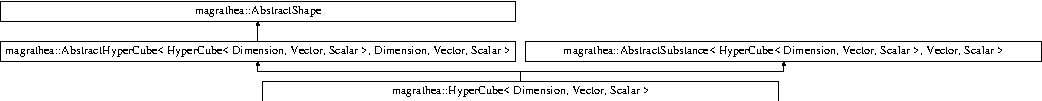
\includegraphics[height=1.352657cm]{exceptionmagrathea_1_1HyperCube}
\end{center}
\end{figure}
\subsection*{Public Member Functions}
\begin{Indent}{\bf Lifecycle}\par
\begin{DoxyCompactItemize}
\item 
{\footnotesize template$<$class... Misc$>$ }\\\hyperlink{exceptionmagrathea_1_1HyperCube_ab990ea0b6d11329084d0202d3e7355f6}{Hyper\-Cube} (Misc \&\&...misc)
\begin{DoxyCompactList}\small\item\em Explicit generic constructor. \end{DoxyCompactList}\end{DoxyCompactItemize}
\end{Indent}
\begin{Indent}{\bf Data}\par
\begin{DoxyCompactItemize}
\item 
{\footnotesize template$<$unsigned int... Values, class... Misc, class Template  = decltype(std\-::declval$<$\-Abstract\-Substance$<$\-Hyper\-Cube$<$\-Dimension, Vector, Scalar$>$, Vector, Scalar$>$ $>$().\-template data$<$0, Values...$>$(std\-::declval$<$\-Misc$>$()...)), class  = typename std\-::enable\-\_\-if$<$!std\-::is\-\_\-void$<$\-Template$>$\-::value$>$\-::type$>$ }\\Template \hyperlink{exceptionmagrathea_1_1HyperCube_a2c7b0b6944e74adf993e43b6c915780a}{position} (Misc \&\&...misc)
\begin{DoxyCompactList}\small\item\em Access to the position data. \end{DoxyCompactList}\item 
{\footnotesize template$<$unsigned int... Values, class... Misc, class Template  = decltype(std\-::declval$<$const Abstract\-Substance$<$\-Hyper\-Cube$<$\-Dimension, Vector, Scalar$>$, Vector, Scalar$>$ $>$().\-template data$<$0, Values...$>$(std\-::declval$<$\-Misc$>$()...)), class  = typename std\-::enable\-\_\-if$<$!std\-::is\-\_\-void$<$\-Template$>$\-::value$>$\-::type$>$ }\\Template \hyperlink{exceptionmagrathea_1_1HyperCube_a6f00ee8b1af6757ab600abeea90cf745}{position} (Misc \&\&...misc) const 
\begin{DoxyCompactList}\small\item\em Immutable access to the position data. \end{DoxyCompactList}\item 
{\footnotesize template$<$unsigned int... Values, class... Misc, class Template  = decltype(std\-::declval$<$\-Abstract\-Substance$<$\-Hyper\-Cube$<$\-Dimension, Vector, Scalar$>$, Vector, Scalar$>$ $>$().\-template data$<$1, Values...$>$(std\-::declval$<$\-Misc$>$()...)), class  = typename std\-::enable\-\_\-if$<$!std\-::is\-\_\-void$<$\-Template$>$\-::value$>$\-::type$>$ }\\Template \hyperlink{exceptionmagrathea_1_1HyperCube_aa37dca86c65f23784caa3f856637816c}{extent} (Misc \&\&...misc)
\begin{DoxyCompactList}\small\item\em Access to the extent data. \end{DoxyCompactList}\item 
{\footnotesize template$<$unsigned int... Values, class... Misc, class Template  = decltype(std\-::declval$<$const Abstract\-Substance$<$\-Hyper\-Cube$<$\-Dimension, Vector, Scalar$>$, Vector, Scalar$>$ $>$().\-template data$<$1, Values...$>$(std\-::declval$<$\-Misc$>$()...)), class  = typename std\-::enable\-\_\-if$<$!std\-::is\-\_\-void$<$\-Template$>$\-::value$>$\-::type$>$ }\\Template \hyperlink{exceptionmagrathea_1_1HyperCube_a4212f1eaaa72536c7bf9e1ac85e10359}{extent} (Misc \&\&...misc) const 
\begin{DoxyCompactList}\small\item\em Immutable access to the extent data. \end{DoxyCompactList}\end{DoxyCompactItemize}
\end{Indent}
\subsection*{Static Public Member Functions}
\begin{Indent}{\bf Predefined}\par
\begin{DoxyCompactItemize}
\item 
static constexpr \hyperlink{exceptionmagrathea_1_1HyperCube}{Hyper\-Cube}\\*
$<$ Dimension, Vector, Scalar $>$ \hyperlink{exceptionmagrathea_1_1HyperCube_acba25838ca056f463417afc488342aa8}{unit} ()
\begin{DoxyCompactList}\small\item\em Unit hypercube. \end{DoxyCompactList}\end{DoxyCompactItemize}
\end{Indent}
\begin{Indent}{\bf Test}\par
\begin{DoxyCompactItemize}
\item 
static int \hyperlink{exceptionmagrathea_1_1HyperCube_aad39405bf632664757308e7b0465c398}{example} ()
\begin{DoxyCompactList}\small\item\em Example function. \end{DoxyCompactList}\end{DoxyCompactItemize}
\end{Indent}
\subsection*{Public Attributes}
\begin{DoxyCompactItemize}
\item 
using \hyperlink{exceptionmagrathea_1_1HyperCube_aef38eae81fcb467a2019ddd215c14b1e}{operator} = typedef
\end{DoxyCompactItemize}
\subsection*{Additional Inherited Members}


\subsection{Detailed Description}
\subsubsection*{template$<$unsigned int Dimension = 3, class Vector = std\-::array$<$double, Dimension$>$, typename Scalar = typename std\-::remove\-\_\-cv$<$typename std\-::remove\-\_\-reference$<$decltype(std\-::declval$<$\-Vector$>$()\mbox{[}0\mbox{]})$>$\-::type$>$\-::type$>$exception magrathea\-::\-Hyper\-Cube$<$ Dimension, Vector, Scalar $>$}

N-\/dimensional cube. 

Implementation of a basic hypercube of arbitrary dimension. 
\begin{DoxyTemplParams}{Template Parameters}
{\em Dimension} & Number of space dimension. \\
\hline
{\em Vector} & Position vector type. \\
\hline
{\em Scalar} & Scalar data type. \\
\hline
\end{DoxyTemplParams}


\subsection{Constructor \& Destructor Documentation}
\hypertarget{exceptionmagrathea_1_1HyperCube_ab990ea0b6d11329084d0202d3e7355f6}{\index{magrathea\-::\-Hyper\-Cube@{magrathea\-::\-Hyper\-Cube}!Hyper\-Cube@{Hyper\-Cube}}
\index{Hyper\-Cube@{Hyper\-Cube}!magrathea::HyperCube@{magrathea\-::\-Hyper\-Cube}}
\subsubsection[{Hyper\-Cube}]{\setlength{\rightskip}{0pt plus 5cm}template$<$unsigned int Dimension, class Vector , typename Scalar $>$ template$<$class... Misc$>$ {\bf magrathea\-::\-Hyper\-Cube}$<$ Dimension, Vector, Scalar $>$\-::{\bf Hyper\-Cube} (
\begin{DoxyParamCaption}
\item[{Misc \&\&...}]{misc}
\end{DoxyParamCaption}
)\hspace{0.3cm}{\ttfamily [inline]}, {\ttfamily [explicit]}}}\label{exceptionmagrathea_1_1HyperCube_ab990ea0b6d11329084d0202d3e7355f6}


Explicit generic constructor. 

Provides a generic interface to all constructors of the base class. 
\begin{DoxyTemplParams}{Template Parameters}
{\em Misc} & (\hyperlink{classMiscellaneous}{Miscellaneous} types.) \\
\hline
\end{DoxyTemplParams}

\begin{DoxyParams}[1]{Parameters}
\mbox{\tt in}  & {\em misc} & \hyperlink{classMiscellaneous}{Miscellaneous} arguments. \\
\hline
\end{DoxyParams}


\subsection{Member Function Documentation}
\hypertarget{exceptionmagrathea_1_1HyperCube_aad39405bf632664757308e7b0465c398}{\index{magrathea\-::\-Hyper\-Cube@{magrathea\-::\-Hyper\-Cube}!example@{example}}
\index{example@{example}!magrathea::HyperCube@{magrathea\-::\-Hyper\-Cube}}
\subsubsection[{example}]{\setlength{\rightskip}{0pt plus 5cm}template$<$unsigned int Dimension, class Vector , typename Scalar $>$ int {\bf magrathea\-::\-Hyper\-Cube}$<$ Dimension, Vector, Scalar $>$\-::example (
\begin{DoxyParamCaption}
{}
\end{DoxyParamCaption}
)\hspace{0.3cm}{\ttfamily [static]}}}\label{exceptionmagrathea_1_1HyperCube_aad39405bf632664757308e7b0465c398}


Example function. 

Tests and demonstrates the use of \hyperlink{exceptionmagrathea_1_1HyperCube}{Hyper\-Cube}. \begin{DoxyReturn}{Returns}
0 if no error. 
\end{DoxyReturn}
\hypertarget{exceptionmagrathea_1_1HyperCube_aa37dca86c65f23784caa3f856637816c}{\index{magrathea\-::\-Hyper\-Cube@{magrathea\-::\-Hyper\-Cube}!extent@{extent}}
\index{extent@{extent}!magrathea::HyperCube@{magrathea\-::\-Hyper\-Cube}}
\subsubsection[{extent}]{\setlength{\rightskip}{0pt plus 5cm}template$<$unsigned int Dimension, class Vector , typename Scalar $>$ template$<$unsigned int... Values, class... Misc, class Template , class $>$ Template {\bf magrathea\-::\-Hyper\-Cube}$<$ Dimension, Vector, Scalar $>$\-::extent (
\begin{DoxyParamCaption}
\item[{Misc \&\&...}]{misc}
\end{DoxyParamCaption}
)\hspace{0.3cm}{\ttfamily [inline]}}}\label{exceptionmagrathea_1_1HyperCube_aa37dca86c65f23784caa3f856637816c}


Access to the extent data. 

Provides an access to the extent data by forwarding parameters to the unified base accessor member. 
\begin{DoxyTemplParams}{Template Parameters}
{\em Values} & List of template values. \\
\hline
{\em Misc} & (\hyperlink{classMiscellaneous}{Miscellaneous} types.) \\
\hline
{\em Template} & (Deduced template type.) \\
\hline
\end{DoxyTemplParams}

\begin{DoxyParams}[1]{Parameters}
\mbox{\tt in}  & {\em misc} & \hyperlink{classMiscellaneous}{Miscellaneous} arguments. \\
\hline
\end{DoxyParams}
\begin{DoxyReturn}{Returns}
Forwarded result. 
\end{DoxyReturn}
\hypertarget{exceptionmagrathea_1_1HyperCube_a4212f1eaaa72536c7bf9e1ac85e10359}{\index{magrathea\-::\-Hyper\-Cube@{magrathea\-::\-Hyper\-Cube}!extent@{extent}}
\index{extent@{extent}!magrathea::HyperCube@{magrathea\-::\-Hyper\-Cube}}
\subsubsection[{extent}]{\setlength{\rightskip}{0pt plus 5cm}template$<$unsigned int Dimension, class Vector , typename Scalar $>$ template$<$unsigned int... Values, class... Misc, class Template , class $>$ Template {\bf magrathea\-::\-Hyper\-Cube}$<$ Dimension, Vector, Scalar $>$\-::extent (
\begin{DoxyParamCaption}
\item[{Misc \&\&...}]{misc}
\end{DoxyParamCaption}
) const\hspace{0.3cm}{\ttfamily [inline]}}}\label{exceptionmagrathea_1_1HyperCube_a4212f1eaaa72536c7bf9e1ac85e10359}


Immutable access to the extent data. 

Provides an immutable access to the extent data by forwarding parameters to the unified base accessor member. 
\begin{DoxyTemplParams}{Template Parameters}
{\em Values} & List of template values. \\
\hline
{\em Misc} & (\hyperlink{classMiscellaneous}{Miscellaneous} types.) \\
\hline
{\em Template} & (Deduced template type.) \\
\hline
\end{DoxyTemplParams}

\begin{DoxyParams}[1]{Parameters}
\mbox{\tt in}  & {\em misc} & \hyperlink{classMiscellaneous}{Miscellaneous} arguments. \\
\hline
\end{DoxyParams}
\begin{DoxyReturn}{Returns}
Forwarded result. 
\end{DoxyReturn}
\hypertarget{exceptionmagrathea_1_1HyperCube_a2c7b0b6944e74adf993e43b6c915780a}{\index{magrathea\-::\-Hyper\-Cube@{magrathea\-::\-Hyper\-Cube}!position@{position}}
\index{position@{position}!magrathea::HyperCube@{magrathea\-::\-Hyper\-Cube}}
\subsubsection[{position}]{\setlength{\rightskip}{0pt plus 5cm}template$<$unsigned int Dimension, class Vector , typename Scalar $>$ template$<$unsigned int... Values, class... Misc, class Template , class $>$ Template {\bf magrathea\-::\-Hyper\-Cube}$<$ Dimension, Vector, Scalar $>$\-::position (
\begin{DoxyParamCaption}
\item[{Misc \&\&...}]{misc}
\end{DoxyParamCaption}
)\hspace{0.3cm}{\ttfamily [inline]}}}\label{exceptionmagrathea_1_1HyperCube_a2c7b0b6944e74adf993e43b6c915780a}


Access to the position data. 

Provides an access to the position data by forwarding parameters to the unified base accessor member. 
\begin{DoxyTemplParams}{Template Parameters}
{\em Values} & List of template values. \\
\hline
{\em Misc} & (\hyperlink{classMiscellaneous}{Miscellaneous} types.) \\
\hline
{\em Template} & (Deduced template type.) \\
\hline
\end{DoxyTemplParams}

\begin{DoxyParams}[1]{Parameters}
\mbox{\tt in}  & {\em misc} & \hyperlink{classMiscellaneous}{Miscellaneous} arguments. \\
\hline
\end{DoxyParams}
\begin{DoxyReturn}{Returns}
Forwarded result. 
\end{DoxyReturn}
\hypertarget{exceptionmagrathea_1_1HyperCube_a6f00ee8b1af6757ab600abeea90cf745}{\index{magrathea\-::\-Hyper\-Cube@{magrathea\-::\-Hyper\-Cube}!position@{position}}
\index{position@{position}!magrathea::HyperCube@{magrathea\-::\-Hyper\-Cube}}
\subsubsection[{position}]{\setlength{\rightskip}{0pt plus 5cm}template$<$unsigned int Dimension, class Vector , typename Scalar $>$ template$<$unsigned int... Values, class... Misc, class Template , class $>$ Template {\bf magrathea\-::\-Hyper\-Cube}$<$ Dimension, Vector, Scalar $>$\-::position (
\begin{DoxyParamCaption}
\item[{Misc \&\&...}]{misc}
\end{DoxyParamCaption}
) const\hspace{0.3cm}{\ttfamily [inline]}}}\label{exceptionmagrathea_1_1HyperCube_a6f00ee8b1af6757ab600abeea90cf745}


Immutable access to the position data. 

Provides an immutable access to the position data by forwarding parameters to the unified base accessor member. 
\begin{DoxyTemplParams}{Template Parameters}
{\em Values} & List of template values. \\
\hline
{\em Misc} & (\hyperlink{classMiscellaneous}{Miscellaneous} types.) \\
\hline
{\em Template} & (Deduced template type.) \\
\hline
\end{DoxyTemplParams}

\begin{DoxyParams}[1]{Parameters}
\mbox{\tt in}  & {\em misc} & \hyperlink{classMiscellaneous}{Miscellaneous} arguments. \\
\hline
\end{DoxyParams}
\begin{DoxyReturn}{Returns}
Forwarded result. 
\end{DoxyReturn}
\hypertarget{exceptionmagrathea_1_1HyperCube_acba25838ca056f463417afc488342aa8}{\index{magrathea\-::\-Hyper\-Cube@{magrathea\-::\-Hyper\-Cube}!unit@{unit}}
\index{unit@{unit}!magrathea::HyperCube@{magrathea\-::\-Hyper\-Cube}}
\subsubsection[{unit}]{\setlength{\rightskip}{0pt plus 5cm}template$<$unsigned int Dimension, class Vector , typename Scalar $>$ constexpr {\bf Hyper\-Cube}$<$ Dimension, Vector, Scalar $>$ {\bf magrathea\-::\-Hyper\-Cube}$<$ Dimension, Vector, Scalar $>$\-::unit (
\begin{DoxyParamCaption}
{}
\end{DoxyParamCaption}
)\hspace{0.3cm}{\ttfamily [static]}}}\label{exceptionmagrathea_1_1HyperCube_acba25838ca056f463417afc488342aa8}


Unit hypercube. 

Creates an hypercube with a position of zero and with an extent of one. \begin{DoxyReturn}{Returns}
Copy of a unit hypercube. 
\end{DoxyReturn}


\subsection{Member Data Documentation}
\hypertarget{exceptionmagrathea_1_1HyperCube_aef38eae81fcb467a2019ddd215c14b1e}{\index{magrathea\-::\-Hyper\-Cube@{magrathea\-::\-Hyper\-Cube}!operator@{operator}}
\index{operator@{operator}!magrathea::HyperCube@{magrathea\-::\-Hyper\-Cube}}
\subsubsection[{operator}]{\setlength{\rightskip}{0pt plus 5cm}template$<$unsigned int Dimension = 3, class Vector = std\-::array$<$double, Dimension$>$, typename Scalar = typename std\-::remove\-\_\-cv$<$typename std\-::remove\-\_\-reference$<$decltype(std\-::declval$<$\-Vector$>$()\mbox{[}0\mbox{]})$>$\-::type$>$\-::type$>$ using {\bf magrathea\-::\-Hyper\-Cube}$<$ Dimension, Vector, Scalar $>$\-::operator = }}\label{exceptionmagrathea_1_1HyperCube_aef38eae81fcb467a2019ddd215c14b1e}


The documentation for this exception was generated from the following file\-:\begin{DoxyCompactItemize}
\item 
/data/home/mbreton/magrathea\-\_\-pathfinder/src/magrathea/\hyperlink{hypercube_8h}{hypercube.\-h}\end{DoxyCompactItemize}

\hypertarget{exceptionmagrathea_1_1HyperSphere}{\section{magrathea\-:\-:Hyper\-Sphere$<$ Dimension, Vector, Scalar $>$ Exception Template Reference}
\label{exceptionmagrathea_1_1HyperSphere}\index{magrathea\-::\-Hyper\-Sphere$<$ Dimension, Vector, Scalar $>$@{magrathea\-::\-Hyper\-Sphere$<$ Dimension, Vector, Scalar $>$}}
}


N-\/dimensional sphere.  




{\ttfamily \#include $<$hypersphere.\-h$>$}

Inheritance diagram for magrathea\-:\-:Hyper\-Sphere$<$ Dimension, Vector, Scalar $>$\-:\begin{figure}[H]
\begin{center}
\leavevmode
\includegraphics[height=1.306376cm]{exceptionmagrathea_1_1HyperSphere}
\end{center}
\end{figure}
\subsection*{Public Member Functions}
\begin{Indent}{\bf Lifecycle}\par
\begin{DoxyCompactItemize}
\item 
{\footnotesize template$<$class... Misc$>$ }\\\hyperlink{exceptionmagrathea_1_1HyperSphere_abf1820d27cf49f015d0fa64da8fbe778}{Hyper\-Sphere} (Misc \&\&...misc)
\begin{DoxyCompactList}\small\item\em Explicit generic constructor. \end{DoxyCompactList}\end{DoxyCompactItemize}
\end{Indent}
\begin{Indent}{\bf Data}\par
\begin{DoxyCompactItemize}
\item 
{\footnotesize template$<$unsigned int... Values, class... Misc, class Template  = decltype(std\-::declval$<$\-Abstract\-Substance$<$\-Hyper\-Sphere$<$\-Dimension, Vector, Scalar$>$, Vector, Scalar$>$ $>$().\-template data$<$0, Values...$>$(std\-::declval$<$\-Misc$>$()...)), class  = typename std\-::enable\-\_\-if$<$!std\-::is\-\_\-void$<$\-Template$>$\-::value$>$\-::type$>$ }\\Template \hyperlink{exceptionmagrathea_1_1HyperSphere_a6cfc0eb76f815a76ced79309c599c792}{position} (Misc \&\&...misc)
\begin{DoxyCompactList}\small\item\em Access to the position data. \end{DoxyCompactList}\item 
{\footnotesize template$<$unsigned int... Values, class... Misc, class Template  = decltype(std\-::declval$<$const Abstract\-Substance$<$\-Hyper\-Sphere$<$\-Dimension, Vector, Scalar$>$, Vector, Scalar$>$ $>$().\-template data$<$0, Values...$>$(std\-::declval$<$\-Misc$>$()...)), class  = typename std\-::enable\-\_\-if$<$!std\-::is\-\_\-void$<$\-Template$>$\-::value$>$\-::type$>$ }\\Template \hyperlink{exceptionmagrathea_1_1HyperSphere_a9b740a84f681ed3e93f5c2e40d1020c3}{position} (Misc \&\&...misc) const 
\begin{DoxyCompactList}\small\item\em Immutable access to the position data. \end{DoxyCompactList}\item 
{\footnotesize template$<$unsigned int... Values, class... Misc, class Template  = decltype(std\-::declval$<$\-Abstract\-Substance$<$\-Hyper\-Sphere$<$\-Dimension, Vector, Scalar$>$, Vector, Scalar$>$ $>$().\-template data$<$1, Values...$>$(std\-::declval$<$\-Misc$>$()...)), class  = typename std\-::enable\-\_\-if$<$!std\-::is\-\_\-void$<$\-Template$>$\-::value$>$\-::type$>$ }\\Template \hyperlink{exceptionmagrathea_1_1HyperSphere_a1d52a7a65a6c83e8bfd191a6bd54ded1}{extent} (Misc \&\&...misc)
\begin{DoxyCompactList}\small\item\em Access to the extent data. \end{DoxyCompactList}\item 
{\footnotesize template$<$unsigned int... Values, class... Misc, class Template  = decltype(std\-::declval$<$const Abstract\-Substance$<$\-Hyper\-Sphere$<$\-Dimension, Vector, Scalar$>$, Vector, Scalar$>$ $>$().\-template data$<$1, Values...$>$(std\-::declval$<$\-Misc$>$()...)), class  = typename std\-::enable\-\_\-if$<$!std\-::is\-\_\-void$<$\-Template$>$\-::value$>$\-::type$>$ }\\Template \hyperlink{exceptionmagrathea_1_1HyperSphere_a1ce04ded3982bd471f9e4328832a0e25}{extent} (Misc \&\&...misc) const 
\begin{DoxyCompactList}\small\item\em Immutable access to the extent data. \end{DoxyCompactList}\end{DoxyCompactItemize}
\end{Indent}
\subsection*{Static Public Member Functions}
\begin{Indent}{\bf Predefined}\par
\begin{DoxyCompactItemize}
\item 
static constexpr \hyperlink{exceptionmagrathea_1_1HyperSphere}{Hyper\-Sphere}\\*
$<$ Dimension, Vector, Scalar $>$ \hyperlink{exceptionmagrathea_1_1HyperSphere_a2c24c124f93553487fba45e7bae032aa}{unit} ()
\begin{DoxyCompactList}\small\item\em Unit hypersphere. \end{DoxyCompactList}\end{DoxyCompactItemize}
\end{Indent}
\begin{Indent}{\bf Test}\par
\begin{DoxyCompactItemize}
\item 
static int \hyperlink{exceptionmagrathea_1_1HyperSphere_a0124f9301a1e7cb15fdc14bf1cd3a231}{example} ()
\begin{DoxyCompactList}\small\item\em Example function. \end{DoxyCompactList}\end{DoxyCompactItemize}
\end{Indent}
\subsection*{Public Attributes}
\begin{DoxyCompactItemize}
\item 
using \hyperlink{exceptionmagrathea_1_1HyperSphere_a76dfa1f063e9f6d4636f97d4dc2c2056}{operator} = typedef
\end{DoxyCompactItemize}
\subsection*{Additional Inherited Members}


\subsection{Detailed Description}
\subsubsection*{template$<$unsigned int Dimension = 3, class Vector = std\-::array$<$double, Dimension$>$, typename Scalar = typename std\-::remove\-\_\-cv$<$typename std\-::remove\-\_\-reference$<$decltype(std\-::declval$<$\-Vector$>$()\mbox{[}0\mbox{]})$>$\-::type$>$\-::type$>$exception magrathea\-::\-Hyper\-Sphere$<$ Dimension, Vector, Scalar $>$}

N-\/dimensional sphere. 

Implementation of a basic hypersphere of arbitrary dimension. 
\begin{DoxyTemplParams}{Template Parameters}
{\em Dimension} & Number of space dimension. \\
\hline
{\em Vector} & Position vector type. \\
\hline
{\em Scalar} & Scalar data type. \\
\hline
\end{DoxyTemplParams}


\subsection{Constructor \& Destructor Documentation}
\hypertarget{exceptionmagrathea_1_1HyperSphere_abf1820d27cf49f015d0fa64da8fbe778}{\index{magrathea\-::\-Hyper\-Sphere@{magrathea\-::\-Hyper\-Sphere}!Hyper\-Sphere@{Hyper\-Sphere}}
\index{Hyper\-Sphere@{Hyper\-Sphere}!magrathea::HyperSphere@{magrathea\-::\-Hyper\-Sphere}}
\subsubsection[{Hyper\-Sphere}]{\setlength{\rightskip}{0pt plus 5cm}template$<$unsigned int Dimension, class Vector , typename Scalar $>$ template$<$class... Misc$>$ {\bf magrathea\-::\-Hyper\-Sphere}$<$ Dimension, Vector, Scalar $>$\-::{\bf Hyper\-Sphere} (
\begin{DoxyParamCaption}
\item[{Misc \&\&...}]{misc}
\end{DoxyParamCaption}
)\hspace{0.3cm}{\ttfamily [inline]}, {\ttfamily [explicit]}}}\label{exceptionmagrathea_1_1HyperSphere_abf1820d27cf49f015d0fa64da8fbe778}


Explicit generic constructor. 

Provides a generic interface to all constructors of the base class. 
\begin{DoxyTemplParams}{Template Parameters}
{\em Misc} & (\hyperlink{classMiscellaneous}{Miscellaneous} types.) \\
\hline
\end{DoxyTemplParams}

\begin{DoxyParams}[1]{Parameters}
\mbox{\tt in}  & {\em misc} & \hyperlink{classMiscellaneous}{Miscellaneous} arguments. \\
\hline
\end{DoxyParams}


\subsection{Member Function Documentation}
\hypertarget{exceptionmagrathea_1_1HyperSphere_a0124f9301a1e7cb15fdc14bf1cd3a231}{\index{magrathea\-::\-Hyper\-Sphere@{magrathea\-::\-Hyper\-Sphere}!example@{example}}
\index{example@{example}!magrathea::HyperSphere@{magrathea\-::\-Hyper\-Sphere}}
\subsubsection[{example}]{\setlength{\rightskip}{0pt plus 5cm}template$<$unsigned int Dimension, class Vector , typename Scalar $>$ int {\bf magrathea\-::\-Hyper\-Sphere}$<$ Dimension, Vector, Scalar $>$\-::example (
\begin{DoxyParamCaption}
{}
\end{DoxyParamCaption}
)\hspace{0.3cm}{\ttfamily [static]}}}\label{exceptionmagrathea_1_1HyperSphere_a0124f9301a1e7cb15fdc14bf1cd3a231}


Example function. 

Tests and demonstrates the use of \hyperlink{exceptionmagrathea_1_1HyperSphere}{Hyper\-Sphere}. \begin{DoxyReturn}{Returns}
0 if no error. 
\end{DoxyReturn}
\hypertarget{exceptionmagrathea_1_1HyperSphere_a1d52a7a65a6c83e8bfd191a6bd54ded1}{\index{magrathea\-::\-Hyper\-Sphere@{magrathea\-::\-Hyper\-Sphere}!extent@{extent}}
\index{extent@{extent}!magrathea::HyperSphere@{magrathea\-::\-Hyper\-Sphere}}
\subsubsection[{extent}]{\setlength{\rightskip}{0pt plus 5cm}template$<$unsigned int Dimension, class Vector , typename Scalar $>$ template$<$unsigned int... Values, class... Misc, class Template , class $>$ Template {\bf magrathea\-::\-Hyper\-Sphere}$<$ Dimension, Vector, Scalar $>$\-::extent (
\begin{DoxyParamCaption}
\item[{Misc \&\&...}]{misc}
\end{DoxyParamCaption}
)\hspace{0.3cm}{\ttfamily [inline]}}}\label{exceptionmagrathea_1_1HyperSphere_a1d52a7a65a6c83e8bfd191a6bd54ded1}


Access to the extent data. 

Provides an access to the extent data by forwarding parameters to the unified base accessor member. 
\begin{DoxyTemplParams}{Template Parameters}
{\em Values} & List of template values. \\
\hline
{\em Misc} & (\hyperlink{classMiscellaneous}{Miscellaneous} types.) \\
\hline
{\em Template} & (Deduced template type.) \\
\hline
\end{DoxyTemplParams}

\begin{DoxyParams}[1]{Parameters}
\mbox{\tt in}  & {\em misc} & \hyperlink{classMiscellaneous}{Miscellaneous} arguments. \\
\hline
\end{DoxyParams}
\begin{DoxyReturn}{Returns}
Forwarded result. 
\end{DoxyReturn}
\hypertarget{exceptionmagrathea_1_1HyperSphere_a1ce04ded3982bd471f9e4328832a0e25}{\index{magrathea\-::\-Hyper\-Sphere@{magrathea\-::\-Hyper\-Sphere}!extent@{extent}}
\index{extent@{extent}!magrathea::HyperSphere@{magrathea\-::\-Hyper\-Sphere}}
\subsubsection[{extent}]{\setlength{\rightskip}{0pt plus 5cm}template$<$unsigned int Dimension, class Vector , typename Scalar $>$ template$<$unsigned int... Values, class... Misc, class Template , class $>$ Template {\bf magrathea\-::\-Hyper\-Sphere}$<$ Dimension, Vector, Scalar $>$\-::extent (
\begin{DoxyParamCaption}
\item[{Misc \&\&...}]{misc}
\end{DoxyParamCaption}
) const\hspace{0.3cm}{\ttfamily [inline]}}}\label{exceptionmagrathea_1_1HyperSphere_a1ce04ded3982bd471f9e4328832a0e25}


Immutable access to the extent data. 

Provides an immutable access to the extent data by forwarding parameters to the unified base accessor member. 
\begin{DoxyTemplParams}{Template Parameters}
{\em Values} & List of template values. \\
\hline
{\em Misc} & (\hyperlink{classMiscellaneous}{Miscellaneous} types.) \\
\hline
{\em Template} & (Deduced template type.) \\
\hline
\end{DoxyTemplParams}

\begin{DoxyParams}[1]{Parameters}
\mbox{\tt in}  & {\em misc} & \hyperlink{classMiscellaneous}{Miscellaneous} arguments. \\
\hline
\end{DoxyParams}
\begin{DoxyReturn}{Returns}
Forwarded result. 
\end{DoxyReturn}
\hypertarget{exceptionmagrathea_1_1HyperSphere_a6cfc0eb76f815a76ced79309c599c792}{\index{magrathea\-::\-Hyper\-Sphere@{magrathea\-::\-Hyper\-Sphere}!position@{position}}
\index{position@{position}!magrathea::HyperSphere@{magrathea\-::\-Hyper\-Sphere}}
\subsubsection[{position}]{\setlength{\rightskip}{0pt plus 5cm}template$<$unsigned int Dimension, class Vector , typename Scalar $>$ template$<$unsigned int... Values, class... Misc, class Template , class $>$ Template {\bf magrathea\-::\-Hyper\-Sphere}$<$ Dimension, Vector, Scalar $>$\-::position (
\begin{DoxyParamCaption}
\item[{Misc \&\&...}]{misc}
\end{DoxyParamCaption}
)\hspace{0.3cm}{\ttfamily [inline]}}}\label{exceptionmagrathea_1_1HyperSphere_a6cfc0eb76f815a76ced79309c599c792}


Access to the position data. 

Provides an access to the position data by forwarding parameters to the unified base accessor member. 
\begin{DoxyTemplParams}{Template Parameters}
{\em Values} & List of template values. \\
\hline
{\em Misc} & (\hyperlink{classMiscellaneous}{Miscellaneous} types.) \\
\hline
{\em Template} & (Deduced template type.) \\
\hline
\end{DoxyTemplParams}

\begin{DoxyParams}[1]{Parameters}
\mbox{\tt in}  & {\em misc} & \hyperlink{classMiscellaneous}{Miscellaneous} arguments. \\
\hline
\end{DoxyParams}
\begin{DoxyReturn}{Returns}
Forwarded result. 
\end{DoxyReturn}
\hypertarget{exceptionmagrathea_1_1HyperSphere_a9b740a84f681ed3e93f5c2e40d1020c3}{\index{magrathea\-::\-Hyper\-Sphere@{magrathea\-::\-Hyper\-Sphere}!position@{position}}
\index{position@{position}!magrathea::HyperSphere@{magrathea\-::\-Hyper\-Sphere}}
\subsubsection[{position}]{\setlength{\rightskip}{0pt plus 5cm}template$<$unsigned int Dimension, class Vector , typename Scalar $>$ template$<$unsigned int... Values, class... Misc, class Template , class $>$ Template {\bf magrathea\-::\-Hyper\-Sphere}$<$ Dimension, Vector, Scalar $>$\-::position (
\begin{DoxyParamCaption}
\item[{Misc \&\&...}]{misc}
\end{DoxyParamCaption}
) const\hspace{0.3cm}{\ttfamily [inline]}}}\label{exceptionmagrathea_1_1HyperSphere_a9b740a84f681ed3e93f5c2e40d1020c3}


Immutable access to the position data. 

Provides an immutable access to the position data by forwarding parameters to the unified base accessor member. 
\begin{DoxyTemplParams}{Template Parameters}
{\em Values} & List of template values. \\
\hline
{\em Misc} & (\hyperlink{classMiscellaneous}{Miscellaneous} types.) \\
\hline
{\em Template} & (Deduced template type.) \\
\hline
\end{DoxyTemplParams}

\begin{DoxyParams}[1]{Parameters}
\mbox{\tt in}  & {\em misc} & \hyperlink{classMiscellaneous}{Miscellaneous} arguments. \\
\hline
\end{DoxyParams}
\begin{DoxyReturn}{Returns}
Forwarded result. 
\end{DoxyReturn}
\hypertarget{exceptionmagrathea_1_1HyperSphere_a2c24c124f93553487fba45e7bae032aa}{\index{magrathea\-::\-Hyper\-Sphere@{magrathea\-::\-Hyper\-Sphere}!unit@{unit}}
\index{unit@{unit}!magrathea::HyperSphere@{magrathea\-::\-Hyper\-Sphere}}
\subsubsection[{unit}]{\setlength{\rightskip}{0pt plus 5cm}template$<$unsigned int Dimension, class Vector , typename Scalar $>$ constexpr {\bf Hyper\-Sphere}$<$ Dimension, Vector, Scalar $>$ {\bf magrathea\-::\-Hyper\-Sphere}$<$ Dimension, Vector, Scalar $>$\-::unit (
\begin{DoxyParamCaption}
{}
\end{DoxyParamCaption}
)\hspace{0.3cm}{\ttfamily [static]}}}\label{exceptionmagrathea_1_1HyperSphere_a2c24c124f93553487fba45e7bae032aa}


Unit hypersphere. 

Creates an hypersphere with a position of zero and with an extent of one. \begin{DoxyReturn}{Returns}
Copy of a unit hypersphere. 
\end{DoxyReturn}


\subsection{Member Data Documentation}
\hypertarget{exceptionmagrathea_1_1HyperSphere_a76dfa1f063e9f6d4636f97d4dc2c2056}{\index{magrathea\-::\-Hyper\-Sphere@{magrathea\-::\-Hyper\-Sphere}!operator@{operator}}
\index{operator@{operator}!magrathea::HyperSphere@{magrathea\-::\-Hyper\-Sphere}}
\subsubsection[{operator}]{\setlength{\rightskip}{0pt plus 5cm}template$<$unsigned int Dimension = 3, class Vector = std\-::array$<$double, Dimension$>$, typename Scalar = typename std\-::remove\-\_\-cv$<$typename std\-::remove\-\_\-reference$<$decltype(std\-::declval$<$\-Vector$>$()\mbox{[}0\mbox{]})$>$\-::type$>$\-::type$>$ using {\bf magrathea\-::\-Hyper\-Sphere}$<$ Dimension, Vector, Scalar $>$\-::operator = }}\label{exceptionmagrathea_1_1HyperSphere_a76dfa1f063e9f6d4636f97d4dc2c2056}


The documentation for this exception was generated from the following file\-:\begin{DoxyCompactItemize}
\item 
/data/home/mbreton/magrathea\-\_\-pathfinder/src/magrathea/\hyperlink{hypersphere_8h}{hypersphere.\-h}\end{DoxyCompactItemize}

\hypertarget{exceptionInput}{\section{Input Exception Reference}
\label{exceptionInput}\index{Input@{Input}}
}


\hyperlink{exceptionInput}{Input} utilities for raytracing.  




{\ttfamily \#include $<$input.\-h$>$}

\subsection*{Static Public Member Functions}
\begin{Indent}{\bf Utilities}\par
\begin{DoxyCompactItemize}
\item 
static std\-::string \hyperlink{exceptionInput_a8a98c85776bc73b49f4b3a4e30b243b7}{trim} (const std\-::string \&text, const std\-::string \&comment=\char`\"{}\#\char`\"{})
\begin{DoxyCompactList}\small\item\em Trim string. \end{DoxyCompactList}\item 
static std\-::pair$<$ std\-::string, \\*
std\-::string $>$ \hyperlink{exceptionInput_a859c8e0b3921a0e8bbd79bc96272935e}{partition} (const std\-::string \&text, const std\-::string \&separator=\char`\"{}=\char`\"{})
\begin{DoxyCompactList}\small\item\em Partition string. \end{DoxyCompactList}\item 
{\footnotesize template$<$class Octree , class Source , class Data  = typename std\-::tuple\-\_\-element$<$1, decltype(\-Octree\-::element())$>$\-::type, class Element  = decltype(\-Source\-::element()), class  = typename std\-::enable\-\_\-if$<$(\-Octree\-::dimension() == Source\-::dimension()) \&\& (std\-::is\-\_\-integral$<$\-Data$>$\-::value)$>$\-::type$>$ }\\static unsigned int \hyperlink{exceptionInput_a1ec66a2edaab4da06525453503e9cc3c}{count} (Octree \&octree, const Source \&source)
\begin{DoxyCompactList}\small\item\em Count tree. \end{DoxyCompactList}\item 
{\footnotesize template$<$class Octree , class Sphere , class Conic , typename Type  = decltype(\-Octree\-::type()), class Element  = decltype(\-Octree\-::element()), class Index  = typename std\-::tuple\-\_\-element$<$0, Element$>$\-::type, unsigned int Dimension = Octree\-::dimension(), class Position  = decltype(\-Octree\-::position()), class Extent  = decltype(\-Octree\-::extent()), class  = typename std\-::enable\-\_\-if$<$(\-Dimension == 3) \&\& (\-Dimension == Sphere\-::dimension())$>$\-::type$>$ }\\static bool \hyperlink{exceptionInput_a5b0ea51603590e39e5ca9b9f33e1bf9e}{collide} (const Octree \&octree, const Index \&index, const Sphere \&sphere, const Conic \&conic)
\begin{DoxyCompactList}\small\item\em Collision between an octree index and a sphere or a cone. \end{DoxyCompactList}\item 
{\footnotesize template$<$unsigned int Selection = 0, class Octree , unsigned int Dimension = Octree\-::dimension(), class Element  = decltype(\-Octree\-::element()), class Index  = typename std\-::tuple\-\_\-element$<$0, Element$>$\-::type, class Data  = typename std\-::tuple\-\_\-element$<$1, Element$>$\-::type, class Type  = decltype(\-Data\-::template type$<$\-Selection$>$()), class  = typename std\-::enable\-\_\-if$<$(\-Dimension == 3)$>$\-::type$>$ }\\static Type \hyperlink{exceptionInput_a2378e5cd9538eb69c842ebd4575a6775}{mean} (const Octree \&octree, const Element \&element, int level=-\/1)
\begin{DoxyCompactList}\small\item\em Mean value over cells. \end{DoxyCompactList}\item 
{\footnotesize template$<$unsigned int Selection = 0, class Octree , unsigned int Dimension = Octree\-::dimension(), class Element  = decltype(\-Octree\-::element()), class Index  = typename std\-::tuple\-\_\-element$<$0, Element$>$\-::type, class Data  = typename std\-::tuple\-\_\-element$<$1, Element$>$\-::type, class Type  = decltype(\-Data\-::template type$<$\-Selection$>$()), class  = typename std\-::enable\-\_\-if$<$(\-Dimension == 3)$>$\-::type$>$ }\\static Data \hyperlink{exceptionInput_aa2bca846797d99859c639ee39c5622e3}{mean\-All} (const Octree \&octree, const Element \&element, int level=-\/1)
\begin{DoxyCompactList}\small\item\em Mean value over cells. \end{DoxyCompactList}\item 
{\footnotesize template$<$typename Type , class Cosmology  = std\-::array$<$std\-::vector$<$double$>$, 4$>$, class  = typename std\-::enable\-\_\-if$<$std\-::is\-\_\-convertible$<$\-Type, typename std\-::remove\-\_\-cv$<$typename std\-::remove\-\_\-reference$<$decltype(std\-::declval$<$\-Cosmology$>$()\mbox{[}0\mbox{]}\mbox{[}0\mbox{]})$>$\-::type$>$\-::type$>$\-::value$>$\-::type$>$ }\\static Cosmology \hyperlink{exceptionInput_ad86e769634c817f09bcdde8c3958e54d}{constantify} (const unsigned int size, const Type tmin, const Type tmax, const Type a=Type(1), const Type dadt=Type(), const Type d2adt2=Type())
\begin{DoxyCompactList}\small\item\em Constant cosmology. \end{DoxyCompactList}\item 
{\footnotesize template$<$class Parameter , class Data , typename Type , class  = typename std\-::enable\-\_\-if$<$\-Data\-::types() != 0$>$\-::type$>$ }\\static Data \hyperlink{exceptionInput_abdcd382d232673326e4f759ffe67c58c}{sistemize} (const Parameter \&\hyperlink{rays_8h_ae1bc8b0b8c8b9f8e4cc61a5cc7c4ce9e}{parameters}, const Data \&data, const Type a, const Type h, const Type omegam, const Type lboxmpch)
\begin{DoxyCompactList}\small\item\em Data conversion to S\-I units. \end{DoxyCompactList}\item 
{\footnotesize template$<$class Parameter , class Octree , typename Type , class Element  = decltype(\-Octree\-::element()), class Data  = typename std\-::tuple\-\_\-element$<$1, Element$>$\-::type, class  = typename std\-::enable\-\_\-if$<$(!std\-::is\-\_\-void$<$\-Data$>$\-::value) \&\& (\-Octree\-::dimension() != 0)$>$\-::type$>$ }\\static unsigned int \hyperlink{exceptionInput_ad51758a7519270c34e5cc7a2c3e254cb}{sistemize} (const Parameter \&\hyperlink{rays_8h_ae1bc8b0b8c8b9f8e4cc61a5cc7c4ce9e}{parameters}, Octree \&octree, const Type h, const Type omegam, const Type lboxmpch)
\begin{DoxyCompactList}\small\item\em Octree conversion to S\-I units. \end{DoxyCompactList}\item 
{\footnotesize template$<$class Data , class  = typename std\-::enable\-\_\-if$<$\-Data\-::types() != 0$>$\-::type$>$ }\\static Data \hyperlink{exceptionInput_ad43fe70367197a64504b4fe2dae861a3}{homogenize} (const Data \&data)
\begin{DoxyCompactList}\small\item\em Data homogenization. \end{DoxyCompactList}\item 
{\footnotesize template$<$class Octree , class... Dummy, class Element  = decltype(\-Octree\-::element()), class Data  = typename std\-::tuple\-\_\-element$<$1, Element$>$\-::type, class  = typename std\-::enable\-\_\-if$<$(!std\-::is\-\_\-void$<$\-Data$>$\-::value) \&\& (\-Octree\-::dimension() != 0) \&\& (sizeof...(\-Dummy) == 0)$>$\-::type$>$ }\\static unsigned int \hyperlink{exceptionInput_ad9324e1d7cbb6ce11dae87e7805ab1f0}{homogenize} (Octree \&octree, Dummy...)
\begin{DoxyCompactList}\small\item\em Octree homogenization. \end{DoxyCompactList}\item 
{\footnotesize template$<$class Extent  = std\-::ratio$<$1$>$, class Data , class Vector , typename Type , unsigned int Dimension = 3, class  = typename std\-::enable\-\_\-if$<$(\-Data\-::types() != 0) \&\& (std\-::is\-\_\-convertible$<$\-Type, typename std\-::remove\-\_\-cv$<$typename std\-::remove\-\_\-reference$<$decltype(std\-::declval$<$\-Vector$>$()\mbox{[}0\mbox{]})$>$\-::type$>$\-::type$>$\-::value)$>$\-::type$>$ }\\static Data \hyperlink{exceptionInput_aab3a37812389169923cbbbf922d9ca1c}{schwarzschildify} (const Data \&data, const Vector \&center, const Vector \&position, const Type mass, const Type length)
\begin{DoxyCompactList}\small\item\em Data schwarzschild setup. \end{DoxyCompactList}\item 
{\footnotesize template$<$class Octree , class Vector , typename Type , class Function , class... Dummy, class Element  = decltype(\-Octree\-::element()), unsigned int Dimension = Octree\-::dimension(), class Extent  = decltype(\-Octree\-::extent()), class  = typename std\-::enable\-\_\-if$<$(sizeof...(\-Dummy) == 0) \&\& (\-Dimension == 3)$>$\-::type$>$ }\\static unsigned int \hyperlink{exceptionInput_a881b5694e1b8defc21d34d35cbec74d4}{schwarzschildify} (Octree \&octree, const Vector \&position, const Type mass, const Type length, Function \&\&refiner, Dummy...)
\begin{DoxyCompactList}\small\item\em Octree schwarzschild setup. \end{DoxyCompactList}\end{DoxyCompactItemize}
\end{Indent}
\begin{Indent}{\bf Files}\par
\begin{DoxyCompactItemize}
\item 
{\footnotesize template$<$class Octree , class Element  = decltype(\-Octree\-::element()), class Index  = typename std\-::tuple\-\_\-element$<$0, Element$>$\-::type, class Data  = typename std\-::tuple\-\_\-element$<$1, Element$>$\-::type, unsigned int Dimension = Octree\-::dimension(), class  = typename std\-::enable\-\_\-if$<$\-Dimension != 0$>$\-::type$>$ }\\static unsigned int \hyperlink{exceptionInput_a55ab9761312068b1da1f4498b82526a4}{filetree} (Octree \&octree, const std\-::string \&directory, const std\-::string \&format)
\begin{DoxyCompactList}\small\item\em File tree. \end{DoxyCompactList}\item 
{\footnotesize template$<$class List , class Octree , class Sphere , class Conic , unsigned int Dimension = Octree\-::dimension(), class  = typename std\-::enable\-\_\-if$<$(\-Dimension == 3) \&\& (\-Dimension == Sphere\-::dimension())$>$\-::type$>$ }\\static bool \hyperlink{exceptionInput_ab975c15aeb6fbbaeef11586b4bb10282}{prepare} (List \&list, const Octree \&octree, const Sphere \&sphere, const Conic \&conic)
\begin{DoxyCompactList}\small\item\em File list preparation. \end{DoxyCompactList}\end{DoxyCompactItemize}
\end{Indent}
\begin{Indent}{\bf Data}\par
\begin{DoxyCompactItemize}
\item 
{\footnotesize template$<$typename Integral  = unsigned int, typename Real  = float, class Parameter , class Octree , class Function , class Element  = decltype(\-Octree\-::element()), class Index  = typename std\-::tuple\-\_\-element$<$0, Element$>$\-::type, class Data  = typename std\-::tuple\-\_\-element$<$1, Element$>$\-::type, unsigned int Dimension = Octree\-::dimension(), class  = typename std\-::enable\-\_\-if$<$std\-::is\-\_\-convertible$<$typename std\-::result\-\_\-of$<$\-Function(\-Element)$>$\-::type, bool$>$\-::value$>$\-::type$>$ }\\static bool \hyperlink{exceptionInput_adb0a86f9680f6f88311735513b20f1a8}{import} (const Parameter \&\hyperlink{rays_8h_ae1bc8b0b8c8b9f8e4cc61a5cc7c4ce9e}{parameters}, Octree \&octree, const std\-::string \&filename, Function \&\&filter)
\begin{DoxyCompactList}\small\item\em Ramses importation. \end{DoxyCompactList}\item 
{\footnotesize template$<$typename Type , class Parameter , class Cosmology  = std\-::array$<$std\-::vector$<$\-Type$>$, 4$>$, class Element  = typename std\-::remove\-\_\-cv$<$typename std\-::remove\-\_\-reference$<$decltype(std\-::declval$<$\-Cosmology$>$()\mbox{[}0\mbox{]})$>$\-::type$>$\-::type, class  = typename std\-::enable\-\_\-if$<$std\-::is\-\_\-convertible$<$\-Element, typename std\-::remove\-\_\-cv$<$typename std\-::remove\-\_\-reference$<$decltype(std\-::declval$<$\-Cosmology$>$()\mbox{[}0\mbox{]})$>$\-::type$>$\-::type$>$\-::value$>$\-::type$>$ }\\static Cosmology \hyperlink{exceptionInput_a3070c31dd06673df4c9229219c4a1819}{acquire} (const Parameter \&\hyperlink{rays_8h_ae1bc8b0b8c8b9f8e4cc61a5cc7c4ce9e}{parameters}, Type \&h, Type \&omegam, Type \&lboxmpch, const std\-::string \&outfile=std\-::string())
\begin{DoxyCompactList}\small\item\em Cosmology acquisition. \end{DoxyCompactList}\item 
{\footnotesize template$<$class Container  = std\-::map$<$std\-::string, std\-::string$>$, class Element  = std\-::pair$<$std\-::string, std\-::string$>$, class  = typename std\-::enable\-\_\-if$<$(std\-::is\-\_\-convertible$<$\-Container, std\-::map$<$std\-::string, std\-::string$>$ $>$\-::value) \&\& (std\-::is\-\_\-convertible$<$\-Element, std\-::pair$<$std\-::string, std\-::string$>$ $>$\-::value)$>$\-::type$>$ }\\static Container \hyperlink{exceptionInput_a90f26f7b7be815de44151066b8cb669d}{parse} (const std\-::string \&filename, const std\-::string \&separator=\char`\"{}=\char`\"{}, const std\-::string \&comment=\char`\"{}\#\char`\"{})
\begin{DoxyCompactList}\small\item\em Parameter file parsing. \end{DoxyCompactList}\item 
{\footnotesize template$<$class Position , class Extent , typename Integral  = unsigned int, typename Real  = float, class Parameter , class Conic , class Octree , class Function , class Element  = decltype(\-Octree\-::element()), class Index  = typename std\-::tuple\-\_\-element$<$0, Element$>$\-::type, class Data  = typename std\-::tuple\-\_\-element$<$1, Element$>$\-::type, unsigned int Dimension = Octree\-::dimension(), class  = typename std\-::enable\-\_\-if$<$std\-::is\-\_\-convertible$<$typename std\-::result\-\_\-of$<$\-Function(\-Element)$>$\-::type, bool$>$\-::value$>$\-::type$>$ }\\static bool \hyperlink{exceptionInput_ae15078f6d2ccb7195a060e6c92b409bd}{importhdf5} (const Parameter \&\hyperlink{rays_8h_ae1bc8b0b8c8b9f8e4cc61a5cc7c4ce9e}{parameters}, unsigned int \&rank, const std\-::array$<$ std\-::array$<$ double, 3 $>$, 3 $>$ \&rotm1, const double \&thetay, const double \&thetaz, const Conic \&conic, Octree \&octree, const std\-::string \&filename, Function \&\&filter)
\begin{DoxyCompactList}\small\item\em Ramses importation. \end{DoxyCompactList}\item 
{\footnotesize template$<$class Position , class Extent , typename Integral  = unsigned int, typename Real  = float, class Parameter , class Octree , class Function , class Element  = decltype(\-Octree\-::element()), class Index  = typename std\-::tuple\-\_\-element$<$0, Element$>$\-::type, class Data  = typename std\-::tuple\-\_\-element$<$1, Element$>$\-::type, unsigned int Dimension = Octree\-::dimension(), class  = typename std\-::enable\-\_\-if$<$std\-::is\-\_\-convertible$<$typename std\-::result\-\_\-of$<$\-Function(\-Element)$>$\-::type, bool$>$\-::value$>$\-::type$>$ }\\static bool \hyperlink{exceptionInput_a771096a84a3d92b2f4ee9bc2a2ad097f}{importfullhdf5} (const Parameter \&\hyperlink{rays_8h_ae1bc8b0b8c8b9f8e4cc61a5cc7c4ce9e}{parameters}, Octree \&octree, const std\-::string \&filename, Function \&\&filter)
\begin{DoxyCompactList}\small\item\em Ramses importation. \end{DoxyCompactList}\item 
{\footnotesize template$<$class Position , class Extent , typename Integral  = unsigned int, typename Real  = float, class Parameter , class Octree , class Function , class Element  = decltype(\-Octree\-::element()), class Index  = typename std\-::tuple\-\_\-element$<$0, Element$>$\-::type, class Data  = typename std\-::tuple\-\_\-element$<$1, Element$>$\-::type, unsigned int Dimension = Octree\-::dimension(), class  = typename std\-::enable\-\_\-if$<$std\-::is\-\_\-convertible$<$typename std\-::result\-\_\-of$<$\-Function(\-Element)$>$\-::type, bool$>$\-::value$>$\-::type$>$ }\\static bool \hyperlink{exceptionInput_abce9dd58852a179e153752fe605d9b1b}{importascii} (const Parameter \&\hyperlink{rays_8h_ae1bc8b0b8c8b9f8e4cc61a5cc7c4ce9e}{parameters}, const std\-::array$<$ std\-::array$<$ double, 3 $>$, 3 $>$ \&rotm1, Octree \&octree, const std\-::string \&filename, Function \&\&filter)
\begin{DoxyCompactList}\small\item\em Ramses importation. \end{DoxyCompactList}\end{DoxyCompactItemize}
\end{Indent}
\begin{Indent}{\bf Cones}\par
\begin{DoxyCompactItemize}
\item 
{\footnotesize template$<$class Octree , class  = typename std\-::enable\-\_\-if$<$\-Octree\-::dimension() != 0$>$\-::type$>$ }\\static bool \hyperlink{exceptionInput_abad0f0cf2cb2bd1b0365e294da2161a9}{save} (Octree \&octree, const std\-::string \&filename)
\begin{DoxyCompactList}\small\item\em Save temporary cone file. \end{DoxyCompactList}\item 
{\footnotesize template$<$class Octree , class  = typename std\-::enable\-\_\-if$<$\-Octree\-::dimension() != 0$>$\-::type$>$ }\\static bool \hyperlink{exceptionInput_a329ca4957faa31f920b84c82ac9a2a6d}{load} (Octree \&octree, const std\-::string \&filename)
\begin{DoxyCompactList}\small\item\em Load temporary cone file. \end{DoxyCompactList}\end{DoxyCompactItemize}
\end{Indent}
\begin{Indent}{\bf Correction}\par
\begin{DoxyCompactItemize}
\item 
{\footnotesize template$<$class Cosmology , class Trajectory , class Type  = typename std\-::remove\-\_\-cv$<$typename std\-::remove\-\_\-reference$<$decltype(std\-::declval$<$typename std\-::tuple\-\_\-element$<$0, Cosmology$>$\-::type$>$()\mbox{[}0\mbox{]})$>$\-::type$>$\-::type, class  = typename std\-::enable\-\_\-if$<$std\-::is\-\_\-convertible$<$\-Type, typename std\-::remove\-\_\-cv$<$typename std\-::remove\-\_\-reference$<$decltype(std\-::declval$<$typename std\-::tuple\-\_\-element$<$0, Cosmology$>$\-::type$>$()\mbox{[}0\mbox{]})$>$\-::type$>$\-::type$>$\-::value$>$\-::type$>$ }\\static Cosmology \hyperlink{exceptionInput_a8a4d7f0c08ed5566f38d3c5fe39ed1f2}{correct} (const Cosmology \&cosmology, const Trajectory \&trajectory)
\begin{DoxyCompactList}\small\item\em Cosmology correction. \end{DoxyCompactList}\item 
{\footnotesize template$<$class Parameter , int Check = 0, unsigned int Selection = Check$\ast$(\-Check $>$= 0), class Octree , typename Kind  = double, unsigned int Dimension = Octree\-::dimension(), class Element  = decltype(\-Octree\-::element()), class Index  = typename std\-::tuple\-\_\-element$<$0, Element$>$\-::type, class Data  = typename std\-::tuple\-\_\-element$<$1, Element$>$\-::type, class Type  = decltype(\-Data\-::template type$<$\-Selection$>$()), class Position  = decltype(\-Octree\-::position()), class Extent  = decltype(\-Octree\-::extent()), class  = typename std\-::enable\-\_\-if$<$(\-Dimension == 3)$>$\-::type$>$ }\\static Octree \& \hyperlink{exceptionInput_a19b129e06c227ee65c11577030f4ac36}{correct} (const Parameter \&\hyperlink{rays_8h_ae1bc8b0b8c8b9f8e4cc61a5cc7c4ce9e}{parameters}, Octree \&octree, Kind \&\&amin=Kind())
\begin{DoxyCompactList}\small\item\em Octree correction. \end{DoxyCompactList}\end{DoxyCompactItemize}
\end{Indent}


\subsection{Detailed Description}
\hyperlink{exceptionInput}{Input} utilities for raytracing. 

Provides a list of importation routines to load data for raytracing. 

\subsection{Member Function Documentation}
\hypertarget{exceptionInput_a3070c31dd06673df4c9229219c4a1819}{\index{Input@{Input}!acquire@{acquire}}
\index{acquire@{acquire}!Input@{Input}}
\subsubsection[{acquire}]{\setlength{\rightskip}{0pt plus 5cm}template$<$typename Type , class Parameter , class Cosmology , class Element , class $>$ Cosmology Input\-::acquire (
\begin{DoxyParamCaption}
\item[{const Parameter \&}]{parameters, }
\item[{Type \&}]{h, }
\item[{Type \&}]{omegam, }
\item[{Type \&}]{lboxmpch, }
\item[{const std\-::string \&}]{outfile = {\ttfamily std\-:\-:string()}}
\end{DoxyParamCaption}
)\hspace{0.3cm}{\ttfamily [static]}}}\label{exceptionInput_a3070c31dd06673df4c9229219c4a1819}


Cosmology acquisition. 

Acquires cosmology parameters and cosmology from input files\-: the Hubble parameter, the density parameter of matter and the size of the box. It returns a container with t, a(t), its first and second derivatives (where t can be either the cosmic time or the conformal time eta). 
\begin{DoxyTemplParams}{Template Parameters}
{\em Type} & Arithmetic type. \\
\hline
{\em Cosmology} & Cosmology container type. \\
\hline
{\em Element} & Element type of the container. \\
\hline
\end{DoxyTemplParams}

\begin{DoxyParams}[1]{Parameters}
\mbox{\tt in}  & {\em simfile} & Name of a simulation file or directory to extract the box size. \\
\hline
\mbox{\tt in}  & {\em paramfile} & Name of a file of cosmological parameters. \\
\hline
\mbox{\tt in}  & {\em evolfile} & Name of a file of cosmological evolution. \\
\hline
\mbox{\tt in}  & {\em h} & Hubble parameter. \\
\hline
\mbox{\tt in}  & {\em omegam} & Density parameter of matter. \\
\hline
\mbox{\tt in}  & {\em lboxmpch} & Box size in megaparsecs times h. \\
\hline
\mbox{\tt in}  & {\em mpc} & Value of one megaparsec in S\-I units. \\
\hline
\mbox{\tt in}  & {\em outfile} & Name of an output file for debugging purposes. \\
\hline
\end{DoxyParams}
\begin{DoxyReturn}{Returns}
Container of cosmology evolution and derivatives. Contains t, a, H, int Hdot, Hdot 
\end{DoxyReturn}
\hypertarget{exceptionInput_a5b0ea51603590e39e5ca9b9f33e1bf9e}{\index{Input@{Input}!collide@{collide}}
\index{collide@{collide}!Input@{Input}}
\subsubsection[{collide}]{\setlength{\rightskip}{0pt plus 5cm}template$<$class Octree , class Sphere , class Conic , typename Type , class Element , class Index , unsigned int Dimension, class Position , class Extent , class $>$ bool Input\-::collide (
\begin{DoxyParamCaption}
\item[{const Octree \&}]{octree, }
\item[{const Index \&}]{index, }
\item[{const Sphere \&}]{sphere, }
\item[{const Conic \&}]{conic}
\end{DoxyParamCaption}
)\hspace{0.3cm}{\ttfamily [inline]}, {\ttfamily [static]}}}\label{exceptionInput_a5b0ea51603590e39e5ca9b9f33e1bf9e}


Collision between an octree index and a sphere or a cone. 

Detects collision between an index of an octree and a sphere or a cone. 
\begin{DoxyTemplParams}{Template Parameters}
{\em Octree} & Octree type. \\
\hline
{\em Sphere} & Sphere type. \\
\hline
{\em Conic} & \hyperlink{exceptionCone}{Cone} type. \\
\hline
{\em Type} & Scalar position type. \\
\hline
{\em Element} & Underlying element type. \\
\hline
{\em Index} & Index type. \\
\hline
{\em Dimension} & Number of dimensions. \\
\hline
{\em Position} & Position of the hyperoctree center. \\
\hline
{\em Extent} & Extent of the hyperoctree. \\
\hline
\end{DoxyTemplParams}

\begin{DoxyParams}[1]{Parameters}
\mbox{\tt in}  & {\em octree} & \hyperlink{exceptionInput}{Input} octree. \\
\hline
\mbox{\tt in}  & {\em index} & Index of one element. \\
\hline
\mbox{\tt in}  & {\em sphere} & Geometrical sphere. \\
\hline
\mbox{\tt in}  & {\em cone} & Three dimensional cone. \\
\hline
\end{DoxyParams}
\begin{DoxyReturn}{Returns}
True if collision, false otherwise. 
\end{DoxyReturn}
\hypertarget{exceptionInput_ad86e769634c817f09bcdde8c3958e54d}{\index{Input@{Input}!constantify@{constantify}}
\index{constantify@{constantify}!Input@{Input}}
\subsubsection[{constantify}]{\setlength{\rightskip}{0pt plus 5cm}template$<$typename Type , class Cosmology , class $>$ Cosmology Input\-::constantify (
\begin{DoxyParamCaption}
\item[{const unsigned int}]{size, }
\item[{const Type}]{tmin, }
\item[{const Type}]{tmax, }
\item[{const Type}]{a = {\ttfamily Type(1)}, }
\item[{const Type}]{dadt = {\ttfamily Type()}, }
\item[{const Type}]{d2adt2 = {\ttfamily Type()}}
\end{DoxyParamCaption}
)\hspace{0.3cm}{\ttfamily [inline]}, {\ttfamily [static]}}}\label{exceptionInput_ad86e769634c817f09bcdde8c3958e54d}


Constant cosmology. 

Produces a constant cosmology of the provided size. 
\begin{DoxyTemplParams}{Template Parameters}
{\em Cosmology} & Cosmology container type. \\
\hline
{\em Type} & Data type. \\
\hline
\end{DoxyTemplParams}

\begin{DoxyParams}[1]{Parameters}
\mbox{\tt in}  & {\em size} & Size of the cosmology tables. \\
\hline
\mbox{\tt in}  & {\em tmin} & First value of time. \\
\hline
\mbox{\tt in}  & {\em tmax} & Last value of time. \\
\hline
\mbox{\tt in}  & {\em a} & Scale factor. \\
\hline
\mbox{\tt in}  & {\em dadt} & Value of the first derivative of the scale factor. \\
\hline
\mbox{\tt in}  & {\em d2adt2} & Value of the second derivative of the scale factor. \\
\hline
\end{DoxyParams}
\begin{DoxyReturn}{Returns}
Constant cosmology. 
\end{DoxyReturn}
\hypertarget{exceptionInput_a8a4d7f0c08ed5566f38d3c5fe39ed1f2}{\index{Input@{Input}!correct@{correct}}
\index{correct@{correct}!Input@{Input}}
\subsubsection[{correct}]{\setlength{\rightskip}{0pt plus 5cm}template$<$class Cosmology , class Trajectory , class Type , class $>$ Cosmology Input\-::correct (
\begin{DoxyParamCaption}
\item[{const Cosmology \&}]{cosmology, }
\item[{const Trajectory \&}]{trajectory}
\end{DoxyParamCaption}
)\hspace{0.3cm}{\ttfamily [static]}}}\label{exceptionInput_a8a4d7f0c08ed5566f38d3c5fe39ed1f2}


Cosmology correction. 

Produces another cosmology based on interpolation of an homogeneous trajectory. 
\begin{DoxyTemplParams}{Template Parameters}
{\em Cosmology} & Cosmology container type. \\
\hline
{\em Trajectory} & Trajectory container. \\
\hline
{\em Type} & Data type. \\
\hline
\end{DoxyTemplParams}

\begin{DoxyParams}[1]{Parameters}
\mbox{\tt in}  & {\em cosmology} & Cosmology. \\
\hline
\mbox{\tt in}  & {\em trajectory} & Homogeneous trajectory. \\
\hline
\end{DoxyParams}
\begin{DoxyReturn}{Returns}
Corrected cosmology. 
\end{DoxyReturn}
\hypertarget{exceptionInput_a19b129e06c227ee65c11577030f4ac36}{\index{Input@{Input}!correct@{correct}}
\index{correct@{correct}!Input@{Input}}
\subsubsection[{correct}]{\setlength{\rightskip}{0pt plus 5cm}template$<$class Parameter , int Check, unsigned int Selection, class Octree , typename Kind , unsigned int Dimension, class Element , class Index , class Data , class Type , class Position , class Extent , class $>$ Octree \& Input\-::correct (
\begin{DoxyParamCaption}
\item[{const Parameter \&}]{parameters, }
\item[{Octree \&}]{octree, }
\item[{Kind \&\&}]{amin = {\ttfamily Kind()}}
\end{DoxyParamCaption}
)\hspace{0.3cm}{\ttfamily [static]}}}\label{exceptionInput_a19b129e06c227ee65c11577030f4ac36}


Octree correction. 

Corrects uncomplete tree and zones with empty rho. 
\begin{DoxyTemplParams}{Template Parameters}
{\em Parameter} & Parameter type. \\
\hline
{\em Check} & Check mode. \\
\hline
{\em Selection} & Index of the data to be corrected. \\
\hline
{\em Octree} & Octree type. \\
\hline
{\em Kind} & Kind of amin. \\
\hline
{\em Dimension} & Number of dimensions. \\
\hline
{\em Element} & Underlying element type. \\
\hline
{\em Index} & Index type. \\
\hline
{\em Data} & Data type. \\
\hline
{\em Type} & Selected data type. \\
\hline
{\em Position} & Position of the hyperoctree center. \\
\hline
{\em Extent} & Extent of the hyperoctree. \\
\hline
\end{DoxyTemplParams}

\begin{DoxyParams}[1]{Parameters}
\mbox{\tt in}  & {\em parameters} & Parameter structure. \\
\hline
\mbox{\tt in,out}  & {\em octree} & \hyperlink{exceptionInput}{Input} octree. \\
\hline
\mbox{\tt out}  & {\em amin} & Outputs the lowest value of a. \\
\hline
\end{DoxyParams}
\begin{DoxyReturn}{Returns}
Reference to the octree. 
\end{DoxyReturn}
\hypertarget{exceptionInput_a1ec66a2edaab4da06525453503e9cc3c}{\index{Input@{Input}!count@{count}}
\index{count@{count}!Input@{Input}}
\subsubsection[{count}]{\setlength{\rightskip}{0pt plus 5cm}template$<$class Octree , class Source , class Data , class Element , class $>$ unsigned int Input\-::count (
\begin{DoxyParamCaption}
\item[{Octree \&}]{octree, }
\item[{const Source \&}]{source}
\end{DoxyParamCaption}
)\hspace{0.3cm}{\ttfamily [inline]}, {\ttfamily [static]}}}\label{exceptionInput_a1ec66a2edaab4da06525453503e9cc3c}


Count tree. 

Counts the number of input cells in each output cells. 
\begin{DoxyTemplParams}{Template Parameters}
{\em Octree} & \hyperlink{exceptionOutput}{Output} octree type. \\
\hline
{\em Source} & \hyperlink{exceptionInput}{Input} octree type. \\
\hline
{\em Data} & \hyperlink{exceptionOutput}{Output} data type. \\
\hline
{\em Element} & Underlying input element type. \\
\hline
\end{DoxyTemplParams}

\begin{DoxyParams}[1]{Parameters}
\mbox{\tt in}  & {\em octree} & \hyperlink{exceptionOutput}{Output} octree. \\
\hline
\mbox{\tt in}  & {\em source} & \hyperlink{exceptionInput}{Input} octree. \\
\hline
\end{DoxyParams}
\begin{DoxyReturn}{Returns}
Octree with count of input cells per output cell. 
\end{DoxyReturn}
\hypertarget{exceptionInput_a55ab9761312068b1da1f4498b82526a4}{\index{Input@{Input}!filetree@{filetree}}
\index{filetree@{filetree}!Input@{Input}}
\subsubsection[{filetree}]{\setlength{\rightskip}{0pt plus 5cm}template$<$class Octree , class Element , class Index , class Data , unsigned int Dimension, class $>$ unsigned int Input\-::filetree (
\begin{DoxyParamCaption}
\item[{Octree \&}]{octree, }
\item[{const std\-::string \&}]{directory, }
\item[{const std\-::string \&}]{format}
\end{DoxyParamCaption}
)\hspace{0.3cm}{\ttfamily [static]}}}\label{exceptionInput_a55ab9761312068b1da1f4498b82526a4}


File tree. 

Fills in an octree with the names of the existing ramses files. 
\begin{DoxyTemplParams}{Template Parameters}
{\em Octree} & Octree type. \\
\hline
{\em Element} & Underlying element type. \\
\hline
{\em Index} & Index type. \\
\hline
{\em Data} & Data type. \\
\hline
{\em Dimension} & Number of dimensions. \\
\hline
\end{DoxyTemplParams}

\begin{DoxyParams}[1]{Parameters}
\mbox{\tt out}  & {\em octree} & Octree of file names. \\
\hline
\mbox{\tt in}  & {\em directory} & \hyperlink{exceptionInput}{Input} directory. \\
\hline
\mbox{\tt in}  & {\em format} & \hyperlink{exceptionInput}{Input} file format. \\
\hline
\end{DoxyParams}
\begin{DoxyReturn}{Returns}
Number of detected files. 
\end{DoxyReturn}
\hypertarget{exceptionInput_ad43fe70367197a64504b4fe2dae861a3}{\index{Input@{Input}!homogenize@{homogenize}}
\index{homogenize@{homogenize}!Input@{Input}}
\subsubsection[{homogenize}]{\setlength{\rightskip}{0pt plus 5cm}template$<$class Data , class $>$ Data Input\-::homogenize (
\begin{DoxyParamCaption}
\item[{const Data \&}]{data}
\end{DoxyParamCaption}
)\hspace{0.3cm}{\ttfamily [inline]}, {\ttfamily [static]}}}\label{exceptionInput_ad43fe70367197a64504b4fe2dae861a3}


Data homogenization. 

Converts a data to one of a homogeneous empty Universe. 
\begin{DoxyTemplParams}{Template Parameters}
{\em Data} & Data type. \\
\hline
\end{DoxyTemplParams}

\begin{DoxyParams}[1]{Parameters}
\mbox{\tt in}  & {\em data} & \hyperlink{exceptionInput}{Input} data. \\
\hline
\end{DoxyParams}
\begin{DoxyReturn}{Returns}
Homogeneous empty data. 
\end{DoxyReturn}
\hypertarget{exceptionInput_ad9324e1d7cbb6ce11dae87e7805ab1f0}{\index{Input@{Input}!homogenize@{homogenize}}
\index{homogenize@{homogenize}!Input@{Input}}
\subsubsection[{homogenize}]{\setlength{\rightskip}{0pt plus 5cm}template$<$class Octree , class... Dummy, class Element , class Data , class $>$ unsigned int Input\-::homogenize (
\begin{DoxyParamCaption}
\item[{Octree \&}]{octree, }
\item[{Dummy...}]{}
\end{DoxyParamCaption}
)\hspace{0.3cm}{\ttfamily [inline]}, {\ttfamily [static]}}}\label{exceptionInput_ad9324e1d7cbb6ce11dae87e7805ab1f0}


Octree homogenization. 

Converts each data of the octree to one of a homogeneous empty Universe. 
\begin{DoxyTemplParams}{Template Parameters}
{\em Octree} & Octree type. \\
\hline
{\em Dummy} & Dummy type. \\
\hline
{\em Element} & Underlying element type. \\
\hline
{\em Data} & Data type. \\
\hline
\end{DoxyTemplParams}

\begin{DoxyParams}[1]{Parameters}
\mbox{\tt in,out}  & {\em octree} & Octree of data. \\
\hline
\end{DoxyParams}
\begin{DoxyReturn}{Returns}
Homogeneous empty octree. 
\end{DoxyReturn}
\hypertarget{exceptionInput_adb0a86f9680f6f88311735513b20f1a8}{\index{Input@{Input}!import@{import}}
\index{import@{import}!Input@{Input}}
\subsubsection[{import}]{\setlength{\rightskip}{0pt plus 5cm}template$<$typename Integral , typename Real , class Parameter , class Octree , class Function , class Element , class Index , class Data , unsigned int Dimension, class $>$ bool Input\-::import (
\begin{DoxyParamCaption}
\item[{const Parameter \&}]{parameters, }
\item[{Octree \&}]{octree, }
\item[{const std\-::string \&}]{filename, }
\item[{Function \&\&}]{filter}
\end{DoxyParamCaption}
)\hspace{0.3cm}{\ttfamily [static]}}}\label{exceptionInput_adb0a86f9680f6f88311735513b20f1a8}


Ramses importation. 

Imports raw data from ramses gravity files. All cells selected by the provided filter are added to the octree. As there is no way to detect the coarse level, it should be specified as an argument. 
\begin{DoxyTemplParams}{Template Parameters}
{\em Integral} & Integral type of the file. \\
\hline
{\em Real} & Real type of the file. \\
\hline
{\em Parameter} & Parameter type. \\
\hline
{\em Octree} & Octree type. \\
\hline
{\em Function} & Function type taking an element as argument and returning a boolean. \\
\hline
{\em Element} & Underlying element type. \\
\hline
{\em Index} & Index type. \\
\hline
{\em Data} & Data type. \\
\hline
{\em Dimension} & Number of dimensions. \\
\hline
\end{DoxyTemplParams}

\begin{DoxyParams}[1]{Parameters}
\mbox{\tt in}  & {\em parameters} & Parameter structure. \\
\hline
\mbox{\tt in,out}  & {\em octree} & Octree of data. \\
\hline
\mbox{\tt in}  & {\em filename} & \hyperlink{exceptionInput}{Input} file name. \\
\hline
\mbox{\tt in}  & {\em filter} & Filtering algorithm of cells. \\
\hline
\end{DoxyParams}
\begin{DoxyReturn}{Returns}
True on success, false on error. 
\end{DoxyReturn}
\hypertarget{exceptionInput_abce9dd58852a179e153752fe605d9b1b}{\index{Input@{Input}!importascii@{importascii}}
\index{importascii@{importascii}!Input@{Input}}
\subsubsection[{importascii}]{\setlength{\rightskip}{0pt plus 5cm}template$<$class Position , class Extent , typename Integral , typename Real , class Parameter , class Octree , class Function , class Element , class Index , class Data , unsigned int Dimension, class $>$ bool Input\-::importascii (
\begin{DoxyParamCaption}
\item[{const Parameter \&}]{parameters, }
\item[{const std\-::array$<$ std\-::array$<$ double, 3 $>$, 3 $>$ \&}]{rotm1, }
\item[{Octree \&}]{octree, }
\item[{const std\-::string \&}]{filename, }
\item[{Function \&\&}]{filter}
\end{DoxyParamCaption}
)\hspace{0.3cm}{\ttfamily [static]}}}\label{exceptionInput_abce9dd58852a179e153752fe605d9b1b}


Ramses importation. 

Imports A\-S\-C\-I\-I data from ramses gravity files. All cells selected by the provided filter are added to the octree. As there is no way to detect the coarse level, it should be specified as an argument. 
\begin{DoxyTemplParams}{Template Parameters}
{\em Position} & Position type. \\
\hline
{\em Extent} & Extent type. \\
\hline
{\em Integral} & Integral type of the file. \\
\hline
{\em Real} & Real type of the file. \\
\hline
{\em Octree} & Octree type. \\
\hline
{\em Function} & Function type taking an element as argument and returning a boolean. \\
\hline
{\em Element} & Underlying element type. \\
\hline
{\em Index} & Index type. \\
\hline
{\em Data} & Data type. \\
\hline
{\em Dimension} & Number of dimensions. \\
\hline
\end{DoxyTemplParams}

\begin{DoxyParams}[1]{Parameters}
\mbox{\tt in}  & {\em parameters} & Parameter structure \\
\hline
\mbox{\tt in}  & {\em rotm1} & rotation matrix for narrow cones \\
\hline
\mbox{\tt in,out}  & {\em octree} & Octree of data. \\
\hline
\mbox{\tt in}  & {\em filename} & \hyperlink{exceptionInput}{Input} file name. \\
\hline
\mbox{\tt in}  & {\em filter} & Filtering algorithm of cells. \\
\hline
\end{DoxyParams}
\begin{DoxyReturn}{Returns}
True on success, false on error. 
\end{DoxyReturn}
\hypertarget{exceptionInput_a771096a84a3d92b2f4ee9bc2a2ad097f}{\index{Input@{Input}!importfullhdf5@{importfullhdf5}}
\index{importfullhdf5@{importfullhdf5}!Input@{Input}}
\subsubsection[{importfullhdf5}]{\setlength{\rightskip}{0pt plus 5cm}template$<$class Position , class Extent , typename Integral , typename Real , class Parameter , class Octree , class Function , class Element , class Index , class Data , unsigned int Dimension, class $>$ bool Input\-::importfullhdf5 (
\begin{DoxyParamCaption}
\item[{const Parameter \&}]{parameters, }
\item[{Octree \&}]{octree, }
\item[{const std\-::string \&}]{filename, }
\item[{Function \&\&}]{filter}
\end{DoxyParamCaption}
)\hspace{0.3cm}{\ttfamily [static]}}}\label{exceptionInput_a771096a84a3d92b2f4ee9bc2a2ad097f}


Ramses importation. 

Imports H\-D\-F5 data from ramses gravity files. Used for small spherical buffer zone in narrow cones. All cells selected by the provided filter are added to the octree. 
\begin{DoxyTemplParams}{Template Parameters}
{\em Position} & Position type. \\
\hline
{\em Extent} & Extent type. \\
\hline
{\em Integral} & Integral type of the file. \\
\hline
{\em Real} & Real type of the file. \\
\hline
{\em Parameter} & Parameter type. \\
\hline
{\em Octree} & Octree type. \\
\hline
{\em Function} & Function type taking an element as argument and returning a boolean. \\
\hline
{\em Element} & Underlying element type. \\
\hline
{\em Index} & Index type. \\
\hline
{\em Data} & Data type. \\
\hline
{\em Dimension} & Number of dimensions. \\
\hline
\end{DoxyTemplParams}

\begin{DoxyParams}[1]{Parameters}
\mbox{\tt in}  & {\em parameters} & Parameter structure. \\
\hline
\mbox{\tt in,out}  & {\em octree} & Octree of data. \\
\hline
\mbox{\tt in}  & {\em filename} & \hyperlink{exceptionInput}{Input} file name. \\
\hline
\mbox{\tt in}  & {\em filter} & Filtering algorithm of cells. \\
\hline
\end{DoxyParams}
\begin{DoxyReturn}{Returns}
True on success, false on error. 
\end{DoxyReturn}
\hypertarget{exceptionInput_ae15078f6d2ccb7195a060e6c92b409bd}{\index{Input@{Input}!importhdf5@{importhdf5}}
\index{importhdf5@{importhdf5}!Input@{Input}}
\subsubsection[{importhdf5}]{\setlength{\rightskip}{0pt plus 5cm}template$<$class Position , class Extent , typename Integral , typename Real , class Parameter , class Conic , class Octree , class Function , class Element , class Index , class Data , unsigned int Dimension, class $>$ bool Input\-::importhdf5 (
\begin{DoxyParamCaption}
\item[{const Parameter \&}]{parameters, }
\item[{unsigned int \&}]{rank, }
\item[{const std\-::array$<$ std\-::array$<$ double, 3 $>$, 3 $>$ \&}]{rotm1, }
\item[{const double \&}]{thetay, }
\item[{const double \&}]{thetaz, }
\item[{const Conic \&}]{conic, }
\item[{Octree \&}]{octree, }
\item[{const std\-::string \&}]{filename, }
\item[{Function \&\&}]{filter}
\end{DoxyParamCaption}
)\hspace{0.3cm}{\ttfamily [static]}}}\label{exceptionInput_ae15078f6d2ccb7195a060e6c92b409bd}


Ramses importation. 

Imports H\-D\-F5 data from ramses gravity files. All cells selected by the provided filter are added to the octree. 
\begin{DoxyTemplParams}{Template Parameters}
{\em Position} & Position. \\
\hline
{\em Extent} & Extent type. \\
\hline
{\em Integral} & Integral type of the file. \\
\hline
{\em Real} & Real type of the file. \\
\hline
{\em Conic} & \hyperlink{exceptionCone}{Cone} type. \\
\hline
{\em Octree} & Octree type. \\
\hline
{\em Function} & Function type taking an element as argument and returning a boolean. \\
\hline
{\em Element} & Underlying element type. \\
\hline
{\em Index} & Index type. \\
\hline
{\em Data} & Data type. \\
\hline
{\em Dimension} & Number of dimensions. \\
\hline
\end{DoxyTemplParams}

\begin{DoxyParams}[1]{Parameters}
\mbox{\tt in}  & {\em parameters} & Parameter structure. \\
\hline
\mbox{\tt in}  & {\em rank} & Rank. \\
\hline
\mbox{\tt in}  & {\em rotm1} & rotation matrix for narrow cones \\
\hline
\mbox{\tt in,out}  & {\em thetay} & Semi-\/angle for solid angle in direction y \\
\hline
\mbox{\tt in,out}  & {\em thetaz} & Semi-\/angle for solid angle in direction z \\
\hline
\mbox{\tt in}  & {\em conic} & \hyperlink{exceptionCone}{Cone} characteristics \\
\hline
\mbox{\tt in,out}  & {\em octree} & Octree of data. \\
\hline
\mbox{\tt in}  & {\em filename} & \hyperlink{exceptionInput}{Input} file name. \\
\hline
\mbox{\tt in}  & {\em filter} & Filtering algorithm of cells. \\
\hline
\end{DoxyParams}
\begin{DoxyReturn}{Returns}
True on success, false on error. 
\end{DoxyReturn}
\hypertarget{exceptionInput_a329ca4957faa31f920b84c82ac9a2a6d}{\index{Input@{Input}!load@{load}}
\index{load@{load}!Input@{Input}}
\subsubsection[{load}]{\setlength{\rightskip}{0pt plus 5cm}template$<$class Octree , class $>$ bool Input\-::load (
\begin{DoxyParamCaption}
\item[{Octree \&}]{octree, }
\item[{const std\-::string \&}]{filename}
\end{DoxyParamCaption}
)\hspace{0.3cm}{\ttfamily [static]}}}\label{exceptionInput_a329ca4957faa31f920b84c82ac9a2a6d}


Load temporary cone file. 

Loads a temporary cone file into an octree. 
\begin{DoxyTemplParams}{Template Parameters}
{\em Octree} & Octree type. \\
\hline
\end{DoxyTemplParams}

\begin{DoxyParams}[1]{Parameters}
\mbox{\tt in,out}  & {\em octree} & Destination octree. \\
\hline
\mbox{\tt in}  & {\em filename} & File name. \\
\hline
\end{DoxyParams}
\begin{DoxyReturn}{Returns}
True on success, false otherwise. 
\end{DoxyReturn}
\hypertarget{exceptionInput_a2378e5cd9538eb69c842ebd4575a6775}{\index{Input@{Input}!mean@{mean}}
\index{mean@{mean}!Input@{Input}}
\subsubsection[{mean}]{\setlength{\rightskip}{0pt plus 5cm}template$<$unsigned int Selection, class Octree , unsigned int Dimension, class Element , class Index , class Data , class Type , class $>$ Type Input\-::mean (
\begin{DoxyParamCaption}
\item[{const Octree \&}]{octree, }
\item[{const Element \&}]{element, }
\item[{int}]{level = {\ttfamily -\/1}}
\end{DoxyParamCaption}
)\hspace{0.3cm}{\ttfamily [inline]}, {\ttfamily [static]}}}\label{exceptionInput_a2378e5cd9538eb69c842ebd4575a6775}


Mean value over cells. 

Computes the average of the provided data in all surrounding cells which are normal. 
\begin{DoxyTemplParams}{Template Parameters}
{\em Selection} & Index of the data to be computed. \\
\hline
{\em Octree} & Octree type. \\
\hline
{\em Dimension} & Number of dimensions. \\
\hline
{\em Element} & Underlying element type. \\
\hline
{\em Index} & Index type. \\
\hline
{\em Data} & Data type. \\
\hline
{\em Type} & Selected data type. \\
\hline
\end{DoxyTemplParams}

\begin{DoxyParams}[1]{Parameters}
\mbox{\tt in}  & {\em octree} & \hyperlink{exceptionInput}{Input} octree. \\
\hline
\mbox{\tt in}  & {\em element} & \hyperlink{exceptionInput}{Input} element. \\
\hline
\mbox{\tt in}  & {\em level} & Cell level for computation. \\
\hline
\end{DoxyParams}
\begin{DoxyReturn}{Returns}
Averaged value. 
\end{DoxyReturn}
\hypertarget{exceptionInput_aa2bca846797d99859c639ee39c5622e3}{\index{Input@{Input}!mean\-All@{mean\-All}}
\index{mean\-All@{mean\-All}!Input@{Input}}
\subsubsection[{mean\-All}]{\setlength{\rightskip}{0pt plus 5cm}template$<$unsigned int Selection, class Octree , unsigned int Dimension, class Element , class Index , class Data , class Type , class $>$ Data Input\-::mean\-All (
\begin{DoxyParamCaption}
\item[{const Octree \&}]{octree, }
\item[{const Element \&}]{element, }
\item[{int}]{level = {\ttfamily -\/1}}
\end{DoxyParamCaption}
)\hspace{0.3cm}{\ttfamily [inline]}, {\ttfamily [static]}}}\label{exceptionInput_aa2bca846797d99859c639ee39c5622e3}


Mean value over cells. 

Computes the average of cell tuple information all surrounding cells which are normal. 
\begin{DoxyTemplParams}{Template Parameters}
{\em Selection} & Index of the data to be computed. \\
\hline
{\em Octree} & Octree type. \\
\hline
{\em Dimension} & Number of dimensions. \\
\hline
{\em Element} & Underlying element type. \\
\hline
{\em Index} & Index type. \\
\hline
{\em Data} & Data type. \\
\hline
{\em Type} & Selected data type. \\
\hline
\end{DoxyTemplParams}

\begin{DoxyParams}[1]{Parameters}
\mbox{\tt in}  & {\em octree} & \hyperlink{exceptionInput}{Input} octree. \\
\hline
\mbox{\tt in}  & {\em element} & \hyperlink{exceptionInput}{Input} element. \\
\hline
\mbox{\tt in}  & {\em level} & Cell level for computation. \\
\hline
\end{DoxyParams}
\begin{DoxyReturn}{Returns}
Averaged value of tuple. 
\end{DoxyReturn}
\hypertarget{exceptionInput_a90f26f7b7be815de44151066b8cb669d}{\index{Input@{Input}!parse@{parse}}
\index{parse@{parse}!Input@{Input}}
\subsubsection[{parse}]{\setlength{\rightskip}{0pt plus 5cm}template$<$class Container , class Element , class $>$ Container Input\-::parse (
\begin{DoxyParamCaption}
\item[{const std\-::string \&}]{filename, }
\item[{const std\-::string \&}]{separator = {\ttfamily \char`\"{}=\char`\"{}}, }
\item[{const std\-::string \&}]{comment = {\ttfamily \char`\"{}\#\char`\"{}}}
\end{DoxyParamCaption}
)\hspace{0.3cm}{\ttfamily [static]}}}\label{exceptionInput_a90f26f7b7be815de44151066b8cb669d}


Parameter file parsing. 

Parses the provided parameter file and returns a map of parameters. 
\begin{DoxyTemplParams}{Template Parameters}
{\em Container} & \hyperlink{exceptionOutput}{Output} map type. \\
\hline
{\em Element} & Element type. \\
\hline
\end{DoxyTemplParams}

\begin{DoxyParams}[1]{Parameters}
\mbox{\tt in}  & {\em filename} & File name. \\
\hline
\mbox{\tt in}  & {\em separator} & Separator string. \\
\hline
\mbox{\tt in}  & {\em comment} & Comment string. \\
\hline
\end{DoxyParams}
\begin{DoxyReturn}{Returns}
Map of parameters. 
\end{DoxyReturn}
\hypertarget{exceptionInput_a859c8e0b3921a0e8bbd79bc96272935e}{\index{Input@{Input}!partition@{partition}}
\index{partition@{partition}!Input@{Input}}
\subsubsection[{partition}]{\setlength{\rightskip}{0pt plus 5cm}std\-::pair$<$ std\-::string, std\-::string $>$ Input\-::partition (
\begin{DoxyParamCaption}
\item[{const std\-::string \&}]{text, }
\item[{const std\-::string \&}]{separator = {\ttfamily \char`\"{}=\char`\"{}}}
\end{DoxyParamCaption}
)\hspace{0.3cm}{\ttfamily [inline]}, {\ttfamily [static]}}}\label{exceptionInput_a859c8e0b3921a0e8bbd79bc96272935e}


Partition string. 

Splits the string in two parts before and after the provided separator. 
\begin{DoxyParams}[1]{Parameters}
\mbox{\tt in}  & {\em text} & \hyperlink{exceptionInput}{Input} text. \\
\hline
\mbox{\tt in}  & {\em separator} & Separator string. \\
\hline
\end{DoxyParams}
\begin{DoxyReturn}{Returns}
Partitioned string. 
\end{DoxyReturn}
\hypertarget{exceptionInput_ab975c15aeb6fbbaeef11586b4bb10282}{\index{Input@{Input}!prepare@{prepare}}
\index{prepare@{prepare}!Input@{Input}}
\subsubsection[{prepare}]{\setlength{\rightskip}{0pt plus 5cm}template$<$class List , class Octree , class Sphere , class Conic , unsigned int Dimension, class $>$ bool Input\-::prepare (
\begin{DoxyParamCaption}
\item[{List \&}]{list, }
\item[{const Octree \&}]{octree, }
\item[{const Sphere \&}]{sphere, }
\item[{const Conic \&}]{conic}
\end{DoxyParamCaption}
)\hspace{0.3cm}{\ttfamily [static]}}}\label{exceptionInput_ab975c15aeb6fbbaeef11586b4bb10282}


File list preparation. 

Adds to the list, the octree files which intersects the provided sphere and cone. 
\begin{DoxyTemplParams}{Template Parameters}
{\em List} & File list type. \\
\hline
{\em Octree} & Octree type. \\
\hline
{\em Sphere} & Sphere type. \\
\hline
{\em Conic} & \hyperlink{exceptionCone}{Cone} type. \\
\hline
{\em Dimension} & Number of dimensions. \\
\hline
\end{DoxyTemplParams}

\begin{DoxyParams}[1]{Parameters}
\mbox{\tt in}  & {\em list} & File list. \\
\hline
\mbox{\tt in}  & {\em octree} & \hyperlink{exceptionInput}{Input} octree. \\
\hline
\mbox{\tt in}  & {\em sphere} & Geometrical sphere. \\
\hline
\mbox{\tt in}  & {\em cone} & Three dimensional cone. \\
\hline
\end{DoxyParams}
\begin{DoxyReturn}{Returns}
True if some files have been added to the list, false otherwise. 
\end{DoxyReturn}
\hypertarget{exceptionInput_abad0f0cf2cb2bd1b0365e294da2161a9}{\index{Input@{Input}!save@{save}}
\index{save@{save}!Input@{Input}}
\subsubsection[{save}]{\setlength{\rightskip}{0pt plus 5cm}template$<$class Octree , class $>$ bool Input\-::save (
\begin{DoxyParamCaption}
\item[{Octree \&}]{octree, }
\item[{const std\-::string \&}]{filename}
\end{DoxyParamCaption}
)\hspace{0.3cm}{\ttfamily [static]}}}\label{exceptionInput_abad0f0cf2cb2bd1b0365e294da2161a9}


Save temporary cone file. 

Saves the octree in a temporary cone file. 
\begin{DoxyTemplParams}{Template Parameters}
{\em Octree} & Octree type. \\
\hline
\end{DoxyTemplParams}

\begin{DoxyParams}[1]{Parameters}
\mbox{\tt in,out}  & {\em octree} & Source octree. \\
\hline
\mbox{\tt in}  & {\em filename} & File name. \\
\hline
\end{DoxyParams}
\begin{DoxyReturn}{Returns}
True on success, false otherwise. 
\end{DoxyReturn}
\hypertarget{exceptionInput_aab3a37812389169923cbbbf922d9ca1c}{\index{Input@{Input}!schwarzschildify@{schwarzschildify}}
\index{schwarzschildify@{schwarzschildify}!Input@{Input}}
\subsubsection[{schwarzschildify}]{\setlength{\rightskip}{0pt plus 5cm}template$<$class Extent , class Data , class Vector , typename Type , unsigned int Dimension, class $>$ Data Input\-::schwarzschildify (
\begin{DoxyParamCaption}
\item[{const Data \&}]{data, }
\item[{const Vector \&}]{center, }
\item[{const Vector \&}]{position, }
\item[{const Type}]{mass, }
\item[{const Type}]{length}
\end{DoxyParamCaption}
)\hspace{0.3cm}{\ttfamily [inline]}, {\ttfamily [static]}}}\label{exceptionInput_aab3a37812389169923cbbbf922d9ca1c}


Data schwarzschild setup. 

Converts a data to one of a schwarzschild configuration. 
\begin{DoxyTemplParams}{Template Parameters}
{\em Extent} & Extent of the hyperoctree. \\
\hline
{\em Data} & Data type. \\
\hline
{\em Vector} & Vector type. \\
\hline
{\em Type} & Arithmetic type. \\
\hline
{\em Dimension} & Number of dimensions. \\
\hline
\end{DoxyTemplParams}

\begin{DoxyParams}[1]{Parameters}
\mbox{\tt in}  & {\em data} & \hyperlink{exceptionInput}{Input} data. \\
\hline
\mbox{\tt in}  & {\em center} & Cell center. \\
\hline
\mbox{\tt in}  & {\em position} & Mass position. \\
\hline
\mbox{\tt in}  & {\em mass} & Mass in S\-I units. \\
\hline
\mbox{\tt in}  & {\em length} & Spatial length in S\-I units. \\
\hline
\end{DoxyParams}
\begin{DoxyReturn}{Returns}
Schwarzschild data. 
\end{DoxyReturn}
\hypertarget{exceptionInput_a881b5694e1b8defc21d34d35cbec74d4}{\index{Input@{Input}!schwarzschildify@{schwarzschildify}}
\index{schwarzschildify@{schwarzschildify}!Input@{Input}}
\subsubsection[{schwarzschildify}]{\setlength{\rightskip}{0pt plus 5cm}template$<$class Octree , class Vector , typename Type , class Function , class... Dummy, class Element , unsigned int Dimension, class Extent , class $>$ unsigned int Input\-::schwarzschildify (
\begin{DoxyParamCaption}
\item[{Octree \&}]{octree, }
\item[{const Vector \&}]{position, }
\item[{const Type}]{mass, }
\item[{const Type}]{length, }
\item[{Function \&\&}]{refiner, }
\item[{Dummy...}]{}
\end{DoxyParamCaption}
)\hspace{0.3cm}{\ttfamily [inline]}, {\ttfamily [static]}}}\label{exceptionInput_a881b5694e1b8defc21d34d35cbec74d4}


Octree schwarzschild setup. 

Converts each data of the octree to one of a schwarzschild configuration. 
\begin{DoxyTemplParams}{Template Parameters}
{\em Octree} & Octree type. \\
\hline
{\em Vector} & Vector type. \\
\hline
{\em Type} & Arithmetic type. \\
\hline
{\em Function} & Function type. \\
\hline
{\em Dummy} & Dummy type. \\
\hline
{\em Element} & Underlying element type. \\
\hline
{\em Dimension} & Number of dimensions. \\
\hline
{\em Extent} & Extent of the hyperoctree. \\
\hline
\end{DoxyTemplParams}

\begin{DoxyParams}[1]{Parameters}
\mbox{\tt in,out}  & {\em octree} & Octree of data. \\
\hline
\mbox{\tt in}  & {\em position} & Mass position in the octree. \\
\hline
\mbox{\tt in}  & {\em mass} & Mass in S\-I units. \\
\hline
\mbox{\tt in}  & {\em length} & Spatial length in S\-I units. \\
\hline
\mbox{\tt in}  & {\em refiner} & Refinement function taking a data and a level as arguments and returning true when a refinement should be triggered \\
\hline
\end{DoxyParams}
\begin{DoxyReturn}{Returns}
Schwarzschild octree. 
\end{DoxyReturn}
\hypertarget{exceptionInput_abdcd382d232673326e4f759ffe67c58c}{\index{Input@{Input}!sistemize@{sistemize}}
\index{sistemize@{sistemize}!Input@{Input}}
\subsubsection[{sistemize}]{\setlength{\rightskip}{0pt plus 5cm}template$<$class Parameter , class Data , typename Type , class $>$ Data Input\-::sistemize (
\begin{DoxyParamCaption}
\item[{const Parameter \&}]{parameters, }
\item[{const Data \&}]{data, }
\item[{const Type}]{a, }
\item[{const Type}]{h, }
\item[{const Type}]{omegam, }
\item[{const Type}]{lboxmpch}
\end{DoxyParamCaption}
)\hspace{0.3cm}{\ttfamily [inline]}, {\ttfamily [static]}}}\label{exceptionInput_abdcd382d232673326e4f759ffe67c58c}


Data conversion to S\-I units. 

Converts a data to one expressed in S\-I units. 
\begin{DoxyTemplParams}{Template Parameters}
{\em Data} & Data type. \\
\hline
{\em Type} & Arithmetic type. \\
\hline
\end{DoxyTemplParams}

\begin{DoxyParams}[1]{Parameters}
\mbox{\tt in}  & {\em data} & \hyperlink{exceptionInput}{Input} data. \\
\hline
\mbox{\tt in}  & {\em a} & Scale factor. \\
\hline
\mbox{\tt in}  & {\em h} & Hubble parameter. \\
\hline
\mbox{\tt in}  & {\em omegam} & Density parameter of matter. \\
\hline
\mbox{\tt in}  & {\em lboxmpch} & Box size in megaparsecs times h. \\
\hline
\mbox{\tt in}  & {\em mpc} & Value of one megaparsec in S\-I units. \\
\hline
\mbox{\tt in}  & {\em rhoch2} & Value of critical density times h squared in S\-I units. \\
\hline
\end{DoxyParams}
\begin{DoxyReturn}{Returns}
Data in S\-I units. 
\end{DoxyReturn}
\hypertarget{exceptionInput_ad51758a7519270c34e5cc7a2c3e254cb}{\index{Input@{Input}!sistemize@{sistemize}}
\index{sistemize@{sistemize}!Input@{Input}}
\subsubsection[{sistemize}]{\setlength{\rightskip}{0pt plus 5cm}template$<$class Parameter , class Octree , typename Type , class Element , class Data , class $>$ unsigned int Input\-::sistemize (
\begin{DoxyParamCaption}
\item[{const Parameter \&}]{parameters, }
\item[{Octree \&}]{octree, }
\item[{const Type}]{h, }
\item[{const Type}]{omegam, }
\item[{const Type}]{lboxmpch}
\end{DoxyParamCaption}
)\hspace{0.3cm}{\ttfamily [inline]}, {\ttfamily [static]}}}\label{exceptionInput_ad51758a7519270c34e5cc7a2c3e254cb}


Octree conversion to S\-I units. 

Converts each element of the octree to one based on data expressed in S\-I units. 
\begin{DoxyTemplParams}{Template Parameters}
{\em Octree} & Octree type. \\
\hline
{\em Type} & Arithmetic type. \\
\hline
{\em Element} & Underlying element type. \\
\hline
{\em Data} & Data type. \\
\hline
\end{DoxyTemplParams}

\begin{DoxyParams}[1]{Parameters}
\mbox{\tt in,out}  & {\em octree} & Octree of data. \\
\hline
\mbox{\tt in}  & {\em h} & Hubble parameter. \\
\hline
\mbox{\tt in}  & {\em omegam} & Density parameter of matter. \\
\hline
\mbox{\tt in}  & {\em lboxmpch} & Box size in megaparsecs times h. \\
\hline
\mbox{\tt in}  & {\em mpc} & Value of one megaparsec in S\-I units. \\
\hline
\mbox{\tt in}  & {\em rhoch2} & Value of critical density times h squared in S\-I units. \\
\hline
\end{DoxyParams}
\begin{DoxyReturn}{Returns}
Octree in S\-I units. 
\end{DoxyReturn}
\hypertarget{exceptionInput_a8a98c85776bc73b49f4b3a4e30b243b7}{\index{Input@{Input}!trim@{trim}}
\index{trim@{trim}!Input@{Input}}
\subsubsection[{trim}]{\setlength{\rightskip}{0pt plus 5cm}std\-::string Input\-::trim (
\begin{DoxyParamCaption}
\item[{const std\-::string \&}]{text, }
\item[{const std\-::string \&}]{comment = {\ttfamily \char`\"{}\#\char`\"{}}}
\end{DoxyParamCaption}
)\hspace{0.3cm}{\ttfamily [inline]}, {\ttfamily [static]}}}\label{exceptionInput_a8a98c85776bc73b49f4b3a4e30b243b7}


Trim string. 

Trims string from leading and trailing white spaces, from comments, and from inner multi white spaces. 
\begin{DoxyParams}[1]{Parameters}
\mbox{\tt in}  & {\em text} & \hyperlink{exceptionInput}{Input} text. \\
\hline
\mbox{\tt in}  & {\em comment} & Comment string. \\
\hline
\end{DoxyParams}
\begin{DoxyReturn}{Returns}
Trimmed string. 
\end{DoxyReturn}


The documentation for this exception was generated from the following file\-:\begin{DoxyCompactItemize}
\item 
/data/home/mbreton/magrathea\-\_\-pathfinder/src/\hyperlink{input_8h}{input.\-h}\end{DoxyCompactItemize}

\hypertarget{exceptionIntegrator}{\section{Integrator Exception Reference}
\label{exceptionIntegrator}\index{Integrator@{Integrator}}
}


Integration utilities for raytracing.  




{\ttfamily \#include $<$integrator.\-h$>$}

\subsection*{Static Public Member Functions}
\begin{Indent}{\bf Initialization}\par
\begin{DoxyCompactItemize}
\item 
{\footnotesize template$<$typename Type  = double, class Sphere , class Vector , typename Scalar , class Engine , class Distribution , unsigned int Dimension = Sphere\-::dimension(), class  = typename std\-::enable\-\_\-if$<$\-Dimension == 3$>$\-::type$>$ }\\static \hyperlink{exceptionPhoton}{Photon}$<$ Type, Dimension $>$ \hyperlink{exceptionIntegrator_afa4fc23bb2d561af06390f232ff44fd0}{launch} (const Sphere \&sphere, const \hyperlink{exceptionCone}{Cone}$<$ Vector, Scalar $>$ \&cone, Engine \&engine, Distribution \&distribution)
\begin{DoxyCompactList}\small\item\em Launch a photon in a cone. \end{DoxyCompactList}\item 
{\footnotesize template$<$typename Type  = double, class Sphere , class Container , class Vector , typename Scalar , class Engine , class Distribution , unsigned int Dimension = Sphere\-::dimension(), class  = typename std\-::enable\-\_\-if$<$(\-Dimension == 3) \&\& (std\-::is\-\_\-convertible$<$typename std\-::remove\-\_\-cv$<$typename std\-::remove\-\_\-reference$<$decltype(std\-::declval$<$\-Container$>$()\mbox{[}0\mbox{]})$>$\-::type$>$\-::type, Cone$<$\-Vector, Scalar$>$ $>$\-::value)$>$\-::type$>$ }\\static \hyperlink{exceptionPhoton}{Photon}$<$ Type, Dimension $>$ \hyperlink{exceptionIntegrator_ad47a9c114d8fb6c7d285789ec10424e6}{launch} (const Sphere \&sphere, const \hyperlink{exceptionCone}{Cone}$<$ Vector, Scalar $>$ \&cone, const Container \&cones, Engine \&engine, Distribution \&distribution)
\begin{DoxyCompactList}\small\item\em Launch a photon in a serie of cones. \end{DoxyCompactList}\item 
{\footnotesize template$<$typename Type , unsigned int Dimension = 3, class  = typename std\-::enable\-\_\-if$<$\-Dimension == 3$>$\-::type$>$ }\\static \hyperlink{exceptionPhoton}{Photon}$<$ Type, Dimension $>$ \hyperlink{exceptionIntegrator_a4c403c0175db5350c68d8147a623b41d}{launch} (const Type xbegin, const Type ybegin, const Type zbegin, const Type xend, const Type yend, const Type zend)
\begin{DoxyCompactList}\small\item\em Launch a photon going from a position to another. \end{DoxyCompactList}\item 
{\footnotesize template$<$typename Type , unsigned int Dimension = 3, class  = typename std\-::enable\-\_\-if$<$\-Dimension == 3$>$\-::type$>$ }\\static \hyperlink{exceptionPhoton}{Photon}$<$ Type, Dimension $>$ \hyperlink{exceptionIntegrator_af311ebd7e6c2029f95b28f472c8cfd91}{launch} (const Type xbegin, const Type ybegin, const Type zbegin, const Type phi, const Type theta)
\begin{DoxyCompactList}\small\item\em Launch a photon going from a position to a specified direction. \end{DoxyCompactList}\item 
{\footnotesize template$<$bool Center = false, typename Type , unsigned int Dimension, class Container  = std\-::vector$<$\-Photon$<$\-Type, Dimension$>$ $>$, class  = typename std\-::enable\-\_\-if$<$\-Dimension == 3$>$\-::type$>$ }\\static Container \hyperlink{exceptionIntegrator_a2ba2f81cae1ab9e7763093ace0af1a47}{launch} (const \hyperlink{exceptionPhoton}{Photon}$<$ Type, Dimension $>$ \&photon, const unsigned int count, const Type angle, const Type rotation=Type())
\begin{DoxyCompactList}\small\item\em Launch photons around one photon. \end{DoxyCompactList}\end{DoxyCompactItemize}
\end{Indent}
\begin{Indent}{\bf Computation}\par
\begin{DoxyCompactItemize}
\item 
{\footnotesize template$<$int Order = O\-R\-D\-E\-R, class Array , class Element , class Cosmology , class Octree , class Type , unsigned int Dimension = Octree\-::dimension(), class Data  = typename std\-::tuple\-\_\-element$<$1, decltype(\-Octree\-::element())$>$\-::type, class Position  = decltype(\-Octree\-::position()), class Extent  = decltype(\-Octree\-::extent())$>$ }\\static Array \& \hyperlink{exceptionIntegrator_af8786b67385276132bc97a953a48939e}{dphotondl} (Array \&output, const Array \&input, const Cosmology \&cosmology, const Octree \&octree, const Type length, std\-::vector$<$ Element $>$ \&elems\-Tsc)
\begin{DoxyCompactList}\small\item\em Derivative of a photon. \end{DoxyCompactList}\end{DoxyCompactItemize}
\end{Indent}
\begin{Indent}{\bf Evolution}\par
\begin{DoxyCompactItemize}
\item 
{\footnotesize template$<$int Order = O\-R\-D\-E\-R, bool R\-K4 = true, bool Verbose = false, class Cosmology , class Octree , class Type , class Trajectory , unsigned int Dimension = Octree\-::dimension(), class Element  = typename std\-::remove\-\_\-cv$<$typename std\-::remove\-\_\-reference$<$decltype(std\-::declval$<$\-Trajectory$>$()\mbox{[}0\mbox{]})$>$\-::type$>$\-::type, class Data  = typename std\-::tuple\-\_\-element$<$1, decltype(\-Octree\-::element())$>$\-::type, class Core  = decltype(\-Element\-::template type$<$1$>$()), unsigned int Size = std\-::tuple\-\_\-size$<$\-Core$>$\-::value, class Position  = decltype(\-Octree\-::position()), class Extent  = decltype(\-Octree\-::extent()), class Point $>$ }\\static Trajectory \& \hyperlink{exceptionIntegrator_a9b8a5ecc2a7ee7742d5c96b0d85b0824}{integrate} (Trajectory \&trajectory, const Cosmology \&cosmology, const Octree \&octree, const Point \&vobs, const Type length, const unsigned int nsteps=1)
\begin{DoxyCompactList}\small\item\em Geodesics integration. \end{DoxyCompactList}\item 
{\footnotesize template$<$int Order = O\-R\-D\-E\-R, bool R\-K4 = true, bool Verbose = false, class Cosmology , class Octree , class Type , class Trajectory , unsigned int Dimension = Octree\-::dimension(), class Element  = typename std\-::remove\-\_\-cv$<$typename std\-::remove\-\_\-reference$<$decltype(std\-::declval$<$\-Trajectory$>$()\mbox{[}0\mbox{]})$>$\-::type$>$\-::type, class Data  = typename std\-::tuple\-\_\-element$<$1, decltype(\-Octree\-::element())$>$\-::type, class Core  = decltype(\-Element\-::template type$<$1$>$()), unsigned int Size = std\-::tuple\-\_\-size$<$\-Core$>$\-::value, class Position  = decltype(\-Octree\-::position()), class Extent  = decltype(\-Octree\-::extent()), class Point  = std\-::array$<$\-Type, 3$>$$>$ }\\static Trajectory \& \hyperlink{exceptionIntegrator_af32fdd6a60fdf84c2a23522ceadfd169}{integrate} (Trajectory \&trajectory, const std\-::string interpolation, const Type interp\-Ref, const Cosmology \&cosmology, const Octree \&octree, const Point \&vobs, const Type length, const unsigned int nsteps=1, const Point \&ki\-Target=Point())
\begin{DoxyCompactList}\small\item\em Geodesics integration. \end{DoxyCompactList}\item 
{\footnotesize template$<$int Order = O\-R\-D\-E\-R, bool R\-K4 = true, bool Verbose = false, class Cosmology , class Octree , class Type , unsigned int Dimension, class Homogeneous  = std\-::vector$<$\-Photon$<$\-Type, Dimension$>$ $>$, class Point , class  = typename std\-::enable\-\_\-if$<$(\-Dimension == 3) \&\& (\-Dimension == Octree\-::dimension())$>$\-::type$>$ }\\static \hyperlink{exceptionmagrathea_1_1Evolution}{magrathea\-::\-Evolution}\\*
$<$ \hyperlink{exceptionPhoton}{Photon}$<$ Type, Dimension $>$ $>$ \hyperlink{exceptionIntegrator_a7e0e97f32880308e1acbe73fb66e05f9}{propagate} (const \hyperlink{exceptionPhoton}{Photon}$<$ Type, Dimension $>$ \&photon, const unsigned int count, const Type angle, const Type rotation, const std\-::string \&interpolation, const Cosmology \&cosmology, const Octree \&octree, const Point \&vobs, const Type length, const unsigned int nsteps=1, const Type amin=Type(), const std\-::string \&filenames=std\-::string(), const Homogeneous \&homogeneous=Homogeneous())
\begin{DoxyCompactList}\small\item\em Propagation of a ray bundle. \end{DoxyCompactList}\end{DoxyCompactItemize}
\end{Indent}
\begin{Indent}{\bf Test}\par
\begin{DoxyCompactItemize}
\item 
static int \hyperlink{exceptionIntegrator_a27277665213cd072e01fe568221acfb5}{example} ()
\end{DoxyCompactItemize}
\end{Indent}


\subsection{Detailed Description}
Integration utilities for raytracing. 

Provides a list of integration routines for geodesics integration. 

\subsection{Member Function Documentation}
\hypertarget{exceptionIntegrator_af8786b67385276132bc97a953a48939e}{\index{Integrator@{Integrator}!dphotondl@{dphotondl}}
\index{dphotondl@{dphotondl}!Integrator@{Integrator}}
\subsubsection[{dphotondl}]{\setlength{\rightskip}{0pt plus 5cm}template$<$int Order, class Array , class Element , class Cosmology , class Octree , class Type , unsigned int Dimension, class Data , class Position , class Extent $>$ Array \& Integrator\-::dphotondl (
\begin{DoxyParamCaption}
\item[{Array \&}]{output, }
\item[{const Array \&}]{input, }
\item[{const Cosmology \&}]{cosmology, }
\item[{const Octree \&}]{octree, }
\item[{const Type}]{length, }
\item[{std\-::vector$<$ Element $>$ \&}]{elems\-Tsc}
\end{DoxyParamCaption}
)\hspace{0.3cm}{\ttfamily [static]}}}\label{exceptionIntegrator_af8786b67385276132bc97a953a48939e}


Derivative of a photon. 

Computes the derivative of the core components of a photon. 
\begin{DoxyTemplParams}{Template Parameters}
{\em Order} & Octree interpolation order \-: 0 for N\-G\-P, 1 for C\-I\-C, 2 for T\-S\-C or -\/1 for an homogeneous universe. \\
\hline
{\em Array} & Core array type. \\
\hline
{\em Element} & data element for neighbouring cells \\
\hline
{\em Cosmology} & Cosmology evolution type. \\
\hline
{\em Octree} & Octree type. \\
\hline
{\em Type} & Scalar type. \\
\hline
{\em Dimension} & Number of space dimension. \\
\hline
{\em Data} & Data type. \\
\hline
{\em Position} & Position of the hyperoctree center. \\
\hline
{\em Extent} & Extent of the hyperoctree. \\
\hline
\end{DoxyTemplParams}

\begin{DoxyParams}[1]{Parameters}
\mbox{\tt in,out}  & {\em output} & \hyperlink{exceptionOutput}{Output} data. \\
\hline
\mbox{\tt in}  & {\em input} & \hyperlink{exceptionInput}{Input} data. \\
\hline
\mbox{\tt in}  & {\em cosmology} & Cosmology evolution. \\
\hline
\mbox{\tt in}  & {\em octree} & Octree. \\
\hline
\mbox{\tt in}  & {\em length} & Spatial length. \\
\hline
\mbox{\tt in}  & {\em elems\-Tsc} & Indexes of neighbouring cells \\
\hline
\end{DoxyParams}
\begin{DoxyReturn}{Returns}
Reference to the output data. 
\end{DoxyReturn}
\hypertarget{exceptionIntegrator_a27277665213cd072e01fe568221acfb5}{\index{Integrator@{Integrator}!example@{example}}
\index{example@{example}!Integrator@{Integrator}}
\subsubsection[{example}]{\setlength{\rightskip}{0pt plus 5cm}static int Integrator\-::example (
\begin{DoxyParamCaption}
{}
\end{DoxyParamCaption}
)\hspace{0.3cm}{\ttfamily [static]}}}\label{exceptionIntegrator_a27277665213cd072e01fe568221acfb5}
\hypertarget{exceptionIntegrator_a9b8a5ecc2a7ee7742d5c96b0d85b0824}{\index{Integrator@{Integrator}!integrate@{integrate}}
\index{integrate@{integrate}!Integrator@{Integrator}}
\subsubsection[{integrate}]{\setlength{\rightskip}{0pt plus 5cm}template$<$int Order, bool R\-K4, bool Verbose, class Cosmology , class Octree , class Type , class Trajectory , unsigned int Dimension, class Element , class Data , class Core , unsigned int Size, class Position , class Extent , class Point $>$ Trajectory \& Integrator\-::integrate (
\begin{DoxyParamCaption}
\item[{Trajectory \&}]{trajectory, }
\item[{const Cosmology \&}]{cosmology, }
\item[{const Octree \&}]{octree, }
\item[{const Point \&}]{vobs, }
\item[{const Type}]{length, }
\item[{const unsigned int}]{nsteps = {\ttfamily 1}}
\end{DoxyParamCaption}
)\hspace{0.3cm}{\ttfamily [static]}}}\label{exceptionIntegrator_a9b8a5ecc2a7ee7742d5c96b0d85b0824}


Geodesics integration. 

Integrates the geodesics equation of a photon. 
\begin{DoxyTemplParams}{Template Parameters}
{\em Order} & Octree interpolation order \-: 0 for N\-G\-P, 1 for C\-I\-C, 2 for T\-S\-C or -\/1 for an homogeneous universe. \\
\hline
{\em R\-K4} & Runge-\/kutta of fourth order or euler. \\
\hline
{\em Verbose} & Verbose mode for debug purposes. \\
\hline
{\em Cosmology} & Cosmology evolution type. \\
\hline
{\em Octree} & Octree type. \\
\hline
{\em Type} & Scalar type. \\
\hline
{\em Trajectory} & Trajectory type. \\
\hline
{\em Dimension} & Number of space dimension. \\
\hline
{\em Element} & \hyperlink{exceptionPhoton}{Photon} type. \\
\hline
{\em Data} & Data type. \\
\hline
{\em Core} & Core data type. \\
\hline
{\em Size} & Core size. \\
\hline
{\em Position} & Position of the hyperoctree center. \\
\hline
{\em Extent} & Extent of the hyperoctree. \\
\hline
{\em Point} & Point type. \\
\hline
\end{DoxyTemplParams}

\begin{DoxyParams}[1]{Parameters}
\mbox{\tt in,out}  & {\em trajectory} & Trajectory. \\
\hline
\mbox{\tt in}  & {\em cosmology} & Cosmology evolution. \\
\hline
\mbox{\tt in}  & {\em octree} & Octree. \\
\hline
\mbox{\tt in}  & {\em vobs} & Observer peculiar velocity, in S\-I \\
\hline
\mbox{\tt in}  & {\em length} & Spatial length in S\-I units. \\
\hline
\mbox{\tt in}  & {\em nsteps} & Number of lambda steps per grid. \\
\hline
\end{DoxyParams}
\begin{DoxyReturn}{Returns}
Reference to the trajectory data. 
\end{DoxyReturn}
\hypertarget{exceptionIntegrator_af32fdd6a60fdf84c2a23522ceadfd169}{\index{Integrator@{Integrator}!integrate@{integrate}}
\index{integrate@{integrate}!Integrator@{Integrator}}
\subsubsection[{integrate}]{\setlength{\rightskip}{0pt plus 5cm}template$<$int Order, bool R\-K4, bool Verbose, class Cosmology , class Octree , class Type , class Trajectory , unsigned int Dimension, class Element , class Data , class Core , unsigned int Size, class Position , class Extent , class Point $>$ Trajectory \& Integrator\-::integrate (
\begin{DoxyParamCaption}
\item[{Trajectory \&}]{trajectory, }
\item[{const std\-::string}]{interpolation, }
\item[{const Type}]{interp\-Ref, }
\item[{const Cosmology \&}]{cosmology, }
\item[{const Octree \&}]{octree, }
\item[{const Point \&}]{vobs, }
\item[{const Type}]{length, }
\item[{const unsigned int}]{nsteps = {\ttfamily 1}, }
\item[{const Point \&}]{ki\-Target = {\ttfamily Point()}}
\end{DoxyParamCaption}
)\hspace{0.3cm}{\ttfamily [static]}}}\label{exceptionIntegrator_af32fdd6a60fdf84c2a23522ceadfd169}


Geodesics integration. 

Integrates the geodesics equation of a photon until some condition. 
\begin{DoxyTemplParams}{Template Parameters}
{\em Order} & Octree interpolation order \-: 0 for N\-G\-P, 1 for C\-I\-C, 2 for T\-S\-C or -\/1 for an homogeneous universe. \\
\hline
{\em R\-K4} & Runge-\/kutta of fourth order or euler. \\
\hline
{\em Verbose} & Verbose mode for debug purposes. \\
\hline
{\em Cosmology} & Cosmology evolution type. \\
\hline
{\em Octree} & Octree type. \\
\hline
{\em Type} & Scalar type. \\
\hline
{\em Trajectory} & Trajectory type. \\
\hline
{\em Dimension} & Number of space dimension. \\
\hline
{\em Element} & \hyperlink{exceptionPhoton}{Photon} type. \\
\hline
{\em Data} & Data type. \\
\hline
{\em Core} & Core data type. \\
\hline
{\em Size} & Core size. \\
\hline
{\em Position} & Position of the hyperoctree center. \\
\hline
{\em Extent} & Extent of the hyperoctree. \\
\hline
{\em Point} & Point type. \\
\hline
\end{DoxyTemplParams}

\begin{DoxyParams}[1]{Parameters}
\mbox{\tt in,out}  & {\em trajectory} & Trajectory. \\
\hline
\mbox{\tt in}  & {\em interpolation} & Which type of stop criterion for the integration \\
\hline
\mbox{\tt in}  & {\em interp\-Ref} & Where to stop the integration \\
\hline
\mbox{\tt in}  & {\em cosmology} & Cosmology evolution. \\
\hline
\mbox{\tt in}  & {\em octree} & Octree. \\
\hline
\mbox{\tt in}  & {\em vobs} & Observer peculiar velocity, in S\-I \\
\hline
\mbox{\tt in}  & {\em length} & Spatial length in S\-I units. \\
\hline
\mbox{\tt in}  & {\em nsteps} & Number of lambda steps per grid. \\
\hline
\mbox{\tt in}  & {\em ki\-Target} & Normal to the plane needed for a given photon. \\
\hline
\end{DoxyParams}
\begin{DoxyReturn}{Returns}
Reference to the trajectory data. 
\end{DoxyReturn}
\hypertarget{exceptionIntegrator_afa4fc23bb2d561af06390f232ff44fd0}{\index{Integrator@{Integrator}!launch@{launch}}
\index{launch@{launch}!Integrator@{Integrator}}
\subsubsection[{launch}]{\setlength{\rightskip}{0pt plus 5cm}template$<$typename Type , class Sphere , class Vector , typename Scalar , class Engine , class Distribution , unsigned int Dimension, class $>$ {\bf Photon}$<$ Type, Dimension $>$ Integrator\-::launch (
\begin{DoxyParamCaption}
\item[{const Sphere \&}]{sphere, }
\item[{const {\bf Cone}$<$ Vector, Scalar $>$ \&}]{cone, }
\item[{Engine \&}]{engine, }
\item[{Distribution \&}]{distribution}
\end{DoxyParamCaption}
)\hspace{0.3cm}{\ttfamily [static]}}}\label{exceptionIntegrator_afa4fc23bb2d561af06390f232ff44fd0}


Launch a photon in a cone. 

Launches a photon in the provided cone. 
\begin{DoxyTemplParams}{Template Parameters}
{\em Type} & \hyperlink{exceptionPhoton}{Photon} type. \\
\hline
{\em Dimension} & Number of space dimension. \\
\hline
{\em Vector} & Position vector type. \\
\hline
{\em Scalar} & Scalar data type. \\
\hline
{\em Engine} & Random engine type. \\
\hline
{\em Distribution} & Random distribution type. \\
\hline
\end{DoxyTemplParams}

\begin{DoxyParams}[1]{Parameters}
\mbox{\tt in}  & {\em sphere} & Sphere to pick up the center and the surface. \\
\hline
\mbox{\tt in}  & {\em cone} & Current cone. \\
\hline
\mbox{\tt in,out}  & {\em engine} & Random engine. \\
\hline
\mbox{\tt in,out}  & {\em distribution} & Random distribution. \\
\hline
\end{DoxyParams}
\begin{DoxyReturn}{Returns}
Initial photon in the cone. 
\end{DoxyReturn}
\hypertarget{exceptionIntegrator_ad47a9c114d8fb6c7d285789ec10424e6}{\index{Integrator@{Integrator}!launch@{launch}}
\index{launch@{launch}!Integrator@{Integrator}}
\subsubsection[{launch}]{\setlength{\rightskip}{0pt plus 5cm}template$<$typename Type , class Sphere , class Container , class Vector , typename Scalar , class Engine , class Distribution , unsigned int Dimension, class $>$ {\bf Photon}$<$ Type, Dimension $>$ Integrator\-::launch (
\begin{DoxyParamCaption}
\item[{const Sphere \&}]{sphere, }
\item[{const {\bf Cone}$<$ Vector, Scalar $>$ \&}]{cone, }
\item[{const Container \&}]{cones, }
\item[{Engine \&}]{engine, }
\item[{Distribution \&}]{distribution}
\end{DoxyParamCaption}
)\hspace{0.3cm}{\ttfamily [static]}}}\label{exceptionIntegrator_ad47a9c114d8fb6c7d285789ec10424e6}


Launch a photon in a serie of cones. 

Launches a photon in the provided cone with the guarantee that this cone is the closest one comparatively to a list of cones. 
\begin{DoxyTemplParams}{Template Parameters}
{\em Type} & \hyperlink{exceptionPhoton}{Photon} type. \\
\hline
{\em Dimension} & Number of space dimension. \\
\hline
{\em Sphere} & Sphere type. \\
\hline
{\em Container} & Container of cones type. \\
\hline
{\em Vector} & Position vector type. \\
\hline
{\em Scalar} & Scalar data type. \\
\hline
{\em Engine} & Random engine type. \\
\hline
{\em Distribution} & Random distribution type. \\
\hline
\end{DoxyTemplParams}

\begin{DoxyParams}[1]{Parameters}
\mbox{\tt in}  & {\em sphere} & Sphere to pick up the center and the surface. \\
\hline
\mbox{\tt in}  & {\em cone} & Current cone. \\
\hline
\mbox{\tt in}  & {\em cones} & List of cones to compare distance. \\
\hline
\mbox{\tt in,out}  & {\em engine} & Random engine. \\
\hline
\mbox{\tt in,out}  & {\em distribution} & Random distribution. \\
\hline
\end{DoxyParams}
\begin{DoxyReturn}{Returns}
Initial photon in the cone. 
\end{DoxyReturn}
\hypertarget{exceptionIntegrator_a4c403c0175db5350c68d8147a623b41d}{\index{Integrator@{Integrator}!launch@{launch}}
\index{launch@{launch}!Integrator@{Integrator}}
\subsubsection[{launch}]{\setlength{\rightskip}{0pt plus 5cm}template$<$typename Type , unsigned int Dimension, class $>$ {\bf Photon}$<$ Type, Dimension $>$ Integrator\-::launch (
\begin{DoxyParamCaption}
\item[{const Type}]{xbegin, }
\item[{const Type}]{ybegin, }
\item[{const Type}]{zbegin, }
\item[{const Type}]{xend, }
\item[{const Type}]{yend, }
\item[{const Type}]{zend}
\end{DoxyParamCaption}
)\hspace{0.3cm}{\ttfamily [static]}}}\label{exceptionIntegrator_a4c403c0175db5350c68d8147a623b41d}


Launch a photon going from a position to another. 

Launches a photon starting from a point and going to another one. 
\begin{DoxyTemplParams}{Template Parameters}
{\em Type} & \hyperlink{exceptionPhoton}{Photon} type. \\
\hline
{\em Dimension} & Number of space dimension. \\
\hline
\end{DoxyTemplParams}

\begin{DoxyParams}[1]{Parameters}
\mbox{\tt in}  & {\em xbegin} & Starting x coordinate. \\
\hline
\mbox{\tt in}  & {\em ybegin} & Starting y coordinate. \\
\hline
\mbox{\tt in}  & {\em zbegin} & Starting z coordinate. \\
\hline
\mbox{\tt in}  & {\em xend} & Ending x coordinate. \\
\hline
\mbox{\tt in}  & {\em yend} & Ending y coordinate. \\
\hline
\mbox{\tt in}  & {\em zend} & Ending z coordinate. \\
\hline
\end{DoxyParams}
\begin{DoxyReturn}{Returns}
Initial photon. 
\end{DoxyReturn}
\hypertarget{exceptionIntegrator_af311ebd7e6c2029f95b28f472c8cfd91}{\index{Integrator@{Integrator}!launch@{launch}}
\index{launch@{launch}!Integrator@{Integrator}}
\subsubsection[{launch}]{\setlength{\rightskip}{0pt plus 5cm}template$<$typename Type , unsigned int Dimension, class $>$ {\bf Photon}$<$ Type, Dimension $>$ Integrator\-::launch (
\begin{DoxyParamCaption}
\item[{const Type}]{xbegin, }
\item[{const Type}]{ybegin, }
\item[{const Type}]{zbegin, }
\item[{const Type}]{phi, }
\item[{const Type}]{theta}
\end{DoxyParamCaption}
)\hspace{0.3cm}{\ttfamily [static]}}}\label{exceptionIntegrator_af311ebd7e6c2029f95b28f472c8cfd91}


Launch a photon going from a position to a specified direction. 

Launches a photon starting from a point and going to specified direction. 
\begin{DoxyTemplParams}{Template Parameters}
{\em Type} & \hyperlink{exceptionPhoton}{Photon} type. \\
\hline
{\em Dimension} & Number of space dimension. \\
\hline
\end{DoxyTemplParams}

\begin{DoxyParams}[1]{Parameters}
\mbox{\tt in}  & {\em xbegin} & Starting x coordinate. \\
\hline
\mbox{\tt in}  & {\em ybegin} & Starting y coordinate. \\
\hline
\mbox{\tt in}  & {\em zbegin} & Starting z coordinate. \\
\hline
\mbox{\tt in}  & {\em phi} & Phi angular coordinate. \\
\hline
\mbox{\tt in}  & {\em theta} & Theta angular coordinate. \\
\hline
\end{DoxyParams}
\begin{DoxyReturn}{Returns}
Initial photon. 
\end{DoxyReturn}
\hypertarget{exceptionIntegrator_a2ba2f81cae1ab9e7763093ace0af1a47}{\index{Integrator@{Integrator}!launch@{launch}}
\index{launch@{launch}!Integrator@{Integrator}}
\subsubsection[{launch}]{\setlength{\rightskip}{0pt plus 5cm}template$<$bool Center, typename Type , unsigned int Dimension, class Container , class $>$ Container Integrator\-::launch (
\begin{DoxyParamCaption}
\item[{const {\bf Photon}$<$ Type, Dimension $>$ \&}]{photon, }
\item[{const unsigned int}]{count, }
\item[{const Type}]{angle, }
\item[{const Type}]{rotation = {\ttfamily Type()}}
\end{DoxyParamCaption}
)\hspace{0.3cm}{\ttfamily [static]}}}\label{exceptionIntegrator_a2ba2f81cae1ab9e7763093ace0af1a47}


Launch photons around one photon. 

Launches a group of photon on a cone around one photon. 
\begin{DoxyTemplParams}{Template Parameters}
{\em Center} & Adds the center photon in the resulting vector if true. \\
\hline
{\em Type} & \hyperlink{exceptionPhoton}{Photon} type. \\
\hline
{\em Dimension} & Number of space dimension. \\
\hline
{\em Container} & Container of photons type. \\
\hline
\end{DoxyTemplParams}

\begin{DoxyParams}[1]{Parameters}
\mbox{\tt in}  & {\em photon} & Central photon. \\
\hline
\mbox{\tt in}  & {\em count} & Number of photons to return. \\
\hline
\mbox{\tt in}  & {\em angle} & Half-\/angle at the cone vertex. \\
\hline
\mbox{\tt in}  & {\em rotation} & Arbitrary rotation to optionally apply on the resulting circle of photons. \\
\hline
\end{DoxyParams}
\begin{DoxyReturn}{Returns}
Circle of photons. 
\end{DoxyReturn}
\hypertarget{exceptionIntegrator_a7e0e97f32880308e1acbe73fb66e05f9}{\index{Integrator@{Integrator}!propagate@{propagate}}
\index{propagate@{propagate}!Integrator@{Integrator}}
\subsubsection[{propagate}]{\setlength{\rightskip}{0pt plus 5cm}template$<$int Order, bool R\-K4, bool Verbose, class Cosmology , class Octree , class Type , unsigned int Dimension, class Homogeneous , class Point , class $>$ {\bf magrathea\-::\-Evolution}$<$ {\bf Photon}$<$ Type, Dimension $>$ $>$ Integrator\-::propagate (
\begin{DoxyParamCaption}
\item[{const {\bf Photon}$<$ Type, Dimension $>$ \&}]{photon, }
\item[{const unsigned int}]{count, }
\item[{const Type}]{angle, }
\item[{const Type}]{rotation, }
\item[{const std\-::string \&}]{interpolation, }
\item[{const Cosmology \&}]{cosmology, }
\item[{const Octree \&}]{octree, }
\item[{const Point \&}]{vobs, }
\item[{const Type}]{length, }
\item[{const unsigned int}]{nsteps = {\ttfamily 1}, }
\item[{const Type}]{amin = {\ttfamily Type()}, }
\item[{const std\-::string \&}]{filenames = {\ttfamily std\-:\-:string()}, }
\item[{const Homogeneous \&}]{homogeneous = {\ttfamily Homogeneous()}}
\end{DoxyParamCaption}
)\hspace{0.3cm}{\ttfamily [static]}}}\label{exceptionIntegrator_a7e0e97f32880308e1acbe73fb66e05f9}


Propagation of a ray bundle. 

Propagates a ray bundle calling the integrator for each photon. 
\begin{DoxyTemplParams}{Template Parameters}
{\em Order} & Octree interpolation order \-: 0 for N\-G\-P, 1 for C\-I\-C, 2 for T\-S\-C or -\/1 for an homogeneous universe. \\
\hline
{\em R\-K4} & Runge-\/kutta of fourth order or euler. \\
\hline
{\em Verbose} & Verbose mode for debug purposes. \\
\hline
{\em Cosmology} & Cosmology evolution type. \\
\hline
{\em Octree} & Octree type. \\
\hline
{\em Type} & Scalar type. \\
\hline
{\em Dimension} & Number of space dimension. \\
\hline
{\em Homogeneous} & Homogeneous reference. \\
\hline
{\em Point} & point type. \\
\hline
\end{DoxyTemplParams}

\begin{DoxyParams}[1]{Parameters}
\mbox{\tt in}  & {\em photon} & Central photon initial data. \\
\hline
\mbox{\tt in}  & {\em count} & Number of other photons to use. \\
\hline
\mbox{\tt in}  & {\em angle} & Half-\/angle at the cone vertex. \\
\hline
\mbox{\tt in}  & {\em rotation} & Arbitrary rotation to optionally apply on the resulting circle of photons. \\
\hline
\mbox{\tt in}  & {\em interpolation} & Stop condition \-: redshift, a, t, r. \\
\hline
\mbox{\tt in}  & {\em cosmology} & Cosmology evolution. \\
\hline
\mbox{\tt in}  & {\em octree} & Octree. \\
\hline
\mbox{\tt in}  & {\em vobs} & Observer peculiar velocity, in S\-I \\
\hline
\mbox{\tt in}  & {\em length} & Spatial length in S\-I units. \\
\hline
\mbox{\tt in}  & {\em nsteps} & Number of lambda steps per grid. \\
\hline
\mbox{\tt in}  & {\em amin} & If different from zero, all photons should end by this value of a. \\
\hline
\mbox{\tt in}  & {\em filenames} & File names of the output. If empty, no output. If at least on percent sign, all trajectories are saved. Otherwise, only the central one is saved. \\
\hline
\mbox{\tt in}  & {\em Homogeneous} & Optional homogeneous trajectory. If not provided the angular diameter distance use the inhomogeneous value of a. If provided, the homogeneous value of a for the given radius is used. \\
\hline
\end{DoxyParams}
\begin{DoxyReturn}{Returns}
Central photon trajectory. 
\end{DoxyReturn}


The documentation for this exception was generated from the following file\-:\begin{DoxyCompactItemize}
\item 
/data/home/mbreton/magrathea\-\_\-pathfinder/src/\hyperlink{integrator_8h}{integrator.\-h}\end{DoxyCompactItemize}

\hypertarget{exceptionmagrathea_1_1LagrangianCategory}{\section{magrathea\-:\-:Lagrangian\-Category Exception Reference}
\label{exceptionmagrathea_1_1LagrangianCategory}\index{magrathea\-::\-Lagrangian\-Category@{magrathea\-::\-Lagrangian\-Category}}
}


Category concept of lagrangian \-: data moving with the flow.  




{\ttfamily \#include $<$lagrangiancategory.\-h$>$}

\subsection*{Static Public Member Functions}
\begin{Indent}{\bf Test}\par
\begin{DoxyCompactItemize}
\item 
static int \hyperlink{exceptionmagrathea_1_1LagrangianCategory_a19ab44cd0112c605035c7b56d962c01b}{example} ()
\begin{DoxyCompactList}\small\item\em Example function. \end{DoxyCompactList}\end{DoxyCompactItemize}
\end{Indent}


\subsection{Detailed Description}
Category concept of lagrangian \-: data moving with the flow. 

Categorizes data as an lagrangian one. A lagrangian data is moving with the flow \-: this is a way of looking at fluid motion where the observer follows an individual fluid parcel as it moves through space and time. 

\subsection{Member Function Documentation}
\hypertarget{exceptionmagrathea_1_1LagrangianCategory_a19ab44cd0112c605035c7b56d962c01b}{\index{magrathea\-::\-Lagrangian\-Category@{magrathea\-::\-Lagrangian\-Category}!example@{example}}
\index{example@{example}!magrathea::LagrangianCategory@{magrathea\-::\-Lagrangian\-Category}}
\subsubsection[{example}]{\setlength{\rightskip}{0pt plus 5cm}int magrathea\-::\-Lagrangian\-Category\-::example (
\begin{DoxyParamCaption}
{}
\end{DoxyParamCaption}
)\hspace{0.3cm}{\ttfamily [static]}}}\label{exceptionmagrathea_1_1LagrangianCategory_a19ab44cd0112c605035c7b56d962c01b}


Example function. 

Tests and demonstrates the use of \hyperlink{exceptionmagrathea_1_1LagrangianCategory}{Lagrangian\-Category}. \begin{DoxyReturn}{Returns}
0 if no error. 
\end{DoxyReturn}


The documentation for this exception was generated from the following file\-:\begin{DoxyCompactItemize}
\item 
/data/home/mbreton/magrathea\-\_\-pathfinder/src/magrathea/\hyperlink{lagrangiancategory_8h}{lagrangiancategory.\-h}\end{DoxyCompactItemize}

\hypertarget{classLensing}{\section{Lensing Class Reference}
\label{classLensing}\index{Lensing@{Lensing}}
}


Integration utilities for raytracing.  




{\ttfamily \#include $<$lensing.\-h$>$}

\subsection*{Static Public Member Functions}
\begin{Indent}{\bf Initialization}\par
\begin{DoxyCompactItemize}
\item 
{\footnotesize template$<$int Order = O\-R\-D\-E\-R, bool R\-K4 = true, bool Verbose = false, class Parameter , class Point , class Cosmology , class Octree , class Type $>$ }\\static std\-::array$<$ std\-::array\\*
$<$ double, 2 $>$, 2 $>$ \hyperlink{classLensing_aec15f2b6e1756426a235cc2384b3c8cb}{dbetadtheta} (const Parameter \&\hyperlink{rays_8h_ae1bc8b0b8c8b9f8e4cc61a5cc7c4ce9e}{parameters}, const Point \&ki\-Targets, const Type interp\-Ref, const Point \&observer, const Type phi, const Type theta, const Type dist, const Cosmology \&cosmology, const Octree \&octree, const Point \&vobs, const Type length)
\begin{DoxyCompactList}\small\item\em Compute the jacobian for lensing. \end{DoxyCompactList}\item 
{\footnotesize template$<$int Order = O\-R\-D\-E\-R, bool R\-K4 = true, bool Verbose = false, class Parameter , class Point , class Cosmology , class Octree , class Type $>$ }\\static std\-::vector$<$ std\-::array\\*
$<$ std\-::array$<$ double, 2 $>$, 2 $>$ $>$ \hyperlink{classLensing_a756b7cbe64b3ab8d70b6c9f6a951bf04}{dbetadtheta} (const Parameter \&\hyperlink{rays_8h_ae1bc8b0b8c8b9f8e4cc61a5cc7c4ce9e}{parameters}, const std\-::vector$<$ Point $>$ \&ki\-Targets, const std\-::vector$<$ Type $>$ \&interp\-Ref, const Point \&observer, const Type phi, const Type theta, const std\-::vector$<$ Type $>$ \&dist, const Cosmology \&cosmology, const Octree \&octree, const Point \&vobs, const Type length)
\begin{DoxyCompactList}\small\item\em Compute the jacobian for lensing. \end{DoxyCompactList}\item 
{\footnotesize template$<$int Order = O\-R\-D\-E\-R, bool R\-K4 = true, bool Verbose = false, class Type , class Trajectory , template$<$ typename Kind, class Index, class Data, unsigned int Dimension, class Position, class Extent, class Element, class Container $>$ class Octree, typename Kind , class Index , class Data , unsigned int Dimension, class Position , class Extent , class Element , class Container $>$ }\\static std\-::array$<$ std\-::array\\*
$<$ double, 2 $>$, 2 $>$ \hyperlink{classLensing_a431cf5032e118d142877116cbe312a9f}{dbetadtheta\-\_\-infinitesimal} (const Type distance, const Trajectory \&trajectory, const Octree$<$ Kind, Index, Data, Dimension, Position, Extent, Element, Container $>$ \&octree, const Type length)
\begin{DoxyCompactList}\small\item\em Compute the jacobian for lensing. \end{DoxyCompactList}\item 
{\footnotesize template$<$int Order = O\-R\-D\-E\-R, bool R\-K4 = true, bool Verbose = false, class Type , class Trajectory , template$<$ typename Kind, class Index, class Data, unsigned int Dimension, class Position, class Extent, class Element, class Container $>$ class Octree, typename Kind , class Index , class Data , unsigned int Dimension, class Position , class Extent , class Element , class Container $>$ }\\static std\-::vector$<$ std\-::array\\*
$<$ std\-::array$<$ double, 2 $>$, 2 $>$ $>$ \hyperlink{classLensing_ac502c98ab1cbd79e435c1fb2d1febb31}{dbetadtheta\-\_\-infinitesimal} (const std\-::vector$<$ Type $>$ \&dist, const Trajectory \&trajectory, const Octree$<$ Kind, Index, Data, Dimension, Position, Extent, Element, Container $>$ \&octree, const Type length)
\begin{DoxyCompactList}\small\item\em Compute the jacobian for lensing. \end{DoxyCompactList}\end{DoxyCompactItemize}
\end{Indent}
\begin{Indent}{\bf Test}\par
\begin{DoxyCompactItemize}
\item 
static int \hyperlink{classLensing_a34fb0894ad4b5e2ffce28016455c9c75}{example} ()
\end{DoxyCompactItemize}
\end{Indent}


\subsection{Detailed Description}
Integration utilities for raytracing. 

Provides a list of integration routines for geodesics integration. 

\subsection{Member Function Documentation}
\hypertarget{classLensing_aec15f2b6e1756426a235cc2384b3c8cb}{\index{Lensing@{Lensing}!dbetadtheta@{dbetadtheta}}
\index{dbetadtheta@{dbetadtheta}!Lensing@{Lensing}}
\subsubsection[{dbetadtheta}]{\setlength{\rightskip}{0pt plus 5cm}template$<$int Order, bool R\-K4, bool Verbose, class Parameter , class Point , class Cosmology , class Octree , class Type $>$ std\-::array$<$ std\-::array$<$ double, 2 $>$, 2 $>$ Lensing\-::dbetadtheta (
\begin{DoxyParamCaption}
\item[{const Parameter \&}]{parameters, }
\item[{const Point \&}]{ki\-Target, }
\item[{const Type}]{interp\-Ref, }
\item[{const Point \&}]{observer, }
\item[{const Type}]{phi\-Init, }
\item[{const Type}]{theta\-Init, }
\item[{const Type}]{dist, }
\item[{const Cosmology \&}]{cosmology, }
\item[{const Octree \&}]{octree, }
\item[{const Point \&}]{vobs, }
\item[{const Type}]{length}
\end{DoxyParamCaption}
)\hspace{0.3cm}{\ttfamily [static]}}}\label{classLensing_aec15f2b6e1756426a235cc2384b3c8cb}


Compute the jacobian for lensing. 

Compute the jacobian for lensing 
\begin{DoxyTemplParams}{Template Parameters}
{\em Order} & Octree interpolation order \-: 0 for N\-G\-P, 1 for C\-I\-C, 2 for T\-S\-C or -\/1 for an homogeneous universe. \\
\hline
{\em R\-K4} & Runge-\/kutta of fourth order or euler. \\
\hline
{\em Verbose} & Verbose mode for debug purposes. \\
\hline
{\em Parameter} & Parameter type. \\
\hline
{\em Point} & point type. \\
\hline
{\em Cosmology} & cosmology type \\
\hline
{\em Octree} & octree type \\
\hline
{\em Type} & Scalar type. \\
\hline
\end{DoxyTemplParams}

\begin{DoxyParams}[1]{Parameters}
\mbox{\tt in}  & {\em parameters} & Parameter structure. \\
\hline
\mbox{\tt in}  & {\em ki\-Target} & Vector normal to the plane needed to compute the distortion matrix. \\
\hline
\mbox{\tt in}  & {\em interp\-Ref} & value for interpolation of the bundle. \\
\hline
\mbox{\tt in}  & {\em observer} & Point observer position \\
\hline
\mbox{\tt in}  & {\em phi\-Init} & initial trajectory angle \\
\hline
\mbox{\tt in}  & {\em theta\-Init} & initial trajectory angle \\
\hline
\mbox{\tt in}  & {\em dist} & distance at different evaluations of the matrix \\
\hline
\mbox{\tt in}  & {\em cosmology} & Cosmology evolution. \\
\hline
\mbox{\tt in}  & {\em octree} & Octree. \\
\hline
\mbox{\tt in}  & {\em vobs} & Observer peculiar velocity, in S\-I \\
\hline
\mbox{\tt in}  & {\em length} & Spatial length in S\-I units. \\
\hline
\end{DoxyParams}
\begin{DoxyReturn}{Returns}
2x2 array Aij giving the jacobian from seen angles to true angles 
\end{DoxyReturn}
\hypertarget{classLensing_a756b7cbe64b3ab8d70b6c9f6a951bf04}{\index{Lensing@{Lensing}!dbetadtheta@{dbetadtheta}}
\index{dbetadtheta@{dbetadtheta}!Lensing@{Lensing}}
\subsubsection[{dbetadtheta}]{\setlength{\rightskip}{0pt plus 5cm}template$<$int Order, bool R\-K4, bool Verbose, class Parameter , class Point , class Cosmology , class Octree , class Type $>$ std\-::vector$<$ std\-::array$<$ std\-::array$<$ double, 2 $>$, 2 $>$ $>$ Lensing\-::dbetadtheta (
\begin{DoxyParamCaption}
\item[{const Parameter \&}]{parameters, }
\item[{const std\-::vector$<$ Point $>$ \&}]{ki\-Targets, }
\item[{const std\-::vector$<$ Type $>$ \&}]{interp\-Refvec, }
\item[{const Point \&}]{observer, }
\item[{const Type}]{phi\-Init, }
\item[{const Type}]{theta\-Init, }
\item[{const std\-::vector$<$ Type $>$ \&}]{dist, }
\item[{const Cosmology \&}]{cosmology, }
\item[{const Octree \&}]{octree, }
\item[{const Point \&}]{vobs, }
\item[{const Type}]{length}
\end{DoxyParamCaption}
)\hspace{0.3cm}{\ttfamily [static]}}}\label{classLensing_a756b7cbe64b3ab8d70b6c9f6a951bf04}


Compute the jacobian for lensing. 

Compute the jacobian for lensing 
\begin{DoxyTemplParams}{Template Parameters}
{\em Order} & Octree interpolation order \-: 0 for N\-G\-P, 1 for C\-I\-C, 2 for T\-S\-C or -\/1 for an homogeneous universe. \\
\hline
{\em R\-K4} & Runge-\/kutta of fourth order or euler. \\
\hline
{\em Verbose} & Verbose mode for debug purposes. \\
\hline
{\em Parameter} & Parameter type. \\
\hline
{\em Point} & point type. \\
\hline
{\em Cosmology} & cosmology type \\
\hline
{\em Octree} & octree type \\
\hline
{\em Type} & Scalar type. \\
\hline
\end{DoxyTemplParams}

\begin{DoxyParams}[1]{Parameters}
\mbox{\tt in}  & {\em parameters} & Parameter structure. \\
\hline
\mbox{\tt in}  & {\em ki\-Targets} & Vector of vectors normal to the plane needed to compute the distortion matrix at some given surface. \\
\hline
\mbox{\tt in}  & {\em interp\-Refvec} & values for interpolation of the bundle. \\
\hline
\mbox{\tt in}  & {\em observer} & Point observer position \\
\hline
\mbox{\tt in}  & {\em phi\-Init} & initial trajectory angle \\
\hline
\mbox{\tt in}  & {\em theta\-Init} & initial trajectory angle \\
\hline
\mbox{\tt in}  & {\em dist} & distance at different evaluations of the matrix \\
\hline
\mbox{\tt in}  & {\em interpolation} & String of a given interpolation \\
\hline
\mbox{\tt in}  & {\em cosmology} & Cosmology evolution. \\
\hline
\mbox{\tt in}  & {\em octree} & Octree. \\
\hline
\mbox{\tt in}  & {\em vobs} & Observer peculiar velocity, in S\-I \\
\hline
\mbox{\tt in}  & {\em length} & Spatial length in S\-I units. \\
\hline
\mbox{\tt in}  & {\em nsteps} & Number of lambda steps per grid. \\
\hline
\end{DoxyParams}
\begin{DoxyReturn}{Returns}
2x2 array Aij giving the jacobian from seen angles to true angles 
\end{DoxyReturn}
\hypertarget{classLensing_a431cf5032e118d142877116cbe312a9f}{\index{Lensing@{Lensing}!dbetadtheta\-\_\-infinitesimal@{dbetadtheta\-\_\-infinitesimal}}
\index{dbetadtheta\-\_\-infinitesimal@{dbetadtheta\-\_\-infinitesimal}!Lensing@{Lensing}}
\subsubsection[{dbetadtheta\-\_\-infinitesimal}]{\setlength{\rightskip}{0pt plus 5cm}template$<$int Order, bool R\-K4, bool Verbose, class Type , class Trajectory , template$<$ typename Kind, class Index, class Data, unsigned int Dimension, class Position, class Extent, class Element, class Container $>$ class Octree, typename Kind , class Index , class Data , unsigned int Dimension, class Position , class Extent , class Element , class Container $>$ std\-::array$<$ std\-::array$<$ double, 2 $>$, 2 $>$ Lensing\-::dbetadtheta\-\_\-infinitesimal (
\begin{DoxyParamCaption}
\item[{const Type}]{distance, }
\item[{const Trajectory \&}]{trajectory, }
\item[{const Octree$<$ Kind, Index, Data, Dimension, Position, Extent, Element, Container $>$ \&}]{octree, }
\item[{const Type}]{length}
\end{DoxyParamCaption}
)\hspace{0.3cm}{\ttfamily [static]}}}\label{classLensing_a431cf5032e118d142877116cbe312a9f}


Compute the jacobian for lensing. 

Compute the jacobian for lensing 
\begin{DoxyTemplParams}{Template Parameters}
{\em Order} & Octree interpolation order \-: 0 for N\-G\-P, 1 for C\-I\-C, 2 for T\-S\-C or -\/1 for an homogeneous universe. \\
\hline
{\em R\-K4} & Runge-\/kutta of fourth order or euler. \\
\hline
{\em Verbose} & Verbose mode for debug purposes. \\
\hline
{\em Type} & Scalar type. \\
\hline
{\em Trajectory} & trajectory type. \\
\hline
{\em Octree} & octree type \\
\hline
{\em Type} & type type \\
\hline
{\em Kind} & Kind type \\
\hline
{\em Index} & index type \\
\hline
{\em Data} & data type \\
\hline
{\em Dimension} & Number of dimensions \\
\hline
{\em Position} & position type \\
\hline
{\em Extent} & extent type \\
\hline
{\em Element} & element type \\
\hline
{\em Container} & container type \\
\hline
\end{DoxyTemplParams}

\begin{DoxyParams}[1]{Parameters}
\mbox{\tt in}  & {\em distance} & scalar comoving distance to stop lensing integration \\
\hline
\mbox{\tt in}  & {\em phi} & initial trajectory angle \\
\hline
\mbox{\tt in}  & {\em theta} & initial trajectory angle \\
\hline
\mbox{\tt in}  & {\em trajectory} & \hyperlink{exceptionPhoton}{Photon} trajectory used to compute the jacobian matrix. \\
\hline
\mbox{\tt in}  & {\em octree} & Octree. \\
\hline
\mbox{\tt in}  & {\em length} & Spatial length in S\-I units. \\
\hline
\end{DoxyParams}
\begin{DoxyReturn}{Returns}
2x2 array Aij giving the jacobian from seen angles to true angles 
\end{DoxyReturn}
\hypertarget{classLensing_ac502c98ab1cbd79e435c1fb2d1febb31}{\index{Lensing@{Lensing}!dbetadtheta\-\_\-infinitesimal@{dbetadtheta\-\_\-infinitesimal}}
\index{dbetadtheta\-\_\-infinitesimal@{dbetadtheta\-\_\-infinitesimal}!Lensing@{Lensing}}
\subsubsection[{dbetadtheta\-\_\-infinitesimal}]{\setlength{\rightskip}{0pt plus 5cm}template$<$int Order, bool R\-K4, bool Verbose, class Type , class Trajectory , template$<$ typename Kind, class Index, class Data, unsigned int Dimension, class Position, class Extent, class Element, class Container $>$ class Octree, typename Kind , class Index , class Data , unsigned int Dimension, class Position , class Extent , class Element , class Container $>$ std\-::vector$<$ std\-::array$<$ std\-::array$<$ double, 2 $>$, 2 $>$ $>$ Lensing\-::dbetadtheta\-\_\-infinitesimal (
\begin{DoxyParamCaption}
\item[{const std\-::vector$<$ Type $>$ \&}]{dist, }
\item[{const Trajectory \&}]{trajectory, }
\item[{const Octree$<$ Kind, Index, Data, Dimension, Position, Extent, Element, Container $>$ \&}]{octree, }
\item[{const Type}]{length}
\end{DoxyParamCaption}
)\hspace{0.3cm}{\ttfamily [static]}}}\label{classLensing_ac502c98ab1cbd79e435c1fb2d1febb31}


Compute the jacobian for lensing. 

Compute the jacobian for lensing 
\begin{DoxyTemplParams}{Template Parameters}
{\em Order} & Octree interpolation order \-: 0 for N\-G\-P, 1 for C\-I\-C, 2 for T\-S\-C or -\/1 for an homogeneous universe. \\
\hline
{\em R\-K4} & Runge-\/kutta of fourth order or euler. \\
\hline
{\em Verbose} & Verbose mode for debug purposes. \\
\hline
{\em Type} & Scalar type. \\
\hline
{\em Trajectory} & trajectory type. \\
\hline
{\em Octree} & octree type \\
\hline
{\em Kind} & Kind type \\
\hline
{\em Type} & type type \\
\hline
{\em Index} & index type \\
\hline
{\em Data} & data type \\
\hline
{\em Dimension} & Number of dimensions \\
\hline
{\em Position} & position type \\
\hline
{\em Extent} & extent type \\
\hline
{\em Element} & element type \\
\hline
{\em Container} & container type \\
\hline
\end{DoxyTemplParams}

\begin{DoxyParams}[1]{Parameters}
\mbox{\tt in}  & {\em dist} & vector of comoving distances to stop lensing integrations \\
\hline
\mbox{\tt in}  & {\em phi} & initial trajectory angle \\
\hline
\mbox{\tt in}  & {\em theta} & initial trajectory angle \\
\hline
\mbox{\tt in}  & {\em trajectory} & \hyperlink{exceptionPhoton}{Photon} trajectory used to compute the jacobian matrix. \\
\hline
\mbox{\tt in}  & {\em octree} & Octree. \\
\hline
\mbox{\tt in}  & {\em length} & Spatial length in S\-I units. \\
\hline
\end{DoxyParams}
\begin{DoxyReturn}{Returns}
2x2 array Aij giving the jacobian from seen angles to true angles 
\end{DoxyReturn}
\hypertarget{classLensing_a34fb0894ad4b5e2ffce28016455c9c75}{\index{Lensing@{Lensing}!example@{example}}
\index{example@{example}!Lensing@{Lensing}}
\subsubsection[{example}]{\setlength{\rightskip}{0pt plus 5cm}static int Lensing\-::example (
\begin{DoxyParamCaption}
{}
\end{DoxyParamCaption}
)\hspace{0.3cm}{\ttfamily [static]}}}\label{classLensing_a34fb0894ad4b5e2ffce28016455c9c75}


The documentation for this class was generated from the following file\-:\begin{DoxyCompactItemize}
\item 
/data/home/mbreton/magrathea\-\_\-pathfinder/src/\hyperlink{lensing_8h}{lensing.\-h}\end{DoxyCompactItemize}

\hypertarget{classMiscellaneous}{\section{Miscellaneous Class Reference}
\label{classMiscellaneous}\index{Miscellaneous@{Miscellaneous}}
}


{\ttfamily \#include $<$miscellaneous.\-h$>$}

\subsection*{Static Public Member Functions}
\begin{DoxyCompactItemize}
\item 
static void \hyperlink{classMiscellaneous_ab2e7e14c71f55175408771dc8203ba37}{get\-Filesin\-Dir} (const std\-::string dir\-Name, std\-::vector$<$ std\-::string $>$ \&file\-Names)
\begin{DoxyCompactList}\small\item\em Get list of files. \end{DoxyCompactList}\item 
static void \hyperlink{classMiscellaneous_afec3bd8996aef65aa8f7decd1012cf2f}{Tokenize} (const std\-::string \&str, std\-::vector$<$ std\-::string $>$ \&tokens, const std\-::string \&delimiters=\char`\"{} \char`\"{})
\begin{DoxyCompactList}\small\item\em Tokenize string. \end{DoxyCompactList}\item 
{\footnotesize template$<$class Vectored $>$ }\\static void \hyperlink{classMiscellaneous_a1ff6af49b68e17d0713d97602788b978}{clear\-\_\-shrink} (Vectored \&vector)
\begin{DoxyCompactList}\small\item\em Clear and shrink vector. \end{DoxyCompactList}\item 
{\footnotesize template$<$typename Type $>$ }\\static void \hyperlink{classMiscellaneous_a8b1c5459f07c92139c14bc8adeac597e}{fullclear\-\_\-vector} (std\-::vector$<$ Type $>$ \&vector)
\begin{DoxyCompactList}\small\item\em Erase vector. \end{DoxyCompactList}\item 
{\footnotesize template$<$class Function , typename Integer $>$ }\\static void \hyperlink{classMiscellaneous_a9048b321c011475a6399550bcdd9346b}{Ticketize\-Function} (const Integer rank, const Integer ntasks, Function \&\&function)
\begin{DoxyCompactList}\small\item\em I\-O ticket funtion. \end{DoxyCompactList}\item 
{\footnotesize template$<$class Cone , template$<$ unsigned int, class, typename $>$ class Sphere, unsigned int Dimension, class Vector , typename Scalar , typename Integer $>$ }\\static void \hyperlink{classMiscellaneous_a778d3849588f691aee744494cad9d6f3}{Generate\-Fullsky\-Cones} (const Integer ncones, std\-::vector$<$ \hyperlink{exceptionCone}{Cone} $>$ \&cone, std\-::vector$<$ \hyperlink{exceptionCone}{Cone} $>$ \&cone\-If\-Rot, Sphere$<$ Dimension, Vector, Scalar $>$ \&sphere)
\begin{DoxyCompactList}\small\item\em Generate fullsky cones. \end{DoxyCompactList}\item 
{\footnotesize template$<$class Parameter , class Cone , template$<$ unsigned int, class, typename $>$ class Sphere, unsigned int Dimension, class Vector , typename Scalar $>$ }\\static void \hyperlink{classMiscellaneous_a2c23a764d6444a004f05cf946b9d323b}{Generate\-Narrow\-Cones} (const Parameter \&\hyperlink{rays_8h_ae1bc8b0b8c8b9f8e4cc61a5cc7c4ce9e}{parameters}, std\-::vector$<$ \hyperlink{exceptionCone}{Cone} $>$ \&cone, std\-::vector$<$ \hyperlink{exceptionCone}{Cone} $>$ \&cone\-If\-Rot, Sphere$<$ Dimension, Vector, Scalar $>$ \&sphere, std\-::array$<$ std\-::array$<$ double, 3 $>$, 3 $>$ \&rotm1, Scalar \&thetay, Scalar \&thetaz)
\begin{DoxyCompactList}\small\item\em Generate narrow cones. \end{DoxyCompactList}\item 
{\footnotesize template$<$class Octree , class Filelist , typename Integer $>$ }\\static void \hyperlink{classMiscellaneous_a3c3ccb25be62b21d59c596194dec2f51}{load\-Octree} (const Integer icone, Octree \&octree, Filelist \&conefile)
\begin{DoxyCompactList}\small\item\em Load octree. \end{DoxyCompactList}\item 
{\footnotesize template$<$class Octree , class Cosmology , class Parameters , typename Real $>$ }\\static void \hyperlink{classMiscellaneous_a06da9d999b2700f784502ba93899029b}{correct\-Octree} (Octree \&octree, const Cosmology \&cosmology, Parameters \&\hyperlink{rays_8h_ae1bc8b0b8c8b9f8e4cc61a5cc7c4ce9e}{parameters}, const Real h, const Real omegam, const Real lboxmpch, Real \&amin)
\begin{DoxyCompactList}\small\item\em Correct octree. \end{DoxyCompactList}\item 
{\footnotesize template$<$class Vector , typename Scalar , class Container $>$ }\\static std\-::vector$<$ std\-::array\\*
$<$ double, 8 $>$ $>$ \hyperlink{classMiscellaneous_a058e76b7b91f1b5bc7d4edc76a262ebd}{get\-Targets} (const std\-::vector$<$ std\-::array$<$ double, 8 $>$ $>$ \&pos\-Targets, const \hyperlink{exceptionCone}{Cone}$<$ Vector, Scalar $>$ \&cone, const Container \&cones)
\begin{DoxyCompactList}\small\item\em Get target. \end{DoxyCompactList}\item 
{\footnotesize template$<$class Parameter , class Cone , typename Type1 $>$ }\\static void \hyperlink{classMiscellaneous_af7fffb6f0670a220c5fbb681f8924907}{fill\-\_\-particles\-\_\-vectors} (const Parameter \&\hyperlink{rays_8h_ae1bc8b0b8c8b9f8e4cc61a5cc7c4ce9e}{parameters}, const \hyperlink{exceptionCone}{Cone} \&cone, const std\-::vector$<$ std\-::string $>$ \&shell\-List, std\-::vector$<$ Type1 $>$ \&pos\-\_\-part, std\-::vector$<$ Type1 $>$ \&force\-\_\-part, std\-::vector$<$ Type1 $>$ \&potential\-\_\-part, std\-::vector$<$ Type1 $>$ \&a\-\_\-part, const double thetay, const double thetaz)
\begin{DoxyCompactList}\small\item\em Rewrite particle in vector. \end{DoxyCompactList}\item 
{\footnotesize template$<$template$<$ typename Type, class Index, class Data, unsigned int Dimension, class Position, class Extent, class Element, class Container $>$ class Octree, typename Type , class Index , class Data , unsigned int Dimension, class Position , class Extent , class Element , class Container $>$ }\\static void \hyperlink{classMiscellaneous_a0bb2f69dd72da5316415e36c36d4322e}{Vizualize\-Octree} (const Octree$<$ Type, Index, Data, Dimension, Position, Extent, Element, Container $>$ \&octree, const Type radius)
\begin{DoxyCompactList}\small\item\em Write position of cells. \end{DoxyCompactList}\item 
{\footnotesize template$<$typename Integer , class Parameters $>$ }\\static void \hyperlink{classMiscellaneous_a6bf1192c0219a02dd019c6d451d6f705}{Read\-From\-Cat} (const Integer icone, const Parameters \&\hyperlink{rays_8h_ae1bc8b0b8c8b9f8e4cc61a5cc7c4ce9e}{parameters}, std\-::vector$<$ std\-::array$<$ double, 18 $>$ $>$ \&catalogue)
\begin{DoxyCompactList}\small\item\em Read magrathea source catalogue. \end{DoxyCompactList}\end{DoxyCompactItemize}


\subsection{Member Function Documentation}
\hypertarget{classMiscellaneous_a1ff6af49b68e17d0713d97602788b978}{\index{Miscellaneous@{Miscellaneous}!clear\-\_\-shrink@{clear\-\_\-shrink}}
\index{clear\-\_\-shrink@{clear\-\_\-shrink}!Miscellaneous@{Miscellaneous}}
\subsubsection[{clear\-\_\-shrink}]{\setlength{\rightskip}{0pt plus 5cm}template$<$class Vectored $>$ void Miscellaneous\-::clear\-\_\-shrink (
\begin{DoxyParamCaption}
\item[{Vectored \&}]{vector}
\end{DoxyParamCaption}
)\hspace{0.3cm}{\ttfamily [static]}}}\label{classMiscellaneous_a1ff6af49b68e17d0713d97602788b978}


Clear and shrink vector. 

Clear and shrink vector. 
\begin{DoxyTemplParams}{Template Parameters}
{\em Vectored} & vector type \\
\hline
\end{DoxyTemplParams}

\begin{DoxyParams}[1]{Parameters}
\mbox{\tt in,out}  & {\em vector} & Vector to be cleared. \\
\hline
\end{DoxyParams}
\begin{DoxyReturn}{Returns}
Empty vector 
\end{DoxyReturn}
\hypertarget{classMiscellaneous_a06da9d999b2700f784502ba93899029b}{\index{Miscellaneous@{Miscellaneous}!correct\-Octree@{correct\-Octree}}
\index{correct\-Octree@{correct\-Octree}!Miscellaneous@{Miscellaneous}}
\subsubsection[{correct\-Octree}]{\setlength{\rightskip}{0pt plus 5cm}template$<$class Octree , class Cosmology , class Parameters , typename Real $>$ void Miscellaneous\-::correct\-Octree (
\begin{DoxyParamCaption}
\item[{Octree \&}]{octree, }
\item[{const Cosmology \&}]{cosmology, }
\item[{Parameters \&}]{parameters, }
\item[{const Real}]{h, }
\item[{const Real}]{omegam, }
\item[{const Real}]{lboxmpch, }
\item[{Real \&}]{amin}
\end{DoxyParamCaption}
)\hspace{0.3cm}{\ttfamily [static]}}}\label{classMiscellaneous_a06da9d999b2700f784502ba93899029b}


Correct octree. 

Process a loaded Octree. 
\begin{DoxyTemplParams}{Template Parameters}
{\em Octree} & octree type \\
\hline
{\em Cosmology} & cosmology type \\
\hline
{\em Parameters} & parameters type \\
\hline
{\em Real} & float/real type \\
\hline
\end{DoxyTemplParams}

\begin{DoxyParams}[1]{Parameters}
\mbox{\tt in,out}  & {\em octree} & Octree to be filled \\
\hline
\mbox{\tt in}  & {\em cosmology} & Cosmological tables \\
\hline
\mbox{\tt in}  & {\em conefile} & \hyperlink{exceptionCone}{Cone} names in conedir \\
\hline
\mbox{\tt in}  & {\em parameters} & Parameters structure \\
\hline
\mbox{\tt in}  & {\em h} & dimensionless Hubble parameter \\
\hline
\mbox{\tt in}  & {\em omegam} & Matter density fraction \\
\hline
\mbox{\tt in}  & {\em lboxmpch} & Size of simulation box \\
\hline
\mbox{\tt in,out}  & {\em amin} & minimum value scale factor \\
\hline
\end{DoxyParams}
\hypertarget{classMiscellaneous_af7fffb6f0670a220c5fbb681f8924907}{\index{Miscellaneous@{Miscellaneous}!fill\-\_\-particles\-\_\-vectors@{fill\-\_\-particles\-\_\-vectors}}
\index{fill\-\_\-particles\-\_\-vectors@{fill\-\_\-particles\-\_\-vectors}!Miscellaneous@{Miscellaneous}}
\subsubsection[{fill\-\_\-particles\-\_\-vectors}]{\setlength{\rightskip}{0pt plus 5cm}template$<$class Parameter , class Cone , typename Type1 $>$ void Miscellaneous\-::fill\-\_\-particles\-\_\-vectors (
\begin{DoxyParamCaption}
\item[{const Parameter \&}]{parameters, }
\item[{const {\bf Cone} \&}]{cone, }
\item[{const std\-::vector$<$ std\-::string $>$ \&}]{shell\-List, }
\item[{std\-::vector$<$ Type1 $>$ \&}]{pos\-\_\-part, }
\item[{std\-::vector$<$ Type1 $>$ \&}]{force\-\_\-part, }
\item[{std\-::vector$<$ Type1 $>$ \&}]{potential\-\_\-part, }
\item[{std\-::vector$<$ Type1 $>$ \&}]{a\-\_\-part, }
\item[{const double}]{thetay, }
\item[{const double}]{thetaz}
\end{DoxyParamCaption}
)\hspace{0.3cm}{\ttfamily [static]}}}\label{classMiscellaneous_af7fffb6f0670a220c5fbb681f8924907}


Rewrite particle in vector. 

Rewrite particle position/velocity from H\-D\-F5 in a vector. 
\begin{DoxyTemplParams}{Template Parameters}
{\em Parameter} & Parameter type \\
\hline
{\em \hyperlink{exceptionCone}{Cone}} & cone type \\
\hline
{\em Type1} & type1 type \\
\hline
\end{DoxyTemplParams}

\begin{DoxyParams}[1]{Parameters}
\mbox{\tt in}  & {\em parameters} & Parameter structure \\
\hline
\mbox{\tt in}  & {\em cone} & \hyperlink{exceptionCone}{Cone} parameters \\
\hline
\mbox{\tt in}  & {\em shell\-List} & List of H\-D\-F5 files containing particles \\
\hline
\mbox{\tt in,out}  & {\em pos\-\_\-part} & Position of particles \\
\hline
\mbox{\tt in,out}  & {\em force\-\_\-part} & Force of particles \\
\hline
\mbox{\tt in,out}  & {\em potential\-\_\-part} & Potential of particles \\
\hline
\mbox{\tt in,out}  & {\em a\-\_\-part} & scale factor of particles \\
\hline
\mbox{\tt in}  & {\em thetay} & Semi-\/angle for solid angle in direction y \\
\hline
\mbox{\tt in}  & {\em thetaz} & Semi-\/angle for solid angle in direction z \\
\hline
\end{DoxyParams}
\hypertarget{classMiscellaneous_a8b1c5459f07c92139c14bc8adeac597e}{\index{Miscellaneous@{Miscellaneous}!fullclear\-\_\-vector@{fullclear\-\_\-vector}}
\index{fullclear\-\_\-vector@{fullclear\-\_\-vector}!Miscellaneous@{Miscellaneous}}
\subsubsection[{fullclear\-\_\-vector}]{\setlength{\rightskip}{0pt plus 5cm}template$<$typename Type $>$ void Miscellaneous\-::fullclear\-\_\-vector (
\begin{DoxyParamCaption}
\item[{std\-::vector$<$ Type $>$ \&}]{vector}
\end{DoxyParamCaption}
)\hspace{0.3cm}{\ttfamily [static]}}}\label{classMiscellaneous_a8b1c5459f07c92139c14bc8adeac597e}


Erase vector. 

Erase vector. 
\begin{DoxyTemplParams}{Template Parameters}
{\em Type} & Type type \\
\hline
\end{DoxyTemplParams}

\begin{DoxyParams}[1]{Parameters}
\mbox{\tt in,out}  & {\em vector} & Vector to be erased. \\
\hline
\end{DoxyParams}
\begin{DoxyReturn}{Returns}
Empty vector 
\end{DoxyReturn}
\hypertarget{classMiscellaneous_a778d3849588f691aee744494cad9d6f3}{\index{Miscellaneous@{Miscellaneous}!Generate\-Fullsky\-Cones@{Generate\-Fullsky\-Cones}}
\index{Generate\-Fullsky\-Cones@{Generate\-Fullsky\-Cones}!Miscellaneous@{Miscellaneous}}
\subsubsection[{Generate\-Fullsky\-Cones}]{\setlength{\rightskip}{0pt plus 5cm}template$<$class Cone , template$<$ unsigned int, class, typename $>$ class Sphere, unsigned int Dimension, class Vector , typename Scalar , typename Integer $>$ void Miscellaneous\-::\-Generate\-Fullsky\-Cones (
\begin{DoxyParamCaption}
\item[{const Integer}]{ncones, }
\item[{std\-::vector$<$ {\bf Cone} $>$ \&}]{cone, }
\item[{std\-::vector$<$ {\bf Cone} $>$ \&}]{cone\-If\-Rot, }
\item[{Sphere$<$ Dimension, Vector, Scalar $>$ \&}]{sphere}
\end{DoxyParamCaption}
)\hspace{0.3cm}{\ttfamily [static]}}}\label{classMiscellaneous_a778d3849588f691aee744494cad9d6f3}


Generate fullsky cones. 

Generate fullsky cones. 
\begin{DoxyTemplParams}{Template Parameters}
{\em \hyperlink{exceptionCone}{Cone}} & cone type \\
\hline
{\em Sphere} & sphere type \\
\hline
{\em Dimension} & dimension \\
\hline
{\em Vector} & vector type \\
\hline
{\em Scalar} & scalar type \\
\hline
{\em Integer} & integer type \\
\hline
\end{DoxyTemplParams}

\begin{DoxyParams}[1]{Parameters}
\mbox{\tt in}  & {\em ncones} & Number of cones . \\
\hline
\mbox{\tt in,out}  & {\em cone} & Cones generated \\
\hline
\mbox{\tt in}  & {\em cone\-If\-Rot} & Cones generated \\
\hline
\mbox{\tt in}  & {\em sphere} & Central sphere \\
\hline
\end{DoxyParams}
\begin{DoxyReturn}{Returns}
Generate the shape of fullsky cones. 
\end{DoxyReturn}
\hypertarget{classMiscellaneous_a2c23a764d6444a004f05cf946b9d323b}{\index{Miscellaneous@{Miscellaneous}!Generate\-Narrow\-Cones@{Generate\-Narrow\-Cones}}
\index{Generate\-Narrow\-Cones@{Generate\-Narrow\-Cones}!Miscellaneous@{Miscellaneous}}
\subsubsection[{Generate\-Narrow\-Cones}]{\setlength{\rightskip}{0pt plus 5cm}template$<$class Parameter , class Cone , template$<$ unsigned int, class, typename $>$ class Sphere, unsigned int Dimension, class Vector , typename Scalar $>$ void Miscellaneous\-::\-Generate\-Narrow\-Cones (
\begin{DoxyParamCaption}
\item[{const Parameter \&}]{parameters, }
\item[{std\-::vector$<$ {\bf Cone} $>$ \&}]{cone, }
\item[{std\-::vector$<$ {\bf Cone} $>$ \&}]{cone\-If\-Rot, }
\item[{Sphere$<$ Dimension, Vector, Scalar $>$ \&}]{sphere, }
\item[{std\-::array$<$ std\-::array$<$ double, 3 $>$, 3 $>$ \&}]{rotm1, }
\item[{Scalar \&}]{thetay, }
\item[{Scalar \&}]{thetaz}
\end{DoxyParamCaption}
)\hspace{0.3cm}{\ttfamily [static]}}}\label{classMiscellaneous_a2c23a764d6444a004f05cf946b9d323b}


Generate narrow cones. 

Generate narrow cones. 
\begin{DoxyTemplParams}{Template Parameters}
{\em Parameter} & Parameter type. \\
\hline
{\em \hyperlink{exceptionCone}{Cone}} & cone type \\
\hline
{\em Sphere} & sphere type \\
\hline
{\em Dimension} & dimension \\
\hline
{\em Vector} & vector type \\
\hline
{\em Scalar} & scalar type \\
\hline
\end{DoxyTemplParams}

\begin{DoxyParams}[1]{Parameters}
\mbox{\tt in}  & {\em parameters} & Parameter structure \\
\hline
\mbox{\tt in,out}  & {\em cone} & Cones generated \\
\hline
\mbox{\tt in,out}  & {\em cone\-If\-Rot} & Cones generated \\
\hline
\mbox{\tt in}  & {\em sphere} & Central sphere \\
\hline
\mbox{\tt in,out}  & {\em rotm1} & Rotation matrix for narrow cone cells \\
\hline
\mbox{\tt in,out}  & {\em thetay} & Semi-\/angle for solid angle in direction y \\
\hline
\mbox{\tt in,out}  & {\em thetaz} & Semi-\/angle for solid angle in direction z \\
\hline
\end{DoxyParams}
\hypertarget{classMiscellaneous_ab2e7e14c71f55175408771dc8203ba37}{\index{Miscellaneous@{Miscellaneous}!get\-Filesin\-Dir@{get\-Filesin\-Dir}}
\index{get\-Filesin\-Dir@{get\-Filesin\-Dir}!Miscellaneous@{Miscellaneous}}
\subsubsection[{get\-Filesin\-Dir}]{\setlength{\rightskip}{0pt plus 5cm}void Miscellaneous\-::get\-Filesin\-Dir (
\begin{DoxyParamCaption}
\item[{const std\-::string}]{dir\-Name, }
\item[{std\-::vector$<$ std\-::string $>$ \&}]{file\-Names}
\end{DoxyParamCaption}
)\hspace{0.3cm}{\ttfamily [static]}}}\label{classMiscellaneous_ab2e7e14c71f55175408771dc8203ba37}


Get list of files. 

Get list of files and directories. 
\begin{DoxyParams}[1]{Parameters}
\mbox{\tt in}  & {\em String} & Directory name. \\
\hline
\mbox{\tt in,out}  & {\em vector$<$string$>$} & List of files and directories. \\
\hline
\end{DoxyParams}
\hypertarget{classMiscellaneous_a058e76b7b91f1b5bc7d4edc76a262ebd}{\index{Miscellaneous@{Miscellaneous}!get\-Targets@{get\-Targets}}
\index{get\-Targets@{get\-Targets}!Miscellaneous@{Miscellaneous}}
\subsubsection[{get\-Targets}]{\setlength{\rightskip}{0pt plus 5cm}template$<$class Vector , typename Scalar , class Container $>$ std\-::vector$<$ std\-::array$<$ double, 8 $>$ $>$ Miscellaneous\-::get\-Targets (
\begin{DoxyParamCaption}
\item[{const std\-::vector$<$ std\-::array$<$ double, 8 $>$ $>$ \&}]{pos\-Targets, }
\item[{const {\bf Cone}$<$ Vector, Scalar $>$ \&}]{cone, }
\item[{const Container \&}]{cones}
\end{DoxyParamCaption}
)\hspace{0.3cm}{\ttfamily [static]}}}\label{classMiscellaneous_a058e76b7b91f1b5bc7d4edc76a262ebd}


Get target. 

Get target if inside cone. 
\begin{DoxyTemplParams}{Template Parameters}
{\em Vector} & Position vector type. \\
\hline
{\em Scalar} & Scalar data type \\
\hline
{\em Container} & Container of cone type \\
\hline
\end{DoxyTemplParams}

\begin{DoxyParams}[1]{Parameters}
\mbox{\tt in}  & {\em pos\-Targets} & vector of halo positions. \\
\hline
\mbox{\tt in}  & {\em \hyperlink{exceptionCone}{Cone}} & current cone. \\
\hline
\mbox{\tt in}  & {\em Cones} & to compare distances. return Vector vector of targets inside cone \\
\hline
\end{DoxyParams}
\hypertarget{classMiscellaneous_a3c3ccb25be62b21d59c596194dec2f51}{\index{Miscellaneous@{Miscellaneous}!load\-Octree@{load\-Octree}}
\index{load\-Octree@{load\-Octree}!Miscellaneous@{Miscellaneous}}
\subsubsection[{load\-Octree}]{\setlength{\rightskip}{0pt plus 5cm}template$<$class Octree , class Filelist , typename Integer $>$ void Miscellaneous\-::load\-Octree (
\begin{DoxyParamCaption}
\item[{const Integer}]{icone, }
\item[{Octree \&}]{octree, }
\item[{Filelist \&}]{conefile}
\end{DoxyParamCaption}
)\hspace{0.3cm}{\ttfamily [static]}}}\label{classMiscellaneous_a3c3ccb25be62b21d59c596194dec2f51}


Load octree. 

Load binary octree from preparation phase. 
\begin{DoxyTemplParams}{Template Parameters}
{\em Octree} & octree type \\
\hline
{\em Filelist} & cone file type \\
\hline
{\em Integer} & integer type \\
\hline
\end{DoxyTemplParams}

\begin{DoxyParams}[1]{Parameters}
\mbox{\tt in}  & {\em icone} & cone number \\
\hline
\mbox{\tt in,out}  & {\em octree} & Octree to be filled \\
\hline
\mbox{\tt in}  & {\em conefile} & \hyperlink{exceptionCone}{Cone} names in conedir \\
\hline
\end{DoxyParams}
\hypertarget{classMiscellaneous_a6bf1192c0219a02dd019c6d451d6f705}{\index{Miscellaneous@{Miscellaneous}!Read\-From\-Cat@{Read\-From\-Cat}}
\index{Read\-From\-Cat@{Read\-From\-Cat}!Miscellaneous@{Miscellaneous}}
\subsubsection[{Read\-From\-Cat}]{\setlength{\rightskip}{0pt plus 5cm}template$<$typename Integer , class Parameters $>$ void Miscellaneous\-::\-Read\-From\-Cat (
\begin{DoxyParamCaption}
\item[{const Integer}]{icone, }
\item[{const Parameters \&}]{parameters, }
\item[{std\-::vector$<$ std\-::array$<$ double, 18 $>$ $>$ \&}]{catalogue}
\end{DoxyParamCaption}
)\hspace{0.3cm}{\ttfamily [static]}}}\label{classMiscellaneous_a6bf1192c0219a02dd019c6d451d6f705}


Read magrathea source catalogue. 

Read magrathea source catalogue. 
\begin{DoxyTemplParams}{Template Parameters}
{\em Integer} & Integer type \\
\hline
{\em Parameter} & Parameter type \\
\hline
\end{DoxyTemplParams}

\begin{DoxyParams}[1]{Parameters}
\mbox{\tt in}  & {\em parameters} & Parameter structure \\
\hline
\mbox{\tt in}  & {\em icone} & cone number \\
\hline
\mbox{\tt in,out}  & {\em Catalogue} & Vector containing the source catalogue \\
\hline
\end{DoxyParams}
\hypertarget{classMiscellaneous_a9048b321c011475a6399550bcdd9346b}{\index{Miscellaneous@{Miscellaneous}!Ticketize\-Function@{Ticketize\-Function}}
\index{Ticketize\-Function@{Ticketize\-Function}!Miscellaneous@{Miscellaneous}}
\subsubsection[{Ticketize\-Function}]{\setlength{\rightskip}{0pt plus 5cm}template$<$class Function , typename Integer $>$ void Miscellaneous\-::\-Ticketize\-Function (
\begin{DoxyParamCaption}
\item[{const Integer}]{rank, }
\item[{const Integer}]{ntasks, }
\item[{Function \&\&}]{function}
\end{DoxyParamCaption}
)\hspace{0.3cm}{\ttfamily [static]}}}\label{classMiscellaneous_a9048b321c011475a6399550bcdd9346b}


I\-O ticket funtion. 

I\-O ticket system for heavy I\-O computations. 
\begin{DoxyTemplParams}{Template Parameters}
{\em Function} & lambda function \\
\hline
{\em Integer} & integer type \\
\hline
\end{DoxyTemplParams}

\begin{DoxyParams}[1]{Parameters}
\mbox{\tt in}  & {\em rank} & Process rank . \\
\hline
\mbox{\tt in}  & {\em ntasks} & Number of tasks \\
\hline
\mbox{\tt in}  & {\em function} & Lambda function \\
\hline
\end{DoxyParams}
\begin{DoxyReturn}{Returns}
Operation using ticketing system. 
\end{DoxyReturn}
\hypertarget{classMiscellaneous_afec3bd8996aef65aa8f7decd1012cf2f}{\index{Miscellaneous@{Miscellaneous}!Tokenize@{Tokenize}}
\index{Tokenize@{Tokenize}!Miscellaneous@{Miscellaneous}}
\subsubsection[{Tokenize}]{\setlength{\rightskip}{0pt plus 5cm}void Miscellaneous\-::\-Tokenize (
\begin{DoxyParamCaption}
\item[{const std\-::string \&}]{str, }
\item[{std\-::vector$<$ std\-::string $>$ \&}]{tokens, }
\item[{const std\-::string \&}]{delimiters = {\ttfamily \char`\"{}~\char`\"{}}}
\end{DoxyParamCaption}
)\hspace{0.3cm}{\ttfamily [static]}}}\label{classMiscellaneous_afec3bd8996aef65aa8f7decd1012cf2f}


Tokenize string. 

Tokenize strings with delimiters. 
\begin{DoxyTemplParams}{Template Parameters}
{\em str} & String to tokenize \\
\hline
\end{DoxyTemplParams}

\begin{DoxyParams}[1]{Parameters}
\mbox{\tt in,out}  & {\em tokens} & Vector of strings. \\
\hline
\mbox{\tt in}  & {\em delimiters} & Delimiters used to tokenize String. \\
\hline
\end{DoxyParams}
\begin{DoxyReturn}{Returns}
tokenized vector 
\end{DoxyReturn}
\hypertarget{classMiscellaneous_a0bb2f69dd72da5316415e36c36d4322e}{\index{Miscellaneous@{Miscellaneous}!Vizualize\-Octree@{Vizualize\-Octree}}
\index{Vizualize\-Octree@{Vizualize\-Octree}!Miscellaneous@{Miscellaneous}}
\subsubsection[{Vizualize\-Octree}]{\setlength{\rightskip}{0pt plus 5cm}template$<$template$<$ typename Type, class Index, class Data, unsigned int Dimension, class Position, class Extent, class Element, class Container $>$ class Octree, typename Type , class Index , class Data , unsigned int Dimension, class Position , class Extent , class Element , class Container $>$ void Miscellaneous\-::\-Vizualize\-Octree (
\begin{DoxyParamCaption}
\item[{const Octree$<$ Type, Index, Data, Dimension, Position, Extent, Element, Container $>$ \&}]{octree, }
\item[{const Type}]{radius}
\end{DoxyParamCaption}
)\hspace{0.3cm}{\ttfamily [static]}}}\label{classMiscellaneous_a0bb2f69dd72da5316415e36c36d4322e}


Write position of cells. 

Write position of cells under a given radius. 
\begin{DoxyTemplParams}{Template Parameters}
{\em Octree} & octree type \\
\hline
{\em Type} & type type \\
\hline
{\em Index} & index type \\
\hline
{\em Data} & data type \\
\hline
{\em Dimension} & Number of dimensions \\
\hline
{\em Position} & position type \\
\hline
{\em Extent} & extent type \\
\hline
{\em Element} & element type \\
\hline
{\em Container} & container type \\
\hline
\end{DoxyTemplParams}

\begin{DoxyParams}[1]{Parameters}
\mbox{\tt in}  & {\em octree} & Octree to be filled \\
\hline
\mbox{\tt in}  & {\em radius} & Maximum radius at which we write cells (in Ramses Units) \\
\hline
\end{DoxyParams}


The documentation for this class was generated from the following file\-:\begin{DoxyCompactItemize}
\item 
/data/home/mbreton/magrathea\-\_\-pathfinder/src/\hyperlink{miscellaneous_8h}{miscellaneous.\-h}\end{DoxyCompactItemize}

\hypertarget{exceptionmagrathea_1_1NArray}{\section{magrathea\-:\-:N\-Array$<$ Type, Size $>$ Exception Template Reference}
\label{exceptionmagrathea_1_1NArray}\index{magrathea\-::\-N\-Array$<$ Type, Size $>$@{magrathea\-::\-N\-Array$<$ Type, Size $>$}}
}


Basic n-\/dimensional mathematical array.  




{\ttfamily \#include $<$narray.\-h$>$}

Inheritance diagram for magrathea\-:\-:N\-Array$<$ Type, Size $>$\-:\begin{figure}[H]
\begin{center}
\leavevmode
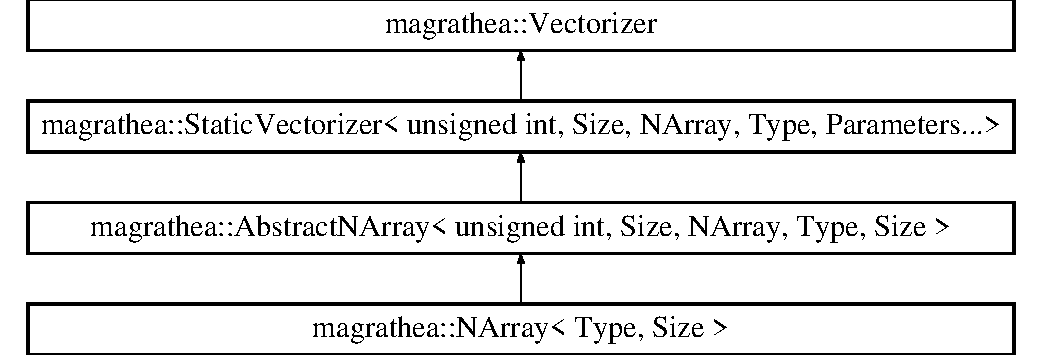
\includegraphics[height=4.000000cm]{exceptionmagrathea_1_1NArray}
\end{center}
\end{figure}
\subsection*{Public Member Functions}
\begin{Indent}{\bf Lifecycle}\par
\begin{DoxyCompactItemize}
\item 
\hyperlink{exceptionmagrathea_1_1NArray_acca52d7eebaed0e348d08bbe0842a472}{N\-Array} ()
\begin{DoxyCompactList}\small\item\em Implicit empty constructor. \end{DoxyCompactList}\item 
{\footnotesize template$<$typename Fundamental\-Type  = Type, class  = typename std\-::enable\-\_\-if$<$std\-::is\-\_\-fundamental$<$\-Fundamental\-Type$>$\-::value$>$\-::type$>$ }\\\hyperlink{exceptionmagrathea_1_1NArray_a3eeaff0a8e63e6d61637b00ad90a3421}{N\-Array} (const \hyperlink{exceptionmagrathea_1_1NArray}{N\-Array}$<$ Fundamental\-Type, Size $>$ \&source)
\begin{DoxyCompactList}\small\item\em Implicit conversion constructor. \end{DoxyCompactList}\item 
{\footnotesize template$<$typename Other\-Type  = Type, class... Misc, class  = typename std\-::enable\-\_\-if$<$std\-::is\-\_\-convertible$<$\-Other\-Type, Type$>$\-::value$>$\-::type$>$ }\\\hyperlink{exceptionmagrathea_1_1NArray_a72b7915a39e9b3c8e99402b1d5fad08c}{N\-Array} (const std\-::initializer\-\_\-list$<$ Other\-Type $>$ \&source, const Misc \&...misc)
\begin{DoxyCompactList}\small\item\em Implicit initializer list constructor. \end{DoxyCompactList}\item 
{\footnotesize template$<$class... Misc, class  = typename std\-::enable\-\_\-if$<$sizeof...(\-Misc) != 0$>$\-::type$>$ }\\\hyperlink{exceptionmagrathea_1_1NArray_a9e5be0242ff3e1261e40bdd4bdaf7b58}{N\-Array} (const Misc \&...misc)
\begin{DoxyCompactList}\small\item\em Explicit generic constructor. \end{DoxyCompactList}\end{DoxyCompactItemize}
\end{Indent}
\subsection*{Static Public Member Functions}
\begin{Indent}{\bf Test}\par
\begin{DoxyCompactItemize}
\item 
static int \hyperlink{exceptionmagrathea_1_1NArray_aad23f5de773bda14e5fa0e6e4d2e9605}{example} ()
\begin{DoxyCompactList}\small\item\em Example function. \end{DoxyCompactList}\end{DoxyCompactItemize}
\end{Indent}
\subsection*{Public Attributes}
\begin{DoxyCompactItemize}
\item 
using \hyperlink{exceptionmagrathea_1_1NArray_aa6eab16c5ba3cc719553a2465f0319df}{operator} = typedef
\end{DoxyCompactItemize}
\subsection*{Protected Attributes}
\begin{Indent}{\bf Data members}\par
\begin{DoxyCompactItemize}
\item 
Type \hyperlink{exceptionmagrathea_1_1NArray_a9bc055609b16d71846679d87b367934c}{\-\_\-data} \mbox{[}Size\mbox{]}
\begin{DoxyCompactList}\small\item\em Data contents. \end{DoxyCompactList}\end{DoxyCompactItemize}
\end{Indent}
\subsection*{Additional Inherited Members}


\subsection{Detailed Description}
\subsubsection*{template$<$typename Type = double, unsigned int Size = 1$>$exception magrathea\-::\-N\-Array$<$ Type, Size $>$}

Basic n-\/dimensional mathematical array. 

This class is the direct derivation of \hyperlink{classmagrathea_1_1AbstractNArray}{Abstract\-N\-Array}. It provides the most basic n-\/dimensional mathematical array without adding new functionalities to the abstract class. 
\begin{DoxyTemplParams}{Template Parameters}
{\em Type} & Data type. \\
\hline
{\em Size} & Number of elements. \\
\hline
\end{DoxyTemplParams}


\subsection{Constructor \& Destructor Documentation}
\hypertarget{exceptionmagrathea_1_1NArray_acca52d7eebaed0e348d08bbe0842a472}{\index{magrathea\-::\-N\-Array@{magrathea\-::\-N\-Array}!N\-Array@{N\-Array}}
\index{N\-Array@{N\-Array}!magrathea::NArray@{magrathea\-::\-N\-Array}}
\subsubsection[{N\-Array}]{\setlength{\rightskip}{0pt plus 5cm}template$<$typename Type , unsigned int Size$>$ {\bf magrathea\-::\-N\-Array}$<$ Type, Size $>$\-::{\bf N\-Array} (
\begin{DoxyParamCaption}
{}
\end{DoxyParamCaption}
)\hspace{0.3cm}{\ttfamily [inline]}}}\label{exceptionmagrathea_1_1NArray_acca52d7eebaed0e348d08bbe0842a472}


Implicit empty constructor. 

Does nothing. \hypertarget{exceptionmagrathea_1_1NArray_a3eeaff0a8e63e6d61637b00ad90a3421}{\index{magrathea\-::\-N\-Array@{magrathea\-::\-N\-Array}!N\-Array@{N\-Array}}
\index{N\-Array@{N\-Array}!magrathea::NArray@{magrathea\-::\-N\-Array}}
\subsubsection[{N\-Array}]{\setlength{\rightskip}{0pt plus 5cm}template$<$typename Type , unsigned int Size$>$ template$<$typename Fundamental\-Type , class $>$ {\bf magrathea\-::\-N\-Array}$<$ Type, Size $>$\-::{\bf N\-Array} (
\begin{DoxyParamCaption}
\item[{const {\bf N\-Array}$<$ Fundamental\-Type, Size $>$ \&}]{source}
\end{DoxyParamCaption}
)\hspace{0.3cm}{\ttfamily [inline]}}}\label{exceptionmagrathea_1_1NArray_a3eeaff0a8e63e6d61637b00ad90a3421}


Implicit conversion constructor. 

Provides an implicit conversion from a fundamental type contents. 
\begin{DoxyTemplParams}{Template Parameters}
{\em Fundamental\-Type} & (Fundamental data type.) \\
\hline
\end{DoxyTemplParams}

\begin{DoxyParams}[1]{Parameters}
\mbox{\tt in}  & {\em source} & Source of the copy. \\
\hline
\end{DoxyParams}
\hypertarget{exceptionmagrathea_1_1NArray_a72b7915a39e9b3c8e99402b1d5fad08c}{\index{magrathea\-::\-N\-Array@{magrathea\-::\-N\-Array}!N\-Array@{N\-Array}}
\index{N\-Array@{N\-Array}!magrathea::NArray@{magrathea\-::\-N\-Array}}
\subsubsection[{N\-Array}]{\setlength{\rightskip}{0pt plus 5cm}template$<$typename Type , unsigned int Size$>$ template$<$typename Other\-Type , class... Misc, class $>$ {\bf magrathea\-::\-N\-Array}$<$ Type, Size $>$\-::{\bf N\-Array} (
\begin{DoxyParamCaption}
\item[{const std\-::initializer\-\_\-list$<$ Other\-Type $>$ \&}]{source, }
\item[{const Misc \&...}]{misc}
\end{DoxyParamCaption}
)\hspace{0.3cm}{\ttfamily [inline]}}}\label{exceptionmagrathea_1_1NArray_a72b7915a39e9b3c8e99402b1d5fad08c}


Implicit initializer list constructor. 

Provides an implicit conversion from an initializer list. 
\begin{DoxyTemplParams}{Template Parameters}
{\em Other\-Type} & (Other data type.) \\
\hline
{\em Misc} & (\hyperlink{classMiscellaneous}{Miscellaneous} types.) \\
\hline
\end{DoxyTemplParams}

\begin{DoxyParams}[1]{Parameters}
\mbox{\tt in}  & {\em source} & Source of the copy. \\
\hline
\mbox{\tt in}  & {\em misc} & \hyperlink{classMiscellaneous}{Miscellaneous} arguments. \\
\hline
\end{DoxyParams}
\hypertarget{exceptionmagrathea_1_1NArray_a9e5be0242ff3e1261e40bdd4bdaf7b58}{\index{magrathea\-::\-N\-Array@{magrathea\-::\-N\-Array}!N\-Array@{N\-Array}}
\index{N\-Array@{N\-Array}!magrathea::NArray@{magrathea\-::\-N\-Array}}
\subsubsection[{N\-Array}]{\setlength{\rightskip}{0pt plus 5cm}template$<$typename Type , unsigned int Size$>$ template$<$class... Misc, class $>$ {\bf magrathea\-::\-N\-Array}$<$ Type, Size $>$\-::{\bf N\-Array} (
\begin{DoxyParamCaption}
\item[{const Misc \&...}]{misc}
\end{DoxyParamCaption}
)\hspace{0.3cm}{\ttfamily [inline]}, {\ttfamily [explicit]}}}\label{exceptionmagrathea_1_1NArray_a9e5be0242ff3e1261e40bdd4bdaf7b58}


Explicit generic constructor. 

Provides a generic interface to all constructors of the base class. Before calling the associated constructor of the base class, the contents is initialized. 
\begin{DoxyTemplParams}{Template Parameters}
{\em Misc} & (\hyperlink{classMiscellaneous}{Miscellaneous} types.) \\
\hline
\end{DoxyTemplParams}

\begin{DoxyParams}[1]{Parameters}
\mbox{\tt in}  & {\em misc} & \hyperlink{classMiscellaneous}{Miscellaneous} arguments. \\
\hline
\end{DoxyParams}


\subsection{Member Function Documentation}
\hypertarget{exceptionmagrathea_1_1NArray_aad23f5de773bda14e5fa0e6e4d2e9605}{\index{magrathea\-::\-N\-Array@{magrathea\-::\-N\-Array}!example@{example}}
\index{example@{example}!magrathea::NArray@{magrathea\-::\-N\-Array}}
\subsubsection[{example}]{\setlength{\rightskip}{0pt plus 5cm}template$<$typename Type , unsigned int Size$>$ int {\bf magrathea\-::\-N\-Array}$<$ Type, Size $>$\-::example (
\begin{DoxyParamCaption}
{}
\end{DoxyParamCaption}
)\hspace{0.3cm}{\ttfamily [static]}}}\label{exceptionmagrathea_1_1NArray_aad23f5de773bda14e5fa0e6e4d2e9605}


Example function. 

Tests and demonstrates the use of \hyperlink{exceptionmagrathea_1_1NArray}{N\-Array}. \begin{DoxyReturn}{Returns}
0 if no error. 
\end{DoxyReturn}


\subsection{Member Data Documentation}
\hypertarget{exceptionmagrathea_1_1NArray_a9bc055609b16d71846679d87b367934c}{\index{magrathea\-::\-N\-Array@{magrathea\-::\-N\-Array}!\-\_\-data@{\-\_\-data}}
\index{\-\_\-data@{\-\_\-data}!magrathea::NArray@{magrathea\-::\-N\-Array}}
\subsubsection[{\-\_\-data}]{\setlength{\rightskip}{0pt plus 5cm}template$<$typename Type = double, unsigned int Size = 1$>$ Type {\bf magrathea\-::\-N\-Array}$<$ Type, Size $>$\-::\-\_\-data\mbox{[}Size\mbox{]}\hspace{0.3cm}{\ttfamily [protected]}}}\label{exceptionmagrathea_1_1NArray_a9bc055609b16d71846679d87b367934c}


Data contents. 

\hypertarget{exceptionmagrathea_1_1NArray_aa6eab16c5ba3cc719553a2465f0319df}{\index{magrathea\-::\-N\-Array@{magrathea\-::\-N\-Array}!operator@{operator}}
\index{operator@{operator}!magrathea::NArray@{magrathea\-::\-N\-Array}}
\subsubsection[{operator}]{\setlength{\rightskip}{0pt plus 5cm}template$<$typename Type = double, unsigned int Size = 1$>$ using {\bf magrathea\-::\-N\-Array}$<$ Type, Size $>$\-::operator = }}\label{exceptionmagrathea_1_1NArray_aa6eab16c5ba3cc719553a2465f0319df}


The documentation for this exception was generated from the following file\-:\begin{DoxyCompactItemize}
\item 
/data/home/mbreton/magrathea\-\_\-pathfinder/src/magrathea/\hyperlink{narray_8h}{narray.\-h}\end{DoxyCompactItemize}

\hypertarget{classObserver__velocity}{\section{Observer\-\_\-velocity Class Reference}
\label{classObserver__velocity}\index{Observer\-\_\-velocity@{Observer\-\_\-velocity}}
}


{\ttfamily \#include $<$observer\-\_\-velocity.\-h$>$}

\subsection*{Static Public Member Functions}
\begin{DoxyCompactItemize}
\item 
{\footnotesize template$<$class Parameters , class Map $>$ }\\static void \hyperlink{classObserver__velocity_acafaae5aa6e6af9cadd712f54f08821e}{Read\-Param\-File} (Parameters \&\hyperlink{rays_8h_ae1bc8b0b8c8b9f8e4cc61a5cc7c4ce9e}{parameters}, Map \&parameter)
\begin{DoxyCompactList}\small\item\em Read parameter file. \end{DoxyCompactList}\item 
{\footnotesize template$<$typename Type1 , template$<$ typename Type, class Index, class Data, unsigned int Dimension, class Position, class Extent, class Element, class Container $>$ class Octree, typename Type , class Index , class Data , unsigned int Dimension, class Position , class Extent , class Element , class Container $>$ }\\static void \hyperlink{classObserver__velocity_a674b436ee4b99f2876e607c66332e63b}{Create\-Octree\-Velocity\-With\-C\-I\-C} (Octree$<$ Type, Index, Data, Dimension, Position, Extent, Element, Container $>$ \&octree, std\-::vector$<$ Type1 $>$ \&pos\-\_\-part, std\-::vector$<$ Type1 $>$ \&vel\-\_\-part)
\begin{DoxyCompactList}\small\item\em Add velocity to Octree using C\-I\-C. \end{DoxyCompactList}\item 
{\footnotesize template$<$typename Type1 , template$<$ typename Type, class Index, class Data, unsigned int Dimension, class Position, class Extent, class Element, class Container $>$ class Octree, typename Type , class Index , class Data , unsigned int Dimension, class Position , class Extent , class Element , class Container $>$ }\\static void \hyperlink{classObserver__velocity_a5dbabc0da68e01d7290564d152d6292a}{Create\-Octree\-Velocity\-With\-T\-S\-C} (Octree$<$ Type, Index, Data, Dimension, Position, Extent, Element, Container $>$ \&octree, std\-::vector$<$ Type1 $>$ \&pos\-\_\-part, std\-::vector$<$ Type1 $>$ \&vel\-\_\-part)
\begin{DoxyCompactList}\small\item\em Add velocity to Octree using T\-S\-C. \end{DoxyCompactList}\end{DoxyCompactItemize}


\subsection{Member Function Documentation}
\hypertarget{classObserver__velocity_a674b436ee4b99f2876e607c66332e63b}{\index{Observer\-\_\-velocity@{Observer\-\_\-velocity}!Create\-Octree\-Velocity\-With\-C\-I\-C@{Create\-Octree\-Velocity\-With\-C\-I\-C}}
\index{Create\-Octree\-Velocity\-With\-C\-I\-C@{Create\-Octree\-Velocity\-With\-C\-I\-C}!Observer_velocity@{Observer\-\_\-velocity}}
\subsubsection[{Create\-Octree\-Velocity\-With\-C\-I\-C}]{\setlength{\rightskip}{0pt plus 5cm}template$<$typename Type1 , template$<$ typename Type, class Index, class Data, unsigned int Dimension, class Position, class Extent, class Element, class Container $>$ class Octree, typename Type , class Index , class Data , unsigned int Dimension, class Position , class Extent , class Element , class Container $>$ void Observer\-\_\-velocity\-::\-Create\-Octree\-Velocity\-With\-C\-I\-C (
\begin{DoxyParamCaption}
\item[{Octree$<$ Type, Index, Data, Dimension, Position, Extent, Element, Container $>$ \&}]{octree, }
\item[{std\-::vector$<$ Type1 $>$ \&}]{pos\-\_\-part, }
\item[{std\-::vector$<$ Type1 $>$ \&}]{vel\-\_\-part}
\end{DoxyParamCaption}
)\hspace{0.3cm}{\ttfamily [static]}}}\label{classObserver__velocity_a674b436ee4b99f2876e607c66332e63b}


Add velocity to Octree using C\-I\-C. 

Add velocity to Octree using C\-I\-C 
\begin{DoxyTemplParams}{Template Parameters}
{\em Type1} & Type1 type \\
\hline
{\em Octree} & octree type \\
\hline
{\em Type} & type type \\
\hline
{\em Index} & index type \\
\hline
{\em Data} & data type \\
\hline
{\em Dimension} & Number of dimensions \\
\hline
{\em Position} & position type \\
\hline
{\em Extent} & extent type \\
\hline
{\em Element} & element type \\
\hline
{\em Container} & container type \\
\hline
\end{DoxyTemplParams}

\begin{DoxyParams}[1]{Parameters}
\mbox{\tt in,out}  & {\em octree} & Octree be to filled with velocity field \\
\hline
\mbox{\tt in}  & {\em pos\-\_\-part} & Position of particles \\
\hline
\mbox{\tt in}  & {\em vel\-\_\-part} & Velocity of particles \\
\hline
\end{DoxyParams}
\hypertarget{classObserver__velocity_a5dbabc0da68e01d7290564d152d6292a}{\index{Observer\-\_\-velocity@{Observer\-\_\-velocity}!Create\-Octree\-Velocity\-With\-T\-S\-C@{Create\-Octree\-Velocity\-With\-T\-S\-C}}
\index{Create\-Octree\-Velocity\-With\-T\-S\-C@{Create\-Octree\-Velocity\-With\-T\-S\-C}!Observer_velocity@{Observer\-\_\-velocity}}
\subsubsection[{Create\-Octree\-Velocity\-With\-T\-S\-C}]{\setlength{\rightskip}{0pt plus 5cm}template$<$typename Type1 , template$<$ typename Type, class Index, class Data, unsigned int Dimension, class Position, class Extent, class Element, class Container $>$ class Octree, typename Type , class Index , class Data , unsigned int Dimension, class Position , class Extent , class Element , class Container $>$ void Observer\-\_\-velocity\-::\-Create\-Octree\-Velocity\-With\-T\-S\-C (
\begin{DoxyParamCaption}
\item[{Octree$<$ Type, Index, Data, Dimension, Position, Extent, Element, Container $>$ \&}]{octree, }
\item[{std\-::vector$<$ Type1 $>$ \&}]{pos\-\_\-part, }
\item[{std\-::vector$<$ Type1 $>$ \&}]{vel\-\_\-part}
\end{DoxyParamCaption}
)\hspace{0.3cm}{\ttfamily [static]}}}\label{classObserver__velocity_a5dbabc0da68e01d7290564d152d6292a}


Add velocity to Octree using T\-S\-C. 

Add velocity to Octree using T\-S\-C 
\begin{DoxyTemplParams}{Template Parameters}
{\em Type1} & Type1 type \\
\hline
{\em Octree} & octree type \\
\hline
{\em Type} & type type \\
\hline
{\em Index} & index type \\
\hline
{\em Data} & data type \\
\hline
{\em Dimension} & Number of dimensions \\
\hline
{\em Position} & position type \\
\hline
{\em Extent} & extent type \\
\hline
{\em Element} & element type \\
\hline
{\em Container} & container type \\
\hline
\end{DoxyTemplParams}

\begin{DoxyParams}[1]{Parameters}
\mbox{\tt in,out}  & {\em octree} & Octree be to filled with velocity field \\
\hline
\mbox{\tt in}  & {\em pos\-\_\-part} & Position of particles \\
\hline
\mbox{\tt in}  & {\em vel\-\_\-part} & Velocity of particles \\
\hline
\end{DoxyParams}
\hypertarget{classObserver__velocity_acafaae5aa6e6af9cadd712f54f08821e}{\index{Observer\-\_\-velocity@{Observer\-\_\-velocity}!Read\-Param\-File@{Read\-Param\-File}}
\index{Read\-Param\-File@{Read\-Param\-File}!Observer_velocity@{Observer\-\_\-velocity}}
\subsubsection[{Read\-Param\-File}]{\setlength{\rightskip}{0pt plus 5cm}template$<$class Parameters , class Map $>$ void Observer\-\_\-velocity\-::\-Read\-Param\-File (
\begin{DoxyParamCaption}
\item[{Parameters \&}]{parameters, }
\item[{Map \&}]{parameter}
\end{DoxyParamCaption}
)\hspace{0.3cm}{\ttfamily [static]}}}\label{classObserver__velocity_acafaae5aa6e6af9cadd712f54f08821e}


Read parameter file. 

Read and put in a structure the parameters. 
\begin{DoxyTemplParams}{Template Parameters}
{\em Parameters} & structure type \\
\hline
{\em Map} & map type \\
\hline
\end{DoxyTemplParams}

\begin{DoxyParams}[1]{Parameters}
\mbox{\tt in,out}  & {\em parameters} & Structure containing the parameters. \\
\hline
\mbox{\tt in}  & {\em parameter} & Contains parameters to be rewritten \\
\hline
\end{DoxyParams}


The documentation for this class was generated from the following file\-:\begin{DoxyCompactItemize}
\item 
/data/home/mbreton/magrathea\-\_\-pathfinder/src/\hyperlink{observer__velocity_8h}{observer\-\_\-velocity.\-h}\end{DoxyCompactItemize}

\hypertarget{exceptionOutput}{\section{Output Exception Reference}
\label{exceptionOutput}\index{Output@{Output}}
}


\hyperlink{exceptionOutput}{Output} utilities for raytracing.  




{\ttfamily \#include $<$output.\-h$>$}

\subsection*{Static Public Member Functions}
\begin{Indent}{\bf Utilities}\par
\begin{DoxyCompactItemize}
\item 
{\footnotesize template$<$class Type  = std\-::string, class  = typename std\-::enable\-\_\-if$<$std\-::is\-\_\-convertible$<$typename std\-::remove\-\_\-cv$<$typename std\-::remove\-\_\-reference$<$\-Type$>$\-::type$>$\-::type, std\-::string$>$\-::value$>$\-::type$>$ }\\static std\-::string \hyperlink{exceptionOutput_a7ccbf3e24a36a73f64cd117ba6b8b904}{name} (Type \&\&value=Type())
\begin{DoxyCompactList}\small\item\em File name from a string. \end{DoxyCompactList}\item 
{\footnotesize template$<$class Type , class  = typename std\-::enable\-\_\-if$<$!std\-::is\-\_\-convertible$<$typename std\-::remove\-\_\-cv$<$typename std\-::remove\-\_\-reference$<$\-Type$>$\-::type$>$\-::type, std\-::string$>$\-::value$>$\-::type$>$ }\\static std\-::string \hyperlink{exceptionOutput_a58f05b0b91d3739be64ba7c40577d5cb}{name} (const Type \&value)
\begin{DoxyCompactList}\small\item\em File name from a number. \end{DoxyCompactList}\item 
{\footnotesize template$<$template$<$ class, class $>$ class Type, class First , class Second , class  = typename std\-::enable\-\_\-if$<$(std\-::tuple\-\_\-size$<$\-Type$<$\-First, Second$>$ $>$\-::value == std\-::tuple\-\_\-size$<$std\-::pair$<$\-First, Second$>$ $>$\-::value) \&\& (std\-::is\-\_\-convertible$<$\-First, std\-::string$>$\-::value)$>$\-::type$>$ }\\static std\-::string \hyperlink{exceptionOutput_abe6f3af3439b365ae0edfec2ee8abfaf}{name} (const Type$<$ First, Second $>$ \&value)
\begin{DoxyCompactList}\small\item\em File name from a format. \end{DoxyCompactList}\item 
{\footnotesize template$<$class Type , class... Types, class  = typename std\-::enable\-\_\-if$<$sizeof...(\-Types) != 0$>$\-::type$>$ }\\static std\-::string \hyperlink{exceptionOutput_a4f4d3a620d93e4e661c62a04e14dd822}{name} (Type \&\&value, Types \&\&...values)
\begin{DoxyCompactList}\small\item\em File name from a format. \end{DoxyCompactList}\end{DoxyCompactItemize}
\end{Indent}
\begin{Indent}{\bf Save}\par
\begin{DoxyCompactItemize}
\item 
{\footnotesize template$<$class Octree , class  = typename std\-::enable\-\_\-if$<$\-Octree\-::dimension() != 0$>$\-::type$>$ }\\static bool \hyperlink{exceptionOutput_af1e22abb9de803b477dbae6f79e6b379}{save} (std\-::ostream \&stream, const Octree \&octree, const int digits=0)
\begin{DoxyCompactList}\small\item\em Save a octree. \end{DoxyCompactList}\item 
{\footnotesize template$<$class Cosmology , class  = typename std\-::enable\-\_\-if$<$std\-::tuple\-\_\-size$<$\-Cosmology$>$\-::value != 0$>$\-::type$>$ }\\static bool \hyperlink{exceptionOutput_a8ef3075f905bf4672ec76a57f94b245d}{save} (std\-::ostream \&stream, const Cosmology \&cosmology, const unsigned int digits=0)
\begin{DoxyCompactList}\small\item\em Save a cosmology. \end{DoxyCompactList}\item 
{\footnotesize template$<$class Trajectory , class  = typename std\-::enable\-\_\-if$<$!std\-::is\-\_\-void$<$typename std\-::remove\-\_\-cv$<$typename std\-::remove\-\_\-reference$<$decltype(std\-::declval$<$\-Trajectory$>$()\mbox{[}0\mbox{]}.\-type())$>$\-::type$>$\-::type$>$\-::value$>$\-::type$>$ }\\static bool \hyperlink{exceptionOutput_a31718f382ea48cc4d7ea4ed360043163}{save} (std\-::ostream \&stream, const Trajectory \&trajectory, const unsigned int \&digits=0)
\begin{DoxyCompactList}\small\item\em Save a trajectory. \end{DoxyCompactList}\item 
{\footnotesize template$<$class Container , typename Type  = typename std\-::remove\-\_\-cv$<$typename std\-::remove\-\_\-reference$<$decltype(std\-::declval$<$\-Container$>$()\mbox{[}0\mbox{]})$>$\-::type$>$\-::type, typename Integral  = std\-::true\-\_\-type, class  = typename std\-::enable\-\_\-if$<$!std\-::is\-\_\-void$<$typename std\-::remove\-\_\-cv$<$typename std\-::remove\-\_\-reference$<$decltype(std\-::declval$<$\-Container$>$()\mbox{[}0\mbox{]})$>$\-::type$>$\-::type$>$\-::value$>$\-::type$>$ }\\static bool \hyperlink{exceptionOutput_a3600c5073abbe3899151cefd9e60ee1a}{save} (std\-::ostream \&stream, const Container \&x, const Container \&y, const Container \&ymean, const Container \&ystd, const unsigned int digits=0, const Integral count=Integral())
\begin{DoxyCompactList}\small\item\em Save statistics. \end{DoxyCompactList}\end{DoxyCompactItemize}
\end{Indent}
\begin{Indent}{\bf Test}\par
\begin{DoxyCompactItemize}
\item 
static int \hyperlink{exceptionOutput_ac8b80a2be067225109da37813bc371f5}{example} ()
\begin{DoxyCompactList}\small\item\em Example function. \end{DoxyCompactList}\end{DoxyCompactItemize}
\end{Indent}


\subsection{Detailed Description}
\hyperlink{exceptionOutput}{Output} utilities for raytracing. 

Provides a list of exportation routines to save data for raytracing. 

\subsection{Member Function Documentation}
\hypertarget{exceptionOutput_ac8b80a2be067225109da37813bc371f5}{\index{Output@{Output}!example@{example}}
\index{example@{example}!Output@{Output}}
\subsubsection[{example}]{\setlength{\rightskip}{0pt plus 5cm}int Output\-::example (
\begin{DoxyParamCaption}
{}
\end{DoxyParamCaption}
)\hspace{0.3cm}{\ttfamily [static]}}}\label{exceptionOutput_ac8b80a2be067225109da37813bc371f5}


Example function. 

Tests and demonstrates the use of \hyperlink{exceptionOutput}{Output}. \begin{DoxyReturn}{Returns}
0 if no error. 
\end{DoxyReturn}
\hypertarget{exceptionOutput_a7ccbf3e24a36a73f64cd117ba6b8b904}{\index{Output@{Output}!name@{name}}
\index{name@{name}!Output@{Output}}
\subsubsection[{name}]{\setlength{\rightskip}{0pt plus 5cm}template$<$class Type , class $>$ std\-::string Output\-::name (
\begin{DoxyParamCaption}
\item[{Type \&\&}]{value = {\ttfamily Type()}}
\end{DoxyParamCaption}
)\hspace{0.3cm}{\ttfamily [inline]}, {\ttfamily [static]}}}\label{exceptionOutput_a7ccbf3e24a36a73f64cd117ba6b8b904}


File name from a string. 

Produces a file name from a string. 
\begin{DoxyTemplParams}{Template Parameters}
{\em Type} & Type convertible to a string. \\
\hline
\end{DoxyTemplParams}

\begin{DoxyParams}[1]{Parameters}
\mbox{\tt in}  & {\em value} & Value of the string. \\
\hline
\end{DoxyParams}
\begin{DoxyReturn}{Returns}
Name corresponding to the string. 
\end{DoxyReturn}
\hypertarget{exceptionOutput_a58f05b0b91d3739be64ba7c40577d5cb}{\index{Output@{Output}!name@{name}}
\index{name@{name}!Output@{Output}}
\subsubsection[{name}]{\setlength{\rightskip}{0pt plus 5cm}template$<$class Type , class $>$ std\-::string Output\-::name (
\begin{DoxyParamCaption}
\item[{const Type \&}]{value}
\end{DoxyParamCaption}
)\hspace{0.3cm}{\ttfamily [inline]}, {\ttfamily [static]}}}\label{exceptionOutput_a58f05b0b91d3739be64ba7c40577d5cb}


File name from a number. 

Produces a file name from a number. 
\begin{DoxyTemplParams}{Template Parameters}
{\em Type} & Number type convertible to a string. \\
\hline
\end{DoxyTemplParams}

\begin{DoxyParams}[1]{Parameters}
\mbox{\tt in}  & {\em value} & Value of the number. \\
\hline
\end{DoxyParams}
\begin{DoxyReturn}{Returns}
Name corresponding to the number. 
\end{DoxyReturn}
\hypertarget{exceptionOutput_abe6f3af3439b365ae0edfec2ee8abfaf}{\index{Output@{Output}!name@{name}}
\index{name@{name}!Output@{Output}}
\subsubsection[{name}]{\setlength{\rightskip}{0pt plus 5cm}template$<$template$<$ class, class $>$ class Type, class First , class Second , class $>$ std\-::string Output\-::name (
\begin{DoxyParamCaption}
\item[{const Type$<$ First, Second $>$ \&}]{value}
\end{DoxyParamCaption}
)\hspace{0.3cm}{\ttfamily [inline]}, {\ttfamily [static]}}}\label{exceptionOutput_abe6f3af3439b365ae0edfec2ee8abfaf}


File name from a format. 

Produces a file name from a format. 
\begin{DoxyTemplParams}{Template Parameters}
{\em Type} & Pair type. \\
\hline
{\em First} & Type convertible to a string. \\
\hline
{\em Second} & Second type associated to the format. \\
\hline
\end{DoxyTemplParams}

\begin{DoxyParams}[1]{Parameters}
\mbox{\tt in}  & {\em value} & Value of the pair. \\
\hline
\end{DoxyParams}
\begin{DoxyReturn}{Returns}
Name corresponding to the format. 
\end{DoxyReturn}
\hypertarget{exceptionOutput_a4f4d3a620d93e4e661c62a04e14dd822}{\index{Output@{Output}!name@{name}}
\index{name@{name}!Output@{Output}}
\subsubsection[{name}]{\setlength{\rightskip}{0pt plus 5cm}template$<$class Type, class... Types, class $>$ std\-::string Output\-::name (
\begin{DoxyParamCaption}
\item[{Type \&\&}]{value, }
\item[{Types \&\&...}]{values}
\end{DoxyParamCaption}
)\hspace{0.3cm}{\ttfamily [inline]}, {\ttfamily [static]}}}\label{exceptionOutput_a4f4d3a620d93e4e661c62a04e14dd822}


File name from a format. 

Produces a file name from a serie of components by recursively calling the name function. 
\begin{DoxyTemplParams}{Template Parameters}
{\em Type} & First type. \\
\hline
{\em Types} & Other types. \\
\hline
\end{DoxyTemplParams}

\begin{DoxyParams}[1]{Parameters}
\mbox{\tt in}  & {\em value} & First value. \\
\hline
\mbox{\tt in}  & {\em values} & Other values. \\
\hline
\end{DoxyParams}
\begin{DoxyReturn}{Returns}
Name corresponding to the serie of components. 
\end{DoxyReturn}
\hypertarget{exceptionOutput_af1e22abb9de803b477dbae6f79e6b379}{\index{Output@{Output}!save@{save}}
\index{save@{save}!Output@{Output}}
\subsubsection[{save}]{\setlength{\rightskip}{0pt plus 5cm}template$<$class Octree , class $>$ bool Output\-::save (
\begin{DoxyParamCaption}
\item[{std\-::ostream \&}]{stream, }
\item[{const Octree \&}]{octree, }
\item[{const int}]{digits = {\ttfamily 0}}
\end{DoxyParamCaption}
)\hspace{0.3cm}{\ttfamily [static]}}}\label{exceptionOutput_af1e22abb9de803b477dbae6f79e6b379}


Save a octree. 

Writes an octree to a text file. 
\begin{DoxyTemplParams}{Template Parameters}
{\em Octree} & Octree type. \\
\hline
\end{DoxyTemplParams}

\begin{DoxyParams}[1]{Parameters}
\mbox{\tt in,out}  & {\em stream} & \hyperlink{exceptionOutput}{Output} stream. \\
\hline
\mbox{\tt in}  & {\em octree} & Octree. \\
\hline
\mbox{\tt in}  & {\em digits} & Optional precision.  \\
\hline
\end{DoxyParams}
\begin{DoxyReturn}{Returns}
True on success, false otherwise. 
\end{DoxyReturn}
\hypertarget{exceptionOutput_a8ef3075f905bf4672ec76a57f94b245d}{\index{Output@{Output}!save@{save}}
\index{save@{save}!Output@{Output}}
\subsubsection[{save}]{\setlength{\rightskip}{0pt plus 5cm}template$<$class Cosmology , class $>$ bool Output\-::save (
\begin{DoxyParamCaption}
\item[{std\-::ostream \&}]{stream, }
\item[{const Cosmology \&}]{cosmology, }
\item[{const unsigned int}]{digits = {\ttfamily 0}}
\end{DoxyParamCaption}
)\hspace{0.3cm}{\ttfamily [static]}}}\label{exceptionOutput_a8ef3075f905bf4672ec76a57f94b245d}


Save a cosmology. 

Writes each step of a cosmology to a text file. 
\begin{DoxyTemplParams}{Template Parameters}
{\em Cosmology} & Cosmology type. \\
\hline
\end{DoxyTemplParams}

\begin{DoxyParams}[1]{Parameters}
\mbox{\tt in,out}  & {\em stream} & \hyperlink{exceptionOutput}{Output} stream. \\
\hline
\mbox{\tt in}  & {\em cosmology} & Cosmology. \\
\hline
\mbox{\tt in}  & {\em digits} & Optional precision.  \\
\hline
\end{DoxyParams}
\begin{DoxyReturn}{Returns}
True on success, false otherwise. 
\end{DoxyReturn}
\hypertarget{exceptionOutput_a31718f382ea48cc4d7ea4ed360043163}{\index{Output@{Output}!save@{save}}
\index{save@{save}!Output@{Output}}
\subsubsection[{save}]{\setlength{\rightskip}{0pt plus 5cm}template$<$class Trajectory , class $>$ bool Output\-::save (
\begin{DoxyParamCaption}
\item[{std\-::ostream \&}]{stream, }
\item[{const Trajectory \&}]{trajectory, }
\item[{const unsigned int \&}]{digits = {\ttfamily 0}}
\end{DoxyParamCaption}
)\hspace{0.3cm}{\ttfamily [static]}}}\label{exceptionOutput_a31718f382ea48cc4d7ea4ed360043163}


Save a trajectory. 

Writes each step of the trajectory to a text file. 
\begin{DoxyTemplParams}{Template Parameters}
{\em Trajectory} & Trajectory type. \\
\hline
\end{DoxyTemplParams}

\begin{DoxyParams}[1]{Parameters}
\mbox{\tt in,out}  & {\em stream} & \hyperlink{exceptionOutput}{Output} stream. \\
\hline
\mbox{\tt in}  & {\em trajectory} & Trajectory. \\
\hline
\mbox{\tt in}  & {\em digits} & Optional precision.  \\
\hline
\end{DoxyParams}
\begin{DoxyReturn}{Returns}
True on success, false otherwise. 
\end{DoxyReturn}
\hypertarget{exceptionOutput_a3600c5073abbe3899151cefd9e60ee1a}{\index{Output@{Output}!save@{save}}
\index{save@{save}!Output@{Output}}
\subsubsection[{save}]{\setlength{\rightskip}{0pt plus 5cm}template$<$class Container , typename Type , typename Integral , class $>$ bool Output\-::save (
\begin{DoxyParamCaption}
\item[{std\-::ostream \&}]{stream, }
\item[{const Container \&}]{x, }
\item[{const Container \&}]{y, }
\item[{const Container \&}]{ymean, }
\item[{const Container \&}]{ystd, }
\item[{const unsigned int}]{digits = {\ttfamily 0}, }
\item[{const Integral}]{count = {\ttfamily Integral()}}
\end{DoxyParamCaption}
)\hspace{0.3cm}{\ttfamily [static]}}}\label{exceptionOutput_a3600c5073abbe3899151cefd9e60ee1a}


Save statistics. 

Save photons statistics. 
\begin{DoxyTemplParams}{Template Parameters}
{\em Container} & Container type. \\
\hline
{\em Type} & Data type. \\
\hline
{\em Integral} & Integral type. \\
\hline
\end{DoxyTemplParams}

\begin{DoxyParams}[1]{Parameters}
\mbox{\tt in,out}  & {\em stream} & \hyperlink{exceptionOutput}{Output} stream. \\
\hline
\mbox{\tt in}  & {\em x} & Abscissae. \\
\hline
\mbox{\tt in}  & {\em y} & Homogeneous ordinates. \\
\hline
\mbox{\tt in}  & {\em ymean} & Mean of values. \\
\hline
\mbox{\tt in}  & {\em ystd} & Standard deviation of values. \\
\hline
\mbox{\tt in}  & {\em digits} & Optional precision. \\
\hline
\mbox{\tt in}  & {\em count} & Optional count.  \\
\hline
\end{DoxyParams}
\begin{DoxyReturn}{Returns}
True on success, false otherwise. 
\end{DoxyReturn}


The documentation for this exception was generated from the following file\-:\begin{DoxyCompactItemize}
\item 
/data/home/mbreton/magrathea\-\_\-pathfinder/src/\hyperlink{output_8h}{output.\-h}\end{DoxyCompactItemize}

\hypertarget{structparameters__t}{\section{parameters\-\_\-t Struct Reference}
\label{structparameters__t}\index{parameters\-\_\-t@{parameters\-\_\-t}}
}


{\ttfamily \#include $<$catalogues.\-h$>$}

\subsection*{Public Attributes}
\begin{DoxyCompactItemize}
\item 
std\-::string \hyperlink{structparameters__t_a385fab9a33c11108c0dd32779cf1516b}{celldir}
\item 
std\-::string \hyperlink{structparameters__t_a2fc3c866ee5125b1c9d80056013974b1}{conedir}
\item 
std\-::string \hyperlink{structparameters__t_aa3f6be07e2d2c6318aff7b4cd1737eaf}{conefmt}
\item 
std\-::string \hyperlink{structparameters__t_adcf1d6707b7f5d531d7c30611c6b84a0}{evolfile}
\item 
\hyperlink{miscellaneous_8h_a69aa29b598b851b0640aa225a9e5d61d}{uint} \hyperlink{structparameters__t_ab2923e9ecd71bbee7e159e7c77c70b47}{isfullsky}
\item 
\hyperlink{miscellaneous_8h_aedc0ad84d1e764530814f57ad931d02a}{real} \hyperlink{structparameters__t_ac1b1b8d724f01a87e4549a883c574ec1}{mpc}
\item 
\hyperlink{miscellaneous_8h_a69aa29b598b851b0640aa225a9e5d61d}{uint} \hyperlink{structparameters__t_abf2ebb68923c70eb2389c50ce8f53a81}{ncoarse}
\item 
\hyperlink{miscellaneous_8h_a69aa29b598b851b0640aa225a9e5d61d}{uint} \hyperlink{structparameters__t_a5e660d96bf41704749fe5dbaaf9b04d7}{ncones}
\item 
std\-::string \hyperlink{structparameters__t_ae04d4dc19be412efe62acce66c9a7d3b}{paramfile}
\item 
\hyperlink{miscellaneous_8h_aedc0ad84d1e764530814f57ad931d02a}{real} \hyperlink{structparameters__t_a07a9ffceae1d7ad8ddf7c1d1c68968a7}{rhoch2}
\item 
\hyperlink{miscellaneous_8h_a69aa29b598b851b0640aa225a9e5d61d}{uint} \hyperlink{structparameters__t_a10258b554f6041b308f82124613413d2}{seed}
\item 
\hyperlink{miscellaneous_8h_a69aa29b598b851b0640aa225a9e5d61d}{uint} \hyperlink{structparameters__t_a1419657bb8c34f5d2e9bddb776a3d174}{typefile}
\item 
std\-::string \hyperlink{structparameters__t_a01dba518211d012322f81de8fa11ace1}{base}
\item 
\hyperlink{miscellaneous_8h_aedc0ad84d1e764530814f57ad931d02a}{real} \hyperlink{structparameters__t_a3fe62df5f1220dfe84a2b6f4a2296e0c}{cat\-\_\-accuracy}
\item 
\hyperlink{miscellaneous_8h_a69aa29b598b851b0640aa225a9e5d61d}{uint} \hyperlink{structparameters__t_aa12af0f84f247935d49bc5c6ee01a92d}{firstcone}
\item 
\hyperlink{miscellaneous_8h_a69aa29b598b851b0640aa225a9e5d61d}{uint} \hyperlink{structparameters__t_a8bd675de4271b95831fd4b127030a34d}{halos}
\item 
std\-::string \hyperlink{structparameters__t_ab7b9c18e615ae8fe8a9b4a3d01df9871}{jacobiantype}
\item 
\hyperlink{miscellaneous_8h_a69aa29b598b851b0640aa225a9e5d61d}{uint} \hyperlink{structparameters__t_aba70984d907c4e00e7aee7f4991f8a16}{lastcone}
\item 
\hyperlink{miscellaneous_8h_a69aa29b598b851b0640aa225a9e5d61d}{uint} \hyperlink{structparameters__t_a4d66a57bff036e6290a4be0c38799680}{npart}
\item 
\hyperlink{miscellaneous_8h_a69aa29b598b851b0640aa225a9e5d61d}{uint} \hyperlink{structparameters__t_a8f47d2098f05773b307e603263444ddb}{nsteps}
\item 
\hyperlink{miscellaneous_8h_aedc0ad84d1e764530814f57ad931d02a}{real} \hyperlink{structparameters__t_a1b7648fe800ba8b3d3158714ac0f47fc}{openingmin}
\item 
std\-::string \hyperlink{structparameters__t_a4f207d78141276caca02382015f0a84a}{outputdir}
\item 
std\-::string \hyperlink{structparameters__t_aafffc635bb13faccf8736fc69a9f3476}{outputprefix}
\item 
std\-::string \hyperlink{structparameters__t_a69c8859185088bd4709aa7ea017552f2}{plane}
\item 
std\-::string \hyperlink{structparameters__t_a8bf32b6c7d134c73eecf722cd952766f}{sourcedir}
\item 
std\-::string \hyperlink{structparameters__t_a30ab6d3c2d1245b444f9dd1690dcd294}{stop\-\_\-bundle}
\item 
\hyperlink{miscellaneous_8h_a69aa29b598b851b0640aa225a9e5d61d}{uint} \hyperlink{structparameters__t_ad760b8b6b93820d2ee9c3381a4e7176f}{use\-\_\-previous\-\_\-catalogues}
\item 
\hyperlink{miscellaneous_8h_aedc0ad84d1e764530814f57ad931d02a}{real} \hyperlink{structparameters__t_a3362126635e9fd51f0b963210c36f3f0}{v0x}
\item 
\hyperlink{miscellaneous_8h_aedc0ad84d1e764530814f57ad931d02a}{real} \hyperlink{structparameters__t_ab1d3e26d3413d8ef37d31219d7832754}{v0y}
\item 
\hyperlink{miscellaneous_8h_aedc0ad84d1e764530814f57ad931d02a}{real} \hyperlink{structparameters__t_a099c67cde26d914835146d7b58600e1b}{v0z}
\item 
\hyperlink{miscellaneous_8h_aedc0ad84d1e764530814f57ad931d02a}{real} \hyperlink{structparameters__t_a799da534b80a8c4d4c4bbfa70defcfdd}{zmin}
\item 
\hyperlink{miscellaneous_8h_aedc0ad84d1e764530814f57ad931d02a}{real} \hyperlink{structparameters__t_ae5763714b90e179cce44fef50a461be9}{zmax}
\item 
\hyperlink{miscellaneous_8h_a69aa29b598b851b0640aa225a9e5d61d}{uint} \hyperlink{structparameters__t_a9f6196ea8bb9f5d753b2fb2ce42f508a}{acorrection}
\item 
\hyperlink{miscellaneous_8h_a69aa29b598b851b0640aa225a9e5d61d}{uint} \hyperlink{structparameters__t_a05971cf7e11f757b0f6ab370929670dd}{allocation}
\item 
std\-::string \hyperlink{structparameters__t_a5829112c30ea0949d97cf420475040d9}{cellfmt}
\item 
\hyperlink{miscellaneous_8h_a69aa29b598b851b0640aa225a9e5d61d}{uint} \hyperlink{structparameters__t_a4ed10d43454f25ef0d4ca1737c7f564e}{coarsecorrection}
\item 
\hyperlink{miscellaneous_8h_a69aa29b598b851b0640aa225a9e5d61d}{uint} \hyperlink{structparameters__t_a62d56a49290289f9fddedc1a4e7ff398}{coarseonly}
\item 
\hyperlink{miscellaneous_8h_a69aa29b598b851b0640aa225a9e5d61d}{uint} \hyperlink{structparameters__t_ad8a921c2f3f285bd25b460af22fb1961}{correction}
\item 
std\-::string \hyperlink{structparameters__t_a00a211252403be3dbdf8baaf155df779}{inputtype}
\item 
\hyperlink{miscellaneous_8h_a69aa29b598b851b0640aa225a9e5d61d}{uint} \hyperlink{structparameters__t_a25750c6960beee8b456bea7cef561af4}{microcoeff}
\item 
std\-::string \hyperlink{structparameters__t_a08786b724b2732a02146cf93d4fd999d}{minicone}
\item 
std\-::string \hyperlink{structparameters__t_af6dca1072c706a85e2840f92a364296c}{partdir}
\item 
std\-::string \hyperlink{structparameters__t_ae4167bd745e50da14d39788ef33c9901}{map\-\_\-components}
\item 
\hyperlink{miscellaneous_8h_a69aa29b598b851b0640aa225a9e5d61d}{uint} \hyperlink{structparameters__t_a7eb05497dc8faf15f3402a301d7696b9}{nb\-\_\-z\-\_\-maps}
\item 
\hyperlink{miscellaneous_8h_a69aa29b598b851b0640aa225a9e5d61d}{uint} \hyperlink{structparameters__t_a40e7bda879e59950b95f34af327c6c70}{nbundlemin}
\item 
long \hyperlink{structparameters__t_a7c01977315893f1ba3e817acb5da671b}{nside}
\item 
std\-::string \hyperlink{structparameters__t_ab3f6283b396f35ae3db85d7878e056a9}{stop\-\_\-ray}
\item 
\hyperlink{miscellaneous_8h_aedc0ad84d1e764530814f57ad931d02a}{real} \hyperlink{structparameters__t_a4eee94929742ddf7fd98bf7b7d51eecd}{z\-\_\-stop\-\_\-min}
\item 
\hyperlink{miscellaneous_8h_aedc0ad84d1e764530814f57ad931d02a}{real} \hyperlink{structparameters__t_a5f580bc0e61ae62976af96a65ec48db4}{z\-\_\-stop\-\_\-max}
\item 
std\-::string \hyperlink{structparameters__t_a8bbae9657771668a658bebc2a96d6e36}{velocity\-\_\-field\-\_\-v0}
\item 
\hyperlink{miscellaneous_8h_a69aa29b598b851b0640aa225a9e5d61d}{uint} \hyperlink{structparameters__t_a2127a37ac67e7f288b3f9bb7c6633702}{makestat}
\item 
\hyperlink{miscellaneous_8h_a69aa29b598b851b0640aa225a9e5d61d}{uint} \hyperlink{structparameters__t_ab45d966e609f9d212202aabed6d658f7}{massmin}
\item 
\hyperlink{miscellaneous_8h_a69aa29b598b851b0640aa225a9e5d61d}{uint} \hyperlink{structparameters__t_afe408ff0dcf6b447bca9bb7eb9e42687}{massmax}
\item 
\hyperlink{miscellaneous_8h_a69aa29b598b851b0640aa225a9e5d61d}{uint} \hyperlink{structparameters__t_afa43dec760b3d5a0411c0fcd80b5ef83}{nbundlecnt}
\item 
\hyperlink{miscellaneous_8h_a69aa29b598b851b0640aa225a9e5d61d}{uint} \hyperlink{structparameters__t_a926d26b823c828e95782dd0e7b231a32}{nstat}
\item 
\hyperlink{miscellaneous_8h_a69aa29b598b851b0640aa225a9e5d61d}{uint} \hyperlink{structparameters__t_af3472b8d82e5fca0ca7740bd16128170}{ntrajectories}
\item 
\hyperlink{miscellaneous_8h_a69aa29b598b851b0640aa225a9e5d61d}{uint} \hyperlink{structparameters__t_aeb34bb04474e316d436796ef393fa87a}{openingcnt}
\item 
std\-::string \hyperlink{structparameters__t_a49f6777db35fd579381b34886d834d94}{ray\-\_\-targets}
\item 
\hyperlink{miscellaneous_8h_adbd822dbdb8152553a0f77b84915bd8d}{integer} \hyperlink{structparameters__t_a6e4f2cc31fabb19d76474b8dd7860a8d}{savemode}
\item 
std\-::string \hyperlink{structparameters__t_a7ede124120e8a980ff9328bf6bc3a8b8}{statistic}
\end{DoxyCompactItemize}


\subsection{Member Data Documentation}
\hypertarget{structparameters__t_a9f6196ea8bb9f5d753b2fb2ce42f508a}{\index{parameters\-\_\-t@{parameters\-\_\-t}!acorrection@{acorrection}}
\index{acorrection@{acorrection}!parameters_t@{parameters\-\_\-t}}
\subsubsection[{acorrection}]{\setlength{\rightskip}{0pt plus 5cm}{\bf uint} parameters\-\_\-t\-::acorrection}}\label{structparameters__t_a9f6196ea8bb9f5d753b2fb2ce42f508a}
\hypertarget{structparameters__t_a05971cf7e11f757b0f6ab370929670dd}{\index{parameters\-\_\-t@{parameters\-\_\-t}!allocation@{allocation}}
\index{allocation@{allocation}!parameters_t@{parameters\-\_\-t}}
\subsubsection[{allocation}]{\setlength{\rightskip}{0pt plus 5cm}{\bf uint} parameters\-\_\-t\-::allocation}}\label{structparameters__t_a05971cf7e11f757b0f6ab370929670dd}
\hypertarget{structparameters__t_a01dba518211d012322f81de8fa11ace1}{\index{parameters\-\_\-t@{parameters\-\_\-t}!base@{base}}
\index{base@{base}!parameters_t@{parameters\-\_\-t}}
\subsubsection[{base}]{\setlength{\rightskip}{0pt plus 5cm}std\-::string parameters\-\_\-t\-::base}}\label{structparameters__t_a01dba518211d012322f81de8fa11ace1}
\hypertarget{structparameters__t_a3fe62df5f1220dfe84a2b6f4a2296e0c}{\index{parameters\-\_\-t@{parameters\-\_\-t}!cat\-\_\-accuracy@{cat\-\_\-accuracy}}
\index{cat\-\_\-accuracy@{cat\-\_\-accuracy}!parameters_t@{parameters\-\_\-t}}
\subsubsection[{cat\-\_\-accuracy}]{\setlength{\rightskip}{0pt plus 5cm}{\bf real} parameters\-\_\-t\-::cat\-\_\-accuracy}}\label{structparameters__t_a3fe62df5f1220dfe84a2b6f4a2296e0c}
\hypertarget{structparameters__t_a385fab9a33c11108c0dd32779cf1516b}{\index{parameters\-\_\-t@{parameters\-\_\-t}!celldir@{celldir}}
\index{celldir@{celldir}!parameters_t@{parameters\-\_\-t}}
\subsubsection[{celldir}]{\setlength{\rightskip}{0pt plus 5cm}std\-::string parameters\-\_\-t\-::celldir}}\label{structparameters__t_a385fab9a33c11108c0dd32779cf1516b}
\hypertarget{structparameters__t_a5829112c30ea0949d97cf420475040d9}{\index{parameters\-\_\-t@{parameters\-\_\-t}!cellfmt@{cellfmt}}
\index{cellfmt@{cellfmt}!parameters_t@{parameters\-\_\-t}}
\subsubsection[{cellfmt}]{\setlength{\rightskip}{0pt plus 5cm}std\-::string parameters\-\_\-t\-::cellfmt}}\label{structparameters__t_a5829112c30ea0949d97cf420475040d9}
\hypertarget{structparameters__t_a4ed10d43454f25ef0d4ca1737c7f564e}{\index{parameters\-\_\-t@{parameters\-\_\-t}!coarsecorrection@{coarsecorrection}}
\index{coarsecorrection@{coarsecorrection}!parameters_t@{parameters\-\_\-t}}
\subsubsection[{coarsecorrection}]{\setlength{\rightskip}{0pt plus 5cm}{\bf uint} parameters\-\_\-t\-::coarsecorrection}}\label{structparameters__t_a4ed10d43454f25ef0d4ca1737c7f564e}
\hypertarget{structparameters__t_a62d56a49290289f9fddedc1a4e7ff398}{\index{parameters\-\_\-t@{parameters\-\_\-t}!coarseonly@{coarseonly}}
\index{coarseonly@{coarseonly}!parameters_t@{parameters\-\_\-t}}
\subsubsection[{coarseonly}]{\setlength{\rightskip}{0pt plus 5cm}{\bf uint} parameters\-\_\-t\-::coarseonly}}\label{structparameters__t_a62d56a49290289f9fddedc1a4e7ff398}
\hypertarget{structparameters__t_a2fc3c866ee5125b1c9d80056013974b1}{\index{parameters\-\_\-t@{parameters\-\_\-t}!conedir@{conedir}}
\index{conedir@{conedir}!parameters_t@{parameters\-\_\-t}}
\subsubsection[{conedir}]{\setlength{\rightskip}{0pt plus 5cm}std\-::string parameters\-\_\-t\-::conedir}}\label{structparameters__t_a2fc3c866ee5125b1c9d80056013974b1}
\hypertarget{structparameters__t_aa3f6be07e2d2c6318aff7b4cd1737eaf}{\index{parameters\-\_\-t@{parameters\-\_\-t}!conefmt@{conefmt}}
\index{conefmt@{conefmt}!parameters_t@{parameters\-\_\-t}}
\subsubsection[{conefmt}]{\setlength{\rightskip}{0pt plus 5cm}std\-::string parameters\-\_\-t\-::conefmt}}\label{structparameters__t_aa3f6be07e2d2c6318aff7b4cd1737eaf}
\hypertarget{structparameters__t_ad8a921c2f3f285bd25b460af22fb1961}{\index{parameters\-\_\-t@{parameters\-\_\-t}!correction@{correction}}
\index{correction@{correction}!parameters_t@{parameters\-\_\-t}}
\subsubsection[{correction}]{\setlength{\rightskip}{0pt plus 5cm}{\bf uint} parameters\-\_\-t\-::correction}}\label{structparameters__t_ad8a921c2f3f285bd25b460af22fb1961}
\hypertarget{structparameters__t_adcf1d6707b7f5d531d7c30611c6b84a0}{\index{parameters\-\_\-t@{parameters\-\_\-t}!evolfile@{evolfile}}
\index{evolfile@{evolfile}!parameters_t@{parameters\-\_\-t}}
\subsubsection[{evolfile}]{\setlength{\rightskip}{0pt plus 5cm}std\-::string parameters\-\_\-t\-::evolfile}}\label{structparameters__t_adcf1d6707b7f5d531d7c30611c6b84a0}
\hypertarget{structparameters__t_aa12af0f84f247935d49bc5c6ee01a92d}{\index{parameters\-\_\-t@{parameters\-\_\-t}!firstcone@{firstcone}}
\index{firstcone@{firstcone}!parameters_t@{parameters\-\_\-t}}
\subsubsection[{firstcone}]{\setlength{\rightskip}{0pt plus 5cm}{\bf uint} parameters\-\_\-t\-::firstcone}}\label{structparameters__t_aa12af0f84f247935d49bc5c6ee01a92d}
\hypertarget{structparameters__t_a8bd675de4271b95831fd4b127030a34d}{\index{parameters\-\_\-t@{parameters\-\_\-t}!halos@{halos}}
\index{halos@{halos}!parameters_t@{parameters\-\_\-t}}
\subsubsection[{halos}]{\setlength{\rightskip}{0pt plus 5cm}{\bf uint} parameters\-\_\-t\-::halos}}\label{structparameters__t_a8bd675de4271b95831fd4b127030a34d}
\hypertarget{structparameters__t_a00a211252403be3dbdf8baaf155df779}{\index{parameters\-\_\-t@{parameters\-\_\-t}!inputtype@{inputtype}}
\index{inputtype@{inputtype}!parameters_t@{parameters\-\_\-t}}
\subsubsection[{inputtype}]{\setlength{\rightskip}{0pt plus 5cm}std\-::string parameters\-\_\-t\-::inputtype}}\label{structparameters__t_a00a211252403be3dbdf8baaf155df779}
\hypertarget{structparameters__t_ab2923e9ecd71bbee7e159e7c77c70b47}{\index{parameters\-\_\-t@{parameters\-\_\-t}!isfullsky@{isfullsky}}
\index{isfullsky@{isfullsky}!parameters_t@{parameters\-\_\-t}}
\subsubsection[{isfullsky}]{\setlength{\rightskip}{0pt plus 5cm}{\bf uint} parameters\-\_\-t\-::isfullsky}}\label{structparameters__t_ab2923e9ecd71bbee7e159e7c77c70b47}
\hypertarget{structparameters__t_ab7b9c18e615ae8fe8a9b4a3d01df9871}{\index{parameters\-\_\-t@{parameters\-\_\-t}!jacobiantype@{jacobiantype}}
\index{jacobiantype@{jacobiantype}!parameters_t@{parameters\-\_\-t}}
\subsubsection[{jacobiantype}]{\setlength{\rightskip}{0pt plus 5cm}std\-::string parameters\-\_\-t\-::jacobiantype}}\label{structparameters__t_ab7b9c18e615ae8fe8a9b4a3d01df9871}
\hypertarget{structparameters__t_aba70984d907c4e00e7aee7f4991f8a16}{\index{parameters\-\_\-t@{parameters\-\_\-t}!lastcone@{lastcone}}
\index{lastcone@{lastcone}!parameters_t@{parameters\-\_\-t}}
\subsubsection[{lastcone}]{\setlength{\rightskip}{0pt plus 5cm}{\bf uint} parameters\-\_\-t\-::lastcone}}\label{structparameters__t_aba70984d907c4e00e7aee7f4991f8a16}
\hypertarget{structparameters__t_a2127a37ac67e7f288b3f9bb7c6633702}{\index{parameters\-\_\-t@{parameters\-\_\-t}!makestat@{makestat}}
\index{makestat@{makestat}!parameters_t@{parameters\-\_\-t}}
\subsubsection[{makestat}]{\setlength{\rightskip}{0pt plus 5cm}{\bf uint} parameters\-\_\-t\-::makestat}}\label{structparameters__t_a2127a37ac67e7f288b3f9bb7c6633702}
\hypertarget{structparameters__t_ae4167bd745e50da14d39788ef33c9901}{\index{parameters\-\_\-t@{parameters\-\_\-t}!map\-\_\-components@{map\-\_\-components}}
\index{map\-\_\-components@{map\-\_\-components}!parameters_t@{parameters\-\_\-t}}
\subsubsection[{map\-\_\-components}]{\setlength{\rightskip}{0pt plus 5cm}std\-::string parameters\-\_\-t\-::map\-\_\-components}}\label{structparameters__t_ae4167bd745e50da14d39788ef33c9901}
\hypertarget{structparameters__t_afe408ff0dcf6b447bca9bb7eb9e42687}{\index{parameters\-\_\-t@{parameters\-\_\-t}!massmax@{massmax}}
\index{massmax@{massmax}!parameters_t@{parameters\-\_\-t}}
\subsubsection[{massmax}]{\setlength{\rightskip}{0pt plus 5cm}{\bf uint} parameters\-\_\-t\-::massmax}}\label{structparameters__t_afe408ff0dcf6b447bca9bb7eb9e42687}
\hypertarget{structparameters__t_ab45d966e609f9d212202aabed6d658f7}{\index{parameters\-\_\-t@{parameters\-\_\-t}!massmin@{massmin}}
\index{massmin@{massmin}!parameters_t@{parameters\-\_\-t}}
\subsubsection[{massmin}]{\setlength{\rightskip}{0pt plus 5cm}{\bf uint} parameters\-\_\-t\-::massmin}}\label{structparameters__t_ab45d966e609f9d212202aabed6d658f7}
\hypertarget{structparameters__t_a25750c6960beee8b456bea7cef561af4}{\index{parameters\-\_\-t@{parameters\-\_\-t}!microcoeff@{microcoeff}}
\index{microcoeff@{microcoeff}!parameters_t@{parameters\-\_\-t}}
\subsubsection[{microcoeff}]{\setlength{\rightskip}{0pt plus 5cm}{\bf uint} parameters\-\_\-t\-::microcoeff}}\label{structparameters__t_a25750c6960beee8b456bea7cef561af4}
\hypertarget{structparameters__t_a08786b724b2732a02146cf93d4fd999d}{\index{parameters\-\_\-t@{parameters\-\_\-t}!minicone@{minicone}}
\index{minicone@{minicone}!parameters_t@{parameters\-\_\-t}}
\subsubsection[{minicone}]{\setlength{\rightskip}{0pt plus 5cm}std\-::string parameters\-\_\-t\-::minicone}}\label{structparameters__t_a08786b724b2732a02146cf93d4fd999d}
\hypertarget{structparameters__t_ac1b1b8d724f01a87e4549a883c574ec1}{\index{parameters\-\_\-t@{parameters\-\_\-t}!mpc@{mpc}}
\index{mpc@{mpc}!parameters_t@{parameters\-\_\-t}}
\subsubsection[{mpc}]{\setlength{\rightskip}{0pt plus 5cm}{\bf real} parameters\-\_\-t\-::mpc}}\label{structparameters__t_ac1b1b8d724f01a87e4549a883c574ec1}
\hypertarget{structparameters__t_a7eb05497dc8faf15f3402a301d7696b9}{\index{parameters\-\_\-t@{parameters\-\_\-t}!nb\-\_\-z\-\_\-maps@{nb\-\_\-z\-\_\-maps}}
\index{nb\-\_\-z\-\_\-maps@{nb\-\_\-z\-\_\-maps}!parameters_t@{parameters\-\_\-t}}
\subsubsection[{nb\-\_\-z\-\_\-maps}]{\setlength{\rightskip}{0pt plus 5cm}{\bf uint} parameters\-\_\-t\-::nb\-\_\-z\-\_\-maps}}\label{structparameters__t_a7eb05497dc8faf15f3402a301d7696b9}
\hypertarget{structparameters__t_afa43dec760b3d5a0411c0fcd80b5ef83}{\index{parameters\-\_\-t@{parameters\-\_\-t}!nbundlecnt@{nbundlecnt}}
\index{nbundlecnt@{nbundlecnt}!parameters_t@{parameters\-\_\-t}}
\subsubsection[{nbundlecnt}]{\setlength{\rightskip}{0pt plus 5cm}{\bf uint} parameters\-\_\-t\-::nbundlecnt}}\label{structparameters__t_afa43dec760b3d5a0411c0fcd80b5ef83}
\hypertarget{structparameters__t_a40e7bda879e59950b95f34af327c6c70}{\index{parameters\-\_\-t@{parameters\-\_\-t}!nbundlemin@{nbundlemin}}
\index{nbundlemin@{nbundlemin}!parameters_t@{parameters\-\_\-t}}
\subsubsection[{nbundlemin}]{\setlength{\rightskip}{0pt plus 5cm}{\bf uint} parameters\-\_\-t\-::nbundlemin}}\label{structparameters__t_a40e7bda879e59950b95f34af327c6c70}
\hypertarget{structparameters__t_abf2ebb68923c70eb2389c50ce8f53a81}{\index{parameters\-\_\-t@{parameters\-\_\-t}!ncoarse@{ncoarse}}
\index{ncoarse@{ncoarse}!parameters_t@{parameters\-\_\-t}}
\subsubsection[{ncoarse}]{\setlength{\rightskip}{0pt plus 5cm}{\bf uint} parameters\-\_\-t\-::ncoarse}}\label{structparameters__t_abf2ebb68923c70eb2389c50ce8f53a81}
\hypertarget{structparameters__t_a5e660d96bf41704749fe5dbaaf9b04d7}{\index{parameters\-\_\-t@{parameters\-\_\-t}!ncones@{ncones}}
\index{ncones@{ncones}!parameters_t@{parameters\-\_\-t}}
\subsubsection[{ncones}]{\setlength{\rightskip}{0pt plus 5cm}{\bf uint} parameters\-\_\-t\-::ncones}}\label{structparameters__t_a5e660d96bf41704749fe5dbaaf9b04d7}
\hypertarget{structparameters__t_a4d66a57bff036e6290a4be0c38799680}{\index{parameters\-\_\-t@{parameters\-\_\-t}!npart@{npart}}
\index{npart@{npart}!parameters_t@{parameters\-\_\-t}}
\subsubsection[{npart}]{\setlength{\rightskip}{0pt plus 5cm}{\bf uint} parameters\-\_\-t\-::npart}}\label{structparameters__t_a4d66a57bff036e6290a4be0c38799680}
\hypertarget{structparameters__t_a7c01977315893f1ba3e817acb5da671b}{\index{parameters\-\_\-t@{parameters\-\_\-t}!nside@{nside}}
\index{nside@{nside}!parameters_t@{parameters\-\_\-t}}
\subsubsection[{nside}]{\setlength{\rightskip}{0pt plus 5cm}long parameters\-\_\-t\-::nside}}\label{structparameters__t_a7c01977315893f1ba3e817acb5da671b}
\hypertarget{structparameters__t_a926d26b823c828e95782dd0e7b231a32}{\index{parameters\-\_\-t@{parameters\-\_\-t}!nstat@{nstat}}
\index{nstat@{nstat}!parameters_t@{parameters\-\_\-t}}
\subsubsection[{nstat}]{\setlength{\rightskip}{0pt plus 5cm}{\bf uint} parameters\-\_\-t\-::nstat}}\label{structparameters__t_a926d26b823c828e95782dd0e7b231a32}
\hypertarget{structparameters__t_a8f47d2098f05773b307e603263444ddb}{\index{parameters\-\_\-t@{parameters\-\_\-t}!nsteps@{nsteps}}
\index{nsteps@{nsteps}!parameters_t@{parameters\-\_\-t}}
\subsubsection[{nsteps}]{\setlength{\rightskip}{0pt plus 5cm}{\bf uint} parameters\-\_\-t\-::nsteps}}\label{structparameters__t_a8f47d2098f05773b307e603263444ddb}
\hypertarget{structparameters__t_af3472b8d82e5fca0ca7740bd16128170}{\index{parameters\-\_\-t@{parameters\-\_\-t}!ntrajectories@{ntrajectories}}
\index{ntrajectories@{ntrajectories}!parameters_t@{parameters\-\_\-t}}
\subsubsection[{ntrajectories}]{\setlength{\rightskip}{0pt plus 5cm}{\bf uint} parameters\-\_\-t\-::ntrajectories}}\label{structparameters__t_af3472b8d82e5fca0ca7740bd16128170}
\hypertarget{structparameters__t_aeb34bb04474e316d436796ef393fa87a}{\index{parameters\-\_\-t@{parameters\-\_\-t}!openingcnt@{openingcnt}}
\index{openingcnt@{openingcnt}!parameters_t@{parameters\-\_\-t}}
\subsubsection[{openingcnt}]{\setlength{\rightskip}{0pt plus 5cm}{\bf uint} parameters\-\_\-t\-::openingcnt}}\label{structparameters__t_aeb34bb04474e316d436796ef393fa87a}
\hypertarget{structparameters__t_a1b7648fe800ba8b3d3158714ac0f47fc}{\index{parameters\-\_\-t@{parameters\-\_\-t}!openingmin@{openingmin}}
\index{openingmin@{openingmin}!parameters_t@{parameters\-\_\-t}}
\subsubsection[{openingmin}]{\setlength{\rightskip}{0pt plus 5cm}{\bf real} parameters\-\_\-t\-::openingmin}}\label{structparameters__t_a1b7648fe800ba8b3d3158714ac0f47fc}
\hypertarget{structparameters__t_a4f207d78141276caca02382015f0a84a}{\index{parameters\-\_\-t@{parameters\-\_\-t}!outputdir@{outputdir}}
\index{outputdir@{outputdir}!parameters_t@{parameters\-\_\-t}}
\subsubsection[{outputdir}]{\setlength{\rightskip}{0pt plus 5cm}std\-::string parameters\-\_\-t\-::outputdir}}\label{structparameters__t_a4f207d78141276caca02382015f0a84a}
\hypertarget{structparameters__t_aafffc635bb13faccf8736fc69a9f3476}{\index{parameters\-\_\-t@{parameters\-\_\-t}!outputprefix@{outputprefix}}
\index{outputprefix@{outputprefix}!parameters_t@{parameters\-\_\-t}}
\subsubsection[{outputprefix}]{\setlength{\rightskip}{0pt plus 5cm}std\-::string parameters\-\_\-t\-::outputprefix}}\label{structparameters__t_aafffc635bb13faccf8736fc69a9f3476}
\hypertarget{structparameters__t_ae04d4dc19be412efe62acce66c9a7d3b}{\index{parameters\-\_\-t@{parameters\-\_\-t}!paramfile@{paramfile}}
\index{paramfile@{paramfile}!parameters_t@{parameters\-\_\-t}}
\subsubsection[{paramfile}]{\setlength{\rightskip}{0pt plus 5cm}std\-::string parameters\-\_\-t\-::paramfile}}\label{structparameters__t_ae04d4dc19be412efe62acce66c9a7d3b}
\hypertarget{structparameters__t_af6dca1072c706a85e2840f92a364296c}{\index{parameters\-\_\-t@{parameters\-\_\-t}!partdir@{partdir}}
\index{partdir@{partdir}!parameters_t@{parameters\-\_\-t}}
\subsubsection[{partdir}]{\setlength{\rightskip}{0pt plus 5cm}std\-::string parameters\-\_\-t\-::partdir}}\label{structparameters__t_af6dca1072c706a85e2840f92a364296c}
\hypertarget{structparameters__t_a69c8859185088bd4709aa7ea017552f2}{\index{parameters\-\_\-t@{parameters\-\_\-t}!plane@{plane}}
\index{plane@{plane}!parameters_t@{parameters\-\_\-t}}
\subsubsection[{plane}]{\setlength{\rightskip}{0pt plus 5cm}std\-::string parameters\-\_\-t\-::plane}}\label{structparameters__t_a69c8859185088bd4709aa7ea017552f2}
\hypertarget{structparameters__t_a49f6777db35fd579381b34886d834d94}{\index{parameters\-\_\-t@{parameters\-\_\-t}!ray\-\_\-targets@{ray\-\_\-targets}}
\index{ray\-\_\-targets@{ray\-\_\-targets}!parameters_t@{parameters\-\_\-t}}
\subsubsection[{ray\-\_\-targets}]{\setlength{\rightskip}{0pt plus 5cm}std\-::string parameters\-\_\-t\-::ray\-\_\-targets}}\label{structparameters__t_a49f6777db35fd579381b34886d834d94}
\hypertarget{structparameters__t_a07a9ffceae1d7ad8ddf7c1d1c68968a7}{\index{parameters\-\_\-t@{parameters\-\_\-t}!rhoch2@{rhoch2}}
\index{rhoch2@{rhoch2}!parameters_t@{parameters\-\_\-t}}
\subsubsection[{rhoch2}]{\setlength{\rightskip}{0pt plus 5cm}{\bf real} parameters\-\_\-t\-::rhoch2}}\label{structparameters__t_a07a9ffceae1d7ad8ddf7c1d1c68968a7}
\hypertarget{structparameters__t_a6e4f2cc31fabb19d76474b8dd7860a8d}{\index{parameters\-\_\-t@{parameters\-\_\-t}!savemode@{savemode}}
\index{savemode@{savemode}!parameters_t@{parameters\-\_\-t}}
\subsubsection[{savemode}]{\setlength{\rightskip}{0pt plus 5cm}{\bf integer} parameters\-\_\-t\-::savemode}}\label{structparameters__t_a6e4f2cc31fabb19d76474b8dd7860a8d}
\hypertarget{structparameters__t_a10258b554f6041b308f82124613413d2}{\index{parameters\-\_\-t@{parameters\-\_\-t}!seed@{seed}}
\index{seed@{seed}!parameters_t@{parameters\-\_\-t}}
\subsubsection[{seed}]{\setlength{\rightskip}{0pt plus 5cm}{\bf uint} parameters\-\_\-t\-::seed}}\label{structparameters__t_a10258b554f6041b308f82124613413d2}
\hypertarget{structparameters__t_a8bf32b6c7d134c73eecf722cd952766f}{\index{parameters\-\_\-t@{parameters\-\_\-t}!sourcedir@{sourcedir}}
\index{sourcedir@{sourcedir}!parameters_t@{parameters\-\_\-t}}
\subsubsection[{sourcedir}]{\setlength{\rightskip}{0pt plus 5cm}std\-::string parameters\-\_\-t\-::sourcedir}}\label{structparameters__t_a8bf32b6c7d134c73eecf722cd952766f}
\hypertarget{structparameters__t_a7ede124120e8a980ff9328bf6bc3a8b8}{\index{parameters\-\_\-t@{parameters\-\_\-t}!statistic@{statistic}}
\index{statistic@{statistic}!parameters_t@{parameters\-\_\-t}}
\subsubsection[{statistic}]{\setlength{\rightskip}{0pt plus 5cm}std\-::string parameters\-\_\-t\-::statistic}}\label{structparameters__t_a7ede124120e8a980ff9328bf6bc3a8b8}
\hypertarget{structparameters__t_a30ab6d3c2d1245b444f9dd1690dcd294}{\index{parameters\-\_\-t@{parameters\-\_\-t}!stop\-\_\-bundle@{stop\-\_\-bundle}}
\index{stop\-\_\-bundle@{stop\-\_\-bundle}!parameters_t@{parameters\-\_\-t}}
\subsubsection[{stop\-\_\-bundle}]{\setlength{\rightskip}{0pt plus 5cm}std\-::string parameters\-\_\-t\-::stop\-\_\-bundle}}\label{structparameters__t_a30ab6d3c2d1245b444f9dd1690dcd294}
\hypertarget{structparameters__t_ab3f6283b396f35ae3db85d7878e056a9}{\index{parameters\-\_\-t@{parameters\-\_\-t}!stop\-\_\-ray@{stop\-\_\-ray}}
\index{stop\-\_\-ray@{stop\-\_\-ray}!parameters_t@{parameters\-\_\-t}}
\subsubsection[{stop\-\_\-ray}]{\setlength{\rightskip}{0pt plus 5cm}std\-::string parameters\-\_\-t\-::stop\-\_\-ray}}\label{structparameters__t_ab3f6283b396f35ae3db85d7878e056a9}
\hypertarget{structparameters__t_a1419657bb8c34f5d2e9bddb776a3d174}{\index{parameters\-\_\-t@{parameters\-\_\-t}!typefile@{typefile}}
\index{typefile@{typefile}!parameters_t@{parameters\-\_\-t}}
\subsubsection[{typefile}]{\setlength{\rightskip}{0pt plus 5cm}{\bf uint} parameters\-\_\-t\-::typefile}}\label{structparameters__t_a1419657bb8c34f5d2e9bddb776a3d174}
\hypertarget{structparameters__t_ad760b8b6b93820d2ee9c3381a4e7176f}{\index{parameters\-\_\-t@{parameters\-\_\-t}!use\-\_\-previous\-\_\-catalogues@{use\-\_\-previous\-\_\-catalogues}}
\index{use\-\_\-previous\-\_\-catalogues@{use\-\_\-previous\-\_\-catalogues}!parameters_t@{parameters\-\_\-t}}
\subsubsection[{use\-\_\-previous\-\_\-catalogues}]{\setlength{\rightskip}{0pt plus 5cm}{\bf uint} parameters\-\_\-t\-::use\-\_\-previous\-\_\-catalogues}}\label{structparameters__t_ad760b8b6b93820d2ee9c3381a4e7176f}
\hypertarget{structparameters__t_a3362126635e9fd51f0b963210c36f3f0}{\index{parameters\-\_\-t@{parameters\-\_\-t}!v0x@{v0x}}
\index{v0x@{v0x}!parameters_t@{parameters\-\_\-t}}
\subsubsection[{v0x}]{\setlength{\rightskip}{0pt plus 5cm}{\bf real} parameters\-\_\-t\-::v0x}}\label{structparameters__t_a3362126635e9fd51f0b963210c36f3f0}
\hypertarget{structparameters__t_ab1d3e26d3413d8ef37d31219d7832754}{\index{parameters\-\_\-t@{parameters\-\_\-t}!v0y@{v0y}}
\index{v0y@{v0y}!parameters_t@{parameters\-\_\-t}}
\subsubsection[{v0y}]{\setlength{\rightskip}{0pt plus 5cm}{\bf real} parameters\-\_\-t\-::v0y}}\label{structparameters__t_ab1d3e26d3413d8ef37d31219d7832754}
\hypertarget{structparameters__t_a099c67cde26d914835146d7b58600e1b}{\index{parameters\-\_\-t@{parameters\-\_\-t}!v0z@{v0z}}
\index{v0z@{v0z}!parameters_t@{parameters\-\_\-t}}
\subsubsection[{v0z}]{\setlength{\rightskip}{0pt plus 5cm}{\bf real} parameters\-\_\-t\-::v0z}}\label{structparameters__t_a099c67cde26d914835146d7b58600e1b}
\hypertarget{structparameters__t_a8bbae9657771668a658bebc2a96d6e36}{\index{parameters\-\_\-t@{parameters\-\_\-t}!velocity\-\_\-field\-\_\-v0@{velocity\-\_\-field\-\_\-v0}}
\index{velocity\-\_\-field\-\_\-v0@{velocity\-\_\-field\-\_\-v0}!parameters_t@{parameters\-\_\-t}}
\subsubsection[{velocity\-\_\-field\-\_\-v0}]{\setlength{\rightskip}{0pt plus 5cm}std\-::string parameters\-\_\-t\-::velocity\-\_\-field\-\_\-v0}}\label{structparameters__t_a8bbae9657771668a658bebc2a96d6e36}
\hypertarget{structparameters__t_a5f580bc0e61ae62976af96a65ec48db4}{\index{parameters\-\_\-t@{parameters\-\_\-t}!z\-\_\-stop\-\_\-max@{z\-\_\-stop\-\_\-max}}
\index{z\-\_\-stop\-\_\-max@{z\-\_\-stop\-\_\-max}!parameters_t@{parameters\-\_\-t}}
\subsubsection[{z\-\_\-stop\-\_\-max}]{\setlength{\rightskip}{0pt plus 5cm}{\bf real} parameters\-\_\-t\-::z\-\_\-stop\-\_\-max}}\label{structparameters__t_a5f580bc0e61ae62976af96a65ec48db4}
\hypertarget{structparameters__t_a4eee94929742ddf7fd98bf7b7d51eecd}{\index{parameters\-\_\-t@{parameters\-\_\-t}!z\-\_\-stop\-\_\-min@{z\-\_\-stop\-\_\-min}}
\index{z\-\_\-stop\-\_\-min@{z\-\_\-stop\-\_\-min}!parameters_t@{parameters\-\_\-t}}
\subsubsection[{z\-\_\-stop\-\_\-min}]{\setlength{\rightskip}{0pt plus 5cm}{\bf real} parameters\-\_\-t\-::z\-\_\-stop\-\_\-min}}\label{structparameters__t_a4eee94929742ddf7fd98bf7b7d51eecd}
\hypertarget{structparameters__t_ae5763714b90e179cce44fef50a461be9}{\index{parameters\-\_\-t@{parameters\-\_\-t}!zmax@{zmax}}
\index{zmax@{zmax}!parameters_t@{parameters\-\_\-t}}
\subsubsection[{zmax}]{\setlength{\rightskip}{0pt plus 5cm}{\bf real} parameters\-\_\-t\-::zmax}}\label{structparameters__t_ae5763714b90e179cce44fef50a461be9}
\hypertarget{structparameters__t_a799da534b80a8c4d4c4bbfa70defcfdd}{\index{parameters\-\_\-t@{parameters\-\_\-t}!zmin@{zmin}}
\index{zmin@{zmin}!parameters_t@{parameters\-\_\-t}}
\subsubsection[{zmin}]{\setlength{\rightskip}{0pt plus 5cm}{\bf real} parameters\-\_\-t\-::zmin}}\label{structparameters__t_a799da534b80a8c4d4c4bbfa70defcfdd}


The documentation for this struct was generated from the following files\-:\begin{DoxyCompactItemize}
\item 
/data/home/mbreton/magrathea\-\_\-pathfinder/src/\hyperlink{catalogues_8h}{catalogues.\-h}\item 
/data/home/mbreton/magrathea\-\_\-pathfinder/src/\hyperlink{create__octree_8h}{create\-\_\-octree.\-h}\item 
/data/home/mbreton/magrathea\-\_\-pathfinder/src/\hyperlink{hmaps_8h}{hmaps.\-h}\item 
/data/home/mbreton/magrathea\-\_\-pathfinder/src/\hyperlink{observer__velocity_8h}{observer\-\_\-velocity.\-h}\item 
/data/home/mbreton/magrathea\-\_\-pathfinder/src/\hyperlink{rays_8h}{rays.\-h}\end{DoxyCompactItemize}

\hypertarget{exceptionPhoton}{\section{Photon$<$ Type, Dimension $>$ Exception Template Reference}
\label{exceptionPhoton}\index{Photon$<$ Type, Dimension $>$@{Photon$<$ Type, Dimension $>$}}
}


\hyperlink{exceptionPhoton}{Photon} step implementation for raytracing.  




{\ttfamily \#include $<$photon.\-h$>$}

Inheritance diagram for Photon$<$ Type, Dimension $>$\-:\begin{figure}[H]
\begin{center}
\leavevmode
\includegraphics[height=0.740251cm]{exceptionPhoton}
\end{center}
\end{figure}
\subsection*{Public Member Functions}
\begin{Indent}{\bf Lifecycle}\par
\begin{DoxyCompactItemize}
\item 
{\footnotesize template$<$class... Misc$>$ }\\\hyperlink{exceptionPhoton_a1f19ea883bc2ed2e8af37e0599e54c00}{Photon} (Misc \&\&...misc)
\begin{DoxyCompactList}\small\item\em Explicit generic constructor. \end{DoxyCompactList}\end{DoxyCompactItemize}
\end{Indent}
\begin{Indent}{\bf Data}\par
\begin{DoxyCompactItemize}
\item 
{\footnotesize template$<$unsigned int... Values, class... Misc, class Template  = decltype(std\-::declval$<$magrathea\-::\-Abstract\-Step$<$\-Photon$<$\-Type, Dimension$>$, unsigned int, std\-::array$<$\-Type, 1+(1+\-Dimension)$\ast$2$>$, std\-::tuple$<$\-Type, Type, Type, Type, std\-::array$<$\-Type, Dimension$>$, Type, Type, Type, Type, Type, Type, std\-::array$<$\-Type, 3$>$ , Type, Type, Type$>$ $>$ $>$().\-template id$<$\-Values...$>$(std\-::declval$<$\-Misc$>$()...)), class  = typename std\-::enable\-\_\-if$<$!std\-::is\-\_\-void$<$\-Template$>$\-::value$>$\-::type$>$ }\\Template \hyperlink{exceptionPhoton_ab80ac84513c9082f2bb8bc0d776f12b0}{index} (Misc \&\&...misc)
\begin{DoxyCompactList}\small\item\em Access to the index data. \end{DoxyCompactList}\item 
{\footnotesize template$<$unsigned int... Values, class... Misc, class Template  = decltype(std\-::declval$<$const magrathea\-::\-Abstract\-Step$<$\-Photon$<$\-Type, Dimension$>$, unsigned int, std\-::array$<$\-Type, 1+(1+\-Dimension)$\ast$2$>$, std\-::tuple$<$\-Type, Type, Type, Type, std\-::array$<$\-Type, Dimension$>$, Type, Type, Type, Type, Type, Type, std\-::array$<$\-Type, 3$>$ , Type, Type, Type$>$ $>$ $>$().\-template id$<$\-Values...$>$(std\-::declval$<$\-Misc$>$()...)), class  = typename std\-::enable\-\_\-if$<$!std\-::is\-\_\-void$<$\-Template$>$\-::value$>$\-::type$>$ }\\Template \hyperlink{exceptionPhoton_a655852ccbf34be40427d6f708a032198}{index} (Misc \&\&...misc) const 
\begin{DoxyCompactList}\small\item\em Immutable access to the index data. \end{DoxyCompactList}\item 
{\footnotesize template$<$unsigned int... Values, class... Misc, class Template  = decltype(std\-::declval$<$magrathea\-::\-Abstract\-Step$<$\-Photon$<$\-Type, Dimension$>$, unsigned int, std\-::array$<$\-Type, 1+(1+\-Dimension)$\ast$2$>$, std\-::tuple$<$\-Type, Type, Type, Type, std\-::array$<$\-Type, Dimension$>$, Type, Type, Type, Type, Type, Type, std\-::array$<$\-Type, 3$>$ , Type, Type, Type$>$ $>$ $>$().\-template core$<$0, Values...$>$(std\-::declval$<$\-Misc$>$()...)), class  = typename std\-::enable\-\_\-if$<$!std\-::is\-\_\-void$<$\-Template$>$\-::value$>$\-::type$>$ }\\Template \hyperlink{exceptionPhoton_ab990012b6e6d8c4d85377dcd555f7fff}{a} (Misc \&\&...misc)
\begin{DoxyCompactList}\small\item\em Access to the a data. \end{DoxyCompactList}\item 
{\footnotesize template$<$unsigned int... Values, class... Misc, class Template  = decltype(std\-::declval$<$const magrathea\-::\-Abstract\-Step$<$\-Photon$<$\-Type, Dimension$>$, unsigned int, std\-::array$<$\-Type, 1+(1+\-Dimension)$\ast$2$>$, std\-::tuple$<$\-Type, Type, Type, Type, std\-::array$<$\-Type, Dimension$>$, Type, Type, Type, Type, Type, Type, std\-::array$<$\-Type, 3$>$ , Type, Type, Type$>$ $>$ $>$().\-template core$<$0, Values...$>$(std\-::declval$<$\-Misc$>$()...)), class  = typename std\-::enable\-\_\-if$<$!std\-::is\-\_\-void$<$\-Template$>$\-::value$>$\-::type$>$ }\\Template \hyperlink{exceptionPhoton_afa267cd6af25cc9a8d16d2b23980ed55}{a} (Misc \&\&...misc) const 
\begin{DoxyCompactList}\small\item\em Immutable access to the a data. \end{DoxyCompactList}\item 
{\footnotesize template$<$unsigned int... Values, class... Misc, class Template  = decltype(std\-::declval$<$magrathea\-::\-Abstract\-Step$<$\-Photon$<$\-Type, Dimension$>$, unsigned int, std\-::array$<$\-Type, 1+(1+\-Dimension)$\ast$2$>$, std\-::tuple$<$\-Type, Type, Type, Type, std\-::array$<$\-Type, Dimension$>$, Type, Type, Type, Type, Type, Type, std\-::array$<$\-Type, 3$>$ , Type, Type, Type$>$ $>$ $>$().\-template core$<$1, Values...$>$(std\-::declval$<$\-Misc$>$()...)), class  = typename std\-::enable\-\_\-if$<$!std\-::is\-\_\-void$<$\-Template$>$\-::value$>$\-::type$>$ }\\Template \hyperlink{exceptionPhoton_ac51f83fe7ee52b304aa20fd4d0c851c7}{t} (Misc \&\&...misc)
\begin{DoxyCompactList}\small\item\em Access to the t data. \end{DoxyCompactList}\item 
{\footnotesize template$<$unsigned int... Values, class... Misc, class Template  = decltype(std\-::declval$<$const magrathea\-::\-Abstract\-Step$<$\-Photon$<$\-Type, Dimension$>$, unsigned int, std\-::array$<$\-Type, 1+(1+\-Dimension)$\ast$2$>$, std\-::tuple$<$\-Type, Type, Type, Type, std\-::array$<$\-Type, Dimension$>$, Type, Type, Type, Type, Type, Type, std\-::array$<$\-Type, 3$>$ , Type, Type, Type$>$ $>$ $>$().\-template core$<$1, Values...$>$(std\-::declval$<$\-Misc$>$()...)), class  = typename std\-::enable\-\_\-if$<$!std\-::is\-\_\-void$<$\-Template$>$\-::value$>$\-::type$>$ }\\Template \hyperlink{exceptionPhoton_a957666d7aff7e07068a19083060137c0}{t} (Misc \&\&...misc) const 
\begin{DoxyCompactList}\small\item\em Immutable access to the t data. \end{DoxyCompactList}\item 
{\footnotesize template$<$unsigned int... Values, class... Misc, class Template  = decltype(std\-::declval$<$magrathea\-::\-Abstract\-Step$<$\-Photon$<$\-Type, Dimension$>$, unsigned int, std\-::array$<$\-Type, 1+(1+\-Dimension)$\ast$2$>$, std\-::tuple$<$\-Type, Type, Type, Type, std\-::array$<$\-Type, Dimension$>$, Type, Type, Type, Type, Type, Type, std\-::array$<$\-Type, 3$>$ , Type, Type, Type$>$ $>$ $>$().\-template core$<$2, Values...$>$(std\-::declval$<$\-Misc$>$()...)), class  = typename std\-::enable\-\_\-if$<$!std\-::is\-\_\-void$<$\-Template$>$\-::value$>$\-::type$>$ }\\Template \hyperlink{exceptionPhoton_a5980c201dd85619c427e25d8880257fd}{x} (Misc \&\&...misc)
\begin{DoxyCompactList}\small\item\em Access to the x data. \end{DoxyCompactList}\item 
{\footnotesize template$<$unsigned int... Values, class... Misc, class Template  = decltype(std\-::declval$<$const magrathea\-::\-Abstract\-Step$<$\-Photon$<$\-Type, Dimension$>$, unsigned int, std\-::array$<$\-Type, 1+(1+\-Dimension)$\ast$2$>$, std\-::tuple$<$\-Type, Type, Type, Type, std\-::array$<$\-Type, Dimension$>$, Type, Type, Type, Type, Type, Type, std\-::array$<$\-Type, 3$>$ , Type, Type, Type$>$ $>$ $>$().\-template core$<$2, Values...$>$(std\-::declval$<$\-Misc$>$()...)), class  = typename std\-::enable\-\_\-if$<$!std\-::is\-\_\-void$<$\-Template$>$\-::value$>$\-::type$>$ }\\Template \hyperlink{exceptionPhoton_a469648c11a2e6837cf0c65fa6fe94635}{x} (Misc \&\&...misc) const 
\begin{DoxyCompactList}\small\item\em Immutable access to the x data. \end{DoxyCompactList}\item 
{\footnotesize template$<$unsigned int... Values, class... Misc, class Template  = decltype(std\-::declval$<$magrathea\-::\-Abstract\-Step$<$\-Photon$<$\-Type, Dimension$>$, unsigned int, std\-::array$<$\-Type, 1+(1+\-Dimension)$\ast$2$>$, std\-::tuple$<$\-Type, Type, Type, Type, std\-::array$<$\-Type, Dimension$>$, Type, Type, Type, Type, Type, Type, std\-::array$<$\-Type, 3$>$ , Type, Type, Type$>$ $>$ $>$().\-template core$<$3, Values...$>$(std\-::declval$<$\-Misc$>$()...)), class  = typename std\-::enable\-\_\-if$<$!std\-::is\-\_\-void$<$\-Template$>$\-::value$>$\-::type$>$ }\\Template \hyperlink{exceptionPhoton_ac536f2da82b01af4de0556ad4006bf99}{y} (Misc \&\&...misc)
\begin{DoxyCompactList}\small\item\em Access to the y data. \end{DoxyCompactList}\item 
{\footnotesize template$<$unsigned int... Values, class... Misc, class Template  = decltype(std\-::declval$<$const magrathea\-::\-Abstract\-Step$<$\-Photon$<$\-Type, Dimension$>$, unsigned int, std\-::array$<$\-Type, 1+(1+\-Dimension)$\ast$2$>$, std\-::tuple$<$\-Type, Type, Type, Type, std\-::array$<$\-Type, Dimension$>$, Type, Type, Type, Type, Type, Type, std\-::array$<$\-Type, 3$>$ , Type, Type, Type$>$ $>$ $>$().\-template core$<$3, Values...$>$(std\-::declval$<$\-Misc$>$()...)), class  = typename std\-::enable\-\_\-if$<$!std\-::is\-\_\-void$<$\-Template$>$\-::value$>$\-::type$>$ }\\Template \hyperlink{exceptionPhoton_a04fbcd9b5bda75954faaf1c340c71c78}{y} (Misc \&\&...misc) const 
\begin{DoxyCompactList}\small\item\em Immutable access to the y data. \end{DoxyCompactList}\item 
{\footnotesize template$<$unsigned int... Values, class... Misc, class Template  = decltype(std\-::declval$<$magrathea\-::\-Abstract\-Step$<$\-Photon$<$\-Type, Dimension$>$, unsigned int, std\-::array$<$\-Type, 1+(1+\-Dimension)$\ast$2$>$, std\-::tuple$<$\-Type, Type, Type, Type, std\-::array$<$\-Type, Dimension$>$, Type, Type, Type, Type, Type, Type, std\-::array$<$\-Type, 3$>$ , Type, Type, Type$>$ $>$ $>$().\-template core$<$4, Values...$>$(std\-::declval$<$\-Misc$>$()...)), class  = typename std\-::enable\-\_\-if$<$!std\-::is\-\_\-void$<$\-Template$>$\-::value$>$\-::type$>$ }\\Template \hyperlink{exceptionPhoton_a1b6b93d4c4713592eea2251ab4465138}{z} (Misc \&\&...misc)
\begin{DoxyCompactList}\small\item\em Access to the z data. \end{DoxyCompactList}\item 
{\footnotesize template$<$unsigned int... Values, class... Misc, class Template  = decltype(std\-::declval$<$const magrathea\-::\-Abstract\-Step$<$\-Photon$<$\-Type, Dimension$>$, unsigned int, std\-::array$<$\-Type, 1+(1+\-Dimension)$\ast$2$>$, std\-::tuple$<$\-Type, Type, Type, Type, std\-::array$<$\-Type, Dimension$>$, Type, Type, Type, Type, Type, Type, std\-::array$<$\-Type, 3$>$ , Type, Type, Type$>$ $>$ $>$().\-template core$<$4, Values...$>$(std\-::declval$<$\-Misc$>$()...)), class  = typename std\-::enable\-\_\-if$<$!std\-::is\-\_\-void$<$\-Template$>$\-::value$>$\-::type$>$ }\\Template \hyperlink{exceptionPhoton_a2e9cc817b327a926e88da72e37a89ef0}{z} (Misc \&\&...misc) const 
\begin{DoxyCompactList}\small\item\em Immutable access to the z data. \end{DoxyCompactList}\item 
{\footnotesize template$<$unsigned int... Values, class... Misc, class Template  = decltype(std\-::declval$<$magrathea\-::\-Abstract\-Step$<$\-Photon$<$\-Type, Dimension$>$, unsigned int, std\-::array$<$\-Type, 1+(1+\-Dimension)$\ast$2$>$, std\-::tuple$<$\-Type, Type, Type, Type, std\-::array$<$\-Type, Dimension$>$, Type, Type, Type, Type, Type, Type, std\-::array$<$\-Type, 3$>$ , Type, Type, Type$>$ $>$ $>$().\-template core$<$5, Values...$>$(std\-::declval$<$\-Misc$>$()...)), class  = typename std\-::enable\-\_\-if$<$!std\-::is\-\_\-void$<$\-Template$>$\-::value$>$\-::type$>$ }\\Template \hyperlink{exceptionPhoton_ab593c356203e3a7ce2d82ecb987d0979}{dtdl} (Misc \&\&...misc)
\begin{DoxyCompactList}\small\item\em Access to the dtdl data. \end{DoxyCompactList}\item 
{\footnotesize template$<$unsigned int... Values, class... Misc, class Template  = decltype(std\-::declval$<$const magrathea\-::\-Abstract\-Step$<$\-Photon$<$\-Type, Dimension$>$, unsigned int, std\-::array$<$\-Type, 1+(1+\-Dimension)$\ast$2$>$, std\-::tuple$<$\-Type, Type, Type, Type, std\-::array$<$\-Type, Dimension$>$, Type, Type, Type, Type, Type, Type, std\-::array$<$\-Type, 3$>$ , Type, Type, Type$>$ $>$ $>$().\-template core$<$5, Values...$>$(std\-::declval$<$\-Misc$>$()...)), class  = typename std\-::enable\-\_\-if$<$!std\-::is\-\_\-void$<$\-Template$>$\-::value$>$\-::type$>$ }\\Template \hyperlink{exceptionPhoton_a1039705629b374ba0f8da204fabcdd52}{dtdl} (Misc \&\&...misc) const 
\begin{DoxyCompactList}\small\item\em Immutable access to the dtdl data. \end{DoxyCompactList}\item 
{\footnotesize template$<$unsigned int... Values, class... Misc, class Template  = decltype(std\-::declval$<$magrathea\-::\-Abstract\-Step$<$\-Photon$<$\-Type, Dimension$>$, unsigned int, std\-::array$<$\-Type, 1+(1+\-Dimension)$\ast$2$>$, std\-::tuple$<$\-Type, Type, Type, Type, std\-::array$<$\-Type, Dimension$>$, Type, Type, Type, Type, Type, Type, std\-::array$<$\-Type, 3$>$ , Type, Type, Type$>$ $>$ $>$().\-template core$<$6, Values...$>$(std\-::declval$<$\-Misc$>$()...)), class  = typename std\-::enable\-\_\-if$<$!std\-::is\-\_\-void$<$\-Template$>$\-::value$>$\-::type$>$ }\\Template \hyperlink{exceptionPhoton_a124644c9e1224ff3f26cc4825e7e177b}{dxdl} (Misc \&\&...misc)
\begin{DoxyCompactList}\small\item\em Access to the dxdl data. \end{DoxyCompactList}\item 
{\footnotesize template$<$unsigned int... Values, class... Misc, class Template  = decltype(std\-::declval$<$const magrathea\-::\-Abstract\-Step$<$\-Photon$<$\-Type, Dimension$>$, unsigned int, std\-::array$<$\-Type, 1+(1+\-Dimension)$\ast$2$>$, std\-::tuple$<$\-Type, Type, Type, Type, std\-::array$<$\-Type, Dimension$>$, Type, Type, Type, Type, Type, Type, std\-::array$<$\-Type, 3$>$ , Type, Type, Type$>$ $>$ $>$().\-template core$<$6, Values...$>$(std\-::declval$<$\-Misc$>$()...)), class  = typename std\-::enable\-\_\-if$<$!std\-::is\-\_\-void$<$\-Template$>$\-::value$>$\-::type$>$ }\\Template \hyperlink{exceptionPhoton_a5ad063b203917fcc24c358abaa958843}{dxdl} (Misc \&\&...misc) const 
\begin{DoxyCompactList}\small\item\em Immutable access to the dxdl data. \end{DoxyCompactList}\item 
{\footnotesize template$<$unsigned int... Values, class... Misc, class Template  = decltype(std\-::declval$<$magrathea\-::\-Abstract\-Step$<$\-Photon$<$\-Type, Dimension$>$, unsigned int, std\-::array$<$\-Type, 1+(1+\-Dimension)$\ast$2$>$, std\-::tuple$<$\-Type, Type, Type, Type, std\-::array$<$\-Type, Dimension$>$, Type, Type, Type, Type, Type, Type, std\-::array$<$\-Type, 3$>$ , Type, Type, Type$>$ $>$ $>$().\-template core$<$7, Values...$>$(std\-::declval$<$\-Misc$>$()...)), class  = typename std\-::enable\-\_\-if$<$!std\-::is\-\_\-void$<$\-Template$>$\-::value$>$\-::type$>$ }\\Template \hyperlink{exceptionPhoton_aea9b90661986fa88996f43edc90bfe5f}{dydl} (Misc \&\&...misc)
\begin{DoxyCompactList}\small\item\em Access to the dydl data. \end{DoxyCompactList}\item 
{\footnotesize template$<$unsigned int... Values, class... Misc, class Template  = decltype(std\-::declval$<$const magrathea\-::\-Abstract\-Step$<$\-Photon$<$\-Type, Dimension$>$, unsigned int, std\-::array$<$\-Type, 1+(1+\-Dimension)$\ast$2$>$, std\-::tuple$<$\-Type, Type, Type, Type, std\-::array$<$\-Type, Dimension$>$, Type, Type, Type, Type, Type, Type, std\-::array$<$\-Type, 3$>$ , Type, Type, Type$>$ $>$ $>$().\-template core$<$7, Values...$>$(std\-::declval$<$\-Misc$>$()...)), class  = typename std\-::enable\-\_\-if$<$!std\-::is\-\_\-void$<$\-Template$>$\-::value$>$\-::type$>$ }\\Template \hyperlink{exceptionPhoton_a8f0581f1a7925293c8ee7daaeceb0f01}{dydl} (Misc \&\&...misc) const 
\begin{DoxyCompactList}\small\item\em Immutable access to the dydl data. \end{DoxyCompactList}\item 
{\footnotesize template$<$unsigned int... Values, class... Misc, class Template  = decltype(std\-::declval$<$magrathea\-::\-Abstract\-Step$<$\-Photon$<$\-Type, Dimension$>$, unsigned int, std\-::array$<$\-Type, 1+(1+\-Dimension)$\ast$2$>$, std\-::tuple$<$\-Type, Type, Type, Type, std\-::array$<$\-Type, Dimension$>$, Type, Type, Type, Type, Type, Type, std\-::array$<$\-Type, 3$>$ , Type, Type, Type$>$ $>$ $>$().\-template core$<$8, Values...$>$(std\-::declval$<$\-Misc$>$()...)), class  = typename std\-::enable\-\_\-if$<$!std\-::is\-\_\-void$<$\-Template$>$\-::value$>$\-::type$>$ }\\Template \hyperlink{exceptionPhoton_a449a164994ecfdd2fbac12f0c50acece}{dzdl} (Misc \&\&...misc)
\begin{DoxyCompactList}\small\item\em Access to the dzdl data. \end{DoxyCompactList}\item 
{\footnotesize template$<$unsigned int... Values, class... Misc, class Template  = decltype(std\-::declval$<$const magrathea\-::\-Abstract\-Step$<$\-Photon$<$\-Type, Dimension$>$, unsigned int, std\-::array$<$\-Type, 1+(1+\-Dimension)$\ast$2$>$, std\-::tuple$<$\-Type, Type, Type, Type, std\-::array$<$\-Type, Dimension$>$, Type, Type, Type, Type, Type, Type, std\-::array$<$\-Type, 3$>$ , Type, Type, Type$>$ $>$ $>$().\-template core$<$8, Values...$>$(std\-::declval$<$\-Misc$>$()...)), class  = typename std\-::enable\-\_\-if$<$!std\-::is\-\_\-void$<$\-Template$>$\-::value$>$\-::type$>$ }\\Template \hyperlink{exceptionPhoton_ab68fdfa019d0c9e2fe15437a8c1d0ca3}{dzdl} (Misc \&\&...misc) const 
\begin{DoxyCompactList}\small\item\em Immutable access to the dzdl data. \end{DoxyCompactList}\item 
{\footnotesize template$<$unsigned int... Values, class... Misc, class Template  = decltype(std\-::declval$<$magrathea\-::\-Abstract\-Step$<$\-Photon$<$\-Type, Dimension$>$, unsigned int, std\-::array$<$\-Type, 1+(1+\-Dimension)$\ast$2$>$, std\-::tuple$<$\-Type, Type, Type, Type, std\-::array$<$\-Type, Dimension$>$, Type, Type, Type, Type, Type, Type, std\-::array$<$\-Type, 3$>$ , Type, Type, Type$>$ $>$ $>$().\-template extra$<$0, Values...$>$(std\-::declval$<$\-Misc$>$()...)), class  = typename std\-::enable\-\_\-if$<$!std\-::is\-\_\-void$<$\-Template$>$\-::value$>$\-::type$>$ }\\Template \hyperlink{exceptionPhoton_a1181b3a7962f3eaa951a359d1cd8357d}{level} (Misc \&\&...misc)
\begin{DoxyCompactList}\small\item\em Access to the level data. \end{DoxyCompactList}\item 
{\footnotesize template$<$unsigned int... Values, class... Misc, class Template  = decltype(std\-::declval$<$const magrathea\-::\-Abstract\-Step$<$\-Photon$<$\-Type, Dimension$>$, unsigned int, std\-::array$<$\-Type, 1+(1+\-Dimension)$\ast$2$>$, std\-::tuple$<$\-Type, Type, Type, Type, std\-::array$<$\-Type, Dimension$>$, Type, Type, Type, Type, Type, Type, std\-::array$<$\-Type, 3$>$ , Type, Type, Type$>$ $>$ $>$().\-template extra$<$0, Values...$>$(std\-::declval$<$\-Misc$>$()...)), class  = typename std\-::enable\-\_\-if$<$!std\-::is\-\_\-void$<$\-Template$>$\-::value$>$\-::type$>$ }\\Template \hyperlink{exceptionPhoton_afc015b92415bc2c9f5278ed83797a1ac}{level} (Misc \&\&...misc) const 
\begin{DoxyCompactList}\small\item\em Immutable access to the level data. \end{DoxyCompactList}\item 
{\footnotesize template$<$unsigned int... Values, class... Misc, class Template  = decltype(std\-::declval$<$magrathea\-::\-Abstract\-Step$<$\-Photon$<$\-Type, Dimension$>$, unsigned int, std\-::array$<$\-Type, 1+(1+\-Dimension)$\ast$2$>$, std\-::tuple$<$\-Type, Type, Type, Type, std\-::array$<$\-Type, Dimension$>$, Type, Type, Type, Type, Type, Type, std\-::array$<$\-Type, 3$>$ , Type, Type, Type$>$ $>$ $>$().\-template extra$<$1, Values...$>$(std\-::declval$<$\-Misc$>$()...)), class  = typename std\-::enable\-\_\-if$<$!std\-::is\-\_\-void$<$\-Template$>$\-::value$>$\-::type$>$ }\\Template \hyperlink{exceptionPhoton_ab6b3f0867d209b8e3d53b431cfeb88ca}{ah} (Misc \&\&...misc)
\begin{DoxyCompactList}\small\item\em Access to the ah data. \end{DoxyCompactList}\item 
{\footnotesize template$<$unsigned int... Values, class... Misc, class Template  = decltype(std\-::declval$<$const magrathea\-::\-Abstract\-Step$<$\-Photon$<$\-Type, Dimension$>$, unsigned int, std\-::array$<$\-Type, 1+(1+\-Dimension)$\ast$2$>$, std\-::tuple$<$\-Type, Type, Type, Type, std\-::array$<$\-Type, Dimension$>$, Type, Type, Type, Type, Type, Type, std\-::array$<$\-Type, 3$>$ , Type, Type, Type$>$ $>$ $>$().\-template extra$<$1, Values...$>$(std\-::declval$<$\-Misc$>$()...)), class  = typename std\-::enable\-\_\-if$<$!std\-::is\-\_\-void$<$\-Template$>$\-::value$>$\-::type$>$ }\\Template \hyperlink{exceptionPhoton_a898ce41416dace830508bee7d5281a61}{ah} (Misc \&\&...misc) const 
\begin{DoxyCompactList}\small\item\em Immutable access to the ah data. \end{DoxyCompactList}\item 
{\footnotesize template$<$unsigned int... Values, class... Misc, class Template  = decltype(std\-::declval$<$magrathea\-::\-Abstract\-Step$<$\-Photon$<$\-Type, Dimension$>$, unsigned int, std\-::array$<$\-Type, 1+(1+\-Dimension)$\ast$2$>$, std\-::tuple$<$\-Type, Type, Type, Type, std\-::array$<$\-Type, Dimension$>$, Type, Type, Type, Type, Type, Type, std\-::array$<$\-Type, 3$>$ , Type, Type, Type$>$ $>$ $>$().\-template extra$<$2, Values...$>$(std\-::declval$<$\-Misc$>$()...)), class  = typename std\-::enable\-\_\-if$<$!std\-::is\-\_\-void$<$\-Template$>$\-::value$>$\-::type$>$ }\\Template \hyperlink{exceptionPhoton_a3cda541e4ece7da351e5cd4098dde9b8}{rho} (Misc \&\&...misc)
\begin{DoxyCompactList}\small\item\em Access to the rho data. \end{DoxyCompactList}\item 
{\footnotesize template$<$unsigned int... Values, class... Misc, class Template  = decltype(std\-::declval$<$const magrathea\-::\-Abstract\-Step$<$\-Photon$<$\-Type, Dimension$>$, unsigned int, std\-::array$<$\-Type, 1+(1+\-Dimension)$\ast$2$>$, std\-::tuple$<$\-Type, Type, Type, Type, std\-::array$<$\-Type, Dimension$>$, Type, Type, Type, Type, Type, Type, std\-::array$<$\-Type, 3$>$ , Type, Type, Type$>$ $>$ $>$().\-template extra$<$2, Values...$>$(std\-::declval$<$\-Misc$>$()...)), class  = typename std\-::enable\-\_\-if$<$!std\-::is\-\_\-void$<$\-Template$>$\-::value$>$\-::type$>$ }\\Template \hyperlink{exceptionPhoton_a1de0093fc308e22d0777c825c3ffe986}{rho} (Misc \&\&...misc) const 
\begin{DoxyCompactList}\small\item\em Immutable access to the rho data. \end{DoxyCompactList}\item 
{\footnotesize template$<$unsigned int... Values, class... Misc, class Template  = decltype(std\-::declval$<$magrathea\-::\-Abstract\-Step$<$\-Photon$<$\-Type, Dimension$>$, unsigned int, std\-::array$<$\-Type, 1+(1+\-Dimension)$\ast$2$>$, std\-::tuple$<$\-Type, Type, Type, Type, std\-::array$<$\-Type, Dimension$>$, Type, Type, Type, Type, Type, Type, std\-::array$<$\-Type, 3$>$ , Type, Type, Type$>$ $>$ $>$().\-template extra$<$3, Values...$>$(std\-::declval$<$\-Misc$>$()...)), class  = typename std\-::enable\-\_\-if$<$!std\-::is\-\_\-void$<$\-Template$>$\-::value$>$\-::type$>$ }\\Template \hyperlink{exceptionPhoton_adcad162fb2b9193abb549e0d057662c0}{phi} (Misc \&\&...misc)
\begin{DoxyCompactList}\small\item\em Access to the phi data. \end{DoxyCompactList}\item 
{\footnotesize template$<$unsigned int... Values, class... Misc, class Template  = decltype(std\-::declval$<$const magrathea\-::\-Abstract\-Step$<$\-Photon$<$\-Type, Dimension$>$, unsigned int, std\-::array$<$\-Type, 1+(1+\-Dimension)$\ast$2$>$, std\-::tuple$<$\-Type, Type, Type, Type, std\-::array$<$\-Type, Dimension$>$, Type, Type, Type, Type, Type, Type, std\-::array$<$\-Type, 3$>$ , Type, Type, Type$>$ $>$ $>$().\-template extra$<$3, Values...$>$(std\-::declval$<$\-Misc$>$()...)), class  = typename std\-::enable\-\_\-if$<$!std\-::is\-\_\-void$<$\-Template$>$\-::value$>$\-::type$>$ }\\Template \hyperlink{exceptionPhoton_a689b110df8608fe2f1d48792a52cf595}{phi} (Misc \&\&...misc) const 
\begin{DoxyCompactList}\small\item\em Immutable access to the phi data. \end{DoxyCompactList}\item 
{\footnotesize template$<$unsigned int... Values, class... Misc, class Template  = decltype(std\-::declval$<$magrathea\-::\-Abstract\-Step$<$\-Photon$<$\-Type, Dimension$>$, unsigned int, std\-::array$<$\-Type, 1+(1+\-Dimension)$\ast$2$>$, std\-::tuple$<$\-Type, Type, Type, Type, std\-::array$<$\-Type, Dimension$>$, Type, Type, Type, Type, Type, Type, std\-::array$<$\-Type, 3$>$ , Type, Type, Type$>$ $>$ $>$().\-template extra$<$4, Values...$>$(0, std\-::declval$<$\-Misc$>$()...)), class  = typename std\-::enable\-\_\-if$<$!std\-::is\-\_\-void$<$\-Template$>$\-::value$>$\-::type$>$ }\\Template \hyperlink{exceptionPhoton_a321f42369f2578df652a8b83ca3191fa}{dphidx} (Misc \&\&...misc)
\begin{DoxyCompactList}\small\item\em Access to the dphidx data. \end{DoxyCompactList}\item 
{\footnotesize template$<$unsigned int... Values, class... Misc, class Template  = decltype(std\-::declval$<$const magrathea\-::\-Abstract\-Step$<$\-Photon$<$\-Type, Dimension$>$, unsigned int, std\-::array$<$\-Type, 1+(1+\-Dimension)$\ast$2$>$, std\-::tuple$<$\-Type, Type, Type, Type, std\-::array$<$\-Type, Dimension$>$, Type, Type, Type, Type, Type, Type, std\-::array$<$\-Type, 3$>$ , Type, Type, Type$>$ $>$ $>$().\-template extra$<$4, Values...$>$(0, std\-::declval$<$\-Misc$>$()...)), class  = typename std\-::enable\-\_\-if$<$!std\-::is\-\_\-void$<$\-Template$>$\-::value$>$\-::type$>$ }\\Template \hyperlink{exceptionPhoton_af243796affab577a1b6d964157ec9468}{dphidx} (Misc \&\&...misc) const 
\begin{DoxyCompactList}\small\item\em Immutable access to the dphidx data. \end{DoxyCompactList}\item 
{\footnotesize template$<$unsigned int... Values, class... Misc, class Template  = decltype(std\-::declval$<$magrathea\-::\-Abstract\-Step$<$\-Photon$<$\-Type, Dimension$>$, unsigned int, std\-::array$<$\-Type, 1+(1+\-Dimension)$\ast$2$>$, std\-::tuple$<$\-Type, Type, Type, Type, std\-::array$<$\-Type, Dimension$>$, Type, Type, Type, Type, Type, Type, std\-::array$<$\-Type, 3$>$ , Type, Type, Type$>$ $>$ $>$().\-template extra$<$4, Values...$>$(1, std\-::declval$<$\-Misc$>$()...)), class  = typename std\-::enable\-\_\-if$<$!std\-::is\-\_\-void$<$\-Template$>$\-::value$>$\-::type$>$ }\\Template \hyperlink{exceptionPhoton_a464c19e2d668c12af6f36d0fd17cffd8}{dphidy} (Misc \&\&...misc)
\begin{DoxyCompactList}\small\item\em Access to the dphidy data. \end{DoxyCompactList}\item 
{\footnotesize template$<$unsigned int... Values, class... Misc, class Template  = decltype(std\-::declval$<$const magrathea\-::\-Abstract\-Step$<$\-Photon$<$\-Type, Dimension$>$, unsigned int, std\-::array$<$\-Type, 1+(1+\-Dimension)$\ast$2$>$, std\-::tuple$<$\-Type, Type, Type, Type, std\-::array$<$\-Type, Dimension$>$, Type, Type, Type, Type, Type, Type, std\-::array$<$\-Type, 3$>$ , Type, Type, Type$>$ $>$ $>$().\-template extra$<$4, Values...$>$(1, std\-::declval$<$\-Misc$>$()...)), class  = typename std\-::enable\-\_\-if$<$!std\-::is\-\_\-void$<$\-Template$>$\-::value$>$\-::type$>$ }\\Template \hyperlink{exceptionPhoton_a5fb3d8080d25a043954544bc577ab947}{dphidy} (Misc \&\&...misc) const 
\begin{DoxyCompactList}\small\item\em Immutable access to the dphidy data. \end{DoxyCompactList}\item 
{\footnotesize template$<$unsigned int... Values, class... Misc, class Template  = decltype(std\-::declval$<$magrathea\-::\-Abstract\-Step$<$\-Photon$<$\-Type, Dimension$>$, unsigned int, std\-::array$<$\-Type, 1+(1+\-Dimension)$\ast$2$>$, std\-::tuple$<$\-Type, Type, Type, Type, std\-::array$<$\-Type, Dimension$>$, Type, Type, Type, Type, Type, Type, std\-::array$<$\-Type, 3$>$ , Type, Type, Type$>$ $>$ $>$().\-template extra$<$4, Values...$>$(2, std\-::declval$<$\-Misc$>$()...)), class  = typename std\-::enable\-\_\-if$<$!std\-::is\-\_\-void$<$\-Template$>$\-::value$>$\-::type$>$ }\\Template \hyperlink{exceptionPhoton_a153636f087f1d7a5f8712dc806b17b92}{dphidz} (Misc \&\&...misc)
\begin{DoxyCompactList}\small\item\em Access to the dphidz data. \end{DoxyCompactList}\item 
{\footnotesize template$<$unsigned int... Values, class... Misc, class Template  = decltype(std\-::declval$<$const magrathea\-::\-Abstract\-Step$<$\-Photon$<$\-Type, Dimension$>$, unsigned int, std\-::array$<$\-Type, 1+(1+\-Dimension)$\ast$2$>$, std\-::tuple$<$\-Type, Type, Type, Type, std\-::array$<$\-Type, Dimension$>$, Type, Type, Type, Type, Type, Type, std\-::array$<$\-Type, 3$>$ , Type, Type, Type$>$ $>$ $>$().\-template extra$<$4, Values...$>$(2, std\-::declval$<$\-Misc$>$()...)), class  = typename std\-::enable\-\_\-if$<$!std\-::is\-\_\-void$<$\-Template$>$\-::value$>$\-::type$>$ }\\Template \hyperlink{exceptionPhoton_a9cc3531a0e5952dc183b189ad594b693}{dphidz} (Misc \&\&...misc) const 
\begin{DoxyCompactList}\small\item\em Immutable access to the dphidz data. \end{DoxyCompactList}\item 
{\footnotesize template$<$unsigned int... Values, class... Misc, class Template  = decltype(std\-::declval$<$magrathea\-::\-Abstract\-Step$<$\-Photon$<$\-Type, Dimension$>$, unsigned int, std\-::array$<$\-Type, 1+(1+\-Dimension)$\ast$2$>$, std\-::tuple$<$\-Type, Type, Type, Type, std\-::array$<$\-Type, Dimension$>$, Type, Type, Type, Type, Type, Type, std\-::array$<$\-Type, 3$>$ , Type, Type, Type$>$ $>$ $>$().\-template extra$<$5, Values...$>$(std\-::declval$<$\-Misc$>$()...)), class  = typename std\-::enable\-\_\-if$<$!std\-::is\-\_\-void$<$\-Template$>$\-::value$>$\-::type$>$ }\\Template \hyperlink{exceptionPhoton_a26f5b776e4f150427e7cacd2fd0cb0f9}{dphidl} (Misc \&\&...misc)
\begin{DoxyCompactList}\small\item\em Access to the dphidl data. \end{DoxyCompactList}\item 
{\footnotesize template$<$unsigned int... Values, class... Misc, class Template  = decltype(std\-::declval$<$const magrathea\-::\-Abstract\-Step$<$\-Photon$<$\-Type, Dimension$>$, unsigned int, std\-::array$<$\-Type, 1+(1+\-Dimension)$\ast$2$>$, std\-::tuple$<$\-Type, Type, Type, Type, std\-::array$<$\-Type, Dimension$>$, Type, Type, Type, Type, Type, Type, std\-::array$<$\-Type, 3$>$ , Type, Type, Type$>$ $>$ $>$().\-template extra$<$5, Values...$>$(std\-::declval$<$\-Misc$>$()...)), class  = typename std\-::enable\-\_\-if$<$!std\-::is\-\_\-void$<$\-Template$>$\-::value$>$\-::type$>$ }\\Template \hyperlink{exceptionPhoton_adda0f76ac18226a5c0fc0a777e58ece0}{dphidl} (Misc \&\&...misc) const 
\begin{DoxyCompactList}\small\item\em Immutable access to the dphidl data. \end{DoxyCompactList}\item 
{\footnotesize template$<$unsigned int... Values, class... Misc, class Template  = decltype(std\-::declval$<$magrathea\-::\-Abstract\-Step$<$\-Photon$<$\-Type, Dimension$>$, unsigned int, std\-::array$<$\-Type, 1+(1+\-Dimension)$\ast$2$>$, std\-::tuple$<$\-Type, Type, Type, Type, std\-::array$<$\-Type, Dimension$>$, Type, Type, Type, Type, Type, Type, std\-::array$<$\-Type, 3$>$ , Type, Type, Type$>$ $>$ $>$().\-template extra$<$6, Values...$>$(std\-::declval$<$\-Misc$>$()...)), class  = typename std\-::enable\-\_\-if$<$!std\-::is\-\_\-void$<$\-Template$>$\-::value$>$\-::type$>$ }\\Template \hyperlink{exceptionPhoton_a37b3bb9eeb61938822859923f52a5f33}{laplacian} (Misc \&\&...misc)
\begin{DoxyCompactList}\small\item\em Access to the laplacian data. \end{DoxyCompactList}\item 
{\footnotesize template$<$unsigned int... Values, class... Misc, class Template  = decltype(std\-::declval$<$const magrathea\-::\-Abstract\-Step$<$\-Photon$<$\-Type, Dimension$>$, unsigned int, std\-::array$<$\-Type, 1+(1+\-Dimension)$\ast$2$>$, std\-::tuple$<$\-Type, Type, Type, Type, std\-::array$<$\-Type, Dimension$>$, Type, Type, Type, Type, Type, Type, std\-::array$<$\-Type, 3$>$ , Type, Type, Type$>$ $>$ $>$().\-template extra$<$6, Values...$>$(std\-::declval$<$\-Misc$>$()...)), class  = typename std\-::enable\-\_\-if$<$!std\-::is\-\_\-void$<$\-Template$>$\-::value$>$\-::type$>$ }\\Template \hyperlink{exceptionPhoton_a2ce5901d0c4fa6c3f160acd257bd455d}{laplacian} (Misc \&\&...misc) const 
\begin{DoxyCompactList}\small\item\em Immutable access to the laplacian data. \end{DoxyCompactList}\item 
{\footnotesize template$<$unsigned int... Values, class... Misc, class Template  = decltype(std\-::declval$<$magrathea\-::\-Abstract\-Step$<$\-Photon$<$\-Type, Dimension$>$, unsigned int, std\-::array$<$\-Type, 1+(1+\-Dimension)$\ast$2$>$, std\-::tuple$<$\-Type, Type, Type, Type, std\-::array$<$\-Type, Dimension$>$, Type, Type, Type, Type, Type, Type, std\-::array$<$\-Type, 3$>$ , Type, Type, Type$>$ $>$ $>$().\-template extra$<$7, Values...$>$(std\-::declval$<$\-Misc$>$()...)), class  = typename std\-::enable\-\_\-if$<$!std\-::is\-\_\-void$<$\-Template$>$\-::value$>$\-::type$>$ }\\Template \hyperlink{exceptionPhoton_accb497bd5b41da8087e2dab35d60de48}{redshift} (Misc \&\&...misc)
\begin{DoxyCompactList}\small\item\em Access to the redshift data. \end{DoxyCompactList}\item 
{\footnotesize template$<$unsigned int... Values, class... Misc, class Template  = decltype(std\-::declval$<$const magrathea\-::\-Abstract\-Step$<$\-Photon$<$\-Type, Dimension$>$, unsigned int, std\-::array$<$\-Type, 1+(1+\-Dimension)$\ast$2$>$, std\-::tuple$<$\-Type, Type, Type, Type, std\-::array$<$\-Type, Dimension$>$, Type, Type, Type, Type, Type, Type, std\-::array$<$\-Type, 3$>$ , Type, Type, Type$>$ $>$ $>$().\-template extra$<$7, Values...$>$(std\-::declval$<$\-Misc$>$()...)), class  = typename std\-::enable\-\_\-if$<$!std\-::is\-\_\-void$<$\-Template$>$\-::value$>$\-::type$>$ }\\Template \hyperlink{exceptionPhoton_a26a677e15c121d7450f82217108501f3}{redshift} (Misc \&\&...misc) const 
\begin{DoxyCompactList}\small\item\em Immutable access to the redshift data. \end{DoxyCompactList}\item 
{\footnotesize template$<$unsigned int... Values, class... Misc, class Template  = decltype(std\-::declval$<$magrathea\-::\-Abstract\-Step$<$\-Photon$<$\-Type, Dimension$>$, unsigned int, std\-::array$<$\-Type, 1+(1+\-Dimension)$\ast$2$>$, std\-::tuple$<$\-Type, Type, Type, Type, std\-::array$<$\-Type, Dimension$>$, Type, Type, Type, Type, Type, Type, std\-::array$<$\-Type, 3$>$ , Type, Type, Type$>$ $>$ $>$().\-template extra$<$8, Values...$>$(std\-::declval$<$\-Misc$>$()...)), class  = typename std\-::enable\-\_\-if$<$!std\-::is\-\_\-void$<$\-Template$>$\-::value$>$\-::type$>$ }\\Template \hyperlink{exceptionPhoton_aacbb7765d6e351cc0b0294e8cedcf95e}{dsdl2} (Misc \&\&...misc)
\begin{DoxyCompactList}\small\item\em Access to the dsdl2 data. \end{DoxyCompactList}\item 
{\footnotesize template$<$unsigned int... Values, class... Misc, class Template  = decltype(std\-::declval$<$const magrathea\-::\-Abstract\-Step$<$\-Photon$<$\-Type, Dimension$>$, unsigned int, std\-::array$<$\-Type, 1+(1+\-Dimension)$\ast$2$>$, std\-::tuple$<$\-Type, Type, Type, Type, std\-::array$<$\-Type, Dimension$>$, Type, Type, Type, Type, Type, Type, std\-::array$<$\-Type, 3$>$ , Type, Type, Type$>$ $>$ $>$().\-template extra$<$8, Values...$>$(std\-::declval$<$\-Misc$>$()...)), class  = typename std\-::enable\-\_\-if$<$!std\-::is\-\_\-void$<$\-Template$>$\-::value$>$\-::type$>$ }\\Template \hyperlink{exceptionPhoton_a345c120f6e4adf448e59d985cd3626ae}{dsdl2} (Misc \&\&...misc) const 
\begin{DoxyCompactList}\small\item\em Immutable access to the dsdl2 data. \end{DoxyCompactList}\item 
{\footnotesize template$<$unsigned int... Values, class... Misc, class Template  = decltype(std\-::declval$<$magrathea\-::\-Abstract\-Step$<$\-Photon$<$\-Type, Dimension$>$, unsigned int, std\-::array$<$\-Type, 1+(1+\-Dimension)$\ast$2$>$, std\-::tuple$<$\-Type, Type, Type, Type, std\-::array$<$\-Type, Dimension$>$, Type, Type, Type, Type, Type, Type, std\-::array$<$\-Type, 3$>$ , Type, Type, Type$>$ $>$ $>$().\-template extra$<$9, Values...$>$(std\-::declval$<$\-Misc$>$()...)), class  = typename std\-::enable\-\_\-if$<$!std\-::is\-\_\-void$<$\-Template$>$\-::value$>$\-::type$>$ }\\Template \hyperlink{exceptionPhoton_afe7cf4761817736ed41369d2c0a01863}{error} (Misc \&\&...misc)
\begin{DoxyCompactList}\small\item\em Access to the error data. \end{DoxyCompactList}\item 
{\footnotesize template$<$unsigned int... Values, class... Misc, class Template  = decltype(std\-::declval$<$const magrathea\-::\-Abstract\-Step$<$\-Photon$<$\-Type, Dimension$>$, unsigned int, std\-::array$<$\-Type, 1+(1+\-Dimension)$\ast$2$>$, std\-::tuple$<$\-Type, Type, Type, Type, std\-::array$<$\-Type, Dimension$>$, Type, Type, Type, Type, Type, Type, std\-::array$<$\-Type, 3$>$ , Type, Type, Type$>$ $>$ $>$().\-template extra$<$9, Values...$>$(std\-::declval$<$\-Misc$>$()...)), class  = typename std\-::enable\-\_\-if$<$!std\-::is\-\_\-void$<$\-Template$>$\-::value$>$\-::type$>$ }\\Template \hyperlink{exceptionPhoton_aa7382e190624895580d699196332959f}{error} (Misc \&\&...misc) const 
\begin{DoxyCompactList}\small\item\em Immutable access to the error data. \end{DoxyCompactList}\item 
{\footnotesize template$<$unsigned int... Values, class... Misc, class Template  = decltype(std\-::declval$<$magrathea\-::\-Abstract\-Step$<$\-Photon$<$\-Type, Dimension$>$, unsigned int, std\-::array$<$\-Type, 1+(1+\-Dimension)$\ast$2$>$, std\-::tuple$<$\-Type, Type, Type, Type, std\-::array$<$\-Type, Dimension$>$, Type, Type, Type, Type, Type, Type, std\-::array$<$\-Type, 3$>$ , Type, Type, Type$>$ $>$ $>$().\-template extra$<$10, Values...$>$(std\-::declval$<$\-Misc$>$()...)), class  = typename std\-::enable\-\_\-if$<$!std\-::is\-\_\-void$<$\-Template$>$\-::value$>$\-::type$>$ }\\Template \hyperlink{exceptionPhoton_aca9f8067009ff03965428d3af391f1e5}{distance} (Misc \&\&...misc)
\begin{DoxyCompactList}\small\item\em Access to the distance data. \end{DoxyCompactList}\item 
{\footnotesize template$<$unsigned int... Values, class... Misc, class Template  = decltype(std\-::declval$<$const magrathea\-::\-Abstract\-Step$<$\-Photon$<$\-Type, Dimension$>$, unsigned int, std\-::array$<$\-Type, 1+(1+\-Dimension)$\ast$2$>$, std\-::tuple$<$\-Type, Type, Type, Type, std\-::array$<$\-Type, Dimension$>$, Type, Type, Type, Type, Type, Type, std\-::array$<$\-Type, 3$>$ , Type, Type, Type$>$ $>$ $>$().\-template extra$<$10, Values...$>$(std\-::declval$<$\-Misc$>$()...)), class  = typename std\-::enable\-\_\-if$<$!std\-::is\-\_\-void$<$\-Template$>$\-::value$>$\-::type$>$ }\\Template \hyperlink{exceptionPhoton_a1e4bdca01bb522ab303eb2c472301397}{distance} (Misc \&\&...misc) const 
\begin{DoxyCompactList}\small\item\em Immutable access to the distance data. \end{DoxyCompactList}\item 
{\footnotesize template$<$unsigned int... Values, class... Misc, class Template  = decltype(std\-::declval$<$magrathea\-::\-Abstract\-Step$<$\-Photon$<$\-Type, Dimension$>$, unsigned int, std\-::array$<$\-Type, 1+(1+\-Dimension)$\ast$2$>$, std\-::tuple$<$\-Type, Type, Type, Type, std\-::array$<$\-Type, Dimension$>$, Type, Type, Type, Type, Type, Type, std\-::array$<$\-Type, 3$>$ , Type, Type, Type$>$ $>$ $>$().\-template extra$<$11, Values...$>$(0, std\-::declval$<$\-Misc$>$()...)), class  = typename std\-::enable\-\_\-if$<$!std\-::is\-\_\-void$<$\-Template$>$\-::value$>$\-::type$>$ }\\Template \hyperlink{exceptionPhoton_a7f773159e0a75c510a0786ab0d51cf3a}{isw} (Misc \&\&...misc)
\begin{DoxyCompactList}\small\item\em Access to the isw data. \end{DoxyCompactList}\item 
{\footnotesize template$<$unsigned int... Values, class... Misc, class Template  = decltype(std\-::declval$<$const magrathea\-::\-Abstract\-Step$<$\-Photon$<$\-Type, Dimension$>$, unsigned int, std\-::array$<$\-Type, 1+(1+\-Dimension)$\ast$2$>$, std\-::tuple$<$\-Type, Type, Type, Type, std\-::array$<$\-Type, Dimension$>$, Type, Type, Type, Type, Type, Type, std\-::array$<$\-Type, 3$>$ , Type, Type, Type$>$ $>$ $>$().\-template extra$<$11, Values...$>$(0, std\-::declval$<$\-Misc$>$()...)), class  = typename std\-::enable\-\_\-if$<$!std\-::is\-\_\-void$<$\-Template$>$\-::value$>$\-::type$>$ }\\Template \hyperlink{exceptionPhoton_abac466cae87cd13d4621bcd0dda8f5ac}{isw} (Misc \&\&...misc) const 
\begin{DoxyCompactList}\small\item\em Immutable access to the isw data. \end{DoxyCompactList}\item 
{\footnotesize template$<$unsigned int... Values, class... Misc, class Template  = decltype(std\-::declval$<$magrathea\-::\-Abstract\-Step$<$\-Photon$<$\-Type, Dimension$>$, unsigned int, std\-::array$<$\-Type, 1+(1+\-Dimension)$\ast$2$>$, std\-::tuple$<$\-Type, Type, Type, Type, std\-::array$<$\-Type, Dimension$>$, Type, Type, Type, Type, Type, Type, std\-::array$<$\-Type, 3$>$ , Type, Type, Type$>$ $>$ $>$().\-template extra$<$11, Values...$>$(1, std\-::declval$<$\-Misc$>$()...)), class  = typename std\-::enable\-\_\-if$<$!std\-::is\-\_\-void$<$\-Template$>$\-::value$>$\-::type$>$ }\\Template \hyperlink{exceptionPhoton_ab58fe6f67399288e1b103009ab77de24}{iswold} (Misc \&\&...misc)
\begin{DoxyCompactList}\small\item\em Access to the iswold data. \end{DoxyCompactList}\item 
{\footnotesize template$<$unsigned int... Values, class... Misc, class Template  = decltype(std\-::declval$<$const magrathea\-::\-Abstract\-Step$<$\-Photon$<$\-Type, Dimension$>$, unsigned int, std\-::array$<$\-Type, 1+(1+\-Dimension)$\ast$2$>$, std\-::tuple$<$\-Type, Type, Type, Type, std\-::array$<$\-Type, Dimension$>$, Type, Type, Type, Type, Type, Type, std\-::array$<$\-Type, 3$>$ , Type, Type, Type$>$ $>$ $>$().\-template extra$<$11, Values...$>$(1, std\-::declval$<$\-Misc$>$()...)), class  = typename std\-::enable\-\_\-if$<$!std\-::is\-\_\-void$<$\-Template$>$\-::value$>$\-::type$>$ }\\Template \hyperlink{exceptionPhoton_a07720585665e874cf25cb35631f8f873}{iswold} (Misc \&\&...misc) const 
\begin{DoxyCompactList}\small\item\em Immutable access to the iswold data. \end{DoxyCompactList}\item 
{\footnotesize template$<$unsigned int... Values, class... Misc, class Template  = decltype(std\-::declval$<$magrathea\-::\-Abstract\-Step$<$\-Photon$<$\-Type, Dimension$>$, unsigned int, std\-::array$<$\-Type, 1+(1+\-Dimension)$\ast$2$>$, std\-::tuple$<$\-Type, Type, Type, Type, std\-::array$<$\-Type, Dimension$>$, Type, Type, Type, Type, Type, Type, std\-::array$<$\-Type, 3$>$ , Type, Type, Type$>$ $>$ $>$().\-template extra$<$11, Values...$>$(2, std\-::declval$<$\-Misc$>$()...)), class  = typename std\-::enable\-\_\-if$<$!std\-::is\-\_\-void$<$\-Template$>$\-::value$>$\-::type$>$ }\\Template \hyperlink{exceptionPhoton_a10e99e460ae361531df3eda4913240f3}{chi} (Misc \&\&...misc)
\begin{DoxyCompactList}\small\item\em Access to the chi data. \end{DoxyCompactList}\item 
{\footnotesize template$<$unsigned int... Values, class... Misc, class Template  = decltype(std\-::declval$<$const magrathea\-::\-Abstract\-Step$<$\-Photon$<$\-Type, Dimension$>$, unsigned int, std\-::array$<$\-Type, 1+(1+\-Dimension)$\ast$2$>$, std\-::tuple$<$\-Type, Type, Type, Type, std\-::array$<$\-Type, Dimension$>$, Type, Type, Type, Type, Type, Type, std\-::array$<$\-Type, 3$>$ , Type, Type, Type$>$ $>$ $>$().\-template extra$<$11, Values...$>$(2, std\-::declval$<$\-Misc$>$()...)), class  = typename std\-::enable\-\_\-if$<$!std\-::is\-\_\-void$<$\-Template$>$\-::value$>$\-::type$>$ }\\Template \hyperlink{exceptionPhoton_a44975b15bd2684b360774678a92c3440}{chi} (Misc \&\&...misc) const 
\begin{DoxyCompactList}\small\item\em Immutable access to the chi data. \end{DoxyCompactList}\item 
{\footnotesize template$<$unsigned int... Values, class... Misc, class Template  = decltype(std\-::declval$<$magrathea\-::\-Abstract\-Step$<$\-Photon$<$\-Type, Dimension$>$, unsigned int, std\-::array$<$\-Type, 1+(1+\-Dimension)$\ast$2$>$, std\-::tuple$<$\-Type, Type, Type, Type, std\-::array$<$\-Type, Dimension$>$, Type, Type, Type, Type, Type, Type, std\-::array$<$\-Type, 3$>$ , Type, Type, Type$>$ $>$ $>$().\-template extra$<$12, Values...$>$(std\-::declval$<$\-Misc$>$()...)), class  = typename std\-::enable\-\_\-if$<$!std\-::is\-\_\-void$<$\-Template$>$\-::value$>$\-::type$>$ }\\Template \hyperlink{exceptionPhoton_ad664b0c1b19df5edb2e1d1a0bdee1a29}{lambda} (Misc \&\&...misc)
\begin{DoxyCompactList}\small\item\em Access to the lambda data. \end{DoxyCompactList}\item 
{\footnotesize template$<$unsigned int... Values, class... Misc, class Template  = decltype(std\-::declval$<$const magrathea\-::\-Abstract\-Step$<$\-Photon$<$\-Type, Dimension$>$, unsigned int, std\-::array$<$\-Type, 1+(1+\-Dimension)$\ast$2$>$, std\-::tuple$<$\-Type, Type, Type, Type, std\-::array$<$\-Type, Dimension$>$, Type, Type, Type, Type, Type, Type, std\-::array$<$\-Type, 3$>$ , Type, Type, Type$>$ $>$ $>$().\-template extra$<$12, Values...$>$(std\-::declval$<$\-Misc$>$()...)), class  = typename std\-::enable\-\_\-if$<$!std\-::is\-\_\-void$<$\-Template$>$\-::value$>$\-::type$>$ }\\Template \hyperlink{exceptionPhoton_a8fedce60be79a8cdb7bef7a987a2c489}{lambda} (Misc \&\&...misc) const 
\begin{DoxyCompactList}\small\item\em Immutable access to the lambda data. \end{DoxyCompactList}\item 
{\footnotesize template$<$unsigned int... Values, class... Misc, class Template  = decltype(std\-::declval$<$magrathea\-::\-Abstract\-Step$<$\-Photon$<$\-Type, Dimension$>$, unsigned int, std\-::array$<$\-Type, 1+(1+\-Dimension)$\ast$2$>$, std\-::tuple$<$\-Type, Type, Type, Type, std\-::array$<$\-Type, Dimension$>$, Type, Type, Type, Type, Type, Type, std\-::array$<$\-Type, 3$>$ , Type, Type, Type$>$ $>$ $>$().\-template extra$<$13, Values...$>$(std\-::declval$<$\-Misc$>$()...)), class  = typename std\-::enable\-\_\-if$<$!std\-::is\-\_\-void$<$\-Template$>$\-::value$>$\-::type$>$ }\\Template \hyperlink{exceptionPhoton_a88b810d9dbf06f4ecc332f5d122ded9c}{dphidt} (Misc \&\&...misc)
\begin{DoxyCompactList}\small\item\em Access to the dphidt data. \end{DoxyCompactList}\item 
{\footnotesize template$<$unsigned int... Values, class... Misc, class Template  = decltype(std\-::declval$<$const magrathea\-::\-Abstract\-Step$<$\-Photon$<$\-Type, Dimension$>$, unsigned int, std\-::array$<$\-Type, 1+(1+\-Dimension)$\ast$2$>$, std\-::tuple$<$\-Type, Type, Type, Type, std\-::array$<$\-Type, Dimension$>$, Type, Type, Type, Type, Type, Type, std\-::array$<$\-Type, 3$>$ , Type, Type, Type$>$ $>$ $>$().\-template extra$<$13, Values...$>$(std\-::declval$<$\-Misc$>$()...)), class  = typename std\-::enable\-\_\-if$<$!std\-::is\-\_\-void$<$\-Template$>$\-::value$>$\-::type$>$ }\\Template \hyperlink{exceptionPhoton_a33138bb16fc7ee0935d2144effe9c325}{dphidt} (Misc \&\&...misc) const 
\begin{DoxyCompactList}\small\item\em Immutable access to the dphidt data. \end{DoxyCompactList}\item 
{\footnotesize template$<$unsigned int... Values, class... Misc, class Template  = decltype(std\-::declval$<$magrathea\-::\-Abstract\-Step$<$\-Photon$<$\-Type, Dimension$>$, unsigned int, std\-::array$<$\-Type, 1+(1+\-Dimension)$\ast$2$>$, std\-::tuple$<$\-Type, Type, Type, Type, std\-::array$<$\-Type, Dimension$>$, Type, Type, Type, Type, Type, Type, std\-::array$<$\-Type, 3$>$ , Type, Type, Type$>$ $>$ $>$().\-template extra$<$14, Values...$>$(std\-::declval$<$\-Misc$>$()...)), class  = typename std\-::enable\-\_\-if$<$!std\-::is\-\_\-void$<$\-Template$>$\-::value$>$\-::type$>$ }\\Template \hyperlink{exceptionPhoton_a79742719bb7392a7c0e1ba1851c863cf}{s} (Misc \&\&...misc)
\begin{DoxyCompactList}\small\item\em Access to the s data. \end{DoxyCompactList}\item 
{\footnotesize template$<$unsigned int... Values, class... Misc, class Template  = decltype(std\-::declval$<$const magrathea\-::\-Abstract\-Step$<$\-Photon$<$\-Type, Dimension$>$, unsigned int, std\-::array$<$\-Type, 1+(1+\-Dimension)$\ast$2$>$, std\-::tuple$<$\-Type, Type, Type, Type, std\-::array$<$\-Type, Dimension$>$, Type, Type, Type, Type, Type, Type, std\-::array$<$\-Type, 3$>$ , Type, Type, Type$>$ $>$ $>$().\-template extra$<$14, Values...$>$(std\-::declval$<$\-Misc$>$()...)), class  = typename std\-::enable\-\_\-if$<$!std\-::is\-\_\-void$<$\-Template$>$\-::value$>$\-::type$>$ }\\Template \hyperlink{exceptionPhoton_a11aba68f338aa79237096516e2316990}{s} (Misc \&\&...misc) const 
\begin{DoxyCompactList}\small\item\em Immutable access to the s data. \end{DoxyCompactList}\end{DoxyCompactItemize}
\end{Indent}
\subsection*{Static Public Member Functions}
\begin{Indent}{\bf Test}\par
\begin{DoxyCompactItemize}
\item 
static int \hyperlink{exceptionPhoton_a081826aaf17dd43b8c490489f1cfec2d}{example} ()
\begin{DoxyCompactList}\small\item\em Example function. \end{DoxyCompactList}\end{DoxyCompactItemize}
\end{Indent}
\subsection*{Public Attributes}
\begin{DoxyCompactItemize}
\item 
using \hyperlink{exceptionPhoton_ab2d630b986fb370437db93d91f2454b0}{operator} = typedef
\end{DoxyCompactItemize}
\subsection*{Additional Inherited Members}


\subsection{Detailed Description}
\subsubsection*{template$<$typename Type = double, unsigned int Dimension = 3$>$exception Photon$<$ Type, Dimension $>$}

\hyperlink{exceptionPhoton}{Photon} step implementation for raytracing. 

A step of integration for a given photon. 
\begin{DoxyTemplParams}{Template Parameters}
{\em Type} & Data type. \\
\hline
{\em Dimension} & Number of space dimension. \\
\hline
\end{DoxyTemplParams}


\subsection{Constructor \& Destructor Documentation}
\hypertarget{exceptionPhoton_a1f19ea883bc2ed2e8af37e0599e54c00}{\index{Photon@{Photon}!Photon@{Photon}}
\index{Photon@{Photon}!Photon@{Photon}}
\subsubsection[{Photon}]{\setlength{\rightskip}{0pt plus 5cm}template$<$typename Type , unsigned int Dimension$>$ template$<$class... Misc$>$ {\bf Photon}$<$ Type, Dimension $>$\-::{\bf Photon} (
\begin{DoxyParamCaption}
\item[{Misc \&\&...}]{misc}
\end{DoxyParamCaption}
)\hspace{0.3cm}{\ttfamily [inline]}, {\ttfamily [explicit]}}}\label{exceptionPhoton_a1f19ea883bc2ed2e8af37e0599e54c00}


Explicit generic constructor. 

Provides a generic interface to all constructors of the base class. 
\begin{DoxyTemplParams}{Template Parameters}
{\em Misc} & (\hyperlink{classMiscellaneous}{Miscellaneous} types.) \\
\hline
\end{DoxyTemplParams}

\begin{DoxyParams}[1]{Parameters}
\mbox{\tt in}  & {\em misc} & \hyperlink{classMiscellaneous}{Miscellaneous} arguments. \\
\hline
\end{DoxyParams}


\subsection{Member Function Documentation}
\hypertarget{exceptionPhoton_ab990012b6e6d8c4d85377dcd555f7fff}{\index{Photon@{Photon}!a@{a}}
\index{a@{a}!Photon@{Photon}}
\subsubsection[{a}]{\setlength{\rightskip}{0pt plus 5cm}template$<$typename Type , unsigned int Dimension$>$ template$<$unsigned int... Values, class... Misc, class Template , class $>$ Template {\bf Photon}$<$ Type, Dimension $>$\-::a (
\begin{DoxyParamCaption}
\item[{Misc \&\&...}]{misc}
\end{DoxyParamCaption}
)\hspace{0.3cm}{\ttfamily [inline]}}}\label{exceptionPhoton_ab990012b6e6d8c4d85377dcd555f7fff}


Access to the a data. 

Provides an access to the a data by forwarding parameters to the unified base accessor member. 
\begin{DoxyTemplParams}{Template Parameters}
{\em Values} & List of template values. \\
\hline
{\em Misc} & (\hyperlink{classMiscellaneous}{Miscellaneous} types.) \\
\hline
{\em Template} & (Deduced template type.) \\
\hline
\end{DoxyTemplParams}

\begin{DoxyParams}[1]{Parameters}
\mbox{\tt in}  & {\em misc} & \hyperlink{classMiscellaneous}{Miscellaneous} arguments. \\
\hline
\end{DoxyParams}
\begin{DoxyReturn}{Returns}
Forwarded result. 
\end{DoxyReturn}
\hypertarget{exceptionPhoton_afa267cd6af25cc9a8d16d2b23980ed55}{\index{Photon@{Photon}!a@{a}}
\index{a@{a}!Photon@{Photon}}
\subsubsection[{a}]{\setlength{\rightskip}{0pt plus 5cm}template$<$typename Type , unsigned int Dimension$>$ template$<$unsigned int... Values, class... Misc, class Template , class $>$ Template {\bf Photon}$<$ Type, Dimension $>$\-::a (
\begin{DoxyParamCaption}
\item[{Misc \&\&...}]{misc}
\end{DoxyParamCaption}
) const\hspace{0.3cm}{\ttfamily [inline]}}}\label{exceptionPhoton_afa267cd6af25cc9a8d16d2b23980ed55}


Immutable access to the a data. 

Provides an immutable access to the a data by forwarding parameters to the unified base accessor member. 
\begin{DoxyTemplParams}{Template Parameters}
{\em Values} & List of template values. \\
\hline
{\em Misc} & (\hyperlink{classMiscellaneous}{Miscellaneous} types.) \\
\hline
{\em Template} & (Deduced template type.) \\
\hline
\end{DoxyTemplParams}

\begin{DoxyParams}[1]{Parameters}
\mbox{\tt in}  & {\em misc} & \hyperlink{classMiscellaneous}{Miscellaneous} arguments. \\
\hline
\end{DoxyParams}
\begin{DoxyReturn}{Returns}
Forwarded result. 
\end{DoxyReturn}
\hypertarget{exceptionPhoton_ab6b3f0867d209b8e3d53b431cfeb88ca}{\index{Photon@{Photon}!ah@{ah}}
\index{ah@{ah}!Photon@{Photon}}
\subsubsection[{ah}]{\setlength{\rightskip}{0pt plus 5cm}template$<$typename Type , unsigned int Dimension$>$ template$<$unsigned int... Values, class... Misc, class Template , class $>$ Template {\bf Photon}$<$ Type, Dimension $>$\-::ah (
\begin{DoxyParamCaption}
\item[{Misc \&\&...}]{misc}
\end{DoxyParamCaption}
)\hspace{0.3cm}{\ttfamily [inline]}}}\label{exceptionPhoton_ab6b3f0867d209b8e3d53b431cfeb88ca}


Access to the ah data. 

Provides an access to the ah data by forwarding parameters to the unified base accessor member. 
\begin{DoxyTemplParams}{Template Parameters}
{\em Values} & List of template values. \\
\hline
{\em Misc} & (\hyperlink{classMiscellaneous}{Miscellaneous} types.) \\
\hline
{\em Template} & (Deduced template type.) \\
\hline
\end{DoxyTemplParams}

\begin{DoxyParams}[1]{Parameters}
\mbox{\tt in}  & {\em misc} & \hyperlink{classMiscellaneous}{Miscellaneous} arguments. \\
\hline
\end{DoxyParams}
\begin{DoxyReturn}{Returns}
Forwarded result. 
\end{DoxyReturn}
\hypertarget{exceptionPhoton_a898ce41416dace830508bee7d5281a61}{\index{Photon@{Photon}!ah@{ah}}
\index{ah@{ah}!Photon@{Photon}}
\subsubsection[{ah}]{\setlength{\rightskip}{0pt plus 5cm}template$<$typename Type , unsigned int Dimension$>$ template$<$unsigned int... Values, class... Misc, class Template , class $>$ Template {\bf Photon}$<$ Type, Dimension $>$\-::ah (
\begin{DoxyParamCaption}
\item[{Misc \&\&...}]{misc}
\end{DoxyParamCaption}
) const\hspace{0.3cm}{\ttfamily [inline]}}}\label{exceptionPhoton_a898ce41416dace830508bee7d5281a61}


Immutable access to the ah data. 

Provides an immutable access to the ah data by forwarding parameters to the unified base accessor member. 
\begin{DoxyTemplParams}{Template Parameters}
{\em Values} & List of template values. \\
\hline
{\em Misc} & (\hyperlink{classMiscellaneous}{Miscellaneous} types.) \\
\hline
{\em Template} & (Deduced template type.) \\
\hline
\end{DoxyTemplParams}

\begin{DoxyParams}[1]{Parameters}
\mbox{\tt in}  & {\em misc} & \hyperlink{classMiscellaneous}{Miscellaneous} arguments. \\
\hline
\end{DoxyParams}
\begin{DoxyReturn}{Returns}
Forwarded result. 
\end{DoxyReturn}
\hypertarget{exceptionPhoton_a10e99e460ae361531df3eda4913240f3}{\index{Photon@{Photon}!chi@{chi}}
\index{chi@{chi}!Photon@{Photon}}
\subsubsection[{chi}]{\setlength{\rightskip}{0pt plus 5cm}template$<$typename Type , unsigned int Dimension$>$ template$<$unsigned int... Values, class... Misc, class Template , class $>$ Template {\bf Photon}$<$ Type, Dimension $>$\-::chi (
\begin{DoxyParamCaption}
\item[{Misc \&\&...}]{misc}
\end{DoxyParamCaption}
)\hspace{0.3cm}{\ttfamily [inline]}}}\label{exceptionPhoton_a10e99e460ae361531df3eda4913240f3}


Access to the chi data. 

Provides an access to the chi data by forwarding parameters to the unified base accessor member. 
\begin{DoxyTemplParams}{Template Parameters}
{\em Values} & List of template values. \\
\hline
{\em Misc} & (\hyperlink{classMiscellaneous}{Miscellaneous} types.) \\
\hline
{\em Template} & (Deduced template type.) \\
\hline
\end{DoxyTemplParams}

\begin{DoxyParams}[1]{Parameters}
\mbox{\tt in}  & {\em misc} & \hyperlink{classMiscellaneous}{Miscellaneous} arguments. \\
\hline
\end{DoxyParams}
\begin{DoxyReturn}{Returns}
Forwarded result. 
\end{DoxyReturn}
\hypertarget{exceptionPhoton_a44975b15bd2684b360774678a92c3440}{\index{Photon@{Photon}!chi@{chi}}
\index{chi@{chi}!Photon@{Photon}}
\subsubsection[{chi}]{\setlength{\rightskip}{0pt plus 5cm}template$<$typename Type , unsigned int Dimension$>$ template$<$unsigned int... Values, class... Misc, class Template , class $>$ Template {\bf Photon}$<$ Type, Dimension $>$\-::chi (
\begin{DoxyParamCaption}
\item[{Misc \&\&...}]{misc}
\end{DoxyParamCaption}
) const\hspace{0.3cm}{\ttfamily [inline]}}}\label{exceptionPhoton_a44975b15bd2684b360774678a92c3440}


Immutable access to the chi data. 

Provides an immutable access to the chi data by forwarding parameters to the unified base accessor member. 
\begin{DoxyTemplParams}{Template Parameters}
{\em Values} & List of template values. \\
\hline
{\em Misc} & (\hyperlink{classMiscellaneous}{Miscellaneous} types.) \\
\hline
{\em Template} & (Deduced template type.) \\
\hline
\end{DoxyTemplParams}

\begin{DoxyParams}[1]{Parameters}
\mbox{\tt in}  & {\em misc} & \hyperlink{classMiscellaneous}{Miscellaneous} arguments. \\
\hline
\end{DoxyParams}
\begin{DoxyReturn}{Returns}
Forwarded result. 
\end{DoxyReturn}
\hypertarget{exceptionPhoton_aca9f8067009ff03965428d3af391f1e5}{\index{Photon@{Photon}!distance@{distance}}
\index{distance@{distance}!Photon@{Photon}}
\subsubsection[{distance}]{\setlength{\rightskip}{0pt plus 5cm}template$<$typename Type , unsigned int Dimension$>$ template$<$unsigned int... Values, class... Misc, class Template , class $>$ Template {\bf Photon}$<$ Type, Dimension $>$\-::distance (
\begin{DoxyParamCaption}
\item[{Misc \&\&...}]{misc}
\end{DoxyParamCaption}
)\hspace{0.3cm}{\ttfamily [inline]}}}\label{exceptionPhoton_aca9f8067009ff03965428d3af391f1e5}


Access to the distance data. 

Provides an access to the distance data by forwarding parameters to the unified base accessor member. 
\begin{DoxyTemplParams}{Template Parameters}
{\em Values} & List of template values. \\
\hline
{\em Misc} & (\hyperlink{classMiscellaneous}{Miscellaneous} types.) \\
\hline
{\em Template} & (Deduced template type.) \\
\hline
\end{DoxyTemplParams}

\begin{DoxyParams}[1]{Parameters}
\mbox{\tt in}  & {\em misc} & \hyperlink{classMiscellaneous}{Miscellaneous} arguments. \\
\hline
\end{DoxyParams}
\begin{DoxyReturn}{Returns}
Forwarded result. 
\end{DoxyReturn}
\hypertarget{exceptionPhoton_a1e4bdca01bb522ab303eb2c472301397}{\index{Photon@{Photon}!distance@{distance}}
\index{distance@{distance}!Photon@{Photon}}
\subsubsection[{distance}]{\setlength{\rightskip}{0pt plus 5cm}template$<$typename Type , unsigned int Dimension$>$ template$<$unsigned int... Values, class... Misc, class Template , class $>$ Template {\bf Photon}$<$ Type, Dimension $>$\-::distance (
\begin{DoxyParamCaption}
\item[{Misc \&\&...}]{misc}
\end{DoxyParamCaption}
) const\hspace{0.3cm}{\ttfamily [inline]}}}\label{exceptionPhoton_a1e4bdca01bb522ab303eb2c472301397}


Immutable access to the distance data. 

Provides an immutable access to the distance data by forwarding parameters to the unified base accessor member. 
\begin{DoxyTemplParams}{Template Parameters}
{\em Values} & List of template values. \\
\hline
{\em Misc} & (\hyperlink{classMiscellaneous}{Miscellaneous} types.) \\
\hline
{\em Template} & (Deduced template type.) \\
\hline
\end{DoxyTemplParams}

\begin{DoxyParams}[1]{Parameters}
\mbox{\tt in}  & {\em misc} & \hyperlink{classMiscellaneous}{Miscellaneous} arguments. \\
\hline
\end{DoxyParams}
\begin{DoxyReturn}{Returns}
Forwarded result. 
\end{DoxyReturn}
\hypertarget{exceptionPhoton_a26f5b776e4f150427e7cacd2fd0cb0f9}{\index{Photon@{Photon}!dphidl@{dphidl}}
\index{dphidl@{dphidl}!Photon@{Photon}}
\subsubsection[{dphidl}]{\setlength{\rightskip}{0pt plus 5cm}template$<$typename Type , unsigned int Dimension$>$ template$<$unsigned int... Values, class... Misc, class Template , class $>$ Template {\bf Photon}$<$ Type, Dimension $>$\-::dphidl (
\begin{DoxyParamCaption}
\item[{Misc \&\&...}]{misc}
\end{DoxyParamCaption}
)\hspace{0.3cm}{\ttfamily [inline]}}}\label{exceptionPhoton_a26f5b776e4f150427e7cacd2fd0cb0f9}


Access to the dphidl data. 

Provides an access to the dphidl data by forwarding parameters to the unified base accessor member. 
\begin{DoxyTemplParams}{Template Parameters}
{\em Values} & List of template values. \\
\hline
{\em Misc} & (\hyperlink{classMiscellaneous}{Miscellaneous} types.) \\
\hline
{\em Template} & (Deduced template type.) \\
\hline
\end{DoxyTemplParams}

\begin{DoxyParams}[1]{Parameters}
\mbox{\tt in}  & {\em misc} & \hyperlink{classMiscellaneous}{Miscellaneous} arguments. \\
\hline
\end{DoxyParams}
\begin{DoxyReturn}{Returns}
Forwarded result. 
\end{DoxyReturn}
\hypertarget{exceptionPhoton_adda0f76ac18226a5c0fc0a777e58ece0}{\index{Photon@{Photon}!dphidl@{dphidl}}
\index{dphidl@{dphidl}!Photon@{Photon}}
\subsubsection[{dphidl}]{\setlength{\rightskip}{0pt plus 5cm}template$<$typename Type , unsigned int Dimension$>$ template$<$unsigned int... Values, class... Misc, class Template , class $>$ Template {\bf Photon}$<$ Type, Dimension $>$\-::dphidl (
\begin{DoxyParamCaption}
\item[{Misc \&\&...}]{misc}
\end{DoxyParamCaption}
) const\hspace{0.3cm}{\ttfamily [inline]}}}\label{exceptionPhoton_adda0f76ac18226a5c0fc0a777e58ece0}


Immutable access to the dphidl data. 

Provides an immutable access to the dphidl data by forwarding parameters to the unified base accessor member. 
\begin{DoxyTemplParams}{Template Parameters}
{\em Values} & List of template values. \\
\hline
{\em Misc} & (\hyperlink{classMiscellaneous}{Miscellaneous} types.) \\
\hline
{\em Template} & (Deduced template type.) \\
\hline
\end{DoxyTemplParams}

\begin{DoxyParams}[1]{Parameters}
\mbox{\tt in}  & {\em misc} & \hyperlink{classMiscellaneous}{Miscellaneous} arguments. \\
\hline
\end{DoxyParams}
\begin{DoxyReturn}{Returns}
Forwarded result. 
\end{DoxyReturn}
\hypertarget{exceptionPhoton_a88b810d9dbf06f4ecc332f5d122ded9c}{\index{Photon@{Photon}!dphidt@{dphidt}}
\index{dphidt@{dphidt}!Photon@{Photon}}
\subsubsection[{dphidt}]{\setlength{\rightskip}{0pt plus 5cm}template$<$typename Type , unsigned int Dimension$>$ template$<$unsigned int... Values, class... Misc, class Template , class $>$ Template {\bf Photon}$<$ Type, Dimension $>$\-::dphidt (
\begin{DoxyParamCaption}
\item[{Misc \&\&...}]{misc}
\end{DoxyParamCaption}
)\hspace{0.3cm}{\ttfamily [inline]}}}\label{exceptionPhoton_a88b810d9dbf06f4ecc332f5d122ded9c}


Access to the dphidt data. 

Provides an access to the dphidt data by forwarding parameters to the unified base accessor member. 
\begin{DoxyTemplParams}{Template Parameters}
{\em Values} & List of template values. \\
\hline
{\em Misc} & (\hyperlink{classMiscellaneous}{Miscellaneous} types.) \\
\hline
{\em Template} & (Deduced template type.) \\
\hline
\end{DoxyTemplParams}

\begin{DoxyParams}[1]{Parameters}
\mbox{\tt in}  & {\em misc} & \hyperlink{classMiscellaneous}{Miscellaneous} arguments. \\
\hline
\end{DoxyParams}
\begin{DoxyReturn}{Returns}
Forwarded result. 
\end{DoxyReturn}
\hypertarget{exceptionPhoton_a33138bb16fc7ee0935d2144effe9c325}{\index{Photon@{Photon}!dphidt@{dphidt}}
\index{dphidt@{dphidt}!Photon@{Photon}}
\subsubsection[{dphidt}]{\setlength{\rightskip}{0pt plus 5cm}template$<$typename Type , unsigned int Dimension$>$ template$<$unsigned int... Values, class... Misc, class Template , class $>$ Template {\bf Photon}$<$ Type, Dimension $>$\-::dphidt (
\begin{DoxyParamCaption}
\item[{Misc \&\&...}]{misc}
\end{DoxyParamCaption}
) const\hspace{0.3cm}{\ttfamily [inline]}}}\label{exceptionPhoton_a33138bb16fc7ee0935d2144effe9c325}


Immutable access to the dphidt data. 

Provides an immutable access to the dphidt data by forwarding parameters to the unified base accessor member. 
\begin{DoxyTemplParams}{Template Parameters}
{\em Values} & List of template values. \\
\hline
{\em Misc} & (\hyperlink{classMiscellaneous}{Miscellaneous} types.) \\
\hline
{\em Template} & (Deduced template type.) \\
\hline
\end{DoxyTemplParams}

\begin{DoxyParams}[1]{Parameters}
\mbox{\tt in}  & {\em misc} & \hyperlink{classMiscellaneous}{Miscellaneous} arguments. \\
\hline
\end{DoxyParams}
\begin{DoxyReturn}{Returns}
Forwarded result. 
\end{DoxyReturn}
\hypertarget{exceptionPhoton_a321f42369f2578df652a8b83ca3191fa}{\index{Photon@{Photon}!dphidx@{dphidx}}
\index{dphidx@{dphidx}!Photon@{Photon}}
\subsubsection[{dphidx}]{\setlength{\rightskip}{0pt plus 5cm}template$<$typename Type , unsigned int Dimension$>$ template$<$unsigned int... Values, class... Misc, class Template , class $>$ Template {\bf Photon}$<$ Type, Dimension $>$\-::dphidx (
\begin{DoxyParamCaption}
\item[{Misc \&\&...}]{misc}
\end{DoxyParamCaption}
)\hspace{0.3cm}{\ttfamily [inline]}}}\label{exceptionPhoton_a321f42369f2578df652a8b83ca3191fa}


Access to the dphidx data. 

Provides an access to the dphidx data by forwarding parameters to the unified base accessor member. 
\begin{DoxyTemplParams}{Template Parameters}
{\em Values} & List of template values. \\
\hline
{\em Misc} & (\hyperlink{classMiscellaneous}{Miscellaneous} types.) \\
\hline
{\em Template} & (Deduced template type.) \\
\hline
\end{DoxyTemplParams}

\begin{DoxyParams}[1]{Parameters}
\mbox{\tt in}  & {\em misc} & \hyperlink{classMiscellaneous}{Miscellaneous} arguments. \\
\hline
\end{DoxyParams}
\begin{DoxyReturn}{Returns}
Forwarded result. 
\end{DoxyReturn}
\hypertarget{exceptionPhoton_af243796affab577a1b6d964157ec9468}{\index{Photon@{Photon}!dphidx@{dphidx}}
\index{dphidx@{dphidx}!Photon@{Photon}}
\subsubsection[{dphidx}]{\setlength{\rightskip}{0pt plus 5cm}template$<$typename Type , unsigned int Dimension$>$ template$<$unsigned int... Values, class... Misc, class Template , class $>$ Template {\bf Photon}$<$ Type, Dimension $>$\-::dphidx (
\begin{DoxyParamCaption}
\item[{Misc \&\&...}]{misc}
\end{DoxyParamCaption}
) const\hspace{0.3cm}{\ttfamily [inline]}}}\label{exceptionPhoton_af243796affab577a1b6d964157ec9468}


Immutable access to the dphidx data. 

Provides an immutable access to the dphidx data by forwarding parameters to the unified base accessor member. 
\begin{DoxyTemplParams}{Template Parameters}
{\em Values} & List of template values. \\
\hline
{\em Misc} & (\hyperlink{classMiscellaneous}{Miscellaneous} types.) \\
\hline
{\em Template} & (Deduced template type.) \\
\hline
\end{DoxyTemplParams}

\begin{DoxyParams}[1]{Parameters}
\mbox{\tt in}  & {\em misc} & \hyperlink{classMiscellaneous}{Miscellaneous} arguments. \\
\hline
\end{DoxyParams}
\begin{DoxyReturn}{Returns}
Forwarded result. 
\end{DoxyReturn}
\hypertarget{exceptionPhoton_a464c19e2d668c12af6f36d0fd17cffd8}{\index{Photon@{Photon}!dphidy@{dphidy}}
\index{dphidy@{dphidy}!Photon@{Photon}}
\subsubsection[{dphidy}]{\setlength{\rightskip}{0pt plus 5cm}template$<$typename Type , unsigned int Dimension$>$ template$<$unsigned int... Values, class... Misc, class Template , class $>$ Template {\bf Photon}$<$ Type, Dimension $>$\-::dphidy (
\begin{DoxyParamCaption}
\item[{Misc \&\&...}]{misc}
\end{DoxyParamCaption}
)\hspace{0.3cm}{\ttfamily [inline]}}}\label{exceptionPhoton_a464c19e2d668c12af6f36d0fd17cffd8}


Access to the dphidy data. 

Provides an access to the dphidy data by forwarding parameters to the unified base accessor member. 
\begin{DoxyTemplParams}{Template Parameters}
{\em Values} & List of template values. \\
\hline
{\em Misc} & (\hyperlink{classMiscellaneous}{Miscellaneous} types.) \\
\hline
{\em Template} & (Deduced template type.) \\
\hline
\end{DoxyTemplParams}

\begin{DoxyParams}[1]{Parameters}
\mbox{\tt in}  & {\em misc} & \hyperlink{classMiscellaneous}{Miscellaneous} arguments. \\
\hline
\end{DoxyParams}
\begin{DoxyReturn}{Returns}
Forwarded result. 
\end{DoxyReturn}
\hypertarget{exceptionPhoton_a5fb3d8080d25a043954544bc577ab947}{\index{Photon@{Photon}!dphidy@{dphidy}}
\index{dphidy@{dphidy}!Photon@{Photon}}
\subsubsection[{dphidy}]{\setlength{\rightskip}{0pt plus 5cm}template$<$typename Type , unsigned int Dimension$>$ template$<$unsigned int... Values, class... Misc, class Template , class $>$ Template {\bf Photon}$<$ Type, Dimension $>$\-::dphidy (
\begin{DoxyParamCaption}
\item[{Misc \&\&...}]{misc}
\end{DoxyParamCaption}
) const\hspace{0.3cm}{\ttfamily [inline]}}}\label{exceptionPhoton_a5fb3d8080d25a043954544bc577ab947}


Immutable access to the dphidy data. 

Provides an immutable access to the dphidy data by forwarding parameters to the unified base accessor member. 
\begin{DoxyTemplParams}{Template Parameters}
{\em Values} & List of template values. \\
\hline
{\em Misc} & (\hyperlink{classMiscellaneous}{Miscellaneous} types.) \\
\hline
{\em Template} & (Deduced template type.) \\
\hline
\end{DoxyTemplParams}

\begin{DoxyParams}[1]{Parameters}
\mbox{\tt in}  & {\em misc} & \hyperlink{classMiscellaneous}{Miscellaneous} arguments. \\
\hline
\end{DoxyParams}
\begin{DoxyReturn}{Returns}
Forwarded result. 
\end{DoxyReturn}
\hypertarget{exceptionPhoton_a153636f087f1d7a5f8712dc806b17b92}{\index{Photon@{Photon}!dphidz@{dphidz}}
\index{dphidz@{dphidz}!Photon@{Photon}}
\subsubsection[{dphidz}]{\setlength{\rightskip}{0pt plus 5cm}template$<$typename Type , unsigned int Dimension$>$ template$<$unsigned int... Values, class... Misc, class Template , class $>$ Template {\bf Photon}$<$ Type, Dimension $>$\-::dphidz (
\begin{DoxyParamCaption}
\item[{Misc \&\&...}]{misc}
\end{DoxyParamCaption}
)\hspace{0.3cm}{\ttfamily [inline]}}}\label{exceptionPhoton_a153636f087f1d7a5f8712dc806b17b92}


Access to the dphidz data. 

Provides an access to the dphidz data by forwarding parameters to the unified base accessor member. 
\begin{DoxyTemplParams}{Template Parameters}
{\em Values} & List of template values. \\
\hline
{\em Misc} & (\hyperlink{classMiscellaneous}{Miscellaneous} types.) \\
\hline
{\em Template} & (Deduced template type.) \\
\hline
\end{DoxyTemplParams}

\begin{DoxyParams}[1]{Parameters}
\mbox{\tt in}  & {\em misc} & \hyperlink{classMiscellaneous}{Miscellaneous} arguments. \\
\hline
\end{DoxyParams}
\begin{DoxyReturn}{Returns}
Forwarded result. 
\end{DoxyReturn}
\hypertarget{exceptionPhoton_a9cc3531a0e5952dc183b189ad594b693}{\index{Photon@{Photon}!dphidz@{dphidz}}
\index{dphidz@{dphidz}!Photon@{Photon}}
\subsubsection[{dphidz}]{\setlength{\rightskip}{0pt plus 5cm}template$<$typename Type , unsigned int Dimension$>$ template$<$unsigned int... Values, class... Misc, class Template , class $>$ Template {\bf Photon}$<$ Type, Dimension $>$\-::dphidz (
\begin{DoxyParamCaption}
\item[{Misc \&\&...}]{misc}
\end{DoxyParamCaption}
) const\hspace{0.3cm}{\ttfamily [inline]}}}\label{exceptionPhoton_a9cc3531a0e5952dc183b189ad594b693}


Immutable access to the dphidz data. 

Provides an immutable access to the dphidz data by forwarding parameters to the unified base accessor member. 
\begin{DoxyTemplParams}{Template Parameters}
{\em Values} & List of template values. \\
\hline
{\em Misc} & (\hyperlink{classMiscellaneous}{Miscellaneous} types.) \\
\hline
{\em Template} & (Deduced template type.) \\
\hline
\end{DoxyTemplParams}

\begin{DoxyParams}[1]{Parameters}
\mbox{\tt in}  & {\em misc} & \hyperlink{classMiscellaneous}{Miscellaneous} arguments. \\
\hline
\end{DoxyParams}
\begin{DoxyReturn}{Returns}
Forwarded result. 
\end{DoxyReturn}
\hypertarget{exceptionPhoton_aacbb7765d6e351cc0b0294e8cedcf95e}{\index{Photon@{Photon}!dsdl2@{dsdl2}}
\index{dsdl2@{dsdl2}!Photon@{Photon}}
\subsubsection[{dsdl2}]{\setlength{\rightskip}{0pt plus 5cm}template$<$typename Type , unsigned int Dimension$>$ template$<$unsigned int... Values, class... Misc, class Template , class $>$ Template {\bf Photon}$<$ Type, Dimension $>$\-::dsdl2 (
\begin{DoxyParamCaption}
\item[{Misc \&\&...}]{misc}
\end{DoxyParamCaption}
)\hspace{0.3cm}{\ttfamily [inline]}}}\label{exceptionPhoton_aacbb7765d6e351cc0b0294e8cedcf95e}


Access to the dsdl2 data. 

Provides an access to the dsdl2 data by forwarding parameters to the unified base accessor member. 
\begin{DoxyTemplParams}{Template Parameters}
{\em Values} & List of template values. \\
\hline
{\em Misc} & (\hyperlink{classMiscellaneous}{Miscellaneous} types.) \\
\hline
{\em Template} & (Deduced template type.) \\
\hline
\end{DoxyTemplParams}

\begin{DoxyParams}[1]{Parameters}
\mbox{\tt in}  & {\em misc} & \hyperlink{classMiscellaneous}{Miscellaneous} arguments. \\
\hline
\end{DoxyParams}
\begin{DoxyReturn}{Returns}
Forwarded result. 
\end{DoxyReturn}
\hypertarget{exceptionPhoton_a345c120f6e4adf448e59d985cd3626ae}{\index{Photon@{Photon}!dsdl2@{dsdl2}}
\index{dsdl2@{dsdl2}!Photon@{Photon}}
\subsubsection[{dsdl2}]{\setlength{\rightskip}{0pt plus 5cm}template$<$typename Type , unsigned int Dimension$>$ template$<$unsigned int... Values, class... Misc, class Template , class $>$ Template {\bf Photon}$<$ Type, Dimension $>$\-::dsdl2 (
\begin{DoxyParamCaption}
\item[{Misc \&\&...}]{misc}
\end{DoxyParamCaption}
) const\hspace{0.3cm}{\ttfamily [inline]}}}\label{exceptionPhoton_a345c120f6e4adf448e59d985cd3626ae}


Immutable access to the dsdl2 data. 

Provides an immutable access to the dsdl2 data by forwarding parameters to the unified base accessor member. 
\begin{DoxyTemplParams}{Template Parameters}
{\em Values} & List of template values. \\
\hline
{\em Misc} & (\hyperlink{classMiscellaneous}{Miscellaneous} types.) \\
\hline
{\em Template} & (Deduced template type.) \\
\hline
\end{DoxyTemplParams}

\begin{DoxyParams}[1]{Parameters}
\mbox{\tt in}  & {\em misc} & \hyperlink{classMiscellaneous}{Miscellaneous} arguments. \\
\hline
\end{DoxyParams}
\begin{DoxyReturn}{Returns}
Forwarded result. 
\end{DoxyReturn}
\hypertarget{exceptionPhoton_ab593c356203e3a7ce2d82ecb987d0979}{\index{Photon@{Photon}!dtdl@{dtdl}}
\index{dtdl@{dtdl}!Photon@{Photon}}
\subsubsection[{dtdl}]{\setlength{\rightskip}{0pt plus 5cm}template$<$typename Type , unsigned int Dimension$>$ template$<$unsigned int... Values, class... Misc, class Template , class $>$ Template {\bf Photon}$<$ Type, Dimension $>$\-::dtdl (
\begin{DoxyParamCaption}
\item[{Misc \&\&...}]{misc}
\end{DoxyParamCaption}
)\hspace{0.3cm}{\ttfamily [inline]}}}\label{exceptionPhoton_ab593c356203e3a7ce2d82ecb987d0979}


Access to the dtdl data. 

Provides an access to the dtdl data by forwarding parameters to the unified base accessor member. 
\begin{DoxyTemplParams}{Template Parameters}
{\em Values} & List of template values. \\
\hline
{\em Misc} & (\hyperlink{classMiscellaneous}{Miscellaneous} types.) \\
\hline
{\em Template} & (Deduced template type.) \\
\hline
\end{DoxyTemplParams}

\begin{DoxyParams}[1]{Parameters}
\mbox{\tt in}  & {\em misc} & \hyperlink{classMiscellaneous}{Miscellaneous} arguments. \\
\hline
\end{DoxyParams}
\begin{DoxyReturn}{Returns}
Forwarded result. 
\end{DoxyReturn}
\hypertarget{exceptionPhoton_a1039705629b374ba0f8da204fabcdd52}{\index{Photon@{Photon}!dtdl@{dtdl}}
\index{dtdl@{dtdl}!Photon@{Photon}}
\subsubsection[{dtdl}]{\setlength{\rightskip}{0pt plus 5cm}template$<$typename Type , unsigned int Dimension$>$ template$<$unsigned int... Values, class... Misc, class Template , class $>$ Template {\bf Photon}$<$ Type, Dimension $>$\-::dtdl (
\begin{DoxyParamCaption}
\item[{Misc \&\&...}]{misc}
\end{DoxyParamCaption}
) const\hspace{0.3cm}{\ttfamily [inline]}}}\label{exceptionPhoton_a1039705629b374ba0f8da204fabcdd52}


Immutable access to the dtdl data. 

Provides an immutable access to the dtdl data by forwarding parameters to the unified base accessor member. 
\begin{DoxyTemplParams}{Template Parameters}
{\em Values} & List of template values. \\
\hline
{\em Misc} & (\hyperlink{classMiscellaneous}{Miscellaneous} types.) \\
\hline
{\em Template} & (Deduced template type.) \\
\hline
\end{DoxyTemplParams}

\begin{DoxyParams}[1]{Parameters}
\mbox{\tt in}  & {\em misc} & \hyperlink{classMiscellaneous}{Miscellaneous} arguments. \\
\hline
\end{DoxyParams}
\begin{DoxyReturn}{Returns}
Forwarded result. 
\end{DoxyReturn}
\hypertarget{exceptionPhoton_a124644c9e1224ff3f26cc4825e7e177b}{\index{Photon@{Photon}!dxdl@{dxdl}}
\index{dxdl@{dxdl}!Photon@{Photon}}
\subsubsection[{dxdl}]{\setlength{\rightskip}{0pt plus 5cm}template$<$typename Type , unsigned int Dimension$>$ template$<$unsigned int... Values, class... Misc, class Template , class $>$ Template {\bf Photon}$<$ Type, Dimension $>$\-::dxdl (
\begin{DoxyParamCaption}
\item[{Misc \&\&...}]{misc}
\end{DoxyParamCaption}
)\hspace{0.3cm}{\ttfamily [inline]}}}\label{exceptionPhoton_a124644c9e1224ff3f26cc4825e7e177b}


Access to the dxdl data. 

Provides an access to the dxdl data by forwarding parameters to the unified base accessor member. 
\begin{DoxyTemplParams}{Template Parameters}
{\em Values} & List of template values. \\
\hline
{\em Misc} & (\hyperlink{classMiscellaneous}{Miscellaneous} types.) \\
\hline
{\em Template} & (Deduced template type.) \\
\hline
\end{DoxyTemplParams}

\begin{DoxyParams}[1]{Parameters}
\mbox{\tt in}  & {\em misc} & \hyperlink{classMiscellaneous}{Miscellaneous} arguments. \\
\hline
\end{DoxyParams}
\begin{DoxyReturn}{Returns}
Forwarded result. 
\end{DoxyReturn}
\hypertarget{exceptionPhoton_a5ad063b203917fcc24c358abaa958843}{\index{Photon@{Photon}!dxdl@{dxdl}}
\index{dxdl@{dxdl}!Photon@{Photon}}
\subsubsection[{dxdl}]{\setlength{\rightskip}{0pt plus 5cm}template$<$typename Type , unsigned int Dimension$>$ template$<$unsigned int... Values, class... Misc, class Template , class $>$ Template {\bf Photon}$<$ Type, Dimension $>$\-::dxdl (
\begin{DoxyParamCaption}
\item[{Misc \&\&...}]{misc}
\end{DoxyParamCaption}
) const\hspace{0.3cm}{\ttfamily [inline]}}}\label{exceptionPhoton_a5ad063b203917fcc24c358abaa958843}


Immutable access to the dxdl data. 

Provides an immutable access to the dxdl data by forwarding parameters to the unified base accessor member. 
\begin{DoxyTemplParams}{Template Parameters}
{\em Values} & List of template values. \\
\hline
{\em Misc} & (\hyperlink{classMiscellaneous}{Miscellaneous} types.) \\
\hline
{\em Template} & (Deduced template type.) \\
\hline
\end{DoxyTemplParams}

\begin{DoxyParams}[1]{Parameters}
\mbox{\tt in}  & {\em misc} & \hyperlink{classMiscellaneous}{Miscellaneous} arguments. \\
\hline
\end{DoxyParams}
\begin{DoxyReturn}{Returns}
Forwarded result. 
\end{DoxyReturn}
\hypertarget{exceptionPhoton_aea9b90661986fa88996f43edc90bfe5f}{\index{Photon@{Photon}!dydl@{dydl}}
\index{dydl@{dydl}!Photon@{Photon}}
\subsubsection[{dydl}]{\setlength{\rightskip}{0pt plus 5cm}template$<$typename Type , unsigned int Dimension$>$ template$<$unsigned int... Values, class... Misc, class Template , class $>$ Template {\bf Photon}$<$ Type, Dimension $>$\-::dydl (
\begin{DoxyParamCaption}
\item[{Misc \&\&...}]{misc}
\end{DoxyParamCaption}
)\hspace{0.3cm}{\ttfamily [inline]}}}\label{exceptionPhoton_aea9b90661986fa88996f43edc90bfe5f}


Access to the dydl data. 

Provides an access to the dydl data by forwarding parameters to the unified base accessor member. 
\begin{DoxyTemplParams}{Template Parameters}
{\em Values} & List of template values. \\
\hline
{\em Misc} & (\hyperlink{classMiscellaneous}{Miscellaneous} types.) \\
\hline
{\em Template} & (Deduced template type.) \\
\hline
\end{DoxyTemplParams}

\begin{DoxyParams}[1]{Parameters}
\mbox{\tt in}  & {\em misc} & \hyperlink{classMiscellaneous}{Miscellaneous} arguments. \\
\hline
\end{DoxyParams}
\begin{DoxyReturn}{Returns}
Forwarded result. 
\end{DoxyReturn}
\hypertarget{exceptionPhoton_a8f0581f1a7925293c8ee7daaeceb0f01}{\index{Photon@{Photon}!dydl@{dydl}}
\index{dydl@{dydl}!Photon@{Photon}}
\subsubsection[{dydl}]{\setlength{\rightskip}{0pt plus 5cm}template$<$typename Type , unsigned int Dimension$>$ template$<$unsigned int... Values, class... Misc, class Template , class $>$ Template {\bf Photon}$<$ Type, Dimension $>$\-::dydl (
\begin{DoxyParamCaption}
\item[{Misc \&\&...}]{misc}
\end{DoxyParamCaption}
) const\hspace{0.3cm}{\ttfamily [inline]}}}\label{exceptionPhoton_a8f0581f1a7925293c8ee7daaeceb0f01}


Immutable access to the dydl data. 

Provides an immutable access to the dydl data by forwarding parameters to the unified base accessor member. 
\begin{DoxyTemplParams}{Template Parameters}
{\em Values} & List of template values. \\
\hline
{\em Misc} & (\hyperlink{classMiscellaneous}{Miscellaneous} types.) \\
\hline
{\em Template} & (Deduced template type.) \\
\hline
\end{DoxyTemplParams}

\begin{DoxyParams}[1]{Parameters}
\mbox{\tt in}  & {\em misc} & \hyperlink{classMiscellaneous}{Miscellaneous} arguments. \\
\hline
\end{DoxyParams}
\begin{DoxyReturn}{Returns}
Forwarded result. 
\end{DoxyReturn}
\hypertarget{exceptionPhoton_a449a164994ecfdd2fbac12f0c50acece}{\index{Photon@{Photon}!dzdl@{dzdl}}
\index{dzdl@{dzdl}!Photon@{Photon}}
\subsubsection[{dzdl}]{\setlength{\rightskip}{0pt plus 5cm}template$<$typename Type , unsigned int Dimension$>$ template$<$unsigned int... Values, class... Misc, class Template , class $>$ Template {\bf Photon}$<$ Type, Dimension $>$\-::dzdl (
\begin{DoxyParamCaption}
\item[{Misc \&\&...}]{misc}
\end{DoxyParamCaption}
)\hspace{0.3cm}{\ttfamily [inline]}}}\label{exceptionPhoton_a449a164994ecfdd2fbac12f0c50acece}


Access to the dzdl data. 

Provides an access to the dzdl data by forwarding parameters to the unified base accessor member. 
\begin{DoxyTemplParams}{Template Parameters}
{\em Values} & List of template values. \\
\hline
{\em Misc} & (\hyperlink{classMiscellaneous}{Miscellaneous} types.) \\
\hline
{\em Template} & (Deduced template type.) \\
\hline
\end{DoxyTemplParams}

\begin{DoxyParams}[1]{Parameters}
\mbox{\tt in}  & {\em misc} & \hyperlink{classMiscellaneous}{Miscellaneous} arguments. \\
\hline
\end{DoxyParams}
\begin{DoxyReturn}{Returns}
Forwarded result. 
\end{DoxyReturn}
\hypertarget{exceptionPhoton_ab68fdfa019d0c9e2fe15437a8c1d0ca3}{\index{Photon@{Photon}!dzdl@{dzdl}}
\index{dzdl@{dzdl}!Photon@{Photon}}
\subsubsection[{dzdl}]{\setlength{\rightskip}{0pt plus 5cm}template$<$typename Type , unsigned int Dimension$>$ template$<$unsigned int... Values, class... Misc, class Template , class $>$ Template {\bf Photon}$<$ Type, Dimension $>$\-::dzdl (
\begin{DoxyParamCaption}
\item[{Misc \&\&...}]{misc}
\end{DoxyParamCaption}
) const\hspace{0.3cm}{\ttfamily [inline]}}}\label{exceptionPhoton_ab68fdfa019d0c9e2fe15437a8c1d0ca3}


Immutable access to the dzdl data. 

Provides an immutable access to the dzdl data by forwarding parameters to the unified base accessor member. 
\begin{DoxyTemplParams}{Template Parameters}
{\em Values} & List of template values. \\
\hline
{\em Misc} & (\hyperlink{classMiscellaneous}{Miscellaneous} types.) \\
\hline
{\em Template} & (Deduced template type.) \\
\hline
\end{DoxyTemplParams}

\begin{DoxyParams}[1]{Parameters}
\mbox{\tt in}  & {\em misc} & \hyperlink{classMiscellaneous}{Miscellaneous} arguments. \\
\hline
\end{DoxyParams}
\begin{DoxyReturn}{Returns}
Forwarded result. 
\end{DoxyReturn}
\hypertarget{exceptionPhoton_afe7cf4761817736ed41369d2c0a01863}{\index{Photon@{Photon}!error@{error}}
\index{error@{error}!Photon@{Photon}}
\subsubsection[{error}]{\setlength{\rightskip}{0pt plus 5cm}template$<$typename Type , unsigned int Dimension$>$ template$<$unsigned int... Values, class... Misc, class Template , class $>$ Template {\bf Photon}$<$ Type, Dimension $>$\-::error (
\begin{DoxyParamCaption}
\item[{Misc \&\&...}]{misc}
\end{DoxyParamCaption}
)\hspace{0.3cm}{\ttfamily [inline]}}}\label{exceptionPhoton_afe7cf4761817736ed41369d2c0a01863}


Access to the error data. 

Provides an access to the error data by forwarding parameters to the unified base accessor member. 
\begin{DoxyTemplParams}{Template Parameters}
{\em Values} & List of template values. \\
\hline
{\em Misc} & (\hyperlink{classMiscellaneous}{Miscellaneous} types.) \\
\hline
{\em Template} & (Deduced template type.) \\
\hline
\end{DoxyTemplParams}

\begin{DoxyParams}[1]{Parameters}
\mbox{\tt in}  & {\em misc} & \hyperlink{classMiscellaneous}{Miscellaneous} arguments. \\
\hline
\end{DoxyParams}
\begin{DoxyReturn}{Returns}
Forwarded result. 
\end{DoxyReturn}
\hypertarget{exceptionPhoton_aa7382e190624895580d699196332959f}{\index{Photon@{Photon}!error@{error}}
\index{error@{error}!Photon@{Photon}}
\subsubsection[{error}]{\setlength{\rightskip}{0pt plus 5cm}template$<$typename Type , unsigned int Dimension$>$ template$<$unsigned int... Values, class... Misc, class Template , class $>$ Template {\bf Photon}$<$ Type, Dimension $>$\-::error (
\begin{DoxyParamCaption}
\item[{Misc \&\&...}]{misc}
\end{DoxyParamCaption}
) const\hspace{0.3cm}{\ttfamily [inline]}}}\label{exceptionPhoton_aa7382e190624895580d699196332959f}


Immutable access to the error data. 

Provides an immutable access to the error data by forwarding parameters to the unified base accessor member. 
\begin{DoxyTemplParams}{Template Parameters}
{\em Values} & List of template values. \\
\hline
{\em Misc} & (\hyperlink{classMiscellaneous}{Miscellaneous} types.) \\
\hline
{\em Template} & (Deduced template type.) \\
\hline
\end{DoxyTemplParams}

\begin{DoxyParams}[1]{Parameters}
\mbox{\tt in}  & {\em misc} & \hyperlink{classMiscellaneous}{Miscellaneous} arguments. \\
\hline
\end{DoxyParams}
\begin{DoxyReturn}{Returns}
Forwarded result. 
\end{DoxyReturn}
\hypertarget{exceptionPhoton_a081826aaf17dd43b8c490489f1cfec2d}{\index{Photon@{Photon}!example@{example}}
\index{example@{example}!Photon@{Photon}}
\subsubsection[{example}]{\setlength{\rightskip}{0pt plus 5cm}template$<$typename Type , unsigned int Dimension$>$ int {\bf Photon}$<$ Type, Dimension $>$\-::example (
\begin{DoxyParamCaption}
{}
\end{DoxyParamCaption}
)\hspace{0.3cm}{\ttfamily [static]}}}\label{exceptionPhoton_a081826aaf17dd43b8c490489f1cfec2d}


Example function. 

Tests and demonstrates the use of \hyperlink{exceptionPhoton}{Photon}. \begin{DoxyReturn}{Returns}
0 if no error. 
\end{DoxyReturn}
\hypertarget{exceptionPhoton_ab80ac84513c9082f2bb8bc0d776f12b0}{\index{Photon@{Photon}!index@{index}}
\index{index@{index}!Photon@{Photon}}
\subsubsection[{index}]{\setlength{\rightskip}{0pt plus 5cm}template$<$typename Type , unsigned int Dimension$>$ template$<$unsigned int... Values, class... Misc, class Template , class $>$ Template {\bf Photon}$<$ Type, Dimension $>$\-::index (
\begin{DoxyParamCaption}
\item[{Misc \&\&...}]{misc}
\end{DoxyParamCaption}
)\hspace{0.3cm}{\ttfamily [inline]}}}\label{exceptionPhoton_ab80ac84513c9082f2bb8bc0d776f12b0}


Access to the index data. 

Provides an access to the index data by forwarding parameters to the unified base accessor member. 
\begin{DoxyTemplParams}{Template Parameters}
{\em Values} & List of template values. \\
\hline
{\em Misc} & (\hyperlink{classMiscellaneous}{Miscellaneous} types.) \\
\hline
{\em Template} & (Deduced template type.) \\
\hline
\end{DoxyTemplParams}

\begin{DoxyParams}[1]{Parameters}
\mbox{\tt in}  & {\em misc} & \hyperlink{classMiscellaneous}{Miscellaneous} arguments. \\
\hline
\end{DoxyParams}
\begin{DoxyReturn}{Returns}
Forwarded result. 
\end{DoxyReturn}
\hypertarget{exceptionPhoton_a655852ccbf34be40427d6f708a032198}{\index{Photon@{Photon}!index@{index}}
\index{index@{index}!Photon@{Photon}}
\subsubsection[{index}]{\setlength{\rightskip}{0pt plus 5cm}template$<$typename Type , unsigned int Dimension$>$ template$<$unsigned int... Values, class... Misc, class Template , class $>$ Template {\bf Photon}$<$ Type, Dimension $>$\-::index (
\begin{DoxyParamCaption}
\item[{Misc \&\&...}]{misc}
\end{DoxyParamCaption}
) const\hspace{0.3cm}{\ttfamily [inline]}}}\label{exceptionPhoton_a655852ccbf34be40427d6f708a032198}


Immutable access to the index data. 

Provides an immutable access to the index data by forwarding parameters to the unified base accessor member. 
\begin{DoxyTemplParams}{Template Parameters}
{\em Values} & List of template values. \\
\hline
{\em Misc} & (\hyperlink{classMiscellaneous}{Miscellaneous} types.) \\
\hline
{\em Template} & (Deduced template type.) \\
\hline
\end{DoxyTemplParams}

\begin{DoxyParams}[1]{Parameters}
\mbox{\tt in}  & {\em misc} & \hyperlink{classMiscellaneous}{Miscellaneous} arguments. \\
\hline
\end{DoxyParams}
\begin{DoxyReturn}{Returns}
Forwarded result. 
\end{DoxyReturn}
\hypertarget{exceptionPhoton_a7f773159e0a75c510a0786ab0d51cf3a}{\index{Photon@{Photon}!isw@{isw}}
\index{isw@{isw}!Photon@{Photon}}
\subsubsection[{isw}]{\setlength{\rightskip}{0pt plus 5cm}template$<$typename Type , unsigned int Dimension$>$ template$<$unsigned int... Values, class... Misc, class Template , class $>$ Template {\bf Photon}$<$ Type, Dimension $>$\-::isw (
\begin{DoxyParamCaption}
\item[{Misc \&\&...}]{misc}
\end{DoxyParamCaption}
)\hspace{0.3cm}{\ttfamily [inline]}}}\label{exceptionPhoton_a7f773159e0a75c510a0786ab0d51cf3a}


Access to the isw data. 

Provides an access to the isw data by forwarding parameters to the unified base accessor member. 
\begin{DoxyTemplParams}{Template Parameters}
{\em Values} & List of template values. \\
\hline
{\em Misc} & (\hyperlink{classMiscellaneous}{Miscellaneous} types.) \\
\hline
{\em Template} & (Deduced template type.) \\
\hline
\end{DoxyTemplParams}

\begin{DoxyParams}[1]{Parameters}
\mbox{\tt in}  & {\em misc} & \hyperlink{classMiscellaneous}{Miscellaneous} arguments. \\
\hline
\end{DoxyParams}
\begin{DoxyReturn}{Returns}
Forwarded result. 
\end{DoxyReturn}
\hypertarget{exceptionPhoton_abac466cae87cd13d4621bcd0dda8f5ac}{\index{Photon@{Photon}!isw@{isw}}
\index{isw@{isw}!Photon@{Photon}}
\subsubsection[{isw}]{\setlength{\rightskip}{0pt plus 5cm}template$<$typename Type , unsigned int Dimension$>$ template$<$unsigned int... Values, class... Misc, class Template , class $>$ Template {\bf Photon}$<$ Type, Dimension $>$\-::isw (
\begin{DoxyParamCaption}
\item[{Misc \&\&...}]{misc}
\end{DoxyParamCaption}
) const\hspace{0.3cm}{\ttfamily [inline]}}}\label{exceptionPhoton_abac466cae87cd13d4621bcd0dda8f5ac}


Immutable access to the isw data. 

Provides an immutable access to the isw data by forwarding parameters to the unified base accessor member. 
\begin{DoxyTemplParams}{Template Parameters}
{\em Values} & List of template values. \\
\hline
{\em Misc} & (\hyperlink{classMiscellaneous}{Miscellaneous} types.) \\
\hline
{\em Template} & (Deduced template type.) \\
\hline
\end{DoxyTemplParams}

\begin{DoxyParams}[1]{Parameters}
\mbox{\tt in}  & {\em misc} & \hyperlink{classMiscellaneous}{Miscellaneous} arguments. \\
\hline
\end{DoxyParams}
\begin{DoxyReturn}{Returns}
Forwarded result. 
\end{DoxyReturn}
\hypertarget{exceptionPhoton_ab58fe6f67399288e1b103009ab77de24}{\index{Photon@{Photon}!iswold@{iswold}}
\index{iswold@{iswold}!Photon@{Photon}}
\subsubsection[{iswold}]{\setlength{\rightskip}{0pt plus 5cm}template$<$typename Type , unsigned int Dimension$>$ template$<$unsigned int... Values, class... Misc, class Template , class $>$ Template {\bf Photon}$<$ Type, Dimension $>$\-::iswold (
\begin{DoxyParamCaption}
\item[{Misc \&\&...}]{misc}
\end{DoxyParamCaption}
)\hspace{0.3cm}{\ttfamily [inline]}}}\label{exceptionPhoton_ab58fe6f67399288e1b103009ab77de24}


Access to the iswold data. 

Provides an access to the iswold data by forwarding parameters to the unified base accessor member. 
\begin{DoxyTemplParams}{Template Parameters}
{\em Values} & List of template values. \\
\hline
{\em Misc} & (\hyperlink{classMiscellaneous}{Miscellaneous} types.) \\
\hline
{\em Template} & (Deduced template type.) \\
\hline
\end{DoxyTemplParams}

\begin{DoxyParams}[1]{Parameters}
\mbox{\tt in}  & {\em misc} & \hyperlink{classMiscellaneous}{Miscellaneous} arguments. \\
\hline
\end{DoxyParams}
\begin{DoxyReturn}{Returns}
Forwarded result. 
\end{DoxyReturn}
\hypertarget{exceptionPhoton_a07720585665e874cf25cb35631f8f873}{\index{Photon@{Photon}!iswold@{iswold}}
\index{iswold@{iswold}!Photon@{Photon}}
\subsubsection[{iswold}]{\setlength{\rightskip}{0pt plus 5cm}template$<$typename Type , unsigned int Dimension$>$ template$<$unsigned int... Values, class... Misc, class Template , class $>$ Template {\bf Photon}$<$ Type, Dimension $>$\-::iswold (
\begin{DoxyParamCaption}
\item[{Misc \&\&...}]{misc}
\end{DoxyParamCaption}
) const\hspace{0.3cm}{\ttfamily [inline]}}}\label{exceptionPhoton_a07720585665e874cf25cb35631f8f873}


Immutable access to the iswold data. 

Provides an immutable access to the iswold data by forwarding parameters to the unified base accessor member. 
\begin{DoxyTemplParams}{Template Parameters}
{\em Values} & List of template values. \\
\hline
{\em Misc} & (\hyperlink{classMiscellaneous}{Miscellaneous} types.) \\
\hline
{\em Template} & (Deduced template type.) \\
\hline
\end{DoxyTemplParams}

\begin{DoxyParams}[1]{Parameters}
\mbox{\tt in}  & {\em misc} & \hyperlink{classMiscellaneous}{Miscellaneous} arguments. \\
\hline
\end{DoxyParams}
\begin{DoxyReturn}{Returns}
Forwarded result. 
\end{DoxyReturn}
\hypertarget{exceptionPhoton_ad664b0c1b19df5edb2e1d1a0bdee1a29}{\index{Photon@{Photon}!lambda@{lambda}}
\index{lambda@{lambda}!Photon@{Photon}}
\subsubsection[{lambda}]{\setlength{\rightskip}{0pt plus 5cm}template$<$typename Type , unsigned int Dimension$>$ template$<$unsigned int... Values, class... Misc, class Template , class $>$ Template {\bf Photon}$<$ Type, Dimension $>$\-::lambda (
\begin{DoxyParamCaption}
\item[{Misc \&\&...}]{misc}
\end{DoxyParamCaption}
)\hspace{0.3cm}{\ttfamily [inline]}}}\label{exceptionPhoton_ad664b0c1b19df5edb2e1d1a0bdee1a29}


Access to the lambda data. 

Provides an access to the lambda data by forwarding parameters to the unified base accessor member. 
\begin{DoxyTemplParams}{Template Parameters}
{\em Values} & List of template values. \\
\hline
{\em Misc} & (\hyperlink{classMiscellaneous}{Miscellaneous} types.) \\
\hline
{\em Template} & (Deduced template type.) \\
\hline
\end{DoxyTemplParams}

\begin{DoxyParams}[1]{Parameters}
\mbox{\tt in}  & {\em misc} & \hyperlink{classMiscellaneous}{Miscellaneous} arguments. \\
\hline
\end{DoxyParams}
\begin{DoxyReturn}{Returns}
Forwarded result. 
\end{DoxyReturn}
\hypertarget{exceptionPhoton_a8fedce60be79a8cdb7bef7a987a2c489}{\index{Photon@{Photon}!lambda@{lambda}}
\index{lambda@{lambda}!Photon@{Photon}}
\subsubsection[{lambda}]{\setlength{\rightskip}{0pt plus 5cm}template$<$typename Type , unsigned int Dimension$>$ template$<$unsigned int... Values, class... Misc, class Template , class $>$ Template {\bf Photon}$<$ Type, Dimension $>$\-::lambda (
\begin{DoxyParamCaption}
\item[{Misc \&\&...}]{misc}
\end{DoxyParamCaption}
) const\hspace{0.3cm}{\ttfamily [inline]}}}\label{exceptionPhoton_a8fedce60be79a8cdb7bef7a987a2c489}


Immutable access to the lambda data. 

Provides an immutable access to the lambda data by forwarding parameters to the unified base accessor member. 
\begin{DoxyTemplParams}{Template Parameters}
{\em Values} & List of template values. \\
\hline
{\em Misc} & (\hyperlink{classMiscellaneous}{Miscellaneous} types.) \\
\hline
{\em Template} & (Deduced template type.) \\
\hline
\end{DoxyTemplParams}

\begin{DoxyParams}[1]{Parameters}
\mbox{\tt in}  & {\em misc} & \hyperlink{classMiscellaneous}{Miscellaneous} arguments. \\
\hline
\end{DoxyParams}
\begin{DoxyReturn}{Returns}
Forwarded result. 
\end{DoxyReturn}
\hypertarget{exceptionPhoton_a37b3bb9eeb61938822859923f52a5f33}{\index{Photon@{Photon}!laplacian@{laplacian}}
\index{laplacian@{laplacian}!Photon@{Photon}}
\subsubsection[{laplacian}]{\setlength{\rightskip}{0pt plus 5cm}template$<$typename Type , unsigned int Dimension$>$ template$<$unsigned int... Values, class... Misc, class Template , class $>$ Template {\bf Photon}$<$ Type, Dimension $>$\-::laplacian (
\begin{DoxyParamCaption}
\item[{Misc \&\&...}]{misc}
\end{DoxyParamCaption}
)\hspace{0.3cm}{\ttfamily [inline]}}}\label{exceptionPhoton_a37b3bb9eeb61938822859923f52a5f33}


Access to the laplacian data. 

Provides an access to the laplacian data by forwarding parameters to the unified base accessor member. 
\begin{DoxyTemplParams}{Template Parameters}
{\em Values} & List of template values. \\
\hline
{\em Misc} & (\hyperlink{classMiscellaneous}{Miscellaneous} types.) \\
\hline
{\em Template} & (Deduced template type.) \\
\hline
\end{DoxyTemplParams}

\begin{DoxyParams}[1]{Parameters}
\mbox{\tt in}  & {\em misc} & \hyperlink{classMiscellaneous}{Miscellaneous} arguments. \\
\hline
\end{DoxyParams}
\begin{DoxyReturn}{Returns}
Forwarded result. 
\end{DoxyReturn}
\hypertarget{exceptionPhoton_a2ce5901d0c4fa6c3f160acd257bd455d}{\index{Photon@{Photon}!laplacian@{laplacian}}
\index{laplacian@{laplacian}!Photon@{Photon}}
\subsubsection[{laplacian}]{\setlength{\rightskip}{0pt plus 5cm}template$<$typename Type , unsigned int Dimension$>$ template$<$unsigned int... Values, class... Misc, class Template , class $>$ Template {\bf Photon}$<$ Type, Dimension $>$\-::laplacian (
\begin{DoxyParamCaption}
\item[{Misc \&\&...}]{misc}
\end{DoxyParamCaption}
) const\hspace{0.3cm}{\ttfamily [inline]}}}\label{exceptionPhoton_a2ce5901d0c4fa6c3f160acd257bd455d}


Immutable access to the laplacian data. 

Provides an immutable access to the laplacian data by forwarding parameters to the unified base accessor member. 
\begin{DoxyTemplParams}{Template Parameters}
{\em Values} & List of template values. \\
\hline
{\em Misc} & (\hyperlink{classMiscellaneous}{Miscellaneous} types.) \\
\hline
{\em Template} & (Deduced template type.) \\
\hline
\end{DoxyTemplParams}

\begin{DoxyParams}[1]{Parameters}
\mbox{\tt in}  & {\em misc} & \hyperlink{classMiscellaneous}{Miscellaneous} arguments. \\
\hline
\end{DoxyParams}
\begin{DoxyReturn}{Returns}
Forwarded result. 
\end{DoxyReturn}
\hypertarget{exceptionPhoton_a1181b3a7962f3eaa951a359d1cd8357d}{\index{Photon@{Photon}!level@{level}}
\index{level@{level}!Photon@{Photon}}
\subsubsection[{level}]{\setlength{\rightskip}{0pt plus 5cm}template$<$typename Type , unsigned int Dimension$>$ template$<$unsigned int... Values, class... Misc, class Template , class $>$ Template {\bf Photon}$<$ Type, Dimension $>$\-::level (
\begin{DoxyParamCaption}
\item[{Misc \&\&...}]{misc}
\end{DoxyParamCaption}
)\hspace{0.3cm}{\ttfamily [inline]}}}\label{exceptionPhoton_a1181b3a7962f3eaa951a359d1cd8357d}


Access to the level data. 

Provides an access to the level data by forwarding parameters to the unified base accessor member. 
\begin{DoxyTemplParams}{Template Parameters}
{\em Values} & List of template values. \\
\hline
{\em Misc} & (\hyperlink{classMiscellaneous}{Miscellaneous} types.) \\
\hline
{\em Template} & (Deduced template type.) \\
\hline
\end{DoxyTemplParams}

\begin{DoxyParams}[1]{Parameters}
\mbox{\tt in}  & {\em misc} & \hyperlink{classMiscellaneous}{Miscellaneous} arguments. \\
\hline
\end{DoxyParams}
\begin{DoxyReturn}{Returns}
Forwarded result. 
\end{DoxyReturn}
\hypertarget{exceptionPhoton_afc015b92415bc2c9f5278ed83797a1ac}{\index{Photon@{Photon}!level@{level}}
\index{level@{level}!Photon@{Photon}}
\subsubsection[{level}]{\setlength{\rightskip}{0pt plus 5cm}template$<$typename Type , unsigned int Dimension$>$ template$<$unsigned int... Values, class... Misc, class Template , class $>$ Template {\bf Photon}$<$ Type, Dimension $>$\-::level (
\begin{DoxyParamCaption}
\item[{Misc \&\&...}]{misc}
\end{DoxyParamCaption}
) const\hspace{0.3cm}{\ttfamily [inline]}}}\label{exceptionPhoton_afc015b92415bc2c9f5278ed83797a1ac}


Immutable access to the level data. 

Provides an immutable access to the level data by forwarding parameters to the unified base accessor member. 
\begin{DoxyTemplParams}{Template Parameters}
{\em Values} & List of template values. \\
\hline
{\em Misc} & (\hyperlink{classMiscellaneous}{Miscellaneous} types.) \\
\hline
{\em Template} & (Deduced template type.) \\
\hline
\end{DoxyTemplParams}

\begin{DoxyParams}[1]{Parameters}
\mbox{\tt in}  & {\em misc} & \hyperlink{classMiscellaneous}{Miscellaneous} arguments. \\
\hline
\end{DoxyParams}
\begin{DoxyReturn}{Returns}
Forwarded result. 
\end{DoxyReturn}
\hypertarget{exceptionPhoton_adcad162fb2b9193abb549e0d057662c0}{\index{Photon@{Photon}!phi@{phi}}
\index{phi@{phi}!Photon@{Photon}}
\subsubsection[{phi}]{\setlength{\rightskip}{0pt plus 5cm}template$<$typename Type , unsigned int Dimension$>$ template$<$unsigned int... Values, class... Misc, class Template , class $>$ Template {\bf Photon}$<$ Type, Dimension $>$\-::phi (
\begin{DoxyParamCaption}
\item[{Misc \&\&...}]{misc}
\end{DoxyParamCaption}
)\hspace{0.3cm}{\ttfamily [inline]}}}\label{exceptionPhoton_adcad162fb2b9193abb549e0d057662c0}


Access to the phi data. 

Provides an access to the phi data by forwarding parameters to the unified base accessor member. 
\begin{DoxyTemplParams}{Template Parameters}
{\em Values} & List of template values. \\
\hline
{\em Misc} & (\hyperlink{classMiscellaneous}{Miscellaneous} types.) \\
\hline
{\em Template} & (Deduced template type.) \\
\hline
\end{DoxyTemplParams}

\begin{DoxyParams}[1]{Parameters}
\mbox{\tt in}  & {\em misc} & \hyperlink{classMiscellaneous}{Miscellaneous} arguments. \\
\hline
\end{DoxyParams}
\begin{DoxyReturn}{Returns}
Forwarded result. 
\end{DoxyReturn}
\hypertarget{exceptionPhoton_a689b110df8608fe2f1d48792a52cf595}{\index{Photon@{Photon}!phi@{phi}}
\index{phi@{phi}!Photon@{Photon}}
\subsubsection[{phi}]{\setlength{\rightskip}{0pt plus 5cm}template$<$typename Type , unsigned int Dimension$>$ template$<$unsigned int... Values, class... Misc, class Template , class $>$ Template {\bf Photon}$<$ Type, Dimension $>$\-::phi (
\begin{DoxyParamCaption}
\item[{Misc \&\&...}]{misc}
\end{DoxyParamCaption}
) const\hspace{0.3cm}{\ttfamily [inline]}}}\label{exceptionPhoton_a689b110df8608fe2f1d48792a52cf595}


Immutable access to the phi data. 

Provides an immutable access to the phi data by forwarding parameters to the unified base accessor member. 
\begin{DoxyTemplParams}{Template Parameters}
{\em Values} & List of template values. \\
\hline
{\em Misc} & (\hyperlink{classMiscellaneous}{Miscellaneous} types.) \\
\hline
{\em Template} & (Deduced template type.) \\
\hline
\end{DoxyTemplParams}

\begin{DoxyParams}[1]{Parameters}
\mbox{\tt in}  & {\em misc} & \hyperlink{classMiscellaneous}{Miscellaneous} arguments. \\
\hline
\end{DoxyParams}
\begin{DoxyReturn}{Returns}
Forwarded result. 
\end{DoxyReturn}
\hypertarget{exceptionPhoton_accb497bd5b41da8087e2dab35d60de48}{\index{Photon@{Photon}!redshift@{redshift}}
\index{redshift@{redshift}!Photon@{Photon}}
\subsubsection[{redshift}]{\setlength{\rightskip}{0pt plus 5cm}template$<$typename Type , unsigned int Dimension$>$ template$<$unsigned int... Values, class... Misc, class Template , class $>$ Template {\bf Photon}$<$ Type, Dimension $>$\-::redshift (
\begin{DoxyParamCaption}
\item[{Misc \&\&...}]{misc}
\end{DoxyParamCaption}
)\hspace{0.3cm}{\ttfamily [inline]}}}\label{exceptionPhoton_accb497bd5b41da8087e2dab35d60de48}


Access to the redshift data. 

Provides an access to the redshift data by forwarding parameters to the unified base accessor member. 
\begin{DoxyTemplParams}{Template Parameters}
{\em Values} & List of template values. \\
\hline
{\em Misc} & (\hyperlink{classMiscellaneous}{Miscellaneous} types.) \\
\hline
{\em Template} & (Deduced template type.) \\
\hline
\end{DoxyTemplParams}

\begin{DoxyParams}[1]{Parameters}
\mbox{\tt in}  & {\em misc} & \hyperlink{classMiscellaneous}{Miscellaneous} arguments. \\
\hline
\end{DoxyParams}
\begin{DoxyReturn}{Returns}
Forwarded result. 
\end{DoxyReturn}
\hypertarget{exceptionPhoton_a26a677e15c121d7450f82217108501f3}{\index{Photon@{Photon}!redshift@{redshift}}
\index{redshift@{redshift}!Photon@{Photon}}
\subsubsection[{redshift}]{\setlength{\rightskip}{0pt plus 5cm}template$<$typename Type , unsigned int Dimension$>$ template$<$unsigned int... Values, class... Misc, class Template , class $>$ Template {\bf Photon}$<$ Type, Dimension $>$\-::redshift (
\begin{DoxyParamCaption}
\item[{Misc \&\&...}]{misc}
\end{DoxyParamCaption}
) const\hspace{0.3cm}{\ttfamily [inline]}}}\label{exceptionPhoton_a26a677e15c121d7450f82217108501f3}


Immutable access to the redshift data. 

Provides an immutable access to the redshift data by forwarding parameters to the unified base accessor member. 
\begin{DoxyTemplParams}{Template Parameters}
{\em Values} & List of template values. \\
\hline
{\em Misc} & (\hyperlink{classMiscellaneous}{Miscellaneous} types.) \\
\hline
{\em Template} & (Deduced template type.) \\
\hline
\end{DoxyTemplParams}

\begin{DoxyParams}[1]{Parameters}
\mbox{\tt in}  & {\em misc} & \hyperlink{classMiscellaneous}{Miscellaneous} arguments. \\
\hline
\end{DoxyParams}
\begin{DoxyReturn}{Returns}
Forwarded result. 
\end{DoxyReturn}
\hypertarget{exceptionPhoton_a3cda541e4ece7da351e5cd4098dde9b8}{\index{Photon@{Photon}!rho@{rho}}
\index{rho@{rho}!Photon@{Photon}}
\subsubsection[{rho}]{\setlength{\rightskip}{0pt plus 5cm}template$<$typename Type , unsigned int Dimension$>$ template$<$unsigned int... Values, class... Misc, class Template , class $>$ Template {\bf Photon}$<$ Type, Dimension $>$\-::rho (
\begin{DoxyParamCaption}
\item[{Misc \&\&...}]{misc}
\end{DoxyParamCaption}
)\hspace{0.3cm}{\ttfamily [inline]}}}\label{exceptionPhoton_a3cda541e4ece7da351e5cd4098dde9b8}


Access to the rho data. 

Provides an access to the rho data by forwarding parameters to the unified base accessor member. 
\begin{DoxyTemplParams}{Template Parameters}
{\em Values} & List of template values. \\
\hline
{\em Misc} & (\hyperlink{classMiscellaneous}{Miscellaneous} types.) \\
\hline
{\em Template} & (Deduced template type.) \\
\hline
\end{DoxyTemplParams}

\begin{DoxyParams}[1]{Parameters}
\mbox{\tt in}  & {\em misc} & \hyperlink{classMiscellaneous}{Miscellaneous} arguments. \\
\hline
\end{DoxyParams}
\begin{DoxyReturn}{Returns}
Forwarded result. 
\end{DoxyReturn}
\hypertarget{exceptionPhoton_a1de0093fc308e22d0777c825c3ffe986}{\index{Photon@{Photon}!rho@{rho}}
\index{rho@{rho}!Photon@{Photon}}
\subsubsection[{rho}]{\setlength{\rightskip}{0pt plus 5cm}template$<$typename Type , unsigned int Dimension$>$ template$<$unsigned int... Values, class... Misc, class Template , class $>$ Template {\bf Photon}$<$ Type, Dimension $>$\-::rho (
\begin{DoxyParamCaption}
\item[{Misc \&\&...}]{misc}
\end{DoxyParamCaption}
) const\hspace{0.3cm}{\ttfamily [inline]}}}\label{exceptionPhoton_a1de0093fc308e22d0777c825c3ffe986}


Immutable access to the rho data. 

Provides an immutable access to the rho data by forwarding parameters to the unified base accessor member. 
\begin{DoxyTemplParams}{Template Parameters}
{\em Values} & List of template values. \\
\hline
{\em Misc} & (\hyperlink{classMiscellaneous}{Miscellaneous} types.) \\
\hline
{\em Template} & (Deduced template type.) \\
\hline
\end{DoxyTemplParams}

\begin{DoxyParams}[1]{Parameters}
\mbox{\tt in}  & {\em misc} & \hyperlink{classMiscellaneous}{Miscellaneous} arguments. \\
\hline
\end{DoxyParams}
\begin{DoxyReturn}{Returns}
Forwarded result. 
\end{DoxyReturn}
\hypertarget{exceptionPhoton_a79742719bb7392a7c0e1ba1851c863cf}{\index{Photon@{Photon}!s@{s}}
\index{s@{s}!Photon@{Photon}}
\subsubsection[{s}]{\setlength{\rightskip}{0pt plus 5cm}template$<$typename Type , unsigned int Dimension$>$ template$<$unsigned int... Values, class... Misc, class Template , class $>$ Template {\bf Photon}$<$ Type, Dimension $>$\-::s (
\begin{DoxyParamCaption}
\item[{Misc \&\&...}]{misc}
\end{DoxyParamCaption}
)\hspace{0.3cm}{\ttfamily [inline]}}}\label{exceptionPhoton_a79742719bb7392a7c0e1ba1851c863cf}


Access to the s data. 

Provides an access to the s data by forwarding parameters to the unified base accessor member. 
\begin{DoxyTemplParams}{Template Parameters}
{\em Values} & List of template values. \\
\hline
{\em Misc} & (\hyperlink{classMiscellaneous}{Miscellaneous} types.) \\
\hline
{\em Template} & (Deduced template type.) \\
\hline
\end{DoxyTemplParams}

\begin{DoxyParams}[1]{Parameters}
\mbox{\tt in}  & {\em misc} & \hyperlink{classMiscellaneous}{Miscellaneous} arguments. \\
\hline
\end{DoxyParams}
\begin{DoxyReturn}{Returns}
Forwarded result. 
\end{DoxyReturn}
\hypertarget{exceptionPhoton_a11aba68f338aa79237096516e2316990}{\index{Photon@{Photon}!s@{s}}
\index{s@{s}!Photon@{Photon}}
\subsubsection[{s}]{\setlength{\rightskip}{0pt plus 5cm}template$<$typename Type , unsigned int Dimension$>$ template$<$unsigned int... Values, class... Misc, class Template , class $>$ Template {\bf Photon}$<$ Type, Dimension $>$\-::s (
\begin{DoxyParamCaption}
\item[{Misc \&\&...}]{misc}
\end{DoxyParamCaption}
) const\hspace{0.3cm}{\ttfamily [inline]}}}\label{exceptionPhoton_a11aba68f338aa79237096516e2316990}


Immutable access to the s data. 

Provides an immutable access to the s data by forwarding parameters to the unified base accessor member. 
\begin{DoxyTemplParams}{Template Parameters}
{\em Values} & List of template values. \\
\hline
{\em Misc} & (\hyperlink{classMiscellaneous}{Miscellaneous} types.) \\
\hline
{\em Template} & (Deduced template type.) \\
\hline
\end{DoxyTemplParams}

\begin{DoxyParams}[1]{Parameters}
\mbox{\tt in}  & {\em misc} & \hyperlink{classMiscellaneous}{Miscellaneous} arguments. \\
\hline
\end{DoxyParams}
\begin{DoxyReturn}{Returns}
Forwarded result. 
\end{DoxyReturn}
\hypertarget{exceptionPhoton_ac51f83fe7ee52b304aa20fd4d0c851c7}{\index{Photon@{Photon}!t@{t}}
\index{t@{t}!Photon@{Photon}}
\subsubsection[{t}]{\setlength{\rightskip}{0pt plus 5cm}template$<$typename Type , unsigned int Dimension$>$ template$<$unsigned int... Values, class... Misc, class Template , class $>$ Template {\bf Photon}$<$ Type, Dimension $>$\-::t (
\begin{DoxyParamCaption}
\item[{Misc \&\&...}]{misc}
\end{DoxyParamCaption}
)\hspace{0.3cm}{\ttfamily [inline]}}}\label{exceptionPhoton_ac51f83fe7ee52b304aa20fd4d0c851c7}


Access to the t data. 

Provides an access to the t data by forwarding parameters to the unified base accessor member. 
\begin{DoxyTemplParams}{Template Parameters}
{\em Values} & List of template values. \\
\hline
{\em Misc} & (\hyperlink{classMiscellaneous}{Miscellaneous} types.) \\
\hline
{\em Template} & (Deduced template type.) \\
\hline
\end{DoxyTemplParams}

\begin{DoxyParams}[1]{Parameters}
\mbox{\tt in}  & {\em misc} & \hyperlink{classMiscellaneous}{Miscellaneous} arguments. \\
\hline
\end{DoxyParams}
\begin{DoxyReturn}{Returns}
Forwarded result. 
\end{DoxyReturn}
\hypertarget{exceptionPhoton_a957666d7aff7e07068a19083060137c0}{\index{Photon@{Photon}!t@{t}}
\index{t@{t}!Photon@{Photon}}
\subsubsection[{t}]{\setlength{\rightskip}{0pt plus 5cm}template$<$typename Type , unsigned int Dimension$>$ template$<$unsigned int... Values, class... Misc, class Template , class $>$ Template {\bf Photon}$<$ Type, Dimension $>$\-::t (
\begin{DoxyParamCaption}
\item[{Misc \&\&...}]{misc}
\end{DoxyParamCaption}
) const\hspace{0.3cm}{\ttfamily [inline]}}}\label{exceptionPhoton_a957666d7aff7e07068a19083060137c0}


Immutable access to the t data. 

Provides an immutable access to the t data by forwarding parameters to the unified base accessor member. 
\begin{DoxyTemplParams}{Template Parameters}
{\em Values} & List of template values. \\
\hline
{\em Misc} & (\hyperlink{classMiscellaneous}{Miscellaneous} types.) \\
\hline
{\em Template} & (Deduced template type.) \\
\hline
\end{DoxyTemplParams}

\begin{DoxyParams}[1]{Parameters}
\mbox{\tt in}  & {\em misc} & \hyperlink{classMiscellaneous}{Miscellaneous} arguments. \\
\hline
\end{DoxyParams}
\begin{DoxyReturn}{Returns}
Forwarded result. 
\end{DoxyReturn}
\hypertarget{exceptionPhoton_a5980c201dd85619c427e25d8880257fd}{\index{Photon@{Photon}!x@{x}}
\index{x@{x}!Photon@{Photon}}
\subsubsection[{x}]{\setlength{\rightskip}{0pt plus 5cm}template$<$typename Type , unsigned int Dimension$>$ template$<$unsigned int... Values, class... Misc, class Template , class $>$ Template {\bf Photon}$<$ Type, Dimension $>$\-::x (
\begin{DoxyParamCaption}
\item[{Misc \&\&...}]{misc}
\end{DoxyParamCaption}
)\hspace{0.3cm}{\ttfamily [inline]}}}\label{exceptionPhoton_a5980c201dd85619c427e25d8880257fd}


Access to the x data. 

Provides an access to the x data by forwarding parameters to the unified base accessor member. 
\begin{DoxyTemplParams}{Template Parameters}
{\em Values} & List of template values. \\
\hline
{\em Misc} & (\hyperlink{classMiscellaneous}{Miscellaneous} types.) \\
\hline
{\em Template} & (Deduced template type.) \\
\hline
\end{DoxyTemplParams}

\begin{DoxyParams}[1]{Parameters}
\mbox{\tt in}  & {\em misc} & \hyperlink{classMiscellaneous}{Miscellaneous} arguments. \\
\hline
\end{DoxyParams}
\begin{DoxyReturn}{Returns}
Forwarded result. 
\end{DoxyReturn}
\hypertarget{exceptionPhoton_a469648c11a2e6837cf0c65fa6fe94635}{\index{Photon@{Photon}!x@{x}}
\index{x@{x}!Photon@{Photon}}
\subsubsection[{x}]{\setlength{\rightskip}{0pt plus 5cm}template$<$typename Type , unsigned int Dimension$>$ template$<$unsigned int... Values, class... Misc, class Template , class $>$ Template {\bf Photon}$<$ Type, Dimension $>$\-::x (
\begin{DoxyParamCaption}
\item[{Misc \&\&...}]{misc}
\end{DoxyParamCaption}
) const\hspace{0.3cm}{\ttfamily [inline]}}}\label{exceptionPhoton_a469648c11a2e6837cf0c65fa6fe94635}


Immutable access to the x data. 

Provides an immutable access to the x data by forwarding parameters to the unified base accessor member. 
\begin{DoxyTemplParams}{Template Parameters}
{\em Values} & List of template values. \\
\hline
{\em Misc} & (\hyperlink{classMiscellaneous}{Miscellaneous} types.) \\
\hline
{\em Template} & (Deduced template type.) \\
\hline
\end{DoxyTemplParams}

\begin{DoxyParams}[1]{Parameters}
\mbox{\tt in}  & {\em misc} & \hyperlink{classMiscellaneous}{Miscellaneous} arguments. \\
\hline
\end{DoxyParams}
\begin{DoxyReturn}{Returns}
Forwarded result. 
\end{DoxyReturn}
\hypertarget{exceptionPhoton_ac536f2da82b01af4de0556ad4006bf99}{\index{Photon@{Photon}!y@{y}}
\index{y@{y}!Photon@{Photon}}
\subsubsection[{y}]{\setlength{\rightskip}{0pt plus 5cm}template$<$typename Type , unsigned int Dimension$>$ template$<$unsigned int... Values, class... Misc, class Template , class $>$ Template {\bf Photon}$<$ Type, Dimension $>$\-::y (
\begin{DoxyParamCaption}
\item[{Misc \&\&...}]{misc}
\end{DoxyParamCaption}
)\hspace{0.3cm}{\ttfamily [inline]}}}\label{exceptionPhoton_ac536f2da82b01af4de0556ad4006bf99}


Access to the y data. 

Provides an access to the y data by forwarding parameters to the unified base accessor member. 
\begin{DoxyTemplParams}{Template Parameters}
{\em Values} & List of template values. \\
\hline
{\em Misc} & (\hyperlink{classMiscellaneous}{Miscellaneous} types.) \\
\hline
{\em Template} & (Deduced template type.) \\
\hline
\end{DoxyTemplParams}

\begin{DoxyParams}[1]{Parameters}
\mbox{\tt in}  & {\em misc} & \hyperlink{classMiscellaneous}{Miscellaneous} arguments. \\
\hline
\end{DoxyParams}
\begin{DoxyReturn}{Returns}
Forwarded result. 
\end{DoxyReturn}
\hypertarget{exceptionPhoton_a04fbcd9b5bda75954faaf1c340c71c78}{\index{Photon@{Photon}!y@{y}}
\index{y@{y}!Photon@{Photon}}
\subsubsection[{y}]{\setlength{\rightskip}{0pt plus 5cm}template$<$typename Type , unsigned int Dimension$>$ template$<$unsigned int... Values, class... Misc, class Template , class $>$ Template {\bf Photon}$<$ Type, Dimension $>$\-::y (
\begin{DoxyParamCaption}
\item[{Misc \&\&...}]{misc}
\end{DoxyParamCaption}
) const\hspace{0.3cm}{\ttfamily [inline]}}}\label{exceptionPhoton_a04fbcd9b5bda75954faaf1c340c71c78}


Immutable access to the y data. 

Provides an immutable access to the y data by forwarding parameters to the unified base accessor member. 
\begin{DoxyTemplParams}{Template Parameters}
{\em Values} & List of template values. \\
\hline
{\em Misc} & (\hyperlink{classMiscellaneous}{Miscellaneous} types.) \\
\hline
{\em Template} & (Deduced template type.) \\
\hline
\end{DoxyTemplParams}

\begin{DoxyParams}[1]{Parameters}
\mbox{\tt in}  & {\em misc} & \hyperlink{classMiscellaneous}{Miscellaneous} arguments. \\
\hline
\end{DoxyParams}
\begin{DoxyReturn}{Returns}
Forwarded result. 
\end{DoxyReturn}
\hypertarget{exceptionPhoton_a1b6b93d4c4713592eea2251ab4465138}{\index{Photon@{Photon}!z@{z}}
\index{z@{z}!Photon@{Photon}}
\subsubsection[{z}]{\setlength{\rightskip}{0pt plus 5cm}template$<$typename Type , unsigned int Dimension$>$ template$<$unsigned int... Values, class... Misc, class Template , class $>$ Template {\bf Photon}$<$ Type, Dimension $>$\-::z (
\begin{DoxyParamCaption}
\item[{Misc \&\&...}]{misc}
\end{DoxyParamCaption}
)\hspace{0.3cm}{\ttfamily [inline]}}}\label{exceptionPhoton_a1b6b93d4c4713592eea2251ab4465138}


Access to the z data. 

Provides an access to the z data by forwarding parameters to the unified base accessor member. 
\begin{DoxyTemplParams}{Template Parameters}
{\em Values} & List of template values. \\
\hline
{\em Misc} & (\hyperlink{classMiscellaneous}{Miscellaneous} types.) \\
\hline
{\em Template} & (Deduced template type.) \\
\hline
\end{DoxyTemplParams}

\begin{DoxyParams}[1]{Parameters}
\mbox{\tt in}  & {\em misc} & \hyperlink{classMiscellaneous}{Miscellaneous} arguments. \\
\hline
\end{DoxyParams}
\begin{DoxyReturn}{Returns}
Forwarded result. 
\end{DoxyReturn}
\hypertarget{exceptionPhoton_a2e9cc817b327a926e88da72e37a89ef0}{\index{Photon@{Photon}!z@{z}}
\index{z@{z}!Photon@{Photon}}
\subsubsection[{z}]{\setlength{\rightskip}{0pt plus 5cm}template$<$typename Type , unsigned int Dimension$>$ template$<$unsigned int... Values, class... Misc, class Template , class $>$ Template {\bf Photon}$<$ Type, Dimension $>$\-::z (
\begin{DoxyParamCaption}
\item[{Misc \&\&...}]{misc}
\end{DoxyParamCaption}
) const\hspace{0.3cm}{\ttfamily [inline]}}}\label{exceptionPhoton_a2e9cc817b327a926e88da72e37a89ef0}


Immutable access to the z data. 

Provides an immutable access to the z data by forwarding parameters to the unified base accessor member. 
\begin{DoxyTemplParams}{Template Parameters}
{\em Values} & List of template values. \\
\hline
{\em Misc} & (\hyperlink{classMiscellaneous}{Miscellaneous} types.) \\
\hline
{\em Template} & (Deduced template type.) \\
\hline
\end{DoxyTemplParams}

\begin{DoxyParams}[1]{Parameters}
\mbox{\tt in}  & {\em misc} & \hyperlink{classMiscellaneous}{Miscellaneous} arguments. \\
\hline
\end{DoxyParams}
\begin{DoxyReturn}{Returns}
Forwarded result. 
\end{DoxyReturn}


\subsection{Member Data Documentation}
\hypertarget{exceptionPhoton_ab2d630b986fb370437db93d91f2454b0}{\index{Photon@{Photon}!operator@{operator}}
\index{operator@{operator}!Photon@{Photon}}
\subsubsection[{operator}]{\setlength{\rightskip}{0pt plus 5cm}template$<$typename Type = double, unsigned int Dimension = 3$>$ using {\bf Photon}$<$ Type, Dimension $>$\-::operator = }}\label{exceptionPhoton_ab2d630b986fb370437db93d91f2454b0}


The documentation for this exception was generated from the following file\-:\begin{DoxyCompactItemize}
\item 
/data/home/mbreton/magrathea\-\_\-pathfinder/src/\hyperlink{photon_8h}{photon.\-h}\end{DoxyCompactItemize}

\hypertarget{classRays}{\section{Rays Class Reference}
\label{classRays}\index{Rays@{Rays}}
}


{\ttfamily \#include $<$rays.\-h$>$}

\subsection*{Static Public Member Functions}
\begin{DoxyCompactItemize}
\item 
{\footnotesize template$<$class Parameters , class Map $>$ }\\static void \hyperlink{classRays_a6390ea41926302a0919b5122837a4ab3}{Read\-Param\-File} (Parameters \&\hyperlink{rays_8h_ae1bc8b0b8c8b9f8e4cc61a5cc7c4ce9e}{parameters}, Map \&parameter)
\begin{DoxyCompactList}\small\item\em Read parameter file. \end{DoxyCompactList}\end{DoxyCompactItemize}


\subsection{Member Function Documentation}
\hypertarget{classRays_a6390ea41926302a0919b5122837a4ab3}{\index{Rays@{Rays}!Read\-Param\-File@{Read\-Param\-File}}
\index{Read\-Param\-File@{Read\-Param\-File}!Rays@{Rays}}
\subsubsection[{Read\-Param\-File}]{\setlength{\rightskip}{0pt plus 5cm}template$<$class Parameters , class Map $>$ void Rays\-::\-Read\-Param\-File (
\begin{DoxyParamCaption}
\item[{Parameters \&}]{parameters, }
\item[{Map \&}]{parameter}
\end{DoxyParamCaption}
)\hspace{0.3cm}{\ttfamily [static]}}}\label{classRays_a6390ea41926302a0919b5122837a4ab3}


Read parameter file. 

Read and put in a structure the parameters. 
\begin{DoxyTemplParams}{Template Parameters}
{\em Parameters} & structure type \\
\hline
{\em Map} & map type \\
\hline
\end{DoxyTemplParams}

\begin{DoxyParams}[1]{Parameters}
\mbox{\tt in,out}  & {\em parameters} & Structure containing the parameters. \\
\hline
\mbox{\tt in}  & {\em parameter} & Contains parameters to be rewritten \\
\hline
\end{DoxyParams}


The documentation for this class was generated from the following file\-:\begin{DoxyCompactItemize}
\item 
/data/home/mbreton/magrathea\-\_\-pathfinder/src/\hyperlink{rays_8h}{rays.\-h}\end{DoxyCompactItemize}

\hypertarget{exceptionmagrathea_1_1Shape}{\section{magrathea\-:\-:Shape Exception Reference}
\label{exceptionmagrathea_1_1Shape}\index{magrathea\-::\-Shape@{magrathea\-::\-Shape}}
}


Basic implementation of shape.  




{\ttfamily \#include $<$shape.\-h$>$}

Inheritance diagram for magrathea\-:\-:Shape\-:\begin{figure}[H]
\begin{center}
\leavevmode
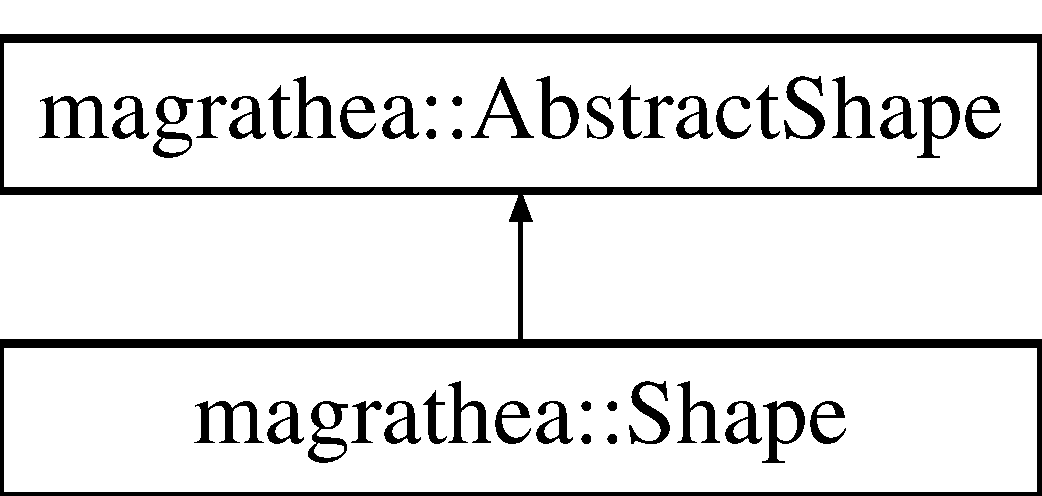
\includegraphics[height=2.000000cm]{exceptionmagrathea_1_1Shape}
\end{center}
\end{figure}
\subsection*{Static Public Member Functions}
\begin{Indent}{\bf Test}\par
\begin{DoxyCompactItemize}
\item 
static int \hyperlink{exceptionmagrathea_1_1Shape_a1531c87c37fc6c0ea10e524a7dacb87e}{example} ()
\begin{DoxyCompactList}\small\item\em Example function. \end{DoxyCompactList}\end{DoxyCompactItemize}
\end{Indent}
\subsection*{Additional Inherited Members}


\subsection{Detailed Description}
Basic implementation of shape. 

This class is the direct derivation of \hyperlink{classmagrathea_1_1AbstractShape}{Abstract\-Shape}. It provides the most basic and generic shape object without adding new functionalities to the abstract class. 

\subsection{Member Function Documentation}
\hypertarget{exceptionmagrathea_1_1Shape_a1531c87c37fc6c0ea10e524a7dacb87e}{\index{magrathea\-::\-Shape@{magrathea\-::\-Shape}!example@{example}}
\index{example@{example}!magrathea::Shape@{magrathea\-::\-Shape}}
\subsubsection[{example}]{\setlength{\rightskip}{0pt plus 5cm}int magrathea\-::\-Shape\-::example (
\begin{DoxyParamCaption}
{}
\end{DoxyParamCaption}
)\hspace{0.3cm}{\ttfamily [static]}}}\label{exceptionmagrathea_1_1Shape_a1531c87c37fc6c0ea10e524a7dacb87e}


Example function. 

Tests and demonstrates the use of \hyperlink{exceptionmagrathea_1_1Shape}{Shape}. \begin{DoxyReturn}{Returns}
0 if no error. 
\end{DoxyReturn}


The documentation for this exception was generated from the following file\-:\begin{DoxyCompactItemize}
\item 
/data/home/mbreton/magrathea\-\_\-pathfinder/src/magrathea/\hyperlink{shape_8h}{shape.\-h}\end{DoxyCompactItemize}

\hypertarget{exceptionmagrathea_1_1SimpleHyperOctree}{\section{magrathea\-:\-:Simple\-Hyper\-Octree$<$ Type, Index, Data, Dimension, Position, Extent, Element, Container $>$ Exception Template Reference}
\label{exceptionmagrathea_1_1SimpleHyperOctree}\index{magrathea\-::\-Simple\-Hyper\-Octree$<$ Type, Index, Data, Dimension, Position, Extent, Element, Container $>$@{magrathea\-::\-Simple\-Hyper\-Octree$<$ Type, Index, Data, Dimension, Position, Extent, Element, Container $>$}}
}


A simple hyperoctree based on bit manipulations.  




{\ttfamily \#include $<$simplehyperoctree.\-h$>$}

\subsection*{Public Member Functions}
\begin{Indent}{\bf Lifecycle}\par
\begin{DoxyCompactItemize}
\item 
\hyperlink{exceptionmagrathea_1_1SimpleHyperOctree_a3a4bd118969993ef5ca6bfb0855e0253}{Simple\-Hyper\-Octree} ()
\begin{DoxyCompactList}\small\item\em Implicit empty constructor. \end{DoxyCompactList}\item 
\hyperlink{exceptionmagrathea_1_1SimpleHyperOctree_a860d5400937cb0aab76ff88d320eecfc}{Simple\-Hyper\-Octree} (const unsigned int ilvl, const unsigned int nref=0)
\begin{DoxyCompactList}\small\item\em Explicit level constructor. \end{DoxyCompactList}\end{DoxyCompactItemize}
\end{Indent}
\begin{Indent}{\bf Operators}\par
\begin{DoxyCompactItemize}
\item 
bool \hyperlink{exceptionmagrathea_1_1SimpleHyperOctree_a27db33e24489e304260fcbf7f2b611db}{operator==} (const \hyperlink{exceptionmagrathea_1_1SimpleHyperOctree}{Simple\-Hyper\-Octree}$<$ Type, Index, Data, Dimension, Position, Extent, Element, Container $>$ \&rhs) const 
\begin{DoxyCompactList}\small\item\em Equal to. \end{DoxyCompactList}\item 
bool \hyperlink{exceptionmagrathea_1_1SimpleHyperOctree_aa5188e6834212f3af00aaa4356af340a}{operator!=} (const \hyperlink{exceptionmagrathea_1_1SimpleHyperOctree}{Simple\-Hyper\-Octree}$<$ Type, Index, Data, Dimension, Position, Extent, Element, Container $>$ \&rhs) const 
\begin{DoxyCompactList}\small\item\em Not equal to. \end{DoxyCompactList}\item 
Element \& \hyperlink{exceptionmagrathea_1_1SimpleHyperOctree_acd9451336184134d932aeca43e65b114}{operator\mbox{[}$\,$\mbox{]}} (const unsigned long long int ielem)
\begin{DoxyCompactList}\small\item\em Element access operator. \end{DoxyCompactList}\item 
const Element \& \hyperlink{exceptionmagrathea_1_1SimpleHyperOctree_a4156fe14aca770ad2bd669604f1cf487}{operator\mbox{[}$\,$\mbox{]}} (const unsigned long long int ielem) const 
\begin{DoxyCompactList}\small\item\em Immutable element access operator. \end{DoxyCompactList}\item 
Container \& \hyperlink{exceptionmagrathea_1_1SimpleHyperOctree_aae309b8b0d1d991611e9c338f3779bdc}{operator()} ()
\begin{DoxyCompactList}\small\item\em Container access operator. \end{DoxyCompactList}\item 
const Container \& \hyperlink{exceptionmagrathea_1_1SimpleHyperOctree_a7aa2ae9007464b1c2a451c8ebd9e88c3}{operator()} () const 
\begin{DoxyCompactList}\small\item\em Immutable container access operator. \end{DoxyCompactList}\item 
Element \& \hyperlink{exceptionmagrathea_1_1SimpleHyperOctree_acd21a6ab68148d61143be3bd0cef9c73}{operator()} (const Index \&idx)
\begin{DoxyCompactList}\small\item\em Element access operator from hyperoctree index. \end{DoxyCompactList}\item 
const Element \& \hyperlink{exceptionmagrathea_1_1SimpleHyperOctree_a4a0cc7552a3ae390e84d28e57166b699}{operator()} (const Index \&idx) const 
\begin{DoxyCompactList}\small\item\em Immutable element access operator from hyperoctree index. \end{DoxyCompactList}\item 
{\footnotesize template$<$typename... Types, class  = typename std\-::enable\-\_\-if$<$(sizeof...(\-Types) != 0)$>$\-::type, class  = typename std\-::enable\-\_\-if$<$((std\-::is\-\_\-convertible$<$typename std\-::tuple\-\_\-element$<$0, std\-::tuple$<$typename std\-::remove\-\_\-cv$<$typename std\-::remove\-\_\-reference$<$\-Types$>$\-::type$>$\-::type...$>$ $>$\-::type, Type$>$\-::value) ? (sizeof...(\-Types) == Dimension) \-: (sizeof...(\-Types) == 1)) \&\& (!std\-::is\-\_\-same$<$typename std\-::tuple\-\_\-element$<$0, std\-::tuple$<$typename std\-::remove\-\_\-cv$<$typename std\-::remove\-\_\-reference$<$\-Types$>$\-::type$>$\-::type...$>$ $>$\-::type, Index$>$\-::value)$>$\-::type$>$ }\\Element \& \hyperlink{exceptionmagrathea_1_1SimpleHyperOctree_a54da7a09dc7fc70123a6ec24c670b8dd}{operator()} (Types \&\&...iposs)
\begin{DoxyCompactList}\small\item\em Element access operator from position. \end{DoxyCompactList}\item 
{\footnotesize template$<$typename... Types, class  = typename std\-::enable\-\_\-if$<$(sizeof...(\-Types) != 0)$>$\-::type, class  = typename std\-::enable\-\_\-if$<$((std\-::is\-\_\-convertible$<$typename std\-::tuple\-\_\-element$<$0, std\-::tuple$<$typename std\-::remove\-\_\-cv$<$typename std\-::remove\-\_\-reference$<$\-Types$>$\-::type$>$\-::type...$>$ $>$\-::type, Type$>$\-::value) ? (sizeof...(\-Types) == Dimension) \-: (sizeof...(\-Types) == 1)) \&\& (!std\-::is\-\_\-same$<$typename std\-::tuple\-\_\-element$<$0, std\-::tuple$<$typename std\-::remove\-\_\-cv$<$typename std\-::remove\-\_\-reference$<$\-Types$>$\-::type$>$\-::type...$>$ $>$\-::type, Index$>$\-::value)$>$\-::type$>$ }\\const Element \& \hyperlink{exceptionmagrathea_1_1SimpleHyperOctree_afda010767e52b1ecda984476418a01fd}{operator()} (Types \&\&...iposs) const 
\begin{DoxyCompactList}\small\item\em Immutable element access operator from position. \end{DoxyCompactList}\end{DoxyCompactItemize}
\end{Indent}
\begin{Indent}{\bf Assignment}\par
\begin{DoxyCompactItemize}
\item 
\hyperlink{exceptionmagrathea_1_1SimpleHyperOctree}{Simple\-Hyper\-Octree}$<$ Type, Index, \\*
Data, Dimension, Position, \\*
Extent, Element, Container $>$ \& \hyperlink{exceptionmagrathea_1_1SimpleHyperOctree_aa99a071b51d94bf216f76631ad7cfdff}{assign} ()
\begin{DoxyCompactList}\small\item\em Empty assignment. \end{DoxyCompactList}\item 
\hyperlink{exceptionmagrathea_1_1SimpleHyperOctree}{Simple\-Hyper\-Octree}$<$ Type, Index, \\*
Data, Dimension, Position, \\*
Extent, Element, Container $>$ \& \hyperlink{exceptionmagrathea_1_1SimpleHyperOctree_a6ceffc4e7bade3b767fcdcfc880a91ee}{assign} (const unsigned int ilvl, const unsigned int nref=0)
\begin{DoxyCompactList}\small\item\em Level assignment . \end{DoxyCompactList}\item 
\hyperlink{exceptionmagrathea_1_1SimpleHyperOctree}{Simple\-Hyper\-Octree}$<$ Type, Index, \\*
Data, Dimension, Position, \\*
Extent, Element, Container $>$ \& \hyperlink{exceptionmagrathea_1_1SimpleHyperOctree_a6f47eaa173fd21cb6c6543e5ea894c26}{assign} (const \hyperlink{exceptionmagrathea_1_1SimpleHyperOctree}{Simple\-Hyper\-Octree}$<$ Type, Index, Data, Dimension, Position, Extent, Element, Container $>$ \&source)
\begin{DoxyCompactList}\small\item\em Copy assignment . \end{DoxyCompactList}\end{DoxyCompactItemize}
\end{Indent}
\begin{Indent}{\bf Management}\par
\begin{DoxyCompactItemize}
\item 
\hyperlink{exceptionmagrathea_1_1SimpleHyperOctree}{Simple\-Hyper\-Octree}$<$ Type, Index, \\*
Data, Dimension, Position, \\*
Extent, Element, Container $>$ \& \hyperlink{exceptionmagrathea_1_1SimpleHyperOctree_a4334e4b4f36159fc544eea4c81db686d}{nullify} ()
\begin{DoxyCompactList}\small\item\em Nullify. \end{DoxyCompactList}\item 
\hyperlink{exceptionmagrathea_1_1SimpleHyperOctree}{Simple\-Hyper\-Octree}$<$ Type, Index, \\*
Data, Dimension, Position, \\*
Extent, Element, Container $>$ \hyperlink{exceptionmagrathea_1_1SimpleHyperOctree_a84149cd7e224b0e1d1ff3977fa2b11d3}{copy} () const 
\begin{DoxyCompactList}\small\item\em Copy. \end{DoxyCompactList}\item 
{\footnotesize template$<$class Template  = Simple\-Hyper\-Octree$<$\-Type, Index, Data, Dimension, Position, Extent, Element, Container$>$, class  = typename std\-::enable\-\_\-if$<$std\-::is\-\_\-constructible$<$\-Template, Simple\-Hyper\-Octree$<$\-Type, Index, Data, Dimension, Position, Extent, Element, Container$>$ $>$\-::value$>$\-::type$>$ }\\Template \hyperlink{exceptionmagrathea_1_1SimpleHyperOctree_a96bb74baaceebc3244ecbe66746a52c9}{cast} () const 
\begin{DoxyCompactList}\small\item\em Cast. \end{DoxyCompactList}\end{DoxyCompactItemize}
\end{Indent}
\begin{Indent}{\bf Access}\par
\begin{DoxyCompactItemize}
\item 
Element \& \hyperlink{exceptionmagrathea_1_1SimpleHyperOctree_a34381e2085393ef475dcf66e180063c5}{at} (const unsigned long long int ielem)
\begin{DoxyCompactList}\small\item\em Access to an element with range-\/check. \end{DoxyCompactList}\item 
const Element \& \hyperlink{exceptionmagrathea_1_1SimpleHyperOctree_a4e2885288b4f881a1b1e527ddbda5d97}{at} (const unsigned long long int ielem) const 
\begin{DoxyCompactList}\small\item\em Immutable access to an element with range-\/check. \end{DoxyCompactList}\item 
Element \& \hyperlink{exceptionmagrathea_1_1SimpleHyperOctree_a456af04feaea7a3de5e331bec0692c04}{front} (const unsigned long long int ielem=0)
\begin{DoxyCompactList}\small\item\em Access to the i-\/th element from the beginning. \end{DoxyCompactList}\item 
const Element \& \hyperlink{exceptionmagrathea_1_1SimpleHyperOctree_a1fac5f615251f9ab11ab9532a3b7959a}{front} (const unsigned long long int ielem=0) const 
\begin{DoxyCompactList}\small\item\em Immutable access to the i-\/th element from the beginning. \end{DoxyCompactList}\item 
Element \& \hyperlink{exceptionmagrathea_1_1SimpleHyperOctree_a399a9ef8088f750ce1d86be811d14da1}{back} (const unsigned long long int ielem=0)
\begin{DoxyCompactList}\small\item\em Access to the i-\/th element from the end. \end{DoxyCompactList}\item 
const Element \& \hyperlink{exceptionmagrathea_1_1SimpleHyperOctree_acf867b94035502f8d1c233624ec2dcdf}{back} (const unsigned long long int ielem=0) const 
\begin{DoxyCompactList}\small\item\em Immutable access to the i-\/th element from the end. \end{DoxyCompactList}\item 
Element \& \hyperlink{exceptionmagrathea_1_1SimpleHyperOctree_a6360327d03825a0987169bc158aa84d3}{cycle} (const long long int ielem)
\begin{DoxyCompactList}\small\item\em Cyclic access to an element. \end{DoxyCompactList}\item 
const Element \& \hyperlink{exceptionmagrathea_1_1SimpleHyperOctree_a3782b956adfa8f040779b349793ef6a3}{cycle} (const long long int ielem) const 
\begin{DoxyCompactList}\small\item\em Immutable cyclic access to an element. \end{DoxyCompactList}\item 
Container \& \hyperlink{exceptionmagrathea_1_1SimpleHyperOctree_a7f551eab5578bfac28efc0d21969e69a}{container} ()
\begin{DoxyCompactList}\small\item\em Direct access to the underlying container. \end{DoxyCompactList}\item 
const Container \& \hyperlink{exceptionmagrathea_1_1SimpleHyperOctree_a3b5c5fc3d468cf84877ba97eb87f8e8d}{container} () const 
\begin{DoxyCompactList}\small\item\em Direct access to the underlying container. \end{DoxyCompactList}\item 
Element $\ast$ \hyperlink{exceptionmagrathea_1_1SimpleHyperOctree_ae71845a6920f404326fdf0e763df2a7e}{data} ()
\begin{DoxyCompactList}\small\item\em Direct access to the underlying array. \end{DoxyCompactList}\item 
const Element $\ast$ \hyperlink{exceptionmagrathea_1_1SimpleHyperOctree_a50f7a9684bc3defe77d76e5c98a871b5}{data} () const 
\begin{DoxyCompactList}\small\item\em Immutable direct access to the underlying array. \end{DoxyCompactList}\end{DoxyCompactItemize}
\end{Indent}
\begin{Indent}{\bf Iterators}\par
\begin{DoxyCompactItemize}
\item 
{\footnotesize template$<$typename Iterator  = decltype(std\-::declval$<$\-Container$>$().\-begin()), class  = typename std\-::enable\-\_\-if$<$std\-::is\-\_\-convertible$<$typename std\-::remove\-\_\-cv$<$typename std\-::remove\-\_\-reference$<$decltype($\ast$std\-::declval$<$\-Iterator$>$())$>$\-::type$>$\-::type, Element$>$\-::value$>$\-::type$>$ }\\Iterator \hyperlink{exceptionmagrathea_1_1SimpleHyperOctree_ad9be0e403527cf8c64d50ce27595800a}{begin} ()
\begin{DoxyCompactList}\small\item\em Iterator to the beginning. \end{DoxyCompactList}\item 
{\footnotesize template$<$typename Iterator  = decltype(std\-::declval$<$const Container$>$().\-begin()), class  = typename std\-::enable\-\_\-if$<$std\-::is\-\_\-convertible$<$typename std\-::remove\-\_\-cv$<$typename std\-::remove\-\_\-reference$<$decltype($\ast$std\-::declval$<$\-Iterator$>$())$>$\-::type$>$\-::type, Element$>$\-::value$>$\-::type$>$ }\\Iterator \hyperlink{exceptionmagrathea_1_1SimpleHyperOctree_a09485be0e49e3f98a39eb51997f297ee}{begin} () const 
\begin{DoxyCompactList}\small\item\em Immutable iterator to the beginning. \end{DoxyCompactList}\item 
{\footnotesize template$<$typename Iterator  = decltype(std\-::declval$<$\-Container$>$().\-cbegin()), class  = typename std\-::enable\-\_\-if$<$std\-::is\-\_\-convertible$<$typename std\-::remove\-\_\-cv$<$typename std\-::remove\-\_\-reference$<$decltype($\ast$std\-::declval$<$\-Iterator$>$())$>$\-::type$>$\-::type, Element$>$\-::value$>$\-::type$>$ }\\Iterator \hyperlink{exceptionmagrathea_1_1SimpleHyperOctree_a6aea97a026d32ccd56c38947ca0753d1}{cbegin} () const 
\begin{DoxyCompactList}\small\item\em Forced immutable iterator to the beginning. \end{DoxyCompactList}\item 
{\footnotesize template$<$typename Iterator  = decltype(std\-::declval$<$\-Container$>$().\-end()), class  = typename std\-::enable\-\_\-if$<$std\-::is\-\_\-convertible$<$typename std\-::remove\-\_\-cv$<$typename std\-::remove\-\_\-reference$<$decltype($\ast$std\-::declval$<$\-Iterator$>$())$>$\-::type$>$\-::type, Element$>$\-::value$>$\-::type$>$ }\\Iterator \hyperlink{exceptionmagrathea_1_1SimpleHyperOctree_a8ba63ec23ee998718633989748bb84db}{end} ()
\begin{DoxyCompactList}\small\item\em Iterator to the end. \end{DoxyCompactList}\item 
{\footnotesize template$<$typename Iterator  = decltype(std\-::declval$<$const Container$>$().\-end()), class  = typename std\-::enable\-\_\-if$<$std\-::is\-\_\-convertible$<$typename std\-::remove\-\_\-cv$<$typename std\-::remove\-\_\-reference$<$decltype($\ast$std\-::declval$<$\-Iterator$>$())$>$\-::type$>$\-::type, Element$>$\-::value$>$\-::type$>$ }\\Iterator \hyperlink{exceptionmagrathea_1_1SimpleHyperOctree_a24c5fa04c7e0d320c952bf1cad21f171}{end} () const 
\begin{DoxyCompactList}\small\item\em Immutable iterator to the end. \end{DoxyCompactList}\item 
{\footnotesize template$<$typename Iterator  = decltype(std\-::declval$<$\-Container$>$().\-cend()), class  = typename std\-::enable\-\_\-if$<$std\-::is\-\_\-convertible$<$typename std\-::remove\-\_\-cv$<$typename std\-::remove\-\_\-reference$<$decltype($\ast$std\-::declval$<$\-Iterator$>$())$>$\-::type$>$\-::type, Element$>$\-::value$>$\-::type$>$ }\\Iterator \hyperlink{exceptionmagrathea_1_1SimpleHyperOctree_ab051bb22f6d7fb70f41cf3e849339794}{cend} () const 
\begin{DoxyCompactList}\small\item\em Forced immutable iterator to the end. \end{DoxyCompactList}\item 
{\footnotesize template$<$typename Iterator  = decltype(std\-::declval$<$\-Container$>$().\-rbegin()), class  = typename std\-::enable\-\_\-if$<$std\-::is\-\_\-convertible$<$typename std\-::remove\-\_\-cv$<$typename std\-::remove\-\_\-reference$<$decltype($\ast$std\-::declval$<$\-Iterator$>$())$>$\-::type$>$\-::type, Element$>$\-::value$>$\-::type$>$ }\\Iterator \hyperlink{exceptionmagrathea_1_1SimpleHyperOctree_ae3fa6fce9d0041e0801cc5a82b0e3d84}{rbegin} ()
\begin{DoxyCompactList}\small\item\em Reverse iterator to the beginning. \end{DoxyCompactList}\item 
{\footnotesize template$<$typename Iterator  = decltype(std\-::declval$<$const Container$>$().\-rbegin()), class  = typename std\-::enable\-\_\-if$<$std\-::is\-\_\-convertible$<$typename std\-::remove\-\_\-cv$<$typename std\-::remove\-\_\-reference$<$decltype($\ast$std\-::declval$<$\-Iterator$>$())$>$\-::type$>$\-::type, Element$>$\-::value$>$\-::type$>$ }\\Iterator \hyperlink{exceptionmagrathea_1_1SimpleHyperOctree_a3d35fe1c15b6276a760fea1c60d0ecf5}{rbegin} () const 
\begin{DoxyCompactList}\small\item\em Immutable reverse iterator to the beginning. \end{DoxyCompactList}\item 
{\footnotesize template$<$typename Iterator  = decltype(std\-::declval$<$\-Container$>$().\-crbegin()), class  = typename std\-::enable\-\_\-if$<$std\-::is\-\_\-convertible$<$typename std\-::remove\-\_\-cv$<$typename std\-::remove\-\_\-reference$<$decltype($\ast$std\-::declval$<$\-Iterator$>$())$>$\-::type$>$\-::type, Element$>$\-::value$>$\-::type$>$ }\\Iterator \hyperlink{exceptionmagrathea_1_1SimpleHyperOctree_a958b80e21c579f61f842b23ee7a89490}{crbegin} () const 
\begin{DoxyCompactList}\small\item\em Forced immutable reverse iterator to the beginning. \end{DoxyCompactList}\item 
{\footnotesize template$<$typename Iterator  = decltype(std\-::declval$<$\-Container$>$().\-rend()), class  = typename std\-::enable\-\_\-if$<$std\-::is\-\_\-convertible$<$typename std\-::remove\-\_\-cv$<$typename std\-::remove\-\_\-reference$<$decltype($\ast$std\-::declval$<$\-Iterator$>$())$>$\-::type$>$\-::type, Element$>$\-::value$>$\-::type$>$ }\\Iterator \hyperlink{exceptionmagrathea_1_1SimpleHyperOctree_a6688705a3251d03ceedb097b116b1a59}{rend} ()
\begin{DoxyCompactList}\small\item\em Reverse iterator to the end. \end{DoxyCompactList}\item 
{\footnotesize template$<$typename Iterator  = decltype(std\-::declval$<$const Container$>$().\-rend()), class  = typename std\-::enable\-\_\-if$<$std\-::is\-\_\-convertible$<$typename std\-::remove\-\_\-cv$<$typename std\-::remove\-\_\-reference$<$decltype($\ast$std\-::declval$<$\-Iterator$>$())$>$\-::type$>$\-::type, Element$>$\-::value$>$\-::type$>$ }\\Iterator \hyperlink{exceptionmagrathea_1_1SimpleHyperOctree_abeb390e318ab59068a574c25ea015ed9}{rend} () const 
\begin{DoxyCompactList}\small\item\em Immutable reverse iterator to the end. \end{DoxyCompactList}\item 
{\footnotesize template$<$typename Iterator  = decltype(std\-::declval$<$\-Container$>$().\-crend()), class  = typename std\-::enable\-\_\-if$<$std\-::is\-\_\-convertible$<$typename std\-::remove\-\_\-cv$<$typename std\-::remove\-\_\-reference$<$decltype($\ast$std\-::declval$<$\-Iterator$>$())$>$\-::type$>$\-::type, Element$>$\-::value$>$\-::type$>$ }\\Iterator \hyperlink{exceptionmagrathea_1_1SimpleHyperOctree_a921c050126acad7787be98732772e188}{crend} () const 
\begin{DoxyCompactList}\small\item\em Forced immutable reverse iterator to the end. \end{DoxyCompactList}\item 
{\footnotesize template$<$typename Iterator , class  = typename std\-::enable\-\_\-if$<$std\-::is\-\_\-convertible$<$typename std\-::remove\-\_\-cv$<$typename std\-::remove\-\_\-reference$<$decltype($\ast$std\-::declval$<$\-Iterator$>$())$>$\-::type$>$\-::type, Element$>$\-::value$>$\-::type$>$ }\\unsigned long long int \hyperlink{exceptionmagrathea_1_1SimpleHyperOctree_a7d40a02e2e019d6110ed6151e4cb2d45}{index} (const Iterator \&it) const 
\begin{DoxyCompactList}\small\item\em Index of an iterator in the underlying container. \end{DoxyCompactList}\end{DoxyCompactItemize}
\end{Indent}
\begin{Indent}{\bf Search}\par
\begin{DoxyCompactItemize}
\item 
{\footnotesize template$<$typename Iterator  = decltype(std\-::declval$<$\-Container$>$().\-begin()), class  = typename std\-::enable\-\_\-if$<$std\-::is\-\_\-convertible$<$typename std\-::remove\-\_\-cv$<$typename std\-::remove\-\_\-reference$<$decltype($\ast$std\-::declval$<$\-Iterator$>$())$>$\-::type$>$\-::type, Element$>$\-::value$>$\-::type$>$ }\\Iterator \hyperlink{exceptionmagrathea_1_1SimpleHyperOctree_aef32efb6ad9bb1a1f0d9feb80adad5bf}{find} (const Index \&idx)
\item 
{\footnotesize template$<$typename Iterator  = decltype(std\-::declval$<$const Container$>$().\-begin()), class  = typename std\-::enable\-\_\-if$<$std\-::is\-\_\-convertible$<$typename std\-::remove\-\_\-cv$<$typename std\-::remove\-\_\-reference$<$decltype($\ast$std\-::declval$<$\-Iterator$>$())$>$\-::type$>$\-::type, Element$>$\-::value$>$\-::type$>$ }\\Iterator \hyperlink{exceptionmagrathea_1_1SimpleHyperOctree_a4a6f904c4455f49ca831bb4fbb24876d}{find} (const Index \&idx) const 
\item 
{\footnotesize template$<$typename Iterator  = decltype(std\-::declval$<$\-Container$>$().\-begin()), typename... Types, class  = typename std\-::enable\-\_\-if$<$(std\-::is\-\_\-convertible$<$typename std\-::remove\-\_\-cv$<$typename std\-::remove\-\_\-reference$<$decltype($\ast$std\-::declval$<$\-Iterator$>$())$>$\-::type$>$\-::type, Element$>$\-::value) \&\& ((std\-::is\-\_\-convertible$<$typename std\-::tuple\-\_\-element$<$0, std\-::tuple$<$typename std\-::remove\-\_\-cv$<$typename std\-::remove\-\_\-reference$<$\-Types$>$\-::type$>$\-::type...$>$ $>$\-::type, Type$>$\-::value) ? (sizeof...(\-Types) == Dimension) \-: (sizeof...(\-Types) == 1)) \&\& (!std\-::is\-\_\-same$<$typename std\-::tuple\-\_\-element$<$0, std\-::tuple$<$typename std\-::remove\-\_\-cv$<$typename std\-::remove\-\_\-reference$<$\-Types$>$\-::type$>$\-::type...$>$ $>$\-::type, Index$>$\-::value)$>$\-::type$>$ }\\Iterator \hyperlink{exceptionmagrathea_1_1SimpleHyperOctree_a415e4e9e542e3598cc99abcd2870a055}{locate} (Types \&\&...iposs)
\item 
{\footnotesize template$<$typename Iterator  = decltype(std\-::declval$<$const Container$>$().\-begin()), typename... Types, class  = typename std\-::enable\-\_\-if$<$(std\-::is\-\_\-convertible$<$typename std\-::remove\-\_\-cv$<$typename std\-::remove\-\_\-reference$<$decltype($\ast$std\-::declval$<$\-Iterator$>$())$>$\-::type$>$\-::type, Element$>$\-::value) \&\& ((std\-::is\-\_\-convertible$<$typename std\-::tuple\-\_\-element$<$0, std\-::tuple$<$typename std\-::remove\-\_\-cv$<$typename std\-::remove\-\_\-reference$<$\-Types$>$\-::type$>$\-::type...$>$ $>$\-::type, Type$>$\-::value) ? (sizeof...(\-Types) == Dimension) \-: (sizeof...(\-Types) == 1)) \&\& (!std\-::is\-\_\-same$<$typename std\-::tuple\-\_\-element$<$0, std\-::tuple$<$typename std\-::remove\-\_\-cv$<$typename std\-::remove\-\_\-reference$<$\-Types$>$\-::type$>$\-::type...$>$ $>$\-::type, Index$>$\-::value)$>$\-::type$>$ }\\Iterator \hyperlink{exceptionmagrathea_1_1SimpleHyperOctree_a773395c6154e9b955e01f543014514a5}{locate} (Types \&\&...iposs) const 
\end{DoxyCompactItemize}
\end{Indent}
\begin{Indent}{\bf Capacity}\par
\begin{DoxyCompactItemize}
\item 
bool \hyperlink{exceptionmagrathea_1_1SimpleHyperOctree_a5e81584ceb4d7dbca4a2acbce72bcddb}{empty} () const 
\begin{DoxyCompactList}\small\item\em Emptiness checking. \end{DoxyCompactList}\item 
unsigned long long int \hyperlink{exceptionmagrathea_1_1SimpleHyperOctree_aed410b8f317373c2e19049c7e4044457}{size} () const 
\begin{DoxyCompactList}\small\item\em Number of elements. \end{DoxyCompactList}\item 
unsigned long long int \hyperlink{exceptionmagrathea_1_1SimpleHyperOctree_ae365a47c69ea4874089f28b6dff2e41a}{capacity} () const 
\begin{DoxyCompactList}\small\item\em Capacity of the underlying storage. \end{DoxyCompactList}\item 
unsigned long long int \hyperlink{exceptionmagrathea_1_1SimpleHyperOctree_a915c72d92c4d5b455ae5ddfb60e04b75}{space} () const 
\begin{DoxyCompactList}\small\item\em Available space. \end{DoxyCompactList}\item 
\hyperlink{exceptionmagrathea_1_1SimpleHyperOctree}{Simple\-Hyper\-Octree}$<$ Type, Index, \\*
Data, Dimension, Position, \\*
Extent, Element, Container $>$ \& \hyperlink{exceptionmagrathea_1_1SimpleHyperOctree_a4e7da301e52d9d0b0202a111d4793ea7}{shrink} ()
\begin{DoxyCompactList}\small\item\em Shrink reserved storage. \end{DoxyCompactList}\item 
\hyperlink{exceptionmagrathea_1_1SimpleHyperOctree}{Simple\-Hyper\-Octree}$<$ Type, Index, \\*
Data, Dimension, Position, \\*
Extent, Element, Container $>$ \& \hyperlink{exceptionmagrathea_1_1SimpleHyperOctree_aa18774889493e6ca8abefc387fa6e5fd}{reserve} (const unsigned long long int nelem)
\begin{DoxyCompactList}\small\item\em Increase reserved storage. \end{DoxyCompactList}\end{DoxyCompactItemize}
\end{Indent}
\begin{Indent}{\bf Modifiers}\par
\begin{DoxyCompactItemize}
\item 
\hyperlink{exceptionmagrathea_1_1SimpleHyperOctree}{Simple\-Hyper\-Octree}$<$ Type, Index, \\*
Data, Dimension, Position, \\*
Extent, Element, Container $>$ \& \hyperlink{exceptionmagrathea_1_1SimpleHyperOctree_aad95f7803bc1260ec92a4caecdd7dc46}{fullclear} ()
\begin{DoxyCompactList}\small\item\em Full clear the content. \end{DoxyCompactList}\item 
\hyperlink{exceptionmagrathea_1_1SimpleHyperOctree}{Simple\-Hyper\-Octree}$<$ Type, Index, \\*
Data, Dimension, Position, \\*
Extent, Element, Container $>$ \& \hyperlink{exceptionmagrathea_1_1SimpleHyperOctree_a4442c66d922fb9ac4261b950f18d1330}{clear} ()
\begin{DoxyCompactList}\small\item\em Clear the contents. \end{DoxyCompactList}\item 
\hyperlink{exceptionmagrathea_1_1SimpleHyperOctree}{Simple\-Hyper\-Octree}$<$ Type, Index, \\*
Data, Dimension, Position, \\*
Extent, Element, Container $>$ \& \hyperlink{exceptionmagrathea_1_1SimpleHyperOctree_adc569fa304d13dfabf8ff6efc70ec9b4}{pop} ()
\begin{DoxyCompactList}\small\item\em Pop back. \end{DoxyCompactList}\item 
{\footnotesize template$<$class... Misc$>$ }\\\hyperlink{exceptionmagrathea_1_1SimpleHyperOctree}{Simple\-Hyper\-Octree}$<$ Type, Index, \\*
Data, Dimension, Position, \\*
Extent, Element, Container $>$ \& \hyperlink{exceptionmagrathea_1_1SimpleHyperOctree_ad6951c7477f9dc646ed7d8fc830e951e}{append} (Misc \&\&...misc)
\begin{DoxyCompactList}\small\item\em Append an element. \end{DoxyCompactList}\item 
{\footnotesize template$<$class... Misc$>$ }\\\hyperlink{exceptionmagrathea_1_1SimpleHyperOctree}{Simple\-Hyper\-Octree}$<$ Type, Index, \\*
Data, Dimension, Position, \\*
Extent, Element, Container $>$ \& \hyperlink{exceptionmagrathea_1_1SimpleHyperOctree_a8e4ffd2c97a91541f939b3b6a7703009}{resize} (Misc \&\&...misc)
\begin{DoxyCompactList}\small\item\em Resize. \end{DoxyCompactList}\item 
{\footnotesize template$<$unsigned int... Values, class... Misc, class Template , class $>$ }\\\hyperlink{exceptionmagrathea_1_1SimpleHyperOctree}{Simple\-Hyper\-Octree}$<$ Type, Index, \\*
Data, Dimension, Position, \\*
Extent, Element, Container $>$ \& \hyperlink{exceptionmagrathea_1_1SimpleHyperOctree_ae2bcdd2c733b4ffa96afc7c03adf4f74}{rho} (Misc \&\&...misc)
\begin{DoxyCompactList}\small\item\em Access to the rho data. \end{DoxyCompactList}\item 
{\footnotesize template$<$unsigned int... Values, class... Misc, class Template , class $>$ }\\\hyperlink{exceptionmagrathea_1_1SimpleHyperOctree}{Simple\-Hyper\-Octree}$<$ Type, Index, \\*
Data, Dimension, Position, \\*
Extent, Element, Container $>$ \& \hyperlink{exceptionmagrathea_1_1SimpleHyperOctree_af37baf544a5d39bccccac15b699a5c11}{rho} (Misc \&\&...misc) const 
\begin{DoxyCompactList}\small\item\em Access to the rho data. \end{DoxyCompactList}\item 
{\footnotesize template$<$unsigned int... Values, class... Misc, class Template , class $>$ }\\\hyperlink{exceptionmagrathea_1_1SimpleHyperOctree}{Simple\-Hyper\-Octree}$<$ Type, Index, \\*
Data, Dimension, Position, \\*
Extent, Element, Container $>$ \& \hyperlink{exceptionmagrathea_1_1SimpleHyperOctree_a55189b99964d0b2c46d517e12364b704}{phi} (Misc \&\&...misc)
\begin{DoxyCompactList}\small\item\em Access to the phi data. \end{DoxyCompactList}\item 
{\footnotesize template$<$unsigned int... Values, class... Misc, class Template , class $>$ }\\\hyperlink{exceptionmagrathea_1_1SimpleHyperOctree}{Simple\-Hyper\-Octree}$<$ Type, Index, \\*
Data, Dimension, Position, \\*
Extent, Element, Container $>$ \& \hyperlink{exceptionmagrathea_1_1SimpleHyperOctree_abf4fb49ec2a6f93966c12c8f31bfc5ed}{phi} (Misc \&\&...misc) const 
\begin{DoxyCompactList}\small\item\em Immutable access to the phi data. \end{DoxyCompactList}\item 
{\footnotesize template$<$unsigned int... Values, class... Misc, class Template , class $>$ }\\\hyperlink{exceptionmagrathea_1_1SimpleHyperOctree}{Simple\-Hyper\-Octree}$<$ Type, Index, \\*
Data, Dimension, Position, \\*
Extent, Element, Container $>$ \& \hyperlink{exceptionmagrathea_1_1SimpleHyperOctree_a4267d8f6aa4699ae060027a4f08c0fcc}{dphidxyz} (Misc \&\&...misc)
\begin{DoxyCompactList}\small\item\em Access to the dphidxyz data. \end{DoxyCompactList}\item 
{\footnotesize template$<$unsigned int... Values, class... Misc, class Template , class $>$ }\\\hyperlink{exceptionmagrathea_1_1SimpleHyperOctree}{Simple\-Hyper\-Octree}$<$ Type, Index, \\*
Data, Dimension, Position, \\*
Extent, Element, Container $>$ \& \hyperlink{exceptionmagrathea_1_1SimpleHyperOctree_a78599c42c748f305f926b2343345a8bb}{dphidxyz} (Misc \&\&...misc) const 
\begin{DoxyCompactList}\small\item\em Immutable access to the dphidxyz data. \end{DoxyCompactList}\item 
{\footnotesize template$<$unsigned int... Values, class... Misc, class Template , class $>$ }\\\hyperlink{exceptionmagrathea_1_1SimpleHyperOctree}{Simple\-Hyper\-Octree}$<$ Type, Index, \\*
Data, Dimension, Position, \\*
Extent, Element, Container $>$ \& \hyperlink{exceptionmagrathea_1_1SimpleHyperOctree_ab0fd3fa7b41742a7444efd82c04c03ff}{dphidx} (Misc \&\&...misc)
\begin{DoxyCompactList}\small\item\em Access to the dphidx data. \end{DoxyCompactList}\item 
{\footnotesize template$<$unsigned int... Values, class... Misc, class Template , class $>$ }\\\hyperlink{exceptionmagrathea_1_1SimpleHyperOctree}{Simple\-Hyper\-Octree}$<$ Type, Index, \\*
Data, Dimension, Position, \\*
Extent, Element, Container $>$ \& \hyperlink{exceptionmagrathea_1_1SimpleHyperOctree_a8dfa5ff5ff79e2df1eb055e24bb98c54}{dphidx} (Misc \&\&...misc) const 
\begin{DoxyCompactList}\small\item\em Immutable access to the dphidx data. \end{DoxyCompactList}\item 
{\footnotesize template$<$unsigned int... Values, class... Misc, class Template , class $>$ }\\\hyperlink{exceptionmagrathea_1_1SimpleHyperOctree}{Simple\-Hyper\-Octree}$<$ Type, Index, \\*
Data, Dimension, Position, \\*
Extent, Element, Container $>$ \& \hyperlink{exceptionmagrathea_1_1SimpleHyperOctree_a0be10e1a5d4219ae7245e6b5adccb756}{dphidy} (Misc \&\&...misc)
\begin{DoxyCompactList}\small\item\em Access to the dphidy data. \end{DoxyCompactList}\item 
{\footnotesize template$<$unsigned int... Values, class... Misc, class Template , class $>$ }\\\hyperlink{exceptionmagrathea_1_1SimpleHyperOctree}{Simple\-Hyper\-Octree}$<$ Type, Index, \\*
Data, Dimension, Position, \\*
Extent, Element, Container $>$ \& \hyperlink{exceptionmagrathea_1_1SimpleHyperOctree_a3620b24607d72f6766a42b531a15eebc}{dphidy} (Misc \&\&...misc) const 
\begin{DoxyCompactList}\small\item\em Immutable access to the dphidy data. \end{DoxyCompactList}\item 
{\footnotesize template$<$unsigned int... Values, class... Misc, class Template , class $>$ }\\\hyperlink{exceptionmagrathea_1_1SimpleHyperOctree}{Simple\-Hyper\-Octree}$<$ Type, Index, \\*
Data, Dimension, Position, \\*
Extent, Element, Container $>$ \& \hyperlink{exceptionmagrathea_1_1SimpleHyperOctree_a00496e0344462770db3a96e6425a20fd}{dphidz} (Misc \&\&...misc)
\begin{DoxyCompactList}\small\item\em Access to the dphidz data. \end{DoxyCompactList}\item 
{\footnotesize template$<$unsigned int... Values, class... Misc, class Template , class $>$ }\\\hyperlink{exceptionmagrathea_1_1SimpleHyperOctree}{Simple\-Hyper\-Octree}$<$ Type, Index, \\*
Data, Dimension, Position, \\*
Extent, Element, Container $>$ \& \hyperlink{exceptionmagrathea_1_1SimpleHyperOctree_af1abc2df7ed7128905f194c26e9de500}{dphidz} (Misc \&\&...misc) const 
\begin{DoxyCompactList}\small\item\em Immutable access to the dphidz data. \end{DoxyCompactList}\item 
{\footnotesize template$<$unsigned int... Values, class... Misc, class Template , class $>$ }\\\hyperlink{exceptionmagrathea_1_1SimpleHyperOctree}{Simple\-Hyper\-Octree}$<$ Type, Index, \\*
Data, Dimension, Position, \\*
Extent, Element, Container $>$ \& \hyperlink{exceptionmagrathea_1_1SimpleHyperOctree_a6347676c2f8a5939780b1dcedb48a7e4}{a} (Misc \&\&...misc)
\begin{DoxyCompactList}\small\item\em Access to the a data. \end{DoxyCompactList}\item 
{\footnotesize template$<$unsigned int... Values, class... Misc, class Template , class $>$ }\\\hyperlink{exceptionmagrathea_1_1SimpleHyperOctree}{Simple\-Hyper\-Octree}$<$ Type, Index, \\*
Data, Dimension, Position, \\*
Extent, Element, Container $>$ \& \hyperlink{exceptionmagrathea_1_1SimpleHyperOctree_a1f404f155309831822ab1a8585ff540a}{a} (Misc \&\&...misc) const 
\begin{DoxyCompactList}\small\item\em Immutable access to the a data. \end{DoxyCompactList}\end{DoxyCompactItemize}
\end{Indent}
\begin{Indent}{\bf Refinement}\par
\begin{DoxyCompactItemize}
\item 
\hyperlink{exceptionmagrathea_1_1SimpleHyperOctree}{Simple\-Hyper\-Octree}$<$ Type, Index, \\*
Data, Dimension, Position, \\*
Extent, Element, Container $>$ \& \hyperlink{exceptionmagrathea_1_1SimpleHyperOctree_a7e3fee5e84ba3546af3f48c1f95606e2}{update} ()
\begin{DoxyCompactList}\small\item\em Update refinement. \end{DoxyCompactList}\item 
{\footnotesize template$<$typename Iterator , class  = typename std\-::enable\-\_\-if$<$std\-::is\-\_\-convertible$<$typename std\-::remove\-\_\-cv$<$typename std\-::remove\-\_\-reference$<$decltype($\ast$std\-::declval$<$\-Iterator$>$())$>$\-::type$>$\-::type, Element$>$\-::value$>$\-::type$>$ }\\bool \hyperlink{exceptionmagrathea_1_1SimpleHyperOctree_aed9d244e291a647202e37c3c4ae8d741}{root} (const Iterator \&it)
\begin{DoxyCompactList}\small\item\em Root level. \end{DoxyCompactList}\item 
{\footnotesize template$<$typename Iterator , class  = typename std\-::enable\-\_\-if$<$std\-::is\-\_\-convertible$<$typename std\-::remove\-\_\-cv$<$typename std\-::remove\-\_\-reference$<$decltype($\ast$std\-::declval$<$\-Iterator$>$())$>$\-::type$>$\-::type, Element$>$\-::value$>$\-::type$>$ }\\bool \hyperlink{exceptionmagrathea_1_1SimpleHyperOctree_a0ccadf72b8ef56d94f3de046eb382e02}{leaf} (const Iterator \&it)
\begin{DoxyCompactList}\small\item\em Leaf level. \end{DoxyCompactList}\item 
{\footnotesize template$<$typename Iterator , class  = typename std\-::enable\-\_\-if$<$std\-::is\-\_\-convertible$<$typename std\-::remove\-\_\-cv$<$typename std\-::remove\-\_\-reference$<$decltype($\ast$std\-::declval$<$\-Iterator$>$())$>$\-::type$>$\-::type, Element$>$\-::value$>$\-::type$>$ }\\\hyperlink{exceptionmagrathea_1_1SimpleHyperOctree}{Simple\-Hyper\-Octree}$<$ Type, Index, \\*
Data, Dimension, Position, \\*
Extent, Element, Container $>$ \& \hyperlink{exceptionmagrathea_1_1SimpleHyperOctree_a5c599cb700f1bf683099b57fcef24686}{refine} (const Iterator \&it)
\begin{DoxyCompactList}\small\item\em Refine an element. \end{DoxyCompactList}\item 
{\footnotesize template$<$typename Iterator , class  = typename std\-::enable\-\_\-if$<$std\-::is\-\_\-convertible$<$typename std\-::remove\-\_\-cv$<$typename std\-::remove\-\_\-reference$<$decltype($\ast$std\-::declval$<$\-Iterator$>$())$>$\-::type$>$\-::type, Element$>$\-::value$>$\-::type$>$ }\\\hyperlink{exceptionmagrathea_1_1SimpleHyperOctree}{Simple\-Hyper\-Octree}$<$ Type, Index, \\*
Data, Dimension, Position, \\*
Extent, Element, Container $>$ \& \hyperlink{exceptionmagrathea_1_1SimpleHyperOctree_a2ac5a048e26ef111d3feab31c0053354}{coarsen} (const Iterator \&it)
\begin{DoxyCompactList}\small\item\em Coarsen an element. \end{DoxyCompactList}\end{DoxyCompactItemize}
\end{Indent}
\begin{Indent}{\bf Interpolation}\par
\begin{DoxyCompactItemize}
\item 
{\footnotesize template$<$typename... Types, class  = typename std\-::enable\-\_\-if$<$(sizeof...(\-Types) != 0)$>$\-::type, class  = typename std\-::enable\-\_\-if$<$((std\-::is\-\_\-convertible$<$typename std\-::tuple\-\_\-element$<$0, std\-::tuple$<$typename std\-::remove\-\_\-cv$<$typename std\-::remove\-\_\-reference$<$\-Types$>$\-::type$>$\-::type...$>$ $>$\-::type, Type$>$\-::value) ? (sizeof...(\-Types) == Dimension) \-: (sizeof...(\-Types) == 1)) \&\& (!std\-::is\-\_\-same$<$typename std\-::tuple\-\_\-element$<$0, std\-::tuple$<$typename std\-::remove\-\_\-cv$<$typename std\-::remove\-\_\-reference$<$\-Types$>$\-::type$>$\-::type...$>$ $>$\-::type, Index$>$\-::value)$>$\-::type$>$ }\\Data \hyperlink{exceptionmagrathea_1_1SimpleHyperOctree_aad15dc180a700eeed43ec708b570ddb2}{ngp} (Types \&\&...iposs) const 
\begin{DoxyCompactList}\small\item\em Nearest grid point interpolation. \end{DoxyCompactList}\item 
{\footnotesize template$<$typename... Types, class  = typename std\-::enable\-\_\-if$<$(sizeof...(\-Types) != 0)$>$\-::type, class  = typename std\-::enable\-\_\-if$<$((std\-::is\-\_\-convertible$<$typename std\-::tuple\-\_\-element$<$0, std\-::tuple$<$typename std\-::remove\-\_\-cv$<$typename std\-::remove\-\_\-reference$<$\-Types$>$\-::type$>$\-::type...$>$ $>$\-::type, Type$>$\-::value) ? (sizeof...(\-Types) == Dimension) \-: (sizeof...(\-Types) == 1)) \&\& (!std\-::is\-\_\-same$<$typename std\-::tuple\-\_\-element$<$0, std\-::tuple$<$typename std\-::remove\-\_\-cv$<$typename std\-::remove\-\_\-reference$<$\-Types$>$\-::type$>$\-::type...$>$ $>$\-::type, Index$>$\-::value)$>$\-::type$>$ }\\Data \hyperlink{exceptionmagrathea_1_1SimpleHyperOctree_ac436cd116bdd7103f30e733a3a377e07}{cic} (Types \&\&...iposs) const 
\begin{DoxyCompactList}\small\item\em Cloud in cell interpolation. \end{DoxyCompactList}\item 
{\footnotesize template$<$typename... Types, class  = typename std\-::enable\-\_\-if$<$(sizeof...(\-Types) != 0)$>$\-::type, class  = typename std\-::enable\-\_\-if$<$((std\-::is\-\_\-convertible$<$typename std\-::tuple\-\_\-element$<$0, std\-::tuple$<$typename std\-::remove\-\_\-cv$<$typename std\-::remove\-\_\-reference$<$\-Types$>$\-::type$>$\-::type...$>$ $>$\-::type, Type$>$\-::value) ? (sizeof...(\-Types) == Dimension) \-: (sizeof...(\-Types) == 1)) \&\& (!std\-::is\-\_\-same$<$typename std\-::tuple\-\_\-element$<$0, std\-::tuple$<$typename std\-::remove\-\_\-cv$<$typename std\-::remove\-\_\-reference$<$\-Types$>$\-::type$>$\-::type...$>$ $>$\-::type, Index$>$\-::value)$>$\-::type$>$ }\\Data \hyperlink{exceptionmagrathea_1_1SimpleHyperOctree_a9eb993e65160ca46268cce30f3caa5c0}{tsc} (Types \&\&...iposs) const 
\begin{DoxyCompactList}\small\item\em Triangular Shaped Cloud interpolation. \end{DoxyCompactList}\item 
{\footnotesize template$<$typename... Types, class  = typename std\-::enable\-\_\-if$<$(sizeof...(\-Types) != 0)$>$\-::type, class  = typename std\-::enable\-\_\-if$<$((std\-::is\-\_\-convertible$<$typename std\-::tuple\-\_\-element$<$0, std\-::tuple$<$typename std\-::remove\-\_\-cv$<$typename std\-::remove\-\_\-reference$<$\-Types$>$\-::type$>$\-::type...$>$ $>$\-::type, Type$>$\-::value) ? (sizeof...(\-Types) == Dimension) \-: (sizeof...(\-Types) == 1)) \&\& (!std\-::is\-\_\-same$<$typename std\-::tuple\-\_\-element$<$0, std\-::tuple$<$typename std\-::remove\-\_\-cv$<$typename std\-::remove\-\_\-reference$<$\-Types$>$\-::type$>$\-::type...$>$ $>$\-::type, Index$>$\-::value)$>$\-::type$>$ }\\Data \hyperlink{exceptionmagrathea_1_1SimpleHyperOctree_ab57456687e1ba820e3d314ddec489133}{tsc} (std\-::vector$<$ Element $>$ \&elems\-Tsc, Types \&\&...iposs) const 
\begin{DoxyCompactList}\small\item\em Triangular Shaped Cloud interpolation. \end{DoxyCompactList}\end{DoxyCompactItemize}
\end{Indent}
\subsection*{Static Public Member Functions}
\begin{Indent}{\bf Properties}\par
\begin{DoxyCompactItemize}
\item 
static constexpr Type \hyperlink{exceptionmagrathea_1_1SimpleHyperOctree_a6271ece62c25a4686aedecf0d237df7c}{type} ()
\begin{DoxyCompactList}\small\item\em Type. \end{DoxyCompactList}\item 
static constexpr Position \hyperlink{exceptionmagrathea_1_1SimpleHyperOctree_abe69b54c6a57c71a0b2af0a30027d1a4}{position} ()
\begin{DoxyCompactList}\small\item\em Position. \end{DoxyCompactList}\item 
static constexpr Extent \hyperlink{exceptionmagrathea_1_1SimpleHyperOctree_a626638d67638d26ba680c0452af7c868}{extent} ()
\begin{DoxyCompactList}\small\item\em Extent. \end{DoxyCompactList}\item 
static constexpr Element \hyperlink{exceptionmagrathea_1_1SimpleHyperOctree_aca02f6d7250f58d2da225a11d6a4c197}{element} ()
\begin{DoxyCompactList}\small\item\em Element. \end{DoxyCompactList}\item 
static constexpr unsigned int \hyperlink{exceptionmagrathea_1_1SimpleHyperOctree_a535549fd204b9327e91c853adf3b3750}{dimension} ()
\begin{DoxyCompactList}\small\item\em Number of dimensions. \end{DoxyCompactList}\end{DoxyCompactItemize}
\end{Indent}
\subsection*{Friends}
\begin{Indent}{\bf Stream}\par
\begin{DoxyCompactItemize}
\item 
{\footnotesize template$<$typename Self\-Type , class Self\-Index , class Self\-Data , unsigned int Self\-Dimension, class Self\-Position , class Self\-Extent , class Self\-Element , class Self\-Container $>$ }\\std\-::ostream \& \hyperlink{exceptionmagrathea_1_1SimpleHyperOctree_a79b6825c028327cb97bee79b3a61339b}{operator$<$$<$} (std\-::ostream \&lhs, const \hyperlink{exceptionmagrathea_1_1SimpleHyperOctree}{Simple\-Hyper\-Octree}$<$ Self\-Type, Self\-Index, Self\-Data, Self\-Dimension, Self\-Position, Self\-Extent, Self\-Element, Self\-Container $>$ \&rhs)
\begin{DoxyCompactList}\small\item\em \hyperlink{exceptionOutput}{Output} stream operator. \end{DoxyCompactList}\end{DoxyCompactItemize}
\end{Indent}


\subsection{Detailed Description}
\subsubsection*{template$<$typename Type = double, class Index = Simple\-Hyper\-Octree\-Index$<$unsigned long long int, 3$>$, class Data = double, unsigned int Dimension = Index\-::dimension(), class Position = std\-::ratio$<$0$>$, class Extent = std\-::ratio$<$1$>$, class Element = std\-::pair$<$\-Index, Data$>$, class Container = std\-::vector$<$\-Element$>$$>$exception magrathea\-::\-Simple\-Hyper\-Octree$<$ Type, Index, Data, Dimension, Position, Extent, Element, Container $>$}

A simple hyperoctree based on bit manipulations. 

Implementation of a simple and easy-\/to-\/use and hyperoctree structure in arbitrary dimension. It provides basic find and search algorithms based on indices relying on bit manipulations. 
\begin{DoxyTemplParams}{Template Parameters}
{\em Type} & Scalar position type. \\
\hline
{\em Index} & Index type. \\
\hline
{\em Data} & Data type. \\
\hline
{\em Dimension} & Number of dimensions. \\
\hline
{\em Position} & Position of the hyperoctree center. \\
\hline
{\em Extent} & Extent of the hyperoctree. \\
\hline
{\em Element} & Underlying element type. \\
\hline
{\em Container} & Underlying container type. \\
\hline
\end{DoxyTemplParams}


\subsection{Constructor \& Destructor Documentation}
\hypertarget{exceptionmagrathea_1_1SimpleHyperOctree_a3a4bd118969993ef5ca6bfb0855e0253}{\index{magrathea\-::\-Simple\-Hyper\-Octree@{magrathea\-::\-Simple\-Hyper\-Octree}!Simple\-Hyper\-Octree@{Simple\-Hyper\-Octree}}
\index{Simple\-Hyper\-Octree@{Simple\-Hyper\-Octree}!magrathea::SimpleHyperOctree@{magrathea\-::\-Simple\-Hyper\-Octree}}
\subsubsection[{Simple\-Hyper\-Octree}]{\setlength{\rightskip}{0pt plus 5cm}template$<$typename Type , class Index , class Data , unsigned int Dimension, class Position , class Extent , class Element , class Container $>$ {\bf magrathea\-::\-Simple\-Hyper\-Octree}$<$ Type, Index, Data, Dimension, Position, Extent, Element, Container $>$\-::{\bf Simple\-Hyper\-Octree} (
\begin{DoxyParamCaption}
{}
\end{DoxyParamCaption}
)\hspace{0.3cm}{\ttfamily [inline]}}}\label{exceptionmagrathea_1_1SimpleHyperOctree_a3a4bd118969993ef5ca6bfb0855e0253}


Implicit empty constructor. 

Provides an implicit construction of an empty hyperoctree. \hypertarget{exceptionmagrathea_1_1SimpleHyperOctree_a860d5400937cb0aab76ff88d320eecfc}{\index{magrathea\-::\-Simple\-Hyper\-Octree@{magrathea\-::\-Simple\-Hyper\-Octree}!Simple\-Hyper\-Octree@{Simple\-Hyper\-Octree}}
\index{Simple\-Hyper\-Octree@{Simple\-Hyper\-Octree}!magrathea::SimpleHyperOctree@{magrathea\-::\-Simple\-Hyper\-Octree}}
\subsubsection[{Simple\-Hyper\-Octree}]{\setlength{\rightskip}{0pt plus 5cm}template$<$typename Type , class Index , class Data , unsigned int Dimension, class Position , class Extent , class Element , class Container $>$ {\bf magrathea\-::\-Simple\-Hyper\-Octree}$<$ Type, Index, Data, Dimension, Position, Extent, Element, Container $>$\-::{\bf Simple\-Hyper\-Octree} (
\begin{DoxyParamCaption}
\item[{const unsigned int}]{ilvl, }
\item[{const unsigned int}]{nref = {\ttfamily 0}}
\end{DoxyParamCaption}
)\hspace{0.3cm}{\ttfamily [inline]}, {\ttfamily [explicit]}}}\label{exceptionmagrathea_1_1SimpleHyperOctree_a860d5400937cb0aab76ff88d320eecfc}


Explicit level constructor. 

Provides an explicit construction of a fixed mesh starting from the specified level and refining the provided amount of times. 
\begin{DoxyParams}[1]{Parameters}
\mbox{\tt in}  & {\em ilvl} & Index of the first level. \\
\hline
\mbox{\tt in}  & {\em nref} & Number of refinements of the first level. \\
\hline
\end{DoxyParams}


\subsection{Member Function Documentation}
\hypertarget{exceptionmagrathea_1_1SimpleHyperOctree_a6347676c2f8a5939780b1dcedb48a7e4}{\index{magrathea\-::\-Simple\-Hyper\-Octree@{magrathea\-::\-Simple\-Hyper\-Octree}!a@{a}}
\index{a@{a}!magrathea::SimpleHyperOctree@{magrathea\-::\-Simple\-Hyper\-Octree}}
\subsubsection[{a}]{\setlength{\rightskip}{0pt plus 5cm}template$<$typename Type , class Index , class Data , unsigned int Dimension, class Position , class Extent , class Element , class Container $>$ template$<$unsigned int... Values, class... Misc, class Template , class $>$ {\bf Simple\-Hyper\-Octree}$<$ Type, Index, Data, Dimension, Position, Extent, Element, Container $>$ \& {\bf magrathea\-::\-Simple\-Hyper\-Octree}$<$ Type, Index, Data, Dimension, Position, Extent, Element, Container $>$\-::a (
\begin{DoxyParamCaption}
\item[{Misc \&\&...}]{misc}
\end{DoxyParamCaption}
)\hspace{0.3cm}{\ttfamily [inline]}}}\label{exceptionmagrathea_1_1SimpleHyperOctree_a6347676c2f8a5939780b1dcedb48a7e4}


Access to the a data. 

Provides an access to the a data by forwarding parameters to the unified base accessor member. 
\begin{DoxyTemplParams}{Template Parameters}
{\em Values} & List of template values. \\
\hline
{\em Misc} & (\hyperlink{classMiscellaneous}{Miscellaneous} types.) \\
\hline
{\em Template} & (Deduced template type.) \\
\hline
\end{DoxyTemplParams}

\begin{DoxyParams}[1]{Parameters}
\mbox{\tt in}  & {\em misc} & \hyperlink{classMiscellaneous}{Miscellaneous} arguments. \\
\hline
\end{DoxyParams}
\begin{DoxyReturn}{Returns}
Forwarded result. 
\end{DoxyReturn}
\hypertarget{exceptionmagrathea_1_1SimpleHyperOctree_a1f404f155309831822ab1a8585ff540a}{\index{magrathea\-::\-Simple\-Hyper\-Octree@{magrathea\-::\-Simple\-Hyper\-Octree}!a@{a}}
\index{a@{a}!magrathea::SimpleHyperOctree@{magrathea\-::\-Simple\-Hyper\-Octree}}
\subsubsection[{a}]{\setlength{\rightskip}{0pt plus 5cm}template$<$typename Type , class Index , class Data , unsigned int Dimension, class Position , class Extent , class Element , class Container $>$ template$<$unsigned int... Values, class... Misc, class Template , class $>$ {\bf Simple\-Hyper\-Octree}$<$ Type, Index, Data, Dimension, Position, Extent, Element, Container $>$ \& {\bf magrathea\-::\-Simple\-Hyper\-Octree}$<$ Type, Index, Data, Dimension, Position, Extent, Element, Container $>$\-::a (
\begin{DoxyParamCaption}
\item[{Misc \&\&...}]{misc}
\end{DoxyParamCaption}
) const\hspace{0.3cm}{\ttfamily [inline]}}}\label{exceptionmagrathea_1_1SimpleHyperOctree_a1f404f155309831822ab1a8585ff540a}


Immutable access to the a data. 

Provides an access to the a data by forwarding parameters to the unified base accessor member. 
\begin{DoxyTemplParams}{Template Parameters}
{\em Values} & List of template values. \\
\hline
{\em Misc} & (\hyperlink{classMiscellaneous}{Miscellaneous} types.) \\
\hline
{\em Template} & (Deduced template type.) \\
\hline
\end{DoxyTemplParams}

\begin{DoxyParams}[1]{Parameters}
\mbox{\tt in}  & {\em misc} & \hyperlink{classMiscellaneous}{Miscellaneous} arguments. \\
\hline
\end{DoxyParams}
\begin{DoxyReturn}{Returns}
Forwarded result. 
\end{DoxyReturn}
\hypertarget{exceptionmagrathea_1_1SimpleHyperOctree_ad6951c7477f9dc646ed7d8fc830e951e}{\index{magrathea\-::\-Simple\-Hyper\-Octree@{magrathea\-::\-Simple\-Hyper\-Octree}!append@{append}}
\index{append@{append}!magrathea::SimpleHyperOctree@{magrathea\-::\-Simple\-Hyper\-Octree}}
\subsubsection[{append}]{\setlength{\rightskip}{0pt plus 5cm}template$<$typename Type , class Index , class Data , unsigned int Dimension, class Position , class Extent , class Element , class Container $>$ template$<$class... Misc$>$ {\bf Simple\-Hyper\-Octree}$<$ Type, Index, Data, Dimension, Position, Extent, Element, Container $>$ \& {\bf magrathea\-::\-Simple\-Hyper\-Octree}$<$ Type, Index, Data, Dimension, Position, Extent, Element, Container $>$\-::append (
\begin{DoxyParamCaption}
\item[{Misc \&\&...}]{misc}
\end{DoxyParamCaption}
)\hspace{0.3cm}{\ttfamily [inline]}}}\label{exceptionmagrathea_1_1SimpleHyperOctree_ad6951c7477f9dc646ed7d8fc830e951e}


Append an element. 

Appends an element by constructing it from the arguments and emplacing it at the end of the hyperoctree. 
\begin{DoxyTemplParams}{Template Parameters}
{\em Misc} & (\hyperlink{classMiscellaneous}{Miscellaneous} types.) \\
\hline
\end{DoxyTemplParams}

\begin{DoxyParams}[1]{Parameters}
\mbox{\tt in}  & {\em misc} & \hyperlink{classMiscellaneous}{Miscellaneous} arguments. \\
\hline
\end{DoxyParams}
\begin{DoxyReturn}{Returns}
Self reference. 
\end{DoxyReturn}
\hypertarget{exceptionmagrathea_1_1SimpleHyperOctree_aa99a071b51d94bf216f76631ad7cfdff}{\index{magrathea\-::\-Simple\-Hyper\-Octree@{magrathea\-::\-Simple\-Hyper\-Octree}!assign@{assign}}
\index{assign@{assign}!magrathea::SimpleHyperOctree@{magrathea\-::\-Simple\-Hyper\-Octree}}
\subsubsection[{assign}]{\setlength{\rightskip}{0pt plus 5cm}template$<$typename Type , class Index , class Data , unsigned int Dimension, class Position , class Extent , class Element , class Container $>$ {\bf Simple\-Hyper\-Octree}$<$ Type, Index, Data, Dimension, Position, Extent, Element, Container $>$ \& {\bf magrathea\-::\-Simple\-Hyper\-Octree}$<$ Type, Index, Data, Dimension, Position, Extent, Element, Container $>$\-::assign (
\begin{DoxyParamCaption}
{}
\end{DoxyParamCaption}
)\hspace{0.3cm}{\ttfamily [inline]}}}\label{exceptionmagrathea_1_1SimpleHyperOctree_aa99a071b51d94bf216f76631ad7cfdff}


Empty assignment. 

Provides an empty assignment of an empty hyperoctree. \begin{DoxyReturn}{Returns}
Self reference. 
\end{DoxyReturn}
\hypertarget{exceptionmagrathea_1_1SimpleHyperOctree_a6ceffc4e7bade3b767fcdcfc880a91ee}{\index{magrathea\-::\-Simple\-Hyper\-Octree@{magrathea\-::\-Simple\-Hyper\-Octree}!assign@{assign}}
\index{assign@{assign}!magrathea::SimpleHyperOctree@{magrathea\-::\-Simple\-Hyper\-Octree}}
\subsubsection[{assign}]{\setlength{\rightskip}{0pt plus 5cm}template$<$typename Type , class Index , class Data , unsigned int Dimension, class Position , class Extent , class Element , class Container $>$ {\bf Simple\-Hyper\-Octree}$<$ Type, Index, Data, Dimension, Position, Extent, Element, Container $>$ \& {\bf magrathea\-::\-Simple\-Hyper\-Octree}$<$ Type, Index, Data, Dimension, Position, Extent, Element, Container $>$\-::assign (
\begin{DoxyParamCaption}
\item[{const unsigned int}]{ilvl, }
\item[{const unsigned int}]{nref = {\ttfamily 0}}
\end{DoxyParamCaption}
)\hspace{0.3cm}{\ttfamily [inline]}}}\label{exceptionmagrathea_1_1SimpleHyperOctree_a6ceffc4e7bade3b767fcdcfc880a91ee}


Level assignment . 

Provides an assignment of a fixed mesh starting from the specified level and refining the provided amount of times. 
\begin{DoxyParams}[1]{Parameters}
\mbox{\tt in}  & {\em ilvl} & Index of the first level. \\
\hline
\mbox{\tt in}  & {\em nref} & Number of refinements of the first level. \\
\hline
\end{DoxyParams}
\begin{DoxyReturn}{Returns}
Self reference. 
\end{DoxyReturn}
\hypertarget{exceptionmagrathea_1_1SimpleHyperOctree_a6f47eaa173fd21cb6c6543e5ea894c26}{\index{magrathea\-::\-Simple\-Hyper\-Octree@{magrathea\-::\-Simple\-Hyper\-Octree}!assign@{assign}}
\index{assign@{assign}!magrathea::SimpleHyperOctree@{magrathea\-::\-Simple\-Hyper\-Octree}}
\subsubsection[{assign}]{\setlength{\rightskip}{0pt plus 5cm}template$<$typename Type , class Index , class Data , unsigned int Dimension, class Position , class Extent , class Element , class Container $>$ {\bf Simple\-Hyper\-Octree}$<$ Type, Index, Data, Dimension, Position, Extent, Element, Container $>$ \& {\bf magrathea\-::\-Simple\-Hyper\-Octree}$<$ Type, Index, Data, Dimension, Position, Extent, Element, Container $>$\-::assign (
\begin{DoxyParamCaption}
\item[{const {\bf Simple\-Hyper\-Octree}$<$ Type, Index, Data, Dimension, Position, Extent, Element, Container $>$ \&}]{source}
\end{DoxyParamCaption}
)\hspace{0.3cm}{\ttfamily [inline]}}}\label{exceptionmagrathea_1_1SimpleHyperOctree_a6f47eaa173fd21cb6c6543e5ea894c26}


Copy assignment . 

Provides a copy assignment from another hyperoctree. 
\begin{DoxyParams}[1]{Parameters}
\mbox{\tt in}  & {\em source} & Source of the copy. \\
\hline
\end{DoxyParams}
\begin{DoxyReturn}{Returns}
Self reference. 
\end{DoxyReturn}
\hypertarget{exceptionmagrathea_1_1SimpleHyperOctree_a34381e2085393ef475dcf66e180063c5}{\index{magrathea\-::\-Simple\-Hyper\-Octree@{magrathea\-::\-Simple\-Hyper\-Octree}!at@{at}}
\index{at@{at}!magrathea::SimpleHyperOctree@{magrathea\-::\-Simple\-Hyper\-Octree}}
\subsubsection[{at}]{\setlength{\rightskip}{0pt plus 5cm}template$<$typename Type , class Index , class Data , unsigned int Dimension, class Position , class Extent , class Element , class Container $>$ Element \& {\bf magrathea\-::\-Simple\-Hyper\-Octree}$<$ Type, Index, Data, Dimension, Position, Extent, Element, Container $>$\-::at (
\begin{DoxyParamCaption}
\item[{const unsigned long long int}]{ielem}
\end{DoxyParamCaption}
)\hspace{0.3cm}{\ttfamily [inline]}}}\label{exceptionmagrathea_1_1SimpleHyperOctree_a34381e2085393ef475dcf66e180063c5}


Access to an element with range-\/check. 

Provides an access to the specified element with a range-\/check. 
\begin{DoxyParams}[1]{Parameters}
\mbox{\tt in}  & {\em ielem} & Index of the element in the underlying container. \\
\hline
\end{DoxyParams}
\begin{DoxyReturn}{Returns}
Reference to the element. 
\end{DoxyReturn}
\hypertarget{exceptionmagrathea_1_1SimpleHyperOctree_a4e2885288b4f881a1b1e527ddbda5d97}{\index{magrathea\-::\-Simple\-Hyper\-Octree@{magrathea\-::\-Simple\-Hyper\-Octree}!at@{at}}
\index{at@{at}!magrathea::SimpleHyperOctree@{magrathea\-::\-Simple\-Hyper\-Octree}}
\subsubsection[{at}]{\setlength{\rightskip}{0pt plus 5cm}template$<$typename Type , class Index , class Data , unsigned int Dimension, class Position , class Extent , class Element , class Container $>$ const Element \& {\bf magrathea\-::\-Simple\-Hyper\-Octree}$<$ Type, Index, Data, Dimension, Position, Extent, Element, Container $>$\-::at (
\begin{DoxyParamCaption}
\item[{const unsigned long long int}]{ielem}
\end{DoxyParamCaption}
) const\hspace{0.3cm}{\ttfamily [inline]}}}\label{exceptionmagrathea_1_1SimpleHyperOctree_a4e2885288b4f881a1b1e527ddbda5d97}


Immutable access to an element with range-\/check. 

Provides an access to the specified element with a range-\/check. 
\begin{DoxyParams}[1]{Parameters}
\mbox{\tt in}  & {\em ielem} & Index of the element in the underlying container. \\
\hline
\end{DoxyParams}
\begin{DoxyReturn}{Returns}
Immutable reference to the element. 
\end{DoxyReturn}
\hypertarget{exceptionmagrathea_1_1SimpleHyperOctree_a399a9ef8088f750ce1d86be811d14da1}{\index{magrathea\-::\-Simple\-Hyper\-Octree@{magrathea\-::\-Simple\-Hyper\-Octree}!back@{back}}
\index{back@{back}!magrathea::SimpleHyperOctree@{magrathea\-::\-Simple\-Hyper\-Octree}}
\subsubsection[{back}]{\setlength{\rightskip}{0pt plus 5cm}template$<$typename Type , class Index , class Data , unsigned int Dimension, class Position , class Extent , class Element , class Container $>$ Element \& {\bf magrathea\-::\-Simple\-Hyper\-Octree}$<$ Type, Index, Data, Dimension, Position, Extent, Element, Container $>$\-::back (
\begin{DoxyParamCaption}
\item[{const unsigned long long int}]{ielem = {\ttfamily 0}}
\end{DoxyParamCaption}
)\hspace{0.3cm}{\ttfamily [inline]}}}\label{exceptionmagrathea_1_1SimpleHyperOctree_a399a9ef8088f750ce1d86be811d14da1}


Access to the i-\/th element from the end. 

Returns a reference to the i-\/th last element in the underlying container without doing any range check. 
\begin{DoxyParams}[1]{Parameters}
\mbox{\tt in}  & {\em ielem} & Index of the element in the underlying container. \\
\hline
\end{DoxyParams}
\begin{DoxyReturn}{Returns}
Reference to the element. 
\end{DoxyReturn}
\hypertarget{exceptionmagrathea_1_1SimpleHyperOctree_acf867b94035502f8d1c233624ec2dcdf}{\index{magrathea\-::\-Simple\-Hyper\-Octree@{magrathea\-::\-Simple\-Hyper\-Octree}!back@{back}}
\index{back@{back}!magrathea::SimpleHyperOctree@{magrathea\-::\-Simple\-Hyper\-Octree}}
\subsubsection[{back}]{\setlength{\rightskip}{0pt plus 5cm}template$<$typename Type , class Index , class Data , unsigned int Dimension, class Position , class Extent , class Element , class Container $>$ const Element \& {\bf magrathea\-::\-Simple\-Hyper\-Octree}$<$ Type, Index, Data, Dimension, Position, Extent, Element, Container $>$\-::back (
\begin{DoxyParamCaption}
\item[{const unsigned long long int}]{ielem = {\ttfamily 0}}
\end{DoxyParamCaption}
) const\hspace{0.3cm}{\ttfamily [inline]}}}\label{exceptionmagrathea_1_1SimpleHyperOctree_acf867b94035502f8d1c233624ec2dcdf}


Immutable access to the i-\/th element from the end. 

Returns a reference to the i-\/th last element in the underlying container without doing any range check. 
\begin{DoxyParams}[1]{Parameters}
\mbox{\tt in}  & {\em ielem} & Index of the element in the underlying container. \\
\hline
\end{DoxyParams}
\begin{DoxyReturn}{Returns}
Immutable reference to the element. 
\end{DoxyReturn}
\hypertarget{exceptionmagrathea_1_1SimpleHyperOctree_ad9be0e403527cf8c64d50ce27595800a}{\index{magrathea\-::\-Simple\-Hyper\-Octree@{magrathea\-::\-Simple\-Hyper\-Octree}!begin@{begin}}
\index{begin@{begin}!magrathea::SimpleHyperOctree@{magrathea\-::\-Simple\-Hyper\-Octree}}
\subsubsection[{begin}]{\setlength{\rightskip}{0pt plus 5cm}template$<$typename Type , class Index , class Data , unsigned int Dimension, class Position , class Extent , class Element , class Container $>$ template$<$typename Iterator , class $>$ Iterator {\bf magrathea\-::\-Simple\-Hyper\-Octree}$<$ Type, Index, Data, Dimension, Position, Extent, Element, Container $>$\-::begin (
\begin{DoxyParamCaption}
{}
\end{DoxyParamCaption}
)\hspace{0.3cm}{\ttfamily [inline]}}}\label{exceptionmagrathea_1_1SimpleHyperOctree_ad9be0e403527cf8c64d50ce27595800a}


Iterator to the beginning. 

Returns a pointer to the first element. 
\begin{DoxyTemplParams}{Template Parameters}
{\em Iterator} & (Iterator type.) \\
\hline
\end{DoxyTemplParams}
\begin{DoxyReturn}{Returns}
Pointer to the beginning. 
\end{DoxyReturn}
\hypertarget{exceptionmagrathea_1_1SimpleHyperOctree_a09485be0e49e3f98a39eb51997f297ee}{\index{magrathea\-::\-Simple\-Hyper\-Octree@{magrathea\-::\-Simple\-Hyper\-Octree}!begin@{begin}}
\index{begin@{begin}!magrathea::SimpleHyperOctree@{magrathea\-::\-Simple\-Hyper\-Octree}}
\subsubsection[{begin}]{\setlength{\rightskip}{0pt plus 5cm}template$<$typename Type , class Index , class Data , unsigned int Dimension, class Position , class Extent , class Element , class Container $>$ template$<$typename Iterator , class $>$ Iterator {\bf magrathea\-::\-Simple\-Hyper\-Octree}$<$ Type, Index, Data, Dimension, Position, Extent, Element, Container $>$\-::begin (
\begin{DoxyParamCaption}
{}
\end{DoxyParamCaption}
) const\hspace{0.3cm}{\ttfamily [inline]}}}\label{exceptionmagrathea_1_1SimpleHyperOctree_a09485be0e49e3f98a39eb51997f297ee}


Immutable iterator to the beginning. 

Returns a pointer to the first element. 
\begin{DoxyTemplParams}{Template Parameters}
{\em Iterator} & (Iterator type.) \\
\hline
\end{DoxyTemplParams}
\begin{DoxyReturn}{Returns}
Immutable pointer to the beginning. 
\end{DoxyReturn}
\hypertarget{exceptionmagrathea_1_1SimpleHyperOctree_ae365a47c69ea4874089f28b6dff2e41a}{\index{magrathea\-::\-Simple\-Hyper\-Octree@{magrathea\-::\-Simple\-Hyper\-Octree}!capacity@{capacity}}
\index{capacity@{capacity}!magrathea::SimpleHyperOctree@{magrathea\-::\-Simple\-Hyper\-Octree}}
\subsubsection[{capacity}]{\setlength{\rightskip}{0pt plus 5cm}template$<$typename Type , class Index , class Data , unsigned int Dimension, class Position , class Extent , class Element , class Container $>$ unsigned long long int {\bf magrathea\-::\-Simple\-Hyper\-Octree}$<$ Type, Index, Data, Dimension, Position, Extent, Element, Container $>$\-::capacity (
\begin{DoxyParamCaption}
{}
\end{DoxyParamCaption}
) const\hspace{0.3cm}{\ttfamily [inline]}}}\label{exceptionmagrathea_1_1SimpleHyperOctree_ae365a47c69ea4874089f28b6dff2e41a}


Capacity of the underlying storage. 

Returns the number of elements that the hyperoctree has currently allocated space for. \begin{DoxyReturn}{Returns}
Capacity of the currently allocated underlying storage. 
\end{DoxyReturn}
\hypertarget{exceptionmagrathea_1_1SimpleHyperOctree_a96bb74baaceebc3244ecbe66746a52c9}{\index{magrathea\-::\-Simple\-Hyper\-Octree@{magrathea\-::\-Simple\-Hyper\-Octree}!cast@{cast}}
\index{cast@{cast}!magrathea::SimpleHyperOctree@{magrathea\-::\-Simple\-Hyper\-Octree}}
\subsubsection[{cast}]{\setlength{\rightskip}{0pt plus 5cm}template$<$typename Type , class Index , class Data , unsigned int Dimension, class Position , class Extent , class Element , class Container $>$ template$<$class Template , class $>$ Template {\bf magrathea\-::\-Simple\-Hyper\-Octree}$<$ Type, Index, Data, Dimension, Position, Extent, Element, Container $>$\-::cast (
\begin{DoxyParamCaption}
{}
\end{DoxyParamCaption}
) const\hspace{0.3cm}{\ttfamily [inline]}}}\label{exceptionmagrathea_1_1SimpleHyperOctree_a96bb74baaceebc3244ecbe66746a52c9}


Cast. 

Casts contents to another object type. 
\begin{DoxyTemplParams}{Template Parameters}
{\em Template} & \hyperlink{exceptionOutput}{Output} type. \\
\hline
\end{DoxyTemplParams}
\begin{DoxyReturn}{Returns}
Casted copy. 
\end{DoxyReturn}
\hypertarget{exceptionmagrathea_1_1SimpleHyperOctree_a6aea97a026d32ccd56c38947ca0753d1}{\index{magrathea\-::\-Simple\-Hyper\-Octree@{magrathea\-::\-Simple\-Hyper\-Octree}!cbegin@{cbegin}}
\index{cbegin@{cbegin}!magrathea::SimpleHyperOctree@{magrathea\-::\-Simple\-Hyper\-Octree}}
\subsubsection[{cbegin}]{\setlength{\rightskip}{0pt plus 5cm}template$<$typename Type , class Index , class Data , unsigned int Dimension, class Position , class Extent , class Element , class Container $>$ template$<$typename Iterator , class $>$ Iterator {\bf magrathea\-::\-Simple\-Hyper\-Octree}$<$ Type, Index, Data, Dimension, Position, Extent, Element, Container $>$\-::cbegin (
\begin{DoxyParamCaption}
{}
\end{DoxyParamCaption}
) const\hspace{0.3cm}{\ttfamily [inline]}}}\label{exceptionmagrathea_1_1SimpleHyperOctree_a6aea97a026d32ccd56c38947ca0753d1}


Forced immutable iterator to the beginning. 

Returns a constant pointer to the first element. 
\begin{DoxyTemplParams}{Template Parameters}
{\em Iterator} & (Iterator type.) \\
\hline
\end{DoxyTemplParams}
\begin{DoxyReturn}{Returns}
Immutable pointer to the beginning. 
\end{DoxyReturn}
\hypertarget{exceptionmagrathea_1_1SimpleHyperOctree_ab051bb22f6d7fb70f41cf3e849339794}{\index{magrathea\-::\-Simple\-Hyper\-Octree@{magrathea\-::\-Simple\-Hyper\-Octree}!cend@{cend}}
\index{cend@{cend}!magrathea::SimpleHyperOctree@{magrathea\-::\-Simple\-Hyper\-Octree}}
\subsubsection[{cend}]{\setlength{\rightskip}{0pt plus 5cm}template$<$typename Type , class Index , class Data , unsigned int Dimension, class Position , class Extent , class Element , class Container $>$ template$<$typename Iterator , class $>$ Iterator {\bf magrathea\-::\-Simple\-Hyper\-Octree}$<$ Type, Index, Data, Dimension, Position, Extent, Element, Container $>$\-::cend (
\begin{DoxyParamCaption}
{}
\end{DoxyParamCaption}
) const\hspace{0.3cm}{\ttfamily [inline]}}}\label{exceptionmagrathea_1_1SimpleHyperOctree_ab051bb22f6d7fb70f41cf3e849339794}


Forced immutable iterator to the end. 

Returns a constant pointer to the position after the last element. 
\begin{DoxyTemplParams}{Template Parameters}
{\em Iterator} & (Iterator type.) \\
\hline
\end{DoxyTemplParams}
\begin{DoxyReturn}{Returns}
Immutable pointer to the end. 
\end{DoxyReturn}
\hypertarget{exceptionmagrathea_1_1SimpleHyperOctree_ac436cd116bdd7103f30e733a3a377e07}{\index{magrathea\-::\-Simple\-Hyper\-Octree@{magrathea\-::\-Simple\-Hyper\-Octree}!cic@{cic}}
\index{cic@{cic}!magrathea::SimpleHyperOctree@{magrathea\-::\-Simple\-Hyper\-Octree}}
\subsubsection[{cic}]{\setlength{\rightskip}{0pt plus 5cm}template$<$typename Type , class Index , class Data , unsigned int Dimension, class Position , class Extent , class Element , class Container $>$ template$<$typename... Types, class , class $>$ Data {\bf magrathea\-::\-Simple\-Hyper\-Octree}$<$ Type, Index, Data, Dimension, Position, Extent, Element, Container $>$\-::cic (
\begin{DoxyParamCaption}
\item[{Types \&\&...}]{iposs}
\end{DoxyParamCaption}
) const\hspace{0.3cm}{\ttfamily [inline]}}}\label{exceptionmagrathea_1_1SimpleHyperOctree_ac436cd116bdd7103f30e733a3a377e07}


Cloud in cell interpolation. 

Computes the value of the data at the provided position using a cloud in cell interpolation scheme. 
\begin{DoxyTemplParams}{Template Parameters}
{\em Types} & (Scalar position types.) \\
\hline
\end{DoxyTemplParams}

\begin{DoxyParams}[1]{Parameters}
\mbox{\tt in}  & {\em iposs} & Real positions along each dimension. \\
\hline
\end{DoxyParams}
\begin{DoxyReturn}{Returns}
Value of the data at the provided position. 
\end{DoxyReturn}
\hypertarget{exceptionmagrathea_1_1SimpleHyperOctree_a4442c66d922fb9ac4261b950f18d1330}{\index{magrathea\-::\-Simple\-Hyper\-Octree@{magrathea\-::\-Simple\-Hyper\-Octree}!clear@{clear}}
\index{clear@{clear}!magrathea::SimpleHyperOctree@{magrathea\-::\-Simple\-Hyper\-Octree}}
\subsubsection[{clear}]{\setlength{\rightskip}{0pt plus 5cm}template$<$typename Type , class Index , class Data , unsigned int Dimension, class Position , class Extent , class Element , class Container $>$ {\bf Simple\-Hyper\-Octree}$<$ Type, Index, Data, Dimension, Position, Extent, Element, Container $>$ \& {\bf magrathea\-::\-Simple\-Hyper\-Octree}$<$ Type, Index, Data, Dimension, Position, Extent, Element, Container $>$\-::clear (
\begin{DoxyParamCaption}
{}
\end{DoxyParamCaption}
)\hspace{0.3cm}{\ttfamily [inline]}}}\label{exceptionmagrathea_1_1SimpleHyperOctree_a4442c66d922fb9ac4261b950f18d1330}


Clear the contents. 

Removes all elements from the hyperoctree. \begin{DoxyReturn}{Returns}
Self reference. 
\end{DoxyReturn}
\hypertarget{exceptionmagrathea_1_1SimpleHyperOctree_a2ac5a048e26ef111d3feab31c0053354}{\index{magrathea\-::\-Simple\-Hyper\-Octree@{magrathea\-::\-Simple\-Hyper\-Octree}!coarsen@{coarsen}}
\index{coarsen@{coarsen}!magrathea::SimpleHyperOctree@{magrathea\-::\-Simple\-Hyper\-Octree}}
\subsubsection[{coarsen}]{\setlength{\rightskip}{0pt plus 5cm}template$<$typename Type , class Index , class Data , unsigned int Dimension, class Position , class Extent , class Element , class Container $>$ template$<$typename Iterator , class $>$ {\bf Simple\-Hyper\-Octree}$<$ Type, Index, Data, Dimension, Position, Extent, Element, Container $>$ \& {\bf magrathea\-::\-Simple\-Hyper\-Octree}$<$ Type, Index, Data, Dimension, Position, Extent, Element, Container $>$\-::coarsen (
\begin{DoxyParamCaption}
\item[{const Iterator \&}]{it}
\end{DoxyParamCaption}
)\hspace{0.3cm}{\ttfamily [inline]}}}\label{exceptionmagrathea_1_1SimpleHyperOctree_a2ac5a048e26ef111d3feab31c0053354}


Coarsen an element. 

Coarsens a given element by invalidating all the underlying children. To become valid again, the container should be updated. 
\begin{DoxyTemplParams}{Template Parameters}
{\em Iterator} & (Iterator type.) \\
\hline
\end{DoxyTemplParams}

\begin{DoxyParams}[1]{Parameters}
\mbox{\tt in}  & {\em it} & Iterator to an element. \\
\hline
\end{DoxyParams}
\begin{DoxyReturn}{Returns}
Self reference. 
\end{DoxyReturn}
\hypertarget{exceptionmagrathea_1_1SimpleHyperOctree_a7f551eab5578bfac28efc0d21969e69a}{\index{magrathea\-::\-Simple\-Hyper\-Octree@{magrathea\-::\-Simple\-Hyper\-Octree}!container@{container}}
\index{container@{container}!magrathea::SimpleHyperOctree@{magrathea\-::\-Simple\-Hyper\-Octree}}
\subsubsection[{container}]{\setlength{\rightskip}{0pt plus 5cm}template$<$typename Type , class Index , class Data , unsigned int Dimension, class Position , class Extent , class Element , class Container $>$ Container \& {\bf magrathea\-::\-Simple\-Hyper\-Octree}$<$ Type, Index, Data, Dimension, Position, Extent, Element, Container $>$\-::container (
\begin{DoxyParamCaption}
{}
\end{DoxyParamCaption}
)\hspace{0.3cm}{\ttfamily [inline]}}}\label{exceptionmagrathea_1_1SimpleHyperOctree_a7f551eab5578bfac28efc0d21969e69a}


Direct access to the underlying container. 

Provides a direct access to the underlying container by returning a reference to it. \begin{DoxyReturn}{Returns}
Reference to the underlying container. 
\end{DoxyReturn}
\hypertarget{exceptionmagrathea_1_1SimpleHyperOctree_a3b5c5fc3d468cf84877ba97eb87f8e8d}{\index{magrathea\-::\-Simple\-Hyper\-Octree@{magrathea\-::\-Simple\-Hyper\-Octree}!container@{container}}
\index{container@{container}!magrathea::SimpleHyperOctree@{magrathea\-::\-Simple\-Hyper\-Octree}}
\subsubsection[{container}]{\setlength{\rightskip}{0pt plus 5cm}template$<$typename Type , class Index , class Data , unsigned int Dimension, class Position , class Extent , class Element , class Container $>$ const Container \& {\bf magrathea\-::\-Simple\-Hyper\-Octree}$<$ Type, Index, Data, Dimension, Position, Extent, Element, Container $>$\-::container (
\begin{DoxyParamCaption}
{}
\end{DoxyParamCaption}
) const\hspace{0.3cm}{\ttfamily [inline]}}}\label{exceptionmagrathea_1_1SimpleHyperOctree_a3b5c5fc3d468cf84877ba97eb87f8e8d}


Direct access to the underlying container. 

Provides a direct access to the underlying container by returning a reference to it. \begin{DoxyReturn}{Returns}
Immutable reference to the underlying container. 
\end{DoxyReturn}
\hypertarget{exceptionmagrathea_1_1SimpleHyperOctree_a84149cd7e224b0e1d1ff3977fa2b11d3}{\index{magrathea\-::\-Simple\-Hyper\-Octree@{magrathea\-::\-Simple\-Hyper\-Octree}!copy@{copy}}
\index{copy@{copy}!magrathea::SimpleHyperOctree@{magrathea\-::\-Simple\-Hyper\-Octree}}
\subsubsection[{copy}]{\setlength{\rightskip}{0pt plus 5cm}template$<$typename Type , class Index , class Data , unsigned int Dimension, class Position , class Extent , class Element , class Container $>$ {\bf Simple\-Hyper\-Octree}$<$ Type, Index, Data, Dimension, Position, Extent, Element, Container $>$ {\bf magrathea\-::\-Simple\-Hyper\-Octree}$<$ Type, Index, Data, Dimension, Position, Extent, Element, Container $>$\-::copy (
\begin{DoxyParamCaption}
{}
\end{DoxyParamCaption}
) const\hspace{0.3cm}{\ttfamily [inline]}}}\label{exceptionmagrathea_1_1SimpleHyperOctree_a84149cd7e224b0e1d1ff3977fa2b11d3}


Copy. 

Generates a copy of the hyperoctree. \begin{DoxyReturn}{Returns}
Copy. 
\end{DoxyReturn}
\hypertarget{exceptionmagrathea_1_1SimpleHyperOctree_a958b80e21c579f61f842b23ee7a89490}{\index{magrathea\-::\-Simple\-Hyper\-Octree@{magrathea\-::\-Simple\-Hyper\-Octree}!crbegin@{crbegin}}
\index{crbegin@{crbegin}!magrathea::SimpleHyperOctree@{magrathea\-::\-Simple\-Hyper\-Octree}}
\subsubsection[{crbegin}]{\setlength{\rightskip}{0pt plus 5cm}template$<$typename Type , class Index , class Data , unsigned int Dimension, class Position , class Extent , class Element , class Container $>$ template$<$typename Iterator , class $>$ Iterator {\bf magrathea\-::\-Simple\-Hyper\-Octree}$<$ Type, Index, Data, Dimension, Position, Extent, Element, Container $>$\-::crbegin (
\begin{DoxyParamCaption}
{}
\end{DoxyParamCaption}
) const\hspace{0.3cm}{\ttfamily [inline]}}}\label{exceptionmagrathea_1_1SimpleHyperOctree_a958b80e21c579f61f842b23ee7a89490}


Forced immutable reverse iterator to the beginning. 

Returns a constant reversed pointer to the position after the last element. 
\begin{DoxyTemplParams}{Template Parameters}
{\em Iterator} & (Iterator type.) \\
\hline
\end{DoxyTemplParams}
\begin{DoxyReturn}{Returns}
Immutable pointer to the end. 
\end{DoxyReturn}
\hypertarget{exceptionmagrathea_1_1SimpleHyperOctree_a921c050126acad7787be98732772e188}{\index{magrathea\-::\-Simple\-Hyper\-Octree@{magrathea\-::\-Simple\-Hyper\-Octree}!crend@{crend}}
\index{crend@{crend}!magrathea::SimpleHyperOctree@{magrathea\-::\-Simple\-Hyper\-Octree}}
\subsubsection[{crend}]{\setlength{\rightskip}{0pt plus 5cm}template$<$typename Type , class Index , class Data , unsigned int Dimension, class Position , class Extent , class Element , class Container $>$ template$<$typename Iterator , class $>$ Iterator {\bf magrathea\-::\-Simple\-Hyper\-Octree}$<$ Type, Index, Data, Dimension, Position, Extent, Element, Container $>$\-::crend (
\begin{DoxyParamCaption}
{}
\end{DoxyParamCaption}
) const\hspace{0.3cm}{\ttfamily [inline]}}}\label{exceptionmagrathea_1_1SimpleHyperOctree_a921c050126acad7787be98732772e188}


Forced immutable reverse iterator to the end. 

Returns a constant reversed pointer to the first element. 
\begin{DoxyTemplParams}{Template Parameters}
{\em Iterator} & (Iterator type.) \\
\hline
\end{DoxyTemplParams}
\begin{DoxyReturn}{Returns}
Immutable pointer to the beginning. 
\end{DoxyReturn}
\hypertarget{exceptionmagrathea_1_1SimpleHyperOctree_a6360327d03825a0987169bc158aa84d3}{\index{magrathea\-::\-Simple\-Hyper\-Octree@{magrathea\-::\-Simple\-Hyper\-Octree}!cycle@{cycle}}
\index{cycle@{cycle}!magrathea::SimpleHyperOctree@{magrathea\-::\-Simple\-Hyper\-Octree}}
\subsubsection[{cycle}]{\setlength{\rightskip}{0pt plus 5cm}template$<$typename Type , class Index , class Data , unsigned int Dimension, class Position , class Extent , class Element , class Container $>$ Element \& {\bf magrathea\-::\-Simple\-Hyper\-Octree}$<$ Type, Index, Data, Dimension, Position, Extent, Element, Container $>$\-::cycle (
\begin{DoxyParamCaption}
\item[{const long long int}]{ielem}
\end{DoxyParamCaption}
)\hspace{0.3cm}{\ttfamily [inline]}}}\label{exceptionmagrathea_1_1SimpleHyperOctree_a6360327d03825a0987169bc158aa84d3}


Cyclic access to an element. 

Provides a cyclic access to the elements, using the index modulo. Negative indexes are supported. It allows to iterate several times over the contents just by incrementing the provided index. 
\begin{DoxyParams}[1]{Parameters}
\mbox{\tt in}  & {\em ielem} & Index of the element in the underlying container. \\
\hline
\end{DoxyParams}
\begin{DoxyReturn}{Returns}
Reference to the element. 
\end{DoxyReturn}
\hypertarget{exceptionmagrathea_1_1SimpleHyperOctree_a3782b956adfa8f040779b349793ef6a3}{\index{magrathea\-::\-Simple\-Hyper\-Octree@{magrathea\-::\-Simple\-Hyper\-Octree}!cycle@{cycle}}
\index{cycle@{cycle}!magrathea::SimpleHyperOctree@{magrathea\-::\-Simple\-Hyper\-Octree}}
\subsubsection[{cycle}]{\setlength{\rightskip}{0pt plus 5cm}template$<$typename Type , class Index , class Data , unsigned int Dimension, class Position , class Extent , class Element , class Container $>$ const Element \& {\bf magrathea\-::\-Simple\-Hyper\-Octree}$<$ Type, Index, Data, Dimension, Position, Extent, Element, Container $>$\-::cycle (
\begin{DoxyParamCaption}
\item[{const long long int}]{ielem}
\end{DoxyParamCaption}
) const\hspace{0.3cm}{\ttfamily [inline]}}}\label{exceptionmagrathea_1_1SimpleHyperOctree_a3782b956adfa8f040779b349793ef6a3}


Immutable cyclic access to an element. 

Provides a cyclic access to the elements, using the index modulo. Negative indexes are supported. It allows to iterate several times over the contents just by incrementing the provided index. 
\begin{DoxyParams}[1]{Parameters}
\mbox{\tt in}  & {\em ielem} & Index of the element in the underlying container. \\
\hline
\end{DoxyParams}
\begin{DoxyReturn}{Returns}
Immutable reference to the element. 
\end{DoxyReturn}
\hypertarget{exceptionmagrathea_1_1SimpleHyperOctree_ae71845a6920f404326fdf0e763df2a7e}{\index{magrathea\-::\-Simple\-Hyper\-Octree@{magrathea\-::\-Simple\-Hyper\-Octree}!data@{data}}
\index{data@{data}!magrathea::SimpleHyperOctree@{magrathea\-::\-Simple\-Hyper\-Octree}}
\subsubsection[{data}]{\setlength{\rightskip}{0pt plus 5cm}template$<$typename Type , class Index , class Data , unsigned int Dimension, class Position , class Extent , class Element , class Container $>$ Element $\ast$ {\bf magrathea\-::\-Simple\-Hyper\-Octree}$<$ Type, Index, Data, Dimension, Position, Extent, Element, Container $>$\-::data (
\begin{DoxyParamCaption}
{}
\end{DoxyParamCaption}
)\hspace{0.3cm}{\ttfamily [inline]}}}\label{exceptionmagrathea_1_1SimpleHyperOctree_ae71845a6920f404326fdf0e763df2a7e}


Direct access to the underlying array. 

Provides a direct access to the underlying array by returning a pointer to the first element of storage. \begin{DoxyReturn}{Returns}
Pointer to the underlying element storage. 
\end{DoxyReturn}
\hypertarget{exceptionmagrathea_1_1SimpleHyperOctree_a50f7a9684bc3defe77d76e5c98a871b5}{\index{magrathea\-::\-Simple\-Hyper\-Octree@{magrathea\-::\-Simple\-Hyper\-Octree}!data@{data}}
\index{data@{data}!magrathea::SimpleHyperOctree@{magrathea\-::\-Simple\-Hyper\-Octree}}
\subsubsection[{data}]{\setlength{\rightskip}{0pt plus 5cm}template$<$typename Type , class Index , class Data , unsigned int Dimension, class Position , class Extent , class Element , class Container $>$ const Element $\ast$ {\bf magrathea\-::\-Simple\-Hyper\-Octree}$<$ Type, Index, Data, Dimension, Position, Extent, Element, Container $>$\-::data (
\begin{DoxyParamCaption}
{}
\end{DoxyParamCaption}
) const\hspace{0.3cm}{\ttfamily [inline]}}}\label{exceptionmagrathea_1_1SimpleHyperOctree_a50f7a9684bc3defe77d76e5c98a871b5}


Immutable direct access to the underlying array. 

Provides a direct access to the underlying array by returning a pointer to the first element of storage. \begin{DoxyReturn}{Returns}
Immutable pointer to the underlying element storage. 
\end{DoxyReturn}
\hypertarget{exceptionmagrathea_1_1SimpleHyperOctree_a535549fd204b9327e91c853adf3b3750}{\index{magrathea\-::\-Simple\-Hyper\-Octree@{magrathea\-::\-Simple\-Hyper\-Octree}!dimension@{dimension}}
\index{dimension@{dimension}!magrathea::SimpleHyperOctree@{magrathea\-::\-Simple\-Hyper\-Octree}}
\subsubsection[{dimension}]{\setlength{\rightskip}{0pt plus 5cm}template$<$typename Type , class Index , class Data , unsigned int Dimension, class Position , class Extent , class Element , class Container $>$ constexpr unsigned int {\bf magrathea\-::\-Simple\-Hyper\-Octree}$<$ Type, Index, Data, Dimension, Position, Extent, Element, Container $>$\-::dimension (
\begin{DoxyParamCaption}
{}
\end{DoxyParamCaption}
)\hspace{0.3cm}{\ttfamily [static]}}}\label{exceptionmagrathea_1_1SimpleHyperOctree_a535549fd204b9327e91c853adf3b3750}


Number of dimensions. 

Returns the number of spatial dimensions. \begin{DoxyReturn}{Returns}
Copy of the number of dimensions. 
\end{DoxyReturn}
\hypertarget{exceptionmagrathea_1_1SimpleHyperOctree_ab0fd3fa7b41742a7444efd82c04c03ff}{\index{magrathea\-::\-Simple\-Hyper\-Octree@{magrathea\-::\-Simple\-Hyper\-Octree}!dphidx@{dphidx}}
\index{dphidx@{dphidx}!magrathea::SimpleHyperOctree@{magrathea\-::\-Simple\-Hyper\-Octree}}
\subsubsection[{dphidx}]{\setlength{\rightskip}{0pt plus 5cm}template$<$typename Type , class Index , class Data , unsigned int Dimension, class Position , class Extent , class Element , class Container $>$ template$<$unsigned int... Values, class... Misc, class Template , class $>$ {\bf Simple\-Hyper\-Octree}$<$ Type, Index, Data, Dimension, Position, Extent, Element, Container $>$ \& {\bf magrathea\-::\-Simple\-Hyper\-Octree}$<$ Type, Index, Data, Dimension, Position, Extent, Element, Container $>$\-::dphidx (
\begin{DoxyParamCaption}
\item[{Misc \&\&...}]{misc}
\end{DoxyParamCaption}
)\hspace{0.3cm}{\ttfamily [inline]}}}\label{exceptionmagrathea_1_1SimpleHyperOctree_ab0fd3fa7b41742a7444efd82c04c03ff}


Access to the dphidx data. 

Provides an access to the dphidx data by forwarding parameters to the unified base accessor member. 
\begin{DoxyTemplParams}{Template Parameters}
{\em Values} & List of template values. \\
\hline
{\em Misc} & (\hyperlink{classMiscellaneous}{Miscellaneous} types.) \\
\hline
{\em Template} & (Deduced template type.) \\
\hline
\end{DoxyTemplParams}

\begin{DoxyParams}[1]{Parameters}
\mbox{\tt in}  & {\em misc} & \hyperlink{classMiscellaneous}{Miscellaneous} arguments. \\
\hline
\end{DoxyParams}
\begin{DoxyReturn}{Returns}
Forwarded result. 
\end{DoxyReturn}
\hypertarget{exceptionmagrathea_1_1SimpleHyperOctree_a8dfa5ff5ff79e2df1eb055e24bb98c54}{\index{magrathea\-::\-Simple\-Hyper\-Octree@{magrathea\-::\-Simple\-Hyper\-Octree}!dphidx@{dphidx}}
\index{dphidx@{dphidx}!magrathea::SimpleHyperOctree@{magrathea\-::\-Simple\-Hyper\-Octree}}
\subsubsection[{dphidx}]{\setlength{\rightskip}{0pt plus 5cm}template$<$typename Type , class Index , class Data , unsigned int Dimension, class Position , class Extent , class Element , class Container $>$ template$<$unsigned int... Values, class... Misc, class Template , class $>$ {\bf Simple\-Hyper\-Octree}$<$ Type, Index, Data, Dimension, Position, Extent, Element, Container $>$ \& {\bf magrathea\-::\-Simple\-Hyper\-Octree}$<$ Type, Index, Data, Dimension, Position, Extent, Element, Container $>$\-::dphidx (
\begin{DoxyParamCaption}
\item[{Misc \&\&...}]{misc}
\end{DoxyParamCaption}
) const\hspace{0.3cm}{\ttfamily [inline]}}}\label{exceptionmagrathea_1_1SimpleHyperOctree_a8dfa5ff5ff79e2df1eb055e24bb98c54}


Immutable access to the dphidx data. 

Provides an access to the dphidx data by forwarding parameters to the unified base accessor member. 
\begin{DoxyTemplParams}{Template Parameters}
{\em Values} & List of template values. \\
\hline
{\em Misc} & (\hyperlink{classMiscellaneous}{Miscellaneous} types.) \\
\hline
{\em Template} & (Deduced template type.) \\
\hline
\end{DoxyTemplParams}

\begin{DoxyParams}[1]{Parameters}
\mbox{\tt in}  & {\em misc} & \hyperlink{classMiscellaneous}{Miscellaneous} arguments. \\
\hline
\end{DoxyParams}
\begin{DoxyReturn}{Returns}
Forwarded result. 
\end{DoxyReturn}
\hypertarget{exceptionmagrathea_1_1SimpleHyperOctree_a4267d8f6aa4699ae060027a4f08c0fcc}{\index{magrathea\-::\-Simple\-Hyper\-Octree@{magrathea\-::\-Simple\-Hyper\-Octree}!dphidxyz@{dphidxyz}}
\index{dphidxyz@{dphidxyz}!magrathea::SimpleHyperOctree@{magrathea\-::\-Simple\-Hyper\-Octree}}
\subsubsection[{dphidxyz}]{\setlength{\rightskip}{0pt plus 5cm}template$<$typename Type , class Index , class Data , unsigned int Dimension, class Position , class Extent , class Element , class Container $>$ template$<$unsigned int... Values, class... Misc, class Template , class $>$ {\bf Simple\-Hyper\-Octree}$<$ Type, Index, Data, Dimension, Position, Extent, Element, Container $>$ \& {\bf magrathea\-::\-Simple\-Hyper\-Octree}$<$ Type, Index, Data, Dimension, Position, Extent, Element, Container $>$\-::dphidxyz (
\begin{DoxyParamCaption}
\item[{Misc \&\&...}]{misc}
\end{DoxyParamCaption}
)\hspace{0.3cm}{\ttfamily [inline]}}}\label{exceptionmagrathea_1_1SimpleHyperOctree_a4267d8f6aa4699ae060027a4f08c0fcc}


Access to the dphidxyz data. 

Provides an access to the dphidxyz data by forwarding parameters to the unified base accessor member. 
\begin{DoxyTemplParams}{Template Parameters}
{\em Values} & List of template values. \\
\hline
{\em Misc} & (\hyperlink{classMiscellaneous}{Miscellaneous} types.) \\
\hline
{\em Template} & (Deduced template type.) \\
\hline
\end{DoxyTemplParams}

\begin{DoxyParams}[1]{Parameters}
\mbox{\tt in}  & {\em misc} & \hyperlink{classMiscellaneous}{Miscellaneous} arguments. \\
\hline
\end{DoxyParams}
\begin{DoxyReturn}{Returns}
Forwarded result. 
\end{DoxyReturn}
\hypertarget{exceptionmagrathea_1_1SimpleHyperOctree_a78599c42c748f305f926b2343345a8bb}{\index{magrathea\-::\-Simple\-Hyper\-Octree@{magrathea\-::\-Simple\-Hyper\-Octree}!dphidxyz@{dphidxyz}}
\index{dphidxyz@{dphidxyz}!magrathea::SimpleHyperOctree@{magrathea\-::\-Simple\-Hyper\-Octree}}
\subsubsection[{dphidxyz}]{\setlength{\rightskip}{0pt plus 5cm}template$<$typename Type , class Index , class Data , unsigned int Dimension, class Position , class Extent , class Element , class Container $>$ template$<$unsigned int... Values, class... Misc, class Template , class $>$ {\bf Simple\-Hyper\-Octree}$<$ Type, Index, Data, Dimension, Position, Extent, Element, Container $>$ \& {\bf magrathea\-::\-Simple\-Hyper\-Octree}$<$ Type, Index, Data, Dimension, Position, Extent, Element, Container $>$\-::dphidxyz (
\begin{DoxyParamCaption}
\item[{Misc \&\&...}]{misc}
\end{DoxyParamCaption}
) const\hspace{0.3cm}{\ttfamily [inline]}}}\label{exceptionmagrathea_1_1SimpleHyperOctree_a78599c42c748f305f926b2343345a8bb}


Immutable access to the dphidxyz data. 

Provides an access to the dphidxyz data by forwarding parameters to the unified base accessor member. 
\begin{DoxyTemplParams}{Template Parameters}
{\em Values} & List of template values. \\
\hline
{\em Misc} & (\hyperlink{classMiscellaneous}{Miscellaneous} types.) \\
\hline
{\em Template} & (Deduced template type.) \\
\hline
\end{DoxyTemplParams}

\begin{DoxyParams}[1]{Parameters}
\mbox{\tt in}  & {\em misc} & \hyperlink{classMiscellaneous}{Miscellaneous} arguments. \\
\hline
\end{DoxyParams}
\begin{DoxyReturn}{Returns}
Forwarded result. 
\end{DoxyReturn}
\hypertarget{exceptionmagrathea_1_1SimpleHyperOctree_a0be10e1a5d4219ae7245e6b5adccb756}{\index{magrathea\-::\-Simple\-Hyper\-Octree@{magrathea\-::\-Simple\-Hyper\-Octree}!dphidy@{dphidy}}
\index{dphidy@{dphidy}!magrathea::SimpleHyperOctree@{magrathea\-::\-Simple\-Hyper\-Octree}}
\subsubsection[{dphidy}]{\setlength{\rightskip}{0pt plus 5cm}template$<$typename Type , class Index , class Data , unsigned int Dimension, class Position , class Extent , class Element , class Container $>$ template$<$unsigned int... Values, class... Misc, class Template , class $>$ {\bf Simple\-Hyper\-Octree}$<$ Type, Index, Data, Dimension, Position, Extent, Element, Container $>$ \& {\bf magrathea\-::\-Simple\-Hyper\-Octree}$<$ Type, Index, Data, Dimension, Position, Extent, Element, Container $>$\-::dphidy (
\begin{DoxyParamCaption}
\item[{Misc \&\&...}]{misc}
\end{DoxyParamCaption}
)\hspace{0.3cm}{\ttfamily [inline]}}}\label{exceptionmagrathea_1_1SimpleHyperOctree_a0be10e1a5d4219ae7245e6b5adccb756}


Access to the dphidy data. 

Provides an access to the dphidy data by forwarding parameters to the unified base accessor member. 
\begin{DoxyTemplParams}{Template Parameters}
{\em Values} & List of template values. \\
\hline
{\em Misc} & (\hyperlink{classMiscellaneous}{Miscellaneous} types.) \\
\hline
{\em Template} & (Deduced template type.) \\
\hline
\end{DoxyTemplParams}

\begin{DoxyParams}[1]{Parameters}
\mbox{\tt in}  & {\em misc} & \hyperlink{classMiscellaneous}{Miscellaneous} arguments. \\
\hline
\end{DoxyParams}
\begin{DoxyReturn}{Returns}
Forwarded result. 
\end{DoxyReturn}
\hypertarget{exceptionmagrathea_1_1SimpleHyperOctree_a3620b24607d72f6766a42b531a15eebc}{\index{magrathea\-::\-Simple\-Hyper\-Octree@{magrathea\-::\-Simple\-Hyper\-Octree}!dphidy@{dphidy}}
\index{dphidy@{dphidy}!magrathea::SimpleHyperOctree@{magrathea\-::\-Simple\-Hyper\-Octree}}
\subsubsection[{dphidy}]{\setlength{\rightskip}{0pt plus 5cm}template$<$typename Type , class Index , class Data , unsigned int Dimension, class Position , class Extent , class Element , class Container $>$ template$<$unsigned int... Values, class... Misc, class Template , class $>$ {\bf Simple\-Hyper\-Octree}$<$ Type, Index, Data, Dimension, Position, Extent, Element, Container $>$ \& {\bf magrathea\-::\-Simple\-Hyper\-Octree}$<$ Type, Index, Data, Dimension, Position, Extent, Element, Container $>$\-::dphidy (
\begin{DoxyParamCaption}
\item[{Misc \&\&...}]{misc}
\end{DoxyParamCaption}
) const\hspace{0.3cm}{\ttfamily [inline]}}}\label{exceptionmagrathea_1_1SimpleHyperOctree_a3620b24607d72f6766a42b531a15eebc}


Immutable access to the dphidy data. 

Provides an access to the dphidy data by forwarding parameters to the unified base accessor member. 
\begin{DoxyTemplParams}{Template Parameters}
{\em Values} & List of template values. \\
\hline
{\em Misc} & (\hyperlink{classMiscellaneous}{Miscellaneous} types.) \\
\hline
{\em Template} & (Deduced template type.) \\
\hline
\end{DoxyTemplParams}

\begin{DoxyParams}[1]{Parameters}
\mbox{\tt in}  & {\em misc} & \hyperlink{classMiscellaneous}{Miscellaneous} arguments. \\
\hline
\end{DoxyParams}
\begin{DoxyReturn}{Returns}
Forwarded result. 
\end{DoxyReturn}
\hypertarget{exceptionmagrathea_1_1SimpleHyperOctree_a00496e0344462770db3a96e6425a20fd}{\index{magrathea\-::\-Simple\-Hyper\-Octree@{magrathea\-::\-Simple\-Hyper\-Octree}!dphidz@{dphidz}}
\index{dphidz@{dphidz}!magrathea::SimpleHyperOctree@{magrathea\-::\-Simple\-Hyper\-Octree}}
\subsubsection[{dphidz}]{\setlength{\rightskip}{0pt plus 5cm}template$<$typename Type , class Index , class Data , unsigned int Dimension, class Position , class Extent , class Element , class Container $>$ template$<$unsigned int... Values, class... Misc, class Template , class $>$ {\bf Simple\-Hyper\-Octree}$<$ Type, Index, Data, Dimension, Position, Extent, Element, Container $>$ \& {\bf magrathea\-::\-Simple\-Hyper\-Octree}$<$ Type, Index, Data, Dimension, Position, Extent, Element, Container $>$\-::dphidz (
\begin{DoxyParamCaption}
\item[{Misc \&\&...}]{misc}
\end{DoxyParamCaption}
)\hspace{0.3cm}{\ttfamily [inline]}}}\label{exceptionmagrathea_1_1SimpleHyperOctree_a00496e0344462770db3a96e6425a20fd}


Access to the dphidz data. 

Provides an access to the dphidz data by forwarding parameters to the unified base accessor member. 
\begin{DoxyTemplParams}{Template Parameters}
{\em Values} & List of template values. \\
\hline
{\em Misc} & (\hyperlink{classMiscellaneous}{Miscellaneous} types.) \\
\hline
{\em Template} & (Deduced template type.) \\
\hline
\end{DoxyTemplParams}

\begin{DoxyParams}[1]{Parameters}
\mbox{\tt in}  & {\em misc} & \hyperlink{classMiscellaneous}{Miscellaneous} arguments. \\
\hline
\end{DoxyParams}
\begin{DoxyReturn}{Returns}
Forwarded result. 
\end{DoxyReturn}
\hypertarget{exceptionmagrathea_1_1SimpleHyperOctree_af1abc2df7ed7128905f194c26e9de500}{\index{magrathea\-::\-Simple\-Hyper\-Octree@{magrathea\-::\-Simple\-Hyper\-Octree}!dphidz@{dphidz}}
\index{dphidz@{dphidz}!magrathea::SimpleHyperOctree@{magrathea\-::\-Simple\-Hyper\-Octree}}
\subsubsection[{dphidz}]{\setlength{\rightskip}{0pt plus 5cm}template$<$typename Type , class Index , class Data , unsigned int Dimension, class Position , class Extent , class Element , class Container $>$ template$<$unsigned int... Values, class... Misc, class Template , class $>$ {\bf Simple\-Hyper\-Octree}$<$ Type, Index, Data, Dimension, Position, Extent, Element, Container $>$ \& {\bf magrathea\-::\-Simple\-Hyper\-Octree}$<$ Type, Index, Data, Dimension, Position, Extent, Element, Container $>$\-::dphidz (
\begin{DoxyParamCaption}
\item[{Misc \&\&...}]{misc}
\end{DoxyParamCaption}
) const\hspace{0.3cm}{\ttfamily [inline]}}}\label{exceptionmagrathea_1_1SimpleHyperOctree_af1abc2df7ed7128905f194c26e9de500}


Immutable access to the dphidz data. 

Provides an access to the dphidz data by forwarding parameters to the unified base accessor member. 
\begin{DoxyTemplParams}{Template Parameters}
{\em Values} & List of template values. \\
\hline
{\em Misc} & (\hyperlink{classMiscellaneous}{Miscellaneous} types.) \\
\hline
{\em Template} & (Deduced template type.) \\
\hline
\end{DoxyTemplParams}

\begin{DoxyParams}[1]{Parameters}
\mbox{\tt in}  & {\em misc} & \hyperlink{classMiscellaneous}{Miscellaneous} arguments. \\
\hline
\end{DoxyParams}
\begin{DoxyReturn}{Returns}
Forwarded result. 
\end{DoxyReturn}
\hypertarget{exceptionmagrathea_1_1SimpleHyperOctree_aca02f6d7250f58d2da225a11d6a4c197}{\index{magrathea\-::\-Simple\-Hyper\-Octree@{magrathea\-::\-Simple\-Hyper\-Octree}!element@{element}}
\index{element@{element}!magrathea::SimpleHyperOctree@{magrathea\-::\-Simple\-Hyper\-Octree}}
\subsubsection[{element}]{\setlength{\rightskip}{0pt plus 5cm}template$<$typename Type , class Index , class Data , unsigned int Dimension, class Position , class Extent , class Element , class Container $>$ constexpr Element {\bf magrathea\-::\-Simple\-Hyper\-Octree}$<$ Type, Index, Data, Dimension, Position, Extent, Element, Container $>$\-::element (
\begin{DoxyParamCaption}
{}
\end{DoxyParamCaption}
)\hspace{0.3cm}{\ttfamily [static]}}}\label{exceptionmagrathea_1_1SimpleHyperOctree_aca02f6d7250f58d2da225a11d6a4c197}


Element. 

Returns a copy of the default element value. \begin{DoxyReturn}{Returns}
Copy of the default element value. 
\end{DoxyReturn}
\hypertarget{exceptionmagrathea_1_1SimpleHyperOctree_a5e81584ceb4d7dbca4a2acbce72bcddb}{\index{magrathea\-::\-Simple\-Hyper\-Octree@{magrathea\-::\-Simple\-Hyper\-Octree}!empty@{empty}}
\index{empty@{empty}!magrathea::SimpleHyperOctree@{magrathea\-::\-Simple\-Hyper\-Octree}}
\subsubsection[{empty}]{\setlength{\rightskip}{0pt plus 5cm}template$<$typename Type , class Index , class Data , unsigned int Dimension, class Position , class Extent , class Element , class Container $>$ bool {\bf magrathea\-::\-Simple\-Hyper\-Octree}$<$ Type, Index, Data, Dimension, Position, Extent, Element, Container $>$\-::empty (
\begin{DoxyParamCaption}
{}
\end{DoxyParamCaption}
) const\hspace{0.3cm}{\ttfamily [inline]}}}\label{exceptionmagrathea_1_1SimpleHyperOctree_a5e81584ceb4d7dbca4a2acbce72bcddb}


Emptiness checking. 

Checks if the hyperoctree has no elements. \begin{DoxyReturn}{Returns}
True if empty, false otherwise. 
\end{DoxyReturn}
\hypertarget{exceptionmagrathea_1_1SimpleHyperOctree_a8ba63ec23ee998718633989748bb84db}{\index{magrathea\-::\-Simple\-Hyper\-Octree@{magrathea\-::\-Simple\-Hyper\-Octree}!end@{end}}
\index{end@{end}!magrathea::SimpleHyperOctree@{magrathea\-::\-Simple\-Hyper\-Octree}}
\subsubsection[{end}]{\setlength{\rightskip}{0pt plus 5cm}template$<$typename Type , class Index , class Data , unsigned int Dimension, class Position , class Extent , class Element , class Container $>$ template$<$typename Iterator , class $>$ Iterator {\bf magrathea\-::\-Simple\-Hyper\-Octree}$<$ Type, Index, Data, Dimension, Position, Extent, Element, Container $>$\-::end (
\begin{DoxyParamCaption}
{}
\end{DoxyParamCaption}
)\hspace{0.3cm}{\ttfamily [inline]}}}\label{exceptionmagrathea_1_1SimpleHyperOctree_a8ba63ec23ee998718633989748bb84db}


Iterator to the end. 

Returns a pointer to the position after the last element. 
\begin{DoxyTemplParams}{Template Parameters}
{\em Iterator} & (Iterator type.) \\
\hline
\end{DoxyTemplParams}
\begin{DoxyReturn}{Returns}
Pointer to the end. 
\end{DoxyReturn}
\hypertarget{exceptionmagrathea_1_1SimpleHyperOctree_a24c5fa04c7e0d320c952bf1cad21f171}{\index{magrathea\-::\-Simple\-Hyper\-Octree@{magrathea\-::\-Simple\-Hyper\-Octree}!end@{end}}
\index{end@{end}!magrathea::SimpleHyperOctree@{magrathea\-::\-Simple\-Hyper\-Octree}}
\subsubsection[{end}]{\setlength{\rightskip}{0pt plus 5cm}template$<$typename Type , class Index , class Data , unsigned int Dimension, class Position , class Extent , class Element , class Container $>$ template$<$typename Iterator , class $>$ Iterator {\bf magrathea\-::\-Simple\-Hyper\-Octree}$<$ Type, Index, Data, Dimension, Position, Extent, Element, Container $>$\-::end (
\begin{DoxyParamCaption}
{}
\end{DoxyParamCaption}
) const\hspace{0.3cm}{\ttfamily [inline]}}}\label{exceptionmagrathea_1_1SimpleHyperOctree_a24c5fa04c7e0d320c952bf1cad21f171}


Immutable iterator to the end. 

Returns a pointer to the position after the last element. 
\begin{DoxyTemplParams}{Template Parameters}
{\em Iterator} & (Iterator type.) \\
\hline
\end{DoxyTemplParams}
\begin{DoxyReturn}{Returns}
Immutable pointer to the end. 
\end{DoxyReturn}
\hypertarget{exceptionmagrathea_1_1SimpleHyperOctree_a626638d67638d26ba680c0452af7c868}{\index{magrathea\-::\-Simple\-Hyper\-Octree@{magrathea\-::\-Simple\-Hyper\-Octree}!extent@{extent}}
\index{extent@{extent}!magrathea::SimpleHyperOctree@{magrathea\-::\-Simple\-Hyper\-Octree}}
\subsubsection[{extent}]{\setlength{\rightskip}{0pt plus 5cm}template$<$typename Type , class Index , class Data , unsigned int Dimension, class Position , class Extent , class Element , class Container $>$ constexpr Extent {\bf magrathea\-::\-Simple\-Hyper\-Octree}$<$ Type, Index, Data, Dimension, Position, Extent, Element, Container $>$\-::extent (
\begin{DoxyParamCaption}
{}
\end{DoxyParamCaption}
)\hspace{0.3cm}{\ttfamily [static]}}}\label{exceptionmagrathea_1_1SimpleHyperOctree_a626638d67638d26ba680c0452af7c868}


Extent. 

Returns a copy of the default extent value. \begin{DoxyReturn}{Returns}
Copy of the default extent value. 
\end{DoxyReturn}
\hypertarget{exceptionmagrathea_1_1SimpleHyperOctree_aef32efb6ad9bb1a1f0d9feb80adad5bf}{\index{magrathea\-::\-Simple\-Hyper\-Octree@{magrathea\-::\-Simple\-Hyper\-Octree}!find@{find}}
\index{find@{find}!magrathea::SimpleHyperOctree@{magrathea\-::\-Simple\-Hyper\-Octree}}
\subsubsection[{find}]{\setlength{\rightskip}{0pt plus 5cm}template$<$typename Type , class Index , class Data , unsigned int Dimension, class Position , class Extent , class Element , class Container $>$ template$<$typename Iterator , class $>$ Iterator {\bf magrathea\-::\-Simple\-Hyper\-Octree}$<$ Type, Index, Data, Dimension, Position, Extent, Element, Container $>$\-::find (
\begin{DoxyParamCaption}
\item[{const Index \&}]{idx}
\end{DoxyParamCaption}
)\hspace{0.3cm}{\ttfamily [inline]}}}\label{exceptionmagrathea_1_1SimpleHyperOctree_aef32efb6ad9bb1a1f0d9feb80adad5bf}
\hypertarget{exceptionmagrathea_1_1SimpleHyperOctree_a4a6f904c4455f49ca831bb4fbb24876d}{\index{magrathea\-::\-Simple\-Hyper\-Octree@{magrathea\-::\-Simple\-Hyper\-Octree}!find@{find}}
\index{find@{find}!magrathea::SimpleHyperOctree@{magrathea\-::\-Simple\-Hyper\-Octree}}
\subsubsection[{find}]{\setlength{\rightskip}{0pt plus 5cm}template$<$typename Type , class Index , class Data , unsigned int Dimension, class Position , class Extent , class Element , class Container $>$ template$<$typename Iterator , class $>$ Iterator {\bf magrathea\-::\-Simple\-Hyper\-Octree}$<$ Type, Index, Data, Dimension, Position, Extent, Element, Container $>$\-::find (
\begin{DoxyParamCaption}
\item[{const Index \&}]{idx}
\end{DoxyParamCaption}
) const\hspace{0.3cm}{\ttfamily [inline]}}}\label{exceptionmagrathea_1_1SimpleHyperOctree_a4a6f904c4455f49ca831bb4fbb24876d}
\hypertarget{exceptionmagrathea_1_1SimpleHyperOctree_a456af04feaea7a3de5e331bec0692c04}{\index{magrathea\-::\-Simple\-Hyper\-Octree@{magrathea\-::\-Simple\-Hyper\-Octree}!front@{front}}
\index{front@{front}!magrathea::SimpleHyperOctree@{magrathea\-::\-Simple\-Hyper\-Octree}}
\subsubsection[{front}]{\setlength{\rightskip}{0pt plus 5cm}template$<$typename Type , class Index , class Data , unsigned int Dimension, class Position , class Extent , class Element , class Container $>$ Element \& {\bf magrathea\-::\-Simple\-Hyper\-Octree}$<$ Type, Index, Data, Dimension, Position, Extent, Element, Container $>$\-::front (
\begin{DoxyParamCaption}
\item[{const unsigned long long int}]{ielem = {\ttfamily 0}}
\end{DoxyParamCaption}
)\hspace{0.3cm}{\ttfamily [inline]}}}\label{exceptionmagrathea_1_1SimpleHyperOctree_a456af04feaea7a3de5e331bec0692c04}


Access to the i-\/th element from the beginning. 

Returns a reference to the i-\/th first element in the underlying container without doing any range check. 
\begin{DoxyParams}[1]{Parameters}
\mbox{\tt in}  & {\em ielem} & Index of the element in the underlying container. \\
\hline
\end{DoxyParams}
\begin{DoxyReturn}{Returns}
Reference to the element. 
\end{DoxyReturn}
\hypertarget{exceptionmagrathea_1_1SimpleHyperOctree_a1fac5f615251f9ab11ab9532a3b7959a}{\index{magrathea\-::\-Simple\-Hyper\-Octree@{magrathea\-::\-Simple\-Hyper\-Octree}!front@{front}}
\index{front@{front}!magrathea::SimpleHyperOctree@{magrathea\-::\-Simple\-Hyper\-Octree}}
\subsubsection[{front}]{\setlength{\rightskip}{0pt plus 5cm}template$<$typename Type , class Index , class Data , unsigned int Dimension, class Position , class Extent , class Element , class Container $>$ const Element \& {\bf magrathea\-::\-Simple\-Hyper\-Octree}$<$ Type, Index, Data, Dimension, Position, Extent, Element, Container $>$\-::front (
\begin{DoxyParamCaption}
\item[{const unsigned long long int}]{ielem = {\ttfamily 0}}
\end{DoxyParamCaption}
) const\hspace{0.3cm}{\ttfamily [inline]}}}\label{exceptionmagrathea_1_1SimpleHyperOctree_a1fac5f615251f9ab11ab9532a3b7959a}


Immutable access to the i-\/th element from the beginning. 

Returns a reference to the i-\/th first element in the underlying container without doing any range check. 
\begin{DoxyParams}[1]{Parameters}
\mbox{\tt in}  & {\em ielem} & Index of the element in the underlying container. \\
\hline
\end{DoxyParams}
\begin{DoxyReturn}{Returns}
Immutable reference to the element. 
\end{DoxyReturn}
\hypertarget{exceptionmagrathea_1_1SimpleHyperOctree_aad95f7803bc1260ec92a4caecdd7dc46}{\index{magrathea\-::\-Simple\-Hyper\-Octree@{magrathea\-::\-Simple\-Hyper\-Octree}!fullclear@{fullclear}}
\index{fullclear@{fullclear}!magrathea::SimpleHyperOctree@{magrathea\-::\-Simple\-Hyper\-Octree}}
\subsubsection[{fullclear}]{\setlength{\rightskip}{0pt plus 5cm}template$<$typename Type , class Index , class Data , unsigned int Dimension, class Position , class Extent , class Element , class Container $>$ {\bf Simple\-Hyper\-Octree}$<$ Type, Index, Data, Dimension, Position, Extent, Element, Container $>$ \& {\bf magrathea\-::\-Simple\-Hyper\-Octree}$<$ Type, Index, Data, Dimension, Position, Extent, Element, Container $>$\-::fullclear (
\begin{DoxyParamCaption}
{}
\end{DoxyParamCaption}
)\hspace{0.3cm}{\ttfamily [inline]}}}\label{exceptionmagrathea_1_1SimpleHyperOctree_aad95f7803bc1260ec92a4caecdd7dc46}


Full clear the content. 

Erase the hyperoctree. \begin{DoxyReturn}{Returns}
Self reference. 
\end{DoxyReturn}
\hypertarget{exceptionmagrathea_1_1SimpleHyperOctree_a7d40a02e2e019d6110ed6151e4cb2d45}{\index{magrathea\-::\-Simple\-Hyper\-Octree@{magrathea\-::\-Simple\-Hyper\-Octree}!index@{index}}
\index{index@{index}!magrathea::SimpleHyperOctree@{magrathea\-::\-Simple\-Hyper\-Octree}}
\subsubsection[{index}]{\setlength{\rightskip}{0pt plus 5cm}template$<$typename Type , class Index , class Data , unsigned int Dimension, class Position , class Extent , class Element , class Container $>$ template$<$typename Iterator , class $>$ unsigned long long int {\bf magrathea\-::\-Simple\-Hyper\-Octree}$<$ Type, Index, Data, Dimension, Position, Extent, Element, Container $>$\-::index (
\begin{DoxyParamCaption}
\item[{const Iterator \&}]{it}
\end{DoxyParamCaption}
) const\hspace{0.3cm}{\ttfamily [inline]}}}\label{exceptionmagrathea_1_1SimpleHyperOctree_a7d40a02e2e019d6110ed6151e4cb2d45}


Index of an iterator in the underlying container. 

Returns the index of the element pointed by an iterator. 
\begin{DoxyTemplParams}{Template Parameters}
{\em Iterator} & (Iterator type.) \\
\hline
\end{DoxyTemplParams}

\begin{DoxyParams}[1]{Parameters}
\mbox{\tt in}  & {\em it} & Iterator to an element. \\
\hline
\end{DoxyParams}
\begin{DoxyReturn}{Returns}
Index of the element in the underlying container. 
\end{DoxyReturn}

\begin{DoxyExceptions}{Exceptions}
{\em std\-::out\-\_\-of\-\_\-range} & Out of range. \\
\hline
\end{DoxyExceptions}
\hypertarget{exceptionmagrathea_1_1SimpleHyperOctree_a0ccadf72b8ef56d94f3de046eb382e02}{\index{magrathea\-::\-Simple\-Hyper\-Octree@{magrathea\-::\-Simple\-Hyper\-Octree}!leaf@{leaf}}
\index{leaf@{leaf}!magrathea::SimpleHyperOctree@{magrathea\-::\-Simple\-Hyper\-Octree}}
\subsubsection[{leaf}]{\setlength{\rightskip}{0pt plus 5cm}template$<$typename Type , class Index , class Data , unsigned int Dimension, class Position , class Extent , class Element , class Container $>$ template$<$typename Iterator , class $>$ bool {\bf magrathea\-::\-Simple\-Hyper\-Octree}$<$ Type, Index, Data, Dimension, Position, Extent, Element, Container $>$\-::leaf (
\begin{DoxyParamCaption}
\item[{const Iterator \&}]{it}
\end{DoxyParamCaption}
)\hspace{0.3cm}{\ttfamily [inline]}}}\label{exceptionmagrathea_1_1SimpleHyperOctree_a0ccadf72b8ef56d94f3de046eb382e02}


Leaf level. 

Checks whether the given element corresponds to a leaf level. If the element does not have any child, it is considered at the leaf level. 
\begin{DoxyTemplParams}{Template Parameters}
{\em Iterator} & (Iterator type.) \\
\hline
\end{DoxyTemplParams}

\begin{DoxyParams}[1]{Parameters}
\mbox{\tt in}  & {\em it} & Iterator to an element. \\
\hline
\end{DoxyParams}
\begin{DoxyReturn}{Returns}
True if the element is not refined, false otherwise. 
\end{DoxyReturn}
\hypertarget{exceptionmagrathea_1_1SimpleHyperOctree_a415e4e9e542e3598cc99abcd2870a055}{\index{magrathea\-::\-Simple\-Hyper\-Octree@{magrathea\-::\-Simple\-Hyper\-Octree}!locate@{locate}}
\index{locate@{locate}!magrathea::SimpleHyperOctree@{magrathea\-::\-Simple\-Hyper\-Octree}}
\subsubsection[{locate}]{\setlength{\rightskip}{0pt plus 5cm}template$<$typename Type , class Index , class Data , unsigned int Dimension, class Position , class Extent , class Element , class Container $>$ template$<$typename Iterator , typename... Types, class $>$ Iterator {\bf magrathea\-::\-Simple\-Hyper\-Octree}$<$ Type, Index, Data, Dimension, Position, Extent, Element, Container $>$\-::locate (
\begin{DoxyParamCaption}
\item[{Types \&\&...}]{iposs}
\end{DoxyParamCaption}
)\hspace{0.3cm}{\ttfamily [inline]}}}\label{exceptionmagrathea_1_1SimpleHyperOctree_a415e4e9e542e3598cc99abcd2870a055}
\hypertarget{exceptionmagrathea_1_1SimpleHyperOctree_a773395c6154e9b955e01f543014514a5}{\index{magrathea\-::\-Simple\-Hyper\-Octree@{magrathea\-::\-Simple\-Hyper\-Octree}!locate@{locate}}
\index{locate@{locate}!magrathea::SimpleHyperOctree@{magrathea\-::\-Simple\-Hyper\-Octree}}
\subsubsection[{locate}]{\setlength{\rightskip}{0pt plus 5cm}template$<$typename Type , class Index , class Data , unsigned int Dimension, class Position , class Extent , class Element , class Container $>$ template$<$typename Iterator , typename... Types, class $>$ Iterator {\bf magrathea\-::\-Simple\-Hyper\-Octree}$<$ Type, Index, Data, Dimension, Position, Extent, Element, Container $>$\-::locate (
\begin{DoxyParamCaption}
\item[{Types \&\&...}]{iposs}
\end{DoxyParamCaption}
) const\hspace{0.3cm}{\ttfamily [inline]}}}\label{exceptionmagrathea_1_1SimpleHyperOctree_a773395c6154e9b955e01f543014514a5}
\hypertarget{exceptionmagrathea_1_1SimpleHyperOctree_aad15dc180a700eeed43ec708b570ddb2}{\index{magrathea\-::\-Simple\-Hyper\-Octree@{magrathea\-::\-Simple\-Hyper\-Octree}!ngp@{ngp}}
\index{ngp@{ngp}!magrathea::SimpleHyperOctree@{magrathea\-::\-Simple\-Hyper\-Octree}}
\subsubsection[{ngp}]{\setlength{\rightskip}{0pt plus 5cm}template$<$typename Type , class Index , class Data , unsigned int Dimension, class Position , class Extent , class Element , class Container $>$ template$<$typename... Types, class , class $>$ Data {\bf magrathea\-::\-Simple\-Hyper\-Octree}$<$ Type, Index, Data, Dimension, Position, Extent, Element, Container $>$\-::ngp (
\begin{DoxyParamCaption}
\item[{Types \&\&...}]{iposs}
\end{DoxyParamCaption}
) const\hspace{0.3cm}{\ttfamily [inline]}}}\label{exceptionmagrathea_1_1SimpleHyperOctree_aad15dc180a700eeed43ec708b570ddb2}


Nearest grid point interpolation. 

Computes the value of the data at the provided position using a nearest grid point interpolation scheme. 
\begin{DoxyTemplParams}{Template Parameters}
{\em Types} & (Scalar position types.) \\
\hline
\end{DoxyTemplParams}

\begin{DoxyParams}[1]{Parameters}
\mbox{\tt in}  & {\em iposs} & Real positions along each dimension. \\
\hline
\end{DoxyParams}
\begin{DoxyReturn}{Returns}
Value of the data at the provided position. 
\end{DoxyReturn}
\hypertarget{exceptionmagrathea_1_1SimpleHyperOctree_a4334e4b4f36159fc544eea4c81db686d}{\index{magrathea\-::\-Simple\-Hyper\-Octree@{magrathea\-::\-Simple\-Hyper\-Octree}!nullify@{nullify}}
\index{nullify@{nullify}!magrathea::SimpleHyperOctree@{magrathea\-::\-Simple\-Hyper\-Octree}}
\subsubsection[{nullify}]{\setlength{\rightskip}{0pt plus 5cm}template$<$typename Type , class Index , class Data , unsigned int Dimension, class Position , class Extent , class Element , class Container $>$ {\bf Simple\-Hyper\-Octree}$<$ Type, Index, Data, Dimension, Position, Extent, Element, Container $>$ \& {\bf magrathea\-::\-Simple\-Hyper\-Octree}$<$ Type, Index, Data, Dimension, Position, Extent, Element, Container $>$\-::nullify (
\begin{DoxyParamCaption}
{}
\end{DoxyParamCaption}
)\hspace{0.3cm}{\ttfamily [inline]}}}\label{exceptionmagrathea_1_1SimpleHyperOctree_a4334e4b4f36159fc544eea4c81db686d}


Nullify. 

Resets all data to their default values but keeping the same tree structure. \begin{DoxyReturn}{Returns}
Self reference. 
\end{DoxyReturn}
\hypertarget{exceptionmagrathea_1_1SimpleHyperOctree_aa5188e6834212f3af00aaa4356af340a}{\index{magrathea\-::\-Simple\-Hyper\-Octree@{magrathea\-::\-Simple\-Hyper\-Octree}!operator!=@{operator!=}}
\index{operator!=@{operator!=}!magrathea::SimpleHyperOctree@{magrathea\-::\-Simple\-Hyper\-Octree}}
\subsubsection[{operator!=}]{\setlength{\rightskip}{0pt plus 5cm}template$<$typename Type , class Index , class Data , unsigned int Dimension, class Position , class Extent , class Element , class Container $>$ bool {\bf magrathea\-::\-Simple\-Hyper\-Octree}$<$ Type, Index, Data, Dimension, Position, Extent, Element, Container $>$\-::operator!= (
\begin{DoxyParamCaption}
\item[{const {\bf Simple\-Hyper\-Octree}$<$ Type, Index, Data, Dimension, Position, Extent, Element, Container $>$ \&}]{rhs}
\end{DoxyParamCaption}
) const\hspace{0.3cm}{\ttfamily [inline]}}}\label{exceptionmagrathea_1_1SimpleHyperOctree_aa5188e6834212f3af00aaa4356af340a}


Not equal to. 

Compares the hyperoctrees for difference. 
\begin{DoxyParams}[1]{Parameters}
\mbox{\tt in}  & {\em rhs} & Right-\/hand side. \\
\hline
\end{DoxyParams}
\begin{DoxyReturn}{Returns}
True if not equal, false if equal. 
\end{DoxyReturn}
\hypertarget{exceptionmagrathea_1_1SimpleHyperOctree_aae309b8b0d1d991611e9c338f3779bdc}{\index{magrathea\-::\-Simple\-Hyper\-Octree@{magrathea\-::\-Simple\-Hyper\-Octree}!operator()@{operator()}}
\index{operator()@{operator()}!magrathea::SimpleHyperOctree@{magrathea\-::\-Simple\-Hyper\-Octree}}
\subsubsection[{operator()}]{\setlength{\rightskip}{0pt plus 5cm}template$<$typename Type , class Index , class Data , unsigned int Dimension, class Position , class Extent , class Element , class Container $>$ Container \& {\bf magrathea\-::\-Simple\-Hyper\-Octree}$<$ Type, Index, Data, Dimension, Position, Extent, Element, Container $>$\-::operator() (
\begin{DoxyParamCaption}
{}
\end{DoxyParamCaption}
)\hspace{0.3cm}{\ttfamily [inline]}}}\label{exceptionmagrathea_1_1SimpleHyperOctree_aae309b8b0d1d991611e9c338f3779bdc}


Container access operator. 

Provides a direct access to the underlying container. \begin{DoxyReturn}{Returns}
Reference to the container. 
\end{DoxyReturn}
\hypertarget{exceptionmagrathea_1_1SimpleHyperOctree_a7aa2ae9007464b1c2a451c8ebd9e88c3}{\index{magrathea\-::\-Simple\-Hyper\-Octree@{magrathea\-::\-Simple\-Hyper\-Octree}!operator()@{operator()}}
\index{operator()@{operator()}!magrathea::SimpleHyperOctree@{magrathea\-::\-Simple\-Hyper\-Octree}}
\subsubsection[{operator()}]{\setlength{\rightskip}{0pt plus 5cm}template$<$typename Type , class Index , class Data , unsigned int Dimension, class Position , class Extent , class Element , class Container $>$ const Container \& {\bf magrathea\-::\-Simple\-Hyper\-Octree}$<$ Type, Index, Data, Dimension, Position, Extent, Element, Container $>$\-::operator() (
\begin{DoxyParamCaption}
{}
\end{DoxyParamCaption}
) const\hspace{0.3cm}{\ttfamily [inline]}}}\label{exceptionmagrathea_1_1SimpleHyperOctree_a7aa2ae9007464b1c2a451c8ebd9e88c3}


Immutable container access operator. 

Provides a direct access to the underlying container. \begin{DoxyReturn}{Returns}
Immutable reference to the container. 
\end{DoxyReturn}
\hypertarget{exceptionmagrathea_1_1SimpleHyperOctree_acd21a6ab68148d61143be3bd0cef9c73}{\index{magrathea\-::\-Simple\-Hyper\-Octree@{magrathea\-::\-Simple\-Hyper\-Octree}!operator()@{operator()}}
\index{operator()@{operator()}!magrathea::SimpleHyperOctree@{magrathea\-::\-Simple\-Hyper\-Octree}}
\subsubsection[{operator()}]{\setlength{\rightskip}{0pt plus 5cm}template$<$typename Type , class Index , class Data , unsigned int Dimension, class Position , class Extent , class Element , class Container $>$ Element \& {\bf magrathea\-::\-Simple\-Hyper\-Octree}$<$ Type, Index, Data, Dimension, Position, Extent, Element, Container $>$\-::operator() (
\begin{DoxyParamCaption}
\item[{const Index \&}]{idx}
\end{DoxyParamCaption}
)\hspace{0.3cm}{\ttfamily [inline]}}}\label{exceptionmagrathea_1_1SimpleHyperOctree_acd21a6ab68148d61143be3bd0cef9c73}


Element access operator from hyperoctree index. 

Provides a direct access to the element corresponding to the specified index. 
\begin{DoxyParams}[1]{Parameters}
\mbox{\tt in}  & {\em idx} & Index value. \\
\hline
\end{DoxyParams}
\begin{DoxyReturn}{Returns}
Reference to the element. 
\end{DoxyReturn}
\hypertarget{exceptionmagrathea_1_1SimpleHyperOctree_a4a0cc7552a3ae390e84d28e57166b699}{\index{magrathea\-::\-Simple\-Hyper\-Octree@{magrathea\-::\-Simple\-Hyper\-Octree}!operator()@{operator()}}
\index{operator()@{operator()}!magrathea::SimpleHyperOctree@{magrathea\-::\-Simple\-Hyper\-Octree}}
\subsubsection[{operator()}]{\setlength{\rightskip}{0pt plus 5cm}template$<$typename Type , class Index , class Data , unsigned int Dimension, class Position , class Extent , class Element , class Container $>$ const Element \& {\bf magrathea\-::\-Simple\-Hyper\-Octree}$<$ Type, Index, Data, Dimension, Position, Extent, Element, Container $>$\-::operator() (
\begin{DoxyParamCaption}
\item[{const Index \&}]{idx}
\end{DoxyParamCaption}
) const\hspace{0.3cm}{\ttfamily [inline]}}}\label{exceptionmagrathea_1_1SimpleHyperOctree_a4a0cc7552a3ae390e84d28e57166b699}


Immutable element access operator from hyperoctree index. 

Provides a direct access to the element corresponding to the specified index. 
\begin{DoxyParams}[1]{Parameters}
\mbox{\tt in}  & {\em idx} & Index value. \\
\hline
\end{DoxyParams}
\begin{DoxyReturn}{Returns}
Immutable reference to the element. 
\end{DoxyReturn}
\hypertarget{exceptionmagrathea_1_1SimpleHyperOctree_a54da7a09dc7fc70123a6ec24c670b8dd}{\index{magrathea\-::\-Simple\-Hyper\-Octree@{magrathea\-::\-Simple\-Hyper\-Octree}!operator()@{operator()}}
\index{operator()@{operator()}!magrathea::SimpleHyperOctree@{magrathea\-::\-Simple\-Hyper\-Octree}}
\subsubsection[{operator()}]{\setlength{\rightskip}{0pt plus 5cm}template$<$typename Type , class Index , class Data , unsigned int Dimension, class Position , class Extent , class Element , class Container $>$ template$<$typename... Types, class , class $>$ Element \& {\bf magrathea\-::\-Simple\-Hyper\-Octree}$<$ Type, Index, Data, Dimension, Position, Extent, Element, Container $>$\-::operator() (
\begin{DoxyParamCaption}
\item[{Types \&\&...}]{iposs}
\end{DoxyParamCaption}
)\hspace{0.3cm}{\ttfamily [inline]}}}\label{exceptionmagrathea_1_1SimpleHyperOctree_a54da7a09dc7fc70123a6ec24c670b8dd}


Element access operator from position. 

Provides a direct access to the element corresponding to the specified position. 
\begin{DoxyTemplParams}{Template Parameters}
{\em Types} & (Scalar position types.) \\
\hline
\end{DoxyTemplParams}

\begin{DoxyParams}[1]{Parameters}
\mbox{\tt in}  & {\em iposs} & Real positions along each dimension. \\
\hline
\end{DoxyParams}
\begin{DoxyReturn}{Returns}
Reference to the element. 
\end{DoxyReturn}
\hypertarget{exceptionmagrathea_1_1SimpleHyperOctree_afda010767e52b1ecda984476418a01fd}{\index{magrathea\-::\-Simple\-Hyper\-Octree@{magrathea\-::\-Simple\-Hyper\-Octree}!operator()@{operator()}}
\index{operator()@{operator()}!magrathea::SimpleHyperOctree@{magrathea\-::\-Simple\-Hyper\-Octree}}
\subsubsection[{operator()}]{\setlength{\rightskip}{0pt plus 5cm}template$<$typename Type , class Index , class Data , unsigned int Dimension, class Position , class Extent , class Element , class Container $>$ template$<$typename... Types, class , class $>$ const Element \& {\bf magrathea\-::\-Simple\-Hyper\-Octree}$<$ Type, Index, Data, Dimension, Position, Extent, Element, Container $>$\-::operator() (
\begin{DoxyParamCaption}
\item[{Types \&\&...}]{iposs}
\end{DoxyParamCaption}
) const\hspace{0.3cm}{\ttfamily [inline]}}}\label{exceptionmagrathea_1_1SimpleHyperOctree_afda010767e52b1ecda984476418a01fd}


Immutable element access operator from position. 

Provides a direct access to the element corresponding to the specified position. 
\begin{DoxyTemplParams}{Template Parameters}
{\em Types} & (Scalar position types.) \\
\hline
\end{DoxyTemplParams}

\begin{DoxyParams}[1]{Parameters}
\mbox{\tt in}  & {\em iposs} & Real positions along each dimension. \\
\hline
\end{DoxyParams}
\begin{DoxyReturn}{Returns}
Immutable reference to the element. 
\end{DoxyReturn}
\hypertarget{exceptionmagrathea_1_1SimpleHyperOctree_a27db33e24489e304260fcbf7f2b611db}{\index{magrathea\-::\-Simple\-Hyper\-Octree@{magrathea\-::\-Simple\-Hyper\-Octree}!operator==@{operator==}}
\index{operator==@{operator==}!magrathea::SimpleHyperOctree@{magrathea\-::\-Simple\-Hyper\-Octree}}
\subsubsection[{operator==}]{\setlength{\rightskip}{0pt plus 5cm}template$<$typename Type , class Index , class Data , unsigned int Dimension, class Position , class Extent , class Element , class Container $>$ bool {\bf magrathea\-::\-Simple\-Hyper\-Octree}$<$ Type, Index, Data, Dimension, Position, Extent, Element, Container $>$\-::operator== (
\begin{DoxyParamCaption}
\item[{const {\bf Simple\-Hyper\-Octree}$<$ Type, Index, Data, Dimension, Position, Extent, Element, Container $>$ \&}]{rhs}
\end{DoxyParamCaption}
) const\hspace{0.3cm}{\ttfamily [inline]}}}\label{exceptionmagrathea_1_1SimpleHyperOctree_a27db33e24489e304260fcbf7f2b611db}


Equal to. 

Compares the hyperoctrees for equality. 
\begin{DoxyParams}[1]{Parameters}
\mbox{\tt in}  & {\em rhs} & Right-\/hand side. \\
\hline
\end{DoxyParams}
\begin{DoxyReturn}{Returns}
True if equal, false if not equal. 
\end{DoxyReturn}
\hypertarget{exceptionmagrathea_1_1SimpleHyperOctree_acd9451336184134d932aeca43e65b114}{\index{magrathea\-::\-Simple\-Hyper\-Octree@{magrathea\-::\-Simple\-Hyper\-Octree}!operator\mbox{[}$\,$\mbox{]}@{operator[]}}
\index{operator\mbox{[}$\,$\mbox{]}@{operator[]}!magrathea::SimpleHyperOctree@{magrathea\-::\-Simple\-Hyper\-Octree}}
\subsubsection[{operator[]}]{\setlength{\rightskip}{0pt plus 5cm}template$<$typename Type , class Index , class Data , unsigned int Dimension, class Position , class Extent , class Element , class Container $>$ Element \& {\bf magrathea\-::\-Simple\-Hyper\-Octree}$<$ Type, Index, Data, Dimension, Position, Extent, Element, Container $>$\-::operator\mbox{[}$\,$\mbox{]} (
\begin{DoxyParamCaption}
\item[{const unsigned long long int}]{ielem}
\end{DoxyParamCaption}
)\hspace{0.3cm}{\ttfamily [inline]}}}\label{exceptionmagrathea_1_1SimpleHyperOctree_acd9451336184134d932aeca43e65b114}


Element access operator. 

Provides a direct access to the specified element. 
\begin{DoxyParams}[1]{Parameters}
\mbox{\tt in}  & {\em ielem} & Index of the element in the underlying container. \\
\hline
\end{DoxyParams}
\begin{DoxyReturn}{Returns}
Reference to the element. 
\end{DoxyReturn}
\hypertarget{exceptionmagrathea_1_1SimpleHyperOctree_a4156fe14aca770ad2bd669604f1cf487}{\index{magrathea\-::\-Simple\-Hyper\-Octree@{magrathea\-::\-Simple\-Hyper\-Octree}!operator\mbox{[}$\,$\mbox{]}@{operator[]}}
\index{operator\mbox{[}$\,$\mbox{]}@{operator[]}!magrathea::SimpleHyperOctree@{magrathea\-::\-Simple\-Hyper\-Octree}}
\subsubsection[{operator[]}]{\setlength{\rightskip}{0pt plus 5cm}template$<$typename Type , class Index , class Data , unsigned int Dimension, class Position , class Extent , class Element , class Container $>$ const Element \& {\bf magrathea\-::\-Simple\-Hyper\-Octree}$<$ Type, Index, Data, Dimension, Position, Extent, Element, Container $>$\-::operator\mbox{[}$\,$\mbox{]} (
\begin{DoxyParamCaption}
\item[{const unsigned long long int}]{ielem}
\end{DoxyParamCaption}
) const\hspace{0.3cm}{\ttfamily [inline]}}}\label{exceptionmagrathea_1_1SimpleHyperOctree_a4156fe14aca770ad2bd669604f1cf487}


Immutable element access operator. 

Provides a direct access to the specified element. 
\begin{DoxyParams}[1]{Parameters}
\mbox{\tt in}  & {\em ielem} & Index of the element in the underlying container. \\
\hline
\end{DoxyParams}
\begin{DoxyReturn}{Returns}
Immutable reference to the element. 
\end{DoxyReturn}
\hypertarget{exceptionmagrathea_1_1SimpleHyperOctree_a55189b99964d0b2c46d517e12364b704}{\index{magrathea\-::\-Simple\-Hyper\-Octree@{magrathea\-::\-Simple\-Hyper\-Octree}!phi@{phi}}
\index{phi@{phi}!magrathea::SimpleHyperOctree@{magrathea\-::\-Simple\-Hyper\-Octree}}
\subsubsection[{phi}]{\setlength{\rightskip}{0pt plus 5cm}template$<$typename Type , class Index , class Data , unsigned int Dimension, class Position , class Extent , class Element , class Container $>$ template$<$unsigned int... Values, class... Misc, class Template , class $>$ {\bf Simple\-Hyper\-Octree}$<$ Type, Index, Data, Dimension, Position, Extent, Element, Container $>$ \& {\bf magrathea\-::\-Simple\-Hyper\-Octree}$<$ Type, Index, Data, Dimension, Position, Extent, Element, Container $>$\-::phi (
\begin{DoxyParamCaption}
\item[{Misc \&\&...}]{misc}
\end{DoxyParamCaption}
)\hspace{0.3cm}{\ttfamily [inline]}}}\label{exceptionmagrathea_1_1SimpleHyperOctree_a55189b99964d0b2c46d517e12364b704}


Access to the phi data. 

Provides an access to the phi data by forwarding parameters to the unified base accessor member. 
\begin{DoxyTemplParams}{Template Parameters}
{\em Values} & List of template values. \\
\hline
{\em Misc} & (\hyperlink{classMiscellaneous}{Miscellaneous} types.) \\
\hline
{\em Template} & (Deduced template type.) \\
\hline
\end{DoxyTemplParams}

\begin{DoxyParams}[1]{Parameters}
\mbox{\tt in}  & {\em misc} & \hyperlink{classMiscellaneous}{Miscellaneous} arguments. \\
\hline
\end{DoxyParams}
\begin{DoxyReturn}{Returns}
Forwarded result. 
\end{DoxyReturn}
\hypertarget{exceptionmagrathea_1_1SimpleHyperOctree_abf4fb49ec2a6f93966c12c8f31bfc5ed}{\index{magrathea\-::\-Simple\-Hyper\-Octree@{magrathea\-::\-Simple\-Hyper\-Octree}!phi@{phi}}
\index{phi@{phi}!magrathea::SimpleHyperOctree@{magrathea\-::\-Simple\-Hyper\-Octree}}
\subsubsection[{phi}]{\setlength{\rightskip}{0pt plus 5cm}template$<$typename Type , class Index , class Data , unsigned int Dimension, class Position , class Extent , class Element , class Container $>$ template$<$unsigned int... Values, class... Misc, class Template , class $>$ {\bf Simple\-Hyper\-Octree}$<$ Type, Index, Data, Dimension, Position, Extent, Element, Container $>$ \& {\bf magrathea\-::\-Simple\-Hyper\-Octree}$<$ Type, Index, Data, Dimension, Position, Extent, Element, Container $>$\-::phi (
\begin{DoxyParamCaption}
\item[{Misc \&\&...}]{misc}
\end{DoxyParamCaption}
) const\hspace{0.3cm}{\ttfamily [inline]}}}\label{exceptionmagrathea_1_1SimpleHyperOctree_abf4fb49ec2a6f93966c12c8f31bfc5ed}


Immutable access to the phi data. 

Provides an access to the phi data by forwarding parameters to the unified base accessor member. 
\begin{DoxyTemplParams}{Template Parameters}
{\em Values} & List of template values. \\
\hline
{\em Misc} & (\hyperlink{classMiscellaneous}{Miscellaneous} types.) \\
\hline
{\em Template} & (Deduced template type.) \\
\hline
\end{DoxyTemplParams}

\begin{DoxyParams}[1]{Parameters}
\mbox{\tt in}  & {\em misc} & \hyperlink{classMiscellaneous}{Miscellaneous} arguments. \\
\hline
\end{DoxyParams}
\begin{DoxyReturn}{Returns}
Forwarded result. 
\end{DoxyReturn}
\hypertarget{exceptionmagrathea_1_1SimpleHyperOctree_adc569fa304d13dfabf8ff6efc70ec9b4}{\index{magrathea\-::\-Simple\-Hyper\-Octree@{magrathea\-::\-Simple\-Hyper\-Octree}!pop@{pop}}
\index{pop@{pop}!magrathea::SimpleHyperOctree@{magrathea\-::\-Simple\-Hyper\-Octree}}
\subsubsection[{pop}]{\setlength{\rightskip}{0pt plus 5cm}template$<$typename Type , class Index , class Data , unsigned int Dimension, class Position , class Extent , class Element , class Container $>$ {\bf Simple\-Hyper\-Octree}$<$ Type, Index, Data, Dimension, Position, Extent, Element, Container $>$ \& {\bf magrathea\-::\-Simple\-Hyper\-Octree}$<$ Type, Index, Data, Dimension, Position, Extent, Element, Container $>$\-::pop (
\begin{DoxyParamCaption}
{}
\end{DoxyParamCaption}
)\hspace{0.3cm}{\ttfamily [inline]}}}\label{exceptionmagrathea_1_1SimpleHyperOctree_adc569fa304d13dfabf8ff6efc70ec9b4}


Pop back. 

Removes the last element of the hyperoctree. \begin{DoxyReturn}{Returns}
Self reference. 
\end{DoxyReturn}
\hypertarget{exceptionmagrathea_1_1SimpleHyperOctree_abe69b54c6a57c71a0b2af0a30027d1a4}{\index{magrathea\-::\-Simple\-Hyper\-Octree@{magrathea\-::\-Simple\-Hyper\-Octree}!position@{position}}
\index{position@{position}!magrathea::SimpleHyperOctree@{magrathea\-::\-Simple\-Hyper\-Octree}}
\subsubsection[{position}]{\setlength{\rightskip}{0pt plus 5cm}template$<$typename Type , class Index , class Data , unsigned int Dimension, class Position , class Extent , class Element , class Container $>$ constexpr Position {\bf magrathea\-::\-Simple\-Hyper\-Octree}$<$ Type, Index, Data, Dimension, Position, Extent, Element, Container $>$\-::position (
\begin{DoxyParamCaption}
{}
\end{DoxyParamCaption}
)\hspace{0.3cm}{\ttfamily [static]}}}\label{exceptionmagrathea_1_1SimpleHyperOctree_abe69b54c6a57c71a0b2af0a30027d1a4}


Position. 

Returns a copy of the default position value. \begin{DoxyReturn}{Returns}
Copy of the default position value. 
\end{DoxyReturn}
\hypertarget{exceptionmagrathea_1_1SimpleHyperOctree_ae3fa6fce9d0041e0801cc5a82b0e3d84}{\index{magrathea\-::\-Simple\-Hyper\-Octree@{magrathea\-::\-Simple\-Hyper\-Octree}!rbegin@{rbegin}}
\index{rbegin@{rbegin}!magrathea::SimpleHyperOctree@{magrathea\-::\-Simple\-Hyper\-Octree}}
\subsubsection[{rbegin}]{\setlength{\rightskip}{0pt plus 5cm}template$<$typename Type , class Index , class Data , unsigned int Dimension, class Position , class Extent , class Element , class Container $>$ template$<$typename Iterator , class $>$ Iterator {\bf magrathea\-::\-Simple\-Hyper\-Octree}$<$ Type, Index, Data, Dimension, Position, Extent, Element, Container $>$\-::rbegin (
\begin{DoxyParamCaption}
{}
\end{DoxyParamCaption}
)\hspace{0.3cm}{\ttfamily [inline]}}}\label{exceptionmagrathea_1_1SimpleHyperOctree_ae3fa6fce9d0041e0801cc5a82b0e3d84}


Reverse iterator to the beginning. 

Returns a reversed pointer to the position after the last element. 
\begin{DoxyTemplParams}{Template Parameters}
{\em Iterator} & (Iterator type.) \\
\hline
\end{DoxyTemplParams}
\begin{DoxyReturn}{Returns}
Pointer to the end. 
\end{DoxyReturn}
\hypertarget{exceptionmagrathea_1_1SimpleHyperOctree_a3d35fe1c15b6276a760fea1c60d0ecf5}{\index{magrathea\-::\-Simple\-Hyper\-Octree@{magrathea\-::\-Simple\-Hyper\-Octree}!rbegin@{rbegin}}
\index{rbegin@{rbegin}!magrathea::SimpleHyperOctree@{magrathea\-::\-Simple\-Hyper\-Octree}}
\subsubsection[{rbegin}]{\setlength{\rightskip}{0pt plus 5cm}template$<$typename Type , class Index , class Data , unsigned int Dimension, class Position , class Extent , class Element , class Container $>$ template$<$typename Iterator , class $>$ Iterator {\bf magrathea\-::\-Simple\-Hyper\-Octree}$<$ Type, Index, Data, Dimension, Position, Extent, Element, Container $>$\-::rbegin (
\begin{DoxyParamCaption}
{}
\end{DoxyParamCaption}
) const\hspace{0.3cm}{\ttfamily [inline]}}}\label{exceptionmagrathea_1_1SimpleHyperOctree_a3d35fe1c15b6276a760fea1c60d0ecf5}


Immutable reverse iterator to the beginning. 

Returns a reversed pointer to the position after the last element. 
\begin{DoxyTemplParams}{Template Parameters}
{\em Iterator} & (Iterator type.) \\
\hline
\end{DoxyTemplParams}
\begin{DoxyReturn}{Returns}
Immutable pointer to the end. 
\end{DoxyReturn}
\hypertarget{exceptionmagrathea_1_1SimpleHyperOctree_a5c599cb700f1bf683099b57fcef24686}{\index{magrathea\-::\-Simple\-Hyper\-Octree@{magrathea\-::\-Simple\-Hyper\-Octree}!refine@{refine}}
\index{refine@{refine}!magrathea::SimpleHyperOctree@{magrathea\-::\-Simple\-Hyper\-Octree}}
\subsubsection[{refine}]{\setlength{\rightskip}{0pt plus 5cm}template$<$typename Type , class Index , class Data , unsigned int Dimension, class Position , class Extent , class Element , class Container $>$ template$<$typename Iterator , class $>$ {\bf Simple\-Hyper\-Octree}$<$ Type, Index, Data, Dimension, Position, Extent, Element, Container $>$ \& {\bf magrathea\-::\-Simple\-Hyper\-Octree}$<$ Type, Index, Data, Dimension, Position, Extent, Element, Container $>$\-::refine (
\begin{DoxyParamCaption}
\item[{const Iterator \&}]{it}
\end{DoxyParamCaption}
)\hspace{0.3cm}{\ttfamily [inline]}}}\label{exceptionmagrathea_1_1SimpleHyperOctree_a5c599cb700f1bf683099b57fcef24686}


Refine an element. 

Refines a given element by inserting the related children at the end of the container. To become valid and accessible, the container should be updated. 
\begin{DoxyTemplParams}{Template Parameters}
{\em Iterator} & (Iterator type.) \\
\hline
\end{DoxyTemplParams}

\begin{DoxyParams}[1]{Parameters}
\mbox{\tt in}  & {\em it} & Iterator to an element. \\
\hline
\end{DoxyParams}
\begin{DoxyReturn}{Returns}
Self reference. 
\end{DoxyReturn}
\hypertarget{exceptionmagrathea_1_1SimpleHyperOctree_a6688705a3251d03ceedb097b116b1a59}{\index{magrathea\-::\-Simple\-Hyper\-Octree@{magrathea\-::\-Simple\-Hyper\-Octree}!rend@{rend}}
\index{rend@{rend}!magrathea::SimpleHyperOctree@{magrathea\-::\-Simple\-Hyper\-Octree}}
\subsubsection[{rend}]{\setlength{\rightskip}{0pt plus 5cm}template$<$typename Type , class Index , class Data , unsigned int Dimension, class Position , class Extent , class Element , class Container $>$ template$<$typename Iterator , class $>$ Iterator {\bf magrathea\-::\-Simple\-Hyper\-Octree}$<$ Type, Index, Data, Dimension, Position, Extent, Element, Container $>$\-::rend (
\begin{DoxyParamCaption}
{}
\end{DoxyParamCaption}
)\hspace{0.3cm}{\ttfamily [inline]}}}\label{exceptionmagrathea_1_1SimpleHyperOctree_a6688705a3251d03ceedb097b116b1a59}


Reverse iterator to the end. 

Returns a reversed pointer to the first element. 
\begin{DoxyTemplParams}{Template Parameters}
{\em Iterator} & (Iterator type.) \\
\hline
\end{DoxyTemplParams}
\begin{DoxyReturn}{Returns}
Pointer to the beginning. 
\end{DoxyReturn}
\hypertarget{exceptionmagrathea_1_1SimpleHyperOctree_abeb390e318ab59068a574c25ea015ed9}{\index{magrathea\-::\-Simple\-Hyper\-Octree@{magrathea\-::\-Simple\-Hyper\-Octree}!rend@{rend}}
\index{rend@{rend}!magrathea::SimpleHyperOctree@{magrathea\-::\-Simple\-Hyper\-Octree}}
\subsubsection[{rend}]{\setlength{\rightskip}{0pt plus 5cm}template$<$typename Type , class Index , class Data , unsigned int Dimension, class Position , class Extent , class Element , class Container $>$ template$<$typename Iterator , class $>$ Iterator {\bf magrathea\-::\-Simple\-Hyper\-Octree}$<$ Type, Index, Data, Dimension, Position, Extent, Element, Container $>$\-::rend (
\begin{DoxyParamCaption}
{}
\end{DoxyParamCaption}
) const\hspace{0.3cm}{\ttfamily [inline]}}}\label{exceptionmagrathea_1_1SimpleHyperOctree_abeb390e318ab59068a574c25ea015ed9}


Immutable reverse iterator to the end. 

Returns a reversed pointer to the first element. 
\begin{DoxyTemplParams}{Template Parameters}
{\em Iterator} & (Iterator type.) \\
\hline
\end{DoxyTemplParams}
\begin{DoxyReturn}{Returns}
Immutable pointer to the beginning. 
\end{DoxyReturn}
\hypertarget{exceptionmagrathea_1_1SimpleHyperOctree_aa18774889493e6ca8abefc387fa6e5fd}{\index{magrathea\-::\-Simple\-Hyper\-Octree@{magrathea\-::\-Simple\-Hyper\-Octree}!reserve@{reserve}}
\index{reserve@{reserve}!magrathea::SimpleHyperOctree@{magrathea\-::\-Simple\-Hyper\-Octree}}
\subsubsection[{reserve}]{\setlength{\rightskip}{0pt plus 5cm}template$<$typename Type , class Index , class Data , unsigned int Dimension, class Position , class Extent , class Element , class Container $>$ {\bf Simple\-Hyper\-Octree}$<$ Type, Index, Data, Dimension, Position, Extent, Element, Container $>$ \& {\bf magrathea\-::\-Simple\-Hyper\-Octree}$<$ Type, Index, Data, Dimension, Position, Extent, Element, Container $>$\-::reserve (
\begin{DoxyParamCaption}
\item[{const unsigned long long int}]{nelem}
\end{DoxyParamCaption}
)\hspace{0.3cm}{\ttfamily [inline]}}}\label{exceptionmagrathea_1_1SimpleHyperOctree_aa18774889493e6ca8abefc387fa6e5fd}


Increase reserved storage. 

Increases the capacity of the underlying storage. Existing elements are protected so it could not invalidate the actual contents. 
\begin{DoxyParams}[1]{Parameters}
\mbox{\tt in}  & {\em nelem} & New reserved number of elements. \\
\hline
\end{DoxyParams}
\begin{DoxyReturn}{Returns}
Self reference. 
\end{DoxyReturn}
\hypertarget{exceptionmagrathea_1_1SimpleHyperOctree_a8e4ffd2c97a91541f939b3b6a7703009}{\index{magrathea\-::\-Simple\-Hyper\-Octree@{magrathea\-::\-Simple\-Hyper\-Octree}!resize@{resize}}
\index{resize@{resize}!magrathea::SimpleHyperOctree@{magrathea\-::\-Simple\-Hyper\-Octree}}
\subsubsection[{resize}]{\setlength{\rightskip}{0pt plus 5cm}template$<$typename Type , class Index , class Data , unsigned int Dimension, class Position , class Extent , class Element , class Container $>$ template$<$class... Misc$>$ {\bf Simple\-Hyper\-Octree}$<$ Type, Index, Data, Dimension, Position, Extent, Element, Container $>$ \& {\bf magrathea\-::\-Simple\-Hyper\-Octree}$<$ Type, Index, Data, Dimension, Position, Extent, Element, Container $>$\-::resize (
\begin{DoxyParamCaption}
\item[{Misc \&\&...}]{misc}
\end{DoxyParamCaption}
)\hspace{0.3cm}{\ttfamily [inline]}}}\label{exceptionmagrathea_1_1SimpleHyperOctree_a8e4ffd2c97a91541f939b3b6a7703009}


Resize. 

Resizes the hyperoctree to contain a new number of elements. 
\begin{DoxyTemplParams}{Template Parameters}
{\em Misc} & (\hyperlink{classMiscellaneous}{Miscellaneous} types.) \\
\hline
\end{DoxyTemplParams}

\begin{DoxyParams}[1]{Parameters}
\mbox{\tt in}  & {\em misc} & \hyperlink{classMiscellaneous}{Miscellaneous} arguments. \\
\hline
\end{DoxyParams}
\begin{DoxyReturn}{Returns}
Self reference. 
\end{DoxyReturn}
\hypertarget{exceptionmagrathea_1_1SimpleHyperOctree_ae2bcdd2c733b4ffa96afc7c03adf4f74}{\index{magrathea\-::\-Simple\-Hyper\-Octree@{magrathea\-::\-Simple\-Hyper\-Octree}!rho@{rho}}
\index{rho@{rho}!magrathea::SimpleHyperOctree@{magrathea\-::\-Simple\-Hyper\-Octree}}
\subsubsection[{rho}]{\setlength{\rightskip}{0pt plus 5cm}template$<$typename Type , class Index , class Data , unsigned int Dimension, class Position , class Extent , class Element , class Container $>$ template$<$unsigned int... Values, class... Misc, class Template , class $>$ {\bf Simple\-Hyper\-Octree}$<$ Type, Index, Data, Dimension, Position, Extent, Element, Container $>$ \& {\bf magrathea\-::\-Simple\-Hyper\-Octree}$<$ Type, Index, Data, Dimension, Position, Extent, Element, Container $>$\-::rho (
\begin{DoxyParamCaption}
\item[{Misc \&\&...}]{misc}
\end{DoxyParamCaption}
)\hspace{0.3cm}{\ttfamily [inline]}}}\label{exceptionmagrathea_1_1SimpleHyperOctree_ae2bcdd2c733b4ffa96afc7c03adf4f74}


Access to the rho data. 

Provides an access to the rho data by forwarding parameters to the unified base accessor member. 
\begin{DoxyTemplParams}{Template Parameters}
{\em Values} & List of template values. \\
\hline
{\em Misc} & (\hyperlink{classMiscellaneous}{Miscellaneous} types.) \\
\hline
{\em Template} & (Deduced template type.) \\
\hline
\end{DoxyTemplParams}

\begin{DoxyParams}[1]{Parameters}
\mbox{\tt in}  & {\em misc} & \hyperlink{classMiscellaneous}{Miscellaneous} arguments. \\
\hline
\end{DoxyParams}
\begin{DoxyReturn}{Returns}
Forwarded result. 
\end{DoxyReturn}
\hypertarget{exceptionmagrathea_1_1SimpleHyperOctree_af37baf544a5d39bccccac15b699a5c11}{\index{magrathea\-::\-Simple\-Hyper\-Octree@{magrathea\-::\-Simple\-Hyper\-Octree}!rho@{rho}}
\index{rho@{rho}!magrathea::SimpleHyperOctree@{magrathea\-::\-Simple\-Hyper\-Octree}}
\subsubsection[{rho}]{\setlength{\rightskip}{0pt plus 5cm}template$<$typename Type , class Index , class Data , unsigned int Dimension, class Position , class Extent , class Element , class Container $>$ template$<$unsigned int... Values, class... Misc, class Template , class $>$ {\bf Simple\-Hyper\-Octree}$<$ Type, Index, Data, Dimension, Position, Extent, Element, Container $>$ \& {\bf magrathea\-::\-Simple\-Hyper\-Octree}$<$ Type, Index, Data, Dimension, Position, Extent, Element, Container $>$\-::rho (
\begin{DoxyParamCaption}
\item[{Misc \&\&...}]{misc}
\end{DoxyParamCaption}
) const\hspace{0.3cm}{\ttfamily [inline]}}}\label{exceptionmagrathea_1_1SimpleHyperOctree_af37baf544a5d39bccccac15b699a5c11}


Access to the rho data. 

Provides an access to the rho data by forwarding parameters to the unified base accessor member. 
\begin{DoxyTemplParams}{Template Parameters}
{\em Values} & List of template values. \\
\hline
{\em Misc} & (\hyperlink{classMiscellaneous}{Miscellaneous} types.) \\
\hline
{\em Template} & (Deduced template type.) \\
\hline
\end{DoxyTemplParams}

\begin{DoxyParams}[1]{Parameters}
\mbox{\tt in}  & {\em misc} & \hyperlink{classMiscellaneous}{Miscellaneous} arguments. \\
\hline
\end{DoxyParams}
\begin{DoxyReturn}{Returns}
Forwarded result. 
\end{DoxyReturn}
\hypertarget{exceptionmagrathea_1_1SimpleHyperOctree_aed9d244e291a647202e37c3c4ae8d741}{\index{magrathea\-::\-Simple\-Hyper\-Octree@{magrathea\-::\-Simple\-Hyper\-Octree}!root@{root}}
\index{root@{root}!magrathea::SimpleHyperOctree@{magrathea\-::\-Simple\-Hyper\-Octree}}
\subsubsection[{root}]{\setlength{\rightskip}{0pt plus 5cm}template$<$typename Type , class Index , class Data , unsigned int Dimension, class Position , class Extent , class Element , class Container $>$ template$<$typename Iterator , class $>$ bool {\bf magrathea\-::\-Simple\-Hyper\-Octree}$<$ Type, Index, Data, Dimension, Position, Extent, Element, Container $>$\-::root (
\begin{DoxyParamCaption}
\item[{const Iterator \&}]{it}
\end{DoxyParamCaption}
)\hspace{0.3cm}{\ttfamily [inline]}}}\label{exceptionmagrathea_1_1SimpleHyperOctree_aed9d244e291a647202e37c3c4ae8d741}


Root level. 

Checks whether the given element corresponds to the root level. 
\begin{DoxyTemplParams}{Template Parameters}
{\em Iterator} & (Iterator type.) \\
\hline
\end{DoxyTemplParams}

\begin{DoxyParams}[1]{Parameters}
\mbox{\tt in}  & {\em it} & Iterator to an element. \\
\hline
\end{DoxyParams}
\begin{DoxyReturn}{Returns}
True if the element is at the root level, false otherwise. 
\end{DoxyReturn}
\hypertarget{exceptionmagrathea_1_1SimpleHyperOctree_a4e7da301e52d9d0b0202a111d4793ea7}{\index{magrathea\-::\-Simple\-Hyper\-Octree@{magrathea\-::\-Simple\-Hyper\-Octree}!shrink@{shrink}}
\index{shrink@{shrink}!magrathea::SimpleHyperOctree@{magrathea\-::\-Simple\-Hyper\-Octree}}
\subsubsection[{shrink}]{\setlength{\rightskip}{0pt plus 5cm}template$<$typename Type , class Index , class Data , unsigned int Dimension, class Position , class Extent , class Element , class Container $>$ {\bf Simple\-Hyper\-Octree}$<$ Type, Index, Data, Dimension, Position, Extent, Element, Container $>$ \& {\bf magrathea\-::\-Simple\-Hyper\-Octree}$<$ Type, Index, Data, Dimension, Position, Extent, Element, Container $>$\-::shrink (
\begin{DoxyParamCaption}
{}
\end{DoxyParamCaption}
)\hspace{0.3cm}{\ttfamily [inline]}}}\label{exceptionmagrathea_1_1SimpleHyperOctree_a4e7da301e52d9d0b0202a111d4793ea7}


Shrink reserved storage. 

Reduces memory usage by freeing unused memory. \begin{DoxyReturn}{Returns}
Self reference. 
\end{DoxyReturn}
\hypertarget{exceptionmagrathea_1_1SimpleHyperOctree_aed410b8f317373c2e19049c7e4044457}{\index{magrathea\-::\-Simple\-Hyper\-Octree@{magrathea\-::\-Simple\-Hyper\-Octree}!size@{size}}
\index{size@{size}!magrathea::SimpleHyperOctree@{magrathea\-::\-Simple\-Hyper\-Octree}}
\subsubsection[{size}]{\setlength{\rightskip}{0pt plus 5cm}template$<$typename Type , class Index , class Data , unsigned int Dimension, class Position , class Extent , class Element , class Container $>$ unsigned long long int {\bf magrathea\-::\-Simple\-Hyper\-Octree}$<$ Type, Index, Data, Dimension, Position, Extent, Element, Container $>$\-::size (
\begin{DoxyParamCaption}
{}
\end{DoxyParamCaption}
) const\hspace{0.3cm}{\ttfamily [inline]}}}\label{exceptionmagrathea_1_1SimpleHyperOctree_aed410b8f317373c2e19049c7e4044457}


Number of elements. 

Returns the distance between the first and the last element. \begin{DoxyReturn}{Returns}
The number of elements in the hyperoctree. 
\end{DoxyReturn}
\hypertarget{exceptionmagrathea_1_1SimpleHyperOctree_a915c72d92c4d5b455ae5ddfb60e04b75}{\index{magrathea\-::\-Simple\-Hyper\-Octree@{magrathea\-::\-Simple\-Hyper\-Octree}!space@{space}}
\index{space@{space}!magrathea::SimpleHyperOctree@{magrathea\-::\-Simple\-Hyper\-Octree}}
\subsubsection[{space}]{\setlength{\rightskip}{0pt plus 5cm}template$<$typename Type , class Index , class Data , unsigned int Dimension, class Position , class Extent , class Element , class Container $>$ unsigned long long int {\bf magrathea\-::\-Simple\-Hyper\-Octree}$<$ Type, Index, Data, Dimension, Position, Extent, Element, Container $>$\-::space (
\begin{DoxyParamCaption}
{}
\end{DoxyParamCaption}
) const\hspace{0.3cm}{\ttfamily [inline]}}}\label{exceptionmagrathea_1_1SimpleHyperOctree_a915c72d92c4d5b455ae5ddfb60e04b75}


Available space. 

Returns the maximum possible number of elements. \begin{DoxyReturn}{Returns}
Maximum number of elements. 
\end{DoxyReturn}
\hypertarget{exceptionmagrathea_1_1SimpleHyperOctree_a9eb993e65160ca46268cce30f3caa5c0}{\index{magrathea\-::\-Simple\-Hyper\-Octree@{magrathea\-::\-Simple\-Hyper\-Octree}!tsc@{tsc}}
\index{tsc@{tsc}!magrathea::SimpleHyperOctree@{magrathea\-::\-Simple\-Hyper\-Octree}}
\subsubsection[{tsc}]{\setlength{\rightskip}{0pt plus 5cm}template$<$typename Type , class Index , class Data , unsigned int Dimension, class Position , class Extent , class Element , class Container $>$ template$<$typename... Types, class , class $>$ Data {\bf magrathea\-::\-Simple\-Hyper\-Octree}$<$ Type, Index, Data, Dimension, Position, Extent, Element, Container $>$\-::tsc (
\begin{DoxyParamCaption}
\item[{Types \&\&...}]{iposs}
\end{DoxyParamCaption}
) const\hspace{0.3cm}{\ttfamily [inline]}}}\label{exceptionmagrathea_1_1SimpleHyperOctree_a9eb993e65160ca46268cce30f3caa5c0}


Triangular Shaped Cloud interpolation. 

Computes the value of the data at the provided position using a triangular shaped cloud interpolation scheme. 
\begin{DoxyTemplParams}{Template Parameters}
{\em Types} & (Scalar position types.) \\
\hline
\end{DoxyTemplParams}

\begin{DoxyParams}[1]{Parameters}
\mbox{\tt in}  & {\em iposs} & Real positions along each dimension. \\
\hline
\end{DoxyParams}
\begin{DoxyReturn}{Returns}
Value of the data at the provided position. 
\end{DoxyReturn}
\hypertarget{exceptionmagrathea_1_1SimpleHyperOctree_ab57456687e1ba820e3d314ddec489133}{\index{magrathea\-::\-Simple\-Hyper\-Octree@{magrathea\-::\-Simple\-Hyper\-Octree}!tsc@{tsc}}
\index{tsc@{tsc}!magrathea::SimpleHyperOctree@{magrathea\-::\-Simple\-Hyper\-Octree}}
\subsubsection[{tsc}]{\setlength{\rightskip}{0pt plus 5cm}template$<$typename Type , class Index , class Data , unsigned int Dimension, class Position , class Extent , class Element , class Container $>$ template$<$typename... Types, class , class $>$ Data {\bf magrathea\-::\-Simple\-Hyper\-Octree}$<$ Type, Index, Data, Dimension, Position, Extent, Element, Container $>$\-::tsc (
\begin{DoxyParamCaption}
\item[{std\-::vector$<$ Element $>$ \&}]{elems\-Tsc, }
\item[{Types \&\&...}]{iposs}
\end{DoxyParamCaption}
) const\hspace{0.3cm}{\ttfamily [inline]}}}\label{exceptionmagrathea_1_1SimpleHyperOctree_ab57456687e1ba820e3d314ddec489133}


Triangular Shaped Cloud interpolation. 

Computes the value of the data at the provided position using a triangular shaped cloud interpolation scheme. Also use previsouly computed neighbouring cells 
\begin{DoxyTemplParams}{Template Parameters}
{\em Types} & (Scalar position types.) \\
\hline
\end{DoxyTemplParams}

\begin{DoxyParams}[1]{Parameters}
\mbox{\tt in}  & {\em elems\-Tsc} & Neighbouring cells previsouly computed \\
\hline
\mbox{\tt in}  & {\em iposs} & Real positions along each dimension. \\
\hline
\end{DoxyParams}
\begin{DoxyReturn}{Returns}
Value of the data at the provided position. 
\end{DoxyReturn}
\hypertarget{exceptionmagrathea_1_1SimpleHyperOctree_a6271ece62c25a4686aedecf0d237df7c}{\index{magrathea\-::\-Simple\-Hyper\-Octree@{magrathea\-::\-Simple\-Hyper\-Octree}!type@{type}}
\index{type@{type}!magrathea::SimpleHyperOctree@{magrathea\-::\-Simple\-Hyper\-Octree}}
\subsubsection[{type}]{\setlength{\rightskip}{0pt plus 5cm}template$<$typename Type , class Index , class Data , unsigned int Dimension, class Position , class Extent , class Element , class Container $>$ constexpr Type {\bf magrathea\-::\-Simple\-Hyper\-Octree}$<$ Type, Index, Data, Dimension, Position, Extent, Element, Container $>$\-::type (
\begin{DoxyParamCaption}
{}
\end{DoxyParamCaption}
)\hspace{0.3cm}{\ttfamily [static]}}}\label{exceptionmagrathea_1_1SimpleHyperOctree_a6271ece62c25a4686aedecf0d237df7c}


Type. 

Returns a copy of the default type value. \begin{DoxyReturn}{Returns}
Copy of the default type value. 
\end{DoxyReturn}
\hypertarget{exceptionmagrathea_1_1SimpleHyperOctree_a7e3fee5e84ba3546af3f48c1f95606e2}{\index{magrathea\-::\-Simple\-Hyper\-Octree@{magrathea\-::\-Simple\-Hyper\-Octree}!update@{update}}
\index{update@{update}!magrathea::SimpleHyperOctree@{magrathea\-::\-Simple\-Hyper\-Octree}}
\subsubsection[{update}]{\setlength{\rightskip}{0pt plus 5cm}template$<$typename Type , class Index , class Data , unsigned int Dimension, class Position , class Extent , class Element , class Container $>$ {\bf Simple\-Hyper\-Octree}$<$ Type, Index, Data, Dimension, Position, Extent, Element, Container $>$ \& {\bf magrathea\-::\-Simple\-Hyper\-Octree}$<$ Type, Index, Data, Dimension, Position, Extent, Element, Container $>$\-::update (
\begin{DoxyParamCaption}
{}
\end{DoxyParamCaption}
)\hspace{0.3cm}{\ttfamily [inline]}}}\label{exceptionmagrathea_1_1SimpleHyperOctree_a7e3fee5e84ba3546af3f48c1f95606e2}


Update refinement. 

Updates the octree refinement by removing coarsened cells , by sorting refined ones and by removing cells with the same index. \begin{DoxyReturn}{Returns}
Self reference. 
\end{DoxyReturn}


\subsection{Friends And Related Function Documentation}
\hypertarget{exceptionmagrathea_1_1SimpleHyperOctree_a79b6825c028327cb97bee79b3a61339b}{\index{magrathea\-::\-Simple\-Hyper\-Octree@{magrathea\-::\-Simple\-Hyper\-Octree}!operator$<$$<$@{operator$<$$<$}}
\index{operator$<$$<$@{operator$<$$<$}!magrathea::SimpleHyperOctree@{magrathea\-::\-Simple\-Hyper\-Octree}}
\subsubsection[{operator$<$$<$}]{\setlength{\rightskip}{0pt plus 5cm}template$<$typename Type = double, class Index = Simple\-Hyper\-Octree\-Index$<$unsigned long long int, 3$>$, class Data = double, unsigned int Dimension = Index\-::dimension(), class Position = std\-::ratio$<$0$>$, class Extent = std\-::ratio$<$1$>$, class Element = std\-::pair$<$\-Index, Data$>$, class Container = std\-::vector$<$\-Element$>$$>$ template$<$typename Self\-Type , class Self\-Index , class Self\-Data , unsigned int Self\-Dimension, class Self\-Position , class Self\-Extent , class Self\-Element , class Self\-Container $>$ std\-::ostream\& operator$<$$<$ (
\begin{DoxyParamCaption}
\item[{std\-::ostream \&}]{lhs, }
\item[{const {\bf Simple\-Hyper\-Octree}$<$ Self\-Type, Self\-Index, Self\-Data, Self\-Dimension, Self\-Position, Self\-Extent, Self\-Element, Self\-Container $>$ \&}]{rhs}
\end{DoxyParamCaption}
)\hspace{0.3cm}{\ttfamily [friend]}}}\label{exceptionmagrathea_1_1SimpleHyperOctree_a79b6825c028327cb97bee79b3a61339b}


\hyperlink{exceptionOutput}{Output} stream operator. 

Displays the whole structure of the octree. 
\begin{DoxyTemplParams}{Template Parameters}
{\em Self\-Type} & (Scalar position type.) \\
\hline
{\em Self\-Index} & (Index type.) \\
\hline
{\em Self\-Data} & (Data type.) \\
\hline
{\em Self\-Dimension} & (Number of dimensions.) \\
\hline
{\em Self\-Position} & (Position of the hyperoctree center.) \\
\hline
{\em Self\-Extent} & (Extent of the hyperoctree.) \\
\hline
{\em Self\-Element} & (Underlying element type.) \\
\hline
{\em Self\-Container} & (Underlying container type.) \\
\hline
\end{DoxyTemplParams}

\begin{DoxyParams}[1]{Parameters}
\mbox{\tt in,out}  & {\em lhs} & Left-\/hand side stream. \\
\hline
\mbox{\tt in}  & {\em rhs} & Right-\/hand side object. \\
\hline
\end{DoxyParams}
\begin{DoxyReturn}{Returns}
\hyperlink{exceptionOutput}{Output} stream. 
\end{DoxyReturn}


The documentation for this exception was generated from the following file\-:\begin{DoxyCompactItemize}
\item 
/data/home/mbreton/magrathea\-\_\-pathfinder/src/magrathea/\hyperlink{simplehyperoctree_8h}{simplehyperoctree.\-h}\end{DoxyCompactItemize}

\hypertarget{exceptionmagrathea_1_1SimpleHyperOctreeIndex}{\section{magrathea\-:\-:Simple\-Hyper\-Octree\-Index$<$ Type, Dimension, Bits $>$ Exception Template Reference}
\label{exceptionmagrathea_1_1SimpleHyperOctreeIndex}\index{magrathea\-::\-Simple\-Hyper\-Octree\-Index$<$ Type, Dimension, Bits $>$@{magrathea\-::\-Simple\-Hyper\-Octree\-Index$<$ Type, Dimension, Bits $>$}}
}


A simple hyperoctree index based on an integer.  




{\ttfamily \#include $<$simplehyperoctreeindex.\-h$>$}

\subsection*{Public Member Functions}
\begin{Indent}{\bf Lifecycle}\par
\begin{DoxyCompactItemize}
\item 
\hyperlink{exceptionmagrathea_1_1SimpleHyperOctreeIndex_af1008b3dfe3724ccbe970d4cec9463bf}{Simple\-Hyper\-Octree\-Index} ()
\begin{DoxyCompactList}\small\item\em Implicit empty constructor. \end{DoxyCompactList}\item 
\hyperlink{exceptionmagrathea_1_1SimpleHyperOctreeIndex_aacac508cbc1b3b3bd694d7a69c08b614}{Simple\-Hyper\-Octree\-Index} (const Type source)
\begin{DoxyCompactList}\small\item\em Explicit value constructor. \end{DoxyCompactList}\item 
{\footnotesize template$<$class String , class  = typename std\-::enable\-\_\-if$<$(std\-::is\-\_\-convertible$<$\-String, std\-::string$>$\-::value) \&\& (std\-::is\-\_\-convertible$<$decltype(std\-::declval$<$\-String$>$()\mbox{[}0\mbox{]}), char$>$\-::value)$>$\-::type$>$ }\\\hyperlink{exceptionmagrathea_1_1SimpleHyperOctreeIndex_aeb4c20e736fa7ea33b2b43a7abf12f01}{Simple\-Hyper\-Octree\-Index} (const String \&source)
\begin{DoxyCompactList}\small\item\em Explicit string constructor. \end{DoxyCompactList}\end{DoxyCompactItemize}
\end{Indent}
\begin{Indent}{\bf Operators}\par
\begin{DoxyCompactItemize}
\item 
\hyperlink{exceptionmagrathea_1_1SimpleHyperOctreeIndex}{Simple\-Hyper\-Octree\-Index}$<$ Type, \\*
Dimension, Bits $>$ \& \hyperlink{exceptionmagrathea_1_1SimpleHyperOctreeIndex_a09ede8d9348e4eb8d307738ea5c99a3a}{operator=} (const Type rhs)
\begin{DoxyCompactList}\small\item\em Value assignment operator. \end{DoxyCompactList}\item 
{\footnotesize template$<$class String , class  = typename std\-::enable\-\_\-if$<$(std\-::is\-\_\-convertible$<$\-String, std\-::string$>$\-::value) \&\& (std\-::is\-\_\-convertible$<$decltype(std\-::declval$<$\-String$>$()\mbox{[}0\mbox{]}), char$>$\-::value)$>$\-::type$>$ }\\\hyperlink{exceptionmagrathea_1_1SimpleHyperOctreeIndex}{Simple\-Hyper\-Octree\-Index}$<$ Type, \\*
Dimension, Bits $>$ \& \hyperlink{exceptionmagrathea_1_1SimpleHyperOctreeIndex_af5fb86d71abfbb2b6beb8323a09bb22a}{operator=} (const String \&rhs)
\begin{DoxyCompactList}\small\item\em String assignment operator. \end{DoxyCompactList}\item 
\hyperlink{exceptionmagrathea_1_1SimpleHyperOctreeIndex_a4d04bfe698ca32ccbc6f1ed1755852cc}{operator Type} () const 
\begin{DoxyCompactList}\small\item\em Implicit cast operator. \end{DoxyCompactList}\item 
Type \& \hyperlink{exceptionmagrathea_1_1SimpleHyperOctreeIndex_a4a18dbc6422e5a3e009fcd50f05459eb}{operator()} ()
\begin{DoxyCompactList}\small\item\em Data access operator. \end{DoxyCompactList}\item 
const Type \& \hyperlink{exceptionmagrathea_1_1SimpleHyperOctreeIndex_a97119d726b0e344ace1f6b1b28c32f2b}{operator()} () const 
\begin{DoxyCompactList}\small\item\em Immutable data access operator. \end{DoxyCompactList}\item 
bool \hyperlink{exceptionmagrathea_1_1SimpleHyperOctreeIndex_adddbd10f4b988c54fb495b28e434874d}{operator\mbox{[}$\,$\mbox{]}} (const unsigned int ibit) const 
\begin{DoxyCompactList}\small\item\em Immutable bit access. \end{DoxyCompactList}\end{DoxyCompactItemize}
\end{Indent}
\begin{Indent}{\bf Assignment}\par
\begin{DoxyCompactItemize}
\item 
\hyperlink{exceptionmagrathea_1_1SimpleHyperOctreeIndex}{Simple\-Hyper\-Octree\-Index}$<$ Type, \\*
Dimension, Bits $>$ \& \hyperlink{exceptionmagrathea_1_1SimpleHyperOctreeIndex_aa135ecc11227d9582643045125ecf553}{assign} ()
\begin{DoxyCompactList}\small\item\em Empty assignment. \end{DoxyCompactList}\item 
\hyperlink{exceptionmagrathea_1_1SimpleHyperOctreeIndex}{Simple\-Hyper\-Octree\-Index}$<$ Type, \\*
Dimension, Bits $>$ \& \hyperlink{exceptionmagrathea_1_1SimpleHyperOctreeIndex_a9359722d69a259e325e62a6f540fe672}{assign} (const \hyperlink{exceptionmagrathea_1_1SimpleHyperOctreeIndex}{Simple\-Hyper\-Octree\-Index}$<$ Type, Dimension, Bits $>$ \&source)
\begin{DoxyCompactList}\small\item\em Copy assignment. \end{DoxyCompactList}\item 
\hyperlink{exceptionmagrathea_1_1SimpleHyperOctreeIndex}{Simple\-Hyper\-Octree\-Index}$<$ Type, \\*
Dimension, Bits $>$ \& \hyperlink{exceptionmagrathea_1_1SimpleHyperOctreeIndex_acd39af20d66864438a4c9971ad4c10a6}{assign} (const Type source)
\begin{DoxyCompactList}\small\item\em Value assignment. \end{DoxyCompactList}\item 
{\footnotesize template$<$class String , class  = typename std\-::enable\-\_\-if$<$(std\-::is\-\_\-convertible$<$\-String, std\-::string$>$\-::value) \&\& (std\-::is\-\_\-convertible$<$decltype(std\-::declval$<$\-String$>$()\mbox{[}0\mbox{]}), char$>$\-::value)$>$\-::type$>$ }\\\hyperlink{exceptionmagrathea_1_1SimpleHyperOctreeIndex}{Simple\-Hyper\-Octree\-Index}$<$ Type, \\*
Dimension, Bits $>$ \& \hyperlink{exceptionmagrathea_1_1SimpleHyperOctreeIndex_a5c6ee3d4d1352b5212d96ab904b2f0ec}{assign} (const String \&source)
\begin{DoxyCompactList}\small\item\em String assignment. \end{DoxyCompactList}\end{DoxyCompactItemize}
\end{Indent}
\begin{Indent}{\bf Management}\par
\begin{DoxyCompactItemize}
\item 
Type \& \hyperlink{exceptionmagrathea_1_1SimpleHyperOctreeIndex_a0f07dc45b0c087dcf209cf4ef0a3ab1c}{data} ()
\begin{DoxyCompactList}\small\item\em Data access. \end{DoxyCompactList}\item 
const Type \& \hyperlink{exceptionmagrathea_1_1SimpleHyperOctreeIndex_a6ec036259d3a272436e0643b36d6214c}{data} () const 
\begin{DoxyCompactList}\small\item\em Immutable data access. \end{DoxyCompactList}\item 
Type \hyperlink{exceptionmagrathea_1_1SimpleHyperOctreeIndex_ace325c08e417dadd2e53c324ff6c6b49}{get} () const 
\begin{DoxyCompactList}\small\item\em Data getter. \end{DoxyCompactList}\item 
\hyperlink{exceptionmagrathea_1_1SimpleHyperOctreeIndex}{Simple\-Hyper\-Octree\-Index}$<$ Type, \\*
Dimension, Bits $>$ \& \hyperlink{exceptionmagrathea_1_1SimpleHyperOctreeIndex_a4f9c372446a3c9fc6bab2c758bda9d97}{set} (const Type value)
\begin{DoxyCompactList}\small\item\em Data setter. \end{DoxyCompactList}\item 
\hyperlink{exceptionmagrathea_1_1SimpleHyperOctreeIndex}{Simple\-Hyper\-Octree\-Index}$<$ Type, \\*
Dimension, Bits $>$ \& \hyperlink{exceptionmagrathea_1_1SimpleHyperOctreeIndex_a0b965da38f454aa415e524f5ca70ff34}{nullify} ()
\begin{DoxyCompactList}\small\item\em Nullify. \end{DoxyCompactList}\item 
\hyperlink{exceptionmagrathea_1_1SimpleHyperOctreeIndex}{Simple\-Hyper\-Octree\-Index}$<$ Type, \\*
Dimension, Bits $>$ \hyperlink{exceptionmagrathea_1_1SimpleHyperOctreeIndex_a6fcde37be45cc88f40f0f87592afb204}{copy} () const 
\begin{DoxyCompactList}\small\item\em Copy. \end{DoxyCompactList}\item 
{\footnotesize template$<$class Other\-Type  = Simple\-Hyper\-Octree\-Index$<$\-Type, Dimension, Bits$>$, class  = typename std\-::enable\-\_\-if$<$std\-::is\-\_\-constructible$<$\-Other\-Type, Type$>$\-::value$>$\-::type$>$ }\\Other\-Type \hyperlink{exceptionmagrathea_1_1SimpleHyperOctreeIndex_ab1ebd246e330787a2f506b8439c1a5dd}{cast} () const 
\begin{DoxyCompactList}\small\item\em Cast. \end{DoxyCompactList}\item 
{\footnotesize template$<$typename Base  = std\-::true\-\_\-type, class  = typename std\-::enable\-\_\-if$<$((std\-::is\-\_\-same$<$\-Base, std\-::true\-\_\-type$>$\-::value) $|$$|$ (std\-::is\-\_\-convertible$<$\-Base, int$>$\-::value)) \&\& (!std\-::is\-\_\-floating\-\_\-point$<$\-Base$>$\-::value)$>$\-::type$>$ }\\std\-::string \hyperlink{exceptionmagrathea_1_1SimpleHyperOctreeIndex_ac31fa5679ac77664c410182a3eb6aeff}{stringify} (const Base base=Base()) const 
\begin{DoxyCompactList}\small\item\em Stringify. \end{DoxyCompactList}\end{DoxyCompactItemize}
\end{Indent}
\begin{Indent}{\bf Core}\par
\begin{DoxyCompactItemize}
\item 
unsigned int \hyperlink{exceptionmagrathea_1_1SimpleHyperOctreeIndex_a64fd3a897eef3ab9d2795178cdac96f6}{level} () const 
\begin{DoxyCompactList}\small\item\em Level. \end{DoxyCompactList}\item 
bool \hyperlink{exceptionmagrathea_1_1SimpleHyperOctreeIndex_af82507e966585788c405c9ec7c1b66a4}{coarsest} () const 
\begin{DoxyCompactList}\small\item\em Coarsest level. \end{DoxyCompactList}\item 
bool \hyperlink{exceptionmagrathea_1_1SimpleHyperOctreeIndex_a33bd336a04296967fd45dfeeaa2a4165}{finest} () const 
\begin{DoxyCompactList}\small\item\em Finest level. \end{DoxyCompactList}\item 
bool \hyperlink{exceptionmagrathea_1_1SimpleHyperOctreeIndex_a4ebf328c6f2b015bc95957942d9adb26}{limited} () const 
\begin{DoxyCompactList}\small\item\em Limited. \end{DoxyCompactList}\item 
bool \hyperlink{exceptionmagrathea_1_1SimpleHyperOctreeIndex_ab9a5d6248a8c0628240d578a8b6809c1}{check} () const 
\begin{DoxyCompactList}\small\item\em Check. \end{DoxyCompactList}\item 
bool \hyperlink{exceptionmagrathea_1_1SimpleHyperOctreeIndex_a887b03435cfa67cb86fe74b937275b94}{invalidated} () const 
\begin{DoxyCompactList}\small\item\em Invalidated. \end{DoxyCompactList}\item 
\hyperlink{exceptionmagrathea_1_1SimpleHyperOctreeIndex}{Simple\-Hyper\-Octree\-Index}$<$ Type, \\*
Dimension, Bits $>$ \& \hyperlink{exceptionmagrathea_1_1SimpleHyperOctreeIndex_af877956ad4d0ec43433a755174b9c067}{fix} ()
\begin{DoxyCompactList}\small\item\em Fix. \end{DoxyCompactList}\item 
\hyperlink{exceptionmagrathea_1_1SimpleHyperOctreeIndex}{Simple\-Hyper\-Octree\-Index}$<$ Type, \\*
Dimension, Bits $>$ \& \hyperlink{exceptionmagrathea_1_1SimpleHyperOctreeIndex_acde2e7cebd79ea55e7d81c8118751a02}{invalidate} ()
\begin{DoxyCompactList}\small\item\em Invalidate. \end{DoxyCompactList}\end{DoxyCompactItemize}
\end{Indent}
\begin{Indent}{\bf Tree}\par
\begin{DoxyCompactItemize}
\item 
\hyperlink{exceptionmagrathea_1_1SimpleHyperOctreeIndex}{Simple\-Hyper\-Octree\-Index}$<$ Type, \\*
Dimension, Bits $>$ \hyperlink{exceptionmagrathea_1_1SimpleHyperOctreeIndex_a338afba057f94093512b83f70339b1d6}{parent} () const 
\begin{DoxyCompactList}\small\item\em Parent index. \end{DoxyCompactList}\item 
\hyperlink{exceptionmagrathea_1_1SimpleHyperOctreeIndex}{Simple\-Hyper\-Octree\-Index}$<$ Type, \\*
Dimension, Bits $>$ \hyperlink{exceptionmagrathea_1_1SimpleHyperOctreeIndex_a728ba111e2c38181d8a00376498c3f2e}{child} (const unsigned int isite) const 
\begin{DoxyCompactList}\small\item\em Child index. \end{DoxyCompactList}\item 
\hyperlink{exceptionmagrathea_1_1SimpleHyperOctreeIndex}{Simple\-Hyper\-Octree\-Index}$<$ Type, \\*
Dimension, Bits $>$ \hyperlink{exceptionmagrathea_1_1SimpleHyperOctreeIndex_aa7294c3f55961074982c717a8452c6d0}{brother} (const unsigned int isite) const 
\begin{DoxyCompactList}\small\item\em Brother index. \end{DoxyCompactList}\item 
\hyperlink{exceptionmagrathea_1_1SimpleHyperOctreeIndex}{Simple\-Hyper\-Octree\-Index}$<$ Type, \\*
Dimension, Bits $>$ \hyperlink{exceptionmagrathea_1_1SimpleHyperOctreeIndex_ab31248321a42ee3863b4c1e83325033c}{preceding} () const 
\begin{DoxyCompactList}\small\item\em Preceding brother index. \end{DoxyCompactList}\item 
\hyperlink{exceptionmagrathea_1_1SimpleHyperOctreeIndex}{Simple\-Hyper\-Octree\-Index}$<$ Type, \\*
Dimension, Bits $>$ \hyperlink{exceptionmagrathea_1_1SimpleHyperOctreeIndex_a4428edce812174cf4f1d876525a3293b}{following} () const 
\begin{DoxyCompactList}\small\item\em Following brother index. \end{DoxyCompactList}\item 
\hyperlink{exceptionmagrathea_1_1SimpleHyperOctreeIndex}{Simple\-Hyper\-Octree\-Index}$<$ Type, \\*
Dimension, Bits $>$ \hyperlink{exceptionmagrathea_1_1SimpleHyperOctreeIndex_add550d82a42c38fb89eb2ac0ccd45f82}{previous} (const unsigned int ilvl=0, const unsigned int nref=Bits/(Dimension+1)) const 
\begin{DoxyCompactList}\small\item\em Previous index. \end{DoxyCompactList}\item 
\hyperlink{exceptionmagrathea_1_1SimpleHyperOctreeIndex}{Simple\-Hyper\-Octree\-Index}$<$ Type, \\*
Dimension, Bits $>$ \hyperlink{exceptionmagrathea_1_1SimpleHyperOctreeIndex_a813ce4269b76919feac0f614a844c992}{next} (const unsigned int ilvl=0, const unsigned int nref=Bits/(Dimension+1)) const 
\begin{DoxyCompactList}\small\item\em Next index. \end{DoxyCompactList}\end{DoxyCompactItemize}
\end{Indent}


\subsection{Detailed Description}
\subsubsection*{template$<$typename Type = unsigned long long int, unsigned int Dimension = 3, unsigned int Bits = sizeof(\-Type)$\ast$std\-::numeric\-\_\-limits$<$unsigned char$>$\-::digits$>$exception magrathea\-::\-Simple\-Hyper\-Octree\-Index$<$ Type, Dimension, Bits $>$}

A simple hyperoctree index based on an integer. 

Implements a simple hyperoctree index with no dependency using a single integer and providing all standard operations to easily recover level and position. 
\begin{DoxyTemplParams}{Template Parameters}
{\em Type} & Unsigned integer type. \\
\hline
{\em Dimension} & Number of dimensions. \\
\hline
{\em Bits} & Size of the type in bits. \\
\hline
\end{DoxyTemplParams}


\subsection{Constructor \& Destructor Documentation}
\hypertarget{exceptionmagrathea_1_1SimpleHyperOctreeIndex_af1008b3dfe3724ccbe970d4cec9463bf}{\index{magrathea\-::\-Simple\-Hyper\-Octree\-Index@{magrathea\-::\-Simple\-Hyper\-Octree\-Index}!Simple\-Hyper\-Octree\-Index@{Simple\-Hyper\-Octree\-Index}}
\index{Simple\-Hyper\-Octree\-Index@{Simple\-Hyper\-Octree\-Index}!magrathea::SimpleHyperOctreeIndex@{magrathea\-::\-Simple\-Hyper\-Octree\-Index}}
\subsubsection[{Simple\-Hyper\-Octree\-Index}]{\setlength{\rightskip}{0pt plus 5cm}template$<$typename Type , unsigned int Dimension, unsigned int Bits$>$ {\bf magrathea\-::\-Simple\-Hyper\-Octree\-Index}$<$ Type, Dimension, Bits $>$\-::{\bf Simple\-Hyper\-Octree\-Index} (
\begin{DoxyParamCaption}
{}
\end{DoxyParamCaption}
)\hspace{0.3cm}{\ttfamily [inline]}}}\label{exceptionmagrathea_1_1SimpleHyperOctreeIndex_af1008b3dfe3724ccbe970d4cec9463bf}


Implicit empty constructor. 

Provides an implicit construction of the index initialized to its default value. \hypertarget{exceptionmagrathea_1_1SimpleHyperOctreeIndex_aacac508cbc1b3b3bd694d7a69c08b614}{\index{magrathea\-::\-Simple\-Hyper\-Octree\-Index@{magrathea\-::\-Simple\-Hyper\-Octree\-Index}!Simple\-Hyper\-Octree\-Index@{Simple\-Hyper\-Octree\-Index}}
\index{Simple\-Hyper\-Octree\-Index@{Simple\-Hyper\-Octree\-Index}!magrathea::SimpleHyperOctreeIndex@{magrathea\-::\-Simple\-Hyper\-Octree\-Index}}
\subsubsection[{Simple\-Hyper\-Octree\-Index}]{\setlength{\rightskip}{0pt plus 5cm}template$<$typename Type , unsigned int Dimension, unsigned int Bits$>$ {\bf magrathea\-::\-Simple\-Hyper\-Octree\-Index}$<$ Type, Dimension, Bits $>$\-::{\bf Simple\-Hyper\-Octree\-Index} (
\begin{DoxyParamCaption}
\item[{const Type}]{source}
\end{DoxyParamCaption}
)\hspace{0.3cm}{\ttfamily [inline]}, {\ttfamily [explicit]}}}\label{exceptionmagrathea_1_1SimpleHyperOctreeIndex_aacac508cbc1b3b3bd694d7a69c08b614}


Explicit value constructor. 

Provides an explicit construction of the index initialized to a particular value. 
\begin{DoxyParams}[1]{Parameters}
\mbox{\tt in}  & {\em source} & Source of the copy. \\
\hline
\end{DoxyParams}
\hypertarget{exceptionmagrathea_1_1SimpleHyperOctreeIndex_aeb4c20e736fa7ea33b2b43a7abf12f01}{\index{magrathea\-::\-Simple\-Hyper\-Octree\-Index@{magrathea\-::\-Simple\-Hyper\-Octree\-Index}!Simple\-Hyper\-Octree\-Index@{Simple\-Hyper\-Octree\-Index}}
\index{Simple\-Hyper\-Octree\-Index@{Simple\-Hyper\-Octree\-Index}!magrathea::SimpleHyperOctreeIndex@{magrathea\-::\-Simple\-Hyper\-Octree\-Index}}
\subsubsection[{Simple\-Hyper\-Octree\-Index}]{\setlength{\rightskip}{0pt plus 5cm}template$<$typename Type , unsigned int Dimension, unsigned int Bits$>$ template$<$class String , class $>$ {\bf magrathea\-::\-Simple\-Hyper\-Octree\-Index}$<$ Type, Dimension, Bits $>$\-::{\bf Simple\-Hyper\-Octree\-Index} (
\begin{DoxyParamCaption}
\item[{const String \&}]{source}
\end{DoxyParamCaption}
)\hspace{0.3cm}{\ttfamily [inline]}, {\ttfamily [explicit]}}}\label{exceptionmagrathea_1_1SimpleHyperOctreeIndex_aeb4c20e736fa7ea33b2b43a7abf12f01}


Explicit string constructor. 

Provide an explicit construction from a string of zeros and ones. The index is filled from the most significant bit. 
\begin{DoxyTemplParams}{Template Parameters}
{\em String} & String type. \\
\hline
\end{DoxyTemplParams}

\begin{DoxyParams}[1]{Parameters}
\mbox{\tt in}  & {\em source} & Source of the copy. \\
\hline
\end{DoxyParams}


\subsection{Member Function Documentation}
\hypertarget{exceptionmagrathea_1_1SimpleHyperOctreeIndex_aa135ecc11227d9582643045125ecf553}{\index{magrathea\-::\-Simple\-Hyper\-Octree\-Index@{magrathea\-::\-Simple\-Hyper\-Octree\-Index}!assign@{assign}}
\index{assign@{assign}!magrathea::SimpleHyperOctreeIndex@{magrathea\-::\-Simple\-Hyper\-Octree\-Index}}
\subsubsection[{assign}]{\setlength{\rightskip}{0pt plus 5cm}template$<$typename Type , unsigned int Dimension, unsigned int Bits$>$ {\bf Simple\-Hyper\-Octree\-Index}$<$ Type, Dimension, Bits $>$ \& {\bf magrathea\-::\-Simple\-Hyper\-Octree\-Index}$<$ Type, Dimension, Bits $>$\-::assign (
\begin{DoxyParamCaption}
{}
\end{DoxyParamCaption}
)\hspace{0.3cm}{\ttfamily [inline]}}}\label{exceptionmagrathea_1_1SimpleHyperOctreeIndex_aa135ecc11227d9582643045125ecf553}


Empty assignment. 

Assigns contents from an index initialized to its default value. \begin{DoxyReturn}{Returns}
Self reference. 
\end{DoxyReturn}
\hypertarget{exceptionmagrathea_1_1SimpleHyperOctreeIndex_a9359722d69a259e325e62a6f540fe672}{\index{magrathea\-::\-Simple\-Hyper\-Octree\-Index@{magrathea\-::\-Simple\-Hyper\-Octree\-Index}!assign@{assign}}
\index{assign@{assign}!magrathea::SimpleHyperOctreeIndex@{magrathea\-::\-Simple\-Hyper\-Octree\-Index}}
\subsubsection[{assign}]{\setlength{\rightskip}{0pt plus 5cm}template$<$typename Type , unsigned int Dimension, unsigned int Bits$>$ {\bf Simple\-Hyper\-Octree\-Index}$<$ Type, Dimension, Bits $>$ \& {\bf magrathea\-::\-Simple\-Hyper\-Octree\-Index}$<$ Type, Dimension, Bits $>$\-::assign (
\begin{DoxyParamCaption}
\item[{const {\bf Simple\-Hyper\-Octree\-Index}$<$ Type, Dimension, Bits $>$ \&}]{source}
\end{DoxyParamCaption}
)\hspace{0.3cm}{\ttfamily [inline]}}}\label{exceptionmagrathea_1_1SimpleHyperOctreeIndex_a9359722d69a259e325e62a6f540fe672}


Copy assignment. 

Assigns contents from the same type of index. 
\begin{DoxyParams}[1]{Parameters}
\mbox{\tt in}  & {\em source} & Source of the copy. \\
\hline
\end{DoxyParams}
\begin{DoxyReturn}{Returns}
Self reference. 
\end{DoxyReturn}
\hypertarget{exceptionmagrathea_1_1SimpleHyperOctreeIndex_acd39af20d66864438a4c9971ad4c10a6}{\index{magrathea\-::\-Simple\-Hyper\-Octree\-Index@{magrathea\-::\-Simple\-Hyper\-Octree\-Index}!assign@{assign}}
\index{assign@{assign}!magrathea::SimpleHyperOctreeIndex@{magrathea\-::\-Simple\-Hyper\-Octree\-Index}}
\subsubsection[{assign}]{\setlength{\rightskip}{0pt plus 5cm}template$<$typename Type , unsigned int Dimension, unsigned int Bits$>$ {\bf Simple\-Hyper\-Octree\-Index}$<$ Type, Dimension, Bits $>$ \& {\bf magrathea\-::\-Simple\-Hyper\-Octree\-Index}$<$ Type, Dimension, Bits $>$\-::assign (
\begin{DoxyParamCaption}
\item[{const Type}]{source}
\end{DoxyParamCaption}
)\hspace{0.3cm}{\ttfamily [inline]}}}\label{exceptionmagrathea_1_1SimpleHyperOctreeIndex_acd39af20d66864438a4c9971ad4c10a6}


Value assignment. 

Assigns contents from an index value. 
\begin{DoxyParams}[1]{Parameters}
\mbox{\tt in}  & {\em source} & Source of the copy. \\
\hline
\end{DoxyParams}
\begin{DoxyReturn}{Returns}
Self reference. 
\end{DoxyReturn}
\hypertarget{exceptionmagrathea_1_1SimpleHyperOctreeIndex_a5c6ee3d4d1352b5212d96ab904b2f0ec}{\index{magrathea\-::\-Simple\-Hyper\-Octree\-Index@{magrathea\-::\-Simple\-Hyper\-Octree\-Index}!assign@{assign}}
\index{assign@{assign}!magrathea::SimpleHyperOctreeIndex@{magrathea\-::\-Simple\-Hyper\-Octree\-Index}}
\subsubsection[{assign}]{\setlength{\rightskip}{0pt plus 5cm}template$<$typename Type , unsigned int Dimension, unsigned int Bits$>$ template$<$class String , class $>$ {\bf Simple\-Hyper\-Octree\-Index}$<$ Type, Dimension, Bits $>$ \& {\bf magrathea\-::\-Simple\-Hyper\-Octree\-Index}$<$ Type, Dimension, Bits $>$\-::assign (
\begin{DoxyParamCaption}
\item[{const String \&}]{source}
\end{DoxyParamCaption}
)\hspace{0.3cm}{\ttfamily [inline]}}}\label{exceptionmagrathea_1_1SimpleHyperOctreeIndex_a5c6ee3d4d1352b5212d96ab904b2f0ec}


String assignment. 

Assigns contents from a string of zeros and ones. The index is filled from the most significant bit. 
\begin{DoxyTemplParams}{Template Parameters}
{\em String} & String type. \\
\hline
\end{DoxyTemplParams}

\begin{DoxyParams}[1]{Parameters}
\mbox{\tt in}  & {\em source} & Source of the copy. \\
\hline
\end{DoxyParams}
\begin{DoxyReturn}{Returns}
Self reference. 
\end{DoxyReturn}
\hypertarget{exceptionmagrathea_1_1SimpleHyperOctreeIndex_aa7294c3f55961074982c717a8452c6d0}{\index{magrathea\-::\-Simple\-Hyper\-Octree\-Index@{magrathea\-::\-Simple\-Hyper\-Octree\-Index}!brother@{brother}}
\index{brother@{brother}!magrathea::SimpleHyperOctreeIndex@{magrathea\-::\-Simple\-Hyper\-Octree\-Index}}
\subsubsection[{brother}]{\setlength{\rightskip}{0pt plus 5cm}template$<$typename Type , unsigned int Dimension, unsigned int Bits$>$ {\bf Simple\-Hyper\-Octree\-Index}$<$ Type, Dimension, Bits $>$ {\bf magrathea\-::\-Simple\-Hyper\-Octree\-Index}$<$ Type, Dimension, Bits $>$\-::brother (
\begin{DoxyParamCaption}
\item[{const unsigned int}]{isite}
\end{DoxyParamCaption}
) const\hspace{0.3cm}{\ttfamily [inline]}}}\label{exceptionmagrathea_1_1SimpleHyperOctreeIndex_aa7294c3f55961074982c717a8452c6d0}


Brother index. 

Computes the brother index in the tree, which is an index with the same final parent. 
\begin{DoxyParams}[1]{Parameters}
\mbox{\tt in}  & {\em isite} & Site of the brother. \\
\hline
\end{DoxyParams}
\begin{DoxyReturn}{Returns}
Index of the specified brother. 
\end{DoxyReturn}
\hypertarget{exceptionmagrathea_1_1SimpleHyperOctreeIndex_ab1ebd246e330787a2f506b8439c1a5dd}{\index{magrathea\-::\-Simple\-Hyper\-Octree\-Index@{magrathea\-::\-Simple\-Hyper\-Octree\-Index}!cast@{cast}}
\index{cast@{cast}!magrathea::SimpleHyperOctreeIndex@{magrathea\-::\-Simple\-Hyper\-Octree\-Index}}
\subsubsection[{cast}]{\setlength{\rightskip}{0pt plus 5cm}template$<$typename Type , unsigned int Dimension, unsigned int Bits$>$ template$<$class Other\-Type , class $>$ Other\-Type {\bf magrathea\-::\-Simple\-Hyper\-Octree\-Index}$<$ Type, Dimension, Bits $>$\-::cast (
\begin{DoxyParamCaption}
{}
\end{DoxyParamCaption}
) const\hspace{0.3cm}{\ttfamily [inline]}}}\label{exceptionmagrathea_1_1SimpleHyperOctreeIndex_ab1ebd246e330787a2f506b8439c1a5dd}


Cast. 

Casts the index to another object type. 
\begin{DoxyTemplParams}{Template Parameters}
{\em Other\-Type} & Other data type. \\
\hline
\end{DoxyTemplParams}
\begin{DoxyReturn}{Returns}
Casted copy. 
\end{DoxyReturn}
\hypertarget{exceptionmagrathea_1_1SimpleHyperOctreeIndex_ab9a5d6248a8c0628240d578a8b6809c1}{\index{magrathea\-::\-Simple\-Hyper\-Octree\-Index@{magrathea\-::\-Simple\-Hyper\-Octree\-Index}!check@{check}}
\index{check@{check}!magrathea::SimpleHyperOctreeIndex@{magrathea\-::\-Simple\-Hyper\-Octree\-Index}}
\subsubsection[{check}]{\setlength{\rightskip}{0pt plus 5cm}template$<$typename Type , unsigned int Dimension, unsigned int Bits$>$ bool {\bf magrathea\-::\-Simple\-Hyper\-Octree\-Index}$<$ Type, Dimension, Bits $>$\-::check (
\begin{DoxyParamCaption}
{}
\end{DoxyParamCaption}
) const\hspace{0.3cm}{\ttfamily [inline]}}}\label{exceptionmagrathea_1_1SimpleHyperOctreeIndex_ab9a5d6248a8c0628240d578a8b6809c1}


Check. 

Checks that the underlying integer represents an index with no error. \begin{DoxyReturn}{Returns}
True if no error, false otherwise. 
\end{DoxyReturn}
\hypertarget{exceptionmagrathea_1_1SimpleHyperOctreeIndex_a728ba111e2c38181d8a00376498c3f2e}{\index{magrathea\-::\-Simple\-Hyper\-Octree\-Index@{magrathea\-::\-Simple\-Hyper\-Octree\-Index}!child@{child}}
\index{child@{child}!magrathea::SimpleHyperOctreeIndex@{magrathea\-::\-Simple\-Hyper\-Octree\-Index}}
\subsubsection[{child}]{\setlength{\rightskip}{0pt plus 5cm}template$<$typename Type , unsigned int Dimension, unsigned int Bits$>$ {\bf Simple\-Hyper\-Octree\-Index}$<$ Type, Dimension, Bits $>$ {\bf magrathea\-::\-Simple\-Hyper\-Octree\-Index}$<$ Type, Dimension, Bits $>$\-::child (
\begin{DoxyParamCaption}
\item[{const unsigned int}]{isite}
\end{DoxyParamCaption}
) const\hspace{0.3cm}{\ttfamily [inline]}}}\label{exceptionmagrathea_1_1SimpleHyperOctreeIndex_a728ba111e2c38181d8a00376498c3f2e}


Child index. 

Computes the child index in the tree. 
\begin{DoxyParams}[1]{Parameters}
\mbox{\tt in}  & {\em isite} & Site of the child. \\
\hline
\end{DoxyParams}
\begin{DoxyReturn}{Returns}
Index of the specified child. 
\end{DoxyReturn}
\hypertarget{exceptionmagrathea_1_1SimpleHyperOctreeIndex_af82507e966585788c405c9ec7c1b66a4}{\index{magrathea\-::\-Simple\-Hyper\-Octree\-Index@{magrathea\-::\-Simple\-Hyper\-Octree\-Index}!coarsest@{coarsest}}
\index{coarsest@{coarsest}!magrathea::SimpleHyperOctreeIndex@{magrathea\-::\-Simple\-Hyper\-Octree\-Index}}
\subsubsection[{coarsest}]{\setlength{\rightskip}{0pt plus 5cm}template$<$typename Type , unsigned int Dimension, unsigned int Bits$>$ bool {\bf magrathea\-::\-Simple\-Hyper\-Octree\-Index}$<$ Type, Dimension, Bits $>$\-::coarsest (
\begin{DoxyParamCaption}
{}
\end{DoxyParamCaption}
) const\hspace{0.3cm}{\ttfamily [inline]}}}\label{exceptionmagrathea_1_1SimpleHyperOctreeIndex_af82507e966585788c405c9ec7c1b66a4}


Coarsest level. 

Checks whether the index corresponds to the coarsest, unrefined level. \begin{DoxyReturn}{Returns}
True if coarsest level, false otherwise. 
\end{DoxyReturn}
\hypertarget{exceptionmagrathea_1_1SimpleHyperOctreeIndex_a6fcde37be45cc88f40f0f87592afb204}{\index{magrathea\-::\-Simple\-Hyper\-Octree\-Index@{magrathea\-::\-Simple\-Hyper\-Octree\-Index}!copy@{copy}}
\index{copy@{copy}!magrathea::SimpleHyperOctreeIndex@{magrathea\-::\-Simple\-Hyper\-Octree\-Index}}
\subsubsection[{copy}]{\setlength{\rightskip}{0pt plus 5cm}template$<$typename Type , unsigned int Dimension, unsigned int Bits$>$ {\bf Simple\-Hyper\-Octree\-Index}$<$ Type, Dimension, Bits $>$ {\bf magrathea\-::\-Simple\-Hyper\-Octree\-Index}$<$ Type, Dimension, Bits $>$\-::copy (
\begin{DoxyParamCaption}
{}
\end{DoxyParamCaption}
) const\hspace{0.3cm}{\ttfamily [inline]}}}\label{exceptionmagrathea_1_1SimpleHyperOctreeIndex_a6fcde37be45cc88f40f0f87592afb204}


Copy. 

Generates a copy of the index. \begin{DoxyReturn}{Returns}
Copy. 
\end{DoxyReturn}
\hypertarget{exceptionmagrathea_1_1SimpleHyperOctreeIndex_a0f07dc45b0c087dcf209cf4ef0a3ab1c}{\index{magrathea\-::\-Simple\-Hyper\-Octree\-Index@{magrathea\-::\-Simple\-Hyper\-Octree\-Index}!data@{data}}
\index{data@{data}!magrathea::SimpleHyperOctreeIndex@{magrathea\-::\-Simple\-Hyper\-Octree\-Index}}
\subsubsection[{data}]{\setlength{\rightskip}{0pt plus 5cm}template$<$typename Type , unsigned int Dimension, unsigned int Bits$>$ Type \& {\bf magrathea\-::\-Simple\-Hyper\-Octree\-Index}$<$ Type, Dimension, Bits $>$\-::data (
\begin{DoxyParamCaption}
{}
\end{DoxyParamCaption}
)\hspace{0.3cm}{\ttfamily [inline]}}}\label{exceptionmagrathea_1_1SimpleHyperOctreeIndex_a0f07dc45b0c087dcf209cf4ef0a3ab1c}


Data access. 

Provides direct access to internal data. \begin{DoxyReturn}{Returns}
Reference to underlying data. 
\end{DoxyReturn}
\hypertarget{exceptionmagrathea_1_1SimpleHyperOctreeIndex_a6ec036259d3a272436e0643b36d6214c}{\index{magrathea\-::\-Simple\-Hyper\-Octree\-Index@{magrathea\-::\-Simple\-Hyper\-Octree\-Index}!data@{data}}
\index{data@{data}!magrathea::SimpleHyperOctreeIndex@{magrathea\-::\-Simple\-Hyper\-Octree\-Index}}
\subsubsection[{data}]{\setlength{\rightskip}{0pt plus 5cm}template$<$typename Type , unsigned int Dimension, unsigned int Bits$>$ const Type \& {\bf magrathea\-::\-Simple\-Hyper\-Octree\-Index}$<$ Type, Dimension, Bits $>$\-::data (
\begin{DoxyParamCaption}
{}
\end{DoxyParamCaption}
) const\hspace{0.3cm}{\ttfamily [inline]}}}\label{exceptionmagrathea_1_1SimpleHyperOctreeIndex_a6ec036259d3a272436e0643b36d6214c}


Immutable data access. 

Provides an immutable direct access to internal data. \begin{DoxyReturn}{Returns}
Immutable reference to underlying data. 
\end{DoxyReturn}
\hypertarget{exceptionmagrathea_1_1SimpleHyperOctreeIndex_a33bd336a04296967fd45dfeeaa2a4165}{\index{magrathea\-::\-Simple\-Hyper\-Octree\-Index@{magrathea\-::\-Simple\-Hyper\-Octree\-Index}!finest@{finest}}
\index{finest@{finest}!magrathea::SimpleHyperOctreeIndex@{magrathea\-::\-Simple\-Hyper\-Octree\-Index}}
\subsubsection[{finest}]{\setlength{\rightskip}{0pt plus 5cm}template$<$typename Type , unsigned int Dimension, unsigned int Bits$>$ bool {\bf magrathea\-::\-Simple\-Hyper\-Octree\-Index}$<$ Type, Dimension, Bits $>$\-::finest (
\begin{DoxyParamCaption}
{}
\end{DoxyParamCaption}
) const\hspace{0.3cm}{\ttfamily [inline]}}}\label{exceptionmagrathea_1_1SimpleHyperOctreeIndex_a33bd336a04296967fd45dfeeaa2a4165}


Finest level. 

Checks whether the index corresponds to the finest, most refined level. \begin{DoxyReturn}{Returns}
True if finest level, false otherwise. 
\end{DoxyReturn}
\hypertarget{exceptionmagrathea_1_1SimpleHyperOctreeIndex_af877956ad4d0ec43433a755174b9c067}{\index{magrathea\-::\-Simple\-Hyper\-Octree\-Index@{magrathea\-::\-Simple\-Hyper\-Octree\-Index}!fix@{fix}}
\index{fix@{fix}!magrathea::SimpleHyperOctreeIndex@{magrathea\-::\-Simple\-Hyper\-Octree\-Index}}
\subsubsection[{fix}]{\setlength{\rightskip}{0pt plus 5cm}template$<$typename Type , unsigned int Dimension, unsigned int Bits$>$ {\bf Simple\-Hyper\-Octree\-Index}$<$ Type, Dimension, Bits $>$ \& {\bf magrathea\-::\-Simple\-Hyper\-Octree\-Index}$<$ Type, Dimension, Bits $>$\-::fix (
\begin{DoxyParamCaption}
{}
\end{DoxyParamCaption}
)\hspace{0.3cm}{\ttfamily [inline]}}}\label{exceptionmagrathea_1_1SimpleHyperOctreeIndex_af877956ad4d0ec43433a755174b9c067}


Fix. 

Fixes the underlying integer if it does not represents a correct index. To do so, every bit set after the last correct level is cleared. \begin{DoxyReturn}{Returns}
Self reference. 
\end{DoxyReturn}
\hypertarget{exceptionmagrathea_1_1SimpleHyperOctreeIndex_a4428edce812174cf4f1d876525a3293b}{\index{magrathea\-::\-Simple\-Hyper\-Octree\-Index@{magrathea\-::\-Simple\-Hyper\-Octree\-Index}!following@{following}}
\index{following@{following}!magrathea::SimpleHyperOctreeIndex@{magrathea\-::\-Simple\-Hyper\-Octree\-Index}}
\subsubsection[{following}]{\setlength{\rightskip}{0pt plus 5cm}template$<$typename Type , unsigned int Dimension, unsigned int Bits$>$ {\bf Simple\-Hyper\-Octree\-Index}$<$ Type, Dimension, Bits $>$ {\bf magrathea\-::\-Simple\-Hyper\-Octree\-Index}$<$ Type, Dimension, Bits $>$\-::following (
\begin{DoxyParamCaption}
{}
\end{DoxyParamCaption}
) const\hspace{0.3cm}{\ttfamily [inline]}}}\label{exceptionmagrathea_1_1SimpleHyperOctreeIndex_a4428edce812174cf4f1d876525a3293b}


Following brother index. 

Computes the index of the following brother in the tree, which is an index with the same final parent. A cyclic operation is performed if the last brother of this final parent has already been reached. \begin{DoxyReturn}{Returns}
Index of the following brother. 
\end{DoxyReturn}
\hypertarget{exceptionmagrathea_1_1SimpleHyperOctreeIndex_ace325c08e417dadd2e53c324ff6c6b49}{\index{magrathea\-::\-Simple\-Hyper\-Octree\-Index@{magrathea\-::\-Simple\-Hyper\-Octree\-Index}!get@{get}}
\index{get@{get}!magrathea::SimpleHyperOctreeIndex@{magrathea\-::\-Simple\-Hyper\-Octree\-Index}}
\subsubsection[{get}]{\setlength{\rightskip}{0pt plus 5cm}template$<$typename Type , unsigned int Dimension, unsigned int Bits$>$ Type {\bf magrathea\-::\-Simple\-Hyper\-Octree\-Index}$<$ Type, Dimension, Bits $>$\-::get (
\begin{DoxyParamCaption}
{}
\end{DoxyParamCaption}
) const\hspace{0.3cm}{\ttfamily [inline]}}}\label{exceptionmagrathea_1_1SimpleHyperOctreeIndex_ace325c08e417dadd2e53c324ff6c6b49}


Data getter. 

Returns a copy of the internal data. \begin{DoxyReturn}{Returns}
Copy of the underlying data. 
\end{DoxyReturn}
\hypertarget{exceptionmagrathea_1_1SimpleHyperOctreeIndex_acde2e7cebd79ea55e7d81c8118751a02}{\index{magrathea\-::\-Simple\-Hyper\-Octree\-Index@{magrathea\-::\-Simple\-Hyper\-Octree\-Index}!invalidate@{invalidate}}
\index{invalidate@{invalidate}!magrathea::SimpleHyperOctreeIndex@{magrathea\-::\-Simple\-Hyper\-Octree\-Index}}
\subsubsection[{invalidate}]{\setlength{\rightskip}{0pt plus 5cm}template$<$typename Type , unsigned int Dimension, unsigned int Bits$>$ {\bf Simple\-Hyper\-Octree\-Index}$<$ Type, Dimension, Bits $>$ \& {\bf magrathea\-::\-Simple\-Hyper\-Octree\-Index}$<$ Type, Dimension, Bits $>$\-::invalidate (
\begin{DoxyParamCaption}
{}
\end{DoxyParamCaption}
)\hspace{0.3cm}{\ttfamily [inline]}}}\label{exceptionmagrathea_1_1SimpleHyperOctreeIndex_acde2e7cebd79ea55e7d81c8118751a02}


Invalidate. 

Invalidates the index. \begin{DoxyReturn}{Returns}
Self reference. 
\end{DoxyReturn}
\hypertarget{exceptionmagrathea_1_1SimpleHyperOctreeIndex_a887b03435cfa67cb86fe74b937275b94}{\index{magrathea\-::\-Simple\-Hyper\-Octree\-Index@{magrathea\-::\-Simple\-Hyper\-Octree\-Index}!invalidated@{invalidated}}
\index{invalidated@{invalidated}!magrathea::SimpleHyperOctreeIndex@{magrathea\-::\-Simple\-Hyper\-Octree\-Index}}
\subsubsection[{invalidated}]{\setlength{\rightskip}{0pt plus 5cm}template$<$typename Type , unsigned int Dimension, unsigned int Bits$>$ bool {\bf magrathea\-::\-Simple\-Hyper\-Octree\-Index}$<$ Type, Dimension, Bits $>$\-::invalidated (
\begin{DoxyParamCaption}
{}
\end{DoxyParamCaption}
) const\hspace{0.3cm}{\ttfamily [inline]}}}\label{exceptionmagrathea_1_1SimpleHyperOctreeIndex_a887b03435cfa67cb86fe74b937275b94}


Invalidated. 

Checks whether the index is invalidated. \begin{DoxyReturn}{Returns}
True if the index is invalidated, false otherwise. 
\end{DoxyReturn}
\hypertarget{exceptionmagrathea_1_1SimpleHyperOctreeIndex_a64fd3a897eef3ab9d2795178cdac96f6}{\index{magrathea\-::\-Simple\-Hyper\-Octree\-Index@{magrathea\-::\-Simple\-Hyper\-Octree\-Index}!level@{level}}
\index{level@{level}!magrathea::SimpleHyperOctreeIndex@{magrathea\-::\-Simple\-Hyper\-Octree\-Index}}
\subsubsection[{level}]{\setlength{\rightskip}{0pt plus 5cm}template$<$typename Type , unsigned int Dimension, unsigned int Bits$>$ unsigned int {\bf magrathea\-::\-Simple\-Hyper\-Octree\-Index}$<$ Type, Dimension, Bits $>$\-::level (
\begin{DoxyParamCaption}
{}
\end{DoxyParamCaption}
) const\hspace{0.3cm}{\ttfamily [inline]}}}\label{exceptionmagrathea_1_1SimpleHyperOctreeIndex_a64fd3a897eef3ab9d2795178cdac96f6}


Level. 

Computes the level of refinement according to the number of trailing zeros. \begin{DoxyReturn}{Returns}
Refinement level. 
\end{DoxyReturn}
\hypertarget{exceptionmagrathea_1_1SimpleHyperOctreeIndex_a4ebf328c6f2b015bc95957942d9adb26}{\index{magrathea\-::\-Simple\-Hyper\-Octree\-Index@{magrathea\-::\-Simple\-Hyper\-Octree\-Index}!limited@{limited}}
\index{limited@{limited}!magrathea::SimpleHyperOctreeIndex@{magrathea\-::\-Simple\-Hyper\-Octree\-Index}}
\subsubsection[{limited}]{\setlength{\rightskip}{0pt plus 5cm}template$<$typename Type , unsigned int Dimension, unsigned int Bits$>$ bool {\bf magrathea\-::\-Simple\-Hyper\-Octree\-Index}$<$ Type, Dimension, Bits $>$\-::limited (
\begin{DoxyParamCaption}
{}
\end{DoxyParamCaption}
) const\hspace{0.3cm}{\ttfamily [inline]}}}\label{exceptionmagrathea_1_1SimpleHyperOctreeIndex_a4ebf328c6f2b015bc95957942d9adb26}


Limited. 

Checks whether the index corresponds to the coarsest or finest level of refinement. \begin{DoxyReturn}{Returns}
True if coarsest or finest level, false otherwise. 
\end{DoxyReturn}
\hypertarget{exceptionmagrathea_1_1SimpleHyperOctreeIndex_a813ce4269b76919feac0f614a844c992}{\index{magrathea\-::\-Simple\-Hyper\-Octree\-Index@{magrathea\-::\-Simple\-Hyper\-Octree\-Index}!next@{next}}
\index{next@{next}!magrathea::SimpleHyperOctreeIndex@{magrathea\-::\-Simple\-Hyper\-Octree\-Index}}
\subsubsection[{next}]{\setlength{\rightskip}{0pt plus 5cm}template$<$typename Type , unsigned int Dimension, unsigned int Bits$>$ {\bf Simple\-Hyper\-Octree\-Index}$<$ Type, Dimension, Bits $>$ {\bf magrathea\-::\-Simple\-Hyper\-Octree\-Index}$<$ Type, Dimension, Bits $>$\-::next (
\begin{DoxyParamCaption}
\item[{const unsigned int}]{ilvl = {\ttfamily 0}, }
\item[{const unsigned int}]{nref = {\ttfamily Bits/(Dimension+1)}}
\end{DoxyParamCaption}
) const\hspace{0.3cm}{\ttfamily [inline]}}}\label{exceptionmagrathea_1_1SimpleHyperOctreeIndex_a813ce4269b76919feac0f614a844c992}


Next index. 

Computes the next index in the tree from the specified level to the specified number of refinements. A cyclic operation is performed if the last index has been reached. 
\begin{DoxyParams}[1]{Parameters}
\mbox{\tt in}  & {\em ilvl} & Index of the first level. \\
\hline
\mbox{\tt in}  & {\em nref} & Number of refinements of the first level. \\
\hline
\end{DoxyParams}
\begin{DoxyReturn}{Returns}
Index of the next element. 
\end{DoxyReturn}
\hypertarget{exceptionmagrathea_1_1SimpleHyperOctreeIndex_a0b965da38f454aa415e524f5ca70ff34}{\index{magrathea\-::\-Simple\-Hyper\-Octree\-Index@{magrathea\-::\-Simple\-Hyper\-Octree\-Index}!nullify@{nullify}}
\index{nullify@{nullify}!magrathea::SimpleHyperOctreeIndex@{magrathea\-::\-Simple\-Hyper\-Octree\-Index}}
\subsubsection[{nullify}]{\setlength{\rightskip}{0pt plus 5cm}template$<$typename Type , unsigned int Dimension, unsigned int Bits$>$ {\bf Simple\-Hyper\-Octree\-Index}$<$ Type, Dimension, Bits $>$ \& {\bf magrathea\-::\-Simple\-Hyper\-Octree\-Index}$<$ Type, Dimension, Bits $>$\-::nullify (
\begin{DoxyParamCaption}
{}
\end{DoxyParamCaption}
)\hspace{0.3cm}{\ttfamily [inline]}}}\label{exceptionmagrathea_1_1SimpleHyperOctreeIndex_a0b965da38f454aa415e524f5ca70ff34}


Nullify. 

Resets the internal data to its default value. \begin{DoxyReturn}{Returns}
Self reference. 
\end{DoxyReturn}
\hypertarget{exceptionmagrathea_1_1SimpleHyperOctreeIndex_a4d04bfe698ca32ccbc6f1ed1755852cc}{\index{magrathea\-::\-Simple\-Hyper\-Octree\-Index@{magrathea\-::\-Simple\-Hyper\-Octree\-Index}!operator Type@{operator Type}}
\index{operator Type@{operator Type}!magrathea::SimpleHyperOctreeIndex@{magrathea\-::\-Simple\-Hyper\-Octree\-Index}}
\subsubsection[{operator Type}]{\setlength{\rightskip}{0pt plus 5cm}template$<$typename Type , unsigned int Dimension, unsigned int Bits$>$ {\bf magrathea\-::\-Simple\-Hyper\-Octree\-Index}$<$ Type, Dimension, Bits $>$\-::operator Type (
\begin{DoxyParamCaption}
{}
\end{DoxyParamCaption}
) const\hspace{0.3cm}{\ttfamily [inline]}}}\label{exceptionmagrathea_1_1SimpleHyperOctreeIndex_a4d04bfe698ca32ccbc6f1ed1755852cc}


Implicit cast operator. 

Implicitely converts the index to an integer. \begin{DoxyReturn}{Returns}
Copy of the underlying data. 
\end{DoxyReturn}
\hypertarget{exceptionmagrathea_1_1SimpleHyperOctreeIndex_a4a18dbc6422e5a3e009fcd50f05459eb}{\index{magrathea\-::\-Simple\-Hyper\-Octree\-Index@{magrathea\-::\-Simple\-Hyper\-Octree\-Index}!operator()@{operator()}}
\index{operator()@{operator()}!magrathea::SimpleHyperOctreeIndex@{magrathea\-::\-Simple\-Hyper\-Octree\-Index}}
\subsubsection[{operator()}]{\setlength{\rightskip}{0pt plus 5cm}template$<$typename Type , unsigned int Dimension, unsigned int Bits$>$ Type \& {\bf magrathea\-::\-Simple\-Hyper\-Octree\-Index}$<$ Type, Dimension, Bits $>$\-::operator() (
\begin{DoxyParamCaption}
{}
\end{DoxyParamCaption}
)\hspace{0.3cm}{\ttfamily [inline]}}}\label{exceptionmagrathea_1_1SimpleHyperOctreeIndex_a4a18dbc6422e5a3e009fcd50f05459eb}


Data access operator. 

Provides direct access to internal data. \begin{DoxyReturn}{Returns}
Reference to underlying data. 
\end{DoxyReturn}
\hypertarget{exceptionmagrathea_1_1SimpleHyperOctreeIndex_a97119d726b0e344ace1f6b1b28c32f2b}{\index{magrathea\-::\-Simple\-Hyper\-Octree\-Index@{magrathea\-::\-Simple\-Hyper\-Octree\-Index}!operator()@{operator()}}
\index{operator()@{operator()}!magrathea::SimpleHyperOctreeIndex@{magrathea\-::\-Simple\-Hyper\-Octree\-Index}}
\subsubsection[{operator()}]{\setlength{\rightskip}{0pt plus 5cm}template$<$typename Type , unsigned int Dimension, unsigned int Bits$>$ const Type \& {\bf magrathea\-::\-Simple\-Hyper\-Octree\-Index}$<$ Type, Dimension, Bits $>$\-::operator() (
\begin{DoxyParamCaption}
{}
\end{DoxyParamCaption}
) const\hspace{0.3cm}{\ttfamily [inline]}}}\label{exceptionmagrathea_1_1SimpleHyperOctreeIndex_a97119d726b0e344ace1f6b1b28c32f2b}


Immutable data access operator. 

Provides an immutable direct access to internal data. \begin{DoxyReturn}{Returns}
Immutable reference to underlying data. 
\end{DoxyReturn}
\hypertarget{exceptionmagrathea_1_1SimpleHyperOctreeIndex_a09ede8d9348e4eb8d307738ea5c99a3a}{\index{magrathea\-::\-Simple\-Hyper\-Octree\-Index@{magrathea\-::\-Simple\-Hyper\-Octree\-Index}!operator=@{operator=}}
\index{operator=@{operator=}!magrathea::SimpleHyperOctreeIndex@{magrathea\-::\-Simple\-Hyper\-Octree\-Index}}
\subsubsection[{operator=}]{\setlength{\rightskip}{0pt plus 5cm}template$<$typename Type , unsigned int Dimension, unsigned int Bits$>$ {\bf Simple\-Hyper\-Octree\-Index}$<$ Type, Dimension, Bits $>$ \& {\bf magrathea\-::\-Simple\-Hyper\-Octree\-Index}$<$ Type, Dimension, Bits $>$\-::operator= (
\begin{DoxyParamCaption}
\item[{const Type}]{rhs}
\end{DoxyParamCaption}
)\hspace{0.3cm}{\ttfamily [inline]}}}\label{exceptionmagrathea_1_1SimpleHyperOctreeIndex_a09ede8d9348e4eb8d307738ea5c99a3a}


Value assignment operator. 

Assigns data from a value. 
\begin{DoxyParams}[1]{Parameters}
\mbox{\tt in}  & {\em rhs} & Right-\/hand side. \\
\hline
\end{DoxyParams}
\begin{DoxyReturn}{Returns}
Self reference. 
\end{DoxyReturn}
\hypertarget{exceptionmagrathea_1_1SimpleHyperOctreeIndex_af5fb86d71abfbb2b6beb8323a09bb22a}{\index{magrathea\-::\-Simple\-Hyper\-Octree\-Index@{magrathea\-::\-Simple\-Hyper\-Octree\-Index}!operator=@{operator=}}
\index{operator=@{operator=}!magrathea::SimpleHyperOctreeIndex@{magrathea\-::\-Simple\-Hyper\-Octree\-Index}}
\subsubsection[{operator=}]{\setlength{\rightskip}{0pt plus 5cm}template$<$typename Type , unsigned int Dimension, unsigned int Bits$>$ template$<$class String , class $>$ {\bf Simple\-Hyper\-Octree\-Index}$<$ Type, Dimension, Bits $>$ \& {\bf magrathea\-::\-Simple\-Hyper\-Octree\-Index}$<$ Type, Dimension, Bits $>$\-::operator= (
\begin{DoxyParamCaption}
\item[{const String \&}]{rhs}
\end{DoxyParamCaption}
)\hspace{0.3cm}{\ttfamily [inline]}}}\label{exceptionmagrathea_1_1SimpleHyperOctreeIndex_af5fb86d71abfbb2b6beb8323a09bb22a}


String assignment operator. 

Assigns data from a string of zeros and ones. The index is filled from the most significant bit. 
\begin{DoxyTemplParams}{Template Parameters}
{\em String} & String type. \\
\hline
\end{DoxyTemplParams}

\begin{DoxyParams}[1]{Parameters}
\mbox{\tt in}  & {\em rhs} & Right-\/hand side. \\
\hline
\end{DoxyParams}
\begin{DoxyReturn}{Returns}
Self reference. 
\end{DoxyReturn}
\hypertarget{exceptionmagrathea_1_1SimpleHyperOctreeIndex_adddbd10f4b988c54fb495b28e434874d}{\index{magrathea\-::\-Simple\-Hyper\-Octree\-Index@{magrathea\-::\-Simple\-Hyper\-Octree\-Index}!operator\mbox{[}$\,$\mbox{]}@{operator[]}}
\index{operator\mbox{[}$\,$\mbox{]}@{operator[]}!magrathea::SimpleHyperOctreeIndex@{magrathea\-::\-Simple\-Hyper\-Octree\-Index}}
\subsubsection[{operator[]}]{\setlength{\rightskip}{0pt plus 5cm}template$<$typename Type , unsigned int Dimension, unsigned int Bits$>$ bool {\bf magrathea\-::\-Simple\-Hyper\-Octree\-Index}$<$ Type, Dimension, Bits $>$\-::operator\mbox{[}$\,$\mbox{]} (
\begin{DoxyParamCaption}
\item[{const unsigned int}]{ibit}
\end{DoxyParamCaption}
) const\hspace{0.3cm}{\ttfamily [inline]}}}\label{exceptionmagrathea_1_1SimpleHyperOctreeIndex_adddbd10f4b988c54fb495b28e434874d}


Immutable bit access. 

Provides an immutable access to the i-\/th bit. 
\begin{DoxyParams}[1]{Parameters}
\mbox{\tt in}  & {\em ibit} & Bit index. \\
\hline
\end{DoxyParams}
\begin{DoxyReturn}{Returns}
Copy of the i-\/th bit. 
\end{DoxyReturn}
\hypertarget{exceptionmagrathea_1_1SimpleHyperOctreeIndex_a338afba057f94093512b83f70339b1d6}{\index{magrathea\-::\-Simple\-Hyper\-Octree\-Index@{magrathea\-::\-Simple\-Hyper\-Octree\-Index}!parent@{parent}}
\index{parent@{parent}!magrathea::SimpleHyperOctreeIndex@{magrathea\-::\-Simple\-Hyper\-Octree\-Index}}
\subsubsection[{parent}]{\setlength{\rightskip}{0pt plus 5cm}template$<$typename Type , unsigned int Dimension, unsigned int Bits$>$ {\bf Simple\-Hyper\-Octree\-Index}$<$ Type, Dimension, Bits $>$ {\bf magrathea\-::\-Simple\-Hyper\-Octree\-Index}$<$ Type, Dimension, Bits $>$\-::parent (
\begin{DoxyParamCaption}
{}
\end{DoxyParamCaption}
) const\hspace{0.3cm}{\ttfamily [inline]}}}\label{exceptionmagrathea_1_1SimpleHyperOctreeIndex_a338afba057f94093512b83f70339b1d6}


Parent index. 

Computes the parent index in the tree. \begin{DoxyReturn}{Returns}
Index of the parent. 
\end{DoxyReturn}
\hypertarget{exceptionmagrathea_1_1SimpleHyperOctreeIndex_ab31248321a42ee3863b4c1e83325033c}{\index{magrathea\-::\-Simple\-Hyper\-Octree\-Index@{magrathea\-::\-Simple\-Hyper\-Octree\-Index}!preceding@{preceding}}
\index{preceding@{preceding}!magrathea::SimpleHyperOctreeIndex@{magrathea\-::\-Simple\-Hyper\-Octree\-Index}}
\subsubsection[{preceding}]{\setlength{\rightskip}{0pt plus 5cm}template$<$typename Type , unsigned int Dimension, unsigned int Bits$>$ {\bf Simple\-Hyper\-Octree\-Index}$<$ Type, Dimension, Bits $>$ {\bf magrathea\-::\-Simple\-Hyper\-Octree\-Index}$<$ Type, Dimension, Bits $>$\-::preceding (
\begin{DoxyParamCaption}
{}
\end{DoxyParamCaption}
) const\hspace{0.3cm}{\ttfamily [inline]}}}\label{exceptionmagrathea_1_1SimpleHyperOctreeIndex_ab31248321a42ee3863b4c1e83325033c}


Preceding brother index. 

Computes the index of the preceding brother in the tree, which is an index with the same final parent. A cyclic operation is performed if the first brother of this final parent has already been reached. \begin{DoxyReturn}{Returns}
Index of the preceding brother. 
\end{DoxyReturn}
\hypertarget{exceptionmagrathea_1_1SimpleHyperOctreeIndex_add550d82a42c38fb89eb2ac0ccd45f82}{\index{magrathea\-::\-Simple\-Hyper\-Octree\-Index@{magrathea\-::\-Simple\-Hyper\-Octree\-Index}!previous@{previous}}
\index{previous@{previous}!magrathea::SimpleHyperOctreeIndex@{magrathea\-::\-Simple\-Hyper\-Octree\-Index}}
\subsubsection[{previous}]{\setlength{\rightskip}{0pt plus 5cm}template$<$typename Type , unsigned int Dimension, unsigned int Bits$>$ {\bf Simple\-Hyper\-Octree\-Index}$<$ Type, Dimension, Bits $>$ {\bf magrathea\-::\-Simple\-Hyper\-Octree\-Index}$<$ Type, Dimension, Bits $>$\-::previous (
\begin{DoxyParamCaption}
\item[{const unsigned int}]{ilvl = {\ttfamily 0}, }
\item[{const unsigned int}]{nref = {\ttfamily Bits/(Dimension+1)}}
\end{DoxyParamCaption}
) const\hspace{0.3cm}{\ttfamily [inline]}}}\label{exceptionmagrathea_1_1SimpleHyperOctreeIndex_add550d82a42c38fb89eb2ac0ccd45f82}


Previous index. 

Computes the previous index in the tree from the specified level to the specified number of refinements. A cyclic operation is performed if the first index has been reached. 
\begin{DoxyParams}[1]{Parameters}
\mbox{\tt in}  & {\em ilvl} & Index of the first level. \\
\hline
\mbox{\tt in}  & {\em nref} & Number of refinements of the first level. \\
\hline
\end{DoxyParams}
\begin{DoxyReturn}{Returns}
Index of the previous element. 
\end{DoxyReturn}
\hypertarget{exceptionmagrathea_1_1SimpleHyperOctreeIndex_a4f9c372446a3c9fc6bab2c758bda9d97}{\index{magrathea\-::\-Simple\-Hyper\-Octree\-Index@{magrathea\-::\-Simple\-Hyper\-Octree\-Index}!set@{set}}
\index{set@{set}!magrathea::SimpleHyperOctreeIndex@{magrathea\-::\-Simple\-Hyper\-Octree\-Index}}
\subsubsection[{set}]{\setlength{\rightskip}{0pt plus 5cm}template$<$typename Type , unsigned int Dimension, unsigned int Bits$>$ {\bf Simple\-Hyper\-Octree\-Index}$<$ Type, Dimension, Bits $>$ \& {\bf magrathea\-::\-Simple\-Hyper\-Octree\-Index}$<$ Type, Dimension, Bits $>$\-::set (
\begin{DoxyParamCaption}
\item[{const Type}]{value}
\end{DoxyParamCaption}
)\hspace{0.3cm}{\ttfamily [inline]}}}\label{exceptionmagrathea_1_1SimpleHyperOctreeIndex_a4f9c372446a3c9fc6bab2c758bda9d97}


Data setter. 

Sets the internal data to the provided value. 
\begin{DoxyParams}[1]{Parameters}
\mbox{\tt in}  & {\em value} & \hyperlink{exceptionInput}{Input} value. \\
\hline
\end{DoxyParams}
\begin{DoxyReturn}{Returns}
Self reference. 
\end{DoxyReturn}
\hypertarget{exceptionmagrathea_1_1SimpleHyperOctreeIndex_ac31fa5679ac77664c410182a3eb6aeff}{\index{magrathea\-::\-Simple\-Hyper\-Octree\-Index@{magrathea\-::\-Simple\-Hyper\-Octree\-Index}!stringify@{stringify}}
\index{stringify@{stringify}!magrathea::SimpleHyperOctreeIndex@{magrathea\-::\-Simple\-Hyper\-Octree\-Index}}
\subsubsection[{stringify}]{\setlength{\rightskip}{0pt plus 5cm}template$<$typename Type , unsigned int Dimension, unsigned int Bits$>$ template$<$typename Base , class $>$ std\-::string {\bf magrathea\-::\-Simple\-Hyper\-Octree\-Index}$<$ Type, Dimension, Bits $>$\-::stringify (
\begin{DoxyParamCaption}
\item[{const Base}]{base = {\ttfamily Base()}}
\end{DoxyParamCaption}
) const}}\label{exceptionmagrathea_1_1SimpleHyperOctreeIndex_ac31fa5679ac77664c410182a3eb6aeff}


Stringify. 

Converts the index to a string. If no base is specified, the standard display is used. 
\begin{DoxyTemplParams}{Template Parameters}
{\em Base} & Integral base type. \\
\hline
\end{DoxyTemplParams}

\begin{DoxyParams}[1]{Parameters}
\mbox{\tt in}  & {\em base} & Integral base value. \\
\hline
\end{DoxyParams}
\begin{DoxyReturn}{Returns}
String corresponding to the index. 
\end{DoxyReturn}


The documentation for this exception was generated from the following file\-:\begin{DoxyCompactItemize}
\item 
/data/home/mbreton/magrathea\-\_\-pathfinder/src/magrathea/\hyperlink{simplehyperoctreeindex_8h}{simplehyperoctreeindex.\-h}\end{DoxyCompactItemize}

\hypertarget{exceptionmagrathea_1_1StaticVector}{\section{magrathea\-:\-:Static\-Vector$<$ Type, Size $>$ Exception Template Reference}
\label{exceptionmagrathea_1_1StaticVector}\index{magrathea\-::\-Static\-Vector$<$ Type, Size $>$@{magrathea\-::\-Static\-Vector$<$ Type, Size $>$}}
}


Basic vectorized constant size container.  




{\ttfamily \#include $<$staticvector.\-h$>$}

Inheritance diagram for magrathea\-:\-:Static\-Vector$<$ Type, Size $>$\-:\begin{figure}[H]
\begin{center}
\leavevmode
\includegraphics[height=3.000000cm]{exceptionmagrathea_1_1StaticVector}
\end{center}
\end{figure}
\subsection*{Public Member Functions}
\begin{Indent}{\bf Lifecycle}\par
\begin{DoxyCompactItemize}
\item 
\hyperlink{exceptionmagrathea_1_1StaticVector_a4f3abad5f9eae82085039fa10e7fa3da}{Static\-Vector} ()
\begin{DoxyCompactList}\small\item\em Implicit empty constructor. \end{DoxyCompactList}\item 
{\footnotesize template$<$typename Fundamental\-Type  = Type, class  = typename std\-::enable\-\_\-if$<$std\-::is\-\_\-fundamental$<$\-Fundamental\-Type$>$\-::value$>$\-::type$>$ }\\\hyperlink{exceptionmagrathea_1_1StaticVector_a9a5d06849def3742579fea2bfe37b63d}{Static\-Vector} (const \hyperlink{exceptionmagrathea_1_1StaticVector}{Static\-Vector}$<$ Fundamental\-Type, Size $>$ \&source)
\begin{DoxyCompactList}\small\item\em Implicit conversion constructor. \end{DoxyCompactList}\item 
{\footnotesize template$<$typename Other\-Type  = Type, class... Misc, class  = typename std\-::enable\-\_\-if$<$std\-::is\-\_\-convertible$<$\-Other\-Type, Type$>$\-::value$>$\-::type$>$ }\\\hyperlink{exceptionmagrathea_1_1StaticVector_a2dcd770d2c1fae3b22e43419deb417e1}{Static\-Vector} (const std\-::initializer\-\_\-list$<$ Other\-Type $>$ \&source, const Misc \&...misc)
\begin{DoxyCompactList}\small\item\em Implicit initializer list constructor. \end{DoxyCompactList}\item 
{\footnotesize template$<$class... Misc, class  = typename std\-::enable\-\_\-if$<$sizeof...(\-Misc) != 0$>$\-::type$>$ }\\\hyperlink{exceptionmagrathea_1_1StaticVector_a4f9267144fc22cd84ee3918439cfd41e}{Static\-Vector} (const Misc \&...misc)
\begin{DoxyCompactList}\small\item\em Explicit generic constructor. \end{DoxyCompactList}\end{DoxyCompactItemize}
\end{Indent}
\begin{Indent}{\bf Vectorization}\par
\begin{DoxyCompactItemize}
\item 
Type \& \hyperlink{exceptionmagrathea_1_1StaticVector_afc2a0d462b9b1dbb1641a486307c0fca}{operator\mbox{[}$\,$\mbox{]}} (const unsigned int i)
\begin{DoxyCompactList}\small\item\em Direct access to the element. \end{DoxyCompactList}\item 
const Type \& \hyperlink{exceptionmagrathea_1_1StaticVector_ac07d57a350e69858e14c33e41490abd9}{operator\mbox{[}$\,$\mbox{]}} (const unsigned int i) const 
\begin{DoxyCompactList}\small\item\em Immutable direct access to the element. \end{DoxyCompactList}\end{DoxyCompactItemize}
\end{Indent}
\subsection*{Static Public Member Functions}
\begin{Indent}{\bf Test}\par
\begin{DoxyCompactItemize}
\item 
static int \hyperlink{exceptionmagrathea_1_1StaticVector_aa5f0e372184d56c61446b82416286e71}{example} ()
\begin{DoxyCompactList}\small\item\em Example function. \end{DoxyCompactList}\end{DoxyCompactItemize}
\end{Indent}
\subsection*{Public Attributes}
\begin{DoxyCompactItemize}
\item 
using \hyperlink{exceptionmagrathea_1_1StaticVector_a08853f59ddbcf3b027c6cb60e38b0e03}{operator} = typedef
\end{DoxyCompactItemize}
\subsection*{Protected Attributes}
\begin{Indent}{\bf Data members}\par
\begin{DoxyCompactItemize}
\item 
Type \hyperlink{exceptionmagrathea_1_1StaticVector_a5e3de461625ff77174f393eae0218599}{\-\_\-data} \mbox{[}Size\mbox{]}
\begin{DoxyCompactList}\small\item\em Data contents. \end{DoxyCompactList}\end{DoxyCompactItemize}
\end{Indent}
\subsection*{Additional Inherited Members}


\subsection{Detailed Description}
\subsubsection*{template$<$typename Type = double, unsigned int Size = 1$>$exception magrathea\-::\-Static\-Vector$<$ Type, Size $>$}

Basic vectorized constant size container. 

This class is the direct derivation of \hyperlink{classmagrathea_1_1StaticVectorizer}{Static\-Vectorizer}. It provides the most basic vectorized constant size container without adding new functionalities to the abstract class. 
\begin{DoxyTemplParams}{Template Parameters}
{\em Type} & Data type. \\
\hline
{\em Size} & Number of elements. \\
\hline
\end{DoxyTemplParams}


\subsection{Constructor \& Destructor Documentation}
\hypertarget{exceptionmagrathea_1_1StaticVector_a4f3abad5f9eae82085039fa10e7fa3da}{\index{magrathea\-::\-Static\-Vector@{magrathea\-::\-Static\-Vector}!Static\-Vector@{Static\-Vector}}
\index{Static\-Vector@{Static\-Vector}!magrathea::StaticVector@{magrathea\-::\-Static\-Vector}}
\subsubsection[{Static\-Vector}]{\setlength{\rightskip}{0pt plus 5cm}template$<$typename Type , unsigned int Size$>$ {\bf magrathea\-::\-Static\-Vector}$<$ Type, Size $>$\-::{\bf Static\-Vector} (
\begin{DoxyParamCaption}
{}
\end{DoxyParamCaption}
)\hspace{0.3cm}{\ttfamily [inline]}}}\label{exceptionmagrathea_1_1StaticVector_a4f3abad5f9eae82085039fa10e7fa3da}


Implicit empty constructor. 

Does nothing. \hypertarget{exceptionmagrathea_1_1StaticVector_a9a5d06849def3742579fea2bfe37b63d}{\index{magrathea\-::\-Static\-Vector@{magrathea\-::\-Static\-Vector}!Static\-Vector@{Static\-Vector}}
\index{Static\-Vector@{Static\-Vector}!magrathea::StaticVector@{magrathea\-::\-Static\-Vector}}
\subsubsection[{Static\-Vector}]{\setlength{\rightskip}{0pt plus 5cm}template$<$typename Type , unsigned int Size$>$ template$<$typename Fundamental\-Type , class $>$ {\bf magrathea\-::\-Static\-Vector}$<$ Type, Size $>$\-::{\bf Static\-Vector} (
\begin{DoxyParamCaption}
\item[{const {\bf Static\-Vector}$<$ Fundamental\-Type, Size $>$ \&}]{source}
\end{DoxyParamCaption}
)\hspace{0.3cm}{\ttfamily [inline]}}}\label{exceptionmagrathea_1_1StaticVector_a9a5d06849def3742579fea2bfe37b63d}


Implicit conversion constructor. 

Provides an implicit conversion from a fundamental type contents. 
\begin{DoxyTemplParams}{Template Parameters}
{\em Fundamental\-Type} & (Fundamental data type.) \\
\hline
\end{DoxyTemplParams}

\begin{DoxyParams}[1]{Parameters}
\mbox{\tt in}  & {\em source} & Source of the copy. \\
\hline
\end{DoxyParams}
\hypertarget{exceptionmagrathea_1_1StaticVector_a2dcd770d2c1fae3b22e43419deb417e1}{\index{magrathea\-::\-Static\-Vector@{magrathea\-::\-Static\-Vector}!Static\-Vector@{Static\-Vector}}
\index{Static\-Vector@{Static\-Vector}!magrathea::StaticVector@{magrathea\-::\-Static\-Vector}}
\subsubsection[{Static\-Vector}]{\setlength{\rightskip}{0pt plus 5cm}template$<$typename Type , unsigned int Size$>$ template$<$typename Other\-Type , class... Misc, class $>$ {\bf magrathea\-::\-Static\-Vector}$<$ Type, Size $>$\-::{\bf Static\-Vector} (
\begin{DoxyParamCaption}
\item[{const std\-::initializer\-\_\-list$<$ Other\-Type $>$ \&}]{source, }
\item[{const Misc \&...}]{misc}
\end{DoxyParamCaption}
)\hspace{0.3cm}{\ttfamily [inline]}}}\label{exceptionmagrathea_1_1StaticVector_a2dcd770d2c1fae3b22e43419deb417e1}


Implicit initializer list constructor. 

Provides an implicit conversion from an initializer list. 
\begin{DoxyTemplParams}{Template Parameters}
{\em Other\-Type} & (Other data type.) \\
\hline
{\em Misc} & (\hyperlink{classMiscellaneous}{Miscellaneous} types.) \\
\hline
\end{DoxyTemplParams}

\begin{DoxyParams}[1]{Parameters}
\mbox{\tt in}  & {\em source} & Source of the copy. \\
\hline
\mbox{\tt in}  & {\em misc} & \hyperlink{classMiscellaneous}{Miscellaneous} arguments. \\
\hline
\end{DoxyParams}
\hypertarget{exceptionmagrathea_1_1StaticVector_a4f9267144fc22cd84ee3918439cfd41e}{\index{magrathea\-::\-Static\-Vector@{magrathea\-::\-Static\-Vector}!Static\-Vector@{Static\-Vector}}
\index{Static\-Vector@{Static\-Vector}!magrathea::StaticVector@{magrathea\-::\-Static\-Vector}}
\subsubsection[{Static\-Vector}]{\setlength{\rightskip}{0pt plus 5cm}template$<$typename Type , unsigned int Size$>$ template$<$class... Misc, class $>$ {\bf magrathea\-::\-Static\-Vector}$<$ Type, Size $>$\-::{\bf Static\-Vector} (
\begin{DoxyParamCaption}
\item[{const Misc \&...}]{misc}
\end{DoxyParamCaption}
)\hspace{0.3cm}{\ttfamily [inline]}, {\ttfamily [explicit]}}}\label{exceptionmagrathea_1_1StaticVector_a4f9267144fc22cd84ee3918439cfd41e}


Explicit generic constructor. 

Provides a generic interface to all constructors of the base class. Before calling the associated constructor of the base class, the contents is initialized. 
\begin{DoxyTemplParams}{Template Parameters}
{\em Misc} & (\hyperlink{classMiscellaneous}{Miscellaneous} types.) \\
\hline
\end{DoxyTemplParams}

\begin{DoxyParams}[1]{Parameters}
\mbox{\tt in}  & {\em misc} & \hyperlink{classMiscellaneous}{Miscellaneous} arguments. \\
\hline
\end{DoxyParams}


\subsection{Member Function Documentation}
\hypertarget{exceptionmagrathea_1_1StaticVector_aa5f0e372184d56c61446b82416286e71}{\index{magrathea\-::\-Static\-Vector@{magrathea\-::\-Static\-Vector}!example@{example}}
\index{example@{example}!magrathea::StaticVector@{magrathea\-::\-Static\-Vector}}
\subsubsection[{example}]{\setlength{\rightskip}{0pt plus 5cm}template$<$typename Type , unsigned int Size$>$ int {\bf magrathea\-::\-Static\-Vector}$<$ Type, Size $>$\-::example (
\begin{DoxyParamCaption}
{}
\end{DoxyParamCaption}
)\hspace{0.3cm}{\ttfamily [static]}}}\label{exceptionmagrathea_1_1StaticVector_aa5f0e372184d56c61446b82416286e71}


Example function. 

Tests and demonstrates the use of \hyperlink{exceptionmagrathea_1_1StaticVector}{Static\-Vector}. \begin{DoxyReturn}{Returns}
0 if no error. 
\end{DoxyReturn}
\hypertarget{exceptionmagrathea_1_1StaticVector_afc2a0d462b9b1dbb1641a486307c0fca}{\index{magrathea\-::\-Static\-Vector@{magrathea\-::\-Static\-Vector}!operator\mbox{[}$\,$\mbox{]}@{operator[]}}
\index{operator\mbox{[}$\,$\mbox{]}@{operator[]}!magrathea::StaticVector@{magrathea\-::\-Static\-Vector}}
\subsubsection[{operator[]}]{\setlength{\rightskip}{0pt plus 5cm}template$<$typename Type , unsigned int Size$>$ Type \& {\bf magrathea\-::\-Static\-Vector}$<$ Type, Size $>$\-::{\bf operator}\mbox{[}$\,$\mbox{]} (
\begin{DoxyParamCaption}
\item[{const unsigned int}]{i}
\end{DoxyParamCaption}
)\hspace{0.3cm}{\ttfamily [inline]}}}\label{exceptionmagrathea_1_1StaticVector_afc2a0d462b9b1dbb1641a486307c0fca}


Direct access to the element. 

Provides a direct access to the specified element. 
\begin{DoxyParams}[1]{Parameters}
\mbox{\tt in}  & {\em i} & Index of the element. \\
\hline
\end{DoxyParams}
\begin{DoxyReturn}{Returns}
Reference to the element. 
\end{DoxyReturn}
\hypertarget{exceptionmagrathea_1_1StaticVector_ac07d57a350e69858e14c33e41490abd9}{\index{magrathea\-::\-Static\-Vector@{magrathea\-::\-Static\-Vector}!operator\mbox{[}$\,$\mbox{]}@{operator[]}}
\index{operator\mbox{[}$\,$\mbox{]}@{operator[]}!magrathea::StaticVector@{magrathea\-::\-Static\-Vector}}
\subsubsection[{operator[]}]{\setlength{\rightskip}{0pt plus 5cm}template$<$typename Type , unsigned int Size$>$ const Type \& {\bf magrathea\-::\-Static\-Vector}$<$ Type, Size $>$\-::{\bf operator}\mbox{[}$\,$\mbox{]} (
\begin{DoxyParamCaption}
\item[{const unsigned int}]{i}
\end{DoxyParamCaption}
) const\hspace{0.3cm}{\ttfamily [inline]}}}\label{exceptionmagrathea_1_1StaticVector_ac07d57a350e69858e14c33e41490abd9}


Immutable direct access to the element. 

Provides a constant direct access to the specified element. 
\begin{DoxyParams}[1]{Parameters}
\mbox{\tt in}  & {\em i} & Index of the element. \\
\hline
\end{DoxyParams}
\begin{DoxyReturn}{Returns}
Const reference to the element. 
\end{DoxyReturn}


\subsection{Member Data Documentation}
\hypertarget{exceptionmagrathea_1_1StaticVector_a5e3de461625ff77174f393eae0218599}{\index{magrathea\-::\-Static\-Vector@{magrathea\-::\-Static\-Vector}!\-\_\-data@{\-\_\-data}}
\index{\-\_\-data@{\-\_\-data}!magrathea::StaticVector@{magrathea\-::\-Static\-Vector}}
\subsubsection[{\-\_\-data}]{\setlength{\rightskip}{0pt plus 5cm}template$<$typename Type = double, unsigned int Size = 1$>$ Type {\bf magrathea\-::\-Static\-Vector}$<$ Type, Size $>$\-::\-\_\-data\mbox{[}Size\mbox{]}\hspace{0.3cm}{\ttfamily [protected]}}}\label{exceptionmagrathea_1_1StaticVector_a5e3de461625ff77174f393eae0218599}


Data contents. 

\hypertarget{exceptionmagrathea_1_1StaticVector_a08853f59ddbcf3b027c6cb60e38b0e03}{\index{magrathea\-::\-Static\-Vector@{magrathea\-::\-Static\-Vector}!operator@{operator}}
\index{operator@{operator}!magrathea::StaticVector@{magrathea\-::\-Static\-Vector}}
\subsubsection[{operator}]{\setlength{\rightskip}{0pt plus 5cm}template$<$typename Type = double, unsigned int Size = 1$>$ using {\bf magrathea\-::\-Static\-Vector}$<$ Type, Size $>$\-::operator = }}\label{exceptionmagrathea_1_1StaticVector_a08853f59ddbcf3b027c6cb60e38b0e03}


The documentation for this exception was generated from the following file\-:\begin{DoxyCompactItemize}
\item 
/data/home/mbreton/magrathea\-\_\-pathfinder/src/magrathea/\hyperlink{staticvector_8h}{staticvector.\-h}\end{DoxyCompactItemize}

\hypertarget{classmagrathea_1_1StaticVectorizer}{\section{magrathea\-:\-:Static\-Vectorizer$<$ Kind, Size, Crtp, Type, Parameters $>$ Class Template Reference}
\label{classmagrathea_1_1StaticVectorizer}\index{magrathea\-::\-Static\-Vectorizer$<$ Kind, Size, Crtp, Type, Parameters $>$@{magrathea\-::\-Static\-Vectorizer$<$ Kind, Size, Crtp, Type, Parameters $>$}}
}


Helper class for generic constant size vectorization.  




{\ttfamily \#include $<$staticvectorizer.\-h$>$}

Inheritance diagram for magrathea\-:\-:Static\-Vectorizer$<$ Kind, Size, Crtp, Type, Parameters $>$\-:\begin{figure}[H]
\begin{center}
\leavevmode
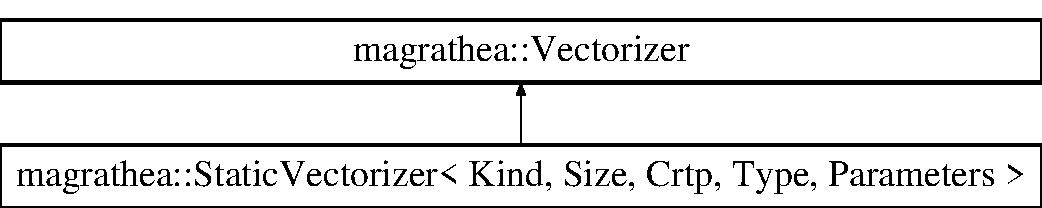
\includegraphics[height=2.000000cm]{classmagrathea_1_1StaticVectorizer}
\end{center}
\end{figure}
\subsection*{Public Member Functions}
\begin{Indent}{\bf Vectorization}\par
\begin{DoxyCompactItemize}
\item 
Type \& \hyperlink{classmagrathea_1_1StaticVectorizer_a4b5d5e63c27e77f1d734f80d7ca3d2df}{operator\mbox{[}$\,$\mbox{]}} (const unsigned int i)
\begin{DoxyCompactList}\small\item\em Direct access to the element. \end{DoxyCompactList}\item 
const Type \& \hyperlink{classmagrathea_1_1StaticVectorizer_adf04553a28c73c6a6d04f2d29c8cdfeb}{operator\mbox{[}$\,$\mbox{]}} (const unsigned int i) const 
\begin{DoxyCompactList}\small\item\em Immutable direct access to the element. \end{DoxyCompactList}\item 
Crtp$<$ Type, Parameters...$>$ \& \hyperlink{classmagrathea_1_1StaticVectorizer_a41dd9d48122248b8ee10d1ef372cd560}{resize} (const unsigned int n)
\begin{DoxyCompactList}\small\item\em Resize the container. \end{DoxyCompactList}\end{DoxyCompactItemize}
\end{Indent}
\begin{Indent}{\bf Operators \-: assignment}\par
\begin{DoxyCompactItemize}
\item 
Crtp$<$ Type, Parameters...$>$ \& \hyperlink{classmagrathea_1_1StaticVectorizer_a53c433b861ee583956eeed639868cda0}{operator=} (const \hyperlink{classmagrathea_1_1StaticVectorizer}{Static\-Vectorizer}$<$ Kind, Size, Crtp, Type, Parameters...$>$ \&rhs)
\begin{DoxyCompactList}\small\item\em Copy assignment operator. \end{DoxyCompactList}\item 
{\footnotesize template$<$typename Other\-Type , class  = typename std\-::enable\-\_\-if$<$std\-::is\-\_\-convertible$<$\-Other\-Type, Type$>$\-::value$>$\-::type$>$ }\\Crtp$<$ Type, Parameters...$>$ \& \hyperlink{classmagrathea_1_1StaticVectorizer_aa0f365bb136ebe481ebadbc939379300}{operator=} (const std\-::initializer\-\_\-list$<$ Other\-Type $>$ \&rhs)
\begin{DoxyCompactList}\small\item\em Initializer list assignment operator. \end{DoxyCompactList}\item 
{\footnotesize template$<$class Misc $>$ }\\Crtp$<$ Type, Parameters...$>$ \& \hyperlink{classmagrathea_1_1StaticVectorizer_a7f80b1a26224671bcc94082b329703d0}{operator=} (const Misc \&rhs)
\begin{DoxyCompactList}\small\item\em Copy assignment operator. \end{DoxyCompactList}\end{DoxyCompactItemize}
\end{Indent}
\begin{Indent}{\bf Operators \-: compound assignement}\par
\begin{DoxyCompactItemize}
\item 
{\footnotesize template$<$class Generic\-Type $>$ }\\Crtp$<$ Type, Parameters...$>$ \& \hyperlink{classmagrathea_1_1StaticVectorizer_adeebb70a5bf1d4fe1e3c86fbd0830e1a}{operator+=} (const Generic\-Type \&rhs)
\begin{DoxyCompactList}\small\item\em Addition assignment. \end{DoxyCompactList}\item 
{\footnotesize template$<$class Generic\-Type $>$ }\\Crtp$<$ Type, Parameters...$>$ \& \hyperlink{classmagrathea_1_1StaticVectorizer_a1eb336da47554c90ce21eb1bba271630}{operator-\/=} (const Generic\-Type \&rhs)
\begin{DoxyCompactList}\small\item\em Substraction assignment. \end{DoxyCompactList}\item 
{\footnotesize template$<$class Generic\-Type $>$ }\\Crtp$<$ Type, Parameters...$>$ \& \hyperlink{classmagrathea_1_1StaticVectorizer_ae5ba80f798f95863f6e13d72d154b934}{operator$\ast$=} (const Generic\-Type \&rhs)
\begin{DoxyCompactList}\small\item\em Multiplication assignment. \end{DoxyCompactList}\item 
{\footnotesize template$<$class Generic\-Type $>$ }\\Crtp$<$ Type, Parameters...$>$ \& \hyperlink{classmagrathea_1_1StaticVectorizer_ac0d79a23a4ef654dd107c1682a5fa8d0}{operator/=} (const Generic\-Type \&rhs)
\begin{DoxyCompactList}\small\item\em Division assignment. \end{DoxyCompactList}\item 
{\footnotesize template$<$class Generic\-Type $>$ }\\Crtp$<$ Type, Parameters...$>$ \& \hyperlink{classmagrathea_1_1StaticVectorizer_a47c9e3e893460b9955602af8e30ef60c}{operator\%=} (const Generic\-Type \&rhs)
\begin{DoxyCompactList}\small\item\em Modulo assignment. \end{DoxyCompactList}\item 
{\footnotesize template$<$class Generic\-Type $>$ }\\Crtp$<$ Type, Parameters...$>$ \& \hyperlink{classmagrathea_1_1StaticVectorizer_ab4d6cd5651a735815e1af42ab3ea21a6}{operator\&=} (const Generic\-Type \&rhs)
\begin{DoxyCompactList}\small\item\em Bitwise A\-N\-D assignment. \end{DoxyCompactList}\item 
{\footnotesize template$<$class Generic\-Type $>$ }\\Crtp$<$ Type, Parameters...$>$ \& \hyperlink{classmagrathea_1_1StaticVectorizer_a19c8eb2274664155f9b714200544247b}{operator$|$=} (const Generic\-Type \&rhs)
\begin{DoxyCompactList}\small\item\em Bitwise O\-R assignment. \end{DoxyCompactList}\item 
{\footnotesize template$<$class Generic\-Type $>$ }\\Crtp$<$ Type, Parameters...$>$ \& \hyperlink{classmagrathea_1_1StaticVectorizer_a38a45a8f2b81d90168197a26dac6fb0f}{operator$^\wedge$=} (const Generic\-Type \&rhs)
\begin{DoxyCompactList}\small\item\em Bitwise X\-O\-R assignment. \end{DoxyCompactList}\item 
{\footnotesize template$<$class Generic\-Type $>$ }\\Crtp$<$ Type, Parameters...$>$ \& \hyperlink{classmagrathea_1_1StaticVectorizer_a22eee562fea2e47fceb1a28f045d684a}{operator$<$$<$=} (const Generic\-Type \&rhs)
\begin{DoxyCompactList}\small\item\em Bitwise left shift assignment. \end{DoxyCompactList}\item 
{\footnotesize template$<$class Generic\-Type $>$ }\\Crtp$<$ Type, Parameters...$>$ \& \hyperlink{classmagrathea_1_1StaticVectorizer_af997b81383cd6fda10a5c816ab5fa066}{operator$>$$>$=} (const Generic\-Type \&rhs)
\begin{DoxyCompactList}\small\item\em Bitwise right shift assignment. \end{DoxyCompactList}\end{DoxyCompactItemize}
\end{Indent}
\begin{Indent}{\bf Operators \-: main}\par
\begin{DoxyCompactItemize}
\item 
{\footnotesize template$<$typename Other\-Type , class  = typename std\-::enable\-\_\-if$<$std\-::is\-\_\-convertible$<$\-Other\-Type, Type$>$\-::value$>$\-::type$>$ }\\Crtp$<$ typename \\*
std\-::common\-\_\-type$<$ Type, \\*
Other\-Type $>$\-::\hyperlink{classmagrathea_1_1StaticVectorizer_a28c393a3896a3e839008c35d56b10a54}{type}, \\*
Parameters...$>$ \hyperlink{classmagrathea_1_1StaticVectorizer_a567b025704b733cbd38dc5504102dfca}{operator+} (const \hyperlink{classmagrathea_1_1StaticVectorizer}{Static\-Vectorizer}$<$ Kind, Size, Crtp, Other\-Type, Parameters...$>$ \&rhs) const 
\begin{DoxyCompactList}\small\item\em Addition. \end{DoxyCompactList}\item 
{\footnotesize template$<$typename Other\-Type , class  = typename std\-::enable\-\_\-if$<$std\-::is\-\_\-convertible$<$\-Other\-Type, Type$>$\-::value$>$\-::type$>$ }\\Crtp$<$ typename \\*
std\-::common\-\_\-type$<$ Type, \\*
Other\-Type $>$\-::\hyperlink{classmagrathea_1_1StaticVectorizer_a28c393a3896a3e839008c35d56b10a54}{type}, \\*
Parameters...$>$ \hyperlink{classmagrathea_1_1StaticVectorizer_a9323dd009e06bac4ff6c426217a11443}{operator-\/} (const \hyperlink{classmagrathea_1_1StaticVectorizer}{Static\-Vectorizer}$<$ Kind, Size, Crtp, Other\-Type, Parameters...$>$ \&rhs) const 
\begin{DoxyCompactList}\small\item\em Substraction. \end{DoxyCompactList}\item 
{\footnotesize template$<$typename Other\-Type , class  = typename std\-::enable\-\_\-if$<$std\-::is\-\_\-convertible$<$\-Other\-Type, Type$>$\-::value$>$\-::type$>$ }\\Crtp$<$ typename \\*
std\-::common\-\_\-type$<$ Type, \\*
Other\-Type $>$\-::\hyperlink{classmagrathea_1_1StaticVectorizer_a28c393a3896a3e839008c35d56b10a54}{type}, \\*
Parameters...$>$ \hyperlink{classmagrathea_1_1StaticVectorizer_a915d0b7778501174f122a8497fb46387}{operator$\ast$} (const \hyperlink{classmagrathea_1_1StaticVectorizer}{Static\-Vectorizer}$<$ Kind, Size, Crtp, Other\-Type, Parameters...$>$ \&rhs) const 
\begin{DoxyCompactList}\small\item\em Multiplication. \end{DoxyCompactList}\item 
{\footnotesize template$<$typename Other\-Type , class  = typename std\-::enable\-\_\-if$<$std\-::is\-\_\-convertible$<$\-Other\-Type, Type$>$\-::value$>$\-::type$>$ }\\Crtp$<$ typename \\*
std\-::common\-\_\-type$<$ Type, \\*
Other\-Type $>$\-::\hyperlink{classmagrathea_1_1StaticVectorizer_a28c393a3896a3e839008c35d56b10a54}{type}, \\*
Parameters...$>$ \hyperlink{classmagrathea_1_1StaticVectorizer_a37c01771117232fb2ba44a73682f7d2d}{operator/} (const \hyperlink{classmagrathea_1_1StaticVectorizer}{Static\-Vectorizer}$<$ Kind, Size, Crtp, Other\-Type, Parameters...$>$ \&rhs) const 
\begin{DoxyCompactList}\small\item\em Division. \end{DoxyCompactList}\item 
{\footnotesize template$<$typename Other\-Type , class  = typename std\-::enable\-\_\-if$<$std\-::is\-\_\-convertible$<$\-Other\-Type, Type$>$\-::value$>$\-::type$>$ }\\Crtp$<$ typename \\*
std\-::common\-\_\-type$<$ Type, \\*
Other\-Type $>$\-::\hyperlink{classmagrathea_1_1StaticVectorizer_a28c393a3896a3e839008c35d56b10a54}{type}, \\*
Parameters...$>$ \hyperlink{classmagrathea_1_1StaticVectorizer_add2236077d26b29ce7b03a3990d4f16e}{operator\%} (const \hyperlink{classmagrathea_1_1StaticVectorizer}{Static\-Vectorizer}$<$ Kind, Size, Crtp, Other\-Type, Parameters...$>$ \&rhs) const 
\begin{DoxyCompactList}\small\item\em Modulo. \end{DoxyCompactList}\item 
{\footnotesize template$<$typename Other\-Type , class  = typename std\-::enable\-\_\-if$<$std\-::is\-\_\-convertible$<$\-Other\-Type, Type$>$\-::value$>$\-::type$>$ }\\Crtp$<$ typename \\*
std\-::common\-\_\-type$<$ Type, \\*
Other\-Type $>$\-::\hyperlink{classmagrathea_1_1StaticVectorizer_a28c393a3896a3e839008c35d56b10a54}{type}, \\*
Parameters...$>$ \hyperlink{classmagrathea_1_1StaticVectorizer_a8a87d64ccefc340329bbd5cc1ddb9717}{operator\&} (const \hyperlink{classmagrathea_1_1StaticVectorizer}{Static\-Vectorizer}$<$ Kind, Size, Crtp, Other\-Type, Parameters...$>$ \&rhs) const 
\begin{DoxyCompactList}\small\item\em Bitwise A\-N\-D. \end{DoxyCompactList}\item 
{\footnotesize template$<$typename Other\-Type , class  = typename std\-::enable\-\_\-if$<$std\-::is\-\_\-convertible$<$\-Other\-Type, Type$>$\-::value$>$\-::type$>$ }\\Crtp$<$ typename \\*
std\-::common\-\_\-type$<$ Type, \\*
Other\-Type $>$\-::\hyperlink{classmagrathea_1_1StaticVectorizer_a28c393a3896a3e839008c35d56b10a54}{type}, \\*
Parameters...$>$ \hyperlink{classmagrathea_1_1StaticVectorizer_a9dfa7d06a43760b3550fa8e6319dee90}{operator$|$} (const \hyperlink{classmagrathea_1_1StaticVectorizer}{Static\-Vectorizer}$<$ Kind, Size, Crtp, Other\-Type, Parameters...$>$ \&rhs) const 
\begin{DoxyCompactList}\small\item\em Bitwise O\-R. \end{DoxyCompactList}\item 
{\footnotesize template$<$typename Other\-Type , class  = typename std\-::enable\-\_\-if$<$std\-::is\-\_\-convertible$<$\-Other\-Type, Type$>$\-::value$>$\-::type$>$ }\\Crtp$<$ typename \\*
std\-::common\-\_\-type$<$ Type, \\*
Other\-Type $>$\-::\hyperlink{classmagrathea_1_1StaticVectorizer_a28c393a3896a3e839008c35d56b10a54}{type}, \\*
Parameters...$>$ \hyperlink{classmagrathea_1_1StaticVectorizer_a0943fd4f6155fcd6410ffaddee1a30c3}{operator$^\wedge$} (const \hyperlink{classmagrathea_1_1StaticVectorizer}{Static\-Vectorizer}$<$ Kind, Size, Crtp, Other\-Type, Parameters...$>$ \&rhs) const 
\begin{DoxyCompactList}\small\item\em Bitwise X\-O\-R. \end{DoxyCompactList}\item 
{\footnotesize template$<$typename Other\-Type , class  = typename std\-::enable\-\_\-if$<$std\-::is\-\_\-convertible$<$\-Other\-Type, Type$>$\-::value$>$\-::type$>$ }\\Crtp$<$ Type, Parameters...$>$ \hyperlink{classmagrathea_1_1StaticVectorizer_a1ca67dc868dd70423e659b77209e07d9}{operator$<$$<$} (const \hyperlink{classmagrathea_1_1StaticVectorizer}{Static\-Vectorizer}$<$ Kind, Size, Crtp, Other\-Type, Parameters...$>$ \&rhs) const 
\begin{DoxyCompactList}\small\item\em Bitwise left shift. \end{DoxyCompactList}\item 
{\footnotesize template$<$typename Other\-Type , class  = typename std\-::enable\-\_\-if$<$std\-::is\-\_\-convertible$<$\-Other\-Type, Type$>$\-::value$>$\-::type$>$ }\\Crtp$<$ Type, Parameters...$>$ \hyperlink{classmagrathea_1_1StaticVectorizer_a6893af67ac504eeb471690a5114a1365}{operator$>$$>$} (const \hyperlink{classmagrathea_1_1StaticVectorizer}{Static\-Vectorizer}$<$ Kind, Size, Crtp, Other\-Type, Parameters...$>$ \&rhs) const 
\begin{DoxyCompactList}\small\item\em Bitwise right shift. \end{DoxyCompactList}\item 
{\footnotesize template$<$typename Other\-Type , class  = typename std\-::enable\-\_\-if$<$std\-::is\-\_\-convertible$<$\-Other\-Type, Type$>$\-::value$>$\-::type$>$ }\\Crtp$<$ bool, Parameters...$>$ \hyperlink{classmagrathea_1_1StaticVectorizer_aa0b7dd33a216a87e2d8cad3bd06aff45}{operator\&\&} (const \hyperlink{classmagrathea_1_1StaticVectorizer}{Static\-Vectorizer}$<$ Kind, Size, Crtp, Other\-Type, Parameters...$>$ \&rhs) const 
\begin{DoxyCompactList}\small\item\em Logical A\-N\-D. \end{DoxyCompactList}\item 
{\footnotesize template$<$typename Other\-Type , class  = typename std\-::enable\-\_\-if$<$std\-::is\-\_\-convertible$<$\-Other\-Type, Type$>$\-::value$>$\-::type$>$ }\\Crtp$<$ bool, Parameters...$>$ \hyperlink{classmagrathea_1_1StaticVectorizer_a69b7f2ba58c27a4562daa6243d50e67b}{operator$|$$|$} (const \hyperlink{classmagrathea_1_1StaticVectorizer}{Static\-Vectorizer}$<$ Kind, Size, Crtp, Other\-Type, Parameters...$>$ \&rhs) const 
\begin{DoxyCompactList}\small\item\em Logical O\-R. \end{DoxyCompactList}\item 
{\footnotesize template$<$typename Other\-Type , class  = typename std\-::enable\-\_\-if$<$std\-::is\-\_\-convertible$<$\-Other\-Type, Type$>$\-::value$>$\-::type$>$ }\\Crtp$<$ bool, Parameters...$>$ \hyperlink{classmagrathea_1_1StaticVectorizer_a5bad4a3e6f2206c1fc71f3f3b26b841b}{operator==} (const \hyperlink{classmagrathea_1_1StaticVectorizer}{Static\-Vectorizer}$<$ Kind, Size, Crtp, Other\-Type, Parameters...$>$ \&rhs) const 
\begin{DoxyCompactList}\small\item\em Equal to. \end{DoxyCompactList}\item 
{\footnotesize template$<$typename Other\-Type , class  = typename std\-::enable\-\_\-if$<$std\-::is\-\_\-convertible$<$\-Other\-Type, Type$>$\-::value$>$\-::type$>$ }\\Crtp$<$ bool, Parameters...$>$ \hyperlink{classmagrathea_1_1StaticVectorizer_af92fdb0640566781b2be44d9e5a13a4f}{operator!=} (const \hyperlink{classmagrathea_1_1StaticVectorizer}{Static\-Vectorizer}$<$ Kind, Size, Crtp, Other\-Type, Parameters...$>$ \&rhs) const 
\begin{DoxyCompactList}\small\item\em Not equal to. \end{DoxyCompactList}\item 
{\footnotesize template$<$typename Other\-Type , class  = typename std\-::enable\-\_\-if$<$std\-::is\-\_\-convertible$<$\-Other\-Type, Type$>$\-::value$>$\-::type$>$ }\\Crtp$<$ bool, Parameters...$>$ \hyperlink{classmagrathea_1_1StaticVectorizer_a2c0b5791efa69c1397ef8af918148ad8}{operator$>$} (const \hyperlink{classmagrathea_1_1StaticVectorizer}{Static\-Vectorizer}$<$ Kind, Size, Crtp, Other\-Type, Parameters...$>$ \&rhs) const 
\begin{DoxyCompactList}\small\item\em Greater than. \end{DoxyCompactList}\item 
{\footnotesize template$<$typename Other\-Type , class  = typename std\-::enable\-\_\-if$<$std\-::is\-\_\-convertible$<$\-Other\-Type, Type$>$\-::value$>$\-::type$>$ }\\Crtp$<$ bool, Parameters...$>$ \hyperlink{classmagrathea_1_1StaticVectorizer_a80928ac25f678a002f96c2770ae0459a}{operator$<$} (const \hyperlink{classmagrathea_1_1StaticVectorizer}{Static\-Vectorizer}$<$ Kind, Size, Crtp, Other\-Type, Parameters...$>$ \&rhs) const 
\begin{DoxyCompactList}\small\item\em Less than. \end{DoxyCompactList}\item 
{\footnotesize template$<$typename Other\-Type , class  = typename std\-::enable\-\_\-if$<$std\-::is\-\_\-convertible$<$\-Other\-Type, Type$>$\-::value$>$\-::type$>$ }\\Crtp$<$ bool, Parameters...$>$ \hyperlink{classmagrathea_1_1StaticVectorizer_a192cbe3a1821bbff180dfe1422a0ecae}{operator$>$=} (const \hyperlink{classmagrathea_1_1StaticVectorizer}{Static\-Vectorizer}$<$ Kind, Size, Crtp, Other\-Type, Parameters...$>$ \&rhs) const 
\begin{DoxyCompactList}\small\item\em Greater than or equal to. \end{DoxyCompactList}\item 
{\footnotesize template$<$typename Other\-Type , class  = typename std\-::enable\-\_\-if$<$std\-::is\-\_\-convertible$<$\-Other\-Type, Type$>$\-::value$>$\-::type$>$ }\\Crtp$<$ bool, Parameters...$>$ \hyperlink{classmagrathea_1_1StaticVectorizer_a76839b1c705d389cfacfc9ae8d1b8887}{operator$<$=} (const \hyperlink{classmagrathea_1_1StaticVectorizer}{Static\-Vectorizer}$<$ Kind, Size, Crtp, Other\-Type, Parameters...$>$ \&rhs) const 
\begin{DoxyCompactList}\small\item\em Less than or equal to. \end{DoxyCompactList}\end{DoxyCompactItemize}
\end{Indent}
\begin{Indent}{\bf Operators \-: with rhs value}\par
\begin{DoxyCompactItemize}
\item 
{\footnotesize template$<$typename Other\-Type , class  = typename std\-::enable\-\_\-if$<$(!std\-::is\-\_\-base\-\_\-of$<$\-Vectorizer, Other\-Type$>$\-::value) \&\& (std\-::is\-\_\-convertible$<$\-Other\-Type, Type$>$\-::value)$>$\-::type$>$ }\\Crtp$<$ typename \\*
std\-::common\-\_\-type$<$ Type, \\*
Other\-Type $>$\-::\hyperlink{classmagrathea_1_1StaticVectorizer_a28c393a3896a3e839008c35d56b10a54}{type}, \\*
Parameters...$>$ \hyperlink{classmagrathea_1_1StaticVectorizer_aae18798ce202c372877ffad6dd05a6ee}{operator+} (const Other\-Type \&rhs) const 
\begin{DoxyCompactList}\small\item\em Addition with rhs value. \end{DoxyCompactList}\item 
{\footnotesize template$<$typename Other\-Type , class  = typename std\-::enable\-\_\-if$<$(!std\-::is\-\_\-base\-\_\-of$<$\-Vectorizer, Other\-Type$>$\-::value) \&\& (std\-::is\-\_\-convertible$<$\-Other\-Type, Type$>$\-::value)$>$\-::type$>$ }\\Crtp$<$ typename \\*
std\-::common\-\_\-type$<$ Type, \\*
Other\-Type $>$\-::\hyperlink{classmagrathea_1_1StaticVectorizer_a28c393a3896a3e839008c35d56b10a54}{type}, \\*
Parameters...$>$ \hyperlink{classmagrathea_1_1StaticVectorizer_a294a71924f6f57b8e03edcbfb12c0c54}{operator-\/} (const Other\-Type \&rhs) const 
\begin{DoxyCompactList}\small\item\em Substraction with rhs value. \end{DoxyCompactList}\item 
{\footnotesize template$<$typename Other\-Type , class  = typename std\-::enable\-\_\-if$<$(!std\-::is\-\_\-base\-\_\-of$<$\-Vectorizer, Other\-Type$>$\-::value) \&\& (std\-::is\-\_\-convertible$<$\-Other\-Type, Type$>$\-::value)$>$\-::type$>$ }\\Crtp$<$ typename \\*
std\-::common\-\_\-type$<$ Type, \\*
Other\-Type $>$\-::\hyperlink{classmagrathea_1_1StaticVectorizer_a28c393a3896a3e839008c35d56b10a54}{type}, \\*
Parameters...$>$ \hyperlink{classmagrathea_1_1StaticVectorizer_ab2d4e3fb0273c6453f4c77654ed39bee}{operator$\ast$} (const Other\-Type \&rhs) const 
\begin{DoxyCompactList}\small\item\em Multiplication with rhs value. \end{DoxyCompactList}\item 
{\footnotesize template$<$typename Other\-Type , class  = typename std\-::enable\-\_\-if$<$(!std\-::is\-\_\-base\-\_\-of$<$\-Vectorizer, Other\-Type$>$\-::value) \&\& (std\-::is\-\_\-convertible$<$\-Other\-Type, Type$>$\-::value)$>$\-::type$>$ }\\Crtp$<$ typename \\*
std\-::common\-\_\-type$<$ Type, \\*
Other\-Type $>$\-::\hyperlink{classmagrathea_1_1StaticVectorizer_a28c393a3896a3e839008c35d56b10a54}{type}, \\*
Parameters...$>$ \hyperlink{classmagrathea_1_1StaticVectorizer_abb4d2416e7104066405671d4d6d62337}{operator/} (const Other\-Type \&rhs) const 
\begin{DoxyCompactList}\small\item\em Division with rhs value. \end{DoxyCompactList}\item 
{\footnotesize template$<$typename Other\-Type , class  = typename std\-::enable\-\_\-if$<$(!std\-::is\-\_\-base\-\_\-of$<$\-Vectorizer, Other\-Type$>$\-::value) \&\& (std\-::is\-\_\-convertible$<$\-Other\-Type, Type$>$\-::value)$>$\-::type$>$ }\\Crtp$<$ typename \\*
std\-::common\-\_\-type$<$ Type, \\*
Other\-Type $>$\-::\hyperlink{classmagrathea_1_1StaticVectorizer_a28c393a3896a3e839008c35d56b10a54}{type}, \\*
Parameters...$>$ \hyperlink{classmagrathea_1_1StaticVectorizer_abed2e71709a1266c0aa35ace9e60db9c}{operator\%} (const Other\-Type \&rhs) const 
\begin{DoxyCompactList}\small\item\em Modulo with rhs value. \end{DoxyCompactList}\item 
{\footnotesize template$<$typename Other\-Type , class  = typename std\-::enable\-\_\-if$<$(!std\-::is\-\_\-base\-\_\-of$<$\-Vectorizer, Other\-Type$>$\-::value) \&\& (std\-::is\-\_\-convertible$<$\-Other\-Type, Type$>$\-::value)$>$\-::type$>$ }\\Crtp$<$ typename \\*
std\-::common\-\_\-type$<$ Type, \\*
Other\-Type $>$\-::\hyperlink{classmagrathea_1_1StaticVectorizer_a28c393a3896a3e839008c35d56b10a54}{type}, \\*
Parameters...$>$ \hyperlink{classmagrathea_1_1StaticVectorizer_add90cf869ac9dd08b986be67cfee5221}{operator\&} (const Other\-Type \&rhs) const 
\begin{DoxyCompactList}\small\item\em Bitwise A\-N\-D with rhs value. \end{DoxyCompactList}\item 
{\footnotesize template$<$typename Other\-Type , class  = typename std\-::enable\-\_\-if$<$(!std\-::is\-\_\-base\-\_\-of$<$\-Vectorizer, Other\-Type$>$\-::value) \&\& (std\-::is\-\_\-convertible$<$\-Other\-Type, Type$>$\-::value)$>$\-::type$>$ }\\Crtp$<$ typename \\*
std\-::common\-\_\-type$<$ Type, \\*
Other\-Type $>$\-::\hyperlink{classmagrathea_1_1StaticVectorizer_a28c393a3896a3e839008c35d56b10a54}{type}, \\*
Parameters...$>$ \hyperlink{classmagrathea_1_1StaticVectorizer_a224cb7cb9b2cb80a7719cdee76349204}{operator$|$} (const Other\-Type \&rhs) const 
\begin{DoxyCompactList}\small\item\em Bitwise O\-R with rhs value. \end{DoxyCompactList}\item 
{\footnotesize template$<$typename Other\-Type , class  = typename std\-::enable\-\_\-if$<$(!std\-::is\-\_\-base\-\_\-of$<$\-Vectorizer, Other\-Type$>$\-::value) \&\& (std\-::is\-\_\-convertible$<$\-Other\-Type, Type$>$\-::value)$>$\-::type$>$ }\\Crtp$<$ typename \\*
std\-::common\-\_\-type$<$ Type, \\*
Other\-Type $>$\-::\hyperlink{classmagrathea_1_1StaticVectorizer_a28c393a3896a3e839008c35d56b10a54}{type}, \\*
Parameters...$>$ \hyperlink{classmagrathea_1_1StaticVectorizer_ab39f76f560714379beb563a6406713ae}{operator$^\wedge$} (const Other\-Type \&rhs) const 
\begin{DoxyCompactList}\small\item\em Bitwise X\-O\-R with rhs value. \end{DoxyCompactList}\item 
{\footnotesize template$<$typename Other\-Type , class  = typename std\-::enable\-\_\-if$<$(!std\-::is\-\_\-base\-\_\-of$<$\-Vectorizer, Other\-Type$>$\-::value) \&\& (std\-::is\-\_\-convertible$<$\-Other\-Type, Type$>$\-::value)$>$\-::type$>$ }\\Crtp$<$ Type, Parameters...$>$ \hyperlink{classmagrathea_1_1StaticVectorizer_a5629b7a221887ce68ed18b1da00ad5d6}{operator$<$$<$} (const Other\-Type \&rhs) const 
\begin{DoxyCompactList}\small\item\em Bitwise left shift with rhs value. \end{DoxyCompactList}\item 
{\footnotesize template$<$typename Other\-Type , class  = typename std\-::enable\-\_\-if$<$(!std\-::is\-\_\-base\-\_\-of$<$\-Vectorizer, Other\-Type$>$\-::value) \&\& (std\-::is\-\_\-convertible$<$\-Other\-Type, Type$>$\-::value)$>$\-::type$>$ }\\Crtp$<$ Type, Parameters...$>$ \hyperlink{classmagrathea_1_1StaticVectorizer_a3738d5814db16597b32bdf601685c832}{operator$>$$>$} (const Other\-Type \&rhs) const 
\begin{DoxyCompactList}\small\item\em Bitwise right shift with rhs value. \end{DoxyCompactList}\item 
{\footnotesize template$<$typename Other\-Type , class  = typename std\-::enable\-\_\-if$<$(!std\-::is\-\_\-base\-\_\-of$<$\-Vectorizer, Other\-Type$>$\-::value) \&\& (std\-::is\-\_\-convertible$<$\-Other\-Type, Type$>$\-::value)$>$\-::type$>$ }\\Crtp$<$ bool, Parameters...$>$ \hyperlink{classmagrathea_1_1StaticVectorizer_a96cdf853407901fedc50265a84fa5991}{operator\&\&} (const Other\-Type \&rhs) const 
\begin{DoxyCompactList}\small\item\em Logical A\-N\-D with rhs value. \end{DoxyCompactList}\item 
{\footnotesize template$<$typename Other\-Type , class  = typename std\-::enable\-\_\-if$<$(!std\-::is\-\_\-base\-\_\-of$<$\-Vectorizer, Other\-Type$>$\-::value) \&\& (std\-::is\-\_\-convertible$<$\-Other\-Type, Type$>$\-::value)$>$\-::type$>$ }\\Crtp$<$ bool, Parameters...$>$ \hyperlink{classmagrathea_1_1StaticVectorizer_afed99ecd4a86f62923433c8f27a05d3f}{operator$|$$|$} (const Other\-Type \&rhs) const 
\begin{DoxyCompactList}\small\item\em Logical O\-R with rhs value. \end{DoxyCompactList}\item 
{\footnotesize template$<$typename Other\-Type , class  = typename std\-::enable\-\_\-if$<$(!std\-::is\-\_\-base\-\_\-of$<$\-Vectorizer, Other\-Type$>$\-::value) \&\& (std\-::is\-\_\-convertible$<$\-Other\-Type, Type$>$\-::value)$>$\-::type$>$ }\\Crtp$<$ bool, Parameters...$>$ \hyperlink{classmagrathea_1_1StaticVectorizer_ae8a3d25716fb6f3056a194db4611398b}{operator==} (const Other\-Type \&rhs) const 
\begin{DoxyCompactList}\small\item\em Equal to with rhs value. \end{DoxyCompactList}\item 
{\footnotesize template$<$typename Other\-Type , class  = typename std\-::enable\-\_\-if$<$(!std\-::is\-\_\-base\-\_\-of$<$\-Vectorizer, Other\-Type$>$\-::value) \&\& (std\-::is\-\_\-convertible$<$\-Other\-Type, Type$>$\-::value)$>$\-::type$>$ }\\Crtp$<$ bool, Parameters...$>$ \hyperlink{classmagrathea_1_1StaticVectorizer_a745d2383572c87adb83d08e23692aa81}{operator!=} (const Other\-Type \&rhs) const 
\begin{DoxyCompactList}\small\item\em Not equal to with rhs value. \end{DoxyCompactList}\item 
{\footnotesize template$<$typename Other\-Type , class  = typename std\-::enable\-\_\-if$<$(!std\-::is\-\_\-base\-\_\-of$<$\-Vectorizer, Other\-Type$>$\-::value) \&\& (std\-::is\-\_\-convertible$<$\-Other\-Type, Type$>$\-::value)$>$\-::type$>$ }\\Crtp$<$ bool, Parameters...$>$ \hyperlink{classmagrathea_1_1StaticVectorizer_a45845efb29eba8ac0742080cb0ca161e}{operator$>$} (const Other\-Type \&rhs) const 
\begin{DoxyCompactList}\small\item\em Greater than with rhs value. \end{DoxyCompactList}\item 
{\footnotesize template$<$typename Other\-Type , class  = typename std\-::enable\-\_\-if$<$(!std\-::is\-\_\-base\-\_\-of$<$\-Vectorizer, Other\-Type$>$\-::value) \&\& (std\-::is\-\_\-convertible$<$\-Other\-Type, Type$>$\-::value)$>$\-::type$>$ }\\Crtp$<$ bool, Parameters...$>$ \hyperlink{classmagrathea_1_1StaticVectorizer_ae8fc4ac75f3f4c8c9de4083cd07cacb0}{operator$<$} (const Other\-Type \&rhs) const 
\begin{DoxyCompactList}\small\item\em Less than with rhs value. \end{DoxyCompactList}\item 
{\footnotesize template$<$typename Other\-Type , class  = typename std\-::enable\-\_\-if$<$(!std\-::is\-\_\-base\-\_\-of$<$\-Vectorizer, Other\-Type$>$\-::value) \&\& (std\-::is\-\_\-convertible$<$\-Other\-Type, Type$>$\-::value)$>$\-::type$>$ }\\Crtp$<$ bool, Parameters...$>$ \hyperlink{classmagrathea_1_1StaticVectorizer_a8e18e9b3d7412d5d824eb7c03e01ab62}{operator$>$=} (const Other\-Type \&rhs) const 
\begin{DoxyCompactList}\small\item\em Greater than or equal to with rhs value. \end{DoxyCompactList}\item 
{\footnotesize template$<$typename Other\-Type , class  = typename std\-::enable\-\_\-if$<$(!std\-::is\-\_\-base\-\_\-of$<$\-Vectorizer, Other\-Type$>$\-::value) \&\& (std\-::is\-\_\-convertible$<$\-Other\-Type, Type$>$\-::value)$>$\-::type$>$ }\\Crtp$<$ bool, Parameters...$>$ \hyperlink{classmagrathea_1_1StaticVectorizer_a4c967db7cc9d968dfc7eeb8fc4570f59}{operator$<$=} (const Other\-Type \&rhs) const 
\begin{DoxyCompactList}\small\item\em Less than or equal to with rhs value. \end{DoxyCompactList}\end{DoxyCompactItemize}
\end{Indent}
\begin{Indent}{\bf Operators \-: unary}\par
\begin{DoxyCompactItemize}
\item 
Crtp$<$ bool, Parameters...$>$ \hyperlink{classmagrathea_1_1StaticVectorizer_a47cd06bd12e9a75244bb47949d2ac179}{operator!} () const 
\begin{DoxyCompactList}\small\item\em Logical N\-O\-T. \end{DoxyCompactList}\item 
Crtp$<$ Type, Parameters...$>$ \hyperlink{classmagrathea_1_1StaticVectorizer_a6aefc18480c79c379de8ddd9ebd0ac13}{operator$\sim$} () const 
\begin{DoxyCompactList}\small\item\em Bitwise N\-O\-T. \end{DoxyCompactList}\item 
Crtp$<$ Type, Parameters...$>$ \hyperlink{classmagrathea_1_1StaticVectorizer_a77d653a93df0b5f7f112651044604109}{operator+} () const 
\begin{DoxyCompactList}\small\item\em Integer promotion. \end{DoxyCompactList}\item 
Crtp$<$ Type, Parameters...$>$ \hyperlink{classmagrathea_1_1StaticVectorizer_a112a6fff4321f8e4ebe7184d4215e17a}{operator-\/} () const 
\begin{DoxyCompactList}\small\item\em Additive inverse. \end{DoxyCompactList}\item 
Crtp$<$ Type, Parameters...$>$ \& \hyperlink{classmagrathea_1_1StaticVectorizer_acc5094efe1b21c12c05543b2ee05f9ae}{operator++} ()
\begin{DoxyCompactList}\small\item\em Increment prefix. \end{DoxyCompactList}\item 
Crtp$<$ Type, Parameters...$>$ \& \hyperlink{classmagrathea_1_1StaticVectorizer_a3430773a46c0300aaadb38b2ce8e26af}{operator-\/-\/} ()
\begin{DoxyCompactList}\small\item\em Decrement prefix. \end{DoxyCompactList}\item 
Crtp$<$ Type, Parameters...$>$ \hyperlink{classmagrathea_1_1StaticVectorizer_a0db772662fda98f47909ed9c5ae6f61e}{operator++} (int)
\begin{DoxyCompactList}\small\item\em Increment suffix. \end{DoxyCompactList}\item 
Crtp$<$ Type, Parameters...$>$ \hyperlink{classmagrathea_1_1StaticVectorizer_acb5f5aec44c70c502f6f95c9ef2ac8ff}{operator-\/-\/} (int)
\begin{DoxyCompactList}\small\item\em Decrement suffix. \end{DoxyCompactList}\end{DoxyCompactItemize}
\end{Indent}
\begin{Indent}{\bf Access}\par
\begin{DoxyCompactItemize}
\item 
\hyperlink{classmagrathea_1_1StaticVectorizer}{Static\-Vectorizer}$<$ Kind, Size, \\*
Crtp, Type, Parameters...$>$ \& \hyperlink{classmagrathea_1_1StaticVectorizer_a59fb69180969b012a7ba11981fb9aaf5}{operator()} ()
\begin{DoxyCompactList}\small\item\em Abstract class access. \end{DoxyCompactList}\item 
const \hyperlink{classmagrathea_1_1StaticVectorizer}{Static\-Vectorizer}$<$ Kind, \\*
Size, Crtp, Type, \\*
Parameters...$>$ \& \hyperlink{classmagrathea_1_1StaticVectorizer_a21f4f22f100057ebca8f881a6cea2fe0}{operator()} () const 
\begin{DoxyCompactList}\small\item\em Immutable abstract class access. \end{DoxyCompactList}\item 
Type \& \hyperlink{classmagrathea_1_1StaticVectorizer_a791203245d6c45ee22165b4a0bc11647}{operator()} (const unsigned int i)
\begin{DoxyCompactList}\small\item\em Monodimensional access operator. \end{DoxyCompactList}\item 
const Type \& \hyperlink{classmagrathea_1_1StaticVectorizer_aeb3ee03be09afd4621c18d49918c8d0e}{operator()} (const unsigned int i) const 
\begin{DoxyCompactList}\small\item\em Immutable monodimensional access operator. \end{DoxyCompactList}\item 
Type \& \hyperlink{classmagrathea_1_1StaticVectorizer_a842eaff610697adbed8b6bb4e403a39f}{at} (const unsigned int i)
\begin{DoxyCompactList}\small\item\em Monodimensional access with range-\/check. \end{DoxyCompactList}\item 
const Type \& \hyperlink{classmagrathea_1_1StaticVectorizer_a293da0f31f6a8db5efb9c9ebb7ff3a81}{at} (const unsigned int i) const 
\begin{DoxyCompactList}\small\item\em Immutable monodimensional access with range-\/check. \end{DoxyCompactList}\item 
Type \& \hyperlink{classmagrathea_1_1StaticVectorizer_a860d99a0104280c072d7b7dbf8d87c27}{front} (const unsigned int i=0)
\begin{DoxyCompactList}\small\item\em Monodimensional access to the i-\/th element from the beginning. \end{DoxyCompactList}\item 
const Type \& \hyperlink{classmagrathea_1_1StaticVectorizer_afedeae49461374b9a8cd0fe6615b75bf}{front} (const unsigned int i=0) const 
\begin{DoxyCompactList}\small\item\em Immutable monodimensional access to the i-\/th element from the beginning. \end{DoxyCompactList}\item 
Type \& \hyperlink{classmagrathea_1_1StaticVectorizer_ae1d5d72bbbf0c8b41de7ff463eb72606}{back} (const unsigned int i=0)
\begin{DoxyCompactList}\small\item\em Monodimensional access to the i-\/th element from the end. \end{DoxyCompactList}\item 
const Type \& \hyperlink{classmagrathea_1_1StaticVectorizer_a3efc84b306bb29fdcc1c13b0bb46e603}{back} (const unsigned int i=0) const 
\begin{DoxyCompactList}\small\item\em Immutable monodimensional access to the i-\/th element from the end. \end{DoxyCompactList}\item 
Type \& \hyperlink{classmagrathea_1_1StaticVectorizer_a3cc47c0b28180723f001d6c2dce89a78}{cycle} (const int i)
\begin{DoxyCompactList}\small\item\em Cyclic monodimensional access to the contents. \end{DoxyCompactList}\item 
const Type \& \hyperlink{classmagrathea_1_1StaticVectorizer_a42143d4ae441b0a39d6632a40c34dcbc}{cycle} (const int i) const 
\begin{DoxyCompactList}\small\item\em Immutable cyclic monodimensional access to the contents. \end{DoxyCompactList}\end{DoxyCompactItemize}
\end{Indent}
\begin{Indent}{\bf Assignment}\par
\begin{DoxyCompactItemize}
\item 
{\footnotesize template$<$typename Other\-Type , class... Misc, class  = typename std\-::enable\-\_\-if$<$std\-::is\-\_\-convertible$<$\-Other\-Type, Type$>$\-::value$>$\-::type$>$ }\\Crtp$<$ Type, Parameters...$>$ \& \hyperlink{classmagrathea_1_1StaticVectorizer_aa026b0cb951858dfbebaf4df9d02dd28}{assign} (const std\-::initializer\-\_\-list$<$ Other\-Type $>$ \&source, const Misc \&...misc)
\begin{DoxyCompactList}\small\item\em Initializer list assignment. \end{DoxyCompactList}\item 
{\footnotesize template$<$class... Misc$>$ }\\Crtp$<$ Type, Parameters...$>$ \& \hyperlink{classmagrathea_1_1StaticVectorizer_aeecd6ce10ed87346885bf4c7aeef7ae6}{assign} (const Misc \&...misc)
\begin{DoxyCompactList}\small\item\em Generic assignment. \end{DoxyCompactList}\item 
{\footnotesize template$<$typename Other\-Type , class... Misc, class  = typename std\-::enable\-\_\-if$<$std\-::is\-\_\-convertible$<$\-Other\-Type, Type$>$\-::value$>$\-::type$>$ }\\Crtp$<$ Type, Parameters...$>$ \& \hyperlink{classmagrathea_1_1StaticVectorizer_aff1b6067431758a205c3cb71c38f6011}{fill} (const std\-::initializer\-\_\-list$<$ Other\-Type $>$ \&source, const Misc \&...misc)
\begin{DoxyCompactList}\small\item\em Initializer list fill. \end{DoxyCompactList}\item 
{\footnotesize template$<$class... Misc$>$ }\\Crtp$<$ Type, Parameters...$>$ \& \hyperlink{classmagrathea_1_1StaticVectorizer_abc085a9ed9cf363095eb42adf323b533}{fill} (const Misc \&...misc)
\begin{DoxyCompactList}\small\item\em Generic fill. \end{DoxyCompactList}\item 
{\footnotesize template$<$typename Other\-Type , class... Misc, class  = typename std\-::enable\-\_\-if$<$std\-::is\-\_\-convertible$<$\-Other\-Type, Type$>$\-::value$>$\-::type$>$ }\\Crtp$<$ Type, Parameters...$>$ \hyperlink{classmagrathea_1_1StaticVectorizer_ae322d5931112d91c3f24529e6c1e1559}{replace} (const std\-::initializer\-\_\-list$<$ Other\-Type $>$ \&source, const Misc \&...misc)
\begin{DoxyCompactList}\small\item\em Initializer list replace. \end{DoxyCompactList}\item 
{\footnotesize template$<$class... Misc$>$ }\\Crtp$<$ Type, Parameters...$>$ \hyperlink{classmagrathea_1_1StaticVectorizer_a81bc8121599b9da4425a5d73eb65dec4}{replace} (const Misc \&...misc)
\begin{DoxyCompactList}\small\item\em Generic replace. \end{DoxyCompactList}\item 
{\footnotesize template$<$class Generic\-Type $>$ }\\Crtp$<$ Type, Parameters...$>$ \& \hyperlink{classmagrathea_1_1StaticVectorizer_a68070ddd4235454ca5fae28888353a87}{put} (const Generic\-Type \&source, const unsigned int pos, const unsigned int num=1)
\begin{DoxyCompactList}\small\item\em Put an element in the container. \end{DoxyCompactList}\item 
{\footnotesize template$<$class Generic\-Type $>$ }\\Crtp$<$ Type, Parameters...$>$ \hyperlink{classmagrathea_1_1StaticVectorizer_acb350662a8c17a5476b331d23917b084}{change} (const Generic\-Type \&source, const unsigned int pos, const unsigned int num=1)
\begin{DoxyCompactList}\small\item\em Change an element of the container. \end{DoxyCompactList}\end{DoxyCompactItemize}
\end{Indent}
\begin{Indent}{\bf Management}\par
\begin{DoxyCompactItemize}
\item 
Crtp$<$ Type, Parameters...$>$ \& \hyperlink{classmagrathea_1_1StaticVectorizer_ae15629a58700e638e2a4546742cf09f6}{reserve} (const unsigned int n)
\begin{DoxyCompactList}\small\item\em Reserve new space for the container. \end{DoxyCompactList}\item 
Crtp$<$ Type, Parameters...$>$ \& \hyperlink{classmagrathea_1_1StaticVectorizer_abc4fdc2ce798bc99edc1a874a90bbfe5}{clear} ()
\begin{DoxyCompactList}\small\item\em Clear contents. \end{DoxyCompactList}\item 
{\footnotesize template$<$class... Location$>$ }\\Crtp$<$ Type, Parameters...$>$ \& \hyperlink{classmagrathea_1_1StaticVectorizer_aa2d036d08b09e0f8ec903c7c6442db2b}{nullify} (const Location \&...location)
\begin{DoxyCompactList}\small\item\em Set elements to their default values. \end{DoxyCompactList}\item 
{\footnotesize template$<$class... Location$>$ }\\Crtp$<$ Type, Parameters...$>$ \& \hyperlink{classmagrathea_1_1StaticVectorizer_a8bf8d5dc7fd3290eff136f1262342e8b}{swap} (\hyperlink{classmagrathea_1_1StaticVectorizer}{Static\-Vectorizer}$<$ Kind, Size, Crtp, Type, Parameters...$>$ \&rhs, const Location \&...location)
\begin{DoxyCompactList}\small\item\em Swap elements by copy. \end{DoxyCompactList}\item 
Crtp$<$ Type, Parameters...$>$ \hyperlink{classmagrathea_1_1StaticVectorizer_a15c61ea6878c48725951cce33147cd22}{copy} () const 
\begin{DoxyCompactList}\small\item\em Copy. \end{DoxyCompactList}\item 
{\footnotesize template$<$typename Other\-Type  = Type, class  = typename std\-::enable\-\_\-if$<$std\-::is\-\_\-convertible$<$\-Other\-Type, Type$>$\-::value$>$\-::type$>$ }\\Crtp$<$ Other\-Type, Parameters...$>$ \hyperlink{classmagrathea_1_1StaticVectorizer_ad3d731d6d65b0c6779f8bfa098743817}{cast} () const 
\begin{DoxyCompactList}\small\item\em Cast to a different data type. \end{DoxyCompactList}\end{DoxyCompactItemize}
\end{Indent}
\begin{Indent}{\bf Comparison}\par
\begin{DoxyCompactItemize}
\item 
bool \hyperlink{classmagrathea_1_1StaticVectorizer_a584d26a12db2398aeb579281f0891397}{null} () const 
\begin{DoxyCompactList}\small\item\em Check whether all elements are null. \end{DoxyCompactList}\item 
{\footnotesize template$<$class Generic\-Type $>$ }\\bool \hyperlink{classmagrathea_1_1StaticVectorizer_a17daca1d726cd6249fcf435c8f36fe6b}{eq} (const Generic\-Type \&rhs) const 
\begin{DoxyCompactList}\small\item\em Compare for equality. \end{DoxyCompactList}\item 
{\footnotesize template$<$class Generic\-Type $>$ }\\bool \hyperlink{classmagrathea_1_1StaticVectorizer_a88432eac2ca07cc75a2c3dd3c068ac0c}{ne} (const Generic\-Type \&rhs) const 
\begin{DoxyCompactList}\small\item\em Compare for difference. \end{DoxyCompactList}\end{DoxyCompactItemize}
\end{Indent}
\begin{Indent}{\bf Statistics}\par
\begin{DoxyCompactItemize}
\item 
{\footnotesize template$<$class Mask  = std\-::true\-\_\-type, class  = typename std\-::enable\-\_\-if$<$(std\-::is\-\_\-base\-\_\-of$<$\-Vectorizer, Mask$>$\-::value) $|$$|$ (std\-::is\-\_\-same$<$std\-::true\-\_\-type, Mask$>$\-::value)$>$\-::type$>$ }\\const Type \& \hyperlink{classmagrathea_1_1StaticVectorizer_a4a0074acfae82d0eec6843eacae83f9b}{min} (const Mask \&bitmask=Mask()) const 
\begin{DoxyCompactList}\small\item\em Minimum element. \end{DoxyCompactList}\item 
{\footnotesize template$<$class Mask  = std\-::true\-\_\-type, class  = typename std\-::enable\-\_\-if$<$(std\-::is\-\_\-base\-\_\-of$<$\-Vectorizer, Mask$>$\-::value) $|$$|$ (std\-::is\-\_\-same$<$std\-::true\-\_\-type, Mask$>$\-::value)$>$\-::type$>$ }\\const Type \& \hyperlink{classmagrathea_1_1StaticVectorizer_a9d815869f22555a895bfb1cb50bfe6da}{max} (const Mask \&bitmask=Mask()) const 
\begin{DoxyCompactList}\small\item\em Maximum element. \end{DoxyCompactList}\end{DoxyCompactItemize}
\end{Indent}
\begin{Indent}{\bf Application}\par
\begin{DoxyCompactItemize}
\item 
{\footnotesize template$<$typename Return  = Type, class Function , class... Args, class  = typename std\-::enable\-\_\-if$<$!std\-::is\-\_\-base\-\_\-of$<$\-Vectorizer, typename std\-::decay$<$\-Function$>$\-::type$>$\-::value$>$\-::type$>$ }\\Crtp$<$ Type, Parameters...$>$ \& \hyperlink{classmagrathea_1_1StaticVectorizer_a3561a958f2f2e9335a75183752b06513}{modify} (Function \&\&f, Args \&\&...args)
\begin{DoxyCompactList}\small\item\em Modification by a function object. \end{DoxyCompactList}\item 
{\footnotesize template$<$typename Return  = Type, class Mask , class Function , class... Args, class  = typename std\-::enable\-\_\-if$<$(std\-::is\-\_\-base\-\_\-of$<$\-Vectorizer, Mask$>$\-::value) \&\& (!std\-::is\-\_\-base\-\_\-of$<$\-Vectorizer, typename std\-::decay$<$\-Function$>$\-::type$>$\-::value)$>$\-::type$>$ }\\Crtp$<$ Type, Parameters...$>$ \& \hyperlink{classmagrathea_1_1StaticVectorizer_ab491736cf47709fa98a58a2232662204}{modify} (const Mask \&bitmask, Function \&\&f, Args \&\&...args)
\begin{DoxyCompactList}\small\item\em Masked modification by a function object. \end{DoxyCompactList}\item 
{\footnotesize template$<$typename Return  = Type, class Function , class... Args, class  = typename std\-::enable\-\_\-if$<$!std\-::is\-\_\-base\-\_\-of$<$\-Vectorizer, typename std\-::decay$<$\-Function$>$\-::type$>$\-::value$>$\-::type$>$ }\\Crtp$<$ Return, Parameters...$>$ \hyperlink{classmagrathea_1_1StaticVectorizer_a9ba0cf8fddea6caac41800e7fc43889f}{apply} (Function \&\&f, Args \&\&...args) const 
\begin{DoxyCompactList}\small\item\em Application of a function object. \end{DoxyCompactList}\item 
{\footnotesize template$<$typename Return  = Type, class Mask , class Function , class... Args, class  = typename std\-::enable\-\_\-if$<$(std\-::is\-\_\-base\-\_\-of$<$\-Vectorizer, Mask$>$\-::value) \&\& (!std\-::is\-\_\-base\-\_\-of$<$\-Vectorizer, typename std\-::decay$<$\-Function$>$\-::type$>$\-::value)$>$\-::type$>$ }\\Crtp$<$ Return, Parameters...$>$ \hyperlink{classmagrathea_1_1StaticVectorizer_a68064fa87e05d4bb75e776c85afea35d}{apply} (const Mask \&bitmask, Function \&\&f, Args \&\&...args) const 
\begin{DoxyCompactList}\small\item\em Masked application of a function object. \end{DoxyCompactList}\item 
{\footnotesize template$<$typename Return  = Type, class Function  = std\-::plus$<$\-Type$>$, class  = typename std\-::enable\-\_\-if$<$!std\-::is\-\_\-base\-\_\-of$<$\-Vectorizer, typename std\-::decay$<$\-Function$>$\-::type$>$\-::value$>$\-::type$>$ }\\Return \hyperlink{classmagrathea_1_1StaticVectorizer_ae9b48485c0550dcdf495ef70b4c36c09}{reduce} (Function \&\&f=Function(), const Return \&init=Return()) const 
\begin{DoxyCompactList}\small\item\em Reduction by a function object. \end{DoxyCompactList}\item 
{\footnotesize template$<$typename Return  = Type, class Mask , class Function  = std\-::plus$<$\-Type$>$, class  = typename std\-::enable\-\_\-if$<$(std\-::is\-\_\-base\-\_\-of$<$\-Vectorizer, Mask$>$\-::value) \&\& (!std\-::is\-\_\-base\-\_\-of$<$\-Vectorizer, typename std\-::decay$<$\-Function$>$\-::type$>$\-::value)$>$\-::type$>$ }\\Return \hyperlink{classmagrathea_1_1StaticVectorizer_ada52aff0e57fd3d7b464ed89f0a382dc}{reduce} (const Mask \&bitmask, Function \&\&f=Function(), const Return \&init=Return()) const 
\begin{DoxyCompactList}\small\item\em Reduction by a function object. \end{DoxyCompactList}\item 
{\footnotesize template$<$typename Result  = void, class Function , class Arg , class... Args, typename Return  = typename std\-::conditional$<$std\-::is\-\_\-void$<$\-Result$>$\-::value, typename std\-::common\-\_\-type$<$\-Type, Arg, Args...$>$\-::type, Result$>$\-::type$>$ }\\Crtp$<$ Return, Parameters...$>$ \hyperlink{classmagrathea_1_1StaticVectorizer_af9bfeab0127573058117a760e29d6fc6}{combine} (Function \&\&f, const \hyperlink{classmagrathea_1_1StaticVectorizer}{Static\-Vectorizer}$<$ Kind, Size, Crtp, Arg, Parameters...$>$ \&arg, const \hyperlink{classmagrathea_1_1StaticVectorizer}{Static\-Vectorizer}$<$ Kind, Size, Crtp, Args, Parameters...$>$ \&...args) const 
\begin{DoxyCompactList}\small\item\em Combination by a function object. \end{DoxyCompactList}\item 
{\footnotesize template$<$typename Return  = Type, class Function $>$ }\\Crtp$<$ Return, Parameters...$>$ \hyperlink{classmagrathea_1_1StaticVectorizer_af31f97a4d517c0b50f6b00ec569bbdb1}{combine} (Function \&\&) const 
\begin{DoxyCompactList}\small\item\em Unique combination by a function object. \end{DoxyCompactList}\end{DoxyCompactItemize}
\end{Indent}
\begin{Indent}{\bf Count}\par
\begin{DoxyCompactItemize}
\item 
{\footnotesize template$<$class Reference  = bool, class Mask  = std\-::true\-\_\-type, class  = typename std\-::enable\-\_\-if$<$((std\-::is\-\_\-convertible$<$\-Type, Reference$>$\-::value) $|$$|$ (std\-::is\-\_\-base\-\_\-of$<$\-Vectorizer, Reference$>$\-::value)) \&\& ((std\-::is\-\_\-base\-\_\-of$<$\-Vectorizer, Mask$>$\-::value) $|$$|$ (std\-::is\-\_\-same$<$std\-::true\-\_\-type, Mask$>$\-::value))$>$\-::type$>$ }\\unsigned int \hyperlink{classmagrathea_1_1StaticVectorizer_ad80642295ec9673ab0843eb453a9b972}{count} (const Reference \&r=true, const Mask \&bitmask=Mask()) const 
\begin{DoxyCompactList}\small\item\em Count values. \end{DoxyCompactList}\item 
{\footnotesize template$<$class Function , class Mask  = std\-::true\-\_\-type, class  = typename std\-::enable\-\_\-if$<$((!std\-::is\-\_\-convertible$<$\-Type, typename std\-::decay$<$\-Function$>$\-::type$>$\-::value) \&\& (!std\-::is\-\_\-base\-\_\-of$<$\-Vectorizer, typename std\-::decay$<$\-Function$>$\-::type$>$\-::value)) \&\& ((std\-::is\-\_\-base\-\_\-of$<$\-Vectorizer, Mask$>$\-::value) $|$$|$ (std\-::is\-\_\-same$<$std\-::true\-\_\-type, Mask$>$\-::value))$>$\-::type$>$ }\\unsigned int \hyperlink{classmagrathea_1_1StaticVectorizer_a17209e21d93cf648d3428c79da6827b6}{count} (Function \&\&f, const Mask \&bitmask=Mask()) const 
\begin{DoxyCompactList}\small\item\em Count with predicate. \end{DoxyCompactList}\item 
{\footnotesize template$<$class Reference  = bool, class Mask  = std\-::true\-\_\-type, class  = typename std\-::enable\-\_\-if$<$((std\-::is\-\_\-convertible$<$\-Type, Reference$>$\-::value) $|$$|$ (std\-::is\-\_\-base\-\_\-of$<$\-Vectorizer, Reference$>$\-::value)) \&\& ((std\-::is\-\_\-base\-\_\-of$<$\-Vectorizer, Mask$>$\-::value) $|$$|$ (std\-::is\-\_\-same$<$std\-::true\-\_\-type, Mask$>$\-::value))$>$\-::type$>$ }\\bool \hyperlink{classmagrathea_1_1StaticVectorizer_a73db982b65b3486bf0a8d8f9819074bb}{all} (const Reference \&r=true, const Mask \&bitmask=Mask()) const 
\begin{DoxyCompactList}\small\item\em All values equal. \end{DoxyCompactList}\item 
{\footnotesize template$<$class Function , class Mask  = std\-::true\-\_\-type, class  = typename std\-::enable\-\_\-if$<$((!std\-::is\-\_\-convertible$<$\-Type, typename std\-::decay$<$\-Function$>$\-::type$>$\-::value) \&\& (!std\-::is\-\_\-base\-\_\-of$<$\-Vectorizer, typename std\-::decay$<$\-Function$>$\-::type$>$\-::value)) \&\& ((std\-::is\-\_\-base\-\_\-of$<$\-Vectorizer, Mask$>$\-::value) $|$$|$ (std\-::is\-\_\-same$<$std\-::true\-\_\-type, Mask$>$\-::value))$>$\-::type$>$ }\\bool \hyperlink{classmagrathea_1_1StaticVectorizer_a4f53cb6cecd0fa137baec7d459a54446}{all} (Function \&\&f, const Mask \&bitmask=Mask()) const 
\begin{DoxyCompactList}\small\item\em All values satisfying the predicate. \end{DoxyCompactList}\item 
{\footnotesize template$<$class Reference  = bool, class Mask  = std\-::true\-\_\-type, class  = typename std\-::enable\-\_\-if$<$((std\-::is\-\_\-convertible$<$\-Type, Reference$>$\-::value) $|$$|$ (std\-::is\-\_\-base\-\_\-of$<$\-Vectorizer, Reference$>$\-::value)) \&\& ((std\-::is\-\_\-base\-\_\-of$<$\-Vectorizer, Mask$>$\-::value) $|$$|$ (std\-::is\-\_\-same$<$std\-::true\-\_\-type, Mask$>$\-::value))$>$\-::type$>$ }\\bool \hyperlink{classmagrathea_1_1StaticVectorizer_a7948842eae5d264383ec3b3a125f66fd}{any} (const Reference \&r=true, const Mask \&bitmask=Mask()) const 
\begin{DoxyCompactList}\small\item\em Any value equal. \end{DoxyCompactList}\item 
{\footnotesize template$<$class Function , class Mask  = std\-::true\-\_\-type, class  = typename std\-::enable\-\_\-if$<$((!std\-::is\-\_\-convertible$<$\-Type, typename std\-::decay$<$\-Function$>$\-::type$>$\-::value) \&\& (!std\-::is\-\_\-base\-\_\-of$<$\-Vectorizer, typename std\-::decay$<$\-Function$>$\-::type$>$\-::value)) \&\& ((std\-::is\-\_\-base\-\_\-of$<$\-Vectorizer, Mask$>$\-::value) $|$$|$ (std\-::is\-\_\-same$<$std\-::true\-\_\-type, Mask$>$\-::value))$>$\-::type$>$ }\\bool \hyperlink{classmagrathea_1_1StaticVectorizer_a7d11dea2ad7e727d05ba44fe3c507d65}{any} (Function \&\&f, const Mask \&bitmask=Mask()) const 
\begin{DoxyCompactList}\small\item\em Any value satisfying the predicate. \end{DoxyCompactList}\item 
{\footnotesize template$<$class Reference  = bool, class Mask  = std\-::true\-\_\-type, class  = typename std\-::enable\-\_\-if$<$((std\-::is\-\_\-convertible$<$\-Type, Reference$>$\-::value) $|$$|$ (std\-::is\-\_\-base\-\_\-of$<$\-Vectorizer, Reference$>$\-::value)) \&\& ((std\-::is\-\_\-base\-\_\-of$<$\-Vectorizer, Mask$>$\-::value) $|$$|$ (std\-::is\-\_\-same$<$std\-::true\-\_\-type, Mask$>$\-::value))$>$\-::type$>$ }\\bool \hyperlink{classmagrathea_1_1StaticVectorizer_a69d72ba1d3a6d7cdaf384d0bad8eba11}{none} (const Reference \&r=true, const Mask \&bitmask=Mask()) const 
\begin{DoxyCompactList}\small\item\em No value equal. \end{DoxyCompactList}\item 
{\footnotesize template$<$class Function , class Mask  = std\-::true\-\_\-type, class  = typename std\-::enable\-\_\-if$<$((!std\-::is\-\_\-convertible$<$\-Type, typename std\-::decay$<$\-Function$>$\-::type$>$\-::value) \&\& (!std\-::is\-\_\-base\-\_\-of$<$\-Vectorizer, typename std\-::decay$<$\-Function$>$\-::type$>$\-::value)) \&\& ((std\-::is\-\_\-base\-\_\-of$<$\-Vectorizer, Mask$>$\-::value) $|$$|$ (std\-::is\-\_\-same$<$std\-::true\-\_\-type, Mask$>$\-::value))$>$\-::type$>$ }\\bool \hyperlink{classmagrathea_1_1StaticVectorizer_a8f67d8c8a6733e73b5f26b3c3345173c}{none} (Function \&\&f, const Mask \&bitmask=Mask()) const 
\begin{DoxyCompactList}\small\item\em No value satisfying the predicate. \end{DoxyCompactList}\end{DoxyCompactItemize}
\end{Indent}
\subsection*{Static Public Member Functions}
\begin{Indent}{\bf Static vectorization}\par
\begin{DoxyCompactItemize}
\item 
static constexpr unsigned int \hyperlink{classmagrathea_1_1StaticVectorizer_a6fe290c124a079e831805e7272cef4e9}{size} ()
\begin{DoxyCompactList}\small\item\em Get the size of the container. \end{DoxyCompactList}\item 
static constexpr bool \hyperlink{classmagrathea_1_1StaticVectorizer_a6fd144433ff6622ecc6de294e63ebdd9}{constant} ()
\begin{DoxyCompactList}\small\item\em Get whether the container has a constant size. \end{DoxyCompactList}\item 
static constexpr bool \hyperlink{classmagrathea_1_1StaticVectorizer_a697a4f8ce9376695ed71dd1ca89cdd75}{boolean} ()
\begin{DoxyCompactList}\small\item\em Get whether the container has a boolean type. \end{DoxyCompactList}\item 
static constexpr std\-::array\\*
$<$ Kind, sizeof...(Parameters)$>$ \hyperlink{classmagrathea_1_1StaticVectorizer_a92fa50efed3f2e5175472ece1aaf8ae5}{parameters} ()
\begin{DoxyCompactList}\small\item\em Get the template parameters. \end{DoxyCompactList}\item 
static Type \hyperlink{classmagrathea_1_1StaticVectorizer_a28c393a3896a3e839008c35d56b10a54}{type} ()
\begin{DoxyCompactList}\small\item\em Get the data type. \end{DoxyCompactList}\end{DoxyCompactItemize}
\end{Indent}
\begin{Indent}{\bf Size}\par
\begin{DoxyCompactItemize}
\item 
static constexpr bool \hyperlink{classmagrathea_1_1StaticVectorizer_a2a7178a1eb856275555049c9ec5df656}{empty} ()
\begin{DoxyCompactList}\small\item\em Get whether the container is empty. \end{DoxyCompactList}\item 
static constexpr unsigned int \hyperlink{classmagrathea_1_1StaticVectorizer_a0ffe27d8a71e308c00b3b3f2a85e1be5}{capacity} ()
\begin{DoxyCompactList}\small\item\em Get the capacity of the container. \end{DoxyCompactList}\item 
static constexpr unsigned int \hyperlink{classmagrathea_1_1StaticVectorizer_ab06780534568f370bf271ee8eedadccf}{tbytes} ()
\begin{DoxyCompactList}\small\item\em Get the size of the data type. \end{DoxyCompactList}\item 
static constexpr unsigned long \\*
long int \hyperlink{classmagrathea_1_1StaticVectorizer_ab2b5f40970d8e4f5481041f2f79d34fc}{bytes} ()
\begin{DoxyCompactList}\small\item\em Get the size in bytes. \end{DoxyCompactList}\item 
static unsigned long long int \hyperlink{classmagrathea_1_1StaticVectorizer_aa027feb6ed321fd9cd855e0cdb0207b5}{space} ()
\begin{DoxyCompactList}\small\item\em Get the maximum available space. \end{DoxyCompactList}\end{DoxyCompactItemize}
\end{Indent}
\begin{Indent}{\bf Predefined}\par
\begin{DoxyCompactItemize}
\item 
static Crtp$<$ bool, Parameters...$>$ \hyperlink{classmagrathea_1_1StaticVectorizer_a5283a8f67f6b68c9bad13f6f25b76df7}{mask} (const bool value=true)
\begin{DoxyCompactList}\small\item\em Default mask creation. \end{DoxyCompactList}\item 
{\footnotesize template$<$class Container , class  = typename std\-::enable\-\_\-if$<$(!std\-::is\-\_\-base\-\_\-of$<$\-Vectorizer, Container$>$\-::value) \&\& (std\-::is\-\_\-convertible$<$typename std\-::remove\-\_\-reference$<$decltype(std\-::declval$<$\-Container$>$()\mbox{[}0\mbox{]})$>$\-::type, bool$>$\-::value) \&\& ((std\-::is\-\_\-void$<$decltype(std\-::declval$<$\-Container$>$().\-flip())$>$\-::value) $|$$|$ (std\-::is\-\_\-reference$<$decltype(std\-::declval$<$\-Container$>$().\-flip())$>$\-::value))$>$\-::type$>$ }\\static Crtp$<$ bool, Parameters...$>$ \hyperlink{classmagrathea_1_1StaticVectorizer_a39a962b3baa77ee6fb4ab2a43f98c8f1}{mask} (const Container \&container)
\begin{DoxyCompactList}\small\item\em Standard boolean container mask creation. \end{DoxyCompactList}\item 
{\footnotesize template$<$typename Other\-Type , class... Misc, class  = typename std\-::enable\-\_\-if$<$std\-::is\-\_\-convertible$<$\-Other\-Type, bool$>$\-::value$>$\-::type$>$ }\\static Crtp$<$ bool, Parameters...$>$ \hyperlink{classmagrathea_1_1StaticVectorizer_a9650665d8e8027a898b46c16940bad2d}{mask} (const std\-::initializer\-\_\-list$<$ Other\-Type $>$ \&source, const Misc \&...misc)
\begin{DoxyCompactList}\small\item\em Initializer list mask creation. \end{DoxyCompactList}\item 
{\footnotesize template$<$class... Misc, class  = typename std\-::enable\-\_\-if$<$sizeof...(\-Misc) != 0$>$\-::type$>$ }\\static Crtp$<$ bool, Parameters...$>$ \hyperlink{classmagrathea_1_1StaticVectorizer_a7c2b9766936bb0f20b743e23aeccf685}{mask} (const Misc \&...misc)
\begin{DoxyCompactList}\small\item\em Generic mask creation. \end{DoxyCompactList}\end{DoxyCompactItemize}
\end{Indent}
\begin{Indent}{\bf Test}\par
\begin{DoxyCompactItemize}
\item 
static int \hyperlink{classmagrathea_1_1StaticVectorizer_af2e6bb70574c2b1bbec83b3769dcab8a}{example} ()
\begin{DoxyCompactList}\small\item\em Example function. \end{DoxyCompactList}\end{DoxyCompactItemize}
\end{Indent}
\subsection*{Protected Member Functions}
\begin{Indent}{\bf Protected lifecycle}\par
\begin{DoxyCompactItemize}
\item 
\hyperlink{classmagrathea_1_1StaticVectorizer_a5d421da12b047916b58fc13c6ebb7971}{$\sim$\-Static\-Vectorizer} ()
\begin{DoxyCompactList}\small\item\em Protected destructor. \end{DoxyCompactList}\end{DoxyCompactItemize}
\end{Indent}
\subsection*{Friends}
\begin{Indent}{\bf Operators \-: with lhs value}\par
\begin{DoxyCompactItemize}
\item 
{\footnotesize template$<$typename Other\-Type , typename Self\-Kind , unsigned int Self\-Size, template$<$ typename, Self\-Kind...$>$ class Self\-Crtp, typename Self\-Type , Self\-Kind... Self\-Parameters, class $>$ }\\Self\-Crtp$<$ typename \\*
std\-::common\-\_\-type$<$ Self\-Type, \\*
Other\-Type $>$\-::\hyperlink{classmagrathea_1_1StaticVectorizer_a28c393a3896a3e839008c35d56b10a54}{type}, \\*
Self\-Parameters...$>$ \hyperlink{classmagrathea_1_1StaticVectorizer_a8b6774aab42c9363c5820c74ccc0a02e}{operator+} (const Other\-Type \&lhs, const \hyperlink{classmagrathea_1_1StaticVectorizer}{Static\-Vectorizer}$<$ Self\-Kind, Self\-Size, Self\-Crtp, Self\-Type, Self\-Parameters...$>$ \&rhs)
\begin{DoxyCompactList}\small\item\em Addition with lhs value. \end{DoxyCompactList}\item 
{\footnotesize template$<$typename Other\-Type , typename Self\-Kind , unsigned int Self\-Size, template$<$ typename, Self\-Kind...$>$ class Self\-Crtp, typename Self\-Type , Self\-Kind... Self\-Parameters, class $>$ }\\Self\-Crtp$<$ typename \\*
std\-::common\-\_\-type$<$ Self\-Type, \\*
Other\-Type $>$\-::\hyperlink{classmagrathea_1_1StaticVectorizer_a28c393a3896a3e839008c35d56b10a54}{type}, \\*
Self\-Parameters...$>$ \hyperlink{classmagrathea_1_1StaticVectorizer_a7ca40e03311c4e8c24e77ce2532b68d7}{operator-\/} (const Other\-Type \&lhs, const \hyperlink{classmagrathea_1_1StaticVectorizer}{Static\-Vectorizer}$<$ Self\-Kind, Self\-Size, Self\-Crtp, Self\-Type, Self\-Parameters...$>$ \&rhs)
\begin{DoxyCompactList}\small\item\em Substraction with lhs value. \end{DoxyCompactList}\item 
{\footnotesize template$<$typename Other\-Type , typename Self\-Kind , unsigned int Self\-Size, template$<$ typename, Self\-Kind...$>$ class Self\-Crtp, typename Self\-Type , Self\-Kind... Self\-Parameters, class $>$ }\\Self\-Crtp$<$ typename \\*
std\-::common\-\_\-type$<$ Self\-Type, \\*
Other\-Type $>$\-::\hyperlink{classmagrathea_1_1StaticVectorizer_a28c393a3896a3e839008c35d56b10a54}{type}, \\*
Self\-Parameters...$>$ \hyperlink{classmagrathea_1_1StaticVectorizer_a3569cddd30a871d7e2b3dde8e5edecc7}{operator$\ast$} (const Other\-Type \&lhs, const \hyperlink{classmagrathea_1_1StaticVectorizer}{Static\-Vectorizer}$<$ Self\-Kind, Self\-Size, Self\-Crtp, Self\-Type, Self\-Parameters...$>$ \&rhs)
\begin{DoxyCompactList}\small\item\em Multiplication with lhs value. \end{DoxyCompactList}\item 
{\footnotesize template$<$typename Other\-Type , typename Self\-Kind , unsigned int Self\-Size, template$<$ typename, Self\-Kind...$>$ class Self\-Crtp, typename Self\-Type , Self\-Kind... Self\-Parameters, class $>$ }\\Self\-Crtp$<$ typename \\*
std\-::common\-\_\-type$<$ Self\-Type, \\*
Other\-Type $>$\-::\hyperlink{classmagrathea_1_1StaticVectorizer_a28c393a3896a3e839008c35d56b10a54}{type}, \\*
Self\-Parameters...$>$ \hyperlink{classmagrathea_1_1StaticVectorizer_a5e6fb0e0d7f699355cbaf6698d0b66c4}{operator/} (const Other\-Type \&lhs, const \hyperlink{classmagrathea_1_1StaticVectorizer}{Static\-Vectorizer}$<$ Self\-Kind, Self\-Size, Self\-Crtp, Self\-Type, Self\-Parameters...$>$ \&rhs)
\begin{DoxyCompactList}\small\item\em Division with lhs value. \end{DoxyCompactList}\item 
{\footnotesize template$<$typename Other\-Type , typename Self\-Kind , unsigned int Self\-Size, template$<$ typename, Self\-Kind...$>$ class Self\-Crtp, typename Self\-Type , Self\-Kind... Self\-Parameters, class $>$ }\\Self\-Crtp$<$ typename \\*
std\-::common\-\_\-type$<$ Self\-Type, \\*
Other\-Type $>$\-::\hyperlink{classmagrathea_1_1StaticVectorizer_a28c393a3896a3e839008c35d56b10a54}{type}, \\*
Self\-Parameters...$>$ \hyperlink{classmagrathea_1_1StaticVectorizer_aa5662ba4d3f881341cc797968af9fa41}{operator\%} (const Other\-Type \&lhs, const \hyperlink{classmagrathea_1_1StaticVectorizer}{Static\-Vectorizer}$<$ Self\-Kind, Self\-Size, Self\-Crtp, Self\-Type, Self\-Parameters...$>$ \&rhs)
\begin{DoxyCompactList}\small\item\em Modulo with lhs value. \end{DoxyCompactList}\item 
{\footnotesize template$<$typename Other\-Type , typename Self\-Kind , unsigned int Self\-Size, template$<$ typename, Self\-Kind...$>$ class Self\-Crtp, typename Self\-Type , Self\-Kind... Self\-Parameters, class $>$ }\\Self\-Crtp$<$ typename \\*
std\-::common\-\_\-type$<$ Self\-Type, \\*
Other\-Type $>$\-::\hyperlink{classmagrathea_1_1StaticVectorizer_a28c393a3896a3e839008c35d56b10a54}{type}, \\*
Self\-Parameters...$>$ \hyperlink{classmagrathea_1_1StaticVectorizer_afca1e5aa41c2048a2543030ce7456354}{operator\&} (const Other\-Type \&lhs, const \hyperlink{classmagrathea_1_1StaticVectorizer}{Static\-Vectorizer}$<$ Self\-Kind, Self\-Size, Self\-Crtp, Self\-Type, Self\-Parameters...$>$ \&rhs)
\begin{DoxyCompactList}\small\item\em Bitwise A\-N\-D with lhs value. \end{DoxyCompactList}\item 
{\footnotesize template$<$typename Other\-Type , typename Self\-Kind , unsigned int Self\-Size, template$<$ typename, Self\-Kind...$>$ class Self\-Crtp, typename Self\-Type , Self\-Kind... Self\-Parameters, class $>$ }\\Self\-Crtp$<$ typename \\*
std\-::common\-\_\-type$<$ Self\-Type, \\*
Other\-Type $>$\-::\hyperlink{classmagrathea_1_1StaticVectorizer_a28c393a3896a3e839008c35d56b10a54}{type}, \\*
Self\-Parameters...$>$ \hyperlink{classmagrathea_1_1StaticVectorizer_af8c589260c56e0aa83231d668b5b8bf8}{operator$|$} (const Other\-Type \&lhs, const \hyperlink{classmagrathea_1_1StaticVectorizer}{Static\-Vectorizer}$<$ Self\-Kind, Self\-Size, Self\-Crtp, Self\-Type, Self\-Parameters...$>$ \&rhs)
\begin{DoxyCompactList}\small\item\em Bitwise O\-R with lhs value. \end{DoxyCompactList}\item 
{\footnotesize template$<$typename Other\-Type , typename Self\-Kind , unsigned int Self\-Size, template$<$ typename, Self\-Kind...$>$ class Self\-Crtp, typename Self\-Type , Self\-Kind... Self\-Parameters, class $>$ }\\Self\-Crtp$<$ typename \\*
std\-::common\-\_\-type$<$ Self\-Type, \\*
Other\-Type $>$\-::\hyperlink{classmagrathea_1_1StaticVectorizer_a28c393a3896a3e839008c35d56b10a54}{type}, \\*
Self\-Parameters...$>$ \hyperlink{classmagrathea_1_1StaticVectorizer_a00a22c5599a1abe3672de5342dd8bef0}{operator$^\wedge$} (const Other\-Type \&lhs, const \hyperlink{classmagrathea_1_1StaticVectorizer}{Static\-Vectorizer}$<$ Self\-Kind, Self\-Size, Self\-Crtp, Self\-Type, Self\-Parameters...$>$ \&rhs)
\begin{DoxyCompactList}\small\item\em Bitwise X\-O\-R with lhs value. \end{DoxyCompactList}\item 
{\footnotesize template$<$typename Other\-Type , typename Self\-Kind , unsigned int Self\-Size, template$<$ typename, Self\-Kind...$>$ class Self\-Crtp, typename Self\-Type , Self\-Kind... Self\-Parameters, class $>$ }\\Self\-Crtp$<$ Other\-Type, \\*
Self\-Parameters...$>$ \hyperlink{classmagrathea_1_1StaticVectorizer_a6962dd6aa68898e5b0656c7d1db54efd}{operator$<$$<$} (const Other\-Type \&lhs, const \hyperlink{classmagrathea_1_1StaticVectorizer}{Static\-Vectorizer}$<$ Self\-Kind, Self\-Size, Self\-Crtp, Self\-Type, Self\-Parameters...$>$ \&rhs)
\begin{DoxyCompactList}\small\item\em Bitwise left shift with lhs value. \end{DoxyCompactList}\item 
{\footnotesize template$<$typename Other\-Type , typename Self\-Kind , unsigned int Self\-Size, template$<$ typename, Self\-Kind...$>$ class Self\-Crtp, typename Self\-Type , Self\-Kind... Self\-Parameters, class $>$ }\\Self\-Crtp$<$ Other\-Type, \\*
Self\-Parameters...$>$ \hyperlink{classmagrathea_1_1StaticVectorizer_a4ea24bc9e8e6d2db161ea115bc587446}{operator$>$$>$} (const Other\-Type \&lhs, const \hyperlink{classmagrathea_1_1StaticVectorizer}{Static\-Vectorizer}$<$ Self\-Kind, Self\-Size, Self\-Crtp, Self\-Type, Self\-Parameters...$>$ \&rhs)
\begin{DoxyCompactList}\small\item\em Bitwise right shift with lhs value. \end{DoxyCompactList}\item 
{\footnotesize template$<$typename Other\-Type , typename Self\-Kind , unsigned int Self\-Size, template$<$ typename, Self\-Kind...$>$ class Self\-Crtp, typename Self\-Type , Self\-Kind... Self\-Parameters, class $>$ }\\Self\-Crtp$<$ bool, Self\-Parameters...$>$ \hyperlink{classmagrathea_1_1StaticVectorizer_aae2fc75417259acf41fd1d84ffb5469b}{operator\&\&} (const Other\-Type \&lhs, const \hyperlink{classmagrathea_1_1StaticVectorizer}{Static\-Vectorizer}$<$ Self\-Kind, Self\-Size, Self\-Crtp, Self\-Type, Self\-Parameters...$>$ \&rhs)
\begin{DoxyCompactList}\small\item\em Logical A\-N\-D with lhs value. \end{DoxyCompactList}\item 
{\footnotesize template$<$typename Other\-Type , typename Self\-Kind , unsigned int Self\-Size, template$<$ typename, Self\-Kind...$>$ class Self\-Crtp, typename Self\-Type , Self\-Kind... Self\-Parameters, class $>$ }\\Self\-Crtp$<$ bool, Self\-Parameters...$>$ \hyperlink{classmagrathea_1_1StaticVectorizer_a324a2459dcb212c2e79f7bdccebe80d2}{operator$|$$|$} (const Other\-Type \&lhs, const \hyperlink{classmagrathea_1_1StaticVectorizer}{Static\-Vectorizer}$<$ Self\-Kind, Self\-Size, Self\-Crtp, Self\-Type, Self\-Parameters...$>$ \&rhs)
\begin{DoxyCompactList}\small\item\em Logical O\-R with lhs value. \end{DoxyCompactList}\item 
{\footnotesize template$<$typename Other\-Type , typename Self\-Kind , unsigned int Self\-Size, template$<$ typename, Self\-Kind...$>$ class Self\-Crtp, typename Self\-Type , Self\-Kind... Self\-Parameters, class $>$ }\\Self\-Crtp$<$ bool, Self\-Parameters...$>$ \hyperlink{classmagrathea_1_1StaticVectorizer_ae434f3dcb55f00b2c92e63385f9e5b42}{operator==} (const Other\-Type \&lhs, const \hyperlink{classmagrathea_1_1StaticVectorizer}{Static\-Vectorizer}$<$ Self\-Kind, Self\-Size, Self\-Crtp, Self\-Type, Self\-Parameters...$>$ \&rhs)
\begin{DoxyCompactList}\small\item\em Equal to with lhs value. \end{DoxyCompactList}\item 
{\footnotesize template$<$typename Other\-Type , typename Self\-Kind , unsigned int Self\-Size, template$<$ typename, Self\-Kind...$>$ class Self\-Crtp, typename Self\-Type , Self\-Kind... Self\-Parameters, class $>$ }\\Self\-Crtp$<$ bool, Self\-Parameters...$>$ \hyperlink{classmagrathea_1_1StaticVectorizer_a8bfc60393edce795fa5bd2b3bb339ef5}{operator!=} (const Other\-Type \&lhs, const \hyperlink{classmagrathea_1_1StaticVectorizer}{Static\-Vectorizer}$<$ Self\-Kind, Self\-Size, Self\-Crtp, Self\-Type, Self\-Parameters...$>$ \&rhs)
\begin{DoxyCompactList}\small\item\em Not equal to with lhs value. \end{DoxyCompactList}\item 
{\footnotesize template$<$typename Other\-Type , typename Self\-Kind , unsigned int Self\-Size, template$<$ typename, Self\-Kind...$>$ class Self\-Crtp, typename Self\-Type , Self\-Kind... Self\-Parameters, class $>$ }\\Self\-Crtp$<$ bool, Self\-Parameters...$>$ \hyperlink{classmagrathea_1_1StaticVectorizer_a1004dafefb091d626f80081672cbab19}{operator$>$} (const Other\-Type \&lhs, const \hyperlink{classmagrathea_1_1StaticVectorizer}{Static\-Vectorizer}$<$ Self\-Kind, Self\-Size, Self\-Crtp, Self\-Type, Self\-Parameters...$>$ \&rhs)
\begin{DoxyCompactList}\small\item\em Greater than with lhs value. \end{DoxyCompactList}\item 
{\footnotesize template$<$typename Other\-Type , typename Self\-Kind , unsigned int Self\-Size, template$<$ typename, Self\-Kind...$>$ class Self\-Crtp, typename Self\-Type , Self\-Kind... Self\-Parameters, class $>$ }\\Self\-Crtp$<$ bool, Self\-Parameters...$>$ \hyperlink{classmagrathea_1_1StaticVectorizer_af60adf27d2657f948be21910673c6304}{operator$<$} (const Other\-Type \&lhs, const \hyperlink{classmagrathea_1_1StaticVectorizer}{Static\-Vectorizer}$<$ Self\-Kind, Self\-Size, Self\-Crtp, Self\-Type, Self\-Parameters...$>$ \&rhs)
\begin{DoxyCompactList}\small\item\em Less than with lhs value. \end{DoxyCompactList}\item 
{\footnotesize template$<$typename Other\-Type , typename Self\-Kind , unsigned int Self\-Size, template$<$ typename, Self\-Kind...$>$ class Self\-Crtp, typename Self\-Type , Self\-Kind... Self\-Parameters, class $>$ }\\Self\-Crtp$<$ bool, Self\-Parameters...$>$ \hyperlink{classmagrathea_1_1StaticVectorizer_a7eff4653f0b8a216af1547f5094980a1}{operator$>$=} (const Other\-Type \&lhs, const \hyperlink{classmagrathea_1_1StaticVectorizer}{Static\-Vectorizer}$<$ Self\-Kind, Self\-Size, Self\-Crtp, Self\-Type, Self\-Parameters...$>$ \&rhs)
\begin{DoxyCompactList}\small\item\em Greater than or equal to with lhs value. \end{DoxyCompactList}\item 
{\footnotesize template$<$typename Other\-Type , typename Self\-Kind , unsigned int Self\-Size, template$<$ typename, Self\-Kind...$>$ class Self\-Crtp, typename Self\-Type , Self\-Kind... Self\-Parameters, class $>$ }\\Self\-Crtp$<$ bool, Self\-Parameters...$>$ \hyperlink{classmagrathea_1_1StaticVectorizer_a56bd8400d219fc4e39c5973a1db97c71}{operator$<$=} (const Other\-Type \&lhs, const \hyperlink{classmagrathea_1_1StaticVectorizer}{Static\-Vectorizer}$<$ Self\-Kind, Self\-Size, Self\-Crtp, Self\-Type, Self\-Parameters...$>$ \&rhs)
\begin{DoxyCompactList}\small\item\em Less than or equal to with lhs value. \end{DoxyCompactList}\end{DoxyCompactItemize}
\end{Indent}
\begin{Indent}{\bf Stream}\par
\begin{DoxyCompactItemize}
\item 
{\footnotesize template$<$typename Self\-Kind , unsigned int Self\-Size, template$<$ typename, Self\-Kind...$>$ class Self\-Crtp, typename Self\-Type , Self\-Kind... Self\-Parameters$>$ }\\std\-::ostream \& \hyperlink{classmagrathea_1_1StaticVectorizer_abe6a86f2659fddc66d572f8fb8f7d452}{operator$<$$<$} (std\-::ostream \&lhs, const \hyperlink{classmagrathea_1_1StaticVectorizer}{Static\-Vectorizer}$<$ Self\-Kind, Self\-Size, Self\-Crtp, Self\-Type, Self\-Parameters...$>$ \&rhs)
\begin{DoxyCompactList}\small\item\em \hyperlink{exceptionOutput}{Output} stream operator. \end{DoxyCompactList}\item 
{\footnotesize template$<$typename Self\-Kind , unsigned int Self\-Size, template$<$ typename, Self\-Kind...$>$ class Self\-Crtp, typename Self\-Type , Self\-Kind... Self\-Parameters$>$ }\\std\-::istream \& \hyperlink{classmagrathea_1_1StaticVectorizer_a6d8948c3cd04e4f435ed0b8a3f243e75}{operator$>$$>$} (std\-::istream \&lhs, \hyperlink{classmagrathea_1_1StaticVectorizer}{Static\-Vectorizer}$<$ Self\-Kind, Self\-Size, Self\-Crtp, Self\-Type, Self\-Parameters...$>$ \&rhs)
\begin{DoxyCompactList}\small\item\em \hyperlink{exceptionInput}{Input} stream operator. \end{DoxyCompactList}\end{DoxyCompactItemize}
\end{Indent}


\subsection{Detailed Description}
\subsubsection*{template$<$typename Kind, unsigned int Size, template$<$ typename, Kind...$>$ class Crtp, typename Type, Kind... Parameters$>$class magrathea\-::\-Static\-Vectorizer$<$ Kind, Size, Crtp, Type, Parameters $>$}

Helper class for generic constant size vectorization. 

Provides vectorization for constant size containers thanks to the curiously recurring template pattern (C\-R\-T\-P) trick. To use it, one has to derive from this class and pass the derived class itself as the C\-R\-T\-P parameter. The derived classes have to satisfy the conditions required by the \hyperlink{classmagrathea_1_1Vectorizer}{Vectorizer} base class and have to implement the following functions required by C\-R\-T\-P \-: 
\begin{DoxyItemize}
\item {\ttfamily \hyperlink{classmagrathea_1_1StaticVectorizer_a4b5d5e63c27e77f1d734f80d7ca3d2df}{operator\mbox{[}$\,$\mbox{]}(const unsigned int)}}
\end{DoxyItemize}One can also modify members like {\ttfamily operator()} to change the behaviour of the function. 
\begin{DoxyTemplParams}{Template Parameters}
{\em Kind} & Kind of arguments. \\
\hline
{\em Size} & Number of elements. \\
\hline
{\em Crtp} & Derived C\-R\-T\-P class. \\
\hline
{\em Type} & Data type. \\
\hline
{\em Parameters} & List of parameters. \\
\hline
\end{DoxyTemplParams}


\subsection{Constructor \& Destructor Documentation}
\hypertarget{classmagrathea_1_1StaticVectorizer_a5d421da12b047916b58fc13c6ebb7971}{\index{magrathea\-::\-Static\-Vectorizer@{magrathea\-::\-Static\-Vectorizer}!$\sim$\-Static\-Vectorizer@{$\sim$\-Static\-Vectorizer}}
\index{$\sim$\-Static\-Vectorizer@{$\sim$\-Static\-Vectorizer}!magrathea::StaticVectorizer@{magrathea\-::\-Static\-Vectorizer}}
\subsubsection[{$\sim$\-Static\-Vectorizer}]{\setlength{\rightskip}{0pt plus 5cm}template$<$typename Kind , unsigned int Size, template$<$ typename, Kind...$>$ class Crtp, typename Type , Kind... Parameters$>$ {\bf magrathea\-::\-Static\-Vectorizer}$<$ Kind, Size, Crtp, Type, Parameters $>$\-::$\sim${\bf Static\-Vectorizer} (
\begin{DoxyParamCaption}
{}
\end{DoxyParamCaption}
)\hspace{0.3cm}{\ttfamily [inline]}, {\ttfamily [protected]}, {\ttfamily [default]}}}\label{classmagrathea_1_1StaticVectorizer_a5d421da12b047916b58fc13c6ebb7971}


Protected destructor. 

Does nothing. 

\subsection{Member Function Documentation}
\hypertarget{classmagrathea_1_1StaticVectorizer_a73db982b65b3486bf0a8d8f9819074bb}{\index{magrathea\-::\-Static\-Vectorizer@{magrathea\-::\-Static\-Vectorizer}!all@{all}}
\index{all@{all}!magrathea::StaticVectorizer@{magrathea\-::\-Static\-Vectorizer}}
\subsubsection[{all}]{\setlength{\rightskip}{0pt plus 5cm}template$<$typename Kind , unsigned int Size, template$<$ typename, Kind...$>$ class Crtp, typename Type , Kind... Parameters$>$ template$<$class Reference , class Mask , class $>$ bool {\bf magrathea\-::\-Static\-Vectorizer}$<$ Kind, Size, Crtp, Type, Parameters $>$\-::all (
\begin{DoxyParamCaption}
\item[{const Reference \&}]{r = {\ttfamily true}, }
\item[{const Mask \&}]{bitmask = {\ttfamily Mask()}}
\end{DoxyParamCaption}
) const\hspace{0.3cm}{\ttfamily [inline]}}}\label{classmagrathea_1_1StaticVectorizer_a73db982b65b3486bf0a8d8f9819074bb}


All values equal. 

Checks if the comparison with the provided reference returns true for all elements in the specified region. Note that before any comparison, the values in the container are casted to the reference data type. With no argument, this function returns true if the whole contents is non-\/null (true). It returns true if the container is empty. 
\begin{DoxyTemplParams}{Template Parameters}
{\em Reference} & (Reference type.) \\
\hline
{\em Mask} & (Mask type.) \\
\hline
\end{DoxyTemplParams}

\begin{DoxyParams}[1]{Parameters}
\mbox{\tt in}  & {\em r} & Reference for comparison \-: value or vectorized container. \\
\hline
\mbox{\tt in}  & {\em bitmask} & Boolean mask. \\
\hline
\end{DoxyParams}
\begin{DoxyReturn}{Returns}
Copy of the boolean result. 
\end{DoxyReturn}
\hypertarget{classmagrathea_1_1StaticVectorizer_a4f53cb6cecd0fa137baec7d459a54446}{\index{magrathea\-::\-Static\-Vectorizer@{magrathea\-::\-Static\-Vectorizer}!all@{all}}
\index{all@{all}!magrathea::StaticVectorizer@{magrathea\-::\-Static\-Vectorizer}}
\subsubsection[{all}]{\setlength{\rightskip}{0pt plus 5cm}template$<$typename Kind , unsigned int Size, template$<$ typename, Kind...$>$ class Crtp, typename Type , Kind... Parameters$>$ template$<$class Function , class Mask , class $>$ bool {\bf magrathea\-::\-Static\-Vectorizer}$<$ Kind, Size, Crtp, Type, Parameters $>$\-::all (
\begin{DoxyParamCaption}
\item[{Function \&\&}]{f, }
\item[{const Mask \&}]{bitmask = {\ttfamily Mask()}}
\end{DoxyParamCaption}
) const\hspace{0.3cm}{\ttfamily [inline]}}}\label{classmagrathea_1_1StaticVectorizer_a4f53cb6cecd0fa137baec7d459a54446}


All values satisfying the predicate. 

Checks if the unary predicate returns true for all elements in the specified region. It returns true if the container is empty. 
\begin{DoxyTemplParams}{Template Parameters}
{\em Function} & (Function type \-: {\ttfamily bool(\-Type)}.) \\
\hline
{\em Mask} & (Mask type.) \\
\hline
\end{DoxyTemplParams}

\begin{DoxyParams}[1]{Parameters}
\mbox{\tt in}  & {\em f} & Predicate {\ttfamily bool(\-Type)}. \\
\hline
\mbox{\tt in}  & {\em bitmask} & Boolean mask. \\
\hline
\end{DoxyParams}
\begin{DoxyReturn}{Returns}
Copy of the boolean result. 
\end{DoxyReturn}
\hypertarget{classmagrathea_1_1StaticVectorizer_a7948842eae5d264383ec3b3a125f66fd}{\index{magrathea\-::\-Static\-Vectorizer@{magrathea\-::\-Static\-Vectorizer}!any@{any}}
\index{any@{any}!magrathea::StaticVectorizer@{magrathea\-::\-Static\-Vectorizer}}
\subsubsection[{any}]{\setlength{\rightskip}{0pt plus 5cm}template$<$typename Kind , unsigned int Size, template$<$ typename, Kind...$>$ class Crtp, typename Type , Kind... Parameters$>$ template$<$class Reference , class Mask , class $>$ bool {\bf magrathea\-::\-Static\-Vectorizer}$<$ Kind, Size, Crtp, Type, Parameters $>$\-::any (
\begin{DoxyParamCaption}
\item[{const Reference \&}]{r = {\ttfamily true}, }
\item[{const Mask \&}]{bitmask = {\ttfamily Mask()}}
\end{DoxyParamCaption}
) const\hspace{0.3cm}{\ttfamily [inline]}}}\label{classmagrathea_1_1StaticVectorizer_a7948842eae5d264383ec3b3a125f66fd}


Any value equal. 

Checks if the comparison with the provided reference returns true for any element in the specified region. Note that before any comparison, the values in the container are casted to the reference data type. With no argument, this function returns true if the whole contents is non-\/null (true). It returns false if the container is empty. 
\begin{DoxyTemplParams}{Template Parameters}
{\em Reference} & (Reference type.) \\
\hline
{\em Mask} & (Mask type.) \\
\hline
\end{DoxyTemplParams}

\begin{DoxyParams}[1]{Parameters}
\mbox{\tt in}  & {\em r} & Reference for comparison \-: value or vectorized container. \\
\hline
\mbox{\tt in}  & {\em bitmask} & Boolean mask. \\
\hline
\end{DoxyParams}
\begin{DoxyReturn}{Returns}
Copy of the boolean result. 
\end{DoxyReturn}
\hypertarget{classmagrathea_1_1StaticVectorizer_a7d11dea2ad7e727d05ba44fe3c507d65}{\index{magrathea\-::\-Static\-Vectorizer@{magrathea\-::\-Static\-Vectorizer}!any@{any}}
\index{any@{any}!magrathea::StaticVectorizer@{magrathea\-::\-Static\-Vectorizer}}
\subsubsection[{any}]{\setlength{\rightskip}{0pt plus 5cm}template$<$typename Kind , unsigned int Size, template$<$ typename, Kind...$>$ class Crtp, typename Type , Kind... Parameters$>$ template$<$class Function , class Mask , class $>$ bool {\bf magrathea\-::\-Static\-Vectorizer}$<$ Kind, Size, Crtp, Type, Parameters $>$\-::any (
\begin{DoxyParamCaption}
\item[{Function \&\&}]{f, }
\item[{const Mask \&}]{bitmask = {\ttfamily Mask()}}
\end{DoxyParamCaption}
) const\hspace{0.3cm}{\ttfamily [inline]}}}\label{classmagrathea_1_1StaticVectorizer_a7d11dea2ad7e727d05ba44fe3c507d65}


Any value satisfying the predicate. 

Checks if the unary predicate returns true for any element in the specified region. It returns false if the container is empty. 
\begin{DoxyTemplParams}{Template Parameters}
{\em Function} & (Function type \-: {\ttfamily bool(\-Type)}.) \\
\hline
{\em Mask} & (Mask type.) \\
\hline
\end{DoxyTemplParams}

\begin{DoxyParams}[1]{Parameters}
\mbox{\tt in}  & {\em f} & Predicate {\ttfamily bool(\-Type)}. \\
\hline
\mbox{\tt in}  & {\em bitmask} & Boolean mask. \\
\hline
\end{DoxyParams}
\begin{DoxyReturn}{Returns}
Copy of the boolean result. 
\end{DoxyReturn}
\hypertarget{classmagrathea_1_1StaticVectorizer_a9ba0cf8fddea6caac41800e7fc43889f}{\index{magrathea\-::\-Static\-Vectorizer@{magrathea\-::\-Static\-Vectorizer}!apply@{apply}}
\index{apply@{apply}!magrathea::StaticVectorizer@{magrathea\-::\-Static\-Vectorizer}}
\subsubsection[{apply}]{\setlength{\rightskip}{0pt plus 5cm}template$<$typename Kind , unsigned int Size, template$<$ typename, Kind...$>$ class Crtp, typename Type , Kind... Parameters$>$ template$<$typename Return , class Function , class... Args, class $>$ Crtp$<$ Return, Parameters...$>$ {\bf magrathea\-::\-Static\-Vectorizer}$<$ Kind, Size, Crtp, Type, Parameters $>$\-::apply (
\begin{DoxyParamCaption}
\item[{Function \&\&}]{f, }
\item[{Args \&\&...}]{args}
\end{DoxyParamCaption}
) const\hspace{0.3cm}{\ttfamily [inline]}}}\label{classmagrathea_1_1StaticVectorizer_a9ba0cf8fddea6caac41800e7fc43889f}


Application of a function object. 

Applies a function object to each element of the container and returns a copy of the result. For a result {\ttfamily y}, an element {\ttfamily x}, a function {\ttfamily f} and for extra arguments {\ttfamily args...}, an equivalent expression is \-: {\ttfamily y = f(x, args...)}. 
\begin{DoxyTemplParams}{Template Parameters}
{\em Return} & Return type. \\
\hline
{\em Function} & (Function type \-: {\ttfamily Return(Type, Args...)}.) \\
\hline
{\em Args} & (Extra types.) \\
\hline
\end{DoxyTemplParams}

\begin{DoxyParams}[1]{Parameters}
\mbox{\tt in}  & {\em f} & Function object {\ttfamily Return(Type, Args...)}. \\
\hline
\mbox{\tt in}  & {\em args} & Extra arguments of the function.  \\
\hline
\end{DoxyParams}
\begin{DoxyReturn}{Returns}
Copy. 
\end{DoxyReturn}
\begin{DoxyWarning}{Warning}
The size of the extra arguments is not checked. 
\end{DoxyWarning}
\hypertarget{classmagrathea_1_1StaticVectorizer_a68064fa87e05d4bb75e776c85afea35d}{\index{magrathea\-::\-Static\-Vectorizer@{magrathea\-::\-Static\-Vectorizer}!apply@{apply}}
\index{apply@{apply}!magrathea::StaticVectorizer@{magrathea\-::\-Static\-Vectorizer}}
\subsubsection[{apply}]{\setlength{\rightskip}{0pt plus 5cm}template$<$typename Kind , unsigned int Size, template$<$ typename, Kind...$>$ class Crtp, typename Type , Kind... Parameters$>$ template$<$typename Return , class Mask , class Function, class... Args, class $>$ Crtp$<$ Return, Parameters...$>$ {\bf magrathea\-::\-Static\-Vectorizer}$<$ Kind, Size, Crtp, Type, Parameters $>$\-::apply (
\begin{DoxyParamCaption}
\item[{const Mask \&}]{bitmask, }
\item[{Function \&\&}]{f, }
\item[{Args \&\&...}]{args}
\end{DoxyParamCaption}
) const\hspace{0.3cm}{\ttfamily [inline]}}}\label{classmagrathea_1_1StaticVectorizer_a68064fa87e05d4bb75e776c85afea35d}


Masked application of a function object. 

Applies a function object to each element of the container where the mask is true and returns a copy of the result. For a result {\ttfamily y}, an element {\ttfamily x}, a function {\ttfamily f} and for extra arguments {\ttfamily args...}, an equivalent expression is \-: {\ttfamily y = f(x, args...)}. 
\begin{DoxyTemplParams}{Template Parameters}
{\em Return} & Return type. \\
\hline
{\em Mask} & (Mask type.) \\
\hline
{\em Function} & (Function type \-: {\ttfamily Return(Type, Args...)}.) \\
\hline
{\em Args} & (Extra types.) \\
\hline
\end{DoxyTemplParams}

\begin{DoxyParams}[1]{Parameters}
\mbox{\tt in}  & {\em bitmask} & Boolean mask. \\
\hline
\mbox{\tt in}  & {\em f} & Function object {\ttfamily Return(Type, Args...)}. \\
\hline
\mbox{\tt in}  & {\em args} & Extra arguments of the function.  \\
\hline
\end{DoxyParams}
\begin{DoxyReturn}{Returns}
Copy. 
\end{DoxyReturn}
\begin{DoxyWarning}{Warning}
The size of the extra arguments is not checked. 
\end{DoxyWarning}
\hypertarget{classmagrathea_1_1StaticVectorizer_aa026b0cb951858dfbebaf4df9d02dd28}{\index{magrathea\-::\-Static\-Vectorizer@{magrathea\-::\-Static\-Vectorizer}!assign@{assign}}
\index{assign@{assign}!magrathea::StaticVectorizer@{magrathea\-::\-Static\-Vectorizer}}
\subsubsection[{assign}]{\setlength{\rightskip}{0pt plus 5cm}template$<$typename Kind , unsigned int Size, template$<$ typename, Kind...$>$ class Crtp, typename Type , Kind... Parameters$>$ template$<$typename Other\-Type , class... Misc, class $>$ Crtp$<$ Type, Parameters...$>$ \& {\bf magrathea\-::\-Static\-Vectorizer}$<$ Kind, Size, Crtp, Type, Parameters $>$\-::assign (
\begin{DoxyParamCaption}
\item[{const std\-::initializer\-\_\-list$<$ Other\-Type $>$ \&}]{source, }
\item[{const Misc \&...}]{misc}
\end{DoxyParamCaption}
)\hspace{0.3cm}{\ttfamily [inline]}}}\label{classmagrathea_1_1StaticVectorizer_aa026b0cb951858dfbebaf4df9d02dd28}


Initializer list assignment. 

Provides an assignment from an initializer list equivalent to a call to a constructor. Before any operation, the contents is reinitialized to its default value. 
\begin{DoxyTemplParams}{Template Parameters}
{\em Other\-Type} & (Other data type.) \\
\hline
{\em Misc} & (\hyperlink{classMiscellaneous}{Miscellaneous} types.) \\
\hline
\end{DoxyTemplParams}

\begin{DoxyParams}[1]{Parameters}
\mbox{\tt in}  & {\em source} & Source of the copy. \\
\hline
\mbox{\tt in}  & {\em misc} & \hyperlink{classMiscellaneous}{Miscellaneous} arguments. \\
\hline
\end{DoxyParams}
\begin{DoxyReturn}{Returns}
Self reference. 
\end{DoxyReturn}
\hypertarget{classmagrathea_1_1StaticVectorizer_aeecd6ce10ed87346885bf4c7aeef7ae6}{\index{magrathea\-::\-Static\-Vectorizer@{magrathea\-::\-Static\-Vectorizer}!assign@{assign}}
\index{assign@{assign}!magrathea::StaticVectorizer@{magrathea\-::\-Static\-Vectorizer}}
\subsubsection[{assign}]{\setlength{\rightskip}{0pt plus 5cm}template$<$typename Kind , unsigned int Size, template$<$ typename, Kind...$>$ class Crtp, typename Type , Kind... Parameters$>$ template$<$class... Misc$>$ Crtp$<$ Type, Parameters...$>$ \& {\bf magrathea\-::\-Static\-Vectorizer}$<$ Kind, Size, Crtp, Type, Parameters $>$\-::assign (
\begin{DoxyParamCaption}
\item[{const Misc \&...}]{misc}
\end{DoxyParamCaption}
)\hspace{0.3cm}{\ttfamily [inline]}}}\label{classmagrathea_1_1StaticVectorizer_aeecd6ce10ed87346885bf4c7aeef7ae6}


Generic assignment. 

Provides a generic assignment equivalent to a call to a constructor. Before any operation, the contents is reinitialized to its default value. 
\begin{DoxyTemplParams}{Template Parameters}
{\em Misc} & (\hyperlink{classMiscellaneous}{Miscellaneous} types.) \\
\hline
\end{DoxyTemplParams}

\begin{DoxyParams}[1]{Parameters}
\mbox{\tt in}  & {\em misc} & \hyperlink{classMiscellaneous}{Miscellaneous} arguments. \\
\hline
\end{DoxyParams}
\begin{DoxyReturn}{Returns}
Self reference. 
\end{DoxyReturn}
\hypertarget{classmagrathea_1_1StaticVectorizer_a842eaff610697adbed8b6bb4e403a39f}{\index{magrathea\-::\-Static\-Vectorizer@{magrathea\-::\-Static\-Vectorizer}!at@{at}}
\index{at@{at}!magrathea::StaticVectorizer@{magrathea\-::\-Static\-Vectorizer}}
\subsubsection[{at}]{\setlength{\rightskip}{0pt plus 5cm}template$<$typename Kind , unsigned int Size, template$<$ typename, Kind...$>$ class Crtp, typename Type , Kind... Parameters$>$ Type \& {\bf magrathea\-::\-Static\-Vectorizer}$<$ Kind, Size, Crtp, Type, Parameters $>$\-::at (
\begin{DoxyParamCaption}
\item[{const unsigned int}]{i}
\end{DoxyParamCaption}
)\hspace{0.3cm}{\ttfamily [inline]}}}\label{classmagrathea_1_1StaticVectorizer_a842eaff610697adbed8b6bb4e403a39f}


Monodimensional access with range-\/check. 

Provides a monodimensional access to the element with a range-\/check. Due to the check this function is slower than the {\ttfamily \mbox{[}\mbox{]}} or the {\ttfamily ()} operator. 
\begin{DoxyParams}[1]{Parameters}
\mbox{\tt in}  & {\em i} & Element index. \\
\hline
\end{DoxyParams}
\begin{DoxyReturn}{Returns}
Reference to the element. 
\end{DoxyReturn}

\begin{DoxyExceptions}{Exceptions}
{\em std\-::out\-\_\-of\-\_\-range} & Out of range. \\
\hline
\end{DoxyExceptions}
\hypertarget{classmagrathea_1_1StaticVectorizer_a293da0f31f6a8db5efb9c9ebb7ff3a81}{\index{magrathea\-::\-Static\-Vectorizer@{magrathea\-::\-Static\-Vectorizer}!at@{at}}
\index{at@{at}!magrathea::StaticVectorizer@{magrathea\-::\-Static\-Vectorizer}}
\subsubsection[{at}]{\setlength{\rightskip}{0pt plus 5cm}template$<$typename Kind , unsigned int Size, template$<$ typename, Kind...$>$ class Crtp, typename Type , Kind... Parameters$>$ const Type \& {\bf magrathea\-::\-Static\-Vectorizer}$<$ Kind, Size, Crtp, Type, Parameters $>$\-::at (
\begin{DoxyParamCaption}
\item[{const unsigned int}]{i}
\end{DoxyParamCaption}
) const\hspace{0.3cm}{\ttfamily [inline]}}}\label{classmagrathea_1_1StaticVectorizer_a293da0f31f6a8db5efb9c9ebb7ff3a81}


Immutable monodimensional access with range-\/check. 

Provides a monodimensional access to the element with a range-\/check. Due to the check this function is slower than the {\ttfamily \mbox{[}\mbox{]}} or the {\ttfamily ()} operator. 
\begin{DoxyParams}[1]{Parameters}
\mbox{\tt in}  & {\em i} & Element index. \\
\hline
\end{DoxyParams}
\begin{DoxyReturn}{Returns}
Immutable reference to the element. 
\end{DoxyReturn}

\begin{DoxyExceptions}{Exceptions}
{\em std\-::out\-\_\-of\-\_\-range} & Out of range. \\
\hline
\end{DoxyExceptions}
\hypertarget{classmagrathea_1_1StaticVectorizer_ae1d5d72bbbf0c8b41de7ff463eb72606}{\index{magrathea\-::\-Static\-Vectorizer@{magrathea\-::\-Static\-Vectorizer}!back@{back}}
\index{back@{back}!magrathea::StaticVectorizer@{magrathea\-::\-Static\-Vectorizer}}
\subsubsection[{back}]{\setlength{\rightskip}{0pt plus 5cm}template$<$typename Kind , unsigned int Size, template$<$ typename, Kind...$>$ class Crtp, typename Type , Kind... Parameters$>$ Type \& {\bf magrathea\-::\-Static\-Vectorizer}$<$ Kind, Size, Crtp, Type, Parameters $>$\-::back (
\begin{DoxyParamCaption}
\item[{const unsigned int}]{i = {\ttfamily 0}}
\end{DoxyParamCaption}
)\hspace{0.3cm}{\ttfamily [inline]}}}\label{classmagrathea_1_1StaticVectorizer_ae1d5d72bbbf0c8b41de7ff463eb72606}


Monodimensional access to the i-\/th element from the end. 

Returns a reference to the i-\/th last element in the container without doing any range check. 
\begin{DoxyParams}[1]{Parameters}
\mbox{\tt in}  & {\em i} & Element index. \\
\hline
\end{DoxyParams}
\begin{DoxyReturn}{Returns}
Reference to the element. 
\end{DoxyReturn}
\hypertarget{classmagrathea_1_1StaticVectorizer_a3efc84b306bb29fdcc1c13b0bb46e603}{\index{magrathea\-::\-Static\-Vectorizer@{magrathea\-::\-Static\-Vectorizer}!back@{back}}
\index{back@{back}!magrathea::StaticVectorizer@{magrathea\-::\-Static\-Vectorizer}}
\subsubsection[{back}]{\setlength{\rightskip}{0pt plus 5cm}template$<$typename Kind , unsigned int Size, template$<$ typename, Kind...$>$ class Crtp, typename Type , Kind... Parameters$>$ const Type \& {\bf magrathea\-::\-Static\-Vectorizer}$<$ Kind, Size, Crtp, Type, Parameters $>$\-::back (
\begin{DoxyParamCaption}
\item[{const unsigned int}]{i = {\ttfamily 0}}
\end{DoxyParamCaption}
) const\hspace{0.3cm}{\ttfamily [inline]}}}\label{classmagrathea_1_1StaticVectorizer_a3efc84b306bb29fdcc1c13b0bb46e603}


Immutable monodimensional access to the i-\/th element from the end. 

Returns a reference to the i-\/th last element in the container without doing any range check. 
\begin{DoxyParams}[1]{Parameters}
\mbox{\tt in}  & {\em i} & Element index. \\
\hline
\end{DoxyParams}
\begin{DoxyReturn}{Returns}
Immutable reference to the element. 
\end{DoxyReturn}
\hypertarget{classmagrathea_1_1StaticVectorizer_a697a4f8ce9376695ed71dd1ca89cdd75}{\index{magrathea\-::\-Static\-Vectorizer@{magrathea\-::\-Static\-Vectorizer}!boolean@{boolean}}
\index{boolean@{boolean}!magrathea::StaticVectorizer@{magrathea\-::\-Static\-Vectorizer}}
\subsubsection[{boolean}]{\setlength{\rightskip}{0pt plus 5cm}template$<$typename Kind , unsigned int Size, template$<$ typename, Kind...$>$ class Crtp, typename Type , Kind... Parameters$>$ constexpr bool {\bf magrathea\-::\-Static\-Vectorizer}$<$ Kind, Size, Crtp, Type, Parameters $>$\-::boolean (
\begin{DoxyParamCaption}
{}
\end{DoxyParamCaption}
)\hspace{0.3cm}{\ttfamily [static]}}}\label{classmagrathea_1_1StaticVectorizer_a697a4f8ce9376695ed71dd1ca89cdd75}


Get whether the container has a boolean type. 

Returns true if the container has a boolean type, false otherwise. This function is required by the vectorization mechanism. \begin{DoxyReturn}{Returns}
Copy of true if the container has a boolean type. 
\end{DoxyReturn}
\hypertarget{classmagrathea_1_1StaticVectorizer_ab2b5f40970d8e4f5481041f2f79d34fc}{\index{magrathea\-::\-Static\-Vectorizer@{magrathea\-::\-Static\-Vectorizer}!bytes@{bytes}}
\index{bytes@{bytes}!magrathea::StaticVectorizer@{magrathea\-::\-Static\-Vectorizer}}
\subsubsection[{bytes}]{\setlength{\rightskip}{0pt plus 5cm}template$<$typename Kind , unsigned int Size, template$<$ typename, Kind...$>$ class Crtp, typename Type , Kind... Parameters$>$ constexpr unsigned long long int {\bf magrathea\-::\-Static\-Vectorizer}$<$ Kind, Size, Crtp, Type, Parameters $>$\-::bytes (
\begin{DoxyParamCaption}
{}
\end{DoxyParamCaption}
)\hspace{0.3cm}{\ttfamily [static]}}}\label{classmagrathea_1_1StaticVectorizer_ab2b5f40970d8e4f5481041f2f79d34fc}


Get the size in bytes. 

Returns the total size in bytes which is the number of elements multiplied by the size in bytes of an element. This does not take into account alignment bytes \-: to get the real memory imprint use the {\ttfamily sizeof()} function. \begin{DoxyReturn}{Returns}
Copy of the size in bytes. 
\end{DoxyReturn}
\hypertarget{classmagrathea_1_1StaticVectorizer_a0ffe27d8a71e308c00b3b3f2a85e1be5}{\index{magrathea\-::\-Static\-Vectorizer@{magrathea\-::\-Static\-Vectorizer}!capacity@{capacity}}
\index{capacity@{capacity}!magrathea::StaticVectorizer@{magrathea\-::\-Static\-Vectorizer}}
\subsubsection[{capacity}]{\setlength{\rightskip}{0pt plus 5cm}template$<$typename Kind , unsigned int Size, template$<$ typename, Kind...$>$ class Crtp, typename Type , Kind... Parameters$>$ constexpr unsigned int {\bf magrathea\-::\-Static\-Vectorizer}$<$ Kind, Size, Crtp, Type, Parameters $>$\-::capacity (
\begin{DoxyParamCaption}
{}
\end{DoxyParamCaption}
)\hspace{0.3cm}{\ttfamily [static]}}}\label{classmagrathea_1_1StaticVectorizer_a0ffe27d8a71e308c00b3b3f2a85e1be5}


Get the capacity of the container. 

Returns the capacity of the container, which is equal to its size. \begin{DoxyReturn}{Returns}
Copy of the capacity. 
\end{DoxyReturn}
\hypertarget{classmagrathea_1_1StaticVectorizer_ad3d731d6d65b0c6779f8bfa098743817}{\index{magrathea\-::\-Static\-Vectorizer@{magrathea\-::\-Static\-Vectorizer}!cast@{cast}}
\index{cast@{cast}!magrathea::StaticVectorizer@{magrathea\-::\-Static\-Vectorizer}}
\subsubsection[{cast}]{\setlength{\rightskip}{0pt plus 5cm}template$<$typename Kind , unsigned int Size, template$<$ typename, Kind...$>$ class Crtp, typename Type , Kind... Parameters$>$ template$<$typename Other\-Type , class $>$ Crtp$<$ Other\-Type, Parameters...$>$ {\bf magrathea\-::\-Static\-Vectorizer}$<$ Kind, Size, Crtp, Type, Parameters $>$\-::cast (
\begin{DoxyParamCaption}
{}
\end{DoxyParamCaption}
) const\hspace{0.3cm}{\ttfamily [inline]}}}\label{classmagrathea_1_1StaticVectorizer_ad3d731d6d65b0c6779f8bfa098743817}


Cast to a different data type. 

Returns a copy of the container converted to another data type. 
\begin{DoxyTemplParams}{Template Parameters}
{\em Other\-Type} & Other data type. \\
\hline
\end{DoxyTemplParams}
\begin{DoxyReturn}{Returns}
Copy. 
\end{DoxyReturn}
\hypertarget{classmagrathea_1_1StaticVectorizer_acb350662a8c17a5476b331d23917b084}{\index{magrathea\-::\-Static\-Vectorizer@{magrathea\-::\-Static\-Vectorizer}!change@{change}}
\index{change@{change}!magrathea::StaticVectorizer@{magrathea\-::\-Static\-Vectorizer}}
\subsubsection[{change}]{\setlength{\rightskip}{0pt plus 5cm}template$<$typename Kind , unsigned int Size, template$<$ typename, Kind...$>$ class Crtp, typename Type , Kind... Parameters$>$ template$<$class Generic\-Type $>$ Crtp$<$ Type, Parameters...$>$ {\bf magrathea\-::\-Static\-Vectorizer}$<$ Kind, Size, Crtp, Type, Parameters $>$\-::change (
\begin{DoxyParamCaption}
\item[{const Generic\-Type \&}]{source, }
\item[{const unsigned int}]{pos, }
\item[{const unsigned int}]{num = {\ttfamily 1}}
\end{DoxyParamCaption}
)\hspace{0.3cm}{\ttfamily [inline]}}}\label{classmagrathea_1_1StaticVectorizer_acb350662a8c17a5476b331d23917b084}


Change an element of the container. 

Provides a single element assignment to modify the contents. This function is well suited for chaining assignment. This is equivalent to the {\ttfamily \hyperlink{classmagrathea_1_1StaticVectorizer_a68070ddd4235454ca5fae28888353a87}{put()}} function but it operates on a copy and not on the container itself. 
\begin{DoxyTemplParams}{Template Parameters}
{\em Generic\-Type} & (Value or vectorized type.) \\
\hline
\end{DoxyTemplParams}

\begin{DoxyParams}[1]{Parameters}
\mbox{\tt in}  & {\em source} & Source of the copy. \\
\hline
\mbox{\tt in}  & {\em pos} & Starting position of the copy. \\
\hline
\mbox{\tt in}  & {\em num} & Number of elements to copy. \\
\hline
\end{DoxyParams}
\begin{DoxyReturn}{Returns}
Self reference. 
\end{DoxyReturn}
\hypertarget{classmagrathea_1_1StaticVectorizer_abc4fdc2ce798bc99edc1a874a90bbfe5}{\index{magrathea\-::\-Static\-Vectorizer@{magrathea\-::\-Static\-Vectorizer}!clear@{clear}}
\index{clear@{clear}!magrathea::StaticVectorizer@{magrathea\-::\-Static\-Vectorizer}}
\subsubsection[{clear}]{\setlength{\rightskip}{0pt plus 5cm}template$<$typename Kind , unsigned int Size, template$<$ typename, Kind...$>$ class Crtp, typename Type , Kind... Parameters$>$ Crtp$<$ Type, Parameters...$>$ \& {\bf magrathea\-::\-Static\-Vectorizer}$<$ Kind, Size, Crtp, Type, Parameters $>$\-::clear (
\begin{DoxyParamCaption}
{}
\end{DoxyParamCaption}
)\hspace{0.3cm}{\ttfamily [inline]}}}\label{classmagrathea_1_1StaticVectorizer_abc4fdc2ce798bc99edc1a874a90bbfe5}


Clear contents. 

Clear the whole contents and sets the size to zero. \begin{DoxyReturn}{Returns}
Self reference. 
\end{DoxyReturn}

\begin{DoxyExceptions}{Exceptions}
{\em std\-::length\-\_\-error} & The container cannot be resized. \\
\hline
\end{DoxyExceptions}
\hypertarget{classmagrathea_1_1StaticVectorizer_af9bfeab0127573058117a760e29d6fc6}{\index{magrathea\-::\-Static\-Vectorizer@{magrathea\-::\-Static\-Vectorizer}!combine@{combine}}
\index{combine@{combine}!magrathea::StaticVectorizer@{magrathea\-::\-Static\-Vectorizer}}
\subsubsection[{combine}]{\setlength{\rightskip}{0pt plus 5cm}template$<$typename Kind, unsigned int Size, template$<$ typename, Kind...$>$ class Crtp, typename Type , Kind... Parameters$>$ template$<$typename Result , class Function , class Arg , class... Args, typename Return $>$ Crtp$<$ Return, Parameters...$>$ {\bf magrathea\-::\-Static\-Vectorizer}$<$ Kind, Size, Crtp, Type, Parameters $>$\-::combine (
\begin{DoxyParamCaption}
\item[{Function \&\&}]{f, }
\item[{const {\bf Static\-Vectorizer}$<$ Kind, Size, Crtp, Arg, Parameters...$>$ \&}]{arg, }
\item[{const {\bf Static\-Vectorizer}$<$ Kind, Size, Crtp, Args, Parameters...$>$ \&...}]{args}
\end{DoxyParamCaption}
) const\hspace{0.3cm}{\ttfamily [inline]}}}\label{classmagrathea_1_1StaticVectorizer_af9bfeab0127573058117a760e29d6fc6}


Combination by a function object. 

Combines several vectorized containers using a function object. It is equivalent to a transversal reduction operation. 
\begin{DoxyTemplParams}{Template Parameters}
{\em Result} & Specified return type. \\
\hline
{\em Function} & (Function type \-: {\ttfamily Return(\-Return, Type)}.) \\
\hline
{\em Arg} & (First argument type.) \\
\hline
{\em Args} & (Other argument types.) \\
\hline
{\em Return} & Return type. \\
\hline
\end{DoxyTemplParams}

\begin{DoxyParams}[1]{Parameters}
\mbox{\tt in}  & {\em f} & Function object {\ttfamily Return(\-Return, Type)}. \\
\hline
\mbox{\tt in}  & {\em arg} & First argument. \\
\hline
\mbox{\tt in}  & {\em args} & Other arguments. \\
\hline
\end{DoxyParams}
\begin{DoxyReturn}{Returns}
Copy. 
\end{DoxyReturn}
\hypertarget{classmagrathea_1_1StaticVectorizer_af31f97a4d517c0b50f6b00ec569bbdb1}{\index{magrathea\-::\-Static\-Vectorizer@{magrathea\-::\-Static\-Vectorizer}!combine@{combine}}
\index{combine@{combine}!magrathea::StaticVectorizer@{magrathea\-::\-Static\-Vectorizer}}
\subsubsection[{combine}]{\setlength{\rightskip}{0pt plus 5cm}template$<$typename Kind, unsigned int Size, template$<$ typename, Kind...$>$ class Crtp, typename Type , Kind... Parameters$>$ template$<$typename Return , class Function $>$ Crtp$<$ Return, Parameters...$>$ {\bf magrathea\-::\-Static\-Vectorizer}$<$ Kind, Size, Crtp, Type, Parameters $>$\-::combine (
\begin{DoxyParamCaption}
\item[{Function \&\&}]{}
\end{DoxyParamCaption}
) const\hspace{0.3cm}{\ttfamily [inline]}}}\label{classmagrathea_1_1StaticVectorizer_af31f97a4d517c0b50f6b00ec569bbdb1}


Unique combination by a function object. 

Does nothing. 
\begin{DoxyTemplParams}{Template Parameters}
{\em Return} & Return type. \\
\hline
{\em Function} & (Function type \-: {\ttfamily Return(\-Return, Type)}.) \\
\hline
\end{DoxyTemplParams}
\begin{DoxyReturn}{Returns}
Copy. 
\end{DoxyReturn}
\hypertarget{classmagrathea_1_1StaticVectorizer_a6fd144433ff6622ecc6de294e63ebdd9}{\index{magrathea\-::\-Static\-Vectorizer@{magrathea\-::\-Static\-Vectorizer}!constant@{constant}}
\index{constant@{constant}!magrathea::StaticVectorizer@{magrathea\-::\-Static\-Vectorizer}}
\subsubsection[{constant}]{\setlength{\rightskip}{0pt plus 5cm}template$<$typename Kind , unsigned int Size, template$<$ typename, Kind...$>$ class Crtp, typename Type , Kind... Parameters$>$ constexpr bool {\bf magrathea\-::\-Static\-Vectorizer}$<$ Kind, Size, Crtp, Type, Parameters $>$\-::constant (
\begin{DoxyParamCaption}
{}
\end{DoxyParamCaption}
)\hspace{0.3cm}{\ttfamily [static]}}}\label{classmagrathea_1_1StaticVectorizer_a6fd144433ff6622ecc6de294e63ebdd9}


Get whether the container has a constant size. 

Returns true if the container has a constant size, false otherwise. This function is required by the vectorization mechanism. \begin{DoxyReturn}{Returns}
Copy of true. 
\end{DoxyReturn}
\hypertarget{classmagrathea_1_1StaticVectorizer_a15c61ea6878c48725951cce33147cd22}{\index{magrathea\-::\-Static\-Vectorizer@{magrathea\-::\-Static\-Vectorizer}!copy@{copy}}
\index{copy@{copy}!magrathea::StaticVectorizer@{magrathea\-::\-Static\-Vectorizer}}
\subsubsection[{copy}]{\setlength{\rightskip}{0pt plus 5cm}template$<$typename Kind , unsigned int Size, template$<$ typename, Kind...$>$ class Crtp, typename Type , Kind... Parameters$>$ Crtp$<$ Type, Parameters...$>$ {\bf magrathea\-::\-Static\-Vectorizer}$<$ Kind, Size, Crtp, Type, Parameters $>$\-::copy (
\begin{DoxyParamCaption}
{}
\end{DoxyParamCaption}
) const\hspace{0.3cm}{\ttfamily [inline]}}}\label{classmagrathea_1_1StaticVectorizer_a15c61ea6878c48725951cce33147cd22}


Copy. 

Returns a copy of the container. \begin{DoxyReturn}{Returns}
Copy. 
\end{DoxyReturn}
\hypertarget{classmagrathea_1_1StaticVectorizer_ad80642295ec9673ab0843eb453a9b972}{\index{magrathea\-::\-Static\-Vectorizer@{magrathea\-::\-Static\-Vectorizer}!count@{count}}
\index{count@{count}!magrathea::StaticVectorizer@{magrathea\-::\-Static\-Vectorizer}}
\subsubsection[{count}]{\setlength{\rightskip}{0pt plus 5cm}template$<$typename Kind , unsigned int Size, template$<$ typename, Kind...$>$ class Crtp, typename Type , Kind... Parameters$>$ template$<$class Reference , class Mask , class $>$ unsigned int {\bf magrathea\-::\-Static\-Vectorizer}$<$ Kind, Size, Crtp, Type, Parameters $>$\-::count (
\begin{DoxyParamCaption}
\item[{const Reference \&}]{r = {\ttfamily true}, }
\item[{const Mask \&}]{bitmask = {\ttfamily Mask()}}
\end{DoxyParamCaption}
) const\hspace{0.3cm}{\ttfamily [inline]}}}\label{classmagrathea_1_1StaticVectorizer_ad80642295ec9673ab0843eb453a9b972}


Count values. 

Count the number of valid comparisons with the provided reference in the specified region. Note that before any comparison, the values in the container are casted to the reference data type. With no argument, this function counts the number of non-\/null values (true) in the container. 
\begin{DoxyTemplParams}{Template Parameters}
{\em Reference} & (Reference type.) \\
\hline
{\em Mask} & (Mask type.) \\
\hline
\end{DoxyTemplParams}

\begin{DoxyParams}[1]{Parameters}
\mbox{\tt in}  & {\em r} & Reference for comparison \-: value or vectorized container. \\
\hline
\mbox{\tt in}  & {\em bitmask} & Boolean mask. \\
\hline
\end{DoxyParams}
\begin{DoxyReturn}{Returns}
Copy of the valid counts. 
\end{DoxyReturn}
\hypertarget{classmagrathea_1_1StaticVectorizer_a17209e21d93cf648d3428c79da6827b6}{\index{magrathea\-::\-Static\-Vectorizer@{magrathea\-::\-Static\-Vectorizer}!count@{count}}
\index{count@{count}!magrathea::StaticVectorizer@{magrathea\-::\-Static\-Vectorizer}}
\subsubsection[{count}]{\setlength{\rightskip}{0pt plus 5cm}template$<$typename Kind , unsigned int Size, template$<$ typename, Kind...$>$ class Crtp, typename Type , Kind... Parameters$>$ template$<$class Function , class Mask , class $>$ unsigned int {\bf magrathea\-::\-Static\-Vectorizer}$<$ Kind, Size, Crtp, Type, Parameters $>$\-::count (
\begin{DoxyParamCaption}
\item[{Function \&\&}]{f, }
\item[{const Mask \&}]{bitmask = {\ttfamily Mask()}}
\end{DoxyParamCaption}
) const\hspace{0.3cm}{\ttfamily [inline]}}}\label{classmagrathea_1_1StaticVectorizer_a17209e21d93cf648d3428c79da6827b6}


Count with predicate. 

Count the numbers of times the predicate is true in the specified region. 
\begin{DoxyTemplParams}{Template Parameters}
{\em Function} & (Function type \-: {\ttfamily bool(\-Type)}.) \\
\hline
{\em Mask} & (Mask type.) \\
\hline
\end{DoxyTemplParams}

\begin{DoxyParams}[1]{Parameters}
\mbox{\tt in}  & {\em f} & Predicate {\ttfamily bool(\-Type)}. \\
\hline
\mbox{\tt in}  & {\em bitmask} & Boolean mask. \\
\hline
\end{DoxyParams}
\begin{DoxyReturn}{Returns}
Copy of the valid counts. 
\end{DoxyReturn}
\hypertarget{classmagrathea_1_1StaticVectorizer_a3cc47c0b28180723f001d6c2dce89a78}{\index{magrathea\-::\-Static\-Vectorizer@{magrathea\-::\-Static\-Vectorizer}!cycle@{cycle}}
\index{cycle@{cycle}!magrathea::StaticVectorizer@{magrathea\-::\-Static\-Vectorizer}}
\subsubsection[{cycle}]{\setlength{\rightskip}{0pt plus 5cm}template$<$typename Kind , unsigned int Size, template$<$ typename, Kind...$>$ class Crtp, typename Type , Kind... Parameters$>$ Type \& {\bf magrathea\-::\-Static\-Vectorizer}$<$ Kind, Size, Crtp, Type, Parameters $>$\-::cycle (
\begin{DoxyParamCaption}
\item[{const int}]{i}
\end{DoxyParamCaption}
)\hspace{0.3cm}{\ttfamily [inline]}}}\label{classmagrathea_1_1StaticVectorizer_a3cc47c0b28180723f001d6c2dce89a78}


Cyclic monodimensional access to the contents. 

Provides a cyclic access to the contents, using the index modulo. Negative indexes are supported. It allows to iterate several times over the contents just by incrementing the provided index. 
\begin{DoxyParams}[1]{Parameters}
\mbox{\tt in}  & {\em i} & Element index. \\
\hline
\end{DoxyParams}
\begin{DoxyReturn}{Returns}
Reference to the element. 
\end{DoxyReturn}
\hypertarget{classmagrathea_1_1StaticVectorizer_a42143d4ae441b0a39d6632a40c34dcbc}{\index{magrathea\-::\-Static\-Vectorizer@{magrathea\-::\-Static\-Vectorizer}!cycle@{cycle}}
\index{cycle@{cycle}!magrathea::StaticVectorizer@{magrathea\-::\-Static\-Vectorizer}}
\subsubsection[{cycle}]{\setlength{\rightskip}{0pt plus 5cm}template$<$typename Kind , unsigned int Size, template$<$ typename, Kind...$>$ class Crtp, typename Type , Kind... Parameters$>$ const Type \& {\bf magrathea\-::\-Static\-Vectorizer}$<$ Kind, Size, Crtp, Type, Parameters $>$\-::cycle (
\begin{DoxyParamCaption}
\item[{const int}]{i}
\end{DoxyParamCaption}
) const\hspace{0.3cm}{\ttfamily [inline]}}}\label{classmagrathea_1_1StaticVectorizer_a42143d4ae441b0a39d6632a40c34dcbc}


Immutable cyclic monodimensional access to the contents. 

Provides a cyclic access to the contents, using the index modulo. Negative indexes are supported. It allows to iterate several times over the contents just by incrementing the provided index. 
\begin{DoxyParams}[1]{Parameters}
\mbox{\tt in}  & {\em i} & Element index. \\
\hline
\end{DoxyParams}
\begin{DoxyReturn}{Returns}
Immutable reference to the element. 
\end{DoxyReturn}
\hypertarget{classmagrathea_1_1StaticVectorizer_a2a7178a1eb856275555049c9ec5df656}{\index{magrathea\-::\-Static\-Vectorizer@{magrathea\-::\-Static\-Vectorizer}!empty@{empty}}
\index{empty@{empty}!magrathea::StaticVectorizer@{magrathea\-::\-Static\-Vectorizer}}
\subsubsection[{empty}]{\setlength{\rightskip}{0pt plus 5cm}template$<$typename Kind , unsigned int Size, template$<$ typename, Kind...$>$ class Crtp, typename Type , Kind... Parameters$>$ constexpr bool {\bf magrathea\-::\-Static\-Vectorizer}$<$ Kind, Size, Crtp, Type, Parameters $>$\-::empty (
\begin{DoxyParamCaption}
{}
\end{DoxyParamCaption}
)\hspace{0.3cm}{\ttfamily [static]}}}\label{classmagrathea_1_1StaticVectorizer_a2a7178a1eb856275555049c9ec5df656}


Get whether the container is empty. 

Returns the result of the comparison between the size and zero. \begin{DoxyReturn}{Returns}
Copy of the result of the test. 
\end{DoxyReturn}
\hypertarget{classmagrathea_1_1StaticVectorizer_a17daca1d726cd6249fcf435c8f36fe6b}{\index{magrathea\-::\-Static\-Vectorizer@{magrathea\-::\-Static\-Vectorizer}!eq@{eq}}
\index{eq@{eq}!magrathea::StaticVectorizer@{magrathea\-::\-Static\-Vectorizer}}
\subsubsection[{eq}]{\setlength{\rightskip}{0pt plus 5cm}template$<$typename Kind , unsigned int Size, template$<$ typename, Kind...$>$ class Crtp, typename Type , Kind... Parameters$>$ template$<$class Generic\-Type $>$ bool {\bf magrathea\-::\-Static\-Vectorizer}$<$ Kind, Size, Crtp, Type, Parameters $>$\-::eq (
\begin{DoxyParamCaption}
\item[{const Generic\-Type \&}]{rhs}
\end{DoxyParamCaption}
) const\hspace{0.3cm}{\ttfamily [inline]}}}\label{classmagrathea_1_1StaticVectorizer_a17daca1d726cd6249fcf435c8f36fe6b}


Compare for equality. 

Returns true if all elements of the containers are equal, returns false otherwise. 
\begin{DoxyTemplParams}{Template Parameters}
{\em Generic\-Type} & (Value or vectorized type.) \\
\hline
\end{DoxyTemplParams}

\begin{DoxyParams}[1]{Parameters}
\mbox{\tt in}  & {\em rhs} & Right-\/hand side. \\
\hline
\end{DoxyParams}
\begin{DoxyReturn}{Returns}
Copy of the result. 
\end{DoxyReturn}
\hypertarget{classmagrathea_1_1StaticVectorizer_af2e6bb70574c2b1bbec83b3769dcab8a}{\index{magrathea\-::\-Static\-Vectorizer@{magrathea\-::\-Static\-Vectorizer}!example@{example}}
\index{example@{example}!magrathea::StaticVectorizer@{magrathea\-::\-Static\-Vectorizer}}
\subsubsection[{example}]{\setlength{\rightskip}{0pt plus 5cm}template$<$typename Kind , unsigned int Size, template$<$ typename, Kind...$>$ class Crtp, typename Type , Kind... Parameters$>$ int {\bf magrathea\-::\-Static\-Vectorizer}$<$ Kind, Size, Crtp, Type, Parameters $>$\-::example (
\begin{DoxyParamCaption}
{}
\end{DoxyParamCaption}
)\hspace{0.3cm}{\ttfamily [static]}}}\label{classmagrathea_1_1StaticVectorizer_af2e6bb70574c2b1bbec83b3769dcab8a}


Example function. 

Tests and demonstrates the use of \hyperlink{classmagrathea_1_1StaticVectorizer}{Static\-Vectorizer}. \begin{DoxyReturn}{Returns}
0 if no error. 
\end{DoxyReturn}
\hypertarget{classmagrathea_1_1StaticVectorizer_aff1b6067431758a205c3cb71c38f6011}{\index{magrathea\-::\-Static\-Vectorizer@{magrathea\-::\-Static\-Vectorizer}!fill@{fill}}
\index{fill@{fill}!magrathea::StaticVectorizer@{magrathea\-::\-Static\-Vectorizer}}
\subsubsection[{fill}]{\setlength{\rightskip}{0pt plus 5cm}template$<$typename Kind , unsigned int Size, template$<$ typename, Kind...$>$ class Crtp, typename Type , Kind... Parameters$>$ template$<$typename Other\-Type , class... Misc, class $>$ Crtp$<$ Type, Parameters...$>$ \& {\bf magrathea\-::\-Static\-Vectorizer}$<$ Kind, Size, Crtp, Type, Parameters $>$\-::fill (
\begin{DoxyParamCaption}
\item[{const std\-::initializer\-\_\-list$<$ Other\-Type $>$ \&}]{source, }
\item[{const Misc \&...}]{misc}
\end{DoxyParamCaption}
)\hspace{0.3cm}{\ttfamily [inline]}}}\label{classmagrathea_1_1StaticVectorizer_aff1b6067431758a205c3cb71c38f6011}


Initializer list fill. 

Fills the contents using the {\ttfamily \hyperlink{classmagrathea_1_1Vectorizer_a67836bbf5aced8fee531fd2caf839f15}{set()}} function and without reinitializing the contents before any operation. This is equivalent to the {\ttfamily \hyperlink{classmagrathea_1_1StaticVectorizer_ae322d5931112d91c3f24529e6c1e1559}{replace()}} function but it operates on the container itself and not on a copy. 
\begin{DoxyTemplParams}{Template Parameters}
{\em Other\-Type} & (Other data type.) \\
\hline
{\em Misc} & (\hyperlink{classMiscellaneous}{Miscellaneous} types.) \\
\hline
\end{DoxyTemplParams}

\begin{DoxyParams}[1]{Parameters}
\mbox{\tt in}  & {\em source} & Source of the copy. \\
\hline
\mbox{\tt in}  & {\em misc} & \hyperlink{classMiscellaneous}{Miscellaneous} arguments. \\
\hline
\end{DoxyParams}
\begin{DoxyReturn}{Returns}
Self reference. 
\end{DoxyReturn}
\hypertarget{classmagrathea_1_1StaticVectorizer_abc085a9ed9cf363095eb42adf323b533}{\index{magrathea\-::\-Static\-Vectorizer@{magrathea\-::\-Static\-Vectorizer}!fill@{fill}}
\index{fill@{fill}!magrathea::StaticVectorizer@{magrathea\-::\-Static\-Vectorizer}}
\subsubsection[{fill}]{\setlength{\rightskip}{0pt plus 5cm}template$<$typename Kind , unsigned int Size, template$<$ typename, Kind...$>$ class Crtp, typename Type , Kind... Parameters$>$ template$<$class... Misc$>$ Crtp$<$ Type, Parameters...$>$ \& {\bf magrathea\-::\-Static\-Vectorizer}$<$ Kind, Size, Crtp, Type, Parameters $>$\-::fill (
\begin{DoxyParamCaption}
\item[{const Misc \&...}]{misc}
\end{DoxyParamCaption}
)\hspace{0.3cm}{\ttfamily [inline]}}}\label{classmagrathea_1_1StaticVectorizer_abc085a9ed9cf363095eb42adf323b533}


Generic fill. 

Fills the contents using the {\ttfamily \hyperlink{classmagrathea_1_1Vectorizer_a67836bbf5aced8fee531fd2caf839f15}{set()}} function and without reinitializing the contents before any operation. This is equivalent to the {\ttfamily \hyperlink{classmagrathea_1_1StaticVectorizer_ae322d5931112d91c3f24529e6c1e1559}{replace()}} function but it operates on the container itself and not on a copy. 
\begin{DoxyTemplParams}{Template Parameters}
{\em Misc} & (\hyperlink{classMiscellaneous}{Miscellaneous} types.) \\
\hline
\end{DoxyTemplParams}

\begin{DoxyParams}[1]{Parameters}
\mbox{\tt in}  & {\em misc} & \hyperlink{classMiscellaneous}{Miscellaneous} arguments. \\
\hline
\end{DoxyParams}
\begin{DoxyReturn}{Returns}
Self reference. 
\end{DoxyReturn}
\hypertarget{classmagrathea_1_1StaticVectorizer_a860d99a0104280c072d7b7dbf8d87c27}{\index{magrathea\-::\-Static\-Vectorizer@{magrathea\-::\-Static\-Vectorizer}!front@{front}}
\index{front@{front}!magrathea::StaticVectorizer@{magrathea\-::\-Static\-Vectorizer}}
\subsubsection[{front}]{\setlength{\rightskip}{0pt plus 5cm}template$<$typename Kind , unsigned int Size, template$<$ typename, Kind...$>$ class Crtp, typename Type , Kind... Parameters$>$ Type \& {\bf magrathea\-::\-Static\-Vectorizer}$<$ Kind, Size, Crtp, Type, Parameters $>$\-::front (
\begin{DoxyParamCaption}
\item[{const unsigned int}]{i = {\ttfamily 0}}
\end{DoxyParamCaption}
)\hspace{0.3cm}{\ttfamily [inline]}}}\label{classmagrathea_1_1StaticVectorizer_a860d99a0104280c072d7b7dbf8d87c27}


Monodimensional access to the i-\/th element from the beginning. 

Returns a reference to the i-\/th first element in the container without doing any range check. 
\begin{DoxyParams}[1]{Parameters}
\mbox{\tt in}  & {\em i} & Element index. \\
\hline
\end{DoxyParams}
\begin{DoxyReturn}{Returns}
Reference to the element. 
\end{DoxyReturn}
\hypertarget{classmagrathea_1_1StaticVectorizer_afedeae49461374b9a8cd0fe6615b75bf}{\index{magrathea\-::\-Static\-Vectorizer@{magrathea\-::\-Static\-Vectorizer}!front@{front}}
\index{front@{front}!magrathea::StaticVectorizer@{magrathea\-::\-Static\-Vectorizer}}
\subsubsection[{front}]{\setlength{\rightskip}{0pt plus 5cm}template$<$typename Kind , unsigned int Size, template$<$ typename, Kind...$>$ class Crtp, typename Type , Kind... Parameters$>$ const Type \& {\bf magrathea\-::\-Static\-Vectorizer}$<$ Kind, Size, Crtp, Type, Parameters $>$\-::front (
\begin{DoxyParamCaption}
\item[{const unsigned int}]{i = {\ttfamily 0}}
\end{DoxyParamCaption}
) const\hspace{0.3cm}{\ttfamily [inline]}}}\label{classmagrathea_1_1StaticVectorizer_afedeae49461374b9a8cd0fe6615b75bf}


Immutable monodimensional access to the i-\/th element from the beginning. 

Returns a reference to the i-\/th first element in the container without doing any range check. 
\begin{DoxyParams}[1]{Parameters}
\mbox{\tt in}  & {\em i} & Element index. \\
\hline
\end{DoxyParams}
\begin{DoxyReturn}{Returns}
Immutable reference to the element. 
\end{DoxyReturn}
\hypertarget{classmagrathea_1_1StaticVectorizer_a5283a8f67f6b68c9bad13f6f25b76df7}{\index{magrathea\-::\-Static\-Vectorizer@{magrathea\-::\-Static\-Vectorizer}!mask@{mask}}
\index{mask@{mask}!magrathea::StaticVectorizer@{magrathea\-::\-Static\-Vectorizer}}
\subsubsection[{mask}]{\setlength{\rightskip}{0pt plus 5cm}template$<$typename Kind , unsigned int Size, template$<$ typename, Kind...$>$ class Crtp, typename Type , Kind... Parameters$>$ Crtp$<$ bool, Parameters...$>$ {\bf magrathea\-::\-Static\-Vectorizer}$<$ Kind, Size, Crtp, Type, Parameters $>$\-::mask (
\begin{DoxyParamCaption}
\item[{const bool}]{value = {\ttfamily true}}
\end{DoxyParamCaption}
)\hspace{0.3cm}{\ttfamily [inline]}, {\ttfamily [static]}}}\label{classmagrathea_1_1StaticVectorizer_a5283a8f67f6b68c9bad13f6f25b76df7}


Default mask creation. 

Creates a mask from a boolean value, which is true per default. 
\begin{DoxyParams}[1]{Parameters}
\mbox{\tt in}  & {\em value} & Boolean value used to create the mask. \\
\hline
\end{DoxyParams}
\begin{DoxyReturn}{Returns}
Boolean copy. 
\end{DoxyReturn}
\hypertarget{classmagrathea_1_1StaticVectorizer_a39a962b3baa77ee6fb4ab2a43f98c8f1}{\index{magrathea\-::\-Static\-Vectorizer@{magrathea\-::\-Static\-Vectorizer}!mask@{mask}}
\index{mask@{mask}!magrathea::StaticVectorizer@{magrathea\-::\-Static\-Vectorizer}}
\subsubsection[{mask}]{\setlength{\rightskip}{0pt plus 5cm}template$<$typename Kind , unsigned int Size, template$<$ typename, Kind...$>$ class Crtp, typename Type , Kind... Parameters$>$ template$<$class Container , class $>$ Crtp$<$ bool, Parameters...$>$ {\bf magrathea\-::\-Static\-Vectorizer}$<$ Kind, Size, Crtp, Type, Parameters $>$\-::mask (
\begin{DoxyParamCaption}
\item[{const Container \&}]{container}
\end{DoxyParamCaption}
)\hspace{0.3cm}{\ttfamily [inline]}, {\ttfamily [static]}}}\label{classmagrathea_1_1StaticVectorizer_a39a962b3baa77ee6fb4ab2a43f98c8f1}


Standard boolean container mask creation. 

Creates a mask from a standard boolean container, which can be a {\ttfamily std\-::bitset} or a {\ttfamily std\-::vector$<$bool$>$}. 
\begin{DoxyTemplParams}{Template Parameters}
{\em Container} & (Boolean container type.) \\
\hline
\end{DoxyTemplParams}

\begin{DoxyParams}[1]{Parameters}
\mbox{\tt in}  & {\em container} & Boolean container. \\
\hline
\end{DoxyParams}
\begin{DoxyReturn}{Returns}
Boolean copy. 
\end{DoxyReturn}
\hypertarget{classmagrathea_1_1StaticVectorizer_a9650665d8e8027a898b46c16940bad2d}{\index{magrathea\-::\-Static\-Vectorizer@{magrathea\-::\-Static\-Vectorizer}!mask@{mask}}
\index{mask@{mask}!magrathea::StaticVectorizer@{magrathea\-::\-Static\-Vectorizer}}
\subsubsection[{mask}]{\setlength{\rightskip}{0pt plus 5cm}template$<$typename Kind , unsigned int Size, template$<$ typename, Kind...$>$ class Crtp, typename Type , Kind... Parameters$>$ template$<$typename Other\-Type , class... Misc, class $>$ Crtp$<$ bool, Parameters...$>$ {\bf magrathea\-::\-Static\-Vectorizer}$<$ Kind, Size, Crtp, Type, Parameters $>$\-::mask (
\begin{DoxyParamCaption}
\item[{const std\-::initializer\-\_\-list$<$ Other\-Type $>$ \&}]{source, }
\item[{const Misc \&...}]{misc}
\end{DoxyParamCaption}
)\hspace{0.3cm}{\ttfamily [inline]}, {\ttfamily [static]}}}\label{classmagrathea_1_1StaticVectorizer_a9650665d8e8027a898b46c16940bad2d}


Initializer list mask creation. 

Creates a mask from an initializer list by calling the associated constructor. 
\begin{DoxyTemplParams}{Template Parameters}
{\em Other\-Type} & (Other data type.) \\
\hline
{\em Misc} & (\hyperlink{classMiscellaneous}{Miscellaneous} types.) \\
\hline
\end{DoxyTemplParams}

\begin{DoxyParams}[1]{Parameters}
\mbox{\tt in}  & {\em source} & Source of the copy. \\
\hline
\mbox{\tt in}  & {\em misc} & \hyperlink{classMiscellaneous}{Miscellaneous} arguments. \\
\hline
\end{DoxyParams}
\begin{DoxyReturn}{Returns}
Boolean copy. 
\end{DoxyReturn}
\hypertarget{classmagrathea_1_1StaticVectorizer_a7c2b9766936bb0f20b743e23aeccf685}{\index{magrathea\-::\-Static\-Vectorizer@{magrathea\-::\-Static\-Vectorizer}!mask@{mask}}
\index{mask@{mask}!magrathea::StaticVectorizer@{magrathea\-::\-Static\-Vectorizer}}
\subsubsection[{mask}]{\setlength{\rightskip}{0pt plus 5cm}template$<$typename Kind , unsigned int Size, template$<$ typename, Kind...$>$ class Crtp, typename Type , Kind... Parameters$>$ template$<$class... Misc, class $>$ Crtp$<$ bool, Parameters...$>$ {\bf magrathea\-::\-Static\-Vectorizer}$<$ Kind, Size, Crtp, Type, Parameters $>$\-::mask (
\begin{DoxyParamCaption}
\item[{const Misc \&...}]{misc}
\end{DoxyParamCaption}
)\hspace{0.3cm}{\ttfamily [inline]}, {\ttfamily [static]}}}\label{classmagrathea_1_1StaticVectorizer_a7c2b9766936bb0f20b743e23aeccf685}


Generic mask creation. 

Creates a mask from generic arguments by calling the associated constructor. 
\begin{DoxyTemplParams}{Template Parameters}
{\em Misc} & (\hyperlink{classMiscellaneous}{Miscellaneous} types.) \\
\hline
\end{DoxyTemplParams}

\begin{DoxyParams}[1]{Parameters}
\mbox{\tt in}  & {\em misc} & \hyperlink{classMiscellaneous}{Miscellaneous} arguments. \\
\hline
\end{DoxyParams}
\begin{DoxyReturn}{Returns}
Boolean copy. 
\end{DoxyReturn}
\hypertarget{classmagrathea_1_1StaticVectorizer_a9d815869f22555a895bfb1cb50bfe6da}{\index{magrathea\-::\-Static\-Vectorizer@{magrathea\-::\-Static\-Vectorizer}!max@{max}}
\index{max@{max}!magrathea::StaticVectorizer@{magrathea\-::\-Static\-Vectorizer}}
\subsubsection[{max}]{\setlength{\rightskip}{0pt plus 5cm}template$<$typename Kind , unsigned int Size, template$<$ typename, Kind...$>$ class Crtp, typename Type , Kind... Parameters$>$ template$<$class Mask , class $>$ const Type \& {\bf magrathea\-::\-Static\-Vectorizer}$<$ Kind, Size, Crtp, Type, Parameters $>$\-::max (
\begin{DoxyParamCaption}
\item[{const Mask \&}]{bitmask = {\ttfamily Mask()}}
\end{DoxyParamCaption}
) const\hspace{0.3cm}{\ttfamily [inline]}}}\label{classmagrathea_1_1StaticVectorizer_a9d815869f22555a895bfb1cb50bfe6da}


Maximum element. 

Returns a reference to the maximum element of the container or masked container. 
\begin{DoxyTemplParams}{Template Parameters}
{\em Mask} & (Mask type.) \\
\hline
\end{DoxyTemplParams}

\begin{DoxyParams}[1]{Parameters}
\mbox{\tt in}  & {\em bitmask} & Boolean mask. \\
\hline
\end{DoxyParams}
\begin{DoxyReturn}{Returns}
Immutable reference to the element. 
\end{DoxyReturn}

\begin{DoxyExceptions}{Exceptions}
{\em std\-::runtime\-\_\-error} & Empty search. \\
\hline
\end{DoxyExceptions}
\hypertarget{classmagrathea_1_1StaticVectorizer_a4a0074acfae82d0eec6843eacae83f9b}{\index{magrathea\-::\-Static\-Vectorizer@{magrathea\-::\-Static\-Vectorizer}!min@{min}}
\index{min@{min}!magrathea::StaticVectorizer@{magrathea\-::\-Static\-Vectorizer}}
\subsubsection[{min}]{\setlength{\rightskip}{0pt plus 5cm}template$<$typename Kind , unsigned int Size, template$<$ typename, Kind...$>$ class Crtp, typename Type , Kind... Parameters$>$ template$<$class Mask , class $>$ const Type \& {\bf magrathea\-::\-Static\-Vectorizer}$<$ Kind, Size, Crtp, Type, Parameters $>$\-::min (
\begin{DoxyParamCaption}
\item[{const Mask \&}]{bitmask = {\ttfamily Mask()}}
\end{DoxyParamCaption}
) const\hspace{0.3cm}{\ttfamily [inline]}}}\label{classmagrathea_1_1StaticVectorizer_a4a0074acfae82d0eec6843eacae83f9b}


Minimum element. 

Returns a reference to the minimum element of the container or masked container. 
\begin{DoxyTemplParams}{Template Parameters}
{\em Mask} & (Mask type.) \\
\hline
\end{DoxyTemplParams}

\begin{DoxyParams}[1]{Parameters}
\mbox{\tt in}  & {\em bitmask} & Boolean mask. \\
\hline
\end{DoxyParams}
\begin{DoxyReturn}{Returns}
Immutable reference to the element. 
\end{DoxyReturn}

\begin{DoxyExceptions}{Exceptions}
{\em std\-::runtime\-\_\-error} & Empty search. \\
\hline
\end{DoxyExceptions}
\hypertarget{classmagrathea_1_1StaticVectorizer_a3561a958f2f2e9335a75183752b06513}{\index{magrathea\-::\-Static\-Vectorizer@{magrathea\-::\-Static\-Vectorizer}!modify@{modify}}
\index{modify@{modify}!magrathea::StaticVectorizer@{magrathea\-::\-Static\-Vectorizer}}
\subsubsection[{modify}]{\setlength{\rightskip}{0pt plus 5cm}template$<$typename Kind , unsigned int Size, template$<$ typename, Kind...$>$ class Crtp, typename Type , Kind... Parameters$>$ template$<$typename Return , class Function , class... Args, class $>$ Crtp$<$ Type, Parameters...$>$ \& {\bf magrathea\-::\-Static\-Vectorizer}$<$ Kind, Size, Crtp, Type, Parameters $>$\-::modify (
\begin{DoxyParamCaption}
\item[{Function \&\&}]{f, }
\item[{Args \&\&...}]{args}
\end{DoxyParamCaption}
)\hspace{0.3cm}{\ttfamily [inline]}}}\label{classmagrathea_1_1StaticVectorizer_a3561a958f2f2e9335a75183752b06513}


Modification by a function object. 

Modifies the container by applying a function object to each element. For an element {\ttfamily x}, a function {\ttfamily f} and for extra arguments {\ttfamily args...}, an equivalent expression is \-: {\ttfamily x = f(x, args...)}. The return type is used as an internal cast before affectation. 
\begin{DoxyTemplParams}{Template Parameters}
{\em Return} & Return type. \\
\hline
{\em Function} & (Function type \-: {\ttfamily Type(Type, Args...)}.) \\
\hline
{\em Args} & (Extra types.) \\
\hline
\end{DoxyTemplParams}

\begin{DoxyParams}[1]{Parameters}
\mbox{\tt in}  & {\em f} & Function object {\ttfamily Type(Type, Args...)}. \\
\hline
\mbox{\tt in}  & {\em args} & Extra arguments of the function.  \\
\hline
\end{DoxyParams}
\begin{DoxyReturn}{Returns}
Self reference. 
\end{DoxyReturn}
\begin{DoxyWarning}{Warning}
The size of the extra arguments is not checked. 
\end{DoxyWarning}
\hypertarget{classmagrathea_1_1StaticVectorizer_ab491736cf47709fa98a58a2232662204}{\index{magrathea\-::\-Static\-Vectorizer@{magrathea\-::\-Static\-Vectorizer}!modify@{modify}}
\index{modify@{modify}!magrathea::StaticVectorizer@{magrathea\-::\-Static\-Vectorizer}}
\subsubsection[{modify}]{\setlength{\rightskip}{0pt plus 5cm}template$<$typename Kind , unsigned int Size, template$<$ typename, Kind...$>$ class Crtp, typename Type , Kind... Parameters$>$ template$<$typename Return , class Mask , class Function, class... Args, class $>$ Crtp$<$ Type, Parameters...$>$ \& {\bf magrathea\-::\-Static\-Vectorizer}$<$ Kind, Size, Crtp, Type, Parameters $>$\-::modify (
\begin{DoxyParamCaption}
\item[{const Mask \&}]{bitmask, }
\item[{Function \&\&}]{f, }
\item[{Args \&\&...}]{args}
\end{DoxyParamCaption}
)\hspace{0.3cm}{\ttfamily [inline]}}}\label{classmagrathea_1_1StaticVectorizer_ab491736cf47709fa98a58a2232662204}


Masked modification by a function object. 

Modifies the container by applying a function object to each element where the mask is true. For an element {\ttfamily x}, a function {\ttfamily f} and for extra arguments {\ttfamily args... }, an equivalent expression is \-: {\ttfamily x = f(x, args...) }. The return type is used as an internal cast before affectation. 
\begin{DoxyTemplParams}{Template Parameters}
{\em Return} & Return type. \\
\hline
{\em Mask} & (Mask type.) \\
\hline
{\em Function} & (Function type \-: {\ttfamily Type(Type, Args...)}.) \\
\hline
{\em Args} & (Extra types.) \\
\hline
\end{DoxyTemplParams}

\begin{DoxyParams}[1]{Parameters}
\mbox{\tt in}  & {\em bitmask} & Boolean mask. \\
\hline
\mbox{\tt in}  & {\em f} & Function object {\ttfamily Type(Type, Args...)}. \\
\hline
\mbox{\tt in}  & {\em args} & Extra arguments of the function.  \\
\hline
\end{DoxyParams}
\begin{DoxyReturn}{Returns}
Self reference. 
\end{DoxyReturn}
\begin{DoxyWarning}{Warning}
The size of the extra arguments is not checked. 
\end{DoxyWarning}
\hypertarget{classmagrathea_1_1StaticVectorizer_a88432eac2ca07cc75a2c3dd3c068ac0c}{\index{magrathea\-::\-Static\-Vectorizer@{magrathea\-::\-Static\-Vectorizer}!ne@{ne}}
\index{ne@{ne}!magrathea::StaticVectorizer@{magrathea\-::\-Static\-Vectorizer}}
\subsubsection[{ne}]{\setlength{\rightskip}{0pt plus 5cm}template$<$typename Kind , unsigned int Size, template$<$ typename, Kind...$>$ class Crtp, typename Type , Kind... Parameters$>$ template$<$class Generic\-Type $>$ bool {\bf magrathea\-::\-Static\-Vectorizer}$<$ Kind, Size, Crtp, Type, Parameters $>$\-::ne (
\begin{DoxyParamCaption}
\item[{const Generic\-Type \&}]{rhs}
\end{DoxyParamCaption}
) const\hspace{0.3cm}{\ttfamily [inline]}}}\label{classmagrathea_1_1StaticVectorizer_a88432eac2ca07cc75a2c3dd3c068ac0c}


Compare for difference. 

Returns true if at least one element is different in the two containers, returns false otherwise. 
\begin{DoxyTemplParams}{Template Parameters}
{\em Generic\-Type} & (Value or vectorized type.) \\
\hline
\end{DoxyTemplParams}

\begin{DoxyParams}[1]{Parameters}
\mbox{\tt in}  & {\em rhs} & Right-\/hand side. \\
\hline
\end{DoxyParams}
\begin{DoxyReturn}{Returns}
Copy of the result. 
\end{DoxyReturn}
\hypertarget{classmagrathea_1_1StaticVectorizer_a69d72ba1d3a6d7cdaf384d0bad8eba11}{\index{magrathea\-::\-Static\-Vectorizer@{magrathea\-::\-Static\-Vectorizer}!none@{none}}
\index{none@{none}!magrathea::StaticVectorizer@{magrathea\-::\-Static\-Vectorizer}}
\subsubsection[{none}]{\setlength{\rightskip}{0pt plus 5cm}template$<$typename Kind , unsigned int Size, template$<$ typename, Kind...$>$ class Crtp, typename Type , Kind... Parameters$>$ template$<$class Reference , class Mask , class $>$ bool {\bf magrathea\-::\-Static\-Vectorizer}$<$ Kind, Size, Crtp, Type, Parameters $>$\-::none (
\begin{DoxyParamCaption}
\item[{const Reference \&}]{r = {\ttfamily true}, }
\item[{const Mask \&}]{bitmask = {\ttfamily Mask()}}
\end{DoxyParamCaption}
) const\hspace{0.3cm}{\ttfamily [inline]}}}\label{classmagrathea_1_1StaticVectorizer_a69d72ba1d3a6d7cdaf384d0bad8eba11}


No value equal. 

Checks if the comparison with the provided reference returns true for no element in the specified region. Note that before any comparison, the values in the container are casted to the reference data type. With no argument, this function returns true if the whole contents is null (false). It returns true if the container is empty. 
\begin{DoxyTemplParams}{Template Parameters}
{\em Reference} & (Reference type.) \\
\hline
{\em Mask} & (Mask type.) \\
\hline
\end{DoxyTemplParams}

\begin{DoxyParams}[1]{Parameters}
\mbox{\tt in}  & {\em r} & Reference for comparison \-: value or vectorized container. \\
\hline
\mbox{\tt in}  & {\em bitmask} & Boolean mask. \\
\hline
\end{DoxyParams}
\begin{DoxyReturn}{Returns}
Copy of the boolean result. 
\end{DoxyReturn}
\hypertarget{classmagrathea_1_1StaticVectorizer_a8f67d8c8a6733e73b5f26b3c3345173c}{\index{magrathea\-::\-Static\-Vectorizer@{magrathea\-::\-Static\-Vectorizer}!none@{none}}
\index{none@{none}!magrathea::StaticVectorizer@{magrathea\-::\-Static\-Vectorizer}}
\subsubsection[{none}]{\setlength{\rightskip}{0pt plus 5cm}template$<$typename Kind , unsigned int Size, template$<$ typename, Kind...$>$ class Crtp, typename Type , Kind... Parameters$>$ template$<$class Function , class Mask , class $>$ bool {\bf magrathea\-::\-Static\-Vectorizer}$<$ Kind, Size, Crtp, Type, Parameters $>$\-::none (
\begin{DoxyParamCaption}
\item[{Function \&\&}]{f, }
\item[{const Mask \&}]{bitmask = {\ttfamily Mask()}}
\end{DoxyParamCaption}
) const\hspace{0.3cm}{\ttfamily [inline]}}}\label{classmagrathea_1_1StaticVectorizer_a8f67d8c8a6733e73b5f26b3c3345173c}


No value satisfying the predicate. 

Checks if the unary predicate returns true for no element in the specified region. It returns true if the container is empty. 
\begin{DoxyTemplParams}{Template Parameters}
{\em Function} & (Function type \-: {\ttfamily bool(\-Type)}.) \\
\hline
{\em Mask} & (Mask type.) \\
\hline
\end{DoxyTemplParams}

\begin{DoxyParams}[1]{Parameters}
\mbox{\tt in}  & {\em f} & Predicate {\ttfamily bool(\-Type)}. \\
\hline
\mbox{\tt in}  & {\em bitmask} & Boolean mask. \\
\hline
\end{DoxyParams}
\begin{DoxyReturn}{Returns}
Copy of the boolean result. 
\end{DoxyReturn}
\hypertarget{classmagrathea_1_1StaticVectorizer_a584d26a12db2398aeb579281f0891397}{\index{magrathea\-::\-Static\-Vectorizer@{magrathea\-::\-Static\-Vectorizer}!null@{null}}
\index{null@{null}!magrathea::StaticVectorizer@{magrathea\-::\-Static\-Vectorizer}}
\subsubsection[{null}]{\setlength{\rightskip}{0pt plus 5cm}template$<$typename Kind , unsigned int Size, template$<$ typename, Kind...$>$ class Crtp, typename Type , Kind... Parameters$>$ bool {\bf magrathea\-::\-Static\-Vectorizer}$<$ Kind, Size, Crtp, Type, Parameters $>$\-::null (
\begin{DoxyParamCaption}
{}
\end{DoxyParamCaption}
) const\hspace{0.3cm}{\ttfamily [inline]}}}\label{classmagrathea_1_1StaticVectorizer_a584d26a12db2398aeb579281f0891397}


Check whether all elements are null. 

Returns true if all elements are set to their default value, returns false otherwise. \begin{DoxyReturn}{Returns}
Copy of the result of the test. 
\end{DoxyReturn}
\hypertarget{classmagrathea_1_1StaticVectorizer_aa2d036d08b09e0f8ec903c7c6442db2b}{\index{magrathea\-::\-Static\-Vectorizer@{magrathea\-::\-Static\-Vectorizer}!nullify@{nullify}}
\index{nullify@{nullify}!magrathea::StaticVectorizer@{magrathea\-::\-Static\-Vectorizer}}
\subsubsection[{nullify}]{\setlength{\rightskip}{0pt plus 5cm}template$<$typename Kind , unsigned int Size, template$<$ typename, Kind...$>$ class Crtp, typename Type , Kind... Parameters$>$ template$<$class... Location$>$ Crtp$<$ Type, Parameters...$>$ \& {\bf magrathea\-::\-Static\-Vectorizer}$<$ Kind, Size, Crtp, Type, Parameters $>$\-::nullify (
\begin{DoxyParamCaption}
\item[{const Location \&...}]{location}
\end{DoxyParamCaption}
)\hspace{0.3cm}{\ttfamily [inline]}}}\label{classmagrathea_1_1StaticVectorizer_aa2d036d08b09e0f8ec903c7c6442db2b}


Set elements to their default values. 

Sets the specified elements to their default value using the {\ttfamily \hyperlink{classmagrathea_1_1Vectorizer_a67836bbf5aced8fee531fd2caf839f15}{set()}} function for the provided location. 
\begin{DoxyTemplParams}{Template Parameters}
{\em Location} & (Mask or position specifiers.) \\
\hline
\end{DoxyTemplParams}

\begin{DoxyParams}[1]{Parameters}
\mbox{\tt in}  & {\em location} & Boolean mask or starting position and number of elements. \\
\hline
\end{DoxyParams}
\begin{DoxyReturn}{Returns}
Self reference. 
\end{DoxyReturn}
\hypertarget{classmagrathea_1_1StaticVectorizer_a47cd06bd12e9a75244bb47949d2ac179}{\index{magrathea\-::\-Static\-Vectorizer@{magrathea\-::\-Static\-Vectorizer}!operator!@{operator!}}
\index{operator!@{operator!}!magrathea::StaticVectorizer@{magrathea\-::\-Static\-Vectorizer}}
\subsubsection[{operator!}]{\setlength{\rightskip}{0pt plus 5cm}template$<$typename Kind , unsigned int Size, template$<$ typename, Kind...$>$ class Crtp, typename Type , Kind... Parameters$>$ Crtp$<$ bool, Parameters...$>$ {\bf magrathea\-::\-Static\-Vectorizer}$<$ Kind, Size, Crtp, Type, Parameters $>$\-::operator! (
\begin{DoxyParamCaption}
{}
\end{DoxyParamCaption}
) const\hspace{0.3cm}{\ttfamily [inline]}}}\label{classmagrathea_1_1StaticVectorizer_a47cd06bd12e9a75244bb47949d2ac179}


Logical N\-O\-T. 

Applies the logical N\-O\-T operator to each element. \begin{DoxyReturn}{Returns}
Boolean copy. 
\end{DoxyReturn}
\hypertarget{classmagrathea_1_1StaticVectorizer_af92fdb0640566781b2be44d9e5a13a4f}{\index{magrathea\-::\-Static\-Vectorizer@{magrathea\-::\-Static\-Vectorizer}!operator!=@{operator!=}}
\index{operator!=@{operator!=}!magrathea::StaticVectorizer@{magrathea\-::\-Static\-Vectorizer}}
\subsubsection[{operator!=}]{\setlength{\rightskip}{0pt plus 5cm}template$<$typename Kind, unsigned int Size, template$<$ typename, Kind...$>$ class Crtp, typename Type , Kind... Parameters$>$ template$<$typename Other\-Type , class $>$ Crtp$<$ bool, Parameters...$>$ {\bf magrathea\-::\-Static\-Vectorizer}$<$ Kind, Size, Crtp, Type, Parameters $>$\-::{\bf operator!}= (
\begin{DoxyParamCaption}
\item[{const {\bf Static\-Vectorizer}$<$ Kind, Size, Crtp, Other\-Type, Parameters...$>$ \&}]{rhs}
\end{DoxyParamCaption}
) const\hspace{0.3cm}{\ttfamily [inline]}}}\label{classmagrathea_1_1StaticVectorizer_af92fdb0640566781b2be44d9e5a13a4f}


Not equal to. 

Applies the not equal to operator to each element. 
\begin{DoxyTemplParams}{Template Parameters}
{\em Other\-Type} & (Other data type.) \\
\hline
\end{DoxyTemplParams}

\begin{DoxyParams}[1]{Parameters}
\mbox{\tt in}  & {\em rhs} & Right-\/hand side. \\
\hline
\end{DoxyParams}
\begin{DoxyReturn}{Returns}
Boolean copy. 
\end{DoxyReturn}
\hypertarget{classmagrathea_1_1StaticVectorizer_a745d2383572c87adb83d08e23692aa81}{\index{magrathea\-::\-Static\-Vectorizer@{magrathea\-::\-Static\-Vectorizer}!operator!=@{operator!=}}
\index{operator!=@{operator!=}!magrathea::StaticVectorizer@{magrathea\-::\-Static\-Vectorizer}}
\subsubsection[{operator!=}]{\setlength{\rightskip}{0pt plus 5cm}template$<$typename Kind, unsigned int Size, template$<$ typename, Kind...$>$ class Crtp, typename Type , Kind... Parameters$>$ template$<$typename Other\-Type , class $>$ Crtp$<$ bool, Parameters...$>$ {\bf magrathea\-::\-Static\-Vectorizer}$<$ Kind, Size, Crtp, Type, Parameters $>$\-::{\bf operator!}= (
\begin{DoxyParamCaption}
\item[{const Other\-Type \&}]{rhs}
\end{DoxyParamCaption}
) const\hspace{0.3cm}{\ttfamily [inline]}}}\label{classmagrathea_1_1StaticVectorizer_a745d2383572c87adb83d08e23692aa81}


Not equal to with rhs value. 

Applies the not equal to operator to each element. 
\begin{DoxyTemplParams}{Template Parameters}
{\em Other\-Type} & (Other data type.) \\
\hline
\end{DoxyTemplParams}

\begin{DoxyParams}[1]{Parameters}
\mbox{\tt in}  & {\em rhs} & Right-\/hand side. \\
\hline
\end{DoxyParams}
\begin{DoxyReturn}{Returns}
Boolean copy. 
\end{DoxyReturn}
\hypertarget{classmagrathea_1_1StaticVectorizer_add2236077d26b29ce7b03a3990d4f16e}{\index{magrathea\-::\-Static\-Vectorizer@{magrathea\-::\-Static\-Vectorizer}!operator\%@{operator\%}}
\index{operator\%@{operator\%}!magrathea::StaticVectorizer@{magrathea\-::\-Static\-Vectorizer}}
\subsubsection[{operator\%}]{\setlength{\rightskip}{0pt plus 5cm}template$<$typename Kind, unsigned int Size, template$<$ typename, Kind...$>$ class Crtp, typename Type , Kind... Parameters$>$ template$<$typename Other\-Type , class $>$ Crtp$<$ typename std\-::common\-\_\-type$<$ Type, Other\-Type $>$\-::{\bf type}, Parameters...$>$ {\bf magrathea\-::\-Static\-Vectorizer}$<$ Kind, Size, Crtp, Type, Parameters $>$\-::operator\% (
\begin{DoxyParamCaption}
\item[{const {\bf Static\-Vectorizer}$<$ Kind, Size, Crtp, Other\-Type, Parameters...$>$ \&}]{rhs}
\end{DoxyParamCaption}
) const\hspace{0.3cm}{\ttfamily [inline]}}}\label{classmagrathea_1_1StaticVectorizer_add2236077d26b29ce7b03a3990d4f16e}


Modulo. 

Applies the modulo operator to each element. 
\begin{DoxyTemplParams}{Template Parameters}
{\em Other\-Type} & (Other data type.) \\
\hline
\end{DoxyTemplParams}

\begin{DoxyParams}[1]{Parameters}
\mbox{\tt in}  & {\em rhs} & Right-\/hand side. \\
\hline
\end{DoxyParams}
\begin{DoxyReturn}{Returns}
Common type copy. 
\end{DoxyReturn}
\hypertarget{classmagrathea_1_1StaticVectorizer_abed2e71709a1266c0aa35ace9e60db9c}{\index{magrathea\-::\-Static\-Vectorizer@{magrathea\-::\-Static\-Vectorizer}!operator\%@{operator\%}}
\index{operator\%@{operator\%}!magrathea::StaticVectorizer@{magrathea\-::\-Static\-Vectorizer}}
\subsubsection[{operator\%}]{\setlength{\rightskip}{0pt plus 5cm}template$<$typename Kind, unsigned int Size, template$<$ typename, Kind...$>$ class Crtp, typename Type , Kind... Parameters$>$ template$<$typename Other\-Type , class $>$ Crtp$<$ typename std\-::common\-\_\-type$<$ Type, Other\-Type $>$\-::{\bf type}, Parameters...$>$ {\bf magrathea\-::\-Static\-Vectorizer}$<$ Kind, Size, Crtp, Type, Parameters $>$\-::operator\% (
\begin{DoxyParamCaption}
\item[{const Other\-Type \&}]{rhs}
\end{DoxyParamCaption}
) const\hspace{0.3cm}{\ttfamily [inline]}}}\label{classmagrathea_1_1StaticVectorizer_abed2e71709a1266c0aa35ace9e60db9c}


Modulo with rhs value. 

Applies the modulo operator to each element. 
\begin{DoxyTemplParams}{Template Parameters}
{\em Other\-Type} & (Other data type.) \\
\hline
\end{DoxyTemplParams}

\begin{DoxyParams}[1]{Parameters}
\mbox{\tt in}  & {\em rhs} & Right-\/hand side. \\
\hline
\end{DoxyParams}
\begin{DoxyReturn}{Returns}
Common type copy. 
\end{DoxyReturn}
\hypertarget{classmagrathea_1_1StaticVectorizer_a47c9e3e893460b9955602af8e30ef60c}{\index{magrathea\-::\-Static\-Vectorizer@{magrathea\-::\-Static\-Vectorizer}!operator\%=@{operator\%=}}
\index{operator\%=@{operator\%=}!magrathea::StaticVectorizer@{magrathea\-::\-Static\-Vectorizer}}
\subsubsection[{operator\%=}]{\setlength{\rightskip}{0pt plus 5cm}template$<$typename Kind , unsigned int Size, template$<$ typename, Kind...$>$ class Crtp, typename Type , Kind... Parameters$>$ template$<$class Generic\-Type $>$ Crtp$<$ Type, Parameters...$>$ \& {\bf magrathea\-::\-Static\-Vectorizer}$<$ Kind, Size, Crtp, Type, Parameters $>$\-::operator\%= (
\begin{DoxyParamCaption}
\item[{const Generic\-Type \&}]{rhs}
\end{DoxyParamCaption}
)\hspace{0.3cm}{\ttfamily [inline]}}}\label{classmagrathea_1_1StaticVectorizer_a47c9e3e893460b9955602af8e30ef60c}


Modulo assignment. 

Applies the modulo assignment operator to each element. 
\begin{DoxyTemplParams}{Template Parameters}
{\em Generic\-Type} & (Value or vectorized type.) \\
\hline
\end{DoxyTemplParams}

\begin{DoxyParams}[1]{Parameters}
\mbox{\tt in}  & {\em rhs} & Right-\/hand side. \\
\hline
\end{DoxyParams}
\begin{DoxyReturn}{Returns}
Self reference 
\end{DoxyReturn}
\hypertarget{classmagrathea_1_1StaticVectorizer_a8a87d64ccefc340329bbd5cc1ddb9717}{\index{magrathea\-::\-Static\-Vectorizer@{magrathea\-::\-Static\-Vectorizer}!operator\&@{operator\&}}
\index{operator\&@{operator\&}!magrathea::StaticVectorizer@{magrathea\-::\-Static\-Vectorizer}}
\subsubsection[{operator\&}]{\setlength{\rightskip}{0pt plus 5cm}template$<$typename Kind, unsigned int Size, template$<$ typename, Kind...$>$ class Crtp, typename Type , Kind... Parameters$>$ template$<$typename Other\-Type , class $>$ Crtp$<$ typename std\-::common\-\_\-type$<$ Type, Other\-Type $>$\-::{\bf type}, Parameters...$>$ {\bf magrathea\-::\-Static\-Vectorizer}$<$ Kind, Size, Crtp, Type, Parameters $>$\-::operator\& (
\begin{DoxyParamCaption}
\item[{const {\bf Static\-Vectorizer}$<$ Kind, Size, Crtp, Other\-Type, Parameters...$>$ \&}]{rhs}
\end{DoxyParamCaption}
) const\hspace{0.3cm}{\ttfamily [inline]}}}\label{classmagrathea_1_1StaticVectorizer_a8a87d64ccefc340329bbd5cc1ddb9717}


Bitwise A\-N\-D. 

Applies the bitwise A\-N\-D operator to each element. 
\begin{DoxyTemplParams}{Template Parameters}
{\em Other\-Type} & (Other data type.) \\
\hline
\end{DoxyTemplParams}

\begin{DoxyParams}[1]{Parameters}
\mbox{\tt in}  & {\em rhs} & Right-\/hand side. \\
\hline
\end{DoxyParams}
\begin{DoxyReturn}{Returns}
Common type copy. 
\end{DoxyReturn}
\hypertarget{classmagrathea_1_1StaticVectorizer_add90cf869ac9dd08b986be67cfee5221}{\index{magrathea\-::\-Static\-Vectorizer@{magrathea\-::\-Static\-Vectorizer}!operator\&@{operator\&}}
\index{operator\&@{operator\&}!magrathea::StaticVectorizer@{magrathea\-::\-Static\-Vectorizer}}
\subsubsection[{operator\&}]{\setlength{\rightskip}{0pt plus 5cm}template$<$typename Kind, unsigned int Size, template$<$ typename, Kind...$>$ class Crtp, typename Type , Kind... Parameters$>$ template$<$typename Other\-Type , class $>$ Crtp$<$ typename std\-::common\-\_\-type$<$ Type, Other\-Type $>$\-::{\bf type}, Parameters...$>$ {\bf magrathea\-::\-Static\-Vectorizer}$<$ Kind, Size, Crtp, Type, Parameters $>$\-::operator\& (
\begin{DoxyParamCaption}
\item[{const Other\-Type \&}]{rhs}
\end{DoxyParamCaption}
) const\hspace{0.3cm}{\ttfamily [inline]}}}\label{classmagrathea_1_1StaticVectorizer_add90cf869ac9dd08b986be67cfee5221}


Bitwise A\-N\-D with rhs value. 

Applies the bitwise A\-N\-D operator to each element. 
\begin{DoxyTemplParams}{Template Parameters}
{\em Other\-Type} & (Other data type.) \\
\hline
\end{DoxyTemplParams}

\begin{DoxyParams}[1]{Parameters}
\mbox{\tt in}  & {\em rhs} & Right-\/hand side. \\
\hline
\end{DoxyParams}
\begin{DoxyReturn}{Returns}
Common type copy. 
\end{DoxyReturn}
\hypertarget{classmagrathea_1_1StaticVectorizer_aa0b7dd33a216a87e2d8cad3bd06aff45}{\index{magrathea\-::\-Static\-Vectorizer@{magrathea\-::\-Static\-Vectorizer}!operator\&\&@{operator\&\&}}
\index{operator\&\&@{operator\&\&}!magrathea::StaticVectorizer@{magrathea\-::\-Static\-Vectorizer}}
\subsubsection[{operator\&\&}]{\setlength{\rightskip}{0pt plus 5cm}template$<$typename Kind, unsigned int Size, template$<$ typename, Kind...$>$ class Crtp, typename Type , Kind... Parameters$>$ template$<$typename Other\-Type , class $>$ Crtp$<$ bool, Parameters...$>$ {\bf magrathea\-::\-Static\-Vectorizer}$<$ Kind, Size, Crtp, Type, Parameters $>$\-::operator\&\& (
\begin{DoxyParamCaption}
\item[{const {\bf Static\-Vectorizer}$<$ Kind, Size, Crtp, Other\-Type, Parameters...$>$ \&}]{rhs}
\end{DoxyParamCaption}
) const\hspace{0.3cm}{\ttfamily [inline]}}}\label{classmagrathea_1_1StaticVectorizer_aa0b7dd33a216a87e2d8cad3bd06aff45}


Logical A\-N\-D. 

Applies the logical A\-N\-D operator to each element. 
\begin{DoxyTemplParams}{Template Parameters}
{\em Other\-Type} & (Other data type.) \\
\hline
\end{DoxyTemplParams}

\begin{DoxyParams}[1]{Parameters}
\mbox{\tt in}  & {\em rhs} & Right-\/hand side. \\
\hline
\end{DoxyParams}
\begin{DoxyReturn}{Returns}
Boolean copy. 
\end{DoxyReturn}
\hypertarget{classmagrathea_1_1StaticVectorizer_a96cdf853407901fedc50265a84fa5991}{\index{magrathea\-::\-Static\-Vectorizer@{magrathea\-::\-Static\-Vectorizer}!operator\&\&@{operator\&\&}}
\index{operator\&\&@{operator\&\&}!magrathea::StaticVectorizer@{magrathea\-::\-Static\-Vectorizer}}
\subsubsection[{operator\&\&}]{\setlength{\rightskip}{0pt plus 5cm}template$<$typename Kind, unsigned int Size, template$<$ typename, Kind...$>$ class Crtp, typename Type , Kind... Parameters$>$ template$<$typename Other\-Type , class $>$ Crtp$<$ bool, Parameters...$>$ {\bf magrathea\-::\-Static\-Vectorizer}$<$ Kind, Size, Crtp, Type, Parameters $>$\-::operator\&\& (
\begin{DoxyParamCaption}
\item[{const Other\-Type \&}]{rhs}
\end{DoxyParamCaption}
) const\hspace{0.3cm}{\ttfamily [inline]}}}\label{classmagrathea_1_1StaticVectorizer_a96cdf853407901fedc50265a84fa5991}


Logical A\-N\-D with rhs value. 

Applies the logical A\-N\-D operator to each element. 
\begin{DoxyTemplParams}{Template Parameters}
{\em Other\-Type} & (Other data type.) \\
\hline
\end{DoxyTemplParams}

\begin{DoxyParams}[1]{Parameters}
\mbox{\tt in}  & {\em rhs} & Right-\/hand side. \\
\hline
\end{DoxyParams}
\begin{DoxyReturn}{Returns}
Boolean copy. 
\end{DoxyReturn}
\hypertarget{classmagrathea_1_1StaticVectorizer_ab4d6cd5651a735815e1af42ab3ea21a6}{\index{magrathea\-::\-Static\-Vectorizer@{magrathea\-::\-Static\-Vectorizer}!operator\&=@{operator\&=}}
\index{operator\&=@{operator\&=}!magrathea::StaticVectorizer@{magrathea\-::\-Static\-Vectorizer}}
\subsubsection[{operator\&=}]{\setlength{\rightskip}{0pt plus 5cm}template$<$typename Kind , unsigned int Size, template$<$ typename, Kind...$>$ class Crtp, typename Type , Kind... Parameters$>$ template$<$class Generic\-Type $>$ Crtp$<$ Type, Parameters...$>$ \& {\bf magrathea\-::\-Static\-Vectorizer}$<$ Kind, Size, Crtp, Type, Parameters $>$\-::operator\&= (
\begin{DoxyParamCaption}
\item[{const Generic\-Type \&}]{rhs}
\end{DoxyParamCaption}
)\hspace{0.3cm}{\ttfamily [inline]}}}\label{classmagrathea_1_1StaticVectorizer_ab4d6cd5651a735815e1af42ab3ea21a6}


Bitwise A\-N\-D assignment. 

Applies the bitwise A\-N\-D assignment operator to each element. 
\begin{DoxyTemplParams}{Template Parameters}
{\em Generic\-Type} & (Value or vectorized type.) \\
\hline
\end{DoxyTemplParams}

\begin{DoxyParams}[1]{Parameters}
\mbox{\tt in}  & {\em rhs} & Right-\/hand side. \\
\hline
\end{DoxyParams}
\begin{DoxyReturn}{Returns}
Self reference 
\end{DoxyReturn}
\hypertarget{classmagrathea_1_1StaticVectorizer_a59fb69180969b012a7ba11981fb9aaf5}{\index{magrathea\-::\-Static\-Vectorizer@{magrathea\-::\-Static\-Vectorizer}!operator()@{operator()}}
\index{operator()@{operator()}!magrathea::StaticVectorizer@{magrathea\-::\-Static\-Vectorizer}}
\subsubsection[{operator()}]{\setlength{\rightskip}{0pt plus 5cm}template$<$typename Kind , unsigned int Size, template$<$ typename, Kind...$>$ class Crtp, typename Type , Kind... Parameters$>$ {\bf Static\-Vectorizer}$<$ Kind, Size, Crtp, Type, Parameters...$>$ \& {\bf magrathea\-::\-Static\-Vectorizer}$<$ Kind, Size, Crtp, Type, Parameters $>$\-::operator() (
\begin{DoxyParamCaption}
{}
\end{DoxyParamCaption}
)\hspace{0.3cm}{\ttfamily [inline]}}}\label{classmagrathea_1_1StaticVectorizer_a59fb69180969b012a7ba11981fb9aaf5}


Abstract class access. 

Casts to the abstract class. \begin{DoxyReturn}{Returns}
Self reference. 
\end{DoxyReturn}
\hypertarget{classmagrathea_1_1StaticVectorizer_a21f4f22f100057ebca8f881a6cea2fe0}{\index{magrathea\-::\-Static\-Vectorizer@{magrathea\-::\-Static\-Vectorizer}!operator()@{operator()}}
\index{operator()@{operator()}!magrathea::StaticVectorizer@{magrathea\-::\-Static\-Vectorizer}}
\subsubsection[{operator()}]{\setlength{\rightskip}{0pt plus 5cm}template$<$typename Kind , unsigned int Size, template$<$ typename, Kind...$>$ class Crtp, typename Type , Kind... Parameters$>$ const {\bf Static\-Vectorizer}$<$ Kind, Size, Crtp, Type, Parameters...$>$ \& {\bf magrathea\-::\-Static\-Vectorizer}$<$ Kind, Size, Crtp, Type, Parameters $>$\-::operator() (
\begin{DoxyParamCaption}
{}
\end{DoxyParamCaption}
) const\hspace{0.3cm}{\ttfamily [inline]}}}\label{classmagrathea_1_1StaticVectorizer_a21f4f22f100057ebca8f881a6cea2fe0}


Immutable abstract class access. 

Casts to the abstract class. \begin{DoxyReturn}{Returns}
Immutable self reference. 
\end{DoxyReturn}
\hypertarget{classmagrathea_1_1StaticVectorizer_a791203245d6c45ee22165b4a0bc11647}{\index{magrathea\-::\-Static\-Vectorizer@{magrathea\-::\-Static\-Vectorizer}!operator()@{operator()}}
\index{operator()@{operator()}!magrathea::StaticVectorizer@{magrathea\-::\-Static\-Vectorizer}}
\subsubsection[{operator()}]{\setlength{\rightskip}{0pt plus 5cm}template$<$typename Kind , unsigned int Size, template$<$ typename, Kind...$>$ class Crtp, typename Type , Kind... Parameters$>$ Type \& {\bf magrathea\-::\-Static\-Vectorizer}$<$ Kind, Size, Crtp, Type, Parameters $>$\-::operator() (
\begin{DoxyParamCaption}
\item[{const unsigned int}]{i}
\end{DoxyParamCaption}
)\hspace{0.3cm}{\ttfamily [inline]}}}\label{classmagrathea_1_1StaticVectorizer_a791203245d6c45ee22165b4a0bc11647}


Monodimensional access operator. 

Provides a monodimensional access to the element. For a monodimensional array, it is equivalent to the {\ttfamily \mbox{[}\mbox{]}} operator. 
\begin{DoxyParams}[1]{Parameters}
\mbox{\tt in}  & {\em i} & Element index. \\
\hline
\end{DoxyParams}
\begin{DoxyReturn}{Returns}
Reference to the element. 
\end{DoxyReturn}
\hypertarget{classmagrathea_1_1StaticVectorizer_aeb3ee03be09afd4621c18d49918c8d0e}{\index{magrathea\-::\-Static\-Vectorizer@{magrathea\-::\-Static\-Vectorizer}!operator()@{operator()}}
\index{operator()@{operator()}!magrathea::StaticVectorizer@{magrathea\-::\-Static\-Vectorizer}}
\subsubsection[{operator()}]{\setlength{\rightskip}{0pt plus 5cm}template$<$typename Kind , unsigned int Size, template$<$ typename, Kind...$>$ class Crtp, typename Type , Kind... Parameters$>$ const Type \& {\bf magrathea\-::\-Static\-Vectorizer}$<$ Kind, Size, Crtp, Type, Parameters $>$\-::operator() (
\begin{DoxyParamCaption}
\item[{const unsigned int}]{i}
\end{DoxyParamCaption}
) const\hspace{0.3cm}{\ttfamily [inline]}}}\label{classmagrathea_1_1StaticVectorizer_aeb3ee03be09afd4621c18d49918c8d0e}


Immutable monodimensional access operator. 

Provides a monodimensional access to the element. For a monodimensional array, it is equivalent to the {\ttfamily \mbox{[}\mbox{]}} operator. 
\begin{DoxyParams}[1]{Parameters}
\mbox{\tt in}  & {\em i} & Element index. \\
\hline
\end{DoxyParams}
\begin{DoxyReturn}{Returns}
Immutable reference to the element. 
\end{DoxyReturn}
\hypertarget{classmagrathea_1_1StaticVectorizer_a915d0b7778501174f122a8497fb46387}{\index{magrathea\-::\-Static\-Vectorizer@{magrathea\-::\-Static\-Vectorizer}!operator$\ast$@{operator$\ast$}}
\index{operator$\ast$@{operator$\ast$}!magrathea::StaticVectorizer@{magrathea\-::\-Static\-Vectorizer}}
\subsubsection[{operator$\ast$}]{\setlength{\rightskip}{0pt plus 5cm}template$<$typename Kind, unsigned int Size, template$<$ typename, Kind...$>$ class Crtp, typename Type , Kind... Parameters$>$ template$<$typename Other\-Type , class $>$ Crtp$<$ typename std\-::common\-\_\-type$<$ Type, Other\-Type $>$\-::{\bf type}, Parameters...$>$ {\bf magrathea\-::\-Static\-Vectorizer}$<$ Kind, Size, Crtp, Type, Parameters $>$\-::operator$\ast$ (
\begin{DoxyParamCaption}
\item[{const {\bf Static\-Vectorizer}$<$ Kind, Size, Crtp, Other\-Type, Parameters...$>$ \&}]{rhs}
\end{DoxyParamCaption}
) const\hspace{0.3cm}{\ttfamily [inline]}}}\label{classmagrathea_1_1StaticVectorizer_a915d0b7778501174f122a8497fb46387}


Multiplication. 

Applies the multiplication operator to each element. 
\begin{DoxyTemplParams}{Template Parameters}
{\em Other\-Type} & (Other data type.) \\
\hline
\end{DoxyTemplParams}

\begin{DoxyParams}[1]{Parameters}
\mbox{\tt in}  & {\em rhs} & Right-\/hand side. \\
\hline
\end{DoxyParams}
\begin{DoxyReturn}{Returns}
Common type copy. 
\end{DoxyReturn}
\hypertarget{classmagrathea_1_1StaticVectorizer_ab2d4e3fb0273c6453f4c77654ed39bee}{\index{magrathea\-::\-Static\-Vectorizer@{magrathea\-::\-Static\-Vectorizer}!operator$\ast$@{operator$\ast$}}
\index{operator$\ast$@{operator$\ast$}!magrathea::StaticVectorizer@{magrathea\-::\-Static\-Vectorizer}}
\subsubsection[{operator$\ast$}]{\setlength{\rightskip}{0pt plus 5cm}template$<$typename Kind, unsigned int Size, template$<$ typename, Kind...$>$ class Crtp, typename Type , Kind... Parameters$>$ template$<$typename Other\-Type , class $>$ Crtp$<$ typename std\-::common\-\_\-type$<$ Type, Other\-Type $>$\-::{\bf type}, Parameters...$>$ {\bf magrathea\-::\-Static\-Vectorizer}$<$ Kind, Size, Crtp, Type, Parameters $>$\-::operator$\ast$ (
\begin{DoxyParamCaption}
\item[{const Other\-Type \&}]{rhs}
\end{DoxyParamCaption}
) const\hspace{0.3cm}{\ttfamily [inline]}}}\label{classmagrathea_1_1StaticVectorizer_ab2d4e3fb0273c6453f4c77654ed39bee}


Multiplication with rhs value. 

Applies the multiplication operator to each element. 
\begin{DoxyTemplParams}{Template Parameters}
{\em Other\-Type} & (Other data type.) \\
\hline
\end{DoxyTemplParams}

\begin{DoxyParams}[1]{Parameters}
\mbox{\tt in}  & {\em rhs} & Right-\/hand side. \\
\hline
\end{DoxyParams}
\begin{DoxyReturn}{Returns}
Common type copy. 
\end{DoxyReturn}
\hypertarget{classmagrathea_1_1StaticVectorizer_ae5ba80f798f95863f6e13d72d154b934}{\index{magrathea\-::\-Static\-Vectorizer@{magrathea\-::\-Static\-Vectorizer}!operator$\ast$=@{operator$\ast$=}}
\index{operator$\ast$=@{operator$\ast$=}!magrathea::StaticVectorizer@{magrathea\-::\-Static\-Vectorizer}}
\subsubsection[{operator$\ast$=}]{\setlength{\rightskip}{0pt plus 5cm}template$<$typename Kind , unsigned int Size, template$<$ typename, Kind...$>$ class Crtp, typename Type , Kind... Parameters$>$ template$<$class Generic\-Type $>$ Crtp$<$ Type, Parameters...$>$ \& {\bf magrathea\-::\-Static\-Vectorizer}$<$ Kind, Size, Crtp, Type, Parameters $>$\-::operator$\ast$= (
\begin{DoxyParamCaption}
\item[{const Generic\-Type \&}]{rhs}
\end{DoxyParamCaption}
)\hspace{0.3cm}{\ttfamily [inline]}}}\label{classmagrathea_1_1StaticVectorizer_ae5ba80f798f95863f6e13d72d154b934}


Multiplication assignment. 

Applies the multiplication assignment operator to each element. 
\begin{DoxyTemplParams}{Template Parameters}
{\em Generic\-Type} & (Value or vectorized type.) \\
\hline
\end{DoxyTemplParams}

\begin{DoxyParams}[1]{Parameters}
\mbox{\tt in}  & {\em rhs} & Right-\/hand side. \\
\hline
\end{DoxyParams}
\begin{DoxyReturn}{Returns}
Self reference 
\end{DoxyReturn}
\hypertarget{classmagrathea_1_1StaticVectorizer_a567b025704b733cbd38dc5504102dfca}{\index{magrathea\-::\-Static\-Vectorizer@{magrathea\-::\-Static\-Vectorizer}!operator+@{operator+}}
\index{operator+@{operator+}!magrathea::StaticVectorizer@{magrathea\-::\-Static\-Vectorizer}}
\subsubsection[{operator+}]{\setlength{\rightskip}{0pt plus 5cm}template$<$typename Kind, unsigned int Size, template$<$ typename, Kind...$>$ class Crtp, typename Type , Kind... Parameters$>$ template$<$typename Other\-Type , class $>$ Crtp$<$ typename std\-::common\-\_\-type$<$ Type, Other\-Type $>$\-::{\bf type}, Parameters...$>$ {\bf magrathea\-::\-Static\-Vectorizer}$<$ Kind, Size, Crtp, Type, Parameters $>$\-::operator+ (
\begin{DoxyParamCaption}
\item[{const {\bf Static\-Vectorizer}$<$ Kind, Size, Crtp, Other\-Type, Parameters...$>$ \&}]{rhs}
\end{DoxyParamCaption}
) const\hspace{0.3cm}{\ttfamily [inline]}}}\label{classmagrathea_1_1StaticVectorizer_a567b025704b733cbd38dc5504102dfca}


Addition. 

Applies the addition operator to each element. 
\begin{DoxyTemplParams}{Template Parameters}
{\em Other\-Type} & (Other data type.) \\
\hline
\end{DoxyTemplParams}

\begin{DoxyParams}[1]{Parameters}
\mbox{\tt in}  & {\em rhs} & Right-\/hand side. \\
\hline
\end{DoxyParams}
\begin{DoxyReturn}{Returns}
Common type copy. 
\end{DoxyReturn}
\hypertarget{classmagrathea_1_1StaticVectorizer_aae18798ce202c372877ffad6dd05a6ee}{\index{magrathea\-::\-Static\-Vectorizer@{magrathea\-::\-Static\-Vectorizer}!operator+@{operator+}}
\index{operator+@{operator+}!magrathea::StaticVectorizer@{magrathea\-::\-Static\-Vectorizer}}
\subsubsection[{operator+}]{\setlength{\rightskip}{0pt plus 5cm}template$<$typename Kind, unsigned int Size, template$<$ typename, Kind...$>$ class Crtp, typename Type , Kind... Parameters$>$ template$<$typename Other\-Type , class $>$ Crtp$<$ typename std\-::common\-\_\-type$<$ Type, Other\-Type $>$\-::{\bf type}, Parameters...$>$ {\bf magrathea\-::\-Static\-Vectorizer}$<$ Kind, Size, Crtp, Type, Parameters $>$\-::operator+ (
\begin{DoxyParamCaption}
\item[{const Other\-Type \&}]{rhs}
\end{DoxyParamCaption}
) const\hspace{0.3cm}{\ttfamily [inline]}}}\label{classmagrathea_1_1StaticVectorizer_aae18798ce202c372877ffad6dd05a6ee}


Addition with rhs value. 

Applies the addition operator to each element. 
\begin{DoxyTemplParams}{Template Parameters}
{\em Other\-Type} & (Other data type.) \\
\hline
\end{DoxyTemplParams}

\begin{DoxyParams}[1]{Parameters}
\mbox{\tt in}  & {\em rhs} & Right-\/hand side. \\
\hline
\end{DoxyParams}
\begin{DoxyReturn}{Returns}
Common type copy. 
\end{DoxyReturn}
\hypertarget{classmagrathea_1_1StaticVectorizer_a77d653a93df0b5f7f112651044604109}{\index{magrathea\-::\-Static\-Vectorizer@{magrathea\-::\-Static\-Vectorizer}!operator+@{operator+}}
\index{operator+@{operator+}!magrathea::StaticVectorizer@{magrathea\-::\-Static\-Vectorizer}}
\subsubsection[{operator+}]{\setlength{\rightskip}{0pt plus 5cm}template$<$typename Kind , unsigned int Size, template$<$ typename, Kind...$>$ class Crtp, typename Type , Kind... Parameters$>$ Crtp$<$ Type, Parameters...$>$ {\bf magrathea\-::\-Static\-Vectorizer}$<$ Kind, Size, Crtp, Type, Parameters $>$\-::operator+ (
\begin{DoxyParamCaption}
{}
\end{DoxyParamCaption}
) const\hspace{0.3cm}{\ttfamily [inline]}}}\label{classmagrathea_1_1StaticVectorizer_a77d653a93df0b5f7f112651044604109}


Integer promotion. 

Applies the integer promotion operator to each element. \begin{DoxyReturn}{Returns}
Copy. 
\end{DoxyReturn}
\hypertarget{classmagrathea_1_1StaticVectorizer_acc5094efe1b21c12c05543b2ee05f9ae}{\index{magrathea\-::\-Static\-Vectorizer@{magrathea\-::\-Static\-Vectorizer}!operator++@{operator++}}
\index{operator++@{operator++}!magrathea::StaticVectorizer@{magrathea\-::\-Static\-Vectorizer}}
\subsubsection[{operator++}]{\setlength{\rightskip}{0pt plus 5cm}template$<$typename Kind , unsigned int Size, template$<$ typename, Kind...$>$ class Crtp, typename Type , Kind... Parameters$>$ Crtp$<$ Type, Parameters...$>$ \& {\bf magrathea\-::\-Static\-Vectorizer}$<$ Kind, Size, Crtp, Type, Parameters $>$\-::operator++ (
\begin{DoxyParamCaption}
{}
\end{DoxyParamCaption}
)\hspace{0.3cm}{\ttfamily [inline]}}}\label{classmagrathea_1_1StaticVectorizer_acc5094efe1b21c12c05543b2ee05f9ae}


Increment prefix. 

Applies the increment prefix operator to each element. \begin{DoxyReturn}{Returns}
Self reference. 
\end{DoxyReturn}
\hypertarget{classmagrathea_1_1StaticVectorizer_a0db772662fda98f47909ed9c5ae6f61e}{\index{magrathea\-::\-Static\-Vectorizer@{magrathea\-::\-Static\-Vectorizer}!operator++@{operator++}}
\index{operator++@{operator++}!magrathea::StaticVectorizer@{magrathea\-::\-Static\-Vectorizer}}
\subsubsection[{operator++}]{\setlength{\rightskip}{0pt plus 5cm}template$<$typename Kind , unsigned int Size, template$<$ typename, Kind...$>$ class Crtp, typename Type , Kind... Parameters$>$ Crtp$<$ Type, Parameters...$>$ {\bf magrathea\-::\-Static\-Vectorizer}$<$ Kind, Size, Crtp, Type, Parameters $>$\-::operator++ (
\begin{DoxyParamCaption}
\item[{int}]{}
\end{DoxyParamCaption}
)\hspace{0.3cm}{\ttfamily [inline]}}}\label{classmagrathea_1_1StaticVectorizer_a0db772662fda98f47909ed9c5ae6f61e}


Increment suffix. 

Applies the increment suffix operator to each element. \begin{DoxyReturn}{Returns}
Copy. 
\end{DoxyReturn}
\hypertarget{classmagrathea_1_1StaticVectorizer_adeebb70a5bf1d4fe1e3c86fbd0830e1a}{\index{magrathea\-::\-Static\-Vectorizer@{magrathea\-::\-Static\-Vectorizer}!operator+=@{operator+=}}
\index{operator+=@{operator+=}!magrathea::StaticVectorizer@{magrathea\-::\-Static\-Vectorizer}}
\subsubsection[{operator+=}]{\setlength{\rightskip}{0pt plus 5cm}template$<$typename Kind , unsigned int Size, template$<$ typename, Kind...$>$ class Crtp, typename Type , Kind... Parameters$>$ template$<$class Generic\-Type $>$ Crtp$<$ Type, Parameters...$>$ \& {\bf magrathea\-::\-Static\-Vectorizer}$<$ Kind, Size, Crtp, Type, Parameters $>$\-::operator+= (
\begin{DoxyParamCaption}
\item[{const Generic\-Type \&}]{rhs}
\end{DoxyParamCaption}
)\hspace{0.3cm}{\ttfamily [inline]}}}\label{classmagrathea_1_1StaticVectorizer_adeebb70a5bf1d4fe1e3c86fbd0830e1a}


Addition assignment. 

Applies the addition assignment operator to each element. 
\begin{DoxyTemplParams}{Template Parameters}
{\em Generic\-Type} & (Value or vectorized type.) \\
\hline
\end{DoxyTemplParams}

\begin{DoxyParams}[1]{Parameters}
\mbox{\tt in}  & {\em rhs} & Right-\/hand side. \\
\hline
\end{DoxyParams}
\begin{DoxyReturn}{Returns}
Self reference 
\end{DoxyReturn}
\hypertarget{classmagrathea_1_1StaticVectorizer_a9323dd009e06bac4ff6c426217a11443}{\index{magrathea\-::\-Static\-Vectorizer@{magrathea\-::\-Static\-Vectorizer}!operator-\/@{operator-\/}}
\index{operator-\/@{operator-\/}!magrathea::StaticVectorizer@{magrathea\-::\-Static\-Vectorizer}}
\subsubsection[{operator-\/}]{\setlength{\rightskip}{0pt plus 5cm}template$<$typename Kind, unsigned int Size, template$<$ typename, Kind...$>$ class Crtp, typename Type , Kind... Parameters$>$ template$<$typename Other\-Type , class $>$ Crtp$<$ typename std\-::common\-\_\-type$<$ Type, Other\-Type $>$\-::{\bf type}, Parameters...$>$ {\bf magrathea\-::\-Static\-Vectorizer}$<$ Kind, Size, Crtp, Type, Parameters $>$\-::operator-\/ (
\begin{DoxyParamCaption}
\item[{const {\bf Static\-Vectorizer}$<$ Kind, Size, Crtp, Other\-Type, Parameters...$>$ \&}]{rhs}
\end{DoxyParamCaption}
) const\hspace{0.3cm}{\ttfamily [inline]}}}\label{classmagrathea_1_1StaticVectorizer_a9323dd009e06bac4ff6c426217a11443}


Substraction. 

Applies the substraction operator to each element. 
\begin{DoxyTemplParams}{Template Parameters}
{\em Other\-Type} & (Other data type.) \\
\hline
\end{DoxyTemplParams}

\begin{DoxyParams}[1]{Parameters}
\mbox{\tt in}  & {\em rhs} & Right-\/hand side. \\
\hline
\end{DoxyParams}
\begin{DoxyReturn}{Returns}
Common type copy. 
\end{DoxyReturn}
\hypertarget{classmagrathea_1_1StaticVectorizer_a294a71924f6f57b8e03edcbfb12c0c54}{\index{magrathea\-::\-Static\-Vectorizer@{magrathea\-::\-Static\-Vectorizer}!operator-\/@{operator-\/}}
\index{operator-\/@{operator-\/}!magrathea::StaticVectorizer@{magrathea\-::\-Static\-Vectorizer}}
\subsubsection[{operator-\/}]{\setlength{\rightskip}{0pt plus 5cm}template$<$typename Kind, unsigned int Size, template$<$ typename, Kind...$>$ class Crtp, typename Type , Kind... Parameters$>$ template$<$typename Other\-Type , class $>$ Crtp$<$ typename std\-::common\-\_\-type$<$ Type, Other\-Type $>$\-::{\bf type}, Parameters...$>$ {\bf magrathea\-::\-Static\-Vectorizer}$<$ Kind, Size, Crtp, Type, Parameters $>$\-::operator-\/ (
\begin{DoxyParamCaption}
\item[{const Other\-Type \&}]{rhs}
\end{DoxyParamCaption}
) const\hspace{0.3cm}{\ttfamily [inline]}}}\label{classmagrathea_1_1StaticVectorizer_a294a71924f6f57b8e03edcbfb12c0c54}


Substraction with rhs value. 

Applies the substraction operator to each element. 
\begin{DoxyTemplParams}{Template Parameters}
{\em Other\-Type} & (Other data type.) \\
\hline
\end{DoxyTemplParams}

\begin{DoxyParams}[1]{Parameters}
\mbox{\tt in}  & {\em rhs} & Right-\/hand side. \\
\hline
\end{DoxyParams}
\begin{DoxyReturn}{Returns}
Common type copy. 
\end{DoxyReturn}
\hypertarget{classmagrathea_1_1StaticVectorizer_a112a6fff4321f8e4ebe7184d4215e17a}{\index{magrathea\-::\-Static\-Vectorizer@{magrathea\-::\-Static\-Vectorizer}!operator-\/@{operator-\/}}
\index{operator-\/@{operator-\/}!magrathea::StaticVectorizer@{magrathea\-::\-Static\-Vectorizer}}
\subsubsection[{operator-\/}]{\setlength{\rightskip}{0pt plus 5cm}template$<$typename Kind , unsigned int Size, template$<$ typename, Kind...$>$ class Crtp, typename Type , Kind... Parameters$>$ Crtp$<$ Type, Parameters...$>$ {\bf magrathea\-::\-Static\-Vectorizer}$<$ Kind, Size, Crtp, Type, Parameters $>$\-::operator-\/ (
\begin{DoxyParamCaption}
{}
\end{DoxyParamCaption}
) const\hspace{0.3cm}{\ttfamily [inline]}}}\label{classmagrathea_1_1StaticVectorizer_a112a6fff4321f8e4ebe7184d4215e17a}


Additive inverse. 

Applies the additive inverse operator to each element. \begin{DoxyReturn}{Returns}
Copy. 
\end{DoxyReturn}
\hypertarget{classmagrathea_1_1StaticVectorizer_a3430773a46c0300aaadb38b2ce8e26af}{\index{magrathea\-::\-Static\-Vectorizer@{magrathea\-::\-Static\-Vectorizer}!operator-\/-\/@{operator-\/-\/}}
\index{operator-\/-\/@{operator-\/-\/}!magrathea::StaticVectorizer@{magrathea\-::\-Static\-Vectorizer}}
\subsubsection[{operator-\/-\/}]{\setlength{\rightskip}{0pt plus 5cm}template$<$typename Kind , unsigned int Size, template$<$ typename, Kind...$>$ class Crtp, typename Type , Kind... Parameters$>$ Crtp$<$ Type, Parameters...$>$ \& {\bf magrathea\-::\-Static\-Vectorizer}$<$ Kind, Size, Crtp, Type, Parameters $>$\-::operator-\/-\/ (
\begin{DoxyParamCaption}
{}
\end{DoxyParamCaption}
)\hspace{0.3cm}{\ttfamily [inline]}}}\label{classmagrathea_1_1StaticVectorizer_a3430773a46c0300aaadb38b2ce8e26af}


Decrement prefix. 

Applies the decrement prefix operator to each element. \begin{DoxyReturn}{Returns}
Self reference. 
\end{DoxyReturn}
\hypertarget{classmagrathea_1_1StaticVectorizer_acb5f5aec44c70c502f6f95c9ef2ac8ff}{\index{magrathea\-::\-Static\-Vectorizer@{magrathea\-::\-Static\-Vectorizer}!operator-\/-\/@{operator-\/-\/}}
\index{operator-\/-\/@{operator-\/-\/}!magrathea::StaticVectorizer@{magrathea\-::\-Static\-Vectorizer}}
\subsubsection[{operator-\/-\/}]{\setlength{\rightskip}{0pt plus 5cm}template$<$typename Kind , unsigned int Size, template$<$ typename, Kind...$>$ class Crtp, typename Type , Kind... Parameters$>$ Crtp$<$ Type, Parameters...$>$ {\bf magrathea\-::\-Static\-Vectorizer}$<$ Kind, Size, Crtp, Type, Parameters $>$\-::operator-\/-\/ (
\begin{DoxyParamCaption}
\item[{int}]{}
\end{DoxyParamCaption}
)\hspace{0.3cm}{\ttfamily [inline]}}}\label{classmagrathea_1_1StaticVectorizer_acb5f5aec44c70c502f6f95c9ef2ac8ff}


Decrement suffix. 

Applies the decrement suffix operator to each element. \begin{DoxyReturn}{Returns}
Copy. 
\end{DoxyReturn}
\hypertarget{classmagrathea_1_1StaticVectorizer_a1eb336da47554c90ce21eb1bba271630}{\index{magrathea\-::\-Static\-Vectorizer@{magrathea\-::\-Static\-Vectorizer}!operator-\/=@{operator-\/=}}
\index{operator-\/=@{operator-\/=}!magrathea::StaticVectorizer@{magrathea\-::\-Static\-Vectorizer}}
\subsubsection[{operator-\/=}]{\setlength{\rightskip}{0pt plus 5cm}template$<$typename Kind , unsigned int Size, template$<$ typename, Kind...$>$ class Crtp, typename Type , Kind... Parameters$>$ template$<$class Generic\-Type $>$ Crtp$<$ Type, Parameters...$>$ \& {\bf magrathea\-::\-Static\-Vectorizer}$<$ Kind, Size, Crtp, Type, Parameters $>$\-::operator-\/= (
\begin{DoxyParamCaption}
\item[{const Generic\-Type \&}]{rhs}
\end{DoxyParamCaption}
)\hspace{0.3cm}{\ttfamily [inline]}}}\label{classmagrathea_1_1StaticVectorizer_a1eb336da47554c90ce21eb1bba271630}


Substraction assignment. 

Applies the substraction assignment operator to each element. 
\begin{DoxyTemplParams}{Template Parameters}
{\em Generic\-Type} & (Value or vectorized type.) \\
\hline
\end{DoxyTemplParams}

\begin{DoxyParams}[1]{Parameters}
\mbox{\tt in}  & {\em rhs} & Right-\/hand side. \\
\hline
\end{DoxyParams}
\begin{DoxyReturn}{Returns}
Self reference 
\end{DoxyReturn}
\hypertarget{classmagrathea_1_1StaticVectorizer_a37c01771117232fb2ba44a73682f7d2d}{\index{magrathea\-::\-Static\-Vectorizer@{magrathea\-::\-Static\-Vectorizer}!operator/@{operator/}}
\index{operator/@{operator/}!magrathea::StaticVectorizer@{magrathea\-::\-Static\-Vectorizer}}
\subsubsection[{operator/}]{\setlength{\rightskip}{0pt plus 5cm}template$<$typename Kind, unsigned int Size, template$<$ typename, Kind...$>$ class Crtp, typename Type , Kind... Parameters$>$ template$<$typename Other\-Type , class $>$ Crtp$<$ typename std\-::common\-\_\-type$<$ Type, Other\-Type $>$\-::{\bf type}, Parameters...$>$ {\bf magrathea\-::\-Static\-Vectorizer}$<$ Kind, Size, Crtp, Type, Parameters $>$\-::operator/ (
\begin{DoxyParamCaption}
\item[{const {\bf Static\-Vectorizer}$<$ Kind, Size, Crtp, Other\-Type, Parameters...$>$ \&}]{rhs}
\end{DoxyParamCaption}
) const\hspace{0.3cm}{\ttfamily [inline]}}}\label{classmagrathea_1_1StaticVectorizer_a37c01771117232fb2ba44a73682f7d2d}


Division. 

Applies the division operator to each element. 
\begin{DoxyTemplParams}{Template Parameters}
{\em Other\-Type} & (Other data type.) \\
\hline
\end{DoxyTemplParams}

\begin{DoxyParams}[1]{Parameters}
\mbox{\tt in}  & {\em rhs} & Right-\/hand side. \\
\hline
\end{DoxyParams}
\begin{DoxyReturn}{Returns}
Common type copy. 
\end{DoxyReturn}
\hypertarget{classmagrathea_1_1StaticVectorizer_abb4d2416e7104066405671d4d6d62337}{\index{magrathea\-::\-Static\-Vectorizer@{magrathea\-::\-Static\-Vectorizer}!operator/@{operator/}}
\index{operator/@{operator/}!magrathea::StaticVectorizer@{magrathea\-::\-Static\-Vectorizer}}
\subsubsection[{operator/}]{\setlength{\rightskip}{0pt plus 5cm}template$<$typename Kind, unsigned int Size, template$<$ typename, Kind...$>$ class Crtp, typename Type , Kind... Parameters$>$ template$<$typename Other\-Type , class $>$ Crtp$<$ typename std\-::common\-\_\-type$<$ Type, Other\-Type $>$\-::{\bf type}, Parameters...$>$ {\bf magrathea\-::\-Static\-Vectorizer}$<$ Kind, Size, Crtp, Type, Parameters $>$\-::operator/ (
\begin{DoxyParamCaption}
\item[{const Other\-Type \&}]{rhs}
\end{DoxyParamCaption}
) const\hspace{0.3cm}{\ttfamily [inline]}}}\label{classmagrathea_1_1StaticVectorizer_abb4d2416e7104066405671d4d6d62337}


Division with rhs value. 

Applies the division operator to each element. 
\begin{DoxyTemplParams}{Template Parameters}
{\em Other\-Type} & (Other data type.) \\
\hline
\end{DoxyTemplParams}

\begin{DoxyParams}[1]{Parameters}
\mbox{\tt in}  & {\em rhs} & Right-\/hand side. \\
\hline
\end{DoxyParams}
\begin{DoxyReturn}{Returns}
Common type copy. 
\end{DoxyReturn}
\hypertarget{classmagrathea_1_1StaticVectorizer_ac0d79a23a4ef654dd107c1682a5fa8d0}{\index{magrathea\-::\-Static\-Vectorizer@{magrathea\-::\-Static\-Vectorizer}!operator/=@{operator/=}}
\index{operator/=@{operator/=}!magrathea::StaticVectorizer@{magrathea\-::\-Static\-Vectorizer}}
\subsubsection[{operator/=}]{\setlength{\rightskip}{0pt plus 5cm}template$<$typename Kind , unsigned int Size, template$<$ typename, Kind...$>$ class Crtp, typename Type , Kind... Parameters$>$ template$<$class Generic\-Type $>$ Crtp$<$ Type, Parameters...$>$ \& {\bf magrathea\-::\-Static\-Vectorizer}$<$ Kind, Size, Crtp, Type, Parameters $>$\-::operator/= (
\begin{DoxyParamCaption}
\item[{const Generic\-Type \&}]{rhs}
\end{DoxyParamCaption}
)\hspace{0.3cm}{\ttfamily [inline]}}}\label{classmagrathea_1_1StaticVectorizer_ac0d79a23a4ef654dd107c1682a5fa8d0}


Division assignment. 

Applies the division assignment operator to each element. 
\begin{DoxyTemplParams}{Template Parameters}
{\em Generic\-Type} & (Value or vectorized type.) \\
\hline
\end{DoxyTemplParams}

\begin{DoxyParams}[1]{Parameters}
\mbox{\tt in}  & {\em rhs} & Right-\/hand side. \\
\hline
\end{DoxyParams}
\begin{DoxyReturn}{Returns}
Self reference 
\end{DoxyReturn}
\hypertarget{classmagrathea_1_1StaticVectorizer_a80928ac25f678a002f96c2770ae0459a}{\index{magrathea\-::\-Static\-Vectorizer@{magrathea\-::\-Static\-Vectorizer}!operator$<$@{operator$<$}}
\index{operator$<$@{operator$<$}!magrathea::StaticVectorizer@{magrathea\-::\-Static\-Vectorizer}}
\subsubsection[{operator$<$}]{\setlength{\rightskip}{0pt plus 5cm}template$<$typename Kind, unsigned int Size, template$<$ typename, Kind...$>$ class Crtp, typename Type , Kind... Parameters$>$ template$<$typename Other\-Type , class $>$ Crtp$<$ bool, Parameters...$>$ {\bf magrathea\-::\-Static\-Vectorizer}$<$ Kind, Size, Crtp, Type, Parameters $>$\-::operator$<$ (
\begin{DoxyParamCaption}
\item[{const {\bf Static\-Vectorizer}$<$ Kind, Size, Crtp, Other\-Type, Parameters...$>$ \&}]{rhs}
\end{DoxyParamCaption}
) const\hspace{0.3cm}{\ttfamily [inline]}}}\label{classmagrathea_1_1StaticVectorizer_a80928ac25f678a002f96c2770ae0459a}


Less than. 

Applies the less than operator to each element. 
\begin{DoxyTemplParams}{Template Parameters}
{\em Other\-Type} & (Other data type.) \\
\hline
\end{DoxyTemplParams}

\begin{DoxyParams}[1]{Parameters}
\mbox{\tt in}  & {\em rhs} & Right-\/hand side. \\
\hline
\end{DoxyParams}
\begin{DoxyReturn}{Returns}
Boolean copy. 
\end{DoxyReturn}
\hypertarget{classmagrathea_1_1StaticVectorizer_ae8fc4ac75f3f4c8c9de4083cd07cacb0}{\index{magrathea\-::\-Static\-Vectorizer@{magrathea\-::\-Static\-Vectorizer}!operator$<$@{operator$<$}}
\index{operator$<$@{operator$<$}!magrathea::StaticVectorizer@{magrathea\-::\-Static\-Vectorizer}}
\subsubsection[{operator$<$}]{\setlength{\rightskip}{0pt plus 5cm}template$<$typename Kind, unsigned int Size, template$<$ typename, Kind...$>$ class Crtp, typename Type , Kind... Parameters$>$ template$<$typename Other\-Type , class $>$ Crtp$<$ bool, Parameters...$>$ {\bf magrathea\-::\-Static\-Vectorizer}$<$ Kind, Size, Crtp, Type, Parameters $>$\-::operator$<$ (
\begin{DoxyParamCaption}
\item[{const Other\-Type \&}]{rhs}
\end{DoxyParamCaption}
) const\hspace{0.3cm}{\ttfamily [inline]}}}\label{classmagrathea_1_1StaticVectorizer_ae8fc4ac75f3f4c8c9de4083cd07cacb0}


Less than with rhs value. 

Applies the less than operator to each element. 
\begin{DoxyTemplParams}{Template Parameters}
{\em Other\-Type} & (Other data type.) \\
\hline
\end{DoxyTemplParams}

\begin{DoxyParams}[1]{Parameters}
\mbox{\tt in}  & {\em rhs} & Right-\/hand side. \\
\hline
\end{DoxyParams}
\begin{DoxyReturn}{Returns}
Boolean copy. 
\end{DoxyReturn}
\hypertarget{classmagrathea_1_1StaticVectorizer_a1ca67dc868dd70423e659b77209e07d9}{\index{magrathea\-::\-Static\-Vectorizer@{magrathea\-::\-Static\-Vectorizer}!operator$<$$<$@{operator$<$$<$}}
\index{operator$<$$<$@{operator$<$$<$}!magrathea::StaticVectorizer@{magrathea\-::\-Static\-Vectorizer}}
\subsubsection[{operator$<$$<$}]{\setlength{\rightskip}{0pt plus 5cm}template$<$typename Kind, unsigned int Size, template$<$ typename, Kind...$>$ class Crtp, typename Type , Kind... Parameters$>$ template$<$typename Other\-Type , class $>$ Crtp$<$ Type, Parameters...$>$ {\bf magrathea\-::\-Static\-Vectorizer}$<$ Kind, Size, Crtp, Type, Parameters $>$\-::operator$<$$<$ (
\begin{DoxyParamCaption}
\item[{const {\bf Static\-Vectorizer}$<$ Kind, Size, Crtp, Other\-Type, Parameters...$>$ \&}]{rhs}
\end{DoxyParamCaption}
) const\hspace{0.3cm}{\ttfamily [inline]}}}\label{classmagrathea_1_1StaticVectorizer_a1ca67dc868dd70423e659b77209e07d9}


Bitwise left shift. 

Applies the bitwise left shift operator to each element. 
\begin{DoxyTemplParams}{Template Parameters}
{\em Other\-Type} & (Other data type.) \\
\hline
\end{DoxyTemplParams}

\begin{DoxyParams}[1]{Parameters}
\mbox{\tt in}  & {\em rhs} & Right-\/hand side. \\
\hline
\end{DoxyParams}
\begin{DoxyReturn}{Returns}
Copy. 
\end{DoxyReturn}
\hypertarget{classmagrathea_1_1StaticVectorizer_a5629b7a221887ce68ed18b1da00ad5d6}{\index{magrathea\-::\-Static\-Vectorizer@{magrathea\-::\-Static\-Vectorizer}!operator$<$$<$@{operator$<$$<$}}
\index{operator$<$$<$@{operator$<$$<$}!magrathea::StaticVectorizer@{magrathea\-::\-Static\-Vectorizer}}
\subsubsection[{operator$<$$<$}]{\setlength{\rightskip}{0pt plus 5cm}template$<$typename Kind, unsigned int Size, template$<$ typename, Kind...$>$ class Crtp, typename Type , Kind... Parameters$>$ template$<$typename Other\-Type , class $>$ Crtp$<$ Type, Parameters...$>$ {\bf magrathea\-::\-Static\-Vectorizer}$<$ Kind, Size, Crtp, Type, Parameters $>$\-::operator$<$$<$ (
\begin{DoxyParamCaption}
\item[{const Other\-Type \&}]{rhs}
\end{DoxyParamCaption}
) const\hspace{0.3cm}{\ttfamily [inline]}}}\label{classmagrathea_1_1StaticVectorizer_a5629b7a221887ce68ed18b1da00ad5d6}


Bitwise left shift with rhs value. 

Applies the bitwise left shift operator to each element. 
\begin{DoxyTemplParams}{Template Parameters}
{\em Other\-Type} & (Other data type.) \\
\hline
\end{DoxyTemplParams}

\begin{DoxyParams}[1]{Parameters}
\mbox{\tt in}  & {\em rhs} & Right-\/hand side. \\
\hline
\end{DoxyParams}
\begin{DoxyReturn}{Returns}
Copy. 
\end{DoxyReturn}
\hypertarget{classmagrathea_1_1StaticVectorizer_a22eee562fea2e47fceb1a28f045d684a}{\index{magrathea\-::\-Static\-Vectorizer@{magrathea\-::\-Static\-Vectorizer}!operator$<$$<$=@{operator$<$$<$=}}
\index{operator$<$$<$=@{operator$<$$<$=}!magrathea::StaticVectorizer@{magrathea\-::\-Static\-Vectorizer}}
\subsubsection[{operator$<$$<$=}]{\setlength{\rightskip}{0pt plus 5cm}template$<$typename Kind , unsigned int Size, template$<$ typename, Kind...$>$ class Crtp, typename Type , Kind... Parameters$>$ template$<$class Generic\-Type $>$ Crtp$<$ Type, Parameters...$>$ \& {\bf magrathea\-::\-Static\-Vectorizer}$<$ Kind, Size, Crtp, Type, Parameters $>$\-::operator$<$$<$= (
\begin{DoxyParamCaption}
\item[{const Generic\-Type \&}]{rhs}
\end{DoxyParamCaption}
)\hspace{0.3cm}{\ttfamily [inline]}}}\label{classmagrathea_1_1StaticVectorizer_a22eee562fea2e47fceb1a28f045d684a}


Bitwise left shift assignment. 

Applies the bitwise left shift assignment operator to each element. 
\begin{DoxyTemplParams}{Template Parameters}
{\em Generic\-Type} & (Value or vectorized type.) \\
\hline
\end{DoxyTemplParams}

\begin{DoxyParams}[1]{Parameters}
\mbox{\tt in}  & {\em rhs} & Right-\/hand side. \\
\hline
\end{DoxyParams}
\begin{DoxyReturn}{Returns}
Self reference 
\end{DoxyReturn}
\hypertarget{classmagrathea_1_1StaticVectorizer_a76839b1c705d389cfacfc9ae8d1b8887}{\index{magrathea\-::\-Static\-Vectorizer@{magrathea\-::\-Static\-Vectorizer}!operator$<$=@{operator$<$=}}
\index{operator$<$=@{operator$<$=}!magrathea::StaticVectorizer@{magrathea\-::\-Static\-Vectorizer}}
\subsubsection[{operator$<$=}]{\setlength{\rightskip}{0pt plus 5cm}template$<$typename Kind, unsigned int Size, template$<$ typename, Kind...$>$ class Crtp, typename Type , Kind... Parameters$>$ template$<$typename Other\-Type , class $>$ Crtp$<$ bool, Parameters...$>$ {\bf magrathea\-::\-Static\-Vectorizer}$<$ Kind, Size, Crtp, Type, Parameters $>$\-::operator$<$= (
\begin{DoxyParamCaption}
\item[{const {\bf Static\-Vectorizer}$<$ Kind, Size, Crtp, Other\-Type, Parameters...$>$ \&}]{rhs}
\end{DoxyParamCaption}
) const\hspace{0.3cm}{\ttfamily [inline]}}}\label{classmagrathea_1_1StaticVectorizer_a76839b1c705d389cfacfc9ae8d1b8887}


Less than or equal to. 

Applies the less than or equal to operator to each element. 
\begin{DoxyTemplParams}{Template Parameters}
{\em Other\-Type} & (Other data type.) \\
\hline
\end{DoxyTemplParams}

\begin{DoxyParams}[1]{Parameters}
\mbox{\tt in}  & {\em rhs} & Right-\/hand side. \\
\hline
\end{DoxyParams}
\begin{DoxyReturn}{Returns}
Boolean copy. 
\end{DoxyReturn}
\hypertarget{classmagrathea_1_1StaticVectorizer_a4c967db7cc9d968dfc7eeb8fc4570f59}{\index{magrathea\-::\-Static\-Vectorizer@{magrathea\-::\-Static\-Vectorizer}!operator$<$=@{operator$<$=}}
\index{operator$<$=@{operator$<$=}!magrathea::StaticVectorizer@{magrathea\-::\-Static\-Vectorizer}}
\subsubsection[{operator$<$=}]{\setlength{\rightskip}{0pt plus 5cm}template$<$typename Kind, unsigned int Size, template$<$ typename, Kind...$>$ class Crtp, typename Type , Kind... Parameters$>$ template$<$typename Other\-Type , class $>$ Crtp$<$ bool, Parameters...$>$ {\bf magrathea\-::\-Static\-Vectorizer}$<$ Kind, Size, Crtp, Type, Parameters $>$\-::operator$<$= (
\begin{DoxyParamCaption}
\item[{const Other\-Type \&}]{rhs}
\end{DoxyParamCaption}
) const\hspace{0.3cm}{\ttfamily [inline]}}}\label{classmagrathea_1_1StaticVectorizer_a4c967db7cc9d968dfc7eeb8fc4570f59}


Less than or equal to with rhs value. 

Applies the less than or equal to operator to each element. 
\begin{DoxyTemplParams}{Template Parameters}
{\em Other\-Type} & (Other data type.) \\
\hline
\end{DoxyTemplParams}

\begin{DoxyParams}[1]{Parameters}
\mbox{\tt in}  & {\em rhs} & Right-\/hand side. \\
\hline
\end{DoxyParams}
\begin{DoxyReturn}{Returns}
Boolean copy. 
\end{DoxyReturn}
\hypertarget{classmagrathea_1_1StaticVectorizer_a53c433b861ee583956eeed639868cda0}{\index{magrathea\-::\-Static\-Vectorizer@{magrathea\-::\-Static\-Vectorizer}!operator=@{operator=}}
\index{operator=@{operator=}!magrathea::StaticVectorizer@{magrathea\-::\-Static\-Vectorizer}}
\subsubsection[{operator=}]{\setlength{\rightskip}{0pt plus 5cm}template$<$typename Kind, unsigned int Size, template$<$ typename, Kind...$>$ class Crtp, typename Type, Kind... Parameters$>$ Crtp$<$ Type, Parameters...$>$ \& {\bf magrathea\-::\-Static\-Vectorizer}$<$ Kind, Size, Crtp, Type, Parameters $>$\-::operator= (
\begin{DoxyParamCaption}
\item[{const {\bf Static\-Vectorizer}$<$ Kind, Size, Crtp, Type, Parameters...$>$ \&}]{rhs}
\end{DoxyParamCaption}
)\hspace{0.3cm}{\ttfamily [inline]}}}\label{classmagrathea_1_1StaticVectorizer_a53c433b861ee583956eeed639868cda0}


Copy assignment operator. 

Copies the contents of the container. 
\begin{DoxyParams}[1]{Parameters}
\mbox{\tt in}  & {\em rhs} & Right-\/hand side. \\
\hline
\end{DoxyParams}
\begin{DoxyReturn}{Returns}
Self reference. 
\end{DoxyReturn}
\hypertarget{classmagrathea_1_1StaticVectorizer_aa0f365bb136ebe481ebadbc939379300}{\index{magrathea\-::\-Static\-Vectorizer@{magrathea\-::\-Static\-Vectorizer}!operator=@{operator=}}
\index{operator=@{operator=}!magrathea::StaticVectorizer@{magrathea\-::\-Static\-Vectorizer}}
\subsubsection[{operator=}]{\setlength{\rightskip}{0pt plus 5cm}template$<$typename Kind , unsigned int Size, template$<$ typename, Kind...$>$ class Crtp, typename Type , Kind... Parameters$>$ template$<$typename Other\-Type , class $>$ Crtp$<$ Type, Parameters...$>$ \& {\bf magrathea\-::\-Static\-Vectorizer}$<$ Kind, Size, Crtp, Type, Parameters $>$\-::operator= (
\begin{DoxyParamCaption}
\item[{const std\-::initializer\-\_\-list$<$ Other\-Type $>$ \&}]{rhs}
\end{DoxyParamCaption}
)\hspace{0.3cm}{\ttfamily [inline]}}}\label{classmagrathea_1_1StaticVectorizer_aa0f365bb136ebe481ebadbc939379300}


Initializer list assignment operator. 

Provides an initializer list assignment. The assignment is delegated to the {\ttfamily \hyperlink{classmagrathea_1_1Vectorizer_a67836bbf5aced8fee531fd2caf839f15}{set()}} helper function thanks to the following call \-: {\ttfamily set($\ast$this, rhs)}. 
\begin{DoxyTemplParams}{Template Parameters}
{\em Other\-Type} & (Other data type.) \\
\hline
\end{DoxyTemplParams}

\begin{DoxyParams}[1]{Parameters}
\mbox{\tt in}  & {\em rhs} & Right-\/hand side. \\
\hline
\end{DoxyParams}
\begin{DoxyReturn}{Returns}
Self reference. 
\end{DoxyReturn}
\hypertarget{classmagrathea_1_1StaticVectorizer_a7f80b1a26224671bcc94082b329703d0}{\index{magrathea\-::\-Static\-Vectorizer@{magrathea\-::\-Static\-Vectorizer}!operator=@{operator=}}
\index{operator=@{operator=}!magrathea::StaticVectorizer@{magrathea\-::\-Static\-Vectorizer}}
\subsubsection[{operator=}]{\setlength{\rightskip}{0pt plus 5cm}template$<$typename Kind , unsigned int Size, template$<$ typename, Kind...$>$ class Crtp, typename Type , Kind... Parameters$>$ template$<$class Misc $>$ Crtp$<$ Type, Parameters...$>$ \& {\bf magrathea\-::\-Static\-Vectorizer}$<$ Kind, Size, Crtp, Type, Parameters $>$\-::operator= (
\begin{DoxyParamCaption}
\item[{const Misc \&}]{rhs}
\end{DoxyParamCaption}
)\hspace{0.3cm}{\ttfamily [inline]}}}\label{classmagrathea_1_1StaticVectorizer_a7f80b1a26224671bcc94082b329703d0}


Copy assignment operator. 

Provides a generic assignment. The assignment is delegated to the {\ttfamily \hyperlink{classmagrathea_1_1Vectorizer_a67836bbf5aced8fee531fd2caf839f15}{set()}} helper function. Conversion assignment, value assignment and assignment are provided through this function thanks to the following call \-: {\ttfamily set($\ast$this, misc...)}. 
\begin{DoxyTemplParams}{Template Parameters}
{\em Misc} & (\hyperlink{classMiscellaneous}{Miscellaneous} type.) \\
\hline
\end{DoxyTemplParams}

\begin{DoxyParams}[1]{Parameters}
\mbox{\tt in}  & {\em rhs} & Right-\/hand side. \\
\hline
\end{DoxyParams}
\begin{DoxyReturn}{Returns}
Self reference. 
\end{DoxyReturn}
\hypertarget{classmagrathea_1_1StaticVectorizer_a5bad4a3e6f2206c1fc71f3f3b26b841b}{\index{magrathea\-::\-Static\-Vectorizer@{magrathea\-::\-Static\-Vectorizer}!operator==@{operator==}}
\index{operator==@{operator==}!magrathea::StaticVectorizer@{magrathea\-::\-Static\-Vectorizer}}
\subsubsection[{operator==}]{\setlength{\rightskip}{0pt plus 5cm}template$<$typename Kind, unsigned int Size, template$<$ typename, Kind...$>$ class Crtp, typename Type , Kind... Parameters$>$ template$<$typename Other\-Type , class $>$ Crtp$<$ bool, Parameters...$>$ {\bf magrathea\-::\-Static\-Vectorizer}$<$ Kind, Size, Crtp, Type, Parameters $>$\-::operator== (
\begin{DoxyParamCaption}
\item[{const {\bf Static\-Vectorizer}$<$ Kind, Size, Crtp, Other\-Type, Parameters...$>$ \&}]{rhs}
\end{DoxyParamCaption}
) const\hspace{0.3cm}{\ttfamily [inline]}}}\label{classmagrathea_1_1StaticVectorizer_a5bad4a3e6f2206c1fc71f3f3b26b841b}


Equal to. 

Applies the equal to operator to each element. 
\begin{DoxyTemplParams}{Template Parameters}
{\em Other\-Type} & (Other data type.) \\
\hline
\end{DoxyTemplParams}

\begin{DoxyParams}[1]{Parameters}
\mbox{\tt in}  & {\em rhs} & Right-\/hand side. \\
\hline
\end{DoxyParams}
\begin{DoxyReturn}{Returns}
Boolean copy. 
\end{DoxyReturn}
\hypertarget{classmagrathea_1_1StaticVectorizer_ae8a3d25716fb6f3056a194db4611398b}{\index{magrathea\-::\-Static\-Vectorizer@{magrathea\-::\-Static\-Vectorizer}!operator==@{operator==}}
\index{operator==@{operator==}!magrathea::StaticVectorizer@{magrathea\-::\-Static\-Vectorizer}}
\subsubsection[{operator==}]{\setlength{\rightskip}{0pt plus 5cm}template$<$typename Kind, unsigned int Size, template$<$ typename, Kind...$>$ class Crtp, typename Type , Kind... Parameters$>$ template$<$typename Other\-Type , class $>$ Crtp$<$ bool, Parameters...$>$ {\bf magrathea\-::\-Static\-Vectorizer}$<$ Kind, Size, Crtp, Type, Parameters $>$\-::operator== (
\begin{DoxyParamCaption}
\item[{const Other\-Type \&}]{rhs}
\end{DoxyParamCaption}
) const\hspace{0.3cm}{\ttfamily [inline]}}}\label{classmagrathea_1_1StaticVectorizer_ae8a3d25716fb6f3056a194db4611398b}


Equal to with rhs value. 

Applies the equal to operator to each element. 
\begin{DoxyTemplParams}{Template Parameters}
{\em Other\-Type} & (Other data type.) \\
\hline
\end{DoxyTemplParams}

\begin{DoxyParams}[1]{Parameters}
\mbox{\tt in}  & {\em rhs} & Right-\/hand side. \\
\hline
\end{DoxyParams}
\begin{DoxyReturn}{Returns}
Boolean copy. 
\end{DoxyReturn}
\hypertarget{classmagrathea_1_1StaticVectorizer_a2c0b5791efa69c1397ef8af918148ad8}{\index{magrathea\-::\-Static\-Vectorizer@{magrathea\-::\-Static\-Vectorizer}!operator$>$@{operator$>$}}
\index{operator$>$@{operator$>$}!magrathea::StaticVectorizer@{magrathea\-::\-Static\-Vectorizer}}
\subsubsection[{operator$>$}]{\setlength{\rightskip}{0pt plus 5cm}template$<$typename Kind, unsigned int Size, template$<$ typename, Kind...$>$ class Crtp, typename Type , Kind... Parameters$>$ template$<$typename Other\-Type , class $>$ Crtp$<$ bool, Parameters...$>$ {\bf magrathea\-::\-Static\-Vectorizer}$<$ Kind, Size, Crtp, Type, Parameters $>$\-::operator$>$ (
\begin{DoxyParamCaption}
\item[{const {\bf Static\-Vectorizer}$<$ Kind, Size, Crtp, Other\-Type, Parameters...$>$ \&}]{rhs}
\end{DoxyParamCaption}
) const\hspace{0.3cm}{\ttfamily [inline]}}}\label{classmagrathea_1_1StaticVectorizer_a2c0b5791efa69c1397ef8af918148ad8}


Greater than. 

Applies the greater than operator to each element. 
\begin{DoxyTemplParams}{Template Parameters}
{\em Other\-Type} & (Other data type.) \\
\hline
\end{DoxyTemplParams}

\begin{DoxyParams}[1]{Parameters}
\mbox{\tt in}  & {\em rhs} & Right-\/hand side. \\
\hline
\end{DoxyParams}
\begin{DoxyReturn}{Returns}
Boolean copy. 
\end{DoxyReturn}
\hypertarget{classmagrathea_1_1StaticVectorizer_a45845efb29eba8ac0742080cb0ca161e}{\index{magrathea\-::\-Static\-Vectorizer@{magrathea\-::\-Static\-Vectorizer}!operator$>$@{operator$>$}}
\index{operator$>$@{operator$>$}!magrathea::StaticVectorizer@{magrathea\-::\-Static\-Vectorizer}}
\subsubsection[{operator$>$}]{\setlength{\rightskip}{0pt plus 5cm}template$<$typename Kind, unsigned int Size, template$<$ typename, Kind...$>$ class Crtp, typename Type , Kind... Parameters$>$ template$<$typename Other\-Type , class $>$ Crtp$<$ bool, Parameters...$>$ {\bf magrathea\-::\-Static\-Vectorizer}$<$ Kind, Size, Crtp, Type, Parameters $>$\-::operator$>$ (
\begin{DoxyParamCaption}
\item[{const Other\-Type \&}]{rhs}
\end{DoxyParamCaption}
) const\hspace{0.3cm}{\ttfamily [inline]}}}\label{classmagrathea_1_1StaticVectorizer_a45845efb29eba8ac0742080cb0ca161e}


Greater than with rhs value. 

Applies the greater than operator to each element. 
\begin{DoxyTemplParams}{Template Parameters}
{\em Other\-Type} & (Other data type.) \\
\hline
\end{DoxyTemplParams}

\begin{DoxyParams}[1]{Parameters}
\mbox{\tt in}  & {\em rhs} & Right-\/hand side. \\
\hline
\end{DoxyParams}
\begin{DoxyReturn}{Returns}
Boolean copy. 
\end{DoxyReturn}
\hypertarget{classmagrathea_1_1StaticVectorizer_a192cbe3a1821bbff180dfe1422a0ecae}{\index{magrathea\-::\-Static\-Vectorizer@{magrathea\-::\-Static\-Vectorizer}!operator$>$=@{operator$>$=}}
\index{operator$>$=@{operator$>$=}!magrathea::StaticVectorizer@{magrathea\-::\-Static\-Vectorizer}}
\subsubsection[{operator$>$=}]{\setlength{\rightskip}{0pt plus 5cm}template$<$typename Kind, unsigned int Size, template$<$ typename, Kind...$>$ class Crtp, typename Type , Kind... Parameters$>$ template$<$typename Other\-Type , class $>$ Crtp$<$ bool, Parameters...$>$ {\bf magrathea\-::\-Static\-Vectorizer}$<$ Kind, Size, Crtp, Type, Parameters $>$\-::operator$>$= (
\begin{DoxyParamCaption}
\item[{const {\bf Static\-Vectorizer}$<$ Kind, Size, Crtp, Other\-Type, Parameters...$>$ \&}]{rhs}
\end{DoxyParamCaption}
) const\hspace{0.3cm}{\ttfamily [inline]}}}\label{classmagrathea_1_1StaticVectorizer_a192cbe3a1821bbff180dfe1422a0ecae}


Greater than or equal to. 

Applies the greater than or equal to operator to each element. 
\begin{DoxyTemplParams}{Template Parameters}
{\em Other\-Type} & (Other data type.) \\
\hline
\end{DoxyTemplParams}

\begin{DoxyParams}[1]{Parameters}
\mbox{\tt in}  & {\em rhs} & Right-\/hand side. \\
\hline
\end{DoxyParams}
\begin{DoxyReturn}{Returns}
Boolean copy. 
\end{DoxyReturn}
\hypertarget{classmagrathea_1_1StaticVectorizer_a8e18e9b3d7412d5d824eb7c03e01ab62}{\index{magrathea\-::\-Static\-Vectorizer@{magrathea\-::\-Static\-Vectorizer}!operator$>$=@{operator$>$=}}
\index{operator$>$=@{operator$>$=}!magrathea::StaticVectorizer@{magrathea\-::\-Static\-Vectorizer}}
\subsubsection[{operator$>$=}]{\setlength{\rightskip}{0pt plus 5cm}template$<$typename Kind, unsigned int Size, template$<$ typename, Kind...$>$ class Crtp, typename Type , Kind... Parameters$>$ template$<$typename Other\-Type , class $>$ Crtp$<$ bool, Parameters...$>$ {\bf magrathea\-::\-Static\-Vectorizer}$<$ Kind, Size, Crtp, Type, Parameters $>$\-::operator$>$= (
\begin{DoxyParamCaption}
\item[{const Other\-Type \&}]{rhs}
\end{DoxyParamCaption}
) const\hspace{0.3cm}{\ttfamily [inline]}}}\label{classmagrathea_1_1StaticVectorizer_a8e18e9b3d7412d5d824eb7c03e01ab62}


Greater than or equal to with rhs value. 

Applies the greater than or equal to operator to each element. 
\begin{DoxyTemplParams}{Template Parameters}
{\em Other\-Type} & (Other data type.) \\
\hline
\end{DoxyTemplParams}

\begin{DoxyParams}[1]{Parameters}
\mbox{\tt in}  & {\em rhs} & Right-\/hand side. \\
\hline
\end{DoxyParams}
\begin{DoxyReturn}{Returns}
Boolean copy. 
\end{DoxyReturn}
\hypertarget{classmagrathea_1_1StaticVectorizer_a6893af67ac504eeb471690a5114a1365}{\index{magrathea\-::\-Static\-Vectorizer@{magrathea\-::\-Static\-Vectorizer}!operator$>$$>$@{operator$>$$>$}}
\index{operator$>$$>$@{operator$>$$>$}!magrathea::StaticVectorizer@{magrathea\-::\-Static\-Vectorizer}}
\subsubsection[{operator$>$$>$}]{\setlength{\rightskip}{0pt plus 5cm}template$<$typename Kind, unsigned int Size, template$<$ typename, Kind...$>$ class Crtp, typename Type , Kind... Parameters$>$ template$<$typename Other\-Type , class $>$ Crtp$<$ Type, Parameters...$>$ {\bf magrathea\-::\-Static\-Vectorizer}$<$ Kind, Size, Crtp, Type, Parameters $>$\-::operator$>$$>$ (
\begin{DoxyParamCaption}
\item[{const {\bf Static\-Vectorizer}$<$ Kind, Size, Crtp, Other\-Type, Parameters...$>$ \&}]{rhs}
\end{DoxyParamCaption}
) const\hspace{0.3cm}{\ttfamily [inline]}}}\label{classmagrathea_1_1StaticVectorizer_a6893af67ac504eeb471690a5114a1365}


Bitwise right shift. 

Applies the bitwise right shift operator to each element. 
\begin{DoxyTemplParams}{Template Parameters}
{\em Other\-Type} & (Other data type.) \\
\hline
\end{DoxyTemplParams}

\begin{DoxyParams}[1]{Parameters}
\mbox{\tt in}  & {\em rhs} & Right-\/hand side. \\
\hline
\end{DoxyParams}
\begin{DoxyReturn}{Returns}
Copy. 
\end{DoxyReturn}
\hypertarget{classmagrathea_1_1StaticVectorizer_a3738d5814db16597b32bdf601685c832}{\index{magrathea\-::\-Static\-Vectorizer@{magrathea\-::\-Static\-Vectorizer}!operator$>$$>$@{operator$>$$>$}}
\index{operator$>$$>$@{operator$>$$>$}!magrathea::StaticVectorizer@{magrathea\-::\-Static\-Vectorizer}}
\subsubsection[{operator$>$$>$}]{\setlength{\rightskip}{0pt plus 5cm}template$<$typename Kind, unsigned int Size, template$<$ typename, Kind...$>$ class Crtp, typename Type , Kind... Parameters$>$ template$<$typename Other\-Type , class $>$ Crtp$<$ Type, Parameters...$>$ {\bf magrathea\-::\-Static\-Vectorizer}$<$ Kind, Size, Crtp, Type, Parameters $>$\-::operator$>$$>$ (
\begin{DoxyParamCaption}
\item[{const Other\-Type \&}]{rhs}
\end{DoxyParamCaption}
) const\hspace{0.3cm}{\ttfamily [inline]}}}\label{classmagrathea_1_1StaticVectorizer_a3738d5814db16597b32bdf601685c832}


Bitwise right shift with rhs value. 

Applies the bitwise right shift operator to each element. 
\begin{DoxyTemplParams}{Template Parameters}
{\em Other\-Type} & (Other data type.) \\
\hline
\end{DoxyTemplParams}

\begin{DoxyParams}[1]{Parameters}
\mbox{\tt in}  & {\em rhs} & Right-\/hand side. \\
\hline
\end{DoxyParams}
\begin{DoxyReturn}{Returns}
Copy. 
\end{DoxyReturn}
\hypertarget{classmagrathea_1_1StaticVectorizer_af997b81383cd6fda10a5c816ab5fa066}{\index{magrathea\-::\-Static\-Vectorizer@{magrathea\-::\-Static\-Vectorizer}!operator$>$$>$=@{operator$>$$>$=}}
\index{operator$>$$>$=@{operator$>$$>$=}!magrathea::StaticVectorizer@{magrathea\-::\-Static\-Vectorizer}}
\subsubsection[{operator$>$$>$=}]{\setlength{\rightskip}{0pt plus 5cm}template$<$typename Kind , unsigned int Size, template$<$ typename, Kind...$>$ class Crtp, typename Type , Kind... Parameters$>$ template$<$class Generic\-Type $>$ Crtp$<$ Type, Parameters...$>$ \& {\bf magrathea\-::\-Static\-Vectorizer}$<$ Kind, Size, Crtp, Type, Parameters $>$\-::operator$>$$>$= (
\begin{DoxyParamCaption}
\item[{const Generic\-Type \&}]{rhs}
\end{DoxyParamCaption}
)\hspace{0.3cm}{\ttfamily [inline]}}}\label{classmagrathea_1_1StaticVectorizer_af997b81383cd6fda10a5c816ab5fa066}


Bitwise right shift assignment. 

Applies the bitwise right shift assignment operator to each element. 
\begin{DoxyTemplParams}{Template Parameters}
{\em Generic\-Type} & (Value or vectorized type.) \\
\hline
\end{DoxyTemplParams}

\begin{DoxyParams}[1]{Parameters}
\mbox{\tt in}  & {\em rhs} & Right-\/hand side. \\
\hline
\end{DoxyParams}
\begin{DoxyReturn}{Returns}
Self reference 
\end{DoxyReturn}
\hypertarget{classmagrathea_1_1StaticVectorizer_a4b5d5e63c27e77f1d734f80d7ca3d2df}{\index{magrathea\-::\-Static\-Vectorizer@{magrathea\-::\-Static\-Vectorizer}!operator\mbox{[}$\,$\mbox{]}@{operator[]}}
\index{operator\mbox{[}$\,$\mbox{]}@{operator[]}!magrathea::StaticVectorizer@{magrathea\-::\-Static\-Vectorizer}}
\subsubsection[{operator[]}]{\setlength{\rightskip}{0pt plus 5cm}template$<$typename Kind , unsigned int Size, template$<$ typename, Kind...$>$ class Crtp, typename Type , Kind... Parameters$>$ Type \& {\bf magrathea\-::\-Static\-Vectorizer}$<$ Kind, Size, Crtp, Type, Parameters $>$\-::operator\mbox{[}$\,$\mbox{]} (
\begin{DoxyParamCaption}
\item[{const unsigned int}]{i}
\end{DoxyParamCaption}
)\hspace{0.3cm}{\ttfamily [inline]}}}\label{classmagrathea_1_1StaticVectorizer_a4b5d5e63c27e77f1d734f80d7ca3d2df}


Direct access to the element. 

Provides a direct access to the specified element. This function is required by the vectorization mechanism. 
\begin{DoxyParams}[1]{Parameters}
\mbox{\tt in}  & {\em i} & Index of the element. \\
\hline
\end{DoxyParams}
\begin{DoxyReturn}{Returns}
Reference to the element. 
\end{DoxyReturn}
\hypertarget{classmagrathea_1_1StaticVectorizer_adf04553a28c73c6a6d04f2d29c8cdfeb}{\index{magrathea\-::\-Static\-Vectorizer@{magrathea\-::\-Static\-Vectorizer}!operator\mbox{[}$\,$\mbox{]}@{operator[]}}
\index{operator\mbox{[}$\,$\mbox{]}@{operator[]}!magrathea::StaticVectorizer@{magrathea\-::\-Static\-Vectorizer}}
\subsubsection[{operator[]}]{\setlength{\rightskip}{0pt plus 5cm}template$<$typename Kind , unsigned int Size, template$<$ typename, Kind...$>$ class Crtp, typename Type , Kind... Parameters$>$ const Type \& {\bf magrathea\-::\-Static\-Vectorizer}$<$ Kind, Size, Crtp, Type, Parameters $>$\-::operator\mbox{[}$\,$\mbox{]} (
\begin{DoxyParamCaption}
\item[{const unsigned int}]{i}
\end{DoxyParamCaption}
) const\hspace{0.3cm}{\ttfamily [inline]}}}\label{classmagrathea_1_1StaticVectorizer_adf04553a28c73c6a6d04f2d29c8cdfeb}


Immutable direct access to the element. 

Provides a constant direct access to the specified element. This function is required by the vectorization mechanism. 
\begin{DoxyParams}[1]{Parameters}
\mbox{\tt in}  & {\em i} & Index of the element. \\
\hline
\end{DoxyParams}
\begin{DoxyReturn}{Returns}
Immutable reference to the element. 
\end{DoxyReturn}
\hypertarget{classmagrathea_1_1StaticVectorizer_a0943fd4f6155fcd6410ffaddee1a30c3}{\index{magrathea\-::\-Static\-Vectorizer@{magrathea\-::\-Static\-Vectorizer}!operator$^\wedge$@{operator$^\wedge$}}
\index{operator$^\wedge$@{operator$^\wedge$}!magrathea::StaticVectorizer@{magrathea\-::\-Static\-Vectorizer}}
\subsubsection[{operator$^\wedge$}]{\setlength{\rightskip}{0pt plus 5cm}template$<$typename Kind, unsigned int Size, template$<$ typename, Kind...$>$ class Crtp, typename Type , Kind... Parameters$>$ template$<$typename Other\-Type , class $>$ Crtp$<$ typename std\-::common\-\_\-type$<$ Type, Other\-Type $>$\-::{\bf type}, Parameters...$>$ {\bf magrathea\-::\-Static\-Vectorizer}$<$ Kind, Size, Crtp, Type, Parameters $>$\-::operator$^\wedge$ (
\begin{DoxyParamCaption}
\item[{const {\bf Static\-Vectorizer}$<$ Kind, Size, Crtp, Other\-Type, Parameters...$>$ \&}]{rhs}
\end{DoxyParamCaption}
) const\hspace{0.3cm}{\ttfamily [inline]}}}\label{classmagrathea_1_1StaticVectorizer_a0943fd4f6155fcd6410ffaddee1a30c3}


Bitwise X\-O\-R. 

Applies the bitwise X\-O\-R operator to each element. 
\begin{DoxyTemplParams}{Template Parameters}
{\em Other\-Type} & (Other data type.) \\
\hline
\end{DoxyTemplParams}

\begin{DoxyParams}[1]{Parameters}
\mbox{\tt in}  & {\em rhs} & Right-\/hand side. \\
\hline
\end{DoxyParams}
\begin{DoxyReturn}{Returns}
Common type copy. 
\end{DoxyReturn}
\hypertarget{classmagrathea_1_1StaticVectorizer_ab39f76f560714379beb563a6406713ae}{\index{magrathea\-::\-Static\-Vectorizer@{magrathea\-::\-Static\-Vectorizer}!operator$^\wedge$@{operator$^\wedge$}}
\index{operator$^\wedge$@{operator$^\wedge$}!magrathea::StaticVectorizer@{magrathea\-::\-Static\-Vectorizer}}
\subsubsection[{operator$^\wedge$}]{\setlength{\rightskip}{0pt plus 5cm}template$<$typename Kind, unsigned int Size, template$<$ typename, Kind...$>$ class Crtp, typename Type , Kind... Parameters$>$ template$<$typename Other\-Type , class $>$ Crtp$<$ typename std\-::common\-\_\-type$<$ Type, Other\-Type $>$\-::{\bf type}, Parameters...$>$ {\bf magrathea\-::\-Static\-Vectorizer}$<$ Kind, Size, Crtp, Type, Parameters $>$\-::operator$^\wedge$ (
\begin{DoxyParamCaption}
\item[{const Other\-Type \&}]{rhs}
\end{DoxyParamCaption}
) const\hspace{0.3cm}{\ttfamily [inline]}}}\label{classmagrathea_1_1StaticVectorizer_ab39f76f560714379beb563a6406713ae}


Bitwise X\-O\-R with rhs value. 

Applies the bitwise X\-O\-R operator to each element. 
\begin{DoxyTemplParams}{Template Parameters}
{\em Other\-Type} & (Other data type.) \\
\hline
\end{DoxyTemplParams}

\begin{DoxyParams}[1]{Parameters}
\mbox{\tt in}  & {\em rhs} & Right-\/hand side. \\
\hline
\end{DoxyParams}
\begin{DoxyReturn}{Returns}
Common type copy. 
\end{DoxyReturn}
\hypertarget{classmagrathea_1_1StaticVectorizer_a38a45a8f2b81d90168197a26dac6fb0f}{\index{magrathea\-::\-Static\-Vectorizer@{magrathea\-::\-Static\-Vectorizer}!operator$^\wedge$=@{operator$^\wedge$=}}
\index{operator$^\wedge$=@{operator$^\wedge$=}!magrathea::StaticVectorizer@{magrathea\-::\-Static\-Vectorizer}}
\subsubsection[{operator$^\wedge$=}]{\setlength{\rightskip}{0pt plus 5cm}template$<$typename Kind , unsigned int Size, template$<$ typename, Kind...$>$ class Crtp, typename Type , Kind... Parameters$>$ template$<$class Generic\-Type $>$ Crtp$<$ Type, Parameters...$>$ \& {\bf magrathea\-::\-Static\-Vectorizer}$<$ Kind, Size, Crtp, Type, Parameters $>$\-::operator$^\wedge$= (
\begin{DoxyParamCaption}
\item[{const Generic\-Type \&}]{rhs}
\end{DoxyParamCaption}
)\hspace{0.3cm}{\ttfamily [inline]}}}\label{classmagrathea_1_1StaticVectorizer_a38a45a8f2b81d90168197a26dac6fb0f}


Bitwise X\-O\-R assignment. 

Applies the bitwise X\-O\-R assignment operator to each element. 
\begin{DoxyTemplParams}{Template Parameters}
{\em Generic\-Type} & (Value or vectorized type.) \\
\hline
\end{DoxyTemplParams}

\begin{DoxyParams}[1]{Parameters}
\mbox{\tt in}  & {\em rhs} & Right-\/hand side. \\
\hline
\end{DoxyParams}
\begin{DoxyReturn}{Returns}
Self reference 
\end{DoxyReturn}
\hypertarget{classmagrathea_1_1StaticVectorizer_a9dfa7d06a43760b3550fa8e6319dee90}{\index{magrathea\-::\-Static\-Vectorizer@{magrathea\-::\-Static\-Vectorizer}!operator$|$@{operator$|$}}
\index{operator$|$@{operator$|$}!magrathea::StaticVectorizer@{magrathea\-::\-Static\-Vectorizer}}
\subsubsection[{operator$|$}]{\setlength{\rightskip}{0pt plus 5cm}template$<$typename Kind, unsigned int Size, template$<$ typename, Kind...$>$ class Crtp, typename Type , Kind... Parameters$>$ template$<$typename Other\-Type , class $>$ Crtp$<$ typename std\-::common\-\_\-type$<$ Type, Other\-Type $>$\-::{\bf type}, Parameters...$>$ {\bf magrathea\-::\-Static\-Vectorizer}$<$ Kind, Size, Crtp, Type, Parameters $>$\-::operator$|$ (
\begin{DoxyParamCaption}
\item[{const {\bf Static\-Vectorizer}$<$ Kind, Size, Crtp, Other\-Type, Parameters...$>$ \&}]{rhs}
\end{DoxyParamCaption}
) const\hspace{0.3cm}{\ttfamily [inline]}}}\label{classmagrathea_1_1StaticVectorizer_a9dfa7d06a43760b3550fa8e6319dee90}


Bitwise O\-R. 

Applies the bitwise O\-R operator to each element. 
\begin{DoxyTemplParams}{Template Parameters}
{\em Other\-Type} & (Other data type.) \\
\hline
\end{DoxyTemplParams}

\begin{DoxyParams}[1]{Parameters}
\mbox{\tt in}  & {\em rhs} & Right-\/hand side. \\
\hline
\end{DoxyParams}
\begin{DoxyReturn}{Returns}
Common type copy. 
\end{DoxyReturn}
\hypertarget{classmagrathea_1_1StaticVectorizer_a224cb7cb9b2cb80a7719cdee76349204}{\index{magrathea\-::\-Static\-Vectorizer@{magrathea\-::\-Static\-Vectorizer}!operator$|$@{operator$|$}}
\index{operator$|$@{operator$|$}!magrathea::StaticVectorizer@{magrathea\-::\-Static\-Vectorizer}}
\subsubsection[{operator$|$}]{\setlength{\rightskip}{0pt plus 5cm}template$<$typename Kind, unsigned int Size, template$<$ typename, Kind...$>$ class Crtp, typename Type , Kind... Parameters$>$ template$<$typename Other\-Type , class $>$ Crtp$<$ typename std\-::common\-\_\-type$<$ Type, Other\-Type $>$\-::{\bf type}, Parameters...$>$ {\bf magrathea\-::\-Static\-Vectorizer}$<$ Kind, Size, Crtp, Type, Parameters $>$\-::operator$|$ (
\begin{DoxyParamCaption}
\item[{const Other\-Type \&}]{rhs}
\end{DoxyParamCaption}
) const\hspace{0.3cm}{\ttfamily [inline]}}}\label{classmagrathea_1_1StaticVectorizer_a224cb7cb9b2cb80a7719cdee76349204}


Bitwise O\-R with rhs value. 

Applies the bitwise O\-R operator to each element. 
\begin{DoxyTemplParams}{Template Parameters}
{\em Other\-Type} & (Other data type.) \\
\hline
\end{DoxyTemplParams}

\begin{DoxyParams}[1]{Parameters}
\mbox{\tt in}  & {\em rhs} & Right-\/hand side. \\
\hline
\end{DoxyParams}
\begin{DoxyReturn}{Returns}
Common type copy. 
\end{DoxyReturn}
\hypertarget{classmagrathea_1_1StaticVectorizer_a19c8eb2274664155f9b714200544247b}{\index{magrathea\-::\-Static\-Vectorizer@{magrathea\-::\-Static\-Vectorizer}!operator$|$=@{operator$|$=}}
\index{operator$|$=@{operator$|$=}!magrathea::StaticVectorizer@{magrathea\-::\-Static\-Vectorizer}}
\subsubsection[{operator$|$=}]{\setlength{\rightskip}{0pt plus 5cm}template$<$typename Kind , unsigned int Size, template$<$ typename, Kind...$>$ class Crtp, typename Type , Kind... Parameters$>$ template$<$class Generic\-Type $>$ Crtp$<$ Type, Parameters...$>$ \& {\bf magrathea\-::\-Static\-Vectorizer}$<$ Kind, Size, Crtp, Type, Parameters $>$\-::operator$|$= (
\begin{DoxyParamCaption}
\item[{const Generic\-Type \&}]{rhs}
\end{DoxyParamCaption}
)\hspace{0.3cm}{\ttfamily [inline]}}}\label{classmagrathea_1_1StaticVectorizer_a19c8eb2274664155f9b714200544247b}


Bitwise O\-R assignment. 

Applies the bitwise O\-R assignment operator to each element. 
\begin{DoxyTemplParams}{Template Parameters}
{\em Generic\-Type} & (Value or vectorized type.) \\
\hline
\end{DoxyTemplParams}

\begin{DoxyParams}[1]{Parameters}
\mbox{\tt in}  & {\em rhs} & Right-\/hand side. \\
\hline
\end{DoxyParams}
\begin{DoxyReturn}{Returns}
Self reference 
\end{DoxyReturn}
\hypertarget{classmagrathea_1_1StaticVectorizer_a69b7f2ba58c27a4562daa6243d50e67b}{\index{magrathea\-::\-Static\-Vectorizer@{magrathea\-::\-Static\-Vectorizer}!operator$|$$|$@{operator$|$$|$}}
\index{operator$|$$|$@{operator$|$$|$}!magrathea::StaticVectorizer@{magrathea\-::\-Static\-Vectorizer}}
\subsubsection[{operator$|$$|$}]{\setlength{\rightskip}{0pt plus 5cm}template$<$typename Kind, unsigned int Size, template$<$ typename, Kind...$>$ class Crtp, typename Type , Kind... Parameters$>$ template$<$typename Other\-Type , class $>$ Crtp$<$ bool, Parameters...$>$ {\bf magrathea\-::\-Static\-Vectorizer}$<$ Kind, Size, Crtp, Type, Parameters $>$\-::operator$|$$|$ (
\begin{DoxyParamCaption}
\item[{const {\bf Static\-Vectorizer}$<$ Kind, Size, Crtp, Other\-Type, Parameters...$>$ \&}]{rhs}
\end{DoxyParamCaption}
) const\hspace{0.3cm}{\ttfamily [inline]}}}\label{classmagrathea_1_1StaticVectorizer_a69b7f2ba58c27a4562daa6243d50e67b}


Logical O\-R. 

Applies the logical O\-R operator to each element. 
\begin{DoxyTemplParams}{Template Parameters}
{\em Other\-Type} & (Other data type.) \\
\hline
\end{DoxyTemplParams}

\begin{DoxyParams}[1]{Parameters}
\mbox{\tt in}  & {\em rhs} & Right-\/hand side. \\
\hline
\end{DoxyParams}
\begin{DoxyReturn}{Returns}
Boolean copy. 
\end{DoxyReturn}
\hypertarget{classmagrathea_1_1StaticVectorizer_afed99ecd4a86f62923433c8f27a05d3f}{\index{magrathea\-::\-Static\-Vectorizer@{magrathea\-::\-Static\-Vectorizer}!operator$|$$|$@{operator$|$$|$}}
\index{operator$|$$|$@{operator$|$$|$}!magrathea::StaticVectorizer@{magrathea\-::\-Static\-Vectorizer}}
\subsubsection[{operator$|$$|$}]{\setlength{\rightskip}{0pt plus 5cm}template$<$typename Kind, unsigned int Size, template$<$ typename, Kind...$>$ class Crtp, typename Type , Kind... Parameters$>$ template$<$typename Other\-Type , class $>$ Crtp$<$ bool, Parameters...$>$ {\bf magrathea\-::\-Static\-Vectorizer}$<$ Kind, Size, Crtp, Type, Parameters $>$\-::operator$|$$|$ (
\begin{DoxyParamCaption}
\item[{const Other\-Type \&}]{rhs}
\end{DoxyParamCaption}
) const\hspace{0.3cm}{\ttfamily [inline]}}}\label{classmagrathea_1_1StaticVectorizer_afed99ecd4a86f62923433c8f27a05d3f}


Logical O\-R with rhs value. 

Applies the logical O\-R operator to each element. 
\begin{DoxyTemplParams}{Template Parameters}
{\em Other\-Type} & (Other data type.) \\
\hline
\end{DoxyTemplParams}

\begin{DoxyParams}[1]{Parameters}
\mbox{\tt in}  & {\em rhs} & Right-\/hand side. \\
\hline
\end{DoxyParams}
\begin{DoxyReturn}{Returns}
Boolean copy. 
\end{DoxyReturn}
\hypertarget{classmagrathea_1_1StaticVectorizer_a6aefc18480c79c379de8ddd9ebd0ac13}{\index{magrathea\-::\-Static\-Vectorizer@{magrathea\-::\-Static\-Vectorizer}!operator$\sim$@{operator$\sim$}}
\index{operator$\sim$@{operator$\sim$}!magrathea::StaticVectorizer@{magrathea\-::\-Static\-Vectorizer}}
\subsubsection[{operator$\sim$}]{\setlength{\rightskip}{0pt plus 5cm}template$<$typename Kind , unsigned int Size, template$<$ typename, Kind...$>$ class Crtp, typename Type , Kind... Parameters$>$ Crtp$<$ Type, Parameters...$>$ {\bf magrathea\-::\-Static\-Vectorizer}$<$ Kind, Size, Crtp, Type, Parameters $>$\-::operator$\sim$ (
\begin{DoxyParamCaption}
{}
\end{DoxyParamCaption}
) const\hspace{0.3cm}{\ttfamily [inline]}}}\label{classmagrathea_1_1StaticVectorizer_a6aefc18480c79c379de8ddd9ebd0ac13}


Bitwise N\-O\-T. 

Applies the bitwise N\-O\-T operator to each element. \begin{DoxyReturn}{Returns}
Copy. 
\end{DoxyReturn}
\hypertarget{classmagrathea_1_1StaticVectorizer_a92fa50efed3f2e5175472ece1aaf8ae5}{\index{magrathea\-::\-Static\-Vectorizer@{magrathea\-::\-Static\-Vectorizer}!parameters@{parameters}}
\index{parameters@{parameters}!magrathea::StaticVectorizer@{magrathea\-::\-Static\-Vectorizer}}
\subsubsection[{parameters}]{\setlength{\rightskip}{0pt plus 5cm}template$<$typename Kind , unsigned int Size, template$<$ typename, Kind...$>$ class Crtp, typename Type , Kind... Parameters$>$ constexpr std\-::array$<$ Kind, sizeof...(Parameters)$>$ {\bf magrathea\-::\-Static\-Vectorizer}$<$ Kind, Size, Crtp, Type, Parameters $>$\-::parameters (
\begin{DoxyParamCaption}
{}
\end{DoxyParamCaption}
)\hspace{0.3cm}{\ttfamily [static]}}}\label{classmagrathea_1_1StaticVectorizer_a92fa50efed3f2e5175472ece1aaf8ae5}


Get the template parameters. 

Returns an array containing the template parameters. \begin{DoxyReturn}{Returns}
Copy of an array of parameters. 
\end{DoxyReturn}
\hypertarget{classmagrathea_1_1StaticVectorizer_a68070ddd4235454ca5fae28888353a87}{\index{magrathea\-::\-Static\-Vectorizer@{magrathea\-::\-Static\-Vectorizer}!put@{put}}
\index{put@{put}!magrathea::StaticVectorizer@{magrathea\-::\-Static\-Vectorizer}}
\subsubsection[{put}]{\setlength{\rightskip}{0pt plus 5cm}template$<$typename Kind , unsigned int Size, template$<$ typename, Kind...$>$ class Crtp, typename Type , Kind... Parameters$>$ template$<$class Generic\-Type $>$ Crtp$<$ Type, Parameters...$>$ \& {\bf magrathea\-::\-Static\-Vectorizer}$<$ Kind, Size, Crtp, Type, Parameters $>$\-::put (
\begin{DoxyParamCaption}
\item[{const Generic\-Type \&}]{source, }
\item[{const unsigned int}]{pos, }
\item[{const unsigned int}]{num = {\ttfamily 1}}
\end{DoxyParamCaption}
)\hspace{0.3cm}{\ttfamily [inline]}}}\label{classmagrathea_1_1StaticVectorizer_a68070ddd4235454ca5fae28888353a87}


Put an element in the container. 

Provides a single element assignment to modify the contents. This function is well suited for chaining assignment. This is equivalent to the {\ttfamily \hyperlink{classmagrathea_1_1StaticVectorizer_acb350662a8c17a5476b331d23917b084}{change()}} function but it operates on the container itself and not on a copy. 
\begin{DoxyTemplParams}{Template Parameters}
{\em Generic\-Type} & (Value or vectorized type.) \\
\hline
\end{DoxyTemplParams}

\begin{DoxyParams}[1]{Parameters}
\mbox{\tt in}  & {\em source} & Source of the copy. \\
\hline
\mbox{\tt in}  & {\em pos} & Starting position of the copy. \\
\hline
\mbox{\tt in}  & {\em num} & Number of elements to copy. \\
\hline
\end{DoxyParams}
\begin{DoxyReturn}{Returns}
Self reference. 
\end{DoxyReturn}
\hypertarget{classmagrathea_1_1StaticVectorizer_ae9b48485c0550dcdf495ef70b4c36c09}{\index{magrathea\-::\-Static\-Vectorizer@{magrathea\-::\-Static\-Vectorizer}!reduce@{reduce}}
\index{reduce@{reduce}!magrathea::StaticVectorizer@{magrathea\-::\-Static\-Vectorizer}}
\subsubsection[{reduce}]{\setlength{\rightskip}{0pt plus 5cm}template$<$typename Kind , unsigned int Size, template$<$ typename, Kind...$>$ class Crtp, typename Type , Kind... Parameters$>$ template$<$typename Return , class Function , class $>$ Return {\bf magrathea\-::\-Static\-Vectorizer}$<$ Kind, Size, Crtp, Type, Parameters $>$\-::reduce (
\begin{DoxyParamCaption}
\item[{Function \&\&}]{f = {\ttfamily Function()}, }
\item[{const Return \&}]{init = {\ttfamily Return()}}
\end{DoxyParamCaption}
) const\hspace{0.3cm}{\ttfamily [inline]}}}\label{classmagrathea_1_1StaticVectorizer_ae9b48485c0550dcdf495ef70b4c36c09}


Reduction by a function object. 

Reduces the contents using a binary function object initialized to the {\ttfamily init} value. For each reduced element {\ttfamily x}, the equivalent expression is {\ttfamily result = f(result, x)}. 
\begin{DoxyTemplParams}{Template Parameters}
{\em Return} & Return type. \\
\hline
{\em Function} & (Function type \-: {\ttfamily Return(\-Return, Type)}.) \\
\hline
\end{DoxyTemplParams}

\begin{DoxyParams}[1]{Parameters}
\mbox{\tt in}  & {\em f} & Function object {\ttfamily Return(\-Return, Type)}. \\
\hline
\mbox{\tt in}  & {\em init} & Initial value for the reduction. \\
\hline
\end{DoxyParams}
\begin{DoxyReturn}{Returns}
Copy of the result. 
\end{DoxyReturn}
\hypertarget{classmagrathea_1_1StaticVectorizer_ada52aff0e57fd3d7b464ed89f0a382dc}{\index{magrathea\-::\-Static\-Vectorizer@{magrathea\-::\-Static\-Vectorizer}!reduce@{reduce}}
\index{reduce@{reduce}!magrathea::StaticVectorizer@{magrathea\-::\-Static\-Vectorizer}}
\subsubsection[{reduce}]{\setlength{\rightskip}{0pt plus 5cm}template$<$typename Kind , unsigned int Size, template$<$ typename, Kind...$>$ class Crtp, typename Type , Kind... Parameters$>$ template$<$typename Return , class Mask , class Function , class $>$ Return {\bf magrathea\-::\-Static\-Vectorizer}$<$ Kind, Size, Crtp, Type, Parameters $>$\-::reduce (
\begin{DoxyParamCaption}
\item[{const Mask \&}]{bitmask, }
\item[{Function \&\&}]{f = {\ttfamily Function()}, }
\item[{const Return \&}]{init = {\ttfamily Return()}}
\end{DoxyParamCaption}
) const\hspace{0.3cm}{\ttfamily [inline]}}}\label{classmagrathea_1_1StaticVectorizer_ada52aff0e57fd3d7b464ed89f0a382dc}


Reduction by a function object. 

Reduces the contents using a binary function object initialized to the {\ttfamily init} value where the mask is true. For each reduced element {\ttfamily x}, the equivalent expression is {\ttfamily result = f(result, x)}. 
\begin{DoxyTemplParams}{Template Parameters}
{\em Return} & Return type. \\
\hline
{\em Mask} & (Mask type.) \\
\hline
{\em Function} & (Function type \-: {\ttfamily Return(\-Return, Type)}.) \\
\hline
\end{DoxyTemplParams}

\begin{DoxyParams}[1]{Parameters}
\mbox{\tt in}  & {\em bitmask} & Boolean mask. \\
\hline
\mbox{\tt in}  & {\em f} & Function object {\ttfamily Return(\-Return, Type)}. \\
\hline
\mbox{\tt in}  & {\em init} & Initial value for the reduction. \\
\hline
\end{DoxyParams}
\begin{DoxyReturn}{Returns}
Copy of the result. 
\end{DoxyReturn}
\hypertarget{classmagrathea_1_1StaticVectorizer_ae322d5931112d91c3f24529e6c1e1559}{\index{magrathea\-::\-Static\-Vectorizer@{magrathea\-::\-Static\-Vectorizer}!replace@{replace}}
\index{replace@{replace}!magrathea::StaticVectorizer@{magrathea\-::\-Static\-Vectorizer}}
\subsubsection[{replace}]{\setlength{\rightskip}{0pt plus 5cm}template$<$typename Kind , unsigned int Size, template$<$ typename, Kind...$>$ class Crtp, typename Type , Kind... Parameters$>$ template$<$typename Other\-Type , class... Misc, class $>$ Crtp$<$ Type, Parameters...$>$ {\bf magrathea\-::\-Static\-Vectorizer}$<$ Kind, Size, Crtp, Type, Parameters $>$\-::replace (
\begin{DoxyParamCaption}
\item[{const std\-::initializer\-\_\-list$<$ Other\-Type $>$ \&}]{source, }
\item[{const Misc \&...}]{misc}
\end{DoxyParamCaption}
)\hspace{0.3cm}{\ttfamily [inline]}}}\label{classmagrathea_1_1StaticVectorizer_ae322d5931112d91c3f24529e6c1e1559}


Initializer list replace. 

Replaces the contents using the {\ttfamily \hyperlink{classmagrathea_1_1Vectorizer_a67836bbf5aced8fee531fd2caf839f15}{set()}} function and without reinitializing the contents before any operation. This is equivalent to the {\ttfamily \hyperlink{classmagrathea_1_1StaticVectorizer_aff1b6067431758a205c3cb71c38f6011}{fill()}} function but it operates on a copy and not on the container itself. 
\begin{DoxyTemplParams}{Template Parameters}
{\em Other\-Type} & (Other data type.) \\
\hline
{\em Misc} & (\hyperlink{classMiscellaneous}{Miscellaneous} types.) \\
\hline
\end{DoxyTemplParams}

\begin{DoxyParams}[1]{Parameters}
\mbox{\tt in}  & {\em source} & Source of the copy. \\
\hline
\mbox{\tt in}  & {\em misc} & \hyperlink{classMiscellaneous}{Miscellaneous} arguments. \\
\hline
\end{DoxyParams}
\begin{DoxyReturn}{Returns}
Self reference. 
\end{DoxyReturn}
\hypertarget{classmagrathea_1_1StaticVectorizer_a81bc8121599b9da4425a5d73eb65dec4}{\index{magrathea\-::\-Static\-Vectorizer@{magrathea\-::\-Static\-Vectorizer}!replace@{replace}}
\index{replace@{replace}!magrathea::StaticVectorizer@{magrathea\-::\-Static\-Vectorizer}}
\subsubsection[{replace}]{\setlength{\rightskip}{0pt plus 5cm}template$<$typename Kind , unsigned int Size, template$<$ typename, Kind...$>$ class Crtp, typename Type , Kind... Parameters$>$ template$<$class... Misc$>$ Crtp$<$ Type, Parameters...$>$ {\bf magrathea\-::\-Static\-Vectorizer}$<$ Kind, Size, Crtp, Type, Parameters $>$\-::replace (
\begin{DoxyParamCaption}
\item[{const Misc \&...}]{misc}
\end{DoxyParamCaption}
)\hspace{0.3cm}{\ttfamily [inline]}}}\label{classmagrathea_1_1StaticVectorizer_a81bc8121599b9da4425a5d73eb65dec4}


Generic replace. 

Replaces the contents using the {\ttfamily \hyperlink{classmagrathea_1_1Vectorizer_a67836bbf5aced8fee531fd2caf839f15}{set()}} function and without reinitializing the contents before any operation. This is equivalent to the {\ttfamily \hyperlink{classmagrathea_1_1StaticVectorizer_aff1b6067431758a205c3cb71c38f6011}{fill()}} function but it operates on a copy and not on the container itself. 
\begin{DoxyTemplParams}{Template Parameters}
{\em Misc} & (\hyperlink{classMiscellaneous}{Miscellaneous} types.) \\
\hline
\end{DoxyTemplParams}

\begin{DoxyParams}[1]{Parameters}
\mbox{\tt in}  & {\em misc} & \hyperlink{classMiscellaneous}{Miscellaneous} arguments. \\
\hline
\end{DoxyParams}
\begin{DoxyReturn}{Returns}
Self reference. 
\end{DoxyReturn}
\hypertarget{classmagrathea_1_1StaticVectorizer_ae15629a58700e638e2a4546742cf09f6}{\index{magrathea\-::\-Static\-Vectorizer@{magrathea\-::\-Static\-Vectorizer}!reserve@{reserve}}
\index{reserve@{reserve}!magrathea::StaticVectorizer@{magrathea\-::\-Static\-Vectorizer}}
\subsubsection[{reserve}]{\setlength{\rightskip}{0pt plus 5cm}template$<$typename Kind , unsigned int Size, template$<$ typename, Kind...$>$ class Crtp, typename Type , Kind... Parameters$>$ Crtp$<$ Type, Parameters...$>$ \& {\bf magrathea\-::\-Static\-Vectorizer}$<$ Kind, Size, Crtp, Type, Parameters $>$\-::reserve (
\begin{DoxyParamCaption}
\item[{const unsigned int}]{n}
\end{DoxyParamCaption}
)\hspace{0.3cm}{\ttfamily [inline]}}}\label{classmagrathea_1_1StaticVectorizer_ae15629a58700e638e2a4546742cf09f6}


Reserve new space for the container. 

Reserves new space for the container in order to optimize future resize calls. 
\begin{DoxyParams}[1]{Parameters}
\mbox{\tt in}  & {\em n} & New size for reservation. \\
\hline
\end{DoxyParams}
\begin{DoxyReturn}{Returns}
Self reference. 
\end{DoxyReturn}

\begin{DoxyExceptions}{Exceptions}
{\em std\-::length\-\_\-error} & The container cannot be resized. \\
\hline
\end{DoxyExceptions}
\hypertarget{classmagrathea_1_1StaticVectorizer_a41dd9d48122248b8ee10d1ef372cd560}{\index{magrathea\-::\-Static\-Vectorizer@{magrathea\-::\-Static\-Vectorizer}!resize@{resize}}
\index{resize@{resize}!magrathea::StaticVectorizer@{magrathea\-::\-Static\-Vectorizer}}
\subsubsection[{resize}]{\setlength{\rightskip}{0pt plus 5cm}template$<$typename Kind , unsigned int Size, template$<$ typename, Kind...$>$ class Crtp, typename Type , Kind... Parameters$>$ Crtp$<$ Type, Parameters...$>$ \& {\bf magrathea\-::\-Static\-Vectorizer}$<$ Kind, Size, Crtp, Type, Parameters $>$\-::resize (
\begin{DoxyParamCaption}
\item[{const unsigned int}]{n}
\end{DoxyParamCaption}
)\hspace{0.3cm}{\ttfamily [inline]}}}\label{classmagrathea_1_1StaticVectorizer_a41dd9d48122248b8ee10d1ef372cd560}


Resize the container. 

Resizes the container and returns a reference to it. This function is required by the vectorization mechanism. 
\begin{DoxyParams}[1]{Parameters}
\mbox{\tt in}  & {\em n} & New size. \\
\hline
\end{DoxyParams}
\begin{DoxyReturn}{Returns}
Self reference. 
\end{DoxyReturn}

\begin{DoxyExceptions}{Exceptions}
{\em std\-::length\-\_\-error} & The container cannot be resized. \\
\hline
\end{DoxyExceptions}
\hypertarget{classmagrathea_1_1StaticVectorizer_a6fe290c124a079e831805e7272cef4e9}{\index{magrathea\-::\-Static\-Vectorizer@{magrathea\-::\-Static\-Vectorizer}!size@{size}}
\index{size@{size}!magrathea::StaticVectorizer@{magrathea\-::\-Static\-Vectorizer}}
\subsubsection[{size}]{\setlength{\rightskip}{0pt plus 5cm}template$<$typename Kind , unsigned int Size, template$<$ typename, Kind...$>$ class Crtp, typename Type , Kind... Parameters$>$ constexpr unsigned int {\bf magrathea\-::\-Static\-Vectorizer}$<$ Kind, Size, Crtp, Type, Parameters $>$\-::size (
\begin{DoxyParamCaption}
{}
\end{DoxyParamCaption}
)\hspace{0.3cm}{\ttfamily [static]}}}\label{classmagrathea_1_1StaticVectorizer_a6fe290c124a079e831805e7272cef4e9}


Get the size of the container. 

Returns the current number of elements. This function is required by the vectorization mechanism. \begin{DoxyReturn}{Returns}
Copy of the size. 
\end{DoxyReturn}
\hypertarget{classmagrathea_1_1StaticVectorizer_aa027feb6ed321fd9cd855e0cdb0207b5}{\index{magrathea\-::\-Static\-Vectorizer@{magrathea\-::\-Static\-Vectorizer}!space@{space}}
\index{space@{space}!magrathea::StaticVectorizer@{magrathea\-::\-Static\-Vectorizer}}
\subsubsection[{space}]{\setlength{\rightskip}{0pt plus 5cm}template$<$typename Kind , unsigned int Size, template$<$ typename, Kind...$>$ class Crtp, typename Type , Kind... Parameters$>$ unsigned long long int {\bf magrathea\-::\-Static\-Vectorizer}$<$ Kind, Size, Crtp, Type, Parameters $>$\-::space (
\begin{DoxyParamCaption}
{}
\end{DoxyParamCaption}
)\hspace{0.3cm}{\ttfamily [inline]}, {\ttfamily [static]}}}\label{classmagrathea_1_1StaticVectorizer_aa027feb6ed321fd9cd855e0cdb0207b5}


Get the maximum available space. 

Returns the {\ttfamily max\-\_\-size()} of a {\ttfamily std\-::vector} of the same type. \begin{DoxyReturn}{Returns}
Copy of the maximum size. 
\end{DoxyReturn}
\hypertarget{classmagrathea_1_1StaticVectorizer_a8bf8d5dc7fd3290eff136f1262342e8b}{\index{magrathea\-::\-Static\-Vectorizer@{magrathea\-::\-Static\-Vectorizer}!swap@{swap}}
\index{swap@{swap}!magrathea::StaticVectorizer@{magrathea\-::\-Static\-Vectorizer}}
\subsubsection[{swap}]{\setlength{\rightskip}{0pt plus 5cm}template$<$typename Kind, unsigned int Size, template$<$ typename, Kind...$>$ class Crtp, typename Type, Kind... Parameters$>$ template$<$class... Location$>$ Crtp$<$ Type, Parameters...$>$ \& {\bf magrathea\-::\-Static\-Vectorizer}$<$ Kind, Size, Crtp, Type, Parameters $>$\-::swap (
\begin{DoxyParamCaption}
\item[{{\bf Static\-Vectorizer}$<$ Kind, Size, Crtp, Type, Parameters...$>$ \&}]{rhs, }
\item[{const Location \&...}]{location}
\end{DoxyParamCaption}
)\hspace{0.3cm}{\ttfamily [inline]}}}\label{classmagrathea_1_1StaticVectorizer_a8bf8d5dc7fd3290eff136f1262342e8b}


Swap elements by copy. 

Swaps the elements of the two containers by copy at the provided location and returns a reference to the left-\/hand side. The resulting operation is not optimal because it implies a temporary copy. 
\begin{DoxyTemplParams}{Template Parameters}
{\em Location} & (Mask or position specifiers.) \\
\hline
\end{DoxyTemplParams}

\begin{DoxyParams}[1]{Parameters}
\mbox{\tt in}  & {\em rhs} & Right-\/hand side. \\
\hline
\mbox{\tt in}  & {\em location} & Boolean mask or starting position and number of elements. \\
\hline
\end{DoxyParams}
\begin{DoxyReturn}{Returns}
Self reference. 
\end{DoxyReturn}
\hypertarget{classmagrathea_1_1StaticVectorizer_ab06780534568f370bf271ee8eedadccf}{\index{magrathea\-::\-Static\-Vectorizer@{magrathea\-::\-Static\-Vectorizer}!tbytes@{tbytes}}
\index{tbytes@{tbytes}!magrathea::StaticVectorizer@{magrathea\-::\-Static\-Vectorizer}}
\subsubsection[{tbytes}]{\setlength{\rightskip}{0pt plus 5cm}template$<$typename Kind , unsigned int Size, template$<$ typename, Kind...$>$ class Crtp, typename Type , Kind... Parameters$>$ constexpr unsigned int {\bf magrathea\-::\-Static\-Vectorizer}$<$ Kind, Size, Crtp, Type, Parameters $>$\-::tbytes (
\begin{DoxyParamCaption}
{}
\end{DoxyParamCaption}
)\hspace{0.3cm}{\ttfamily [static]}}}\label{classmagrathea_1_1StaticVectorizer_ab06780534568f370bf271ee8eedadccf}


Get the size of the data type. 

Returns the size of the element type in bytes. \begin{DoxyReturn}{Returns}
Copy of the size of the data type. 
\end{DoxyReturn}
\hypertarget{classmagrathea_1_1StaticVectorizer_a28c393a3896a3e839008c35d56b10a54}{\index{magrathea\-::\-Static\-Vectorizer@{magrathea\-::\-Static\-Vectorizer}!type@{type}}
\index{type@{type}!magrathea::StaticVectorizer@{magrathea\-::\-Static\-Vectorizer}}
\subsubsection[{type}]{\setlength{\rightskip}{0pt plus 5cm}template$<$typename Kind , unsigned int Size, template$<$ typename, Kind...$>$ class Crtp, typename Type , Kind... Parameters$>$ Type {\bf magrathea\-::\-Static\-Vectorizer}$<$ Kind, Size, Crtp, Type, Parameters $>$\-::type (
\begin{DoxyParamCaption}
{}
\end{DoxyParamCaption}
)\hspace{0.3cm}{\ttfamily [inline]}, {\ttfamily [static]}}}\label{classmagrathea_1_1StaticVectorizer_a28c393a3896a3e839008c35d56b10a54}


Get the data type. 

Returns a copy of the default value of the data type. \begin{DoxyReturn}{Returns}
Copy of the default value of the data type. 
\end{DoxyReturn}


\subsection{Friends And Related Function Documentation}
\hypertarget{classmagrathea_1_1StaticVectorizer_a8bfc60393edce795fa5bd2b3bb339ef5}{\index{magrathea\-::\-Static\-Vectorizer@{magrathea\-::\-Static\-Vectorizer}!operator!=@{operator!=}}
\index{operator!=@{operator!=}!magrathea::StaticVectorizer@{magrathea\-::\-Static\-Vectorizer}}
\subsubsection[{operator!=}]{\setlength{\rightskip}{0pt plus 5cm}template$<$typename Kind, unsigned int Size, template$<$ typename, Kind...$>$ class Crtp, typename Type, Kind... Parameters$>$ template$<$typename Other\-Type , typename Self\-Kind , unsigned int Self\-Size, template$<$ typename, Self\-Kind...$>$ class Self\-Crtp, typename Self\-Type , Self\-Kind... Self\-Parameters, class $>$ Self\-Crtp$<$bool, Self\-Parameters...$>$ {\bf operator!}= (
\begin{DoxyParamCaption}
\item[{const Other\-Type \&}]{lhs, }
\item[{const {\bf Static\-Vectorizer}$<$ Self\-Kind, Self\-Size, Self\-Crtp, Self\-Type, Self\-Parameters...$>$ \&}]{rhs}
\end{DoxyParamCaption}
)\hspace{0.3cm}{\ttfamily [friend]}}}\label{classmagrathea_1_1StaticVectorizer_a8bfc60393edce795fa5bd2b3bb339ef5}


Not equal to with lhs value. 

Applies the not equal to operator to each element. 
\begin{DoxyTemplParams}{Template Parameters}
{\em Other\-Type} & (Other data type.) \\
\hline
{\em Self\-Kind} & (Kind of arguments.) \\
\hline
{\em Self\-Size} & (Number of elements.) \\
\hline
{\em Self\-Crtp} & (Derived C\-R\-T\-P class.) \\
\hline
{\em Self\-Type} & (Data type.) \\
\hline
{\em Self\-Parameters} & (List of parameters.) \\
\hline
\end{DoxyTemplParams}

\begin{DoxyParams}[1]{Parameters}
\mbox{\tt in}  & {\em lhs} & Left-\/hand side. \\
\hline
\mbox{\tt in}  & {\em rhs} & Right-\/hand side. \\
\hline
\end{DoxyParams}
\begin{DoxyReturn}{Returns}
Boolean copy. 
\end{DoxyReturn}
\hypertarget{classmagrathea_1_1StaticVectorizer_aa5662ba4d3f881341cc797968af9fa41}{\index{magrathea\-::\-Static\-Vectorizer@{magrathea\-::\-Static\-Vectorizer}!operator\%@{operator\%}}
\index{operator\%@{operator\%}!magrathea::StaticVectorizer@{magrathea\-::\-Static\-Vectorizer}}
\subsubsection[{operator\%}]{\setlength{\rightskip}{0pt plus 5cm}template$<$typename Kind, unsigned int Size, template$<$ typename, Kind...$>$ class Crtp, typename Type, Kind... Parameters$>$ template$<$typename Other\-Type , typename Self\-Kind , unsigned int Self\-Size, template$<$ typename, Self\-Kind...$>$ class Self\-Crtp, typename Self\-Type , Self\-Kind... Self\-Parameters, class $>$ Self\-Crtp$<$typename std\-::common\-\_\-type$<$Self\-Type, Other\-Type$>$\-::{\bf type}, Self\-Parameters...$>$ operator\% (
\begin{DoxyParamCaption}
\item[{const Other\-Type \&}]{lhs, }
\item[{const {\bf Static\-Vectorizer}$<$ Self\-Kind, Self\-Size, Self\-Crtp, Self\-Type, Self\-Parameters...$>$ \&}]{rhs}
\end{DoxyParamCaption}
)\hspace{0.3cm}{\ttfamily [friend]}}}\label{classmagrathea_1_1StaticVectorizer_aa5662ba4d3f881341cc797968af9fa41}


Modulo with lhs value. 

Applies the modulo operator to each element. 
\begin{DoxyTemplParams}{Template Parameters}
{\em Other\-Type} & (Other data type.) \\
\hline
{\em Self\-Kind} & (Kind of arguments.) \\
\hline
{\em Self\-Size} & (Number of elements.) \\
\hline
{\em Self\-Crtp} & (Derived C\-R\-T\-P class.) \\
\hline
{\em Self\-Type} & (Data type.) \\
\hline
{\em Self\-Parameters} & (List of parameters.) \\
\hline
\end{DoxyTemplParams}

\begin{DoxyParams}[1]{Parameters}
\mbox{\tt in}  & {\em lhs} & Left-\/hand side. \\
\hline
\mbox{\tt in}  & {\em rhs} & Right-\/hand side. \\
\hline
\end{DoxyParams}
\begin{DoxyReturn}{Returns}
Common type copy. 
\end{DoxyReturn}
\hypertarget{classmagrathea_1_1StaticVectorizer_afca1e5aa41c2048a2543030ce7456354}{\index{magrathea\-::\-Static\-Vectorizer@{magrathea\-::\-Static\-Vectorizer}!operator\&@{operator\&}}
\index{operator\&@{operator\&}!magrathea::StaticVectorizer@{magrathea\-::\-Static\-Vectorizer}}
\subsubsection[{operator\&}]{\setlength{\rightskip}{0pt plus 5cm}template$<$typename Kind, unsigned int Size, template$<$ typename, Kind...$>$ class Crtp, typename Type, Kind... Parameters$>$ template$<$typename Other\-Type , typename Self\-Kind , unsigned int Self\-Size, template$<$ typename, Self\-Kind...$>$ class Self\-Crtp, typename Self\-Type , Self\-Kind... Self\-Parameters, class $>$ Self\-Crtp$<$typename std\-::common\-\_\-type$<$Self\-Type, Other\-Type$>$\-::{\bf type}, Self\-Parameters...$>$ operator\& (
\begin{DoxyParamCaption}
\item[{const Other\-Type \&}]{lhs, }
\item[{const {\bf Static\-Vectorizer}$<$ Self\-Kind, Self\-Size, Self\-Crtp, Self\-Type, Self\-Parameters...$>$ \&}]{rhs}
\end{DoxyParamCaption}
)\hspace{0.3cm}{\ttfamily [friend]}}}\label{classmagrathea_1_1StaticVectorizer_afca1e5aa41c2048a2543030ce7456354}


Bitwise A\-N\-D with lhs value. 

Applies the bitwise A\-N\-D operator to each element. 
\begin{DoxyTemplParams}{Template Parameters}
{\em Other\-Type} & (Other data type.) \\
\hline
{\em Self\-Kind} & (Kind of arguments.) \\
\hline
{\em Self\-Size} & (Number of elements.) \\
\hline
{\em Self\-Crtp} & (Derived C\-R\-T\-P class.) \\
\hline
{\em Self\-Type} & (Data type.) \\
\hline
{\em Self\-Parameters} & (List of parameters.) \\
\hline
\end{DoxyTemplParams}

\begin{DoxyParams}[1]{Parameters}
\mbox{\tt in}  & {\em lhs} & Left-\/hand side. \\
\hline
\mbox{\tt in}  & {\em rhs} & Right-\/hand side. \\
\hline
\end{DoxyParams}
\begin{DoxyReturn}{Returns}
Common type copy. 
\end{DoxyReturn}
\hypertarget{classmagrathea_1_1StaticVectorizer_aae2fc75417259acf41fd1d84ffb5469b}{\index{magrathea\-::\-Static\-Vectorizer@{magrathea\-::\-Static\-Vectorizer}!operator\&\&@{operator\&\&}}
\index{operator\&\&@{operator\&\&}!magrathea::StaticVectorizer@{magrathea\-::\-Static\-Vectorizer}}
\subsubsection[{operator\&\&}]{\setlength{\rightskip}{0pt plus 5cm}template$<$typename Kind, unsigned int Size, template$<$ typename, Kind...$>$ class Crtp, typename Type, Kind... Parameters$>$ template$<$typename Other\-Type , typename Self\-Kind , unsigned int Self\-Size, template$<$ typename, Self\-Kind...$>$ class Self\-Crtp, typename Self\-Type , Self\-Kind... Self\-Parameters, class $>$ Self\-Crtp$<$bool, Self\-Parameters...$>$ operator\&\& (
\begin{DoxyParamCaption}
\item[{const Other\-Type \&}]{lhs, }
\item[{const {\bf Static\-Vectorizer}$<$ Self\-Kind, Self\-Size, Self\-Crtp, Self\-Type, Self\-Parameters...$>$ \&}]{rhs}
\end{DoxyParamCaption}
)\hspace{0.3cm}{\ttfamily [friend]}}}\label{classmagrathea_1_1StaticVectorizer_aae2fc75417259acf41fd1d84ffb5469b}


Logical A\-N\-D with lhs value. 

Applies the logical A\-N\-D operator to each element. 
\begin{DoxyTemplParams}{Template Parameters}
{\em Other\-Type} & (Other data type.) \\
\hline
{\em Self\-Kind} & (Kind of arguments.) \\
\hline
{\em Self\-Size} & (Number of elements.) \\
\hline
{\em Self\-Crtp} & (Derived C\-R\-T\-P class.) \\
\hline
{\em Self\-Type} & (Data type.) \\
\hline
{\em Self\-Parameters} & (List of parameters.) \\
\hline
\end{DoxyTemplParams}

\begin{DoxyParams}[1]{Parameters}
\mbox{\tt in}  & {\em lhs} & Left-\/hand side. \\
\hline
\mbox{\tt in}  & {\em rhs} & Right-\/hand side. \\
\hline
\end{DoxyParams}
\begin{DoxyReturn}{Returns}
Boolean copy. 
\end{DoxyReturn}
\hypertarget{classmagrathea_1_1StaticVectorizer_a3569cddd30a871d7e2b3dde8e5edecc7}{\index{magrathea\-::\-Static\-Vectorizer@{magrathea\-::\-Static\-Vectorizer}!operator$\ast$@{operator$\ast$}}
\index{operator$\ast$@{operator$\ast$}!magrathea::StaticVectorizer@{magrathea\-::\-Static\-Vectorizer}}
\subsubsection[{operator$\ast$}]{\setlength{\rightskip}{0pt plus 5cm}template$<$typename Kind, unsigned int Size, template$<$ typename, Kind...$>$ class Crtp, typename Type, Kind... Parameters$>$ template$<$typename Other\-Type , typename Self\-Kind , unsigned int Self\-Size, template$<$ typename, Self\-Kind...$>$ class Self\-Crtp, typename Self\-Type , Self\-Kind... Self\-Parameters, class $>$ Self\-Crtp$<$typename std\-::common\-\_\-type$<$Self\-Type, Other\-Type$>$\-::{\bf type}, Self\-Parameters...$>$ operator$\ast$ (
\begin{DoxyParamCaption}
\item[{const Other\-Type \&}]{lhs, }
\item[{const {\bf Static\-Vectorizer}$<$ Self\-Kind, Self\-Size, Self\-Crtp, Self\-Type, Self\-Parameters...$>$ \&}]{rhs}
\end{DoxyParamCaption}
)\hspace{0.3cm}{\ttfamily [friend]}}}\label{classmagrathea_1_1StaticVectorizer_a3569cddd30a871d7e2b3dde8e5edecc7}


Multiplication with lhs value. 

Applies the multiplication operator to each element. 
\begin{DoxyTemplParams}{Template Parameters}
{\em Other\-Type} & (Other data type.) \\
\hline
{\em Self\-Kind} & (Kind of arguments.) \\
\hline
{\em Self\-Size} & (Number of elements.) \\
\hline
{\em Self\-Crtp} & (Derived C\-R\-T\-P class.) \\
\hline
{\em Self\-Type} & (Data type.) \\
\hline
{\em Self\-Parameters} & (List of parameters.) \\
\hline
\end{DoxyTemplParams}

\begin{DoxyParams}[1]{Parameters}
\mbox{\tt in}  & {\em lhs} & Left-\/hand side. \\
\hline
\mbox{\tt in}  & {\em rhs} & Right-\/hand side. \\
\hline
\end{DoxyParams}
\begin{DoxyReturn}{Returns}
Common type copy. 
\end{DoxyReturn}
\hypertarget{classmagrathea_1_1StaticVectorizer_a8b6774aab42c9363c5820c74ccc0a02e}{\index{magrathea\-::\-Static\-Vectorizer@{magrathea\-::\-Static\-Vectorizer}!operator+@{operator+}}
\index{operator+@{operator+}!magrathea::StaticVectorizer@{magrathea\-::\-Static\-Vectorizer}}
\subsubsection[{operator+}]{\setlength{\rightskip}{0pt plus 5cm}template$<$typename Kind, unsigned int Size, template$<$ typename, Kind...$>$ class Crtp, typename Type, Kind... Parameters$>$ template$<$typename Other\-Type , typename Self\-Kind , unsigned int Self\-Size, template$<$ typename, Self\-Kind...$>$ class Self\-Crtp, typename Self\-Type , Self\-Kind... Self\-Parameters, class $>$ Self\-Crtp$<$typename std\-::common\-\_\-type$<$Self\-Type, Other\-Type$>$\-::{\bf type}, Self\-Parameters...$>$ operator+ (
\begin{DoxyParamCaption}
\item[{const Other\-Type \&}]{lhs, }
\item[{const {\bf Static\-Vectorizer}$<$ Self\-Kind, Self\-Size, Self\-Crtp, Self\-Type, Self\-Parameters...$>$ \&}]{rhs}
\end{DoxyParamCaption}
)\hspace{0.3cm}{\ttfamily [friend]}}}\label{classmagrathea_1_1StaticVectorizer_a8b6774aab42c9363c5820c74ccc0a02e}


Addition with lhs value. 

Applies the addition operator to each element. 
\begin{DoxyTemplParams}{Template Parameters}
{\em Other\-Type} & (Other data type.) \\
\hline
{\em Self\-Kind} & (Kind of arguments.) \\
\hline
{\em Self\-Size} & (Number of elements.) \\
\hline
{\em Self\-Crtp} & (Derived C\-R\-T\-P class.) \\
\hline
{\em Self\-Type} & (Data type.) \\
\hline
{\em Self\-Parameters} & (List of parameters.) \\
\hline
\end{DoxyTemplParams}

\begin{DoxyParams}[1]{Parameters}
\mbox{\tt in}  & {\em lhs} & Left-\/hand side. \\
\hline
\mbox{\tt in}  & {\em rhs} & Right-\/hand side. \\
\hline
\end{DoxyParams}
\begin{DoxyReturn}{Returns}
Common type copy. 
\end{DoxyReturn}
\hypertarget{classmagrathea_1_1StaticVectorizer_a7ca40e03311c4e8c24e77ce2532b68d7}{\index{magrathea\-::\-Static\-Vectorizer@{magrathea\-::\-Static\-Vectorizer}!operator-\/@{operator-\/}}
\index{operator-\/@{operator-\/}!magrathea::StaticVectorizer@{magrathea\-::\-Static\-Vectorizer}}
\subsubsection[{operator-\/}]{\setlength{\rightskip}{0pt plus 5cm}template$<$typename Kind, unsigned int Size, template$<$ typename, Kind...$>$ class Crtp, typename Type, Kind... Parameters$>$ template$<$typename Other\-Type , typename Self\-Kind , unsigned int Self\-Size, template$<$ typename, Self\-Kind...$>$ class Self\-Crtp, typename Self\-Type , Self\-Kind... Self\-Parameters, class $>$ Self\-Crtp$<$typename std\-::common\-\_\-type$<$Self\-Type, Other\-Type$>$\-::{\bf type}, Self\-Parameters...$>$ operator-\/ (
\begin{DoxyParamCaption}
\item[{const Other\-Type \&}]{lhs, }
\item[{const {\bf Static\-Vectorizer}$<$ Self\-Kind, Self\-Size, Self\-Crtp, Self\-Type, Self\-Parameters...$>$ \&}]{rhs}
\end{DoxyParamCaption}
)\hspace{0.3cm}{\ttfamily [friend]}}}\label{classmagrathea_1_1StaticVectorizer_a7ca40e03311c4e8c24e77ce2532b68d7}


Substraction with lhs value. 

Applies the substraction operator to each element. 
\begin{DoxyTemplParams}{Template Parameters}
{\em Other\-Type} & (Other data type.) \\
\hline
{\em Self\-Kind} & (Kind of arguments.) \\
\hline
{\em Self\-Size} & (Number of elements.) \\
\hline
{\em Self\-Crtp} & (Derived C\-R\-T\-P class.) \\
\hline
{\em Self\-Type} & (Data type.) \\
\hline
{\em Self\-Parameters} & (List of parameters.) \\
\hline
\end{DoxyTemplParams}

\begin{DoxyParams}[1]{Parameters}
\mbox{\tt in}  & {\em lhs} & Left-\/hand side. \\
\hline
\mbox{\tt in}  & {\em rhs} & Right-\/hand side. \\
\hline
\end{DoxyParams}
\begin{DoxyReturn}{Returns}
Common type copy. 
\end{DoxyReturn}
\hypertarget{classmagrathea_1_1StaticVectorizer_a5e6fb0e0d7f699355cbaf6698d0b66c4}{\index{magrathea\-::\-Static\-Vectorizer@{magrathea\-::\-Static\-Vectorizer}!operator/@{operator/}}
\index{operator/@{operator/}!magrathea::StaticVectorizer@{magrathea\-::\-Static\-Vectorizer}}
\subsubsection[{operator/}]{\setlength{\rightskip}{0pt plus 5cm}template$<$typename Kind, unsigned int Size, template$<$ typename, Kind...$>$ class Crtp, typename Type, Kind... Parameters$>$ template$<$typename Other\-Type , typename Self\-Kind , unsigned int Self\-Size, template$<$ typename, Self\-Kind...$>$ class Self\-Crtp, typename Self\-Type , Self\-Kind... Self\-Parameters, class $>$ Self\-Crtp$<$typename std\-::common\-\_\-type$<$Self\-Type, Other\-Type$>$\-::{\bf type}, Self\-Parameters...$>$ operator/ (
\begin{DoxyParamCaption}
\item[{const Other\-Type \&}]{lhs, }
\item[{const {\bf Static\-Vectorizer}$<$ Self\-Kind, Self\-Size, Self\-Crtp, Self\-Type, Self\-Parameters...$>$ \&}]{rhs}
\end{DoxyParamCaption}
)\hspace{0.3cm}{\ttfamily [friend]}}}\label{classmagrathea_1_1StaticVectorizer_a5e6fb0e0d7f699355cbaf6698d0b66c4}


Division with lhs value. 

Applies the division operator to each element. 
\begin{DoxyTemplParams}{Template Parameters}
{\em Other\-Type} & (Other data type.) \\
\hline
{\em Self\-Kind} & (Kind of arguments.) \\
\hline
{\em Self\-Size} & (Number of elements.) \\
\hline
{\em Self\-Crtp} & (Derived C\-R\-T\-P class.) \\
\hline
{\em Self\-Type} & (Data type.) \\
\hline
{\em Self\-Parameters} & (List of parameters.) \\
\hline
\end{DoxyTemplParams}

\begin{DoxyParams}[1]{Parameters}
\mbox{\tt in}  & {\em lhs} & Left-\/hand side. \\
\hline
\mbox{\tt in}  & {\em rhs} & Right-\/hand side. \\
\hline
\end{DoxyParams}
\begin{DoxyReturn}{Returns}
Common type copy. 
\end{DoxyReturn}
\hypertarget{classmagrathea_1_1StaticVectorizer_af60adf27d2657f948be21910673c6304}{\index{magrathea\-::\-Static\-Vectorizer@{magrathea\-::\-Static\-Vectorizer}!operator$<$@{operator$<$}}
\index{operator$<$@{operator$<$}!magrathea::StaticVectorizer@{magrathea\-::\-Static\-Vectorizer}}
\subsubsection[{operator$<$}]{\setlength{\rightskip}{0pt plus 5cm}template$<$typename Kind, unsigned int Size, template$<$ typename, Kind...$>$ class Crtp, typename Type, Kind... Parameters$>$ template$<$typename Other\-Type , typename Self\-Kind , unsigned int Self\-Size, template$<$ typename, Self\-Kind...$>$ class Self\-Crtp, typename Self\-Type , Self\-Kind... Self\-Parameters, class $>$ Self\-Crtp$<$bool, Self\-Parameters...$>$ operator$<$ (
\begin{DoxyParamCaption}
\item[{const Other\-Type \&}]{lhs, }
\item[{const {\bf Static\-Vectorizer}$<$ Self\-Kind, Self\-Size, Self\-Crtp, Self\-Type, Self\-Parameters...$>$ \&}]{rhs}
\end{DoxyParamCaption}
)\hspace{0.3cm}{\ttfamily [friend]}}}\label{classmagrathea_1_1StaticVectorizer_af60adf27d2657f948be21910673c6304}


Less than with lhs value. 

Applies the less than operator to each element. 
\begin{DoxyTemplParams}{Template Parameters}
{\em Other\-Type} & (Other data type.) \\
\hline
{\em Self\-Kind} & (Kind of arguments.) \\
\hline
{\em Self\-Size} & (Number of elements.) \\
\hline
{\em Self\-Crtp} & (Derived C\-R\-T\-P class.) \\
\hline
{\em Self\-Type} & (Data type.) \\
\hline
{\em Self\-Parameters} & (List of parameters.) \\
\hline
\end{DoxyTemplParams}

\begin{DoxyParams}[1]{Parameters}
\mbox{\tt in}  & {\em lhs} & Left-\/hand side. \\
\hline
\mbox{\tt in}  & {\em rhs} & Right-\/hand side. \\
\hline
\end{DoxyParams}
\begin{DoxyReturn}{Returns}
Boolean copy. 
\end{DoxyReturn}
\hypertarget{classmagrathea_1_1StaticVectorizer_a6962dd6aa68898e5b0656c7d1db54efd}{\index{magrathea\-::\-Static\-Vectorizer@{magrathea\-::\-Static\-Vectorizer}!operator$<$$<$@{operator$<$$<$}}
\index{operator$<$$<$@{operator$<$$<$}!magrathea::StaticVectorizer@{magrathea\-::\-Static\-Vectorizer}}
\subsubsection[{operator$<$$<$}]{\setlength{\rightskip}{0pt plus 5cm}template$<$typename Kind, unsigned int Size, template$<$ typename, Kind...$>$ class Crtp, typename Type, Kind... Parameters$>$ template$<$typename Other\-Type , typename Self\-Kind , unsigned int Self\-Size, template$<$ typename, Self\-Kind...$>$ class Self\-Crtp, typename Self\-Type , Self\-Kind... Self\-Parameters, class $>$ Self\-Crtp$<$Other\-Type, Self\-Parameters...$>$ operator$<$$<$ (
\begin{DoxyParamCaption}
\item[{const Other\-Type \&}]{lhs, }
\item[{const {\bf Static\-Vectorizer}$<$ Self\-Kind, Self\-Size, Self\-Crtp, Self\-Type, Self\-Parameters...$>$ \&}]{rhs}
\end{DoxyParamCaption}
)\hspace{0.3cm}{\ttfamily [friend]}}}\label{classmagrathea_1_1StaticVectorizer_a6962dd6aa68898e5b0656c7d1db54efd}


Bitwise left shift with lhs value. 

Applies the bitwise left shift operator to each element. 
\begin{DoxyTemplParams}{Template Parameters}
{\em Other\-Type} & (Other data type.) \\
\hline
{\em Self\-Kind} & (Kind of arguments.) \\
\hline
{\em Self\-Size} & (Number of elements.) \\
\hline
{\em Self\-Crtp} & (Derived C\-R\-T\-P class.) \\
\hline
{\em Self\-Type} & (Data type.) \\
\hline
{\em Self\-Parameters} & (List of parameters.) \\
\hline
\end{DoxyTemplParams}

\begin{DoxyParams}[1]{Parameters}
\mbox{\tt in}  & {\em lhs} & Left-\/hand side. \\
\hline
\mbox{\tt in}  & {\em rhs} & Right-\/hand side. \\
\hline
\end{DoxyParams}
\begin{DoxyReturn}{Returns}
Copy. 
\end{DoxyReturn}
\hypertarget{classmagrathea_1_1StaticVectorizer_abe6a86f2659fddc66d572f8fb8f7d452}{\index{magrathea\-::\-Static\-Vectorizer@{magrathea\-::\-Static\-Vectorizer}!operator$<$$<$@{operator$<$$<$}}
\index{operator$<$$<$@{operator$<$$<$}!magrathea::StaticVectorizer@{magrathea\-::\-Static\-Vectorizer}}
\subsubsection[{operator$<$$<$}]{\setlength{\rightskip}{0pt plus 5cm}template$<$typename Kind, unsigned int Size, template$<$ typename, Kind...$>$ class Crtp, typename Type, Kind... Parameters$>$ template$<$typename Self\-Kind , unsigned int Self\-Size, template$<$ typename, Self\-Kind...$>$ class Self\-Crtp, typename Self\-Type , Self\-Kind... Self\-Parameters$>$ std\-::ostream\& operator$<$$<$ (
\begin{DoxyParamCaption}
\item[{std\-::ostream \&}]{lhs, }
\item[{const {\bf Static\-Vectorizer}$<$ Self\-Kind, Self\-Size, Self\-Crtp, Self\-Type, Self\-Parameters...$>$ \&}]{rhs}
\end{DoxyParamCaption}
)\hspace{0.3cm}{\ttfamily [friend]}}}\label{classmagrathea_1_1StaticVectorizer_abe6a86f2659fddc66d572f8fb8f7d452}


\hyperlink{exceptionOutput}{Output} stream operator. 

Adds each element to the stream using the {\ttfamily \hyperlink{classmagrathea_1_1StaticVectorizer_aff1b6067431758a205c3cb71c38f6011}{fill()}} character as a separator. 
\begin{DoxyTemplParams}{Template Parameters}
{\em Self\-Kind} & (Kind of arguments.) \\
\hline
{\em Self\-Size} & (Number of elements.) \\
\hline
{\em Self\-Crtp} & (Derived C\-R\-T\-P class.) \\
\hline
{\em Self\-Type} & (Data type.) \\
\hline
{\em Self\-Parameters} & (List of parameters.) \\
\hline
\end{DoxyTemplParams}

\begin{DoxyParams}[1]{Parameters}
\mbox{\tt in,out}  & {\em lhs} & Left-\/hand side stream. \\
\hline
\mbox{\tt in}  & {\em rhs} & Right-\/hand side container. \\
\hline
\end{DoxyParams}
\begin{DoxyReturn}{Returns}
\hyperlink{exceptionOutput}{Output} stream. 
\end{DoxyReturn}
\hypertarget{classmagrathea_1_1StaticVectorizer_a56bd8400d219fc4e39c5973a1db97c71}{\index{magrathea\-::\-Static\-Vectorizer@{magrathea\-::\-Static\-Vectorizer}!operator$<$=@{operator$<$=}}
\index{operator$<$=@{operator$<$=}!magrathea::StaticVectorizer@{magrathea\-::\-Static\-Vectorizer}}
\subsubsection[{operator$<$=}]{\setlength{\rightskip}{0pt plus 5cm}template$<$typename Kind, unsigned int Size, template$<$ typename, Kind...$>$ class Crtp, typename Type, Kind... Parameters$>$ template$<$typename Other\-Type , typename Self\-Kind , unsigned int Self\-Size, template$<$ typename, Self\-Kind...$>$ class Self\-Crtp, typename Self\-Type , Self\-Kind... Self\-Parameters, class $>$ Self\-Crtp$<$bool, Self\-Parameters...$>$ operator$<$= (
\begin{DoxyParamCaption}
\item[{const Other\-Type \&}]{lhs, }
\item[{const {\bf Static\-Vectorizer}$<$ Self\-Kind, Self\-Size, Self\-Crtp, Self\-Type, Self\-Parameters...$>$ \&}]{rhs}
\end{DoxyParamCaption}
)\hspace{0.3cm}{\ttfamily [friend]}}}\label{classmagrathea_1_1StaticVectorizer_a56bd8400d219fc4e39c5973a1db97c71}


Less than or equal to with lhs value. 

Applies the less than or equal to operator to each element. 
\begin{DoxyTemplParams}{Template Parameters}
{\em Other\-Type} & (Other data type.) \\
\hline
{\em Self\-Kind} & (Kind of arguments.) \\
\hline
{\em Self\-Size} & (Number of elements.) \\
\hline
{\em Self\-Crtp} & (Derived C\-R\-T\-P class.) \\
\hline
{\em Self\-Type} & (Data type.) \\
\hline
{\em Self\-Parameters} & (List of parameters.) \\
\hline
\end{DoxyTemplParams}

\begin{DoxyParams}[1]{Parameters}
\mbox{\tt in}  & {\em lhs} & Left-\/hand side. \\
\hline
\mbox{\tt in}  & {\em rhs} & Right-\/hand side. \\
\hline
\end{DoxyParams}
\begin{DoxyReturn}{Returns}
Boolean copy. 
\end{DoxyReturn}
\hypertarget{classmagrathea_1_1StaticVectorizer_ae434f3dcb55f00b2c92e63385f9e5b42}{\index{magrathea\-::\-Static\-Vectorizer@{magrathea\-::\-Static\-Vectorizer}!operator==@{operator==}}
\index{operator==@{operator==}!magrathea::StaticVectorizer@{magrathea\-::\-Static\-Vectorizer}}
\subsubsection[{operator==}]{\setlength{\rightskip}{0pt plus 5cm}template$<$typename Kind, unsigned int Size, template$<$ typename, Kind...$>$ class Crtp, typename Type, Kind... Parameters$>$ template$<$typename Other\-Type , typename Self\-Kind , unsigned int Self\-Size, template$<$ typename, Self\-Kind...$>$ class Self\-Crtp, typename Self\-Type , Self\-Kind... Self\-Parameters, class $>$ Self\-Crtp$<$bool, Self\-Parameters...$>$ operator== (
\begin{DoxyParamCaption}
\item[{const Other\-Type \&}]{lhs, }
\item[{const {\bf Static\-Vectorizer}$<$ Self\-Kind, Self\-Size, Self\-Crtp, Self\-Type, Self\-Parameters...$>$ \&}]{rhs}
\end{DoxyParamCaption}
)\hspace{0.3cm}{\ttfamily [friend]}}}\label{classmagrathea_1_1StaticVectorizer_ae434f3dcb55f00b2c92e63385f9e5b42}


Equal to with lhs value. 

Applies the equal to operator to each element. 
\begin{DoxyTemplParams}{Template Parameters}
{\em Other\-Type} & (Other data type.) \\
\hline
{\em Self\-Kind} & (Kind of arguments.) \\
\hline
{\em Self\-Size} & (Number of elements.) \\
\hline
{\em Self\-Crtp} & (Derived C\-R\-T\-P class.) \\
\hline
{\em Self\-Type} & (Data type.) \\
\hline
{\em Self\-Parameters} & (List of parameters.) \\
\hline
\end{DoxyTemplParams}

\begin{DoxyParams}[1]{Parameters}
\mbox{\tt in}  & {\em lhs} & Left-\/hand side. \\
\hline
\mbox{\tt in}  & {\em rhs} & Right-\/hand side. \\
\hline
\end{DoxyParams}
\begin{DoxyReturn}{Returns}
Boolean copy. 
\end{DoxyReturn}
\hypertarget{classmagrathea_1_1StaticVectorizer_a1004dafefb091d626f80081672cbab19}{\index{magrathea\-::\-Static\-Vectorizer@{magrathea\-::\-Static\-Vectorizer}!operator$>$@{operator$>$}}
\index{operator$>$@{operator$>$}!magrathea::StaticVectorizer@{magrathea\-::\-Static\-Vectorizer}}
\subsubsection[{operator$>$}]{\setlength{\rightskip}{0pt plus 5cm}template$<$typename Kind, unsigned int Size, template$<$ typename, Kind...$>$ class Crtp, typename Type, Kind... Parameters$>$ template$<$typename Other\-Type , typename Self\-Kind , unsigned int Self\-Size, template$<$ typename, Self\-Kind...$>$ class Self\-Crtp, typename Self\-Type , Self\-Kind... Self\-Parameters, class $>$ Self\-Crtp$<$bool, Self\-Parameters...$>$ operator$>$ (
\begin{DoxyParamCaption}
\item[{const Other\-Type \&}]{lhs, }
\item[{const {\bf Static\-Vectorizer}$<$ Self\-Kind, Self\-Size, Self\-Crtp, Self\-Type, Self\-Parameters...$>$ \&}]{rhs}
\end{DoxyParamCaption}
)\hspace{0.3cm}{\ttfamily [friend]}}}\label{classmagrathea_1_1StaticVectorizer_a1004dafefb091d626f80081672cbab19}


Greater than with lhs value. 

Applies the greater than operator to each element. 
\begin{DoxyTemplParams}{Template Parameters}
{\em Other\-Type} & (Other data type.) \\
\hline
{\em Self\-Kind} & (Kind of arguments.) \\
\hline
{\em Self\-Size} & (Number of elements.) \\
\hline
{\em Self\-Crtp} & (Derived C\-R\-T\-P class.) \\
\hline
{\em Self\-Type} & (Data type.) \\
\hline
{\em Self\-Parameters} & (List of parameters.) \\
\hline
\end{DoxyTemplParams}

\begin{DoxyParams}[1]{Parameters}
\mbox{\tt in}  & {\em lhs} & Left-\/hand side. \\
\hline
\mbox{\tt in}  & {\em rhs} & Right-\/hand side. \\
\hline
\end{DoxyParams}
\begin{DoxyReturn}{Returns}
Boolean copy. 
\end{DoxyReturn}
\hypertarget{classmagrathea_1_1StaticVectorizer_a7eff4653f0b8a216af1547f5094980a1}{\index{magrathea\-::\-Static\-Vectorizer@{magrathea\-::\-Static\-Vectorizer}!operator$>$=@{operator$>$=}}
\index{operator$>$=@{operator$>$=}!magrathea::StaticVectorizer@{magrathea\-::\-Static\-Vectorizer}}
\subsubsection[{operator$>$=}]{\setlength{\rightskip}{0pt plus 5cm}template$<$typename Kind, unsigned int Size, template$<$ typename, Kind...$>$ class Crtp, typename Type, Kind... Parameters$>$ template$<$typename Other\-Type , typename Self\-Kind , unsigned int Self\-Size, template$<$ typename, Self\-Kind...$>$ class Self\-Crtp, typename Self\-Type , Self\-Kind... Self\-Parameters, class $>$ Self\-Crtp$<$bool, Self\-Parameters...$>$ operator$>$= (
\begin{DoxyParamCaption}
\item[{const Other\-Type \&}]{lhs, }
\item[{const {\bf Static\-Vectorizer}$<$ Self\-Kind, Self\-Size, Self\-Crtp, Self\-Type, Self\-Parameters...$>$ \&}]{rhs}
\end{DoxyParamCaption}
)\hspace{0.3cm}{\ttfamily [friend]}}}\label{classmagrathea_1_1StaticVectorizer_a7eff4653f0b8a216af1547f5094980a1}


Greater than or equal to with lhs value. 

Applies the greater than or equal to operator to each element. 
\begin{DoxyTemplParams}{Template Parameters}
{\em Other\-Type} & (Other data type.) \\
\hline
{\em Self\-Kind} & (Kind of arguments.) \\
\hline
{\em Self\-Size} & (Number of elements.) \\
\hline
{\em Self\-Crtp} & (Derived C\-R\-T\-P class.) \\
\hline
{\em Self\-Type} & (Data type.) \\
\hline
{\em Self\-Parameters} & (List of parameters.) \\
\hline
\end{DoxyTemplParams}

\begin{DoxyParams}[1]{Parameters}
\mbox{\tt in}  & {\em lhs} & Left-\/hand side. \\
\hline
\mbox{\tt in}  & {\em rhs} & Right-\/hand side. \\
\hline
\end{DoxyParams}
\begin{DoxyReturn}{Returns}
Boolean copy. 
\end{DoxyReturn}
\hypertarget{classmagrathea_1_1StaticVectorizer_a4ea24bc9e8e6d2db161ea115bc587446}{\index{magrathea\-::\-Static\-Vectorizer@{magrathea\-::\-Static\-Vectorizer}!operator$>$$>$@{operator$>$$>$}}
\index{operator$>$$>$@{operator$>$$>$}!magrathea::StaticVectorizer@{magrathea\-::\-Static\-Vectorizer}}
\subsubsection[{operator$>$$>$}]{\setlength{\rightskip}{0pt plus 5cm}template$<$typename Kind, unsigned int Size, template$<$ typename, Kind...$>$ class Crtp, typename Type, Kind... Parameters$>$ template$<$typename Other\-Type , typename Self\-Kind , unsigned int Self\-Size, template$<$ typename, Self\-Kind...$>$ class Self\-Crtp, typename Self\-Type , Self\-Kind... Self\-Parameters, class $>$ Self\-Crtp$<$Other\-Type, Self\-Parameters...$>$ operator$>$$>$ (
\begin{DoxyParamCaption}
\item[{const Other\-Type \&}]{lhs, }
\item[{const {\bf Static\-Vectorizer}$<$ Self\-Kind, Self\-Size, Self\-Crtp, Self\-Type, Self\-Parameters...$>$ \&}]{rhs}
\end{DoxyParamCaption}
)\hspace{0.3cm}{\ttfamily [friend]}}}\label{classmagrathea_1_1StaticVectorizer_a4ea24bc9e8e6d2db161ea115bc587446}


Bitwise right shift with lhs value. 

Applies the bitwise right shift operator to each element. 
\begin{DoxyTemplParams}{Template Parameters}
{\em Other\-Type} & (Other data type.) \\
\hline
{\em Self\-Kind} & (Kind of arguments.) \\
\hline
{\em Self\-Size} & (Number of elements.) \\
\hline
{\em Self\-Crtp} & (Derived C\-R\-T\-P class.) \\
\hline
{\em Self\-Type} & (Data type.) \\
\hline
{\em Self\-Parameters} & (List of parameters.) \\
\hline
\end{DoxyTemplParams}

\begin{DoxyParams}[1]{Parameters}
\mbox{\tt in}  & {\em lhs} & Left-\/hand side. \\
\hline
\mbox{\tt in}  & {\em rhs} & Right-\/hand side. \\
\hline
\end{DoxyParams}
\begin{DoxyReturn}{Returns}
Copy. 
\end{DoxyReturn}
\hypertarget{classmagrathea_1_1StaticVectorizer_a6d8948c3cd04e4f435ed0b8a3f243e75}{\index{magrathea\-::\-Static\-Vectorizer@{magrathea\-::\-Static\-Vectorizer}!operator$>$$>$@{operator$>$$>$}}
\index{operator$>$$>$@{operator$>$$>$}!magrathea::StaticVectorizer@{magrathea\-::\-Static\-Vectorizer}}
\subsubsection[{operator$>$$>$}]{\setlength{\rightskip}{0pt plus 5cm}template$<$typename Kind, unsigned int Size, template$<$ typename, Kind...$>$ class Crtp, typename Type, Kind... Parameters$>$ template$<$typename Self\-Kind , unsigned int Self\-Size, template$<$ typename, Self\-Kind...$>$ class Self\-Crtp, typename Self\-Type , Self\-Kind... Self\-Parameters$>$ std\-::istream\& operator$>$$>$ (
\begin{DoxyParamCaption}
\item[{std\-::istream \&}]{lhs, }
\item[{{\bf Static\-Vectorizer}$<$ Self\-Kind, Self\-Size, Self\-Crtp, Self\-Type, Self\-Parameters...$>$ \&}]{rhs}
\end{DoxyParamCaption}
)\hspace{0.3cm}{\ttfamily [friend]}}}\label{classmagrathea_1_1StaticVectorizer_a6d8948c3cd04e4f435ed0b8a3f243e75}


\hyperlink{exceptionInput}{Input} stream operator. 

Fills each element from the stream. 
\begin{DoxyTemplParams}{Template Parameters}
{\em Self\-Kind} & (Kind of arguments.) \\
\hline
{\em Self\-Size} & (Number of elements.) \\
\hline
{\em Self\-Crtp} & (Derived C\-R\-T\-P class.) \\
\hline
{\em Self\-Type} & (Data type.) \\
\hline
{\em Self\-Parameters} & (List of parameters.) \\
\hline
\end{DoxyTemplParams}

\begin{DoxyParams}[1]{Parameters}
\mbox{\tt in,out}  & {\em lhs} & Left-\/hand side stream. \\
\hline
\mbox{\tt in}  & {\em rhs} & Right-\/hand side container. \\
\hline
\end{DoxyParams}
\begin{DoxyReturn}{Returns}
\hyperlink{exceptionInput}{Input} stream. 
\end{DoxyReturn}
\hypertarget{classmagrathea_1_1StaticVectorizer_a00a22c5599a1abe3672de5342dd8bef0}{\index{magrathea\-::\-Static\-Vectorizer@{magrathea\-::\-Static\-Vectorizer}!operator$^\wedge$@{operator$^\wedge$}}
\index{operator$^\wedge$@{operator$^\wedge$}!magrathea::StaticVectorizer@{magrathea\-::\-Static\-Vectorizer}}
\subsubsection[{operator$^\wedge$}]{\setlength{\rightskip}{0pt plus 5cm}template$<$typename Kind, unsigned int Size, template$<$ typename, Kind...$>$ class Crtp, typename Type, Kind... Parameters$>$ template$<$typename Other\-Type , typename Self\-Kind , unsigned int Self\-Size, template$<$ typename, Self\-Kind...$>$ class Self\-Crtp, typename Self\-Type , Self\-Kind... Self\-Parameters, class $>$ Self\-Crtp$<$typename std\-::common\-\_\-type$<$Self\-Type, Other\-Type$>$\-::{\bf type}, Self\-Parameters...$>$ operator$^\wedge$ (
\begin{DoxyParamCaption}
\item[{const Other\-Type \&}]{lhs, }
\item[{const {\bf Static\-Vectorizer}$<$ Self\-Kind, Self\-Size, Self\-Crtp, Self\-Type, Self\-Parameters...$>$ \&}]{rhs}
\end{DoxyParamCaption}
)\hspace{0.3cm}{\ttfamily [friend]}}}\label{classmagrathea_1_1StaticVectorizer_a00a22c5599a1abe3672de5342dd8bef0}


Bitwise X\-O\-R with lhs value. 

Applies the bitwise X\-O\-R operator to each element. 
\begin{DoxyTemplParams}{Template Parameters}
{\em Other\-Type} & (Other data type.) \\
\hline
{\em Self\-Kind} & (Kind of arguments.) \\
\hline
{\em Self\-Size} & (Number of elements.) \\
\hline
{\em Self\-Crtp} & (Derived C\-R\-T\-P class.) \\
\hline
{\em Self\-Type} & (Data type.) \\
\hline
{\em Self\-Parameters} & (List of parameters.) \\
\hline
\end{DoxyTemplParams}

\begin{DoxyParams}[1]{Parameters}
\mbox{\tt in}  & {\em lhs} & Left-\/hand side. \\
\hline
\mbox{\tt in}  & {\em rhs} & Right-\/hand side. \\
\hline
\end{DoxyParams}
\begin{DoxyReturn}{Returns}
Common type copy. 
\end{DoxyReturn}
\hypertarget{classmagrathea_1_1StaticVectorizer_af8c589260c56e0aa83231d668b5b8bf8}{\index{magrathea\-::\-Static\-Vectorizer@{magrathea\-::\-Static\-Vectorizer}!operator$|$@{operator$|$}}
\index{operator$|$@{operator$|$}!magrathea::StaticVectorizer@{magrathea\-::\-Static\-Vectorizer}}
\subsubsection[{operator$|$}]{\setlength{\rightskip}{0pt plus 5cm}template$<$typename Kind, unsigned int Size, template$<$ typename, Kind...$>$ class Crtp, typename Type, Kind... Parameters$>$ template$<$typename Other\-Type , typename Self\-Kind , unsigned int Self\-Size, template$<$ typename, Self\-Kind...$>$ class Self\-Crtp, typename Self\-Type , Self\-Kind... Self\-Parameters, class $>$ Self\-Crtp$<$typename std\-::common\-\_\-type$<$Self\-Type, Other\-Type$>$\-::{\bf type}, Self\-Parameters...$>$ operator$|$ (
\begin{DoxyParamCaption}
\item[{const Other\-Type \&}]{lhs, }
\item[{const {\bf Static\-Vectorizer}$<$ Self\-Kind, Self\-Size, Self\-Crtp, Self\-Type, Self\-Parameters...$>$ \&}]{rhs}
\end{DoxyParamCaption}
)\hspace{0.3cm}{\ttfamily [friend]}}}\label{classmagrathea_1_1StaticVectorizer_af8c589260c56e0aa83231d668b5b8bf8}


Bitwise O\-R with lhs value. 

Applies the bitwise O\-R operator to each element. 
\begin{DoxyTemplParams}{Template Parameters}
{\em Other\-Type} & (Other data type.) \\
\hline
{\em Self\-Kind} & (Kind of arguments.) \\
\hline
{\em Self\-Size} & (Number of elements.) \\
\hline
{\em Self\-Crtp} & (Derived C\-R\-T\-P class.) \\
\hline
{\em Self\-Type} & (Data type.) \\
\hline
{\em Self\-Parameters} & (List of parameters.) \\
\hline
\end{DoxyTemplParams}

\begin{DoxyParams}[1]{Parameters}
\mbox{\tt in}  & {\em lhs} & Left-\/hand side. \\
\hline
\mbox{\tt in}  & {\em rhs} & Right-\/hand side. \\
\hline
\end{DoxyParams}
\begin{DoxyReturn}{Returns}
Common type copy. 
\end{DoxyReturn}
\hypertarget{classmagrathea_1_1StaticVectorizer_a324a2459dcb212c2e79f7bdccebe80d2}{\index{magrathea\-::\-Static\-Vectorizer@{magrathea\-::\-Static\-Vectorizer}!operator$|$$|$@{operator$|$$|$}}
\index{operator$|$$|$@{operator$|$$|$}!magrathea::StaticVectorizer@{magrathea\-::\-Static\-Vectorizer}}
\subsubsection[{operator$|$$|$}]{\setlength{\rightskip}{0pt plus 5cm}template$<$typename Kind, unsigned int Size, template$<$ typename, Kind...$>$ class Crtp, typename Type, Kind... Parameters$>$ template$<$typename Other\-Type , typename Self\-Kind , unsigned int Self\-Size, template$<$ typename, Self\-Kind...$>$ class Self\-Crtp, typename Self\-Type , Self\-Kind... Self\-Parameters, class $>$ Self\-Crtp$<$bool, Self\-Parameters...$>$ operator$|$$|$ (
\begin{DoxyParamCaption}
\item[{const Other\-Type \&}]{lhs, }
\item[{const {\bf Static\-Vectorizer}$<$ Self\-Kind, Self\-Size, Self\-Crtp, Self\-Type, Self\-Parameters...$>$ \&}]{rhs}
\end{DoxyParamCaption}
)\hspace{0.3cm}{\ttfamily [friend]}}}\label{classmagrathea_1_1StaticVectorizer_a324a2459dcb212c2e79f7bdccebe80d2}


Logical O\-R with lhs value. 

Applies the logical O\-R operator to each element. 
\begin{DoxyTemplParams}{Template Parameters}
{\em Other\-Type} & (Other data type.) \\
\hline
{\em Self\-Kind} & (Kind of arguments.) \\
\hline
{\em Self\-Size} & (Number of elements.) \\
\hline
{\em Self\-Crtp} & (Derived C\-R\-T\-P class.) \\
\hline
{\em Self\-Type} & (Data type.) \\
\hline
{\em Self\-Parameters} & (List of parameters.) \\
\hline
\end{DoxyTemplParams}

\begin{DoxyParams}[1]{Parameters}
\mbox{\tt in}  & {\em lhs} & Left-\/hand side. \\
\hline
\mbox{\tt in}  & {\em rhs} & Right-\/hand side. \\
\hline
\end{DoxyParams}
\begin{DoxyReturn}{Returns}
Boolean copy. 
\end{DoxyReturn}


The documentation for this class was generated from the following file\-:\begin{DoxyCompactItemize}
\item 
/data/home/mbreton/magrathea\-\_\-pathfinder/src/magrathea/\hyperlink{staticvectorizer_8h}{staticvectorizer.\-h}\end{DoxyCompactItemize}

\hypertarget{exceptionmagrathea_1_1Step}{\section{magrathea\-:\-:Step$<$ Scalar, Array, Tuple $>$ Exception Template Reference}
\label{exceptionmagrathea_1_1Step}\index{magrathea\-::\-Step$<$ Scalar, Array, Tuple $>$@{magrathea\-::\-Step$<$ Scalar, Array, Tuple $>$}}
}


Basic implementation of an evolution step.  




{\ttfamily \#include $<$step.\-h$>$}

Inheritance diagram for magrathea\-:\-:Step$<$ Scalar, Array, Tuple $>$\-:\begin{figure}[H]
\begin{center}
\leavevmode
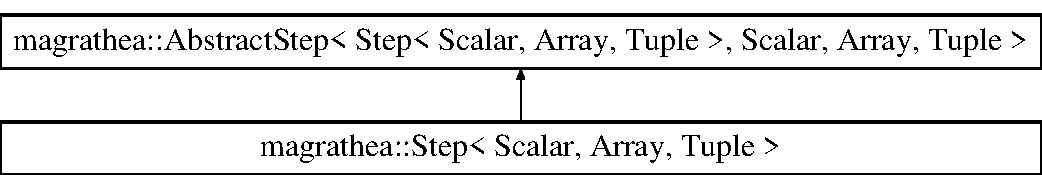
\includegraphics[height=2.000000cm]{exceptionmagrathea_1_1Step}
\end{center}
\end{figure}
\subsection*{Public Member Functions}
\begin{Indent}{\bf Lifecycle}\par
\begin{DoxyCompactItemize}
\item 
{\footnotesize template$<$class... Misc$>$ }\\\hyperlink{exceptionmagrathea_1_1Step_ac143df9cbe3e5791ac86c653a49ca02b}{Step} (Misc \&\&...misc)
\begin{DoxyCompactList}\small\item\em Explicit generic constructor. \end{DoxyCompactList}\end{DoxyCompactItemize}
\end{Indent}
\subsection*{Static Public Member Functions}
\begin{Indent}{\bf Test}\par
\begin{DoxyCompactItemize}
\item 
static int \hyperlink{exceptionmagrathea_1_1Step_a370057ab460a1568f615d26ae075d32d}{example} ()
\begin{DoxyCompactList}\small\item\em Example function. \end{DoxyCompactList}\end{DoxyCompactItemize}
\end{Indent}
\subsection*{Public Attributes}
\begin{DoxyCompactItemize}
\item 
using \hyperlink{exceptionmagrathea_1_1Step_a9c3ad1ac4dff397aafecac1c5675a132}{operator} = typedef
\end{DoxyCompactItemize}
\subsection*{Additional Inherited Members}


\subsection{Detailed Description}
\subsubsection*{template$<$class Scalar = unsigned int, class Array = std\-::array$<$double, 0$>$, class Tuple = std\-::tuple$<$$>$$>$exception magrathea\-::\-Step$<$ Scalar, Array, Tuple $>$}

Basic implementation of an evolution step. 

This class is the direct derivation of \hyperlink{classmagrathea_1_1AbstractStep}{Abstract\-Step}. It provides the most basic and generic contents object without adding new functionalities to the abstract class. It can be used in most cases as a generic container for evolution data. 
\begin{DoxyTemplParams}{Template Parameters}
{\em Scalar} & Scalar type of id. \\
\hline
{\em Array} & Array type of core quantities. \\
\hline
{\em Tuple} & Tuple type of extra quantities. \\
\hline
\end{DoxyTemplParams}


\subsection{Constructor \& Destructor Documentation}
\hypertarget{exceptionmagrathea_1_1Step_ac143df9cbe3e5791ac86c653a49ca02b}{\index{magrathea\-::\-Step@{magrathea\-::\-Step}!Step@{Step}}
\index{Step@{Step}!magrathea::Step@{magrathea\-::\-Step}}
\subsubsection[{Step}]{\setlength{\rightskip}{0pt plus 5cm}template$<$class Scalar , class Array , class Tuple $>$ template$<$class... Misc$>$ {\bf magrathea\-::\-Step}$<$ Scalar, Array, Tuple $>$\-::{\bf Step} (
\begin{DoxyParamCaption}
\item[{Misc \&\&...}]{misc}
\end{DoxyParamCaption}
)\hspace{0.3cm}{\ttfamily [inline]}, {\ttfamily [explicit]}}}\label{exceptionmagrathea_1_1Step_ac143df9cbe3e5791ac86c653a49ca02b}


Explicit generic constructor. 

Provides a generic interface to all constructors of the base class. 
\begin{DoxyTemplParams}{Template Parameters}
{\em Misc} & (\hyperlink{classMiscellaneous}{Miscellaneous} types.) \\
\hline
\end{DoxyTemplParams}

\begin{DoxyParams}[1]{Parameters}
\mbox{\tt in}  & {\em misc} & \hyperlink{classMiscellaneous}{Miscellaneous} arguments. \\
\hline
\end{DoxyParams}


\subsection{Member Function Documentation}
\hypertarget{exceptionmagrathea_1_1Step_a370057ab460a1568f615d26ae075d32d}{\index{magrathea\-::\-Step@{magrathea\-::\-Step}!example@{example}}
\index{example@{example}!magrathea::Step@{magrathea\-::\-Step}}
\subsubsection[{example}]{\setlength{\rightskip}{0pt plus 5cm}template$<$class Scalar , class Array , class Tuple $>$ int {\bf magrathea\-::\-Step}$<$ Scalar, Array, Tuple $>$\-::example (
\begin{DoxyParamCaption}
{}
\end{DoxyParamCaption}
)\hspace{0.3cm}{\ttfamily [static]}}}\label{exceptionmagrathea_1_1Step_a370057ab460a1568f615d26ae075d32d}


Example function. 

Tests and demonstrates the use of \hyperlink{exceptionmagrathea_1_1Step}{Step}. \begin{DoxyReturn}{Returns}
0 if no error. 
\end{DoxyReturn}


\subsection{Member Data Documentation}
\hypertarget{exceptionmagrathea_1_1Step_a9c3ad1ac4dff397aafecac1c5675a132}{\index{magrathea\-::\-Step@{magrathea\-::\-Step}!operator@{operator}}
\index{operator@{operator}!magrathea::Step@{magrathea\-::\-Step}}
\subsubsection[{operator}]{\setlength{\rightskip}{0pt plus 5cm}template$<$class Scalar = unsigned int, class Array = std\-::array$<$double, 0$>$, class Tuple = std\-::tuple$<$$>$$>$ using {\bf magrathea\-::\-Step}$<$ Scalar, Array, Tuple $>$\-::operator = }}\label{exceptionmagrathea_1_1Step_a9c3ad1ac4dff397aafecac1c5675a132}


The documentation for this exception was generated from the following file\-:\begin{DoxyCompactItemize}
\item 
/data/home/mbreton/magrathea\-\_\-pathfinder/src/magrathea/\hyperlink{step_8h}{step.\-h}\end{DoxyCompactItemize}

\hypertarget{exceptionmagrathea_1_1Substance}{\section{magrathea\-:\-:Substance$<$ Types $>$ Exception Template Reference}
\label{exceptionmagrathea_1_1Substance}\index{magrathea\-::\-Substance$<$ Types $>$@{magrathea\-::\-Substance$<$ Types $>$}}
}


Basic implementation of geometrical substance.  




{\ttfamily \#include $<$substance.\-h$>$}

Inheritance diagram for magrathea\-:\-:Substance$<$ Types $>$\-:\begin{figure}[H]
\begin{center}
\leavevmode
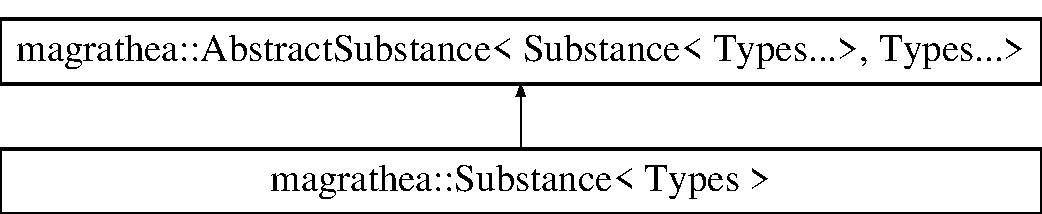
\includegraphics[height=2.000000cm]{exceptionmagrathea_1_1Substance}
\end{center}
\end{figure}
\subsection*{Public Member Functions}
\begin{Indent}{\bf Lifecycle}\par
\begin{DoxyCompactItemize}
\item 
{\footnotesize template$<$class... Misc$>$ }\\\hyperlink{exceptionmagrathea_1_1Substance_a0130a4da42ee12308959ad06b664d379}{Substance} (Misc \&\&...misc)
\begin{DoxyCompactList}\small\item\em Explicit generic constructor. \end{DoxyCompactList}\end{DoxyCompactItemize}
\end{Indent}
\subsection*{Static Public Member Functions}
\begin{Indent}{\bf Test}\par
\begin{DoxyCompactItemize}
\item 
static int \hyperlink{exceptionmagrathea_1_1Substance_a39e13a647bb62526ddecc9b99c943616}{example} ()
\begin{DoxyCompactList}\small\item\em Example function. \end{DoxyCompactList}\end{DoxyCompactItemize}
\end{Indent}
\subsection*{Public Attributes}
\begin{DoxyCompactItemize}
\item 
using \hyperlink{exceptionmagrathea_1_1Substance_a46ae657c3b2ee4a92ebb06faa3eb639b}{operator} = typedef
\end{DoxyCompactItemize}
\subsection*{Additional Inherited Members}


\subsection{Detailed Description}
\subsubsection*{template$<$class... Types$>$exception magrathea\-::\-Substance$<$ Types $>$}

Basic implementation of geometrical substance. 

This class is the direct derivation of \hyperlink{classmagrathea_1_1AbstractSubstance}{Abstract\-Substance}. It provides the most basic and generic substance object without adding new functionalities to the abstract class. It can be used in most cases as a generic container of groups of quantities. 
\begin{DoxyTemplParams}{Template Parameters}
{\em Types} & Variadic list of components types. \\
\hline
\end{DoxyTemplParams}


\subsection{Constructor \& Destructor Documentation}
\hypertarget{exceptionmagrathea_1_1Substance_a0130a4da42ee12308959ad06b664d379}{\index{magrathea\-::\-Substance@{magrathea\-::\-Substance}!Substance@{Substance}}
\index{Substance@{Substance}!magrathea::Substance@{magrathea\-::\-Substance}}
\subsubsection[{Substance}]{\setlength{\rightskip}{0pt plus 5cm}template$<$class... Types$>$ template$<$class... Misc$>$ {\bf magrathea\-::\-Substance}$<$ Types $>$\-::{\bf Substance} (
\begin{DoxyParamCaption}
\item[{Misc \&\&...}]{misc}
\end{DoxyParamCaption}
)\hspace{0.3cm}{\ttfamily [inline]}, {\ttfamily [explicit]}}}\label{exceptionmagrathea_1_1Substance_a0130a4da42ee12308959ad06b664d379}


Explicit generic constructor. 

Provides a generic interface to all constructors of the base class. 
\begin{DoxyTemplParams}{Template Parameters}
{\em Misc} & (\hyperlink{classMiscellaneous}{Miscellaneous} types.) \\
\hline
\end{DoxyTemplParams}

\begin{DoxyParams}[1]{Parameters}
\mbox{\tt in}  & {\em misc} & \hyperlink{classMiscellaneous}{Miscellaneous} arguments. \\
\hline
\end{DoxyParams}


\subsection{Member Function Documentation}
\hypertarget{exceptionmagrathea_1_1Substance_a39e13a647bb62526ddecc9b99c943616}{\index{magrathea\-::\-Substance@{magrathea\-::\-Substance}!example@{example}}
\index{example@{example}!magrathea::Substance@{magrathea\-::\-Substance}}
\subsubsection[{example}]{\setlength{\rightskip}{0pt plus 5cm}template$<$class... Types$>$ int {\bf magrathea\-::\-Substance}$<$ Types $>$\-::example (
\begin{DoxyParamCaption}
{}
\end{DoxyParamCaption}
)\hspace{0.3cm}{\ttfamily [static]}}}\label{exceptionmagrathea_1_1Substance_a39e13a647bb62526ddecc9b99c943616}


Example function. 

Tests and demonstrates the use of \hyperlink{exceptionmagrathea_1_1Substance}{Substance}. \begin{DoxyReturn}{Returns}
0 if no error. 
\end{DoxyReturn}


\subsection{Member Data Documentation}
\hypertarget{exceptionmagrathea_1_1Substance_a46ae657c3b2ee4a92ebb06faa3eb639b}{\index{magrathea\-::\-Substance@{magrathea\-::\-Substance}!operator@{operator}}
\index{operator@{operator}!magrathea::Substance@{magrathea\-::\-Substance}}
\subsubsection[{operator}]{\setlength{\rightskip}{0pt plus 5cm}template$<$class... Types$>$ using {\bf magrathea\-::\-Substance}$<$ Types $>$\-::operator = }}\label{exceptionmagrathea_1_1Substance_a46ae657c3b2ee4a92ebb06faa3eb639b}


The documentation for this exception was generated from the following file\-:\begin{DoxyCompactItemize}
\item 
/data/home/mbreton/magrathea\-\_\-pathfinder/src/magrathea/\hyperlink{substance_8h}{substance.\-h}\end{DoxyCompactItemize}

\hypertarget{exceptionmagrathea_1_1Timer}{\section{magrathea\-:\-:Timer$<$ Type, Period, Clock $>$ Exception Template Reference}
\label{exceptionmagrathea_1_1Timer}\index{magrathea\-::\-Timer$<$ Type, Period, Clock $>$@{magrathea\-::\-Timer$<$ Type, Period, Clock $>$}}
}


A timer to manage time measurements and benchmarks.  




{\ttfamily \#include $<$timer.\-h$>$}

\subsection*{Public Member Functions}
\begin{Indent}{\bf Lifecycle}\par
\begin{DoxyCompactItemize}
\item 
{\footnotesize template$<$class Duration  = Type, class Reference\-Time\-Point  = std\-::true\-\_\-type, class Beginning\-Time\-Point  = std\-::true\-\_\-type, class Ending\-Time\-Point  = std\-::true\-\_\-type$>$ }\\\hyperlink{exceptionmagrathea_1_1Timer_a48652f7ff9a46b997f857375b83da6f5}{Timer} (const bool running0=false, const Duration \&record0=Duration(), const Reference\-Time\-Point \&reference0=Reference\-Time\-Point(), const Beginning\-Time\-Point \&beginning0=Beginning\-Time\-Point(), const Ending\-Time\-Point \&ending0=Ending\-Time\-Point())
\begin{DoxyCompactList}\small\item\em Implicit contents constructor. \end{DoxyCompactList}\item 
{\footnotesize template$<$typename Other\-Type , class Other\-Period $>$ }\\\hyperlink{exceptionmagrathea_1_1Timer_afd27dbe98da7c62058bf01f5a8b294b8}{Timer} (const \hyperlink{exceptionmagrathea_1_1Timer}{Timer}$<$ Other\-Type, Other\-Period, Clock $>$ \&source)
\begin{DoxyCompactList}\small\item\em Implicit conversion constructor. \end{DoxyCompactList}\end{DoxyCompactItemize}
\end{Indent}
\begin{Indent}{\bf Operators}\par
\begin{DoxyCompactItemize}
\item 
{\footnotesize template$<$typename Other\-Type , class Other\-Period $>$ }\\\hyperlink{exceptionmagrathea_1_1Timer}{Timer}$<$ Type, Period, Clock $>$ \& \hyperlink{exceptionmagrathea_1_1Timer_ae30b45ad6c7970c4c32489463e83729a}{operator=} (const \hyperlink{exceptionmagrathea_1_1Timer}{Timer}$<$ Other\-Type, Other\-Period, Clock $>$ \&rhs)
\begin{DoxyCompactList}\small\item\em Conversion assignment operator. \end{DoxyCompactList}\item 
Type \hyperlink{exceptionmagrathea_1_1Timer_aa31ac99d8da5b7d928ff6c451b9e1142}{operator()} () const 
\begin{DoxyCompactList}\small\item\em Total duration extraction operator. \end{DoxyCompactList}\end{DoxyCompactItemize}
\end{Indent}
\begin{Indent}{\bf Assignment}\par
\begin{DoxyCompactItemize}
\item 
{\footnotesize template$<$class Duration  = Type, class Reference\-Time\-Point  = std\-::true\-\_\-type, class Beginning\-Time\-Point  = std\-::true\-\_\-type, class Ending\-Time\-Point  = std\-::true\-\_\-type$>$ }\\\hyperlink{exceptionmagrathea_1_1Timer}{Timer}$<$ Type, Period, Clock $>$ \& \hyperlink{exceptionmagrathea_1_1Timer_a02d55fbb8de54e4ec47ffd03eb077a64}{assign} (const bool running0=false, const Duration \&record0=Duration(), const Reference\-Time\-Point \&reference0=Reference\-Time\-Point(), const Beginning\-Time\-Point \&beginning0=Beginning\-Time\-Point(), const Ending\-Time\-Point \&ending0=Ending\-Time\-Point())
\begin{DoxyCompactList}\small\item\em \hyperlink{exceptionmagrathea_1_1Contents}{Contents} assignment. \end{DoxyCompactList}\item 
{\footnotesize template$<$typename Other\-Type , class Other\-Period $>$ }\\\hyperlink{exceptionmagrathea_1_1Timer}{Timer}$<$ Type, Period, Clock $>$ \& \hyperlink{exceptionmagrathea_1_1Timer_a5a3a60dfcc1e2dc22dcbd2e9c0d49994}{assign} (const \hyperlink{exceptionmagrathea_1_1Timer}{Timer}$<$ Other\-Type, Other\-Period, Clock $>$ \&source)
\begin{DoxyCompactList}\small\item\em Conversion assignment. \end{DoxyCompactList}\end{DoxyCompactItemize}
\end{Indent}
\begin{Indent}{\bf Management}\par
\begin{DoxyCompactItemize}
\item 
\hyperlink{exceptionmagrathea_1_1Timer}{Timer}$<$ Type, Period, Clock $>$ \hyperlink{exceptionmagrathea_1_1Timer_aaf4f6405126d6324cdbc4c67884c23bf}{copy} () const 
\begin{DoxyCompactList}\small\item\em Copy. \end{DoxyCompactList}\item 
{\footnotesize template$<$typename Other\-Type  = Type, class Other\-Period  = Period$>$ }\\\hyperlink{exceptionmagrathea_1_1Timer}{Timer}$<$ Other\-Type, Other\-Period, \\*
Clock $>$ \hyperlink{exceptionmagrathea_1_1Timer_ac0c22623a1a2f0180781e67ba44f9988}{cast} () const 
\begin{DoxyCompactList}\small\item\em Cast. \end{DoxyCompactList}\end{DoxyCompactItemize}
\end{Indent}
\begin{Indent}{\bf Getters}\par
\begin{DoxyCompactItemize}
\item 
const bool \& \hyperlink{exceptionmagrathea_1_1Timer_a0b3f41a0ad4242f465f096a39d4d9009}{running} () const 
\begin{DoxyCompactList}\small\item\em Get whether the timer is running. \end{DoxyCompactList}\item 
const Clock\-::duration \& \hyperlink{exceptionmagrathea_1_1Timer_ae51eb0a72eff6505564120765f7f5a97}{record} () const 
\begin{DoxyCompactList}\small\item\em Get the saved duration. \end{DoxyCompactList}\item 
const Clock\-::time\-\_\-point \& \hyperlink{exceptionmagrathea_1_1Timer_a0da629c75fa145b8bd28b8e913b1561e}{reference} () const 
\begin{DoxyCompactList}\small\item\em Get the reference time point. \end{DoxyCompactList}\item 
const Clock\-::time\-\_\-point \& \hyperlink{exceptionmagrathea_1_1Timer_a2b761324b0c76873464a3f2e015c171f}{beginning} () const 
\begin{DoxyCompactList}\small\item\em Get the beginning time point. \end{DoxyCompactList}\item 
const Clock\-::time\-\_\-point \& \hyperlink{exceptionmagrathea_1_1Timer_affe899a3821a020dbef1ce2f3737c8ad}{ending} () const 
\begin{DoxyCompactList}\small\item\em Get the ending time point. \end{DoxyCompactList}\end{DoxyCompactItemize}
\end{Indent}
\begin{Indent}{\bf Actions}\par
\begin{DoxyCompactItemize}
\item 
std\-::chrono\-::duration$<$ Type, \\*
Period $>$ \hyperlink{exceptionmagrathea_1_1Timer_a76a3e527e10929ce89ea8dce211ed5d3}{reset} ()
\begin{DoxyCompactList}\small\item\em Reset timer. \end{DoxyCompactList}\item 
std\-::chrono\-::duration$<$ Type, \\*
Period $>$ \hyperlink{exceptionmagrathea_1_1Timer_aa5ff5a3ddd22202435d2bf149cf0c1de}{start} ()
\begin{DoxyCompactList}\small\item\em Start timer. \end{DoxyCompactList}\item 
std\-::chrono\-::duration$<$ Type, \\*
Period $>$ \hyperlink{exceptionmagrathea_1_1Timer_a178fa98482e7240a799fc438a16e37ea}{stop} ()
\begin{DoxyCompactList}\small\item\em Stop timer. \end{DoxyCompactList}\end{DoxyCompactItemize}
\end{Indent}
\begin{Indent}{\bf Measurement}\par
\begin{DoxyCompactItemize}
\item 
std\-::chrono\-::duration$<$ Type, \\*
Period $>$ \hyperlink{exceptionmagrathea_1_1Timer_a774c96d0d0ffb1ccc02dac73d65f6709}{current} () const 
\begin{DoxyCompactList}\small\item\em Duration since last start. \end{DoxyCompactList}\item 
std\-::chrono\-::duration$<$ Type, \\*
Period $>$ \hyperlink{exceptionmagrathea_1_1Timer_ab17dc88ef072205f472d387f4dea1033}{total} () const 
\begin{DoxyCompactList}\small\item\em Total duration. \end{DoxyCompactList}\item 
std\-::chrono\-::duration$<$ Type, \\*
Period $>$ \hyperlink{exceptionmagrathea_1_1Timer_a6e4a9f49df93c2620c4703fad36b1678}{real} () const 
\begin{DoxyCompactList}\small\item\em Real duration. \end{DoxyCompactList}\end{DoxyCompactItemize}
\end{Indent}
\subsection*{Static Public Member Functions}
\begin{Indent}{\bf Utilities}\par
\begin{DoxyCompactItemize}
\item 
{\footnotesize template$<$class Duration  = Type, typename Counter  = unsigned long long int$>$ }\\static std\-::chrono\-::duration\\*
$<$ Type, Period $>$ \hyperlink{exceptionmagrathea_1_1Timer_a5636affbf45384af93ab036eb15ab274}{wait} (const Duration \&delay=Duration(1), Counter \&\&counter=Counter())
\begin{DoxyCompactList}\small\item\em Wait a certain time. \end{DoxyCompactList}\item 
{\footnotesize template$<$typename Counter , class Function , class... Args$>$ }\\static std\-::chrono\-::duration\\*
$<$ Type, Period $>$ \hyperlink{exceptionmagrathea_1_1Timer_a5ede3d60334682c611c64dadd218b225}{benchmark} (const Counter \&counter, Function \&\&f, Args \&\&...args)
\begin{DoxyCompactList}\small\item\em Benchmark a function. \end{DoxyCompactList}\end{DoxyCompactItemize}
\end{Indent}
\begin{Indent}{\bf Test}\par
\begin{DoxyCompactItemize}
\item 
static int \hyperlink{exceptionmagrathea_1_1Timer_a3dcb379540e25030a60b48319d1448d7}{example} ()
\begin{DoxyCompactList}\small\item\em Example function. \end{DoxyCompactList}\end{DoxyCompactItemize}
\end{Indent}
\subsection*{Protected Attributes}
\begin{Indent}{\bf Data members}\par
\begin{DoxyCompactItemize}
\item 
bool \hyperlink{exceptionmagrathea_1_1Timer_a633b668aeba423f9d6229bce33267226}{\-\_\-running}
\begin{DoxyCompactList}\small\item\em Flag to indicate whether a measurement is running or not. \end{DoxyCompactList}\item 
Clock\-::duration \hyperlink{exceptionmagrathea_1_1Timer_a1fb0110e524e12e39685ef9e5312d3f4}{\-\_\-record}
\begin{DoxyCompactList}\small\item\em Internal backup of duration. \end{DoxyCompactList}\item 
Clock\-::time\-\_\-point \hyperlink{exceptionmagrathea_1_1Timer_ad08277afa11789b6ea4cb88ed9f7c28b}{\-\_\-reference}
\begin{DoxyCompactList}\small\item\em Reference time point for measurements. \end{DoxyCompactList}\item 
Clock\-::time\-\_\-point \hyperlink{exceptionmagrathea_1_1Timer_a6c71f8b0c5557836e48043ff6bad791d}{\-\_\-beginning}
\begin{DoxyCompactList}\small\item\em Beginning time point for measurements. \end{DoxyCompactList}\item 
Clock\-::time\-\_\-point \hyperlink{exceptionmagrathea_1_1Timer_a005c041aa6b61e1f6c365fa6c4d7151d}{\-\_\-ending}
\begin{DoxyCompactList}\small\item\em Ending time point for measurements. \end{DoxyCompactList}\end{DoxyCompactItemize}
\end{Indent}
\subsection*{Friends}
\begin{Indent}{\bf Stream}\par
\begin{DoxyCompactItemize}
\item 
{\footnotesize template$<$typename Self\-Type , class Self\-Period , class Self\-Clock $>$ }\\std\-::ostream \& \hyperlink{exceptionmagrathea_1_1Timer_a9b9e2a214358571c47b7159572accf67}{operator$<$$<$} (std\-::ostream \&lhs, const \hyperlink{exceptionmagrathea_1_1Timer}{Timer}$<$ Self\-Type, Self\-Period, Self\-Clock $>$ \&rhs)
\begin{DoxyCompactList}\small\item\em \hyperlink{exceptionOutput}{Output} stream operator. \end{DoxyCompactList}\end{DoxyCompactItemize}
\end{Indent}


\subsection{Detailed Description}
\subsubsection*{template$<$typename Type = double, class Period = std\-::chrono\-::seconds\-::period, class Clock = std\-::chrono\-::steady\-\_\-clock$>$exception magrathea\-::\-Timer$<$ Type, Period, Clock $>$}

A timer to manage time measurements and benchmarks. 

Provides a wrapper of {\ttfamily std\-::chrono} for an easy use and basic operations needed by time execution management. It has two internal times points \-: one to mark the beginning of a measurement, and one to mark the end of the current measurement. It has also a reference time point to evaluate real elasped time. 
\begin{DoxyTemplParams}{Template Parameters}
{\em Type} & Duration representation type. \\
\hline
{\em Period} & Standard ratio representing the tick period. \\
\hline
{\em Clock} & Internal clock type. \\
\hline
\end{DoxyTemplParams}


\subsection{Constructor \& Destructor Documentation}
\hypertarget{exceptionmagrathea_1_1Timer_a48652f7ff9a46b997f857375b83da6f5}{\index{magrathea\-::\-Timer@{magrathea\-::\-Timer}!Timer@{Timer}}
\index{Timer@{Timer}!magrathea::Timer@{magrathea\-::\-Timer}}
\subsubsection[{Timer}]{\setlength{\rightskip}{0pt plus 5cm}template$<$typename Type , class Period , class Clock $>$ template$<$class Duration , class Reference\-Time\-Point , class Beginning\-Time\-Point , class Ending\-Time\-Point $>$ {\bf magrathea\-::\-Timer}$<$ Type, Period, Clock $>$\-::{\bf Timer} (
\begin{DoxyParamCaption}
\item[{const bool}]{running0 = {\ttfamily false}, }
\item[{const Duration \&}]{record0 = {\ttfamily Duration()}, }
\item[{const Reference\-Time\-Point \&}]{reference0 = {\ttfamily ReferenceTimePoint()}, }
\item[{const Beginning\-Time\-Point \&}]{beginning0 = {\ttfamily BeginningTimePoint()}, }
\item[{const Ending\-Time\-Point \&}]{ending0 = {\ttfamily EndingTimePoint()}}
\end{DoxyParamCaption}
)\hspace{0.3cm}{\ttfamily [inline]}}}\label{exceptionmagrathea_1_1Timer_a48652f7ff9a46b997f857375b83da6f5}


Implicit contents constructor. 

Provides a construction from every single parameter of the timer \-: the current record of duration, the time of reference, the time of the last start, the time of the last stop, and whether the timer is running. If no reference is provided, the current time is set. If no beginning time is provided, it is set to the reference time. If no ending time is provided, it is set to the beginning. 
\begin{DoxyTemplParams}{Template Parameters}
{\em Duration} & (Standard duration type or arithmetic type.) \\
\hline
{\em Reference\-Time\-Point} & (Time point type of the reference.) \\
\hline
{\em Beginning\-Time\-Point} & (Time point type of the beginning time.) \\
\hline
{\em Ending\-Time\-Point} & (Time point type of the ending time.) \\
\hline
\end{DoxyTemplParams}

\begin{DoxyParams}[1]{Parameters}
\mbox{\tt in}  & {\em running0} & \hyperlink{exceptionInput}{Input} value of whether the timer is running. \\
\hline
\mbox{\tt in}  & {\em record0} & \hyperlink{exceptionInput}{Input} value of the backup of duration. \\
\hline
\mbox{\tt in}  & {\em reference0} & \hyperlink{exceptionInput}{Input} value of the reference time. \\
\hline
\mbox{\tt in}  & {\em beginning0} & \hyperlink{exceptionInput}{Input} value of the beginning time. \\
\hline
\mbox{\tt in}  & {\em ending0} & \hyperlink{exceptionInput}{Input} value of the ending time. \\
\hline
\end{DoxyParams}
\hypertarget{exceptionmagrathea_1_1Timer_afd27dbe98da7c62058bf01f5a8b294b8}{\index{magrathea\-::\-Timer@{magrathea\-::\-Timer}!Timer@{Timer}}
\index{Timer@{Timer}!magrathea::Timer@{magrathea\-::\-Timer}}
\subsubsection[{Timer}]{\setlength{\rightskip}{0pt plus 5cm}template$<$typename Type , class Period , class Clock $>$ template$<$typename Other\-Type , class Other\-Period $>$ {\bf magrathea\-::\-Timer}$<$ Type, Period, Clock $>$\-::{\bf Timer} (
\begin{DoxyParamCaption}
\item[{const {\bf Timer}$<$ Other\-Type, Other\-Period, Clock $>$ \&}]{source}
\end{DoxyParamCaption}
)\hspace{0.3cm}{\ttfamily [inline]}}}\label{exceptionmagrathea_1_1Timer_afd27dbe98da7c62058bf01f5a8b294b8}


Implicit conversion constructor. 

Provides a construction from a timer of another type. 
\begin{DoxyTemplParams}{Template Parameters}
{\em Other\-Type} & (Other duration representation type.) \\
\hline
{\em Other\-Period} & (Other standard ratio representing the tick period.) \\
\hline
\end{DoxyTemplParams}

\begin{DoxyParams}[1]{Parameters}
\mbox{\tt in}  & {\em source} & Source of the copy. \\
\hline
\end{DoxyParams}


\subsection{Member Function Documentation}
\hypertarget{exceptionmagrathea_1_1Timer_a02d55fbb8de54e4ec47ffd03eb077a64}{\index{magrathea\-::\-Timer@{magrathea\-::\-Timer}!assign@{assign}}
\index{assign@{assign}!magrathea::Timer@{magrathea\-::\-Timer}}
\subsubsection[{assign}]{\setlength{\rightskip}{0pt plus 5cm}template$<$typename Type , class Period , class Clock $>$ template$<$class Duration , class Reference\-Time\-Point , class Beginning\-Time\-Point , class Ending\-Time\-Point $>$ {\bf Timer}$<$ Type, Period, Clock $>$ \& {\bf magrathea\-::\-Timer}$<$ Type, Period, Clock $>$\-::assign (
\begin{DoxyParamCaption}
\item[{const bool}]{running0 = {\ttfamily false}, }
\item[{const Duration \&}]{record0 = {\ttfamily Duration()}, }
\item[{const Reference\-Time\-Point \&}]{reference0 = {\ttfamily ReferenceTimePoint()}, }
\item[{const Beginning\-Time\-Point \&}]{beginning0 = {\ttfamily BeginningTimePoint()}, }
\item[{const Ending\-Time\-Point \&}]{ending0 = {\ttfamily EndingTimePoint()}}
\end{DoxyParamCaption}
)\hspace{0.3cm}{\ttfamily [inline]}}}\label{exceptionmagrathea_1_1Timer_a02d55fbb8de54e4ec47ffd03eb077a64}


\hyperlink{exceptionmagrathea_1_1Contents}{Contents} assignment. 

Assigns contents from every single parameter of the timer \-: the current record of duration, the time of reference, the time of the last start, the time of the last stop, and whether the timer is running. If no reference is provided, the current time is set. If no beginning time is provided, it is set to the reference time. If no ending time is provided, it is set to the beginning. 
\begin{DoxyTemplParams}{Template Parameters}
{\em Duration} & (Standard duration type or arithmetic type.) \\
\hline
{\em Reference\-Time\-Point} & (Time point type of the reference.) \\
\hline
{\em Beginning\-Time\-Point} & (Time point type of the beginning time.) \\
\hline
{\em Ending\-Time\-Point} & (Time point type of the ending time.) \\
\hline
\end{DoxyTemplParams}

\begin{DoxyParams}[1]{Parameters}
\mbox{\tt in}  & {\em running0} & \hyperlink{exceptionInput}{Input} value of whether the timer is running. \\
\hline
\mbox{\tt in}  & {\em record0} & \hyperlink{exceptionInput}{Input} value of the backup of duration. \\
\hline
\mbox{\tt in}  & {\em reference0} & \hyperlink{exceptionInput}{Input} value of the reference time. \\
\hline
\mbox{\tt in}  & {\em beginning0} & \hyperlink{exceptionInput}{Input} value of the beginning time. \\
\hline
\mbox{\tt in}  & {\em ending0} & \hyperlink{exceptionInput}{Input} value of the ending time. \\
\hline
\end{DoxyParams}
\begin{DoxyReturn}{Returns}
Self reference. 
\end{DoxyReturn}
\hypertarget{exceptionmagrathea_1_1Timer_a5a3a60dfcc1e2dc22dcbd2e9c0d49994}{\index{magrathea\-::\-Timer@{magrathea\-::\-Timer}!assign@{assign}}
\index{assign@{assign}!magrathea::Timer@{magrathea\-::\-Timer}}
\subsubsection[{assign}]{\setlength{\rightskip}{0pt plus 5cm}template$<$typename Type , class Period , class Clock $>$ template$<$typename Other\-Type , class Other\-Period $>$ {\bf Timer}$<$ Type, Period, Clock $>$ \& {\bf magrathea\-::\-Timer}$<$ Type, Period, Clock $>$\-::assign (
\begin{DoxyParamCaption}
\item[{const {\bf Timer}$<$ Other\-Type, Other\-Period, Clock $>$ \&}]{source}
\end{DoxyParamCaption}
)\hspace{0.3cm}{\ttfamily [inline]}}}\label{exceptionmagrathea_1_1Timer_a5a3a60dfcc1e2dc22dcbd2e9c0d49994}


Conversion assignment. 

Assigns the contents from a timer of another type. 
\begin{DoxyTemplParams}{Template Parameters}
{\em Other\-Type} & (Other duration representation type.) \\
\hline
{\em Other\-Period} & (Other standard ratio representing the tick period.) \\
\hline
\end{DoxyTemplParams}

\begin{DoxyParams}[1]{Parameters}
\mbox{\tt in}  & {\em source} & Source of the copy. \\
\hline
\end{DoxyParams}
\begin{DoxyReturn}{Returns}
Self reference. 
\end{DoxyReturn}
\hypertarget{exceptionmagrathea_1_1Timer_a2b761324b0c76873464a3f2e015c171f}{\index{magrathea\-::\-Timer@{magrathea\-::\-Timer}!beginning@{beginning}}
\index{beginning@{beginning}!magrathea::Timer@{magrathea\-::\-Timer}}
\subsubsection[{beginning}]{\setlength{\rightskip}{0pt plus 5cm}template$<$typename Type , class Period , class Clock $>$ const Clock\-::time\-\_\-point \& {\bf magrathea\-::\-Timer}$<$ Type, Period, Clock $>$\-::beginning (
\begin{DoxyParamCaption}
{}
\end{DoxyParamCaption}
) const\hspace{0.3cm}{\ttfamily [inline]}}}\label{exceptionmagrathea_1_1Timer_a2b761324b0c76873464a3f2e015c171f}


Get the beginning time point. 

Returns the beginning time point, which is generally the time point of the last start. \begin{DoxyReturn}{Returns}
Beginning time point. 
\end{DoxyReturn}
\hypertarget{exceptionmagrathea_1_1Timer_a5ede3d60334682c611c64dadd218b225}{\index{magrathea\-::\-Timer@{magrathea\-::\-Timer}!benchmark@{benchmark}}
\index{benchmark@{benchmark}!magrathea::Timer@{magrathea\-::\-Timer}}
\subsubsection[{benchmark}]{\setlength{\rightskip}{0pt plus 5cm}template$<$typename Type , class Period , class Clock $>$ template$<$typename Counter , class Function , class... Args$>$ std\-::chrono\-::duration$<$ Type, Period $>$ {\bf magrathea\-::\-Timer}$<$ Type, Period, Clock $>$\-::benchmark (
\begin{DoxyParamCaption}
\item[{const Counter \&}]{counter, }
\item[{Function \&\&}]{f, }
\item[{Args \&\&...}]{args}
\end{DoxyParamCaption}
)\hspace{0.3cm}{\ttfamily [inline]}, {\ttfamily [static]}}}\label{exceptionmagrathea_1_1Timer_a5ede3d60334682c611c64dadd218b225}


Benchmark a function. 

Executes the provided function in a loop and computes the total time needed to run it. The call uses a volatile temporary to prevent null statement optimization, but some compilers may manage to optimize that. The results are not guaranteed to be exact and should be checked with a real benchmarking suite. The returned time correspond to the time of function execution plus the time of the copy. 
\begin{DoxyTemplParams}{Template Parameters}
{\em Counter} & (Type that can be incremented.) \\
\hline
{\em Function} & (Function type \-: {\ttfamily Something(Args...)}.) \\
\hline
{\em Args} & (Arguments types.) \\
\hline
\end{DoxyTemplParams}

\begin{DoxyParams}[1]{Parameters}
\mbox{\tt in}  & {\em counter} & Number of loops to do. \\
\hline
\mbox{\tt in}  & {\em f} & Function object {\ttfamily Something(Args...)}. \\
\hline
\mbox{\tt in}  & {\em args} & Arguments of the function. \\
\hline
\end{DoxyParams}
\begin{DoxyReturn}{Returns}
Total duration of loop execution. 
\end{DoxyReturn}
\hypertarget{exceptionmagrathea_1_1Timer_ac0c22623a1a2f0180781e67ba44f9988}{\index{magrathea\-::\-Timer@{magrathea\-::\-Timer}!cast@{cast}}
\index{cast@{cast}!magrathea::Timer@{magrathea\-::\-Timer}}
\subsubsection[{cast}]{\setlength{\rightskip}{0pt plus 5cm}template$<$typename Type , class Period , class Clock $>$ template$<$typename Other\-Type , class Other\-Period $>$ {\bf Timer}$<$ Other\-Type, Other\-Period, Clock $>$ {\bf magrathea\-::\-Timer}$<$ Type, Period, Clock $>$\-::cast (
\begin{DoxyParamCaption}
{}
\end{DoxyParamCaption}
) const\hspace{0.3cm}{\ttfamily [inline]}}}\label{exceptionmagrathea_1_1Timer_ac0c22623a1a2f0180781e67ba44f9988}


Cast. 

Casts the timer to another timer type with another period. 
\begin{DoxyTemplParams}{Template Parameters}
{\em Other\-Type} & Other duration representation type. \\
\hline
{\em Other\-Period} & Other standard ratio representing the tick period. \\
\hline
\end{DoxyTemplParams}
\begin{DoxyReturn}{Returns}
Copy. 
\end{DoxyReturn}
\hypertarget{exceptionmagrathea_1_1Timer_aaf4f6405126d6324cdbc4c67884c23bf}{\index{magrathea\-::\-Timer@{magrathea\-::\-Timer}!copy@{copy}}
\index{copy@{copy}!magrathea::Timer@{magrathea\-::\-Timer}}
\subsubsection[{copy}]{\setlength{\rightskip}{0pt plus 5cm}template$<$typename Type , class Period , class Clock $>$ {\bf Timer}$<$ Type, Period, Clock $>$ {\bf magrathea\-::\-Timer}$<$ Type, Period, Clock $>$\-::copy (
\begin{DoxyParamCaption}
{}
\end{DoxyParamCaption}
) const\hspace{0.3cm}{\ttfamily [inline]}}}\label{exceptionmagrathea_1_1Timer_aaf4f6405126d6324cdbc4c67884c23bf}


Copy. 

Returns a copy of the timer. \begin{DoxyReturn}{Returns}
Copy. 
\end{DoxyReturn}
\hypertarget{exceptionmagrathea_1_1Timer_a774c96d0d0ffb1ccc02dac73d65f6709}{\index{magrathea\-::\-Timer@{magrathea\-::\-Timer}!current@{current}}
\index{current@{current}!magrathea::Timer@{magrathea\-::\-Timer}}
\subsubsection[{current}]{\setlength{\rightskip}{0pt plus 5cm}template$<$typename Type , class Period , class Clock $>$ std\-::chrono\-::duration$<$ Type, Period $>$ {\bf magrathea\-::\-Timer}$<$ Type, Period, Clock $>$\-::current (
\begin{DoxyParamCaption}
{}
\end{DoxyParamCaption}
) const\hspace{0.3cm}{\ttfamily [inline]}}}\label{exceptionmagrathea_1_1Timer_a774c96d0d0ffb1ccc02dac73d65f6709}


Duration since last start. 

Computes the duration since last start \-: if the timer is still running, it computes the difference between the call time and the last start time and if the timer is not running it returns the difference between the last start and the last stop. \begin{DoxyReturn}{Returns}
Current duration. 
\end{DoxyReturn}
\hypertarget{exceptionmagrathea_1_1Timer_affe899a3821a020dbef1ce2f3737c8ad}{\index{magrathea\-::\-Timer@{magrathea\-::\-Timer}!ending@{ending}}
\index{ending@{ending}!magrathea::Timer@{magrathea\-::\-Timer}}
\subsubsection[{ending}]{\setlength{\rightskip}{0pt plus 5cm}template$<$typename Type , class Period , class Clock $>$ const Clock\-::time\-\_\-point \& {\bf magrathea\-::\-Timer}$<$ Type, Period, Clock $>$\-::ending (
\begin{DoxyParamCaption}
{}
\end{DoxyParamCaption}
) const\hspace{0.3cm}{\ttfamily [inline]}}}\label{exceptionmagrathea_1_1Timer_affe899a3821a020dbef1ce2f3737c8ad}


Get the ending time point. 

Returns the ending time point, which is generally the time point of the last stop. If the timer is running, then the ending time point is equal to the last start time point. \begin{DoxyReturn}{Returns}
Ending time point. 
\end{DoxyReturn}
\hypertarget{exceptionmagrathea_1_1Timer_a3dcb379540e25030a60b48319d1448d7}{\index{magrathea\-::\-Timer@{magrathea\-::\-Timer}!example@{example}}
\index{example@{example}!magrathea::Timer@{magrathea\-::\-Timer}}
\subsubsection[{example}]{\setlength{\rightskip}{0pt plus 5cm}template$<$typename Type , class Period , class Clock $>$ int {\bf magrathea\-::\-Timer}$<$ Type, Period, Clock $>$\-::example (
\begin{DoxyParamCaption}
{}
\end{DoxyParamCaption}
)\hspace{0.3cm}{\ttfamily [static]}}}\label{exceptionmagrathea_1_1Timer_a3dcb379540e25030a60b48319d1448d7}


Example function. 

Tests and demonstrates the use of \hyperlink{exceptionmagrathea_1_1Timer}{Timer}. \begin{DoxyReturn}{Returns}
0 if no error. 
\end{DoxyReturn}
\hypertarget{exceptionmagrathea_1_1Timer_aa31ac99d8da5b7d928ff6c451b9e1142}{\index{magrathea\-::\-Timer@{magrathea\-::\-Timer}!operator()@{operator()}}
\index{operator()@{operator()}!magrathea::Timer@{magrathea\-::\-Timer}}
\subsubsection[{operator()}]{\setlength{\rightskip}{0pt plus 5cm}template$<$typename Type , class Period , class Clock $>$ Type {\bf magrathea\-::\-Timer}$<$ Type, Period, Clock $>$\-::operator() (
\begin{DoxyParamCaption}
{}
\end{DoxyParamCaption}
) const\hspace{0.3cm}{\ttfamily [inline]}}}\label{exceptionmagrathea_1_1Timer_aa31ac99d8da5b7d928ff6c451b9e1142}


Total duration extraction operator. 

Computes the total elapsed duration between all starts and stops since the last reset and convert it to an arithmetic type. \begin{DoxyReturn}{Returns}
Total duration. 
\end{DoxyReturn}
\hypertarget{exceptionmagrathea_1_1Timer_ae30b45ad6c7970c4c32489463e83729a}{\index{magrathea\-::\-Timer@{magrathea\-::\-Timer}!operator=@{operator=}}
\index{operator=@{operator=}!magrathea::Timer@{magrathea\-::\-Timer}}
\subsubsection[{operator=}]{\setlength{\rightskip}{0pt plus 5cm}template$<$typename Type , class Period , class Clock $>$ template$<$typename Other\-Type , class Other\-Period $>$ {\bf Timer}$<$ Type, Period, Clock $>$ \& {\bf magrathea\-::\-Timer}$<$ Type, Period, Clock $>$\-::operator= (
\begin{DoxyParamCaption}
\item[{const {\bf Timer}$<$ Other\-Type, Other\-Period, Clock $>$ \&}]{rhs}
\end{DoxyParamCaption}
)\hspace{0.3cm}{\ttfamily [inline]}}}\label{exceptionmagrathea_1_1Timer_ae30b45ad6c7970c4c32489463e83729a}


Conversion assignment operator. 

Assigns the contents from a timer of another type. 
\begin{DoxyTemplParams}{Template Parameters}
{\em Other\-Type} & (Other duration representation type.) \\
\hline
{\em Other\-Period} & (Other standard ratio representing the tick period.) \\
\hline
\end{DoxyTemplParams}

\begin{DoxyParams}[1]{Parameters}
\mbox{\tt in}  & {\em rhs} & Right-\/hand side. \\
\hline
\end{DoxyParams}
\begin{DoxyReturn}{Returns}
Self reference. 
\end{DoxyReturn}
\hypertarget{exceptionmagrathea_1_1Timer_a6e4a9f49df93c2620c4703fad36b1678}{\index{magrathea\-::\-Timer@{magrathea\-::\-Timer}!real@{real}}
\index{real@{real}!magrathea::Timer@{magrathea\-::\-Timer}}
\subsubsection[{real}]{\setlength{\rightskip}{0pt plus 5cm}template$<$typename Type , class Period , class Clock $>$ std\-::chrono\-::duration$<$ Type, Period $>$ {\bf magrathea\-::\-Timer}$<$ Type, Period, Clock $>$\-::{\bf real} (
\begin{DoxyParamCaption}
{}
\end{DoxyParamCaption}
) const\hspace{0.3cm}{\ttfamily [inline]}}}\label{exceptionmagrathea_1_1Timer_a6e4a9f49df93c2620c4703fad36b1678}


Real duration. 

Computes the real duration since the last reset without considering any start and stop. \begin{DoxyReturn}{Returns}
Real duration. 
\end{DoxyReturn}
\hypertarget{exceptionmagrathea_1_1Timer_ae51eb0a72eff6505564120765f7f5a97}{\index{magrathea\-::\-Timer@{magrathea\-::\-Timer}!record@{record}}
\index{record@{record}!magrathea::Timer@{magrathea\-::\-Timer}}
\subsubsection[{record}]{\setlength{\rightskip}{0pt plus 5cm}template$<$typename Type , class Period , class Clock $>$ const Clock\-::duration \& {\bf magrathea\-::\-Timer}$<$ Type, Period, Clock $>$\-::record (
\begin{DoxyParamCaption}
{}
\end{DoxyParamCaption}
) const\hspace{0.3cm}{\ttfamily [inline]}}}\label{exceptionmagrathea_1_1Timer_ae51eb0a72eff6505564120765f7f5a97}


Get the saved duration. 

Returns the value of the saved duration which is the total duration saved during the last stop. \begin{DoxyReturn}{Returns}
Duration. 
\end{DoxyReturn}
\hypertarget{exceptionmagrathea_1_1Timer_a0da629c75fa145b8bd28b8e913b1561e}{\index{magrathea\-::\-Timer@{magrathea\-::\-Timer}!reference@{reference}}
\index{reference@{reference}!magrathea::Timer@{magrathea\-::\-Timer}}
\subsubsection[{reference}]{\setlength{\rightskip}{0pt plus 5cm}template$<$typename Type , class Period , class Clock $>$ const Clock\-::time\-\_\-point \& {\bf magrathea\-::\-Timer}$<$ Type, Period, Clock $>$\-::reference (
\begin{DoxyParamCaption}
{}
\end{DoxyParamCaption}
) const\hspace{0.3cm}{\ttfamily [inline]}}}\label{exceptionmagrathea_1_1Timer_a0da629c75fa145b8bd28b8e913b1561e}


Get the reference time point. 

Returns the reference time point, which is generally the time point of the last reset. \begin{DoxyReturn}{Returns}
Reference time point. 
\end{DoxyReturn}
\hypertarget{exceptionmagrathea_1_1Timer_a76a3e527e10929ce89ea8dce211ed5d3}{\index{magrathea\-::\-Timer@{magrathea\-::\-Timer}!reset@{reset}}
\index{reset@{reset}!magrathea::Timer@{magrathea\-::\-Timer}}
\subsubsection[{reset}]{\setlength{\rightskip}{0pt plus 5cm}template$<$typename Type , class Period , class Clock $>$ std\-::chrono\-::duration$<$ Type, Period $>$ {\bf magrathea\-::\-Timer}$<$ Type, Period, Clock $>$\-::reset (
\begin{DoxyParamCaption}
{}
\end{DoxyParamCaption}
)\hspace{0.3cm}{\ttfamily [inline]}}}\label{exceptionmagrathea_1_1Timer_a76a3e527e10929ce89ea8dce211ed5d3}


Reset timer. 

Resets the timer \-: all time points are set to the current time, the duration is set to zero, and the timer is set off. \begin{DoxyReturn}{Returns}
Current duration, which is equal to zero. 
\end{DoxyReturn}
\hypertarget{exceptionmagrathea_1_1Timer_a0b3f41a0ad4242f465f096a39d4d9009}{\index{magrathea\-::\-Timer@{magrathea\-::\-Timer}!running@{running}}
\index{running@{running}!magrathea::Timer@{magrathea\-::\-Timer}}
\subsubsection[{running}]{\setlength{\rightskip}{0pt plus 5cm}template$<$typename Type , class Period , class Clock $>$ const bool \& {\bf magrathea\-::\-Timer}$<$ Type, Period, Clock $>$\-::running (
\begin{DoxyParamCaption}
{}
\end{DoxyParamCaption}
) const\hspace{0.3cm}{\ttfamily [inline]}}}\label{exceptionmagrathea_1_1Timer_a0b3f41a0ad4242f465f096a39d4d9009}


Get whether the timer is running. 

Returns true if the timer is running, false if it was stopped. \begin{DoxyReturn}{Returns}
Running status. 
\end{DoxyReturn}
\hypertarget{exceptionmagrathea_1_1Timer_aa5ff5a3ddd22202435d2bf149cf0c1de}{\index{magrathea\-::\-Timer@{magrathea\-::\-Timer}!start@{start}}
\index{start@{start}!magrathea::Timer@{magrathea\-::\-Timer}}
\subsubsection[{start}]{\setlength{\rightskip}{0pt plus 5cm}template$<$typename Type , class Period , class Clock $>$ std\-::chrono\-::duration$<$ Type, Period $>$ {\bf magrathea\-::\-Timer}$<$ Type, Period, Clock $>$\-::start (
\begin{DoxyParamCaption}
{}
\end{DoxyParamCaption}
)\hspace{0.3cm}{\ttfamily [inline]}}}\label{exceptionmagrathea_1_1Timer_aa5ff5a3ddd22202435d2bf149cf0c1de}


Start timer. 

Starts the timer for a new measurement. If the timer is already running, the previous state is erased. \begin{DoxyReturn}{Returns}
Current duration, which is equal to zero. 
\end{DoxyReturn}
\hypertarget{exceptionmagrathea_1_1Timer_a178fa98482e7240a799fc438a16e37ea}{\index{magrathea\-::\-Timer@{magrathea\-::\-Timer}!stop@{stop}}
\index{stop@{stop}!magrathea::Timer@{magrathea\-::\-Timer}}
\subsubsection[{stop}]{\setlength{\rightskip}{0pt plus 5cm}template$<$typename Type , class Period , class Clock $>$ std\-::chrono\-::duration$<$ Type, Period $>$ {\bf magrathea\-::\-Timer}$<$ Type, Period, Clock $>$\-::stop (
\begin{DoxyParamCaption}
{}
\end{DoxyParamCaption}
)\hspace{0.3cm}{\ttfamily [inline]}}}\label{exceptionmagrathea_1_1Timer_a178fa98482e7240a799fc438a16e37ea}


Stop timer. 

Stops the timer, adds the duration to the total one, and returns the time since the previous start. If the timer is already not running, nothing is done. \begin{DoxyReturn}{Returns}
Current duration. 
\end{DoxyReturn}
\hypertarget{exceptionmagrathea_1_1Timer_ab17dc88ef072205f472d387f4dea1033}{\index{magrathea\-::\-Timer@{magrathea\-::\-Timer}!total@{total}}
\index{total@{total}!magrathea::Timer@{magrathea\-::\-Timer}}
\subsubsection[{total}]{\setlength{\rightskip}{0pt plus 5cm}template$<$typename Type , class Period , class Clock $>$ std\-::chrono\-::duration$<$ Type, Period $>$ {\bf magrathea\-::\-Timer}$<$ Type, Period, Clock $>$\-::total (
\begin{DoxyParamCaption}
{}
\end{DoxyParamCaption}
) const\hspace{0.3cm}{\ttfamily [inline]}}}\label{exceptionmagrathea_1_1Timer_ab17dc88ef072205f472d387f4dea1033}


Total duration. 

Computes the total elapsed duration between all starts and stops since the last reset. \begin{DoxyReturn}{Returns}
Total duration. 
\end{DoxyReturn}
\hypertarget{exceptionmagrathea_1_1Timer_a5636affbf45384af93ab036eb15ab274}{\index{magrathea\-::\-Timer@{magrathea\-::\-Timer}!wait@{wait}}
\index{wait@{wait}!magrathea::Timer@{magrathea\-::\-Timer}}
\subsubsection[{wait}]{\setlength{\rightskip}{0pt plus 5cm}template$<$typename Type , class Period , class Clock $>$ template$<$class Duration , typename Counter $>$ std\-::chrono\-::duration$<$ Type, Period $>$ {\bf magrathea\-::\-Timer}$<$ Type, Period, Clock $>$\-::wait (
\begin{DoxyParamCaption}
\item[{const Duration \&}]{delay = {\ttfamily Duration(1)}, }
\item[{Counter \&\&}]{counter = {\ttfamily Counter()}}
\end{DoxyParamCaption}
)\hspace{0.3cm}{\ttfamily [inline]}, {\ttfamily [static]}}}\label{exceptionmagrathea_1_1Timer_a5636affbf45384af93ab036eb15ab274}


Wait a certain time. 

Loops over time in order to delay some operation. If a counter is passed, it is incremented at each loop. The loop ends when the elapsed time is greater or equal to the specified delay. This delay can be a number or a standard duration. Internally, it is casted to the timer type, and then to a high precision clock. At the end of the function the total duration is casted back from the high precision clock to the timer duration type. 
\begin{DoxyTemplParams}{Template Parameters}
{\em Duration} & (Standard duration type or arithmetic type.) \\
\hline
{\em Counter} & (Type that can be incremented.) \\
\hline
\end{DoxyTemplParams}

\begin{DoxyParams}[1]{Parameters}
\mbox{\tt in}  & {\em delay} & Duration to wait. \\
\hline
\mbox{\tt in,out}  & {\em counter} & Incremented counter at each loop step. \\
\hline
\end{DoxyParams}
\begin{DoxyReturn}{Returns}
The real elapsed time in the function. 
\end{DoxyReturn}


\subsection{Friends And Related Function Documentation}
\hypertarget{exceptionmagrathea_1_1Timer_a9b9e2a214358571c47b7159572accf67}{\index{magrathea\-::\-Timer@{magrathea\-::\-Timer}!operator$<$$<$@{operator$<$$<$}}
\index{operator$<$$<$@{operator$<$$<$}!magrathea::Timer@{magrathea\-::\-Timer}}
\subsubsection[{operator$<$$<$}]{\setlength{\rightskip}{0pt plus 5cm}template$<$typename Type = double, class Period = std\-::chrono\-::seconds\-::period, class Clock = std\-::chrono\-::steady\-\_\-clock$>$ template$<$typename Self\-Type , class Self\-Period , class Self\-Clock $>$ std\-::ostream\& operator$<$$<$ (
\begin{DoxyParamCaption}
\item[{std\-::ostream \&}]{lhs, }
\item[{const {\bf Timer}$<$ Self\-Type, Self\-Period, Self\-Clock $>$ \&}]{rhs}
\end{DoxyParamCaption}
)\hspace{0.3cm}{\ttfamily [friend]}}}\label{exceptionmagrathea_1_1Timer_a9b9e2a214358571c47b7159572accf67}


\hyperlink{exceptionOutput}{Output} stream operator. 

Prints out the total duration. 
\begin{DoxyTemplParams}{Template Parameters}
{\em Self\-Type} & (Duration representation type.) \\
\hline
{\em Self\-Period} & (Standard ratio representing the tick period.) \\
\hline
{\em Self\-Clock} & (Internal clock type.) \\
\hline
\end{DoxyTemplParams}

\begin{DoxyParams}[1]{Parameters}
\mbox{\tt in,out}  & {\em lhs} & Left-\/hand side stream. \\
\hline
\mbox{\tt in}  & {\em rhs} & Right-\/hand side timer. \\
\hline
\end{DoxyParams}
\begin{DoxyReturn}{Returns}
\hyperlink{exceptionOutput}{Output} stream. 
\end{DoxyReturn}


\subsection{Member Data Documentation}
\hypertarget{exceptionmagrathea_1_1Timer_a6c71f8b0c5557836e48043ff6bad791d}{\index{magrathea\-::\-Timer@{magrathea\-::\-Timer}!\-\_\-beginning@{\-\_\-beginning}}
\index{\-\_\-beginning@{\-\_\-beginning}!magrathea::Timer@{magrathea\-::\-Timer}}
\subsubsection[{\-\_\-beginning}]{\setlength{\rightskip}{0pt plus 5cm}template$<$typename Type = double, class Period = std\-::chrono\-::seconds\-::period, class Clock = std\-::chrono\-::steady\-\_\-clock$>$ Clock\-::time\-\_\-point {\bf magrathea\-::\-Timer}$<$ Type, Period, Clock $>$\-::\-\_\-beginning\hspace{0.3cm}{\ttfamily [protected]}}}\label{exceptionmagrathea_1_1Timer_a6c71f8b0c5557836e48043ff6bad791d}


Beginning time point for measurements. 

\hypertarget{exceptionmagrathea_1_1Timer_a005c041aa6b61e1f6c365fa6c4d7151d}{\index{magrathea\-::\-Timer@{magrathea\-::\-Timer}!\-\_\-ending@{\-\_\-ending}}
\index{\-\_\-ending@{\-\_\-ending}!magrathea::Timer@{magrathea\-::\-Timer}}
\subsubsection[{\-\_\-ending}]{\setlength{\rightskip}{0pt plus 5cm}template$<$typename Type = double, class Period = std\-::chrono\-::seconds\-::period, class Clock = std\-::chrono\-::steady\-\_\-clock$>$ Clock\-::time\-\_\-point {\bf magrathea\-::\-Timer}$<$ Type, Period, Clock $>$\-::\-\_\-ending\hspace{0.3cm}{\ttfamily [protected]}}}\label{exceptionmagrathea_1_1Timer_a005c041aa6b61e1f6c365fa6c4d7151d}


Ending time point for measurements. 

\hypertarget{exceptionmagrathea_1_1Timer_a1fb0110e524e12e39685ef9e5312d3f4}{\index{magrathea\-::\-Timer@{magrathea\-::\-Timer}!\-\_\-record@{\-\_\-record}}
\index{\-\_\-record@{\-\_\-record}!magrathea::Timer@{magrathea\-::\-Timer}}
\subsubsection[{\-\_\-record}]{\setlength{\rightskip}{0pt plus 5cm}template$<$typename Type = double, class Period = std\-::chrono\-::seconds\-::period, class Clock = std\-::chrono\-::steady\-\_\-clock$>$ Clock\-::duration {\bf magrathea\-::\-Timer}$<$ Type, Period, Clock $>$\-::\-\_\-record\hspace{0.3cm}{\ttfamily [protected]}}}\label{exceptionmagrathea_1_1Timer_a1fb0110e524e12e39685ef9e5312d3f4}


Internal backup of duration. 

\hypertarget{exceptionmagrathea_1_1Timer_ad08277afa11789b6ea4cb88ed9f7c28b}{\index{magrathea\-::\-Timer@{magrathea\-::\-Timer}!\-\_\-reference@{\-\_\-reference}}
\index{\-\_\-reference@{\-\_\-reference}!magrathea::Timer@{magrathea\-::\-Timer}}
\subsubsection[{\-\_\-reference}]{\setlength{\rightskip}{0pt plus 5cm}template$<$typename Type = double, class Period = std\-::chrono\-::seconds\-::period, class Clock = std\-::chrono\-::steady\-\_\-clock$>$ Clock\-::time\-\_\-point {\bf magrathea\-::\-Timer}$<$ Type, Period, Clock $>$\-::\-\_\-reference\hspace{0.3cm}{\ttfamily [protected]}}}\label{exceptionmagrathea_1_1Timer_ad08277afa11789b6ea4cb88ed9f7c28b}


Reference time point for measurements. 

\hypertarget{exceptionmagrathea_1_1Timer_a633b668aeba423f9d6229bce33267226}{\index{magrathea\-::\-Timer@{magrathea\-::\-Timer}!\-\_\-running@{\-\_\-running}}
\index{\-\_\-running@{\-\_\-running}!magrathea::Timer@{magrathea\-::\-Timer}}
\subsubsection[{\-\_\-running}]{\setlength{\rightskip}{0pt plus 5cm}template$<$typename Type = double, class Period = std\-::chrono\-::seconds\-::period, class Clock = std\-::chrono\-::steady\-\_\-clock$>$ bool {\bf magrathea\-::\-Timer}$<$ Type, Period, Clock $>$\-::\-\_\-running\hspace{0.3cm}{\ttfamily [protected]}}}\label{exceptionmagrathea_1_1Timer_a633b668aeba423f9d6229bce33267226}


Flag to indicate whether a measurement is running or not. 



The documentation for this exception was generated from the following file\-:\begin{DoxyCompactItemize}
\item 
/data/home/mbreton/magrathea\-\_\-pathfinder/src/magrathea/\hyperlink{timer_8h}{timer.\-h}\end{DoxyCompactItemize}

\hypertarget{classTReadHDF5}{\section{T\-Read\-H\-D\-F5 Class Reference}
\label{classTReadHDF5}\index{T\-Read\-H\-D\-F5@{T\-Read\-H\-D\-F5}}
}


{\ttfamily \#include $<$T\-Read\-H\-D\-F5.\-h$>$}

\subsection*{Public Member Functions}
\begin{DoxyCompactItemize}
\item 
void \hyperlink{classTReadHDF5_a6ab4eea431df35b9dd508413dcab5886}{display\-All\-Infos} (const std\-::string \&file\-Name) const 
\begin{DoxyCompactList}\small\item\em Prints informations. \end{DoxyCompactList}\item 
{\footnotesize template$<$typename Type1 $>$ }\\void \hyperlink{classTReadHDF5_addea7c947cd2d922f464ff54aa1450d3}{fill\-Vectors\-\_\-part} (const double \&fraction, const std\-::string \&file\-Name, const std\-::string \&file\-Side, const std\-::string \&output\-\_\-name1, std\-::vector$<$ Type1 $>$ \&output1)
\begin{DoxyCompactList}\small\item\em Get data from part cones. \end{DoxyCompactList}\end{DoxyCompactItemize}
\subsection*{Static Public Member Functions}
\begin{DoxyCompactItemize}
\item 
static hid\-\_\-t \hyperlink{classTReadHDF5_a7241a87bc4017e5b00e11d9bf20c769c}{h5t\-\_\-native} (const int N)
\begin{DoxyCompactList}\small\item\em Converts Type to the corresponding hid\-\_\-t. \end{DoxyCompactList}\item 
static hid\-\_\-t \hyperlink{classTReadHDF5_a897822b6771779be677168cc9b95f0c9}{h5t\-\_\-native} (const unsigned int N)
\begin{DoxyCompactList}\small\item\em Converts Type to the corresponding hid\-\_\-t. \end{DoxyCompactList}\item 
static hid\-\_\-t \hyperlink{classTReadHDF5_a563fb7bf6d6f0fabba0099acbe8e9e9e}{h5t\-\_\-native} (const float N)
\begin{DoxyCompactList}\small\item\em Converts Type to the corresponding hid\-\_\-t. \end{DoxyCompactList}\item 
static hid\-\_\-t \hyperlink{classTReadHDF5_aeac44c6e13309a8757832a629b3cdd5b}{h5t\-\_\-native} (const double N)
\begin{DoxyCompactList}\small\item\em Converts Type to the corresponding hid\-\_\-t. \end{DoxyCompactList}\item 
static hid\-\_\-t \hyperlink{classTReadHDF5_a33470f1db45a18dd3ca47f283813a216}{h5t\-\_\-native} (const unsigned long int N)
\begin{DoxyCompactList}\small\item\em Converts Type to the corresponding hid\-\_\-t. \end{DoxyCompactList}\item 
{\footnotesize template$<$typename T $>$ }\\static hid\-\_\-t \hyperlink{classTReadHDF5_a91c6970cbe98541264935070726c4155}{h5t\-\_\-native} (void)
\begin{DoxyCompactList}\small\item\em Converts Type to the corresponding hid\-\_\-t. \end{DoxyCompactList}\item 
static void \hyperlink{classTReadHDF5_a86a0072eed333fd2b67e184fdf00aab4}{pos\-\_\-from\-\_\-index\-\_\-fullsky} (const std\-::string \&str, const std\-::vector$<$ int $>$ \&nctab, const std\-::vector$<$ float $>$ \&dimtab, const float \&cubesize, std\-::array$<$ double, 3 $>$ \&point111)
\begin{DoxyCompactList}\small\item\em Get position from index. \end{DoxyCompactList}\item 
static void \hyperlink{classTReadHDF5_aefb9c43fabfe2ee6f47953bd983a5390}{pos\-\_\-from\-\_\-index\-\_\-narrow} (const std\-::string \&str, const std\-::vector$<$ int $>$ \&nctab, const std\-::vector$<$ float $>$ \&dimtab, const float \&cubesize, const double \&thetay, const double \&thetaz, std\-::array$<$ double, 3 $>$ \&point111)
\begin{DoxyCompactList}\small\item\em Get position from index. \end{DoxyCompactList}\item 
{\footnotesize template$<$typename Type $>$ }\\static void \hyperlink{classTReadHDF5_ab917bdf220564910fc1486f8087a9921}{get\-\_\-data\-\_\-from\-\_\-dataset} (const hid\-\_\-t \&gid, const std\-::string \&output\-\_\-name, std\-::vector$<$ Type $>$ \&output)
\begin{DoxyCompactList}\small\item\em Get data from dataset. \end{DoxyCompactList}\item 
{\footnotesize template$<$typename Type , typename... String, typename... Vector$>$ }\\static void \hyperlink{classTReadHDF5_a6849140b79d37a2f30ebd0313b46d44d}{get\-\_\-data\-\_\-from\-\_\-dataset} (const hid\-\_\-t \&gid, const std\-::string \&output\-\_\-name, std\-::vector$<$ Type $>$ \&output, const String \&...output\-\_\-names, Vector \&...outputs)
\begin{DoxyCompactList}\small\item\em Get data from dataset. \end{DoxyCompactList}\item 
{\footnotesize template$<$typename Integer $>$ }\\static void \hyperlink{classTReadHDF5_a9216682231626d38ad3ae76e3d781b7d}{cells\-Per\-Levels} (const std\-::string \&file\-Name, std\-::vector$<$ Integer $>$ \&count)
\begin{DoxyCompactList}\small\item\em Number of cells. \end{DoxyCompactList}\item 
{\footnotesize template$<$class Parameter , typename Integer , class Conic $>$ }\\static void \hyperlink{classTReadHDF5_ab142e0d47373804593362c6a92872785}{cells\-And\-Cubes\-Per\-Levels} (const Parameter \&\hyperlink{rays_8h_ae1bc8b0b8c8b9f8e4cc61a5cc7c4ce9e}{parameters}, const std\-::string \&file\-Name, std\-::vector$<$ Integer $>$ \&count, std\-::vector$<$ std\-::vector$<$ std\-::string $>$ $>$ \&cube\-Number, const double \&thetay, const double \&thetaz, const Conic \&conic)
\begin{DoxyCompactList}\small\item\em Get cells per level. \end{DoxyCompactList}\item 
{\footnotesize template$<$typename Type $>$ }\\static void \hyperlink{classTReadHDF5_a4c2d118dacf586206bb9cfa14016d361}{get\-Attribute} (const std\-::string \&file\-Name, const std\-::string \&attribute\-Name, Type \&attribute\-Value)
\begin{DoxyCompactList}\small\item\em Get attribute. \end{DoxyCompactList}\item 
{\footnotesize template$<$typename Type $>$ }\\static void \hyperlink{classTReadHDF5_a1cf2dbad8b9add78d95262d8fc638834}{get\-Attribute} (const std\-::string \&file\-Name, const std\-::string \&attribute\-Name, std\-::vector$<$ Type $>$ \&attribute\-Value)
\begin{DoxyCompactList}\small\item\em Get attribute. \end{DoxyCompactList}\item 
{\footnotesize template$<$typename Type $>$ }\\static void \hyperlink{classTReadHDF5_aca28e0bf060104fb784527da376c6f7b}{get\-Attribute} (const std\-::string \&file\-Name, const std\-::string \&attribute\-Name1, const std\-::string \&attribute\-Name2, Type \&attribute\-Value)
\begin{DoxyCompactList}\small\item\em Get attribute. \end{DoxyCompactList}\item 
{\footnotesize template$<$typename Type $>$ }\\static void \hyperlink{classTReadHDF5_a1e1af3932520e11e400e0d884e69a68c}{get\-Attribute} (const std\-::string \&file\-Name, const std\-::string \&attribute\-Name1, const std\-::string \&attribute\-Name2, std\-::vector$<$ Type $>$ \&attribute\-Value)
\begin{DoxyCompactList}\small\item\em Get attribute. \end{DoxyCompactList}\item 
{\footnotesize template$<$typename Type $>$ }\\static void \hyperlink{classTReadHDF5_ac8924d0a0bde56d8007a75c9a7873d88}{fill\-Vectors\-\_\-grav} (const std\-::string \&file\-Name, const unsigned int \&level\-Min, const unsigned int \&level\-Max, const std\-::string \&output\-\_\-name, std\-::vector$<$ Type $>$ \&output)
\begin{DoxyCompactList}\small\item\em Get data from grav cones. \end{DoxyCompactList}\item 
{\footnotesize template$<$typename Type , typename... String, typename... Vector$>$ }\\static void \hyperlink{classTReadHDF5_a68d10bab126e3ba070e9f6f299ffa97b}{fill\-Vectors\-\_\-grav} (const std\-::string \&file\-Name, const unsigned int \&level\-Min, const unsigned int \&level\-Max, const std\-::string \&output\-\_\-name, std\-::vector$<$ Type $>$ \&output, const String \&...output\-\_\-names, Vector \&...outputs)
\begin{DoxyCompactList}\small\item\em Get data from grav cones. \end{DoxyCompactList}\item 
{\footnotesize template$<$typename Type $>$ }\\static void \hyperlink{classTReadHDF5_a8a481ac0eb5b56f9be58d4d22363858c}{fill\-Vectors\-\_\-grav} (const std\-::string \&file\-Name, const unsigned int \&level\-Min, const unsigned int \&level\-Max, const std\-::vector$<$ std\-::string $>$ \&cube\-Number, const std\-::string \&output\-\_\-name, std\-::vector$<$ Type $>$ \&output)
\begin{DoxyCompactList}\small\item\em Get data from grave cones. \end{DoxyCompactList}\item 
{\footnotesize template$<$typename Type , typename... String, typename... Vector$>$ }\\static void \hyperlink{classTReadHDF5_ab9b822c6a232ec91b869ccc7a363d157}{fill\-Vectors\-\_\-grav} (const std\-::string \&file\-Name, const unsigned int \&level\-Min, const unsigned int \&level\-Max, const std\-::vector$<$ std\-::string $>$ \&cube\-Number, const std\-::string \&output\-\_\-name, std\-::vector$<$ Type $>$ \&output, const String \&...output\-\_\-names, Vector \&...outputs)
\begin{DoxyCompactList}\small\item\em Get data from grav cones. \end{DoxyCompactList}\item 
{\footnotesize template$<$typename Type $>$ }\\static void \hyperlink{classTReadHDF5_a0d90131976f57e7dd159e1e003e43848}{fill\-Vectors\-\_\-part} (const std\-::string \&file\-Name, const std\-::string \&file\-Side, const std\-::string \&output\-\_\-name, std\-::vector$<$ Type $>$ \&output)
\begin{DoxyCompactList}\small\item\em Get data from part cones. \end{DoxyCompactList}\item 
{\footnotesize template$<$typename Type , typename... String, typename... Vector$>$ }\\static void \hyperlink{classTReadHDF5_adad8a4900612bac2a049f5c701e7e427}{fill\-Vectors\-\_\-part} (const std\-::string \&file\-Name, const std\-::string \&file\-Side, const std\-::string \&output\-\_\-name, std\-::vector$<$ Type $>$ \&output, const String \&...output\-\_\-names, Vector \&...outputs)
\begin{DoxyCompactList}\small\item\em Get data from part cones. \end{DoxyCompactList}\item 
{\footnotesize template$<$typename Type $>$ }\\static void \hyperlink{classTReadHDF5_aa2a7c1c5a047f44ea424f94d60f1a442}{fill\-Vectors\-\_\-part} (const double \&fraction, const std\-::string \&file\-Name, const std\-::string \&file\-Side, const std\-::string \&output\-\_\-name, std\-::vector$<$ Type $>$ \&output)
\item 
{\footnotesize template$<$typename Type1 , typename Type2 $>$ }\\static void \hyperlink{classTReadHDF5_ae177f1bddfeb46b09115bf6d9a7bbc7e}{fill\-Vectors\-\_\-part} (const double \&fraction, const std\-::string \&file\-Name, const std\-::string \&file\-Side, const std\-::string \&output\-\_\-name1, std\-::vector$<$ Type1 $>$ \&output1, const std\-::string \&output\-\_\-name2, std\-::vector$<$ Type2 $>$ \&output2)
\begin{DoxyCompactList}\small\item\em Get data from part cones. \end{DoxyCompactList}\item 
{\footnotesize template$<$typename Type1 , typename Type2 , typename Type3 $>$ }\\static void \hyperlink{classTReadHDF5_aeeeacbe514c5f1db0724bb2a6c7a37e1}{fill\-Vectors\-\_\-part} (const double \&fraction, const std\-::string \&file\-Name, const std\-::string \&file\-Side, const std\-::string \&output\-\_\-name1, std\-::vector$<$ Type1 $>$ \&output1, const std\-::string \&output\-\_\-name2, std\-::vector$<$ Type2 $>$ \&output2, const std\-::string \&output\-\_\-name3, std\-::vector$<$ Type3 $>$ \&output3)
\begin{DoxyCompactList}\small\item\em Get data from part cones. \end{DoxyCompactList}\item 
{\footnotesize template$<$class Parameter , typename Type , class Conic $>$ }\\static void \hyperlink{classTReadHDF5_a81db1912ea74ca10c4400c0505a98a2e}{fill\-Vectors\-\_\-part} (const Parameter \&\hyperlink{rays_8h_ae1bc8b0b8c8b9f8e4cc61a5cc7c4ce9e}{parameters}, const std\-::string \&file\-Name, const double \&thetay, const double \&thetaz, const Conic \&conic, const std\-::string \&file\-Side, const std\-::string \&output\-\_\-name, std\-::vector$<$ Type $>$ \&output)
\begin{DoxyCompactList}\small\item\em Get data from part cones. \end{DoxyCompactList}\item 
{\footnotesize template$<$class Parameter , typename Type , typename... String, typename... Vector, class Conic $>$ }\\static void \hyperlink{classTReadHDF5_ac516e016bb822591f18b7f1843c16e51}{fill\-Vectors\-\_\-part} (const Parameter \&\hyperlink{rays_8h_ae1bc8b0b8c8b9f8e4cc61a5cc7c4ce9e}{parameters}, const std\-::string \&file\-Name, const double \&thetay, const double \&thetaz, const Conic \&conic, const std\-::string \&file\-Side, const std\-::string \&output\-\_\-name, std\-::vector$<$ Type $>$ \&output, const String \&...output\-\_\-names, Vector \&...outputs)
\begin{DoxyCompactList}\small\item\em Get data from part cones. \end{DoxyCompactList}\end{DoxyCompactItemize}


\subsection{Member Function Documentation}
\hypertarget{classTReadHDF5_ab142e0d47373804593362c6a92872785}{\index{T\-Read\-H\-D\-F5@{T\-Read\-H\-D\-F5}!cells\-And\-Cubes\-Per\-Levels@{cells\-And\-Cubes\-Per\-Levels}}
\index{cells\-And\-Cubes\-Per\-Levels@{cells\-And\-Cubes\-Per\-Levels}!TReadHDF5@{T\-Read\-H\-D\-F5}}
\subsubsection[{cells\-And\-Cubes\-Per\-Levels}]{\setlength{\rightskip}{0pt plus 5cm}template$<$class Parameter , typename Integer , class Conic $>$ void T\-Read\-H\-D\-F5\-::cells\-And\-Cubes\-Per\-Levels (
\begin{DoxyParamCaption}
\item[{const Parameter \&}]{parameters, }
\item[{const std\-::string \&}]{file\-Name, }
\item[{std\-::vector$<$ Integer $>$ \&}]{count, }
\item[{std\-::vector$<$ std\-::vector$<$ std\-::string $>$ $>$ \&}]{cube\-Number, }
\item[{const double \&}]{thetay, }
\item[{const double \&}]{thetaz, }
\item[{const Conic \&}]{conic}
\end{DoxyParamCaption}
)\hspace{0.3cm}{\ttfamily [static]}}}\label{classTReadHDF5_ab142e0d47373804593362c6a92872785}


Get cells per level. 

Get cells per level. 
\begin{DoxyTemplParams}{Template Parameters}
{\em Parameter} & Parameter type. \\
\hline
{\em Integer} & Count type \\
\hline
{\em Conic} & \hyperlink{exceptionCone}{Cone} type \\
\hline
\end{DoxyTemplParams}

\begin{DoxyParams}[1]{Parameters}
\mbox{\tt in}  & {\em parameters} & Parameter structure. \\
\hline
\mbox{\tt in}  & {\em file\-Name} & File name. \\
\hline
\mbox{\tt in,out}  & {\em count} & Number of cells per level \\
\hline
\mbox{\tt in}  & {\em cube\-Number} & Name number of cubes per level. \\
\hline
\mbox{\tt in}  & {\em thetay} & Semi-\/angle for solid angle in direction y \\
\hline
\mbox{\tt in}  & {\em thetaz} & Semi-\/angle for solid angle in direction z \\
\hline
\mbox{\tt in}  & {\em conic} & \hyperlink{exceptionCone}{Cone}. \\
\hline
\end{DoxyParams}
\hypertarget{classTReadHDF5_a9216682231626d38ad3ae76e3d781b7d}{\index{T\-Read\-H\-D\-F5@{T\-Read\-H\-D\-F5}!cells\-Per\-Levels@{cells\-Per\-Levels}}
\index{cells\-Per\-Levels@{cells\-Per\-Levels}!TReadHDF5@{T\-Read\-H\-D\-F5}}
\subsubsection[{cells\-Per\-Levels}]{\setlength{\rightskip}{0pt plus 5cm}template$<$typename Integer $>$ void T\-Read\-H\-D\-F5\-::cells\-Per\-Levels (
\begin{DoxyParamCaption}
\item[{const std\-::string \&}]{file\-Name, }
\item[{std\-::vector$<$ Integer $>$ \&}]{count}
\end{DoxyParamCaption}
)\hspace{0.3cm}{\ttfamily [static]}}}\label{classTReadHDF5_a9216682231626d38ad3ae76e3d781b7d}


Number of cells. 

Number of cells per level 
\begin{DoxyTemplParams}{Template Parameters}
{\em Integer} & Count type. \\
\hline
\end{DoxyTemplParams}

\begin{DoxyParams}[1]{Parameters}
\mbox{\tt in}  & {\em file\-Name} & File name. \\
\hline
\mbox{\tt in,out}  & {\em count} & Number of cells per level. \\
\hline
\end{DoxyParams}
\hypertarget{classTReadHDF5_a6ab4eea431df35b9dd508413dcab5886}{\index{T\-Read\-H\-D\-F5@{T\-Read\-H\-D\-F5}!display\-All\-Infos@{display\-All\-Infos}}
\index{display\-All\-Infos@{display\-All\-Infos}!TReadHDF5@{T\-Read\-H\-D\-F5}}
\subsubsection[{display\-All\-Infos}]{\setlength{\rightskip}{0pt plus 5cm}void T\-Read\-H\-D\-F5\-::display\-All\-Infos (
\begin{DoxyParamCaption}
\item[{const std\-::string \&}]{file\-Name}
\end{DoxyParamCaption}
) const}}\label{classTReadHDF5_a6ab4eea431df35b9dd508413dcab5886}


Prints informations. 

Prints the following informations on the H\-D\-F5 file \-:
\begin{DoxyItemize}
\item File name
\item Group names
\item Number of subgroups 
\begin{DoxyParams}[1]{Parameters}
\mbox{\tt in}  & {\em file\-Name} & File list. \\
\hline
\end{DoxyParams}

\end{DoxyItemize}\hypertarget{classTReadHDF5_ac8924d0a0bde56d8007a75c9a7873d88}{\index{T\-Read\-H\-D\-F5@{T\-Read\-H\-D\-F5}!fill\-Vectors\-\_\-grav@{fill\-Vectors\-\_\-grav}}
\index{fill\-Vectors\-\_\-grav@{fill\-Vectors\-\_\-grav}!TReadHDF5@{T\-Read\-H\-D\-F5}}
\subsubsection[{fill\-Vectors\-\_\-grav}]{\setlength{\rightskip}{0pt plus 5cm}template$<$typename Type $>$ void T\-Read\-H\-D\-F5\-::fill\-Vectors\-\_\-grav (
\begin{DoxyParamCaption}
\item[{const std\-::string \&}]{file\-Name, }
\item[{const unsigned int \&}]{level\-Min, }
\item[{const unsigned int \&}]{level\-Max, }
\item[{const std\-::string \&}]{output\-\_\-name, }
\item[{std\-::vector$<$ Type $>$ \&}]{output}
\end{DoxyParamCaption}
)\hspace{0.3cm}{\ttfamily [static]}}}\label{classTReadHDF5_ac8924d0a0bde56d8007a75c9a7873d88}


Get data from grav cones. 

Get list of values of a dataset. 
\begin{DoxyTemplParams}{Template Parameters}
{\em Type} & Data type. \\
\hline
\end{DoxyTemplParams}

\begin{DoxyParams}[1]{Parameters}
\mbox{\tt in}  & {\em file\-Name} & File name. \\
\hline
\mbox{\tt in}  & {\em level\-Min} & int Minimum level. \\
\hline
\mbox{\tt in}  & {\em level\-Max} & int Maximum level. \\
\hline
\mbox{\tt in}  & {\em output\-\_\-name} & Data name. \\
\hline
\mbox{\tt in,out}  & {\em output} & Data vector. \\
\hline
\end{DoxyParams}
\hypertarget{classTReadHDF5_a68d10bab126e3ba070e9f6f299ffa97b}{\index{T\-Read\-H\-D\-F5@{T\-Read\-H\-D\-F5}!fill\-Vectors\-\_\-grav@{fill\-Vectors\-\_\-grav}}
\index{fill\-Vectors\-\_\-grav@{fill\-Vectors\-\_\-grav}!TReadHDF5@{T\-Read\-H\-D\-F5}}
\subsubsection[{fill\-Vectors\-\_\-grav}]{\setlength{\rightskip}{0pt plus 5cm}template$<$typename Type , typename... String, typename... Vector$>$ void T\-Read\-H\-D\-F5\-::fill\-Vectors\-\_\-grav (
\begin{DoxyParamCaption}
\item[{const std\-::string \&}]{file\-Name, }
\item[{const unsigned int \&}]{level\-Min, }
\item[{const unsigned int \&}]{level\-Max, }
\item[{const std\-::string \&}]{output\-\_\-name, }
\item[{std\-::vector$<$ Type $>$ \&}]{output, }
\item[{const String \&...}]{output\-\_\-names, }
\item[{Vector \&...}]{outputs}
\end{DoxyParamCaption}
)\hspace{0.3cm}{\ttfamily [static]}}}\label{classTReadHDF5_a68d10bab126e3ba070e9f6f299ffa97b}


Get data from grav cones. 

Get list of values of a dataset. 
\begin{DoxyTemplParams}{Template Parameters}
{\em Type} & Data type. \\
\hline
\end{DoxyTemplParams}

\begin{DoxyParams}[1]{Parameters}
\mbox{\tt in}  & {\em file\-Name} & File name. \\
\hline
\mbox{\tt in}  & {\em level\-Min} & int Minimum level. \\
\hline
\mbox{\tt in}  & {\em level\-Max} & int Maximum level. \\
\hline
\mbox{\tt in}  & {\em output\-\_\-name} & Data name. \\
\hline
\mbox{\tt in,out}  & {\em output} & Data vector. \\
\hline
\mbox{\tt in}  & {\em output\-\_\-names} & Variadic Data names. \\
\hline
\mbox{\tt in,out}  & {\em outputs} & Variadic Data vectors. \\
\hline
\end{DoxyParams}
\hypertarget{classTReadHDF5_a8a481ac0eb5b56f9be58d4d22363858c}{\index{T\-Read\-H\-D\-F5@{T\-Read\-H\-D\-F5}!fill\-Vectors\-\_\-grav@{fill\-Vectors\-\_\-grav}}
\index{fill\-Vectors\-\_\-grav@{fill\-Vectors\-\_\-grav}!TReadHDF5@{T\-Read\-H\-D\-F5}}
\subsubsection[{fill\-Vectors\-\_\-grav}]{\setlength{\rightskip}{0pt plus 5cm}template$<$typename Type $>$ void T\-Read\-H\-D\-F5\-::fill\-Vectors\-\_\-grav (
\begin{DoxyParamCaption}
\item[{const std\-::string \&}]{file\-Name, }
\item[{const unsigned int \&}]{level\-Min, }
\item[{const unsigned int \&}]{level\-Max, }
\item[{const std\-::vector$<$ std\-::string $>$ \&}]{cube\-Number, }
\item[{const std\-::string \&}]{output\-\_\-name, }
\item[{std\-::vector$<$ Type $>$ \&}]{output}
\end{DoxyParamCaption}
)\hspace{0.3cm}{\ttfamily [static]}}}\label{classTReadHDF5_a8a481ac0eb5b56f9be58d4d22363858c}


Get data from grave cones. 

Get list of values of a dataset of a cube that intersects the cone G\-I\-V\-E\-N the list of cubes as inputs 
\begin{DoxyTemplParams}{Template Parameters}
{\em Type} & Data type. \\
\hline
\end{DoxyTemplParams}

\begin{DoxyParams}[1]{Parameters}
\mbox{\tt in}  & {\em file\-Name} & File name. \\
\hline
\mbox{\tt in}  & {\em level\-Min} & Minimum level. \\
\hline
\mbox{\tt in}  & {\em level\-Max} & Maximum level. \\
\hline
\mbox{\tt in,out}  & {\em cube\-Number} & Name of cubes that intersects the cone. \\
\hline
\mbox{\tt in}  & {\em output\-\_\-name} & Data name. \\
\hline
\mbox{\tt in,out}  & {\em output} & Data vector. \\
\hline
\end{DoxyParams}
\hypertarget{classTReadHDF5_ab9b822c6a232ec91b869ccc7a363d157}{\index{T\-Read\-H\-D\-F5@{T\-Read\-H\-D\-F5}!fill\-Vectors\-\_\-grav@{fill\-Vectors\-\_\-grav}}
\index{fill\-Vectors\-\_\-grav@{fill\-Vectors\-\_\-grav}!TReadHDF5@{T\-Read\-H\-D\-F5}}
\subsubsection[{fill\-Vectors\-\_\-grav}]{\setlength{\rightskip}{0pt plus 5cm}template$<$typename Type , typename... String, typename... Vector$>$ void T\-Read\-H\-D\-F5\-::fill\-Vectors\-\_\-grav (
\begin{DoxyParamCaption}
\item[{const std\-::string \&}]{file\-Name, }
\item[{const unsigned int \&}]{level\-Min, }
\item[{const unsigned int \&}]{level\-Max, }
\item[{const std\-::vector$<$ std\-::string $>$ \&}]{cube\-Number, }
\item[{const std\-::string \&}]{output\-\_\-name, }
\item[{std\-::vector$<$ Type $>$ \&}]{output, }
\item[{const String \&...}]{output\-\_\-names, }
\item[{Vector \&...}]{outputs}
\end{DoxyParamCaption}
)\hspace{0.3cm}{\ttfamily [static]}}}\label{classTReadHDF5_ab9b822c6a232ec91b869ccc7a363d157}


Get data from grav cones. 

Get lists of values of datasets of a cube that intersects the cone G\-I\-V\-E\-N the list of cubes as inputs 
\begin{DoxyTemplParams}{Template Parameters}
{\em Type1} & Data type. \\
\hline
{\em Type2} & Data type. \\
\hline
\end{DoxyTemplParams}

\begin{DoxyParams}[1]{Parameters}
\mbox{\tt in}  & {\em file\-Name} & File name. \\
\hline
\mbox{\tt in}  & {\em level\-Min} & Minimum level. \\
\hline
\mbox{\tt in}  & {\em level\-Max} & Maximum level. \\
\hline
\mbox{\tt in,out}  & {\em cube\-Number} & Name of cubes that intersects the cone. \\
\hline
\mbox{\tt in}  & {\em output\-\_\-name} & Data name. \\
\hline
\mbox{\tt in,out}  & {\em output} & Data vector. \\
\hline
\mbox{\tt in}  & {\em output\-\_\-names} & Variadic Data names. \\
\hline
\mbox{\tt in,out}  & {\em outputs} & Variadic Data vectors. \\
\hline
\end{DoxyParams}
\hypertarget{classTReadHDF5_a0d90131976f57e7dd159e1e003e43848}{\index{T\-Read\-H\-D\-F5@{T\-Read\-H\-D\-F5}!fill\-Vectors\-\_\-part@{fill\-Vectors\-\_\-part}}
\index{fill\-Vectors\-\_\-part@{fill\-Vectors\-\_\-part}!TReadHDF5@{T\-Read\-H\-D\-F5}}
\subsubsection[{fill\-Vectors\-\_\-part}]{\setlength{\rightskip}{0pt plus 5cm}template$<$typename Type $>$ void T\-Read\-H\-D\-F5\-::fill\-Vectors\-\_\-part (
\begin{DoxyParamCaption}
\item[{const std\-::string \&}]{file\-Name, }
\item[{const std\-::string \&}]{file\-Side, }
\item[{const std\-::string \&}]{output\-\_\-name, }
\item[{std\-::vector$<$ Type $>$ \&}]{output}
\end{DoxyParamCaption}
)\hspace{0.3cm}{\ttfamily [static]}}}\label{classTReadHDF5_a0d90131976f57e7dd159e1e003e43848}


Get data from part cones. 

Get lists of values of datasets 
\begin{DoxyTemplParams}{Template Parameters}
{\em Type} & dataset type. \\
\hline
\end{DoxyTemplParams}

\begin{DoxyParams}[1]{Parameters}
\mbox{\tt in}  & {\em file\-Name} & File name. \\
\hline
\mbox{\tt in}  & {\em file\-Side} & side name('data' or 'metadata' in Raygal simulation H\-D\-F5 files). \\
\hline
\mbox{\tt in}  & {\em output\-\_\-name} & Data name. \\
\hline
\mbox{\tt in,out}  & {\em output} & Data vector. \\
\hline
\end{DoxyParams}
\hypertarget{classTReadHDF5_adad8a4900612bac2a049f5c701e7e427}{\index{T\-Read\-H\-D\-F5@{T\-Read\-H\-D\-F5}!fill\-Vectors\-\_\-part@{fill\-Vectors\-\_\-part}}
\index{fill\-Vectors\-\_\-part@{fill\-Vectors\-\_\-part}!TReadHDF5@{T\-Read\-H\-D\-F5}}
\subsubsection[{fill\-Vectors\-\_\-part}]{\setlength{\rightskip}{0pt plus 5cm}template$<$typename Type , typename... String, typename... Vector$>$ void T\-Read\-H\-D\-F5\-::fill\-Vectors\-\_\-part (
\begin{DoxyParamCaption}
\item[{const std\-::string \&}]{file\-Name, }
\item[{const std\-::string \&}]{file\-Side, }
\item[{const std\-::string \&}]{output\-\_\-name, }
\item[{std\-::vector$<$ Type $>$ \&}]{output, }
\item[{const String \&...}]{output\-\_\-names, }
\item[{Vector \&...}]{outputs}
\end{DoxyParamCaption}
)\hspace{0.3cm}{\ttfamily [static]}}}\label{classTReadHDF5_adad8a4900612bac2a049f5c701e7e427}


Get data from part cones. 

Get lists of values of datasets 
\begin{DoxyTemplParams}{Template Parameters}
{\em Type1} & Dataset type. \\
\hline
{\em Type2} & Dataset type. \\
\hline
\end{DoxyTemplParams}

\begin{DoxyParams}[1]{Parameters}
\mbox{\tt in}  & {\em file\-Name} & File name. \\
\hline
\mbox{\tt in}  & {\em file\-Side} & side name('data' or 'metadata' in Raygal simulation H\-D\-F5 files). \\
\hline
\mbox{\tt in}  & {\em output\-\_\-name} & Data name. \\
\hline
\mbox{\tt in,out}  & {\em output} & Data vector. \\
\hline
\mbox{\tt in}  & {\em output\-\_\-names} & Variadic Data names. \\
\hline
\mbox{\tt in,out}  & {\em outputs} & Variadic Data vectors. \\
\hline
\end{DoxyParams}
\hypertarget{classTReadHDF5_aa2a7c1c5a047f44ea424f94d60f1a442}{\index{T\-Read\-H\-D\-F5@{T\-Read\-H\-D\-F5}!fill\-Vectors\-\_\-part@{fill\-Vectors\-\_\-part}}
\index{fill\-Vectors\-\_\-part@{fill\-Vectors\-\_\-part}!TReadHDF5@{T\-Read\-H\-D\-F5}}
\subsubsection[{fill\-Vectors\-\_\-part}]{\setlength{\rightskip}{0pt plus 5cm}template$<$typename Type $>$ static void T\-Read\-H\-D\-F5\-::fill\-Vectors\-\_\-part (
\begin{DoxyParamCaption}
\item[{const double \&}]{fraction, }
\item[{const std\-::string \&}]{file\-Name, }
\item[{const std\-::string \&}]{file\-Side, }
\item[{const std\-::string \&}]{output\-\_\-name, }
\item[{std\-::vector$<$ Type $>$ \&}]{output}
\end{DoxyParamCaption}
)\hspace{0.3cm}{\ttfamily [static]}}}\label{classTReadHDF5_aa2a7c1c5a047f44ea424f94d60f1a442}
\hypertarget{classTReadHDF5_ae177f1bddfeb46b09115bf6d9a7bbc7e}{\index{T\-Read\-H\-D\-F5@{T\-Read\-H\-D\-F5}!fill\-Vectors\-\_\-part@{fill\-Vectors\-\_\-part}}
\index{fill\-Vectors\-\_\-part@{fill\-Vectors\-\_\-part}!TReadHDF5@{T\-Read\-H\-D\-F5}}
\subsubsection[{fill\-Vectors\-\_\-part}]{\setlength{\rightskip}{0pt plus 5cm}template$<$typename Type1 , typename Type2$>$ void T\-Read\-H\-D\-F5\-::fill\-Vectors\-\_\-part (
\begin{DoxyParamCaption}
\item[{const double \&}]{fraction, }
\item[{const std\-::string \&}]{file\-Name, }
\item[{const std\-::string \&}]{file\-Side, }
\item[{const std\-::string \&}]{output\-\_\-name1, }
\item[{std\-::vector$<$ Type1 $>$ \&}]{output1, }
\item[{const std\-::string \&}]{output\-\_\-name2, }
\item[{std\-::vector$<$ Type2 $>$ \&}]{output2}
\end{DoxyParamCaption}
)\hspace{0.3cm}{\ttfamily [static]}}}\label{classTReadHDF5_ae177f1bddfeb46b09115bf6d9a7bbc7e}


Get data from part cones. 

Get lists of values of datasets 
\begin{DoxyTemplParams}{Template Parameters}
{\em Type1} & Dataset type. \\
\hline
{\em Type2} & Dataset type. \\
\hline
\end{DoxyTemplParams}

\begin{DoxyParams}[1]{Parameters}
\mbox{\tt in}  & {\em fraction} & probability under which we take the data \\
\hline
\mbox{\tt in}  & {\em file\-Name} & File name. \\
\hline
\mbox{\tt in}  & {\em file\-Side} & side name( data or metadata ). \\
\hline
\mbox{\tt in}  & {\em output\-\_\-name1} & Data name. \\
\hline
\mbox{\tt in,out}  & {\em output1} & Data vector. \\
\hline
\mbox{\tt in}  & {\em output\-\_\-name2} & Variadic Data name. \\
\hline
\mbox{\tt in,out}  & {\em output2} & Variadic Data vector. \\
\hline
\end{DoxyParams}
\hypertarget{classTReadHDF5_aeeeacbe514c5f1db0724bb2a6c7a37e1}{\index{T\-Read\-H\-D\-F5@{T\-Read\-H\-D\-F5}!fill\-Vectors\-\_\-part@{fill\-Vectors\-\_\-part}}
\index{fill\-Vectors\-\_\-part@{fill\-Vectors\-\_\-part}!TReadHDF5@{T\-Read\-H\-D\-F5}}
\subsubsection[{fill\-Vectors\-\_\-part}]{\setlength{\rightskip}{0pt plus 5cm}template$<$typename Type1 , typename Type2, typename Type3$>$ void T\-Read\-H\-D\-F5\-::fill\-Vectors\-\_\-part (
\begin{DoxyParamCaption}
\item[{const double \&}]{fraction, }
\item[{const std\-::string \&}]{file\-Name, }
\item[{const std\-::string \&}]{file\-Side, }
\item[{const std\-::string \&}]{output\-\_\-name1, }
\item[{std\-::vector$<$ Type1 $>$ \&}]{output1, }
\item[{const std\-::string \&}]{output\-\_\-name2, }
\item[{std\-::vector$<$ Type2 $>$ \&}]{output2, }
\item[{const std\-::string \&}]{output\-\_\-name3, }
\item[{std\-::vector$<$ Type3 $>$ \&}]{output3}
\end{DoxyParamCaption}
)\hspace{0.3cm}{\ttfamily [static]}}}\label{classTReadHDF5_aeeeacbe514c5f1db0724bb2a6c7a37e1}


Get data from part cones. 

Get lists of values of datasets 
\begin{DoxyTemplParams}{Template Parameters}
{\em Type1} & Dataset type. \\
\hline
{\em Type2} & Dataset type. \\
\hline
{\em Type3} & Dataset type. \\
\hline
\end{DoxyTemplParams}

\begin{DoxyParams}[1]{Parameters}
\mbox{\tt in}  & {\em fraction} & probability under which we take the data \\
\hline
\mbox{\tt in}  & {\em file\-Name} & File name. \\
\hline
\mbox{\tt in}  & {\em file\-Side} & side name( data or metadata ). \\
\hline
\mbox{\tt in}  & {\em output\-\_\-name1} & Data name. \\
\hline
\mbox{\tt in,out}  & {\em output1} & Data vector. \\
\hline
\mbox{\tt in}  & {\em output\-\_\-name2} & Data name. \\
\hline
\mbox{\tt in,out}  & {\em output2} & Data vector. \\
\hline
\mbox{\tt in}  & {\em output\-\_\-name3} & Data name. \\
\hline
\mbox{\tt in,out}  & {\em output3} & Data vector. \\
\hline
\end{DoxyParams}
\hypertarget{classTReadHDF5_a81db1912ea74ca10c4400c0505a98a2e}{\index{T\-Read\-H\-D\-F5@{T\-Read\-H\-D\-F5}!fill\-Vectors\-\_\-part@{fill\-Vectors\-\_\-part}}
\index{fill\-Vectors\-\_\-part@{fill\-Vectors\-\_\-part}!TReadHDF5@{T\-Read\-H\-D\-F5}}
\subsubsection[{fill\-Vectors\-\_\-part}]{\setlength{\rightskip}{0pt plus 5cm}template$<$class Parameter , typename Type, class Conic$>$ void T\-Read\-H\-D\-F5\-::fill\-Vectors\-\_\-part (
\begin{DoxyParamCaption}
\item[{const Parameter \&}]{parameters, }
\item[{const std\-::string \&}]{file\-Name, }
\item[{const double \&}]{thetay, }
\item[{const double \&}]{thetaz, }
\item[{const Conic \&}]{conic, }
\item[{const std\-::string \&}]{file\-Side, }
\item[{const std\-::string \&}]{output\-\_\-name, }
\item[{std\-::vector$<$ Type $>$ \&}]{output}
\end{DoxyParamCaption}
)\hspace{0.3cm}{\ttfamily [static]}}}\label{classTReadHDF5_a81db1912ea74ca10c4400c0505a98a2e}


Get data from part cones. 

Get values of datasets 
\begin{DoxyTemplParams}{Template Parameters}
{\em Parameter} & Parameter type. \\
\hline
{\em Type1} & Dataset type. \\
\hline
{\em Type2} & Dataset type. \\
\hline
{\em Conic} & \hyperlink{exceptionCone}{Cone} type. \\
\hline
\end{DoxyTemplParams}

\begin{DoxyParams}[1]{Parameters}
\mbox{\tt in}  & {\em parameters} & Parameter structure. \\
\hline
\mbox{\tt in}  & {\em file\-Name} & File name. \\
\hline
\mbox{\tt in}  & {\em thetay} & Semi-\/angle for solid angle in direction y \\
\hline
\mbox{\tt in}  & {\em thetaz} & Semi-\/angle for solid angle in direction z \\
\hline
\mbox{\tt in}  & {\em conic} & \hyperlink{exceptionCone}{Cone}. \\
\hline
\mbox{\tt in}  & {\em file\-Side} & side name( data or metadata ). \\
\hline
\mbox{\tt in}  & {\em output\-\_\-name} & Data name. \\
\hline
\mbox{\tt in,out}  & {\em output} & Data vector. \\
\hline
\end{DoxyParams}
\hypertarget{classTReadHDF5_ac516e016bb822591f18b7f1843c16e51}{\index{T\-Read\-H\-D\-F5@{T\-Read\-H\-D\-F5}!fill\-Vectors\-\_\-part@{fill\-Vectors\-\_\-part}}
\index{fill\-Vectors\-\_\-part@{fill\-Vectors\-\_\-part}!TReadHDF5@{T\-Read\-H\-D\-F5}}
\subsubsection[{fill\-Vectors\-\_\-part}]{\setlength{\rightskip}{0pt plus 5cm}template$<$class Parameter , typename Type, typename... String, typename... Vector, class Conic $>$ void T\-Read\-H\-D\-F5\-::fill\-Vectors\-\_\-part (
\begin{DoxyParamCaption}
\item[{const Parameter \&}]{parameters, }
\item[{const std\-::string \&}]{file\-Name, }
\item[{const double \&}]{thetay, }
\item[{const double \&}]{thetaz, }
\item[{const Conic \&}]{conic, }
\item[{const std\-::string \&}]{file\-Side, }
\item[{const std\-::string \&}]{output\-\_\-name, }
\item[{std\-::vector$<$ Type $>$ \&}]{output, }
\item[{const String \&...}]{output\-\_\-names, }
\item[{Vector \&...}]{outputs}
\end{DoxyParamCaption}
)\hspace{0.3cm}{\ttfamily [static]}}}\label{classTReadHDF5_ac516e016bb822591f18b7f1843c16e51}


Get data from part cones. 

Get values of datasets 
\begin{DoxyTemplParams}{Template Parameters}
{\em Parameter} & Parameter type. \\
\hline
{\em Type1} & Dataset type. \\
\hline
{\em Type2} & Dataset type. \\
\hline
{\em Conic} & \hyperlink{exceptionCone}{Cone} type. \\
\hline
\end{DoxyTemplParams}

\begin{DoxyParams}[1]{Parameters}
\mbox{\tt in}  & {\em parameters} & Parameter structure. \\
\hline
\mbox{\tt in}  & {\em file\-Name} & File name. \\
\hline
\mbox{\tt in}  & {\em thetay} & Semi-\/angle for solid angle in direction y \\
\hline
\mbox{\tt in}  & {\em thetaz} & Semi-\/angle for solid angle in direction z \\
\hline
\mbox{\tt in}  & {\em conic} & \hyperlink{exceptionCone}{Cone}. \\
\hline
\mbox{\tt in}  & {\em file\-Side} & side name( data or metadata ). \\
\hline
\mbox{\tt in}  & {\em output\-\_\-name} & Data name. \\
\hline
\mbox{\tt in,out}  & {\em output} & Data vector. \\
\hline
\mbox{\tt in}  & {\em output\-\_\-names} & Variadic Data names. \\
\hline
\mbox{\tt in,out}  & {\em outputs} & Variadic Data vectors. \\
\hline
\end{DoxyParams}
\hypertarget{classTReadHDF5_addea7c947cd2d922f464ff54aa1450d3}{\index{T\-Read\-H\-D\-F5@{T\-Read\-H\-D\-F5}!fill\-Vectors\-\_\-part@{fill\-Vectors\-\_\-part}}
\index{fill\-Vectors\-\_\-part@{fill\-Vectors\-\_\-part}!TReadHDF5@{T\-Read\-H\-D\-F5}}
\subsubsection[{fill\-Vectors\-\_\-part}]{\setlength{\rightskip}{0pt plus 5cm}template$<$typename Type1 $>$ void T\-Read\-H\-D\-F5\-::fill\-Vectors\-\_\-part (
\begin{DoxyParamCaption}
\item[{const double \&}]{fraction, }
\item[{const std\-::string \&}]{file\-Name, }
\item[{const std\-::string \&}]{file\-Side, }
\item[{const std\-::string \&}]{output\-\_\-name1, }
\item[{std\-::vector$<$ Type1 $>$ \&}]{output1}
\end{DoxyParamCaption}
)}}\label{classTReadHDF5_addea7c947cd2d922f464ff54aa1450d3}


Get data from part cones. 

Get lists of values of datasets 
\begin{DoxyTemplParams}{Template Parameters}
{\em Type1} & Dataset type. \\
\hline
\end{DoxyTemplParams}

\begin{DoxyParams}[1]{Parameters}
\mbox{\tt in}  & {\em fraction} & Probability under which we take the data \\
\hline
\mbox{\tt in}  & {\em file\-Name} & File name. \\
\hline
\mbox{\tt in}  & {\em file\-Side} & side name( data or metadata ). \\
\hline
\mbox{\tt in}  & {\em output\-\_\-name1} & Data name. \\
\hline
\mbox{\tt in,out}  & {\em output1} & Data vector. \\
\hline
\end{DoxyParams}
\hypertarget{classTReadHDF5_ab917bdf220564910fc1486f8087a9921}{\index{T\-Read\-H\-D\-F5@{T\-Read\-H\-D\-F5}!get\-\_\-data\-\_\-from\-\_\-dataset@{get\-\_\-data\-\_\-from\-\_\-dataset}}
\index{get\-\_\-data\-\_\-from\-\_\-dataset@{get\-\_\-data\-\_\-from\-\_\-dataset}!TReadHDF5@{T\-Read\-H\-D\-F5}}
\subsubsection[{get\-\_\-data\-\_\-from\-\_\-dataset}]{\setlength{\rightskip}{0pt plus 5cm}template$<$typename Type $>$ void T\-Read\-H\-D\-F5\-::get\-\_\-data\-\_\-from\-\_\-dataset (
\begin{DoxyParamCaption}
\item[{const hid\-\_\-t \&}]{gid, }
\item[{const std\-::string \&}]{output\-\_\-name, }
\item[{std\-::vector$<$ Type $>$ \&}]{output}
\end{DoxyParamCaption}
)\hspace{0.3cm}{\ttfamily [static]}}}\label{classTReadHDF5_ab917bdf220564910fc1486f8087a9921}


Get data from dataset. 

Get data from dataset 
\begin{DoxyTemplParams}{Template Parameters}
{\em Type} & Type type. \\
\hline
\end{DoxyTemplParams}

\begin{DoxyParams}[1]{Parameters}
\mbox{\tt in}  & {\em gid} & Group H\-D\-F5 id. \\
\hline
\mbox{\tt in}  & {\em output\-\_\-name} & Data name. \\
\hline
\mbox{\tt in,out}  & {\em output} & Data vector. \\
\hline
\end{DoxyParams}
\hypertarget{classTReadHDF5_a6849140b79d37a2f30ebd0313b46d44d}{\index{T\-Read\-H\-D\-F5@{T\-Read\-H\-D\-F5}!get\-\_\-data\-\_\-from\-\_\-dataset@{get\-\_\-data\-\_\-from\-\_\-dataset}}
\index{get\-\_\-data\-\_\-from\-\_\-dataset@{get\-\_\-data\-\_\-from\-\_\-dataset}!TReadHDF5@{T\-Read\-H\-D\-F5}}
\subsubsection[{get\-\_\-data\-\_\-from\-\_\-dataset}]{\setlength{\rightskip}{0pt plus 5cm}template$<$typename Type , typename... String, typename... Vector$>$ void T\-Read\-H\-D\-F5\-::get\-\_\-data\-\_\-from\-\_\-dataset (
\begin{DoxyParamCaption}
\item[{const hid\-\_\-t \&}]{gid, }
\item[{const std\-::string \&}]{output\-\_\-name, }
\item[{std\-::vector$<$ Type $>$ \&}]{output, }
\item[{const String \&...}]{output\-\_\-names, }
\item[{Vector \&...}]{outputs}
\end{DoxyParamCaption}
)\hspace{0.3cm}{\ttfamily [static]}}}\label{classTReadHDF5_a6849140b79d37a2f30ebd0313b46d44d}


Get data from dataset. 

Get data from dataset 
\begin{DoxyTemplParams}{Template Parameters}
{\em Type} & Type type. \\
\hline
\end{DoxyTemplParams}

\begin{DoxyParams}[1]{Parameters}
\mbox{\tt in}  & {\em gid} & Group H\-D\-F5 id. \\
\hline
\mbox{\tt in}  & {\em output\-\_\-name} & Data name. \\
\hline
\mbox{\tt in,out}  & {\em output} & Data vector. \\
\hline
\mbox{\tt in}  & {\em output\-\_\-names} & Variadic Data names. \\
\hline
\mbox{\tt in,out}  & {\em outputs} & Variadic Data vectors. \\
\hline
\end{DoxyParams}
\hypertarget{classTReadHDF5_a4c2d118dacf586206bb9cfa14016d361}{\index{T\-Read\-H\-D\-F5@{T\-Read\-H\-D\-F5}!get\-Attribute@{get\-Attribute}}
\index{get\-Attribute@{get\-Attribute}!TReadHDF5@{T\-Read\-H\-D\-F5}}
\subsubsection[{get\-Attribute}]{\setlength{\rightskip}{0pt plus 5cm}template$<$typename Type $>$ void T\-Read\-H\-D\-F5\-::get\-Attribute (
\begin{DoxyParamCaption}
\item[{const std\-::string \&}]{file\-Name, }
\item[{const std\-::string \&}]{attribute\-Name, }
\item[{Type \&}]{attribute\-Value}
\end{DoxyParamCaption}
)\hspace{0.3cm}{\ttfamily [static]}}}\label{classTReadHDF5_a4c2d118dacf586206bb9cfa14016d361}


Get attribute. 

Get attribute. 
\begin{DoxyTemplParams}{Template Parameters}
{\em Type} & Attribute type. \\
\hline
\end{DoxyTemplParams}

\begin{DoxyParams}[1]{Parameters}
\mbox{\tt in}  & {\em file\-Name} & File name. \\
\hline
\mbox{\tt in}  & {\em attribute\-Name} & Attribute name. \\
\hline
\mbox{\tt in,out}  & {\em attribute\-Value} & Value of attribute. \\
\hline
\end{DoxyParams}
\hypertarget{classTReadHDF5_a1cf2dbad8b9add78d95262d8fc638834}{\index{T\-Read\-H\-D\-F5@{T\-Read\-H\-D\-F5}!get\-Attribute@{get\-Attribute}}
\index{get\-Attribute@{get\-Attribute}!TReadHDF5@{T\-Read\-H\-D\-F5}}
\subsubsection[{get\-Attribute}]{\setlength{\rightskip}{0pt plus 5cm}template$<$typename Type $>$ void T\-Read\-H\-D\-F5\-::get\-Attribute (
\begin{DoxyParamCaption}
\item[{const std\-::string \&}]{file\-Name, }
\item[{const std\-::string \&}]{attribute\-Name, }
\item[{std\-::vector$<$ Type $>$ \&}]{attribute\-Value}
\end{DoxyParamCaption}
)\hspace{0.3cm}{\ttfamily [static]}}}\label{classTReadHDF5_a1cf2dbad8b9add78d95262d8fc638834}


Get attribute. 

Get attribute. 
\begin{DoxyTemplParams}{Template Parameters}
{\em Type} & Attribute type. \\
\hline
\end{DoxyTemplParams}

\begin{DoxyParams}[1]{Parameters}
\mbox{\tt in}  & {\em file\-Name} & File name. \\
\hline
\mbox{\tt in}  & {\em attribute\-Name} & Attribute name. \\
\hline
\mbox{\tt in,out}  & {\em attribute\-Value} & Values of attribute. \\
\hline
\end{DoxyParams}
\hypertarget{classTReadHDF5_aca28e0bf060104fb784527da376c6f7b}{\index{T\-Read\-H\-D\-F5@{T\-Read\-H\-D\-F5}!get\-Attribute@{get\-Attribute}}
\index{get\-Attribute@{get\-Attribute}!TReadHDF5@{T\-Read\-H\-D\-F5}}
\subsubsection[{get\-Attribute}]{\setlength{\rightskip}{0pt plus 5cm}template$<$typename Type $>$ void T\-Read\-H\-D\-F5\-::get\-Attribute (
\begin{DoxyParamCaption}
\item[{const std\-::string \&}]{file\-Name, }
\item[{const std\-::string \&}]{group\-Name, }
\item[{const std\-::string \&}]{attribute\-Name, }
\item[{Type \&}]{attribute\-Value}
\end{DoxyParamCaption}
)\hspace{0.3cm}{\ttfamily [static]}}}\label{classTReadHDF5_aca28e0bf060104fb784527da376c6f7b}


Get attribute. 

Get attribute. 
\begin{DoxyTemplParams}{Template Parameters}
{\em Type} & Attribute type. \\
\hline
\end{DoxyTemplParams}

\begin{DoxyParams}[1]{Parameters}
\mbox{\tt in}  & {\em file\-Name} & File name. \\
\hline
\mbox{\tt in}  & {\em group\-Name} & Group name. \\
\hline
\mbox{\tt in}  & {\em attribute\-Name} & Attribute name \\
\hline
\mbox{\tt in,out}  & {\em attribute\-Value} & Value of attribute. \\
\hline
\end{DoxyParams}
\hypertarget{classTReadHDF5_a1e1af3932520e11e400e0d884e69a68c}{\index{T\-Read\-H\-D\-F5@{T\-Read\-H\-D\-F5}!get\-Attribute@{get\-Attribute}}
\index{get\-Attribute@{get\-Attribute}!TReadHDF5@{T\-Read\-H\-D\-F5}}
\subsubsection[{get\-Attribute}]{\setlength{\rightskip}{0pt plus 5cm}template$<$typename Type $>$ void T\-Read\-H\-D\-F5\-::get\-Attribute (
\begin{DoxyParamCaption}
\item[{const std\-::string \&}]{file\-Name, }
\item[{const std\-::string \&}]{group\-Name, }
\item[{const std\-::string \&}]{attribute\-Name, }
\item[{std\-::vector$<$ Type $>$ \&}]{attribute\-Value}
\end{DoxyParamCaption}
)\hspace{0.3cm}{\ttfamily [static]}}}\label{classTReadHDF5_a1e1af3932520e11e400e0d884e69a68c}


Get attribute. 

Get attribute. 
\begin{DoxyTemplParams}{Template Parameters}
{\em Type} & Attribute type. \\
\hline
\end{DoxyTemplParams}

\begin{DoxyParams}[1]{Parameters}
\mbox{\tt in}  & {\em file\-Name} & File name. \\
\hline
\mbox{\tt in}  & {\em group\-Name} & Group name. \\
\hline
\mbox{\tt in}  & {\em attribute\-Name} & Attribute name. \\
\hline
\mbox{\tt in,out}  & {\em attribute\-Value\-Values} & of attribute. \\
\hline
\end{DoxyParams}
\hypertarget{classTReadHDF5_a7241a87bc4017e5b00e11d9bf20c769c}{\index{T\-Read\-H\-D\-F5@{T\-Read\-H\-D\-F5}!h5t\-\_\-native@{h5t\-\_\-native}}
\index{h5t\-\_\-native@{h5t\-\_\-native}!TReadHDF5@{T\-Read\-H\-D\-F5}}
\subsubsection[{h5t\-\_\-native}]{\setlength{\rightskip}{0pt plus 5cm}hid\-\_\-t T\-Read\-H\-D\-F5\-::h5t\-\_\-native (
\begin{DoxyParamCaption}
\item[{const int}]{N}
\end{DoxyParamCaption}
)\hspace{0.3cm}{\ttfamily [static]}}}\label{classTReadHDF5_a7241a87bc4017e5b00e11d9bf20c769c}


Converts Type to the corresponding hid\-\_\-t. 

The H\-D\-F5 C routines use a hid\-\_\-t type in order to get the data of a specified type. 
\begin{DoxyParams}[1]{Parameters}
\mbox{\tt in}  & {\em N} & (only the type matters, not the value) \\
\hline
\end{DoxyParams}
\begin{DoxyReturn}{Returns}
hid\-\_\-t H5\-T\-\_\-\-N\-A\-T\-I\-V\-E of the intput type 
\end{DoxyReturn}
\hypertarget{classTReadHDF5_a897822b6771779be677168cc9b95f0c9}{\index{T\-Read\-H\-D\-F5@{T\-Read\-H\-D\-F5}!h5t\-\_\-native@{h5t\-\_\-native}}
\index{h5t\-\_\-native@{h5t\-\_\-native}!TReadHDF5@{T\-Read\-H\-D\-F5}}
\subsubsection[{h5t\-\_\-native}]{\setlength{\rightskip}{0pt plus 5cm}hid\-\_\-t T\-Read\-H\-D\-F5\-::h5t\-\_\-native (
\begin{DoxyParamCaption}
\item[{const unsigned int}]{N}
\end{DoxyParamCaption}
)\hspace{0.3cm}{\ttfamily [static]}}}\label{classTReadHDF5_a897822b6771779be677168cc9b95f0c9}


Converts Type to the corresponding hid\-\_\-t. 

The H\-D\-F5 C routines use a hid\-\_\-t type in order to get the data of a specified type. 
\begin{DoxyParams}[1]{Parameters}
\mbox{\tt in}  & {\em N} & (only the type matters, not the value) \\
\hline
\end{DoxyParams}
\begin{DoxyReturn}{Returns}
hid\-\_\-t H5\-T\-\_\-\-N\-A\-T\-I\-V\-E of the intput type 
\end{DoxyReturn}
\hypertarget{classTReadHDF5_a563fb7bf6d6f0fabba0099acbe8e9e9e}{\index{T\-Read\-H\-D\-F5@{T\-Read\-H\-D\-F5}!h5t\-\_\-native@{h5t\-\_\-native}}
\index{h5t\-\_\-native@{h5t\-\_\-native}!TReadHDF5@{T\-Read\-H\-D\-F5}}
\subsubsection[{h5t\-\_\-native}]{\setlength{\rightskip}{0pt plus 5cm}hid\-\_\-t T\-Read\-H\-D\-F5\-::h5t\-\_\-native (
\begin{DoxyParamCaption}
\item[{const float}]{N}
\end{DoxyParamCaption}
)\hspace{0.3cm}{\ttfamily [static]}}}\label{classTReadHDF5_a563fb7bf6d6f0fabba0099acbe8e9e9e}


Converts Type to the corresponding hid\-\_\-t. 

The H\-D\-F5 C routines use a hid\-\_\-t type in order to get the data of a specified type. 
\begin{DoxyParams}[1]{Parameters}
\mbox{\tt in}  & {\em N} & (only the type matters, not the value) \\
\hline
\end{DoxyParams}
\begin{DoxyReturn}{Returns}
hid\-\_\-t H5\-T\-\_\-\-N\-A\-T\-I\-V\-E of the intput type 
\end{DoxyReturn}
\hypertarget{classTReadHDF5_aeac44c6e13309a8757832a629b3cdd5b}{\index{T\-Read\-H\-D\-F5@{T\-Read\-H\-D\-F5}!h5t\-\_\-native@{h5t\-\_\-native}}
\index{h5t\-\_\-native@{h5t\-\_\-native}!TReadHDF5@{T\-Read\-H\-D\-F5}}
\subsubsection[{h5t\-\_\-native}]{\setlength{\rightskip}{0pt plus 5cm}hid\-\_\-t T\-Read\-H\-D\-F5\-::h5t\-\_\-native (
\begin{DoxyParamCaption}
\item[{const double}]{N}
\end{DoxyParamCaption}
)\hspace{0.3cm}{\ttfamily [static]}}}\label{classTReadHDF5_aeac44c6e13309a8757832a629b3cdd5b}


Converts Type to the corresponding hid\-\_\-t. 

The H\-D\-F5 C routines use a hid\-\_\-t type in order to get the data of a specified type. 
\begin{DoxyParams}[1]{Parameters}
\mbox{\tt in}  & {\em N} & (only the type matters, not the value) \\
\hline
\end{DoxyParams}
\begin{DoxyReturn}{Returns}
hid\-\_\-t H5\-T\-\_\-\-N\-A\-T\-I\-V\-E of the intput type 
\end{DoxyReturn}
\hypertarget{classTReadHDF5_a33470f1db45a18dd3ca47f283813a216}{\index{T\-Read\-H\-D\-F5@{T\-Read\-H\-D\-F5}!h5t\-\_\-native@{h5t\-\_\-native}}
\index{h5t\-\_\-native@{h5t\-\_\-native}!TReadHDF5@{T\-Read\-H\-D\-F5}}
\subsubsection[{h5t\-\_\-native}]{\setlength{\rightskip}{0pt plus 5cm}hid\-\_\-t T\-Read\-H\-D\-F5\-::h5t\-\_\-native (
\begin{DoxyParamCaption}
\item[{const unsigned long int}]{N}
\end{DoxyParamCaption}
)\hspace{0.3cm}{\ttfamily [static]}}}\label{classTReadHDF5_a33470f1db45a18dd3ca47f283813a216}


Converts Type to the corresponding hid\-\_\-t. 

The H\-D\-F5 C routines use a hid\-\_\-t type in order to get the data of a specified type. 
\begin{DoxyParams}[1]{Parameters}
\mbox{\tt in}  & {\em N} & (only the type matters, not the value) \\
\hline
\end{DoxyParams}
\begin{DoxyReturn}{Returns}
hid\-\_\-t H5\-T\-\_\-\-N\-A\-T\-I\-V\-E of the intput type 
\end{DoxyReturn}
\hypertarget{classTReadHDF5_a91c6970cbe98541264935070726c4155}{\index{T\-Read\-H\-D\-F5@{T\-Read\-H\-D\-F5}!h5t\-\_\-native@{h5t\-\_\-native}}
\index{h5t\-\_\-native@{h5t\-\_\-native}!TReadHDF5@{T\-Read\-H\-D\-F5}}
\subsubsection[{h5t\-\_\-native}]{\setlength{\rightskip}{0pt plus 5cm}template$<$class T $>$ hid\-\_\-t T\-Read\-H\-D\-F5\-::h5t\-\_\-native (
\begin{DoxyParamCaption}
\item[{void}]{}
\end{DoxyParamCaption}
)\hspace{0.3cm}{\ttfamily [static]}}}\label{classTReadHDF5_a91c6970cbe98541264935070726c4155}


Converts Type to the corresponding hid\-\_\-t. 

The H\-D\-F5 C routines use a hid\-\_\-t type in order to get the data of a specified type. 
\begin{DoxyTemplParams}{Template Parameters}
{\em T} & Type \\
\hline
\end{DoxyTemplParams}
\begin{DoxyReturn}{Returns}
hid\-\_\-t H5\-T\-\_\-\-N\-A\-T\-I\-V\-E of the intput type 
\end{DoxyReturn}
\hypertarget{classTReadHDF5_a86a0072eed333fd2b67e184fdf00aab4}{\index{T\-Read\-H\-D\-F5@{T\-Read\-H\-D\-F5}!pos\-\_\-from\-\_\-index\-\_\-fullsky@{pos\-\_\-from\-\_\-index\-\_\-fullsky}}
\index{pos\-\_\-from\-\_\-index\-\_\-fullsky@{pos\-\_\-from\-\_\-index\-\_\-fullsky}!TReadHDF5@{T\-Read\-H\-D\-F5}}
\subsubsection[{pos\-\_\-from\-\_\-index\-\_\-fullsky}]{\setlength{\rightskip}{0pt plus 5cm}void T\-Read\-H\-D\-F5\-::pos\-\_\-from\-\_\-index\-\_\-fullsky (
\begin{DoxyParamCaption}
\item[{const std\-::string \&}]{str, }
\item[{const std\-::vector$<$ int $>$ \&}]{nctab, }
\item[{const std\-::vector$<$ float $>$ \&}]{dimtab, }
\item[{const float \&}]{cubesize, }
\item[{std\-::array$<$ double, 3 $>$ \&}]{point111}
\end{DoxyParamCaption}
)\hspace{0.3cm}{\ttfamily [static]}}}\label{classTReadHDF5_a86a0072eed333fd2b67e184fdf00aab4}


Get position from index. 

Get position from indexes in Raygal simulation fullsky data cubes 
\begin{DoxyParams}[1]{Parameters}
\mbox{\tt in}  & {\em str} & Cube name in H\-D\-F5 file. \\
\hline
\mbox{\tt in}  & {\em nctab} & Number of cubes in data \\
\hline
\mbox{\tt in}  & {\em dimtab} & Dimensions of data. \\
\hline
\mbox{\tt in}  & {\em cubesize} & Cube size. \\
\hline
\mbox{\tt in,out}  & {\em point111} & Cube center position. \\
\hline
\end{DoxyParams}
\hypertarget{classTReadHDF5_aefb9c43fabfe2ee6f47953bd983a5390}{\index{T\-Read\-H\-D\-F5@{T\-Read\-H\-D\-F5}!pos\-\_\-from\-\_\-index\-\_\-narrow@{pos\-\_\-from\-\_\-index\-\_\-narrow}}
\index{pos\-\_\-from\-\_\-index\-\_\-narrow@{pos\-\_\-from\-\_\-index\-\_\-narrow}!TReadHDF5@{T\-Read\-H\-D\-F5}}
\subsubsection[{pos\-\_\-from\-\_\-index\-\_\-narrow}]{\setlength{\rightskip}{0pt plus 5cm}void T\-Read\-H\-D\-F5\-::pos\-\_\-from\-\_\-index\-\_\-narrow (
\begin{DoxyParamCaption}
\item[{const std\-::string \&}]{str, }
\item[{const std\-::vector$<$ int $>$ \&}]{nctab, }
\item[{const std\-::vector$<$ float $>$ \&}]{dimtab, }
\item[{const float \&}]{cubesize, }
\item[{const double \&}]{thetay, }
\item[{const double \&}]{thetaz, }
\item[{std\-::array$<$ double, 3 $>$ \&}]{point111}
\end{DoxyParamCaption}
)\hspace{0.3cm}{\ttfamily [static]}}}\label{classTReadHDF5_aefb9c43fabfe2ee6f47953bd983a5390}


Get position from index. 

Get position from indexes in Raygal simulation narrow data cubes 
\begin{DoxyParams}[1]{Parameters}
\mbox{\tt in}  & {\em str} & Cube name in H\-D\-F5 file. \\
\hline
\mbox{\tt in}  & {\em nctab} & Number of cubes in every dimension. \\
\hline
\mbox{\tt in}  & {\em dimtab} & Dimensions in Ramses units of the parallelepiped around the cone \\
\hline
\mbox{\tt in}  & {\em cubesize} & Cube size. \\
\hline
\mbox{\tt in}  & {\em thetay} & Semi-\/angle for solid angle in direction y \\
\hline
\mbox{\tt in}  & {\em thetaz} & Semi-\/angle for solid angle in direction z \\
\hline
\mbox{\tt in,out}  & {\em point111} & Cube center position. \\
\hline
\end{DoxyParams}


The documentation for this class was generated from the following file\-:\begin{DoxyCompactItemize}
\item 
/data/home/mbreton/magrathea\-\_\-pathfinder/src/\hyperlink{TReadHDF5_8h}{T\-Read\-H\-D\-F5.\-h}\end{DoxyCompactItemize}

\hypertarget{exceptionUtility}{\section{Utility Exception Reference}
\label{exceptionUtility}\index{Utility@{Utility}}
}


List of utilities for raytracing.  




{\ttfamily \#include $<$utility.\-h$>$}

\subsection*{Static Public Member Functions}
\begin{DoxyCompactItemize}
\item 
{\footnotesize template$<$class Type $>$ }\\static std\-::array$<$ std\-::array\\*
$<$ Type, 2 $>$, 2 $>$ \hyperlink{exceptionUtility_a1873b248b7e37b48532c512eb19d037b}{inv\-Matrix2d} (const std\-::array$<$ std\-::array$<$ Type, 2 $>$, 2 $>$ \&A)
\begin{DoxyCompactList}\small\item\em Inverse matrix. \end{DoxyCompactList}\item 
{\footnotesize template$<$class Type $>$ }\\static std\-::array$<$ std\-::array\\*
$<$ Type, 3 $>$, 3 $>$ \hyperlink{exceptionUtility_a3b7516865a1c4621f4b9807fea8ce67a}{inv\-Matrix3d} (const std\-::array$<$ std\-::array$<$ Type, 3 $>$, 3 $>$ \&A)
\begin{DoxyCompactList}\small\item\em Inverse matrix. \end{DoxyCompactList}\end{DoxyCompactItemize}
\begin{Indent}{\bf Parallelization}\par
\begin{DoxyCompactItemize}
\item 
{\footnotesize template$<$int Default = 0, typename Type , class Function , class  = typename std\-::enable\-\_\-if$<$(std\-::is\-\_\-convertible$<$decltype(std\-::declval$<$\-Type$>$()+std\-::declval$<$\-Type$>$()), int$>$\-::value) \&\& (!std\-::is\-\_\-function$<$typename std\-::result\-\_\-of$<$\-Function(\-Type)$>$\-::type$>$\-::value)$>$\-::type$>$ }\\static double \hyperlink{exceptionUtility_a9b35ecb9385f2ebe5790603b68cd5fd2}{parallelize} (const Type nsteps, Function \&\&function, const int nthreads=(Default!=0)?(Default)\-:(std\-::thread\-::hardware\-\_\-concurrency()))
\begin{DoxyCompactList}\small\item\em Parallelize a loop. \end{DoxyCompactList}\item 
{\footnotesize template$<$int Default = 0, typename Type , class Function , class  = typename std\-::enable\-\_\-if$<$(!std\-::is\-\_\-void$<$decltype(std\-::declval$<$\-Type$>$()/std\-::declval$<$\-Type$>$())$>$\-::value) \&\& (!std\-::is\-\_\-function$<$typename std\-::result\-\_\-of$<$\-Function(\-Type)$>$\-::type$>$\-::value)$>$\-::type$>$ }\\static double \hyperlink{exceptionUtility_a9125993caa1c19cc24a92401773bf979}{parallelize} (const Type \&first, const Type \&last, const Type \&increment, Function \&\&function, const int nthreads=(Default!=0)?(Default)\-:(std\-::thread\-::hardware\-\_\-concurrency()))
\begin{DoxyCompactList}\small\item\em Parallelize an iteration over a range of values. \end{DoxyCompactList}\item 
{\footnotesize template$<$int Default = 0, typename Iterator , class Function , class  = typename std\-::enable\-\_\-if$<$(!std\-::is\-\_\-void$<$decltype($\ast$std\-::declval$<$\-Iterator$>$())$>$\-::value) \&\& (!std\-::is\-\_\-function$<$typename std\-::result\-\_\-of$<$\-Function(decltype($\ast$std\-::declval$<$\-Iterator$>$()))$>$\-::type$>$\-::value)$>$\-::type$>$ }\\static double \hyperlink{exceptionUtility_a62d54b2aa4e6688976aff399e72c0021}{parallelize} (const Iterator \&first, const Iterator \&last, Function \&\&function, const int nthreads=(Default!=0)?(Default)\-:(std\-::thread\-::hardware\-\_\-concurrency()))
\begin{DoxyCompactList}\small\item\em Parallelize an iteration over a range of iterators. \end{DoxyCompactList}\end{DoxyCompactItemize}
\end{Indent}
\begin{Indent}{\bf Geometry}\par
\begin{DoxyCompactItemize}
\item 
{\footnotesize template$<$unsigned int Dimension, unsigned int Index = 0, class Vector , typename Scalar  = typename std\-::remove\-\_\-cv$<$typename std\-::remove\-\_\-reference$<$decltype(std\-::declval$<$\-Vector$>$()\mbox{[}0\mbox{]})$>$\-::type$>$\-::type$>$ }\\static constexpr Scalar \hyperlink{exceptionUtility_a97b7552f884347aa26480b84b65dc37f}{distance} (const Vector \&first, const Vector \&second)
\begin{DoxyCompactList}\small\item\em Euclidian distance. \end{DoxyCompactList}\item 
{\footnotesize template$<$unsigned int Dimension, unsigned int Index = 0, class Vector , typename Scalar  = typename std\-::remove\-\_\-cv$<$typename std\-::remove\-\_\-reference$<$decltype(std\-::declval$<$\-Vector$>$()\mbox{[}0\mbox{]})$>$\-::type$>$\-::type$>$ }\\static constexpr Scalar \hyperlink{exceptionUtility_a2bf5cac446ff15394d9b382b744b5f53}{dot} (const Vector \&first, const Vector \&second)
\begin{DoxyCompactList}\small\item\em Dot product. \end{DoxyCompactList}\item 
{\footnotesize template$<$unsigned int Dimension, unsigned int Index = 0, class Vector , typename Scalar  = typename std\-::remove\-\_\-cv$<$typename std\-::remove\-\_\-reference$<$decltype(std\-::declval$<$\-Vector$>$()\mbox{[}0\mbox{]})$>$\-::type$>$\-::type$>$ }\\static Vector \hyperlink{exceptionUtility_adeee291b41fae8cf2e8aee7260f03b0a}{cross} (const Vector \&first, const Vector \&second)
\begin{DoxyCompactList}\small\item\em Three dimensional cross product. \end{DoxyCompactList}\item 
{\footnotesize template$<$unsigned int Dimension, unsigned int Index = 0, class Vector , typename Scalar  = typename std\-::remove\-\_\-cv$<$typename std\-::remove\-\_\-reference$<$decltype(std\-::declval$<$\-Vector$>$()\mbox{[}0\mbox{]})$>$\-::type$>$\-::type$>$ }\\static Vector \hyperlink{exceptionUtility_a837bb7d580a72127e1ba14bd59c41b54}{join} (const Vector \&first, const Vector \&second)
\begin{DoxyCompactList}\small\item\em Join two points. \end{DoxyCompactList}\item 
{\footnotesize template$<$class Operator , unsigned int Dimension, unsigned int Index = 0, class Vector , typename Scalar  = typename std\-::remove\-\_\-cv$<$typename std\-::remove\-\_\-reference$<$decltype(std\-::declval$<$\-Vector$>$()\mbox{[}0\mbox{]})$>$\-::type$>$\-::type$>$ }\\static Vector \hyperlink{exceptionUtility_a7982ba3fafc912d50e00d2fd6d470d42}{apply} (const Vector \&first, const Vector \&second)
\begin{DoxyCompactList}\small\item\em Apply operator to all elements. \end{DoxyCompactList}\item 
{\footnotesize template$<$unsigned int Dimension, class Vector , typename Scalar $>$ }\\static constexpr Scalar \hyperlink{exceptionUtility_ac0c6a5f0453a9599554949f06a8d116e}{radius} (const \hyperlink{exceptionmagrathea_1_1HyperSphere}{magrathea\-::\-Hyper\-Sphere}$<$ Dimension, Vector, Scalar $>$ \&hypersphere)
\begin{DoxyCompactList}\small\item\em Radius of an hypersphere. \end{DoxyCompactList}\item 
{\footnotesize template$<$unsigned int Dimension, class Vector , typename Scalar $>$ }\\static constexpr Scalar \hyperlink{exceptionUtility_a64d223d506b4a5ab47a3e087412c5840}{radius} (const \hyperlink{exceptionmagrathea_1_1HyperCube}{magrathea\-::\-Hyper\-Cube}$<$ Dimension, Vector, Scalar $>$ \&hypercube)
\begin{DoxyCompactList}\small\item\em Radius of an hypercube. \end{DoxyCompactList}\item 
{\footnotesize template$<$unsigned int Dimension, class Vector , typename Scalar , typename Type  = Scalar$>$ }\\static \hyperlink{exceptionmagrathea_1_1HyperCube}{magrathea\-::\-Hyper\-Cube}\\*
$<$ Dimension, Vector, Scalar $>$ \hyperlink{exceptionUtility_af3e3b0d101940f485211b1a8736c5f7e}{cubify} (const \hyperlink{exceptionmagrathea_1_1HyperSphere}{magrathea\-::\-Hyper\-Sphere}$<$ Dimension, Vector, Scalar $>$ \&hypersphere, Type factor=Type(1))
\begin{DoxyCompactList}\small\item\em Hypersphere to hypercube conversion. \end{DoxyCompactList}\item 
{\footnotesize template$<$unsigned int Dimension, class Vector , typename Scalar , typename Type  = Scalar$>$ }\\static \hyperlink{exceptionmagrathea_1_1HyperSphere}{magrathea\-::\-Hyper\-Sphere}\\*
$<$ Dimension, Vector, Scalar $>$ \hyperlink{exceptionUtility_a70117b896ea38d46693ae3ab65138ac9}{spherify} (const \hyperlink{exceptionmagrathea_1_1HyperCube}{magrathea\-::\-Hyper\-Cube}$<$ Dimension, Vector, Scalar $>$ \&hypercube, Type factor=Type(1))
\begin{DoxyCompactList}\small\item\em Hypercube to hypersphere conversion. \end{DoxyCompactList}\item 
{\footnotesize template$<$template$<$ unsigned int, class, typename $>$ class First, template$<$ unsigned int, class, typename $>$ class Second, unsigned int Dimension, class Vector , typename Scalar $>$ }\\static bool \hyperlink{exceptionUtility_a2873ecf6f0fbe93e4a621a9b18d2d7f4}{collide} (const First$<$ Dimension, Vector, Scalar $>$ \&first, const Second$<$ Dimension, Vector, Scalar $>$ \&second)
\begin{DoxyCompactList}\small\item\em Collision between two hyperobjects. \end{DoxyCompactList}\item 
{\footnotesize template$<$template$<$ unsigned int, class, typename $>$ class Object, unsigned int Dimension, class Vector , typename Scalar , class  = typename std\-::enable\-\_\-if$<$\-Dimension == 3$>$\-::type$>$ }\\static bool \hyperlink{exceptionUtility_a4f5ab383fe36397bdcad52efcd74e221}{collide} (const Object$<$ Dimension, Vector, Scalar $>$ \&object, const \hyperlink{exceptionCone}{Cone}$<$ Vector, Scalar $>$ \&cone, const double \&inspheresize)
\begin{DoxyCompactList}\small\item\em Collision between an hyperobject and a cone. \end{DoxyCompactList}\end{DoxyCompactItemize}
\end{Indent}
\begin{Indent}{\bf Interpolation}\par
\begin{DoxyCompactItemize}
\item 
{\footnotesize template$<$typename Type , class Container , class  = typename std\-::enable\-\_\-if$<$std\-::is\-\_\-convertible$<$\-Type, typename std\-::remove\-\_\-cv$<$typename std\-::remove\-\_\-reference$<$decltype(std\-::declval$<$\-Container$>$()\mbox{[}0\mbox{]})$>$\-::type$>$\-::type$>$\-::value$>$\-::type$>$ }\\static Type \hyperlink{exceptionUtility_a09c000a5e0430e44b33f237c33729b3f}{interpolate} (const Type x0, const Container \&x, const Container \&y)
\begin{DoxyCompactList}\small\item\em Linear interpolation. \end{DoxyCompactList}\item 
{\footnotesize template$<$typename Type , class Container , class  = typename std\-::enable\-\_\-if$<$std\-::is\-\_\-convertible$<$\-Type, typename std\-::remove\-\_\-cv$<$typename std\-::remove\-\_\-reference$<$decltype(std\-::declval$<$\-Container$>$()\mbox{[}0\mbox{]})$>$\-::type$>$\-::type$>$\-::value$>$\-::type$>$ }\\static Type \hyperlink{exceptionUtility_aff6032e23a99ce0d9c340540eec60fb1}{interpolate2} (const Type x0, const Container \&x, const Container \&y)
\begin{DoxyCompactList}\small\item\em Linear interpolation. \end{DoxyCompactList}\item 
{\footnotesize template$<$typename Type , class Container , class  = typename std\-::enable\-\_\-if$<$std\-::is\-\_\-convertible$<$\-Type, typename std\-::remove\-\_\-cv$<$typename std\-::remove\-\_\-reference$<$decltype(std\-::declval$<$\-Container$>$()\mbox{[}0\mbox{]})$>$\-::type$>$\-::type$>$\-::value$>$\-::type$>$ }\\static Type \hyperlink{exceptionUtility_ade50afc38a5d7233c38f909edd579302}{interpolate} (const Type x0, const Container \&x, const Container \&y, const Container \&dydx)
\begin{DoxyCompactList}\small\item\em Cubic spline interpolation. \end{DoxyCompactList}\item 
{\footnotesize template$<$class Container , class... Containers, class  = typename std\-::enable\-\_\-if$<$sizeof...(\-Containers) == 2 $|$$|$ sizeof...(\-Containers) == 3$>$\-::type$>$ }\\static Container \hyperlink{exceptionUtility_a449edb7f02ef05f0c1fe2e219b8929b6}{reinterpolate} (const Container \&x0, Containers \&\&...containers)
\begin{DoxyCompactList}\small\item\em Container reinterpolation. \end{DoxyCompactList}\item 
{\footnotesize template$<$int Direction = 0, typename Type , class Container , typename T  = Type, class  = typename std\-::enable\-\_\-if$<$std\-::is\-\_\-convertible$<$\-Type, typename std\-::remove\-\_\-cv$<$typename std\-::remove\-\_\-reference$<$decltype(std\-::declval$<$\-Container$>$()\mbox{[}0\mbox{]})$>$\-::type$>$\-::type$>$\-::value$>$\-::type$>$ }\\static Type \hyperlink{exceptionUtility_a1eed714b7c2401dea0610e2d7e98b6de}{differentiate} (const Type x0, const Container \&x, const Container \&y, const unsigned int neighbourhood=1)
\begin{DoxyCompactList}\small\item\em Fornberg differentiation. \end{DoxyCompactList}\item 
{\footnotesize template$<$int Derivative = 0, typename Type , class Container , typename T  = Type, class  = typename std\-::enable\-\_\-if$<$(\-Derivative $>$= 0$>$ }\\static\-::type Type \hyperlink{exceptionUtility_a1097fff224514bdabe48e44a414e997b}{filter} (const Type x0, const Container \&x, const Container \&y, const unsigned int neighbourhood=1)
\begin{DoxyCompactList}\small\item\em Savitzky-\/\-Golay filter. \end{DoxyCompactList}\end{DoxyCompactItemize}
\end{Indent}
\begin{Indent}{\bf Evolution}\par
\begin{DoxyCompactItemize}
\item 
{\footnotesize template$<$class Container , typename Type , class  = typename std\-::enable\-\_\-if$<$std\-::is\-\_\-same$<$\-Type, typename std\-::remove\-\_\-cv$<$typename std\-::remove\-\_\-reference$<$decltype(std\-::declval$<$\-Container$>$()\mbox{[}0\mbox{]})$>$\-::type$>$\-::type$>$\-::value$>$\-::type$>$ }\\static Container \hyperlink{exceptionUtility_a2bb90553f0ec2abbe3c607acf0004e99}{reverse} (const Container \&container, const Type value)
\begin{DoxyCompactList}\small\item\em Reverse. \end{DoxyCompactList}\item 
{\footnotesize template$<$class Container , typename Type  = typename std\-::remove\-\_\-cv$<$typename std\-::remove\-\_\-reference$<$decltype(std\-::declval$<$\-Container$>$()\mbox{[}0\mbox{]})$>$\-::type$>$\-::type, class Function , class  = typename std\-::enable\-\_\-if$<$!std\-::is\-\_\-function$<$typename std\-::result\-\_\-of$<$\-Function(\-Type, Type)$>$\-::type$>$\-::value$>$\-::type$>$ }\\static Container \hyperlink{exceptionUtility_a7e953fd91eb9a9a159f84e71d73dab01}{smooth} (const Container \&x, const Container \&y, Function \&\&kernel, const unsigned int window=0)
\begin{DoxyCompactList}\small\item\em Kernel smoother. \end{DoxyCompactList}\item 
{\footnotesize template$<$class Container , typename Type  = typename std\-::remove\-\_\-cv$<$typename std\-::remove\-\_\-reference$<$decltype(std\-::declval$<$\-Container$>$()\mbox{[}0\mbox{]})$>$\-::type$>$\-::type, class  = typename std\-::enable\-\_\-if$<$std\-::is\-\_\-convertible$<$\-Type, typename std\-::remove\-\_\-cv$<$typename std\-::remove\-\_\-reference$<$decltype(std\-::declval$<$\-Container$>$()\mbox{[}0\mbox{]})$>$\-::type$>$\-::type$>$\-::value$>$\-::type$>$ }\\static Container \hyperlink{exceptionUtility_afbcab706073359d7f0e80aa84bf99b54}{integrate} (const Container \&x, const Container \&y, const Type value=Type())
\begin{DoxyCompactList}\small\item\em Integration. \end{DoxyCompactList}\item 
{\footnotesize template$<$int Direction = 0, class Container , typename Type  = typename std\-::remove\-\_\-cv$<$typename std\-::remove\-\_\-reference$<$decltype(std\-::declval$<$\-Container$>$()\mbox{[}0\mbox{]})$>$\-::type$>$\-::type, class  = typename std\-::enable\-\_\-if$<$std\-::is\-\_\-convertible$<$\-Type, typename std\-::remove\-\_\-cv$<$typename std\-::remove\-\_\-reference$<$decltype(std\-::declval$<$\-Container$>$()\mbox{[}0\mbox{]})$>$\-::type$>$\-::type$>$\-::value$>$\-::type$>$ }\\static Container \hyperlink{exceptionUtility_a3a9ac90134eb7653e888d6af4bc360a9}{derive} (const Container \&x, const Container \&y, const unsigned int neighbourhood=1)
\begin{DoxyCompactList}\small\item\em Derivative. \end{DoxyCompactList}\end{DoxyCompactItemize}
\end{Indent}
\begin{Indent}{\bf Test}\par
\begin{DoxyCompactItemize}
\item 
static int \hyperlink{exceptionUtility_af93737148b08bfc9cc51612ee986804a}{example} ()
\begin{DoxyCompactList}\small\item\em Example function. \end{DoxyCompactList}\end{DoxyCompactItemize}
\end{Indent}


\subsection{Detailed Description}
List of utilities for raytracing. 

Provides a list of general purpose utilities for raytracing like parallelization, collision detection or interpolation. 

\subsection{Member Function Documentation}
\hypertarget{exceptionUtility_a7982ba3fafc912d50e00d2fd6d470d42}{\index{Utility@{Utility}!apply@{apply}}
\index{apply@{apply}!Utility@{Utility}}
\subsubsection[{apply}]{\setlength{\rightskip}{0pt plus 5cm}template$<$class Operator , unsigned int Dimension, unsigned int Index, class Vector , typename Scalar $>$ Vector Utility\-::apply (
\begin{DoxyParamCaption}
\item[{const Vector \&}]{first, }
\item[{const Vector \&}]{second}
\end{DoxyParamCaption}
)\hspace{0.3cm}{\ttfamily [inline]}, {\ttfamily [static]}}}\label{exceptionUtility_a7982ba3fafc912d50e00d2fd6d470d42}


Apply operator to all elements. 

Computes the vector resulting from the application of an operator to all elements of two vectors. 
\begin{DoxyTemplParams}{Template Parameters}
{\em Operator} & Operator type. \\
\hline
{\em Dimension} & Number of space dimension. \\
\hline
{\em Index} & Inner computation index. \\
\hline
{\em Vector} & Position vector type. \\
\hline
{\em Scalar} & Scalar data type. \\
\hline
\end{DoxyTemplParams}

\begin{DoxyParams}[1]{Parameters}
\mbox{\tt in}  & {\em first} & First point. \\
\hline
\mbox{\tt in}  & {\em second} & Second point. \\
\hline
\end{DoxyParams}
\begin{DoxyReturn}{Returns}
Resulting vector. 
\end{DoxyReturn}
\hypertarget{exceptionUtility_a2873ecf6f0fbe93e4a621a9b18d2d7f4}{\index{Utility@{Utility}!collide@{collide}}
\index{collide@{collide}!Utility@{Utility}}
\subsubsection[{collide}]{\setlength{\rightskip}{0pt plus 5cm}template$<$template$<$ unsigned int, class, typename $>$ class First, template$<$ unsigned int, class, typename $>$ class Second, unsigned int Dimension, class Vector , typename Scalar $>$ bool Utility\-::collide (
\begin{DoxyParamCaption}
\item[{const First$<$ Dimension, Vector, Scalar $>$ \&}]{first, }
\item[{const Second$<$ Dimension, Vector, Scalar $>$ \&}]{second}
\end{DoxyParamCaption}
)\hspace{0.3cm}{\ttfamily [inline]}, {\ttfamily [static]}}}\label{exceptionUtility_a2873ecf6f0fbe93e4a621a9b18d2d7f4}


Collision between two hyperobjects. 

Detects collision between two geometrical objects in arbitrary dimension treated as hyperspheres. 
\begin{DoxyTemplParams}{Template Parameters}
{\em First} & First object type. \\
\hline
{\em Second} & Second object type. \\
\hline
{\em Dimension} & Number of space dimension. \\
\hline
{\em Vector} & Position vector type. \\
\hline
{\em Scalar} & Scalar data type. \\
\hline
\end{DoxyTemplParams}

\begin{DoxyParams}[1]{Parameters}
\mbox{\tt in}  & {\em first} & First object. \\
\hline
\mbox{\tt in}  & {\em second} & Second object. \\
\hline
\end{DoxyParams}
\begin{DoxyReturn}{Returns}
True if collision, false otherwise. 
\end{DoxyReturn}
\hypertarget{exceptionUtility_a4f5ab383fe36397bdcad52efcd74e221}{\index{Utility@{Utility}!collide@{collide}}
\index{collide@{collide}!Utility@{Utility}}
\subsubsection[{collide}]{\setlength{\rightskip}{0pt plus 5cm}template$<$template$<$ unsigned int, class, typename $>$ class Object, unsigned int Dimension, class Vector, typename Scalar , class $>$ bool Utility\-::collide (
\begin{DoxyParamCaption}
\item[{const Object$<$ Dimension, Vector, Scalar $>$ \&}]{object, }
\item[{const {\bf Cone}$<$ Vector, Scalar $>$ \&}]{cone, }
\item[{const double \&}]{inspheresize}
\end{DoxyParamCaption}
)\hspace{0.3cm}{\ttfamily [inline]}, {\ttfamily [static]}}}\label{exceptionUtility_a4f5ab383fe36397bdcad52efcd74e221}


Collision between an hyperobject and a cone. 

Detects collision between a geometrical object and a three dimensional cone. 
\begin{DoxyTemplParams}{Template Parameters}
{\em Object} & Object type. \\
\hline
{\em Dimension} & Number of space dimension. \\
\hline
{\em Vector} & Position vector type. \\
\hline
{\em Scalar} & Scalar data type. \\
\hline
\end{DoxyTemplParams}

\begin{DoxyParams}[1]{Parameters}
\mbox{\tt in}  & {\em object} & Geometrical object. \\
\hline
\mbox{\tt in}  & {\em cone} & Three dimensional cone. \\
\hline
\end{DoxyParams}
\begin{DoxyReturn}{Returns}
True if collision, false otherwise. 
\end{DoxyReturn}
\hypertarget{exceptionUtility_adeee291b41fae8cf2e8aee7260f03b0a}{\index{Utility@{Utility}!cross@{cross}}
\index{cross@{cross}!Utility@{Utility}}
\subsubsection[{cross}]{\setlength{\rightskip}{0pt plus 5cm}template$<$unsigned int Dimension, unsigned int Index, class Vector , typename Scalar $>$ Vector Utility\-::cross (
\begin{DoxyParamCaption}
\item[{const Vector \&}]{first, }
\item[{const Vector \&}]{second}
\end{DoxyParamCaption}
)\hspace{0.3cm}{\ttfamily [inline]}, {\ttfamily [static]}}}\label{exceptionUtility_adeee291b41fae8cf2e8aee7260f03b0a}


Three dimensional cross product. 

Computes the cross product of two vectors in three dimensions. 
\begin{DoxyTemplParams}{Template Parameters}
{\em Dimension} & Number of space dimension. \\
\hline
{\em Index} & Inner computation index. \\
\hline
{\em Vector} & Position vector type. \\
\hline
{\em Scalar} & Scalar data type. \\
\hline
\end{DoxyTemplParams}

\begin{DoxyParams}[1]{Parameters}
\mbox{\tt in}  & {\em first} & First point. \\
\hline
\mbox{\tt in}  & {\em second} & Second point. \\
\hline
\end{DoxyParams}
\begin{DoxyReturn}{Returns}
Result of the cross product. 
\end{DoxyReturn}
\hypertarget{exceptionUtility_af3e3b0d101940f485211b1a8736c5f7e}{\index{Utility@{Utility}!cubify@{cubify}}
\index{cubify@{cubify}!Utility@{Utility}}
\subsubsection[{cubify}]{\setlength{\rightskip}{0pt plus 5cm}template$<$unsigned int Dimension, class Vector , typename Scalar , typename Type $>$ {\bf magrathea\-::\-Hyper\-Cube}$<$ Dimension, Vector, Scalar $>$ Utility\-::cubify (
\begin{DoxyParamCaption}
\item[{const {\bf magrathea\-::\-Hyper\-Sphere}$<$ Dimension, Vector, Scalar $>$ \&}]{hypersphere, }
\item[{Type}]{scale = {\ttfamily Type(1)}}
\end{DoxyParamCaption}
)\hspace{0.3cm}{\ttfamily [inline]}, {\ttfamily [static]}}}\label{exceptionUtility_af3e3b0d101940f485211b1a8736c5f7e}


Hypersphere to hypercube conversion. 

Converts a hypersphere to a hypercubecube with its diagonal equals to the diameter with the provided scaling. 
\begin{DoxyTemplParams}{Template Parameters}
{\em Dimension} & Number of space dimension. \\
\hline
{\em Vector} & Position vector type. \\
\hline
{\em Scalar} & Scalar data type. \\
\hline
\end{DoxyTemplParams}

\begin{DoxyParams}[1]{Parameters}
\mbox{\tt in}  & {\em hypersphere} & \hyperlink{exceptionInput}{Input} hypersphere. \\
\hline
\mbox{\tt in}  & {\em scale} & Scaling factor. \\
\hline
\end{DoxyParams}
\begin{DoxyReturn}{Returns}
Hypercube resulting from the hypersphere conversion. 
\end{DoxyReturn}
\hypertarget{exceptionUtility_a3a9ac90134eb7653e888d6af4bc360a9}{\index{Utility@{Utility}!derive@{derive}}
\index{derive@{derive}!Utility@{Utility}}
\subsubsection[{derive}]{\setlength{\rightskip}{0pt plus 5cm}template$<$int Direction, class Container , typename Type , class $>$ Container Utility\-::derive (
\begin{DoxyParamCaption}
\item[{const Container \&}]{x, }
\item[{const Container \&}]{y, }
\item[{const unsigned int}]{neighbourhood = {\ttfamily 1}}
\end{DoxyParamCaption}
)\hspace{0.3cm}{\ttfamily [static]}}}\label{exceptionUtility_a3a9ac90134eb7653e888d6af4bc360a9}


Derivative. 

Computes the derivative of the ordinates regarding to the abscissae. 
\begin{DoxyTemplParams}{Template Parameters}
{\em Direction} & Sign for centered, backward or forward differentiation. \\
\hline
{\em Container} & Container type. \\
\hline
{\em Type} & Data type. \\
\hline
\end{DoxyTemplParams}

\begin{DoxyParams}[1]{Parameters}
\mbox{\tt in}  & {\em x} & Abscissae. \\
\hline
\mbox{\tt in}  & {\em y} & Ordinates. \\
\hline
\mbox{\tt in}  & {\em neighbourhood} & Computing distance. \\
\hline
\end{DoxyParams}
\begin{DoxyReturn}{Returns}
Derivative of ordinates regarding to the abscissae. 
\end{DoxyReturn}
\hypertarget{exceptionUtility_a1eed714b7c2401dea0610e2d7e98b6de}{\index{Utility@{Utility}!differentiate@{differentiate}}
\index{differentiate@{differentiate}!Utility@{Utility}}
\subsubsection[{differentiate}]{\setlength{\rightskip}{0pt plus 5cm}template$<$int Direction, typename Type , class Container , typename T , class $>$ Type Utility\-::differentiate (
\begin{DoxyParamCaption}
\item[{const Type}]{x0, }
\item[{const Container \&}]{x, }
\item[{const Container \&}]{y, }
\item[{const unsigned int}]{neighbourhood = {\ttfamily 1}}
\end{DoxyParamCaption}
)\hspace{0.3cm}{\ttfamily [inline]}, {\ttfamily [static]}}}\label{exceptionUtility_a1eed714b7c2401dea0610e2d7e98b6de}


Fornberg differentiation. 

Computes the value of the derivative at the given position using a fourth order Fornberg algorithm. The greater the neighbourhood, the greater the computing distance is. 
\begin{DoxyTemplParams}{Template Parameters}
{\em Direction} & Sign for centered, backward or forward differentiation. \\
\hline
{\em Type} & Data type. \\
\hline
{\em Container} & Container type. \\
\hline
{\em T} & Conversion type. \\
\hline
\end{DoxyTemplParams}

\begin{DoxyParams}[1]{Parameters}
\mbox{\tt in}  & {\em x0} & Differentiation abscissa. \\
\hline
\mbox{\tt in}  & {\em x} & Abscissae. \\
\hline
\mbox{\tt in}  & {\em y} & Ordinates. \\
\hline
\mbox{\tt in}  & {\em neighbourhood} & Computing distance. \\
\hline
\end{DoxyParams}
\begin{DoxyReturn}{Returns}
Derivative at the provided abscissa. 
\end{DoxyReturn}
\hypertarget{exceptionUtility_a97b7552f884347aa26480b84b65dc37f}{\index{Utility@{Utility}!distance@{distance}}
\index{distance@{distance}!Utility@{Utility}}
\subsubsection[{distance}]{\setlength{\rightskip}{0pt plus 5cm}template$<$unsigned int Dimension, unsigned int Index, class Vector , typename Scalar $>$ constexpr Scalar Utility\-::distance (
\begin{DoxyParamCaption}
\item[{const Vector \&}]{first, }
\item[{const Vector \&}]{second}
\end{DoxyParamCaption}
)\hspace{0.3cm}{\ttfamily [static]}}}\label{exceptionUtility_a97b7552f884347aa26480b84b65dc37f}


Euclidian distance. 

Computes the euclidian distance between two points. 
\begin{DoxyTemplParams}{Template Parameters}
{\em Dimension} & Number of space dimension. \\
\hline
{\em Index} & Inner computation index. \\
\hline
{\em Vector} & Position vector type. \\
\hline
{\em Scalar} & Scalar data type. \\
\hline
\end{DoxyTemplParams}

\begin{DoxyParams}[1]{Parameters}
\mbox{\tt in}  & {\em first} & First point. \\
\hline
\mbox{\tt in}  & {\em second} & Second point. \\
\hline
\end{DoxyParams}
\begin{DoxyReturn}{Returns}
Value of the distance. 
\end{DoxyReturn}
\hypertarget{exceptionUtility_a2bf5cac446ff15394d9b382b744b5f53}{\index{Utility@{Utility}!dot@{dot}}
\index{dot@{dot}!Utility@{Utility}}
\subsubsection[{dot}]{\setlength{\rightskip}{0pt plus 5cm}template$<$unsigned int Dimension, unsigned int Index, class Vector , typename Scalar $>$ constexpr Scalar Utility\-::dot (
\begin{DoxyParamCaption}
\item[{const Vector \&}]{first, }
\item[{const Vector \&}]{second}
\end{DoxyParamCaption}
)\hspace{0.3cm}{\ttfamily [static]}}}\label{exceptionUtility_a2bf5cac446ff15394d9b382b744b5f53}


Dot product. 

Computes the dot product of two vectors. 
\begin{DoxyTemplParams}{Template Parameters}
{\em Dimension} & Number of space dimension. \\
\hline
{\em Index} & Inner computation index. \\
\hline
{\em Vector} & Position vector type. \\
\hline
{\em Scalar} & Scalar data type. \\
\hline
\end{DoxyTemplParams}

\begin{DoxyParams}[1]{Parameters}
\mbox{\tt in}  & {\em first} & First point. \\
\hline
\mbox{\tt in}  & {\em second} & Second point. \\
\hline
\end{DoxyParams}
\begin{DoxyReturn}{Returns}
Value of the dot product. 
\end{DoxyReturn}
\hypertarget{exceptionUtility_af93737148b08bfc9cc51612ee986804a}{\index{Utility@{Utility}!example@{example}}
\index{example@{example}!Utility@{Utility}}
\subsubsection[{example}]{\setlength{\rightskip}{0pt plus 5cm}int Utility\-::example (
\begin{DoxyParamCaption}
{}
\end{DoxyParamCaption}
)\hspace{0.3cm}{\ttfamily [static]}}}\label{exceptionUtility_af93737148b08bfc9cc51612ee986804a}


Example function. 

Tests and demonstrates the use of \hyperlink{exceptionUtility}{Utility}. \begin{DoxyReturn}{Returns}
0 if no error. 
\end{DoxyReturn}
\hypertarget{exceptionUtility_a1097fff224514bdabe48e44a414e997b}{\index{Utility@{Utility}!filter@{filter}}
\index{filter@{filter}!Utility@{Utility}}
\subsubsection[{filter}]{\setlength{\rightskip}{0pt plus 5cm}template$<$int Derivative, typename Type , class Container , typename T , class $>$ Type Utility\-::filter (
\begin{DoxyParamCaption}
\item[{const Type}]{x0, }
\item[{const Container \&}]{x, }
\item[{const Container \&}]{y, }
\item[{const unsigned int}]{neighbourhood = {\ttfamily 1}}
\end{DoxyParamCaption}
)\hspace{0.3cm}{\ttfamily [inline]}, {\ttfamily [static]}}}\label{exceptionUtility_a1097fff224514bdabe48e44a414e997b}


Savitzky-\/\-Golay filter. 

Computes the smoothed value of the n-\/th derivative at the given position using a fourth order Savitzky-\/\-Golay algorithm. The greater the neighbourhood, the greater the computing distance is. 
\begin{DoxyTemplParams}{Template Parameters}
{\em Derivative} & Order of the derivative. \\
\hline
{\em Type} & Data type. \\
\hline
{\em Container} & Container type. \\
\hline
{\em T} & Conversion type. \\
\hline
\end{DoxyTemplParams}

\begin{DoxyParams}[1]{Parameters}
\mbox{\tt in}  & {\em x0} & Differentiation abscissa. \\
\hline
\mbox{\tt in}  & {\em x} & Abscissae. \\
\hline
\mbox{\tt in}  & {\em y} & Ordinates. \\
\hline
\mbox{\tt in}  & {\em neighbourhood} & Computing distance. \\
\hline
\end{DoxyParams}
\begin{DoxyReturn}{Returns}
Filtered derivative at the provided abscissa. 
\end{DoxyReturn}
\hypertarget{exceptionUtility_afbcab706073359d7f0e80aa84bf99b54}{\index{Utility@{Utility}!integrate@{integrate}}
\index{integrate@{integrate}!Utility@{Utility}}
\subsubsection[{integrate}]{\setlength{\rightskip}{0pt plus 5cm}template$<$class Container , typename Type , class $>$ Container Utility\-::integrate (
\begin{DoxyParamCaption}
\item[{const Container \&}]{x, }
\item[{const Container \&}]{y, }
\item[{const Type}]{value = {\ttfamily Type()}}
\end{DoxyParamCaption}
)\hspace{0.3cm}{\ttfamily [static]}}}\label{exceptionUtility_afbcab706073359d7f0e80aa84bf99b54}


Integration. 

Computes the integral of the ordinates regarding to the abscissae and starting from the specified value. 
\begin{DoxyTemplParams}{Template Parameters}
{\em Container} & Container type. \\
\hline
{\em Type} & Data type. \\
\hline
\end{DoxyTemplParams}

\begin{DoxyParams}[1]{Parameters}
\mbox{\tt in}  & {\em x} & Abscissae. \\
\hline
\mbox{\tt in}  & {\em y} & Ordinates. \\
\hline
\end{DoxyParams}
\begin{DoxyReturn}{Returns}
Integral of ordinates regarding to the abscissae. 
\end{DoxyReturn}
\hypertarget{exceptionUtility_a09c000a5e0430e44b33f237c33729b3f}{\index{Utility@{Utility}!interpolate@{interpolate}}
\index{interpolate@{interpolate}!Utility@{Utility}}
\subsubsection[{interpolate}]{\setlength{\rightskip}{0pt plus 5cm}template$<$typename Type , class Container , class $>$ Type Utility\-::interpolate (
\begin{DoxyParamCaption}
\item[{const Type}]{x0, }
\item[{const Container \&}]{x, }
\item[{const Container \&}]{y}
\end{DoxyParamCaption}
)\hspace{0.3cm}{\ttfamily [inline]}, {\ttfamily [static]}}}\label{exceptionUtility_a09c000a5e0430e44b33f237c33729b3f}


Linear interpolation. 

Interpolates the value at the given position linearly. 
\begin{DoxyTemplParams}{Template Parameters}
{\em Type} & Data type. \\
\hline
{\em Container} & Container type. \\
\hline
\end{DoxyTemplParams}

\begin{DoxyParams}[1]{Parameters}
\mbox{\tt in}  & {\em x0} & Interpolation abscissa. \\
\hline
\mbox{\tt in}  & {\em x} & Abscissae. \\
\hline
\mbox{\tt in}  & {\em y} & Ordinates. \\
\hline
\end{DoxyParams}
\begin{DoxyReturn}{Returns}
Interpolated ordinate. 
\end{DoxyReturn}
\hypertarget{exceptionUtility_ade50afc38a5d7233c38f909edd579302}{\index{Utility@{Utility}!interpolate@{interpolate}}
\index{interpolate@{interpolate}!Utility@{Utility}}
\subsubsection[{interpolate}]{\setlength{\rightskip}{0pt plus 5cm}template$<$typename Type , class Container , class $>$ Type Utility\-::interpolate (
\begin{DoxyParamCaption}
\item[{const Type}]{x0, }
\item[{const Container \&}]{x, }
\item[{const Container \&}]{y, }
\item[{const Container \&}]{dydx}
\end{DoxyParamCaption}
)\hspace{0.3cm}{\ttfamily [inline]}, {\ttfamily [static]}}}\label{exceptionUtility_ade50afc38a5d7233c38f909edd579302}


Cubic spline interpolation. 

Interpolates the value at the given position using a cubic spline with the specified derivative. 
\begin{DoxyTemplParams}{Template Parameters}
{\em Type} & Data type. \\
\hline
{\em Container} & Container type. \\
\hline
\end{DoxyTemplParams}

\begin{DoxyParams}[1]{Parameters}
\mbox{\tt in}  & {\em x0} & Interpolation abscissa. \\
\hline
\mbox{\tt in}  & {\em x} & Abscissae. \\
\hline
\mbox{\tt in}  & {\em y} & Ordinates. \\
\hline
\mbox{\tt in}  & {\em dydx} & Derivatives. \\
\hline
\end{DoxyParams}
\begin{DoxyReturn}{Returns}
Interpolated ordinate. 
\end{DoxyReturn}
\hypertarget{exceptionUtility_aff6032e23a99ce0d9c340540eec60fb1}{\index{Utility@{Utility}!interpolate2@{interpolate2}}
\index{interpolate2@{interpolate2}!Utility@{Utility}}
\subsubsection[{interpolate2}]{\setlength{\rightskip}{0pt plus 5cm}template$<$typename Type , class Container , class $>$ Type Utility\-::interpolate2 (
\begin{DoxyParamCaption}
\item[{const Type}]{x0, }
\item[{const Container \&}]{x, }
\item[{const Container \&}]{y}
\end{DoxyParamCaption}
)\hspace{0.3cm}{\ttfamily [inline]}, {\ttfamily [static]}}}\label{exceptionUtility_aff6032e23a99ce0d9c340540eec60fb1}


Linear interpolation. 

Interpolates the value at the given position linearly, with decreasing x. 
\begin{DoxyTemplParams}{Template Parameters}
{\em Type} & Data type. \\
\hline
{\em Container} & Container type. \\
\hline
\end{DoxyTemplParams}

\begin{DoxyParams}[1]{Parameters}
\mbox{\tt in}  & {\em x0} & Interpolation abscissa. \\
\hline
\mbox{\tt in}  & {\em x} & Abscissae. \\
\hline
\mbox{\tt in}  & {\em y} & Ordinates. \\
\hline
\end{DoxyParams}
\begin{DoxyReturn}{Returns}
Interpolated ordinate. 
\end{DoxyReturn}
\hypertarget{exceptionUtility_a1873b248b7e37b48532c512eb19d037b}{\index{Utility@{Utility}!inv\-Matrix2d@{inv\-Matrix2d}}
\index{inv\-Matrix2d@{inv\-Matrix2d}!Utility@{Utility}}
\subsubsection[{inv\-Matrix2d}]{\setlength{\rightskip}{0pt plus 5cm}template$<$class Type $>$ std\-::array$<$ std\-::array$<$ Type, 2 $>$, 2 $>$ Utility\-::inv\-Matrix2d (
\begin{DoxyParamCaption}
\item[{const std\-::array$<$ std\-::array$<$ Type, 2 $>$, 2 $>$ \&}]{A}
\end{DoxyParamCaption}
)\hspace{0.3cm}{\ttfamily [inline]}, {\ttfamily [static]}}}\label{exceptionUtility_a1873b248b7e37b48532c512eb19d037b}


Inverse matrix. 

Inverse 2\-D matrix. 
\begin{DoxyTemplParams}{Template Parameters}
{\em Type} & type of matrix components. \\
\hline
\end{DoxyTemplParams}

\begin{DoxyParams}[1]{Parameters}
\mbox{\tt in}  & {\em A} & array 2\-D Matrix. return Array 2\-D inverted matrix \\
\hline
\end{DoxyParams}
\hypertarget{exceptionUtility_a3b7516865a1c4621f4b9807fea8ce67a}{\index{Utility@{Utility}!inv\-Matrix3d@{inv\-Matrix3d}}
\index{inv\-Matrix3d@{inv\-Matrix3d}!Utility@{Utility}}
\subsubsection[{inv\-Matrix3d}]{\setlength{\rightskip}{0pt plus 5cm}template$<$class Type $>$ std\-::array$<$ std\-::array$<$ Type, 3 $>$, 3 $>$ Utility\-::inv\-Matrix3d (
\begin{DoxyParamCaption}
\item[{const std\-::array$<$ std\-::array$<$ Type, 3 $>$, 3 $>$ \&}]{A}
\end{DoxyParamCaption}
)\hspace{0.3cm}{\ttfamily [inline]}, {\ttfamily [static]}}}\label{exceptionUtility_a3b7516865a1c4621f4b9807fea8ce67a}


Inverse matrix. 

Inverse 3\-D matrix. 
\begin{DoxyTemplParams}{Template Parameters}
{\em Type} & type of matrix components. \\
\hline
\end{DoxyTemplParams}

\begin{DoxyParams}[1]{Parameters}
\mbox{\tt in}  & {\em A} & array 3\-D Matrix. return Array 3\-D inverted matrix \\
\hline
\end{DoxyParams}
\hypertarget{exceptionUtility_a837bb7d580a72127e1ba14bd59c41b54}{\index{Utility@{Utility}!join@{join}}
\index{join@{join}!Utility@{Utility}}
\subsubsection[{join}]{\setlength{\rightskip}{0pt plus 5cm}template$<$unsigned int Dimension, unsigned int Index, class Vector , typename Scalar $>$ Vector Utility\-::join (
\begin{DoxyParamCaption}
\item[{const Vector \&}]{first, }
\item[{const Vector \&}]{second}
\end{DoxyParamCaption}
)\hspace{0.3cm}{\ttfamily [inline]}, {\ttfamily [static]}}}\label{exceptionUtility_a837bb7d580a72127e1ba14bd59c41b54}


Join two points. 

Computes the vector resulting from going from the first point to the second point. 
\begin{DoxyTemplParams}{Template Parameters}
{\em Dimension} & Number of space dimension. \\
\hline
{\em Index} & Inner computation index. \\
\hline
{\em Vector} & Position vector type. \\
\hline
{\em Scalar} & Scalar data type. \\
\hline
\end{DoxyTemplParams}

\begin{DoxyParams}[1]{Parameters}
\mbox{\tt in}  & {\em first} & First point. \\
\hline
\mbox{\tt in}  & {\em second} & Second point. \\
\hline
\end{DoxyParams}
\begin{DoxyReturn}{Returns}
Resulting joining vector. 
\end{DoxyReturn}
\hypertarget{exceptionUtility_a9b35ecb9385f2ebe5790603b68cd5fd2}{\index{Utility@{Utility}!parallelize@{parallelize}}
\index{parallelize@{parallelize}!Utility@{Utility}}
\subsubsection[{parallelize}]{\setlength{\rightskip}{0pt plus 5cm}template$<$int Default, typename Type , class Function , class $>$ double Utility\-::parallelize (
\begin{DoxyParamCaption}
\item[{const Type}]{nsteps, }
\item[{Function \&\&}]{function, }
\item[{const int}]{nthreads = {\ttfamily (Default~!=~0)~?~(Default)~\-:~(std\-:\-:thread\-:\-:hardware\-\_\-concurrency())}}
\end{DoxyParamCaption}
)\hspace{0.3cm}{\ttfamily [static]}}}\label{exceptionUtility_a9b35ecb9385f2ebe5790603b68cd5fd2}


Parallelize a loop. 

Executes the provided function on each index of the loop using the specified number of threads. 
\begin{DoxyTemplParams}{Template Parameters}
{\em Default} & Default concurrency where zero means hardware concurrency. \\
\hline
{\em Type} & Loop index type. \\
\hline
{\em Function} & Function type taking a loop index as argument. \\
\hline
\end{DoxyTemplParams}

\begin{DoxyParams}[1]{Parameters}
\mbox{\tt in}  & {\em nsteps} & Total number of steps. \\
\hline
\mbox{\tt in}  & {\em function} & Function. \\
\hline
\mbox{\tt in}  & {\em nthreads} & Number of threads. \\
\hline
\end{DoxyParams}
\begin{DoxyReturn}{Returns}
Elapsed time in seconds. 
\end{DoxyReturn}
\hypertarget{exceptionUtility_a9125993caa1c19cc24a92401773bf979}{\index{Utility@{Utility}!parallelize@{parallelize}}
\index{parallelize@{parallelize}!Utility@{Utility}}
\subsubsection[{parallelize}]{\setlength{\rightskip}{0pt plus 5cm}template$<$int Default, typename Type , class Function , class $>$ double Utility\-::parallelize (
\begin{DoxyParamCaption}
\item[{const Type \&}]{first, }
\item[{const Type \&}]{last, }
\item[{const Type \&}]{increment, }
\item[{Function \&\&}]{function, }
\item[{const int}]{nthreads = {\ttfamily (Default~!=~0)~?~(Default)~\-:~(std\-:\-:thread\-:\-:hardware\-\_\-concurrency())}}
\end{DoxyParamCaption}
)\hspace{0.3cm}{\ttfamily [static]}}}\label{exceptionUtility_a9125993caa1c19cc24a92401773bf979}


Parallelize an iteration over a range of values. 

Executes the provided function on each values of the range using the provided increment and the specified number of threads. 
\begin{DoxyTemplParams}{Template Parameters}
{\em Default} & Default concurrency where zero means hardware concurrency. \\
\hline
{\em Type} & Value type. \\
\hline
{\em Function} & Function type taking a value as argument. \\
\hline
\end{DoxyTemplParams}

\begin{DoxyParams}[1]{Parameters}
\mbox{\tt in}  & {\em first} & First value. \\
\hline
\mbox{\tt in}  & {\em last} & Last value. \\
\hline
\mbox{\tt in}  & {\em increment} & Increment. \\
\hline
\mbox{\tt in}  & {\em function} & Function. \\
\hline
\mbox{\tt in}  & {\em nthreads} & Number of threads. \\
\hline
\end{DoxyParams}
\begin{DoxyReturn}{Returns}
Elapsed time in seconds. 
\end{DoxyReturn}
\hypertarget{exceptionUtility_a62d54b2aa4e6688976aff399e72c0021}{\index{Utility@{Utility}!parallelize@{parallelize}}
\index{parallelize@{parallelize}!Utility@{Utility}}
\subsubsection[{parallelize}]{\setlength{\rightskip}{0pt plus 5cm}template$<$int Default, typename Iterator , class Function , class $>$ double Utility\-::parallelize (
\begin{DoxyParamCaption}
\item[{const Iterator \&}]{first, }
\item[{const Iterator \&}]{last, }
\item[{Function \&\&}]{function, }
\item[{const int}]{nthreads = {\ttfamily (Default~!=~0)~?~(Default)~\-:~(std\-:\-:thread\-:\-:hardware\-\_\-concurrency())}}
\end{DoxyParamCaption}
)\hspace{0.3cm}{\ttfamily [static]}}}\label{exceptionUtility_a62d54b2aa4e6688976aff399e72c0021}


Parallelize an iteration over a range of iterators. 

Executes the provided function on each element of the iterator range using the specified number of threads. 
\begin{DoxyTemplParams}{Template Parameters}
{\em Default} & Default concurrency where zero means hardware concurrency. \\
\hline
{\em Iterator} & Iterator type. \\
\hline
{\em Function} & Function type taking an element as argument. \\
\hline
\end{DoxyTemplParams}

\begin{DoxyParams}[1]{Parameters}
\mbox{\tt in}  & {\em first} & First iterator. \\
\hline
\mbox{\tt in}  & {\em last} & Last iterator. \\
\hline
\mbox{\tt in}  & {\em function} & Function. \\
\hline
\mbox{\tt in}  & {\em nthreads} & Number of threads. \\
\hline
\end{DoxyParams}
\begin{DoxyReturn}{Returns}
Elapsed time in seconds. 
\end{DoxyReturn}
\hypertarget{exceptionUtility_ac0c6a5f0453a9599554949f06a8d116e}{\index{Utility@{Utility}!radius@{radius}}
\index{radius@{radius}!Utility@{Utility}}
\subsubsection[{radius}]{\setlength{\rightskip}{0pt plus 5cm}template$<$unsigned int Dimension, class Vector , typename Scalar $>$ constexpr Scalar Utility\-::radius (
\begin{DoxyParamCaption}
\item[{const {\bf magrathea\-::\-Hyper\-Sphere}$<$ Dimension, Vector, Scalar $>$ \&}]{hypersphere}
\end{DoxyParamCaption}
)\hspace{0.3cm}{\ttfamily [static]}}}\label{exceptionUtility_ac0c6a5f0453a9599554949f06a8d116e}


Radius of an hypersphere. 

Computes the radius of the provided hypersphere. 
\begin{DoxyTemplParams}{Template Parameters}
{\em Dimension} & Number of space dimension. \\
\hline
{\em Vector} & Position vector type. \\
\hline
{\em Scalar} & Scalar data type. \\
\hline
\end{DoxyTemplParams}

\begin{DoxyParams}[1]{Parameters}
\mbox{\tt in}  & {\em hypersphere} & Hypersphere. \\
\hline
\end{DoxyParams}
\begin{DoxyReturn}{Returns}
Value of the radius. 
\end{DoxyReturn}
\hypertarget{exceptionUtility_a64d223d506b4a5ab47a3e087412c5840}{\index{Utility@{Utility}!radius@{radius}}
\index{radius@{radius}!Utility@{Utility}}
\subsubsection[{radius}]{\setlength{\rightskip}{0pt plus 5cm}template$<$unsigned int Dimension, class Vector , typename Scalar $>$ constexpr Scalar Utility\-::radius (
\begin{DoxyParamCaption}
\item[{const {\bf magrathea\-::\-Hyper\-Cube}$<$ Dimension, Vector, Scalar $>$ \&}]{hypercube}
\end{DoxyParamCaption}
)\hspace{0.3cm}{\ttfamily [static]}}}\label{exceptionUtility_a64d223d506b4a5ab47a3e087412c5840}


Radius of an hypercube. 

Computes the radius corresponding to half the diagonal of the provided hypercube. 
\begin{DoxyTemplParams}{Template Parameters}
{\em Dimension} & Number of space dimension. \\
\hline
{\em Vector} & Position vector type. \\
\hline
{\em Scalar} & Scalar data type. \\
\hline
\end{DoxyTemplParams}

\begin{DoxyParams}[1]{Parameters}
\mbox{\tt in}  & {\em hypercube} & Hypercube. \\
\hline
\end{DoxyParams}
\begin{DoxyReturn}{Returns}
Value of the radius. 
\end{DoxyReturn}
\hypertarget{exceptionUtility_a449edb7f02ef05f0c1fe2e219b8929b6}{\index{Utility@{Utility}!reinterpolate@{reinterpolate}}
\index{reinterpolate@{reinterpolate}!Utility@{Utility}}
\subsubsection[{reinterpolate}]{\setlength{\rightskip}{0pt plus 5cm}template$<$class Container , class... Containers, class $>$ Container Utility\-::reinterpolate (
\begin{DoxyParamCaption}
\item[{const Container \&}]{x0, }
\item[{Containers \&\&...}]{containers}
\end{DoxyParamCaption}
)\hspace{0.3cm}{\ttfamily [inline]}, {\ttfamily [static]}}}\label{exceptionUtility_a449edb7f02ef05f0c1fe2e219b8929b6}


Container reinterpolation. 

Interpolates each value of the container. 
\begin{DoxyTemplParams}{Template Parameters}
{\em Container} & Container type. \\
\hline
{\em Containers} & Containers types. \\
\hline
\end{DoxyTemplParams}

\begin{DoxyParams}[1]{Parameters}
\mbox{\tt in}  & {\em x0} & Interpolation abscissae. \\
\hline
\mbox{\tt in}  & {\em containers} & \hyperlink{exceptionInput}{Input} containers. \\
\hline
\end{DoxyParams}
\begin{DoxyReturn}{Returns}
Interpolated ordinates. 
\end{DoxyReturn}
\hypertarget{exceptionUtility_a2bb90553f0ec2abbe3c607acf0004e99}{\index{Utility@{Utility}!reverse@{reverse}}
\index{reverse@{reverse}!Utility@{Utility}}
\subsubsection[{reverse}]{\setlength{\rightskip}{0pt plus 5cm}template$<$class Container , typename Type , class $>$ Container Utility\-::reverse (
\begin{DoxyParamCaption}
\item[{const Container \&}]{container, }
\item[{const Type}]{value}
\end{DoxyParamCaption}
)\hspace{0.3cm}{\ttfamily [static]}}}\label{exceptionUtility_a2bb90553f0ec2abbe3c607acf0004e99}


Reverse. 

Reverses a container by substracting a value. 
\begin{DoxyTemplParams}{Template Parameters}
{\em Container} & Container type. \\
\hline
{\em Type} & Data type. \\
\hline
\end{DoxyTemplParams}

\begin{DoxyParams}[1]{Parameters}
\mbox{\tt in}  & {\em container} & Container. \\
\hline
\mbox{\tt in}  & {\em value} & Value to be substracted. \\
\hline
\end{DoxyParams}
\begin{DoxyReturn}{Returns}
Reversed vector. 
\end{DoxyReturn}
\hypertarget{exceptionUtility_a7e953fd91eb9a9a159f84e71d73dab01}{\index{Utility@{Utility}!smooth@{smooth}}
\index{smooth@{smooth}!Utility@{Utility}}
\subsubsection[{smooth}]{\setlength{\rightskip}{0pt plus 5cm}template$<$class Container , typename Type , class Function , class $>$ Container Utility\-::smooth (
\begin{DoxyParamCaption}
\item[{const Container \&}]{x, }
\item[{const Container \&}]{y, }
\item[{Function \&\&}]{kernel, }
\item[{const unsigned int}]{window = {\ttfamily 0}}
\end{DoxyParamCaption}
)\hspace{0.3cm}{\ttfamily [static]}}}\label{exceptionUtility_a7e953fd91eb9a9a159f84e71d73dab01}


Kernel smoother. 

Smoothes a serie of data using a kernel smoother and a window function on the first neigbours. 
\begin{DoxyTemplParams}{Template Parameters}
{\em Container} & Container type. \\
\hline
{\em Type} & Data type. \\
\hline
{\em Function} & Function type taking two data as argument. \\
\hline
\end{DoxyTemplParams}

\begin{DoxyParams}[1]{Parameters}
\mbox{\tt in}  & {\em x} & Abscissae. \\
\hline
\mbox{\tt in}  & {\em y} & Ordinates. \\
\hline
\mbox{\tt in}  & {\em kernel} & Kernel function. \\
\hline
\mbox{\tt in}  & {\em window} & Cut on the provided number of neighbours. \\
\hline
\end{DoxyParams}
\begin{DoxyReturn}{Returns}
Smoothed ordinates. 
\end{DoxyReturn}
\hypertarget{exceptionUtility_a70117b896ea38d46693ae3ab65138ac9}{\index{Utility@{Utility}!spherify@{spherify}}
\index{spherify@{spherify}!Utility@{Utility}}
\subsubsection[{spherify}]{\setlength{\rightskip}{0pt plus 5cm}template$<$unsigned int Dimension, class Vector , typename Scalar , typename Type $>$ {\bf magrathea\-::\-Hyper\-Sphere}$<$ Dimension, Vector, Scalar $>$ Utility\-::spherify (
\begin{DoxyParamCaption}
\item[{const {\bf magrathea\-::\-Hyper\-Cube}$<$ Dimension, Vector, Scalar $>$ \&}]{hypercube, }
\item[{Type}]{scale = {\ttfamily Type(1)}}
\end{DoxyParamCaption}
)\hspace{0.3cm}{\ttfamily [inline]}, {\ttfamily [static]}}}\label{exceptionUtility_a70117b896ea38d46693ae3ab65138ac9}


Hypercube to hypersphere conversion. 

Converts a hypercube to a hypersphere with its diameter equals to the diagonal with the provided scaling. 
\begin{DoxyTemplParams}{Template Parameters}
{\em Dimension} & Number of space dimension. \\
\hline
{\em Vector} & Position vector type. \\
\hline
{\em Scalar} & Scalar data type. \\
\hline
\end{DoxyTemplParams}

\begin{DoxyParams}[1]{Parameters}
\mbox{\tt in}  & {\em hypercube} & \hyperlink{exceptionInput}{Input} hypercube. \\
\hline
\mbox{\tt in}  & {\em scale} & Scaling factor. \\
\hline
\end{DoxyParams}
\begin{DoxyReturn}{Returns}
Hypersphere resulting from the hypercube conversion. 
\end{DoxyReturn}


The documentation for this exception was generated from the following file\-:\begin{DoxyCompactItemize}
\item 
/data/home/mbreton/magrathea\-\_\-pathfinder/src/\hyperlink{utility_8h}{utility.\-h}\end{DoxyCompactItemize}

\hypertarget{exceptionmagrathea_1_1Vectorized}{\section{magrathea\-:\-:Vectorized$<$ Type, Size $>$ Exception Template Reference}
\label{exceptionmagrathea_1_1Vectorized}\index{magrathea\-::\-Vectorized$<$ Type, Size $>$@{magrathea\-::\-Vectorized$<$ Type, Size $>$}}
}


Basic vectorized container.  




{\ttfamily \#include $<$vectorized.\-h$>$}

Inheritance diagram for magrathea\-:\-:Vectorized$<$ Type, Size $>$\-:\begin{figure}[H]
\begin{center}
\leavevmode
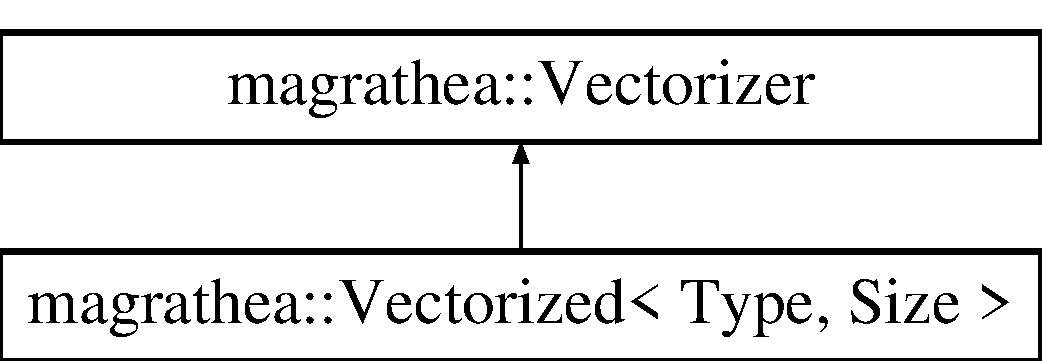
\includegraphics[height=2.000000cm]{exceptionmagrathea_1_1Vectorized}
\end{center}
\end{figure}
\subsection*{Public Member Functions}
\begin{Indent}{\bf Lifecycle}\par
\begin{DoxyCompactItemize}
\item 
\hyperlink{exceptionmagrathea_1_1Vectorized_ac54dac541b6b47cb6453a1de0b3dc575}{Vectorized} ()
\begin{DoxyCompactList}\small\item\em Implicit empty constructor. \end{DoxyCompactList}\item 
{\footnotesize template$<$typename Fundamental\-Type  = Type, class  = typename std\-::enable\-\_\-if$<$std\-::is\-\_\-fundamental$<$\-Fundamental\-Type$>$\-::value$>$\-::type$>$ }\\\hyperlink{exceptionmagrathea_1_1Vectorized_a19336c66bd5a1c9177a50be159eceae3}{Vectorized} (const \hyperlink{exceptionmagrathea_1_1Vectorized}{Vectorized}$<$ Fundamental\-Type, Size $>$ \&source)
\begin{DoxyCompactList}\small\item\em Implicit conversion constructor. \end{DoxyCompactList}\item 
{\footnotesize template$<$typename Other\-Type  = Type, class... Misc, class  = typename std\-::enable\-\_\-if$<$std\-::is\-\_\-convertible$<$\-Other\-Type, Type$>$\-::value$>$\-::type$>$ }\\\hyperlink{exceptionmagrathea_1_1Vectorized_a8dd5b14cd9f879ad5472ba3f87e4f1d9}{Vectorized} (const std\-::initializer\-\_\-list$<$ Other\-Type $>$ \&source, const Misc \&...misc)
\begin{DoxyCompactList}\small\item\em Implicit initializer list constructor. \end{DoxyCompactList}\item 
{\footnotesize template$<$class... Misc, class  = typename std\-::enable\-\_\-if$<$sizeof...(\-Misc) != 0$>$\-::type$>$ }\\\hyperlink{exceptionmagrathea_1_1Vectorized_a5143d9865051881aa79740df5c728f9e}{Vectorized} (const Misc \&...misc)
\begin{DoxyCompactList}\small\item\em Explicit generic constructor. \end{DoxyCompactList}\end{DoxyCompactItemize}
\end{Indent}
\begin{Indent}{\bf Vectorization}\par
\begin{DoxyCompactItemize}
\item 
Type \& \hyperlink{exceptionmagrathea_1_1Vectorized_a0f3d97c9455a9471bf2a25ca23b43415}{operator\mbox{[}$\,$\mbox{]}} (const unsigned int i)
\begin{DoxyCompactList}\small\item\em Direct access to the element. \end{DoxyCompactList}\item 
const Type \& \hyperlink{exceptionmagrathea_1_1Vectorized_af11c4c126a67c88dc87eb4e363542a0e}{operator\mbox{[}$\,$\mbox{]}} (const unsigned int i) const 
\begin{DoxyCompactList}\small\item\em Immutable direct access to the element. \end{DoxyCompactList}\item 
\hyperlink{exceptionmagrathea_1_1Vectorized}{Vectorized}$<$ Type, Size $>$ \& \hyperlink{exceptionmagrathea_1_1Vectorized_a8c12527eaae803374f413aff65141c3a}{resize} (const unsigned int n)
\begin{DoxyCompactList}\small\item\em Resize the container. \end{DoxyCompactList}\item 
\hyperlink{exceptionmagrathea_1_1Vectorized}{Vectorized}$<$ Type, Size $>$ \& \hyperlink{exceptionmagrathea_1_1Vectorized_abd2af5679ec375ba7ece2dac64d4764d}{reserve} (const unsigned int n)
\end{DoxyCompactItemize}
\end{Indent}
\subsection*{Static Public Member Functions}
\begin{Indent}{\bf Static vectorization}\par
\begin{DoxyCompactItemize}
\item 
static constexpr unsigned int \hyperlink{exceptionmagrathea_1_1Vectorized_a69853d16152b7ac5d6b74c0a819745a0}{size} ()
\begin{DoxyCompactList}\small\item\em Get the size of the container. \end{DoxyCompactList}\item 
static constexpr unsigned int \hyperlink{exceptionmagrathea_1_1Vectorized_aa169da938d44f5b2b368429d2fcd5944}{capacity} ()
\item 
static constexpr bool \hyperlink{exceptionmagrathea_1_1Vectorized_a41efb27191ba62b4effdccb2394292f5}{constant} ()
\begin{DoxyCompactList}\small\item\em Get whether the container has a constant size. \end{DoxyCompactList}\item 
static constexpr bool \hyperlink{exceptionmagrathea_1_1Vectorized_acc636c7bf7d53ef854781fbc015e19bd}{boolean} ()
\begin{DoxyCompactList}\small\item\em Get whether the container has a boolean type. \end{DoxyCompactList}\item 
static constexpr std\-::array\\*
$<$ unsigned int, 1 $>$ \hyperlink{exceptionmagrathea_1_1Vectorized_a587bd8b091c3a477bd7e9cec7d59b5aa}{parameters} ()
\begin{DoxyCompactList}\small\item\em Get the template parameters. \end{DoxyCompactList}\item 
static Type \hyperlink{exceptionmagrathea_1_1Vectorized_a39bb3943c9d25bf2701b57b8bf9953f0}{type} ()
\begin{DoxyCompactList}\small\item\em Get the data type. \end{DoxyCompactList}\end{DoxyCompactItemize}
\end{Indent}
\begin{Indent}{\bf Test}\par
\begin{DoxyCompactItemize}
\item 
static int \hyperlink{exceptionmagrathea_1_1Vectorized_a345a5a4bc7ded7c4a9e61e5c6413bf8e}{example} ()
\begin{DoxyCompactList}\small\item\em Example function. \end{DoxyCompactList}\end{DoxyCompactItemize}
\end{Indent}
\subsection*{Protected Attributes}
\begin{Indent}{\bf Data members}\par
\begin{DoxyCompactItemize}
\item 
Type \hyperlink{exceptionmagrathea_1_1Vectorized_a807e70ab36b29bab3d7985120a741254}{\-\_\-data} \mbox{[}Size\mbox{]}
\begin{DoxyCompactList}\small\item\em Data contents. \end{DoxyCompactList}\end{DoxyCompactItemize}
\end{Indent}
\subsection*{Friends}
\begin{Indent}{\bf Stream}\par
\begin{DoxyCompactItemize}
\item 
{\footnotesize template$<$typename Self\-Type , unsigned int Self\-Size$>$ }\\std\-::ostream \& \hyperlink{exceptionmagrathea_1_1Vectorized_a9028ffadf06611be8f9ed7ce9bb6b0c3}{operator$<$$<$} (std\-::ostream \&lhs, const \hyperlink{exceptionmagrathea_1_1Vectorized}{Vectorized}$<$ Self\-Type, Self\-Size $>$ \&rhs)
\begin{DoxyCompactList}\small\item\em \hyperlink{exceptionOutput}{Output} stream operator. \end{DoxyCompactList}\end{DoxyCompactItemize}
\end{Indent}
\subsection*{Additional Inherited Members}


\subsection{Detailed Description}
\subsubsection*{template$<$typename Type = double, unsigned int Size = 1$>$exception magrathea\-::\-Vectorized$<$ Type, Size $>$}

Basic vectorized container. 

This class is the direct derivation of \hyperlink{classmagrathea_1_1Vectorizer}{Vectorizer}. It provides the most basic vectorized container without adding new functionalities to the abstract class. 
\begin{DoxyTemplParams}{Template Parameters}
{\em Type} & Data type. \\
\hline
{\em Size} & Number of elements. \\
\hline
\end{DoxyTemplParams}


\subsection{Constructor \& Destructor Documentation}
\hypertarget{exceptionmagrathea_1_1Vectorized_ac54dac541b6b47cb6453a1de0b3dc575}{\index{magrathea\-::\-Vectorized@{magrathea\-::\-Vectorized}!Vectorized@{Vectorized}}
\index{Vectorized@{Vectorized}!magrathea::Vectorized@{magrathea\-::\-Vectorized}}
\subsubsection[{Vectorized}]{\setlength{\rightskip}{0pt plus 5cm}template$<$typename Type , unsigned int Size$>$ {\bf magrathea\-::\-Vectorized}$<$ Type, Size $>$\-::{\bf Vectorized} (
\begin{DoxyParamCaption}
{}
\end{DoxyParamCaption}
)\hspace{0.3cm}{\ttfamily [inline]}}}\label{exceptionmagrathea_1_1Vectorized_ac54dac541b6b47cb6453a1de0b3dc575}


Implicit empty constructor. 

Does nothing. \hypertarget{exceptionmagrathea_1_1Vectorized_a19336c66bd5a1c9177a50be159eceae3}{\index{magrathea\-::\-Vectorized@{magrathea\-::\-Vectorized}!Vectorized@{Vectorized}}
\index{Vectorized@{Vectorized}!magrathea::Vectorized@{magrathea\-::\-Vectorized}}
\subsubsection[{Vectorized}]{\setlength{\rightskip}{0pt plus 5cm}template$<$typename Type , unsigned int Size$>$ template$<$typename Fundamental\-Type , class $>$ {\bf magrathea\-::\-Vectorized}$<$ Type, Size $>$\-::{\bf Vectorized} (
\begin{DoxyParamCaption}
\item[{const {\bf Vectorized}$<$ Fundamental\-Type, Size $>$ \&}]{source}
\end{DoxyParamCaption}
)\hspace{0.3cm}{\ttfamily [inline]}}}\label{exceptionmagrathea_1_1Vectorized_a19336c66bd5a1c9177a50be159eceae3}


Implicit conversion constructor. 

Provides an implicit conversion from a fundamental type contents. 
\begin{DoxyTemplParams}{Template Parameters}
{\em Fundamental\-Type} & (Fundamental data type.) \\
\hline
\end{DoxyTemplParams}

\begin{DoxyParams}[1]{Parameters}
\mbox{\tt in}  & {\em source} & Source of the copy. \\
\hline
\end{DoxyParams}
\hypertarget{exceptionmagrathea_1_1Vectorized_a8dd5b14cd9f879ad5472ba3f87e4f1d9}{\index{magrathea\-::\-Vectorized@{magrathea\-::\-Vectorized}!Vectorized@{Vectorized}}
\index{Vectorized@{Vectorized}!magrathea::Vectorized@{magrathea\-::\-Vectorized}}
\subsubsection[{Vectorized}]{\setlength{\rightskip}{0pt plus 5cm}template$<$typename Type , unsigned int Size$>$ template$<$typename Other\-Type , class... Misc, class $>$ {\bf magrathea\-::\-Vectorized}$<$ Type, Size $>$\-::{\bf Vectorized} (
\begin{DoxyParamCaption}
\item[{const std\-::initializer\-\_\-list$<$ Other\-Type $>$ \&}]{source, }
\item[{const Misc \&...}]{misc}
\end{DoxyParamCaption}
)\hspace{0.3cm}{\ttfamily [inline]}}}\label{exceptionmagrathea_1_1Vectorized_a8dd5b14cd9f879ad5472ba3f87e4f1d9}


Implicit initializer list constructor. 

Provides an implicit conversion from an initializer list. 
\begin{DoxyTemplParams}{Template Parameters}
{\em Other\-Type} & (Other data type.) \\
\hline
{\em Misc} & (\hyperlink{classMiscellaneous}{Miscellaneous} types.) \\
\hline
\end{DoxyTemplParams}

\begin{DoxyParams}[1]{Parameters}
\mbox{\tt in}  & {\em source} & Source of the copy. \\
\hline
\mbox{\tt in}  & {\em misc} & \hyperlink{classMiscellaneous}{Miscellaneous} arguments. \\
\hline
\end{DoxyParams}
\hypertarget{exceptionmagrathea_1_1Vectorized_a5143d9865051881aa79740df5c728f9e}{\index{magrathea\-::\-Vectorized@{magrathea\-::\-Vectorized}!Vectorized@{Vectorized}}
\index{Vectorized@{Vectorized}!magrathea::Vectorized@{magrathea\-::\-Vectorized}}
\subsubsection[{Vectorized}]{\setlength{\rightskip}{0pt plus 5cm}template$<$typename Type , unsigned int Size$>$ template$<$class... Misc, class $>$ {\bf magrathea\-::\-Vectorized}$<$ Type, Size $>$\-::{\bf Vectorized} (
\begin{DoxyParamCaption}
\item[{const Misc \&...}]{misc}
\end{DoxyParamCaption}
)\hspace{0.3cm}{\ttfamily [inline]}, {\ttfamily [explicit]}}}\label{exceptionmagrathea_1_1Vectorized_a5143d9865051881aa79740df5c728f9e}


Explicit generic constructor. 

Provides a generic interface to all constructors of the base class. Before calling the associated constructor of the base class, the contents is initialized. 
\begin{DoxyTemplParams}{Template Parameters}
{\em Misc} & (\hyperlink{classMiscellaneous}{Miscellaneous} types.) \\
\hline
\end{DoxyTemplParams}

\begin{DoxyParams}[1]{Parameters}
\mbox{\tt in}  & {\em misc} & \hyperlink{classMiscellaneous}{Miscellaneous} arguments. \\
\hline
\end{DoxyParams}


\subsection{Member Function Documentation}
\hypertarget{exceptionmagrathea_1_1Vectorized_acc636c7bf7d53ef854781fbc015e19bd}{\index{magrathea\-::\-Vectorized@{magrathea\-::\-Vectorized}!boolean@{boolean}}
\index{boolean@{boolean}!magrathea::Vectorized@{magrathea\-::\-Vectorized}}
\subsubsection[{boolean}]{\setlength{\rightskip}{0pt plus 5cm}template$<$typename Type , unsigned int Size$>$ constexpr bool {\bf magrathea\-::\-Vectorized}$<$ Type, Size $>$\-::boolean (
\begin{DoxyParamCaption}
{}
\end{DoxyParamCaption}
)\hspace{0.3cm}{\ttfamily [static]}}}\label{exceptionmagrathea_1_1Vectorized_acc636c7bf7d53ef854781fbc015e19bd}


Get whether the container has a boolean type. 

Returns true if the container has a boolean type, false otherwise. This function is required by the vectorization mechanism. \begin{DoxyReturn}{Returns}
Copy of true if the container has a boolean type. 
\end{DoxyReturn}
\hypertarget{exceptionmagrathea_1_1Vectorized_aa169da938d44f5b2b368429d2fcd5944}{\index{magrathea\-::\-Vectorized@{magrathea\-::\-Vectorized}!capacity@{capacity}}
\index{capacity@{capacity}!magrathea::Vectorized@{magrathea\-::\-Vectorized}}
\subsubsection[{capacity}]{\setlength{\rightskip}{0pt plus 5cm}template$<$typename Type = double, unsigned int Size = 1$>$ static constexpr unsigned int {\bf magrathea\-::\-Vectorized}$<$ Type, Size $>$\-::capacity (
\begin{DoxyParamCaption}
{}
\end{DoxyParamCaption}
)\hspace{0.3cm}{\ttfamily [static]}}}\label{exceptionmagrathea_1_1Vectorized_aa169da938d44f5b2b368429d2fcd5944}
\hypertarget{exceptionmagrathea_1_1Vectorized_a41efb27191ba62b4effdccb2394292f5}{\index{magrathea\-::\-Vectorized@{magrathea\-::\-Vectorized}!constant@{constant}}
\index{constant@{constant}!magrathea::Vectorized@{magrathea\-::\-Vectorized}}
\subsubsection[{constant}]{\setlength{\rightskip}{0pt plus 5cm}template$<$typename Type , unsigned int Size$>$ constexpr bool {\bf magrathea\-::\-Vectorized}$<$ Type, Size $>$\-::constant (
\begin{DoxyParamCaption}
{}
\end{DoxyParamCaption}
)\hspace{0.3cm}{\ttfamily [static]}}}\label{exceptionmagrathea_1_1Vectorized_a41efb27191ba62b4effdccb2394292f5}


Get whether the container has a constant size. 

Returns true if the container has a constant size, false otherwise. This function is required by the vectorization mechanism. \begin{DoxyReturn}{Returns}
Copy of true. 
\end{DoxyReturn}
\hypertarget{exceptionmagrathea_1_1Vectorized_a345a5a4bc7ded7c4a9e61e5c6413bf8e}{\index{magrathea\-::\-Vectorized@{magrathea\-::\-Vectorized}!example@{example}}
\index{example@{example}!magrathea::Vectorized@{magrathea\-::\-Vectorized}}
\subsubsection[{example}]{\setlength{\rightskip}{0pt plus 5cm}template$<$typename Type , unsigned int Size$>$ int {\bf magrathea\-::\-Vectorized}$<$ Type, Size $>$\-::example (
\begin{DoxyParamCaption}
{}
\end{DoxyParamCaption}
)\hspace{0.3cm}{\ttfamily [static]}}}\label{exceptionmagrathea_1_1Vectorized_a345a5a4bc7ded7c4a9e61e5c6413bf8e}


Example function. 

Tests and demonstrates the use of \hyperlink{exceptionmagrathea_1_1Vectorized}{Vectorized}. \begin{DoxyReturn}{Returns}
0 if no error. 
\end{DoxyReturn}
\hypertarget{exceptionmagrathea_1_1Vectorized_a0f3d97c9455a9471bf2a25ca23b43415}{\index{magrathea\-::\-Vectorized@{magrathea\-::\-Vectorized}!operator\mbox{[}$\,$\mbox{]}@{operator[]}}
\index{operator\mbox{[}$\,$\mbox{]}@{operator[]}!magrathea::Vectorized@{magrathea\-::\-Vectorized}}
\subsubsection[{operator[]}]{\setlength{\rightskip}{0pt plus 5cm}template$<$typename Type , unsigned int Size$>$ Type \& {\bf magrathea\-::\-Vectorized}$<$ Type, Size $>$\-::operator\mbox{[}$\,$\mbox{]} (
\begin{DoxyParamCaption}
\item[{const unsigned int}]{i}
\end{DoxyParamCaption}
)\hspace{0.3cm}{\ttfamily [inline]}}}\label{exceptionmagrathea_1_1Vectorized_a0f3d97c9455a9471bf2a25ca23b43415}


Direct access to the element. 

Provides a direct access to the specified element. This function is required by the vectorization mechanism. 
\begin{DoxyParams}[1]{Parameters}
\mbox{\tt in}  & {\em i} & Index of the element. \\
\hline
\end{DoxyParams}
\begin{DoxyReturn}{Returns}
Reference to the element. 
\end{DoxyReturn}
\hypertarget{exceptionmagrathea_1_1Vectorized_af11c4c126a67c88dc87eb4e363542a0e}{\index{magrathea\-::\-Vectorized@{magrathea\-::\-Vectorized}!operator\mbox{[}$\,$\mbox{]}@{operator[]}}
\index{operator\mbox{[}$\,$\mbox{]}@{operator[]}!magrathea::Vectorized@{magrathea\-::\-Vectorized}}
\subsubsection[{operator[]}]{\setlength{\rightskip}{0pt plus 5cm}template$<$typename Type , unsigned int Size$>$ const Type \& {\bf magrathea\-::\-Vectorized}$<$ Type, Size $>$\-::operator\mbox{[}$\,$\mbox{]} (
\begin{DoxyParamCaption}
\item[{const unsigned int}]{i}
\end{DoxyParamCaption}
) const\hspace{0.3cm}{\ttfamily [inline]}}}\label{exceptionmagrathea_1_1Vectorized_af11c4c126a67c88dc87eb4e363542a0e}


Immutable direct access to the element. 

Provides a constant direct access to the specified element. This function is required by the vectorization mechanism. 
\begin{DoxyParams}[1]{Parameters}
\mbox{\tt in}  & {\em i} & Index of the element. \\
\hline
\end{DoxyParams}
\begin{DoxyReturn}{Returns}
Const reference to the element. 
\end{DoxyReturn}
\hypertarget{exceptionmagrathea_1_1Vectorized_a587bd8b091c3a477bd7e9cec7d59b5aa}{\index{magrathea\-::\-Vectorized@{magrathea\-::\-Vectorized}!parameters@{parameters}}
\index{parameters@{parameters}!magrathea::Vectorized@{magrathea\-::\-Vectorized}}
\subsubsection[{parameters}]{\setlength{\rightskip}{0pt plus 5cm}template$<$typename Type , unsigned int Size$>$ constexpr std\-::array$<$ unsigned int, 1 $>$ {\bf magrathea\-::\-Vectorized}$<$ Type, Size $>$\-::parameters (
\begin{DoxyParamCaption}
{}
\end{DoxyParamCaption}
)\hspace{0.3cm}{\ttfamily [static]}}}\label{exceptionmagrathea_1_1Vectorized_a587bd8b091c3a477bd7e9cec7d59b5aa}


Get the template parameters. 

Returns an array containing the template parameters. This function is required by the vectorization mechanism. \begin{DoxyReturn}{Returns}
Copy of an array of parameters. 
\end{DoxyReturn}
\hypertarget{exceptionmagrathea_1_1Vectorized_abd2af5679ec375ba7ece2dac64d4764d}{\index{magrathea\-::\-Vectorized@{magrathea\-::\-Vectorized}!reserve@{reserve}}
\index{reserve@{reserve}!magrathea::Vectorized@{magrathea\-::\-Vectorized}}
\subsubsection[{reserve}]{\setlength{\rightskip}{0pt plus 5cm}template$<$typename Type = double, unsigned int Size = 1$>$ {\bf Vectorized}$<$Type, Size$>$\& {\bf magrathea\-::\-Vectorized}$<$ Type, Size $>$\-::reserve (
\begin{DoxyParamCaption}
\item[{const unsigned int}]{n}
\end{DoxyParamCaption}
)\hspace{0.3cm}{\ttfamily [inline]}}}\label{exceptionmagrathea_1_1Vectorized_abd2af5679ec375ba7ece2dac64d4764d}
\hypertarget{exceptionmagrathea_1_1Vectorized_a8c12527eaae803374f413aff65141c3a}{\index{magrathea\-::\-Vectorized@{magrathea\-::\-Vectorized}!resize@{resize}}
\index{resize@{resize}!magrathea::Vectorized@{magrathea\-::\-Vectorized}}
\subsubsection[{resize}]{\setlength{\rightskip}{0pt plus 5cm}template$<$typename Type , unsigned int Size$>$ {\bf Vectorized}$<$ Type, Size $>$ \& {\bf magrathea\-::\-Vectorized}$<$ Type, Size $>$\-::resize (
\begin{DoxyParamCaption}
\item[{const unsigned int}]{n}
\end{DoxyParamCaption}
)\hspace{0.3cm}{\ttfamily [inline]}}}\label{exceptionmagrathea_1_1Vectorized_a8c12527eaae803374f413aff65141c3a}


Resize the container. 

Resizes the container and returns a reference to it. This function is required by the vectorization mechanism. 
\begin{DoxyParams}[1]{Parameters}
\mbox{\tt in}  & {\em n} & New size. \\
\hline
\end{DoxyParams}
\begin{DoxyReturn}{Returns}
Self reference. 
\end{DoxyReturn}

\begin{DoxyExceptions}{Exceptions}
{\em std\-::length\-\_\-error} & The container cannot be resized. \\
\hline
\end{DoxyExceptions}
\hypertarget{exceptionmagrathea_1_1Vectorized_a69853d16152b7ac5d6b74c0a819745a0}{\index{magrathea\-::\-Vectorized@{magrathea\-::\-Vectorized}!size@{size}}
\index{size@{size}!magrathea::Vectorized@{magrathea\-::\-Vectorized}}
\subsubsection[{size}]{\setlength{\rightskip}{0pt plus 5cm}template$<$typename Type , unsigned int Size$>$ constexpr unsigned int {\bf magrathea\-::\-Vectorized}$<$ Type, Size $>$\-::size (
\begin{DoxyParamCaption}
{}
\end{DoxyParamCaption}
)\hspace{0.3cm}{\ttfamily [static]}}}\label{exceptionmagrathea_1_1Vectorized_a69853d16152b7ac5d6b74c0a819745a0}


Get the size of the container. 

Returns the current number of elements. This function is required by the vectorization mechanism. \begin{DoxyReturn}{Returns}
Copy of the size. 
\end{DoxyReturn}
\hypertarget{exceptionmagrathea_1_1Vectorized_a39bb3943c9d25bf2701b57b8bf9953f0}{\index{magrathea\-::\-Vectorized@{magrathea\-::\-Vectorized}!type@{type}}
\index{type@{type}!magrathea::Vectorized@{magrathea\-::\-Vectorized}}
\subsubsection[{type}]{\setlength{\rightskip}{0pt plus 5cm}template$<$typename Type , unsigned int Size$>$ Type {\bf magrathea\-::\-Vectorized}$<$ Type, Size $>$\-::type (
\begin{DoxyParamCaption}
{}
\end{DoxyParamCaption}
)\hspace{0.3cm}{\ttfamily [inline]}, {\ttfamily [static]}}}\label{exceptionmagrathea_1_1Vectorized_a39bb3943c9d25bf2701b57b8bf9953f0}


Get the data type. 

Returns a copy of the default value of the data type. \begin{DoxyReturn}{Returns}
Copy of the default value of the data type. 
\end{DoxyReturn}


\subsection{Friends And Related Function Documentation}
\hypertarget{exceptionmagrathea_1_1Vectorized_a9028ffadf06611be8f9ed7ce9bb6b0c3}{\index{magrathea\-::\-Vectorized@{magrathea\-::\-Vectorized}!operator$<$$<$@{operator$<$$<$}}
\index{operator$<$$<$@{operator$<$$<$}!magrathea::Vectorized@{magrathea\-::\-Vectorized}}
\subsubsection[{operator$<$$<$}]{\setlength{\rightskip}{0pt plus 5cm}template$<$typename Type = double, unsigned int Size = 1$>$ template$<$typename Self\-Type , unsigned int Self\-Size$>$ std\-::ostream\& operator$<$$<$ (
\begin{DoxyParamCaption}
\item[{std\-::ostream \&}]{lhs, }
\item[{const {\bf Vectorized}$<$ Self\-Type, Self\-Size $>$ \&}]{rhs}
\end{DoxyParamCaption}
)\hspace{0.3cm}{\ttfamily [friend]}}}\label{exceptionmagrathea_1_1Vectorized_a9028ffadf06611be8f9ed7ce9bb6b0c3}


\hyperlink{exceptionOutput}{Output} stream operator. 

Adds each element to the stream using the fill character to separate the elements. 
\begin{DoxyTemplParams}{Template Parameters}
{\em Self\-Type} & Data type. \\
\hline
{\em Self\-Size} & Number of elements. \\
\hline
\end{DoxyTemplParams}

\begin{DoxyParams}[1]{Parameters}
\mbox{\tt in,out}  & {\em lhs} & Left-\/hand side stream. \\
\hline
\mbox{\tt in}  & {\em rhs} & Right-\/hand side container. \\
\hline
\end{DoxyParams}
\begin{DoxyReturn}{Returns}
\hyperlink{exceptionOutput}{Output} stream. 
\end{DoxyReturn}


\subsection{Member Data Documentation}
\hypertarget{exceptionmagrathea_1_1Vectorized_a807e70ab36b29bab3d7985120a741254}{\index{magrathea\-::\-Vectorized@{magrathea\-::\-Vectorized}!\-\_\-data@{\-\_\-data}}
\index{\-\_\-data@{\-\_\-data}!magrathea::Vectorized@{magrathea\-::\-Vectorized}}
\subsubsection[{\-\_\-data}]{\setlength{\rightskip}{0pt plus 5cm}template$<$typename Type = double, unsigned int Size = 1$>$ Type {\bf magrathea\-::\-Vectorized}$<$ Type, Size $>$\-::\-\_\-data\mbox{[}Size\mbox{]}\hspace{0.3cm}{\ttfamily [protected]}}}\label{exceptionmagrathea_1_1Vectorized_a807e70ab36b29bab3d7985120a741254}


Data contents. 



The documentation for this exception was generated from the following file\-:\begin{DoxyCompactItemize}
\item 
/data/home/mbreton/magrathea\-\_\-pathfinder/src/magrathea/\hyperlink{vectorized_8h}{vectorized.\-h}\end{DoxyCompactItemize}

\hypertarget{classmagrathea_1_1Vectorizer}{\section{magrathea\-:\-:Vectorizer Class Reference}
\label{classmagrathea_1_1Vectorizer}\index{magrathea\-::\-Vectorizer@{magrathea\-::\-Vectorizer}}
}


Helper base class for generic vectorization.  




{\ttfamily \#include $<$vectorizer.\-h$>$}

Inheritance diagram for magrathea\-:\-:Vectorizer\-:\begin{figure}[H]
\begin{center}
\leavevmode
\includegraphics[height=0.955224cm]{classmagrathea_1_1Vectorizer}
\end{center}
\end{figure}
\subsection*{Public Member Functions}
\begin{Indent}{\bf Vectorization}\par
\begin{DoxyCompactItemize}
\item 
\hyperlink{classmagrathea_1_1Vectorizer}{Vectorizer} \& \hyperlink{classmagrathea_1_1Vectorizer_a83ebb071ab30dce7af155d3c0e597fb9}{operator\mbox{[}$\,$\mbox{]}} (const unsigned int i)
\begin{DoxyCompactList}\small\item\em Direct access to the element. \end{DoxyCompactList}\item 
const \hyperlink{classmagrathea_1_1Vectorizer}{Vectorizer} \& \hyperlink{classmagrathea_1_1Vectorizer_aa058daf8b240bb587b80888ab88340c7}{operator\mbox{[}$\,$\mbox{]}} (const unsigned int i) const 
\begin{DoxyCompactList}\small\item\em Immutable direct access to the element. \end{DoxyCompactList}\item 
\hyperlink{classmagrathea_1_1Vectorizer}{Vectorizer} \& \hyperlink{classmagrathea_1_1Vectorizer_afe3c5369c91276766e0197fa33ae4951}{resize} (const unsigned int n)
\begin{DoxyCompactList}\small\item\em Resize the container. \end{DoxyCompactList}\item 
unsigned int \hyperlink{classmagrathea_1_1Vectorizer_a3b54f2b5f17c2054f99e03c7c4614558}{size} () const 
\begin{DoxyCompactList}\small\item\em Get the size of the container. \end{DoxyCompactList}\item 
bool \hyperlink{classmagrathea_1_1Vectorizer_a2e30cc7971bfbcf7b21f993b56c0644e}{constant} () const 
\begin{DoxyCompactList}\small\item\em Get whether the container has a constant size. \end{DoxyCompactList}\item 
bool \hyperlink{classmagrathea_1_1Vectorizer_ab5100fafcacd2c835380dbe0403422ec}{boolean} () const 
\begin{DoxyCompactList}\small\item\em Get whether the container has a boolean type. \end{DoxyCompactList}\item 
std\-::array$<$ unsigned int, 0 $>$ \hyperlink{classmagrathea_1_1Vectorizer_a7815b5c9e9ff56064306e7d07dae5bb7}{parameters} () const 
\begin{DoxyCompactList}\small\item\em Get the template parameters. \end{DoxyCompactList}\item 
void \hyperlink{classmagrathea_1_1Vectorizer_af46ebf417fa856107cb9b84db9939f76}{type} () const 
\begin{DoxyCompactList}\small\item\em Get the data type. \end{DoxyCompactList}\end{DoxyCompactItemize}
\end{Indent}
\subsection*{Static Public Member Functions}
\begin{Indent}{\bf Check}\par
\begin{DoxyCompactItemize}
\item 
{\footnotesize template$<$bool Exception = true, class First\-Type , class Second\-Type , class  = typename std\-::enable\-\_\-if$<$(!std\-::is\-\_\-base\-\_\-of$<$\-Vectorizer, First\-Type$>$\-::value) $|$$|$ (!std\-::is\-\_\-base\-\_\-of$<$\-Vectorizer, Second\-Type$>$\-::value)$>$\-::type$>$ }\\static constexpr bool \hyperlink{classmagrathea_1_1Vectorizer_a9c5d14ef63c3245c6e3ba161e5efdf95}{check} (const First\-Type \&, const Second\-Type \&)
\begin{DoxyCompactList}\small\item\em Check compatibility with at least one non-\/vectorized type. \end{DoxyCompactList}\item 
{\footnotesize template$<$bool Exception = true, class First\-Type , class Second\-Type , class  = typename std\-::enable\-\_\-if$<$(std\-::is\-\_\-base\-\_\-of$<$\-Vectorizer, First\-Type$>$\-::value) \&\& (std\-::is\-\_\-base\-\_\-of$<$\-Vectorizer, Second\-Type$>$\-::value)$>$\-::type, class  = typename std\-::enable\-\_\-if$<$(\-First\-Type\-::constant()) \&\& (\-Second\-Type\-::constant())$>$\-::type$>$ }\\static constexpr bool \hyperlink{classmagrathea_1_1Vectorizer_a46a8845625441b2b7ca940542c5a42ea}{check} (const First\-Type \&, const Second\-Type \&)
\item 
{\footnotesize template$<$bool Exception = true, class First\-Type , class Second\-Type , class  = typename std\-::enable\-\_\-if$<$(std\-::is\-\_\-base\-\_\-of$<$\-Vectorizer, First\-Type$>$\-::value) \&\& (std\-::is\-\_\-base\-\_\-of$<$\-Vectorizer, Second\-Type$>$\-::value)$>$\-::type, class  = typename std\-::enable\-\_\-if$<$(!\-First\-Type\-::constant()) $|$$|$ (!\-Second\-Type\-::constant())$>$\-::type, class  = void$>$ }\\static bool \hyperlink{classmagrathea_1_1Vectorizer_a8cbb51491c2e83e5cedeced2d5945cde}{check} (const First\-Type \&first, const Second\-Type \&second)
\end{DoxyCompactItemize}
\end{Indent}
\begin{Indent}{\bf Getters}\par
\begin{DoxyCompactItemize}
\item 
{\footnotesize template$<$typename Integral\-Type , Integral\-Type Value, typename Dummy\-Type  = unsigned int, class  = typename std\-::enable\-\_\-if$<$(std\-::is\-\_\-integral$<$\-Integral\-Type$>$\-::value) \&\& (std\-::is\-\_\-convertible$<$\-Dummy\-Type, unsigned int$>$\-::value)$>$\-::type$>$ }\\static constexpr Integral\-Type \hyperlink{classmagrathea_1_1Vectorizer_a8d9b9d79268199cbac2906cffd22c0d4}{get} (const std\-::integral\-\_\-constant$<$ Integral\-Type, Value $>$, const Dummy\-Type=Dummy\-Type())
\begin{DoxyCompactList}\small\item\em Integral constant getter. \end{DoxyCompactList}\item 
{\footnotesize template$<$typename Data\-Type , typename Dummy\-Type  = unsigned int, class  = typename std\-::enable\-\_\-if$<$(!std\-::is\-\_\-base\-\_\-of$<$\-Vectorizer, Data\-Type$>$\-::value) \&\& (std\-::is\-\_\-convertible$<$\-Dummy\-Type, unsigned int$>$\-::value)$>$\-::type$>$ }\\static Data\-Type \& \hyperlink{classmagrathea_1_1Vectorizer_a7a89b7c95b5067316ad946aaab3d5686}{get} (Data\-Type \&source, const Dummy\-Type=Dummy\-Type())
\begin{DoxyCompactList}\small\item\em Non-\/vectorized getter. \end{DoxyCompactList}\item 
{\footnotesize template$<$typename Data\-Type , typename Dummy\-Type  = unsigned int, class  = typename std\-::enable\-\_\-if$<$(!std\-::is\-\_\-base\-\_\-of$<$\-Vectorizer, Data\-Type$>$\-::value) \&\& (std\-::is\-\_\-convertible$<$\-Dummy\-Type, unsigned int$>$\-::value)$>$\-::type$>$ }\\static const Data\-Type \& \hyperlink{classmagrathea_1_1Vectorizer_a9a63af59c59b04cbbe01a3447a7ac552}{get} (const Data\-Type \&source, const Dummy\-Type=Dummy\-Type())
\begin{DoxyCompactList}\small\item\em Immutable non-\/vectorized getter. \end{DoxyCompactList}\item 
{\footnotesize template$<$class Vectorized\-Type , class  = typename std\-::enable\-\_\-if$<$std\-::is\-\_\-base\-\_\-of$<$\-Vectorizer, Vectorized\-Type$>$\-::value$>$\-::type, typename Data\-Type  = typename std\-::remove\-\_\-reference$<$decltype(\-Vectorized\-Type\-::type())$>$\-::type$>$ }\\static Data\-Type \& \hyperlink{classmagrathea_1_1Vectorizer_af077b83bc7bc9d07e59895cf3df6641e}{get} (Vectorized\-Type \&source, const unsigned int i)
\begin{DoxyCompactList}\small\item\em Vector element getter. \end{DoxyCompactList}\item 
{\footnotesize template$<$class Vectorized\-Type , class  = typename std\-::enable\-\_\-if$<$std\-::is\-\_\-base\-\_\-of$<$\-Vectorizer, Vectorized\-Type$>$\-::value$>$\-::type, typename Data\-Type  = typename std\-::remove\-\_\-reference$<$decltype(\-Vectorized\-Type\-::type())$>$\-::type$>$ }\\static const Data\-Type \& \hyperlink{classmagrathea_1_1Vectorizer_a3a3ae98c035c1f3004ee2f88f6179066}{get} (const Vectorized\-Type \&source, const unsigned int i)
\begin{DoxyCompactList}\small\item\em Immutable vector element getter. \end{DoxyCompactList}\end{DoxyCompactItemize}
\end{Indent}
\begin{Indent}{\bf Setters}\par
\begin{DoxyCompactItemize}
\item 
{\footnotesize template$<$class Vectorized\-Type , class  = typename std\-::enable\-\_\-if$<$std\-::is\-\_\-base\-\_\-of$<$\-Vectorizer, Vectorized\-Type$>$\-::value$>$\-::type$>$ }\\static Vectorized\-Type \& \hyperlink{classmagrathea_1_1Vectorizer_a67836bbf5aced8fee531fd2caf839f15}{set} (Vectorized\-Type \&destination)
\begin{DoxyCompactList}\small\item\em Empty setter. \end{DoxyCompactList}\item 
{\footnotesize template$<$class Vectorized\-Type , class  = typename std\-::enable\-\_\-if$<$std\-::is\-\_\-base\-\_\-of$<$\-Vectorizer, Vectorized\-Type$>$\-::value$>$\-::type, class Generic\-Type $>$ }\\static Vectorized\-Type \& \hyperlink{classmagrathea_1_1Vectorizer_aa586478d9b24b19586ff1d6dfdff5b68}{set} (Vectorized\-Type \&destination, const Generic\-Type \&source)
\begin{DoxyCompactList}\small\item\em Copy setter. \end{DoxyCompactList}\item 
{\footnotesize template$<$class Vectorized\-Type , class  = typename std\-::enable\-\_\-if$<$std\-::is\-\_\-base\-\_\-of$<$\-Vectorizer, Vectorized\-Type$>$\-::value$>$\-::type, class Generic\-Type , class First , class Second , class... Others, class  = typename std\-::enable\-\_\-if$<$(sizeof...(\-Others) != 0) \&\& (sizeof...(\-Others) != 1)$>$\-::type$>$ }\\static Vectorized\-Type \& \hyperlink{classmagrathea_1_1Vectorizer_ab181cd6d6a7afb777ebab551cc36bc33}{set} (Vectorized\-Type \&destination, const Generic\-Type \&source, const First \&first, const Second \&second, const Others \&...others)
\begin{DoxyCompactList}\small\item\em Variadic setter. \end{DoxyCompactList}\item 
{\footnotesize template$<$class Vectorized\-Type , class  = typename std\-::enable\-\_\-if$<$std\-::is\-\_\-base\-\_\-of$<$\-Vectorizer, Vectorized\-Type$>$\-::value$>$\-::type, class Generic\-Type , typename Size\-Type  = std\-::true\-\_\-type, class  = typename std\-::enable\-\_\-if$<$(std\-::is\-\_\-same$<$\-Size\-Type, std\-::true\-\_\-type$>$\-::value) $|$$|$ (std\-::is\-\_\-convertible$<$\-Size\-Type, unsigned int$>$\-::value)$>$\-::type$>$ }\\static Vectorized\-Type \& \hyperlink{classmagrathea_1_1Vectorizer_acccf60d696c7fdba17a8ff7bf0efa5de}{set} (Vectorized\-Type \&destination, const Generic\-Type \&source, const unsigned int pos, const Size\-Type num=Size\-Type())
\begin{DoxyCompactList}\small\item\em Partial setter. \end{DoxyCompactList}\item 
{\footnotesize template$<$class Vectorized\-Type , class  = typename std\-::enable\-\_\-if$<$std\-::is\-\_\-base\-\_\-of$<$\-Vectorizer, Vectorized\-Type$>$\-::value$>$\-::type, typename Data\-Type  = typename std\-::remove\-\_\-reference$<$decltype(\-Vectorized\-Type\-::type())$>$\-::type, typename Size\-Type  = std\-::true\-\_\-type, class  = typename std\-::enable\-\_\-if$<$(std\-::is\-\_\-convertible$<$\-Data\-Type, typename std\-::remove\-\_\-reference$<$decltype(std\-::declval$<$\-Vectorized\-Type$>$()\mbox{[}0\mbox{]})$>$\-::type$>$\-::value) \&\& ((std\-::is\-\_\-same$<$\-Size\-Type, std\-::true\-\_\-type$>$\-::value) $|$$|$ (std\-::is\-\_\-convertible$<$\-Size\-Type, unsigned int$>$\-::value))$>$\-::type$>$ }\\static Vectorized\-Type \& \hyperlink{classmagrathea_1_1Vectorizer_af3453b370f7c850f2ab17f20d0d3fb33}{set} (Vectorized\-Type \&destination, const std\-::initializer\-\_\-list$<$ Data\-Type $>$ \&source, const unsigned int pos=0, const Size\-Type num=Size\-Type())
\begin{DoxyCompactList}\small\item\em Partial list setter. \end{DoxyCompactList}\item 
{\footnotesize template$<$class Vectorized\-Type , class  = typename std\-::enable\-\_\-if$<$std\-::is\-\_\-base\-\_\-of$<$\-Vectorizer, Vectorized\-Type$>$\-::value$>$\-::type, typename Iterator\-Type , typename Size\-Type  = std\-::true\-\_\-type, class  = typename std\-::enable\-\_\-if$<$(std\-::is\-\_\-same$<$\-Size\-Type, std\-::true\-\_\-type$>$\-::value) $|$$|$ (std\-::is\-\_\-convertible$<$\-Size\-Type, unsigned int$>$\-::value)$>$\-::type$>$ }\\static Vectorized\-Type \& \hyperlink{classmagrathea_1_1Vectorizer_ac0dd17adf7a9cc87583510b0ed84cde8}{set} (Vectorized\-Type \&destination, const Iterator\-Type \&first, const Iterator\-Type \&last, const unsigned int pos=0, const Size\-Type num=Size\-Type(), typename std\-::iterator\-\_\-traits$<$ Iterator\-Type $>$\-::iterator\-\_\-category $\ast$=nullptr)
\begin{DoxyCompactList}\small\item\em Partial range setter. \end{DoxyCompactList}\item 
{\footnotesize template$<$class Vectorized\-Type , class  = typename std\-::enable\-\_\-if$<$std\-::is\-\_\-base\-\_\-of$<$\-Vectorizer, Vectorized\-Type$>$\-::value$>$\-::type, class Generic\-Type , class Mask\-Type , typename Dummy\-Type  = unsigned int, class  = typename std\-::enable\-\_\-if$<$(std\-::is\-\_\-base\-\_\-of$<$\-Vectorizer, Mask\-Type$>$\-::value) \&\& (std\-::is\-\_\-convertible$<$\-Dummy\-Type, unsigned int$>$\-::value)$>$\-::type$>$ }\\static Vectorized\-Type \& \hyperlink{classmagrathea_1_1Vectorizer_a5ea3e9a7f164f31f1f8f9b7ab3abe12c}{set} (Vectorized\-Type \&destination, const Generic\-Type \&source, const Mask\-Type \&mask, const Dummy\-Type=Dummy\-Type())
\begin{DoxyCompactList}\small\item\em Masked setter. \end{DoxyCompactList}\item 
{\footnotesize template$<$class Vectorized\-Type , class  = typename std\-::enable\-\_\-if$<$std\-::is\-\_\-base\-\_\-of$<$\-Vectorizer, Vectorized\-Type$>$\-::value$>$\-::type, typename Data\-Type  = typename std\-::remove\-\_\-reference$<$decltype(\-Vectorized\-Type\-::type())$>$\-::type, class Mask\-Type , typename Dummy\-Type  = unsigned int, class  = typename std\-::enable\-\_\-if$<$(std\-::is\-\_\-base\-\_\-of$<$\-Vectorizer, Mask\-Type$>$\-::value) \&\& (std\-::is\-\_\-convertible$<$\-Dummy\-Type, unsigned int$>$\-::value)$>$\-::type$>$ }\\static Vectorized\-Type \& \hyperlink{classmagrathea_1_1Vectorizer_aacc7d73a284fc36d87653df867ef6e00}{set} (Vectorized\-Type \&destination, const std\-::initializer\-\_\-list$<$ Data\-Type $>$ \&source, const Mask\-Type \&mask, const Dummy\-Type=Dummy\-Type())
\begin{DoxyCompactList}\small\item\em Masked list setter. \end{DoxyCompactList}\item 
{\footnotesize template$<$class Vectorized\-Type , class  = typename std\-::enable\-\_\-if$<$std\-::is\-\_\-base\-\_\-of$<$\-Vectorizer, Vectorized\-Type$>$\-::value$>$\-::type, typename Iterator\-Type , class Mask\-Type , typename Dummy\-Type  = unsigned int, class  = typename std\-::enable\-\_\-if$<$(std\-::is\-\_\-base\-\_\-of$<$\-Vectorizer, Mask\-Type$>$\-::value) \&\& (std\-::is\-\_\-convertible$<$\-Dummy\-Type, unsigned int$>$\-::value)$>$\-::type$>$ }\\static Vectorized\-Type \& \hyperlink{classmagrathea_1_1Vectorizer_a0f6c5228f8e7f3bba38d57886a4ef51a}{set} (Vectorized\-Type \&destination, const Iterator\-Type \&first, const Iterator\-Type \&last, const Mask\-Type \&mask, const Dummy\-Type=Dummy\-Type(), typename std\-::iterator\-\_\-traits$<$ Iterator\-Type $>$\-::iterator\-\_\-category $\ast$=nullptr)
\begin{DoxyCompactList}\small\item\em Masked range setter. \end{DoxyCompactList}\end{DoxyCompactItemize}
\end{Indent}
\begin{Indent}{\bf Test}\par
\begin{DoxyCompactItemize}
\item 
static int \hyperlink{classmagrathea_1_1Vectorizer_a302758cf072c56ea44519a41c2b70171}{example} ()
\begin{DoxyCompactList}\small\item\em Example function. \end{DoxyCompactList}\end{DoxyCompactItemize}
\end{Indent}
\subsection*{Protected Member Functions}
\begin{Indent}{\bf Protected lifecycle}\par
\begin{DoxyCompactItemize}
\item 
\hyperlink{classmagrathea_1_1Vectorizer_ab42248d231900ce89e17405a9e751535}{$\sim$\-Vectorizer} ()
\begin{DoxyCompactList}\small\item\em Protected destructor. \end{DoxyCompactList}\end{DoxyCompactItemize}
\end{Indent}


\subsection{Detailed Description}
Helper base class for generic vectorization. 

Provides global functions for vectorization implementation. \hyperlink{classmagrathea_1_1Vectorizer}{Vectorizer} helpers (like \hyperlink{classmagrathea_1_1StaticVectorizer}{Static\-Vectorizer} or Dynamic\-Vectorizer) are derived from this class and have to implement the following functions required by C\-R\-T\-P \-: 
\begin{DoxyItemize}
\item {\ttfamily operator\mbox{[}\mbox{]}} 
\item {\ttfamily \hyperlink{classmagrathea_1_1Vectorizer_afe3c5369c91276766e0197fa33ae4951}{resize()}} 
\item {\ttfamily \hyperlink{classmagrathea_1_1Vectorizer_a3b54f2b5f17c2054f99e03c7c4614558}{size()}} 
\item {\ttfamily \hyperlink{classmagrathea_1_1Vectorizer_a2e30cc7971bfbcf7b21f993b56c0644e}{constant()}} 
\item {\ttfamily \hyperlink{classmagrathea_1_1Vectorizer_ab5100fafcacd2c835380dbe0403422ec}{boolean()}} 
\item {\ttfamily \hyperlink{classmagrathea_1_1Vectorizer_a7815b5c9e9ff56064306e7d07dae5bb7}{parameters()}} 
\item {\ttfamily \hyperlink{classmagrathea_1_1Vectorizer_af46ebf417fa856107cb9b84db9939f76}{type()}} 
\end{DoxyItemize}

\subsection{Constructor \& Destructor Documentation}
\hypertarget{classmagrathea_1_1Vectorizer_ab42248d231900ce89e17405a9e751535}{\index{magrathea\-::\-Vectorizer@{magrathea\-::\-Vectorizer}!$\sim$\-Vectorizer@{$\sim$\-Vectorizer}}
\index{$\sim$\-Vectorizer@{$\sim$\-Vectorizer}!magrathea::Vectorizer@{magrathea\-::\-Vectorizer}}
\subsubsection[{$\sim$\-Vectorizer}]{\setlength{\rightskip}{0pt plus 5cm}magrathea\-::\-Vectorizer\-::$\sim$\-Vectorizer (
\begin{DoxyParamCaption}
{}
\end{DoxyParamCaption}
)\hspace{0.3cm}{\ttfamily [inline]}, {\ttfamily [protected]}, {\ttfamily [default]}}}\label{classmagrathea_1_1Vectorizer_ab42248d231900ce89e17405a9e751535}


Protected destructor. 

Does nothing. 

\subsection{Member Function Documentation}
\hypertarget{classmagrathea_1_1Vectorizer_ab5100fafcacd2c835380dbe0403422ec}{\index{magrathea\-::\-Vectorizer@{magrathea\-::\-Vectorizer}!boolean@{boolean}}
\index{boolean@{boolean}!magrathea::Vectorizer@{magrathea\-::\-Vectorizer}}
\subsubsection[{boolean}]{\setlength{\rightskip}{0pt plus 5cm}bool magrathea\-::\-Vectorizer\-::boolean (
\begin{DoxyParamCaption}
{}
\end{DoxyParamCaption}
) const\hspace{0.3cm}{\ttfamily [inline]}}}\label{classmagrathea_1_1Vectorizer_ab5100fafcacd2c835380dbe0403422ec}


Get whether the container has a boolean type. 

Returns true if the container has a boolean type size, false otherwise. This function is required by the vectorization mechanism. \begin{DoxyReturn}{Returns}
Copy of true if the container has a boolean type. 
\end{DoxyReturn}

\begin{DoxyExceptions}{Exceptions}
{\em std\-::logic\-\_\-error} & This function should be overloaded by derived classes. \\
\hline
\end{DoxyExceptions}
\hypertarget{classmagrathea_1_1Vectorizer_a9c5d14ef63c3245c6e3ba161e5efdf95}{\index{magrathea\-::\-Vectorizer@{magrathea\-::\-Vectorizer}!check@{check}}
\index{check@{check}!magrathea::Vectorizer@{magrathea\-::\-Vectorizer}}
\subsubsection[{check}]{\setlength{\rightskip}{0pt plus 5cm}template$<$bool Exception, class First\-Type , class Second\-Type , class , class , class $>$ bool magrathea\-::\-Vectorizer\-::check (
\begin{DoxyParamCaption}
\item[{const First\-Type \&}]{first, }
\item[{const Second\-Type \&}]{second}
\end{DoxyParamCaption}
)\hspace{0.3cm}{\ttfamily [inline]}, {\ttfamily [static]}}}\label{classmagrathea_1_1Vectorizer_a9c5d14ef63c3245c6e3ba161e5efdf95}


Check compatibility with at least one non-\/vectorized type. 

Check compatibility between two vectorized types.

Check compatibility between two static vectorized types.

Checks whether the two provided vectorizer have compatible properties. 
\begin{DoxyTemplParams}{Template Parameters}
{\em Exception} & Throw exception or assertion on error. \\
\hline
{\em First\-Type} & (First type.) \\
\hline
{\em Second\-Type} & (Second type.) \\
\hline
\end{DoxyTemplParams}
\begin{DoxyReturn}{Returns}
True whether the two types are compatible, false otherwise.
\end{DoxyReturn}
Checks whether the two provided vectorizer have compatible properties. 
\begin{DoxyTemplParams}{Template Parameters}
{\em Exception} & Throw exception or assertion on error. \\
\hline
{\em First\-Type} & (First type.) \\
\hline
{\em Second\-Type} & (Second type.) \\
\hline
\end{DoxyTemplParams}

\begin{DoxyParams}[1]{Parameters}
\mbox{\tt in}  & {\em first} & First argument. \\
\hline
\mbox{\tt in}  & {\em second} & Second argument. \\
\hline
\end{DoxyParams}
\begin{DoxyReturn}{Returns}
True whether the two types are compatible, false otherwise. 
\end{DoxyReturn}

\begin{DoxyExceptions}{Exceptions}
{\em std\-::length\-\_\-error} & \hyperlink{classmagrathea_1_1Vectorizer}{Vectorizer} sizes are not equal. \\
\hline
\end{DoxyExceptions}
\hypertarget{classmagrathea_1_1Vectorizer_a46a8845625441b2b7ca940542c5a42ea}{\index{magrathea\-::\-Vectorizer@{magrathea\-::\-Vectorizer}!check@{check}}
\index{check@{check}!magrathea::Vectorizer@{magrathea\-::\-Vectorizer}}
\subsubsection[{check}]{\setlength{\rightskip}{0pt plus 5cm}template$<$bool Exception = true, class First\-Type , class Second\-Type , class  = typename std\-::enable\-\_\-if$<$(std\-::is\-\_\-base\-\_\-of$<$\-Vectorizer, First\-Type$>$\-::value) \&\& (std\-::is\-\_\-base\-\_\-of$<$\-Vectorizer, Second\-Type$>$\-::value)$>$\-::type, class  = typename std\-::enable\-\_\-if$<$(\-First\-Type\-::constant()) \&\& (\-Second\-Type\-::constant())$>$\-::type$>$ static constexpr bool magrathea\-::\-Vectorizer\-::check (
\begin{DoxyParamCaption}
\item[{const First\-Type \&}]{, }
\item[{const Second\-Type \&}]{}
\end{DoxyParamCaption}
)\hspace{0.3cm}{\ttfamily [static]}}}\label{classmagrathea_1_1Vectorizer_a46a8845625441b2b7ca940542c5a42ea}
\hypertarget{classmagrathea_1_1Vectorizer_a8cbb51491c2e83e5cedeced2d5945cde}{\index{magrathea\-::\-Vectorizer@{magrathea\-::\-Vectorizer}!check@{check}}
\index{check@{check}!magrathea::Vectorizer@{magrathea\-::\-Vectorizer}}
\subsubsection[{check}]{\setlength{\rightskip}{0pt plus 5cm}template$<$bool Exception = true, class First\-Type , class Second\-Type , class  = typename std\-::enable\-\_\-if$<$(std\-::is\-\_\-base\-\_\-of$<$\-Vectorizer, First\-Type$>$\-::value) \&\& (std\-::is\-\_\-base\-\_\-of$<$\-Vectorizer, Second\-Type$>$\-::value)$>$\-::type, class  = typename std\-::enable\-\_\-if$<$(!\-First\-Type\-::constant()) $|$$|$ (!\-Second\-Type\-::constant())$>$\-::type, class  = void$>$ static bool magrathea\-::\-Vectorizer\-::check (
\begin{DoxyParamCaption}
\item[{const First\-Type \&}]{first, }
\item[{const Second\-Type \&}]{second}
\end{DoxyParamCaption}
)\hspace{0.3cm}{\ttfamily [inline]}, {\ttfamily [static]}}}\label{classmagrathea_1_1Vectorizer_a8cbb51491c2e83e5cedeced2d5945cde}
\hypertarget{classmagrathea_1_1Vectorizer_a2e30cc7971bfbcf7b21f993b56c0644e}{\index{magrathea\-::\-Vectorizer@{magrathea\-::\-Vectorizer}!constant@{constant}}
\index{constant@{constant}!magrathea::Vectorizer@{magrathea\-::\-Vectorizer}}
\subsubsection[{constant}]{\setlength{\rightskip}{0pt plus 5cm}bool magrathea\-::\-Vectorizer\-::constant (
\begin{DoxyParamCaption}
{}
\end{DoxyParamCaption}
) const\hspace{0.3cm}{\ttfamily [inline]}}}\label{classmagrathea_1_1Vectorizer_a2e30cc7971bfbcf7b21f993b56c0644e}


Get whether the container has a constant size. 

Returns true if the container has a constant size, false otherwise. This function is required by the vectorization mechanism. \begin{DoxyReturn}{Returns}
Copy of true if the container has a constant size. 
\end{DoxyReturn}

\begin{DoxyExceptions}{Exceptions}
{\em std\-::logic\-\_\-error} & This function should be overloaded by derived classes. \\
\hline
\end{DoxyExceptions}
\hypertarget{classmagrathea_1_1Vectorizer_a302758cf072c56ea44519a41c2b70171}{\index{magrathea\-::\-Vectorizer@{magrathea\-::\-Vectorizer}!example@{example}}
\index{example@{example}!magrathea::Vectorizer@{magrathea\-::\-Vectorizer}}
\subsubsection[{example}]{\setlength{\rightskip}{0pt plus 5cm}int magrathea\-::\-Vectorizer\-::example (
\begin{DoxyParamCaption}
{}
\end{DoxyParamCaption}
)\hspace{0.3cm}{\ttfamily [static]}}}\label{classmagrathea_1_1Vectorizer_a302758cf072c56ea44519a41c2b70171}


Example function. 

Tests and demonstrates the use of \hyperlink{classmagrathea_1_1Vectorizer}{Vectorizer}. \begin{DoxyReturn}{Returns}
0 if no error. 
\end{DoxyReturn}
\hypertarget{classmagrathea_1_1Vectorizer_a8d9b9d79268199cbac2906cffd22c0d4}{\index{magrathea\-::\-Vectorizer@{magrathea\-::\-Vectorizer}!get@{get}}
\index{get@{get}!magrathea::Vectorizer@{magrathea\-::\-Vectorizer}}
\subsubsection[{get}]{\setlength{\rightskip}{0pt plus 5cm}template$<$typename Integral\-Type , Integral\-Type Value, typename Dummy\-Type , class $>$ constexpr Integral\-Type magrathea\-::\-Vectorizer\-::get (
\begin{DoxyParamCaption}
\item[{const std\-::integral\-\_\-constant$<$ Integral\-Type, Value $>$}]{, }
\item[{const Dummy\-Type}]{ = {\ttfamily DummyType()}}
\end{DoxyParamCaption}
)\hspace{0.3cm}{\ttfamily [static]}}}\label{classmagrathea_1_1Vectorizer_a8d9b9d79268199cbac2906cffd22c0d4}


Integral constant getter. 

Returns the value of the provided integral constant. 
\begin{DoxyTemplParams}{Template Parameters}
{\em Integral\-Type} & (Integral type.) \\
\hline
{\em Dummy\-Type} & (Dummy parameter type.) \\
\hline
\end{DoxyTemplParams}
\begin{DoxyReturn}{Returns}
Value of the integral constant. 
\end{DoxyReturn}
\hypertarget{classmagrathea_1_1Vectorizer_a7a89b7c95b5067316ad946aaab3d5686}{\index{magrathea\-::\-Vectorizer@{magrathea\-::\-Vectorizer}!get@{get}}
\index{get@{get}!magrathea::Vectorizer@{magrathea\-::\-Vectorizer}}
\subsubsection[{get}]{\setlength{\rightskip}{0pt plus 5cm}template$<$typename Data\-Type , typename Dummy\-Type, class $>$ Data\-Type \& magrathea\-::\-Vectorizer\-::get (
\begin{DoxyParamCaption}
\item[{Data\-Type \&}]{source, }
\item[{const Dummy\-Type}]{ = {\ttfamily DummyType()}}
\end{DoxyParamCaption}
)\hspace{0.3cm}{\ttfamily [inline]}, {\ttfamily [static]}}}\label{classmagrathea_1_1Vectorizer_a7a89b7c95b5067316ad946aaab3d5686}


Non-\/vectorized getter. 

Returns a reference to the provided non-\/vectorized source. 
\begin{DoxyTemplParams}{Template Parameters}
{\em Data\-Type} & (Data type.) \\
\hline
{\em Dummy\-Type} & (Dummy parameter type.) \\
\hline
\end{DoxyTemplParams}

\begin{DoxyParams}[1]{Parameters}
\mbox{\tt in}  & {\em source} & Argument to get. \\
\hline
\end{DoxyParams}
\begin{DoxyReturn}{Returns}
Reference to the argument. 
\end{DoxyReturn}
\hypertarget{classmagrathea_1_1Vectorizer_a9a63af59c59b04cbbe01a3447a7ac552}{\index{magrathea\-::\-Vectorizer@{magrathea\-::\-Vectorizer}!get@{get}}
\index{get@{get}!magrathea::Vectorizer@{magrathea\-::\-Vectorizer}}
\subsubsection[{get}]{\setlength{\rightskip}{0pt plus 5cm}template$<$typename Data\-Type , typename Dummy\-Type, class $>$ const Data\-Type \& magrathea\-::\-Vectorizer\-::get (
\begin{DoxyParamCaption}
\item[{const Data\-Type \&}]{source, }
\item[{const Dummy\-Type}]{ = {\ttfamily DummyType()}}
\end{DoxyParamCaption}
)\hspace{0.3cm}{\ttfamily [inline]}, {\ttfamily [static]}}}\label{classmagrathea_1_1Vectorizer_a9a63af59c59b04cbbe01a3447a7ac552}


Immutable non-\/vectorized getter. 

Returns a constant reference to the provided non-\/vectorized source. 
\begin{DoxyTemplParams}{Template Parameters}
{\em Data\-Type} & (Data type.) \\
\hline
{\em Dummy\-Type} & (Dummy parameter type.) \\
\hline
\end{DoxyTemplParams}

\begin{DoxyParams}[1]{Parameters}
\mbox{\tt in}  & {\em source} & Argument to get. \\
\hline
\end{DoxyParams}
\begin{DoxyReturn}{Returns}
Const reference to the argument. 
\end{DoxyReturn}
\hypertarget{classmagrathea_1_1Vectorizer_af077b83bc7bc9d07e59895cf3df6641e}{\index{magrathea\-::\-Vectorizer@{magrathea\-::\-Vectorizer}!get@{get}}
\index{get@{get}!magrathea::Vectorizer@{magrathea\-::\-Vectorizer}}
\subsubsection[{get}]{\setlength{\rightskip}{0pt plus 5cm}template$<$class Vectorized\-Type , class , typename Data\-Type $>$ Data\-Type \& magrathea\-::\-Vectorizer\-::get (
\begin{DoxyParamCaption}
\item[{Vectorized\-Type \&}]{source, }
\item[{const unsigned int}]{i}
\end{DoxyParamCaption}
)\hspace{0.3cm}{\ttfamily [inline]}, {\ttfamily [static]}}}\label{classmagrathea_1_1Vectorizer_af077b83bc7bc9d07e59895cf3df6641e}


Vector element getter. 

Returns a reference to the i-\/th element of the provided vectorized source. 
\begin{DoxyTemplParams}{Template Parameters}
{\em Vectorized\-Type} & (\hyperlink{exceptionmagrathea_1_1Vectorized}{Vectorized} type.) \\
\hline
{\em Data\-Type} & (Data type.) \\
\hline
\end{DoxyTemplParams}

\begin{DoxyParams}[1]{Parameters}
\mbox{\tt in}  & {\em source} & Source container. \\
\hline
\mbox{\tt in}  & {\em i} & Index of the element. \\
\hline
\end{DoxyParams}
\begin{DoxyReturn}{Returns}
Reference to the specified element. 
\end{DoxyReturn}
\hypertarget{classmagrathea_1_1Vectorizer_a3a3ae98c035c1f3004ee2f88f6179066}{\index{magrathea\-::\-Vectorizer@{magrathea\-::\-Vectorizer}!get@{get}}
\index{get@{get}!magrathea::Vectorizer@{magrathea\-::\-Vectorizer}}
\subsubsection[{get}]{\setlength{\rightskip}{0pt plus 5cm}template$<$class Vectorized\-Type , class , typename Data\-Type $>$ const Data\-Type \& magrathea\-::\-Vectorizer\-::get (
\begin{DoxyParamCaption}
\item[{const Vectorized\-Type \&}]{source, }
\item[{const unsigned int}]{i}
\end{DoxyParamCaption}
)\hspace{0.3cm}{\ttfamily [inline]}, {\ttfamily [static]}}}\label{classmagrathea_1_1Vectorizer_a3a3ae98c035c1f3004ee2f88f6179066}


Immutable vector element getter. 

Returns a constant reference to the i-\/th element of the provided vectorized source. 
\begin{DoxyTemplParams}{Template Parameters}
{\em Vectorized\-Type} & (\hyperlink{exceptionmagrathea_1_1Vectorized}{Vectorized} type.) \\
\hline
{\em Data\-Type} & (Data type.) \\
\hline
\end{DoxyTemplParams}

\begin{DoxyParams}[1]{Parameters}
\mbox{\tt in}  & {\em source} & Source container. \\
\hline
\mbox{\tt in}  & {\em i} & Index of the element. \\
\hline
\end{DoxyParams}
\begin{DoxyReturn}{Returns}
Const reference to the specified element. 
\end{DoxyReturn}
\hypertarget{classmagrathea_1_1Vectorizer_a83ebb071ab30dce7af155d3c0e597fb9}{\index{magrathea\-::\-Vectorizer@{magrathea\-::\-Vectorizer}!operator\mbox{[}$\,$\mbox{]}@{operator[]}}
\index{operator\mbox{[}$\,$\mbox{]}@{operator[]}!magrathea::Vectorizer@{magrathea\-::\-Vectorizer}}
\subsubsection[{operator[]}]{\setlength{\rightskip}{0pt plus 5cm}{\bf Vectorizer} \& magrathea\-::\-Vectorizer\-::operator\mbox{[}$\,$\mbox{]} (
\begin{DoxyParamCaption}
\item[{const unsigned int}]{i}
\end{DoxyParamCaption}
)\hspace{0.3cm}{\ttfamily [inline]}}}\label{classmagrathea_1_1Vectorizer_a83ebb071ab30dce7af155d3c0e597fb9}


Direct access to the element. 

Provides a direct access to the specified element. This function is required by the vectorization mechanism. 
\begin{DoxyParams}[1]{Parameters}
\mbox{\tt in}  & {\em i} & Index of the element. \\
\hline
\end{DoxyParams}
\begin{DoxyReturn}{Returns}
Reference to the element. 
\end{DoxyReturn}

\begin{DoxyExceptions}{Exceptions}
{\em std\-::logic\-\_\-error} & This function should be overloaded by derived classes. \\
\hline
\end{DoxyExceptions}
\hypertarget{classmagrathea_1_1Vectorizer_aa058daf8b240bb587b80888ab88340c7}{\index{magrathea\-::\-Vectorizer@{magrathea\-::\-Vectorizer}!operator\mbox{[}$\,$\mbox{]}@{operator[]}}
\index{operator\mbox{[}$\,$\mbox{]}@{operator[]}!magrathea::Vectorizer@{magrathea\-::\-Vectorizer}}
\subsubsection[{operator[]}]{\setlength{\rightskip}{0pt plus 5cm}const {\bf Vectorizer} \& magrathea\-::\-Vectorizer\-::operator\mbox{[}$\,$\mbox{]} (
\begin{DoxyParamCaption}
\item[{const unsigned int}]{i}
\end{DoxyParamCaption}
) const\hspace{0.3cm}{\ttfamily [inline]}}}\label{classmagrathea_1_1Vectorizer_aa058daf8b240bb587b80888ab88340c7}


Immutable direct access to the element. 

Provides a constant direct access to the specified element. This function is required by the vectorization mechanism. 
\begin{DoxyParams}[1]{Parameters}
\mbox{\tt in}  & {\em i} & Index of the element. \\
\hline
\end{DoxyParams}
\begin{DoxyReturn}{Returns}
Const reference to the element. 
\end{DoxyReturn}

\begin{DoxyExceptions}{Exceptions}
{\em std\-::logic\-\_\-error} & This function should be overloaded by derived classes. \\
\hline
\end{DoxyExceptions}
\hypertarget{classmagrathea_1_1Vectorizer_a7815b5c9e9ff56064306e7d07dae5bb7}{\index{magrathea\-::\-Vectorizer@{magrathea\-::\-Vectorizer}!parameters@{parameters}}
\index{parameters@{parameters}!magrathea::Vectorizer@{magrathea\-::\-Vectorizer}}
\subsubsection[{parameters}]{\setlength{\rightskip}{0pt plus 5cm}std\-::array$<$ unsigned int, 0 $>$ magrathea\-::\-Vectorizer\-::parameters (
\begin{DoxyParamCaption}
{}
\end{DoxyParamCaption}
) const\hspace{0.3cm}{\ttfamily [inline]}}}\label{classmagrathea_1_1Vectorizer_a7815b5c9e9ff56064306e7d07dae5bb7}


Get the template parameters. 

Returns an array containing the template parameters. This function is required by the vectorization mechanism. \begin{DoxyReturn}{Returns}
Copy of an array of parameters. 
\end{DoxyReturn}

\begin{DoxyExceptions}{Exceptions}
{\em std\-::logic\-\_\-error} & This function should be overloaded by derived classes. \\
\hline
\end{DoxyExceptions}
\hypertarget{classmagrathea_1_1Vectorizer_afe3c5369c91276766e0197fa33ae4951}{\index{magrathea\-::\-Vectorizer@{magrathea\-::\-Vectorizer}!resize@{resize}}
\index{resize@{resize}!magrathea::Vectorizer@{magrathea\-::\-Vectorizer}}
\subsubsection[{resize}]{\setlength{\rightskip}{0pt plus 5cm}{\bf Vectorizer} \& magrathea\-::\-Vectorizer\-::resize (
\begin{DoxyParamCaption}
\item[{const unsigned int}]{n}
\end{DoxyParamCaption}
)\hspace{0.3cm}{\ttfamily [inline]}}}\label{classmagrathea_1_1Vectorizer_afe3c5369c91276766e0197fa33ae4951}


Resize the container. 

Resizes the container and returns a reference to it. This function is required by the vectorization mechanism. 
\begin{DoxyParams}[1]{Parameters}
\mbox{\tt in}  & {\em n} & New size. \\
\hline
\end{DoxyParams}
\begin{DoxyReturn}{Returns}
Self reference. 
\end{DoxyReturn}

\begin{DoxyExceptions}{Exceptions}
{\em std\-::logic\-\_\-error} & This function should be overloaded by derived classes. \\
\hline
\end{DoxyExceptions}
\hypertarget{classmagrathea_1_1Vectorizer_a67836bbf5aced8fee531fd2caf839f15}{\index{magrathea\-::\-Vectorizer@{magrathea\-::\-Vectorizer}!set@{set}}
\index{set@{set}!magrathea::Vectorizer@{magrathea\-::\-Vectorizer}}
\subsubsection[{set}]{\setlength{\rightskip}{0pt plus 5cm}template$<$class Vectorized\-Type , class $>$ Vectorized\-Type \& magrathea\-::\-Vectorizer\-::set (
\begin{DoxyParamCaption}
\item[{Vectorized\-Type \&}]{destination}
\end{DoxyParamCaption}
)\hspace{0.3cm}{\ttfamily [inline]}, {\ttfamily [static]}}}\label{classmagrathea_1_1Vectorizer_a67836bbf5aced8fee531fd2caf839f15}


Empty setter. 

Does nothing. 
\begin{DoxyTemplParams}{Template Parameters}
{\em Vectorized\-Type} & (\hyperlink{exceptionmagrathea_1_1Vectorized}{Vectorized} type.) \\
\hline
\end{DoxyTemplParams}

\begin{DoxyParams}[1]{Parameters}
\mbox{\tt in,out}  & {\em destination} & Destination of the copy. \\
\hline
\end{DoxyParams}
\begin{DoxyReturn}{Returns}
Reference to the destination. 
\end{DoxyReturn}
\hypertarget{classmagrathea_1_1Vectorizer_aa586478d9b24b19586ff1d6dfdff5b68}{\index{magrathea\-::\-Vectorizer@{magrathea\-::\-Vectorizer}!set@{set}}
\index{set@{set}!magrathea::Vectorizer@{magrathea\-::\-Vectorizer}}
\subsubsection[{set}]{\setlength{\rightskip}{0pt plus 5cm}template$<$class Vectorized\-Type , class , class Generic\-Type $>$ Vectorized\-Type \& magrathea\-::\-Vectorizer\-::set (
\begin{DoxyParamCaption}
\item[{Vectorized\-Type \&}]{destination, }
\item[{const Generic\-Type \&}]{source}
\end{DoxyParamCaption}
)\hspace{0.3cm}{\ttfamily [inline]}, {\ttfamily [static]}}}\label{classmagrathea_1_1Vectorizer_aa586478d9b24b19586ff1d6dfdff5b68}


Copy setter. 

Copies the whole contents of the source to the destination. 
\begin{DoxyTemplParams}{Template Parameters}
{\em Vectorized\-Type} & (\hyperlink{exceptionmagrathea_1_1Vectorized}{Vectorized} type.) \\
\hline
{\em Generic\-Type} & (Generic type.) \\
\hline
\end{DoxyTemplParams}

\begin{DoxyParams}[1]{Parameters}
\mbox{\tt in,out}  & {\em destination} & Destination of the copy. \\
\hline
\mbox{\tt in}  & {\em source} & Source of the copy. \\
\hline
\end{DoxyParams}
\begin{DoxyReturn}{Returns}
Reference to the destination. 
\end{DoxyReturn}
\hypertarget{classmagrathea_1_1Vectorizer_ab181cd6d6a7afb777ebab551cc36bc33}{\index{magrathea\-::\-Vectorizer@{magrathea\-::\-Vectorizer}!set@{set}}
\index{set@{set}!magrathea::Vectorizer@{magrathea\-::\-Vectorizer}}
\subsubsection[{set}]{\setlength{\rightskip}{0pt plus 5cm}template$<$class Vectorized\-Type , class , class Generic\-Type , class First , class Second , class... Others, class $>$ Vectorized\-Type \& magrathea\-::\-Vectorizer\-::set (
\begin{DoxyParamCaption}
\item[{Vectorized\-Type \&}]{destination, }
\item[{const Generic\-Type \&}]{source, }
\item[{const First \&}]{first, }
\item[{const Second \&}]{second, }
\item[{const Others \&...}]{others}
\end{DoxyParamCaption}
)\hspace{0.3cm}{\ttfamily [inline]}, {\ttfamily [static]}}}\label{classmagrathea_1_1Vectorizer_ab181cd6d6a7afb777ebab551cc36bc33}


Variadic setter. 

Calls recursively the setters for a long list of arguments. 
\begin{DoxyTemplParams}{Template Parameters}
{\em Vectorized\-Type} & (\hyperlink{exceptionmagrathea_1_1Vectorized}{Vectorized} type.) \\
\hline
{\em Generic\-Type} & (Generic type.) \\
\hline
{\em First} & (First type.) \\
\hline
{\em Second} & (Second type.) \\
\hline
{\em Others} & (Other types.) \\
\hline
\end{DoxyTemplParams}

\begin{DoxyParams}[1]{Parameters}
\mbox{\tt in,out}  & {\em destination} & Destination of the copy. \\
\hline
\mbox{\tt in}  & {\em source} & Source of the copy. \\
\hline
\mbox{\tt in}  & {\em first} & First extra argument.  \\
\hline
\mbox{\tt in}  & {\em second} & Second extra argument. \\
\hline
\mbox{\tt in}  & {\em others} & Other arguments. \\
\hline
\end{DoxyParams}
\begin{DoxyReturn}{Returns}
Reference to the destination. 
\end{DoxyReturn}
\hypertarget{classmagrathea_1_1Vectorizer_acccf60d696c7fdba17a8ff7bf0efa5de}{\index{magrathea\-::\-Vectorizer@{magrathea\-::\-Vectorizer}!set@{set}}
\index{set@{set}!magrathea::Vectorizer@{magrathea\-::\-Vectorizer}}
\subsubsection[{set}]{\setlength{\rightskip}{0pt plus 5cm}template$<$class Vectorized\-Type , class , class Generic\-Type , typename Size\-Type , class $>$ Vectorized\-Type \& magrathea\-::\-Vectorizer\-::set (
\begin{DoxyParamCaption}
\item[{Vectorized\-Type \&}]{destination, }
\item[{const Generic\-Type \&}]{source, }
\item[{const unsigned int}]{pos, }
\item[{const Size\-Type}]{num = {\ttfamily SizeType()}}
\end{DoxyParamCaption}
)\hspace{0.3cm}{\ttfamily [inline]}, {\ttfamily [static]}}}\label{classmagrathea_1_1Vectorizer_acccf60d696c7fdba17a8ff7bf0efa5de}


Partial setter. 

Copies the contents of the source to a part of the destination. 
\begin{DoxyTemplParams}{Template Parameters}
{\em Vectorized\-Type} & (\hyperlink{exceptionmagrathea_1_1Vectorized}{Vectorized} type.) \\
\hline
{\em Generic\-Type} & (Generic type.) \\
\hline
{\em Size\-Type} & (Size type.) \\
\hline
\end{DoxyTemplParams}

\begin{DoxyParams}[1]{Parameters}
\mbox{\tt in,out}  & {\em destination} & Destination of the copy. \\
\hline
\mbox{\tt in}  & {\em source} & Source of the copy. \\
\hline
\mbox{\tt in}  & {\em pos} & Starting position of the copy. \\
\hline
\mbox{\tt in}  & {\em num} & Number of elements to copy. \\
\hline
\end{DoxyParams}
\begin{DoxyReturn}{Returns}
Reference to the destination. 
\end{DoxyReturn}
\hypertarget{classmagrathea_1_1Vectorizer_af3453b370f7c850f2ab17f20d0d3fb33}{\index{magrathea\-::\-Vectorizer@{magrathea\-::\-Vectorizer}!set@{set}}
\index{set@{set}!magrathea::Vectorizer@{magrathea\-::\-Vectorizer}}
\subsubsection[{set}]{\setlength{\rightskip}{0pt plus 5cm}template$<$class Vectorized\-Type , class , typename Data\-Type , typename Size\-Type , class $>$ Vectorized\-Type \& magrathea\-::\-Vectorizer\-::set (
\begin{DoxyParamCaption}
\item[{Vectorized\-Type \&}]{destination, }
\item[{const std\-::initializer\-\_\-list$<$ Data\-Type $>$ \&}]{source, }
\item[{const unsigned int}]{pos = {\ttfamily 0}, }
\item[{const Size\-Type}]{num = {\ttfamily SizeType()}}
\end{DoxyParamCaption}
)\hspace{0.3cm}{\ttfamily [inline]}, {\ttfamily [static]}}}\label{classmagrathea_1_1Vectorizer_af3453b370f7c850f2ab17f20d0d3fb33}


Partial list setter. 

Copies the contents of the source to a part of the destination. The first element of the list is copied at the provided position, and the next elements are copied after it. If the list is too small, empty values are added to its end. 
\begin{DoxyTemplParams}{Template Parameters}
{\em Vectorized\-Type} & (\hyperlink{exceptionmagrathea_1_1Vectorized}{Vectorized} type.) \\
\hline
{\em Data\-Type} & (Data type.) \\
\hline
{\em Size\-Type} & (Size type.) \\
\hline
\end{DoxyTemplParams}

\begin{DoxyParams}[1]{Parameters}
\mbox{\tt in,out}  & {\em destination} & Destination of the copy. \\
\hline
\mbox{\tt in}  & {\em source} & Source of the copy. \\
\hline
\mbox{\tt in}  & {\em pos} & Starting position of the copy. \\
\hline
\mbox{\tt in}  & {\em num} & Number of elements to copy. \\
\hline
\end{DoxyParams}
\begin{DoxyReturn}{Returns}
Reference to the destination. 
\end{DoxyReturn}
\hypertarget{classmagrathea_1_1Vectorizer_ac0dd17adf7a9cc87583510b0ed84cde8}{\index{magrathea\-::\-Vectorizer@{magrathea\-::\-Vectorizer}!set@{set}}
\index{set@{set}!magrathea::Vectorizer@{magrathea\-::\-Vectorizer}}
\subsubsection[{set}]{\setlength{\rightskip}{0pt plus 5cm}template$<$class Vectorized\-Type , class , typename Iterator\-Type , typename Size\-Type , class $>$ Vectorized\-Type \& magrathea\-::\-Vectorizer\-::set (
\begin{DoxyParamCaption}
\item[{Vectorized\-Type \&}]{destination, }
\item[{const Iterator\-Type \&}]{first, }
\item[{const Iterator\-Type \&}]{last, }
\item[{const unsigned int}]{pos = {\ttfamily 0}, }
\item[{const Size\-Type}]{num = {\ttfamily SizeType()}, }
\item[{typename std\-::iterator\-\_\-traits$<$ Iterator\-Type $>$\-::iterator\-\_\-category $\ast$}]{ = {\ttfamily nullptr}}
\end{DoxyParamCaption}
)\hspace{0.3cm}{\ttfamily [inline]}, {\ttfamily [static]}}}\label{classmagrathea_1_1Vectorizer_ac0dd17adf7a9cc87583510b0ed84cde8}


Partial range setter. 

Copies the values from the range to a part of the destination. The first element of the range is copied at the provided position, and the next elements are copied after it. The copy stops as soon as the end of the range is encountered or if the number of elements to copy is reached. 
\begin{DoxyTemplParams}{Template Parameters}
{\em Vectorized\-Type} & (\hyperlink{exceptionmagrathea_1_1Vectorized}{Vectorized} type.) \\
\hline
{\em Iterator\-Type} & (Iterator or pointer type.) \\
\hline
{\em Size\-Type} & (Size type.) \\
\hline
\end{DoxyTemplParams}

\begin{DoxyParams}[1]{Parameters}
\mbox{\tt in,out}  & {\em destination} & Destination of the copy. \\
\hline
\mbox{\tt in}  & {\em first} & Iterator to the beginning of the range. \\
\hline
\mbox{\tt in}  & {\em last} & Iterator to the end of the range. \\
\hline
\mbox{\tt in}  & {\em pos} & Starting position of the copy. \\
\hline
\mbox{\tt in}  & {\em num} & Number of elements to copy. \\
\hline
\end{DoxyParams}
\begin{DoxyReturn}{Returns}
Reference to the destination. 
\end{DoxyReturn}
\hypertarget{classmagrathea_1_1Vectorizer_a5ea3e9a7f164f31f1f8f9b7ab3abe12c}{\index{magrathea\-::\-Vectorizer@{magrathea\-::\-Vectorizer}!set@{set}}
\index{set@{set}!magrathea::Vectorizer@{magrathea\-::\-Vectorizer}}
\subsubsection[{set}]{\setlength{\rightskip}{0pt plus 5cm}template$<$class Vectorized\-Type , class , class Generic\-Type , class Mask\-Type , typename Dummy\-Type , class $>$ Vectorized\-Type \& magrathea\-::\-Vectorizer\-::set (
\begin{DoxyParamCaption}
\item[{Vectorized\-Type \&}]{destination, }
\item[{const Generic\-Type \&}]{source, }
\item[{const Mask\-Type \&}]{mask, }
\item[{const Dummy\-Type}]{ = {\ttfamily DummyType()}}
\end{DoxyParamCaption}
)\hspace{0.3cm}{\ttfamily [inline]}, {\ttfamily [static]}}}\label{classmagrathea_1_1Vectorizer_a5ea3e9a7f164f31f1f8f9b7ab3abe12c}


Masked setter. 

Copies elements of the source to the destination using a mask of boolean values \-: the values are copied only where the mask is true. 
\begin{DoxyTemplParams}{Template Parameters}
{\em Vectorized\-Type} & (\hyperlink{exceptionmagrathea_1_1Vectorized}{Vectorized} type.) \\
\hline
{\em Generic\-Type} & (Generic type.) \\
\hline
{\em Mask\-Type} & (Mask Type.) \\
\hline
{\em Dummy\-Type} & (Dummy parameter type.) \\
\hline
\end{DoxyTemplParams}

\begin{DoxyParams}[1]{Parameters}
\mbox{\tt in,out}  & {\em destination} & Destination of the copy. \\
\hline
\mbox{\tt in}  & {\em source} & Source of the copy. \\
\hline
\mbox{\tt in}  & {\em mask} & Boolean mask. \\
\hline
\end{DoxyParams}
\begin{DoxyReturn}{Returns}
Reference to the destination. 
\end{DoxyReturn}
\hypertarget{classmagrathea_1_1Vectorizer_aacc7d73a284fc36d87653df867ef6e00}{\index{magrathea\-::\-Vectorizer@{magrathea\-::\-Vectorizer}!set@{set}}
\index{set@{set}!magrathea::Vectorizer@{magrathea\-::\-Vectorizer}}
\subsubsection[{set}]{\setlength{\rightskip}{0pt plus 5cm}template$<$class Vectorized\-Type , class , typename Data\-Type , class Mask\-Type , typename Dummy\-Type , class $>$ Vectorized\-Type \& magrathea\-::\-Vectorizer\-::set (
\begin{DoxyParamCaption}
\item[{Vectorized\-Type \&}]{destination, }
\item[{const std\-::initializer\-\_\-list$<$ Data\-Type $>$ \&}]{source, }
\item[{const Mask\-Type \&}]{mask, }
\item[{const Dummy\-Type}]{ = {\ttfamily DummyType()}}
\end{DoxyParamCaption}
)\hspace{0.3cm}{\ttfamily [inline]}, {\ttfamily [static]}}}\label{classmagrathea_1_1Vectorizer_aacc7d73a284fc36d87653df867ef6e00}


Masked list setter. 

Copies the contents of the source to the destination using a mask of boolean values \-: the values are copied only where the mask is true. The iteration over values in the destination and in the source list are independant \-: the n-\/th element of the list is copied to the n-\/th true element of the destination. If the list is too small, empty values are added to its end. 
\begin{DoxyTemplParams}{Template Parameters}
{\em Vectorized\-Type} & (\hyperlink{exceptionmagrathea_1_1Vectorized}{Vectorized} type.) \\
\hline
{\em Data\-Type} & (Data type.) \\
\hline
{\em Mask\-Type} & (Mask Type.) \\
\hline
{\em Dummy\-Type} & (Dummy parameter type.) \\
\hline
\end{DoxyTemplParams}

\begin{DoxyParams}[1]{Parameters}
\mbox{\tt in,out}  & {\em destination} & Destination of the copy. \\
\hline
\mbox{\tt in}  & {\em source} & Source of the copy. \\
\hline
\mbox{\tt in}  & {\em mask} & Boolean mask. \\
\hline
\end{DoxyParams}
\begin{DoxyReturn}{Returns}
Reference to the destination. 
\end{DoxyReturn}
\hypertarget{classmagrathea_1_1Vectorizer_a0f6c5228f8e7f3bba38d57886a4ef51a}{\index{magrathea\-::\-Vectorizer@{magrathea\-::\-Vectorizer}!set@{set}}
\index{set@{set}!magrathea::Vectorizer@{magrathea\-::\-Vectorizer}}
\subsubsection[{set}]{\setlength{\rightskip}{0pt plus 5cm}template$<$class Vectorized\-Type , class , typename Iterator\-Type , class Mask\-Type , typename Dummy\-Type , class $>$ Vectorized\-Type \& magrathea\-::\-Vectorizer\-::set (
\begin{DoxyParamCaption}
\item[{Vectorized\-Type \&}]{destination, }
\item[{const Iterator\-Type \&}]{first, }
\item[{const Iterator\-Type \&}]{last, }
\item[{const Mask\-Type \&}]{mask, }
\item[{const Dummy\-Type}]{ = {\ttfamily DummyType()}, }
\item[{typename std\-::iterator\-\_\-traits$<$ Iterator\-Type $>$\-::iterator\-\_\-category $\ast$}]{ = {\ttfamily nullptr}}
\end{DoxyParamCaption}
)\hspace{0.3cm}{\ttfamily [inline]}, {\ttfamily [static]}}}\label{classmagrathea_1_1Vectorizer_a0f6c5228f8e7f3bba38d57886a4ef51a}


Masked range setter. 

Copies the values from the range to the destination using a mask of boolean values \-: the values are copied only where the mask is true. The iteration over values in the destination and in the range list are independant \-: the n-\/th element of the range is copied to the n-\/th true element of the destination. The copy stops as soon as the end of the range is encountered or if the number of elements to copy is reached. 
\begin{DoxyTemplParams}{Template Parameters}
{\em Vectorized\-Type} & (\hyperlink{exceptionmagrathea_1_1Vectorized}{Vectorized} type.) \\
\hline
{\em Iterator} & (Iterator or pointer type.) \\
\hline
{\em Mask\-Type} & (Mask Type.) \\
\hline
{\em Dummy\-Type} & (Dummy parameter type.) \\
\hline
\end{DoxyTemplParams}

\begin{DoxyParams}[1]{Parameters}
\mbox{\tt in,out}  & {\em destination} & Destination of the copy. \\
\hline
\mbox{\tt in}  & {\em first} & Iterator to the beginning of the range. \\
\hline
\mbox{\tt in}  & {\em last} & Iterator to the end of the range. \\
\hline
\mbox{\tt in}  & {\em mask} & Boolean mask. \\
\hline
\end{DoxyParams}
\begin{DoxyReturn}{Returns}
Reference to the destination. 
\end{DoxyReturn}
\hypertarget{classmagrathea_1_1Vectorizer_a3b54f2b5f17c2054f99e03c7c4614558}{\index{magrathea\-::\-Vectorizer@{magrathea\-::\-Vectorizer}!size@{size}}
\index{size@{size}!magrathea::Vectorizer@{magrathea\-::\-Vectorizer}}
\subsubsection[{size}]{\setlength{\rightskip}{0pt plus 5cm}unsigned int magrathea\-::\-Vectorizer\-::size (
\begin{DoxyParamCaption}
{}
\end{DoxyParamCaption}
) const\hspace{0.3cm}{\ttfamily [inline]}}}\label{classmagrathea_1_1Vectorizer_a3b54f2b5f17c2054f99e03c7c4614558}


Get the size of the container. 

Returns the current number of elements. This function is required by the vectorization mechanism. \begin{DoxyReturn}{Returns}
Copy of the size. 
\end{DoxyReturn}

\begin{DoxyExceptions}{Exceptions}
{\em std\-::logic\-\_\-error} & This function should be overloaded by derived classes. \\
\hline
\end{DoxyExceptions}
\hypertarget{classmagrathea_1_1Vectorizer_af46ebf417fa856107cb9b84db9939f76}{\index{magrathea\-::\-Vectorizer@{magrathea\-::\-Vectorizer}!type@{type}}
\index{type@{type}!magrathea::Vectorizer@{magrathea\-::\-Vectorizer}}
\subsubsection[{type}]{\setlength{\rightskip}{0pt plus 5cm}void magrathea\-::\-Vectorizer\-::type (
\begin{DoxyParamCaption}
{}
\end{DoxyParamCaption}
) const\hspace{0.3cm}{\ttfamily [inline]}}}\label{classmagrathea_1_1Vectorizer_af46ebf417fa856107cb9b84db9939f76}


Get the data type. 

Returns a copy of the default value of the data type. \begin{DoxyReturn}{Returns}
Copy of the default value of the data type. 
\end{DoxyReturn}

\begin{DoxyExceptions}{Exceptions}
{\em std\-::logic\-\_\-error} & This function should be overloaded by derived classes. \\
\hline
\end{DoxyExceptions}


The documentation for this class was generated from the following file\-:\begin{DoxyCompactItemize}
\item 
/data/home/mbreton/magrathea\-\_\-pathfinder/src/magrathea/\hyperlink{vectorizer_8h}{vectorizer.\-h}\end{DoxyCompactItemize}

\hypertarget{exceptionmagrathea_1_1Wrapper}{\section{magrathea\-:\-:Wrapper$<$ Type $>$ Exception Template Reference}
\label{exceptionmagrathea_1_1Wrapper}\index{magrathea\-::\-Wrapper$<$ Type $>$@{magrathea\-::\-Wrapper$<$ Type $>$}}
}


Basic value wrapper with getter and setter.  




{\ttfamily \#include $<$wrapper.\-h$>$}

\subsection*{Public Member Functions}
\begin{Indent}{\bf Lifecycle}\par
\begin{DoxyCompactItemize}
\item 
{\footnotesize template$<$typename Other\-Type  = Type, class  = typename std\-::enable\-\_\-if$<$std\-::is\-\_\-convertible$<$\-Other\-Type, Type$>$\-::value$>$\-::type$>$ }\\constexpr \hyperlink{exceptionmagrathea_1_1Wrapper_af967634af753a96279c9478383b9385c}{Wrapper} (const Other\-Type \&source=Type())
\begin{DoxyCompactList}\small\item\em Implicit value constructor. \end{DoxyCompactList}\item 
{\footnotesize template$<$typename Other\-Type  = Type, class  = typename std\-::enable\-\_\-if$<$std\-::is\-\_\-convertible$<$\-Other\-Type, Type$>$\-::value$>$\-::type$>$ }\\constexpr \hyperlink{exceptionmagrathea_1_1Wrapper_a1f1fca16abb98fa290da4b5e77ab4b67}{Wrapper} (const \hyperlink{exceptionmagrathea_1_1Wrapper}{Wrapper}$<$ Other\-Type $>$ \&source)
\begin{DoxyCompactList}\small\item\em Implicit wrapper constructor. \end{DoxyCompactList}\end{DoxyCompactItemize}
\end{Indent}
\begin{Indent}{\bf Assignment}\par
\begin{DoxyCompactItemize}
\item 
{\footnotesize template$<$typename Other\-Type  = Type, class  = typename std\-::enable\-\_\-if$<$std\-::is\-\_\-convertible$<$\-Other\-Type, Type$>$\-::value$>$\-::type$>$ }\\\hyperlink{exceptionmagrathea_1_1Wrapper}{Wrapper}$<$ Type $>$ \& \hyperlink{exceptionmagrathea_1_1Wrapper_a43c237e1e1512edbcb2809c6d9fb737c}{operator=} (const Other\-Type \&source)
\begin{DoxyCompactList}\small\item\em Value assignment operator. \end{DoxyCompactList}\item 
{\footnotesize template$<$typename Other\-Type  = Type, class  = typename std\-::enable\-\_\-if$<$std\-::is\-\_\-convertible$<$\-Other\-Type, Type$>$\-::value$>$\-::type$>$ }\\\hyperlink{exceptionmagrathea_1_1Wrapper}{Wrapper}$<$ Type $>$ \& \hyperlink{exceptionmagrathea_1_1Wrapper_a6bc52b44274ded6ce790d2489e7b5f60}{operator=} (const \hyperlink{exceptionmagrathea_1_1Wrapper}{Wrapper}$<$ Other\-Type $>$ \&source)
\begin{DoxyCompactList}\small\item\em Wrapped assignment operator. \end{DoxyCompactList}\end{DoxyCompactItemize}
\end{Indent}
\begin{Indent}{\bf Operators}\par
\begin{DoxyCompactItemize}
\item 
constexpr \hyperlink{exceptionmagrathea_1_1Wrapper_abebe6d1f2cab1515bab0a3039fb0016f}{operator Type} () const 
\begin{DoxyCompactList}\small\item\em Cast operator. \end{DoxyCompactList}\item 
constexpr const Type \& \hyperlink{exceptionmagrathea_1_1Wrapper_a3c41e5eef583c8bd2a0ad76688661020}{operator()} () const 
\begin{DoxyCompactList}\small\item\em Immutable getter operator. \end{DoxyCompactList}\item 
Type \& \hyperlink{exceptionmagrathea_1_1Wrapper_abba58ad18212148111214ebdf6a937a4}{operator()} ()
\begin{DoxyCompactList}\small\item\em Getter operator. \end{DoxyCompactList}\item 
{\footnotesize template$<$typename Other\-Type  = Type, class  = typename std\-::enable\-\_\-if$<$std\-::is\-\_\-convertible$<$\-Other\-Type, Type$>$\-::value$>$\-::type$>$ }\\Type \& \hyperlink{exceptionmagrathea_1_1Wrapper_a7b1b8b2d7387a023e92e902fae62bb25}{operator()} (const Other\-Type \&source)
\begin{DoxyCompactList}\small\item\em Value setter operator. \end{DoxyCompactList}\item 
{\footnotesize template$<$typename Other\-Type  = Type, class  = typename std\-::enable\-\_\-if$<$std\-::is\-\_\-convertible$<$\-Other\-Type, Type$>$\-::value$>$\-::type$>$ }\\Type \& \hyperlink{exceptionmagrathea_1_1Wrapper_a84c659489cad851d1a32173676ec474a}{operator()} (const \hyperlink{exceptionmagrathea_1_1Wrapper}{Wrapper}$<$ Other\-Type $>$ \&source)
\begin{DoxyCompactList}\small\item\em Wrapped setter operator. \end{DoxyCompactList}\end{DoxyCompactItemize}
\end{Indent}
\subsection*{Static Public Member Functions}
\begin{Indent}{\bf Test}\par
\begin{DoxyCompactItemize}
\item 
static int \hyperlink{exceptionmagrathea_1_1Wrapper_aadbba1e62e86b5b97b7962fcead3e24c}{example} ()
\begin{DoxyCompactList}\small\item\em Example function. \end{DoxyCompactList}\end{DoxyCompactItemize}
\end{Indent}
\subsection*{Public Attributes}
\begin{Indent}{\bf Data members}\par
\begin{DoxyCompactItemize}
\item 
Type \hyperlink{exceptionmagrathea_1_1Wrapper_a13694286c20475fdf38fb4625fd2327f}{\-\_\-data}
\begin{DoxyCompactList}\small\item\em Wrapped object. \end{DoxyCompactList}\end{DoxyCompactItemize}
\end{Indent}


\subsection{Detailed Description}
\subsubsection*{template$<$typename Type = double$>$exception magrathea\-::\-Wrapper$<$ Type $>$}

Basic value wrapper with getter and setter. 

Provides a class that can wrap a value or an object and allows access by {\ttfamily operator()}. It can be used as a public class member to avoid the writing of trivial getter and setter. 
\begin{DoxyTemplParams}{Template Parameters}
{\em Type} & Wrapped type. \\
\hline
\end{DoxyTemplParams}


\subsection{Constructor \& Destructor Documentation}
\hypertarget{exceptionmagrathea_1_1Wrapper_af967634af753a96279c9478383b9385c}{\index{magrathea\-::\-Wrapper@{magrathea\-::\-Wrapper}!Wrapper@{Wrapper}}
\index{Wrapper@{Wrapper}!magrathea::Wrapper@{magrathea\-::\-Wrapper}}
\subsubsection[{Wrapper}]{\setlength{\rightskip}{0pt plus 5cm}template$<$typename Type $>$ template$<$typename Other\-Type , class $>$ constexpr {\bf magrathea\-::\-Wrapper}$<$ Type $>$\-::{\bf Wrapper} (
\begin{DoxyParamCaption}
\item[{const Other\-Type \&}]{source = {\ttfamily Type()}}
\end{DoxyParamCaption}
)}}\label{exceptionmagrathea_1_1Wrapper_af967634af753a96279c9478383b9385c}


Implicit value constructor. 

Implicitely constructs the wrapper from a value of a convertible type. 
\begin{DoxyTemplParams}{Template Parameters}
{\em Other\-Type} & (Other data type.) \\
\hline
\end{DoxyTemplParams}

\begin{DoxyParams}[1]{Parameters}
\mbox{\tt in}  & {\em source} & Value. \\
\hline
\end{DoxyParams}
\hypertarget{exceptionmagrathea_1_1Wrapper_a1f1fca16abb98fa290da4b5e77ab4b67}{\index{magrathea\-::\-Wrapper@{magrathea\-::\-Wrapper}!Wrapper@{Wrapper}}
\index{Wrapper@{Wrapper}!magrathea::Wrapper@{magrathea\-::\-Wrapper}}
\subsubsection[{Wrapper}]{\setlength{\rightskip}{0pt plus 5cm}template$<$typename Type $>$ template$<$typename Other\-Type , class $>$ constexpr {\bf magrathea\-::\-Wrapper}$<$ Type $>$\-::{\bf Wrapper} (
\begin{DoxyParamCaption}
\item[{const {\bf Wrapper}$<$ Other\-Type $>$ \&}]{source}
\end{DoxyParamCaption}
)}}\label{exceptionmagrathea_1_1Wrapper_a1f1fca16abb98fa290da4b5e77ab4b67}


Implicit wrapper constructor. 

Implicitely constructs the wrapper from a wrapper of a convertible type. 
\begin{DoxyTemplParams}{Template Parameters}
{\em Other\-Type} & (Other data type.) \\
\hline
\end{DoxyTemplParams}

\begin{DoxyParams}[1]{Parameters}
\mbox{\tt in}  & {\em source} & Other wrapper. \\
\hline
\end{DoxyParams}


\subsection{Member Function Documentation}
\hypertarget{exceptionmagrathea_1_1Wrapper_aadbba1e62e86b5b97b7962fcead3e24c}{\index{magrathea\-::\-Wrapper@{magrathea\-::\-Wrapper}!example@{example}}
\index{example@{example}!magrathea::Wrapper@{magrathea\-::\-Wrapper}}
\subsubsection[{example}]{\setlength{\rightskip}{0pt plus 5cm}template$<$typename Type $>$ int {\bf magrathea\-::\-Wrapper}$<$ Type $>$\-::example (
\begin{DoxyParamCaption}
{}
\end{DoxyParamCaption}
)\hspace{0.3cm}{\ttfamily [static]}}}\label{exceptionmagrathea_1_1Wrapper_aadbba1e62e86b5b97b7962fcead3e24c}


Example function. 

Tests and demonstrates the use of \hyperlink{exceptionmagrathea_1_1Wrapper}{Wrapper}. \begin{DoxyReturn}{Returns}
0 if no error. 
\end{DoxyReturn}
\hypertarget{exceptionmagrathea_1_1Wrapper_abebe6d1f2cab1515bab0a3039fb0016f}{\index{magrathea\-::\-Wrapper@{magrathea\-::\-Wrapper}!operator Type@{operator Type}}
\index{operator Type@{operator Type}!magrathea::Wrapper@{magrathea\-::\-Wrapper}}
\subsubsection[{operator Type}]{\setlength{\rightskip}{0pt plus 5cm}template$<$typename Type $>$ constexpr {\bf magrathea\-::\-Wrapper}$<$ Type $>$\-::operator Type (
\begin{DoxyParamCaption}
{}
\end{DoxyParamCaption}
) const}}\label{exceptionmagrathea_1_1Wrapper_abebe6d1f2cab1515bab0a3039fb0016f}


Cast operator. 

Implicitely casts the wrapper to the wrapped type. \begin{DoxyReturn}{Returns}
Copy. 
\end{DoxyReturn}
\hypertarget{exceptionmagrathea_1_1Wrapper_a3c41e5eef583c8bd2a0ad76688661020}{\index{magrathea\-::\-Wrapper@{magrathea\-::\-Wrapper}!operator()@{operator()}}
\index{operator()@{operator()}!magrathea::Wrapper@{magrathea\-::\-Wrapper}}
\subsubsection[{operator()}]{\setlength{\rightskip}{0pt plus 5cm}template$<$typename Type $>$ constexpr const Type \& {\bf magrathea\-::\-Wrapper}$<$ Type $>$\-::operator() (
\begin{DoxyParamCaption}
{}
\end{DoxyParamCaption}
) const}}\label{exceptionmagrathea_1_1Wrapper_a3c41e5eef583c8bd2a0ad76688661020}


Immutable getter operator. 

Returns a const reference to the wrapped object. \begin{DoxyReturn}{Returns}
Const reference. 
\end{DoxyReturn}
\hypertarget{exceptionmagrathea_1_1Wrapper_abba58ad18212148111214ebdf6a937a4}{\index{magrathea\-::\-Wrapper@{magrathea\-::\-Wrapper}!operator()@{operator()}}
\index{operator()@{operator()}!magrathea::Wrapper@{magrathea\-::\-Wrapper}}
\subsubsection[{operator()}]{\setlength{\rightskip}{0pt plus 5cm}template$<$typename Type $>$ Type \& {\bf magrathea\-::\-Wrapper}$<$ Type $>$\-::operator() (
\begin{DoxyParamCaption}
{}
\end{DoxyParamCaption}
)\hspace{0.3cm}{\ttfamily [inline]}}}\label{exceptionmagrathea_1_1Wrapper_abba58ad18212148111214ebdf6a937a4}


Getter operator. 

Returns a reference to the wrapped object. \begin{DoxyReturn}{Returns}
Reference. 
\end{DoxyReturn}
\hypertarget{exceptionmagrathea_1_1Wrapper_a7b1b8b2d7387a023e92e902fae62bb25}{\index{magrathea\-::\-Wrapper@{magrathea\-::\-Wrapper}!operator()@{operator()}}
\index{operator()@{operator()}!magrathea::Wrapper@{magrathea\-::\-Wrapper}}
\subsubsection[{operator()}]{\setlength{\rightskip}{0pt plus 5cm}template$<$typename Type $>$ template$<$typename Other\-Type , class $>$ Type \& {\bf magrathea\-::\-Wrapper}$<$ Type $>$\-::operator() (
\begin{DoxyParamCaption}
\item[{const Other\-Type \&}]{source}
\end{DoxyParamCaption}
)\hspace{0.3cm}{\ttfamily [inline]}}}\label{exceptionmagrathea_1_1Wrapper_a7b1b8b2d7387a023e92e902fae62bb25}


Value setter operator. 

Sets the contents from a value of a convertible type. 
\begin{DoxyTemplParams}{Template Parameters}
{\em Other\-Type} & (Other data type.) \\
\hline
\end{DoxyTemplParams}

\begin{DoxyParams}[1]{Parameters}
\mbox{\tt in}  & {\em source} & Value. \\
\hline
\end{DoxyParams}
\begin{DoxyReturn}{Returns}
Reference. 
\end{DoxyReturn}
\hypertarget{exceptionmagrathea_1_1Wrapper_a84c659489cad851d1a32173676ec474a}{\index{magrathea\-::\-Wrapper@{magrathea\-::\-Wrapper}!operator()@{operator()}}
\index{operator()@{operator()}!magrathea::Wrapper@{magrathea\-::\-Wrapper}}
\subsubsection[{operator()}]{\setlength{\rightskip}{0pt plus 5cm}template$<$typename Type $>$ template$<$typename Other\-Type , class $>$ Type \& {\bf magrathea\-::\-Wrapper}$<$ Type $>$\-::operator() (
\begin{DoxyParamCaption}
\item[{const {\bf Wrapper}$<$ Other\-Type $>$ \&}]{source}
\end{DoxyParamCaption}
)\hspace{0.3cm}{\ttfamily [inline]}}}\label{exceptionmagrathea_1_1Wrapper_a84c659489cad851d1a32173676ec474a}


Wrapped setter operator. 

Sets the contents from a wrapper of a convertible type. 
\begin{DoxyTemplParams}{Template Parameters}
{\em Other\-Type} & (Other data type.) \\
\hline
\end{DoxyTemplParams}

\begin{DoxyParams}[1]{Parameters}
\mbox{\tt in}  & {\em source} & Other wrapper. \\
\hline
\end{DoxyParams}
\begin{DoxyReturn}{Returns}
Reference. 
\end{DoxyReturn}
\hypertarget{exceptionmagrathea_1_1Wrapper_a43c237e1e1512edbcb2809c6d9fb737c}{\index{magrathea\-::\-Wrapper@{magrathea\-::\-Wrapper}!operator=@{operator=}}
\index{operator=@{operator=}!magrathea::Wrapper@{magrathea\-::\-Wrapper}}
\subsubsection[{operator=}]{\setlength{\rightskip}{0pt plus 5cm}template$<$typename Type $>$ template$<$typename Other\-Type , class $>$ {\bf Wrapper}$<$ Type $>$ \& {\bf magrathea\-::\-Wrapper}$<$ Type $>$\-::operator= (
\begin{DoxyParamCaption}
\item[{const Other\-Type \&}]{source}
\end{DoxyParamCaption}
)\hspace{0.3cm}{\ttfamily [inline]}}}\label{exceptionmagrathea_1_1Wrapper_a43c237e1e1512edbcb2809c6d9fb737c}


Value assignment operator. 

Assigns the contents from a value of a convertible type. 
\begin{DoxyTemplParams}{Template Parameters}
{\em Other\-Type} & (Other data type.) \\
\hline
\end{DoxyTemplParams}

\begin{DoxyParams}[1]{Parameters}
\mbox{\tt in}  & {\em source} & Value. \\
\hline
\end{DoxyParams}
\begin{DoxyReturn}{Returns}
Self reference. 
\end{DoxyReturn}
\hypertarget{exceptionmagrathea_1_1Wrapper_a6bc52b44274ded6ce790d2489e7b5f60}{\index{magrathea\-::\-Wrapper@{magrathea\-::\-Wrapper}!operator=@{operator=}}
\index{operator=@{operator=}!magrathea::Wrapper@{magrathea\-::\-Wrapper}}
\subsubsection[{operator=}]{\setlength{\rightskip}{0pt plus 5cm}template$<$typename Type $>$ template$<$typename Other\-Type , class $>$ {\bf Wrapper}$<$ Type $>$ \& {\bf magrathea\-::\-Wrapper}$<$ Type $>$\-::operator= (
\begin{DoxyParamCaption}
\item[{const {\bf Wrapper}$<$ Other\-Type $>$ \&}]{source}
\end{DoxyParamCaption}
)\hspace{0.3cm}{\ttfamily [inline]}}}\label{exceptionmagrathea_1_1Wrapper_a6bc52b44274ded6ce790d2489e7b5f60}


Wrapped assignment operator. 

Assigns the contents from a wrapper of a convertible type. 
\begin{DoxyTemplParams}{Template Parameters}
{\em Other\-Type} & (Other data type.) \\
\hline
\end{DoxyTemplParams}

\begin{DoxyParams}[1]{Parameters}
\mbox{\tt in}  & {\em source} & Other wrapper. \\
\hline
\end{DoxyParams}
\begin{DoxyReturn}{Returns}
Self reference. 
\end{DoxyReturn}


\subsection{Member Data Documentation}
\hypertarget{exceptionmagrathea_1_1Wrapper_a13694286c20475fdf38fb4625fd2327f}{\index{magrathea\-::\-Wrapper@{magrathea\-::\-Wrapper}!\-\_\-data@{\-\_\-data}}
\index{\-\_\-data@{\-\_\-data}!magrathea::Wrapper@{magrathea\-::\-Wrapper}}
\subsubsection[{\-\_\-data}]{\setlength{\rightskip}{0pt plus 5cm}template$<$typename Type = double$>$ Type {\bf magrathea\-::\-Wrapper}$<$ Type $>$\-::\-\_\-data}}\label{exceptionmagrathea_1_1Wrapper_a13694286c20475fdf38fb4625fd2327f}


Wrapped object. 



The documentation for this exception was generated from the following file\-:\begin{DoxyCompactItemize}
\item 
/data/home/mbreton/magrathea\-\_\-pathfinder/src/magrathea/\hyperlink{wrapper_8h}{wrapper.\-h}\end{DoxyCompactItemize}

\chapter{File Documentation}
\input{catalogues_8cpp}
\hypertarget{catalogues_8h}{\section{/data/home/mbreton/magrathea\-\_\-pathfinder/src/catalogues.h File Reference}
\label{catalogues_8h}\index{/data/home/mbreton/magrathea\-\_\-pathfinder/src/catalogues.\-h@{/data/home/mbreton/magrathea\-\_\-pathfinder/src/catalogues.\-h}}
}


Some catalogues function.  


{\ttfamily \#include $<$ctime$>$}\\*
{\ttfamily \#include $<$iostream$>$}\\*
{\ttfamily \#include $<$iomanip$>$}\\*
{\ttfamily \#include $<$fstream$>$}\\*
{\ttfamily \#include $<$algorithm$>$}\\*
{\ttfamily \#include $<$utility$>$}\\*
{\ttfamily \#include $<$random$>$}\\*
{\ttfamily \#include $<$string$>$}\\*
{\ttfamily \#include $<$vector$>$}\\*
{\ttfamily \#include $<$deque$>$}\\*
{\ttfamily \#include $<$array$>$}\\*
{\ttfamily \#include $<$tuple$>$}\\*
{\ttfamily \#include $<$atomic$>$}\\*
{\ttfamily \#include $<$mutex$>$}\\*
{\ttfamily \#include $<$mpi.\-h$>$}\\*
{\ttfamily \#include \char`\"{}magrathea/simplehyperoctree.\-h\char`\"{}}\\*
{\ttfamily \#include \char`\"{}magrathea/simplehyperoctreeindex.\-h\char`\"{}}\\*
{\ttfamily \#include \char`\"{}magrathea/hypersphere.\-h\char`\"{}}\\*
{\ttfamily \#include \char`\"{}magrathea/abstracthypersphere.\-h\char`\"{}}\\*
{\ttfamily \#include \char`\"{}magrathea/hypercube.\-h\char`\"{}}\\*
{\ttfamily \#include \char`\"{}magrathea/constants.\-h\char`\"{}}\\*
{\ttfamily \#include \char`\"{}magrathea/evolution.\-h\char`\"{}}\\*
{\ttfamily \#include \char`\"{}magrathea/timer.\-h\char`\"{}}\\*
{\ttfamily \#include \char`\"{}cone.\-h\char`\"{}}\\*
{\ttfamily \#include \char`\"{}utility.\-h\char`\"{}}\\*
{\ttfamily \#include \char`\"{}input.\-h\char`\"{}}\\*
{\ttfamily \#include \char`\"{}output.\-h\char`\"{}}\\*
{\ttfamily \#include \char`\"{}T\-Read\-H\-D\-F5.\-h\char`\"{}}\\*
{\ttfamily \#include \char`\"{}lensing.\-h\char`\"{}}\\*
\subsection*{Classes}
\begin{DoxyCompactItemize}
\item 
struct \hyperlink{structparameters__t}{parameters\-\_\-t}
\item 
class \hyperlink{classCatalogues}{Catalogues}
\end{DoxyCompactItemize}
\subsection*{Variables}
\begin{DoxyCompactItemize}
\item 
struct \hyperlink{structparameters__t}{parameters\-\_\-t} \hyperlink{catalogues_8h_ae1bc8b0b8c8b9f8e4cc61a5cc7c4ce9e}{parameters}
\end{DoxyCompactItemize}


\subsection{Detailed Description}
Some catalogues function. \begin{DoxyAuthor}{Author}
Vincent Reverdy (\href{mailto:vince.rev@gmail.com}{\tt vince.\-rev@gmail.\-com}), Michel-\/\-Andrès Breton (\href{mailto:michel-andres.breton@obspm.fr}{\tt michel-\/andres.\-breton@obspm.\-fr}) 
\end{DoxyAuthor}
\begin{DoxyDate}{Date}
2012-\/2013, 2015-\/2021 
\end{DoxyDate}
\begin{DoxyCopyright}{Copyright}
C\-E\-C\-I\-L\-L-\/\-B License 
\end{DoxyCopyright}


\subsection{Variable Documentation}
\hypertarget{catalogues_8h_ae1bc8b0b8c8b9f8e4cc61a5cc7c4ce9e}{\index{catalogues.\-h@{catalogues.\-h}!parameters@{parameters}}
\index{parameters@{parameters}!catalogues.h@{catalogues.\-h}}
\subsubsection[{parameters}]{\setlength{\rightskip}{0pt plus 5cm}struct {\bf parameters\-\_\-t}  parameters}}\label{catalogues_8h_ae1bc8b0b8c8b9f8e4cc61a5cc7c4ce9e}

\hypertarget{cone_8h}{\section{/data/home/mbreton/magrathea\-\_\-pathfinder/src/cone.h File Reference}
\label{cone_8h}\index{/data/home/mbreton/magrathea\-\_\-pathfinder/src/cone.\-h@{/data/home/mbreton/magrathea\-\_\-pathfinder/src/cone.\-h}}
}


Three-\/dimensional cone.  


{\ttfamily \#include $<$iostream$>$}\\*
{\ttfamily \#include $<$iomanip$>$}\\*
{\ttfamily \#include $<$cmath$>$}\\*
{\ttfamily \#include $<$type\-\_\-traits$>$}\\*
{\ttfamily \#include $<$array$>$}\\*
{\ttfamily \#include $<$utility$>$}\\*
{\ttfamily \#include \char`\"{}magrathea/abstractshape.\-h\char`\"{}}\\*
{\ttfamily \#include \char`\"{}magrathea/abstractsubstance.\-h\char`\"{}}\\*
\subsection*{Classes}
\begin{DoxyCompactItemize}
\item 
exception \hyperlink{exceptionCone}{Cone$<$ Vector, Scalar $>$}
\begin{DoxyCompactList}\small\item\em Three-\/dimensional cone. \end{DoxyCompactList}\end{DoxyCompactItemize}


\subsection{Detailed Description}
Three-\/dimensional cone. \begin{DoxyAuthor}{Author}
Vincent Reverdy (\href{mailto:vince.rev@gmail.com}{\tt vince.\-rev@gmail.\-com}), Michel-\/\-Andrès Breton (\href{mailto:michel-andres.breton@obspm.fr}{\tt michel-\/andres.\-breton@obspm.\-fr}) 
\end{DoxyAuthor}
\begin{DoxyDate}{Date}
2012-\/2013, 2015-\/2021 
\end{DoxyDate}
\begin{DoxyCopyright}{Copyright}
C\-E\-C\-I\-L\-L-\/\-B License 
\end{DoxyCopyright}

\input{create__octree_8cpp}
\hypertarget{create__octree_8h}{\section{/data/home/mbreton/magrathea\-\_\-pathfinder/src/create\-\_\-octree.h File Reference}
\label{create__octree_8h}\index{/data/home/mbreton/magrathea\-\_\-pathfinder/src/create\-\_\-octree.\-h@{/data/home/mbreton/magrathea\-\_\-pathfinder/src/create\-\_\-octree.\-h}}
}


Some create\-\_\-octree function.  


{\ttfamily \#include $<$ctime$>$}\\*
{\ttfamily \#include $<$iostream$>$}\\*
{\ttfamily \#include $<$iomanip$>$}\\*
{\ttfamily \#include $<$fstream$>$}\\*
{\ttfamily \#include $<$algorithm$>$}\\*
{\ttfamily \#include $<$utility$>$}\\*
{\ttfamily \#include $<$random$>$}\\*
{\ttfamily \#include $<$string$>$}\\*
{\ttfamily \#include $<$vector$>$}\\*
{\ttfamily \#include $<$deque$>$}\\*
{\ttfamily \#include $<$array$>$}\\*
{\ttfamily \#include $<$tuple$>$}\\*
{\ttfamily \#include $<$atomic$>$}\\*
{\ttfamily \#include $<$mutex$>$}\\*
{\ttfamily \#include $<$mpi.\-h$>$}\\*
{\ttfamily \#include \char`\"{}magrathea/simplehyperoctree.\-h\char`\"{}}\\*
{\ttfamily \#include \char`\"{}magrathea/simplehyperoctreeindex.\-h\char`\"{}}\\*
{\ttfamily \#include \char`\"{}magrathea/hypersphere.\-h\char`\"{}}\\*
{\ttfamily \#include \char`\"{}magrathea/abstracthypersphere.\-h\char`\"{}}\\*
{\ttfamily \#include \char`\"{}magrathea/hypercube.\-h\char`\"{}}\\*
{\ttfamily \#include \char`\"{}magrathea/constants.\-h\char`\"{}}\\*
{\ttfamily \#include \char`\"{}magrathea/evolution.\-h\char`\"{}}\\*
{\ttfamily \#include \char`\"{}magrathea/timer.\-h\char`\"{}}\\*
{\ttfamily \#include \char`\"{}cone.\-h\char`\"{}}\\*
{\ttfamily \#include \char`\"{}utility.\-h\char`\"{}}\\*
{\ttfamily \#include \char`\"{}input.\-h\char`\"{}}\\*
{\ttfamily \#include \char`\"{}output.\-h\char`\"{}}\\*
{\ttfamily \#include \char`\"{}T\-Read\-H\-D\-F5.\-h\char`\"{}}\\*
\subsection*{Classes}
\begin{DoxyCompactItemize}
\item 
struct \hyperlink{structparameters__t}{parameters\-\_\-t}
\item 
class \hyperlink{classCreate__octree}{Create\-\_\-octree}
\end{DoxyCompactItemize}
\subsection*{Variables}
\begin{DoxyCompactItemize}
\item 
struct \hyperlink{structparameters__t}{parameters\-\_\-t} \hyperlink{create__octree_8h_ae1bc8b0b8c8b9f8e4cc61a5cc7c4ce9e}{parameters}
\end{DoxyCompactItemize}


\subsection{Detailed Description}
Some create\-\_\-octree function. \begin{DoxyAuthor}{Author}
Vincent Reverdy (\href{mailto:vince.rev@gmail.com}{\tt vince.\-rev@gmail.\-com}), Michel-\/\-Andrès Breton (\href{mailto:michel-andres.breton@obspm.fr}{\tt michel-\/andres.\-breton@obspm.\-fr}) 
\end{DoxyAuthor}
\begin{DoxyDate}{Date}
2012-\/2013, 2015-\/2021 
\end{DoxyDate}
\begin{DoxyCopyright}{Copyright}
C\-E\-C\-I\-L\-L-\/\-B License 
\end{DoxyCopyright}


\subsection{Variable Documentation}
\hypertarget{create__octree_8h_ae1bc8b0b8c8b9f8e4cc61a5cc7c4ce9e}{\index{create\-\_\-octree.\-h@{create\-\_\-octree.\-h}!parameters@{parameters}}
\index{parameters@{parameters}!create_octree.h@{create\-\_\-octree.\-h}}
\subsubsection[{parameters}]{\setlength{\rightskip}{0pt plus 5cm}struct {\bf parameters\-\_\-t}  parameters}}\label{create__octree_8h_ae1bc8b0b8c8b9f8e4cc61a5cc7c4ce9e}

\input{gravity_8h}
\input{gravity2_8h}
\hypertarget{hmaps_8cpp}{\section{/data/home/mbreton/magrathea\-\_\-pathfinder/src/hmaps.cpp File Reference}
\label{hmaps_8cpp}\index{/data/home/mbreton/magrathea\-\_\-pathfinder/src/hmaps.\-cpp@{/data/home/mbreton/magrathea\-\_\-pathfinder/src/hmaps.\-cpp}}
}


Main function of the raytracer to create Healpix maps.  


{\ttfamily \#include $<$ctime$>$}\\*
{\ttfamily \#include $<$iostream$>$}\\*
{\ttfamily \#include $<$iomanip$>$}\\*
{\ttfamily \#include $<$fstream$>$}\\*
{\ttfamily \#include $<$algorithm$>$}\\*
{\ttfamily \#include $<$utility$>$}\\*
{\ttfamily \#include $<$random$>$}\\*
{\ttfamily \#include $<$string$>$}\\*
{\ttfamily \#include $<$vector$>$}\\*
{\ttfamily \#include $<$deque$>$}\\*
{\ttfamily \#include $<$array$>$}\\*
{\ttfamily \#include $<$tuple$>$}\\*
{\ttfamily \#include $<$atomic$>$}\\*
{\ttfamily \#include $<$mutex$>$}\\*
{\ttfamily \#include $<$mpi.\-h$>$}\\*
{\ttfamily \#include \char`\"{}magrathea/simplehyperoctree.\-h\char`\"{}}\\*
{\ttfamily \#include \char`\"{}magrathea/simplehyperoctreeindex.\-h\char`\"{}}\\*
{\ttfamily \#include \char`\"{}magrathea/hypersphere.\-h\char`\"{}}\\*
{\ttfamily \#include \char`\"{}magrathea/hypercube.\-h\char`\"{}}\\*
{\ttfamily \#include \char`\"{}magrathea/constants.\-h\char`\"{}}\\*
{\ttfamily \#include \char`\"{}magrathea/evolution.\-h\char`\"{}}\\*
{\ttfamily \#include \char`\"{}magrathea/timer.\-h\char`\"{}}\\*
{\ttfamily \#include \char`\"{}cone.\-h\char`\"{}}\\*
{\ttfamily \#include \char`\"{}utility.\-h\char`\"{}}\\*
{\ttfamily \#include \char`\"{}input.\-h\char`\"{}}\\*
{\ttfamily \#include \char`\"{}output.\-h\char`\"{}}\\*
{\ttfamily \#include \char`\"{}integrator.\-h\char`\"{}}\\*
{\ttfamily \#include \char`\"{}miscellaneous.\-h\char`\"{}}\\*
{\ttfamily \#include \char`\"{}hmaps.\-h\char`\"{}}\\*
{\ttfamily \#include \char`\"{}gravity.\-h\char`\"{}}\\*
{\ttfamily \#include \char`\"{}T\-Read\-H\-D\-F5.\-h\char`\"{}}\\*
{\ttfamily \#include $<$chealpix.\-h$>$}\\*
{\ttfamily \#include $<$pointing.\-h$>$}\\*
{\ttfamily \#include $<$healpix\-\_\-map.\-h$>$}\\*
\subsection*{Functions}
\begin{DoxyCompactItemize}
\item 
int \hyperlink{hmaps_8cpp_a0ddf1224851353fc92bfbff6f499fa97}{main} (int argc, char $\ast$argv\mbox{[}$\,$\mbox{]})
\begin{DoxyCompactList}\small\item\em Main function. \end{DoxyCompactList}\end{DoxyCompactItemize}


\subsection{Detailed Description}
Main function of the raytracer to create Healpix maps. \begin{DoxyAuthor}{Author}
Vincent Reverdy (\href{mailto:vince.rev@gmail.com}{\tt vince.\-rev@gmail.\-com}), Michel-\/\-Andrès Breton (\href{mailto:michel-andres.breton@obspm.fr}{\tt michel-\/andres.\-breton@obspm.\-fr}) 
\end{DoxyAuthor}
\begin{DoxyDate}{Date}
2012-\/2013, 2015-\/2021 
\end{DoxyDate}
\begin{DoxyCopyright}{Copyright}
C\-E\-C\-I\-L\-L-\/\-B License 
\end{DoxyCopyright}


\subsection{Function Documentation}
\hypertarget{hmaps_8cpp_a0ddf1224851353fc92bfbff6f499fa97}{\index{hmaps.\-cpp@{hmaps.\-cpp}!main@{main}}
\index{main@{main}!hmaps.cpp@{hmaps.\-cpp}}
\subsubsection[{main}]{\setlength{\rightskip}{0pt plus 5cm}int main (
\begin{DoxyParamCaption}
\item[{int}]{argc, }
\item[{char $\ast$}]{argv\mbox{[}$\,$\mbox{]}}
\end{DoxyParamCaption}
)}}\label{hmaps_8cpp_a0ddf1224851353fc92bfbff6f499fa97}


Main function. 

Main function of the program. It takes a namelist as a parameter and run the raytracing using M\-P\-I parallelization. To compile it, use make To run it, use\-: mpirun -\/np N\-T\-A\-S\-K\-S ./raytracer raytracer.\-txt 
\begin{DoxyParams}[1]{Parameters}
\mbox{\tt in}  & {\em argc} & Number of arguments. \\
\hline
\mbox{\tt in}  & {\em argv} & List of arguments. \\
\hline
\end{DoxyParams}
\begin{DoxyReturn}{Returns}
Zero on success, error code otherwise. 
\end{DoxyReturn}

\hypertarget{hmaps_8h}{\section{/data/home/mbreton/magrathea\-\_\-pathfinder/src/hmaps.h File Reference}
\label{hmaps_8h}\index{/data/home/mbreton/magrathea\-\_\-pathfinder/src/hmaps.\-h@{/data/home/mbreton/magrathea\-\_\-pathfinder/src/hmaps.\-h}}
}


Some hmaps function.  


{\ttfamily \#include $<$ctime$>$}\\*
{\ttfamily \#include $<$iostream$>$}\\*
{\ttfamily \#include $<$iomanip$>$}\\*
{\ttfamily \#include $<$fstream$>$}\\*
{\ttfamily \#include $<$algorithm$>$}\\*
{\ttfamily \#include $<$utility$>$}\\*
{\ttfamily \#include $<$random$>$}\\*
{\ttfamily \#include $<$string$>$}\\*
{\ttfamily \#include $<$vector$>$}\\*
{\ttfamily \#include $<$deque$>$}\\*
{\ttfamily \#include $<$array$>$}\\*
{\ttfamily \#include $<$tuple$>$}\\*
{\ttfamily \#include $<$atomic$>$}\\*
{\ttfamily \#include $<$mutex$>$}\\*
{\ttfamily \#include $<$mpi.\-h$>$}\\*
{\ttfamily \#include \char`\"{}magrathea/simplehyperoctree.\-h\char`\"{}}\\*
{\ttfamily \#include \char`\"{}magrathea/simplehyperoctreeindex.\-h\char`\"{}}\\*
{\ttfamily \#include \char`\"{}magrathea/hypersphere.\-h\char`\"{}}\\*
{\ttfamily \#include \char`\"{}magrathea/abstracthypersphere.\-h\char`\"{}}\\*
{\ttfamily \#include \char`\"{}magrathea/hypercube.\-h\char`\"{}}\\*
{\ttfamily \#include \char`\"{}magrathea/constants.\-h\char`\"{}}\\*
{\ttfamily \#include \char`\"{}magrathea/evolution.\-h\char`\"{}}\\*
{\ttfamily \#include \char`\"{}magrathea/timer.\-h\char`\"{}}\\*
{\ttfamily \#include \char`\"{}cone.\-h\char`\"{}}\\*
{\ttfamily \#include \char`\"{}utility.\-h\char`\"{}}\\*
{\ttfamily \#include \char`\"{}input.\-h\char`\"{}}\\*
{\ttfamily \#include \char`\"{}output.\-h\char`\"{}}\\*
{\ttfamily \#include \char`\"{}T\-Read\-H\-D\-F5.\-h\char`\"{}}\\*
{\ttfamily \#include \char`\"{}lensing.\-h\char`\"{}}\\*
{\ttfamily \#include $<$chealpix.\-h$>$}\\*
{\ttfamily \#include $<$pointing.\-h$>$}\\*
{\ttfamily \#include $<$healpix\-\_\-map.\-h$>$}\\*
\subsection*{Classes}
\begin{DoxyCompactItemize}
\item 
struct \hyperlink{structparameters__t}{parameters\-\_\-t}
\item 
class \hyperlink{classHmaps}{Hmaps}
\end{DoxyCompactItemize}
\subsection*{Variables}
\begin{DoxyCompactItemize}
\item 
struct \hyperlink{structparameters__t}{parameters\-\_\-t} \hyperlink{hmaps_8h_ae1bc8b0b8c8b9f8e4cc61a5cc7c4ce9e}{parameters}
\end{DoxyCompactItemize}


\subsection{Detailed Description}
Some hmaps function. \begin{DoxyAuthor}{Author}
Vincent Reverdy (\href{mailto:vince.rev@gmail.com}{\tt vince.\-rev@gmail.\-com}), Michel-\/\-Andrès Breton (\href{mailto:michel-andres.breton@obspm.fr}{\tt michel-\/andres.\-breton@obspm.\-fr}) 
\end{DoxyAuthor}
\begin{DoxyDate}{Date}
2012-\/2013, 2015-\/2021 
\end{DoxyDate}
\begin{DoxyCopyright}{Copyright}
C\-E\-C\-I\-L\-L-\/\-B License 
\end{DoxyCopyright}


\subsection{Variable Documentation}
\hypertarget{hmaps_8h_ae1bc8b0b8c8b9f8e4cc61a5cc7c4ce9e}{\index{hmaps.\-h@{hmaps.\-h}!parameters@{parameters}}
\index{parameters@{parameters}!hmaps.h@{hmaps.\-h}}
\subsubsection[{parameters}]{\setlength{\rightskip}{0pt plus 5cm}struct {\bf parameters\-\_\-t}  parameters}}\label{hmaps_8h_ae1bc8b0b8c8b9f8e4cc61a5cc7c4ce9e}

\input{input_8h}
\hypertarget{integrator_8h}{\section{/data/home/mbreton/magrathea\-\_\-pathfinder/src/integrator.h File Reference}
\label{integrator_8h}\index{/data/home/mbreton/magrathea\-\_\-pathfinder/src/integrator.\-h@{/data/home/mbreton/magrathea\-\_\-pathfinder/src/integrator.\-h}}
}


Integration utilities for raytracing.  


{\ttfamily \#include $<$iostream$>$}\\*
{\ttfamily \#include $<$iomanip$>$}\\*
{\ttfamily \#include $<$fstream$>$}\\*
{\ttfamily \#include $<$type\-\_\-traits$>$}\\*
{\ttfamily \#include $<$limits$>$}\\*
{\ttfamily \#include $<$string$>$}\\*
{\ttfamily \#include $<$vector$>$}\\*
{\ttfamily \#include $<$tuple$>$}\\*
{\ttfamily \#include $<$array$>$}\\*
{\ttfamily \#include $<$cmath$>$}\\*
{\ttfamily \#include $<$random$>$}\\*
{\ttfamily \#include \char`\"{}magrathea/simplehyperoctree.\-h\char`\"{}}\\*
{\ttfamily \#include \char`\"{}magrathea/simplehyperoctreeindex.\-h\char`\"{}}\\*
{\ttfamily \#include \char`\"{}magrathea/constants.\-h\char`\"{}}\\*
{\ttfamily \#include \char`\"{}magrathea/hypersphere.\-h\char`\"{}}\\*
{\ttfamily \#include \char`\"{}magrathea/evolution.\-h\char`\"{}}\\*
{\ttfamily \#include \char`\"{}utility.\-h\char`\"{}}\\*
{\ttfamily \#include \char`\"{}gravity.\-h\char`\"{}}\\*
{\ttfamily \#include \char`\"{}photon.\-h\char`\"{}}\\*
{\ttfamily \#include \char`\"{}cone.\-h\char`\"{}}\\*
{\ttfamily \#include \char`\"{}output.\-h\char`\"{}}\\*
\subsection*{Classes}
\begin{DoxyCompactItemize}
\item 
exception \hyperlink{exceptionIntegrator}{Integrator}
\begin{DoxyCompactList}\small\item\em Integration utilities for raytracing. \end{DoxyCompactList}\end{DoxyCompactItemize}


\subsection{Detailed Description}
Integration utilities for raytracing. \begin{DoxyAuthor}{Author}
Vincent Reverdy (\href{mailto:vince.rev@gmail.com}{\tt vince.\-rev@gmail.\-com}), Michel-\/\-Andrès Breton (\href{mailto:michel-andres.breton@obspm.fr}{\tt michel-\/andres.\-breton@obspm.\-fr}) 
\end{DoxyAuthor}
\begin{DoxyDate}{Date}
2012-\/2013, 2015-\/2021 
\end{DoxyDate}
\begin{DoxyCopyright}{Copyright}
C\-E\-C\-I\-L\-L-\/\-B License 
\end{DoxyCopyright}

\input{lensing_8h}
\hypertarget{aboutinstitute_8h}{\section{/data/home/mbreton/magrathea\-\_\-pathfinder/src/magrathea/aboutinstitute.h File Reference}
\label{aboutinstitute_8h}\index{/data/home/mbreton/magrathea\-\_\-pathfinder/src/magrathea/aboutinstitute.\-h@{/data/home/mbreton/magrathea\-\_\-pathfinder/src/magrathea/aboutinstitute.\-h}}
}


Information about an institution or an organization.  


{\ttfamily \#include $<$iostream$>$}\\*
{\ttfamily \#include $<$iomanip$>$}\\*
{\ttfamily \#include $<$utility$>$}\\*
{\ttfamily \#include $<$string$>$}\\*
{\ttfamily \#include \char`\"{}abstractaboutobject.\-h\char`\"{}}\\*
\subsection*{Classes}
\begin{DoxyCompactItemize}
\item 
exception \hyperlink{exceptionmagrathea_1_1AboutInstitute}{magrathea\-::\-About\-Institute}
\begin{DoxyCompactList}\small\item\em Information about an institution or an organization. \end{DoxyCompactList}\end{DoxyCompactItemize}
\subsection*{Namespaces}
\begin{DoxyCompactItemize}
\item 
namespace \hyperlink{namespacemagrathea}{magrathea}
\end{DoxyCompactItemize}


\subsection{Detailed Description}
Information about an institution or an organization. \begin{DoxyAuthor}{Author}
Vincent Reverdy (\href{mailto:vince.rev@gmail.com}{\tt vince.\-rev@gmail.\-com}) 
\end{DoxyAuthor}
\begin{DoxyDate}{Date}
2012-\/2013 
\end{DoxyDate}
\begin{DoxyCopyright}{Copyright}
C\-E\-C\-I\-L\-L-\/\-B License 
\end{DoxyCopyright}

\input{aboutlicense_8h}
\hypertarget{aboutobject_8h}{\section{/data/home/mbreton/magrathea\-\_\-pathfinder/src/magrathea/aboutobject.h File Reference}
\label{aboutobject_8h}\index{/data/home/mbreton/magrathea\-\_\-pathfinder/src/magrathea/aboutobject.\-h@{/data/home/mbreton/magrathea\-\_\-pathfinder/src/magrathea/aboutobject.\-h}}
}


Basic about object with information on something.  


{\ttfamily \#include $<$iostream$>$}\\*
{\ttfamily \#include $<$iomanip$>$}\\*
{\ttfamily \#include $<$type\-\_\-traits$>$}\\*
{\ttfamily \#include $<$typeinfo$>$}\\*
{\ttfamily \#include $<$utility$>$}\\*
{\ttfamily \#include $<$tuple$>$}\\*
{\ttfamily \#include $<$array$>$}\\*
{\ttfamily \#include $<$ratio$>$}\\*
{\ttfamily \#include $<$string$>$}\\*
{\ttfamily \#include $<$sstream$>$}\\*
{\ttfamily \#include \char`\"{}abstractaboutobject.\-h\char`\"{}}\\*
\subsection*{Classes}
\begin{DoxyCompactItemize}
\item 
exception \hyperlink{exceptionmagrathea_1_1AboutObject}{magrathea\-::\-About\-Object$<$ Types $>$}
\begin{DoxyCompactList}\small\item\em Basic about object with information on something. \end{DoxyCompactList}\end{DoxyCompactItemize}
\subsection*{Namespaces}
\begin{DoxyCompactItemize}
\item 
namespace \hyperlink{namespacemagrathea}{magrathea}
\end{DoxyCompactItemize}


\subsection{Detailed Description}
Basic about object with information on something. \begin{DoxyAuthor}{Author}
Vincent Reverdy (\href{mailto:vince.rev@gmail.com}{\tt vince.\-rev@gmail.\-com}) 
\end{DoxyAuthor}
\begin{DoxyDate}{Date}
2012-\/2013 
\end{DoxyDate}
\begin{DoxyCopyright}{Copyright}
C\-E\-C\-I\-L\-L-\/\-B License 
\end{DoxyCopyright}

\hypertarget{aboutpeople_8h}{\section{/data/home/mbreton/magrathea\-\_\-pathfinder/src/magrathea/aboutpeople.h File Reference}
\label{aboutpeople_8h}\index{/data/home/mbreton/magrathea\-\_\-pathfinder/src/magrathea/aboutpeople.\-h@{/data/home/mbreton/magrathea\-\_\-pathfinder/src/magrathea/aboutpeople.\-h}}
}


Information about a developer, an author, or a contributor.  


{\ttfamily \#include $<$iostream$>$}\\*
{\ttfamily \#include $<$iomanip$>$}\\*
{\ttfamily \#include $<$utility$>$}\\*
{\ttfamily \#include $<$string$>$}\\*
{\ttfamily \#include \char`\"{}abstractaboutobject.\-h\char`\"{}}\\*
\subsection*{Classes}
\begin{DoxyCompactItemize}
\item 
exception \hyperlink{exceptionmagrathea_1_1AboutPeople}{magrathea\-::\-About\-People}
\begin{DoxyCompactList}\small\item\em Information about a developer, an author, or a contributor. \end{DoxyCompactList}\end{DoxyCompactItemize}
\subsection*{Namespaces}
\begin{DoxyCompactItemize}
\item 
namespace \hyperlink{namespacemagrathea}{magrathea}
\end{DoxyCompactItemize}


\subsection{Detailed Description}
Information about a developer, an author, or a contributor. \begin{DoxyAuthor}{Author}
Vincent Reverdy (\href{mailto:vince.rev@gmail.com}{\tt vince.\-rev@gmail.\-com}) 
\end{DoxyAuthor}
\begin{DoxyDate}{Date}
2012-\/2013 
\end{DoxyDate}
\begin{DoxyCopyright}{Copyright}
C\-E\-C\-I\-L\-L-\/\-B License 
\end{DoxyCopyright}

\hypertarget{abstractaboutobject_8h}{\section{/data/home/mbreton/magrathea\-\_\-pathfinder/src/magrathea/abstractaboutobject.h File Reference}
\label{abstractaboutobject_8h}\index{/data/home/mbreton/magrathea\-\_\-pathfinder/src/magrathea/abstractaboutobject.\-h@{/data/home/mbreton/magrathea\-\_\-pathfinder/src/magrathea/abstractaboutobject.\-h}}
}


Tuple abstraction of generic about object.  


{\ttfamily \#include $<$iostream$>$}\\*
{\ttfamily \#include $<$iomanip$>$}\\*
{\ttfamily \#include $<$type\-\_\-traits$>$}\\*
{\ttfamily \#include $<$typeinfo$>$}\\*
{\ttfamily \#include $<$utility$>$}\\*
{\ttfamily \#include $<$tuple$>$}\\*
{\ttfamily \#include $<$array$>$}\\*
{\ttfamily \#include $<$ratio$>$}\\*
{\ttfamily \#include $<$string$>$}\\*
{\ttfamily \#include $<$sstream$>$}\\*
\subsection*{Classes}
\begin{DoxyCompactItemize}
\item 
class \hyperlink{classmagrathea_1_1AbstractAboutObject}{magrathea\-::\-Abstract\-About\-Object$<$ Crtp, Types $>$}
\begin{DoxyCompactList}\small\item\em Tuple abstraction of generic about object. \end{DoxyCompactList}\end{DoxyCompactItemize}
\subsection*{Namespaces}
\begin{DoxyCompactItemize}
\item 
namespace \hyperlink{namespacemagrathea}{magrathea}
\end{DoxyCompactItemize}
\subsection*{Functions}
\begin{DoxyCompactItemize}
\item 
{\footnotesize template$<$class Self\-Crtp , class... Self\-Types$>$ }\\std\-::ostream \& \hyperlink{namespacemagrathea_a2ab2e7c5105b8d9de8fba009b17f7fa7}{magrathea\-::operator$<$$<$} (std\-::ostream \&lhs, const Abstract\-About\-Object$<$ Self\-Crtp, Self\-Types...$>$ \&rhs)
\begin{DoxyCompactList}\small\item\em \hyperlink{exceptionOutput}{Output} stream operator. \end{DoxyCompactList}\end{DoxyCompactItemize}


\subsection{Detailed Description}
Tuple abstraction of generic about object. \begin{DoxyAuthor}{Author}
Vincent Reverdy (\href{mailto:vince.rev@gmail.com}{\tt vince.\-rev@gmail.\-com}) 
\end{DoxyAuthor}
\begin{DoxyDate}{Date}
2012-\/2013 
\end{DoxyDate}
\begin{DoxyCopyright}{Copyright}
C\-E\-C\-I\-L\-L-\/\-B License 
\end{DoxyCopyright}

\hypertarget{abstractcontents_8h}{\section{/data/home/mbreton/magrathea\-\_\-pathfinder/src/magrathea/abstractcontents.h File Reference}
\label{abstractcontents_8h}\index{/data/home/mbreton/magrathea\-\_\-pathfinder/src/magrathea/abstractcontents.\-h@{/data/home/mbreton/magrathea\-\_\-pathfinder/src/magrathea/abstractcontents.\-h}}
}


Tuple abstraction of numerical simulation contents.  


{\ttfamily \#include $<$iostream$>$}\\*
{\ttfamily \#include $<$iomanip$>$}\\*
{\ttfamily \#include $<$type\-\_\-traits$>$}\\*
{\ttfamily \#include $<$typeinfo$>$}\\*
{\ttfamily \#include $<$utility$>$}\\*
{\ttfamily \#include $<$tuple$>$}\\*
{\ttfamily \#include $<$array$>$}\\*
{\ttfamily \#include $<$ratio$>$}\\*
{\ttfamily \#include $<$string$>$}\\*
{\ttfamily \#include $<$sstream$>$}\\*
\subsection*{Classes}
\begin{DoxyCompactItemize}
\item 
class \hyperlink{classmagrathea_1_1AbstractContents}{magrathea\-::\-Abstract\-Contents$<$ Crtp, Category, Types $>$}
\begin{DoxyCompactList}\small\item\em Tuple abstraction of numerical simulation contents. \end{DoxyCompactList}\end{DoxyCompactItemize}
\subsection*{Namespaces}
\begin{DoxyCompactItemize}
\item 
namespace \hyperlink{namespacemagrathea}{magrathea}
\end{DoxyCompactItemize}
\subsection*{Functions}
\begin{DoxyCompactItemize}
\item 
{\footnotesize template$<$class Self\-Crtp , class Self\-Category , class... Self\-Types$>$ }\\std\-::ostream \& \hyperlink{namespacemagrathea_a8035a6dc27a898c793469300734394c7}{magrathea\-::operator$<$$<$} (std\-::ostream \&lhs, const Abstract\-Contents$<$ Self\-Crtp, Self\-Category, Self\-Types...$>$ \&rhs)
\begin{DoxyCompactList}\small\item\em \hyperlink{exceptionOutput}{Output} stream operator. \end{DoxyCompactList}\end{DoxyCompactItemize}


\subsection{Detailed Description}
Tuple abstraction of numerical simulation contents. \begin{DoxyAuthor}{Author}
Vincent Reverdy (\href{mailto:vince.rev@gmail.com}{\tt vince.\-rev@gmail.\-com}) 
\end{DoxyAuthor}
\begin{DoxyDate}{Date}
2012-\/2013 
\end{DoxyDate}
\begin{DoxyCopyright}{Copyright}
C\-E\-C\-I\-L\-L-\/\-B License 
\end{DoxyCopyright}

\hypertarget{abstracthypercube_8h}{\section{/data/home/mbreton/magrathea\-\_\-pathfinder/src/magrathea/abstracthypercube.h File Reference}
\label{abstracthypercube_8h}\index{/data/home/mbreton/magrathea\-\_\-pathfinder/src/magrathea/abstracthypercube.\-h@{/data/home/mbreton/magrathea\-\_\-pathfinder/src/magrathea/abstracthypercube.\-h}}
}


Abstract function provider for n-\/dimensional cubes.  


{\ttfamily \#include $<$iostream$>$}\\*
{\ttfamily \#include $<$iomanip$>$}\\*
{\ttfamily \#include $<$type\-\_\-traits$>$}\\*
{\ttfamily \#include $<$random$>$}\\*
{\ttfamily \#include $<$algorithm$>$}\\*
{\ttfamily \#include \char`\"{}abstractshape.\-h\char`\"{}}\\*
\subsection*{Classes}
\begin{DoxyCompactItemize}
\item 
class \hyperlink{classmagrathea_1_1AbstractHyperCube}{magrathea\-::\-Abstract\-Hyper\-Cube$<$ Crtp, Dimension, Vector, Scalar $>$}
\begin{DoxyCompactList}\small\item\em Abstract function provider for n-\/dimensional cubes. \end{DoxyCompactList}\end{DoxyCompactItemize}
\subsection*{Namespaces}
\begin{DoxyCompactItemize}
\item 
namespace \hyperlink{namespacemagrathea}{magrathea}
\end{DoxyCompactItemize}


\subsection{Detailed Description}
Abstract function provider for n-\/dimensional cubes. \begin{DoxyAuthor}{Author}
Vincent Reverdy (\href{mailto:vince.rev@gmail.com}{\tt vince.\-rev@gmail.\-com}) 
\end{DoxyAuthor}
\begin{DoxyDate}{Date}
2012-\/2013 
\end{DoxyDate}
\begin{DoxyCopyright}{Copyright}
C\-E\-C\-I\-L\-L-\/\-B License 
\end{DoxyCopyright}

\input{abstracthypersphere_8h}
\input{abstractnarray_8h}
\hypertarget{abstractshape_8h}{\section{/data/home/mbreton/magrathea\-\_\-pathfinder/src/magrathea/abstractshape.h File Reference}
\label{abstractshape_8h}\index{/data/home/mbreton/magrathea\-\_\-pathfinder/src/magrathea/abstractshape.\-h@{/data/home/mbreton/magrathea\-\_\-pathfinder/src/magrathea/abstractshape.\-h}}
}


Common abstraction of n-\/dimensional shapes.  


{\ttfamily \#include $<$iostream$>$}\\*
{\ttfamily \#include $<$iomanip$>$}\\*
{\ttfamily \#include $<$type\-\_\-traits$>$}\\*
{\ttfamily \#include $<$limits$>$}\\*
{\ttfamily \#include $<$cmath$>$}\\*
\subsection*{Classes}
\begin{DoxyCompactItemize}
\item 
class \hyperlink{classmagrathea_1_1AbstractShape}{magrathea\-::\-Abstract\-Shape}
\begin{DoxyCompactList}\small\item\em Common abstraction of n-\/dimensional shapes. \end{DoxyCompactList}\end{DoxyCompactItemize}
\subsection*{Namespaces}
\begin{DoxyCompactItemize}
\item 
namespace \hyperlink{namespacemagrathea}{magrathea}
\end{DoxyCompactItemize}


\subsection{Detailed Description}
Common abstraction of n-\/dimensional shapes. \begin{DoxyAuthor}{Author}
Vincent Reverdy (\href{mailto:vince.rev@gmail.com}{\tt vince.\-rev@gmail.\-com}) 
\end{DoxyAuthor}
\begin{DoxyDate}{Date}
2012-\/2013 
\end{DoxyDate}
\begin{DoxyCopyright}{Copyright}
C\-E\-C\-I\-L\-L-\/\-B License 
\end{DoxyCopyright}

\hypertarget{abstractstep_8h}{\section{/data/home/mbreton/magrathea\-\_\-pathfinder/src/magrathea/abstractstep.h File Reference}
\label{abstractstep_8h}\index{/data/home/mbreton/magrathea\-\_\-pathfinder/src/magrathea/abstractstep.\-h@{/data/home/mbreton/magrathea\-\_\-pathfinder/src/magrathea/abstractstep.\-h}}
}


Abstraction of an evolution step.  


{\ttfamily \#include $<$iostream$>$}\\*
{\ttfamily \#include $<$iomanip$>$}\\*
{\ttfamily \#include $<$type\-\_\-traits$>$}\\*
{\ttfamily \#include $<$typeinfo$>$}\\*
{\ttfamily \#include $<$utility$>$}\\*
{\ttfamily \#include $<$tuple$>$}\\*
{\ttfamily \#include $<$array$>$}\\*
{\ttfamily \#include $<$ratio$>$}\\*
{\ttfamily \#include $<$string$>$}\\*
{\ttfamily \#include $<$sstream$>$}\\*
\subsection*{Classes}
\begin{DoxyCompactItemize}
\item 
class \hyperlink{classmagrathea_1_1AbstractStep}{magrathea\-::\-Abstract\-Step$<$ Crtp, Scalar, Array, Tuple $>$}
\begin{DoxyCompactList}\small\item\em Abstraction of an evolution step. \end{DoxyCompactList}\end{DoxyCompactItemize}
\subsection*{Namespaces}
\begin{DoxyCompactItemize}
\item 
namespace \hyperlink{namespacemagrathea}{magrathea}
\end{DoxyCompactItemize}
\subsection*{Functions}
\begin{DoxyCompactItemize}
\item 
{\footnotesize template$<$class Self\-Crtp , class Self\-Scalar , class Self\-Array , class Self\-Tuple $>$ }\\std\-::ostream \& \hyperlink{namespacemagrathea_a9249ef80a0176ab456b2129ed6b0f715}{magrathea\-::operator$<$$<$} (std\-::ostream \&lhs, const Abstract\-Step$<$ Self\-Crtp, Self\-Scalar, Self\-Array, Self\-Tuple $>$ \&rhs)
\begin{DoxyCompactList}\small\item\em \hyperlink{exceptionOutput}{Output} stream operator. \end{DoxyCompactList}\end{DoxyCompactItemize}


\subsection{Detailed Description}
Abstraction of an evolution step. \begin{DoxyAuthor}{Author}
Vincent Reverdy (\href{mailto:vince.rev@gmail.com}{\tt vince.\-rev@gmail.\-com}) 
\end{DoxyAuthor}
\begin{DoxyDate}{Date}
2012-\/2013 
\end{DoxyDate}
\begin{DoxyCopyright}{Copyright}
C\-E\-C\-I\-L\-L-\/\-B License 
\end{DoxyCopyright}

\hypertarget{abstractsubstance_8h}{\section{/data/home/mbreton/magrathea\-\_\-pathfinder/src/magrathea/abstractsubstance.h File Reference}
\label{abstractsubstance_8h}\index{/data/home/mbreton/magrathea\-\_\-pathfinder/src/magrathea/abstractsubstance.\-h@{/data/home/mbreton/magrathea\-\_\-pathfinder/src/magrathea/abstractsubstance.\-h}}
}


Tuple abstraction of geometrical substance.  


{\ttfamily \#include $<$iostream$>$}\\*
{\ttfamily \#include $<$iomanip$>$}\\*
{\ttfamily \#include $<$type\-\_\-traits$>$}\\*
{\ttfamily \#include $<$typeinfo$>$}\\*
{\ttfamily \#include $<$utility$>$}\\*
{\ttfamily \#include $<$tuple$>$}\\*
{\ttfamily \#include $<$array$>$}\\*
{\ttfamily \#include $<$ratio$>$}\\*
{\ttfamily \#include $<$string$>$}\\*
{\ttfamily \#include $<$sstream$>$}\\*
\subsection*{Classes}
\begin{DoxyCompactItemize}
\item 
class \hyperlink{classmagrathea_1_1AbstractSubstance}{magrathea\-::\-Abstract\-Substance$<$ Crtp, Types $>$}
\begin{DoxyCompactList}\small\item\em Tuple abstraction of geometrical substance. \end{DoxyCompactList}\end{DoxyCompactItemize}
\subsection*{Namespaces}
\begin{DoxyCompactItemize}
\item 
namespace \hyperlink{namespacemagrathea}{magrathea}
\end{DoxyCompactItemize}
\subsection*{Functions}
\begin{DoxyCompactItemize}
\item 
{\footnotesize template$<$class Self\-Crtp , class... Self\-Types$>$ }\\std\-::ostream \& \hyperlink{namespacemagrathea_a6c5460d574f739b0b0af990e0e390a5f}{magrathea\-::operator$<$$<$} (std\-::ostream \&lhs, const Abstract\-Substance$<$ Self\-Crtp, Self\-Types...$>$ \&rhs)
\begin{DoxyCompactList}\small\item\em \hyperlink{exceptionOutput}{Output} stream operator. \end{DoxyCompactList}\end{DoxyCompactItemize}


\subsection{Detailed Description}
Tuple abstraction of geometrical substance. \begin{DoxyAuthor}{Author}
Vincent Reverdy (\href{mailto:vince.rev@gmail.com}{\tt vince.\-rev@gmail.\-com}) 
\end{DoxyAuthor}
\begin{DoxyDate}{Date}
2012-\/2013 
\end{DoxyDate}
\begin{DoxyCopyright}{Copyright}
C\-E\-C\-I\-L\-L-\/\-B License 
\end{DoxyCopyright}

\hypertarget{arrayfile_8h}{\section{/data/home/mbreton/magrathea\-\_\-pathfinder/src/magrathea/arrayfile.h File Reference}
\label{arrayfile_8h}\index{/data/home/mbreton/magrathea\-\_\-pathfinder/src/magrathea/arrayfile.\-h@{/data/home/mbreton/magrathea\-\_\-pathfinder/src/magrathea/arrayfile.\-h}}
}


Handler for text files representing arrays of data.  


{\ttfamily \#include $<$iostream$>$}\\*
{\ttfamily \#include $<$iomanip$>$}\\*
\subsection*{Namespaces}
\begin{DoxyCompactItemize}
\item 
namespace \hyperlink{namespacemagrathea}{magrathea}
\end{DoxyCompactItemize}


\subsection{Detailed Description}
Handler for text files representing arrays of data. \begin{DoxyAuthor}{Author}
Vincent Reverdy (\href{mailto:vince.rev@gmail.com}{\tt vince.\-rev@gmail.\-com}) 
\end{DoxyAuthor}
\begin{DoxyDate}{Date}
2012-\/2013 
\end{DoxyDate}
\begin{DoxyCopyright}{Copyright}
C\-E\-C\-I\-L\-L-\/\-B License 
\end{DoxyCopyright}

\hypertarget{basefile_8h}{\section{/data/home/mbreton/magrathea\-\_\-pathfinder/src/magrathea/basefile.h File Reference}
\label{basefile_8h}\index{/data/home/mbreton/magrathea\-\_\-pathfinder/src/magrathea/basefile.\-h@{/data/home/mbreton/magrathea\-\_\-pathfinder/src/magrathea/basefile.\-h}}
}


Base class for input and output with files.  


{\ttfamily \#include $<$iostream$>$}\\*
{\ttfamily \#include $<$iomanip$>$}\\*
\subsection*{Namespaces}
\begin{DoxyCompactItemize}
\item 
namespace \hyperlink{namespacemagrathea}{magrathea}
\end{DoxyCompactItemize}


\subsection{Detailed Description}
Base class for input and output with files. \begin{DoxyAuthor}{Author}
Vincent Reverdy (\href{mailto:vince.rev@gmail.com}{\tt vince.\-rev@gmail.\-com}) 
\end{DoxyAuthor}
\begin{DoxyDate}{Date}
2012-\/2013 
\end{DoxyDate}
\begin{DoxyCopyright}{Copyright}
C\-E\-C\-I\-L\-L-\/\-B License 
\end{DoxyCopyright}

\input{binaryfile_8h}
\hypertarget{constant_8h}{\section{/data/home/mbreton/magrathea\-\_\-pathfinder/src/magrathea/constant.h File Reference}
\label{constant_8h}\index{/data/home/mbreton/magrathea\-\_\-pathfinder/src/magrathea/constant.\-h@{/data/home/mbreton/magrathea\-\_\-pathfinder/src/magrathea/constant.\-h}}
}


Numerical constant with constexpr constructor.  


{\ttfamily \#include $<$iostream$>$}\\*
{\ttfamily \#include $<$iomanip$>$}\\*
{\ttfamily \#include $<$type\-\_\-traits$>$}\\*
{\ttfamily \#include $<$array$>$}\\*
{\ttfamily \#include $<$ratio$>$}\\*
{\ttfamily \#include $<$cmath$>$}\\*
\subsection*{Classes}
\begin{DoxyCompactItemize}
\item 
exception \hyperlink{exceptionmagrathea_1_1Constant}{magrathea\-::\-Constant$<$ Type, Size $>$}
\begin{DoxyCompactList}\small\item\em Numerical constant with constexpr constructor. \end{DoxyCompactList}\end{DoxyCompactItemize}
\subsection*{Namespaces}
\begin{DoxyCompactItemize}
\item 
namespace \hyperlink{namespacemagrathea}{magrathea}
\end{DoxyCompactItemize}
\subsection*{Functions}
\begin{DoxyCompactItemize}
\item 
{\footnotesize template$<$typename Self\-Type , unsigned int Self\-Size$>$ }\\std\-::ostream \& \hyperlink{namespacemagrathea_ad8f44f282dd621e72f37ef2284bab7c8}{magrathea\-::operator$<$$<$} (std\-::ostream \&lhs, const Constant$<$ Self\-Type, Self\-Size $>$ \&rhs)
\begin{DoxyCompactList}\small\item\em \hyperlink{exceptionOutput}{Output} stream operator. \end{DoxyCompactList}\end{DoxyCompactItemize}


\subsection{Detailed Description}
Numerical constant with constexpr constructor. \begin{DoxyAuthor}{Author}
Vincent Reverdy (\href{mailto:vince.rev@gmail.com}{\tt vince.\-rev@gmail.\-com}) 
\end{DoxyAuthor}
\begin{DoxyDate}{Date}
2012-\/2013 
\end{DoxyDate}
\begin{DoxyCopyright}{Copyright}
C\-E\-C\-I\-L\-L-\/\-B License 
\end{DoxyCopyright}

\hypertarget{constants_8h}{\section{/data/home/mbreton/magrathea\-\_\-pathfinder/src/magrathea/constants.h File Reference}
\label{constants_8h}\index{/data/home/mbreton/magrathea\-\_\-pathfinder/src/magrathea/constants.\-h@{/data/home/mbreton/magrathea\-\_\-pathfinder/src/magrathea/constants.\-h}}
}


Common mathematical and physical constants.  


{\ttfamily \#include $<$iostream$>$}\\*
{\ttfamily \#include $<$iomanip$>$}\\*
{\ttfamily \#include \char`\"{}constant.\-h\char`\"{}}\\*
\subsection*{Classes}
\begin{DoxyCompactItemize}
\item 
exception \hyperlink{exceptionmagrathea_1_1Constants}{magrathea\-::\-Constants$<$ Type $>$}
\begin{DoxyCompactList}\small\item\em Common mathematical and physical constants. \end{DoxyCompactList}\end{DoxyCompactItemize}
\subsection*{Namespaces}
\begin{DoxyCompactItemize}
\item 
namespace \hyperlink{namespacemagrathea}{magrathea}
\end{DoxyCompactItemize}


\subsection{Detailed Description}
Common mathematical and physical constants. \begin{DoxyAuthor}{Author}
Vincent Reverdy (\href{mailto:vince.rev@gmail.com}{\tt vince.\-rev@gmail.\-com}) 
\end{DoxyAuthor}
\begin{DoxyDate}{Date}
2012-\/2013 
\end{DoxyDate}
\begin{DoxyCopyright}{Copyright}
C\-E\-C\-I\-L\-L-\/\-B License 
\end{DoxyCopyright}

\hypertarget{contents_8h}{\section{/data/home/mbreton/magrathea\-\_\-pathfinder/src/magrathea/contents.h File Reference}
\label{contents_8h}\index{/data/home/mbreton/magrathea\-\_\-pathfinder/src/magrathea/contents.\-h@{/data/home/mbreton/magrathea\-\_\-pathfinder/src/magrathea/contents.\-h}}
}


Basic implementation of numerical simulation contents.  


{\ttfamily \#include $<$iostream$>$}\\*
{\ttfamily \#include $<$iomanip$>$}\\*
{\ttfamily \#include $<$type\-\_\-traits$>$}\\*
{\ttfamily \#include $<$typeinfo$>$}\\*
{\ttfamily \#include $<$utility$>$}\\*
{\ttfamily \#include $<$tuple$>$}\\*
{\ttfamily \#include $<$array$>$}\\*
{\ttfamily \#include $<$ratio$>$}\\*
{\ttfamily \#include $<$string$>$}\\*
{\ttfamily \#include $<$sstream$>$}\\*
{\ttfamily \#include \char`\"{}abstractcontents.\-h\char`\"{}}\\*
\subsection*{Classes}
\begin{DoxyCompactItemize}
\item 
exception \hyperlink{exceptionmagrathea_1_1Contents}{magrathea\-::\-Contents$<$ Category, Types $>$}
\begin{DoxyCompactList}\small\item\em Basic implementation of numerical simulation contents. \end{DoxyCompactList}\end{DoxyCompactItemize}
\subsection*{Namespaces}
\begin{DoxyCompactItemize}
\item 
namespace \hyperlink{namespacemagrathea}{magrathea}
\end{DoxyCompactItemize}


\subsection{Detailed Description}
Basic implementation of numerical simulation contents. \begin{DoxyAuthor}{Author}
Vincent Reverdy (\href{mailto:vince.rev@gmail.com}{\tt vince.\-rev@gmail.\-com}) 
\end{DoxyAuthor}
\begin{DoxyDate}{Date}
2012-\/2013 
\end{DoxyDate}
\begin{DoxyCopyright}{Copyright}
C\-E\-C\-I\-L\-L-\/\-B License 
\end{DoxyCopyright}

\hypertarget{datahandler_8h}{\section{/data/home/mbreton/magrathea\-\_\-pathfinder/src/magrathea/datahandler.h File Reference}
\label{datahandler_8h}\index{/data/home/mbreton/magrathea\-\_\-pathfinder/src/magrathea/datahandler.\-h@{/data/home/mbreton/magrathea\-\_\-pathfinder/src/magrathea/datahandler.\-h}}
}


Set of basic operations on binary data related to I\-O.  


{\ttfamily \#include $<$iostream$>$}\\*
{\ttfamily \#include $<$iomanip$>$}\\*
{\ttfamily \#include $<$fstream$>$}\\*
{\ttfamily \#include $<$sstream$>$}\\*
{\ttfamily \#include $<$string$>$}\\*
{\ttfamily \#include $<$cstdlib$>$}\\*
{\ttfamily \#include $<$cstdio$>$}\\*
{\ttfamily \#include $<$cstring$>$}\\*
{\ttfamily \#include $<$type\-\_\-traits$>$}\\*
{\ttfamily \#include $<$algorithm$>$}\\*
{\ttfamily \#include $<$limits$>$}\\*
{\ttfamily \#include $<$iterator$>$}\\*
{\ttfamily \#include $<$array$>$}\\*
{\ttfamily \#include $<$tuple$>$}\\*
{\ttfamily \#include $<$vector$>$}\\*
{\ttfamily \#include $<$bitset$>$}\\*
\subsection*{Classes}
\begin{DoxyCompactItemize}
\item 
exception \hyperlink{exceptionmagrathea_1_1DataHandler}{magrathea\-::\-Data\-Handler}
\begin{DoxyCompactList}\small\item\em Set of basic operations on binary data related to I\-O. \end{DoxyCompactList}\end{DoxyCompactItemize}
\subsection*{Namespaces}
\begin{DoxyCompactItemize}
\item 
namespace \hyperlink{namespacemagrathea}{magrathea}
\end{DoxyCompactItemize}


\subsection{Detailed Description}
Set of basic operations on binary data related to I\-O. \begin{DoxyAuthor}{Author}
Vincent Reverdy (\href{mailto:vince.rev@gmail.com}{\tt vince.\-rev@gmail.\-com}) 
\end{DoxyAuthor}
\begin{DoxyDate}{Date}
2012-\/2013 
\end{DoxyDate}
\begin{DoxyCopyright}{Copyright}
C\-E\-C\-I\-L\-L-\/\-B License 
\end{DoxyCopyright}

\hypertarget{datamodel_8h}{\section{/data/home/mbreton/magrathea\-\_\-pathfinder/src/magrathea/datamodel.h File Reference}
\label{datamodel_8h}\index{/data/home/mbreton/magrathea\-\_\-pathfinder/src/magrathea/datamodel.\-h@{/data/home/mbreton/magrathea\-\_\-pathfinder/src/magrathea/datamodel.\-h}}
}


Management of fundamental types representation.  


{\ttfamily \#include $<$iostream$>$}\\*
{\ttfamily \#include $<$iomanip$>$}\\*
{\ttfamily \#include $<$type\-\_\-traits$>$}\\*
{\ttfamily \#include $<$stdexcept$>$}\\*
{\ttfamily \#include $<$limits$>$}\\*
\subsection*{Classes}
\begin{DoxyCompactItemize}
\item 
exception \hyperlink{exceptionmagrathea_1_1DataModel}{magrathea\-::\-Data\-Model}
\begin{DoxyCompactList}\small\item\em Management of fundamental types representation. \end{DoxyCompactList}\end{DoxyCompactItemize}
\subsection*{Namespaces}
\begin{DoxyCompactItemize}
\item 
namespace \hyperlink{namespacemagrathea}{magrathea}
\end{DoxyCompactItemize}
\subsection*{Functions}
\begin{DoxyCompactItemize}
\item 
std\-::ostream \& \hyperlink{namespacemagrathea_a7589507913b63d5bf438e636ea48d3b8}{magrathea\-::operator$<$$<$} (std\-::ostream \&lhs, const Data\-Model \&rhs)
\begin{DoxyCompactList}\small\item\em \hyperlink{exceptionOutput}{Output} stream operator. \end{DoxyCompactList}\end{DoxyCompactItemize}


\subsection{Detailed Description}
Management of fundamental types representation. \begin{DoxyAuthor}{Author}
Vincent Reverdy (\href{mailto:vince.rev@gmail.com}{\tt vince.\-rev@gmail.\-com}) 
\end{DoxyAuthor}
\begin{DoxyDate}{Date}
2012-\/2013 
\end{DoxyDate}
\begin{DoxyCopyright}{Copyright}
C\-E\-C\-I\-L\-L-\/\-B License 
\end{DoxyCopyright}

\hypertarget{datasize_8h}{\section{/data/home/mbreton/magrathea\-\_\-pathfinder/src/magrathea/datasize.h File Reference}
\label{datasize_8h}\index{/data/home/mbreton/magrathea\-\_\-pathfinder/src/magrathea/datasize.\-h@{/data/home/mbreton/magrathea\-\_\-pathfinder/src/magrathea/datasize.\-h}}
}


Wrapper of binary data size and manager of unit conversion.  


{\ttfamily \#include $<$iostream$>$}\\*
{\ttfamily \#include $<$iomanip$>$}\\*
{\ttfamily \#include $<$type\-\_\-traits$>$}\\*
{\ttfamily \#include $<$stdexcept$>$}\\*
{\ttfamily \#include $<$ratio$>$}\\*
{\ttfamily \#include $<$limits$>$}\\*
{\ttfamily \#include $<$string$>$}\\*
\subsection*{Classes}
\begin{DoxyCompactItemize}
\item 
exception \hyperlink{exceptionmagrathea_1_1DataSize}{magrathea\-::\-Data\-Size}
\begin{DoxyCompactList}\small\item\em \hyperlink{exceptionmagrathea_1_1Wrapper}{Wrapper} of binary data size and manager of unit conversion. \end{DoxyCompactList}\end{DoxyCompactItemize}
\subsection*{Namespaces}
\begin{DoxyCompactItemize}
\item 
namespace \hyperlink{namespacemagrathea}{magrathea}
\end{DoxyCompactItemize}
\subsection*{Functions}
\begin{DoxyCompactItemize}
\item 
std\-::ostream \& \hyperlink{namespacemagrathea_afb66b9e9208594fe09e39845df8c0f73}{magrathea\-::operator$<$$<$} (std\-::ostream \&lhs, const Data\-Size \&rhs)
\begin{DoxyCompactList}\small\item\em \hyperlink{exceptionOutput}{Output} stream operator. \end{DoxyCompactList}\end{DoxyCompactItemize}


\subsection{Detailed Description}
Wrapper of binary data size and manager of unit conversion. \begin{DoxyAuthor}{Author}
Vincent Reverdy (\href{mailto:vince.rev@gmail.com}{\tt vince.\-rev@gmail.\-com}) 
\end{DoxyAuthor}
\begin{DoxyDate}{Date}
2012-\/2013 
\end{DoxyDate}
\begin{DoxyCopyright}{Copyright}
C\-E\-C\-I\-L\-L-\/\-B License 
\end{DoxyCopyright}

\input{euleriancategory_8h}
\hypertarget{evolution_8h}{\section{/data/home/mbreton/magrathea\-\_\-pathfinder/src/magrathea/evolution.h File Reference}
\label{evolution_8h}\index{/data/home/mbreton/magrathea\-\_\-pathfinder/src/magrathea/evolution.\-h@{/data/home/mbreton/magrathea\-\_\-pathfinder/src/magrathea/evolution.\-h}}
}


Resizable container of steps dedicated to integration.  


{\ttfamily \#include $<$iostream$>$}\\*
{\ttfamily \#include $<$iomanip$>$}\\*
{\ttfamily \#include $<$utility$>$}\\*
{\ttfamily \#include $<$type\-\_\-traits$>$}\\*
{\ttfamily \#include $<$initializer\-\_\-list$>$}\\*
{\ttfamily \#include $<$stdexcept$>$}\\*
{\ttfamily \#include $<$functional$>$}\\*
{\ttfamily \#include $<$algorithm$>$}\\*
{\ttfamily \#include $<$vector$>$}\\*
{\ttfamily \#include $<$string$>$}\\*
{\ttfamily \#include \char`\"{}step.\-h\char`\"{}}\\*
\subsection*{Classes}
\begin{DoxyCompactItemize}
\item 
exception \hyperlink{exceptionmagrathea_1_1Evolution}{magrathea\-::\-Evolution$<$ Type, Container $>$}
\begin{DoxyCompactList}\small\item\em Resizable container of steps dedicated to integration. \end{DoxyCompactList}\end{DoxyCompactItemize}
\subsection*{Namespaces}
\begin{DoxyCompactItemize}
\item 
namespace \hyperlink{namespacemagrathea}{magrathea}
\end{DoxyCompactItemize}
\subsection*{Functions}
\begin{DoxyCompactItemize}
\item 
{\footnotesize template$<$class Self\-Type , class Self\-Container $>$ }\\std\-::ostream \& \hyperlink{namespacemagrathea_a0290637ad3695043958a42c80bd79519}{magrathea\-::operator$<$$<$} (std\-::ostream \&lhs, const Evolution$<$ Self\-Type, Self\-Container $>$ \&rhs)
\begin{DoxyCompactList}\small\item\em \hyperlink{exceptionOutput}{Output} stream operator. \end{DoxyCompactList}\end{DoxyCompactItemize}


\subsection{Detailed Description}
Resizable container of steps dedicated to integration. \begin{DoxyDate}{Date}
2012-\/2013 
\end{DoxyDate}
\begin{DoxyCopyright}{Copyright}
C\-E\-C\-I\-L\-L-\/\-B License 
\end{DoxyCopyright}

\hypertarget{filelist_8h}{\section{/data/home/mbreton/magrathea\-\_\-pathfinder/src/magrathea/filelist.h File Reference}
\label{filelist_8h}\index{/data/home/mbreton/magrathea\-\_\-pathfinder/src/magrathea/filelist.\-h@{/data/home/mbreton/magrathea\-\_\-pathfinder/src/magrathea/filelist.\-h}}
}


List of files based on a function or a vector.  


{\ttfamily \#include $<$iostream$>$}\\*
{\ttfamily \#include $<$iomanip$>$}\\*
{\ttfamily \#include $<$cstdio$>$}\\*
{\ttfamily \#include $<$cctype$>$}\\*
{\ttfamily \#include $<$type\-\_\-traits$>$}\\*
{\ttfamily \#include $<$stdexcept$>$}\\*
{\ttfamily \#include $<$functional$>$}\\*
{\ttfamily \#include $<$algorithm$>$}\\*
{\ttfamily \#include $<$initializer\-\_\-list$>$}\\*
{\ttfamily \#include $<$array$>$}\\*
{\ttfamily \#include $<$vector$>$}\\*
{\ttfamily \#include $<$string$>$}\\*
{\ttfamily \#include $<$limits$>$}\\*
\subsection*{Classes}
\begin{DoxyCompactItemize}
\item 
exception \hyperlink{exceptionmagrathea_1_1FileList}{magrathea\-::\-File\-List}
\begin{DoxyCompactList}\small\item\em List of files based on a function or a vector. \end{DoxyCompactList}\end{DoxyCompactItemize}
\subsection*{Namespaces}
\begin{DoxyCompactItemize}
\item 
namespace \hyperlink{namespacemagrathea}{magrathea}
\end{DoxyCompactItemize}
\subsection*{Functions}
\begin{DoxyCompactItemize}
\item 
std\-::ostream \& \hyperlink{namespacemagrathea_a679190b0b2facf29e17c19f9b2133f96}{magrathea\-::operator$<$$<$} (std\-::ostream \&lhs, const File\-List \&rhs)
\begin{DoxyCompactList}\small\item\em \hyperlink{exceptionOutput}{Output} stream operator. \end{DoxyCompactList}\end{DoxyCompactItemize}


\subsection{Detailed Description}
List of files based on a function or a vector. \begin{DoxyAuthor}{Author}
Vincent Reverdy (\href{mailto:vince.rev@gmail.com}{\tt vince.\-rev@gmail.\-com}) 
\end{DoxyAuthor}
\begin{DoxyDate}{Date}
2012-\/2013 
\end{DoxyDate}
\begin{DoxyCopyright}{Copyright}
C\-E\-C\-I\-L\-L-\/\-B License 
\end{DoxyCopyright}

\hypertarget{filesystem_8h}{\section{/data/home/mbreton/magrathea\-\_\-pathfinder/src/magrathea/filesystem.h File Reference}
\label{filesystem_8h}\index{/data/home/mbreton/magrathea\-\_\-pathfinder/src/magrathea/filesystem.\-h@{/data/home/mbreton/magrathea\-\_\-pathfinder/src/magrathea/filesystem.\-h}}
}


Global file management.  


{\ttfamily \#include $<$iostream$>$}\\*
{\ttfamily \#include $<$iomanip$>$}\\*
{\ttfamily \#include $<$type\-\_\-traits$>$}\\*
{\ttfamily \#include $<$stdexcept$>$}\\*
{\ttfamily \#include $<$fstream$>$}\\*
{\ttfamily \#include $<$sstream$>$}\\*
{\ttfamily \#include $<$cstdio$>$}\\*
{\ttfamily \#include $<$cstdint$>$}\\*
{\ttfamily \#include $<$ctime$>$}\\*
{\ttfamily \#include $<$chrono$>$}\\*
{\ttfamily \#include $<$string$>$}\\*
{\ttfamily \#include $<$vector$>$}\\*
{\ttfamily \#include $<$random$>$}\\*
{\ttfamily \#include $<$algorithm$>$}\\*
{\ttfamily \#include $<$limits$>$}\\*
\subsection*{Classes}
\begin{DoxyCompactItemize}
\item 
exception \hyperlink{exceptionmagrathea_1_1FileSystem}{magrathea\-::\-File\-System}
\begin{DoxyCompactList}\small\item\em Global file management. \end{DoxyCompactList}\end{DoxyCompactItemize}
\subsection*{Namespaces}
\begin{DoxyCompactItemize}
\item 
namespace \hyperlink{namespacemagrathea}{magrathea}
\end{DoxyCompactItemize}


\subsection{Detailed Description}
Global file management. \begin{DoxyAuthor}{Author}
Vincent Reverdy (\href{mailto:vince.rev@gmail.com}{\tt vince.\-rev@gmail.\-com}) 
\end{DoxyAuthor}
\begin{DoxyDate}{Date}
2012-\/2013 
\end{DoxyDate}
\begin{DoxyCopyright}{Copyright}
C\-E\-C\-I\-L\-L-\/\-B License 
\end{DoxyCopyright}

\hypertarget{fortranfile_8h}{\section{/data/home/mbreton/magrathea\-\_\-pathfinder/src/magrathea/fortranfile.h File Reference}
\label{fortranfile_8h}\index{/data/home/mbreton/magrathea\-\_\-pathfinder/src/magrathea/fortranfile.\-h@{/data/home/mbreton/magrathea\-\_\-pathfinder/src/magrathea/fortranfile.\-h}}
}


Handler for binary files in fortran format.  


{\ttfamily \#include $<$iostream$>$}\\*
{\ttfamily \#include $<$iomanip$>$}\\*
\subsection*{Namespaces}
\begin{DoxyCompactItemize}
\item 
namespace \hyperlink{namespacemagrathea}{magrathea}
\end{DoxyCompactItemize}


\subsection{Detailed Description}
Handler for binary files in fortran format. \begin{DoxyAuthor}{Author}
Vincent Reverdy (\href{mailto:vince.rev@gmail.com}{\tt vince.\-rev@gmail.\-com}) 
\end{DoxyAuthor}
\begin{DoxyDate}{Date}
2012-\/2013 
\end{DoxyDate}
\begin{DoxyCopyright}{Copyright}
C\-E\-C\-I\-L\-L-\/\-B License 
\end{DoxyCopyright}

\hypertarget{gridcategory_8h}{\section{/data/home/mbreton/magrathea\-\_\-pathfinder/src/magrathea/gridcategory.h File Reference}
\label{gridcategory_8h}\index{/data/home/mbreton/magrathea\-\_\-pathfinder/src/magrathea/gridcategory.\-h@{/data/home/mbreton/magrathea\-\_\-pathfinder/src/magrathea/gridcategory.\-h}}
}


Category concept of grid \-: data related to the mesh.  


{\ttfamily \#include $<$iostream$>$}\\*
{\ttfamily \#include $<$iomanip$>$}\\*
\subsection*{Classes}
\begin{DoxyCompactItemize}
\item 
exception \hyperlink{exceptionmagrathea_1_1GridCategory}{magrathea\-::\-Grid\-Category}
\begin{DoxyCompactList}\small\item\em Category concept of grid \-: data related to the mesh. \end{DoxyCompactList}\end{DoxyCompactItemize}
\subsection*{Namespaces}
\begin{DoxyCompactItemize}
\item 
namespace \hyperlink{namespacemagrathea}{magrathea}
\end{DoxyCompactItemize}


\subsection{Detailed Description}
Category concept of grid \-: data related to the mesh. \begin{DoxyAuthor}{Author}
Vincent Reverdy (\href{mailto:vince.rev@gmail.com}{\tt vince.\-rev@gmail.\-com}) 
\end{DoxyAuthor}
\begin{DoxyDate}{Date}
2012-\/2013 
\end{DoxyDate}
\begin{DoxyCopyright}{Copyright}
C\-E\-C\-I\-L\-L-\/\-B License 
\end{DoxyCopyright}

\hypertarget{hypercube_8h}{\section{/data/home/mbreton/magrathea\-\_\-pathfinder/src/magrathea/hypercube.h File Reference}
\label{hypercube_8h}\index{/data/home/mbreton/magrathea\-\_\-pathfinder/src/magrathea/hypercube.\-h@{/data/home/mbreton/magrathea\-\_\-pathfinder/src/magrathea/hypercube.\-h}}
}


N-\/dimensional cube.  


{\ttfamily \#include $<$iostream$>$}\\*
{\ttfamily \#include $<$iomanip$>$}\\*
{\ttfamily \#include $<$type\-\_\-traits$>$}\\*
{\ttfamily \#include $<$array$>$}\\*
{\ttfamily \#include $<$utility$>$}\\*
{\ttfamily \#include \char`\"{}abstractsubstance.\-h\char`\"{}}\\*
{\ttfamily \#include \char`\"{}abstracthypercube.\-h\char`\"{}}\\*
\subsection*{Classes}
\begin{DoxyCompactItemize}
\item 
exception \hyperlink{exceptionmagrathea_1_1HyperCube}{magrathea\-::\-Hyper\-Cube$<$ Dimension, Vector, Scalar $>$}
\begin{DoxyCompactList}\small\item\em N-\/dimensional cube. \end{DoxyCompactList}\end{DoxyCompactItemize}
\subsection*{Namespaces}
\begin{DoxyCompactItemize}
\item 
namespace \hyperlink{namespacemagrathea}{magrathea}
\end{DoxyCompactItemize}


\subsection{Detailed Description}
N-\/dimensional cube. \begin{DoxyAuthor}{Author}
Vincent Reverdy (\href{mailto:vince.rev@gmail.com}{\tt vince.\-rev@gmail.\-com}) 
\end{DoxyAuthor}
\begin{DoxyDate}{Date}
2012-\/2013 
\end{DoxyDate}
\begin{DoxyCopyright}{Copyright}
C\-E\-C\-I\-L\-L-\/\-B License 
\end{DoxyCopyright}

\hypertarget{hypersphere_8h}{\section{/data/home/mbreton/magrathea\-\_\-pathfinder/src/magrathea/hypersphere.h File Reference}
\label{hypersphere_8h}\index{/data/home/mbreton/magrathea\-\_\-pathfinder/src/magrathea/hypersphere.\-h@{/data/home/mbreton/magrathea\-\_\-pathfinder/src/magrathea/hypersphere.\-h}}
}


N-\/dimensional sphere.  


{\ttfamily \#include $<$iostream$>$}\\*
{\ttfamily \#include $<$iomanip$>$}\\*
{\ttfamily \#include $<$type\-\_\-traits$>$}\\*
{\ttfamily \#include $<$array$>$}\\*
{\ttfamily \#include $<$utility$>$}\\*
{\ttfamily \#include \char`\"{}abstractsubstance.\-h\char`\"{}}\\*
{\ttfamily \#include \char`\"{}abstracthypersphere.\-h\char`\"{}}\\*
\subsection*{Classes}
\begin{DoxyCompactItemize}
\item 
exception \hyperlink{exceptionmagrathea_1_1HyperSphere}{magrathea\-::\-Hyper\-Sphere$<$ Dimension, Vector, Scalar $>$}
\begin{DoxyCompactList}\small\item\em N-\/dimensional sphere. \end{DoxyCompactList}\end{DoxyCompactItemize}
\subsection*{Namespaces}
\begin{DoxyCompactItemize}
\item 
namespace \hyperlink{namespacemagrathea}{magrathea}
\end{DoxyCompactItemize}


\subsection{Detailed Description}
N-\/dimensional sphere. \begin{DoxyAuthor}{Author}
Vincent Reverdy (\href{mailto:vince.rev@gmail.com}{\tt vince.\-rev@gmail.\-com}) 
\end{DoxyAuthor}
\begin{DoxyDate}{Date}
2012-\/2013 
\end{DoxyDate}
\begin{DoxyCopyright}{Copyright}
C\-E\-C\-I\-L\-L-\/\-B License 
\end{DoxyCopyright}

\hypertarget{lagrangiancategory_8h}{\section{/data/home/mbreton/magrathea\-\_\-pathfinder/src/magrathea/lagrangiancategory.h File Reference}
\label{lagrangiancategory_8h}\index{/data/home/mbreton/magrathea\-\_\-pathfinder/src/magrathea/lagrangiancategory.\-h@{/data/home/mbreton/magrathea\-\_\-pathfinder/src/magrathea/lagrangiancategory.\-h}}
}


Category concept of lagrangian \-: data moving with the flow.  


{\ttfamily \#include $<$iostream$>$}\\*
{\ttfamily \#include $<$iomanip$>$}\\*
\subsection*{Classes}
\begin{DoxyCompactItemize}
\item 
exception \hyperlink{exceptionmagrathea_1_1LagrangianCategory}{magrathea\-::\-Lagrangian\-Category}
\begin{DoxyCompactList}\small\item\em Category concept of lagrangian \-: data moving with the flow. \end{DoxyCompactList}\end{DoxyCompactItemize}
\subsection*{Namespaces}
\begin{DoxyCompactItemize}
\item 
namespace \hyperlink{namespacemagrathea}{magrathea}
\end{DoxyCompactItemize}


\subsection{Detailed Description}
Category concept of lagrangian \-: data moving with the flow. \begin{DoxyAuthor}{Author}
Vincent Reverdy (\href{mailto:vince.rev@gmail.com}{\tt vince.\-rev@gmail.\-com}) 
\end{DoxyAuthor}
\begin{DoxyDate}{Date}
2012-\/2013 
\end{DoxyDate}
\begin{DoxyCopyright}{Copyright}
C\-E\-C\-I\-L\-L-\/\-B License 
\end{DoxyCopyright}

\hypertarget{logfile_8h}{\section{/data/home/mbreton/magrathea\-\_\-pathfinder/src/magrathea/logfile.h File Reference}
\label{logfile_8h}\index{/data/home/mbreton/magrathea\-\_\-pathfinder/src/magrathea/logfile.\-h@{/data/home/mbreton/magrathea\-\_\-pathfinder/src/magrathea/logfile.\-h}}
}


Handler for text files representing logs.  


{\ttfamily \#include $<$iostream$>$}\\*
{\ttfamily \#include $<$iomanip$>$}\\*
\subsection*{Namespaces}
\begin{DoxyCompactItemize}
\item 
namespace \hyperlink{namespacemagrathea}{magrathea}
\end{DoxyCompactItemize}


\subsection{Detailed Description}
Handler for text files representing logs. \begin{DoxyAuthor}{Author}
Vincent Reverdy (\href{mailto:vince.rev@gmail.com}{\tt vince.\-rev@gmail.\-com}) 
\end{DoxyAuthor}
\begin{DoxyDate}{Date}
2012-\/2013 
\end{DoxyDate}
\begin{DoxyCopyright}{Copyright}
C\-E\-C\-I\-L\-L-\/\-B License 
\end{DoxyCopyright}

\hypertarget{namelistfile_8h}{\section{/data/home/mbreton/magrathea\-\_\-pathfinder/src/magrathea/namelistfile.h File Reference}
\label{namelistfile_8h}\index{/data/home/mbreton/magrathea\-\_\-pathfinder/src/magrathea/namelistfile.\-h@{/data/home/mbreton/magrathea\-\_\-pathfinder/src/magrathea/namelistfile.\-h}}
}


Handler for text files representing lists of parameters.  


{\ttfamily \#include $<$iostream$>$}\\*
{\ttfamily \#include $<$iomanip$>$}\\*
\subsection*{Namespaces}
\begin{DoxyCompactItemize}
\item 
namespace \hyperlink{namespacemagrathea}{magrathea}
\end{DoxyCompactItemize}


\subsection{Detailed Description}
Handler for text files representing lists of parameters. \begin{DoxyAuthor}{Author}
Vincent Reverdy (\href{mailto:vince.rev@gmail.com}{\tt vince.\-rev@gmail.\-com}) 
\end{DoxyAuthor}
\begin{DoxyDate}{Date}
2012-\/2013 
\end{DoxyDate}
\begin{DoxyCopyright}{Copyright}
C\-E\-C\-I\-L\-L-\/\-B License 
\end{DoxyCopyright}

\hypertarget{narray_8h}{\section{/data/home/mbreton/magrathea\-\_\-pathfinder/src/magrathea/narray.h File Reference}
\label{narray_8h}\index{/data/home/mbreton/magrathea\-\_\-pathfinder/src/magrathea/narray.\-h@{/data/home/mbreton/magrathea\-\_\-pathfinder/src/magrathea/narray.\-h}}
}


Basic n-\/dimensional mathematical array.  


{\ttfamily \#include $<$iostream$>$}\\*
{\ttfamily \#include $<$iomanip$>$}\\*
{\ttfamily \#include $<$type\-\_\-traits$>$}\\*
{\ttfamily \#include $<$initializer\-\_\-list$>$}\\*
{\ttfamily \#include $<$algorithm$>$}\\*
{\ttfamily \#include $<$random$>$}\\*
{\ttfamily \#include $<$cmath$>$}\\*
{\ttfamily \#include \char`\"{}abstractnarray.\-h\char`\"{}}\\*
\subsection*{Classes}
\begin{DoxyCompactItemize}
\item 
exception \hyperlink{exceptionmagrathea_1_1NArray}{magrathea\-::\-N\-Array$<$ Type, Size $>$}
\begin{DoxyCompactList}\small\item\em Basic n-\/dimensional mathematical array. \end{DoxyCompactList}\end{DoxyCompactItemize}
\subsection*{Namespaces}
\begin{DoxyCompactItemize}
\item 
namespace \hyperlink{namespacemagrathea}{magrathea}
\end{DoxyCompactItemize}


\subsection{Detailed Description}
Basic n-\/dimensional mathematical array. \begin{DoxyAuthor}{Author}
Vincent Reverdy (\href{mailto:vince.rev@gmail.com}{\tt vince.\-rev@gmail.\-com}) 
\end{DoxyAuthor}
\begin{DoxyDate}{Date}
2012-\/2013 
\end{DoxyDate}
\begin{DoxyCopyright}{Copyright}
C\-E\-C\-I\-L\-L-\/\-B License 
\end{DoxyCopyright}

\hypertarget{shape_8h}{\section{/data/home/mbreton/magrathea\-\_\-pathfinder/src/magrathea/shape.h File Reference}
\label{shape_8h}\index{/data/home/mbreton/magrathea\-\_\-pathfinder/src/magrathea/shape.\-h@{/data/home/mbreton/magrathea\-\_\-pathfinder/src/magrathea/shape.\-h}}
}


Basic implementation of shape.  


{\ttfamily \#include $<$iostream$>$}\\*
{\ttfamily \#include $<$iomanip$>$}\\*
{\ttfamily \#include \char`\"{}abstractshape.\-h\char`\"{}}\\*
\subsection*{Classes}
\begin{DoxyCompactItemize}
\item 
exception \hyperlink{exceptionmagrathea_1_1Shape}{magrathea\-::\-Shape}
\begin{DoxyCompactList}\small\item\em Basic implementation of shape. \end{DoxyCompactList}\end{DoxyCompactItemize}
\subsection*{Namespaces}
\begin{DoxyCompactItemize}
\item 
namespace \hyperlink{namespacemagrathea}{magrathea}
\end{DoxyCompactItemize}


\subsection{Detailed Description}
Basic implementation of shape. \begin{DoxyAuthor}{Author}
Vincent Reverdy (\href{mailto:vince.rev@gmail.com}{\tt vince.\-rev@gmail.\-com}) 
\end{DoxyAuthor}
\begin{DoxyDate}{Date}
2012-\/2013 
\end{DoxyDate}
\begin{DoxyCopyright}{Copyright}
C\-E\-C\-I\-L\-L-\/\-B License 
\end{DoxyCopyright}

\hypertarget{simplehyperoctree_8h}{\section{/data/home/mbreton/magrathea\-\_\-pathfinder/src/magrathea/simplehyperoctree.h File Reference}
\label{simplehyperoctree_8h}\index{/data/home/mbreton/magrathea\-\_\-pathfinder/src/magrathea/simplehyperoctree.\-h@{/data/home/mbreton/magrathea\-\_\-pathfinder/src/magrathea/simplehyperoctree.\-h}}
}


A simple hyperoctree based on bit manipulations.  


{\ttfamily \#include $<$iostream$>$}\\*
{\ttfamily \#include $<$iomanip$>$}\\*
{\ttfamily \#include $<$sstream$>$}\\*
{\ttfamily \#include $<$type\-\_\-traits$>$}\\*
{\ttfamily \#include $<$cstdlib$>$}\\*
{\ttfamily \#include $<$cmath$>$}\\*
{\ttfamily \#include $<$limits$>$}\\*
{\ttfamily \#include $<$algorithm$>$}\\*
{\ttfamily \#include $<$vector$>$}\\*
{\ttfamily \#include $<$bitset$>$}\\*
{\ttfamily \#include $<$array$>$}\\*
{\ttfamily \#include $<$tuple$>$}\\*
{\ttfamily \#include \char`\"{}simplehyperoctreeindex.\-h\char`\"{}}\\*
{\ttfamily \#include \char`\"{}../utility.\-h\char`\"{}}\\*
\subsection*{Classes}
\begin{DoxyCompactItemize}
\item 
exception \hyperlink{exceptionmagrathea_1_1SimpleHyperOctree}{magrathea\-::\-Simple\-Hyper\-Octree$<$ Type, Index, Data, Dimension, Position, Extent, Element, Container $>$}
\begin{DoxyCompactList}\small\item\em A simple hyperoctree based on bit manipulations. \end{DoxyCompactList}\end{DoxyCompactItemize}
\subsection*{Namespaces}
\begin{DoxyCompactItemize}
\item 
namespace \hyperlink{namespacemagrathea}{magrathea}
\end{DoxyCompactItemize}
\subsection*{Functions}
\begin{Indent}{\bf Locate immutable element from position.}\par
{\em Locates the most refined cell at the provided position and returns an immutable iterator to it. 
\begin{DoxyTemplParams}{Template Parameters}
{\em Iterator} & (Iterator type.) \\
\hline
{\em Types} & (Scalar position types.) \\
\hline
\end{DoxyTemplParams}

\begin{DoxyParams}[1]{Parameters}
\mbox{\tt in}  & {\em iposs} & Real positions along each dimension. \\
\hline
\end{DoxyParams}
\begin{DoxyReturn}{Returns}
Immutable iterator to the element found at the specified position. 
\end{DoxyReturn}
}\begin{DoxyCompactItemize}
\item 
{\footnotesize template$<$typename Self\-Type , class Self\-Index , class Self\-Data , unsigned int Self\-Dimension, class Self\-Position , class Self\-Extent , class Self\-Element , class Self\-Container $>$ }\\std\-::ostream \& \hyperlink{namespacemagrathea_a12a69d1a8bde8372169732229b6bd7c9}{magrathea\-::operator$<$$<$} (std\-::ostream \&lhs, const Simple\-Hyper\-Octree$<$ Self\-Type, Self\-Index, Self\-Data, Self\-Dimension, Self\-Position, Self\-Extent, Self\-Element, Self\-Container $>$ \&rhs)
\begin{DoxyCompactList}\small\item\em \hyperlink{exceptionOutput}{Output} stream operator. \end{DoxyCompactList}\end{DoxyCompactItemize}
\end{Indent}


\subsection{Detailed Description}
A simple hyperoctree based on bit manipulations. \begin{DoxyAuthor}{Author}
Vincent Reverdy (\href{mailto:vince.rev@gmail.com}{\tt vince.\-rev@gmail.\-com}), Michel-\/\-Andrès Breton (\href{mailto:michel-andres.breton@obspm.fr}{\tt michel-\/andres.\-breton@obspm.\-fr}) 
\end{DoxyAuthor}
\begin{DoxyDate}{Date}
2012-\/2013, 2015-\/2016 
\end{DoxyDate}
\begin{DoxyCopyright}{Copyright}
C\-E\-C\-I\-L\-L-\/\-B License 
\end{DoxyCopyright}

\hypertarget{simplehyperoctreeindex_8h}{\section{/data/home/mbreton/magrathea\-\_\-pathfinder/src/magrathea/simplehyperoctreeindex.h File Reference}
\label{simplehyperoctreeindex_8h}\index{/data/home/mbreton/magrathea\-\_\-pathfinder/src/magrathea/simplehyperoctreeindex.\-h@{/data/home/mbreton/magrathea\-\_\-pathfinder/src/magrathea/simplehyperoctreeindex.\-h}}
}


A simple hyperoctree index based on an integer.  


{\ttfamily \#include $<$iostream$>$}\\*
{\ttfamily \#include $<$iomanip$>$}\\*
{\ttfamily \#include $<$type\-\_\-traits$>$}\\*
{\ttfamily \#include $<$typeinfo$>$}\\*
{\ttfamily \#include $<$limits$>$}\\*
{\ttfamily \#include $<$cstdint$>$}\\*
{\ttfamily \#include $<$string$>$}\\*
{\ttfamily \#include $<$utility$>$}\\*
{\ttfamily \#include $<$algorithm$>$}\\*
{\ttfamily \#include $<$bitset$>$}\\*
{\ttfamily \#include $<$array$>$}\\*
{\ttfamily \#include $<$tuple$>$}\\*
{\ttfamily \#include $<$ratio$>$}\\*
\subsection*{Classes}
\begin{DoxyCompactItemize}
\item 
exception \hyperlink{exceptionmagrathea_1_1SimpleHyperOctreeIndex}{magrathea\-::\-Simple\-Hyper\-Octree\-Index$<$ Type, Dimension, Bits $>$}
\begin{DoxyCompactList}\small\item\em A simple hyperoctree index based on an integer. \end{DoxyCompactList}\end{DoxyCompactItemize}
\subsection*{Namespaces}
\begin{DoxyCompactItemize}
\item 
namespace \hyperlink{namespacemagrathea}{magrathea}
\end{DoxyCompactItemize}
\subsection*{Functions}
\begin{DoxyCompactItemize}
\item 
{\footnotesize template$<$typename Self\-Type , unsigned int Self\-Dimension, unsigned int Self\-Bits$>$ }\\std\-::ostream \& \hyperlink{namespacemagrathea_a13c4fa7b8129853d9400181732330c75}{magrathea\-::operator$<$$<$} (std\-::ostream \&lhs, const Simple\-Hyper\-Octree\-Index$<$ Self\-Type, Self\-Dimension, Self\-Bits $>$ \&rhs)
\begin{DoxyCompactList}\small\item\em \hyperlink{exceptionOutput}{Output} stream operator. \end{DoxyCompactList}\end{DoxyCompactItemize}


\subsection{Detailed Description}
A simple hyperoctree index based on an integer. \begin{DoxyAuthor}{Author}
Vincent Reverdy (\href{mailto:vince.rev@gmail.com}{\tt vince.\-rev@gmail.\-com}) 
\end{DoxyAuthor}
\begin{DoxyDate}{Date}
2012-\/2013 
\end{DoxyDate}
\begin{DoxyCopyright}{Copyright}
C\-E\-C\-I\-L\-L-\/\-B License 
\end{DoxyCopyright}

\input{staticvector_8h}
\hypertarget{staticvectorizer_8h}{\section{/data/home/mbreton/magrathea\-\_\-pathfinder/src/magrathea/staticvectorizer.h File Reference}
\label{staticvectorizer_8h}\index{/data/home/mbreton/magrathea\-\_\-pathfinder/src/magrathea/staticvectorizer.\-h@{/data/home/mbreton/magrathea\-\_\-pathfinder/src/magrathea/staticvectorizer.\-h}}
}


Helper class for generic constant size vectorization.  


{\ttfamily \#include $<$iostream$>$}\\*
{\ttfamily \#include $<$iomanip$>$}\\*
{\ttfamily \#include $<$type\-\_\-traits$>$}\\*
{\ttfamily \#include $<$stdexcept$>$}\\*
{\ttfamily \#include $<$functional$>$}\\*
{\ttfamily \#include $<$algorithm$>$}\\*
{\ttfamily \#include $<$iterator$>$}\\*
{\ttfamily \#include $<$initializer\-\_\-list$>$}\\*
{\ttfamily \#include $<$vector$>$}\\*
{\ttfamily \#include $<$bitset$>$}\\*
{\ttfamily \#include \char`\"{}vectorizer.\-h\char`\"{}}\\*
\subsection*{Classes}
\begin{DoxyCompactItemize}
\item 
class \hyperlink{classmagrathea_1_1StaticVectorizer}{magrathea\-::\-Static\-Vectorizer$<$ Kind, Size, Crtp, Type, Parameters $>$}
\begin{DoxyCompactList}\small\item\em Helper class for generic constant size vectorization. \end{DoxyCompactList}\end{DoxyCompactItemize}
\subsection*{Namespaces}
\begin{DoxyCompactItemize}
\item 
namespace \hyperlink{namespacemagrathea}{magrathea}
\end{DoxyCompactItemize}
\subsection*{Functions}
\begin{DoxyCompactItemize}
\item 
{\footnotesize template$<$typename Other\-Type , typename Self\-Kind , unsigned int Self\-Size, template$<$ typename, Self\-Kind...$>$ class Self\-Crtp, typename Self\-Type , Self\-Kind... Self\-Parameters, class  = typename std\-::enable\-\_\-if$<$(!std\-::is\-\_\-base\-\_\-of$<$\-Vectorizer, Other\-Type$>$\-::value) \&\& (std\-::is\-\_\-convertible$<$\-Other\-Type, Self\-Type$>$\-::value)$>$\-::type$>$ }\\Self\-Crtp$<$ typename \\*
std\-::common\-\_\-type$<$ Self\-Type, \\*
Other\-Type $>$\-::type, \\*
Self\-Parameters...$>$ \hyperlink{namespacemagrathea_a953954bed141f42a1bcd833198395f41}{magrathea\-::operator+} (const Other\-Type \&lhs, const Static\-Vectorizer$<$ Self\-Kind, Self\-Size, Self\-Crtp, Self\-Type, Self\-Parameters...$>$ \&rhs)
\begin{DoxyCompactList}\small\item\em Addition with lhs value. \end{DoxyCompactList}\item 
{\footnotesize template$<$typename Other\-Type , typename Self\-Kind , unsigned int Self\-Size, template$<$ typename, Self\-Kind...$>$ class Self\-Crtp, typename Self\-Type , Self\-Kind... Self\-Parameters, class  = typename std\-::enable\-\_\-if$<$(!std\-::is\-\_\-base\-\_\-of$<$\-Vectorizer, Other\-Type$>$\-::value) \&\& (std\-::is\-\_\-convertible$<$\-Other\-Type, Self\-Type$>$\-::value)$>$\-::type$>$ }\\Self\-Crtp$<$ typename \\*
std\-::common\-\_\-type$<$ Self\-Type, \\*
Other\-Type $>$\-::type, \\*
Self\-Parameters...$>$ \hyperlink{namespacemagrathea_a56a366b62738a6fa7747b6144b1b3702}{magrathea\-::operator-\/} (const Other\-Type \&lhs, const Static\-Vectorizer$<$ Self\-Kind, Self\-Size, Self\-Crtp, Self\-Type, Self\-Parameters...$>$ \&rhs)
\begin{DoxyCompactList}\small\item\em Substraction with lhs value. \end{DoxyCompactList}\item 
{\footnotesize template$<$typename Other\-Type , typename Self\-Kind , unsigned int Self\-Size, template$<$ typename, Self\-Kind...$>$ class Self\-Crtp, typename Self\-Type , Self\-Kind... Self\-Parameters, class  = typename std\-::enable\-\_\-if$<$(!std\-::is\-\_\-base\-\_\-of$<$\-Vectorizer, Other\-Type$>$\-::value) \&\& (std\-::is\-\_\-convertible$<$\-Other\-Type, Self\-Type$>$\-::value)$>$\-::type$>$ }\\Self\-Crtp$<$ typename \\*
std\-::common\-\_\-type$<$ Self\-Type, \\*
Other\-Type $>$\-::type, \\*
Self\-Parameters...$>$ \hyperlink{namespacemagrathea_ab6ac48b0d4f57eff39cd9e0053b98a47}{magrathea\-::operator$\ast$} (const Other\-Type \&lhs, const Static\-Vectorizer$<$ Self\-Kind, Self\-Size, Self\-Crtp, Self\-Type, Self\-Parameters...$>$ \&rhs)
\begin{DoxyCompactList}\small\item\em Multiplication with lhs value. \end{DoxyCompactList}\item 
{\footnotesize template$<$typename Other\-Type , typename Self\-Kind , unsigned int Self\-Size, template$<$ typename, Self\-Kind...$>$ class Self\-Crtp, typename Self\-Type , Self\-Kind... Self\-Parameters, class  = typename std\-::enable\-\_\-if$<$(!std\-::is\-\_\-base\-\_\-of$<$\-Vectorizer, Other\-Type$>$\-::value) \&\& (std\-::is\-\_\-convertible$<$\-Other\-Type, Self\-Type$>$\-::value)$>$\-::type$>$ }\\Self\-Crtp$<$ typename \\*
std\-::common\-\_\-type$<$ Self\-Type, \\*
Other\-Type $>$\-::type, \\*
Self\-Parameters...$>$ \hyperlink{namespacemagrathea_ade4a187c4aa140e2690c28b2e00575cc}{magrathea\-::operator/} (const Other\-Type \&lhs, const Static\-Vectorizer$<$ Self\-Kind, Self\-Size, Self\-Crtp, Self\-Type, Self\-Parameters...$>$ \&rhs)
\begin{DoxyCompactList}\small\item\em Division with lhs value. \end{DoxyCompactList}\item 
{\footnotesize template$<$typename Other\-Type , typename Self\-Kind , unsigned int Self\-Size, template$<$ typename, Self\-Kind...$>$ class Self\-Crtp, typename Self\-Type , Self\-Kind... Self\-Parameters, class  = typename std\-::enable\-\_\-if$<$(!std\-::is\-\_\-base\-\_\-of$<$\-Vectorizer, Other\-Type$>$\-::value) \&\& (std\-::is\-\_\-convertible$<$\-Other\-Type, Self\-Type$>$\-::value)$>$\-::type$>$ }\\Self\-Crtp$<$ typename \\*
std\-::common\-\_\-type$<$ Self\-Type, \\*
Other\-Type $>$\-::type, \\*
Self\-Parameters...$>$ \hyperlink{namespacemagrathea_aa101299f75a0597451ac95a02f5031e1}{magrathea\-::operator\%} (const Other\-Type \&lhs, const Static\-Vectorizer$<$ Self\-Kind, Self\-Size, Self\-Crtp, Self\-Type, Self\-Parameters...$>$ \&rhs)
\begin{DoxyCompactList}\small\item\em Modulo with lhs value. \end{DoxyCompactList}\item 
{\footnotesize template$<$typename Other\-Type , typename Self\-Kind , unsigned int Self\-Size, template$<$ typename, Self\-Kind...$>$ class Self\-Crtp, typename Self\-Type , Self\-Kind... Self\-Parameters, class  = typename std\-::enable\-\_\-if$<$(!std\-::is\-\_\-base\-\_\-of$<$\-Vectorizer, Other\-Type$>$\-::value) \&\& (std\-::is\-\_\-convertible$<$\-Other\-Type, Self\-Type$>$\-::value)$>$\-::type$>$ }\\Self\-Crtp$<$ typename \\*
std\-::common\-\_\-type$<$ Self\-Type, \\*
Other\-Type $>$\-::type, \\*
Self\-Parameters...$>$ \hyperlink{namespacemagrathea_a4fd24aa869c1cae4d82bea7d72e79381}{magrathea\-::operator\&} (const Other\-Type \&lhs, const Static\-Vectorizer$<$ Self\-Kind, Self\-Size, Self\-Crtp, Self\-Type, Self\-Parameters...$>$ \&rhs)
\begin{DoxyCompactList}\small\item\em Bitwise A\-N\-D with lhs value. \end{DoxyCompactList}\item 
{\footnotesize template$<$typename Other\-Type , typename Self\-Kind , unsigned int Self\-Size, template$<$ typename, Self\-Kind...$>$ class Self\-Crtp, typename Self\-Type , Self\-Kind... Self\-Parameters, class  = typename std\-::enable\-\_\-if$<$(!std\-::is\-\_\-base\-\_\-of$<$\-Vectorizer, Other\-Type$>$\-::value) \&\& (std\-::is\-\_\-convertible$<$\-Other\-Type, Self\-Type$>$\-::value)$>$\-::type$>$ }\\Self\-Crtp$<$ typename \\*
std\-::common\-\_\-type$<$ Self\-Type, \\*
Other\-Type $>$\-::type, \\*
Self\-Parameters...$>$ \hyperlink{namespacemagrathea_a509316d7acef6deb88f2ec89bdcc9d70}{magrathea\-::operator$|$} (const Other\-Type \&lhs, const Static\-Vectorizer$<$ Self\-Kind, Self\-Size, Self\-Crtp, Self\-Type, Self\-Parameters...$>$ \&rhs)
\begin{DoxyCompactList}\small\item\em Bitwise O\-R with lhs value. \end{DoxyCompactList}\item 
{\footnotesize template$<$typename Other\-Type , typename Self\-Kind , unsigned int Self\-Size, template$<$ typename, Self\-Kind...$>$ class Self\-Crtp, typename Self\-Type , Self\-Kind... Self\-Parameters, class  = typename std\-::enable\-\_\-if$<$(!std\-::is\-\_\-base\-\_\-of$<$\-Vectorizer, Other\-Type$>$\-::value) \&\& (std\-::is\-\_\-convertible$<$\-Other\-Type, Self\-Type$>$\-::value)$>$\-::type$>$ }\\Self\-Crtp$<$ typename \\*
std\-::common\-\_\-type$<$ Self\-Type, \\*
Other\-Type $>$\-::type, \\*
Self\-Parameters...$>$ \hyperlink{namespacemagrathea_a722f2644135e162e6775db15c084bf00}{magrathea\-::operator$^\wedge$} (const Other\-Type \&lhs, const Static\-Vectorizer$<$ Self\-Kind, Self\-Size, Self\-Crtp, Self\-Type, Self\-Parameters...$>$ \&rhs)
\begin{DoxyCompactList}\small\item\em Bitwise X\-O\-R with lhs value. \end{DoxyCompactList}\item 
{\footnotesize template$<$typename Other\-Type , typename Self\-Kind , unsigned int Self\-Size, template$<$ typename, Self\-Kind...$>$ class Self\-Crtp, typename Self\-Type , Self\-Kind... Self\-Parameters, class  = typename std\-::enable\-\_\-if$<$(!std\-::is\-\_\-base\-\_\-of$<$\-Vectorizer, Other\-Type$>$\-::value) \&\& (std\-::is\-\_\-convertible$<$\-Other\-Type, Self\-Type$>$\-::value)$>$\-::type$>$ }\\Self\-Crtp$<$ Other\-Type, \\*
Self\-Parameters...$>$ \hyperlink{namespacemagrathea_afe50847f844046c38c7530a7ae7ff7a8}{magrathea\-::operator$<$$<$} (const Other\-Type \&lhs, const Static\-Vectorizer$<$ Self\-Kind, Self\-Size, Self\-Crtp, Self\-Type, Self\-Parameters...$>$ \&rhs)
\begin{DoxyCompactList}\small\item\em Bitwise left shift with lhs value. \end{DoxyCompactList}\item 
{\footnotesize template$<$typename Other\-Type , typename Self\-Kind , unsigned int Self\-Size, template$<$ typename, Self\-Kind...$>$ class Self\-Crtp, typename Self\-Type , Self\-Kind... Self\-Parameters, class  = typename std\-::enable\-\_\-if$<$(!std\-::is\-\_\-base\-\_\-of$<$\-Vectorizer, Other\-Type$>$\-::value) \&\& (std\-::is\-\_\-convertible$<$\-Other\-Type, Self\-Type$>$\-::value)$>$\-::type$>$ }\\Self\-Crtp$<$ Other\-Type, \\*
Self\-Parameters...$>$ \hyperlink{namespacemagrathea_a055bad44e7477b054c6756cfff0d7918}{magrathea\-::operator$>$$>$} (const Other\-Type \&lhs, const Static\-Vectorizer$<$ Self\-Kind, Self\-Size, Self\-Crtp, Self\-Type, Self\-Parameters...$>$ \&rhs)
\begin{DoxyCompactList}\small\item\em Bitwise right shift with lhs value. \end{DoxyCompactList}\item 
{\footnotesize template$<$typename Other\-Type , typename Self\-Kind , unsigned int Self\-Size, template$<$ typename, Self\-Kind...$>$ class Self\-Crtp, typename Self\-Type , Self\-Kind... Self\-Parameters, class  = typename std\-::enable\-\_\-if$<$(!std\-::is\-\_\-base\-\_\-of$<$\-Vectorizer, Other\-Type$>$\-::value) \&\& (std\-::is\-\_\-convertible$<$\-Other\-Type, Self\-Type$>$\-::value)$>$\-::type$>$ }\\Self\-Crtp$<$ bool, Self\-Parameters...$>$ \hyperlink{namespacemagrathea_a9461803b62888f1cee4f5391c2c3d01f}{magrathea\-::operator\&\&} (const Other\-Type \&lhs, const Static\-Vectorizer$<$ Self\-Kind, Self\-Size, Self\-Crtp, Self\-Type, Self\-Parameters...$>$ \&rhs)
\begin{DoxyCompactList}\small\item\em Logical A\-N\-D with lhs value. \end{DoxyCompactList}\item 
{\footnotesize template$<$typename Other\-Type , typename Self\-Kind , unsigned int Self\-Size, template$<$ typename, Self\-Kind...$>$ class Self\-Crtp, typename Self\-Type , Self\-Kind... Self\-Parameters, class  = typename std\-::enable\-\_\-if$<$(!std\-::is\-\_\-base\-\_\-of$<$\-Vectorizer, Other\-Type$>$\-::value) \&\& (std\-::is\-\_\-convertible$<$\-Other\-Type, Self\-Type$>$\-::value)$>$\-::type$>$ }\\Self\-Crtp$<$ bool, Self\-Parameters...$>$ \hyperlink{namespacemagrathea_a374ca607affe84170a9ce05bcb5c0bee}{magrathea\-::operator$|$$|$} (const Other\-Type \&lhs, const Static\-Vectorizer$<$ Self\-Kind, Self\-Size, Self\-Crtp, Self\-Type, Self\-Parameters...$>$ \&rhs)
\begin{DoxyCompactList}\small\item\em Logical O\-R with lhs value. \end{DoxyCompactList}\item 
{\footnotesize template$<$typename Other\-Type , typename Self\-Kind , unsigned int Self\-Size, template$<$ typename, Self\-Kind...$>$ class Self\-Crtp, typename Self\-Type , Self\-Kind... Self\-Parameters, class  = typename std\-::enable\-\_\-if$<$(!std\-::is\-\_\-base\-\_\-of$<$\-Vectorizer, Other\-Type$>$\-::value) \&\& (std\-::is\-\_\-convertible$<$\-Other\-Type, Self\-Type$>$\-::value)$>$\-::type$>$ }\\Self\-Crtp$<$ bool, Self\-Parameters...$>$ \hyperlink{namespacemagrathea_a60ce4ee32f8e91922a525e7cd21c0670}{magrathea\-::operator==} (const Other\-Type \&lhs, const Static\-Vectorizer$<$ Self\-Kind, Self\-Size, Self\-Crtp, Self\-Type, Self\-Parameters...$>$ \&rhs)
\begin{DoxyCompactList}\small\item\em Equal to with lhs value. \end{DoxyCompactList}\item 
{\footnotesize template$<$typename Other\-Type , typename Self\-Kind , unsigned int Self\-Size, template$<$ typename, Self\-Kind...$>$ class Self\-Crtp, typename Self\-Type , Self\-Kind... Self\-Parameters, class  = typename std\-::enable\-\_\-if$<$(!std\-::is\-\_\-base\-\_\-of$<$\-Vectorizer, Other\-Type$>$\-::value) \&\& (std\-::is\-\_\-convertible$<$\-Other\-Type, Self\-Type$>$\-::value)$>$\-::type$>$ }\\Self\-Crtp$<$ bool, Self\-Parameters...$>$ \hyperlink{namespacemagrathea_a42bbc042bee09e9a3e95f80e412029ca}{magrathea\-::operator!=} (const Other\-Type \&lhs, const Static\-Vectorizer$<$ Self\-Kind, Self\-Size, Self\-Crtp, Self\-Type, Self\-Parameters...$>$ \&rhs)
\begin{DoxyCompactList}\small\item\em Not equal to with lhs value. \end{DoxyCompactList}\item 
{\footnotesize template$<$typename Other\-Type , typename Self\-Kind , unsigned int Self\-Size, template$<$ typename, Self\-Kind...$>$ class Self\-Crtp, typename Self\-Type , Self\-Kind... Self\-Parameters, class  = typename std\-::enable\-\_\-if$<$(!std\-::is\-\_\-base\-\_\-of$<$\-Vectorizer, Other\-Type$>$\-::value) \&\& (std\-::is\-\_\-convertible$<$\-Other\-Type, Self\-Type$>$\-::value)$>$\-::type$>$ }\\Self\-Crtp$<$ bool, Self\-Parameters...$>$ \hyperlink{namespacemagrathea_a359833aecc50754be7c7b221283a2138}{magrathea\-::operator$>$} (const Other\-Type \&lhs, const Static\-Vectorizer$<$ Self\-Kind, Self\-Size, Self\-Crtp, Self\-Type, Self\-Parameters...$>$ \&rhs)
\begin{DoxyCompactList}\small\item\em Greater than with lhs value. \end{DoxyCompactList}\item 
{\footnotesize template$<$typename Other\-Type , typename Self\-Kind , unsigned int Self\-Size, template$<$ typename, Self\-Kind...$>$ class Self\-Crtp, typename Self\-Type , Self\-Kind... Self\-Parameters, class  = typename std\-::enable\-\_\-if$<$(!std\-::is\-\_\-base\-\_\-of$<$\-Vectorizer, Other\-Type$>$\-::value) \&\& (std\-::is\-\_\-convertible$<$\-Other\-Type, Self\-Type$>$\-::value)$>$\-::type$>$ }\\Self\-Crtp$<$ bool, Self\-Parameters...$>$ \hyperlink{namespacemagrathea_aedb6a548d2625b43ca0a0eda0a1fc6dd}{magrathea\-::operator$<$} (const Other\-Type \&lhs, const Static\-Vectorizer$<$ Self\-Kind, Self\-Size, Self\-Crtp, Self\-Type, Self\-Parameters...$>$ \&rhs)
\begin{DoxyCompactList}\small\item\em Less than with lhs value. \end{DoxyCompactList}\item 
{\footnotesize template$<$typename Other\-Type , typename Self\-Kind , unsigned int Self\-Size, template$<$ typename, Self\-Kind...$>$ class Self\-Crtp, typename Self\-Type , Self\-Kind... Self\-Parameters, class  = typename std\-::enable\-\_\-if$<$(!std\-::is\-\_\-base\-\_\-of$<$\-Vectorizer, Other\-Type$>$\-::value) \&\& (std\-::is\-\_\-convertible$<$\-Other\-Type, Self\-Type$>$\-::value)$>$\-::type$>$ }\\Self\-Crtp$<$ bool, Self\-Parameters...$>$ \hyperlink{namespacemagrathea_afc88a73a3d47bd5bce68ae97e4c12607}{magrathea\-::operator$>$=} (const Other\-Type \&lhs, const Static\-Vectorizer$<$ Self\-Kind, Self\-Size, Self\-Crtp, Self\-Type, Self\-Parameters...$>$ \&rhs)
\begin{DoxyCompactList}\small\item\em Greater than or equal to with lhs value. \end{DoxyCompactList}\item 
{\footnotesize template$<$typename Other\-Type , typename Self\-Kind , unsigned int Self\-Size, template$<$ typename, Self\-Kind...$>$ class Self\-Crtp, typename Self\-Type , Self\-Kind... Self\-Parameters, class  = typename std\-::enable\-\_\-if$<$(!std\-::is\-\_\-base\-\_\-of$<$\-Vectorizer, Other\-Type$>$\-::value) \&\& (std\-::is\-\_\-convertible$<$\-Other\-Type, Self\-Type$>$\-::value)$>$\-::type$>$ }\\Self\-Crtp$<$ bool, Self\-Parameters...$>$ \hyperlink{namespacemagrathea_a15482f99cfecbb2bb4fde496fb28b436}{magrathea\-::operator$<$=} (const Other\-Type \&lhs, const Static\-Vectorizer$<$ Self\-Kind, Self\-Size, Self\-Crtp, Self\-Type, Self\-Parameters...$>$ \&rhs)
\begin{DoxyCompactList}\small\item\em Less than or equal to with lhs value. \end{DoxyCompactList}\item 
{\footnotesize template$<$typename Self\-Kind , unsigned int Self\-Size, template$<$ typename, Self\-Kind...$>$ class Self\-Crtp, typename Self\-Type , Self\-Kind... Self\-Parameters$>$ }\\std\-::ostream \& \hyperlink{namespacemagrathea_ac7963bfb5650026fb34b911f986aa8cc}{magrathea\-::operator$<$$<$} (std\-::ostream \&lhs, const Static\-Vectorizer$<$ Self\-Kind, Self\-Size, Self\-Crtp, Self\-Type, Self\-Parameters...$>$ \&rhs)
\begin{DoxyCompactList}\small\item\em \hyperlink{exceptionOutput}{Output} stream operator. \end{DoxyCompactList}\item 
{\footnotesize template$<$typename Self\-Kind , unsigned int Self\-Size, template$<$ typename, Self\-Kind...$>$ class Self\-Crtp, typename Self\-Type , Self\-Kind... Self\-Parameters$>$ }\\std\-::istream \& \hyperlink{namespacemagrathea_aac3f911d40a31500423871397fb4f8d7}{magrathea\-::operator$>$$>$} (std\-::istream \&lhs, Static\-Vectorizer$<$ Self\-Kind, Self\-Size, Self\-Crtp, Self\-Type, Self\-Parameters...$>$ \&rhs)
\begin{DoxyCompactList}\small\item\em \hyperlink{exceptionInput}{Input} stream operator. \end{DoxyCompactList}\end{DoxyCompactItemize}


\subsection{Detailed Description}
Helper class for generic constant size vectorization. \begin{DoxyAuthor}{Author}
Vincent Reverdy (\href{mailto:vince.rev@gmail.com}{\tt vince.\-rev@gmail.\-com}) 
\end{DoxyAuthor}
\begin{DoxyDate}{Date}
2012-\/2013 
\end{DoxyDate}
\begin{DoxyCopyright}{Copyright}
C\-E\-C\-I\-L\-L-\/\-B License 
\end{DoxyCopyright}

\hypertarget{step_8h}{\section{/data/home/mbreton/magrathea\-\_\-pathfinder/src/magrathea/step.h File Reference}
\label{step_8h}\index{/data/home/mbreton/magrathea\-\_\-pathfinder/src/magrathea/step.\-h@{/data/home/mbreton/magrathea\-\_\-pathfinder/src/magrathea/step.\-h}}
}


Basic implementation of an evolution step.  


{\ttfamily \#include $<$iostream$>$}\\*
{\ttfamily \#include $<$iomanip$>$}\\*
{\ttfamily \#include $<$type\-\_\-traits$>$}\\*
{\ttfamily \#include $<$typeinfo$>$}\\*
{\ttfamily \#include $<$utility$>$}\\*
{\ttfamily \#include $<$tuple$>$}\\*
{\ttfamily \#include $<$array$>$}\\*
{\ttfamily \#include $<$ratio$>$}\\*
{\ttfamily \#include $<$string$>$}\\*
{\ttfamily \#include $<$sstream$>$}\\*
{\ttfamily \#include \char`\"{}abstractstep.\-h\char`\"{}}\\*
\subsection*{Classes}
\begin{DoxyCompactItemize}
\item 
exception \hyperlink{exceptionmagrathea_1_1Step}{magrathea\-::\-Step$<$ Scalar, Array, Tuple $>$}
\begin{DoxyCompactList}\small\item\em Basic implementation of an evolution step. \end{DoxyCompactList}\end{DoxyCompactItemize}
\subsection*{Namespaces}
\begin{DoxyCompactItemize}
\item 
namespace \hyperlink{namespacemagrathea}{magrathea}
\end{DoxyCompactItemize}


\subsection{Detailed Description}
Basic implementation of an evolution step. \begin{DoxyAuthor}{Author}
Vincent Reverdy (\href{mailto:vince.rev@gmail.com}{\tt vince.\-rev@gmail.\-com}) 
\end{DoxyAuthor}
\begin{DoxyDate}{Date}
2012-\/2013 
\end{DoxyDate}
\begin{DoxyCopyright}{Copyright}
C\-E\-C\-I\-L\-L-\/\-B License 
\end{DoxyCopyright}

\hypertarget{substance_8h}{\section{/data/home/mbreton/magrathea\-\_\-pathfinder/src/magrathea/substance.h File Reference}
\label{substance_8h}\index{/data/home/mbreton/magrathea\-\_\-pathfinder/src/magrathea/substance.\-h@{/data/home/mbreton/magrathea\-\_\-pathfinder/src/magrathea/substance.\-h}}
}


Basic implementation of geometrical substance.  


{\ttfamily \#include $<$iostream$>$}\\*
{\ttfamily \#include $<$iomanip$>$}\\*
{\ttfamily \#include $<$type\-\_\-traits$>$}\\*
{\ttfamily \#include $<$typeinfo$>$}\\*
{\ttfamily \#include $<$utility$>$}\\*
{\ttfamily \#include $<$tuple$>$}\\*
{\ttfamily \#include $<$array$>$}\\*
{\ttfamily \#include $<$ratio$>$}\\*
{\ttfamily \#include $<$string$>$}\\*
{\ttfamily \#include $<$sstream$>$}\\*
{\ttfamily \#include \char`\"{}abstractsubstance.\-h\char`\"{}}\\*
\subsection*{Classes}
\begin{DoxyCompactItemize}
\item 
exception \hyperlink{exceptionmagrathea_1_1Substance}{magrathea\-::\-Substance$<$ Types $>$}
\begin{DoxyCompactList}\small\item\em Basic implementation of geometrical substance. \end{DoxyCompactList}\end{DoxyCompactItemize}
\subsection*{Namespaces}
\begin{DoxyCompactItemize}
\item 
namespace \hyperlink{namespacemagrathea}{magrathea}
\end{DoxyCompactItemize}


\subsection{Detailed Description}
Basic implementation of geometrical substance. \begin{DoxyAuthor}{Author}
Vincent Reverdy (\href{mailto:vince.rev@gmail.com}{\tt vince.\-rev@gmail.\-com}) 
\end{DoxyAuthor}
\begin{DoxyDate}{Date}
2012-\/2013 
\end{DoxyDate}
\begin{DoxyCopyright}{Copyright}
C\-E\-C\-I\-L\-L-\/\-B License 
\end{DoxyCopyright}

\hypertarget{temporaryfile_8h}{\section{/data/home/mbreton/magrathea\-\_\-pathfinder/src/magrathea/temporaryfile.h File Reference}
\label{temporaryfile_8h}\index{/data/home/mbreton/magrathea\-\_\-pathfinder/src/magrathea/temporaryfile.\-h@{/data/home/mbreton/magrathea\-\_\-pathfinder/src/magrathea/temporaryfile.\-h}}
}


Temporary file with automatic deletion at destruction.  


{\ttfamily \#include $<$iostream$>$}\\*
{\ttfamily \#include $<$iomanip$>$}\\*
\subsection*{Namespaces}
\begin{DoxyCompactItemize}
\item 
namespace \hyperlink{namespacemagrathea}{magrathea}
\end{DoxyCompactItemize}


\subsection{Detailed Description}
Temporary file with automatic deletion at destruction. \begin{DoxyAuthor}{Author}
Vincent Reverdy (\href{mailto:vince.rev@gmail.com}{\tt vince.\-rev@gmail.\-com}) 
\end{DoxyAuthor}
\begin{DoxyDate}{Date}
2012-\/2013 
\end{DoxyDate}
\begin{DoxyCopyright}{Copyright}
C\-E\-C\-I\-L\-L-\/\-B License 
\end{DoxyCopyright}

\hypertarget{textfile_8h}{\section{/data/home/mbreton/magrathea\-\_\-pathfinder/src/magrathea/textfile.h File Reference}
\label{textfile_8h}\index{/data/home/mbreton/magrathea\-\_\-pathfinder/src/magrathea/textfile.\-h@{/data/home/mbreton/magrathea\-\_\-pathfinder/src/magrathea/textfile.\-h}}
}


Base class to manage generic text files.  


{\ttfamily \#include $<$iostream$>$}\\*
{\ttfamily \#include $<$iomanip$>$}\\*
\subsection*{Namespaces}
\begin{DoxyCompactItemize}
\item 
namespace \hyperlink{namespacemagrathea}{magrathea}
\end{DoxyCompactItemize}


\subsection{Detailed Description}
Base class to manage generic text files. \begin{DoxyAuthor}{Author}
Vincent Reverdy (\href{mailto:vince.rev@gmail.com}{\tt vince.\-rev@gmail.\-com}) 
\end{DoxyAuthor}
\begin{DoxyDate}{Date}
2012-\/2013 
\end{DoxyDate}
\begin{DoxyCopyright}{Copyright}
C\-E\-C\-I\-L\-L-\/\-B License 
\end{DoxyCopyright}

\hypertarget{timer_8h}{\section{/data/home/mbreton/magrathea\-\_\-pathfinder/src/magrathea/timer.h File Reference}
\label{timer_8h}\index{/data/home/mbreton/magrathea\-\_\-pathfinder/src/magrathea/timer.\-h@{/data/home/mbreton/magrathea\-\_\-pathfinder/src/magrathea/timer.\-h}}
}


A timer to manage time measurements and benchmarks.  


{\ttfamily \#include $<$iostream$>$}\\*
{\ttfamily \#include $<$iomanip$>$}\\*
{\ttfamily \#include $<$type\-\_\-traits$>$}\\*
{\ttfamily \#include $<$functional$>$}\\*
{\ttfamily \#include $<$ratio$>$}\\*
{\ttfamily \#include $<$chrono$>$}\\*
{\ttfamily \#include $<$ctime$>$}\\*
{\ttfamily \#include $<$cmath$>$}\\*
{\ttfamily \#include $<$utility$>$}\\*
{\ttfamily \#include \char`\"{}timer.\-h\char`\"{}}\\*
\subsection*{Classes}
\begin{DoxyCompactItemize}
\item 
exception \hyperlink{exceptionmagrathea_1_1Timer}{magrathea\-::\-Timer$<$ Type, Period, Clock $>$}
\begin{DoxyCompactList}\small\item\em A timer to manage time measurements and benchmarks. \end{DoxyCompactList}\end{DoxyCompactItemize}
\subsection*{Namespaces}
\begin{DoxyCompactItemize}
\item 
namespace \hyperlink{namespacemagrathea}{magrathea}
\end{DoxyCompactItemize}
\subsection*{Functions}
\begin{DoxyCompactItemize}
\item 
{\footnotesize template$<$typename Self\-Type , class Self\-Period , class Self\-Clock $>$ }\\std\-::ostream \& \hyperlink{namespacemagrathea_a03a7bc77fcc95cd8f09daf739ade2e42}{magrathea\-::operator$<$$<$} (std\-::ostream \&lhs, const Timer$<$ Self\-Type, Self\-Period, Self\-Clock $>$ \&rhs)
\begin{DoxyCompactList}\small\item\em \hyperlink{exceptionOutput}{Output} stream operator. \end{DoxyCompactList}\end{DoxyCompactItemize}


\subsection{Detailed Description}
A timer to manage time measurements and benchmarks. \begin{DoxyAuthor}{Author}
Vincent Reverdy (\href{mailto:vince.rev@gmail.com}{\tt vince.\-rev@gmail.\-com}) 
\end{DoxyAuthor}
\begin{DoxyDate}{Date}
2012-\/2013 
\end{DoxyDate}
\begin{DoxyCopyright}{Copyright}
C\-E\-C\-I\-L\-L-\/\-B License 
\end{DoxyCopyright}

\hypertarget{vectorized_8h}{\section{/data/home/mbreton/magrathea\-\_\-pathfinder/src/magrathea/vectorized.h File Reference}
\label{vectorized_8h}\index{/data/home/mbreton/magrathea\-\_\-pathfinder/src/magrathea/vectorized.\-h@{/data/home/mbreton/magrathea\-\_\-pathfinder/src/magrathea/vectorized.\-h}}
}


Basic vectorized container.  


{\ttfamily \#include $<$iostream$>$}\\*
{\ttfamily \#include $<$iomanip$>$}\\*
{\ttfamily \#include $<$initializer\-\_\-list$>$}\\*
{\ttfamily \#include $<$type\-\_\-traits$>$}\\*
{\ttfamily \#include $<$array$>$}\\*
{\ttfamily \#include \char`\"{}vectorizer.\-h\char`\"{}}\\*
\subsection*{Classes}
\begin{DoxyCompactItemize}
\item 
exception \hyperlink{exceptionmagrathea_1_1Vectorized}{magrathea\-::\-Vectorized$<$ Type, Size $>$}
\begin{DoxyCompactList}\small\item\em Basic vectorized container. \end{DoxyCompactList}\end{DoxyCompactItemize}
\subsection*{Namespaces}
\begin{DoxyCompactItemize}
\item 
namespace \hyperlink{namespacemagrathea}{magrathea}
\end{DoxyCompactItemize}
\subsection*{Functions}
\begin{DoxyCompactItemize}
\item 
{\footnotesize template$<$typename Self\-Type , unsigned int Self\-Size$>$ }\\std\-::ostream \& \hyperlink{namespacemagrathea_a83721b57d33887543111d35a80d1783f}{magrathea\-::operator$<$$<$} (std\-::ostream \&lhs, const Vectorized$<$ Self\-Type, Self\-Size $>$ \&rhs)
\begin{DoxyCompactList}\small\item\em \hyperlink{exceptionOutput}{Output} stream operator. \end{DoxyCompactList}\end{DoxyCompactItemize}


\subsection{Detailed Description}
Basic vectorized container. \begin{DoxyAuthor}{Author}
Vincent Reverdy (\href{mailto:vince.rev@gmail.com}{\tt vince.\-rev@gmail.\-com}) 
\end{DoxyAuthor}
\begin{DoxyDate}{Date}
2012-\/2013 
\end{DoxyDate}
\begin{DoxyCopyright}{Copyright}
C\-E\-C\-I\-L\-L-\/\-B License 
\end{DoxyCopyright}

\hypertarget{vectorizer_8h}{\section{/data/home/mbreton/magrathea\-\_\-pathfinder/src/magrathea/vectorizer.h File Reference}
\label{vectorizer_8h}\index{/data/home/mbreton/magrathea\-\_\-pathfinder/src/magrathea/vectorizer.\-h@{/data/home/mbreton/magrathea\-\_\-pathfinder/src/magrathea/vectorizer.\-h}}
}


Helper base class for generic vectorization.  


{\ttfamily \#include $<$iostream$>$}\\*
{\ttfamily \#include $<$iomanip$>$}\\*
{\ttfamily \#include $<$type\-\_\-traits$>$}\\*
{\ttfamily \#include $<$stdexcept$>$}\\*
{\ttfamily \#include $<$functional$>$}\\*
{\ttfamily \#include $<$initializer\-\_\-list$>$}\\*
{\ttfamily \#include $<$vector$>$}\\*
{\ttfamily \#include $<$array$>$}\\*
\subsection*{Classes}
\begin{DoxyCompactItemize}
\item 
class \hyperlink{classmagrathea_1_1Vectorizer}{magrathea\-::\-Vectorizer}
\begin{DoxyCompactList}\small\item\em Helper base class for generic vectorization. \end{DoxyCompactList}\end{DoxyCompactItemize}
\subsection*{Namespaces}
\begin{DoxyCompactItemize}
\item 
namespace \hyperlink{namespacemagrathea}{magrathea}
\end{DoxyCompactItemize}


\subsection{Detailed Description}
Helper base class for generic vectorization. \begin{DoxyAuthor}{Author}
Vincent Reverdy (\href{mailto:vince.rev@gmail.com}{\tt vince.\-rev@gmail.\-com}) 
\end{DoxyAuthor}
\begin{DoxyDate}{Date}
2012-\/2013 
\end{DoxyDate}
\begin{DoxyCopyright}{Copyright}
C\-E\-C\-I\-L\-L-\/\-B License 
\end{DoxyCopyright}

\hypertarget{wrapper_8h}{\section{/data/home/mbreton/magrathea\-\_\-pathfinder/src/magrathea/wrapper.h File Reference}
\label{wrapper_8h}\index{/data/home/mbreton/magrathea\-\_\-pathfinder/src/magrathea/wrapper.\-h@{/data/home/mbreton/magrathea\-\_\-pathfinder/src/magrathea/wrapper.\-h}}
}


Basic value wrapper with getter and setter.  


{\ttfamily \#include $<$iostream$>$}\\*
{\ttfamily \#include $<$iomanip$>$}\\*
{\ttfamily \#include $<$type\-\_\-traits$>$}\\*
{\ttfamily \#include $<$string$>$}\\*
\subsection*{Classes}
\begin{DoxyCompactItemize}
\item 
exception \hyperlink{exceptionmagrathea_1_1Wrapper}{magrathea\-::\-Wrapper$<$ Type $>$}
\begin{DoxyCompactList}\small\item\em Basic value wrapper with getter and setter. \end{DoxyCompactList}\end{DoxyCompactItemize}
\subsection*{Namespaces}
\begin{DoxyCompactItemize}
\item 
namespace \hyperlink{namespacemagrathea}{magrathea}
\end{DoxyCompactItemize}


\subsection{Detailed Description}
Basic value wrapper with getter and setter. \begin{DoxyAuthor}{Author}
Vincent Reverdy (\href{mailto:vince.rev@gmail.com}{\tt vince.\-rev@gmail.\-com}) 
\end{DoxyAuthor}
\begin{DoxyDate}{Date}
2012-\/2013 
\end{DoxyDate}
\begin{DoxyCopyright}{Copyright}
C\-E\-C\-I\-L\-L-\/\-B License 
\end{DoxyCopyright}

\hypertarget{miscellaneous_8h}{\section{/data/home/mbreton/magrathea\-\_\-pathfinder/src/miscellaneous.h File Reference}
\label{miscellaneous_8h}\index{/data/home/mbreton/magrathea\-\_\-pathfinder/src/miscellaneous.\-h@{/data/home/mbreton/magrathea\-\_\-pathfinder/src/miscellaneous.\-h}}
}


Some miscellaneous function.  


{\ttfamily \#include $<$ctime$>$}\\*
{\ttfamily \#include $<$iostream$>$}\\*
{\ttfamily \#include $<$iomanip$>$}\\*
{\ttfamily \#include $<$fstream$>$}\\*
{\ttfamily \#include $<$algorithm$>$}\\*
{\ttfamily \#include $<$utility$>$}\\*
{\ttfamily \#include $<$random$>$}\\*
{\ttfamily \#include $<$string$>$}\\*
{\ttfamily \#include $<$vector$>$}\\*
{\ttfamily \#include $<$deque$>$}\\*
{\ttfamily \#include $<$array$>$}\\*
{\ttfamily \#include $<$tuple$>$}\\*
{\ttfamily \#include $<$atomic$>$}\\*
{\ttfamily \#include $<$mutex$>$}\\*
{\ttfamily \#include $<$mpi.\-h$>$}\\*
{\ttfamily \#include \char`\"{}magrathea/simplehyperoctree.\-h\char`\"{}}\\*
{\ttfamily \#include \char`\"{}magrathea/simplehyperoctreeindex.\-h\char`\"{}}\\*
{\ttfamily \#include \char`\"{}magrathea/hypersphere.\-h\char`\"{}}\\*
{\ttfamily \#include \char`\"{}magrathea/abstracthypersphere.\-h\char`\"{}}\\*
{\ttfamily \#include \char`\"{}magrathea/hypercube.\-h\char`\"{}}\\*
{\ttfamily \#include \char`\"{}magrathea/constants.\-h\char`\"{}}\\*
{\ttfamily \#include \char`\"{}magrathea/evolution.\-h\char`\"{}}\\*
{\ttfamily \#include \char`\"{}magrathea/timer.\-h\char`\"{}}\\*
{\ttfamily \#include \char`\"{}cone.\-h\char`\"{}}\\*
{\ttfamily \#include \char`\"{}utility.\-h\char`\"{}}\\*
{\ttfamily \#include \char`\"{}input.\-h\char`\"{}}\\*
{\ttfamily \#include \char`\"{}output.\-h\char`\"{}}\\*
{\ttfamily \#include \char`\"{}T\-Read\-H\-D\-F5.\-h\char`\"{}}\\*
\subsection*{Classes}
\begin{DoxyCompactItemize}
\item 
class \hyperlink{classMiscellaneous}{Miscellaneous}
\end{DoxyCompactItemize}
\subsection*{Typedefs}
\begin{DoxyCompactItemize}
\item 
using \hyperlink{miscellaneous_8h_adbd822dbdb8152553a0f77b84915bd8d}{integer} = int
\item 
using \hyperlink{miscellaneous_8h_a69aa29b598b851b0640aa225a9e5d61d}{uint} = unsigned int
\item 
using \hyperlink{miscellaneous_8h_aedc0ad84d1e764530814f57ad931d02a}{real} = double
\item 
using \hyperlink{miscellaneous_8h_a545eae214838d692b1a93b77e9566f10}{floating} = float
\item 
using \hyperlink{miscellaneous_8h_af4785a592bbb7b2a8882c18bb0101192}{point} = std\-::array$<$ \hyperlink{miscellaneous_8h_aedc0ad84d1e764530814f57ad931d02a}{real}, 3 $>$
\end{DoxyCompactItemize}


\subsection{Detailed Description}
Some miscellaneous function. \begin{DoxyAuthor}{Author}
Vincent Reverdy (\href{mailto:vince.rev@gmail.com}{\tt vince.\-rev@gmail.\-com}), Michel-\/\-Andrès Breton (\href{mailto:michel-andres.breton@obspm.fr}{\tt michel-\/andres.\-breton@obspm.\-fr}) 
\end{DoxyAuthor}
\begin{DoxyDate}{Date}
2012-\/2013, 2015-\/2021 
\end{DoxyDate}
\begin{DoxyCopyright}{Copyright}
C\-E\-C\-I\-L\-L-\/\-B License 
\end{DoxyCopyright}


\subsection{Typedef Documentation}
\hypertarget{miscellaneous_8h_a545eae214838d692b1a93b77e9566f10}{\index{miscellaneous.\-h@{miscellaneous.\-h}!floating@{floating}}
\index{floating@{floating}!miscellaneous.h@{miscellaneous.\-h}}
\subsubsection[{floating}]{\setlength{\rightskip}{0pt plus 5cm}using {\bf floating} =  float}}\label{miscellaneous_8h_a545eae214838d692b1a93b77e9566f10}
\hypertarget{miscellaneous_8h_adbd822dbdb8152553a0f77b84915bd8d}{\index{miscellaneous.\-h@{miscellaneous.\-h}!integer@{integer}}
\index{integer@{integer}!miscellaneous.h@{miscellaneous.\-h}}
\subsubsection[{integer}]{\setlength{\rightskip}{0pt plus 5cm}using {\bf integer} =  int}}\label{miscellaneous_8h_adbd822dbdb8152553a0f77b84915bd8d}
\hypertarget{miscellaneous_8h_af4785a592bbb7b2a8882c18bb0101192}{\index{miscellaneous.\-h@{miscellaneous.\-h}!point@{point}}
\index{point@{point}!miscellaneous.h@{miscellaneous.\-h}}
\subsubsection[{point}]{\setlength{\rightskip}{0pt plus 5cm}using {\bf point} =  std\-::array$<${\bf real}, 3$>$}}\label{miscellaneous_8h_af4785a592bbb7b2a8882c18bb0101192}
\hypertarget{miscellaneous_8h_aedc0ad84d1e764530814f57ad931d02a}{\index{miscellaneous.\-h@{miscellaneous.\-h}!real@{real}}
\index{real@{real}!miscellaneous.h@{miscellaneous.\-h}}
\subsubsection[{real}]{\setlength{\rightskip}{0pt plus 5cm}using {\bf real} =  double}}\label{miscellaneous_8h_aedc0ad84d1e764530814f57ad931d02a}
\hypertarget{miscellaneous_8h_a69aa29b598b851b0640aa225a9e5d61d}{\index{miscellaneous.\-h@{miscellaneous.\-h}!uint@{uint}}
\index{uint@{uint}!miscellaneous.h@{miscellaneous.\-h}}
\subsubsection[{uint}]{\setlength{\rightskip}{0pt plus 5cm}using {\bf uint} =  unsigned int}}\label{miscellaneous_8h_a69aa29b598b851b0640aa225a9e5d61d}

\hypertarget{observer__velocity_8cpp}{\section{/data/home/mbreton/magrathea\-\_\-pathfinder/src/observer\-\_\-velocity.cpp File Reference}
\label{observer__velocity_8cpp}\index{/data/home/mbreton/magrathea\-\_\-pathfinder/src/observer\-\_\-velocity.\-cpp@{/data/home/mbreton/magrathea\-\_\-pathfinder/src/observer\-\_\-velocity.\-cpp}}
}


Main function of the raytracer to compute the observer's velocity.  


{\ttfamily \#include $<$ctime$>$}\\*
{\ttfamily \#include $<$iostream$>$}\\*
{\ttfamily \#include $<$iomanip$>$}\\*
{\ttfamily \#include $<$fstream$>$}\\*
{\ttfamily \#include $<$algorithm$>$}\\*
{\ttfamily \#include $<$utility$>$}\\*
{\ttfamily \#include $<$random$>$}\\*
{\ttfamily \#include $<$string$>$}\\*
{\ttfamily \#include $<$vector$>$}\\*
{\ttfamily \#include $<$deque$>$}\\*
{\ttfamily \#include $<$array$>$}\\*
{\ttfamily \#include $<$tuple$>$}\\*
{\ttfamily \#include $<$atomic$>$}\\*
{\ttfamily \#include $<$mutex$>$}\\*
{\ttfamily \#include $<$mpi.\-h$>$}\\*
{\ttfamily \#include \char`\"{}magrathea/simplehyperoctree.\-h\char`\"{}}\\*
{\ttfamily \#include \char`\"{}magrathea/simplehyperoctreeindex.\-h\char`\"{}}\\*
{\ttfamily \#include \char`\"{}magrathea/hypersphere.\-h\char`\"{}}\\*
{\ttfamily \#include \char`\"{}magrathea/hypercube.\-h\char`\"{}}\\*
{\ttfamily \#include \char`\"{}magrathea/constants.\-h\char`\"{}}\\*
{\ttfamily \#include \char`\"{}magrathea/evolution.\-h\char`\"{}}\\*
{\ttfamily \#include \char`\"{}magrathea/timer.\-h\char`\"{}}\\*
{\ttfamily \#include \char`\"{}cone.\-h\char`\"{}}\\*
{\ttfamily \#include \char`\"{}utility.\-h\char`\"{}}\\*
{\ttfamily \#include \char`\"{}input.\-h\char`\"{}}\\*
{\ttfamily \#include \char`\"{}output.\-h\char`\"{}}\\*
{\ttfamily \#include \char`\"{}integrator.\-h\char`\"{}}\\*
{\ttfamily \#include \char`\"{}miscellaneous.\-h\char`\"{}}\\*
{\ttfamily \#include \char`\"{}observer\-\_\-velocity.\-h\char`\"{}}\\*
{\ttfamily \#include \char`\"{}gravity.\-h\char`\"{}}\\*
{\ttfamily \#include \char`\"{}T\-Read\-H\-D\-F5.\-h\char`\"{}}\\*
\subsection*{Functions}
\begin{DoxyCompactItemize}
\item 
int \hyperlink{observer__velocity_8cpp_a0ddf1224851353fc92bfbff6f499fa97}{main} (int argc, char $\ast$argv\mbox{[}$\,$\mbox{]})
\begin{DoxyCompactList}\small\item\em Main function. \end{DoxyCompactList}\end{DoxyCompactItemize}


\subsection{Detailed Description}
Main function of the raytracer to compute the observer's velocity. \begin{DoxyAuthor}{Author}
Vincent Reverdy (\href{mailto:vince.rev@gmail.com}{\tt vince.\-rev@gmail.\-com}), Michel-\/\-Andrès Breton (\href{mailto:michel-andres.breton@obspm.fr}{\tt michel-\/andres.\-breton@obspm.\-fr}) 
\end{DoxyAuthor}
\begin{DoxyDate}{Date}
2012-\/2013, 2015-\/2021 
\end{DoxyDate}
\begin{DoxyCopyright}{Copyright}
C\-E\-C\-I\-L\-L-\/\-B License 
\end{DoxyCopyright}


\subsection{Function Documentation}
\hypertarget{observer__velocity_8cpp_a0ddf1224851353fc92bfbff6f499fa97}{\index{observer\-\_\-velocity.\-cpp@{observer\-\_\-velocity.\-cpp}!main@{main}}
\index{main@{main}!observer_velocity.cpp@{observer\-\_\-velocity.\-cpp}}
\subsubsection[{main}]{\setlength{\rightskip}{0pt plus 5cm}int main (
\begin{DoxyParamCaption}
\item[{int}]{argc, }
\item[{char $\ast$}]{argv\mbox{[}$\,$\mbox{]}}
\end{DoxyParamCaption}
)}}\label{observer__velocity_8cpp_a0ddf1224851353fc92bfbff6f499fa97}


Main function. 

Main function of the program. It takes a namelist as a parameter and run the raytracing using M\-P\-I parallelization. To compile it, use make To run it, use\-: mpirun -\/np N\-T\-A\-S\-K\-S ./raytracer raytracer.\-txt 
\begin{DoxyParams}[1]{Parameters}
\mbox{\tt in}  & {\em argc} & Number of arguments. \\
\hline
\mbox{\tt in}  & {\em argv} & List of arguments. \\
\hline
\end{DoxyParams}
\begin{DoxyReturn}{Returns}
Zero on success, error code otherwise. 
\end{DoxyReturn}

\hypertarget{observer__velocity_8h}{\section{/data/home/mbreton/magrathea\-\_\-pathfinder/src/observer\-\_\-velocity.h File Reference}
\label{observer__velocity_8h}\index{/data/home/mbreton/magrathea\-\_\-pathfinder/src/observer\-\_\-velocity.\-h@{/data/home/mbreton/magrathea\-\_\-pathfinder/src/observer\-\_\-velocity.\-h}}
}


Some observer\-\_\-velocity function.  


{\ttfamily \#include $<$ctime$>$}\\*
{\ttfamily \#include $<$iostream$>$}\\*
{\ttfamily \#include $<$iomanip$>$}\\*
{\ttfamily \#include $<$fstream$>$}\\*
{\ttfamily \#include $<$algorithm$>$}\\*
{\ttfamily \#include $<$utility$>$}\\*
{\ttfamily \#include $<$random$>$}\\*
{\ttfamily \#include $<$string$>$}\\*
{\ttfamily \#include $<$vector$>$}\\*
{\ttfamily \#include $<$deque$>$}\\*
{\ttfamily \#include $<$array$>$}\\*
{\ttfamily \#include $<$tuple$>$}\\*
{\ttfamily \#include $<$atomic$>$}\\*
{\ttfamily \#include $<$mutex$>$}\\*
{\ttfamily \#include $<$mpi.\-h$>$}\\*
{\ttfamily \#include \char`\"{}magrathea/simplehyperoctree.\-h\char`\"{}}\\*
{\ttfamily \#include \char`\"{}magrathea/simplehyperoctreeindex.\-h\char`\"{}}\\*
{\ttfamily \#include \char`\"{}magrathea/hypersphere.\-h\char`\"{}}\\*
{\ttfamily \#include \char`\"{}magrathea/abstracthypersphere.\-h\char`\"{}}\\*
{\ttfamily \#include \char`\"{}magrathea/hypercube.\-h\char`\"{}}\\*
{\ttfamily \#include \char`\"{}magrathea/constants.\-h\char`\"{}}\\*
{\ttfamily \#include \char`\"{}magrathea/evolution.\-h\char`\"{}}\\*
{\ttfamily \#include \char`\"{}magrathea/timer.\-h\char`\"{}}\\*
{\ttfamily \#include \char`\"{}cone.\-h\char`\"{}}\\*
{\ttfamily \#include \char`\"{}utility.\-h\char`\"{}}\\*
{\ttfamily \#include \char`\"{}input.\-h\char`\"{}}\\*
{\ttfamily \#include \char`\"{}output.\-h\char`\"{}}\\*
{\ttfamily \#include \char`\"{}T\-Read\-H\-D\-F5.\-h\char`\"{}}\\*
\subsection*{Classes}
\begin{DoxyCompactItemize}
\item 
struct \hyperlink{structparameters__t}{parameters\-\_\-t}
\item 
class \hyperlink{classObserver__velocity}{Observer\-\_\-velocity}
\end{DoxyCompactItemize}
\subsection*{Macros}
\begin{DoxyCompactItemize}
\item 
\#define \hyperlink{observer__velocity_8h_a664c28d5c768ec5509ad14b92b01c2ad}{O\-B\-S\-E\-R\-E\-V\-R\-\_\-\-V\-E\-L\-O\-C\-I\-T\-Y\-\_\-\-H\-\_\-\-I\-N\-C\-L\-U\-D\-E\-D}
\end{DoxyCompactItemize}
\subsection*{Variables}
\begin{DoxyCompactItemize}
\item 
struct \hyperlink{structparameters__t}{parameters\-\_\-t} \hyperlink{observer__velocity_8h_ae1bc8b0b8c8b9f8e4cc61a5cc7c4ce9e}{parameters}
\end{DoxyCompactItemize}


\subsection{Detailed Description}
Some observer\-\_\-velocity function. \begin{DoxyAuthor}{Author}
Vincent Reverdy (\href{mailto:vince.rev@gmail.com}{\tt vince.\-rev@gmail.\-com}), Michel-\/\-Andrès Breton (\href{mailto:michel-andres.breton@obspm.fr}{\tt michel-\/andres.\-breton@obspm.\-fr}) 
\end{DoxyAuthor}
\begin{DoxyDate}{Date}
2012-\/2013, 2015-\/2021 
\end{DoxyDate}
\begin{DoxyCopyright}{Copyright}
C\-E\-C\-I\-L\-L-\/\-B License 
\end{DoxyCopyright}


\subsection{Macro Definition Documentation}
\hypertarget{observer__velocity_8h_a664c28d5c768ec5509ad14b92b01c2ad}{\index{observer\-\_\-velocity.\-h@{observer\-\_\-velocity.\-h}!O\-B\-S\-E\-R\-E\-V\-R\-\_\-\-V\-E\-L\-O\-C\-I\-T\-Y\-\_\-\-H\-\_\-\-I\-N\-C\-L\-U\-D\-E\-D@{O\-B\-S\-E\-R\-E\-V\-R\-\_\-\-V\-E\-L\-O\-C\-I\-T\-Y\-\_\-\-H\-\_\-\-I\-N\-C\-L\-U\-D\-E\-D}}
\index{O\-B\-S\-E\-R\-E\-V\-R\-\_\-\-V\-E\-L\-O\-C\-I\-T\-Y\-\_\-\-H\-\_\-\-I\-N\-C\-L\-U\-D\-E\-D@{O\-B\-S\-E\-R\-E\-V\-R\-\_\-\-V\-E\-L\-O\-C\-I\-T\-Y\-\_\-\-H\-\_\-\-I\-N\-C\-L\-U\-D\-E\-D}!observer_velocity.h@{observer\-\_\-velocity.\-h}}
\subsubsection[{O\-B\-S\-E\-R\-E\-V\-R\-\_\-\-V\-E\-L\-O\-C\-I\-T\-Y\-\_\-\-H\-\_\-\-I\-N\-C\-L\-U\-D\-E\-D}]{\setlength{\rightskip}{0pt plus 5cm}\#define O\-B\-S\-E\-R\-E\-V\-R\-\_\-\-V\-E\-L\-O\-C\-I\-T\-Y\-\_\-\-H\-\_\-\-I\-N\-C\-L\-U\-D\-E\-D}}\label{observer__velocity_8h_a664c28d5c768ec5509ad14b92b01c2ad}


\subsection{Variable Documentation}
\hypertarget{observer__velocity_8h_ae1bc8b0b8c8b9f8e4cc61a5cc7c4ce9e}{\index{observer\-\_\-velocity.\-h@{observer\-\_\-velocity.\-h}!parameters@{parameters}}
\index{parameters@{parameters}!observer_velocity.h@{observer\-\_\-velocity.\-h}}
\subsubsection[{parameters}]{\setlength{\rightskip}{0pt plus 5cm}struct {\bf parameters\-\_\-t}  parameters}}\label{observer__velocity_8h_ae1bc8b0b8c8b9f8e4cc61a5cc7c4ce9e}

\hypertarget{output_8h}{\section{/data/home/mbreton/magrathea\-\_\-pathfinder/src/output.h File Reference}
\label{output_8h}\index{/data/home/mbreton/magrathea\-\_\-pathfinder/src/output.\-h@{/data/home/mbreton/magrathea\-\_\-pathfinder/src/output.\-h}}
}


\hyperlink{exceptionOutput}{Output} utilities for raytracing.  


{\ttfamily \#include $<$iostream$>$}\\*
{\ttfamily \#include $<$iomanip$>$}\\*
{\ttfamily \#include $<$fstream$>$}\\*
{\ttfamily \#include $<$sstream$>$}\\*
{\ttfamily \#include $<$cstdio$>$}\\*
{\ttfamily \#include $<$type\-\_\-traits$>$}\\*
{\ttfamily \#include $<$algorithm$>$}\\*
{\ttfamily \#include $<$limits$>$}\\*
{\ttfamily \#include $<$string$>$}\\*
{\ttfamily \#include $<$vector$>$}\\*
{\ttfamily \#include $<$array$>$}\\*
{\ttfamily \#include $<$tuple$>$}\\*
{\ttfamily \#include \char`\"{}magrathea/simplehyperoctree.\-h\char`\"{}}\\*
{\ttfamily \#include \char`\"{}magrathea/simplehyperoctreeindex.\-h\char`\"{}}\\*
{\ttfamily \#include \char`\"{}utility.\-h\char`\"{}}\\*
{\ttfamily \#include \char`\"{}gravity.\-h\char`\"{}}\\*
{\ttfamily \#include \char`\"{}photon.\-h\char`\"{}}\\*
\subsection*{Classes}
\begin{DoxyCompactItemize}
\item 
exception \hyperlink{exceptionOutput}{Output}
\begin{DoxyCompactList}\small\item\em \hyperlink{exceptionOutput}{Output} utilities for raytracing. \end{DoxyCompactList}\end{DoxyCompactItemize}


\subsection{Detailed Description}
\hyperlink{exceptionOutput}{Output} utilities for raytracing. \begin{DoxyAuthor}{Author}
Vincent Reverdy (\href{mailto:vince.rev@gmail.com}{\tt vince.\-rev@gmail.\-com}), Michel-\/\-Andrès Breton (\href{mailto:michel-andres.breton@obspm.fr}{\tt michel-\/andres.\-breton@obspm.\-fr}) 
\end{DoxyAuthor}
\begin{DoxyDate}{Date}
2012-\/2013, 2015-\/2021 
\end{DoxyDate}
\begin{DoxyCopyright}{Copyright}
C\-E\-C\-I\-L\-L-\/\-B License 
\end{DoxyCopyright}

\hypertarget{photon_8h}{\section{/data/home/mbreton/magrathea\-\_\-pathfinder/src/photon.h File Reference}
\label{photon_8h}\index{/data/home/mbreton/magrathea\-\_\-pathfinder/src/photon.\-h@{/data/home/mbreton/magrathea\-\_\-pathfinder/src/photon.\-h}}
}


\hyperlink{exceptionPhoton}{Photon} step implementation for raytracing.  


{\ttfamily \#include $<$iostream$>$}\\*
{\ttfamily \#include $<$iomanip$>$}\\*
{\ttfamily \#include $<$type\-\_\-traits$>$}\\*
{\ttfamily \#include $<$array$>$}\\*
{\ttfamily \#include $<$tuple$>$}\\*
{\ttfamily \#include $<$utility$>$}\\*
{\ttfamily \#include \char`\"{}magrathea/abstractstep.\-h\char`\"{}}\\*
\subsection*{Classes}
\begin{DoxyCompactItemize}
\item 
exception \hyperlink{exceptionPhoton}{Photon$<$ Type, Dimension $>$}
\begin{DoxyCompactList}\small\item\em \hyperlink{exceptionPhoton}{Photon} step implementation for raytracing. \end{DoxyCompactList}\end{DoxyCompactItemize}


\subsection{Detailed Description}
\hyperlink{exceptionPhoton}{Photon} step implementation for raytracing. \begin{DoxyAuthor}{Author}
Vincent Reverdy (\href{mailto:vince.rev@gmail.com}{\tt vince.\-rev@gmail.\-com}), Michel-\/\-Andrès Breton (\href{mailto:michel-andres.breton@obspm.fr}{\tt michel-\/andres.\-breton@obspm.\-fr}) 
\end{DoxyAuthor}
\begin{DoxyDate}{Date}
2012-\/2013, 2015-\/2021 
\end{DoxyDate}
\begin{DoxyCopyright}{Copyright}
C\-E\-C\-I\-L\-L-\/\-B License 
\end{DoxyCopyright}

\input{rays_8cpp}
\hypertarget{rays_8h}{\section{/data/home/mbreton/magrathea\-\_\-pathfinder/src/rays.h File Reference}
\label{rays_8h}\index{/data/home/mbreton/magrathea\-\_\-pathfinder/src/rays.\-h@{/data/home/mbreton/magrathea\-\_\-pathfinder/src/rays.\-h}}
}


Some rays function.  


{\ttfamily \#include $<$ctime$>$}\\*
{\ttfamily \#include $<$iostream$>$}\\*
{\ttfamily \#include $<$iomanip$>$}\\*
{\ttfamily \#include $<$fstream$>$}\\*
{\ttfamily \#include $<$algorithm$>$}\\*
{\ttfamily \#include $<$utility$>$}\\*
{\ttfamily \#include $<$random$>$}\\*
{\ttfamily \#include $<$string$>$}\\*
{\ttfamily \#include $<$vector$>$}\\*
{\ttfamily \#include $<$deque$>$}\\*
{\ttfamily \#include $<$array$>$}\\*
{\ttfamily \#include $<$tuple$>$}\\*
{\ttfamily \#include $<$atomic$>$}\\*
{\ttfamily \#include $<$mutex$>$}\\*
{\ttfamily \#include $<$mpi.\-h$>$}\\*
{\ttfamily \#include \char`\"{}magrathea/simplehyperoctree.\-h\char`\"{}}\\*
{\ttfamily \#include \char`\"{}magrathea/simplehyperoctreeindex.\-h\char`\"{}}\\*
{\ttfamily \#include \char`\"{}magrathea/hypersphere.\-h\char`\"{}}\\*
{\ttfamily \#include \char`\"{}magrathea/abstracthypersphere.\-h\char`\"{}}\\*
{\ttfamily \#include \char`\"{}magrathea/hypercube.\-h\char`\"{}}\\*
{\ttfamily \#include \char`\"{}magrathea/constants.\-h\char`\"{}}\\*
{\ttfamily \#include \char`\"{}magrathea/evolution.\-h\char`\"{}}\\*
{\ttfamily \#include \char`\"{}magrathea/timer.\-h\char`\"{}}\\*
{\ttfamily \#include \char`\"{}cone.\-h\char`\"{}}\\*
{\ttfamily \#include \char`\"{}utility.\-h\char`\"{}}\\*
{\ttfamily \#include \char`\"{}input.\-h\char`\"{}}\\*
{\ttfamily \#include \char`\"{}output.\-h\char`\"{}}\\*
{\ttfamily \#include \char`\"{}T\-Read\-H\-D\-F5.\-h\char`\"{}}\\*
\subsection*{Classes}
\begin{DoxyCompactItemize}
\item 
struct \hyperlink{structparameters__t}{parameters\-\_\-t}
\item 
class \hyperlink{classRays}{Rays}
\end{DoxyCompactItemize}
\subsection*{Variables}
\begin{DoxyCompactItemize}
\item 
struct \hyperlink{structparameters__t}{parameters\-\_\-t} \hyperlink{rays_8h_ae1bc8b0b8c8b9f8e4cc61a5cc7c4ce9e}{parameters}
\end{DoxyCompactItemize}


\subsection{Detailed Description}
Some rays function. \begin{DoxyAuthor}{Author}
Vincent Reverdy (\href{mailto:vince.rev@gmail.com}{\tt vince.\-rev@gmail.\-com}), Michel-\/\-Andrès Breton (\href{mailto:michel-andres.breton@obspm.fr}{\tt michel-\/andres.\-breton@obspm.\-fr}) 
\end{DoxyAuthor}
\begin{DoxyDate}{Date}
2012-\/2013, 2015-\/2021 
\end{DoxyDate}
\begin{DoxyCopyright}{Copyright}
C\-E\-C\-I\-L\-L-\/\-B License 
\end{DoxyCopyright}


\subsection{Variable Documentation}
\hypertarget{rays_8h_ae1bc8b0b8c8b9f8e4cc61a5cc7c4ce9e}{\index{rays.\-h@{rays.\-h}!parameters@{parameters}}
\index{parameters@{parameters}!rays.h@{rays.\-h}}
\subsubsection[{parameters}]{\setlength{\rightskip}{0pt plus 5cm}struct {\bf parameters\-\_\-t}  parameters}}\label{rays_8h_ae1bc8b0b8c8b9f8e4cc61a5cc7c4ce9e}

\hypertarget{TReadHDF5_8h}{\section{/data/home/mbreton/magrathea\-\_\-pathfinder/src/\-T\-Read\-H\-D\-F5.h File Reference}
\label{TReadHDF5_8h}\index{/data/home/mbreton/magrathea\-\_\-pathfinder/src/\-T\-Read\-H\-D\-F5.\-h@{/data/home/mbreton/magrathea\-\_\-pathfinder/src/\-T\-Read\-H\-D\-F5.\-h}}
}


Utilities to read H\-D\-F5 files.  


{\ttfamily \#include $<$iostream$>$}\\*
{\ttfamily \#include $<$string$>$}\\*
{\ttfamily \#include $<$utility$>$}\\*
{\ttfamily \#include $<$algorithm$>$}\\*
{\ttfamily \#include $<$vector$>$}\\*
{\ttfamily \#include $<$array$>$}\\*
{\ttfamily \#include $<$random$>$}\\*
{\ttfamily \#include $<$tuple$>$}\\*
{\ttfamily \#include $<$thread$>$}\\*
{\ttfamily \#include $<$errno.\-h$>$}\\*
{\ttfamily \#include $<$dirent.\-h$>$}\\*
{\ttfamily \#include \char`\"{}magrathea/constants.\-h\char`\"{}}\\*
{\ttfamily \#include \char`\"{}hdf5.\-h\char`\"{}}\\*
\subsection*{Classes}
\begin{DoxyCompactItemize}
\item 
class \hyperlink{classTReadHDF5}{T\-Read\-H\-D\-F5}
\end{DoxyCompactItemize}


\subsection{Detailed Description}
Utilities to read H\-D\-F5 files. \begin{DoxyAuthor}{Author}
Michel-\/\-Andrès Breton (\href{mailto:michel-andres.breton@obspm.fr}{\tt michel-\/andres.\-breton@obspm.\-fr}) 
\end{DoxyAuthor}
\begin{DoxyDate}{Date}
2015-\/2021 
\end{DoxyDate}
\begin{DoxyCopyright}{Copyright}
C\-E\-C\-I\-L\-L-\/\-B License 
\end{DoxyCopyright}

\hypertarget{utility_8h}{\section{/data/home/mbreton/magrathea\-\_\-pathfinder/src/utility.h File Reference}
\label{utility_8h}\index{/data/home/mbreton/magrathea\-\_\-pathfinder/src/utility.\-h@{/data/home/mbreton/magrathea\-\_\-pathfinder/src/utility.\-h}}
}


List of utilities for raytracing.  


{\ttfamily \#include $<$iostream$>$}\\*
{\ttfamily \#include $<$iomanip$>$}\\*
{\ttfamily \#include $<$type\-\_\-traits$>$}\\*
{\ttfamily \#include $<$chrono$>$}\\*
{\ttfamily \#include $<$array$>$}\\*
{\ttfamily \#include $<$tuple$>$}\\*
{\ttfamily \#include $<$utility$>$}\\*
{\ttfamily \#include $<$thread$>$}\\*
{\ttfamily \#include $<$vector$>$}\\*
{\ttfamily \#include $<$algorithm$>$}\\*
{\ttfamily \#include \char`\"{}magrathea/hypercube.\-h\char`\"{}}\\*
{\ttfamily \#include \char`\"{}magrathea/hypersphere.\-h\char`\"{}}\\*
{\ttfamily \#include \char`\"{}cone.\-h\char`\"{}}\\*
\subsection*{Classes}
\begin{DoxyCompactItemize}
\item 
exception \hyperlink{exceptionUtility}{Utility}
\begin{DoxyCompactList}\small\item\em List of utilities for raytracing. \end{DoxyCompactList}\end{DoxyCompactItemize}


\subsection{Detailed Description}
List of utilities for raytracing. \begin{DoxyAuthor}{Author}
Vincent Reverdy (\href{mailto:vince.rev@gmail.com}{\tt vince.\-rev@gmail.\-com}), Michel-\/\-Andrès Breton (\href{mailto:michel-andres.breton@obspm.fr}{\tt michel-\/andres.\-breton@obspm.\-fr}) 
\end{DoxyAuthor}
\begin{DoxyDate}{Date}
2012-\/2013, 2015-\/2021 
\end{DoxyDate}
\begin{DoxyCopyright}{Copyright}
C\-E\-C\-I\-L\-L-\/\-B License 
\end{DoxyCopyright}

\addcontentsline{toc}{part}{Index}
\printindex
\end{document}
